% $Id$
\documentclass[english]{article}
\usepackage{babel}
\usepackage{longtable}
\usepackage{html}
\usepackage{times}
%\usepackage{subsections}
\usepackage{graphicx}
\usepackage{hyperref}
\usepackage[T1]{fontenc}
\newcommand{\docmttype}{Reference Manual for Fortran}
\newcommand{\req}[1]{\section{\hspace{.2in}#1}}
\newcommand{\sreq}[1]{\subsection{\hspace{.2in}#1}}
\newcommand{\ssreq}[1]{\subsubsection{\hspace{.2in}#1}}
\newcommand{\mytitle}{\longname \docmttype ~~}
\newcommand{\myversion}{Version 8.1.0 beta snapshot}
% $Id$
%
% Earth System Modeling Framework
% Copyright 2002-2020, University Corporation for Atmospheric Research, 
% Massachusetts Institute of Technology, Geophysical Fluid Dynamics 
% Laboratory, University of Michigan, National Centers for Environmental 
% Prediction, Los Alamos National Laboratory, Argonne National Laboratory, 
% NASA Goddard Space Flight Center.
% Licensed under the University of Illinois-NCSA License.

\newcommand{\apiStatusCompatibleVersion}[1]{This interface is backward compatible with ESMF versions starting at #1. If code using this interface compiles with any version of ESMF starting with #1, then it will compile with the current version.}
\newcommand{\apiStatusModifiedSinceVersion}[1]{This interface was modified since ESMF version #1. The fact that code using this interface compiles with the current ESMF version does not guarantee that it compiles with previous versions of this interface. If user code compatibility with version #1 is desired then care must be taken to limit the use of this interface to features that were available in the #1 release. \\
Changes made after the #1 release:}

\newcommand{\apiStatusCompatibleVersionExceptions}[1]{This interface is backward compatible with ESMF versions starting at #1 - {\em except those arguments indicated below}.}
\newcommand{\apiStatusCompatibleException}{{\sc Status:}{\em This argument is excluded from the backward compatibility statement}.\\}

\newcommand{\apiDeprecatedArg}{DEPRECATED ARGUMENT!}
\newcommand{\apiDeprecatedArgWithReplacement}[1]{DEPRECATED ARGUMENT! Please use the argument {\tt #1} instead.}

\newcommand{\apiDeprecatedMethodWithReplacement}[3]{DEPRECATED METHOD as of ESMF #1. Please use {\tt #2 \ref{#3}} instead.}

\newenvironment
{reqlist}
{\begin{list} {} {} \rm \item[]}
{\end{list}}
\setcounter{secnumdepth}{3}
\setcounter{tocdepth}{3}
\setlongtables
%\renewcommand\paragraph{%
%\@startsection{paragraph}% section name
%{4}% section level
%{\z@}% indentation
%{-3.25ex\@plus -1ex\@minus -.2ex}% before skip
%{1.5ex\@plus .2ex}% afterskip
%{\normalfont\normalsize\bfseries}}% font
%===============================================================================
% User-defined commands
%-------------------------------------------------------------------------------
\newcommand{\longname}{ESMF }
\newcommand{\funcname}{ESMF }
\newcommand{\shortname}{REF}
\newcommand{\myauthors}{ESMF Joint Specification Team: V. Balaji, Byron Boville, Samson Cheung, Tom Clune, Nancy Collins, Tony Craig, Carlos Cruz, Arlindo da Silva, Cecelia DeLuca, Rosalinda de Fainchtein, Rocky Dunlap, Brian Eaton, Steve Goldhaber, Bob Hallberg, Tom Henderson, Chris Hill, Mark Iredell, Joseph Jacob, Rob Jacob, Phil Jones, Brian Kauffman, Erik Kluzek, Ben Koziol, Jay Larson, Peggy Li, Fei Liu, John Michalakes, Raffaele Montuoro, Sylvia Murphy, David Neckels, Ryan O Kuinghttons, Bob Oehmke, Chuck Panaccione, Daniel Rosen, Jim Rosinski, Mathew Rothstein, Kathy Saint, Will Sawyer, Earl Schwab, Shepard Smithline, Walter Spector, Don Stark, Max Suarez, Spencer Swift, Gerhard Theurich, Atanas Trayanov, Silverio Vasquez, Jon Wolfe, Weiyu Yang, Mike Young, Leonid Zaslavsky}
%===============================================================================
\setlength{\textwidth}{6.5truein}
\setlength{\textheight}{8.5truein}
\setlength{\oddsidemargin}{0in}
\setlength{\unitlength}{1truecm}
% need the following for protex
\newlength{\oldparskip}
\newlength{\oldparindent}
\newlength{\oldbaselineskip}
% set a standard paragraph style
\setlength{\parskip}{0pt}
\setlength{\parindent}{0pt}
\setlength{\baselineskip}{11pt}
% setting hbadness this high is supposed to suppress warnings about underfull
% boxes, which seems to work. setting tolerance to 10000 was supposed to
% suppress all the overfull box warnings but it seemed to have no effect
% so i took it back out.
\hbadness = 10000
\vbadness = 10000
\begin{document}
\sloppy
\bodytext{BGCOLOR=white LINK=#083194 VLINK=#21004A}
% Title page
% $Id$
%
% Earth System Modeling Framework
% Copyright 2002-2020, University Corporation for Atmospheric Research, 
% Massachusetts Institute of Technology, Geophysical Fluid Dynamics 
% Laboratory, University of Michigan, National Centers for Environmental 
% Prediction, Los Alamos National Laboratory, Argonne National Laboratory, 
% NASA Goddard Space Flight Center.
% Licensed under the University of Illinois-NCSA License.


\begin{titlepage}

\begin{center}
{\Large Earth System Modeling Framework } \\
\vspace{.25in}
{\Large {\bf \mytitle}} \\
\vspace{.25in}
{\large {\bf \myversion}} \\
\vspace{.5in}
{\large {\it \myauthors}} \\
\vspace{.25in}
{\large {\today}}
\vspace{.25in}
\end{center}

\begin{latexonly}
\vspace{4.5in}
\begin{tabular}{p{5in}p{.9in}}
\hrulefill \\
\noindent http://www.earthsystemmodeling.org \\
\end{tabular}
\end{latexonly}

\end{titlepage}















\newpage

\vspace{2in}
\begin{center}
{\bf Acknowledgements}
\end{center}

The ESMF software is based on the contributions of a broad community.
Below are the software packages that are included in ESMF or strongly 
influenced our design.  We'd like to express our gratitude to the 
developers of these codes for access to their software as well as their 
ideas and advice.

\begin{itemize}

\item Parallel I/O (PIO) developers at NCAR and DOE Laboratories for their 
excellent work on this package and their help in making it work with ESMF

\item The Spherical Coordinate Remapping and Interpolation Package (SCRIP) 
from Los Alamos, which informed the design of our regridding functionality

\item The Model Coupling Toolkit (MCT) from Argonne National Laboratory,
on which we based our sparse matrix multiply approach to general 
regridding

\item The Inpack configuration attributes package from NASA Goddard, 
which was adapted for use in ESMF by members of NASA Global Modeling and 
Assimilation group

\item The Flexible Modeling System (FMS) package from GFDL and the 
Goddard Earth Modeling System (GEMS) from NASA Goddard, both of which 
provided inspiration for the overall ESMF architecture 

\item The Common Component Architecture (CCA) effort within the Department
of Energy, from which we drew many ideas about how to design components

\item The Vector Signal Image Processing Library (VSIPL) and its
predecessors, which informed many aspects of our design, and the 
radar system software design group at Lincoln Laboratory

\item The Portable, Extensible Toolkit for Scientific Computation (PETSc) 
package from Argonne National Laboratories, on which we 
based our initial makefile system

\item The Community Climate System Model (CCSM) and Weather Research and
Forecasting (WRF) modeling groups at NCAR, who have provided valuable
feedback on the design and implementation of the framework

\end{itemize}
\newpage
\tableofcontents
\setlength{\parskip}{1.5ex}
\newpage
\begin{htmlonly}
\addcontentsline{toc}{part}{ESMF Overview}
\end{htmlonly}
\part{ESMF Overview}
\label{part:ESMFOverview}
\newpage
%\section{Introduction}

\section{What is the Earth System Modeling Framework?}

The Earth System Modeling Framework (ESMF) is a suite of software
tools for developing high-performance, multi-component Earth science
modeling applications.  Such applications may include a few or dozens
of components representing atmospheric, oceanic, terrestrial, or
other physical domains, and their constituent processes (dynamical, chemical,
biological, etc.).  Often these components are developed by different
groups independently, and must be ``coupled'' together using software
that transfers and transforms data among the components in order to form
functional simulations.

ESMF supports the development of these complex applications in a number
of ways.  It introduces a set of simple, consistent component interfaces
that apply to all types of components, including couplers themselves.  These
interfaces expose in an obvious way the inputs and outputs of each component.
It offers a variety of data structures for transferring data between components, 
and libraries for regridding, time advancement, and other common modeling
functions.  Finally, it provides a growing set of tools for using metadata
to describe components and their input and output fields.  This capability
is important because components that are self-describing
can be integrated more easily into automated workflows, model and dataset
distribution and analysis portals, and other emerging ``semantically enabled''
computational environments.

ESMF is not a single Earth system model into which all components
must fit, and its distribution doesn't contain any scientific code.
Rather it provides a way of structuring components so that they can be used 
in many different user-written applications and contexts with minimal code
modification, and so they can be coupled together in new configurations
with relative ease.  The idea is to create many components across a
broad community, and so to encourage new collaborations and combinations.

ESMF offers the flexibility needed by this diverse user base.  It is tested
nightly on more than two dozen platform/compiler combinations; can be
run on one processor or thousands; supports shared and distributed memory
programming models and a hybrid model; can run components
sequentially (on all the same processors) or concurrently (on mutually
exclusive processors); and supports single executable or multiple
executable modes.

ESMF's generality and breadth of function can make it daunting for the
novice user.  To help users navigate the software, we try to apply
consistent names and behavior throughout and to provide many examples.
The large-scale structure of the software is straightforward.
The utilities and data structures for building modeling components 
are called the ESMF {\it infrastructure}.  The coupling interfaces and
drivers are called the {\it superstructure}.  User code sits between
these two layers, making calls to the infrastructure
libraries underneath and being scheduled and synchronized by the 
superstructure above.  The configuration resembles a sandwich, as
shown in Figure~\ref{fig:TheESMFwich}.

ESMF users may choose to extensively rewrite their codes
to take advantage of the ESMF infrastructure, or they may decide to
simply wrap their components in the ESMF superstructure in order to
utilize framework coupling services.  Either way, we encourage users
to contact our 
\htmladdnormallink{support team}{mailto:esmf\_support@ucar.edu}
 if questions arise about how to best
use the software, or how to structure their application.  ESMF is
more than software;  it's a group of people dedicated to realizing
the vision of a collaborative model development community that spans
institutional and national bounds.




\section{The ESMF Reference Manual for Fortran}

ESMF has a complete set of Fortran interfaces and
some C interfaces.  This {\it ESMF Reference Manual} is a listing of 
ESMF interfaces for Fortran.\footnote{Since the customer base for it is 
small, we have not yet prepared a comprehensive reference manual for C.}  

Interfaces are grouped by class.  A class is comprised of the data and
methods for a specific concept like a physical field.  Superstructure classes 
are listed first in this {\it Manual}, followed by infrastructure 
classes.

The major classes in the ESMF superstructure are Components, which 
usually represent
large pieces of functionality such as atmosphere and ocean models,
and States, which are the data structures
used to transfer data between Components.  There are both data
structures and utilities in the ESMF 
infrastructure. Data structures include multi-dimensional Arrays, Fields
that are comprised of an Array and a Grid, and collections of Arrays
and Fields called ArrayBundles and FieldBundles, respectively.
There are utility libraries for data decomposition and communications,
time management, logging and error handling, and application configuration.

\begin{center}
\begin{figure}
\caption{Schematic of the ESMF ``sandwich'' architecture.
The framework consists of two parts, an upper level
{\bf superstructure} layer and a lower level {\bf infrastructure} layer.
User code is sandwiched between these two layers.}
\label{fig:TheESMFwich}
\scalebox{1.0}{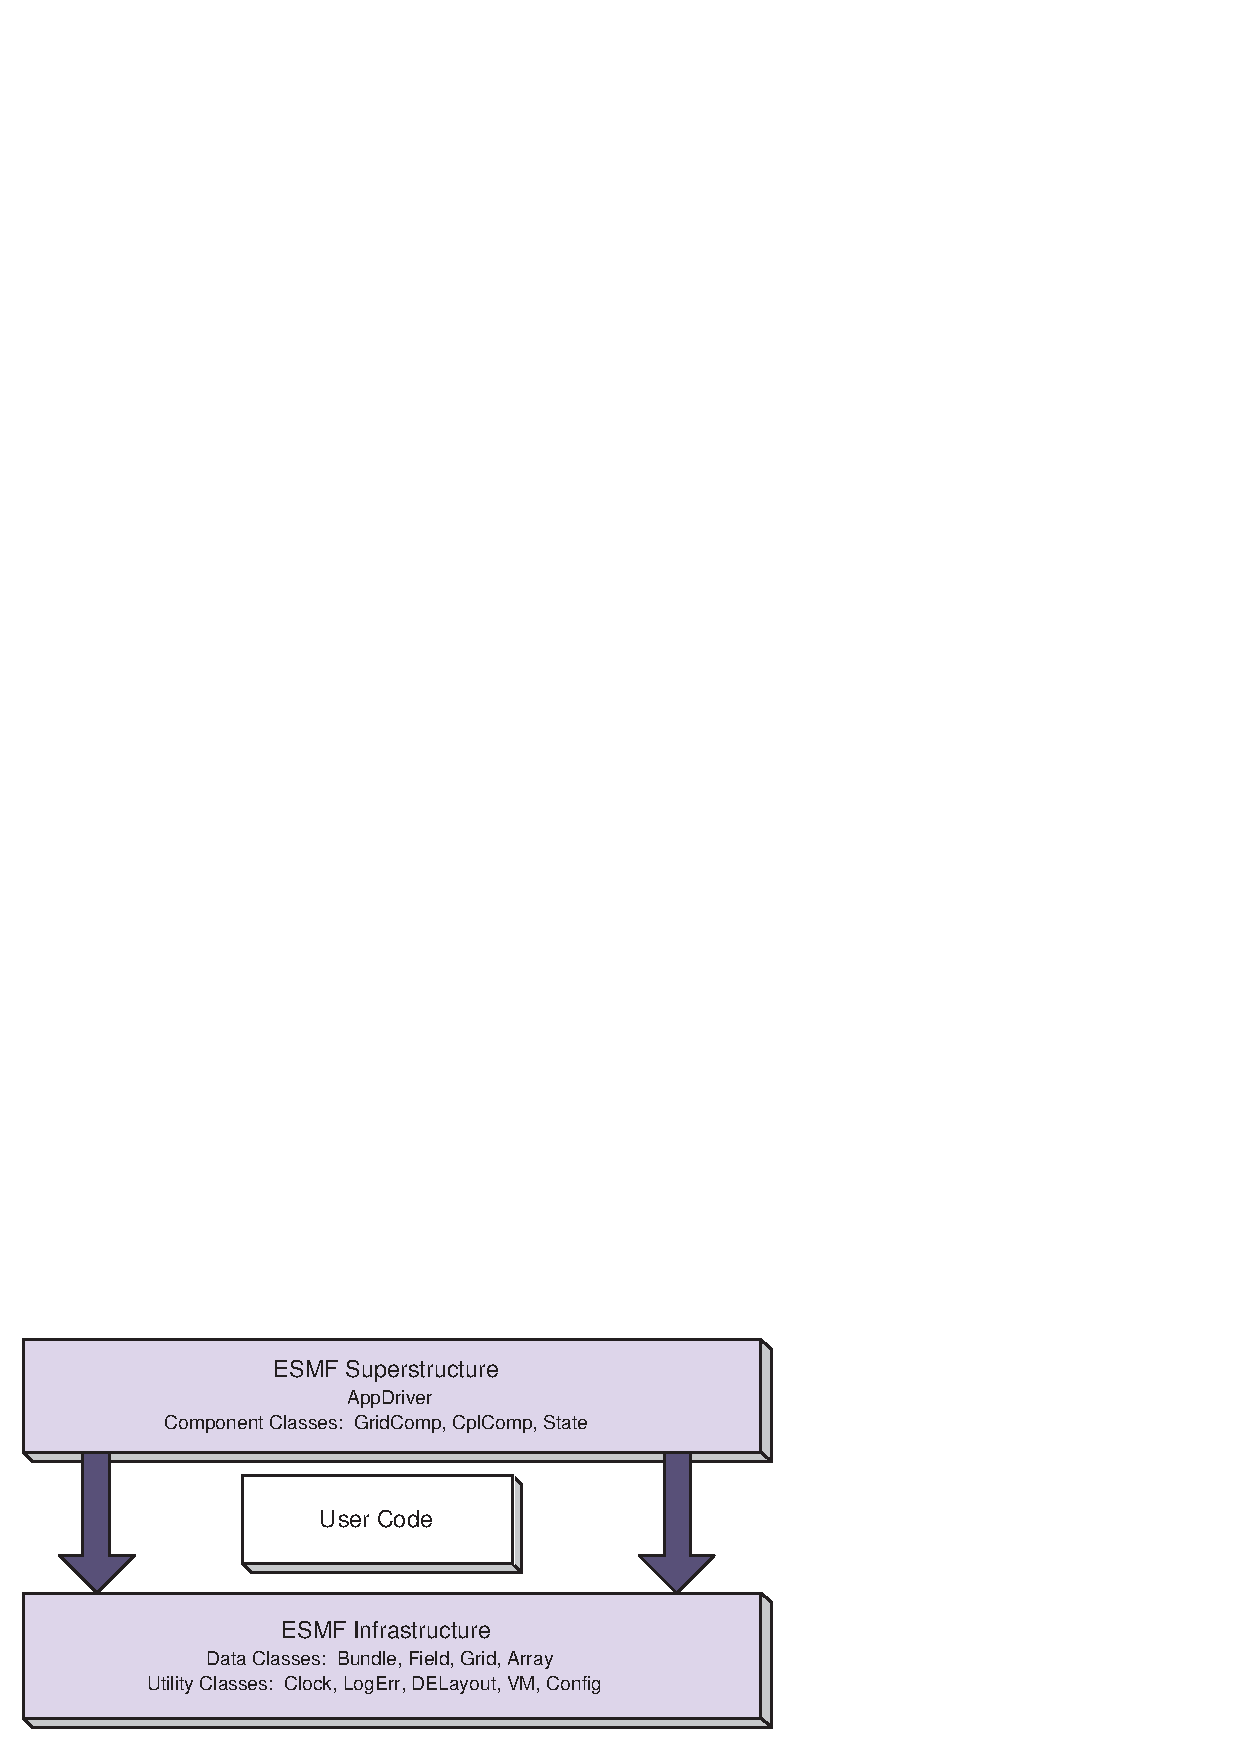
\includegraphics{ESMF_sandwich}}
\end{figure}
\end{center}


%\section{Support}
\section{How to Contact User Support and Find Additional Information}
\label{sec:Support}
The ESMF team can answer questions about the interfaces presented in this 
document.  For user support, please contact 
\htmladdnormallink{esmf\_support@ucar.edu}{mailto:esmf\_support@ucar.edu}.  

The website, \htmladdnormallink{http://www.earthsystemmodeling.org}{http://www.earthsystemmodeling.org}, provide more information of the ESMF project as a whole.
The website includes release notes and known bugs for each version of the
framework, supported platforms, project history, values, and metrics, related projects,
the ESMF management structure, and more.  The \htmladdnormallink
{{\it ESMF User's Guide}}{http://www.earthsystemmodeling.org/esmf\_releases/public/last/ESMF\_usrdoc/} contains build and installation instructions, an overview of the ESMF system and a description of 
how its classes interrelate (this version of the document corresponds to the last public version of the framework).  Also available on the ESMF website is the 
\htmladdnormallink{{\it ESMF Developer's Guide}}{http://www.earthsystemmodeling.org/documents/dev\_guide/} 
that details ESMF procedures and conventions.  
 
\section{How to Submit Comments, Bug Reports, and Feature Requests}
\label{sec:Submission}
\begin{sloppypar}
We welcome input on any aspect of the ESMF project.  Send
questions and comments to 
\htmladdnormallink{esmf\_support@ucar.edu}
{mailto:esmf\_support@ucar.edu}.
\end{sloppypar}







%\section{Document Conventions}
\section{Conventions}
\label{sec:conventions}

\subsection{Typeface and Diagram Conventions}


The following conventions for fonts and capitalization are used
in this and other ESMF documents. \newline

\begin{tabular}{lll}
{\bf Style} & {\bf Meaning} & {\bf Example} \\ \hline
{\it italics}  & documents & {\it ESMF Reference Manual}\\
{\tt courier}  & code fragments & {\tt ESMF\_TRUE}\\
{\tt courier()}  & ESMF method name & {\tt ESMF\_FieldGet()} \\
{\bf boldface} & first definitions & An {\bf address space} is ...\\
{\bf boldface} & web links and tabs & {\bf Developers} tab on the website \\
{Capitals}     & ESMF class name & DataMap \\
\end{tabular} 
 
ESMF class names frequently coincide with words commonly
used within the Earth system domain (field, grid, component, array, 
etc.)  The convention we adopt in this manual is that if a word is 
used in the context of an ESMF class name it is capitalized, and 
if the word is used in a more general context it remains in lower 
case.  We would write, for example, that an ESMF Field class 
represents a physical field.  

%Section and subsection titles should follow the convention of capitalizing
%all words in the title except for little words, such as: a, an, the, but, 
%as, if, and, or, nor, or prepositions.  However, the subsubsection titles 
%should only capitalize the first word and any other proper nouns, such as 
%ESMF class names.  There should be no punction at the end of any title, whether 
%it be a section, subsection, or subsubsection.

Diagrams are drawn using the Unified Modeling Language (UML).  UML 
is a visual tool that can illustrate the structure of 
classes, define relationships between classes, and describe sequences
of actions.  A reader interested in more detail can refer to a 
text such as {\it The Unified Modeling Language Reference Manual.}
 \cite{uml}



\subsection{Method Name and Argument Conventions}

Method names begin with {\tt ESMF\_}, followed by the class name, 
followed by the name of the operation being performed.  Each new 
word is capitalized.  Although Fortran interfaces are not case-sensitive,
we use case to help parse multi-word names.  

For method arguments that are multi-word, the first word is lower
case and subsequent words begin with upper case.  ESMF class 
names (including typed flags) are an exception.  When multi-word 
class names appear in argument lists, all letters after the first 
are lower case.  The first letter is lower case if the class is the
first word in the argument and upper case otherwise.  For 
example, in an argument list the DELayout class name may appear 
as {\tt delayout} or {\tt srcDelayout}.

Most Fortran calls in the ESMF are subroutines, with 
any returned values passed through the interface.  For the sake of 
convenience, some ESMF calls are written as functions.

A typical ESMF call looks like this:

\begin{verbatim}
call ESMF_<ClassName><Operation>(classname, firstArgument, 
           secondArgument, ..., rc)
\end{verbatim}

where \newline
{\tt <ClassName>} is the class name, \newline
{\tt <Operation>} is the name of the action to be performed, \newline 
{\tt classname} is a variable of the derived type associated 
with the class, \newline
the {\tt arg*} arguments are whatever other variables are required 
for the operation, \newline
and {\tt rc} is a return code. \newline





\newpage
%\section{API Overview}
% $Id$
%
% Earth System Modeling Framework
% Copyright 2002-2020, University Corporation for Atmospheric Research, 
% Massachusetts Institute of Technology, Geophysical Fluid Dynamics 
% Laboratory, University of Michigan, National Centers for Environmental 
% Prediction, Los Alamos National Laboratory, Argonne National Laboratory, 
% NASA Goddard Space Flight Center.
% Licensed under the University of Illinois-NCSA License.

\section{The ESMF Application Programming Interface}

The ESMF Application Programming Interface (API) is based on the
object-oriented programming concept of a {\bf class}.  A class is a 
software construct that is used for grouping a set of related variables 
together with the subroutines and functions that operate on them.  We 
use classes in ESMF because they help to organize the code, and often 
make it easier to maintain and understand.  A particular instance
of a class is called an {\bf object}.  For example, Field is an 
ESMF class.  An actual Field called {\tt temperature} is an object. 
That is about as far as we will go into software engineering
terminology.  

The Fortran interface is implemented so that the variables associated
with a class are stored in a derived type.  For example, an 
{\tt ESMF\_Field} derived type stores the data array, grid 
information, and metadata associated with a physical field.
The derived type for each class is stored in a Fortran module, and 
the operations associated with each class are defined as module
procedures.  We use the Fortran features of generic functions and
optional arguments extensively to simplify our interfaces.

The modules for ESMF are bundled together and can be accessed with a 
single {\tt USE} statement, {\tt USE ESMF}.

\subsection{Standard Methods and Interface Rules}

ESMF defines a set of standard methods and interface rules that
hold across the entire API.  These are: 

\begin{itemize}

\item 
\begin{sloppypar}
{\tt ESMF\_<Class>Create()} and {\tt ESMF\_<Class>Destroy()}, for
creating and destroying objects of ESMF classes that require internal memory
management (- called ESMF deep classes). The {\tt ESMF\_<Class>Create()} method
allocates memory for the object itself and for internal variables, and
initializes variables where appropriate.  It is always written as a Fortran
function that returns a derived type instance of the class, i.e. an object.
\end{sloppypar}

\item 
\begin{sloppypar}
{\tt ESMF\_<Class>Set()} and {\tt ESMF\_<Class>Get()}, for setting and 
retrieving a particular item or flag.  In general, these methods are overloaded
for all cases where the item can be manipulated as a name/value pair.  If
identifying the item requires more than a name, or if the class is of
sufficient complexity that overloading in this way would result in an
overwhelming number of options, we define specific
{\tt ESMF\_<Class>Set<Something>()} and {\tt ESMF\_<Class>Get<Something>()}
interfaces.
\end{sloppypar}

\begin{sloppypar}
\item {\tt ESMF\_<Class>Add()}, {\tt ESMF\_<Class>AddReplace()},
{\tt ESMF\_<Class>Remove()}, and {\tt ESMF\_<Class>Replace()}, for manipulating
objects of ESMF container classes - such as {\tt ESMF\_State} and
{\tt ESMF\_FieldBundle}. For example, the {\tt ESMF\_FieldBundleAdd()}
method adds another Field to an existing FieldBundle object.
\end{sloppypar}

\item {\tt ESMF\_<Class>Print()}, for printing the contents of an object to 
standard out.  This method is mainly intended for debugging.

\item {\tt ESMF\_<Class>ReadRestart()} and {\tt ESMF\_<Class>WriteRestart()}, 
for saving the contents of a class and restoring it exactly.  Read
and write restart methods have not yet been implemented for most
ESMF classes, so where necessary the user needs to write restart 
values themselves.

\item 
\begin{sloppypar}
{\tt ESMF\_<Class>Validate()}, for determining whether a class is 
internally consistent.  For example, {\tt ESMF\_FieldValidate()} validates
the internal consistency of a Field object.
\end{sloppypar}

\end{itemize}

\subsection{Deep and Shallow Classes}
\label{sec:deepshallow}

The ESMF contains two types of classes.

{\bf Deep} classes require
{\tt ESMF\_<Class>Create()} and {\tt ESMF\_<Class>Destroy()} calls.
They involve memory allocation, take significant time to set up (due to
memory management) and should not be created in a time-critical portion of code.
Deep objects persist even after the method in which they were created has
returned. Most classes in ESMF, including GridComp, CplComp, State, Fields, FieldBundles, Arrays, ArrayBundles, Grids, and Clocks, fall into this category.

{\bf Shallow} classes do not possess {\tt ESMF\_<Class>Create()}
and {\tt ESMF\_<Class>Destroy()} calls.  They are simply declared
and their values set using an {\tt ESMF\_<Class>Set()} call.  
Examples of shallow classes are Time, TimeInterval, and ArraySpec.  Shallow classes do not take long to set up and can be declared and set within
a time-critical code segment.  Shallow objects stop existing when
the method in which they were declared has returned.  

An exception to this is when a shallow object, such as a Time, 
is stored in a deep object such as a Clock.  The Clock then
carries a copy of the Time in persistent memory.  The Time is
deallocated with the {\tt ESMF\_ClockDestroy()} call.

See Section \ref{sec:overallimpl}, Overall Design and Implementation 
Notes, for a brief discussion of deep and shallow classes from 
an implementation perspective.  For an in-depth look at the design 
and inter-language issues related to deep and shallow classes,
see the \htmladdnormallink{{\it ESMF Implementation Report}}{http://www.earthsystemmodeling.org/documents/IMPL\_repdoc/}.

\subsection{Special Methods}

The following are special methods which, in one case,
are required by any application using ESMF, and in the 
other case must be called by any application that is using 
ESMF Components.

\begin{itemize}

\item {\tt ESMF\_Initialize()} and {\tt ESMF\_Finalize()} are required 
methods that must bracket the use of ESMF within an application.  
They manage the resources required to run ESMF and shut it down
gracefully.  ESMF does not support restarts in the same executable, i.e.
{\tt ESMF\_Initialize()} should not be called after {\tt ESMF\_Finalize()}.
\item {\tt ESMF\_<Type>CompInitialize()}, {\tt ESMF\_<Type>CompRun()}, and {\tt ESMF\_<Type>CompFinalize()} are component methods that are used at the 
highest level within ESMF.  {\tt <Type>} may be {\tt <Grid>}, for 
Gridded Components such as oceans or atmospheres, or
{\tt <Cpl>}, for Coupler Components that are used to connect 
them.  The content of these methods is not part of the ESMF.  
Instead the methods call into associated subroutines within 
user code.

\end{itemize}

\subsection{The ESMF Data Hierarchy}

The ESMF API is organized around a hierarchy of classes that
contain model data.  The operations that are performed
on model data, such as regridding, redistribution, and halo 
updates, are methods of these classes.  

The main data classes in ESMF, in order of increasing complexity, are:
\begin{itemize}
\item {\bf Array} An ESMF Array is a distributed, multi-dimensional 
array that can carry information such as its type, kind, rank, and 
associated halo widths.  It contains a reference to a native Fortran array.
\item {\bf ArrayBundle}  An ArrayBundle is a collection of Arrays, not
necessarily distributed in the same manner.  It is useful for performing
collective data operations and communications. 
\item {\bf Field}  A Field represents a physical scalar or vector field.
It contains a reference to an Array along with grid information and metadata.
\item {\bf FieldBundle}  A FieldBundle is a collection of Fields discretized 
on the same grid.  The staggering of data points may be different for 
different Fields within a FieldBundle.  Like the ArrayBundle, it is
useful for performing collective data operations and
communications.
\item {\bf State}  A State represents the collection of data that a 
Component either requires to run (an Import State) or can make 
available to other Components (an Export State).
States may contain references to Arrays, ArrayBundles, Fields,
FieldBundles, or other States. 
\item {\bf Component}  A Component is a piece of software 
with a distinct function.  ESMF currently recognizes two types 
of Components.  Components that represent a physical domain 
or process, such 
as an atmospheric model, are called Gridded Components since they are 
usually discretized on an underlying grid.  The Components 
responsible for regridding and transferring data between Gridded 
Components are called Coupler Components.  Each Component
is associated with an Import and an Export State.  Components
can be nested so that simpler Components are contained within more
complex ones.

\end{itemize}

Underlying these data classes are native language arrays.  ESMF allows 
you to reference an existing Fortran array to an ESMF Array or 
Field so that ESMF data classes can be readily 
introduced into existing code.  You can perform communication operations 
directly on Fortran arrays through the VM class, which serves 
as a unifying wrapper for distributed and shared memory communication 
libraries.

\subsection{ESMF Spatial Classes}
\label{sec:spatialclasses}

Like the hierarchy of model data classes, ranging from the 
simple to the complex, ESMF is organized around a hierarchy of
classes that represent different spaces associated with a computation.
Each of these spaces can be manipulated, in order to give
the user control over how a computation is executed.  For Earth system
models, this hierarchy starts with the address space associated
with the computer and extends to the physical region described by
the application.   The main spatial classes in ESMF, from
those closest to the machine to those closest to the application, are:

\begin{itemize}

\item The {\bf Virtual Machine}, or {\bf VM} The ESMF VM is an 
abstraction of a parallel computing environment that encompasses 
both shared and distributed memory, single and multi-core systems.
Its primary purpose is resource allocation and management. Each Component
runs in its own VM, using the resources it defines. The elements of a VM
are {\bf Persistent Execution Threads}, or {\bf PETs}, that are
executing in {\bf Virtual Address Spaces}, or {\bf VASs}. A simple
case is one in which every PET is associated with a single MPI process.
In this case every PET is executing in its own private VAS. If Components
are nested, the parent component allocates a subset of its PETs to its
children. The children have some flexibility, subject to the constraints of
the computing environment, to decide how they want to use the
resources associated with the PETs they've received.

\item {\bf DELayout}  A DELayout represents a data decomposition
(we also refer to this as a distribution).  Its
basic elements are {\bf Decomposition Elements}, or {\bf DEs}.  
A DELayout associates a set of DEs with the PETs in a VM.  DEs are not
necessarily one-to-one with PETs.  For cache blocking,
or user-managed multi-threading, more DEs than PETs may be defined.
Fewer DEs than PETs may also be defined if an application requires it.

\item {\bf DistGrid}  A DistGrid represents the index space
associated with a grid.  It is a useful abstraction because
often a full specification of grid coordinates is not necessary
to define data communication patterns.  The DistGrid contains
information about the sequence and connectivity of data points,
which is sufficient information for many operations.  Arrays
are defined on DistGrids.

\item {\bf Array} An Array defines how the index space described
in the DistGrid is associated with the VAS of each PET. This association
considers the type, kind and rank of the indexed data. Fields are
defined on Arrays.

\item {\bf Grid}  A Grid is an abstraction for a logically rectangular 
region in physical space.  It associates a coordinate system, a set of 
coordinates, and a topology to a collection of grid cells.  Grids in ESMF 
are comprised of DistGrids plus additional coordinate information. 

\item {\bf Mesh}  A Mesh provides an abstraction for an unstructured 
grid.  Coordinate information is set in nodes, which represent
vertices or corners.  Together the nodes establish the boundaries 
of mesh elements or cells.

\item {\bf LocStream}  A LocStream is an abstraction for a set of 
unstructured data points without any topological relationship to each 
other.  

\item {\bf Field}  A Field may contain more dimensions than the 
Grid that it is discretized on.  For example, for convenience 
during integration, a user may want to define a single Field object 
that holds snapshots of data at multiple times.  Fields also 
keep track of the stagger location of a Field data point within its 
associated Grid cell.

\end{itemize}

\subsection{ESMF Maps}

In order to define how the index spaces of the spatial classes relate
to each other, we require either implicit rules (in which case the
relationship between spaces is defined by default), or special Map arrays
that allow the user to specify the desired association.  The form of the 
specification is usually that the position of the array element carries
information about the first object, and the value of the array element carries
information about the second object.  ESMF includes a {\tt distGridToArrayMap},
a {\tt gridToFieldMap}, a {\tt distGridToGridMap}, and others.

\subsection{ESMF Specification Classes}

It can be useful to make small packets
of descriptive parameters.  ESMF has one of these:
\begin{itemize}
\item {\bf ArraySpec}, for storing the specifics, such as type/kind/rank,
of an array.
\end{itemize}

\subsection{ESMF Utility Classes}

There are a number of utilities in ESMF that can be used independently.
These are:
\begin{itemize}
\item {\bf Attributes}, for storing metadata about Fields,
FieldBundles, States, and other classes.
\item {\bf TimeMgr}, for calendar, time, clock and alarm functions.
\item {\bf LogErr}, for logging and error handling.
\item {\bf Config}, for creating resource files that can replace namelists
as a consistent way of setting configuration parameters.
\end{itemize}

\section{Integrating ESMF into Applications}

Depending on the requirements of the application, the user may 
want to begin integrating ESMF in either a top-down or bottom-up 
manner.  In the top-down approach, tools at the superstructure 
level are used to help reorganize and structure the interactions
among large-scale components in the application.  It is appropriate
when interoperability is a primary concern; for example, when 
several different versions or implementations of components are going 
to be swapped in, or a particular component is going to be used 
in multiple contexts.  Another reason for deciding on a top-down 
approach is that the application contains legacy code that for 
some reason (e.g., intertwined functions, very large,
highly performance-tuned, resource limitations) there is little 
motivation to fully restructure.  The superstructure can usually be 
incorporated into such applications in a way that is non-intrusive.

In the bottom-up approach, the user selects desired utilities 
(data communications, calendar management, performance profiling,
logging and error handling, etc.) from the ESMF infrastructure 
and either writes new code using them, introduces them into 
existing code, or replaces the functionality in existing code 
with them.  This makes sense when maximizing code reuse and 
minimizing maintenance costs is a goal.  There may be a specific
need for functionality or the component writer may be starting
from scratch.  The calendar management utility is a popular
place to start.

\subsection{Using the ESMF Superstructure}

The following is a typical set of steps involved in adopting
the ESMF superstructure.  The first two tasks, which occur 
before an ESMF call is ever made, have the potential to be 
the most difficult and time-consuming.  They are the work 
of splitting an application into components and ensuring that
each component has well-defined stages of execution.  ESMF
aside, this sort of code structure helps to promote application
clarity and maintainability, and the effort put into it is likely
to be a good investment.

\begin{enumerate}

\item Decide how to organize the application as discrete Gridded 
and Coupler Components.  This might involve reorganizing code
so that individual components are cleanly separated and their 
interactions consist of a minimal number of data exchanges.

\item Divide the code for each component into initialize, run, and
finalize methods.  These methods can be multi-phase, e.g., 
{\tt init\_1, init\_2}.

\item Pack any data that will be transferred between components
into ESMF Import and Export State data structures.  This is done
by first wrapping model data in either ESMF Arrays or Fields.
Arrays are simpler to create and use than Fields, but carry less
information and have a more limited range of operations.
These Arrays and Fields are then added to Import and
Export States.  They may be packed into ArrayBundles or
FieldBundles first, for more efficient communications.
Metadata describing the model data can also be added.
At the end of this step, the data to be transferred between
components will be in a compact and largely self-describing
form.

\item Pack time information into ESMF time management data 
structures.

\item Using code templates provided in the ESMF distribution, create
ESMF Gridded and Coupler Components to represent each component
in the user code.

\item Write a set services routine that sets ESMF entry 
points for each user component's initialize, run, and finalize 
methods.

\item Run the application using an ESMF Application Driver.

\end{enumerate} 

\section{Overall Rules and Behavior}

\subsection{Return Code Handling}

All ESMF methods pass a {\em return code} back to the caller via the {\tt rc}
argument. If no errors are encountered during the method execution, a
value of {\tt ESMF\_SUCCESS} is returned. Otherwise one of the predefined
error codes is returned to the caller. See the appendix, section 
\ref{appendix_esmf_error_codes}, for a full list of the ESMF error return codes.

Any code calling an ESMF method must check the return code. If {\tt rc} is not
equal to {\tt ESMF\_SUCCESS}, the calling code is expected to break out of its
execution and pass the {\tt rc} to the next level up. All ESMF errors are to be
handled as {\em fatal}, i.e. the calling code must {\em bail-on-all-errors}.

ESMF provides a number of methods, described under section \ref{log_class},
that make implementation of the bail-on-all-errors stategy more convenient.
Consistent use of these methods will ensure that a full back trace is generated
in the ESMF log output whenever an error condition is triggered.

Note that in ESMF requesting not present information, e.g. via a {\tt Get()}
method, will trigger an error condition. Combined with the bail-on-all-errors
strategy this has the advantage of producing an error trace pointing to the
earliest location in the code that attempts to access unavailable information.
In cases where the calling side is able to handle the presence or absence of
certain pieces of of information, the code first must query for the resepctive
{\tt isPresent} argument. If this argument comes back as {\tt .true.} it is
safe to query for the actual information.

\subsection{Local and Global Views and Associated Conventions}

ESMF data objects such as Fields are distributed over
DEs, with each DE getting a portion of the data.  Depending
on the task, a local or global view of the object may be
preferable.  In a local view, data indices start with the first
element on the DE and end with the last element on the same DE.
In a global view, there is an assumed or specified order to
the set of DEs over which the object is distributed.  Data
indices start with the first element on the first DE, and
continue across all the elements in the sequence of DEs.
The last data index represents the number of elements in the
entire object.  The DistGrid provides the mapping between
local and global data indices.

The convention in ESMF is that entities with a global view
have no prefix.  Entities with a DE-local (and in some cases,
PET-local) view have the prefix ``local.''

Just as data is distributed over DEs, DEs themselves can be
distributed over PETs.  This is an advanced feature for users
who would like to create multiple local chunks of data, for
algorithmic or performance reasons.
Local DEs are those DEs that are located on the local PET.
Local DE labeling always starts at 0 and goes to localDeCount-1,
where localDeCount is the number of DEs on the local PET.
Global DE numbers also start at 0 and go to deCount-1.
The DELayout class provides the mapping between local
and global DE numbers. 

\subsection{Allocation Rules}

The basic rule of allocation and deallocation for the ESMF is:
whoever allocates it is responsible for deallocating it.

\begin{sloppypar}
ESMF methods that allocate their own space for data will
deallocate that space when the object is destroyed. 
Methods which accept a user-allocated buffer, for example
{\tt ESMF\_FieldCreate()} with the {\tt ESMF\_DATACOPY\_REFERENCE} flag,
will not deallocate that buffer at the time the object is
destroyed.  The user must deallocate the buffer
when all use of it is complete.
\end{sloppypar}

Classes such as Fields, FieldBundles, and States may have Arrays, 
Fields, Grids and FieldBundles created externally and associated with
them.  These associated items are not destroyed along with the rest  
of the data object since it is possible for the items to be added 
to more than one data object at a time (e.g. the same Grid could 
be part of many Fields).  It is the user's responsibility to delete 
these items when the last use of them is done.

\subsection{Assignment, Equality, Copying and Comparing Objects}

The equal sign assignment has not been overloaded in ESMF, thus resulting in
the standard Fortran behavior. This behavior has been documented as the first
entry in the API documentation section for each ESMF class. For deep ESMF
objects the assignment results in setting an alias the the same ESMF object
in memory. For shallow ESMF objects the assignment is essentially a equivalent
to a copy of the object. For deep classes the equality operators have been
overloaded to test for the alias condition as a counter part to the assignment
behavior. This and the not equal operator are documented following the
assignment in the class API documentation sections. 

\begin{sloppypar}
Deep object copies are implemented as a special variant of the
{\tt ESMF\_<Class>Create()} methods. It takes an existing deep object as
one of the required arguments. At this point not all deep classes have
{\tt ESMF\_<Class>Create()} methods that allow object copy.
\end{sloppypar}

Due to the complexity of deep classes there are many aspects when comparing two
objects of the same class. ESMF provide {\tt ESMF\_<Class>Match()} methods,
which are functions that return a class specific match flag. At this point not
all deep classes have {\tt ESMF\_<Class>Match()} methods that allow deep object
comparison.

\subsection{Attributes}

Attributes are (name, value) pairs, where
the name is a character string and the value can be either a single
value or list of {\tt integer}, {\tt real}, {\tt double precision},
{\tt logical}, or {\tt character} values.
Attributes can be associated with Fields, FieldBundles, and States. 
Mixed types are not allowed in a single attribute, and all attribute
names must be unique within a single object.    Attributes are set
by name, and can be retrieved either directly by name or by querying
for a count of attributes and retrieving names and values
by index number.

\subsection{Constants}

Named constants are used throughout ESMF to specify the values of many 
arguments with multiple well defined values in a consistent way.  These 
constants are defined by a derived type that follows this pattern:

\begin{verbatim}
ESMF_<CONSTANT_NAME>_Flag
\end{verbatim}

The values of the constant are then specified by this pattern:

\begin{verbatim}
ESMF_<CONSTANT_NAME>_<VALUE1>
ESMF_<CONSTANT_NAME>_<VALUE2>
ESMF_<CONSTANT_NAME>_<VALUE3>
...
\end{verbatim}

A master list of all available constants can be found in section 
\ref{const:master}.

%\subsection{Overall Design and Implementation Notes}
% $Id$

\section{Overall Design and Implementation Notes}
\label{sec:overallimpl}

\begin{enumerate}

\item {\bf Deep and shallow classes.}  The deep and shallow classes 
described in Section \ref{sec:deepshallow} differ in how and where they
are allocated within a multi-language implementation environment.  We
distinguish between the implementation language, which is the language
a method is written in, and the calling language, which is the language
that the user application is written in.  Deep classes are allocated 
off the process heap by the implementation language.  Shallow classes
are allocated off the stack by the calling language.  

\item {\bf Base class.} All ESMF classes are built upon a Base class,
which holds a small set of system-wide capabilities.  

\end{enumerate}

%\subsection{Overall Restrictions and Future Work}
% $Id$

\section{Overall Restrictions and Future Work}
\label{sec:overallrest}

\begin{enumerate}

\item {\bf 32-bit integer limitations.} In general, Fortran array bounds should
be limited to 2**31-1 elements or less.  This is due to the Fortran-95
limitation of returning default sized (e.g., 32 bit) integers for array bound
and size inquiries, and consequent ESMF use of default sized integers for
holding these values.

\end{enumerate}

\newpage
\begin{htmlonly}
\addcontentsline{toc}{part}{Applications}
\end{htmlonly}
\part{Applications}
\label{part:Applications}
% $Id$

The main product delivered by ESMF is the ESMF library that allows application
developers to write programs based on the ESMF API. In addition to the 
programming library, ESMF distributions come with a small set of applications
that are of general interest to the community. These applications utilize
the ESMF library to implement features such as printing general information
about the ESMF installation, or generating regrid weight files. The provided
ESMF applications are intended to be used as standard command line tools.

The bundled ESMF applications are built and installed during the usual ESMF 
installation process, which is described in detail in the ESMF User's Guide 
section "Building and Installing the ESMF". After installation, the
applications will be located in the {\tt ESMF\_APPSDIR} directory, which can 
be found as a Makefile variable in the {\tt esmf.mk} file. The {\tt esmf.mk} 
file can be found in the {\tt ESMF\_INSTALL\_LIBDIR} directory after a 
successful installation.  The ESMF User's Guide discusses the {\tt esmf.mk} 
mechanism to access the bundled applications in more detail in section 
"Using Bundled ESMF Applications".

The following sections provide in-depth documentation of the bundled ESMF 
applications. In addition, each application supports the standard 
\verb+ --help + command line argument, providing a brief description of how 
to invoke the program.


%\input{ESMF_InfoC}
% $Id$

\section{ESMF\_Info}
\label{sec:ESMF_Info}

\subsection{Description}

The {\tt ESMF\_Info} application prints basic information about the ESMF 
installation to {\tt stdout}.

The application usage is as follows:

\begin{verbatim}
ESMF_Info  [--help]

where
  --help     prints a brief usage message
  
\end{verbatim}

% $Id$
`
\section{ESMF\_RegridWeightGen}
\label{sec:ESMF_RegridWeightGen}

\subsection{Description}

This section describes the offline regrid weight generation application provided by ESMF (for a description of ESMF regridding in general see Section~\ref{sec:regrid}). Regridding, also called remapping or interpolation, is the process of changing the grid that underlies data values while preserving qualities of the original data. Different kinds of transformations are appropriate for different problems. Regridding may be needed when communicating data between Earth system model components such as land and atmosphere, or between different data sets to support operations such as visualization. 

Regridding can be broken into two stages. The first stage is generation of an interpolation weight matrix that describes how points in
the source grid contribute to points in the destination grid. The second stage is the multiplication of values on the source grid by the
interpolation weight matrix to produce values on the destination grid. This is implemented as a parallel sparse matrix multiplication.

There are two options for accessing ESMF regridding functionality: integrated and offline. Integrated regridding is a process whereby interpolation
weights are generated via subroutine calls during the execution of the user's code. The integrated regridding can also perform the parallel sparse
matrix multiplication. In other words, ESMF integrated regridding allows a user to perform the whole process of interpolation within their code.
For a further description of ESMF integrated regridding please see Section~\ref{sec:fieldregrid}. 
In contrast to integrated regridding,
offline regridding is a process whereby interpolation weights are generated by a separate ESMF application, not within the user code. The ESMF offline
regridding application also only generates the interpolation matrix, the user is responsible for reading in this matrix and doing the actual interpolation
 (multiplication by the sparse matrix) in their code. The rest of this section further describes ESMF offline regridding.

For a discussion of installing and accessing ESMF applications such as this one please see the beginning of this part of the reference manual (Section~\ref{part:Applications}) or for the quickest approach to just building and accessing the applications please refer to the "Building and using bundled ESMF applications" Section in the ESMF User's Guide.

This application requires the NetCDF library to read the grid files and to write out the weight files in NetCDF format.  To compile ESMF with the NetCDF library, please refer to the "Third Party Libraries" Section in the ESMF User's Guide for more information.

As described above, this tool reads in
two grid files and outputs weights for interpolation
 between the two grids. The input and output files are all in NetCDF format. The grid files can be defined in five
different formats:  the SCRIP format~\ref{sec:fileformat:scrip} as is used as an input to SCRIP~\cite{ref:SCRIP}, the CF convension single-tile grid file~\ref{sec:fileformat:gridspec} following the
\htmladdnormallink{CF metadata conventions}{http://cfconventions.org}, the GRIDSPEC Mosaic file~\ref{sec:fileformat:mosaic} following the proposed \htmladdnormallink{GRIDSPEC standard}{http://extranet.gfdl.noaa.gov/~vb/gridstd/gridstd.html},  
the ESMF unstructured grid format~\ref{sec:fileformat:esmf} or the proposed CF unstructured grid data model (UGRID) ~\ref{sec:fileformat:ugrid}.  GRIDSPEC is a proposed CF extension for the annotation of complex Earth system grids.  In the latest ESMF library, we added support for multi-tile GRIDSPEC Mosaic file with non-overlapping tiles. For UGRID, we support the 2D flexible mesh topology with mixed triangles and quadrilaterals and fully 3D unstructured mesh topology with hexahedrons and tetrahedrons.  

In the latest ESMF implementation,  {\tt ESMF\_RegridWeightGen} application can detect the type of the input grid files automatically.  The user
doesn't need to provide the source and destination grid file type arguments anymore.  The following arguments {\tt -t}, {\tt --src\_type}, {\tt --dst\_type}, {\tt --src\_meshname}, and {\tt --dst\_meshname} are no longer needed.  If provided, the application will simply ingore them.

 This application can do regrid weight generation from a global or regional source grid to a global or regional destination grid.
As is true with many global models, this application currently assumes the latitude and longitude values refer to positions on a perfect sphere, as opposed to a more complex and accurate representation of the Earth's true shape such as would be used in a GIS system. (ESMF's current user base doesn't require this level of detail in representing the Earth's shape, but it could be added in the future if necessary.)

The interpolation weights generated by this application are output to a NetCDF file (specified by the "-w" or "\verb+--+weight"
keywords). Two type of weight files are supported: the SCRIP format is the same as that generated by SCRIP, see Section~\ref{sec:weightfileformat} for a description of the format; and a simple weight file containing only the weights and the source and destination grid indices (In ESMF
term, these are the {\tt factorList} and {\tt factorIndexList} generated by the ESMF weight calculation function {\tt ESMF\_FieldRegridStore()}.
Note that the sequence of the weights in the file can
vary with the number of processors used to run the application. This means that two weight files generated by using different
numbers of processors can contain exactly the same interpolation matrix, but can appear different in a direct line by line
comparison (such as would be done by ncdiff). The interpolation weights can be generated with
the bilinear, patch, nearest neighbor, first-order conservative, or second-order conservative methods described in Section~\ref{sec:rwg_regridmethods}.

        
Internally this application uses the ESMF public API to generate the interpolation weights.
If a source or destination grid is a single tile logically rectangular grid, then {\tt ESMF\_GridCreate()}
~\ref{sec:example:2DLogRecFromScrip}
is used to create an ESMF\_Grid object. The cell center
coordinates of the input grid are put into the center stagger location ({\tt ESMF\_STAGGERLOC\_CENTER}).
In addition, the corner coordinates are also put into the corner stagger location
({\tt ESMF\_STAGGERLOC\_CORNER}) for conservative regridding.  If a grid contains multiple logically rectangular tiles 
connected with each other by edges, such as a Cubed Sphere grid, the grid can be represented as a multi-tile ESMF\_Grid object created 
using {\tt ESMF\_GridCreateMosaic()}~\ref{sec:usage:cubedspherefromfile}. Such a grid is stored in the GRIDSPEC Mosaic and tile file format.~\ref{sec:fileformat:mosaic}
The method {\tt ESMF\_MeshCreate()} ~\ref{sec:example:UnstructFromFile}
is used to create an ESMF\_Mesh object, if the
source or destination grid is an unstructured grid. When making this call,
the flag {\tt convert3D} is set to {\tt TRUE} to convert the 2D coordinates into 3D Cartesian coordinates. 
Internally {\tt ESMF\_FieldRegridStore()} is used to generate the weight table and indices table representing the interpolation matrix.


\subsection{Regridding Options}\label{sec:rwg_options}

 The offline regrid weight generation application supports most of the options available in the rest of the ESMF regrid system. The following is a description of these options as relevant to the application. For a more in-depth description see Section~\ref{sec:regrid}.

\subsubsection{Poles}\label{sec:rwg_poles}
The regridding occurs in 3D to avoid
problems with periodicity and with the pole singularity. This application
supports four options for handling the pole region (i.e. the empty area above the top row of the source grid or below
the bottom row of the source grid).  Note that all of these pole options currently only work for logically rectangular grids (i.e. SCRIP format grids with grid\_rank=2 or GRIDSPEC single-tile format grids). The first option is to leave  the pole region empty ("-p none"), in this
case if a destination point lies above or below the
top row of the source grid, it will fail to map, yielding an error (unless "-i" is specified).
With the next two options, the pole region is handled by constructing
an artificial pole in the center of the top and bottom row of grid points and then filling
in the region from this pole to the edges of the source grid with triangles.
The pole is located at the average of the position of the points surrounding
it, but moved outward to be at the same radius as the rest of the points
in the grid. The difference between these two artificial pole options is what value is used at the pole.
 The default pole option ("-p all") sets the value at the pole to be the average of the values
of all of the grid points surrounding the pole. For the other option ("-p N"), the user chooses
a number N from 1 to the number of source grid points around the pole. For
each destination point, the value at the pole is then the average of the N source points
surrounding that destination point. For the last pole option ("-p teeth") no artificial pole is constructed, instead the
pole region is covered by connecting points across the top and bottom row of the source Grid into triangles. As
this makes the top and bottom of the source sphere flat, for a big enough difference between the size of
the source and destination pole regions, this can still result in unmapped destination points.
Only pole option "none" is currently supported with the conservative interpolation methods (e.g. "-m conserve") and with the
nearest neighbor interpolation methods ("-m nearestdtos" and "-m neareststod").

\subsubsection{Masking}\label{sec:rwg_masking}
       Masking is supported for both the logically rectangular grids and the unstructured grids.
If the grid file is in the SCRIP format, the variable "grid\_imask" is used as the mask.
If the value is set to 0 for a grid point, then that point is considered masked out and
won't be used in the weights generated by the application. If the grid file is in the ESMF format, the variable "element Mask" is used as the mask.  For a grid defined in the GRIDSPEC
single-tile or multi-tile grid or in the UGRID convention, there is no mask variable defined.
However, a GRIDSPEC single-tile file or a UGRID file may contain both the grid definition and the data.
The grid mask is usually constructed using the missing values defined in the data variable.
The regridding application provides the argument "\verb+--+src\_missingvalue" or
"\verb+--+dst\_missingvalue" for users to specify the variable name from where the mask can be
constructed.

\subsubsection{Extrapolation}\label{sec:rwg_extrap}
The {\tt ESMF\_RegridWeightGen} application supports a number of kinds of extrapolation to fill in points not mapped by the regrid method. 
Please see the sections starting with section~\ref{sec:extrapolation:overview} for a description of these methods. When using the application
an extrapolation method is specified by using the "\verb+--+extrap\_method" flag. For the inverse distance weighted average method (nearestidavg),
the number of source locations is specified using the "\verb+--+extrap\_num\_src\_pnts" flag, and the distance exponent is specified using 
the "\verb+--+extrap\_dist\_exponent" flag. For the creep fill method (creep), the number of creep levels is specified using the "\verb+--+extrap\_num\_levels" flag.

\subsubsection{Unmapped destination points}\label{sec:rwg_unmapped}
If a destination point can't be mapped, then the default behavior of the application is to stop with an error. By specifying "-i" or the equivalent "\verb+--+ignore\_unmapped " the user can cause the application to ignore unmapped destination points. In this case, the output matrix won't contain entries for the unmapped destination points. Note that the unmapped point detection doesn't
currently work for nearest destination to source method ("-m nearestdtos"), so when using that method it  is as if ``-i'' is always on.

\subsubsection{Line type}\label{sec:rwg_linetype}
 Another variation in the regridding supported with spherical grids is {\bf line type}. This is controlled by the "\verb+--+line\_type" or ``-l'' flag. This switch allows the user to select the path of the line which connects
two points on a sphere surface. This in turn controls the path along which distances are calculated and the shape of 
the edges that make up a cell. Both of these quantities can influence how interpolation weights are calculated, for example in
bilinear interpolation the distances are used to calculate the weights and the cell edges are used to determine to which source 
cell a destination point should be mapped. 

ESMF currently supports two line types: ``cartesian'' and ``greatcircle''. The ``cartesian'' option 
specifies that the line between two points follows a straight path through the 3D Cartesian space in which the sphere is embedded.
Distances are measured along  this 3D Cartesian line. Under this option cells are approximated by planes in 3D space, and their boundaries are 
3D Cartesian lines between their corner points.  The ``greatcircle'' option specifies that the line between two points follows
a great circle path along the sphere surface. (A great circle is the shortest path between two points on a sphere.) 
Distances are measured along the great circle path. Under this option cells are on the sphere surface, and their boundaries 
are great circle paths between their corner points. 


\subsection{Regridding Methods}\label{sec:rwg_regridmethods}
 This regridding application can be used to generate bilinear, patch, nearest neighbor, first-order conservative, or second-order conservative 
interpolation weights. The following is a description of these interpolation methods as relevant to the offline weight generation application. For a more in-depth description see Section~\ref{sec:regrid}.

\subsubsection{Bilinear}\label{sec:rwg_bilinear}
 The default interpolation method for the weight generation application is bilinear. The algorithm used by this application to 
generate the bilinear weights is the standard one found in many textbooks.  Each destination point is mapped to a location
in the source Mesh, the position of the destination point relative to the source points surrounding it is used to calculate the interpolation weights. A restriction on
bilinear interpolation is that ESMF doesn't support self-intersecting cells (e.g. a cell twisted into a bow tie). 

\subsubsection{Patch}\label{sec:rwg_patch}
This application can also be used to generate patch interpolation weights. Patch
interpolation is the ESMF version of a technique called "patch recovery" commonly
used in finite element modeling~\cite{PatchInterp1}~\cite{PatchInterp2}. It typically results in better approximations to values and derivatives when compared to bilinear interpolation.
Patch interpolation works by constructing multiple polynomial patches to represent
the data in a source element. For 2D grids, these polynomials
are currently 2nd degree 2D polynomials. The interpolated value at the destination point
  is the weighted average of the values of the patches at that point.

The patch interpolation process works as follows.
For each source element containing a destination point
we construct a patch for each corner node that makes up the element (e.g. 4 patches for
quadrilateral elements, 3 for triangular elements). To construct a polynomial patch for
a corner node we gather all the elements around that node.
(Note that this means that the patch interpolation weights depends on the source
element's nodes, and the nodes of all elements neighboring the source element.)
We then use a least squares fitting algorithm to choose the set of coefficients
for the polynomial that produces the best fit for the data in the elements.
This polynomial will give a value at the destination point that fits the source data
in the elements surrounding the corner node. We then repeat this process for each
corner node of the source element generating a new polynomial for each set of elements.
To calculate the value at the destination point we do a weighted average of the values
of each of the corner polynomials evaluated at that point. The weight for a corner's
polynomial is the bilinear weight of the destination point with regard to that corner.
The patch method has a larger stencil than the bilinear, for this reason the patch weight matrix can be correspondingly larger
than the bilinear matrix (e.g. for a quadrilateral grid the patch matrix is around 4x the size of
 the bilinear matrix). This can be an issue when performing a regrid weight generation operation close to the memory
limit on a machine. A restriction on patch interpolation is that ESMF doesn't support self-intersecting cells (e.g. a cell twisted into a 
bow tie). 

\subsubsection{Nearest neighbor}\label{sec:rwg_nearest}
The nearest neighbor interpolation options work by associating a point in one set with the closest point in another set. If two points are equally
close then the point with the smallest index is arbitrarily used (i.e. the point with that would have the smallest index in the weight matrix). There are two
versions of this type of interpolation available in the regrid weight generation application. One of these is the nearest source to destination
method ("-m neareststod"). In this method each destination point is mapped to the closest source point. The other of these is the
nearest destination to source method ("-m nearestdtos"). In this method each source point is mapped to the closest destination point. Note
that with this method the unmapped destination point detection doesn't work, so no error will be returned even if there are destination points
which don't map to any source point.

\subsubsection{First-order conservative}\label{sec:rwg_conserve}
 The main purpose of this method is to preserve the integral of the field across the interpolation from source to destination.  
 (For a more in-depth description of what this preservation of the integral (i.e. conservation) means please see section~\ref{sec:rwg:conservation}.)  In this method the value across each source cell is treated as a constant, so it will typically have a larger 
 interpolation error than the bilinear or patch methods.  The first-order method used here is similar to that described in the following paper~\cite{ConservativeOrder1}.

 By default (or if "\verb+--+norm\_type dstarea"), the weight $w_{ij}$ for a particular source cell $i$ and destination cell $j$ are calculated as $w_{ij}=f_{ij} * A_{si}/A_{dj}$. 
In this equation $f_{ij}$ is the fraction of the source cell $i$ contributing to destination cell $j$, and $A_{si}$ and $A_{dj}$ are the areas of the source and 
destination cells. If "\verb+--+norm\_type fracarea", then the weights are further divided by the destination fraction. In other words, in that case $w_{ij}=f_{ij} * A_{si}/(A_{dj}*D_j)$ where $D_j$ is fraction of the destination cell that intersects the unmasked source grid. 

To see a description of how the different normalization options affect the values and integrals produced by the conservative methods see section~\ref{sec:rwg:conservative_norm_opts}. For a grid on a sphere this method uses great circle cells, for a description of potential problems with these see~\ref{sec:interpolation:great_circle_cells}.

\subsubsection{Second-order conservative}\label{sec:rwg_conserve2d}
 Like the first-order conservative method, this method's main purpose is to preserve the integral of the field across the interpolation from source to destination.  
 (For a more in-depth description of what this preservation of the integral (i.e. conservation) means please see section~\ref{sec:rwg:conservation}.)  The difference between the first and second-order conservative methods is that the second-order takes the source gradient into account, so
 it yields a smoother destination field that typically better matches the source field. This difference between the first and second-order methods 
 is particularly apparent when going from a coarse source grid to a finer destination grid. The implementation of this method is based on the one described in this paper~\cite{ConservativeOrder2}.

  The weights for second-order are calculated in a similar manner to first-order~\ref{sec:rwg_conserve} with additional weights that take into account the gradient across the source cell. 

To see a description of how the different normalization options affect the values and integrals produced by the conservative methods see section~\ref{sec:rwg:conservative_norm_opts}. For a grid on a sphere this method uses great circle cells, for a description of potential problems with these see~\ref{sec:interpolation:great_circle_cells}.

\subsection{Conservation}\label{sec:rwg:conservation}
 Conservation means that the following equation will hold:
  $\sum^{all-source-cells}(V_{si}*A'_{si}) = \sum^{all-destination-cells}(V_{dj}*A'_{dj})$, where
 V is the variable being regridded and A is the area of a cell.  
 The subscripts s and d refer to source and destination values, and the i and j are the source
 and destination grid cell indices (flattening the arrays to 1 dimension). 

 There are a couple of options for how the areas (A) in the proceding equation can be calculated. By default, ESMF calculates the areas. For a grid on a sphere, 
areas are calculated by connecting the corner coordinates of each grid cell (obtained from the grid file) with great circles. For a Cartesian grid, areas are calculated
in the typcial manner for 2D polygons. If the user specifies the user area's option ("\verb+--+user\_areas"), then weights will be adjusted so that the equation above 
will hold for the areas provided in the grid files. In either case, the areas output to the weight file are the ones for which the weights have been adjusted to conserve.

\subsection{The effect of normalization options on integrals and values produced by conservative methods}\label{sec:rwg:conservative_norm_opts}
 It is important to note that by default (i.e. using destination area normalization) conservative regridding doesn't normalize the interpolation weights by the destination fraction. This means that for a destination grid which only partially overlaps the source grid the destination field which is output from the regrid operation should be divided by the corresponding destination fraction to yield the true interpolated values for cells which are only partially covered by the source grid.
The fraction also needs to be included when computing the total source and destination integrals. To include the fraction in the conservative weights, the user can specify the fraction area normalization type. This can be done by specifying "\verb+--+norm\_type fracarea'' on the command line. 

For weights generated using destination area normalization (either by not specifying any normalization type or by specifying "\verb+--+norm\_type dstarea"), 
the following pseudo-code shows how to adjust a destination field ({\tt dst\_field}) by the destination fraction ({\tt dst\_frac}) called {\tt frac\_b} in the weight file:

\begin{verbatim}
 for each destination element i
    if (dst_frac(i) not equal to 0.0) then
       dst_field(i)=dst_field(i)/dst_frac(i)
    end if
 end for
\end{verbatim}

For weights generated using destination area normalization (either by not specifying any normalization type or by specifying "\verb+--+norm\_type dstarea"), 
the following pseudo-code shows how to compute the total destination integral ({\tt dst\_total}) given the destination field values ({\tt dst\_field}) resulting
from the sparse matrix multiplication of the weights in the weight file by the source field, the destination area ({\tt dst\_area}) called {\tt area\_b} in the
weight file, and the destination fraction ({\tt dst\_frac}) called {\tt frac\_b} in the weight file. As in the previous paragraph, it also
shows how to adjust the destination field ({\tt dst\_field}) resulting from the sparse matrix multiplication by the fraction
({\tt dst\_frac}) called {\tt frac\_b} in the weight file:

\begin{verbatim}
 dst_total=0.0
 for each destination element i
    if (dst_frac(i) not equal to 0.0) then
       dst_total=dst_total+dst_field(i)*dst_area(i)
       dst_field(i)=dst_field(i)/dst_frac(i)
       ! If mass computed here after dst_field adjust, would need to be:
       ! dst_total=dst_total+dst_field(i)*dst_area(i)*dst_frac(i)
    end if
 end for
\end{verbatim}

For weights generated using fraction area normalization (set by specifying "\verb+--+norm\_type fracarea"), no adjustment of the destination field ({\tt dst\_field}) by the destination fraction is necessary. The following pseudo-code shows how to compute the total destination integral ({\tt dst\_total}) given the destination field values ({\tt dst\_field}) resulting
 from the sparse matrix multiplication of the weights in the weight file by the source field, the destination area ({\tt dst\_area}) called {\tt area\_b} in the
weight file, and the destination fraction ({\tt dst\_frac}) called {\tt frac\_b} in the weight file: 

\begin{verbatim}
 dst_total=0.0
 for each destination element i
       dst_total=dst_total+dst_field(i)*dst_area(i)*dst_frac(i)
 end for
\end{verbatim}

For either normalization type, the following pseudo-code shows how to compute the total source integral ({\tt src\_total}) given the source field values ({\tt src\_field}), the source area ({\tt src\_area}) called {\tt area\_a} in the weight file, and the source fraction ({\tt src\_frac}) called {\tt frac\_a} in the weight file:

\begin{verbatim}
 src_total=0.0
 for each source element i
    src_total=src_total+src_field(i)*src_area(i)*src_frac(i)
 end for
\end{verbatim}


\subsection{Usage}\label{sec:regridusage}

The command line arguments are all keyword based.  Both the long keyword prefixed with \verb+ '--' + or the
one character short keyword prefixed with {\tt '-'} are supported.  The format to run the application is
as follows:

\begin{verbatim}
ESMF_RegridWeightGen  
        --source|-s src_grid_filename
        --destination|-d dst_grid_filename
        --weight|-w out_weight_file
        [--method|-m bilinear|patch|nearestdtos|neareststod|conserve|conserve2nd]
        [--pole|-p none|all|teeth|1|2|..]
        [--line_type|-l cartesian|greatcircle]
        [--norm_type dstarea|fracarea]
        [--extrap_method none|neareststod|nearestidavg|creep]
        [--extrap_num_src_pnts <N>]
        [--extrap_dist_exponent <P>]
        [--extrap_num_levels <L>]
        [--ignore_unmapped|-i]
        [--ignore_degenerate]
        [-r]
        [--src_regional]
        [--dst_regional]
        [--64bit_offset]
        [--netcdf4]
        [--src_missingvalue var_name]
        [--dst_missingvalue var_name]
        [--src_coordinates lon_name,lat_name]
        [--dst_coordinates lon_name,var_name]
        [--tilefile_path filepath]
        [--src_loc center|corner]
        [--dst_loc center|corner]
        [--user_areas]
        [--weight_only]
        [--check]
        [--no_log]
        [--help]
        [--version]
        [-V]

where:
  --source or -s      - a required argument specifying the source grid
                        file name

  --destination or -d - a required argument specifying the destination
                        grid file name

  --weight or -w      - a required argument specifying the output regridding
                        weight file name

  --method or -m      - an optional argument specifying which interpolation
                        method is used. The value can be one of the following:

                        bilinear     - for bilinear interpolation, also the
                                       default method if not specified.
                        patch        - for patch recovery interpolation
                        neareststod  - for nearest source to destination interpolation
                        nearestdtos  - for nearest destination to source interpolation
                        conserve     - for first-order conservative interpolation
                        conserve2nd  - for second-order conservative interpolation

  --pole or -p        - an optional argument indicating how to extrapolate 
                        in the pole region. 
                        The value can be one of the following:

                        none  - No pole, the source grid ends at the top
                                (and bottom) row of nodes specified in
                                <source grid>.
                        all   - Construct an artificial pole placed in the
                                center of the top (or bottom) row of nodes,
                                but projected onto the sphere formed by the
                                rest of the grid. The value at this pole is
                                the average of all the pole values. This
                                is the default option.

                        teeth - No new pole point is constructed, instead
                                the holes at the poles are filled by
                                constructing triangles across the top and
                                bottom row of the source Grid. This can be
                                useful because no averaging occurs, however,
                                because the top and bottom of the sphere are
                                now flat, for a big enough mismatch between
                                 the size of the destination and source pole
                                regions, some destination points may still
                                not be able to be mapped to the source Grid.

                        <N>   - Construct an artificial pole placed in the
                                center of the top (or bottom) row of nodes,
                                but projected onto the sphere formed by the
                                rest of the grid. The value at this pole is
                                the average of the N source nodes next to
                                the pole and surrounding the destination
                                point (i.e.  the value may differ for each
                                destination point. Here N ranges from 1 to
                                the number of nodes around the pole.

    --line_type 
         or
         -l           - an optional argument indicating the type of path
                        lines (e.g. cell edges) follow on a spherical
                        surface. The default value depends on the regrid
                        method. For non-conservative methods the default is
                        cartesian. For conservative methods the default is
                        greatcircle. 

    --norm_type       - an optional argument indicating the type of normal-
                        ization to do when generating conservative weights. 
                        The default value is dstarea.

    --extrap_method   - an optional argument specifying which extrapolation
                        method is used to handle unmapped destination locations.
                        The value can be one of the following:

                        none         - no extrapolation method should be used.
                                       This is the default. 

                        neareststod  - nearest source to destination. Each
                                       unmapped destination location is mapped 
                                       to the closest source location. This 
                                       extrapolation method is not supported with 
                                       conservative regrid methods (e.g. conserve).
        
                        nearestidavg - inverse distance weighted average. 
                                       The value of each unmapped destination location
                                       is the weighted average of the closest N 
                                       source locations. The weight is the reciprocal 
                                       of the distance of the source from the destination
                                       raised to a power P. All the weights contributing 
                                       to one destination point are normalized so that 
                                       they sum to 1.0. The user can choose N and P by
                                       using --extrap_num_src_pnts and 
                                       --extrap_dist_exponent, but defaults are 
                                       also provided. This extrapolation method is not 
                                       supported with conservative regrid methods
                                       (e.g. conserve).

                        creep        - creep fill. 
                                       Here unmapped destination points are filled by 
                                       moving values from mapped locations to neighboring 
                                       unmapped locations. The value filled into a 
                                       new location is the average of its already filled
                                       neighbors' values. This process is repeated for 
                                       the number of levels indicated by the 
                                       --extrap_num_levels flag. This extrapolation
                                       method is not supported with conservative 
                                       regrid methods (e.g. conserve).
                                       

    --extrap_num_src_pnts - an optional argument specifying how many source points
                            should be used when the extrapolation method is 
                            nearestidavg. If not specified, the default is 8.

    --extrap_dist_exponent - an optional argument specifying the exponent that 
                             the distance should be raised to when the 
                             extrapolation method is nearestidavg. If not specified, 
                             the default is 2.0.

    --extrap_num_levels - an optional argument specifying how many levels should
                          be filled for level based extrapolation methods (e.g. creep).

    --ignore_unmapped
           or
           -i         - ignore unmapped destination points. If not specified
                        the default is to stop with an error if an unmapped
                        point is found.

    --ignore_degenerate - ignore degenerate cells in the input grids. If not specified
                        the default is to stop with an error if an degenerate
                        cell is found.

    -r                - an optional argument specifying that the source and
                        destination grids are regional grids.  If the argument
                        is not given, the grids are assumed to be global.

    --src_regional    - an optional argument specifying that the source is
                        a regional grid and the destination is a global grid.

    --dst_regional    - an optional argument specifying that the destination
                        is a regional grid and the source is a global grid.

    --64bit_offset    - an optional argument specifying that the weight file
                        will be created in the NetCDF 64-bit offset format
                        to allow variables larger than 2GB.  Note the 64-bit
                        offset format is not supported in the NetCDF version
                        earlier than 3.6.0.  An error message will be generated
                        if this flag is specified while the application is
                        linked with a NetCDF library earlier than 3.6.0.

    --netcdf4         - an optional argument specifying that the output weight
                        will be created in the NetCDF4 format.  This option 
                        only works with NetCDF library version 4.1 and above 
                        that was compiled with the NetCDF4 file format enabled 
                        (with HDF5 compression). An error message will be 
                        generated if these conditions are not met.

    --src_missingvalue - an optional argument that defines the variable name 
                         in the source grid file if the file type is either CF Convension
                         single-tile or UGRID.  The regridder will generate a mask using 
                         the missing values of the data variable.  The missing 
                         value is defined using an attribute called "_FillValue" 
                         or "missing_value". 
     --dst_missingvalue - an optional argument that defines the variable name
                         in the destination grid file if the file type is
                         CF Convension single-tile or UGRID.  The regridder will generate a mask using
                         the missing values of the data variable.  The missing
                         value is defined using an attribute called "_FillValue"
                         or "missing_value"

    --src_coordinates - an optional argument that defines the longitude and
                        latitude variable names in the source grid file if
                        the file type is CF Convension single-tile.  The variable names are
                        separated by comma.  This argument is required in case
                        there are multiple sets of coordinate variables defined
                        in the file.  Without this argument, the offline regrid
                        application will terminate with an error message when
                        multiple coordinate variables are found in the file.

    --dst_coordinates - an optional argument that defines the longitude and
                        latitude variable names in the destination grid file
                        if the file type is CF Convension single-tile.  The variable names are
                        separated by comma.  This argument is required in case
                        there are multiple sets of coordinate variables defined
                        in the file.  Without this argument, the offline regrid
                        application will terminate with an error message when
                        multiple coordinate variables are found in the file.

    --tilefile_path   - the alternative file path for the tile files when either the source
                        or the destination grid is a GRIDSPEC Mosaic grid.  The path can
                        be either relative or absolute.  If it is relative, it is relative
                        to the working directory.  When specified, the gridlocation variable
                        defined in the Mosaic file will be ignored. 
                
    --src_loc         - an optional argument indicating which part of a source
                        grid cell to use for regridding. Currently, this flag is 
                        only required for non-conservative regridding when the 
                        source grid is an unstructured grid in ESMF or UGRID format.
                        For all other cases, only the center location is supported.
                        The value can be one of the following:

                        center - Regrid using the center location of each grid cell. 
                                 This is the default option. 

                        corner - Regrid using the corner location of each grid cell. 

    --dst_loc         - an optional argument indicating which part of a destination
                        grid cell to use for regridding. Currently, this flag is 
                        only required for non-conservative regridding when the 
                        destination grid is an unstructured grid in ESMF or UGRID format.
                        For all other cases, only the center location is supported.
                        The value can be one of the following:

                        center - Regrid using the center location of each grid cell. 
                                 This is the default option. 

                        corner - Regrid using the corner location of each grid cell. 


    --dst_loc         - an optional argument that specifies whether to use the 
                        center coordinates or corner coordinates to do the regridding.
                        Currently, this flag is only required for non-conservative
                        regridding when the destination grid is an unstructured grid in 
                        ESMF or UGRID format.  For all other cases, only the center
                        coordinates is supported and that is also the default value if
                        this argument is not specified.

    --user_areas      - an optional argument specifying that the conservation
                        is adjusted to hold for the user areas provided in
                        the grid files. If not specified, then the 
                        conservation will hold for the ESMF calculated 
                        (great circle) areas.
                        Whichever areas the conservation holds for are output
                        to the weight file.

     --weight_only    - an optional argument specifying that the output weight file only 
                        contains the weights and the source and destination grid's indices.

     --check          - Check that the generated weights produce reasonable 
                        regridded fields. This is done by calling ESMF_Regrid() 
                        on an analytic source field using the weights generated 
                        by this application.  The mean relative error between 
                        the destination and analytic field is computed, as well 
                        as the relative error between the mass of the source and 
                        destination fields in the conservative case.

     --no_log         - Turn off the ESMF Log files.  By default, ESMF creates 
                        multiple log files, one per PET.

     --help           - Print the usage message and exit.

     --version        - Print ESMF version and license information and exit.

     -V               - Print ESMF version number and exit.
\end{verbatim}


\subsection{Examples}

The example below shows the command to generate a set of conservative interpolation weights between a global
SCRIP format source grid file (src.nc) and a global SCRIP format destination grid file (dst.nc). The weights
are written into file w.nc. In this case the
ESMF library and applications have been compiled using an MPI parallel communication library
(e.g. setting ESMF\_COMM to openmpi) to enable it to run in parallel. To demonstrate running in parallel
the mpirun script is used to run the application in parallel on 4 processors.

\begin{verbatim}

  mpirun -np 4 ./ESMF_RegridWeightGen -s src.nc -d dst.nc -m conserve -w w.nc

\end{verbatim}

The next example below shows the command to do the same thing as the previous example except for three changes. The first
change is this time the source grid is regional ("{\tt \verb+--+src\_regional}"). The second change is that
for this example bilinear interpolation ("{\tt -m bilinear}") is being used. Because bilinear is the default, we could also
omit the "{\tt -m bilinear}". The third change is that in this example some of the destination points are expected to
not be found in the source grid, but the user is ok with that and just wants those points to not appear in the weight file instead of causing an error ("{\tt -i}").

\begin{verbatim}

  mpirun -np 4 ./ESMF_RegridWeightGen -i --src_regional -s src.nc -d dst.nc \
                 -m bilinear -w w.nc

\end{verbatim}

The last example shows how to use the missing values of a data variable to generate the
grid mask for a CF Convension single-tile file, how to specify the coordinate variable names
using "{\tt \verb+--+src\_coordinates}"
 and use user defined area for the conservative regridding.

\begin{verbatim}

  mpirun -np 4 ./ESMF_RegridWeightGen -s src.nc -d dst.nc -m conserve \
                 -w w.nc --src_missingvalue datavar \
                 --src_coordinates lon,lat --user_areas

\end{verbatim}

In the above example, "datavar" is the variable name defined in the source grid that will
 be used to construct the mask using its missing values.  In addition, "{\tt lon}" and "{\tt lat}" are the
variable names for the longitude and latitude values, respectively.


\subsection{Grid File Formats}

  This section describes the grid file formats supported by ESMF. These are typically used either to describe grids to ESMF\_RegridWeightGen or to create grids within ESMF. The following table summarizes the 
features supported by each of the grid file formats.

\begin{center}
\begin{tabular}{|l|c|c|c|c|c|}
\hline
Feature & SCRIP  & ESMF Unstruct. & CF TILE & UGRID & GRIDSPEC Mosaic\\
\hline
Unstructured Grids            & YES & YES & NO  & YES & NO\\
Logically-Rectangular Grids   & YES & NO  & YES & NO & YES\\
Multi-tile lat-lon Grids      & NO  & NO  & NO  & NO & YES \\
2D Grids                      & YES & YES & YES & YES & YES\\
3D Grids                      & NO  & YES & NO  & YES & NO\\
Spherical Coordinates         & YES & YES & YES & YES & YES\\
Cartesian Coordinates         & NO  & YES & NO  & NO & NO\\
Non-Conserv Regrid on Corners & NO  & YES & NO  & YES &YES\\
\hline
\end{tabular}
\label{fig:gridfileformatfeatures}
\end{center}


 The rest of this section contains a detailed descriptions of each grid file format along with a simple example of the format. 

\subsubsection{SCRIP Grid File Format}\label{sec:fileformat:scrip}

A SCRIP format grid file is a NetCDF file for describing grids. This format is the same as is used by the SCRIP~\cite{ref:SCRIP}
package, and so grid files which work with that package should also work here.  
When using the ESMF API, the file format flag {\tt ESMF\_FILEFORMAT\_SCRIP} can be used to indicate a file in this format.

SCRIP format files are capable of storing either 2D logically rectangular
grids or 2D unstructured grids. The basic format for both of these grids is the same and they are distinguished by the
value of the {\tt grid\_rank} variable. Logically rectangular grids have {\tt grid\_rank} set to 2,
whereas unstructured grids have this variable set to 1.

The following is a sample header of a logically rectangular grid file:

\begin{verbatim}
netcdf remap_grid_T42 {
dimensions:
      grid_size = 8192 ;
      grid_corners = 4 ;
      grid_rank = 2 ;

variables:
      int grid_dims(grid_rank) ;
      double grid_center_lat(grid_size) ;
         grid_center_lat:units = "radians";
      double grid_center_lon(grid_size) ;
         grid_center_lon:units = "radians" ;
      int grid_imask(grid_size) ;
         grid_imask:units = "unitless" ;
      double grid_corner_lat(grid_size, grid_corners) ;
         grid_corner_lat:units = "radians" ;
      double grid_corner_lon(grid_size, grid_corners) ;
         grid_corner_lon:units ="radians" ;

// global attributes:
         :title = "T42 Gaussian Grid" ;
}
\end{verbatim}

The {\tt grid\_size} dimension is the total number of cells in the grid; {\tt grid\_rank} refers to the
number of dimensions. In this case {\tt grid\_rank} is 2 for a 2D logically rectangular grid.
The integer array {\tt grid\_dims} gives the number of grid cells along each dimension.
The number of corners (vertices) in each grid cell is given by {\tt grid\_corners}.
The grid corner coordinates need to be listed in an order such that the corners are in counterclockwise
order.  Also, note that if your grid has a variable number of corners on grid cells, then
you should set {\tt grid\_corners} to be the highest value and use redundant points
on cells with fewer corners.

The integer array {\tt grid\_imask} is used to mask out grid cells which should
not participate in the regridding. The array values should be zero for any points
that do not participate in the regridding and one for all other points.
Coordinate arrays provide the latitudes and longitudes of cell centers
and cell corners. The unit of the coordinates can be either "{\tt radians}" or "{\tt degrees}".

Here is a sample header from a SCRIP unstructured grid file:

\begin{verbatim}
netcdf ne4np4-pentagons {
dimensions:
      grid_size = 866 ;
      grid_corners = 5 ;
      grid_rank = 1 ;
variables:
      int grid_dims(grid_rank) ;
      double grid_center_lat(grid_size) ;
         grid_center_lat:units = "degrees" ;
      double grid_center_lon(grid_size) ;
         grid_center_lon:units = "degrees" ;
      double grid_corner_lon(grid_size, grid_corners) ;
         grid_corner_lon:units = "degrees";
         grid_corner_lon:_FillValue = -9999. ;
      double grid_corner_lat(grid_size, grid_corners) ;
         grid_corner_lat:units = "degrees" ;
         grid_corner_lat:_FillValue = -9999. ;
      int grid_imask(grid_size) ;
         grid_imask:_FillValue = -9999. ;
      double grid_area(grid_size) ;
         grid_area:units = "radians^2" ;
         grid_area:long_name = "area weights" ;
}
\end{verbatim}

The variables are the same as described above, however, here {\tt grid\_rank = 1}. In this format there
is no notion of which cells are next to which, so to construct the unstructured mesh the connection between
cells is defined by searching for cells with the same corner coordinates. (e.g. the same {\tt grid\_corner\_lat}
and {\tt grid\_corner\_lon} values).

Both the SCRIP grid file format and the SCRIP weight file format work with the SCRIP 1.4 tools.

\subsubsection{ESMF Unstructured Grid File Format}\label{sec:fileformat:esmf}

ESMF supports a custom unstructured grid file format for describing meshes. This format is more compatible than the SCRIP format with the methods used to create an ESMF Mesh object, so less conversion needs to be done to create a Mesh. The ESMF format is thus more efficient than SCRIP when used with ESMF codes (e.g. the ESMF\_RegridWeightGen application). When using the ESMF API, the file format flag {\tt ESMF\_FILEFORMAT\_ESMFMESH} can be used to indicate a file in this format.

The following is a sample header in the ESMF format followed by a description:

\begin{verbatim}
netcdf mesh-esmf {
dimensions:
     nodeCount = 9 ;
     elementCount = 5 ;
     maxNodePElement = 4 ;
     coordDim = 2 ;
variables:
     double nodeCoords(nodeCount, coordDim);
            nodeCoords:units = "degrees" ;
     int elementConn(elementCount, maxNodePElement) ;
            elementConn:long_name = "Node Indices that define the element /
                                     connectivity";
            elementConn:_FillValue = -1 ;
            elementConn:start_index = 1 ;
     byte numElementConn(elementCount) ;
            numElementConn:long_name = "Number of nodes per element" ;
     double centerCoords(elementCount, coordDim) ;
            centerCoords:units = "degrees" ;
     double elementArea(elementCount) ;
            elementArea:units = "radians^2" ;
            elementArea:long_name = "area weights" ;
     int elementMask(elementCount) ;
            elementMask:_FillValue = -9999. ;
// global attributes:
            :gridType="unstructured";
            :version = "0.9" ;
\end{verbatim}

 In the ESMF format the NetCDF dimensions have the following meanings. The {\tt nodeCount} dimension is the number of nodes in the mesh.
 The {\tt elementCount} dimension is the number of elements in the mesh. The {\tt maxNodePElement} dimension is the maximum number
 of nodes in any element in the mesh. For example, in a mesh containing just triangles, then {\tt maxNodePElement} would be 3. However,
 if the mesh contained one quadrilateral then {\tt maxNodePElement} would need to be 4. The {\tt coordDim} dimension is the number of dimensions
 of the points making up the mesh (i.e. the spatial dimension of the mesh). For example, a 2D planar mesh would have {\tt coordDim} equal to 2.  

 In the ESMF format the NetCDF variables have the following meanings. The {\tt nodeCoords} variable contains the coordinates for each node.
 {\tt nodeCoords} is a two-dimensional array of dimension {\tt (nodeCount,coordDim)}.
 For a 2D Grid, {\tt coordDim} is 2 and the grid can be either spherical or Cartesian. If the {\tt units}
 attribute is either {\tt degrees} or {\tt radians}, it is spherical. {\tt nodeCoords(:,1)} contains 
the longitude coordinates and {\tt nodeCoords(:,2)} contains the latitude coordinates.  If the value of 
the {\tt units} attribute is {\tt km}, {\tt kilometers} or {\tt meters}, the grid is in 2D Cartesian 
coordinates. {\tt nodeCoords(:,1)} contains the x coordinates and
 {\tt nodeCoords(:,2)} contains the y coordinates.
 The same order applies to {\tt centerCoords}.
 For a 3D Grid, {\tt coordDim} is 3 and the grid is assumed to be Cartesian. {\tt nodeCoords(:,1)} contains the x coordinates, {\tt nodeCoords(:,2)} contains the y coordinates, 
 and {\tt nodeCoords(:,3)} contains the z coordinates.  The same order applies to {\tt centerCoords}.
A 2D grid in the Cartesian coordinate can only be regridded into another 2D grid in the Cartesian coordinate.
 
 The {\tt elementConn} variable describes how the nodes are connected together to form each element. For each element, this variable contains a list of indices into the {\tt nodeCoords} variable pointing to the nodes which make up that
 element. By default, the index is 1-based.  It can be changed to 0-based by adding an attribute 
{\tt start\_index} of value 0 to the {\tt elementConn} variable.  The order of the indices describing the element is important.
 The proper order for elements available in an ESMF mesh can be found in Section~\ref{const:meshelemtype}. The file format does support 2D polygons with more
 corners than those in that section, but internally these are broken into triangles. For these polygons, the corners should
 be listed such that they are in counterclockwise order around the element.
{\tt elementConn} can be either a 2D array or a 1D array.  If it is a 2D array, the second
 dimension of the {\tt elementConn} variable has to be the size of the largest number of nodes in any element (i.e. {\tt maxNodePElement}), the actual number of
 nodes in an element is given by the {\tt numElementConn} variable. For a given dimension (i.e. {\tt coordDim}) the number of nodes in the element
 indicates the element shape. For example in 2D, if {\tt numElementConn} is 4 then the element is a quadrilateral. In 3D, if {\tt numElementConn} is 8
 then the element is a hexahedron.

If the grid contains some elements with large number of edges, using a 2D array for {\tt elementConn} could take a lot of space.  
In that case, {\tt elementConn} can be represented as a 1D array that stores the edges of all the elements continuously.  When {\tt elementConn} is a 1D array, the dimension {\tt maxNodePElement} is no longer needed, instead, a new dimension variable {\tt connectionCount}
is required to define the size of {\tt elementConn}.  The value of {\tt connectionCount} is the sum of all the values in {\tt numElementConn}.

The following is an example grid file using 1D array for {\tt elementConn}:

\begin{verbatim}
netcdf catchments_esmf1 {
dimensions:
        nodeCount = 1824345 ;
        elementCount = 68127 ;
        connectionCount = 18567179 ;
        coordDim = 2 ;
variables:
        double nodeCoords(nodeCount, coordDim) ;
                nodeCoords:units = ``degrees'' ;
        double centerCoords(elementCount, coordDim) ;
                centerCoords:units = ``degrees'' ;
        int elementConn(connectionCount) ;
                elementConn:polygon_break_value = -8 ;
                elementConn:start_index = 0. ;
        int numElementConn(elementCount) ;
}
\end{verbatim}

In some cases, one mesh element may contain multiple polygons and these polygons are separated by a special value defined in the attribute
 {\tt polygon\_break\_value}. 
   
 The rest of the variables in the format are optional. The {\tt centerCoords} variable gives the coordinates of the center of the corresponding element.
 This variable is used by ESMF for non-conservative interpolation on the data field residing at the center of the elements.  The {\tt elementArea} variable gives the area (or volume in 3D) of the corresponding element. This
 area is used by ESMF during conservative interpolation. If not specified, ESMF calculates the area (or volume) based on the coordinates of the nodes
 making up the element. The final variable is the {\tt elementMask} variable. This variable allows the user to specify a mask value for
 the corresponding element. If the value is 1, then the element is unmasked and if the value is 0 the element is masked.
 If not specified, ESMF assumes that no elements are masked.

The following is a picture of a small example mesh and a sample ESMF format header using non-optional variables describing that mesh:

\begin{verbatim}
  2.0   7 ------- 8 ------- 9
        |         |         |
        |    4    |    5    |
        |         |         |
  1.0   4 ------- 5 ------- 6
        |         |  \   3  |
        |    1    |    \    |
        |         |  2   \  |
  0.0   1 ------- 2 ------- 3

       0.0       1.0        2.0

        Node indices at corners
       Element indices in centers

netcdf mesh-esmf {
dimensions:
        nodeCount = 9 ;
        elementCount = 5 ;
        maxNodePElement = 4 ;
        coordDim = 2 ;
variables:
        double  nodeCoords(nodeCount, coordDim);
                nodeCoords:units = "degrees" ;
        int elementConn(elementCount, maxNodePElement) ;
                elementConn:long_name = "Node Indices that define the element /
                                         connectivity";
                elementConn:_FillValue = -1 ;
        byte numElementConn(elementCount) ;
                numElementConn:long_name = "Number of nodes per element" ;
// global attributes:
                :gridType="unstructured";
                :version = "0.9" ;
data:
    nodeCoords=
        0.0, 0.0,
        1.0, 0.0,
        2.0, 0.0,
        0.0, 1.0,
        1.0, 1.0,
        2.0, 1.0,
        0.0, 2.0,
        1.0, 2.0,
        2.0, 2.0 ;

    elementConn=
        1, 2, 5,  4,
        2, 3, 5, -1,
        3, 6, 5, -1,
        4, 5, 8,  7,
        5, 6, 9,  8 ;

    numElementConn= 4, 3, 3, 4, 4 ;
}

\end{verbatim}

\subsubsection{CF Convention Single Tile File Format}\label{sec:fileformat:gridspec}

ESMF\_RegridWeightGen supports single tile logically rectangular lat/lon grid files that follow the NETCDF CF convention based on
\htmladdnormallink{CF Metadata Conventions V1.6} {http://cfconventions.org/cf-conventions/v1.6.0/cf-conventions.html}. When using the ESMF API, the file format flag {\tt ESMF\_FILEFORMAT\_CFGRID} (or its equivalent {\tt ESMF\_FILEFORMAT\_GRIDSPEC}) can be used to indicate a file in this format.  

 An example grid file is shown below.
The cell center coordinate variables are determined by the value of its attribute {\tt units}.  The longitude
variable has the attribute value set to either {\tt degrees\_east}, {\tt degree\_east}, {\tt degrees\_E}, {\tt degree\_E},
{\tt degreesE} or {\tt degreeE}.  The latitude variable has the attribute value set to {\tt degrees\_north}, {\tt degree\_north}, {\tt degrees\_N},
{\tt degree\_N}, {\tt degreesN} or {\tt degreeN}.   The latitude and the longitude variables are one-dimensional arrays if the grid is a regular lat/lon grid, two-dimensional arrays if the grid is curvilinear. The bound coordinate
variables define the bound or the corner coordinates of a cell.  The bound variable name is specified in the
{\tt bounds} attribute of the latitude and longitude variables.  In the following example, the latitude bound
variable is {\tt lat\_bnds} and the longitude bound variable is {\tt lon\_bnds}.  The bound variables are 2D
arrays for a regular lat/lon grid and a 3D array for a curvilinear grid.  The first dimension of the bound
array is 2 for a regular lat/lon grid and 4 for a curvilinear grid.  The bound coordinates for a curvilinear
grid are defined in counterclockwise order. Since the grid is a regular lat/lon grid,
the coordinate variables are 1D and the bound variables are 2D with the first dimension equal to 2.
The bound coordinates will be read in and stored in a ESMF Grid object as the corner stagger coordinates when doing a conservative regrid.  In case there are multiple sets of coordinate variables defined in a grid file,
the offline regrid application will return an error for duplicate latitude or longitude variables unless
"{\tt \verb+--+src\_coordinates}" 
or "{\tt \verb+--+src\_coordinates}" options are used to specify the coordinate variable names
to be used in the regrid.

\begin{verbatim}
netcdf single_tile_grid {
dimensions:
	time = 1 ;
	bound = 2 ;
	lat = 181 ;
	lon = 360 ;
variables:
	double lat(lat) ;
		lat:bounds = "lat_bnds" ;
		lat:units = "degrees_north" ;
		lat:long_name = "latitude" ;
		lat:standard_name = "latitude" ;
	double lat_bnds(lat, bound) ;
	double lon(lon) ;
		lon:bounds = "lon_bnds" ;
		lon:long_name = "longitude" ;
		lon:standard_name = "longitude" ;
		lon:units = "degrees_east" ;
	double lon_bnds(lon, bound) ;
	float so(time, lat, lon) ;
		so:standard_name = "sea_water_salinity" ;
		so:units = "psu" ;
		so:missing_value = 1.e+20f ;
}
\end{verbatim}

2D Cartesian coordinates can be supplied in additional to the required
longitude/latitude coordinates.  They can be used in ESMF to create a grid and
used in ESMF\_RegridWeightGen.   The Cartesian coordinate variables have to
include an "{\tt axis}" attribute with value "X" or "Y".  The "{\tt units}"
attribute can be either "m" or  "meters" for meters or  "km" or  "kilometers"
for kilometers.  When a grid with 2D Cartesian coordinates are used in
ESMF\_RegridWeightGen, the optional arguments "{\tt \verb+--+src\_coordinates}" 
or "{\tt \verb+--+src\_coordinates}" have to be used to specify the coordinate
variable names.  A grid with 2D Cartesian coordinates can only be regridded
with another grid in 2D Cartesian coordinates.  Internally in ESMF, the
Cartesian coordinates are all converted into kilometers.  Here is an example
of the 2D Cartesian coordinates:

\begin{verbatim}
      double xc(xc) ;
              xc:long_name = "x-coordinate in Cartesian system" ;
              xc:standard_name = "projection_x_coordinate" ;
              xc:axis = "X" ;
              xc:units = "m" ;
      double yc(yc) ;
              yc:long_name = "y-coordinate in Cartesian system" ;
              yc:standard_name = "projection_y_coordinate" ;
              yc:axis = "Y" ;
              yc:units = "m" ;
\end{verbatim}


Since a CF convension tile file does not have a way to specify the grid mask, the mask is usually derived by the missing values stored in a data variable.  ESMF\_RegridWeightGen provides an option for users to
derive the grid mask from a data variable's missing values.  The value of the missing value is defined by the
variable attribute {\tt missing\_value} or {\tt \_FillValue}.  If the value of the data point is equal to the
missing value, the grid mask for that grid point is set to 0, otherwise, it is set to 1.   In the following
grid, the variable {\tt so} can be used to derive the grid mask.  A data variable could be a 2D, 3D or 4D.
For example, it may have additional depth and time dimensions.
It is assumed that the first and the second dimensions of the data variable should be the longitude and the
latitude dimension.  ESMF\_RegridWeightGen will use the first 2D data values to derive the grid mask.


\subsubsection{CF Convention UGRID File Format}\label{sec:fileformat:ugrid}

ESMF\_RegridWeightGen supports NetCDF files that follow the UGRID conventions for unstructured grids.

The UGRID file format is a proposed extension to the CF metadata conventions for the unstructured grid data model. The latest proposal can be found at \htmladdnormallink{https://github.com/ugrid-conventions/ugrid-conventions}{https://github.com/ugrid-conventions/ugrid-conventions}.  The proposal is still evolving, the Mesh creation API and ESMF\_RegridWeightGen in the current ESMF release is based on UGRID Version 0.9.0 published on October 29, 2013. When using the ESMF API, the file format flag {\tt ESMF\_FILEFORMAT\_UGRID} can be used to indicate a file in this format.

In the UGRID proposal, a 1D, 2D, or 3D mesh topology can be defined for an unstructured grid.  Currently, ESMF
supports two types of meshes: (1) the 2D flexible mesh topology where each cell (a.k.a. "face" as defined in the UGRID document) in the mesh is either a triangle or a quadrilateral, and (2) the fully 3D unstructured mesh topology where each cell (a.k.a. "volume" as defined in the UGRID document) in the mesh
is either a tetrahedron or a hexahedron.  Pyramids and wedges are not currently supported in ESMF, but they
can be defined as degenerate hexahedrons.   ESMF\_RegridWeightGen also
supports UGRID 1D network mesh topology in a limited way:  A 1D mesh in UGRID
can be used as the source grid for nearest neighbor regridding, and as the
destination grid for non-conservative regridding.  

The main addition of the UGRID extension is a dummy variable that defines the mesh
topology.  This additional variable has a required attribute {\tt cf\_role}
with value {\tt "mesh\_topology"}.  In addition, it has two more required attributes: {\tt topology\_dimension}
and {\tt node\_coordinates}.  If it is a 1D mesh, {\tt topology\_dimension} is
set to 1.  
If it is a 2D mesh (i.e., {\tt topology\_dimension} equals to 2), an additional attribute
{\tt face\_node\_connectivity} is required.  If it is a 3D mesh (i.e., {\tt topology\_dimension} equals to 3), two additional attributes {\tt volume\_node\_connectivity} and {\tt volume\_shape\_type} are required.
The value of attribute {\tt node\_coordinates} is a list of the names of the node longitude and latitude variables,
plus the elevation variable if it is a 3D mesh.
The value of attribute {\tt face\_node\_connectivity} or {\tt volume\_node\_connectivity} is the variable name that defines the corner node indices for each mesh cell. The additional attribute {\tt volume\_shape\_type} for the
3D mesh points to a flag variable that specifies the shape type of each cell in the mesh.

Below is a sample 2D mesh called {\tt FVCOM\_grid2d}. The dummy mesh topology variable is {\tt fvcom\_mesh}.  As described above, its {\tt cf\_role} attribute has to be {\tt mesh\_topology}
and the {\tt topology\_dimension} attribute has to be 2 for a 2D mesh.  It defines
the node coordinate variable names to be {\tt lon} and {\tt lat}.  It also specifies the face/node connectivity variable name as {\tt nv}.

The variable {\tt nv} is a two-dimensional array that defines the node indices of each face. The first dimension
defines the maximal number of nodes for each face. In this example, it is a
triangle mesh so the number of nodes per face is 3.  Since each face may have a different number of corner nodes,
some of the cells may have fewer nodes than the specified dimension. In that case, it is filled with the
missing values defined by the attribute {\tt \_FillValue}.  If {\tt \_FillValue} is not defined, the default value
is -1. The nodes are in counterclockwise order.  An optional attribute
{\tt start\_index} defines whether the node index is 1-based or 0-based.  If {\tt start\_index} is not defined, 
the default node index is 0-based.

The coordinate variables follows the CF metadata convention for coordinates.  They are 1D array with attribute
{\tt standard\_name} being either {\tt latitude} or {\tt longitude}.  The units of the coordinates can be either {\tt degrees} or {\tt radians}.

The UGRID files may also contain data variables.  The data may be located at the nodes or at the faces.  Two additional attributes are introduced in the UGRID extension for the data variables:  {\tt location} and {\tt mesh}.  The {\tt location}
attribute defines where the data is located, it can be either {\tt face} or {\tt node}.  The {\tt mesh} attribute defines which mesh topology this variable belongs to since multiple mesh topologies may be defined in one
file.  The {\tt coordinates} attribute defined in the CF conventions can also be used to associate the variables to their locations.  ESMF checks both {\tt location} and {\tt coordinates} attributes to determine where the data variable is defined upon. If both attributes are present, the {\tt location} attribute takes the precedence.  ESMF\_RegridWeightGen uses the data variable on the face to derive the element masks for the mesh cell and variable on the node to derive the node masks for the mesh.

When creating a ESMF Mesh from a UGRID file, the user has to provide the mesh topology variable name to {\tt ESMF\_MeshCreate()}.

\begin{verbatim}
netcdf FVCOM_grid2d {
dimensions:
	node = 417642 ;
	nele = 826866 ;
	three = 3 ;
        time  = 1 ;

variables:
// Mesh topology
	int fvcom_mesh;
		fvcom_mesh:cf_role = "mesh_topology" ;
		fvcom_mesh:topology_dimension = 2. ;
		fvcom_mesh:node_coordinates = "lon lat" ;
		fvcom_mesh:face_node_connectivity = "nv" ;
	int nv(nele, three) ;
		nv:standard_name = "face_node_connectivity" ;
		nv:start_index = 1. ;

// Mesh node coordinates
	float lon(node) ;
                lon:standard_name = "longitude" ;
	        lon:units = "degrees_east" ;
	float lat(node) ;
                lat:standard_name = "latitude" ;
		lat:units = "degrees_north" ;

// Data variable
	float ua(time, nele) ;
		ua:standard_name = "barotropic_eastward_sea_water_velocity" ;
		ua:missing_value = -999. ;
		ua:location = "face" ;
		ua:mesh = "fvcom_mesh" ;
	float va(time, nele) ;
		va:standard_name = "barotropic_northward_sea_water_velocity" ;
		va:missing_value = -999. ;
		va:location = "face" ;
		va:mesh = "fvcom_mesh" ;
}
\end{verbatim}

Following is a sample 3D UGRID file containing hexahedron cells. The dummy mesh topology variable is {\tt fvcom\_mesh}. Its {\tt cf\_role} attribute has to be {\tt mesh\_topology}
and {\tt topology\_dimension} attribute has to be 3 for a 3D mesh.  There are two additional required attributes:
{\tt volume\_node\_connectivity} specifies a variable name that defines the corner indices of the mesh cells and
{\tt volume\_shape\_type} specifies a variable name that defines the type of the mesh cells.

The node coordinates are defined by variables {\tt nodelon}, {\tt nodelat} and {\tt height}. Currently, the units
attribute for the height variable is either {\tt kilometers}, {\tt km} or {\tt meters}.
The variable {\tt vertids} is a two-dimensional array that defines the corner node indices of each mesh cell. The first dimension
defines the maximal number of nodes for each cell. There is only one type of cells in the sample grid, i.e. hexahedrons, so the maximal number
of nodes is 8.  The node order is defined in ~\ref{const:meshelemtype}.  The index can be either 1-based or 0-based and
the default is 0-based.
 Setting an optional attribute {\tt start\_index} to 1 changed it to 1-based index scheme.
The variable {\tt meshtype} is a one-dimensional integer array that defines the shape type of each cell.  Currently, ESMF only
supports tetrahedron and hexahedron shapes. There are three attributes in {\tt meshtype}: {\tt flag\_range}, {\tt flag\_values}, and {\tt flag\_meanings} representing the range of the flag values, all the possible flag values, and the meaning of each flag value, respectively.  {\tt flag\_range} and {\tt flag\_values} are either a scalar or an array of integers.  {\tt flag\_meanings} is a text string containing a list of shape types separated by space. In this example, there
is only one shape type, thus, the values of {\tt meshtype} are all 1.

\begin{verbatim}
netcdf wam_ugrid100_110 {
dimensions:
	nnodes = 78432 ;
	ncells = 66030 ;
	eight = 8 ;
variables:
	int mesh ;
		mesh:cf_role = "mesh_topology" ;
		mesh:topology_dimension = 3. ;
		mesh:node_coordinates = "nodelon nodelat height" ;
		mesh:volume_node_connectivity = "vertids" ;
		mesh:volume_shape_type = "meshtype" ;
	double nodelon(nnodes) ;
		nodelon:standard_name = "longitude" ;
		nodelon:units = "degrees_east" ;
	double nodelat(nnodes) ;
		nodelat:standard_name = "latitude" ;
		nodelat:units = "degrees_north" ;
	double height(nnodes) ;
		height:standard_name = "elevation" ;
		height:units = "kilometers" ;
	int vertids(ncells, eight) ;
		vertids:cf_role = "volume_node_connectivity" ;
		vertids:start_index = 1. ;
	int meshtype(ncells) ;
		meshtype:cf_role = "volume_shape_type" ;
		meshtype:flag_range = 1. ;
		meshtype:flag_values = 1. ;
		meshtype:flag_meanings = "hexahedron" ;
}
\end{verbatim}

\subsubsection{GRIDSPEC Mosaic File Format}\label{sec:fileformat:mosaic}

GRIDSPEC is a draft proposal to extend the Climate and Forecast (CF) metadata conventions for the representation of gridded data for Earth System Models.  The original GRIDSPEC standard was proposed by V. Balaji and Z. Liang of GFDL (see \htmladdnormallink{ref} {http://www.gfdl.noaa.gov/~vb/gridstd/gridstd.html}). GRIDSPEC extends the current CF convention to support grid  mosaics, i.e., a grid consisting of multiple logically
rectangular grid tiles. It also provides a mechanism for storing a grid dataset in multiple files.  Therefore,
it introduces different types of files, such as a mosaic file that defines the multiple tiles and their
connectivity, and a tile file for a single tile grid definition on a so-called "Supergrid" format. When using the ESMF API, the file format flag {\tt ESMF\_FILEFORMAT\_MOSAIC} can be used to indicate a file in this format.

Following is an example of a mosaic file that defines a 6 tile Cubed Sphere grid:

\begin{verbatim}
netcdf C48_mosaic {
dimensions:
	ntiles = 6 ;
	ncontact = 12 ;
	string = 255 ;
variables:
	char mosaic(string) ;
		mosaic:standard_name = "grid_mosaic_spec" ;
		mosaic:children = "gridtiles" ;
		mosaic:contact_regions = "contacts" ;
		mosaic:grid_descriptor = "" ;
	char gridlocation(string) ;
	char gridfiles(ntiles, string) ;
	char gridtiles(ntiles, string) ;
	char contacts(ncontact, string) ;
		contacts:standard_name = "grid_contact_spec" ;
		contacts:contact_type = "boundary" ;
		contacts:alignment = "true" ;
		contacts:contact_index = "contact_index" ;
		contacts:orientation = "orient" ;
	char contact_index(ncontact, string) ;
		contact_index:standard_name = "starting_ending_point_index_of_contact" ;

data:

mosaic = "C48_mosaic" ;

gridlocation = "./data/" ;

gridfiles =
  "horizontal_grid.tile1.nc",
  "horizontal_grid.tile2.nc",
  "horizontal_grid.tile3.nc",
  "horizontal_grid.tile4.nc",
  "horizontal_grid.tile5.nc",
  "horizontal_grid.tile6.nc" ;

gridtiles =
  "tile1",
  "tile2",
  "tile3",
  "tile4",
  "tile5",
  "tile6" ;

contacts =
  "C48_mosaic:tile1::C48_mosaic:tile2",
  "C48_mosaic:tile1::C48_mosaic:tile3",
  "C48_mosaic:tile1::C48_mosaic:tile5",
  "C48_mosaic:tile1::C48_mosaic:tile6",
  "C48_mosaic:tile2::C48_mosaic:tile3",
  "C48_mosaic:tile2::C48_mosaic:tile4",
  "C48_mosaic:tile2::C48_mosaic:tile6",
  "C48_mosaic:tile3::C48_mosaic:tile4",
  "C48_mosaic:tile3::C48_mosaic:tile5",
  "C48_mosaic:tile4::C48_mosaic:tile5",
  "C48_mosaic:tile4::C48_mosaic:tile6",
  "C48_mosaic:tile5::C48_mosaic:tile6" ;

 contact_index =
  "96:96,1:96::1:1,1:96",
  "1:96,96:96::1:1,96:1",
  "1:1,1:96::96:1,96:96",
  "1:96,1:1::1:96,96:96",
  "1:96,96:96::1:96,1:1",
  "96:96,1:96::96:1,1:1",
  "1:96,1:1::96:96,96:1",
  "96:96,1:96::1:1,1:96",
  "1:96,96:96::1:1,96:1",
  "1:96,96:96::1:96,1:1",
  "96:96,1:96::96:1,1:1",
  "96:96,1:96::1:1,1:96" ;
}
\end{verbatim}
 
A GRIDSPEC Mosaic file is identified by a dummy variable with its {\tt standard\_name} attribute set to {\tt grid\_mosaic\_spec}.
The {\tt children} attribute of this dummy variable provides the variable name that contains the tile names and the 
{\tt contact\_region} attribute points to the variable name that defines a list of tile pairs that are connected
to each other.  For a Cubed Sphere grid, there are six tiles and 12 connections.  The {\tt contacts} variable, the 
variable that defines the contact\_region
has three required attributes: {\tt standard\_name}, {\tt contact\_type}, and {\tt contact\_index}.  {\tt startand\_name}
has to be set to {\tt grid\_contact\_spec}.  {\tt contact\_type} can be either {\tt boundary} or {\tt overlap}. Currently, ESMF
only supports non-overlapping tiles connected by {\tt boundary}. {\tt contact\_index} defines the variable name that contains the information defining how the
two adjacent tiles are connected to each other.  In the above example, the {\tt contact\_index} variable contains 12 entries.  Each entry
contains the index of four points that defines the two edges that contact to 
 each other from the two neighboring tiles.  Assuming the four points are A, B, C, and D.  
 A and B defines the edge of tile 1 and C and D defines the edge of tile 2.  A is the same point
 as C and B is the same as D.  (Ai, Aj) is the index for point A. The entry looks like this:
\begin{verbatim}
  Ai:Bi,Aj:Bj::Ci:Di,Cj:Dj
\end{verbatim}

There are two fixed-name variables required in the mosaic file: variable {\tt gridfiles} defines the associated tile file names and 
variable {\tt gridlocation} defines the directory path of the tile files.
The {\tt gridlocation} can be overwritten with an command line argument {\tt --tilefile\_path} in ESMF\_RegridWeightGen application.  

It is possible to define a single-tile Mosaic file.  If there is only one tile in the Mosaic, the {\tt contact\_region} attribute in the
{\tt grid\_mosaic\_spec} varilable will be ignored.

Each tile in the Mosaic is a logically rectangular lat/lon grid and is defined in a separate file.   The tile file used in the GRIDSPEC Mosaic file defines the coordinates of a so-called 
{\tt supergrid}.  A supergrid contains all the
stagger locations in one grid.  It contains the corner, edge and center coordinates all in one 2D array.
In this example, there are 48 elements in each side of a tile, therefore, the size of the supergrid is 
48*2+1=97, i.e. 97x97.

Here is the header of one of the tile files:

\begin{verbatim}
netcdf horizontal_grid.tile1 {
dimensions:
	string = 255 ;
	nx = 96 ;
	ny = 96 ;
	nxp = 97 ;
	nyp = 97 ;
variables:
	char tile(string) ;
		tile:standard_name = "grid_tile_spec" ;
		tile:geometry = "spherical" ;
		tile:north_pole = "0.0 90.0" ;
		tile:projection = "cube_gnomonic" ;
		tile:discretization = "logically_rectangular" ;
		tile:conformal = "FALSE" ;
	double x(nyp, nxp) ;
		x:standard_name = "geographic_longitude" ;
		x:units = "degree_east" ;
	double y(nyp, nxp) ;
		y:standard_name = "geographic_latitude" ;
		y:units = "degree_north" ;
	double dx(nyp, nx) ;
		dx:standard_name = "grid_edge_x_distance" ;
		dx:units = "meters" ;
	double dy(ny, nxp) ;
		dy:standard_name = "grid_edge_y_distance" ;
		dy:units = "meters" ;
	double area(ny, nx) ;
		area:standard_name = "grid_cell_area" ;
		area:units = "m2" ;
	double angle_dx(nyp, nxp) ;
		angle_dx:standard_name = "grid_vertex_x_angle_WRT_geographic_east" ;
		angle_dx:units = "degrees_east" ;
	double angle_dy(nyp, nxp) ;
		angle_dy:standard_name = "grid_vertex_y_angle_WRT_geographic_north" ;
		angle_dy:units = "degrees_north" ;
	char arcx(string) ;
		arcx:standard_name = "grid_edge_x_arc_type" ;
		arcx:north_pole = "0.0 90.0" ;

// global attributes:
		:grid_version = "0.2" ;
		:history = "/home/z1l/bin/tools_20091028/make_hgrid --grid_type gnomonic_ed --nlon 96" ;
}
\end{verbatim}

The tile file not only defines the coordinates at all staggers, it also has a complete specification of
distances, angles, and areas.  In ESMF, we only use the {\tt geographic\_longitude} and {\tt geographic\_latitude}
variables and its subsets on the center and corner staggers.  ESMF currently supports the Mosaic containing tiles of the same size.  
A tile can be square or rectangular.  For a cubed sphere grid, each tile is a square, i.e. the x and y
dimensions are the same.   

\subsection{Regrid Weight File Format}\label{sec:weightfileformat}

A regrid weight file is a NetCDF format file containing the information necessary to perform 
a regridding between two grids. It also optionally contains information about the grids used to compute
the regridding. This information is provided to allow applications (e.g. {\tt ESMF\_RegridWeightGenCheck}) to
independently compute the accuracy of the regridding weights. In some cases, {\tt ESMF\_RegridWeightGen} doesn't
output the full grid information (e.g. when it's costly to compute, or when the current grid format doesn't 
support the type of grids used to generate the weights). In that case, the weight file can still be used
for regridding, but applications which depend on the grid information may not work. 

The following is the header of a sample regridding weight file that describes a bilinear regridding 
from a logically rectangular 2D grid to a triangular unstructured grid:

\begin{verbatim}
netcdf t42mpas-bilinear {
dimensions:
        n_a = 8192 ;
        n_b = 20480 ;
        n_s = 42456 ;
        nv_a = 4 ;
        nv_b = 3 ;
        num_wgts = 1 ;
        src_grid_rank = 2 ;
        dst_grid_rank = 1 ;
variables:
        int src_grid_dims(src_grid_rank) ;
        int dst_grid_dims(dst_grid_rank) ;
        double yc_a(n_a) ;
               yc_a:units = "degrees" ;
        double yc_b(n_b) ;
               yc_b:units = "radians" ;
        double xc_a(n_a) ;
               xc_a:units = "degrees" ;
        double xc_b(n_b) ;
               xc_b:units = "radians" ;
        double yv_a(n_a, nv_a) ;
               yv_a:units = "degrees" ;
        double xv_a(n_a, nv_a) ;
               xv_a:units = "degrees" ;
        double yv_b(n_b, nv_b) ;
               yv_b:units = "radians" ;
        double xv_b(n_b, nv_b) ;
               xv_b:units = "radians" ;
        int mask_a(n_a) ;
               mask_a:units = "unitless" ;
        int mask_b(n_b) ;
               mask_b:units = "unitless" ;
        double area_a(n_a) ;
               area_a:units = "square radians" ;
        double area_b(n_b) ;
               area_b:units = "square radians" ;
        double frac_a(n_a) ;
               frac_a:units = "unitless" ;
        double frac_b(n_b) ;
               frac_b:units = "unitless" ;
        int col(n_s) ;
        int row(n_s) ;
        double S(n_s) ;
 
// global attributes:
        :title = "ESMF Offline Regridding Weight Generator" ;
        :normalization = "destarea" ;
        :map_method = "Bilinear remapping" ;
        :ESMF_regrid_method = "Bilinear" ;
        :conventions = "NCAR-CSM" ;
        :domain_a = "T42_grid.nc" ;
        :domain_b = "grid-dual.nc" ;
        :grid_file_src = "T42_grid.nc" ;
        :grid_file_dst = "grid-dual.nc" ;
        :CVS_revision = "5.3.0 beta snapshot" ;
}
\end{verbatim}

 The weight file contains four types of information: a description of the source grid, a description of the destination grid, the output of the regrid weight calculation, and global attributes describing the weight file. 

\subsubsection{Source Grid Description}

The variables describing the source grid in the weight file end with the suffix "\_a". To be consistent with the original use of this weight file format 
the grid information is written to the file such that the location being regridded is always the cell center. This means that the grid structure described here may not be identical to that in the source grid file. The full set of these variables may not always be present in the weight file. The following is an 
explanation of each variable:
\begin{description}
  \itemsep0em
  \item[n\_a] The number of source cells. 
  \item[nv\_a] The maximum number of corners (i.e. vertices)  around a source cell. If a cell has less than the maximum number of corners, then the remaining corner coordinates are repeats of the last valid corner's coordinates.    
  \item[xc\_a] The longitude coordinates of the centers of each source cell.  
  \item[yc\_a] The latitude coordinates of the centers of each source cell.  
  \item[xv\_a] The longitude coordinates of the corners of each source cell.  
  \item[yv\_a] The latitude coordinates of the corners of each source cell.  
  \item[mask\_a] The mask for each source cell. A value of 0, indicates that the cell is masked. 
  \item[area\_a] The area of each source cell. This quantity is either from the source grid file or calculated by {\tt ESMF\_RegridWeightGen}. When a non-conservative regridding method (e.g. bilinear) is used, the area is set to 0.0. 
  \item[src\_grid\_rank] The number of dimensions of the source grid. Currently this can only be 1 or 2. Where 1 indicates an unstructured grid and 2 indicates a 2D logically rectangular grid.
  \item[src\_grid\_dims] The number of cells along each dimension of the source grid. For unstructured grids this is equal to the number of cells in the grid. 
\end{description}

\subsubsection{Destination Grid Description}

The variables describing the destination grid in the weight file end with the suffix "\_b". To be consistent with the original use of this weight file format 
the grid information is written to the file such that the location being regridded is always the cell center. This means that the grid structure described here may not be identical to that in the destination grid file. The full set of these variables may not always be present in the weight file. The following is an 
explanation of each variable:
\begin{description}
  \itemsep0em
  \item[n\_b] The number of destination cells. 
  \item[nv\_b] The maximum number of corners (i.e. vertices)  around a destination cell. If a cell has less than the maximum number of corners, then the remaining corner coordinates are repeats of the last valid corner's coordinates.    
  \item[xc\_b] The longitude coordinates of the centers of each destination cell.  
  \item[yc\_b] The latitude coordinates of the centers of each destination cell.  
  \item[xv\_b] The longitude coordinates of the corners of each destination cell.  
  \item[yv\_b] The latitude coordinates of the corners of each destination cell.  
  \item[mask\_b] The mask for each destination cell. A value of 0, indicates that the cell is masked. 
  \item[area\_b] The area of each destination cell. This quantity is either from the destination grid file or calculated by {\tt ESMF\_RegridWeightGen}. When a non-conservative regridding method (e.g. bilinear) is used, the area is set to 0.0. 
 \item[dst\_grid\_rank] The number of dimensions of the destination grid. Currently this can only be 1 or 2. Where 1 indicates an unstructured grid and 2 indicates a 2D logically rectangular grid.
 \item[dst\_grid\_dims] The number of cells along each dimension of the destination grid. For unstructured grids this is equal to the number of cells in the grid. 
\end{description}

\subsubsection{Regrid Calculation Output}\label{regridoutput}

The following is an explanation of the variables containing the output of the regridding calculation:
\begin{description}
  \itemsep0em
  \item[n\_s] The number of entries in the regridding matrix. 
  \item[col] The position in the source grid for each entry in the regridding matrix. 
  \item[row] The position in the destination grid for each entry in the weight matrix. 
  \item[S] The weight for each entry in the regridding matrix. 
  \item[frac\_a] When a conservative regridding method is used, this contains the fraction of each source cell that participated in the regridding. When a non-conservative regridding method is used, this array is set to 0.0.
  \item[frac\_b] When a conservative regridding method is used, this contains the fraction of each destination cell that participated in the regridding. When a non-conservative regridding method is used, this array is set to 1.0 where the point participated in the regridding (i.e. was within the unmasked source grid), and 0.0 otherwise. 
\end{description}

The following code shows how to apply the weights in the weight file to interpolate a source field ({\tt src\_field}) defined 
over the source grid to a destination field ({\tt dst\_field}) defined over the destination grid. The variables {\tt n\_s}, {\tt n\_b}, 
{\tt row}, {\tt col}, and {\tt S} are from the weight file. 

\begin{verbatim}
 ! Initialize destination field to 0.0
 do i=1, n_b
   dst_field(i)=0.0
 enddo

 ! Apply weights
 do i=1, n_s
   dst_field(row(i))=dst_field(row(i))+S(i)*src_field(col(i))
 enddo
\end{verbatim}

If the first-order conservative interpolation method is specified ("-m conserve") then the destination field may need to be adjusted by the destination fraction ({\tt frac\_b}). 
This should be done if the normalization type is "dstarea" and if the destination grid extends outside the unmasked source grid. If it isn't known if the destination extends outside the source, then it doesn't hurt to apply the destination fraction. (If it doesn't extend outside, then the fraction will be 1.0 everywhere anyway.) 
The following code shows how to adjust an already interpolated destination field ({\tt dst\_field}) by the destination fraction. The variables {\tt n\_b}, and {\tt frac\_b} are from the weight file:

\begin{verbatim}
 ! Adjust destination field by fraction
 do i=1, n_b
   if (frac_b(i) .ne. 0.0) then
      dst_field(i)=dst_field(i)/frac_b(i)
   endif
 enddo
\end{verbatim}


\subsubsection{Weight File Description Attributes}

The following is an explanation of the global attributes describing the weight file:
\begin{description}
  \itemsep0em
  \item[title] Always set to  "ESMF Offline Regridding Weight Generator" when generated by {\tt ESMF\_RegridWeightGen}.
  \item[normalization] The normalization type used to compute conservative regridding weights. The options for this are described in section~\ref{sec:rwg_conserve} which contains a description of the conservative regridding method.  
  \item[map\_method] An indication of the mapping method which is constrained by the original use of this format. In some cases the method specified here will differ from the actual regridding method used, for example weights generated with the "patch" method will have this attribute set to "Bilinear remapping". 
  \item[ESMF\_regrid\_method] The ESMF regridding method used to generate the weight file. 
  \item[conventions] The set of conventions that the weight file follows. Currently only "NCAR-CSM" is supported.
  \item[domain\_a] The source grid file name. 
  \item[domain\_b] The destination grid file name. 
  \item[grid\_file\_src] The source grid file name. 
  \item[grid\_file\_dst] The destination grid file name. 
  \item[CVS\_revision] The version of ESMF used to generate the weight file.
\end{description}

\subsubsection{Weight Only Weight File}

In the current ESMF distribution, a new simplified weight file option {\tt --weight\_only} is added to {\tt ESMF\_RegridWeightGen}.  
The simple weight file contains only a subset of the Regrid Calculation Output defined in ~\ref{regridoutput}, i.e. 
the weights {\tt S}, the source grid indices {\tt col} and destination grid indices {\tt row}.  The dimension of these three variables is {\tt n\_s}.

\subsection{ESMF\_RegridWeightGenCheck}\label{sec:regridweightgencheck}

The ESMF\_RegridWeightGen application is used in the
\htmladdnormallink{ESMF\_RegridWeightGenCheck external demo}{http://www.earthsystemmodeling.org/users/code_examples/external_demos/external_demos.shtml} to generate interpolation weights.  These weights are then tested by using them for a regridding operation and then comparing them against an analytic function on the destination grid.  This external demo is also used to regression test ESMF regridding, and it is run nightly on over 150 combinations of structured and unstructured, regional and global grids, and regridding methods.

% $Id$

\section{ESMF\_Regrid}
\label{sec:ESMF_Regrid}

\subsection{Description}

This section describes the file-based regridding application provided by ESMF (for a description of ESMF regridding in general see Section~\ref{sec:regrid}). Regridding, also called remapping or interpolation, is the process of changing the grid that underlies data values while preserving qualities of the original data. Different kinds of transformations are appropriate for different problems. Regridding may be needed when communicating data between Earth system model components such as land and atmosphere, or between different data sets to support operations such as visualization. 

Regridding can be broken into two stages. The first stage is generation of an interpolation weight matrix that describes how points in
the source grid contribute to points in the destination grid. The second stage is the multiplication of values on the source grid by the
interpolation weight matrix to produce values on the destination grid. This is implemented as a parallel sparse matrix multiplication.

The {\tt ESMF\_RegridWeightGen} application described in Section~\ref{sec:ESMF_RegridWeightGen} 
performs the first stage of the regridding process - generate the interpolation weight matrix. 
This tool not only calculates the interpolation weights, it also applies the
weights to a list of variables 
stored in the source grid file and produces the interpolated values on the destination grid. 
The interpolated output variable is written out to the destination grid file.  This tool 
supports three CF compliant file formats: the CF Single Tile grid file format(~\ref{sec:fileformat:gridspec}) for
a logically rectangular grid, the UGRID file
format(~\ref{sec:fileformat:ugrid}) for unstructured grid and the GRIDSPEC
Mosaic file format(~\ref{sec:fileformat:mosaic}) for cubed-sphere grid.  For
the GRIDSPEC Mosaic file format, the data are stored in seperate data files,
one file per tile.   
The SCRIP format(~\ref{sec:fileformat:scrip}) and the ESMF unstructured grid format(~\ref{sec:fileformat:esmf}) are not supported because there is no way to define a variable field using these two formats. Currently, the tool only works with 2D grids, the support for the 3D grid will be 
made available in the future release.  The variable array can be up to four dimensions.  The
variable type is currently limited to single or double precision real numbers.  The support for 
other data types, such as integer or short will be added in the future release.  

The user interface of this tool is greatly simplified from {\tt ESMF\_RegridWeightGen}.  User only 
needs to provide two input file names, the source and the destination variable names and the regrid method.  The tool will figure out the type of the grid file automatically based on the attributes of the variable.
If the variable has a {\tt coordinates} attribute, the grid file is a GRIDSPEC file and the value of the 
{\tt coordinates} defines the longitude and latitude variable's names.  For example, following is a simple
GRIDSPEC file with a variable named {\tt PSL} and coordinate variables named {\tt lon} and {\tt lat}.

\label{gridspecexample}
\begin{verbatim}
netcdf simple_gridspec {
dimensions:
      lat = 192 ;
      lon = 288 ;
variables:
      float PSL(lat, lon) ;
         PSL:time = 50. ;
         PSL:units = "Pa" ;
         PSL:long_name = "Sea level pressure" ;
         PSL:cell_method = "time: mean" ;
         PSL:coordinates = "lon lat" ;
      double lat(lat) ;
         lat:long_name = "latitude" ;
         lat:units = "degrees_north" ;
      double lon(lon) ;
         lon:long_name = "longitude" ;
         lon:units = "degrees_east" ;
}
\end{verbatim}

If the variable has a {\tt mesh} attribute and a {\tt location} attribute, the grid file is in UGRID 
format(~\ref{sec:fileformat:ugrid}).  The value of {\tt mesh} attribute is the name of a dummy variable that defines the mesh topology.  If the application performs a conservative regridding, the value of the {\tt location} attribute has to be {\tt face}, otherwise, it has to be {\tt node}.  
This is because ESMF only supports non-conservative regridding on the data stored at the nodes of a ESMF\_Mesh object, and conservative regridding on the data stored at the cells of
a ESMF\_Mesh object.

Here is an example 2D UGRID file:

\label{ugridexample}
\begin{verbatim}
netcdf simple_ugrid {
dimensions:
      node = 4176 ; 
      nele = 8268 ;
      three = 3 ;
      time  = 2 ;
variables:
      float lon(node) ;
         lon:units = "degrees_east" ;
      float lat(node) ;
         lat:units = "degrees_north" ;
      float lonc(nele) ;
         lonc:units = "degrees_east" ;
      float latc(nele) ;
         latc:units = "degrees_north" ;
      int nv(nele, three) ;
         nv:standard_name = "face_node_connectivity" ;
         nv:start_index = 1. ;
      float zeta(time, node) ;
         zeta:standard_name = "sea_surface_height_above_geoid" ;
         zeta:_FillValue = -999. ;
         zeta:location = "node" ;
         zeta:mesh = "fvcom_mesh" ;
      float ua(time, nele) ;
         ua:standard_name = "barotropic_eastward_sea_water_velocity" ;
         ua:_FillValue = -999. ;
         ua:location = "face" ;
         ua:mesh = "fvcom_mesh" ;
      float va(time, nele) ;
         va:standard_name = "barotropic_northward_sea_water_velocity" ;
         va:_FillValue = -999. ;
         va:location = "face" ;
         va:mesh = "fvcom_mesh" ;
      int fvcom_mesh(node) ;
         fvcom_mesh:cf_role = "mesh_topology" ;
         fvcom_mesh:dimension = 2. ;
         fvcom_mesh:locations = "face node" ;
         fvcom_mesh:node_coordinates = "lon lat" ;
         fvcom_mesh:face_coordinates = "lonc latc" ;
         fvcom_mesh:face_node_connectivity = "nv" ;
}
\end{verbatim}

There are three variables defined in the above UGRID file - {\tt zeta} on the node of the mesh, {\tt ua} and
{\tt va} on the face of the mesh.  All three variables have one extra time dimension.  

The GRIDSPEC MOSAIC file(~\ref{sec:fileformat:mosaic}) can be identified by a dummy variable with {\tt
  standard\_name} attribute set to {\tt grid\_mosaic\_spec}.  The data for a
GRIDSPEC Mosaic file are stored in seperate files, one tile per file.  The
name of the data file is not specified in the mosaic file.  Therefore,
additional optional argument {\tt --srcdatafile} or {\tt --dstdatafile} is
required to provide the prefix of the datafile.  The datafile is also a CF
compliant NetCDF file.  The complete name of the datafile is
constructed by appending the tilename (defined in the Mosaic file in a
variable specified by the {\tt children} attribute of the dummy variable).
For instance, if the prefix of the datafile is {\tt mosaicdata}, then the
datafile names are {\tt mosaicdata.tile1.nc}, {\tt mosaicdata.tile2.nc},
etc...  using the mosaic file example in \ref{sec:fileformat:mosaic}.  The
path of the datafile is defined by {\tt gridlocation} variable, similar to the
tile files.  To overwrite it, an optional argument {\tt tilefile\_path} can be
specified.  

Following is an example GRIDSPEC MOSAIC datafile:

\begin{verbatim}
netcdf mosaictest.tile1 {
dimensions:
     grid_yt = 48 ;
     grid_xt = 48 ;
     time = UNLIMITED ; // (12 currently)
variables:
     float area_land(grid_yt, grid_xt) ;
        area_land:long_name = "area in the grid cell" ;
        area_land:units = "m2" ;
     float evap_land(time, grid_yt, grid_xt) ;
        evap_land:long_name = "vapor flux up from land" ;
        evap_land:units = "kg/(m2 s)" ;
        evap_land:coordinates = "geolon_t geolat_t" ;
     double geolat_t(grid_yt, grid_xt) ;
        geolat_t:long_name = "latitude of grid cell centers" ;
        geolat_t:units = "degrees_N" ;
     double geolon_t(grid_yt, grid_xt) ;
        geolon_t:long_name = "longitude of grid cell centers" ;
        geolon_t:units = "degrees_E" ;
     double time(time) ;
        time:long_name = "time" ;
        time:units = "days since 1900-01-01 00:00:00" ;
}
\end{verbatim}

This is a database for the C48 Cubed Sphere grid defined in
\ref{sec:fileformat:mosaic}.  Note currently we assume that the data are
located at the center stagger of the grid.  The coordinate variables {\tt
  geolon\_t} and {\tt geolat\_t} should be identical to the center coordinates
defined in the corresponding tile files. They are not used to create the
multi-tile grid.  For this application, they are only used to construct the
analytic field to check the correctness of the regridding results if {\tt
  --check} argument is given. 

If the variable specified for the destination file does not already exist in the file, the file type is determined as follows:  
First search for a variable that has a {\tt cf\_role} attribute of value {\tt mesh\_topology}.  If successful,
the file is a UGRID file.  The destination variable will be created on the nodes if the regrid method is 
non-conservative and an optional argument {\tt dst\_loc} is set to {\tt
  corner}.  Otherwise, the destination variable will be created
on the face.  If the destination file is not a UGRID file, check if there is a variable with its {\tt units} attribute set to {\tt degrees\_east} and another variable with it's {\tt units} attribute set to {\tt degrees\_west}.  If such a pair is found, 
the file is a GRIDSPEC file and the above two variables will be used as the coordinate variables for the 
variable to be created.  If more than one pair of coordinate variables are found in the file, the application 
will fail with an error message.  

If the destination 
variable exists in the destination grid file, it has to have the same number of dimensions and the same type as the source variable. Except for the latitude and longitude dimensions, the size of 
the destination variable's extra dimensions (e.g., time and vertical layers) has to match with the 
source variable.   If the destination varialbe does not exist in the destination grid file, a
new variable will be created with the same type and matching dimensions as the source variable.
All the attributes of the source variable will be copied to the destination variable except those
related to the grid definition (i.e. {\tt coordinates} attribute if the destination file is in  
GRIDSPEC or MOSAIC format or {\tt mesh} and {\tt location} attributes if the destination file is in UGRID format.

Additional rules beyond the CF convention are adopted to determine whether there is a time dimension defined
in the source and destination files.  In this application, only a dimension with a name {\tt time} is 
considered as a time dimension.
If the source variable has a {\tt time} dimension and the destination variable is not already defined, 
the application first checks if there is a {\tt time} dimension defined in the destination file.  If so, 
the values of the {\tt time} dimension in both files have to be identical.  If the time dimension values don't match, the application
terminates with an error message.  The application does not check the existence of a {\tt time} variable 
or if the {\tt units} attribute of the {\tt time} variable match in two input files.  If the destination 
file does not have a {\tt time} dimension, it will be created.  UNLIMITED time dimension is allowed in the
source file, but the {\tt time} dimension created in the destination file is not UNLIMITED.

This application requires the NetCDF library to read the grid files and write out the interpolated variables.  To compile ESMF with
the NetCDF library, please refer to the "Third Party Libraries" Section in the ESMF User's Guide for more information.

Internally this application uses the ESMF public API to perform regridding.
If a source or destination grid is logically rectangular, then {\tt ESMF\_GridCreate()}(~\ref{API:GridCreateFrmNCFile}) is used to create an ESMF\_Grid object from the file. The coordinate variables are stored
at the center stagger location ({\tt ESMF\_STAGGERLOC\_CENTER}).  If the application performs a 
conservative regridding, the {\tt addCornerStager} argument is set to {\tt TRUE} and the bound variables in the grid file will
be read  in and stored at the corner stagger location ({\tt ESMF\_STAGGERLOC\_CORNER}).  If the variable has an {\tt \_FillValue} attribute defined, a mask will be generated using the missing values of the variable. 
The data variable is defined as a ESMF\_Field object at the center stagger location ({\tt ESMF\_STAGGERLOC\_CENTER}) of the grid.   

If the source grid is an unstructured grid and the the regrid method is nearest neighbor, or if the destination grid 
is unstructured and the regrid method is non-conservative, {\tt ESMF\_LocStreamCreate()}(~\ref{locstream:createfromfile} is used to create an ESMF\_LocStream object.  Otherwise,
{\tt ESMF\_MeshCreate()}(~\ref{API:MeshCreateFromFile}) is used to create an ESMF\_Mesh object for the unstructured 
input grids.  Currently, only the 2D unstructured grid is supported.
If the application performs a conservative regridding, the variable has to be defined on the face of the mesh cells, i.e., its {\tt location} attribute has to be set to {\tt face}.  Otherwise, the variable has to be 
defined on the node and its ({\tt location} attribute is set to {\tt node}).

If a source or a destination grid is a Cubed Sphere grid defined in GRIDSPEC
MOSAIC file format, {\tt
  ESMF\_GridCreateMosaic()}(~\ref{API:GridCreateMosaicReg}) will be used to create a multi-tile ESMF\_Grid
object from the file.  The coordinates at the center and the corner stagger in
the tile files will be stored in the grid.  The data has to be located at the
center stagger of the grid.
 
Similar to {\tt ESMF\_RegridWeightGen} application (Section~\ref{sec:ESMF_RegridWeightGen}), this application supports
bilinear, patch, nearest neighbor, first-order and second-order conservative interpolation. The descriptions of different 
interpolation methods can be found at Section~\ref{sec:regrid} and Section~\ref{sec:ESMF_RegridWeightGen}. 
It also supports different pole methods for non-conservative interpolation and allows user to choose to 
ignore the errors when some of the destination points cannot be mapped by any source points. 

If the optional argument {\tt --check} is given, the interpolated fields will
be checked agaist a synthetic field defined as follows:

\begin{verbatim}
   
\end{verbatim}

\subsection{Usage}\label{sec:fileregridusage}

The command line arguments are all keyword based.  Both the long keyword prefixed with \verb+ '--' + or the
one character short keyword prefixed with {\tt '-'} are supported.  The format to run the application is
as follows:

\begin{verbatim}
ESMF_Regrid  
        --source|-s src_grid_filename
        --destination|-d dst_grid_filename
	--src_var var_name[,var_name,..]
	--dst_var var_name[,var_name,..]
        [--srcdatafile]
        [--dstdatafile]
        [--tilefile_path filepath]
        [--dst_loc center|corner]
        [--method|-m bilinear|patch|nearestdtos|neareststod|conserve|conserve2nd]
        [--pole|-p none|all|teeth|1|2|..]
        [--ignore_unmapped|-i]
        [--ignore_degenerate]
        [-r]
        [--src_regional]
        [--dst_regional]
        [--check]
        [--no_log]
	[--help]
        [--version]
        [-V]
where
  --source or -s      - a required argument specifying the source grid
                        file name

  --destination or -d - a required argument specifying the destination
                        grid file name

  --src_var           - a required argument specifying the variable names 
                        in the src grid file to be interpolated from.  If more
                        than one, separated them with comma.

  --dst_var           - a required argument specifying the variable names 
                        to be interpolated to.  If more than one, separated 
                        them with comma. The variable may or may not 
                        exist in the destination grid file.

  --srcdatafile       - If the source grid is a GRIDSPEC MOSAIC grid, the data 
                        is stored in separate files, one per tile. srcdatafile
                        is the prefix of the source data file.  The filename
                        is srcdatafile.tilename.nc, where tilename is the tile 
                        name defined in the MOSAIC file.

  --srcdatafile       - If the destination grid is a GRIDSPEC MOSAIC grid, the data 
                        is stored in separate files, one per tile. dstdatafile
                        is the prefix of the destination data file.  The filename
                        is dstdatafile.tilename.nc, where tilename is the tile 
                        name defined in the MOSAIC file.

  --tilefile_path    - the alternative file path for the tile files and the
                        data files when either the source or the destination grid
                        is a GRIDSPEC MOSAIC grid.  The path can be either relative
                        or absolute.  If it is relative, it is relative to the
                        working directory.  When specified, the gridlocation variable
                        defined in the Mosaic file will be ignored. 

    --dst_loc         - an optional argument that specifies whether the destination
                        variable is located at the center or the corner of the grid
                        if the destination variable does not exist in the destination
                        grid file. This flag is only required for non-conservative
                        regridding when the destination grid is in UGRID format.
                        For all other cases, only the center location is supported
                        that is also the default value if this argument is not specified.

  --method or -m      - an optional argument specifying which interpolation
                        method is used. The value can be one of the following:

                        bilinear   - for bilinear interpolation, also the
                                     default method if not specified.
                        patch      - for patch recovery interpolation
                        nearstdtos - for nearest destination to source interpolation
                        nearststod - for nearest source to destination interpolation
                        conserve   - for first-order conservative interpolation

  --pole or -p        - an optional argument indicating what to do with
                        the pole.
                        The value can be one of the following:

                        none  - No pole, the source grid ends at the top
                                (and bottom) row of nodes specified in
                                <source grid>.
                        all   - Construct an artificial pole placed in the
                                center of the top (or bottom) row of nodes,
                                but projected onto the sphere formed by the
                                rest of the grid. The value at this pole is
                                the average of all the pole values. This
                                is the default option.

                        teeth - No new pole point is constructed, instead
                                the holes at the poles are filled by
                                constructing triangles across the top and
                                bottom row of the source Grid. This can be
                                useful because no averaging occurs, however,
                                because the top and bottom of the sphere are
                                now flat, for a big enough mismatch between
                                the size of the destination and source pole
                                regions, some destination points may still
                                not be able to be mapped to the source Grid.

                        <N>   - Construct an artificial pole placed in the
                                center of the top (or bottom) row of nodes,
                                but projected onto the sphere formed by the
                                rest of the grid. The value at this pole is
                                the average of the N source nodes next to
                                the pole and surrounding the destination
                                point (i.e.  the value may differ for each
                                destination point. Here N ranges from 1 to
                                the number of nodes around the pole.

    --ignore_unmapped
           or
           -i         - ignore unmapped destination points. If not specified
                        the default is to stop with an error if an unmapped
                        point is found.

    --ignore_degenerate - ignore degenerate cells in the input grids. If not specified
                        the default is to stop with an error if an degenerate
                        cell is found.

    -r                - an optional argument specifying that the source and
                        destination grids are regional grids.  If the argument
                        is not given, the grids are assumed to be global.

    --src_regional    - an optional argument specifying that the source is
                        a regional grid and the destination is a global grid.

    --dst_regional    - an optional argument specifying that the destination
                        is a regional grid and the source is a global grid.

    --check           - Check the correctness of the interpolated destination 
                        variables against an analytic field. The source variable 
                        has to be synthetically constructed using the same analytic
                        method in order to perform meaningful comparison.
                        The analytic field is calculated based on the coordinate
                        of the data point.  The formular is as follows:
                        data(i,j,k,l)=2.0+cos(lat(i,j))**2*cos(2.0*lon(i,j))+(k-1)+2*(l-1)
                        The data field can be up to four dimensional with the
                        first two dimension been longitude and latitude.
                        The mean relative error between the destination and 
                        analytic field is computed.

     --no_log         - Turn off the ESMF error log.

     --help           - Print the usage message and exit.

     --version        - Print ESMF version and license information and exit.

     -V               - Print ESMF version number and exit.
\end{verbatim}


\subsection{Examples}

The example below regrids the node variable {\tt zeta} defined in the sample UGRID file(\ref{ugridexample}) to 
the destination grid defined in the sample GRIDSPEC file(\ref{gridspecexample}) using bilinear regridding
method and write the interpolated data into a variable named {\tt zeta}.  

\begin{verbatim}

  mpirun -np 4 ESMF_Regrid -s simple_ugrid.nc -d simple_gridspec.nc \
                --src_var zeta --dst_var zeta

\end{verbatim}

In this case, the destination variable does not exist in {\tt simple\_ugrid.nc} and the {\tt time}
dimension is not defined in the destination file.  The resulting output file has a new time dimension and a new variable {\tt zeta}.
The attributes from the source variable {\tt zeta} are copied to the destination variable except for 
{\tt mesh} and {\tt location}.  A new attribute {\tt coordinates} is created for the destination variable to
specify the names of the coordinate variables.  The header of the output file looks like:

\begin{verbatim}
netcdf simple_gridspec {
dimensions:
      lat = 192 ;
      lon = 288 ;
      time = 2  ;
variables:
      float PSL(lat, lon) ;
         PSL:time = 50. ;
         PSL:units = "Pa" ;
         PSL:long_name = "Sea level pressure" ;
         PSL:cell_method = "time: mean" ;
         PSL:coordinates = "lon lat" ;
      double lat(lat) ;
         lat:long_name = "latitude" ;
         lat:units = "degrees_north" ;
      double lon(lon) ;
         lon:long_name = "longitude" ;
         lon:units = "degrees_east" ;
      float zeta(time, lat, lon) ;
         zeta:standard_name = "sea_surface_height_above_geoid" ;
         zeta:_FillValue = -999. ;
         zeta:coordinates = "lon lat" ;
}
\end{verbatim}
  
The next example shows the command to do the same thing as the previous example but for a 
different variable {\tt ua}.  Since {\tt ua} is defined on the face, we can only do a conservative 
regridding.

\begin{verbatim}

  mpirun -np 4 ESMF_Regrid -s simple_ugrid.nc -d simple_gridspec.nc \
               --src_var ua --dst_var ua -m conserve

\end{verbatim}



% $Id$

\section{ESMF\_Scrip2Unstruct}
\label{sec:ESMF_Scrip2Unstruct}

\subsection{Description}

The {\tt ESMF\_Scrip2Unstruct} application is a parallel program that converts a SCRIP format grid file~\ref{sec:fileformat:scrip} into an unstructured grid file in the ESMF unstructured file format~\ref{sec:fileformat:esmf} or in the UGRID file format~\ref{sec:fileformat:ugrid}. This application program can be used together with {\tt ESMF\_RegridWeightGen}~\ref{sec:ESMF_RegridWeightGen} application for the unstructured SCRIP format grid files.  An unstructured SCRIP grid file will be converted into the ESMF unstructured file format internally in {\tt ESMF\_RegridWeightGen}.  The conversion subroutine used in {\tt ESMF\_RegridWeightGen} is sequential and could be slow if the grid file is very big.  It will be more efficient to run the {\tt ESMF\_Scrip2Unstruct} first and then regrid the output ESMF or UGRID file using {\tt ESMF\_RegridWeightGen}.  Note that a logically rectangular grid file in the SCRIP format (i.e. the dimension {\tt grid\_rank} is equal to 2) can also be converted into an unstructured grid file with this application.

The application usage is as follows:

\begin{verbatim}
ESMF_Scrip2Unstruct  inputfile outputfile dualflag [fileformat]

where
  inputfile       - a SCRIP format grid file

  outputfile      - the output file name
 
  dualflag        - 0 for straight conversion and 1 for dual 
		    mesh.  A dual mesh is a mesh constructed 
                    by putting the corner coordinates in the 
                    center of the elements and using the 
		    center coordinates to form the mesh 
		    corner vertices.

  fileformat      - an optional argument for the output file 
		    format.  It could be either ESMF or UGRID.
                    If not specified, the output file is in 
		    the ESMF format.  
  
\end{verbatim}

\newpage
\begin{htmlonly}
\addcontentsline{toc}{part}{Superstructure}
\end{htmlonly}
\part{Superstructure}
\label{part:Superstructure}
\newpage
%\section{Overview of Superstructure}
% $Id$
%
% Earth System Modeling Framework
% Copyright 2002-2020, University Corporation for Atmospheric Research, 
% Massachusetts Institute of Technology, Geophysical Fluid Dynamics 
% Laboratory, University of Michigan, National Centers for Environmental 
% Prediction, Los Alamos National Laboratory, Argonne National Laboratory, 
% NASA Goddard Space Flight Center.
% Licensed under the University of Illinois-NCSA License.

\section{Overview of Superstructure}

ESMF superstructure classes define an architecture for assembling
Earth system applications from modeling {\bf components}.  A component
may be defined in terms of the physical domain that it represents,
such as an atmosphere or sea ice model.  It may also be defined in terms
of a computational function, such as a data assimilation system.
Earth system research often requires that such components be {\bf coupled} 
together to create an application.  By coupling we mean the data 
transformations and, on parallel computing systems, data transfers, 
that are necessary to allow data from one component to be utilized by 
another.  ESMF offers regridding methods and other tools to simplify 
the organization and execution of inter-component data exchanges.  

In addition to components defined at the level of major physical 
domains and computational functions, components may be defined that 
represent smaller computational functions within larger components, 
such as the transformation of data between the physics and dynamics 
in a spectral atmosphere model, 
or the creation of nested higher resolution regions 
within a coarser grid.  The objective is to couple components at varying 
scales both flexibly and efficiently.  ESMF encourages a hierarchical
application structure, in which large components branch into 
smaller sub-components (see Figure \ref{fig:GEOS5}).  ESMF also makes 
it easier for the same component to be used in multiple contexts 
without changes to its source code.

\begin{center}  
\begin{tabular}{|p{6in}|}
\hline
\vspace{.01in}
{\bf Key Features} \\[.01in]
Modular, component-based architecture. \\
Hierarchical assembly of components into applications.\\
Use of components in multiple contexts without modification.\\
Sequential or concurrent component execution.\\
Single program, multiple datastream (SPMD) applications for 
maximum portability and reconfigurability.\\
Multiple program, multiple datastream (MPMD) option for 
flexibility.\\ [.03in] \hline
\end{tabular}
\end{center}

\subsection{Superstructure Classes}

There are a small number of classes in the ESMF superstructure:

\begin{itemize}
\item {\bf Component}  An ESMF component has two parts, one that is 
supplied by ESMF and one that is supplied by the user.  The
part that is supplied by the framework is an ESMF derived type that
is either a Gridded Component ({\bf GridComp}) or a Coupler 
Component ({\bf CplComp}).  A Gridded Component typically represents
a physical domain in which data is associated with one or more 
grids - for example, a sea ice model.  A Coupler Component 
arranges and executes data transformations and transfers between
one or more Gridded Components. Gridded Components and Coupler 
Components have standard methods, which include initialize, run,
and finalize.  These methods can be multi-phase.

The second part of an ESMF Component is user code, such as a
model or data assimilation system.  Users set entry points 
within their code so that it is callable by the framework.  
In practice, setting entry points means that within user code 
there are calls to ESMF methods that associate the name of a 
Fortran subroutine with a corresponding standard ESMF operation.  
For example, a user-written initialization routine called 
{\tt myOceanInit} might be associated with the standard 
initialize routine of an ESMF Gridded Component named ``myOcean'' 
that represents an ocean model.

\item {\bf State}  ESMF Components exchange information with other 
Components only through States.  A State is an ESMF derived
type that can contain Fields, FieldBundles, Arrays, ArrayBundles,
and other States.  A Component is associated with two States, an 
{\bf Import State} and an {\bf Export State}.  Its Import State 
holds the data that it receives from other Components.  
Its Export State contains data that it makes available to 
other Components. 

\end{itemize}

An ESMF coupled application typically involves a parent Gridded Component, 
two or more child Gridded Components and one or more Coupler 
Components. 

The parent Gridded Component is responsible for creating the child 
Gridded Components that are exchanging data, for creating the Coupler, 
for creating the necessary Import and Export States, and for 
setting up the desired sequencing.  The application's ``main'' routine
calls the parent Gridded Component's initialize, run, and finalize 
methods in order to execute the application.  For each of these
standard methods, the parent Gridded Component in turn calls the 
corresponding methods in the child Gridded Components and the 
Coupler Component.  For example, consider a simple coupled 
ocean/atmosphere simulation.  When the initialize method of the 
parent Gridded Component is called by the application, it in turn 
calls the initialize methods of its child atmosphere and ocean 
Gridded Components, and the initialize method of an 
ocean-to-atmosphere Coupler Component.  Figure \ref{fig:appunit}
shows this schematically.

\begin{center}
\begin{figure}
\caption{ESMF enables applications such as the atmospheric general
circulation model GEOS-5 to be structured hierarchically, and 
reconfigured and extended easily.  Each box in this diagram is an
ESMF Gridded Component.}
\label{fig:GEOS5}
\scalebox{0.9}{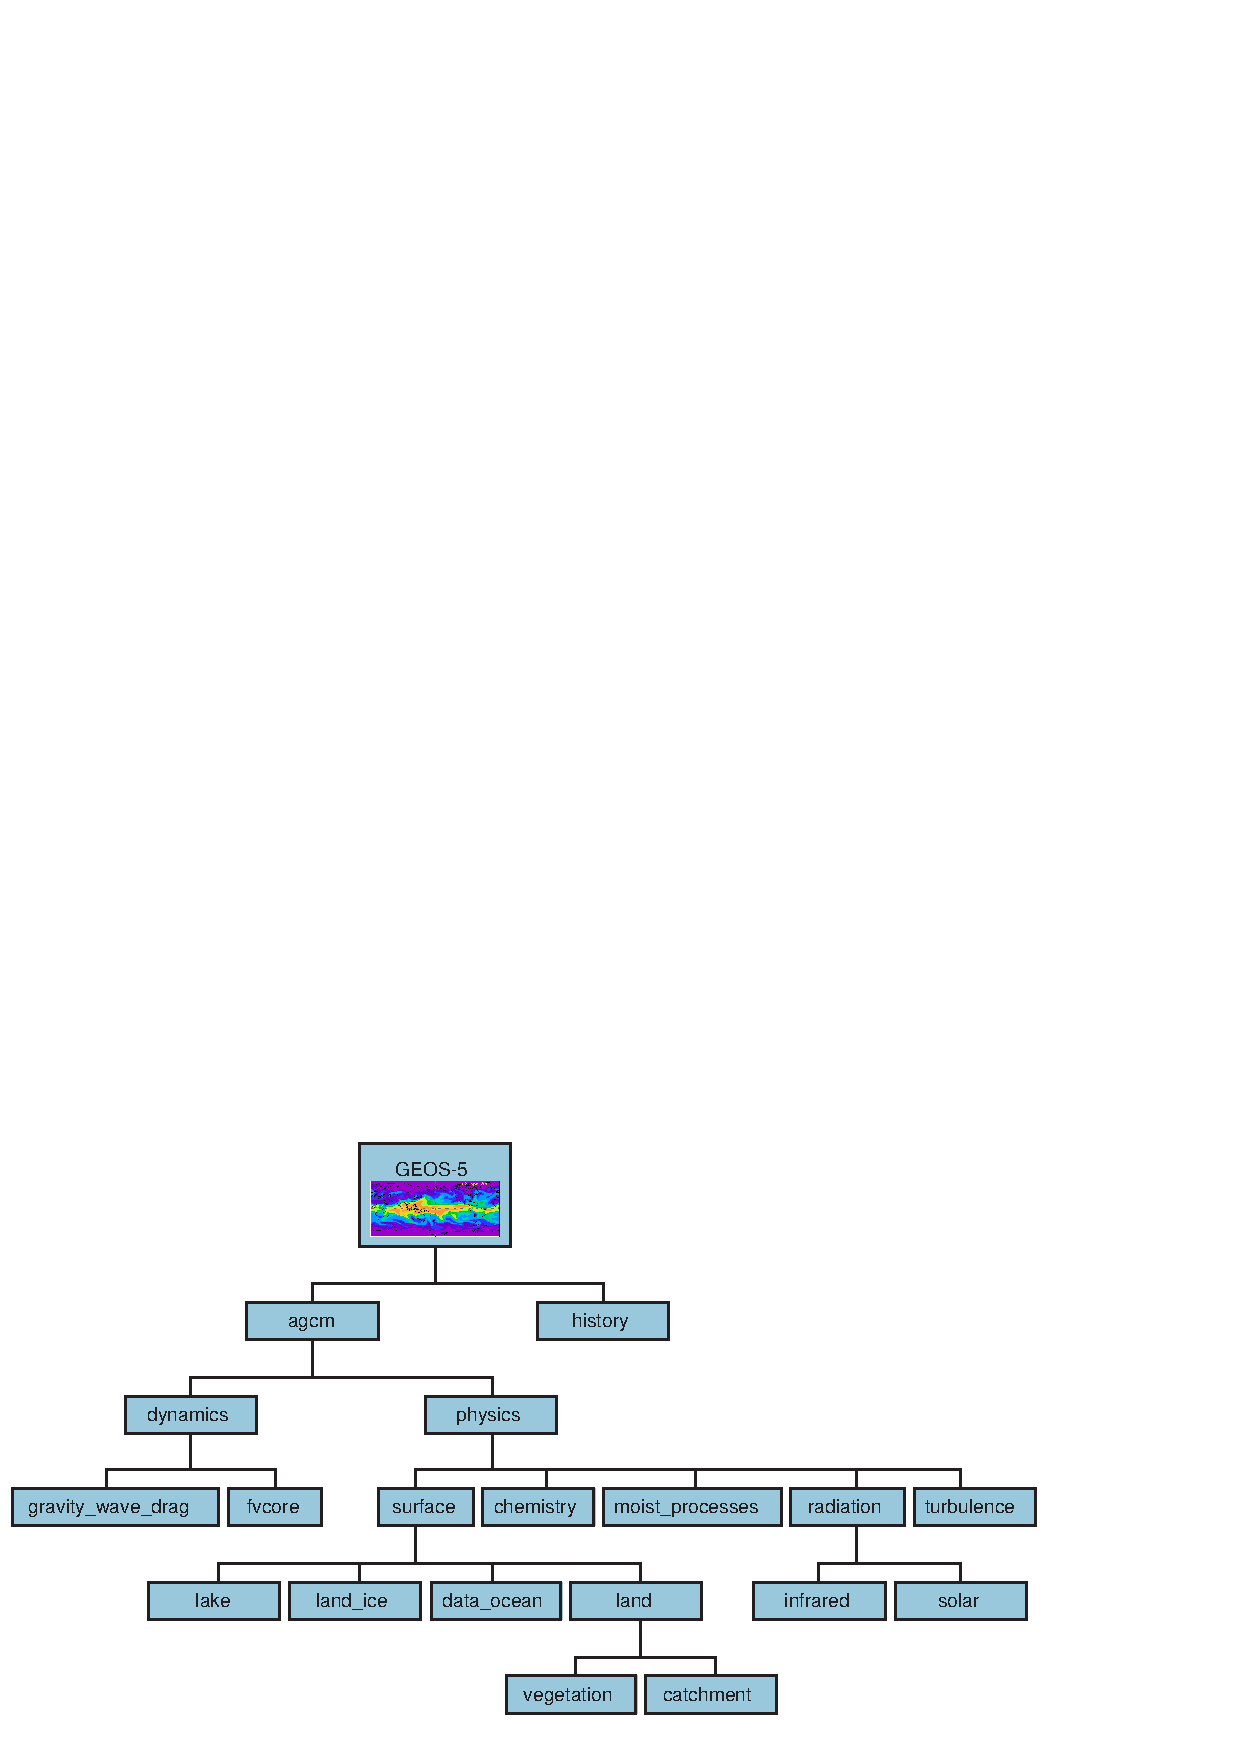
\includegraphics{ESMF_GEOS5}}
\end{figure}
\end{center}

\subsection{Hierarchical Creation of Components}
\label{sec:hierarchy}

Components are allocated computational resources in the form of
{\bf Persistent Execution Threads}, or {\bf PET}s.  A list of a Component's
PETs is contained in a structure called a {\bf Virtual Machine},
or {\bf VM}.  The VM also contains information about the topology and
characteristics of the underlying computer.
Components are created hierarchically, with parent Components creating
child Components and allocating some or all of their PETs to each one.
By default ESMF creates a new VM for each child Component, which 
allows Components to tailor their VM resources to match their needs.
In some cases, a child may want to share its parent's VM - ESMF
supports this, too.

A Gridded Component may exist across all the PETs in an application. 
A Gridded Component may also reside on a subset of PETs in an
application.  These PETs may wholly coincide with, be wholly contained
within, or wholly contain another Component.

\begin{center}
\begin{figure}
\caption{A call to a standard ESMF initialize (run, finalize) method
by a parent component triggers calls to initialize (run, finalize)
all of its child components.}
\label{fig:appunit}
\scalebox{1.0}{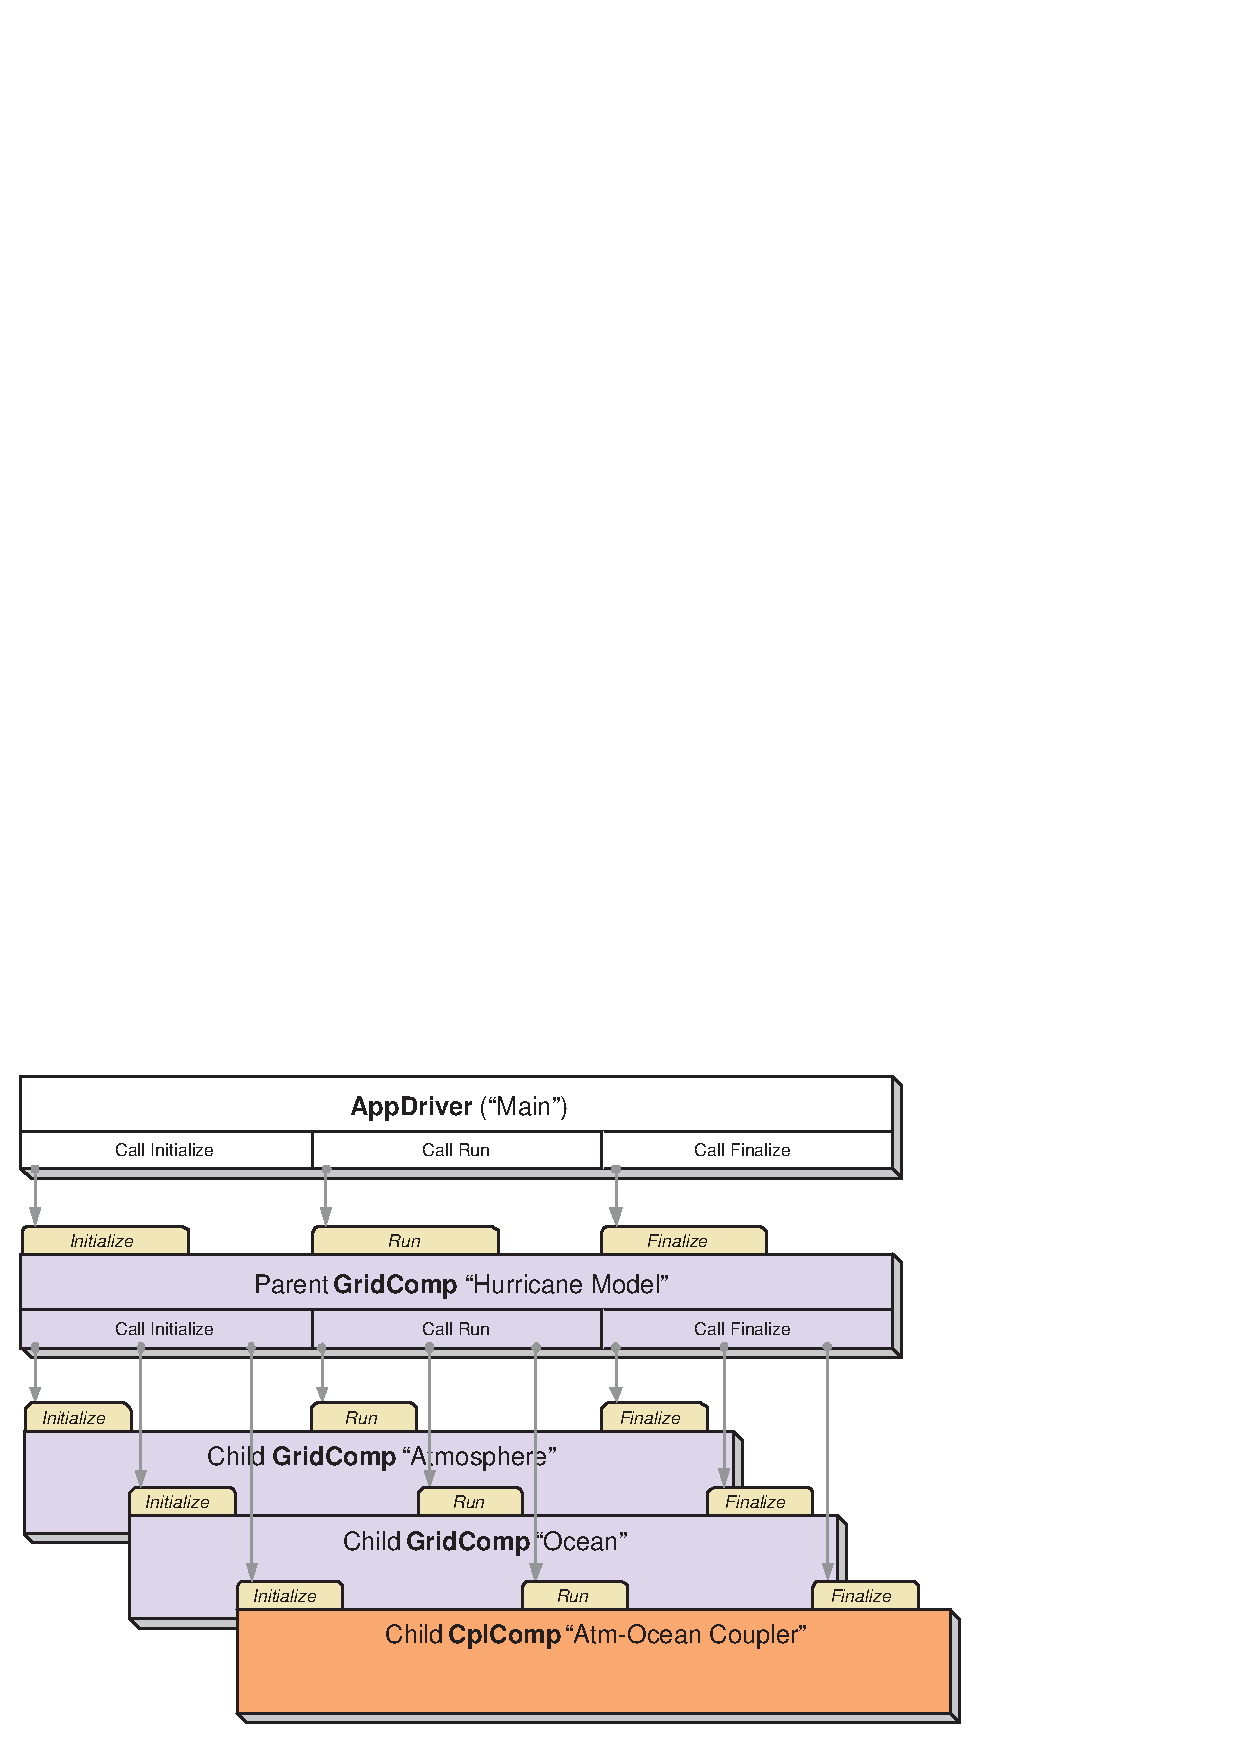
\includegraphics{ESMF_appunit}}
\end{figure}
\end{center}

\subsection{Sequential and Concurrent Execution of Components}
\label{sec:concurrency}

When a set of Gridded Components and a Coupler runs in sequence
on the same set of PETs the application is executing in a {\bf sequential}
mode. When Gridded Components are created and run on mutually exclusive
sets of PETs, and are coupled by a Coupler Component that extends over
the union of these sets, the mode of execution is {\bf concurrent}.

Figure \ref{fig:serial} illustrates a typical configuration for 
a simple coupled sequential
application, and Figure \ref{fig:concurrent} shows a possible 
configuration for the same application running in a concurrent mode.

Parent Components can select if and when to wait for concurrently
executing child Components, synchronizing only when required.

It is possible for ESMF applications to contain some Component sets
that are executing sequentially and others that are executing concurrently.
We might have, for example, atmosphere and land Components created
on the same subset of PETs, ocean and sea ice Components created on
the remainder of PETs, and a Coupler created across all the PETs in
the application.

\begin{center}
\begin{figure}
\caption{Schematic of the run method of a coupled application, with an
``Atmosphere'' and an ``Ocean'' Gridded Component running sequentially with 
an ``Atm-Ocean Coupler.''  The top-level ``Hurricane Model'' 
Gridded Component contains the sequencing information and time 
advancement loop.  The application driver, Coupler, and all Gridded Components 
are distributed over nine PETs.}
\label{fig:serial}
\scalebox{1.0}{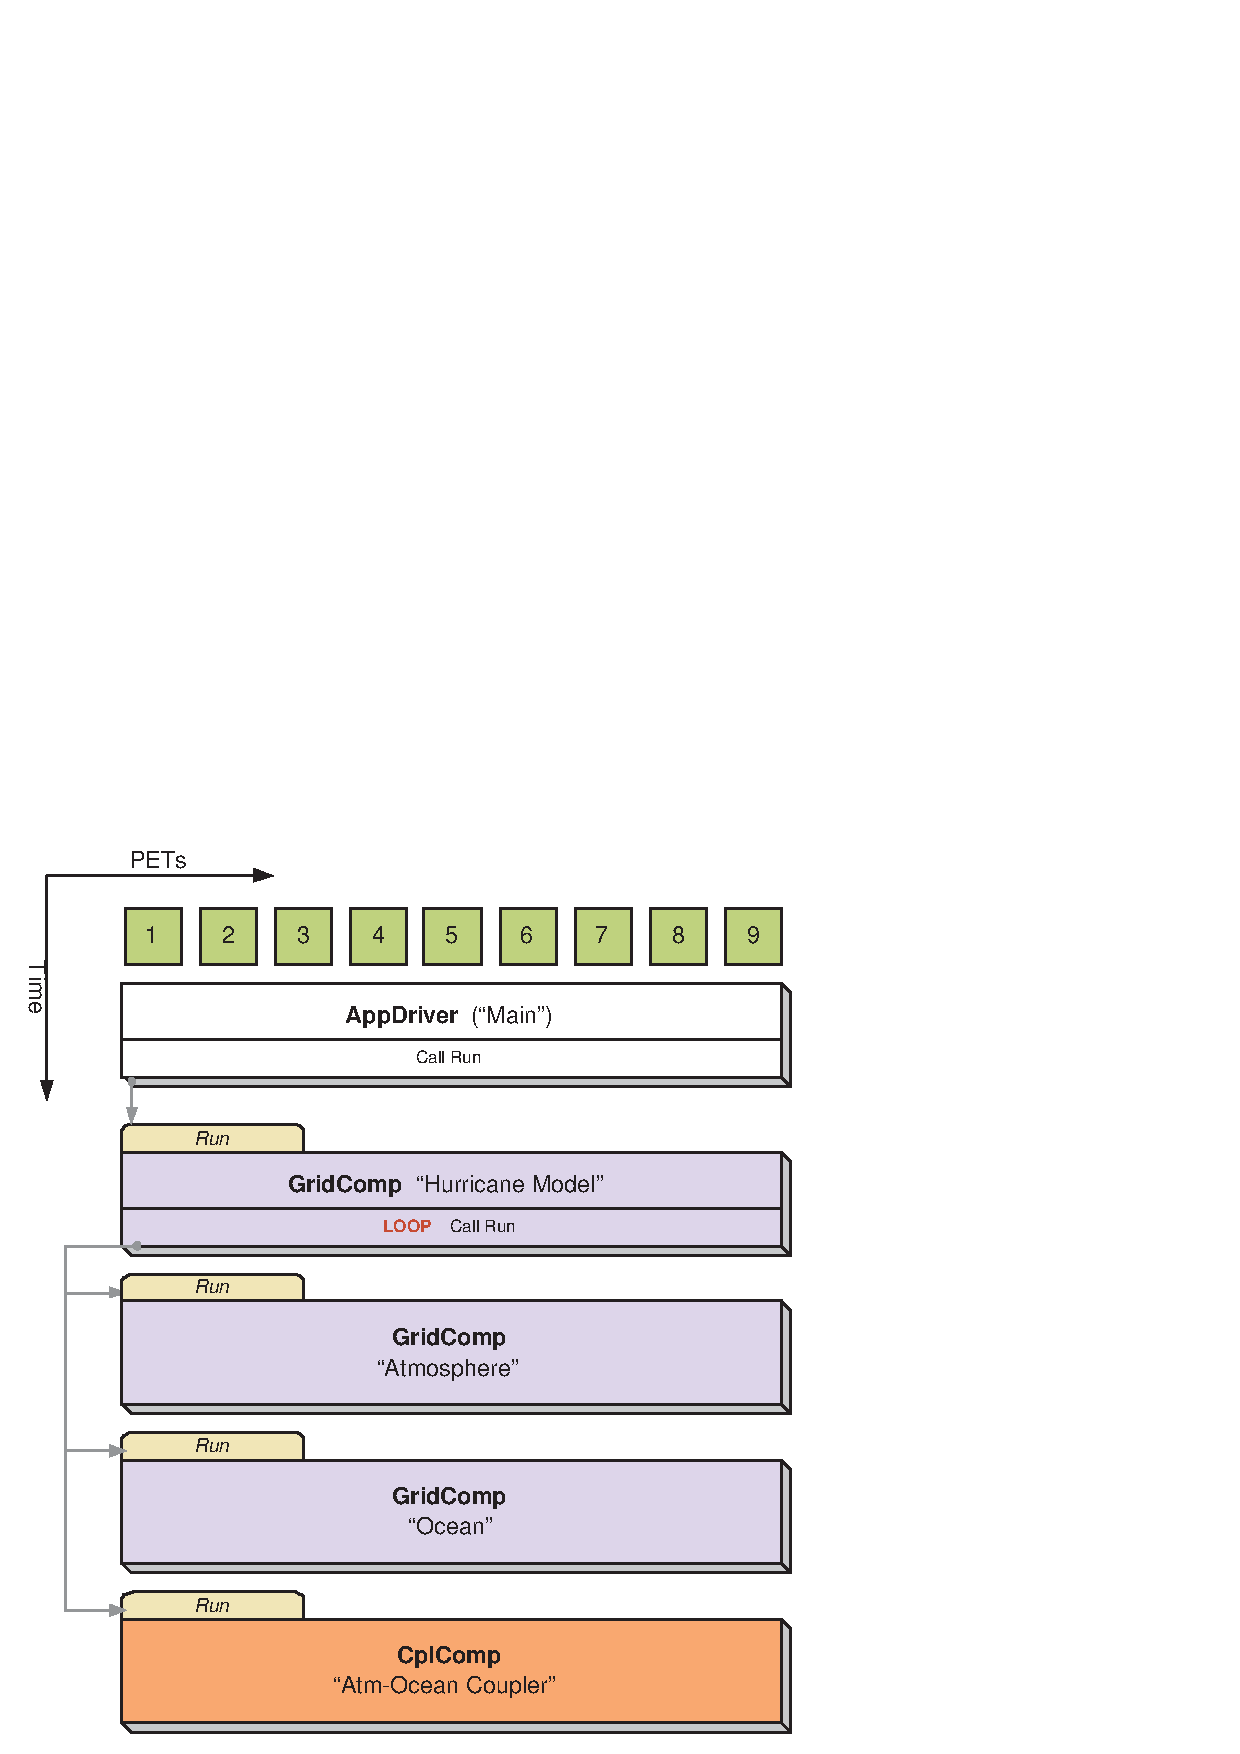
\includegraphics{ESMF_serial}}
\end{figure}
\end{center}

\begin{center}
\begin{figure}
\caption{Schematic of the run method of a coupled application, with an
``Atmosphere'' and an ``Ocean'' Gridded Component running concurrently with 
an ``Atm-Ocean Coupler.''  The top-level ``Hurricane Model'' 
Gridded Component contains the sequencing information and time 
advancement loop.  The application driver, Coupler, and top-level ``Hurricane
Model'' Gridded Component are distributed over nine PETs.  The
``Atmosphere'' Gridded Component is distributed over three PETs and
the ``Ocean'' Gridded Component is distributed over six PETs.}
\label{fig:concurrent}
\scalebox{1.0}{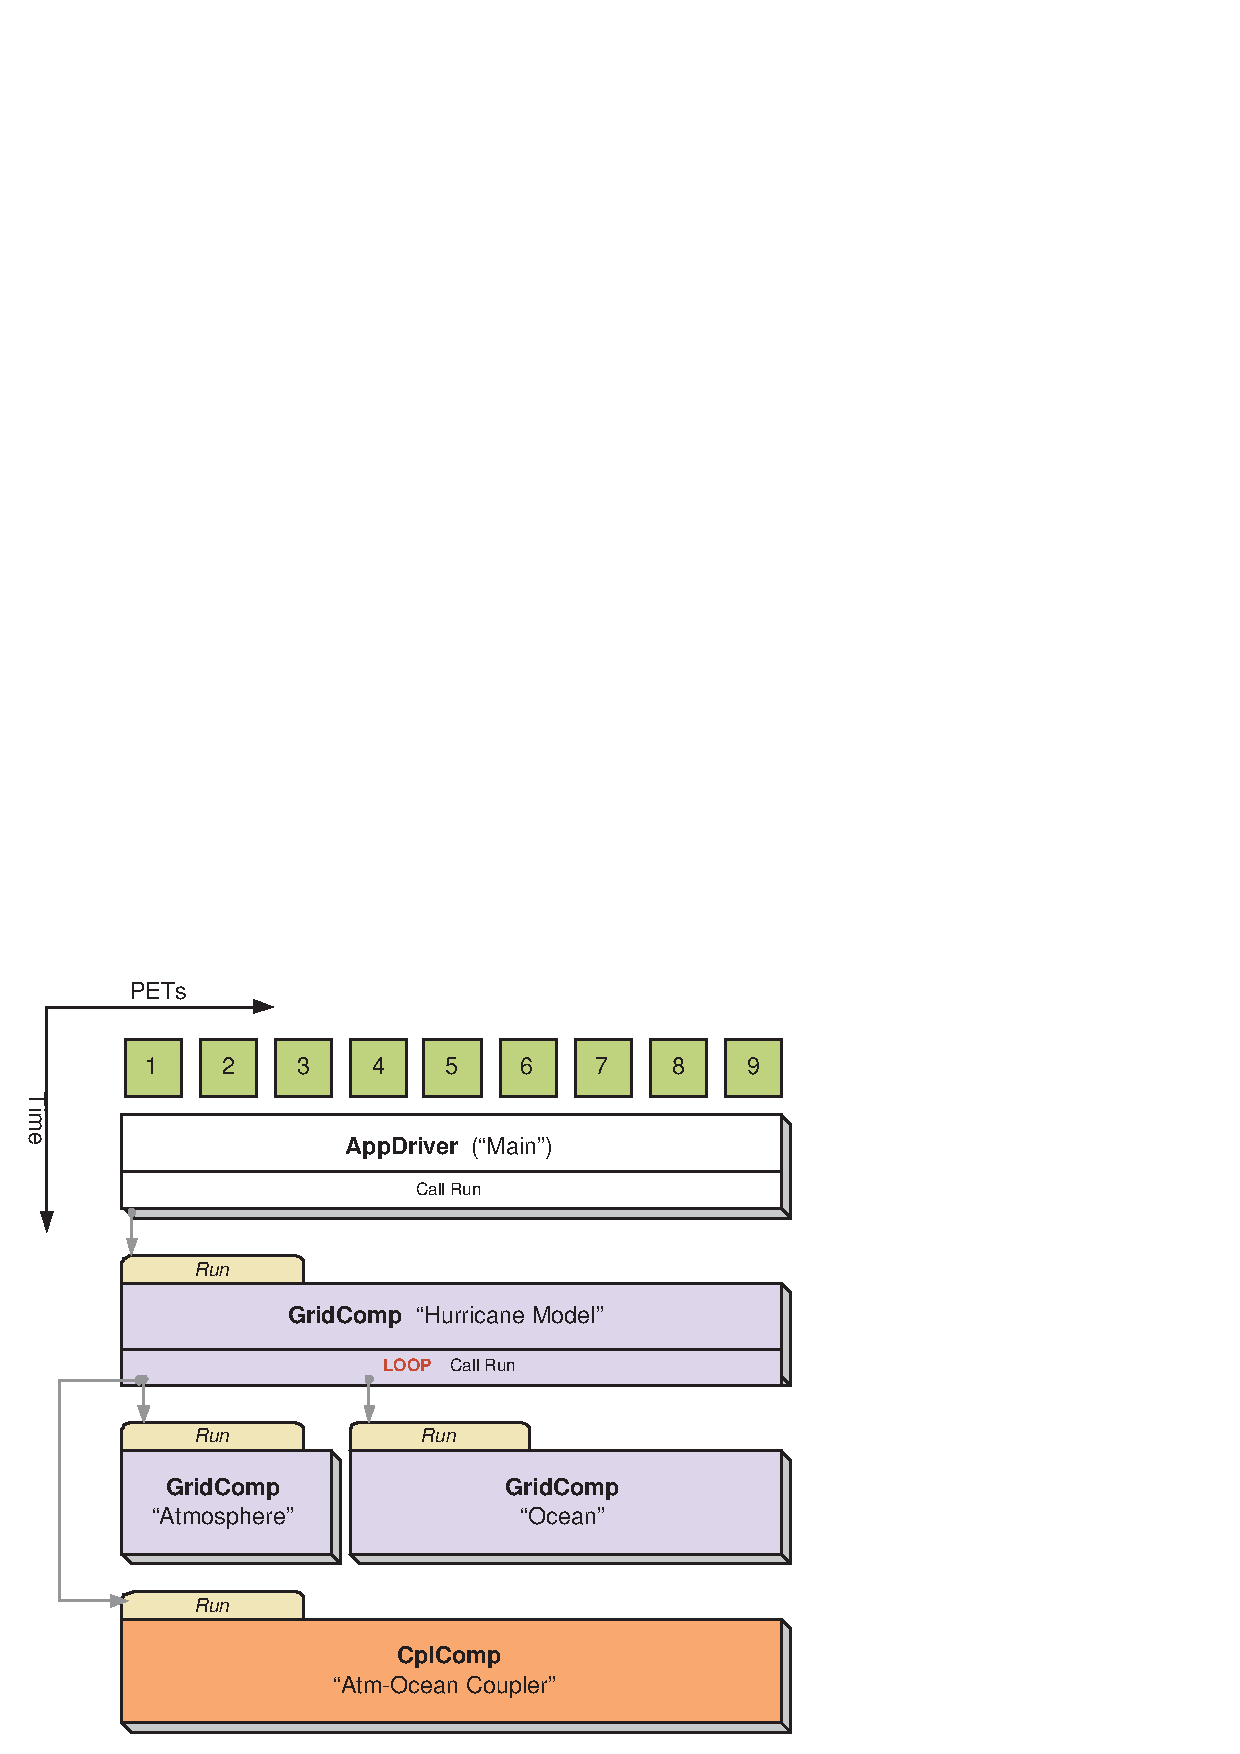
\includegraphics{ESMF_concurrent}}
\end{figure}
\end{center}

\subsection{Intra-Component Communication}
\label{sec:localcomm}

All data transfers within an ESMF application occur {\it within} a
component.  For example, a Gridded Component may contain halo updates.
Another example is that a Coupler Component may redistribute
data between two Gridded Components.  As a result,
the architecture of ESMF does not depend on any particular data
communication mechanism, and new communication schemes can be
introduced without affecting the overall structure of the application.

Since all data communication happens within a component, a Coupler
Component must be created on the union of the PETs of all
the Gridded Components that it couples.  

\subsection{Data Distribution and Scoping in Components}
\label{sec:scoping}

The scope of distributed objects is the VM of the currently 
executing Component.  For this reason, all
PETs in the current VM must make the same distributed object
creation calls.   When a Coupler Component running on a superset
of a Gridded Component's PETs needs to make communication calls
involving objects created by the Gridded Component,
an ESMF-supplied function called {\tt ESMF\_StateReconcile()} creates proxy
objects for those PETs that had no previous information about the
distributed objects.  Proxy objects contain no local data but
can be used in communication calls (such as regrid or redistribute)
to describe the remote source for data being moved to the current PET,
or to describe the remote destination for data being moved from the local PET.
Figure \ref{fig:reconcile} is a simple schematic that shows the 
sequence of events in a reconcile call.

\begin{center}
\begin{figure}
\caption{An {\tt ESMF\_StateReconcile()} call creates proxy 
objects for use in subsequent communication calls.  The reconcile 
call would normally be made during Coupler initialization.}
\label{fig:reconcile}
\scalebox{1.0}{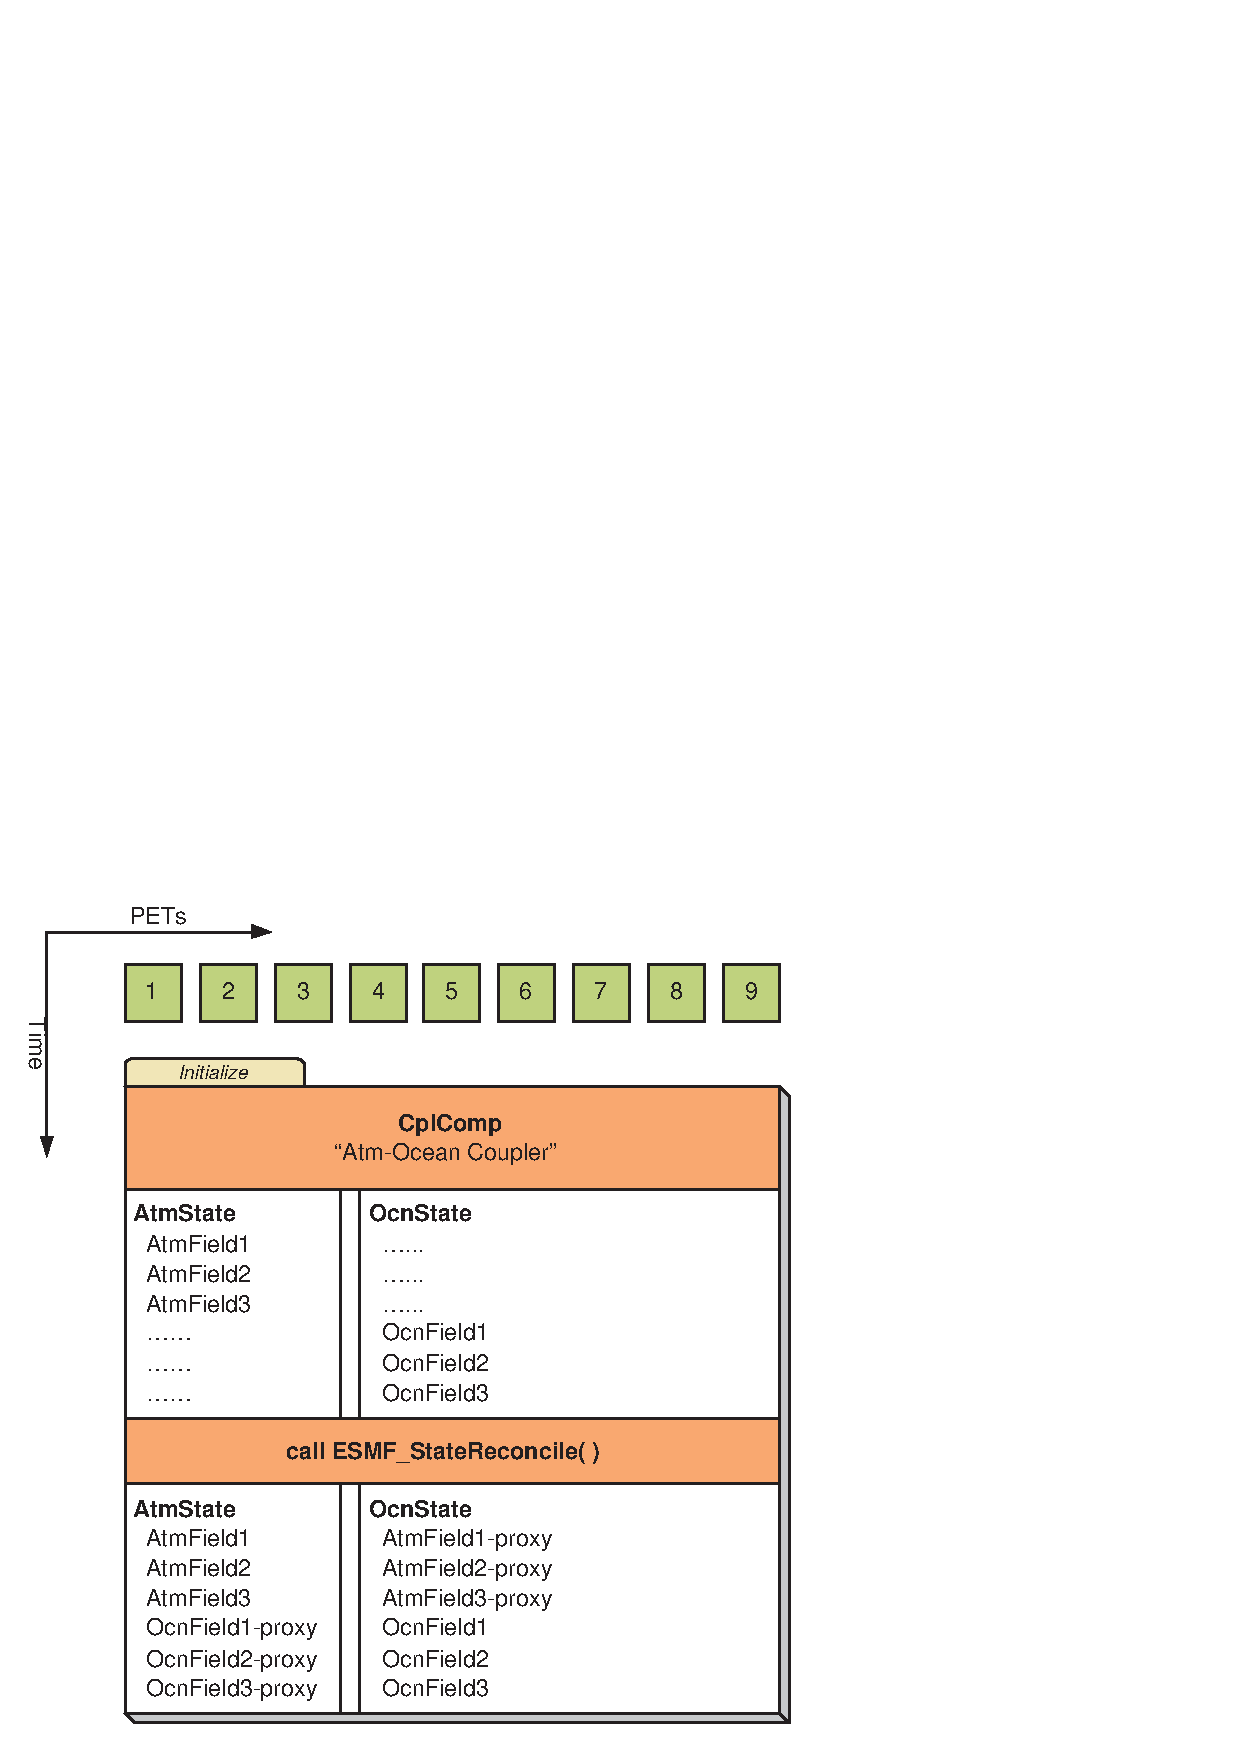
\includegraphics{ESMF_reconcile}}
\end{figure}
\end{center}

\subsection{Performance}
\label{sec:performance}

The ESMF design enables the user to configure ESMF
applications so that data is transferred directly from one component 
to another, without requiring that it be copied or sent to a different data
buffer as an interim step.  This is likely to be the most efficient way 
of performing inter-component coupling.  However, if desired, an 
application can also be configured so that data from a source component 
is sent to a distinct set of Coupler Component PETs for processing 
before being sent to its destination.

The ability to overlap computation with communication is essential for
performance.  When running with ESMF the user can initiate data 
sends during Gridded Component execution, as soon as the data is ready.
Computations can then proceed simultaneously with the data transfer.

\newpage
\subsection{Object Model}

The following is a simplified Unified Modeling Language (UML) diagram showing the relationships among
ESMF superstructure classes.  See Appendix A, {\it A Brief Introduction 
to UML}, for a translation table that lists the symbols in the diagram 
and their meaning.

\begin{center}
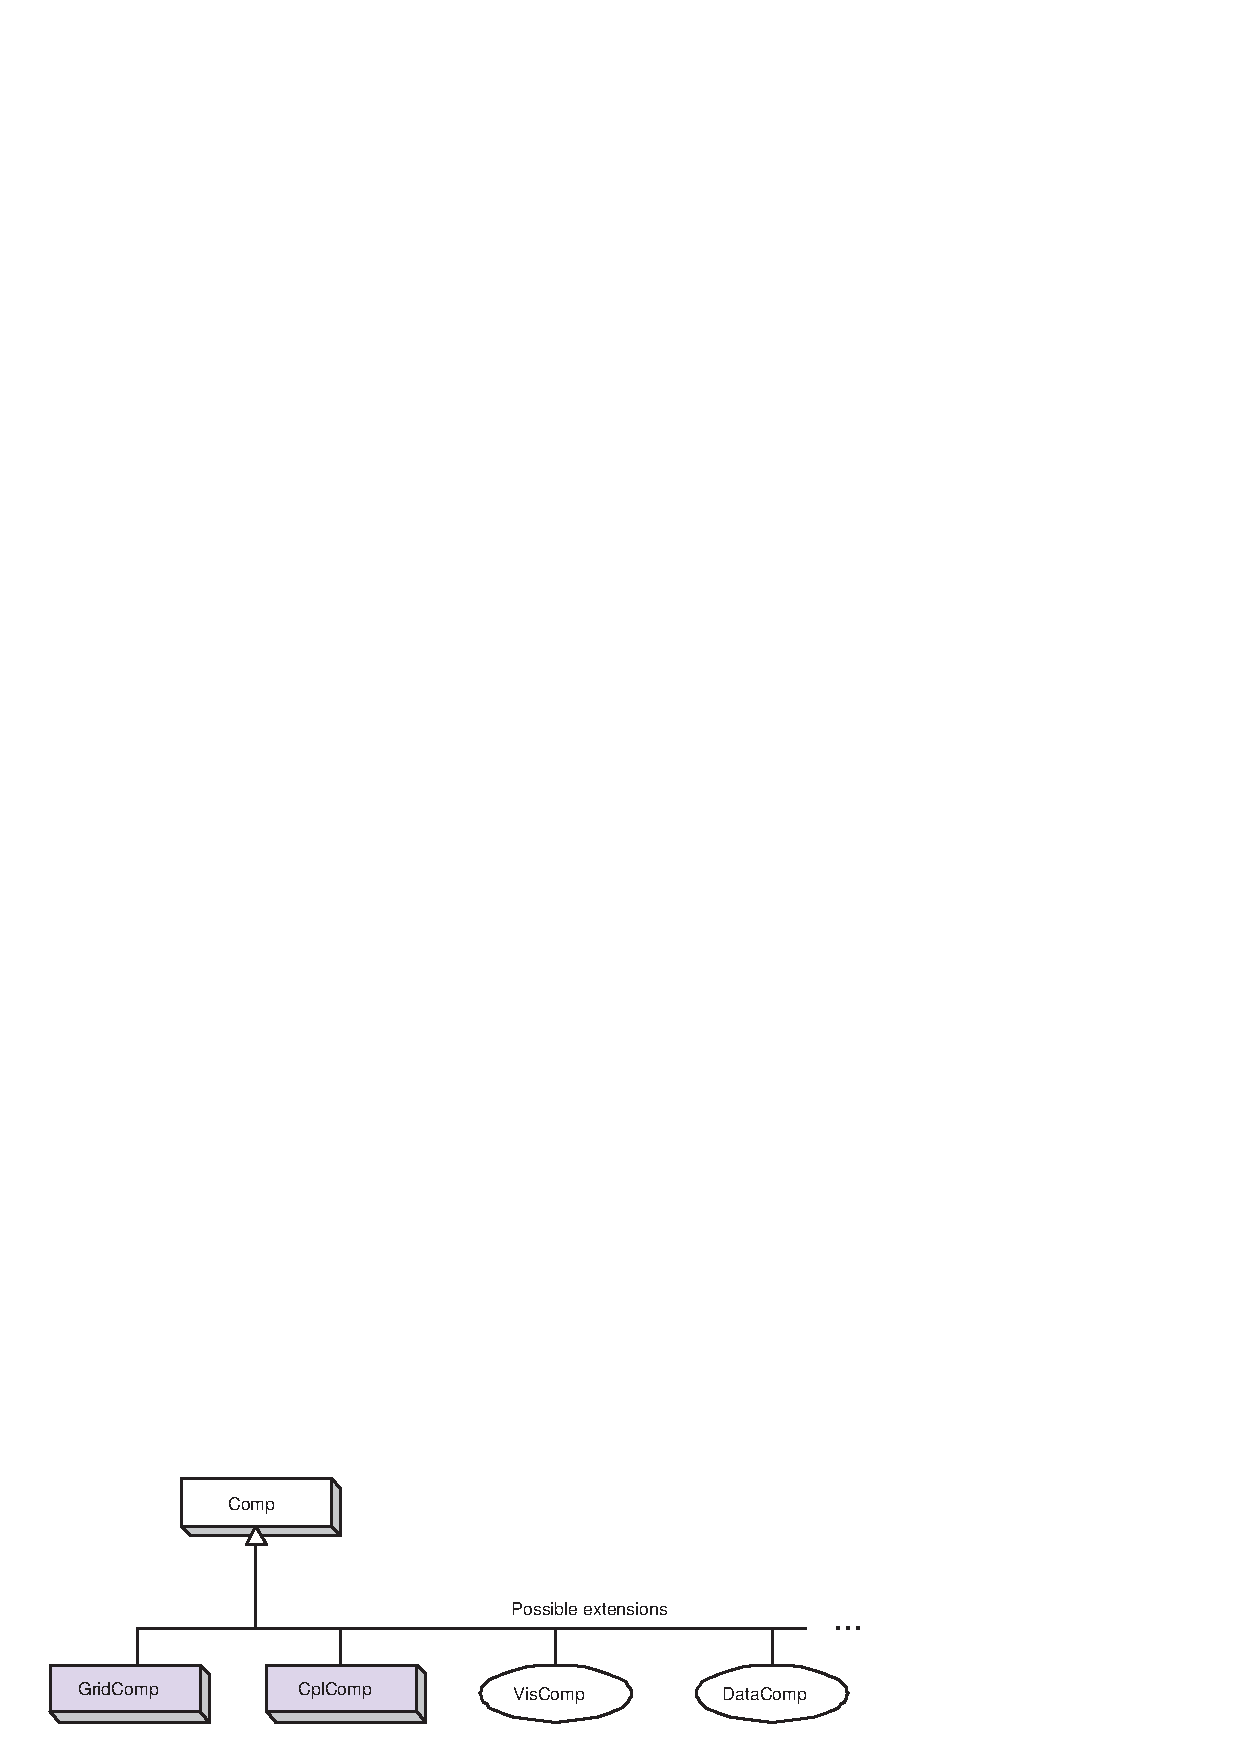
\includegraphics{Comp_obj}   
\end{center}




% $Id$
%
% Earth System Modeling Framework
% Copyright 2002-2020, University Corporation for Atmospheric Research,
% Massachusetts Institute of Technology, Geophysical Fluid Dynamics
% Laboratory, University of Michigan, National Centers for Environmental
% Prediction, Los Alamos National Laboratory, Argonne National Laboratory,
% NASA Goddard Space Flight Center.
% Licensed under the University of Illinois-NCSA License.
\bodytext{BGCOLOR=white LINK=#083194 VLINK=#21004A}
\section{Application Driver and Required ESMF Methods}
\subsection{Description}
% $Id$
%
% Earth System Modeling Framework
% Copyright 2002-2020, University Corporation for Atmospheric Research, 
% Massachusetts Institute of Technology, Geophysical Fluid Dynamics 
% Laboratory, University of Michigan, National Centers for Environmental 
% Prediction, Los Alamos National Laboratory, Argonne National Laboratory, 
% NASA Goddard Space Flight Center.
% Licensed under the University of Illinois-NCSA License.

%\subsection{Description}

Every ESMF application needs a driver code. Typically the driver layer is
implemented as the "main" of the application, although this is not strictly an
ESMF requirement. For most ESMF applications the task of the application driver
will be very generic: Initialize ESMF, create a top-level Component and call its
Initialize, Run and Finalize methods, before destroying the top-level Component
again and calling ESMF Finalize.

\begin{sloppypar}
ESMF provides a number of different application driver templates in the
{\tt \$ESMF\_DIR/src/Superstructure/AppDriver} directory. An appropriate one 
can be chosen depending on how the application is to be structured:
\end{sloppypar}

\begin{description}

\item[Sequential vs. Concurrent Execution]

In a sequential execution model, every Component executes
on all PETs, with each Component completing execution before
the next Component begins.  This has the appeal of 
simplicity of data consumption and production: when a Gridded 
Component starts, all required data is available for use, and when
a Gridded Component finishes, all data produced is ready for consumption
by the next Gridded Component.  This approach also has
the possibility of less data movement if the grid and
data decomposition is done such that each processor's memory contains
the data needed by the next Component.

In a concurrent execution model, subgroups of PETs run
Gridded Components and multiple Gridded Components are active at the 
same time.  Data exchange must be coordinated between Gridded 
Components so that data deadlock does not occur.  This strategy 
has the advantage of allowing coupling to other Gridded Components 
at any time during the computational process, including not 
having to return to the calling level of code before making 
data available.  

\item[Pairwise vs. Hub and Spoke]

Coupler Components are responsible for taking data from one
Gridded Component and putting it into the form expected by another 
Gridded Component.  This might include regridding, change of units, 
averaging, or binning.

Coupler Components can be written for {\it pairwise} data exchange: 
the Coupler Component takes data from a single Component and transforms 
it for use by another single Gridded Component.  This simplifies the 
structure of the Coupler Component code.

Couplers can also be written using a {\it hub and spoke} model where a
single Coupler accepts data from all other Components, can do data
merging or splitting, and formats data for all other Components.

Multiple Couplers, using either of the above two models or some mixture of
these approaches, are also possible.

\item[Implementation Language]

The ESMF framework currently has Fortran interfaces for all public functions. 
Some functions also have C interfaces, and the number of these is expected to 
increase over time. 


\item[Number of Executables]

The simplest way to run an application
is to run the same executable program on all PETs.  Different Components
can still be run on mutually exclusive PETs by using branching
(e.g., if this is PET 1, 2, or 3, run Component A, if it is
PET 4, 5, or 6 run Component B).  This is a {\bf SPMD} model, 
Single Program Multiple Data.  

The alternative is to start a different executable program on different
PETs.  This is a {\bf MPMD} model, Multiple Program Multiple Data.
There are complications with many job control systems on multiprocessor
machines in getting the different executables started, and getting
inter-process communications established.  ESMF currently has some
support for MPMD: different Components can run as separate executables,
but the Coupler that transfers data between the Components must still
run on the union of their PETs. This means that the Coupler Component
must be linked into all of the executables.

\end{description}




\subsection{Constants}
% $Id$

\subsubsection{ESMF\_END}
\label{const:endflag}

{\sf DESCRIPTION:\\}
The {\tt ESMF\_End\_Flag} determines how an ESMF application is shut down.

The type of this flag is:

{\tt type(ESMF\_End\_Flag)}

The valid values are:
\begin{description}
   \item [ESMF\_END\_ABORT] 
         Global abort of the ESMF application. There is no guarantee 
         that all PETs will shut down cleanly during an abort. However, all
         attempts are made to prevent the application from hanging and the
         LogErr of at least one PET will be completely flushed during the abort.
         This option should only be used if a condition is detected that
         prevents normal continuation or termination of the application.
         Typical conditions that warrant the use of {\tt ESMF\_END\_ABORT} 
         are those that occur on a per PET basis where other PETs may be blocked
         in communication calls, unable to reach the normal termination point.
         An aborted application returns to the parent process with a system
         dependent indication that a failure occurred during execution.
   \item [ESMF\_END\_NORMAL]
         \begin{sloppypar}
         Normal termination of the ESMF application. Wait for all PETs of the
         global VM to reach 
	{\tt ESMF\_Finalize()} before termination. This is
         the clean way of terminating an application. {\tt MPI\_Finalize()} will
         be called in case of MPI applications.
         \end{sloppypar}
   \item [ESMF\_END\_KEEPMPI]
         Same as {\tt ESMF\_END\_NORMAL} but {\tt MPI\_Finalize()} will {\em not}
         be called. It is the user code's responsibility to shut down MPI
         cleanly if necessary.
\end{description}

\subsection{Use and Examples}
% $Id$
%
% Earth System Modeling Framework
% Copyright 2002-2020, University Corporation for Atmospheric Research, 
% Massachusetts Institute of Technology, Geophysical Fluid Dynamics 
% Laboratory, University of Michigan, National Centers for Environmental 
% Prediction, Los Alamos National Laboratory, Argonne National Laboratory, 
% NASA Goddard Space Flight Center.
% Licensed under the University of Illinois-NCSA License.

%\subsection{Usage}

ESMF encourages application organization in which there is a single 
top-level Gridded Component.  This provides a simple, clear sequence
of operations at the highest level, and also enables the entire 
application to be treated as a sub-Component of another, larger 
application if desired.  When a simple application is organized in this fashion 
the standard AppDriver can probably be used without much modification.  

\begin{sloppypar}
Examples of program organization using the AppDriver can be found in the 
{\tt src/Superstructure/AppDriver} directory.  A set of subdirectories 
within the AppDriver directory follows the naming convention:
\end{sloppypar}
\begin{verbatim}
<seq|concur>_<pairwise|hub>_<f|c>driver_<spmd|mpmd>
\end{verbatim}

The example that is currently implemented is
{\tt seq\_pairwise\_fdriver\_spmd}, which
has sequential component execution, a pairwise coupler, a main program
in Fortran, and all processors launching the same executable.
It is also copied automatically into a top-level 
{\tt quick\_start} directory at compilation time.  

The user can copy the AppDriver files into
their own local directory. Some of the files can be used unchanged.
Others are template files which have the rough outline of the code but
need additional application-specific code added in order to perform a
meaningful function.  The {\tt README} file in the AppDriver 
subdirectory or {\tt quick\_start} directory contains instructions about 
which files to change.

Examples of concurrent component execution can be found in the
system tests that are bundled with the ESMF distribution.




%                **** IMPORTANT NOTICE *****
% This LaTeX file has been automatically produced by ProTeX v. 1.1
% Any changes made to this file will likely be lost next time
% this file is regenerated from its source. Send questions 
% to Arlindo da Silva, dasilva@gsfc.nasa.gov
 
\setlength{\oldparskip}{\parskip}
\setlength{\parskip}{1.5ex}
\setlength{\oldparindent}{\parindent}
\setlength{\parindent}{0pt}
\setlength{\oldbaselineskip}{\baselineskip}
\setlength{\baselineskip}{11pt}
 
%--------------------- SHORT-HAND MACROS ----------------------
\def\bv{\begin{verbatim}}
\def\ev{\end{verbatim}}
\def\be{\begin{equation}}
\def\ee{\end{equation}}
\def\bea{\begin{eqnarray}}
\def\eea{\end{eqnarray}}
\def\bi{\begin{itemize}}
\def\ei{\end{itemize}}
\def\bn{\begin{enumerate}}
\def\en{\end{enumerate}}
\def\bd{\begin{description}}
\def\ed{\end{description}}
\def\({\left (}
\def\){\right )}
\def\[{\left [}
\def\]{\right ]}
\def\<{\left  \langle}
\def\>{\right \rangle}
\def\cI{{\cal I}}
\def\diag{\mathop{\rm diag}}
\def\tr{\mathop{\rm tr}}
%-------------------------------------------------------------

\markboth{Left}{Source File: AppDriver.F90,  Date: Tue May  5 21:00:19 MDT 2020
}

 
%/////////////////////////////////////////////////////////////

  \begin{verbatim}
 
  ---------------------------------------------------------------------------
  ---------------------------------------------------------------------------
   EXAMPLE:  This is an AppDriver.F90 file for a sequential ESMF application.
  ---------------------------------------------------------------------------
  ---------------------------------------------------------------------------
  
    The ChangeMe.F90 file that's included below contains a number of
    definitions that are used by the AppDriver, such as the name of the
    application's main configuration file and the name of the application's
    SetServices routine.  This file is in the same directory as the
    AppDriver.F90 file.
  ---------------------------------------------------------------------------
 
 #include "ChangeMe.F90"
 
     program ESMF_AppDriver
 #define ESMF_METHOD "program ESMF_AppDriver"
 
 #include "ESMF.h"
 
     ! ESMF module, defines all ESMF data types and procedures
     use ESMF
 
     ! Gridded Component registration routines.  Defined in "ChangeMe.F90"
     use USER_APP_Mod, only : SetServices => USER_APP_SetServices
 
     implicit none
 
  ---------------------------------------------------------------------------
    Define local variables
  ---------------------------------------------------------------------------
 
     ! Components and States
     type(ESMF_GridComp) :: compGridded
     type(ESMF_State) :: defaultstate
 
     ! Configuration information
     type(ESMF_Config) :: config
 
     ! A common Grid
     type(ESMF_Grid) :: grid
 
     ! A Clock, a Calendar, and timesteps
     type(ESMF_Clock) :: clock
     type(ESMF_TimeInterval) :: timeStep
     type(ESMF_Time) :: startTime
     type(ESMF_Time) :: stopTime
 
     ! Variables related to the Grid
     integer :: i_max, j_max
 
     ! Return codes for error checks
     integer :: rc, localrc
 
  ---------------------------------------------------------------------------
    Initialize ESMF.  Note that an output Log is created by default.
  ---------------------------------------------------------------------------
 
     call ESMF_Initialize(defaultCalKind=ESMF_CALKIND_GREGORIAN, rc=localrc)
     if (ESMF_LogFoundError(localrc, ESMF_ERR_PASSTHRU, &
         ESMF_CONTEXT, rcToReturn=rc)) &
         call ESMF_Finalize(rc=localrc, endflag=ESMF_END_ABORT)
 
     call ESMF_LogWrite("ESMF AppDriver start", ESMF_LOGMSG_INFO)
 
  ---------------------------------------------------------------------------
    Create and load a configuration file.
    The USER_CONFIG_FILE is set to sample.rc in the ChangeMe.F90 file.
    The sample.rc file is also included in the directory with the
    AppDriver.F90 file.
  ---------------------------------------------------------------------------
 
     config = ESMF_ConfigCreate(rc=localrc)
     if (ESMF_LogFoundError(localrc, ESMF_ERR_PASSTHRU, &
         ESMF_CONTEXT, rcToReturn=rc)) &
         call ESMF_Finalize(rc=localrc, endflag=ESMF_END_ABORT)
 
     call ESMF_ConfigLoadFile(config, USER_CONFIG_FILE, rc = localrc)
     if (ESMF_LogFoundError(localrc, ESMF_ERR_PASSTHRU, &
         ESMF_CONTEXT, rcToReturn=rc)) &
         call ESMF_Finalize(rc=localrc, endflag=ESMF_END_ABORT)
 
  ---------------------------------------------------------------------------
    Get configuration information.
  
    A configuration file like sample.rc might include:
    - size and coordinate information needed to create the default Grid.
    - the default start time, stop time, and running intervals
      for the main time loop.
  ---------------------------------------------------------------------------
 
     call ESMF_ConfigGetAttribute(config, i_max, label='I Counts:', &
       default=10, rc=localrc)
     if (ESMF_LogFoundError(localrc, ESMF_ERR_PASSTHRU, &
         ESMF_CONTEXT, rcToReturn=rc)) &
         call ESMF_Finalize(rc=localrc, endflag=ESMF_END_ABORT)
     call ESMF_ConfigGetAttribute(config, j_max, label='J Counts:', &
       default=40, rc=localrc)
     if (ESMF_LogFoundError(localrc, ESMF_ERR_PASSTHRU, &
         ESMF_CONTEXT, rcToReturn=rc)) &
         call ESMF_Finalize(rc=localrc, endflag=ESMF_END_ABORT)
 
  ---------------------------------------------------------------------------
    Create the top Gridded Component.
  ---------------------------------------------------------------------------
 
     compGridded = ESMF_GridCompCreate(name="ESMF Gridded Component", &
         rc=localrc)
     if (ESMF_LogFoundError(localrc, ESMF_ERR_PASSTHRU, &
         ESMF_CONTEXT, rcToReturn=rc)) &
         call ESMF_Finalize(rc=localrc, endflag=ESMF_END_ABORT)
 
     call ESMF_LogWrite("Component Create finished", ESMF_LOGMSG_INFO)
 
  ----------------------------------------------------------------------------
    Register the set services method for the top Gridded Component.
  ----------------------------------------------------------------------------
 
     call ESMF_GridCompSetServices(compGridded, userRoutine=SetServices, rc=rc)
     if (ESMF_LogFoundError(rc, msg="Registration failed", rcToReturn=rc)) &
         call ESMF_Finalize(rc=localrc, endflag=ESMF_END_ABORT)
 
  ----------------------------------------------------------------------------
    Create and initialize a Clock.
  ----------------------------------------------------------------------------
 
       call ESMF_TimeIntervalSet(timeStep, s=2, rc=localrc)
       if (ESMF_LogFoundError(localrc, ESMF_ERR_PASSTHRU, &
             ESMF_CONTEXT, rcToReturn=rc)) &
             call ESMF_Finalize(rc=localrc, endflag=ESMF_END_ABORT)
 
       call ESMF_TimeSet(startTime, yy=2004, mm=9, dd=25, rc=localrc)
       if (ESMF_LogFoundError(localrc, ESMF_ERR_PASSTHRU, &
             ESMF_CONTEXT, rcToReturn=rc)) &
             call ESMF_Finalize(rc=localrc, endflag=ESMF_END_ABORT)
 
       call ESMF_TimeSet(stopTime, yy=2004, mm=9, dd=26, rc=localrc)
       if (ESMF_LogFoundError(localrc, ESMF_ERR_PASSTHRU, &
             ESMF_CONTEXT, rcToReturn=rc)) &
             call ESMF_Finalize(rc=localrc, endflag=ESMF_END_ABORT)
 
       clock = ESMF_ClockCreate(timeStep, startTime, stopTime=stopTime, &
                 name="Application Clock", rc=localrc)
       if (ESMF_LogFoundError(localrc, ESMF_ERR_PASSTHRU, &
             ESMF_CONTEXT, rcToReturn=rc)) &
             call ESMF_Finalize(rc=localrc, endflag=ESMF_END_ABORT)
 
  ----------------------------------------------------------------------------
    Create and initialize a Grid.
  
    The default lower indices for the Grid are (/1,1/).
    The upper indices for the Grid are read in from the sample.rc file,
    where they are set to (/10,40/).  This means a Grid will be
    created with 10 grid cells in the x direction and 40 grid cells in the
    y direction.  The Grid section in the Reference Manual shows how to set
    coordinates.
  ----------------------------------------------------------------------------
 
       grid = ESMF_GridCreateNoPeriDim(maxIndex=(/i_max, j_max/), &
                              name="source grid", rc=localrc)
       if (ESMF_LogFoundError(localrc, ESMF_ERR_PASSTHRU, &
             ESMF_CONTEXT, rcToReturn=rc)) &
             call ESMF_Finalize(rc=localrc, endflag=ESMF_END_ABORT)
 
       ! Attach the grid to the Component
       call ESMF_GridCompSet(compGridded, grid=grid, rc=localrc)
       if (ESMF_LogFoundError(localrc, ESMF_ERR_PASSTHRU, &
             ESMF_CONTEXT, rcToReturn=rc)) &
             call ESMF_Finalize(rc=localrc, endflag=ESMF_END_ABORT)
 
  ----------------------------------------------------------------------------
    Create and initialize a State to use for both import and export.
    In a real code, separate import and export States would normally be
    created.
  ----------------------------------------------------------------------------
 
       defaultstate = ESMF_StateCreate(name="Default State", rc=localrc)
       if (ESMF_LogFoundError(localrc, ESMF_ERR_PASSTHRU, &
             ESMF_CONTEXT, rcToReturn=rc)) &
             call ESMF_Finalize(rc=localrc, endflag=ESMF_END_ABORT)
 
  ----------------------------------------------------------------------------
    Call the initialize, run, and finalize methods of the top component.
    When the initialize method of the top component is called, it will in
    turn call the initialize methods of all its child components, they
    will initialize their children, and so on.  The same is true of the
    run and finalize methods.
  ----------------------------------------------------------------------------
 
       call ESMF_GridCompInitialize(compGridded, importState=defaultstate, &
         exportState=defaultstate, clock=clock, rc=localrc)
       if (ESMF_LogFoundError(rc, msg="Initialize failed", rcToReturn=rc)) &
           call ESMF_Finalize(rc=localrc, endflag=ESMF_END_ABORT)
 
       call ESMF_GridCompRun(compGridded, importState=defaultstate, &
         exportState=defaultstate, clock=clock, rc=localrc)
       if (ESMF_LogFoundError(rc, msg="Run failed", rcToReturn=rc)) &
           call ESMF_Finalize(rc=localrc, endflag=ESMF_END_ABORT)
 
       call ESMF_GridCompFinalize(compGridded, importState=defaultstate, &
         exportState=defaultstate, clock=clock, rc=localrc)
       if (ESMF_LogFoundError(rc, msg="Finalize failed", rcToReturn=rc)) &
           call ESMF_Finalize(rc=localrc, endflag=ESMF_END_ABORT)
 
 
  ----------------------------------------------------------------------------
    Destroy objects.
  ----------------------------------------------------------------------------
 
       call ESMF_ClockDestroy(clock, rc=localrc)
       if (ESMF_LogFoundError(localrc, ESMF_ERR_PASSTHRU, &
         ESMF_CONTEXT, rcToReturn=rc)) &
         call ESMF_Finalize(rc=localrc, endflag=ESMF_END_ABORT)
 
       call ESMF_StateDestroy(defaultstate, rc=localrc)
       if (ESMF_LogFoundError(localrc, ESMF_ERR_PASSTHRU, &
         ESMF_CONTEXT, rcToReturn=rc)) &
         call ESMF_Finalize(rc=localrc, endflag=ESMF_END_ABORT)
 
       call ESMF_GridCompDestroy(compGridded, rc=localrc)
       if (ESMF_LogFoundError(localrc, ESMF_ERR_PASSTHRU, &
         ESMF_CONTEXT, rcToReturn=rc)) &
         call ESMF_Finalize(rc=localrc, endflag=ESMF_END_ABORT)
 
  ----------------------------------------------------------------------------
    Finalize and clean up.
  ----------------------------------------------------------------------------
 
     call ESMF_Finalize()
 
     end program ESMF_AppDriver
 
  \end{verbatim}
%...............................................................
\setlength{\parskip}{\oldparskip}
\setlength{\parindent}{\oldparindent}
\setlength{\baselineskip}{\oldbaselineskip}

%\subsection{Restrictions and Future Work}
%#ifdef STANDALONE
%% $Id$
%
% Earth System Modeling Framework
% Copyright 2002-2020, University Corporation for Atmospheric Research, 
% Massachusetts Institute of Technology, Geophysical Fluid Dynamics 
% Laboratory, University of Michigan, National Centers for Environmental 
% Prediction, Los Alamos National Laboratory, Argonne National Laboratory, 
% NASA Goddard Space Flight Center.
% Licensed under the University of Illinois-NCSA License.

%\subsubsection{Restrictions and Future Work}

\begin{enumerate}

\item {\bf MPMD not supported.}  Only single executable applications 
are supported at this time. 

\end{enumerate}

%#elif defined(1)
%% $Id$
%
% Earth System Modeling Framework
% Copyright 2002-2020, University Corporation for Atmospheric Research, 
% Massachusetts Institute of Technology, Geophysical Fluid Dynamics 
% Laboratory, University of Michigan, National Centers for Environmental 
% Prediction, Los Alamos National Laboratory, Argonne National Laboratory, 
% NASA Goddard Space Flight Center.
% Licensed under the University of Illinois-NCSA License.

%\subsubsection{Restrictions and Future Work}

\begin{enumerate}

\item {\bf MPMD not supported.}  Only single executable applications 
are supported at this time. 

\end{enumerate}

%#endif
\subsection{Required ESMF Methods}
% $Id$
%
% Earth System Modeling Framework
% Copyright 2002-2020, University Corporation for Atmospheric Research, 
% Massachusetts Institute of Technology, Geophysical Fluid Dynamics 
% Laboratory, University of Michigan, National Centers for Environmental 
% Prediction, Los Alamos National Laboratory, Argonne National Laboratory, 
% NASA Goddard Space Flight Center.
% Licensed under the University of Illinois-NCSA License.

\begin{sloppypar}
There are a few methods that every ESMF application must contain. First,
{\tt ESMF\_Initialize()} and {\tt ESMF\_Finalize()} are in complete analogy 
to {\tt MPI\_Init()} and {\tt MPI\_Finalize()} known from MPI. All ESMF
programs, serial or parallel, must initialize the ESMF system at the beginning,
and finalize it at the end of execution. The behavior of calling any
ESMF method before {\tt ESMF\_Initialize()}, or after {\tt ESMF\_Finalize()}
is undefined.
\end{sloppypar}

Second, every ESMF Component that is accessed by an ESMF application requires
that its set services routine is called through
{\tt ESMF\_<Grid/Cpl>CompSetServices()}. The Component must implement
one public entry point, its set services routine, that can be called
through the {\tt ESMF\_<Grid/Cpl>CompSetServices()} library routine. The
Component set services routine is responsible for setting entry points
for the standard ESMF Component methods Initialize, Run, and Finalize.

\begin{sloppypar}
Finally, the Component can optionally call {\tt ESMF\_<Grid/Cpl>CompSetVM()}
{\em before} calling
{\tt ESMF\_<Grid/Cpl>CompSetServices()}. Similar to 
{\tt ESMF\_<Grid/Cpl>CompSetServices()}, the 
{\tt ESMF\_<Grid/Cpl>CompSetVM()}
call requires a public entry point into the Component. It allows the Component
to adjust certain aspects of its execution environment, i.e. its own VM, before
it is started up.
\end{sloppypar}

The following sections discuss the above mentioned aspects in more detail.

%                **** IMPORTANT NOTICE *****
% This LaTeX file has been automatically produced by ProTeX v. 1.1
% Any changes made to this file will likely be lost next time
% this file is regenerated from its source. Send questions 
% to Arlindo da Silva, dasilva@gsfc.nasa.gov
 
\setlength{\oldparskip}{\parskip}
\setlength{\parskip}{1.5ex}
\setlength{\oldparindent}{\parindent}
\setlength{\parindent}{0pt}
\setlength{\oldbaselineskip}{\baselineskip}
\setlength{\baselineskip}{11pt}
 
%--------------------- SHORT-HAND MACROS ----------------------
\def\bv{\begin{verbatim}}
\def\ev{\end{verbatim}}
\def\be{\begin{equation}}
\def\ee{\end{equation}}
\def\bea{\begin{eqnarray}}
\def\eea{\end{eqnarray}}
\def\bi{\begin{itemize}}
\def\ei{\end{itemize}}
\def\bn{\begin{enumerate}}
\def\en{\end{enumerate}}
\def\bd{\begin{description}}
\def\ed{\end{description}}
\def\({\left (}
\def\){\right )}
\def\[{\left [}
\def\]{\right ]}
\def\<{\left  \langle}
\def\>{\right \rangle}
\def\cI{{\cal I}}
\def\diag{\mathop{\rm diag}}
\def\tr{\mathop{\rm tr}}
%-------------------------------------------------------------

\markboth{Left}{Source File: ESMF\_Init.F90,  Date: Tue May  5 21:00:19 MDT 2020
}

 
%/////////////////////////////////////////////////////////////

  
%/////////////////////////////////////////////////////////////
 
\mbox{}\hrulefill\ 
 
\subsubsection [ESMF\_Initialize] {ESMF\_Initialize - Initialize ESMF}


  
\bigskip{\sf INTERFACE:}
\begin{verbatim}       subroutine ESMF_Initialize(defaultConfigFileName, defaultCalKind, &
         defaultLogFileName, logappendflag, logkindflag, mpiCommunicator,  &
         ioUnitLBound, ioUnitUBound, vm, rc)\end{verbatim}{\em ARGUMENTS:}
\begin{verbatim} -- The following arguments require argument keyword syntax (e.g. rc=rc). --
       character(len=*),        intent(in),  optional :: defaultConfigFileName
       type(ESMF_CalKind_Flag), intent(in),  optional :: defaultCalKind
       character(len=*),        intent(in),  optional :: defaultLogFileName
       logical,                 intent(in),  optional :: logappendflag
       type(ESMF_LogKind_Flag), intent(in),  optional :: logkindflag
       integer,                 intent(in),  optional :: mpiCommunicator
       integer,                 intent(in),  optional :: ioUnitLBound
       integer,                 intent(in),  optional :: ioUnitUBound
       type(ESMF_VM),           intent(out), optional :: vm
       integer,                 intent(out), optional :: rc
 \end{verbatim}
{\sf STATUS:}
   \begin{itemize}
   \item\apiStatusCompatibleVersion{5.2.0r}
   \item\apiStatusModifiedSinceVersion{5.2.0r}
   \begin{description}
   \item[7.0.0] Added argument {\tt logappendflag} to allow specifying that the existing
                log files will be overwritten.\newline
   \end{description}
   \end{itemize}
  
{\sf DESCRIPTION:\\ }


       This method must be called once on each PET before
       any other ESMF methods are used.  The method contains a
       barrier before returning, ensuring that all processes
       made it successfully through initialization.
  
       Typically {\tt ESMF\_Initialize()} will call {\tt MPI\_Init()} 
       internally unless MPI has been initialized by the user code before
       initializing the framework. If the MPI initialization is left to
       {\tt ESMF\_Initialize()} it inherits all of the MPI implementation 
       dependent limitations of what may or may not be done before 
       {\tt MPI\_Init()}. For instance, it is unsafe for some MPI
       implementations, such as MPICH, to do I/O before the MPI environment
       is initialized. Please consult the documentation of your MPI
       implementation for details.
  
       Note that when using MPICH as the MPI library, ESMF needs to use
       the application command line arguments for {\tt MPI\_Init()}. However,
       ESMF acquires these arguments internally and the user does not need
       to worry about providing them. Also, note that ESMF does not alter
       the command line arguments, so that if the user obtains them they will
       be as specified on the command line (including those which MPICH would
       normally strip out).
  
       {\tt ESMF\_Initialize()} supports running ESMF inside a user MPI program.
       Details of this feature are discussed under the VM example 
       \ref{vm_inside_user_mpi}. It is not necessary that all MPI ranks are
       handed to ESMF. Section \ref{vm_nesting_esmf} shows how an MPI
       communicator can be used to execute ESMF on a subset of MPI ranks.
       Finally {\tt ESMF\_Initialize()} supports running multiple concurrent
       instances of ESMF under the same user MPI program. This feature is
       discussed under \ref{vm_multi_instance_esmf}.
  
       By default, {\tt ESMF\_Initialize()} will open multiple error log files,
       one per processor.  This is very useful for debugging purpose.  However,
       when running the application on a large number of processors, opening a
       large number of log files and writing log messages from all the processors
       could become a performance bottleneck.  Therefore, it is recommended
       to turn the Error Log feature off in these situations by setting
       {\tt logkindflag} to ESMF\_LOGKIND\_NONE.
  
       When integrating ESMF with applications where Fortran unit number conflicts
       exist, the optional {\tt ioUnitLBound} and {\tt ioUnitUBound} arguments may be
       used to specify an alternate unit number range.  See section \ref{fio:unitnumbers}
       for more information on how ESMF uses Fortran unit numbers.
  
       Before exiting the application the user must call {\tt ESMF\_Finalize()}
       to release resources and clean up ESMF gracefully.
  
       The arguments are:
       \begin{description}
       \item [{[defaultConfigFilename]}]
             Name of the default configuration file for the entire application.
       \item [{[defaultCalKind]}]
             Sets the default calendar to be used by ESMF Time Manager.
             See section \ref{const:calkindflag} for a list of valid options.
             If not specified, defaults to {\tt ESMF\_CALKIND\_NOCALENDAR}.
       \item [{[defaultLogFileName]}]
             Name of the default log file for warning and error messages.
             If not specified, defaults to {\tt ESMF\_ErrorLog}.
       \item [{[logappendflag]}]
             If the default log file already exists, a value of {\tt .false.}
             will set the file position to the beginning of the file.  A value
             of {\tt .true.} sets the position to the end of the file.
             If not specified, defaults to {\tt .true.}.
       \item [{[logkindflag]}]
             Sets the default Log Type to be used by ESMF Log Manager.
             See section \ref{const:logkindflag} for a list of valid options.
             If not specified, defaults to {\tt ESMF\_LOGKIND\_MULTI}.
       \item [{[mpiCommunicator]}]
             MPI communicator defining the group of processes on which the
             ESMF application is running.
             See section \ref{vm_nesting_esmf} and \ref{vm_multi_instance_esmf}
             for details.
             If not specified, defaults to {\tt MPI\_COMM\_WORLD}.
       \item [{[ioUnitLBound]}]
             Lower bound for Fortran unit numbers used within the ESMF library.
             Fortran units are primarily used for log files.  Legal unit numbers
             are positive integers.  A value higher than 10 is recommended
             in order to avoid the compiler-specific
             reservations which are typically found on the first few units.
             If not specified, defaults to {\tt ESMF\_LOG\_FORT\_UNIT\_NUMBER},
             which is distributed with a value of 50.
       \item [{[ioUnitUBound]}]
             Upper bound for Fortran unit numbers used within the ESMF library.
             Must be set to a value at least 5 units higher than {\tt ioUnitLBound}.
             If not specified, defaults to {\tt ESMF\_LOG\_UPPER}, which is
             distributed with a value of 99.
       \item [{[vm]}]
             Returns the global {\tt ESMF\_VM} that was created 
             during initialization.
       \item [{[rc]}]
             Return code; equals {\tt ESMF\_SUCCESS} if there are no errors.
  
       \end{description} 
%/////////////////////////////////////////////////////////////
 
\mbox{}\hrulefill\ 
 
\subsubsection [ESMF\_IsInitialized] {ESMF\_IsInitialized - Query Initialized status of ESMF}


  
\bigskip{\sf INTERFACE:}
\begin{verbatim}     function ESMF_IsInitialized(rc)\end{verbatim}{\em RETURN VALUE:}
\begin{verbatim}       logical :: ESMF_IsInitialized\end{verbatim}{\em ARGUMENTS:}
\begin{verbatim} -- The following arguments require argument keyword syntax (e.g. rc=rc). --
       integer,                 intent(out), optional :: rc
 \end{verbatim}
{\sf DESCRIPTION:\\ }


       Returns {\tt .true.} if the framework has been initialized. This means 
       that {\tt ESMF\_Initialize()} has been called. Otherwise returns
       {\tt .false.}. If an error occurs, i.e. {\tt rc /= ESMF\_SUCCESS} is 
       returned, the return value of the function will also be {\tt .false.}.
  
       The arguments are:
       \begin{description}
       \item [{[rc]}]
             Return code; equals {\tt ESMF\_SUCCESS} if there are no errors.
  
       \end{description} 
%/////////////////////////////////////////////////////////////
 
\mbox{}\hrulefill\ 
 
\subsubsection [ESMF\_IsFinalized] {ESMF\_IsFinalized - Query Finalized status of ESMF}


  
\bigskip{\sf INTERFACE:}
\begin{verbatim}     function ESMF_IsFinalized(rc)\end{verbatim}{\em RETURN VALUE:}
\begin{verbatim}       logical :: ESMF_IsFinalized\end{verbatim}{\em ARGUMENTS:}
\begin{verbatim} -- The following arguments require argument keyword syntax (e.g. rc=rc). --
       integer,                 intent(out), optional :: rc
 \end{verbatim}
{\sf DESCRIPTION:\\ }


       Returns {\tt .true.} if the framework has been finalized. This means 
       that {\tt ESMF\_Finalize()} has been called. Otherwise returns
       {\tt .false.}. If an error occurs, i.e. {\tt rc /= ESMF\_SUCCESS} is 
       returned, the return value of the function will also be {\tt .false.}.
  
       The arguments are:
       \begin{description}
       \item [{[rc]}]
             Return code; equals {\tt ESMF\_SUCCESS} if there are no errors.
  
       \end{description} 
%/////////////////////////////////////////////////////////////
 
\mbox{}\hrulefill\ 
 
\subsubsection [ESMF\_Finalize] {ESMF\_Finalize - Clean up and shut down ESMF}


  
\bigskip{\sf INTERFACE:}
\begin{verbatim}       subroutine ESMF_Finalize(endflag, rc)\end{verbatim}{\em ARGUMENTS:}
\begin{verbatim} -- The following arguments require argument keyword syntax (e.g. rc=rc). --
       type(ESMF_End_Flag), intent(in), optional  :: endflag
       integer,             intent(out), optional :: rc
 \end{verbatim}
{\sf STATUS:}
   \begin{itemize}
   \item\apiStatusCompatibleVersion{5.2.0r}
   \end{itemize}
  
{\sf DESCRIPTION:\\ }


       This must be called once on each PET before the application exits
       to allow ESMF to flush buffers, close open connections, and 
       release internal resources cleanly. The optional argument 
       {\tt endflag} may be used to indicate the mode of termination.  
       Note that this call must be issued only once per PET with 
       {\tt endflag=ESMF\_END\_NORMAL}, and that this call may not be followed
       by {\tt ESMF\_Initialize()}.  This last restriction means that it is not
       possible to restart ESMF within the same execution.
  
       The arguments are:
       \begin{description}
       \item [{[endflag]}]
             Specify mode of termination. The default is {\tt ESMF\_END\_NORMAL}
             which waits for all PETs of the global VM to reach 
             {\tt ESMF\_Finalize()} before termination. See section 
             \ref{const:endflag} for a complete list and description of
             valid flags.
       \item [{[rc]}]
             Return code; equals {\tt ESMF\_SUCCESS} if there are no errors.
       \end{description}
  
%...............................................................
\setlength{\parskip}{\oldparskip}
\setlength{\parindent}{\oldparindent}
\setlength{\baselineskip}{\oldbaselineskip}

% $Id$
%
% Earth System Modeling Framework
% Copyright 2002-2020, University Corporation for Atmospheric Research, 
% Massachusetts Institute of Technology, Geophysical Fluid Dynamics 
% Laboratory, University of Michigan, National Centers for Environmental 
% Prediction, Los Alamos National Laboratory, Argonne National Laboratory, 
% NASA Goddard Space Flight Center.
% Licensed under the University of Illinois-NCSA License.

\subsubsection{User-code {\tt SetServices} method}

Many programs call some library routines.  The library
documentation must explain what the routine name is, what arguments 
are required and what are optional, and what the code does.  

In contrast, all ESMF components must be written to {\it be called}
by another part of the program; in effect, an ESMF component takes the 
place of a library.  The interface is prescribed by the framework,
and the component writer must provide specific subroutines which 
have standard argument lists and perform specific operations.
For technical reasons {\em none} of the arguments in user-provided subroutines
must be declared as {\em optional}.

The only {\em required} public interface of a Component is its
SetServices method.  This subroutine must have an
externally accessible name (be a public symbol), take a component
as the first argument, and an integer return code as the second. 
Both arguments are required and must {\em not} be declared as 
{\tt optional}. If an intent is specified in the interface it must be 
{\tt intent(inout)} for the first and {\tt intent(out)} for the 
second argument. The subroutine name is not predefined, it is set by the
component writer, but must be provided as part of the component 
documentation.

The required function that the SetServices subroutine must provide is to
specify the user-code entry points for the standard ESMF Component methods. To
this end the user-written SetServices routine calls the 

{\tt ESMF\_<Grid/Cpl>CompSetEntryPoint()} method to set each 
Component entry point.

See sections \ref{sec:GridSetServ} and \ref{sec:CplSetServ} for examples of
how to write a user-code SetServices routine.

Note that a component does not call its own SetServices routine;
the AppDriver or parent component code, which is creating a component, 
will first call {\tt ESMF\_<Grid/Cpl>CompCreate()} to create a component object, and then must call into {\tt ESMF\_<Grid/Cpl>CompSetServices()}, supplying the user-code SetServices routine as an argument. The framework then calls into the user-code SetServices, after the Component's VM has been started up.

It is good practice to package the user-code implementing a component into a Fortran module, with the user-code SetService routine being the only public module method. ESMF supports three mechanisms for accessing the user-code SetServices routine from the calling AppDriver or parent component.

\begin{itemize}
\item {\bf Fortran USE association}: The AppDriver or parent component utilizes the standard Fortran USE statement on the component module to make all public entities available. The user-code SetServices routine can then be passed directly into the {\tt ESMF\_<Grid/Cpl>CompSetServices()} interface documented in \ref{GridComp:SetServices} and \ref{CplComp:SetServices}, respectively.

{\em Pros}: Standard Fortran module use: name mangling and interface checking is handled by the Fortran compiler.

{\em Cons}: Fortran 90/95 has no mechanism to implement a "smart" dependency scheme through USE association. Any change in a lower level component module (even just adding or changing a comment!) will trigger a complete recompilation of all of the higher level components throughout the component hierarchy. This situation is particularly annoying for ESMF componentized code, where the prescribed ESMF component interfaces, in principle, remove all interdependencies between components that would require recompilation.

Fortran {\em submodules}, introduced as an extension to Fortran 2003, and now part for the Fortran 2008 standard, are designed to avoid this "false" dependency issue. A code change to an ESMF component that keeps the actual implementation within a submodule, will not trigger a recompilation of the components further up in the component hierarchy. Unfortunately, as of mid-2015, only two compiler vendors support submodules.

\item {\bf External routine}: The AppDriver or parent component provides an explicit interface block for an external routine that implements (or calls) the user-code SetServices routine. This routine can then be passed directly into the {\tt ESMF\_<Grid/Cpl>CompSetServices()} interface documented in \ref{GridComp:SetServices} and \ref{CplComp:SetServices}, respectively. (In practice this can be implemented by the component as an external subroutine that simply calls into the user-code SetServices module routine.)

{\em Pros}: Avoids Fortran USE dependencies: a change to lower level component code will not trigger a complete recompilation of all of the higher level components throughout the component hierarchy. Name mangling is handled by the Fortran compiler.

{\em Cons}: The user-code SetServices interface is not checked by the compiler. The user must ensure uniqueness of the external routine name across the entire application.

\begin{sloppypar}
\item {\bf Name lookup}: The AppDriver or parent component specifies the user-code SetServices routine by name. The actual lookup and code association does not occur until runtime. The name string is passed into the {\tt ESMF\_<Grid/Cpl>CompSetServices()} interface documented in \ref{GridComp:SetServicesShObj} and \ref{CplComp:SetServicesShObj}, respectively.

{\em Pros}: Avoids Fortran USE dependencies: a change to lower level component code will not trigger a complete recompilation of all of the higher level components throughout the component hierarchy. The component code does not have to be accessible until runtime and may be located in a shared object, thus avoiding relinking of the application.

{\em Cons}: The user-code SetServices interface is not checked by the compiler. The user must explicitly deal with all of the Fortran name mangling issues: 1) Accessing a module routine requires precise knowledge of the name mangling rules of the specific compiler. Alternatively, the user-code SetServices routine may be implemented as an external routine, avoiding the module name mangling. 2) Even then, Fortran compilers typically append one or two underscores on a symbol name. This must be considered when passing the name into the {\tt ESMF\_<Grid/Cpl>CompSetServices()} method.

\end{sloppypar}
\end{itemize}

\subsubsection{User-code {\tt Initialize}, {\tt Run}, and {\tt Finalize} methods}

The required standard ESMF Component methods, for which user-code entry
points must be set, are Initialize, Run, and Finalize. Currently optional,
a Component may also set entry points for the WriteRestart and
ReadRestart methods.

Sections \ref{sec:GridSetServ} and \ref{sec:CplSetServ} provide examples
of how the entry points for Initialize, Run, and Finalize are set during
the user-code SetServices routine, using the 
{\tt ESMF\_<Grid/Cpl>CompSetEntryPoint()} library call.

All standard user-code methods must abide {\em exactly} to the prescribed
interfaces. {\em None} of the arguments must be declared as {\em optional}.

The names of the Initialize, Run, and Finalize user-code subroutines do
not need to be public; in fact it is far better for them to be private to
lower the chances of public symbol clashes between different components.

See sections \ref{sec:GridInitialize}, \ref{sec:GridRun},
\ref{sec:GridFinalize}, and \ref{sec:CplInitialize}, \ref{sec:CplRun},
\ref{sec:CplFinalize} for examples of how to write entry points for the 
standard ESMF Component methods.


\subsubsection{User-code {\tt SetVM} method}
\label{sec:AppDriverSetVM}

When the AppDriver or parent component code calls
{\tt ESMF\_<Grid/Cpl>CompCreate()} it has the option to specify a 
{\tt petList} argument. All of the parent PETs contained in this list become
resources of the child component. By default, without the {\tt petList} argument, all of the parent PETs are provided to the child component.

Typically each component has its own virtual machine (VM) object. However, using the optional {\tt contextflag} argument during {\tt ESMF\_<Grid/Cpl>CompCreate()} a child component can inherit its parent component's VM. Unless a child component inherits the parent VM, it has the option to set certain aspects of how its VM utilizes the provided resources. The resources provided via the parent PETs are the associated processing elements (PEs) and virtual address spaces (VASs).

The optional user-written SetVM routine is called from the parent for the child through the {\tt ESMF\_<Grid/Cpl>CompSetVM()} method. This is the only place where the child component can set aspects of its own VM before it is started up. The child component's VM must be running before the SetServices routine can be called, and thus the parent must call the optional {\tt ESMF\_<Grid/Cpl>CompSetVM()} method {\em before} {\tt ESMF\_<Grid/Cpl>CompSetServices()}.

Inside the user-code called by the SetVM routine, the component has the option to specify how the PETs share the provided parent PEs. Further, PETs on the same single system image (SSI) can be set to run multi-threaded within a reduced number of virtual address spaces (VAS), allowing a component to leverage shared memory concepts.

Sections \ref{sec:GridSetVM} and \ref{sec:CplSetVM} provide examples for
simple user-written SetVM routines.

\subsubsection{Use of {\tt internal procedures} as user-provided procedures}
\label{sec:AppDriverIntProc}

Internal procedures are nested within a surrounding procedure, and only local to the surrounding procedure.
They are specified by using the CONTAINS statement.

Prior to Fortran-2008 an internal procedure could not be used as a user-provided callback procedure.
In Fortran-2008 this restriction was lifted.  It is important to note that if ESMF is passed an internal
procedure, that the surrounding procedure be active whenever ESMF calls it.  This helps ensure that
local variables at the surrounding procedures scope are properly initialized.

When internal procedures contained within a main program unit are used for callbacks, there is no problem.
This is because the main program unit is always active.  However when internal procedures are used within
other program units, initialization could become a problem.  The following outlines the issue:

\begin{verbatim}
  module my_procs_mod
    use ESMF
    implicit none

  contains

    subroutine my_procs (...)
      integer :: my_setting
      :
      call ESMF_GridCompSetEntryPoint(gridcomp, methodflag=ESMF_METHOD_INITIALIZE, &
          userRoutine=my_grid_proc_init, rc=localrc)
      :
      my_setting = 42

    contains

      subroutine my_grid_proc_init (gridcomp, importState, exportState, clock, rc)
        :
      ! my_setting is possibly uninitialized when my_grid_proc_init is used as a call-back
        something = my_setting
        :
      end subroutine my_grid_proc_init
    end subroutine my_procs
  end module my_procs_mod
\end{verbatim}

The Fortran standard does not specify whether variable {\it my\_setting} is statically or
automatically allocated, unless it is explicitly given the SAVE attribute.  Thus there is no
guarantee that its value will persist after {\it my\_procs} has finished.  The SAVE attribute
is usually given to a variable via specifying a SAVE attribute in its delaration.  However it can
also be inferred by initializing the variable in its declaration:

\begin{verbatim}
      :
      integer, save : my_setting
      :
\end{verbatim}

or,

\begin{verbatim}
      :
      integer :: my_setting = 42
      :
\end{verbatim}

Because of the potential initialization issues, it is recommended that internal procedures
only be used as ESMF callbacks when the surrounding procedure is also active.


%%%%%%% end class sections %%%%%%%%
% $Id$
%
% Earth System Modeling Framework
% Copyright 2002-2020, University Corporation for Atmospheric Research,
% Massachusetts Institute of Technology, Geophysical Fluid Dynamics
% Laboratory, University of Michigan, National Centers for Environmental
% Prediction, Los Alamos National Laboratory, Argonne National Laboratory,
% NASA Goddard Space Flight Center.
% Licensed under the University of Illinois-NCSA License.
\bodytext{BGCOLOR=white LINK=#083194 VLINK=#21004A}
%%%%%%%%%%%%% Gridded Component Class %%%%%%%%%
\section{GridComp Class}
\subsection{Description}
% $Id$
%
% Earth System Modeling Framework
% Copyright 2002-2020, University Corporation for Atmospheric Research, 
% Massachusetts Institute of Technology, Geophysical Fluid Dynamics 
% Laboratory, University of Michigan, National Centers for Environmental 
% Prediction, Los Alamos National Laboratory, Argonne National Laboratory, 
% NASA Goddard Space Flight Center.
% Licensed under the University of Illinois-NCSA License.

%\subsection{Description}
\label{sec:GridComp}

In Earth system modeling, the most natural way to think about an ESMF 
Gridded Component, or {\tt ESMF\_GridComp}, is as a piece of code 
representing a particular physical domain, such as an atmospheric 
model or an ocean model.  Gridded Components may also represent individual
processes, such as radiation or chemistry.  It's up to the application
writer to decide how deeply to ``componentize.''

Earth system software components tend to share a number of basic 
features.  Most ingest and produce a variety of physical fields, refer to 
a (possibly noncontiguous) spatial region and a grid that is 
partitioned across a set of computational resources, and require 
a clock for things like stepping a governing set of PDEs forward in time.  
Most can also be divided into distinct initialize, run, and finalize 
computational phases.  These common characteristics are used 
within ESMF to define a Gridded Component data structure that 
is tailored for Earth system modeling and yet is still flexible
enough to represent a variety of domains.

A well designed Gridded Component does not store information 
internally about how it couples to other Gridded Components.  That
allows it to be used in different contexts without changes to source
code.  The idea here is to avoid situations in which slightly
different versions of the same model source are maintained for use in 
different contexts - standalone vs. coupled versions, for example.
Data is passed in and out of Gridded Components using an ESMF State,
this is described in Section~\ref{sec:State}.

An ESMF Gridded Component has two parts, one which is user-written
and another which is part of the framework.  The user-written
part is software that represents a physical domain or performs some
other computational function.  It forms the body of the Gridded 
Component.  It may be a piece of legacy code, or it may be developed 
expressly for use with ESMF.  It must contain routines with
standard ESMF interfaces that can be called to initialize, run, and
finalize the Gridded Component.  These routines can have separate 
callable phases, such as distinct first and second initialization steps.

ESMF provides the Gridded Component derived type, 
{\tt ESMF\_GridComp}.  An {\tt ESMF\_GridComp} must be created 
for every portion of the application that will be represented 
as a separate component.  For example, in a climate model, there may 
be Gridded Components representing the land, ocean, sea ice, and 
atmosphere.  If the application contains an ensemble of identical 
Gridded Components, every one has its own associated {\tt ESMF\_GridComp}.
Each Gridded Component has its own name and is allocated
a set of computational resources, in the form of an ESMF Virtual
Machine, or {\tt VM}.

The user-written part of a Gridded Component is associated with an
{\tt ESMF\_GridComp} derived type through a routine called 
{\tt ESMF\_SetServices()}.
This is a routine that the user must write, and declare public.
Inside the SetServices routine the user must call  
{\tt ESMF\_SetEntryPoint()} methods that associate a standard ESMF 
operation with the name of the corresponding Fortran subroutine 
in their user code.

%\subsection{GridComp Options}
%#ifdef STANDALONE
%\input{GridComp_options}
%#elif defined(1)
%\input{../Superstructure/Component/doc/GridComp_options}
%#endif
\subsection{Use and Examples}
% $Id$
%
% Earth System Modeling Framework
% Copyright 2002-2020, University Corporation for Atmospheric Research, 
% Massachusetts Institute of Technology, Geophysical Fluid Dynamics 
% Laboratory, University of Michigan, National Centers for Environmental 
% Prediction, Los Alamos National Laboratory, Argonne National Laboratory, 
% NASA Goddard Space Flight Center.
% Licensed under the University of Illinois-NCSA License.

%\subsection{Use and Examples}

A Gridded Component is a computational entity which consumes and produces data. It uses a State object to exchange data between itself and other Components. It uses a Clock object to manage time, and a VM to describe its own and its child components' computational resources.

This section shows how to create Gridded Components.  For demonstrations
of the use of Gridded Components, see the system tests that are bundled with the ESMF software
distribution.  These can be found in the directory {\tt esmf/src/system\_tests}.




%                **** IMPORTANT NOTICE *****
% This LaTeX file has been automatically produced by ProTeX v. 1.1
% Any changes made to this file will likely be lost next time
% this file is regenerated from its source. Send questions 
% to Arlindo da Silva, dasilva@gsfc.nasa.gov
 
\setlength{\oldparskip}{\parskip}
\setlength{\parskip}{1.5ex}
\setlength{\oldparindent}{\parindent}
\setlength{\parindent}{0pt}
\setlength{\oldbaselineskip}{\baselineskip}
\setlength{\baselineskip}{11pt}
 
%--------------------- SHORT-HAND MACROS ----------------------
\def\bv{\begin{verbatim}}
\def\ev{\end{verbatim}}
\def\be{\begin{equation}}
\def\ee{\end{equation}}
\def\bea{\begin{eqnarray}}
\def\eea{\end{eqnarray}}
\def\bi{\begin{itemize}}
\def\ei{\end{itemize}}
\def\bn{\begin{enumerate}}
\def\en{\end{enumerate}}
\def\bd{\begin{description}}
\def\ed{\end{description}}
\def\({\left (}
\def\){\right )}
\def\[{\left [}
\def\]{\right ]}
\def\<{\left  \langle}
\def\>{\right \rangle}
\def\cI{{\cal I}}
\def\diag{\mathop{\rm diag}}
\def\tr{\mathop{\rm tr}}
%-------------------------------------------------------------

\markboth{Left}{Source File: ESMF\_GCompEx.F90,  Date: Tue May  5 21:00:11 MDT 2020
}

 
%/////////////////////////////////////////////////////////////

  \subsubsection{Implement a user-code {\tt SetServices} routine}
   
   \label{sec:GridSetServ}
  
   Every {\tt ESMF\_GridComp} is required to provide and document
   a public set services routine.  It can have any name, but must
   follow the declaration below: a subroutine which takes an
   {\tt ESMF\_GridComp} as the first argument, and
   an integer return code as the second.
   Both arguments are required and must {\em not} be declared as 
   {\tt optional}. If an intent is specified in the interface it must be 
   {\tt intent(inout)} for the first and {\tt intent(out)} for the 
   second argument.
  
   The set services routine must call the ESMF method 
   {\tt ESMF\_GridCompSetEntryPoint()} to
   register with the framework what user-code subroutines should be called 
   to initialize, run, and finalize the component.  There are
   additional routines which can be registered as well, for checkpoint
   and restart functions.
  
   Note that the actual subroutines being registered do not have to be
   public to this module; only the set services routine itself must
   be available to be used by other code. 
%/////////////////////////////////////////////////////////////

 \begin{verbatim}
    ! Example Gridded Component
    module ESMF_GriddedCompEx
    
    ! ESMF Framework module
    use ESMF
    implicit none
    public GComp_SetServices
    public GComp_SetVM

    contains

    subroutine GComp_SetServices(comp, rc)
      type(ESMF_GridComp)   :: comp   ! must not be optional
      integer, intent(out)  :: rc     ! must not be optional

      ! Set the entry points for standard ESMF Component methods
      call ESMF_GridCompSetEntryPoint(comp, ESMF_METHOD_INITIALIZE, &
                                userRoutine=GComp_Init, rc=rc)
      call ESMF_GridCompSetEntryPoint(comp, ESMF_METHOD_RUN, &
                                userRoutine=GComp_Run, rc=rc)
      call ESMF_GridCompSetEntryPoint(comp, ESMF_METHOD_FINALIZE, &
                                userRoutine=GComp_Final, rc=rc)

      rc = ESMF_SUCCESS

    end subroutine
 
\end{verbatim}
 
%/////////////////////////////////////////////////////////////
 
\mbox{}\hrulefill\ 
 

  \subsubsection{Implement a user-code {\tt Initialize} routine}
   
   \label{sec:GridInitialize}
  
  
   When a higher level component is ready to begin using an 
   {\tt ESMF\_GridComp}, it will call its initialize routine.
  
   The component writer must supply a subroutine with the exact interface 
   shown below. Arguments must not be declared as optional, and the types and
   order must match.
  
   At initialization time the component can allocate data space, open
   data files, set up initial conditions; anything it needs to do to
   prepare to run.
  
   The {\tt rc} return code should be set if an error occurs, otherwise
   the value {\tt ESMF\_SUCCESS} should be returned. 
%/////////////////////////////////////////////////////////////

 \begin{verbatim}
    subroutine GComp_Init(comp, importState, exportState, clock, rc)
      type(ESMF_GridComp)   :: comp                   ! must not be optional
      type(ESMF_State)      :: importState            ! must not be optional
      type(ESMF_State)      :: exportState            ! must not be optional
      type(ESMF_Clock)      :: clock                  ! must not be optional
      integer, intent(out)  :: rc                     ! must not be optional

      print *, "Gridded Comp Init starting"

      ! This is where the model specific setup code goes.  
 
      ! If the initial Export state needs to be filled, do it here.
      !call ESMF_StateAdd(exportState, field, rc)
      !call ESMF_StateAdd(exportState, bundle, rc)
      print *, "Gridded Comp Init returning"
   
      rc = ESMF_SUCCESS

    end subroutine GComp_Init
 
\end{verbatim}
 
%/////////////////////////////////////////////////////////////
 
\mbox{}\hrulefill\ 
 

  \subsubsection{Implement a user-code {\tt Run} routine}
   
   \label{sec:GridRun}
  
   During the execution loop, the run routine may be called many times.
   Each time it should read data from the {\tt importState}, use the
   {\tt clock} to determine what the current time is in the calling
   component, compute new values or process the data,
   and produce any output and place it in the {\tt exportState}. 
   
   When a higher level component is ready to use the {\tt ESMF\_GridComp}
   it will call its run routine.
  
   The component writer must supply a subroutine with the exact interface 
   shown below. Arguments must not be declared as optional, and the types and
   order must match.
  
   It is expected that this is where the bulk of the model computation
   or data analysis will occur.
     
   The {\tt rc} return code should be set if an error occurs, otherwise
   the value {\tt ESMF\_SUCCESS} should be returned. 
%/////////////////////////////////////////////////////////////

 \begin{verbatim}
    subroutine GComp_Run(comp, importState, exportState, clock, rc)
      type(ESMF_GridComp)   :: comp                   ! must not be optional
      type(ESMF_State)      :: importState            ! must not be optional
      type(ESMF_State)      :: exportState            ! must not be optional
      type(ESMF_Clock)      :: clock                  ! must not be optional
      integer, intent(out)  :: rc                     ! must not be optional

      print *, "Gridded Comp Run starting"
      ! call ESMF_StateGet(), etc to get fields, bundles, arrays
      !  from import state.

      ! This is where the model specific computation goes.

      ! Fill export state here using ESMF_StateAdd(), etc

      print *, "Gridded Comp Run returning"

      rc = ESMF_SUCCESS

    end subroutine GComp_Run
 
\end{verbatim}
 
%/////////////////////////////////////////////////////////////
 
\mbox{}\hrulefill\ 
 

  \subsubsection{Implement a user-code {\tt Finalize} routine}
   
   \label{sec:GridFinalize}
  
   At the end of application execution, each {\tt ESMF\_GridComp} should
   deallocate data space, close open files, and flush final results.
   These functions should be placed in a finalize routine.
  
   The component writer must supply a subroutine with the exact interface 
   shown below. Arguments must not be declared as optional, and the types and
   order must match.
  
   The {\tt rc} return code should be set if an error occurs, otherwise
   the value {\tt ESMF\_SUCCESS} should be returned.
   
%/////////////////////////////////////////////////////////////

 \begin{verbatim}
    subroutine GComp_Final(comp, importState, exportState, clock, rc)
      type(ESMF_GridComp)   :: comp                   ! must not be optional
      type(ESMF_State)      :: importState            ! must not be optional
      type(ESMF_State)      :: exportState            ! must not be optional
      type(ESMF_Clock)      :: clock                  ! must not be optional
      integer, intent(out)  :: rc                     ! must not be optional

      print *, "Gridded Comp Final starting"
    
      ! Add whatever code here needed

      print *, "Gridded Comp Final returning"
   
      rc = ESMF_SUCCESS

    end subroutine GComp_Final
 
\end{verbatim}
 
%/////////////////////////////////////////////////////////////
 
\mbox{}\hrulefill\ 
 

  \subsubsection{Implement a user-code {\tt SetVM} routine}
   
   \label{sec:GridSetVM}
  
   Every {\tt ESMF\_GridComp} can optionally provide and document
   a public set vm routine.  It can have any name, but must
   follow the declaration below: a subroutine which takes an
   {\tt ESMF\_GridComp} as the first argument, and
   an integer return code as the second.
   Both arguments are required and must {\em not} be declared as 
   {\tt optional}. If an intent is specified in the interface it must be 
   {\tt intent(inout)} for the first and {\tt intent(out)} for the 
   second argument.
  
   The set vm routine is the only place where the child component can
   use the {\tt ESMF\_GridCompSetVMMaxPEs()}, or
   {\tt ESMF\_GridCompSetVMMaxThreads()}, or 
   {\tt ESMF\_GridCompSetVMMinThreads()} call to modify aspects of its own VM.
  
   A component's VM is started up right before its set services routine is
   entered. {\tt ESMF\_GridCompSetVM()} is executing in the parent VM, and must
   be called {\em before} {\tt ESMF\_GridCompSetServices()}. 
%/////////////////////////////////////////////////////////////

 \begin{verbatim}
    subroutine GComp_SetVM(comp, rc)
      type(ESMF_GridComp)   :: comp   ! must not be optional
      integer, intent(out)  :: rc     ! must not be optional
      
      type(ESMF_VM) :: vm
      logical :: pthreadsEnabled
      
      ! Test for Pthread support, all SetVM calls require it
      call ESMF_VMGetGlobal(vm, rc=rc)
      call ESMF_VMGet(vm, pthreadsEnabledFlag=pthreadsEnabled, rc=rc)

      if (pthreadsEnabled) then
        ! run PETs single-threaded
        call ESMF_GridCompSetVMMinThreads(comp, rc=rc)
      endif

      rc = ESMF_SUCCESS

    end subroutine

    end module ESMF_GriddedCompEx
 
\end{verbatim}

%...............................................................
\setlength{\parskip}{\oldparskip}
\setlength{\parindent}{\oldparindent}
\setlength{\baselineskip}{\oldbaselineskip}

%                **** IMPORTANT NOTICE *****
% This LaTeX file has been automatically produced by ProTeX v. 1.1
% Any changes made to this file will likely be lost next time
% this file is regenerated from its source. Send questions 
% to Arlindo da Silva, dasilva@gsfc.nasa.gov
 
\setlength{\oldparskip}{\parskip}
\setlength{\parskip}{1.5ex}
\setlength{\oldparindent}{\parindent}
\setlength{\parindent}{0pt}
\setlength{\oldbaselineskip}{\baselineskip}
\setlength{\baselineskip}{11pt}
 
%--------------------- SHORT-HAND MACROS ----------------------
\def\bv{\begin{verbatim}}
\def\ev{\end{verbatim}}
\def\be{\begin{equation}}
\def\ee{\end{equation}}
\def\bea{\begin{eqnarray}}
\def\eea{\end{eqnarray}}
\def\bi{\begin{itemize}}
\def\ei{\end{itemize}}
\def\bn{\begin{enumerate}}
\def\en{\end{enumerate}}
\def\bd{\begin{description}}
\def\ed{\end{description}}
\def\({\left (}
\def\){\right )}
\def\[{\left [}
\def\]{\right ]}
\def\<{\left  \langle}
\def\>{\right \rangle}
\def\cI{{\cal I}}
\def\diag{\mathop{\rm diag}}
\def\tr{\mathop{\rm tr}}
%-------------------------------------------------------------

\markboth{Left}{Source File: ESMF\_InternalStateEx.F90,  Date: Tue May  5 21:00:11 MDT 2020
}

 
%/////////////////////////////////////////////////////////////

  \subsubsection{Set and Get the Internal State}  
  
     ESMF provides the concept of an Internal State that is associated with
     a Component. Through the Internal State API a user can attach a private
     data block to a Component, and later retrieve a pointer to this memory
     allocation. Setting and getting of Internal State information are
     supported from anywhere in the Component's SetServices, Initialize, Run,
     or Finalize code.
  
     The code below demonstrates the basic Internal State API
     of {\tt ESMF\_<Grid|Cpl>SetInternalState()} and
     {\tt ESMF\_<Grid|Cpl>GetInternalState()}. Notice that an extra level of
     indirection to the user data is necessary!
   
%/////////////////////////////////////////////////////////////

 \begin{verbatim}
  ! ESMF Framework module
  use ESMF
  use ESMF_TestMod
  implicit none
  
  type(ESMF_GridComp) :: comp
  integer :: rc, finalrc

  ! Internal State Variables
  type testData
  sequence
    integer :: testValue
    real    :: testScaling
  end type

  type dataWrapper
  sequence
    type(testData), pointer :: p
  end type

  type(dataWrapper) :: wrap1, wrap2
  type(testData), target :: data
  type(testData), pointer :: datap  ! extra level of indirection
 
\end{verbatim}
 
%/////////////////////////////////////////////////////////////

 \begin{verbatim}
!-------------------------------------------------------------------------
        
  call ESMF_Initialize(defaultlogfilename="InternalStateEx.Log", &
                    logkindflag=ESMF_LOGKIND_MULTI, rc=rc)
  if (rc /= ESMF_SUCCESS) call ESMF_Finalize(endflag=ESMF_END_ABORT)

!-------------------------------------------------------------------------

  !  Creation of a Component
  comp = ESMF_GridCompCreate(name="test", rc=rc)  
  if (rc .ne. ESMF_SUCCESS) finalrc = ESMF_FAILURE 

!-------------------------------------------------------------------------
! This could be called, for example, during a Component's initialize phase.

    ! Initialize private data block
  data%testValue = 4567
  data%testScaling = 0.5

  ! Set Internal State
  wrap1%p => data
  call ESMF_GridCompSetInternalState(comp, wrap1, rc)
  if (rc .ne. ESMF_SUCCESS) finalrc = ESMF_FAILURE 

!-------------------------------------------------------------------------
! This could be called, for example, during a Component's run phase.

  ! Get Internal State
  call ESMF_GridCompGetInternalState(comp, wrap2, rc)
  if (rc .ne. ESMF_SUCCESS) finalrc = ESMF_FAILURE 

  ! Access private data block and verify data
  datap => wrap2%p 
  if ((datap%testValue .ne. 4567) .or. (datap%testScaling .ne. 0.5)) then
    print *, "did not get same values back"
    finalrc = ESMF_FAILURE
  else
    print *, "got same values back from GetInternalState as original"
  endif

 
\end{verbatim}

%...............................................................
\setlength{\parskip}{\oldparskip}
\setlength{\parindent}{\oldparindent}
\setlength{\baselineskip}{\oldbaselineskip}

%                **** IMPORTANT NOTICE *****
% This LaTeX file has been automatically produced by ProTeX v. 1.1
% Any changes made to this file will likely be lost next time
% this file is regenerated from its source. Send questions 
% to Arlindo da Silva, dasilva@gsfc.nasa.gov
 
\setlength{\oldparskip}{\parskip}
\setlength{\parskip}{1.5ex}
\setlength{\oldparindent}{\parindent}
\setlength{\parindent}{0pt}
\setlength{\oldbaselineskip}{\baselineskip}
\setlength{\baselineskip}{11pt}
 
%--------------------- SHORT-HAND MACROS ----------------------
\def\bv{\begin{verbatim}}
\def\ev{\end{verbatim}}
\def\be{\begin{equation}}
\def\ee{\end{equation}}
\def\bea{\begin{eqnarray}}
\def\eea{\end{eqnarray}}
\def\bi{\begin{itemize}}
\def\ei{\end{itemize}}
\def\bn{\begin{enumerate}}
\def\en{\end{enumerate}}
\def\bd{\begin{description}}
\def\ed{\end{description}}
\def\({\left (}
\def\){\right )}
\def\[{\left [}
\def\]{\right ]}
\def\<{\left  \langle}
\def\>{\right \rangle}
\def\cI{{\cal I}}
\def\diag{\mathop{\rm diag}}
\def\tr{\mathop{\rm tr}}
%-------------------------------------------------------------

\markboth{Left}{Source File: ESMF\_InternalStateModEx.F90,  Date: Tue May  5 21:00:11 MDT 2020
}

 
%/////////////////////////////////////////////////////////////

  
     When working with ESMF Internal States it is important to consider the
     applying scoping rules. The user must ensure that the private data block
     that is being referenced persists for the entire access period. This is
     not an issue in the previous example, where the private data block was
     defined on the scope of the main program. However, the Internal State 
     construct is often useful inside of Component modules to hold Component
     specific data between calls. One option to ensure persisting private data
     blocks is to use the Fortran SAVE attribute either on local or module
     variables. A second option, illustrated in the following example, is to 
     use Fortran pointers and user controlled memory management via allocate()
     and deallocate() calls.
  
     One situation where the Internal State is useful is in the
     creation of ensembles of the same Component. In this case it can 
     be tricky to distinguish which data, held in saved module variables, 
     belongs to which ensemble member - especially if the ensemble members
     are executing on the same set of PETs. The Internal State solves this
     problem by providing a handle to instance specific data allocations.
   
%/////////////////////////////////////////////////////////////

 \begin{verbatim}

module user_mod

  use ESMF

  implicit none
  
  ! module variables
  private

  ! Internal State Variables
  type testData
  sequence
    integer       :: testValue        ! scalar data
    real          :: testScaling      ! scalar data
    real, pointer :: testArray(:)     ! array data
  end type

  type dataWrapper
  sequence
    type(testData), pointer :: p
  end type

 
\end{verbatim}
 
%/////////////////////////////////////////////////////////////

 \begin{verbatim}
  contains !--------------------------------------------------------------
 
\end{verbatim}
 
%/////////////////////////////////////////////////////////////

 \begin{verbatim}

  subroutine mygcomp_init(gcomp, istate, estate, clock, rc)
    type(ESMF_GridComp):: gcomp
    type(ESMF_State):: istate, estate
    type(ESMF_Clock):: clock
    integer, intent(out):: rc

    ! Local variables
    type(dataWrapper) :: wrap
    type(testData), pointer :: data
    integer :: i

    rc = ESMF_SUCCESS
    
    ! Allocate private data block
    allocate(data)

    ! Initialize private data block
    data%testValue = 4567         ! initialize scalar data
    data%testScaling = 0.5        ! initialize scalar data
    allocate(data%testArray(10))  ! allocate array data
    
    do i=1, 10
      data%testArray(i) = real(i) ! initialize array data
    enddo
    
    ! In a real ensemble application the initial data would be set to 
    ! something unique for this ensemble member. This could be 
    ! accomplished for example by reading a member specific config file 
    ! that was specified by the driver code. Alternatively, Attributes, 
    ! set by the driver, could be used to label the Component instances 
    ! as specific ensemble members.
    
    ! Set Internal State
    wrap%p => data
    call ESMF_GridCompSetInternalState(gcomp, wrap, rc)

  end subroutine !-------------------------------------------------------
  
  subroutine mygcomp_run(gcomp, istate, estate, clock, rc)
    type(ESMF_GridComp):: gcomp
    type(ESMF_State):: istate, estate
    type(ESMF_Clock):: clock
    integer, intent(out):: rc

    ! Local variables
    type(dataWrapper) :: wrap
    type(testData), pointer :: data
    logical :: match = .true.
    integer :: i
    
    rc = ESMF_SUCCESS

    ! Get Internal State
    call ESMF_GridCompGetInternalState(gcomp, wrap, rc)
    if (rc/=ESMF_SUCCESS) return

    ! Access private data block and verify data
    data => wrap%p 
    if (data%testValue .ne. 4567) match = .false.   ! test scalar data
    if (data%testScaling .ne. 0.5) match = .false.  ! test scalar data
    do i=1, 10
      if (data%testArray(i) .ne. real(i)) match = .false. ! test array data
    enddo
    
    if (match) then
      print *, "got same values back from GetInternalState as original"
    else
      print *, "did not get same values back"
      rc = ESMF_FAILURE
    endif
    
  end subroutine !-------------------------------------------------------

  subroutine mygcomp_final(gcomp, istate, estate, clock, rc)
    type(ESMF_GridComp):: gcomp
    type(ESMF_State):: istate, estate
    type(ESMF_Clock):: clock
    integer, intent(out):: rc

    ! Local variables
    type(dataWrapper) :: wrap
    type(testData), pointer :: data

    rc = ESMF_SUCCESS
    
    ! Get Internal State
    call ESMF_GridCompGetInternalState(gcomp, wrap, rc)
    if (rc/=ESMF_SUCCESS) return
    
    ! Deallocate private data block
    data => wrap%p 
    deallocate(data%testArray)  ! deallocate array data
    deallocate(data)
    
  end subroutine !--------------------------------------------------------------


end module

 
\end{verbatim}

%...............................................................
\setlength{\parskip}{\oldparskip}
\setlength{\parindent}{\oldparindent}
\setlength{\baselineskip}{\oldbaselineskip}

\subsection{Restrictions and Future Work}
% $Id$
%
% Earth System Modeling Framework
% Copyright 2002-2020, University Corporation for Atmospheric Research, 
% Massachusetts Institute of Technology, Geophysical Fluid Dynamics 
% Laboratory, University of Michigan, National Centers for Environmental 
% Prediction, Los Alamos National Laboratory, Argonne National Laboratory, 
% NASA Goddard Space Flight Center.
% Licensed under the University of Illinois-NCSA License.

%\subsubsection{Restrictions and Future Work}

\begin{enumerate}

\item {\bf No optional arguments.} User-written routines called by SetServices,
and registered for Initialize, Run and Finalize, {\em must not} declare any
of the arguments as optional.

\item {\bf Namespace isolation.}
If possible, Gridded Components should attempt to make 
all data private, so public names do not interfere with data 
in other components.

\item {\bf Single execution mode.}
It is not expected that a single Gridded Component be able 
to function in both sequential and concurrent modes, although 
Gridded Components of different types can be nested. For example,
a concurrently called Gridded Component can contain several nested 
sequential Gridded Components. 

\end{enumerate}

\subsection{Class API}
%                **** IMPORTANT NOTICE *****
% This LaTeX file has been automatically produced by ProTeX v. 1.1
% Any changes made to this file will likely be lost next time
% this file is regenerated from its source. Send questions 
% to Arlindo da Silva, dasilva@gsfc.nasa.gov
 
\setlength{\oldparskip}{\parskip}
\setlength{\parskip}{1.5ex}
\setlength{\oldparindent}{\parindent}
\setlength{\parindent}{0pt}
\setlength{\oldbaselineskip}{\baselineskip}
\setlength{\baselineskip}{11pt}
 
%--------------------- SHORT-HAND MACROS ----------------------
\def\bv{\begin{verbatim}}
\def\ev{\end{verbatim}}
\def\be{\begin{equation}}
\def\ee{\end{equation}}
\def\bea{\begin{eqnarray}}
\def\eea{\end{eqnarray}}
\def\bi{\begin{itemize}}
\def\ei{\end{itemize}}
\def\bn{\begin{enumerate}}
\def\en{\end{enumerate}}
\def\bd{\begin{description}}
\def\ed{\end{description}}
\def\({\left (}
\def\){\right )}
\def\[{\left [}
\def\]{\right ]}
\def\<{\left  \langle}
\def\>{\right \rangle}
\def\cI{{\cal I}}
\def\diag{\mathop{\rm diag}}
\def\tr{\mathop{\rm tr}}
%-------------------------------------------------------------

\markboth{Left}{Source File: ESMF\_GridComp.F90,  Date: Tue May  5 21:00:10 MDT 2020
}

 
%/////////////////////////////////////////////////////////////
\subsubsection [ESMF\_GridCompAssignment(=)] {ESMF\_GridCompAssignment(=) - GridComp assignment}


  
\bigskip{\sf INTERFACE:}
\begin{verbatim}     interface assignment(=)
     gridcomp1 = gridcomp2\end{verbatim}{\em ARGUMENTS:}
\begin{verbatim}     type(ESMF_GridComp) :: gridcomp1
     type(ESMF_GridComp) :: gridcomp2\end{verbatim}
{\sf STATUS:}
   \begin{itemize}
   \item\apiStatusCompatibleVersion{5.2.0r}
   \end{itemize}
  
{\sf DESCRIPTION:\\ }


     Assign gridcomp1 as an alias to the same ESMF GridComp object in memory
     as gridcomp2. If gridcomp2 is invalid, then gridcomp1 will be equally invalid after
     the assignment.
  
     The arguments are:
     \begin{description}
     \item[gridcomp1]
       The {\tt ESMF\_GridComp} object on the left hand side of the assignment.
     \item[gridcomp2]
       The {\tt ESMF\_GridComp} object on the right hand side of the assignment.
     \end{description}
   
%/////////////////////////////////////////////////////////////
 
\mbox{}\hrulefill\ 
 
\subsubsection [ESMF\_GridCompOperator(==)] {ESMF\_GridCompOperator(==) - GridComp equality operator}


  
\bigskip{\sf INTERFACE:}
\begin{verbatim}   interface operator(==)
     if (gridcomp1 == gridcomp2) then ... endif
               OR
     result = (gridcomp1 == gridcomp2)\end{verbatim}{\em RETURN VALUE:}
\begin{verbatim}     logical :: result\end{verbatim}{\em ARGUMENTS:}
\begin{verbatim}     type(ESMF_GridComp), intent(in) :: gridcomp1
     type(ESMF_GridComp), intent(in) :: gridcomp2\end{verbatim}
{\sf STATUS:}
   \begin{itemize}
   \item\apiStatusCompatibleVersion{5.2.0r}
   \end{itemize}
  
{\sf DESCRIPTION:\\ }


     Test whether gridcomp1 and gridcomp2 are valid aliases to the same ESMF
     GridComp object in memory. For a more general comparison of two ESMF GridComps,
     going beyond the simple alias test, the ESMF\_GridCompMatch() function (not yet
     implemented) must be used.
  
     The arguments are:
     \begin{description}
     \item[gridcomp1]
       The {\tt ESMF\_GridComp} object on the left hand side of the equality
       operation.
     \item[gridcomp2]
       The {\tt ESMF\_GridComp} object on the right hand side of the equality
       operation.
     \end{description}
   
%/////////////////////////////////////////////////////////////
 
\mbox{}\hrulefill\ 
 
\subsubsection [ESMF\_GridCompOperator(/=)] {ESMF\_GridCompOperator(/=) - GridComp not equal operator}


  
\bigskip{\sf INTERFACE:}
\begin{verbatim}   interface operator(/=)
     if (gridcomp1 /= gridcomp2) then ... endif
               OR
     result = (gridcomp1 /= gridcomp2)\end{verbatim}{\em RETURN VALUE:}
\begin{verbatim}     logical :: result\end{verbatim}{\em ARGUMENTS:}
\begin{verbatim}     type(ESMF_GridComp), intent(in) :: gridcomp1
     type(ESMF_GridComp), intent(in) :: gridcomp2\end{verbatim}
{\sf STATUS:}
   \begin{itemize}
   \item\apiStatusCompatibleVersion{5.2.0r}
   \end{itemize}
  
{\sf DESCRIPTION:\\ }


     Test whether gridcomp1 and gridcomp2 are {\it not} valid aliases to the
     same ESMF GridComp object in memory. For a more general comparison of two ESMF
     GridComps, going beyond the simple alias test, the ESMF\_GridCompMatch() function
     (not yet implemented) must be used.
  
     The arguments are:
     \begin{description}
     \item[gridcomp1]
       The {\tt ESMF\_GridComp} object on the left hand side of the non-equality
       operation.
     \item[gridcomp2]
       The {\tt ESMF\_GridComp} object on the right hand side of the non-equality
       operation.
     \end{description}
   
%/////////////////////////////////////////////////////////////
 
\mbox{}\hrulefill\ 
 
\subsubsection [ESMF\_GridCompCreate] {ESMF\_GridCompCreate - Create a GridComp}


  
\bigskip{\sf INTERFACE:}
\begin{verbatim}   recursive function ESMF_GridCompCreate(grid, gridList, &
     mesh, meshList, locstream, locstreamList, xgrid, xgridList, &
     config, configFile, clock, petList, contextflag, name, rc)\end{verbatim}{\em RETURN VALUE:}
\begin{verbatim}     type(ESMF_GridComp) :: ESMF_GridCompCreate\end{verbatim}{\em ARGUMENTS:}
\begin{verbatim} -- The following arguments require argument keyword syntax (e.g. rc=rc). --
     type(ESMF_Grid),         intent(in),    optional :: grid
     type(ESMF_Grid),         intent(in),    optional :: gridList(:)
     type(ESMF_Mesh),         intent(in),    optional :: mesh
     type(ESMF_Mesh),         intent(in),    optional :: meshList(:)
     type(ESMF_LocStream),    intent(in),    optional :: locstream
     type(ESMF_LocStream),    intent(in),    optional :: locstreamList(:)
     type(ESMF_XGrid),        intent(in),    optional :: xgrid
     type(ESMF_XGrid),        intent(in),    optional :: xgridList(:)
     type(ESMF_Config),       intent(in),    optional :: config
     character(len=*),        intent(in),    optional :: configFile
     type(ESMF_Clock),        intent(in),    optional :: clock
     integer,                 intent(in),    optional :: petList(:)
     type(ESMF_Context_Flag), intent(in),    optional :: contextflag
     character(len=*),        intent(in),    optional :: name
     integer,                 intent(out),   optional :: rc\end{verbatim}
{\sf STATUS:}
   \begin{itemize}
   \item\apiStatusCompatibleVersion{5.2.0r}
   \item\apiStatusModifiedSinceVersion{5.2.0r}
   \begin{description}
   \begin{sloppypar}
   \item[7.1.0r] Added arguments {\tt gridList}, {\tt mesh}, {\tt meshList},
     {\tt locstream}, {\tt locstreamList}, {\tt xgrid}, and {\tt xgridList}.
     These arguments add support for holding references to multiple geom objects,
     either of the same type, or different type, in the same
     {\tt ESMF\_GridComp} object.
   \end{sloppypar}
   \end{description}
   \end{itemize}
  
{\sf DESCRIPTION:\\ }


   This interface creates an {\tt ESMF\_GridComp} object. By default, a
   separate VM context will be created for each component.  This implies
   creating a new MPI communicator and allocating additional memory to
   manage the VM resources. When running on a large number of processors,
   creating a separate VM for each component could be both time and memory
   inefficient.  If the application is sequential, i.e., each component is
   running on all the PETs of the global VM, it will be more efficient to use
   the global VM instead of creating a new one.  This can be done by setting
   {\tt contextflag} to ESMF\_CONTEXT\_PARENT\_VM.
  
   The return value is the new {\tt ESMF\_GridComp}.
  
   The arguments are:
   \begin{description}
   \item[{[grid]}]
     Associate an {\tt ESMF\_Grid} object with the newly created component.
     This is simply a convenience feature for the user. The ESMF library code
     does not access the {\tt grid} object.
     The {\tt grid} argument is mutually exclusive with the {\tt gridList}
     argument. If both arguments are provided, the routine will fail, and an
     error is returned in {\tt rc}.
     By default, i.e. if neither {\tt grid} nor {\tt gridList} are provided,
     no {\tt ESMF\_Grid} objects are associated with the component.
   \item[{[gridList]}]
     Associate a list of {\tt ESMF\_Grid} objects with the newly created
     component.
     This is simply a convenience feature for the user. The ESMF library code
     does not access the {\tt gridList} object.
     The {\tt gridList} argument is mutually exclusive with the {\tt grid}
     argument. If both arguments are provided, the routine will fail, and an
     error is returned in {\tt rc}.
     By default, i.e. if neither {\tt grid} nor {\tt gridList} are provided,
     no {\tt ESMF\_Grid} objects are associated with the component.
   \item[{[mesh]}]
     Associate an {\tt ESMF\_Mesh} object with the newly created component.
     This is simply a convenience feature for the user. The ESMF library code
     does not access the {\tt mesh} object.
     The {\tt mesh} argument is mutually exclusive with the {\tt meshList}
     argument. If both arguments are provided, the routine will fail, and an
     error is returned in {\tt rc}.
     By default, i.e. if neither {\tt mesh} nor {\tt meshList} are provided,
     no {\tt ESMF\_Mesh} objects are associated with the component.
   \item[{[meshList]}]
     Associate a list of {\tt ESMF\_Mesh} objects with the newly created
     component.
     This is simply a convenience feature for the user. The ESMF library code
     does not access the {\tt meshList} object.
     The {\tt meshList} argument is mutually exclusive with the {\tt mesh}
     argument. If both arguments are provided, the routine will fail, and an
     error is returned in {\tt rc}.
     By default, i.e. if neither {\tt mesh} nor {\tt meshList} are provided,
     no {\tt ESMF\_Mesh} objects are associated with the component.
   \item[{[locstream]}]
     Associate an {\tt ESMF\_LocStream} object with the newly created component.
     This is simply a convenience feature for the user. The ESMF library code
     does not access the {\tt locstream} object.
     The {\tt locstream} argument is mutually exclusive with the
     {\tt locstreamList}
     argument. If both arguments are provided, the routine will fail, and an
     error is returned in {\tt rc}.
     By default, i.e. if neither {\tt locstream} nor {\tt locstreamList} are
     provided, no {\tt ESMF\_LocStream} objects are associated with the
     component.
   \item[{[locstreamList]}]
     Associate a list of {\tt ESMF\_LocStream} objects with the newly created
     component.
     This is simply a convenience feature for the user. The ESMF library code
     does not access the {\tt locstreamList} object.
     The {\tt locstreamList} argument is mutually exclusive with the
     {\tt locstream}
     argument. If both arguments are provided, the routine will fail, and an
     error is returned in {\tt rc}.
     By default, i.e. if neither {\tt locstream} nor {\tt locstreamList} are
     provided, no {\tt ESMF\_LocStream} objects are associated with the
     component.
   \item[{[xgrid]}]
     Associate an {\tt ESMF\_XGrid} object with the newly created component.
     This is simply a convenience feature for the user. The ESMF library code
     does not access the {\tt xgrid} object.
     The {\tt xgrid} argument is mutually exclusive with the {\tt xgridList}
     argument. If both arguments are provided, the routine will fail, and an
     error is returned in {\tt rc}.
     By default, i.e. if neither {\tt xgrid} nor {\tt xgridList} are provided,
     no {\tt ESMF\_XGrid} objects are associated with the component.
   \item[{[xgridList]}]
     Associate a list of {\tt ESMF\_XGrid} objects with the newly created
     component.
     This is simply a convenience feature for the user. The ESMF library code
     does not access the {\tt xgridList} object.
     The {\tt xgridList} argument is mutually exclusive with the {\tt xgrid}
     argument. If both arguments are provided, the routine will fail, and an
     error is returned in {\tt rc}.
     By default, i.e. if neither {\tt xgrid} nor {\tt xgridList} are provided,
     no {\tt ESMF\_XGrid} objects are associated with the component.
   \item[{[config]}]
     An already-created {\tt ESMF\_Config} object to be attached to the newly
     created component.
     If both {\tt config} and {\tt configFile} arguments are specified,
     {\tt config} takes priority.
   \item[{[configFile]}]
     The filename of an {\tt ESMF\_Config} format file.
     If specified, a new {\tt ESMF\_Config} object is created and attached to the
     newly created component. The {\tt configFile} file is opened and associated
     with the new config object.
     If both {\tt config} and {\tt configFile} arguments are specified,
     {\tt config} takes priority.
   \item[{[clock]}]
     \begin{sloppypar}
     Component-specific {\tt ESMF\_Clock}.  This clock is available to be
     queried and updated by the new {\tt ESMF\_GridComp} as it chooses.
     This should
     not be the parent component clock, which should be maintained and passed
     down to the initialize/run/finalize routines separately.
     \end{sloppypar}
   \item[{[petList]}]
     List of parent {\tt PET}s given to the created child component by the
     parent component. If {\tt petList} is not specified all of the
     parent {\tt PET}s will be given to the child component. The order of
     PETs in {\tt petList} determines how the child local PETs refer back to
     the parent PETs.
   \item[{[contextflag]}]
     Specify the component's VM context. The default context is
     {\tt ESMF\_CONTEXT\_OWN\_VM}. See section \ref{const:contextflag} for a
     complete list of valid flags.
   \item[{[name]}]
     Name of the newly-created {\tt ESMF\_GridComp}.  This name can be altered
     from within the {\tt ESMF\_GridComp} code once the initialization routine
     is called.
   \item[{[rc]}]
     Return code; equals {\tt ESMF\_SUCCESS} if there are no errors.
   \end{description}
   
%/////////////////////////////////////////////////////////////
 
\mbox{}\hrulefill\ 
 
\subsubsection [ESMF\_GridCompDestroy] {ESMF\_GridCompDestroy - Release resources associated with a GridComp}


  
\bigskip{\sf INTERFACE:}
\begin{verbatim}   recursive subroutine ESMF_GridCompDestroy(gridcomp, &
     timeout, timeoutFlag, rc)\end{verbatim}{\em ARGUMENTS:}
\begin{verbatim}     type(ESMF_GridComp), intent(inout)          :: gridcomp
 -- The following arguments require argument keyword syntax (e.g. rc=rc). --
     integer,             intent(in),   optional :: timeout
     logical,             intent(out),  optional :: timeoutFlag
     integer,             intent(out),  optional :: rc\end{verbatim}
{\sf STATUS:}
   \begin{itemize}
   \item\apiStatusCompatibleVersion{5.2.0r}
   \item\apiStatusModifiedSinceVersion{5.2.0r}
   \begin{description}
   \item[5.3.0] Added argument {\tt timeout}.
                Added argument {\tt timeoutFlag}.
                The new arguments provide access to the fault-tolerant component
                features.
   \end{description}
   \end{itemize}
  
{\sf DESCRIPTION:\\ }


   Destroys an {\tt ESMF\_GridComp}, releasing the resources associated
   with the object.
  
   The arguments are:
   \begin{description}
   \item[gridcomp]
     Release all resources associated with this {\tt ESMF\_GridComp}
     and mark the object as invalid.  It is an error to pass this
     object into any other routines after being destroyed.
   \item[{[timeout]}]
     The maximum period in seconds that this call will wait in communications
     with the actual component, before returning with a timeout condition.
     The default is 3600, i.e. 1 hour. The {\tt timeout} argument is only
     supported for connected dual components.
   \item[{[timeoutFlag]}]
     Returns {\tt .true.} if the timeout was reached, {\tt .false.} otherwise.
     If {\tt timeoutFlag} was {\em not} provided, a timeout condition will lead
     to a return code of {\tt rc \textbackslash = ESMF\_SUCCESS}. Otherwise the
     return value of {\tt timeoutFlag} is the sole indicator of a timeout
     condition.
   \item[{[rc]}]
     Return code; equals {\tt ESMF\_SUCCESS} if there are no errors.
   \end{description}
   
%/////////////////////////////////////////////////////////////
 
\mbox{}\hrulefill\ 
 
\subsubsection [ESMF\_GridCompFinalize] {ESMF\_GridCompFinalize - Call the GridComp's finalize routine}


  
\bigskip{\sf INTERFACE:}
\begin{verbatim}   recursive subroutine ESMF_GridCompFinalize(gridcomp, &
     importState, exportState, clock, syncflag, phase, timeout, timeoutFlag, &
     userRc, rc)\end{verbatim}{\em ARGUMENTS:}
\begin{verbatim}     type(ESMF_GridComp),  intent(inout)           :: gridcomp
 -- The following arguments require argument keyword syntax (e.g. rc=rc). --
     type(ESMF_State),     intent(inout), optional :: importState
     type(ESMF_State),     intent(inout), optional :: exportState
     type(ESMF_Clock),     intent(inout), optional :: clock
     type(ESMF_Sync_Flag), intent(in),    optional :: syncflag
     integer,              intent(in),    optional :: phase
     integer,              intent(in),    optional :: timeout
     logical,              intent(out),   optional :: timeoutFlag
     integer,              intent(out),   optional :: userRc
     integer,              intent(out),   optional :: rc\end{verbatim}
{\sf STATUS:}
   \begin{itemize}
   \item\apiStatusCompatibleVersion{5.2.0r}
   \item\apiStatusModifiedSinceVersion{5.2.0r}
   \begin{description}
   \item[5.3.0] Added argument {\tt timeout}.
                Added argument {\tt timeoutFlag}.
                The new arguments provide access to the fault-tolerant component
                features.
   \end{description}
   \end{itemize}
  
{\sf DESCRIPTION:\\ }


   Call the associated user-supplied finalization routine for
   an {\tt ESMF\_GridComp}.
  
   The arguments are:
   \begin{description}
   \item[gridcomp]
     The {\tt ESMF\_GridComp} to call finalize routine for.
   \item[{[importState]}]
     {\tt ESMF\_State} containing import data. If not present, a dummy
     argument will be passed to the user-supplied routine.  The
     importState argument in the user code cannot be optional.
   \item[{[exportState]}]
     {\tt ESMF\_State} containing export data. If not present, a dummy
     argument will be passed to the user-supplied routine.  The
     exportState argument in the user code cannot be optional.
   \item[{[clock]}]
     External {\tt ESMF\_Clock} for passing in time information.
     This is generally the parent component's clock, and will be treated
     as read-only by the child component.  The child component can maintain
     a private clock for its own internal time computations. If not present, a dummy
     argument will be passed to the user-supplied routine.  The
     clock argument in the user code cannot be optional.
   \item[{[syncflag]}]
     Blocking behavior of this method call. See section \ref{const:sync}
     for a list of valid blocking options. Default option is
     {\tt ESMF\_SYNC\_VASBLOCKING} which blocks PETs and their spawned off threads
     across each VAS but does not synchronize PETs that run in different VASs.
   \item[{[phase]}]
     Component providers must document whether each of their
     routines are {\em single-phase} or {\em multi-phase}.
     Single-phase routines require only one invocation to complete
     their work.
     Multi-phase routines provide multiple subroutines to accomplish
     the work, accommodating components which must complete part of their
     work, return to the caller and allow other processing to occur,
     and then continue the original operation.
     For multiple-phase child components, this is the integer phase
     number to be invoked.
     For single-phase child components this argument is optional. The default
     is 1.
   \item[{[timeout]}]
     The maximum period in seconds that this call will wait in communications
     with the actual component, before returning with a timeout condition.
     The default is 3600, i.e. 1 hour. The {\tt timeout} argument is only
     supported for connected dual components.
   \item[{[timeoutFlag]}]
     Returns {\tt .true.} if the timeout was reached, {\tt .false.} otherwise.
     If {\tt timeoutFlag} was {\em not} provided, a timeout condition will lead
     to a return code of {\tt rc \textbackslash = ESMF\_SUCCESS}. Otherwise the
     return value of {\tt timeoutFlag} is the sole indicator of a timeout
     condition.
   \item[{[userRc]}]
     Return code set by {\tt userRoutine} before returning.
   \item[{[rc]}]
     Return code; equals {\tt ESMF\_SUCCESS} if there are no errors.
   \end{description}
   
%/////////////////////////////////////////////////////////////
 
\mbox{}\hrulefill\ 
 
\subsubsection [ESMF\_GridCompGet] {ESMF\_GridCompGet - Get GridComp information}


  
\bigskip{\sf INTERFACE:}
\begin{verbatim}   recursive subroutine ESMF_GridCompGet(gridcomp, &
     gridIsPresent, grid, gridList, meshIsPresent, mesh, meshList, &
     locstreamIsPresent, locstream, locstreamList, xgridIsPresent, &
     xgrid, xgridList, importStateIsPresent, importState, &
     exportStateIsPresent, exportState, configIsPresent, config, &
     configFileIsPresent, configFile, clockIsPresent, clock, localPet, &
     petCount, contextflag, currentMethod, currentPhase, comptype, &
     vmIsPresent, vm, name, rc)\end{verbatim}{\em ARGUMENTS:}
\begin{verbatim}     type(ESMF_GridComp),           intent(in)            :: gridcomp
 -- The following arguments require argument keyword syntax (e.g. rc=rc). --
     logical,                       intent(out), optional :: gridIsPresent
     type(ESMF_Grid),               intent(out), optional :: grid
     type(ESMF_Grid), allocatable,  intent(out), optional :: gridList(:)
     logical,                       intent(out), optional :: meshIsPresent
     type(ESMF_Mesh),               intent(out), optional :: mesh
     type(ESMF_Mesh), allocatable,  intent(out), optional :: meshList(:)
     logical,                       intent(out), optional :: locstreamIsPresent
     type(ESMF_LocStream),          intent(out), optional :: locstream
     type(ESMF_LocStream), allocatable, intent(out), optional :: locstreamList(:)
     logical,                       intent(out), optional :: xgridIsPresent
     type(ESMF_XGrid),              intent(out), optional :: xgrid
     type(ESMF_XGrid), allocatable, intent(out), optional :: xgridList(:)
     logical,                       intent(out), optional :: importStateIsPresent
     type(ESMF_State),              intent(out), optional :: importState
     logical,                       intent(out), optional :: exportStateIsPresent
     type(ESMF_State),              intent(out), optional :: exportState
     logical,                       intent(out), optional :: configIsPresent
     type(ESMF_Config),             intent(out), optional :: config
     logical,                       intent(out), optional :: configFileIsPresent
     character(len=*),              intent(out), optional :: configFile
     logical,                       intent(out), optional :: clockIsPresent
     type(ESMF_Clock),              intent(out), optional :: clock
     integer,                       intent(out), optional :: localPet
     integer,                       intent(out), optional :: petCount
     type(ESMF_Context_Flag),       intent(out), optional :: contextflag
     type(ESMF_Method_Flag),        intent(out), optional :: currentMethod
     integer,                       intent(out), optional :: currentPhase
     type(ESMF_CompType_Flag),      intent(out), optional :: comptype
     logical,                       intent(out), optional :: vmIsPresent
     type(ESMF_VM),                 intent(out), optional :: vm
     character(len=*),              intent(out), optional :: name
     integer,                       intent(out), optional :: rc\end{verbatim}
{\sf STATUS:}
   \begin{itemize}
   \item\apiStatusCompatibleVersion{5.2.0r}
   \item\apiStatusModifiedSinceVersion{5.2.0r}
   \begin{description}
   \begin{sloppypar}
   \item[7.1.0r] Added arguments {\tt gridList}, {\tt meshIsPresent}, {\tt mesh},
     {\tt meshList}, {\tt locstreamIsPresent}, {\tt locstream},
     {\tt locstreamList}, {\tt xgridIsPresent}, {\tt xgrid}, and {\tt xgridList}.
     These arguments add support for accessing references to multiple geom objects,
     either of the same type, or different type, associated with the same
     {\tt ESMF\_GridComp} object.
   \end{sloppypar}
   \end{description}
   \end{itemize}
  
{\sf DESCRIPTION:\\ }


   Get information about an {\tt ESMF\_GridComp} object.
  
   The arguments are:
   \begin{description}
   \item[gridcomp]
     The {\tt ESMF\_GridComp} object being queried.
   \item[{[gridIsPresent]}]
     Set to {\tt .true.} if at least one {\tt ESMF\_Grid} object is
     associated with the {\tt gridcomp} component.
     Set to {\tt .false.} otherwise.
   \item[{[grid]}]
     Return the {\tt ESMF\_Grid} object associated with the {\tt gridcomp}
     component. If multiple {\tt ESMF\_Grid} objects are associated, return the
     first in the list.
     It is an error to query for {\tt grid} if no {\tt ESMF\_Grid} object is
     associated with the {\tt gridcomp} component.
     If unsure, query for {\tt gridIsPresent} first, or use the {\tt gridList}
     variant.
   \item[{[gridList]}]
     Return a list of all {\tt ESMF\_Grid} objects associated with the
     {\tt gridcomp} component. The size of the returned {\tt gridList}
     corresponds to the number of {\tt ESMF\_Grid} objects associated.
     If no {\tt ESMF\_Grid} object is associated with the {\tt gridcomp}
     component, the size of the returned {\tt gridList} is zero.
   \item[{[meshIsPresent]}]
     Set to {\tt .true.} if at least one {\tt ESMF\_Mesh} object is
     associated with the {\tt gridcomp} component.
     Set to {\tt .false.} otherwise.
   \item[{[mesh]}]
     Return the {\tt ESMF\_Mesh} object associated with the {\tt gridcomp}
     component. If multiple {\tt ESMF\_Mesh} objects are associated, return the
     first in the list.
     It is an error to query for {\tt mesh} if no {\tt ESMF\_Mesh} object is
     associated with the {\tt gridcomp} component.
     If unsure, query for {\tt meshIsPresent} first, or use the {\tt meshList}
     variant.
   \item[{[meshList]}]
     Return a list of all {\tt ESMF\_Mesh} objects associated with the
     {\tt gridcomp} component. The size of the returned {\tt meshList}
     corresponds to the number of {\tt ESMF\_Mesh} objects associated.
     If no {\tt ESMF\_Mesh} object is associated with the {\tt gridcomp}
     component, the size of the returned {\tt meshList} is zero.
   \item[{[locstreamIsPresent]}]
     Set to {\tt .true.} if at least one {\tt ESMF\_LocStream} object is
     associated with the {\tt gridcomp} component.
     Set to {\tt .false.} otherwise.
   \item[{[locstream]}]
   \begin{sloppypar}
     Return the {\tt ESMF\_LocStream} object associated with the {\tt gridcomp}
     component. If multiple {\tt ESMF\_LocStream} objects are associated, return
     the first in the list.
     It is an error to query for {\tt locstream} if no {\tt ESMF\_Grid} object is
     associated with the {\tt gridcomp} component.
     If unsure, query for {\tt locstreamIsPresent} first, or use the
     {\tt locstreamList} variant.
   \end{sloppypar}
   \item[{[locstreamList]}]
     Return a list of all {\tt ESMF\_LocStream} objects associated with the
     {\tt gridcomp} component. The size of the returned {\tt locstreamList}
     corresponds to the number of {\tt ESMF\_LocStream} objects associated.
     If no {\tt ESMF\_LocStream} object is associated with the {\tt gridcomp}
     component, the size of the returned {\tt locstreamList} is zero.
   \item[{[xgridIsPresent]}]
     Set to {\tt .true.} if at least one {\tt ESMF\_XGrid} object is
     associated with the {\tt gridcomp} component.
     Set to {\tt .false.} otherwise.
   \item[{[xgrid]}]
     Return the {\tt ESMF\_XGrid} object associated with the {\tt gridcomp}
     component. If multiple {\tt ESMF\_XGrid} objects are associated, return the
     first in the list.
     It is an error to query for {\tt xgrid} if no {\tt ESMF\_XGrid} object is
     associated with the {\tt gridcomp} component.
     If unsure, query for {\tt xgridIsPresent} first, or use the {\tt xgridList}
     variant.
   \item[{[xgridList]}]
     Return a list of all {\tt ESMF\_XGrid} objects associated with the
     {\tt gridcomp} component. The size of the returned {\tt xgridList}
     corresponds to the number of {\tt ESMF\_XGrid} objects associated.
     If no {\tt ESMF\_XGrid} object is associated with the {\tt gridcomp}
     component, the size of the returned {\tt xgridList} is zero.
   \item[{[importStateIsPresent]}]
     {\tt .true.} if {\tt importState} was set in GridComp object,
     {\tt .false.} otherwise.
   \item[{[importState]}]
     Return the associated import State.
     It is an error to query for the import State if none is associated with
     the GridComp. If unsure, get {\tt importStateIsPresent} first to determine
     the status.
   \item[{[exportStateIsPresent]}]
     {\tt .true.} if {\tt exportState} was set in GridComp object,
     {\tt .false.} otherwise.
   \item[{[exportState]}]
     Return the associated export State.
     It is an error to query for the export State if none is associated with
     the GridComp. If unsure, get {\tt exportStateIsPresent} first to determine
     the status.
   \item[{[configIsPresent]}]
     {\tt .true.} if {\tt config} was set in GridComp object,
     {\tt .false.} otherwise.
   \item[{[config]}]
     Return the associated Config.
     It is an error to query for the Config if none is associated with
     the GridComp. If unsure, get {\tt configIsPresent} first to determine
     the status.
   \item[{[configFileIsPresent]}]
     {\tt .true.} if {\tt configFile} was set in GridComp object,
     {\tt .false.} otherwise.
   \item[{[configFile]}]
     Return the associated configuration filename.
     It is an error to query for the configuration filename if none is associated with
     the GridComp. If unsure, get {\tt configFileIsPresent} first to determine
     the status.
   \item[{[clockIsPresent]}]
     {\tt .true.} if {\tt clock} was set in GridComp object,
     {\tt .false.} otherwise.
   \item[{[clock]}]
     Return the associated Clock.
     It is an error to query for the Clock if none is associated with
     the GridComp. If unsure, get {\tt clockIsPresent} first to determine
     the status.
   \item[{[localPet]}]
     Return the local PET id within the {\tt ESMF\_GridComp} object.
   \item[{[petCount]}]
     Return the number of PETs in the the {\tt ESMF\_GridComp} object.
   \item[{[contextflag]}]
     Return the {\tt ESMF\_Context\_Flag} for this {\tt ESMF\_GridComp}.
     See section \ref{const:contextflag} for a complete list of valid flags.
   \item[{[currentMethod]}]
     Return the current {\tt ESMF\_Method\_Flag} of the {\tt ESMF\_GridComp}
     execution. See section \ref{const:method}  for a complete list of valid
     options.
   \item[{[currentPhase]}]
     Return the current {\tt phase} of the {\tt ESMF\_GridComp} execution.
   \item[{[comptype]}]
     Return the Component type.
     See section \ref{const:comptype} for a complete list of valid flags.
   \item[{[vmIsPresent]}]
     {\tt .true.} if {\tt vm} was set in GridComp object,
     {\tt .false.} otherwise.
   \item[{[vm]}]
     Return the associated VM.
     It is an error to query for the VM if none is associated with
     the GridComp. If unsure, get {\tt vmIsPresent} first to determine
     the status.
   \item[{[name]}]
     Return the name of the {\tt ESMF\_GridComp}.
   \item[{[rc]}]
     Return code; equals {\tt ESMF\_SUCCESS} if there are no errors.
   \end{description}
   
%/////////////////////////////////////////////////////////////
 
\mbox{}\hrulefill\ 
 
\subsubsection [ESMF\_GridCompGetInternalState] {ESMF\_GridCompGetInternalState - Get private data block pointer}


  
\bigskip{\sf INTERFACE:}
\begin{verbatim}   subroutine ESMF_GridCompGetInternalState(gridcomp, wrappedDataPointer, rc)\end{verbatim}{\em ARGUMENTS:}
\begin{verbatim}     type(ESMF_GridComp)             :: gridcomp
     type(wrapper)                   :: wrappedDataPointer
     integer,            intent(out) :: rc\end{verbatim}
{\sf STATUS:}
   \begin{itemize}
   \item\apiStatusCompatibleVersion{5.2.0r}
   \end{itemize}
  
{\sf DESCRIPTION:\\ }


   Available to be called by an {\tt ESMF\_GridComp} at any time after
   {\tt ESMF\_GridCompSetInternalState} has been called.
   Since init, run, and finalize must be separate subroutines, data that
   they need to share in common can either be module global data, or can
   be allocated in a private data block and the address of that block
   can be registered with the framework and retrieved by this call.
   When running multiple instantiations of an {\tt ESMF\_GridComp},
   for example during ensemble runs,
   it may be simpler to maintain private data specific to
   each run with private data blocks.  A corresponding
   {\tt ESMF\_GridCompSetInternalState} call sets the data pointer to
   this block, and this call retrieves the data pointer.
   Note that the {\tt wrappedDataPointer} argument needs to be a derived type
   which contains only a pointer of the type of the data block defined
   by the user.  When making this call the pointer needs to be unassociated.
   When the call returns, the pointer will now reference the original
   data block which was set during the previous call to
   {\tt ESMF\_GridCompSetInternalState}.
  
   Only the {\em last} data block set via
   {\tt ESMF\_GridCompSetInternalState} will be accessible.
  
   CAUTION: This method does not have an explicit Fortran interface. Do not
   specify argument keywords when calling this method!
  
   The arguments are:
   \begin{description}
   \item[gridcomp]
     An {\tt ESMF\_GridComp} object.
   \item[wrappedDataPointer]
     A derived type (wrapper), containing only an unassociated pointer
     to the private data block.
     The framework will fill in the pointer. When this call returns, the
     pointer is set to the same address set during the last
     {\tt ESMF\_GridCompSetInternalState} call.
     This level of indirection is needed to reliably set and retrieve
     the data block no matter which architecture or compiler is used.
   \item[rc]
     Return code; equals {\tt ESMF\_SUCCESS} if there are no errors.
     Note: unlike most other ESMF routines, this argument is not optional
     because of implementation considerations.
   \end{description}
   
%/////////////////////////////////////////////////////////////
 
\mbox{}\hrulefill\ 
 
\subsubsection [ESMF\_GridCompInitialize] {ESMF\_GridCompInitialize - Call the GridComp's initialize routine}


 
\bigskip{\sf INTERFACE:}
\begin{verbatim}   recursive subroutine ESMF_GridCompInitialize(gridcomp, &
     importState, exportState, clock, syncflag, phase, timeout, timeoutFlag, &
     userRc, rc)\end{verbatim}{\em ARGUMENTS:}
\begin{verbatim}     type(ESMF_GridComp),  intent(inout)           :: gridcomp
 -- The following arguments require argument keyword syntax (e.g. rc=rc). --
     type(ESMF_State),     intent(inout), optional :: importState
     type(ESMF_State),     intent(inout), optional :: exportState
     type(ESMF_Clock),     intent(inout), optional :: clock
     type(ESMF_Sync_Flag), intent(in),    optional :: syncflag
     integer,              intent(in),    optional :: phase
     integer,              intent(in),    optional :: timeout
     logical,              intent(out),   optional :: timeoutFlag
     integer,              intent(out),   optional :: userRc
     integer,              intent(out),   optional :: rc\end{verbatim}
{\sf STATUS:}
   \begin{itemize}
   \item\apiStatusCompatibleVersion{5.2.0r}
   \item\apiStatusModifiedSinceVersion{5.2.0r}
   \begin{description}
   \item[5.3.0] Added argument {\tt timeout}.
                Added argument {\tt timeoutFlag}.
                The new arguments provide access to the fault-tolerant component
                features.
   \end{description}
   \end{itemize}
  
{\sf DESCRIPTION:\\ }


   Call the associated user initialization routine for
   an {\tt ESMF\_GridComp}.
  
   The arguments are:
   \begin{description}
   \item[gridcomp]
     {\tt ESMF\_GridComp} to call initialize routine for.
   \item[{[importState]}]
     {\tt ESMF\_State} containing import data for coupling. If not present, a dummy
     argument will be passed to the user-supplied routine.  The
     importState argument in the user code cannot be optional.
   \item[{[exportState]}]
     {\tt ESMF\_State} containing export data for coupling. If not present, a dummy
     argument will be passed to the user-supplied routine.  The
     exportState argument in the user code cannot be optional.
   \item[{[clock]}]
     External {\tt ESMF\_Clock} for passing in time information.
     This is generally the parent component's clock, and will be treated
     as read-only by the child component.  The child component can maintain
     a private clock for its own internal time computations. If not present, a dummy
     argument will be passed to the user-supplied routine.  The
     clock argument in the user code cannot be optional.
   \item[{[syncflag]}]
     Blocking behavior of this method call. See section \ref{const:sync}
     for a list of valid blocking options. Default option is
     {\tt ESMF\_SYNC\_VASBLOCKING} which blocks PETs and their spawned off threads
     across each VAS but does not synchronize PETs that run in different VASs.
   \item[{[phase]}]
     Component providers must document whether each of their
     routines are {\em single-phase} or {\em multi-phase}.
     Single-phase routines require only one invocation to complete
     their work.
     Multi-phase routines provide multiple subroutines to accomplish
     the work, accommodating components which must complete part of their
     work, return to the caller and allow other processing to occur,
     and then continue the original operation.
     For multiple-phase child components, this is the integer phase
     number to be invoked.
     For single-phase child components this argument is optional. The default is
     1.
   \item[{[timeout]}]
     The maximum period in seconds that this call will wait in communications
     with the actual component, before returning with a timeout condition.
     The default is 3600, i.e. 1 hour. The {\tt timeout} argument is only
     supported for connected dual components.
   \item[{[timeoutFlag]}]
     Returns {\tt .true.} if the timeout was reached, {\tt .false.} otherwise.
     If {\tt timeoutFlag} was {\em not} provided, a timeout condition will lead
     to a return code of {\tt rc \textbackslash = ESMF\_SUCCESS}. Otherwise the
     return value of {\tt timeoutFlag} is the sole indicator of a timeout
     condition.
   \item[{[userRc]}]
     Return code set by {\tt userRoutine} before returning.
   \item[{[rc]}]
     Return code; equals {\tt ESMF\_SUCCESS} if there are no errors.
   \end{description}
   
%/////////////////////////////////////////////////////////////
 
\mbox{}\hrulefill\ 
 
\subsubsection [ESMF\_GridCompIsCreated] {ESMF\_GridCompIsCreated - Check whether a GridComp object has been created}


 
\bigskip{\sf INTERFACE:}
\begin{verbatim}   function ESMF_GridCompIsCreated(gridcomp, rc)\end{verbatim}{\em RETURN VALUE:}
\begin{verbatim}     logical :: ESMF_GridCompIsCreated\end{verbatim}{\em ARGUMENTS:}
\begin{verbatim}     type(ESMF_GridComp), intent(in)            :: gridcomp
 -- The following arguments require argument keyword syntax (e.g. rc=rc). --
     integer,             intent(out), optional :: rc
 \end{verbatim}
{\sf DESCRIPTION:\\ }


     Return {\tt .true.} if the {\tt gridcomp} has been created. Otherwise return
     {\tt .false.}. If an error occurs, i.e. {\tt rc /= ESMF\_SUCCESS} is
     returned, the return value of the function will also be {\tt .false.}.
  
   The arguments are:
     \begin{description}
     \item[gridcomp]
       {\tt ESMF\_GridComp} queried.
     \item[{[rc]}]
       Return code; equals {\tt ESMF\_SUCCESS} if there are no errors.
     \end{description}
   
%/////////////////////////////////////////////////////////////
 
\mbox{}\hrulefill\ 
 
\subsubsection [ESMF\_GridCompIsPetLocal] {ESMF\_GridCompIsPetLocal - Inquire if this GridComp is to execute on the calling PET}


  
\bigskip{\sf INTERFACE:}
\begin{verbatim}   recursive function ESMF_GridCompIsPetLocal(gridcomp, rc)\end{verbatim}{\em RETURN VALUE:}
\begin{verbatim}     logical :: ESMF_GridCompIsPetLocal\end{verbatim}{\em ARGUMENTS:}
\begin{verbatim}     type(ESMF_GridComp), intent(in)            :: gridcomp
 -- The following arguments require argument keyword syntax (e.g. rc=rc). --
     integer,             intent(out), optional :: rc\end{verbatim}
{\sf STATUS:}
   \begin{itemize}
   \item\apiStatusCompatibleVersion{5.2.0r}
   \end{itemize}
  
{\sf DESCRIPTION:\\ }


   Inquire if this {\tt ESMF\_GridComp} object is to execute on the calling PET.
  
   The return value is {\tt .true.} if the component is to execute on the
   calling PET, {\tt .false.} otherwise.
  
   The arguments are:
   \begin{description}
   \item[gridcomp]
     {\tt ESMF\_GridComp} queried.
   \item[{[rc]}]
     Return code; equals {\tt ESMF\_SUCCESS} if there are no errors.
   \end{description}
   
%/////////////////////////////////////////////////////////////
 
\mbox{}\hrulefill\ 
 
\subsubsection [ESMF\_GridCompPrint] {ESMF\_GridCompPrint - Print GridComp information}


  
\bigskip{\sf INTERFACE:}
\begin{verbatim}   subroutine ESMF_GridCompPrint(gridcomp, rc)\end{verbatim}{\em ARGUMENTS:}
\begin{verbatim}     type(ESMF_GridComp), intent(in)            :: gridcomp
 -- The following arguments require argument keyword syntax (e.g. rc=rc). --
     integer,             intent(out), optional :: rc\end{verbatim}
{\sf STATUS:}
   \begin{itemize}
   \item\apiStatusCompatibleVersion{5.2.0r}
   \end{itemize}
  
{\sf DESCRIPTION:\\ }


   Prints information about an {\tt ESMF\_GridComp} to {\tt stdout}. \\
  
   The arguments are:
   \begin{description}
   \item[gridcomp]
     {\tt ESMF\_GridComp} to print.
   \item[{[rc]}]
     Return code; equals {\tt ESMF\_SUCCESS} if there are no errors.
   \end{description}
   
%/////////////////////////////////////////////////////////////
 
\mbox{}\hrulefill\ 
 
\subsubsection [ESMF\_GridCompReadRestart] {ESMF\_GridCompReadRestart - Call the GridComp's read restart routine}


  
\bigskip{\sf INTERFACE:}
\begin{verbatim}   recursive subroutine ESMF_GridCompReadRestart(gridcomp, &
     importState, exportState, clock, syncflag, phase, timeout, timeoutFlag, &
     userRc, rc)\end{verbatim}{\em ARGUMENTS:}
\begin{verbatim}     type(ESMF_GridComp),  intent(inout)           :: gridcomp
 -- The following arguments require argument keyword syntax (e.g. rc=rc). --
     type(ESMF_State),     intent(inout), optional :: importState
     type(ESMF_State),     intent(inout), optional :: exportState
     type(ESMF_Clock),     intent(inout), optional :: clock
     type(ESMF_Sync_Flag), intent(in),    optional :: syncflag
     integer,              intent(in),    optional :: phase
     integer,              intent(in),    optional :: timeout
     logical,              intent(out),   optional :: timeoutFlag
     integer,              intent(out),   optional :: userRc
     integer,              intent(out),   optional :: rc\end{verbatim}
{\sf STATUS:}
   \begin{itemize}
   \item\apiStatusCompatibleVersion{5.2.0r}
   \item\apiStatusModifiedSinceVersion{5.2.0r}
   \begin{description}
   \item[5.3.0] Added argument {\tt timeout}.
                Added argument {\tt timeoutFlag}.
                The new arguments provide access to the fault-tolerant component
                features.
   \end{description}
   \end{itemize}
  
{\sf DESCRIPTION:\\ }


   Call the associated user read restart routine for
   an {\tt ESMF\_GridComp}.
  
   The arguments are:
   \begin{description}
   \item[gridcomp]
     {\tt ESMF\_GridComp} to call run routine for.
   \item[{[importState]}]
     {\tt ESMF\_State} containing import data. If not present, a dummy
     argument will be passed to the user-supplied routine.  The
     importState argument in the user code cannot be optional.
   \item[{[exportState]}]
     {\tt ESMF\_State} containing export data. If not present, a dummy
     argument will be passed to the user-supplied routine.  The
     exportState argument in the user code cannot be optional.
   \item[{[clock]}]
     External {\tt ESMF\_Clock} for passing in time information.
     This is generally the parent component's clock, and will be treated
     as read-only by the child component.  The child component can maintain
     a private clock for its own internal time computations. If not present, a dummy
     argument will be passed to the user-supplied routine.  The
     clock argument in the user code cannot be optional.
   \item[{[syncflag]}]
     Blocking behavior of this method call. See section \ref{const:sync}
     for a list of valid blocking options. Default option is
     {\tt ESMF\_SYNC\_VASBLOCKING} which blocks PETs and their spawned off threads
     across each VAS but does not synchronize PETs that run in different VASs.
   \item[{[phase]}]
     Component providers must document whether each of their
     routines are {\em single-phase} or {\em multi-phase}.
     Single-phase routines require only one invocation to complete
     their work.
     Multi-phase routines provide multiple subroutines to accomplish
     the work, accommodating components which must complete part of their
     work, return to the caller and allow other processing to occur,
     and then continue the original operation.
     For multiple-phase child components, this is the integer phase
     number to be invoked.
     For single-phase child components this argument is optional. The default is
     1.
   \item[{[timeout]}]
     The maximum period in seconds that this call will wait in communications
     with the actual component, before returning with a timeout condition.
     The default is 3600, i.e. 1 hour. The {\tt timeout} argument is only
     supported for connected dual components.
   \item[{[timeoutFlag]}]
     Returns {\tt .true.} if the timeout was reached, {\tt .false.} otherwise.
     If {\tt timeoutFlag} was {\em not} provided, a timeout condition will lead
     to a return code of {\tt rc \textbackslash = ESMF\_SUCCESS}. Otherwise the
     return value of {\tt timeoutFlag} is the sole indicator of a timeout
     condition.
   \item[{[userRc]}]
     Return code set by {\tt userRoutine} before returning.
   \item[{[rc]}]
     Return code; equals {\tt ESMF\_SUCCESS} if there are no errors.
   \end{description}
   
%/////////////////////////////////////////////////////////////
 
\mbox{}\hrulefill\ 
 
\subsubsection [ESMF\_GridCompRun] {ESMF\_GridCompRun - Call the GridComp's run routine}


  
\bigskip{\sf INTERFACE:}
\begin{verbatim}   recursive subroutine ESMF_GridCompRun(gridcomp, &
     importState, exportState, clock, syncflag, phase, timeout, timeoutFlag, &
     userRc, rc)\end{verbatim}{\em ARGUMENTS:}
\begin{verbatim}     type(ESMF_GridComp),  intent(inout)           :: gridcomp
 -- The following arguments require argument keyword syntax (e.g. rc=rc). --
     type(ESMF_State),     intent(inout), optional :: importState
     type(ESMF_State),     intent(inout), optional :: exportState
     type(ESMF_Clock),     intent(inout), optional :: clock
     type(ESMF_Sync_Flag), intent(in),    optional :: syncflag
     integer,              intent(in),    optional :: phase
     integer,              intent(in),    optional :: timeout
     logical,              intent(out),   optional :: timeoutFlag
     integer,              intent(out),   optional :: userRc
     integer,              intent(out),   optional :: rc\end{verbatim}
{\sf STATUS:}
   \begin{itemize}
   \item\apiStatusCompatibleVersion{5.2.0r}
   \item\apiStatusModifiedSinceVersion{5.2.0r}
   \begin{description}
   \item[5.3.0] Added argument {\tt timeout}.
                Added argument {\tt timeoutFlag}.
                The new arguments provide access to the fault-tolerant component
                features.
   \end{description}
   \end{itemize}
  
{\sf DESCRIPTION:\\ }


   Call the associated user run routine for
   an {\tt ESMF\_GridComp}.
  
   The arguments are:
   \begin{description}
   \item[gridcomp]
     {\tt ESMF\_GridComp} to call run routine for.
   \item[{[importState]}]
     {\tt ESMF\_State} containing import data. If not present, a dummy
     argument will be passed to the user-supplied routine.  The
     importState argument in the user code cannot be optional.
   \item[{[exportState]}]
     {\tt ESMF\_State} containing export data. If not present, a dummy
     argument will be passed to the user-supplied routine.  The
     exportState argument in the user code cannot be optional.
   \item[{[clock]}]
     External {\tt ESMF\_Clock} for passing in time information.
     This is generally the parent component's clock, and will be treated
     as read-only by the child component.  The child component can maintain
     a private clock for its own internal time computations. If not present, a dummy
     argument will be passed to the user-supplied routine.  The
     clock argument in the user code cannot be optional.
   \item[{[syncflag]}]
     Blocking behavior of this method call. See section \ref{const:sync}
     for a list of valid blocking options. Default option is
     {\tt ESMF\_SYNC\_VASBLOCKING} which blocks PETs and their spawned off threads
     across each VAS but does not synchronize PETs that run in different VASs.
   \item[{[phase]}]
     Component providers must document whether each of their
     routines are {\em single-phase} or {\em multi-phase}.
     Single-phase routines require only one invocation to complete
     their work.
     Multi-phase routines provide multiple subroutines to accomplish
     the work, accommodating components which must complete part of their
     work, return to the caller and allow other processing to occur,
     and then continue the original operation.
     For multiple-phase child components, this is the integer phase
     number to be invoked.
     For single-phase child components this argument is optional. The default is
     1.
   \item[{[timeout]}]
     The maximum period in seconds that this call will wait in communications
     with the actual component, before returning with a timeout condition.
     The default is 3600, i.e. 1 hour. The {\tt timeout} argument is only
     supported for connected dual components.
   \item[{[timeoutFlag]}]
     Returns {\tt .true.} if the timeout was reached, {\tt .false.} otherwise.
     If {\tt timeoutFlag} was {\em not} provided, a timeout condition will lead
     to a return code of {\tt rc \textbackslash = ESMF\_SUCCESS}. Otherwise the
     return value of {\tt timeoutFlag} is the sole indicator of a timeout
     condition.
   \item[{[userRc]}]
     Return code set by {\tt userRoutine} before returning.
   \item[{[rc]}]
     Return code; equals {\tt ESMF\_SUCCESS} if there are no errors.
   \end{description}
   
%/////////////////////////////////////////////////////////////
 
\mbox{}\hrulefill\ 
 
\subsubsection [ESMF\_GridCompServiceLoop] {ESMF\_GridCompServiceLoop - Call the GridComp's service loop routine}


 
\bigskip{\sf INTERFACE:}
\begin{verbatim}   recursive subroutine ESMF_GridCompServiceLoop(gridcomp, &
     importState, exportState, clock, syncflag, port, timeout, timeoutFlag, rc)\end{verbatim}{\em ARGUMENTS:}
\begin{verbatim}     type(ESMF_GridComp),  intent(inout)           :: gridcomp
 -- The following arguments require argument keyword syntax (e.g. rc=rc). --
     type(ESMF_State),     intent(inout), optional :: importState
     type(ESMF_State),     intent(inout), optional :: exportState
     type(ESMF_Clock),     intent(inout), optional :: clock
     type(ESMF_Sync_Flag), intent(in),    optional :: syncflag
     integer,              intent(in),    optional :: port
     integer,              intent(in),    optional :: timeout
     logical,              intent(out),   optional :: timeoutFlag
     integer,              intent(out),   optional :: rc\end{verbatim}
{\sf DESCRIPTION:\\ }


   Call the ServiceLoop routine for an {\tt ESMF\_GridComp}.
   This tries to establish a "component tunnel" between the {\em actual}
   Component (calling this routine) and a {\tt dual} Component connecting to it
   through a matching SetServices call.
  
   The arguments are:
   \begin{description}
   \item[gridcomp]
     {\tt ESMF\_GridComp} to call service loop routine for.
   \item[{[importState]}]
     {\tt ESMF\_State} containing import data for coupling. If not present, a dummy
     argument will be passed to the user-supplied routine.  The
     importState argument in the user code cannot be optional.
   \item[{[exportState]}]
     {\tt ESMF\_State} containing export data for coupling. If not present, a dummy
     argument will be passed to the user-supplied routine.  The
     exportState argument in the user code cannot be optional.
   \item[{[clock]}]
     External {\tt ESMF\_Clock} for passing in time information.
     This is generally the parent component's clock, and will be treated
     as read-only by the child component.  The child component can maintain
     a private clock for its own internal time computations. If not present, a dummy
     argument will be passed to the user-supplied routine.  The
     clock argument in the user code cannot be optional.
   \item[{[syncflag]}]
     Blocking behavior of this method call. See section \ref{const:sync}
     for a list of valid blocking options. Default option is
     {\tt ESMF\_SYNC\_VASBLOCKING} which blocks PETs and their spawned off threads
     across each VAS but does not synchronize PETs that run in different VASs.
   \item[{[port]}]
     In case a port number is provided, the "component tunnel" is established
     using sockets. The actual component side, i.e. the side that calls into
     {\tt ESMF\_GridCompServiceLoop()}, starts to listen on the specified port
     as the server. The valid port range is [1024, 65535].
     In case the {\tt port} argument is {\em not} specified, the "component
     tunnel" is established within the same executable using local communication
     methods (e.g. MPI).
   \item[{[timeout]}]
     The maximum period in seconds that this call will wait for communications
     with the dual component, before returning with a timeout condition.
     The default is 3600, i.e. 1 hour.
     (NOTE: Currently this option is only available for socket based component
     tunnels.)
   \item[{[timeoutFlag]}]
     Returns {\tt .true.} if the timeout was reached, {\tt .false.} otherwise.
     If {\tt timeoutFlag} was {\em not} provided, a timeout condition will lead
     to a return code of {\tt rc \textbackslash = ESMF\_SUCCESS}. Otherwise the
     return value of {\tt timeoutFlag} is the sole indicator of a timeout
     condition.
   \item[{[rc]}]
     Return code; equals {\tt ESMF\_SUCCESS} if there are no errors.
   \end{description}
   
%/////////////////////////////////////////////////////////////
 
\mbox{}\hrulefill\ 
 
\subsubsection [ESMF\_GridCompSet] {ESMF\_GridCompSet - Set or reset information about the GridComp}


  
\bigskip{\sf INTERFACE:}
\begin{verbatim}   subroutine ESMF_GridCompSet(gridcomp, grid, gridList, &
     mesh, meshList, locstream, locstreamList, xgrid, xgridList, &
     config, configFile, clock, name, rc)\end{verbatim}{\em ARGUMENTS:}
\begin{verbatim}     type(ESMF_GridComp),    intent(inout)         :: gridcomp
 -- The following arguments require argument keyword syntax (e.g. rc=rc). --
     type(ESMF_Grid),        intent(in),  optional :: grid
     type(ESMF_Grid),        intent(in),  optional :: gridList(:)
     type(ESMF_Mesh),        intent(in),  optional :: mesh
     type(ESMF_Mesh),        intent(in),  optional :: meshList(:)
     type(ESMF_LocStream),   intent(in),  optional :: locstream
     type(ESMF_LocStream),   intent(in),  optional :: locstreamList(:)
     type(ESMF_XGrid),       intent(in),  optional :: xgrid
     type(ESMF_XGrid),       intent(in),  optional :: xgridList(:)
     type(ESMF_Config),      intent(in),  optional :: config
     character(len=*),       intent(in),  optional :: configFile
     type(ESMF_Clock),       intent(in),  optional :: clock
     character(len=*),       intent(in),  optional :: name
     integer,                intent(out), optional :: rc\end{verbatim}
{\sf STATUS:}
   \begin{itemize}
   \item\apiStatusCompatibleVersion{5.2.0r}
   \item\apiStatusModifiedSinceVersion{5.2.0r}
   \begin{description}
   \begin{sloppypar}
   \item[7.1.0r] Added arguments {\tt gridList}, {\tt mesh}, {\tt meshList},
     {\tt locstream}, {\tt locstreamList}, {\tt xgrid}, and {\tt xgridList}.
     These arguments add support for holding references to multiple geom objects,
     either of the same type, or different type, in the same
     {\tt ESMF\_GridComp} object.
   \end{sloppypar}
   \end{description}
   \end{itemize}
  
{\sf DESCRIPTION:\\ }


   Sets or resets information about an {\tt ESMF\_GridComp}.
  
   The arguments are:
   \begin{description}
   \item[gridcomp]
     {\tt ESMF\_GridComp} to change.
   \item[{[grid]}]
     Associate an {\tt ESMF\_Grid} object with the {\tt gridcomp} component.
     This is simply a convenience feature for the user. The ESMF library code
     does not access the {\tt grid} object.
     The {\tt grid} argument is mutually exclusive with the {\tt gridList}
     argument. If both arguments are provided, the routine will fail, and an
     error is returned in {\tt rc}.
     By default, i.e. if neither {\tt grid} nor {\tt gridList} are provided,
     the {\tt ESMF\_Grid} association of the incoming {\tt gridcomp}
     component remains unchanged.
   \item[{[gridList]}]
     Associate a list of {\tt ESMF\_Grid} objects with the {\tt gridcomp}
     component.
     This is simply a convenience feature for the user. The ESMF library code
     does not access the {\tt gridList} object.
     The {\tt gridList} argument is mutually exclusive with the {\tt grid}
     argument. If both arguments are provided, the routine will fail, and an
     error is returned in {\tt rc}.
     By default, i.e. if neither {\tt grid} nor {\tt gridList} are provided,
     the {\tt ESMF\_Grid} association of the incoming {\tt gridcomp}
     component remains unchanged.
   \item[{[mesh]}]
     Associate an {\tt ESMF\_Mesh} object with the {\tt gridcomp} component.
     This is simply a convenience feature for the user. The ESMF library code
     does not access the {\tt mesh} object.
     The {\tt mesh} argument is mutually exclusive with the {\tt meshList}
     argument. If both arguments are provided, the routine will fail, and an
     error is returned in {\tt rc}.
     By default, i.e. if neither {\tt mesh} nor {\tt meshList} are provided,
     the {\tt ESMF\_Mesh} association of the incoming {\tt gridcomp}
     component remains unchanged.
   \item[{[meshList]}]
     Associate a list of {\tt ESMF\_Mesh} objects with the {\tt gridcomp}
     component.
     This is simply a convenience feature for the user. The ESMF library code
     does not access the {\tt meshList} object.
     The {\tt meshList} argument is mutually exclusive with the {\tt mesh}
     argument. If both arguments are provided, the routine will fail, and an
     error is returned in {\tt rc}.
     By default, i.e. if neither {\tt mesh} nor {\tt meshList} are provided,
     the {\tt ESMF\_Mesh} association of the incoming {\tt gridcomp}
     component remains unchanged.
   \item[{[locstream]}]
     Associate an {\tt ESMF\_LocStream} object with the {\tt gridcomp} component.
     This is simply a convenience feature for the user. The ESMF library code
     does not access the {\tt locstream} object.
     The {\tt locstream} argument is mutually exclusive with the
     {\tt locstreamList}
     argument. If both arguments are provided, the routine will fail, and an
     error is returned in {\tt rc}.
     By default, i.e. if neither {\tt locstream} nor {\tt locstreamList} are
     provided, the {\tt ESMF\_LocStream} association of the incoming
     {\tt gridcomp} component remains unchanged.
   \item[{[locstreamList]}]
     Associate a list of {\tt ESMF\_LocStream} objects with the {\tt gridcomp}
     component.
     This is simply a convenience feature for the user. The ESMF library code
     does not access the {\tt locstreamList} object.
     The {\tt locstreamList} argument is mutually exclusive with the
     {\tt locstream}
     argument. If both arguments are provided, the routine will fail, and an
     error is returned in {\tt rc}.
     By default, i.e. if neither {\tt locstream} nor {\tt locstreamList} are
     provided, the {\tt ESMF\_LocStream} association of the incoming
     {\tt gridcomp} component remains unchanged.
   \item[{[xgrid]}]
     Associate an {\tt ESMF\_XGrid} object with the {\tt gridcomp} component.
     This is simply a convenience feature for the user. The ESMF library code
     does not access the {\tt xgrid} object.
     The {\tt xgrid} argument is mutually exclusive with the {\tt xgridList}
     argument. If both arguments are provided, the routine will fail, and an
     error is returned in {\tt rc}.
     By default, i.e. if neither {\tt xgrid} nor {\tt xgridList} are provided,
     the {\tt ESMF\_XGrid} association of the incoming {\tt gridcomp}
     component remains unchanged.
   \item[{[xgridList]}]
     Associate a list of {\tt ESMF\_XGrid} objects with the {\tt gridcomp}
     component.
     This is simply a convenience feature for the user. The ESMF library code
     does not access the {\tt xgridList} object.
     The {\tt xgridList} argument is mutually exclusive with the {\tt xgrid}
     argument. If both arguments are provided, the routine will fail, and an
     error is returned in {\tt rc}.
     By default, i.e. if neither {\tt xgrid} nor {\tt xgridList} are provided,
     the {\tt ESMF\_XGrid} association of the incoming {\tt gridcomp}
     component remains unchanged.
   \item[{[config]}]
     An already-created {\tt ESMF\_Config} object to be attached to the
     component.
     If both {\tt config} and {\tt configFile} arguments are specified,
     {\tt config} takes priority.
   \item[{[configFile]}]
     The filename of an {\tt ESMF\_Config} format file.
     If specified, a new {\tt ESMF\_Config} object is created and attached to the
     component. The {\tt configFile} file is opened and associated
     with the new config object.
     If both {\tt config} and {\tt configFile} arguments are specified,
     {\tt config} takes priority.
   \item[{[clock]}]
     Set the private clock for this {\tt ESMF\_GridComp}.
   \item[{[name]}]
     Set the name of the {\tt ESMF\_GridComp}.
   \item[{[rc]}]
     Return code; equals {\tt ESMF\_SUCCESS} if there are no errors.
   \end{description}
   
%/////////////////////////////////////////////////////////////
 
\mbox{}\hrulefill\ 
 
\subsubsection [ESMF\_GridCompSetEntryPoint] {ESMF\_GridCompSetEntryPoint - Set user routine as entry point for standard GridComp method}


  
\bigskip{\sf INTERFACE:}
\begin{verbatim}   recursive subroutine ESMF_GridCompSetEntryPoint(gridcomp, methodflag, &
     userRoutine, phase, rc)
 \end{verbatim}{\em ARGUMENTS:}
\begin{verbatim}     type(ESMF_GridComp),    intent(inout)         :: gridcomp
     type(ESMF_Method_Flag), intent(in)            :: methodflag
     interface
       subroutine userRoutine(gridcomp, importState, exportState, clock, rc)
         use ESMF_CompMod
         use ESMF_StateMod
         use ESMF_ClockMod
         implicit none
         type(ESMF_GridComp)         :: gridcomp     ! must not be optional
         type(ESMF_State)            :: importState  ! must not be optional
         type(ESMF_State)            :: exportState  ! must not be optional
         type(ESMF_Clock)            :: clock        ! must not be optional
         integer, intent(out)        :: rc           ! must not be optional
       end subroutine
     end interface
 -- The following arguments require argument keyword syntax (e.g. rc=rc). --
     integer,                intent(in),  optional :: phase
     integer,                intent(out), optional :: rc\end{verbatim}
{\sf STATUS:}
   \begin{itemize}
   \item\apiStatusCompatibleVersion{5.2.0r}
   \end{itemize}
  
{\sf DESCRIPTION:\\ }


   Registers a user-supplied {\tt userRoutine} as the entry point for one of the
   predefined Component {\tt methodflag}s. After this call the {\tt userRoutine}
   becomes accessible via the standard Component method API.
  
   The arguments are:
   \begin{description}
   \item[gridcomp]
     An {\tt ESMF\_GridComp} object.
   \item[methodflag]
     \begin{sloppypar}
     One of a set of predefined Component methods - e.g.
     {\tt ESMF\_METHOD\_INITIALIZE}, {\tt ESMF\_METHOD\_RUN},
     {\tt ESMF\_METHOD\_FINALIZE}. See section \ref{const:method}
     for a complete list of valid method options.
     \end{sloppypar}
   \item[userRoutine]
     The user-supplied subroutine to be associated for this Component
     {\tt method}.  Argument types, intent and order must match
     the interface signature, and must not have the {\tt optional} attribute.
     Prior to Fortran-2008, the subroutine must be either a module scope procedure,
     or an external procedure that has a matching interface block specified for it.
     An internal procedure which is contained within another procedure must not be used.
     From Fortran-2008 onwards, an internal procedure contained within either a main program
     or a module procedure may be used.  If the internal procedure is contained within a
     module procedure, it is subject to initialization requirements.  See: \ref{sec:AppDriverIntProc}
   \item[{[phase]}]
     The {\tt phase} number for multi-phase methods. For single phase
     methods the {\tt phase} argument can be omitted. The default setting
     is 1.
   \item[{[rc]}]
     Return code; equals {\tt ESMF\_SUCCESS} if there are no errors.
   \end{description}
   
%/////////////////////////////////////////////////////////////
 
\mbox{}\hrulefill\ 
 
\subsubsection [ESMF\_GridCompSetInternalState] {ESMF\_GridCompSetInternalState - Set private data block pointer}


  
\bigskip{\sf INTERFACE:}
\begin{verbatim}   subroutine ESMF_GridCompSetInternalState(gridcomp, wrappedDataPointer, rc)\end{verbatim}{\em ARGUMENTS:}
\begin{verbatim}     type(ESMF_GridComp)             :: gridcomp
     type(wrapper)                   :: wrappedDataPointer
     integer,            intent(out) :: rc\end{verbatim}
{\sf STATUS:}
   \begin{itemize}
   \item\apiStatusCompatibleVersion{5.2.0r}
   \end{itemize}
  
{\sf DESCRIPTION:\\ }


   Available to be called by an {\tt ESMF\_GridComp} at any time, but
   expected to be
   most useful when called during the registration process, or initialization.
   Since init, run, and finalize must be separate subroutines, data that
   they need to share in common can either be module global data, or can
   be allocated in a private data block and the address of that block
   can be registered with the framework and retrieved by subsequent calls.
   When running multiple instantiations of an {\tt ESMF\_GridComp},
   for example during
   ensemble runs, it may be simpler to maintain private data specific to
   each run with private data blocks.  A corresponding
   {\tt ESMF\_GridCompGetInternalState} call retrieves the data pointer.
  
   Only the {\em last} data block set via
   {\tt ESMF\_GridCompSetInternalState} will be accessible.
  
   CAUTION: This method does not have an explicit Fortran interface. Do not
   specify argument keywords when calling this method!
  
   The arguments are:
   \begin{description}
   \item[gridcomp]
     An {\tt ESMF\_GridComp} object.
   \item[wrappedDataPointer]
     A pointer to the private data block, wrapped in a derived type which
     contains only a pointer to the block.  This level of indirection is
     needed to reliably set and retrieve the data block no matter which
     architecture or compiler is used.
   \item[rc]
     Return code; equals {\tt ESMF\_SUCCESS} if there are no errors.
     Note: unlike most other ESMF routines, this argument is not optional
     because of implementation considerations.
   \end{description}
   
%/////////////////////////////////////////////////////////////
 
\mbox{}\hrulefill\ 
 
\subsubsection [ESMF\_GridCompSetServices] {ESMF\_GridCompSetServices - Call user routine to register GridComp methods}


  
\bigskip{\sf INTERFACE:}
\begin{verbatim}   recursive subroutine ESMF_GridCompSetServices(gridcomp, &
     userRoutine, userRc, rc)\end{verbatim}{\em ARGUMENTS:}
\begin{verbatim}     type(ESMF_GridComp), intent(inout)         :: gridcomp
     interface
       subroutine userRoutine(gridcomp, rc)
         use ESMF_CompMod
         implicit none
         type(ESMF_GridComp)        :: gridcomp ! must not be optional
         integer, intent(out)       :: rc       ! must not be optional
       end subroutine
     end interface
 -- The following arguments require argument keyword syntax (e.g. rc=rc). --
     integer,             intent(out), optional :: userRc
     integer,             intent(out), optional :: rc\end{verbatim}
{\sf STATUS:}
   \begin{itemize}
   \item\apiStatusCompatibleVersion{5.2.0r}
   \end{itemize}
  
{\sf DESCRIPTION:\\ }


   \label{GridComp:SetServices}
   Call into user provided {\tt userRoutine} which is responsible for
   setting Component's Initialize(), Run(), and Finalize() services.
  
   The arguments are:
   \begin{description}
   \item[gridcomp]
     Gridded Component.
   \item[userRoutine]
     The Component writer must supply a subroutine with the exact interface
     shown above for the {\tt userRoutine} argument. Arguments in {\tt userRoutine}
     must not be declared as optional, and the types, intent and order must match.
     Prior to Fortran-2008, the subroutine must be either a module scope procedure,
     or an external procedure that has a matching interface block specified for it.
     An internal procedure which is contained within another procedure must not be used.
     From Fortran-2008 onwards, an internal procedure contained within either a main program
     or a module procedure may be used.  If the internal procedure is contained within a
     module procedure, it is subject to initialization requirements.  See: \ref{sec:AppDriverIntProc}
  
     \begin{sloppypar}
     The {\tt userRoutine}, when called by the framework, must make successive calls
     to {\tt ESMF\_GridCompSetEntryPoint()} to preset callback routines for
     standard Component Initialize(), Run(), and Finalize() methods.
     \end{sloppypar}
   \item[{[userRc]}]
     Return code set by {\tt userRoutine} before returning.
   \item[{[rc]}]
     Return code; equals {\tt ESMF\_SUCCESS} if there are no errors.
   \end{description}
  
   
%/////////////////////////////////////////////////////////////
 
\mbox{}\hrulefill\ 
 
\subsubsection [ESMF\_GridCompSetServices] {ESMF\_GridCompSetServices - Call user routine through name lookup, to register GridComp methods}


  
\bigskip{\sf INTERFACE:}
\begin{verbatim}   ! Private name; call using ESMF_GridCompSetServices()
   recursive subroutine ESMF_GridCompSetServicesShObj(gridcomp, userRoutine, &
     sharedObj, userRoutineFound, userRc, rc)\end{verbatim}{\em ARGUMENTS:}
\begin{verbatim}     type(ESMF_GridComp), intent(inout)         :: gridcomp
     character(len=*),    intent(in)            :: userRoutine
 -- The following arguments require argument keyword syntax (e.g. rc=rc). --
     character(len=*),    intent(in),  optional :: sharedObj
     logical,             intent(out), optional :: userRoutineFound
     integer,             intent(out), optional :: userRc
     integer,             intent(out), optional :: rc\end{verbatim}
{\sf STATUS:}
   \begin{itemize}
   \item\apiStatusCompatibleVersion{5.2.0r}
   \item\apiStatusModifiedSinceVersion{5.2.0r}
   \begin{description}
   \item[6.3.0r] Added argument {\tt userRoutineFound}.
                The new argument provides a way to test availability without
                causing error conditions.
   \end{description}
   \end{itemize}
  
{\sf DESCRIPTION:\\ }


   \label{GridComp:SetServicesShObj}
   Call into a user provided routine which is responsible for setting
   Component's Initialize(), Run(), and Finalize() services. The named
   {\tt userRoutine} must exist in the executable, or in the shared object
   specified by {\tt sharedObj}. In the latter case all of the platform
   specific details about dynamic linking and loading apply.
  
   The arguments are:
   \begin{description}
   \item[gridcomp]
     Gridded Component.
   \item[userRoutine]
     Name of routine to be called, specified as a character string.
     The Component writer must supply a subroutine with the exact interface
     shown for {\tt userRoutine} below. Arguments must not be declared
     as optional, and the types, intent and order must match.
     Prior to Fortran-2008, the subroutine must be either a module scope procedure,
     or an external procedure that has a matching interface block specified for it.
     An internal procedure which is contained within another procedure must not be used.
     From Fortran-2008 onwards, an internal procedure contained within either a main program
     or a module procedure may be used.  If the internal procedure is contained within a
     module procedure, it is subject to initialization requirements.  See: \ref{sec:AppDriverIntProc}
  
\bigskip{\sf INTERFACE:}
\begin{verbatim}       interface
         subroutine userRoutine(gridcomp, rc)
           type(ESMF_GridComp)  :: gridcomp   ! must not be optional
           integer, intent(out) :: rc         ! must not be optional
         end subroutine
       end interface\end{verbatim}
{\sf DESCRIPTION:\\ }


     \begin{sloppypar}
     The {\tt userRoutine}, when called by the framework, must make successive calls
     to {\tt ESMF\_GridCompSetEntryPoint()} to preset callback routines for
     standard Component Initialize(), Run(), and Finalize() methods.
     \end{sloppypar}
   \item[{[sharedObj]}]
     Name of shared object that contains {\tt userRoutine}. If the
     {\tt sharedObj} argument is not provided the executable itself will be
     searched for {\tt userRoutine}.
   \item[{[userRoutineFound]}]
     Report back whether the specified {\tt userRoutine} was found and executed,
     or was not available. If this argument is present, not finding the
     {\tt userRoutine} will not result in returning an error in {\tt rc}.
     The default is to return an error if the {\tt userRoutine} cannot be found.
   \item[{[userRc]}]
     Return code set by {\tt userRoutine} before returning.
   \item[{[rc]}]
     Return code; equals {\tt ESMF\_SUCCESS} if there are no errors.
   \end{description}
   
%/////////////////////////////////////////////////////////////
 
\mbox{}\hrulefill\ 
 
\subsubsection [ESMF\_GridCompSetServices] {ESMF\_GridCompSetServices - Set to serve as Dual Component for an Actual Component}


  
\bigskip{\sf INTERFACE:}
\begin{verbatim}   ! Private name; call using ESMF_GridCompSetServices()
   recursive subroutine ESMF_GridCompSetServicesComp(gridcomp, &
     actualGridcomp, rc)\end{verbatim}{\em ARGUMENTS:}
\begin{verbatim}     type(ESMF_GridComp), intent(inout)         :: gridcomp
     type(ESMF_GridComp), intent(in)            :: actualGridcomp
 -- The following arguments require argument keyword syntax (e.g. rc=rc). --
     integer,             intent(out), optional :: rc\end{verbatim}
{\sf DESCRIPTION:\\ }


   Set the services of a Gridded Component to serve a "dual" Component for an
   "actual" Component. The component tunnel is VM based.
  
   The arguments are:
   \begin{description}
   \item[gridcomp]
     Dual Gridded Component.
   \item[actualGridcomp]
     Actual Gridded Component.
   \item[{[rc]}]
     Return code; equals {\tt ESMF\_SUCCESS} if there are no errors.
   \end{description}
   
%/////////////////////////////////////////////////////////////
 
\mbox{}\hrulefill\ 
 
\subsubsection [ESMF\_GridCompSetServices] {ESMF\_GridCompSetServices - Set to serve as Dual Component for an Actual Component through sockets}


  
\bigskip{\sf INTERFACE:}
\begin{verbatim}   ! Private name; call using ESMF_GridCompSetServices()
   recursive subroutine ESMF_GridCompSetServicesSock(gridcomp, port, &
     server, timeout, timeoutFlag, rc)\end{verbatim}{\em ARGUMENTS:}
\begin{verbatim}     type(ESMF_GridComp), intent(inout)         :: gridcomp
     integer,             intent(in)            :: port
 -- The following arguments require argument keyword syntax (e.g. rc=rc). --
     character(len=*),    intent(in),  optional :: server
     integer,             intent(in),  optional :: timeout
     logical,             intent(out), optional :: timeoutFlag
     integer,             intent(out), optional :: rc\end{verbatim}
{\sf DESCRIPTION:\\ }


   Set the services of a Gridded Component to serve a "dual" Component for an
   "actual" Component. The component tunnel is socket based.
  
   The arguments are:
   \begin{description}
   \item[gridcomp]
     Dual Gridded Component.
   \item[port]
     Port number under which the actual component is being served. The valid
     port range is [1024, 65535].
   \item[{[server]}]
     Server name where the actual component is being served. The default, i.e.
     if the {\tt server} argument was not provided, is {\tt localhost}.
   \item[{[timeout]}]
     The maximum period in seconds that this call will wait in communications
     with the actual component, before returning with a timeout condition.
     The default is 3600, i.e. 1 hour.
   \item[{[timeoutFlag]}]
     Returns {\tt .true.} if the timeout was reached, {\tt .false.} otherwise.
     If {\tt timeoutFlag} was {\em not} provided, a timeout condition will lead
     to a return code of {\tt rc \textbackslash = ESMF\_SUCCESS}. Otherwise the
     return value of {\tt timeoutFlag} is the sole indicator of a timeout
     condition.
   \item[{[rc]}]
     Return code; equals {\tt ESMF\_SUCCESS} if there are no errors.
   \end{description}
   
%/////////////////////////////////////////////////////////////
 
\mbox{}\hrulefill\ 
 
\subsubsection [ESMF\_GridCompSetVM] {ESMF\_GridCompSetVM - Call user routine to set GridComp VM properties}


  
\bigskip{\sf INTERFACE:}
\begin{verbatim}   recursive subroutine ESMF_GridCompSetVM(gridcomp, userRoutine, &
     userRc, rc)\end{verbatim}{\em ARGUMENTS:}
\begin{verbatim}     type(ESMF_GridComp), intent(inout)         :: gridcomp
     interface
       subroutine userRoutine(gridcomp, rc)
         use ESMF_CompMod
         implicit none
         type(ESMF_GridComp)        :: gridcomp ! must not be optional
         integer, intent(out)       :: rc       ! must not be optional
       end subroutine
     end interface
 -- The following arguments require argument keyword syntax (e.g. rc=rc). --
     integer,             intent(out), optional :: userRc
     integer,             intent(out), optional :: rc\end{verbatim}
{\sf STATUS:}
   \begin{itemize}
   \item\apiStatusCompatibleVersion{5.2.0r}
   \end{itemize}
  
{\sf DESCRIPTION:\\ }


   Optionally call into user provided {\tt userRoutine} which is responsible
   for setting Component's VM properties.
  
   The arguments are:
   \begin{description}
   \item[gridcomp]
     Gridded Component.
   \item[userRoutine]
     The Component writer must supply a subroutine with the exact interface
     shown above for the {\tt userRoutine} argument. Arguments in {\tt userRoutine}
     must not be declared as optional, and the types, intent and order must match.
     Prior to Fortran-2008, the subroutine must be either a module scope procedure,
     or an external procedure that has a matching interface block specified for it.
     An internal procedure which is contained within another procedure must not be used.
     From Fortran-2008 onwards, an internal procedure contained within either a main program
     or a module procedure may be used.  If the internal procedure is contained within a
     module procedure, it is subject to initialization requirements.  See: \ref{sec:AppDriverIntProc}
  
     The subroutine, when called by the framework, is expected to use any of the
     {\tt ESMF\_GridCompSetVMxxx()} methods to set the properties of the VM
     associated with the Gridded Component.
   \item[{[userRc]}]
     Return code set by {\tt userRoutine} before returning.
   \item[{[rc]}]
     Return code; equals {\tt ESMF\_SUCCESS} if there are no errors.
   \end{description}
   
%/////////////////////////////////////////////////////////////
 
\mbox{}\hrulefill\ 
 
\subsubsection [ESMF\_GridCompSetVM] {ESMF\_GridCompSetVM - Call user routine through name lookup, to set GridComp VM properties}


  
\bigskip{\sf INTERFACE:}
\begin{verbatim}   ! Private name; call using ESMF_GridCompSetVM()
   recursive subroutine ESMF_GridCompSetVMShObj(gridcomp, userRoutine, &
     sharedObj, userRc, rc)\end{verbatim}{\em ARGUMENTS:}
\begin{verbatim}     type(ESMF_GridComp), intent(inout)         :: gridcomp
     character(len=*),    intent(in)            :: userRoutine
 -- The following arguments require argument keyword syntax (e.g. rc=rc). --
     character(len=*),    intent(in),  optional :: sharedObj
     integer,             intent(out), optional :: userRc
     integer,             intent(out), optional :: rc\end{verbatim}
{\sf STATUS:}
   \begin{itemize}
   \item\apiStatusCompatibleVersion{5.2.0r}
   \end{itemize}
  
{\sf DESCRIPTION:\\ }


   Optionally call into user provided {\tt userRoutine} which is responsible
   for setting Component's VM properties. The named
   {\tt userRoutine} must exist in the executable, or in the shared object
   specified by {\tt sharedObj}. In the latter case all of the platform
   specific details about dynamic linking and loading apply.
  
   The arguments are:
   \begin{description}
   \item[gridcomp]
     Gridded Component.
   \item[userRoutine]
     Routine to be called, specified as a character string.
     The Component writer must supply a subroutine with the exact interface
     shown for {\tt userRoutine} below. Arguments must not be declared
     as optional, and the types, intent and order must match.
     Prior to Fortran-2008, the subroutine must be either a module scope procedure,
     or an external procedure that has a matching interface block specified for it.
     An internal procedure which is contained within another procedure must not be used.
     From Fortran-2008 onwards, an internal procedure contained within either a main program
     or a module procedure may be used.  If the internal procedure is contained within a
     module procedure, it is subject to initialization requirements.  See: \ref{sec:AppDriverIntProc}
  
\bigskip{\sf INTERFACE:}
\begin{verbatim}       interface
         subroutine userRoutine(gridcomp, rc)
           type(ESMF_GridComp)  :: gridcomp    ! must not be optional
           integer, intent(out) :: rc          ! must not be optional
         end subroutine
       end interface\end{verbatim}
{\sf DESCRIPTION:\\ }


     The subroutine, when called by the framework, is expected to use any of the
     {\tt ESMF\_GridCompSetVMxxx()} methods to set the properties of the VM
     associated with the Gridded Component.
   \item[{[sharedObj]}]
     Name of shared object that contains {\tt userRoutine}. If the
     {\tt sharedObj} argument is not provided the executable itself will be
     searched for {\tt userRoutine}.
   \item[{[userRc]}]
     Return code set by {\tt userRoutine} before returning.
   \item[{[rc]}]
     Return code; equals {\tt ESMF\_SUCCESS} if there are no errors.
   \end{description}
   
%/////////////////////////////////////////////////////////////
 
\mbox{}\hrulefill\ 
 
\subsubsection [ESMF\_GridCompSetVMMaxPEs] {ESMF\_GridCompSetVMMaxPEs - Associate PEs with PETs in GridComp VM}


  
\bigskip{\sf INTERFACE:}
\begin{verbatim}   subroutine ESMF_GridCompSetVMMaxPEs(gridcomp, &
     maxPeCountPerPet, prefIntraProcess, prefIntraSsi, prefInterSsi, rc)\end{verbatim}{\em ARGUMENTS:}
\begin{verbatim}     type(ESMF_GridComp), intent(inout)         :: gridcomp
 -- The following arguments require argument keyword syntax (e.g. rc=rc). --
     integer,             intent(in),  optional :: maxPeCountPerPet
     integer,             intent(in),  optional :: prefIntraProcess
     integer,             intent(in),  optional :: prefIntraSsi
     integer,             intent(in),  optional :: prefInterSsi
     integer,             intent(out), optional :: rc\end{verbatim}
{\sf DESCRIPTION:\\ }


     Set characteristics of the {\tt ESMF\_VM} for this {\tt ESMF\_GridComp}.
     Attempts to associate up to {\tt maxPeCountPerPet} PEs with each PET. Only
     PEs that are located on the same single system image (SSI) can be associated
     with the same PET. Within this constraint the call tries to get as close as
     possible to the number specified by {\tt maxPeCountPerPet}.
  
     The other constraint to this call is that the number of PEs is preserved.
     This means that the child Component in the end is associated with as many
     PEs as the parent Component provided to the child. The number of child PETs
     however is adjusted according to the above rule.
  
     The typical use of {\tt ESMF\_GridCompSetVMMaxPEs()} is to allocate
     multiple PEs per PET in a Component for user-level threading, e.g. OpenMP.
  
   The arguments are:
   \begin{description}
   \item[gridcomp]
     {\tt ESMF\_GridComp} to set the {\tt ESMF\_VM} for.
   \item[{[maxPeCountPerPet]}]
     Maximum number of PEs on each PET.
     Default for each SSI is the local number of PEs.
   \item[{[prefIntraProcess]}]
     Communication preference within a single process.
     {\em Currently options not documented. Use default.}
   \item[{[prefIntraSsi]}]
     Communication preference within a single system image (SSI).
     {\em Currently options not documented. Use default.}
   \item[{[prefInterSsi]}]
     Communication preference between different single system images (SSIs).
     {\em Currently options not documented. Use default.}
   \item[{[rc]}]
     Return code; equals {\tt ESMF\_SUCCESS} if there are no errors.
   \end{description}
   
%/////////////////////////////////////////////////////////////
 
\mbox{}\hrulefill\ 
 
\subsubsection [ESMF\_GridCompSetVMMaxThreads] {ESMF\_GridCompSetVMMaxThreads - Set multi-threaded PETs in GridComp VM}


  
\bigskip{\sf INTERFACE:}
\begin{verbatim}   subroutine ESMF_GridCompSetVMMaxThreads(gridcomp, &
     maxPetCountPerVas, prefIntraProcess, prefIntraSsi, prefInterSsi, rc)\end{verbatim}{\em ARGUMENTS:}
\begin{verbatim}     type(ESMF_GridComp), intent(inout)         :: gridcomp
 -- The following arguments require argument keyword syntax (e.g. rc=rc). --
     integer,             intent(in),  optional :: maxPetCountPerVas
     integer,             intent(in),  optional :: prefIntraProcess
     integer,             intent(in),  optional :: prefIntraSsi
     integer,             intent(in),  optional :: prefInterSsi
     integer,             intent(out), optional :: rc\end{verbatim}
{\sf DESCRIPTION:\\ }


     Set characteristics of the {\tt ESMF\_VM} for this {\tt ESMF\_GridComp}.
     Attempts to provide {\tt maxPetCountPerVas} threaded PETs in each
     virtual address space (VAS). Only as many threaded PETs as there are PEs
     located on the single system image (SSI) can be associated with the VAS.
     Within this constraint the call tries to get as close as possible to the
     number specified by {\tt maxPetCountPerVas}.
  
     The other constraint to this call is that the number of PETs is preserved.
     This means that the child Component in the end is associated with as many
     PETs as the parent Component provided to the child. The threading level of
     the child PETs however is adjusted according to the above rule.
  
     The typical use of {\tt ESMF\_GridCompSetVMMaxThreads()} is to run a
     Component multi-threaded with groups of PETs executing within a common
     virtual address space.
  
   The arguments are:
   \begin{description}
   \item[gridcomp]
     {\tt ESMF\_GridComp} to set the {\tt ESMF\_VM} for.
   \item[{[maxPetCountPerVas]}]
     Maximum number of threaded PETs in each virtual address space (VAS).
     Default for each SSI is the local number of PEs.
   \item[{[prefIntraProcess]}]
     Communication preference within a single process.
     {\em Currently options not documented. Use default.}
   \item[{[prefIntraSsi]}]
     Communication preference within a single system image (SSI).
     {\em Currently options not documented. Use default.}
   \item[{[prefInterSsi]}]
     Communication preference between different single system images (SSIs).
     {\em Currently options not documented. Use default.}
   \item[{[rc]}]
     Return code; equals {\tt ESMF\_SUCCESS} if there are no errors.
   \end{description}
   
%/////////////////////////////////////////////////////////////
 
\mbox{}\hrulefill\ 
 
\subsubsection [ESMF\_GridCompSetVMMinThreads] {ESMF\_GridCompSetVMMinThreads - Set a reduced threading level in GridComp VM}


  
\bigskip{\sf INTERFACE:}
\begin{verbatim}   subroutine ESMF_GridCompSetVMMinThreads(gridcomp, &
     maxPeCountPerPet, prefIntraProcess, prefIntraSsi, prefInterSsi, rc)\end{verbatim}{\em ARGUMENTS:}
\begin{verbatim}     type(ESMF_GridComp), intent(inout)         :: gridcomp
 -- The following arguments require argument keyword syntax (e.g. rc=rc). --
     integer,             intent(in),  optional :: maxPeCountPerPet
     integer,             intent(in),  optional :: prefIntraProcess
     integer,             intent(in),  optional :: prefIntraSsi
     integer,             intent(in),  optional :: prefInterSsi
     integer,             intent(out), optional :: rc\end{verbatim}
{\sf DESCRIPTION:\\ }


     Set characteristics of the {\tt ESMF\_VM} for this {\tt ESMF\_GridComp}.
     Reduces the number of threaded PETs in each VAS. The {\tt max} argument
     may be specified to limit the maximum number of PEs that a single PET
     can be associated with.
  
     Several constraints apply: 1) the number of PEs cannot change, 2) PEs
     cannot migrate between single system images (SSIs), 3) the number of PETs
     cannot increase, only decrease, 4) PETs cannot migrate between virtual
     address spaces (VASs), nor can VASs migrate between SSIs.
  
     The typical use of {\tt ESMF\_GridCompSetVMMinThreads()} is to run a
     Component across a set of single-threaded PETs.
  
   The arguments are:
   \begin{description}
   \item[gridcomp]
     {\tt ESMF\_GridComp} to set the {\tt ESMF\_VM} for.
   \item[{[maxPeCountPerPet]}]
     Maximum number of PEs on each PET.
     Default for each SSI is the local number of PEs.
   \item[{[prefIntraProcess]}]
     Communication preference within a single process.
     {\em Currently options not documented. Use default.}
   \item[{[prefIntraSsi]}]
     Communication preference within a single system image (SSI).
     {\em Currently options not documented. Use default.}
   \item[{[prefInterSsi]}]
     Communication preference between different single system images (SSIs).
     {\em Currently options not documented. Use default.}
   \item[{[rc]}]
     Return code; equals {\tt ESMF\_SUCCESS} if there are no errors.
   \end{description}
   
%/////////////////////////////////////////////////////////////
 
\mbox{}\hrulefill\ 
 
\subsubsection [ESMF\_GridCompValidate] {ESMF\_GridCompValidate - Check validity of a GridComp}


  
\bigskip{\sf INTERFACE:}
\begin{verbatim}   subroutine ESMF_GridCompValidate(gridcomp, rc)\end{verbatim}{\em ARGUMENTS:}
\begin{verbatim}     type(ESMF_GridComp), intent(in)            :: gridcomp
 -- The following arguments require argument keyword syntax (e.g. rc=rc). --
     integer,             intent(out), optional :: rc\end{verbatim}
{\sf STATUS:}
   \begin{itemize}
   \item\apiStatusCompatibleVersion{5.2.0r}
   \end{itemize}
  
{\sf DESCRIPTION:\\ }


   Currently all this method does is to check that the {\tt gridcomp}
   was created.
  
   The arguments are:
   \begin{description}
   \item[gridcomp]
     {\tt ESMF\_GridComp} to validate.
   \item[{[rc]}]
     Return code; equals {\tt ESMF\_SUCCESS} if there are no errors.
   \end{description}
   
%/////////////////////////////////////////////////////////////
 
\mbox{}\hrulefill\ 
 
\subsubsection [ESMF\_GridCompWait] {ESMF\_GridCompWait - Wait for a GridComp to return}


  
\bigskip{\sf INTERFACE:}
\begin{verbatim}   subroutine ESMF_GridCompWait(gridcomp, syncflag, &
     timeout, timeoutFlag, userRc, rc)\end{verbatim}{\em ARGUMENTS:}
\begin{verbatim}     type(ESMF_GridComp),  intent(inout)         :: gridcomp
 -- The following arguments require argument keyword syntax (e.g. rc=rc). --
     type(ESMF_Sync_Flag), intent(in),  optional :: syncflag
     integer,              intent(in),  optional :: timeout
     logical,              intent(out), optional :: timeoutFlag
     integer,              intent(out), optional :: userRc
     integer,              intent(out), optional :: rc\end{verbatim}
{\sf STATUS:}
   \begin{itemize}
   \item\apiStatusCompatibleVersion{5.2.0r}
   \item\apiStatusModifiedSinceVersion{5.2.0r}
   \begin{description}
   \item[5.3.0] Added argument {\tt timeout}.
                Added argument {\tt timeoutFlag}.
                The new arguments provide access to the fault-tolerant component
                features.
   \end{description}
   \end{itemize}
  
{\sf DESCRIPTION:\\ }


   When executing asynchronously, wait for an {\tt ESMF\_GridComp} to return.
  
   The arguments are:
   \begin{description}
   \item[gridcomp]
     {\tt ESMF\_GridComp} to wait for.
   \item[{[syncflag]}]
     Blocking behavior of this method call. See section \ref{const:sync}
     for a list of valid blocking options. Default option is
     {\tt ESMF\_SYNC\_VASBLOCKING} which blocks PETs and their spawned off threads
     across each VAS but does not synchronize PETs that run in different VASs.
   \item[{[timeout]}]
     The maximum period in seconds the actual component is allowed to execute
     a previously invoked component method before it must communicate back to
     the dual component. If the actual component does not communicate back in
     the specified time, a timeout condition is raised on the dual side (this
     side). The default is 3600, i.e. 1 hour. The {\tt timeout} argument is only
     supported for connected dual components.
   \item[{[timeoutFlag]}]
     Returns {\tt .true.} if the timeout was reached, {\tt .false.} otherwise.
     If {\tt timeoutFlag} was {\em not} provided, a timeout condition will lead
     to a return code of {\tt rc \textbackslash = ESMF\_SUCCESS}. Otherwise the
     return value of {\tt timeoutFlag} is the sole indicator of a timeout
     condition.
   \item[{[userRc]}]
     Return code set by {\tt userRoutine} before returning.
   \item[{[rc]}]
     Return code; equals {\tt ESMF\_SUCCESS} if there are no errors.
   \end{description}
   
%/////////////////////////////////////////////////////////////
 
\mbox{}\hrulefill\ 
 
\subsubsection [ESMF\_GridCompWriteRestart] {ESMF\_GridCompWriteRestart - Call the GridComp's write restart routine}


  
\bigskip{\sf INTERFACE:}
\begin{verbatim}   recursive subroutine ESMF_GridCompWriteRestart(gridcomp, &
     importState, exportState, clock, syncflag, phase, timeout, timeoutFlag, &
     userRc, rc)\end{verbatim}{\em ARGUMENTS:}
\begin{verbatim}     type(ESMF_GridComp),  intent(inout)           :: gridcomp
 -- The following arguments require argument keyword syntax (e.g. rc=rc). --
     type(ESMF_State),     intent(inout), optional :: importState
     type(ESMF_State),     intent(inout), optional :: exportState
     type(ESMF_Clock),     intent(inout), optional :: clock
     type(ESMF_Sync_Flag), intent(in),    optional :: syncflag
     integer,              intent(in),    optional :: phase
     integer,              intent(in),    optional :: timeout
     logical,              intent(out),   optional :: timeoutFlag
     integer,              intent(out),   optional :: userRc
     integer,              intent(out),   optional :: rc\end{verbatim}
{\sf STATUS:}
   \begin{itemize}
   \item\apiStatusCompatibleVersion{5.2.0r}
   \item\apiStatusModifiedSinceVersion{5.2.0r}
   \begin{description}
   \item[5.3.0] Added argument {\tt timeout}.
                Added argument {\tt timeoutFlag}.
                The new arguments provide access to the fault-tolerant component
                features.
   \end{description}
   \end{itemize}
  
{\sf DESCRIPTION:\\ }


   Call the associated user write restart routine for
   an {\tt ESMF\_GridComp}.
  
   The arguments are:
   \begin{description}
   \item[gridcomp]
     {\tt ESMF\_GridComp} to call run routine for.
   \item[{[importState]}]
     {\tt ESMF\_State} containing import data. If not present, a dummy
     argument will be passed to the user-supplied routine.  The
     importState argument in the user code cannot be optional.
   \item[{[exportState]}]
     {\tt ESMF\_State} containing export data. If not present, a dummy
     argument will be passed to the user-supplied routine.  The
     exportState argument in the user code cannot be optional.
   \item[{[clock]}]
     External {\tt ESMF\_Clock} for passing in time information.
     This is generally the parent component's clock, and will be treated
     as read-only by the child component.  The child component can maintain
     a private clock for its own internal time computations. If not present, a dummy
     argument will be passed to the user-supplied routine.  The
     clock argument in the user code cannot be optional.
   \item[{[syncflag]}]
     Blocking behavior of this method call. See section \ref{const:sync}
     for a list of valid blocking options. Default option is
     {\tt ESMF\_SYNC\_VASBLOCKING} which blocks PETs and their spawned off threads
     across each VAS but does not synchronize PETs that run in different VASs.
   \item[{[phase]}]
     Component providers must document whether each of their
     routines are {\em single-phase} or {\em multi-phase}.
     Single-phase routines require only one invocation to complete
     their work.
     Multi-phase routines provide multiple subroutines to accomplish
     the work, accommodating components which must complete part of their
     work, return to the caller and allow other processing to occur,
     and then continue the original operation.
     For multiple-phase child components, this is the integer phase
     number to be invoked.
     For single-phase child components this argument is optional. The default is
     1.
   \item[{[timeout]}]
     The maximum period in seconds that this call will wait in communications
     with the actual component, before returning with a timeout condition.
     The default is 3600, i.e. 1 hour. The {\tt timeout} argument is only
     supported for connected dual components.
   \item[{[timeoutFlag]}]
     Returns {\tt .true.} if the timeout was reached, {\tt .false.} otherwise.
     If {\tt timeoutFlag} was {\em not} provided, a timeout condition will lead
     to a return code of {\tt rc \textbackslash = ESMF\_SUCCESS}. Otherwise the
     return value of {\tt timeoutFlag} is the sole indicator of a timeout
     condition.
   \item[{[userRc]}]
     Return code set by {\tt userRoutine} before returning.
   \item[{[rc]}]
     Return code; equals {\tt ESMF\_SUCCESS} if there are no errors.
   \end{description}
  
%...............................................................
\setlength{\parskip}{\oldparskip}
\setlength{\parindent}{\oldparindent}
\setlength{\baselineskip}{\oldbaselineskip}

%%%%%%%%%%%%% Coupler Class %%%%%%%%%
\section{CplComp Class}
\subsection{Description}
% $Id$
%
% Earth System Modeling Framework
% Copyright 2002-2020, University Corporation for Atmospheric Research, 
% Massachusetts Institute of Technology, Geophysical Fluid Dynamics 
% Laboratory, University of Michigan, National Centers for Environmental 
% Prediction, Los Alamos National Laboratory, Argonne National Laboratory, 
% NASA Goddard Space Flight Center.
% Licensed under the University of Illinois-NCSA License.

%\subsection{Description}
\label{sec:CplComp}

In a large, multi-component application such as a weather 
forecasting or climate prediction system running within ESMF, 
physical domains and major system functions are represented 
as Gridded Components 
(see Section \ref{sec:GridComp}).  A Coupler Component, or 
{\tt ESMF\_CplComp}, arranges and executes the data 
transformations between the Gridded Components.  Ideally, 
Coupler Components should contain all the information 
about inter-component communication for an application.
This enables the Gridded Components in the application to be 
used in multiple contexts; that is, used in different coupled 
configurations without changes to their source code. 
For example, the same atmosphere might in one case be coupled 
to an ocean in a hurricane prediction model, and to a 
data assimilation system for numerical weather prediction in
another.  A single Coupler Component can couple 
two or more Gridded Components.

Like Gridded Components, Coupler Components have two parts, one
that is provided by the user and another that is part of the 
framework.  The user-written portion of the software is the coupling
code necessary for a particular exchange between Gridded Components.  
This portion of the Coupler Component code must be divided into 
separately callable initialize, run, and finalize methods.  The 
interfaces for these methods are prescribed by ESMF.

The term ``user-written'' is somewhat misleading here, since within 
a Coupler Component the user can leverage ESMF infrastructure 
software for regridding, redistribution, lower-level communications, 
calendar management, and other functions.  However, ESMF is unlikely 
to offer all the software necessary to customize a data transfer
between Gridded Components.  For instance, ESMF does not currently 
offer tools for unit tranformations or time averaging operations, 
so users must manage those operations themselves.

The second part of a Coupler Component is the {\tt ESMF\_CplComp}
derived type within ESMF.  The user must create one of these types
to represent a specific coupling function, such as the regular
transfer of data between a data assimilation system and an 
atmospheric model.  \footnote{It is not necessary to create 
a Coupler Component for each individual data {\it transfer.}}

The user-written part of a Coupler Component is associated with an
{\tt ESMF\_CplComp} derived type through a routine called 
{\tt ESMF\_SetServices()}.
This is a routine that the user must write and declare public.
Inside the {\tt ESMF\_SetServices()} routine the user must call 
{\tt ESMF\_SetEntryPoint()} methods that associate a standard ESMF 
operation with the name of the corresponding Fortran subroutine in 
their user code.  For example, a user routine called ``couplerInit''
might be associated with the standard initialize routine in a 
Coupler Component.

\subsection{Use and Examples}
% $Id$
%
% Earth System Modeling Framework
% Copyright 2002-2020, University Corporation for Atmospheric Research, 
% Massachusetts Institute of Technology, Geophysical Fluid Dynamics 
% Laboratory, University of Michigan, National Centers for Environmental 
% Prediction, Los Alamos National Laboratory, Argonne National Laboratory, 
% NASA Goddard Space Flight Center.
% Licensed under the University of Illinois-NCSA License.

%\subsection{Use and Examples}

A Coupler Component manages the transformation of data between Components.
It contains a list of State objects and the operations needed to
make them compatible, including such things as regridding and unit conversion.
Coupler Components are user-written, following prescribed ESMF interfaces
and, wherever desired, using ESMF infrastructure tools.

%                **** IMPORTANT NOTICE *****
% This LaTeX file has been automatically produced by ProTeX v. 1.1
% Any changes made to this file will likely be lost next time
% this file is regenerated from its source. Send questions 
% to Arlindo da Silva, dasilva@gsfc.nasa.gov
 
\setlength{\oldparskip}{\parskip}
\setlength{\parskip}{1.5ex}
\setlength{\oldparindent}{\parindent}
\setlength{\parindent}{0pt}
\setlength{\oldbaselineskip}{\baselineskip}
\setlength{\baselineskip}{11pt}
 
%--------------------- SHORT-HAND MACROS ----------------------
\def\bv{\begin{verbatim}}
\def\ev{\end{verbatim}}
\def\be{\begin{equation}}
\def\ee{\end{equation}}
\def\bea{\begin{eqnarray}}
\def\eea{\end{eqnarray}}
\def\bi{\begin{itemize}}
\def\ei{\end{itemize}}
\def\bn{\begin{enumerate}}
\def\en{\end{enumerate}}
\def\bd{\begin{description}}
\def\ed{\end{description}}
\def\({\left (}
\def\){\right )}
\def\[{\left [}
\def\]{\right ]}
\def\<{\left  \langle}
\def\>{\right \rangle}
\def\cI{{\cal I}}
\def\diag{\mathop{\rm diag}}
\def\tr{\mathop{\rm tr}}
%-------------------------------------------------------------

\markboth{Left}{Source File: ESMF\_CplEx.F90,  Date: Tue May  5 21:00:11 MDT 2020
}

 
%/////////////////////////////////////////////////////////////

  \subsubsection{Implement a user-code {\tt SetServices} routine}
   
   \label{sec:CplSetServ}
  
   Every {\tt ESMF\_CplComp} is required to provide and document
   a public set services routine.  It can have any name, but must
   follow the declaration below: a subroutine which takes an 
   {\tt ESMF\_CplComp} as the first argument, and 
   an integer return code as the second.
   Both arguments are required and must {\em not} be declared as 
   {\tt optional}. If an intent is specified in the interface it must be 
   {\tt intent(inout)} for the first and {\tt intent(out)} for the 
   second argument.
  
   The set services routine must call the ESMF method 
   {\tt ESMF\_CplCompSetEntryPoint()} to
   register with the framework what user-code subroutines should be called
   to initialize, run, and finalize the component.  There are
   additional routines which can be registered as well, for checkpoint
   and restart functions.
  
   Note that the actual subroutines being registered do not have to be
   public to this module; only the set services routine itself must
   be available to be used by other code. 
%/////////////////////////////////////////////////////////////

 \begin{verbatim}
    ! Example Coupler Component
    module ESMF_CouplerEx
    
    ! ESMF Framework module
    use ESMF
    implicit none
    public CPL_SetServices

    contains

    subroutine CPL_SetServices(comp, rc)
      type(ESMF_CplComp)    :: comp   ! must not be optional
      integer, intent(out)  :: rc     ! must not be optional

      ! Set the entry points for standard ESMF Component methods
      call ESMF_CplCompSetEntryPoint(comp, ESMF_METHOD_INITIALIZE, &
                          userRoutine=CPL_Init, rc=rc)
      call ESMF_CplCompSetEntryPoint(comp, ESMF_METHOD_RUN, &
                          userRoutine=CPL_Run, rc=rc)
      call ESMF_CplCompSetEntryPoint(comp, ESMF_METHOD_FINALIZE, &
                          userRoutine=CPL_Final, rc=rc)

      rc = ESMF_SUCCESS
    end subroutine
 
\end{verbatim}
 
%/////////////////////////////////////////////////////////////
 
\mbox{}\hrulefill\ 
 

  \subsubsection{Implement a user-code {\tt Initialize} routine}
   
   \label{sec:CplInitialize}
  
   When a higher level component is ready to begin using an 
   {\tt ESMF\_CplComp}, it will call its initialize routine.
  
   The component writer must supply a subroutine with the exact interface 
   shown below. Arguments must not be declared as optional, and the types and
   order must match.
  
   At initialization time the component can allocate data space, open
   data files, set up initial conditions; anything it needs to do to
   prepare to run.
  
   The {\tt rc} return code should be set if an error occurs, otherwise
   the value {\tt ESMF\_SUCCESS} should be returned. 
%/////////////////////////////////////////////////////////////

 \begin{verbatim}
    subroutine CPL_Init(comp, importState, exportState, clock, rc)
      type(ESMF_CplComp)    :: comp               ! must not be optional
      type(ESMF_State)      :: importState        ! must not be optional
      type(ESMF_State)      :: exportState        ! must not be optional
      type(ESMF_Clock)      :: clock              ! must not be optional
      integer, intent(out)  :: rc                 ! must not be optional

      print *, "Coupler Init starting"
    
      ! Add whatever code here needed
      ! Precompute any needed values, fill in any inital values
      !  needed in Import States

      rc = ESMF_SUCCESS

      print *, "Coupler Init returning"
   
    end subroutine CPL_Init
 
\end{verbatim}
 
%/////////////////////////////////////////////////////////////
 
\mbox{}\hrulefill\ 
 

  \subsubsection{Implement a user-code {\tt Run} routine}
   
   \label{sec:CplRun}
  
   During the execution loop, the run routine may be called many times.
   Each time it should read data from the {\tt importState}, use the
   {\tt clock} to determine what the current time is in the calling
   component, compute new values or process the data, 
   and produce any output and place it in the {\tt exportState}.
  
   When a higher level component is ready to use the {\tt ESMF\_CplComp}
   it will call its run routine.
  
   The component writer must supply a subroutine with the exact interface 
   shown below. Arguments must not be declared as optional, and the types and
   order must match.
  
   It is expected that this is where the bulk of the model computation
   or data analysis will occur.
  
   The {\tt rc} return code should be set if an error occurs, otherwise
   the value {\tt ESMF\_SUCCESS} should be returned. 
%/////////////////////////////////////////////////////////////

 \begin{verbatim}
    subroutine CPL_Run(comp, importState, exportState, clock, rc)
      type(ESMF_CplComp)    :: comp              ! must not be optional
      type(ESMF_State)      :: importState       ! must not be optional
      type(ESMF_State)      :: exportState       ! must not be optional
      type(ESMF_Clock)      :: clock             ! must not be optional
      integer, intent(out)  :: rc                ! must not be optional

      print *, "Coupler Run starting"

      ! Add whatever code needed here to transform Export state data
      !  into Import states for the next timestep.  

      rc = ESMF_SUCCESS

      print *, "Coupler Run returning"

    end subroutine CPL_Run
 
\end{verbatim}
 
%/////////////////////////////////////////////////////////////
 
\mbox{}\hrulefill\ 
 

  \subsubsection{Implement a user-code {\tt Finalize} routine}
   
   \label{sec:CplFinalize}
  
   At the end of application execution, each {\tt ESMF\_CplComp} should
   deallocate data space, close open files, and flush final results.
   These functions should be placed in a finalize routine.
  
   The component writer must supply a subroutine with the exact interface 
   shown below. Arguments must not be declared as optional, and the types and
   order must match.
  
   The {\tt rc} return code should be set if an error occurs, otherwise
   the value {\tt ESMF\_SUCCESS} should be returned.
   
%/////////////////////////////////////////////////////////////

 \begin{verbatim}
    subroutine CPL_Final(comp, importState, exportState, clock, rc)
      type(ESMF_CplComp)    :: comp                ! must not be optional
      type(ESMF_State)      :: importState         ! must not be optional
      type(ESMF_State)      :: exportState         ! must not be optional
      type(ESMF_Clock)      :: clock               ! must not be optional
      integer, intent(out)  :: rc                  ! must not be optional

      print *, "Coupler Final starting"
    
      ! Add whatever code needed here to compute final values and
      !  finish the computation.

      rc = ESMF_SUCCESS

      print *, "Coupler Final returning"
   
    end subroutine CPL_Final

 
\end{verbatim}
 
%/////////////////////////////////////////////////////////////
 
\mbox{}\hrulefill\ 
 

  \subsubsection{Implement a user-code {\tt SetVM} routine}
   
   \label{sec:CplSetVM}
  
   Every {\tt ESMF\_CplComp} can optionally provide and document
   a public set vm routine.  It can have any name, but must
   follow the declaration below: a subroutine which takes an
   {\tt ESMF\_CplComp} as the first argument, and
   an integer return code as the second.
   Both arguments are required and must {\em not} be declared as 
   {\tt optional}. If an intent is specified in the interface it must be 
   {\tt intent(inout)} for the first and {\tt intent(out)} for the 
   second argument.
  
   The set vm routine is the only place where the child component can
   use the {\tt ESMF\_CplCompSetVMMaxPEs()}, or
   {\tt ESMF\_CplCompSetVMMaxThreads()}, or 
   {\tt ESMF\_CplCompSetVMMinThreads()} call to modify aspects of its own VM.
  
   A component's VM is started up right before its set services routine is
   entered. {\tt ESMF\_CplCompSetVM()} is executing in the parent VM, and must
   be called {\em before} {\tt ESMF\_CplCompSetServices()}. 
%/////////////////////////////////////////////////////////////

 \begin{verbatim}
    subroutine GComp_SetVM(comp, rc)
      type(ESMF_CplComp)   :: comp   ! must not be optional
      integer, intent(out)  :: rc     ! must not be optional
      
      type(ESMF_VM) :: vm
      logical :: pthreadsEnabled
      
      ! Test for Pthread support, all SetVM calls require it
      call ESMF_VMGetGlobal(vm, rc=rc)
      call ESMF_VMGet(vm, pthreadsEnabledFlag=pthreadsEnabled, rc=rc)

      if (pthreadsEnabled) then
        ! run PETs single-threaded
        call ESMF_CplCompSetVMMinThreads(comp, rc=rc)
      endif

      rc = ESMF_SUCCESS

    end subroutine

    end module ESMF_CouplerEx
 
\end{verbatim}

%...............................................................
\setlength{\parskip}{\oldparskip}
\setlength{\parindent}{\oldparindent}
\setlength{\baselineskip}{\oldbaselineskip}

\subsection{Restrictions and Future Work}
% $Id$
%
% Earth System Modeling Framework
% Copyright 2002-2020, University Corporation for Atmospheric Research, 
% Massachusetts Institute of Technology, Geophysical Fluid Dynamics 
% Laboratory, University of Michigan, National Centers for Environmental 
% Prediction, Los Alamos National Laboratory, Argonne National Laboratory, 
% NASA Goddard Space Flight Center.
% Licensed under the University of Illinois-NCSA License.

%\subsubsection{Restrictions and Future Work}

\begin{enumerate}

\item {\bf No optional arguments.} User-written routines called by SetServices,
and registered for Initialize, Run and Finalize, {\em must not} declare any
of the arguments as optional.

\item {\bf No Transforms.}  Components must exchange data through 
{\tt ESMF\_State} objects.  The input data are available at the time 
the component code is called, and data to be returned to another 
component are available when that code returns.  

\item {\bf No automatic unit conversions.}  The ESMF framework does not 
currently contain tools for performing unit conversions, operations that 
are fairly standard within Coupler Components.

\item {\bf No accumulator.}  The ESMF does not have an accumulator tool, to
perform time averaging of fields for coupling.  This is likely to be developed
in the near term.

\end{enumerate}

\subsection{Class API}
%                **** IMPORTANT NOTICE *****
% This LaTeX file has been automatically produced by ProTeX v. 1.1
% Any changes made to this file will likely be lost next time
% this file is regenerated from its source. Send questions 
% to Arlindo da Silva, dasilva@gsfc.nasa.gov
 
\setlength{\oldparskip}{\parskip}
\setlength{\parskip}{1.5ex}
\setlength{\oldparindent}{\parindent}
\setlength{\parindent}{0pt}
\setlength{\oldbaselineskip}{\baselineskip}
\setlength{\baselineskip}{11pt}
 
%--------------------- SHORT-HAND MACROS ----------------------
\def\bv{\begin{verbatim}}
\def\ev{\end{verbatim}}
\def\be{\begin{equation}}
\def\ee{\end{equation}}
\def\bea{\begin{eqnarray}}
\def\eea{\end{eqnarray}}
\def\bi{\begin{itemize}}
\def\ei{\end{itemize}}
\def\bn{\begin{enumerate}}
\def\en{\end{enumerate}}
\def\bd{\begin{description}}
\def\ed{\end{description}}
\def\({\left (}
\def\){\right )}
\def\[{\left [}
\def\]{\right ]}
\def\<{\left  \langle}
\def\>{\right \rangle}
\def\cI{{\cal I}}
\def\diag{\mathop{\rm diag}}
\def\tr{\mathop{\rm tr}}
%-------------------------------------------------------------

\markboth{Left}{Source File: ESMF\_CplComp.F90,  Date: Tue May  5 21:00:10 MDT 2020
}

 
%/////////////////////////////////////////////////////////////
\subsubsection [ESMF\_CplCompAssignment(=)] {ESMF\_CplCompAssignment(=) - CplComp assignment}


  
\bigskip{\sf INTERFACE:}
\begin{verbatim}     interface assignment(=)
     cplcomp1 = cplcomp2\end{verbatim}{\em ARGUMENTS:}
\begin{verbatim}     type(ESMF_CplComp) :: cplcomp1
     type(ESMF_CplComp) :: cplcomp2\end{verbatim}
{\sf STATUS:}
   \begin{itemize}
   \item\apiStatusCompatibleVersion{5.2.0r}
   \end{itemize}
  
{\sf DESCRIPTION:\\ }


     Assign cplcomp1 as an alias to the same ESMF CplComp object in memory
     as cplcomp2. If cplcomp2 is invalid, then cplcomp1 will be equally invalid after
     the assignment.
  
     The arguments are:
     \begin{description}
     \item[cplcomp1]
       The {\tt ESMF\_CplComp} object on the left hand side of the assignment.
     \item[cplcomp2]
       The {\tt ESMF\_CplComp} object on the right hand side of the assignment.
     \end{description}
   
%/////////////////////////////////////////////////////////////
 
\mbox{}\hrulefill\ 
 
\subsubsection [ESMF\_CplCompOperator(==)] {ESMF\_CplCompOperator(==) - CplComp equality operator}


  
\bigskip{\sf INTERFACE:}
\begin{verbatim}   interface operator(==)
     if (cplcomp1 == cplcomp2) then ... endif
               OR
     result = (cplcomp1 == cplcomp2)\end{verbatim}{\em RETURN VALUE:}
\begin{verbatim}     logical :: result\end{verbatim}{\em ARGUMENTS:}
\begin{verbatim}     type(ESMF_CplComp), intent(in) :: cplcomp1
     type(ESMF_CplComp), intent(in) :: cplcomp2\end{verbatim}
{\sf STATUS:}
   \begin{itemize}
   \item\apiStatusCompatibleVersion{5.2.0r}
   \end{itemize}
  
{\sf DESCRIPTION:\\ }


     Test whether cplcomp1 and cplcomp2 are valid aliases to the same ESMF
     CplComp object in memory. For a more general comparison of two ESMF CplComps,
     going beyond the simple alias test, the ESMF\_CplCompMatch() function (not yet
     implemented) must be used.
  
     The arguments are:
     \begin{description}
     \item[cplcomp1]
       The {\tt ESMF\_CplComp} object on the left hand side of the equality
       operation.
     \item[cplcomp2]
       The {\tt ESMF\_CplComp} object on the right hand side of the equality
       operation.
     \end{description}
   
%/////////////////////////////////////////////////////////////
 
\mbox{}\hrulefill\ 
 
\subsubsection [ESMF\_CplCompOperator(/=)] {ESMF\_CplCompOperator(/=) - CplComp not equal operator}


  
\bigskip{\sf INTERFACE:}
\begin{verbatim}   interface operator(/=)
     if (cplcomp1 /= cplcomp2) then ... endif
               OR
     result = (cplcomp1 /= cplcomp2)\end{verbatim}{\em RETURN VALUE:}
\begin{verbatim}     logical :: result\end{verbatim}{\em ARGUMENTS:}
\begin{verbatim}     type(ESMF_CplComp), intent(in) :: cplcomp1
     type(ESMF_CplComp), intent(in) :: cplcomp2\end{verbatim}
{\sf STATUS:}
   \begin{itemize}
   \item\apiStatusCompatibleVersion{5.2.0r}
   \end{itemize}
  
{\sf DESCRIPTION:\\ }


     Test whether cplcomp1 and cplcomp2 are {\it not} valid aliases to the
     same ESMF CplComp object in memory. For a more general comparison of two ESMF
     CplComps, going beyond the simple alias test, the ESMF\_CplCompMatch() function
     (not yet implemented) must be used.
  
     The arguments are:
     \begin{description}
     \item[cplcomp1]
       The {\tt ESMF\_CplComp} object on the left hand side of the non-equality
       operation.
     \item[cplcomp2]
       The {\tt ESMF\_CplComp} object on the right hand side of the non-equality
       operation.
     \end{description}
   
%/////////////////////////////////////////////////////////////
 
\mbox{}\hrulefill\ 
 
\subsubsection [ESMF\_CplCompCreate] {ESMF\_CplCompCreate - Create a CplComp}


  
\bigskip{\sf INTERFACE:}
\begin{verbatim}   recursive function ESMF_CplCompCreate(config, configFile, &
     clock, petList, contextflag, name, rc)\end{verbatim}{\em RETURN VALUE:}
\begin{verbatim}     type(ESMF_CplComp) :: ESMF_CplCompCreate\end{verbatim}{\em ARGUMENTS:}
\begin{verbatim} -- The following arguments require argument keyword syntax (e.g. rc=rc). --
     type(ESMF_Config),       intent(in),  optional :: config
     character(len=*),        intent(in),  optional :: configFile
     type(ESMF_Clock),        intent(in),  optional :: clock
     integer,                 intent(in),  optional :: petList(:)
     type(ESMF_Context_Flag), intent(in),  optional :: contextflag
     character(len=*),        intent(in),  optional :: name
     integer,                 intent(out), optional :: rc\end{verbatim}
{\sf STATUS:}
   \begin{itemize}
   \item\apiStatusCompatibleVersion{5.2.0r}
   \end{itemize}
  
{\sf DESCRIPTION:\\ }


   This interface creates an {\tt ESMF\_CplComp} object. By default, a
   separate VM context will be created for each component.  This implies
   creating a new MPI communicator and allocating additional memory to
   manage the VM resources. When running on a large number of processors,
   creating a separate VM for each component could be both time and memory
   inefficient.  If the application is sequential, i.e., each component is
   running on all the PETs of the global VM, it will be more efficient to use
   the global VM instead of creating a new one.  This can be done by setting
   {\tt contextflag} to ESMF\_CONTEXT\_PARENT\_VM.
  
   The return value is the new {\tt ESMF\_CplComp}.
  
   The arguments are:
   \begin{description}
   \item[{[config]}]
     An already-created {\tt ESMF\_Config} object to be attached to the newly
     created component.
     If both {\tt config} and {\tt configFile} arguments are specified,
     {\tt config} takes priority.
   \item[{[configFile]}]
     The filename of an {\tt ESMF\_Config} format file.
     If specified, a new {\tt ESMF\_Config} object is created and attached to the
     newly created component. The {\tt configFile} file is opened and associated
     with the new config object.
     If both {\tt config} and {\tt configFile} arguments are specified,
     {\tt config} takes priority.
   \item[{[clock]}]
     \begin{sloppypar}
     Component-specific {\tt ESMF\_Clock}.  This clock is available to be
     queried and updated by the new {\tt ESMF\_CplComp} as it chooses.
     This should
     not be the parent component clock, which should be maintained and passed
     down to the initialize/run/finalize routines separately.
     \end{sloppypar}
   \item[{[petList]}]
     List of parent {\tt PET}s given to the created child component by the
     parent component. If {\tt petList} is not specified all of the
     parent {\tt PET}s will be given to the child component. The order of
     PETs in {\tt petList} determines how the child local PETs refer back to
     the parent PETs.
   \item[{[contextflag]}]
     Specify the component's VM context. The default context is
     {\tt ESMF\_CONTEXT\_OWN\_VM}. See section \ref{const:contextflag} for a
     complete list of valid flags.
   \item[{[name]}]
     Name of the newly-created {\tt ESMF\_CplComp}.  This name can be altered
     from within the {\tt ESMF\_CplComp} code once the initialization routine
     is called.
   \item[{[rc]}]
     Return code; equals {\tt ESMF\_SUCCESS} if there are no errors.
   \end{description}
   
%/////////////////////////////////////////////////////////////
 
\mbox{}\hrulefill\ 
 
\subsubsection [ESMF\_CplCompDestroy] {ESMF\_CplCompDestroy - Release resources associated with a CplComp}


 
\bigskip{\sf INTERFACE:}
\begin{verbatim}   recursive subroutine ESMF_CplCompDestroy(cplcomp, &
     timeout, timeoutFlag, rc)\end{verbatim}{\em ARGUMENTS:}
\begin{verbatim}     type(ESMF_CplComp), intent(inout)          :: cplcomp
 -- The following arguments require argument keyword syntax (e.g. rc=rc). --
     integer,            intent(in),   optional :: timeout
     logical,            intent(out),  optional :: timeoutFlag
     integer,            intent(out),  optional :: rc\end{verbatim}
{\sf STATUS:}
   \begin{itemize}
   \item\apiStatusCompatibleVersion{5.2.0r}
   \item\apiStatusModifiedSinceVersion{5.2.0r}
   \begin{description}
   \item[5.3.0] Added argument {\tt timeout}.
                Added argument {\tt timeoutFlag}.
                The new arguments provide access to the fault-tolerant component
                features.
   \end{description}
   \end{itemize}
  
{\sf DESCRIPTION:\\ }


   Destroys an {\tt ESMF\_CplComp}, releasing the resources associated
   with the object.
  
   The arguments are:
   \begin{description}
   \item[cplcomp]
     Release all resources associated with this {\tt ESMF\_CplComp}
     and mark the object as invalid.  It is an error to pass this
     object into any other routines after being destroyed.
   \item[{[timeout]}]
     The maximum period in seconds that this call will wait in communications
     with the actual component, before returning with a timeout condition.
     The default is 3600, i.e. 1 hour. The {\tt timeout} argument is only
     supported for connected dual components.
   \item[{[timeoutFlag]}]
     Returns {\tt .true.} if the timeout was reached, {\tt .false.} otherwise.
     If {\tt timeoutFlag} was {\em not} provided, a timeout condition will lead
     to a return code of {\tt rc \textbackslash = ESMF\_SUCCESS}. Otherwise the
     return value of {\tt timeoutFlag} is the sole indicator of a timeout
     condition.
   \item[{[rc]}]
     Return code; equals {\tt ESMF\_SUCCESS} if there are no errors.
   \end{description}
   
%/////////////////////////////////////////////////////////////
 
\mbox{}\hrulefill\ 
 
\subsubsection [ESMF\_CplCompFinalize] {ESMF\_CplCompFinalize - Call the CplComp's finalize routine}


  
\bigskip{\sf INTERFACE:}
\begin{verbatim}   recursive subroutine ESMF_CplCompFinalize(cplcomp, &
     importState, exportState, clock, syncflag, phase, timeout, timeoutFlag, &
     userRc, rc)\end{verbatim}{\em ARGUMENTS:}
\begin{verbatim}     type(ESMF_CplComp),   intent(inout)           :: cplcomp
 -- The following arguments require argument keyword syntax (e.g. rc=rc). --
     type(ESMF_State),     intent(inout), optional :: importState
     type(ESMF_State),     intent(inout), optional :: exportState
     type(ESMF_Clock),     intent(inout), optional :: clock
     type(ESMF_Sync_Flag), intent(in),    optional :: syncflag
     integer,              intent(in),    optional :: phase
     integer,              intent(in),    optional :: timeout
     logical,              intent(out),   optional :: timeoutFlag
     integer,              intent(out),   optional :: userRc
     integer,              intent(out),   optional :: rc\end{verbatim}
{\sf STATUS:}
   \begin{itemize}
   \item\apiStatusCompatibleVersion{5.2.0r}
   \item\apiStatusModifiedSinceVersion{5.2.0r}
   \begin{description}
   \item[5.3.0] Added argument {\tt timeout}.
                Added argument {\tt timeoutFlag}.
                The new arguments provide access to the fault-tolerant component
                features.
   \end{description}
   \end{itemize}
  
{\sf DESCRIPTION:\\ }


   Call the associated user-supplied finalization routine for
   an {\tt ESMF\_CplComp}.
  
   The arguments are:
   \begin{description}
   \item[cplcomp]
     The {\tt ESMF\_CplComp} to call finalize routine for.
   \item[{[importState]}]
     {\tt ESMF\_State} containing import data for coupling. If not present, a dummy
     argument will be passed to the user-supplied routine.  The
     importState argument in the user code cannot be optional.
   \item[{[exportState]}]
     {\tt ESMF\_State} containing export data for coupling. If not present, a dummy
     argument will be passed to the user-supplied routine.  The
     exportState argument in the user code cannot be optional.
   \item[{[clock]}]
     External {\tt ESMF\_Clock} for passing in time information.
     This is generally the parent component's clock, and will be treated
     as read-only by the child component.  The child component can maintain
     a private clock for its own internal time computations. If not present, a dummy
     argument will be passed to the user-supplied routine.  The
     clock argument in the user code cannot be optional.
   \item[{[syncflag]}]
     Blocking behavior of this method call. See section \ref{const:sync}
     for a list of valid blocking options. Default option is
     {\tt ESMF\_SYNC\_VASBLOCKING} which blocks PETs and their spawned off threads
     across each VAS but does not synchronize PETs that run in different VASs.
   \item[{[phase]}]
     Component providers must document whether each of their
     routines are {\em single-phase} or {\em multi-phase}.
     Single-phase routines require only one invocation to complete
     their work.
     Multi-phase routines provide multiple subroutines to accomplish
     the work, accommodating components which must complete part of their
     work, return to the caller and allow other processing to occur,
     and then continue the original operation.
     For multiple-phase child components, this is the integer phase
     number to be invoked.
     For single-phase child components this argument is optional. The default is
     1.
   \item[{[timeout]}]
     The maximum period in seconds that this call will wait in communications
     with the actual component, before returning with a timeout condition.
     The default is 3600, i.e. 1 hour. The {\tt timeout} argument is only
     supported for connected dual components.
   \item[{[timeoutFlag]}]
     Returns {\tt .true.} if the timeout was reached, {\tt .false.} otherwise.
     If {\tt timeoutFlag} was {\em not} provided, a timeout condition will lead
     to a return code of {\tt rc \textbackslash = ESMF\_SUCCESS}. Otherwise the
     return value of {\tt timeoutFlag} is the sole indicator of a timeout
     condition.
   \item[{[userRc]}]
     Return code set by {\tt userRoutine} before returning.
   \item[{[rc]}]
     Return code; equals {\tt ESMF\_SUCCESS} if there are no errors.
   \end{description}
   
%/////////////////////////////////////////////////////////////
 
\mbox{}\hrulefill\ 
 
\subsubsection [ESMF\_CplCompGet] {ESMF\_CplCompGet - Get CplComp information}


  
\bigskip{\sf INTERFACE:}
\begin{verbatim}   subroutine ESMF_CplCompGet(cplcomp, configIsPresent, config, &
     configFileIsPresent, configFile, clockIsPresent, clock, localPet, &
     petCount, contextflag, currentMethod, currentPhase, vmIsPresent, &
     vm, name, rc)\end{verbatim}{\em ARGUMENTS:}
\begin{verbatim}     type(ESMF_CplComp),      intent(in)            :: cplcomp
 -- The following arguments require argument keyword syntax (e.g. rc=rc). --
     logical,                 intent(out), optional :: configIsPresent
     type(ESMF_Config),       intent(out), optional :: config
     logical,                 intent(out), optional :: configFileIsPresent
     character(len=*),        intent(out), optional :: configFile
     logical,                 intent(out), optional :: clockIsPresent
     type(ESMF_Clock),        intent(out), optional :: clock
     integer,                 intent(out), optional :: localPet
     integer,                 intent(out), optional :: petCount
     type(ESMF_Context_Flag), intent(out), optional :: contextflag
     type(ESMF_Method_Flag),  intent(out), optional :: currentMethod
     integer,                 intent(out), optional :: currentPhase
     logical,                 intent(out), optional :: vmIsPresent
     type(ESMF_VM),           intent(out), optional :: vm
     character(len=*),        intent(out), optional :: name
     integer,                 intent(out), optional :: rc\end{verbatim}
{\sf STATUS:}
   \begin{itemize}
   \item\apiStatusCompatibleVersion{5.2.0r}
   \end{itemize}
  
{\sf DESCRIPTION:\\ }


   Get information about an {\tt ESMF\_CplComp} object.
  
   The arguments are:
   \begin{description}
   \item[cplcomp]
     The {\tt ESMF\_CplComp} object being queried.
   \item[{[configIsPresent]}]
     {\tt .true.} if {\tt config} was set in CplComp object,
     {\tt .false.} otherwise.
   \item[{[config]}]
     Return the associated Config.
     It is an error to query for the Config if none is associated with
     the CplComp. If unsure, get {\tt configIsPresent} first to determine
     the status.
   \item[{[configFileIsPresent]}]
     {\tt .true.} if {\tt configFile} was set in CplComp object,
     {\tt .false.} otherwise.
   \item[{[configFile]}]
     Return the associated configuration filename.
     It is an error to query for the configuration filename if none is associated with
     the CplComp. If unsure, get {\tt configFileIsPresent} first to determine
     the status.
   \item[{[clockIsPresent]}]
     {\tt .true.} if {\tt clock} was set in CplComp object,
     {\tt .false.} otherwise.
   \item[{[clock]}]
     Return the associated Clock.
     It is an error to query for the Clock if none is associated with
     the CplComp. If unsure, get {\tt clockIsPresent} first to determine
     the status.
   \item[{[localPet]}]
     Return the local PET id within the {\tt ESMF\_CplComp} object.
   \item[{[petCount]}]
     Return the number of PETs in the the {\tt ESMF\_CplComp} object.
   \item[{[contextflag]}]
     Return the {\tt ESMF\_Context\_Flag} for this {\tt ESMF\_CplComp}.
     See section \ref{const:contextflag} for a complete list of valid flags.
   \item[{[currentMethod]}]
     Return the current {\tt ESMF\_Method\_Flag} of the {\tt ESMF\_CplComp} execution.
     See section \ref{const:method}  for a complete list of valid options.
   \item[{[currentPhase]}]
     Return the current {\tt phase} of the {\tt ESMF\_CplComp} execution.
   \item[{[vmIsPresent]}]
     {\tt .true.} if {\tt vm} was set in CplComp object,
     {\tt .false.} otherwise.
   \item[{[vm]}]
     Return the associated VM.
     It is an error to query for the VM if none is associated with
     the CplComp. If unsure, get {\tt vmIsPresent} first to determine
     the status.
   \item[{[name]}]
     Return the name of the {\tt ESMF\_CplComp}.
   \item[{[rc]}]
     Return code; equals {\tt ESMF\_SUCCESS} if there are no errors.
   \end{description}
   
%/////////////////////////////////////////////////////////////
 
\mbox{}\hrulefill\ 
 
\subsubsection [ESMF\_CplCompGetInternalState] {ESMF\_CplCompGetInternalState - Get private data block pointer}


  
\bigskip{\sf INTERFACE:}
\begin{verbatim}   subroutine ESMF_CplCompGetInternalState(cplcomp, wrappedDataPointer, rc)\end{verbatim}{\em ARGUMENTS:}
\begin{verbatim}     type(ESMF_CplComp)              :: cplcomp
     type(wrapper)                   :: wrappedDataPointer
     integer,            intent(out) :: rc\end{verbatim}
{\sf STATUS:}
   \begin{itemize}
   \item\apiStatusCompatibleVersion{5.2.0r}
   \end{itemize}
  
{\sf DESCRIPTION:\\ }


   Available to be called by an {\tt ESMF\_CplComp} at any time after
   {\tt ESMF\_CplCompSetInternalState} has been called.
   Since init, run, and finalize must be separate subroutines, data that
   they need to share in common can either be module global data, or can
   be allocated in a private data block and the address of that block
   can be registered with the framework and retrieved by this call.
   When running multiple instantiations of an {\tt ESMF\_CplComp},
   for example during ensemble runs,
   it may be simpler to maintain private data specific to
   each run with private data blocks.  A corresponding
   {\tt ESMF\_CplCompSetInternalState} call sets the data pointer to
   this block, and this call retrieves the data pointer.
   Note that the {\tt wrappedDataPointer} argument needs to be a derived type
   which contains only a pointer of the type of the data block defined
   by the user.  When making this call the pointer needs to be unassociated.
   When the call returns, the pointer will now reference the original
   data block which was set during the previous call to
   {\tt ESMF\_CplCompSetInternalState}.
  
   Only the {\em last} data block set via
   {\tt ESMF\_CplCompSetInternalState} will be accessible.
  
   CAUTION: This method does not have an explicit Fortran interface. Do not
   specify argument keywords when calling this method!
  
   The arguments are:
   \begin{description}
   \item[cplcomp]
     An {\tt ESMF\_CplComp} object.
   \item[wrappedDataPointer]
     A derived type (wrapper), containing only an unassociated pointer
     to the private data block.
     The framework will fill in the pointer. When this call returns, the
     pointer is set to the same address set during the last
     {\tt ESMF\_CplCompSetInternalState} call.
     This level of indirection is needed to reliably set and retrieve
     the data block no matter which architecture or compiler is used.
   \item[rc]
     Return code; equals {\tt ESMF\_SUCCESS} if there are no errors.
     Note: unlike most other ESMF routines, this argument is not optional
     because of implementation considerations.
   \end{description}
   
%/////////////////////////////////////////////////////////////
 
\mbox{}\hrulefill\ 
 
\subsubsection [ESMF\_CplCompInitialize] {ESMF\_CplCompInitialize - Call the CplComp's initialize routine}


  
\bigskip{\sf INTERFACE:}
\begin{verbatim}   recursive subroutine ESMF_CplCompInitialize(cplcomp, &
     importState, exportState, clock, syncflag, phase, timeout, timeoutFlag, &
     userRc, rc)\end{verbatim}{\em ARGUMENTS:}
\begin{verbatim}     type(ESMF_CplComp),   intent(inout)           :: cplcomp
 -- The following arguments require argument keyword syntax (e.g. rc=rc). --
     type(ESMF_State),     intent(inout), optional :: importState
     type(ESMF_State),     intent(inout), optional :: exportState
     type(ESMF_Clock),     intent(inout), optional :: clock
     type(ESMF_Sync_Flag), intent(in),    optional :: syncflag
     integer,              intent(in),    optional :: phase
     integer,              intent(in),    optional :: timeout
     logical,              intent(out),   optional :: timeoutFlag
     integer,              intent(out),   optional :: userRc
     integer,              intent(out),   optional :: rc\end{verbatim}
{\sf STATUS:}
   \begin{itemize}
   \item\apiStatusCompatibleVersion{5.2.0r}
   \item\apiStatusModifiedSinceVersion{5.2.0r}
   \begin{description}
   \item[5.3.0] Added argument {\tt timeout}.
                Added argument {\tt timeoutFlag}.
                The new arguments provide access to the fault-tolerant component
                features.
   \end{description}
   \end{itemize}
  
{\sf DESCRIPTION:\\ }


   Call the associated user initialization routine for
   an {\tt ESMF\_CplComp}.
  
   The arguments are:
   \begin{description}
   \item[cplcomp]
     {\tt ESMF\_CplComp} to call initialize routine for.
   \item[{[importState]}]
     {\tt ESMF\_State} containing import data for coupling. If not present, a dummy
     argument will be passed to the user-supplied routine.  The
     importState argument in the user code cannot be optional.
   \item[{[exportState]}]
     {\tt ESMF\_State} containing export data for coupling. If not present, a dummy
     argument will be passed to the user-supplied routine.  The
     exportState argument in the user code cannot be optional.
   \item[{[clock]}]
     External {\tt ESMF\_Clock} for passing in time information.
     This is generally the parent component's clock, and will be treated
     as read-only by the child component.  The child component can maintain
     a private clock for its own internal time computations. If not present, a dummy
     argument will be passed to the user-supplied routine.  The
     clock argument in the user code cannot be optional.
   \item[{[syncflag]}]
     Blocking behavior of this method call. See section \ref{const:sync}
     for a list of valid blocking options. Default option is
     {\tt ESMF\_SYNC\_VASBLOCKING} which blocks PETs and their spawned off threads
     across each VAS but does not synchronize PETs that run in different VASs.
   \item[{[phase]}]
     Component providers must document whether each of their
     routines are {\em single-phase} or {\em multi-phase}.
     Single-phase routines require only one invocation to complete
     their work.
     Multi-phase routines provide multiple subroutines to accomplish
     the work, accommodating components which must complete part of their
     work, return to the caller and allow other processing to occur,
     and then continue the original operation.
     For multiple-phase child components, this is the integer phase
     number to be invoked.
     For single-phase child components this argument is optional. The default is
     1.
   \item[{[timeout]}]
     The maximum period in seconds that this call will wait in communications
     with the actual component, before returning with a timeout condition.
     The default is 3600, i.e. 1 hour. The {\tt timeout} argument is only
     supported for connected dual components.
   \item[{[timeoutFlag]}]
     Returns {\tt .true.} if the timeout was reached, {\tt .false.} otherwise.
     If {\tt timeoutFlag} was {\em not} provided, a timeout condition will lead
     to a return code of {\tt rc \textbackslash = ESMF\_SUCCESS}. Otherwise the
     return value of {\tt timeoutFlag} is the sole indicator of a timeout
     condition.
   \item[{[userRc]}]
     Return code set by {\tt userRoutine} before returning.
   \item[{[rc]}]
     Return code; equals {\tt ESMF\_SUCCESS} if there are no errors.
   \end{description}
   
%/////////////////////////////////////////////////////////////
 
\mbox{}\hrulefill\ 
 
\subsubsection [ESMF\_CplCompIsCreated] {ESMF\_CplCompIsCreated - Check whether a CplComp object has been created}


 
\bigskip{\sf INTERFACE:}
\begin{verbatim}   function ESMF_CplCompIsCreated(cplcomp, rc)\end{verbatim}{\em RETURN VALUE:}
\begin{verbatim}     logical :: ESMF_CplCompIsCreated\end{verbatim}{\em ARGUMENTS:}
\begin{verbatim}     type(ESMF_CplComp), intent(in)            :: cplcomp
 -- The following arguments require argument keyword syntax (e.g. rc=rc). --
     integer,             intent(out), optional :: rc
 \end{verbatim}
{\sf DESCRIPTION:\\ }


     Return {\tt .true.} if the {\tt cplcomp} has been created. Otherwise return
     {\tt .false.}. If an error occurs, i.e. {\tt rc /= ESMF\_SUCCESS} is
     returned, the return value of the function will also be {\tt .false.}.
  
   The arguments are:
     \begin{description}
     \item[cplcomp]
       {\tt ESMF\_CplComp} queried.
     \item[{[rc]}]
       Return code; equals {\tt ESMF\_SUCCESS} if there are no errors.
     \end{description}
   
%/////////////////////////////////////////////////////////////
 
\mbox{}\hrulefill\ 
 
\subsubsection [ESMF\_CplCompIsPetLocal] {ESMF\_CplCompIsPetLocal - Inquire if this CplComp is to execute on the calling PET}


  
\bigskip{\sf INTERFACE:}
\begin{verbatim}   recursive function ESMF_CplCompIsPetLocal(cplcomp, rc)\end{verbatim}{\em RETURN VALUE:}
\begin{verbatim}     logical :: ESMF_CplCompIsPetLocal\end{verbatim}{\em ARGUMENTS:}
\begin{verbatim}     type(ESMF_CplComp), intent(in)            :: cplcomp
 -- The following arguments require argument keyword syntax (e.g. rc=rc). --
     integer,            intent(out), optional :: rc\end{verbatim}
{\sf STATUS:}
   \begin{itemize}
   \item\apiStatusCompatibleVersion{5.2.0r}
   \end{itemize}
  
{\sf DESCRIPTION:\\ }


   Inquire if this {\tt ESMF\_CplComp} object is to execute on the calling PET.
  
   The return value is {\tt .true.} if the component is to execute on the
   calling PET, {\tt .false.} otherwise.
  
   The arguments are:
   \begin{description}
   \item[cplcomp]
     {\tt ESMF\_CplComp} queried.
   \item[{[rc]}]
     Return code; equals {\tt ESMF\_SUCCESS} if there are no errors.
   \end{description}
   
%/////////////////////////////////////////////////////////////
 
\mbox{}\hrulefill\ 
 
\subsubsection [ESMF\_CplCompPrint] {ESMF\_CplCompPrint - Print CplComp information}


  
\bigskip{\sf INTERFACE:}
\begin{verbatim}   subroutine ESMF_CplCompPrint(cplcomp, rc)\end{verbatim}{\em ARGUMENTS:}
\begin{verbatim}     type(ESMF_CplComp), intent(in)            :: cplcomp
 -- The following arguments require argument keyword syntax (e.g. rc=rc). --
     integer,            intent(out), optional :: rc\end{verbatim}
{\sf STATUS:}
   \begin{itemize}
   \item\apiStatusCompatibleVersion{5.2.0r}
   \end{itemize}
  
{\sf DESCRIPTION:\\ }


   Prints information about an {\tt ESMF\_CplComp} to {\tt stdout}. \\
  
   The arguments are:
   \begin{description}
   \item[cplcomp]
     {\tt ESMF\_CplComp} to print.
   \item[{[rc]}]
     Return code; equals {\tt ESMF\_SUCCESS} if there are no errors.
   \end{description}
   
%/////////////////////////////////////////////////////////////
 
\mbox{}\hrulefill\ 
 
\subsubsection [ESMF\_CplCompReadRestart] {ESMF\_CplCompReadRestart -- Call the CplComp's read restart routine}


  
\bigskip{\sf INTERFACE:}
\begin{verbatim}   recursive subroutine ESMF_CplCompReadRestart(cplcomp, &
     importState, exportState, clock, syncflag, phase, timeout, timeoutFlag, &
     userRc, rc)\end{verbatim}{\em ARGUMENTS:}
\begin{verbatim}     type(ESMF_CplComp),   intent(inout)           :: cplcomp
 -- The following arguments require argument keyword syntax (e.g. rc=rc). --
     type(ESMF_State),     intent(inout), optional :: importState
     type(ESMF_State),     intent(inout), optional :: exportState
     type(ESMF_Clock),     intent(inout), optional :: clock
     type(ESMF_Sync_Flag), intent(in),    optional :: syncflag
     integer,              intent(in),    optional :: phase
     integer,              intent(in),    optional :: timeout
     logical,              intent(out),   optional :: timeoutFlag
     integer,              intent(out),   optional :: userRc
     integer,              intent(out),   optional :: rc\end{verbatim}
{\sf STATUS:}
   \begin{itemize}
   \item\apiStatusCompatibleVersion{5.2.0r}
   \item\apiStatusModifiedSinceVersion{5.2.0r}
   \begin{description}
   \item[5.3.0] Added argument {\tt timeout}.
                Added argument {\tt timeoutFlag}.
                The new arguments provide access to the fault-tolerant component
                features.
   \end{description}
   \end{itemize}
  
{\sf DESCRIPTION:\\ }


   Call the associated user read restart routine for
   an {\tt ESMF\_CplComp}.
  
   The arguments are:
   \begin{description}
   \item[cplcomp]
     {\tt ESMF\_CplComp} to call run routine for.
   \item[{[importState]}]
     {\tt ESMF\_State} containing import data. If not present, a dummy
     argument will be passed to the user-supplied routine.  The
     importState argument in the user code cannot be optional.
   \item[{[exportState]}]
     {\tt ESMF\_State} containing export data. If not present, a dummy
     argument will be passed to the user-supplied routine.  The
     exportState argument in the user code cannot be optional.
   \item[{[clock]}]
     External {\tt ESMF\_Clock} for passing in time information.
     This is generally the parent component's clock, and will be treated
     as read-only by the child component.  The child component can maintain
     a private clock for its own internal time computations. If not present, a dummy
     argument will be passed to the user-supplied routine.  The
     clock argument in the user code cannot be optional.
   \item[{[syncflag]}]
     Blocking behavior of this method call. See section \ref{const:sync}
     for a list of valid blocking options. Default option is
     {\tt ESMF\_SYNC\_VASBLOCKING} which blocks PETs and their spawned off threads
     across each VAS but does not synchronize PETs that run in different VASs.
   \item[{[phase]}]
     Component providers must document whether each of their
     routines are {\em single-phase} or {\em multi-phase}.
     Single-phase routines require only one invocation to complete
     their work.
     Multi-phase routines provide multiple subroutines to accomplish
     the work, accommodating components which must complete part of their
     work, return to the caller and allow other processing to occur,
     and then continue the original operation.
     For multiple-phase child components, this is the integer phase
     number to be invoked.
     For single-phase child components this argument is optional. The default is
     1.
   \item[{[timeout]}]
     The maximum period in seconds that this call will wait in communications
     with the actual component, before returning with a timeout condition.
     The default is 3600, i.e. 1 hour. The {\tt timeout} argument is only
     supported for connected dual components.
   \item[{[timeoutFlag]}]
     Returns {\tt .true.} if the timeout was reached, {\tt .false.} otherwise.
     If {\tt timeoutFlag} was {\em not} provided, a timeout condition will lead
     to a return code of {\tt rc \textbackslash = ESMF\_SUCCESS}. Otherwise the
     return value of {\tt timeoutFlag} is the sole indicator of a timeout
     condition.
   \item[{[userRc]}]
     Return code set by {\tt userRoutine} before returning.
   \item[{[rc]}]
     Return code; equals {\tt ESMF\_SUCCESS} if there are no errors.
   \end{description}
   
%/////////////////////////////////////////////////////////////
 
\mbox{}\hrulefill\ 
 
\subsubsection [ESMF\_CplCompRun] {ESMF\_CplCompRun - Call the CplComp's run routine}


  
\bigskip{\sf INTERFACE:}
\begin{verbatim}   recursive subroutine ESMF_CplCompRun(cplcomp, &
     importState, exportState, clock, syncflag, phase, timeout, timeoutFlag, &
     userRc, rc)\end{verbatim}{\em ARGUMENTS:}
\begin{verbatim}     type(ESMF_CplComp),   intent(inout)           :: cplcomp
 -- The following arguments require argument keyword syntax (e.g. rc=rc). --
     type(ESMF_State),     intent(inout), optional :: importState
     type(ESMF_State),     intent(inout), optional :: exportState
     type(ESMF_Clock),     intent(inout), optional :: clock
     type(ESMF_Sync_Flag), intent(in),    optional :: syncflag
     integer,              intent(in),    optional :: phase
     integer,              intent(in),    optional :: timeout
     logical,              intent(out),   optional :: timeoutFlag
     integer,              intent(out),   optional :: userRc
     integer,              intent(out),   optional :: rc\end{verbatim}
{\sf STATUS:}
   \begin{itemize}
   \item\apiStatusCompatibleVersion{5.2.0r}
   \item\apiStatusModifiedSinceVersion{5.2.0r}
   \begin{description}
   \item[5.3.0] Added argument {\tt timeout}.
                Added argument {\tt timeoutFlag}.
                The new arguments provide access to the fault-tolerant component
                features.
   \end{description}
   \end{itemize}
  
{\sf DESCRIPTION:\\ }


   Call the associated user run routine for
   an {\tt ESMF\_CplComp}.
  
   The arguments are:
   \begin{description}
   \item[cplcomp]
     {\tt ESMF\_CplComp} to call run routine for.
   \item[{[importState]}]
     {\tt ESMF\_State} containing import data for coupling. If not present, a dummy
     argument will be passed to the user-supplied routine.  The
     importState argument in the user code cannot be optional.
   \item[{[exportState]}]
     {\tt ESMF\_State} containing export data for coupling. If not present, a dummy
     argument will be passed to the user-supplied routine.  The
     exportState argument in the user code cannot be optional.
   \item[{[clock]}]
     External {\tt ESMF\_Clock} for passing in time information.
     This is generally the parent component's clock, and will be treated
     as read-only by the child component.  The child component can maintain
     a private clock for its own internal time computations. If not present, a dummy
     argument will be passed to the user-supplied routine.  The
     clock argument in the user code cannot be optional.
   \item[{[syncflag]}]
     Blocking behavior of this method call. See section \ref{const:sync}
     for a list of valid blocking options. Default option is
     {\tt ESMF\_SYNC\_VASBLOCKING} which blocks PETs and their spawned off threads
     across each VAS but does not synchronize PETs that run in different VASs.
   \item[{[phase]}]
     Component providers must document whether each of their
     routines are {\em single-phase} or {\em multi-phase}.
     Single-phase routines require only one invocation to complete
     their work.
     Multi-phase routines provide multiple subroutines to accomplish
     the work, accommodating components which must complete part of their
     work, return to the caller and allow other processing to occur,
     and then continue the original operation.
     For multiple-phase child components, this is the integer phase
     number to be invoked.
     For single-phase child components this argument is optional. The default is
     1.
   \item[{[timeout]}]
     The maximum period in seconds that this call will wait in communications
     with the actual component, before returning with a timeout condition.
     The default is 3600, i.e. 1 hour. The {\tt timeout} argument is only
     supported for connected dual components.
   \item[{[timeoutFlag]}]
     Returns {\tt .true.} if the timeout was reached, {\tt .false.} otherwise.
     If {\tt timeoutFlag} was {\em not} provided, a timeout condition will lead
     to a return code of {\tt rc \textbackslash = ESMF\_SUCCESS}. Otherwise the
     return value of {\tt timeoutFlag} is the sole indicator of a timeout
     condition.
   \item[{[userRc]}]
     Return code set by {\tt userRoutine} before returning.
   \item[{[rc]}]
     Return code; equals {\tt ESMF\_SUCCESS} if there are no errors.
   \end{description}
   
%/////////////////////////////////////////////////////////////
 
\mbox{}\hrulefill\ 
 
\subsubsection [ESMF\_CplCompServiceLoop] {ESMF\_CplCompServiceLoop - Call the CplComp's service loop routine}


 
\bigskip{\sf INTERFACE:}
\begin{verbatim}   recursive subroutine ESMF_CplCompServiceLoop(cplcomp, &
     importState, exportState, clock, syncflag, port, timeout, timeoutFlag, rc)\end{verbatim}{\em ARGUMENTS:}
\begin{verbatim}     type(ESMF_CplComp),   intent(inout)           :: cplcomp
 -- The following arguments require argument keyword syntax (e.g. rc=rc). --
     type(ESMF_State),     intent(inout), optional :: importState
     type(ESMF_State),     intent(inout), optional :: exportState
     type(ESMF_Clock),     intent(inout), optional :: clock
     type(ESMF_Sync_Flag), intent(in),    optional :: syncflag
     integer,              intent(in),    optional :: port
     integer,              intent(in),    optional :: timeout
     logical,              intent(out),   optional :: timeoutFlag
     integer,              intent(out),   optional :: rc\end{verbatim}
{\sf DESCRIPTION:\\ }


   Call the ServiceLoop routine for an {\tt ESMF\_CplComp}.
   This tries to establish a "component tunnel" between the {\em actual}
   Component (calling this routine) and a {\tt dual} Component connecting to it
   through a matching SetServices call.
  
   The arguments are:
   \begin{description}
   \item[cplcomp]
     {\tt ESMF\_CplComp} to call service loop routine for.
   \item[{[importState]}]
     {\tt ESMF\_State} containing import data for coupling. If not present, a dummy
     argument will be passed to the user-supplied routine.  The
     importState argument in the user code cannot be optional.
   \item[{[exportState]}]
     {\tt ESMF\_State} containing export data for coupling. If not present, a dummy
     argument will be passed to the user-supplied routine.  The
     exportState argument in the user code cannot be optional.
   \item[{[clock]}]
     External {\tt ESMF\_Clock} for passing in time information.
     This is generally the parent component's clock, and will be treated
     as read-only by the child component.  The child component can maintain
     a private clock for its own internal time computations. If not present, a dummy
     argument will be passed to the user-supplied routine.  The
     clock argument in the user code cannot be optional.
   \item[{[syncflag]}]
     Blocking behavior of this method call. See section \ref{const:sync}
     for a list of valid blocking options. Default option is
     {\tt ESMF\_SYNC\_VASBLOCKING} which blocks PETs and their spawned off threads
     across each VAS but does not synchronize PETs that run in different VASs.
   \item[{[port]}]
     In case a port number is provided, the "component tunnel" is established
     using sockets. The actual component side, i.e. the side that calls into
     {\tt ESMF\_CplCompServiceLoop()}, starts to listen on the specified port
     as the server. The valid port range is [1024, 65535].
     In case the {\tt port} argument is {\em not} specified, the "component
     tunnel" is established within the same executable using local communication
     methods (e.g. MPI).
   \item[{[timeout]}]
     The maximum period in seconds that this call will wait for communications
     with the dual component, before returning with a timeout condition.
     The default is 3600, i.e. 1 hour.
     (NOTE: Currently this option is only available for socket based component
     tunnels.)
   \item[{[timeoutFlag]}]
     Returns {\tt .true.} if the timeout was reached, {\tt .false.} otherwise.
     If {\tt timeoutFlag} was {\em not} provided, a timeout condition will lead
     to a return code of {\tt rc \textbackslash = ESMF\_SUCCESS}. Otherwise the
     return value of {\tt timeoutFlag} is the sole indicator of a timeout
     condition.
   \item[{[rc]}]
     Return code; equals {\tt ESMF\_SUCCESS} if there are no errors.
   \end{description}
   
%/////////////////////////////////////////////////////////////
 
\mbox{}\hrulefill\ 
 
\subsubsection [ESMF\_CplCompSet] {ESMF\_CplCompSet - Set or reset information about the CplComp}


  
\bigskip{\sf INTERFACE:}
\begin{verbatim}   subroutine ESMF_CplCompSet(cplcomp, config, configFile, &
     clock, name, rc)\end{verbatim}{\em ARGUMENTS:}
\begin{verbatim}     type(ESMF_CplComp), intent(inout)         :: cplcomp
 -- The following arguments require argument keyword syntax (e.g. rc=rc). --
     type(ESMF_Config),  intent(in),  optional :: config
     character(len=*),   intent(in),  optional :: configFile
     type(ESMF_Clock),   intent(in),  optional :: clock
     character(len=*),   intent(in),  optional :: name
     integer,            intent(out), optional :: rc\end{verbatim}
{\sf STATUS:}
   \begin{itemize}
   \item\apiStatusCompatibleVersion{5.2.0r}
   \end{itemize}
  
{\sf DESCRIPTION:\\ }


   Sets or resets information about an {\tt ESMF\_CplComp}.
  
   The arguments are:
   \begin{description}
   \item[cplcomp]
     {\tt ESMF\_CplComp} to change.
   \item[{[name]}]
     Set the name of the {\tt ESMF\_CplComp}.
   \item[{[config]}]
     An already-created {\tt ESMF\_Config} object to be attached to the
     component.
     If both {\tt config} and {\tt configFile} arguments are specified,
     {\tt config} takes priority.
   \item[{[configFile]}]
     The filename of an {\tt ESMF\_Config} format file.
     If specified, a new {\tt ESMF\_Config} object is created and attached to the
     component. The {\tt configFile} file is opened and associated
     with the new config object.
     If both {\tt config} and {\tt configFile} arguments are specified,
     {\tt config} takes priority.
   \item[{[clock]}]
     Set the private clock for this {\tt ESMF\_CplComp}.
   \item[{[rc]}]
     Return code; equals {\tt ESMF\_SUCCESS} if there are no errors.
   \end{description}
   
%/////////////////////////////////////////////////////////////
 
\mbox{}\hrulefill\ 
 
\subsubsection [ESMF\_CplCompSetEntryPoint] {ESMF\_CplCompSetEntryPoint - Set user routine as entry point for standard Component method}


  
\bigskip{\sf INTERFACE:}
\begin{verbatim}   recursive subroutine ESMF_CplCompSetEntryPoint(cplcomp, methodflag, &
     userRoutine, phase, rc)
 \end{verbatim}{\em ARGUMENTS:}
\begin{verbatim}     type(ESMF_CplComp),     intent(inout)         :: cplcomp
     type(ESMF_Method_Flag), intent(in)            :: methodflag
     interface
       subroutine userRoutine(cplcomp, importState, exportState, clock, rc)
         use ESMF_CompMod
         use ESMF_StateMod
         use ESMF_ClockMod
         implicit none
         type(ESMF_CplComp)          :: cplcomp      ! must not be optional
         type(ESMF_State)            :: importState  ! must not be optional
         type(ESMF_State)            :: exportState  ! must not be optional
         type(ESMF_Clock)            :: clock        ! must not be optional
         integer, intent(out)        :: rc           ! must not be optional
       end subroutine
     end interface
 -- The following arguments require argument keyword syntax (e.g. rc=rc). --
     integer,                intent(in),  optional :: phase
     integer,                intent(out), optional :: rc\end{verbatim}
{\sf STATUS:}
   \begin{itemize}
   \item\apiStatusCompatibleVersion{5.2.0r}
   \end{itemize}
  
{\sf DESCRIPTION:\\ }


   Registers a user-supplied {\tt userRoutine} as the entry point for one of the
   predefined Component {\tt methodflag}s. After this call the {\tt userRoutine}
   becomes accessible via the standard Component method API.
  
   The arguments are:
   \begin{description}
   \item[cplcomp]
     An {\tt ESMF\_CplComp} object.
   \item[methodflag]
     \begin{sloppypar}
     One of a set of predefined Component methods - e.g.
     {\tt ESMF\_METHOD\_INITIALIZE}, {\tt ESMF\_METHOD\_RUN},
     {\tt ESMF\_METHOD\_FINALIZE}. See section \ref{const:method}
     for a complete list of valid method options.
     \end{sloppypar}
   \item[userRoutine]
     The user-supplied subroutine to be associated for this {\tt methodflag}.
     The Component writer must supply a subroutine with the exact interface
     shown above for the {\tt userRoutine} argument. Arguments in {\tt userRoutine}
     must not be declared as optional, and the types, intent and order must match.
     Prior to Fortran-2008, the subroutine must be either a module scope procedure,
     or an external procedure that has a matching interface block specified for it.
     An internal procedure which is contained within another procedure must not be used.
     From Fortran-2008 onwards, an internal procedure contained within either a main program
     or a module procedure may be used.  If the internal procedure is contained within a
     module procedure, it is subject to initialization requirements.  See: \ref{sec:AppDriverIntProc}
   \item[{[phase]}]
     The {\tt phase} number for multi-phase methods. For single phase
     methods the {\tt phase} argument can be omitted. The default setting
     is 1.
   \item[{[rc]}]
     Return code; equals {\tt ESMF\_SUCCESS} if there are no errors.
   \end{description}
   
%/////////////////////////////////////////////////////////////
 
\mbox{}\hrulefill\ 
 
\subsubsection [ESMF\_CplCompSetInternalState] {ESMF\_CplCompSetInternalState - Set private data block pointer}


  
\bigskip{\sf INTERFACE:}
\begin{verbatim}   subroutine ESMF_CplCompSetInternalState(cplcomp, wrappedDataPointer, rc)\end{verbatim}{\em ARGUMENTS:}
\begin{verbatim}     type(ESMF_CplComp)              :: cplcomp
     type(wrapper)                   :: wrappedDataPointer
     integer,            intent(out) :: rc\end{verbatim}
{\sf STATUS:}
   \begin{itemize}
   \item\apiStatusCompatibleVersion{5.2.0r}
   \end{itemize}
  
{\sf DESCRIPTION:\\ }


   Available to be called by an {\tt ESMF\_CplComp} at any time, but
   expected to be
   most useful when called during the registration process, or initialization.
   Since init, run, and finalize must be separate subroutines data that
   they need to share in common can either be module global data, or can
   be allocated in a private data block and the address of that block
   can be registered with the framework and retrieved by subsequent calls.
   When running multiple instantiations of an {\tt ESMF\_CplComp},
   for example during
   ensemble runs, it may be simpler to maintain private data specific to
   each run with private data blocks.  A corresponding
   {\tt ESMF\_CplCompGetInternalState} call retrieves the data pointer.
  
   Only the {\em last} data block set via
   {\tt ESMF\_CplCompSetInternalState} will be accessible.
  
   CAUTION: This method does not have an explicit Fortran interface. Do not
   specify argument keywords when calling this method!
  
   The arguments are:
   \begin{description}
   \item[cplcomp]
     An {\tt ESMF\_CplComp} object.
   \item[wrappedDataPointer]
     A pointer to the private data block, wrapped in a derived type which
     contains only a pointer to the block.  This level of indirection is
     needed to reliably set and retrieve the data block no matter which
     architecture or compiler is used.
   \item[rc]
     Return code; equals {\tt ESMF\_SUCCESS} if there are no errors.
     Note: unlike most other ESMF routines, this argument is not optional
     because of implementation considerations.
   \end{description}
   
%/////////////////////////////////////////////////////////////
 
\mbox{}\hrulefill\ 
 
\subsubsection [ESMF\_CplCompSetServices] {ESMF\_CplCompSetServices - Call user routine to register CplComp methods}


  
\bigskip{\sf INTERFACE:}
\begin{verbatim}   recursive subroutine ESMF_CplCompSetServices(cplcomp, userRoutine, &
      userRc, rc)\end{verbatim}{\em ARGUMENTS:}
\begin{verbatim}     type(ESMF_CplComp), intent(inout)         :: cplcomp
     interface
       subroutine userRoutine(cplcomp, rc)
         use ESMF_CompMod
         implicit none
         type(ESMF_CplComp)         :: cplcomp  ! must not be optional
         integer, intent(out)       :: rc       ! must not be optional
       end subroutine
     end interface
 -- The following arguments require argument keyword syntax (e.g. rc=rc). --
     integer,            intent(out), optional :: userRc
     integer,            intent(out), optional :: rc\end{verbatim}
{\sf STATUS:}
   \begin{itemize}
   \item\apiStatusCompatibleVersion{5.2.0r}
   \end{itemize}
  
{\sf DESCRIPTION:\\ }


   \label{CplComp:SetServices}
   Call into user provided {\tt userRoutine} which is responsible
   for setting Component's Initialize(), Run(), and Finalize() services.
  
   The arguments are:
   \begin{description}
   \item[cplcomp]
     Coupler Component.
   \item[userRoutine]
    The Component writer must supply a subroutine with the exact interface
    shown above for the {\tt userRoutine} argument. Arguments in {\tt userRoutine}
    must not be declared as optional, and the types, intent and order must match.
     Prior to Fortran-2008, the subroutine must be either a module scope procedure,
     or an external procedure that has a matching interface block specified for it.
     An internal procedure which is contained within another procedure must not be used.
     From Fortran-2008 onwards, an internal procedure contained within either a main program
     or a module procedure may be used.  If the internal procedure is contained within a
     module procedure, it is subject to initialization requirements.  See: \ref{sec:AppDriverIntProc}
  
    \begin{sloppypar}
    The {\tt userRoutine}, when called by the framework, must make successive calls to
    {\tt ESMF\_CplCompSetEntryPoint()} to preset callback routines for standard
    Component Initialize(), Run(), and Finalize() methods.
    \end{sloppypar}
   \item[{[userRc]}]
     Return code set by {\tt userRoutine} before returning.
   \item[{[rc]}]
     Return code; equals {\tt ESMF\_SUCCESS} if there are no errors.
   \end{description}
   
%/////////////////////////////////////////////////////////////
 
\mbox{}\hrulefill\ 
 
\subsubsection [ESMF\_CplCompSetServices] {ESMF\_CplCompSetServices - Call user routine through name lookup, to register CplComp methods}


  
\bigskip{\sf INTERFACE:}
\begin{verbatim}   ! Private name; call using ESMF_CplCompSetServices()
   recursive subroutine ESMF_CplCompSetServicesShObj(cplcomp, userRoutine, &
     sharedObj, userRoutineFound, userRc, rc)\end{verbatim}{\em ARGUMENTS:}
\begin{verbatim}     type(ESMF_CplComp),  intent(inout)         :: cplcomp
     character(len=*),    intent(in)            :: userRoutine
 -- The following arguments require argument keyword syntax (e.g. rc=rc). --
     character(len=*),    intent(in),  optional :: sharedObj
     logical,             intent(out), optional :: userRoutineFound
     integer,             intent(out), optional :: userRc
     integer,             intent(out), optional :: rc\end{verbatim}
{\sf STATUS:}
   \begin{itemize}
   \item\apiStatusCompatibleVersion{5.2.0r}
   \item\apiStatusModifiedSinceVersion{5.2.0r}
   \begin{description}
   \item[6.3.0r] Added argument {\tt userRoutineFound}.
                The new argument provides a way to test availability without
                causing error conditions.
   \end{description}
   \end{itemize}
  
{\sf DESCRIPTION:\\ }


   \label{CplComp:SetServicesShObj}
   Call into a user provided routine which is responsible for setting
   Component's Initialize(), Run(), and Finalize() services. The named
   {\tt userRoutine} must exist in the executable, or in the shared object
   specified by {\tt sharedObj}. In the latter case all of the platform
   specific details about dynamic linking and loading apply.
  
   The arguments are:
   \begin{description}
   \item[cplcomp]
     Coupler Component.
   \item[userRoutine]
     Name of routine to be called, specified as a character string.
     The Component writer must supply a subroutine with the exact interface
     shown for {\tt userRoutine} below. Arguments must not be declared
     as optional, and the types, intent and order must match.
     Prior to Fortran-2008, the subroutine must be either a module scope procedure,
     or an external procedure that has a matching interface block specified for it.
     An internal procedure which is contained within another procedure must not be used.
     From Fortran-2008 onwards, an internal procedure contained within either a main program
     or a module procedure may be used.  If the internal procedure is contained within a
     module procedure, it is subject to initialization requirements.  See: \ref{sec:AppDriverIntProc}
  
\bigskip{\sf INTERFACE:}
\begin{verbatim}       interface
         subroutine userRoutine(cplcomp, rc)
           type(ESMF_CplComp)   :: cplcomp    ! must not be optional
           integer, intent(out) :: rc         ! must not be optional
         end subroutine
       end interface\end{verbatim}
{\sf DESCRIPTION:\\ }


     \begin{sloppypar}
     The {\tt userRoutine}, when called by the framework, must make successive
     calls to {\tt ESMF\_CplCompSetEntryPoint()} to preset callback routines for
     standard Component Initialize(), Run(), and Finalize() methods.
     \end{sloppypar}
   \item[{[sharedObj]}]
     Name of shared object that contains {\tt userRoutine}. If the
     {\tt sharedObj} argument is not provided the executable itself will be
     searched for {\tt userRoutine}.
   \item[{[userRoutineFound]}]
     Report back whether the specified {\tt userRoutine} was found and executed,
     or was not available. If this argument is present, not finding the
     {\tt userRoutine} will not result in returning an error in {\tt rc}.
     The default is to return an error if the {\tt userRoutine} cannot be found.
   \item[{[userRc]}]
     Return code set by {\tt userRoutine} before returning.
   \item[{[rc]}]
     Return code; equals {\tt ESMF\_SUCCESS} if there are no errors.
   \end{description}
   
%/////////////////////////////////////////////////////////////
 
\mbox{}\hrulefill\ 
 
\subsubsection [ESMF\_CplCompSetServices] {ESMF\_CplCompSetServices - Set to serve as Dual Component for an Actual Component}


  
\bigskip{\sf INTERFACE:}
\begin{verbatim}   ! Private name; call using ESMF_CplCompSetServices()
   recursive subroutine ESMF_CplCompSetServicesComp(cplcomp, &
     actualCplcomp, rc)\end{verbatim}{\em ARGUMENTS:}
\begin{verbatim}     type(ESMF_CplComp), intent(inout)         :: cplcomp
     type(ESMF_CplComp), intent(in)            :: actualCplcomp
 -- The following arguments require argument keyword syntax (e.g. rc=rc). --
     integer,            intent(out), optional :: rc\end{verbatim}
{\sf DESCRIPTION:\\ }


   Set the services of a Coupler Component to serve a "dual" Component for an
   "actual" Component. The component tunnel is VM based.
  
   The arguments are:
   \begin{description}
   \item[cplcomp]
     Dual Coupler Component.
   \item[actualCplcomp]
     Actual Coupler Component.
   \item[{[rc]}]
     Return code; equals {\tt ESMF\_SUCCESS} if there are no errors.
   \end{description}
   
%/////////////////////////////////////////////////////////////
 
\mbox{}\hrulefill\ 
 
\subsubsection [ESMF\_CplCompSetServices] {ESMF\_CplCompSetServices - Set to serve as Dual Component for an Actual Component through sockets}


  
\bigskip{\sf INTERFACE:}
\begin{verbatim}   ! Private name; call using ESMF_CplCompSetServices()
   recursive subroutine ESMF_CplCompSetServicesSock(cplcomp, port, &
     server, timeout, timeoutFlag, rc)\end{verbatim}{\em ARGUMENTS:}
\begin{verbatim}     type(ESMF_CplComp), intent(inout)         :: cplcomp
     integer,            intent(in)            :: port
 -- The following arguments require argument keyword syntax (e.g. rc=rc). --
     character(len=*),   intent(in),  optional :: server
     integer,            intent(in),  optional :: timeout
     logical,            intent(out), optional :: timeoutFlag
     integer,            intent(out), optional :: rc\end{verbatim}
{\sf DESCRIPTION:\\ }


   Set the services of a Coupler Component to serve a "dual" Component for an
   "actual" Component. The component tunnel is socket based.
  
   The arguments are:
   \begin{description}
   \item[cplcomp]
     Dual Coupler Component.
   \item[port]
     Port number under which the actual component is being served. The valid
     port range is [1024, 65535].
   \item[{[server]}]
     Server name where the actual component is being served. The default, i.e.
     if the {\tt server} argument was not provided, is {\tt localhost}.
   \item[{[timeout]}]
     The maximum period in seconds that this call will wait in communications
     with the actual component, before returning with a timeout condition.
     The default is 3600, i.e. 1 hour.
   \item[{[timeoutFlag]}]
     Returns {\tt .true.} if the timeout was reached, {\tt .false.} otherwise.
     If {\tt timeoutFlag} was {\em not} provided, a timeout condition will lead
     to a return code of {\tt rc \textbackslash = ESMF\_SUCCESS}. Otherwise the
     return value of {\tt timeoutFlag} is the sole indicator of a timeout
     condition.
   \item[{[rc]}]
     Return code; equals {\tt ESMF\_SUCCESS} if there are no errors.
   \end{description}
   
%/////////////////////////////////////////////////////////////
 
\mbox{}\hrulefill\ 
 
\subsubsection [ESMF\_CplCompSetVM] {ESMF\_CplCompSetVM - Call user routine to set CplComp VM properties}


  
\bigskip{\sf INTERFACE:}
\begin{verbatim}   recursive subroutine ESMF_CplCompSetVM(cplcomp, userRoutine, &
     userRc, rc)\end{verbatim}{\em ARGUMENTS:}
\begin{verbatim}     type(ESMF_CplComp), intent(inout)         :: cplcomp
     interface
       subroutine userRoutine(cplcomp, rc)
         use ESMF_CompMod
         implicit none
         type(ESMF_CplComp)         :: cplcomp  ! must not be optional
         integer, intent(out)       :: rc       ! must not be optional
       end subroutine
     end interface
 -- The following arguments require argument keyword syntax (e.g. rc=rc). --
     integer,            intent(out), optional :: userRc
     integer,            intent(out), optional :: rc\end{verbatim}
{\sf STATUS:}
   \begin{itemize}
   \item\apiStatusCompatibleVersion{5.2.0r}
   \end{itemize}
  
{\sf DESCRIPTION:\\ }


   Optionally call into user provided {\tt userRoutine} which is responsible
   for setting Component's VM properties.
  
   The arguments are:
   \begin{description}
   \item[cplcomp]
     Coupler Component.
   \item[userRoutine]
     The Component writer must supply a subroutine with the exact interface
     shown above for the {\tt userRoutine} argument. Arguments in {\tt userRoutine}
     must not be declared as optional, and the types, intent and order must match.
     Prior to Fortran-2008, the subroutine must be either a module scope procedure,
     or an external procedure that has a matching interface block specified for it.
     An internal procedure which is contained within another procedure must not be used.
     From Fortran-2008 onwards, an internal procedure contained within either a main program
     or a module procedure may be used.  If the internal procedure is contained within a
     module procedure, it is subject to initialization requirements.  See: \ref{sec:AppDriverIntProc}
  
     The subroutine, when called by the framework, is expected to use any of the
     {\tt ESMF\_CplCompSetVMxxx()} methods to set the properties of the VM
     associated with the Coupler Component.
   \item[{[userRc]}]
     Return code set by {\tt userRoutine} before returning.
   \item[{[rc]}]
     Return code; equals {\tt ESMF\_SUCCESS} if there are no errors.
   \end{description}
   
%/////////////////////////////////////////////////////////////
 
\mbox{}\hrulefill\ 
 
\subsubsection [ESMF\_CplCompSetVM] {ESMF\_CplCompSetVM - Call user routine through name lookup, to set CplComp VM properties}


\bigskip{\sf INTERFACE:}
\begin{verbatim}   ! Private name; call using ESMF_CplCompSetVM()
   recursive subroutine ESMF_CplCompSetVMShObj(cplcomp, userRoutine, &
     sharedObj, userRc, rc)\end{verbatim}{\em ARGUMENTS:}
\begin{verbatim}     type(ESMF_CplComp),  intent(inout)         :: cplcomp
     character(len=*),    intent(in)            :: userRoutine
 -- The following arguments require argument keyword syntax (e.g. rc=rc). --
     character(len=*),    intent(in),  optional :: sharedObj
     integer,             intent(out), optional :: userRc
     integer,             intent(out), optional :: rc\end{verbatim}
{\sf STATUS:}
   \begin{itemize}
   \item\apiStatusCompatibleVersion{5.2.0r}
   \end{itemize}
  
{\sf DESCRIPTION:\\ }


   Optionally call into user provided {\tt userRoutine} which is responsible
   for setting Component's VM properties. The named
   {\tt userRoutine} must exist in the executable, or in the shared object
   specified by {\tt sharedObj}. In the latter case all of the platform
   specific details about dynamic linking and loading apply.
  
   The arguments are:
   \begin{description}
   \item[cplcomp]
     Coupler Component.
   \item[userRoutine]
     Routine to be called, specified as a character string.
     The Component writer must supply a subroutine with the exact interface
     shown for {\tt userRoutine} below. Arguments must not be declared
     as optional, and the types, intent and order must match.
     Prior to Fortran-2008, the subroutine must be either a module scope procedure,
     or an external procedure that has a matching interface block specified for it.
     An internal procedure which is contained within another procedure must not be used.
     From Fortran-2008 onwards, an internal procedure contained within either a main program
     or a module procedure may be used.  If the internal procedure is contained within a
     module procedure, it is subject to initialization requirements.  See: \ref{sec:AppDriverIntProc}
  
\bigskip{\sf INTERFACE:}
\begin{verbatim}       interface
         subroutine userRoutine(cplcomp, rc)
           type(ESMF_CplComp)   :: cplcomp     ! must not be optional
           integer, intent(out) :: rc          ! must not be optional
         end subroutine
       end interface\end{verbatim}
{\sf DESCRIPTION:\\ }


     The subroutine, when called by the framework, is expected to use any of the
     {\tt ESMF\_CplCompSetVMxxx()} methods to set the properties of the VM
     associated with the Coupler Component.
   \item[{[sharedObj]}]
     Name of shared object that contains {\tt userRoutine}. If the
     {\tt sharedObj} argument is not provided the executable itself will be
     searched for {\tt userRoutine}.
   \item[{[userRc]}]
     Return code set by {\tt userRoutine} before returning.
   \item[{[rc]}]
     Return code; equals {\tt ESMF\_SUCCESS} if there are no errors.
   \end{description}
   
%/////////////////////////////////////////////////////////////
 
\mbox{}\hrulefill\ 
 
\subsubsection [ESMF\_CplCompSetVMMaxPEs] {ESMF\_CplCompSetVMMaxPEs - Associate PEs with PETs in CplComp VM}


  
\bigskip{\sf INTERFACE:}
\begin{verbatim}   subroutine ESMF_CplCompSetVMMaxPEs(cplcomp, &
     maxPeCountPerPet, prefIntraProcess, prefIntraSsi, prefInterSsi, rc)\end{verbatim}{\em ARGUMENTS:}
\begin{verbatim}     type(ESMF_CplComp),  intent(inout)         :: cplcomp
 -- The following arguments require argument keyword syntax (e.g. rc=rc). --
     integer,             intent(in),  optional :: maxPeCountPerPet
     integer,             intent(in),  optional :: prefIntraProcess
     integer,             intent(in),  optional :: prefIntraSsi
     integer,             intent(in),  optional :: prefInterSsi
     integer,             intent(out), optional :: rc\end{verbatim}
{\sf DESCRIPTION:\\ }


     Set characteristics of the {\tt ESMF\_VM} for this {\tt ESMF\_CplComp}.
     Attempts to associate up to {\tt maxPeCountPerPet} PEs with each PET. Only
     PEs that are located on the same single system image (SSI) can be associated
     with the same PET. Within this constraint the call tries to get as close as
     possible to the number specified by {\tt maxPeCountPerPet}.
  
     The other constraint to this call is that the number of PEs is preserved.
     This means that the child Component in the end is associated with as many
     PEs as the parent Component provided to the child. The number of child PETs
     however is adjusted according to the above rule.
  
     The typical use of {\tt ESMF\_CplCompSetVMMaxPEs()} is to allocate
     multiple PEs per PET in a Component for user-level threading, e.g. OpenMP.
  
   The arguments are:
   \begin{description}
   \item[cplcomp]
     {\tt ESMF\_CplComp} to set the {\tt ESMF\_VM} for.
   \item[{[maxPeCountPerPet]}]
     Maximum number of PEs on each PET.
     Default for each SSI is the local number of PEs.
   \item[{[prefIntraProcess]}]
     Communication preference within a single process.
     {\em Currently options not documented. Use default.}
   \item[{[prefIntraSsi]}]
     Communication preference within a single system image (SSI).
     {\em Currently options not documented. Use default.}
   \item[{[prefInterSsi]}]
     Communication preference between different single system images (SSIs).
     {\em Currently options not documented. Use default.}
   \item[{[rc]}]
     Return code; equals {\tt ESMF\_SUCCESS} if there are no errors.
   \end{description}
   
%/////////////////////////////////////////////////////////////
 
\mbox{}\hrulefill\ 
 
\subsubsection [ESMF\_CplCompSetVMMaxThreads] {ESMF\_CplCompSetVMMaxThreads - Set multi-threaded PETs in CplComp VM}


  
\bigskip{\sf INTERFACE:}
\begin{verbatim}   subroutine ESMF_CplCompSetVMMaxThreads(cplcomp, &
     maxPetCountPerVas, prefIntraProcess, prefIntraSsi, prefInterSsi, rc)\end{verbatim}{\em ARGUMENTS:}
\begin{verbatim}     type(ESMF_CplComp),  intent(inout)         :: cplcomp
 -- The following arguments require argument keyword syntax (e.g. rc=rc). --
     integer,             intent(in),  optional :: maxPetCountPerVas
     integer,             intent(in),  optional :: prefIntraProcess
     integer,             intent(in),  optional :: prefIntraSsi
     integer,             intent(in),  optional :: prefInterSsi
     integer,             intent(out), optional :: rc\end{verbatim}
{\sf DESCRIPTION:\\ }


     Set characteristics of the {\tt ESMF\_VM} for this {\tt ESMF\_CplComp}.
     Attempts to provide {\tt maxPetCountPerVas} threaded PETs in each
     virtual address space (VAS). Only as many threaded PETs as there are PEs
     located on the single system image (SSI) can be associated with the VAS.
     Within this constraint the call tries to get as close as possible to the
     number specified by {\tt maxPetCountPerVas}.
  
     The other constraint to this call is that the number of PETs is preserved.
     This means that the child Component in the end is associated with as many
     PETs as the parent Component provided to the child. The threading level of
     the child PETs however is adjusted according to the above rule.
  
     The typical use of {\tt ESMF\_CplCompSetVMMaxThreads()} is to run a
     Component multi-threaded with groups of PETs executing within a common
     virtual address space.
  
   The arguments are:
   \begin{description}
   \item[cplcomp]
     {\tt ESMF\_CplComp} to set the {\tt ESMF\_VM} for.
   \item[{[maxPetCountPerVas]}]
     Maximum number of threaded PETs in each virtual address space (VAS).
     Default for each SSI is the local number of PEs.
   \item[{[prefIntraProcess]}]
     Communication preference within a single process.
     {\em Currently options not documented. Use default.}
   \item[{[prefIntraSsi]}]
     Communication preference within a single system image (SSI).
     {\em Currently options not documented. Use default.}
   \item[{[prefInterSsi]}]
     Communication preference between different single system images (SSIs).
     {\em Currently options not documented. Use default.}
   \item[{[rc]}]
     Return code; equals {\tt ESMF\_SUCCESS} if there are no errors.
   \end{description}
   
%/////////////////////////////////////////////////////////////
 
\mbox{}\hrulefill\ 
 
\subsubsection [ESMF\_CplCompSetVMMinThreads] {ESMF\_CplCompSetVMMinThreads - Set a reduced threading level in CplComp VM}


  
\bigskip{\sf INTERFACE:}
\begin{verbatim}   subroutine ESMF_CplCompSetVMMinThreads(cplcomp, &
     maxPeCountPerPet, prefIntraProcess, prefIntraSsi, prefInterSsi, rc)\end{verbatim}{\em ARGUMENTS:}
\begin{verbatim}     type(ESMF_CplComp),  intent(inout)         :: cplcomp
 -- The following arguments require argument keyword syntax (e.g. rc=rc). --
     integer,             intent(in),  optional :: maxPeCountPerPet
     integer,             intent(in),  optional :: prefIntraProcess
     integer,             intent(in),  optional :: prefIntraSsi
     integer,             intent(in),  optional :: prefInterSsi
     integer,             intent(out), optional :: rc\end{verbatim}
{\sf DESCRIPTION:\\ }


     Set characteristics of the {\tt ESMF\_VM} for this {\tt ESMF\_CplComp}.
     Reduces the number of threaded PETs in each VAS. The {\tt max} argument
     may be specified to limit the maximum number of PEs that a single PET
     can be associated with.
  
     Several constraints apply: 1) the number of PEs cannot change, 2) PEs
     cannot migrate between single system images (SSIs), 3) the number of PETs
     cannot increase, only decrease, 4) PETs cannot migrate between virtual
     address spaces (VASs), nor can VASs migrate between SSIs.
  
     The typical use of {\tt ESMF\_CplCompSetVMMinThreads()} is to run a
     Component across a set of single-threaded PETs.
  
   The arguments are:
   \begin{description}
   \item[cplcomp]
     {\tt ESMF\_CplComp} to set the {\tt ESMF\_VM} for.
   \item[{[maxPeCountPerPet]}]
     Maximum number of PEs on each PET.
     Default for each SSI is the local number of PEs.
   \item[{[prefIntraProcess]}]
     Communication preference within a single process.
     {\em Currently options not documented. Use default.}
   \item[{[prefIntraSsi]}]
     Communication preference within a single system image (SSI).
     {\em Currently options not documented. Use default.}
   \item[{[prefInterSsi]}]
     Communication preference between different single system images (SSIs).
     {\em Currently options not documented. Use default.}
   \item[{[rc]}]
     Return code; equals {\tt ESMF\_SUCCESS} if there are no errors.
   \end{description}
   
%/////////////////////////////////////////////////////////////
 
\mbox{}\hrulefill\ 
 
\subsubsection [ESMF\_CplCompValidate] {ESMF\_CplCompValidate -- Ensure the CplComp is internally consistent}


  
\bigskip{\sf INTERFACE:}
\begin{verbatim}   subroutine ESMF_CplCompValidate(cplcomp, rc)\end{verbatim}{\em ARGUMENTS:}
\begin{verbatim}     type(ESMF_CplComp), intent(in)            :: cplcomp
 -- The following arguments require argument keyword syntax (e.g. rc=rc). --
     integer,            intent(out), optional :: rc\end{verbatim}
{\sf STATUS:}
   \begin{itemize}
   \item\apiStatusCompatibleVersion{5.2.0r}
   \end{itemize}
  
{\sf DESCRIPTION:\\ }


   Currently all this method does is to check that the {\tt cplcomp}
   was created.
  
   The arguments are:
   \begin{description}
   \item[cplcomp]
     {\tt ESMF\_CplComp} to validate.
   \item[{[rc]}]
     Return code; equals {\tt ESMF\_SUCCESS} if there are no errors.
   \end{description}
   
%/////////////////////////////////////////////////////////////
 
\mbox{}\hrulefill\ 
 
\subsubsection [ESMF\_CplCompWait] {ESMF\_CplCompWait - Wait for a CplComp to return}


  
\bigskip{\sf INTERFACE:}
\begin{verbatim}   subroutine ESMF_CplCompWait(cplcomp, syncflag, &
     timeout, timeoutFlag, userRc, rc)\end{verbatim}{\em ARGUMENTS:}
\begin{verbatim}     type(ESMF_CplComp),   intent(inout)         :: cplcomp
 -- The following arguments require argument keyword syntax (e.g. rc=rc). --
     type(ESMF_Sync_Flag), intent(in),  optional :: syncflag
     integer,              intent(in),  optional :: timeout
     logical,              intent(out), optional :: timeoutFlag
     integer,              intent(out), optional :: userRc
     integer,              intent(out), optional :: rc\end{verbatim}
{\sf STATUS:}
   \begin{itemize}
   \item\apiStatusCompatibleVersion{5.2.0r}
   \item\apiStatusModifiedSinceVersion{5.2.0r}
   \begin{description}
   \item[5.3.0] Added argument {\tt timeout}.
                Added argument {\tt timeoutFlag}.
                The new arguments provide access to the fault-tolerant component
                features.
   \end{description}
   \end{itemize}
  
{\sf DESCRIPTION:\\ }


   When executing asynchronously, wait for an {\tt ESMF\_CplComp} to return.
  
   The arguments are:
   \begin{description}
   \item[cplcomp]
     {\tt ESMF\_CplComp} to wait for.
   \item[{[syncflag]}]
     Blocking behavior of this method call. See section \ref{const:sync}
     for a list of valid blocking options. Default option is
     {\tt ESMF\_SYNC\_VASBLOCKING} which blocks PETs and their spawned off threads
     across each VAS but does not synchronize PETs that run in different VASs.
   \item[{[timeout]}]
     The maximum period in seconds the actual component is allowed to execute
     a previously invoked component method before it must communicate back to
     the dual component. If the actual component does not communicate back in
     the specified time, a timeout condition is raised on the dual side (this
     side). The default is 3600, i.e. 1 hour. The {\tt timeout} argument is only
     supported for connected dual components.
   \item[{[timeoutFlag]}]
     Returns {\tt .true.} if the timeout was reached, {\tt .false.} otherwise.
     If {\tt timeoutFlag} was {\em not} provided, a timeout condition will lead
     to a return code of {\tt rc \textbackslash = ESMF\_SUCCESS}. Otherwise the
     return value of {\tt timeoutFlag} is the sole indicator of a timeout
     condition.
   \item[{[userRc]}]
     Return code set by {\tt userRoutine} before returning.
   \item[{[rc]}]
     Return code; equals {\tt ESMF\_SUCCESS} if there are no errors.
   \end{description}
   
%/////////////////////////////////////////////////////////////
 
\mbox{}\hrulefill\ 
 
\subsubsection [ESMF\_CplCompWriteRestart] {ESMF\_CplCompWriteRestart -- Call the CplComp's write restart routine}


 
\bigskip{\sf INTERFACE:}
\begin{verbatim}   recursive subroutine ESMF_CplCompWriteRestart(cplcomp, &
     importState, exportState, clock, syncflag, phase, timeout, timeoutFlag, &
     userRc, rc)\end{verbatim}{\em ARGUMENTS:}
\begin{verbatim}     type(ESMF_CplComp),   intent(inout)           :: cplcomp
 -- The following arguments require argument keyword syntax (e.g. rc=rc). --
     type(ESMF_State),     intent(inout), optional :: importState
     type(ESMF_State),     intent(inout), optional :: exportState
     type(ESMF_Clock),     intent(inout), optional :: clock
     type(ESMF_Sync_Flag), intent(in),    optional :: syncflag
     integer,              intent(in),    optional :: phase
     integer,              intent(in),    optional :: timeout
     logical,              intent(out),   optional :: timeoutFlag
     integer,              intent(out),   optional :: userRc
     integer,              intent(out),   optional :: rc\end{verbatim}
{\sf STATUS:}
   \begin{itemize}
   \item\apiStatusCompatibleVersion{5.2.0r}
   \item\apiStatusModifiedSinceVersion{5.2.0r}
   \begin{description}
   \item[5.3.0] Added argument {\tt timeout}.
                Added argument {\tt timeoutFlag}.
                The new arguments provide access to the fault-tolerant component
                features.
   \end{description}
   \end{itemize}
  
{\sf DESCRIPTION:\\ }


   Call the associated user write restart routine for
   an {\tt ESMF\_CplComp}.
  
   The arguments are:
   \begin{description}
   \item[cplcomp]
     {\tt ESMF\_CplComp} to call run routine for.
   \item[{[importState]}]
     {\tt ESMF\_State} containing import data. If not present, a dummy
     argument will be passed to the user-supplied routine.  The
     importState argument in the user code cannot be optional.
   \item[{[exportState]}]
     {\tt ESMF\_State} containing export data. If not present, a dummy
     argument will be passed to the user-supplied routine.  The
     exportState argument in the user code cannot be optional.
   \item[{[clock]}]
     External {\tt ESMF\_Clock} for passing in time information.
     This is generally the parent component's clock, and will be treated
     as read-only by the child component.  The child component can maintain
     a private clock for its own internal time computations. If not present, a dummy
     argument will be passed to the user-supplied routine.  The
     clock argument in the user code cannot be optional.
   \item[{[syncflag]}]
     Blocking behavior of this method call. See section \ref{const:sync}
     for a list of valid blocking options. Default option is
     {\tt ESMF\_SYNC\_VASBLOCKING} which blocks PETs and their spawned off threads
     across each VAS but does not synchronize PETs that run in different VASs.
   \item[{[phase]}]
     Component providers must document whether each of their
     routines are {\em single-phase} or {\em multi-phase}.
     Single-phase routines require only one invocation to complete
     their work.
     Multi-phase routines provide multiple subroutines to accomplish
     the work, accommodating components which must complete part of their
     work, return to the caller and allow other processing to occur,
     and then continue the original operation.
     For multiple-phase child components, this is the integer phase
     number to be invoked.
     For single-phase child components this argument is optional. The default is
     1.
   \item[{[timeout]}]
     The maximum period in seconds that this call will wait in communications
     with the actual component, before returning with a timeout condition.
     The default is 3600, i.e. 1 hour. The {\tt timeout} argument is only
     supported for connected dual components.
   \item[{[timeoutFlag]}]
     Returns {\tt .true.} if the timeout was reached, {\tt .false.} otherwise.
     If {\tt timeoutFlag} was {\em not} provided, a timeout condition will lead
     to a return code of {\tt rc \textbackslash = ESMF\_SUCCESS}. Otherwise the
     return value of {\tt timeoutFlag} is the sole indicator of a timeout
     condition.
   \item[{[userRc]}]
     Return code set by {\tt userRoutine} before returning.
   \item[{[rc]}]
     Return code; equals {\tt ESMF\_SUCCESS} if there are no errors.
   \end{description}
  
%...............................................................
\setlength{\parskip}{\oldparskip}
\setlength{\parindent}{\oldparindent}
\setlength{\baselineskip}{\oldbaselineskip}

%%%%%%%%%%%%% Science Component Class %%%%%%%%%
\section{SciComp Class}
\subsection{Description}
% $Id$
%
% Earth System Modeling Framework
% Copyright 2002-2020, University Corporation for Atmospheric Research, 
% Massachusetts Institute of Technology, Geophysical Fluid Dynamics 
% Laboratory, University of Michigan, National Centers for Environmental 
% Prediction, Los Alamos National Laboratory, Argonne National Laboratory, 
% NASA Goddard Space Flight Center.
% Licensed under the University of Illinois-NCSA License.

%\subsection{Description}
\label{sec:SciComp}

In Earth system modeling, a particular piece of code representing a physical 
domain, such as an atmospheric model or an ocean model, is typically 
implemented as an ESMF Gridded Component, or {\tt ESMC\_GridComp}.  
However, there are times when physical domains, or realms, need to be 
represented, but aren't actual pieces of code, or software.  These domains 
can be implemented as ESMF Science Components, or {\tt ESMC\_SciComp}.

Unlike Gridded and Coupler Components, Science Components are not associated 
with software; they don't include execution routines such as initialize, 
run and finalize.  The main purpose of a Science Component 
is to provide a container for Attributes within a Component hierarchy. 

%\subsection{SciComp Options}
%#ifdef STANDALONE
%\input{SciComp_options}
%#elif defined(1)
%\input{../Superstructure/Component/doc/SciComp_options}
%#endif
\subsection{Use and Examples}
% $Id$
%
% Earth System Modeling Framework
% Copyright 2002-2020, University Corporation for Atmospheric Research, 
% Massachusetts Institute of Technology, Geophysical Fluid Dynamics 
% Laboratory, University of Michigan, National Centers for Environmental 
% Prediction, Los Alamos National Laboratory, Argonne National Laboratory, 
% NASA Goddard Space Flight Center.
% Licensed under the University of Illinois-NCSA License.

%\subsection{Use and Examples}

A Science Component is a container object intended to represent scientific
domains, or realms, in an Earth Science Model.  It's primary purpose is to 
provide a means for representing Component metadata within a hierarchy of
Components, and it does this by being a container for Attributes as well 
as other Components.


%                **** IMPORTANT NOTICE *****
% This LaTeX file has been automatically produced by ProTeX v. 1.1
% Any changes made to this file will likely be lost next time
% this file is regenerated from its source. Send questions 
% to Arlindo da Silva, dasilva@gsfc.nasa.gov
 
\setlength{\oldparskip}{\parskip}
\setlength{\parskip}{1.5ex}
\setlength{\oldparindent}{\parindent}
\setlength{\parindent}{0pt}
\setlength{\oldbaselineskip}{\baselineskip}
\setlength{\baselineskip}{11pt}
 
%--------------------- SHORT-HAND MACROS ----------------------
\def\bv{\begin{verbatim}}
\def\ev{\end{verbatim}}
\def\be{\begin{equation}}
\def\ee{\end{equation}}
\def\bea{\begin{eqnarray}}
\def\eea{\end{eqnarray}}
\def\bi{\begin{itemize}}
\def\ei{\end{itemize}}
\def\bn{\begin{enumerate}}
\def\en{\end{enumerate}}
\def\bd{\begin{description}}
\def\ed{\end{description}}
\def\({\left (}
\def\){\right )}
\def\[{\left [}
\def\]{\right ]}
\def\<{\left  \langle}
\def\>{\right \rangle}
\def\cI{{\cal I}}
\def\diag{\mathop{\rm diag}}
\def\tr{\mathop{\rm tr}}
%-------------------------------------------------------------

\markboth{Left}{Source File: ESMF\_SCompEx.F90,  Date: Tue May  5 21:00:11 MDT 2020
}

 
%/////////////////////////////////////////////////////////////

   \subsubsection{Use ESMF\_SciComp and Attach Attributes}
   \label{sec:component:usage:scicomp}
  
  \begin{sloppypar}
   This example illustrates the use of the ESMF\_SciComp to attach Attributes
   within a Component hierarchy.  The hierarchy includes Coupler, Gridded,
   and Science Components and Attributes are attached to the Science Components.
   For demonstrable purposes, we'll add some CIM Component attributes to
   the Gridded Component.  However, for a complete example of the CIM
   Attribute packages supplied by ESMF, see the example in the ESMF Attributes
   section \ref{sec:attribute:usage:cimAttPack}.
  \end{sloppypar} 
%/////////////////////////////////////////////////////////////

  \begin{sloppypar}
      Create the top 2 levels of the Component hierarchy.  This example creates
      a parent Coupler Component and 2 Gridded Components as children.
  \end{sloppypar} 
%/////////////////////////////////////////////////////////////

 \begin{verbatim}
      ! Create top-level Coupler Component
      cplcomp = ESMF_CplCompCreate(name="coupler_component", rc=rc)

      ! Create Gridded Component for Atmosphere
      atmcomp = ESMF_GridCompCreate(name="Atmosphere", rc=rc)

      ! Create Gridded Component for Ocean
      ocncomp = ESMF_GridCompCreate(name="Ocean", rc=rc)

      ! Link the attributes for the parent and child components
      call ESMF_AttributeLink(cplcomp, atmcomp, rc=rc)
      call ESMF_AttributeLink(cplcomp, ocncomp, rc=rc)

 
\end{verbatim}
 
%/////////////////////////////////////////////////////////////

  \begin{sloppypar}
      Now add CIM Attribute packages to the Component.  Also, add
      a CIM Component Properties package, to contain two custom attributes.
  \end{sloppypar} 
%/////////////////////////////////////////////////////////////

 \begin{verbatim}
      convCIM = 'CIM 1.5'
      purpComp = 'ModelComp'
      purpProp = 'CompProp'
      purpField = 'Inputs'
      purpPlatform = 'Platform'

      convISO = 'ISO 19115'
      purpRP = 'RespParty'
      purpCitation = 'Citation'

      ! Add CIM Attribute package to the Science Component
      call ESMF_AttributeAdd(atmcomp, convention=convCIM, &
        purpose=purpComp, attpack=attpack, rc=rc)
 
\end{verbatim}
 
%/////////////////////////////////////////////////////////////

  \begin{sloppypar}
      The Attribute package can also be retrieved in a multi-Component
      setting like this:
  \end{sloppypar} 
%/////////////////////////////////////////////////////////////

 \begin{verbatim}
      call ESMF_AttributeGetAttPack(atmcomp, convCIM, purpComp, &
                                    attpack=attpack, rc=rc)
 
\end{verbatim}
 
%/////////////////////////////////////////////////////////////

  \begin{sloppypar}
       Now, add some CIM Component attributes to the Atmosphere Grid Component.
  \end{sloppypar} 
%/////////////////////////////////////////////////////////////

 \begin{verbatim}
      !
      ! Top-level model component attributes, set on gridded component
      !
      call ESMF_AttributeSet(atmcomp, 'ShortName', 'EarthSys_Atmos', &
        attpack=attpack, rc=rc)
 
\end{verbatim}
 
%/////////////////////////////////////////////////////////////

 \begin{verbatim}

      call ESMF_AttributeSet(atmcomp, 'LongName', &
        'Earth System High Resolution Global Atmosphere Model', &
        attpack=attpack, rc=rc)
 
\end{verbatim}
 
%/////////////////////////////////////////////////////////////

 \begin{verbatim}

      call ESMF_AttributeSet(atmcomp, 'Description', &
        'EarthSys brings together expertise from the global ' // &
        'community in a concerted effort to develop coupled ' // &
        'climate models with increased horizontal resolutions.  ' // &
        'Increasing the horizontal resolution of coupled climate ' // &
        'models will allow us to capture climate processes and ' // &
        'weather systems in much greater detail.', &
        attpack=attpack, rc=rc)
 
\end{verbatim}
 
%/////////////////////////////////////////////////////////////

 \begin{verbatim}

      call ESMF_AttributeSet(atmcomp, 'Version', '2.0', &
        attpack=attpack, rc=rc)
 
\end{verbatim}
 
%/////////////////////////////////////////////////////////////

 \begin{verbatim}

      call ESMF_AttributeSet(atmcomp, 'ReleaseDate', '2009-01-01T00:00:00Z', &
        attpack=attpack, rc=rc)
 
\end{verbatim}
 
%/////////////////////////////////////////////////////////////

 \begin{verbatim}

      call ESMF_AttributeSet(atmcomp, 'ModelType', 'aerosol', &
        attpack=attpack, rc=rc)
 
\end{verbatim}
 
%/////////////////////////////////////////////////////////////

 \begin{verbatim}

      call ESMF_AttributeSet(atmcomp, 'URL', &
        'www.earthsys.org', attpack=attpack, rc=rc)
 
\end{verbatim}
 
%/////////////////////////////////////////////////////////////

  \begin{sloppypar}
      Now create a set of Science Components as a children of the Atmosphere 
      Gridded Component. The hierarchy is as follows:
      \begin{itemize}
         \item Atmosphere
         \begin{itemize}
            \item AtmosDynamicalCore
            \begin{itemize}
               \item AtmosAdvection
            \end{itemize}
            \item AtmosRadiation
         \end{itemize}
      \end{itemize}
      After each Component is created, we need to link it with its parent
      Component.  We then add some standard CIM Component properties as well 
      as Scientific Properties to each of these components.
  \end{sloppypar} 
%/////////////////////////////////////////////////////////////

 \begin{verbatim}
    !
    ! Atmosphere Dynamical Core Science Component
    !
    dc_scicomp = ESMF_SciCompCreate(name="AtmosDynamicalCore", rc=rc)
 
\end{verbatim}
 
%/////////////////////////////////////////////////////////////

 \begin{verbatim}
    call ESMF_AttributeLink(atmcomp, dc_scicomp, rc=rc)
 
\end{verbatim}
 
%/////////////////////////////////////////////////////////////

 \begin{verbatim}
    call ESMF_AttributeAdd(dc_scicomp,  &
                           convention=convCIM, purpose=purpComp, &
                           attpack=attpack, rc=rc)

    call ESMF_AttributeSet(dc_scicomp, "ShortName", "AtmosDynamicalCore", &
                           attpack=attpack, rc=rc)
    call ESMF_AttributeSet(dc_scicomp, "LongName", &
                           "Atmosphere Dynamical Core", &
                           attpack=attpack, rc=rc)
 
\end{verbatim}
 
%/////////////////////////////////////////////////////////////

 \begin{verbatim}
    purpSci = 'SciProp'

    dc_sciPropAtt(1) = 'TopBoundaryCondition'
    dc_sciPropAtt(2) = 'HeatTreatmentAtTop'
    dc_sciPropAtt(3) = 'WindTreatmentAtTop'

    call ESMF_AttributeAdd(dc_scicomp,  &
                           convention=convCIM, purpose=purpSci, &
                           attrList=dc_sciPropAtt, &
                           attpack=attpack, rc=rc)

    call ESMF_AttributeSet(dc_scicomp, 'TopBoundaryCondition', &
                           'radiation boundary condition', &
                           attpack=attpack, rc=rc)
    call ESMF_AttributeSet(dc_scicomp, 'HeatTreatmentAtTop', &
                           'some heat treatment', &
                           attpack=attpack, rc=rc)
    call ESMF_AttributeSet(dc_scicomp, 'WindTreatmentAtTop', &
                           'some wind treatment', &
                           attpack=attpack, rc=rc)
 
\end{verbatim}
 
%/////////////////////////////////////////////////////////////

 \begin{verbatim}
    !
    ! Atmosphere Advection Science Component
    !
    adv_scicomp = ESMF_SciCompCreate(name="AtmosAdvection", rc=rc)
 
\end{verbatim}
 
%/////////////////////////////////////////////////////////////

 \begin{verbatim}
    call ESMF_AttributeLink(dc_scicomp, adv_scicomp, rc=rc)
 
\end{verbatim}
 
%/////////////////////////////////////////////////////////////

 \begin{verbatim}
    call ESMF_AttributeAdd(adv_scicomp,  &
                           convention=convCIM, purpose=purpComp, &
                           attpack=attpack, rc=rc)

    call ESMF_AttributeSet(adv_scicomp, "ShortName", "AtmosAdvection", &
                           attpack=attpack, rc=rc)
    call ESMF_AttributeSet(adv_scicomp, "LongName", "Atmosphere Advection", &
                           attpack=attpack, rc=rc)
 
\end{verbatim}
 
%/////////////////////////////////////////////////////////////

 \begin{verbatim}
    adv_sciPropAtt(1) = 'TracersSchemeName'
    adv_sciPropAtt(2) = 'TracersSchemeCharacteristics'
    adv_sciPropAtt(3) = 'MomentumSchemeName'

    call ESMF_AttributeAdd(adv_scicomp,  &
                           convention=convCIM, purpose=purpSci, &
                           attrList=adv_sciPropAtt, &
                           attpack=attpack, rc=rc)

    call ESMF_AttributeSet(adv_scicomp, 'TracersSchemeName', 'Prather', &
                           attpack=attpack, rc=rc)
    call ESMF_AttributeSet(adv_scicomp, 'TracersSchemeCharacteristics', &
                           'modified Euler', &
                           attpack=attpack, rc=rc)
    call ESMF_AttributeSet(adv_scicomp, 'MomentumSchemeName', 'Van Leer', &
                           attpack=attpack, rc=rc)
 
\end{verbatim}
 
%/////////////////////////////////////////////////////////////

 \begin{verbatim}
    !
    ! Atmosphere Radiation Science Component
    !
    rad_scicomp = ESMF_SciCompCreate(name="AtmosRadiation", rc=rc)
 
\end{verbatim}
 
%/////////////////////////////////////////////////////////////

 \begin{verbatim}
    call ESMF_AttributeLink(atmcomp, rad_scicomp, rc=rc)
 
\end{verbatim}
 
%/////////////////////////////////////////////////////////////

 \begin{verbatim}
    call ESMF_AttributeAdd(rad_scicomp,  &
                           convention=convCIM, purpose=purpComp, &
                           attpack=attpack, rc=rc)

    call ESMF_AttributeSet(rad_scicomp, "ShortName", "AtmosRadiation", &
                           attpack=attpack, rc=rc)
    call ESMF_AttributeSet(rad_scicomp, "LongName", &
                           "Atmosphere Radiation", &
                           attpack=attpack, rc=rc)
 
\end{verbatim}
 
%/////////////////////////////////////////////////////////////

 \begin{verbatim}
    rad_sciPropAtt(1) = 'LongwaveSchemeType'
    rad_sciPropAtt(2) = 'LongwaveSchemeMethod'

    call ESMF_AttributeAdd(rad_scicomp,  &
                           convention=convCIM, purpose=purpSci, &
                           attrList=rad_sciPropAtt, &
                           attpack=attpack, rc=rc)

    call ESMF_AttributeSet(rad_scicomp, &
                           'LongwaveSchemeType', &
                           'wide-band model', &
                           attpack=attpack, rc=rc)
    call ESMF_AttributeSet(rad_scicomp, &
                           'LongwaveSchemeMethod', &
                           'two-stream', &
                           attpack=attpack, rc=rc)
 
\end{verbatim}
 
 
%/////////////////////////////////////////////////////////////

  \begin{sloppypar}
       Write the entire CIM Attribute hierarchy, beginning at the top of the
       Component hierarchy (the Coupler Component), to an XML file formatted 
       to conform to CIM specifications.  The file is written to the examples 
       execution directory.
  \end{sloppypar} 
%/////////////////////////////////////////////////////////////

 \begin{verbatim}
        call ESMF_AttributeWrite(cplcomp, convCIM, purpComp, &
          attwriteflag=ESMF_ATTWRITE_XML,rc=rc)
 
\end{verbatim}
 
%/////////////////////////////////////////////////////////////

  \begin{sloppypar}
       Finally, destroy all of the Components.
  \end{sloppypar} 
%/////////////////////////////////////////////////////////////

 \begin{verbatim}
      call ESMF_SciCompDestroy(rad_scicomp, rc=rc)
      call ESMF_SciCompDestroy(adv_scicomp, rc=rc)
      call ESMF_SciCompDestroy(dc_scicomp, rc=rc)
      call ESMF_GridCompDestroy(atmcomp, rc=rc)
      call ESMF_GridCompDestroy(ocncomp, rc=rc)
      call ESMF_CplCompDestroy(cplcomp, rc=rc)
 
\end{verbatim}

%...............................................................
\setlength{\parskip}{\oldparskip}
\setlength{\parindent}{\oldparindent}
\setlength{\baselineskip}{\oldbaselineskip}

\subsection{Restrictions and Future Work}
% $Id$
%
% Earth System Modeling Framework
% Copyright 2002-2020, University Corporation for Atmospheric Research, 
% Massachusetts Institute of Technology, Geophysical Fluid Dynamics 
% Laboratory, University of Michigan, National Centers for Environmental 
% Prediction, Los Alamos National Laboratory, Argonne National Laboratory, 
% NASA Goddard Space Flight Center.
% Licensed under the University of Illinois-NCSA License.

%\subsubsection{Restrictions and Future Work}

\begin{enumerate}

\item {\bf None.} 

\end{enumerate}

\subsection{Class API}
%                **** IMPORTANT NOTICE *****
% This LaTeX file has been automatically produced by ProTeX v. 1.1
% Any changes made to this file will likely be lost next time
% this file is regenerated from its source. Send questions 
% to Arlindo da Silva, dasilva@gsfc.nasa.gov
 
\setlength{\oldparskip}{\parskip}
\setlength{\parskip}{1.5ex}
\setlength{\oldparindent}{\parindent}
\setlength{\parindent}{0pt}
\setlength{\oldbaselineskip}{\baselineskip}
\setlength{\baselineskip}{11pt}
 
%--------------------- SHORT-HAND MACROS ----------------------
\def\bv{\begin{verbatim}}
\def\ev{\end{verbatim}}
\def\be{\begin{equation}}
\def\ee{\end{equation}}
\def\bea{\begin{eqnarray}}
\def\eea{\end{eqnarray}}
\def\bi{\begin{itemize}}
\def\ei{\end{itemize}}
\def\bn{\begin{enumerate}}
\def\en{\end{enumerate}}
\def\bd{\begin{description}}
\def\ed{\end{description}}
\def\({\left (}
\def\){\right )}
\def\[{\left [}
\def\]{\right ]}
\def\<{\left  \langle}
\def\>{\right \rangle}
\def\cI{{\cal I}}
\def\diag{\mathop{\rm diag}}
\def\tr{\mathop{\rm tr}}
%-------------------------------------------------------------

\markboth{Left}{Source File: ESMF\_SciComp.F90,  Date: Tue May  5 21:00:10 MDT 2020
}

 
%/////////////////////////////////////////////////////////////
\subsubsection [ESMF\_SciCompAssignment(=)] {ESMF\_SciCompAssignment(=) - SciComp assignment}


  
\bigskip{\sf INTERFACE:}
\begin{verbatim}     interface assignment(=)
     scicomp1 = scicomp2\end{verbatim}{\em ARGUMENTS:}
\begin{verbatim}     type(ESMF_SciComp) :: scicomp1
     type(ESMF_SciComp) :: scicomp2\end{verbatim}
{\sf DESCRIPTION:\\ }


     Assign scicomp1 as an alias to the same ESMF SciComp object in memory
     as scicomp2. If scicomp2 is invalid, then scicomp1 will be equally 
     invalid after the assignment.
  
     The arguments are:
     \begin{description}
     \item[scicomp1]
       The {\tt ESMF\_SciComp} object on the left hand side of the assignment.
     \item[scicomp2]
       The {\tt ESMF\_SciComp} object on the right hand side of the assignment.
     \end{description}
   
%/////////////////////////////////////////////////////////////
 
\mbox{}\hrulefill\ 
 
\subsubsection [ESMF\_SciCompOperator(==)] {ESMF\_SciCompOperator(==) - SciComp equality operator}


  
\bigskip{\sf INTERFACE:}
\begin{verbatim}   interface operator(==)
     if (scicomp1 == scicomp2) then ... endif
               OR
     result = (scicomp1 == scicomp2)\end{verbatim}{\em RETURN VALUE:}
\begin{verbatim}     logical :: result\end{verbatim}{\em ARGUMENTS:}
\begin{verbatim}     type(ESMF_SciComp), intent(in) :: scicomp1
     type(ESMF_SciComp), intent(in) :: scicomp2\end{verbatim}
{\sf DESCRIPTION:\\ }


     Test whether scicomp1 and scicomp2 are valid aliases to the same ESMF
     SciComp object in memory. For a more general comparison of two ESMF 
     SciComps, going beyond the simple alias test, the ESMF\_SciCompMatch() 
     function (not yet implemented) must be used.
  
     The arguments are:
     \begin{description}
     \item[scicomp1]
       The {\tt ESMF\_SciComp} object on the left hand side of the equality
       operation.
     \item[scicomp2]
       The {\tt ESMF\_SciComp} object on the right hand side of the equality
       operation.
     \end{description}
   
%/////////////////////////////////////////////////////////////
 
\mbox{}\hrulefill\ 
 
\subsubsection [ESMF\_SciCompOperator(/=)] {ESMF\_SciCompOperator(/=) - SciComp not equal operator}


  
\bigskip{\sf INTERFACE:}
\begin{verbatim}   interface operator(/=)
     if (scicomp1 /= scicomp2) then ... endif
               OR
     result = (scicomp1 /= scicomp2)\end{verbatim}{\em RETURN VALUE:}
\begin{verbatim}     logical :: result\end{verbatim}{\em ARGUMENTS:}
\begin{verbatim}     type(ESMF_SciComp), intent(in) :: scicomp1
     type(ESMF_SciComp), intent(in) :: scicomp2\end{verbatim}
{\sf DESCRIPTION:\\ }


     Test whether scicomp1 and scicomp2 are {\it not} valid aliases to the
     same ESMF SciComp object in memory. For a more general comparison of two 
     ESMF SciComps, going beyond the simple alias test, the ESMF\_SciCompMatch()
     function (not yet implemented) must be used.
  
     The arguments are:
     \begin{description}
     \item[scicomp1]
       The {\tt ESMF\_SciComp} object on the left hand side of the non-equality
       operation.
     \item[scicomp2]
       The {\tt ESMF\_SciComp} object on the right hand side of the non-equality
       operation.
     \end{description}
   
%/////////////////////////////////////////////////////////////
 
\mbox{}\hrulefill\ 
 
\subsubsection [ESMF\_SciCompCreate] {ESMF\_SciCompCreate - Create a SciComp}


  
\bigskip{\sf INTERFACE:}
\begin{verbatim}   recursive function ESMF_SciCompCreate(name, rc)\end{verbatim}{\em RETURN VALUE:}
\begin{verbatim}     type(ESMF_SciComp) :: ESMF_SciCompCreate\end{verbatim}{\em ARGUMENTS:}
\begin{verbatim} -- The following arguments require argument keyword syntax (e.g. rc=rc). --
     character(len=*),        intent(in),    optional :: name
     integer,                 intent(out),   optional :: rc\end{verbatim}
{\sf DESCRIPTION:\\ }


   This interface creates an {\tt ESMF\_SciComp} object. 
   The return value is the new {\tt ESMF\_SciComp}.
     
   The arguments are:
   \begin{description}
   \item[{[name]}]
     Name of the newly-created {\tt ESMF\_SciComp}.  This name can be altered
     from within the {\tt ESMF\_SciComp} code once the initialization routine
     is called.
   \item[{[rc]}]
     Return code; equals {\tt ESMF\_SUCCESS} if there are no errors.
   \end{description}
   
%/////////////////////////////////////////////////////////////
 
\mbox{}\hrulefill\ 
 
\subsubsection [ESMF\_SciCompDestroy] {ESMF\_SciCompDestroy - Release resources associated with a SciComp}


  
\bigskip{\sf INTERFACE:}
\begin{verbatim}   subroutine ESMF_SciCompDestroy(scicomp, rc)\end{verbatim}{\em ARGUMENTS:}
\begin{verbatim}     type(ESMF_SciComp), intent(inout)           :: scicomp
 -- The following arguments require argument keyword syntax (e.g. rc=rc). --
     integer,             intent(out),  optional :: rc\end{verbatim}
{\sf DESCRIPTION:\\ }


   Destroys an {\tt ESMF\_SciComp}, releasing the resources associated
   with the object.
  
   The arguments are:
   \begin{description}
   \item[scicomp]
     Release all resources associated with this {\tt ESMF\_SciComp}
     and mark the object as invalid.  It is an error to pass this
     object into any other routines after being destroyed.
   \item[{[rc]}]
     Return code; equals {\tt ESMF\_SUCCESS} if there are no errors.
   \end{description}
   
%/////////////////////////////////////////////////////////////
 
\mbox{}\hrulefill\ 
 
\subsubsection [ESMF\_SciCompGet] {ESMF\_SciCompGet - Get SciComp information}


  
\bigskip{\sf INTERFACE:}
\begin{verbatim}   subroutine ESMF_SciCompGet(scicomp, name, rc)\end{verbatim}{\em ARGUMENTS:}
\begin{verbatim}     type(ESMF_SciComp),       intent(in)            :: scicomp
 -- The following arguments require argument keyword syntax (e.g. rc=rc). --
     character(len=*),         intent(out), optional :: name
     integer,                  intent(out), optional :: rc\end{verbatim}
{\sf DESCRIPTION:\\ }


   Get information about an {\tt ESMF\_SciComp} object.
    
   The arguments are:
   \begin{description}
   \item[scicomp]
     The {\tt ESMF\_SciComp} object being queried.
   \item[{[name]}]
     Return the name of the {\tt ESMF\_SciComp}.
   \item[{[rc]}]
     Return code; equals {\tt ESMF\_SUCCESS} if there are no errors.
   \end{description}
   
%/////////////////////////////////////////////////////////////
 
\mbox{}\hrulefill\ 
 
\subsubsection [ESMF\_SciCompIsCreated] {ESMF\_SciCompIsCreated - Check whether a SciComp object has been created}


 
\bigskip{\sf INTERFACE:}
\begin{verbatim}   function ESMF_SciCompIsCreated(scicomp, rc)\end{verbatim}{\em RETURN VALUE:}
\begin{verbatim}     logical :: ESMF_SciCompIsCreated\end{verbatim}{\em ARGUMENTS:}
\begin{verbatim}     type(ESMF_SciComp), intent(in)            :: scicomp
 -- The following arguments require argument keyword syntax (e.g. rc=rc). --
     integer,             intent(out), optional :: rc
 \end{verbatim}
{\sf DESCRIPTION:\\ }


     Return {\tt .true.} if the {\tt scicomp} has been created. Otherwise return
     {\tt .false.}. If an error occurs, i.e. {\tt rc /= ESMF\_SUCCESS} is
     returned, the return value of the function will also be {\tt .false.}.
  
   The arguments are:
     \begin{description}
     \item[scicomp]
       {\tt ESMF\_SciComp} queried.
     \item[{[rc]}]
       Return code; equals {\tt ESMF\_SUCCESS} if there are no errors.
     \end{description}
   
%/////////////////////////////////////////////////////////////
 
\mbox{}\hrulefill\ 
 
\subsubsection [ESMF\_SciCompPrint] {ESMF\_SciCompPrint - Print SciComp information}


  
\bigskip{\sf INTERFACE:}
\begin{verbatim}   subroutine ESMF_SciCompPrint(scicomp, rc)\end{verbatim}{\em ARGUMENTS:}
\begin{verbatim}     type(ESMF_SciComp), intent(in)             :: scicomp
 -- The following arguments require argument keyword syntax (e.g. rc=rc). --
     integer,             intent(out), optional :: rc\end{verbatim}
{\sf DESCRIPTION:\\ }


   Prints information about an {\tt ESMF\_SciComp} to {\tt stdout}. \\
  
   The arguments are:
   \begin{description}
   \item[scicomp]
     {\tt ESMF\_SciComp} to print.
   \item[{[rc]}]
     Return code; equals {\tt ESMF\_SUCCESS} if there are no errors.
   \end{description}
   
%/////////////////////////////////////////////////////////////
 
\mbox{}\hrulefill\ 
 
\subsubsection [ESMF\_SciCompSet] {ESMF\_SciCompSet - Set or reset information about the SciComp}


  
\bigskip{\sf INTERFACE:}
\begin{verbatim}   subroutine ESMF_SciCompSet(scicomp, name, rc)\end{verbatim}{\em ARGUMENTS:}
\begin{verbatim}     type(ESMF_SciComp), intent(inout)          :: scicomp
 -- The following arguments require argument keyword syntax (e.g. rc=rc). --
     character(len=*),    intent(in),  optional :: name
     integer,             intent(out), optional :: rc\end{verbatim}
{\sf DESCRIPTION:\\ }


   Sets or resets information about an {\tt ESMF\_SciComp}.
  
   The arguments are:
   \begin{description}
   \item[scicomp]
     {\tt ESMF\_SciComp} to change.
   \item[{[name]}]
     Set the name of the {\tt ESMF\_SciComp}.
   \item[{[rc]}]
     Return code; equals {\tt ESMF\_SUCCESS} if there are no errors.
   \end{description}
   
%/////////////////////////////////////////////////////////////
 
\mbox{}\hrulefill\ 
 
\subsubsection [ESMF\_SciCompValidate] {ESMF\_SciCompValidate - Check validity of a SciComp}


  
\bigskip{\sf INTERFACE:}
\begin{verbatim}   subroutine ESMF_SciCompValidate(scicomp, rc)\end{verbatim}{\em ARGUMENTS:}
\begin{verbatim}     type(ESMF_SciComp), intent(in)             :: scicomp
 -- The following arguments require argument keyword syntax (e.g. rc=rc). --
     integer,             intent(out), optional :: rc\end{verbatim}
{\sf DESCRIPTION:\\ }


   Currently all this method does is to check that the {\tt scicomp}
   was created.
  
   The arguments are:
   \begin{description}
   \item[scicomp]
     {\tt ESMF\_SciComp} to validate.
   \item[{[rc]}]
     Return code; equals {\tt ESMF\_SUCCESS} if there are no errors.
   \end{description}
  
%...............................................................
\setlength{\parskip}{\oldparskip}
\setlength{\parindent}{\oldparindent}
\setlength{\baselineskip}{\oldbaselineskip}

%%%%%%%%%%%%% Fault-tolerant Component Tunnel %%%%%%%%%
\section{Fault-tolerant Component Tunnel}
\subsection{Description}
% $Id$
%
% Earth System Modeling Framework
% Copyright 2002-2020, University Corporation for Atmospheric Research, 
% Massachusetts Institute of Technology, Geophysical Fluid Dynamics 
% Laboratory, University of Michigan, National Centers for Environmental 
% Prediction, Los Alamos National Laboratory, Argonne National Laboratory, 
% NASA Goddard Space Flight Center.
% Licensed under the University of Illinois-NCSA License.

%\subsection{Description}
\label{sec:CompTunnel}

For ensemble runs with many ensemble members, fault-tolerance becomes an issue of very critical practical impact. The meaning of {\em fault-tolerance} in this context refers to the ability of an ensemble application to continue with normal execution after one or more ensemble members have experienced catastrophic conditions, from which they cannot recover. ESMF implements this type of fault-tolerance on the Component level via a {\bf timeout} paradigm: A timeout parameter is specified for all interactions that need to be fault-tolerant. When a connection to a component times out, maybe because it has become inaccessible due to some catastrophic condition, the driver application can react to this condition, for example by not further interacting with the component during the otherwise normal continuation of the model execution.

The fault-tolerant connection between a driver application and a Component is established through a {\bf Component Tunnel}. There are two sides to a Component Tunnel: the "actual" side is where the component is actually executing, and the "dual" side is the portal through which the Component becomes accessible on the driver side. Both the actual and the dual side of a Component Tunnel are implemented in form of a regular ESMF Gridded or Coupler Component.

Component Tunnels between Components can be based on a number of low level implementations. The only implementation that currently provides fault-tolerance is {\em socket} based. In this case an actual Component typically runs as a separate executable, listening to a specific port for connections from the driver application. The dual Component is created on the driver side. It connects to the actual Component during the SetServices() call.


\subsection{Use and Examples}
% $Id$
%
% Earth System Modeling Framework
% Copyright 2002-2020, University Corporation for Atmospheric Research, 
% Massachusetts Institute of Technology, Geophysical Fluid Dynamics 
% Laboratory, University of Michigan, National Centers for Environmental 
% Prediction, Los Alamos National Laboratory, Argonne National Laboratory, 
% NASA Goddard Space Flight Center.
% Licensed under the University of Illinois-NCSA License.

%\subsection{Use and Examples}

A Component Tunnel connects a {\em dual} Component to an {\em actual} Component. This connection can be based on a number of different low level implementations, e.g. VM-based or socket-based. VM-based Component Tunnels require that both dual and actual Components run within the same application (i.e. execute under the same MPI\_COMM\_WORLD). Fault-tolerant Component Tunnels require that dual and actual Components run in separate applications, under different MPI\_COMM\_WORLD communicators. This mode is implemented in the socket-based Component Tunnels.

%                **** IMPORTANT NOTICE *****
% This LaTeX file has been automatically produced by ProTeX v. 1.1
% Any changes made to this file will likely be lost next time
% this file is regenerated from its source. Send questions 
% to Arlindo da Silva, dasilva@gsfc.nasa.gov
 
\setlength{\oldparskip}{\parskip}
\setlength{\parskip}{1.5ex}
\setlength{\oldparindent}{\parindent}
\setlength{\parindent}{0pt}
\setlength{\oldbaselineskip}{\baselineskip}
\setlength{\baselineskip}{11pt}
 
%--------------------- SHORT-HAND MACROS ----------------------
\def\bv{\begin{verbatim}}
\def\ev{\end{verbatim}}
\def\be{\begin{equation}}
\def\ee{\end{equation}}
\def\bea{\begin{eqnarray}}
\def\eea{\end{eqnarray}}
\def\bi{\begin{itemize}}
\def\ei{\end{itemize}}
\def\bn{\begin{enumerate}}
\def\en{\end{enumerate}}
\def\bd{\begin{description}}
\def\ed{\end{description}}
\def\({\left (}
\def\){\right )}
\def\[{\left [}
\def\]{\right ]}
\def\<{\left  \langle}
\def\>{\right \rangle}
\def\cI{{\cal I}}
\def\diag{\mathop{\rm diag}}
\def\tr{\mathop{\rm tr}}
%-------------------------------------------------------------

\markboth{Left}{Source File: ESMF\_CompTunnelEx.F90,  Date: Tue May  5 21:00:11 MDT 2020
}

 
%/////////////////////////////////////////////////////////////

  \subsubsection{Creating an {\em actual} Component}
   
   \label{sec:CompTunnelActualCreate}
  
   The creation process of an {\em actual} Gridded Component, which will become
   one of the two end points of a Component Tunnel, is identical to the creation
   of a regular Gridded Component. On the actual side, an actual Component is 
   very similar to a regular Component. Here the actual Component is created
   with a custom {\tt petList}. 
%/////////////////////////////////////////////////////////////

 \begin{verbatim}
  petList = (/0,1,2/)
  actualComp = ESMF_GridCompCreate(petList=petList, name="actual", rc=rc)
 
\end{verbatim}
 
%/////////////////////////////////////////////////////////////

  \subsubsection{Creating a {\em dual} Component}
   
   \label{sec:CompTunnelDualCreate}
  
   The same way an actual Component appears as a regular Component in
   the context of the actual side application, a {\em dual} Component
   is created as a regular Component on the dual side.
   A dual Gridded Component with custom {\tt petList} is created using the
   regular create call. 
%/////////////////////////////////////////////////////////////

 \begin{verbatim}
  petList = (/4,3,5/)
  dualComp = ESMF_GridCompCreate(petList=petList, name="dual", rc=rc)
 
\end{verbatim}
 
%/////////////////////////////////////////////////////////////

  \subsubsection{Setting up the {\em actual} side of a Component Tunnel}
   
   \label{sec:CompTunnelActualSide}
  
   After creation, the regular procedure for registering the standard Component
   methods is followed for the actual Gridded Component. 
%/////////////////////////////////////////////////////////////

 \begin{verbatim}
  call ESMF_GridCompSetServices(actualComp, userRoutine=setservices, &
    userRc=userRc, rc=rc)
 
\end{verbatim}
 
%/////////////////////////////////////////////////////////////

   So far the {\tt actualComp} object is no different from a regular Gridded
   Component. In order to turn it into the {\em actual} end point of a Component
   Tunnel the {\tt ServiceLoop()} method is called. Here the socket-based
   implementation is chosen. 
%/////////////////////////////////////////////////////////////

 \begin{verbatim}
  call ESMF_GridCompServiceLoop(actualComp, port=61010, timeout=20, rc=rc)
 
\end{verbatim}
 
%/////////////////////////////////////////////////////////////

   This call opens the actual side of the Component Tunnel in form of a
   socket-based server, listening on {\tt port} 61010. The {\tt timeout} argument
   specifies how long the actual side will wait for the dual side
   to connect, before the actual side returns with a time out condition. The
   time out is set to 20 seconds.
  
   At this point, before a dual Component connects to the other side of the 
   Component Tunnel, it is
   possible to manually connect to the waiting actual Component. This can be
   useful when debugging connection issues. A convenient tool for this is the 
   standard {\tt telnet} application. Below is a transcript of such a connection.
   The manually typed commands are separate from the previous responses by a 
   blank line.
  
   \begin{verbatim}
   $ telnet localhost 61010
   Trying 127.0.0.1...
   Connected to localhost.
   Escape character is '^]'.
   Hello from ESMF Actual Component server!
  
   date
   Tue Apr  3 21:53:03 2012
   
   version
   ESMF_VERSION_STRING: 5.3.0
   \end{verbatim}
  
   If at any point the {\tt telnet} session is manually shut down, the 
   {\tt ServiceLoop()} on the actual side will return with an error condition. 
   The clean way to
   disconnect the {\tt telnet} session, and to have the {\tt ServiceLoop()}
   wait for a new connection, e.g. from a dual Component, is to send the
   {\tt reconnect} command. This will automatically shut down the {\tt telnet}
   connection.
  
   \begin{verbatim}
   reconnect
   Actual Component server will reconnect now!
   Connection closed by foreign host.
   $
   \end{verbatim}
  
   At this point the actual Component is back in listening mode, with a time out
   of 20 seconds, as specified during the ServiceLoop() call.
  
   \begin{sloppypar}
   Before moving on to the dual side of the GridComp based Component Tunnel 
   example, it should be pointed out that the exact same procedure is used to
   set up the actual side of a {\em CplComp} based Component Tunnel. Assuming
   that {\tt actualCplComp} is a CplComp object for which SetServices has already
   been called, the actual side uses {\tt ESMF\_CplCompServiceLoop()} to start
   listening for connections from the dual side.
   \end{sloppypar} 
%/////////////////////////////////////////////////////////////

 \begin{verbatim}
  call ESMF_CplCompServiceLoop(actualCplComp, port=61011, timeout=2, &
    timeoutFlag=timeoutFlag, rc=rc)
 
\end{verbatim}
 
%/////////////////////////////////////////////////////////////

   Here the {\tt timeoutFlag} is specified in order to prevent the expected
   time-out condition to be indicated through the return code. Instead, when
   {\tt timeoutFlag} is present, the return code is still {\tt ESMF\_SUCCESS}, 
   but {\tt timeoutFlag} is set to {\tt .true.} when a time-out occurs. 
%/////////////////////////////////////////////////////////////

  \subsubsection{Setting up the {\em dual} side of a Component Tunnel}
   
   \label{sec:CompTunnelDualSide}
  
   On the dual side, the {\tt dualComp} object needs to be connected to the
   actual Component in order to complete the Component Tunnel. Instead of
   registering standard Component methods locally, a special variant of the
   {\tt SetServices()} call is used to connect to the actual Component. 
%/////////////////////////////////////////////////////////////

 \begin{verbatim}
  call ESMF_GridCompSetServices(dualComp, port=61010, server="localhost", &
    timeout=10, timeoutFlag=timeoutFlag, rc=rc)
 
\end{verbatim}
 
%/////////////////////////////////////////////////////////////

   The {\tt port} and {\tt server} arguments are used to connect to the desired
   actual Component. The time out of 10 seconds ensures that if the actual
   Component is not available, a time out condition is returned instead of
   resulting in a hang. The {\tt timeoutFlag} argument further absorbs the time
   out condition, either returning as {\tt .true.} or {\tt .false.}. In this mode
   the standard {\tt rc} will indicate success even when a time out condition
   was reached. 
%/////////////////////////////////////////////////////////////

  \subsubsection{Invoking standard Component methods through a Component Tunnel}
   
   \label{sec:CompTunnelInvoking}
  
   Once a Component Tunnel is established, the actual Component is fully under
   the control of the dual Component. A standard Component method invoked on the
   dual Component is not executed by the dual Component itself, but by the 
   actual Component instead. In fact, it is the entry points registered with
   the actual Component that are executed when standard methods are invoked on
   the dual Component. The connected {\tt dualComp} object serves as a portal
   through which the connected {\tt actualComp} becomes accessible on the dual
   side.
  
   Typically the first standard method called is the {\tt CompInitialize()}
   routine. 
%/////////////////////////////////////////////////////////////

 \begin{verbatim}
  call ESMF_GridCompInitialize(dualComp, timeout=10, timeoutFlag=timeoutFlag, &
    userRc=userRc, rc=rc)
 
\end{verbatim}
 
%/////////////////////////////////////////////////////////////

   Again, the {\tt timeout} argument serves to prevent the dual side from 
   hanging if the actual Component application has experienced a catastrophic
   condition and is no longer available, or takes longer than expected. The
   presence of the {\tt timeoutFlag} allows time out conditions to be caught
   gracefully, so the dual side can deal with it in an orderly fashion, instead
   of triggering an application abort due to an error condition.
  
   The {\tt CompRun()} and {\tt CompFinalize()} methods follow the same format.
   
%/////////////////////////////////////////////////////////////

 \begin{verbatim}
  call ESMF_GridCompRun(dualComp, timeout=10, timeoutFlag=timeoutFlag, &
    userRc=userRc, rc=rc)
 
\end{verbatim}
 
%/////////////////////////////////////////////////////////////

 \begin{verbatim}
  call ESMF_GridCompFinalize(dualComp, timeout=10, timeoutFlag=timeoutFlag, &
    userRc=userRc, rc=rc)
 
\end{verbatim}
 
%/////////////////////////////////////////////////////////////

  \subsubsection{The non-blocking option to invoke standard Component methods through a Component Tunnel}
   
   \label{sec:CompTunnelInvokingNonblocking}
  
   Standard Component methods called on a connected dual Component are executed
   on the actual side, across the PETs of the actual Component. By default the
   dual Component PETs are blocked until the actual Component has finished
   executing the invoked Component method, or until a time out condition has been
   reached. In many practical applications a more loose synchronization between
   dual and actual Components is useful. Having the PETs of a dual
   Component return immediately from a standard Component method allows multiple
   dual Component, on the same PETs, to control multiple actual Components. 
   If the actual Components are executing in separate executables, or the same 
   executable but on exclusive sets of PETs, they can execute concurrently, even
   with the controlling dual Components all running on the same PETs.
   The non-blocking dual side regains control over the actual Component by 
   synchronizing through the CompWait() call.
  
   Any of the standard Component methods can be called in non-blocking mode
   by setting the optional {\tt syncflag} argument to 
   {\tt ESMF\_SYNC\_NONBLOCKING}.  
%/////////////////////////////////////////////////////////////

 \begin{verbatim}
  call ESMF_GridCompInitialize(dualComp, syncflag=ESMF_SYNC_NONBLOCKING, rc=rc)
 
\end{verbatim}
 
%/////////////////////////////////////////////////////////////

  
   {\em If} communication between the dual and the actual Component was successful, 
   this call will return immediately on all of the dual Component PETs, while the
   actual Component continues to execute the invoked Component method.
   However, if the dual Component has difficulties reaching the actual Component,
   the call will block on all dual PETs until successful contact was made, or the
   default time out (3600 seconds, i.e. 1 hour) has been reached. In most cases a 
   shorter time out condition is desired with the non-blocking option, as shown
   below.
  
   First the dual Component must wait for the outstanding method. 
%/////////////////////////////////////////////////////////////

 \begin{verbatim}
  call ESMF_GridCompWait(dualComp, rc=rc)
 
\end{verbatim}
 
%/////////////////////////////////////////////////////////////

  
   Now the same non-blocking CompInitialize() call is issued again, but this time
   with an explicit 10 second time out. 
%/////////////////////////////////////////////////////////////

 \begin{verbatim}
  call ESMF_GridCompInitialize(dualComp, syncflag=ESMF_SYNC_NONBLOCKING, &
    timeout=10, timeoutFlag=timeoutFlag, rc=rc)
 
\end{verbatim}
 
%/////////////////////////////////////////////////////////////

  
   This call is guaranteed to return within 10 seconds, or less, on the dual Component
   PETs, either without time out condition, indicating that the actual Component
   has been contacted successfully, or with time out condition, indicating that
   the actual Component was unreachable at the time. Either way, the dual 
   Component PETs are back under user control quickly.
  
   Calling the CompWait() method on the dual Component causes the dual Component
   PETs to block until the actual Component method has returned, or a time out
   condition has been reached. 
%/////////////////////////////////////////////////////////////

 \begin{verbatim}
  call ESMF_GridCompWait(dualComp, userRc=userRc, rc=rc)
 
\end{verbatim}
 
%/////////////////////////////////////////////////////////////

  
   The default time out for CompWait() is 3600 seconds, i.e. 1 hour, just like
   for the other Component methods. However, the semantics of a time out 
   condition under CompWait() is different from the other Component methods. Typically the {\tt timeout} is simply the
   maximum time that any communication between dual and actual Component is allowed 
   to take before a time out condition is raised. For CompWait(), the {\tt timeout}
   is the maximum time that an actual Component is allowed to execute before
   reporting back to the dual Component. Here, even with the default time out, 
   the dual Component would return from CompWait() immediately with a time out
   condition if the actual Component has already been executing for over 1 hour, 
   and is not already waiting to report back when the dual Component calls 
   CompWait(). On the other hand, if it has only been 30 minutes since 
   CompInitialize() was called on the dual Component, then the actual Component
   still has 30 minutes before CompWait() returns with a time out condition.
   During this time (or until the actual Component returns) the dual Component
   PETs are blocked.
  
   A standard Component method is invoked in non-blocking mode. 
%/////////////////////////////////////////////////////////////

 \begin{verbatim}
  call ESMF_GridCompRun(dualComp, syncflag=ESMF_SYNC_NONBLOCKING, &
    timeout=10, timeoutFlag=timeoutFlag, rc=rc)
 
\end{verbatim}
 
%/////////////////////////////////////////////////////////////

  
   Once the user code on the dual side is ready to regain control over the
   actual Component it calls CompWait() on the dual Component. Here a
   {\tt timeout} of 60s is specified, meaning that the total execution time the
   actual Component spends in the registered Run() routine may not exceed 60s
   before CompWait() returns with a time out condition. 
%/////////////////////////////////////////////////////////////

 \begin{verbatim}
  call ESMF_GridCompWait(dualComp, timeout=60, userRc=userRc, rc=rc)
 
\end{verbatim}
 
%/////////////////////////////////////////////////////////////

  \subsubsection{Destroying a connected {\em dual} Component}
   
   \label{sec:CompTunnelDualDestroy}
  
   A dual Component that is connected to an actual Component through a Component
   Tunnel is destroyed the same way a regular Component is. The only
   difference is that a connected dual Component may specify a {\tt timeout}
   argument to the {\tt CompDestroy()} call. 
%/////////////////////////////////////////////////////////////

 \begin{verbatim}
  call ESMF_GridCompDestroy(dualComp, timeout=10, rc=rc)
 
\end{verbatim}
 
%/////////////////////////////////////////////////////////////

   The {\tt timeout} argument again ensures that the dual side does not hang
   indefinitely in case the actual Component has become unavailable. If the
   actual Component is available, the destroy call will indicate to the actual
   Component that it should break out of the {\tt ServiceLoop()}. Either way,
   the local dual Component is destroyed. 
%/////////////////////////////////////////////////////////////

  \subsubsection{Destroying a connected {\em actual} Component}
   
   \label{sec:CompTunnelActualDestroy}
  
   An actual Component that is in a {\tt ServiceLoop()} must first return from 
   that call before it can be destroyed. This can either happen when a connected
   dual Component calls its {\tt CompDestroy()} method, or if the
   {\tt ServiceLoop()} reaches the specified time out condition. Either way,
   once control has been returned to the user code, the actual Component is 
   destroyed in the same way a regular Component is, by calling the destroy
   method. 
%/////////////////////////////////////////////////////////////

 \begin{verbatim}
  call ESMF_GridCompDestroy(actualComp, rc=rc)
 
\end{verbatim}

%...............................................................
\setlength{\parskip}{\oldparskip}
\setlength{\parindent}{\oldparindent}
\setlength{\baselineskip}{\oldbaselineskip}

\subsection{Restrictions and Future Work}
% $Id$
%
% Earth System Modeling Framework
% Copyright 2002-2020, University Corporation for Atmospheric Research, 
% Massachusetts Institute of Technology, Geophysical Fluid Dynamics 
% Laboratory, University of Michigan, National Centers for Environmental 
% Prediction, Los Alamos National Laboratory, Argonne National Laboratory, 
% NASA Goddard Space Flight Center.
% Licensed under the University of Illinois-NCSA License.

%\subsubsection{Restrictions and Future Work}

\begin{enumerate}

\item {\bf No data flow through States.} The current implementation does not support data flow (Fields, FieldBundles, etc.) between actual and dual Components. The current work-around is to employ user controlled, file based transfer methods. The next implementation phase will offer transparent data flow through the Component Tunnel, where the user code interacts with the States on the actual and dual side in the same way as if they were the same Component.

\end{enumerate}

%%%%%%% end class sections %%%%%%%%
% $Id$
%
% Earth System Modeling Framework
% Copyright 2002-2020, University Corporation for Atmospheric Research,
% Massachusetts Institute of Technology, Geophysical Fluid Dynamics
% Laboratory, University of Michigan, National Centers for Environmental
% Prediction, Los Alamos National Laboratory, Argonne National Laboratory,
% NASA Goddard Space Flight Center.
% Licensed under the University of Illinois-NCSA License.
\bodytext{BGCOLOR=white LINK=#083194 VLINK=#21004A}
\section{State Class}
\subsection{Description}
% $Id$
%
% Earth System Modeling Framework
% Copyright 2002-2020, University Corporation for Atmospheric Research, 
% Massachusetts Institute of Technology, Geophysical Fluid Dynamics 
% Laboratory, University of Michigan, National Centers for Environmental 
% Prediction, Los Alamos National Laboratory, Argonne National Laboratory, 
% NASA Goddard Space Flight Center.
% Licensed under the University of Illinois-NCSA License.

%\subsection{Description}

\label{sec:State}

A State contains the data and metadata to be transferred between 
ESMF Components.  It is an important class, because it defines a 
standard for how data is represented in data transfers between Earth
science components.  The 
State construct is a rational compromise between a fully prescribed 
interface - one that would dictate what specific fields should be 
transferred between components - and an interface in which data structures
are completely ad hoc.

There are two types of States, import and export.
An import State contains data that is necessary for a Gridded Component
or Coupler Component to execute, and an export State contains the data
that a Gridded Component or Coupler Component can make available.

States can contain Arrays, ArrayBundles, Fields, FieldBundles, 
and other States.  They cannot directly contain native language arrays
(i.e. Fortran or C style arrays).  Objects in a State must span
the VM on which they are running.  For sequentially executing components
which run on the same set of PETs this happens by calling the object
create methods on each PET, creating the object in unison.   For
concurrently executing components which are running on subsets of PETs,
an additional method, called {\tt ESMF\_StateReconcile()}, is provided by
ESMF to broadcast information
about objects which were created in sub-components.

State methods include creation and deletion, adding and retrieving 
data items, adding and retrieving attributes, and performing queries.  



\subsection{Constants}
% $Id$

\subsubsection{ESMF\_STATEINTENT}
\label{const:stateintent}

{\sf DESCRIPTION:\\}
Specifies whether a {\tt ESMF\_State} contains data to be imported
into a component or exported from a component.

The type of this flag is:

{\tt type(ESMF\_StateIntent\_Flag)}

The valid values are:
\begin{description}
   \item [ESMF\_STATEINTENT\_IMPORT] 
         Contains data to be imported into a component.
   \item [ESMF\_STATEINTENT\_EXPORT]
         Contains data to be exported out of a component.
   \item [ESMF\_STATEINTENT\_UNSPECIFIED]
         The intent has not been specified.
\end{description}

\subsubsection{ESMF\_STATEITEM}
\label{const:stateitem}

{\sf DESCRIPTION:\\}
Specifies the type of object being added to or retrieved from an
{ESMF\_State.}

The type of this flag is:

{\tt type(ESMF\_StateItem\_Flag)}

The valid values are:
\begin{description}
   \item [ESMF\_STATEITEM\_ARRAY]
         Refers to an {\tt ESMF\_Array} within an {\tt ESMF\_State}.
   \item [ESMF\_STATEITEM\_ARRAYBUNDLE]
         Refers to an {\tt ESMF\_Array} within an {\tt ESMF\_State}.
   \item [ESMF\_STATEITEM\_FIELD]
         Refers to a {\tt ESMF\_Field} within an {\tt ESMF\_State}.
   \item [ESMF\_STATEITEM\_FIELDBUNDLE] 
         Refers to a {\tt ESMF\_FieldBundle} within an {\tt ESMF\_State}.
   \item [ESMF\_STATEITEM\_ROUTEHANDLE] 
         Refers to a {\tt ESMF\_RouteHandle} within an {\tt ESMF\_State}.
   \item [ESMF\_STATEITEM\_STATE]
         Refers to a {\tt ESMF\_State} within an {\tt ESMF\_State}.
\end{description}













\subsection{Use and Examples}
% $Id$
%
% Earth System Modeling Framework
% Copyright 2002-2020, University Corporation for Atmospheric Research, 
% Massachusetts Institute of Technology, Geophysical Fluid Dynamics 
% Laboratory, University of Michigan, National Centers for Environmental 
% Prediction, Los Alamos National Laboratory, Argonne National Laboratory, 
% NASA Goddard Space Flight Center.
% Licensed under the University of Illinois-NCSA License.

%\subsection{Use and Examples}

A Gridded Component generally has one associated import 
State and one export State.  Generally the States 
associated with a Gridded Component will be created by 
the Gridded Component's parent component.
In many cases, the States will be created containing 
no data.  Both the empty States and the
newly created Gridded Component are passed
by the parent component into the Gridded Component's initialize 
method.  This is where the States get prepared for use 
and the import State is first filled with data.

States can be filled with data items that do not yet 
have data allocated.  Fields, FieldBundles, Arrays, and ArrayBundles each have 
methods that support their creation without actual data 
allocation - the Grid and Attributes are set up but no
Fortran array of data values is allocated.  In this approach, 
when a State is passed into its associated Gridded Component's 
initialize method, the incomplete Arrays, Fields, FieldBundles,
and ArrayBundles within the State can allocate or reference data 
inside the initialize method.

States are passed through the interfaces of the Gridded 
and Coupler Components' run methods in order to carry data 
between the components.  While we expect
a Gridded Component's import State to be filled with data 
during initialization, its export State will typically be
filled over the course of its run method.  At the end of
a Gridded Component's run method, the filled export State 
is passed out through the argument list into a Coupler 
Component's run method.  We recommend the convention that 
it enters the Coupler Component as the Coupler Component's
import State.  Here is it transformed into a form
that another Gridded Component requires, and passed out
of the Coupler Component as its export State.  It can then
be passed into the run method of a recipient Gridded Component
as that component's import State.

While the above sounds complicated, the rule is simple:
a State going into a component is an import State, and a 
State leaving a component is an export State.

Objects inside States are normally created in {\it unison} where
each PET executing a component makes the same object create call.
If the object contains data, like a Field, each PET may have a
different local chunk of the entire dataset but each Field has
the same name and is logically one part of a single distributed 
object.   As States are passed between components, if any object
in a State was not created in unison on all the current PETs 
then some PETs have no object to pass into a
communication method (e.g. regrid or data redistribution).
The {\tt ESMF\_StateReconcile()} method must be called to broadcast 
information about these objects to all PETs in a component;
after which all PETs have a single uniform view of all objects and metadata.  

If components are running in sequential mode on all available PETs
and States are being passed between them there is no need to call 
{\tt ESMF\_StateReconcile} since all PETs have a uniform view of the objects.
However, if components are running on a subset of the PETs, as is
usually the case when running in concurrent mode, then when States
are passed into components which contain a superset of those PETs,
for example, a Coupler Component, all PETs must call {\tt ESMF\_StateReconcile}
on the States before using them in any ESMF communication methods.
The reconciliation process broadcasts information about objects
which exist only on a subset of the PETs.  On PETs missing those
objects it creates a {\it proxy} object which contains any
qualities of the original object plus enough information for it
to be a data source or destination for a regrid or data redistribution
operation.  There is an option to turn off metadata reconciliation in the 
{\tt ESMF\_StateReconcile} call.

\subsubsection{State create and destroy}

States can be created and destroyed at any time during
application execution.  The {\tt ESMF\_StateCreate()} routine
can take many different combinations of optional arguments.  Refer
to the API description for all possible methods of creating a State.
An empty State can be created by providing only a name and type for
the intended State:

{\tt state = ESMF\_StateCreate(name, stateintent=ESMF\_STATEINTENT\_IMPORT, rc=rc)}

When finished with an {\tt ESMF\_State}, the {\tt ESMF\_StateDestroy} method
removes it.  However, the objects inside the {\tt ESMF\_State}
created externally should be destroyed separately,
since objects can be added to more than one {\tt ESMF\_State}.

%                **** IMPORTANT NOTICE *****
% This LaTeX file has been automatically produced by ProTeX v. 1.1
% Any changes made to this file will likely be lost next time
% this file is regenerated from its source. Send questions 
% to Arlindo da Silva, dasilva@gsfc.nasa.gov
 
\setlength{\oldparskip}{\parskip}
\setlength{\parskip}{1.5ex}
\setlength{\oldparindent}{\parindent}
\setlength{\parindent}{0pt}
\setlength{\oldbaselineskip}{\baselineskip}
\setlength{\baselineskip}{11pt}
 
%--------------------- SHORT-HAND MACROS ----------------------
\def\bv{\begin{verbatim}}
\def\ev{\end{verbatim}}
\def\be{\begin{equation}}
\def\ee{\end{equation}}
\def\bea{\begin{eqnarray}}
\def\eea{\end{eqnarray}}
\def\bi{\begin{itemize}}
\def\ei{\end{itemize}}
\def\bn{\begin{enumerate}}
\def\en{\end{enumerate}}
\def\bd{\begin{description}}
\def\ed{\end{description}}
\def\({\left (}
\def\){\right )}
\def\[{\left [}
\def\]{\right ]}
\def\<{\left  \langle}
\def\>{\right \rangle}
\def\cI{{\cal I}}
\def\diag{\mathop{\rm diag}}
\def\tr{\mathop{\rm tr}}
%-------------------------------------------------------------

\markboth{Left}{Source File: ESMF\_StateEx.F90,  Date: Tue May  5 21:00:09 MDT 2020
}

 
%/////////////////////////////////////////////////////////////

  \subsubsection{Add items to a State}
     
    Creation of an empty {\tt ESMF\_State}, and adding an {\tt ESMF\_FieldBundle}
    to it.  Note that the {\tt ESMF\_FieldBundle} does not get destroyed when
    the {\tt ESMF\_State} is destroyed; the {\tt ESMF\_State} only contains
    a reference to the objects it contains.  It also does not make a copy;
    the original objects can be updated and code accessing them by using
    the {\tt ESMF\_State} will see the updated version. 
%/////////////////////////////////////////////////////////////

 \begin{verbatim}
    statename = "Ocean"
    state2 = ESMF_StateCreate(name=statename,  &
                              stateintent=ESMF_STATEINTENT_EXPORT, rc=rc)  
 
\end{verbatim}
 
%/////////////////////////////////////////////////////////////

 \begin{verbatim}
    bundlename = "Temperature"
    bundle1 = ESMF_FieldBundleCreate(name=bundlename, rc=rc)
    print *, "FieldBundle Create returned", rc
 
\end{verbatim}
 
%/////////////////////////////////////////////////////////////

 \begin{verbatim}
    call ESMF_StateAdd(state2, (/bundle1/), rc=rc)
    print *, "StateAdd returned", rc
 
\end{verbatim}
 
%/////////////////////////////////////////////////////////////

 \begin{verbatim}
    call ESMF_StateDestroy(state2, rc=rc)
 
\end{verbatim}
 
%/////////////////////////////////////////////////////////////

 \begin{verbatim}
    call ESMF_FieldBundleDestroy(bundle1, rc=rc)
 
\end{verbatim}
 
%/////////////////////////////////////////////////////////////

  \subsubsection{Add placeholders to a State}
     
   If a component could potentially produce a large number of optional
   items, one strategy is to add the names only of those objects to the
   {\tt ESMF\_State}.  Other components can call framework routines to
   set the {\tt ESMF\_NEEDED} flag to indicate they require that data.
   The original component can query this flag and then produce only the
   data that is required by another component. 
%/////////////////////////////////////////////////////////////

 \begin{verbatim}
    statename = "Ocean"
    state3 = ESMF_StateCreate(name=statename,  &
                              stateintent=ESMF_STATEINTENT_EXPORT, rc=rc)  
 
\end{verbatim}
 
%/////////////////////////////////////////////////////////////

 \begin{verbatim}
    dataname = "Downward wind:needed"
    call ESMF_AttributeSet (state3, dataname, .false., rc=rc)
 
\end{verbatim}
 
%/////////////////////////////////////////////////////////////

 \begin{verbatim}
    dataname = "Humidity:needed"
    call ESMF_AttributeSet (state3, dataname, .false., rc=rc)
 
\end{verbatim}
 
%/////////////////////////////////////////////////////////////

  \subsubsection{Mark an item {\tt NEEDED}}
     
   How to set the {\tt NEEDED} state of an item. 
%/////////////////////////////////////////////////////////////

 \begin{verbatim}
    dataname = "Downward wind:needed"
    call ESMF_AttributeSet (state3, name=dataname, value=.true., rc=rc)
 
\end{verbatim}
 
%/////////////////////////////////////////////////////////////

  \subsubsection{Create a {\tt NEEDED} item}
     
   Query an item for the {\tt NEEDED} status, and creating an item on demand.
   Similar flags exist for "Ready", "Valid", and "Required for Restart",
   to mark each data item as ready, having been validated, or needed if the
   application is to be checkpointed and restarted.  The flags are supported
   to help coordinate the data exchange between components. 
%/////////////////////////////////////////////////////////////

 \begin{verbatim}
    dataname = "Downward wind:needed"
    call ESMF_AttributeGet (state3, dataname, valueList=neededFlag, rc=rc)
 
\end{verbatim}
 
%/////////////////////////////////////////////////////////////

 \begin{verbatim}
    if (rc == ESMF_SUCCESS .and. neededFlag(1)) then
        bundlename = dataname
        bundle2 = ESMF_FieldBundleCreate(name=bundlename, rc=rc)
 
\end{verbatim}
 
%/////////////////////////////////////////////////////////////

 \begin{verbatim}
        call ESMF_StateAdd(state3, (/bundle2/), rc=rc)
 
\end{verbatim}
 
%/////////////////////////////////////////////////////////////

 \begin{verbatim}
    else
        print *, "Data not marked as needed", trim(dataname)
    endif
 
\end{verbatim}

%...............................................................
\setlength{\parskip}{\oldparskip}
\setlength{\parindent}{\oldparindent}
\setlength{\baselineskip}{\oldbaselineskip}

%                **** IMPORTANT NOTICE *****
% This LaTeX file has been automatically produced by ProTeX v. 1.1
% Any changes made to this file will likely be lost next time
% this file is regenerated from its source. Send questions 
% to Arlindo da Silva, dasilva@gsfc.nasa.gov
 
\setlength{\oldparskip}{\parskip}
\setlength{\parskip}{1.5ex}
\setlength{\oldparindent}{\parindent}
\setlength{\parindent}{0pt}
\setlength{\oldbaselineskip}{\baselineskip}
\setlength{\baselineskip}{11pt}
 
%--------------------- SHORT-HAND MACROS ----------------------
\def\bv{\begin{verbatim}}
\def\ev{\end{verbatim}}
\def\be{\begin{equation}}
\def\ee{\end{equation}}
\def\bea{\begin{eqnarray}}
\def\eea{\end{eqnarray}}
\def\bi{\begin{itemize}}
\def\ei{\end{itemize}}
\def\bn{\begin{enumerate}}
\def\en{\end{enumerate}}
\def\bd{\begin{description}}
\def\ed{\end{description}}
\def\({\left (}
\def\){\right )}
\def\[{\left [}
\def\]{\right ]}
\def\<{\left  \langle}
\def\>{\right \rangle}
\def\cI{{\cal I}}
\def\diag{\mathop{\rm diag}}
\def\tr{\mathop{\rm tr}}
%-------------------------------------------------------------

\markboth{Left}{Source File: ESMF\_StateReconcileEx.F90,  Date: Tue May  5 21:00:09 MDT 2020
}

 
%/////////////////////////////////////////////////////////////

  \subsubsection{{\tt ESMF\_StateReconcile()} usage}
    
   The set services routines are used to tell ESMF which routine
   hold the user code for the initialize, run, and finalize
   blocks of user level Components.
   These are the separate subroutines called by the code below. 
%/////////////////////////////////////////////////////////////

 \begin{verbatim}
! Initialize routine which creates "field1" on PETs 0 and 1
subroutine comp1_init(gcomp, istate, ostate, clock, rc)
    type(ESMF_GridComp)  :: gcomp
    type(ESMF_State)     :: istate, ostate
    type(ESMF_Clock)     :: clock
    integer, intent(out) :: rc

    type(ESMF_Field) :: field1
    integer :: localrc

    print *, "i am comp1_init"

    field1 = ESMF_FieldEmptyCreate(name="Comp1 Field", rc=localrc)
  
    call ESMF_StateAdd(istate, (/field1/), rc=localrc)
    
    rc = localrc

end subroutine comp1_init

! Initialize routine which creates "field2" on PETs 2 and 3
subroutine comp2_init(gcomp, istate, ostate, clock, rc)
    type(ESMF_GridComp)  :: gcomp
    type(ESMF_State)     :: istate, ostate
    type(ESMF_Clock)     :: clock
    integer, intent(out) :: rc

    type(ESMF_Field) :: field2
    integer :: localrc

    print *, "i am comp2_init"

    field2 = ESMF_FieldEmptyCreate(name="Comp2 Field", rc=localrc)
    
    call ESMF_StateAdd(istate, (/field2/), rc=localrc)

    rc = localrc

end subroutine comp2_init

subroutine comp_dummy(gcomp, rc)
   type(ESMF_GridComp)  :: gcomp
   integer, intent(out) :: rc

   rc = ESMF_SUCCESS
end subroutine comp_dummy
 
\end{verbatim}
 
%/////////////////////////////////////////////////////////////

 \begin{verbatim}
! !PROGRAM: ESMF_StateReconcileEx - State reconciliation
!
! !DESCRIPTION:
!
! This program shows examples of using the State Reconcile function
!-----------------------------------------------------------------------------
#include "ESMF.h"

    ! ESMF Framework module
    use ESMF
    use ESMF_TestMod
    use ESMF_StateReconcileEx_Mod
    implicit none

    ! Local variables
    integer :: rc, petCount
    type(ESMF_State) :: state1
    type(ESMF_GridComp) :: comp1, comp2
    type(ESMF_VM) :: vm
    character(len=ESMF_MAXSTR) :: comp1name, comp2name, statename

 
\end{verbatim}
 
%/////////////////////////////////////////////////////////////

        
    A Component can be created which will run only on a subset of the
    current PET list. 
%/////////////////////////////////////////////////////////////

 \begin{verbatim}
    ! Get the global VM for this job.
    call ESMF_VMGetGlobal(vm=vm, rc=rc)

    comp1name = "Atmosphere"
    comp1 = ESMF_GridCompCreate(name=comp1name, petList=(/ 0, 1 /), rc=rc)
    print *, "GridComp Create returned, name = ", trim(comp1name)
 
\end{verbatim}
 
%/////////////////////////////////////////////////////////////

 \begin{verbatim}

    comp2name = "Ocean"
    comp2 = ESMF_GridCompCreate(name=comp2name, petList=(/ 2, 3 /), rc=rc)
    print *, "GridComp Create returned, name = ", trim(comp2name)
 
\end{verbatim}
 
%/////////////////////////////////////////////////////////////

 \begin{verbatim}

    statename = "Ocn2Atm"
    state1 = ESMF_StateCreate(name=statename, rc=rc)  
 
\end{verbatim}
 
%/////////////////////////////////////////////////////////////

     
    Here we register the subroutines which should be called for initialization.
    Then we call ESMF\_GridCompInitialize() on all PETs, but the code runs
    only on the PETs given in the petList when the Component was created.
  
    Because this example is so short, we call the entry point code
    directly instead of the normal procedure of nesting it in a separate
    SetServices() subroutine.  
   
%/////////////////////////////////////////////////////////////

 \begin{verbatim}
    ! This is where the VM for each component is initialized.
    ! Normally you would call SetEntryPoint inside set services,
    ! but to make this example very short, they are called inline below.
    ! This is o.k. because the SetServices routine must execute from within
    ! the parent component VM.
    call ESMF_GridCompSetVM(comp1, comp_dummy, rc=rc)
 
\end{verbatim}
 
%/////////////////////////////////////////////////////////////

 \begin{verbatim}

    call ESMF_GridCompSetVM(comp2, comp_dummy, rc=rc)
 
\end{verbatim}
 
%/////////////////////////////////////////////////////////////

 \begin{verbatim}

    call ESMF_GridCompSetServices(comp1, userRoutine=comp_dummy, rc=rc)
 
\end{verbatim}
 
%/////////////////////////////////////////////////////////////

 \begin{verbatim}

    call ESMF_GridCompSetServices(comp2, userRoutine=comp_dummy, rc=rc)
 
\end{verbatim}
 
%/////////////////////////////////////////////////////////////

 \begin{verbatim}


    print *, "ready to set entry point 1"
    call ESMF_GridCompSetEntryPoint(comp1, ESMF_METHOD_INITIALIZE, &
         comp1_init, rc=rc)
 
\end{verbatim}
 
%/////////////////////////////////////////////////////////////

 \begin{verbatim}


    print *, "ready to set entry point 2"
    call ESMF_GridCompSetEntryPoint(comp2, ESMF_METHOD_INITIALIZE, &
         comp2_init, rc=rc)
 
\end{verbatim}
 
%/////////////////////////////////////////////////////////////

 \begin{verbatim}



    print *, "ready to call init for comp 1"
    call ESMF_GridCompInitialize(comp1, exportState=state1, rc=rc)
 
\end{verbatim}
 
%/////////////////////////////////////////////////////////////

 \begin{verbatim}

    print *, "ready to call init for comp 2"
    call ESMF_GridCompInitialize(comp2, exportState=state1, rc=rc)
 
\end{verbatim}
 
%/////////////////////////////////////////////////////////////

     
   Now we have {\tt state1} containing {\tt field1} on PETs 0 and 1, and
   {\tt state1} containing {\tt field2} on PETs 2 and 3.  For the code
   to have a rational view of the data, we call {\tt ESMF\_StateReconcile}
   which determines which objects are missing from any PET, and communicates
   information about the object.  There is the option of turning metadata
   reconciliation on or off with the optional parameter shown in the call 
   below.  The default behavior is for metadata reconciliation to be off.
   After the call to reconcile, all
   {\tt ESMF\_State} objects now have a consistent view of the data. 
%/////////////////////////////////////////////////////////////

 \begin{verbatim}
    print *, "State before calling StateReconcile()"
    call ESMF_StatePrint(state1, rc=rc)
 
\end{verbatim}
 
%/////////////////////////////////////////////////////////////

 \begin{verbatim}


    call ESMF_StateReconcile(state1, vm=vm,  &
                             attreconflag=ESMF_ATTRECONCILE_OFF, rc=rc)
 
\end{verbatim}
 
%/////////////////////////////////////////////////////////////

 \begin{verbatim}


    print *, "State after calling StateReconcile()"
    call ESMF_StatePrint(state1, rc=rc)
 
\end{verbatim}
 
%/////////////////////////////////////////////////////////////

 \begin{verbatim}
end program ESMF_StateReconcileEx
 
\end{verbatim}

%...............................................................
\setlength{\parskip}{\oldparskip}
\setlength{\parindent}{\oldparindent}
\setlength{\baselineskip}{\oldbaselineskip}

%                **** IMPORTANT NOTICE *****
% This LaTeX file has been automatically produced by ProTeX v. 1.1
% Any changes made to this file will likely be lost next time
% this file is regenerated from its source. Send questions 
% to Arlindo da Silva, dasilva@gsfc.nasa.gov
 
\setlength{\oldparskip}{\parskip}
\setlength{\parskip}{1.5ex}
\setlength{\oldparindent}{\parindent}
\setlength{\parindent}{0pt}
\setlength{\oldbaselineskip}{\baselineskip}
\setlength{\baselineskip}{11pt}
 
%--------------------- SHORT-HAND MACROS ----------------------
\def\bv{\begin{verbatim}}
\def\ev{\end{verbatim}}
\def\be{\begin{equation}}
\def\ee{\end{equation}}
\def\bea{\begin{eqnarray}}
\def\eea{\end{eqnarray}}
\def\bi{\begin{itemize}}
\def\ei{\end{itemize}}
\def\bn{\begin{enumerate}}
\def\en{\end{enumerate}}
\def\bd{\begin{description}}
\def\ed{\end{description}}
\def\({\left (}
\def\){\right )}
\def\[{\left [}
\def\]{\right ]}
\def\<{\left  \langle}
\def\>{\right \rangle}
\def\cI{{\cal I}}
\def\diag{\mathop{\rm diag}}
\def\tr{\mathop{\rm tr}}
%-------------------------------------------------------------

\markboth{Left}{Source File: ESMF\_StateReadWriteEx.F90,  Date: Tue May  5 21:00:09 MDT 2020
}

 
%/////////////////////////////////////////////////////////////

  \subsubsection{Read Arrays from a NetCDF file and add to a State}
   \label{example:StateRdWr}
   This program shows an example of reading and writing Arrays from a State
   from/to a NetCDF file. 
%/////////////////////////////////////////////////////////////

 \begin{verbatim}
    ! ESMF Framework module
    use ESMF
    use ESMF_TestMod
    implicit none

    ! Local variables
    type(ESMF_State) :: state
    type(ESMF_Array) :: latArray, lonArray, timeArray, humidArray, &
                        tempArray, pArray, rhArray
    type(ESMF_VM) :: vm
    integer :: localPet, rc
 
\end{verbatim}
 
%/////////////////////////////////////////////////////////////

    The following line of code will read all Array data contained in a NetCDF
    file, place them in {\tt ESMF\_Arrays} and add them to an {\tt ESMF\_State}.
    Only PET 0 reads the file; the States in the other PETs remain empty.
    Currently, the data is not decomposed or distributed; each PET
    has only 1 DE and only PET 0 contains data after reading the file.
    Future versions of ESMF will support data decomposition and distribution
    upon reading a file.
  
    Note that the third party NetCDF library must be installed.  For more
    details, see the "ESMF Users Guide", 
    "Building and Installing the ESMF, Third Party Libraries, NetCDF" and
    the website http://www.unidata.ucar.edu/software/netcdf. 
%/////////////////////////////////////////////////////////////

 \begin{verbatim}
    ! Read the NetCDF data file into Array objects in the State on PET 0
    call ESMF_StateRead(state, "io_netcdf_testdata.nc", rc=rc)

    ! If the NetCDF library is not present (on PET 0), cleanup and exit 
    if (rc == ESMF_RC_LIB_NOT_PRESENT) then
      call ESMF_StateDestroy(state, rc=rc)
      goto 10
    endif
 
\end{verbatim}
 
%/////////////////////////////////////////////////////////////

    Only reading data into {\tt ESMF\_Arrays} is supported at this time;
    {\tt ESMF\_ArrayBundles}, {\tt ESMF\_Fields}, and {\tt ESMF\_FieldBundles}
    will be supported in future releases of ESMF. 
%/////////////////////////////////////////////////////////////

  \subsubsection{Print Array data from a State}
  
    To see that the State now contains the same data as in the file, the
    following shows how to print out what Arrays are contained within the
    State and to print the data contained within each Array.  The NetCDF utility
    "ncdump" can be used to view the contents of the NetCDF file.
    In this example, only PET 0 will contain data. 
%/////////////////////////////////////////////////////////////

 \begin{verbatim}
    if (localPet == 0) then
      ! Print the names and attributes of Array objects contained in the State
      call ESMF_StatePrint(state, rc=rc)

      ! Get each Array by name from the State
      call ESMF_StateGet(state, "lat",  latArray,   rc=rc)
      call ESMF_StateGet(state, "lon",  lonArray,   rc=rc)
      call ESMF_StateGet(state, "time", timeArray,  rc=rc)
      call ESMF_StateGet(state, "Q",    humidArray, rc=rc)
      call ESMF_StateGet(state, "TEMP", tempArray,  rc=rc)
      call ESMF_StateGet(state, "p",    pArray,     rc=rc)
      call ESMF_StateGet(state, "rh",   rhArray,    rc=rc)

      ! Print out the Array data
      call ESMF_ArrayPrint(latArray,   rc=rc)
      call ESMF_ArrayPrint(lonArray,   rc=rc)
      call ESMF_ArrayPrint(timeArray,  rc=rc)
      call ESMF_ArrayPrint(humidArray, rc=rc)
      call ESMF_ArrayPrint(tempArray,  rc=rc)
      call ESMF_ArrayPrint(pArray,     rc=rc)
      call ESMF_ArrayPrint(rhArray,    rc=rc)
    endif
 
\end{verbatim}
 
%/////////////////////////////////////////////////////////////

    Note that the Arrays "lat", "lon", and "time" hold spatial and temporal
    coordinate data for the dimensions latitude, longitude and time,
    respectively.  These will be used in future releases of ESMF to create
    {\tt ESMF\_Grids}. 
%/////////////////////////////////////////////////////////////

  \subsubsection{Write Array data within a State to a NetCDF file}
  
    All the Array data within the State on PET 0 can be written out to a NetCDF
    file as follows: 
%/////////////////////////////////////////////////////////////

 \begin{verbatim}
    ! Write Arrays within the State on PET 0 to a NetCDF file
    call ESMF_StateWrite(state, "io_netcdf_testdata_out.nc", rc=rc)
 
\end{verbatim}
 
%/////////////////////////////////////////////////////////////

    Currently writing is limited to PET 0; future versions of ESMF will allow
    parallel writing, as well as parallel reading.
%...............................................................
\setlength{\parskip}{\oldparskip}
\setlength{\parindent}{\oldparindent}
\setlength{\baselineskip}{\oldbaselineskip}

\subsection{Restrictions and Future Work}
% $Id$
%
% Earth System Modeling Framework
% Copyright 2002-2020, University Corporation for Atmospheric Research, 
% Massachusetts Institute of Technology, Geophysical Fluid Dynamics 
% Laboratory, University of Michigan, National Centers for Environmental 
% Prediction, Los Alamos National Laboratory, Argonne National Laboratory, 
% NASA Goddard Space Flight Center.
% Licensed under the University of Illinois-NCSA License.

%\subsubsection{Restrictions and Future Work}

\begin{enumerate}
\item{\bf No synchronization of object IDs at object create time.}
Object IDs are used during the reconcile process to identify objects
which are unknown to some subset of the PETs in the currently running VM.
Object IDs are assigned in sequential order at object create time.

One important request by the user community during the ESMF object design was
that there be no communication overhead or synchronization when creating
distributed ESMF objects. As a consequence it is required to create these
objects in {\bf unison} across all PETs in order to keep the ESMF object
identification in sync.

\end{enumerate}




\subsection{Design and Implementation Notes}
% $Id$
%
% Earth System Modeling Framework
% Copyright 2002-2020, University Corporation for Atmospheric Research, 
% Massachusetts Institute of Technology, Geophysical Fluid Dynamics 
% Laboratory, University of Michigan, National Centers for Environmental 
% Prediction, Los Alamos National Laboratory, Argonne National Laboratory, 
% NASA Goddard Space Flight Center.
% Licensed under the University of Illinois-NCSA License.

%\subsection{Design and Implementation Notes}

\begin{enumerate}

\item
States contain the name of the associated Component, a flag for Import
or Export, and a list of data objects, which can be a combination of
FieldBundles, Fields, and/or Arrays.  The objects must be named and have
the proper attributes so they can be identified by the receiver of
the data.  For example, units and other detailed information
may need to be associated with the data as an Attribute.  

\item
Data contained in States must be created in unison on each
PET of the current VM.  This allows the creation process to avoid
doing communications since each PET can compute any information
it needs to know about any remote PET (for example, the grid
distribute method can compute the decomposition of the grid on
not only the local PET but also the remote PETs since it knows
each PET is making the identical call).  For all PETs to have a
consistent view of the data this means objects must be given
unique names when created, or all objects must be created in
the same order on all PETs so ESMF can generate consistent
default names for the objects.

When running components on subsets of the original VM all the
PETs can create consistent objects but then when they are put
into a State and passed to a component with a different VM and
a different set of PETs, a communication call (reconcile) must be 
made to communicate the missing information to the PETs which were 
not involved in the original object creation.  The reconcile call
broadcasts object lists; those PETs which are missing any objects
in the total list can receive enough information to
reconstruct a proxy object which contains all necessary information
about that object, with no local data, on that PET.  These proxy
objects can be queried by ESMF routines to determine the amount
of data and what PETs contain data which is destined to be moved
to the local PET (for receiving data) and conversely, can determine
which other PETs are going to receive data and how much (for
sending data).

For example, the FieldExcl system test creates 2 Gridded Components
on separate subsets of PETs.  They use the option of mapping
particular, non-monotonic PETs to DEs.  The following figures 
illustrate how the DEs are mapped in each of the Gridded Components
in that test:

\begin{center}
\begin{figure}
\scalebox{0.9}{\includegraphics{Excl_src_grid}}
\caption{The mapping of PETs (processors) to DEs (data)
in the source grid created by {\tt user\_model1.F90}
in the FieldExcl system test.}
\label{fig:excl_source}
\end{figure}
\end{center}

\begin{center}
\begin{figure}
\scalebox{0.9}{\includegraphics{Excl_dst_grid}}
\caption{The mapping of PETs (processors) to DEs (data)
in the destination grid created by {\tt user\_model2.F90}
in the FieldExcl system test.}
\label{fig:excl_destination}
\end{figure}
\end{center}

In the coupler code, all PETs must make the reconcile call before
accessing data in the State.  On PETs which already contain data,
the objects are unchanged.  On PETs which were not involved during
the creation of the FieldBundles or Fields, the reconcile call adds an
object to the State which contains all the same metadata associated
with the object, but creates a slightly different Grid object,
called a Proxy Grid. These PETs contain no local data, so the
Array object is empty, and the DELayout for the Grid is like this:

\begin{center}
\begin{figure}
\scalebox{0.9}{\includegraphics{Excl_src_grid_cpl}}
\caption{The mapping of PETs (processors) to DEs (data)
in the source grid after the reconcile call in {\tt user\_coupler.F90}
in the FieldExcl system test.}
\label{fig:excl_source_cpl}
\end{figure}
\end{center}

\begin{center}
\begin{figure}
\scalebox{0.9}{\includegraphics{Excl_dst_grid_cpl}}
\caption{The mapping of PETs (processors) to DEs (data)
in the destination grid after the reconcile call in {\tt user\_coupler.F90}
in the FieldExcl system test.}
\label{fig:excl_destination_cpl}
\end{figure}
\end{center}

\end{enumerate}

\newpage
\subsection{Object Model}
% $Id$

%\subsection{Object Model}

The following is a simplified UML diagram showing the structure of the
State class.  States can contain FieldBundles, Fields, Arrays, or nested
States.  See Appendix A, {\it A Brief Introduction to UML},
for a translation table that lists the symbols in the diagram and their 
meaning.

\begin{center}
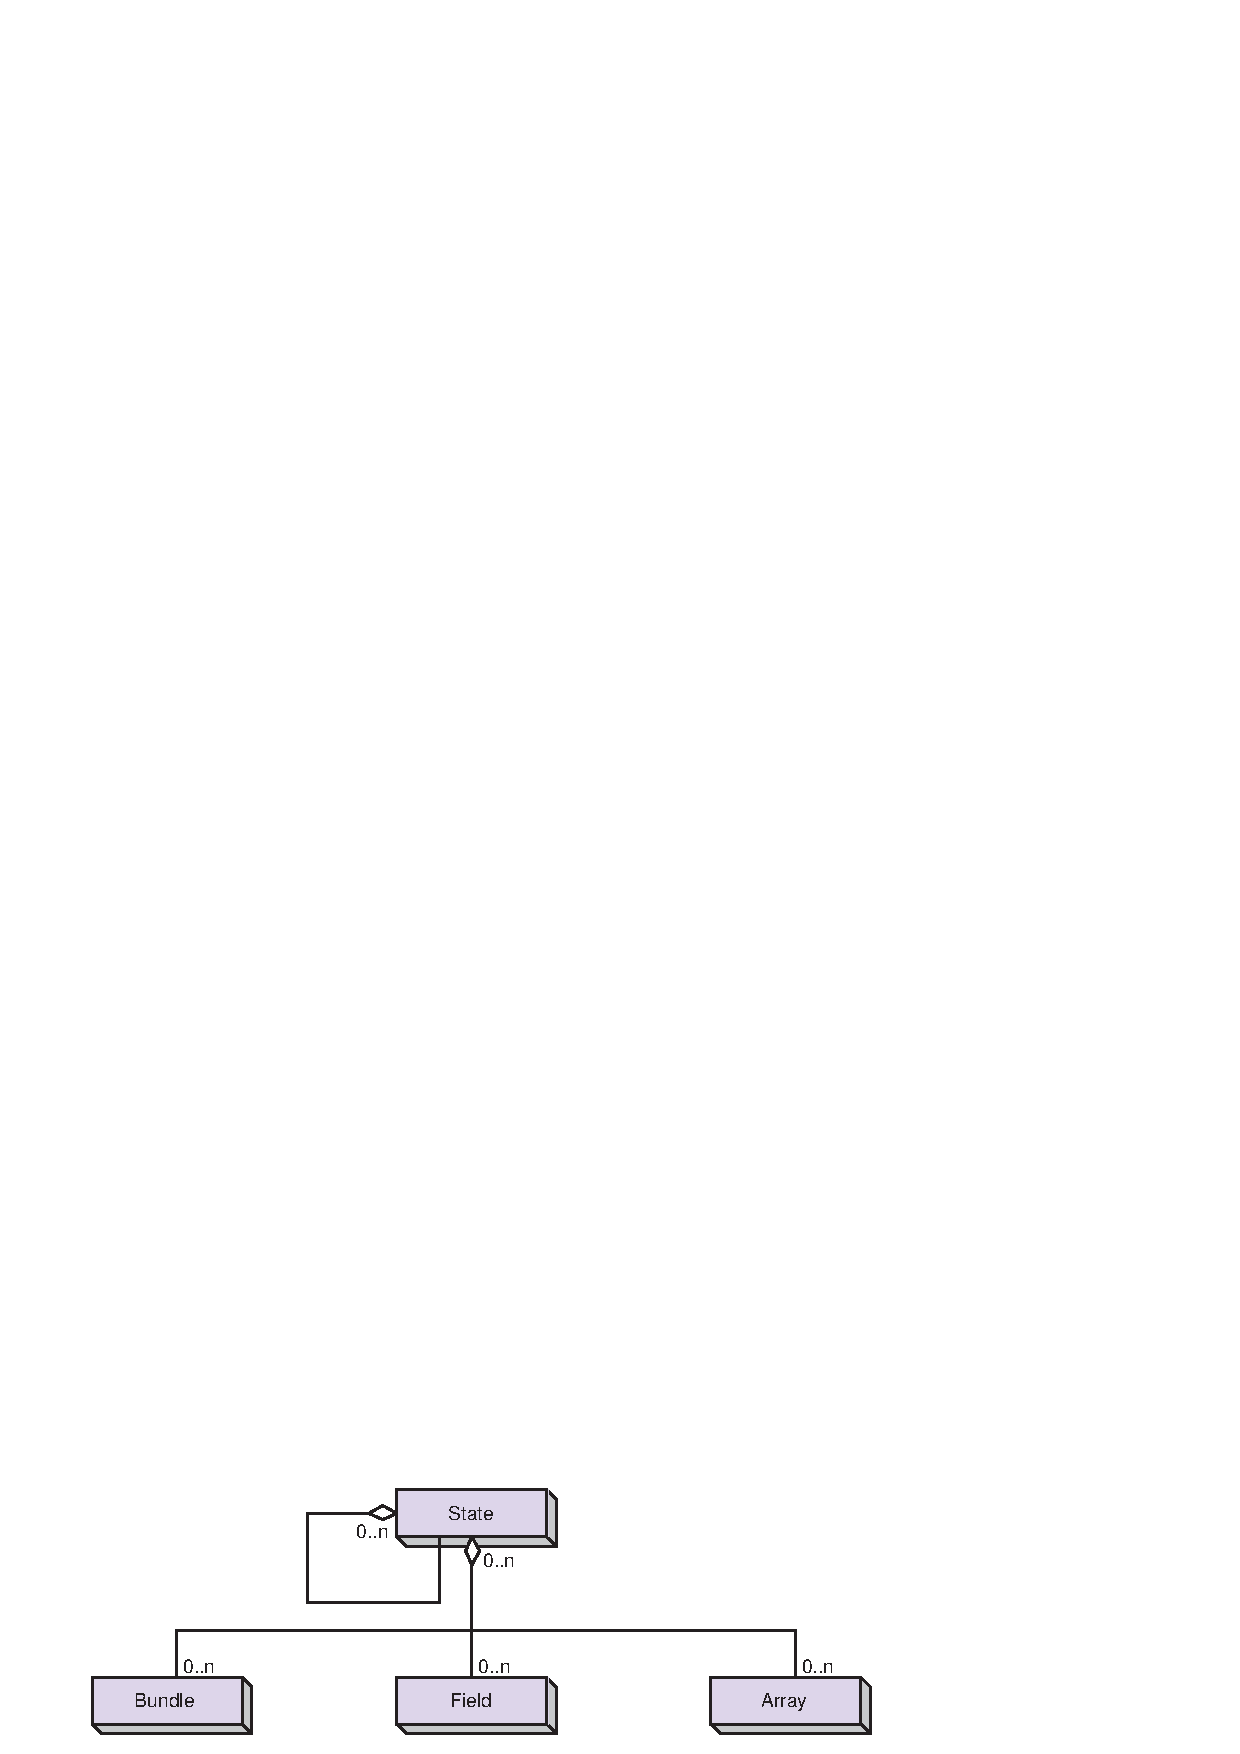
\includegraphics{State_obj}   
\end{center}

\subsection{Class API}
%                **** IMPORTANT NOTICE *****
% This LaTeX file has been automatically produced by ProTeX v. 1.1
% Any changes made to this file will likely be lost next time
% this file is regenerated from its source. Send questions 
% to Arlindo da Silva, dasilva@gsfc.nasa.gov
 
\setlength{\oldparskip}{\parskip}
\setlength{\parskip}{1.5ex}
\setlength{\oldparindent}{\parindent}
\setlength{\parindent}{0pt}
\setlength{\oldbaselineskip}{\baselineskip}
\setlength{\baselineskip}{11pt}
 
%--------------------- SHORT-HAND MACROS ----------------------
\def\bv{\begin{verbatim}}
\def\ev{\end{verbatim}}
\def\be{\begin{equation}}
\def\ee{\end{equation}}
\def\bea{\begin{eqnarray}}
\def\eea{\end{eqnarray}}
\def\bi{\begin{itemize}}
\def\ei{\end{itemize}}
\def\bn{\begin{enumerate}}
\def\en{\end{enumerate}}
\def\bd{\begin{description}}
\def\ed{\end{description}}
\def\({\left (}
\def\){\right )}
\def\[{\left [}
\def\]{\right ]}
\def\<{\left  \langle}
\def\>{\right \rangle}
\def\cI{{\cal I}}
\def\diag{\mathop{\rm diag}}
\def\tr{\mathop{\rm tr}}
%-------------------------------------------------------------

\markboth{Left}{Source File: ESMF\_StateAPI.F90,  Date: Tue May  5 21:00:08 MDT 2020
}

 
%/////////////////////////////////////////////////////////////
\subsubsection [ESMF\_StateAssignment(=)] {ESMF\_StateAssignment(=) - State assignment}


  
\bigskip{\sf INTERFACE:}
\begin{verbatim}   interface assignment(=)
   state1 = state2\end{verbatim}{\em ARGUMENTS:}
\begin{verbatim}   type(ESMF_State) :: state1
   type(ESMF_State) :: state2\end{verbatim}
{\sf STATUS:}
   \begin{itemize}
   \item\apiStatusCompatibleVersion{5.2.0r}
   \end{itemize}
  
{\sf DESCRIPTION:\\ }


   Assign state1 as an alias to the same ESMF State object in memory
   as state2. If state2 is invalid, then state1 will be equally invalid after
   the assignment.
  
   The arguments are:
   \begin{description}
   \item[state1]
   The {\tt ESMF\_State} object on the left hand side of the assignment.
   \item[state2]
   The {\tt ESMF\_State} object on the right hand side of the assignment.
   \end{description}
   
%/////////////////////////////////////////////////////////////
 
\mbox{}\hrulefill\ 
 
\subsubsection [ESMF\_StateOperator(==)] {ESMF\_StateOperator(==) - State equality operator}


  
\bigskip{\sf INTERFACE:}
\begin{verbatim}   interface operator(==)
   if (state1 == state2) then ... endif
   OR
   result = (state1 == state2)\end{verbatim}{\em RETURN VALUE:}
\begin{verbatim}   logical :: result\end{verbatim}{\em ARGUMENTS:}
\begin{verbatim}   type(ESMF_State), intent(in) :: state1
   type(ESMF_State), intent(in) :: state2\end{verbatim}
{\sf STATUS:}
   \begin{itemize}
   \item\apiStatusCompatibleVersion{5.2.0r}
   \end{itemize}
  
{\sf DESCRIPTION:\\ }


   Test whether state1 and state2 are valid aliases to the same ESMF
   State object in memory. For a more general comparison of two ESMF States,
   going beyond the simple alias test, the ESMF\_StateMatch() function (not yet
   implemented) must be used.
  
   The arguments are:
   \begin{description}
   \item[state1]
   The {\tt ESMF\_State} object on the left hand side of the equality
   operation.
   \item[state2]
   The {\tt ESMF\_State} object on the right hand side of the equality
   operation.
   \end{description}
   
%/////////////////////////////////////////////////////////////
 
\mbox{}\hrulefill\ 
 
\subsubsection [ESMF\_StateOperator(/=)] {ESMF\_StateOperator(/=) - State not equal operator}


  
\bigskip{\sf INTERFACE:}
\begin{verbatim}   interface operator(/=)
   if (state1 /= state2) then ... endif
   OR
   result = (state1 /= state2)\end{verbatim}{\em RETURN VALUE:}
\begin{verbatim}   logical :: result\end{verbatim}{\em ARGUMENTS:}
\begin{verbatim}   type(ESMF_State), intent(in) :: state1
   type(ESMF_State), intent(in) :: state2\end{verbatim}
{\sf STATUS:}
   \begin{itemize}
   \item\apiStatusCompatibleVersion{5.2.0r}
   \end{itemize}
  
{\sf DESCRIPTION:\\ }


   Test whether state1 and state2 are {\it not} valid aliases to the
   same ESMF State object in memory. For a more general comparison of two ESMF
   States, going beyond the simple alias test, the ESMF\_StateMatch() function
   (not yet implemented) must be used.
  
   The arguments are:
   \begin{description}
   \item[state1]
   The {\tt ESMF\_State} object on the left hand side of the non-equality
   operation.
   \item[state2]
   The {\tt ESMF\_State} object on the right hand side of the non-equality
   operation.
   \end{description}
   
%/////////////////////////////////////////////////////////////
 
\mbox{}\hrulefill\ 
 
\subsubsection [ESMF\_StateAdd] {ESMF\_StateAdd - Add a list of items to a State}


  
\bigskip{\sf INTERFACE:}
\begin{verbatim}   subroutine ESMF_StateAdd(state, <itemList>, relaxedFlag, rc)\end{verbatim}{\em ARGUMENTS:}
\begin{verbatim}   type(ESMF_State), intent(inout) :: state
   <itemList>, see below for supported values
 -- The following arguments require argument keyword syntax (e.g. rc=rc). --
   logical, intent(in), optional :: relaxedFlag
   integer, intent(out), optional :: rc\end{verbatim}
{\sf STATUS:}
   \begin{itemize}
   \item\apiStatusCompatibleVersion{5.2.0r}
   \end{itemize}
  
{\sf DESCRIPTION:\\ }


   Add a list of items to a {\tt ESMF\_State}. It is an error if any item in
   <itemlist> already matches, by name, an item already contained in {\tt state}.
  
   Supported values for <itemList> are:
   \begin{description}
   \item type(ESMF\_Array), intent(in) :: arrayList(:)
   \item type(ESMF\_ArrayBundle), intent(in) :: arraybundleList(:)
   \item type(ESMF\_Field), intent(in) :: fieldList(:)
   \item type(ESMF\_FieldBundle), intent(in) :: fieldbundleList(:)
   \item type(ESMF\_RouteHandle), intent(in) :: routehandleList(:)
   \item type(ESMF\_State), intent(in) :: nestedStateList(:)
   \end{description}
  
   The arguments are:
   \begin{description}
   \item[state]
   An {\tt ESMF\_State} to which the <itemList> will be added.
   \item[<itemList>]
   The list of items to be added.
   This is a reference only; when
   the {\tt ESMF\_State} is destroyed the <itemList> items contained within it will
   not be destroyed. Also, the items in the <itemList> cannot be safely
   destroyed before the {\tt ESMF\_State} is destroyed.
   Since <itemList> items can be added to multiple containers, it remains
   the responsibility of the user to manage their
   destruction when they are no longer in use.
   \item[{[relaxedflag]}]
   A setting of {\tt .true.} indicates a relaxed definition of "add",
   where it is {\em not} an error if {\tt <itemList>} contains items
   with names that are found in {\tt state}. The {\tt State}
   is left unchanged for these items. For {\tt .false.} this is treated
   as an error condition. The default setting is {\tt .false.}.
   \item[{[rc]}]
   Return code; equals {\tt ESMF\_SUCCESS} if there are no errors.
   \end{description} 
%/////////////////////////////////////////////////////////////
 
\mbox{}\hrulefill\ 
 
\subsubsection [ESMF\_StateAddReplace] {ESMF\_StateAddReplace - Add or replace a list of items to a State}


  
\bigskip{\sf INTERFACE:}
\begin{verbatim}   subroutine ESMF_StateAddReplace(state, <itemList>, rc)\end{verbatim}{\em ARGUMENTS:}
\begin{verbatim}   type(ESMF_State), intent(inout) :: state
   <itemList>, see below for supported values
 -- The following arguments require argument keyword syntax (e.g. rc=rc). --
   integer, intent(out), optional :: rc\end{verbatim}
{\sf STATUS:}
   \begin{itemize}
   \item\apiStatusCompatibleVersion{5.2.0r}
   \end{itemize}
  
{\sf DESCRIPTION:\\ }


   Add or replace a list of items to an {\tt ESMF\_State}. If an item in
   <itemList> does not match any items already present in {\tt state}, it is
   added. Items with names already present in the {\tt state} replace the
   existing item.
  
   Supported values for <itemList> are:
   \begin{description}
   \item type(ESMF\_Array), intent(in) :: arrayList(:)
   \item type(ESMF\_ArrayBundle), intent(in) :: arraybundleList(:)
   \item type(ESMF\_Field), intent(in) :: fieldList(:)
   \item type(ESMF\_FieldBundle), intent(in) :: fieldbundleList(:)
   \item type(ESMF\_RouteHandle), intent(in) :: routehandleList(:)
   \item type(ESMF\_State), intent(in) :: nestedStateList(:)
   \end{description}
  
   The arguments are:
   \begin{description}
   \item[state]
   An {\tt ESMF\_State} to which the <itemList> will be added or replaced.
   \item[<itemList>]
   The list of items to be added or replaced.
   This is a reference only; when
   the {\tt ESMF\_State} is destroyed the <itemList> items contained within it will
   not be destroyed. Also, the items in the <itemList> cannot be safely
   destroyed before the {\tt ESMF\_State} is destroyed.
   Since <itemList> items can be added to multiple containers, it remains
   the responsibility of the user to manage their
   destruction when they are no longer in use.
   \item[{[rc]}]
   Return code; equals {\tt ESMF\_SUCCESS} if there are no errors.
   \end{description} 
%/////////////////////////////////////////////////////////////
 
\mbox{}\hrulefill\ 
 
\subsubsection [ESMF\_StateCreate] {ESMF\_StateCreate - Create a new State}


\bigskip{\sf INTERFACE:}
\begin{verbatim}       function ESMF_StateCreate(stateintent, &
                    arrayList, arraybundleList, &
                    fieldList, fieldbundleList, &
                    nestedStateList, &
                    routehandleList, name, rc)\end{verbatim}{\em RETURN VALUE:}
\begin{verbatim}       type(ESMF_State) :: ESMF_StateCreate\end{verbatim}{\em ARGUMENTS:}
\begin{verbatim} -- The following arguments require argument keyword syntax (e.g. rc=rc). --
       type(ESMF_StateIntent_Flag), intent(in), optional :: stateintent
       type(ESMF_Array), intent(in), optional :: arrayList(:)
       type(ESMF_ArrayBundle), intent(in), optional :: arraybundleList(:)
       type(ESMF_Field), intent(in), optional :: fieldList(:)
       type(ESMF_FieldBundle), intent(in), optional :: fieldbundleList(:)
       type(ESMF_State), intent(in), optional :: nestedStateList(:)
       type(ESMF_RouteHandle), intent(in), optional :: routehandleList(:)
       character(len=*), intent(in), optional :: name
       integer, intent(out), optional :: rc\end{verbatim}
{\sf STATUS:}
   \begin{itemize}
   \item\apiStatusCompatibleVersion{5.2.0r}
   \end{itemize}
  
{\sf DESCRIPTION:\\ }


   Create a new {\tt ESMF\_State}, set default characteristics for
   objects added to it, and optionally add initial objects to it.
  
   The arguments are:
   \begin{description}
   \item[{[stateintent]}]
   Import or Export {\tt ESMF\_State}. Valid values are
   {\tt ESMF\_STATEINTENT\_IMPORT}, {\tt ESMF\_STATEINTENT\_EXPORT},
   or {\tt ESMF\_STATEINTENT\_UNSPECIFIED} The default
   is {\tt ESMF\_STATEINTENT\_UNSPECIFIED}.
   \item[{[arrayList]}]
   A list (Fortran array) of {\tt ESMF\_Array}s.
   \item[{[arraybundleList]}]
   A list (Fortran array) of {\tt ESMF\_ArrayBundle}s.
   \item[{[fieldList]}]
   A list (Fortran array) of {\tt ESMF\_Field}s.
   \item[{[fieldbundleList]}]
   A list (Fortran array) of {\tt ESMF\_FieldBundle}s.
   \item[{[nestedStateList]}]
   A list (Fortran array) of {\tt ESMF\_State}s to be nested
   inside the outer {\tt ESMF\_State}.
   \item[{[routehandleList]}]
   A list (Fortran array) of {\tt ESMF\_RouteHandle}s.
   \item[{[name]}]
   Name of this {\tt ESMF\_State} object. A default name will be generated
   if none is specified.
   \item[{[rc]}]
   Return code; equals {\tt ESMF\_SUCCESS} if there are no errors.
   \end{description}
   
%/////////////////////////////////////////////////////////////
 
\mbox{}\hrulefill\ 
 
\subsubsection [ESMF\_StateDestroy] {ESMF\_StateDestroy - Release resources for a State}


  
\bigskip{\sf INTERFACE:}
\begin{verbatim}       recursive subroutine ESMF_StateDestroy(state, rc)\end{verbatim}{\em ARGUMENTS:}
\begin{verbatim}       type(ESMF_State), intent(inout) :: state
 -- The following arguments require argument keyword syntax (e.g. rc=rc). --
       integer, intent(out), optional :: rc\end{verbatim}
{\sf STATUS:}
   \begin{itemize}
   \item\apiStatusCompatibleVersion{5.2.0r}
   \end{itemize}
  
{\sf DESCRIPTION:\\ }


   Releases resources associated with this {\tt ESMF\_State}. Actual
   objects added to {\tt ESMF\_State}s will not be destroyed, it
   remains the responsibility of the user to destroy these objects in the correct
   context.
  
   The arguments are:
   \begin{description}
   \item[state]
   Destroy contents of this {\tt ESMF\_State}.
   \item[{[rc]}]
   Return code; equals {\tt ESMF\_SUCCESS} if there are no errors.
   \end{description}
   
%/////////////////////////////////////////////////////////////
 
\mbox{}\hrulefill\ 
 
\subsubsection [ESMF\_StateGet] {ESMF\_StateGet - Get object-wide information from a State}


  
\bigskip{\sf INTERFACE:}
\begin{verbatim}       ! Private name; call using ESMF_StateGet()
       subroutine ESMF_StateGetInfo(state, &
             itemSearch, itemorderflag, nestedFlag, &
             stateintent, itemCount, itemNameList, itemTypeList, name, rc)\end{verbatim}{\em ARGUMENTS:}
\begin{verbatim}       type(ESMF_State), intent(in) :: state
 -- The following arguments require argument keyword syntax (e.g. rc=rc). --
       character (len=*), intent(in), optional :: itemSearch
       type(ESMF_ItemOrder_Flag), intent(in), optional :: itemorderflag
       logical, intent(in), optional :: nestedFlag
       type(ESMF_StateIntent_Flag), intent(out), optional :: stateintent
       integer, intent(out), optional :: itemCount
       character (len=*), intent(out), optional :: itemNameList(:)
       type(ESMF_StateItem_Flag), intent(out), optional :: itemTypeList(:)
       character (len=*), intent(out), optional :: name
       integer, intent(out), optional :: rc\end{verbatim}
{\sf STATUS:}
   \begin{itemize}
   \item\apiStatusCompatibleVersion{5.2.0r}
   \item\apiStatusModifiedSinceVersion{5.2.0r}
   \begin{description}
   \item[6.1.0] Added argument {\tt itemorderflag}.
   The new argument gives the user control over the order in which
   the items are returned.
   \end{description}
   \end{itemize}
  
{\sf DESCRIPTION:\\ }


   Returns the requested information about this {\tt ESMF\_State}.
   The optional {\tt itemSearch} argument may specify the name of
   an individual item to search for. When used in conjunction with
   the {\tt nestedFlag}, nested States will also be searched.
  
   Typically, an {\tt ESMF\_StateGet()} information request will be performed
   twice. The first time, the {\tt itemCount} argument will be used to
   query the size of arrays that are needed. Arrays can then be allocated
   to the correct size for {\tt itemNameList} and {\tt itemtypeList}
   as needed. A second call to {\tt ESMF\_StateGet()} will then fill in the
   values.
  
   The arguments are:
   \begin{description}
   \item[state]
   An {\tt ESMF\_State} object to be queried.
   \item[{[itemSearch]}]
   Query objects by name in the State. When the {\tt nestedFlag}
   option is set to .true., all nested States will also be searched
   for the specified name.
   \item[{[itemorderflag]}]
   Specifies the order of the returned items in the {\tt itemNameList}
   and {\tt itemTypeList}. The default is {\tt ESMF\_ITEMORDER\_ABC}.
   See \ref{const:itemorderflag} for a full list of options.
   \item[{[nestedFlag]}]
   When set to {\tt .false.}, returns information at the current
   State level only (default)
   When set to {\tt .true.}, additionally returns information from
   nested States
   \item[{[stateintent]}]
   Returns the type, e.g., Import or Export, of this {\tt ESMF\_State}.
   Possible values are listed in Section~\ref{const:stateintent}.
   \item[{[itemCount]}]
   Count of items in this {\tt ESMF\_State}.
   When the {\tt nestedFlag} option is
   set to {\tt .true.}, the count will include items present in nested
   States. When using {\tt itemSearch}, it will count the number of
   items matching the specified name.
   \item[{[itemNameList]}]
   Array of item names in this {\tt ESMF\_State}.
   When the {\tt nestedFlag} option is
   set to {\tt .true.}, the list will include items present in nested
   States. When using {\tt itemSearch}, it will return the names of
   items matching the specified name. {\tt itemNameList} must be at least
   {\tt itemCount} long.
   \item[{[itemTypeList]}]
   Array of possible item object types in this {\tt ESMF\_State}.
   When the {\tt nestedFlag} option is
   set to {\tt .true.}, the list will include items present in nested
   States. When using {\tt itemSearch}, it will return the types of
   items matching the specified name. Must be at least {\tt itemCount}
   long. Return values are listed in Section~\ref{const:stateitem}.
   \item[{[name]}]
   Returns the name of this {\tt ESMF\_State}.
   \item[{[rc]}]
   Return code; equals {\tt ESMF\_SUCCESS} if there are no errors.
   \end{description}
   
%/////////////////////////////////////////////////////////////
 
\mbox{}\hrulefill\ 
 
\subsubsection [ESMF\_StateGet] {ESMF\_StateGet - Get information about an item in a State by item name}


  
\bigskip{\sf INTERFACE:}
\begin{verbatim}       ! Private name; call using ESMF_StateGet()
       subroutine ESMF_StateGetItemInfo(state, itemName, itemType, rc)\end{verbatim}{\em ARGUMENTS:}
\begin{verbatim}       type(ESMF_State), intent(in) :: state
       character (len=*), intent(in) :: itemName
       type(ESMF_StateItem_Flag), intent(out) :: itemType
 -- The following arguments require argument keyword syntax (e.g. rc=rc). --
       integer, intent(out), optional :: rc\end{verbatim}
{\sf STATUS:}
   \begin{itemize}
   \item\apiStatusCompatibleVersion{5.2.0r}
   \end{itemize}
  
{\sf DESCRIPTION:\\ }


   Returns the type for the item named
   {\tt name} in this {\tt ESMF\_State}. If no item with this name
   exists, the value {\tt ESMF\_STATEITEM\_NOTFOUND} will be returned
   and the error code will not be set to an error. Thus this routine
   can be used to safely query for the existence of items by name
   whether or not they are expected to be there. The error code will
   be set in case of other errors, for example if the {\tt ESMF\_State}
   itself is invalid.
  
   The arguments are:
   \begin{description}
   \item[state]
   {\tt ESMF\_State} to be queried.
   \item[itemName]
   Name of the item to return information about.
   \item[itemType]
   Returned item types for the item with the given name, including
   placeholder names. Options are
   listed in Section~\ref{const:stateitem}. If no item with the
   given name is found, {\tt ESMF\_STATEITEM\_NOTFOUND} will be returned
   and {\tt rc} will {\bf not} be set to an error.
   \item[{[rc]}]
   Return code; equals {\tt ESMF\_SUCCESS} if there are no errors.
   \end{description}
  
   
%/////////////////////////////////////////////////////////////
 
\mbox{}\hrulefill\ 
 
\subsubsection [ESMF\_StateGet] {ESMF\_StateGet - Get an item from a State by item name}


  
\bigskip{\sf INTERFACE:}
\begin{verbatim}   subroutine ESMF_StateGet(state, itemName, <item>, rc)\end{verbatim}{\em ARGUMENTS:}
\begin{verbatim}   type(ESMF_State), intent(in) :: state
   character (len=*), intent(in) :: itemName
   <item>, see below for supported values
 -- The following arguments require argument keyword syntax (e.g. rc=rc). --
   integer, intent(out), optional :: rc\end{verbatim}
{\sf STATUS:}
   \begin{itemize}
   \item\apiStatusCompatibleVersion{5.2.0r}
   \end{itemize}
  
{\sf DESCRIPTION:\\ }


   \begin{sloppypar}
   Returns an <item> from an {\tt ESMF\_State} by item name.
   If the {\tt ESMF\_State} contains the <item> directly, only
   {\tt itemName} is required.
   \end{sloppypar}
  
   If the {\tt state} contains nested {\tt ESMF\_State}s,
   the {\tt itemName} argument may specify a fully qualified name
   to access the desired item with a single call. This is performed
   using the '/' character to separate the names of the intermediate
   State names leading to the desired item. (E.g.,
   {\tt itemName='state1/state12/item'}).
  
   Supported values for <item> are:
   \begin{description}
   \item type(ESMF\_Array), intent(out) :: array
   \item type(ESMF\_ArrayBundle), intent(out) :: arraybundle
   \item type(ESMF\_Field), intent(out) :: field
   \item type(ESMF\_FieldBundle), intent(out) :: fieldbundle
   \item type(ESMF\_RouteHandle), intent(out) :: routehandle
   \item type(ESMF\_State), intent(out) :: nestedState
   \end{description}
  
   The arguments are:
   \begin{description}
   \item[state]
   State to query for an <item> named {\tt itemName}.
   \item[itemName]
   Name of <item> to be returned. This name may be fully
   qualified in order to access nested State items.
   \item[<item>]
   Returned reference to the <item>.
   \item[{[rc]}]
   Return code; equals {\tt ESMF\_SUCCESS} if there are no errors.
   \end{description}
   
%/////////////////////////////////////////////////////////////
 
\mbox{}\hrulefill\ 
 
\subsubsection [ESMF\_StateIsCreated] {ESMF\_StateIsCreated - Check whether an State object has been created}


\bigskip{\sf INTERFACE:}
\begin{verbatim}   function ESMF_StateIsCreated(state, rc)\end{verbatim}{\em RETURN VALUE:}
\begin{verbatim}     logical :: ESMF_StateIsCreated\end{verbatim}{\em ARGUMENTS:}
\begin{verbatim}     type(ESMF_State), intent(in) :: state
 -- The following arguments require argument keyword syntax (e.g. rc=rc). --
     integer, intent(out), optional :: rc\end{verbatim}
{\sf DESCRIPTION:\\ }


   Return {\tt .true.} if the {\tt state} has been created. Otherwise return
   {\tt .false.}. If an error occurs, i.e. {\tt rc /= ESMF\_SUCCESS} is
   returned, the return value of the function will also be {\tt .false.}.
  
   The arguments are:
   \begin{description}
   \item[state]
   {\tt ESMF\_State} queried.
   \item[{[rc]}]
   Return code; equals {\tt ESMF\_SUCCESS} if there are no errors.
   \end{description}
   
%/////////////////////////////////////////////////////////////
 
\mbox{}\hrulefill\ 
 
\subsubsection [ESMF\_StatePrint] {ESMF\_StatePrint - Print State information}


  
\bigskip{\sf INTERFACE:}
\begin{verbatim}       subroutine ESMF_StatePrint(state, options, nestedFlag, rc)\end{verbatim}{\em ARGUMENTS:}
\begin{verbatim}       type(ESMF_State), intent(in) :: state
       character(len=*), intent(in), optional :: options
       logical, intent(in), optional :: nestedFlag
       integer, intent(out), optional :: rc\end{verbatim}
{\sf DESCRIPTION:\\ }


   Prints information about the {\tt state} to {\tt stdout}.
  
   The arguments are:
   \begin{description}
   \item[state]
   The {\tt ESMF\_State} to print.
   \item[{[options]}]
   Print options:
   " ", or "brief" - print names and types of the objects within the state (default),
   "long" - print additional information, such as proxy flags
   \item[{[nestedFlag]}]
   When set to {\tt .false.}, prints information about the current
   State level only (default),
   When set to {\tt .true.}, additionally prints information from
   nested States
   \item[{[rc]}]
   Return code; equals {\tt ESMF\_SUCCESS} if there are no errors.
   \end{description}
   
%/////////////////////////////////////////////////////////////
 
\mbox{}\hrulefill\ 
 
\subsubsection [ESMF\_StateRead] {ESMF\_StateRead -- Read data items from a file into a State}


  
\bigskip{\sf INTERFACE:}
\begin{verbatim}       subroutine ESMF_StateRead(state, fileName, rc)\end{verbatim}{\em ARGUMENTS:}
\begin{verbatim}       type(ESMF_State), intent(inout) :: state
       character (len=*), intent(in) :: fileName
       integer, intent(out), optional :: rc\end{verbatim}
{\sf DESCRIPTION:\\ }


   Currently limited to read in all Arrays from a NetCDF file and add them
   to a State object. Future releases will enable more items of a State
   to be read from a file of various formats.
  
   Only PET 0 reads the file; the States in other PETs remain empty.
   Currently, the data is not decomposed or distributed; each PET
   has only 1 DE and only PET 0 contains data after reading the file.
   Future versions of ESMF will support data decomposition and distribution
   upon reading a file. See Section~\ref{example:StateRdWr} for
   an example.
  
   Note that the third party NetCDF library must be installed. For more
   details, see the "ESMF Users Guide",
   "Building and Installing the ESMF, Third Party Libraries, NetCDF" and
   the website http://www.unidata.ucar.edu/software/netcdf.
  
   The arguments are:
   \begin{description}
   \item[state]
   The {\tt ESMF\_State} to add items read from file. Currently only
   Arrays are supported.
   \item[fileName]
   File to be read.
   \item[{[rc]}]
   Return code; equals {\tt ESMF\_SUCCESS} if there are no errors.
   Equals {\tt ESMF\_RC\_LIB\_NOT\_PRESENT} if the NetCDF library is
   not present.
   \end{description}
  
%...............................................................
\setlength{\parskip}{\oldparskip}
\setlength{\parindent}{\oldparindent}
\setlength{\baselineskip}{\oldbaselineskip}

%                **** IMPORTANT NOTICE *****
% This LaTeX file has been automatically produced by ProTeX v. 1.1
% Any changes made to this file will likely be lost next time
% this file is regenerated from its source. Send questions 
% to Arlindo da Silva, dasilva@gsfc.nasa.gov
 
\setlength{\oldparskip}{\parskip}
\setlength{\parskip}{1.5ex}
\setlength{\oldparindent}{\parindent}
\setlength{\parindent}{0pt}
\setlength{\oldbaselineskip}{\baselineskip}
\setlength{\baselineskip}{11pt}
 
%--------------------- SHORT-HAND MACROS ----------------------
\def\bv{\begin{verbatim}}
\def\ev{\end{verbatim}}
\def\be{\begin{equation}}
\def\ee{\end{equation}}
\def\bea{\begin{eqnarray}}
\def\eea{\end{eqnarray}}
\def\bi{\begin{itemize}}
\def\ei{\end{itemize}}
\def\bn{\begin{enumerate}}
\def\en{\end{enumerate}}
\def\bd{\begin{description}}
\def\ed{\end{description}}
\def\({\left (}
\def\){\right )}
\def\[{\left [}
\def\]{\right ]}
\def\<{\left  \langle}
\def\>{\right \rangle}
\def\cI{{\cal I}}
\def\diag{\mathop{\rm diag}}
\def\tr{\mathop{\rm tr}}
%-------------------------------------------------------------

\markboth{Left}{Source File: ESMF\_StateReconcile2.F90,  Date: Tue May  5 21:00:08 MDT 2020
}

 
%/////////////////////////////////////////////////////////////
\subsubsection [ESMF\_StateReconcile] {ESMF\_StateReconcile -- Reconcile State data across all PETs in a VM}


  
\bigskip{\sf INTERFACE:}
\begin{verbatim}   subroutine ESMF_StateReconcile (state, vm, attreconflag, rc)\end{verbatim}{\em ARGUMENTS:}
\begin{verbatim}     type(ESMF_State),            intent(inout)         :: state
     type(ESMF_VM),               intent(in),  optional :: vm
     type(ESMF_AttReconcileFlag), intent(in),  optional :: attreconflag
     integer,                     intent(out), optional :: rc\end{verbatim}
{\sf DESCRIPTION:\\ }


       Must be called for any {\tt ESMF\_State} which contains ESMF objects
       that have not been created on all the {\tt PET}s of the currently
       running {\tt ESMF\_Component}.
       For example, if a coupler is operating on data
       which was created by another component that ran on only a subset
       of the couplers {\tt PET}s, the coupler must make this call first
       before operating on any data inside that {\tt ESMF\_State}.
       After calling {\tt ESMF\_StateReconcile} all {\tt PET}s will have
       a common view of all objects contained in this {\tt ESMF\_State}.
       The option to reconcile the metadata associated with the objects
       contained in this {\tt ESMF\_State} also exists.  The default behavior
       for this capability is to {\it not} reconcile metadata unless told
       otherwise.
  
       This call is collective across the specified VM.
  
       The arguments are:
       \begin{description}
       \item[state]
         {\tt ESMF\_State} to reconcile.
       \item[{[vm]}]
         {\tt ESMF\_VM} for this {\tt ESMF\_Component}.  By default, it is set to the current vm.
       \item[{[attreconflag]}]
         Flag to tell if Attribute reconciliation is to be done as well as data reconciliation.
         This flag is documented in section \ref{const:attreconcile}.  Default is
         {\tt ESMF\_ATTRECONCILE\_OFF}.
       \item[{[rc]}]
         Return code; equals {\tt ESMF\_SUCCESS} if there are no errors.
       \end{description}
  
%...............................................................
\setlength{\parskip}{\oldparskip}
\setlength{\parindent}{\oldparindent}
\setlength{\baselineskip}{\oldbaselineskip}

%                **** IMPORTANT NOTICE *****
% This LaTeX file has been automatically produced by ProTeX v. 1.1
% Any changes made to this file will likely be lost next time
% this file is regenerated from its source. Send questions 
% to Arlindo da Silva, dasilva@gsfc.nasa.gov
 
\setlength{\oldparskip}{\parskip}
\setlength{\parskip}{1.5ex}
\setlength{\oldparindent}{\parindent}
\setlength{\parindent}{0pt}
\setlength{\oldbaselineskip}{\baselineskip}
\setlength{\baselineskip}{11pt}
 
%--------------------- SHORT-HAND MACROS ----------------------
\def\bv{\begin{verbatim}}
\def\ev{\end{verbatim}}
\def\be{\begin{equation}}
\def\ee{\end{equation}}
\def\bea{\begin{eqnarray}}
\def\eea{\end{eqnarray}}
\def\bi{\begin{itemize}}
\def\ei{\end{itemize}}
\def\bn{\begin{enumerate}}
\def\en{\end{enumerate}}
\def\bd{\begin{description}}
\def\ed{\end{description}}
\def\({\left (}
\def\){\right )}
\def\[{\left [}
\def\]{\right ]}
\def\<{\left  \langle}
\def\>{\right \rangle}
\def\cI{{\cal I}}
\def\diag{\mathop{\rm diag}}
\def\tr{\mathop{\rm tr}}
%-------------------------------------------------------------

\markboth{Left}{Source File: ESMF\_StateRemRep.F90,  Date: Tue May  5 21:00:08 MDT 2020
}

 
%/////////////////////////////////////////////////////////////
\subsubsection [ESMF\_StateRemove] {ESMF\_StateRemove - Remove an item from a State - (DEPRECATED METHOD)}


  
\bigskip{\sf INTERFACE:}
\begin{verbatim}   ! Private name; call using ESMF_StateRemove ()
   subroutine ESMF_StateRemoveOneItem (state, itemName, &
       relaxedFlag, rc)\end{verbatim}{\em ARGUMENTS:}
\begin{verbatim}     type(ESMF_State), intent(inout) :: state
     character(*), intent(in) :: itemName
 -- The following arguments require argument keyword syntax (e.g. rc=rc). --
     logical, intent(in), optional :: relaxedFlag
     integer, intent(out), optional :: rc\end{verbatim}
{\sf STATUS:}
   \begin{itemize}
   \item\apiStatusCompatibleVersion{5.2.0r}
   \item\apiDeprecatedMethodWithReplacement{5.3.1}{ESMF\_StateRemove}{esmfstateremovelist}
   Rationale: The list version is consistent with other ESMF container
   operations which use lists.
   \end{itemize}
  
{\sf DESCRIPTION:\\ }


   Remove an existing reference to an item from a {\tt State}.
  
   The arguments are:
   \begin{description}
   \item[state]
   The {\tt ESMF\_State} within which {\tt itemName} will be removed.
   \item[itemName]
   The name of the item to be removed. This is a reference only.
   The item itself is unchanged.
  
   If the {\tt state} contains nested {\tt ESMF\_State}s,
   the {\tt itemName} argument may specify a fully qualified name
   to remove the desired item with a single call. This is performed
   using the "/" character to separate the names of the intermediate
   State names leading to the desired item. (E.g.,
   {\tt itemName="state1/state12/item"}.
  
   Since an item could potentially be referenced by multiple containers,
   it remains the responsibility of the user to manage its
   destruction when it is no longer in use.
   \item[{[relaxedflag]}]
   A setting of {\tt .true.} indicates a relaxed definition of "remove",
   where it is {\em not} an error if {\tt itemName} is not present in the
   {\tt state}. For {\tt .false.} this is treated
   as an error condition. The default setting is {\tt .false.}.
   \item[{[rc]}]
   Return code; equals {\tt ESMF\_SUCCESS} if there are no errors.
   \end{description} 
%/////////////////////////////////////////////////////////////
 
\mbox{}\hrulefill\ 
 
\subsubsection [ESMF\_StateRemove] {ESMF\_StateRemove - Remove a list of items from a State}


   \label{esmfstateremovelist}
  
\bigskip{\sf INTERFACE:}
\begin{verbatim}   ! Private name; call using ESMF_StateRemove ()
   subroutine ESMF_StateRemoveList (state, itemNameList, relaxedFlag, rc)\end{verbatim}{\em ARGUMENTS:}
\begin{verbatim}     type(ESMF_State), intent(inout) :: state
     character(*), intent(in) :: itemNameList(:)
 -- The following arguments require argument keyword syntax (e.g. rc=rc). --
     logical, intent(in), optional :: relaxedFlag
     integer, intent(out), optional :: rc\end{verbatim}
{\sf STATUS:}
   \begin{itemize}
   \item\apiStatusCompatibleVersion{5.3.1}
   \end{itemize}
  
{\sf DESCRIPTION:\\ }


   Remove existing references to items from a {\tt State}.
  
   The arguments are:
   \begin{description}
   \item[state]
   The {\tt ESMF\_State} within which {\tt itemName} will be removed.
   \item[itemNameList]
   The name of the items to be removed. This is a reference only.
   The items themselves are unchanged.
  
   If the {\tt state} contains nested {\tt ESMF\_State}s,
   the {\tt itemName} arguments may specify fully qualified names
   to remove the desired items with a single call. This is performed
   using the "/" character to separate the names of the intermediate
   State names leading to the desired items. (E.g.,
   {\tt itemName="state1/state12/item"}.
  
   Since items could potentially be referenced by multiple containers,
   it remains the responsibility of the user to manage their
   destruction when they are no longer in use.
   \item[{[relaxedflag]}]
   A setting of {\tt .true.} indicates a relaxed definition of "remove",
   where it is {\em not} an error if an item in the {\tt itemNameList}
   is not present in the {\tt state}. For {\tt .false.} this is treated
   as an error condition. The default setting is {\tt .false.}.
   \item[{[rc]}]
   Return code; equals {\tt ESMF\_SUCCESS} if there are no errors.
   \end{description} 
%/////////////////////////////////////////////////////////////
 
\mbox{}\hrulefill\ 
 
\subsubsection [ESMF\_StateReplace] {ESMF\_StateReplace - Replace a list of items within a State}


  
\bigskip{\sf INTERFACE:}
\begin{verbatim}   subroutine ESMF_StateReplace(state, <itemList>, relaxedflag, rc)\end{verbatim}{\em ARGUMENTS:}
\begin{verbatim}   type(ESMF_State), intent(inout) :: state
   <itemList>, see below for supported values
 -- The following arguments require argument keyword syntax (e.g. rc=rc). --
   logical, intent(in), optional :: relaxedflag
   integer, intent(out), optional :: rc\end{verbatim}
{\sf STATUS:}
   \begin{itemize}
   \item\apiStatusCompatibleVersion{5.2.0r}
   \end{itemize}
  
{\sf DESCRIPTION:\\ }


   Replace a list of items with a {\tt ESMF\_State}. If an item in
   <itemList> does not match any items already present in {\tt state}, an
   error is returned.
  
   Supported values for <itemList> are:
   \begin{description}
   \item type(ESMF\_Array), intent(in) :: arrayList(:)
   \item type(ESMF\_ArrayBundle), intent(in) :: arraybundleList(:)
   \item type(ESMF\_Field), intent(in) :: fieldList(:)
   \item type(ESMF\_FieldBundle), intent(in) :: fieldbundleList(:)
   \item type(ESMF\_RouteHandle), intent(in) :: routehandleList(:)
   \item type(ESMF\_State), intent(in) :: nestedStateList(:)
   \end{description}
  
   The arguments are:
   \begin{description}
   \item[state]
   An {\tt ESMF\_State} within which the <itemList> items will be replaced.
   \item[<itemList>]
   The list of items to be replaced.
   This is a reference only; when
   the {\tt ESMF\_State} is destroyed the <itemList> contained in it will
   not be destroyed. Also, the items in the <itemList> cannot be safely
   destroyed before the {\tt ESMF\_State} is destroyed.
   Since <itemList> items can be added to multiple containers, it remains
   the responsibility of the user to manage their
   destruction when they are no longer in use.
   \item[{[relaxedflag]}]
   A setting of {\tt .true.} indicates a relaxed definition of "replace",
   where it is {\em not} an error if {\tt <itemList>} contains items
   with names that are not found in {\tt state}. The {\tt State}
   is left unchanged for these items. For {\tt .false.} this is treated
   as an error condition. The default setting is {\tt .false.}.
   \item[{[rc]}]
   Return code; equals {\tt ESMF\_SUCCESS} if there are no errors.
   \end{description}
%...............................................................
\setlength{\parskip}{\oldparskip}
\setlength{\parindent}{\oldparindent}
\setlength{\baselineskip}{\oldbaselineskip}

%                **** IMPORTANT NOTICE *****
% This LaTeX file has been automatically produced by ProTeX v. 1.1
% Any changes made to this file will likely be lost next time
% this file is regenerated from its source. Send questions 
% to Arlindo da Silva, dasilva@gsfc.nasa.gov
 
\setlength{\oldparskip}{\parskip}
\setlength{\parskip}{1.5ex}
\setlength{\oldparindent}{\parindent}
\setlength{\parindent}{0pt}
\setlength{\oldbaselineskip}{\baselineskip}
\setlength{\baselineskip}{11pt}
 
%--------------------- SHORT-HAND MACROS ----------------------
\def\bv{\begin{verbatim}}
\def\ev{\end{verbatim}}
\def\be{\begin{equation}}
\def\ee{\end{equation}}
\def\bea{\begin{eqnarray}}
\def\eea{\end{eqnarray}}
\def\bi{\begin{itemize}}
\def\ei{\end{itemize}}
\def\bn{\begin{enumerate}}
\def\en{\end{enumerate}}
\def\bd{\begin{description}}
\def\ed{\end{description}}
\def\({\left (}
\def\){\right )}
\def\[{\left [}
\def\]{\right ]}
\def\<{\left  \langle}
\def\>{\right \rangle}
\def\cI{{\cal I}}
\def\diag{\mathop{\rm diag}}
\def\tr{\mathop{\rm tr}}
%-------------------------------------------------------------

\markboth{Left}{Source File: ESMF\_StateSet.F90,  Date: Tue May  5 21:00:08 MDT 2020
}

 
%/////////////////////////////////////////////////////////////
\subsubsection [ESMF\_StateSet] {ESMF\_StateSet - Set State aspects}


  
\bigskip{\sf INTERFACE:}
\begin{verbatim}   subroutine ESMF_StateSet(state, stateIntent, rc)\end{verbatim}{\em ARGUMENTS:}
\begin{verbatim}     type(ESMF_State),            intent(inout)         :: state
 -- The following arguments require argument keyword syntax (e.g. rc=rc). --
     type(ESMF_StateIntent_Flag), intent(in),  optional :: stateIntent
     integer,                     intent(out), optional :: rc             
 \end{verbatim}
{\sf DESCRIPTION:\\ }


        Set the info in the {\tt state} object.
  
       The arguments are:
        \begin{description}     
        \item[state]
          The {\tt ESMF\_State} to set.
        \item[stateIntent]
          Intent, e.g. Import or Export, of this {\tt ESMF\_State}.
          Possible values are listed in Section~\ref{const:stateintent}.
        \item[{[rc]}]
          Return code; equals {\tt ESMF\_SUCCESS} if there are no errors.
        \end{description}
  
%...............................................................
\setlength{\parskip}{\oldparskip}
\setlength{\parindent}{\oldparindent}
\setlength{\baselineskip}{\oldbaselineskip}

%                **** IMPORTANT NOTICE *****
% This LaTeX file has been automatically produced by ProTeX v. 1.1
% Any changes made to this file will likely be lost next time
% this file is regenerated from its source. Send questions 
% to Arlindo da Silva, dasilva@gsfc.nasa.gov
 
\setlength{\oldparskip}{\parskip}
\setlength{\parskip}{1.5ex}
\setlength{\oldparindent}{\parindent}
\setlength{\parindent}{0pt}
\setlength{\oldbaselineskip}{\baselineskip}
\setlength{\baselineskip}{11pt}
 
%--------------------- SHORT-HAND MACROS ----------------------
\def\bv{\begin{verbatim}}
\def\ev{\end{verbatim}}
\def\be{\begin{equation}}
\def\ee{\end{equation}}
\def\bea{\begin{eqnarray}}
\def\eea{\end{eqnarray}}
\def\bi{\begin{itemize}}
\def\ei{\end{itemize}}
\def\bn{\begin{enumerate}}
\def\en{\end{enumerate}}
\def\bd{\begin{description}}
\def\ed{\end{description}}
\def\({\left (}
\def\){\right )}
\def\[{\left [}
\def\]{\right ]}
\def\<{\left  \langle}
\def\>{\right \rangle}
\def\cI{{\cal I}}
\def\diag{\mathop{\rm diag}}
\def\tr{\mathop{\rm tr}}
%-------------------------------------------------------------

\markboth{Left}{Source File: ESMF\_StateVa.F90,  Date: Tue May  5 21:00:08 MDT 2020
}

 
%/////////////////////////////////////////////////////////////
\subsubsection [ESMF\_StateValidate] {ESMF\_StateValidate - Check validity of a State}


  
\bigskip{\sf INTERFACE:}
\begin{verbatim}       subroutine ESMF_StateValidate(state, nestedFlag, rc)\end{verbatim}{\em ARGUMENTS:}
\begin{verbatim}       type(ESMF_State), intent(in) :: state
 -- The following arguments require argument keyword syntax (e.g. rc=rc). --
       logical,          intent(in),  optional :: nestedFlag
       integer,          intent(out), optional :: rc \end{verbatim}
{\sf STATUS:}
   \begin{itemize}
   \item\apiStatusCompatibleVersion{5.2.0r}
   \end{itemize}
  
{\sf DESCRIPTION:\\ }


       Validates that the {\tt state} is internally consistent.
        Currently this method determines if the {\tt State} is uninitialized 
        or already destroyed.  The method returns an error code if problems 
        are found.  
  
       The arguments are:
       \begin{description}
       \item[state]
         The {\tt ESMF\_State} to validate.
       \item[{[nestedFlag]}]
         {\tt .false.} - validates at the current State level only (default)
         {\tt .true.} - recursively validates any nested States
       \item[{[rc]}]
         Return code; equals {\tt ESMF\_SUCCESS} if there are no errors.
       \end{description}
  
  
%...............................................................
\setlength{\parskip}{\oldparskip}
\setlength{\parindent}{\oldparindent}
\setlength{\baselineskip}{\oldbaselineskip}

%                **** IMPORTANT NOTICE *****
% This LaTeX file has been automatically produced by ProTeX v. 1.1
% Any changes made to this file will likely be lost next time
% this file is regenerated from its source. Send questions 
% to Arlindo da Silva, dasilva@gsfc.nasa.gov
 
\setlength{\oldparskip}{\parskip}
\setlength{\parskip}{1.5ex}
\setlength{\oldparindent}{\parindent}
\setlength{\parindent}{0pt}
\setlength{\oldbaselineskip}{\baselineskip}
\setlength{\baselineskip}{11pt}
 
%--------------------- SHORT-HAND MACROS ----------------------
\def\bv{\begin{verbatim}}
\def\ev{\end{verbatim}}
\def\be{\begin{equation}}
\def\ee{\end{equation}}
\def\bea{\begin{eqnarray}}
\def\eea{\end{eqnarray}}
\def\bi{\begin{itemize}}
\def\ei{\end{itemize}}
\def\bn{\begin{enumerate}}
\def\en{\end{enumerate}}
\def\bd{\begin{description}}
\def\ed{\end{description}}
\def\({\left (}
\def\){\right )}
\def\[{\left [}
\def\]{\right ]}
\def\<{\left  \langle}
\def\>{\right \rangle}
\def\cI{{\cal I}}
\def\diag{\mathop{\rm diag}}
\def\tr{\mathop{\rm tr}}
%-------------------------------------------------------------

\markboth{Left}{Source File: ESMF\_StateWr.F90,  Date: Tue May  5 21:00:08 MDT 2020
}

 
%/////////////////////////////////////////////////////////////
\subsubsection [ESMF\_StateWrite] {ESMF\_StateWrite -- Write items from a State to file}


  
\bigskip{\sf INTERFACE:}
\begin{verbatim}       subroutine ESMF_StateWrite(state, fileName, rc)\end{verbatim}{\em ARGUMENTS:}
\begin{verbatim}       type(ESMF_State),  intent(in)            :: state 
       character (len=*), intent(in)            :: fileName
       integer,           intent(out), optional :: rc \end{verbatim}
{\sf DESCRIPTION:\\ }


       Currently limited to write out all Arrays of a State object to a
       netCDF file.  Future releases will enable more item types of a State to
       be written to files of various formats.
  
       Writing is currently limited to PET 0; future versions of ESMF will allow
       parallel writing, as well as parallel reading.
  
       See Section~\ref{example:StateRdWr} for an example.
  
       Note that the third party NetCDF library must be installed.  For more
       details, see the "ESMF Users Guide",
       "Building and Installing the ESMF, Third Party Libraries, NetCDF" and
       the website http://www.unidata.ucar.edu/software/netcdf.
  
       The arguments are:
       \begin{description}
       \item[state]
         The {\tt ESMF\_State} from which to write items.  Currently limited to
         Arrays.
       \item[fileName]
         File to be written.  
       \item[{[rc]}]
         Return code; equals {\tt ESMF\_SUCCESS} if there are no errors.
         Equals {\tt ESMF\_RC\_LIB\_NOT\_PRESENT} if the NetCDF library is
         not present.
       \end{description}
  
%...............................................................
\setlength{\parskip}{\oldparskip}
\setlength{\parindent}{\oldparindent}
\setlength{\baselineskip}{\oldbaselineskip}

%TODO:FIELDINTEGRATION Restore StateGet methods
%\subsection{Class API: State Overloads for Fortran Arrays}
%#ifdef STANDALONE
%%                **** IMPORTANT NOTICE *****
% This LaTeX file has been automatically produced by ProTeX v. 1.1
% Any changes made to this file will likely be lost next time
% this file is regenerated from its source. Send questions 
% to Arlindo da Silva, dasilva@gsfc.nasa.gov
 
\setlength{\oldparskip}{\parskip}
\setlength{\parskip}{1.5ex}
\setlength{\oldparindent}{\parindent}
\setlength{\parindent}{0pt}
\setlength{\oldbaselineskip}{\baselineskip}
\setlength{\baselineskip}{11pt}
 
%--------------------- SHORT-HAND MACROS ----------------------
\def\bv{\begin{verbatim}}
\def\ev{\end{verbatim}}
\def\be{\begin{equation}}
\def\ee{\end{equation}}
\def\bea{\begin{eqnarray}}
\def\eea{\end{eqnarray}}
\def\bi{\begin{itemize}}
\def\ei{\end{itemize}}
\def\bn{\begin{enumerate}}
\def\en{\end{enumerate}}
\def\bd{\begin{description}}
\def\ed{\end{description}}
\def\({\left (}
\def\){\right )}
\def\[{\left [}
\def\]{\right ]}
\def\<{\left  \langle}
\def\>{\right \rangle}
\def\cI{{\cal I}}
\def\diag{\mathop{\rm diag}}
\def\tr{\mathop{\rm tr}}
%-------------------------------------------------------------

\markboth{Left}{Source File: ESMF\_StateGet.F90,  Date: Tue May  5 21:00:08 MDT 2020
}

 
%/////////////////////////////////////////////////////////////
\subsubsection [ESMF\_StateGetDataPointer] {ESMF\_StateGetDataPointer - Retrieve Fortran pointer directly from a State }


   
\bigskip{\sf INTERFACE:}
\begin{verbatim}   ! Private name; call using ESMF_StateGetDataPointer() 
   subroutine ESMF_StateGetDataPointer<rank><type><kind>(state, itemName, 
   dataPointer, datacopyflag, nestedStateName, rc) 
   \end{verbatim}{\em ARGUMENTS:}
\begin{verbatim}   type(ESMF_State), intent(in) :: state 
   character(len=*), intent(in) :: itemName 
   <type> (ESMF_KIND_<kind>), dimension(<rank>), pointer :: dataPointer 
   type(ESMF_DataCopy_Flag), intent(in), optional :: datacopyflag 
   character(len=*), intent(in), optional :: nestedStateName 
   integer, intent(out), optional :: rc 
   
   \end{verbatim}
{\sf STATUS:}
   \begin{itemize} 
   \item\apiStatusCompatibleVersion{5.2.0r} 
   \end{itemize} 
   
{\sf DESCRIPTION:\\ }

 
   Retrieves data from a state, returning a direct Fortran pointer to 
   the data array. 
   Valid type/kind/rank combinations supported by the 
   framework are: ranks 1 to 7, type real of kind *4 or *8, 
   and type integer of kind *1, *2, *4, or *8. 
   
   The arguments are: 
   \begin{description} 
   \item[state] 
   The {\tt ESMF\_State} to query. 
   \item[itemName] 
   The name of the FieldBundle, Field, or Array to return data from. 
   \item[dataPointer] 
   An unassociated Fortran pointer of the proper Type, Kind, and Rank as the data 
   in the State. When this call returns successfully, the pointer will now reference 
   the data in the State. This is either a reference or a copy, depending on the 
   setting of the following argument. The default is to return a reference. 
   \item[{[datacopyflag]}] 
   Defaults to {\tt ESMF\_DATACOPY\_REFERENCE}. If set to {\tt ESMF\_DATACOPY\_VALUE}, a separate 
   copy of the data will be made and the pointer will point at the copy. 
   \item[{[nestedStateName]}] 
   Optional. If multiple states are present, a specific state name must be given. 
   \item[{[fieldName]}] 
   Optional. If {\tt itemName} refers to a fieldbundle then the name of the field 
   in the fieldbundle must also be given. 
   \item[{[rc]}] 
   Return code; equals {\tt ESMF\_SUCCESS} if there are no errors. 
   \end{description} 
   
%...............................................................
\setlength{\parskip}{\oldparskip}
\setlength{\parindent}{\oldparindent}
\setlength{\baselineskip}{\oldbaselineskip}

%#elif defined(1)
%%                **** IMPORTANT NOTICE *****
% This LaTeX file has been automatically produced by ProTeX v. 1.1
% Any changes made to this file will likely be lost next time
% this file is regenerated from its source. Send questions 
% to Arlindo da Silva, dasilva@gsfc.nasa.gov
 
\setlength{\oldparskip}{\parskip}
\setlength{\parskip}{1.5ex}
\setlength{\oldparindent}{\parindent}
\setlength{\parindent}{0pt}
\setlength{\oldbaselineskip}{\baselineskip}
\setlength{\baselineskip}{11pt}
 
%--------------------- SHORT-HAND MACROS ----------------------
\def\bv{\begin{verbatim}}
\def\ev{\end{verbatim}}
\def\be{\begin{equation}}
\def\ee{\end{equation}}
\def\bea{\begin{eqnarray}}
\def\eea{\end{eqnarray}}
\def\bi{\begin{itemize}}
\def\ei{\end{itemize}}
\def\bn{\begin{enumerate}}
\def\en{\end{enumerate}}
\def\bd{\begin{description}}
\def\ed{\end{description}}
\def\({\left (}
\def\){\right )}
\def\[{\left [}
\def\]{\right ]}
\def\<{\left  \langle}
\def\>{\right \rangle}
\def\cI{{\cal I}}
\def\diag{\mathop{\rm diag}}
\def\tr{\mathop{\rm tr}}
%-------------------------------------------------------------

\markboth{Left}{Source File: ESMF\_StateGet.F90,  Date: Tue May  5 21:00:08 MDT 2020
}

 
%/////////////////////////////////////////////////////////////
\subsubsection [ESMF\_StateGetDataPointer] {ESMF\_StateGetDataPointer - Retrieve Fortran pointer directly from a State }


   
\bigskip{\sf INTERFACE:}
\begin{verbatim}   ! Private name; call using ESMF_StateGetDataPointer() 
   subroutine ESMF_StateGetDataPointer<rank><type><kind>(state, itemName, 
   dataPointer, datacopyflag, nestedStateName, rc) 
   \end{verbatim}{\em ARGUMENTS:}
\begin{verbatim}   type(ESMF_State), intent(in) :: state 
   character(len=*), intent(in) :: itemName 
   <type> (ESMF_KIND_<kind>), dimension(<rank>), pointer :: dataPointer 
   type(ESMF_DataCopy_Flag), intent(in), optional :: datacopyflag 
   character(len=*), intent(in), optional :: nestedStateName 
   integer, intent(out), optional :: rc 
   
   \end{verbatim}
{\sf STATUS:}
   \begin{itemize} 
   \item\apiStatusCompatibleVersion{5.2.0r} 
   \end{itemize} 
   
{\sf DESCRIPTION:\\ }

 
   Retrieves data from a state, returning a direct Fortran pointer to 
   the data array. 
   Valid type/kind/rank combinations supported by the 
   framework are: ranks 1 to 7, type real of kind *4 or *8, 
   and type integer of kind *1, *2, *4, or *8. 
   
   The arguments are: 
   \begin{description} 
   \item[state] 
   The {\tt ESMF\_State} to query. 
   \item[itemName] 
   The name of the FieldBundle, Field, or Array to return data from. 
   \item[dataPointer] 
   An unassociated Fortran pointer of the proper Type, Kind, and Rank as the data 
   in the State. When this call returns successfully, the pointer will now reference 
   the data in the State. This is either a reference or a copy, depending on the 
   setting of the following argument. The default is to return a reference. 
   \item[{[datacopyflag]}] 
   Defaults to {\tt ESMF\_DATACOPY\_REFERENCE}. If set to {\tt ESMF\_DATACOPY\_VALUE}, a separate 
   copy of the data will be made and the pointer will point at the copy. 
   \item[{[nestedStateName]}] 
   Optional. If multiple states are present, a specific state name must be given. 
   \item[{[fieldName]}] 
   Optional. If {\tt itemName} refers to a fieldbundle then the name of the field 
   in the fieldbundle must also be given. 
   \item[{[rc]}] 
   Return code; equals {\tt ESMF\_SUCCESS} if there are no errors. 
   \end{description} 
   
%...............................................................
\setlength{\parskip}{\oldparskip}
\setlength{\parindent}{\oldparindent}
\setlength{\baselineskip}{\oldbaselineskip}

%#endif
% $Id$
%
% Earth System Modeling Framework
% Copyright 2002-2020, University Corporation for Atmospheric Research,
% Massachusetts Institute of Technology, Geophysical Fluid Dynamics
% Laboratory, University of Michigan, National Centers for Environmental
% Prediction, Los Alamos National Laboratory, Argonne National Laboratory,
% NASA Goddard Space Flight Center.
% Licensed under the University of Illinois-NCSA License.
\bodytext{BGCOLOR=white LINK=#083194 VLINK=#21004A}
\section{Attachable Methods}
\subsection{Description}
% $Id$
%
% Earth System Modeling Framework
% Copyright 2002-2020, University Corporation for Atmospheric Research, 
% Massachusetts Institute of Technology, Geophysical Fluid Dynamics 
% Laboratory, University of Michigan, National Centers for Environmental 
% Prediction, Los Alamos National Laboratory, Argonne National Laboratory, 
% NASA Goddard Space Flight Center.
% Licensed under the University of Illinois-NCSA License.

%\subsection{Description}

%ESMF data types, such as Fields, FieldBundles, Arrays and ArrayBundles, are used
%to exchange data between Components through States. In the simplest
%scenario the producer Component or Coupler can compute the full data set
%required by the consumer Component. However, memory constraints or otherwise
%the nature of the algorithm, may require that the final calculation be
%performed right before the data is consumed. 

%ESMF provides the concept of Attachable Methods that allows a producer 
%component to associate user defined methods with the data objects it provides.
%The final calculation, while defined by the producer Component, is deferred
%until the consumer Component requires its execution.

%The current implementation of Attachable Methods is limited to the ESMF State
%class. States are a general container class for Fields, FieldBundles, Arrays
%and ArrayBundles. States provide the most general interface to Attachable
%Methods.

ESMF allows user methods to be attached to Components and States. Providing
this capability supports a more object oriented way of model design. 

Attachable methods on Components can be used to implement the concept of
generic Components where the specialization requires attaching methods with
well defined names. This methods are then called by the generic Component 
code.

Attaching methods to States can be used to supply data operations along with
the data objects inside of a State object. This can be useful where a producer
Component not only supplies a data set, but also the associated processing
functionality. This can be more efficient than providing all of the possible
sets of derived data.

\subsection{Use and Examples}
% $Id$
%
% Earth System Modeling Framework
% Copyright 2002-2020, University Corporation for Atmospheric Research, 
% Massachusetts Institute of Technology, Geophysical Fluid Dynamics 
% Laboratory, University of Michigan, National Centers for Environmental 
% Prediction, Los Alamos National Laboratory, Argonne National Laboratory, 
% NASA Goddard Space Flight Center.
% Licensed under the University of Illinois-NCSA License.

%\subsection{Use and Examples}

The following examples demonstrate how a producer Component attaches a
user defined method to a State, and how it implements the method. The attached
method is then executed by the consumer Component.

%                **** IMPORTANT NOTICE *****
% This LaTeX file has been automatically produced by ProTeX v. 1.1
% Any changes made to this file will likely be lost next time
% this file is regenerated from its source. Send questions 
% to Arlindo da Silva, dasilva@gsfc.nasa.gov
 
\setlength{\oldparskip}{\parskip}
\setlength{\parskip}{1.5ex}
\setlength{\oldparindent}{\parindent}
\setlength{\parindent}{0pt}
\setlength{\oldbaselineskip}{\baselineskip}
\setlength{\baselineskip}{11pt}
 
%--------------------- SHORT-HAND MACROS ----------------------
\def\bv{\begin{verbatim}}
\def\ev{\end{verbatim}}
\def\be{\begin{equation}}
\def\ee{\end{equation}}
\def\bea{\begin{eqnarray}}
\def\eea{\end{eqnarray}}
\def\bi{\begin{itemize}}
\def\ei{\end{itemize}}
\def\bn{\begin{enumerate}}
\def\en{\end{enumerate}}
\def\bd{\begin{description}}
\def\ed{\end{description}}
\def\({\left (}
\def\){\right )}
\def\[{\left [}
\def\]{\right ]}
\def\<{\left  \langle}
\def\>{\right \rangle}
\def\cI{{\cal I}}
\def\diag{\mathop{\rm diag}}
\def\tr{\mathop{\rm tr}}
%-------------------------------------------------------------

\markboth{Left}{Source File: ESMF\_AttachMethodsEx.F90,  Date: Tue May  5 21:00:11 MDT 2020
}

 
%/////////////////////////////////////////////////////////////

  \subsubsection{Producer Component attaches user defined method}
        
    The producer Component attaches a user defined method to {\tt exportState}
    during the Component's initialize method. The user defined method is
    attached with label {\tt finalCalculation} by which it will become
    accessible to the consumer Component. 
%/////////////////////////////////////////////////////////////

 \begin{verbatim}
  subroutine init(gcomp, importState, exportState, clock, rc)
    ! arguments
    type(ESMF_GridComp):: gcomp
    type(ESMF_State):: importState, exportState
    type(ESMF_Clock):: clock
    integer, intent(out):: rc
    
    call ESMF_MethodAdd(exportState, label="finalCalculation", &
      userRoutine=finalCalc, rc=rc)

    rc = 0
  end subroutine !--------------------------------------------------------------
 
\end{verbatim}
 
%/////////////////////////////////////////////////////////////

  \subsubsection{Producer Component implements user defined method}
        
    The producer Component implements the attached, user defined method
    {\tt finalCalc}. Strict interface rules apply for the user defined
    method. 
%/////////////////////////////////////////////////////////////

 \begin{verbatim}
  subroutine finalCalc(state, rc)
    ! arguments
    type(ESMF_State):: state
    integer, intent(out):: rc

    ! access data objects in state and perform calculation
    
    print *, "dummy output from attached method "

    rc = 0
  end subroutine !--------------------------------------------------------------
 
\end{verbatim}
 
%/////////////////////////////////////////////////////////////

  \subsubsection{Consumer Component executes user defined method}
        
    The consumer Component executes the user defined method on the
    {\tt importState}.
   
%/////////////////////////////////////////////////////////////

 \begin{verbatim}
  subroutine init(gcomp, importState, exportState, clock, rc)
    ! arguments
    type(ESMF_GridComp):: gcomp
    type(ESMF_State):: importState, exportState
    type(ESMF_Clock):: clock
    integer, intent(out):: rc
    
    integer:: userRc
    
    call ESMF_MethodExecute(importState, label="finalCalculation", &
      userRc=userRc, rc=rc)

    rc = 0
  end subroutine !--------------------------------------------------------------
 
\end{verbatim}

%...............................................................
\setlength{\parskip}{\oldparskip}
\setlength{\parindent}{\oldparindent}
\setlength{\baselineskip}{\oldbaselineskip}

\subsection{Restrictions and Future Work}
% $Id$
%
% Earth System Modeling Framework
% Copyright 2002-2020, University Corporation for Atmospheric Research, 
% Massachusetts Institute of Technology, Geophysical Fluid Dynamics 
% Laboratory, University of Michigan, National Centers for Environmental 
% Prediction, Los Alamos National Laboratory, Argonne National Laboratory, 
% NASA Goddard Space Flight Center.
% Licensed under the University of Illinois-NCSA License.

%\subsubsection{Restrictions and Future Work}

\begin{enumerate}
\item{\bf Not reconciled.}
Attachable Methods are PET-local settings on an object. Currently Attachable
Methods cannot be reconciled (i.e. ignored during {\tt ESMF\_StateReconcile()}).
\item{\bf No copy nor move.}
Currently Attachable Methods cannot be copied or moved between objects.
\end{enumerate}




\subsection{Class API}
%                **** IMPORTANT NOTICE *****
% This LaTeX file has been automatically produced by ProTeX v. 1.1
% Any changes made to this file will likely be lost next time
% this file is regenerated from its source. Send questions 
% to Arlindo da Silva, dasilva@gsfc.nasa.gov
 
\setlength{\oldparskip}{\parskip}
\setlength{\parskip}{1.5ex}
\setlength{\oldparindent}{\parindent}
\setlength{\parindent}{0pt}
\setlength{\oldbaselineskip}{\baselineskip}
\setlength{\baselineskip}{11pt}
 
%--------------------- SHORT-HAND MACROS ----------------------
\def\bv{\begin{verbatim}}
\def\ev{\end{verbatim}}
\def\be{\begin{equation}}
\def\ee{\end{equation}}
\def\bea{\begin{eqnarray}}
\def\eea{\end{eqnarray}}
\def\bi{\begin{itemize}}
\def\ei{\end{itemize}}
\def\bn{\begin{enumerate}}
\def\en{\end{enumerate}}
\def\bd{\begin{description}}
\def\ed{\end{description}}
\def\({\left (}
\def\){\right )}
\def\[{\left [}
\def\]{\right ]}
\def\<{\left  \langle}
\def\>{\right \rangle}
\def\cI{{\cal I}}
\def\diag{\mathop{\rm diag}}
\def\tr{\mathop{\rm tr}}
%-------------------------------------------------------------

\markboth{Left}{Source File: ESMF\_AttachMethods.F90,  Date: Tue May  5 21:00:11 MDT 2020
}

 
%/////////////////////////////////////////////////////////////
\subsubsection [ESMF\_MethodAdd] {ESMF\_MethodAdd - Attach user method to State}


  
\bigskip{\sf INTERFACE:}
\begin{verbatim}   ! Private name; call using ESMF_MethodAdd()
   subroutine ESMF_MethodStateAdd(state, label, index, userRoutine, rc)\end{verbatim}{\em ARGUMENTS:}
\begin{verbatim}     type(ESMF_State)                        :: state
     character(len=*), intent(in)            :: label
     integer,          intent(in),  optional :: index
     interface
       subroutine userRoutine(state, rc)
         use ESMF_StateMod
         implicit none
         type(ESMF_State)            :: state        ! must not be optional
         integer, intent(out)        :: rc           ! must not be optional
       end subroutine
     end interface
     integer,          intent(out), optional :: rc \end{verbatim}
{\sf DESCRIPTION:\\ }


   Attach {\tt userRoutine}.
  
   The arguments are:
   \begin{description}
   \item[state]
     The {\tt ESMF\_State} to attach to.
   \item[label]
     Label of method.
   \item[{[index]}]
     Integer modifier to distinguish multiple entries with the same {\tt label}.
   \item[userRoutine]
     The user-supplied subroutine to be associated with the {\tt label}.
  
     The subroutine must have the exact interface shown above
     for the {\tt userRoutine} argument. Arguments in {\tt userRoutine}
     must not be declared as optional, and the types, intent and order must
     match.
     Prior to Fortran-2008, the subroutine must be either a module scope procedure,
     or an external procedure that has a matching interface block specified for it.
     An internal procedure which is contained within another procedure must not be used.
     From Fortran-2008 onwards, an internal procedure contained within either a main program
     or a module procedure may be used.  If the internal procedure is contained within a
     module procedure, it is subject to initialization requirements.  See: \ref{sec:AppDriverIntProc}
   \item[{[rc]}]
     Return code; equals {\tt ESMF\_SUCCESS} if there are no errors.
   \end{description}
   
%/////////////////////////////////////////////////////////////
 
\mbox{}\hrulefill\ 
 
\subsubsection [ESMF\_MethodAdd] {ESMF\_MethodAdd - Attach user method, located in shared object, to State}


  
\bigskip{\sf INTERFACE:}
\begin{verbatim}   ! Private name; call using ESMF_MethodAdd()
   subroutine ESMF_MethodStateAddShObj(state, label, index, userRoutine, &
     sharedObj, rc)\end{verbatim}{\em ARGUMENTS:}
\begin{verbatim}     type(ESMF_State)                        :: state
     character(len=*), intent(in)            :: label
     integer,          intent(in),  optional :: index
     character(len=*), intent(in)            :: userRoutine
     character(len=*), intent(in),  optional :: sharedObj
     integer,          intent(out), optional :: rc \end{verbatim}
{\sf DESCRIPTION:\\ }


   Attach {\tt userRoutine}.
  
   The arguments are:
   \begin{description}
   \item[state]
     The {\tt ESMF\_State} to attach to.
   \item[label]
     Label of method.
   \item[{[index]}]
     Integer modifier to distinguish multiple entries with the same {\tt label}.
   \item[userRoutine]
     Name of user-supplied subroutine to be associated with the {\tt label},
     specified as a character string.
  
     The subroutine must have the exact interface shown in {\tt ESMF\_MethodStateAdd}
     for the {\tt userRoutine} argument. Arguments in {\tt userRoutine}
     must not be declared as optional, and the types, intent and order must
     match.
     Prior to Fortran-2008, the subroutine must be either a module scope procedure,
     or an external procedure that has a matching interface block specified for it.
     An internal procedure which is contained within another procedure must not be used.
     From Fortran-2008 onwards, an internal procedure contained within either a main program
     or a module procedure may be used.  If the internal procedure is contained within a
     module procedure, it is subject to initialization requirements.  See: \ref{sec:AppDriverIntProc}
 
   \item[{[sharedObj]}]
     Name of shared object that contains {\tt userRoutine}. If the
     {\tt sharedObj} argument is not provided the executable itself will be
     searched for {\tt userRoutine}.
   \item[{[rc]}]
     Return code; equals {\tt ESMF\_SUCCESS} if there are no errors.
   \end{description}
   
%/////////////////////////////////////////////////////////////
 
\mbox{}\hrulefill\ 
 
\subsubsection [ESMF\_MethodExecute] {ESMF\_MethodExecute - Execute user method attached to State}


  
\bigskip{\sf INTERFACE:}
\begin{verbatim}   ! Private name; call using ESMF_MethodExecute()
   recursive subroutine ESMF_MethodStateExecute(state, label, index, existflag, &
     userRc, rc)\end{verbatim}{\em ARGUMENTS:}
\begin{verbatim}     type(ESMF_State)                        :: state
     character(len=*), intent(in)            :: label
     integer,          intent(in),  optional :: index
     logical,          intent(out), optional :: existflag
     integer,          intent(out), optional :: userRc
     integer,          intent(out), optional :: rc\end{verbatim}
{\sf DESCRIPTION:\\ }


   Execute attached method.
  
   The arguments are:
   \begin{description}
   \item[state]
     The {\tt ESMF\_State} to attach to.
   \item[label]
     Label of method.
   \item[{[index]}]
     Integer modifier to distinguish multiple entries with the same {\tt label}.
   \item[{[existflag]}]
     Returned {\tt .true.} indicates that the method specified by {\tt label}
     exists and was executed. A return value of {\tt .false.} indicates that
     the method does not exist and consequently was not executed. By default,
     i.e. if {\tt existflag} was not specified, the latter condition will lead
     to {\tt rc} not equal {\tt ESMF\_SUCCESS} being returned. However, if
     {\tt existflag} was specified, a method not existing is not an error
     condition.
   \item[{[userRc]}]
     Return code set by attached method before returning.
   \item[{[rc]}]
     Return code; equals {\tt ESMF\_SUCCESS} if there are no errors.
   \end{description}
   
%/////////////////////////////////////////////////////////////
 
\mbox{}\hrulefill\ 
 
\subsubsection [ESMF\_MethodRemove] {ESMF\_MethodRemove - Remove user method attached to State}


  
\bigskip{\sf INTERFACE:}
\begin{verbatim}   ! Private name; call using ESMF_MethodRemove()
   subroutine ESMF_MethodStateRemove(state, label, index, rc)\end{verbatim}{\em ARGUMENTS:}
\begin{verbatim}     type(ESMF_State)                        :: state
     character(len=*), intent(in)            :: label
     integer,          intent(in),  optional :: index
     integer,          intent(out), optional :: rc \end{verbatim}
{\sf DESCRIPTION:\\ }


   Remove attached method.
  
   The arguments are:
   \begin{description}
   \item[state]
     The {\tt ESMF\_State} to attach to.
   \item[label]
     Label of method.
   \item[{[index]}]
     Integer modifier to distinguish multiple entries with the same {\tt label}.
   \item[{[rc]}]
     Return code; equals {\tt ESMF\_SUCCESS} if there are no errors.
   \end{description}
   
%/////////////////////////////////////////////////////////////
 
\mbox{}\hrulefill\ 
 
\subsubsection [ESMF\_MethodAdd] {ESMF\_MethodAdd - Attach user method to GridComp}


  
\bigskip{\sf INTERFACE:}
\begin{verbatim}   ! Private name; call using ESMF_MethodAdd()
   subroutine ESMF_MethodGridCompAdd(gcomp, label, index, userRoutine, rc)\end{verbatim}{\em ARGUMENTS:}
\begin{verbatim}     type(ESMF_GridComp)                     :: gcomp
     character(len=*), intent(in)            :: label
     integer,          intent(in),  optional :: index
     interface
       subroutine userRoutine(gcomp, rc)
         use ESMF_CompMod
         implicit none
         type(ESMF_GridComp)         :: gcomp        ! must not be optional
         integer, intent(out)        :: rc           ! must not be optional
       end subroutine
     end interface
     integer,          intent(out), optional :: rc \end{verbatim}
{\sf DESCRIPTION:\\ }


   Attach {\tt userRoutine}.
  
   The arguments are:
   \begin{description}
   \item[gcomp]
     The {\tt ESMF\_GridComp} to attach to.
   \item[label]
     Label of method.
   \item[{[index]}]
     Integer modifier to distinguish multiple entries with the same {\tt label}.
   \item[userRoutine]
     The user-supplied subroutine to be associated with the {\tt label}.
  
     The subroutine must have the exact interface shown above
     for the {\tt userRoutine} argument. Arguments in {\tt userRoutine}
     must not be declared as optional, and the types, intent and order must
     match.
     Prior to Fortran-2008, the subroutine must be either a module scope procedure,
     or an external procedure that has a matching interface block specified for it.
     An internal procedure which is contained within another procedure must not be used.
     From Fortran-2008 onwards, an internal procedure contained within either a main program
     or a module procedure may be used.  If the internal procedure is contained within a
     module procedure, it is subject to initialization requirements.  See: \ref{sec:AppDriverIntProc}
   \item[{[rc]}]
     Return code; equals {\tt ESMF\_SUCCESS} if there are no errors.
   \end{description}
   
%/////////////////////////////////////////////////////////////
 
\mbox{}\hrulefill\ 
 
\subsubsection [ESMF\_MethodAdd] {ESMF\_MethodAdd - Attach user method, located in shared object, to GridComp}


  
\bigskip{\sf INTERFACE:}
\begin{verbatim}   ! Private name; call using ESMF_MethodAdd()
   subroutine ESMF_MethodGridCompAddShObj(gcomp, label, index, userRoutine, &
     sharedObj, rc)\end{verbatim}{\em ARGUMENTS:}
\begin{verbatim}     type(ESMF_GridComp)                     :: gcomp
     character(len=*), intent(in)            :: label
     integer,          intent(in),  optional :: index
     character(len=*), intent(in)            :: userRoutine
     character(len=*), intent(in),  optional :: sharedObj
     integer,          intent(out), optional :: rc \end{verbatim}
{\sf DESCRIPTION:\\ }


   Attach {\tt userRoutine}.
  
   The arguments are:
   \begin{description}
   \item[gcomp]
     The {\tt ESMF\_GridComp} to attach to.
   \item[label]
     Label of method.
   \item[{[index]}]
     Integer modifier to distinguish multiple entries with the same {\tt label}.
   \item[userRoutine]
     Name of user-supplied subroutine to be associated with the {\tt label},
     specified as a character string.
  
     The subroutine must have the exact interface shown in {\tt ESMF\_MethodGridCompAdd}
     for the {\tt userRoutine} argument. Arguments in {\tt userRoutine}
     must not be declared as optional, and the types, intent and order must
     match.
     Prior to Fortran-2008, the subroutine must be either a module scope procedure,
     or an external procedure that has a matching interface block specified for it.
     An internal procedure which is contained within another procedure must not be used.
     From Fortran-2008 onwards, an internal procedure contained within either a main program
     or a module procedure may be used.  If the internal procedure is contained within a
     module procedure, it is subject to initialization requirements.  See: \ref{sec:AppDriverIntProc}
   \item[{[sharedObj]}]
     Name of shared object that contains {\tt userRoutine}. If the
     {\tt sharedObj} argument is not provided the executable itself will be
     searched for {\tt userRoutine}.
   \item[{[rc]}]
     Return code; equals {\tt ESMF\_SUCCESS} if there are no errors.
   \end{description}
   
%/////////////////////////////////////////////////////////////
 
\mbox{}\hrulefill\ 
 
\subsubsection [ESMF\_MethodAdd] {ESMF\_MethodAdd - Attach user method to CplComp}


  
\bigskip{\sf INTERFACE:}
\begin{verbatim}   ! Private name; call using ESMF_MethodAdd()
   subroutine ESMF_MethodCplCompAdd(cplcomp, label, index, userRoutine, rc)\end{verbatim}{\em ARGUMENTS:}
\begin{verbatim}     type(ESMF_CplComp)                      :: cplcomp
     character(len=*), intent(in)            :: label
     integer,          intent(in),  optional :: index
     interface
       subroutine userRoutine(cplcomp, rc)
         use ESMF_CompMod
         implicit none
         type(ESMF_CplComp)          :: cplcomp      ! must not be optional
         integer, intent(out)        :: rc           ! must not be optional
       end subroutine
     end interface
     integer,          intent(out), optional :: rc \end{verbatim}
{\sf DESCRIPTION:\\ }


   Attach {\tt userRoutine}.
  
   The arguments are:
   \begin{description}
   \item[cplcomp]
     The {\tt ESMF\_CplComp} to attach to.
   \item[label]
     Label of method.
   \item[{[index]}]
     Integer modifier to distinguish multiple entries with the same {\tt label}.
   \item[userRoutine]
     The user-supplied subroutine to be associated with the {\tt label}.
  
     The subroutine must have the exact interface shown above
     for the {\tt userRoutine} argument. Arguments in {\tt userRoutine}
     must not be declared as optional, and the types, intent and order must
     match.
     Prior to Fortran-2008, the subroutine must be either a module scope procedure,
     or an external procedure that has a matching interface block specified for it.
     An internal procedure which is contained within another procedure must not be used.
     From Fortran-2008 onwards, an internal procedure contained within either a main program
     or a module procedure may be used.  If the internal procedure is contained within a
     module procedure, it is subject to initialization requirements.  See: \ref{sec:AppDriverIntProc}
   \item[{[rc]}]
     Return code; equals {\tt ESMF\_SUCCESS} if there are no errors.
   \end{description}
   
%/////////////////////////////////////////////////////////////
 
\mbox{}\hrulefill\ 
 
\subsubsection [ESMF\_MethodAdd] {ESMF\_MethodAdd - Attach user method, located in shared object, to CplComp}


  
\bigskip{\sf INTERFACE:}
\begin{verbatim}   ! Private name; call using ESMF_MethodAdd()
   subroutine ESMF_MethodCplCompAddShObj(cplcomp, label, index, userRoutine, &
     sharedObj, rc)\end{verbatim}{\em ARGUMENTS:}
\begin{verbatim}     type(ESMF_CplComp)                      :: cplcomp
     character(len=*), intent(in)            :: label
     integer,          intent(in),  optional :: index
     character(len=*), intent(in)            :: userRoutine
     character(len=*), intent(in),  optional :: sharedObj
     integer,          intent(out), optional :: rc \end{verbatim}
{\sf DESCRIPTION:\\ }


   Attach {\tt userRoutine}.
  
   The arguments are:
   \begin{description}
   \item[cplcomp]
     The {\tt ESMF\_CplComp} to attach to.
   \item[label]
     Label of method.
   \item[{[index]}]
     Integer modifier to distinguish multiple entries with the same {\tt label}.
   \item[userRoutine]
     Name of user-supplied subroutine to be associated with the {\tt label},
     specified as a character string.
  
     The subroutine must have the exact interface shown in {\tt ESMF\_MethodCplCompAdd}
     for the {\tt userRoutine} argument. Arguments in {\tt userRoutine}
     must not be declared as optional, and the types, intent and order must
     match.
     Prior to Fortran-2008, the subroutine must be either a module scope procedure,
     or an external procedure that has a matching interface block specified for it.
     An internal procedure which is contained within another procedure must not be used.
     From Fortran-2008 onwards, an internal procedure contained within either a main program
     or a module procedure may be used.  If the internal procedure is contained within a
     module procedure, it is subject to initialization requirements.  See: \ref{sec:AppDriverIntProc}
   \item[{[sharedObj]}]
     Name of shared object that contains {\tt userRoutine}. If the
     {\tt sharedObj} argument is not provided the executable itself will be
     searched for {\tt userRoutine}.
   \item[{[rc]}]
     Return code; equals {\tt ESMF\_SUCCESS} if there are no errors.
   \end{description}
   
%/////////////////////////////////////////////////////////////
 
\mbox{}\hrulefill\ 
 
\subsubsection [ESMF\_MethodExecute] {ESMF\_MethodExecute - Execute user method attached to GridComp}


  
\bigskip{\sf INTERFACE:}
\begin{verbatim}   ! Private name; call using ESMF_MethodExecute()
   recursive subroutine ESMF_MethodGridCompExecute(gcomp, label, index, existflag, &
     userRc, rc)\end{verbatim}{\em ARGUMENTS:}
\begin{verbatim}     type(ESMF_GridComp)                     :: gcomp
     character(len=*), intent(in)            :: label
     integer,          intent(in),  optional :: index
     logical,          intent(out), optional :: existflag
     integer,          intent(out), optional :: userRc
     integer,          intent(out), optional :: rc\end{verbatim}
{\sf DESCRIPTION:\\ }


   Execute attached method.
  
   The arguments are:
   \begin{description}
   \item[gcomp]
     The {\tt ESMF\_GridComp} to attach to.
   \item[label]
     Label of method.
   \item[{[index]}]
     Integer modifier to distinguish multiple entries with the same {\tt label}.
   \item[{[existflag]}]
     Returned {\tt .true.} indicates that the method specified by {\tt label}
     exists and was executed. A return value of {\tt .false.} indicates that
     the method does not exist and consequently was not executed. By default,
     i.e. if {\tt existflag} was not specified, the latter condition will lead
     to {\tt rc} not equal {\tt ESMF\_SUCCESS} being returned. However, if
     {\tt existflag} was specified, a method not existing is not an error
     condition.
   \item[{[userRc]}]
     Return code set by attached method before returning.
   \item[{[rc]}]
     Return code; equals {\tt ESMF\_SUCCESS} if there are no errors.
   \end{description}
   
%/////////////////////////////////////////////////////////////
 
\mbox{}\hrulefill\ 
 
\subsubsection [ESMF\_MethodExecute] {ESMF\_MethodExecute - Execute user method attached to CplComp}


  
\bigskip{\sf INTERFACE:}
\begin{verbatim}   ! Private name; call using ESMF_MethodExecute()
   recursive subroutine ESMF_MethodCplCompExecute(cplcomp, label, index, existflag, &
     userRc, rc)\end{verbatim}{\em ARGUMENTS:}
\begin{verbatim}     type(ESMF_CplComp)                      :: cplcomp
     character(len=*), intent(in)            :: label
     integer,          intent(in),  optional :: index
     logical,          intent(out), optional :: existflag
     integer,          intent(out), optional :: userRc
     integer,          intent(out), optional :: rc\end{verbatim}
{\sf DESCRIPTION:\\ }


   Execute attached method.
  
   The arguments are:
   \begin{description}
   \item[cplcomp]
     The {\tt ESMF\_CplComp} to attach to.
   \item[label]
     Label of method.
   \item[{[index]}]
     Integer modifier to distinguish multiple entries with the same {\tt label}.
   \item[{[existflag]}]
     Returned {\tt .true.} indicates that the method specified by {\tt label}
     exists and was executed. A return value of {\tt .false.} indicates that
     the method does not exist and consequently was not executed. By default,
     i.e. if {\tt existflag} was not specified, the latter condition will lead
     to {\tt rc} not equal {\tt ESMF\_SUCCESS} being returned. However, if
     {\tt existflag} was specified, a method not existing is not an error
     condition.
   \item[{[userRc]}]
     Return code set by attached method before returning.
   \item[{[rc]}]
     Return code; equals {\tt ESMF\_SUCCESS} if there are no errors.
   \end{description}
   
%/////////////////////////////////////////////////////////////
 
\mbox{}\hrulefill\ 
 
\subsubsection [ESMF\_MethodRemove] {ESMF\_MethodRemove - Remove user method attached to GridComp}


  
\bigskip{\sf INTERFACE:}
\begin{verbatim}   ! Private name; call using ESMF_MethodRemove()
   subroutine ESMF_MethodGridCompRemove(gcomp, label, index, rc)\end{verbatim}{\em ARGUMENTS:}
\begin{verbatim}     type(ESMF_GridComp)                      :: gcomp
     character(len=*),  intent(in)            :: label
      integer,          intent(in),  optional :: index
    integer,            intent(out), optional :: rc \end{verbatim}
{\sf DESCRIPTION:\\ }


   Remove attached method.
  
   The arguments are:
   \begin{description}
   \item[gcomp]
     The {\tt ESMF\_GridComp} to attach to.
   \item[label]
     Label of method.
   \item[{[index]}]
     Integer modifier to distinguish multiple entries with the same {\tt label}.
   \item[{[rc]}]
     Return code; equals {\tt ESMF\_SUCCESS} if there are no errors.
   \end{description}
   
%/////////////////////////////////////////////////////////////
 
\mbox{}\hrulefill\ 
 
\subsubsection [ESMF\_MethodRemove] {ESMF\_MethodRemove - Remove user method attached to CplComp}


  
\bigskip{\sf INTERFACE:}
\begin{verbatim}   ! Private name; call using ESMF_MethodRemove()
   subroutine ESMF_MethodCplCompRemove(cplcomp, label, index, rc)\end{verbatim}{\em ARGUMENTS:}
\begin{verbatim}     type(ESMF_CplComp)                      :: cplcomp
     character(len=*), intent(in)            :: label
     integer,          intent(in),  optional :: index
     integer,          intent(out), optional :: rc \end{verbatim}
{\sf DESCRIPTION:\\ }


   Remove attached method.
  
   The arguments are:
   \begin{description}
   \item[cplcomp]
     The {\tt ESMF\_CplComp} to attach to.
   \item[label]
     Label of method.
   \item[{[index]}]
     Integer modifier to distinguish multiple entries with the same {\tt label}.
   \item[{[rc]}]
     Return code; equals {\tt ESMF\_SUCCESS} if there are no errors.
   \end{description}
  
%...............................................................
\setlength{\parskip}{\oldparskip}
\setlength{\parindent}{\oldparindent}
\setlength{\baselineskip}{\oldbaselineskip}

% $Id$
%
% Earth System Modeling Framework
% Copyright 2002-2020, University Corporation for Atmospheric Research,
% Massachusetts Institute of Technology, Geophysical Fluid Dynamics
% Laboratory, University of Michigan, National Centers for Environmental
% Prediction, Los Alamos National Laboratory, Argonne National Laboratory,
% NASA Goddard Space Flight Center.
% Licensed under the University of Illinois-NCSA License.
\bodytext{BGCOLOR=white LINK=#083194 VLINK=#21004A}
\section{Web Services}
\subsection{Description}
% $Id$
%
% Earth System Modeling Framework
% Copyright 2002-2020, University Corporation for Atmospheric Research, 
% Massachusetts Institute of Technology, Geophysical Fluid Dynamics 
% Laboratory, University of Michigan, National Centers for Environmental 
% Prediction, Los Alamos National Laboratory, Argonne National Laboratory, 
% NASA Goddard Space Flight Center.
% Licensed under the University of Illinois-NCSA License.

%\subsection{Description}

The goal of the ESMF Web Services is to provide the tools to allow ESMF Users to make 
their Components available via a web service.  The first step is to make the Component 
a service, and then make it accessible via the Web.  

\begin{center}
\begin{figure}
\caption{The diagram describes the ESMF Web Services software architecture. The architecture
defines a multi-tiered set of applications that provide a flexible approach for accessing
model components.}
\label{fig:webservices_fig}
\scalebox{0.5}{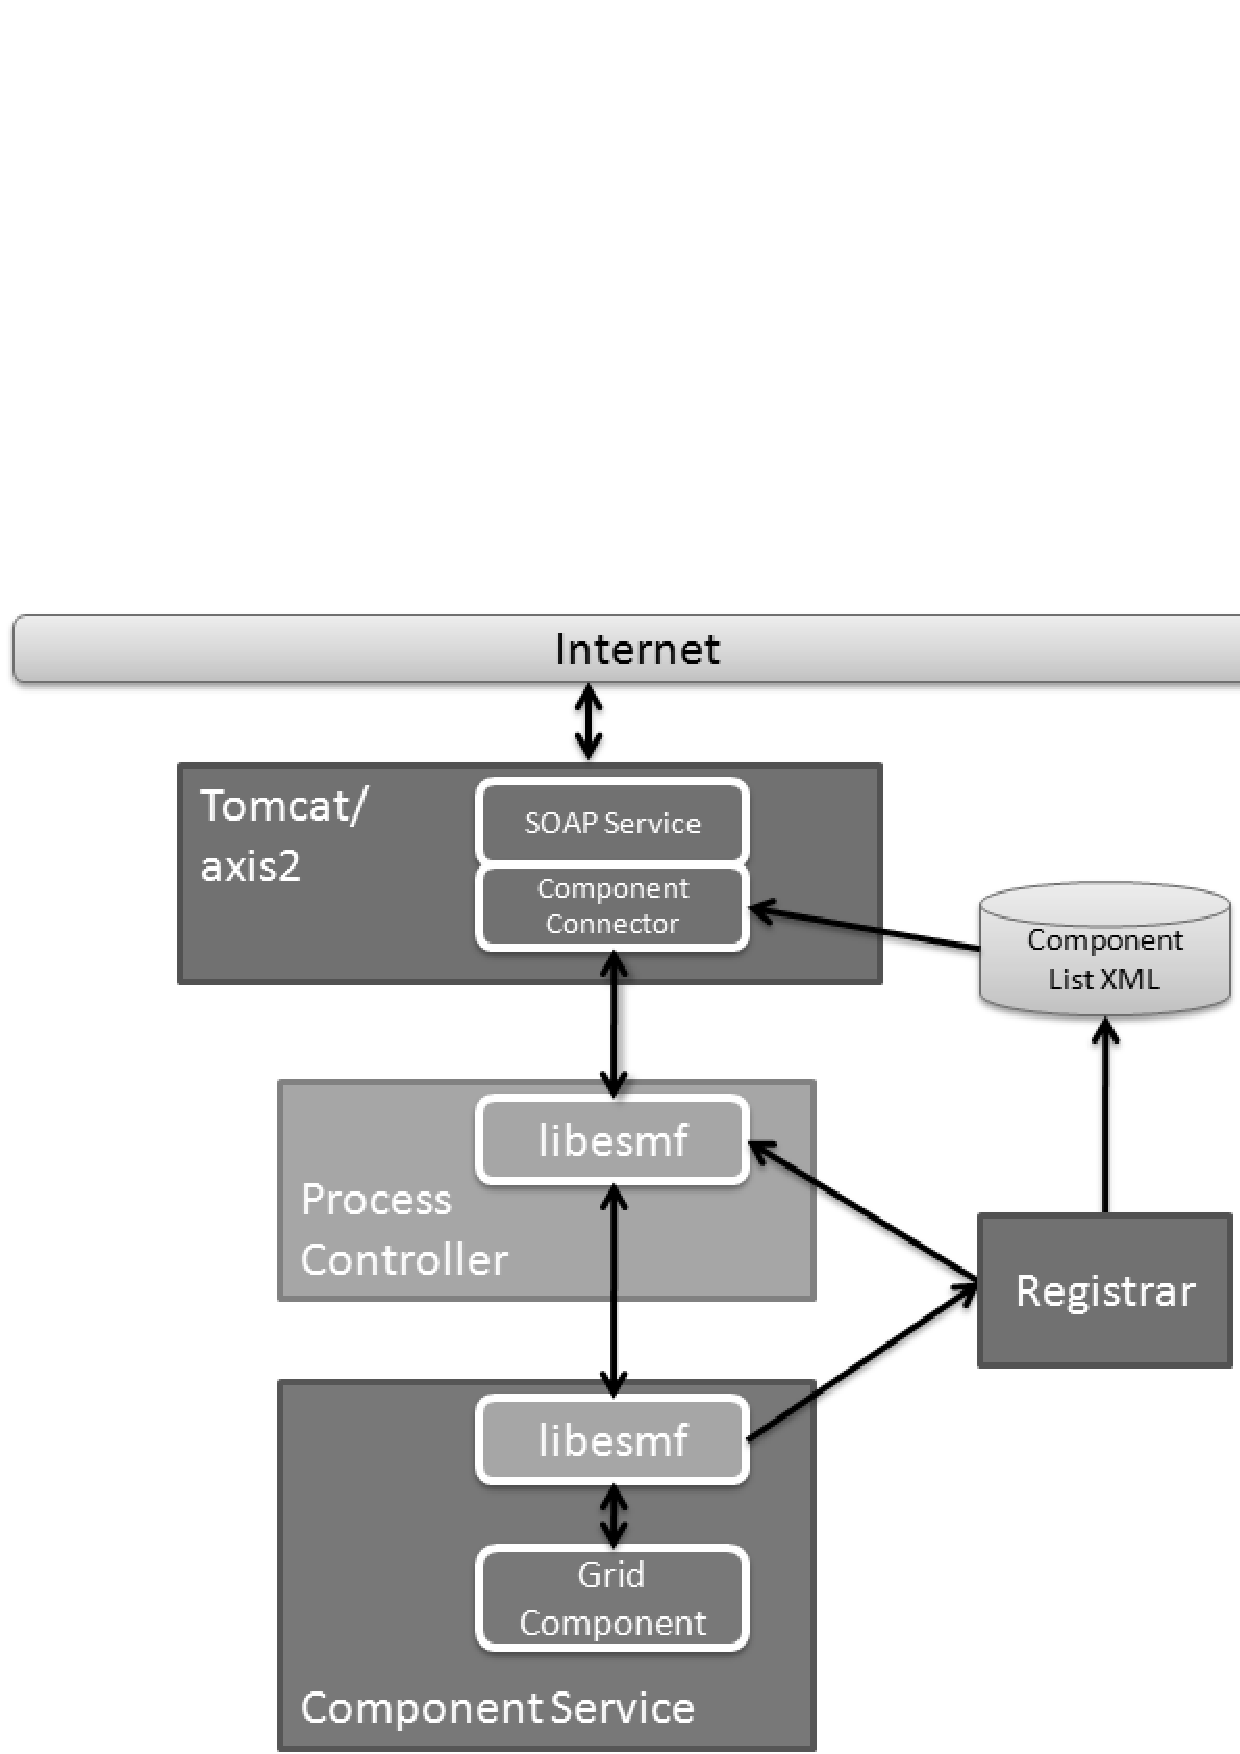
\includegraphics{webservices}}
\end{figure}
\end{center}

At the heart of this architecture is the Component Service; this is the 
application that does the model work.  The ESMF Web Services part provides a way to make 
the model accessible via a network API (Application Programming Interface). ESMF provides 
the tools to turn a model component into a service as well as the tools to access the 
service from the network. 

The Process Controller is a stand-alone application that provides a control mechanism between 
the end user and the Component Service.  The Process Controller is responsible for managing 
client information as well as restricting client access to a Component Service.  
(The role of the Process Controller is expected to expand in the future.)

The tomcat/axis2 application provides the access via the Web using standard SOAP 
protocols. Part of this application includes the SOAP interface definition 
(using a WSDL file) as well as some java code that provides the access to the Process 
Controller application.

Finally, the Registrar maintains a list of Component Services that are currently 
available;  Component Services register themselves with the Registrar when they 
startup, and unregister themselves when they shutdown.  The list of available services 
is maintained in an XML file and is accessible from the Registrar using its network API.

\subsubsection{Creating a Service around a Component}
\subsubsection{Code Modifications}
One of the goals in providing the tools to make Components into services was to make 
the process as simple and easy as possible.  Any model component that has been 
implemented using the ESMF Component Framework can easily be turned into a 
Component Services with just a minor change to the Application 
driver code.  (For details on the ESMF Framework, see the ESMF Developers Documentation.)

The primary function in ESMF Web Services is the ESMF\_WebServicesLoop routine.  This 
function registers the Component Service with the Registrar and then sets up a 
network socket service that listens for requests from a client.  It starts a loop 
that waits for incoming requests and manages the routing of these requests to 
all PETs.  It is also responsible for making sure the appropriate ESMF 
routine (ESMF\_Initialize, ESMF\_Run or ESMF\_Finalize) is called based on the incoming 
request. When the client has completed its interaction with the Component Service, 
the loop will be terminated and it will unregister the Component Service from the Registrar. 

To make all of this happen, the Application Driver just needs to replace its calls to 
ESMF\_Initialize, ESMF\_Run, and ESMF\_Finalize with a single call to ESMF\_WebServicesLoop. 

\begin{verbatim}

	use ESMF_WebServMod
	....

	call ESMF_WebServicesLoop(gridComponent, portNumber, returnCode)

\end{verbatim}

That's all there is to turning an ESMF Component into a network-accessible 
ESMF Component Service.  For a detailed example of an ESMF Component turned into 
an ESMF Component Service, see the Examples in the Web Services section of the 
Developer' Guide.

\subsubsection{Accessing the Service}
Now that the Component is available as a service, it can be accessed remotely by any client 
that can communicate via TCP sockets.  The ESMF library, in addition to providing the 
service tools, also provides the classes to create C++ clients to access the Component 
Service via the socket interface.

However, the goal of ESMF Web Services is to make an ESMF Component accessible through 
a standard web service, which is accomplished through the Process Controller and the 
Tomcat/Axis2 applications

\subsubsection{Client Application via C++ API}

Interfacing to a Component service is fairly simple using the ESMF library.  The following 
code is a simple example of how to interface to a Component Service in C++ and request 
the initialize operation (the entire sample client can be found in the Web Services examples 
section of the ESMF Distribution):

\begin{verbatim}

	#include "ESMCI_WebServCompSvrClient.h"

	int  main(int  argc, char*  argv[])
	{
   	    int    portNum = 27060;
      	    int    clientId = 101;
   	    int    rc = ESMF_SUCCESS;

   	    ESMCI::ESMCI_WebServCompSvrClient   
                         client("localhost", portNum, clientId);

   	    rc = client.init();
   	    printf("Initialize return code: %d\n", rc);
	}

\end{verbatim}


To see a complete description of the NetEsmfClient class, refer to the netesmf library 
section of the Web Services Reference Manual.

\subsubsection{Process Controller}

The Process Controller is basically just a instance of a C++ client application. It manages 
client access to the Component Service (only 1 client can access the service at a time), 
and will eventually be responsible for starting up and shutting down instances of 
Component Services (planned for a future release). The Process Controller application is 
built with the ESMF library and is included in the apps section of the distribution.

\subsubsection{Tomcat/Axis2}

The Tomcat/Axis2 "application" is essentially the Apache Tomcat server using 
the Apache Axis2 servlet to  implement web services using SOAP protocols. The web 
interface is defined by a WSDL file, and its implementation is handled by the Component 
Connector java code.  Tomcat and Axis2 are both open source projects that should be 
downloaded from the Apache web site, but the WSDL file, the Component Connector java 
code, and all required software for supporting the interface can be found next to the 
ESMF distribution in the web\_services\_server directory. This code is not included with 
the ESMF distribution because they can be distributed and installed independent of each other.

\subsection{Use and Examples}
% $Id$
%
% Earth System Modeling Framework
% Copyright 2002-2020, University Corporation for Atmospheric Research, 
% Massachusetts Institute of Technology, Geophysical Fluid Dynamics 
% Laboratory, University of Michigan, National Centers for Environmental 
% Prediction, Los Alamos National Laboratory, Argonne National Laboratory, 
% NASA Goddard Space Flight Center.
% Licensed under the University of Illinois-NCSA License.

%\subsection{Use and Examples}

The following examples demonstrate how to use ESMF Web Services.

%                **** IMPORTANT NOTICE *****
% This LaTeX file has been automatically produced by ProTeX v. 1.1
% Any changes made to this file will likely be lost next time
% this file is regenerated from its source. Send questions 
% to Arlindo da Silva, dasilva@gsfc.nasa.gov
 
\setlength{\oldparskip}{\parskip}
\setlength{\parskip}{1.5ex}
\setlength{\oldparindent}{\parindent}
\setlength{\parindent}{0pt}
\setlength{\oldbaselineskip}{\baselineskip}
\setlength{\baselineskip}{11pt}
 
%--------------------- SHORT-HAND MACROS ----------------------
\def\bv{\begin{verbatim}}
\def\ev{\end{verbatim}}
\def\be{\begin{equation}}
\def\ee{\end{equation}}
\def\bea{\begin{eqnarray}}
\def\eea{\end{eqnarray}}
\def\bi{\begin{itemize}}
\def\ei{\end{itemize}}
\def\bn{\begin{enumerate}}
\def\en{\end{enumerate}}
\def\bd{\begin{description}}
\def\ed{\end{description}}
\def\({\left (}
\def\){\right )}
\def\[{\left [}
\def\]{\right ]}
\def\<{\left  \langle}
\def\>{\right \rangle}
\def\cI{{\cal I}}
\def\diag{\mathop{\rm diag}}
\def\tr{\mathop{\rm tr}}
%-------------------------------------------------------------

\markboth{Left}{Source File: ESMF\_WebServicesEx.F90,  Date: Tue May  5 21:00:16 MDT 2020
}

 
%/////////////////////////////////////////////////////////////

  \subsubsection{Making a Component available through ESMF Web Services}
        
    In this example, a standard ESMF Component is made available through
    the Web Services interface. 
%/////////////////////////////////////////////////////////////

    The first step is to make sure your callback routines for initialize, run
    and finalize are setup.  This is done by creating a register routine that
    sets the entry points for each of these callbacks.  In this example, we've
    packaged it all up into a separate module.   
%/////////////////////////////////////////////////////////////

 \begin{verbatim}
module ESMF_WebServUserModel

  ! ESMF Framework module
  use ESMF

  implicit none

  public ESMF_WebServUserModelRegister

  contains

  !-------------------------------------------------------------------------
  !  The Registration routine
  !  
  subroutine ESMF_WebServUserModelRegister(comp, rc)
    type(ESMF_GridComp)  :: comp
    integer, intent(out) :: rc

    ! Initialize return code
    rc = ESMF_SUCCESS

    print *, "User Comp1 Register starting"

    ! Register the callback routines.

    call ESMF_GridCompSetEntryPoint(comp, ESMF_METHOD_INITIALIZE, &
                                    userRoutine=user_init, rc=rc)
    if (rc/=ESMF_SUCCESS) return ! bail out

    call ESMF_GridCompSetEntryPoint(comp, ESMF_METHOD_RUN, &
                                    userRoutine=user_run, rc=rc)
    if (rc/=ESMF_SUCCESS) return ! bail out

    call ESMF_GridCompSetEntryPoint(comp, ESMF_METHOD_FINALIZE, &
                                    userRoutine=user_final, rc=rc)
    if (rc/=ESMF_SUCCESS) return ! bail out

    print *, "Registered Initialize, Run, and Finalize routines"
    print *, "User Comp1 Register returning"

  end subroutine

  !-------------------------------------------------------------------------
  !  The Initialization routine
  !  
  subroutine user_init(comp, importState, exportState, clock, rc)
    type(ESMF_GridComp)  :: comp
    type(ESMF_State)     :: importState, exportState
    type(ESMF_Clock)     :: clock
    integer, intent(out) :: rc

    ! Initialize return code
    rc = ESMF_SUCCESS

    print *, "User Comp1 Init"

  end subroutine user_init

  !-------------------------------------------------------------------------
  !  The Run routine
  !  
  subroutine user_run(comp, importState, exportState, clock, rc)
    type(ESMF_GridComp)  :: comp
    type(ESMF_State)     :: importState, exportState
    type(ESMF_Clock)     :: clock
    integer, intent(out) :: rc

    ! Initialize return code
    rc = ESMF_SUCCESS

    print *, "User Comp1 Run"

  end subroutine user_run

  !-------------------------------------------------------------------------
  !  The Finalization routine
  !  
  subroutine user_final(comp, importState, exportState, clock, rc)
    type(ESMF_GridComp)  :: comp
    type(ESMF_State)     :: importState, exportState
    type(ESMF_Clock)     :: clock
    integer, intent(out) :: rc

    ! Initialize return code
    rc = ESMF_SUCCESS

    print *, "User Comp1 Final"

  end subroutine user_final

end module ESMF_WebServUserModel
 
\end{verbatim}
 
%/////////////////////////////////////////////////////////////

    The actual driver code then becomes very simple; ESMF is initialized,
    the component is created, the callback functions for the component are
    registered, and the Web Service loop is started. 
%/////////////////////////////////////////////////////////////

 \begin{verbatim}
program WebServicesEx
#include "ESMF.h"

  ! ESMF Framework module
  use ESMF
  use ESMF_TestMod

  use ESMF_WebServMod
  use ESMF_WebServUserModel

  implicit none

  ! Local variables
  type(ESMF_GridComp) :: comp1     !! Grid Component
  integer             :: rc        !! Return Code
  integer             :: finalrc  !! Final return code
  integer             :: portNum   !! The port number for the listening socket
 
\end{verbatim}
 
%/////////////////////////////////////////////////////////////

    A listening socket will be created on the local machine with the specified
    port number.  This socket is used by the service to
    wait for and receive requests from the client.  Check with your system
    administrator to determine an appropriate port to use for your service. 
%/////////////////////////////////////////////////////////////

 \begin{verbatim}
  finalrc = ESMF_SUCCESS

  call ESMF_Initialize(defaultlogfilename="WebServicesEx.Log", &
                    logkindflag=ESMF_LOGKIND_MULTI, rc=rc)
 
\end{verbatim}
 
%/////////////////////////////////////////////////////////////

 \begin{verbatim}
  ! create the grid component 
  comp1 = ESMF_GridCompCreate(name="My Component", rc=rc)
 
\end{verbatim}
 
%/////////////////////////////////////////////////////////////

 \begin{verbatim}
  ! Set up the register routine 
  call ESMF_GridCompSetServices(comp1, &
          userRoutine=ESMF_WebServUserModelRegister, rc=rc)
 
\end{verbatim}
 
%/////////////////////////////////////////////////////////////

 \begin{verbatim}
  portNum = 27060

  ! Call the Web Services Loop and wait for requests to come in
  !call ESMF_WebServicesLoop(comp1, portNum, rc=rc)
 
\end{verbatim}
 
%/////////////////////////////////////////////////////////////

    The call to ESMF\_WebServicesLoop will setup the listening socket for your
    service and will wait for requests from a client.  As requests are received,
    the Web Services software will process the requests and then return to the
    loop to continue to wait. 
%/////////////////////////////////////////////////////////////

    The 3 main requests processed are INIT, RUN, and FINAL.  These requests 
    will then call the appropriate callback routine as specified in your 
    register routine (as specified in the ESMF\_GridCompSetServices call).
    In this example, when the INIT request is received, the user\_init routine
    found in the ESMF\_WebServUserModel module is called. 
%/////////////////////////////////////////////////////////////

    One other request is also processed by the Component Service, and that is
    the EXIT request.  When this request is received, the Web Services loop
    is terminated and the remainder of the code after the ESMF\_WebServicesLoop
    call is executed. 
%/////////////////////////////////////////////////////////////

 \begin{verbatim}
  call ESMF_Finalize(rc=rc)
 
\end{verbatim}
 
%/////////////////////////////////////////////////////////////

 \begin{verbatim}
end program WebServicesEx
 
\end{verbatim}

%...............................................................
\setlength{\parskip}{\oldparskip}
\setlength{\parindent}{\oldparindent}
\setlength{\baselineskip}{\oldbaselineskip}

\subsection{Restrictions and Future Work}
% $Id$
%
% Earth System Modeling Framework
% Copyright 2002-2020, University Corporation for Atmospheric Research, 
% Massachusetts Institute of Technology, Geophysical Fluid Dynamics 
% Laboratory, University of Michigan, National Centers for Environmental 
% Prediction, Los Alamos National Laboratory, Argonne National Laboratory, 
% NASA Goddard Space Flight Center.
% Licensed under the University of Illinois-NCSA License.

%\subsubsection{Restrictions and Future Work}

\begin{enumerate}
\item{\bf Manual Control of Process.}
Currently, the Component Service must be manually started and stopped.  Future plans include having the Process Controller be responsible for controlling the Component Service processes.
\item{\bf Data Streaming.}
While data can be streamed from the web server to the client, it is not yet getting the data directly from the Component Service.  Instead, the Component Service exports the data to a file which the Process Controller can read and return across the network interface.  The data streaming capabilities will be a major component of future improvements to the Web Services architecture.
\end{enumerate}




\subsection{Class API}
%                **** IMPORTANT NOTICE *****
% This LaTeX file has been automatically produced by ProTeX v. 1.1
% Any changes made to this file will likely be lost next time
% this file is regenerated from its source. Send questions 
% to Arlindo da Silva, dasilva@gsfc.nasa.gov
 
\setlength{\oldparskip}{\parskip}
\setlength{\parskip}{1.5ex}
\setlength{\oldparindent}{\parindent}
\setlength{\parindent}{0pt}
\setlength{\oldbaselineskip}{\baselineskip}
\setlength{\baselineskip}{11pt}
 
%--------------------- SHORT-HAND MACROS ----------------------
\def\bv{\begin{verbatim}}
\def\ev{\end{verbatim}}
\def\be{\begin{equation}}
\def\ee{\end{equation}}
\def\bea{\begin{eqnarray}}
\def\eea{\end{eqnarray}}
\def\bi{\begin{itemize}}
\def\ei{\end{itemize}}
\def\bn{\begin{enumerate}}
\def\en{\end{enumerate}}
\def\bd{\begin{description}}
\def\ed{\end{description}}
\def\({\left (}
\def\){\right )}
\def\[{\left [}
\def\]{\right ]}
\def\<{\left  \langle}
\def\>{\right \rangle}
\def\cI{{\cal I}}
\def\diag{\mathop{\rm diag}}
\def\tr{\mathop{\rm tr}}
%-------------------------------------------------------------

\markboth{Left}{Source File: ESMF\_WebServ.F90,  Date: Tue May  5 21:00:16 MDT 2020
}

 
%/////////////////////////////////////////////////////////////

  
%/////////////////////////////////////////////////////////////
 
\mbox{}\hrulefill\ 
 
\subsubsection [ESMF\_WebServicesLoop] {ESMF\_WebServicesLoop }


  
\bigskip{\sf INTERFACE:}
\begin{verbatim}   subroutine ESMF_WebServicesLoop(comp, portNum, clientId, registrarHost, rc)
 \end{verbatim}{\em ARGUMENTS:}
\begin{verbatim}     type(ESMF_GridComp)                         :: comp
     integer,            intent(inout), optional :: portNum
     character(len=*),   intent(in),    optional, target :: clientId
     character(len=*),   intent(in),    optional, target :: registrarHost
     integer,            intent(out),   optional :: rc\end{verbatim}
{\sf DESCRIPTION:\\ }


     Encapsulates all of the functionality necessary to setup a component as
     a component service.  On the root PET, it registers the
     component service and then enters into a loop that waits for requests on 
     a socket.  The loop continues until an "exit" request is received, at 
     which point it exits the loop and unregisters the service.  On
     any PET other than the root PET, it sets up a process block that waits
     for instructions from the root PET.  Instructions will come as requests
     are received from the socket.
  
   The arguments are:
   \begin{description}
   \item[{[comp]}]
     {\tt ESMF\_CplComp} object that represents the Grid Component for which
     routine is run.
   \item[{[portNum]}]
     Number of the port on which the component service is listening.
   \item[{[clientId]}]
     Identifier of the client responsible for this component service.  If a
     Process Controller application manages this component service, then the
     clientId is provided to the component service application in the command
     line.  Otherwise, the clientId is not necessary.
   \item[{[registrarHost]}]
     Name of the host on which the Registrar is running.  Needed so the
     component service can notify the Registrar when it is ready to receive
     requests from clients.
   \item[{[rc]}]
     Return code; equals {\tt ESMF\_SUCCESS} if there are no errors.
   \end{description}
   
%/////////////////////////////////////////////////////////////
 
\mbox{}\hrulefill\ 
 
\subsubsection [ESMF\_WebServicesCplCompLoop] {ESMF\_WebServicesCplCompLoop }


  
\bigskip{\sf INTERFACE:}
\begin{verbatim}   subroutine ESMF_WebServicesCplCompLoop(comp, portNum, clientId, registrarHost, rc)
 
 \end{verbatim}{\em ARGUMENTS:}
\begin{verbatim}     type(ESMF_CplComp)                         :: comp
     integer,           intent(inout), optional :: portNum
     character(len=*),  intent(in),    optional, target :: clientId
     character(len=*),  intent(in),    optional, target :: registrarHost
     integer,           intent(out),   optional :: rc\end{verbatim}
{\sf DESCRIPTION:\\ }


     Encapsulates all of the functionality necessary to setup a component as
     a component service.  On the root PET, it registers the
     component service and then enters into a loop that waits for requests on 
     a socket.  The loop continues until an "exit" request is received, at 
     which point it exits the loop and unregisters the service.  On
     any PET other than the root PET, it sets up a process block that waits
     for instructions from the root PET.  Instructions will come as requests
     are received from the socket.
  
   The arguments are:
   \begin{description}
   \item[{[comp]}]
     {\tt ESMF\_CplComp} object that represents the Grid Component for which
     routine is run.
   \item[{[portNum]}]
     Number of the port on which the component service is listening.
   \item[{[clientId]}]
     Identifier of the client responsible for this component service.  If a
     Process Controller application manages this component service, then the
     clientId is provided to the component service application in the command
     line.  Otherwise, the clientId is not necessary.
   \item[{[registrarHost]}]
     Name of the host on which the Registrar is running.  Needed so the
     component service can notify the Registrar when it is ready to receive
     requests from clients.
   \item[{[rc]}]
     Return code; equals {\tt ESMF\_SUCCESS} if there are no errors.
   \end{description}
  
%...............................................................
\setlength{\parskip}{\oldparskip}
\setlength{\parindent}{\oldparindent}
\setlength{\baselineskip}{\oldbaselineskip}

%+==============================================================================
\newpage
\begin{htmlonly}
\addcontentsline{toc}{part}{Infrastructure: Fields and Grids}
\end{htmlonly}
\part{Infrastructure: Fields and Grids}
\newpage
%\section{Overview of Infrastructure Data Classes}
% $Id$

\section{Overview of Data Classes}

The ESMF infrastructure data classes are part of the framework's 
hierarchy of structures for handling Earth system model data and 
metadata on parallel platforms.  The hierarchy is in complexity; the 
simplest data class in the infrastructure represents a distributed data
array and the most complex data class represents a bundle of physical 
fields that are discretized on the same grid.  Data class methods 
are called both from user-written code and from other classes 
internal to the framework. 

Data classes are distributed over {\bf DE}s, or {\bf Decomposition Elements}.  
A DE represents a piece of a decomposition.  A DELayout is a collection
of DEs with some associated connectivity that describes a specific 
distribution.  For example, the distribution of a grid divided 
into four segments in the x-dimension would be expressed in ESMF as
a DELayout with four DEs lying along an x-axis. This abstract concept 
enables a data decomposition to be defined in 
terms of threads, MPI processes, virtual decomposition elements, or
combinations of these without changes to user code.  This is a
primary strategy for ensuring optimal performance and portability
for codes using ESMF for communications.

ESMF data classes provide a standard,
convenient way for developers to collect together information 
related to model or observational data.  The information assembled 
in a data class includes a data pointer, a set of attributes 
(e.g. units, although attributes can also be user-defined), and a 
description of an associated grid.  The same set of information within 
an ESMF data object can be used by the framework to arrange 
intercomponent data transfers, to perform I/O, for communications
such as gathers and scatters, for simplification of interfaces 
within user code, for debugging, and for other functions.  
This unifies and organizes codes overall so that the user need not
define different representations of metadata for the same field 
for I/O and for component coupling.  

Since it is critical that users be able to introduce ESMF into their
codes easily and incrementally, ESMF data classes can be created based 
on native Fortran pointers.  Likewise, there are methods for retrieving 
native Fortran pointers from within ESMF data objects.  This allows
the user to perform allocations using ESMF, and to retrieve Fortran
arrays later for optimized model calculations.  The ESMF data classes 
do not have associated differential operators or other mathematical 
methods.

For flexibility, it is not necessary to build an ESMF data object 
all at once.  For example, it's possible to create a 
field but to defer allocation of the associated field data until 
a later time.


\begin{center}  
\begin{tabular}{|p{6in}|}
\hline
\vspace{.01in}
{\bf Key Features} \\[.01in]
Hierarchy of data structures designed specifically for the Earth 
system domain and high performance, parallel computing. \\
Multi-use ESMF structures simplify user code overall. \\
Data objects support incremental construction and deferred allocation. \\ 
Native Fortran arrays can be associated with or retrieved from ESMF data
objects, for ease of adoption, convenience, and performance. \\
A variety of operations are provided for manipulating data in data objects 
such as regridding, redistribution, halo communication, and sparse matrix multiply.\\[.03in] \hline
\end{tabular}
\end{center}

The main classes that are used for model and observational data manipulation
are as follows:

\begin{itemize}

\item {\bf Array}  An ESMF Array contains a data pointer, 
information about its associated datatype, precision, and 
dimension.  

Data elements in Arrays are partitioned into categories 
defined by the role the data element plays in distributed halo 
operations.  Haloing - sometimes called ghosting - is the 
practice of copying portions of array data to multiple memory 
locations to ensure that data dependencies can be satisfied 
quickly when performing a calculation.  ESMF Arrays contain 
an {\bf exclusive} domain, which contains data elements
updated exclusively and definitively by a given DE; a 
{\bf computational} domain, which contains all data elements
with values that are updated by the DE in computations; and 
a {\bf total} domain, which includes both the computational 
domain and data elements from other DEs which may be read 
but are not updated in computations.

\item {\bf ArrayBundle} ArrayBundles are collections of
Arrays that are stored in a single object.  Unlike FieldBundles,
they don't need to be distributed the same way across PETs.  The
motivation for ArrayBundles is both convenience and performance.

\item {\bf Field}  A Field holds model and/or observational 
data together with its underlying grid or set of spatial 
locations.  It provides methods for configuration, 
initialization, setting and retrieving data values, 
data I/O, data regridding, and manipulation of attributes.

\item {\bf FieldBundle} Groups of Fields on the same underlying 
physical grid can be collected into a single object called a FieldBundle.  
A FieldBundle provides two major functions: it allows groups of 
Fields to be manipulated using a single identifier, for example 
during export or import of data between Components; and 
it allows data from multiple Fields to be packed together 
in memory for higher locality of reference and ease in 
subsetting operations.  Packing a set of Fields into a single
FieldBundle before performing a data communication allows the set 
to be transferred at once rather than as a Field at a time.
This can improve performance on high-latency platforms.

FieldBundle objects contain methods for setting and retrieving constituent 
fields, regridding, data I/O, and reordering of data in memory.

\end{itemize}

\subsection{Bit-for-Bit Considerations}

Bit-for-bit reproducibility is at the core of the regression testing
schemes of many scientific model codes. The bit-for-bit requirement makes it
easy to compare the numerical results of simulation runs using standard
binary diff tools.

For the most part, ESMF methods do not modify user data numerically, and
thus have no effect on the bit-for-bit characteristics of the model code.
The exceptions are the regrid weight generation and the sparse matrix
multiplication.

In the case of the regrid weight generation, user data is used to produce
interpolation weights following specific numerical schemes. The bit-for-bit
reproducibility of the generated weights depends on the implementation
details. Section \ref{sec:regrid} provides more details about the bit-for-bit
considerations with respect to the regrid weights generated by ESMF.

In the case of the sparse matrix multiplication, which is the typical method
that is used to apply the regrid weights, user data is directly manipulated 
by ESMF. In order to help users with the implementation of their bit-for-bit
requirements, while also considering the associated performance impact,
the ESMF sparse matrix implementation provides three levels of bit-for-bit
support. The strictest level ensures that the numerical results are
bit-for-bit identical, even when executing across different numbers of
PETs. In the relaxed level, bit-for-bit reproducibility is guaranteed when
running across an unchanged number of PETs. The lowest level makes no
guarantees about bit-for-bit reproducibility, however, it provides the
greatest performance potential for those cases where numerical round-off
differences are acceptable. An in-depth discussion of bit-for-bit
reproducibility, and the performance aspects of route-based communication
methods, such the sparse matrix multiplication, is given in section
\ref{RH:bfb}.


\subsection{Regrid}\label{sec:regrid}

 This section describes the regridding methods provided by ESMF. Regridding, also called remapping or interpolation, is 
 the process of changing the grid that underlies data values while preserving qualities of the original data. Different 
 kinds of transformations are appropriate for different problems. Regridding may be needed when communicating data between
 Earth system model components such as land and atmosphere, or between different data sets to support operations such as visualization.

 Regridding can be broken into two stages. The first stage is generation of an interpolation weight matrix that describes how points in 
 the source grid contribute to points in the destination grid. The second stage is the multiplication of values on the source grid by the
 interpolation weight matrix to produce values on the destination grid. This is implemented as a parallel sparse matrix multiplication.

 There are two options for accessing ESMF regridding functionality: {\bf offline} and {\bf integrated}. Offline regridding is a process whereby interpolation 
 weights are generated by a separate ESMF application, not within the user code. The ESMF offline regridding application also only generates the interpolation 
 matrix, the user is responsible for reading in this matrix and doing the actual interpolation (multiplication by the sparse matrix) in their code.
 Please see Section~\ref{sec:ESMF_RegridWeightGen} for a description of the offline regridding application and the options it supports. For user convenience, there
 is also a method interface to the offline regrid application functionality which is described in Section~\ref{api:esmf_regridweightgenfile}.
 In contrast to offline regridding, integrated regridding is a process whereby interpolation weights are generated via subroutine calls during the
 execution of the user's code. In addition to generating the weights, integrated regridding can also produce a {\bf RouteHandle} (described in Section~\ref{sec:RHandle}) which allows the user to perform the parallel sparse 
 matrix multiplication using ESMF methods. In other words, ESMF integrated regridding allows a user to perform the whole process of interpolation within their code. 

 To see what types of grids and other options are supported in the two types of regridding and their testing status, please see the \htmladdnormallink{ESMF Regridding Status}{https://www.earthsystemcog.org/projects/esmf/regridding_8_0_0} webpage for this version of ESMF.
 Figure~\ref{Regrid Interfaces} shows a comparison of different regrid interfaces and where they can be found in the documentation. 

 The rest of this section further describes the various options available in ESMF regridding. 

\begin{table}[ht]
\centering
\vspace{0.2cm}
\begin{tabular}{| l | l | l | c | c | l |}
\hline
Name & Access via & Inputs & \multicolumn{2}{|c|}{Outputs} & Description\\ 
     &            &        &  Weights & RouteHandle        &            \\ 
\hline
ESMF\_FieldRegridStore() & Subroutine call & Field object & yes  & yes & Sec.~\ref{api:esmf_fieldregridstorenx} \\
\hline
ESMF\_FieldBundleRegridStore() & Subroutine call & Fieldbundle obj. & no  & yes & Sec.~\ref{api:esmf_fieldbundleregridstore} \\
\hline
ESMF\_RegridWeightGen() & Subroutine call & Grid files & yes  & no & Sec.~\ref{api:esmf_regridweightgenfile} \\
\hline
ESMF\_RegridWeightGen & Application & Grid files & yes  & no & Sec.~\ref{sec:ESMF_RegridWeightGen} \\
\hline
\end{tabular}
\label{Regrid Interfaces}
\caption{Regrid Interfaces}
\end{table}


\subsubsection{Interpolation methods: bilinear}\label{sec:interpolation:bilinear}
 Bilinear interpolation calculates the value for the 
 destination point as a combination of multiple linear interpolations, one for each dimension of the Grid. Note that for ease of 
 use, the term bilinear interpolation is used for 3D interpolation in ESMF as well, although it should more properly be referred 
 to as trilinear interpolation.

\smallskip

 In 2D, ESMF supports bilinear regridding between any combination of the following:
 \begin{itemize}
 \item Structured grids ({\tt ESMF\_Grid}) composed of any number of logically rectangular tiles
 \item Unstructured meshes ({\tt ESMF\_Mesh}) composed of polygons with any number of sides
 \item A set of disconnected points ({\tt ESMF\_LocStream}) may be the destination of the regridding
 \end{itemize}

\smallskip

 In 3D, ESMF supports bilinear regridding between any combination of the following:
 \begin{itemize}
 \item Structured grids ({\tt ESMF\_Grid}) composed of a single logically rectangular tile
 \item Unstructured meshes ({\tt ESMF\_Mesh}) composed of hexahedrons 
 \item A set of disconnected points ({\tt ESMF\_LocStream}) may be the destination of the regridding
 \end{itemize}

\smallskip

{\bf Restrictions:}
 \begin{itemize}
 \item Cells which contain enough identical corners to collapse to a line or point are currently ignored
 \item Self-intersecting cells (e.g. a cell twisted into a bow tie) are not supported 
 \item On a spherical grid, cells which contain an edge which extends more than half way around the sphere are not supported 
 \end{itemize}

 To use the bilinear method the user may create their Fields on any stagger location (e.g. {\tt ESMF\_STAGGERLOC\_CENTER}) for a Grid, or
 any Mesh location (e.g. {\tt ESMF\_MESHLOC\_NODE}) for a Mesh. For either a Grid or a Mesh, the location upon which the Field is built 
 must contain coordinates. 

\subsubsection{Interpolation methods: higher-order patch}\label{sec:interpolation:patch}

 Patch (or higher-order) interpolation is the ESMF version of a technique called ``patch recovery'' commonly
 used in finite element modeling~\cite{PatchInterp1}~\cite{PatchInterp2}. It typically results in better approximations to 
 values and derivatives when compared to bilinear interpolation.
 Patch interpolation works by constructing multiple polynomial patches to represent
 the data in a source cell. For 2D grids, these polynomials
 are currently 2nd degree 2D polynomials. One patch is constructed for each corner of the source cell, and the patch is constructed 
 by doing a least squares fit through the data in the cells surrounding the corner. The interpolated value at the destination point is 
 then a weighted average of the values of the patches at that point. The patch method has a larger
 stencil than the bilinear, for this reason the patch weight matrix can be correspondingly larger
 than the bilinear matrix (e.g. for a quadrilateral grid the patch matrix is around 4x the size of
 the bilinear matrix). This can be an issue when performing a regrid operation close to the memory
 limit on a machine.  

\smallskip

 In 2D, ESMF supports patch regridding between any combination of the following:
 \begin{itemize}
 \item Structured Grids ({\tt ESMF\_Grid}) composed of a single logically rectangular tile
 \item Unstructured meshes ({\tt ESMF\_Mesh}) composed of polygons with any number of sides
 \item A set of disconnected points ({\tt ESMF\_LocStream}) may be the destination of the regridding
 \end{itemize}

\smallskip

 In 3D, ESMF supports patch regridding between any combination of the following:
 \begin{itemize}
 \item NONE
 \end{itemize}

\smallskip

{\bf Restrictions:}
 \begin{itemize}
 \item Cells which contain enough identical corners to collapse to a line or point are currently ignored
 \item Self-intersecting cells (e.g. a cell twisted into a bow tie) are not supported
 \item On a spherical grid, cells which contain an edge which extends more than half way around the sphere are not supported 
 \end{itemize}

 To use the patch method the user may create their Fields on any stagger location (e.g. {\tt ESMF\_STAGGERLOC\_CENTER}) for a Grid, or
 any Mesh location (e.g. {\tt ESMF\_MESHLOC\_NODE}) for a Mesh. For either a Grid or a Mesh, the location upon which the Field is built 
 must contain coordinates. 

\subsubsection{Interpolation methods: nearest source to destination}\label{sec:interpolation:neareststod}
In nearest source to destination interpolation ({\tt ESMF\_REGRIDMETHOD\_NEAREST\_STOD}) each destination point is mapped to the closest source point. A given source point may map to multiple destination points, but no destination point will receive input from more than one source point. If two points are equally close, then the point with the smallest sequence index is arbitrarily used (i.e. the point which would have the smallest index in the weight matrix). 

\smallskip

 In 2D, ESMF supports nearest source to destination regridding between any combination of the following:
 \begin{itemize}
 \item Structured Grids ({\tt ESMF\_Grid}) composed of any number of logically rectangular tiles
 \item Unstructured meshes ({\tt ESMF\_Mesh}) composed of polygons with any number of sides
 \item A set of disconnected points ({\tt ESMF\_LocStream}) 
 \end{itemize}

\smallskip

 In 3D, ESMF supports nearest source to destination regridding between any combination of the following:
 \begin{itemize}
 \item Structured Grids ({\tt ESMF\_Grid}) composed of any number of logically rectangular tiles
 \item Unstructured Meshes ({\tt ESMF\_Mesh}) composed of hexahedrons (e.g. cubes) and tetrahedrons
 \item A set of disconnected points ({\tt ESMF\_LocStream}) 
 \end{itemize}

\smallskip

\textbf{Restrictions:}\\*
\textit{NONE}

\smallskip

 To use the nearest source to destination method the user may create their Fields on any stagger location (e.g. {\tt ESMF\_STAGGERLOC\_CENTER}) for a Grid, or
 any Mesh location (e.g. {\tt ESMF\_MESHLOC\_NODE}) for a Mesh. For either a Grid or a Mesh, the location upon which the Field is built 
 must contain coordinates. 


\subsubsection{Interpolation methods: nearest destination to source}\label{sec:interpolation:nearestdtos}
In nearest destination to source interpolation ({\tt ESMF\_REGRIDMETHOD\_NEAREST\_DTOS}) each source point is mapped to the closest destination point. A given destination point may receive input from multiple source points, but no source point will map to more than one destination point. If two points are equally close, then the point with the smallest sequence index is arbitrarily used (i.e. the point which would have the smallest index in the weight matrix). Note that with this method the unmapped destination point detection currently doesn't work, so no error will be returned even if there are destination points that don't map to any source point. 

\smallskip

 In 2D, ESMF supports nearest destination to source regridding between any combination of the following:
 \begin{itemize}
 \item Structured Grids ({\tt ESMF\_Grid}) composed of any number of logically rectangular tiles
 \item Unstructured meshes ({\tt ESMF\_Mesh}) composed of polygons with any number of sides
 \item A set of disconnected points ({\tt ESMF\_LocStream}) 
 \end{itemize}

\smallskip

 In 3D, ESMF supports nearest destination to source regridding between any combination of the following:
 \begin{itemize}
 \item Structured Grids ({\tt ESMF\_Grid}) composed of any number of logically rectangular tiles
 \item Unstructured Meshes ({\tt ESMF\_Mesh}) composed of hexahedrons (e.g. cubes) and tetrahedrons
 \item A set of disconnected points ({\tt ESMF\_LocStream}) 
 \end{itemize}

\smallskip

\textbf{Restrictions:}\\*
\textit{NONE}

\smallskip

 To use the nearest destination to source method the user may create their Fields on any stagger location (e.g. {\tt ESMF\_STAGGERLOC\_CENTER}) for a Grid, or
 any Mesh location (e.g. {\tt ESMF\_MESHLOC\_NODE}) for a Mesh. For either a Grid or a Mesh, the location upon which the Field is built 
 must contain coordinates. 

\subsubsection{Interpolation methods: first-order conservative}\label{sec:interpolation:conserve}
 The goal of this method is to preserve the integral of the field across the interpolation from source to destination.  
 (For a more in-depth description of what this preservation of the integral (i.e. conservation) means please see section~\ref{sec:interpolation:conservation}.)  In this method the value across each source cell is treated as a constant, so it will typically have a larger 
 interpolation error than the bilinear or patch methods.  The first-order method used here is similar to that described in the following paper~\cite{ConservativeOrder1}.

 In the first-order method, the values for a particular destination cell are a calculated as a combination of the values of the intersecting 
 source cells. The weight of a given source cell's contribution 
 to the total being the amount that that source cell overlaps with the destination cell. 
 In particular, the weight is the ratio of the area of intersection of the source and destination cells to the area of the whole destination cell. 

 To see a description of how the different normalization options affect the values and integrals produced by the conservative methods see section~\ref{sec:interpolation:conservative_norm_opts}. For Grids or Meshes on a sphere this method uses great circle cells, for a description of potential problems with these see~\ref{sec:interpolation:great_circle_cells}.

\smallskip

 In 2D, ESMF supports conservative regridding between any combination of the following:
 \begin{itemize}
 \item Structured Grids ({\tt ESMF\_Grid}) composed of any number of logically rectangular tiles
 \item Unstructured meshes ({\tt ESMF\_Mesh}) composed of polygons with any number of sides
 \end{itemize}

\smallskip

 In 3D, ESMF supports conservative regridding between any combination of the following:
 \begin{itemize}
 \item Structured Grids ({\tt ESMF\_Grid}) composed of a single logically rectangular tile
 \item Unstructured Meshes ({\tt ESMF\_Mesh}) composed of hexahedrons (e.g. cubes) and tetrahedrons
 \end{itemize}

\smallskip

{\bf Restrictions:}
 \begin{itemize}
 \item Cells which contain enough identical corners to collapse to a line or point are optionally (via a flag) either ignored or return an error
 \item Self-intersecting cells (e.g. a cell twisted into a bow tie) are not supported
 \item On a spherical grid, cells which contain an edge which extends more than half way around the sphere are not supported 
 \end{itemize}

\smallskip

 To use the conservative method the user should create their Fields on the center 
 stagger location ({\tt ESMF\_STAGGERLOC\_CENTER} in 2D or {\tt ESMF\_STAGGERLOC\_CENTER\_VCENTER} in 3D) for Grids  or the element location ({\tt ESMF\_MESHLOC\_ELEMENT}) for Meshes.
 For Grids, the corner stagger location ({\tt ESMF\_STAGGERLOC\_CORNER} in 2D or {\tt ESMF\_STAGGERLOC\_CORNER\_VFACE} in 3D) must contain coordinates describing the outer perimeter of the Grid cells. 

\subsubsection{Interpolation methods: second-order conservative}\label{sec:interpolation:conserve_2ndorder}
 Like the first-order conservative method, this method's goal is to preserve the integral of the field across the interpolation from source to destination.  
 (For a more in-depth description of what this preservation of the integral (i.e. conservation) means please see section~\ref{sec:interpolation:conservation}.)  The difference between the first and second-order conservative methods is that the second-order takes the source gradient into account, so
 it yields a smoother destination field that typically better matches the source field. This difference between the first and second-order methods 
 is particularly apparent when going from a coarse source grid to a finer destination grid. The implementation of this method is based on the one 
 described in this paper~\cite{ConservativeOrder2}.

 Like the first-order method, the values for a particular destination cell with the second-order method
 are a combination of the values of the intersecting source cells. With the weight of a given source cell's contribution to the total 
 being the amount that that source cell overlaps with the destination cell. 
 However, with the second-order conservative interpolation there are additional terms that take into account the gradient of the field 
 across the source cell. In particular, the value $d$ for a given destination cell is calculated as:
 
 $d=\sum^{intersecting-source-cells}_{i}(s_{i}+\nabla s_{i} \cdot (c_{si}-c_{d}))$

\smallskip

Where:
\vspace{-1em}
\begin{description}
  \itemsep0em
  \item[$s_{i}$] is the intersecting source cell value. 
  \item[$\nabla s_{i}$] is the intersecting source cell gradient. 
  \item[$c_{si}$] is the intersecting source cell centroid. 
  \item[$c_{d}$] is the destination cell centroid. 
\end{description}

\smallskip

 To see a description of how the different normalization options affect the values and integrals produced by the conservative methods see section~\ref{sec:interpolation:conservative_norm_opts}. For Grids or Meshes on a sphere this method uses great circle cells, for a description of potential problems with these see~\ref{sec:interpolation:great_circle_cells}.

\smallskip

 In 2D, ESMF supports second-order conservative regridding between any combination of the following:
 \begin{itemize}
 \item Structured Grids ({\tt ESMF\_Grid}) composed of any number of logically rectangular tiles
 \item Unstructured meshes ({\tt ESMF\_Mesh}) composed of polygons with any number of sides
 \end{itemize}

\smallskip

 In 3D, ESMF supports second-order conservative regridding between any combination of the following:
 \begin{itemize}
 \item NONE
 \end{itemize}

\smallskip

{\bf Restrictions:}
 \begin{itemize}
 \item Cells which contain enough identical corners to collapse to a line or point are optionally (via a flag) either ignored or return an error
 \item Self-intersecting cells (e.g. a cell twisted into a bow tie) are not supported
 \item On a spherical grid, cells which contain an edge which extends more than half way around the sphere are not supported 
 \end{itemize}
 
\smallskip

 To use the second-order conservative method the user should create their Fields on the center 
 stagger location ({\tt ESMF\_STAGGERLOC\_CENTER} for Grids  or the element location ({\tt ESMF\_MESHLOC\_ELEMENT}) for Meshes.
 For Grids, the corner stagger location ({\tt ESMF\_STAGGERLOC\_CORNER} in 2D must contain coordinates describing the outer perimeter of the Grid cells. 

\subsubsection{Conservation}\label{sec:interpolation:conservation}
 Conservation means that the following equation will hold:  $\sum^{all-source-cells}(V_{si}*A_{si}) = \sum^{all-destination-cells}(V_{dj}*A_{dj})$, where
 V is the variable being regridded and A is the area of a cell.  The subscripts s and d refer to source and destination values, and the i and j are the source  and destination grid cell indices (flattening the arrays to 1 dimension). 

 If the user doesn't specify a cell areas in the involved Grids or Meshes, then the areas (A) in the above equation are calculated by ESMF. 
 For Cartesian grids, the area of a grid cell calculated by ESMF is the typical Cartesian area. 
 For grids on a sphere, cell areas are calculated by connecting the corner coordinates of each grid cell with great circles. If the user 
 does specify the areas in the Grid or Mesh, then the conservation will be adjusted to work for the areas 
 provided by the user. This means that the above equation will hold, but with the areas (A) being the ones specified by the user.

 The user should be aware that because of the conservation relationship between the source and destination fields, the more the total source area
 differs from the total destination area the more the values of the source field will differ from the corresponding values of the destination field, 
 likely giving a higher interpolation error. It is best to have the total source and destination areas the same 
 (this will automatically be true if no user areas are specified). For source and destination grids 
 that only partially overlap, the overlapping regions of the source and destination should be the same.

\subsubsection{The effect of normalization options on integrals and values produced by conservative methods}\label{sec:interpolation:conservative_norm_opts}
 It is important to note that by default (i.e. using destination area normalization) 
conservative regridding doesn't normalize the interpolation weights by the destination fraction. 
This means that for a destination grid which only partially overlaps the source grid
the destination field that is output from the regrid operation 
should be divided by the corresponding destination fraction to yield the 
true interpolated values for cells which are only partially covered by the source grid. 
The fraction also needs to be included when computing the total source and destination integrals. 
(To include the fraction in the conservative weights, the user can specify 
the fraction area normalization type. This can be done by specifying {\tt normType=ESMF\_NORMTYPE\_FRACAREA} when
invoking {\tt ESMF\_FieldRegridStore()}.)

For weights generated using destination area normalization (either by not specifying any normalization type or by specifying {\tt normType=ESMF\_NORMTYPE\_DSTAREA}), if a destination field extends 
outside the unmasked source field, then the values of the cells which 
extend partway outside the unmasked source field are decreased by the fraction they extend outside. 
To correct these values, the destination field ({\tt dst\_field}) resulting
from the {\tt ESMF\_FieldRegrid()} call can be divided by the destination fraction {\tt dst\_frac} 
from the {\tt ESMF\_FieldRegridStore()} call. The following pseudocode demonstrates  how to do this:

\begin{verbatim}

 for each destination element i
    if (dst_frac(i) not equal to 0.0) then
       dst_field(i)=dst_field(i)/dst_frac(i)
    end if
 end for
\end{verbatim}

For weights generated using destination area normalization (either by not specifying any normalization type or by specifying {\tt normType=ESMF\_NORMTYPE\_DSTAREA}), 
the following pseudo-code shows how to compute the total destination integral ({\tt dst\_total}) given the
destination field values ({\tt dst\_field}) resulting
from the {\tt ESMF\_FieldRegrid()} call, the destination area ({\tt dst\_area}) from the {\tt ESMF\_FieldRegridGetArea()} call,  and the destination fraction ({\tt dst\_frac}) from the {\tt ESMF\_FieldRegridStore()} call. As shown in the previous paragraph, it also 
shows how to adjust the destination field ({\tt dst\_field}) resulting from the {\tt ESMF\_FieldRegrid()} call by the
fraction ({\tt dst\_frac}) from the {\tt ESMF\_FieldRegridStore()} call: 

\begin{verbatim}

 dst_total=0.0
 for each destination element i
    if (dst_frac(i) not equal to 0.0) then
       dst_total=dst_total+dst_field(i)*dst_area(i) 
       dst_field(i)=dst_field(i)/dst_frac(i)
       ! If mass computed here after dst_field adjust, would need to be:
       ! dst_total=dst_total+dst_field(i)*dst_area(i)*dst_frac(i) 
    end if
 end for
\end{verbatim}

For weights generated using fraction area normalization (by specifying {\tt normType=ESMF\_NORMTYPE\_FRACAREA}),
no adjustment of the destination field is necessary. The following pseudo-code shows how to compute 
the total destination integral ({\tt dst\_total}) given the
destination field values ({\tt dst\_field}) resulting
from the {\tt ESMF\_FieldRegrid()} call, the destination area ({\tt dst\_area}) from the {\tt ESMF\_FieldRegridGetArea()}
call,  and the destination fraction ({\tt dst\_frac}) from the {\tt ESMF\_FieldRegridStore()} call:

\begin{verbatim}
 dst_total=0.0
 for each destination element i
      dst_total=dst_total+dst_field(i)*dst_area(i)*dst_frac(i) 
 end for
\end{verbatim}

 For both normalization types, the following pseudo-code shows how to compute the total source integral ({\tt src\_total}) given the source field values
 ({\tt src\_field}), the source area ({\tt src\_area}) from the {\tt ESMF\_FieldRegridGetArea()} call, and
 the source fraction ({\tt src\_frac}) from the {\tt ESMF\_FieldRegridStore()} call:

\begin{verbatim}
 src_total=0.0
 for each source element i
    src_total=src_total+src_field(i)*src_area(i)*src_frac(i)
 end for
\end{verbatim}

\subsubsection{Great circle cells}\label{sec:interpolation:great_circle_cells}
 For Grids and Meshes on a sphere some combinations of interpolation options 
 (e.g. first and second-order conservative methods) use cells whose edges are great circles. This section describes some behavior 
 that the user may not expect from these cells and some potential solutions. 
 
 A great circle edge isn't necessarily the same as a straight line in latitude longitude space. 
 For small edges, this difference will be small, but for long edges it
 could be significant. This means if the user expects cell edges as straight lines in latitude longitude 
 space, they should avoid using one large cell with 
 long edges to compute an average over a region (e.g. over an ocean basin).

 Also, the  user should also avoid using cells that contain one edge that runs half way or more around the earth, because the 
 regrid weight calculation assumes the edge follows the shorter great circle path. 
 There isn't a unique great circle edge defined between points on the 
 exact opposite side of the earth from one another (antipodal points). 
 However, the user can work around both of these problem by breaking the long edge into two smaller edges by inserting 
 an extra node, or by breaking the large target grid cells 
 into two or more smaller grid cells. This allows the application to resolve the ambiguity in edge direction. 

\subsubsection{Masking}
\label {regrid:masking}
Masking is the process whereby parts of a Grid, Mesh or LocStream 
can be marked to be ignored during an operation, such as when they 
are used in regridding.  Masking can be used on a Field created from 
a regridding source to indicate that certain portions should not be 
used to generate regridded data.  This is useful, for example, if a 
portion of the source contains unusable values.  Masking can also be 
used on a Field created from a regridding destination to indicate 
that a certain portion should not receive regridded data.  This is 
useful, for example, when part of the destination isn't being used 
(e.g. the land portion of an ocean grid).

The user may mask out points in the source
Field or destination Field or both. To do masking the user sets
mask information in the Grid (see \ref{sec:usage:items}), Mesh
(see \ref{sec:mesh:mask}), or LocStream (see \ref{const:maskkeyname})
upon which the Fields passed into the
{\tt ESMF\_FieldRegridStore()} call are built. The {\tt srcMaskValues}
and {\tt dstMaskValues} arguments to that
call can then be used to specify which values in that mask
information indicate that a location should be masked out. For
example, if {\tt dstMaskValues} is set to (/1,2/), then any location that
has a value of 1 or 2 in the mask information of the Grid, Mesh or LocStream
upon which the destination Field is built will be masked out.

Masking behavior differs slightly between regridding methods. For
non-conservative regridding methods (e.g. bilinear or high-order
patch), masking is done on points. For these methods, masking a
destination point means that that point won't participate in
regridding (e.g. won't be interpolated to). For these methods,
masking a source point means that the entire source cell using
that point is masked out. In other words, if any corner point
making up a source cell is masked then the cell is masked. For
conservative regridding methods (e.g. first-order conservative)
masking is done on cells. Masking a destination cell means that
the cell won't participate in regridding (e.g. won't be
interpolated to). Similarly, masking a source cell means that the
cell won't participate in regridding (e.g. won't be interpolated
from).  For any type of interpolation method (conservative or
non-conservative) the masking is set on the location upon
which the Fields passed into the regridding call are built.
For example, if Fields built on  {\tt ESMF\_STAGGERLOC\_CENTER} are
passed into the {\tt ESMF\_FieldRegridStore()} call then the masking
should also be set on {\tt ESMF\_STAGGERLOC\_CENTER}.

\subsubsection{Extrapolation methods: overview}\label{sec:extrapolation:overview}

Extrapolation in the ESMF regridding system is a way to automatically fill some or all of the 
destination points left unmapped by a regridding method. Weights generated by
the extrapolation method are merged into the regridding weights to yield one set of weights or 
routehandle. Currently extrapolation is not supported with conservative regridding methods, because 
doing so would result in non-conservative weights. 

\subsubsection{Extrapolation methods: nearest source to destination}\label{sec:extrapolation:neareststod}
In nearest source to destination extrapolation ({\tt ESMF\_EXTRAPMETHOD\_NEAREST\_STOD}) each unmapped 
destination point is mapped to the closest source point. A given source point may map to 
multiple destination points, but no destination point will receive input from more than one source point. 
If two points are equally close, then the point with the smallest sequence index is arbitrarily used 
(i.e. the point which would have the smallest index in the weight matrix). 

If there is at least one unmasked source point, then this method is expected to fill all unmapped points. 

\subsubsection{Extrapolation methods: inverse distance weighted average}\label{sec:extrapolation:nearestidavg}
In inverse distance weighted average extrapolation ({\tt ESMF\_EXTRAPMETHOD\_NEAREST\_IDAVG}) each unmapped 
destination point is the weighted average of the closest N source points. The weight is 
the reciprocal of the distance of the source point from the destination point raised to a power P.
All the weights contributing to one destination point are normalized so that they sum to 1.0. 
The user can choose N and P when using this method, but defaults are also provided. For example, when 
calling {\tt ESMF\_FieldRegridStore()} N is specified via the argument {\tt extrapNumSrcPnts} and 
P is specified via the argument {\tt extrapDistExponent}.  

If there is at least one unmasked source point, then this method is expected to fill all unmapped points. 

\subsubsection{Extrapolation methods: creep fill}\label{sec:extrapolation:creep}
In creep fill extrapolation ({\tt ESMF\_EXTRAPMETHOD\_CREEP}) unmapped destination points are filled by 
repeatedly moving data from mapped locations to neighboring unmapped locations for a user specified 
number of levels. More precisely, for each creeped point, its value is the average of the values of the 
point's immediate neighbors in the previous level. For the first level, the values are the average of the 
point's immediate neighbors in the destination points mapped by the regridding method. The number of creep levels
is specified by the user. For example, in ESMF\_FieldRegridStore() this number of levels is specified 
via the {\tt extrapNumLevels} argument. 

Unlike some extrapolation methods, creep fill does not necessarily 
fill all unmapped destination points. Unfilled destination points are still unmapped with the usual 
consequences (e.g. they won't be in the resulting regridding matrix, and won't be set by the application 
of the regridding weights).

Because it depends on the connections in the destination grid, creep fill extrapolation is not supported when the 
destination Field is built on a Location Stream (ESMF\_LocStream). 

\subsubsection{Unmapped destination points}
 If a destination point can't be mapped to a location in the source grid by the combination of regrid method and 
 optional follow on extrapolation method, then the user has two choices. The user may ignore those destination points
 that can't be mapped by setting the {\tt unmappedaction} argument to {\tt ESMF\_UNMAPPEDACTION\_IGNORE} (Ignored points won't be included in
 the sparse matrix or routeHandle). If the user needs the unmapped points, the {\tt ESMF\_FieldRegridStore()} method has the capability to return
 a list of them using the {\tt unmappedDstList} argument.  In addition to ignoring them, the user also has the option to return
 an error if unmapped destination points exist. This is the default behavior, so the user can either not set the {\tt unmappedaction} argument
 or the user can set it to {\tt ESMF\_UNMAPPEDACTION\_ERROR}. Currently, the unmapped destination error detection doesn't 
 work with the nearest destination to source regrid method ({\tt ESMF\_REGRIDMETHOD\_NEAREST\_DTOS}), so with this method the regridding 
 behaves as if {\tt ESMF\_UNMAPPEDACTION\_IGNORE} is always on. 


\subsubsection{Spherical grids and poles}
In the case that the Grid is on a sphere ({\tt coordSys=ESMF\_COORDSYS\_SPH\_DEG or ESMF\_COORDSYS\_SPH\_RAD})
then the coordinates given in the Grid are interpreted as latitude and longitude values. The coordinates can either be in degrees or radians as indicated by the 
{\tt coordSys} flag set during Grid creation. As is true with many global models, this application currently assumes the latitude and longitude refer to positions on a 
perfect sphere, as opposed to a more complex and accurate representation of the Earth's true shape such as would be used in a GIS system. (ESMF's current user base doesn't 
require this level of detail in representing the Earth's shape, but it could be added in the future if necessary.)

For Grids on a sphere, the regridding occurs in 3D Cartesian to avoid
problems with periodicity and with the pole singularity. This library
 supports four options for handling the pole region (i.e. the empty area above the top row of the source grid or below
 the bottom row of the source grid).  Note that all of these pole options currently only work for the Fields build on the Grid class and not for those built on 
 the Mesh class. 

 The first option is to leave the pole region empty ({\tt polemethod=ESMF\_POLEMETHOD\_NONE}), in this 
 case if a destination point lies above or below the 
 top row of the source grid, it will fail to map, yielding an error (unless {\tt unmappedaction=ESMF\_UNMAPPEDACTION\_IGNORE} is specified).  

 With the next two options ({\tt ESMF\_POLEMETHOD\_ALLAVG} and {\tt ESMF\_POLEMETHOD\_NPNTAVG}), the pole region is handled by constructing 
 an artificial pole in the center of the top and bottom row of grid points and then filling
 in the region from this pole to the edges of the source grid with triangles. 
 The pole is located at the average of the position of the points surrounding
 it, but moved outward to be at the same radius as the rest of the points
 in the grid. The difference between the two artificial pole options is what value is used at the pole. 
 The option ({\tt polemethod=ESMF\_POLEMETHOD\_ALLAVG}) sets the value at the pole to be the average of the values
 of all of the grid points surrounding the pole. The option ({\tt polemethod=ESMF\_POLEMETHOD\_NPNTAVG}) allows the user to choose
 a number N from 1 to the number of source grid points around the pole. The value N is set via the argument {\tt regridPoleNPnts}. For
 each destination point, the value at the pole is then the average of the N source points
 surrounding that destination point. 

 The last option ({\tt polemethod=ESMF\_POLEMETHOD\_TEETH}) does not construct an artificial pole, instead the
 pole region is covered by connecting points across the top and bottom row of the source Grid into triangles. As 
 this makes the top and bottom of the source sphere flat, for a big enough difference between the size of
 the source and destination pole regions, this can still result in unmapped destination points.  
 Only pole option {\tt ESMF\_POLEMETHOD\_NONE} is currently supported with the conservative interpolation methods 
 (e.g. {\tt regridmethod=ESMF\_REGRIDMETHOD\_CONSERVE}) and with the nearest neighbor interpolation options (e.g. {\tt regridmethod=ESMF\_REGRIDMETHOD\_NEAREST\_STOD}).


\begin{table}[ht]
\centering
\vspace{0.2cm}
\begin{tabular}{| l | c | c |}
\hline
Regrid Method & \multicolumn{2}{|c|}{Line Type} \\ 
     &  ESMF\_LINETYPE\_CART & ESMF\_LINETYPE\_GREAT\_CIRCLE \\ 
\hline
 ESMF\_REGRIDMETHOD\_BILINEAR & Y* & Y \\
\hline
 ESMF\_REGRIDMETHOD\_PATCH & Y* & Y \\
\hline
 ESMF\_REGRIDMETHOD\_NEAREST\_STOD & Y* & N \\
\hline
 ESMF\_REGRIDMETHOD\_NEAREST\_DTOS & Y* & N \\
\hline
 ESMF\_REGRIDMETHOD\_CONSERVE & N/A & Y* \\
\hline
 ESMF\_REGRIDMETHOD\_CONSERVE\_2ND & N/A & Y* \\
\hline
\end{tabular}
\label{line_type_support}
\caption{Line Type Support by Regrid Method (* indicates the default)}
\end{table}


 Another variation in the regridding supported with spherical grids is {\bf line type}. This is controlled in the
{\tt ESMF\_FieldRegridStore()} method by the {\tt lineType} argument. This argument allows the user to select the path of the line which connects
two points on a sphere surface. This in turn controls the path along which distances are calculated and the shape of 
the edges that make up a cell. Both of these quantities can influence how interpolation weights are calculated, for example in
bilinear interpolation the distances are used to calculate the weights and the cell edges are used to determine to which source 
cell a destination point should be mapped. 

ESMF currently supports two line types: ESMF\_LINETYPE\_CART and ESMF\_LINETYPE\_GREAT\_CIRCLE. The ESMF\_LINETYPE\_CART option 
specifies that the line between two points follows a straight path through the 3D Cartesian space in which the sphere is embedded.
Distances are measured along 
this 3D Cartesian line. Under this option cells are approximated by planes in 3D space, and their boundaries are 3D Cartesian lines
between their corner points.  The ESMF\_LINETYPE\_GREAT\_CIRCLE option specifies that the line between two points follows
a great circle path along the sphere surface. (A great circle is the shortest path between two points on a sphere.) 
Distances are measured along the great circle path. Under this option cells are on the sphere surface, and their boundaries 
are great circle paths between their corner points. 

Figure~\ref{line_type_support} shows which line types are supported for each regrid method as well as the defaults (indicated by *). 

\subsubsection{Troubleshooting guide}

 The below is a list of problems users commonly encounter with regridding and potential solutions. 
 This is by no means an exhaustive list, so if none of these problems fit your case, or if the solutions
 don't fix your problem, please feel free to email esmf support (esmf\_support@ucar.edu).

 \bigskip
 
 {\bf Problem:} Regridding is too slow.

 \medskip

 {\bf Possible Cause:} The {\tt ESMF\_FieldRegridStore()} method is called more than is necessary. \newline
 The {\tt ESMF\_FieldRegridStore()} operation is a complex one and can be 
 relatively slow for some cases (large Grids, 3D grids, etc.) 
 
 \smallskip

 {\bf Solution:} Reduce the number of {\tt ESMF\_FieldRegridStore()} calls to the minimum necessary. The
 routeHandle generated by the {\tt ESMF\_FieldRegridStore()} call depends on only four factors: the 
 stagger locations that the input Fields are created on, the coordinates in the Grids the input Fields
 are built on at those stagger locations, the padding of the input Fields 
 (specified by the {\tt totalWidth} arguments in {\tt FieldCreate}) and the size of the tensor
 dimensions in the input Fields (specified by the {\tt ungridded} arguments in {\tt FieldCreate}). 
 For any pair of Fields which share these attributes with the Fields used in the
 {\tt ESMF\_FieldRegridStore} call  the same routeHandle can be used. Note that the data in the 
 Fields does NOT matter, the same routeHandle can be used no matter how the data in the Fields changes.

 \smallskip

 In particular:
 \begin{itemize}

 \item If Grid coordinates do not change during a run, then the {\tt ESMF\_FieldRegridStore()} call can be
 done once between a pair of Fields at the beginning and the resulting routeHandle used for each 
 timestep during the run. 

 \item If a pair of Fields was created with exactly the same arguments to {\tt ESMF\_FieldCreate()} as the 
 pair of Fields used during an {\tt ESMF\_FieldRegridStore()} call, then the resulting routeHandle can 
 also be used between that pair of Fields. 
 \end{itemize}

 \bigskip
 
 {\bf Problem:} Distortions in destination Field at periodic boundary.

 \medskip

 {\bf Possible Cause:} The Grid overlaps itself. With a periodic Grid, the regrid system expects
  the first point to not be a repeat of the last point. In other words,
  regrid constructs its own connection and overlap between the first and last points of the
  periodic dimension and so the Grid doesn't need to contain these. If the Grid does, then this
  can cause problems. 

 \smallskip

 {\bf Solution:} Define the Grid so that it doesn't contain the overlap point. This typically means simply making
 the Grid one point smaller in the periodic dimension.  If a Field 
 constructed on the Grid needs to contain these overlap points then the user can use the
 {\tt totalWidth} arguments to include this extra padding in the Field. Note, however, 
 that the regrid won't update these extra points, so the user will have to do a copy to fill the points
 in the overlap region in the Field.  

\subsubsection{Design and implementation notes}

The ESMF regrid weight calculation functionality has been designed to enable it to support a wide range
of grid and interpolation types without needing to support each individual combination of source grid type,
destination grid type, and interpolation method. To avoid the quadratic growth of the number of pairs
of grid types, all grids are converted to a common internal format and the regrid weight calculation
is performed on that format. This vastly reduces the variety of grids that need to be supported in 
the weight calculations for each interpolation method. It also has the added benefit of making it
straightforward to add new grid types and to allow them to work with all the existing grid types.
To hook into the existing weight calculation code, the new type just needs to be converted to the
internal format. 

The internal grid format used by the ESMF regrid weight calculation is a finite element
unstructured mesh. This was chosen because it was the most general format and all the others could be 
converted to it. The ESMF finite element unstructured mesh (ESMF FEM) is similar in some respects to the SIERRA~\cite{Sierra} package 
developed at Sandia National Laboratory. The ESMF code relies on some of the same underlying toolkits (e.g. Zoltan~\cite{Zoltan} library 
for calculating mesh partitions) and adds a layer on top that allows the calculation of regrid weights and some mesh operations 
(e.g. mesh redistribution) that ESMF needs. The ESMF FEM has similar notions to SIERRA about the basic structure of the
mesh entities, fields, iteration and a similar notion of parallel distribution. 

Currently we use the ESMF FEM internal mesh to hold the structure of our Mesh class and 
in our regrid weight calculation. The parts of the internal FEM code that are used/tested by ESMF are the following:
\begin{itemize}
\item The creation of a mesh composed of triangles and quadrilaterals or hexahedrons and tetrahedrons.
\item The object relations data base to store the connections between objects (e.g. which element contains which nodes).
\item The fields to hold data (e.g. coordinates). We currently only build fields on nodes and elements (2D and 3D).
\item Iteration to move through mesh entities.
\item The parallel code to maintain information about the distribution of the mesh across processors and to communicate data between parts of the mesh on different processors (i.e. halos).
\end{itemize}



\subsection{File-based Regrid API}~\label{sec:filebasedregrid}
%                **** IMPORTANT NOTICE *****
% This LaTeX file has been automatically produced by ProTeX v. 1.1
% Any changes made to this file will likely be lost next time
% this file is regenerated from its source. Send questions 
% to Arlindo da Silva, dasilva@gsfc.nasa.gov
 
\setlength{\oldparskip}{\parskip}
\setlength{\parskip}{1.5ex}
\setlength{\oldparindent}{\parindent}
\setlength{\parindent}{0pt}
\setlength{\oldbaselineskip}{\baselineskip}
\setlength{\baselineskip}{11pt}
 
%--------------------- SHORT-HAND MACROS ----------------------
\def\bv{\begin{verbatim}}
\def\ev{\end{verbatim}}
\def\be{\begin{equation}}
\def\ee{\end{equation}}
\def\bea{\begin{eqnarray}}
\def\eea{\end{eqnarray}}
\def\bi{\begin{itemize}}
\def\ei{\end{itemize}}
\def\bn{\begin{enumerate}}
\def\en{\end{enumerate}}
\def\bd{\begin{description}}
\def\ed{\end{description}}
\def\({\left (}
\def\){\right )}
\def\[{\left [}
\def\]{\right ]}
\def\<{\left  \langle}
\def\>{\right \rangle}
\def\cI{{\cal I}}
\def\diag{\mathop{\rm diag}}
\def\tr{\mathop{\rm tr}}
%-------------------------------------------------------------

\markboth{Left}{Source File: ESMF\_RegridWeightGen.F90,  Date: Tue May  5 21:00:17 MDT 2020
}

 
%/////////////////////////////////////////////////////////////
\subsubsection [ESMF\_RegridWeightGen] {ESMF\_RegridWeightGen - Generate regrid weight file from grid files}


   \label{api:esmf_regridweightgenfile}
\bigskip{\sf INTERFACE:}
\begin{verbatim}   ! Private name; call using ESMF_RegridWeightGen()
   subroutine ESMF_RegridWeightGenFile(srcFile, dstFile, &
     weightFile, rhFile, regridmethod, polemethod, regridPoleNPnts, lineType, normType, &
     extrapMethod, extrapNumSrcPnts, extrapDistExponent, extrapNumLevels, &
     unmappedaction, ignoreDegenerate, srcFileType, dstFileType, &
     srcRegionalFlag, dstRegionalFlag, srcMeshname, dstMeshname,  &
     srcMissingvalueFlag, srcMissingvalueVar, &
     dstMissingvalueFlag, dstMissingvalueVar, &
     useSrcCoordFlag, srcCoordinateVars, &
     useDstCoordFlag, dstCoordinateVars, &
     useSrcCornerFlag, useDstCornerFlag, &
     useUserAreaFlag, largefileFlag, &
     netcdf4fileFlag, weightOnlyFlag, &
     tileFilePath, &
     verboseFlag, rc)
 \end{verbatim}{\em ARGUMENTS:}
\begin{verbatim} 
   character(len=*),             intent(in)            :: srcFile
   character(len=*),             intent(in)            :: dstFile
 -- The following arguments require argument keyword syntax (e.g. rc=rc). --
   character(len=*),             intent(in),  optional :: weightFile
   character(len=*),             intent(in),  optional :: rhFile
   type(ESMF_RegridMethod_Flag), intent(in),  optional :: regridmethod
   type(ESMF_PoleMethod_Flag),   intent(in),  optional :: polemethod
   integer,                      intent(in),  optional :: regridPoleNPnts
   type(ESMF_LineType_Flag),     intent(in),  optional :: lineType
   type(ESMF_NormType_Flag),     intent(in),  optional :: normType
   type(ESMF_ExtrapMethod_Flag),   intent(in),    optional :: extrapMethod
   integer,                        intent(in),    optional :: extrapNumSrcPnts
   real,                           intent(in),    optional :: extrapDistExponent
   integer,                      intent(in), optional :: extrapNumLevels
   type(ESMF_UnmappedAction_Flag),intent(in), optional :: unmappedaction
   logical,                      intent(in),  optional :: ignoreDegenerate
   type(ESMF_FileFormat_Flag),   intent(in),  optional :: srcFileType
   type(ESMF_FileFormat_Flag),   intent(in),  optional :: dstFileType
   logical,                      intent(in),  optional :: srcRegionalFlag
   logical,                      intent(in),  optional :: dstRegionalFlag
   character(len=*),             intent(in),  optional :: srcMeshname
   character(len=*),             intent(in),  optional :: dstMeshname
   logical,                      intent(in),  optional :: srcMissingValueFlag
   character(len=*),             intent(in),  optional :: srcMissingValueVar
   logical,                      intent(in),  optional :: dstMissingValueFlag
   character(len=*),             intent(in),  optional :: dstMissingValueVar
   logical,                      intent(in),  optional :: useSrcCoordFlag
   character(len=*),             intent(in),  optional :: srcCoordinateVars(:)
   logical,                      intent(in),  optional :: useDstCoordFlag
   character(len=*),             intent(in),  optional :: dstCoordinateVars(:)
   logical,                      intent(in),  optional :: useSrcCornerFlag
   logical,                      intent(in),  optional :: useDstCornerFlag
   logical,                      intent(in),  optional :: useUserAreaFlag
   logical,                      intent(in),  optional :: largefileFlag
   logical,                      intent(in),  optional :: netcdf4fileFlag
   logical,                      intent(in),  optional :: weightOnlyFlag
   logical,                      intent(in),  optional :: verboseFlag
   character(len=*),             intent(in),  optional :: tileFilePath
   integer,                      intent(out), optional :: rc
 \end{verbatim}
{\sf DESCRIPTION:\\ }


   This subroutine provides the same function as the {\tt ESMF\_RegridWeightGen} application
   described in Section~\ref{sec:ESMF_RegridWeightGen}.  It takes two grid files in NetCDF format and writes out an
   interpolation weight file also in NetCDF format.  The interpolation weights can be generated with the
   bilinear~(\ref{sec:interpolation:bilinear}), higher-order patch~(\ref{sec:interpolation:patch}),
   or first order conservative~(\ref{sec:interpolation:conserve}) methods.  The grid files can be in
   one of the following four formats:
   \begin{itemize}
   \item The SCRIP format~(\ref{sec:fileformat:scrip})
   \item The native ESMF format for an unstructured grid~(\ref{sec:fileformat:esmf})
   \item The CF Convention Single Tile File format~(\ref{sec:fileformat:gridspec})
   \item The proposed CF Unstructured grid (UGRID) format~(\ref{sec:fileformat:ugrid})
   \item The GRIDSPEC Mosaic File format~(\ref{sec:fileformat:mosaic})
   \end{itemize}
   \smallskip
   The weight file is created in SCRIP format~(\ref{sec:weightfileformat}).
   The optional arguments allow users to specify various options to control the regrid operation,
   such as which pole option to use,
   whether to use user-specified area in the conservative regridding, or whether ESMF should generate masks using a given
   variable's missing value.  There are also optional arguments specific to a certain type of the grid file.
   All the optional arguments are similar to the command line arguments for the {\tt ESMF\_RegridWeightGen}
   application~(\ref{sec:regridusage}). The acceptable values and the default value for the optional arguments
   are listed below.
  
   The arguments are:
     \begin{description}
     \item [srcFile]
       The source grid file name.
     \item [dstFile]
       The destination grid file name.
     \item [weightFile]
       The interpolation weight file name.
     \item [{[rhFile]}]
       The RouteHandle file name.
     \item [{[regridmethod]}]
       The type of interpolation. Please see Section~\ref{opt:regridmethod}
       for a list of valid options. If not specified, defaults to
       {\tt ESMF\_REGRIDMETHOD\_BILINEAR}.
     \item [{[polemethod]}]
       A flag to indicate which type of artificial pole
       to construct on the source Grid for regridding. Please see
       Section~\ref{const:polemethod} for a list of valid options.
       The default value varies depending on the regridding method and the grid type and format.
     \item [{[regridPoleNPnts]}]
       If {\tt polemethod} is set to {\tt ESMF\_POLEMETHOD\_NPNTAVG}, this argument is required to
       specify how many points should be averaged over at the pole.
     \item [{[lineType]}]
             This argument controls the path of the line which connects two points on a sphere surface. This in
             turn controls the path along which distances are calculated and the shape of the edges that make
             up a cell. Both of these quantities can influence how interpolation weights are calculated.
             As would be expected, this argument is only applicable when {\tt srcField} and {\tt dstField} are
             built on grids which lie on the surface of a sphere. Section~\ref{opt:lineType} shows a
             list of valid options for this argument. If not specified, the default depends on the
             regrid method. Section~\ref{opt:lineType} has the defaults by line type. Figure~\ref{line_type_support} shows
             which line types are supported for each regrid method as well as showing the default line type by regrid method.
       \item [{[normType]}]
             This argument controls the type of normalization used when generating conservative weights. This option
             only applies to weights generated with {\tt regridmethod=ESMF\_REGRIDMETHOD\_CONSERVE}. Please see
             Section~\ref{opt:normType} for a
             list of valid options. If not specified {\tt normType} defaults to {\tt ESMF\_NORMTYPE\_DSTAREA}.
       \item [{[extrapMethod]}]
             The type of extrapolation. Please see Section~\ref{opt:extrapmethod}
             for a list of valid options. If not specified, defaults to
             {\tt ESMF\_EXTRAPMETHOD\_NONE}.
       \item [{[extrapNumSrcPnts]}]
             The number of source points to use for the extrapolation methods that use more than one source point
             (e.g. {\tt ESMF\_EXTRAPMETHOD\_NEAREST\_IDAVG}). If not specified, defaults to 8.
       \item [{[extrapDistExponent]}]
             The exponent to raise the distance to when calculating weights for
             the {\tt ESMF\_EXTRAPMETHOD\_NEAREST\_IDAVG} extrapolation method. A higher value reduces the influence
             of more distant points. If not specified, defaults to 2.0.
       \item [{[unmappedaction]}]
             Specifies what should happen if there are destination points that
             can't be mapped to a source cell. Please see Section~\ref{const:unmappedaction} for a
             list of valid options. If not specified, {\tt unmappedaction} defaults to {\tt ESMF\_UNMAPPEDACTION\_ERROR}.
       \item [{[ignoreDegenerate]}]
             Ignore degenerate cells when checking the input Grids or Meshes for errors. If this is set to true, then the
             regridding proceeds, but degenerate cells will be skipped. If set to false, a degenerate cell produces an error.
             If not specified, {\tt ignoreDegenerate} defaults to false.
     \item [{[srcFileType]}]
       The file format of the source grid. Please see
       Section~\ref{const:fileformatflag} for a list of valid options. 
        If not specifed, the program will determine the file format automatically.
     \item [{[dstFileType]}]
       The file format of the destination grid.  Please see Section~\ref{const:fileformatflag} for a list of valid options.
        If not specifed, the program will determine the file format automatically.
     \item [{[srcRegionalFlag]}]
       If .TRUE., the source grid is a regional grid, otherwise,
       it is a global grid.  The default value is .FALSE.
     \item [{[dstRegionalFlag]}]
       If .TRUE., the destination grid is a regional grid, otherwise,
       it is a global grid.  The default value is .FALSE.
     \item [{[srcMeshname]}]
       If the source file is in UGRID format, this argument is required
       to define the dummy variable name in the grid file that contains the
       mesh topology info.
     \item [{[dstMeshname]}]
       If the destination file is in UGRID format, this argument is required
       to define the dummy variable name in the grid file that contains the
       mesh topology info.
     \item [{[srcMissingValueFlag]}]
       If .TRUE., the source grid mask will be constructed using the missing
       values of the variable defined in {\tt srcMissingValueVar}. This flag is
       only used for the grid defined in  the GRIDSPEC or the UGRID file formats.
       The default value is .FALSE..
     \item [{[srcMissingValueVar]}]
       If {\tt srcMissingValueFlag} is .TRUE., the argument is required to define
       the variable name whose missing values will be used to construct the grid
       mask.  It is only used for the grid defined in  the GRIDSPEC or the UGRID
       file formats.
     \item [{[dstMissingValueFlag]}]
       If .TRUE., the destination grid mask will be constructed using the missing
       values of the variable defined in {\tt dstMissingValueVar}. This flag is
       only used for the grid defined in  the GRIDSPEC or the UGRID file formats.
       The default value is .FALSE..
     \item [{[dstMissingValueVar]}]
       If {\tt dstMissingValueFlag} is .TRUE., the argument is required to define
       the variable name whose missing values will be used to construct the grid
       mask.  It is only used for the grid defined in  the GRIDSPEC or the UGRID
       file formats.
     \item [{[useSrcCoordFlag]}]
       If .TRUE., the coordinate variables defined in {\tt srcCoordinateVars} will
       be used as the longitude and latitude variables for the source grid.
       This flag is only used for the GRIDSPEC file format.  The default is .FALSE.
     \item [{[srcCoordinateVars]}]
       If {\tt useSrcCoordFlag} is .TRUE., this argument defines the longitude and
  !     latitude variables in the source grid file to be used for the regrid.
       This argument is only used when the grid file is in GRIDSPEC format.
       {\tt srcCoordinateVars} should be a array of 2 elements.
     \item [{[useDstCoordFlag]}]
       If .TRUE., the coordinate variables defined in {\tt dstCoordinateVars} will
       be used as the longitude and latitude variables for the destination grid.
       This flag is only used for the GRIDSPEC file format.  The default is .FALSE.
     \item [{[dstCoordinateVars]}]
       If {\tt useDstCoordFlag} is .TRUE., this argument defines the longitude and
       latitude variables in the destination grid file to be used for the regrid.
       This argument is only used when the grid file is in GRIDSPEC format.
       {\tt dstCoordinateVars} should be a array of 2 elements.
     \item [{[useSrcCornerFlag]}]
       If {\tt useSrcCornerFlag} is .TRUE., the corner coordinates of the source file
       will be used for regridding. Otherwise, the center coordinates will be us ed.
       The default is .FALSE. The corner stagger is not supported for the SCRIP formatted input
       grid or multi-tile GRIDSPEC MOSAIC input grid.
     \item [{[useDstCornerFlag]}]
       If {\tt useDstCornerFlag} is .TRUE., the corner coordinates of the destination file
       will be used for regridding. Otherwise, the center coordinates will be used.
       The default is .FALSE. The corner stagger is not supported for the SCRIP formatted input
       grid or multi-tile GRIDSPEC MOSAIC input grid.
     \item [{[useUserAreaFlag]}]
       If .TRUE., the element area values defined in the grid files are used.
       Only the SCRIP and ESMF format grid files have user specified areas. This flag
       is only used for conservative regridding. The default is .FALSE..
     \item [{[largefileFlag]}]
       If .TRUE., the output weight file is in NetCDF 64bit offset format.
       The default is .FALSE..
     \item [{[netcdf4fileFlag]}]
       If .TRUE., the output weight file is in NetCDF4 file format.
       The default is .FALSE..
     \item [{[weightOnlyFlag]}]
       If .TRUE., the output weight file only contains factorList and factorIndexList.
       The default is .FALSE..
     \item [{[verboseFlag]}]
       If .TRUE., it will print summary information about the regrid parameters,
       default to .FALSE..
     \item[{[tileFilePath]}]
       Optional argument to define the path where the tile files reside. If it
       is given, it overwrites the path defined in {\tt gridlocation} variable
       in the mosaic file.
     \item [{[rc]}]
       Return code; equals {\tt ESMF\_SUCCESS} if there are no errors.
     \end{description} 
%/////////////////////////////////////////////////////////////
 
\mbox{}\hrulefill\ 
 
\subsubsection [ESMF\_RegridWeightGen] {ESMF\_RegridWeightGen - Generate regrid routeHandle and an optional weight file from grid files with user-specified distribution}


   \label{api:esmf_regridweightgenDG}
\bigskip{\sf INTERFACE:}
\begin{verbatim}   ! Private name; call using ESMF_RegridWeightGen()
   subroutine ESMF_RegridWeightGenDG(srcFile, dstFile, regridRouteHandle, &
     srcElementDistgrid, dstElementDistgrid, &
     srcNodalDistgrid, dstNodalDistgrid, &
     weightFile, regridmethod, lineType, normType, &
     extrapMethod, extrapNumSrcPnts, extrapDistExponent, extrapNumLevels,&
     unmappedaction, ignoreDegenerate, useUserAreaFlag, &
     largefileFlag, netcdf4fileFlag, &
     weightOnlyFlag, verboseFlag, rc)
 \end{verbatim}{\em ARGUMENTS:}
\begin{verbatim} 
   character(len=*),             intent(in)            :: srcFile
   character(len=*),             intent(in)            :: dstFile
   type(ESMF_RouteHandle),       intent(out)           :: regridRouteHandle
 -- The following arguments require argument keyword syntax (e.g. rc=rc). --
   type(ESMF_DistGrid),          intent(in),  optional :: srcElementDistgrid
   type(ESMF_DistGrid),          intent(in),  optional :: dstElementDistgrid
   character(len=*),             intent(in),  optional :: weightFile
   type(ESMF_DistGrid),          intent(in),  optional :: srcNodalDistgrid
   type(ESMF_DistGrid),          intent(in),  optional :: dstNodalDistgrid
   type(ESMF_RegridMethod_Flag), intent(in),  optional :: regridmethod
   type(ESMF_LineType_Flag),     intent(in),  optional :: lineType
   type(ESMF_NormType_Flag),     intent(in),  optional :: normType
   type(ESMF_ExtrapMethod_Flag),   intent(in),    optional :: extrapMethod
   integer,                        intent(in),    optional :: extrapNumSrcPnts
   real,                           intent(in),    optional :: extrapDistExponent
   integer,                      intent(in),  optional :: extrapNumLevels
   type(ESMF_UnmappedAction_Flag),intent(in), optional :: unmappedaction
   logical,                      intent(in),  optional :: ignoreDegenerate
   logical,                      intent(in),  optional :: useUserAreaFlag
   logical,                      intent(in),  optional :: largefileFlag
   logical,                      intent(in),  optional :: netcdf4fileFlag
   logical,                      intent(in),  optional :: weightOnlyFlag
   logical,                      intent(in),  optional :: verboseFlag
   integer,                      intent(out), optional :: rc
 \end{verbatim}
{\sf DESCRIPTION:\\ }


   This subroutine does online regridding weight generation from files with user specified distribution.
   The main differences between this API and the one in \ref{api:esmf_regridweightgenfile} are listed below:
   \begin{itemize}
   \item The input grids are always represented as {\tt ESMF\_Mesh} whether they are logically rectangular or unstructured.
   \item The input grids will be decomposed using a user-specified distribution instead of a fixed decomposition in the
   other subroutine if {\tt srcElementDistgrid} and {\tt dstElementDistgrid} are specified.
   \item The source and destination grid files have to be in the SCRIP grid file format.
   \item This subroutine has one additional required argument {\tt regridRouteHandle} and four additional optional
   arguments: {\tt srcElementDistgrid}, {\tt dstElementDistgrid}, {\tt srcNodelDistgrid} and {\tt dstNodalDistgrid}.
   These four arguments are of type {\tt ESMF\_DistGrid}, they are used to define the distribution of the source
   and destination grid elements and nodes. The output {\tt regridRouteHandle} allows users to regrid the field
   values later in the application.
   \item The {\tt weightFile} argument is optional. When it is given, a weightfile will be generated as well.
   \end{itemize}
   \smallskip
  
   The arguments are:
     \begin{description}
     \item [srcFile]
       The source grid file name in SCRIP grid file format
     \item [dstFile]
       The destination grid file name in SCRIP grid file format
     \item [regridRouteHandle]
       The regrid RouteHandle returned by {\tt ESMF\_FieldRegridStore()}
     \item [srcElementDistgrid]
       An optional distGrid that specifies the distribution of the source grid's elements. If not
       specified, a system-defined block decomposition is used.
     \item [dstElementDistgrid]
       An optional distGrid that specifies the distribution of the destination grid's elements. If
       not specified, a system-defined block decomposition is used.
     \item [weightFile]
       The interpolation weight file name. If present, an output weight file will be generated.
     \item [srcNodalDistgrid]
       An optional distGrid that specifies the distribution of the source grid's nodes
     \item [dstNodalDistgrid]
       An optional distGrid that specifies the distribution of the destination grid's nodes
     \item [{[regridmethod]}]
       The type of interpolation. Please see Section~\ref{opt:regridmethod}
       for a list of valid options. If not specified, defaults to
       {\tt ESMF\_REGRIDMETHOD\_BILINEAR}.
     \item [{[lineType]}]
             This argument controls the path of the line which connects two points on a sphere surface. This in
             turn controls the path along which distances are calculated and the shape of the edges that make
             up a cell. Both of these quantities can influence how interpolation weights are calculated.
             As would be expected, this argument is only applicable when {\tt srcField} and {\tt dstField} are
             built on grids which lie on the surface of a sphere. Section~\ref{opt:lineType} shows a
             list of valid options for this argument. If not specified, the default depends on the
             regrid method. Section~\ref{opt:lineType} has the defaults by line type. Figure~\ref{line_type_support} shows
             which line types are supported for each regrid method as well as showing the default line type by regrid method.
       \item [{[normType]}]
             This argument controls the type of normalization used when generating conservative weights. This option
             only applies to weights generated with {\tt regridmethod=ESMF\_REGRIDMETHOD\_CONSERVE}. Please see
             Section~\ref{opt:normType} for a
             list of valid options. If not specified {\tt normType} defaults to {\tt ESMF\_NORMTYPE\_DSTAREA}.
       \item [{[extrapMethod]}]
             The type of extrapolation. Please see Section~\ref{opt:extrapmethod}
             for a list of valid options. If not specified, defaults to
             {\tt ESMF\_EXTRAPMETHOD\_NONE}.
       \item [{[extrapNumSrcPnts]}]
             The number of source points to use for the extrapolation methods that use more than one source point
             (e.g. {\tt ESMF\_EXTRAPMETHOD\_NEAREST\_IDAVG}). If not specified, defaults to 8..
       \item [{[extrapDistExponent]}]
             The exponent to raise the distance to when calculating weights for
             the {\tt ESMF\_EXTRAPMETHOD\_NEAREST\_IDAVG} extrapolation method. A higher value reduces the influence
             of more distant points. If not specified, defaults to 2.0.
       \item [{[unmappedaction]}]
             Specifies what should happen if there are destination points that
             can't be mapped to a source cell. Please see Section~\ref{const:unmappedaction} for a
             list of valid options. If not specified, {\tt unmappedaction} defaults to {\tt ESMF\_UNMAPPEDACTION\_ERROR}.
       \item [{[ignoreDegenerate]}]
             Ignore degenerate cells when checking the input Grids or Meshes for errors. If this is set to true, then the
             regridding proceeds, but degenerate cells will be skipped. If set to false, a degenerate cell produces an error.
             If not specified, {\tt ignoreDegenerate} defaults to false.
     \item [{[useUserAreaFlag]}]
       If .TRUE., the element area values defined in the grid files are used.
       Only the SCRIP and ESMF format grid files have user specified areas. This flag
       is only used for conservative regridding. The default is .FALSE.
     \item [{[largefileFlag]}]
       If .TRUE., the output weight file is in NetCDF 64bit offset format.
       The default is .FALSE.
     \item [{[netcdf4fileFlag]}]
       If .TRUE., the output weight file is in NetCDF4 file format.
       The default is .FALSE.
     \item [{[weightOnlyFlag]}]
       If .TRUE., the output weight file only contains factorList and factorIndexList.
       The default is .FALSE.
     \item [{[verboseFlag]}]
       If .TRUE., it will print summary information about the regrid parameters,
       default to .FALSE.
     \item [{[rc]}]
       Return code; equals {\tt ESMF\_SUCCESS} if there are no errors.
     \end{description}
%...............................................................
\setlength{\parskip}{\oldparskip}
\setlength{\parindent}{\oldparindent}
\setlength{\baselineskip}{\oldbaselineskip}

%                **** IMPORTANT NOTICE *****
% This LaTeX file has been automatically produced by ProTeX v. 1.1
% Any changes made to this file will likely be lost next time
% this file is regenerated from its source. Send questions 
% to Arlindo da Silva, dasilva@gsfc.nasa.gov
 
\setlength{\oldparskip}{\parskip}
\setlength{\parskip}{1.5ex}
\setlength{\oldparindent}{\parindent}
\setlength{\parindent}{0pt}
\setlength{\oldbaselineskip}{\baselineskip}
\setlength{\baselineskip}{11pt}
 
%--------------------- SHORT-HAND MACROS ----------------------
\def\bv{\begin{verbatim}}
\def\ev{\end{verbatim}}
\def\be{\begin{equation}}
\def\ee{\end{equation}}
\def\bea{\begin{eqnarray}}
\def\eea{\end{eqnarray}}
\def\bi{\begin{itemize}}
\def\ei{\end{itemize}}
\def\bn{\begin{enumerate}}
\def\en{\end{enumerate}}
\def\bd{\begin{description}}
\def\ed{\end{description}}
\def\({\left (}
\def\){\right )}
\def\[{\left [}
\def\]{\right ]}
\def\<{\left  \langle}
\def\>{\right \rangle}
\def\cI{{\cal I}}
\def\diag{\mathop{\rm diag}}
\def\tr{\mathop{\rm tr}}
%-------------------------------------------------------------

\markboth{Left}{Source File: ESMF\_FileRegrid.F90,  Date: Tue May  5 21:00:18 MDT 2020
}

 
%/////////////////////////////////////////////////////////////
\subsubsection [ESMF\_FileRegrid] {ESMF\_FileRegrid - Regrid variables defined in the grid files}


   \label{api:esmf_fileregrid}
\bigskip{\sf INTERFACE:}
\begin{verbatim}   subroutine ESMF_FileRegrid(srcFile, dstFile, srcVarName, dstVarName, &
     dstLoc, srcDataFile, dstDataFile, tileFilePath, &
     dstCoordVars, regridmethod, polemethod, regridPoleNPnts, &
     unmappedaction, ignoreDegenerate, srcRegionalFlag, dstRegionalFlag, &
     verboseFlag, rc)
 \end{verbatim}{\em ARGUMENTS:}
\begin{verbatim} 
   character(len=*),             intent(in)            :: srcFile
   character(len=*),             intent(in)            :: dstFile
   character(len=*),             intent(in)            :: srcVarName
   character(len=*),             intent(in)            :: dstVarName
 -- The following arguments require argument keyword syntax (e.g. rc=rc). --
   character(len=*),             intent(in),  optional :: dstLoc
   character(len=*),             intent(in),  optional :: srcDataFile     
   character(len=*),             intent(in),  optional :: dstDataFile     
   character(len=*),             intent(in),  optional :: tileFilePath
   character(len=*),             intent(in),  optional :: dstCoordVars
   type(ESMF_RegridMethod_Flag), intent(in),  optional :: regridmethod
   type(ESMF_PoleMethod_Flag),   intent(in),  optional :: polemethod
   integer,                      intent(in),  optional :: regridPoleNPnts
   type(ESMF_UnmappedAction_Flag),intent(in), optional :: unmappedaction
   logical,                      intent(in),  optional :: ignoreDegenerate
   logical,                      intent(in),  optional :: srcRegionalFlag
   logical,                      intent(in),  optional :: dstRegionalFlag
   logical,                      intent(in),  optional :: verboseFlag
   integer,                      intent(out), optional :: rc
 \end{verbatim}
{\sf DESCRIPTION:\\ }


   This subroutine provides the same function as the {\tt ESMF\_Regrid} application
   described in Section~\ref{sec:ESMF_Regrid}.  It takes two grid files in NetCDF format and interpolate
   the variable defined in the source grid file to the destination variable using one of the ESMF supported
   regrid methods -- bilinear~(\ref{sec:interpolation:bilinear}), higher-order patch~(\ref{sec:interpolation:patch}),
   first order conservative~(\ref{sec:interpolation:conserve}) or nearest neighbor methods.
   The grid files can be in one of the following two formats:
   \begin{itemize}
   \item The GRIDSPEC Tile grid file following the CF metadata convention~(\ref{sec:fileformat:gridspec}) for logically rectangular grids
   \item The proposed CF Unstructured grid (UGRID) format~(\ref{sec:fileformat:ugrid}) for  unstructured grids.
   \end{itemize}
   \smallskip
   The optional arguments allow users to specify various options to control the regrid operation,
   such as which pole option to use, or whether to use user-specified area in the conservative regridding.
   The acceptable values and the default value for the optional arguments are listed below.
  
   The arguments are:
     \begin{description}
     \item [srcFile]
       The source grid file name.
     \item [dstFile]
       The destination grid file name.
     \item [srcVarName]
       The source variable names to be regridded. If more than one, separate them by comma.
     \item [dstVarName]
       The destination variable names to be regridded to. If more than one, separate them by comma.
     \item [{[dstLoc]}]
       The destination variable's location, either 'node' or 'face'.  This
       argument is only used when the destination grid file is UGRID, the regridding method is
       non-conservative and the destination variable does not exist in the destination grid file.
       If not specified, default is 'face'.
     \item [{[srcDataFile]}]
       The input data file prefix if the srcFile is in GRIDSPEC MOSAIC
       fileformat.  The tilename and the file extension (.nc) will be added to
       the prefix.  The tilename is defined in the MOSAIC file using variable "gridtiles".
     \item [{[dstDataFile]}]
       The output data file prefix if the dstFile is in GRIDSPEC MOSAIC
       fileformat.  The tilename and the file extension (.nc) will be added to
       the prefix.  The tilename is defined in the MOSAIC file using variable "gridtiles".
     \item [{[tileFilePath]}]
       The alternative file path for the tile files and mosaic data files when either srcFile or
       dstFile is a GRIDSPEC MOSAIC grid.  The path can be either relative or absolute.  If it is
       relative, it is relative to the working directory.  When specified, the gridlocation variable
       defined in the Mosaic file will be ignored.
     \item [{[dstCoordVars]}]
       The destination coordinate variable names if the dstVarName does not exist in the dstFile
     \item [{[regridmethod]}]
       The type of interpolation. Please see Section~\ref{opt:regridmethod}
       for a list of valid options. If not specified, defaults to
       {\tt ESMF\_REGRIDMETHOD\_BILINEAR}.
     \item [{[polemethod]}]
       A flag to indicate which type of artificial pole
       to construct on the source Grid for regridding. Please see
       Section~\ref{const:polemethod} for a list of valid options.
       The default value varies depending on the regridding method and the grid type and format.
     \item [{[regridPoleNPnts]}]
       If {\tt polemethod} is set to {\tt ESMF\_POLEMETHOD\_NPNTAVG}, this argument is required to
       specify how many points should be averaged over at the pole.
     \item [{[unmappedaction]}]
             Specifies what should happen if there are destination points that
             can't be mapped to a source cell. Please see Section~\ref{const:unmappedaction} for a
             list of valid options. If not specified, {\tt unmappedaction} defaults to {\tt ESMF\_UNMAPPEDACTION\_ERROR}.
     \item [{[ignoreDegenerate]}]
             Ignore degenerate cells when checking the input Grids or Meshes for errors. If this is set to true, then the
             regridding proceeds, but degenerate cells will be skipped. If set to false, a degenerate cell produces an error.
             If not specified, {\tt ignoreDegenerate} defaults to false.
     \item [{[srcRegionalFlag]}]
       If .TRUE., the source grid is a regional grid, otherwise,
       it is a global grid.  The default value is .FALSE.
     \item [{[dstRegionalFlag]}]
       If .TRUE., the destination grid is a regional grid, otherwise,
       it is a global grid.  The default value is .FALSE.
     \item [{[verboseFlag]}]
       If .TRUE., it will print summary information about the regrid parameters,
       default to .FALSE.
     \item [{[rc]}]
       Return code; equals {\tt ESMF\_SUCCESS} if there are no errors.
     \end{description}
%...............................................................
\setlength{\parskip}{\oldparskip}
\setlength{\parindent}{\oldparindent}
\setlength{\baselineskip}{\oldbaselineskip}


\subsection{Restrictions and Future Work}
\begin{enumerate}

\item {\bf 32-bit index limitation:} Currently all index space dimensions in an ESMF object are represented by signed 32-bit integers. This limits the number of elements in one-dimensional objects to the 32-bit limit. This limit can be crossed by higher dimensional objects, where the product space is only limited by the 64-bit sequence index representation.
\end{enumerate}

%\section{Design and Implementation Notes}
%% $Id$

\subsection{Design and Implementation Notes}

\begin{enumerate}

\item In communication methods such as Regrid, Redist, Scatter, etc. 
the FieldBundle and Field code cascades down through the Array code, so 
that the actual implementation exist in only one place in the source.

\end{enumerate}

\newpage
% $Id$
\bodytext{BGCOLOR=white LINK=#083194 VLINK=#21004A}
\section{FieldBundle Class}
\subsection{Description}
% $Id$

A FieldBundle functions mainly as a convenient container for storing
similar Fields.  It represents ``bundles'' of Fields that are 
discretized on the same Grid, Mesh, LocStream, or XGrid and distributed in the same manner.
The FieldBundle is an important data structure because it can be added to a State, 
which is used for sending and receiving data between Components.

In the common case where FieldBundle is built on top of a Grid,
Fields within a FieldBundle may be located at different locations relative 
to the vertices of their common Grid.  The Fields in a FieldBundle may
be of different dimensions, as long as the Grid dimensions that 
are distributed are the same.  For example, a surface Field on 
a distributed lat/lon Grid and a 3D Field with an added vertical 
dimension on the same distributed lat/lon Grid can be included
in the same FieldBundle.
 
FieldBundles can be created and destroyed, can have Attributes 
added or retrieved, and can have Fields added, removed, replaced, or retrieved.
Methods include queries that return information about the FieldBundle
itself and about the Fields that it contains.  The Fortran 
data pointer of a Field within a FieldBundle can be obtained 
by first retrieving the Field with a call to {\tt ESMF\_FieldBundleGet()},
and then using {\tt ESMF\_FieldGet()} to get the data.

In the future FieldBundles will serve as a mechanism for performance
optimization.  ESMF will take advantage of the similarities of the
Fields within a FieldBundle to optimize collective communication,
I/O, and regridding.  See Section \ref{sec:bundlerest} for a
description of features that are scheduled for future work.

%\subsection{FieldBundle Options}
%#ifdef STANDALONE
%\input{FieldBundle_options}
%#elif defined(1)
%\input{../Infrastructure/FieldBundle/doc/FieldBundle_options}
%#endif
\subsection{Use and Examples}
% $Id$

%\subsection{Use and Examples}

Examples of creating, accessing and destroying FieldBundles and their
constituent Fields are provided in this section, along with some
notes on FieldBundle methods.

%                **** IMPORTANT NOTICE *****
% This LaTeX file has been automatically produced by ProTeX v. 1.1
% Any changes made to this file will likely be lost next time
% this file is regenerated from its source. Send questions 
% to Arlindo da Silva, dasilva@gsfc.nasa.gov
 
\setlength{\oldparskip}{\parskip}
\setlength{\parskip}{1.5ex}
\setlength{\oldparindent}{\parindent}
\setlength{\parindent}{0pt}
\setlength{\oldbaselineskip}{\baselineskip}
\setlength{\baselineskip}{11pt}
 
%--------------------- SHORT-HAND MACROS ----------------------
\def\bv{\begin{verbatim}}
\def\ev{\end{verbatim}}
\def\be{\begin{equation}}
\def\ee{\end{equation}}
\def\bea{\begin{eqnarray}}
\def\eea{\end{eqnarray}}
\def\bi{\begin{itemize}}
\def\ei{\end{itemize}}
\def\bn{\begin{enumerate}}
\def\en{\end{enumerate}}
\def\bd{\begin{description}}
\def\ed{\end{description}}
\def\({\left (}
\def\){\right )}
\def\[{\left [}
\def\]{\right ]}
\def\<{\left  \langle}
\def\>{\right \rangle}
\def\cI{{\cal I}}
\def\diag{\mathop{\rm diag}}
\def\tr{\mathop{\rm tr}}
%-------------------------------------------------------------

\markboth{Left}{Source File: ESMF\_FieldBundleCreateEx.F90,  Date: Tue May  5 21:00:04 MDT 2020
}

 
%/////////////////////////////////////////////////////////////

   \subsubsection{Creating a FieldBundle from a list of Fields}
   \label{sec:fieldbundle:usage:create_list}
   A user can create a FieldBundle from a predefined list of Fields. In the following
   example, we first create an {\tt ESMF\_Grid}, then build 3 different {\tt ESMF\_Field}s with 
   different names. The {\tt ESMF\_FieldBundle} is created from the list of 3 Fields.
   
%/////////////////////////////////////////////////////////////

 \begin{verbatim}
!-------------------------------------------------------------------------
!   !  Create several Fields and add them to a new FieldBundle.
 
    grid = ESMF_GridCreateNoPeriDim(minIndex=(/1,1/), maxIndex=(/100,200/), &
                                  regDecomp=(/2,2/), name="atmgrid", rc=rc)
 
\end{verbatim}
 
%/////////////////////////////////////////////////////////////

 \begin{verbatim}

    call ESMF_ArraySpecSet(arrayspec, 2, ESMF_TYPEKIND_R8, rc=rc)
    if (rc /= ESMF_SUCCESS) call ESMF_Finalize(endflag=ESMF_END_ABORT)

    field(1) = ESMF_FieldCreate(grid, arrayspec, &
                                staggerloc=ESMF_STAGGERLOC_CENTER, &
                                name="temperature", rc=rc)
 
\end{verbatim}
 
%/////////////////////////////////////////////////////////////

 \begin{verbatim}
    field(2) = ESMF_FieldCreate(grid, arrayspec, &
                                staggerloc=ESMF_STAGGERLOC_CENTER, &
                                name="pressure", rc=rc)
 
\end{verbatim}
 
%/////////////////////////////////////////////////////////////

 \begin{verbatim}
    field(3) = ESMF_FieldCreate(grid, arrayspec, &
                                staggerloc=ESMF_STAGGERLOC_CENTER, &
                                name="heat flux", rc=rc)
 
\end{verbatim}
 
%/////////////////////////////////////////////////////////////

 \begin{verbatim}
    bundle1 = ESMF_FieldBundleCreate(fieldList=field(1:3), &
                                name="atmosphere data", rc=rc)

    print *, "FieldBundle example 1 returned"
 
\end{verbatim}
 
%/////////////////////////////////////////////////////////////

   \subsubsection{Creating an empty FieldBundle then add one Field to it}
   \label{sec:fieldbundle:usage:create_empty}
   A user can create an empty FieldBundle then add Fields to the empty FieldBundle.
   In the following example, we use the previously defined {\tt ESMF\_Grid}
   to build an {\tt ESMF\_Field}.
   An empty {\tt ESMF\_FieldBundle} is created, then the Field is added
   to the FieldBundle. 
%/////////////////////////////////////////////////////////////

 \begin{verbatim}
!-------------------------------------------------------------------------
!   !  Create an empty FieldBundle and then add a single field to it.


    simplefield = ESMF_FieldCreate(grid, arrayspec, &
                  staggerloc=ESMF_STAGGERLOC_CENTER, name="rh", rc=rc)
 
\end{verbatim}
 
%/////////////////////////////////////////////////////////////

 \begin{verbatim}
    bundle2 = ESMF_FieldBundleCreate(name="time step 1", rc=rc)
 
\end{verbatim}
 
%/////////////////////////////////////////////////////////////

 \begin{verbatim}
    call ESMF_FieldBundleAdd(bundle2, (/simplefield/), rc=rc)
 
\end{verbatim}
 
%/////////////////////////////////////////////////////////////

 \begin{verbatim}
    call ESMF_FieldBundleGet(bundle2, fieldCount=fieldcount, rc=rc)

    print *, "FieldBundle example 2 returned, fieldcount =", fieldcount
 
\end{verbatim}
 
%/////////////////////////////////////////////////////////////

   \subsubsection{Creating an empty FieldBundle then add a list of Fields to it}
   \label{sec:fieldbundle:usage:create_emptylist}
   A user can create an empty FieldBundle then add multiple 
   Fields to the empty FieldBundle.
   In the following example, we use the previously defined {\tt ESMF\_Grid}
   and {\tt ESMF\_Field}s.
   An empty {\tt ESMF\_FieldBundle} is created, then three Fields are added
   to the FieldBundle. 
%/////////////////////////////////////////////////////////////

 \begin{verbatim}
!-------------------------------------------------------------------------
!   !  Create an empty FieldBundle and then add multiple fields to it.

    bundle3 = ESMF_FieldBundleCreate(name="southern hemisphere", rc=rc)
 
\end{verbatim}
 
%/////////////////////////////////////////////////////////////

 \begin{verbatim}
    call ESMF_FieldBundleAdd(bundle3, field(1:3), rc=rc)
 
\end{verbatim}
 
%/////////////////////////////////////////////////////////////

 \begin{verbatim}
    call ESMF_FieldBundleGet(bundle3, fieldCount=fieldcount, rc=rc)

    print *, "FieldBundle example 3 returned, fieldcount =", fieldcount
 
\end{verbatim}
 
%/////////////////////////////////////////////////////////////

   \subsubsection{Query a Field stored in the FieldBundle by name or index}
   \label{sec:fieldbundle:usage:get}
   Users can query a Field stored in a FieldBundle by the Field's name or index.
   In the following example, the pressure Field stored in FieldBundle
   is queried by its name then by its index through {\tt ESMF\_FieldBundleGet()}
   method. 
%/////////////////////////////////////////////////////////////

 \begin{verbatim}
!-------------------------------------------------------------------------
!   !  Get a Field back from a FieldBundle, first by name and then by index.
!   !  Also get the FieldBundle name.

    call ESMF_FieldBundleGet(bundle1, "pressure", field=returnedfield1, rc=rc)
 
\end{verbatim}
 
%/////////////////////////////////////////////////////////////

 \begin{verbatim}
    call ESMF_FieldGet(returnedfield1, name=fname1, rc=rc)
 
\end{verbatim}
 
%/////////////////////////////////////////////////////////////

 \begin{verbatim}
    call ESMF_FieldBundleGet(bundle1, 2, returnedfield2, rc=rc)
 
\end{verbatim}
 
%/////////////////////////////////////////////////////////////

 \begin{verbatim}
    call ESMF_FieldGet(returnedfield2, name=fname2, rc=rc)
 
\end{verbatim}
 
%/////////////////////////////////////////////////////////////

 \begin{verbatim}
    call ESMF_FieldBundleGet(bundle1, name=bname1, rc=rc)

    print *, "FieldBundle example 4 returned, field names = ", &
                   trim(fname1), ", ", trim(fname2)
    print *, "FieldBundle name = ", trim(bname1)
 
\end{verbatim}
 
%/////////////////////////////////////////////////////////////

   \subsubsection{Query FieldBundle for Fields list either alphabetical or in order of addition}
   \label{sec:fieldbundle:usage:getlist}
   Users can query the list of Fields stored in a FieldBundle.
   By default the returned list of Fields are ordered alphabetically by
   the Field names. Users can also retrieve the list of Fields in the order by which
   the Fields were added to the FieldBundle. 
%/////////////////////////////////////////////////////////////

 \begin{verbatim}
    call ESMF_FieldBundleGet(bundle1, fieldList=r_fields, rc=rc)
 
\end{verbatim}
 
%/////////////////////////////////////////////////////////////

 \begin{verbatim}
    do i = 1, 3
      call ESMF_FieldGet(r_fields(i), name=fname1, rc=rc)
 
\end{verbatim}
 
%/////////////////////////////////////////////////////////////

 \begin{verbatim}
      print *, fname1
    enddo
 
\end{verbatim}
 
%/////////////////////////////////////////////////////////////

 \begin{verbatim}
    call ESMF_FieldBundleGet(bundle1, fieldList=r_fields, &
      itemorderflag=ESMF_ITEMORDER_ADDORDER, rc=rc)
 
\end{verbatim}
 
%/////////////////////////////////////////////////////////////

 \begin{verbatim}
    do i = 1, 3
      call ESMF_FieldGet(r_fields(i), name=fname1, rc=rc)
 
\end{verbatim}
 
%/////////////////////////////////////////////////////////////

 \begin{verbatim}
      print *, fname1
    enddo
 
\end{verbatim}
 
%/////////////////////////////////////////////////////////////

   \subsubsection{Create a packed FieldBundle on a Grid}
   \label{sec:fieldbundle:usage:packedFBGrid}
   Create a packed fieldbundle from user supplied 
   field names and a packed Fortran array pointer that contains
   the data of the packed fields on a Grid.  
%/////////////////////////////////////////////////////////////

   Create a 2D grid of 4x1 regular decomposition on 4 PETs, each PET has 10x50 elements.
   The index space of the entire Grid is 40x50. 
%/////////////////////////////////////////////////////////////

 \begin{verbatim}
  gridxy = ESMF_GridCreateNoPeriDim(maxIndex=(/40,50/), regDecomp=(/4,1/), rc=rc)
 
\end{verbatim}
 
%/////////////////////////////////////////////////////////////

   Allocate a packed Fortran array pointer containing 10 packed fields, each field has
   3 time slices and uses the 2D grid created. Note that gridToFieldMap uses the position
   of the grid dimension as elements, 3rd element of the packedPtr is 10, 4th element
   of the packedPtr is 50. 
%/////////////////////////////////////////////////////////////

 \begin{verbatim}
  allocate(packedPtr(10, 3, 10, 50)) ! fieldDim, time, y, x
  fieldDim = 1
  packedFB = ESMF_FieldBundleCreate(fieldNameList, packedPtr, gridxy, fieldDim, &
  gridToFieldMap=(/3,4/), staggerloc=ESMF_Staggerloc_Center, rc=rc)
 
\end{verbatim}
 
%/////////////////////////////////////////////////////////////

   \subsubsection{Create a packed FieldBundle on a Mesh}
   \label{sec:fieldbundle:usage:packedFBMesh}
   Similarly we could create a packed fieldbundle from user supplied 
   field names and a packed Fortran array pointer that contains
   the data of the packed fields on a Mesh. 
   
   Due to the verbosity of the MeshCreate process, the code for MeshCreate is
   not shown below, user can either refer to the MeshCreate section
   \ref{sec:mesh:usage:meshCreation}
   or examine the FieldBundleCreate example source code contained
   in the ESMF source distribution directly.
   A ESMF Mesh on 4 PETs with one mesh element on each PET is created. 
%/////////////////////////////////////////////////////////////

   Allocate the packed Fortran array pointer, the first dimension
   is fieldDim; second dimension is the data associated with mesh element,
   since there is only one mesh element on each processor in this example,
   the allocation is 1; last dimension is the time dimension which contains
   3 time slices. 
%/////////////////////////////////////////////////////////////

 \begin{verbatim}
      allocate(packedPtr3D(10, 1, 3))
      fieldDim = 1
      packedFB = ESMF_FieldBundleCreate(fieldNameList, packedPtr3D, meshEx, fieldDim, &
        gridToFieldMap=(/2/), meshloc=ESMF_MESHLOC_ELEMENT, rc=rc)
 
\end{verbatim}
 
%/////////////////////////////////////////////////////////////

  \subsubsection{Destroy a FieldBundle}
  
  The user must call {\tt ESMF\_FieldBundleDestroy()} before 
  deleting any of the Fields it contains.  Because Fields
  can be shared by multiple FieldBundles and States, they are
  not deleted by this call. 
%/////////////////////////////////////////////////////////////

 \begin{verbatim}
!-------------------------------------------------------------------------

     call ESMF_FieldBundleDestroy(bundle1, rc=rc)
 
\end{verbatim}

%...............................................................
\setlength{\parskip}{\oldparskip}
\setlength{\parindent}{\oldparindent}
\setlength{\baselineskip}{\oldbaselineskip}

%                **** IMPORTANT NOTICE *****
% This LaTeX file has been automatically produced by ProTeX v. 1.1
% Any changes made to this file will likely be lost next time
% this file is regenerated from its source. Send questions 
% to Arlindo da Silva, dasilva@gsfc.nasa.gov
 
\setlength{\oldparskip}{\parskip}
\setlength{\parskip}{1.5ex}
\setlength{\oldparindent}{\parindent}
\setlength{\parindent}{0pt}
\setlength{\oldbaselineskip}{\baselineskip}
\setlength{\baselineskip}{11pt}
 
%--------------------- SHORT-HAND MACROS ----------------------
\def\bv{\begin{verbatim}}
\def\ev{\end{verbatim}}
\def\be{\begin{equation}}
\def\ee{\end{equation}}
\def\bea{\begin{eqnarray}}
\def\eea{\end{eqnarray}}
\def\bi{\begin{itemize}}
\def\ei{\end{itemize}}
\def\bn{\begin{enumerate}}
\def\en{\end{enumerate}}
\def\bd{\begin{description}}
\def\ed{\end{description}}
\def\({\left (}
\def\){\right )}
\def\[{\left [}
\def\]{\right ]}
\def\<{\left  \langle}
\def\>{\right \rangle}
\def\cI{{\cal I}}
\def\diag{\mathop{\rm diag}}
\def\tr{\mathop{\rm tr}}
%-------------------------------------------------------------

\markboth{Left}{Source File: ESMF\_FieldBundleRedistEx.F90,  Date: Tue May  5 21:00:04 MDT 2020
}

 
%/////////////////////////////////////////////////////////////

   \subsubsection{Redistribute data from a source FieldBundle to a destination FieldBundle}
   \label{sec:fieldbundle:usage:redist_1dptr}
  
   The {\tt ESMF\_FieldBundleRedist} interface can be used to redistribute data from
   source FieldBundle to destination FieldBundle. This interface is overloaded by type and kind;
   In the version of {\tt ESMF\_FieldBundleRedist} without factor argument, a default value
   of factor 1 is used.
   
   In this example, we first create two FieldBundles, a source FieldBundle and a destination
   FieldBundle. Then we use {\tt ESMF\_FieldBundleRedist} to
   redistribute data from source FieldBundle to destination FieldBundle. 
%/////////////////////////////////////////////////////////////

 \begin{verbatim}
    ! perform redist
    call ESMF_FieldBundleRedistStore(srcFieldBundle, dstFieldBundle, &
         routehandle, rc=rc)
 
\end{verbatim}
 
%/////////////////////////////////////////////////////////////

 \begin{verbatim}
    call ESMF_FieldBundleRedist(srcFieldBundle, dstFieldBundle, &
         routehandle, rc=rc)
 
\end{verbatim}
 
%/////////////////////////////////////////////////////////////

   \subsubsection{Redistribute data from a packed source FieldBundle to a packed destination FieldBundle}
   \label{sec:fieldbundle:usage:redist_packed}
  
   The {\tt ESMF\_FieldBundleRedist} interface can be used to redistribute data from
   source FieldBundle to destination FieldBundle when both Bundles are packed with same
   number of fields.  
  
   In this example, we first create two packed FieldBundles, a source FieldBundle and a destination
   FieldBundle. Then we use {\tt ESMF\_FieldBundleRedist} to
   redistribute data from source FieldBundle to destination FieldBundle.
  
   The same Grid is used where the source and destination packed FieldBundle are built upon. Source
   and destination Bundle have different memory layout. 
%/////////////////////////////////////////////////////////////

 \begin{verbatim}
    allocate(srcfptr(3,5,10), dstfptr(10,5,3))
    srcfptr = lpe
    srcFieldBundle = ESMF_FieldBundleCreate((/'field01', 'field02', 'field03'/), &
      srcfptr, grid, 1, gridToFieldMap=(/2,3/), rc=rc)
 
\end{verbatim}
 
%/////////////////////////////////////////////////////////////

 \begin{verbatim}
    dstFieldBundle = ESMF_FieldBundleCreate((/'field01', 'field02', 'field03'/), &
      dstfptr, grid, 3, gridToFieldMap=(/2,1/), rc=rc)
 
\end{verbatim}
 
%/////////////////////////////////////////////////////////////

 \begin{verbatim}
    ! perform redist
    call ESMF_FieldBundleRedistStore(srcFieldBundle, dstFieldBundle, &
         routehandle, rc=rc)
 
\end{verbatim}
 
%/////////////////////////////////////////////////////////////

 \begin{verbatim}
    call ESMF_FieldBundleRedist(srcFieldBundle, dstFieldBundle, &
         routehandle, rc=rc)
 
\end{verbatim}

%...............................................................
\setlength{\parskip}{\oldparskip}
\setlength{\parindent}{\oldparindent}
\setlength{\baselineskip}{\oldbaselineskip}

%                **** IMPORTANT NOTICE *****
% This LaTeX file has been automatically produced by ProTeX v. 1.1
% Any changes made to this file will likely be lost next time
% this file is regenerated from its source. Send questions 
% to Arlindo da Silva, dasilva@gsfc.nasa.gov
 
\setlength{\oldparskip}{\parskip}
\setlength{\parskip}{1.5ex}
\setlength{\oldparindent}{\parindent}
\setlength{\parindent}{0pt}
\setlength{\oldbaselineskip}{\baselineskip}
\setlength{\baselineskip}{11pt}
 
%--------------------- SHORT-HAND MACROS ----------------------
\def\bv{\begin{verbatim}}
\def\ev{\end{verbatim}}
\def\be{\begin{equation}}
\def\ee{\end{equation}}
\def\bea{\begin{eqnarray}}
\def\eea{\end{eqnarray}}
\def\bi{\begin{itemize}}
\def\ei{\end{itemize}}
\def\bn{\begin{enumerate}}
\def\en{\end{enumerate}}
\def\bd{\begin{description}}
\def\ed{\end{description}}
\def\({\left (}
\def\){\right )}
\def\[{\left [}
\def\]{\right ]}
\def\<{\left  \langle}
\def\>{\right \rangle}
\def\cI{{\cal I}}
\def\diag{\mathop{\rm diag}}
\def\tr{\mathop{\rm tr}}
%-------------------------------------------------------------

\markboth{Left}{Source File: ESMF\_FieldBundleSMMEx.F90,  Date: Tue May  5 21:00:04 MDT 2020
}

 
%/////////////////////////////////////////////////////////////

   \subsubsection{Perform sparse matrix multiplication from a source FieldBundle 
    to a destination FieldBundle}
   \label{sec:fieldbundle:usage:smm_1dptr}
  
   The {\tt ESMF\_FieldBundleSMM} interface can be used to perform SMM from
   source FieldBundle to destination FieldBundle. This interface is overloaded by type and kind;
   
   In this example, we first create two FieldBundles, a source FieldBundle and a destination
   FieldBundle. Then we use {\tt ESMF\_FieldBundleSMM} to
   perform sparse matrix multiplication from source FieldBundle to destination FieldBundle.
  
   The operation performed in this example is better illustrated in 
   section \ref{sec:field:usage:smm_1dptr}.
   
   Section \ref{Array:SparseMatMul} provides a detailed discussion of the 
   sparse matrix multiplication operation implemented in ESMF. 
%/////////////////////////////////////////////////////////////

 \begin{verbatim}
    call ESMF_VMGetCurrent(vm, rc=rc)
 
\end{verbatim}
 
%/////////////////////////////////////////////////////////////

 \begin{verbatim}
    call ESMF_VMGet(vm, localPet=lpe, rc=rc)
 
\end{verbatim}
 
%/////////////////////////////////////////////////////////////

 \begin{verbatim}
    ! create distgrid and grid
    distgrid = ESMF_DistGridCreate(minIndex=(/1/), maxIndex=(/16/), &
        regDecomp=(/4/), &
        rc=rc)
 
\end{verbatim}
 
%/////////////////////////////////////////////////////////////

 \begin{verbatim}
    grid = ESMF_GridCreate(distgrid=distgrid, &
        gridEdgeLWidth=(/0/), gridEdgeUWidth=(/0/), &
        name="grid", rc=rc)
 
\end{verbatim}
 
%/////////////////////////////////////////////////////////////

 \begin{verbatim}
    call ESMF_ArraySpecSet(arrayspec, 1, ESMF_TYPEKIND_I4, rc=rc)
 
\end{verbatim}
 
%/////////////////////////////////////////////////////////////

 \begin{verbatim}
    ! create field bundles and fields
    srcFieldBundle = ESMF_FieldBundleCreate(rc=rc)
 
\end{verbatim}
 
%/////////////////////////////////////////////////////////////

 \begin{verbatim}
    dstFieldBundle = ESMF_FieldBundleCreate(rc=rc)
 
\end{verbatim}
 
%/////////////////////////////////////////////////////////////

 \begin{verbatim}
    do i = 1, 3
        srcField(i) = ESMF_FieldCreate(grid, arrayspec, &
            totalLWidth=(/1/), totalUWidth=(/2/), &
            rc=rc)
 
\end{verbatim}
 
%/////////////////////////////////////////////////////////////

 \begin{verbatim}
        call ESMF_FieldGet(srcField(i), localDe=0, farrayPtr=srcfptr, rc=rc)
 
\end{verbatim}
 
%/////////////////////////////////////////////////////////////

 \begin{verbatim}
        srcfptr = 1

        call ESMF_FieldBundleAdd(srcFieldBundle, (/srcField(i)/), rc=rc)
 
\end{verbatim}
 
%/////////////////////////////////////////////////////////////

 \begin{verbatim}
        dstField(i) = ESMF_FieldCreate(grid, arrayspec, &
            totalLWidth=(/1/), totalUWidth=(/2/), &
            rc=rc)
 
\end{verbatim}
 
%/////////////////////////////////////////////////////////////

 \begin{verbatim}
        call ESMF_FieldGet(dstField(i), localDe=0, farrayPtr=dstfptr, rc=rc)
 
\end{verbatim}
 
%/////////////////////////////////////////////////////////////

 \begin{verbatim}
        dstfptr = 0

        call ESMF_FieldBundleAdd(dstFieldBundle, (/dstField(i)/), rc=rc)
 
\end{verbatim}
 
%/////////////////////////////////////////////////////////////

 \begin{verbatim}
    enddo

    ! initialize factorList and factorIndexList
    allocate(factorList(4))
    allocate(factorIndexList(2,4))
    factorList = (/1,2,3,4/)
    factorIndexList(1,:) = (/lpe*4+1,lpe*4+2,lpe*4+3,lpe*4+4/)
    factorIndexList(2,:) = (/lpe*4+1,lpe*4+2,lpe*4+3,lpe*4+4/)
    call ESMF_FieldBundleSMMStore(srcFieldBundle, dstFieldBundle, &
        routehandle, factorList, factorIndexList, rc=rc)
 
\end{verbatim}
 
%/////////////////////////////////////////////////////////////

 \begin{verbatim}
    ! perform smm
    call ESMF_FieldBundleSMM(srcFieldBundle, dstFieldBundle, routehandle, &
          rc=rc)
 
\end{verbatim}
 
%/////////////////////////////////////////////////////////////

 \begin{verbatim}
    ! release SMM route handle
    call ESMF_FieldBundleSMMRelease(routehandle, rc=rc)
 
\end{verbatim}

%...............................................................
\setlength{\parskip}{\oldparskip}
\setlength{\parindent}{\oldparindent}
\setlength{\baselineskip}{\oldbaselineskip}

%                **** IMPORTANT NOTICE *****
% This LaTeX file has been automatically produced by ProTeX v. 1.1
% Any changes made to this file will likely be lost next time
% this file is regenerated from its source. Send questions 
% to Arlindo da Silva, dasilva@gsfc.nasa.gov
 
\setlength{\oldparskip}{\parskip}
\setlength{\parskip}{1.5ex}
\setlength{\oldparindent}{\parindent}
\setlength{\parindent}{0pt}
\setlength{\oldbaselineskip}{\baselineskip}
\setlength{\baselineskip}{11pt}
 
%--------------------- SHORT-HAND MACROS ----------------------
\def\bv{\begin{verbatim}}
\def\ev{\end{verbatim}}
\def\be{\begin{equation}}
\def\ee{\end{equation}}
\def\bea{\begin{eqnarray}}
\def\eea{\end{eqnarray}}
\def\bi{\begin{itemize}}
\def\ei{\end{itemize}}
\def\bn{\begin{enumerate}}
\def\en{\end{enumerate}}
\def\bd{\begin{description}}
\def\ed{\end{description}}
\def\({\left (}
\def\){\right )}
\def\[{\left [}
\def\]{\right ]}
\def\<{\left  \langle}
\def\>{\right \rangle}
\def\cI{{\cal I}}
\def\diag{\mathop{\rm diag}}
\def\tr{\mathop{\rm tr}}
%-------------------------------------------------------------

\markboth{Left}{Source File: ESMF\_FieldBundleHaloEx.F90,  Date: Tue May  5 21:00:04 MDT 2020
}

 
%/////////////////////////////////////////////////////////////

   \subsubsection{Perform FieldBundle halo update}
   \label{sec:fieldbundle:usage:halo}
  
  \begin{sloppypar}
   {\tt ESMF\_FieldBundleHalo} interface can be used to perform halo updates
   for all the Fields contained in the {\tt ESMF\_FieldBundle}.
  \end{sloppypar}
   
  
   In this example, we will set up a FieldBundle for a 2D inviscid and compressible
   flow problem. We will illustrate the FieldBundle halo update operation but we will
   not solve the non-linear PDEs. The emphasis here is to demonstrate
   how to set up halo regions, how a numerical scheme updates
   the exclusive regions, and how a halo update communicates data in the halo regions. Here
   are the governing equations:
  
  
   $u_t + u u_x + v u_y + \frac{1}{\rho} p_x = 0$ (conservation of momentum in x-direction)
  
  
   $v_t + u v_x + v v_y + \frac{1}{\rho} p_y = 0$ (conservation of momentum in y-direction)
  
  
   ${\rho}_t + {\rho u}_x + {\rho v}_y = 0$ (conservation of mass)
  
  
   $\frac{\rho}{\rho^\gamma} + u {(\frac{p}{\rho^\gamma})}_x + v {(\frac{p}{\rho^\gamma})}_y = 0$ (conservation of energy)
  
  
   The four unknowns are pressure $p$, density $\rho$, velocity ($u$, $v$). The grids
   are set up using Arakawa D stagger ($p$ on corner, $\rho$ at center, $u$ and $v$ on edges).
   $p$, $\rho$, $u$, and $v$ are bounded by necessary boundary conditions and initial conditions.
  
  
   Section \ref{Array:Halo} provides a detailed discussion of the 
   halo operation implemented in ESMF. 
%/////////////////////////////////////////////////////////////

 \begin{verbatim}
    ! create distgrid and grid according to the following decomposition 
    ! and stagger pattern, r is density.
    !
    ! p--------u-------+p+-------u--------p
    ! !                 |                 |
    ! !                 |                 |
    ! !                 |                 |
    ! v        r        v        r        v
    ! !      PET 0      |      PET 1      |
    ! !                 |                 |
    ! !                 |                 |
    ! p--------u-------+p+-------u--------p
    ! !                 |                 |
    ! !                 |                 |
    ! !                 |                 |
    ! v        r        v        r        v
    ! !      PET 2      |      PET 3      |
    ! !                 |                 |
    ! !                 |                 |
    ! p--------u-------+p+-------u--------p
    !
    distgrid = ESMF_DistGridCreate(minIndex=(/1,1/), maxIndex=(/256,256/), &
        regDecomp=(/2,2/), &
        rc=rc)
 
\end{verbatim}
 
%/////////////////////////////////////////////////////////////

 \begin{verbatim}
    grid = ESMF_GridCreate(distgrid=distgrid, name="grid", rc=rc)
 
\end{verbatim}
 
%/////////////////////////////////////////////////////////////

 \begin{verbatim}
    call ESMF_ArraySpecSet(arrayspec, 2, ESMF_TYPEKIND_R4, rc=rc)
 
\end{verbatim}
 
%/////////////////////////////////////////////////////////////

 \begin{verbatim}
    ! create field bundles and fields
    fieldBundle = ESMF_FieldBundleCreate(rc=rc)
 
\end{verbatim}
 
%/////////////////////////////////////////////////////////////

 \begin{verbatim}
    ! set up exclusive/total region for the fields
    !
    ! halo: L/U, nDim, nField, nPet
    ! halo configuration for pressure, and similarly for density, u, and v
    halo(1,1,1,1) = 0
    halo(2,1,1,1) = 0
    halo(1,2,1,1) = 0
    halo(2,2,1,1) = 0
    halo(1,1,1,2) = 1   ! halo in x direction on left hand side of pet 1
    halo(2,1,1,2) = 0
    halo(1,2,1,2) = 0
    halo(2,2,1,2) = 0
    halo(1,1,1,3) = 0
    halo(2,1,1,3) = 1   ! halo in y direction on upper side of pet 2
    halo(1,2,1,3) = 0
    halo(2,2,1,3) = 0
    halo(1,1,1,4) = 1   ! halo in x direction on left hand side of pet 3
    halo(2,1,1,4) = 1   ! halo in y direction on upper side of pet 3
    halo(1,2,1,4) = 0
    halo(2,2,1,4) = 0
 
\end{verbatim}
 
%/////////////////////////////////////////////////////////////

 \begin{verbatim}
    ! names and staggers of the 4 unknown fields
    names(1) = "pressure"
    names(2) = "density"
    names(3) = "u"
    names(4) = "v"
    staggers(1) = ESMF_STAGGERLOC_CORNER
    staggers(2) = ESMF_STAGGERLOC_CENTER
    staggers(3) = ESMF_STAGGERLOC_EDGE2
    staggers(4) = ESMF_STAGGERLOC_EDGE1
    
    ! create a FieldBundle
    lpe = lpe + 1
    do i = 1, 4
        field(i) = ESMF_FieldCreate(grid, arrayspec, &
                totalLWidth=(/halo(1,1,i,lpe), halo(1,2,i,lpe)/), &
                totalUWidth=(/halo(2,1,i,lpe), halo(2,2,i,lpe)/), &
                staggerloc=staggers(i), name=names(i), &
                rc=rc)
 
\end{verbatim}
 
%/////////////////////////////////////////////////////////////

 \begin{verbatim}
        call ESMF_FieldBundleAdd(fieldBundle, (/field(i)/), rc=rc)
 
\end{verbatim}
 
%/////////////////////////////////////////////////////////////

 \begin{verbatim}
    enddo

    ! compute the routehandle
    call ESMF_FieldBundleHaloStore(fieldBundle, routehandle=routehandle, &
                                   rc=rc)
 
\end{verbatim}
 
%/////////////////////////////////////////////////////////////

 \begin{verbatim}
    do iter = 1, 10
        do i = 1, 4
            call ESMF_FieldGet(field(i), farrayPtr=fptr, &
                exclusiveLBound=excllb, exclusiveUBound=exclub, rc=rc)
 
\end{verbatim}
 
%/////////////////////////////////////////////////////////////

 \begin{verbatim}
            sizes = exclub - excllb
            ! fill the total region with 0.
            fptr = 0.
            ! only update the exclusive region on local PET
            do j = excllb(1), exclub(1)
              do k = excllb(2), exclub(2)
                fptr(j,k) = iter * cos(2.*PI*j/sizes(1))*sin(2.*PI*k/sizes(2))
              enddo 
            enddo 
        enddo
        ! call halo execution to update the data in the halo region,
        ! it can be verified that the halo regions change from 0. 
        ! to non zero values.
        call ESMF_FieldBundleHalo(fieldbundle, routehandle=routehandle, rc=rc)
 
\end{verbatim}
 
%/////////////////////////////////////////////////////////////

 \begin{verbatim}
    enddo
    ! release halo route handle
    call ESMF_FieldBundleHaloRelease(routehandle, rc=rc)
 
\end{verbatim}

%...............................................................
\setlength{\parskip}{\oldparskip}
\setlength{\parindent}{\oldparindent}
\setlength{\baselineskip}{\oldbaselineskip}

\subsection{Restrictions and Future Work}
% $Id$

\label{sec:bundlerest}

\begin{enumerate}
\item{\bf No mathematical operators.}
The FieldBundle class does not support differential or other
mathematical operators.  We do not anticipate providing this 
functionality in the near future.

\item{\bf Limited validation and print options.}
We are planning to increase the number of validity checks available
for FieldBundles as soon as possible.  We also will
be working on print options.

\item{\bf Packed data has limited supported.}
One of the options that we are currently working on for FieldBundles is
packing.  Packing means that the data from all the
Fields that comprise the FieldBundle are manipulated collectively.
This operation can be done without 
destroying the original Field data.  Packing is being designed to 
facilitate optimized regridding, data communication, and I/O operations.
This will reduce the latency overhead of the communication.  

{\bf CAUTION:} For communication methods, the undistributed dimension representing
the number of fields must have identical size between source and destination packed
data. Communication methods do not permute the order of fields in the source
and destination packed FieldBundle.

\item{\bf Interleaving Fields within a FieldBundle.}
Data locality is important for performance on some computing
platforms.  An interleave option will be added to allow the user to create
a packed FieldBundle in which Fields are either concatenated in memory
or in which Field elements are interleaved.

\end{enumerate}





\subsection{Design and Implementation Notes}

%\subsection{Design and Implementation Notes}

\begin{enumerate}

\item{\bf Fields in a FieldBundle reference the same Grid, Mesh, LocStream, or XGrid.}
In order to reduce memory requirements and ensure consistency, the 
Fields within a FieldBundle all reference the same Grid, Mesh, 
LocStream, or XGrid object. This restriction may be relaxed in the future.

\end{enumerate}



%\subsection{Global Parameters}
%#ifdef STANDALONE
%\input{FieldBundle_fparam}
%#elif defined(1)
%\input{../Infrastructure/FieldBundle/doc/FieldBundle_fparam}
%#endif
\subsection{Class API: Basic FieldBundle Methods}
%                **** IMPORTANT NOTICE *****
% This LaTeX file has been automatically produced by ProTeX v. 1.1
% Any changes made to this file will likely be lost next time
% this file is regenerated from its source. Send questions 
% to Arlindo da Silva, dasilva@gsfc.nasa.gov
 
\setlength{\oldparskip}{\parskip}
\setlength{\parskip}{1.5ex}
\setlength{\oldparindent}{\parindent}
\setlength{\parindent}{0pt}
\setlength{\oldbaselineskip}{\baselineskip}
\setlength{\baselineskip}{11pt}
 
%--------------------- SHORT-HAND MACROS ----------------------
\def\bv{\begin{verbatim}}
\def\ev{\end{verbatim}}
\def\be{\begin{equation}}
\def\ee{\end{equation}}
\def\bea{\begin{eqnarray}}
\def\eea{\end{eqnarray}}
\def\bi{\begin{itemize}}
\def\ei{\end{itemize}}
\def\bn{\begin{enumerate}}
\def\en{\end{enumerate}}
\def\bd{\begin{description}}
\def\ed{\end{description}}
\def\({\left (}
\def\){\right )}
\def\[{\left [}
\def\]{\right ]}
\def\<{\left  \langle}
\def\>{\right \rangle}
\def\cI{{\cal I}}
\def\diag{\mathop{\rm diag}}
\def\tr{\mathop{\rm tr}}
%-------------------------------------------------------------

\markboth{Left}{Source File: ESMF\_FieldBundle.F90,  Date: Tue May  5 21:00:03 MDT 2020
}

 
%/////////////////////////////////////////////////////////////
\subsubsection [ESMF\_FieldBundleAssignment(=)] {ESMF\_FieldBundleAssignment(=) - FieldBundle assignment}


  
\bigskip{\sf INTERFACE:}
\begin{verbatim}   interface assignment(=)
   fieldbundle1 = fieldbundle2\end{verbatim}{\em ARGUMENTS:}
\begin{verbatim}   type(ESMF_FieldBundle) :: fieldbundle1
   type(ESMF_FieldBundle) :: fieldbundle2\end{verbatim}
{\sf STATUS:}
   \begin{itemize}
   \item\apiStatusCompatibleVersion{5.2.0r}
   \end{itemize}
  
{\sf DESCRIPTION:\\ }


   Assign fieldbundle1 as an alias to the same ESMF fieldbundle object in memory
   as fieldbundle2. If fieldbundle2 is invalid, then fieldbundle1 will be equally invalid after
   the assignment.
  
   The arguments are:
   \begin{description}
   \item[fieldbundle1]
   The {\tt ESMF\_FieldBundle} object on the left hand side of the assignment.
   \item[fieldbundle2]
   The {\tt ESMF\_FieldBundle} object on the right hand side of the assignment.
   \end{description}
   
%/////////////////////////////////////////////////////////////
 
\mbox{}\hrulefill\ 
 
\subsubsection [ESMF\_FieldBundleOperator(==)] {ESMF\_FieldBundleOperator(==) - FieldBundle equality operator}


  
\bigskip{\sf INTERFACE:}
\begin{verbatim}   interface operator(==)
   if (fieldbundle1 == fieldbundle2) then ... endif
   OR
   result = (fieldbundle1 == fieldbundle2)\end{verbatim}{\em RETURN VALUE:}
\begin{verbatim}   logical :: result\end{verbatim}{\em ARGUMENTS:}
\begin{verbatim}   type(ESMF_FieldBundle), intent(in) :: fieldbundle1
   type(ESMF_FieldBundle), intent(in) :: fieldbundle2\end{verbatim}
{\sf STATUS:}
   \begin{itemize}
   \item\apiStatusCompatibleVersion{5.2.0r}
   \end{itemize}
  
{\sf DESCRIPTION:\\ }


   \begin{sloppypar}
   Test whether fieldbundle1 and fieldbundle2 are valid aliases to the same ESMF
   fieldbundle object in memory. For a more general comparison of two ESMF FieldBundles,
   going beyond the simple alias test, the ESMF\_FieldBundleMatch() function (not yet
   implemented) must be used.
   \end{sloppypar}
  
   The arguments are:
   \begin{description}
   \item[fieldbundle1]
   The {\tt ESMF\_FieldBundle} object on the left hand side of the equality
   operation.
   \item[fieldbundle2]
   The {\tt ESMF\_FieldBundle} object on the right hand side of the equality
   operation.
   \end{description}
   
%/////////////////////////////////////////////////////////////
 
\mbox{}\hrulefill\ 
 
\subsubsection [ESMF\_FieldBundleOperator(/=)] {ESMF\_FieldBundleOperator(/=) - FieldBundle not equal operator}


  
\bigskip{\sf INTERFACE:}
\begin{verbatim}   interface operator(/=)
   if (fieldbundle1 /= fieldbundle2) then ... endif
   OR
   result = (fieldbundle1 /= fieldbundle2)\end{verbatim}{\em RETURN VALUE:}
\begin{verbatim}   logical :: result\end{verbatim}{\em ARGUMENTS:}
\begin{verbatim}   type(ESMF_FieldBundle), intent(in) :: fieldbundle1
   type(ESMF_FieldBundle), intent(in) :: fieldbundle2\end{verbatim}
{\sf STATUS:}
   \begin{itemize}
   \item\apiStatusCompatibleVersion{5.2.0r}
   \end{itemize}
  
{\sf DESCRIPTION:\\ }


   \begin{sloppypar}
   Test whether fieldbundle1 and fieldbundle2 are {\it not} valid aliases to the
   same ESMF fieldbundle object in memory. For a more general comparison of two ESMF
   FieldBundles, going beyond the simple alias test, the ESMF\_FieldBundleMatch() function
   (not yet implemented) must be used.
   \end{sloppypar}
  
   The arguments are:
   \begin{description}
   \item[fieldbundle1]
   The {\tt ESMF\_FieldBundle} object on the left hand side of the non-equality
   operation.
   \item[fieldbundle2]
   The {\tt ESMF\_FieldBundle} object on the right hand side of the non-equality
   operation.
   \end{description}
   
%/////////////////////////////////////////////////////////////
 
\mbox{}\hrulefill\ 
 
\subsubsection [ESMF\_FieldBundleAdd] {ESMF\_FieldBundleAdd - Add Fields to a FieldBundle}


  
\bigskip{\sf INTERFACE:}
\begin{verbatim}     ! Private name; call using ESMF_FieldBundleAdd()
     subroutine ESMF_FieldBundleAddList(fieldbundle, fieldList, &
       multiflag, relaxedflag, rc)\end{verbatim}{\em ARGUMENTS:}
\begin{verbatim}     type(ESMF_FieldBundle), intent(inout) :: fieldbundle
     type(ESMF_Field), intent(in) :: fieldList(:)
 -- The following arguments require argument keyword syntax (e.g. rc=rc). --
     logical, intent(in), optional :: multiflag
     logical, intent(in), optional :: relaxedflag
     integer, intent(out), optional :: rc\end{verbatim}
{\sf STATUS:}
   \begin{itemize}
   \item\apiStatusCompatibleVersion{5.2.0r}
   \end{itemize}
  
{\sf DESCRIPTION:\\ }


   Add Field(s) to a FieldBundle. It is an error if {\tt fieldList} contains
   Fields that match by name Fields already contained in
   {\tt fieldbundle} when multiflag
   is set to {\tt .false.} and relaxedflag is set to {\tt .false.}.
  
   \begin{description}
   \item [fieldbundle]
   {\tt ESMF\_FieldBundle} to be added to.
   \item [fieldList]
   List of {\tt ESMF\_Field} objects to be added.
   \item [{[multiflag]}]
   A setting of {\tt .true.} allows multiple items with the same name
   to be added to {\tt ESMF\_FieldBundle}. For {\tt .false.} added items must
   have unique names. The default setting is {\tt .false.}.
   \item [{[relaxedflag]}]
   A setting of {\tt .true.} indicates a relaxed definition of "add"
   under {\tt multiflag=.false.} mode, where it is {\em not} an error if
   {\tt fieldList} contains items with names that are also found in
   {\tt ESMF\_FieldBundle}. The {\tt ESMF\_FieldBundle} is left unchanged for these items.
   For {\tt .false.} this is treated as an error condition.
   The default setting is {\tt .false.}.
   \item [{[rc]}]
   Return code; equals {\tt ESMF\_SUCCESS} if there are no errors.
   \end{description}
   
%/////////////////////////////////////////////////////////////
 
\mbox{}\hrulefill\ 
 
\subsubsection [ESMF\_FieldBundleAddReplace] {ESMF\_FieldBundleAddReplace - Conditionally add or replace Fields in a FieldBundle}


  
\bigskip{\sf INTERFACE:}
\begin{verbatim}     subroutine ESMF_FieldBundleAddReplace(fieldbundle, fieldList, rc)\end{verbatim}{\em ARGUMENTS:}
\begin{verbatim}     type(ESMF_FieldBundle), intent(inout) :: fieldbundle
     type(ESMF_Field), intent(in) :: fieldList(:)
 -- The following arguments require argument keyword syntax (e.g. rc=rc). --
     integer, intent(out), optional :: rc\end{verbatim}
{\sf STATUS:}
   \begin{itemize}
   \item\apiStatusCompatibleVersion{5.2.0r}
   \end{itemize}
  
{\sf DESCRIPTION:\\ }


   Fields in {\tt fieldList} that do not match any Fields by name in
   {\tt fieldbundle} are added to the FieldBundle. Fields in {\tt fieldList}
   that match any Fields by name in {\tt fieldbundle} replace those Fields.
  
   \begin{description}
   \item [fieldbundle]
   {\tt ESMF\_FieldBundle} to be manipulated.
   \item [fieldList]
   List of {\tt ESMF\_Field} objects to be added or used as replacement.
   \item [{[rc]}]
   Return code; equals {\tt ESMF\_SUCCESS} if there are no errors.
   \end{description}
   
%/////////////////////////////////////////////////////////////
 
\mbox{}\hrulefill\ 
 
\subsubsection [ESMF\_FieldBundleCreate] {ESMF\_FieldBundleCreate - Create a non packed FieldBundle from a list of Fields}


  
\bigskip{\sf INTERFACE:}
\begin{verbatim}   ! Private name; call using ESMF_FieldBundleCreate()
   function ESMF_FieldBundleCreateDefault(fieldList, &
       multiflag, relaxedflag, name, rc)\end{verbatim}{\em RETURN VALUE:}
\begin{verbatim}     type(ESMF_FieldBundle) :: ESMF_FieldBundleCreateDefault\end{verbatim}{\em ARGUMENTS:}
\begin{verbatim} -- The following arguments require argument keyword syntax (e.g. rc=rc). --
     type(ESMF_Field), intent(in), optional :: fieldList(:)
     logical, intent(in), optional :: multiflag
     logical, intent(in), optional :: relaxedflag
     character (len=*),intent(in), optional :: name
     integer, intent(out), optional :: rc\end{verbatim}
{\sf STATUS:}
   \begin{itemize}
   \item\apiStatusCompatibleVersion{5.2.0r}
   \end{itemize}
  
{\sf DESCRIPTION:\\ }


   Create an {\tt ESMF\_FieldBundle} object from a list of existing Fields.
  
   The creation of a FieldBundle leaves the bundled Fields unchanged, they
   remain valid individual objects. a FieldBundle is a light weight container
   of Field references. The actual data remains in place, there are no
   data movements or duplications associated with the creation of an
   FieldBundle.
  
   \begin{description}
   \item [{[fieldList]}]
   List of {\tt ESMF\_Field} objects to be bundled.
   \item [{[multiflag]}]
   A setting of {\tt .true.} allows multiple items with the same name
   to be added to {\tt fieldbundle}. For {\tt .false.} added items must
   have unique names. The default setting is {\tt .false.}.
   \item [{[relaxedflag]}]
   A setting of {\tt .true.} indicates a relaxed definition of "add"
   under {\tt multiflag=.false.} mode, where it is {\em not} an error if
   {\tt fieldList} contains items with names that are also found in
   {\tt fieldbundle}. The {\tt fieldbundle} is left unchanged for these items.
   For {\tt .false.} this is treated as an error condition.
   The default setting is {\tt .false.}.
   \item [{[name]}]
   Name of the created {\tt ESMF\_FieldBundle}. A default name is generated
   if not specified.
   \item [{[rc]}]
   Return code; equals {\tt ESMF\_SUCCESS} if there are no errors.
   \end{description}
   
%/////////////////////////////////////////////////////////////
 
\mbox{}\hrulefill\ 
 
\subsubsection [ESMF\_FieldBundleCreate] {ESMF\_FieldBundleCreate - Create a packed FieldBundle from Fortran array pointer and Grid }


   
\bigskip{\sf INTERFACE:}
\begin{verbatim}   ! Private name; call using ESMF_FieldBundleCreate() 
   function ESMF_FieldBundleCreateGrid<rank><type><kind>(fieldNameList, & 
   farrayPtr, grid, fieldDim, & 
   indexflag, staggerLoc, & 
   gridToFieldMap, & 
   totalLWidth, totalUWidth, name, rc) 
   \end{verbatim}{\em RETURN VALUE:}
\begin{verbatim}   type(ESMF_FieldBundle) :: ESMF_FieldBundleCreateGridDataPtr<rank><type><kind> 
   \end{verbatim}{\em ARGUMENTS:}
\begin{verbatim}   character(len=*), intent(in) :: fieldNameList(:) 
   <type> (ESMF_KIND_<kind>), dimension(<rank>), pointer :: farrayPtr 
   type(ESMF_Grid), intent(in) :: grid 
   integer, intent(in) :: fieldDim 
 -- The following arguments require argument keyword syntax (e.g. rc=rc). --
   type(ESMF_Index_Flag), intent(in), optional :: indexflag 
   type(ESMF_StaggerLoc), intent(in), optional :: staggerloc 
   integer, intent(in), optional :: gridToFieldMap(:) 
   integer, intent(in), optional :: totalLWidth(:) 
   integer, intent(in), optional :: totalUWidth(:) 
   integer, intent(in), optional :: name 
   integer, intent(out), optional :: rc 
   \end{verbatim}
{\sf DESCRIPTION:\\ }

 
   Create a packed FieldBundle from user supplied list of field names, pre-allocated 
   Fortran array pointer, and {\tt ESMF\_Grid} object. 
   
   The arguments are: 
   \begin{description} 
   \item [fieldNameList] 
   A list of field names for the Fields held by the packed {\tt FieldBundle}. 
   \item[farrayPtr] 
   Pre-allocated Fortran array pointer holding the memory of the list of Fields. 
   \item [grid] 
   The {\tt ESMF\_Grid} object on which the Fields in the packed FieldBundle are built. 
   \item [fieldDim] 
   The dimension in the {\tt farrayPtr} that contains the indices of Fields to be packed. 
   \item [{[indexflag]}] 
   Indicate how DE-local indices are defined. See section 
   \ref{const:indexflag} for a list of valid indexflag options. 
   All Fields in packed FieldBundle use identical indexflag setting. 
   \item [{[staggerloc]}] 
   Stagger location of data in grid cells. For valid 
   predefined values see section \ref{const:staggerloc}. 
   To create a custom stagger location see section 
   \ref{sec:usage:staggerloc:adv}. The default 
   value is {\tt ESMF\_STAGGERLOC\_CENTER}. 
   All Fields in packed FieldBundle use identical staggerloc setting. 
   \item [{[gridToFieldMap]}] 
   List with number of elements equal to the 
   {\tt grid}'s dimCount. The list elements map each dimension 
   of the {\tt grid} to a dimension in the {\tt farrayPtr} by 
   specifying the appropriate {\tt farrayPtr} dimension index. 
   The default is to 
   map all of the {\tt grid}'s dimensions against the lowest dimensions of 
   the {\tt farrayPtr} in sequence, i.e. {\tt gridToFieldMap} = (/1,2,3,.../). 
   The values of all {\tt gridToFieldMap} entries must be greater than or equal 
   to one and smaller than or equal to the {\tt farrayPtr} rank. 
   It is erroneous to specify the same {\tt gridToFieldMap} entry 
   multiple times. The total ungridded dimensions in the {\tt field} 
   are the total {\tt farrayPtr} dimensions less 
   the total (distributed + undistributed) dimensions in 
   the {\tt grid}. Ungridded dimensions must be in the same order they are 
   stored in the {\t farrayPtr}. Permutations of the order of 
   dimensions are handled via individual communication methods. For example, 
   an undistributed dimension can be remapped to a distributed dimension 
   as part of the {\tt ESMF\_ArrayRedist()} operation. 
   All Fields in packed FieldBundle use identical gridToFieldMap setting. 
   \item [{[totalLWidth]}] 
   Lower bound of halo region. The size of this array is the number 
   of gridded dimensions in the Field. However, ordering of the elements 
   needs to be the same as they appear in the {\tt farrayPtr}. Values default 
   to 0. If values for totalLWidth are specified they must be reflected in 
   the size of the {\tt farrayPtr}. That is, for each gridded dimension the 
   {\tt farrayPtr} size should be max( {\tt totalLWidth} + {\tt totalUWidth} 
   + {\tt computationalCount}, {\tt exclusiveCount} ). 
   All Fields in packed FieldBundle use identical totalLWidth setting. 
   \item [{[totalUWidth]}] 
   Upper bound of halo region. The size of this array is the number 
   of gridded dimensions in the Field. However, ordering of the elements 
   needs to be the same as they appear in the {\tt farrayPtr}. Values default 
   to 0. If values for totalUWidth are specified they must be reflected in 
   the size of the {\tt farrayPtr}. That is, for each gridded dimension the 
   {\tt farrayPtr} size should max( {\tt totalLWidth} + {\tt totalUWidth} 
   + {\tt computationalCount}, {\tt exclusiveCount} ). 
   All Fields in packed FieldBundle use identical totalUWidth setting. 
   \item [{[name]}] 
   FieldBundle name. 
   \item [{[rc]}] 
   Return code; equals {\tt ESMF\_SUCCESS} if there are no errors. 
   \end{description} 
    
%/////////////////////////////////////////////////////////////
 
\mbox{}\hrulefill\ 
 
\subsubsection [ESMF\_FieldBundleCreate] {ESMF\_FieldBundleCreate - Create a packed FieldBundle from Fortran array pointer and Mesh }


   
\bigskip{\sf INTERFACE:}
\begin{verbatim}   ! Private name; call using ESMF_FieldBundleCreate() 
   function ESMF_FieldBundleCreateMesh<rank><type><kind>(fieldNameList, & 
   farrayPtr, Mesh, fieldDim, & 
   meshLoc, gridToFieldMap, name, rc) 
   \end{verbatim}{\em RETURN VALUE:}
\begin{verbatim}   type(ESMF_FieldBundle) :: ESMF_FieldBundleCreateMeshDataPtr<rank><type><kind> 
   \end{verbatim}{\em ARGUMENTS:}
\begin{verbatim}   character(len=*), intent(in) :: fieldNameList(:) 
   <type> (ESMF_KIND_<kind>), dimension(<rank>), pointer :: farrayPtr 
   type(ESMF_Mesh), intent(in) :: mesh 
   integer, intent(in) :: fieldDim 
 -- The following arguments require argument keyword syntax (e.g. rc=rc). --
   type(ESMF_MeshLoc), intent(in), optional:: meshloc 
   integer, intent(in), optional :: gridToFieldMap(:) 
   integer, intent(in), optional :: name 
   integer, intent(out), optional :: rc 
   \end{verbatim}
{\sf DESCRIPTION:\\ }

 
   Create a packed FieldBundle from user supplied list of field names, pre-allocated 
   Fortran array pointer, and {\tt ESMF\_Mesh} object. 
   
   The arguments are: 
   \begin{description} 
   \item [fieldNameList] 
   A list of field names for the Fields held by the packed {\tt FieldBundle}. 
   \item[farrayPtr] 
   Pre-allocated Fortran array pointer holding the memory of the list of Fields. 
   \item [mesh] 
   The {\tt ESMF\_Mesh} object on which the Fields in the packed FieldBundle are built. 
   \item [fieldDim] 
   The dimension in the {\tt farrayPtr} that contains the indices of Fields to be packed. 
   \item [{[meshloc]}] 
   \begin{sloppypar} 
   The part of the Mesh on which to build the Field. For valid 
   predefined values see Section~\ref{const:meshloc}. 
   If not set, defaults to {\tt ESMF\_MESHLOC\_NODE}. 
   \end{sloppypar} 
   \item [{[gridToFieldMap]}] 
   List with number of elements equal to the 
   {\tt mesh}'s dimCount. The list elements map each dimension 
   of the {\tt mesh} to a dimension in the {\tt farrayPtr} by 
   specifying the appropriate {\tt farrayPtr} dimension index. 
   The default is to 
   map all of the {\tt mesh}'s dimensions against the lowest dimensions of 
   the {\tt farrayPtr} in sequence, i.e. {\tt gridToFieldMap} = (/1,2,3,.../). 
   The values of all {\tt gridToFieldMap} entries must be greater than or equal 
   to one and smaller than or equal to the {\tt farrayPtr} rank. 
   It is erroneous to specify the same {\tt gridToFieldMap} entry 
   multiple times. The total ungridded dimensions in the {\tt field} 
   are the total {\tt farrayPtr} dimensions less 
   the total (distributed + undistributed) dimensions in 
   the {\tt mesh}. Ungridded dimensions must be in the same order they are 
   stored in the {\t farrayPtr}. Permutations of the order of 
   dimensions are handled via individual communication methods. For example, 
   an undistributed dimension can be remapped to a distributed dimension 
   as part of the {\tt ESMF\_ArrayRedist()} operation. 
   All Fields in packed FieldBundle use identical gridToFieldMap setting. 
   \item [{[name]}] 
   FieldBundle name. 
   \item [{[rc]}] 
   Return code; equals {\tt ESMF\_SUCCESS} if there are no errors. 
   \end{description} 
    
%/////////////////////////////////////////////////////////////
 
\mbox{}\hrulefill\ 
 
\subsubsection [ESMF\_FieldBundleDestroy] {ESMF\_FieldBundleDestroy - Release resources associated with a FieldBundle}


\bigskip{\sf INTERFACE:}
\begin{verbatim}   subroutine ESMF_FieldBundleDestroy(fieldbundle, noGarbage, rc)\end{verbatim}{\em ARGUMENTS:}
\begin{verbatim}     type(ESMF_FieldBundle), intent(inout) :: fieldbundle
 -- The following arguments require argument keyword syntax (e.g. rc=rc). --
     logical, intent(in), optional :: noGarbage
     integer, intent(out), optional :: rc\end{verbatim}
{\sf STATUS:}
   \begin{itemize}
   \item\apiStatusCompatibleVersion{5.2.0r}
   \item\apiStatusModifiedSinceVersion{5.2.0r}
   \begin{description}
   \item[7.0.0] Added argument {\tt noGarbage}.
   The argument provides a mechanism to override the default garbage collection
   mechanism when destroying an ESMF object.
   \end{description}
   \end{itemize}
  
{\sf DESCRIPTION:\\ }


   Destroy an {\tt ESMF\_FieldBundle} object. The member Fields are not
   touched by this operation and remain valid objects that need to be
   destroyed individually if necessary.
  
   The arguments are:
   \begin{description}
   \item[fieldbundle]
   {\tt ESMF\_FieldBundle} object to be destroyed.
   \item[{[noGarbage]}]
   If set to {\tt .TRUE.} the object will be fully destroyed and removed
   from the ESMF garbage collection system. Note however that under this
   condition ESMF cannot protect against accessing the destroyed object
   through dangling aliases -- a situation which may lead to hard to debug
   application crashes.
  
   It is generally recommended to leave the {\tt noGarbage} argument
   set to {\tt .FALSE.} (the default), and to take advantage of the ESMF
   garbage collection system which will prevent problems with dangling
   aliases or incorrect sequences of destroy calls. However this level of
   support requires that a small remnant of the object is kept in memory
   past the destroy call. This can lead to an unexpected increase in memory
   consumption over the course of execution in applications that use
   temporary ESMF objects. For situations where the repeated creation and
   destruction of temporary objects leads to memory issues, it is
   recommended to call with {\tt noGarbage} set to {\tt .TRUE.}, fully
   removing the entire temporary object from memory.
   \item[{[rc]}]
   Return code; equals {\tt ESMF\_SUCCESS} if there are no errors.
   \end{description}
   
%/////////////////////////////////////////////////////////////
 
\mbox{}\hrulefill\ 
 
\subsubsection [ESMF\_FieldBundleGet] {ESMF\_FieldBundleGet - Get object-wide information from a FieldBundle}


  
\bigskip{\sf INTERFACE:}
\begin{verbatim}     ! Private name; call using ESMF_FieldBundleGet()
     subroutine ESMF_FieldBundleGetListAll(fieldbundle, &
       itemorderflag, geomtype, grid, locstream, mesh, xgrid, &
       fieldCount, fieldList, fieldNameList, isPacked, name, rc)\end{verbatim}{\em ARGUMENTS:}
\begin{verbatim}     type(ESMF_FieldBundle), intent(in) :: fieldbundle
 -- The following arguments require argument keyword syntax (e.g. rc=rc). --
     type(ESMF_ItemOrder_Flag), intent(in), optional :: itemorderflag
     type(ESMF_GeomType_Flag), intent(out), optional :: geomtype
     type(ESMF_Grid), intent(out), optional :: grid
     type(ESMF_LocStream), intent(out), optional :: locstream
     type(ESMF_Mesh), intent(out), optional :: mesh
     type(ESMF_XGrid), intent(out), optional :: xgrid
     integer, intent(out), optional :: fieldCount
     type(ESMF_Field), intent(out), optional :: fieldList(:)
     character(len=*), intent(out), optional :: fieldNameList(:)
     logical, intent(out), optional :: isPacked
     character(len=*), intent(out), optional :: name
     integer, intent(out), optional :: rc\end{verbatim}
{\sf STATUS:}
   \begin{itemize}
   \item\apiStatusCompatibleVersion{5.2.0r}
   \item\apiStatusModifiedSinceVersion{5.2.0r}
   \begin{description}
   \item[6.1.0] Added argument {\tt itemorderflag}.
   The new argument gives the user control over the order in which
   the items are returned.
   \item[8.0.0] Added argument {\tt isPacked}.
   The new argument allows the user to query if this is a packed FieldBundle.
   \end{description}
   \end{itemize}
  
{\sf DESCRIPTION:\\ }


   Get the list of all Fields and field names bundled in a FieldBundle.
  
   \begin{description}
   \item [fieldbundle]
   {\tt ESMF\_FieldBundle} to be queried.
   \item [{[itemorderflag]}]
   Specifies the order of the returned items in the {\tt fieldList} or the
   {\tt fieldNameList}.
   The default is {\tt ESMF\_ITEMORDER\_ABC}.
   See \ref{const:itemorderflag} for a full list of options.
   \item[{[geomtype]}]
   Flag that indicates what type of geometry this FieldBundle object holds.
   Can be {\tt ESMF\_GEOMTYPE\_GRID}, {\tt ESMF\_GEOMTYPE\_MESH}, {\tt ESMF\_GEOMTYPE\_LOCSTREAM},
   {\tt ESMF\_GEOMTYPE\_XGRID}
   \item[{[grid]}]
   The Grid object that this FieldBundle object holds.
   \item[{[locstream]}]
   The LocStream object that this FieldBundle object holds.
   \item[{[mesh]}]
   The Mesh object that this FieldBundle object holds.
   \item[{[xgrid]}]
   The XGrid object that this FieldBundle object holds.
   \item [{[fieldCount]}]
   Upon return holds the number of Fields bundled in the fieldbundle.
   \item [{[fieldList]}]
   Upon return holds a list of Fields bundled in {\tt ESMF\_FieldBundle}. The
   argument must be allocated to be at least of size {\tt fieldCount}.
   \item [{[fieldNameList]}]
   Upon return holds a list of the names of the fields bundled in
   {\tt ESMF\_FieldBundle}. The argument must be allocated to be at least of
   size {\tt fieldCount}.
   \item [{[isPacked]}]
   Upon return holds the information if this FieldBundle is packed.
   \item [{[name]}]
   Name of the fieldbundle object.
   \item [{[rc]}]
   Return code; equals {\tt ESMF\_SUCCESS} if there are no errors.
   \end{description}
   
%/////////////////////////////////////////////////////////////
 
\mbox{}\hrulefill\ 
 
\subsubsection [ESMF\_FieldBundleGet] {ESMF\_FieldBundleGet - Get information about a Field by name and optionally return a Field}


  
\bigskip{\sf INTERFACE:}
\begin{verbatim}     ! Private name; call using ESMF_FieldBundleGet()
     subroutine ESMF_FieldBundleGetItem(fieldbundle, fieldName, &
       field, fieldCount, isPresent, rc)\end{verbatim}{\em ARGUMENTS:}
\begin{verbatim}     type(ESMF_FieldBundle), intent(in) :: fieldbundle
     character(len=*), intent(in) :: fieldName
 -- The following arguments require argument keyword syntax (e.g. rc=rc). --
     type(ESMF_Field), intent(out), optional :: field
     integer, intent(out), optional :: fieldCount
     logical, intent(out), optional :: isPresent
     integer, intent(out), optional :: rc\end{verbatim}
{\sf STATUS:}
   \begin{itemize}
   \item\apiStatusCompatibleVersion{5.2.0r}
   \end{itemize}
  
{\sf DESCRIPTION:\\ }


   Get information about items that match {\tt fieldName} in FieldBundle.
  
   \begin{description}
   \item [fieldbundle]
   {\tt ESMF\_FieldBundle} to be queried.
   \item [fieldName]
   Specified name.
   \item [{[field]}]
   Upon return holds the requested field item. It is an error if this
   argument was specified and there is not exactly one field item in
   {\tt ESMF\_FieldBundle} that matches {\tt fieldName}.
   \item [{[fieldCount]}]
   Number of Fields with {\tt fieldName} in {\tt ESMF\_FieldBundle}.
   \item [{[isPresent]}]
   Upon return indicates whether field(s) with {\tt fieldName} exist
   in {\tt ESMF\_FieldBundle}.
   \item [{[rc]}]
   Return code; equals {\tt ESMF\_SUCCESS} if there are no errors.
   \end{description}
   
%/////////////////////////////////////////////////////////////
 
\mbox{}\hrulefill\ 
 
\subsubsection [ESMF\_FieldBundleGet] {ESMF\_FieldBundleGet - Get a list of Fields by name}


  
\bigskip{\sf INTERFACE:}
\begin{verbatim}     ! Private name; call using ESMF_FieldBundleGet()
     subroutine ESMF_FieldBundleGetList(fieldbundle, fieldName, fieldList, &
       itemorderflag, rc)\end{verbatim}{\em ARGUMENTS:}
\begin{verbatim}     type(ESMF_FieldBundle), intent(in) :: fieldbundle
     character(len=*), intent(in) :: fieldName
     type(ESMF_Field), intent(out) :: fieldList(:)
 -- The following arguments require argument keyword syntax (e.g. rc=rc). --
     type(ESMF_ItemOrder_Flag), intent(in), optional :: itemorderflag
     integer, intent(out), optional :: rc\end{verbatim}
{\sf STATUS:}
   \begin{itemize}
   \item\apiStatusCompatibleVersion{5.2.0r}
   \item\apiStatusModifiedSinceVersion{5.2.0r}
   \begin{description}
   \item[6.1.0] Added argument {\tt itemorderflag}.
   The new argument gives the user control over the order in which
   the items are returned.
   \end{description}
   \end{itemize}
  
{\sf DESCRIPTION:\\ }


   Get the list of Fields from fieldbundle that match fieldName.
  
   \begin{description}
   \item [fieldbundle]
   {\tt ESMF\_FieldBundle} to be queried.
   \item [fieldName]
   Specified name.
   \item [fieldList]
   List of Fields in {\tt ESMF\_FieldBundle} that match {\tt fieldName}. The
   argument must be allocated to be at least of size {\tt fieldCount}
   returned for this {\tt fieldName}.
   \item [{[itemorderflag]}]
   Specifies the order of the returned items in the {\tt fieldList}.
   The default is {\tt ESMF\_ITEMORDER\_ABC}.
   See \ref{const:itemorderflag} for a full list of options.
   \item [{[rc]}]
   Return code; equals {\tt ESMF\_SUCCESS} if there are no errors.
   \end{description}
   
%/////////////////////////////////////////////////////////////
 
\mbox{}\hrulefill\ 
 
\subsubsection [ESMF\_FieldBundleGet] {ESMF\_FieldBundleGet - Get Fortran array pointer from a packed FieldBundle }


   
\bigskip{\sf INTERFACE:}
\begin{verbatim}   ! Private name; call using ESMF_FieldBundleGet() 
   function ESMF_FieldBundleGetDataPtr<rank><type><kind>(fieldBundle, & 
   localDe, farrayPtr, & 
   rc) 
   \end{verbatim}{\em RETURN VALUE:}
\begin{verbatim}   type(ESMF_FieldBundle) :: ESMF_FieldBundleGetDataPtr<rank><type><kind> 
   \end{verbatim}{\em ARGUMENTS:}
\begin{verbatim}   type(ESMF_FieldBundle), intent(in) :: fieldBundle 
   integer, intent(in), optional :: localDe 
   <type> (ESMF_KIND_<kind>), dimension(<rank>), pointer :: farrayPtr 
 -- The following arguments require argument keyword syntax (e.g. rc=rc). --
   integer, intent(out), optional :: rc 
   \end{verbatim}
{\sf DESCRIPTION:\\ }

 
   Get a Fortran pointer to DE-local memory allocation within packed FieldBundle. 
   It's erroneous to perform this call on a FieldBundle that's not packed. 
   
   The arguments are: 
   \begin{description} 
   \item [fieldBundle] 
   {\tt ESMF\_FieldBundle} object. 
   \item [{[localDe]}] 
   Local DE for which information is requested. [0,..,localDeCount-1]. 
   For localDeCount==1 the localDe argument may be omitted, 
   in which case it will default to localDe=0. In the case where 
   packed FieldBundle is created on a Grid, the number of localDes can 
   be queried from the Grid attached to the FieldBundle. In the case where 
   packed FieldBundle is created on a Mesh, the number of localDes is 1. 
   \item[farrayPtr] 
   Fortran array pointer which will be pointed at DE-local memory allocation 
   in packed FieldBundle. 
   \item [{[rc]}] 
   Return code; equals {\tt ESMF\_SUCCESS} if there are no errors. 
   \end{description} 
    
%/////////////////////////////////////////////////////////////
 
\mbox{}\hrulefill\ 
 
\subsubsection [ESMF\_FieldBundleHalo] {ESMF\_FieldBundleHalo - Execute a FieldBundle halo operation}


  
\bigskip{\sf INTERFACE:}
\begin{verbatim}   subroutine ESMF_FieldBundleHalo(fieldbundle, routehandle, &
     checkflag, rc)\end{verbatim}{\em ARGUMENTS:}
\begin{verbatim}         type(ESMF_FieldBundle), intent(inout) :: fieldbundle
         type(ESMF_RouteHandle), intent(inout) :: routehandle
 -- The following arguments require argument keyword syntax (e.g. rc=rc). --
         logical, intent(in), optional :: checkflag
         integer, intent(out), optional :: rc\end{verbatim}
{\sf STATUS:}
   \begin{itemize}
   \item\apiStatusCompatibleVersion{5.2.0r}
   \end{itemize}
  
{\sf DESCRIPTION:\\ }


   \begin{sloppypar}
   Execute a precomputed halo operation for the Fields in {\tt fieldbundle}.
   The FieldBundle must match the respective FieldBundle used during
   {\tt ESMF\_FieldBundleHaloStore()} in {\em type}, {\em kind}, and
   memory layout of the {\em gridded} dimensions. However, the size, number,
   and index order of {\em ungridded} dimensions may be different. See section
   \ref{RH:Reusability} for a more detailed discussion of RouteHandle
   reusability.
   \end{sloppypar}
  
   See {\tt ESMF\_FieldBundleHaloStore()} on how to precompute
   {\tt routehandle}.
  
   \begin{description}
   \item [fieldbundle]
   {\tt ESMF\_FieldBundle} with source data. The data in this
   FieldBundle may be destroyed by this call.
   \item [routehandle]
   Handle to the precomputed Route.
   \item [{[checkflag]}]
   If set to {\tt .TRUE.} the input FieldBundle pair will be checked for
   consistency with the precomputed operation provided by {\tt routehandle}.
   If set to {\tt .FALSE.} {\em (default)} only a very basic input check
   will be performed, leaving many inconsistencies undetected. Set
   {\tt checkflag} to {\tt .FALSE.} to achieve highest performance.
   \item [{[rc]}]
   Return code; equals {\tt ESMF\_SUCCESS} if there are no errors.
   \end{description}
   
%/////////////////////////////////////////////////////////////
 
\mbox{}\hrulefill\ 
 
\subsubsection [ESMF\_FieldBundleHaloRelease] {ESMF\_FieldBundleHaloRelease - Release resources associated with a FieldBundle halo operation}


  
\bigskip{\sf INTERFACE:}
\begin{verbatim}   subroutine ESMF_FieldBundleHaloRelease(routehandle, &
     noGarbage, rc)\end{verbatim}{\em ARGUMENTS:}
\begin{verbatim}         type(ESMF_RouteHandle), intent(inout) :: routehandle
 -- The following arguments require argument keyword syntax (e.g. rc=rc). --
         logical, intent(in), optional :: noGarbage
         integer, intent(out), optional :: rc\end{verbatim}
{\sf STATUS:}
   \begin{itemize}
   \item\apiStatusCompatibleVersion{5.2.0r}
   \item\apiStatusModifiedSinceVersion{5.2.0r}
   \begin{description}
   \item[8.0.0] Added argument {\tt noGarbage}.
   The argument provides a mechanism to override the default garbage collection
   mechanism when destroying an ESMF object.
   \end{description}
   \end{itemize}
  
{\sf DESCRIPTION:\\ }


   Release resources associated with a FieldBundle halo operation. After this call
   {\tt routehandle} becomes invalid.
  
   \begin{description}
   \item [routehandle]
   Handle to the precomputed Route.
   \item[{[noGarbage]}]
   If set to {\tt .TRUE.} the object will be fully destroyed and removed
   from the ESMF garbage collection system. Note however that under this
   condition ESMF cannot protect against accessing the destroyed object
   through dangling aliases -- a situation which may lead to hard to debug
   application crashes.
  
   It is generally recommended to leave the {\tt noGarbage} argument
   set to {\tt .FALSE.} (the default), and to take advantage of the ESMF
   garbage collection system which will prevent problems with dangling
   aliases or incorrect sequences of destroy calls. However this level of
   support requires that a small remnant of the object is kept in memory
   past the destroy call. This can lead to an unexpected increase in memory
   consumption over the course of execution in applications that use
   temporary ESMF objects. For situations where the repeated creation and
   destruction of temporary objects leads to memory issues, it is
   recommended to call with {\tt noGarbage} set to {\tt .TRUE.}, fully
   removing the entire temporary object from memory.
   \item [{[rc]}]
   Return code; equals {\tt ESMF\_SUCCESS} if there are no errors.
   \end{description}
   
%/////////////////////////////////////////////////////////////
 
\mbox{}\hrulefill\ 
 
\subsubsection [ESMF\_FieldBundleHaloStore] {ESMF\_FieldBundleHaloStore - Precompute a FieldBundle halo operation}


  
\bigskip{\sf INTERFACE:}
\begin{verbatim}     subroutine ESMF_FieldBundleHaloStore(fieldbundle, routehandle, &
       rc)\end{verbatim}{\em ARGUMENTS:}
\begin{verbatim}     type(ESMF_FieldBundle), intent(inout) :: fieldbundle
     type(ESMF_RouteHandle), intent(inout) :: routehandle
 -- The following arguments require argument keyword syntax (e.g. rc=rc). --
     integer, intent(out), optional :: rc\end{verbatim}
{\sf STATUS:}
   \begin{itemize}
   \item\apiStatusCompatibleVersion{5.2.0r}
   \end{itemize}
  
{\sf DESCRIPTION:\\ }


   Store a FieldBundle halo operation over the data in {\tt fieldbundle}.
   By definition, all elements in the total Field regions that lie
   outside the exclusive regions will be considered potential destination
   elements for the halo operation. However, only those elements that have a corresponding
   halo source element, i.e. an exclusive element on one of the DEs, will be
   updated under the halo operation. Elements that have no associated source
   remain unchanged under halo.
  
   The routine returns an {\tt ESMF\_RouteHandle} that can be used to call
   {\tt ESMF\_FieldBundleHalo()} on any pair of FieldBundles that matches
   {\tt srcFieldBundle} and {\tt dstFieldBundle} in {\em type}, {\em kind},
   and memory layout of the {\em gridded} dimensions. However, the size,
   number, and index order of {\em ungridded} dimensions may be different.
   See section \ref{RH:Reusability} for a more detailed discussion of
   RouteHandle reusability.
  
   This call is {\em collective} across the current VM.
  
   \begin{description}
   \item [fieldbundle]
   {\tt ESMF\_FieldBundle} containing data to be haloed. The data in this
   FieldBundle may be destroyed by this call.
   \item [routehandle]
   Handle to the precomputed Route.
   \item [{[rc]}]
   Return code; equals {\tt ESMF\_SUCCESS} if there are no errors.
   \end{description}
   
%/////////////////////////////////////////////////////////////
 
\mbox{}\hrulefill\ 
 
\subsubsection [ESMF\_FieldBundleIsCreated] {ESMF\_FieldBundleIsCreated - Check whether a FieldBundle object has been created}


\bigskip{\sf INTERFACE:}
\begin{verbatim}   function ESMF_FieldBundleIsCreated(fieldbundle, rc)\end{verbatim}{\em RETURN VALUE:}
\begin{verbatim}     logical :: ESMF_FieldBundleIsCreated\end{verbatim}{\em ARGUMENTS:}
\begin{verbatim}     type(ESMF_FieldBundle), intent(in) :: fieldbundle
 -- The following arguments require argument keyword syntax (e.g. rc=rc). --
     integer, intent(out), optional :: rc\end{verbatim}
{\sf DESCRIPTION:\\ }


   Return {\tt .true.} if the {\tt fieldbundle} has been created. Otherwise return
   {\tt .false.}. If an error occurs, i.e. {\tt rc /= ESMF\_SUCCESS} is
   returned, the return value of the function will also be {\tt .false.}.
  
   The arguments are:
   \begin{description}
   \item[fieldbundle]
   {\tt ESMF\_FieldBundle} queried.
   \item[{[rc]}]
   Return code; equals {\tt ESMF\_SUCCESS} if there are no errors.
   \end{description}
   
%/////////////////////////////////////////////////////////////
 
\mbox{}\hrulefill\ 
 
\subsubsection [ESMF\_FieldBundlePrint] {ESMF\_FieldBundlePrint - Print FieldBundle information}


\bigskip{\sf INTERFACE:}
\begin{verbatim}   subroutine ESMF_FieldBundlePrint(fieldbundle, rc)\end{verbatim}{\em ARGUMENTS:}
\begin{verbatim}     type(ESMF_FieldBundle), intent(in) :: fieldbundle
 -- The following arguments require argument keyword syntax (e.g. rc=rc). --
     integer, intent(out), optional :: rc\end{verbatim}
{\sf STATUS:}
   \begin{itemize}
   \item\apiStatusCompatibleVersion{5.2.0r}
   \end{itemize}
  
{\sf DESCRIPTION:\\ }


   Print internal information of the specified {\tt fieldbundle} object.
  
   The arguments are:
   \begin{description}
   \item[fieldbundle]
   {\tt ESMF\_FieldBundle} object.
   \item[{[rc]}]
   Return code; equals {\tt ESMF\_SUCCESS} if there are no errors.
   \end{description}
   
%/////////////////////////////////////////////////////////////
 
\mbox{}\hrulefill\ 
 
\subsubsection [ESMF\_FieldBundleRead] {ESMF\_FieldBundleRead - Read Fields to a FieldBundle from file(s)}


   \label{api:FieldBundleRead}
\bigskip{\sf INTERFACE:}
\begin{verbatim}   subroutine ESMF_FieldBundleRead(fieldbundle, fileName, &
     singleFile, timeslice, iofmt, rc)\end{verbatim}{\em ARGUMENTS:}
\begin{verbatim}     type(ESMF_FieldBundle), intent(inout) :: fieldbundle
     character(*), intent(in) :: fileName
 -- The following arguments require argument keyword syntax (e.g. rc=rc). --
     logical, intent(in), optional :: singleFile
     integer, intent(in), optional :: timeslice
     type(ESMF_IOFmt_Flag), intent(in), optional :: iofmt
     integer, intent(out), optional :: rc\end{verbatim}
{\sf DESCRIPTION:\\ }


   Read field data to a FieldBundle object from file(s).
   For this API to be functional, the environment variable {\tt ESMF\_PIO}
   should be set to "internal" when the ESMF library is built.
   Please see the section on Data I/O,~\ref{io:dataio}.
  
   Limitations:
   \begin{itemize}
   \item Only single tile Arrays within Fields are supported.
   \item Not supported in {\tt ESMF\_COMM=mpiuni} mode.
   \end{itemize}
  
   The arguments are:
   \begin{description}
   \item[fieldbundle]
   An {\tt ESMF\_FieldBundle} object.
   \item[fileName]
   The name of the file from which fieldbundle data is read.
   \item[{[singleFile]}]
   A logical flag, the default is .true., i.e., all Fields in the bundle
   are stored in one single file. If .false., each field is stored
   in separate files; these files are numbered with the name based on the
   argument "file". That is, a set of files are named: [file\_name]001,
   [file\_name]002, [file\_name]003,...
   \item[{[timeslice]}]
   The time-slice number of the variable read from file.
   \item[{[iofmt]}]
   \begin{sloppypar}
   The I/O format. Please see Section~\ref{opt:iofmtflag} for the list
   of options. If not present, file names with a {\tt .bin} extension will
   use {\tt ESMF\_IOFMT\_BIN}, and file names with a {\tt .nc} extension
   will use {\tt ESMF\_IOFMT\_NETCDF}. Other files default to
   {\tt ESMF\_IOFMT\_NETCDF}.
   \end{sloppypar}
   \item[{[rc]}]
   Return code; equals {\tt ESMF\_SUCCESS} if there are no errors.
   \end{description}
   
%/////////////////////////////////////////////////////////////
 
\mbox{}\hrulefill\ 
 
\subsubsection [ESMF\_FieldBundleRedist] {ESMF\_FieldBundleRedist - Execute a FieldBundle redistribution}


  
\bigskip{\sf INTERFACE:}
\begin{verbatim}   subroutine ESMF_FieldBundleRedist(srcFieldBundle, dstFieldBundle, &
     routehandle, checkflag, rc)\end{verbatim}{\em ARGUMENTS:}
\begin{verbatim}         type(ESMF_FieldBundle), intent(in), optional :: srcFieldBundle
         type(ESMF_FieldBundle), intent(inout), optional :: dstFieldBundle
         type(ESMF_RouteHandle), intent(inout) :: routehandle
 -- The following arguments require argument keyword syntax (e.g. rc=rc). --
         logical, intent(in), optional :: checkflag
         integer, intent(out), optional :: rc\end{verbatim}
{\sf STATUS:}
   \begin{itemize}
   \item\apiStatusCompatibleVersion{5.2.0r}
   \end{itemize}
  
{\sf DESCRIPTION:\\ }


   \begin{sloppypar}
   Execute a precomputed redistribution from {\tt srcFieldBundle}
   to {\tt dstFieldBundle}.
   Both {\tt srcFieldBundle} and {\tt dstFieldBundle} must match the
   respective FieldBundles used during {\tt ESMF\_FieldBundleRedistStore()}
   in {\em type}, {\em kind}, and memory layout of the {\em gridded}
   dimensions. However, the size, number,
   and index order of {\em ungridded} dimensions may be different. See section
   \ref{RH:Reusability} for a more detailed discussion of RouteHandle
   reusability.
   \end{sloppypar}
  
   The {\tt srcFieldBundle} and {\tt dstFieldBundle} arguments are optional in support of
   the situation where {\tt srcFieldBundle} and/or {\tt dstFieldBundle} are not defined on
   all PETs. The {\tt srcFieldBundle} and {\tt dstFieldBundle} must be specified on those
   PETs that hold source or destination DEs, respectively, but may be omitted
   on all other PETs. PETs that hold neither source nor destination DEs may
   omit both arguments.
  
   It is erroneous to specify the identical FieldBundle object for {\tt srcFieldBundle} and
   {\tt dstFieldBundle} arguments.
  
   See {\tt ESMF\_FieldBundleRedistStore()} on how to precompute
   {\tt routehandle}.
  
   This call is {\em collective} across the current VM.
  
   For examples and associated documentation regarding this method see Section
   \ref{sec:fieldbundle:usage:redist_1dptr}.
  
   \begin{description}
   \item [{[srcFieldBundle]}]
   {\tt ESMF\_FieldBundle} with source data.
   \item [{[dstFieldBundle]}]
   {\tt ESMF\_FieldBundle} with destination data.
   \item [routehandle]
   Handle to the precomputed Route.
   \item [{[checkflag]}]
   If set to {\tt .TRUE.} the input FieldBundle pair will be checked for
   consistency with the precomputed operation provided by {\tt routehandle}.
   If set to {\tt .FALSE.} {\em (default)} only a very basic input check
   will be performed, leaving many inconsistencies undetected. Set
   {\tt checkflag} to {\tt .FALSE.} to achieve highest performance.
   \item [{[rc]}]
   Return code; equals {\tt ESMF\_SUCCESS} if there are no errors.
   \end{description}
   
%/////////////////////////////////////////////////////////////
 
\mbox{}\hrulefill\ 
 
\subsubsection [ESMF\_FieldBundleRedistRelease] {ESMF\_FieldBundleRedistRelease - Release resources associated with a FieldBundle redistribution}


  
\bigskip{\sf INTERFACE:}
\begin{verbatim}   subroutine ESMF_FieldBundleRedistRelease(routehandle, &
     noGarbage, rc)\end{verbatim}{\em ARGUMENTS:}
\begin{verbatim}         type(ESMF_RouteHandle), intent(inout) :: routehandle
 -- The following arguments require argument keyword syntax (e.g. rc=rc). --
         logical, intent(in), optional :: noGarbage
         integer, intent(out), optional :: rc\end{verbatim}
{\sf STATUS:}
   \begin{itemize}
   \item\apiStatusCompatibleVersion{5.2.0r}
   \item\apiStatusModifiedSinceVersion{5.2.0r}
   \begin{description}
   \item[8.0.0] Added argument {\tt noGarbage}.
   The argument provides a mechanism to override the default garbage collection
   mechanism when destroying an ESMF object.
   \end{description}
   \end{itemize}
  
{\sf DESCRIPTION:\\ }


   Release resources associated with a FieldBundle redistribution. After this call
   {\tt routehandle} becomes invalid.
  
   \begin{description}
   \item [routehandle]
   Handle to the precomputed Route.
   \item[{[noGarbage]}]
   If set to {\tt .TRUE.} the object will be fully destroyed and removed
   from the ESMF garbage collection system. Note however that under this
   condition ESMF cannot protect against accessing the destroyed object
   through dangling aliases -- a situation which may lead to hard to debug
   application crashes.
  
   It is generally recommended to leave the {\tt noGarbage} argument
   set to {\tt .FALSE.} (the default), and to take advantage of the ESMF
   garbage collection system which will prevent problems with dangling
   aliases or incorrect sequences of destroy calls. However this level of
   support requires that a small remnant of the object is kept in memory
   past the destroy call. This can lead to an unexpected increase in memory
   consumption over the course of execution in applications that use
   temporary ESMF objects. For situations where the repeated creation and
   destruction of temporary objects leads to memory issues, it is
   recommended to call with {\tt noGarbage} set to {\tt .TRUE.}, fully
   removing the entire temporary object from memory.
   \item [{[rc]}]
   Return code; equals {\tt ESMF\_SUCCESS} if there are no errors.
   \end{description}
   
%/////////////////////////////////////////////////////////////
 
\mbox{}\hrulefill\ 
 
\subsubsection [ESMF\_FieldBundleRedistStore] {ESMF\_FieldBundleRedistStore - Precompute a FieldBundle redistribution with local factor argument}


  
\bigskip{\sf INTERFACE:}
\begin{verbatim}   ! Private name; call using ESMF_FieldBundleRedistStore()
   subroutine ESMF_FieldBundleRedistStore<type><kind>(srcFieldBundle, &
   dstFieldBundle, routehandle, factor, &
   srcToDstTransposeMap, rc)\end{verbatim}{\em ARGUMENTS:}
\begin{verbatim}   type(ESMF_FieldBundle), intent(in) :: srcFieldBundle
   type(ESMF_FieldBundle), intent(inout) :: dstFieldBundle
   type(ESMF_RouteHandle), intent(inout) :: routehandle
   <type>(ESMF_KIND_<kind>), intent(in) :: factor
 -- The following arguments require argument keyword syntax (e.g. rc=rc). --
   integer, intent(in), optional :: srcToDstTransposeMap(:)
   integer, intent(out), optional :: rc\end{verbatim}
{\sf STATUS:}
   \begin{itemize}
   \item\apiStatusCompatibleVersion{5.2.0r}
   \end{itemize}
  
{\sf DESCRIPTION:\\ }


  
   Store a FieldBundle redistribution operation from {\tt srcFieldBundle} to {\tt dstFieldBundle}.
   PETs that
   specify a {\tt factor} argument must use the <type><kind> overloaded interface. Other
   PETs call into the interface without {\tt factor} argument. If multiple PETs specify
   the {\tt factor} argument its type and kind as well as its value must match across
   all PETs. If none of the PETs specifies a {\tt factor} argument the default will be a
   factor of 1.
  
   Both {\tt srcFieldBundle} and {\tt dstFieldBundle} are interpreted as sequentialized
   vectors. The
   sequence is defined by the order of DistGrid dimensions and the order of
   tiles within the DistGrid or by user-supplied arbitrary sequence indices. See
   section \ref{Array:SparseMatMul} for details on the definition of {\em sequence indices}.
   Redistribution corresponds to an identity mapping of the source FieldBundle vector to
   the destination FieldBundle vector.
  
   Source and destination FieldBundles may be of different <type><kind>. Further source
   and destination FieldBundles may differ in shape, however, the number of elements
   must match.
  
   It is erroneous to specify the identical FieldBundle object for srcFieldBundle
   and dstFieldBundle arguments.
  
   The routine returns an {\tt ESMF\_RouteHandle} that can be used to call
   {\tt ESMF\_FieldBundleRedist()} on any pair of FieldBundles that matches
   {\tt srcFieldBundle} and {\tt dstFieldBundle} in {\em type}, {\em kind},
   and memory layout of the {\em gridded} dimensions. However, the size,
   number, and index order of {\em ungridded} dimensions may be different.
   See section \ref{RH:Reusability} for a more detailed discussion of
   RouteHandle reusability.
  
   This method is overloaded for:\newline
   {\tt ESMF\_TYPEKIND\_I4}, {\tt ESMF\_TYPEKIND\_I8},\newline
   {\tt ESMF\_TYPEKIND\_R4}, {\tt ESMF\_TYPEKIND\_R8}.
   \newline
  
   This call is collective across the current VM.
  
   For examples and associated documentation regarding this method see Section
   \ref{sec:fieldbundle:usage:redist_1dptr}.
  
   The arguments are:
   \begin{description}
   \item [srcFieldBundle]
   {\tt ESMF\_FieldBundle} with source data.
   \item [dstFieldBundle]
   {\tt ESMF\_FieldBundle} with destination data. The data in this
   FieldBundle may be destroyed by this call.
   \item [routehandle]
   Handle to the precomputed Route.
   \item [factor]
   Factor by which to multiply source data.
   \item [{[srcToDstTransposeMap]}]
   List with as many entries as there are dimensions in {\tt srcFieldBundle}. Each
   entry maps the corresponding {\tt srcFieldBundle} dimension
   against the specified {\tt dstFieldBundle}
   dimension. Mixing of distributed and undistributed dimensions is supported.
   \item [{[rc]}]
   Return code; equals {\tt ESMF\_SUCCESS} if there are no errors.
   \end{description}
   
%/////////////////////////////////////////////////////////////
 
\mbox{}\hrulefill\ 
 
\subsubsection [ESMF\_FieldBundleRedistStore] {ESMF\_FieldBundleRedistStore - Precompute a FieldBundle redistribution with local factor argument}


  
\bigskip{\sf INTERFACE:}
\begin{verbatim}   ! Private name; call using ESMF_FieldBundleRedistStore()
   subroutine ESMF_FieldBundleRedistStoreNF(srcFieldBundle, dstFieldBundle, &
   routehandle, factor, srcToDstTransposeMap, rc)\end{verbatim}{\em ARGUMENTS:}
\begin{verbatim}   type(ESMF_FieldBundle), intent(in) :: srcFieldBundle
   type(ESMF_FieldBundle), intent(inout) :: dstFieldBundle
   type(ESMF_RouteHandle), intent(inout) :: routehandle
 -- The following arguments require argument keyword syntax (e.g. rc=rc). --
   integer, intent(in), optional :: srcToDstTransposeMap(:)
   integer, intent(out), optional :: rc\end{verbatim}
{\sf STATUS:}
   \begin{itemize}
   \item\apiStatusCompatibleVersion{5.2.0r}
   \end{itemize}
  
{\sf DESCRIPTION:\\ }


  
   \begin{sloppypar}
   Store a FieldBundle redistribution operation from {\tt srcFieldBundle}
   to {\tt dstFieldBundle}. PETs that specify non-zero matrix coefficients must use
   the <type><kind> overloaded interface and provide the {\tt factorList} and
   {\tt factorIndexList} arguments. Providing {\tt factorList} and
   {\tt factorIndexList} arguments with {\tt size(factorList) = (/0/)} and
   {\tt size(factorIndexList) = (/2,0/)} or {\tt (/4,0/)} indicates that a
   PET does not provide matrix elements. Alternatively, PETs that do not
   provide matrix elements may also call into the overloaded interface
   {\em without} {\tt factorList} and {\tt factorIndexList} arguments.
   \end{sloppypar}
  
   Both {\tt srcFieldBundle} and {\tt dstFieldBundle} are interpreted as sequentialized
   vectors. The
   sequence is defined by the order of DistGrid dimensions and the order of
   tiles within the DistGrid or by user-supplied arbitrary sequence indices. See
   section \ref{Array:SparseMatMul} for details on the definition of {\em sequence indices}.
   Redistribution corresponds to an identity mapping of the source FieldBundle vector to
   the destination FieldBundle vector.
  
   Source and destination Fields may be of different <type><kind>. Further source
   and destination Fields may differ in shape, however, the number of elements
   must match.
  
   It is erroneous to specify the identical FieldBundle object for srcFieldBundle and dstFieldBundle
   arguments.
  
   The routine returns an {\tt ESMF\_RouteHandle} that can be used to call
   {\tt ESMF\_FieldBundleRedist()} on any pair of FieldBundles that matches
   {\tt srcFieldBundle} and {\tt dstFieldBundle} in {\em type}, {\em kind},
   and memory layout of the {\em gridded} dimensions. However, the size,
   number, and index order of {\em ungridded} dimensions may be different.
   See section \ref{RH:Reusability} for a more detailed discussion of
   RouteHandle reusability.
  
   This method is overloaded for:\newline
   {\tt ESMF\_TYPEKIND\_I4}, {\tt ESMF\_TYPEKIND\_I8},\newline
   {\tt ESMF\_TYPEKIND\_R4}, {\tt ESMF\_TYPEKIND\_R8}.
   \newline
  
   This call is collective across the current VM.
  
   For examples and associated documentation regarding this method see Section
   \ref{sec:fieldbundle:usage:redist_1dptr}.
  
   The arguments are:
   \begin{description}
   \item [srcFieldBundle]
   {\tt ESMF\_FieldBundle} with source data.
   \item [dstFieldBundle]
   {\tt ESMF\_FieldBundle} with destination data. The data in this
   FieldBundle may be destroyed by this call.
   \item [routehandle]
   Handle to the precomputed Route.
   \item [{[srcToDstTransposeMap]}]
   List with as many entries as there are dimensions in {\tt srcFieldBundle}. Each
   entry maps the corresponding {\tt srcFieldBundle} dimension
   against the specified {\tt dstFieldBundle}
   dimension. Mixing of distributed and undistributed dimensions is supported.
   \item [{[rc]}]
   Return code; equals {\tt ESMF\_SUCCESS} if there are no errors.
   \end{description}
   
%/////////////////////////////////////////////////////////////
 
\mbox{}\hrulefill\ 
 
\subsubsection [ESMF\_FieldBundleRegrid] {ESMF\_FieldBundleRegrid - Execute a FieldBundle regrid operation}


  
\bigskip{\sf INTERFACE:}
\begin{verbatim}   subroutine ESMF_FieldBundleRegrid(srcFieldBundle, dstFieldBundle, &
          routehandle, zeroregion, termorderflag, checkflag, rc)\end{verbatim}{\em ARGUMENTS:}
\begin{verbatim}         type(ESMF_FieldBundle), intent(in), optional :: srcFieldBundle
         type(ESMF_FieldBundle), intent(inout), optional :: dstFieldBundle
         type(ESMF_RouteHandle), intent(inout) :: routehandle
 -- The following arguments require argument keyword syntax (e.g. rc=rc). --
         type(ESMF_Region_Flag), intent(in), optional :: zeroregion
         type(ESMF_TermOrder_Flag), intent(in), optional :: termorderflag(:)
         logical, intent(in), optional :: checkflag
         integer, intent(out), optional :: rc\end{verbatim}
{\sf STATUS:}
   \begin{itemize}
   \item\apiStatusCompatibleVersion{5.2.0r}
   \item\apiStatusModifiedSinceVersion{5.2.0r}
   \begin{description}
   \item[7.0.0] Added argument {\tt termorderflag}.
   The new argument gives the user control over the order in which
   the src terms are summed up.
   \end{description}
   \end{itemize}
  
{\sf DESCRIPTION:\\ }


   \begin{sloppypar}
   Execute a precomputed regrid from {\tt srcFieldBundle}
   to {\tt dstFieldBundle}.
   Both {\tt srcFieldBundle} and {\tt dstFieldBundle} must match the
   respective FieldBundles used during {\tt ESMF\_FieldBundleRedistStore()}
   in {\em type}, {\em kind}, and memory layout of the {\em gridded}
   dimensions. However, the size, number,
   and index order of {\em ungridded} dimensions may be different. See section
   \ref{RH:Reusability} for a more detailed discussion of RouteHandle
   reusability.
   \end{sloppypar}
  
   The {\tt srcFieldBundle} and {\tt dstFieldBundle} arguments are optional in support of
   the situation where {\tt srcFieldBundle} and/or {\tt dstFieldBundle} are not defined on
   all PETs. The {\tt srcFieldBundle} and {\tt dstFieldBundle} must be specified on those
   PETs that hold source or destination DEs, respectively, but may be omitted
   on all other PETs. PETs that hold neither source nor destination DEs may
   omit both arguments.
  
   It is erroneous to specify the identical FieldBundle object for {\tt srcFieldBundle} and
   {\tt dstFieldBundle} arguments.
  
   See {\tt ESMF\_FieldBundleRegridStore()} on how to precompute
   {\tt routehandle}.
  
   This call is {\em collective} across the current VM.
  
   \begin{description}
   \item [{[srcFieldBundle]}]
   {\tt ESMF\_FieldBundle} with source data.
   \item [{[dstFieldBundle]}]
   {\tt ESMF\_FieldBundle} with destination data.
   \item [routehandle]
   Handle to the precomputed Route.
   \item [{[zeroregion]}]
   \begin{sloppypar}
   If set to {\tt ESMF\_REGION\_TOTAL} {\em (default)} the total regions of
   all DEs in {\tt dstFieldBundle} will be initialized to zero before updating the
   elements with the results of the sparse matrix multiplication. If set to
   {\tt ESMF\_REGION\_EMPTY} the elements in {\tt dstFieldBundle} will not be
   modified prior to the sparse matrix multiplication and results will be
   added to the incoming element values. Setting {\tt zeroregion} to
   {\tt ESMF\_REGION\_SELECT} will only zero out those elements in the
   destination FieldBundle that will be updated by the sparse matrix
   multiplication. See section \ref{const:region} for a complete list of
   valid settings.
   \end{sloppypar}
   \item [{[termorderflag]}]
   Specifies the order of the source side terms in all of the destination
   sums. The {\tt termorderflag} only affects the order of terms during
   the execution of the RouteHandle. See the \ref{RH:bfb} section for an
   in-depth discussion of {\em all} bit-for-bit reproducibility
   aspects related to route-based communication methods.
   See \ref{const:termorderflag} for a full list of options.
   The size of this array argument must either be 1 or equal the number of
   Fields in the {\tt srcFieldBundle} and {\tt dstFieldBundle} arguments. In
   the latter case, the term order for each Field Regrid operation is
   indicated separately. If only one term order element is specified, it is
   used for {\em all} Field pairs.
   The default is {\tt (/ESMF\_TERMORDER\_FREE/)}, allowing maximum
   flexibility in the order of terms for optimum performance.
   \item [{[checkflag]}]
   If set to {\tt .TRUE.} the input FieldBundle pair will be checked for
   consistency with the precomputed operation provided by {\tt routehandle}.
   If set to {\tt .FALSE.} {\em (default)} only a very basic input check
   will be performed, leaving many inconsistencies undetected. Set
   {\tt checkflag} to {\tt .FALSE.} to achieve highest performance.
   \item [{[rc]}]
   Return code; equals {\tt ESMF\_SUCCESS} if there are no errors.
   \end{description}
   
%/////////////////////////////////////////////////////////////
 
\mbox{}\hrulefill\ 
 
\subsubsection [ESMF\_FieldBundleRegridRelease] {ESMF\_FieldBundleRegridRelease - Release resources associated with a FieldBundle regrid operation}


  
\bigskip{\sf INTERFACE:}
\begin{verbatim}   subroutine ESMF_FieldBundleRegridRelease(routehandle, &
     noGarbage, rc)\end{verbatim}{\em ARGUMENTS:}
\begin{verbatim}         type(ESMF_RouteHandle), intent(inout) :: routehandle
 -- The following arguments require argument keyword syntax (e.g. rc=rc). --
         logical, intent(in), optional :: noGarbage
         integer, intent(out), optional :: rc\end{verbatim}
{\sf STATUS:}
   \begin{itemize}
   \item\apiStatusCompatibleVersion{5.2.0r}
   \item\apiStatusModifiedSinceVersion{5.2.0r}
   \begin{description}
   \item[8.0.0] Added argument {\tt noGarbage}.
   The argument provides a mechanism to override the default garbage collection
   mechanism when destroying an ESMF object.
   \end{description}
   \end{itemize}
  
{\sf DESCRIPTION:\\ }


   Release resources associated with a FieldBundle regrid operation. After this call
   {\tt routehandle} becomes invalid.
  
   \begin{description}
   \item [routehandle]
   Handle to the precomputed Route.
   \item[{[noGarbage]}]
   If set to {\tt .TRUE.} the object will be fully destroyed and removed
   from the ESMF garbage collection system. Note however that under this
   condition ESMF cannot protect against accessing the destroyed object
   through dangling aliases -- a situation which may lead to hard to debug
   application crashes.
  
   It is generally recommended to leave the {\tt noGarbage} argument
   set to {\tt .FALSE.} (the default), and to take advantage of the ESMF
   garbage collection system which will prevent problems with dangling
   aliases or incorrect sequences of destroy calls. However this level of
   support requires that a small remnant of the object is kept in memory
   past the destroy call. This can lead to an unexpected increase in memory
   consumption over the course of execution in applications that use
   temporary ESMF objects. For situations where the repeated creation and
   destruction of temporary objects leads to memory issues, it is
   recommended to call with {\tt noGarbage} set to {\tt .TRUE.}, fully
   removing the entire temporary object from memory.
   \item [{[rc]}]
   Return code; equals {\tt ESMF\_SUCCESS} if there are no errors.
   \end{description}
   
%/////////////////////////////////////////////////////////////
 
\mbox{}\hrulefill\ 
 
\subsubsection [ESMF\_FieldBundleRegridStore] {ESMF\_FieldBundleRegridStore - Precompute a FieldBundle regrid operation}


   \label{api:esmf_fieldbundleregridstore}
\bigskip{\sf INTERFACE:}
\begin{verbatim}   subroutine ESMF_FieldBundleRegridStore(srcFieldBundle, dstFieldBundle, &
        srcMaskValues, dstMaskValues, regridmethod, polemethod, regridPoleNPnts, &
        lineType, normType, extrapMethod, extrapNumSrcPnts, extrapDistExponent, &
        extrapNumLevels, unmappedaction, ignoreDegenerate, srcTermProcessing, &
        pipelineDepth, routehandle, rc)\end{verbatim}{\em ARGUMENTS:}
\begin{verbatim}     type(ESMF_FieldBundle), intent(in) :: srcFieldBundle
     type(ESMF_FieldBundle), intent(inout) :: dstFieldBundle
     integer(ESMF_KIND_I4), intent(in), optional :: srcMaskValues(:)
     integer(ESMF_KIND_I4), intent(in), optional :: dstMaskValues(:)
     type(ESMF_RegridMethod_Flag), intent(in), optional :: regridmethod
     type(ESMF_PoleMethod_Flag), intent(in), optional :: polemethod
     integer, intent(in), optional :: regridPoleNPnts
     type(ESMF_LineType_Flag), intent(in), optional :: lineType
     type(ESMF_NormType_Flag), intent(in), optional :: normType
     type(ESMF_ExtrapMethod_Flag), intent(in), optional :: extrapMethod
     integer, intent(in), optional :: extrapNumSrcPnts
     real, intent(in), optional :: extrapDistExponent
     integer, intent(in), optional :: extrapNumLevels
     type(ESMF_UnmappedAction_Flag),intent(in), optional :: unmappedaction
     logical, intent(in), optional :: ignoreDegenerate
     integer, intent(inout), optional :: srcTermProcessing
     integer, intent(inout), optional :: pipelineDepth
     type(ESMF_RouteHandle), intent(inout), optional :: routehandle
     integer, intent(out), optional :: rc\end{verbatim}
{\sf STATUS:}
   \begin{itemize}
   \item\apiStatusCompatibleVersion{5.2.0r}
   \item\apiStatusModifiedSinceVersion{5.2.0r}
   \begin{description}
   \item[7.0.0] Added arguments {\tt ignoreDegenerate}, {\tt lineType},
   and {\tt normType}. The argument {\tt ignoreDegenerate} allows the user to skip degenerate
   cells in the regridding instead of stopping with an error.
   The argument {\tt lineType} allows the user to
   control the path of the line between two points on a sphere surface.
   This allows the user to use their preferred line path for the calculation
   of distances and the shape of cells during regrid weight calculation on
   a sphere. The argument {\tt normType} allows the user to
   control the type of normalization done during conservative weight generation.
   \item[7.1.0r] Added argument {\tt srcTermProcessing}.
   Added argument {\tt pipelineDepth}.
   The new arguments provide access to the tuning parameters
   affecting the performance and bit-for-bit behavior when applying
   the regridding weights.
  
   Added arguments {\tt extrapMethod}, {\tt extrapNumSrcPnts}, and
   {\tt extrapDistExponent}. These three new extrapolation arguments allow the
   user to extrapolate destination points not mapped by the regrid method.
   {\tt extrapMethod} allows the user to choose the extrapolation method.
   {\tt extrapNumSrcPnts} and {\tt extrapDistExponent} are parameters that
   allow the user to tune the behavior of the {\tt ESMF\_EXTRAPMETHOD\_NEAREST\_IDAVG}
   method.
   \item[8.0.0] Added argument {\tt extrapNumLevels}. For level based extrapolation methods
   (e.g. {\tt ESMF\_EXTRAPMETHOD\_CREEP}) this argument allows the user to
   set how many levels to extrapolate.
  !
   \end{description}
   \end{itemize}
  
{\sf DESCRIPTION:\\ }


   Store a FieldBundle regrid operation over the data in {\tt srcFieldBundle} and
   {\tt dstFieldBundle} pair.
  
   The routine returns an {\tt ESMF\_RouteHandle} that can be used to call
   {\tt ESMF\_FieldBundleRegrid()} on any pair of FieldBundles that matches
   {\tt srcFieldBundle} and {\tt dstFieldBundle} in {\em type}, {\em kind},
   and memory layout of the {\em gridded} dimensions. However, the size,
   number, and index order of {\em ungridded} dimensions may be different.
   See section \ref{RH:Reusability} for a more detailed discussion of
   RouteHandle reusability.
  
   This call is {\em collective} across the current VM.
  
   \begin{description}
   \item [srcFieldbundle]
   Source {\tt ESMF\_FieldBundle} containing data to be regridded.
   \item [dstFieldbundle]
   Destination {\tt ESMF\_FieldBundle}. The data in this FieldBundle may be overwritten by this call.
   \item [{[srcMaskValues]}]
   Mask information can be set in the Grids (see~\ref{sec:usage:items}) or Meshes (see~\ref{sec:mesh:mask}) upon which
   the Fields in the {\tt srcFieldbundle} are built.
   The {\tt srcMaskValues} argument specifies the values in that mask information which indicate a source point should be masked out.
   In other words, a location is masked if and only if the value for that location in the mask information matches
   one of the values listed in {\tt srcMaskValues}.
   If {\tt srcMaskValues} is not specified, no masking will occur.
   \item [{[dstMaskValues]}]
   Mask information can be set in the Grids (see~\ref{sec:usage:items}) or Meshes (see~\ref{sec:mesh:mask})
   upon which the Fields in the {\tt dstFieldbundle} are built.
   The {\tt dstMaskValues} argument specifies the values in that mask information which indicate a destination point should be masked out.
   In other words, a location is masked if and only if the value for that location in the mask information matches
   one of the values listed in {\tt dstMaskValues}.
   If {\tt dstMaskValues} is not specified, no masking will occur.
   \item [{[regridmethod]}]
   The type of interpolation. Please see Section~\ref{opt:regridmethod} for a list of
   valid options. If not specified, defaults to {\tt ESMF\_REGRIDMETHOD\_BILINEAR}.
   \item [{[polemethod]}]
   Which type of artificial pole
   to construct on the source Grid for regridding. Please see Section~\ref{const:polemethod} for a list of
   valid options. If not specified, defaults to {\tt ESMF\_POLEMETHOD\_ALLAVG}.
   \item [{[regridPoleNPnts]}]
   If {\tt polemethod} is {\tt ESMF\_POLEMETHOD\_NPNTAVG}.
   This parameter indicates how many points should be averaged
   over. Must be specified if {\tt polemethod} is
   {\tt ESMF\_POLEMETHOD\_NPNTAVG}.
   \item [{[lineType]}]
   This argument controls the path of the line which connects two points on a sphere surface. This in
   turn controls the path along which distances are calculated and the shape of the edges that make
   up a cell. Both of these quantities can influence how interpolation weights are calculated.
   As would be expected, this argument is only applicable when {\tt srcField} and {\tt dstField} are
   built on grids which lie on the surface of a sphere. Section~\ref{opt:lineType} shows a
   list of valid options for this argument. If not specified, the default depends on the
   regrid method. Section~\ref{opt:lineType} has the defaults by line type. Figure~\ref{line_type_support} shows
   which line types are supported for each regrid method as well as showing the default line type by regrid method.
   \item [{[normType]}]
   This argument controls the type of normalization used when generating conservative weights. This option
   only applies to weights generated with {\tt regridmethod=ESMF\_REGRIDMETHOD\_CONSERVE}. Please see
   Section~\ref{opt:normType} for a
   list of valid options. If not specified {\tt normType} defaults to {\tt ESMF\_NORMTYPE\_DSTAREA}.
   \item [{[extrapMethod]}]
   The type of extrapolation. Please see Section~\ref{opt:extrapmethod}
   for a list of valid options. If not specified, defaults to
   {\tt ESMF\_EXTRAPMETHOD\_NONE}.
   \item [{[extrapNumSrcPnts]}]
   The number of source points to use for the extrapolation methods that use more than one source point
   (e.g. {\tt ESMF\_EXTRAPMETHOD\_NEAREST\_IDAVG}). If not specified, defaults to 8.
   \item [{[extrapDistExponent]}]
   The exponent to raise the distance to when calculating weights for
   the {\tt ESMF\_EXTRAPMETHOD\_NEAREST\_IDAVG} extrapolation method. A higher value reduces the influence
   of more distant points. If not specified, defaults to 2.0.
   \item [{[extrapNumLevels]}]
   The number of levels to output for the extrapolation methods that fill levels
   (e.g. {\tt ESMF\_EXTRAPMETHOD\_CREEP}). When a method is used that requires this, then an error will be returned, if it
   is not specified.
   \item [{[unmappedaction]}]
   Specifies what should happen if there are destination points that
   can not be mapped to a source cell. Please see Section~\ref{const:unmappedaction} for a
   list of valid options. If not specified, {\tt unmappedaction} defaults to {\tt ESMF\_UNMAPPEDACTION\_ERROR}.
   \item [{[ignoreDegenerate]}]
   Ignore degenerate cells when checking the input Grids or Meshes for errors. If this is set to true, then the
   regridding proceeds, but degenerate cells will be skipped. If set to false, a degenerate cell produces an error.
   If not specified, {\tt ignoreDegenerate} defaults to false.
  
   \item [{[srcTermProcessing]}]
   The {\tt srcTermProcessing} parameter controls how many source terms,
   located on the same PET and summing into the same destination element,
   are summed into partial sums on the source PET before being transferred
   to the destination PET. A value of 0 indicates that the entire arithmetic
   is done on the destination PET; source elements are neither multiplied
   by their factors nor added into partial sums before being sent off by the
   source PET. A value of 1 indicates that source elements are multiplied
   by their factors on the source side before being sent to the destination
   PET. Larger values of {\tt srcTermProcessing} indicate the maximum number
   of terms in the partial sums on the source side.
  
   Note that partial sums may lead to bit-for-bit differences in the results.
   See section \ref{RH:bfb} for an in-depth discussion of {\em all}
   bit-for-bit reproducibility aspects related to route-based communication
   methods.
  
   \begin{sloppypar}
   The {\tt ESMF\_FieldRegridStore()} method implements an auto-tuning scheme
   for the {\tt srcTermProcessing} parameter. The intent on the
   {\tt srcTermProcessing} argument is "{\tt inout}" in order to
   support both overriding and accessing the auto-tuning parameter.
   If an argument $>= 0$ is specified, it is used for the
   {\tt srcTermProcessing} parameter, and the auto-tuning phase is skipped.
   In this case the {\tt srcTermProcessing} argument is not modified on
   return. If the provided argument is $< 0$, the {\tt srcTermProcessing}
   parameter is determined internally using the auto-tuning scheme. In this
   case the {\tt srcTermProcessing} argument is re-set to the internally
   determined value on return. Auto-tuning is also used if the optional
   {\tt srcTermProcessing} argument is omitted.
   \end{sloppypar}
  
   \item [{[pipelineDepth]}]
   The {\tt pipelineDepth} parameter controls how many messages a PET
   may have outstanding during a sparse matrix exchange. Larger values
   of {\tt pipelineDepth} typically lead to better performance. However,
   on some systems too large a value may lead to performance degradation,
   or runtime errors.
  
   Note that the pipeline depth has no effect on the bit-for-bit
   reproducibility of the results. However, it may affect the performance
   reproducibility of the exchange.
  
   The {\tt ESMF\_FieldRegridStore()} method implements an auto-tuning scheme
   for the {\tt pipelineDepth} parameter. The intent on the
   {\tt pipelineDepth} argument is "{\tt inout}" in order to
   support both overriding and accessing the auto-tuning parameter.
   If an argument $>= 0$ is specified, it is used for the
   {\tt pipelineDepth} parameter, and the auto-tuning phase is skipped.
   In this case the {\tt pipelineDepth} argument is not modified on
   return. If the provided argument is $< 0$, the {\tt pipelineDepth}
   parameter is determined internally using the auto-tuning scheme. In this
   case the {\tt pipelineDepth} argument is re-set to the internally
   determined value on return. Auto-tuning is also used if the optional
   {\tt pipelineDepth} argument is omitted.
  
   \item [{[routehandle]}]
   Handle to the precomputed Route.
   \item [{[rc]}]
   Return code; equals {\tt ESMF\_SUCCESS} if there are no errors.
   \end{description}
   
%/////////////////////////////////////////////////////////////
 
\mbox{}\hrulefill\ 
 
\subsubsection [ESMF\_FieldBundleRemove] {ESMF\_FieldBundleRemove - Remove Fields from FieldBundle}


  
\bigskip{\sf INTERFACE:}
\begin{verbatim}   subroutine ESMF_FieldBundleRemove(fieldbundle, fieldNameList, &
     multiflag, relaxedflag, rc)\end{verbatim}{\em ARGUMENTS:}
\begin{verbatim}     type(ESMF_FieldBundle), intent(inout) :: fieldbundle
     character(len=*), intent(in) :: fieldNameList(:)
 -- The following arguments require argument keyword syntax (e.g. rc=rc). --
     logical, intent(in), optional :: multiflag
     logical, intent(in), optional :: relaxedflag
     integer, intent(out), optional :: rc\end{verbatim}
{\sf STATUS:}
   \begin{itemize}
   \item\apiStatusCompatibleVersion{5.2.0r}
   \end{itemize}
  
{\sf DESCRIPTION:\\ }


   Remove field(s) by name from FieldBundle. In the relaxed setting it is
   {\em not} an error if {\tt fieldNameList} contains names that are not
   found in {\tt fieldbundle}.
  
   \begin{description}
   \item [fieldbundle]
   {\tt ESMF\_FieldBundle} from which to remove items.
   \item [fieldNameList]
   List of items to remove.
   \item [{[multiflag]}]
   A setting of {\tt .true.} allows multiple Fields with the same name
   to be removed from {\tt fieldbundle}. For {\tt .false.}, items to be
   removed must have unique names. The default setting is {\tt .false.}.
   \item [{[relaxedflag]}]
   A setting of {\tt .true.} indicates a relaxed definition of "remove"
   where it is {\em not} an error if {\tt fieldNameList} contains item
   names that are not found in {\tt fieldbundle}. For {\tt .false.} this is
   treated as an error condition.
   Further, in {\tt multiflag=.false.} mode, the relaxed definition of
   "remove" also covers the case where there are multiple items in
   {\tt fieldbundle} that match a single entry in {\tt fieldNameList}.
   For {\tt relaxedflag=.false.} this is treated as an error condition.
   The default setting is {\tt .false.}.
   \item [{[rc]}]
   Return code; equals {\tt ESMF\_SUCCESS} if there are no errors.
   \end{description}
   
%/////////////////////////////////////////////////////////////
 
\mbox{}\hrulefill\ 
 
\subsubsection [ESMF\_FieldBundleReplace] {ESMF\_FieldBundleReplace - Replace Fields in FieldBundle}


  
\bigskip{\sf INTERFACE:}
\begin{verbatim}   subroutine ESMF_FieldBundleReplace(fieldbundle, fieldList, &
     multiflag, relaxedflag, rc)\end{verbatim}{\em ARGUMENTS:}
\begin{verbatim}     type(ESMF_FieldBundle), intent(inout) :: fieldbundle
     type(ESMF_Field), intent(in) :: fieldList(:)
 -- The following arguments require argument keyword syntax (e.g. rc=rc). --
     logical, intent(in), optional :: multiflag
     logical, intent(in), optional :: relaxedflag
     integer, intent(out), optional :: rc\end{verbatim}
{\sf STATUS:}
   \begin{itemize}
   \item\apiStatusCompatibleVersion{5.2.0r}
   \end{itemize}
  
{\sf DESCRIPTION:\\ }


   Replace field(s) by name in FieldBundle. In the relaxed setting it is not
   an error if {\tt fieldList} contains Fields that do not match by name any
   item in {\tt fieldbundle}. These Fields are simply ignored in this case.
  
   \begin{description}
   \item [fieldbundle]
   {\tt ESMF\_FieldBundle} in which to replace items.
   \item [fieldList]
   List of items to replace.
   \item [{[multiflag]}]
   A setting of {\tt .true.} allows multiple items with the same name
   to be replaced in {\tt fieldbundle}. For {\tt .false.}, items to be
   replaced must have unique names. The default setting is {\tt .false.}.
   \item [{[relaxedflag]}]
   A setting of {\tt .true.} indicates a relaxed definition of "replace"
   where it is {\em not} an error if {\tt fieldList} contains items with
   names that are not found in {\tt fieldbundle}. These items in
   {\tt fieldList} are ignored in the relaxed mode. For {\tt .false.} this
   is treated as an error condition.
   Further, in {\tt multiflag=.false.} mode, the relaxed definition of
   "replace" also covers the case where there are multiple items in
   {\tt fieldbundle} that match a single entry by name in {\tt fieldList}.
   For {\tt relaxedflag=.false.} this is treated as an error condition.
   The default setting is {\tt .false.}.
   \item [{[rc]}]
   Return code; equals {\tt ESMF\_SUCCESS} if there are no errors.
   \end{description}
   
%/////////////////////////////////////////////////////////////
 
\mbox{}\hrulefill\ 
 
\subsubsection [ESMF\_FieldBundleSet] {ESMF\_FieldBundleSet - Associate a Grid with an empty FieldBundle}


  
\bigskip{\sf INTERFACE:}
\begin{verbatim}       ! Private name; call using ESMF_FieldBundleSet()
       subroutine ESMF_FieldBundleSetGrid(fieldbundle, grid, rc)\end{verbatim}{\em ARGUMENTS:}
\begin{verbatim}       type(ESMF_FieldBundle), intent(inout) :: fieldbundle
       type(ESMF_Grid), intent(in) :: grid
 -- The following arguments require argument keyword syntax (e.g. rc=rc). --
       integer, intent(out), optional :: rc\end{verbatim}
{\sf DESCRIPTION:\\ }


   \begin{sloppypar}
   Sets the {\tt grid} for a {\tt fieldbundle}.
   \end{sloppypar}
  
   The arguments are:
   \begin{description}
   \item [fieldbundle]
   An {\tt ESMF\_FieldBundle} object.
   \item [grid]
   The {\tt ESMF\_Grid} which all {\tt ESMF\_Field}s added to this
   {\tt ESMF\_FieldBundle} must have.
   \item [{[rc]}]
   Return code; equals {\tt ESMF\_SUCCESS} if there are no errors.
   \end{description}
  
   
%/////////////////////////////////////////////////////////////
 
\mbox{}\hrulefill\ 
 
\subsubsection [ESMF\_FieldBundleSet] {ESMF\_FieldBundleSet - Associate a Mesh with an empty FieldBundle}


  
\bigskip{\sf INTERFACE:}
\begin{verbatim}       ! Private name; call using ESMF_FieldBundleSet()
       subroutine ESMF_FieldBundleSetMesh(fieldbundle, mesh, rc)\end{verbatim}{\em ARGUMENTS:}
\begin{verbatim}       type(ESMF_FieldBundle), intent(inout) :: fieldbundle
       type(ESMF_Mesh), intent(in) :: mesh
 -- The following arguments require argument keyword syntax (e.g. rc=rc). --
       integer, intent(out), optional :: rc\end{verbatim}
{\sf DESCRIPTION:\\ }


   \begin{sloppypar}
   Sets the {\tt mesh} for a {\tt fieldbundle}.
   \end{sloppypar}
  
   The arguments are:
   \begin{description}
   \item [fieldbundle]
   An {\tt ESMF\_FieldBundle} object.
   \item [mesh]
   The {\tt ESMF\_Mesh} which all {\tt ESMF\_Field}s added to this
   {\tt ESMF\_FieldBundle} must have.
   \item [{[rc]}]
   Return code; equals {\tt ESMF\_SUCCESS} if there are no errors.
   \end{description}
  
   
%/////////////////////////////////////////////////////////////
 
\mbox{}\hrulefill\ 
 
\subsubsection [ESMF\_FieldBundleSet] {ESMF\_FieldBundleSet - Associate a LocStream with an empty FieldBundle}


  
\bigskip{\sf INTERFACE:}
\begin{verbatim}       ! Private name; call using ESMF_FieldBundleSet()
       subroutine ESMF_FieldBundleSetLS(fieldbundle, locstream, &
         rc)\end{verbatim}{\em ARGUMENTS:}
\begin{verbatim}       type(ESMF_FieldBundle), intent(inout) :: fieldbundle
       type(ESMF_LocStream), intent(in) :: locstream
 -- The following arguments require argument keyword syntax (e.g. rc=rc). --
       integer, intent(out), optional :: rc\end{verbatim}
{\sf DESCRIPTION:\\ }


   \begin{sloppypar}
   Sets the {\tt locstream} for a {\tt fieldbundle}.
   \end{sloppypar}
  
   The arguments are:
   \begin{description}
   \item [fieldbundle]
   An {\tt ESMF\_FieldBundle} object.
   \item [locstream]
   The {\tt ESMF\_LocStream} which all {\tt ESMF\_Field}s added to this
   {\tt ESMF\_FieldBundle} must have.
   \item [{[rc]}]
   Return code; equals {\tt ESMF\_SUCCESS} if there are no errors.
   \end{description}
  
   
%/////////////////////////////////////////////////////////////
 
\mbox{}\hrulefill\ 
 
\subsubsection [ESMF\_FieldBundleSet] {ESMF\_FieldBundleSet - Associate a XGrid with an empty FieldBundle}


  
\bigskip{\sf INTERFACE:}
\begin{verbatim}       ! Private name; call using ESMF_FieldBundleSet()
       subroutine ESMF_FieldBundleSetXGrid(fieldbundle, xgrid, &
         rc)\end{verbatim}{\em ARGUMENTS:}
\begin{verbatim}       type(ESMF_FieldBundle), intent(inout) :: fieldbundle
       type(ESMF_XGrid), intent(in) :: xgrid
 -- The following arguments require argument keyword syntax (e.g. rc=rc). --
       integer, intent(out), optional :: rc\end{verbatim}
{\sf DESCRIPTION:\\ }


   \begin{sloppypar}
   Sets the {\tt xgrid} for a {\tt fieldbundle}
   \end{sloppypar}
  
   The arguments are:
   \begin{description}
   \item [fieldbundle]
   An {\tt ESMF\_FieldBundle} object.
   \item [xgrid]
   The {\tt ESMF\_XGrid} which all {\tt ESMF\_Field}s added to this
   {\tt ESMF\_FieldBundle} must have.
   \item [{[rc]}]
   Return code; equals {\tt ESMF\_SUCCESS} if there are no errors.
   \end{description}
  
   
%/////////////////////////////////////////////////////////////
 
\mbox{}\hrulefill\ 
 
\subsubsection [ESMF\_FieldBundleSMM] {ESMF\_FieldBundleSMM - Execute a FieldBundle sparse matrix multiplication}


  
\bigskip{\sf INTERFACE:}
\begin{verbatim}   subroutine ESMF_FieldBundleSMM(srcFieldBundle, dstFieldBundle, &
         routehandle, zeroregion, termorderflag, checkflag, rc)\end{verbatim}{\em ARGUMENTS:}
\begin{verbatim}         type(ESMF_FieldBundle), intent(in), optional :: srcFieldBundle
         type(ESMF_FieldBundle), intent(inout), optional :: dstFieldBundle
         type(ESMF_RouteHandle), intent(inout) :: routehandle
 -- The following arguments require argument keyword syntax (e.g. rc=rc). --
         type(ESMF_Region_Flag), intent(in), optional :: zeroregion
         type(ESMF_TermOrder_Flag), intent(in), optional :: termorderflag(:)
         logical, intent(in), optional :: checkflag
         integer, intent(out), optional :: rc\end{verbatim}
{\sf STATUS:}
   \begin{itemize}
   \item\apiStatusCompatibleVersion{5.2.0r}
   \item\apiStatusModifiedSinceVersion{5.2.0r}
   \begin{description}
   \item[7.0.0] Added argument {\tt termorderflag}.
   The new argument gives the user control over the order in which
   the src terms are summed up.
   \end{description}
   \end{itemize}
  
{\sf DESCRIPTION:\\ }


   Execute a precomputed sparse matrix multiplication from {\tt srcFieldBundle}
   to {\tt dstFieldBundle}.
   Both {\tt srcFieldBundle} and {\tt dstFieldBundle} must match the
   respective FieldBundles used during {\tt ESMF\_FieldBundleRedistStore()}
   in {\em type}, {\em kind}, and memory layout of the {\em gridded}
   dimensions. However, the size, number,
   and index order of {\em ungridded} dimensions may be different. See section
   \ref{RH:Reusability} for a more detailed discussion of RouteHandle
   reusability.
  
   The {\tt srcFieldBundle} and {\tt dstFieldBundle} arguments are optional in support of
   the situation where {\tt srcFieldBundle} and/or {\tt dstFieldBundle} are not defined on
   all PETs. The {\tt srcFieldBundle} and {\tt dstFieldBundle} must be specified on those
   PETs that hold source or destination DEs, respectively, but may be omitted
   on all other PETs. PETs that hold neither source nor destination DEs may
   omit both arguments.
  
   It is erroneous to specify the identical FieldBundle object for {\tt srcFieldBundle} and
   {\tt dstFieldBundle} arguments.
  
   See {\tt ESMF\_FieldBundleSMMStore()} on how to precompute
   {\tt routehandle}.
  
   This call is {\em collective} across the current VM.
  
   For examples and associated documentation regarding this method see Section
   \ref{sec:fieldbundle:usage:smm_1dptr}.
  
   \begin{description}
   \item [{[srcFieldBundle]}]
   {\tt ESMF\_FieldBundle} with source data.
   \item [{[dstFieldBundle]}]
   {\tt ESMF\_FieldBundle} with destination data.
   \item [routehandle]
   Handle to the precomputed Route.
   \item [{[zeroregion]}]
   If set to {\tt ESMF\_REGION\_TOTAL} {\em (default)} the total regions of
   all DEs in {\tt dstFieldBundle} will be initialized to zero before updating the
   elements with the results of the sparse matrix multiplication. If set to
   {\tt ESMF\_REGION\_EMPTY} the elements in {\tt dstFieldBundle} will not be
   modified prior to the sparse matrix multiplication and results will be
   added to the incoming element values. Setting {\tt zeroregion} to
  
   {\tt ESMF\_REGION\_SELECT} will only zero out those elements in the
   destination FieldBundle that will be updated by the sparse matrix
   multiplication. See section \ref{const:region} for a complete list of
   valid settings.
   \item [{[termorderflag]}]
   Specifies the order of the source side terms in all of the destination
   sums. The {\tt termorderflag} only affects the order of terms during
   the execution of the RouteHandle. See the \ref{RH:bfb} section for an
   in-depth discussion of {\em all} bit-for-bit reproducibility
   aspects related to route-based communication methods.
   See \ref{const:termorderflag} for a full list of options.
   The size of this array argument must either be 1 or equal the number of
   Fields in the {\tt srcFieldBundle} and {\tt dstFieldBundle} arguments. In
   the latter case, the term order for each Field SMM operation is
   indicated separately. If only one term order element is specified, it is
   used for {\em all} Field pairs.
   The default is {\tt (/ESMF\_TERMORDER\_FREE/)}, allowing maximum
   flexibility in the order of terms for optimum performance.
   \item [{[checkflag]}]
   If set to {\tt .TRUE.} the input FieldBundle pair will be checked for
   consistency with the precomputed operation provided by {\tt routehandle}.
   If set to {\tt .FALSE.} {\em (default)} only a very basic input check
   will be performed, leaving many inconsistencies undetected. Set
   {\tt checkflag} to {\tt .FALSE.} to achieve highest performance.
   \item [{[rc]}]
   Return code; equals {\tt ESMF\_SUCCESS} if there are no errors.
   \end{description}
   
%/////////////////////////////////////////////////////////////
 
\mbox{}\hrulefill\ 
 
\subsubsection [ESMF\_FieldBundleSMMRelease] {ESMF\_FieldBundleSMMRelease - Release resources associated with a FieldBundle sparse matrix multiplication}


  
\bigskip{\sf INTERFACE:}
\begin{verbatim}   subroutine ESMF_FieldBundleSMMRelease(routehandle, &
     noGarbage, rc)\end{verbatim}{\em ARGUMENTS:}
\begin{verbatim}         type(ESMF_RouteHandle), intent(inout) :: routehandle
 -- The following arguments require argument keyword syntax (e.g. rc=rc). --
         logical, intent(in), optional :: noGarbage
         integer, intent(out), optional :: rc\end{verbatim}
{\sf STATUS:}
   \begin{itemize}
   \item\apiStatusCompatibleVersion{5.2.0r}
   \item\apiStatusModifiedSinceVersion{5.2.0r}
   \begin{description}
   \item[8.0.0] Added argument {\tt noGarbage}.
   The argument provides a mechanism to override the default garbage collection
   mechanism when destroying an ESMF object.
   \end{description}
   \end{itemize}
  
{\sf DESCRIPTION:\\ }


   Release resources associated with a FieldBundle sparse matrix multiplication. After this call
   {\tt routehandle} becomes invalid.
  
   \begin{description}
   \item [routehandle]
   Handle to the precomputed Route.
   \item[{[noGarbage]}]
   If set to {\tt .TRUE.} the object will be fully destroyed and removed
   from the ESMF garbage collection system. Note however that under this
   condition ESMF cannot protect against accessing the destroyed object
   through dangling aliases -- a situation which may lead to hard to debug
   application crashes.
  
   It is generally recommended to leave the {\tt noGarbage} argument
   set to {\tt .FALSE.} (the default), and to take advantage of the ESMF
   garbage collection system which will prevent problems with dangling
   aliases or incorrect sequences of destroy calls. However this level of
   support requires that a small remnant of the object is kept in memory
   past the destroy call. This can lead to an unexpected increase in memory
   consumption over the course of execution in applications that use
   temporary ESMF objects. For situations where the repeated creation and
   destruction of temporary objects leads to memory issues, it is
   recommended to call with {\tt noGarbage} set to {\tt .TRUE.}, fully
   removing the entire temporary object from memory.
   \item [{[rc]}]
   Return code; equals {\tt ESMF\_SUCCESS} if there are no errors.
   \end{description}
   
%/////////////////////////////////////////////////////////////
 
\mbox{}\hrulefill\ 
 
\subsubsection [ESMF\_FieldBundleSMMStore] {ESMF\_FieldBundleSMMStore - Precompute a FieldBundle sparse matrix multiplication with local factors}


  
\bigskip{\sf INTERFACE:}
\begin{verbatim}   ! Private name; call using ESMF_FieldBundleSMMStore()
   subroutine ESMF_FieldBundleSMMStore<type><kind>(srcFieldBundle, &
   dstFieldBundle, routehandle, factorList, factorIndexList, &
   srcTermProcessing, rc)\end{verbatim}{\em ARGUMENTS:}
\begin{verbatim}   type(ESMF_FieldBundle), intent(in) :: srcFieldBundle
   type(ESMF_FieldBundle), intent(inout) :: dstFieldBundle
   type(ESMF_RouteHandle), intent(inout) :: routehandle
   <type>(ESMF_KIND_<kind>), intent(in) :: factorList(:)
   integer, intent(in), :: factorIndexList(:,:)
 -- The following arguments require argument keyword syntax (e.g. rc=rc). --
   integer, intent(inout), optional :: srcTermProcessing(:)
   integer, intent(out), optional :: rc\end{verbatim}
{\sf STATUS:}
   \begin{itemize}
   \item\apiStatusCompatibleVersion{5.2.0r}
   \item\apiStatusModifiedSinceVersion{5.2.0r}
   \begin{description}
   \item[7.1.0r] Added argument {\tt srcTermProcessing}.
   The new argument gives the user access to the tuning parameter
   affecting the sparse matrix execution and bit-wise
   reproducibility.
   \end{description}
   \end{itemize}
  
{\sf DESCRIPTION:\\ }


  
   \begin{sloppypar}
   Store a FieldBundle sparse matrix multiplication operation from {\tt srcFieldBundle}
   to {\tt dstFieldBundle}. PETs that specify non-zero matrix coefficients must use
   the <type><kind> overloaded interface and provide the {\tt factorList} and
   {\tt factorIndexList} arguments. Providing {\tt factorList} and
   {\tt factorIndexList} arguments with
   {\tt size(factorList) = (/0/)} and
   {\tt size(factorIndexList) = (/2,0/)} or {\tt (/4,0/)} indicates that a
   PET does not provide matrix elements. Alternatively, PETs that do not
   provide matrix elements may also call into the overloaded interface
   {\em without} {\tt factorList} and {\tt factorIndexList} arguments.
   \end{sloppypar}
  
   Both {\tt srcFieldBundle} and {\tt dstFieldBundle} are interpreted as sequentialized
   vectors. The
   sequence is defined by the order of DistGrid dimensions and the order of
   tiles within the DistGrid or by user-supplied arbitrary sequence indices. See
   section \ref{Array:SparseMatMul} for details on the definition of {\em sequence indices}.
   SMM corresponds to an identity mapping of the source FieldBundle vector to
   the destination FieldBundle vector.
  
   Source and destination Fields may be of different <type><kind>. Further source
   and destination Fields may differ in shape, however, the number of elements
   must match.
  
   It is erroneous to specify the identical FieldBundle object for srcFieldBundle
   and dstFieldBundle arguments.
  
   The routine returns an {\tt ESMF\_RouteHandle} that can be used to call
   {\tt ESMF\_FieldBundleSMM()} on any pair of FieldBundles that matches
   {\tt srcFieldBundle} and {\tt dstFieldBundle} in {\em type}, {\em kind},
   and memory layout of the {\em gridded} dimensions. However, the size,
   number, and index order of {\em ungridded} dimensions may be different.
   See section \ref{RH:Reusability} for a more detailed discussion of
   RouteHandle reusability.
  
   This method is overloaded for:\newline
   {\tt ESMF\_TYPEKIND\_I4}, {\tt ESMF\_TYPEKIND\_I8},\newline
   {\tt ESMF\_TYPEKIND\_R4}, {\tt ESMF\_TYPEKIND\_R8}.
   \newline
  
   This call is collective across the current VM.
  
   For examples and associated documentation regarding this method see Section
   \ref{sec:fieldbundle:usage:smm_1dptr}.
  
   The arguments are:
   \begin{description}
   \item [srcFieldBundle]
   {\tt ESMF\_FieldBundle} with source data.
   \item [dstFieldBundle]
   {\tt ESMF\_FieldBundle} with destination data. The data in this
   FieldBundle may be destroyed by this call.
   \item [routehandle]
   Handle to the precomputed Route.
   \item [factorList]
   List of non-zero coefficients.
   \item [factorIndexList]
   Pairs of sequence indices for the factors stored in {\tt factorList}.
  
   \begin{sloppypar}
   The second dimension of {\tt factorIndexList} steps through the list of
   pairs, i.e. {\tt size(factorIndexList,2) == size(factorList)}. The first
   dimension of {\tt factorIndexList} is either of size 2 or size 4.
   \end{sloppypar}
  
   In the {\em size 2 format} {\tt factorIndexList(1,:)} specifies the
   sequence index of the source element in the {\tt srcFieldBundle} while
   {\tt factorIndexList(2,:)} specifies the sequence index of the
   destination element in {\tt dstFieldBundle}. For this format to be a valid
   option source and destination FieldBundles must have matching number of
   tensor elements (the product of the sizes of all Field tensor dimensions).
   Under this condition an identity matrix can be applied within the space of
   tensor elements for each sparse matrix factor.
  
   The {\em size 4 format} is more general and does not require a matching
   tensor element count. Here the
  
   {\tt factorIndexList(1,:)} specifies the
   sequence index while {\tt factorIndexList(2,:)} specifies the tensor
   sequence index of the source element in the {\tt srcFieldBundle}. Further
   {\tt factorIndexList(3,:)} specifies the sequence index and
   {\tt factorIndexList(4,:)} specifies the tensor sequence index of the
   destination element in the {\tt dstFieldBundle}.
  
   See section \ref{Array:SparseMatMul} for details on the definition of
   {\em sequence indices} and {\em tensor sequence indices}.
   \item [{[srcTermProcessing]}]
   Source term summing options for route handle creation. See
   {\tt ESMF\_FieldRegridStore} documentation for a full parameter description.
   Two forms may be provided. If a single element list is provided, this
   integer value is applied across all bundle members. Otherwise, the list must
   contain as many elements as there are bundle members. For the special case
   of accessing the auto-tuned parameter (providing a negative integer value),
   the list length must equal the bundle member count.
   \item [{[rc]}]
   Return code; equals {\tt ESMF\_SUCCESS} if there are no errors.
   \end{description}
   
%/////////////////////////////////////////////////////////////
 
\mbox{}\hrulefill\ 
 
\subsubsection [ESMF\_FieldBundleSMMStore] {ESMF\_FieldBundleSMMStore - Precompute a FieldBundle sparse matrix multiplication}


  
\bigskip{\sf INTERFACE:}
\begin{verbatim}   ! Private name; call using ESMF_FieldBundleSMMStore()
     subroutine ESMF_FieldBundleSMMStoreNF(srcFieldBundle, dstFieldBundle, &
         routehandle, srcTermProcessing, rc)\end{verbatim}{\em ARGUMENTS:}
\begin{verbatim}         type(ESMF_FieldBundle), intent(in) :: srcFieldBundle
         type(ESMF_FieldBundle), intent(inout) :: dstFieldBundle
         type(ESMF_RouteHandle), intent(inout) :: routehandle
 -- The following arguments require argument keyword syntax (e.g. rc=rc). --
         integer, intent(inout), optional :: srcTermProcessing(:)
         integer, intent(out), optional :: rc\end{verbatim}
{\sf STATUS:}
   \begin{itemize}
   \item\apiStatusCompatibleVersion{5.2.0r}
   \item\apiStatusModifiedSinceVersion{5.2.0r}
   \begin{description}
   \item[7.1.0r] Added argument {\tt srcTermProcessing}.
   The new argument gives the user access to the tuning parameter
   affecting the sparse matrix execution and bit-wise
   reproducibility.
   \end{description}
   \end{itemize}
  
{\sf DESCRIPTION:\\ }


  
   \begin{sloppypar}
   Store a FieldBundle sparse matrix multiplication operation from {\tt srcFieldBundle}
   to {\tt dstFieldBundle}. PETs that specify non-zero matrix coefficients must use
   the <type><kind> overloaded interface and provide the {\tt factorList} and
   {\tt factorIndexList} arguments. Providing {\tt factorList} and
   {\tt factorIndexList} arguments with {\tt size(factorList) = (/0/)} and
   {\tt size(factorIndexList) = (/2,0/)} or {\tt (/4,0/)} indicates that a
   PET does not provide matrix elements. Alternatively, PETs that do not
   provide matrix elements may also call into the overloaded interface
   {\em without} {\tt factorList} and {\tt factorIndexList} arguments.
   \end{sloppypar}
  
   Both {\tt srcFieldBundle} and {\tt dstFieldBundle} are interpreted as sequentialized
   vectors. The
   sequence is defined by the order of DistGrid dimensions and the order of
   tiles within the DistGrid or by user-supplied arbitrary sequence indices. See
   section \ref{Array:SparseMatMul} for details on the definition of {\em sequence indices}.
   SMM corresponds to an identity mapping of the source FieldBundle vector to
   the destination FieldBundle vector.
  
   Source and destination Fields may be of different <type><kind>. Further source
   and destination Fields may differ in shape, however, the number of elements
   must match.
  
   It is erroneous to specify the identical FieldBundle object for srcFieldBundle and dstFieldBundle
   arguments.
  
   The routine returns an {\tt ESMF\_RouteHandle} that can be used to call
   {\tt ESMF\_FieldBundleSMM()} on any pair of FieldBundles that matches
   {\tt srcFieldBundle} and {\tt dstFieldBundle} in {\em type}, {\em kind},
   and memory layout of the {\em gridded} dimensions. However, the size,
   number, and index order of {\em ungridded} dimensions may be different.
   See section \ref{RH:Reusability} for a more detailed discussion of
   RouteHandle reusability.
  
   \begin{sloppypar}
   This method is overloaded for
   {\tt ESMF\_TYPEKIND\_I4}, {\tt ESMF\_TYPEKIND\_I8},
   {\tt ESMF\_TYPEKIND\_R4}, {\tt ESMF\_TYPEKIND\_R8}.
   \end{sloppypar}
  
   This call is collective across the current VM.
  
   For examples and associated documentation regarding this method see Section
   \ref{sec:fieldbundle:usage:smm_1dptr}.
  
   The arguments are:
   \begin{description}
   \item [srcFieldBundle]
   {\tt ESMF\_FieldBundle} with source data.
   \item [dstFieldBundle]
   {\tt ESMF\_FieldBundle} with destination data. The data in this
   FieldBundle may be destroyed by this call.
   \item [routehandle]
   Handle to the precomputed Route.
   \item [{[srcTermProcessing]}]
   Source term summing options for route handle creation. See
   {\tt ESMF\_FieldRegridStore} documentation for a full parameter description.
   Two forms may be provided. If a single element list is provided, this
   integer value is applied across all bundle members. Otherwise, the list must
   contain as many elements as there are bundle members. For the special case
   of accessing the auto-tuned parameter (providing a negative integer value),
   the list length must equal the bundle member count.
   \item [{[rc]}]
   Return code; equals {\tt ESMF\_SUCCESS} if there are no errors.
   \end{description}
   
%/////////////////////////////////////////////////////////////
 
\mbox{}\hrulefill\ 
 
\subsubsection [ESMF\_FieldBundleSMMStore] {ESMF\_FieldBundleSMMStore - Precompute field bundle sparse matrix multiplication using factors read from file}


  
\bigskip{\sf INTERFACE:}
\begin{verbatim}   ! Private name; call using ESMF_FieldBundleSMMStore()
     subroutine ESMF_FieldBundleSMMStoreFromFile(srcFieldBundle, dstFieldBundle, &
       filename, routehandle, srcTermProcessing, rc)
   ! ARGUMENTS:
       type(ESMF_FieldBundle), intent(in) :: srcFieldBundle
       type(ESMF_FieldBundle), intent(inout) :: dstFieldBundle
       character(len=*), intent(in) :: filename
       type(ESMF_RouteHandle), intent(inout) :: routehandle
 -- The following arguments require argument keyword syntax (e.g. rc=rc). --
       integer, intent(inout), optional :: srcTermProcessing(:)
       integer, intent(out), optional :: rc\end{verbatim}
{\sf DESCRIPTION:\\ }


  
   Compute an {\tt ESMF\_RouteHandle} using factors read from file.
  
   The arguments are:
  
   \begin{description}
  
   \item [srcFieldBundle]
   {\tt ESMF\_FieldBundle} with source data.
  
   \item [dstFieldBundle]
   {\tt ESMF\_FieldBundle} with destination data. The data in this field
   bundle may be destroyed by this call.
  
   \item [filename]
   Path to the file containing weights for creating an {\tt ESMF\_RouteHandle}.
   See ~(\ref{sec:weightfileformat}) for a description of the SCRIP weight
   file format. Only "row", "col", and "S" variables are required. They
   must be one-dimensionsal with dimension "n\_s".
  
   \item [routehandle]
   Handle to the {\tt ESMF\_RouteHandle}.
  
   \item [{[srcTermProcessing]}]
   Source term summing options for route handle creation. See
   {\tt ESMF\_FieldRegridStore} documentation for a full parameter description.
   Two forms may be provided. If a single element list is provided, this
   integer value is applied across all bundle members. Otherwise, the list must
   contain as many elements as there are bundle members. For the special case
   of accessing the auto-tuned parameter (providing a negative integer value),
   the list length must equal the bundle member count.
  
   \item [{[rc]}]
   Return code; equals {\tt ESMF\_SUCCESS} if there are no errors.
  
   \end{description}
   
%/////////////////////////////////////////////////////////////
 
\mbox{}\hrulefill\ 
 
\subsubsection [ESMF\_FieldBundleValidate] {ESMF\_FieldBundleValidate - Validate fieldbundle internals}


\bigskip{\sf INTERFACE:}
\begin{verbatim}   subroutine ESMF_FieldBundleValidate(fieldbundle, rc)\end{verbatim}{\em ARGUMENTS:}
\begin{verbatim}     type(ESMF_FieldBundle), intent(in) :: fieldbundle
     integer, intent(out), optional :: rc\end{verbatim}
{\sf DESCRIPTION:\\ }


   Validates that the {\tt fieldbundle} is internally consistent.
   The method returns an error code if problems are found.
  
   The arguments are:
   \begin{description}
   \item[fieldbundle]
   Specified {\tt ESMF\_FieldBundle} object.
   \item[{[rc]}]
   Return code; equals {\tt ESMF\_SUCCESS} if there are no errors.
   \end{description}
   
%/////////////////////////////////////////////////////////////
 
\mbox{}\hrulefill\ 
 
\subsubsection [ESMF\_FieldBundleWrite] {ESMF\_FieldBundleWrite - Write the Fields into a file}


   \label{api:FieldBundleWrite}
\bigskip{\sf INTERFACE:}
\begin{verbatim}   subroutine ESMF_FieldBundleWrite(fieldbundle, fileName, &
       convention, purpose, singleFile, overwrite, status, timeslice, iofmt, rc)\end{verbatim}{\em ARGUMENTS:}
\begin{verbatim}     type(ESMF_FieldBundle), intent(in) :: fieldbundle
     character(*), intent(in) :: fileName
 -- The following arguments require argument keyword syntax (e.g. rc=rc). --
     character(*), intent(in), optional :: convention
     character(*), intent(in), optional :: purpose
     logical, intent(in), optional :: singleFile
     logical , intent(in), optional :: overwrite
     type(ESMF_FileStatus_Flag), intent(in), optional :: status
     integer, intent(in), optional :: timeslice
     type(ESMF_IOFmt_Flag), intent(in), optional :: iofmt
     integer, intent(out), optional :: rc\end{verbatim}
{\sf DESCRIPTION:\\ }


   Write the Fields into a file. For this API to be functional,
   the environment variable {\tt ESMF\_PIO} should be set to "internal"
   when the ESMF library is built. Please see the section on
   Data I/O,~\ref{io:dataio}.
  
   When {\tt convention} and {\tt purpose} arguments are specified, NetCDF dimension
   labels and variable attributes are written from each Field in the FieldBundle
   from the corresponding Attribute package. Additionally, Attributes may be
   set on the FieldBundle level under the same Attribute package. This allows
   the specification of global attributes within the file.
   As with individual Fields, the value associated with each name may be either
   a scalar character string, or a scalar or array of type integer, real, or
   double precision.
  
   Limitations:
   \begin{itemize}
   \item Only single tile Fields are supported.
   \item Not supported in {\tt ESMF\_COMM=mpiuni} mode.
   \end{itemize}
  
   The arguments are:
   \begin{description}
   \item[fieldbundle]
   An {\tt ESMF\_FieldBundle} object.
   \item[fileName]
   The name of the output file to which field bundle data is written.
   \item[{[convention]}]
   Specifies an Attribute package associated with the FieldBundle, and the
   contained Fields, used to create NetCDF dimension labels and attributes
   in the file. When this argument is present, the {\tt purpose}
   argument must also be present. Use this argument only with a NetCDF
   I/O format. If binary format is used, ESMF will return an error code.
   \item[{[purpose]}]
   Specifies an Attribute package associated with the FieldBundle, and the
   contained Fields, used to create NetCDF dimension labels and attributes
   in the file. When this argument is present, the {\tt convention}
   argument must also be present. Use this argument only with a NetCDF
   I/O format. If binary format is used, ESMF will return an error code.
   \item[{[singleFile]}]
   A logical flag, the default is .true., i.e., all fields in the bundle
   are written in one single file. If .false., each field will be written
   in separate files; these files are numbered with the name based on the
   argument "file". That is, a set of files are named: [file\_name]001,
   [file\_name]002, [file\_name]003,...
   \item[{[overwrite]}]
   \begin{sloppypar}
   A logical flag, the default is .false., i.e., existing field data may
   {\em not} be overwritten. If .true., the overwrite behavior depends
   on the value of {\tt iofmt} as shown below:
   \begin{description}
   \item[{\tt iofmt} = {\tt ESMF\_IOFMT\_BIN}:]\ All data in the file will
   be overwritten with each fields data.
   \item[{\tt iofmt} = {\tt ESMF\_IOFMT\_NETCDF, ESMF\_IOFMT\_NETCDF\_64BIT\_OFFSET}:]\ Only the
   data corresponding to each fields name will be
   be overwritten. If the {\tt timeslice} option is given, only data for
   the given timeslice may be overwritten.
   Note that it is always an error to attempt to overwrite a NetCDF
   variable with data which has a different shape.
   \end{description}
   \end{sloppypar}
   \item[{[status]}]
   \begin{sloppypar}
   The file status. Please see Section~\ref{const:filestatusflag} for
   the list of options. If not present, defaults to
   {\tt ESMF\_FILESTATUS\_UNKNOWN}.
   \end{sloppypar}
   \item[{[timeslice]}]
   \begin{sloppypar}
   Some I/O formats (e.g. NetCDF) support the output of data in form of
   time slices. The {\tt timeslice} argument provides access to this
   capability. {\tt timeslice} must be positive. The behavior of this
   option may depend on the setting of the {\tt overwrite} flag:
   \begin{description}
   \item[{\tt overwrite = .false.}:]\ If the timeslice value is
   less than the maximum time already in the file, the write will fail.
   \item[{\tt overwrite = .true.}:]\ Any positive timeslice value is valid.
   \end{description}
   By default, i.e. by omitting the {\tt timeslice} argument, no
   provisions for time slicing are made in the output file,
   however, if the file already contains a time axis for the variable,
   a timeslice one greater than the maximum will be written.
   \end{sloppypar}
   \item[{[iofmt]}]
   \begin{sloppypar}
   The I/O format. Please see Section~\ref{opt:iofmtflag} for the list
   of options. If not present, file names with a {\tt .bin} extension will
   use {\tt ESMF\_IOFMT\_BIN}, and file names with a {\tt .nc} extension
   will use {\tt ESMF\_IOFMT\_NETCDF}. Other files default to
   {\tt ESMF\_IOFMT\_NETCDF}.
   \end{sloppypar}
   \item[{[rc]}]
   Return code; equals {\tt ESMF\_SUCCESS} if there are no errors.
   \end{description}
  
%...............................................................
\setlength{\parskip}{\oldparskip}
\setlength{\parindent}{\oldparindent}
\setlength{\baselineskip}{\oldbaselineskip}

%TODO:FIELDINTEGRATION Restore FieldBundleGet methods
%\subsection{Class API: FieldBundle Overloads for Fortran Arrays}
%#ifdef STANDALONE
%\input{ESMF_FieldBundleGet_fapi}
%#elif defined(1)
%\input{../Infrastructure/FieldBundle/doc/ESMF_FieldBundleGet_fapi}
%#endif
% $Id$
\bodytext{BGCOLOR=white LINK=#083194 VLINK=#21004A}
\section{Field Class}
\subsection{Description}
% $Id$

An ESMF Field represents a physical field, such as temperature.
The motivation for including Fields in ESMF is that bundles of 
Fields are the entities that are normally exchanged when coupling
Components.  

The ESMF Field class contains distributed and discretized field data, a reference 
to its associated grid, and metadata.  The Field class stores the grid {\it staggering}
for that physical field.
This is the relationship of how the data array of a field maps onto a grid 
(e.g. one item per
cell located at the cell center, one item per cell located at the NW
corner,  one item per cell vertex, etc.).  This means that different Fields
which are on the same underlying ESMF Grid but have different
staggerings can share the same Grid object without needing to replicate
it multiple times. 

Fields can be added to States for use in inter-Component
data communications.  Fields can also be added to FieldBundles,
which are groups of Fields on the same underlying Grid.  
One motivation for packing Fields into FieldBundles is convenience; 
another is the ability to perform optimized collective data transfers.  

Field communication capabilities include: data redistribution, regridding, scatter,
gather, sparse-matrix multiplication, and halo update.  These are discussed
in more detail in the documentation for the specific method calls.  
ESMF does not currently support vector fields, so the components of 
a vector field must be stored as separate Field objects.  

\subsubsection{Operations}

The Field class allows the user to easily perform a number of operations on 
the data stored in a Field. This section gives a brief summary of the different types of operations
and the range of their capabilities. The operations covered here are: redistribution ({\tt ESMF\_FieldRedistStore()}), sparse matrix multiply ({\tt ESMF\_FieldSMMStore()}), and regridding ({\tt ESMF\_FieldRegridStore()}).

The redistribution operation ({\tt ESMF\_FieldRedistStore()}) allows the user to move data between two Fields with the same size, but different 
distribution. This operation is useful, for example, to move data between two components with different distributions. 
Please see Section~\ref{sec:field:usage:redist_1dptr} for an example of the redistribution capability.

The sparse matrix multiplication operation ({\tt ESMF\_FieldSMMStore()}) allows the user to multiply the data in a Field by a sparse matrix. This operation is useful, for example, if the user has an interpolation matrix and wants to apply it to the data in a Field. Please see Section~\ref{sec:field:usage:smm_1dptr}
for an example of the sparse matrix multiply capability.

The regridding operation ({\tt ESMF\_FieldRegridStore()}) allows the user to move data from one grid to another while maintaining certain properties
of the data. Regridding is also called interpolation or remapping. In the Field regridding operation the grids the data is being moved between
are the grids associated with the Fields storing the data. The regridding operation works on Fields built on Meshes, Grids, or Location Streams.  
There are six regridding methods available: bilinear, higher-order patch, two types of nearest neighbor, first-order conservative, and second-order conservative.
Please see section~\ref{sec:regrid} for a more indepth description of regridding including in which situations each method is supported. 
Please see section~\ref{sec:fieldregrid} for a description of the regridding capability as it applies to Fields. Several sections following section~\ref{sec:fieldregrid} 
contain examples of using regridding. 








\subsection{Constants}
% $Id$

\subsubsection{ESMF\_FIELDSTATUS}
\label{const:fieldstatus}

{\sf DESCRIPTION:\\}  
\begin{sloppypar}
An {ESMF\_Field} can be in different status after initialization. Field status can be queried using {\tt ESMF\_FieldGet()} method.
\end{sloppypar}

The type of this flag is:

{\tt type(ESMF\_FieldStatus\_Flag)}

The valid values are:
\begin{description}
\item [ESMF\_FIELDSTATUS\_EMPTY]
      Field is empty without geombase or data storage. Such a Field can be added to a {\tt ESMF\_State} and participate {\tt ESMF\_StateReconcile()}. 
\item [ESMF\_FIELDSTATUS\_GRIDSET]
      Field is partially created. It has a geombase object internally created and the geombase object associates with either a {\tt ESMF\_Grid}, or a {\tt ESMF\_Mesh}, or an {\tt ESMF\_XGrid}, or a {\tt ESMF\_LocStream}. It's an error to set another geombase object in such a Field. It can also be added to a {\tt ESMF\_State} and participate {\tt ESMF\_StateReconcile()}.
\item [ESMF\_FIELDSTATUS\_COMPLETE]
      Field is completely created with geombase and data storage internally allocated. 
\end{description}

\subsection{Use and Examples}
% $Id$

%\subsection{Use and Examples}

A Field serves as an annotator of data, since it carries 
a description of the grid it is associated with and metadata 
such as name and units.  Fields can be used in this capacity
alone, as convenient, descriptive containers into which arrays 
can be placed and retrieved.  However, for most codes the primary 
use of Fields is in the context of import and export States,
which are the objects that carry coupling information between 
Components.  Fields enable data to be self-describing, and a
State holding ESMF Fields contains data in a standard format
that can be queried and manipulated.  

The sections below go into more detail about Field usage.

\subsubsection{Field create and destroy}

Fields can be created and destroyed at any time during 
application execution.  However, these Field methods require 
some time to complete.  We do not recommend that the user
create or destroy Fields inside performance-critical 
computational loops.

All versions of the {\tt ESMF\_FieldCreate()} 
routines require a Grid object as input, or require a Grid
be added before most operations involving Fields can be performed.
The Grid contains the information needed to know which 
Decomposition Elements (DEs) are participating in 
the processing of this Field, and which subsets of the data
are local to a particular DE.

The details of how the create process happens depend
on which of the variants of the {\tt ESMF\_FieldCreate()} 
call is used.  Some of the variants are discussed below.

There are versions of the {\tt ESMF\_FieldCreate()} interface
which create the Field based on the input Grid.  The ESMF
can allocate the proper amount of 
space but not assign initial values.  The user code
can then get the pointer to the uninitialized buffer and 
set the initial data values.

Other versions of the {\tt ESMF\_FieldCreate()} interface
allow user code to attach arrays that have already been
allocated by the user.  Empty Fields can also be created in
which case the data can be added at some later time.

For versions of Create which do not specify data values,
user code can create an ArraySpec object, which
contains information about the typekind and rank of the
data values in the array.  Then at Field create time, the
appropriate amount of memory is allocated to contain the
data which is local to each DE.

When finished with a {\tt ESMF\_Field}, the {\tt ESMF\_FieldDestroy} method
removes it.  However, the objects inside the {\tt ESMF\_Field}
created externally should be destroyed separately, 
since objects can be added to
more than one {\tt ESMF\_Field}.  For example, the same {\tt ESMF\_Grid}
can be referenced by multiple {\tt ESMF\_Field}s.  In this case the
internal Grid is not deleted by the {\tt ESMF\_FieldDestroy} call.

%                **** IMPORTANT NOTICE *****
% This LaTeX file has been automatically produced by ProTeX v. 1.1
% Any changes made to this file will likely be lost next time
% this file is regenerated from its source. Send questions 
% to Arlindo da Silva, dasilva@gsfc.nasa.gov
 
\setlength{\oldparskip}{\parskip}
\setlength{\parskip}{1.5ex}
\setlength{\oldparindent}{\parindent}
\setlength{\parindent}{0pt}
\setlength{\oldbaselineskip}{\baselineskip}
\setlength{\baselineskip}{11pt}
 
%--------------------- SHORT-HAND MACROS ----------------------
\def\bv{\begin{verbatim}}
\def\ev{\end{verbatim}}
\def\be{\begin{equation}}
\def\ee{\end{equation}}
\def\bea{\begin{eqnarray}}
\def\eea{\end{eqnarray}}
\def\bi{\begin{itemize}}
\def\ei{\end{itemize}}
\def\bn{\begin{enumerate}}
\def\en{\end{enumerate}}
\def\bd{\begin{description}}
\def\ed{\end{description}}
\def\({\left (}
\def\){\right )}
\def\[{\left [}
\def\]{\right ]}
\def\<{\left  \langle}
\def\>{\right \rangle}
\def\cI{{\cal I}}
\def\diag{\mathop{\rm diag}}
\def\tr{\mathop{\rm tr}}
%-------------------------------------------------------------

\markboth{Left}{Source File: ESMF\_FieldEx.F90,  Date: Tue May  5 21:00:02 MDT 2020
}

 
%/////////////////////////////////////////////////////////////

  \subsubsection{Get Fortran data pointer, bounds, and counts information from a Field}
  \label{sec:field:usage:field_get_dataptr}
  
    A user can get bounds and counts information from an {\tt ESMF\_Field}
    through the {\tt ESMF\_FieldGet()} interface.  Also available through this interface
    is the intrinsic
    Fortran data pointer contained in the internal {\tt ESMF\_Array} object
    of an {\tt ESMF\_Field}. The bounds and counts information are DE specific
    for the associated Fortran data pointer.
  
    For a better discussion of the terminologies, bounds and widths in ESMF
    e.g. exclusive, computational, total bounds
    for the lower and upper corner of data region, etc.., user can refer to
    the explanation of these concepts for Grid and Array in their respective sections
    in the {\it Reference Manual}, e.g. Section \ref{Array_regions_and_default_bounds} on Array
    and Section \ref{sec:grid:usage:bounds} on Grid.
  
    In this example, we first create a 3D Field based on a 3D Grid and Array.
    Then we use the {\tt ESMF\_FieldGet()} interface to retrieve the data pointer,
    potentially updating or verifying its values. We also retrieve the bounds and counts
    information of the 3D Field to assist in data element iteration.
   
%/////////////////////////////////////////////////////////////

 \begin{verbatim}
    xdim = 180
    ydim = 90
    zdim = 50

    ! create a 3D data Field from a Grid and Array.
    ! first create a Grid
    grid3d = ESMF_GridCreateNoPeriDim(minIndex=(/1,1,1/), &
            maxIndex=(/xdim,ydim,zdim/), &
            regDecomp=(/2,2,1/), name="grid", rc=rc)
    if (rc /= ESMF_SUCCESS) call ESMF_Finalize(endflag=ESMF_END_ABORT)

    call ESMF_GridGet(grid=grid3d, staggerloc=ESMF_STAGGERLOC_CENTER, &
           distgrid=distgrid3d, rc=rc)
    if (rc /= ESMF_SUCCESS) call ESMF_Finalize(endflag=ESMF_END_ABORT)

    call ESMF_GridGetFieldBounds(grid=grid3d, localDe=0, &
        staggerloc=ESMF_STAGGERLOC_CENTER, totalCount=fa_shape, rc=rc)
    if (rc /= ESMF_SUCCESS) call ESMF_Finalize(endflag=ESMF_END_ABORT)

    allocate(farray(fa_shape(1), fa_shape(2), fa_shape(3)) )

    ! create an Array
    array3d = ESMF_ArrayCreate(distgrid3d, farray, &
        indexflag=ESMF_INDEX_DELOCAL, rc=rc)
    if (rc /= ESMF_SUCCESS) call ESMF_Finalize(endflag=ESMF_END_ABORT)

    ! create a Field
    field = ESMF_FieldCreate(grid=grid3d, array=array3d, rc=rc)
    if (rc /= ESMF_SUCCESS) call ESMF_Finalize(endflag=ESMF_END_ABORT)

    ! retrieve the Fortran data pointer from the Field
    call ESMF_FieldGet(field=field, localDe=0, farrayPtr=farray1, rc=rc)
    if (rc /= ESMF_SUCCESS) call ESMF_Finalize(endflag=ESMF_END_ABORT)

    ! retrieve the Fortran data pointer from the Field and bounds
    call ESMF_FieldGet(field=field, localDe=0, farrayPtr=farray1, &
        computationalLBound=compLBnd, computationalUBound=compUBnd, &
        exclusiveLBound=exclLBnd, exclusiveUBound=exclUBnd, &
        totalLBound=totalLBnd, totalUBound=totalUBnd, &
        computationalCount=comp_count, &
        exclusiveCount=excl_count, &
        totalCount=total_count, &
        rc=rc)


    ! iterate through the total bounds of the field data pointer
    do k = totalLBnd(3), totalUBnd(3)
        do j = totalLBnd(2), totalUBnd(2)
            do i = totalLBnd(1), totalUBnd(1)
                farray1(i, j, k) = sin(2*i/total_count(1)*PI) + &
                    sin(4*j/total_count(2)*PI) + &
                    sin(8*k/total_count(2)*PI)
            enddo
        enddo
    enddo
 
\end{verbatim}
 
%/////////////////////////////////////////////////////////////

  \subsubsection{Get Grid, Array, and other information from a Field}
  \label{sec:field:usage:field_get_default}
  
    A user can get the internal {\tt ESMF\_Grid} and {\tt ESMF\_Array}
    from a {\tt ESMF\_Field}.  Note that the user should not issue any destroy command
    on the retrieved grid or array object since they are referenced
    from within the {\tt ESMF\_Field}. The retrieved objects should be used
    in a read-only fashion to query additional information not directly
    available through the {\tt ESMF\_FieldGet()} interface.
   
%/////////////////////////////////////////////////////////////

 \begin{verbatim}
    call ESMF_FieldGet(field, grid=grid, array=array, &
        typekind=typekind, dimCount=dimCount, staggerloc=staggerloc, &
        gridToFieldMap=gridToFieldMap, &
        ungriddedLBound=ungriddedLBound, ungriddedUBound=ungriddedUBound, &
        totalLWidth=totalLWidth, totalUWidth=totalUWidth, &
        name=name, &
        rc=rc)
 
\end{verbatim}
 
%/////////////////////////////////////////////////////////////

  \subsubsection{Create a Field with a Grid, typekind, and rank}
  \label{sec:field:usage:create_grid_tkr}
  
    A user can create an {\tt ESMF\_Field} from an {\tt ESMF\_Grid} and
    typekind/rank.
    This create method associates the two objects.
  
    We first create a Grid with a regular distribution that is
    10x20 index in 2x2 DEs.  This version of Field create simply
    associates the data with the Grid.  The data is referenced
    explicitly on a regular 2x2 uniform grid.
    Finally we create a Field from
    the Grid, typekind, rank, and a user specified StaggerLoc.
  
    This example also illustrates a typical use of this Field creation
    method. By creating a Field from a Grid and typekind/rank, the
    user allows the ESMF library to create a internal Array in the Field.
    Then the user can use {\tt ESMF\_FieldGet()} to retrieve the Fortran
    data array
    and necessary bounds information to assign initial values to it. 
%/////////////////////////////////////////////////////////////

 \begin{verbatim}
    ! create a grid
    grid = ESMF_GridCreateNoPeriDim(minIndex=(/1,1/), maxIndex=(/10,20/), &
          regDecomp=(/2,2/), name="atmgrid", rc=rc)
    if (rc /= ESMF_SUCCESS) call ESMF_Finalize(endflag=ESMF_END_ABORT)

    ! create a Field from the Grid and arrayspec
    field1 = ESMF_FieldCreate(grid, typekind=ESMF_TYPEKIND_R4, &
        indexflag=ESMF_INDEX_DELOCAL, &
        staggerloc=ESMF_STAGGERLOC_CENTER, name="pressure", rc=rc)
    if (rc /= ESMF_SUCCESS) call ESMF_Finalize(endflag=ESMF_END_ABORT)

    call ESMF_FieldGet(field1, localDe=0, farrayPtr=farray2dd, &
        totalLBound=ftlb, totalUBound=ftub, totalCount=ftc, rc=rc)

    do i = ftlb(1), ftub(1)
        do j = ftlb(2), ftub(2)
            farray2dd(i, j) = sin(i/ftc(1)*PI) * cos(j/ftc(2)*PI)
        enddo
    enddo

    if (rc /= ESMF_SUCCESS) call ESMF_Finalize(endflag=ESMF_END_ABORT)
 
\end{verbatim}
 
%/////////////////////////////////////////////////////////////

  \subsubsection{Create a Field with a Grid and Arrayspec}
  \label{sec:field:usage:create_grid_arrayspec}
  
    A user can create an {\tt ESMF\_Field} from an {\tt ESMF\_Grid} and a
    {\tt ESMF\_Arrayspec} with corresponding rank and type.
    This create method associates the two objects.
  
    We first create a Grid with a regular distribution that is
    10x20 index in 2x2 DEs.  This version of Field create simply
    associates the data with the Grid.  The data is referenced
    explicitly on a regular 2x2 uniform grid.
    Then we create an ArraySpec.  Finally we create a Field from
    the Grid, ArraySpec, and a user specified StaggerLoc.
  
    This example also illustrates a typical use of this Field creation
    method. By creating a Field from a Grid and an ArraySpec, the
    user allows the ESMF library to create a internal Array in the Field.
    Then the user can use {\tt ESMF\_FieldGet()} to retrieve the Fortran
    data array
    and necessary bounds information to assign initial values to it. 
%/////////////////////////////////////////////////////////////

 \begin{verbatim}
    ! create a grid
    grid = ESMF_GridCreateNoPeriDim(minIndex=(/1,1/), maxIndex=(/10,20/), &
          regDecomp=(/2,2/), name="atmgrid", rc=rc)
    if (rc /= ESMF_SUCCESS) call ESMF_Finalize(endflag=ESMF_END_ABORT)

    ! setup arrayspec
    call ESMF_ArraySpecSet(arrayspec, 2, ESMF_TYPEKIND_R4, rc=rc)
    if (rc /= ESMF_SUCCESS) call ESMF_Finalize(endflag=ESMF_END_ABORT)

    ! create a Field from the Grid and arrayspec
    field1 = ESMF_FieldCreate(grid, arrayspec, &
         indexflag=ESMF_INDEX_DELOCAL, &
         staggerloc=ESMF_STAGGERLOC_CENTER, name="pressure", rc=rc)
    if (rc /= ESMF_SUCCESS) call ESMF_Finalize(endflag=ESMF_END_ABORT)

    call ESMF_FieldGet(field1, localDe=0, farrayPtr=farray2dd, &
        totalLBound=ftlb, totalUBound=ftub, totalCount=ftc, rc=rc)

    do i = ftlb(1), ftub(1)
        do j = ftlb(2), ftub(2)
            farray2dd(i, j) = sin(i/ftc(1)*PI) * cos(j/ftc(2)*PI)
        enddo
    enddo

    if (rc /= ESMF_SUCCESS) call ESMF_Finalize(endflag=ESMF_END_ABORT)
 
\end{verbatim}
 
%/////////////////////////////////////////////////////////////

     A user can also create an ArraySpec that has a different rank
     from the Grid, For example, the following code shows creation of
     of 3D Field from a 2D Grid using a 3D ArraySpec.
  
     This example also demonstrates the technique to create a typical
     3D data Field that has 2 gridded dimensions and 1 ungridded
     dimension.
  
     First we create a 2D grid with an index space of 180x360 equivalent to
     180x360 Grid cells (note that for a distributed memory computer, this
     means each
     grid cell will be on a separate PE!). In the FieldCreate call, we use gridToFieldMap
     to indicate the mapping between Grid dimension and Field dimension.
     For the ungridded dimension (typically the altitude), we use
     ungriddedLBound and ungriddedUBound to describe its bounds. Internally
     the ungridded dimension has a stride of 1, so the number of elements
     of the ungridded dimension is ungriddedUBound - ungriddedLBound + 1.
  
     Note that gridToFieldMap in this specific example is (/1,2/) which
     is the default value
     so the user can neglect this argument for the FieldCreate call. 
%/////////////////////////////////////////////////////////////

 \begin{verbatim}
    grid2d = ESMF_GridCreateNoPeriDim(minIndex=(/1,1/), &
          maxIndex=(/180,360/), regDecomp=(/2,2/), name="atmgrid", rc=rc)
    if (rc /= ESMF_SUCCESS) call ESMF_Finalize(endflag=ESMF_END_ABORT)

    call ESMF_ArraySpecSet(arrayspec, 3, ESMF_TYPEKIND_R4, rc=rc)
    if (rc /= ESMF_SUCCESS) call ESMF_Finalize(endflag=ESMF_END_ABORT)

    field1 = ESMF_FieldCreate(grid2d, arrayspec, &
         indexflag=ESMF_INDEX_DELOCAL, &
         staggerloc=ESMF_STAGGERLOC_CENTER, &
         gridToFieldMap=(/1,2/), &
         ungriddedLBound=(/1/), ungriddedUBound=(/50/), &
         name="pressure", rc=rc)
    if (rc /= ESMF_SUCCESS) call ESMF_Finalize(endflag=ESMF_END_ABORT)
 
\end{verbatim}
 
%/////////////////////////////////////////////////////////////

  \subsubsection{Create a Field with a Grid and Array}
  \label{sec:field:usage:create_grid_array}
  
    A user can create an {\tt ESMF\_Field} from an {\tt ESMF\_Grid} and a
    {\tt ESMF\_Array}. The Grid was created in the previous example.
  
    This example creates a 2D {\tt ESMF\_Field} from a 2D {\tt ESMF\_Grid}
    and a 2D {\tt ESMF\_Array}. 
%/////////////////////////////////////////////////////////////

 \begin{verbatim}
    ! Get necessary information from the Grid
    call ESMF_GridGet(grid, staggerloc=ESMF_STAGGERLOC_CENTER, &
        distgrid=distgrid, rc=rc)
    if (rc /= ESMF_SUCCESS) call ESMF_Finalize(endflag=ESMF_END_ABORT)

    ! Create a 2D ESMF_TYPEKIND_R4 arrayspec
    call ESMF_ArraySpecSet(arrayspec, 2, ESMF_TYPEKIND_R4, rc=rc)
    if (rc /= ESMF_SUCCESS) call ESMF_Finalize(endflag=ESMF_END_ABORT)

    ! Create a ESMF_Array from the arrayspec and distgrid
    array2d = ESMF_ArrayCreate(arrayspec=arrayspec, &
            distgrid=distgrid, rc=rc)
    if (rc /= ESMF_SUCCESS) call ESMF_Finalize(endflag=ESMF_END_ABORT)

    ! Create a ESMF_Field from the grid and array
    field4 = ESMF_FieldCreate(grid, array2d, rc=rc)
    if (rc /= ESMF_SUCCESS) call ESMF_Finalize(endflag=ESMF_END_ABORT)
 
\end{verbatim}
 
%/////////////////////////////////////////////////////////////

  \subsubsection{Create an empty Field and complete it
   with FieldEmptySet and FieldEmptyComplete}
  \label{sec:field:usage:partial_creation}
  
    A user can create an {\tt ESMF\_Field} in three steps: first create an empty
    {\tt ESMF\_Field}; then set a {\tt ESMF\_Grid} on the empty {\tt ESMF\_Field};
    and finally complete the {\tt ESMF\_Field} by calling {\tt ESMF\_FieldEmptyComplete}.
   
%/////////////////////////////////////////////////////////////

 \begin{verbatim}
    ! create an empty Field
    field3 = ESMF_FieldEmptyCreate(name="precip", rc=rc)
 
\end{verbatim}
 
%/////////////////////////////////////////////////////////////

 \begin{verbatim}
    ! use FieldGet to retrieve the Field Status
    call ESMF_FieldGet(field3, status=fstatus, rc=rc)
 
\end{verbatim}
 
%/////////////////////////////////////////////////////////////

    Once the Field is created, we can verify that the status of the Field
    is {\tt ESMF\_FIELDSTATUS\_EMPTY}. 
%/////////////////////////////////////////////////////////////

 \begin{verbatim}
    ! Test the status of the Field
    if (fstatus /= ESMF_FIELDSTATUS_EMPTY) then
         call ESMF_Finalize(endflag=ESMF_END_ABORT)
    endif
 
\end{verbatim}
 
%/////////////////////////////////////////////////////////////

    Next we set a Grid on the empty Field. We use the 2D grid created in
    a previous example simply to demonstrate the method. The Field data points
    will be on east edge of the Grid cells with the specified
    {\tt ESMF\_STAGGERLOC\_EDGE1}. 
%/////////////////////////////////////////////////////////////

 \begin{verbatim}
    ! Set a grid on the Field
    call ESMF_FieldEmptySet(field3, grid2d, &
             staggerloc=ESMF_STAGGERLOC_EDGE1, rc=rc)
 
\end{verbatim}
 
%/////////////////////////////////////////////////////////////

 \begin{verbatim}
    ! use FieldGet to retrieve the Field Status again
    call ESMF_FieldGet(field3, status=fstatus, rc=rc)
 
\end{verbatim}
 
%/////////////////////////////////////////////////////////////

 \begin{verbatim}
    ! Test the status of the Field
    if (fstatus /= ESMF_FIELDSTATUS_GRIDSET) then
         call ESMF_Finalize(endflag=ESMF_END_ABORT)
    endif
 
\end{verbatim}
 
%/////////////////////////////////////////////////////////////

     The partially created Field is completed by specifying the typekind of its
     data storage. This method is overloaded with one of the
     following parameters, arrayspec, typekind, Fortran array, or Fortran array pointer.
     Additional optional arguments can be used to specify ungridded dimensions and
     halo regions similar to the other Field creation methods. 
%/////////////////////////////////////////////////////////////

 \begin{verbatim}
    ! Complete the Field by specifying the data typekind
    ! to be allocated internally.
    call ESMF_FieldEmptyComplete(field3, typekind=ESMF_TYPEKIND_R8, &
      ungriddedLBound=(/1/), ungriddedUBound=(/5/), rc=rc)
 
\end{verbatim}
 
%/////////////////////////////////////////////////////////////

 \begin{verbatim}
    ! use FieldGet to retrieve the Field Status again
    call ESMF_FieldGet(field3, status=fstatus, rc=rc)
 
\end{verbatim}
 
%/////////////////////////////////////////////////////////////

 \begin{verbatim}
    ! Test the status of the Field
    if (fstatus /= ESMF_FIELDSTATUS_COMPLETE) then
         call ESMF_Finalize(endflag=ESMF_END_ABORT)
    endif
 
\end{verbatim}
 
%/////////////////////////////////////////////////////////////

  \subsubsection{Create an empty Field and complete it with FieldEmptyComplete}
  \label{sec:field:usage:create_empty}
  
    A user can create an empty {\tt ESMF\_Field}.
    Then the user can finalize the empty {\tt ESMF\_Field} from a {\tt ESMF\_Grid}
    and an intrinsic
    Fortran data array. This interface is overloaded for typekind and rank
    of the Fortran data array.
  
    In this example, both the grid and the Fortran array pointer are 2 dimensional
    and each dimension of the grid is mapped to the corresponding dimension of the
    Fortran array pointer, i.e. 1st dimension of grid maps to 1st dimension of
    Fortran array pointer, 2nd dimension of grid maps to 2nd dimension of
    Fortran array pointer, so on and so forth.
  
    In order to create or complete a Field from a Grid and a Fortran array pointer,
    certain rules of the Fortran array bounds must be obeyed. We will discuss these
    rules as we progress in Field creation examples.  We will make
    frequent reference to the terminologies for bounds and widths in ESMF.
    For a better discussion of
    these terminologies and concepts behind them,
    e.g. exclusive, computational, total bounds
    for the lower and upper corner of data region, etc.., users can refer to
    the explanation of these concepts for Grid and Array in their respective sections
    in the {\it Reference Manual}, e.g. Section \ref{Array_regions_and_default_bounds} on Array
    and Section \ref{sec:grid:usage:bounds} on Grid.
    The examples here are designed to help a user to get up to speed with
    creating Fields for typical use.
  
    This example introduces a helper method, the {\tt ESMF\_GridGetFieldBounds}
    interface that facilitates the computation of Fortran data array bounds
    and shape to assist {\tt ESMF\_FieldEmptyComplete} finalizing a Field from an
    intrinsic Fortran data array and a Grid.
   
%/////////////////////////////////////////////////////////////

 \begin{verbatim}
    ! create an empty Field
    field3 = ESMF_FieldEmptyCreate(name="precip", rc=rc)
    if (rc /= ESMF_SUCCESS) call ESMF_Finalize(endflag=ESMF_END_ABORT)

    ! use FieldGet to retrieve total counts
    call ESMF_GridGetFieldBounds(grid2d, localDe=0, &
        staggerloc=ESMF_STAGGERLOC_CENTER, totalCount=ftc, rc=rc)
    if (rc /= ESMF_SUCCESS) call ESMF_Finalize(endflag=ESMF_END_ABORT)

    ! allocate the 2d Fortran array based on retrieved total counts
    allocate(farray2d(ftc(1), ftc(2)))

    ! finalize the Field
    call ESMF_FieldEmptyComplete(field3, grid2d, farray2d, rc=rc)
 
\end{verbatim}
 
%/////////////////////////////////////////////////////////////

  \subsubsection{Create a 7D Field with a 5D Grid and 2D ungridded bounds
   from a Fortran data array}
  \label{sec:field:usage:create_5dgrid_7dptr_2dungridded}
  
   In this example, we will show how to create a 7D Field from a 5D {\tt
   ESMF\_Grid} and 2D ungridded bounds with arbitrary halo widths and
   gridToFieldMap.
  
   We first create a 5D DistGrid and a 5D Grid based on the DistGrid; then
   {\tt ESMF\_GridGetFieldBounds} computes the shape of a 7D array in fsize. We can then
   create a 7D Field from the 5D Grid and the 7D Fortran data array with
   other assimilating parameters. 
%/////////////////////////////////////////////////////////////

 \begin{verbatim}
    ! create a 5d distgrid
    distgrid5d = ESMF_DistGridCreate(minIndex=(/1,1,1,1,1/), &
        maxIndex=(/10,4,10,4,6/), regDecomp=(/2,1,2,1,1/), rc=rc)
    if (rc /= ESMF_SUCCESS) call ESMF_Finalize(endflag=ESMF_END_ABORT)

    ! Create a 5d Grid
    grid5d = ESMF_GridCreate(distgrid=distgrid5d, name="grid", rc=rc)
    if (rc /= ESMF_SUCCESS) call ESMF_Finalize(endflag=ESMF_END_ABORT)

    ! use FieldGet to retrieve total counts
    call ESMF_GridGetFieldBounds(grid5d, localDe=0, ungriddedLBound=(/1,2/), &
        ungriddedUBound=(/4,5/), &
        totalLWidth=(/1,1,1,2,2/), totalUWidth=(/1,2,3,4,5/), &
        gridToFieldMap=(/3,2,5,4,1/), &
        totalCount=fsize, &
        rc=rc)
    if (rc /= ESMF_SUCCESS) call ESMF_Finalize(endflag=ESMF_END_ABORT)

    ! allocate the 7d Fortran array based on retrieved total counts
    allocate(farray7d(fsize(1), fsize(2), fsize(3), fsize(4), fsize(5), &
                        fsize(6), fsize(7)))

    ! create the Field
    field7d = ESMF_FieldCreate(grid5d, farray7d, ESMF_INDEX_DELOCAL, &
        ungriddedLBound=(/1,2/), ungriddedUBound=(/4,5/), &
        totalLWidth=(/1,1,1,2,2/), totalUWidth=(/1,2,3,4,5/), &
        gridToFieldMap=(/3,2,5,4,1/), &
        rc=rc)
    if (rc /= ESMF_SUCCESS) call ESMF_Finalize(endflag=ESMF_END_ABORT)
 
\end{verbatim}
 
%/////////////////////////////////////////////////////////////

    A user can allocate the Fortran array in a different manner using the lower and
    upper bounds returned from FieldGet through the optional totalLBound and totalUBound
    arguments. In the following example, we create another 7D Field by retrieving the bounds
    and allocate the Fortran array with this approach. In this scheme, indexing the
    Fortran array is sometimes more convenient than using the shape directly. 
%/////////////////////////////////////////////////////////////

 \begin{verbatim}
    call ESMF_GridGetFieldBounds(grid5d, localDe=0, ungriddedLBound=(/1,2/), &
        ungriddedUBound=(/4,5/), &
        totalLWidth=(/1,1,1,2,2/), totalUWidth=(/1,2,3,4,5/), &
        gridToFieldMap=(/3,2,5,4,1/), &
        totalLBound=flbound, totalUBound=fubound, &
        rc=rc)
    if (rc /= ESMF_SUCCESS) call ESMF_Finalize(endflag=ESMF_END_ABORT)

    allocate(farray7d2(flbound(1):fubound(1), flbound(2):fubound(2), &
                       flbound(3):fubound(3), flbound(4):fubound(4), &
                       flbound(5):fubound(5), flbound(6):fubound(6), &
                       flbound(7):fubound(7)) )

    field7d2 = ESMF_FieldCreate(grid5d, farray7d2, ESMF_INDEX_DELOCAL, &
        ungriddedLBound=(/1,2/), ungriddedUBound=(/4,5/), &
        totalLWidth=(/1,1,1,2,2/), totalUWidth=(/1,2,3,4,5/), &
        gridToFieldMap=(/3,2,5,4,1/), &
        rc=rc)
    if (rc /= ESMF_SUCCESS) call ESMF_Finalize(endflag=ESMF_END_ABORT)
 
\end{verbatim}

%...............................................................
\setlength{\parskip}{\oldparskip}
\setlength{\parindent}{\oldparindent}
\setlength{\baselineskip}{\oldbaselineskip}

%                **** IMPORTANT NOTICE *****
% This LaTeX file has been automatically produced by ProTeX v. 1.1
% Any changes made to this file will likely be lost next time
% this file is regenerated from its source. Send questions 
% to Arlindo da Silva, dasilva@gsfc.nasa.gov
 
\setlength{\oldparskip}{\parskip}
\setlength{\parskip}{1.5ex}
\setlength{\oldparindent}{\parindent}
\setlength{\parindent}{0pt}
\setlength{\oldbaselineskip}{\baselineskip}
\setlength{\baselineskip}{11pt}
 
%--------------------- SHORT-HAND MACROS ----------------------
\def\bv{\begin{verbatim}}
\def\ev{\end{verbatim}}
\def\be{\begin{equation}}
\def\ee{\end{equation}}
\def\bea{\begin{eqnarray}}
\def\eea{\end{eqnarray}}
\def\bi{\begin{itemize}}
\def\ei{\end{itemize}}
\def\bn{\begin{enumerate}}
\def\en{\end{enumerate}}
\def\bd{\begin{description}}
\def\ed{\end{description}}
\def\({\left (}
\def\){\right )}
\def\[{\left [}
\def\]{\right ]}
\def\<{\left  \langle}
\def\>{\right \rangle}
\def\cI{{\cal I}}
\def\diag{\mathop{\rm diag}}
\def\tr{\mathop{\rm tr}}
%-------------------------------------------------------------

\markboth{Left}{Source File: ESMF\_FieldCreateEx.F90,  Date: Tue May  5 21:00:02 MDT 2020
}

 
%/////////////////////////////////////////////////////////////

  \subsubsection{Create a 2D Field with a 2D Grid and a Fortran data array}
  \label{sec:field:usage:create_2darray}
  
    A user can create an {\tt ESMF\_Field} directly from an {\tt ESMF\_Grid} and an intrinsic 
    Fortran data array. This interface is overloaded for typekind and rank
    of the Fortran data array.  
  
    In the following example, each dimension size of the Fortran array is equal to the 
    exclusive bounds of its corresponding 
    Grid dimension queried from the Grid through {\tt ESMF\_GridGet()} public interface.
  
    Formally let fa\_shape(i) be the shape of i-th dimension of user supplied Fortran array,
    then rule 1 states:  
    \begin{verbatim}
   
    (1) fa_shape(i) = exclusiveCount(i)         
                  i = 1...GridDimCount
   
    \end{verbatim}
   
    fa\_shape(i) defines the shape of i-th dimension of the Fortran array.
    ExclusiveCount are the number of data elements of i-th dimension in the exclusive region queried
    from {\tt ESMF\_GridGet} interface. {\em Rule 1 assumes that the Grid and the Fortran intrinsic
    array have same number of dimensions; and optional arguments
    of FieldCreate from Fortran array are left unspecified using default setup}. These assumptions 
    are true for most typical uses of FieldCreate from Fortran data array. This is the easiest way
    to create a Field from a Grid and a Fortran intrinsic data array.
    
    Fortran array dimension sizes (called shape in most Fortran language books) are equivalent
    to the bounds and counts used in this manual.  The following equation holds: 
    \begin{verbatim}
   
    fa_shape(i) = shape(i) = counts(i) = upper_bound(i) - lower_bound(i) + 1
   
    \end{verbatim}
  
    These typically mean the same concept unless specifically explained to mean something else.
    For example, ESMF uses DimCount very often to mean number of dimensions instead of its meaning
    implied in the above equation. We'll clarify the meaning of a word when ambiguity could occur.
    
    Rule 1 is most useful for a user working with Field creation from a Grid and a Fortran
    data array in most scenarios. It extends to higher dimension count, 3D, 4D, etc...
    Typically, as the code example demonstrates, a user first creates a Grid,
    then uses {\tt ESMF\_GridGet()}
    to retrieve the exclusive counts.  Next the user calculates the shape
    of each Fortran array dimension according to rule 1. The Fortran data array is allocated
    and initialized based on the computed shape.  A Field can either be created in one shot or
    created empty and finished using {\tt ESMF\_FieldEmptyComplete}.
  
    \begin{sloppypar}
    There are important details that can be skipped but are good to know for {\tt ESMF\_FieldEmptyComplete}
    and {\tt ESMF\_FieldCreate} from a Fortran data array. 1) these methods require {\em each PET contains
    exactly one DE}. This implies that a code using FieldCreate from a data array or FieldEmptyComplete must
    have the same number of DEs and PETs, formally $n_{DE} = n_{PET}$. Violation of this condition
    will cause run time failures. 2) the bounds and counts retrieved from GridGet are DE specific
    or equivalently PET specific, which means that {\em the Fortran array shape could be different from one
    PET to another}. 
    \end{sloppypar}
     
%/////////////////////////////////////////////////////////////

 \begin{verbatim}
    grid = ESMF_GridCreateNoPeriDim(minIndex=(/1,1/), maxIndex=(/10,20/), &
          regDecomp=(/2,2/), name="atmgrid", rc=rc)
    if (rc /= ESMF_SUCCESS) call ESMF_Finalize(endflag=ESMF_END_ABORT)

    call ESMF_GridGet(grid, localDE=0, staggerloc=ESMF_STAGGERLOC_CENTER, &
        exclusiveCount=gec, rc=rc)
    if (rc /= ESMF_SUCCESS) call ESMF_Finalize(endflag=ESMF_END_ABORT)

    allocate(farray(gec(1), gec(2)) )

    field = ESMF_FieldCreate(grid, farray, ESMF_INDEX_DELOCAL, rc=rc)
    if (rc /= ESMF_SUCCESS) call ESMF_Finalize(endflag=ESMF_END_ABORT)
 
\end{verbatim}
 
%/////////////////////////////////////////////////////////////

  \subsubsection{Create a 2D Field with a 2D Grid and a Fortran data pointer}
  \label{sec:field:usage:create_2dptr}
  
   The setup of this example is similar to the previous section except 
   that the Field is created from a data pointer instead of a data array.
   We highlight the ability to deallocate the internal Fortran data
   pointer queried from the Field. This gives a user more flexibility with
   memory management.
   
%/////////////////////////////////////////////////////////////

 \begin{verbatim}
    allocate(farrayPtr(gec(1), gec(2)) )

    field = ESMF_FieldCreate(grid, farrayPtr, rc=rc)
    if (rc /= ESMF_SUCCESS) call ESMF_Finalize(endflag=ESMF_END_ABORT)
    call ESMF_FieldGet(field, farrayPtr=farrayPtr2, rc=rc)
    if (rc /= ESMF_SUCCESS) call ESMF_Finalize(endflag=ESMF_END_ABORT)
    ! deallocate the retrieved Fortran array pointer
    deallocate(farrayPtr2)
 
\end{verbatim}
 
%/////////////////////////////////////////////////////////////

  \subsubsection{Create a 3D Field with a 2D Grid and a 3D Fortran data array}
  \label{sec:field:usage:create_2dgrid_3dptr}
  
    This example demonstrates a typical use of {\tt ESMF\_Field} combining
    a 2D grid and a 3D Fortran native data array. One immediate problem follows: 
    how does one define the bounds of the ungridded dimension? This is
    solved by the optional arguments {\tt ungriddedLBound} and {\tt ungriddedUBound}
    of the {\tt ESMF\_FieldCreate} interface. By definition, {\tt ungriddedLBound}
    and {\tt ungriddedUBound}
    are both 1 dimensional integer Fortran arrays.
  
    Formally, let fa\_shape(j=1...FieldDimCount-GridDimCount) be the shape of the
    ungridded dimensions of a Field relative to the Grid used in Field creation.
    The Field dimension count is equal to the number of dimensions of the Fortran array, which
    equals the number of dimensions of the resultant Field. GridDimCount is
    the number of dimensions of the Grid. 
   
    fa\_shape(j) is computed as:
    \begin{verbatim}
   
    fa_shape(j) = ungriddedUBound(j) - ungriddedLBound(j) + 1
   
    \end{verbatim}
    
    fa\_shape is easy to compute when the gridded and ungridded dimensions do not
    mix. However, it's conceivable that at higher dimension count, gridded and ungridded
    dimensions can interleave. To aid the computation of ungridded dimension shape
    we formally introduce the mapping concept.
  
    Let $map_{A,B}(i=1...n_A) = i_B$, and $i_B \in [\phi, 1...n_B]$. $n_A$ is the number
    of elements in set A, $n_B$ is the number of elements in set B. $map_{A,B}(i)$ defines
    a mapping from i-th element of set A to $i_B$-th element in set B. $i_B = \phi$ 
    indicates there does not exist a mapping from i-th element of set A to set B.
  
    Suppose we have a mapping from dimension index of ungriddedLBound (or
    ungriddedUBound) to Fortran array dimension index, called ugb2fa. 
    By definition, $n_A$ equals to the dimension count of
    ungriddedLBound (or ungriddedUBound), $n_B$ equals to the dimension count of
    the Fortran array. We can now formulate the computation of ungridded
    dimension shape as rule 2:
    \begin{verbatim}
   
    (2) fa_shape(ugb2fa(j)) = ungriddedUBound(j) - ungriddedLBound(j) + 1 
                          j = 1..FortranArrayDimCount - GridDimCount 
    \end{verbatim}
  
    The mapping can be computed in linear time proportional to the
    Fortran array dimension count (or rank) using the following algorithm in pseudocode:
    \begin{verbatim}
  
    map_index = 1
    do i = 1, farray_rank
        if i-th dimension of farray is ungridded
            ugb2fa(map_index) = i
            map_index = map_index + 1
        endif
    enddo
   
    \end{verbatim}
  
    Here we use rank and dimension count interchangeably. These 2 terminologies are typically
    equivalent. But there are subtle differences
    under certain conditions. Rank is the total number of dimensions of a tensor object.
    Dimension count allows a finer description of the heterogeneous dimensions in that object.
    For example, a Field of rank 5 can have 3 gridded dimensions and 2 ungridded dimensions.
    Rank is precisely the summation of dimension count of all types of dimensions. 
   
    For example, if a 5D array is used with a 3D Grid, there are 2 ungridded dimensions:
    ungriddedLBound=(/1,2/) and ungriddedUBound=(/5,7/).
    Suppose the distribution of dimensions looks like (O, X, O, X, O), O means gridded,
    X means ungridded. Then the mapping from ungridded bounds to Fortran array is
    ugb2fa=(/2, 4/). The shape of 2nd and 4th dimension of Fortran array should equal
    (5, 8).
   
    Back to our 3D Field created from a 2D Grid and 3D Fortran array example, suppose the 3rd
    Field dimension is ungridded, ungriddedLBound=(/3/), ungriddedUBound=(/9/).
    First we use rule 1 to compute shapes of the gridded Fortran array dimension,
    then we use rule 2 to compute shapes of the ungridded Fortran array dimension.
    In this example, we used the exclusive bounds obtained in the previous
    example. 
%/////////////////////////////////////////////////////////////

 \begin{verbatim}
    fa_shape(1) = gec(1) ! rule 1
    fa_shape(2) = gec(2)
    fa_shape(3) = 7 ! rule 2 9-3+1
    allocate(farray3d(fa_shape(1), fa_shape(2), fa_shape(3)))
    field = ESMF_FieldCreate(grid, farray3d, ESMF_INDEX_DELOCAL, &
        ungriddedLBound=(/3/), ungriddedUBound=(/9/), &
        rc=rc)
    if (rc /= ESMF_SUCCESS) call ESMF_Finalize(endflag=ESMF_END_ABORT)
 
\end{verbatim}
 
%/////////////////////////////////////////////////////////////

  \subsubsection{Create a 3D Field with a 2D Grid and a 3D Fortran data array with gridToFieldMap argument}
  \label{sec:field:usage:create_2dgrid_3dptr_map}
  
    Building upon the previous example, we will create a 3D Field from
    a 2D grid and 3D array but with a slight twist. In this example, we
    introduce the gridToFieldMap argument that allows a user to map Grid 
    dimension index to Field dimension index.
  
    In this example, both dimensions of the Grid are distributed and the
    mapping from DistGrid to Grid is (/1,2/). We will introduce rule 3
    assuming distgridToGridMap=(/1,2,3...gridDimCount/), and distgridDimCount equals
    to gridDimCount. This is a reasonable assumption in typical Field use.
  
    We apply the mapping gridToFieldMap on rule 1 to create rule 3:
    \begin{verbatim}
   
    (3) fa_shape(gridToFieldMap(i)) = exclusiveCount(i)        
                                  i = 1,..GridDimCount.
   
    \end{verbatim}
  
    Back to our example, suppose the 2nd
    Field dimension is ungridded, ungriddedLBound=(/3/), ungriddedUBound=(/9/).
    gridToFieldMap=(/3,1/), meaning the 1st Grid dimension maps to 3rd Field dimension,
    and 2nd Grid dimension maps to 1st Field dimension.
  
    First we use rule 3 to compute shapes of the gridded Fortran array dimension,
    then we use rule 2 to compute shapes of the ungridded Fortran array dimension.
    In this example, we use the exclusive bounds obtained in the previous
    example. 
%/////////////////////////////////////////////////////////////

 \begin{verbatim}
    gridToFieldMap2d(1) = 3
    gridToFieldMap2d(2) = 1
    do i = 1, 2
        fa_shape(gridToFieldMap2d(i)) = gec(i)
    end do
    fa_shape(2) = 7
    allocate(farray3d(fa_shape(1), fa_shape(2), fa_shape(3)))
    field = ESMF_FieldCreate(grid, farray3d, ESMF_INDEX_DELOCAL, &
        ungriddedLBound=(/3/), ungriddedUBound=(/9/), &
        gridToFieldMap=gridToFieldMap2d, &
        rc=rc)
    if (rc /= ESMF_SUCCESS) call ESMF_Finalize(endflag=ESMF_END_ABORT)
 
\end{verbatim}
 
%/////////////////////////////////////////////////////////////

  \subsubsection{Create a 3D Field with a 2D Grid and a 3D Fortran data array with halos}
  \label{sec:field:usage:create_2dgrid_3dptr_map_halo}
  
    This example is similar to example \ref{sec:field:usage:create_2dgrid_3dptr_map}.
    In addition, here we will show how
    a user can associate different halo widths to a Fortran array to create
    a Field through the totalLWidth and totalUWidth optional arguments.
    A diagram of the dimension configuration from Grid, halos, and Fortran data array
    is shown here.
  \begin{center}
  \begin{figure}
  \scalebox{0.75}{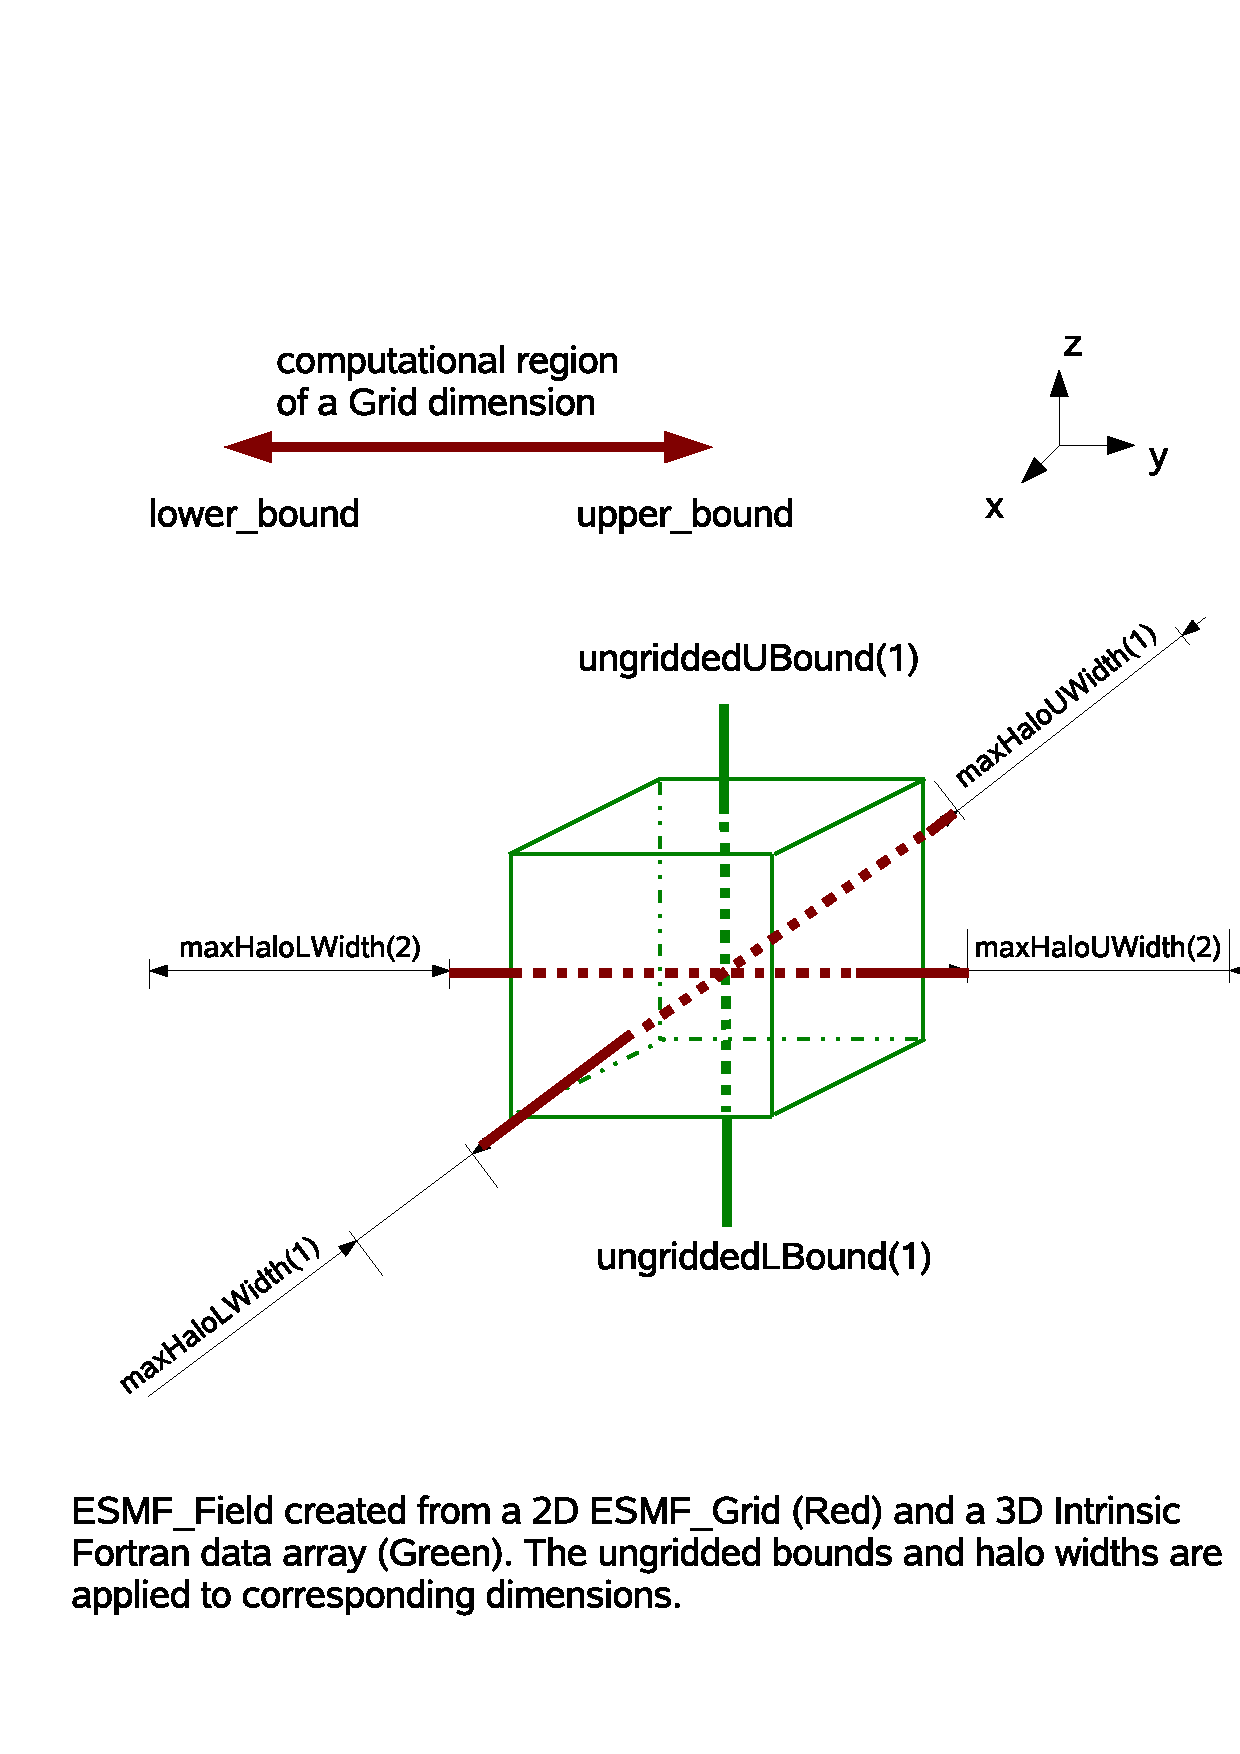
\includegraphics{FieldParameterSetup}}
  \caption{Field dimension configuration from Grid, halos, and Fortran data array.}
  \label{fig:fieldparameter}
  \end{figure}
  \end{center}
    
    The {\tt ESMF\_FieldCreate()} interface supports creating a Field from a Grid and a
    Fortran array padded with halos on the distributed dimensions of the Fortran
    array. Using this technique one can avoid passing non-contiguous Fortran array
    slice to FieldCreate. It guarantees the same exclusive region,
    and by using halos, it also defines a bigger total region to contain 
    the entire contiguous memory block of the Fortran array.
  
    The elements of totalLWidth and totalUWidth are applied in the order
    distributed dimensions appear in the Fortran array. By definition, 
    totalLWidth and totalUWidth are 1 dimensional arrays of non-negative 
    integer values. The size of haloWidth arrays is equal to the number of distributed
    dimensions of the Fortran array, which is also equal to the number of
    distributed dimensions of the Grid used in the Field creation.
  
    Because the order of totalWidth (representing both totalLWidth and
    totalUWidth) element is applied to the order distributed dimensions
    appear in the Fortran array dimensions, it's quite simple to compute
    the shape of distributed dimensions of the Fortran array. They are done
    in a similar manner when applying ungriddedLBound and ungriddedUBound 
    to ungridded dimensions of the Fortran array defined by rule 2.
  
    Assume we have the mapping from the dimension index of totalWidth
    to the dimension index of Fortran array, called mhw2fa; and we also
    have the mapping from dimension index of Fortran array to dimension
    index of the Grid, called fa2g. The shape of
    distributed dimensions of a Fortran array can be computed by rule 4: 
   
    \begin{verbatim}
  
    (4) fa_shape(mhw2fa(k)) = exclusiveCount(fa2g(mhw2fa(k)) + 
                              totalUWidth(k) + totalLWidth(k)
                          k = 1...size(totalWidth) 
  
    \end{verbatim}
    
    This rule may seem confusing but algorithmically the computation
    can be done by the following pseudocode:
  
    \begin{verbatim}
  
    fa_index = 1
    do i = 1, farray_rank
       if i-th dimension of Fortran array is distributed
           fa_shape(i) = exclusiveCount(fa2g(i)) + 
                         totalUWidth(fa_index) + totalLWidth(fa_index)
           fa_index = fa_index + 1
       endif
    enddo
  
    \end{verbatim}
  
    The only complication then is to figure out the mapping from Fortran
    array dimension index to Grid dimension index. This process can
    be done by computing the reverse mapping from Field to Grid.
  
    Typically, we don't have to consider these complications if the following
    conditions are met: 1) All Grid dimensions are distributed. 2) DistGrid
    in the Grid has a dimension index mapping to the Grid in the form of 
    natural order (/1,2,3,.../). This natural order mapping is the
    default mapping between various objects throughout ESMF. 3) Grid to Field
    mapping is in the form of natural order, i.e. default mapping. These
    seem like a lot of conditions but they are the default case in the interaction
    among DistGrid, Grid, and Field. When these conditions are met, which
    is typically true, the shape of distributed dimensions of Fortran array
    follows rule 5 in a simple form:
  
    \begin{verbatim}
  
    (5) fa_shape(k) = exclusiveCount(k) + 
                      totalUWidth(k) + totalLWidth(k) 
                  k = 1...size(totalWidth)
  
    \end{verbatim}
  
    Let's examine an example on how to apply rule 5. Suppose we have a
    5D array and a 3D Grid that has its first 3 dimensions mapped to the first
    3 dimensions of the Fortran array. totalLWidth=(/1,2,3/), 
    totalUWidth=(/7,9,10/), then by rule 5, the following pseudo code
    can be used to compute the shape of the first 3 dimensions of the Fortran
    array. The shape of the remaining two ungridded dimensions can be
    computed according to rule 2.
  
    \begin{verbatim}
  
    do k = 1, 3
        fa_shape(k) = exclusiveCount(k) + 
                      totalUWidth(k) + totalLWidth(k)) 
    enddo
  
    \end{verbatim}
  
    Suppose now gridToFieldMap=(/2,3,4/) instead which says
    the first dimension of Grid maps to the 2nd dimension of Field (or 
    Fortran array) and so on and so forth, we can obtain a more general form 
    of rule 5 by introducing first\_distdim\_index shift when Grid to Field
    map (gridToFieldMap) is in the form of (/a,a+1,a+2.../).
  
    \begin{verbatim}
  
    (6) fa_shape(k+first_distdim_index-1) = exclusiveCount(k) +
                                            totalUWidth(k) + totalLWidth(k)
                                        k = 1...size(totalWidth)
  
    \end{verbatim}
  
    It's obvious that first\_distdim\_index=a. If the first dimension of the Fortran
    array is distributed, then rule 6 degenerates into rule 5, which is
    the typical case.
  
    Back to our example creating a 3D Field from a 2D Grid and a 3D intrinsic
    Fortran array, we will use the Grid created from previous example
    that satisfies condition 1 and 2. We'll also use a simple gridToFieldMap
    (1,2) which is the default mapping that satisfies condition 3. 
    First we use rule 5 to compute
    the shape of distributed dimensions then we use rule 2 to compute the shape
    of the ungridded dimensions. 
%/////////////////////////////////////////////////////////////

 \begin{verbatim}
    gridToFieldMap2d(1) = 1
    gridToFieldMap2d(2) = 2
    totalLWidth2d(1) = 3
    totalLWidth2d(2) = 4
    totalUWidth2d(1) = 3
    totalUWidth2d(2) = 5
    do k = 1, 2
        fa_shape(k) = gec(k) + totalLWidth2d(k) + totalUWidth2d(k)
    end do
    fa_shape(3) = 7          ! 9-3+1
    allocate(farray3d(fa_shape(1), fa_shape(2), fa_shape(3)))
    field = ESMF_FieldCreate(grid, farray3d, ESMF_INDEX_DELOCAL, &
        ungriddedLBound=(/3/), ungriddedUBound=(/9/), &
        totalLWidth=totalLWidth2d, totalUWidth=totalUWidth2d, &
        gridToFieldMap=gridToFieldMap2d, &
        rc=rc)
    if (rc /= ESMF_SUCCESS) call ESMF_Finalize(endflag=ESMF_END_ABORT)
 
\end{verbatim}
 
%/////////////////////////////////////////////////////////////

  \subsubsection{Create a Field from a LocStream, typekind, and rank}
  \label{sec:field:usage:create_locs_tkr}
   
   In this example, an {\tt ESMF\_Field} is created from an {\tt ESMF\_LocStream} 
   and typekind/rank.
   The location stream object is uniformly distributed
   in a 1 dimensional space on 4 DEs. The rank is 1 dimensional. 
   Please refer to LocStream examples section for more information on LocStream creation.
   
%/////////////////////////////////////////////////////////////

 \begin{verbatim}

    locs = ESMF_LocStreamCreate(minIndex=1, maxIndex=16, rc=rc)
    if (rc /= ESMF_SUCCESS) call ESMF_Finalize(endflag=ESMF_END_ABORT)

    field = ESMF_FieldCreate(locs, typekind=ESMF_TYPEKIND_I4, &
        rc=rc)
    if (rc /= ESMF_SUCCESS) call ESMF_Finalize(endflag=ESMF_END_ABORT)

 
\end{verbatim}
 
%/////////////////////////////////////////////////////////////

  \subsubsection{Create a Field from a LocStream and arrayspec}
  \label{sec:field:usage:create_locs_arrayspec}
   
   In this example, an {\tt ESMF\_Field} is created from an {\tt ESMF\_LocStream} 
   and an {\tt ESMF\_Arrayspec}.
   The location stream object is uniformly distributed
   in a 1 dimensional space on 4 DEs. The arrayspec is 1 dimensional. 
   Please refer to LocStream examples section for more information on LocStream creation.
   
%/////////////////////////////////////////////////////////////

 \begin{verbatim}

    locs = ESMF_LocStreamCreate(minIndex=1, maxIndex=16, rc=rc)
    if (rc /= ESMF_SUCCESS) call ESMF_Finalize(endflag=ESMF_END_ABORT)

    call ESMF_ArraySpecSet(arrayspec, 1, ESMF_TYPEKIND_I4, rc=rc)
    if (rc /= ESMF_SUCCESS) call ESMF_Finalize(endflag=ESMF_END_ABORT)

    field = ESMF_FieldCreate(locs, arrayspec, &
        rc=rc)
    if (rc /= ESMF_SUCCESS) call ESMF_Finalize(endflag=ESMF_END_ABORT)

 
\end{verbatim}
 
%/////////////////////////////////////////////////////////////

  \subsubsection{Create a Field from a Mesh, typekind, and rank}
  \label{sec:field:usage:create_mesh_tkr}
   
   In this example, an {\tt ESMF\_Field} is created from an {\tt ESMF\_Mesh} 
   and typekind/rank.
   The mesh object is on a Euclidean surface that is partitioned to a 2x2 rectangular
   space with 4 elements and 9 nodes. The nodal space is represented by
   a distgrid with 9 indices. A Field is created on locally owned nodes on each PET.
   Therefore, the created Field has 9 data points globally.
   The mesh object can be represented by the picture
   below. For more information on Mesh creation, please see Section~\ref{sec:mesh:usage:meshCreation}.
   \begin{verbatim}
                Mesh Ids
  
    2.0   7 ------- 8 -------- 9
          |         |          |
          |    3    |    4     |
          |         |          |
    1.0   4 ------- 5 -------- 6
          |         |          |
          |    1    |    2     |
          |         |          |
    0.0   1 ------- 2 -------- 3
  
         0.0       1.0        2.0 
  
        Node Ids at corners
        Element Ids in centers
   
  
               Mesh Owners
  
    2.0   2 ------- 2 -------- 3
          |         |          |
          |    2    |    3     |
          |         |          |
    1.0   0 ------- 0 -------- 1
          |         |          |
          |    0    |    1     |
          |         |          |
    0.0   0 ------- 0 -------- 1
  
         0.0       1.0        2.0 
  
        Node Owners at corners
        Element Owners in centers
  \end{verbatim} 
   
%/////////////////////////////////////////////////////////////

 \begin{verbatim}
      ! Create Mesh structure in 1 step
      mesh=ESMF_MeshCreate(parametricDim=2,spatialDim=2, &
             nodeIds=nodeIds, nodeCoords=nodeCoords, &
             nodeOwners=nodeOwners, elementIds=elemIds,&
             elementTypes=elemTypes, elementConn=elemConn, &
             rc=rc)
      if (rc /= ESMF_SUCCESS) call ESMF_Finalize(endflag=ESMF_END_ABORT)

      ! Field is created on the 1 dimensional nodal distgrid. On
      ! each PET, Field is created on the locally owned nodes.
      field = ESMF_FieldCreate(mesh, typekind=ESMF_TYPEKIND_I4, rc=rc)
      if (rc /= ESMF_SUCCESS) call ESMF_Finalize(endflag=ESMF_END_ABORT)
 
\end{verbatim}
 
%/////////////////////////////////////////////////////////////

  \subsubsection{Create a Field from a Mesh and arrayspec}
  \label{sec:field:usage:create_mesh_arrayspec}
   
   In this example, an {\tt ESMF\_Field} is created from an {\tt ESMF\_Mesh} 
   and an {\tt ESMF\_Arrayspec}.
   The mesh object is on a Euclidean surface that is partitioned to a 2x2 rectangular
   space with 4 elements and 9 nodes. The nodal space is represented by
   a distgrid with 9 indices. Field is created on locally owned nodes on each PET.
   Therefore, the created Field has 9 data points globally.
   The mesh object can be represented by the picture
   below. For more information on Mesh creation, please see Section~\ref{sec:mesh:usage:meshCreation}.
   
%/////////////////////////////////////////////////////////////

 \begin{verbatim}
      ! Create Mesh structure in 1 step
      mesh=ESMF_MeshCreate(parametricDim=2,spatialDim=2, &
             nodeIds=nodeIds, nodeCoords=nodeCoords, &
             nodeOwners=nodeOwners, elementIds=elemIds,&
             elementTypes=elemTypes, elementConn=elemConn, &
             rc=rc)
      if (rc /= ESMF_SUCCESS) call ESMF_Finalize(endflag=ESMF_END_ABORT)

      call ESMF_ArraySpecSet(arrayspec, 1, ESMF_TYPEKIND_I4, rc=rc)
      if (rc /= ESMF_SUCCESS) call ESMF_Finalize(endflag=ESMF_END_ABORT)

      ! Field is created on the 1 dimensional nodal distgrid. On
      ! each PET, Field is created on the locally owned nodes.
      field = ESMF_FieldCreate(mesh, arrayspec, rc=rc)
      if (rc /= ESMF_SUCCESS) call ESMF_Finalize(endflag=ESMF_END_ABORT)
 
\end{verbatim}
 
%/////////////////////////////////////////////////////////////

  \subsubsection{Create a Field from a Mesh and an Array}
  \label{sec:field:usage:create_mesh_array}
   
   In this example, an {\tt ESMF\_Field} is created from an {\tt ESMF\_Mesh} 
   and an {\tt ESMF\_Array}. The mesh object is created in the previous example and
   the array object is retrieved from the field created in the previous example too.
   
%/////////////////////////////////////////////////////////////

 \begin{verbatim}
    call ESMF_MeshGet(mesh, nodalDistgrid=distgrid, rc=rc)
    if (rc /= ESMF_SUCCESS) call ESMF_Finalize(endflag=ESMF_END_ABORT)
    array = ESMF_ArrayCreate(distgrid=distgrid, arrayspec=arrayspec, rc=rc)
    if (rc /= ESMF_SUCCESS) call ESMF_Finalize(endflag=ESMF_END_ABORT)
    ! query the array from the previous example
    call ESMF_FieldGet(field, array=array, rc=rc)
    if (rc /= ESMF_SUCCESS) call ESMF_Finalize(endflag=ESMF_END_ABORT)
    ! create a Field from a mesh and an array
    field1 = ESMF_FieldCreate(mesh, array, rc=rc)
    if (rc /= ESMF_SUCCESS) call ESMF_Finalize(endflag=ESMF_END_ABORT)
 
\end{verbatim}
 
%/////////////////////////////////////////////////////////////

  \subsubsection{Create a Field from a Mesh and an ArraySpec with optional features}
  \label{sec:field:usage:createMeshArrayspecOpt}
  
   In this example, an {\tt ESMF\_Field} is created from an {\tt ESMF\_Mesh}
   and an {\tt ESMF\_ArraySpec}. The mesh object is created in the previous example.
   The Field is also created with optional arguments such as ungridded dimensions
   and dimension mapping.
  
   In this example, the mesh is mapped to the 2nd dimension of the
   {\tt ESMF\_Field}, with its first dimension being the ungridded dimension with bounds 1,3.
   
%/////////////////////////////////////////////////////////////

 \begin{verbatim}
    call ESMF_ArraySpecSet(arrayspec, 2, ESMF_TYPEKIND_I4, rc=rc)
    field = ESMF_FieldCreate(mesh, arrayspec=arrayspec, gridToFieldMap=(/2/), &
        ungriddedLBound=(/1/), ungriddedUBound=(/3/), rc=rc)
    if (rc /= ESMF_SUCCESS) call ESMF_Finalize(endflag=ESMF_END_ABORT)
 
\end{verbatim}

%...............................................................
\setlength{\parskip}{\oldparskip}
\setlength{\parindent}{\oldparindent}
\setlength{\baselineskip}{\oldbaselineskip}

%                **** IMPORTANT NOTICE *****
% This LaTeX file has been automatically produced by ProTeX v. 1.1
% Any changes made to this file will likely be lost next time
% this file is regenerated from its source. Send questions 
% to Arlindo da Silva, dasilva@gsfc.nasa.gov
 
\setlength{\oldparskip}{\parskip}
\setlength{\parskip}{1.5ex}
\setlength{\oldparindent}{\parindent}
\setlength{\parindent}{0pt}
\setlength{\oldbaselineskip}{\baselineskip}
\setlength{\baselineskip}{11pt}
 
%--------------------- SHORT-HAND MACROS ----------------------
\def\bv{\begin{verbatim}}
\def\ev{\end{verbatim}}
\def\be{\begin{equation}}
\def\ee{\end{equation}}
\def\bea{\begin{eqnarray}}
\def\eea{\end{eqnarray}}
\def\bi{\begin{itemize}}
\def\ei{\end{itemize}}
\def\bn{\begin{enumerate}}
\def\en{\end{enumerate}}
\def\bd{\begin{description}}
\def\ed{\end{description}}
\def\({\left (}
\def\){\right )}
\def\[{\left [}
\def\]{\right ]}
\def\<{\left  \langle}
\def\>{\right \rangle}
\def\cI{{\cal I}}
\def\diag{\mathop{\rm diag}}
\def\tr{\mathop{\rm tr}}
%-------------------------------------------------------------

\markboth{Left}{Source File: ESMF\_FieldRepDimEx.F90,  Date: Tue May  5 21:00:02 MDT 2020
}

 
%/////////////////////////////////////////////////////////////

  \subsubsection{Create a Field with replicated dimensions}
  \label{sec:field:usage:create_repdim}
  
    \begin{sloppypar}
    In this example an {\tt ESMF\_Field} with replicated dimension is created from an {\tt ESMF\_Grid} and
    an {\tt ESMF\_Arrayspec}. A user can also use other {\tt ESMF\_FieldCreate()} methods to create replicated
    dimension Field, this example illustrates the key concepts and use of a replicated dimension Field.
    \end{sloppypar}
  
    Normally gridToFieldMap argument in {\tt ESMF\_FieldCreate()} should not contain
    0 value entries. However, for a Field with replicated dimension, a 0 entry in gridToFieldMap
    indicates the corresponding Grid dimension is replicated in the Field. In such a Field,
    the rank of the Field is no longer necessarily greater than its Grid rank.
    An example will make this clear. We will start by creating Distgrid and Grid.
   
%/////////////////////////////////////////////////////////////

 \begin{verbatim}
    ! create 4D distgrid
    distgrid = ESMF_DistGridCreate(minIndex=(/1,1,1,1/), &
        maxIndex=(/6,4,6,4/), regDecomp=(/2,1,2,1/), rc=rc)
    if (rc /= ESMF_SUCCESS) call ESMF_Finalize(endflag=ESMF_END_ABORT)

    ! create 4D grid on top of the 4D distgrid
    grid = ESMF_GridCreate(distgrid=distgrid, name="grid", rc=rc)
    if (rc /= ESMF_SUCCESS) call ESMF_Finalize(endflag=ESMF_END_ABORT)

    ! create 3D arrayspec
    call ESMF_ArraySpecSet(arrayspec, 3, ESMF_TYPEKIND_R8, rc=rc)
    if (rc /= ESMF_SUCCESS) call ESMF_Finalize(endflag=ESMF_END_ABORT)
 
\end{verbatim}
 
%/////////////////////////////////////////////////////////////

   In this example, a user creates a 3D Field with replicated dimension
   replicated along the 2nd and 4th dimension of its underlying 4D Grid.
   In addition, the 2nd dimension of the Field is ungridded (why?). The 1st and
   3rd dimensions of the Field have halos. 
%/////////////////////////////////////////////////////////////

 \begin{verbatim}
    ! create field, 2nd and 4th dimensions of the Grid are replicated
    field = ESMF_FieldCreate(grid, arrayspec, indexflag=ESMF_INDEX_DELOCAL, &
        gridToFieldMap=(/1,0,2,0/), &
        ungriddedLBound=(/1/), ungriddedUBound=(/4/), &
        totalLWidth=(/1,1/), totalUWidth=(/4,5/), &
        staggerloc=ESMF_STAGGERLOC_CORNER, &
        rc=rc)
    if (rc /= ESMF_SUCCESS) call ESMF_Finalize(endflag=ESMF_END_ABORT)

    ! get basic information from the field
    call ESMF_FieldGet(field, grid=grid1, array=array, typekind=typekind, &
        dimCount=dimCount, staggerloc=lstaggerloc, &
        gridToFieldMap=lgridToFieldMap, ungriddedLBound=lungriddedLBound, &
        ungriddedUBound=lungriddedUBound, totalLWidth=ltotalLWidth, &
        totalUWidth=ltotalUWidth, rc=rc)
    if (rc /= ESMF_SUCCESS) call ESMF_Finalize(endflag=ESMF_END_ABORT)

    ! get bounds information from the field
    call ESMF_FieldGet(field, localDe=0, farrayPtr=farray, &
        exclusiveLBound=felb, exclusiveUBound=feub, exclusiveCount=fec, &
        computationalLBound=fclb, computationalUBound=fcub, &
        computationalCount=fcc, totalLBound=ftlb, totalUBound=ftub, &
        totalCount=ftc, rc=rc)
    if (rc /= ESMF_SUCCESS) call ESMF_Finalize(endflag=ESMF_END_ABORT)

 
\end{verbatim}
 
%/////////////////////////////////////////////////////////////

   Next we verify that the field and array bounds agree with each other 
%/////////////////////////////////////////////////////////////

 \begin{verbatim}
    call ESMF_ArrayGet(array, rank=arank, dimCount=adimCount, rc=rc)
    if (rc /= ESMF_SUCCESS) call ESMF_Finalize(endflag=ESMF_END_ABORT)

    gridrank_repdim = 0
    do i = 1, size(gridToFieldMap)
        if(gridToFieldMap(i) == 0) gridrank_repdim = gridrank_repdim + 1
    enddo
 
\end{verbatim}
 
%/////////////////////////////////////////////////////////////

   Number of undistributed dimension of the array {\it X} is computed from
   total rank of the array {\it A}, the dimension count of its underlying distgrid
   {\it B} and number of replicated dimension in the distgrid {\it C}.
   We have the following formula: X = A - (B - C) 
%/////////////////////////////////////////////////////////////

 \begin{verbatim}
    allocate(audlb(arank-adimCount+gridrank_repdim), &
        audub(arank-adimCount+gridrank_repdim))
    call ESMF_ArrayGet(array, exclusiveLBound=aelb, exclusiveUBound=aeub, &
        computationalLBound=aclb, computationalUBound=acub, &
        totalLBound=atlb, totalUBound=atub, &
        undistLBound=audlb, undistUBound=audub, &
        rc=rc)
    if (rc /= ESMF_SUCCESS) call ESMF_Finalize(endflag=ESMF_END_ABORT)

    ! verify the ungridded bounds from field match
    ! undistributed bounds from its underlying array
    do i = 1, arank-adimCount
        if(lungriddedLBound(i) .ne. audlb(i) ) &
            rc = ESMF_FAILURE
    enddo
    if (rc /= ESMF_SUCCESS) call ESMF_Finalize(endflag=ESMF_END_ABORT)

    do i = 1, arank-adimCount
        if(lungriddedUBound(i) .ne. audub(i) ) &
            rc = ESMF_FAILURE
    enddo
    if (rc /= ESMF_SUCCESS) call ESMF_Finalize(endflag=ESMF_END_ABORT)
 
\end{verbatim}
 
%/////////////////////////////////////////////////////////////

   We then verify the data in the replicated dimension Field can be updated and accessed. 
%/////////////////////////////////////////////////////////////

 \begin{verbatim}
    do ik = ftlb(3), ftub(3)
     do ij = ftlb(2), ftub(2)
      do ii = ftlb(1), ftub(1)
        farray(ii,ij,ik) = ii+ij*2+ik
      enddo
     enddo
    enddo
    ! access and verify
    call ESMF_FieldGet(field, localDe=0, farrayPtr=farray1, &
        rc=rc)
    if (rc /= ESMF_SUCCESS) call ESMF_Finalize(endflag=ESMF_END_ABORT)
    do ik = ftlb(3), ftub(3)
     do ij = ftlb(2), ftub(2)
      do ii = ftlb(1), ftub(1)
        n = ii+ij*2+ik
        if(farray1(ii,ij,ik) .ne. n ) rc = ESMF_FAILURE
      enddo
     enddo
    enddo
    if (rc /= ESMF_SUCCESS) call ESMF_Finalize(endflag=ESMF_END_ABORT)

    ! release resources
    call ESMF_FieldDestroy(field)
    call ESMF_GridDestroy(grid)
    call ESMF_DistGridDestroy(distgrid)
 
\end{verbatim}

%...............................................................
\setlength{\parskip}{\oldparskip}
\setlength{\parindent}{\oldparindent}
\setlength{\baselineskip}{\oldbaselineskip}

%                **** IMPORTANT NOTICE *****
% This LaTeX file has been automatically produced by ProTeX v. 1.1
% Any changes made to this file will likely be lost next time
% this file is regenerated from its source. Send questions 
% to Arlindo da Silva, dasilva@gsfc.nasa.gov
 
\setlength{\oldparskip}{\parskip}
\setlength{\parskip}{1.5ex}
\setlength{\oldparindent}{\parindent}
\setlength{\parindent}{0pt}
\setlength{\oldbaselineskip}{\baselineskip}
\setlength{\baselineskip}{11pt}
 
%--------------------- SHORT-HAND MACROS ----------------------
\def\bv{\begin{verbatim}}
\def\ev{\end{verbatim}}
\def\be{\begin{equation}}
\def\ee{\end{equation}}
\def\bea{\begin{eqnarray}}
\def\eea{\end{eqnarray}}
\def\bi{\begin{itemize}}
\def\ei{\end{itemize}}
\def\bn{\begin{enumerate}}
\def\en{\end{enumerate}}
\def\bd{\begin{description}}
\def\ed{\end{description}}
\def\({\left (}
\def\){\right )}
\def\[{\left [}
\def\]{\right ]}
\def\<{\left  \langle}
\def\>{\right \rangle}
\def\cI{{\cal I}}
\def\diag{\mathop{\rm diag}}
\def\tr{\mathop{\rm tr}}
%-------------------------------------------------------------

\markboth{Left}{Source File: ESMF\_FieldArbGridEx.F90,  Date: Tue May  5 21:00:02 MDT 2020
}

 
%/////////////////////////////////////////////////////////////

  \subsubsection{Create a Field on an arbitrarily distributed Grid}
  \label{sec:field:usage:createArbGrid}
  
    With the introduction of Field on arbitrarily distributed Grid, Field has two kinds of dimension
    count: one associated geometrical (or physical) dimensionality, the other one associated with its
    memory index space representation. Field and Grid dimCount reflect the physical index 
    space of the objects. A new type of dimCount rank should be added to both of these entities.
    The rank gives the number of dimensions of the memory index space of the objects.
    This would be the dimension of the pointer pulled out of Field and the
    size of the bounds vector, for example. 
  
    For non-arbitrary Grids rank=dimCount, but for grids and fields with
    arbitrary dimensions rank = dimCount - (number of Arb dims) + 1
    (Internally Field can use the Arb info from the grid to create the mapping
    from the Field Array to the DistGrid)
  
    When creating a Field size(GridToFieldMap)=dimCount for both Arb and Non-arb grids
    This array specifies the mapping of Field to Grid identically for both Arb and Nonarb grids 
    If a zero occurs in an entry corresponding to any arbitrary dimension, then
    a zero must occur in every entry corresponding to an arbitrary dimension (i.e.
    all arbitrary dimensions must either be all replicated or all not replicated,
    they can't be broken apart).
  
    In this example an {\tt ESMF\_Field} is created from an arbitrarily distributed {\tt ESMF\_Grid} and 
    an {\tt ESMF\_Arrayspec}. A user can also use other {\tt ESMF\_FieldCreate()} methods to create 
    such a Field, this example illustrates the key concepts and use of Field on arbitrary distributed Grid.
    
    The Grid is 3 dimensional in physics index space but the first two dimension are collapsed into
    a single memory index space. Thus the resulting Field is 3D in physics index space and 2D in memory index
    space. This is made obvious with the 2D arrayspec used to create this Field.
   
%/////////////////////////////////////////////////////////////

 \begin{verbatim}
    ! create a 3D grid with the first 2 dimensions collapsed 
    ! and arbitrarily distributed
    grid3d = ESMF_GridCreateNoPeriDim(coordTypeKind=ESMF_TYPEKIND_R8, &
      minIndex=(/1,1,1/), maxIndex=(/xdim, ydim,zdim/), &
      arbIndexList=localArbIndex,arbIndexCount=localArbIndexCount, &
      name="arb3dgrid", rc=rc)
    if (rc /= ESMF_SUCCESS) call ESMF_Finalize(endflag=ESMF_END_ABORT)

    ! create a 2D arrayspec
    call ESMF_ArraySpecSet(arrayspec2D, rank=2, typekind=ESMF_TYPEKIND_R4, &
         rc=rc)
    if (rc /= ESMF_SUCCESS) call ESMF_Finalize(endflag=ESMF_END_ABORT)

    ! create a 2D Field using the Grid and the arrayspec
    field = ESMF_FieldCreate(grid3d, arrayspec2D, rc=rc)
    if (rc /= ESMF_SUCCESS) call ESMF_Finalize(endflag=ESMF_END_ABORT)
  
    call ESMF_FieldGet(field, rank=rank, dimCount=dimCount, &
                       rc=rc)
    if (myPet .eq. 0) print *, 'Field rank, dimCount', &
                                rank, dimCount
    if (rc /= ESMF_SUCCESS) call ESMF_Finalize(endflag=ESMF_END_ABORT)
  
    ! verify that the dimension counts are correct
    if (rank .ne. 2) correct = .false.
    if (dimCount .ne. 3) correct = .false.  
 
\end{verbatim}
 
%/////////////////////////////////////////////////////////////

  \subsubsection{Create a Field on an arbitrarily distributed Grid with replicated dimensions \& ungridded bounds}
  \label{sec:field:usage:createArbGridRep}
  
    The next example is slightly more complicated in
    that the Field also contains one ungridded dimension and its gridded dimension
    is replicated on the arbitrarily distributed dimension of the Grid.
   
    The same 3D Grid and 2D arrayspec in the previous example
    are used but a gridToFieldMap argument
    is supplied to the {\tt ESMF\_FieldCreate()} call. The first 2 entries of
    the map are 0, the last (3rd) entry is 1. The 3rd dimension of the Grid is
    mapped to the first dimension of the Field, this dimension is then replicated
    on the arbitrarily distributed dimensions of the Grid. In addition, the
    Field also has one ungridded dimension. Thus the final dimension count of the
    Field is 2 in both physics and memory index space.
   
%/////////////////////////////////////////////////////////////

 \begin{verbatim}
    field = ESMF_FieldCreate(grid3d, arrayspec2D,gridToFieldMap=(/0,0,1/), &
            ungriddedLBound=(/1/), ungriddedUBound=(/10/),rc=rc)
    if (rc /= ESMF_SUCCESS) call ESMF_Finalize(endflag=ESMF_END_ABORT)
  
    call ESMF_FieldGet(field, rank=rank, dimCount=dimCount, &
                       rc=rc)
    if (myPet .eq. 0) print *, 'Field rank, dimCount', &
                                rank, dimCount
    if (rc /= ESMF_SUCCESS) call ESMF_Finalize(endflag=ESMF_END_ABORT)
  
    if (rank .ne. 2) correct = .false.
    if (dimCount .ne. 2) correct = .false.  
 
\end{verbatim}

%...............................................................
\setlength{\parskip}{\oldparskip}
\setlength{\parindent}{\oldparindent}
\setlength{\baselineskip}{\oldbaselineskip}

%                **** IMPORTANT NOTICE *****
% This LaTeX file has been automatically produced by ProTeX v. 1.1
% Any changes made to this file will likely be lost next time
% this file is regenerated from its source. Send questions 
% to Arlindo da Silva, dasilva@gsfc.nasa.gov
 
\setlength{\oldparskip}{\parskip}
\setlength{\parskip}{1.5ex}
\setlength{\oldparindent}{\parindent}
\setlength{\parindent}{0pt}
\setlength{\oldbaselineskip}{\baselineskip}
\setlength{\baselineskip}{11pt}
 
%--------------------- SHORT-HAND MACROS ----------------------
\def\bv{\begin{verbatim}}
\def\ev{\end{verbatim}}
\def\be{\begin{equation}}
\def\ee{\end{equation}}
\def\bea{\begin{eqnarray}}
\def\eea{\end{eqnarray}}
\def\bi{\begin{itemize}}
\def\ei{\end{itemize}}
\def\bn{\begin{enumerate}}
\def\en{\end{enumerate}}
\def\bd{\begin{description}}
\def\ed{\end{description}}
\def\({\left (}
\def\){\right )}
\def\[{\left [}
\def\]{\right ]}
\def\<{\left  \langle}
\def\>{\right \rangle}
\def\cI{{\cal I}}
\def\diag{\mathop{\rm diag}}
\def\tr{\mathop{\rm tr}}
%-------------------------------------------------------------

\markboth{Left}{Source File: ESMF\_FieldRegridEx.F90,  Date: Tue May  5 21:00:02 MDT 2020
}

 
%/////////////////////////////////////////////////////////////

  \subsubsection{Field regridding}\label{sec:fieldregrid}
  
   This section describes the Field regrid methods. For an in depth description of ESMF regridding and the options available
   please see Section~\ref{sec:regrid}. 
  
   The basic flow of ESMF Field regridding is as follows. First a source and destination geometry object are created, depending on 
   the regrid method they can be either a Grid, a Mesh, or a LocStream. 
   Next Fields are built on the source and destination grid objects. These Fields are then passed into {\tt ESMF\_FieldRegridStore()}. The user can either get a 
   sparse matrix from this call and/or a {\tt routeHandle}. If the user gets the sparse matrix then they are responsible for deallocating it, but other than that
   can use it as they wish. The {\tt routeHandle} can be used in the {\tt ESMF\_FieldRegrid()} call to perform the actual interpolation of data from the source 
   to the destination field. This interpolation can be repeated for the same set of Fields as long as the coordinates at the staggerloc involved in the
   regridding in the associated grid object don't change. The same {\tt routeHandle} can also be used between any pair of Fields that matches the original 
   pari in {\em type}, {\em kind}, and memory layout of the {\em gridded} dimensions. However, the size, number, and index order of {\em ungridded} dimensions
   may be different. See section \ref{RH:Reusability} for a more detailed discussion of RouteHandle reusability.
   However, if you want                                     
   the routehandle to be the same interpolation between the grid objects upon which the Fields are built as was calculated                                        
   with the original {\tt ESMF\_FieldRegridStore()} call, then there                                                                                              
   are additional constraints on the grid objects. To be the same interpolation, the grid objects upon which the                                                  
   Fields are build must contain the same coordinates at the stagger locations involved in the regridding as                                                      
   the original source and destination Fields used in the {\tt ESMF\_FieldRegridStore()} call.                                                                    
   The routehandle represents the interpolation between the grid objects as they were during the {\tt ESMF\_FieldRegridStore()} call.                             
   So if the coordinates at the stagger location in the grid objects change, a new call to {\tt ESMF\_FieldRegridStore()}                                         
   is necessary to compute the interpolation between that new set of coordinates. When finished with the {\tt routeHandle} 
   {\tt ESMF\_FieldRegridRelease()} should be used to 
   free the associated memory. 
  
   The following example demonstrates doing a regrid operation between two Fields.
   
%/////////////////////////////////////////////////////////////

 \begin{verbatim}

  ! (Create source Grid, Mesh, or LocStream.)
  ! (Create srcField on the above.)

  ! (Create destination Grid, Mesh, or LocStream.)
  ! (Create dstField on the above.)
  
  ! Create the routeHandle which encodes the communication and
  ! information necessary for the regrid sparse matrix multiply.
  call ESMF_FieldRegridStore(srcField=srcField, dstField=dstField, &
                             routeHandle=routeHandle, rc=localrc)
 
\end{verbatim}
 
%/////////////////////////////////////////////////////////////

 \begin{verbatim}
 
  ! Can loop here regridding from srcField to dstField 
  ! do i=1,....

       ! (Put data into srcField)

       ! Use the routeHandle to regrid data from srcField to dstField.
       ! As described above, the same routeHandle can be used to 
       ! regrid a large class of different source and destination Fields. 
       call ESMF_FieldRegrid(srcField, dstField, routeHandle, rc=localrc)
 
\end{verbatim}
 
%/////////////////////////////////////////////////////////////

 \begin{verbatim}

  !    (Use data in dstField)

  ! enddo 


  ! Free the buffers and data associated with the routeHandle. 
  call ESMF_FieldRegridRelease(routeHandle, rc=localrc)

 
\end{verbatim}

%...............................................................
\setlength{\parskip}{\oldparskip}
\setlength{\parindent}{\oldparindent}
\setlength{\baselineskip}{\oldbaselineskip}

%                **** IMPORTANT NOTICE *****
% This LaTeX file has been automatically produced by ProTeX v. 1.1
% Any changes made to this file will likely be lost next time
% this file is regenerated from its source. Send questions 
% to Arlindo da Silva, dasilva@gsfc.nasa.gov
 
\setlength{\oldparskip}{\parskip}
\setlength{\parskip}{1.5ex}
\setlength{\oldparindent}{\parindent}
\setlength{\parindent}{0pt}
\setlength{\oldbaselineskip}{\baselineskip}
\setlength{\baselineskip}{11pt}
 
%--------------------- SHORT-HAND MACROS ----------------------
\def\bv{\begin{verbatim}}
\def\ev{\end{verbatim}}
\def\be{\begin{equation}}
\def\ee{\end{equation}}
\def\bea{\begin{eqnarray}}
\def\eea{\end{eqnarray}}
\def\bi{\begin{itemize}}
\def\ei{\end{itemize}}
\def\bn{\begin{enumerate}}
\def\en{\end{enumerate}}
\def\bd{\begin{description}}
\def\ed{\end{description}}
\def\({\left (}
\def\){\right )}
\def\[{\left [}
\def\]{\right ]}
\def\<{\left  \langle}
\def\>{\right \rangle}
\def\cI{{\cal I}}
\def\diag{\mathop{\rm diag}}
\def\tr{\mathop{\rm tr}}
%-------------------------------------------------------------

\markboth{Left}{Source File: ESMF\_FieldRegridMaskEx.F90,  Date: Tue May  5 21:00:02 MDT 2020
}

 
%/////////////////////////////////////////////////////////////

  
  \subsubsection{Field regrid with masking}
   As before, to create the sparse matrix regrid operator we call the
   {\tt ESMF\_FieldRegridStore()} routine. 
   However, in this case we apply masking to the regrid operation. 
   The mask value for each index location in the Grids may be set using
   the {\tt ESMF\_GridAddItem()} call (see Section~\ref{sec:usage:items}
   and Section~\ref{sec:usage:items:accessing}). Mask values may be set independently 
   for the source and destination Grids. If no mask values have been set in a Grid, then it is 
   assumed no masking should be used for that Grid. The {\tt srcMaskValues}
   parameter allows the user to set the list of values which indicate
   that a source location should be masked out. The {\tt dstMaskValues}
   parameter allows the user to set the list of values which indicate
   that a destination location should be masked out. The absence of 
   one of these parameters indicates that no masking should be used
   for that Field (e.g no {\tt srcMaskValue} parameter indicates that source
   masking shouldn't occur). The {\tt unmappedaction} flag may be
   used with or without masking and indicates what should occur
   if destination points can not be mapped to a source cell. 
   Here the {\tt ESMF\_UNMAPPEDACTION\_IGNORE} value indicates that unmapped
   destination points are to be ignored and no sparse matrix entries should be
    generated for them.  
%/////////////////////////////////////////////////////////////

 \begin{verbatim}
  call ESMF_FieldRegridStore(srcField=srcField, srcMaskValues=(/1/),       &
                             dstField=dstField, dstMaskValues=(/1/),       &
                             unmappedaction=ESMF_UNMAPPEDACTION_IGNORE, &
                             routeHandle=routeHandle,                      &
                             regridmethod=ESMF_REGRIDMETHOD_BILINEAR,     &
                             rc=localrc)
 
\end{verbatim}
 
%/////////////////////////////////////////////////////////////

  
   The {\tt ESMF\_FieldRegrid} and {\tt ESMF\_FieldRegridRelease} calls
   may then be applied as in the previous example.
%...............................................................
\setlength{\parskip}{\oldparskip}
\setlength{\parindent}{\oldparindent}
\setlength{\baselineskip}{\oldbaselineskip}

%                **** IMPORTANT NOTICE *****
% This LaTeX file has been automatically produced by ProTeX v. 1.1
% Any changes made to this file will likely be lost next time
% this file is regenerated from its source. Send questions 
% to Arlindo da Silva, dasilva@gsfc.nasa.gov
 
\setlength{\oldparskip}{\parskip}
\setlength{\parskip}{1.5ex}
\setlength{\oldparindent}{\parindent}
\setlength{\parindent}{0pt}
\setlength{\oldbaselineskip}{\baselineskip}
\setlength{\baselineskip}{11pt}
 
%--------------------- SHORT-HAND MACROS ----------------------
\def\bv{\begin{verbatim}}
\def\ev{\end{verbatim}}
\def\be{\begin{equation}}
\def\ee{\end{equation}}
\def\bea{\begin{eqnarray}}
\def\eea{\end{eqnarray}}
\def\bi{\begin{itemize}}
\def\ei{\end{itemize}}
\def\bn{\begin{enumerate}}
\def\en{\end{enumerate}}
\def\bd{\begin{description}}
\def\ed{\end{description}}
\def\({\left (}
\def\){\right )}
\def\[{\left [}
\def\]{\right ]}
\def\<{\left  \langle}
\def\>{\right \rangle}
\def\cI{{\cal I}}
\def\diag{\mathop{\rm diag}}
\def\tr{\mathop{\rm tr}}
%-------------------------------------------------------------

\markboth{Left}{Source File: ESMF\_FieldMeshRegridEx.F90,  Date: Tue May  5 21:00:02 MDT 2020
}

 
%/////////////////////////////////////////////////////////////

  \subsubsection{Field regrid example: Mesh to Mesh}
   This example demonstrates the regridding process between Fields created on Meshes. First
   the Meshes are created. This example omits the setup of the arrays describing the Mesh, but please see
   Section~\ref{sec:mesh:usage:meshCreation} for examples of this. After creation Fields are constructed on the Meshes, 
   and then ESMF\_FieldRegridStore() is called to construct a RouteHandle implementing the regrid operation. Finally, ESMF\_FieldRegrid() is
   called with the Fields and the RouteHandle to do the interpolation between the source Field and 
   destination Field.  Note the coordinates of the source and destination Mesh should be in degrees.
    
%/////////////////////////////////////////////////////////////

 \begin{verbatim}

  !!!!!!!!!!!!!!!!!!!!!!!!!!!!!!!!!!!!!!!!!!!!!!!
  ! Create Source Mesh
  !!!!!!!!!!!!!!!!!!!!!!!!!!!!!!!!!!!!!!!!!!!!!!!

  ! Create the Mesh structure.
  ! For brevity's sake, the code to fill the Mesh creation 
  ! arrays is omitted from this example. However, here
  ! is a brief description of the arrays:
  ! srcNodeIds    - the global ids for the src nodes
  ! srcNodeCoords - the coordinates for the src nodes
  ! srcNodeOwners - which PET owns each src node
  ! srcElemIds    - the global ids of the src elements
  ! srcElemTypes  - the topological shape of each src element
  ! srcElemConn   - how to connect the nodes to form the elements
  !                 in the source mesh
  ! Several examples of setting up these arrays can be seen in
  ! the Mesh Section "Mesh Creation". 
  srcMesh=ESMF_MeshCreate(parametricDim=2,spatialDim=2, &
         nodeIds=srcNodeIds, nodeCoords=srcNodeCoords, &
         nodeOwners=srcNodeOwners, elementIds=srcElemIds,&
         elementTypes=srcElemTypes, elementConn=srcElemConn, rc=rc)

  if (rc /= ESMF_SUCCESS) call ESMF_Finalize(endflag=ESMF_END_ABORT)



  !!!!!!!!!!!!!!!!!!!!!!!!!!!!!!!!!!!!!!!!!!!!!!!
  ! Create and Fill Source Field
  !!!!!!!!!!!!!!!!!!!!!!!!!!!!!!!!!!!!!!!!!!!!!!!

  ! Set description of source Field
  call ESMF_ArraySpecSet(arrayspec, 1, ESMF_TYPEKIND_R8, rc=rc)

  if (rc /= ESMF_SUCCESS) call ESMF_Finalize(endflag=ESMF_END_ABORT)

  ! Create source Field
  srcField = ESMF_FieldCreate(srcMesh, arrayspec, &
                        name="source", rc=rc)

  if (rc /= ESMF_SUCCESS) call ESMF_Finalize(endflag=ESMF_END_ABORT)

  ! Get source Field data pointer to put data into
  call ESMF_FieldGet(srcField, 0, fptr1D,  rc=rc)

  if (rc /= ESMF_SUCCESS) call ESMF_Finalize(endflag=ESMF_END_ABORT)

  ! Get number of local nodes to allocate space
  ! to hold local node coordinates
  call ESMF_MeshGet(srcMesh, &
         numOwnedNodes=numOwnedNodes, rc=rc)

  if (rc /= ESMF_SUCCESS) call ESMF_Finalize(endflag=ESMF_END_ABORT)

  ! Allocate space to hold local node coordinates
  ! (spatial dimension of Mesh*number of local nodes)
  allocate(ownedNodeCoords(2*numOwnedNodes))

  ! Get local node coordinates
  call ESMF_MeshGet(srcMesh, &
         ownedNodeCoords=ownedNodeCoords, rc=rc)

  if (rc /= ESMF_SUCCESS) call ESMF_Finalize(endflag=ESMF_END_ABORT)

  ! Set the source Field to the function 20.0+x+y
  do i=1,numOwnedNodes
    ! Get coordinates
    x=ownedNodeCoords(2*i-1)
    y=ownedNodeCoords(2*i)

   ! Set source function
   fptr1D(i) = 20.0+x+y
  enddo

  ! Deallocate local node coordinates
  deallocate(ownedNodeCoords)


  !!!!!!!!!!!!!!!!!!!!!!!!!!!!!!!!!!!!!!!!!!!!!!!
  ! Create Destination Mesh
  !!!!!!!!!!!!!!!!!!!!!!!!!!!!!!!!!!!!!!!!!!!!!!!

  ! Create the Mesh structure.
  ! For brevity's sake, the code to fill the Mesh creation 
  ! arrays is omitted from this example. However, here
  ! is a brief description of the arrays:
  ! dstNodeIds    - the global ids for the dst nodes
  ! dstNodeCoords - the coordinates for the dst nodes
  ! dstNodeOwners - which PET owns each dst node
  ! dstElemIds    - the global ids of the dst elements
  ! dstElemTypes  - the topological shape of each dst element
  ! dstElemConn   - how to connect the nodes to form the elements
  !                 in the destination mesh
  ! Several examples of setting up these arrays can be seen in
  ! the Mesh Section "Mesh Creation". 
  dstMesh=ESMF_MeshCreate(parametricDim=2,spatialDim=2, &
         nodeIds=dstNodeIds, nodeCoords=dstNodeCoords, &
         nodeOwners=dstNodeOwners, elementIds=dstElemIds,&
         elementTypes=dstElemTypes, elementConn=dstElemConn, rc=rc)

  if (rc /= ESMF_SUCCESS) call ESMF_Finalize(endflag=ESMF_END_ABORT)


  !!!!!!!!!!!!!!!!!!!!!!!!!!!!!!!!!!!!!!!!!!!!!!!
  ! Create Destination Field
  !!!!!!!!!!!!!!!!!!!!!!!!!!!!!!!!!!!!!!!!!!!!!!!

  ! Set description of source Field
  call ESMF_ArraySpecSet(arrayspec, 1, ESMF_TYPEKIND_R8, rc=rc)

  if (rc /= ESMF_SUCCESS) call ESMF_Finalize(endflag=ESMF_END_ABORT)

  ! Create destination Field
  dstField = ESMF_FieldCreate(dstMesh, arrayspec, &
                        name="destination", rc=rc)

  if (rc /= ESMF_SUCCESS) call ESMF_Finalize(endflag=ESMF_END_ABORT)

  !!!!!!!!!!!!!!!!!!!!!!!!!!!!!!!!!!!!!!!!!!!!!!!
  ! Do Regrid
  !!!!!!!!!!!!!!!!!!!!!!!!!!!!!!!!!!!!!!!!!!!!!!!

  ! Compute RouteHandle which contains the regrid operation
  call ESMF_FieldRegridStore( &
          srcField, &
          dstField=dstField, &
          routeHandle=routeHandle, &
          regridmethod=ESMF_REGRIDMETHOD_BILINEAR, &
          rc=rc)

  if (rc /= ESMF_SUCCESS) call ESMF_Finalize(endflag=ESMF_END_ABORT)

  ! Perform Regrid operation moving data from srcField to dstField
  call ESMF_FieldRegrid(srcField, dstField, routeHandle, rc=rc)


  if (rc /= ESMF_SUCCESS) call ESMF_Finalize(endflag=ESMF_END_ABORT)

  !!!!!!!!!!!!!!!!!!!!!!!!!!!!!!!!!!!!!!!!!!!!!!!
  ! dstField now contains the interpolated data.
  ! If the Meshes don't change, then routeHandle
  ! may be used repeatedly to interpolate from 
  ! srcField to dstField.  
  !!!!!!!!!!!!!!!!!!!!!!!!!!!!!!!!!!!!!!!!!!!!!!!

   
  ! User code to use the routeHandle, Fields, and
  ! Meshes goes here before they are freed below.


  !!!!!!!!!!!!!!!!!!!!!!!!!!!!!!!!!!!!!!!!!!!!!!!
  ! Free the objects created in the example.
  !!!!!!!!!!!!!!!!!!!!!!!!!!!!!!!!!!!!!!!!!!!!!!!

  ! Free the RouteHandle
  call ESMF_FieldRegridRelease(routeHandle, rc=rc)

  if (rc /= ESMF_SUCCESS) call ESMF_Finalize(endflag=ESMF_END_ABORT)

  ! Free the Fields
  call ESMF_FieldDestroy(srcField, rc=rc)

  if (rc /= ESMF_SUCCESS) call ESMF_Finalize(endflag=ESMF_END_ABORT)

  call ESMF_FieldDestroy(dstField, rc=rc)

  if (rc /= ESMF_SUCCESS) call ESMF_Finalize(endflag=ESMF_END_ABORT)

  ! Free the Meshes
  call ESMF_MeshDestroy(dstMesh, rc=rc)

  if (rc /= ESMF_SUCCESS) call ESMF_Finalize(endflag=ESMF_END_ABORT)

  call ESMF_MeshDestroy(srcMesh, rc=rc)
 
  if (rc /= ESMF_SUCCESS) call ESMF_Finalize(endflag=ESMF_END_ABORT)

 
\end{verbatim}

%...............................................................
\setlength{\parskip}{\oldparskip}
\setlength{\parindent}{\oldparindent}
\setlength{\baselineskip}{\oldbaselineskip}

%                **** IMPORTANT NOTICE *****
% This LaTeX file has been automatically produced by ProTeX v. 1.1
% Any changes made to this file will likely be lost next time
% this file is regenerated from its source. Send questions 
% to Arlindo da Silva, dasilva@gsfc.nasa.gov
 
\setlength{\oldparskip}{\parskip}
\setlength{\parskip}{1.5ex}
\setlength{\oldparindent}{\parindent}
\setlength{\parindent}{0pt}
\setlength{\oldbaselineskip}{\baselineskip}
\setlength{\baselineskip}{11pt}
 
%--------------------- SHORT-HAND MACROS ----------------------
\def\bv{\begin{verbatim}}
\def\ev{\end{verbatim}}
\def\be{\begin{equation}}
\def\ee{\end{equation}}
\def\bea{\begin{eqnarray}}
\def\eea{\end{eqnarray}}
\def\bi{\begin{itemize}}
\def\ei{\end{itemize}}
\def\bn{\begin{enumerate}}
\def\en{\end{enumerate}}
\def\bd{\begin{description}}
\def\ed{\end{description}}
\def\({\left (}
\def\){\right )}
\def\[{\left [}
\def\]{\right ]}
\def\<{\left  \langle}
\def\>{\right \rangle}
\def\cI{{\cal I}}
\def\diag{\mathop{\rm diag}}
\def\tr{\mathop{\rm tr}}
%-------------------------------------------------------------

\markboth{Left}{Source File: ESMF\_FieldCommEx.F90,  Date: Tue May  5 21:00:02 MDT 2020
}

 
%/////////////////////////////////////////////////////////////

   \subsubsection{Gather Field data onto root PET}
   \label{sec:field:usage:gather_2dptr}
  
   User can use {\tt ESMF\_FieldGather} interface to gather Field data from multiple
   PETs onto a single root PET. This interface is overloaded by type, kind, and rank.
  
   Note that the implementation of Scatter and Gather is not sequence index based.
   If the Field is built on arbitrarily distributed Grid, Mesh, LocStream or XGrid, 
   Gather will not gather data to rootPet 
   from source data points corresponding to the sequence index on the rootPet. 
   Instead Gather will gather a contiguous memory range from source PET to
   rootPet. The size of the memory range is equal to the number of 
   data elements on the source PET. Vice versa for the Scatter operation. 
   In this case, the user should use {\tt ESMF\_FieldRedist} to achieve
   the same data operation result. For examples how to use {\tt ESMF\_FieldRedist}
   to perform Gather and Scatter, please refer to
   \ref{sec:field:usage:redist_gathering} and
   \ref{sec:field:usage:redist_scattering}.
   
   In this example, we first create a 2D Field, then use {\tt ESMF\_FieldGather} to
   collect all the data in this Field into a data pointer on PET 0. 
%/////////////////////////////////////////////////////////////

 \begin{verbatim}
    ! Get current VM and pet number
    call ESMF_VMGetCurrent(vm, rc=rc)
    if (rc /= ESMF_SUCCESS) call ESMF_Finalize(endflag=ESMF_END_ABORT)

    call ESMF_VMGet(vm, localPet=lpe, rc=rc)
    if (rc /= ESMF_SUCCESS) call ESMF_Finalize(endflag=ESMF_END_ABORT)

    ! Create a 2D Grid and use this grid to create a Field
    ! farray is the Fortran data array that contains data on each PET.
    grid = ESMF_GridCreateNoPeriDim(minIndex=(/1,1/), maxIndex=(/10,20/), &
        regDecomp=(/2,2/), &
        name="grid", rc=rc)
    if (rc /= ESMF_SUCCESS) call ESMF_Finalize(endflag=ESMF_END_ABORT)

    field = ESMF_FieldCreate(grid, typekind=ESMF_TYPEKIND_I4, rc=localrc)
    if (localrc /= ESMF_SUCCESS) call ESMF_Finalize(endflag=ESMF_END_ABORT)


    call ESMF_FieldGet(field, farrayPtr=fptr, rc=localrc)
    if (localrc /= ESMF_SUCCESS) call ESMF_Finalize(endflag=ESMF_END_ABORT)
    !---------Initialize pet specific field data----------------
    !    1        5         10
    ! 1  +--------+---------+
    !    |        |         |
    !    |   0    |    1    |
    !    |        |         |
    ! 10 +--------+---------+
    !    |        |         |
    !    |   2    |    3    |
    !    |        |         |
    ! 20 +--------+---------+
    fptr = lpe

    ! allocate the Fortran data array on PET 0 to store gathered data
    if(lpe .eq. 0) then
      allocate (farrayDst(10,20))
    else
      allocate (farrayDst(0,0))
    end if
    call ESMF_FieldGather(field, farrayDst, rootPet=0, rc=rc)
    if (rc /= ESMF_SUCCESS) call ESMF_Finalize(endflag=ESMF_END_ABORT)

    ! check that the values gathered on rootPet are correct
    if(lpe .eq. 0) then
       do i = 1, 5
          do j = 1, 10
             if(farrayDst(i, j) .ne. 0) localrc=ESMF_FAILURE
          enddo
       enddo
      if (localrc /= ESMF_SUCCESS) call ESMF_Finalize(endflag=ESMF_END_ABORT)
       do i = 6, 10
          do j = 1, 10
             if(farrayDst(i, j) .ne. 1) localrc=ESMF_FAILURE
          enddo
       enddo
      if (localrc /= ESMF_SUCCESS) call ESMF_Finalize(endflag=ESMF_END_ABORT)
       do i = 1, 5
          do j = 11, 20
             if(farrayDst(i, j) .ne. 2) localrc=ESMF_FAILURE
          enddo
       enddo
      if (localrc /= ESMF_SUCCESS) call ESMF_Finalize(endflag=ESMF_END_ABORT)
       do i = 6, 10
          do j = 11, 20
             if(farrayDst(i, j) .ne. 3) localrc=ESMF_FAILURE
          enddo
       enddo
      if (localrc /= ESMF_SUCCESS) call ESMF_Finalize(endflag=ESMF_END_ABORT)
    endif

    ! destroy all objects created in this example to prevent memory leak
    call ESMF_FieldDestroy(field, rc=rc)
    if (rc /= ESMF_SUCCESS) call ESMF_Finalize(endflag=ESMF_END_ABORT)
    call ESMF_GridDestroy(grid, rc=rc)
    if (rc /= ESMF_SUCCESS) call ESMF_Finalize(endflag=ESMF_END_ABORT)
    if(lpe .eq. 0) deallocate(farrayDst)
 
\end{verbatim}
 
%/////////////////////////////////////////////////////////////

   \subsubsection{Scatter Field data from root PET onto its set of joint PETs}
   \label{sec:field:usage:scatter_2dptr}
  
   User can use {\tt ESMF\_FieldScatter} interface to scatter Field data from root
   PET onto its set of joint PETs. This interface is overloaded by type, kind, and rank.
   
   In this example, we first create a 2D Field, then use {\tt ESMF\_FieldScatter} to
   scatter the data from a data array located on PET 0 onto this Field. 
%/////////////////////////////////////////////////////////////

 \begin{verbatim}
    ! Create a 2D Grid and use this grid to create a Field
    ! farray is the Fortran data array that contains data on each PET.
    grid = ESMF_GridCreateNoPeriDim(minIndex=(/1,1/), maxIndex=(/10,20/), &
        regDecomp=(/2,2/), &
        name="grid", rc=rc)
    if (rc /= ESMF_SUCCESS) call ESMF_Finalize(endflag=ESMF_END_ABORT)

    field = ESMF_FieldCreate(grid, typekind=ESMF_TYPEKIND_I4, rc=localrc)
    if (localrc /= ESMF_SUCCESS) call ESMF_Finalize(endflag=ESMF_END_ABORT)

    ! initialize values to be scattered
    !    1        5         10
    ! 1  +--------+---------+
    !    |        |         |
    !    |   0    |    1    |
    !    |        |         |
    ! 10 +--------+---------+
    !    |        |         |
    !    |   2    |    3    |
    !    |        |         |
    ! 20 +--------+---------+
    if(lpe .eq. 0) then
        allocate(farraySrc(10,20))
        farraySrc(1:5,1:10) = 0
        farraySrc(6:10,1:10) = 1
        farraySrc(1:5,11:20) = 2
        farraySrc(6:10,11:20) = 3
    else
      allocate (farraySrc(0,0))
    endif

    ! scatter the data onto individual PETs of the Field
    call ESMF_FieldScatter(field, farraySrc, rootPet=0, rc=rc)
    if (rc /= ESMF_SUCCESS) call ESMF_Finalize(endflag=ESMF_END_ABORT)

    call ESMF_FieldGet(field, localDe=0, farrayPtr=fptr, rc=rc)
    if (rc /= ESMF_SUCCESS) call ESMF_Finalize(endflag=ESMF_END_ABORT)

    ! verify that the scattered data is properly distributed
    do i = lbound(fptr, 1), ubound(fptr, 1)
        do j = lbound(fptr, 2), ubound(fptr, 2)
            if(fptr(i, j) .ne. lpe) localrc = ESMF_FAILURE
        enddo
        if (localrc /= ESMF_SUCCESS) call ESMF_Finalize(endflag=ESMF_END_ABORT)
    enddo

    ! destroy all objects created in this example to prevent memory leak
    call ESMF_FieldDestroy(field, rc=rc)
    if (rc /= ESMF_SUCCESS) call ESMF_Finalize(endflag=ESMF_END_ABORT)
    call ESMF_GridDestroy(grid, rc=rc)
    if (rc /= ESMF_SUCCESS) call ESMF_Finalize(endflag=ESMF_END_ABORT)
    if(lpe .eq. 0) deallocate(farraySrc)
 
\end{verbatim}

%...............................................................
\setlength{\parskip}{\oldparskip}
\setlength{\parindent}{\oldparindent}
\setlength{\baselineskip}{\oldbaselineskip}

%                **** IMPORTANT NOTICE *****
% This LaTeX file has been automatically produced by ProTeX v. 1.1
% Any changes made to this file will likely be lost next time
% this file is regenerated from its source. Send questions 
% to Arlindo da Silva, dasilva@gsfc.nasa.gov
 
\setlength{\oldparskip}{\parskip}
\setlength{\parskip}{1.5ex}
\setlength{\oldparindent}{\parindent}
\setlength{\parindent}{0pt}
\setlength{\oldbaselineskip}{\baselineskip}
\setlength{\baselineskip}{11pt}
 
%--------------------- SHORT-HAND MACROS ----------------------
\def\bv{\begin{verbatim}}
\def\ev{\end{verbatim}}
\def\be{\begin{equation}}
\def\ee{\end{equation}}
\def\bea{\begin{eqnarray}}
\def\eea{\end{eqnarray}}
\def\bi{\begin{itemize}}
\def\ei{\end{itemize}}
\def\bn{\begin{enumerate}}
\def\en{\end{enumerate}}
\def\bd{\begin{description}}
\def\ed{\end{description}}
\def\({\left (}
\def\){\right )}
\def\[{\left [}
\def\]{\right ]}
\def\<{\left  \langle}
\def\>{\right \rangle}
\def\cI{{\cal I}}
\def\diag{\mathop{\rm diag}}
\def\tr{\mathop{\rm tr}}
%-------------------------------------------------------------

\markboth{Left}{Source File: ESMF\_FieldRedistEx.F90,  Date: Tue May  5 21:00:02 MDT 2020
}

 
%/////////////////////////////////////////////////////////////

   \subsubsection{Redistribute data from source Field to destination Field}
   \label{sec:field:usage:redist_1dptr}
  
   User can use {\tt ESMF\_FieldRedist} interface to redistribute data from 
   source Field to destination Field. This interface is overloaded by type and kind;
   In the version of {\tt ESMF\_FieldRedist} without factor argument, a default value
   of 1 is used.
   
   \begin{sloppypar}
   In this example, we first create two 1D Fields, a source Field and a destination
   Field. Then we use {\tt ESMF\_FieldRedist} to
   redistribute data from source Field to destination Field.
   \end{sloppypar} 
%/////////////////////////////////////////////////////////////

 \begin{verbatim}

    ! Get current VM and pet number
    call ESMF_VMGetCurrent(vm, rc=rc)
    if (rc /= ESMF_SUCCESS) call ESMF_Finalize(endflag=ESMF_END_ABORT)

    call ESMF_VMGet(vm, localPet=localPet, rc=rc)
    if (rc /= ESMF_SUCCESS) call ESMF_Finalize(endflag=ESMF_END_ABORT)

    ! create grid
    distgrid = ESMF_DistGridCreate(minIndex=(/1/), maxIndex=(/16/), &
            regDecomp=(/4/), &
            rc=rc)
    if (rc /= ESMF_SUCCESS) call ESMF_Finalize(endflag=ESMF_END_ABORT)

    grid = ESMF_GridCreate(distgrid=distgrid, &
        name="grid", rc=rc)
    if (rc /= ESMF_SUCCESS) call ESMF_Finalize(endflag=ESMF_END_ABORT)

    ! create srcField
    ! +--------+--------+--------+--------+
    !      0        1        2        3            ! value
    ! 1        4        8        12       16       ! bounds
    srcField = ESMF_FieldCreate(grid, typekind=ESMF_TYPEKIND_I4, &
      indexflag=ESMF_INDEX_DELOCAL, rc=rc)
    if (rc /= ESMF_SUCCESS) call ESMF_Finalize(endflag=ESMF_END_ABORT)

    call ESMF_FieldGet(srcField, farrayPtr=srcfptr, rc=rc)
    if (rc /= ESMF_SUCCESS) call ESMF_Finalize(endflag=ESMF_END_ABORT)

    srcfptr(:) = localPet

    ! create dstField
    ! +--------+--------+--------+--------+
    !      0        0        0        0            ! value
    ! 1        4        8        12       16       ! bounds
    dstField = ESMF_FieldCreate(grid, typekind=ESMF_TYPEKIND_I4, &
      indexflag=ESMF_INDEX_DELOCAL, rc=rc)
    if (rc /= ESMF_SUCCESS) call ESMF_Finalize(endflag=ESMF_END_ABORT)

    call ESMF_FieldGet(dstField, farrayPtr=dstfptr, rc=rc)
    if (rc /= ESMF_SUCCESS) call ESMF_Finalize(endflag=ESMF_END_ABORT)
  
    dstfptr(:) = 0

    ! perform redist
    ! 1. setup routehandle from source Field to destination Field
    call ESMF_FieldRedistStore(srcField, dstField, routehandle, rc=rc)
    if (rc /= ESMF_SUCCESS) call ESMF_Finalize(endflag=ESMF_END_ABORT)

    ! 2. use precomputed routehandle to redistribute data
    call ESMF_FieldRedist(srcfield, dstField, routehandle, rc=rc)
    if (rc /= ESMF_SUCCESS) call ESMF_Finalize(endflag=ESMF_END_ABORT)

    ! verify redist
    call ESMF_FieldGet(dstField, localDe=0, farrayPtr=fptr, rc=rc)
    if (rc /= ESMF_SUCCESS) call ESMF_Finalize(endflag=ESMF_END_ABORT)

    ! Verify that the redistributed data in dstField is correct.
    ! Before the redist op, the dst Field contains all 0. 
    ! The redist op reset the values to the PE value, verify this is the case.
    do i = lbound(fptr, 1), ubound(fptr, 1)
        if(fptr(i) .ne. localPet) localrc = ESMF_FAILURE
    enddo
    if (localrc /= ESMF_SUCCESS) call ESMF_Finalize(endflag=ESMF_END_ABORT)
 
\end{verbatim}
 
%/////////////////////////////////////////////////////////////

   Field redistribution can also be performed between different Field pairs that
   match the original Fields in {\em type}, {\em kind}, and memory layout of the
   {\em gridded} dimensions. However, the size, number, and index order of 
   {\em ungridded} dimensions may be different. See section \ref{RH:Reusability}
   for a more detailed discussion of RouteHandle reusability. 
%/////////////////////////////////////////////////////////////

 \begin{verbatim}
    call ESMF_ArraySpecSet(arrayspec, typekind=ESMF_TYPEKIND_I4, rank=2, rc=rc)
 
\end{verbatim}
 
%/////////////////////////////////////////////////////////////

   Create two fields with ungridded dimensions using the Grid created previously.
   The new Field pair has matching number of elements. The ungridded dimension
   is mapped to the first dimension of either Field. 
%/////////////////////////////////////////////////////////////

 \begin{verbatim}
    srcFieldA = ESMF_FieldCreate(grid, arrayspec, gridToFieldMap=(/2/), &
        ungriddedLBound=(/1/), ungriddedUBound=(/10/), rc=rc)
 
\end{verbatim}
 
%/////////////////////////////////////////////////////////////

 \begin{verbatim}
    dstFieldA = ESMF_FieldCreate(grid, arrayspec, gridToFieldMap=(/2/), &
        ungriddedLBound=(/1/), ungriddedUBound=(/10/), rc=rc)
 
\end{verbatim}
 
%/////////////////////////////////////////////////////////////

   Using the previously computed routehandle, the Fields can be redistributed. 
%/////////////////////////////////////////////////////////////

 \begin{verbatim}
    call ESMF_FieldRedist(srcfieldA, dstFieldA, routehandle, rc=rc)
 
\end{verbatim}
 
%/////////////////////////////////////////////////////////////

 \begin{verbatim}
    call ESMF_FieldRedistRelease(routehandle, rc=rc)
 
\end{verbatim}
 
%/////////////////////////////////////////////////////////////

   \subsubsection{FieldRedist as a form of scatter involving arbitrary distribution}
   \label{sec:field:usage:redist_scattering}
  
   User can use {\tt ESMF\_FieldRedist} interface to redistribute data from 
   source Field to destination Field, where the destination Field is built on
   an arbitrarily distributed structure, e.g. {\tt ESMF\_Mesh}. The underlying mechanism is explained
   in section \ref{Array:ScatterGatherRevisited}.
  
   In this example, we will create 2 one dimensional Fields, the src Field has a regular decomposition
   and holds all its data on a single PET, in this case PET 0. The destination Field is built on a Mesh
   which is itself built on an arbitrarily distributed distgrid. Then we use {\tt ESMF\_FieldRedist} to
   redistribute data from source Field to destination Field, similar to a traditional scatter operation.
  
   The src Field only has data on PET 0 where it is sequentially initialized, i.e. 1,2,3...This data
   will be redistributed (or scattered) from PET 0 to the destination Field arbitrarily distributed on 
   all the PETs. 
%/////////////////////////////////////////////////////////////

 \begin{verbatim}
    ! a one dimensional grid whose elements are all located on PET 0
    distgrid = ESMF_DistGridCreate(minIndex=(/1/), maxIndex=(/9/), &
        regDecomp=(/1/), &
        rc=rc)
    if (rc /= ESMF_SUCCESS) call ESMF_Finalize(endflag=ESMF_END_ABORT)
    grid = ESMF_GridCreate(distgrid=distgrid, &
        indexflag=ESMF_INDEX_DELOCAL, rc=rc)
    if (rc /= ESMF_SUCCESS) call ESMF_Finalize(endflag=ESMF_END_ABORT)

    srcField = ESMF_FieldCreate(grid, typekind=ESMF_TYPEKIND_I4, rc=rc)
    if (rc /= ESMF_SUCCESS) call ESMF_Finalize(endflag=ESMF_END_ABORT)

    ! initialize the source data
    if (localPet == 0) then
        call ESMF_FieldGet(srcField, farrayPtr=srcfptr, rc=rc)
        if (rc /= ESMF_SUCCESS) call ESMF_Finalize(endflag=ESMF_END_ABORT)
        do i = 1, 9
            srcfptr(i) = i
        enddo
    endif
 
\end{verbatim}
 
%/////////////////////////////////////////////////////////////

   For more information on Mesh creation, user can refer to Mesh examples section or Field creation
   on Mesh example for more details. 
%/////////////////////////////////////////////////////////////

 \begin{verbatim}
      ! Create Mesh structure
      mesh=ESMF_MeshCreate(parametricDim=2,spatialDim=2, &
             nodeIds=nodeIds, nodeCoords=nodeCoords, &
             nodeOwners=nodeOwners, elementIds=elemIds,&
             elementTypes=elemTypes, elementConn=elemConn, &
             rc=rc)
      if (rc /= ESMF_SUCCESS) call ESMF_Finalize(endflag=ESMF_END_ABORT)
 
\end{verbatim}
 
%/////////////////////////////////////////////////////////////

   Create the destination Field on the Mesh that is arbitrarily distributed on 
   all the PETs. 
%/////////////////////////////////////////////////////////////

 \begin{verbatim}
      dstField = ESMF_FieldCreate(mesh, typekind=ESMF_TYPEKIND_I4, rc=rc)
      if (rc /= ESMF_SUCCESS) call ESMF_Finalize(endflag=ESMF_END_ABORT)
 
\end{verbatim}
 
%/////////////////////////////////////////////////////////////

   Perform the redistribution from source Field to destination Field. 
%/////////////////////////////////////////////////////////////

 \begin{verbatim}
     call ESMF_FieldRedistStore(srcField, dstField, &
             routehandle=routehandle, rc=rc)
     if (rc /= ESMF_SUCCESS) call ESMF_Finalize(endflag=ESMF_END_ABORT)
     call ESMF_FieldRedist(srcField, dstField, routehandle=routehandle, rc=rc)
     if (rc /= ESMF_SUCCESS) call ESMF_Finalize(endflag=ESMF_END_ABORT)
 
\end{verbatim}
 
%/////////////////////////////////////////////////////////////

   We can now verify that the sequentially initialized source data is scattered
   on to the destination Field. The data has been scattered onto the destination
   Field with the following distribution.
  \begin{verbatim}
  
   4 elements on PET 0:  1 2 4 5
   2 elements on PET 1:  3 6
   2 elements on PET 2:  7 8
   1 element  on PET 3:  9
  
  \end{verbatim}
   Because the redistribution is index based, the elements also corresponds to the
   index space of Mesh in the destination Field. 
%/////////////////////////////////////////////////////////////

 \begin{verbatim}
    call ESMF_FieldGet(dstField, farrayPtr=dstfptr, rc=rc)
    if (rc /= ESMF_SUCCESS) call ESMF_Finalize(endflag=ESMF_END_ABORT)
 
\end{verbatim}
 
%/////////////////////////////////////////////////////////////

   The scatter operation is successful. Since the routehandle computed with
   {\tt ESMF\_FieldRedistStore} can be reused, user can use the same routehandle
   to scatter multiple source Fields from a single PET to multiple destination
   Fields distributed on all PETs. The {\tt gathering} operation is just the 
   opposite of the demonstrated {\tt scattering} operation, where a user would
   redist from a source Field distributed on multiple PETs to a destination Field
   that only has data storage on a single PET.
  
   Now it's time to release all the resources. 
%/////////////////////////////////////////////////////////////

 \begin{verbatim}
    call ESMF_FieldRedistRelease(routehandle=routehandle, rc=rc)
 
\end{verbatim}
 
%/////////////////////////////////////////////////////////////

   \subsubsection{FieldRedist as a form of gather involving arbitrary distribution}
   \label{sec:field:usage:redist_gathering}
  
   Similarly, one can use the same approach to gather the data from an arbitrary distribution
   to a non-arbitrary distribution. This concept is demonstrated by using the previous Fields but 
   the data operation is reversed. This time data is gathered from the Field built on the mesh to the Field
   that has only data allocation on rootPet.
   
%/////////////////////////////////////////////////////////////

   First a FieldRedist routehandle is created from the Field built on Mesh to the Field
   that has only data allocation on rootPet. 
%/////////////////////////////////////////////////////////////

 \begin{verbatim}
    call ESMF_FieldRedistStore(dstField, srcField, routehandle=routehandle, &
         rc=rc)
 
\end{verbatim}
 
%/////////////////////////////////////////////////////////////

   Perform FieldRedist, this will gather the data points from the Field built on mesh to
   the data pointer on the rootPet (default to 0) stored in the srcField. 
%/////////////////////////////////////////////////////////////

 \begin{verbatim}
    call ESMF_FieldRedist(dstField, srcField, routehandle=routehandle, rc=rc)
 
\end{verbatim}
 
%/////////////////////////////////////////////////////////////

   Release the routehandle used for the gather operation. 
%/////////////////////////////////////////////////////////////

 \begin{verbatim}
    call ESMF_FieldRedistRelease(routehandle=routehandle, rc=rc)
 
\end{verbatim}

%...............................................................
\setlength{\parskip}{\oldparskip}
\setlength{\parindent}{\oldparindent}
\setlength{\baselineskip}{\oldbaselineskip}

%                **** IMPORTANT NOTICE *****
% This LaTeX file has been automatically produced by ProTeX v. 1.1
% Any changes made to this file will likely be lost next time
% this file is regenerated from its source. Send questions 
% to Arlindo da Silva, dasilva@gsfc.nasa.gov
 
\setlength{\oldparskip}{\parskip}
\setlength{\parskip}{1.5ex}
\setlength{\oldparindent}{\parindent}
\setlength{\parindent}{0pt}
\setlength{\oldbaselineskip}{\baselineskip}
\setlength{\baselineskip}{11pt}
 
%--------------------- SHORT-HAND MACROS ----------------------
\def\bv{\begin{verbatim}}
\def\ev{\end{verbatim}}
\def\be{\begin{equation}}
\def\ee{\end{equation}}
\def\bea{\begin{eqnarray}}
\def\eea{\end{eqnarray}}
\def\bi{\begin{itemize}}
\def\ei{\end{itemize}}
\def\bn{\begin{enumerate}}
\def\en{\end{enumerate}}
\def\bd{\begin{description}}
\def\ed{\end{description}}
\def\({\left (}
\def\){\right )}
\def\[{\left [}
\def\]{\right ]}
\def\<{\left  \langle}
\def\>{\right \rangle}
\def\cI{{\cal I}}
\def\diag{\mathop{\rm diag}}
\def\tr{\mathop{\rm tr}}
%-------------------------------------------------------------

\markboth{Left}{Source File: ESMF\_FieldSMMEx.F90,  Date: Tue May  5 21:00:02 MDT 2020
}

 
%/////////////////////////////////////////////////////////////

   \subsubsection{Sparse matrix multiplication from source Field to destination Field}
   \label{sec:field:usage:smm_1dptr}
  
   The {\tt ESMF\_FieldSMM()} interface can be used to perform sparse matrix multiplication
   from
   source Field to destination Field. This interface is overloaded by type and kind;
  
   In this example, we first create two 1D Fields, a source Field and a destination
   Field. Then we use {\tt ESMF\_FieldSMM} to
   perform sparse matrix multiplication from source Field to destination Field.
  
   The source and destination Field data are arranged such that each of the 4 PETs has 4
   data elements. Moreover, the source Field has all its data elements initialized to a linear
   function based on local PET number.
   Then collectively on each PET, a SMM according to the following formula
   is preformed: \newline
   $dstField(i) = i * srcField(i), i = 1 ... 4$ \newline
   \newline
  
   Because source Field data are initialized to a linear function based on local PET number,
   the formula predicts that
   the result destination Field data on each PET is {1,2,3,4}. This is verified in the
   example.
  
   Section \ref{Array:SparseMatMul} provides a detailed discussion of the
   sparse matrix multiplication operation implemented in ESMF.
   
%/////////////////////////////////////////////////////////////

 \begin{verbatim}

    ! Get current VM and pet number
    call ESMF_VMGetCurrent(vm, rc=rc)
    if (rc /= ESMF_SUCCESS) call ESMF_Finalize(endflag=ESMF_END_ABORT)

    call ESMF_VMGet(vm, localPet=lpe, rc=rc)
    if (rc /= ESMF_SUCCESS) call ESMF_Finalize(endflag=ESMF_END_ABORT)

    ! create distgrid and grid
    distgrid = ESMF_DistGridCreate(minIndex=(/1/), maxIndex=(/16/), &
        regDecomp=(/4/), &
        rc=rc)
    if (rc /= ESMF_SUCCESS) call ESMF_Finalize(endflag=ESMF_END_ABORT)

    grid = ESMF_GridCreate(distgrid=distgrid, &
        name="grid", rc=rc)
    if (rc /= ESMF_SUCCESS) call ESMF_Finalize(endflag=ESMF_END_ABORT)

    call ESMF_GridGetFieldBounds(grid, localDe=0, totalCount=fa_shape, rc=rc)
    if (rc /= ESMF_SUCCESS) call ESMF_Finalize(endflag=ESMF_END_ABORT)

    ! create src\_farray, srcArray, and srcField
    ! +--------+--------+--------+--------+
    !      1        2        3        4            ! value
    ! 1        4        8        12       16       ! bounds
    allocate(src_farray(fa_shape(1)) )
    src_farray = lpe+1
    srcArray = ESMF_ArrayCreate(distgrid, src_farray, &
                indexflag=ESMF_INDEX_DELOCAL, rc=rc)
    if (rc /= ESMF_SUCCESS) call ESMF_Finalize(endflag=ESMF_END_ABORT)

    srcField = ESMF_FieldCreate(grid, srcArray, rc=rc)
    if (rc /= ESMF_SUCCESS) call ESMF_Finalize(endflag=ESMF_END_ABORT)

    ! create dst_farray, dstArray, and dstField
    ! +--------+--------+--------+--------+
    !      0        0        0        0            ! value
    ! 1        4        8        12       16       ! bounds
    allocate(dst_farray(fa_shape(1)) )
    dst_farray = 0
    dstArray = ESMF_ArrayCreate(distgrid, dst_farray, &
                indexflag=ESMF_INDEX_DELOCAL, rc=rc)
    if (rc /= ESMF_SUCCESS) call ESMF_Finalize(endflag=ESMF_END_ABORT)

    dstField = ESMF_FieldCreate(grid, dstArray, rc=rc)
    if (rc /= ESMF_SUCCESS) call ESMF_Finalize(endflag=ESMF_END_ABORT)

    ! perform sparse matrix multiplication
    ! 1. setup routehandle from source Field to destination Field
    ! initialize factorList and factorIndexList
    allocate(factorList(4))
    allocate(factorIndexList(2,4))
    factorList = (/1,2,3,4/)
    factorIndexList(1,:) = (/lpe*4+1,lpe*4+2,lpe*4+3,lpe*4+4/)
    factorIndexList(2,:) = (/lpe*4+1,lpe*4+2,lpe*4+3,lpe*4+4/)

    call ESMF_FieldSMMStore(srcField, dstField, routehandle, &
        factorList, factorIndexList, rc=localrc)
    if (localrc /= ESMF_SUCCESS) call ESMF_Finalize(endflag=ESMF_END_ABORT)

    ! 2. use precomputed routehandle to perform SMM
    call ESMF_FieldSMM(srcfield, dstField, routehandle, rc=rc)
    if (rc /= ESMF_SUCCESS) call ESMF_Finalize(endflag=ESMF_END_ABORT)

    ! verify sparse matrix multiplication
    call ESMF_FieldGet(dstField, localDe=0, farrayPtr=fptr, rc=rc)
    if (rc /= ESMF_SUCCESS) call ESMF_Finalize(endflag=ESMF_END_ABORT)

    ! Verify that the result data in dstField is correct.
    ! Before the SMM op, the dst Field contains all 0.
    ! The SMM op reset the values to the index value, verify this is the case.
    ! +--------+--------+--------+--------+
    !  1 2 3 4  2 4 6 8  3 6 9 12  4 8 12 16       ! value
    ! 1        4        8        12       16       ! bounds
    do i = lbound(fptr, 1), ubound(fptr, 1)
        if(fptr(i) /= i*(lpe+1)) rc = ESMF_FAILURE
    enddo
 
\end{verbatim}
 
%/////////////////////////////////////////////////////////////

   Field sparse matrix multiplication can also be applied between Fields 
   that matche the original Fields in {\em type}, {\em kind}, and 
   memory layout of the {\em gridded} dimensions. However, the size, number, 
   and index order of {\em ungridded} dimensions may be different. See section
   \ref{RH:Reusability} for a more detailed discussion of RouteHandle 
   reusability 
%/////////////////////////////////////////////////////////////

 \begin{verbatim}
    call ESMF_ArraySpecSet(arrayspec, typekind=ESMF_TYPEKIND_I4, rank=2, rc=rc)
 
\end{verbatim}
 
%/////////////////////////////////////////////////////////////

   Create two fields with ungridded dimensions using the Grid created previously.
   The new Field pair has matching number of elements. The ungridded dimension
   is mapped to the first dimension of either Field. 
%/////////////////////////////////////////////////////////////

 \begin{verbatim}
    srcFieldA = ESMF_FieldCreate(grid, arrayspec, gridToFieldMap=(/2/), &
        ungriddedLBound=(/1/), ungriddedUBound=(/10/), rc=rc)
 
\end{verbatim}
 
%/////////////////////////////////////////////////////////////

 \begin{verbatim}
    dstFieldA = ESMF_FieldCreate(grid, arrayspec, gridToFieldMap=(/2/), &
        ungriddedLBound=(/1/), ungriddedUBound=(/10/), rc=rc)
 
\end{verbatim}
 
%/////////////////////////////////////////////////////////////

   Using the previously computed routehandle, the sparse matrix multiplication
   can be performed between the Fields. 
%/////////////////////////////////////////////////////////////

 \begin{verbatim}
    call ESMF_FieldSMM(srcfieldA, dstFieldA, routehandle, rc=rc)
 
\end{verbatim}
 
%/////////////////////////////////////////////////////////////

 \begin{verbatim}
    ! release route handle
    call ESMF_FieldSMMRelease(routehandle, rc=rc)
 
\end{verbatim}
 
%/////////////////////////////////////////////////////////////

   In the following discussion, we demonstrate how to set up a SMM routehandle
   between a pair of Fields that are different in number of gridded dimensions
   and the size of those gridded dimensions. The source Field has a 1D decomposition
   with 16 total elements; the destination Field has a 2D decomposition with
   12 total elements. For ease of understanding of the actual matrix calculation,
   a global indexing scheme is used. 
%/////////////////////////////////////////////////////////////

 \begin{verbatim}
    distgrid = ESMF_DistGridCreate(minIndex=(/1/), maxIndex=(/16/), &
        indexflag=ESMF_INDEX_GLOBAL, &
        regDecomp=(/4/), &
        rc=rc)
    if (rc /= ESMF_SUCCESS) call ESMF_Finalize(endflag=ESMF_END_ABORT)

    grid = ESMF_GridCreate(distgrid=distgrid, &
        indexflag=ESMF_INDEX_GLOBAL, &
        name="grid", rc=rc)
    if (rc /= ESMF_SUCCESS) call ESMF_Finalize(endflag=ESMF_END_ABORT)

    call ESMF_GridGetFieldBounds(grid, localDe=0, totalLBound=tlb, &
                       totalUBound=tub, rc=rc)
    if (rc /= ESMF_SUCCESS) call ESMF_Finalize(endflag=ESMF_END_ABORT)
 
\end{verbatim}
 
%/////////////////////////////////////////////////////////////

   create 1D src\_farray, srcArray, and srcField
  \begin{verbatim}
   +  PET0  +  PET1  +  PET2  +  PET3  +
   +--------+--------+--------+--------+
        1        2        3        4            ! value
   1        4        8        12       16       ! bounds of seq indices
  \end{verbatim} 
%/////////////////////////////////////////////////////////////

 \begin{verbatim}
    allocate(src_farray2(tlb(1):tub(1)) )
    src_farray2 = lpe+1
    srcArray = ESMF_ArrayCreate(distgrid, src_farray2, &
                  indexflag=ESMF_INDEX_GLOBAL, &
      rc=rc)
    if (rc /= ESMF_SUCCESS) call ESMF_Finalize(endflag=ESMF_END_ABORT)
    !print *, lpe, '+', tlb, tub, '+', src_farray2

    srcField = ESMF_FieldCreate(grid, srcArray, rc=rc)
    if (rc /= ESMF_SUCCESS) call ESMF_Finalize(endflag=ESMF_END_ABORT)

 
\end{verbatim}
 
%/////////////////////////////////////////////////////////////

   Create 2D dstField on the following distribution
   (numbers are the sequence indices):
  \begin{verbatim}
   +  PET0  +  PET1  +  PET2  +  PET3  +
   +--------+--------+--------+--------+
   |        |        |        |        |
   |   1    |   4    |   7    |   10   |
   |        |        |        |        |
   +--------+--------+--------+--------+
   |        |        |        |        |
   |   2    |   5    |   8    |   11   |
   |        |        |        |        |
   +--------+--------+--------+--------+
   |        |        |        |        |
   |   3    |   6    |   9    |   12   |
   |        |        |        |        |
   +--------+--------+--------+--------+
  \end{verbatim} 
%/////////////////////////////////////////////////////////////

 \begin{verbatim}

    ! Create the destination Grid
    dstGrid = ESMF_GridCreateNoPeriDim(minIndex=(/1,1/), maxIndex=(/3,4/), &
      indexflag = ESMF_INDEX_GLOBAL, &
      regDecomp = (/1,4/), &
      rc=rc)
    if (rc /= ESMF_SUCCESS) call ESMF_Finalize(endflag=ESMF_END_ABORT)

    dstField = ESMF_FieldCreate(dstGrid, typekind=ESMF_TYPEKIND_R4, &
      indexflag=ESMF_INDEX_GLOBAL, &
      rc=rc)
    if (rc /= ESMF_SUCCESS) call ESMF_Finalize(endflag=ESMF_END_ABORT)
 
\end{verbatim}
 
%/////////////////////////////////////////////////////////////

   Perform sparse matrix multiplication $dst_i$ = $M_{i,j}$ * $src_j$
   First setup routehandle from source Field to destination Field
   with prescribed factorList and factorIndexList.
  
   The sparse matrix is of size 12x16, however only the following entries
   are filled:
   \begin{verbatim}
   M(3,1) = 0.1
   M(3,10) = 0.4
   M(8,2) = 0.25
   M(8,16) = 0.5
   M(12,1) = 0.3
   M(12,16) = 0.7
   \end{verbatim}
  
   By the definition of matrix calculation, the 8th element on PET2 in the
   dstField equals to 0.25*srcField(2) + 0.5*srcField(16) = 0.25*1+0.5*4=2.25
   For simplicity, we will load the factorList and factorIndexList on
   PET 0 and 1, the SMMStore engine will load balance the parameters on all 4
   PETs internally for optimal performance. 
%/////////////////////////////////////////////////////////////

 \begin{verbatim}
    if(lpe == 0) then
      allocate(factorList(3), factorIndexList(2,3))
      factorList=(/0.1,0.4,0.25/)
      factorIndexList(1,:)=(/1,10,2/)
      factorIndexList(2,:)=(/3,3,8/)
      call ESMF_FieldSMMStore(srcField, dstField, routehandle=routehandle, &
          factorList=factorList, factorIndexList=factorIndexList, rc=localrc)
      if (localrc /= ESMF_SUCCESS) call ESMF_Finalize(endflag=ESMF_END_ABORT)
    else if(lpe == 1) then
      allocate(factorList(3), factorIndexList(2,3))
      factorList=(/0.5,0.3,0.7/)
      factorIndexList(1,:)=(/16,1,16/)
      factorIndexList(2,:)=(/8,12,12/)
      call ESMF_FieldSMMStore(srcField, dstField, routehandle=routehandle, &
          factorList=factorList, factorIndexList=factorIndexList, rc=localrc)
      if (localrc /= ESMF_SUCCESS) call ESMF_Finalize(endflag=ESMF_END_ABORT)
    else
      call ESMF_FieldSMMStore(srcField, dstField, routehandle=routehandle, &
          rc=localrc)
      if (localrc /= ESMF_SUCCESS) call ESMF_Finalize(endflag=ESMF_END_ABORT)
    endif

    ! 2. use precomputed routehandle to perform SMM
    call ESMF_FieldSMM(srcfield, dstField, routehandle=routehandle, rc=rc)
    if (rc /= ESMF_SUCCESS) call ESMF_Finalize(endflag=ESMF_END_ABORT)
 
\end{verbatim}

%...............................................................
\setlength{\parskip}{\oldparskip}
\setlength{\parindent}{\oldparindent}
\setlength{\baselineskip}{\oldbaselineskip}

%                **** IMPORTANT NOTICE *****
% This LaTeX file has been automatically produced by ProTeX v. 1.1
% Any changes made to this file will likely be lost next time
% this file is regenerated from its source. Send questions 
% to Arlindo da Silva, dasilva@gsfc.nasa.gov
 
\setlength{\oldparskip}{\parskip}
\setlength{\parskip}{1.5ex}
\setlength{\oldparindent}{\parindent}
\setlength{\parindent}{0pt}
\setlength{\oldbaselineskip}{\baselineskip}
\setlength{\baselineskip}{11pt}
 
%--------------------- SHORT-HAND MACROS ----------------------
\def\bv{\begin{verbatim}}
\def\ev{\end{verbatim}}
\def\be{\begin{equation}}
\def\ee{\end{equation}}
\def\bea{\begin{eqnarray}}
\def\eea{\end{eqnarray}}
\def\bi{\begin{itemize}}
\def\ei{\end{itemize}}
\def\bn{\begin{enumerate}}
\def\en{\end{enumerate}}
\def\bd{\begin{description}}
\def\ed{\end{description}}
\def\({\left (}
\def\){\right )}
\def\[{\left [}
\def\]{\right ]}
\def\<{\left  \langle}
\def\>{\right \rangle}
\def\cI{{\cal I}}
\def\diag{\mathop{\rm diag}}
\def\tr{\mathop{\rm tr}}
%-------------------------------------------------------------

\markboth{Left}{Source File: ESMF\_FieldHaloEx.F90,  Date: Tue May  5 21:00:02 MDT 2020
}

 
%/////////////////////////////////////////////////////////////

   \subsubsection{Field Halo solving a domain decomposed heat transfer problem}
   \label{sec:field:usage:halo}
  
   The {\tt ESMF\_FieldHalo()} interface can be used to perform halo updates for a Field. This
   eases communication programming from a user perspective. By definition, the user
   program only needs to update locally owned exclusive region in each domain, then call
   FieldHalo to communicate the values in the halo region from/to neighboring domain elements.
   In this example, we solve a 1D heat transfer problem: $u_t = \alpha^2 u_{xx}$ with the
   initial condition $u(0, x) = 20$ and boundary conditions $u(t, 0) = 10, u(t, 1) = 40$.
   The temperature field $u$
   is represented by a {\tt ESMF\_Field}. A finite difference explicit time stepping scheme is employed.
   During each time step, FieldHalo update is called to communicate values in the halo region
   to neighboring domain elements. The steady state (as $t \rightarrow \infty$) solution
   is a linear temperature profile along $x$. The numerical solution is an approximation of
   the steady state solution. It can be verified to represent a linear temperature profile.
  
   Section \ref{Array:Halo} provides a discussion of the
   halo operation implemented in {\tt ESMF\_Array}.
   
%/////////////////////////////////////////////////////////////

 \begin{verbatim}
! create 1D distgrid and grid decomposed according to the following diagram:
! +------------+   +----------------+   +---------------+   +--------------+
! |   DE 0  |  |   |  |   DE 1   |  |   |  |   DE 2  |  |   |  |   DE 3    |
! |  1 x 16 |  |   |  |  1 x 16  |  |   |  |  1 x 16 |  |   |  |  1 x 16   |
! |         | 1|<->|1 |          | 1|<->|1 |         | 1|<->|1 |           |
! |         |  |   |  |          |  |   |  |         |  |   |  |           |
! +------------+   +----------------+   +---------------+   +--------------+
    distgrid = ESMF_DistGridCreate(minIndex=(/1/), maxIndex=(/npx/), &
        regDecomp=(/4/), rc=rc)
    if (rc /= ESMF_SUCCESS) call ESMF_Finalize(endflag=ESMF_END_ABORT)

    grid = ESMF_GridCreate(distgrid=distgrid, name="grid", rc=rc)
    if (rc /= ESMF_SUCCESS) call ESMF_Finalize(endflag=ESMF_END_ABORT)

    ! set up initial condition and boundary conditions of the
    ! temperature Field
    if(lpe == 0) then
        allocate(fptr(17), tmp_farray(17))
        fptr = 20.
        fptr(1) = 10.
        tmp_farray(1) = 10.
        startx = 2
        endx = 16

        field = ESMF_FieldCreate(grid, fptr, totalUWidth=(/1/), &
                name="temperature", rc=rc)
        if (rc /= ESMF_SUCCESS) call ESMF_Finalize(endflag=ESMF_END_ABORT)
    else if(lpe == 3) then
        allocate(fptr(17), tmp_farray(17))
        fptr = 20.
        fptr(17) = 40.
        tmp_farray(17) = 40.
        startx = 2
        endx = 16

        field = ESMF_FieldCreate(grid, fptr, totalLWidth=(/1/), &
                name="temperature", rc=rc)
        if (rc /= ESMF_SUCCESS) call ESMF_Finalize(endflag=ESMF_END_ABORT)
    else
        allocate(fptr(18), tmp_farray(18))
        fptr = 20.
        startx = 2
        endx = 17

        field = ESMF_FieldCreate(grid, fptr, &
            totalLWidth=(/1/), totalUWidth=(/1/), name="temperature", rc=rc)
        if (rc /= ESMF_SUCCESS) call ESMF_Finalize(endflag=ESMF_END_ABORT)
    endif

    ! compute the halo update routehandle of the decomposed temperature Field
    call ESMF_FieldHaloStore(field, routehandle=routehandle, rc=rc)
    if (rc /= ESMF_SUCCESS) call ESMF_Finalize(endflag=ESMF_END_ABORT)

    dt = 0.01
    dx = 1./npx
    alpha = 0.1

    ! Employ explicit time stepping
    ! Solution converges after about 9000 steps based on apriori knowledge.
    ! The result is a linear temperature profile stored in field.
    do iter = 1, 9000
     ! only elements in the exclusive region are updated locally
     ! in each domain
     do i = startx, endx
       tmp_farray(i) = &
       fptr(i)+alpha*alpha*dt/dx/dx*(fptr(i+1)-2.*fptr(i)+fptr(i-1))
      enddo
      fptr = tmp_farray
     ! call halo update to communicate the values in the halo region to
     ! neighboring domains
     call ESMF_FieldHalo(field, routehandle=routehandle, rc=rc)
     if (rc /= ESMF_SUCCESS) call ESMF_Finalize(endflag=ESMF_END_ABORT)
    enddo

    ! release the halo routehandle
    call ESMF_FieldHaloRelease(routehandle, rc=rc)
 
\end{verbatim}

%...............................................................
\setlength{\parskip}{\oldparskip}
\setlength{\parindent}{\oldparindent}
\setlength{\baselineskip}{\oldbaselineskip}

\subsection{Restrictions and Future Work}
% $Id$

%\subsubsection{Restrictions and Future Work}

\begin{enumerate}
\label{Field:rest}

\begin{sloppypar}
\item {\bf CAUTION:} It depends on the specific entry point of {\tt ESMF\_FieldCreate()} used during Field creation, which Fortran operations are supported on the Fortran array pointer {\tt farrayPtr}, returned by {\tt ESMF\_FieldGet()}. Only if the {\tt ESMF\_FieldCreate()} {\em from pointer} variant was used, will the returned {\tt farrayPtr} variable contain the original bounds information, and be suitable for the Fortran {\tt deallocate()} call. This limitation is a direct consequence of the Fortran 95 standard relating to the passing of array arguments.
\end{sloppypar}

\item {\bf No mathematical operators.}  The Fields class does not 
currently support advanced
operations on fields, such as differential or other
mathematical operators.

\item {\bf No vector Fields.}  ESMF does not currently  support storage of 
multiple vector Field components in the same Field component, although
that support is planned.  At this time users need to create a 
separate Field object to represent each vector component.

\end{enumerate}

\subsection{Design and Implementation Notes}
% $Id$

%\subsection{Design and Implementation Notes}

\begin{enumerate}

\item Some methods which have a Field interface are actually 
implemented at the underlying Grid or Array level; they
are inherited by the Field class.  This allows the user
API (Application Programming Interface) to present functions at
the level which is most consistent to the application without
restricting where inside the ESMF the actual implementation
is done.

\item The Field class is implemented in Fortran, and as such is
defined inside the framework by a Field derived type and a set of 
subprograms (functions and subroutines) which operate on that derived type.  
The Field class itself is very thin; it is a container class which
groups a Grid and an Array object together.

\item Fields follow the framework-wide convention of the
{\it unison} creation and operation rule: All PETs which are
part of the currently executing VM must create the
same Fields at the same point in their execution.  Since an early
user request was that global object creation not impose the overhead of
a barrier or synchronization point, Field creation does no inter-PET
communication.  For this to work, each PET must query the total number
of PETs in this VM, and which local PET number it is.  It can then
compute which DE(s) are part of the local decomposition, and any
global information can be computed in unison by all PETs independently
of the others.  In this way the overhead of communication is avoided,
at the cost of more difficulty in diagnosing program bugs which result
from not all PETs executing the same create calls.

\item Related to the item above, the user request to not impose
inter-PET communication at object creation time means that requirement
FLD 1.5.1, that all Fields will have unique names, and if not specified, 
the framework will generate a unique name for it, is difficult or
impossible to support.  A part of this requirement has been implemented;
a unique object counter is maintained in the Base object class, and if
a name is not given at create time a name such as "Field003" is generated
which is guaranteed to not be repeated by the framework.   However, it
is impossible to error check that the user has not replicated a name,
and it is possible under certain conditions that if not all PETs have
created the same number of objects, that the counters on different PETs
may not stay synchronized.   This remains an open issue.

\end{enumerate}

\subsection{Class API}
%                **** IMPORTANT NOTICE *****
% This LaTeX file has been automatically produced by ProTeX v. 1.1
% Any changes made to this file will likely be lost next time
% this file is regenerated from its source. Send questions 
% to Arlindo da Silva, dasilva@gsfc.nasa.gov
 
\setlength{\oldparskip}{\parskip}
\setlength{\parskip}{1.5ex}
\setlength{\oldparindent}{\parindent}
\setlength{\parindent}{0pt}
\setlength{\oldbaselineskip}{\baselineskip}
\setlength{\baselineskip}{11pt}
 
%--------------------- SHORT-HAND MACROS ----------------------
\def\bv{\begin{verbatim}}
\def\ev{\end{verbatim}}
\def\be{\begin{equation}}
\def\ee{\end{equation}}
\def\bea{\begin{eqnarray}}
\def\eea{\end{eqnarray}}
\def\bi{\begin{itemize}}
\def\ei{\end{itemize}}
\def\bn{\begin{enumerate}}
\def\en{\end{enumerate}}
\def\bd{\begin{description}}
\def\ed{\end{description}}
\def\({\left (}
\def\){\right )}
\def\[{\left [}
\def\]{\right ]}
\def\<{\left  \langle}
\def\>{\right \rangle}
\def\cI{{\cal I}}
\def\diag{\mathop{\rm diag}}
\def\tr{\mathop{\rm tr}}
%-------------------------------------------------------------

\markboth{Left}{Source File: ESMF\_FieldCreate.F90,  Date: Tue May  5 21:00:00 MDT 2020
}

 
%/////////////////////////////////////////////////////////////
\subsubsection [ESMF\_FieldAssignment(=)] {ESMF\_FieldAssignment(=) - Field assignment}


  
\bigskip{\sf INTERFACE:}
\begin{verbatim}   interface assignment(=)
   field1 = field2\end{verbatim}{\em ARGUMENTS:}
\begin{verbatim}   type(ESMF_Field) :: field1
   type(ESMF_Field) :: field2\end{verbatim}
{\sf STATUS:}
   \begin{itemize}
   \item\apiStatusCompatibleVersion{5.2.0r}
   \end{itemize}
  
{\sf DESCRIPTION:\\ }


   Assign field1 as an alias to the same ESMF Field object in memory
   as field2. If field2 is invalid, then field1 will be equally invalid after
   the assignment.
  
   The arguments are:
   \begin{description}
   \item[field1]
   The {\tt ESMF\_Field} object on the left hand side of the assignment.
   \item[field2]
   The {\tt ESMF\_Field} object on the right hand side of the assignment.
   \end{description}
   
%/////////////////////////////////////////////////////////////
 
\mbox{}\hrulefill\ 
 
\subsubsection [ESMF\_FieldOperator(==)] {ESMF\_FieldOperator(==) - Field equality operator}


  
\bigskip{\sf INTERFACE:}
\begin{verbatim}   interface operator(==)
   if (field1 == field2) then ... endif
   OR
   result = (field1 == field2)\end{verbatim}{\em RETURN VALUE:}
\begin{verbatim}   logical :: result\end{verbatim}{\em ARGUMENTS:}
\begin{verbatim}   type(ESMF_Field), intent(in) :: field1
   type(ESMF_Field), intent(in) :: field2\end{verbatim}
{\sf STATUS:}
   \begin{itemize}
   \item\apiStatusCompatibleVersion{5.2.0r}
   \end{itemize}
  
{\sf DESCRIPTION:\\ }


   Test whether field1 and field2 are valid aliases to the same ESMF
   Field object in memory. For a more general comparison of two ESMF Fields,
   going beyond the simple alias test, the ESMF\_FieldMatch() function (not yet
   implemented) must be used.
  
   The arguments are:
   \begin{description}
   \item[field1]
   The {\tt ESMF\_Field} object on the left hand side of the equality
   operation.
   \item[field2]
   The {\tt ESMF\_Field} object on the right hand side of the equality
   operation.
   \end{description}
   
%/////////////////////////////////////////////////////////////
 
\mbox{}\hrulefill\ 
 
\subsubsection [ESMF\_FieldOperator(/=)] {ESMF\_FieldOperator(/=) - Field not equal operator}


  
\bigskip{\sf INTERFACE:}
\begin{verbatim}   interface operator(/=)
   if (field1 /= field2) then ... endif
   OR
   result = (field1 /= field2)\end{verbatim}{\em RETURN VALUE:}
\begin{verbatim}   logical :: result\end{verbatim}{\em ARGUMENTS:}
\begin{verbatim}   type(ESMF_Field), intent(in) :: field1
   type(ESMF_Field), intent(in) :: field2\end{verbatim}
{\sf STATUS:}
   \begin{itemize}
   \item\apiStatusCompatibleVersion{5.2.0r}
   \end{itemize}
  
{\sf DESCRIPTION:\\ }


   Test whether field1 and field2 are {\it not} valid aliases to the
   same ESMF Field object in memory. For a more general comparison of two ESMF
   Fields, going beyond the simple alias test, the ESMF\_FieldMatch() function
   (not yet implemented) must be used.
  
   The arguments are:
   \begin{description}
   \item[field1]
   The {\tt ESMF\_Field} object on the left hand side of the non-equality
   operation.
   \item[field2]
   The {\tt ESMF\_Field} object on the right hand side of the non-equality
   operation.
   \end{description}
   
%/////////////////////////////////////////////////////////////
 
\mbox{}\hrulefill\ 
 
\subsubsection [ESMF\_FieldCopy] {ESMF\_FieldCopy - Copy data from one Field object to another}


\bigskip{\sf INTERFACE:}
\begin{verbatim}   subroutine ESMF_FieldCopy(fieldOut, fieldIn, rc)\end{verbatim}{\em ARGUMENTS:}
\begin{verbatim}        type(ESMF_Field), intent(inout) :: fieldOut
        type(ESMF_Field), intent(in) :: fieldIn
 -- The following arguments require argument keyword syntax (e.g. rc=rc). --
        integer, intent(out), optional :: rc\end{verbatim}
{\sf DESCRIPTION:\\ }


   Copy data from one {\tt ESMF\_Field} object to another.
  
   The arguments are:
   \begin{description}
   \item[fieldOut]
   {\tt ESMF\_Field} object into which to copy the data. The incoming
   {\tt fieldOut} must already references a matching memory allocation.
   \item[fieldIn]
   {\tt ESMF\_Field} object that holds the data to be copied.
   \item[{[rc]}]
   Return code; equals {\tt ESMF\_SUCCESS} if there are no errors.
   \end{description}
   
%/////////////////////////////////////////////////////////////
 
\mbox{}\hrulefill\ 
 
\subsubsection [ESMF\_FieldCreate] {ESMF\_FieldCreate - Create a Field from Grid and typekind}


\bigskip{\sf INTERFACE:}
\begin{verbatim}   ! Private name; call using ESMF_FieldCreate()
   function ESMF_FieldCreateGridTKR(grid, typekind, &
     indexflag, staggerloc, gridToFieldMap, ungriddedLBound, ungriddedUBound, &
     totalLWidth, totalUWidth, name, rc)\end{verbatim}{\em RETURN VALUE:}
\begin{verbatim}     type(ESMF_Field) :: ESMF_FieldCreateGridTKR\end{verbatim}{\em ARGUMENTS:}
\begin{verbatim}     type(ESMF_Grid), intent(in) :: grid
     type(ESMF_TypeKind_Flag),intent(in) :: typekind
 -- The following arguments require argument keyword syntax (e.g. rc=rc). --
     type(ESMF_Index_Flag), intent(in), optional :: indexflag
     type(ESMF_StaggerLoc), intent(in), optional :: staggerloc
     integer, intent(in), optional :: gridToFieldMap(:)
     integer, intent(in), optional :: ungriddedLBound(:)
     integer, intent(in), optional :: ungriddedUBound(:)
     integer, intent(in), optional :: totalLWidth(:)
     integer, intent(in), optional :: totalUWidth(:)
     character (len=*), intent(in), optional :: name
     integer, intent(out), optional :: rc\end{verbatim}
{\sf STATUS:}
   \begin{itemize}
   \item\apiStatusCompatibleVersion{5.2.0r}
   \end{itemize}
  
{\sf DESCRIPTION:\\ }


   Create an {\tt ESMF\_Field} and allocate space internally for an
   {\tt ESMF\_Array}. Return a new {\tt ESMF\_Field}. For an example and
   associated documentation using this method see section
   \ref{sec:field:usage:create_grid_tkr}.
  
   The arguments are:
   \begin{description}
   \item [grid]
   {\tt ESMF\_Grid} object.
   \item[typekind]
   The typekind of the Field. See section \ref{const:typekind}
   for a list of valid typekind options.
   \item[{[indexflag]}]
   Indicate how DE-local indices are defined. By default each DE's
   exclusive region is placed to start at the local index space origin,
   i.e. (1, 1, ..., 1). Alternatively the DE-local index space can be
   aligned with the global index space, if a global index space is well
   defined by the associated Grid. See section \ref{const:indexflag}
   for a list of valid indexflag options. The default indexflag value is the
   one stored in then {\tt ESMF\_Grid} object. Currently it is
   erroneous to specify an indexflag
   different from the one stored in the {\tt ESMF\_Grid} object. The default
   value is {\tt ESMF\_INDEX\_DELOCAL}
   \item [{[staggerloc]}]
   Stagger location of data in grid cells. For valid
   predefined values see section \ref{const:staggerloc}.
   To create a custom stagger location see section
   \ref{sec:usage:staggerloc:adv}. The default
   value is {\tt ESMF\_STAGGERLOC\_CENTER}.
   \item [{[gridToFieldMap]}]
   List with number of elements equal to the
   {\tt grid}'s dimCount. The list elements map each dimension
   of the {\tt grid} to a dimension in the {\tt field} by
   specifying the appropriate {\tt field} dimension index. The default is to
   map all of the {\tt grid}'s dimensions against the lowest dimensions of
   the {\tt field} in sequence, i.e. {\tt gridToFieldMap} = (/1,2,3,.../).
   The values of all {\tt gridToFieldMap} entries must be greater than or equal
   to one and smaller than or equal to the {\tt field} rank.
   It is erroneous to specify the same {\tt gridToFieldMap} entry
   multiple times. The total ungridded dimensions in the {\tt field}
   are the total {\tt field} dimensions less
   the dimensions in
   the {\tt grid}. Ungridded dimensions must be in the same order they are
   stored in the {\t field}.
   If the Field dimCount is less than the Grid dimCount then the default
   gridToFieldMap will contain zeros for the rightmost entries. A zero
   entry in the {\tt gridToFieldMap} indicates that the particular
   Grid dimension will be replicating the Field across the DEs along
   this direction.
   \item [{[ungriddedLBound]}]
   Lower bounds of the ungridded dimensions of the {\tt field}.
   The number of elements in the {\tt ungriddedLBound} is equal to the number of ungridded
   dimensions in the {\tt field}. All ungridded dimensions of the
   {\tt field} are also undistributed. When field dimension count is
   greater than grid dimension count, both ungriddedLBound and ungriddedUBound
   must be specified. When both are specified the values are checked
   for consistency. Note that the the ordering of
   these ungridded dimensions is the same as their order in the {\tt field}.
   \item [{[ungriddedUBound]}]
   Upper bounds of the ungridded dimensions of the {\tt field}.
   The number of elements in the {\tt ungriddedUBound} is equal to the number of ungridded
   dimensions in the {\tt field}. All ungridded dimensions of the
   {\tt field} are also undistributed. When field dimension count is
   greater than grid dimension count, both ungriddedLBound and ungriddedUBound
   must be specified. When both are specified the values are checked
   for consistency. Note that the the ordering of
   these ungridded dimensions is the same as their order in the {\tt field}.
   \item [{[totalLWidth]}]
   Lower bound of halo region. The size of this array is the number
   of gridded dimensions in the Field. However, ordering of the elements
   needs to be the same as they appear in the {\tt field}. Values default
   to 0. If values for totalLWidth are specified they must be reflected in
   the size of the {\tt field}. That is, for each gridded dimension the
   {\tt field} size should be max( {\tt totalLWidth} + {\tt totalUWidth}
   + {\tt computationalCount}, {\tt exclusiveCount} ).
   \item [{[totalUWidth]}]
   Upper bound of halo region. The size of this array is the number
   of gridded dimensions in the Field. However, ordering of the elements
   needs to be the same as they appear in the {\tt field}. Values default
   to 0. If values for totalUWidth are specified they must be reflected in
   the size of the {\tt field}. That is, for each gridded dimension the
   {\tt field} size should max( {\tt totalLWidth} + {\tt totalUWidth}
   + {\tt computationalCount}, {\tt exclusiveCount} ).
   \item [{[name]}]
   Field name.
   \item [{[rc]}]
   Return code; equals {\tt ESMF\_SUCCESS} if there are no errors.
   \end{description} 
%/////////////////////////////////////////////////////////////
 
\mbox{}\hrulefill\ 
 
\subsubsection [ESMF\_FieldCreate] {ESMF\_FieldCreate - Create a Field from Grid and ArraySpec}


\bigskip{\sf INTERFACE:}
\begin{verbatim}   ! Private name; call using ESMF_FieldCreate()
   function ESMF_FieldCreateGridArraySpec(grid, arrayspec, &
     indexflag, staggerloc, gridToFieldMap, ungriddedLBound, &
     ungriddedUBound, totalLWidth, totalUWidth, name, rc)\end{verbatim}{\em RETURN VALUE:}
\begin{verbatim}     type(ESMF_Field) :: ESMF_FieldCreateGridArraySpec\end{verbatim}{\em ARGUMENTS:}
\begin{verbatim}     type(ESMF_Grid), intent(in) :: grid
     type(ESMF_ArraySpec), intent(in) :: arrayspec
 -- The following arguments require argument keyword syntax (e.g. rc=rc). --
     type(ESMF_Index_Flag), intent(in), optional :: indexflag
     type(ESMF_StaggerLoc), intent(in), optional :: staggerloc
     integer, intent(in), optional :: gridToFieldMap(:)
     integer, intent(in), optional :: ungriddedLBound(:)
     integer, intent(in), optional :: ungriddedUBound(:)
     integer, intent(in), optional :: totalLWidth(:)
     integer, intent(in), optional :: totalUWidth(:)
     character (len=*), intent(in), optional :: name
     integer, intent(out), optional :: rc\end{verbatim}
{\sf STATUS:}
   \begin{itemize}
   \item\apiStatusCompatibleVersion{5.2.0r}
   \end{itemize}
  
{\sf DESCRIPTION:\\ }


   Create an {\tt ESMF\_Field} and allocate space internally for an
   {\tt ESMF\_Array}. Return a new {\tt ESMF\_Field}. For an example and
   associated documentation using this method see section
   \ref{sec:field:usage:create_grid_arrayspec}.
  
   The arguments are:
   \begin{description}
   \item [grid]
   {\tt ESMF\_Grid} object.
   \item [arrayspec]
   Data type and kind specification.
   \item[{[indexflag]}]
   Indicate how DE-local indices are defined. By default each DE's
   exclusive region is placed to start at the local index space origin,
   i.e. (1, 1, ..., 1). Alternatively the DE-local index space can be
   aligned with the global index space, if a global index space is well
   defined by the associated Grid. See section \ref{const:indexflag}
   for a list of valid indexflag options. The default indexflag value is the
   one stored in then {\tt ESMF\_Grid} object. Currently it is
   erroneous to specify an indexflag
   different from the one stored in the {\tt ESMF\_Grid} object.The default
   value is {\tt ESMF\_INDEX\_DELOCAL}
   \item [{[staggerloc]}]
   Stagger location of data in grid cells. For valid
   predefined values see section \ref{const:staggerloc}.
   To create a custom stagger location see section
   \ref{sec:usage:staggerloc:adv}. The default
   value is {\tt ESMF\_STAGGERLOC\_CENTER}.
   \item [{[gridToFieldMap]}]
   List with number of elements equal to the
   {\tt grid}'s dimCount. The list elements map each dimension
   of the {\tt grid} to a dimension in the {\tt field} by
   specifying the appropriate {\tt field} dimension index. The default is to
   map all of the {\tt grid}'s dimensions against the lowest dimensions of
   the {\tt field} in sequence, i.e. {\tt gridToFieldMap} = (/1,2,3,.../).
   The values of all {\tt gridToFieldMap} entries must be greater than or equal
   to one and smaller than or equal to the {\tt field} rank.
   It is erroneous to specify the same {\tt gridToFieldMap} entry
   multiple times. The total ungridded dimensions in the {\tt field}
   are the total {\tt field} dimensions less
   the dimensions in
   the {\tt grid}. Ungridded dimensions must be in the same order they are
   stored in the {\t field}.
   If the Field dimCount is less than the Grid dimCount then the default
   gridToFieldMap will contain zeros for the rightmost entries. A zero
   entry in the {\tt gridToFieldMap} indicates that the particular
   Grid dimension will be replicating the Field across the DEs along
   this direction.
   \item [{[ungriddedLBound]}]
   Lower bounds of the ungridded dimensions of the {\tt field}.
   The number of elements in the {\tt ungriddedLBound} is equal to the number of ungridded
   dimensions in the {\tt field}. All ungridded dimensions of the
   {\tt field} are also undistributed. When field dimension count is
   greater than grid dimension count, both ungriddedLBound and ungriddedUBound
   must be specified. When both are specified the values are checked
   for consistency. Note that the the ordering of
   these ungridded dimensions is the same as their order in the {\tt field}.
   \item [{[ungriddedUBound]}]
   Upper bounds of the ungridded dimensions of the {\tt field}.
   The number of elements in the {\tt ungriddedUBound} is equal to the number of ungridded
   dimensions in the {\tt field}. All ungridded dimensions of the
   {\tt field} are also undistributed. When field dimension count is
   greater than grid dimension count, both ungriddedLBound and ungriddedUBound
   must be specified. When both are specified the values are checked
   for consistency. Note that the the ordering of
   these ungridded dimensions is the same as their order in the {\tt field}.
   \item [{[totalLWidth]}]
   Lower bound of halo region. The size of this array is the number
   of gridded dimensions in the Field. However, ordering of the elements
   needs to be the same as they appear in the {\tt field}. Values default
   to 0. If values for totalLWidth are specified they must be reflected in
   the size of the {\tt field}. That is, for each gridded dimension the
   {\tt field} size should be max( {\tt totalLWidth} + {\tt totalUWidth}
   + {\tt computationalCount}, {\tt exclusiveCount} ).
   \item [{[totalUWidth]}]
   Upper bound of halo region. The size of this array is the number
   of gridded dimensions in the Field. However, ordering of the elements
   needs to be the same as they appear in the {\tt field}. Values default
   to 0. If values for totalUWidth are specified they must be reflected in
   the size of the {\tt field}. That is, for each gridded dimension the
   {\tt field} size should max( {\tt totalLWidth} + {\tt totalUWidth}
   + {\tt computationalCount}, {\tt exclusiveCount} ).
   \item [{[name]}]
   Field name.
   \item [{[rc]}]
   Return code; equals {\tt ESMF\_SUCCESS} if there are no errors.
   \end{description} 
%/////////////////////////////////////////////////////////////
 
\mbox{}\hrulefill\ 
 
\subsubsection [ESMF\_FieldCreate] {ESMF\_FieldCreate - Create a Field from Grid and Array}


\bigskip{\sf INTERFACE:}
\begin{verbatim}   ! Private name; call using ESMF_FieldCreate()
   function ESMF_FieldCreateGridArray(grid, array, datacopyflag, &
     staggerloc, gridToFieldMap, ungriddedLBound, ungriddedUBound, &
     totalLWidth, totalUWidth, name, vm, rc)\end{verbatim}{\em RETURN VALUE:}
\begin{verbatim}     type(ESMF_Field) :: ESMF_FieldCreateGridArray\end{verbatim}{\em ARGUMENTS:}
\begin{verbatim}     type(ESMF_Grid), intent(in) :: grid
     type(ESMF_Array), intent(in) :: array
 -- The following arguments require argument keyword syntax (e.g. rc=rc). --
     type(ESMF_DataCopy_Flag), intent(in), optional :: datacopyflag
     type(ESMF_StaggerLoc), intent(in), optional :: staggerloc
     integer, intent(in), optional :: gridToFieldMap(:)
     integer, intent(in), optional :: ungriddedLBound(:)
     integer, intent(in), optional :: ungriddedUBound(:)
     integer, intent(in), optional :: totalLWidth(:)
     integer, intent(in), optional :: totalUWidth(:)
     character (len = *), intent(in), optional :: name
     type(ESMF_VM), intent(in), optional :: vm
     integer, intent(out), optional :: rc\end{verbatim}
{\sf STATUS:}
   \begin{itemize}
   \item\apiStatusCompatibleVersion{5.2.0r}
   \item\apiStatusModifiedSinceVersion{5.2.0r}
   \begin{description}
   \item[8.0.0] Added argument {\tt vm} to support object creation on a
   different VM than that of the current context.
   \end{description}
   \end{itemize}
  
{\sf DESCRIPTION:\\ }


   Create an {\tt ESMF\_Field}. This version of creation
   assumes the data exists already and is being
   passed in through an {\tt ESMF\_Array}. For an example and
   associated documentation using this method see section
   \ref{sec:field:usage:create_grid_array}.
  
   The arguments are:
   \begin{description}
   \item [grid]
   {\tt ESMF\_Grid} object.
   \item [array]
   {\tt ESMF\_Array} object.
   \item [{[datacopyflag]}]
   Indicates whether to copy the contents of the {\tt array} or reference it directly.
   For valid values see \ref{const:datacopyflag}. The default is
   {\tt ESMF\_DATACOPY\_REFERENCE}.
   \item [{[staggerloc]}]
   Stagger location of data in grid cells. For valid
   predefined values see section \ref{const:staggerloc}.
   To create a custom stagger location see section
   \ref{sec:usage:staggerloc:adv}. The default
   value is {\tt ESMF\_STAGGERLOC\_CENTER}.
   \item [{[gridToFieldMap]}]
   List with number of elements equal to the
   {\tt grid}'s dimCount. The list elements map each dimension
   of the {\tt grid} to a dimension in the {\tt field} by
   specifying the appropriate {\tt field} dimension index. The default is to
   map all of the {\tt grid}'s dimensions against the lowest dimensions of
   the {\tt field} in sequence, i.e. {\tt gridToFieldMap} = (/1,2,3,.../).
   The values of all {\tt gridToFieldMap} entries must be greater than or equal
   to one and smaller than or equal to the {\tt field} rank.
   It is erroneous to specify the same {\tt gridToFieldMap} entry
   multiple times. The total ungridded dimensions in the {\tt field}
   are the total {\tt field} dimensions less
   the dimensions in
   the {\tt grid}. Ungridded dimensions must be in the same order they are
   stored in the {\t field}.
   If the Field dimCount is less than the Grid dimCount then the default
   gridToFieldMap will contain zeros for the rightmost entries. A zero
   entry in the {\tt gridToFieldMap} indicates that the particular
   Grid dimension will be replicating the Field across the DEs along
   this direction.
   \item [{[ungriddedLBound]}]
   Lower bounds of the ungridded dimensions of the {\tt field}.
   The number of elements in the {\tt ungriddedLBound} is equal to the number of ungridded
   dimensions in the {\tt field}. All ungridded dimensions of the
   {\tt field} are also undistributed. When field dimension count is
   greater than grid dimension count, both ungriddedLBound and ungriddedUBound
   must be specified. When both are specified the values are checked
   for consistency. Note that the the ordering of
   these ungridded dimensions is the same as their order in the {\tt field}.
   \item [{[ungriddedUBound]}]
   Upper bounds of the ungridded dimensions of the {\tt field}.
   The number of elements in the {\tt ungriddedUBound} is equal to the number of ungridded
   dimensions in the {\tt field}. All ungridded dimensions of the
   {\tt field} are also undistributed. When field dimension count is
   greater than grid dimension count, both ungriddedLBound and ungriddedUBound
   must be specified. When both are specified the values are checked
   for consistency. Note that the the ordering of
   these ungridded dimensions is the same as their order in the {\tt field}.
   \item [{[totalLWidth]}]
   Lower bound of halo region. The size of this array is the number
   of gridded dimensions in the Field. However, ordering of the elements
   needs to be the same as they appear in the {\tt field}. Values default
   to 0. If values for totalLWidth are specified they must be reflected in
   the size of the {\tt field}. That is, for each gridded dimension the
   {\tt field} size should be max( {\tt totalLWidth} + {\tt totalUWidth}
   + {\tt computationalCount}, {\tt exclusiveCount} ).
   \item [{[totalUWidth]}]
   Upper bound of halo region. The size of this array is the number
   of gridded dimensions in the Field. However, ordering of the elements
   needs to be the same as they appear in the {\tt field}. Values default
   to 0. If values for totalUWidth are specified they must be reflected in
   the size of the {\tt field}. That is, for each gridded dimension the
   {\tt field} size should max( {\tt totalLWidth} + {\tt totalUWidth}
   + {\tt computationalCount}, {\tt exclusiveCount} ).
   \item [{[name]}]
   Field name.
   \item[{[vm]}]
   If present, the Field object is constructed on the specified
   {\tt ESMF\_VM} object. The default is to construct on the VM of the
   current component context.
   \item [{[rc]}]
   Return code; equals {\tt ESMF\_SUCCESS} if there are no errors.
   \end{description} 
%/////////////////////////////////////////////////////////////
 
\mbox{}\hrulefill\ 
 
\subsubsection [ESMF\_FieldCreate] {ESMF\_FieldCreate - Create a Field from Grid and Fortran array }


   
\bigskip{\sf INTERFACE:}
\begin{verbatim}   ! Private name; call using ESMF_FieldCreate() 
   function ESMF_FieldCreateGridData<rank><type><kind>(grid, & 
   farray, indexflag, datacopyflag, staggerloc, & 
   gridToFieldMap, ungriddedLBound, ungriddedUBound, & 
   totalLWidth, totalUWidth, name, rc) 
   \end{verbatim}{\em RETURN VALUE:}
\begin{verbatim}   type(ESMF_Field) :: ESMF_FieldCreateGridData<rank><type><kind> 
   \end{verbatim}{\em ARGUMENTS:}
\begin{verbatim}   type(ESMF_Grid), intent(in) :: grid 
   <type> (ESMF_KIND_<kind>),intent(in), target :: farray(<rank>) 
   type(ESMF_Index_Flag), intent(in) :: indexflag 
 -- The following arguments require argument keyword syntax (e.g. rc=rc). --
   type(ESMF_DataCopy_Flag), intent(in), optional :: datacopyflag 
   type(ESMF_StaggerLoc), intent(in), optional :: staggerloc 
   integer, intent(in), optional :: gridToFieldMap(:) 
   integer, intent(in), optional :: ungriddedLBound(:) 
   integer, intent(in), optional :: ungriddedUBound(:) 
   integer, intent(in), optional :: totalLWidth(:) 
   integer, intent(in), optional :: totalUWidth(:) 
   character (len=*), intent(in), optional :: name 
   integer, intent(out), optional :: rc 
   \end{verbatim}
{\sf STATUS:}
   \begin{itemize} 
   \item\apiStatusCompatibleVersion{5.2.0r} 
   \end{itemize} 
   
{\sf DESCRIPTION:\\ }

 
   Create an {\tt ESMF\_Field} from a Fortran data array and {\tt ESMF\_Grid}. 
   The Fortran data pointer inside {\tt ESMF\_Field} can be queried but deallocating 
   the retrieved data pointer is not allowed. 
   For examples and 
   associated documentation regarding this method see section 
   \ref{sec:field:usage:create_2darray}, 
   \ref{sec:field:usage:create_2dgrid_3dptr}, 
   \ref{sec:field:usage:create_2dgrid_3dptr_map}, 
   \ref{sec:field:usage:create_2dgrid_3dptr_map_halo}, and 
   \ref{sec:field:usage:create_5dgrid_7dptr_2dungridded}. 
   
   The arguments are: 
   \begin{description} 
   \item [grid] 
   {\tt ESMF\_Grid} object. 
   \item [farray] 
   Native Fortran data array to be copied/referenced in the Field 
   The Field dimension (dimCount) will be the same as the dimCount 
   for the {\tt farray}. 
   \item[indexflag] 
   Indicate how DE-local indices are defined. See section 
   \ref{const:indexflag} for a list of valid indexflag options. 
   Currently it is erroneous to specify an indexflag 
   different from the one stored in the {\tt ESMF\_Grid} object. 
   \item [{[datacopyflag]}] 
   Whether to copy the contents of the {\tt farray} or reference it directly. 
   For valid values see \ref{const:datacopyflag}. The default is 
   {\tt ESMF\_DATACOPY\_REFERENCE}. 
   \item [{[staggerloc]}] 
   Stagger location of data in grid cells. For valid 
   predefined values see section \ref{const:staggerloc}. 
   To create a custom stagger location see section 
   \ref{sec:usage:staggerloc:adv}. The default 
   value is {\tt ESMF\_STAGGERLOC\_CENTER}. 
   \item [{[gridToFieldMap]}] 
   List with number of elements equal to the 
   {\tt grid}'s dimCount. The list elements map each dimension 
   of the {\tt grid} to a dimension in the {\tt farray} by 
   specifying the appropriate {\tt farray} dimension index. The default is to 
   map all of the {\tt grid}'s dimensions against the lowest dimensions of 
   the {\tt farray} in sequence, i.e. {\tt gridToFieldMap} = (/1,2,3,.../). 
   The values of all {\tt gridToFieldMap} entries must be greater than or equal 
   to one and smaller than or equal to the {\tt farray} rank. 
   It is erroneous to specify the same {\tt gridToFieldMap} entry 
   multiple times. The total ungridded dimensions in the {\tt field} 
   are the total {\tt farray} dimensions less 
   the total (distributed + undistributed) dimensions in 
   the {\tt grid}. Ungridded dimensions must be in the same order they are 
   stored in the {\t farray}. Permutations of the order of 
   dimensions are handled via individual communication methods. For example, 
   an undistributed dimension can be remapped to a distributed dimension 
   as part of the {\tt ESMF\_ArrayRedist()} operation. 
   If the Field dimCount is less than the Grid dimCount then the default 
   gridToFieldMap will contain zeros for the rightmost entries. A zero 
   entry in the {\tt gridToFieldMap} indicates that the particular 
   Grid dimension will be replicating the Field across the DEs along 
   this direction. 
   \item [{[ungriddedLBound]}] 
   Lower bounds of the ungridded dimensions of the {\tt field}. 
   The number of elements in the {\tt ungriddedLBound} is equal to the number of ungridded 
   dimensions in the {\tt field}. All ungridded dimensions of the 
   {\tt field} are also undistributed. When field dimension count is 
   greater than grid dimension count, both ungriddedLBound and ungriddedUBound 
   must be specified. When both are specified the values are checked 
   for consistency. Note that the the ordering of 
   these ungridded dimensions is the same as their order in the {\tt farray}. 
   \item [{[ungriddedUBound]}] 
   Upper bounds of the ungridded dimensions of the {\tt field}. 
   The number of elements in the {\tt ungriddedUBound} is equal to the number of ungridded 
   dimensions in the {\tt field}. All ungridded dimensions of the 
   {\tt field} are also undistributed. When field dimension count is 
   greater than grid dimension count, both ungriddedLBound and ungriddedUBound 
   must be specified. When both are specified the values are checked 
   for consistency. Note that the the ordering of 
   these ungridded dimensions is the same as their order in the {\tt farray}. 
   \item [{[totalLWidth]}] 
   Lower bound of halo region. The size of this array is the number 
   of gridded dimensions in the Field. However, ordering of the elements 
   needs to be the same as they appear in the {\tt farray}. Values default 
   to 0. If values for totalLWidth are specified they must be reflected in 
   the size of the {\tt farray}. That is, for each gridded dimension the 
   {\tt farray} size should be max( {\tt totalLWidth} + {\tt totalUWidth} 
   + {\tt computationalCount}, {\tt exclusiveCount} ). 
   \item [{[totalUWidth]}] 
   Upper bound of halo region. The size of this array is the number 
   of gridded dimensions in the Field. However, ordering of the elements 
   needs to be the same as they appear in the {\tt farray}. Values default 
   to 0. If values for totalUWidth are specified they must be reflected in 
   the size of the {\tt farray}. That is, for each gridded dimension the 
   {\tt farray} size should max( {\tt totalLWidth} + {\tt totalUWidth} 
   + {\tt computationalCount}, {\tt exclusiveCount} ). 
   \item [{[name]}] 
   Field name. 
   \item [{[rc]}] 
   Return code; equals {\tt ESMF\_SUCCESS} if there are no errors. 
   \end{description} 
    
%/////////////////////////////////////////////////////////////
 
\mbox{}\hrulefill\ 
 
\subsubsection [ESMF\_FieldCreate] {ESMF\_FieldCreate - Create a Field from Grid and Fortran array pointer }


   
\bigskip{\sf INTERFACE:}
\begin{verbatim}   ! Private name; call using ESMF_FieldCreate() 
   function ESMF_FieldCreateGridDataPtr<rank><type><kind>(grid, & 
   farrayPtr, datacopyflag, staggerloc, gridToFieldMap, & 
   totalLWidth, totalUWidth, name, rc) 
   \end{verbatim}{\em RETURN VALUE:}
\begin{verbatim}   type(ESMF_Field) :: ESMF_FieldCreateGridDataPtr<rank><type><kind> 
   \end{verbatim}{\em ARGUMENTS:}
\begin{verbatim}   type(ESMF_Grid), intent(in) :: grid 
   <type> (ESMF_KIND_<kind>), pointer :: farrayPtr(<rank>) 
 -- The following arguments require argument keyword syntax (e.g. rc=rc). --
   type(ESMF_DataCopy_Flag), intent(in), optional :: datacopyflag 
   type(ESMF_StaggerLoc), intent(in), optional :: staggerloc 
   integer, intent(in), optional :: gridToFieldMap(:) 
   integer, intent(in), optional :: totalLWidth(:) 
   integer, intent(in), optional :: totalUWidth(:) 
   character (len=*), intent(in), optional :: name 
   integer, intent(out), optional :: rc 
   \end{verbatim}
{\sf STATUS:}
   \begin{itemize} 
   \item\apiStatusCompatibleVersion{5.2.0r} 
   \end{itemize} 
   
{\sf DESCRIPTION:\\ }

 
   Create an {\tt ESMF\_Field} from a Fortran data pointer and {\tt ESMF\_Grid}. 
   The Fortran data pointer inside {\tt ESMF\_Field} can be queried and deallocated when 
   datacopyflag is {\tt ESMF\_DATACOPY\_REFERENCE}. Note that the {\tt ESMF\_FieldDestroy} call does not 
   deallocate the Fortran data pointer in this case. This gives user more flexibility over memory management. 
   
   For examples and 
   associated documentation regarding this method see section 
   \ref{sec:field:usage:create_2dptr}, 
   \ref{sec:field:usage:create_2dgrid_3dptr}, 
   \ref{sec:field:usage:create_2dgrid_3dptr_map}, 
   \ref{sec:field:usage:create_2dgrid_3dptr_map_halo}, and 
   \ref{sec:field:usage:create_5dgrid_7dptr_2dungridded}. 
   
   The arguments are: 
   \begin{description} 
   \item [grid] 
   {\tt ESMF\_Grid} object. 
   \item [farrayPtr] 
   Native Fortran data pointer to be copied/referenced in the Field 
   The Field dimension (dimCount) will be the same as the dimCount 
   for the {\tt farrayPtr}. 
   \item [{[datacopyflag]}] 
   Whether to copy the contents of the {\tt farrayPtr} or reference it directly. 
   For valid values see \ref{const:datacopyflag}. The default is 
   {\tt ESMF\_DATACOPY\_REFERENCE}. 
   \item [{[staggerloc]}] 
   Stagger location of data in grid cells. For valid 
   predefined values see section \ref{const:staggerloc}. 
   To create a custom stagger location see section 
   \ref{sec:usage:staggerloc:adv}. The default 
   value is {\tt ESMF\_STAGGERLOC\_CENTER}. 
   \item [{[gridToFieldMap]}] 
   List with number of elements equal to the 
   {\tt grid}'s dimCount. The list elements map each dimension 
   of the {\tt grid} to a dimension in the {\tt farrayPtr} by 
   specifying the appropriate {\tt farrayPtr} dimension index. The default is to 
   map all of the {\tt grid}'s dimensions against the lowest dimensions of 
   the {\tt farrayPtr} in sequence, i.e. {\tt gridToFieldMap} = (/1,2,3,.../). 
   The values of all {\tt gridToFieldMap} entries must be greater than or equal 
   to one and smaller than or equal to the {\tt farrayPtr} rank. 
   It is erroneous to specify the same {\tt gridToFieldMap} entry 
   multiple times. The total ungridded dimensions in the {\tt field} 
   are the total {\tt farrayPtr} dimensions less 
   the total (distributed + undistributed) dimensions in 
   the {\tt grid}. Ungridded dimensions must be in the same order they are 
   stored in the {\t farrayPtr}. Permutations of the order of 
   dimensions are handled via individual communication methods. For example, 
   an undistributed dimension can be remapped to a distributed dimension 
   as part of the {\tt ESMF\_ArrayRedist()} operation. 
   If the Field dimCount is less than the Grid dimCount then the default 
   gridToFieldMap will contain zeros for the rightmost entries. A zero 
   entry in the {\tt gridToFieldMap} indicates that the particular 
   Grid dimension will be replicating the Field across the DEs along 
   this direction. 
   \item [{[totalLWidth]}] 
   Lower bound of halo region. The size of this array is the number 
   of gridded dimensions in the Field. However, ordering of the elements 
   needs to be the same as they appear in the {\tt farrayPtr}. Values default 
   to 0. If values for totalLWidth are specified they must be reflected in 
   the size of the {\tt farrayPtr}. That is, for each gridded dimension the 
   {\tt farrayPtr} size should be max( {\tt totalLWidth} + {\tt totalUWidth} 
   + {\tt computationalCount}, {\tt exclusiveCount} ). 
   \item [{[totalUWidth]}] 
   Upper bound of halo region. The size of this array is the number 
   of gridded dimensions in the Field. However, ordering of the elements 
   needs to be the same as they appear in the {\tt farrayPtr}. Values default 
   to 0. If values for totalUWidth are specified they must be reflected in 
   the size of the {\tt farrayPtr}. That is, for each gridded dimension the 
   {\tt farrayPtr} size should max( {\tt totalLWidth} + {\tt totalUWidth} 
   + {\tt computationalCount}, {\tt exclusiveCount} ). 
   \item [{[name]}] 
   Field name. 
   \item [{[rc]}] 
   Return code; equals {\tt ESMF\_SUCCESS} if there are no errors. 
   \end{description} 
    
%/////////////////////////////////////////////////////////////
 
\mbox{}\hrulefill\ 
 
\subsubsection [ESMF\_FieldCreate] {ESMF\_FieldCreate - Create a Field from LocStream and typekind}


\bigskip{\sf INTERFACE:}
\begin{verbatim}   ! Private name; call using ESMF_FieldCreate()
   function ESMF_FieldCreateLSTKR(locstream, typekind, &
     gridToFieldMap, ungriddedLBound, ungriddedUBound, &
     name, rc)\end{verbatim}{\em RETURN VALUE:}
\begin{verbatim}     type(ESMF_Field) :: ESMF_FieldCreateLSTKR\end{verbatim}{\em ARGUMENTS:}
\begin{verbatim}     type(ESMF_LocStream), intent(in) :: locstream
     type(ESMF_TypeKind_Flag),intent(in) :: typekind
 -- The following arguments require argument keyword syntax (e.g. rc=rc). --
     integer, intent(in), optional :: gridToFieldMap(:)
     integer, intent(in), optional :: ungriddedLBound(:)
     integer, intent(in), optional :: ungriddedUBound(:)
     character (len=*), intent(in), optional :: name
     integer, intent(out), optional :: rc\end{verbatim}
{\sf DESCRIPTION:\\ }


   Create an {\tt ESMF\_Field} and allocate space internally for an
   {\tt ESMF\_Array}. Return a new {\tt ESMF\_Field}. For an example and
   associated documentation using this method see section
   \ref{sec:field:usage:create_locs_tkr}.
  
   The arguments are:
   \begin{description}
   \item [locstream]
   {\tt ESMF\_LocStream} object.
   \item[typekind]
   The typekind of the Field. See section \ref{const:typekind}
   for a list of valid typekind options.
   \item [{[gridToFieldMap]}]
   List with number of elements equal to the
   {\tt grid}'s dimCount. The list elements map each dimension
   of the {\tt grid} to a dimension in the {\tt field} by
   specifying the appropriate {\tt field} dimension index. The default is to
   map all of the {\tt grid}'s dimensions against the lowest dimensions of
   the {\tt field} in sequence, i.e. {\tt gridToFieldMap} = (/1,2,3,.../).
   The values of all {\tt gridToFieldMap} entries must be greater than or equal
   to one and smaller than or equal to the {\tt field} rank.
   It is erroneous to specify the same {\tt gridToFieldMap} entry
   multiple times. The total ungridded dimensions in the {\tt field}
   are the total {\tt field} dimensions less
   the dimensions in
   the {\tt grid}. Ungridded dimensions must be in the same order they are
   stored in the {\t field}.
   If the Field dimCount is less than the LocStream dimCount then the default
   gridToFieldMap will contain zeros for the rightmost entries. A zero
   entry in the {\tt gridToFieldMap} indicates that the particular
   LocStream dimension will be replicating the Field across the DEs along
   this direction.
   \item [{[ungriddedLBound]}]
   Lower bounds of the ungridded dimensions of the {\tt field}.
   The number of elements in the {\tt ungriddedLBound} is equal to the number of ungridded
   dimensions in the {\tt field}. All ungridded dimensions of the
   {\tt field} are also undistributed. When field dimension count is
   greater than grid dimension count, both ungriddedLBound and ungriddedUBound
   must be specified. When both are specified the values are checked
   for consistency. Note that the the ordering of
   these ungridded dimensions is the same as their order in the {\tt field}.
   \item [{[ungriddedUBound]}]
   Upper bounds of the ungridded dimensions of the {\tt field}.
   The number of elements in the {\tt ungriddedUBound} is equal to the number of ungridded
   dimensions in the {\tt field}. All ungridded dimensions of the
   {\tt field} are also undistributed. When field dimension count is
   greater than grid dimension count, both ungriddedLBound and ungriddedUBound
   must be specified. When both are specified the values are checked
   for consistency. Note that the the ordering of
   these ungridded dimensions is the same as their order in the {\tt field}.
   \item [{[name]}]
   Field name.
   \item [{[rc]}]
   Return code; equals {\tt ESMF\_SUCCESS} if there are no errors.
   \end{description} 
%/////////////////////////////////////////////////////////////
 
\mbox{}\hrulefill\ 
 
\subsubsection [ESMF\_FieldCreate] {ESMF\_FieldCreate - Create a Field from LocStream and ArraySpec}


\bigskip{\sf INTERFACE:}
\begin{verbatim}   ! Private name; call using ESMF_FieldCreate()
   function ESMF_FieldCreateLSArraySpec(locstream, arrayspec, &
     gridToFieldMap, ungriddedLBound, ungriddedUBound, &
     name, rc)\end{verbatim}{\em RETURN VALUE:}
\begin{verbatim}     type(ESMF_Field) :: ESMF_FieldCreateLSArraySpec\end{verbatim}{\em ARGUMENTS:}
\begin{verbatim}     type(ESMF_LocStream), intent(in) :: locstream
     type(ESMF_ArraySpec), intent(in) :: arrayspec
 -- The following arguments require argument keyword syntax (e.g. rc=rc). --
     integer, intent(in), optional :: gridToFieldMap(:)
     integer, intent(in), optional :: ungriddedLBound(:)
     integer, intent(in), optional :: ungriddedUBound(:)
     character (len=*), intent(in), optional :: name
     integer, intent(out), optional :: rc\end{verbatim}
{\sf DESCRIPTION:\\ }


   Create an {\tt ESMF\_Field} and allocate space internally for an
   {\tt ESMF\_Array}. Return a new {\tt ESMF\_Field}. For an example and
   associated documentation using this method see section
   \ref{sec:field:usage:create_locs_arrayspec}.
  
   The arguments are:
   \begin{description}
   \item [locstream]
   {\tt ESMF\_LocStream} object.
   \item [arrayspec]
   Data type and kind specification.
   \item [{[gridToFieldMap]}]
   List with number of elements equal to the
   {\tt grid}'s dimCount. The list elements map each dimension
   of the {\tt grid} to a dimension in the {\tt field} by
   specifying the appropriate {\tt field} dimension index. The default is to
   map all of the {\tt grid}'s dimensions against the lowest dimensions of
   the {\tt field} in sequence, i.e. {\tt gridToFieldMap} = (/1,2,3,.../).
   The values of all {\tt gridToFieldMap} entries must be greater than or equal
   to one and smaller than or equal to the {\tt field} rank.
   It is erroneous to specify the same {\tt gridToFieldMap} entry
   multiple times. The total ungridded dimensions in the {\tt field}
   are the total {\tt field} dimensions less
   the dimensions in
   the {\tt grid}. Ungridded dimensions must be in the same order they are
   stored in the {\t field}.
   If the Field dimCount is less than the LocStream dimCount then the default
   gridToFieldMap will contain zeros for the rightmost entries. A zero
   entry in the {\tt gridToFieldMap} indicates that the particular
   LocStream dimension will be replicating the Field across the DEs along
   this direction.
   \item [{[ungriddedLBound]}]
   Lower bounds of the ungridded dimensions of the {\tt field}.
   The number of elements in the {\tt ungriddedLBound} is equal to the number of ungridded
   dimensions in the {\tt field}. All ungridded dimensions of the
   {\tt field} are also undistributed. When field dimension count is
   greater than grid dimension count, both ungriddedLBound and ungriddedUBound
   must be specified. When both are specified the values are checked
   for consistency. Note that the the ordering of
   these ungridded dimensions is the same as their order in the {\tt field}.
   \item [{[ungriddedUBound]}]
   Upper bounds of the ungridded dimensions of the {\tt field}.
   The number of elements in the {\tt ungriddedUBound} is equal to the number of ungridded
   dimensions in the {\tt field}. All ungridded dimensions of the
   {\tt field} are also undistributed. When field dimension count is
   greater than grid dimension count, both ungriddedLBound and ungriddedUBound
   must be specified. When both are specified the values are checked
   for consistency. Note that the the ordering of
   these ungridded dimensions is the same as their order in the {\tt field}.
   \item [{[name]}]
   Field name.
   \item [{[rc]}]
   Return code; equals {\tt ESMF\_SUCCESS} if there are no errors.
   \end{description} 
%/////////////////////////////////////////////////////////////
 
\mbox{}\hrulefill\ 
 
\subsubsection [ESMF\_FieldCreate] {ESMF\_FieldCreate - Create a Field from LocStream and Array}


\bigskip{\sf INTERFACE:}
\begin{verbatim}   ! Private name; call using ESMF_FieldCreate()
   function ESMF_FieldCreateLSArray(locstream, array, &
     datacopyflag, gridToFieldMap, ungriddedLBound, ungriddedUBound, &
     name, rc)\end{verbatim}{\em RETURN VALUE:}
\begin{verbatim}     type(ESMF_Field) :: ESMF_FieldCreateLSArray\end{verbatim}{\em ARGUMENTS:}
\begin{verbatim}     type(ESMF_LocStream), intent(in) :: locstream
     type(ESMF_Array), intent(in) :: array
 -- The following arguments require argument keyword syntax (e.g. rc=rc). --
     type(ESMF_DataCopy_Flag), intent(in), optional :: datacopyflag
     integer, intent(in), optional :: gridToFieldMap(:)
     integer, intent(in), optional :: ungriddedLBound(:)
     integer, intent(in), optional :: ungriddedUBound(:)
     character (len = *), intent(in), optional :: name
     integer, intent(out), optional :: rc\end{verbatim}
{\sf DESCRIPTION:\\ }


   Create an {\tt ESMF\_Field}. This version of creation
   assumes the data exists already and is being
   passed in through an {\tt ESMF\_Array}. For an example and
   associated documentation using this method see section
   \ref{sec:field:usage:create_grid_array}.
  
   The arguments are:
   \begin{description}
   \item [locstream]
   {\tt ESMF\_LocStream} object.
   \item [array]
   {\tt ESMF\_Array} object.
   \item [{[datacopyflag]}]
   Indicates whether to copy the contents of the {\tt array} or reference it directly.
   For valid values see \ref{const:datacopyflag}. The default is
   {\tt ESMF\_DATACOPY\_REFERENCE}.
   \item [{[gridToFieldMap]}]
   List with number of elements equal to the
   {\tt grid}'s dimCount. The list elements map each dimension
   of the {\tt grid} to a dimension in the {\tt field} by
   specifying the appropriate {\tt field} dimension index. The default is to
   map all of the {\tt grid}'s dimensions against the lowest dimensions of
   the {\tt field} in sequence, i.e. {\tt gridToFieldMap} = (/1,2,3,.../).
   The values of all {\tt gridToFieldMap} entries must be greater than or equal
   to one and smaller than or equal to the {\tt field} rank.
   It is erroneous to specify the same {\tt gridToFieldMap} entry
   multiple times. The total ungridded dimensions in the {\tt field}
   are the total {\tt field} dimensions less
   the dimensions in
   the {\tt grid}. Ungridded dimensions must be in the same order they are
   stored in the {\t field}.
   If the Field dimCount is less than the LocStream dimCount then the default
   gridToFieldMap will contain zeros for the rightmost entries. A zero
   entry in the {\tt gridToFieldMap} indicates that the particular
   LocStream dimension will be replicating the Field across the DEs along
   this direction.
   \item [{[ungriddedLBound]}]
   Lower bounds of the ungridded dimensions of the {\tt field}.
   The number of elements in the {\tt ungriddedLBound} is equal to the number of ungridded
   dimensions in the {\tt field}. All ungridded dimensions of the
   {\tt field} are also undistributed. When field dimension count is
   greater than grid dimension count, both ungriddedLBound and ungriddedUBound
   must be specified. When both are specified the values are checked
   for consistency. Note that the the ordering of
   these ungridded dimensions is the same as their order in the {\tt field}.
   \item [{[ungriddedUBound]}]
   Upper bounds of the ungridded dimensions of the {\tt field}.
   The number of elements in the {\tt ungriddedUBound} is equal to the number of ungridded
   dimensions in the {\tt field}. All ungridded dimensions of the
   {\tt field} are also undistributed. When field dimension count is
   greater than grid dimension count, both ungriddedLBound and ungriddedUBound
   must be specified. When both are specified the values are checked
   for consistency. Note that the the ordering of
   these ungridded dimensions is the same as their order in the {\tt field}.
   \item [{[name]}]
   Field name.
   \item [{[rc]}]
   Return code; equals {\tt ESMF\_SUCCESS} if there are no errors.
   \end{description} 
%/////////////////////////////////////////////////////////////
 
\mbox{}\hrulefill\ 
 
\subsubsection [ESMF\_FieldCreate] {ESMF\_FieldCreate - Create a Field from LocStream and Fortran array }


   
\bigskip{\sf INTERFACE:}
\begin{verbatim}   ! Private name; call using ESMF_FieldCreate() 
   function ESMF_FieldCreateLSData<rank><type><kind>(locstream, farray, & 
   indexflag, datacopyflag, gridToFieldMap, ungriddedLBound, & 
   ungriddedUBound, name, rc) 
   \end{verbatim}{\em RETURN VALUE:}
\begin{verbatim}   type(ESMF_Field) :: ESMF_FieldCreateLSData<rank><type><kind> 
   \end{verbatim}{\em ARGUMENTS:}
\begin{verbatim}   type(ESMF_LocStream), intent(in) :: locstream 
   <type> (ESMF_KIND_<kind>),intent(in), target :: farray(<rank>) 
   type(ESMF_Index_Flag), intent(in) :: indexflag 
 -- The following arguments require argument keyword syntax (e.g. rc=rc). --
   type(ESMF_DataCopy_Flag), intent(in), optional :: datacopyflag 
   integer, intent(in), optional :: gridToFieldMap(:) 
   integer, intent(in), optional :: ungriddedLBound(:) 
   integer, intent(in), optional :: ungriddedUBound(:) 
   character (len=*), intent(in), optional :: name 
   integer, intent(out), optional :: rc 
   \end{verbatim}
{\sf DESCRIPTION:\\ }

 
   \begin{sloppypar} 
   Create an {\tt ESMF\_Field} from a Fortran data array and {\tt ESMF\_LocStream}. 
   The Fortran data pointer inside {\tt ESMF\_Field} can be queried but deallocating 
   the retrieved data pointer is not allowed. 
   \end{sloppypar} 
   
   The arguments are: 
   \begin{description} 
   \item [locstream] 
   {\tt ESMF\_LocStream} object. 
   \item [farray] 
   Native Fortran data array to be copied/referenced in the Field 
   The Field dimension (dimCount) will be the same as the dimCount 
   for the {\tt farray}. 
   \item[indexflag] 
   Indicate how DE-local indices are defined. See section 
   \ref{const:indexflag} for a list of valid indexflag options. 
   \item [{[datacopyflag]}] 
   Whether to copy the contents of the {\tt farray} or reference directly. 
   For valid values see \ref{const:datacopyflag}. The default is 
   {\tt ESMF\_DATACOPY\_REFERENCE}. 
   \item [{[gridToFieldMap]}] 
   List with number of elements equal to the 
   {\tt locstream}'s dimCount. The list elements map each dimension 
   of the {\tt locstream} to a dimension in the {\tt farray} by 
   specifying the appropriate {\tt farray} dimension index. The default is to 
   map all of the {\tt locstream}'s dimensions against the lowest dimensions of 
   the {\tt farray} in sequence, i.e. {\tt gridToFieldMap} = (/1,2,3,.../). 
   The values of all {\tt gridToFieldMap} entries must be greater than or equal 
   to one and smaller than or equal to the {\tt farray} rank. 
   It is erroneous to specify the same {\tt gridToFieldMap} entry 
   multiple times. The total ungridded dimensions in the {\tt field} 
   are the total {\tt farray} dimensions less 
   the total (distributed + undistributed) dimensions in 
   the {\tt locstream}. Unlocstreamded dimensions must be in the same order they are 
   stored in the {\t farray}. Permutations of the order of 
   dimensions are handled via individual communication methods. For example, 
   an undistributed dimension can be remapped to a distributed dimension 
   as part of the {\tt ESMF\_ArrayRedist()} operation. 
   If the Field dimCount is less than the LocStream dimCount then the default 
   gridToFieldMap will contain zeros for the rightmost entries. A zero 
   entry in the {\tt gridToFieldMap} indicates that the particular 
   LocStream dimension will be replicating the Field across the DEs along 
   this direction. 
   \item [{[ungriddedLBound]}] 
   Lower bounds of the ungridded dimensions of the {\tt field}. 
   The number of elements in the {\tt ungriddedLBound} is equal to the number of ungridded 
   dimensions in the {\tt field}. All ungridded dimensions of the 
   {\tt field} are also undistributed. When field dimension count is 
   greater than locstream dimension count, both ungriddedLBound and ungriddedUBound 
   must be specified. When both are specified the values are checked 
   for consistency. Note that the the ordering of 
   these ungridded dimensions is the same as their order in the {\tt farray}. 
   \item [{[ungriddedUBound]}] 
   Upper bounds of the ungridded dimensions of the {\tt field}. 
   The number of elements in the {\tt ungriddedUBound} is equal to the number of ungridded 
   dimensions in the {\tt field}. All ungridded dimensions of the 
   {\tt field} are also undistributed. When field dimension count is 
   greater than locstream dimension count, both ungriddedLBound and ungriddedUBound 
   must be specified. When both are specified the values are checked 
   for consistency. Note that the the ordering of 
   these ungridded dimensions is the same as their order in the {\tt farray}. 
   \item [{[name]}] 
   Field name. 
   \item [{[rc]}] 
   Return code; equals {\tt ESMF\_SUCCESS} if there are no errors. 
   \end{description} 
    
%/////////////////////////////////////////////////////////////
 
\mbox{}\hrulefill\ 
 
\subsubsection [ESMF\_FieldCreate] {ESMF\_FieldCreate - Create a Field from LocStream and Fortran array pointer }


   
\bigskip{\sf INTERFACE:}
\begin{verbatim}   ! Private name; call using ESMF_FieldCreate() 
   function ESMF_FieldCreateLSDataPtr<rank><type><kind>(locstream, & 
   farrayPtr, datacopyflag, gridToFieldMap, & 
   name, rc) 
   \end{verbatim}{\em RETURN VALUE:}
\begin{verbatim}   type(ESMF_Field) :: ESMF_FieldCreateLSDataPtr<rank><type><kind> 
   \end{verbatim}{\em ARGUMENTS:}
\begin{verbatim}   type(ESMF_LocStream), intent(in) :: locstream 
   <type> (ESMF_KIND_<kind>),pointer :: farrayPtr(<rank>) 
 -- The following arguments require argument keyword syntax (e.g. rc=rc). --
   type(ESMF_DataCopy_Flag), intent(in), optional :: datacopyflag 
   integer, intent(in), optional :: gridToFieldMap(:) 
   character (len=*), intent(in), optional :: name 
   integer, intent(out), optional :: rc 
   \end{verbatim}
{\sf DESCRIPTION:\\ }

 
   \begin{sloppypar} 
   Create an {\tt ESMF\_Field} from a Fortran data pointer and {\tt ESMF\_LocStream}. 
   The Fortran data pointer inside {\tt ESMF\_Field} can be queried and deallocated when 
   datacopyflag is {\tt ESMF\_DATACOPY\_REFERENCE}. Note that the {\tt ESMF\_FieldDestroy} call does not 
   deallocate the Fortran data pointer in this case. This gives user more flexibility over memory management. 
   \end{sloppypar} 
   
   The arguments are: 
   \begin{description} 
   \item [locstream] 
   {\tt ESMF\_LocStream} object. 
   \item [farrayPtr] 
   Native Fortran data pointer to be copied/referenced in the Field 
   The Field dimension (dimCount) will be the same as the dimCount 
   for the {\tt farrayPtr}. 
   \item [{[datacopyflag]}] 
   Whether to copy the contents of the {\tt farrayPtr} or reference it directly. 
   For valid values see \ref{const:datacopyflag}. The default is 
   {\tt ESMF\_DATACOPY\_REFERENCE}. 
   \item [{[gridToFieldMap]}] 
   List with number of elements equal to the 
   {\tt locstream}'s dimCount. The list elements map each dimension 
   of the {\tt locstream} to a dimension in the {\tt farrayPtr} by 
   specifying the appropriate {\tt farrayPtr} dimension index. The default is to 
   map all of the {\tt locstream}'s dimensions against the lowest dimensions of 
   the {\tt farrayPtr} in sequence, i.e. {\tt gridToFieldMap} = (/1,2,3,.../). 
   The values of all {\tt gridToFieldMap} entries must be greater than or equal 
   to one and smaller than or equal to the {\tt farrayPtr} rank. 
   It is erroneous to specify the same {\tt gridToFieldMap} entry 
   multiple times. The total ungridded dimensions in the {\tt field} 
   are the total {\tt farrayPtr} dimensions less 
   the total (distributed + undistributed) dimensions in 
   the {\tt locstream}. Unlocstreamded dimensions must be in the same order they are 
   stored in the {\t farrayPtr}. Permutations of the order of 
   dimensions are handled via individual communication methods. For example, 
   an undistributed dimension can be remapped to a distributed dimension 
   as part of the {\tt ESMF\_ArrayRedist()} operation. 
   If the Field dimCount is less than the LocStream dimCount then the default 
   gridToFieldMap will contain zeros for the rightmost entries. A zero 
   entry in the {\tt gridToFieldMap} indicates that the particular 
   LocStream dimension will be replicating the Field across the DEs along 
   this direction. 
   \item [{[name]}] 
   Field name. 
   \item [{[rc]}] 
   Return code; equals {\tt ESMF\_SUCCESS} if there are no errors. 
   \end{description} 
    
%/////////////////////////////////////////////////////////////
 
\mbox{}\hrulefill\ 
 
\subsubsection [ESMF\_FieldCreate] {ESMF\_FieldCreate - Create a Field from Mesh and typekind}


\bigskip{\sf INTERFACE:}
\begin{verbatim}   ! Private name; call using ESMF_FieldCreate()
   function ESMF_FieldCreateMeshTKR(mesh, typekind, &
     indexflag, meshloc, gridToFieldMap, ungriddedLBound, ungriddedUBound, &
     name, rc)\end{verbatim}{\em RETURN VALUE:}
\begin{verbatim}     type(ESMF_Field) :: ESMF_FieldCreateMeshTKR\end{verbatim}{\em ARGUMENTS:}
\begin{verbatim}     type(ESMF_Mesh), intent(in) :: mesh
     type(ESMF_TypeKind_Flag), intent(in) :: typekind
 -- The following arguments require argument keyword syntax (e.g. rc=rc). --
     type(ESMF_Index_Flag), intent(in), optional :: indexflag
     type(ESMF_MeshLoc), intent(in), optional :: meshloc
     integer, intent(in), optional :: gridToFieldMap(:)
     integer, intent(in), optional :: ungriddedLBound(:)
     integer, intent(in), optional :: ungriddedUBound(:)
     character (len=*), intent(in), optional :: name
     integer, intent(out), optional :: rc\end{verbatim}
{\sf DESCRIPTION:\\ }


   Create an {\tt ESMF\_Field} and allocate space internally for an
   {\tt ESMF\_Array}. Return a new {\tt ESMF\_Field}. For an example and
   associated documentation using this method see section
   \ref{sec:field:usage:create_mesh_tkr}.
  
   The arguments are:
   \begin{description}
   \item [mesh]
   {\tt ESMF\_Mesh} object.
   \item [typekind]
   The typekind of the Field. See section \ref{const:typekind}
   for a list of valid typekind options.
   \item [{[indexflag]}]
   Indicate how DE-local indices are defined. See section
   \ref{const:indexflag} for a list of valid indexflag options.
   \item [{[meshloc]}]
   \begin{sloppypar}
   The part of the Mesh on which to build the Field. For valid
   predefined values see Section~\ref{const:meshloc}.
   If not set, defaults to {\tt ESMF\_MESHLOC\_NODE}.
   \end{sloppypar}
   \item [{[gridToFieldMap]}]
   List with number of elements equal to the
   {\tt grid}'s dimCount. The list elements map each dimension
   of the {\tt grid} to a dimension in the {\tt field} by
   specifying the appropriate {\tt field} dimension index. The default is to
   map all of the {\tt grid}'s dimensions against the lowest dimensions of
   the {\tt field} in sequence, i.e. {\tt gridToFieldMap} = (/1,2,3,.../).
   The values of all {\tt gridToFieldMap} entries must be greater than or equal
   to one and smaller than or equal to the {\tt field} rank.
   It is erroneous to specify the same {\tt gridToFieldMap} entry
   multiple times. The total ungridded dimensions in the {\tt field}
   are the total {\tt field} dimensions less
   the dimensions in
   the {\tt grid}. Ungridded dimensions must be in the same order they are
   stored in the {\t field}.
   If the Field dimCount is less than the Mesh dimCount then the default
   gridToFieldMap will contain zeros for the rightmost entries. A zero
   entry in the {\tt gridToFieldMap} indicates that the particular
   Mesh dimension will be replicating the Field across the DEs along
   this direction.
   \item [{[ungriddedLBound]}]
   Lower bounds of the ungridded dimensions of the {\tt field}.
   The number of elements in the {\tt ungriddedLBound} is equal to the number of ungridded
   dimensions in the {\tt field}. All ungridded dimensions of the
   {\tt field} are also undistributed. When field dimension count is
   greater than grid dimension count, both ungriddedLBound and ungriddedUBound
   must be specified. When both are specified the values are checked
   for consistency. Note that the the ordering of
   these ungridded dimensions is the same as their order in the {\tt field}.
   \item [{[ungriddedUBound]}]
   Upper bounds of the ungridded dimensions of the {\tt field}.
   The number of elements in the {\tt ungriddedUBound} is equal to the number of ungridded
   dimensions in the {\tt field}. All ungridded dimensions of the
   {\tt field} are also undistributed. When field dimension count is
   greater than grid dimension count, both ungriddedLBound and ungriddedUBound
   must be specified. When both are specified the values are checked
   for consistency. Note that the the ordering of
   these ungridded dimensions is the same as their order in the {\tt field}.
   \item [{[name]}]
   Field name.
   \item [{[rc]}]
   Return code; equals {\tt ESMF\_SUCCESS} if there are no errors.
   \end{description} 
%/////////////////////////////////////////////////////////////
 
\mbox{}\hrulefill\ 
 
\subsubsection [ESMF\_FieldCreate] {ESMF\_FieldCreate - Create a Field from Mesh and ArraySpec}


\bigskip{\sf INTERFACE:}
\begin{verbatim}   ! Private name; call using ESMF_FieldCreate()
   function ESMF_FieldCreateMeshArraySpec(mesh, arrayspec, &
     indexflag, meshloc, gridToFieldMap, ungriddedLBound, ungriddedUBound, &
     name, rc)\end{verbatim}{\em RETURN VALUE:}
\begin{verbatim}     type(ESMF_Field) :: ESMF_FieldCreateMeshArraySpec\end{verbatim}{\em ARGUMENTS:}
\begin{verbatim}     type(ESMF_Mesh), intent(in) :: mesh
     type(ESMF_ArraySpec), intent(in) :: arrayspec
 -- The following arguments require argument keyword syntax (e.g. rc=rc). --
     type(ESMF_Index_Flag),intent(in), optional :: indexflag
     type(ESMF_MeshLoc), intent(in), optional :: meshloc
     integer, intent(in), optional :: gridToFieldMap(:)
     integer, intent(in), optional :: ungriddedLBound(:)
     integer, intent(in), optional :: ungriddedUBound(:)
     character (len=*), intent(in), optional :: name
     integer, intent(out), optional :: rc\end{verbatim}
{\sf DESCRIPTION:\\ }


   Create an {\tt ESMF\_Field} and allocate space internally for an
   {\tt ESMF\_Array}. Return a new {\tt ESMF\_Field}. For an example and
   associated documentation using this method see section
   \ref{sec:field:usage:create_mesh_arrayspec} and
   \ref{sec:field:usage:createMeshArrayspecOpt}.
  
   The arguments are:
   \begin{description}
   \item [mesh]
   {\tt ESMF\_Mesh} object.
   \item [arrayspec]
   Data type and kind specification.
   \item [{[indexflag]}]
   Indicate how DE-local indices are defined. See section
   \ref{const:indexflag} for a list of valid indexflag options.
   \item [{[meshloc]}]
   \begin{sloppypar}
   The part of the Mesh on which to build the Field. For valid
   predefined values see Section~\ref{const:meshloc}.
   If not set, defaults to {\tt ESMF\_MESHLOC\_NODE}.
   \end{sloppypar}
   \item [{[gridToFieldMap]}]
   List with number of elements equal to the
   {\tt grid}'s dimCount. The list elements map each dimension
   of the {\tt grid} to a dimension in the {\tt field} by
   specifying the appropriate {\tt field} dimension index. The default is to
   map all of the {\tt grid}'s dimensions against the lowest dimensions of
   the {\tt field} in sequence, i.e. {\tt gridToFieldMap} = (/1,2,3,.../).
   The values of all {\tt gridToFieldMap} entries must be greater than or equal
   to one and smaller than or equal to the {\tt field} rank.
   It is erroneous to specify the same {\tt gridToFieldMap} entry
   multiple times. The total ungridded dimensions in the {\tt field}
   are the total {\tt field} dimensions less
   the dimensions in
   the {\tt grid}. Ungridded dimensions must be in the same order they are
   stored in the {\t field}.
   If the Field dimCount is less than the Mesh dimCount then the default
   gridToFieldMap will contain zeros for the rightmost entries. A zero
   entry in the {\tt gridToFieldMap} indicates that the particular
   Mesh dimension will be replicating the Field across the DEs along
   this direction.
   \item [{[ungriddedLBound]}]
   Lower bounds of the ungridded dimensions of the {\tt field}.
   The number of elements in the {\tt ungriddedLBound} is equal to the number of ungridded
   dimensions in the {\tt field}. All ungridded dimensions of the
   {\tt field} are also undistributed. When field dimension count is
   greater than grid dimension count, both ungriddedLBound and ungriddedUBound
   must be specified. When both are specified the values are checked
   for consistency. Note that the the ordering of
   these ungridded dimensions is the same as their order in the {\tt field}.
   \item [{[ungriddedUBound]}]
   Upper bounds of the ungridded dimensions of the {\tt field}.
   The number of elements in the {\tt ungriddedUBound} is equal to the number of ungridded
   dimensions in the {\tt field}. All ungridded dimensions of the
   {\tt field} are also undistributed. When field dimension count is
   greater than grid dimension count, both ungriddedLBound and ungriddedUBound
   must be specified. When both are specified the values are checked
   for consistency. Note that the the ordering of
   these ungridded dimensions is the same as their order in the {\tt field}.
   \item [{[name]}]
   Field name.
   \item [{[rc]}]
   Return code; equals {\tt ESMF\_SUCCESS} if there are no errors.
   \end{description} 
%/////////////////////////////////////////////////////////////
 
\mbox{}\hrulefill\ 
 
\subsubsection [ESMF\_FieldCreate] {ESMF\_FieldCreate - Create a Field from Mesh and Array}


\bigskip{\sf INTERFACE:}
\begin{verbatim}   ! Private name; call using ESMF_FieldCreate()
   function ESMF_FieldCreateMeshArray(mesh, array, &
     datacopyflag, meshloc, &
     gridToFieldMap, ungriddedLBound, ungriddedUBound, &
     name, vm, rc)\end{verbatim}{\em RETURN VALUE:}
\begin{verbatim}     type(ESMF_Field) :: ESMF_FieldCreateMeshArray\end{verbatim}{\em ARGUMENTS:}
\begin{verbatim}     type(ESMF_Mesh), intent(in) :: mesh
     type(ESMF_Array), intent(in) :: array
 -- The following arguments require argument keyword syntax (e.g. rc=rc). --
     type(ESMF_DataCopy_Flag), intent(in), optional :: datacopyflag
     type(ESMF_MeshLoc), intent(in), optional :: meshloc
     integer, intent(in), optional :: gridToFieldMap(:)
     integer, intent(in), optional :: ungriddedLBound(:)
     integer, intent(in), optional :: ungriddedUBound(:)
     character (len = *), intent(in), optional :: name
     type(ESMF_VM), intent(in), optional :: vm
     integer, intent(out), optional :: rc\end{verbatim}
{\sf DESCRIPTION:\\ }


   Create an {\tt ESMF\_Field}. This version of creation
   assumes the data exists already and is being
   passed in through an {\tt ESMF\_Array}. For an example and
   associated documentation using this method see section
   \ref{sec:field:usage:create_mesh_array}.
  
   The arguments are:
   \begin{description}
   \item [mesh]
   {\tt ESMF\_Mesh} object.
   \item [array]
   {\tt ESMF\_Array} object.
   \item [{[datacopyflag]}]
   Indicates whether to copy the contents of the {\tt array} or reference it directly.
   For valid values see \ref{const:datacopyflag}. The default is
   {\tt ESMF\_DATACOPY\_REFERENCE}.
   \item [{[meshloc]}]
   \begin{sloppypar}
   The part of the Mesh on which to build the Field. For valid
   predefined values see Section~\ref{const:meshloc}.
   If not set, defaults to {\tt ESMF\_MESHLOC\_NODE}.
   \end{sloppypar}
   \item [{[gridToFieldMap]}]
   List with number of elements equal to the
   {\tt grid}'s dimCount. The list elements map each dimension
   of the {\tt grid} to a dimension in the {\tt field} by
   specifying the appropriate {\tt field} dimension index. The default is to
   map all of the {\tt grid}'s dimensions against the lowest dimensions of
   the {\tt field} in sequence, i.e. {\tt gridToFieldMap} = (/1,2,3,.../).
   The values of all {\tt gridToFieldMap} entries must be greater than or equal
   to one and smaller than or equal to the {\tt field} rank.
   It is erroneous to specify the same {\tt gridToFieldMap} entry
   multiple times. The total ungridded dimensions in the {\tt field}
   are the total {\tt field} dimensions less
   the dimensions in
   the {\tt grid}. Ungridded dimensions must be in the same order they are
   stored in the {\t field}.
   If the Field dimCount is less than the Mesh dimCount then the default
   gridToFieldMap will contain zeros for the rightmost entries. A zero
   entry in the {\tt gridToFieldMap} indicates that the particular
   Mesh dimension will be replicating the Field across the DEs along
   this direction.
   \item [{[ungriddedLBound]}]
   Lower bounds of the ungridded dimensions of the {\tt field}.
   The number of elements in the {\tt ungriddedLBound} is equal to the number of ungridded
   dimensions in the {\tt field}. All ungridded dimensions of the
   {\tt field} are also undistributed. When field dimension count is
   greater than grid dimension count, both ungriddedLBound and ungriddedUBound
   must be specified. When both are specified the values are checked
   for consistency. Note that the the ordering of
   these ungridded dimensions is the same as their order in the {\tt field}.
   \item [{[ungriddedUBound]}]
   Upper bounds of the ungridded dimensions of the {\tt field}.
   The number of elements in the {\tt ungriddedUBound} is equal to the number of ungridded
   dimensions in the {\tt field}. All ungridded dimensions of the
   {\tt field} are also undistributed. When field dimension count is
   greater than grid dimension count, both ungriddedLBound and ungriddedUBound
   must be specified. When both are specified the values are checked
   for consistency. Note that the the ordering of
   these ungridded dimensions is the same as their order in the {\tt field}.
   \item [{[name]}]
   Field name.
   \item[{[vm]}]
   If present, the Field object is constructed on the specified
   {\tt ESMF\_VM} object. The default is to construct on the VM of the
   current component context.
   \item [{[rc]}]
   Return code; equals {\tt ESMF\_SUCCESS} if there are no errors.
   \end{description} 
%/////////////////////////////////////////////////////////////
 
\mbox{}\hrulefill\ 
 
\subsubsection [ESMF\_FieldCreate] {ESMF\_FieldCreate - Create a Field from Mesh and Fortran array }


   
\bigskip{\sf INTERFACE:}
\begin{verbatim}   ! Private name; call using ESMF_FieldCreate() 
   function ESMF_FieldCreateMeshData<rank><type><kind>(mesh, & 
   farray, indexflag, datacopyflag, meshloc, & 
   gridToFieldMap, ungriddedLBound, ungriddedUBound, name, rc) 
   \end{verbatim}{\em RETURN VALUE:}
\begin{verbatim}   type(ESMF_Field) :: ESMF_FieldCreateMeshData<rank><type><kind> 
   \end{verbatim}{\em ARGUMENTS:}
\begin{verbatim}   type(ESMF_Mesh), intent(in) :: mesh 
   <type> (ESMF_KIND_<kind>),intent(in), target :: farray(<rank>) 
   type(ESMF_Index_Flag), intent(in) :: indexflag 
 -- The following arguments require argument keyword syntax (e.g. rc=rc). --
   type(ESMF_DataCopy_Flag), intent(in), optional :: datacopyflag 
   type(ESMF_MeshLoc), intent(in), optional :: meshloc 
   integer, intent(in), optional :: gridToFieldMap(:) 
   integer, intent(in), optional :: ungriddedLBound(:) 
   integer, intent(in), optional :: ungriddedUBound(:) 
   character (len=*), intent(in), optional :: name 
   integer, intent(out), optional :: rc 
   \end{verbatim}
{\sf DESCRIPTION:\\ }

 
   Create an {\tt ESMF\_Field} from a Fortran data array and {\tt ESMF\_Mesh}. 
   The Fortran data pointer inside {\tt ESMF\_Field} can be queried but deallocating 
   the retrieved data pointer is not allowed. 
   
   The arguments are: 
   \begin{description} 
   \item [mesh] 
   {\tt ESMF\_Mesh} object. 
   \item [farray] 
   Native Fortran data array to be copied/referenced in the Field 
   The Field dimension (dimCount) will be the same as the dimCount 
   for the {\tt farray}. 
   \item[indexflag] 
   Indicate how DE-local indices are defined. See section 
   \ref{const:indexflag} for a list of valid indexflag options. 
   \item [{[datacopyflag]}] 
   Whether to copy the contents of the {\tt farray} or reference it directly. 
   For valid values see \ref{const:datacopyflag}. The default is 
   {\tt ESMF\_DATACOPY\_REFERENCE}. 
   \item [{[meshloc]}] 
   \begin{sloppypar} 
   The part of the Mesh on which to build the Field. For valid 
   predefined values see Section~\ref{const:meshloc}. 
   If not set, defaults to {\tt ESMF\_MESHLOC\_NODE}. 
   \end{sloppypar} 
   \item [{[gridToFieldMap]}] 
   List with number of elements equal to the 
   {\tt mesh}'s dimCount. The list elements map each dimension 
   of the {\tt mesh} to a dimension in the {\tt farray} by 
   specifying the appropriate {\tt farray} dimension index. The default is to 
   map all of the {\tt mesh}'s dimensions against the lowest dimensions of 
   the {\tt farray} in sequence, i.e. {\tt gridToFieldMap} = (/1,2,3,.../). 
   The values of all {\tt gridToFieldMap} entries must be greater than or equal 
   to one and smaller than or equal to the {\tt farray} rank. 
   It is erroneous to specify the same {\tt gridToFieldMap} entry 
   multiple times. The total ungridded dimensions in the {\tt field} 
   are the total {\tt farray} dimensions less 
   the total (distributed + undistributed) dimensions in 
   the {\tt mesh}. Unmeshded dimensions must be in the same order they are 
   stored in the {\t farray}. Permutations of the order of 
   dimensions are handled via individual communication methods. For example, 
   an undistributed dimension can be remapped to a distributed dimension 
   as part of the {\tt ESMF\_ArrayRedist()} operation. 
   If the Field dimCount is less than the Mesh dimCount then the default 
   gridToFieldMap will contain zeros for the rightmost entries. A zero 
   entry in the {\tt gridToFieldMap} indicates that the particular 
   Mesh dimension will be replicating the Field across the DEs along 
   this direction. 
   \item [{[ungriddedLBound]}] 
   Lower bounds of the ungridded dimensions of the {\tt field}. 
   The number of elements in the {\tt ungriddedLBound} is equal to the number of ungridded 
   dimensions in the {\tt field}. All ungridded dimensions of the 
   {\tt field} are also undistributed. When field dimension count is 
   greater than mesh dimension count, both ungriddedLBound and ungriddedUBound 
   must be specified. When both are specified the values are checked 
   for consistency. Note that the the ordering of 
   these ungridded dimensions is the same as their order in the {\tt farray}. 
   \item [{[ungriddedUBound]}] 
   Upper bounds of the ungridded dimensions of the {\tt field}. 
   The number of elements in the {\tt ungriddedUBound} is equal to the number of ungridded 
   dimensions in the {\tt field}. All ungridded dimensions of the 
   {\tt field} are also undistributed. When field dimension count is 
   greater than mesh dimension count, both ungriddedLBound and ungriddedUBound 
   must be specified. When both are specified the values are checked 
   for consistency. Note that the the ordering of 
   these ungridded dimensions is the same as their order in the {\tt farray}. 
   \item [{[name]}] 
   Field name. 
   \item [{[rc]}] 
   Return code; equals {\tt ESMF\_SUCCESS} if there are no errors. 
   \end{description} 
    
%/////////////////////////////////////////////////////////////
 
\mbox{}\hrulefill\ 
 
\subsubsection [ESMF\_FieldCreate] {ESMF\_FieldCreate - Create a Field from Mesh and Fortran array pointer }


   
\bigskip{\sf INTERFACE:}
\begin{verbatim}   ! Private name; call using ESMF_FieldCreate() 
   function ESMF_FieldCreateMeshDataPtr<rank><type><kind>(mesh, & 
   farrayPtr, datacopyflag, meshloc, gridToFieldMap, & 
   name, rc) 
   \end{verbatim}{\em RETURN VALUE:}
\begin{verbatim}   type(ESMF_Field) :: ESMF_FieldCreateMeshDataPtr<rank><type><kind> 
   \end{verbatim}{\em ARGUMENTS:}
\begin{verbatim}   type(ESMF_Mesh), intent(in) :: mesh 
   <type> (ESMF_KIND_<kind>),pointer :: farrayPtr(<rank>) 
 -- The following arguments require argument keyword syntax (e.g. rc=rc). --
   type(ESMF_DataCopy_Flag), intent(in), optional :: datacopyflag 
   type(ESMF_MeshLoc), intent(in), optional :: meshloc 
   integer, intent(in), optional :: gridToFieldMap(:) 
   character (len=*), intent(in), optional :: name 
   integer, intent(out), optional :: rc 
   \end{verbatim}
{\sf DESCRIPTION:\\ }

 
   Create an {\tt ESMF\_Field} from a Fortran data pointer and {\tt ESMF\_Mesh}. 
   The Fortran data pointer inside {\tt ESMF\_Field} can be queried and deallocated when 
   datacopyflag is {\tt ESMF\_DATACOPY\_REFERENCE}. Note that the {\tt ESMF\_FieldDestroy} call does not 
   deallocate the Fortran data pointer in this case. This gives user more flexibility over memory management. 
   
   The arguments are: 
   \begin{description} 
   \item [mesh] 
   {\tt ESMF\_Mesh} object. 
   \item [farrayPtr] 
   Native Fortran data pointer to be copied/referenced in the Field 
   The Field dimension (dimCount) will be the same as the dimCount 
   for the {\tt farrayPtr}. 
   \item [{[datacopyflag]}] 
   Whether to copy the contents of the {\tt farrayPtr} or reference it directly. 
   For valid values see \ref{const:datacopyflag}. The default is 
   {\tt ESMF\_DATACOPY\_REFERENCE}. 
   \item [{[meshloc]}] 
   \begin{sloppypar} 
   The part of the Mesh on which to build the Field. For valid 
   predefined values see Section~\ref{const:meshloc}. 
   If not set, defaults to {\tt ESMF\_MESHLOC\_NODE}. 
   \end{sloppypar} 
   \item [{[gridToFieldMap]}] 
   List with number of elements equal to the 
   {\tt mesh}'s dimCount. The list elements map each dimension 
   of the {\tt mesh} to a dimension in the {\tt farrayPtr} by 
   specifying the appropriate {\tt farrayPtr} dimension index. The default is to 
   map all of the {\tt mesh}'s dimensions against the lowest dimensions of 
   the {\tt farrayPtr} in sequence, i.e. {\tt gridToFieldMap} = (/1,2,3,.../). 
   The values of all {\tt gridToFieldMap} entries must be greater than or equal 
   to one and smaller than or equal to the {\tt farrayPtr} rank. 
   It is erroneous to specify the same {\tt gridToFieldMap} entry 
   multiple times. The total ungridded dimensions in the {\tt field} 
   are the total {\tt farrayPtr} dimensions less 
   the total (distributed + undistributed) dimensions in 
   the {\tt mesh}. Unmeshded dimensions must be in the same order they are 
   stored in the {\t farrayPtr}. Permutations of the order of 
   dimensions are handled via individual communication methods. For example, 
   an undistributed dimension can be remapped to a distributed dimension 
   as part of the {\tt ESMF\_ArrayRedist()} operation. 
   If the Field dimCount is less than the Mesh dimCount then the default 
   gridToFieldMap will contain zeros for the rightmost entries. A zero 
   entry in the {\tt gridToFieldMap} indicates that the particular 
   Mesh dimension will be replicating the Field across the DEs along 
   this direction. 
   \item [{[name]}] 
   Field name. 
   \item [{[rc]}] 
   Return code; equals {\tt ESMF\_SUCCESS} if there are no errors. 
   \end{description} 
    
%/////////////////////////////////////////////////////////////
 
\mbox{}\hrulefill\ 
 
\subsubsection [ESMF\_FieldCreate] {ESMF\_FieldCreate - Create a Field from XGrid and typekind}


\bigskip{\sf INTERFACE:}
\begin{verbatim}   ! Private name; call using ESMF_FieldCreate()
   function ESMF_FieldCreateXGTKR(xgrid, typekind, &
     xgridside, gridindex, &
     gridToFieldMap, ungriddedLBound, ungriddedUBound, &
     name, rc)\end{verbatim}{\em RETURN VALUE:}
\begin{verbatim}     type(ESMF_Field) :: ESMF_FieldCreateXGTKR\end{verbatim}{\em ARGUMENTS:}
\begin{verbatim}     type(ESMF_XGrid), intent(in) :: xgrid
     type(ESMF_TypeKind_Flag), intent(in) :: typekind
 -- The following arguments require argument keyword syntax (e.g. rc=rc). --
     type(ESMF_XGridSide_Flag), intent(in), optional :: xgridside
     integer, intent(in), optional :: gridindex
     integer, intent(in), optional :: gridToFieldMap(:)
     integer, intent(in), optional :: ungriddedLBound(:)
     integer, intent(in), optional :: ungriddedUBound(:)
     character (len=*), intent(in), optional :: name
     integer, intent(out), optional :: rc\end{verbatim}
{\sf DESCRIPTION:\\ }


   Create an {\tt ESMF\_Field} and allocate space internally for an
   {\tt ESMF\_Array}. Return a new {\tt ESMF\_Field}. For an example and
   associated documentation using this method see section
   \ref{sec:field:usage:create_locs_tkr}.
  
   The arguments are:
   \begin{description}
   \item [xgrid]
   {\tt ESMF\_XGrid} object.
   \item[typekind]
   The typekind of the Field. See section \ref{const:typekind}
   for a list of valid typekind options.
   \item [{[xgridside]}]
   Which side of the XGrid to create the Field on (either ESMF\_XGRIDSIDE\_A,
   ESMF\_XGRIDSIDE\_B, or ESMF\_XGRIDSIDE\_BALANCED). If not passed in then
   defaults to ESMF\_XGRIDSIDE\_BALANCED.
   \item [{[gridindex]}]
   If xgridSide is ESMF\_XGRIDSIDE\_A or ESMF\_XGRIDSIDE\_B then this index tells which Grid on
   that side to create the Field on. If not provided, defaults to 1.
   \item [{[gridToFieldMap]}]
   List with number of elements equal to the
   {\tt grid}'s dimCount. The list elements map each dimension
   of the {\tt grid} to a dimension in the {\tt field} by
   specifying the appropriate {\tt field} dimension index. The default is to
   map all of the {\tt grid}'s dimensions against the lowest dimensions of
   the {\tt field} in sequence, i.e. {\tt gridToFieldMap} = (/1,2,3,.../).
   The values of all {\tt gridToFieldMap} entries must be greater than or equal
   to one and smaller than or equal to the {\tt field} rank.
   It is erroneous to specify the same {\tt gridToFieldMap} entry
   multiple times. The total ungridded dimensions in the {\tt field}
   are the total {\tt field} dimensions less
   the dimensions in
   the {\tt grid}. Ungridded dimensions must be in the same order they are
   stored in the {\t field}.
   If the Field dimCount is less than the XGrid dimCount then the default
   gridToFieldMap will contain zeros for the rightmost entries. A zero
   entry in the {\tt gridToFieldMap} indicates that the particular
   XGrid dimension will be replicating the Field across the DEs along
   this direction.
   \item [{[ungriddedLBound]}]
   Lower bounds of the ungridded dimensions of the {\tt field}.
   The number of elements in the {\tt ungriddedLBound} is equal to the number of ungridded
   dimensions in the {\tt field}. All ungridded dimensions of the
   {\tt field} are also undistributed. When field dimension count is
   greater than grid dimension count, both ungriddedLBound and ungriddedUBound
   must be specified. When both are specified the values are checked
   for consistency. Note that the the ordering of
   these ungridded dimensions is the same as their order in the {\tt field}.
   \item [{[ungriddedUBound]}]
   Upper bounds of the ungridded dimensions of the {\tt field}.
   The number of elements in the {\tt ungriddedUBound} is equal to the number of ungridded
   dimensions in the {\tt field}. All ungridded dimensions of the
   {\tt field} are also undistributed. When field dimension count is
   greater than grid dimension count, both ungriddedLBound and ungriddedUBound
   must be specified. When both are specified the values are checked
   for consistency. Note that the the ordering of
   these ungridded dimensions is the same as their order in the {\tt field}.
   \item [{[name]}]
   Field name.
   \item [{[rc]}]
   Return code; equals {\tt ESMF\_SUCCESS} if there are no errors.
   \end{description} 
%/////////////////////////////////////////////////////////////
 
\mbox{}\hrulefill\ 
 
\subsubsection [ESMF\_FieldCreate] {ESMF\_FieldCreate - Create a Field from XGrid and ArraySpec}


\bigskip{\sf INTERFACE:}
\begin{verbatim}   ! Private name; call using ESMF_FieldCreate()
   function ESMF_FieldCreateXGArraySpec(xgrid, arrayspec, &
     xgridside, gridindex, &
     gridToFieldMap, ungriddedLBound, ungriddedUBound, &
     name, rc)\end{verbatim}{\em RETURN VALUE:}
\begin{verbatim}     type(ESMF_Field) :: ESMF_FieldCreateXGArraySpec\end{verbatim}{\em ARGUMENTS:}
\begin{verbatim}     type(ESMF_XGrid), intent(in) :: xgrid
     type(ESMF_ArraySpec), intent(in) :: arrayspec
 -- The following arguments require argument keyword syntax (e.g. rc=rc). --
     type(ESMF_XGridSide_Flag), intent(in), optional :: xgridSide
     integer, intent(in), optional :: gridIndex
     integer, intent(in), optional :: gridToFieldMap(:)
     integer, intent(in), optional :: ungriddedLBound(:)
     integer, intent(in), optional :: ungriddedUBound(:)
     character (len=*), intent(in), optional :: name
     integer, intent(out), optional :: rc\end{verbatim}
{\sf DESCRIPTION:\\ }


   Create an {\tt ESMF\_Field} and allocate space internally for an
   {\tt ESMF\_Array}. Return a new {\tt ESMF\_Field}. For an example and
   associated documentation using this method see section
   \ref{sec:field:usage:create_locs_arrayspec}.
  
   The arguments are:
   \begin{description}
   \item [xgrid]
   {\tt ESMF\_XGrid} object.
   \item [arrayspec]
   Data type and kind specification.
   \item [{[xgridside]}]
   Which side of the XGrid to create the Field on (either ESMF\_XGRIDSIDE\_A,
   ESMF\_XGRIDSIDE\_B, or ESMF\_XGRIDSIDE\_BALANCED). If not passed in then
   defaults to ESMF\_XGRIDSIDE\_BALANCED.
   \item [{[gridindex]}]
   If xgridside is ESMF\_XGRIDSIDE\_A or ESMF\_XGRIDSIDE\_B then this index tells which Grid on
   that side to create the Field on. If not provided, defaults to 1.
   \item [{[gridToFieldMap]}]
   List with number of elements equal to the
   {\tt grid}'s dimCount. The list elements map each dimension
   of the {\tt grid} to a dimension in the {\tt field} by
   specifying the appropriate {\tt field} dimension index. The default is to
   map all of the {\tt grid}'s dimensions against the lowest dimensions of
   the {\tt field} in sequence, i.e. {\tt gridToFieldMap} = (/1,2,3,.../).
   The values of all {\tt gridToFieldMap} entries must be greater than or equal
   to one and smaller than or equal to the {\tt field} rank.
   It is erroneous to specify the same {\tt gridToFieldMap} entry
   multiple times. The total ungridded dimensions in the {\tt field}
   are the total {\tt field} dimensions less
   the dimensions in
   the {\tt grid}. Ungridded dimensions must be in the same order they are
   stored in the {\t field}.
   If the Field dimCount is less than the XGrid dimCount then the default
   gridToFieldMap will contain zeros for the rightmost entries. A zero
   entry in the {\tt gridToFieldMap} indicates that the particular
   XGrid dimension will be replicating the Field across the DEs along
   this direction.
   \item [{[ungriddedLBound]}]
   Lower bounds of the ungridded dimensions of the {\tt field}.
   The number of elements in the {\tt ungriddedLBound} is equal to the number of ungridded
   dimensions in the {\tt field}. All ungridded dimensions of the
   {\tt field} are also undistributed. When field dimension count is
   greater than grid dimension count, both ungriddedLBound and ungriddedUBound
   must be specified. When both are specified the values are checked
   for consistency. Note that the the ordering of
   these ungridded dimensions is the same as their order in the {\tt field}.
   \item [{[ungriddedUBound]}]
   Upper bounds of the ungridded dimensions of the {\tt field}.
   The number of elements in the {\tt ungriddedUBound} is equal to the number of ungridded
   dimensions in the {\tt field}. All ungridded dimensions of the
   {\tt field} are also undistributed. When field dimension count is
   greater than grid dimension count, both ungriddedLBound and ungriddedUBound
   must be specified. When both are specified the values are checked
   for consistency. Note that the the ordering of
   these ungridded dimensions is the same as their order in the {\tt field}.
   \item [{[name]}]
   Field name.
   \item [{[rc]}]
   Return code; equals {\tt ESMF\_SUCCESS} if there are no errors.
   \end{description} 
%/////////////////////////////////////////////////////////////
 
\mbox{}\hrulefill\ 
 
\subsubsection [ESMF\_FieldCreate] {ESMF\_FieldCreate - Create a Field from XGrid and Array}


\bigskip{\sf INTERFACE:}
\begin{verbatim}   ! Private name; call using ESMF_FieldCreate()
   function ESMF_FieldCreateXGArray(xgrid, array, &
     datacopyflag, xgridside, gridindex, &
     gridToFieldMap, ungriddedLBound, ungriddedUBound, &
     name, rc)\end{verbatim}{\em RETURN VALUE:}
\begin{verbatim}     type(ESMF_Field) :: ESMF_FieldCreateXGArray\end{verbatim}{\em ARGUMENTS:}
\begin{verbatim}     type(ESMF_XGrid), intent(in) :: xgrid
     type(ESMF_Array), intent(in) :: array
 -- The following arguments require argument keyword syntax (e.g. rc=rc). --
     type(ESMF_DataCopy_Flag), intent(in), optional :: datacopyflag
     type(ESMF_XGridSide_Flag), intent(in), optional :: xgridside
     integer, intent(in), optional :: gridindex
     integer, intent(in), optional :: gridToFieldMap(:)
     integer, intent(in), optional :: ungriddedLBound(:)
     integer, intent(in), optional :: ungriddedUBound(:)
     character (len = *), intent(in), optional :: name
     integer, intent(out), optional :: rc\end{verbatim}
{\sf DESCRIPTION:\\ }


   Create an {\tt ESMF\_Field}. This version of creation
   assumes the data exists already and is being
   passed in through an {\tt ESMF\_Array}. For an example and
   associated documentation using this method see section
   \ref{sec:field:usage:create_grid_array}.
  
   The arguments are:
   \begin{description}
   \item [xgrid]
   {\tt ESMF\_XGrid} object.
   \item [array]
   {\tt ESMF\_Array} object.
   \item [{[datacopyflag]}]
   Indicates whether to copy the contents of the {\tt array} or reference it directly.
   For valid values see \ref{const:datacopyflag}. The default is
   {\tt ESMF\_DATACOPY\_REFERENCE}.
   \item [{[xgridside]}]
   Which side of the XGrid to create the Field on (either ESMF\_XGRIDSIDE\_A,
   ESMF\_XGRIDSIDE\_B, or ESMF\_XGRIDSIDE\_BALANCED). If not passed in then
   defaults to ESMF\_XGRIDSIDE\_BALANCED.
   \item [{[gridindex]}]
   If xgridSide is ESMF\_XGRIDSIDE\_A or ESMF\_XGRIDSIDE\_B then this index tells which Grid on
   that side to create the Field on. If not provided, defaults to 1.
   \item [{[gridToFieldMap]}]
   List with number of elements equal to the
   {\tt grid}'s dimCount. The list elements map each dimension
   of the {\tt grid} to a dimension in the {\tt field} by
   specifying the appropriate {\tt field} dimension index. The default is to
   map all of the {\tt grid}'s dimensions against the lowest dimensions of
   the {\tt field} in sequence, i.e. {\tt gridToFieldMap} = (/1,2,3,.../).
   The values of all {\tt gridToFieldMap} entries must be greater than or equal
   to one and smaller than or equal to the {\tt field} rank.
   It is erroneous to specify the same {\tt gridToFieldMap} entry
   multiple times. The total ungridded dimensions in the {\tt field}
   are the total {\tt field} dimensions less
   the dimensions in
   the {\tt grid}. Ungridded dimensions must be in the same order they are
   stored in the {\t field}.
   If the Field dimCount is less than the XGrid dimCount then the default
   gridToFieldMap will contain zeros for the rightmost entries. A zero
   entry in the {\tt gridToFieldMap} indicates that the particular
   XGrid dimension will be replicating the Field across the DEs along
   this direction.
   \item [{[ungriddedLBound]}]
   Lower bounds of the ungridded dimensions of the {\tt field}.
   The number of elements in the {\tt ungriddedLBound} is equal to the number of ungridded
   dimensions in the {\tt field}. All ungridded dimensions of the
   {\tt field} are also undistributed. When field dimension count is
   greater than grid dimension count, both ungriddedLBound and ungriddedUBound
   must be specified. When both are specified the values are checked
   for consistency. Note that the the ordering of
   these ungridded dimensions is the same as their order in the {\tt field}.
   \item [{[ungriddedUBound]}]
   Upper bounds of the ungridded dimensions of the {\tt field}.
   The number of elements in the {\tt ungriddedUBound} is equal to the number of ungridded
   dimensions in the {\tt field}. All ungridded dimensions of the
   {\tt field} are also undistributed. When field dimension count is
   greater than grid dimension count, both ungriddedLBound and ungriddedUBound
   must be specified. When both are specified the values are checked
   for consistency. Note that the the ordering of
   these ungridded dimensions is the same as their order in the {\tt field}.
   \item [{[name]}]
   Field name.
   \item [{[rc]}]
   Return code; equals {\tt ESMF\_SUCCESS} if there are no errors.
   \end{description} 
%/////////////////////////////////////////////////////////////
 
\mbox{}\hrulefill\ 
 
\subsubsection [ESMF\_FieldCreate] {ESMF\_FieldCreate - Create a Field from XGrid and Fortran array }


   
\bigskip{\sf INTERFACE:}
\begin{verbatim}   ! Private name; call using ESMF_FieldCreate() 
   function ESMF_FieldCreateXGData<rank><type><kind>(xgrid, & 
   farray, indexflag, datacopyflag, xgridside, gridindex, & 
   gridToFieldMap, ungriddedLBound, ungriddedUBound, name,& 
   rc) 
   \end{verbatim}{\em RETURN VALUE:}
\begin{verbatim}   type(ESMF_Field) :: ESMF_FieldCreateXGData<rank><type><kind> 
   \end{verbatim}{\em ARGUMENTS:}
\begin{verbatim}   type(ESMF_XGrid), intent(in) :: xgrid 
   <type> (ESMF_KIND_<kind>), intent(in), target :: farray(<rank>) 
   type(ESMF_Index_Flag), intent(in) :: indexflag 
 -- The following arguments require argument keyword syntax (e.g. rc=rc). --
   type(ESMF_DataCopy_Flag), intent(in), optional :: datacopyflag 
   type(ESMF_XGridSide_Flag), intent(in), optional :: xgridside 
   integer, intent(in), optional :: gridindex 
   integer, intent(in), optional :: gridToFieldMap(:) 
   integer, intent(in), optional :: ungriddedLBound(:) 
   integer, intent(in), optional :: ungriddedUBound(:) 
   character (len=*), intent(in), optional :: name 
   integer, intent(out), optional :: rc 
   \end{verbatim}
{\sf DESCRIPTION:\\ }

 
   Create an {\tt ESMF\_Field} from a Fortran data array and {\tt ESMF\_Xgrid}. 
   The Fortran data pointer inside {\tt ESMF\_Field} can be queried but deallocating 
   the retrieved data pointer is not allowed. 
   
   The arguments are: 
   \begin{description} 
   \item [xgrid] 
   {\tt ESMF\_XGrid} object. 
   \item [farray] 
   Native Fortran data array to be copied/referenced in the Field 
   The Field dimension (dimCount) will be the same as the dimCount 
   for the {\tt farray}. 
   \item[indexflag] 
   Indicate how DE-local indices are defined. See section 
   \ref{const:indexflag} for a list of valid indexflag options. 
   \item [{[datacopyflag]}] 
   Whether to copy the contents of the {\tt farray} or reference directly. 
   For valid values see \ref{const:datacopyflag}. The default is 
   {\tt ESMF\_DATACOPY\_REFERENCE}. 
   \item [{[xgridside]}] 
   Which side of the XGrid to create the Field on (either ESMF\_XGRIDSIDE\_A, 
   ESMF\_XGRIDSIDE\_B, or ESMF\_XGRIDSIDE\_BALANCED). If not passed in then 
   defaults to ESMF\_XGRIDSIDE\_BALANCED. 
   \item [{[gridindex]}] 
   If xgridside is ESMF\_XGRIDSIDE\_A or ESMF\_XGRIDSIDE\_B then this index tells which Grid on 
   that side to create the Field on. If not provided, defaults to 1. 
   \item [{[gridToFieldMap]}] 
   List with number of elements equal to the 
   {\tt xgrid}'s dimCount. The list elements map each dimension 
   of the {\tt xgrid} to a dimension in the {\tt farray} by 
   specifying the appropriate {\tt farray} dimension index. The default is to 
   map all of the {\tt xgrid}'s dimensions against the lowest dimensions of 
   the {\tt farray} in sequence, i.e. {\tt gridToFieldMap} = (/1,2,3,.../). 
   The values of all {\tt gridToFieldMap} entries must be greater than or equal 
   to one and smaller than or equal to the {\tt farray} rank. 
   It is erroneous to specify the same {\tt gridToFieldMap} entry 
   multiple times. The total ungridded dimensions in the {\tt field} 
   are the total {\tt farray} dimensions less 
   the total (distributed + undistributed) dimensions in 
   the {\tt xgrid}. Unxgridded dimensions must be in the same order they are 
   stored in the {\t farray}. Permutations of the order of 
   dimensions are handled via individual communication methods. For example, 
   an undistributed dimension can be remapped to a distributed dimension 
   as part of the {\tt ESMF\_ArrayRedist()} operation. 
   If the Field dimCount is less than the Xgrid dimCount then the default 
   gridToFieldMap will contain zeros for the rightmost entries. A zero 
   entry in the {\tt gridToFieldMap} indicates that the particular 
   Xgrid dimension will be replicating the Field across the DEs along 
   this direction. 
   \item [{[ungriddedLBound]}] 
   Lower bounds of the ungridded dimensions of the {\tt field}. 
   The number of elements in the {\tt ungriddedLBound} is equal to the number of ungridded 
   dimensions in the {\tt field}. All ungridded dimensions of the 
   {\tt field} are also undistributed. When field dimension count is 
   greater than xgrid dimension count, both ungriddedLBound and ungriddedUBound 
   must be specified. When both are specified the values are checked 
   for consistency. Note that the the ordering of 
   these ungridded dimensions is the same as their order in the {\tt farray}. 
   \item [{[ungriddedUBound]}] 
   Upper bounds of the ungridded dimensions of the {\tt field}. 
   The number of elements in the {\tt ungriddedUBound} is equal to the number of ungridded 
   dimensions in the {\tt field}. All ungridded dimensions of the 
   {\tt field} are also undistributed. When field dimension count is 
   greater than xgrid dimension count, both ungriddedLBound and ungriddedUBound 
   must be specified. When both are specified the values are checked 
   for consistency. Note that the the ordering of 
   these ungridded dimensions is the same as their order in the {\tt farray}. 
   \item [{[name]}] 
   Field name. 
   \item [{[rc]}] 
   Return code; equals {\tt ESMF\_SUCCESS} if there are no errors. 
   \end{description} 
    
%/////////////////////////////////////////////////////////////
 
\mbox{}\hrulefill\ 
 
\subsubsection [ESMF\_FieldCreate] {ESMF\_FieldCreate - Create a Field from XGrid and Fortran array pointer }


   
\bigskip{\sf INTERFACE:}
\begin{verbatim}   ! Private name; call using ESMF_FieldCreate() 
   function ESMF_FieldCreateXGDataPtr<rank><type><kind>(xgrid, farrayPtr, & 
   datacopyflag, xgridside, & 
   gridindex, gridToFieldMap, name, rc) 
   \end{verbatim}{\em RETURN VALUE:}
\begin{verbatim}   type(ESMF_Field) :: ESMF_FieldCreateXGDataPtr<rank><type><kind> 
   \end{verbatim}{\em ARGUMENTS:}
\begin{verbatim}   type(ESMF_XGrid), intent(in) :: xgrid 
   <type> (ESMF_KIND_<kind>), pointer :: farrayPtr(<rank>) 
 -- The following arguments require argument keyword syntax (e.g. rc=rc). --
   type(ESMF_DataCopy_Flag), intent(in), optional :: datacopyflag 
   type(ESMF_XGridSide_Flag), intent(in), optional :: xgridside 
   integer, intent(in), optional :: gridindex 
   integer, intent(in), optional :: gridToFieldMap(:) 
   character (len=*), intent(in), optional :: name 
   integer, intent(out), optional :: rc 
   \end{verbatim}
{\sf DESCRIPTION:\\ }

 
   Create an {\tt ESMF\_Field} from a Fortran data pointer and {\tt ESMF\_Xgrid}. 
   The Fortran data pointer inside {\tt ESMF\_Field} can be queried and deallocated when 
   datacopyflag is {\tt ESMF\_DATACOPY\_REFERENCE}. Note that the {\tt ESMF\_FieldDestroy} call does not 
   deallocate the Fortran data pointer in this case. This gives user more flexibility over memory management. 
   
   The arguments are: 
   \begin{description} 
   \item [xgrid] 
   {\tt ESMF\_XGrid} object. 
   \item [farrayPtr] 
   Native Fortran data pointer to be copied/referenced in the Field 
   The Field dimension (dimCount) will be the same as the dimCount 
   for the {\tt farrayPtr}. 
   \item [{[datacopyflag]}] 
   Whether to copy the contents of the {\tt farrayPtr} or reference it directly. 
   For valid values see \ref{const:datacopyflag}. The default is 
   {\tt ESMF\_DATACOPY\_REFERENCE}. 
   \item [{[xgridside]}] 
   Which side of the XGrid to create the Field on (either ESMF\_XGRIDSIDE\_A, 
   ESMF\_XGRIDSIDE\_B, or ESMF\_XGRIDSIDE\_BALANCED). If not passed in then 
   defaults to ESMF\_XGRIDSIDE\_BALANCED. 
   \item [{[gridindex]}] 
   If xgridside is ESMF\_XGRIDSIDE\_A or ESMF\_XGRIDSIDE\_B then this index tells which Grid on 
   that side to create the Field on. If not provided, defaults to 1. 
   \item [{[gridToFieldMap]}] 
   List with number of elements equal to the 
   {\tt xgrid}'s dimCount. The list elements map each dimension 
   of the {\tt xgrid} to a dimension in the {\tt farrayPtr} by 
   specifying the appropriate {\tt farrayPtr} dimension index. The default is to 
   map all of the {\tt xgrid}'s dimensions against the lowest dimensions of 
   the {\tt farrayPtr} in sequence, i.e. {\tt gridToFieldMap} = (/1,2,3,.../). 
   The values of all {\tt gridToFieldMap} entries must be greater than or equal 
   to one and smaller than or equal to the {\tt farrayPtr} rank. 
   It is erroneous to specify the same {\tt gridToFieldMap} entry 
   multiple times. The total ungridded dimensions in the {\tt field} 
   are the total {\tt farrayPtr} dimensions less 
   the total (distributed + undistributed) dimensions in 
   the {\tt xgrid}. Unxgridded dimensions must be in the same order they are 
   stored in the {\t farrayPtr}. Permutations of the order of 
   dimensions are handled via individual communication methods. For example, 
   an undistributed dimension can be remapped to a distributed dimension 
   as part of the {\tt ESMF\_ArrayRedist()} operation. 
   If the Field dimCount is less than the Xgrid dimCount then the default 
   gridToFieldMap will contain zeros for the rightmost entries. A zero 
   entry in the {\tt gridToFieldMap} indicates that the particular 
   Xgrid dimension will be replicating the Field across the DEs along 
   this direction. 
   \item [{[name]}] 
   Field name. 
   \item [{[rc]}] 
   Return code; equals {\tt ESMF\_SUCCESS} if there are no errors. 
   \end{description} 
    
%/////////////////////////////////////////////////////////////
 
\mbox{}\hrulefill\ 
 
\subsubsection [ESMF\_FieldDestroy] {ESMF\_FieldDestroy - Release resources associated with a Field}


\bigskip{\sf INTERFACE:}
\begin{verbatim}   subroutine ESMF_FieldDestroy(field, noGarbage, rc)\end{verbatim}{\em ARGUMENTS:}
\begin{verbatim}     type(ESMF_Field), intent(inout) :: field
 -- The following arguments require argument keyword syntax (e.g. rc=rc). --
     logical, intent(in), optional :: noGarbage
     integer, intent(out), optional :: rc\end{verbatim}
{\sf STATUS:}
   \begin{itemize}
   \item\apiStatusCompatibleVersion{5.2.0r}
   \item\apiStatusModifiedSinceVersion{5.2.0r}
   \begin{description}
   \item[7.0.0] Added argument {\tt noGarbage}.
   The argument provides a mechanism to override the default garbage collection
   mechanism when destroying an ESMF object.
   \end{description}
   \end{itemize}
  
{\sf DESCRIPTION:\\ }


   Destroys the {\tt ESMF\_Field}, releasing the resources associated with
   the object.
  
   If an {\tt ESMF\_Grid} is associated with {\tt field}, it will not be
   released.
  
   By default a small remnant of the object is kept in memory in order to
   prevent problems with dangling aliases. The default garbage collection
   mechanism can be overridden with the {\tt noGarbage} argument.
  
   The arguments are:
   \begin{description}
   \item[field]
   {\tt ESMF\_Field} object.
   \item[{[noGarbage]}]
   If set to {\tt .TRUE.} the object will be fully destroyed and removed
   from the ESMF garbage collection system. Note however that under this
   condition ESMF cannot protect against accessing the destroyed object
   through dangling aliases -- a situation which may lead to hard to debug
   application crashes.
  
   It is generally recommended to leave the {\tt noGarbage} argument
   set to {\tt .FALSE.} (the default), and to take advantage of the ESMF
   garbage collection system which will prevent problems with dangling
   aliases or incorrect sequences of destroy calls. However this level of
   support requires that a small remnant of the object is kept in memory
   past the destroy call. This can lead to an unexpected increase in memory
   consumption over the course of execution in applications that use
   temporary ESMF objects. For situations where the repeated creation and
   destruction of temporary objects leads to memory issues, it is
   recommended to call with {\tt noGarbage} set to {\tt .TRUE.}, fully
   removing the entire temporary object from memory.
   \item[{[rc]}]
   Return code; equals {\tt ESMF\_SUCCESS} if there are no errors.
   \end{description}
  
%...............................................................
\setlength{\parskip}{\oldparskip}
\setlength{\parindent}{\oldparindent}
\setlength{\baselineskip}{\oldbaselineskip}

%                **** IMPORTANT NOTICE *****
% This LaTeX file has been automatically produced by ProTeX v. 1.1
% Any changes made to this file will likely be lost next time
% this file is regenerated from its source. Send questions 
% to Arlindo da Silva, dasilva@gsfc.nasa.gov
 
\setlength{\oldparskip}{\parskip}
\setlength{\parskip}{1.5ex}
\setlength{\oldparindent}{\parindent}
\setlength{\parindent}{0pt}
\setlength{\oldbaselineskip}{\baselineskip}
\setlength{\baselineskip}{11pt}
 
%--------------------- SHORT-HAND MACROS ----------------------
\def\bv{\begin{verbatim}}
\def\ev{\end{verbatim}}
\def\be{\begin{equation}}
\def\ee{\end{equation}}
\def\bea{\begin{eqnarray}}
\def\eea{\end{eqnarray}}
\def\bi{\begin{itemize}}
\def\ei{\end{itemize}}
\def\bn{\begin{enumerate}}
\def\en{\end{enumerate}}
\def\bd{\begin{description}}
\def\ed{\end{description}}
\def\({\left (}
\def\){\right )}
\def\[{\left [}
\def\]{\right ]}
\def\<{\left  \langle}
\def\>{\right \rangle}
\def\cI{{\cal I}}
\def\diag{\mathop{\rm diag}}
\def\tr{\mathop{\rm tr}}
%-------------------------------------------------------------

\markboth{Left}{Source File: ESMF\_FieldEmpty.F90,  Date: Tue May  5 21:00:01 MDT 2020
}

 
%/////////////////////////////////////////////////////////////
\subsubsection [ESMF\_FieldEmptyComplete] {ESMF\_FieldEmptyComplete - Complete a Field from arrayspec}


\bigskip{\sf INTERFACE:}
\begin{verbatim}   ! Private name; call using ESMF_FieldEmptyComplete()
 subroutine ESMF_FieldEmptyCompAS(field, arrayspec, &
  indexflag, gridToFieldMap, &
  ungriddedLBound, ungriddedUBound, totalLWidth, totalUWidth, rc)\end{verbatim}{\em ARGUMENTS:}
\begin{verbatim}  type(ESMF_Field), intent(inout) :: field
  type(ESMF_ArraySpec), intent(in) :: arrayspec
 -- The following arguments require argument keyword syntax (e.g. rc=rc). --
  type(ESMF_Index_Flag), intent(in), optional :: indexflag
  integer, intent(in), optional :: gridToFieldMap(:)
  integer, intent(in), optional :: ungriddedLBound(:)
  integer, intent(in), optional :: ungriddedUBound(:)
  integer, intent(in), optional :: totalLWidth(:)
  integer, intent(in), optional :: totalUWidth(:)
  integer, intent(out), optional :: rc\end{verbatim}
{\sf STATUS:}
   \begin{itemize}
   \item\apiStatusCompatibleVersion{5.2.0r}
   \end{itemize}
  
{\sf DESCRIPTION:\\ }


   Complete an {\tt ESMF\_Field} and allocate space internally for an
   {\tt ESMF\_Array} based on arrayspec.
   The input {\tt ESMF\_Field} must have a status of
   {\tt ESMF\_FIELDSTATUS\_GRIDSET}. After this call the completed {\tt ESMF\_Field}
   has a status of {\tt ESMF\_FIELDSTATUS\_COMPLETE}.
  
   The arguments are:
   \begin{description}
   \item[field]
   The input {\tt ESMF\_Field} with a status of
   {\tt ESMF\_FIELDSTATUS\_GRIDSET}.
   \item[arrayspec]
   Data type and kind specification.
   \item[{[indexflag]}]
   Indicate how DE-local indices are defined. By default each DE's
   exclusive region is placed to start at the local index space origin,
   i.e. (1, 1, ..., 1). Alternatively the DE-local index space can be
   aligned with the global index space, if a global index space is well
   defined by the associated Grid. See section \ref{const:indexflag}
   for a list of valid indexflag options.
   \item [{[gridToFieldMap]}]
   List with number of elements equal to the
   {\tt grid}'s dimCount. The list elements map each dimension
   of the {\tt grid} to a dimension in the {\tt field} by
   specifying the appropriate {\tt field} dimension index. The default is to
   map all of the {\tt grid}'s dimensions against the lowest dimensions of
   the {\tt field} in sequence, i.e. {\tt gridToFieldMap} = (/1,2,3,.../).
   The values of all {\tt gridToFieldMap} entries must be greater than or equal
   to one and smaller than or equal to the {\tt field} rank.
   It is erroneous to specify the same {\tt gridToFieldMap} entry
   multiple times. The total ungridded dimensions in the {\tt field}
   are the total {\tt field} dimensions less
   the dimensions in
   the {\tt grid}. Ungridded dimensions must be in the same order they are
   stored in the {\t field}.
   If the Field dimCount is less than the Grid dimCount then the default
   gridToFieldMap will contain zeros for the rightmost entries. A zero
   entry in the {\tt gridToFieldMap} indicates that the particular
   Grid dimension will be replicating the Field across the DEs along
   this direction.
   \item [{[ungriddedLBound]}]
   Lower bounds of the ungridded dimensions of the {\tt field}.
   The number of elements in the {\tt ungriddedLBound} is equal to the number of ungridded
   dimensions in the {\tt field}. All ungridded dimensions of the
   {\tt field} are also undistributed. When field dimension count is
   greater than grid dimension count, both ungriddedLBound and ungriddedUBound
   must be specified. When both are specified the values are checked
   for consistency. Note that the the ordering of
   these ungridded dimensions is the same as their order in the {\tt field}.
   \item [{[ungriddedUBound]}]
   Upper bounds of the ungridded dimensions of the {\tt field}.
   The number of elements in the {\tt ungriddedUBound} is equal to the number of ungridded
   dimensions in the {\tt field}. All ungridded dimensions of the
   {\tt field} are also undistributed. When field dimension count is
   greater than grid dimension count, both ungriddedLBound and ungriddedUBound
   must be specified. When both are specified the values are checked
   for consistency. Note that the the ordering of
   these ungridded dimensions is the same as their order in the {\tt field}.
   \item [{[totalLWidth]}]
   Lower bound of halo region. The size of this array is the number
   of gridded dimensions in the Field. However, ordering of the elements
   needs to be the same as they appear in the {\tt field}. Values default
   to 0. If values for totalLWidth are specified they must be reflected in
   the size of the {\tt field}. That is, for each gridded dimension the
   {\tt field} size should be max( {\tt totalLWidth} + {\tt totalUWidth}
   + {\tt computationalCount}, {\tt exclusiveCount} ).
   \item [{[totalUWidth]}]
   Upper bound of halo region. The size of this array is the number
   of gridded dimensions in the Field. However, ordering of the elements
   needs to be the same as they appear in the {\tt field}. Values default
   to 0. If values for totalUWidth are specified they must be reflected in
   the size of the {\tt field}. That is, for each gridded dimension the
   {\tt field} size should max( {\tt totalLWidth} + {\tt totalUWidth}
   + {\tt computationalCount}, {\tt exclusiveCount} ).
   \item [{[rc]}]
   Return code; equals {\tt ESMF\_SUCCESS} if there are no errors.
   \end{description} 
%/////////////////////////////////////////////////////////////
 
\mbox{}\hrulefill\ 
 
\subsubsection [ESMF\_FieldEmptyComplete] {ESMF\_FieldEmptyComplete - Complete a Field from typekind}


\bigskip{\sf INTERFACE:}
\begin{verbatim}   ! Private name; call using ESMF_FieldEmptyComplete()
 subroutine ESMF_FieldEmptyCompTK(field, typekind, &
  indexflag, gridToFieldMap, &
  ungriddedLBound, ungriddedUBound, totalLWidth, totalUWidth, rc)\end{verbatim}{\em ARGUMENTS:}
\begin{verbatim}  type(ESMF_Field), intent(inout) :: field
  type(ESMF_TypeKind_Flag), intent(in) :: typekind
 -- The following arguments require argument keyword syntax (e.g. rc=rc). --
  type(ESMF_Index_Flag), intent(in), optional :: indexflag
  integer, intent(in), optional :: gridToFieldMap(:)
  integer, intent(in), optional :: ungriddedLBound(:)
  integer, intent(in), optional :: ungriddedUBound(:)
  integer, intent(in), optional :: totalLWidth(:)
  integer, intent(in), optional :: totalUWidth(:)
  integer, intent(out), optional :: rc\end{verbatim}
{\sf STATUS:}
   \begin{itemize}
   \item\apiStatusCompatibleVersion{5.2.0r}
   \end{itemize}
  
{\sf DESCRIPTION:\\ }


   \begin{sloppypar}
   Complete an {\tt ESMF\_Field} and allocate space internally for an
   {\tt ESMF\_Array} based on typekind.
   The input {\tt ESMF\_Field} must have a status of
   {\tt ESMF\_FIELDSTATUS\_GRIDSET}. After this call the completed {\tt ESMF\_Field}
   has a status of {\tt ESMF\_FIELDSTATUS\_COMPLETE}.
   \end{sloppypar}
  
   For an example and
   associated documentation using this method see section
   \ref{sec:field:usage:partial_creation}.
  
  
   The arguments are:
   \begin{description}
   \item[field]
   \begin{sloppypar}
   The input {\tt ESMF\_Field} with a status of
   {\tt ESMF\_FIELDSTATUS\_GRIDSET}.
   \end{sloppypar}
   \item[typekind]
   Data type and kind specification.
   \item[{[indexflag]}]
   Indicate how DE-local indices are defined. By default each DE's
   exclusive region is placed to start at the local index space origin,
   i.e. (1, 1, ..., 1). Alternatively the DE-local index space can be
   aligned with the global index space, if a global index space is well
   defined by the associated Grid. See section \ref{const:indexflag}
   for a list of valid indexflag options.
   \item [{[gridToFieldMap]}]
   List with number of elements equal to the
   {\tt grid}'s dimCount. The list elements map each dimension
   of the {\tt grid} to a dimension in the {\tt field} by
   specifying the appropriate {\tt field} dimension index. The default is to
   map all of the {\tt grid}'s dimensions against the lowest dimensions of
   the {\tt field} in sequence, i.e. {\tt gridToFieldMap} = (/1,2,3,.../).
   The values of all {\tt gridToFieldMap} entries must be greater than or equal
   to one and smaller than or equal to the {\tt field} rank.
   It is erroneous to specify the same {\tt gridToFieldMap} entry
   multiple times. The total ungridded dimensions in the {\tt field}
   are the total {\tt field} dimensions less
   the dimensions in
   the {\tt grid}. Ungridded dimensions must be in the same order they are
   stored in the {\t field}.
   If the Field dimCount is less than the Grid dimCount then the default
   gridToFieldMap will contain zeros for the rightmost entries. A zero
   entry in the {\tt gridToFieldMap} indicates that the particular
   Grid dimension will be replicating the Field across the DEs along
   this direction.
   \item [{[ungriddedLBound]}]
   Lower bounds of the ungridded dimensions of the {\tt field}.
   The number of elements in the {\tt ungriddedLBound} is equal to the number of ungridded
   dimensions in the {\tt field}. All ungridded dimensions of the
   {\tt field} are also undistributed. When field dimension count is
   greater than grid dimension count, both ungriddedLBound and ungriddedUBound
   must be specified. When both are specified the values are checked
   for consistency. Note that the the ordering of
   these ungridded dimensions is the same as their order in the {\tt field}.
   \item [{[ungriddedUBound]}]
   Upper bounds of the ungridded dimensions of the {\tt field}.
   The number of elements in the {\tt ungriddedUBound} is equal to the number of ungridded
   dimensions in the {\tt field}. All ungridded dimensions of the
   {\tt field} are also undistributed. When field dimension count is
   greater than grid dimension count, both ungriddedLBound and ungriddedUBound
   must be specified. When both are specified the values are checked
   for consistency. Note that the the ordering of
   these ungridded dimensions is the same as their order in the {\tt field}.
   \item [{[totalLWidth]}]
   Lower bound of halo region. The size of this array is the number
   of gridded dimensions in the Field. However, ordering of the elements
   needs to be the same as they appear in the {\tt field}. Values default
   to 0. If values for totalLWidth are specified they must be reflected in
   the size of the {\tt field}. That is, for each gridded dimension the
   {\tt field} size should be max( {\tt totalLWidth} + {\tt totalUWidth}
   + {\tt computationalCount}, {\tt exclusiveCount} ).
   \item [{[totalUWidth]}]
   Upper bound of halo region. The size of this array is the number
   of gridded dimensions in the Field. However, ordering of the elements
   needs to be the same as they appear in the {\tt field}. Values default
   to 0. If values for totalUWidth are specified they must be reflected in
   the size of the {\tt field}. That is, for each gridded dimension the
   {\tt field} size should max( {\tt totalLWidth} + {\tt totalUWidth}
   + {\tt computationalCount}, {\tt exclusiveCount} ).
   \item [{[rc]}]
   Return code; equals {\tt ESMF\_SUCCESS} if there are no errors.
   \end{description} 
%/////////////////////////////////////////////////////////////
 
\mbox{}\hrulefill\ 
 
\subsubsection [ESMF\_FieldEmptyComplete] {ESMF\_FieldEmptyComplete - Complete a Field from Fortran array }


   
\bigskip{\sf INTERFACE:}
\begin{verbatim}   ! Private name; call using ESMF_FieldEmptyComplete() 
   subroutine ESMF_FieldEmptyComp<rank><type><kind>(field, & 
   farray, indexflag, datacopyflag, gridToFieldMap, & 
   ungriddedLBound, ungriddedUBound, totalLWidth, totalUWidth, rc) 
   \end{verbatim}{\em ARGUMENTS:}
\begin{verbatim}   type(ESMF_Field), intent(inout) :: field 
   <type> (ESMF_KIND_<kind>),intent(in), target :: farray(<rank>) 
   type(ESMF_Index_Flag), intent(in) :: indexflag 
 -- The following arguments require argument keyword syntax (e.g. rc=rc). --
   type(ESMF_DataCopy_Flag), intent(in), optional :: datacopyflag 
   integer, intent(in), optional :: gridToFieldMap(:) 
   integer, intent(in), optional :: ungriddedLBound(:) 
   integer, intent(in), optional :: ungriddedUBound(:) 
   integer, intent(in), optional :: totalLWidth(:) 
   integer, intent(in), optional :: totalUWidth(:) 
   integer, intent(out), optional :: rc 
   
   \end{verbatim}
{\sf STATUS:}
   \begin{itemize} 
   \item\apiStatusCompatibleVersion{5.2.0r} 
   \end{itemize} 
   
{\sf DESCRIPTION:\\ }

 
   \begin{sloppypar} 
   Complete an {\tt ESMF\_Field} and allocate space internally for an 
   {\tt ESMF\_Array} based on typekind. 
   The input {\tt ESMF\_Field} must have a status of 
   {\tt ESMF\_FIELDSTATUS\_GRIDSET}. After this call the completed {\tt ESMF\_Field} 
   has a status of {\tt ESMF\_FIELDSTATUS\_COMPLETE}. 
   \end{sloppypar} 
   
   The Fortran data pointer inside {\tt ESMF\_Field} can be queried but deallocating 
   the retrieved data pointer is not allowed. 
   
   For an example and 
   associated documentation using this method see section 
   \ref{sec:field:usage:create_empty}. 
   
   
   The arguments are: 
   \begin{description} 
   \item [field] 
   The input {\tt ESMF\_Field} with a status of 
   {\tt ESMF\_FIELDSTATUS\_GRIDSET}. 
   The {\tt ESMF\_Field} will have the same dimension 
   (dimCount) as the rank of the {\tt farray}. 
   \item [farray] 
   Native Fortran data array to be copied/referenced in the {\tt field}. 
   The {\tt field} dimension (dimCount) will be the same as the dimCount 
   for the {\tt farray}. 
   \item [indexflag] 
   Indicate how DE-local indices are defined. See section 
   \ref{const:indexflag} for a list of valid indexflag options. 
   \item [{[datacopyflag]}] 
   Indicates whether to copy the {\tt farray} or reference it directly. 
   For valid values see \ref{const:datacopyflag}. The default is 
   {\tt ESMF\_DATACOPY\_REFERENCE}. 
   \item [{[gridToFieldMap]}] 
   List with number of elements equal to the 
   {\tt grid}'s dimCount. The list elements map each dimension 
   of the {\tt grid} to a dimension in the {\tt farray} by 
   specifying the appropriate {\tt farray} dimension index. The 
   default is to map all of the {\tt grid}'s dimensions against the 
   lowest dimensions of the {\tt farray} in sequence, i.e. 
   {\tt gridToFieldMap} = (/1,2,3,.../). 
   Unmapped {\tt farray} dimensions are undistributed Field 
   dimensions. 
   All {\tt gridToFieldMap} entries must be greater than or equal 
   to zero and smaller than or equal to the Field dimCount. It is erroneous 
   to specify the same entry multiple times unless it is zero. 
   If the Field dimCount is less than the Grid dimCount then the default 
   gridToFieldMap will contain zeros for the rightmost entries. A zero 
   entry in the {\tt gridToFieldMap} indicates that the particular 
   Grid dimension will be replicating the Field across the DEs along 
   this direction. 
   \item [{[ungriddedLBound]}] 
   Lower bounds of the ungridded dimensions of the {\tt field}. 
   The number of elements in the {\tt ungriddedLBound} is equal to the number of ungridded 
   dimensions in the {\tt field}. All ungridded dimensions of the 
   {\tt field} are also undistributed. When field dimension count is 
   greater than grid dimension count, both ungriddedLBound and ungriddedUBound 
   must be specified. When both are specified the values are checked 
   for consistency. Note that the the ordering of 
   these ungridded dimensions is the same as their order in the {\tt field}. 
   \item [{[ungriddedUBound]}] 
   Upper bounds of the ungridded dimensions of the {\tt field}. 
   The number of elements in the {\tt ungriddedUBound} is equal to the number of ungridded 
   dimensions in the {\tt field}. All ungridded dimensions of the 
   {\tt field} are also undistributed. When field dimension count is 
   greater than grid dimension count, both ungriddedLBound and ungriddedUBound 
   must be specified. When both are specified the values are checked 
   for consistency. Note that the the ordering of 
   these ungridded dimensions is the same as their order in the {\tt field}. 
   \item [{[totalLWidth]}] 
   Lower bound of halo region. The size of this array is the number 
   of gridded dimensions in the {\tt field}. However, ordering of the elements 
   needs to be the same as they appear in the {\tt field}. Values default 
   to 0. If values for totalLWidth are specified they must be reflected in 
   the size of the {\tt field}. That is, for each gridded dimension the 
   {\tt field} size should be max( {\tt totalLWidth} + {\tt totalUWidth} 
   + {\tt computationalCount}, {\tt exclusiveCount} ). 
   \item [{[totalUWidth]}] 
   Upper bound of halo region. The size of this array is the number 
   of gridded dimensions in the {\tt field}. However, ordering of the elements 
   needs to be the same as they appear in the {\tt field}. Values default 
   to 0. If values for totalUWidth are specified they must be reflected in 
   the size of the {\tt field}. That is, for each gridded dimension the 
   {\tt field} size should max( {\tt totalLWidth} + {\tt totalUWidth} 
   + {\tt computationalCount}, {\tt exclusiveCount} ). 
   \item [{[rc]}] 
   Return code; equals {\tt ESMF\_SUCCESS} if there are no errors. 
   \end{description} 
    
%/////////////////////////////////////////////////////////////
 
\mbox{}\hrulefill\ 
 
\subsubsection [ESMF\_FieldEmptyComplete] {ESMF\_FieldEmptyComplete - Complete a Field from Fortran array pointer }


   
\bigskip{\sf INTERFACE:}
\begin{verbatim}   ! Private name; call using ESMF_FieldEmptyComplete() 
   subroutine ESMF_FieldEmptyCompPtr<rank><type><kind>(field, & 
   farrayPtr, datacopyflag, gridToFieldMap, & 
   totalLWidth, totalUWidth, rc) 
   \end{verbatim}{\em ARGUMENTS:}
\begin{verbatim}   type(ESMF_Field), intent(inout) :: field 
   <type> (ESMF_KIND_<kind>), pointer :: farrayPtr(<rank>) 
 -- The following arguments require argument keyword syntax (e.g. rc=rc). --
   type(ESMF_DataCopy_Flag), intent(in), optional :: datacopyflag 
   integer, intent(in), optional :: gridToFieldMap(:) 
   integer, intent(in), optional :: totalLWidth(:) 
   integer, intent(in), optional :: totalUWidth(:) 
   integer, intent(out), optional :: rc 
   
   \end{verbatim}
{\sf STATUS:}
   \begin{itemize} 
   \item\apiStatusCompatibleVersion{5.2.0r} 
   \end{itemize} 
   
{\sf DESCRIPTION:\\ }

 
   \begin{sloppypar} 
   Complete an {\tt ESMF\_Field} and allocate space internally for an 
   {\tt ESMF\_Array} based on typekind. 
   The input {\tt ESMF\_Field} must have a status of 
   {\tt ESMF\_FIELDSTATUS\_GRIDSET}. After this call the completed {\tt ESMF\_Field} 
   has a status of {\tt ESMF\_FIELDSTATUS\_COMPLETE}. 
   
   The Fortran data pointer inside {\tt ESMF\_Field} can be queried and deallocated when 
   datacopyflag is {\tt ESMF\_DATACOPY\_REFERENCE}. Note that the {\tt ESMF\_FieldDestroy} call does not deallocate 
   the Fortran data pointer in this case. This gives user more flexibility over memory management. 
   \end{sloppypar} 
   
   The arguments are: 
   \begin{description} 
   \item [field] 
   The input {\tt ESMF\_Field} with a status of 
   {\tt ESMF\_FIELDSTATUS\_GRIDSET}. 
   The {\tt ESMF\_Field} will have the same dimension 
   (dimCount) as the rank of the {\tt farrayPtr}. 
   \item [farrayPtr] 
   Native Fortran data pointer to be copied/referenced in the {\tt field}. 
   The {\tt field} dimension (dimCount) will be the same as the dimCount 
   for the {\tt farrayPtr}. 
   \item [{[datacopyflag]}] 
   Indicates whether to copy the {\tt farrayPtr} or reference it directly. 
   For valid values see \ref{const:datacopyflag}. The default is 
   {\tt ESMF\_DATACOPY\_REFERENCE}. 
   \item [{[gridToFieldMap]}] 
   List with number of elements equal to the 
   {\tt grid}'s dimCount. The list elements map each dimension 
   of the {\tt grid} to a dimension in the {\tt farrayPtr} by 
   specifying the appropriate {\tt farrayPtr} dimension index. The 
   default is to map all of the {\tt grid}'s dimensions against the 
   lowest dimensions of the {\tt farrayPtr} in sequence, i.e. 
   {\tt gridToFieldMap} = (/1,2,3,.../). 
   Unmapped {\tt farrayPtr} dimensions are undistributed Field 
   dimensions. 
   All {\tt gridToFieldMap} entries must be greater than or equal 
   to zero and smaller than or equal to the Field dimCount. It is erroneous 
   to specify the same entry multiple times unless it is zero. 
   If the Field dimCount is less than the Grid dimCount then the default 
   gridToFieldMap will contain zeros for the rightmost entries. A zero 
   entry in the {\tt gridToFieldMap} indicates that the particular 
   Grid dimension will be replicating the Field across the DEs along 
   this direction. 
   \item [{[totalLWidth]}] 
   Lower bound of halo region. The size of this array is the number 
   of gridded dimensions in the {\tt field}. However, ordering of the elements 
   needs to be the same as they appear in the {\tt field}. Values default 
   to 0. If values for totalLWidth are specified they must be reflected in 
   the size of the {\tt field}. That is, for each gridded dimension the 
   {\tt field} size should be max( {\tt totalLWidth} + {\tt totalUWidth} 
   + {\tt computationalCount}, {\tt exclusiveCount} ). 
   \item [{[totalUWidth]}] 
   Upper bound of halo region. The size of this array is the number 
   of gridded dimensions in the {\tt field}. However, ordering of the elements 
   needs to be the same as they appear in the {\tt field}. Values default 
   to 0. If values for totalUWidth are specified they must be reflected in 
   the size of the {\tt field}. That is, for each gridded dimension the 
   {\tt field} size should max( {\tt totalLWidth} + {\tt totalUWidth} 
   + {\tt computationalCount}, {\tt exclusiveCount} ). 
   \item [{[rc]}] 
   Return code; equals {\tt ESMF\_SUCCESS} if there are no errors. 
   \end{description} 
    
%/////////////////////////////////////////////////////////////
 
\mbox{}\hrulefill\ 
 
\subsubsection [ESMF\_FieldEmptyComplete] {ESMF\_FieldEmptyComplete - Complete a Field from Grid started with FieldEmptyCreate }


   
\bigskip{\sf INTERFACE:}
\begin{verbatim}   ! Private name; call using ESMF_FieldEmptyComplete() 
   subroutine ESMF_FieldEmptyCompGrid<rank><type><kind>(field, grid, & 
   farray, indexflag, datacopyflag, staggerloc, gridToFieldMap, & 
   ungriddedLBound, ungriddedUBound, totalLWidth, totalUWidth, rc) 
   \end{verbatim}{\em ARGUMENTS:}
\begin{verbatim}   type(ESMF_Field), intent(inout) :: field 
   type(ESMF_Grid), intent(in) :: grid 
   <type> (ESMF_KIND_<kind>),intent(in), target :: farray(<rank>) 
   type(ESMF_Index_Flag), intent(in) :: indexflag 
 -- The following arguments require argument keyword syntax (e.g. rc=rc). --
   type(ESMF_DataCopy_Flag), intent(in), optional :: datacopyflag 
   type(ESMF_STAGGERLOC), intent(in), optional :: staggerloc 
   integer, intent(in), optional :: gridToFieldMap(:) 
   integer, intent(in), optional :: ungriddedLBound(:) 
   integer, intent(in), optional :: ungriddedUBound(:) 
   integer, intent(in), optional :: totalLWidth(:) 
   integer, intent(in), optional :: totalUWidth(:) 
   integer, intent(out), optional :: rc 
   \end{verbatim}
{\sf STATUS:}
   \begin{itemize} 
   \item\apiStatusCompatibleVersion{5.2.0r} 
   \end{itemize} 
   
{\sf DESCRIPTION:\\ }

 
   This call completes an {\tt ESMF\_Field} allocated with the 
   {\tt ESMF\_FieldEmptyCreate()} call. 
   
   The Fortran data pointer inside {\tt ESMF\_Field} can be queried but deallocating 
   the retrieved data pointer is not allowed. 
   
   The arguments are: 
   \begin{description} 
   \item [field] 
   The {\tt ESMF\_Field} object to be completed and 
   committed in this call. The {\tt field} will have the same dimension 
   (dimCount) as the rank of the {\tt farray}. 
   \item [grid] 
   The {\tt ESMF\_Grid} object to complete the Field. 
   \item [farray] 
   Native Fortran data array to be copied/referenced in the {\tt field}. 
   The {\tt field} dimension (dimCount) will be the same as the dimCount 
   for the {\tt farray}. 
   \item [indexflag] 
   Indicate how DE-local indices are defined. See section 
   \ref{const:indexflag} for a list of valid indexflag options. 
   \item [{[datacopyflag]}] 
   Indicates whether to copy the {\tt farray} or reference it directly. 
   For valid values see \ref{const:datacopyflag}. The default is 
   {\tt ESMF\_DATACOPY\_REFERENCE}. 
   \item [{[staggerloc]}] 
   Stagger location of data in grid cells. For valid 
   predefined values see section \ref{const:staggerloc}. 
   To create a custom stagger location see section 
   \ref{sec:usage:staggerloc:adv}. The default 
   value is {\tt ESMF\_STAGGERLOC\_CENTER}. 
   \item [{[gridToFieldMap]}] 
   List with number of elements equal to the 
   {\tt grid}'s dimCount. The list elements map each dimension 
   of the {\tt grid} to a dimension in the {\tt farray} by 
   specifying the appropriate {\tt farray} dimension index. The 
   default is to map all of the {\tt grid}'s dimensions against the 
   lowest dimensions of the {\tt farray} in sequence, i.e. 
   {\tt gridToFieldMap} = (/1,2,3,.../). 
   Unmapped {\tt farray} dimensions are undistributed Field 
   dimensions. 
   All {\tt gridToFieldMap} entries must be greater than or equal 
   to zero and smaller than or equal to the Field dimCount. It is erroneous 
   to specify the same entry multiple times unless it is zero. 
   If the Field dimCount is less than the Grid dimCount then the default 
   gridToFieldMap will contain zeros for the rightmost entries. A zero 
   entry in the {\tt gridToFieldMap} indicates that the particular 
   Grid dimension will be replicating the Field across the DEs along 
   this direction. 
   \item [{[ungriddedLBound]}] 
   Lower bounds of the ungridded dimensions of the {\tt field}. 
   The number of elements in the {\tt ungriddedLBound} is equal to the number of ungridded 
   dimensions in the {\tt field}. All ungridded dimensions of the 
   {\tt field} are also undistributed. When field dimension count is 
   greater than grid dimension count, both ungriddedLBound and ungriddedUBound 
   must be specified. When both are specified the values are checked 
   for consistency. Note that the the ordering of 
   these ungridded dimensions is the same as their order in the {\tt field}. 
   \item [{[ungriddedUBound]}] 
   Upper bounds of the ungridded dimensions of the {\tt field}. 
   The number of elements in the {\tt ungriddedUBound} is equal to the number of ungridded 
   dimensions in the {\tt field}. All ungridded dimensions of the 
   {\tt field} are also undistributed. When field dimension count is 
   greater than grid dimension count, both ungriddedLBound and ungriddedUBound 
   must be specified. When both are specified the values are checked 
   for consistency. Note that the the ordering of 
   these ungridded dimensions is the same as their order in the {\tt field}. 
   \item [{[totalLWidth]}] 
   Lower bound of halo region. The size of this array is the number 
   of gridded dimensions in the {\tt field}. However, ordering of the elements 
   needs to be the same as they appear in the {\tt field}. Values default 
   to 0. If values for totalLWidth are specified they must be reflected in 
   the size of the {\tt field}. That is, for each gridded dimension the 
   {\tt field} size should be max( {\tt totalLWidth} + {\tt totalUWidth} 
   + {\tt computationalCount}, {\tt exclusiveCount} ). 
   \item [{[totalUWidth]}] 
   Upper bound of halo region. The size of this array is the number 
   of gridded dimensions in the {\tt field}. However, ordering of the elements 
   needs to be the same as they appear in the {\tt field}. Values default 
   to 0. If values for totalUWidth are specified they must be reflected in 
   the size of the {\tt field}. That is, for each gridded dimension the 
   {\tt field} size should max( {\tt totalLWidth} + {\tt totalUWidth} 
   + {\tt computationalCount}, {\tt exclusiveCount} ). 
   \item [{[rc]}] 
   Return code; equals {\tt ESMF\_SUCCESS} if there are no errors. 
   \end{description} 
    
%/////////////////////////////////////////////////////////////
 
\mbox{}\hrulefill\ 
 
\subsubsection [ESMF\_FieldEmptyComplete] {ESMF\_FieldEmptyComplete - Complete a Field from Grid started with FieldEmptyCreate }


   
\bigskip{\sf INTERFACE:}
\begin{verbatim}   ! Private name; call using ESMF_FieldEmptyComplete() 
   subroutine ESMF_FieldEmptyCompGridPtr<rank><type><kind>(field, grid, & 
   farrayPtr, datacopyflag, staggerloc, gridToFieldMap, & 
   totalLWidth, totalUWidth, rc) 
   \end{verbatim}{\em ARGUMENTS:}
\begin{verbatim}   type(ESMF_Field), intent(inout) :: field 
   type(ESMF_Grid), intent(in) :: grid 
   <type> (ESMF_KIND_<kind>), pointer :: farrayPtr(<rank>) 
 -- The following arguments require argument keyword syntax (e.g. rc=rc). --
   type(ESMF_DataCopy_Flag), intent(in), optional :: datacopyflag 
   type(ESMF_STAGGERLOC), intent(in), optional :: staggerloc 
   integer, intent(in), optional :: gridToFieldMap(:) 
   integer, intent(in), optional :: totalLWidth(:) 
   integer, intent(in), optional :: totalUWidth(:) 
   integer, intent(out), optional :: rc 
   \end{verbatim}
{\sf STATUS:}
   \begin{itemize} 
   \item\apiStatusCompatibleVersion{5.2.0r} 
   \end{itemize} 
   
{\sf DESCRIPTION:\\ }

 
   This call completes an {\tt ESMF\_Field} allocated with the 
   {\tt ESMF\_FieldEmptyCreate()} call. 
   
   \begin{sloppypar} 
   The Fortran data pointer inside {\tt ESMF\_Field} can be queried and deallocated when 
   datacopyflag is {\tt ESMF\_DATACOPY\_REFERENCE}. Note that the {\tt ESMF\_FieldDestroy} call does not deallocate 
   the Fortran data pointer in this case. This gives user more flexibility over memory management. 
   \end{sloppypar} 
   The Fortran data pointer inside {\tt ESMF\_Field} can be queried and deallocated when 
   
   The arguments are: 
   \begin{description} 
   \item [field] 
   The {\tt ESMF\_Field} object to be completed and 
   committed in this call. The {\tt field} will have the same dimension 
   (dimCount) as the rank of the {\tt farrayPtr}. 
   \item [grid] 
   The {\tt ESMF\_Grid} object to complete the Field. 
   \item [farrayPtr] 
   Native Fortran data pointer to be copied/referenced in the {\tt field}. 
   The {\tt field} dimension (dimCount) will be the same as the dimCount 
   for the {\tt farrayPtr}. 
   \item [{[datacopyflag]}] 
   Indicates whether to copy the {\tt farrayPtr} or reference it directly. 
   For valid values see \ref{const:datacopyflag}. The default is 
   {\tt ESMF\_DATACOPY\_REFERENCE}. 
   \item [{[staggerloc]}] 
   Stagger location of data in grid cells. For valid 
   predefined values see section \ref{const:staggerloc}. 
   To create a custom stagger location see section 
   \ref{sec:usage:staggerloc:adv}. The default 
   value is {\tt ESMF\_STAGGERLOC\_CENTER}. 
   \item [{[gridToFieldMap]}] 
   List with number of elements equal to the 
   {\tt grid}'s dimCount. The list elements map each dimension 
   of the {\tt grid} to a dimension in the {\tt farrayPtr} by 
   specifying the appropriate {\tt farrayPtr} dimension index. The 
   default is to map all of the {\tt grid}'s dimensions against the 
   lowest dimensions of the {\tt farrayPtr} in sequence, i.e. 
   {\tt gridToFieldMap} = (/1,2,3,.../). 
   Unmapped {\tt farrayPtr} dimensions are undistributed Field 
   dimensions. 
   All {\tt gridToFieldMap} entries must be greater than or equal 
   to zero and smaller than or equal to the Field dimCount. It is erroneous 
   to specify the same entry multiple times unless it is zero. 
   If the Field dimCount is less than the Grid dimCount then the default 
   gridToFieldMap will contain zeros for the rightmost entries. A zero 
   entry in the {\tt gridToFieldMap} indicates that the particular 
   Grid dimension will be replicating the Field across the DEs along 
   this direction. 
   \item [{[totalLWidth]}] 
   Lower bound of halo region. The size of this array is the number 
   of gridded dimensions in the {\tt field}. However, ordering of the elements 
   needs to be the same as they appear in the {\tt field}. Values default 
   to 0. If values for totalLWidth are specified they must be reflected in 
   the size of the {\tt field}. That is, for each gridded dimension the 
   {\tt field} size should be max( {\tt totalLWidth} + {\tt totalUWidth} 
   + {\tt computationalCount}, {\tt exclusiveCount} ). 
   \item [{[totalUWidth]}] 
   Upper bound of halo region. The size of this array is the number 
   of gridded dimensions in the {\tt field}. However, ordering of the elements 
   needs to be the same as they appear in the {\tt field}. Values default 
   to 0. If values for totalUWidth are specified they must be reflected in 
   the size of the {\tt field}. That is, for each gridded dimension the 
   {\tt field} size should max( {\tt totalLWidth} + {\tt totalUWidth} 
   + {\tt computationalCount}, {\tt exclusiveCount} ). 
   \item [{[rc]}] 
   Return code; equals {\tt ESMF\_SUCCESS} if there are no errors. 
   \end{description} 
    
%/////////////////////////////////////////////////////////////
 
\mbox{}\hrulefill\ 
 
\subsubsection [ESMF\_FieldEmptyComplete] {ESMF\_FieldEmptyComplete - Complete a Field from LocStream started with FieldEmptyCreate }


   
\bigskip{\sf INTERFACE:}
\begin{verbatim}   ! Private name; call using ESMF_FieldEmptyComplete() 
   subroutine ESMF_FieldEmptyCompLS<rank><type><kind>(field, locstream, & 
   farray, indexflag, datacopyflag, gridToFieldMap, & 
   ungriddedLBound, ungriddedUBound, rc) 
   \end{verbatim}{\em ARGUMENTS:}
\begin{verbatim}   type(ESMF_Field), intent(inout) :: field 
   type(ESMF_LocStream), intent(in) :: locstream 
   <type> (ESMF_KIND_<kind>), intent(in), target :: farray(<rank>) 
   type(ESMF_Index_Flag), intent(in) :: indexflag 
 -- The following arguments require argument keyword syntax (e.g. rc=rc). --
   type(ESMF_DataCopy_Flag), intent(in), optional :: datacopyflag 
   integer, intent(in), optional :: gridToFieldMap(:) 
   integer, intent(in), optional :: ungriddedLBound(:) 
   integer, intent(in), optional :: ungriddedUBound(:) 
   integer, intent(out), optional :: rc 
   \end{verbatim}
{\sf DESCRIPTION:\\ }

 
   This call completes an {\tt ESMF\_Field} allocated with the 
   {\tt ESMF\_FieldEmptyCreate()} call. 
   
   The Fortran data pointer inside {\tt ESMF\_Field} can be queried but deallocating 
   the retrieved data pointer is not allowed. 
   
   The arguments are: 
   \begin{description} 
   \item [field] 
   The {\tt ESMF\_Field} object to be completed and 
   committed in this call. The {\tt field} will have the same dimension 
   (dimCount) as the rank of the {\tt farray}. 
   \item [locstream] 
   The {\tt ESMF\_LocStream} object to complete the Field. 
   \item [farray] 
   Native Fortran data array to be copied/referenced in the {\tt field}. 
   The {\tt field} dimension (dimCount) will be the same as the dimCount 
   for the {\tt farray}. 
   \item [indexflag] 
   Indicate how DE-local indices are defined. See section 
   \ref{const:indexflag} for a list of valid indexflag options. 
   \item [{[datacopyflag]}] 
   Indicates whether to copy the {\tt farray} or reference it directly. 
   For valid values see \ref{const:datacopyflag}. The default is 
   {\tt ESMF\_DATACOPY\_REFERENCE}. 
   \item [{[gridToFieldMap]}] 
   List with number of elements equal to the 
   {\tt locstream}'s dimCount. The list elements map each dimension 
   of the {\tt locstream} to a dimension in the {\tt farray} by 
   specifying the appropriate {\tt farray} dimension index. The 
   default is to map all of the {\tt locstream}'s dimensions against the 
   lowest dimensions of the {\tt farray} in sequence, i.e. 
   {\tt gridToFieldMap} = (/1,2,3,.../). 
   Unmapped {\tt farray} dimensions are undistributed Field 
   dimensions. 
   All {\tt gridToFieldMap} entries must be greater than or equal 
   to zero and smaller than or equal to the Field dimCount. It is erroneous 
   to specify the same entry multiple times unless it is zero. 
   If the Field dimCount is less than the LocStream dimCount then the default 
   gridToFieldMap will contain zeros for the rightmost entries. A zero 
   entry in the {\tt gridToFieldMap} indicates that the particular 
   LocStream dimension will be replicating the Field across the DEs along 
   this direction. 
   \item [{[ungriddedLBound]}] 
   Lower bounds of the ungridded dimensions of the {\tt field}. 
   The number of elements in the {\tt ungriddedLBound} is equal to the number of ungridded 
   dimensions in the {\tt field}. All ungridded dimensions of the 
   {\tt field} are also undistributed. When field dimension count is 
   greater than locstream dimension count, both ungriddedLBound and ungriddedUBound 
   must be specified. When both are specified the values are checked 
   for consistency. Note that the the ordering of 
   these ungridded dimensions is the same as their order in the {\tt field}. 
   \item [{[ungriddedUBound]}] 
   Upper bounds of the ungridded dimensions of the {\tt field}. 
   The number of elements in the {\tt ungriddedUBound} is equal to the number of ungridded 
   dimensions in the {\tt field}. All ungridded dimensions of the 
   {\tt field} are also undistributed. When field dimension count is 
   greater than locstream dimension count, both ungriddedLBound and ungriddedUBound 
   must be specified. When both are specified the values are checked 
   for consistency. Note that the the ordering of 
   these ungridded dimensions is the same as their order in the {\tt field}. 
   \item [{[rc]}] 
   Return code; equals {\tt ESMF\_SUCCESS} if there are no errors. 
   \end{description} 
    
%/////////////////////////////////////////////////////////////
 
\mbox{}\hrulefill\ 
 
\subsubsection [ESMF\_FieldEmptyComplete] {ESMF\_FieldEmptyComplete - Complete a Field from LocStream started with FieldEmptyCreate }


   
\bigskip{\sf INTERFACE:}
\begin{verbatim}   ! Private name; call using ESMF_FieldEmptyComplete() 
   subroutine ESMF_FieldEmptyCompLSPtr<rank><type><kind>(field, locstream, & 
   farrayPtr, datacopyflag, gridToFieldMap, rc) 
   \end{verbatim}{\em ARGUMENTS:}
\begin{verbatim}   type(ESMF_Field), intent(inout) :: field 
   type(ESMF_LocStream), intent(in) :: locstream 
   <type> (ESMF_KIND_<kind>), pointer :: farrayPtr(<rank>) 
 -- The following arguments require argument keyword syntax (e.g. rc=rc). --
   type(ESMF_DataCopy_Flag), intent(in), optional :: datacopyflag 
   integer, intent(in), optional :: gridToFieldMap(:) 
   integer, intent(out), optional :: rc 
   \end{verbatim}
{\sf DESCRIPTION:\\ }

 
   This call completes an {\tt ESMF\_Field} allocated with the 
   {\tt ESMF\_FieldEmptyCreate()} call. 
   
   \begin{sloppypar} 
   The Fortran data pointer inside {\tt ESMF\_Field} can be queried and deallocated when 
   datacopyflag is {\tt ESMF\_DATACOPY\_REFERENCE}. Note that the {\tt ESMF\_FieldDestroy} call does not deallocate 
   the Fortran data pointer in this case. This gives user more flexibility over memory management. 
   \end{sloppypar} 
   
   The arguments are: 
   \begin{description} 
   \item [field] 
   The {\tt ESMF\_Field} object to be completed and 
   committed in this call. The {\tt field} will have the same dimension 
   (dimCount) as the rank of the {\tt farrayPtr}. 
   \item [locstream] 
   The {\tt ESMF\_LocStream} object to complete the Field. 
   \item [farrayPtr] 
   Native Fortran data pointer to be copied/referenced in the {\tt field}. 
   The {\tt field} dimension (dimCount) will be the same as the dimCount 
   for the {\tt farrayPtr}. 
   \item [{[datacopyflag]}] 
   Indicates whether to copy the {\tt farrayPtr} or reference it directly. 
   For valid values see \ref{const:datacopyflag}. The default is 
   {\tt ESMF\_DATACOPY\_REFERENCE}. 
   \item [{[gridToFieldMap]}] 
   List with number of elements equal to the 
   {\tt locstream}'s dimCount. The list elements map each dimension 
   of the {\tt locstream} to a dimension in the {\tt farrayPtr} by 
   specifying the appropriate {\tt farrayPtr} dimension index. The 
   default is to map all of the {\tt locstream}'s dimensions against the 
   lowest dimensions of the {\tt farrayPtr} in sequence, i.e. 
   {\tt gridToFieldMap} = (/1,2,3,.../). 
   Unmapped {\tt farrayPtr} dimensions are undistributed Field 
   dimensions. 
   All {\tt gridToFieldMap} entries must be greater than or equal 
   to zero and smaller than or equal to the Field dimCount. It is erroneous 
   to specify the same entry multiple times unless it is zero. 
   If the Field dimCount is less than the LocStream dimCount then the default 
   gridToFieldMap will contain zeros for the rightmost entries. A zero 
   entry in the {\tt gridToFieldMap} indicates that the particular 
   LocStream dimension will be replicating the Field across the DEs along 
   this direction. 
   \item [{[rc]}] 
   Return code; equals {\tt ESMF\_SUCCESS} if there are no errors. 
   \end{description} 
    
%/////////////////////////////////////////////////////////////
 
\mbox{}\hrulefill\ 
 
\subsubsection [ESMF\_FieldEmptyComplete] {ESMF\_FieldEmptyComplete - Complete a Field from Mesh started with FieldEmptyCreate }


   
\bigskip{\sf INTERFACE:}
\begin{verbatim}   ! Private name; call using ESMF_FieldEmptyComplete() 
   subroutine ESMF_FieldEmptyCompMesh<rank><type><kind>(field, mesh, & 
   farray, indexflag, datacopyflag, meshloc, & 
   gridToFieldMap, ungriddedLBound, ungriddedUBound, rc) 
   \end{verbatim}{\em ARGUMENTS:}
\begin{verbatim}   type(ESMF_Field), intent(inout) :: field 
   type(ESMF_Mesh), intent(in) :: mesh 
   <type> (ESMF_KIND_<kind>), intent(in), target :: farray(<rank>) 
   type(ESMF_Index_Flag), intent(in) :: indexflag 
 -- The following arguments require argument keyword syntax (e.g. rc=rc). --
   type(ESMF_DataCopy_Flag), intent(in), optional :: datacopyflag 
   type(ESMF_MeshLoc), intent(in), optional :: meshloc 
   integer, intent(in), optional :: gridToFieldMap(:) 
   integer, intent(in), optional :: ungriddedLBound(:) 
   integer, intent(in), optional :: ungriddedUBound(:) 
   integer, intent(out), optional :: rc 
   \end{verbatim}
{\sf DESCRIPTION:\\ }

 
   This call completes an {\tt ESMF\_Field} allocated with the 
   {\tt ESMF\_FieldEmptyCreate()} call. 
   
   The Fortran data pointer inside {\tt ESMF\_Field} can be queried but deallocating 
   the retrieved data pointer is not allowed. 
   
   The arguments are: 
   \begin{description} 
   \item [field] 
   The {\tt ESMF\_Field} object to be completed and 
   committed in this call. The {\tt field} will have the same dimension 
   (dimCount) as the rank of the {\tt farray}. 
   \item [mesh] 
   The {\tt ESMF\_Mesh} object to complete the Field. 
   \item [farray] 
   Native Fortran data array to be copied/referenced in the {\tt field}. 
   The {\tt field} dimension (dimCount) will be the same as the dimCount 
   for the {\tt farray}. 
   \item [indexflag] 
   Indicate how DE-local indices are defined. See section 
   \ref{const:indexflag} for a list of valid indexflag options. 
   \item [{[datacopyflag]}] 
   Indicates whether to copy the {\tt farray} or reference it directly. 
   For valid values see \ref{const:datacopyflag}. The default is 
   {\tt ESMF\_DATACOPY\_REFERENCE}. 
   \item [{[meshloc]}] 
   \begin{sloppypar} 
   Which part of the mesh to build the Field on. Can be set to either 
   {\tt ESMF\_MESHLOC\_NODE} or {\tt ESMF\_MESHLOC\_ELEMENT}. If not set, 
   defaults to {\tt ESMF\_MESHLOC\_NODE}. 
   \end{sloppypar} 
   \item [{[gridToFieldMap]}] 
   List with number of elements equal to the 
   {\tt mesh}'s dimCount. The list elements map each dimension 
   of the {\tt mesh} to a dimension in the {\tt farray} by 
   specifying the appropriate {\tt farray} dimension index. The 
   default is to map all of the {\tt mesh}'s dimensions against the 
   lowest dimensions of the {\tt farray} in sequence, i.e. 
   {\tt gridToFieldMap} = (/1,2,3,.../). 
   Unmapped {\tt farray} dimensions are undistributed Field 
   dimensions. 
   All {\tt gridToFieldMap} entries must be greater than or equal 
   to zero and smaller than or equal to the Field dimCount. It is erroneous 
   to specify the same entry multiple times unless it is zero. 
   If the Field dimCount is less than the Mesh dimCount then the default 
   gridToFieldMap will contain zeros for the rightmost entries. A zero 
   entry in the {\tt gridToFieldMap} indicates that the particular 
   Mesh dimension will be replicating the Field across the DEs along 
   this direction. 
   \item [{[ungriddedLBound]}] 
   Lower bounds of the ungridded dimensions of the {\tt field}. 
   The number of elements in the {\tt ungriddedLBound} is equal to the number of ungridded 
   dimensions in the {\tt field}. All ungridded dimensions of the 
   {\tt field} are also undistributed. When field dimension count is 
   greater than Mesh dimension count, both ungriddedLBound and ungriddedUBound 
   must be specified. When both are specified the values are checked 
   for consistency. Note that the the ordering of 
   these ungridded dimensions is the same as their order in the {\tt field}. 
   \item [{[ungriddedUBound]}] 
   Upper bounds of the ungridded dimensions of the {\tt field}. 
   The number of elements in the {\tt ungriddedUBound} is equal to the number of ungridded 
   dimensions in the {\tt field}. All ungridded dimensions of the 
   {\tt field} are also undistributed. When field dimension count is 
   greater than Mesh dimension count, both ungriddedLBound and ungriddedUBound 
   must be specified. When both are specified the values are checked 
   for consistency. Note that the the ordering of 
   these ungridded dimensions is the same as their order in the {\tt field}. 
   \item [{[rc]}] 
   Return code; equals {\tt ESMF\_SUCCESS} if there are no errors. 
   \end{description} 
    
%/////////////////////////////////////////////////////////////
 
\mbox{}\hrulefill\ 
 
\subsubsection [ESMF\_FieldEmptyComplete] {ESMF\_FieldEmptyComplete - Complete a Field from Mesh started with FieldEmptyCreate }


   
\bigskip{\sf INTERFACE:}
\begin{verbatim}   ! Private name; call using ESMF_FieldEmptyComplete() 
   subroutine ESMF_FieldEmptyCompMeshPtr<rank><type><kind>(field, mesh, & 
   farrayPtr, datacopyflag, meshloc, gridToFieldMap, rc) 
   \end{verbatim}{\em ARGUMENTS:}
\begin{verbatim}   type(ESMF_Field), intent(inout) :: field 
   type(ESMF_Mesh), intent(in) :: mesh 
   <type> (ESMF_KIND_<kind>), pointer :: farrayPtr(<rank>) 
 -- The following arguments require argument keyword syntax (e.g. rc=rc). --
   type(ESMF_DataCopy_Flag), intent(in), optional :: datacopyflag 
   type(ESMF_MeshLoc), intent(in), optional :: meshloc 
   integer, intent(in), optional :: gridToFieldMap(:) 
   integer, intent(out), optional :: rc 
   \end{verbatim}
{\sf DESCRIPTION:\\ }

 
   This call completes an {\tt ESMF\_Field} allocated with the 
   {\tt ESMF\_FieldEmptyCreate()} call. 
   
   \begin{sloppypar} 
   The Fortran data pointer inside {\tt ESMF\_Field} can be queried and deallocated when 
   datacopyflag is {\tt ESMF\_DATACOPY\_REFERENCE}. Note that the {\tt ESMF\_FieldDestroy} call does not deallocate 
   the Fortran data pointer in this case. This gives user more flexibility over memory management. 
   \end{sloppypar} 
   
   The arguments are: 
   \begin{description} 
   \item [field] 
   The {\tt ESMF\_Field} object to be completed and 
   committed in this call. The {\tt field} will have the same dimension 
   (dimCount) as the rank of the {\tt farrayPtr}. 
   \item [mesh] 
   The {\tt ESMF\_Mesh} object to complete the Field. 
   \item [farrayPtr] 
   Native Fortran data pointer to be copied/referenced in the {\tt field}. 
   The {\tt field} dimension (dimCount) will be the same as the dimCount 
   for the {\tt farrayPtr}. 
   \item [{[datacopyflag]}] 
   Indicates whether to copy the {\tt farrayPtr} or reference it directly. 
   For valid values see \ref{const:datacopyflag}. The default is 
   {\tt ESMF\_DATACOPY\_REFERENCE}. 
   \item [{[meshloc]}] 
   \begin{sloppypar} 
   Which part of the mesh to build the Field on. Can be set to either 
   {\tt ESMF\_MESHLOC\_NODE} or {\tt ESMF\_MESHLOC\_ELEMENT}. If not set, 
   defaults to {\tt ESMF\_MESHLOC\_NODE}. 
   \end{sloppypar} 
   \item [{[gridToFieldMap]}] 
   List with number of elements equal to the 
   {\tt mesh}'s dimCount. The list elements map each dimension 
   of the {\tt mesh} to a dimension in the {\tt farrayPtr} by 
   specifying the appropriate {\tt farrayPtr} dimension index. The 
   default is to map all of the {\tt mesh}'s dimensions against the 
   lowest dimensions of the {\tt farrayPtr} in sequence, i.e. 
   {\tt gridToFieldMap} = (/1,2,3,.../). 
   Unmapped {\tt farrayPtr} dimensions are undistributed Field 
   dimensions. 
   All {\tt gridToFieldMap} entries must be greater than or equal 
   to zero and smaller than or equal to the Field dimCount. It is erroneous 
   to specify the same entry multiple times unless it is zero. 
   If the Field dimCount is less than the Mesh dimCount then the default 
   gridToFieldMap will contain zeros for the rightmost entries. A zero 
   entry in the {\tt gridToFieldMap} indicates that the particular 
   Mesh dimension will be replicating the Field across the DEs along 
   this direction. 
   \item [{[rc]}] 
   Return code; equals {\tt ESMF\_SUCCESS} if there are no errors. 
   \end{description} 
    
%/////////////////////////////////////////////////////////////
 
\mbox{}\hrulefill\ 
 
\subsubsection [ESMF\_FieldEmptyComplete] {ESMF\_FieldEmptyComplete - Complete a Field from XGrid started with FieldEmptyCreate }


   
\bigskip{\sf INTERFACE:}
\begin{verbatim}   ! Private name; call using ESMF_FieldEmptyComplete() 
   subroutine ESMF_FieldEmptyCompXG<rank><type><kind>(field, xgrid, & 
   farray, indexflag, datacopyflag, xgridside, gridindex, & 
   gridToFieldMap, & 
   ungriddedLBound, ungriddedUBound, rc) 
   \end{verbatim}{\em ARGUMENTS:}
\begin{verbatim}   type(ESMF_Field), intent(inout) :: field 
   type(ESMF_XGrid), intent(in) :: xgrid 
   <type> (ESMF_KIND_<kind>), intent(in), target :: farray(<rank>) 
   type(ESMF_Index_Flag), intent(in) :: indexflag 
 -- The following arguments require argument keyword syntax (e.g. rc=rc). --
   type(ESMF_DataCopy_Flag), intent(in), optional :: datacopyflag 
   type(ESMF_XGridSide_Flag), intent(in), optional :: xgridside 
   integer, intent(in), optional :: gridindex 
   integer, intent(in), optional :: gridToFieldMap(:) 
   integer, intent(in), optional :: ungriddedLBound(:) 
   integer, intent(in), optional :: ungriddedUBound(:) 
   integer, intent(out), optional :: rc 
   \end{verbatim}
{\sf DESCRIPTION:\\ }

 
   This call completes an {\tt ESMF\_Field} allocated with the 
   {\tt ESMF\_FieldEmptyCreate()} call. 
   
   The Fortran data pointer inside {\tt ESMF\_Field} can be queried but deallocating 
   the retrieved data pointer is not allowed. 
   
   The arguments are: 
   \begin{description} 
   \item [field] 
   The {\tt ESMF\_Field} object to be completed and 
   committed in this call. The {\tt field} will have the same dimension 
   (dimCount) as the rank of the {\tt farray}. 
   \item [xgrid] 
   The {\tt ESMF\_XGrid} object to complete the Field. 
   \item [farray] 
   Native Fortran data array to be copied/referenced in the {\tt field}. 
   The {\tt field} dimension (dimCount) will be the same as the dimCount 
   for the {\tt farray}. 
   \item [indexflag] 
   Indicate how DE-local indices are defined. See section 
   \ref{const:indexflag} for a list of valid indexflag options. 
   \item [{[datacopyflag]}] 
   Indicates whether to copy the {\tt farray} or reference it directly. 
   For valid values see \ref{const:datacopyflag}. The default is 
   {\tt ESMF\_DATACOPY\_REFERENCE}. 
   \item [{[xgridside]}] 
   Which side of the XGrid to create the Field on (either ESMF\_XGRIDSIDE\_A, 
   ESMF\_XGRIDSIDE\_B, or ESMF\_XGRIDSIDE\_BALANCED). If not passed in then 
   defaults to ESMF\_XGRIDSIDE\_BALANCED. 
   \item [{[gridindex]}] 
   If xgridSide is ESMF\_XGRIDSIDE\_A or ESMF\_XGRIDSIDE\_B then this index tells which Grid on 
   that side to create the Field on. If not provided, defaults to 1. 
   \item [{[gridToFieldMap]}] 
   List with number of elements equal to the 
   {\tt xgrid}'s dimCount. The list elements map each dimension 
   of the {\tt xgrid} to a dimension in the {\tt farray} by 
   specifying the appropriate {\tt farray} dimension index. The 
   default is to map all of the {\tt xgrid}'s dimensions against the 
   lowest dimensions of the {\tt farray} in sequence, i.e. 
   {\tt gridToFieldMap} = (/1,2,3,.../). 
   Unmapped {\tt farray} dimensions are undistributed Field 
   dimensions. 
   All {\tt gridToFieldMap} entries must be greater than or equal 
   to zero and smaller than or equal to the Field dimCount. It is erroneous 
   to specify the same entry multiple times unless it is zero. 
   If the Field dimCount is less than the XGrid dimCount then the default 
   gridToFieldMap will contain zeros for the rightmost entries. A zero 
   entry in the {\tt gridToFieldMap} indicates that the particular 
   XGrid dimension will be replicating the Field across the DEs along 
   this direction. 
   \item [{[ungriddedLBound]}] 
   Lower bounds of the ungridded dimensions of the {\tt field}. 
   The number of elements in the {\tt ungriddedLBound} is equal to the number of ungridded 
   dimensions in the {\tt field}. All ungridded dimensions of the 
   {\tt field} are also undistributed. When field dimension count is 
   greater than XGrid dimension count, both ungriddedLBound and ungriddedUBound 
   must be specified. When both are specified the values are checked 
   for consistency. Note that the the ordering of 
   these ungridded dimensions is the same as their order in the {\tt field}. 
   \item [{[ungriddedUBound]}] 
   Upper bounds of the ungridded dimensions of the {\tt field}. 
   The number of elements in the {\tt ungriddedUBound} is equal to the number of ungridded 
   dimensions in the {\tt field}. All ungridded dimensions of the 
   {\tt field} are also undistributed. When field dimension count is 
   greater than XGrid dimension count, both ungriddedLBound and ungriddedUBound 
   must be specified. When both are specified the values are checked 
   for consistency. Note that the the ordering of 
   these ungridded dimensions is the same as their order in the {\tt field}. 
   \item [{[rc]}] 
   Return code; equals {\tt ESMF\_SUCCESS} if there are no errors. 
   \end{description} 
    
%/////////////////////////////////////////////////////////////
 
\mbox{}\hrulefill\ 
 
\subsubsection [ESMF\_FieldEmptyComplete] {ESMF\_FieldEmptyComplete - Complete a Field from XGrid started with FieldEmptyCreate }


   
\bigskip{\sf INTERFACE:}
\begin{verbatim}   ! Private name; call using ESMF_FieldEmptyComplete() 
   subroutine ESMF_FieldEmptyCompXGPtr<rank><type><kind>(field, xgrid, & 
   farrayPtr, xgridside, gridindex, & 
   datacopyflag, gridToFieldMap, rc) 
   \end{verbatim}{\em ARGUMENTS:}
\begin{verbatim}   type(ESMF_Field), intent(inout) :: field 
   type(ESMF_XGrid), intent(in) :: xgrid 
   <type> (ESMF_KIND_<kind>), pointer :: farrayPtr(<rank>) 
 -- The following arguments require argument keyword syntax (e.g. rc=rc). --
   type(ESMF_DataCopy_Flag), intent(in), optional :: datacopyflag 
   type(ESMF_XGridSide_Flag), intent(in), optional :: xgridside 
   integer, intent(in), optional :: gridindex 
   integer, intent(in), optional :: gridToFieldMap(:) 
   integer, intent(out), optional :: rc 
   \end{verbatim}
{\sf DESCRIPTION:\\ }

 
   This call completes an {\tt ESMF\_Field} allocated with the 
   {\tt ESMF\_FieldEmptyCreate()} call. 
   
   \begin{sloppypar} 
   The Fortran data pointer inside {\tt ESMF\_Field} can be queried and deallocated when 
   datacopyflag is {\tt ESMF\_DATACOPY\_REFERENCE}. Note that the {\tt ESMF\_FieldDestroy} call does not deallocate 
   the Fortran data pointer in this case. This gives user more flexibility over memory management. 
   \end{sloppypar} 
   
   The arguments are: 
   \begin{description} 
   \item [field] 
   The {\tt ESMF\_Field} object to be completed and 
   committed in this call. The {\tt field} will have the same dimension 
   (dimCount) as the rank of the {\tt farrayPtr}. 
   \item [xgrid] 
   The {\tt ESMF\_XGrid} object to complete the Field. 
   \item [farrayPtr] 
   Native Fortran data pointer to be copied/referenced in the {\tt field}. 
   The {\tt field} dimension (dimCount) will be the same as the dimCount 
   for the {\tt farrayPtr}. 
   \item [{[datacopyflag]}] 
   Indicates whether to copy the {\tt farrayPtr} or reference it directly. 
   For valid values see \ref{const:datacopyflag}. The default is 
   {\tt ESMF\_DATACOPY\_REFERENCE}. 
   \item [{[xgridside]}] 
   Which side of the XGrid to create the Field on (either ESMF\_XGRIDSIDE\_A, 
   ESMF\_XGRIDSIDE\_B, or ESMF\_XGRIDSIDE\_BALANCED). If not passed in then 
   defaults to ESMF\_XGRIDSIDE\_BALANCED. 
   \item [{[gridindex]}] 
   If xgridside is ESMF\_XGRIDSIDE\_A or ESMF\_XGRIDSIDE\_B then this index tells which Grid on 
   that side to create the Field on. If not provided, defaults to 1. 
   \item [{[gridToFieldMap]}] 
   List with number of elements equal to the 
   {\tt xgrid}'s dimCount. The list elements map each dimension 
   of the {\tt xgrid} to a dimension in the {\tt farrayPtr} by 
   specifying the appropriate {\tt farrayPtr} dimension index. The 
   default is to map all of the {\tt xgrid}'s dimensions against the 
   lowest dimensions of the {\tt farrayPtr} in sequence, i.e. 
   {\tt gridToFieldMap} = (/1,2,3,.../). 
   Unmapped {\tt farrayPtr} dimensions are undistributed Field 
   dimensions. 
   All {\tt gridToFieldMap} entries must be greater than or equal 
   to zero and smaller than or equal to the Field dimCount. It is erroneous 
   to specify the same entry multiple times unless it is zero. 
   If the Field dimCount is less than the XGrid dimCount then the default 
   gridToFieldMap will contain zeros for the rightmost entries. A zero 
   entry in the {\tt gridToFieldMap} indicates that the particular 
   XGrid dimension will be replicating the Field across the DEs along 
   this direction. 
   \item [{[rc]}] 
   Return code; equals {\tt ESMF\_SUCCESS} if there are no errors. 
   \end{description} 
    
%/////////////////////////////////////////////////////////////
 
\mbox{}\hrulefill\ 
 
\subsubsection [ESMF\_FieldEmptyCreate] {ESMF\_FieldEmptyCreate - Create an empty Field}


\bigskip{\sf INTERFACE:}
\begin{verbatim}   function ESMF_FieldEmptyCreate(name, vm, rc)\end{verbatim}{\em RETURN VALUE:}
\begin{verbatim}     type(ESMF_Field) :: ESMF_FieldEmptyCreate\end{verbatim}{\em ARGUMENTS:}
\begin{verbatim} -- The following arguments require argument keyword syntax (e.g. rc=rc). --
     character (len = *), intent(in), optional :: name
     type(ESMF_VM), intent(in), optional :: vm
     integer, intent(out), optional :: rc\end{verbatim}
{\sf STATUS:}
   \begin{itemize}
   \item\apiStatusCompatibleVersion{5.2.0r}
   \item\apiStatusModifiedSinceVersion{5.2.0r}
   \begin{description}
   \item[8.0.0] Added argument {\tt vm} to support object creation on a
   different VM than that of the current context.
   \end{description}
   \end{itemize}
  
{\sf DESCRIPTION:\\ }


   \begin{sloppypar}
   This version of {\tt ESMF\_FieldCreate} builds an empty {\tt ESMF\_Field}
   and depends on later calls to add an {\tt ESMF\_Grid} and {\tt ESMF\_Array} to
   it. The empty {\tt ESMF\_Field} can be completed in one more step or two more steps by
   the {\tt ESMF\_FieldEmptySet} and {\tt ESMF\_FieldEmptyComplete} methods.
   Attributes can be added to an empty Field object. For an example and
   associated documentation using this method see section
   \ref{sec:field:usage:create_empty} and \ref{sec:field:usage:partial_creation}.
   \end{sloppypar}
  
  
   The arguments are:
   \begin{description}
   \item [{[name]}]
   Field name.
   \item[{[vm]}]
   If present, the Field object is created on the specified
   {\tt ESMF\_VM} object. The default is to create on the VM of the
   current component context.
   \item [{[rc]}]
   Return code; equals {\tt ESMF\_SUCCESS} if there are no errors.
   \end{description}
   
%/////////////////////////////////////////////////////////////
 
\mbox{}\hrulefill\ 
 
\subsubsection [ESMF\_FieldEmptySet] {ESMF\_FieldEmptySet - Set a Grid in an empty Field}


\bigskip{\sf INTERFACE:}
\begin{verbatim}   ! Private name; call using ESMF_FieldEmptySet()
   subroutine ESMF_FieldEmptySetGrid(field, grid, StaggerLoc, &
     vm, rc)\end{verbatim}{\em ARGUMENTS:}
\begin{verbatim}   type(ESMF_Field), intent(inout) :: field
   type(ESMF_Grid), intent(in) :: grid
 -- The following arguments require argument keyword syntax (e.g. rc=rc). --
   type(ESMF_STAGGERLOC), intent(in), optional :: StaggerLoc
   type(ESMF_VM), intent(in), optional :: vm
   integer, intent(out), optional :: rc\end{verbatim}
{\sf STATUS:}
   \begin{itemize}
   \item\apiStatusCompatibleVersion{5.2.0r}
   \item\apiStatusModifiedSinceVersion{5.2.0r}
   \begin{description}
   \item[7.1.0r] Added argument {\tt vm} to support object creation on a
   different VM than that of the current context.
   \end{description}
   \end{itemize}
  
{\sf DESCRIPTION:\\ }


   \begin{sloppypar}
   Set a grid and an optional staggerloc (default to center stagger
   {\tt ESMF\_STAGGERLOC\_CENTER}) in a non-completed {\tt ESMF\_Field}. The
   {\tt ESMF\_Field} must not be completed for this to succeed. After this
   operation, the {\tt ESMF\_Field} contains
   the {\tt ESMF\_Grid} internally but holds no data.
   The status of the field changes from
   {\tt ESMF\_FIELDSTATUS\_EMPTY} to {\tt ESMF\_FIELDSTATUS\_GRIDSET} or
   stays {\tt ESMF\_FIELDSTATUS\_GRIDSET}.
  
   For an example and
   associated documentation using this method see section
   \ref{sec:field:usage:partial_creation}.
   \end{sloppypar}
  
  
   The arguments are:
   \begin{description}
   \item [field]
   Empty {\tt ESMF\_Field}. After this
   operation, the {\tt ESMF\_Field} contains
   the {\tt ESMF\_Grid} internally but holds no data.
   The status of the field changes from
   {\tt ESMF\_FIELDSTATUS\_EMPTY} to {\tt ESMF\_FIELDSTATUS\_GRIDSET}.
   \item [grid]
   {\tt ESMF\_Grid} to be set in the {\tt ESMF\_Field}.
   \item [{[StaggerLoc]}]
   Stagger location of data in grid cells. For valid
   predefined values see section \ref{const:staggerloc}.
   To create a custom stagger location see section
   \ref{sec:usage:staggerloc:adv}. The default
   value is {\tt ESMF\_STAGGERLOC\_CENTER}.
   \item[{[vm]}]
   If present, the Field object will only be accessed, and the Grid object
   set, on those PETs contained in the specified {\tt ESMF\_VM} object.
   The default is to assume the VM of the current context.
   \item [{[rc]}]
   Return code; equals {\tt ESMF\_SUCCESS} if there are no errors.
   \end{description}
   
%/////////////////////////////////////////////////////////////
 
\mbox{}\hrulefill\ 
 
\subsubsection [ESMF\_FieldEmptySet] {ESMF\_FieldEmptySet - Set a Mesh in an empty Field}


\bigskip{\sf INTERFACE:}
\begin{verbatim}   ! Private name; call using ESMF_FieldEmptySet()
   subroutine ESMF_FieldEmptySetMesh(field, mesh, indexflag, meshloc, rc)\end{verbatim}{\em ARGUMENTS:}
\begin{verbatim}   type(ESMF_Field), intent(inout) :: field
   type(ESMF_Mesh), intent(in) :: mesh
 -- The following arguments require argument keyword syntax (e.g. rc=rc). --
   type(ESMF_Index_Flag),intent(in), optional :: indexflag
   type(ESMF_MeshLoc), intent(in), optional :: meshloc
   integer, intent(out), optional :: rc\end{verbatim}
{\sf DESCRIPTION:\\ }


   \begin{sloppypar}
   Set a mesh and an optional meshloc (default to center stagger
   {\tt ESMF\_MESHLOC\_NODE}) in a non-completed {\tt ESMF\_Field}. The
   {\tt ESMF\_Field} must not be completed for this to succeed. After this
   operation, the {\tt ESMF\_Field} contains
   the {\tt ESMF\_Mesh} internally but holds no data.
   The status of the field changes from
   {\tt ESMF\_FIELDSTATUS\_EMPTY} to {\tt ESMF\_FIELDSTATUS\_GRIDSET} or
   stays {\tt ESMF\_FIELDSTATUS\_GRIDSET}.
  
   \end{sloppypar}
  
  
   The arguments are:
   \begin{description}
   \item [field]
   Empty {\tt ESMF\_Field}. After this
   operation, the {\tt ESMF\_Field} contains
   the {\tt ESMF\_Mesh} internally but holds no data.
   The status of the field changes from
   {\tt ESMF\_FIELDSTATUS\_EMPTY} to {\tt ESMF\_FIELDSTATUS\_GRIDSET}.
   \item [mesh]
   {\tt ESMF\_Mesh} to be set in the {\tt ESMF\_Field}.
   \item [{[indexflag]}]
   Indicate how DE-local indices are defined. See section
   \ref{const:indexflag} for a list of valid indexflag options.
   \item [{[meshloc]}]
   \begin{sloppypar}
   Which part of the mesh to build the Field on. Can be set to either
   {\tt ESMF\_MESHLOC\_NODE} or {\tt ESMF\_MESHLOC\_ELEMENT}. If not set,
   defaults to {\tt ESMF\_MESHLOC\_NODE}.
   \end{sloppypar}
   \item [{[rc]}]
   Return code; equals {\tt ESMF\_SUCCESS} if there are no errors.
   \end{description}
   
%/////////////////////////////////////////////////////////////
 
\mbox{}\hrulefill\ 
 
\subsubsection [ESMF\_FieldEmptySet] {ESMF\_FieldEmptySet - Set a LocStream in an empty Field}


\bigskip{\sf INTERFACE:}
\begin{verbatim}   ! Private name; call using ESMF_FieldEmptySet()
   subroutine ESMF_FieldEmptySetLocStream(field, locstream, &
     vm, rc)\end{verbatim}{\em ARGUMENTS:}
\begin{verbatim}   type(ESMF_Field), intent(inout) :: field
   type(ESMF_LocStream), intent(in) :: locstream
 -- The following arguments require argument keyword syntax (e.g. rc=rc). --
   type(ESMF_VM), intent(in), optional :: vm
   integer, intent(out), optional :: rc\end{verbatim}
{\sf DESCRIPTION:\\ }


   \begin{sloppypar}
   Set a {\tt ESMF\_LocStream} in a non-completed {\tt ESMF\_Field}. The
   {\tt ESMF\_Field} must not be completed for this to succeed. After this
   operation, the {\tt ESMF\_Field} contains
   the {\tt ESMF\_LocStream} internally but holds no data.
   The status of the field changes from
   {\tt ESMF\_FIELDSTATUS\_EMPTY} to {\tt ESMF\_FIELDSTATUS\_GRIDSET} or
   stays {\tt ESMF\_FIELDSTATUS\_GRIDSET}.
  
   \end{sloppypar}
  
  
   The arguments are:
   \begin{description}
   \item [field]
   \begin{sloppypar}
   Empty {\tt ESMF\_Field}. After this
   operation, the {\tt ESMF\_Field} contains
   the {\tt ESMF\_LocStream} internally but holds no data.
   The status of the field changes from
   {\tt ESMF\_FIELDSTATUS\_EMPTY} to {\tt ESMF\_FIELDSTATUS\_GRIDSET}.
   \end{sloppypar}
   \item [locstream]
   {\tt ESMF\_LocStream} to be set in the {\tt ESMF\_Field}.
   \item[{[vm]}]
   If present, the Field object will only be accessed, and the Grid object
   set, on those PETs contained in the specified {\tt ESMF\_VM} object.
   The default is to assume the VM of the current context.
   \item [{[rc]}]
   Return code; equals {\tt ESMF\_SUCCESS} if there are no errors.
   \end{description}
   
%/////////////////////////////////////////////////////////////
 
\mbox{}\hrulefill\ 
 
\subsubsection [ESMF\_FieldEmptySet] {ESMF\_FieldEmptySet - Set an XGrid in an empty Field}


\bigskip{\sf INTERFACE:}
\begin{verbatim}   ! Private name; call using ESMF_FieldEmptySet()
   subroutine ESMF_FieldEmptySetXGrid(field, xgrid, xgridside, gridindex, rc)\end{verbatim}{\em ARGUMENTS:}
\begin{verbatim}   type(ESMF_Field), intent(inout) :: field
   type(ESMF_XGrid), intent(in) :: xgrid
 -- The following arguments require argument keyword syntax (e.g. rc=rc). --
   type(ESMF_XGridSide_Flag), intent(in), optional :: xgridside
   integer, intent(in), optional :: gridindex
   integer, intent(out), optional :: rc\end{verbatim}
{\sf DESCRIPTION:\\ }


   \begin{sloppypar}
   Set a xgrid and optional xgridside (default to balanced side
   {\tt ESMF\_XGRIDSIDE\_Balanced}) and gridindex (default to 1)
   in a non-complete {\tt ESMF\_Field}. The
   {\tt ESMF\_Field} must not be completed for this to succeed. After this
   operation, the {\tt ESMF\_Field} contains
   the {\tt ESMF\_XGrid} internally but holds no data.
   The status of the field changes from
   {\tt ESMF\_FIELDSTATUS\_EMPTY} to {\tt ESMF\_FIELDSTATUS\_GRIDSET}
   or stays {\tt ESMF\_FIELDSTATUS\_GRIDSET}.
  
   \end{sloppypar}
  
  
   The arguments are:
   \begin{description}
   \item [field]
   \begin{sloppypar}
   Empty {\tt ESMF\_Field}. After this
   operation, the {\tt ESMF\_Field} contains
   the {\tt ESMF\_XGrid} internally but holds no data.
   The status of the field changes from
   {\tt ESMF\_FIELDSTATUS\_EMPTY} to {\tt ESMF\_FIELDSTATUS\_GRIDSET}.
   \end{sloppypar}
   \item [xgrid]
   {\tt ESMF\_XGrid} to be set in the {\tt ESMF\_Field}.
   \item [{[xgridside]}]
   Side of XGrid to retrieve a DistGrid. For valid
   predefined values see section \ref{const:xgridside}.
   The default value is {\tt ESMF\_XGRIDSIDE\_BALANCED}.
   \item [{[gridindex]}]
   Index to specify which DistGrid when on side A or side B.
   The default value is 1.
   \item [{[rc]}]
   Return code; equals {\tt ESMF\_SUCCESS} if there are no errors.
   \end{description}
  
%...............................................................
\setlength{\parskip}{\oldparskip}
\setlength{\parindent}{\oldparindent}
\setlength{\baselineskip}{\oldbaselineskip}

%                **** IMPORTANT NOTICE *****
% This LaTeX file has been automatically produced by ProTeX v. 1.1
% Any changes made to this file will likely be lost next time
% this file is regenerated from its source. Send questions 
% to Arlindo da Silva, dasilva@gsfc.nasa.gov
 
\setlength{\oldparskip}{\parskip}
\setlength{\parskip}{1.5ex}
\setlength{\oldparindent}{\parindent}
\setlength{\parindent}{0pt}
\setlength{\oldbaselineskip}{\baselineskip}
\setlength{\baselineskip}{11pt}
 
%--------------------- SHORT-HAND MACROS ----------------------
\def\bv{\begin{verbatim}}
\def\ev{\end{verbatim}}
\def\be{\begin{equation}}
\def\ee{\end{equation}}
\def\bea{\begin{eqnarray}}
\def\eea{\end{eqnarray}}
\def\bi{\begin{itemize}}
\def\ei{\end{itemize}}
\def\bn{\begin{enumerate}}
\def\en{\end{enumerate}}
\def\bd{\begin{description}}
\def\ed{\end{description}}
\def\({\left (}
\def\){\right )}
\def\[{\left [}
\def\]{\right ]}
\def\<{\left  \langle}
\def\>{\right \rangle}
\def\cI{{\cal I}}
\def\diag{\mathop{\rm diag}}
\def\tr{\mathop{\rm tr}}
%-------------------------------------------------------------

\markboth{Left}{Source File: ESMF\_FieldGather.F90,  Date: Tue May  5 21:00:01 MDT 2020
}

 
%/////////////////////////////////////////////////////////////
\subsubsection [ESMF\_FieldFill] {ESMF\_FieldFill - Fill data into a Field}


\bigskip{\sf INTERFACE:}
\begin{verbatim}   subroutine ESMF_FieldFill(field, dataFillScheme, &
     const1, member, step, &
     param1I4, param2I4, param3I4, &
     param1R4, param2R4, param3R4, &
     param1R8, param2R8, param3R8, &
     rc)\end{verbatim}{\em ARGUMENTS:}
\begin{verbatim}     type(ESMF_Field), intent(inout) :: field
 -- The following arguments require argument keyword syntax (e.g. rc=rc). --
     character(len=*), intent(in), optional :: dataFillScheme
     real(ESMF_KIND_R8), intent(in), optional :: const1
     integer, intent(in), optional :: member
     integer, intent(in), optional :: step
     integer(ESMF_KIND_I4), intent(in), optional :: param1I4
     integer(ESMF_KIND_I4), intent(in), optional :: param2I4
     integer(ESMF_KIND_I4), intent(in), optional :: param3I4
     real(ESMF_KIND_R4), intent(in), optional :: param1R4
     real(ESMF_KIND_R4), intent(in), optional :: param2R4
     real(ESMF_KIND_R4), intent(in), optional :: param3R4
     real(ESMF_KIND_R8), intent(in), optional :: param1R8
     real(ESMF_KIND_R8), intent(in), optional :: param2R8
     real(ESMF_KIND_R8), intent(in), optional :: param3R8
     integer, intent(out), optional :: rc\end{verbatim}
{\sf DESCRIPTION:\\ }


   \label{ESMF_FieldFill}
   Fill {\tt field} with data according to {\tt dataFillScheme}. Depending
   on the chosen fill scheme, the {\tt member} and {\tt step} arguments are
   used to provide differing fill data patterns.
  
   The arguments are:
   \begin{description}
   \item[field]
   The {\tt ESMF\_Field} object to fill with data.
   \item[{[dataFillScheme]}]
   The fill scheme. The available options are "sincos", "one", and "const".
   Defaults to "sincos".
   \item[{[const1]}]
   Constant of real type. Defaults to 0.
   \item[{[member]}]
   Member incrementor. Defaults to 1.
   \item[{[step]}]
   Step incrementor. Defaults to 1.
   \item[{[param1I4]}]
   Optional parameter of typekind I4.
   The default depends on the specified {\tt dataFillScheme}.
   \item[{[param2I4]}]
   Optional parameter of typekind I4.
   The default depends on the specified {\tt dataFillScheme}.
   \item[{[param3I4]}]
   Optional parameter of typekind I4.
   The default depends on the specified {\tt dataFillScheme}.
   \item[{[param1R4]}]
   Optional parameter of typekind R4.
   The default depends on the specified {\tt dataFillScheme}.
   \item[{[param2R4]}]
   Optional parameter of typekind R4.
   The default depends on the specified {\tt dataFillScheme}.
   \item[{[param3R4]}]
   Optional parameter of typekind R4.
   The default depends on the specified {\tt dataFillScheme}.
   \item[{[param1R8]}]
   Optional parameter of typekind R8.
   The default depends on the specified {\tt dataFillScheme}.
   \item[{[param2R8]}]
   Optional parameter of typekind R8.
   The default depends on the specified {\tt dataFillScheme}.
   \item[{[param3R8]}]
   Optional parameter of typekind R8.
   The default depends on the specified {\tt dataFillScheme}.
   \item[{[rc]}]
   Return code; equals {\tt ESMF\_SUCCESS} if there are no errors.
   \end{description}
   
%/////////////////////////////////////////////////////////////
 
\mbox{}\hrulefill\ 
 

   \subsubsection [ESMF\_FieldGather] {ESMF\_FieldGather - Gather a Fortran array from an ESMF\_Field }


   
\bigskip{\sf INTERFACE:}
\begin{verbatim}   subroutine ESMF_FieldGather<rank><type><kind>(field, farray, & 
   rootPet, tile, vm, rc) 
   \end{verbatim}{\em ARGUMENTS:}
\begin{verbatim}   type(ESMF_Field), intent(in) :: field 
   <type>(ESMF_KIND_<kind>), intent(out), target :: farray(<rank>) 
   integer, intent(in) :: rootPet 
 -- The following arguments require argument keyword syntax (e.g. rc=rc). --
   integer, intent(in), optional :: tile 
   type(ESMF_VM), intent(in), optional :: vm 
   integer, intent(out), optional :: rc 
   
   
   \end{verbatim}
{\sf STATUS:}
   \begin{itemize} 
   \item\apiStatusCompatibleVersion{5.2.0r} 
   \end{itemize} 
   
{\sf DESCRIPTION:\\ }

 
   Gather the data of an {ESMF\_Field} object into the {\tt farray} located on 
   {\tt rootPET}. A single DistGrid tile of {\tt array} must be 
   gathered into {\tt farray}. The optional {\tt tile} 
   argument allows selection of the tile. For Fields defined on a single 
   tile DistGrid the default selection (tile 1) will be correct. The 
   shape of {\tt farray} must match the shape of the tile in Field. 
   
   If the Field contains replicating DistGrid dimensions data will be 
   gathered from the numerically higher DEs. Replicated data elements in 
   numericaly lower DEs will be ignored. 
   
   The implementation of Scatter and Gather is not sequence index based. 
   If the Field is built on arbitrarily distributed Grid, Mesh, LocStream or XGrid, 
   Gather will not gather data to rootPet 
   from source data points corresponding to the sequence index on rootPet. 
   Instead Gather will gather a contiguous memory range from source PET to 
   rootPet. The size of the memory range is equal to the number of 
   data elements on the source PET. Vice versa for the Scatter operation. 
   In this case, the user should use {\tt ESMF\_FieldRedist} to achieve 
   the same data operation result. For examples how to use {\tt ESMF\_FieldRedist} 
   to perform Gather and Scatter, please refer to 
   \ref{sec:field:usage:redist_gathering} and 
   \ref{sec:field:usage:redist_scattering}. 
   
   This version of the interface implements the PET-based blocking paradigm: 
   Each PET of the VM must issue this call exactly once for {\em all} of its 
   DEs. The call will block until all PET-local data objects are accessible. 
   
   For examples and associated documentation regarding this method see Section 
   \ref{sec:field:usage:gather_2dptr}. 
   
   The arguments are: 
   \begin{description} 
   \item[field] 
   The {\tt ESMF\_Field} object from which data will be gathered. 
   \item[\{farray\}] 
   The Fortran array into which to gather data. Only root 
   must provide a valid {\tt farray}, the other PETs may treat 
   {\tt farray} as an optional argument. 
   \item[rootPet] 
   PET that holds the valid destination array, i.e. {\tt farray}. 
   \item[{[tile]}] 
   The DistGrid tile in {\tt field} from which to gather {\tt farray}. 
   By default {\tt farray} will be gathered from tile 1. 
   \item[{[vm]}] 
   Optional {\tt ESMF\_VM} object of the current context. Providing the 
   VM of the current context will lower the method's overhead. 
   \item[{[rc]}] 
   Return code; equals {\tt ESMF\_SUCCESS} if there are no errors. 
   \end{description} 
   
%...............................................................
\setlength{\parskip}{\oldparskip}
\setlength{\parindent}{\oldparindent}
\setlength{\baselineskip}{\oldbaselineskip}

%                **** IMPORTANT NOTICE *****
% This LaTeX file has been automatically produced by ProTeX v. 1.1
% Any changes made to this file will likely be lost next time
% this file is regenerated from its source. Send questions 
% to Arlindo da Silva, dasilva@gsfc.nasa.gov
 
\setlength{\oldparskip}{\parskip}
\setlength{\parskip}{1.5ex}
\setlength{\oldparindent}{\parindent}
\setlength{\parindent}{0pt}
\setlength{\oldbaselineskip}{\baselineskip}
\setlength{\baselineskip}{11pt}
 
%--------------------- SHORT-HAND MACROS ----------------------
\def\bv{\begin{verbatim}}
\def\ev{\end{verbatim}}
\def\be{\begin{equation}}
\def\ee{\end{equation}}
\def\bea{\begin{eqnarray}}
\def\eea{\end{eqnarray}}
\def\bi{\begin{itemize}}
\def\ei{\end{itemize}}
\def\bn{\begin{enumerate}}
\def\en{\end{enumerate}}
\def\bd{\begin{description}}
\def\ed{\end{description}}
\def\({\left (}
\def\){\right )}
\def\[{\left [}
\def\]{\right ]}
\def\<{\left  \langle}
\def\>{\right \rangle}
\def\cI{{\cal I}}
\def\diag{\mathop{\rm diag}}
\def\tr{\mathop{\rm tr}}
%-------------------------------------------------------------

\markboth{Left}{Source File: ESMF\_FieldGet.F90,  Date: Tue May  5 21:00:01 MDT 2020
}

 
%/////////////////////////////////////////////////////////////
\subsubsection [ESMF\_FieldGet] {ESMF\_FieldGet - Get object-wide Field information}


\bigskip{\sf INTERFACE:}
\begin{verbatim}   ! Private name; call using ESMF_FieldGet()
   subroutine ESMF_FieldGetDefault(field, arrayspec, &
     status, geomtype, grid, mesh, locstream, xgrid, array, &
     typekind, dimCount, rank, staggerloc, meshloc, xgridside, &
     gridindex, gridToFieldMap, ungriddedLBound, ungriddedUBound, &
     totalLWidth, totalUWidth, localDeCount, &
     minIndex, maxIndex, elementCount, &
     localMinIndex, localMaxIndex, localElementCount, name, vm, rc)\end{verbatim}{\em ARGUMENTS:}
\begin{verbatim}     type(ESMF_Field), intent(in) :: field
 -- The following arguments require argument keyword syntax (e.g. rc=rc). --
     type(ESMF_ArraySpec), intent(out), optional :: arrayspec
     type(ESMF_FieldStatus_Flag),intent(out), optional :: status
     type(ESMF_GeomType_Flag), intent(out), optional :: geomtype
     type(ESMF_Grid), intent(out), optional :: grid
     type(ESMF_Mesh), intent(out), optional :: mesh
     type(ESMF_LocStream), intent(out), optional :: locstream
     type(ESMF_XGrid), intent(out), optional :: xgrid
     type(ESMF_Array), intent(out), optional :: array
     type(ESMF_TypeKind_Flag), intent(out), optional :: typekind
     integer, intent(out), optional :: dimCount
     integer, intent(out), optional :: rank
     type(ESMF_StaggerLoc), intent(out), optional :: staggerloc
     type(ESMF_MeshLoc), intent(out), optional :: meshloc
     type(ESMF_XGridSide_Flag), intent(out), optional :: xgridside
     integer, intent(out), optional :: gridindex
     integer, intent(out), optional :: gridToFieldMap(:)
     integer, intent(out), optional :: ungriddedLBound(:)
     integer, intent(out), optional :: ungriddedUBound(:)
     integer, intent(out), optional :: totalLWidth(:,:)
     integer, intent(out), optional :: totalUWidth(:,:)
     integer, intent(out), optional :: localDeCount
     integer, intent(out), optional :: minIndex(:)
     integer, intent(out), optional :: maxIndex(:)
     integer, intent(out), optional :: elementCount(:)
     integer, intent(out), optional :: localMinIndex(:)
     integer, intent(out), optional :: localMaxIndex(:)
     integer, intent(out), optional :: localElementCount(:)
     character(len=*), intent(out), optional :: name
     type(ESMF_VM), intent(out), optional :: vm
     integer, intent(out), optional :: rc\end{verbatim}
{\sf STATUS:}
   \begin{itemize}
   \item\apiStatusCompatibleVersionExceptions{5.2.0r}
   \item\apiStatusModifiedSinceVersion{5.2.0r}
   \begin{description}
   \item[6.3.0r] Added argument {\tt vm} in order to offer information about the
   VM on which the Field was created.
   \item[8.0.0] Added argument {\tt minIndex}.
   The new argument allows the user to query the global lower bounds of the field data across all PETs.
   \item[8.0.0] Added argument {\tt maxIndex}.
   The new argument allows the user to query the global upper bounds of the field data across all PETs.
   \item[8.0.0] Added argument {\tt elementCount}.
   The new argument allows the user to query the global number of items of the field data across all PETs.
   \item[8.0.0] Added argument {\tt localMinIndex}.
   The new argument allows the user to query the PET local lower bounds globally indexed of the field data.
   \item[8.0.0] Added argument {\tt localMaxIndex}.
   The new argument allows the user to query the PET local upper bounds globally indexed of the field data.
   \item[8.0.0] Added argument {\tt localElementCount}.
   The new argument allows the user to query the PET local number of items of the field data.
   \end{description}
   \end{itemize}
  
{\sf DESCRIPTION:\\ }


   Query an {\tt ESMF\_Field} for various things. All arguments after
   the {\tt field} are optional. To select individual items use the
   named\_argument=value syntax. For an example and
   associated documentation using this method see section
   \ref{sec:field:usage:field_get_default}.
  
   The arguments are:
   \begin{description}
   \item [field]
   {\tt ESMF\_Field} object to query.
   \item[{[arrayspec]}]
   {\tt ESMF\_ArraySpec} object containing the type/kind/rank information
   of the Field object.
   \item [{[status]}]
   \begin{sloppypar}
   The status of the Field. See section \ref{const:fieldstatus} for a
   complete list of values.
   \end{sloppypar}
   \item [{[geomtype]}]
   The type of geometry on which the Field is built. See
   section~\ref{const:geomtype} for the range of values.
   \item [{[grid]}]
   {\tt ESMF\_Grid}.
   \item [{[mesh]}]
   \apiStatusCompatibleException
   {\tt ESMF\_Mesh}.
   \item [{[locstream]}]
   \apiStatusCompatibleException
   {\tt ESMF\_LocStream}.
   \item [{[xgrid]}]
   \apiStatusCompatibleException
   {\tt ESMF\_XGrid}.
   \item [{[array]}]
   {\tt ESMF\_Array}.
   \item [{[typekind]}]
   TypeKind specifier for Field. See section \ref{const:typekind} for a
   complete list of values.
   \item [{[dimCount]}]
   Number of geometrical dimensions in {\tt field}.
   For an detailed discussion of this parameter, please see
   section \ref{sec:field:usage:createArbGrid} and
   section \ref{sec:field:usage:createArbGridRep}.
   \item [{[rank]}]
   Number of dimensions in the physical memory of the {\tt field} data. It is
   identical to dimCount when the corresponding grid is a non-arbitrary grid.
   It is less than dimCount when the grid is arbitrarily distributed.
   For an detailed discussion of this parameter, please see
   section \ref{sec:field:usage:createArbGrid} and
   section \ref{sec:field:usage:createArbGridRep}.
   \item [{[staggerloc]}]
   Stagger location of data in grid cells. For valid
   predefined values and interpretation of results see
   section \ref{const:staggerloc}.
   \item [{[meshloc]}]
   \begin{sloppypar}
   \apiStatusCompatibleException
   The part of the mesh to build the Field on. Can be either
   {\tt ESMF\_MESHLOC\_NODE} or {\tt ESMF\_MESHLOC\_ELEMENT}. If not set,
   defaults to {\tt ESMF\_MESHLOC\_NODE}.
   \end{sloppypar}
   \item [{[xgridside]}]
   \begin{sloppypar}
   \apiStatusCompatibleException
   The side of the XGrid that the Field was created on. See section
   \ref{const:xgridside} for a complete list of values.
   \end{sloppypar}
   \item [{[gridIndex]}]
   \apiStatusCompatibleException
   If xgridside is {\tt ESMF\_XGRIDSIDE\_A} or {\tt ESMF\_XGRIDSIDE\_B}
   then this index tells which Grid/Mesh on that side the Field was
   created on.
   \item [{[gridToFieldMap]}]
   List with number of elements equal to the
   {\tt grid}'s dimCount. The list elements map each dimension
   of the {\tt grid} to a dimension in the {\tt field} by
   specifying the appropriate {\tt field} dimension index. The default is to
   map all of the {\tt grid}'s dimensions against the lowest dimensions of
   the {\tt field} in sequence, i.e. {\tt gridToFieldMap} = (/1,2,3,.../).
   The total ungridded dimensions in the {\tt field}
   are the total {\tt field} dimensions less
   the dimensions in
   the {\tt grid}. Ungridded dimensions must be in the same order they are
   stored in the {\t field}.
   \item [{[ungriddedLBound]}]
   Lower bounds of the ungridded dimensions of the {\tt field}.
   The number of elements in the {\tt ungriddedLBound} is equal to the number of ungridded
   dimensions in the {\tt field}. All ungridded dimensions of the
   {\tt field} are also undistributed. When field dimension count is
   greater than grid dimension count, both ungriddedLBound and ungriddedUBound
   must be specified. When both are specified the values are checked
   for consistency. Note that the the ordering of
   these ungridded dimensions is the same as their order in the {\tt field}.
   \item [{[ungriddedUBound]}]
   Upper bounds of the ungridded dimensions of the {\tt field}.
   The number of elements in the {\tt ungriddedUBound} is equal to the number of ungridded
   dimensions in the {\tt field}. All ungridded dimensions of the
   {\tt field} are also undistributed. When field dimension count is
   greater than grid dimension count, both ungriddedLBound and ungriddedUBound
   must be specified. When both are specified the values are checked
   for consistency. Note that the the ordering of
   these ungridded dimensions is the same as their order in the {\tt field}.
   \item [{[totalLWidth]}]
   Lower bound of halo region. The size of the first dimension of this array is the number
   of gridded dimensions in the {\tt field}. However, ordering of the elements
   needs to be the same as they appear in the {\tt field}. Values default
   to 0. If values for totalLWidth are specified they must be reflected in
   the size of the {\tt field}. That is, for each gridded dimension the
   {\tt field} size should be max( {\tt totalLWidth} + {\tt totalUWidth}
   + {\tt computationalCount}, {\tt exclusiveCount} ).
   The size of the 2nd dimension of this array is localDeCount.
   \item [{[totalUWidth]}]
   Upper bound of halo region. The size of the first dimension of this array is the number
   of gridded dimensions in the {\tt field}. However, ordering of the elements
   needs to be the same as they appear in the {\tt field}. Values default
   to 0. If values for totalUWidth are specified they must be reflected in
   the size of the {\tt field}. That is, for each gridded dimension the
   {\tt field} size should max( {\tt totalLWidth} + {\tt totalUWidth}
   + {\tt computationalCount}, {\tt exclusiveCount} ).
   The size of the 2nd dimension of this array is localDeCount.
   \item [{[localDeCount]}]
   Upon return this holds the number of PET-local DEs defined in
   the DELayout associated with the Field object.
   \item[{[minIndex]}]
   Upon return this holds the global lower bounds of the field data across all PETs.
   This information will be identical across all PETs.
   {\tt minIndex} must be allocated to be of size equal to the field rank.
   \item[{[maxIndex]}]
   Upon return this holds the global upper bounds of the field data across all PETs.
   This information will be identical across all PETs.
   {\tt maxIndex} must be allocated to be of size equal to the field rank.
   \item[{[elementCount]}]
   Upon return this holds the global number of items of the field data across all PETs.
   This information will be identical across all PETs.
   {\tt elementCount} must be allocated to be of size equal to the field rank.
   \item[{[localMinIndex]}]
   Upon return this holds the PET local lower bounds globally indexed of the field data.
   {\tt localMinIndex} must be allocated to be of size equal to the field rank.
   \item[{[localMaxIndex]}]
   Upon return this holds the PET local upper bounds globally indexed of the field data.
   {\tt localMaxIndex} must be allocated to be of size equal to the field rank.
   \item[{[localElementCount]}]
   Upon return this holds the PET local number of items of the field data.
   {\tt localElementCount} must be allocated to be of size equal to the field rank.
   \item [{[name]}]
   Name of queried item.
   \item [{[vm]}]
   The VM on which the Field object was created.
   \item [{[rc]}]
   Return code; equals {\tt ESMF\_SUCCESS} if there are no errors.
   \end{description} 
%/////////////////////////////////////////////////////////////
 
\mbox{}\hrulefill\ 
 
\subsubsection [ESMF\_FieldGet] {ESMF\_FieldGet - Get a DE-local Fortran array pointer from a Field }


   
\bigskip{\sf INTERFACE:}
\begin{verbatim}   ! Private name; call using ESMF_FieldGet() 
   subroutine ESMF_FieldGetDataPtr<rank><type><kind>(field, localDe, & 
   farrayPtr, exclusiveLBound, exclusiveUBound, exclusiveCount, & 
   computationalLBound, computationalUBound, computationalCount, & 
   totalLBound, totalUBound, totalCount, rc) 
   \end{verbatim}{\em ARGUMENTS:}
\begin{verbatim}   type(ESMF_Field), intent(in) :: field 
 -- The following arguments require argument keyword syntax (e.g. rc=rc). --
   integer, intent(in), optional :: localDe 
   <type> (ESMF_KIND_<kind>), pointer :: farrayPtr(<rank>) 
   integer, intent(out), optional :: exclusiveLBound(:) 
   integer, intent(out), optional :: exclusiveUBound(:) 
   integer, intent(out), optional :: exclusiveCount(:) 
   integer, intent(out), optional :: computationalLBound(:) 
   integer, intent(out), optional :: computationalUBound(:) 
   integer, intent(out), optional :: computationalCount(:) 
   integer, intent(out), optional :: totalLBound(:) 
   integer, intent(out), optional :: totalUBound(:) 
   integer, intent(out), optional :: totalCount(:) 
   integer, intent(out), optional :: rc 
   \end{verbatim}
{\sf STATUS:}
   \begin{itemize} 
   \item\apiStatusCompatibleVersion{5.2.0r} 
   \end{itemize} 
   
{\sf DESCRIPTION:\\ }

 
   Get a Fortran pointer to DE-local memory allocation within {\tt field}. 
   For convenience DE-local bounds can be queried at the same time. 
   For an example and 
   associated documentation using this method see section 
   \ref{sec:field:usage:field_get_dataptr}. 
   
   The arguments are: 
   \begin{description} 
   \item [field] 
   {\tt ESMF\_Field} object. 
   \item[{[localDe]}] 
   Local DE for which information is requested. {\tt [0,..,localDeCount-1]}. 
   For {\tt localDeCount==1} the {\tt localDe} argument may be omitted, 
   in which case it will default to {\tt localDe=0}. 
   \item [farrayPtr] 
   Fortran array pointer which will be pointed at DE-local memory allocation. 
   It depends on the specific entry point 
   of {\tt ESMF\_FieldCreate()} used during {\tt field} creation, which 
   Fortran operations are supported on the returned {\tt farrayPtr}. See 
   \ref{Field:rest} for more details. 
   \item[{[exclusiveLBound]}] 
   Upon return this holds the lower bounds of the exclusive region. 
   {\tt exclusiveLBound} must be allocated to be of size equal to {\tt field}'s {\tt dimCount}. 
   See section \ref{Array_regions_and_default_bounds} for a description 
   of the regions and their associated bounds and counts. 
   \item[{[exclusiveUBound]}] 
   Upon return this holds the upper bounds of the exclusive region. 
   {\tt exclusiveUBound} must be allocated to be of size equal to {\tt field}'s {\tt dimCount}. 
   See section \ref{Array_regions_and_default_bounds} for a description 
   of the regions and their associated bounds and counts. 
   \item[{[exclusiveCount]}] 
   Upon return this holds the number of items, {\tt exclusiveUBound-exclusiveLBound+1}, 
   in the exclusive region per dimension. 
   {\tt exclusiveCount} must 
   be allocated to be of size equal to {\tt field}'s {\tt dimCount}. 
   See section \ref{Array_regions_and_default_bounds} for a description 
   of the regions and their associated bounds and counts. 
   \item[{[computationalLBound]}] 
   \begin{sloppypar} 
   Upon return this holds the lower bounds of the computational region. 
   {\tt computationalLBound} must be allocated to be of size equal to {\tt field}'s {\tt dimCount}. 
   See section \ref{Array_regions_and_default_bounds} for a description 
   of the regions and their associated bounds and counts. 
   \end{sloppypar} 
   \item[{[computationalUBound]}] 
   \begin{sloppypar} 
   Upon return this holds the lower bounds of the computational region. 
   {\tt computationalUBound} must be allocated to be of size equal to {\tt field}'s {\tt dimCount}. 
   See section \ref{Array_regions_and_default_bounds} for a description 
   of the regions and their associated bounds and counts. 
   \end{sloppypar} 
   \item[{[computationalCount]}] 
   Upon return this holds the number of items in the computational region per dimension 
   (i.e. {\tt computationalUBound-computationalLBound+1}). {\tt computationalCount} must 
   be allocated to be of size equal to {\tt field}'s {\tt dimCount}. 
   See section \ref{Array_regions_and_default_bounds} for a description 
   of the regions and their associated bounds and counts. 
   \item[{[totalLBound]}] 
   Upon return this holds the lower bounds of the total region. 
   {\tt totalLBound} must be allocated to be of size equal to {\tt field}'s {\tt dimCount}. 
   See section \ref{Array_regions_and_default_bounds} for a description 
   of the regions and their associated bounds and counts. 
   \item[{[totalUBound]}] 
   Upon return this holds the lower bounds of the total region. 
   {\tt totalUBound} must be allocated to be of size equal to {\tt field}'s {\tt dimCount}. 
   See section \ref{Array_regions_and_default_bounds} for a description 
   of the regions and their associated bounds and counts. 
   \item[{[totalCount]}] 
   \begin{sloppypar} 
   Upon return this holds the number of items in the total region per dimension 
   (i.e. {\tt totalUBound-totalLBound+1}). {\tt computationalCount} must 
   be allocated to be of size equal to {\tt field}'s {\tt dimCount}. 
   See section \ref{Array_regions_and_default_bounds} for a description 
   of the regions and their associated bounds and counts. 
   \end{sloppypar} 
   \item [{[rc]}] 
   Return code; equals {\tt ESMF\_SUCCESS} if there are no errors. 
   \end{description} 
    
%/////////////////////////////////////////////////////////////
 
\mbox{}\hrulefill\ 
 
\subsubsection [ESMF\_FieldGetBounds] {ESMF\_FieldGetBounds - Get DE-local Field data bounds}


\bigskip{\sf INTERFACE:}
\begin{verbatim}   ! Private name; call using ESMF_FieldGetBounds()
   subroutine ESMF_FieldGetBounds(field, localDe, &
     exclusiveLBound, exclusiveUBound, exclusiveCount, computationalLBound, &
     computationalUBound, computationalCount, totalLBound, &
     totalUBound, totalCount, rc)\end{verbatim}{\em ARGUMENTS:}
\begin{verbatim}     type(ESMF_Field), intent(in) :: field
 -- The following arguments require argument keyword syntax (e.g. rc=rc). --
     integer, intent(in), optional :: localDe
     integer, intent(out), optional :: exclusiveLBound(:)
     integer, intent(out), optional :: exclusiveUBound(:)
     integer, intent(out), optional :: exclusiveCount(:)
     integer, intent(out), optional :: computationalLBound(:)
     integer, intent(out), optional :: computationalUBound(:)
     integer, intent(out), optional :: computationalCount(:)
     integer, intent(out), optional :: totalLBound(:)
     integer, intent(out), optional :: totalUBound(:)
     integer, intent(out), optional :: totalCount(:)
     integer, intent(out), optional :: rc\end{verbatim}
{\sf STATUS:}
   \begin{itemize}
   \item\apiStatusCompatibleVersion{5.2.0r}
   \end{itemize}
  
{\sf DESCRIPTION:\\ }


   This method returns the bounds information of a field that consists of a
   internal grid and a internal array. The exclusive and computational bounds
   are shared between the grid and the array but the total bounds are the array
   bounds plus the halo width. The count is the number of elements between each
   bound pair.
  
   The arguments are:
   \begin{description}
   \item[field]
   Field to get the information from.
   \item[{[localDe]}]
   Local DE for which information is requested. {\tt [0,..,localDeCount-1]}.
   For {\tt localDeCount==1} the {\tt localDe} argument may be omitted,
   in which case it will default to {\tt localDe=0}.
   \item[{[exclusiveLBound]}]
   Upon return this holds the lower bounds of the exclusive region.
   {\tt exclusiveLBound} must be allocated to be of size equal to the field rank.
   Please see section~\ref{sec:grid:usage:bounds} for a description
   of the regions and their associated bounds and counts.
   \item[{[exclusiveUBound]}]
   Upon return this holds the upper bounds of the exclusive region.
   {\tt exclusiveUBound} must be allocated to be of size equal to the field rank.
   Please see section~\ref{sec:grid:usage:bounds} for a description
   of the regions and their associated bounds and counts.
   \item[{[exclusiveCount]}]
   Upon return this holds the number of items, {\tt exclusiveUBound-exclusiveLBound+1},
   in the exclusive region per dimension.
   {\tt exclusiveCount} must
   be allocated to be of size equal to the field rank.
   Please see section~\ref{sec:grid:usage:bounds} for a description
   of the regions and their associated bounds and counts.
   \item[{[computationalLBound]}]
   Upon return this holds the lower bounds of the stagger region.
   {\tt computationalLBound} must be allocated to be of size equal to the field rank.
   Please see section~\ref{sec:grid:usage:bounds} for a description
   of the regions and their associated bounds and counts.
   \item[{[computationalUBound]}]
   Upon return this holds the upper bounds of the stagger region.
   {\tt computationalUBound} must be allocated to be of size equal to the field rank.
   Please see section~\ref{sec:grid:usage:bounds} for a description
   of the regions and their associated bounds and counts.
   \item[{[computationalCount]}]
   Upon return this holds the number of items in the computational region per dimension
   (i.e. {\tt computationalUBound-computationalLBound+1}). {\tt computationalCount}
   must be allocated to be of size equal to the field rank.
   Please see section~\ref{sec:grid:usage:bounds} for a description
   of the regions and their associated bounds and counts.
   \item[{[totalLBound]}]
   Upon return this holds the lower bounds of the total region.
   {\tt totalLBound} must be allocated to be of size equal to the field rank.
   \item[{[totalUBound]}]
   Upon return this holds the upper bounds of the total region.
   {\tt totalUBound} must be allocated to be of size equal to the field rank.
   \item[{[totalCount]}]
   \begin{sloppypar}
   Upon return this holds the number of items in the total region per dimension
   (i.e. {\tt totalUBound-totalLBound+1}). {\tt totalCount} must
   be allocated to be of size equal to the field rank.
   \end{sloppypar}
   \item[{[rc]}]
   Return code; equals {\tt ESMF\_SUCCESS} if there are no errors.
   \end{description}
%...............................................................
\setlength{\parskip}{\oldparskip}
\setlength{\parindent}{\oldparindent}
\setlength{\baselineskip}{\oldbaselineskip}

%                **** IMPORTANT NOTICE *****
% This LaTeX file has been automatically produced by ProTeX v. 1.1
% Any changes made to this file will likely be lost next time
% this file is regenerated from its source. Send questions 
% to Arlindo da Silva, dasilva@gsfc.nasa.gov
 
\setlength{\oldparskip}{\parskip}
\setlength{\parskip}{1.5ex}
\setlength{\oldparindent}{\parindent}
\setlength{\parindent}{0pt}
\setlength{\oldbaselineskip}{\baselineskip}
\setlength{\baselineskip}{11pt}
 
%--------------------- SHORT-HAND MACROS ----------------------
\def\bv{\begin{verbatim}}
\def\ev{\end{verbatim}}
\def\be{\begin{equation}}
\def\ee{\end{equation}}
\def\bea{\begin{eqnarray}}
\def\eea{\end{eqnarray}}
\def\bi{\begin{itemize}}
\def\ei{\end{itemize}}
\def\bn{\begin{enumerate}}
\def\en{\end{enumerate}}
\def\bd{\begin{description}}
\def\ed{\end{description}}
\def\({\left (}
\def\){\right )}
\def\[{\left [}
\def\]{\right ]}
\def\<{\left  \langle}
\def\>{\right \rangle}
\def\cI{{\cal I}}
\def\diag{\mathop{\rm diag}}
\def\tr{\mathop{\rm tr}}
%-------------------------------------------------------------

\markboth{Left}{Source File: ESMF\_FieldHalo.F90,  Date: Tue May  5 21:00:00 MDT 2020
}

 
%/////////////////////////////////////////////////////////////
\subsubsection [ESMF\_FieldHalo] {ESMF\_FieldHalo - Execute a FieldHalo operation}


  
\bigskip{\sf INTERFACE:}
\begin{verbatim}   subroutine ESMF_FieldHalo(field, routehandle,  &
                             routesyncflag, finishedflag, checkflag, rc)\end{verbatim}{\em ARGUMENTS:}
\begin{verbatim}     type(ESMF_Field),          intent(inout)          :: field
     type(ESMF_RouteHandle),    intent(inout)          :: routehandle
 -- The following arguments require argument keyword syntax (e.g. rc=rc). --
     type(ESMF_RouteSync_Flag), intent(in),  optional  :: routesyncflag
     logical,                   intent(out), optional  :: finishedflag
     logical,                   intent(in),  optional  :: checkflag
     integer,                   intent(out), optional  :: rc\end{verbatim}
{\sf STATUS:}
   \begin{itemize}
   \item\apiStatusCompatibleVersion{5.2.0r}
   \end{itemize}
  
{\sf DESCRIPTION:\\ }


     Execute a precomputed Field halo operation for {\tt field}. 
     The {\tt field} argument must match the Field used during 
     {\tt ESMF\_FieldHaloStore()} in {\em type}, {\em kind}, and 
     memory layout of the {\em gridded} dimensions. However, the size, number, 
     and index order of {\em ungridded} dimensions may be different. See section
     \ref{RH:Reusability} for a more detailed discussion of RouteHandle 
     reusability.
  
     See {\tt ESMF\_FieldHaloStore()} on how to precompute {\tt routehandle}.
  
     This call is {\em collective} across the current VM.
  
     \begin{description}
     \item [field]
       {\tt ESMF\_Field} containing data to be haloed.
     \item [routehandle]
       Handle to the precomputed Route.
     \item [{[routesyncflag]}]
       Indicate communication option. Default is {\tt ESMF\_ROUTESYNC\_BLOCKING},
       resulting in a blocking operation.
       See section \ref{const:routesync} for a complete list of valid settings.
     \item [{[finishedflag]}]
       \begin{sloppypar}
       Used in combination with {\tt routesyncflag = ESMF\_ROUTESYNC\_NBTESTFINISH}.
       Returned {\tt finishedflag} equal to {\tt .true.} indicates that all
       operations have finished. A value of {\tt .false.} indicates that there
       are still unfinished operations that require additional calls with
       {\tt routesyncflag = ESMF\_ROUTESYNC\_NBTESTFINISH}, or a final call with
       {\tt routesyncflag = ESMF\_ROUTESYNC\_NBWAITFINISH}. For all other {\tt routesyncflag}
       settings the returned value in {\tt finishedflag} is always {\tt .true.}.
       \end{sloppypar}
     \item [{[checkflag]}]
       If set to {\tt .TRUE.} the input Field pair will be checked for
       consistency with the precomputed operation provided by {\tt routehandle}.
       If set to {\tt .FALSE.} {\em (default)} only a very basic input check
       will be performed, leaving many inconsistencies undetected. Set
       {\tt checkflag} to {\tt .FALSE.} to achieve highest performance.
     \item [{[rc]}]
       Return code; equals {\tt ESMF\_SUCCESS} if there are no errors.
     \end{description}
   
%/////////////////////////////////////////////////////////////
 
\mbox{}\hrulefill\ 
 
\subsubsection [ESMF\_FieldHaloRelease] {ESMF\_FieldHaloRelease - Release resources associated with a Field halo operation}


  
\bigskip{\sf INTERFACE:}
\begin{verbatim}   subroutine ESMF_FieldHaloRelease(routehandle, noGarbage, rc)\end{verbatim}{\em ARGUMENTS:}
\begin{verbatim}     type(ESMF_RouteHandle), intent(inout)           :: routehandle
 -- The following arguments require argument keyword syntax (e.g. rc=rc). --
     logical,                intent(in),   optional  :: noGarbage
     integer,                intent(out),  optional  :: rc\end{verbatim}
{\sf STATUS:}
   \begin{itemize}
   \item\apiStatusCompatibleVersion{5.2.0r}
   \item\apiStatusModifiedSinceVersion{5.2.0r}
   \begin{description}
   \item[8.0.0] Added argument {\tt noGarbage}.
     The argument provides a mechanism to override the default garbage collection
     mechanism when destroying an ESMF object.
   \end{description}
   \end{itemize}
  
{\sf DESCRIPTION:\\ }


     Release resources associated with a Field halo operation.
     After this call {\tt routehandle} becomes invalid.
  
     \begin{description}
     \item [routehandle]
       Handle to the precomputed Route.
     \item[{[noGarbage]}]
       If set to {\tt .TRUE.} the object will be fully destroyed and removed
       from the ESMF garbage collection system. Note however that under this 
       condition ESMF cannot protect against accessing the destroyed object 
       through dangling aliases -- a situation which may lead to hard to debug 
       application crashes.
   
       It is generally recommended to leave the {\tt noGarbage} argument
       set to {\tt .FALSE.} (the default), and to take advantage of the ESMF 
       garbage collection system which will prevent problems with dangling
       aliases or incorrect sequences of destroy calls. However this level of
       support requires that a small remnant of the object is kept in memory
       past the destroy call. This can lead to an unexpected increase in memory
       consumption over the course of execution in applications that use 
       temporary ESMF objects. For situations where the repeated creation and 
       destruction of temporary objects leads to memory issues, it is 
       recommended to call with {\tt noGarbage} set to {\tt .TRUE.}, fully 
       removing the entire temporary object from memory.
     \item [{[rc]}]
       Return code; equals {\tt ESMF\_SUCCESS} if there are no errors.
     \end{description}
   
%/////////////////////////////////////////////////////////////
 
\mbox{}\hrulefill\ 
 
\subsubsection [ESMF\_FieldHaloStore] {ESMF\_FieldHaloStore - Store a FieldHalo operation}


  
\bigskip{\sf INTERFACE:}
\begin{verbatim}     subroutine ESMF_FieldHaloStore(field, routehandle,  &
       startregion, haloLDepth, haloUDepth, rc)\end{verbatim}{\em ARGUMENTS:}
\begin{verbatim}     type(ESMF_Field),            intent(inout)           :: field
     type(ESMF_RouteHandle),      intent(inout)           :: routehandle
 -- The following arguments require argument keyword syntax (e.g. rc=rc). --
     type(ESMF_StartRegion_Flag), intent(in),    optional :: startregion
     integer,                     intent(in),    optional :: haloLDepth(:)
     integer,                     intent(in),    optional :: haloUDepth(:)
     integer,                     intent(out),   optional :: rc\end{verbatim}
{\sf STATUS:}
   \begin{itemize}
   \item\apiStatusCompatibleVersion{5.2.0r}
   \end{itemize}
  
{\sf DESCRIPTION:\\ }


     Store a Field halo operation over the data in {\tt field}. By default,
     i.e. without specifying {\tt startregion}, {\tt haloLDepth} and
     {\tt haloUDepth}, all elements in the total Field region that lie outside
     the exclusive region will be considered potential destination elements for
     halo. However, only those elements that have a corresponding halo source
     element, i.e. an exclusive element on one of the DEs, will be updated under
     the halo operation. Elements that have no associated source remain 
     unchanged under halo.
  
     Specifying {\tt startregion} allows to change the shape of the 
     effective halo region from the inside. Setting this flag to
     {\tt ESMF\_STARTREGION\_COMPUTATIONAL} means that only elements outside 
     the computational region of the Field are considered for potential
     destination elements for the halo operation. The default is {\tt ESMF\_STARTREGION\_EXCLUSIVE}.
  
     The {\tt haloLDepth} and {\tt haloUDepth} arguments allow to reduce
     the extent of the effective halo region. Starting at the region specified
     by {\tt startregion}, the {\tt haloLDepth} and {\tt haloUDepth}
     define a halo depth in each direction. Note that the maximum halo region is
     limited by the total Field region, independent of the actual
     {\tt haloLDepth} and {\tt haloUDepth} setting. The total Field region is
     local DE specific. The {\tt haloLDepth} and {\tt haloUDepth} are interpreted
     as the maximum desired extent, reducing the potentially larger region
     available for the halo operation.
  
     The routine returns an {\tt ESMF\_RouteHandle} that can be used to call 
     {\tt ESMF\_FieldHalo()} on any Field that matches 
     {\tt field} in {\em type}, {\em kind}, and 
     memory layout of the {\em gridded} dimensions. However, the size, number, 
     and index order of {\em ungridded} dimensions may be different. See section
     \ref{RH:Reusability} for a more detailed discussion of RouteHandle 
     reusability.
    
     This call is {\em collective} across the current VM.  
  
     \begin{description}
     \item [field]
       {\tt ESMF\_Field} containing data to be haloed. The data in this Field may be
       destroyed by this call.
     \item [routehandle]
       Handle to the precomputed Route.
     \item [{[startregion]}]
       \begin{sloppypar}
       The start of the effective halo region on every DE. The default
       setting is {\tt ESMF\_STARTREGION\_EXCLUSIVE}, rendering all non-exclusive
       elements potential halo destination elements.
       See section \ref{const:startregion} for a complete list of
       valid settings.
       \end{sloppypar}
     \item[{[haloLDepth]}] 
       This vector specifies the lower corner of the effective halo
       region with respect to the lower corner of {\tt startregion}.
       The size of {\tt haloLDepth} must equal the number of distributed Array
       dimensions.
     \item[{[haloUDepth]}] 
       This vector specifies the upper corner of the effective halo
       region with respect to the upper corner of {\tt startregion}.
       The size of {\tt haloUDepth} must equal the number of distributed Array
       dimensions.
     \item [{[rc]}]
       Return code; equals {\tt ESMF\_SUCCESS} if there are no errors.
     \end{description}
   
%/////////////////////////////////////////////////////////////
 
\mbox{}\hrulefill\ 
 
\subsubsection [ESMF\_FieldIsCreated] {ESMF\_FieldIsCreated - Check whether a Field object has been created}


 
\bigskip{\sf INTERFACE:}
\begin{verbatim}   function ESMF_FieldIsCreated(field, rc)\end{verbatim}{\em RETURN VALUE:}
\begin{verbatim}     logical :: ESMF_FieldIsCreated\end{verbatim}{\em ARGUMENTS:}
\begin{verbatim}     type(ESMF_Field), intent(in)            :: field
 -- The following arguments require argument keyword syntax (e.g. rc=rc). --
     integer,             intent(out), optional :: rc
 \end{verbatim}
{\sf DESCRIPTION:\\ }


     Return {\tt .true.} if the {\tt field} has been created. Otherwise return 
     {\tt .false.}. If an error occurs, i.e. {\tt rc /= ESMF\_SUCCESS} is 
     returned, the return value of the function will also be {\tt .false.}.
  
   The arguments are:
     \begin{description}
     \item[field]
       {\tt ESMF\_Field} queried.
     \item[{[rc]}]
       Return code; equals {\tt ESMF\_SUCCESS} if there are no errors.
     \end{description}
  
%...............................................................
\setlength{\parskip}{\oldparskip}
\setlength{\parindent}{\oldparindent}
\setlength{\baselineskip}{\oldbaselineskip}

%                **** IMPORTANT NOTICE *****
% This LaTeX file has been automatically produced by ProTeX v. 1.1
% Any changes made to this file will likely be lost next time
% this file is regenerated from its source. Send questions 
% to Arlindo da Silva, dasilva@gsfc.nasa.gov
 
\setlength{\oldparskip}{\parskip}
\setlength{\parskip}{1.5ex}
\setlength{\oldparindent}{\parindent}
\setlength{\parindent}{0pt}
\setlength{\oldbaselineskip}{\baselineskip}
\setlength{\baselineskip}{11pt}
 
%--------------------- SHORT-HAND MACROS ----------------------
\def\bv{\begin{verbatim}}
\def\ev{\end{verbatim}}
\def\be{\begin{equation}}
\def\ee{\end{equation}}
\def\bea{\begin{eqnarray}}
\def\eea{\end{eqnarray}}
\def\bi{\begin{itemize}}
\def\ei{\end{itemize}}
\def\bn{\begin{enumerate}}
\def\en{\end{enumerate}}
\def\bd{\begin{description}}
\def\ed{\end{description}}
\def\({\left (}
\def\){\right )}
\def\[{\left [}
\def\]{\right ]}
\def\<{\left  \langle}
\def\>{\right \rangle}
\def\cI{{\cal I}}
\def\diag{\mathop{\rm diag}}
\def\tr{\mathop{\rm tr}}
%-------------------------------------------------------------

\markboth{Left}{Source File: ESMF\_FieldPr.F90,  Date: Tue May  5 21:00:00 MDT 2020
}

 
%/////////////////////////////////////////////////////////////
\subsubsection [ESMF\_FieldPrint] {ESMF\_FieldPrint - Print Field information}


 
\bigskip{\sf INTERFACE:}
\begin{verbatim}   subroutine ESMF_FieldPrint(field, rc)\end{verbatim}{\em ARGUMENTS:}
\begin{verbatim}     type(ESMF_Field), intent(in)            :: field
 -- The following arguments require argument keyword syntax (e.g. rc=rc). --
     integer,          intent(out), optional :: rc\end{verbatim}
{\sf STATUS:}
   \begin{itemize}
   \item\apiStatusCompatibleVersion{5.2.0r}
   \end{itemize}
  
{\sf DESCRIPTION:\\ }


       Prints information about the {\tt field} to {\tt stdout}.
       This subroutine goes through the internal data members of a field
       data type and prints information of each data member. \\
  
       The arguments are:
       \begin{description}
       \item [field]
             An {\tt ESMF\_Field} object.
       \item [{[rc]}]
             Return code; equals {\tt ESMF\_SUCCESS} if there are no errors.
       \end{description}
   
%/////////////////////////////////////////////////////////////
 
\mbox{}\hrulefill\ 
 
\subsubsection [ESMF\_FieldRead] {ESMF\_FieldRead - Read Field data from a file}


   \label{api:FieldRead}
 
\bigskip{\sf INTERFACE:}
\begin{verbatim}   subroutine ESMF_FieldRead(field, fileName,        &
       variableName, timeslice, iofmt, rc)\end{verbatim}{\em ARGUMENTS:}
\begin{verbatim}     type(ESMF_Field),      intent(inout)          :: field
     character(*),          intent(in)             :: fileName
 -- The following arguments require argument keyword syntax (e.g. rc=rc). --
     character(*),          intent(in),  optional  :: variableName
     integer,               intent(in),  optional  :: timeslice
     type(ESMF_IOFmt_Flag), intent(in),  optional  :: iofmt
     integer,               intent(out), optional  :: rc\end{verbatim}
{\sf DESCRIPTION:\\ }


     Read Field data from a file and put it into an {ESMF\_Field} object.
     For this API to be functional, the environment variable {\tt ESMF\_PIO}
     should be set to "internal" when the ESMF library is built.
     Please see the section on Data I/O,~\ref{io:dataio}.
  
     Limitations:
     \begin{itemize}
       \item Only single tile Fields are supported.
       \item Not supported in {\tt ESMF\_COMM=mpiuni} mode.
     \end{itemize}
  
     The arguments are:
     \begin{description}
     \item [field]
       The {\tt ESMF\_Field} object in which the read data is returned.
     \item[fileName]
       The name of the file from which Field data is read.
     \item[{[variableName]}]
      Variable name in the file; default is the "name" of Field.
      Use this argument only in the I/O format (such as NetCDF) that
      supports variable name. If the I/O format does not support this
      (such as binary format), ESMF will return an error code.
     \item[timeslice]
       Number of slices to be read from file, starting from the 1st slice
     \item[{[iofmt]}]
       \begin{sloppypar}
      The I/O format.  Please see Section~\ref{opt:iofmtflag} for the list
      of options. If not present, file names with a {\tt .bin} extension will
      use {\tt ESMF\_IOFMT\_BIN}, and file names with a {\tt .nc} extension
      will use {\tt ESMF\_IOFMT\_NETCDF}.  Other files default to
      {\tt ESMF\_IOFMT\_NETCDF}.
       \end{sloppypar}
     \item [{[rc]}]
       Return code; equals {\tt ESMF\_SUCCESS} if there are no errors.
     \end{description}
  
%...............................................................
\setlength{\parskip}{\oldparskip}
\setlength{\parindent}{\oldparindent}
\setlength{\baselineskip}{\oldbaselineskip}

%                **** IMPORTANT NOTICE *****
% This LaTeX file has been automatically produced by ProTeX v. 1.1
% Any changes made to this file will likely be lost next time
% this file is regenerated from its source. Send questions 
% to Arlindo da Silva, dasilva@gsfc.nasa.gov
 
\setlength{\oldparskip}{\parskip}
\setlength{\parskip}{1.5ex}
\setlength{\oldparindent}{\parindent}
\setlength{\parindent}{0pt}
\setlength{\oldbaselineskip}{\baselineskip}
\setlength{\baselineskip}{11pt}
 
%--------------------- SHORT-HAND MACROS ----------------------
\def\bv{\begin{verbatim}}
\def\ev{\end{verbatim}}
\def\be{\begin{equation}}
\def\ee{\end{equation}}
\def\bea{\begin{eqnarray}}
\def\eea{\end{eqnarray}}
\def\bi{\begin{itemize}}
\def\ei{\end{itemize}}
\def\bn{\begin{enumerate}}
\def\en{\end{enumerate}}
\def\bd{\begin{description}}
\def\ed{\end{description}}
\def\({\left (}
\def\){\right )}
\def\[{\left [}
\def\]{\right ]}
\def\<{\left  \langle}
\def\>{\right \rangle}
\def\cI{{\cal I}}
\def\diag{\mathop{\rm diag}}
\def\tr{\mathop{\rm tr}}
%-------------------------------------------------------------

\markboth{Left}{Source File: ESMF\_FieldRedist.F90,  Date: Tue May  5 21:00:00 MDT 2020
}

 
%/////////////////////////////////////////////////////////////
\subsubsection [ESMF\_FieldRedist] {ESMF\_FieldRedist - Execute a Field redistribution}


  
\bigskip{\sf INTERFACE:}
\begin{verbatim}   subroutine ESMF_FieldRedist(srcField, dstField, routehandle,  &
     checkflag, rc)\end{verbatim}{\em ARGUMENTS:}
\begin{verbatim}         type(ESMF_Field),       intent(in),optional     :: srcField
         type(ESMF_Field),       intent(inout),optional  :: dstField
         type(ESMF_RouteHandle), intent(inout)           :: routehandle
 -- The following arguments require argument keyword syntax (e.g. rc=rc). --
         logical,                intent(in),   optional  :: checkflag
         integer,                intent(out),  optional  :: rc\end{verbatim}
{\sf STATUS:}
   \begin{itemize}
   \item\apiStatusCompatibleVersion{5.2.0r}
   \end{itemize}
  
{\sf DESCRIPTION:\\ }


     Execute a precomputed Field redistribution from {\tt srcField} to
     {\tt dstField}. 
     Both {\tt srcField} and {\tt dstField} must match the respective Fields
     used during {\tt ESMF\_FieldRedistStore()} in {\em type}, {\em kind}, and 
     memory layout of the {\em gridded} dimensions. However, the size, number, 
     and index order of {\em ungridded} dimensions may be different. See section
     \ref{RH:Reusability} for a more detailed discussion of RouteHandle 
     reusability.
  
     The {\tt srcField} and {\tt dstField} arguments are optional in support of
     the situation where {\tt srcField} and/or {\tt dstField} are not defined on
     all PETs. The {\tt srcField} and {\tt dstField} must be specified on those
     PETs that hold source or destination DEs, respectively, but may be omitted
     on all other PETs. PETs that hold neither source nor destination DEs may
     omit both arguments.
  
     It is erroneous to specify the identical Field object for {\tt srcField} and
     {\tt dstField} arguments.
  
     See {\tt ESMF\_FieldRedistStore()} on how to precompute 
     {\tt routehandle}.
  
     This call is {\em collective} across the current VM.
  
     For examples and associated documentation regarding this method see Section
     \ref{sec:field:usage:redist_1dptr}. 
  
     \begin{description}
     \item [{[srcField]}]
       {\tt ESMF\_Field} with source data.
     \item [{[dstField]}]
       {\tt ESMF\_Field} with destination data.
     \item [routehandle]
       Handle to the precomputed Route.
     \item [{[checkflag]}]
       If set to {\tt .TRUE.} the input Field pair will be checked for
       consistency with the precomputed operation provided by {\tt routehandle}.
       If set to {\tt .FALSE.} {\em (default)} only a very basic input check
       will be performed, leaving many inconsistencies undetected. Set
       {\tt checkflag} to {\tt .FALSE.} to achieve highest performance.
     \item [{[rc]}]
       Return code; equals {\tt ESMF\_SUCCESS} if there are no errors.
     \end{description}
   
%/////////////////////////////////////////////////////////////
 
\mbox{}\hrulefill\ 
 
\subsubsection [ESMF\_FieldRedistRelease] {ESMF\_FieldRedistRelease - Release resources associated with Field redistribution}


  
\bigskip{\sf INTERFACE:}
\begin{verbatim}   subroutine ESMF_FieldRedistRelease(routehandle, noGarbage, rc)\end{verbatim}{\em ARGUMENTS:}
\begin{verbatim}         type(ESMF_RouteHandle), intent(inout)           :: routehandle
 -- The following arguments require argument keyword syntax (e.g. rc=rc). --
         logical,                intent(in),   optional  :: noGarbage
         integer,                intent(out),  optional  :: rc\end{verbatim}
{\sf STATUS:}
   \begin{itemize}
   \item\apiStatusCompatibleVersion{5.2.0r}
   \item\apiStatusModifiedSinceVersion{5.2.0r}
   \begin{description}
   \item[8.0.0] Added argument {\tt noGarbage}.
     The argument provides a mechanism to override the default garbage collection
     mechanism when destroying an ESMF object.
   \end{description}
   \end{itemize}
  
{\sf DESCRIPTION:\\ }


     Release resources associated with a Field redistribution. After this call
     {\tt routehandle} becomes invalid.
  
     \begin{description}
     \item [routehandle]
       Handle to the precomputed Route.
     \item[{[noGarbage]}]
       If set to {\tt .TRUE.} the object will be fully destroyed and removed
       from the ESMF garbage collection system. Note however that under this 
       condition ESMF cannot protect against accessing the destroyed object 
       through dangling aliases -- a situation which may lead to hard to debug 
       application crashes.
   
       It is generally recommended to leave the {\tt noGarbage} argument
       set to {\tt .FALSE.} (the default), and to take advantage of the ESMF 
       garbage collection system which will prevent problems with dangling
       aliases or incorrect sequences of destroy calls. However this level of
       support requires that a small remnant of the object is kept in memory
       past the destroy call. This can lead to an unexpected increase in memory
       consumption over the course of execution in applications that use 
       temporary ESMF objects. For situations where the repeated creation and 
       destruction of temporary objects leads to memory issues, it is 
       recommended to call with {\tt noGarbage} set to {\tt .TRUE.}, fully 
       removing the entire temporary object from memory.
     \item [{[rc]}]
       Return code; equals {\tt ESMF\_SUCCESS} if there are no errors.
     \end{description}
   
%/////////////////////////////////////////////////////////////
 
\mbox{}\hrulefill\ 
 
\subsubsection [ESMF\_FieldRedistStore] {ESMF\_FieldRedistStore - Precompute Field redistribution with a local factor argument }


   
\bigskip{\sf INTERFACE:}
\begin{verbatim}   ! Private name; call using ESMF_FieldRedistStore() 
   subroutine ESMF_FieldRedistStore<type><kind>(srcField, dstField, & 
          routehandle, factor, srcToDstTransposeMap, &
          ignoreUnmatchedIndices, rc) 
   \end{verbatim}{\em ARGUMENTS:}
\begin{verbatim}     type(ESMF_Field),         intent(in)            :: srcField  
     type(ESMF_Field),         intent(inout)         :: dstField  
     type(ESMF_RouteHandle),   intent(inout)         :: routehandle
     <type>(ESMF_KIND_<kind>), intent(in)            :: factor 
 -- The following arguments require argument keyword syntax (e.g. rc=rc). --
     integer,                  intent(in),  optional :: srcToDstTransposeMap(:) 
     logical,                  intent(in),  optional :: ignoreUnmatchedIndices
     integer,                  intent(out), optional :: rc 
   \end{verbatim}
{\sf STATUS:}
   \begin{itemize}
   \item\apiStatusCompatibleVersion{5.2.0r}
   \item\apiStatusModifiedSinceVersion{5.2.0r}
   \begin{description}
   \item[7.0.0] Added argument {\tt ignoreUnmatchedIndices} to support sparse 
                matrices that contain elements with indices that do not have a
                match within the source or destination Array.
   \end{description}
   \end{itemize}
  
{\sf DESCRIPTION:\\ }

 
   \label{FieldRedistStoreTK}
   {\tt ESMF\_FieldRedistStore()} is a collective method across all PETs of the
   current Component. The interface of the method is overloaded, allowing 
   -- in principle -- each PET to call into {\tt ESMF\_FieldRedistStore()}
   through a different entry point. Restrictions apply as to which combinations
   are sensible. All other combinations result in ESMF run time errors. The
   complete semantics of the {\tt ESMF\_FieldRedistStore()} method, as provided
   through the separate entry points shown in \ref{FieldRedistStoreTK} and
   \ref{FieldRedistStoreNF}, is described in the following paragraphs as a whole.
  
   Store a Field redistribution operation from {\tt srcField} to {\tt dstField}.
   Interface \ref{FieldRedistStoreTK} allows PETs to specify a {\tt factor}
   argument. PETs not specifying a {\tt factor} argument call into interface
   \ref{FieldRedistStoreNF}. If multiple PETs specify the {\tt factor} argument,
   its type and kind, as well as its value must match across all PETs. If none
   of the PETs specify a {\tt factor} argument the default will be a factor of
   1. The resulting factor is applied to all of the source data during
   redistribution, allowing scaling of the data, e.g. for unit transformation.
    
   Both {\tt srcField} and {\tt dstField} are interpreted as sequentialized 
   vectors. The sequence is defined by the order of DistGrid dimensions and the
   order of tiles within the DistGrid or by user-supplied arbitrary sequence
   indices. See section \ref{Array:SparseMatMul} for details on the definition
   of {\em sequence indices}.
  
   Source Field, destination Field, and the factor may be of different
   <type><kind>. Further, source and destination Fields may differ in shape,
   however, the number of elements must match. 
    
   If {\tt srcToDstTransposeMap} is not specified the redistribution corresponds
   to an identity mapping of the sequentialized source Field to the
   sequentialized destination Field. If the {\tt srcToDstTransposeMap}
   argument is provided it must be identical on all PETs. The
   {\tt srcToDstTransposeMap} allows source and destination Field dimensions to
   be transposed during the redistribution. The number of source and destination
   Field dimensions must be equal under this condition and the size of mapped
   dimensions must match.
    
   It is erroneous to specify the identical Field object for {\tt srcField} and
   {\tt dstField} arguments. 
  
     The routine returns an {\tt ESMF\_RouteHandle} that can be used to call 
     {\tt ESMF\_FieldRedist()} on any pair of Fields that matches 
     {\tt srcField} and {\tt dstField} in {\em type}, {\em kind}, and 
     memory layout of the {\em gridded} dimensions. However, the size, number, 
     and index order of {\em ungridded} dimensions may be different. See section
     \ref{RH:Reusability} for a more detailed discussion of RouteHandle 
     reusability.
  
   This method is overloaded for:\newline
   {\tt ESMF\_TYPEKIND\_I4}, {\tt ESMF\_TYPEKIND\_I8},\newline 
   {\tt ESMF\_TYPEKIND\_R4}, {\tt ESMF\_TYPEKIND\_R8}.
   \newline
    
   This call is {\em collective} across the current VM.  
   
   For examples and associated documentation regarding this method see Section
   \ref{sec:field:usage:redist_1dptr}. 
   
   The arguments are: 
   \begin{description} 
   \item [srcField]  
     {\tt ESMF\_Field} with source data. 
   \item [dstField] 
     {\tt ESMF\_Field} with destination data. The data in this Field may be
       destroyed by this call.
   \item [routehandle] 
     Handle to the precomputed Route. 
   \item [factor]
     Factor by which to multiply data. Default is 1. See full method
     description above for details on the interplay with other PETs.
   \item [{[srcToDstTransposeMap]}] 
     List with as many entries as there are dimensions in {\tt srcField}. Each
     entry maps the corresponding {\tt srcField} dimension against the specified
     {\tt dstField} dimension. Mixing of distributed and undistributed
     dimensions is supported.
   \item [{[ignoreUnmatchedIndices]}]
     A logical flag that affects the behavior for when not all elements match
     between the {\tt srcField} and {\tt dstField} side. The default setting
     is {\tt .false.}, indicating that it is an error when such a situation is 
     encountered. Setting {\tt ignoreUnmatchedIndices} to {\tt .true.} ignores
     unmatched indices.
   \item [{[rc]}]  
     Return code; equals {\tt ESMF\_SUCCESS} if there are no errors. 
   \end{description} 
    
%/////////////////////////////////////////////////////////////
 
\mbox{}\hrulefill\ 
 
\subsubsection [ESMF\_FieldRedistStore] {ESMF\_FieldRedistStore - Precompute Field redistribution without a local factor argument }


   
\bigskip{\sf INTERFACE:}
\begin{verbatim}   ! Private name; call using ESMF_FieldRedistStore() 
     subroutine ESMF_FieldRedistStoreNF(srcField, dstField, & 
         routehandle, srcToDstTransposeMap, &
         ignoreUnmatchedIndices, rc) \end{verbatim}{\em ARGUMENTS:}
\begin{verbatim}         type(ESMF_Field),       intent(in)            :: srcField  
         type(ESMF_Field),       intent(inout)         :: dstField  
         type(ESMF_RouteHandle), intent(inout)         :: routehandle
 -- The following arguments require argument keyword syntax (e.g. rc=rc). --
         integer,                intent(in), optional  :: srcToDstTransposeMap(:) 
         logical,                intent(in), optional  :: ignoreUnmatchedIndices
         integer,                intent(out), optional :: rc \end{verbatim}
{\sf STATUS:}
   \begin{itemize}
   \item\apiStatusCompatibleVersion{5.2.0r}
   \end{itemize}
  
{\sf DESCRIPTION:\\ }

 
   
   \label{FieldRedistStoreNF}
   {\tt ESMF\_FieldRedistStore()} is a collective method across all PETs of the
   current Component. The interface of the method is overloaded, allowing 
   -- in principle -- each PET to call into {\tt ESMF\_FieldRedistStore()}
   through a different entry point. Restrictions apply as to which combinations
   are sensible. All other combinations result in ESMF run time errors. The
   complete semantics of the {\tt ESMF\_FieldRedistStore()} method, as provided
   through the separate entry points shown in \ref{FieldRedistStoreTK} and
   \ref{FieldRedistStoreNF}, is described in the following paragraphs as a whole.
  
   Store a Field redistribution operation from {\tt srcField} to {\tt dstField}.
   Interface \ref{FieldRedistStoreTK} allows PETs to specify a {\tt factor}
   argument. PETs not specifying a {\tt factor} argument call into interface
   \ref{FieldRedistStoreNF}. If multiple PETs specify the {\tt factor} argument,
   its type and kind, as well as its value must match across all PETs. If none
   of the PETs specify a {\tt factor} argument the default will be a factor of
   1. The resulting factor is applied to all of the source data during
   redistribution, allowing scaling of the data, e.g. for unit transformation.
    
   Both {\tt srcField} and {\tt dstField} are interpreted as sequentialized 
   vectors. The sequence is defined by the order of DistGrid dimensions and the
   order of tiles within the DistGrid or by user-supplied arbitrary sequence
   indices. See section \ref{Array:SparseMatMul} for details on the definition
   of {\em sequence indices}.
  
   Source Field, destination Field, and the factor may be of different
   <type><kind>. Further, source and destination Fields may differ in shape,
   however, the number of elements must match. 
    
   If {\tt srcToDstTransposeMap} is not specified the redistribution corresponds
   to an identity mapping of the sequentialized source Field to the
   sequentialized destination Field. If the {\tt srcToDstTransposeMap}
   argument is provided it must be identical on all PETs. The
   {\tt srcToDstTransposeMap} allows source and destination Field dimensions to
   be transposed during the redistribution. The number of source and destination
   Field dimensions must be equal under this condition and the size of mapped
   dimensions must match.
    
   It is erroneous to specify the identical Field object for {\tt srcField} and
   {\tt dstField} arguments. 
  
     The routine returns an {\tt ESMF\_RouteHandle} that can be used to call 
     {\tt ESMF\_FieldRedist()} on any pair of Fields that matches 
     {\tt srcField} and {\tt dstField} in {\em type}, {\em kind}, and 
     memory layout of the {\em gridded} dimensions. However, the size, number, 
     and index order of {\em ungridded} dimensions may be different. See section
     \ref{RH:Reusability} for a more detailed discussion of RouteHandle 
     reusability.
    
   This call is {\em collective} across the current VM.  
   
   For examples and associated documentation regarding this method see Section
   \ref{sec:field:usage:redist_1dptr}. 
   
   The arguments are: 
   \begin{description} 
   \item [srcField]  
     {\tt ESMF\_Field} with source data. 
   \item [dstField] 
     {\tt ESMF\_Field} with destination data. The data in this Field may be
       destroyed by this call.
   \item [routehandle] 
     Handle to the precomputed Route. 
   \item [{[srcToDstTransposeMap]}] 
     List with as many entries as there are dimensions in {\tt srcField}. Each
     entry maps the corresponding {\tt srcField} dimension against the specified
     {\tt dstField} dimension. Mixing of distributed and undistributed
     dimensions is supported.
   \item [{[ignoreUnmatchedIndices]}]
     A logical flag that affects the behavior for when not all elements match
     between the {\tt srcField} and {\tt dstField} side. The default setting
     is {\tt .false.}, indicating that it is an error when such a situation is 
     encountered. Setting {\tt ignoreUnmatchedIndices} to {\tt .true.} ignores
     unmatched indices.
   \item [{[rc]}]  
     Return code; equals {\tt ESMF\_SUCCESS} if there are no errors. 
   \end{description} 
   
%...............................................................
\setlength{\parskip}{\oldparskip}
\setlength{\parindent}{\oldparindent}
\setlength{\baselineskip}{\oldbaselineskip}

%                **** IMPORTANT NOTICE *****
% This LaTeX file has been automatically produced by ProTeX v. 1.1
% Any changes made to this file will likely be lost next time
% this file is regenerated from its source. Send questions 
% to Arlindo da Silva, dasilva@gsfc.nasa.gov
 
\setlength{\oldparskip}{\parskip}
\setlength{\parskip}{1.5ex}
\setlength{\oldparindent}{\parindent}
\setlength{\parindent}{0pt}
\setlength{\oldbaselineskip}{\baselineskip}
\setlength{\baselineskip}{11pt}
 
%--------------------- SHORT-HAND MACROS ----------------------
\def\bv{\begin{verbatim}}
\def\ev{\end{verbatim}}
\def\be{\begin{equation}}
\def\ee{\end{equation}}
\def\bea{\begin{eqnarray}}
\def\eea{\end{eqnarray}}
\def\bi{\begin{itemize}}
\def\ei{\end{itemize}}
\def\bn{\begin{enumerate}}
\def\en{\end{enumerate}}
\def\bd{\begin{description}}
\def\ed{\end{description}}
\def\({\left (}
\def\){\right )}
\def\[{\left [}
\def\]{\right ]}
\def\<{\left  \langle}
\def\>{\right \rangle}
\def\cI{{\cal I}}
\def\diag{\mathop{\rm diag}}
\def\tr{\mathop{\rm tr}}
%-------------------------------------------------------------

\markboth{Left}{Source File: ESMF\_FieldRegrid.F90,  Date: Tue May  5 21:00:00 MDT 2020
}

 
%/////////////////////////////////////////////////////////////
\subsubsection [ESMF\_FieldRegrid] {ESMF\_FieldRegrid - Compute a regridding operation}


  
\bigskip{\sf INTERFACE:}
\begin{verbatim}   subroutine ESMF_FieldRegrid(srcField, dstField, routehandle, &
     zeroregion, termorderflag, checkflag, dynamicMask, rc)\end{verbatim}{\em ARGUMENTS:}
\begin{verbatim}       type(ESMF_Field),               intent(in),    optional :: srcField
       type(ESMF_Field),               intent(inout), optional :: dstField
       type(ESMF_RouteHandle),         intent(inout)           :: routehandle
 -- The following arguments require argument keyword syntax (e.g. rc=rc). --
       type(ESMF_Region_Flag),         intent(in),    optional :: zeroregion
       type(ESMF_TermOrder_Flag),      intent(in),    optional :: termorderflag
       logical,                        intent(in),    optional :: checkflag
       type(ESMF_DynamicMask), target, intent(in),    optional :: dynamicMask
       integer,                        intent(out),   optional :: rc \end{verbatim}
{\sf STATUS:}
   \begin{itemize}
   \item\apiStatusCompatibleVersion{5.2.0r}
   \item\apiStatusModifiedSinceVersion{5.2.0r}
   \begin{description}
   \item[6.1.0] Added argument {\tt termorderflag}.
                The new argument gives the user control over the order in which
                the src terms are summed up.
   \item[7.1.0r] Added argument {\tt dynamicMask}.
                The new argument supports the dynamic masking feature.
   \end{description}
   \end{itemize}
  
{\sf DESCRIPTION:\\ }


     Execute the precomputed regrid operation stored in {\tt routehandle} to 
     interpolate from {\tt srcField} to {\tt dstField}.  See {\tt ESMF\_FieldRegridStore()} on how to 
     precompute the {\tt routehandle}. 
    
     \begin{sloppypar}
     Both {\tt srcField} and {\tt dstField} must match the respective Fields
     used during {\tt ESMF\_FieldRegridStore()} in {\em type}, {\em kind}, and 
     memory layout of the {\em gridded} dimensions. However, the size, number, 
     and index order of {\em ungridded} dimensions may be different. See section
     \ref{RH:Reusability} for a more detailed discussion of RouteHandle 
     reusability.
     \end{sloppypar}
  
     The {\tt srcField} and {\tt dstField} arguments are optional in support of
     the situation where {\tt srcField} and/or {\tt dstField} are not defined on
     all PETs. The {\tt srcField} and {\tt dstField} must be specified on those
     PETs that hold source or destination DEs, respectively, but may be omitted
     on all other PETs. PETs that hold neither source nor destination DEs may
     omit both arguments.
  
     It is erroneous to specify the identical Field object for {\tt srcField} and
     {\tt dstField} arguments.
  
     This call is {\em collective} across the current VM.
  
     \begin{description}
     \item [{[srcField]}]
       {\tt ESMF\_Field} with source data.
     \item [{[dstField]}]
       {\tt ESMF\_Field} with destination data.
     \item [routehandle]
       Handle to the precomputed Route.
     \item [{[zeroregion]}]
       \begin{sloppypar}
       If set to {\tt ESMF\_REGION\_TOTAL} {\em (default)} the total regions of
       all DEs in {\tt dstField} will be initialized to zero before updating the 
       elements with the results of the sparse matrix multiplication. If set to
       {\tt ESMF\_REGION\_EMPTY} the elements in {\tt dstField} will not be
       modified prior to the sparse matrix multiplication and results will be
       added to the incoming element values. Setting {\tt zeroregion} to 
       {\tt ESMF\_REGION\_SELECT} will only zero out those elements in the 
       destination Array that will be updated by the sparse matrix
       multiplication. See section \ref{const:region} for a complete list of
       valid settings.
       \end{sloppypar}
     \item [{[termorderflag]}]
       Specifies the order of the source side terms in all of the destination
       sums. The {\tt termorderflag} only affects the order of terms during 
       the execution of the RouteHandle. See the \ref{RH:bfb} section for an
       in-depth discussion of {\em all} bit-for-bit reproducibility
       aspects related to route-based communication methods.
       See \ref{const:termorderflag} for a full list of options.
       The default setting depends on whether the {\tt dynamicMask} argument
       is present or not. With {\tt dynamicMask} argument present, the default
       of {\tt termorderflag} is {\tt ESMF\_TERMORDER\_SRCSEQ}. This ensures
       that {\tt all} source terms are present on the destination side, and 
       the interpolation can be calculated as a single sum. When 
       {\tt dynamicMask} is absent, the default of {\tt termorderflag} is
       {\tt ESMF\_TERMORDER\_FREE}, allowing maximum flexibility and partial 
       sums for optimum performance.
     \item [{[checkflag]}]
       If set to {\tt .TRUE.} the input Array pair will be checked for
       consistency with the precomputed operation provided by {\tt routehandle}.
       If set to {\tt .FALSE.} {\em (default)} only a very basic input check
       will be performed, leaving many inconsistencies undetected. Set
       {\tt checkflag} to {\tt .FALSE.} to achieve highest performance.
     \item [{[dynamicMask]}]
       Object holding dynamic masking information.
       See section \ref{RH:DynMask} for a discussion of dynamic masking.
     \item [{[rc]}]
       Return code; equals {\tt ESMF\_SUCCESS} if there are no errors.
     \end{description} 
%/////////////////////////////////////////////////////////////
 
\mbox{}\hrulefill\ 
 
\subsubsection [ESMF\_FieldRegridRelease] {ESMF\_FieldRegridRelease - Free resources used by a regridding operation}


  
\bigskip{\sf INTERFACE:}
\begin{verbatim}       subroutine ESMF_FieldRegridRelease(routehandle, &
         noGarbage, rc)\end{verbatim}{\em ARGUMENTS:}
\begin{verbatim}       type(ESMF_RouteHandle), intent(inout)         :: routehandle
 -- The following arguments require argument keyword syntax (e.g. rc=rc). --
       logical,                intent(in),  optional :: noGarbage
       integer,                intent(out), optional :: rc \end{verbatim}
{\sf STATUS:}
   \begin{itemize}
   \item\apiStatusCompatibleVersion{5.2.0r}
   \item\apiStatusModifiedSinceVersion{5.2.0r}
   \begin{description}
   \item[8.0.0] Added argument {\tt noGarbage}.
     The argument provides a mechanism to override the default garbage collection
     mechanism when destroying an ESMF object.
   \end{description}
   \end{itemize}
  
{\sf DESCRIPTION:\\ }


       Free resources used by regrid objec
  
       The arguments are:
       \begin{description}
       \item [routehandle]
             Handle carrying the sparse matrix
       \item[{[noGarbage]}]
       If set to {\tt .TRUE.} the object will be fully destroyed and removed
       from the ESMF garbage collection system. Note however that under this 
       condition ESMF cannot protect against accessing the destroyed object 
       through dangling aliases -- a situation which may lead to hard to debug 
       application crashes.
   
       It is generally recommended to leave the {\tt noGarbage} argument
       set to {\tt .FALSE.} (the default), and to take advantage of the ESMF 
       garbage collection system which will prevent problems with dangling
       aliases or incorrect sequences of destroy calls. However this level of
       support requires that a small remnant of the object is kept in memory
       past the destroy call. This can lead to an unexpected increase in memory
       consumption over the course of execution in applications that use 
       temporary ESMF objects. For situations where the repeated creation and 
       destruction of temporary objects leads to memory issues, it is 
       recommended to call with {\tt noGarbage} set to {\tt .TRUE.}, fully 
       removing the entire temporary object from memory.
       \item [{[rc]}]
             Return code; equals {\tt ESMF\_SUCCESS} if there are no errors.
       \end{description}
   
%/////////////////////////////////////////////////////////////
 
\mbox{}\hrulefill\ 
 
\subsubsection [ESMF\_FieldRegridStore] {ESMF\_FieldRegridStore - Precompute a Field regridding operation and return a RouteHandle and weights}


   \label{api:esmf_fieldregridstorenx}
\bigskip{\sf INTERFACE:}
\begin{verbatim}   !   Private name; call using ESMF_FieldRegridStore()
       subroutine ESMF_FieldRegridStoreNX(srcField, dstField, &
                     srcMaskValues, dstMaskValues, &
                     regridmethod, &
                     polemethod, regridPoleNPnts, & 
                     lineType, &
                     normType, &
                     extrapMethod, &
                     extrapNumSrcPnts, &
                     extrapDistExponent, &
                     extrapNumLevels, &
                     unmappedaction, ignoreDegenerate, &
                     srcTermProcessing, & 
                     pipeLineDepth, &
                     routehandle, &
                     factorList, factorIndexList, & 
                     weights, indices, &  ! DEPRECATED ARGUMENTS
                     srcFracField, dstFracField, &
                     dstStatusField, &
                     unmappedDstList, &
                     rc)
        \end{verbatim}{\em ARGUMENTS:}
\begin{verbatim}       type(ESMF_Field),               intent(in)              :: srcField
       type(ESMF_Field),               intent(inout)           :: dstField
 -- The following arguments require argument keyword syntax (e.g. rc=rc). --
       integer(ESMF_KIND_I4),          intent(in),    optional :: srcMaskValues(:)
       integer(ESMF_KIND_I4),         intent(in),    optional :: dstMaskValues(:)
       type(ESMF_RegridMethod_Flag),   intent(in),    optional :: regridmethod
       type(ESMF_PoleMethod_Flag),     intent(in),    optional :: polemethod
       integer,                        intent(in),    optional :: regridPoleNPnts
       type(ESMF_LineType_Flag),       intent(in),    optional :: lineType
       type(ESMF_NormType_Flag),       intent(in),    optional :: normType
       type(ESMF_ExtrapMethod_Flag),   intent(in),    optional :: extrapMethod
       integer,                        intent(in),    optional :: extrapNumSrcPnts
       real(ESMF_KIND_R4),             intent(in),    optional :: extrapDistExponent
       integer,                        intent(in),    optional :: extrapNumLevels
       type(ESMF_UnmappedAction_Flag), intent(in),    optional :: unmappedaction
       logical,                        intent(in),    optional :: ignoreDegenerate
       integer,                        intent(inout), optional :: srcTermProcessing
       integer,                        intent(inout), optional :: pipeLineDepth
       type(ESMF_RouteHandle),         intent(inout), optional :: routehandle
       real(ESMF_KIND_R8),             pointer,       optional :: factorList(:)
       integer(ESMF_KIND_I4),          pointer,       optional :: factorIndexList(:,:)
       real(ESMF_KIND_R8),    pointer, optional :: weights(:)   ! DEPRECATED ARG
       integer(ESMF_KIND_I4), pointer, optional :: indices(:,:) ! DEPRECATED ARG
       type(ESMF_Field),               intent(inout), optional :: srcFracField
       type(ESMF_Field),               intent(inout), optional :: dstFracField
       type(ESMF_Field),               intent(inout), optional :: dstStatusField
       integer(ESMF_KIND_I4),          pointer,       optional :: unmappedDstList(:)
       integer,                        intent(out),   optional :: rc \end{verbatim}
{\sf STATUS:}
   \begin{itemize}
   \item\apiStatusCompatibleVersion{5.2.0r}
   \item\apiStatusModifiedSinceVersion{5.2.0r}
   \begin{description}
   \item[5.2.0rp1] Added arguments {\tt factorList} and {\tt factorIndexList}.
                   Started to deprecate arguments {\tt weights} and {\tt indices}.
                   This corrects an inconsistency of this interface with all
                   other ESMF methods that take these same arguments.
   \item[6.1.0] Added arguments {\tt ignoreDegenerate}, {\tt srcTermProcessing},
                {\tt pipelineDepth}, and {\tt unmappedDstList}.
                The argument {\tt ignoreDegenerate} allows the user to skip degenerate
                cells in the regridding instead of stopping with an error.
                The two arguments {\tt srcTermProcessing} and {\tt pipelineDepth}
                provide access to the tuning parameters affecting the sparse matrix
                execution. The argument {\tt unmappedDstList} allows the user to
                get a list of the destination items which the regridding couldn't
                map to a source.
   \item[6.3.0r] Added argument {\tt lineType}. This argument allows the user to
                 control the path of the line between two points on a sphere surface.
                 This allows the user to use their preferred line path for the calculation
                 of distances and the shape of cells during regrid weight calculation on
                 a sphere.
   \item[6.3.0rp1] Added argument {\tt normType}. This argument allows the user to
                 control the type of normalization done during conservative weight generation.
   \item[7.1.0r] Added argument {\tt dstStatusField}. This argument allows the user to
                receive information about what happened to each location in the destination
                Field during regridding.
  
                Added arguments {\tt extrapMethod}, {\tt extrapNumSrcPnts}, and
                {\tt extrapDistExponent}. These three new extrapolation arguments allow the 
                user to extrapolate destination points not mapped by the regrid method. 
                {\tt extrapMethod} allows the user to choose the extrapolation method.
                {\tt extrapNumSrcPnts} and {\tt extrapDistExponent} are parameters that
                allow the user to tune the behavior of the {\tt ESMF\_EXTRAPMETHOD\_NEAREST\_IDAVG} 
                method.
   \item[8.0.0] Added argument {\tt extrapNumLevels}. For level based extrapolation methods
                (e.g. {\tt ESMF\_EXTRAPMETHOD\_CREEP}) this argument allows the user to
                set how many levels to extrapolate. 
                
   \end{description}
   \end{itemize}
  
{\sf DESCRIPTION:\\ }


         \begin{sloppypar}
         Creates a sparse matrix operation (stored in {\tt routehandle}) that 
         contains the calculations and communications necessary to interpolate
         from {\tt srcField} to {\tt dstField}. The routehandle can then be 
         used in the call {\tt ESMF\_FieldRegrid()} to interpolate between the
         Fields. The user may also get the interpolation matrix in sparse 
         matrix form via the optional arguments {\tt factorList} and {\tt factorIndexList}. 
         \end{sloppypar}
         
         The routehandle generated by this call is based just on the 
         coordinates in the Grids or Meshes contained in the Fields.  If those
         coordinates don't change the routehandle can
         be used repeatedly to interpolate from the source Field to the 
         destination Field.  This is true even if the data in the Fields 
         changes. The routehandle may also be used to interpolate between any
         source and destination Field which are created on the same location 
         in the same Grid, LocStream, or Mesh as the original Fields.        
  
         When it's no longer needed the routehandle should be destroyed by 
         using {\tt ESMF\_FieldRegridRelease()} to free the memory it's using. 
  
         Note, as a side effect, that this call may change the data in {\tt dstField}. If
         this is undesirable, then an easy work around is to create a second temporary field
         with the same structure as {\tt dstField} and pass that in instead. 
  
       The arguments are:
       \begin{description}
       \item [srcField]
             Source Field.
       \item [dstField]
             Destination Field. The data in this Field may be overwritten by this call. 
       \item [{[srcMaskValues]}]
             Mask information can be set in the Grid (see~\ref{sec:usage:items}) or Mesh (see~\ref{sec:mesh:mask}) 
             upon which the {\tt srcField} is built. The {\tt srcMaskValues} argument specifies the values in that 
             mask information which indicate a source point should be masked out. In other words, a locati on is masked if and only if the
             value for that location in the mask information matches one of the values listed in {\tt srcMaskValues}.  
             If {\tt srcMaskValues} is not specified, no masking will occur. 
       \item [{[dstMaskValues]}]
             Mask information can be set in the Grid (see~\ref{sec:usage:items}) or Mesh (see~\ref{sec:mesh:mask}) 
             upon which the {\tt dstField} is built. The {\tt dstMaskValues} argument specifies the values in that 
             mask information which indicate a destination point should be masked out. In other words, a location is masked if and only if the
             value for that location in the mask information matches one of the values listed in {\tt dstMaskValues}.  
             If {\tt dstMaskValues} is not specified, no masking will occur. 
       \item [{[regridmethod]}]
             The type of interpolation. Please see Section~\ref{opt:regridmethod} 
             for a list of valid options. If not specified, defaults to 
             {\tt ESMF\_REGRIDMETHOD\_BILINEAR}.
       \item [{[polemethod]}]
             Specifies the type of pole
             to construct on the source Grid during regridding. Please see 
             Section~\ref{const:polemethod} for a list of
             valid options. If not specified, defaults to {\tt ESMF\_POLEMETHOD\_ALLAVG} for non-conservative regrid methods, 
             and {\tt ESMF\_POLEMETHOD\_NONE} for conservative methods.
       \item [{[regridPoleNPnts]}]
             If {\tt polemethod} is {\tt ESMF\_POLEMETHOD\_NPNTAVG},
             then this parameter indicates the number of points over which to average.
             If {\tt polemethod} is not {ESMF\_POLEMETHOD\_NPNTAVG} and {\tt regridPoleNPnts} is specified, 
             then it will be ignored.  
             This subroutine will return an error if {\tt polemethod} is {ESMF\_POLEMETHOD\_NPNTAVG} and 
             {\tt regridPoleNPnts} is not specified. 
       \item [{[lineType]}]
             This argument controls the path of the line which connects two points on a sphere surface. This in
             turn controls the path along which distances are calculated and the shape of the edges that make
             up a cell. Both of these quantities can influence how interpolation weights are calculated.
             As would be expected, this argument is only applicable when {\tt srcField} and {\tt dstField} are
             built on grids which lie on the surface of a sphere. Section~\ref{opt:lineType} shows a 
             list of valid options for this argument. If not specified, the default depends on the 
             regrid method. Section~\ref{opt:lineType} has the defaults by line type. Figure~\ref{line_type_support} shows
             which line types are supported for each regrid method as well as showing the default line type by regrid method.  
       \item [{[normType]}] 
             This argument controls the type of normalization used when generating conservative weights. This option
             only applies to weights generated with {\tt regridmethod=ESMF\_REGRIDMETHOD\_CONSERVE} or  {\tt regridmethod=ESMF\_REGRIDMETHOD\_CONSERVE\_2ND}
             Please see  Section~\ref{opt:normType} for a 
             list of valid options. If not specified {\tt normType} defaults to {\tt ESMF\_NORMTYPE\_DSTAREA}. 
       \item [{[extrapMethod]}]
             The type of extrapolation. Please see Section~\ref{opt:extrapmethod} 
             for a list of valid options. If not specified, defaults to 
             {\tt ESMF\_EXTRAPMETHOD\_NONE}.
       \item [{[extrapNumSrcPnts]}] 
             The number of source points to use for the extrapolation methods that use more than one source point 
             (e.g. {\tt ESMF\_EXTRAPMETHOD\_NEAREST\_IDAVG}). If not specified, defaults to 8.
       \item [{[extrapDistExponent]}] 
             The exponent to raise the distance to when calculating weights for 
             the {\tt ESMF\_EXTRAPMETHOD\_NEAREST\_IDAVG} extrapolation method. A higher value reduces the influence 
             of more distant points. If not specified, defaults to 2.0.
       \item [{[extrapNumLevels]}] 
             The number of levels to output for the extrapolation methods that fill levels
             (e.g. {\tt ESMF\_EXTRAPMETHOD\_CREEP}). When a method is used that requires this, then an error will be returned, if it 
             is not specified.
       \item [{[unmappedaction]}]
             Specifies what should happen if there are destination points that
             can't be mapped to a source cell. Please see Section~\ref{const:unmappedaction} for a 
             list of valid options. If not specified, {\tt unmappedaction} defaults to {\tt ESMF\_UNMAPPEDACTION\_ERROR}. 
       \item [{[ignoreDegenerate]}]
             Ignore degenerate cells when checking the input Grids or Meshes for errors. If this is set to true, then the 
             regridding proceeds, but degenerate cells will be skipped. If set to false, a degenerate cell produces an error. 
             If not specified, {\tt ignoreDegenerate} defaults to false.
       \item [{[srcTermProcessing]}]
             The {\tt srcTermProcessing} parameter controls how many source terms,
             located on the same PET and summing into the same destination element,
             are summed into partial sums on the source PET before being transferred
             to the destination PET. A value of 0 indicates that the entire arithmetic
             is done on the destination PET; source elements are neither multiplied 
             by their factors nor added into partial sums before being sent off by the
             source PET. A value of 1 indicates that source elements are multiplied
             by their factors on the source side before being sent to the destination
             PET. Larger values of {\tt srcTermProcessing} indicate the maximum number
             of terms in the partial sums on the source side.
  
       Note that partial sums may lead to bit-for-bit differences in the results.
       See section \ref{RH:bfb} for an in-depth discussion of {\em all}
       bit-for-bit reproducibility aspects related to route-based communication
       methods.
  
       \begin{sloppypar}
       The {\tt ESMF\_FieldRegridStore()} method implements an auto-tuning scheme
       for the {\tt srcTermProcessing} parameter. The intent on the 
       {\tt srcTermProcessing} argument is "{\tt inout}" in order to 
       support both overriding and accessing the auto-tuning parameter.
       If an argument $>= 0$ is specified, it is used for the 
       {\tt srcTermProcessing} parameter, and the auto-tuning phase is skipped.
       In this case the {\tt srcTermProcessing} argument is not modified on
       return. If the provided argument is $< 0$, the {\tt srcTermProcessing}
       parameter is determined internally using the auto-tuning scheme. In this
       case the {\tt srcTermProcessing} argument is re-set to the internally
       determined value on return. Auto-tuning is also used if the optional 
       {\tt srcTermProcessing} argument is omitted.
       \end{sloppypar}
       
     \item [{[pipelineDepth]}]
       The {\tt pipelineDepth} parameter controls how many messages a PET
       may have outstanding during a sparse matrix exchange. Larger values
       of {\tt pipelineDepth} typically lead to better performance. However,
       on some systems too large a value may lead to performance degradation,
       or runtime errors.
  
       Note that the pipeline depth has no effect on the bit-for-bit
       reproducibility of the results. However, it may affect the performance
       reproducibility of the exchange.
  
       The {\tt ESMF\_FieldRegridStore()} method implements an auto-tuning scheme
       for the {\tt pipelineDepth} parameter. The intent on the 
       {\tt pipelineDepth} argument is "{\tt inout}" in order to 
       support both overriding and accessing the auto-tuning parameter.
       If an argument $>= 0$ is specified, it is used for the 
       {\tt pipelineDepth} parameter, and the auto-tuning phase is skipped.
       In this case the {\tt pipelineDepth} argument is not modified on
       return. If the provided argument is $< 0$, the {\tt pipelineDepth}
       parameter is determined internally using the auto-tuning scheme. In this
       case the {\tt pipelineDepth} argument is re-set to the internally
       determined value on return. Auto-tuning is also used if the optional 
       {\tt pipelineDepth} argument is omitted.
       \item [{[routehandle]}]
             The communication handle that implements the regrid operation and that can be used later in 
             the {\tt ESMF\_FieldRegrid()} call. The {\tt routehandle} is optional so that if the 
             user doesn't need it, then they can indicate that by not requesting it. 
             The time to compute the {\tt routehandle} can be a significant fraction of the time 
             taken by this method, so if it's not needed then not requesting it is worthwhile.  
       \item [{[factorList]}] 
             The list of coefficients for a sparse matrix which interpolates from {\tt srcField} to 
             {\tt dstField}. The array coming out of this variable is in the appropriate format to be used
             in other ESMF sparse matrix multiply calls, for example {\tt ESMF\_FieldSMMStore()}. 
             The {\tt factorList} array is allocated by the method and the user is responsible for 
             deallocating it. 
       \item [{[factorIndexList]}] 
             The indices for a sparse matrix which interpolates from {\tt srcField} to 
             {\tt dstField}. This argument is a 2D array containing pairs of source and destination
             sequence indices corresponding to the coefficients in the {\tt factorList} argument. 
             The first dimension of {\tt factorIndexList} is of size 2. {\tt factorIndexList(1,:)} specifies 
             the sequence index of the source element in the {\tt srcField}. {\tt factorIndexList(2,:)} specifies 
             the sequence index of the destination element in the {\tt dstField}. The se cond dimension of 
             {\tt factorIndexList} steps through the list of pairs, i.e. {\tt size(factorIndexList,2)==size(factorList)}.
             The array coming out of this variable is in the appropriate format to be used
             in other ESMF sparse matrix multiply calls, for example {\tt ESMF\_FieldSMMStore()}. 
             The {\tt factorIndexList} array is allocated by the method and the user is responsible for deallocating it. 
       \item [{[weights]}] 
             \apiDeprecatedArgWithReplacement{factorList}
       \item [{[indices]}] 
             \apiDeprecatedArgWithReplacement{factorIndexList}
       \item [{[srcFracField]}] 
             The fraction of each source cell participating in the regridding. Only 
             valid when regridmethod is {\tt ESMF\_REGRIDMETHOD\_CONSERVE} or  {\tt regridmethod=ESMF\_REGRIDMETHOD\_CONSERVE\_2ND}.
             This Field needs to be created on the same location (e.g staggerloc) 
             as the srcField.
       \item [{[dstFracField]}] 
             The fraction of each destination cell participating in the regridding. Only 
             valid when regridmethod is {\tt ESMF\_REGRIDMETHOD\_CONSERVE} or  {\tt regridmethod=ESMF\_REGRIDMETHOD\_CONSERVE\_2ND}.
             This Field needs to be created on the same location (e.g staggerloc) 
             as the dstField. It is important to note that the current implementation
             of conservative regridding doesn't normalize the interpolation weights by the destination fraction. This   means that for a destination
             grid which only partially overlaps the source grid the destination field which is output from the 
             regrid operation should be divided by the corresponding destination fraction to yield the 
             true interpolated values for cells which are only partially covered by the  source grid. 
       \item [{[dstStatusField]}] 
             An ESMF Field which outputs a regrid status value for each destination location.
             Section~\ref{opt:regridstatus} indicates the meaning of each value. The Field needs to 
             be built on the same grid-location (e.g. staggerloc) in the same Grid, Mesh, or LocStream as the {\tt dstField} argument. 
             The Field also needs to be of typekind {\tt ESMF\_TYPEKIND\_I4}.  This option currently doesn't work with 
             the {\tt ESMF\_REGRIDMETHOD\_NEAREST\_DTOS} regrid method.
       \item [{[unmappedDstList]}] 
             The list of the sequence indices for locations in {\tt dstField} which couldn't be mapped the {\tt srcField}. 
             The list on each PET only contains the unmapped locations for the piece of the {\tt dstField} on that PET. 
             If a destination point is masked, it won't be put in this list. This option currently doesn't work with 
             the {\tt ESMF\_REGRIDMETHOD\_NEAREST\_DTOS} regrid method.
       \item [{[rc]}]
             Return code; equals {\tt ESMF\_SUCCESS} if there are no errors.
       \end{description}
   
%/////////////////////////////////////////////////////////////
 
\mbox{}\hrulefill\ 
 
\subsubsection [ESMF\_FieldRegridStore] {ESMF\_FieldRegridStore - Precompute a Field regridding operation and return a RouteHandle using XGrid}


  
\bigskip{\sf INTERFACE:}
\begin{verbatim}   !   Private name; call using ESMF_FieldRegridStore()
       subroutine ESMF_FieldRegridStoreX(xgrid, srcField, dstField, &
                     regridmethod, routehandle, &
                     srcFracField, dstFracField, &
                     srcMergeFracField, dstMergeFracField, rc)
        \end{verbatim}{\em ARGUMENTS:}
\begin{verbatim}       type(ESMF_XGrid),       intent(in)              :: xgrid
       type(ESMF_Field),       intent(in)              :: srcField
       type(ESMF_Field),       intent(inout)           :: dstField
 -- The following arguments require argument keyword syntax (e.g. rc=rc). --
       type(ESMF_RegridMethod_Flag),   intent(in),    optional :: regridmethod
       type(ESMF_RouteHandle), intent(inout), optional :: routehandle
       type(ESMF_Field),       intent(inout), optional :: srcFracField
       type(ESMF_Field),       intent(inout), optional :: dstFracField
       type(ESMF_Field),       intent(inout), optional :: srcMergeFracField
       type(ESMF_Field),       intent(inout), optional :: dstMergeFracField
       integer,                intent(out),   optional :: rc \end{verbatim}
{\sf STATUS:}
   \begin{itemize}
   \item\apiStatusCompatibleVersion{5.2.0r}
   \item\apiStatusModifiedSinceVersion{5.2.0r}
   \begin{description}
   \item[5.3.0] Added arguments {\tt srcFracField}, {\tt dstFracField}, {\tt srcMergeFracField}, and {\tt dstMergeFracField}.
   These fraction Fields allow a user to calculate correct flux regridded through {\tt ESMF\_XGrid}.
   \item[7.1.0r] Added argument {\tt regridmethod}. This new argument allows the user to choose the regrid method
                 to apply when computing the routehandle. 
   \end{description}
   \end{itemize}
  
{\sf DESCRIPTION:\\ }


         \begin{sloppypar}
         Creates a sparse matrix operation (stored in {\tt routehandle}) that contains the calculations and 
         communications necessary to interpolate from {\tt srcField} to {\tt dstField}. 
         The routehandle can then be used in the call
         {\tt ESMF\_FieldRegrid()} to interpolate between the {\tt ESMF\_Field}s. Information such as
         index mapping and weights are obtained from the XGrid by matching the Field Grids or Meshes in the XGrid. 
         It's erroneous to have matching Grid or Mesh objects in the {\tt srcField} and {\tt dstField}. 
         They must be different in either topological or geometric characteristics. For {\tt ESMF\_Field}s 
         built on identical {\tt ESMF\_Grid} or {\tt ESMF\_Mesh} on
         different VM, user can use {\tt ESMF\_FieldRedistStore()} and {\tt ESMF\_FieldRedist()} 
         methods to communicate data directly without interpolation.
         \end{sloppypar}
         
         The routehandle generated by this call is subsequently computed based on these information.
         If those information don't change the routehandle can be used repeatedly to interpolate 
         from the source Field to the destination Field. 
         This is true even if the data in the Fields changes. The routehandle may also be used to 
         interpolate between any source and 
         destination Field which are created on the same stagger location and Grid
         or on the same mesh location and Mesh as the original Fields.        
  
         When it's no longer needed the routehandle should be destroyed by using 
         {\tt ESMF\_FieldRegridRelease()} to free the memory it's using. 
         Note {\tt ESMF\_FieldRegridStore()} assumes the coordinates used in the Grids upon which the Fields are built are
     in degrees.  
  
       The arguments are:
       \begin{description}
       \item [xgrid]
             Exchange Grid.
       \item [srcField]
             Source Field.
       \item [dstField]
             Destination Field. The data in this Field may be overwritten by this call. 
       \item [{[regridmethod]}]
             The type of interpolation. For this method only 
             {\tt ESMF\_REGRIDMETHOD\_CONSERVE} and {\tt ESMF\_REGRIDMETHOD\_CONSERVE\_2ND} are
             supported. If not specified, defaults to {\tt ESMF\_REGRIDMETHOD\_CONSERVE}.
       \item [{[routehandle]}]
             The handle that implements the regrid and that can be used in later 
             {\tt ESMF\_FieldRegrid}.
       \item [{[srcFracField]}] 
             The fraction of each source cell participating in the regridding returned from this call. 
             This Field needs to be created on the same Grid and location (e.g staggerloc) 
             as the srcField.
       \item [{[dstFracField]}] 
             The fraction of each destination cell participating in the regridding returned from this call. 
             This Field needs to be created on the same Grid and location (e.g staggerloc) 
             as the dstField.
       \item [{[srcMergeFracField]}] 
             The fraction of each source cell as a result of Grid merge returned from this call.
             This Field needs to be created on the same Grid and location (e.g staggerloc) 
             as the srcField.
       \item [{[dstMergeFracField]}] 
             The fraction of each destination cell as a result of Grid merge returned from this call.
             This Field needs to be created on the same Grid and location (e.g staggerloc) 
             as the dstField.
       \item [{[rc]}]
             Return code; equals {\tt ESMF\_SUCCESS} if there are no errors.
       \end{description}
   
%/////////////////////////////////////////////////////////////
 
\mbox{}\hrulefill\ 
 
\subsubsection [ESMF\_FieldRegridGetArea] {ESMF\_FieldRegridGetArea - Get the area of the cells used for conservative interpolation}


  
\bigskip{\sf INTERFACE:}
\begin{verbatim}       subroutine ESMF_FieldRegridGetArea(areaField, rc)\end{verbatim}{\em RETURN VALUE:}
\begin{verbatim}        \end{verbatim}{\em ARGUMENTS:}
\begin{verbatim}       type(ESMF_Field), intent(inout)                 :: areaField
       integer, intent(out), optional                  :: rc 
 \end{verbatim}
{\sf DESCRIPTION:\\ }


       This subroutine gets the area of the cells used for conservative interpolation for the grid object 
       associated with {\tt areaField} and puts them into {\tt areaField}. If created on a 2D Grid, it must 
       be built on the {\tt ESMF\_STAGGERLOC\_CENTER} stagger location. 
       If created on a 3D Grid, it must be built on the {\tt ESMF\_STAGGERLOC\_CENTER\_VCENTER} stagger 
       location. If created on a Mesh, it must be built on the {\tt ESMF\_MESHLOC\_ELEMENT} mesh location. 
  
       If the user has set the area in the Grid or Mesh under {\tt areaField}, then that's the area that's
       returned in the units that the user set it in. If the user hasn't set the area, then the area is 
       calculated and returned. If the Grid or Mesh is on the surface of a sphere, then the calculated area is in
       units of square radians. If the Grid or Mesh is 
       Cartesian, then the calculated area is in square units of whatever unit the coordinates are in. 
  
       The arguments are:
       \begin{description}
       \item [areaField]
             The Field to put the area values in. 
       \item [{[rc]}]
             Return code; equals {\tt ESMF\_SUCCESS} if there are no errors.
       \end{description}
  
%...............................................................
\setlength{\parskip}{\oldparskip}
\setlength{\parindent}{\oldparindent}
\setlength{\baselineskip}{\oldbaselineskip}

%                **** IMPORTANT NOTICE *****
% This LaTeX file has been automatically produced by ProTeX v. 1.1
% Any changes made to this file will likely be lost next time
% this file is regenerated from its source. Send questions 
% to Arlindo da Silva, dasilva@gsfc.nasa.gov
 
\setlength{\oldparskip}{\parskip}
\setlength{\parskip}{1.5ex}
\setlength{\oldparindent}{\parindent}
\setlength{\parindent}{0pt}
\setlength{\oldbaselineskip}{\baselineskip}
\setlength{\baselineskip}{11pt}
 
%--------------------- SHORT-HAND MACROS ----------------------
\def\bv{\begin{verbatim}}
\def\ev{\end{verbatim}}
\def\be{\begin{equation}}
\def\ee{\end{equation}}
\def\bea{\begin{eqnarray}}
\def\eea{\end{eqnarray}}
\def\bi{\begin{itemize}}
\def\ei{\end{itemize}}
\def\bn{\begin{enumerate}}
\def\en{\end{enumerate}}
\def\bd{\begin{description}}
\def\ed{\end{description}}
\def\({\left (}
\def\){\right )}
\def\[{\left [}
\def\]{\right ]}
\def\<{\left  \langle}
\def\>{\right \rangle}
\def\cI{{\cal I}}
\def\diag{\mathop{\rm diag}}
\def\tr{\mathop{\rm tr}}
%-------------------------------------------------------------

\markboth{Left}{Source File: ESMF\_FieldScatter.F90,  Date: Tue May  5 21:00:02 MDT 2020
}

 
%/////////////////////////////////////////////////////////////

   \subsubsection [ESMF\_FieldScatter] {ESMF\_FieldScatter - Scatter a Fortran array across the ESMF\_Field }


   
\bigskip{\sf INTERFACE:}
\begin{verbatim}   subroutine ESMF_FieldScatter<rank><type><kind>(field, farray, & 
   rootPet, tile, vm, rc) 
   \end{verbatim}{\em ARGUMENTS:}
\begin{verbatim}   type(ESMF_Field), intent(inout) :: field 
   mtype (ESMF_KIND_mtypekind),intent(in), target :: farray(mdim) 
   integer, intent(in) :: rootPet 
 -- The following arguments require argument keyword syntax (e.g. rc=rc). --
   integer, intent(in), optional :: tile 
   type(ESMF_VM), intent(in), optional :: vm 
   integer, intent(out), optional :: rc 
   
   
   \end{verbatim}
{\sf STATUS:}
   \begin{itemize} 
   \item\apiStatusCompatibleVersion{5.2.0r} 
   \end{itemize} 
   
{\sf DESCRIPTION:\\ }

 
   Scatter the data of {\tt farray} located on {\tt rootPET} 
   across an {ESMF\_Field} object. A single {\tt farray} must be 
   scattered across a single DistGrid tile in Field. The optional {\tt tile} 
   argument allows selection of the tile. For Fields defined on a single 
   tile DistGrid the default selection (tile 1) will be correct. The 
   shape of {\tt farray} must match the shape of the tile in Field. 
   
   If the Field contains replicating DistGrid dimensions data will be 
   scattered across all of the replicated pieces. 
   
   The implementation of Scatter and Gather is not sequence index based. 
   If the Field is built on arbitrarily distributed Grid, Mesh, LocStream or XGrid, 
   Scatter will not scatter data from rootPet 
   to the destination data points corresponding to the sequence index on the rootPet. 
   Instead Scatter will scatter a contiguous memory range from rootPet to 
   destination PET. The size of the memory range is equal to the number of 
   data elements on the destination PET. Vice versa for the Gather operation. 
   In this case, the user should use {\tt ESMF\_FieldRedist} to achieve 
   the same data operation result. For examples how to use {\tt ESMF\_FieldRedist} 
   to perform Gather and Scatter, please refer to 
   \ref{sec:field:usage:redist_gathering} and 
   \ref{sec:field:usage:redist_scattering}. 
   
   This version of the interface implements the PET-based blocking paradigm: 
   Each PET of the VM must issue this call exactly once for {\em all} of its 
   DEs. The call will block until all PET-local data objects are accessible. 
   
   For examples and associated documentation regarding this method see Section 
   \ref{sec:field:usage:scatter_2dptr}. 
   
   The arguments are: 
   \begin{description} 
   \item[field] 
   The {\tt ESMF\_Field} object across which data will be scattered. 
   \item[\{farray\}] 
   The Fortran array that is to be scattered. Only root 
   must provide a valid {\tt farray}, the other PETs may treat 
   {\tt farray} as an optional argument. 
   \item[rootPet] 
   PET that holds the valid data in {\tt farray}. 
   \item[{[tile]}] 
   The DistGrid tile in {\tt field} into which to scatter {\tt farray}. 
   By default {\tt farray} will be scattered into tile 1. 
   \item[{[vm]}] 
   Optional {\tt ESMF\_VM} object of the current context. Providing the 
   VM of the current context will lower the method's overhead. 
   \item[{[rc]}] 
   Return code; equals {\tt ESMF\_SUCCESS} if there are no errors. 
   \end{description} 
   
%...............................................................
\setlength{\parskip}{\oldparskip}
\setlength{\parindent}{\oldparindent}
\setlength{\baselineskip}{\oldbaselineskip}

%                **** IMPORTANT NOTICE *****
% This LaTeX file has been automatically produced by ProTeX v. 1.1
% Any changes made to this file will likely be lost next time
% this file is regenerated from its source. Send questions 
% to Arlindo da Silva, dasilva@gsfc.nasa.gov
 
\setlength{\oldparskip}{\parskip}
\setlength{\parskip}{1.5ex}
\setlength{\oldparindent}{\parindent}
\setlength{\parindent}{0pt}
\setlength{\oldbaselineskip}{\baselineskip}
\setlength{\baselineskip}{11pt}
 
%--------------------- SHORT-HAND MACROS ----------------------
\def\bv{\begin{verbatim}}
\def\ev{\end{verbatim}}
\def\be{\begin{equation}}
\def\ee{\end{equation}}
\def\bea{\begin{eqnarray}}
\def\eea{\end{eqnarray}}
\def\bi{\begin{itemize}}
\def\ei{\end{itemize}}
\def\bn{\begin{enumerate}}
\def\en{\end{enumerate}}
\def\bd{\begin{description}}
\def\ed{\end{description}}
\def\({\left (}
\def\){\right )}
\def\[{\left [}
\def\]{\right ]}
\def\<{\left  \langle}
\def\>{\right \rangle}
\def\cI{{\cal I}}
\def\diag{\mathop{\rm diag}}
\def\tr{\mathop{\rm tr}}
%-------------------------------------------------------------

\markboth{Left}{Source File: ESMF\_FieldSet.F90,  Date: Tue May  5 21:00:00 MDT 2020
}

 
%/////////////////////////////////////////////////////////////
\subsubsection [ESMF\_FieldSet] {ESMF\_FieldSet - Set object-wide Field information}


  
\bigskip{\sf INTERFACE:}
\begin{verbatim}   ! Private name; call using ESMF_FieldSet()
   subroutine ESMF_FieldSet(field, name, rc)
 \end{verbatim}{\em ARGUMENTS:}
\begin{verbatim}     type(ESMF_Field),   intent(inout)         :: field
 -- The following arguments require argument keyword syntax (e.g. rc=rc). --
     character(len = *), intent(in),  optional :: name
     integer,            intent(out), optional :: rc\end{verbatim}
{\sf DESCRIPTION:\\ }


       Sets adjustable settings in an {\tt ESMF\_Field} object. 
  
       The arguments are:
       \begin{description}
       \item [field]
         {\tt ESMF\_Field} object for which to set properties.
       \item [{[name]}]
         The Field name.
       \item [{[rc]}]
         Return code; equals {\tt ESMF\_SUCCESS} if there are no errors.
       \end{description}
  
%...............................................................
\setlength{\parskip}{\oldparskip}
\setlength{\parindent}{\oldparindent}
\setlength{\baselineskip}{\oldbaselineskip}

%                **** IMPORTANT NOTICE *****
% This LaTeX file has been automatically produced by ProTeX v. 1.1
% Any changes made to this file will likely be lost next time
% this file is regenerated from its source. Send questions 
% to Arlindo da Silva, dasilva@gsfc.nasa.gov
 
\setlength{\oldparskip}{\parskip}
\setlength{\parskip}{1.5ex}
\setlength{\oldparindent}{\parindent}
\setlength{\parindent}{0pt}
\setlength{\oldbaselineskip}{\baselineskip}
\setlength{\baselineskip}{11pt}
 
%--------------------- SHORT-HAND MACROS ----------------------
\def\bv{\begin{verbatim}}
\def\ev{\end{verbatim}}
\def\be{\begin{equation}}
\def\ee{\end{equation}}
\def\bea{\begin{eqnarray}}
\def\eea{\end{eqnarray}}
\def\bi{\begin{itemize}}
\def\ei{\end{itemize}}
\def\bn{\begin{enumerate}}
\def\en{\end{enumerate}}
\def\bd{\begin{description}}
\def\ed{\end{description}}
\def\({\left (}
\def\){\right )}
\def\[{\left [}
\def\]{\right ]}
\def\<{\left  \langle}
\def\>{\right \rangle}
\def\cI{{\cal I}}
\def\diag{\mathop{\rm diag}}
\def\tr{\mathop{\rm tr}}
%-------------------------------------------------------------

\markboth{Left}{Source File: ESMF\_FieldSMM.F90,  Date: Tue May  5 21:00:00 MDT 2020
}

 
%/////////////////////////////////////////////////////////////
\subsubsection [ESMF\_FieldSMM] {ESMF\_FieldSMM - Execute a Field sparse matrix multiplication}


  
\bigskip{\sf INTERFACE:}
\begin{verbatim}   subroutine ESMF_FieldSMM(srcField, dstField, routehandle, &
              zeroregion, termorderflag, checkflag, rc)\end{verbatim}{\em ARGUMENTS:}
\begin{verbatim}         type(ESMF_Field),          intent(in),    optional  :: srcField
         type(ESMF_Field),          intent(inout), optional  :: dstField
         type(ESMF_RouteHandle),    intent(inout)            :: routehandle
 -- The following arguments require argument keyword syntax (e.g. rc=rc). --
         type(ESMF_Region_Flag),    intent(in),    optional  :: zeroregion
         type(ESMF_TermOrder_Flag), intent(in),    optional  :: termorderflag
         logical,                   intent(in),    optional  :: checkflag
         integer,                   intent(out),   optional  :: rc\end{verbatim}
{\sf STATUS:}
   \begin{itemize}
   \item\apiStatusCompatibleVersion{5.2.0r}
   \begin{description}
   \item[6.1.0] Added argument {\tt termorderflag}.
                The new argument gives the user control over the order in which
                the src terms are summed up.
   \end{description}
   \end{itemize}
  
{\sf DESCRIPTION:\\ }


     \begin{sloppypar}
     Execute a precomputed Field sparse matrix multiplication from {\tt srcField} to
     {\tt dstField}. 
     Both {\tt srcField} and {\tt dstField} must match the respective Fields
     used during {\tt ESMF\_FieldSMMStore()} in {\em type}, {\em kind}, and 
     memory layout of the {\em gridded} dimensions. However, the size, number, 
     and index order of {\em ungridded} dimensions may be different. See section
     \ref{RH:Reusability} for a more detailed discussion of RouteHandle 
     reusability.
     \end{sloppypar}
  
     The {\tt srcField} and {\tt dstField} arguments are optional in support of
     the situation where {\tt srcField} and/or {\tt dstField} are not defined on
     all PETs. The {\tt srcField} and {\tt dstField} must be specified on those
     PETs that hold source or destination DEs, respectively, but may be omitted
     on all other PETs. PETs that hold neither source nor destination DEs may
     omit both arguments.
  
     It is erroneous to specify the identical Field object for {\tt srcField} and
     {\tt dstField} arguments.
  
     See {\tt ESMF\_FieldSMMStore()} on how to precompute 
     {\tt routehandle}.
  
     This call is {\em collective} across the current VM.
  
     For examples and associated documentation regarding this method see Section
     \ref{sec:field:usage:smm_1dptr}. 
  
     \begin{description}
     \item [{[srcField]}]
       {\tt ESMF\_Field} with source data.
     \item [{[dstField]}]
       {\tt ESMF\_Field} with destination data.
     \item [routehandle]
       Handle to the precomputed Route.
     \item [{[zeroregion]}]
       \begin{sloppypar}
       If set to {\tt ESMF\_REGION\_TOTAL} {\em (default)} the total regions of
       all DEs in {\tt dstField} will be initialized to zero before updating the 
       elements with the results of the sparse matrix multiplication. If set to
       {\tt ESMF\_REGION\_EMPTY} the elements in {\tt dstField} will not be
       modified prior to the sparse matrix multiplication and results will be
       added to the incoming element values. Setting {\tt zeroregion} to 
       {\tt ESMF\_REGION\_SELECT} will only zero out those elements in the 
       destination Field that will be updated by the sparse matrix
       multiplication. See section \ref{const:region} for a complete list of
       valid settings.
       \end{sloppypar}
     \item [{[termorderflag]}]
       Specifies the order of the source side terms in all of the destination
       sums. The {\tt termorderflag} only affects the order of terms during
       the execution of the RouteHandle. See the \ref{RH:bfb} section for an
       in-depth discussion of {\em all} bit-for-bit reproducibility
       aspects related to route-based communication methods.
       See \ref{const:termorderflag} for a full list of options.
       The default is {\tt ESMF\_TERMORDER\_FREE}, allowing maximum flexibility
       in the order of terms for optimum performance.
     \item [{[checkflag]}]
       If set to {\tt .TRUE.} the input Field pair will be checked for
       consistency with the precomputed operation provided by {\tt routehandle}.
       If set to {\tt .FALSE.} {\em (default)} only a very basic input check
       will be performed, leaving many inconsistencies undetected. Set
       {\tt checkflag} to {\tt .FALSE.} to achieve highest performance.
     \item [{[rc]}]
       Return code; equals {\tt ESMF\_SUCCESS} if there are no errors.
     \end{description}
   
%/////////////////////////////////////////////////////////////
 
\mbox{}\hrulefill\ 
 
\subsubsection [ESMF\_FieldSMMRelease] {ESMF\_FieldSMMRelease - Release resources associated with Field }


   sparse matrix multiplication
  
\bigskip{\sf INTERFACE:}
\begin{verbatim}   subroutine ESMF_FieldSMMRelease(routehandle, noGarbage, rc)\end{verbatim}{\em ARGUMENTS:}
\begin{verbatim}         type(ESMF_RouteHandle), intent(inout)           :: routehandle
 -- The following arguments require argument keyword syntax (e.g. rc=rc). --
         logical,                intent(in),   optional  :: noGarbage
         integer,                intent(out),  optional  :: rc\end{verbatim}
{\sf STATUS:}
   \begin{itemize}
   \item\apiStatusCompatibleVersion{5.2.0r}
   \item\apiStatusModifiedSinceVersion{5.2.0r}
   \begin{description}
   \item[8.0.0] Added argument {\tt noGarbage}.
     The argument provides a mechanism to override the default garbage collection
     mechanism when destroying an ESMF object.
   \end{description}
   \end{itemize}
  
{\sf DESCRIPTION:\\ }


     Release resources associated with a Field sparse matrix multiplication. After this call
     {\tt routehandle} becomes invalid.
  
     \begin{description}
     \item [routehandle]
       Handle to the precomputed Route.
     \item[{[noGarbage]}]
       If set to {\tt .TRUE.} the object will be fully destroyed and removed
       from the ESMF garbage collection system. Note however that under this 
       condition ESMF cannot protect against accessing the destroyed object 
       through dangling aliases -- a situation which may lead to hard to debug 
       application crashes.
   
       It is generally recommended to leave the {\tt noGarbage} argument
       set to {\tt .FALSE.} (the default), and to take advantage of the ESMF 
       garbage collection system which will prevent problems with dangling
       aliases or incorrect sequences of destroy calls. However this level of
       support requires that a small remnant of the object is kept in memory
       past the destroy call. This can lead to an unexpected increase in memory
       consumption over the course of execution in applications that use 
       temporary ESMF objects. For situations where the repeated creation and 
       destruction of temporary objects leads to memory issues, it is 
       recommended to call with {\tt noGarbage} set to {\tt .TRUE.}, fully 
       removing the entire temporary object from memory.
     \item [{[rc]}]
       Return code; equals {\tt ESMF\_SUCCESS} if there are no errors.
     \end{description}
   
%/////////////////////////////////////////////////////////////
 
\mbox{}\hrulefill\ 
 
\subsubsection [ESMF\_FieldSMMStore] {ESMF\_FieldSMMStore - Precompute Field sparse matrix multiplication with local factors}


   
\bigskip{\sf INTERFACE:}
\begin{verbatim}   ! Private name; call using ESMF_FieldSMMStore() 
   subroutine ESMF_FieldSMMStore<type><kind>(srcField, dstField, & 
          routehandle, factorList, factorIndexList, &
          ignoreUnmatchedIndices, srcTermProcessing, pipelineDepth, rc)
   \end{verbatim}{\em ARGUMENTS:}
\begin{verbatim}     type(ESMF_Field),         intent(in)              :: srcField  
     type(ESMF_Field),         intent(inout)           :: dstField  
     type(ESMF_RouteHandle),   intent(inout)           :: routehandle
     <type>(ESMF_KIND_<kind>), intent(in)              :: factorList(:) 
     integer,                  intent(in),             :: factorIndexList(:,:) 
 -- The following arguments require argument keyword syntax (e.g. rc=rc). --
     logical,                  intent(in),    optional :: ignoreUnmatchedIndices
     integer,                  intent(inout), optional :: srcTermProcessing
     integer,                  intent(inout), optional :: pipeLineDepth
     integer,                  intent(out),   optional :: rc
   \end{verbatim}
{\sf STATUS:}
   \begin{itemize}
   \item\apiStatusCompatibleVersion{5.2.0r}
   \item\apiStatusModifiedSinceVersion{5.2.0r}
   \begin{description}
   \item[6.1.0] Added arguments {\tt srcTermProcessing}, {\tt pipelineDepth}
                The two arguments {\tt srcTermProcessing} and {\tt pipelineDepth}
                provide access to the tuning parameters affecting the sparse matrix
                execution. 
   \item[7.0.0] Added argument {\tt transposeRoutehandle} to allow a handle to
                the transposed matrix operation to be returned.\newline
                Added argument {\tt ignoreUnmatchedIndices} to support sparse 
                matrices that contain elements with indices that do not have a
                match within the source or destination Array.
   \item[7.1.0r] Removed argument {\tt transposeRoutehandle} and provide it
                via interface overloading instead. This allows argument 
                {\tt srcField} to stay strictly intent(in) for this entry point.
   \end{description}
   \end{itemize}
  
{\sf DESCRIPTION:\\ }

 
   
   \begin{sloppypar}
   Store a Field sparse matrix multiplication operation from {\tt srcField}
   to {\tt dstField}. PETs that specify non-zero matrix coefficients must use
   the <type><kind> overloaded interface and provide the {\tt factorList} and
   {\tt factorIndexList} arguments. Providing {\tt factorList} and
   {\tt factorIndexList} arguments with {\tt size(factorList) = (/0/)} and
   {\tt size(factorIndexList) = (/2,0/)} or {\tt (/4,0/)} indicates that a 
   PET does not provide matrix elements. Alternatively, PETs that do not 
   provide matrix elements may also call into the overloaded interface
   {\em without} {\tt factorList} and {\tt factorIndexList} arguments.
   \end{sloppypar}
    
   Both {\tt srcField} and {\tt dstField} are interpreted as sequentialized 
   vectors. The 
   sequence is defined by the order of DistGrid dimensions and the order of 
   tiles within the DistGrid or by user-supplied arbitrary sequence indices. See 
   section \ref{Array:SparseMatMul} for details on the definition of {\em sequence indices}. 
   SMM corresponds to an identity mapping of the source Field vector to 
   the destination Field vector. 
    
   Source and destination Fields may be of different <type><kind>. Further source 
   and destination Fields may differ in shape, however, the number of elements 
   must match. 
    
   It is erroneous to specify the identical Field object for srcField and dstField 
   arguments.
  
     The routine returns an {\tt ESMF\_RouteHandle} that can be used to call 
     {\tt ESMF\_FieldSMM()} on any pair of Fields that matches 
     {\tt srcField} and {\tt dstField} in {\em type}, {\em kind}, and 
     memory layout of the {\em gridded} dimensions. However, the size, number, 
     and index order of {\em ungridded} dimensions may be different. See section
     \ref{RH:Reusability} for a more detailed discussion of RouteHandle 
     reusability.
    
   This method is overloaded for:\newline
   {\tt ESMF\_TYPEKIND\_I4}, {\tt ESMF\_TYPEKIND\_I8},\newline 
   {\tt ESMF\_TYPEKIND\_R4}, {\tt ESMF\_TYPEKIND\_R8}.
   \newline
    
   This call is collective across the current VM.  
   
   For examples and associated documentation regarding this method see Section
   \ref{sec:field:usage:smm_1dptr}. 
   
   The arguments are:
  
   \begin{description}
  
   \item [srcField]
         {\tt ESMF\_Field} with source data.
  
   \item [dstField]
         {\tt ESMF\_Field} with destination data. The data in this Field may be
       destroyed by this call.
  
   \item [routehandle]
         Handle to the precomputed Route.
  
   \item [factorList]
         List of non-zero coefficients.
  
   \item [factorIndexList]
       Pairs of sequence indices for the factors stored in {\tt factorList}.
  
       \begin{sloppypar}
       The second dimension of {\tt factorIndexList} steps through the list of
       pairs, i.e. {\tt size(factorIndexList,2) == size(factorList)}. The first
       dimension of {\tt factorIndexList} is either of size 2 or size 4.
       \end{sloppypar}
       The second dimension of {\tt factorIndexList} steps through the list of
  
       In the {\em size 2 format} {\tt factorIndexList(1,:)} specifies the
       sequence index of the source element in the {\tt srcField} while
       {\tt factorIndexList(2,:)} specifies the sequence index of the
       destination element in {\tt dstField}. For this format to be a valid
       option source and destination Fields must have matching number of
       tensor elements (the product of the sizes of all Field tensor dimensions).
       Under this condition an identity matrix can be applied within the space of
       tensor elements for each sparse matrix factor.
  
       \begin{sloppypar}
       The {\em size 4 format} is more general and does not require a matching
       tensor element count. Here the {\tt factorIndexList(1,:)} specifies the
       sequence index while {\tt factorIndexList(2,:)} specifies the tensor
       sequence index of the source element in the {\tt srcField}. Further
       {\tt factorIndexList(3,:)} specifies the sequence index and
       {\tt factorIndexList(4,:)} specifies the tensor sequence index of the 
       destination element in the {\tt dstField}.
       \end{sloppypar}
  
       See section \ref{Array:SparseMatMul} for details on the definition of 
       Field {\em sequence indices} and {\em tensor sequence indices}.
  
     \item [{[ignoreUnmatchedIndices]}]
       A logical flag that affects the behavior for when sequence indices 
       in the sparse matrix are encountered that do not have a match on the 
       {\tt srcField} or {\tt dstField} side. The default setting is 
       {\tt .false.}, indicating that it is an error when such a situation is 
       encountered. Setting {\tt ignoreUnmatchedIndices} to {\tt .true.} ignores
       entries with unmatched indices.
  
     \item [{[srcTermProcessing]}]
       The {\tt srcTermProcessing} parameter controls how many source terms,
       located on the same PET and summing into the same destination element,
       are summed into partial sums on the source PET before being transferred
       to the destination PET. A value of 0 indicates that the entire arithmetic
       is done on the destination PET; source elements are neither multiplied
       by their factors nor added into partial sums before being sent off by the
       source PET. A value of 1 indicates that source elements are multiplied
       by their factors on the source side before being sent to the destination
       PET. Larger values of {\tt srcTermProcessing} indicate the maximum number
       of terms in the partial sums on the source side.
  
       Note that partial sums may lead to bit-for-bit differences in the results.
       See section \ref{RH:bfb} for an in-depth discussion of {\em all}
       bit-for-bit reproducibility aspects related to route-based communication
       methods.
  
       \begin{sloppypar}
       The {\tt ESMF\_FieldSMMStore()} method implements an auto-tuning scheme
       for the {\tt srcTermProcessing} parameter. The intent on the
       {\tt srcTermProcessing} argument is "{\tt inout}" in order to
       support both overriding and accessing the auto-tuning parameter.
       If an argument $>= 0$ is specified, it is used for the
       {\tt srcTermProcessing} parameter, and the auto-tuning phase is skipped.
       In this case the {\tt srcTermProcessing} argument is not modified on
       return. If the provided argument is $< 0$, the {\tt srcTermProcessing}
       parameter is determined internally using the auto-tuning scheme. In this
       case the {\tt srcTermProcessing} argument is re-set to the internally
       determined value on return. Auto-tuning is also used if the optional
       {\tt srcTermProcessing} argument is omitted.
       \end{sloppypar}
  
     \item [{[pipelineDepth]}]
       The {\tt pipelineDepth} parameter controls how many messages a PET
       may have outstanding during a sparse matrix exchange. Larger values
       of {\tt pipelineDepth} typically lead to better performance. However,
       on some systems too large a value may lead to performance degradation,
       or runtime errors.
  
       Note that the pipeline depth has no effect on the bit-for-bit
       reproducibility of the results. However, it may affect the performance
       reproducibility of the exchange.
  
       The {\tt ESMF\_FieldSMMStore()} method implements an auto-tuning scheme
       for the {\tt pipelineDepth} parameter. The intent on the
       {\tt pipelineDepth} argument is "{\tt inout}" in order to
       support both overriding and accessing the auto-tuning parameter.
       If an argument $>= 0$ is specified, it is used for the
       {\tt pipelineDepth} parameter, and the auto-tuning phase is skipped.
       In this case the {\tt pipelineDepth} argument is not modified on
       return. If the provided argument is $< 0$, the {\tt pipelineDepth}
       parameter is determined internally using the auto-tuning scheme. In this
       case the {\tt pipelineDepth} argument is re-set to the internally
       determined value on return. Auto-tuning is also used if the optional
       {\tt pipelineDepth} argument is omitted.
  
     \item [{[rc]}]  
       Return code; equals {\tt ESMF\_SUCCESS} if there are no errors.
  
   \end{description} 
    
%/////////////////////////////////////////////////////////////
 
\mbox{}\hrulefill\ 
 
\subsubsection [ESMF\_FieldSMMStore] {ESMF\_FieldSMMStore - Precompute Field sparse matrix multiplication and transpose with local factors}


   
\bigskip{\sf INTERFACE:}
\begin{verbatim}   ! Private name; call using ESMF_FieldSMMStore() 
   subroutine ESMF_FieldSMMStore<type><kind>TR(srcField, dstField, & 
          routehandle, transposeRoutehandle, factorList, factorIndexList, &
          ignoreUnmatchedIndices, srcTermProcessing, &
          pipelineDepth, rc)
   \end{verbatim}{\em ARGUMENTS:}
\begin{verbatim}     type(ESMF_Field),         intent(inout)           :: srcField  
     type(ESMF_Field),         intent(inout)           :: dstField  
     type(ESMF_RouteHandle),   intent(inout)           :: routehandle
     type(ESMF_RouteHandle),   intent(inout)           :: transposeRoutehandle
     <type>(ESMF_KIND_<kind>), intent(in)              :: factorList(:) 
     integer,                  intent(in),             :: factorIndexList(:,:) 
 -- The following arguments require argument keyword syntax (e.g. rc=rc). --
     logical,                  intent(in),    optional :: ignoreUnmatchedIndices
     integer,                  intent(inout), optional :: srcTermProcessing
     integer,                  intent(inout), optional :: pipeLineDepth
     integer,                  intent(out),   optional :: rc
   \end{verbatim}
{\sf DESCRIPTION:\\ }

 
   
   \begin{sloppypar}
   Store a Field sparse matrix multiplication operation from {\tt srcField}
   to {\tt dstField}. PETs that specify non-zero matrix coefficients must use
   the <type><kind> overloaded interface and provide the {\tt factorList} and
   {\tt factorIndexList} arguments. Providing {\tt factorList} and
   {\tt factorIndexList} arguments with {\tt size(factorList) = (/0/)} and
   {\tt size(factorIndexList) = (/2,0/)} or {\tt (/4,0/)} indicates that a 
   PET does not provide matrix elements. Alternatively, PETs that do not 
   provide matrix elements may also call into the overloaded interface
   {\em without} {\tt factorList} and {\tt factorIndexList} arguments.
   \end{sloppypar}
    
   Both {\tt srcField} and {\tt dstField} are interpreted as sequentialized 
   vectors. The 
   sequence is defined by the order of DistGrid dimensions and the order of 
   tiles within the DistGrid or by user-supplied arbitrary sequence indices. See 
   section \ref{Array:SparseMatMul} for details on the definition of {\em sequence indices}. 
   SMM corresponds to an identity mapping of the source Field vector to 
   the destination Field vector. 
    
   Source and destination Fields may be of different <type><kind>. Further source 
   and destination Fields may differ in shape, however, the number of elements 
   must match. 
    
   It is erroneous to specify the identical Field object for srcField and dstField 
   arguments.
  
     The routine returns an {\tt ESMF\_RouteHandle} that can be used to call 
     {\tt ESMF\_FieldSMM()} on any pair of Fields that matches 
     {\tt srcField} and {\tt dstField} in {\em type}, {\em kind}, and 
     memory layout of the {\em gridded} dimensions. However, the size, number, 
     and index order of {\em ungridded} dimensions may be different. See section
     \ref{RH:Reusability} for a more detailed discussion of RouteHandle 
     reusability.
    
   This method is overloaded for:\newline
   {\tt ESMF\_TYPEKIND\_I4}, {\tt ESMF\_TYPEKIND\_I8},\newline 
   {\tt ESMF\_TYPEKIND\_R4}, {\tt ESMF\_TYPEKIND\_R8}.
   \newline
    
   This call is collective across the current VM.  
   
   For examples and associated documentation regarding this method see Section
   \ref{sec:field:usage:smm_1dptr}. 
   
   The arguments are:
  
   \begin{description}
  
   \item [srcField]
         {\tt ESMF\_Field} with source data. The data in this Array may be
       destroyed by this call.
  
   \item [dstField]
         {\tt ESMF\_Field} with destination data. The data in this Field may be
       destroyed by this call.
  
   \item [routehandle]
         Handle to the precomputed Route.
  
   \item [transposeRoutehandle]
       A handle to the transposed matrix operation is returned. The
       transposed operation goes from {\tt dstArray} to {\tt srcArray}.
  
   \item [factorList]
         List of non-zero coefficients.
  
   \item [factorIndexList]
       Pairs of sequence indices for the factors stored in {\tt factorList}.
  
       \begin{sloppypar}
       The second dimension of {\tt factorIndexList} steps through the list of
       pairs, i.e. {\tt size(factorIndexList,2) == size(factorList)}. The first
       dimension of {\tt factorIndexList} is either of size 2 or size 4.
       \end{sloppypar}
       The second dimension of {\tt factorIndexList} steps through the list of
  
       In the {\em size 2 format} {\tt factorIndexList(1,:)} specifies the
       sequence index of the source element in the {\tt srcField} while
       {\tt factorIndexList(2,:)} specifies the sequence index of the
       destination element in {\tt dstField}. For this format to be a valid
       option source and destination Fields must have matching number of
       tensor elements (the product of the sizes of all Field tensor dimensions).
       Under this condition an identity matrix can be applied within the space of
       tensor elements for each sparse matrix factor.
  
       \begin{sloppypar}
       The {\em size 4 format} is more general and does not require a matching
       tensor element count. Here the {\tt factorIndexList(1,:)} specifies the
       sequence index while {\tt factorIndexList(2,:)} specifies the tensor
       sequence index of the source element in the {\tt srcField}. Further
       {\tt factorIndexList(3,:)} specifies the sequence index and
       {\tt factorIndexList(4,:)} specifies the tensor sequence index of the 
       destination element in the {\tt dstField}.
       \end{sloppypar}
  
       See section \ref{Array:SparseMatMul} for details on the definition of 
       Field {\em sequence indices} and {\em tensor sequence indices}.
  
     \item [{[ignoreUnmatchedIndices]}]
       A logical flag that affects the behavior for when sequence indices 
       in the sparse matrix are encountered that do not have a match on the 
       {\tt srcField} or {\tt dstField} side. The default setting is 
       {\tt .false.}, indicating that it is an error when such a situation is 
       encountered. Setting {\tt ignoreUnmatchedIndices} to {\tt .true.} ignores
       entries with unmatched indices.
  
     \item [{[srcTermProcessing]}]
       The {\tt srcTermProcessing} parameter controls how many source terms,
       located on the same PET and summing into the same destination element,
       are summed into partial sums on the source PET before being transferred
       to the destination PET. A value of 0 indicates that the entire arithmetic
       is done on the destination PET; source elements are neither multiplied
       by their factors nor added into partial sums before being sent off by the
       source PET. A value of 1 indicates that source elements are multiplied
       by their factors on the source side before being sent to the destination
       PET. Larger values of {\tt srcTermProcessing} indicate the maximum number
       of terms in the partial sums on the source side.
  
       Note that partial sums may lead to bit-for-bit differences in the results.
       See section \ref{RH:bfb} for an in-depth discussion of {\em all}
       bit-for-bit reproducibility aspects related to route-based communication
       methods.
  
       \begin{sloppypar}
       The {\tt ESMF\_FieldSMMStore()} method implements an auto-tuning scheme
       for the {\tt srcTermProcessing} parameter. The intent on the
       {\tt srcTermProcessing} argument is "{\tt inout}" in order to
       support both overriding and accessing the auto-tuning parameter.
       If an argument $>= 0$ is specified, it is used for the
       {\tt srcTermProcessing} parameter, and the auto-tuning phase is skipped.
       In this case the {\tt srcTermProcessing} argument is not modified on
       return. If the provided argument is $< 0$, the {\tt srcTermProcessing}
       parameter is determined internally using the auto-tuning scheme. In this
       case the {\tt srcTermProcessing} argument is re-set to the internally
       determined value on return. Auto-tuning is also used if the optional
       {\tt srcTermProcessing} argument is omitted.
       \end{sloppypar}
  
     \item [{[pipelineDepth]}]
       The {\tt pipelineDepth} parameter controls how many messages a PET
       may have outstanding during a sparse matrix exchange. Larger values
       of {\tt pipelineDepth} typically lead to better performance. However,
       on some systems too large a value may lead to performance degradation,
       or runtime errors.
  
       Note that the pipeline depth has no effect on the bit-for-bit
       reproducibility of the results. However, it may affect the performance
       reproducibility of the exchange.
  
       The {\tt ESMF\_FieldSMMStore()} method implements an auto-tuning scheme
       for the {\tt pipelineDepth} parameter. The intent on the
       {\tt pipelineDepth} argument is "{\tt inout}" in order to
       support both overriding and accessing the auto-tuning parameter.
       If an argument $>= 0$ is specified, it is used for the
       {\tt pipelineDepth} parameter, and the auto-tuning phase is skipped.
       In this case the {\tt pipelineDepth} argument is not modified on
       return. If the provided argument is $< 0$, the {\tt pipelineDepth}
       parameter is determined internally using the auto-tuning scheme. In this
       case the {\tt pipelineDepth} argument is re-set to the internally
       determined value on return. Auto-tuning is also used if the optional
       {\tt pipelineDepth} argument is omitted.
  
     \item [{[rc]}]  
       Return code; equals {\tt ESMF\_SUCCESS} if there are no errors.
  
   \end{description} 
    
%/////////////////////////////////////////////////////////////
 
\mbox{}\hrulefill\ 
 
\subsubsection [ESMF\_FieldSMMStore] {ESMF\_FieldSMMStore - Precompute Field sparse matrix multiplication without local factors}


   
\bigskip{\sf INTERFACE:}
\begin{verbatim}   ! Private name; call using ESMF_FieldSMMStore() 
     subroutine ESMF_FieldSMMStoreNF(srcField, dstField, &
         routehandle, ignoreUnmatchedIndices, &
         srcTermProcessing, pipelineDepth, rc)\end{verbatim}{\em ARGUMENTS:}
\begin{verbatim}         type(ESMF_Field),       intent(in)              :: srcField  
         type(ESMF_Field),       intent(inout)           :: dstField  
         type(ESMF_RouteHandle), intent(inout)           :: routehandle
 -- The following arguments require argument keyword syntax (e.g. rc=rc). --
         logical,                intent(in),    optional :: ignoreUnmatchedIndices
         integer,                intent(inout), optional :: srcTermProcessing
         integer,                intent(inout), optional :: pipeLineDepth
         integer,                intent(out),   optional :: rc \end{verbatim}
{\sf STATUS:}
   \begin{itemize}
   \item\apiStatusCompatibleVersion{5.2.0r}
   \item\apiStatusModifiedSinceVersion{5.2.0r}
   \begin{description}
   \item[6.1.0] Added arguments {\tt srcTermProcessing}, {\tt pipelineDepth}
                The two arguments {\tt srcTermProcessing} and {\tt pipelineDepth}
                provide access to the tuning parameters affecting the sparse matrix
                execution. 
   \item[7.0.0] Added argument {\tt transposeRoutehandle} to allow a handle to
                the transposed matrix operation to be returned.\newline
                Added argument {\tt ignoreUnmatchedIndices} to support sparse 
                matrices that contain elements with indices that do not have a
                match within the source or destination Array.
   \item[7.1.0r] Removed argument {\tt transposeRoutehandle} and provide it
                via interface overloading instead. This allows argument 
                {\tt srcField} to stay strictly intent(in) for this entry point.
   \end{description}
   \end{itemize}
  
{\sf DESCRIPTION:\\ }

 
  
   \begin{sloppypar}
   Store a Field sparse matrix multiplication operation from {\tt srcField}
   to {\tt dstField}. PETs that specify non-zero matrix coefficients must use
   the <type><kind> overloaded interface and provide the {\tt factorList} and
   {\tt factorIndexList} arguments. Providing {\tt factorList} and
   {\tt factorIndexList} arguments with {\tt size(factorList) = (/0/)} and
   {\tt size(factorIndexList) = (/2,0/)} or {\tt (/4,0/)} indicates that a 
   PET does not provide matrix elements. Alternatively, PETs that do not 
   provide matrix elements may also call into the overloaded interface
   {\em without} {\tt factorList} and {\tt factorIndexList} arguments.
   \end{sloppypar}
   
   Both {\tt srcField} and {\tt dstField} are interpreted as sequentialized 
   vectors. The 
   sequence is defined by the order of DistGrid dimensions and the order of 
   tiles within the DistGrid or by user-supplied arbitrary sequence indices. See 
   section \ref{Array:SparseMatMul} for details on the definition of {\em sequence indices}. 
   SMM corresponds to an identity mapping of the source Field vector to 
   the destination Field vector. 
    
   Source and destination Fields may be of different <type><kind>. Further source 
   and destination Fields may differ in shape, however, the number of elements 
   must match. 
    
   It is erroneous to specify the identical Field object for srcField and dstField 
   arguments. 
    
     The routine returns an {\tt ESMF\_RouteHandle} that can be used to call 
     {\tt ESMF\_FieldSMM()} on any pair of Fields that matches 
     {\tt srcField} and {\tt dstField} in {\em type}, {\em kind}, and 
     memory layout of the {\em gridded} dimensions. However, the size, number, 
     and index order of {\em ungridded} dimensions may be different. See section
     \ref{RH:Reusability} for a more detailed discussion of RouteHandle 
     reusability.
    
   This method is overloaded for:\newline
   {\tt ESMF\_TYPEKIND\_I4}, {\tt ESMF\_TYPEKIND\_I8},\newline 
   {\tt ESMF\_TYPEKIND\_R4}, {\tt ESMF\_TYPEKIND\_R8}.
   \newline
  
   This call is collective across the current VM.  
   
   For examples and associated documentation regarding this method see Section
   \ref{sec:field:usage:smm_1dptr}. 
   
   The arguments are:
  
   \begin{description}
  
   \item [srcField]
         {\tt ESMF\_Field} with source data.
  
   \item [dstField]
         {\tt ESMF\_Field} with destination data. The data in this Field may be
       destroyed by this call.
  
   \item [routehandle]
         Handle to the precomputed Route.
  
     \item [{[ignoreUnmatchedIndices]}]
       A logical flag that affects the behavior for when sequence indices 
       in the sparse matrix are encountered that do not have a match on the 
       {\tt srcField} or {\tt dstField} side. The default setting is 
       {\tt .false.}, indicating that it is an error when such a situation is 
       encountered. Setting {\tt ignoreUnmatchedIndices} to {\tt .true.} ignores
       entries with unmatched indices.
  
     \item [{[srcTermProcessing]}]
       The {\tt srcTermProcessing} parameter controls how many source terms,
       located on the same PET and summing into the same destination element,
       are summed into partial sums on the source PET before being transferred
       to the destination PET. A value of 0 indicates that the entire arithmetic
       is done on the destination PET; source elements are neither multiplied
       by their factors nor added into partial sums before being sent off by the
       source PET. A value of 1 indicates that source elements are multiplied
       by their factors on the source side before being sent to the destination
       PET. Larger values of {\tt srcTermProcessing} indicate the maximum number
       of terms in the partial sums on the source side.
  
       Note that partial sums may lead to bit-for-bit differences in the results.
       See section \ref{RH:bfb} for an in-depth discussion of {\em all}
       bit-for-bit reproducibility aspects related to route-based communication
       methods.
  
       \begin{sloppypar}
       The {\tt ESMF\_FieldSMMStore()} method implements an auto-tuning scheme
       for the {\tt srcTermProcessing} parameter. The intent on the
       {\tt srcTermProcessing} argument is "{\tt inout}" in order to
       support both overriding and accessing the auto-tuning parameter.
       If an argument $>= 0$ is specified, it is used for the
       {\tt srcTermProcessing} parameter, and the auto-tuning phase is skipped.
       In this case the {\tt srcTermProcessing} argument is not modified on
       return. If the provided argument is $< 0$, the {\tt srcTermProcessing}
       parameter is determined internally using the auto-tuning scheme. In this
       case the {\tt srcTermProcessing} argument is re-set to the internally
       determined value on return. Auto-tuning is also used if the optional
       {\tt srcTermProcessing} argument is omitted.
       \end{sloppypar}
  
     \item [{[pipelineDepth]}]
       The {\tt pipelineDepth} parameter controls how many messages a PET
       may have outstanding during a sparse matrix exchange. Larger values
       of {\tt pipelineDepth} typically lead to better performance. However,
       on some systems too large a value may lead to performance degradation,
       or runtime errors.
  
       Note that the pipeline depth has no effect on the bit-for-bit
       reproducibility of the results. However, it may affect the performance
       reproducibility of the exchange.
  
       The {\tt ESMF\_FieldSMMStore()} method implements an auto-tuning scheme
       for the {\tt pipelineDepth} parameter. The intent on the
       {\tt pipelineDepth} argument is "{\tt inout}" in order to
       support both overriding and accessing the auto-tuning parameter.
       If an argument $>= 0$ is specified, it is used for the
       {\tt pipelineDepth} parameter, and the auto-tuning phase is skipped.
       In this case the {\tt pipelineDepth} argument is not modified on
       return. If the provided argument is $< 0$, the {\tt pipelineDepth}
       parameter is determined internally using the auto-tuning scheme. In this
       case the {\tt pipelineDepth} argument is re-set to the internally
       determined value on return. Auto-tuning is also used if the optional
       {\tt pipelineDepth} argument is omitted.
  
     \item [{[rc]}]
       Return code; equals {\tt ESMF\_SUCCESS} if there are no errors.
  
   \end{description} 
    
%/////////////////////////////////////////////////////////////
 
\mbox{}\hrulefill\ 
 
\subsubsection [ESMF\_FieldSMMStore] {ESMF\_FieldSMMStore - Precompute Field sparse matrix multiplication and transpose without local factors}


   
\bigskip{\sf INTERFACE:}
\begin{verbatim}   ! Private name; call using ESMF_FieldSMMStore() 
     subroutine ESMF_FieldSMMStoreNFTR(srcField, dstField, &
         routehandle, transposeRoutehandle, ignoreUnmatchedIndices, &
         srcTermProcessing, pipelineDepth, rc)\end{verbatim}{\em ARGUMENTS:}
\begin{verbatim}         type(ESMF_Field),       intent(inout)           :: srcField  
         type(ESMF_Field),       intent(inout)           :: dstField  
         type(ESMF_RouteHandle), intent(inout)           :: routehandle
         type(ESMF_RouteHandle), intent(inout)           :: transposeRoutehandle
 -- The following arguments require argument keyword syntax (e.g. rc=rc). --
         logical,                intent(in),    optional :: ignoreUnmatchedIndices
         integer,                intent(inout), optional :: srcTermProcessing
         integer,                intent(inout), optional :: pipeLineDepth
         integer,                intent(out),   optional :: rc \end{verbatim}
{\sf DESCRIPTION:\\ }

 
  
   \begin{sloppypar}
   Store a Field sparse matrix multiplication operation from {\tt srcField}
   to {\tt dstField}. PETs that specify non-zero matrix coefficients must use
   the <type><kind> overloaded interface and provide the {\tt factorList} and
   {\tt factorIndexList} arguments. Providing {\tt factorList} and
   {\tt factorIndexList} arguments with {\tt size(factorList) = (/0/)} and
   {\tt size(factorIndexList) = (/2,0/)} or {\tt (/4,0/)} indicates that a 
   PET does not provide matrix elements. Alternatively, PETs that do not 
   provide matrix elements may also call into the overloaded interface
   {\em without} {\tt factorList} and {\tt factorIndexList} arguments.
   \end{sloppypar}
   
   Both {\tt srcField} and {\tt dstField} are interpreted as sequentialized 
   vectors. The 
   sequence is defined by the order of DistGrid dimensions and the order of 
   tiles within the DistGrid or by user-supplied arbitrary sequence indices. See 
   section \ref{Array:SparseMatMul} for details on the definition of {\em sequence indices}. 
   SMM corresponds to an identity mapping of the source Field vector to 
   the destination Field vector. 
    
   Source and destination Fields may be of different <type><kind>. Further source 
   and destination Fields may differ in shape, however, the number of elements 
   must match. 
    
   It is erroneous to specify the identical Field object for srcField and dstField 
   arguments. 
    
     The routine returns an {\tt ESMF\_RouteHandle} that can be used to call 
     {\tt ESMF\_FieldSMM()} on any pair of Fields that matches 
     {\tt srcField} and {\tt dstField} in {\em type}, {\em kind}, and 
     memory layout of the {\em gridded} dimensions. However, the size, number, 
     and index order of {\em ungridded} dimensions may be different. See section
     \ref{RH:Reusability} for a more detailed discussion of RouteHandle 
     reusability.
    
   This method is overloaded for:\newline
   {\tt ESMF\_TYPEKIND\_I4}, {\tt ESMF\_TYPEKIND\_I8},\newline 
   {\tt ESMF\_TYPEKIND\_R4}, {\tt ESMF\_TYPEKIND\_R8}.
   \newline
  
   This call is collective across the current VM.  
   
   For examples and associated documentation regarding this method see Section
   \ref{sec:field:usage:smm_1dptr}. 
   
   The arguments are:
  
   \begin{description}
  
   \item [srcField]
         {\tt ESMF\_Field} with source data. The data in this Field may be
       destroyed by this call.
  
   \item [dstField]
         {\tt ESMF\_Field} with destination data. The data in this Field may be
       destroyed by this call.
  
   \item [routehandle]
         Handle to the precomputed Route.
  
   \item [transposeRoutehandle]
       A handle to the transposed matrix operation is returned. The
       transposed operation goes from {\tt dstArray} to {\tt srcArray}.
       
     \item [{[ignoreUnmatchedIndices]}]
       A logical flag that affects the behavior for when sequence indices 
       in the sparse matrix are encountered that do not have a match on the 
       {\tt srcField} or {\tt dstField} side. The default setting is 
       {\tt .false.}, indicating that it is an error when such a situation is 
       encountered. Setting {\tt ignoreUnmatchedIndices} to {\tt .true.} ignores
       entries with unmatched indices.
  
     \item [{[srcTermProcessing]}]
       The {\tt srcTermProcessing} parameter controls how many source terms,
       located on the same PET and summing into the same destination element,
       are summed into partial sums on the source PET before being transferred
       to the destination PET. A value of 0 indicates that the entire arithmetic
       is done on the destination PET; source elements are neither multiplied
       by their factors nor added into partial sums before being sent off by the
       source PET. A value of 1 indicates that source elements are multiplied
       by their factors on the source side before being sent to the destination
       PET. Larger values of {\tt srcTermProcessing} indicate the maximum number
       of terms in the partial sums on the source side.
  
       Note that partial sums may lead to bit-for-bit differences in the results.
       See section \ref{RH:bfb} for an in-depth discussion of {\em all}
       bit-for-bit reproducibility aspects related to route-based communication
       methods.
  
       \begin{sloppypar}
       The {\tt ESMF\_FieldSMMStore()} method implements an auto-tuning scheme
       for the {\tt srcTermProcessing} parameter. The intent on the
       {\tt srcTermProcessing} argument is "{\tt inout}" in order to
       support both overriding and accessing the auto-tuning parameter.
       If an argument $>= 0$ is specified, it is used for the
       {\tt srcTermProcessing} parameter, and the auto-tuning phase is skipped.
       In this case the {\tt srcTermProcessing} argument is not modified on
       return. If the provided argument is $< 0$, the {\tt srcTermProcessing}
       parameter is determined internally using the auto-tuning scheme. In this
       case the {\tt srcTermProcessing} argument is re-set to the internally
       determined value on return. Auto-tuning is also used if the optional
       {\tt srcTermProcessing} argument is omitted.
       \end{sloppypar}
  
     \item [{[pipelineDepth]}]
       The {\tt pipelineDepth} parameter controls how many messages a PET
       may have outstanding during a sparse matrix exchange. Larger values
       of {\tt pipelineDepth} typically lead to better performance. However,
       on some systems too large a value may lead to performance degradation,
       or runtime errors.
  
       Note that the pipeline depth has no effect on the bit-for-bit
       reproducibility of the results. However, it may affect the performance
       reproducibility of the exchange.
  
       The {\tt ESMF\_FieldSMMStore()} method implements an auto-tuning scheme
       for the {\tt pipelineDepth} parameter. The intent on the
       {\tt pipelineDepth} argument is "{\tt inout}" in order to
       support both overriding and accessing the auto-tuning parameter.
       If an argument $>= 0$ is specified, it is used for the
       {\tt pipelineDepth} parameter, and the auto-tuning phase is skipped.
       In this case the {\tt pipelineDepth} argument is not modified on
       return. If the provided argument is $< 0$, the {\tt pipelineDepth}
       parameter is determined internally using the auto-tuning scheme. In this
       case the {\tt pipelineDepth} argument is re-set to the internally
       determined value on return. Auto-tuning is also used if the optional
       {\tt pipelineDepth} argument is omitted.
  
     \item [{[rc]}]
       Return code; equals {\tt ESMF\_SUCCESS} if there are no errors.
  
   \end{description} 
    
%/////////////////////////////////////////////////////////////
 
\mbox{}\hrulefill\ 
 
\subsubsection [ESMF\_FieldSMMStore] {ESMF\_FieldSMMStore - Precompute sparse matrix multiplication using factors read from file}


  
\bigskip{\sf INTERFACE:}
\begin{verbatim}   ! Private name; call using ESMF_FieldSMMStore()
     subroutine ESMF_FieldSMMStoreFromFile(srcField, dstField, filename, &
       routehandle, ignoreUnmatchedIndices, &
       srcTermProcessing, pipelineDepth, rc)
 
   ! ARGUMENTS:
       type(ESMF_Field),       intent(in)              :: srcField  
       type(ESMF_Field),       intent(inout)           :: dstField
       character(len=*),       intent(in)              :: filename
       type(ESMF_RouteHandle), intent(inout)           :: routehandle
 -- The following arguments require argument keyword syntax (e.g. rc=rc). --
       logical,                intent(in),    optional :: ignoreUnmatchedIndices
       integer,                intent(inout), optional :: srcTermProcessing
       integer,                intent(inout), optional :: pipeLineDepth
       integer,                intent(out),   optional :: rc\end{verbatim}
{\sf DESCRIPTION:\\ }


  
   Compute an {\tt ESMF\_RouteHandle} using factors read from file.
  
   The arguments are:
  
   \begin{description}
  
   \item [srcField]
         {\tt ESMF\_Field} with source data.
  
   \item [dstField]
         {\tt ESMF\_Field} with destination data. The data in this Field may be
         destroyed by this call.
  
   \item [filename]
         Path to the file containing weights for creating an {\tt ESMF\_RouteHandle}.
         See ~(\ref{sec:weightfileformat}) for a description of the SCRIP weight
         file format. Only "row", "col", and "S" variables are required. They
         must be one-dimensionsal with dimension "n\_s".
  
   \item [routehandle]
         Handle to the {\tt ESMF\_RouteHandle}.
  
     \item [{[ignoreUnmatchedIndices]}]
       A logical flag that affects the behavior for when sequence indices
       in the sparse matrix are encountered that do not have a match on the
       {\tt srcField} or {\tt dstField} side. The default setting is
       {\tt .false.}, indicating that it is an error when such a situation is
       encountered. Setting {\tt ignoreUnmatchedIndices} to {\tt .true.} ignores
       entries with unmatched indices.
  
     \item [{[srcTermProcessing]}]
       The {\tt srcTermProcessing} parameter controls how many source terms,
       located on the same PET and summing into the same destination element,
       are summed into partial sums on the source PET before being transferred
       to the destination PET. A value of 0 indicates that the entire arithmetic
       is done on the destination PET; source elements are neither multiplied
       by their factors nor added into partial sums before being sent off by the
       source PET. A value of 1 indicates that source elements are multiplied
       by their factors on the source side before being sent to the destination
       PET. Larger values of {\tt srcTermProcessing} indicate the maximum number
       of terms in the partial sums on the source side.
  
       Note that partial sums may lead to bit-for-bit differences in the results.
       See section \ref{RH:bfb} for an in-depth discussion of {\em all}
       bit-for-bit reproducibility aspects related to route-based communication
       methods.
  
       \begin{sloppypar}
       The {\tt ESMF\_FieldSMMStore()} method implements an auto-tuning scheme
       for the {\tt srcTermProcessing} parameter. The intent on the
       {\tt srcTermProcessing} argument is "{\tt inout}" in order to
       support both overriding and accessing the auto-tuning parameter.
       If an argument $>= 0$ is specified, it is used for the
       {\tt srcTermProcessing} parameter, and the auto-tuning phase is skipped.
       In this case the {\tt srcTermProcessing} argument is not modified on
       return. If the provided argument is $< 0$, the {\tt srcTermProcessing}
       parameter is determined internally using the auto-tuning scheme. In this
       case the {\tt srcTermProcessing} argument is re-set to the internally
       determined value on return. Auto-tuning is also used if the optional
       {\tt srcTermProcessing} argument is omitted.
       \end{sloppypar}
  
     \item [{[pipelineDepth]}]
       The {\tt pipelineDepth} parameter controls how many messages a PET
       may have outstanding during a sparse matrix exchange. Larger values
       of {\tt pipelineDepth} typically lead to better performance. However,
       on some systems too large a value may lead to performance degradation,
       or runtime errors.
  
       Note that the pipeline depth has no effect on the bit-for-bit
       reproducibility of the results. However, it may affect the performance
       reproducibility of the exchange.
       The {\tt ESMF\_FieldSMMStore()} method implements an auto-tuning scheme
       for the {\tt pipelineDepth} parameter. The intent on the
       {\tt pipelineDepth} argument is "{\tt inout}" in order to
       support both overriding and accessing the auto-tuning parameter.
       If an argument $>= 0$ is specified, it is used for the
       {\tt pipelineDepth} parameter, and the auto-tuning phase is skipped.
       In this case the {\tt pipelineDepth} argument is not modified on
       return. If the provided argument is $< 0$, the {\tt pipelineDepth}
       parameter is determined internally using the auto-tuning scheme. In this
       case the {\tt pipelineDepth} argument is re-set to the internally
       determined value on return. Auto-tuning is also used if the optional
       {\tt pipelineDepth} argument is omitted.
  
     \item [{[rc]}]
       Return code; equals {\tt ESMF\_SUCCESS} if there are no errors.
  
   \end{description}
   
%/////////////////////////////////////////////////////////////
 
\mbox{}\hrulefill\ 
 
\subsubsection [ESMF\_FieldSMMStore] {ESMF\_FieldSMMStore - Precompute sparse matrix multiplication and transpose using factors read from file}


  
\bigskip{\sf INTERFACE:}
\begin{verbatim}   ! Private name; call using ESMF_FieldSMMStore()
     subroutine ESMF_FieldSMMStoreFromFileTR(srcField, dstField, filename, &
       routehandle, transposeRoutehandle, &
       ignoreUnmatchedIndices, srcTermProcessing, pipelineDepth, rc)
 
   ! ARGUMENTS:
       type(ESMF_Field),       intent(inout)           :: srcField  
       type(ESMF_Field),       intent(inout)           :: dstField
       character(len=*),       intent(in)              :: filename
       type(ESMF_RouteHandle), intent(inout)           :: routehandle
       type(ESMF_RouteHandle), intent(inout)           :: transposeRoutehandle
 -- The following arguments require argument keyword syntax (e.g. rc=rc). --
       logical,                intent(in),    optional :: ignoreUnmatchedIndices
       integer,                intent(inout), optional :: srcTermProcessing
       integer,                intent(inout), optional :: pipeLineDepth
       integer,                intent(out),   optional :: rc\end{verbatim}
{\sf DESCRIPTION:\\ }


  
   Compute an {\tt ESMF\_RouteHandle} using factors read from file.
  
   The arguments are:
  
   \begin{description}
  
   \item [srcField]
         {\tt ESMF\_Field} with source data. The data in this Array may be
         destroyed by this call.
  
   \item [dstField]
         {\tt ESMF\_Field} with destination data. The data in this Field may be
         destroyed by this call.
  
   \item [filename]
         Path to the file containing weights for creating an {\tt ESMF\_RouteHandle}.
         See ~(\ref{sec:weightfileformat}) for a description of the SCRIP weight
         file format. Only "row", "col", and "S" variables are required. They
         must be one-dimensionsal with dimension "n\_s".
  
   \item [routehandle]
         Handle to the {\tt ESMF\_RouteHandle}.
  
   \item [transposeRoutehandle]
       A handle to the transposed matrix operation is returned. The
       transposed operation goes from {\tt dstArray} to {\tt srcArray}.
  
     \item [{[ignoreUnmatchedIndices]}]
       A logical flag that affects the behavior for when sequence indices
       in the sparse matrix are encountered that do not have a match on the
       {\tt srcField} or {\tt dstField} side. The default setting is
       {\tt .false.}, indicating that it is an error when such a situation is
       encountered. Setting {\tt ignoreUnmatchedIndices} to {\tt .true.} ignores
       entries with unmatched indices.
  
     \item [{[srcTermProcessing]}]
       The {\tt srcTermProcessing} parameter controls how many source terms,
       located on the same PET and summing into the same destination element,
       are summed into partial sums on the source PET before being transferred
       to the destination PET. A value of 0 indicates that the entire arithmetic
       is done on the destination PET; source elements are neither multiplied
       by their factors nor added into partial sums before being sent off by the
       source PET. A value of 1 indicates that source elements are multiplied
       by their factors on the source side before being sent to the destination
       PET. Larger values of {\tt srcTermProcessing} indicate the maximum number
       of terms in the partial sums on the source side.
  
       Note that partial sums may lead to bit-for-bit differences in the results.
       See section \ref{RH:bfb} for an in-depth discussion of {\em all}
       bit-for-bit reproducibility aspects related to route-based communication
       methods.
  
       \begin{sloppypar}
       The {\tt ESMF\_FieldSMMStore()} method implements an auto-tuning scheme
       for the {\tt srcTermProcessing} parameter. The intent on the
       {\tt srcTermProcessing} argument is "{\tt inout}" in order to
       support both overriding and accessing the auto-tuning parameter.
       If an argument $>= 0$ is specified, it is used for the
       {\tt srcTermProcessing} parameter, and the auto-tuning phase is skipped.
       In this case the {\tt srcTermProcessing} argument is not modified on
       return. If the provided argument is $< 0$, the {\tt srcTermProcessing}
       parameter is determined internally using the auto-tuning scheme. In this
       case the {\tt srcTermProcessing} argument is re-set to the internally
       determined value on return. Auto-tuning is also used if the optional
       {\tt srcTermProcessing} argument is omitted.
       \end{sloppypar}
  
     \item [{[pipelineDepth]}]
       The {\tt pipelineDepth} parameter controls how many messages a PET
       may have outstanding during a sparse matrix exchange. Larger values
       of {\tt pipelineDepth} typically lead to better performance. However,
       on some systems too large a value may lead to performance degradation,
       or runtime errors.
  
       Note that the pipeline depth has no effect on the bit-for-bit
       reproducibility of the results. However, it may affect the performance
       reproducibility of the exchange.
       The {\tt ESMF\_FieldSMMStore()} method implements an auto-tuning scheme
       for the {\tt pipelineDepth} parameter. The intent on the
       {\tt pipelineDepth} argument is "{\tt inout}" in order to
       support both overriding and accessing the auto-tuning parameter.
       If an argument $>= 0$ is specified, it is used for the
       {\tt pipelineDepth} parameter, and the auto-tuning phase is skipped.
       In this case the {\tt pipelineDepth} argument is not modified on
       return. If the provided argument is $< 0$, the {\tt pipelineDepth}
       parameter is determined internally using the auto-tuning scheme. In this
       case the {\tt pipelineDepth} argument is re-set to the internally
       determined value on return. Auto-tuning is also used if the optional
       {\tt pipelineDepth} argument is omitted.
  
     \item [{[rc]}]
       Return code; equals {\tt ESMF\_SUCCESS} if there are no errors.
  
   \end{description}
  
%...............................................................
\setlength{\parskip}{\oldparskip}
\setlength{\parindent}{\oldparindent}
\setlength{\baselineskip}{\oldbaselineskip}

%                **** IMPORTANT NOTICE *****
% This LaTeX file has been automatically produced by ProTeX v. 1.1
% Any changes made to this file will likely be lost next time
% this file is regenerated from its source. Send questions 
% to Arlindo da Silva, dasilva@gsfc.nasa.gov
 
\setlength{\oldparskip}{\parskip}
\setlength{\parskip}{1.5ex}
\setlength{\oldparindent}{\parindent}
\setlength{\parindent}{0pt}
\setlength{\oldbaselineskip}{\baselineskip}
\setlength{\baselineskip}{11pt}
 
%--------------------- SHORT-HAND MACROS ----------------------
\def\bv{\begin{verbatim}}
\def\ev{\end{verbatim}}
\def\be{\begin{equation}}
\def\ee{\end{equation}}
\def\bea{\begin{eqnarray}}
\def\eea{\end{eqnarray}}
\def\bi{\begin{itemize}}
\def\ei{\end{itemize}}
\def\bn{\begin{enumerate}}
\def\en{\end{enumerate}}
\def\bd{\begin{description}}
\def\ed{\end{description}}
\def\({\left (}
\def\){\right )}
\def\[{\left [}
\def\]{\right ]}
\def\<{\left  \langle}
\def\>{\right \rangle}
\def\cI{{\cal I}}
\def\diag{\mathop{\rm diag}}
\def\tr{\mathop{\rm tr}}
%-------------------------------------------------------------

\markboth{Left}{Source File: ESMF\_Field.F90,  Date: Tue May  5 21:00:00 MDT 2020
}

 
%/////////////////////////////////////////////////////////////
\subsubsection [ESMF\_FieldValidate] {ESMF\_FieldValidate - Check validity of a Field}


 
\bigskip{\sf INTERFACE:}
\begin{verbatim}       subroutine ESMF_FieldValidate(field, rc)\end{verbatim}{\em ARGUMENTS:}
\begin{verbatim}       type(ESMF_Field), intent(in)            :: field 
 -- The following arguments require argument keyword syntax (e.g. rc=rc). --
       integer,          intent(out), optional :: rc   \end{verbatim}
{\sf STATUS:}
   \begin{itemize}
   \item\apiStatusCompatibleVersion{5.2.0r}
   \end{itemize}
  
{\sf DESCRIPTION:\\ }


        Validates that the {\tt field} is internally consistent.
        Currently this method determines if the {\tt field} is uninitialized 
        or already destroyed. It validates the contained array and grid objects.
        The code also checks if the array and grid sizes agree.
        This check compares the distgrid contained in array and grid; 
        then it proceeds to compare the computational bounds contained 
        in array and grid. 
  
        The method returns an error code if problems are found.  
  
       The arguments are:
       \begin{description}
       \item [field]
             {\tt ESMF\_Field} to validate.
       \item [{[rc]}]
             Return code; equals {\tt ESMF\_SUCCESS} if the {\tt field} 
             is valid.
       \end{description}
  
%...............................................................
\setlength{\parskip}{\oldparskip}
\setlength{\parindent}{\oldparindent}
\setlength{\baselineskip}{\oldbaselineskip}

%                **** IMPORTANT NOTICE *****
% This LaTeX file has been automatically produced by ProTeX v. 1.1
% Any changes made to this file will likely be lost next time
% this file is regenerated from its source. Send questions 
% to Arlindo da Silva, dasilva@gsfc.nasa.gov
 
\setlength{\oldparskip}{\parskip}
\setlength{\parskip}{1.5ex}
\setlength{\oldparindent}{\parindent}
\setlength{\parindent}{0pt}
\setlength{\oldbaselineskip}{\baselineskip}
\setlength{\baselineskip}{11pt}
 
%--------------------- SHORT-HAND MACROS ----------------------
\def\bv{\begin{verbatim}}
\def\ev{\end{verbatim}}
\def\be{\begin{equation}}
\def\ee{\end{equation}}
\def\bea{\begin{eqnarray}}
\def\eea{\end{eqnarray}}
\def\bi{\begin{itemize}}
\def\ei{\end{itemize}}
\def\bn{\begin{enumerate}}
\def\en{\end{enumerate}}
\def\bd{\begin{description}}
\def\ed{\end{description}}
\def\({\left (}
\def\){\right )}
\def\[{\left [}
\def\]{\right ]}
\def\<{\left  \langle}
\def\>{\right \rangle}
\def\cI{{\cal I}}
\def\diag{\mathop{\rm diag}}
\def\tr{\mathop{\rm tr}}
%-------------------------------------------------------------

\markboth{Left}{Source File: ESMF\_FieldWr.F90,  Date: Tue May  5 21:00:00 MDT 2020
}

 
%/////////////////////////////////////////////////////////////
\subsubsection [ESMF\_FieldWrite] {ESMF\_FieldWrite - Write Field data into a file}


   \label{api:FieldWrite}
 
\bigskip{\sf INTERFACE:}
\begin{verbatim}   subroutine ESMF_FieldWrite(field, fileName,   &
       variableName, convention, purpose, overwrite, status, timeslice, iofmt, rc)\end{verbatim}{\em ARGUMENTS:}
\begin{verbatim}     type(ESMF_Field),           intent(in)             :: field 
     character(*),               intent(in)             :: fileName
 -- The following arguments require argument keyword syntax (e.g. rc=rc). --
     character(*),               intent(in),  optional  :: variableName
     character(*),               intent(in),  optional  :: convention
     character(*),               intent(in),  optional  :: purpose
     logical,                    intent(in),  optional  :: overwrite
     type(ESMF_FileStatus_Flag), intent(in),  optional  :: status
     integer,                    intent(in),  optional  :: timeslice
     type(ESMF_IOFmt_Flag),      intent(in),  optional  :: iofmt
     integer,                    intent(out), optional  :: rc\end{verbatim}
{\sf DESCRIPTION:\\ }


     Write Field data into a file.  For this API to be functional, the 
     environment variable {\tt ESMF\_PIO} should be set to "internal" when 
     the ESMF library is built.  Please see the section on 
     Data I/O,~\ref{io:dataio}.
  
     When {\tt convention} and {\tt purpose} arguments are specified,
     a NetCDF variable can be created with user-specified dimension labels and
     attributes.  Dimension labels may be defined for both gridded and
     ungridded dimensions.  Dimension labels for gridded dimensions are specified
     at the Grid level by attaching an ESMF Attribute package to it.  The Attribute
     package must contain an attribute named by the pre-defined ESMF parameter
     {\tt ESMF\_ATT\_GRIDDED\_DIM\_LABELS}.  The corresponding value is an array of
     character strings specifying the desired names of the dimensions.  Likewise,
     for ungridded dimensions, an Attribute package is attached at the Field level.
     The name of the name must be {\tt ESMF\_ATT\_UNGRIDDED\_DIM\_LABELS}.
  
     NetCDF attributes for the variable can also be specified.  As with dimension labels,
     an Attribute package is added to the Field with the desired names and values.
     A value may be either a scalar character string, or a scalar or array of type
     integer, real, or double precision.  Dimension label attributes can co-exist with
     variable attributes within a common Attribute package.
  
     Limitations:
     \begin{itemize}
       \item Only single tile Fields are supported.
       \item Not supported in {\tt ESMF\_COMM=mpiuni} mode.
     \end{itemize}
  
     The arguments are:
     \begin{description}
     \item [field]
       The {\tt ESMF\_Field} object that contains data to be written.
     \item[fileName]
       The name of the output file to which Field data is written.
     \item[{[variableName]}]
      Variable name in the output file; default is the "name" of field.
      Use this argument only in the I/O format (such as NetCDF) that
      supports variable name. If the I/O format does not support this
      (such as binary format), ESMF will return an error code.
     \item[{[convention]}]
       Specifies an Attribute package associated with the Field, used to create NetCDF
       dimension labels and attributes for the variable in the file.  When this argument is present,
       the {\tt purpose} argument must also be present.  Use this argument only with a NetCDF
       I/O format. If binary format is used, ESMF will return an error code.
     \item[{[purpose]}]
       Specifies an Attribute package associated with the Field, used to create NetCDF
       dimension labels and attributes for the variable in the file.  When this argument is present,
       the {\tt convention} argument must also be present.  Use this argument only with a NetCDF
       I/O format. If binary format is used, ESMF will return an error code.
     \item[{[overwrite]}]
      \begin{sloppypar}
        A logical flag, the default is .false., i.e., existing field data may
        {\em not} be overwritten. If .true., the overwrite behavior depends
        on the value of {\tt iofmt} as shown below:
      \begin{description}
      \item[{\tt iofmt} = {\tt ESMF\_IOFMT\_BIN}:]\ All data in the file will
        be overwritten with each field's data.
      \item[{\tt iofmt} = {\tt ESMF\_IOFMT\_NETCDF, ESMF\_IOFMT\_NETCDF\_64BIT\_OFFSET}:]\ Only the
        data corresponding to each field's name will be
        be overwritten. If the {\tt timeslice} option is given, only data for
        the given timeslice may be overwritten.
        Note that it is always an error to attempt to overwrite a NetCDF
        variable with data which has a different shape.
      \end{description}
      \end{sloppypar}
     \item[{[status]}]
      \begin{sloppypar}
      The file status. Please see Section~\ref{const:filestatusflag} for
      the list of options. If not present, defaults to
      {\tt ESMF\_FILESTATUS\_UNKNOWN}.
      \end{sloppypar}
     \item[{[timeslice]}]
      \begin{sloppypar}
      Some I/O formats (e.g. NetCDF) support the output of data in form of
      time slices.  An unlimited dimension called {\tt time} is defined in the
      file variable for this capability.
      The {\tt timeslice} argument provides access to the {\tt time} dimension,
      and must have a positive value. The behavior of this
      option may depend on the setting of the {\tt overwrite} flag:
      \begin{description}
      \item[{\tt overwrite = .false.}:]\ If the timeslice value is
      less than the maximum time already in the file, the write will fail.
      \item[{\tt overwrite = .true.}:]\ Any positive timeslice value is valid.
      \end{description}
      By default, i.e. by omitting the {\tt timeslice} argument, no
      provisions for time slicing are made in the output file,
      however, if the file already contains a time axis for the variable,
      a timeslice one greater than the maximum will be written.
      \end{sloppypar}
     \item[{[iofmt]}]
       \begin{sloppypar}
      The I/O format.  Please see Section~\ref{opt:iofmtflag} for the list
      of options. If not present, file names with a {\tt .bin} extension will
      use {\tt ESMF\_IOFMT\_BIN}, and file names with a {\tt .nc} extension
      will use {\tt ESMF\_IOFMT\_NETCDF}.  Other files default to
      {\tt ESMF\_IOFMT\_NETCDF}.
       \end{sloppypar}
     \item [{[rc]}]
       Return code; equals {\tt ESMF\_SUCCESS} if there are no errors.
     \end{description}
  
%...............................................................
\setlength{\parskip}{\oldparskip}
\setlength{\parindent}{\oldparindent}
\setlength{\baselineskip}{\oldbaselineskip}

\subsection{Class API: Field Utilities}
%                **** IMPORTANT NOTICE *****
% This LaTeX file has been automatically produced by ProTeX v. 1.1
% Any changes made to this file will likely be lost next time
% this file is regenerated from its source. Send questions 
% to Arlindo da Silva, dasilva@gsfc.nasa.gov
 
\setlength{\oldparskip}{\parskip}
\setlength{\parskip}{1.5ex}
\setlength{\oldparindent}{\parindent}
\setlength{\parindent}{0pt}
\setlength{\oldbaselineskip}{\baselineskip}
\setlength{\baselineskip}{11pt}
 
%--------------------- SHORT-HAND MACROS ----------------------
\def\bv{\begin{verbatim}}
\def\ev{\end{verbatim}}
\def\be{\begin{equation}}
\def\ee{\end{equation}}
\def\bea{\begin{eqnarray}}
\def\eea{\end{eqnarray}}
\def\bi{\begin{itemize}}
\def\ei{\end{itemize}}
\def\bn{\begin{enumerate}}
\def\en{\end{enumerate}}
\def\bd{\begin{description}}
\def\ed{\end{description}}
\def\({\left (}
\def\){\right )}
\def\[{\left [}
\def\]{\right ]}
\def\<{\left  \langle}
\def\>{\right \rangle}
\def\cI{{\cal I}}
\def\diag{\mathop{\rm diag}}
\def\tr{\mathop{\rm tr}}
%-------------------------------------------------------------

\markboth{Left}{Source File: ESMF\_FieldGetAllocBounds.F90,  Date: Tue May  5 21:00:00 MDT 2020
}

 
%/////////////////////////////////////////////////////////////
\subsubsection [ESMF\_GridGetFieldBounds] {ESMF\_GridGetFieldBounds - Get precomputed DE-local Fortran data array bounds for creating a Field from a Grid and Fortran array}


 
\bigskip{\sf INTERFACE:}
\begin{verbatim}     subroutine ESMF_GridGetFieldBounds(grid, &
         localDe, staggerloc, gridToFieldMap, &
         ungriddedLBound, ungriddedUBound, &
         totalLWidth, totalUWidth, &
         totalLBound, totalUBound, totalCount, rc)
     \end{verbatim}{\em ARGUMENTS:}
\begin{verbatim}     type(ESMF_Grid),       intent(in)            :: grid     
 -- The following arguments require argument keyword syntax (e.g. rc=rc). --
     integer,               intent(in),  optional :: localDe
     type(ESMF_StaggerLoc), intent(in),  optional :: staggerloc 
     integer,               intent(in),  optional :: gridToFieldMap(:)    
     integer,               intent(in),  optional :: ungriddedLBound(:)
     integer,               intent(in),  optional :: ungriddedUBound(:)
     integer,               intent(in),  optional :: totalLWidth(:)
     integer,               intent(in),  optional :: totalUWidth(:)
     integer,               intent(out), optional :: totalLBound(:)
     integer,               intent(out), optional :: totalUBound(:)
     integer,               intent(out), optional :: totalCount(:)
     integer,               intent(out), optional :: rc     
 \end{verbatim}
{\sf STATUS:}
   \begin{itemize}
   \item\apiStatusCompatibleVersion{5.2.0r}
   \end{itemize}
  
{\sf DESCRIPTION:\\ }


   Compute the lower and upper bounds of Fortran data array that can later
   be used in FieldCreate interface to create a {\tt ESMF\_Field} from a
   {\tt ESMF\_Grid} and the Fortran data array. For an example and
   associated documentation using this method see section 
   \ref{sec:field:usage:create_5dgrid_7dptr_2dungridded}.
  
   The arguments are:
   \begin{description}
   \item [grid]
         {\tt ESMF\_Grid}.
   \item [{[localDe]}]
         Local DE for which information is requested. {\tt [0,..,localDeCount-1]}.
         For {\tt localDeCount==1} the {\tt localDe} argument may be omitted,
         in which case it will default to {\tt localDe=0}.
   \item [{[staggerloc]}]
         Stagger location of data in grid cells.  For valid
         predefined values and interpretation of results see
         section \ref{const:staggerloc}.
   \item [{[gridToFieldMap]}]
         List with number of elements equal to the
         {\tt grid}|s dimCount.  The list elements map each dimension
         of the {\tt grid} to a dimension in the {\tt field} by
         specifying the appropriate {\tt field} dimension index. The default is to
         map all of the {\tt grid}|s dimensions against the lowest dimensions of
         the {\tt field} in sequence, i.e. {\tt gridToFieldMap} = (/1,2,3,.../).
         The values of all {\tt gridToFieldMap} entries must be greater than or equal
         to one and smaller than or equal to the {\tt field} rank.
         It is erroneous to specify the same {\tt gridToFieldMap} entry
         multiple times. The total ungridded dimensions in the {\tt field}
         are the total {\tt field} dimensions less
         the dimensions in
         the {\tt grid}.  Ungridded dimensions must be in the same order they are
         stored in the {\tt field}.  
   \item [{[ungriddedLBound]}]
         Lower bounds of the ungridded dimensions of the {\tt field}.
         The number of elements in the {\tt ungriddedLBound} is equal to the number of ungridded
         dimensions in the {\tt field}.  All ungridded dimensions of the
         {\tt field} are also undistributed. When field dimension count is
         greater than grid dimension count, both ungriddedLBound and ungriddedUBound
         must be specified. When both are specified the values are checked
         for consistency.  Note that the the ordering of
         these ungridded dimensions is the same as their order in the {\tt field}.
   \item [{[ungriddedUBound]}]
         Upper bounds of the ungridded dimensions of the {\tt field}.
         The number of elements in the {\tt ungriddedUBound} is equal to the number of ungridded
         dimensions in the {\tt field}.  All ungridded dimensions of the
         {\tt field} are also undistributed. When field dimension count is
         greater than grid dimension count, both ungriddedLBound and ungriddedUBound
         must be specified. When both are specified the values are checked
         for consistency.  Note that the the ordering of
         these ungridded dimensions is the same as their order in the {\tt field}.
   \item [{[totalLWidth]}]
         Lower bound of halo region.  The size of this array is the number
         of dimensions in the {\tt grid}.  However, ordering of the elements
         needs to be the same as they appear in the {\tt field}.  Values default
         to 0.  If values for totalLWidth are specified they must be reflected in
         the size of the {\tt field}.  That is, for each gridded dimension the
         {\tt field} size should be max( {\tt totalLWidth} + {\tt totalUWidth}
         + {\tt computationalCount}, {\tt exclusiveCount} ).
   \item [{[totalUWidth]}]
         Upper bound of halo region.  The size of this array is the number
         of dimensions in the {\tt grid}.  However, ordering of the elements
         needs to be the same as they appear in the {\tt field}.  Values default
         to 0.  If values for totalUWidth are specified they must be reflected in
         the size of the {\tt field}.  That is, for each gridded dimension the
         {\tt field} size should max( {\tt totalLWidth} + {\tt totalUWidth}
         + {\tt computationalCount}, {\tt exclusiveCount} ).
   \item [{[totalLBound]}]
         \begin{sloppypar}
         The relative lower bounds of Fortran data array to be used
         later in {\tt ESMF\_FieldCreate} from {\tt ESMF\_Grid} and Fortran data array.
         This is an output variable from this user interface.
         \end{sloppypar}
         The relative lower bounds of Fortran data array to be used
   \item [{[totalUBound]}]
         \begin{sloppypar}
         The relative upper bounds of Fortran data array to be used
         later in {\tt ESMF\_FieldCreate} from {\tt ESMF\_Grid} and Fortran data array.
         This is an output variable from this user interface.
         \end{sloppypar}
   \item [{[totalCount]}]
         Number of elements need to be allocated for Fortran data array to be used
         later in {\tt ESMF\_FieldCreate} from {\tt ESMF\_Grid} and Fortran data array.
         This is an output variable from this user interface.
  
   \item[{[rc]}]
       Return code; equals {\tt ESMF\_SUCCESS} if there are no errors.
   \end{description} 
%/////////////////////////////////////////////////////////////
 
\mbox{}\hrulefill\ 
 
\subsubsection [ESMF\_LocStreamGetFieldBounds] {ESMF\_LocStreamGetFieldBounds - Get precomputed DE-local Fortran data array bounds for creating a Field from a LocStream and Fortran array}


 
\bigskip{\sf INTERFACE:}
\begin{verbatim}     subroutine ESMF_LocStreamGetFieldBounds(locstream, &
         localDe, gridToFieldMap, &
         ungriddedLBound, ungriddedUBound, &
         totalLBound, totalUBound, totalCount, rc)
     \end{verbatim}{\em ARGUMENTS:}
\begin{verbatim}     type(ESMF_LocStream), intent(in)            :: locstream     
 -- The following arguments require argument keyword syntax (e.g. rc=rc). --
     integer,              intent(in),  optional :: localDe
     integer,              intent(in),  optional :: gridToFieldMap(:)    
     integer,              intent(in),  optional :: ungriddedLBound(:)
     integer,              intent(in),  optional :: ungriddedUBound(:)
     integer,              intent(out), optional :: totalLBound(:)
     integer,              intent(out), optional :: totalUBound(:)
     integer,              intent(out), optional :: totalCount(:)
     integer,              intent(out), optional :: rc     
 \end{verbatim}
{\sf DESCRIPTION:\\ }


   Compute the lower and upper bounds of Fortran data array that can later
   be used in FieldCreate interface to create a {\tt ESMF\_Field} from a
   {\tt ESMF\_LocStream} and the Fortran data array.  For an example and
   associated documentation using this method see section 
   \ref{sec:field:usage:create_5dgrid_7dptr_2dungridded}.
  
   The arguments are:
   \begin{description}
   \item [locstream]
         {\tt ESMF\_LocStream}.
   \item [{[localDe]}]
         Local DE for which information is requested. {\tt [0,..,localDeCount-1]}.
         For {\tt localDeCount==1} the {\tt localDe} argument may be omitted,
         in which case it will default to {\tt localDe=0}.
   \item [{[gridToFieldMap]}]
         List with number of elements equal to 1.
         The list elements map the dimension
         of the {\tt locstream} to a dimension in the {\tt field} by
         specifying the appropriate {\tt field} dimension index. The default is to
         map the {\tt locstream}|s dimension against the lowest dimension of
         the {\tt field} in sequence, i.e. {\tt gridToFieldMap} = (/1/).
         The values of all {\tt gridToFieldMap} entries must be greater than or equal
         to one and smaller than or equal to the {\tt field} rank.
         The total ungridded dimensions in the {\tt field}
         are the total {\tt field} dimensions less
         the dimensions in
         the {\tt grid}.  Ungridded dimensions must be in the same order they are
         stored in the {\t field}.  
   \item [{[ungriddedLBound]}]
         Lower bounds of the ungridded dimensions of the {\tt field}.
         The number of elements in the {\tt ungriddedLBound} is equal to the number of ungridded
         dimensions in the {\tt field}.  All ungridded dimensions of the
         {\tt field} are also undistributed. When field dimension count is
         greater than 1, both ungriddedLBound and ungriddedUBound
         must be specified. When both are specified the values are checked
         for consistency.  Note that the the ordering of
         these ungridded dimensions is the same as their order in the {\tt field}.
   \item [{[ungriddedUBound]}]
         Upper bounds of the ungridded dimensions of the {\tt field}.
         The number of elements in the {\tt ungriddedUBound} is equal to the number of ungridded
         dimensions in the {\tt field}.  All ungridded dimensions of the
         {\tt field} are also undistributed. When field dimension count is
         greater than 1, both ungriddedLBound and ungriddedUBound
         must be specified. When both are specified the values are checked
         for consistency.  Note that the the ordering of
         these ungridded dimensions is the same as their order in the {\tt field}.
   \item [{[totalLBound]}]
         \begin{sloppypar}
         The relative lower bounds of Fortran data array to be used
         later in {\tt ESMF\_FieldCreate} from {\tt ESMF\_LocStream} and Fortran data array.
         This is an output variable from this user interface.
         \end{sloppypar}
   \item [{[totalUBound]}]
         \begin{sloppypar}
         The relative upper bounds of Fortran data array to be used
         later in {\tt ESMF\_FieldCreate} from {\tt ESMF\_LocStream} and Fortran data array.
         This is an output variable from this user interface.
         \end{sloppypar}
   \item [{[totalCount]}]
         Number of elements need to be allocated for Fortran data array to be used
         later in {\tt ESMF\_FieldCreate} from {\tt ESMF\_LocStream} and Fortran data array.
         This is an output variable from this user interface.
  
   \item[{[rc]}]
       Return code; equals {\tt ESMF\_SUCCESS} if there are no errors.
   \end{description} 
%/////////////////////////////////////////////////////////////
 
\mbox{}\hrulefill\ 
 
\subsubsection [ESMF\_MeshGetFieldBounds] {ESMF\_MeshGetFieldBounds - Get precomputed DE-local Fortran data array bounds for creating a Field from a Mesh and a Fortran array}


 
\bigskip{\sf INTERFACE:}
\begin{verbatim}     subroutine ESMF_MeshGetFieldBounds(mesh, &
         meshloc, &
         localDe, gridToFieldMap, &
         ungriddedLBound, ungriddedUBound, &
         totalLBound, totalUBound, totalCount, rc)
     \end{verbatim}{\em ARGUMENTS:}
\begin{verbatim}     type(ESMF_Mesh), intent(in)            :: mesh     
 -- The following arguments require argument keyword syntax (e.g. rc=rc). --
     type(ESMF_MeshLoc),intent(in),optional :: meshloc
     integer,         intent(in),  optional :: localDe
     integer,         intent(in),  optional :: gridToFieldMap(:)    
     integer,         intent(in),  optional :: ungriddedLBound(:)
     integer,         intent(in),  optional :: ungriddedUBound(:)
     integer,         intent(out), optional :: totalLBound(:)
     integer,         intent(out), optional :: totalUBound(:)
     integer,         intent(out), optional :: totalCount(:)
     integer,         intent(out), optional :: rc     
 \end{verbatim}
{\sf DESCRIPTION:\\ }


   Compute the lower and upper bounds of Fortran data array that can later
   be used in FieldCreate interface to create a {\tt ESMF\_Field} from a
   {\tt ESMF\_Mesh} and the Fortran data array. For an example and
   associated documentation using this method see section 
   \ref{sec:field:usage:create_5dgrid_7dptr_2dungridded}.
  
   The arguments are:
   \begin{description}
   \item [mesh]
         {\tt ESMF\_Mesh}.
   \item [{[meshloc]}]
         \begin{sloppypar}
         Which part of the mesh to build the Field on. Can be set to either
         {\tt ESMF\_MESHLOC\_NODE} or {\tt ESMF\_MESHLOC\_ELEMENT}. If not set,
         defaults to {\tt ESMF\_MESHLOC\_NODE}.
         \end{sloppypar}
   \item [{[localDe]}]
         Local DE for which information is requested. {\tt [0,..,localDeCount-1]}.
         For {\tt localDeCount==1} the {\tt localDe} argument may be omitted,
         in which case it will default to {\tt localDe=0}.
   \item [{[gridToFieldMap]}]
         List with number of elements equal to the
         {\tt grid}|s dimCount.  The list elements map each dimension
         of the {\tt grid} to a dimension in the {\tt field} by
         specifying the appropriate {\tt field} dimension index. The default is to
         map all of the {\tt grid}|s dimensions against the lowest dimensions of
         the {\tt field} in sequence, i.e. {\tt gridToFieldMap} = (/1,2,3,.../).
         The values of all {\tt gridToFieldMap} entries must be greater than or equal
         to one and smaller than or equal to the {\tt field} rank.
         It is erroneous to specify the same {\tt gridToFieldMap} entry
         multiple times. The total ungridded dimensions in the {\tt field}
         are the total {\tt field} dimensions less
         the dimensions in
         the {\tt grid}.  Ungridded dimensions must be in the same order they are
         stored in the {\t field}.  
   \item [{[ungriddedLBound]}]
         Lower bounds of the ungridded dimensions of the {\tt field}.
         The number of elements in the {\tt ungriddedLBound} is equal to the number of ungridded
         dimensions in the {\tt field}.  All ungridded dimensions of the
         {\tt field} are also undistributed. When field dimension count is
         greater than grid dimension count, both ungriddedLBound and ungriddedUBound
         must be specified. When both are specified the values are checked
         for consistency.  Note that the the ordering of
         these ungridded dimensions is the same as their order in the {\tt field}.
   \item [{[ungriddedUBound]}]
         Upper bounds of the ungridded dimensions of the {\tt field}.
         The number of elements in the {\tt ungriddedUBound} is equal to the number of ungridded
         dimensions in the {\tt field}.  All ungridded dimensions of the
         {\tt field} are also undistributed. When field dimension count is
         greater than grid dimension count, both ungriddedLBound and ungriddedUBound
         must be specified. When both are specified the values are checked
         for consistency.  Note that the the ordering of
         these ungridded dimensions is the same as their order in the {\tt field}.
   \item [{[totalLBound]}]
         \begin{sloppypar}
         The relative lower bounds of Fortran data array to be used
         later in {\tt ESMF\_FieldCreate} from {\tt ESMF\_Mesh} and Fortran data array.
         This is an output variable from this user interface.
         \end{sloppypar}
   \item [{[totalUBound]}]
         \begin{sloppypar}
         The relative upper bounds of Fortran data array to be used
         later in {\tt ESMF\_FieldCreate} from {\tt ESMF\_Mesh} and Fortran data array.
         This is an output variable from this user interface.
         \end{sloppypar}
   \item [{[totalCount]}]
         Number of elements need to be allocated for Fortran data array to be used
         later in {\tt ESMF\_FieldCreate} from {\tt ESMF\_Mesh} and Fortran data array.
         This is an output variable from this user interface.
  
   \item[{[rc]}]
       Return code; equals {\tt ESMF\_SUCCESS} if there are no errors.
   \end{description} 
%/////////////////////////////////////////////////////////////
 
\mbox{}\hrulefill\ 
 
\subsubsection [ESMF\_XGridGetFieldBounds] {ESMF\_XGridGetFieldBounds - Get precomputed DE-local Fortran data array bounds for creating a Field from an XGrid and a Fortran array}


 
\bigskip{\sf INTERFACE:}
\begin{verbatim}     subroutine ESMF_XGridGetFieldBounds(xgrid, &
         xgridside, gridindex, localDe, gridToFieldMap, &
         ungriddedLBound, ungriddedUBound, &
         totalLBound, totalUBound, totalCount, rc)
     \end{verbatim}{\em ARGUMENTS:}
\begin{verbatim}     type(ESMF_XGrid),          intent(in)            :: xgrid
 -- The following arguments require argument keyword syntax (e.g. rc=rc). --
     type(ESMF_XGridSide_Flag), intent(in),  optional :: xgridside
     integer,                   intent(in),  optional :: gridindex
     integer,                   intent(in),  optional :: localDe
     integer,                   intent(in),  optional :: gridToFieldMap(:)    
     integer,                   intent(in),  optional :: ungriddedLBound(:)
     integer,                   intent(in),  optional :: ungriddedUBound(:)
     integer,                   intent(out), optional :: totalLBound(:)
     integer,                   intent(out), optional :: totalUBound(:)
     integer,                   intent(out), optional :: totalCount(:)
     integer,                   intent(out), optional :: rc     
 \end{verbatim}
{\sf DESCRIPTION:\\ }


   Compute the lower and upper bounds of Fortran data array that can later
   be used in FieldCreate interface to create a {\tt ESMF\_Field} from a
   {\tt ESMF\_XGrid} and the Fortran data array.  For an example and
   associated documentation using this method see section 
   \ref{sec:field:usage:create_5dgrid_7dptr_2dungridded}.
  
   The arguments are:
   \begin{description}
   \item [xgrid]
          {\tt ESMF\_XGrid} object.
   \item [{[xgridside]}]
         Which side of the XGrid to create the Field on (either ESMF\_XGRIDSIDE\_A,
         ESMF\_XGRIDSIDE\_B, or ESMF\_XGRIDSIDE\_BALANCED). If not passed in then
         defaults to ESMF\_XGRIDSIDE\_BALANCED.
   \item [{[gridindex]}]
         If xgridside is ESMF\_XGRIDSIDE\_A or ESMF\_XGRIDSIDE\_B then this index tells which Grid on
         that side to create the Field on. If not provided, defaults to 1.
   \item [{[localDe]}]
         Local DE for which information is requested. {\tt [0,..,localDeCount-1]}.
         For {\tt localDeCount==1} the {\tt localDe} argument may be omitted,
         in which case it will default to {\tt localDe=0}.
   \item [{[gridToFieldMap]}]
         List with number of elements equal to 1.
         The list elements map the dimension
         of the {\tt locstream} to a dimension in the {\tt field} by
         specifying the appropriate {\tt field} dimension index. The default is to
         map the {\tt locstream}|s dimension against the lowest dimension of
         the {\tt field} in sequence, i.e. {\tt gridToFieldMap} = (/1/).
         The values of all {\tt gridToFieldMap} entries must be greater than or equal
         to one and smaller than or equal to the {\tt field} rank.
         The total ungridded dimensions in the {\tt field}
         are the total {\tt field} dimensions less
         the dimensions in
         the {\tt grid}.  Ungridded dimensions must be in the same order they are
         stored in the {\t field}.  
   \item [{[ungriddedLBound]}]
         Lower bounds of the ungridded dimensions of the {\tt field}.
         The number of elements in the {\tt ungriddedLBound} is equal to the number of ungridded
         dimensions in the {\tt field}.  All ungridded dimensions of the
         {\tt field} are also undistributed. When field dimension count is
         greater than 1, both ungriddedLBound and ungriddedUBound
         must be specified. When both are specified the values are checked
         for consistency.  Note that the the ordering of
         these ungridded dimensions is the same as their order in the {\tt field}.
   \item [{[ungriddedUBound]}]
         Upper bounds of the ungridded dimensions of the {\tt field}.
         The number of elements in the {\tt ungriddedUBound} is equal to the number of ungridded
         dimensions in the {\tt field}.  All ungridded dimensions of the
         {\tt field} are also undistributed. When field dimension count is
         greater than 1, both ungriddedLBound and ungriddedUBound
         must be specified. When both are specified the values are checked
         for consistency.  Note that the the ordering of
         these ungridded dimensions is the same as their order in the {\tt field}.
   \item [{[totalLBound]}]
         \begin{sloppypar}
         The relative lower bounds of Fortran data array to be used
         later in {\tt ESMF\_FieldCreate} from {\tt ESMF\_LocStream} and Fortran data array.
         This is an output variable from this user interface.
         \end{sloppypar}
   \item [{[totalUBound]}]
         \begin{sloppypar}
         The relative upper bounds of Fortran data array to be used
         later in {\tt ESMF\_FieldCreate} from {\tt ESMF\_LocStream} and Fortran data array.
         This is an output variable from this user interface.
         \end{sloppypar}
   \item [{[totalCount]}]
         Number of elements need to be allocated for Fortran data array to be used
         later in {\tt ESMF\_FieldCreate} from {\tt ESMF\_LocStream} and Fortran data array.
         This is an output variable from this user interface.
  
   \item[{[rc]}]
       Return code; equals {\tt ESMF\_SUCCESS} if there are no errors.
   \end{description}
%...............................................................
\setlength{\parskip}{\oldparskip}
\setlength{\parindent}{\oldparindent}
\setlength{\baselineskip}{\oldbaselineskip}

% $Id$
%
% Earth System Modeling Framework
% Copyright 2002-2020, University Corporation for Atmospheric Research,
% Massachusetts Institute of Technology, Geophysical Fluid Dynamics
% Laboratory, University of Michigan, National Centers for Environmental
% Prediction, Los Alamos National Laboratory, Argonne National Laboratory,
% NASA Goddard Space Flight Center.
% Licensed under the University of Illinois-NCSA License.
\bodytext{BGCOLOR=white LINK=#083194 VLINK=#21004A}
%============================================================================
% ArrayBundle Class
%============================================================================
\section{ArrayBundle Class}
\subsection{Description}
% $Id$

The {\tt ESMF\_ArrayBundle} class allows a set of Arrays to be bundled into a
single object. The Arrays in an ArrayBundle may be of different type, kind,
rank and distribution. Besides ease of use resulting from bundling, the
ArrayBundle class offers the opportunity for performance optimization when
operating on a bundle of Arrays as a single entity.  Communication methods are 
especially good candidates for performance optimization. Best optimization
results are expected for ArrayBundles that contain Arrays that share a common
distribution, i.e. DistGrid, and are of same type, kind and rank.

ArrayBundles are one of the data objects that can be added to States,
which are used for providing to or receiving data from other Components.

%\subsection{Constants}
%#ifdef STANDALONE
%\input{ArrayBundle_options}
%#elif defined(1)
%\input{../Infrastructure/ArrayBundle/doc/ArrayBundle_options}
%#endif
\subsection{Use and Examples}
% $Id$

Examples of creating, destroying and accessing ArrayBundles and their
constituent Arrays are provided in this section, along with some
notes on ArrayBundle methods.

%                **** IMPORTANT NOTICE *****
% This LaTeX file has been automatically produced by ProTeX v. 1.1
% Any changes made to this file will likely be lost next time
% this file is regenerated from its source. Send questions 
% to Arlindo da Silva, dasilva@gsfc.nasa.gov
 
\setlength{\oldparskip}{\parskip}
\setlength{\parskip}{1.5ex}
\setlength{\oldparindent}{\parindent}
\setlength{\parindent}{0pt}
\setlength{\oldbaselineskip}{\baselineskip}
\setlength{\baselineskip}{11pt}
 
%--------------------- SHORT-HAND MACROS ----------------------
\def\bv{\begin{verbatim}}
\def\ev{\end{verbatim}}
\def\be{\begin{equation}}
\def\ee{\end{equation}}
\def\bea{\begin{eqnarray}}
\def\eea{\end{eqnarray}}
\def\bi{\begin{itemize}}
\def\ei{\end{itemize}}
\def\bn{\begin{enumerate}}
\def\en{\end{enumerate}}
\def\bd{\begin{description}}
\def\ed{\end{description}}
\def\({\left (}
\def\){\right )}
\def\[{\left [}
\def\]{\right ]}
\def\<{\left  \langle}
\def\>{\right \rangle}
\def\cI{{\cal I}}
\def\diag{\mathop{\rm diag}}
\def\tr{\mathop{\rm tr}}
%-------------------------------------------------------------

\markboth{Left}{Source File: ESMF\_ArrayBundleEx.F90,  Date: Tue May  5 20:59:45 MDT 2020
}

 
%/////////////////////////////////////////////////////////////

   \subsubsection{Creating an ArrayBundle from a list of Arrays}
  
   An ArrayBundle is created from a list of {\tt ESMF\_Array} objects. 
%/////////////////////////////////////////////////////////////

 \begin{verbatim}
  call ESMF_ArraySpecSet(arrayspec, typekind=ESMF_TYPEKIND_R8, rank=2, rc=rc)
 
\end{verbatim}
 
%/////////////////////////////////////////////////////////////

 \begin{verbatim}
  distgrid = ESMF_DistGridCreate(minIndex=(/1,1/), maxIndex=(/5,5/), &
    regDecomp=(/2,3/), rc=rc)
 
\end{verbatim}
 
%/////////////////////////////////////////////////////////////

 \begin{verbatim}
  allocate(arrayList(2))
  arrayList(1) = ESMF_ArrayCreate(arrayspec=arrayspec, distgrid=distgrid, &
                 rc=rc)
 
\end{verbatim}
 
%/////////////////////////////////////////////////////////////

 \begin{verbatim}
  arrayList(2) = ESMF_ArrayCreate(arrayspec=arrayspec, distgrid=distgrid, &
                 rc=rc)
 
\end{verbatim}
 
%/////////////////////////////////////////////////////////////

   Now {\tt arrayList} is used to create an ArrayBundle object. 
%/////////////////////////////////////////////////////////////

 \begin{verbatim}
  arraybundle = ESMF_ArrayBundleCreate(arrayList=arrayList, &
    name="MyArrayBundle", rc=rc)
 
\end{verbatim}
 
%/////////////////////////////////////////////////////////////

   Here the temporary {\tt arrayList} can be deallocated. This will not affect
   the ESMF Array objects inside the ArrayBundle. However, the Array objects
   must not be deallocated while the ArrayBundle references them. 
%/////////////////////////////////////////////////////////////

 \begin{verbatim}
  deallocate(arrayList)
 
\end{verbatim}
 
%/////////////////////////////////////////////////////////////

   \subsubsection{Adding, removing, replacing Arrays in the ArrayBundle}
  
   Individual Arrays can be added using the Fortran array constructor syntax
   {\tt (/ ... /)}. Here an ESMF\_Array is created on the fly and immediately
   added to the ArrayBundle. 
%/////////////////////////////////////////////////////////////

 \begin{verbatim}
  call ESMF_ArrayBundleAdd(arraybundle, arrayList=(/ &
    ESMF_ArrayCreate(arrayspec=arrayspec, distgrid=distgrid, name="AonFly")/), &
    rc=rc)
 
\end{verbatim}
 
%/////////////////////////////////////////////////////////////

   Items in the ArrayBundle can be replaced by items with the same name. 
%/////////////////////////////////////////////////////////////

 \begin{verbatim}
  call ESMF_ArraySpecSet(arrayspec2, typekind=ESMF_TYPEKIND_R4, rank=2, rc=rc)
 
\end{verbatim}
 
%/////////////////////////////////////////////////////////////

 \begin{verbatim}
  call ESMF_ArrayBundleReplace(arraybundle, arrayList=(/ &
    ESMF_ArrayCreate(arrayspec=arrayspec2, distgrid=distgrid, name="AonFly")/), &
    rc=rc)
 
\end{verbatim}
 
%/////////////////////////////////////////////////////////////

   Items can be removed from the ArrayBundle by providing their name. 
%/////////////////////////////////////////////////////////////

 \begin{verbatim}
  call ESMF_ArrayBundleRemove(arraybundle, arrayNameList=(/"AonFly"/), rc=rc)
 
\end{verbatim}
 
%/////////////////////////////////////////////////////////////

   The ArrayBundle AddReplace() method can be used to conveniently add an
   item to the ArrayBundle, or replacing an existing item of the same name. 
%/////////////////////////////////////////////////////////////

 \begin{verbatim}
  call ESMF_ArrayBundleAddReplace(arraybundle, arrayList=(/ &
    ESMF_ArrayCreate(arrayspec=arrayspec2, distgrid=distgrid, name="AonFly")/), &
    rc=rc)
 
\end{verbatim}
 
%/////////////////////////////////////////////////////////////

   The ArrayBundle object can be printed at any time to list its contents by name. 
%/////////////////////////////////////////////////////////////

 \begin{verbatim}
  call ESMF_ArrayBundlePrint(arraybundle, rc=rc)
 
\end{verbatim}
 
%/////////////////////////////////////////////////////////////

   \subsubsection{Accessing Arrays inside the ArrayBundle}
  
   Individual items in the ArrayBundle can be accessed directly by their
   name. 
%/////////////////////////////////////////////////////////////

 \begin{verbatim}
  call ESMF_ArrayBundleGet(arraybundle, arrayName="AonFly", array=arrayOut, &
    rc=rc)
 
\end{verbatim}
 
%/////////////////////////////////////////////////////////////

   A list containing all of the Arrays in the ArrayBundle can also be requested
   in a single call.
   This requires that a large enough list argument is passed into the
   {\tt ESMF\_ArrayBundleGet()} method. The exact number of items in the
   ArrayBundle can be queried using the {\tt arrayCount} argument first. 
%/////////////////////////////////////////////////////////////

 \begin{verbatim}
  call ESMF_ArrayBundleGet(arraybundle, arrayCount=arrayCount, rc=rc)
 
\end{verbatim}
 
%/////////////////////////////////////////////////////////////

   \begin{sloppypar}
   Then use {\tt arrayCount} to correctly allocate the {\tt arrayList}
   variable for a second call to {\tt ESMF\_ArrayBundleGet()}.
   \end{sloppypar} 
%/////////////////////////////////////////////////////////////

 \begin{verbatim}
  allocate(arrayList(arrayCount))
  call ESMF_ArrayBundleGet(arraybundle, arrayList=arrayList, rc=rc)
 
\end{verbatim}
 
%/////////////////////////////////////////////////////////////

   Now the {\tt arrayList} variable can be used to access the individual Arrays,
   e.g. to print them. 
%/////////////////////////////////////////////////////////////

 \begin{verbatim}
  do i=1, arrayCount
    call ESMF_ArrayPrint(arrayList(i), rc=rc)
    if (rc /= ESMF_SUCCESS) call ESMF_Finalize(endflag=ESMF_END_ABORT)
  enddo
 
\end{verbatim}
 
%/////////////////////////////////////////////////////////////

   \begin{sloppypar}
   By default the {\tt arrayList} returned by {\tt ESMF\_ArrayBundleGet()}
   contains the items in alphabetical order. To instead return the items in the
   same order in which they were added to the ArrayBundle, the
   {\tt itemorderflag} argument is passed with a value of 
   {\tt ESMF\_ITEMORDER\_ADDORDER}.
   
   \end{sloppypar} 
%/////////////////////////////////////////////////////////////

 \begin{verbatim}
  call ESMF_ArrayBundleGet(arraybundle, arrayList=arrayList, &
    itemorderflag=ESMF_ITEMORDER_ADDORDER, rc=rc)
 
\end{verbatim}
 
%/////////////////////////////////////////////////////////////

   \subsubsection{Destroying an ArrayBundle and its constituents}
   
%/////////////////////////////////////////////////////////////

   Destroying an ArrayBundle does not destroy the Arrays. In fact, it leaves the
   Arrays totally unchanged. 
%/////////////////////////////////////////////////////////////

 \begin{verbatim}
  call ESMF_ArrayBundleDestroy(arraybundle, rc=rc)
 
\end{verbatim}
 
%/////////////////////////////////////////////////////////////

   The Arrays must be destroyed separately. 
%/////////////////////////////////////////////////////////////

 \begin{verbatim}
  call ESMF_ArrayDestroy(arrayList(1), rc=rc)
 
\end{verbatim}
 
%/////////////////////////////////////////////////////////////

 \begin{verbatim}
  call ESMF_ArrayDestroy(arrayList(2), rc=rc)
 
\end{verbatim}
 
%/////////////////////////////////////////////////////////////

 \begin{verbatim}
  deallocate(arrayList)
  
  call ESMF_DistGridDestroy(distgrid, rc=rc)
 
\end{verbatim}

%...............................................................
\setlength{\parskip}{\oldparskip}
\setlength{\parindent}{\oldparindent}
\setlength{\baselineskip}{\oldbaselineskip}

%                **** IMPORTANT NOTICE *****
% This LaTeX file has been automatically produced by ProTeX v. 1.1
% Any changes made to this file will likely be lost next time
% this file is regenerated from its source. Send questions 
% to Arlindo da Silva, dasilva@gsfc.nasa.gov
 
\setlength{\oldparskip}{\parskip}
\setlength{\parskip}{1.5ex}
\setlength{\oldparindent}{\parindent}
\setlength{\parindent}{0pt}
\setlength{\oldbaselineskip}{\baselineskip}
\setlength{\baselineskip}{11pt}
 
%--------------------- SHORT-HAND MACROS ----------------------
\def\bv{\begin{verbatim}}
\def\ev{\end{verbatim}}
\def\be{\begin{equation}}
\def\ee{\end{equation}}
\def\bea{\begin{eqnarray}}
\def\eea{\end{eqnarray}}
\def\bi{\begin{itemize}}
\def\ei{\end{itemize}}
\def\bn{\begin{enumerate}}
\def\en{\end{enumerate}}
\def\bd{\begin{description}}
\def\ed{\end{description}}
\def\({\left (}
\def\){\right )}
\def\[{\left [}
\def\]{\right ]}
\def\<{\left  \langle}
\def\>{\right \rangle}
\def\cI{{\cal I}}
\def\diag{\mathop{\rm diag}}
\def\tr{\mathop{\rm tr}}
%-------------------------------------------------------------

\markboth{Left}{Source File: ESMF\_ArrayBundleHaloEx.F90,  Date: Tue May  5 20:59:45 MDT 2020
}

 
%/////////////////////////////////////////////////////////////

   \subsubsection{Halo communication}
  
   One of the most fundamental communication pattern in domain decomposition
   codes is the {\em halo} operation. The ESMF Array class supports halos
   by allowing memory for extra elements to be allocated on each DE. See
   section \ref{Array:Halo} for a discussion of the Array level halo operation.
   The ArrayBundle level extents the Array halo operation to bundles of Arrays.
  
   First create an {\tt ESMF\_ArrayBundle} object containing a set of ESMF
   Arrays. 
%/////////////////////////////////////////////////////////////

 \begin{verbatim}
  arraybundle = ESMF_ArrayBundleCreate(arrayList=arrayList, &
    name="MyArrayBundle", rc=rc)
 
\end{verbatim}
 
%/////////////////////////////////////////////////////////////

   The ArrayBundle object can be treated as a single entity. The
   {\tt ESMF\_ArrayBundleHaloStore()} call determines the most efficient
   halo exchange pattern for {\em all} Arrays that are part of
   {\tt arraybundle}. 
%/////////////////////////////////////////////////////////////

 \begin{verbatim}
  call ESMF_ArrayBundleHaloStore(arraybundle=arraybundle, &
    routehandle=haloHandle, rc=rc)
 
\end{verbatim}
 
%/////////////////////////////////////////////////////////////

   The halo exchange pattern stored in {\tt haloHandle} can now be applied to
   the {\tt arraybundle} object, or any other ArrayBundle that is compatible
   to the one used during the {\tt ESMF\_ArrayBundleHaloStore()} call. 
%/////////////////////////////////////////////////////////////

 \begin{verbatim}
  call ESMF_ArrayBundleHalo(arraybundle=arraybundle, routehandle=haloHandle, &
    rc=rc)
 
\end{verbatim}
 
%/////////////////////////////////////////////////////////////

   Finally, when no longer needed, the resources held by {\tt haloHandle} need
   to be returned to the system by calling {\tt ESMF\_ArrayBundleHaloRelease()}. 
%/////////////////////////////////////////////////////////////

 \begin{verbatim}
  call ESMF_ArrayBundleHaloRelease(routehandle=haloHandle, rc=rc)
 
\end{verbatim}
 
%/////////////////////////////////////////////////////////////

   Finally the ArrayBundle object can be destroyed. 
%/////////////////////////////////////////////////////////////

 \begin{verbatim}
  call ESMF_ArrayBundleDestroy(arraybundle, rc=rc)
 
\end{verbatim}

%...............................................................
\setlength{\parskip}{\oldparskip}
\setlength{\parindent}{\oldparindent}
\setlength{\baselineskip}{\oldbaselineskip}

\subsection{Restrictions and Future Work}
% $Id$

%\subsubsection{Restrictions and Future Work}
\begin{itemize}

\item {\bf Non-blocking} ArrayBundle communications option is not yet implemented. In the future this functionality will be provided via the
{\tt routesyncflag} option.

\end{itemize}

\subsection{Design and Implementation Notes}
% $Id$

%\subsection{Design and Implementation Notes}

The following is a list of implementation specific details about the current ESMF ArrayBundle.

\begin{itemize}
\item Implementation language is C++.
\item All precomputed communication methods are based on sparse matrix
multiplication.
\end{itemize}

\subsection{Class API}
%                **** IMPORTANT NOTICE *****
% This LaTeX file has been automatically produced by ProTeX v. 1.1
% Any changes made to this file will likely be lost next time
% this file is regenerated from its source. Send questions 
% to Arlindo da Silva, dasilva@gsfc.nasa.gov
 
\setlength{\oldparskip}{\parskip}
\setlength{\parskip}{1.5ex}
\setlength{\oldparindent}{\parindent}
\setlength{\parindent}{0pt}
\setlength{\oldbaselineskip}{\baselineskip}
\setlength{\baselineskip}{11pt}
 
%--------------------- SHORT-HAND MACROS ----------------------
\def\bv{\begin{verbatim}}
\def\ev{\end{verbatim}}
\def\be{\begin{equation}}
\def\ee{\end{equation}}
\def\bea{\begin{eqnarray}}
\def\eea{\end{eqnarray}}
\def\bi{\begin{itemize}}
\def\ei{\end{itemize}}
\def\bn{\begin{enumerate}}
\def\en{\end{enumerate}}
\def\bd{\begin{description}}
\def\ed{\end{description}}
\def\({\left (}
\def\){\right )}
\def\[{\left [}
\def\]{\right ]}
\def\<{\left  \langle}
\def\>{\right \rangle}
\def\cI{{\cal I}}
\def\diag{\mathop{\rm diag}}
\def\tr{\mathop{\rm tr}}
%-------------------------------------------------------------

\markboth{Left}{Source File: ESMF\_ArrayBundle.F90,  Date: Tue May  5 20:59:45 MDT 2020
}

 
%/////////////////////////////////////////////////////////////
\subsubsection [ESMF\_ArrayBundleAssignment(=)] {ESMF\_ArrayBundleAssignment(=) - ArrayBundle assignment}


  
\bigskip{\sf INTERFACE:}
\begin{verbatim}     interface assignment(=)
     arraybundle1 = arraybundle2\end{verbatim}{\em ARGUMENTS:}
\begin{verbatim}     type(ESMF_ArrayBundle) :: arraybundle1
     type(ESMF_ArrayBundle) :: arraybundle2\end{verbatim}
{\sf STATUS:}
   \begin{itemize}
   \item\apiStatusCompatibleVersion{5.2.0r}
   \end{itemize}
  
{\sf DESCRIPTION:\\ }


     Assign arraybundle1 as an alias to the same ESMF ArrayBundle object in memory
     as arraybundle2. If arraybundle2 is invalid, then arraybundle1 will be equally invalid after
     the assignment.
  
     The arguments are:
     \begin{description}
     \item[arraybundle1]
       The {\tt ESMF\_ArrayBundle} object on the left hand side of the assignment.
     \item[arraybundle2]
       The {\tt ESMF\_ArrayBundle} object on the right hand side of the assignment.
     \end{description}
   
%/////////////////////////////////////////////////////////////
 
\mbox{}\hrulefill\ 
 
\subsubsection [ESMF\_ArrayBundleOperator(==)] {ESMF\_ArrayBundleOperator(==) - ArrayBundle equality operator}


  
\bigskip{\sf INTERFACE:}
\begin{verbatim}   interface operator(==)
     if (arraybundle1 == arraybundle2) then ... endif
               OR
     result = (arraybundle1 == arraybundle2)\end{verbatim}{\em RETURN VALUE:}
\begin{verbatim}     logical :: result\end{verbatim}{\em ARGUMENTS:}
\begin{verbatim}     type(ESMF_ArrayBundle), intent(in) :: arraybundle1
     type(ESMF_ArrayBundle), intent(in) :: arraybundle2\end{verbatim}
{\sf STATUS:}
   \begin{itemize}
   \item\apiStatusCompatibleVersion{5.2.0r}
   \end{itemize}
  
{\sf DESCRIPTION:\\ }


     \begin{sloppypar}
     Test whether arraybundle1 and arraybundle2 are valid aliases to the same ESMF
     ArrayBundle object in memory. For a more general comparison of two ESMF ArrayBundles,
     going beyond the simple alias test, the ESMF\_ArrayBundleMatch() function (not yet
     implemented) must be used.
     \end{sloppypar}
  
     The arguments are:
     \begin{description}
     \item[arraybundle1]
       The {\tt ESMF\_ArrayBundle} object on the left hand side of the equality
       operation.
     \item[arraybundle2]
       The {\tt ESMF\_ArrayBundle} object on the right hand side of the equality
       operation.
     \end{description}
   
%/////////////////////////////////////////////////////////////
 
\mbox{}\hrulefill\ 
 
\subsubsection [ESMF\_ArrayBundleOperator(/=)] {ESMF\_ArrayBundleOperator(/=) - ArrayBundle not equal operator}


  
\bigskip{\sf INTERFACE:}
\begin{verbatim}   interface operator(/=)
     if (arraybundle1 /= arraybundle2) then ... endif
               OR
     result = (arraybundle1 /= arraybundle2)\end{verbatim}{\em RETURN VALUE:}
\begin{verbatim}     logical :: result\end{verbatim}{\em ARGUMENTS:}
\begin{verbatim}     type(ESMF_ArrayBundle), intent(in) :: arraybundle1
     type(ESMF_ArrayBundle), intent(in) :: arraybundle2\end{verbatim}
{\sf STATUS:}
   \begin{itemize}
   \item\apiStatusCompatibleVersion{5.2.0r}
   \end{itemize}
  
{\sf DESCRIPTION:\\ }


     \begin{sloppypar}
     Test whether arraybundle1 and arraybundle2 are {\it not} valid aliases to the
     same ESMF ArrayBundle object in memory. For a more general comparison of two ESMF
     ArrayBundles, going beyond the simple alias test, the ESMF\_ArrayBundleMatch() function
     (not yet implemented) must be used.
     \end{sloppypar}
  
     The arguments are:
     \begin{description}
     \item[arraybundle1]
       The {\tt ESMF\_ArrayBundle} object on the left hand side of the non-equality
       operation.
     \item[arraybundle2]
       The {\tt ESMF\_ArrayBundle} object on the right hand side of the non-equality
       operation.
     \end{description}
   
%/////////////////////////////////////////////////////////////
 
\mbox{}\hrulefill\ 
 
\subsubsection [ESMF\_ArrayBundleAdd] {ESMF\_ArrayBundleAdd - Add Arrays to an ArrayBundle}


  
\bigskip{\sf INTERFACE:}
\begin{verbatim}     subroutine ESMF_ArrayBundleAdd(arraybundle, arrayList, &
       multiflag, relaxedflag, rc)\end{verbatim}{\em ARGUMENTS:}
\begin{verbatim}     type(ESMF_ArrayBundle), intent(inout)         :: arraybundle
     type(ESMF_Array),       intent(in)            :: arrayList(:)
 -- The following arguments require argument keyword syntax (e.g. rc=rc). --
     logical,                intent(in),  optional :: multiflag
     logical,                intent(in),  optional :: relaxedflag
     integer,                intent(out), optional :: rc\end{verbatim}
{\sf STATUS:}
   \begin{itemize}
   \item\apiStatusCompatibleVersion{5.2.0r}
   \end{itemize}
  
{\sf DESCRIPTION:\\ }


     Add Array(s) to an ArrayBundle. It is an error if {\tt arrayList} contains
     Arrays that match by name Arrays already contained in {\tt arraybundle}.
  
     \begin{description}
     \item [arraybundle]
       {\tt ESMF\_ArrayBundle} to be added to.
     \item [arrayList]
       List of {\tt ESMF\_Array} objects to be added.
     \item [{[multiflag]}]
       A setting of {\tt .true.} allows multiple items with the same name
       to be added to {\tt arraybundle}. For {\tt .false.} added items must
       have unique names. The default setting is {\tt .false.}.
     \item [{[relaxedflag]}]
       A setting of {\tt .true.} indicates a relaxed definition of "add"
       under {\tt multiflag=.false.} mode, where it is {\em not} an error if 
       {\tt arrayList} contains items with names that are also found in 
       {\tt arraybundle}. The {\tt arraybundle} is left unchanged for these items.
       For {\tt .false.} this is treated as an error condition. 
       The default setting is {\tt .false.}.
     \item [{[rc]}]
       Return code; equals {\tt ESMF\_SUCCESS} if there are no errors.
     \end{description}
   
%/////////////////////////////////////////////////////////////
 
\mbox{}\hrulefill\ 
 
\subsubsection [ESMF\_ArrayBundleAddReplace] {ESMF\_ArrayBundleAddReplace - Conditionally add or replace Arrays in an ArrayBundle}


  
\bigskip{\sf INTERFACE:}
\begin{verbatim}     subroutine ESMF_ArrayBundleAddReplace(arraybundle, arrayList, rc)\end{verbatim}{\em ARGUMENTS:}
\begin{verbatim}     type(ESMF_ArrayBundle), intent(inout)         :: arraybundle
     type(ESMF_Array),       intent(in)            :: arrayList(:)
 -- The following arguments require argument keyword syntax (e.g. rc=rc). --
     integer,                intent(out), optional :: rc\end{verbatim}
{\sf STATUS:}
   \begin{itemize}
   \item\apiStatusCompatibleVersion{5.2.0r}
   \end{itemize}
  
{\sf DESCRIPTION:\\ }


     Arrays in {\tt arrayList} that do not match any Arrays by name in 
     {\tt arraybundle} are added to the ArrayBundle. Arrays in {\tt arraybundle}
     that match by name Arrays in {\tt arrayList} are replaced by those Arrays.
  
     \begin{description}
     \item [arraybundle]
       {\tt ESMF\_ArrayBundle} to be manipulated.
     \item [arrayList]
       List of {\tt ESMF\_Array} objects to be added or used as replacement.
     \item [{[rc]}]
       Return code; equals {\tt ESMF\_SUCCESS} if there are no errors.
     \end{description}
   
%/////////////////////////////////////////////////////////////
 
\mbox{}\hrulefill\ 
 
\subsubsection [ESMF\_ArrayBundleCreate] {ESMF\_ArrayBundleCreate - Create an ArrayBundle from a list of Arrays}


  
\bigskip{\sf INTERFACE:}
\begin{verbatim}   function ESMF_ArrayBundleCreate(arrayList, multiflag, &
     relaxedflag, name, rc)
           \end{verbatim}{\em RETURN VALUE:}
\begin{verbatim}     type(ESMF_ArrayBundle) :: ESMF_ArrayBundleCreate\end{verbatim}{\em ARGUMENTS:}
\begin{verbatim} -- The following arguments require argument keyword syntax (e.g. rc=rc). --
     type(ESMF_Array), intent(in),  optional :: arrayList(:)
     logical,          intent(in),  optional :: multiflag
     logical,          intent(in),  optional :: relaxedflag
     character(len=*), intent(in),  optional :: name
     integer,          intent(out), optional :: rc\end{verbatim}
{\sf STATUS:}
   \begin{itemize}
   \item\apiStatusCompatibleVersion{5.2.0r}
   \end{itemize}
  
{\sf DESCRIPTION:\\ }


     Create an {\tt ESMF\_ArrayBundle} object from a list of existing Arrays.
  
     The creation of an ArrayBundle leaves the bundled Arrays unchanged, they
     remain valid individual objects. An ArrayBundle is a light weight container
     of Array references. The actual data remains in place, there are no
     data movements or duplications associated with the creation of an 
     ArrayBundle.
  
     \begin{description}
     \item [{[arrayList]}]
       List of {\tt ESMF\_Array} objects to be bundled.
     \item [{[multiflag]}]
       A setting of {\tt .true.} allows multiple items with the same name
       to be added to {\tt arraybundle}. For {\tt .false.} added items must
       have unique names. The default setting is {\tt .false.}.
     \item [{[relaxedflag]}]
       A setting of {\tt .true.} indicates a relaxed definition of "add"
       under {\tt multiflag=.false.} mode, where it is {\em not} an error if 
       {\tt arrayList} contains items with names that are also found in 
       {\tt arraybundle}. The {\tt arraybundle} is left unchanged for these items.
       For {\tt .false.} this is treated as an error condition. 
       The default setting is {\tt .false.}.
     \item [{[name]}]
       Name of the created {\tt ESMF\_ArrayBundle}. A default name is generated
       if not specified.
     \item [{[rc]}]
       Return code; equals {\tt ESMF\_SUCCESS} if there are no errors.
     \end{description}
   
%/////////////////////////////////////////////////////////////
 
\mbox{}\hrulefill\ 
 
\subsubsection [ESMF\_ArrayBundleDestroy] {ESMF\_ArrayBundleDestroy - Release resources associated with an ArrayBundle}


 
\bigskip{\sf INTERFACE:}
\begin{verbatim}   subroutine ESMF_ArrayBundleDestroy(arraybundle, noGarbage, rc)\end{verbatim}{\em ARGUMENTS:}
\begin{verbatim}     type(ESMF_ArrayBundle), intent(inout)           :: arraybundle
 -- The following arguments require argument keyword syntax (e.g. rc=rc). --
     logical,                intent(in),   optional  :: noGarbage
     integer,                intent(out),  optional  :: rc
           \end{verbatim}
{\sf STATUS:}
   \begin{itemize}
   \item\apiStatusCompatibleVersion{5.2.0r}
   \item\apiStatusModifiedSinceVersion{5.2.0r}
   \begin{description}
   \item[7.0.0] Added argument {\tt noGarbage}.
     The argument provides a mechanism to override the default garbage collection
     mechanism when destroying an ESMF object.
   \end{description}
   \end{itemize}
  
{\sf DESCRIPTION:\\ }


     Destroys an {\tt ESMF\_ArrayBundle} object. The member Arrays are not
     touched by this operation and remain valid objects that need to be 
     destroyed individually if necessary. 
  
     By default a small remnant of the object is kept in memory in order to 
     prevent problems with dangling aliases. The default garbage collection
     mechanism can be overridden with the {\tt noGarbage} argument.
  
   The arguments are:
   \begin{description}
   \item[arraybundle]
        {\tt ESMF\_ArrayBundle} object to be destroyed.
   \item[{[noGarbage]}]
        If set to {\tt .TRUE.} the object will be fully destroyed and removed
        from the ESMF garbage collection system. Note however that under this 
        condition ESMF cannot protect against accessing the destroyed object 
        through dangling aliases -- a situation which may lead to hard to debug 
        application crashes.
   
        It is generally recommended to leave the {\tt noGarbage} argument
        set to {\tt .FALSE.} (the default), and to take advantage of the ESMF 
        garbage collection system which will prevent problems with dangling
        aliases or incorrect sequences of destroy calls. However this level of
        support requires that a small remnant of the object is kept in memory
        past the destroy call. This can lead to an unexpected increase in memory
        consumption over the course of execution in applications that use 
        temporary ESMF objects. For situations where the repeated creation and 
        destruction of temporary objects leads to memory issues, it is 
        recommended to call with {\tt noGarbage} set to {\tt .TRUE.}, fully 
        removing the entire temporary object from memory.
   \item[{[rc]}]
        Return code; equals {\tt ESMF\_SUCCESS} if there are no errors.
   \end{description}
   
%/////////////////////////////////////////////////////////////
 
\mbox{}\hrulefill\ 
 
\subsubsection [ESMF\_ArrayBundleGet] {ESMF\_ArrayBundleGet - Get object-wide information from an ArrayBundle}


  
\bigskip{\sf INTERFACE:}
\begin{verbatim}     ! Private name; call using ESMF_ArrayBundleGet()   
     subroutine ESMF_ArrayBundleGetListAll(arraybundle, &
       itemorderflag, arrayCount, arrayList, arrayNameList, name, rc)\end{verbatim}{\em ARGUMENTS:}
\begin{verbatim}     type(ESMF_ArrayBundle),    intent(in)            :: arraybundle
 -- The following arguments require argument keyword syntax (e.g. rc=rc). --
     type(ESMF_ItemOrder_Flag), intent(in),  optional :: itemorderflag
     integer,                   intent(out), optional :: arrayCount
     type(ESMF_Array),          intent(out), optional :: arrayList(:)
     character(len=*),          intent(out), optional :: arrayNameList(:)
     character(len=*),          intent(out), optional :: name
     integer,                   intent(out), optional :: rc\end{verbatim}
{\sf STATUS:}
   \begin{itemize}
   \item\apiStatusCompatibleVersion{5.2.0r}
   \item\apiStatusModifiedSinceVersion{5.2.0r}
   \begin{description}
   \item[6.1.0] Added argument {\tt itemorderflag}.
                The new argument gives the user control over the order in which
                the items are returned.
   \end{description}
   \end{itemize}
  
{\sf DESCRIPTION:\\ }


     Get general, i.e. not Array name specific information from the ArrayBundle.
  
     \begin{description}
     \item [arraybundle]
       {\tt ESMF\_ArrayBundle} to be queried.
     \item[{[itemorderflag]}]
       Specifies the order of the returned items in the {\tt arrayList} and
       {\tt arrayNameList}.
       The default is {\tt ESMF\_ITEMORDER\_ABC}.
       See \ref{const:itemorderflag} for a full list of options.
     \item [{[arrayCount]}]
       Upon return holds the number of Arrays bundled in the ArrayBundle.
     \item [{[arrayList]}]
       Upon return holds a list of Arrays bundled in {\tt arraybundle}. The
       argument must be allocated to be at least of size {\tt arrayCount}.
     \item [{[arrayNameList]}]
       Upon return holds a list of the names of the Arrays bundled in 
       {\tt arraybundle}. The argument must be allocated to be at least of
       size {\tt arrayCount}.
     \item [{[name]}]
       Name of the ArrayBundle object.
     \item [{[rc]}]
       Return code; equals {\tt ESMF\_SUCCESS} if there are no errors.
     \end{description}
   
%/////////////////////////////////////////////////////////////
 
\mbox{}\hrulefill\ 
 
\subsubsection [ESMF\_ArrayBundleGet] {ESMF\_ArrayBundleGet - Get information about an Array by name and optionally return an Array}


  
\bigskip{\sf INTERFACE:}
\begin{verbatim}     ! Private name; call using ESMF_ArrayBundleGet()   
     subroutine ESMF_ArrayBundleGetItem(arraybundle, arrayName, &
       array, arrayCount, isPresent, rc)\end{verbatim}{\em ARGUMENTS:}
\begin{verbatim}     type(ESMF_ArrayBundle), intent(in)            :: arraybundle
     character(len=*),       intent(in)            :: arrayName
 -- The following arguments require argument keyword syntax (e.g. rc=rc). --
     type(ESMF_Array),       intent(out), optional :: array
     integer,                intent(out), optional :: arrayCount
     logical,                intent(out), optional :: isPresent
     integer,                intent(out), optional :: rc\end{verbatim}
{\sf STATUS:}
   \begin{itemize}
   \item\apiStatusCompatibleVersion{5.2.0r}
   \end{itemize}
  
{\sf DESCRIPTION:\\ }


     Get information about items that match {\tt arrayName} in ArrayBundle.
  
     \begin{description}
     \item [arraybundle]
       {\tt ESMF\_ArrayBundle} to be queried.
     \item [arrayName]
       Specified name.
     \item [{[array]}]
       Upon return holds the requested Array item. It is an error if this
       argument was specified and there is not exactly one Array item in 
       {\tt arraybundle} that matches {\tt arrayName}.
     \item [{[arrayCount]}]
       Number of Arrays with {\tt arrayName} in {\tt arraybundle}.
     \item [{[isPresent]}]
       Upon return indicates whether Array(s) with {\tt arrayName} exist
       in {\tt arraybundle}.
     \item [{[rc]}]
       Return code; equals {\tt ESMF\_SUCCESS} if there are no errors.
     \end{description}
   
%/////////////////////////////////////////////////////////////
 
\mbox{}\hrulefill\ 
 
\subsubsection [ESMF\_ArrayBundleGet] {ESMF\_ArrayBundleGet - Get a list of Arrays by name}


  
\bigskip{\sf INTERFACE:}
\begin{verbatim}     ! Private name; call using ESMF_ArrayBundleGet()   
     subroutine ESMF_ArrayBundleGetList(arraybundle, arrayName, arrayList, &
       itemorderflag, rc)\end{verbatim}{\em ARGUMENTS:}
\begin{verbatim}     type(ESMF_ArrayBundle),    intent(in)            :: arraybundle
     character(len=*),          intent(in)            :: arrayName
     type(ESMF_Array),          intent(out)           :: arrayList(:)
 -- The following arguments require argument keyword syntax (e.g. rc=rc). --
     type(ESMF_ItemOrder_Flag), intent(in),  optional :: itemorderflag
     integer,                   intent(out), optional :: rc\end{verbatim}
{\sf STATUS:}
   \begin{itemize}
   \item\apiStatusCompatibleVersion{5.2.0r}
   \item\apiStatusModifiedSinceVersion{5.2.0r}
   \begin{description}
   \item[6.1.0] Added argument {\tt itemorderflag}.
                The new argument gives the user control over the order in which
                the items are returned.
   \end{description}
   \end{itemize}
  
{\sf DESCRIPTION:\\ }


     Get the list of Arrays from ArrayBundle that match {\tt arrayName}.
  
     \begin{description}
     \item [arraybundle]
       {\tt ESMF\_ArrayBundle} to be queried.
     \item [arrayName]
       Specified name.
     \item [arrayList]
       List of Arrays in {\tt arraybundle} that match {\tt arrayName}. The
       argument must be allocated to be at least of size {\tt arrayCount}
       returned for this {\tt arrayName}.
     \item[{[itemorderflag]}]
       Specifies the order of the returned items in the {\tt arrayList}.
       The default is {\tt ESMF\_ITEMORDER\_ABC}.
       See \ref{const:itemorderflag} for a full list of options.
     \item [{[rc]}]
       Return code; equals {\tt ESMF\_SUCCESS} if there are no errors.
     \end{description}
   
%/////////////////////////////////////////////////////////////
 
\mbox{}\hrulefill\ 
 
\subsubsection [ESMF\_ArrayBundleHalo] {ESMF\_ArrayBundleHalo - Execute an ArrayBundle halo operation}


  
\bigskip{\sf INTERFACE:}
\begin{verbatim}   subroutine ESMF_ArrayBundleHalo(arraybundle, routehandle, &
     checkflag, rc)\end{verbatim}{\em ARGUMENTS:}
\begin{verbatim}     type(ESMF_ArrayBundle), intent(inout)          :: arraybundle
     type(ESMF_RouteHandle), intent(inout)          :: routehandle
 -- The following arguments require argument keyword syntax (e.g. rc=rc). --
     logical,                intent(in),   optional :: checkflag
     integer,                intent(out),  optional :: rc\end{verbatim}
{\sf STATUS:}
   \begin{itemize}
   \item\apiStatusCompatibleVersion{5.2.0r}
   \end{itemize}
  
{\sf DESCRIPTION:\\ }


     Execute a precomputed ArrayBundle halo operation for the Arrays in
     {\tt arrayBundle}.
  
     See {\tt ESMF\_ArrayBundleHaloStore()} on how to precompute 
     {\tt routehandle}.
  
     This call is {\em collective} across the current VM.
  
     \begin{description}
     \item [arraybundle]
       {\tt ESMF\_ArrayBundle} containing data to be haloed.
     \item [routehandle]
       Handle to the precomputed Route.
     \item [{[checkflag]}]
       If set to {\tt .TRUE.} the input Array pairs will be checked for
       consistency with the precomputed operation provided by {\tt routehandle}.
       If set to {\tt .FALSE.} {\em (default)} only a very basic input check
       will be performed, leaving many inconsistencies undetected. Set
       {\tt checkflag} to {\tt .FALSE.} to achieve highest performance.
     \item [{[rc]}]
       Return code; equals {\tt ESMF\_SUCCESS} if there are no errors.
     \end{description}
   
%/////////////////////////////////////////////////////////////
 
\mbox{}\hrulefill\ 
 
\subsubsection [ESMF\_ArrayBundleHaloRelease] {ESMF\_ArrayBundleHaloRelease - Release resources associated with an ArrayBundle halo operation}


  
\bigskip{\sf INTERFACE:}
\begin{verbatim}   subroutine ESMF_ArrayBundleHaloRelease(routehandle, &
     noGarbage, rc)\end{verbatim}{\em ARGUMENTS:}
\begin{verbatim}     type(ESMF_RouteHandle), intent(inout)          :: routehandle
 -- The following arguments require argument keyword syntax (e.g. rc=rc). --
     logical,                intent(in),   optional :: noGarbage
     integer,                intent(out),  optional :: rc\end{verbatim}
{\sf STATUS:}
   \begin{itemize}
   \item\apiStatusCompatibleVersion{5.2.0r}
   \item\apiStatusModifiedSinceVersion{5.2.0r}
   \begin{description}
   \item[8.0.0] Added argument {\tt noGarbage}.
     The argument provides a mechanism to override the default garbage collection
     mechanism when destroying an ESMF object.
   \end{description}
   \end{itemize}
  
{\sf DESCRIPTION:\\ }


     Release resources associated with an ArrayBundle halo operation.
     After this call {\tt routehandle} becomes invalid.
  
     \begin{description}
     \item [routehandle]
       Handle to the precomputed Route.
     \item[{[noGarbage]}]
       If set to {\tt .TRUE.} the object will be fully destroyed and removed
       from the ESMF garbage collection system. Note however that under this 
       condition ESMF cannot protect against accessing the destroyed object 
       through dangling aliases -- a situation which may lead to hard to debug 
       application crashes.
   
       It is generally recommended to leave the {\tt noGarbage} argument
       set to {\tt .FALSE.} (the default), and to take advantage of the ESMF 
       garbage collection system which will prevent problems with dangling
       aliases or incorrect sequences of destroy calls. However this level of
       support requires that a small remnant of the object is kept in memory
       past the destroy call. This can lead to an unexpected increase in memory
       consumption over the course of execution in applications that use 
       temporary ESMF objects. For situations where the repeated creation and 
       destruction of temporary objects leads to memory issues, it is 
       recommended to call with {\tt noGarbage} set to {\tt .TRUE.}, fully 
       removing the entire temporary object from memory.
     \item [{[rc]}]
       Return code; equals {\tt ESMF\_SUCCESS} if there are no errors.
     \end{description}
   
%/////////////////////////////////////////////////////////////
 
\mbox{}\hrulefill\ 
 
\subsubsection [ESMF\_ArrayBundleHaloStore] {ESMF\_ArrayBundleHaloStore - Precompute an ArrayBundle halo operation}


  
\bigskip{\sf INTERFACE:}
\begin{verbatim}     subroutine ESMF_ArrayBundleHaloStore(arraybundle, routehandle, &
       startregion, haloLDepth, haloUDepth, rc)\end{verbatim}{\em ARGUMENTS:}
\begin{verbatim}     type(ESMF_ArrayBundle),     intent(inout)         :: arraybundle
     type(ESMF_RouteHandle),     intent(inout)         :: routehandle
 -- The following arguments require argument keyword syntax (e.g. rc=rc). --
     type(ESMF_StartRegion_Flag),intent(in),  optional :: startregion
     integer,                    intent(in),  optional :: haloLDepth(:)
     integer,                    intent(in),  optional :: haloUDepth(:)
     integer,                    intent(out), optional :: rc\end{verbatim}
{\sf STATUS:}
   \begin{itemize}
   \item\apiStatusCompatibleVersion{5.2.0r}
   \end{itemize}
  
{\sf DESCRIPTION:\\ }


     \begin{sloppypar}
     Store an ArrayBundle halo operation over the data in {\tt arraybundle}. By 
     default, i.e. without specifying {\tt startregion}, {\tt haloLDepth}
     and {\tt haloUDepth}, all elements in the total Array regions that lie
     outside the exclusive regions will be considered potential destination
     elements for the halo operation. However, only those elements that have a corresponding
     halo source element, i.e. an exclusive element on one of the DEs, will be
     updated under the halo operation. Elements that have no associated source
     remain unchanged under halo.
     \end{sloppypar}
  
     Specifying {\tt startregion} allows to change the shape of the 
     effective halo region from the inside. Setting this flag to
     {\tt ESMF\_STARTREGION\_COMPUTATIONAL} means that only elements outside 
     the computational region for each Array are considered for potential
     destination elements for the halo operation. The default is
     {\tt ESMF\_STARTREGION\_EXCLUSIVE}.
  
     The {\tt haloLDepth} and {\tt haloUDepth} arguments allow to reduce
     the extent of the effective halo region. Starting at the region specified
     by {\tt startregion}, the {\tt haloLDepth} and {\tt haloUDepth}
     define a halo depth in each direction. Note that the maximum halo region is
     limited by the total region for each Array, independent of the actual
     {\tt haloLDepth} and {\tt haloUDepth} setting. The total Array regions are
     local DE specific. The {\tt haloLDepth} and {\tt haloUDepth} are interpreted
     as the maximum desired extent, reducing the potentially larger region
     available for the halo operation.
  
     The routine returns an {\tt ESMF\_RouteHandle} that can be used to call 
     {\tt ESMF\_ArrayBundleHalo()} on any pair of ArrayBundles that matches 
     {\tt srcArrayBundle} and {\tt dstArrayBundle} in {\em type}, {\em kind},
     and memory layout of the {\em distributed} dimensions. However, the size, 
     number, and index order of {\em undistributed} dimensions may be different.
     See section \ref{RH:Reusability} for a more detailed discussion of
     RouteHandle reusability.
    
     This call is {\em collective} across the current VM.  
  
     \begin{description}
     \item [arraybundle]
       {\tt ESMF\_ArrayBundle} containing data to be haloed. The data in the halo
       regions may be destroyed by this call.
     \item [routehandle]
       Handle to the precomputed Route.
     \item [{[startregion]}]
       \begin{sloppypar}
       The start of the effective halo region on every DE. The default
       setting is {\tt ESMF\_STARTREGION\_EXCLUSIVE}, rendering all non-exclusive
       elements potential halo destination elements.
       See section \ref{const:startregion} for a complete list of
       valid settings.
       \end{sloppypar}
     \item[{[haloLDepth]}] 
       This vector specifies the lower corner of the effective halo
       region with respect to the lower corner of {\tt startregion}.
       The size of {\tt haloLDepth} must equal the number of distributed Array
       dimensions.
     \item[{[haloUDepth]}] 
       This vector specifies the upper corner of the effective halo
       region with respect to the upper corner of {\tt startregion}.
       The size of {\tt haloUDepth} must equal the number of distributed Array
       dimensions.
     \item [{[rc]}]
       Return code; equals {\tt ESMF\_SUCCESS} if there are no errors.
     \end{description}
   
%/////////////////////////////////////////////////////////////
 
\mbox{}\hrulefill\ 
 
\subsubsection [ESMF\_ArrayBundleIsCreated] {ESMF\_ArrayBundleIsCreated - Check whether an ArrayBundle object has been created}


 
\bigskip{\sf INTERFACE:}
\begin{verbatim}   function ESMF_ArrayBundleIsCreated(arraybundle, rc)\end{verbatim}{\em RETURN VALUE:}
\begin{verbatim}     logical :: ESMF_ArrayBundleIsCreated\end{verbatim}{\em ARGUMENTS:}
\begin{verbatim}     type(ESMF_ArrayBundle), intent(in)            :: arraybundle
 -- The following arguments require argument keyword syntax (e.g. rc=rc). --
     integer,                intent(out), optional :: rc
 \end{verbatim}
{\sf DESCRIPTION:\\ }


     Return {\tt .true.} if the {\tt arraybundle} has been created. Otherwise return 
     {\tt .false.}. If an error occurs, i.e. {\tt rc /= ESMF\_SUCCESS} is 
     returned, the return value of the function will also be {\tt .false.}.
  
   The arguments are:
     \begin{description}
     \item[arraybundle]
       {\tt ESMF\_ArrayBundle} queried.
     \item[{[rc]}]
       Return code; equals {\tt ESMF\_SUCCESS} if there are no errors.
     \end{description}
   
%/////////////////////////////////////////////////////////////
 
\mbox{}\hrulefill\ 
 
\subsubsection [ESMF\_ArrayBundlePrint] {ESMF\_ArrayBundlePrint - Print ArrayBundle information}


 
\bigskip{\sf INTERFACE:}
\begin{verbatim}   subroutine ESMF_ArrayBundlePrint(arraybundle, rc)\end{verbatim}{\em ARGUMENTS:}
\begin{verbatim}     type(ESMF_ArrayBundle), intent(in)            :: arraybundle
 -- The following arguments require argument keyword syntax (e.g. rc=rc). --
     integer,                intent(out), optional :: rc  \end{verbatim}
{\sf STATUS:}
   \begin{itemize}
   \item\apiStatusCompatibleVersion{5.2.0r}
   \end{itemize}
  
{\sf DESCRIPTION:\\ }


     Print internal information of the specified {\tt ESMF\_ArrayBundle}
     object to {\tt stdout}. \\
  
     The arguments are:
     \begin{description}
     \item[arraybundle] 
       {\tt ESMF\_ArrayBundle} object.
     \item[{[rc]}] 
       Return code; equals {\tt ESMF\_SUCCESS} if there are no errors.
     \end{description}
   
%/////////////////////////////////////////////////////////////
 
\mbox{}\hrulefill\ 
 
\subsubsection [ESMF\_ArrayBundleRead] {ESMF\_ArrayBundleRead - Read Arrays to an ArrayBundle from file(s)}


   \label{api:ArrayBundleRead}
 
\bigskip{\sf INTERFACE:}
\begin{verbatim}   subroutine ESMF_ArrayBundleRead(arraybundle, fileName, &
     singleFile, timeslice, iofmt, rc)\end{verbatim}{\em ARGUMENTS:}
\begin{verbatim}     type(ESMF_ArrayBundle), intent(inout)          :: arraybundle
     character(*),           intent(in)             :: fileName
 -- The following arguments require argument keyword syntax (e.g. rc=rc). --
     logical,                intent(in),  optional  :: singleFile
     integer,                intent(in),  optional  :: timeslice
     type(ESMF_IOFmt_Flag),  intent(in),  optional  :: iofmt
     integer,                intent(out), optional  :: rc\end{verbatim}
{\sf DESCRIPTION:\\ }


     Read Array data to an ArrayBundle object from file(s).
     For this API to be functional, the environment variable {\tt ESMF\_PIO} 
     should be set to "internal" when the ESMF library is built.
     Please see the section on Data I/O,~\ref{io:dataio}.
  
     Limitations:
     \begin{itemize}
       \item Only single tile Arrays are supported.
       \item Not supported in {\tt ESMF\_COMM=mpiuni} mode.
     \end{itemize}
  
     The arguments are:
     \begin{description}
     \item[arraybundle] 
       An {\tt ESMF\_ArrayBundle} object.
     \item[fileName]
       The name of the file from which ArrayBundle data is read.
     \item[{[singleFile]}]
       A logical flag, the default is .true., i.e., all Arrays in the bundle 
       are stored in one single file. If .false., each Array is stored 
       in separate files; these files are numbered with the name based on the
       argument "file". That is, a set of files are named: [file\_name]001,
       [file\_name]002, [file\_name]003,...
     \item[{[timeslice]}]
      The time-slice number of the variable read from file.
     \item[{[iofmt]}]
       \begin{sloppypar}
      The I/O format.  Please see Section~\ref{opt:iofmtflag} for the list
      of options. If not present, file names with a {\tt .bin} extension will
      use {\tt ESMF\_IOFMT\_BIN}, and file names with a {\tt .nc} extension
      will use {\tt ESMF\_IOFMT\_NETCDF}.  Other files default to
      {\tt ESMF\_IOFMT\_NETCDF}.
       \end{sloppypar}
     \item[{[rc]}] 
       Return code; equals {\tt ESMF\_SUCCESS} if there are no errors.
     \end{description}
   
%/////////////////////////////////////////////////////////////
 
\mbox{}\hrulefill\ 
 
\subsubsection [ESMF\_ArrayBundleRedist] {ESMF\_ArrayBundleRedist - Execute an ArrayBundle redistribution}


\bigskip{\sf INTERFACE:}
\begin{verbatim}   subroutine ESMF_ArrayBundleRedist(srcArrayBundle, dstArrayBundle, &
     routehandle, checkflag, rc)\end{verbatim}{\em ARGUMENTS:}
\begin{verbatim}     type(ESMF_ArrayBundle), intent(in),    optional :: srcArrayBundle
     type(ESMF_ArrayBundle), intent(inout), optional :: dstArrayBundle
     type(ESMF_RouteHandle), intent(inout)           :: routehandle
 -- The following arguments require argument keyword syntax (e.g. rc=rc). --
     logical,                intent(in),    optional :: checkflag
     integer,                intent(out),   optional :: rc\end{verbatim}
{\sf STATUS:}
   \begin{itemize}
   \item\apiStatusCompatibleVersion{5.2.0r}
   \end{itemize}
  
{\sf DESCRIPTION:\\ }


     \begin{sloppypar}
     Execute a precomputed ArrayBundle redistribution from the Arrays in
     {\tt srcArrayBundle} to the Arrays in {\tt dstArrayBundle}.
     \end{sloppypar}
  
     The {\tt srcArrayBundle} and {\tt dstArrayBundle} arguments are optional in
     support of the situation where {\tt srcArrayBundle} and/or
     {\tt dstArrayBundle} are not defined on all PETs. The {\tt srcArrayBundle}
     and {\tt dstArrayBundle} must be specified on those PETs that hold source
     or destination DEs, respectively, but may be omitted on all other PETs.
     PETs that hold neither source nor destination DEs may omit both arguments.
  
     This call is {\em collective} across the current VM.
  
     \begin{description}
     \item [{[srcArrayBundle]}]
       {\tt ESMF\_ArrayBundle} with source data.
     \item [{[dstArrayBundle]}]
       {\tt ESMF\_ArrayBundle} with destination data.
     \item [routehandle]
       Handle to the precomputed Route.
     \item [{[checkflag]}]
       If set to {\tt .TRUE.} the input Array pairs will be checked for
       consistency with the precomputed operation provided by {\tt routehandle}.
       If set to {\tt .FALSE.} {\em (default)} only a very basic input check
       will be performed, leaving many inconsistencies undetected. Set
       {\tt checkflag} to {\tt .FALSE.} to achieve highest performance.
     \item [{[rc]}]
       Return code; equals {\tt ESMF\_SUCCESS} if there are no errors.
     \end{description}
   
%/////////////////////////////////////////////////////////////
 
\mbox{}\hrulefill\ 
 
\subsubsection [ESMF\_ArrayBundleRedistRelease] {ESMF\_ArrayBundleRedistRelease - Release resources associated with ArrayBundle redistribution}


  
\bigskip{\sf INTERFACE:}
\begin{verbatim}   subroutine ESMF_ArrayBundleRedistRelease(routehandle, &
     noGarbage, rc)\end{verbatim}{\em ARGUMENTS:}
\begin{verbatim}     type(ESMF_RouteHandle), intent(inout)          :: routehandle
 -- The following arguments require argument keyword syntax (e.g. rc=rc). --
     logical,                intent(in),   optional :: noGarbage
     integer,                intent(out),  optional :: rc\end{verbatim}
{\sf STATUS:}
   \begin{itemize}
   \item\apiStatusCompatibleVersion{5.2.0r}
   \item\apiStatusModifiedSinceVersion{5.2.0r}
   \begin{description}
   \item[8.0.0] Added argument {\tt noGarbage}.
     The argument provides a mechanism to override the default garbage collection
     mechanism when destroying an ESMF object.
   \end{description}
   \end{itemize}
  
{\sf DESCRIPTION:\\ }


     Release resources associated with an ArrayBundle redistribution.
     After this call {\tt routehandle} becomes invalid.
  
     \begin{description}
     \item [routehandle]
       Handle to the precomputed Route.
     \item[{[noGarbage]}]
       If set to {\tt .TRUE.} the object will be fully destroyed and removed
       from the ESMF garbage collection system. Note however that under this 
       condition ESMF cannot protect against accessing the destroyed object 
       through dangling aliases -- a situation which may lead to hard to debug 
       application crashes.
   
       It is generally recommended to leave the {\tt noGarbage} argument
       set to {\tt .FALSE.} (the default), and to take advantage of the ESMF 
       garbage collection system which will prevent problems with dangling
       aliases or incorrect sequences of destroy calls. However this level of
       support requires that a small remnant of the object is kept in memory
       past the destroy call. This can lead to an unexpected increase in memory
       consumption over the course of execution in applications that use 
       temporary ESMF objects. For situations where the repeated creation and 
       destruction of temporary objects leads to memory issues, it is 
       recommended to call with {\tt noGarbage} set to {\tt .TRUE.}, fully 
       removing the entire temporary object from memory.
     \item [{[rc]}]
       Return code; equals {\tt ESMF\_SUCCESS} if there are no errors.
     \end{description}
   
%/////////////////////////////////////////////////////////////
 
\mbox{}\hrulefill\ 
 
\subsubsection [ESMF\_ArrayBundleRedistStore] {ESMF\_ArrayBundleRedistStore - Precompute an ArrayBundle redistribution with local factor argument}


  
\bigskip{\sf INTERFACE:}
\begin{verbatim}   ! Private name; call using ESMF_ArrayBundleRedistStore()
   subroutine ESMF_ArrayBundleRedistStore<type><kind>(srcArrayBundle, &
     dstArrayBundle, routehandle, factor, srcToDstTransposeMap, rc)\end{verbatim}{\em ARGUMENTS:}
\begin{verbatim}     type(ESMF_ArrayBundle),   intent(in)            :: srcArrayBundle
     type(ESMF_ArrayBundle),   intent(inout)         :: dstArrayBundle
     type(ESMF_RouteHandle),   intent(inout)         :: routehandle
     <type>(ESMF_KIND_<kind>), intent(in)            :: factor
 -- The following arguments require argument keyword syntax (e.g. rc=rc). --
     integer,                  intent(in),  optional :: srcToDstTransposeMap(:)
     integer,                  intent(out), optional :: rc\end{verbatim}
{\sf STATUS:}
   \begin{itemize}
   \item\apiStatusCompatibleVersion{5.2.0r}
   \end{itemize}
  
{\sf DESCRIPTION:\\ }


     Store an ArrayBundle redistribution operation from
     {\tt srcArrayBundle} to {\tt dstArrayBundle}. The redistribution
     between ArrayBundles is defined as the sequence of
     individual Array redistributions over all source and
     destination Array pairs in sequence. The method requires that
     {\tt srcArrayBundle} and {\tt dstArrayBundle} reference an identical
     number of {\tt ESMF\_Array} objects.
  
     The effect of this method on ArrayBundles that contain aliased members is
     undefined.
  
     PETs that specify a {\tt factor} argument must use the
     <type><kind> overloaded interface. Other PETs call into the interface
     without {\tt factor} argument. If multiple PETs specify the {\tt factor}
     argument its type and kind as well as its value must match across all
     PETs. If none of the PETs specifies a {\tt factor} argument the default
     will be a factor of 1.
  
     See the description of method {\tt ESMF\_ArrayRedistStore()} for
     the definition of the Array based operation.
  
     The routine returns an {\tt ESMF\_RouteHandle} that can be used to call 
     {\tt ESMF\_ArrayBundleRedist()} on any pair of ArrayBundles that matches 
     {\tt srcArrayBundle} and {\tt dstArrayBundle} in {\em type}, {\em kind},
     and memory layout of the {\em distributed} dimensions. However, the size, 
     number, and index order of {\em undistributed} dimensions may be different.
     See section \ref{RH:Reusability} for a more detailed discussion of
     RouteHandle reusability.
  
     This method is overloaded for:\newline
     {\tt ESMF\_TYPEKIND\_I4}, {\tt ESMF\_TYPEKIND\_I8},\newline 
     {\tt ESMF\_TYPEKIND\_R4}, {\tt ESMF\_TYPEKIND\_R8}.
     \newline
  
     This call is {\em collective} across the current VM.
  
     \begin{description}
     \item [srcArrayBundle]
       {\tt ESMF\_ArrayBundle} with source data.
     \item [dstArrayBundle]
       {\tt ESMF\_ArrayBundle} with destination data. The data in these Arrays
       may be destroyed by this call.
     \item [routehandle]
       Handle to the precomputed Route.
     \item [factor]
       Factor by which to multiply source data.
     \item [{[srcToDstTransposeMap]}]
       List with as many entries as there are dimensions in the Arrays in
       {\tt srcArrayBundle}. Each
       entry maps the corresponding source Array dimension against the 
       specified destination Array dimension. Mixing of distributed and
       undistributed dimensions is supported.
     \item [{[rc]}]
       Return code; equals {\tt ESMF\_SUCCESS} if there are no errors.
     \end{description}
   
%/////////////////////////////////////////////////////////////
 
\mbox{}\hrulefill\ 
 
\subsubsection [ESMF\_ArrayBundleRedistStore] {ESMF\_ArrayBundleRedistStore - Precompute an ArrayBundle redistribution without local factor argument}


  
\bigskip{\sf INTERFACE:}
\begin{verbatim}   ! Private name; call using ESMF_ArrayBundleRedistStore()
   subroutine ESMF_ArrayBundleRedistStoreNF(srcArrayBundle, dstArrayBundle, &
     routehandle, srcToDstTransposeMap, rc)\end{verbatim}{\em ARGUMENTS:}
\begin{verbatim}     type(ESMF_ArrayBundle), intent(in)            :: srcArrayBundle
     type(ESMF_ArrayBundle), intent(inout)         :: dstArrayBundle
     type(ESMF_RouteHandle), intent(inout)         :: routehandle
 -- The following arguments require argument keyword syntax (e.g. rc=rc). --
     integer,                intent(in),  optional :: srcToDstTransposeMap(:)
     integer,                intent(out), optional :: rc\end{verbatim}
{\sf STATUS:}
   \begin{itemize}
   \item\apiStatusCompatibleVersion{5.2.0r}
   \end{itemize}
  
{\sf DESCRIPTION:\\ }


     Store an ArrayBundle redistribution operation from
     {\tt srcArrayBundle} to {\tt dstArrayBundle}. The redistribution
     between ArrayBundles is defined as the sequence of
     individual Array redistributions over all source and
     destination Array pairs in sequence. The method requires that
     {\tt srcArrayBundle} and {\tt dstArrayBundle} reference an identical
     number of {\tt ESMF\_Array} objects.
  
     The effect of this method on ArrayBundles that contain aliased members is
     undefined.
  
     PETs that specify a {\tt factor} argument must use the
     <type><kind> overloaded interface. Other PETs call into the interface
     without {\tt factor} argument. If multiple PETs specify the {\tt factor}
     argument its type and kind as well as its value must match across all
     PETs. If none of the PETs specifies a {\tt factor} argument the default
     will be a factor of 1.
  
     See the description of method {\tt ESMF\_ArrayRedistStore()} for
     the definition of the Array based operation.
  
     The routine returns an {\tt ESMF\_RouteHandle} that can be used to call 
     {\tt ESMF\_ArrayBundleRedist()} on any pair of ArrayBundles that matches 
     {\tt srcArrayBundle} and {\tt dstArrayBundle} in {\em type}, {\em kind},
     and memory layout of the {\em distributed} dimensions. However, the size, 
     number, and index order of {\em undistributed} dimensions may be different.
     See section \ref{RH:Reusability} for a more detailed discussion of
     RouteHandle reusability.
    
     This call is {\em collective} across the current VM.
  
     \begin{description}
     \item [srcArrayBundle]
       {\tt ESMF\_ArrayBundle} with source data.
     \item [dstArrayBundle]
       {\tt ESMF\_ArrayBundle} with destination data. The data in these Arrays
       may be destroyed by this call.
     \item [routehandle]
       Handle to the precomputed Route.
     \item [{[srcToDstTransposeMap]}]
       List with as many entries as there are dimensions in the Arrays in
       {\tt srcArrayBundle}. Each
       entry maps the corresponding source Array dimension against the 
       specified destination Array dimension. Mixing of distributed and
       undistributed dimensions is supported.
     \item [{[rc]}]
       Return code; equals {\tt ESMF\_SUCCESS} if there are no errors.
     \end{description}
   
%/////////////////////////////////////////////////////////////
 
\mbox{}\hrulefill\ 
 
\subsubsection [ESMF\_ArrayBundleRemove] {ESMF\_ArrayBundleRemove - Remove Arrays from ArrayBundle}


  
\bigskip{\sf INTERFACE:}
\begin{verbatim}     subroutine ESMF_ArrayBundleRemove(arraybundle, arrayNameList, &
       multiflag, relaxedflag, rc)\end{verbatim}{\em ARGUMENTS:}
\begin{verbatim}     type(ESMF_ArrayBundle), intent(inout)         :: arraybundle
     character(len=*),       intent(in)            :: arrayNameList(:)
 -- The following arguments require argument keyword syntax (e.g. rc=rc). --
     logical,                intent(in),  optional :: multiflag
     logical,                intent(in),  optional :: relaxedflag
     integer,                intent(out), optional :: rc\end{verbatim}
{\sf STATUS:}
   \begin{itemize}
   \item\apiStatusCompatibleVersion{5.2.0r}
   \end{itemize}
  
{\sf DESCRIPTION:\\ }


     Remove Array(s) by name from ArrayBundle. In the relaxed setting it is 
     {\em not} an error if {\tt arrayNameList} contains names that are not 
     found in {\tt arraybundle}.
  
     \begin{description}
     \item [arraybundle]
       {\tt ESMF\_ArrayBundle} from which to remove items.
     \item [arrayNameList]
       List of items to remove.
     \item [{[multiflag]}]
       A setting of {\tt .true.} allows multiple Arrays with the same name
       to be removed from {\tt arraybundle}. For {\tt .false.}, items to be
       removed must have unique names. The default setting is {\tt .false.}.
     \item [{[relaxedflag]}]
       A setting of {\tt .true.} indicates a relaxed definition of "remove"
       where it is {\em not} an error if {\tt arrayNameList} contains item
       names that are not found in {\tt arraybundle}. For {\tt .false.} this is 
       treated as an error condition. 
       Further, in {\tt multiflag=.false.} mode, the relaxed definition of
       "remove" also covers the case where there are multiple items in
       {\tt arraybundle} that match a single entry in {\tt arrayNameList}.
       For {\tt relaxedflag=.false.} this is treated as an error condition.
       The default setting is {\tt .false.}.
     \item [{[rc]}]
       Return code; equals {\tt ESMF\_SUCCESS} if there are no errors.
     \end{description}
   
%/////////////////////////////////////////////////////////////
 
\mbox{}\hrulefill\ 
 
\subsubsection [ESMF\_ArrayBundleReplace] {ESMF\_ArrayBundleReplace - Replace Arrays in ArrayBundle}


  
\bigskip{\sf INTERFACE:}
\begin{verbatim}     subroutine ESMF_ArrayBundleReplace(arraybundle, arrayList, &
       multiflag, relaxedflag, rc)\end{verbatim}{\em ARGUMENTS:}
\begin{verbatim}     type(ESMF_ArrayBundle), intent(inout)         :: arraybundle
     type(ESMF_Array),       intent(in)            :: arrayList(:)
 -- The following arguments require argument keyword syntax (e.g. rc=rc). --
     logical,                intent(in),  optional :: multiflag
     logical,                intent(in),  optional :: relaxedflag
     integer,                intent(out), optional :: rc\end{verbatim}
{\sf STATUS:}
   \begin{itemize}
   \item\apiStatusCompatibleVersion{5.2.0r}
   \end{itemize}
  
{\sf DESCRIPTION:\\ }


     Replace Array(s) by name in ArrayBundle. In the relaxed setting it is not
     an error if {\tt arrayList} contains Arrays that do not match by name any
     item in {\tt arraybundle}. These Arrays are simply ignored in this case.
  
     \begin{description}
     \item [arraybundle]
       {\tt ESMF\_ArrayBundle} in which to replace items.
     \item [arrayList]
       List of items to replace.
     \item [{[multiflag]}]
       A setting of {\tt .true.} allows multiple items with the same name
       to be replaced in {\tt arraybundle}. For {\tt .false.}, items to be
       replaced must have unique names. The default setting is {\tt .false.}.
     \item [{[relaxedflag]}]
       A setting of {\tt .true.} indicates a relaxed definition of "replace"
       where it is {\em not} an error if {\tt arrayList} contains items with
       names that are not found in {\tt arraybundle}. These items in 
       {\tt arrayList} are ignored in the relaxed mode. For {\tt .false.} this
       is treated as an error condition.
       Further, in {\tt multiflag=.false.} mode, the relaxed definition of
       "replace" also covers the case where there are multiple items in
       {\tt arraybundle} that match a single entry by name in {\tt arrayList}.
       For {\tt relaxedflag=.false.} this is treated as an error condition.
       The default setting is {\tt .false.}.
     \item [{[rc]}]
       Return code; equals {\tt ESMF\_SUCCESS} if there are no errors.
     \end{description}
   
%/////////////////////////////////////////////////////////////
 
\mbox{}\hrulefill\ 
 
\subsubsection [ESMF\_ArrayBundleSMM] {ESMF\_ArrayBundleSMM - Execute an ArrayBundle sparse matrix multiplication}


  
\bigskip{\sf INTERFACE:}
\begin{verbatim}   subroutine ESMF_ArrayBundleSMM(srcArrayBundle, dstArrayBundle, &
     routehandle, zeroregion, termorderflag, checkflag, rc)\end{verbatim}{\em ARGUMENTS:}
\begin{verbatim}     type(ESMF_ArrayBundle),    intent(in),    optional :: srcArrayBundle
     type(ESMF_ArrayBundle),    intent(inout), optional :: dstArrayBundle
     type(ESMF_RouteHandle),    intent(inout)           :: routehandle
 -- The following arguments require argument keyword syntax (e.g. rc=rc). --
     type(ESMF_Region_Flag),    intent(in),    optional :: zeroregion
     type(ESMF_TermOrder_Flag), intent(in),    optional :: termorderflag(:)
     logical,                   intent(in),    optional :: checkflag
     integer,                   intent(out),   optional :: rc\end{verbatim}
{\sf STATUS:}
   \begin{itemize}
   \item\apiStatusCompatibleVersion{5.2.0r}
   \item\apiStatusModifiedSinceVersion{5.2.0r}
   \begin{description}
   \item[7.0.0] Added argument {\tt termorderflag}.
                The new argument gives the user control over the order in which
                the src terms are summed up.
   \end{description}
   \end{itemize}
  
{\sf DESCRIPTION:\\ }


     Execute a precomputed ArrayBundle sparse matrix multiplication from the
     Arrays in {\tt srcArrayBundle} to the Arrays in {\tt dstArrayBundle}.
  
     The {\tt srcArrayBundle} and {\tt dstArrayBundle} arguments are optional in
     support of the situation where {\tt srcArrayBundle} and/or
     {\tt dstArrayBundle} are not defined on all PETs. The {\tt srcArrayBundle}
     and {\tt dstArrayBundle} must be specified on those PETs that hold source
     or destination DEs, respectively, but may be omitted on all other PETs.
     PETs that hold neither source nor destination DEs may omit both arguments.
  
     This call is {\em collective} across the current VM.
  
     \begin{description}
     \item [{[srcArrayBundle]}]
       {\tt ESMF\_ArrayBundle} with source data.
     \item [{[dstArrayBundle]}]
       {\tt ESMF\_ArrayBundle} with destination data.
     \item [routehandle]
       Handle to the precomputed Route.
     \item [{[zeroregion]}]
       If set to {\tt ESMF\_REGION\_TOTAL} {\em (default)} the total regions of 
       all DEs in all Arrays in {\tt dstArrayBundle} will be initialized to zero 
       before updating the elements with the results of the sparse matrix 
       multiplication. If set to {\tt ESMF\_REGION\_EMPTY} the elements in the
       Arrays in {\tt dstArrayBundle} will not be modified prior to the sparse
       matrix multiplication and results will be added to the incoming element
       values. Setting {\tt zeroregion} to {\tt ESMF\_REGION\_SELECT} will only
       zero out those elements in the destination Arrays that will be updated
       by the sparse matrix multiplication. See section \ref{const:region}
       for a complete list of valid settings.
     \item [{[termorderflag]}]
       Specifies the order of the source side terms in all of the destination
       sums. The {\tt termorderflag} only affects the order of terms during 
       the execution of the RouteHandle. See the \ref{RH:bfb} section for an
       in-depth discussion of {\em all} bit-for-bit reproducibility
       aspects related to route-based communication methods.
       See \ref{const:termorderflag} for a full list of options.
       The size of this array argument must either be 1 or equal the number of
       Arrays in the {\tt srcArrayBundle} and {\tt dstArrayBundle} arguments. In
       the latter case, the term order for each Array SMM operation is
       indicated separately. If only one term order element is specified, it is
       used for {\em all} Array pairs.
       The default is {\tt (/ESMF\_TERMORDER\_FREE/)}, allowing maximum 
       flexibility in the order of terms for optimum performance.
     \item [{[checkflag]}]
       If set to {\tt .TRUE.} the input Array pairs will be checked for
       consistency with the precomputed operation provided by {\tt routehandle}.
       If set to {\tt .FALSE.} {\em (default)} only a very basic input check
       will be performed, leaving many inconsistencies undetected. Set
       {\tt checkflag} to {\tt .FALSE.} to achieve highest performance.
     \item [{[rc]}]
       Return code; equals {\tt ESMF\_SUCCESS} if there are no errors.
     \end{description}
   
%/////////////////////////////////////////////////////////////
 
\mbox{}\hrulefill\ 
 
\subsubsection [ESMF\_ArrayBundleSMMRelease] {ESMF\_ArrayBundleSMMRelease - Release resources associated with ArrayBundle sparse matrix multiplication}


  
\bigskip{\sf INTERFACE:}
\begin{verbatim}   subroutine ESMF_ArrayBundleSMMRelease(routehandle, &
     noGarbage, rc)\end{verbatim}{\em ARGUMENTS:}
\begin{verbatim}     type(ESMF_RouteHandle), intent(inout)          :: routehandle
 -- The following arguments require argument keyword syntax (e.g. rc=rc). --
     logical,                intent(in),   optional :: noGarbage
     integer,                intent(out),  optional :: rc\end{verbatim}
{\sf STATUS:}
   \begin{itemize}
   \item\apiStatusCompatibleVersion{5.2.0r}
   \item\apiStatusModifiedSinceVersion{5.2.0r}
   \begin{description}
   \item[8.0.0] Added argument {\tt noGarbage}.
     The argument provides a mechanism to override the default garbage collection
     mechanism when destroying an ESMF object.
   \end{description}
   \end{itemize}
  
{\sf DESCRIPTION:\\ }


     Release resources associated with an ArrayBundle sparse matrix multiplication. 
     After this call {\tt routehandle} becomes invalid.
  
     \begin{description}
     \item [routehandle]
       Handle to the precomputed Route.
     \item[{[noGarbage]}]
       If set to {\tt .TRUE.} the object will be fully destroyed and removed
       from the ESMF garbage collection system. Note however that under this 
       condition ESMF cannot protect against accessing the destroyed object 
       through dangling aliases -- a situation which may lead to hard to debug 
       application crashes.
   
       It is generally recommended to leave the {\tt noGarbage} argument
       set to {\tt .FALSE.} (the default), and to take advantage of the ESMF 
       garbage collection system which will prevent problems with dangling
       aliases or incorrect sequences of destroy calls. However this level of
       support requires that a small remnant of the object is kept in memory
       past the destroy call. This can lead to an unexpected increase in memory
       consumption over the course of execution in applications that use 
       temporary ESMF objects. For situations where the repeated creation and 
       destruction of temporary objects leads to memory issues, it is 
       recommended to call with {\tt noGarbage} set to {\tt .TRUE.}, fully 
       removing the entire temporary object from memory.
     \item [{[rc]}]
       Return code; equals {\tt ESMF\_SUCCESS} if there are no errors.
     \end{description}
   
%/////////////////////////////////////////////////////////////
 
\mbox{}\hrulefill\ 
 
\subsubsection [ESMF\_ArrayBundleSMMStore] {ESMF\_ArrayBundleSMMStore - Precompute an ArrayBundle sparse matrix multiplication with local factors}


  
\bigskip{\sf INTERFACE:}
\begin{verbatim}   ! Private name; call using ESMF_ArrayBundleSMMStore()
   subroutine ESMF_ArrayBundleSMMStore<type><kind>(srcArrayBundle, &
     dstArrayBundle, routehandle, factorList, factorIndexList, &
     srcTermProcessing, rc)\end{verbatim}{\em ARGUMENTS:}
\begin{verbatim}     type(ESMF_ArrayBundle),           intent(in)    :: srcArrayBundle
     type(ESMF_ArrayBundle),           intent(inout) :: dstArrayBundle
     type(ESMF_RouteHandle),           intent(inout) :: routehandle
     <type>(ESMF_KIND_<kind>), target, intent(in)    :: factorList(:)
     integer,                          intent(in)    :: factorIndexList(:,:)
 -- The following arguments require argument keyword syntax (e.g. rc=rc). --
     integer,                intent(inout), optional :: srcTermProcessing(:)
     integer,                intent(out),   optional :: rc\end{verbatim}
{\sf STATUS:}
   \begin{itemize}
   \item\apiStatusCompatibleVersion{5.2.0r}
   \item\apiStatusModifiedSinceVersion{5.2.0r}
   \begin{description}
   \item[7.1.0r] Added argument {\tt srcTermProcessing}.
                The new argument gives the user access to the tuning parameter
                affecting the sparse matrix execution and bit-wise 
                reproducibility.
   \end{description}
   \end{itemize}
  
{\sf DESCRIPTION:\\ }


     Store an ArrayBundle sparse matrix multiplication operation from
     {\tt srcArrayBundle} to {\tt dstArrayBundle}. The sparse matrix
     multiplication between ArrayBundles is defined as the sequence of
     individual Array sparse matrix multiplications over all source and
     destination Array pairs in sequence. The method requires that
     {\tt srcArrayBundle} and {\tt dstArrayBundle} reference an identical
     number of {\tt ESMF\_Array} objects.
  
     The effect of this method on ArrayBundles that contain aliased members is
     undefined.
  
     PETs that specify non-zero matrix coefficients must use
     the <type><kind> overloaded interface and provide the {\tt factorList} and
     {\tt factorIndexList} arguments. Providing {\tt factorList} and
     {\tt factorIndexList} arguments with {\tt size(factorList) = (/0/)} and
     {\tt size(factorIndexList) = (/2,0/)} or {\tt (/4,0/)} indicates that a 
     PET does not provide matrix elements. Alternatively, PETs that do not 
     provide matrix elements may also call into the overloaded interface
     {\em without} {\tt factorList} and {\tt factorIndexList} arguments.
     
     See the description of method {\tt ESMF\_ArraySMMStore()} for
     the definition of the Array based operation.
  
     The routine returns an {\tt ESMF\_RouteHandle} that can be used to call 
     {\tt ESMF\_ArrayBundleSMM()} on any pair of ArrayBundles that matches 
     {\tt srcArrayBundle} and {\tt dstArrayBundle} in {\em type}, {\em kind},
     and memory layout of the {\em distributed} dimensions. However, the size, 
     number, and index order of {\em undistributed} dimensions may be different.
     See section \ref{RH:Reusability} for a more detailed discussion of
     RouteHandle reusability.
    
     This method is overloaded for:\newline
     {\tt ESMF\_TYPEKIND\_I4}, {\tt ESMF\_TYPEKIND\_I8},\newline 
     {\tt ESMF\_TYPEKIND\_R4}, {\tt ESMF\_TYPEKIND\_R8}.
     \newline
  
     This call is {\em collective} across the current VM.
  
     \begin{description}
     \item [srcArrayBundle]
       {\tt ESMF\_ArrayBundle} with source data.
     \item [dstArrayBundle]
       {\tt ESMF\_ArrayBundle} with destination data. The data in these Arrays
       may be destroyed by this call.
     \item [routehandle]
       Handle to the precomputed Route.
     \item [factorList]
       List of non-zero coefficients.
     \item [factorIndexList]
       Pairs of sequence indices for the factors stored in {\tt factorList}.
  
       \begin{sloppypar}
       The second dimension of {\tt factorIndexList} steps through the list of
       pairs, i.e. {\tt size(factorIndexList,2) == size(factorList)}. The first
       dimension of {\tt factorIndexList} is either of size 2 or size 4.
       \end{sloppypar}
  
       In the {\em size 2 format} {\tt factorIndexList(1,:)} specifies the
       sequence index of the source element in the source Array while
       {\tt factorIndexList(2,:)} specifies the sequence index of the
       destination element in the destination Array. For this format to be a
       valid option source and destination Arrays must have matching number of
       tensor elements (the product of the sizes of all Array tensor dimensions).
       Under this condition an identity matrix can be applied within the space of
       tensor elements for each sparse matrix factor.
  
       \begin{sloppypar}
       The {\em size 4 format} is more general and does not require a matching
       tensor element count. Here the {\tt factorIndexList(1,:)} specifies the
       sequence index while {\tt factorIndexList(2,:)} specifies the tensor
       sequence index of the source element in the source Array. Further
       {\tt factorIndexList(3,:)} specifies the sequence index and
       {\tt factorIndexList(4,:)} specifies the tensor sequence index of the 
       destination element in the destination Array.
       \end{sloppypar}
  
       See section \ref{Array:SparseMatMul} for details on the definition of 
       Array {\em sequence indices} and {\em tensor sequence indices}.
     \item [{[srcTermProcessing]}]
         Source term summing options for route handle creation. See
         {\tt ESMF\_ArraySMMStore} documentation for a full parameter description.
         Two forms may be provided. If a single element list is provided, this
         integer value is applied across all bundle members. Otherwise, the list must
         contain as many elements as there are bundle members. For the special case
         of accessing the auto-tuned parameter (providing a negative integer value),
         the list length must equal the bundle member count.
     \item [{[rc]}]
       Return code; equals {\tt ESMF\_SUCCESS} if there are no errors.
     \end{description}
   
%/////////////////////////////////////////////////////////////
 
\mbox{}\hrulefill\ 
 
\subsubsection [ESMF\_ArrayBundleSMMStore] {ESMF\_ArrayBundleSMMStore - Precompute an ArrayBundle sparse matrix multiplication without local factors}


  
\bigskip{\sf INTERFACE:}
\begin{verbatim}   ! Private name; call using ESMF_ArrayBundleSMMStore()
   subroutine ESMF_ArrayBundleSMMStoreNF(srcArrayBundle, dstArrayBundle, &
     routehandle, srcTermProcessing, rc)\end{verbatim}{\em ARGUMENTS:}
\begin{verbatim}     type(ESMF_ArrayBundle),  intent(in)              :: srcArrayBundle
     type(ESMF_ArrayBundle),  intent(inout)           :: dstArrayBundle
     type(ESMF_RouteHandle),  intent(inout)           :: routehandle
 -- The following arguments require argument keyword syntax (e.g. rc=rc). --
     integer,                 intent(inout), optional :: srcTermProcessing(:)
     integer,                 intent(out),   optional :: rc\end{verbatim}
{\sf STATUS:}
   \begin{itemize}
   \item\apiStatusCompatibleVersion{5.2.0r}
   \item\apiStatusModifiedSinceVersion{5.2.0r}
   \begin{description}
   \item[7.1.0r] Added argument {\tt srcTermProcessing}.
                The new argument gives the user access to the tuning parameter
                affecting the sparse matrix execution and bit-wise 
                reproducibility.
   \end{description}
   \end{itemize}
  
{\sf DESCRIPTION:\\ }


     Store an ArrayBundle sparse matrix multiplication operation from
     {\tt srcArrayBundle} to {\tt dstArrayBundle}. The sparse matrix
     multiplication between ArrayBundles is defined as the sequence of
     individual Array sparse matrix multiplications over all source and
     destination Array pairs in sequence. The method requires that
     {\tt srcArrayBundle} and {\tt dstArrayBundle} reference an identical
     number of {\tt ESMF\_Array} objects.
  
     The effect of this method on ArrayBundles that contain aliased members is
     undefined.
  
     PETs that specify non-zero matrix coefficients must use
     the <type><kind> overloaded interface and provide the {\tt factorList} and
     {\tt factorIndexList} arguments. Providing {\tt factorList} and
     {\tt factorIndexList} arguments with {\tt size(factorList) = (/0/)} and
     {\tt size(factorIndexList) = (/2,0/)} or {\tt (/4,0/)} indicates that a 
     PET does not provide matrix elements. Alternatively, PETs that do not 
     provide matrix elements may also call into the overloaded interface
     {\em without} {\tt factorList} and {\tt factorIndexList} arguments.
     
     See the description of method {\tt ESMF\_ArraySMMStore()} for
     the definition of the Array based operation.
  
     The routine returns an {\tt ESMF\_RouteHandle} that can be used to call 
     {\tt ESMF\_ArrayBundleSMM()} on any pair of ArrayBundles that matches 
     {\tt srcArrayBundle} and {\tt dstArrayBundle} in {\em type}, {\em kind},
     and memory layout of the {\em distributed} dimensions. However, the size, 
     number, and index order of {\em undistributed} dimensions may be different.
     See section \ref{RH:Reusability} for a more detailed discussion of
     RouteHandle reusability.
    
     This call is {\em collective} across the current VM.
  
     \begin{description}
     \item [srcArrayBundle]
       {\tt ESMF\_ArrayBundle} with source data.
     \item [dstArrayBundle]
       {\tt ESMF\_ArrayBundle} with destination data. The data in these Arrays
       may be destroyed by this call.
     \item [routehandle]
       Handle to the precomputed Route.
     \item [{[srcTermProcessing]}]
         Source term summing options for route handle creation. See
         {\tt ESMF\_ArraySMMStore} documentation for a full parameter description.
         Two forms may be provided. If a single element list is provided, this
         integer value is applied across all bundle members. Otherwise, the list must
         contain as many elements as there are bundle members. For the special case
         of accessing the auto-tuned parameter (providing a negative integer value),
         the list length must equal the bundle member count.
     \item [{[rc]}]
       Return code; equals {\tt ESMF\_SUCCESS} if there are no errors.
     \end{description}
   
%/////////////////////////////////////////////////////////////
 
\mbox{}\hrulefill\ 
 
\subsubsection [ESMF\_ArrayBundleWrite] {ESMF\_ArrayBundleWrite - Write the Arrays into a file}


   \label{api:ArrayBundleWrite}
 
\bigskip{\sf INTERFACE:}
\begin{verbatim}   subroutine ESMF_ArrayBundleWrite(arraybundle, fileName, &
     convention, purpose, singleFile, overwrite, status, timeslice, iofmt, rc)\end{verbatim}{\em ARGUMENTS:}
\begin{verbatim}     type(ESMF_ArrayBundle),     intent(in)              :: arraybundle
     character(*),               intent(in)              :: fileName
 -- The following arguments require argument keyword syntax (e.g. rc=rc). --
     character(*),               intent(in),  optional  :: convention
     character(*),               intent(in),  optional  :: purpose
     logical,                    intent(in),  optional  :: singleFile
     logical,                    intent(in),  optional  :: overwrite
     type(ESMF_FileStatus_Flag), intent(in),  optional  :: status
     integer,                    intent(in),  optional  :: timeslice
     type(ESMF_IOFmt_Flag),      intent(in),  optional  :: iofmt
     integer,                    intent(out), optional  :: rc  \end{verbatim}
{\sf DESCRIPTION:\\ }


     Write the Arrays into a file. For this API to be functional,
     the environment variable {\tt ESMF\_PIO} should be set to "internal"
     when the ESMF library is built. Please see the section on 
     Data I/O,~\ref{io:dataio}.
  
     When {\tt convention} and {\tt purpose} arguments are specified, NetCDF dimension
     labels and variable attributes are written from each Array in the ArrayBundle
     from the corresponding Attribute package. Additionally, Attributes may be
     set on the ArrayBundle level under the same Attribute package.  This allows
     the specification of global attributes within the file.
     As with individual Arrays, the value associated with each name may be either
     a scalar character string, or a scalar or array of type integer, real, or
     double precision.
  
     Limitations:
     \begin{itemize}
       \item Only single tile Arrays are supported.
       \item Not supported in {\tt ESMF\_COMM=mpiuni} mode.
     \end{itemize}
  
     The arguments are:
     \begin{description}
     \item[arraybundle] 
       An {\tt ESMF\_ArrayBundle} object.
     \item[fileName]
       The name of the output file to which array bundle data is written.
     \item[{[convention]}]
       Specifies an Attribute package associated with the ArrayBundle, and the
       contained Arrays, used to create NetCDF dimension labels and attributes
       in the file.  When this argument is present, the {\tt purpose} 
       argument must also be present.  Use this argument only with a NetCDF
       I/O format. If binary format is used, ESMF will return an error code.
     \item[{[purpose]}]
       Specifies an Attribute package associated with the ArrayBundle, and the
       contained Arrays, used to create NetCDF dimension labels and attributes
       in the file.  When this argument is present, the {\tt convention} 
       argument must also be present.  Use this argument only with a NetCDF
       I/O format. If binary format is used, ESMF will return an error code.
     \item[{[singleFile]}]
       A logical flag, the default is .true., i.e., all arrays in the bundle 
       are written in one single file. If .false., each array will be written
       in separate files; these files are numbered with the name based on the
       argument "file". That is, a set of files are named: [file\_name]001,
       [file\_name]002, [file\_name]003,...
     \item[{[overwrite]}]
      \begin{sloppypar}
        A logical flag, the default is .false., i.e., existing Array data may
        {\em not} be overwritten. If .true., the overwrite behavior depends
        on the value of {\tt iofmt} as shown below:
      \begin{description}
      \item[{\tt iofmt} = {\tt ESMF\_IOFMT\_BIN}:]\ All data in the file will
        be overwritten with each Arrays's data.
      \item[{\tt iofmt} = {\tt ESMF\_IOFMT\_NETCDF, ESMF\_IOFMT\_NETCDF\_64BIT\_OFFSET}:]\ Only the
        data corresponding to each Array's name will be
        be overwritten. If the {\tt timeslice} option is given, only data for
        the given timeslice may be overwritten.
        Note that it is always an error to attempt to overwrite a NetCDF
        variable with data which has a different shape.
      \end{description}
      \end{sloppypar}
     \item[{[status]}]
      \begin{sloppypar}
      The file status. Please see Section~\ref{const:filestatusflag} for
      the list of options. If not present, defaults to
      {\tt ESMF\_FILESTATUS\_UNKNOWN}.
      \end{sloppypar}
     \item[{[timeslice]}]
      \begin{sloppypar}
      Some I/O formats (e.g. NetCDF) support the output of data in form of
      time slices. The {\tt timeslice} argument provides access to this
      capability. {\tt timeslice} must be positive. The behavior of this
      option may depend on the setting of the {\tt overwrite} flag:
      \begin{description}
      \item[{\tt overwrite = .false.}:]\ If the timeslice value is
      less than the maximum time already in the file, the write will fail.
      \item[{\tt overwrite = .true.}:]\ Any positive timeslice value is valid.
      \end{description}
      By default, i.e. by omitting the {\tt timeslice} argument, no
      provisions for time slicing are made in the output file,
      however, if the file already contains a time axis for the variable,
      a timeslice one greater than the maximum will be written.
      \end{sloppypar}
     \item[{[iofmt]}]
       \begin{sloppypar}
      The I/O format.  Please see Section~\ref{opt:iofmtflag} for the list
      of options. If not present, file names with a {\tt .bin} extension will
      use {\tt ESMF\_IOFMT\_BIN}, and file names with a {\tt .nc} extension
      will use {\tt ESMF\_IOFMT\_NETCDF}.  Other files default to
      {\tt ESMF\_IOFMT\_NETCDF}.
       \end{sloppypar}
     \item[{[rc]}] 
       Return code; equals {\tt ESMF\_SUCCESS} if there are no errors.
     \end{description}
  
%...............................................................
\setlength{\parskip}{\oldparskip}
\setlength{\parindent}{\oldparindent}
\setlength{\baselineskip}{\oldbaselineskip}

%#ifdef STANDALONE
%\section{Bibliography}
%\bibliography{comp}
%\bibliographystyle{plain}
%\addcontentsline{toc}{section}{Bibliography}
%#endif
% $Id$
%
% Earth System Modeling Framework
% Copyright 2002-2020, University Corporation for Atmospheric Research,
% Massachusetts Institute of Technology, Geophysical Fluid Dynamics
% Laboratory, University of Michigan, National Centers for Environmental
% Prediction, Los Alamos National Laboratory, Argonne National Laboratory,
% NASA Goddard Space Flight Center.
% Licensed under the University of Illinois-NCSA License.
\bodytext{BGCOLOR=white LINK=#083194 VLINK=#21004A}
%============================================================================
% Array Class
%============================================================================
\section{Array Class}
\subsection{Description}
% $Id$
%
% Earth System Modeling Framework
% Copyright 2002-2020, University Corporation for Atmospheric Research, 
% Massachusetts Institute of Technology, Geophysical Fluid Dynamics 
% Laboratory, University of Michigan, National Centers for Environmental 
% Prediction, Los Alamos National Laboratory, Argonne National Laboratory, 
% NASA Goddard Space Flight Center.
% Licensed under the University of Illinois-NCSA License.

The Array class is an alternative to the Field class for representing 
distributed, structured data.  Unlike Fields, which are built to carry 
grid coordinate information, Arrays can only carry information about the 
{\it indices} associated with grid cells.  Since they do not have coordinate 
information, Arrays cannot be used to calculate interpolation weights.  
However, if the user can supply interpolation weights, the Array sparse 
matrix multiply operation can be used to apply the weights and transfer 
data to the new grid.  Arrays can also perform redistribution, scatter, 
and gather communication operations.

Like Fields, Arrays can be added to a State and used in inter-Component 
data communications.  Arrays can also be grouped together into ArrayBundles 
so that collective operations can be performed on the whole group.  One 
motivation for this is convenience; another is the ability to schedule 
optimized, collective data transfers.   

From a technical standpoint, the ESMF Array class is an index space 
based, distributed data storage class. It provides DE-local memory allocations 
within DE-centric index regions and defines the relationship to the index 
space described by the ESMF DistGrid. The Array class offers common 
communication patterns within the index space formalism. As part of the ESMF 
index space layer, Array has close relationship to the DistGrid and DELayout 
classes.

%\subsection{Constants}
%#ifdef STANDALONE
%\input{Array_options}
%#elif defined(1)
%\input{../Infrastructure/Array/doc/Array_options}
%#endif
\subsection{Use and Examples}
% $Id$

An {\tt ESMF\_Array} is a distributed object that must exist on all PETs of the current context. Each PET-local instance of an Array object contains memory allocations for all PET-local DEs. There may be 0, 1, or more DEs per PET and the number of DEs per PET can differ between PETs for the same Array object. Memory allocations may be provided for each PET by the user during Array creation or can be allocated as part of the Array create call. Many of the concepts of the proposed {\tt ESMF\_Array} class are illustrated by the following examples.

%                **** IMPORTANT NOTICE *****
% This LaTeX file has been automatically produced by ProTeX v. 1.1
% Any changes made to this file will likely be lost next time
% this file is regenerated from its source. Send questions 
% to Arlindo da Silva, dasilva@gsfc.nasa.gov
 
\setlength{\oldparskip}{\parskip}
\setlength{\parskip}{1.5ex}
\setlength{\oldparindent}{\parindent}
\setlength{\parindent}{0pt}
\setlength{\oldbaselineskip}{\baselineskip}
\setlength{\baselineskip}{11pt}
 
%--------------------- SHORT-HAND MACROS ----------------------
\def\bv{\begin{verbatim}}
\def\ev{\end{verbatim}}
\def\be{\begin{equation}}
\def\ee{\end{equation}}
\def\bea{\begin{eqnarray}}
\def\eea{\end{eqnarray}}
\def\bi{\begin{itemize}}
\def\ei{\end{itemize}}
\def\bn{\begin{enumerate}}
\def\en{\end{enumerate}}
\def\bd{\begin{description}}
\def\ed{\end{description}}
\def\({\left (}
\def\){\right )}
\def\[{\left [}
\def\]{\right ]}
\def\<{\left  \langle}
\def\>{\right \rangle}
\def\cI{{\cal I}}
\def\diag{\mathop{\rm diag}}
\def\tr{\mathop{\rm tr}}
%-------------------------------------------------------------

\markboth{Left}{Source File: ESMF\_ArrayFarrayEx.F90,  Date: Tue May  5 20:59:43 MDT 2020
}

 
%/////////////////////////////////////////////////////////////

   \subsubsection{Array from native Fortran array with 1 DE per PET}
   \label{Array_from_native_1_to_1}
   
   The create call of the {\tt ESMF\_Array} class has been overloaded
   extensively to facilitate the need for generality while keeping simple
   cases simple. The following program demonstrates one of the simpler
   cases, where existing local Fortran arrays are to be used to provide
   the PET-local memory allocations for the Array object.
   
%/////////////////////////////////////////////////////////////

 \begin{verbatim}
program ESMF_ArrayFarrayEx
#include "ESMF.h"

  use ESMF
  use ESMF_TestMod
  
  implicit none
  
 
\end{verbatim}
 
%/////////////////////////////////////////////////////////////

   The Fortran language provides a variety of ways to define and allocate
   an array. Actual Fortran array objects must either be explicit-shape or
   deferred-shape. In the first case the memory allocation and deallocation is 
   automatic from the user's perspective and the details of the allocation 
   (static or dynamic, heap or stack) are left to the compiler. (Compiler flags
   may be used to control some of the details). In the second case, i.e. for 
   deferred-shape actual objects, the array definition must include the {\tt pointer} 
   or {\tt allocatable} attribute and it is the user's responsibility to allocate 
   memory. While it is also the user's responsibility to deallocate memory for
   arrays with the {\tt pointer} attribute the compiler will automatically deallocate
   allocatable arrays under certain circumstances defined by the Fortran
   standard.
  
   The {\tt ESMF\_ArrayCreate()} interface has been written to accept native
   Fortran arrays of any flavor as a means to allow user-controlled memory
   management. The Array create call will check on each PET if sufficient 
   memory has been provided by the specified Fortran arrays and will indicate 
   an error if a problem is detected. However, the Array create call cannot
   validate the lifetime of the provided memory allocations. If, for instance,
   an Array object was created in a subroutine from an automatic explicit-shape
   array or an allocatable array, the memory allocations referenced by the Array 
   object will be automatically deallocated on return from the subroutine unless
   provisions are made by the application writer to prevent such behavior. The
   Array object cannot control when memory that has been provided by the user
   during Array creation becomes deallocated, however, the Array will indicate
   an error if its memory references have been invalidated. 
 
   The easiest, portable way to provide safe native Fortran memory allocations
   to Array create is to use arrays with the {\tt pointer} attribute. Memory allocated
   for an array pointer will not be deallocated automatically. However, in this
   case the possibility of memory leaks becomes an issue of concern. The 
   deallocation of memory provided to an Array in form of a native Fortran
   allocation will remain the users responsibility.
   
   None of the concerns discussed above are an issue in this example where the
   native Fortran array {\tt farray} is defined in the main program. All
   different types of array memory allocation are demonstrated in this example.
   First {\tt farrayE} is defined as a 2D explicit-shape array on each PET which 
   will automatically provide memory for $10\times 10$ elements. 
%/////////////////////////////////////////////////////////////

 \begin{verbatim}
  ! local variables
  real(ESMF_KIND_R8)       :: farrayE(10,10)  ! explicit shape Fortran array
 
\end{verbatim}
 
%/////////////////////////////////////////////////////////////

   Then an allocatable array {\tt farrayA} is declared which will be used
   to show user-controlled dynamic memory allocation. 
%/////////////////////////////////////////////////////////////

 \begin{verbatim}
  real(ESMF_KIND_R8), allocatable :: farrayA(:,:) ! allocatable Fortran array
 
\end{verbatim}
 
%/////////////////////////////////////////////////////////////

   Finally an array with pointer attribute {\tt farrayP} is declared, also used
   for user-controlled dynamic memory allocation. 
%/////////////////////////////////////////////////////////////

 \begin{verbatim}
  real(ESMF_KIND_R8), pointer :: farrayP(:,:)   ! Fortran array pointer 
 
\end{verbatim}
 
%/////////////////////////////////////////////////////////////

   A matching array pointer must also be available to gain access to the arrays
   held by an Array object. 
%/////////////////////////////////////////////////////////////

 \begin{verbatim}
  real(ESMF_KIND_R8), pointer :: farrayPtr(:,:) ! matching Fortran array ptr 
  type(ESMF_DistGrid)         :: distgrid       ! DistGrid object
  type(ESMF_Array)            :: array          ! Array object
  integer                     :: rc
  
 
\end{verbatim}
 
%/////////////////////////////////////////////////////////////

 \begin{verbatim}
  call ESMF_Initialize(defaultlogfilename="ArrayFarrayEx.Log", &
                    logkindflag=ESMF_LOGKIND_MULTI, rc=rc)
  if (rc /= ESMF_SUCCESS) call ESMF_Finalize(endflag=ESMF_END_ABORT)
 
\end{verbatim}
 
%/////////////////////////////////////////////////////////////

   On each PET {\tt farrayE} can be accessed directly to initialize the entire
   PET-local array. 
%/////////////////////////////////////////////////////////////

 \begin{verbatim}
  farrayE = 12.45d0 ! initialize to some value
 
\end{verbatim}
 
%/////////////////////////////////////////////////////////////

   In order to create an Array object a DistGrid must first be created that 
   describes the total index space and how it is decomposed and distributed.
   In the simplest case only the {\tt minIndex} and {\tt maxIndex} of the 
   total space must be provided. 
%/////////////////////////////////////////////////////////////

 \begin{verbatim}
  distgrid = ESMF_DistGridCreate(minIndex=(/1,1/), maxIndex=(/40,10/), rc=rc)
 
\end{verbatim}
 
%/////////////////////////////////////////////////////////////

   This example is assumed to run on 4 PETs. The default 2D decomposition will 
   then be into 4 x 1 DEs as to ensure 1 DE per PET. 
   
   Now the Array object can be created using the {\tt farrayE} and the DistGrid
   just created. 
%/////////////////////////////////////////////////////////////

 \begin{verbatim}
  array = ESMF_ArrayCreate(farray=farrayE, distgrid=distgrid, &
    indexflag=ESMF_INDEX_DELOCAL, rc=rc)
 
\end{verbatim}
 
%/////////////////////////////////////////////////////////////

   The 40 x 10 index space defined by the {\tt minIndex} and {\tt maxIndex} 
   arguments paired with the default decomposition will result in the following
   distributed Array.
  
   \begin{verbatim}
  
         +---------------------------> 2nd dimension
         |   (1,1)-------+
         |     |         |
         |     |   DE 0  |   <--- farray on PET 0
         |     |         |
         |     +------(10,10)
         |  (11,1)-------+
         |     |         |
         |     |   DE 1  |   <--- farray on PET 1
         |     |         |
         |     +------(20,10)
         |  (21,1)-------+
         |     |         |
         |     |   DE 2  |   <--- farray on PET 2
         |     |         |
         |     +------(30,10)
         |  (31,1)-------+
         |     |         |
         |     |   DE 3  |   <--- farray on PET 3
         |     |         |
         |     +------(40,10)
         v
       1st dimension
  
   \end{verbatim}
  
   Providing {\tt farrayE} during Array creation does not change anything about
   the actual {\tt farrayE} object. This means that each PET can use its
   local {\tt farrayE} directly to access the memory referenced by the Array 
   object. 
%/////////////////////////////////////////////////////////////

 \begin{verbatim}
  print *, farrayE
 
\end{verbatim}
 
%/////////////////////////////////////////////////////////////

  
   Another way of accessing the memory associated with an Array object is to 
   use {\tt ArrayGet()} to obtain an Fortran pointer that references the
   PET-local array. 
%/////////////////////////////////////////////////////////////

 \begin{verbatim}
  call ESMF_ArrayGet(array, farrayPtr=farrayPtr, rc=rc)
 
\end{verbatim}
 
%/////////////////////////////////////////////////////////////

 \begin{verbatim}
  print *, farrayPtr
 
\end{verbatim}
 
%/////////////////////////////////////////////////////////////

   Finally the Array object must be destroyed. The PET-local memory of the
   {\tt farrayE}s will remain in user control and will not be altered by 
   {\tt ArrayDestroy()}. 
%/////////////////////////////////////////////////////////////

 \begin{verbatim}
  call ESMF_ArrayDestroy(array, rc=rc)
 
\end{verbatim}
 
%/////////////////////////////////////////////////////////////

   Since the memory allocation for each {\tt farrayE} is automatic there is
   nothing more to do.
  
   The interaction between {\tt farrayE} and the Array class is representative
   also for the two other cases {\tt farrayA} and {\tt farrayP}. The only
   difference is in the handling of memory allocations. 
%/////////////////////////////////////////////////////////////

 \begin{verbatim}
  allocate(farrayA(10,10))    ! user controlled allocation
  farrayA = 23.67d0           ! initialize to some value
  array = ESMF_ArrayCreate(farray=farrayA, distgrid=distgrid, &
    indexflag=ESMF_INDEX_DELOCAL, rc=rc)
 
\end{verbatim}
 
%/////////////////////////////////////////////////////////////

 \begin{verbatim}
  print *, farrayA            ! print PET-local farrayA directly
  call ESMF_ArrayGet(array, farrayPtr=farrayPtr, rc=rc)! obtain array pointer
  print *, farrayPtr          ! print PET-local piece of Array through pointer
  call ESMF_ArrayDestroy(array, rc=rc) ! destroy the Array
  deallocate(farrayA)         ! user controlled de-allocation
 
\end{verbatim}
 
%/////////////////////////////////////////////////////////////

   The {\tt farrayP} case is identical. 
%/////////////////////////////////////////////////////////////

 \begin{verbatim}
  allocate(farrayP(10,10))    ! user controlled allocation
  farrayP = 56.81d0           ! initialize to some value
  array = ESMF_ArrayCreate(farray=farrayP, distgrid=distgrid, &
    indexflag=ESMF_INDEX_DELOCAL, rc=rc)
 
\end{verbatim}
 
%/////////////////////////////////////////////////////////////

 \begin{verbatim}
  print *, farrayP            ! print PET-local farrayA directly
  call ESMF_ArrayGet(array, farrayPtr=farrayPtr, rc=rc)! obtain array pointer
  print *, farrayPtr          ! print PET-local piece of Array through pointer
  call ESMF_ArrayDestroy(array, rc=rc) ! destroy the Array
  deallocate(farrayP)         ! user controlled de-allocation
 
\end{verbatim}
 
%/////////////////////////////////////////////////////////////

   To wrap things up the DistGrid object is destroyed and ESMF can be finalized. 
%/////////////////////////////////////////////////////////////

 \begin{verbatim}

  call ESMF_DistGridDestroy(distgrid, rc=rc) ! destroy the DistGrid
  
 
\end{verbatim}
 
%/////////////////////////////////////////////////////////////

 \begin{verbatim}
  call ESMF_Finalize(rc=rc)
 
\end{verbatim}
 
%/////////////////////////////////////////////////////////////

 \begin{verbatim}
end program
 
\end{verbatim}

%...............................................................
\setlength{\parskip}{\oldparskip}
\setlength{\parindent}{\oldparindent}
\setlength{\baselineskip}{\oldbaselineskip}

%                **** IMPORTANT NOTICE *****
% This LaTeX file has been automatically produced by ProTeX v. 1.1
% Any changes made to this file will likely be lost next time
% this file is regenerated from its source. Send questions 
% to Arlindo da Silva, dasilva@gsfc.nasa.gov
 
\setlength{\oldparskip}{\parskip}
\setlength{\parskip}{1.5ex}
\setlength{\oldparindent}{\parindent}
\setlength{\parindent}{0pt}
\setlength{\oldbaselineskip}{\baselineskip}
\setlength{\baselineskip}{11pt}
 
%--------------------- SHORT-HAND MACROS ----------------------
\def\bv{\begin{verbatim}}
\def\ev{\end{verbatim}}
\def\be{\begin{equation}}
\def\ee{\end{equation}}
\def\bea{\begin{eqnarray}}
\def\eea{\end{eqnarray}}
\def\bi{\begin{itemize}}
\def\ei{\end{itemize}}
\def\bn{\begin{enumerate}}
\def\en{\end{enumerate}}
\def\bd{\begin{description}}
\def\ed{\end{description}}
\def\({\left (}
\def\){\right )}
\def\[{\left [}
\def\]{\right ]}
\def\<{\left  \langle}
\def\>{\right \rangle}
\def\cI{{\cal I}}
\def\diag{\mathop{\rm diag}}
\def\tr{\mathop{\rm tr}}
%-------------------------------------------------------------

\markboth{Left}{Source File: ESMF\_ArrayFarrayHaloEx.F90,  Date: Tue May  5 20:59:44 MDT 2020
}

 
%/////////////////////////////////////////////////////////////

   \subsubsection{Array from native Fortran array with extra elements for halo or padding}
   \label{Array:fpadding}
  
   The example of the previous section showed how easy it is to create an Array
   object from existing PET-local Fortran arrays. The example did, however, not
   define any halo elements around the DE-local regions. The following code
   demonstrates how an Array object with space for a halo can be set up. 
%/////////////////////////////////////////////////////////////

 \begin{verbatim}
program ESMF_ArrayFarrayHaloEx
#include "ESMF.h"

  use ESMF
  use ESMF_TestMod
  
  implicit none
  
 
\end{verbatim}
 
%/////////////////////////////////////////////////////////////

   The allocatable array {\tt farrayA} will be used to provide the PET-local
   Fortran array for this example. 
%/////////////////////////////////////////////////////////////

 \begin{verbatim}
  ! local variables
  real(ESMF_KIND_R8), allocatable :: farrayA(:,:) ! allocatable Fortran array
  real(ESMF_KIND_R8), pointer :: farrayPtr(:,:)   ! matching Fortran array ptr
  type(ESMF_DistGrid)         :: distgrid         ! DistGrid object
  type(ESMF_Array)            :: array            ! Array object
  integer                     :: rc, i, j
  real(ESMF_KIND_R8)          :: localSum
  
 
\end{verbatim}
 
%/////////////////////////////////////////////////////////////

 \begin{verbatim}
  call ESMF_Initialize(defaultlogfilename="ArrayFarrayHaloEx.Log", &
                    logkindflag=ESMF_LOGKIND_MULTI, rc=rc)
  if (rc /= ESMF_SUCCESS) call ESMF_Finalize(endflag=ESMF_END_ABORT)
  
 
\end{verbatim}
 
%/////////////////////////////////////////////////////////////

   The Array is to cover the exact same index space as in the previous
   example. Furthermore decomposition and distribution are also kept the same.
   Hence the same DistGrid object will be created and it is expected to 
   execute this example with 4 PETs.
   
%/////////////////////////////////////////////////////////////

 \begin{verbatim}
  distgrid = ESMF_DistGridCreate(minIndex=(/1,1/), maxIndex=(/40,10/), rc=rc)
 
\end{verbatim}
 
%/////////////////////////////////////////////////////////////

   This DistGrid describes a 40 x 10 index space that will be decomposed into 
   4 DEs when executed on 4 PETs, associating 1 DE per PET. Each DE-local 
   exclusive region contains 10 x 10 elements. The DistGrid also stores and provides
   information about the relationship between DEs in index space, however,
   DistGrid does not contain information about halos. Arrays contain halo 
   information and it is possible to create multiple Arrays covering the same
   index space with identical decomposition and distribution using the same
   DistGrid object, while defining different, Array-specific halo regions.
  
   The extra memory required to cover the halo in the Array object must be 
   taken into account when allocating the PET-local {\tt farrayA} arrays. For
   a halo of 2 elements in each direction the following allocation will suffice. 
%/////////////////////////////////////////////////////////////

 \begin{verbatim}
  allocate(farrayA(14,14))    ! Fortran array with halo: 14 = 10 + 2 * 2
 
\end{verbatim}
 
%/////////////////////////////////////////////////////////////

   The {\tt farrayA} can now be used to create an Array object with enough space
   for a two element halo in each direction. The Array creation method checks for 
   each PET that the local Fortran array can accommodate the requested regions.
  
   The default behavior of ArrayCreate() is to center the exclusive region within
   the total region. Consequently the following call will provide the 2 extra 
   elements on each side of the exclusive 10 x 10 region without having to specify
   any additional arguments. 
%/////////////////////////////////////////////////////////////

 \begin{verbatim}
  array = ESMF_ArrayCreate(farray=farrayA, distgrid=distgrid, &
    indexflag=ESMF_INDEX_DELOCAL, rc=rc)
 
\end{verbatim}
 
%/////////////////////////////////////////////////////////////

   The exclusive Array region on each PET can be accessed through a suitable
   Fortran array pointer. See section \ref{Array_regions_and_default_bounds}
   for more details on Array regions. 
%/////////////////////////////////////////////////////////////

 \begin{verbatim}
  call ESMF_ArrayGet(array, farrayPtr=farrayPtr, rc=rc)
 
\end{verbatim}
 
%/////////////////////////////////////////////////////////////

   Following Array bounds convention, which by default puts the beginning of 
   the exclusive region at (1, 1, ...), the following loop will add up the 
   values of the local exclusive region for each DE, regardless of how the bounds
   were chosen for the original PET-local {\tt farrayA} arrays. 
%/////////////////////////////////////////////////////////////

 \begin{verbatim}
  localSum = 0.
  do j=1, 10
    do i=1, 10
      localSum = localSum + farrayPtr(i, j)
    enddo
  enddo
 
\end{verbatim}
 
%/////////////////////////////////////////////////////////////

   Elements with $i$ or $j$ in the [-1,0] or [11,12] ranges are located outside the
   exclusive region and may be used to define extra computational points or 
   halo operations.
  
   Cleanup and shut down ESMF. 
%/////////////////////////////////////////////////////////////

 \begin{verbatim}
  call ESMF_ArrayDestroy(array, rc=rc)
 
\end{verbatim}
 
%/////////////////////////////////////////////////////////////

 \begin{verbatim}
  deallocate(farrayA)
  call ESMF_DistGridDestroy(distgrid, rc=rc)
 
\end{verbatim}
 
%/////////////////////////////////////////////////////////////

 \begin{verbatim}
  call ESMF_Finalize(rc=rc)
 
\end{verbatim}
 
%/////////////////////////////////////////////////////////////

 \begin{verbatim}
end program
 
\end{verbatim}

%...............................................................
\setlength{\parskip}{\oldparskip}
\setlength{\parindent}{\oldparindent}
\setlength{\baselineskip}{\oldbaselineskip}

%                **** IMPORTANT NOTICE *****
% This LaTeX file has been automatically produced by ProTeX v. 1.1
% Any changes made to this file will likely be lost next time
% this file is regenerated from its source. Send questions 
% to Arlindo da Silva, dasilva@gsfc.nasa.gov
 
\setlength{\oldparskip}{\parskip}
\setlength{\parskip}{1.5ex}
\setlength{\oldparindent}{\parindent}
\setlength{\parindent}{0pt}
\setlength{\oldbaselineskip}{\baselineskip}
\setlength{\baselineskip}{11pt}
 
%--------------------- SHORT-HAND MACROS ----------------------
\def\bv{\begin{verbatim}}
\def\ev{\end{verbatim}}
\def\be{\begin{equation}}
\def\ee{\end{equation}}
\def\bea{\begin{eqnarray}}
\def\eea{\end{eqnarray}}
\def\bi{\begin{itemize}}
\def\ei{\end{itemize}}
\def\bn{\begin{enumerate}}
\def\en{\end{enumerate}}
\def\bd{\begin{description}}
\def\ed{\end{description}}
\def\({\left (}
\def\){\right )}
\def\[{\left [}
\def\]{\right ]}
\def\<{\left  \langle}
\def\>{\right \rangle}
\def\cI{{\cal I}}
\def\diag{\mathop{\rm diag}}
\def\tr{\mathop{\rm tr}}
%-------------------------------------------------------------

\markboth{Left}{Source File: ESMF\_ArrayLarrayEx.F90,  Date: Tue May  5 20:59:44 MDT 2020
}

 
%/////////////////////////////////////////////////////////////

   \subsubsection{Array from {\tt ESMF\_LocalArray}}
   \label{Array:LocalArray}
  
   \begin{sloppypar}
   Alternative to the direct usage of Fortran arrays during Array creation
   it is also possible to first create an {\tt ESMF\_LocalArray} and create the
   Array from it. While this may seem more burdensome for the 1 DE per PET cases
   discussed in the previous sections it allows a straightforward
   generalization to the multiple DE per PET case. The following example first
   recaptures the previous example using an {\tt ESMF\_LocalArray} and then
   expands to the multiple DE per PET case.
   \end{sloppypar} 
%/////////////////////////////////////////////////////////////

 \begin{verbatim}
program ESMF_ArrayLarrayEx
#include "ESMF.h"

  use ESMF
  use ESMF_TestMod
  
  implicit none
  
 
\end{verbatim}
 
%/////////////////////////////////////////////////////////////

   The current {\tt ESMF\_LocalArray} interface requires Fortran arrays to be 
   defined with pointer attribute. 
%/////////////////////////////////////////////////////////////

 \begin{verbatim}
  ! local variables
  real(ESMF_KIND_R8), pointer :: farrayP(:,:)   ! Fortran array pointer
  real(ESMF_KIND_R8), pointer :: farrayPtr(:,:) ! matching Fortran array ptr 
  type(ESMF_LocalArray)       :: larray         ! ESMF_LocalArray object
  type(ESMF_LocalArray)       :: larrayRef      ! ESMF_LocalArray object
  type(ESMF_DistGrid)         :: distgrid       ! DistGrid object
  type(ESMF_Array)            :: array          ! Array object
  integer                     :: rc, i, j, de
  real(ESMF_KIND_R8)          :: localSum
  type(ESMF_LocalArray), allocatable :: larrayList(:) ! LocalArray object list
  type(ESMF_LocalArray), allocatable :: larrayRefList(:)!LocalArray obj. list
  
  type(ESMF_VM):: vm
  integer:: localPet, petCount
  
 
\end{verbatim}
 
%/////////////////////////////////////////////////////////////

 \begin{verbatim}
  call ESMF_Initialize(vm=vm, defaultlogfilename="ArrayLarrayEx.Log", &
                    logkindflag=ESMF_LOGKIND_MULTI, rc=rc)
  if (rc /= ESMF_SUCCESS) call ESMF_Finalize(endflag=ESMF_END_ABORT)
  call ESMF_VMGet(vm, localPet=localPet, petCount=petCount, rc=rc)
  if (rc /= ESMF_SUCCESS) call ESMF_Finalize(endflag=ESMF_END_ABORT)
  
  if (petCount /= 4) then
    finalrc = ESMF_FAILURE
    goto 10
  endif
  
 
\end{verbatim}
 
%/////////////////////////////////////////////////////////////

   DistGrid and array allocation remains unchanged.
   
%/////////////////////////////////////////////////////////////

 \begin{verbatim}
  distgrid = ESMF_DistGridCreate(minIndex=(/1,1/), maxIndex=(/40,10/), rc=rc)
 
\end{verbatim}
 
%/////////////////////////////////////////////////////////////

 \begin{verbatim}
  allocate(farrayP(14,14))    ! allocate Fortran array on each PET with halo
 
\end{verbatim}
 
%/////////////////////////////////////////////////////////////

   Now instead of directly creating an Array object using the PET-local 
   {\tt farrayP}s an {\tt ESMF\_LocalArray} object will be created on each PET. 
%/////////////////////////////////////////////////////////////

 \begin{verbatim}
  larray = ESMF_LocalArrayCreate(farrayP, &
               datacopyflag=ESMF_DATACOPY_REFERENCE, rc=rc)
 
\end{verbatim}
 
%/////////////////////////////////////////////////////////////

   The Array object can now be created from {\tt larray}. The Array 
   creation method checks for each PET that the LocalArray can 
   accommodate the requested regions. 
%/////////////////////////////////////////////////////////////

 \begin{verbatim}
  array = ESMF_ArrayCreate(localarrayList=(/larray/), distgrid=distgrid, rc=rc)
 
\end{verbatim}
 
%/////////////////////////////////////////////////////////////

   Once created there is no difference in how the Array object can be used.
   The exclusive Array region on each PET can be accessed through a suitable
   Fortran array pointer as before. 
%/////////////////////////////////////////////////////////////

 \begin{verbatim}
  call ESMF_ArrayGet(array, farrayPtr=farrayPtr, rc=rc)
 
\end{verbatim}
 
%/////////////////////////////////////////////////////////////

   Alternatively it is also possible (independent of how the Array object was
   created) to obtain the reference to the array allocation held by Array in 
   form of an {\tt ESMF\_LocalArray} object. The {\tt farrayPtr} can then be
   extracted using LocalArray methods. 
%/////////////////////////////////////////////////////////////

 \begin{verbatim}
  call ESMF_ArrayGet(array, localarray=larrayRef, rc=rc)
 
\end{verbatim}
 
%/////////////////////////////////////////////////////////////

 \begin{verbatim}
  call ESMF_LocalArrayGet(larrayRef, farrayPtr, rc=rc)
 
\end{verbatim}
 
%/////////////////////////////////////////////////////////////

   Either way the {\tt farrayPtr} reference can be used now to add up the values
   of the local exclusive region for each DE. The following loop 
   works regardless of how the bounds were chosen for the original PET-local 
   {\tt farrayP} arrays and consequently the PET-local {\tt larray} objects. 
%/////////////////////////////////////////////////////////////

 \begin{verbatim}
  localSum = 0.
  do j=1, 10
    do i=1, 10
      localSum = localSum + farrayPtr(i, j)
    enddo
  enddo
  print *, "localSum=", localSum
 
\end{verbatim}
 
%/////////////////////////////////////////////////////////////

   Cleanup. 
%/////////////////////////////////////////////////////////////

 \begin{verbatim}
  call ESMF_ArrayDestroy(array, rc=rc)
  call ESMF_LocalArrayDestroy(larray, rc=rc)
  deallocate(farrayP)   ! use the pointer that was used in allocate statement
  call ESMF_DistGridDestroy(distgrid, rc=rc)
 
\end{verbatim}
 
%/////////////////////////////////////////////////////////////

   While the usage of LocalArrays is unnecessarily cumbersome for 1 DE per PET
   Arrays, it provides a straightforward path for extending the interfaces
   to multiple DEs per PET. 
  
   In the following example a 8 x 8 index space will be decomposed into
   2 x 4 = 8 DEs. The situation is captured by the following DistGrid object. 
%/////////////////////////////////////////////////////////////

 \begin{verbatim}
  distgrid = ESMF_DistGridCreate(minIndex=(/1,1/), maxIndex=(/8,8/), &
    regDecomp=(/2,4/), rc=rc)
 
\end{verbatim}
 
%/////////////////////////////////////////////////////////////

  
   The {\tt distgrid} object created in this manner will contain 8 DEs no 
   matter how many PETs are available during execution. Assuming an execution
   on 4 PETs will result in the following distribution of the decomposition.
  
   \begin{verbatim}
   
    +---------------------------------------> 2nd dimension
    |  (1,1)
    |    +-----------+-----------+-----------+-----------+
    |    | DE0, PET0 | DE2, PET1 | DE4, PET2 | DE6, PET3 |
    |    |  *    *   |  *    *   |  *    *   |  *    *   |
    |    |           |           |           |           |
    |    |  *    *   |  *    *   |  *    *   |  *    *   |
    |    |           |           |           |           |
    |    |  *    *   |  *    *   |  *    *   |  *    *   |
    |    |           |           |           |           |
    |    |  *    *   |  *    *   |  *    *   |  *    *   |
    |    +-----------+-----------+-----------+-----------+
    |    | DE1, PET0 | DE3, PET1 | DE5, PET2 | DE7, PET3 |
    |    |  *    *   |  *    *   |  *    *   |  *    *   |
    |    |           |           |           |           |
    |    |  *    *   |  *    *   |  *    *   |  *    *   |
    |    |           |           |           |           |
    |    |  *    *   |  *    *   |  *    *   |  *    *   |
    |    |           |           |           |           |
    |    |  *    *   |  *    *   |  *    *   |  *    *   |
    |    +-----------+-----------+-----------+-----------+
    |                                                    (8,8)
    v 
   1st dimension
  
   \end{verbatim}
  
   Obviously each PET is associated with 2 DEs. Each PET must allocate enough
   space for {\em all} its DEs. This is done by allocating 
   as many DE-local arrays as there are DEs on the PET. The reference to these
   array allocations is passed into ArrayCreate via a LocalArray list argument
   that holds as many elements as there are DEs on the PET. Here each PET must
   allocate for two DEs.
   
%/////////////////////////////////////////////////////////////

 \begin{verbatim}
  allocate(larrayList(2))   ! 2 DEs per PET
  allocate(farrayP(4, 2))   ! without halo each DE is of size 4 x 2 
  farrayP = 123.456d0
  larrayList(1) = ESMF_LocalArrayCreate(farrayP, &
    datacopyflag=ESMF_DATACOPY_REFERENCE, rc=rc) !1st DE
  allocate(farrayP(4, 2))   ! without halo each DE is of size 4 x 2 
  farrayP = 456.789d0
  larrayList(2) = ESMF_LocalArrayCreate(farrayP, &
    datacopyflag=ESMF_DATACOPY_REFERENCE, rc=rc) !2nd DE  
 
\end{verbatim}
 
%/////////////////////////////////////////////////////////////

   Notice that it is perfectly fine to {\em re}-use {\tt farrayP} for all
   allocations of DE-local Fortran arrays. The allocated memory can be 
   deallocated at the end using the array pointer contained in the 
   {\tt larrayList}.
  
   With this information an Array object can be created. The {\tt distgrid}
   object indicates 2 DEs for each PET and ArrayCreate() expects to find two
   LocalArray elements in {\tt larrayList}. 
%/////////////////////////////////////////////////////////////

 \begin{verbatim}
  array = ESMF_ArrayCreate(localarrayList=larrayList, distgrid=distgrid, rc=rc)
 
\end{verbatim}
 
%/////////////////////////////////////////////////////////////

   Usage of a LocalArray list is the only way to provide a list of variable 
   length of Fortran array allocations to ArrayCreate() for each PET. The 
   {\tt array} object created by the above call is an ESMF distributed 
   object. As such it must follow the ESMF convention that requires that 
   the call to {\tt ESMF\_ArrayCreate()} must be issued in unison by all 
   PETs of the current context. Each PET only calls ArrayCreate() once, even if
   there are multiple DEs per PET.
  
   The ArrayGet() method provides access to the list of LocalArrays on each PET. 
%/////////////////////////////////////////////////////////////

 \begin{verbatim}
  allocate(larrayRefList(2))
  call ESMF_ArrayGet(array, localarrayList=larrayRefList, rc=rc)
 
\end{verbatim}
 
%/////////////////////////////////////////////////////////////

   Finally, access to the actual Fortran pointers is done on a per DE basis.
   Generally each PET will loop over its DEs. 
%/////////////////////////////////////////////////////////////

 \begin{verbatim}
  do de=1, 2
    call ESMF_LocalArrayGet(larrayRefList(de), farrayPtr, rc=rc)
    localSum = 0.
    do j=1, 2
      do i=1, 4
        localSum = localSum + farrayPtr(i, j)
      enddo
    enddo
    print *, "localSum=", localSum
  enddo
 
\end{verbatim}
 
%/////////////////////////////////////////////////////////////

   Note: If the VM associates multiple PEs with a PET the application writer 
   may decide to use OpenMP loop parallelization on the {\tt de} loop.
  
   Cleanup requires that the PET-local deallocations are done before the 
   pointers to the actual Fortran arrays are lost. Notice that {\tt larrayList}
   is used to obtain the pointers used in the deallocate statement. Pointers
   obtained from the {\tt larrayRefList}, while pointing to the same data, 
   {\em cannot} be used to deallocate the array allocations! 
%/////////////////////////////////////////////////////////////

 \begin{verbatim}
  do de=1, 2
    call ESMF_LocalArrayGet(larrayList(de), farrayPtr, rc=rc)
 
\end{verbatim}
 
%/////////////////////////////////////////////////////////////

 \begin{verbatim}
    deallocate(farrayPtr)
    call ESMF_LocalArrayDestroy(larrayList(de), rc=rc)
 
\end{verbatim}
 
%/////////////////////////////////////////////////////////////

 \begin{verbatim}
  enddo
  deallocate(larrayList)
  deallocate(larrayRefList)
  call ESMF_ArrayDestroy(array, rc=rc)
  if (rc /= ESMF_SUCCESS) call ESMF_Finalize(endflag=ESMF_END_ABORT)
  call ESMF_DistGridDestroy(distgrid, rc=rc)
  if (rc /= ESMF_SUCCESS) call ESMF_Finalize(endflag=ESMF_END_ABORT)
 
\end{verbatim}
 
%/////////////////////////////////////////////////////////////

   With that ESMF can be shut down cleanly. 
%/////////////////////////////////////////////////////////////

 \begin{verbatim}

  call ESMF_Finalize(rc=rc)
  
 
\end{verbatim}
 
%/////////////////////////////////////////////////////////////

 \begin{verbatim}
end program
 
\end{verbatim}

%...............................................................
\setlength{\parskip}{\oldparskip}
\setlength{\parindent}{\oldparindent}
\setlength{\baselineskip}{\oldbaselineskip}

%                **** IMPORTANT NOTICE *****
% This LaTeX file has been automatically produced by ProTeX v. 1.1
% Any changes made to this file will likely be lost next time
% this file is regenerated from its source. Send questions 
% to Arlindo da Silva, dasilva@gsfc.nasa.gov
 
\setlength{\oldparskip}{\parskip}
\setlength{\parskip}{1.5ex}
\setlength{\oldparindent}{\parindent}
\setlength{\parindent}{0pt}
\setlength{\oldbaselineskip}{\baselineskip}
\setlength{\baselineskip}{11pt}
 
%--------------------- SHORT-HAND MACROS ----------------------
\def\bv{\begin{verbatim}}
\def\ev{\end{verbatim}}
\def\be{\begin{equation}}
\def\ee{\end{equation}}
\def\bea{\begin{eqnarray}}
\def\eea{\end{eqnarray}}
\def\bi{\begin{itemize}}
\def\ei{\end{itemize}}
\def\bn{\begin{enumerate}}
\def\en{\end{enumerate}}
\def\bd{\begin{description}}
\def\ed{\end{description}}
\def\({\left (}
\def\){\right )}
\def\[{\left [}
\def\]{\right ]}
\def\<{\left  \langle}
\def\>{\right \rangle}
\def\cI{{\cal I}}
\def\diag{\mathop{\rm diag}}
\def\tr{\mathop{\rm tr}}
%-------------------------------------------------------------

\markboth{Left}{Source File: ESMF\_ArrayEx.F90,  Date: Tue May  5 20:59:43 MDT 2020
}

 
%/////////////////////////////////////////////////////////////

   \subsubsection{Create Array with automatic memory allocation}
  
   In the examples of the previous sections the user provided memory allocations
   for each of the DE-local regions for an Array object. The user was able to 
   use any of the Fortran methods to allocate memory, or go through
   the {\tt ESMF\_LocalArray} interfaces to obtain memory allocations before
   passing them into ArrayCreate(). Alternatively ESMF offers methods that 
   handle Array memory allocations inside the library.
   
   As before, to create an {\tt ESMF\_Array} object an {\tt ESMF\_DistGrid}
   must be created. The DistGrid object holds information about the entire 
   index space and how it is decomposed into DE-local exclusive regions. The 
   following line of code creates a DistGrid for a 5x5 global index space that 
   is decomposed into 2 x 3 = 6 DEs. 
%/////////////////////////////////////////////////////////////

 \begin{verbatim}
  distgrid = ESMF_DistGridCreate(minIndex=(/1,1/), maxIndex=(/5,5/), &
    regDecomp=(/2,3/), rc=rc)
 
\end{verbatim}
 
%/////////////////////////////////////////////////////////////

   The following is a representation of the index space and its decomposition into
   DEs. Each asterisk (*) represents a single element.
  
   \begin{verbatim}
   
    +---------------------------------------> 2nd dimension
    |  (1,1)
    |    +-----------+-----------+------+
    |    | DE 0      | DE 2      | DE 4 |
    |    |           |           |      |
    |    |  *    *   |  *    *   |  *   |
    |    |           |           |      |
    |    |  *    *   |  *    *   |  *   |
    |    |           |           |      |
    |    |  *    *   |  *    *   |  *   |
    |    +-----------+-----------+------+
    |    |           |           |      |
    |    | DE 1      | DE 3      | DE 5 |
    |    |           |           |      |
    |    |  *    *   |  *    *   |  *   |
    |    |           |           |      |
    |    |  *    *   |  *    *   |  *   |
    |    +-----------+-----------+------+
    |                                 (5,5)
    v 
   1st dimension
  
   \end{verbatim}
  
   Besides the DistGrid it is the {\em type, kind} and {\em rank} information,
   "tkr" for short, that is required to create an Array object. It turns out that
   the rank of the Array object is fully determined by the DistGrid and other 
   (optional) arguments passed into ArrayCreate(), so that explicit 
   specification of the Array rank is redundant.
  
   The simplest way to supply the type and kind information of the Array is
   directly through the {\tt typekind} argument. Here a double precision Array
   is created on the previously created DistGrid. Since no other arguments are
   specified that could alter the rank of the Array it becomes equal to the 
   dimCount of the DistGrid, i.e a 2D Array is created on top of the DistGrid. 
%/////////////////////////////////////////////////////////////

 \begin{verbatim}
  array = ESMF_ArrayCreate(typekind=ESMF_TYPEKIND_R8, distgrid=distgrid, rc=rc)
 
\end{verbatim}
 
%/////////////////////////////////////////////////////////////

   The different methods on how an Array object is created have no effect on
   the use of {\tt ESMF\_ArrayDestroy()}. 
%/////////////////////////////////////////////////////////////

 \begin{verbatim}
  call ESMF_ArrayDestroy(array, rc=rc)
 
\end{verbatim}
 
%/////////////////////////////////////////////////////////////

   Alternatively the same Array can be created specifying the "tkr" information
   in form of an ArraySpec variable. The ArraySpec explicitly contains the 
   Array rank and thus results in an over specification on the ArrayCreate()
   interface. ESMF checks all input information for consistency and returns 
   appropriate error codes in case any inconsistencies are found. 
%/////////////////////////////////////////////////////////////

 \begin{verbatim}
  call ESMF_ArraySpecSet(arrayspec, typekind=ESMF_TYPEKIND_R8, rank=2, rc=rc)
 
\end{verbatim}
 
%/////////////////////////////////////////////////////////////

 \begin{verbatim}
  array = ESMF_ArrayCreate(arrayspec=arrayspec, distgrid=distgrid, rc=rc)
 
\end{verbatim}
 
%/////////////////////////////////////////////////////////////

   The Array object created by the above call is an ESMF distributed 
   object. As such it must follow the ESMF convention that requires that 
   the call to {\tt ESMF\_ArrayCreate()} must be issued in unison by all 
   PETs of the current context.
  
 
   \subsubsection{Native language memory access}
   \label{Array_native_language_localde}
  
   There are two different methods by which the user can access the data held 
   inside an ESMF Array object. The first method provides direct access to a
   native language array object. Specifically, the {\tt farrayPtr} argument
   returned by {\tt ESMF\_ArrayGet()} is a Fortran array pointer that can be
   used to access the PET-local data inside the Array object.
  
   Many applications work in the 1 DE per PET mode, with exactly one DE on 
   every PET. Accessing the Array memory on each PET for this situation is 
   especially simple as is shown in section \ref{Array_from_native_1_to_1}.
   However, the Array class is not restricted to the special 1 DE per PET case,
   but supports multiple separate memory allocations on each PET.
   The number of such PET-local allocations is given by the {\tt localDeCount},
   i.e. there is one memory allocation for every DE that is associated with the
   local PET.
  
   Access to a specific local memory allocation of an Array object is still
   accomplished by returning the {\tt farrayPtr} argument. However, for
   $ localDeCount > 1 $ the formally optional {\tt localDe} argument to
   {\tt ESMF\_ArrayGet()} turns into a practically required argument. While
   in general the {\tt localDe} in ESMF is simply a local index variable that 
   enumerates the DEs that are associated with the local PET (e.g. see section
   \ref{DELayout_general_mapping}), the bounds of this index variable are 
   strictly defined as {\tt [0,...,localDeCount-1]} when it is used as an 
   input argument. The following code demonstrates this.
  
   First query the Array for {\tt localDeCount}. This number may be different
   on each PET and indicates how many DEs are mapped against the local PET. 
%/////////////////////////////////////////////////////////////

 \begin{verbatim}
  call ESMF_ArrayGet(array, localDeCount=localDeCount, rc=rc)
 
\end{verbatim}
 
%/////////////////////////////////////////////////////////////

   Looping the {\tt localDe} index variable from 0 to {\tt localDeCount-1} allows
   access to each of the local memory allocations of the Array object: 
%/////////////////////////////////////////////////////////////

 \begin{verbatim}
  do localDe=0, localDeCount-1
    call ESMF_ArrayGet(array, farrayPtr=myFarray, localDe=localDe, rc=rc)
 
\end{verbatim}
 
%/////////////////////////////////////////////////////////////

 \begin{verbatim}
    ! use myFarray to access local DE data
  enddo
 
\end{verbatim}
 
%/////////////////////////////////////////////////////////////

   The second method to access the memory allocations in an Array object is to
   go through the ESMF LocalArray object. To this end the Array is queried
   for a list of PET-local LocalArray objects. The LocalArray objects in the list
   correspond to the DEs on the local PET. Here the {\tt localDe} argument is
   solely a user level index variable, and in principle the lower bound can be 
   chosen freely. However, for better alignment with the previous case (where 
   {\tt localDe} served as an input argument to an ESMF method) the following
   example again fixes the lower bound at zero. 
%/////////////////////////////////////////////////////////////

 \begin{verbatim}
  allocate(larrayList(0:localDeCount-1))
  call ESMF_ArrayGet(array, localarrayList=larrayList, rc=rc)
 
\end{verbatim}
 
%/////////////////////////////////////////////////////////////

 \begin{verbatim}
  do localDe=0, localDeCount-1
    call ESMF_LocalArrayGet(larrayList(localDe), myFarray, &
       datacopyflag=ESMF_DATACOPY_REFERENCE, rc=rc)
 
\end{verbatim}
 
%/////////////////////////////////////////////////////////////

 \begin{verbatim}
    ! use myFarray to access local DE data
  enddo
 
\end{verbatim}
 
%/////////////////////////////////////////////////////////////

   See section \ref{Array:LocalArray} for more on LocalArray usage in Array. 
   In most cases memory access through a LocalArray list is less convenient than
   the direct {\tt farrayPtr} method because it adds an extra object level 
   between the ESMF Array and the native language array. 
  
  
   \subsubsection{Regions and default bounds}
   \label{Array_regions_and_default_bounds}
  
   Each {\tt ESMF\_Array} object is decomposed into DEs as specified by the
   associated {\tt ESMF\_DistGrid} object. Each piece of this decomposition, i.e.
   each DE, holds a chunk of the Array data in its own local piece of memory.
   The details of the Array decomposition are described in the following 
   paragraphs.
  
   At the center of the Array decomposition is the {\tt ESMF\_DistGrid} class.
   The DistGrid object specified during Array creation contains three essential
   pieces of information:
   \begin{itemize}
   \item The extent and topology of the global domain covered by the Array object
         in terms of indexed elements. The total extent may be a composition of
         smaller logically rectangular (LR) domain pieces called tiles.
   \item The decomposition of the entire domain into "element exclusive" DE-local
         LR chunks. {\em Element exclusive} means that there is no element overlap
         between DE-local chunks. This, however, does not exclude degeneracies 
         on edge boundaries for certain topologies (e.g. bipolar).
   \item The layout of DEs over the available PETs and thus the distribution of
         the Array data.
   \end{itemize}
  
   Each element of an Array is associated with a {\em single} DE. The union of
   elements associated with a DE, as defined by the DistGrid above, corresponds
   to a LR chunk of index space, called the {\em exclusive region} of the DE.
  
   There is a hierarchy of four regions that can be identified for each DE in an
   Array object. Their definition and relationship to each other is as follows:
   \begin{itemize}
   \item {\em Interior Region}: Region that only contains local elements that are
         {\em not} mapped into the halo of any other DE. The shape and size of 
         this region for a particular DE depends non-locally on the halos defined
         by other DEs and may change during computation as halo operations are
         precomputed and released. Knowledge of the interior elements may be used
         to improve performance by overlapping communications with ongoing 
         computation for a DE.
   \item {\em Exclusive Region}: Elements for which a DE claims exclusive
         ownership. Practically this means that the DE will be the sole source
         for these elements in halo and reduce operations. There are exceptions
         to this in some topologies. The exclusive region includes all elements
         of the interior region.
   \item {\em Computational Region}: Region that can be set arbitrarily within
         the bounds of the total region (defined next). The typical use of the
         computation region is to define bounds that only include elements that
         are updated by a DE-local computation kernel. The computational region
         does not need to include all exclusive elements and it may also contain
         elements that lie outside the exclusive region.
   \item {\em Total (Memory) Region}: Total of all DE-locally allocated elements.
         The size and shape of the total memory region must accommodate the
         union of exclusive and computational region but may contain 
         additional elements. Elements outside the exclusive region may overlap
         with the exclusive region of another DE which makes them potential 
         receivers for Array halo operations. Elements outside the exclusive
         region that do not overlap with the exclusive region of another DE
         can be used to set boundary conditions and/or serve as extra memory 
         padding.
   \end{itemize}
  
   \begin{verbatim}
  
     +-totalLBound(:)----------------------------------+
     |\                                                |
     | \ <--- totalLWidth(:)                           |
     |  \                                              |
     |   +-computationalLBound(:)------------------+   |
     |   |\                                        |   |
     |   | \ <--- computationalLWidth(:)           |   |
     |   |  \                                      |   |
     |   |   +-exclusiveLBound(:)-------------+    |   |
     |   |   |                                |    |   |
     |   |   |     +------+      +-----+      |    |   |
     |   |   |     |      |      |     |      |    |   |
     |   |   |     |      +------+     |      |    |   |
     |   |   |     | "Interior Region" |      |    |   |
     |   |   |     +-----+             |      |    |   |
     |   |   |           |             |      |    |   |
     |   |   |           +-------------+      |    |   |
     |   |   |                                |    |   |
     |   |   | "Exclusive Region"             |    |   |
     |   |   +-------------exclusiveUBound(:)-+    |   |
     |   |                                     \   |   |
     |   |           computationalUWidth(:) --> \  |   |
     |   |                                       \ |   |
     |   | "Computational Region"                 \|   |
     |   +------------------computationalUBound(:)-+   |
     |                                              \  | 
     |                             totalUWidth(:) -> \ | 
     | "Total Region"                                 \| 
     +--------------------------------- totalUBound(:)-+
   \end{verbatim}
  
  
   With the following definitions:
   \begin{verbatim}
  
   computationalLWidth(:) = exclusiveLBound(:) - computationalLBound(:)
   computationalUWidth(:) = computationalUBound(:) - exclusiveUBound(:)
  
   \end{verbatim}
   and
   \begin{verbatim}
  
   totalLWidth(:) = exclusiveLBound(:) - totalLBound(:)
   totalUWidth(:) = totalUBound(:) - exclusiveUBound(:)
  
   \end{verbatim}
  
  
   The {\em exclusive region} is determined during Array creation by the 
   DistGrid argument. Optional arguments may be used to specify the 
   {\em computational region} when the Array is created, by default it will be
   set equal to the exclusive region. The {\em total region}, i.e. the actual
   memory allocation for each DE, is also determined during Array creation. When
   creating the Array object from existing Fortran arrays the total region is
   set equal to the memory provided by the Fortran arrays. Otherwise the 
   default is to allocate as much memory as is needed to accommodate the union
   of the DE-local exclusive and computational region. Finally it is also
   possible to use optional arguments to the ArrayCreate() call to specify the
   total region of the object explicitly.
  
   The {\tt ESMF\_ArrayCreate()} call checks that the input parameters are
   consistent and will result in an Array that fulfills all of the above 
   mentioned requirements for its DE-local regions.
  
   Once an Array object has been created the exclusive and total regions are
   fixed. The computational region, however, may be adjusted within the limits
   of the total region using the {\tt ArraySet()} call.
  
   The {\em interior region} is very different from the other regions in that
   it cannot be specified. The {\em interior region} for each DE is a {\em
   consequence} of the choices made for the other regions collectively across
   all DEs into which an Array object is decomposed. An Array object can be
   queried for its DE-local {\em interior regions} as to offer additional
   information to the user necessary to write more efficient code.
   %See section 
   %\ref{ArrayEx_interiorRegion}(not yet implemented) for more details.
  
   By default the bounds of each DE-local {\em total region} are defined as
   to put the start of the DE-local {\em exclusive region} at the "origin" of 
   the local index space, i.e. at {\tt (1, 1, ..., 1)}. With that definition the
   following loop will access each element of the DE-local memory segment for
   each PET-local DE of the Array object used in the previous sections and
   print its content. 
%/////////////////////////////////////////////////////////////

 \begin{verbatim}
  do localDe=0, localDeCount-1
    call ESMF_LocalArrayGet(larrayList(localDe), myFarray, &
       datacopyflag=ESMF_DATACOPY_REFERENCE, rc=rc)
    do i=1, size(myFarray, 1)
      do j=1, size(myFarray, 2)
        print *, "localPET=", localPet, " localDE=", &
            localDe, ": array(",i,",",j,")=", myFarray(i,j)
      enddo
    enddo
  enddo
 
\end{verbatim}
 
%/////////////////////////////////////////////////////////////

 
   \subsubsection{Array bounds}
  
   The loop over Array elements at the end of the last section only works
   correctly because of the default definition of the {\em computational} and
   {\em total regions} used in the example. In general, without such specific
   knowledge about an Array object, it is necessary to use a more formal approach
   to access its regions with DE-local indices.
  
   The DE-local {\em exclusive region} takes a central role in the definition
   of Array bounds. Even as the {\em computational region} may adjust during 
   the course of execution the {\em exclusive region} remains unchanged.
   The {\em exclusive region} provides a unique reference frame
   for the index space of all Arrays associated with the same DistGrid.
  
   There is a choice between two indexing options that needs to be made during 
   Array creation. By default each DE-local exclusive region starts at 
   {\tt (1, 1, ..., 1)}. However, for some computational kernels it may be more
   convenient to choose the index bounds of the DE-local exclusive regions to 
   match the index space coordinates as they are defined in the corresponding
   DistGrid object. The second option is only available if the DistGrid object 
   does not contain any non-contiguous decompositions (such as cyclically
   decomposed dimensions).
  
   The following example code demonstrates the safe way of dereferencing the
   DE-local exclusive regions of the previously created {\tt array} object.
  
   
%/////////////////////////////////////////////////////////////

 \begin{verbatim}
  allocate(exclusiveUBound(2, 0:localDeCount-1))  ! dimCount=2
  allocate(exclusiveLBound(2, 0:localDeCount-1))  ! dimCount=2
  call ESMF_ArrayGet(array, indexflag=indexflag, &
    exclusiveLBound=exclusiveLBound, exclusiveUBound=exclusiveUBound, rc=rc)
  if (indexflag == ESMF_INDEX_DELOCAL) then
    ! this is the default
!    print *, "DE-local exclusive regions start at (1,1)"
    do localDe=0, localDeCount-1
      call ESMF_LocalArrayGet(larrayList(localDe), myFarray, &
          datacopyflag=ESMF_DATACOPY_REFERENCE, rc=rc)
      do i=1, exclusiveUBound(1, localDe)
        do j=1, exclusiveUBound(2, localDe)
!          print *, "DE-local exclusive region for localDE=", localDe, &
!            ": array(",i,",",j,")=", myFarray(i,j)
        enddo
      enddo
    enddo
  else if (indexflag == ESMF_INDEX_GLOBAL) then
    ! only if set during ESMF_ArrayCreate()
!    print *, "DE-local exclusive regions of this Array have global bounds"
    do localDe=0, localDeCount-1
      call ESMF_LocalArrayGet(larrayList(localDe), myFarray, &
         datacopyflag=ESMF_DATACOPY_REFERENCE, rc=rc)
      do i=exclusiveLBound(1, localDe), exclusiveUBound(1, localDe)
        do j=exclusiveLBound(2, localDe), exclusiveUBound(2, localDe)
!          print *, "DE-local exclusive region for localDE=", localDe, &
!            ": array(",i,",",j,")=", myFarray(i,j)
        enddo
      enddo
    enddo
  endif
  call ESMF_ArrayDestroy(array, rc=rc) ! destroy the array object
 
\end{verbatim}
 
%/////////////////////////////////////////////////////////////

   Obviously the second branch of this simple code will work for either case, 
   however, if a complex computational kernel was written assuming 
   {\tt ESMF\_INDEX\_DELOCAL} type bounds the second branch would simply be 
   used to indicate the problem and bail out.
  
   The advantage of the {\tt ESMF\_INDEX\_GLOBAL} index option is that
   the Array bounds directly contain information on where the DE-local
   Array piece is located in a global index space sense. When the
   {\tt ESMF\_INDEX\_DELOCAL} option is used the correspondence between local
   and global index space must be made by querying the associated DistGrid for
   the DE-local {\tt indexList} arguments.
 
 
   \subsubsection{Computational region and extra elements for halo or padding}
   \label{Array:padding}
  
   In the previous examples the computational region of {\tt array} was chosen 
   by default to be identical to the exclusive region defined by the DistGrid
   argument during Array creation. In the following the same {\tt arrayspec} and
   {\tt distgrid} objects as before will be used to create an Array but now a 
   larger computational region shall be defined around each DE-local exclusive 
   region. Furthermore, extra space will be defined around the computational
   region of each DE to accommodate a halo and/or serve as memory padding.
  
   In this example the {\tt indexflag} argument is set to 
   {\tt ESMF\_INDEX\_GLOBAL} indicating that the bounds of the exclusive region
   correspond to the index space coordinates as they are defined by the DistGrid
   object.
  
   The same {\tt arrayspec} and {\tt distgrid} objects as before are used
   which also allows the reuse of the already allocated {\tt larrayList}
   variable. 
%/////////////////////////////////////////////////////////////

 \begin{verbatim}
  array = ESMF_ArrayCreate(arrayspec=arrayspec, distgrid=distgrid, &
    computationalLWidth=(/0,3/), computationalUWidth=(/1,1/), &
    totalLWidth=(/1,4/), totalUWidth=(/3,1/), &
    indexflag=ESMF_INDEX_GLOBAL, rc=rc)
 
\end{verbatim}
 
%/////////////////////////////////////////////////////////////

   Obtain the {\tt larrayList} on every PET. 
%/////////////////////////////////////////////////////////////

 \begin{verbatim}
  allocate(localDeToDeMap(0:localDeCount-1))
  call ESMF_ArrayGet(array, localarrayList=larrayList, &
    localDeToDeMap=localDeToDeMap, rc=rc)
 
\end{verbatim}
 
%/////////////////////////////////////////////////////////////

   The bounds of DE 1 for {\tt array} are shown in the following 
   diagram to illustrate the situation. Notice that the {\tt totalLWidth} and
   {\tt totalUWidth} arguments in the ArrayCreate() call define the total region 
   with respect to the exclusive region given for each DE by the {\tt distgrid} 
   argument.
   
   \begin{verbatim}
        +-(3,-3)---------------------------------+ 
        |\                                       | 
        | +-(4,-2)-+-(4,1)--------------------+--+ 
        | |        |                          |  | 
        | |        |                          |  | 
        | |        |          DE 1            |  | 
        | |        |                          |  | 
        | |        |                          |  | 
        | |        | Exclusive Region         |  | 
        | |        +--------------------(5,2)-+  | 
        | | Computational Region                 | 
        | +-------------------------------(6,3)--+ 
        |                                        | 
        | Total Region                           | 
        +---------------------------------(8,3)--+ 
   \end{verbatim}
  
   When working with this {\tt array} it is possible for the computational
   kernel to overstep the exclusive region for both read/write access 
   (computational region) and potentially read-only access into the total region
   outside of the computational region, if a halo operation provides valid 
   entries for these elements. 
  
   The Array object can be queried for absolute {\em bounds} 
%/////////////////////////////////////////////////////////////

 \begin{verbatim}
  allocate(computationalLBound(2, 0:localDeCount-1))  ! dimCount=2
  allocate(computationalUBound(2, 0:localDeCount-1))  ! dimCount=2
  allocate(totalLBound(2, 0:localDeCount-1))          ! dimCount=2
  allocate(totalUBound(2, 0:localDeCount-1))          ! dimCount=2
  call ESMF_ArrayGet(array, exclusiveLBound=exclusiveLBound, &
    exclusiveUBound=exclusiveUBound, &
    computationalLBound=computationalLBound, &
    computationalUBound=computationalUBound, &
    totalLBound=totalLBound, &
    totalUBound=totalUBound, rc=rc)
 
\end{verbatim}
 
%/////////////////////////////////////////////////////////////

   or for the relative {\em widths}. 
%/////////////////////////////////////////////////////////////

 \begin{verbatim}
  allocate(computationalLWidth(2, 0:localDeCount-1))  ! dimCount=2
  allocate(computationalUWidth(2, 0:localDeCount-1))  ! dimCount=2
  allocate(totalLWidth(2, 0:localDeCount-1))          ! dimCount=2
  allocate(totalUWidth(2, 0:localDeCount-1))          ! dimCount=2
  call ESMF_ArrayGet(array, computationalLWidth=computationalLWidth, &
    computationalUWidth=computationalUWidth, totalLWidth=totalLWidth, &
    totalUWidth=totalUWidth, rc=rc)
 
\end{verbatim}
 
%/////////////////////////////////////////////////////////////

   Either way the dereferencing of Array data is centered around the DE-local
   exclusive region: 
%/////////////////////////////////////////////////////////////

 \begin{verbatim}
  do localDe=0, localDeCount-1
    call ESMF_LocalArrayGet(larrayList(localDe), myFarray, &
       datacopyflag=ESMF_DATACOPY_REFERENCE, rc=rc)
    ! initialize the DE-local array
    myFarray = 0.1d0 * localDeToDeMap(localDe)
    ! first time through the total region of array    
!    print *, "myFarray bounds for DE=", localDeToDeMap(localDe), &
!      lbound(myFarray),  ubound(myFarray)
    do j=exclusiveLBound(2, localDe), exclusiveUBound(2, localDe)
      do i=exclusiveLBound(1, localDe), exclusiveUBound(1, localDe)
!        print *, "Excl region DE=", localDeToDeMap(localDe), &
!        ": array(",i,",",j,")=",  myFarray(i,j)
      enddo
    enddo
    do j=computationalLBound(2, localDe), computationalUBound(2, localDe)
      do i=computationalLBound(1, localDe), computationalUBound(1, localDe)
!        print *, "Excl region DE=", localDeToDeMap(localDe), &
!        ": array(",i,",",j,")=", myFarray(i,j)
      enddo
    enddo
    do j=totalLBound(2, localDe), totalUBound(2, localDe)
      do i=totalLBound(1, localDe), totalUBound(1, localDe)
!        print *, "Total region DE=", localDeToDeMap(localDe), &
!        ": array(",i,",",j,")=", myFarray(i,j)
      enddo
    enddo

    ! second time through the total region of array    
    do j=exclusiveLBound(2, localDe)-totalLWidth(2, localDe), &
      exclusiveUBound(2, localDe)+totalUWidth(2, localDe)
      do i=exclusiveLBound(1, localDe)-totalLWidth(1, localDe), &
        exclusiveUBound(1, localDe)+totalUWidth(1, localDe)
!        print *, "Excl region DE=", localDeToDeMap(localDe), &
!        ": array(",i,",",j,")=", myFarray(i,j)
      enddo
    enddo
  enddo
 
\end{verbatim}
 
%/////////////////////////////////////////////////////////////

   \subsubsection{Create 1D and 3D Arrays}
  
   All previous examples were written for the 2D case. There is, however, no
   restriction within the Array or DistGrid class that limits the dimensionality
   of Array objects beyond the language-specific limitations (7D for Fortran).
  
   In order to create an {\tt n}-dimensional Array the rank indicated by both
   the {\tt arrayspec} and the {\tt distgrid} arguments specified during Array
   create must be equal to {\tt n}. A 1D Array of double precision real data
   hence requires the following {\tt arrayspec}. 
%/////////////////////////////////////////////////////////////

 \begin{verbatim}
  call ESMF_ArraySpecSet(arrayspec, typekind=ESMF_TYPEKIND_R8, rank=1, rc=rc)
 
\end{verbatim}
 
%/////////////////////////////////////////////////////////////

   The index space covered by the Array and the decomposition description is
   provided to the Array create method by the {\tt distgrid} argument. The index
   space in this example has 16 elements and covers the interval $[-10, 5]$. It is 
   decomposed into as many DEs as there are PETs in the current context. 
%/////////////////////////////////////////////////////////////

 \begin{verbatim}
  distgrid1D = ESMF_DistGridCreate(minIndex=(/-10/), maxIndex=(/5/), &
    regDecomp=(/petCount/), rc=rc)
 
\end{verbatim}
 
%/////////////////////////////////////////////////////////////

   A 1D Array object with default regions can now be created. 
%/////////////////////////////////////////////////////////////

 \begin{verbatim}
  array1D = ESMF_ArrayCreate(arrayspec=arrayspec, distgrid=distgrid1D, rc=rc)
 
\end{verbatim}
 
%/////////////////////////////////////////////////////////////

   
   The creation of a 3D Array proceeds analogous to the 1D case. The rank of the
   {\tt arrayspec} must be changed to 3 
%/////////////////////////////////////////////////////////////

 \begin{verbatim}
  call ESMF_ArraySpecSet(arrayspec, typekind=ESMF_TYPEKIND_R8, rank=3, rc=rc)
 
\end{verbatim}
 
%/////////////////////////////////////////////////////////////

   and an appropriate 3D DistGrid object must be created 
%/////////////////////////////////////////////////////////////

 \begin{verbatim}
  distgrid3D = ESMF_DistGridCreate(minIndex=(/1,1,1/), &
    maxIndex=(/16,16,16/), regDecomp=(/4,4,4/), rc=rc)
 
\end{verbatim}
 
%/////////////////////////////////////////////////////////////

   before an Array object can be created. 
%/////////////////////////////////////////////////////////////

 \begin{verbatim}
  array3D = ESMF_ArrayCreate(arrayspec=arrayspec, distgrid=distgrid3D, rc=rc)
 
\end{verbatim}
 
%/////////////////////////////////////////////////////////////

   The {\tt distgrid3D} object decomposes the 3-dimensional index space into
   $4\times 4\times 4 = 64$ DEs. These DEs are laid out across the computational
   resources (PETs) of the current component according to a default DELayout that
   is created during the DistGrid create call. Notice that in the index space 
   proposal a DELayout does not have a sense of dimensionality. The DELayout
   function is simply to map DEs to PETs. The DistGrid maps chunks of index space
   against DEs and thus its rank is equal to the number of index space 
   dimensions.
  
   The previously defined DistGrid and the derived Array object decompose 
   the index space along all three dimension. It is, however, not a requirement
   that the decomposition be along all dimensions. An Array with the same 3D
   index space could as well be decomposed along just one or along two of the
   dimensions. The following example shows how for the same index space only the
   last two dimensions are decomposed while the first Array dimension has full
   extent on all DEs. 
%/////////////////////////////////////////////////////////////

 \begin{verbatim}
  call ESMF_ArrayDestroy(array3D, rc=rc)
  call ESMF_DistGridDestroy(distgrid3D, rc=rc)
  distgrid3D = ESMF_DistGridCreate(minIndex=(/1,1,1/), &
    maxIndex=(/16,16,16/), regDecomp=(/1,4,4/), rc=rc)
  array3D = ESMF_ArrayCreate(arrayspec=arrayspec, distgrid=distgrid3D, rc=rc)
 
\end{verbatim}
 
%/////////////////////////////////////////////////////////////

 
   \subsubsection{Working with Arrays of different rank}
   Assume a computational kernel that involves the {\tt array3D} object as it was
   created at the end of the previous section. Assume further that the kernel 
   also involves a 2D Array on a 16x16 index space where each point (j,k) was
   interacting with each (i,j,k) column of the 3D Array. An efficient formulation
   would require that the decomposition of the 2D Array must match that of the 3D
   Array and further the DELayout be identical. The following code shows how this
   can be accomplished. 
%/////////////////////////////////////////////////////////////

 \begin{verbatim}
  call ESMF_DistGridGet(distgrid3D, delayout=delayout, rc=rc) ! get DELayout
  distgrid2D = ESMF_DistGridCreate(minIndex=(/1,1/), maxIndex=(/16,16/), &
    regDecomp=(/4,4/), delayout=delayout, rc=rc)
  call ESMF_ArraySpecSet(arrayspec, typekind=ESMF_TYPEKIND_R8, rank=2, rc=rc)
  array2D = ESMF_ArrayCreate(arrayspec=arrayspec, distgrid=distgrid2D, rc=rc)
 
\end{verbatim}
 
%/////////////////////////////////////////////////////////////

   Now the following kernel is sure to work with {\tt array3D} and {\tt array2D}. 
%/////////////////////////////////////////////////////////////

 \begin{verbatim}
  call ESMF_DELayoutGet(delayout, localDeCount=localDeCount, rc=rc)
  allocate(larrayList1(0:localDeCount-1))
  call ESMF_ArrayGet(array3D, localarrayList=larrayList1, rc=rc)
  allocate(larrayList2(0:localDeCount-1))
  call ESMF_ArrayGet(array2D, localarrayList=larrayList2, rc=rc)
  do localDe=0, localDeCount-1
    call ESMF_LocalArrayGet(larrayList1(localDe), myFarray3D, &
      datacopyflag=ESMF_DATACOPY_REFERENCE, rc=rc)
    myFarray3D = 0.1d0 * localDe ! initialize
    call ESMF_LocalArrayGet(larrayList2(localDe), myFarray2D, &
      datacopyflag=ESMF_DATACOPY_REFERENCE, rc=rc)
    myFarray2D = 0.5d0 * localDe ! initialize
    do k=1, 4
      do j=1, 4
        dummySum = 0.d0
        do i=1, 16
          dummySum = dummySum + myFarray3D(i,j,k) ! sum up the (j,k) column
        enddo
        dummySum = dummySum * myFarray2D(j,k) ! multiply with local 2D element
!        print *, "dummySum(",j,k,")=",dummySum
      enddo
    enddo
  enddo
 
\end{verbatim}
 
%/////////////////////////////////////////////////////////////

  
   \subsubsection{Array and DistGrid rank -- 2D+1 Arrays}
  
   Except for the special Array create interface that implements a copy from
   an existing Array object all other Array create interfaces require the 
   specification of at least two arguments: {\tt farray} and {\tt distgrid},
   {\tt larrayList} and {\tt distgrid}, or {\tt arrayspec} and {\tt distgrid}.
   In all these cases both required arguments contain a sense of dimensionality.
   The relationship between these two arguments deserves extra attention.
  
   The first argument, {\tt farray}, {\tt larrayList} or {\tt arrayspec}, 
   determines the rank of the created Array object, i.e. the dimensionality
   of the actual data storage. The rank of a native language array, extracted 
   from an Array object, is equal to the rank specified by either of these
   arguments. So is the {\tt rank} that is returned by the {\tt ESMF\_ArrayGet()}
   call.
  
   The rank specification contained in the {\tt distgrid} argument, which is of 
   type {\tt ESMF\_DistGrid}, on the other hand has no effect on the
   rank of the Array. The {\tt dimCount} specified by the DistGrid object,
   which may be equal, greater or less than the Array rank, determines the 
   dimensionality of the {\em decomposition}.
  
   While there is no constraint between DistGrid {\tt dimCount} and Array
   {\tt rank}, there is an important relationship between the two, resulting in
   the concept of index space dimensionality. Array dimensions can be
   arbitrarily mapped against DistGrid dimension, rendering them {\em decomposed}
   dimensions. The index space dimensionality is equal to the number of 
   decomposed Array dimensions.
  
   \begin{sloppypar}
   Array dimensions that are not mapped to DistGrid dimensions are the 
   {\em undistributed} dimensions of the Array. They are not part
   of the index space. The mapping is specified during {\tt ESMF\_ArrayCreate()}
   via the {\tt distgridToArrayMap} argument. DistGrid dimensions that have
   not been associated with Array dimensions are {\em replicating} dimensions.
   The Array will be replicated across the DEs that lie along replication
   DistGrid dimensions.
   \end{sloppypar}
  
   Undistributed Array dimensions can be used to store multi-dimensional data for
   each Array index space element. One application of this is to store the 
   components of a vector quantity in a single Array. The same 2D {\tt distgrid}
   object as before will be used. 
%/////////////////////////////////////////////////////////////

 \begin{verbatim}
  distgrid = ESMF_DistGridCreate(minIndex=(/1,1/), maxIndex=(/5,5/), &
    regDecomp=(/2,3/), rc=rc)
 
\end{verbatim}
 
%/////////////////////////////////////////////////////////////

   The rank in the {\tt arrayspec} argument, however, must change from 2 to 3 in
   order to provide for the extra Array dimension. 
%/////////////////////////////////////////////////////////////

 \begin{verbatim}
  call ESMF_ArraySpecSet(arrayspec, typekind=ESMF_TYPEKIND_R8, rank=3, rc=rc)
 
\end{verbatim}
 
%/////////////////////////////////////////////////////////////

   During Array creation with extra dimension(s) it is necessary to specify the
   bounds of these undistributed dimension(s). This requires two additional
   arguments, {\tt undistLBound} and {\tt undistUBound}, which are vectors in 
   order to accommodate multiple undistributed dimensions. The other arguments
   remain unchanged and apply across all undistributed components. 
   
%/////////////////////////////////////////////////////////////

 \begin{verbatim}
  array = ESMF_ArrayCreate(arrayspec=arrayspec, distgrid=distgrid, &
    totalLWidth=(/0,1/), totalUWidth=(/0,1/), &
    undistLBound=(/1/), undistUBound=(/2/), rc=rc)
  if (rc /= ESMF_SUCCESS) call ESMF_Finalize(endflag=ESMF_END_ABORT)
 
\end{verbatim}
 
%/////////////////////////////////////////////////////////////

   This will create {\tt array} with 2+1 dimensions. The 2D DistGrid is used
   to describe decomposition into DEs with 2 Array dimensions mapped to the 
   DistGrid dimensions resulting in a 2D index space. The extra Array dimension
   provides storage for multi component user data within the Array object.
  
   By default the {\tt distgrid} dimensions are associated
   with the first Array dimensions in sequence. For the example above this means
   that the first 2 Array dimensions are decomposed according to the provided 2D
   DistGrid. The 3rd Array dimension does not have an associated DistGrid
   dimension, rendering it an undistributed Array dimension.
  
   Native language access to an Array with undistributed dimensions is in
   principle the same as without extra dimensions. 
%/////////////////////////////////////////////////////////////

 \begin{verbatim}
  call ESMF_ArrayGet(array, localDeCount=localDeCount, rc=rc)
  allocate(larrayList(0:localDeCount-1))
  call ESMF_ArrayGet(array, localarrayList=larrayList, rc=rc)
 
\end{verbatim}
 
%/////////////////////////////////////////////////////////////

   The following loop shows how a Fortran pointer to the DE-local data chunks
   can be obtained and used to set data values in the exclusive regions. The
   {\tt myFarray3D} variable must be of rank 3 to match the Array rank of
   {\tt array}. However, variables such as {\tt exclusiveUBound} that store the
   information about the decomposition, remain to be allocated for the 2D 
   index space. 
%/////////////////////////////////////////////////////////////

 \begin{verbatim}
  call ESMF_ArrayGet(array, exclusiveLBound=exclusiveLBound, &
    exclusiveUBound=exclusiveUBound, rc=rc)
  do localDe=0, localDeCount-1
    call ESMF_LocalArrayGet(larrayList(localDe), myFarray3D, &
       datacopyflag=ESMF_DATACOPY_REFERENCE, rc=rc)
    myFarray3D = 0.0 ! initialize
    myFarray3D(exclusiveLBound(1,localDe):exclusiveUBound(1,localDe), &
      exclusiveLBound(2,localDe):exclusiveUBound(2,localDe), &
      1) = 5.1 ! dummy assignment
    myFarray3D(exclusiveLBound(1,localDe):exclusiveUBound(1,localDe), &
      exclusiveLBound(2,localDe):exclusiveUBound(2,localDe), &
      2) = 2.5 ! dummy assignment
  enddo
  deallocate(larrayList)
 
\end{verbatim}
 
%/////////////////////////////////////////////////////////////

   For some applications the default association rules between DistGrid and Array
   dimensions may not satisfy the user's needs. The optional {\tt distgridToArrayMap} 
   argument can be used during Array creation to explicitly specify the mapping 
   between DistGrid and Array dimensions. To demonstrate this the following lines
   of code reproduce the above example but with rearranged dimensions. Here the
   {\tt distgridToArrayMap} argument is a list with two elements corresponding to
   the DistGrid {\tt dimCount} of 2. The first element indicates which Array
   dimension the first DistGrid dimension is mapped against. Here the
   1st DistGrid dimension maps against the 3rd Array dimension and the 2nd 
   DistGrid dimension maps against the 1st Array dimension. This leaves the 2nd
   Array dimension to be the extra and undistributed dimension in the resulting
   Array object. 
%/////////////////////////////////////////////////////////////

 \begin{verbatim}
  call ESMF_ArrayDestroy(array, rc=rc)
  array = ESMF_ArrayCreate(arrayspec=arrayspec, distgrid=distgrid, &
    distgridToArrayMap=(/3, 1/), totalLWidth=(/0,1/), totalUWidth=(/0,1/), &
    undistLBound=(/1/), undistUBound=(/2/), rc=rc)
 
\end{verbatim}
 
%/////////////////////////////////////////////////////////////

   Operations on the Array object as a whole are unchanged by the different
   mapping of dimensions.
  
   When working with Arrays that contain explicitly mapped Array and DistGrid 
   dimensions it is critical to know the order in which the entries of
   {\em width} and {\em bound} arguments that are associated with distributed
   Array dimensions are specified. The size of these arguments is equal to the
   DistGrid {\tt dimCount}, because the maximum number of distributed Array
   dimensions is given by the dimensionality of the index space.
  
   The order of dimensions in these arguments, however, is {\em not} that of
   the associated DistGrid. Instead each entry corresponds to the distributed
   Array dimensions in sequence. In the example above the entries in 
   {\tt totalLWidth} and {\tt totalUWidth} correspond to Array dimensions 1 and
   3 in this sequence. 
  
   The {\tt distgridToArrrayMap} argument optionally provided during Array create
   indicates how the DistGrid dimensions map to Array dimensions. The inverse
   mapping, i.e. Array to DistGrid dimensions, is just as important. The 
   {\tt ESMF\_ArrayGet()} call offers both mappings as {\tt distgridToArrrayMap}
   and {\tt arrayToDistGridMap}, respectively. The number of elements in 
   {\tt arrayToDistGridMap} is equal to the rank of the Array. Each element
   corresponds to an Array dimension and indicates the associated DistGrid
   dimension by an integer number. An entry of "0" in {\tt arrayToDistGridMap}
   indicates that the corresponding Array dimension is undistributed.
  
   Correct understanding about the association between Array and DistGrid
   dimensions becomes critical for correct data access into the Array. 
%/////////////////////////////////////////////////////////////

 \begin{verbatim}
  allocate(arrayToDistGridMap(3))  ! arrayRank = 3
  call ESMF_ArrayGet(array, arrayToDistGridMap=arrayToDistGridMap, &
    exclusiveLBound=exclusiveLBound, exclusiveUBound=exclusiveUBound, &
    localDeCount=localDeCount, rc=rc)  
  if (arrayToDistGridMap(2) /= 0) then   ! check if extra dimension at 
    ! expected index indicate problem and bail out
  endif
  ! obtain larrayList for local DEs
  allocate(larrayList(0:localDeCount-1))
  call ESMF_ArrayGet(array, localarrayList=larrayList, rc=rc)
  do localDe=0, localDeCount-1
    call ESMF_LocalArrayGet(larrayList(localDe), myFarray3D, &
       datacopyflag=ESMF_DATACOPY_REFERENCE, rc=rc)
    myFarray3D(exclusiveLBound(1,localDe):exclusiveUBound(1,localDe), &
      1, exclusiveLBound(2,localDe):exclusiveUBound(2, &
      localDe)) = 10.5 !dummy assignment
    myFarray3D(exclusiveLBound(1,localDe):exclusiveUBound(1,localDe), &
      2, exclusiveLBound(2,localDe):exclusiveUBound(2, &
      localDe)) = 23.3 !dummy assignment
  enddo
  deallocate(exclusiveLBound, exclusiveUBound)
  deallocate(arrayToDistGridMap)
  deallocate(larrayList)
  call ESMF_ArrayDestroy(array, rc=rc)
  if (rc /= ESMF_SUCCESS) call ESMF_Finalize(endflag=ESMF_END_ABORT)
 
\end{verbatim}
 
%/////////////////////////////////////////////////////////////

  
   \subsubsection{Arrays with replicated dimensions}
  
   Thus far most examples demonstrated cases where the DistGrid {\tt dimCount}
   was equal to the Array {\tt rank}. The previous section introduced the
   concept of Array {\em tensor} dimensions when {\tt dimCount < rank}. In this
   section {\tt dimCount} and {\tt rank} are assumed completely unconstrained and
   the relationship to {\tt distgridToArrayMap} and {\tt arrayToDistGridMap} will
   be discussed.
  
   The Array class allows completely arbitrary mapping between Array and
   DistGrid dimensions. Most cases considered in the previous sections used
   the default mapping which assigns the DistGrid dimensions in sequence to the
   lower Array dimensions. Extra Array dimensions, if present, are considered
   non-distributed tensor dimensions for which the optional {\tt undistLBound}
   and {\tt undistUBound} arguments must be specified.
  
   The optional {\tt distgridToArrayMap} argument provides the option to override
   the default DistGrid to Array dimension mapping. The entries of the
   {\tt distgridToArrayMap} array correspond to the DistGrid dimensions in
   sequence and assign a unique Array dimension to each DistGrid dimension.
   DistGrid and Array dimensions are indexed starting at {\tt 1} for the lowest
   dimension. A value of {\tt "0"} in the {\tt distgridToArrayMap} array 
   indicates that the respective DistGrid dimension is {\em not} mapped against
   any Array dimension. What this means is that the Array will be replicated 
   along this DistGrid dimension.
   
   As a first example consider the case where a 1D Array 
%/////////////////////////////////////////////////////////////

 \begin{verbatim}
  call ESMF_ArraySpecSet(arrayspec, typekind=ESMF_TYPEKIND_R8, rank=1, rc=rc)
 
\end{verbatim}
 
%/////////////////////////////////////////////////////////////

   is created on the 2D DistGrid used during the previous section. 
%/////////////////////////////////////////////////////////////

 \begin{verbatim}
  array = ESMF_ArrayCreate(arrayspec=arrayspec, distgrid=distgrid, rc=rc)
 
\end{verbatim}
 
%/////////////////////////////////////////////////////////////

   Here the default DistGrid to Array dimension mapping is used which assigns
   the Array dimensions in sequence to the DistGrid dimensions starting with
   dimension "1". Extra DistGrid dimensions are considered replicator dimensions
   because the Array will be replicated along those dimensions. In the above
   example the 2nd DistGrid dimension will cause 1D Array pieces to be
   replicated along the DEs of the 2nd DistGrid dimension. Replication in the
   context of {\tt ESMF\_ArrayCreate()} does not mean that data values are
   communicated and replicated between different DEs, but it means that different
   DEs provide memory allocations for {\em identical} exclusive elements.
  
   Access to the data storage of an Array that has been replicated along 
   DistGrid dimensions is the same as for Arrays without replication. 
%/////////////////////////////////////////////////////////////

 \begin{verbatim}
  call ESMF_ArrayGet(array, localDeCount=localDeCount, rc=rc)
 
\end{verbatim}
 
%/////////////////////////////////////////////////////////////

 \begin{verbatim}
  allocate(larrayList(0:localDeCount-1))
  allocate(localDeToDeMap(0:localDeCount-1))
  call ESMF_ArrayGet(array, localarrayList=larrayList, &
    localDeToDeMap=localDeToDeMap, rc=rc)
 
\end{verbatim}
 
%/////////////////////////////////////////////////////////////

   The {\tt array} object was created without additional padding which means
   that the bounds of the Fortran array pointer correspond to the bounds of
   the exclusive region. The following loop will cycle through all local DEs, 
   print the DE number as well as the Fortran array pointer bounds. The bounds
   should be:
   \begin{verbatim}
            lbound       ubound
  
   DE 0:      1            3         --+
   DE 2:      1            3         --|  1st replication set
   DE 4:      1            3         --+
  
   DE 1:      1            2         --+
   DE 3:      1            2         --|  2nd replication set
   DE 5:      1            2         --+
   \end{verbatim} 
%/////////////////////////////////////////////////////////////

 \begin{verbatim}
  do localDe=0, localDeCount-1
    call ESMF_LocalArrayGet(larrayList(localDe), myFarray1D, &
      datacopyflag=ESMF_DATACOPY_REFERENCE, rc=rc)
 
\end{verbatim}
 
%/////////////////////////////////////////////////////////////

 \begin{verbatim}
    print *, "localPet: ", localPet, "DE ",localDeToDeMap(localDe)," [", &
      lbound(myFarray1D), ubound(myFarray1D),"]"
  enddo
  deallocate(larrayList)
  deallocate(localDeToDeMap)
  call ESMF_ArrayDestroy(array, rc=rc)
 
\end{verbatim}
 
%/////////////////////////////////////////////////////////////

   The Fortran array pointer in the above loop was of rank 1 because the
   Array object was of rank 1. However, the {\tt distgrid} object associated
   with {\tt array} is 2-dimensional! Consequently DistGrid based information
   queried from {\tt array} will be 2D. The {\tt distgridToArrayMap} and
   {\tt arrayToDistGridMap}
   arrays provide the necessary mapping to correctly associate DistGrid based 
   information with Array dimensions.
  
   The next example creates a 2D Array 
%/////////////////////////////////////////////////////////////

 \begin{verbatim}
  call ESMF_ArraySpecSet(arrayspec, typekind=ESMF_TYPEKIND_R8, rank=2, rc=rc)
 
\end{verbatim}
 
%/////////////////////////////////////////////////////////////

   on the previously used 2D DistGrid. By default, i.e. without the
   {\tt distgridToArrayMap}
   argument, both DistGrid dimensions would be associated with the two Array
   dimensions. However, the {\tt distgridToArrayMap} specified in the following
   call will only associate the second DistGrid dimension with the first Array 
   dimension. This will render the first DistGrid dimension a replicator
   dimension and the second Array dimension a tensor dimension for which 1D
   {\tt undistLBound} and {\tt undistUBound} arguments must be supplied. 
%/////////////////////////////////////////////////////////////

 \begin{verbatim}
  array = ESMF_ArrayCreate(arrayspec=arrayspec, distgrid=distgrid, &
    distgridToArrayMap=(/0,1/), undistLBound=(/11/), &
    undistUBound=(/14/), rc=rc)
 
\end{verbatim}
 
%/////////////////////////////////////////////////////////////

 \begin{verbatim}
  call ESMF_ArrayDestroy(array, rc=rc)
 
\end{verbatim}
 
%/////////////////////////////////////////////////////////////

   Finally, the same {\tt arrayspec} and {\tt distgrid} arguments are used to
   create a 2D Array that is fully replicated in both dimensions of the DistGrid.
   Both Array dimensions are now tensor dimensions and both DistGrid dimensions
   are replicator dimensions. 
%/////////////////////////////////////////////////////////////

 \begin{verbatim}
  array = ESMF_ArrayCreate(arrayspec=arrayspec, distgrid=distgrid, &
    distgridToArrayMap=(/0,0/), undistLBound=(/11,21/), &
    undistUBound=(/14,22/), rc=rc)
 
\end{verbatim}
 
%/////////////////////////////////////////////////////////////

   The result will be an Array with local lower bound (/11,21/) and upper bound
   (/14,22/) on all 6 DEs of the DistGrid. 
%/////////////////////////////////////////////////////////////

 \begin{verbatim}
  call ESMF_ArrayDestroy(array, rc=rc)
 
\end{verbatim}
 
%/////////////////////////////////////////////////////////////

 \begin{verbatim}
  call ESMF_DistGridDestroy(distgrid, rc=rc)
 
\end{verbatim}
 
%/////////////////////////////////////////////////////////////

   Replicated Arrays can also be created from existing local Fortran arrays.
   The following Fortran array allocation will provide a 3 x 10 array on each
   PET.  
%/////////////////////////////////////////////////////////////

 \begin{verbatim}
  allocate(myFarray2D(3,10))
 
\end{verbatim}
 
%/////////////////////////////////////////////////////////////

   Assuming a petCount of 4 the following DistGrid defines a 2D index space
   that is distributed across the PETs along the first dimension. 
%/////////////////////////////////////////////////////////////

 \begin{verbatim}
  distgrid = ESMF_DistGridCreate(minIndex=(/1,1/), maxIndex=(/40,10/), rc=rc)
 
\end{verbatim}
 
%/////////////////////////////////////////////////////////////

   The following call creates an Array object on the above distgrid using
   the locally existing {\tt myFarray2D} Fortran arrays. The difference 
   compared to the case with automatic memory allocation is that instead of
   {\tt arrayspec} the Fortran array is provided as argument. Furthermore,
   the {\tt undistLBound} and {\tt undistUBound} arguments can be omitted,
   defaulting into Array tensor dimension lower bound of 1 and an upper
   bound equal to the size of the respective Fortran array dimension. 
%/////////////////////////////////////////////////////////////

 \begin{verbatim}
  array = ESMF_ArrayCreate(farray=myFarray2D, distgrid=distgrid, &
    indexflag=ESMF_INDEX_DELOCAL, distgridToArrayMap=(/0,2/), rc=rc)
 
\end{verbatim}
 
%/////////////////////////////////////////////////////////////

   The {\tt array} object associates the 2nd DistGrid dimension with the 2nd
   Array dimension. The first DistGrid dimension is not associated with any
   Array dimension and will lead to replication of the Array along the DEs of
   this direction. 
%/////////////////////////////////////////////////////////////

 \begin{verbatim}
  call ESMF_ArrayDestroy(array, rc=rc)
 
\end{verbatim}
 
%/////////////////////////////////////////////////////////////

 \begin{verbatim}
  call ESMF_DistGridDestroy(distgrid, rc=rc)
 
\end{verbatim}

%...............................................................
\setlength{\parskip}{\oldparskip}
\setlength{\parindent}{\oldparindent}
\setlength{\baselineskip}{\oldbaselineskip}

%                **** IMPORTANT NOTICE *****
% This LaTeX file has been automatically produced by ProTeX v. 1.1
% Any changes made to this file will likely be lost next time
% this file is regenerated from its source. Send questions 
% to Arlindo da Silva, dasilva@gsfc.nasa.gov
 
\setlength{\oldparskip}{\parskip}
\setlength{\parskip}{1.5ex}
\setlength{\oldparindent}{\parindent}
\setlength{\parindent}{0pt}
\setlength{\oldbaselineskip}{\baselineskip}
\setlength{\baselineskip}{11pt}
 
%--------------------- SHORT-HAND MACROS ----------------------
\def\bv{\begin{verbatim}}
\def\ev{\end{verbatim}}
\def\be{\begin{equation}}
\def\ee{\end{equation}}
\def\bea{\begin{eqnarray}}
\def\eea{\end{eqnarray}}
\def\bi{\begin{itemize}}
\def\ei{\end{itemize}}
\def\bn{\begin{enumerate}}
\def\en{\end{enumerate}}
\def\bd{\begin{description}}
\def\ed{\end{description}}
\def\({\left (}
\def\){\right )}
\def\[{\left [}
\def\]{\right ]}
\def\<{\left  \langle}
\def\>{\right \rangle}
\def\cI{{\cal I}}
\def\diag{\mathop{\rm diag}}
\def\tr{\mathop{\rm tr}}
%-------------------------------------------------------------

\markboth{Left}{Source File: ESMF\_ArrayScatterGatherEx.F90,  Date: Tue May  5 20:59:43 MDT 2020
}

 
%/////////////////////////////////////////////////////////////

  
   \subsubsection{Communication -- Scatter and Gather}
   \label{Array:ScatterGather}
   
   It is a common situation, particularly in legacy code, that an ESMF Array
   object must be filled with data originating from a large Fortran array stored
   on a single PET. 
%/////////////////////////////////////////////////////////////

 \begin{verbatim}
  if (localPet == 0) then
    allocate(farray(10,20,30))
    do k=1, 30
      do j=1, 20
        do i=1, 10
          farray(i, j, k) = k*1000 + j*100 +  i
        enddo
      enddo
    enddo
  else
    allocate(farray(0,0,0))
  endif
 
\end{verbatim}
 
%/////////////////////////////////////////////////////////////

 \begin{verbatim}
  distgrid = ESMF_DistGridCreate(minIndex=(/1,1,1/), maxIndex=(/10,20,30/), &
    rc=rc)
 
\end{verbatim}
 
%/////////////////////////////////////////////////////////////

 \begin{verbatim}
  call ESMF_ArraySpecSet(arrayspec, typekind=ESMF_TYPEKIND_I4, rank=3, rc=rc)
 
\end{verbatim}
 
%/////////////////////////////////////////////////////////////

 \begin{verbatim}
  array = ESMF_ArrayCreate(arrayspec=arrayspec, distgrid=distgrid, rc=rc)
 
\end{verbatim}
 
%/////////////////////////////////////////////////////////////

   The {\tt ESMF\_ArrayScatter()} method provides a convenient way of scattering
   array data from a single root PET across the DEs of an ESMF Array object. 
%/////////////////////////////////////////////////////////////

 \begin{verbatim}
  call ESMF_ArrayScatter(array, farray=farray, rootPet=0, rc=rc)
 
\end{verbatim}
 
%/////////////////////////////////////////////////////////////

 \begin{verbatim}
  deallocate(farray)
 
\end{verbatim}
 
%/////////////////////////////////////////////////////////////

   The destination of the ArrayScatter() operation are all the DEs of a single
   tile. For multi-tile Arrays the destination tile can be specified. The 
   shape of the scattered Fortran array must match the shape of the destination
   tile in the ESMF Array.
  
   Gathering data decomposed and distributed across the DEs of an ESMF Array
   object into a single Fortran array on root PET is accomplished by calling
   {\tt ESMF\_ArrayGather()}. 
%/////////////////////////////////////////////////////////////

 \begin{verbatim}
  if (localPet == 3) then
    allocate(farray(10,20,30))
  else
    allocate(farray(0,0,0))
  endif
  
  call ESMF_ArrayGather(array, farray=farray, rootPet=3, rc=rc)
 
\end{verbatim}
 
%/////////////////////////////////////////////////////////////

 \begin{verbatim}
  deallocate(farray)
 
\end{verbatim}
 
%/////////////////////////////////////////////////////////////

   The source of the ArrayGather() operation are all the DEs of a single
   tile. For multi-tile Arrays the source tile can be specified. The 
   shape of the gathered Fortran array must match the shape of the source
   tile in the ESMF Array. 
%/////////////////////////////////////////////////////////////

   The {\tt ESMF\_ArrayScatter()} operation allows to fill entire replicated
   Array objects with data coming from a single root PET. 
%/////////////////////////////////////////////////////////////

 \begin{verbatim}
  distgrid = ESMF_DistGridCreate(minIndex=(/1,1/), maxIndex=(/5,5/), &
    regDecomp=(/2,3/), rc=rc)
 
\end{verbatim}
 
%/////////////////////////////////////////////////////////////

 \begin{verbatim}
  call ESMF_ArraySpecSet(arrayspec, typekind=ESMF_TYPEKIND_R8, rank=2, rc=rc)
 
\end{verbatim}
 
%/////////////////////////////////////////////////////////////

 \begin{verbatim}
  array = ESMF_ArrayCreate(arrayspec=arrayspec, distgrid=distgrid, &
    distgridToArrayMap=(/0,0/), undistLBound=(/11,21/), &
    undistUBound=(/14,22/), rc=rc)
 
\end{verbatim}
 
%/////////////////////////////////////////////////////////////

   The shape of the Fortran source array used in the Scatter() call must be
   that of the contracted Array, i.e. contracted DistGrid dimensions do not
   count. For the {\tt array} just created this means that the source array
   on {\tt rootPet} must be of shape 4 x 2. 
%/////////////////////////////////////////////////////////////

 \begin{verbatim}
  if (localPet == 0) then
    allocate(myFarray2D(4,2))
    do j=1,2
      do i=1,4
        myFarray2D(i,j) = i * 100.d0 + j * 1.2345d0 ! initialize
      enddo
    enddo
  else
    allocate(myFarray2D(0,0))
  endif
  
  call ESMF_ArrayScatter(array, farray=myFarray2D, rootPet=0, rc=rc)
 
\end{verbatim}
 
%/////////////////////////////////////////////////////////////

 \begin{verbatim}
  deallocate(myFarray2D)
 
\end{verbatim}
 
%/////////////////////////////////////////////////////////////

   This will have filled each local 4 x 2 Array piece with the replicated
   data of {\tt myFarray2D}. 
%/////////////////////////////////////////////////////////////

 \begin{verbatim}
  call ESMF_ArrayDestroy(array, rc=rc)
 
\end{verbatim}
 
%/////////////////////////////////////////////////////////////

 \begin{verbatim}
  call ESMF_DistGridDestroy(distgrid, rc=rc)
 
\end{verbatim}
 
%/////////////////////////////////////////////////////////////

   As a second example for the use of Scatter() and Gather() consider the
   following replicated Array created from existing local Fortran arrays. 
%/////////////////////////////////////////////////////////////

 \begin{verbatim}
  allocate(myFarray2D(3,10))
  distgrid = ESMF_DistGridCreate(minIndex=(/1,1/), maxIndex=(/40,10/), rc=rc)
 
\end{verbatim}
 
%/////////////////////////////////////////////////////////////

 \begin{verbatim}
  array = ESMF_ArrayCreate(farray=myFarray2D, distgrid=distgrid, &
    indexflag=ESMF_INDEX_DELOCAL, distgridToArrayMap=(/0,2/), rc=rc)
 
\end{verbatim}
 
%/////////////////////////////////////////////////////////////

   The {\tt array} object associates the 2nd DistGrid dimension with the 2nd
   Array dimension. The first DistGrid dimension is not associated with any
   Array dimension and will lead to replication of the Array along the DEs of
   this direction. Still, the local arrays that comprise the {\tt array} 
   object refer to independent pieces of memory and can be initialized 
   independently. 
%/////////////////////////////////////////////////////////////

 \begin{verbatim}
  myFarray2D = localPet ! initialize
 
\end{verbatim}
 
%/////////////////////////////////////////////////////////////

   However, the notion of replication becomes visible when an array of shape
   3 x 10 on root PET 0 is scattered across the Array object. 
%/////////////////////////////////////////////////////////////

 \begin{verbatim}
  if (localPet == 0) then
    allocate(myFarray2D2(5:7,11:20))
  
    do j=11,20
      do i=5,7
        myFarray2D2(i,j) = i * 100.d0 + j * 1.2345d0 ! initialize
      enddo
    enddo
  else
    allocate(myFarray2D2(0,0))
  endif
  
  call ESMF_ArrayScatter(array, farray=myFarray2D2, rootPet=0, rc=rc)
 
\end{verbatim}
 
%/////////////////////////////////////////////////////////////

 \begin{verbatim}
  deallocate(myFarray2D2)
 
\end{verbatim}
 
%/////////////////////////////////////////////////////////////

   The Array pieces on every DE will receive the same source data, resulting
   in a replication of data along DistGrid dimension 1. 
%/////////////////////////////////////////////////////////////

   When the inverse operation, i.e. {\tt ESMF\_ArrayGather()}, is applied to
   a replicated Array an intrinsic ambiguity needs to be considered. ESMF 
   defines the gathering of data of a replicated Array as the collection of data
   originating from the numerically higher DEs. This means that data in
   replicated elements associated with numerically lower DEs will be ignored
   during {\tt ESMF\_ArrayGather()}. For the current example this means that
   changing the Array contents on PET 1, which here corresponds to DE 1, 
%/////////////////////////////////////////////////////////////

 \begin{verbatim}
  if (localPet == 1) then
    myFarray2D = real(1.2345, ESMF_KIND_R8)
  endif
 
\end{verbatim}
 
%/////////////////////////////////////////////////////////////

   will {\em not} affect the result of 
%/////////////////////////////////////////////////////////////

 \begin{verbatim}
  allocate(myFarray2D2(3,10))
  myFarray2D2 = 0.d0    ! initialize to a known value
  call ESMF_ArrayGather(array, farray=myFarray2D2, rootPet=0, rc=rc)
 
\end{verbatim}
 
%/////////////////////////////////////////////////////////////

   The result remains completely defined by the unmodified values of Array in 
   DE 3, the numerically highest DE. However, overriding the DE-local Array
   piece on DE 3 
%/////////////////////////////////////////////////////////////

 \begin{verbatim}
  if (localPet==3) then
    myFarray2D = real(5.4321, ESMF_KIND_R8)
  endif
 
\end{verbatim}
 
%/////////////////////////////////////////////////////////////

   will change the outcome of 
%/////////////////////////////////////////////////////////////

 \begin{verbatim}
  call ESMF_ArrayGather(array, farray=myFarray2D2, rootPet=0, rc=rc)
 
\end{verbatim}
 
%/////////////////////////////////////////////////////////////

   as expected. 
%/////////////////////////////////////////////////////////////

 \begin{verbatim}
  deallocate(myFarray2D2)

  call ESMF_ArrayDestroy(array, rc=rc)
 
\end{verbatim}
 
%/////////////////////////////////////////////////////////////

 \begin{verbatim}
  call ESMF_DistGridDestroy(distgrid, rc=rc)
 
\end{verbatim}

%...............................................................
\setlength{\parskip}{\oldparskip}
\setlength{\parindent}{\oldparindent}
\setlength{\baselineskip}{\oldbaselineskip}

%                **** IMPORTANT NOTICE *****
% This LaTeX file has been automatically produced by ProTeX v. 1.1
% Any changes made to this file will likely be lost next time
% this file is regenerated from its source. Send questions 
% to Arlindo da Silva, dasilva@gsfc.nasa.gov
 
\setlength{\oldparskip}{\parskip}
\setlength{\parskip}{1.5ex}
\setlength{\oldparindent}{\parindent}
\setlength{\parindent}{0pt}
\setlength{\oldbaselineskip}{\baselineskip}
\setlength{\baselineskip}{11pt}
 
%--------------------- SHORT-HAND MACROS ----------------------
\def\bv{\begin{verbatim}}
\def\ev{\end{verbatim}}
\def\be{\begin{equation}}
\def\ee{\end{equation}}
\def\bea{\begin{eqnarray}}
\def\eea{\end{eqnarray}}
\def\bi{\begin{itemize}}
\def\ei{\end{itemize}}
\def\bn{\begin{enumerate}}
\def\en{\end{enumerate}}
\def\bd{\begin{description}}
\def\ed{\end{description}}
\def\({\left (}
\def\){\right )}
\def\[{\left [}
\def\]{\right ]}
\def\<{\left  \langle}
\def\>{\right \rangle}
\def\cI{{\cal I}}
\def\diag{\mathop{\rm diag}}
\def\tr{\mathop{\rm tr}}
%-------------------------------------------------------------

\markboth{Left}{Source File: ESMF\_ArrayHaloEx.F90,  Date: Tue May  5 20:59:44 MDT 2020
}

 
%/////////////////////////////////////////////////////////////

  
   \subsubsection{Communication -- Halo}
   \label{Array:Halo}
   
   One of the most fundamental communication pattern in domain decomposition
   codes is the {\em halo} operation. The ESMF Array class supports halos
   by allowing memory for extra elements to be allocated on each DE. See
   sections \ref{Array:fpadding} and \ref{Array:padding} for examples and
   details on how to create an Array with extra DE-local elements.
  
   Here we consider an Array object that is created on a DistGrid that 
   defines a 10 x 20 index space, decomposed into 4 DEs using a regular
   2 x 2 decomposition. 
%/////////////////////////////////////////////////////////////

 \begin{verbatim}
  distgrid = ESMF_DistGridCreate(minIndex=(/1,1/), maxIndex=(/10,20/), &
    regDecomp=(/2,2/), rc=rc)
 
\end{verbatim}
 
%/////////////////////////////////////////////////////////////

   The Array holds 2D double precision float data. 
%/////////////////////////////////////////////////////////////

 \begin{verbatim}
  call ESMF_ArraySpecSet(arrayspec, typekind=ESMF_TYPEKIND_R8, rank=2, rc=rc)
 
\end{verbatim}
 
%/////////////////////////////////////////////////////////////

   The {\tt totalLWidth} and {\tt totalUWidth} arguments are used during Array
   creation to allocate 2 extra elements along every direction outside the 
   exclusive region defined by the DistGrid for every DE. (The {\tt indexflag}
   set to {\tt ESMF\_INDEX\_GLOBAL} in this example does not affect the halo
   behavior of Array. The setting is simply more convenient for the following
   code.) 
%/////////////////////////////////////////////////////////////

 \begin{verbatim}
  array = ESMF_ArrayCreate(arrayspec=arrayspec, distgrid=distgrid, &
    totalLWidth=(/2,2/), totalUWidth=(/2,2/), indexflag=ESMF_INDEX_GLOBAL, &
    rc=rc)
 
\end{verbatim}
 
%/////////////////////////////////////////////////////////////

   Without the explicit definition of boundary conditions in the DistGrid
   the following inner connections are defined.
  
   \begin{verbatim}
   
            +-------------------+       +-------------------+
            | \       2       / |       | \       2       / |
            |  +-------------+  |       |  +-------------+  |
            |  |     DE 0    |  |       |  |     DE 2    |  |
            |  |             |  |       |  |             |  |
            |2 |    5 x 10   | 2|  <->  |2 |    5 x 10   | 2|
            |  |             |  |       |  |             |  |
            |  |             |  |       |  |             |  |
            |  +-------------+  |       |  +-------------+  |
            | /       2       \ |       | /       2       \ |
            +-------------------+       +-------------------+
  
                      ^            \/             ^
                      |            /\             |
                      v                           v
  
            +-------------------+       +-------------------+
            | \       2       / |       | \       2       / |
            |  +-------------+  |       |  +-------------+  |
            |  |     DE 1    |  |       |  |     DE 3    |  |
            |  |             |  |       |  |             |  |
            |2 |    5 x 10   | 2|  <->  |2 |    5 x 10   | 2|
            |  |             |  |       |  |             |  |
            |  |             |  |       |  |             |  |
            |  +-------------+  |       |  +-------------+  |
            | /       2       \ |       | /       2       \ |
            +-------------------+       +-------------------+
  
   \end{verbatim}
  
   The exclusive region on each DE is of shape 5 x 10, while the total region
   on each DE is of shape (5+2+2) x (10+2+2) = 9 x 14. In a typical application
   the elements in the exclusive region are updated exclusively by the PET that
   owns the DE. In this example the exclusive elements on every DE are
   initialized to the value $f(i,j)$ of the geometric function
   \begin{equation}
   f(i,j) = \sin(\alpha i)\cos(\beta j),
   \end{equation}
   where
   \begin{equation}
   \alpha = 2\pi/N_i, i=1,...N_i
   \end{equation}
   and
   \begin{equation}
   \beta = 2\pi/N_j, j=1,...N_j,
   \end{equation}
   with $N_i = 10$ and $N_j = 20$. 
%/////////////////////////////////////////////////////////////

 \begin{verbatim}

  a = 2. * 3.14159 / 10.
  b = 2. * 3.14159 / 20.
  
  call ESMF_ArrayGet(array, farrayPtr=farrayPtr, rc=rc)
 
\end{verbatim}
 
%/////////////////////////////////////////////////////////////

 \begin{verbatim}
  
  call ESMF_ArrayGet(array, exclusiveLBound=eLB, exclusiveUBound=eUB, rc=rc)
 
\end{verbatim}
 
%/////////////////////////////////////////////////////////////

 \begin{verbatim}
  
  do j=eLB(2,1), eUB(2,1)
    do i=eLB(1,1), eUB(1,1)
      farrayPtr(i,j) = sin(a*i) * cos(b*j)  ! test function
    enddo
  enddo
 
\end{verbatim}
 
%/////////////////////////////////////////////////////////////

   The above loop only initializes the exclusive elements on each DE. The extra
   elements, outside the exclusive region, are left untouched, holding undefined
   values. Elements outside the exclusive region that correspond to 
   exclusive elements in neighboring DEs can be filled with the data values 
   in those neighboring elements. This is the definition of the halo operation.
  
   In ESMF the halo communication pattern is first precomputed and stored in
   a RouteHandle object. This RouteHandle can then be used repeatedly to 
   perform the same halo operation in the most efficient way.
  
   The default halo operation for an Array is precomputed by the following call. 
%/////////////////////////////////////////////////////////////

 \begin{verbatim}
  call ESMF_ArrayHaloStore(array=array, routehandle=haloHandle, rc=rc)
 
\end{verbatim}
 
%/////////////////////////////////////////////////////////////

   The {\tt haloHandle} now holds the default halo operation for {\tt array}, 
   which matches as many elements as possible outside the exclusive region to 
   their corresponding halo source elements in neighboring DEs. Elements that
   could not be matched, e.g. at the edge of the global domain with open
   boundary conditions, will not be updated by the halo operation.
  
   The {\tt haloHandle} is applied through the {\tt ESMF\_ArrayHalo()} method. 
%/////////////////////////////////////////////////////////////

 \begin{verbatim}
  call ESMF_ArrayHalo(array=array, routehandle=haloHandle, rc=rc)
 
\end{verbatim}
 
%/////////////////////////////////////////////////////////////

   Finally the resources held by {\tt haloHandle} need to be released. 
%/////////////////////////////////////////////////////////////

 \begin{verbatim}
  call ESMF_ArrayHaloRelease(routehandle=haloHandle, rc=rc)
 
\end{verbatim}
 
%/////////////////////////////////////////////////////////////

   The {\tt array} object created above defines a 2 element wide rim around the
   exclusive region on each DE. Consequently the default halo operation used
   above will have resulted in updating both elements along the inside edges.
   For simple numerical kernels often a single halo element is 
   sufficient. One way to achieve this would be to reduce the size of the 
   rim surrounding the exclusive region to 1 element along each direction. 
   However, if the same Array object is also used for higher order kernels
   during a different phase of the calculation, a larger element rim is
   required. For this case {\tt ESMF\_ArrayHaloStore()} offers two optional
   arguments {\tt haloLDepth} and {\tt haloUDepth}. Using these arguments a
   reduced halo depth can be specified. 
%/////////////////////////////////////////////////////////////

 \begin{verbatim}
  call ESMF_ArrayHaloStore(array=array, routehandle=haloHandle, &
    haloLDepth=(/1,1/), haloUDepth=(/1,1/), rc=rc)
 
\end{verbatim}
 
%/////////////////////////////////////////////////////////////

   This halo operation with a depth of 1 is sufficient to support a simple
   quadratic differentiation kernel. 
%/////////////////////////////////////////////////////////////

 \begin{verbatim}
  allocate(farrayTemp(eLB(1,1):eUB(1,1), eLB(2,1):eUB(2,1)))

  do step=1, 4
    call ESMF_ArrayHalo(array=array, routehandle=haloHandle, rc=rc)
 
\end{verbatim}
 
%/////////////////////////////////////////////////////////////

 \begin{verbatim}
    do j=eLB(2,1), eUB(2,1)
      do i=eLB(1,1), eUB(1,1)
        if (i==1) then
          ! global edge
          farrayTemp(i,j) = 0.5 * (-farrayPtr(i+2,j) + 4.*farrayPtr(i+1,j) &
            - 3.*farrayPtr(i,j)) / a
        else if (i==10) then
          ! global edge
          farrayTemp(i,j) = 0.5 * (farrayPtr(i-2,j) - 4.*farrayPtr(i-1,j) &
            + 3.*farrayPtr(i,j)) / a
        else
          farrayTemp(i,j) = 0.5 * (farrayPtr(i+1,j) - farrayPtr(i-1,j)) / a
        endif
      enddo
    enddo
    farrayPtr(eLB(1,1):eUB(1,1), eLB(2,1):eUB(2,1)) = farrayTemp
  enddo
  
  deallocate(farrayTemp)

  call ESMF_ArrayHaloRelease(routehandle=haloHandle, rc=rc)
 
\end{verbatim}
 
%/////////////////////////////////////////////////////////////

   The special treatment of the global edges in the above kernel is due to the 
   fact that the underlying DistGrid object does not define any special 
   boundary conditions. By default open global boundaries are assumed which
   means that the rim elements on the global edges are untouched during
   the halo operation, and cannot be used in the symmetric numerical derivative
   formula. The kernel can be simplified (and the calculation is more precise)
   with periodic boundary conditions along the first Array dimension.
  
   First destroy the current Array and DistGrid objects. 
%/////////////////////////////////////////////////////////////

 \begin{verbatim}
  call ESMF_ArrayDestroy(array, rc=rc)
 
\end{verbatim}
 
%/////////////////////////////////////////////////////////////

 \begin{verbatim}
  call ESMF_DistGridDestroy(distgrid, rc=rc)
 
\end{verbatim}
 
%/////////////////////////////////////////////////////////////

   Create a DistGrid with periodic boundary condition along the first dimension. 
%/////////////////////////////////////////////////////////////

 \begin{verbatim}
  allocate(connectionList(1))  ! one connection
  call ESMF_DistGridConnectionSet(connection=connectionList(1), &
     tileIndexA=1, tileIndexB=1, positionVector=(/10, 0/), rc=rc)
 
\end{verbatim}
 
%/////////////////////////////////////////////////////////////

 \begin{verbatim}
  distgrid = ESMF_DistGridCreate(minIndex=(/1,1/), maxIndex=(/10,20/), &
    regDecomp=(/2,2/), connectionList=connectionList, rc=rc)
 
\end{verbatim}
 
%/////////////////////////////////////////////////////////////

 \begin{verbatim}
  deallocate(connectionList)
  array = ESMF_ArrayCreate(arrayspec=arrayspec, distgrid=distgrid, &
    totalLWidth=(/2,2/), totalUWidth=(/2,2/), indexflag=ESMF_INDEX_GLOBAL, &
    rc=rc)
 
\end{verbatim}
 
%/////////////////////////////////////////////////////////////

   Initialize the exclusive elements to the same geometric function as before. 
%/////////////////////////////////////////////////////////////

 \begin{verbatim}
  call ESMF_ArrayGet(array, farrayPtr=farrayPtr, rc=rc)
 
\end{verbatim}
 
%/////////////////////////////////////////////////////////////

 \begin{verbatim}
  
  call ESMF_ArrayGet(array, exclusiveLBound=eLB, exclusiveUBound=eUB, rc=rc)
 
\end{verbatim}
 
%/////////////////////////////////////////////////////////////

 \begin{verbatim}
  
  do j=eLB(2,1), eUB(2,1)
    do i=eLB(1,1), eUB(1,1)
      farrayPtr(i,j) = sin(a*i) * cos(b*j)  ! test function
    enddo
  enddo
 
\end{verbatim}
 
%/////////////////////////////////////////////////////////////

   The numerical kernel only operates along the first dimension. An
   asymmetric halo depth can be used to take this fact into account. 
%/////////////////////////////////////////////////////////////

 \begin{verbatim}
  call ESMF_ArrayHaloStore(array=array, routehandle=haloHandle, &
    haloLDepth=(/1,0/), haloUDepth=(/1,0/), rc=rc)
 
\end{verbatim}
 
%/////////////////////////////////////////////////////////////

   Now the same numerical kernel can be used without special treatment of
   global edge elements. The symmetric derivative formula can be used for
   all exclusive elements. 
%/////////////////////////////////////////////////////////////

 \begin{verbatim}
  allocate(farrayTemp(eLB(1,1):eUB(1,1), eLB(2,1):eUB(2,1)))

  do step=1, 4
    call ESMF_ArrayHalo(array=array, routehandle=haloHandle, rc=rc)
 
\end{verbatim}
 
%/////////////////////////////////////////////////////////////

 \begin{verbatim}
    do j=eLB(2,1), eUB(2,1)
      do i=eLB(1,1), eUB(1,1)
        farrayTemp(i,j) = 0.5 * (farrayPtr(i+1,j) - farrayPtr(i-1,j)) / a
      enddo
    enddo
    farrayPtr(eLB(1,1):eUB(1,1), eLB(2,1):eUB(2,1)) = farrayTemp
  enddo
  
 
\end{verbatim}
 
%/////////////////////////////////////////////////////////////

   The precision of the above kernel can be improved by going to 
   a higher order interpolation. Doing so requires that the halo depth must be
   increased. The following code resets the exclusive Array elements
   to the test function, precomputes a RouteHandle for a halo operation
   with depth 2 along the first dimension, and finally uses the deeper halo
   in the higher order kernel. 
%/////////////////////////////////////////////////////////////

 \begin{verbatim}
  
  do j=eLB(2,1), eUB(2,1)
    do i=eLB(1,1), eUB(1,1)
      farrayPtr(i,j) = sin(a*i) * cos(b*j)  ! test function
    enddo
  enddo

  call ESMF_ArrayHaloStore(array=array, routehandle=haloHandle2, &
    haloLDepth=(/2,0/), haloUDepth=(/2,0/), rc=rc)
 
\end{verbatim}
 
%/////////////////////////////////////////////////////////////

 \begin{verbatim}

  do step=1, 4
    call ESMF_ArrayHalo(array=array, routehandle=haloHandle2, rc=rc)
 
\end{verbatim}
 
%/////////////////////////////////////////////////////////////

 \begin{verbatim}
    do j=eLB(2,1), eUB(2,1)
      do i=eLB(1,1), eUB(1,1)
        farrayTemp(i,j) = (-farrayPtr(i+2,j) + 8.*farrayPtr(i+1,j) &
          - 8.*farrayPtr(i-1,j) + farrayPtr(i-2,j)) / (12.*a)
      enddo
    enddo
    farrayPtr(eLB(1,1):eUB(1,1), eLB(2,1):eUB(2,1)) = farrayTemp
  enddo
  
  deallocate(farrayTemp)

 
\end{verbatim}
 
%/////////////////////////////////////////////////////////////

   ESMF supports having multiple halo operations defined on the same Array
   object at the same time. Each operation can be accessed through its unique
   RouteHandle. The above kernel could have made {\tt ESMF\_ArrayHalo()} calls
   with a depth of 1 along the first dimension using the previously precomputed
   {\tt haloHandle} if it needed to. Both RouteHandles need to release their
   resources when no longer used. 
%/////////////////////////////////////////////////////////////

 \begin{verbatim}
  

  call ESMF_ArrayHaloRelease(routehandle=haloHandle, rc=rc)
 
\end{verbatim}
 
%/////////////////////////////////////////////////////////////

 \begin{verbatim}
  call ESMF_ArrayHaloRelease(routehandle=haloHandle2, rc=rc)
 
\end{verbatim}
 
%/////////////////////////////////////////////////////////////

   Finally the Array and DistGrid objects can be destroyed. 
%/////////////////////////////////////////////////////////////

 \begin{verbatim}
  call ESMF_ArrayDestroy(array, rc=rc)
 
\end{verbatim}
 
%/////////////////////////////////////////////////////////////

 \begin{verbatim}
  call ESMF_DistGridDestroy(distgrid, rc=rc)
 
\end{verbatim}

%...............................................................
\setlength{\parskip}{\oldparskip}
\setlength{\parindent}{\oldparindent}
\setlength{\baselineskip}{\oldbaselineskip}

%                **** IMPORTANT NOTICE *****
% This LaTeX file has been automatically produced by ProTeX v. 1.1
% Any changes made to this file will likely be lost next time
% this file is regenerated from its source. Send questions 
% to Arlindo da Silva, dasilva@gsfc.nasa.gov
 
\setlength{\oldparskip}{\parskip}
\setlength{\parskip}{1.5ex}
\setlength{\oldparindent}{\parindent}
\setlength{\parindent}{0pt}
\setlength{\oldbaselineskip}{\baselineskip}
\setlength{\baselineskip}{11pt}
 
%--------------------- SHORT-HAND MACROS ----------------------
\def\bv{\begin{verbatim}}
\def\ev{\end{verbatim}}
\def\be{\begin{equation}}
\def\ee{\end{equation}}
\def\bea{\begin{eqnarray}}
\def\eea{\end{eqnarray}}
\def\bi{\begin{itemize}}
\def\ei{\end{itemize}}
\def\bn{\begin{enumerate}}
\def\en{\end{enumerate}}
\def\bd{\begin{description}}
\def\ed{\end{description}}
\def\({\left (}
\def\){\right )}
\def\[{\left [}
\def\]{\right ]}
\def\<{\left  \langle}
\def\>{\right \rangle}
\def\cI{{\cal I}}
\def\diag{\mathop{\rm diag}}
\def\tr{\mathop{\rm tr}}
%-------------------------------------------------------------

\markboth{Left}{Source File: ESMF\_ArrayArbHaloEx.F90,  Date: Tue May  5 20:59:43 MDT 2020
}

 
%/////////////////////////////////////////////////////////////

  
   \subsubsection{Communication -- Halo for arbitrary distribution}
   \label{Array:ArbHalo}
  
   In the previous section the Array {\em halo} operation was demonstrated 
   for regularly decomposed ESMF Arrays. However, the ESMF halo operation
   is not restricted to regular decompositions. The same Array halo methods
   apply unchanged to Arrays that are created on arbitrarily distributed
   DistGrids. This includes the non-blocking features discussed in section
   \ref{Array:CommNB}.
  
   All of the examples in this section are based on the same arbitrarily
   distributed DistGrid. Section \ref{DistGrid:ArbitrarySeqInd} discusses
   DistGrids with user-supplied, arbitrary sequence indices in detail. Here
   a global index space range from 1 through 20 is decomposed across 4 DEs. 
   There are 4 PETs in this example with 1 DE per PET. Each PET constructs
   its local {\tt seqIndexList} variable. 
%/////////////////////////////////////////////////////////////

 \begin{verbatim}
  do i=1, 5
#ifdef TEST_I8RANGE_on
    seqIndexList(i) = localPet + (i - 1) * petCount + 1 + seqIndexOffset
#else
    seqIndexList(i) = localPet + (i - 1) * petCount + 1
#endif
  enddo
 
\end{verbatim}
 
%/////////////////////////////////////////////////////////////

   This results in the following cyclic distribution scheme:
   \begin{verbatim}
   DE 0 on PET 0: seqIndexList = (/1, 5, 9, 13, 17/)
   DE 1 on PET 1: seqIndexList = (/2, 6, 10, 14, 18/)
   DE 2 on PET 2: seqIndexList = (/3, 7, 11, 15, 19/)
   DE 3 on PET 3: seqIndexList = (/4, 8, 12, 16, 20/)
   \end{verbatim}
  
   The local {\tt seqIndexList} variables are then used to create a
   DistGrid with the indicated arbitrary distribution pattern. 
%/////////////////////////////////////////////////////////////

 \begin{verbatim}
  distgrid = ESMF_DistGridCreate(arbSeqIndexList=seqIndexList, rc=rc)
 
\end{verbatim}
 
%/////////////////////////////////////////////////////////////

   The resulting DistGrid is one-dimensional, although the user code may
   interpret the sequence indices as a 1D map into a problem of higher
   dimensionality. 
   
   In this example the local DE on each PET is associated with a 5 element
   exclusive region. Providing {\tt seqIndexList} of different size on the
   different PETs is supported and would result in different number of
   exclusive elements on each PET.
  
   \paragraph{Halo for a 1D Array from existing memory allocation, created on
   the 1D arbitrary DistGrid.}
   \mbox{} \\
   
   Creating an ESMF Array on top of a DistGrid with arbitrary sequence indices
   is in principle no different from creating an Array on a regular DistGrid. 
   However, while an Array that was created on a regular DistGrid automatically
   inherits the index space topology information that is contained within the
   DistGrid object, there is no such topology information available for
   DistGrid objects with arbitrary sequence indices. As a consequence of
   this, Arrays created on arbitrary DistGrids do not automatically have
   the information that is required to associated halo elements with the
   exclusive elements across DEs. Instead the user must supply this information
   explicitly during Array creation.
  
   Multiple ArrayCreate() interfaces exist that allow the creation of an Array
   on a DistGrid with arbitrary sequence indices. The sequence indices for the
   halo region of the local DE are supplied through an additional argument
   with dummy name {\tt haloSeqIndexList}. As in the regular case, the
   ArrayCreate() interfaces differ in the way that the memory allocations for
   the Array elements are passed into the call. The following code shows how 
   an ESMF Array can be wrapped around existing PET-local memory allocations.
   The allocations are of different size on each PET as to accommodate the correct
   number of local Array elements (exclusive region + halo region). 
%/////////////////////////////////////////////////////////////

 \begin{verbatim}
  allocate(farrayPtr1d(5+localPet+1)) !use explicit Fortran allocate statement
  
  if (localPet==0) then
    allocate(haloList(1))
#ifdef TEST_I8RANGE_on
    haloList(:)=(/1099511627782_ESMF_KIND_I8/)
#else    
    haloList(:)=(/6/)
#endif
    array = ESMF_ArrayCreate(distgrid, farrayPtr1d, &
      haloSeqIndexList=haloList, rc=rc)
    if (rc /= ESMF_SUCCESS) call ESMF_Finalize(endflag=ESMF_END_ABORT)
  endif
  if (localPet==1) then
    allocate(haloList(2))
#ifdef TEST_I8RANGE_on
    haloList(:)=(/1099511627777_ESMF_KIND_I8,&
                  1099511627795_ESMF_KIND_I8/)
#else
    haloList(:)=(/1,19/)
#endif
    array = ESMF_ArrayCreate(distgrid, farrayPtr1d, &
      haloSeqIndexList=haloList, rc=rc)
    if (rc /= ESMF_SUCCESS) call ESMF_Finalize(endflag=ESMF_END_ABORT)
  endif
  if (localPet==2) then
    allocate(haloList(3))
#ifdef TEST_I8RANGE_on
    haloList(:)=(/1099511627792_ESMF_KIND_I8,&
                  1099511627782_ESMF_KIND_I8,&
                  1099511627785_ESMF_KIND_I8/)
#else
    haloList(:)=(/16,6,9/)
#endif
    array = ESMF_ArrayCreate(distgrid, farrayPtr1d, &
      haloSeqIndexList=haloList, rc=rc)
    if (rc /= ESMF_SUCCESS) call ESMF_Finalize(endflag=ESMF_END_ABORT)
  endif
  if (localPet==3) then
    allocate(haloList(4))
#ifdef TEST_I8RANGE_on
    haloList(:)=(/1099511627777_ESMF_KIND_I8,&
                  1099511627779_ESMF_KIND_I8,&
                  1099511627777_ESMF_KIND_I8,&
                  1099511627780_ESMF_KIND_I8/)
#else
    haloList(:)=(/1,3,1,4/)
#endif
    array = ESMF_ArrayCreate(distgrid, farrayPtr1d, &
      haloSeqIndexList=haloList, rc=rc)
    if (rc /= ESMF_SUCCESS) call ESMF_Finalize(endflag=ESMF_END_ABORT)
  endif
 
\end{verbatim}
 
%/////////////////////////////////////////////////////////////

   The {\tt haloSeqIndexList} arguments are 1D arrays of sequence indices.
   It is through this argument that the user associates the halo elements with
   exclusive Array elements covered by the DistGrid. In this example there
   are different number of halo elements on each DE. They are associated
   with exclusive elements as follows:
  
   \begin{verbatim}
   halo on DE 0 on PET 0: <seqIndex=6>  2nd exclusive element on DE 1
   halo on DE 1 on PET 1: <seqIndex=1>  1st exclusive element on DE 0
                          <seqIndex=19> 5th exclusive element on DE 2
   halo on DE 2 on PET 2: <seqIndex=16> 4th exclusive element on DE 3
                          <seqIndex=6>  2nd exclusive element on DE 1
                          <seqIndex=9>  3rd exclusive element on DE 0
   halo on DE 3 on PET 3: <seqIndex=1>  1st exclusive element on DE 0
                          <seqIndex=3>  1st exclusive element on DE 2
                          <seqIndex=1>  1st exclusive element on DE 0
                          <seqIndex=4>  1st exclusive element on DE 3
   \end{verbatim}
  
   The above {\tt haloSeqIndexList} arguments were constructed very artificially
   in order to show the following general features:
   \begin{itemize}
   \item There is no restriction on the order in which the indices in a
   {\tt haloSeqIndexList} can appear.
   \item The same sequence index may appear in multiple {\tt haloSeqIndexList}
   arguments.
   \item The same sequence index may appear multiple times in the same 
   {\tt haloSeqIndexList} argument.
   \item A local sequence index may appear in a {\tt haloSeqIndexList} argument.
   \end{itemize}
  
   The ArrayCreate() call checks that the provided Fortran memory allocation
   is correctly sized to hold the exclusive elements, as indicated by the
   DistGrid object, plus the halo elements as indicated by the local
   {\tt haloSeqIndexList} argument. The size of the Fortran allocation must
   match exactly or a runtime error will be returned.
  
   Analogous to the case of Arrays on regular DistGrids, it is the exclusive
   region of the local DE that is typically modified by the code running on 
   each PET. All of the ArrayCreate() calls that accept the
   {\tt haloSeqIndexList} argument place the exclusive region at the beginning
   of the memory allocation on each DE and use the remaining space for the halo
   elements. The following loop demonstrates this by filling the exclusive 
   elements on each DE with initial values. Remember that in this example each 
   DE holds 5 exclusive elements associated with different arbitrary sequence 
   indices. 
%/////////////////////////////////////////////////////////////

 \begin{verbatim}
  farrayPtr1d = 0 ! initialize
  do i=1, 5
    farrayPtr1d(i) = real(seqIndexList(i), ESMF_KIND_R8)
  enddo
  print *, "farrayPtr1d: ", farrayPtr1d
 
\end{verbatim}
 
%/////////////////////////////////////////////////////////////

   Now the exclusive elements of {\tt array} are initialized on each DE, however,
   the halo elements remain unchanged. A RouteHandle can be set up that encodes
   the required communication pattern for a halo exchange. The halo exchange
   is precomputed according to the arbitrary sequence indices specified for the
   exclusive elements by the DistGrid and the sequence indices provided by the 
   user for each halo element on the local DE in form of the 
   {\tt haloSeqIndexList} argument during ArrayCreate(). 
    
%/////////////////////////////////////////////////////////////

 \begin{verbatim}
  call ESMF_ArrayHaloStore(array, routehandle=haloHandle, rc=rc)
 
\end{verbatim}
 
%/////////////////////////////////////////////////////////////

   Executing this halo operation will update the local halo elements according
   to the associated sequence indices. 
%/////////////////////////////////////////////////////////////

 \begin{verbatim}
  call ESMF_ArrayHalo(array, routehandle=haloHandle, rc=rc)
 
\end{verbatim}
 
%/////////////////////////////////////////////////////////////

   As always it is good practice to release the RouteHandle when done with it. 
%/////////////////////////////////////////////////////////////

 \begin{verbatim}
  call ESMF_ArrayHaloRelease(haloHandle, rc=rc)
 
\end{verbatim}
 
%/////////////////////////////////////////////////////////////

   Also the Array object should be destroyed when no longer needed. 
%/////////////////////////////////////////////////////////////

 \begin{verbatim}
  call ESMF_ArrayDestroy(array, rc=rc)
 
\end{verbatim}
 
%/////////////////////////////////////////////////////////////

   Further, since the memory allocation was done explicitly using the Fortran
   {\tt allocate()} statement, it is necessary to explicitly deallocate in order
   to prevent memory leaks in the user application. 
%/////////////////////////////////////////////////////////////

 \begin{verbatim}
  deallocate(farrayPtr1d)
 
\end{verbatim}
 
%/////////////////////////////////////////////////////////////

   \paragraph{Halo for a 1D Array with ESMF managed memory allocation, created on
   the 1D arbitrary DistGrid.}
   \mbox{} \\
   
   Alternatively the exact same Array can be created where ESMF does the
   memory allocation and deallocation. In this case the {\tt typekind} of the 
   Array must be specified explicitly. 
%/////////////////////////////////////////////////////////////

 \begin{verbatim}
  if (localPet==0) then
    array = ESMF_ArrayCreate(distgrid=distgrid, typekind=ESMF_TYPEKIND_R8, &
      haloSeqIndexList=haloList, rc=rc)
    if (rc /= ESMF_SUCCESS) call ESMF_Finalize(endflag=ESMF_END_ABORT)
  endif
  if (localPet==1) then
    array = ESMF_ArrayCreate(distgrid=distgrid, typekind=ESMF_TYPEKIND_R8, &
      haloSeqIndexList=haloList, rc=rc)
    if (rc /= ESMF_SUCCESS) call ESMF_Finalize(endflag=ESMF_END_ABORT)
  endif
  if (localPet==2) then
    array = ESMF_ArrayCreate(distgrid=distgrid, typekind=ESMF_TYPEKIND_R8, &
      haloSeqIndexList=haloList, rc=rc)
    if (rc /= ESMF_SUCCESS) call ESMF_Finalize(endflag=ESMF_END_ABORT)
  endif
  if (localPet==3) then
    array = ESMF_ArrayCreate(distgrid=distgrid, typekind=ESMF_TYPEKIND_R8, &
      haloSeqIndexList=haloList, rc=rc)
    if (rc /= ESMF_SUCCESS) call ESMF_Finalize(endflag=ESMF_END_ABORT)
  endif
 
\end{verbatim}
 
%/////////////////////////////////////////////////////////////

   Use {\tt ESMF\_ArrayGet()} to gain access to the local memory allocation. 
%/////////////////////////////////////////////////////////////

 \begin{verbatim}
  call ESMF_ArrayGet(array, farrayPtr=farrayPtr1d, rc=rc)
 
\end{verbatim}
 
%/////////////////////////////////////////////////////////////

   The returned Fortran pointer can now be used to initialize the exclusive
   elements on each DE as in the previous case. 
%/////////////////////////////////////////////////////////////

 \begin{verbatim}
  do i=1, 5
    farrayPtr1d(i) = real(seqIndexList(i),ESMF_KIND_R8) / 10.d0
  enddo
 
\end{verbatim}
 
%/////////////////////////////////////////////////////////////

   Identical halo operations are constructed and used. 
%/////////////////////////////////////////////////////////////

 \begin{verbatim}
  call ESMF_ArrayHaloStore(array, routehandle=haloHandle, rc=rc)
 
\end{verbatim}
 
%/////////////////////////////////////////////////////////////

 \begin{verbatim}
  call ESMF_ArrayHalo(array, routehandle=haloHandle, rc=rc)
 
\end{verbatim}
 
%/////////////////////////////////////////////////////////////

 \begin{verbatim}
  call ESMF_ArrayHaloRelease(haloHandle, rc=rc)
 
\end{verbatim}
 
%/////////////////////////////////////////////////////////////

 \begin{verbatim}
  call ESMF_ArrayDestroy(array, rc=rc)
 
\end{verbatim}
 
%/////////////////////////////////////////////////////////////

   \paragraph{Halo for an Array with undistributed dimensions, created on
   the 1D arbitrary DistGrid, with default Array to DistGrid dimension mapping.}
   \mbox{} \\
  
   A current limitation of the Array implementation restricts DistGrids that
   contain user-specified, arbitrary sequence indices to be exactly 1D
   when used to create Arrays. See section \ref{Array:rest} for a list of 
   current implementation restrictions. However, an Array created on such a
   1D arbitrary DistGrid is allowed to have undistributed dimensions. The
   following example creates an Array on the same arbitrary DistGrid, with the
   same arbitrary sequence indices for the halo elements as before, but with
   one undistributed dimension with a size of 3. 
%/////////////////////////////////////////////////////////////

 \begin{verbatim}
  if (localPet==0) then
    array = ESMF_ArrayCreate(distgrid=distgrid, typekind=ESMF_TYPEKIND_R8, &
      haloSeqIndexList=haloList, undistLBound=(/1/), undistUBound=(/3/), rc=rc)
    if (rc /= ESMF_SUCCESS) call ESMF_Finalize(endflag=ESMF_END_ABORT)
  endif
  if (localPet==1) then
    array = ESMF_ArrayCreate(distgrid=distgrid, typekind=ESMF_TYPEKIND_R8, &
      haloSeqIndexList=haloList, undistLBound=(/1/), undistUBound=(/3/), rc=rc)
    if (rc /= ESMF_SUCCESS) call ESMF_Finalize(endflag=ESMF_END_ABORT)
  endif
  if (localPet==2) then
    array = ESMF_ArrayCreate(distgrid=distgrid, typekind=ESMF_TYPEKIND_R8, &
      haloSeqIndexList=haloList, undistLBound=(/1/), undistUBound=(/3/), rc=rc)
    if (rc /= ESMF_SUCCESS) call ESMF_Finalize(endflag=ESMF_END_ABORT)
  endif
  if (localPet==3) then
    array = ESMF_ArrayCreate(distgrid=distgrid, typekind=ESMF_TYPEKIND_R8, &
      haloSeqIndexList=haloList, undistLBound=(/1/), undistUBound=(/3/), rc=rc)
    if (rc /= ESMF_SUCCESS) call ESMF_Finalize(endflag=ESMF_END_ABORT)
  endif
 
\end{verbatim}
 
%/////////////////////////////////////////////////////////////

   By default the DistGrid dimension is mapped to the first Array dimension, 
   associating the remaining Array dimensions with the undistributed dimensions
   in sequence. The dimension order is important when accessing the individual
   Array elements. Here the same initialization as before is extended to 
   cover the undistributed dimension. 
%/////////////////////////////////////////////////////////////

 \begin{verbatim}
  call ESMF_ArrayGet(array, farrayPtr=farrayPtr2d, rc=rc)
 
\end{verbatim}
 
%/////////////////////////////////////////////////////////////

 \begin{verbatim}
  do j=1, 3
    do i=1, 5
      farrayPtr2d(i,j) = real(seqIndexList(i),ESMF_KIND_R8) / 10.d0 + 100.d0*j
    enddo
  enddo
 
\end{verbatim}
 
%/////////////////////////////////////////////////////////////

   In the context of the Array halo operation additional undistributed dimensions
   are treated in a simple factorized manner. The same halo association between
   elements that is encoded in the 1D arbitrary sequence index scheme is
   applied to each undistributed element separately. This is completely 
   transparent on the user level and the same halo methods are used as before. 
%/////////////////////////////////////////////////////////////

 \begin{verbatim}
  call ESMF_ArrayHaloStore(array, routehandle=haloHandle, rc=rc)
 
\end{verbatim}
 
%/////////////////////////////////////////////////////////////

 \begin{verbatim}
  call ESMF_ArrayHalo(array, routehandle=haloHandle, rc=rc)
 
\end{verbatim}
 
%/////////////////////////////////////////////////////////////

 \begin{verbatim}
  call ESMF_ArrayHaloRelease(haloHandle, rc=rc)
 
\end{verbatim}
 
%/////////////////////////////////////////////////////////////

 \begin{verbatim}
  call ESMF_ArrayDestroy(array, rc=rc)
 
\end{verbatim}
 
%/////////////////////////////////////////////////////////////

   \paragraph{Halo for an Array with undistributed dimensions, created on
   the 1D arbitrary DistGrid, mapping the undistributed dimension first.}
   \mbox{} \\
  
   In some situations it is more convenient to associate some or all of
   the undistributed dimensions with the first Array dimensions. This can be
   done easily by explicitly mapping the DistGrid dimension to an Array dimension
   other than the first one. The {\tt distgridToArrayMap} argument is used to
   provide this information. The following code creates essentially the same
   Array as before, but with swapped dimension order -- now the first Array
   dimension is the undistributed one. 
%/////////////////////////////////////////////////////////////

 \begin{verbatim}
  if (localPet==0) then
    array = ESMF_ArrayCreate(distgrid=distgrid, typekind=ESMF_TYPEKIND_R8, &
      distgridToArrayMap=(/2/), haloSeqIndexList=haloList, &
      undistLBound=(/1/), undistUBound=(/3/), rc=rc)
    if (rc /= ESMF_SUCCESS) call ESMF_Finalize(endflag=ESMF_END_ABORT)
  endif
  if (localPet==1) then
    array = ESMF_ArrayCreate(distgrid=distgrid, typekind=ESMF_TYPEKIND_R8, &
      distgridToArrayMap=(/2/), haloSeqIndexList=haloList, &
      undistLBound=(/1/), undistUBound=(/3/), rc=rc)
    if (rc /= ESMF_SUCCESS) call ESMF_Finalize(endflag=ESMF_END_ABORT)
  endif
  if (localPet==2) then
    array = ESMF_ArrayCreate(distgrid=distgrid, typekind=ESMF_TYPEKIND_R8, &
      distgridToArrayMap=(/2/), haloSeqIndexList=haloList, &
      undistLBound=(/1/), undistUBound=(/3/), rc=rc)
    if (rc /= ESMF_SUCCESS) call ESMF_Finalize(endflag=ESMF_END_ABORT)
  endif
  if (localPet==3) then
#ifdef TEST_I8RANGE_on
    haloList(:)=(/1099511627777_ESMF_KIND_I8,&
                  1099511627780_ESMF_KIND_I8,&
                  1099511627779_ESMF_KIND_I8,&
                  1099511627778_ESMF_KIND_I8/)
#else
    haloList(:)=(/1,3,5,4/)
#endif
    array = ESMF_ArrayCreate(distgrid=distgrid, typekind=ESMF_TYPEKIND_R8, &
      distgridToArrayMap=(/2/), haloSeqIndexList=haloList, &
      undistLBound=(/1/), undistUBound=(/3/), rc=rc)
    if (rc /= ESMF_SUCCESS) call ESMF_Finalize(endflag=ESMF_END_ABORT)
  endif
 
\end{verbatim}
 
%/////////////////////////////////////////////////////////////

   Notice that the {\tt haloList} constructed on PET 3 is different from the
   previous examples. All other PETs reuse the same {\tt haloList} as before.
   In the previous examples the list loaded into PET 3's
   {\tt haloSeqIndexList} argument contained a duplicate sequence index.
   However, now that the undistributed dimension is placed first, the 
   {\tt ESMF\_ArrayHaloStore()} call will try to optimize the data exchange by
   vectorizing it. Duplicate sequence indices are currently {\em not} supported
   during vectorization.
  
   When accessing the Array elements, the swapped dimension order results in 
   a swapping of {\tt i} and {\tt j}. This can be seen in the following
   initialization loop. 
%/////////////////////////////////////////////////////////////

 \begin{verbatim}
  call ESMF_ArrayGet(array, farrayPtr=farrayPtr2d, rc=rc)
 
\end{verbatim}
 
%/////////////////////////////////////////////////////////////

 \begin{verbatim}
  do j=1, 3
    do i=1, 5
      farrayPtr2d(j,i) = real(seqIndexList(i),ESMF_KIND_R8) / 10.d0 + 100.d0*j
    enddo
  enddo
 
\end{verbatim}
 
%/////////////////////////////////////////////////////////////

   Once set up, there is no difference in how the the halo operations are applied. 
%/////////////////////////////////////////////////////////////

 \begin{verbatim}
  call ESMF_ArrayHaloStore(array, routehandle=haloHandle, rc=rc)
 
\end{verbatim}
 
%/////////////////////////////////////////////////////////////

 \begin{verbatim}
  call ESMF_ArrayHalo(array, routehandle=haloHandle, rc=rc)
 
\end{verbatim}
 
%/////////////////////////////////////////////////////////////

 \begin{verbatim}
  call ESMF_ArrayDestroy(array, rc=rc)
 
\end{verbatim}
 
%/////////////////////////////////////////////////////////////

   \paragraph{Halo for an Array with undistributed dimensions, created on
   the 1D arbitrary DistGrid, re-using the RouteHandle.}
   \mbox{} \\
  
   Arrays can reuse the same RouteHandle, saving the overhead that is caused by
   the precompute step. In order to demonstrate this the RouteHandle of the
   previous halo call was not yet released and will be applied to a new Array.
  
   The following code creates an Array that is compatible to the 
   previous Array by using the same input information as before, only that
   the size of the undistributed dimension is now 6 instead of 3. 
%/////////////////////////////////////////////////////////////

 \begin{verbatim}
  if (localPet==0) then
    array2 = ESMF_ArrayCreate(distgrid=distgrid, typekind=ESMF_TYPEKIND_R8, &
      distgridToArrayMap=(/2/), haloSeqIndexList=haloList, &
      undistLBound=(/1/), undistUBound=(/6/), rc=rc)
    if (rc /= ESMF_SUCCESS) call ESMF_Finalize(endflag=ESMF_END_ABORT)
  endif
  if (localPet==1) then
    array2 = ESMF_ArrayCreate(distgrid=distgrid, typekind=ESMF_TYPEKIND_R8, &
      distgridToArrayMap=(/2/), haloSeqIndexList=haloList, &
      undistLBound=(/1/), undistUBound=(/6/), rc=rc)
    if (rc /= ESMF_SUCCESS) call ESMF_Finalize(endflag=ESMF_END_ABORT)
  endif
  if (localPet==2) then
    array2 = ESMF_ArrayCreate(distgrid=distgrid, typekind=ESMF_TYPEKIND_R8, &
      distgridToArrayMap=(/2/), haloSeqIndexList=haloList, &
      undistLBound=(/1/), undistUBound=(/6/), rc=rc)
    if (rc /= ESMF_SUCCESS) call ESMF_Finalize(endflag=ESMF_END_ABORT)
  endif
  if (localPet==3) then
    array2 = ESMF_ArrayCreate(distgrid=distgrid, typekind=ESMF_TYPEKIND_R8, &
      distgridToArrayMap=(/2/), haloSeqIndexList=haloList, &
      undistLBound=(/1/), undistUBound=(/6/), rc=rc)
    if (rc /= ESMF_SUCCESS) call ESMF_Finalize(endflag=ESMF_END_ABORT)
  endif
 
\end{verbatim}
 
%/////////////////////////////////////////////////////////////

   Again the exclusive Array elements must be initialized. 
%/////////////////////////////////////////////////////////////

 \begin{verbatim}
  call ESMF_ArrayGet(array2, farrayPtr=farrayPtr2d, rc=rc)
 
\end{verbatim}
 
%/////////////////////////////////////////////////////////////

 \begin{verbatim}
  do j=1, 6
    do i=1, 5
      farrayPtr2d(j,i) = real(seqIndexList(i),ESMF_KIND_R8) / 10.d0 + 100.d0*j
    enddo
  enddo
 
\end{verbatim}
 
%/////////////////////////////////////////////////////////////

   Now the {\tt haloHandle} that was previously pre-computed for {\tt array} can
   be used directly for {\tt array2}. 
%/////////////////////////////////////////////////////////////

 \begin{verbatim}
  call ESMF_ArrayHalo(array2, routehandle=haloHandle, rc=rc)
 
\end{verbatim}
 
%/////////////////////////////////////////////////////////////

   Release the RouteHandle after its last use and clean up the remaining
   Array and DistGrid objects. 
%/////////////////////////////////////////////////////////////

 \begin{verbatim}
  call ESMF_ArrayHaloRelease(haloHandle, rc=rc)
 
\end{verbatim}
 
%/////////////////////////////////////////////////////////////

 \begin{verbatim}
  call ESMF_ArrayDestroy(array2, rc=rc)
 
\end{verbatim}
 
%/////////////////////////////////////////////////////////////

 \begin{verbatim}
  call ESMF_DistGridDestroy(distgrid, rc=rc)
 
\end{verbatim}

%...............................................................
\setlength{\parskip}{\oldparskip}
\setlength{\parindent}{\oldparindent}
\setlength{\baselineskip}{\oldbaselineskip}

%                **** IMPORTANT NOTICE *****
% This LaTeX file has been automatically produced by ProTeX v. 1.1
% Any changes made to this file will likely be lost next time
% this file is regenerated from its source. Send questions 
% to Arlindo da Silva, dasilva@gsfc.nasa.gov
 
\setlength{\oldparskip}{\parskip}
\setlength{\parskip}{1.5ex}
\setlength{\oldparindent}{\parindent}
\setlength{\parindent}{0pt}
\setlength{\oldbaselineskip}{\baselineskip}
\setlength{\baselineskip}{11pt}
 
%--------------------- SHORT-HAND MACROS ----------------------
\def\bv{\begin{verbatim}}
\def\ev{\end{verbatim}}
\def\be{\begin{equation}}
\def\ee{\end{equation}}
\def\bea{\begin{eqnarray}}
\def\eea{\end{eqnarray}}
\def\bi{\begin{itemize}}
\def\ei{\end{itemize}}
\def\bn{\begin{enumerate}}
\def\en{\end{enumerate}}
\def\bd{\begin{description}}
\def\ed{\end{description}}
\def\({\left (}
\def\){\right )}
\def\[{\left [}
\def\]{\right ]}
\def\<{\left  \langle}
\def\>{\right \rangle}
\def\cI{{\cal I}}
\def\diag{\mathop{\rm diag}}
\def\tr{\mathop{\rm tr}}
%-------------------------------------------------------------

\markboth{Left}{Source File: ESMF\_ArrayRedistEx.F90,  Date: Tue May  5 20:59:44 MDT 2020
}

 
%/////////////////////////////////////////////////////////////

  
   \subsubsection{Communication -- Redist}
   \label{Array:Redist}
   
   Arrays used in different models often cover the same index space region,
   however, the distribution of the Arrays may be different, e.g. the models
   run on exclusive sets of PETs. Even if the Arrays are defined on the same
   list of PETs the decomposition may be different. 
%/////////////////////////////////////////////////////////////

 \begin{verbatim}
  srcDistgrid = ESMF_DistGridCreate(minIndex=(/1,1/), maxIndex=(/10,20/), &
    regDecomp=(/4,1/), rc=rc)
 
\end{verbatim}
 
%/////////////////////////////////////////////////////////////

 \begin{verbatim}
  dstDistgrid = ESMF_DistGridCreate(minIndex=(/1,1/), maxIndex=(/10,20/), &
    regDecomp=(/1,4/), rc=rc)
 
\end{verbatim}
 
%/////////////////////////////////////////////////////////////

   The number of elements covered by {\tt srcDistgrid} is identical to the number
   of elements covered by {\tt dstDistgrid} -- in fact the index space regions
   covered by both DistGrid objects are congruent. However, the decomposition
   defined by {\tt regDecomp}, and consequently the distribution of source and
   destination, are different. 
%/////////////////////////////////////////////////////////////

 \begin{verbatim}
  call ESMF_ArraySpecSet(arrayspec, typekind=ESMF_TYPEKIND_R8, rank=2, rc=rc)
 
\end{verbatim}
 
%/////////////////////////////////////////////////////////////

 \begin{verbatim}
  srcArray = ESMF_ArrayCreate(arrayspec=arrayspec, distgrid=srcDistgrid, rc=rc)
 
\end{verbatim}
 
%/////////////////////////////////////////////////////////////

 \begin{verbatim}
  dstArray = ESMF_ArrayCreate(arrayspec=arrayspec, distgrid=dstDistgrid, rc=rc)
 
\end{verbatim}
 
%/////////////////////////////////////////////////////////////

   By construction {\tt srcArray} and {\tt dstArray} are of identical type and
   kind. Further the number of exclusive elements matches between both Arrays.
   These are the prerequisites for the application of an Array redistribution
   in default mode. In order to increase performance of the actual 
   redistribution the communication pattern is precomputed once, and stored in
   an {\tt ESMF\_RouteHandle} object. 
%/////////////////////////////////////////////////////////////

 \begin{verbatim}
  call ESMF_ArrayRedistStore(srcArray=srcArray, dstArray=dstArray, &
    routehandle=redistHandle, rc=rc)
 
\end{verbatim}
 
%/////////////////////////////////////////////////////////////
 
%/////////////////////////////////////////////////////////////

   The {\tt redistHandle} can now be used repeatedly to transfer data from
   {\tt srcArray} to {\tt dstArray}. 
%/////////////////////////////////////////////////////////////

 \begin{verbatim}
  call ESMF_ArrayRedist(srcArray=srcArray, dstArray=dstArray, &
    routehandle=redistHandle, rc=rc)
 
\end{verbatim}
 
%/////////////////////////////////////////////////////////////

   \begin{sloppypar}
   The use of the precomputed {\tt redistHandle} is {\em not} restricted to
   the ({\tt srcArray}, {\tt dstArray}) pair. Instead the {\tt redistHandle}
   can be used to redistribute data between any two Arrays that are compatible
   with the Array pair used during precomputation. I.e. any pair of Arrays that
   matches {\tt srcArray} and {\tt dstArray} in {\em type}, {\em kind}, and 
   memory layout of the {\em distributed} dimensions. However, the size, number, 
   and index order of {\em undistributed} dimensions may be different.
   See section \ref{RH:Reusability} for a more detailed discussion of
   RouteHandle reusability.
   \end{sloppypar}
  
   The transferability of RouteHandles between Array pairs can greatly reduce
   the number of communication store calls needed.
   In a typical application Arrays are often defined on the same decomposition,
   typically leading to congruent distributed dimensions. For these Arrays, while
   they may not have the same shape or size in the undistributed dimensions,
   RouteHandles are reusable.
  
   For the current case, the {\tt redistHandle} was precomputed for simple 2D
   Arrays without undistributed dimensions. The RouteHandle transferability
   rule allows us to use this same RouteHandle to redistribute between two 
   3D Array that are built on the same 2D DistGrid, but have an undistributed
   dimension. Note that the undistributed dimension does not have to be in the
   same position on source and destination. Here the undistributed dimension is
   in position 2 for {\tt srcArray1}, and in position 1 for {\tt dstArray1}. 
%/////////////////////////////////////////////////////////////

 \begin{verbatim}
  call ESMF_ArraySpecSet(arrayspec3d, typekind=ESMF_TYPEKIND_R8, rank=3, rc=rc)
 
\end{verbatim}
 
%/////////////////////////////////////////////////////////////

 \begin{verbatim}
  srcArray1 = ESMF_ArrayCreate(arrayspec=arrayspec3d, distgrid=srcDistgrid, &
    distgridToArrayMap=(/1,3/), undistLBound=(/1/), undistUBound=(/10/), rc=rc)
 
\end{verbatim}
 
%/////////////////////////////////////////////////////////////

 \begin{verbatim}
  dstArray1 = ESMF_ArrayCreate(arrayspec=arrayspec3d, distgrid=dstDistgrid, &
    distgridToArrayMap=(/2,3/), undistLBound=(/1/), undistUBound=(/10/), rc=rc)
 
\end{verbatim}
 
%/////////////////////////////////////////////////////////////

  
%/////////////////////////////////////////////////////////////

 \begin{verbatim}
  call ESMF_ArrayRedist(srcArray=srcArray1, dstArray=dstArray1, &
    routehandle=redistHandle, rc=rc)
 
\end{verbatim}
 
%/////////////////////////////////////////////////////////////

   The following variation of the code shows that the same RouteHandle can be
   applied to an Array pair where the number of undistributed dimensions does
   not match between source and destination Array. Here we prepare a source
   Array with {\em two} undistributed dimensions, in position 1 and 3, that 
   multiply out to 2x5=10 undistributed elements. The destination array is the
   same as before with only a {\em single} undistributed dimension in position 1
   of size 10. 
%/////////////////////////////////////////////////////////////

 \begin{verbatim}
  call ESMF_ArraySpecSet(arrayspec4d, typekind=ESMF_TYPEKIND_R8, rank=4, rc=rc)
 
\end{verbatim}
 
%/////////////////////////////////////////////////////////////

 \begin{verbatim}
  srcArray2 = ESMF_ArrayCreate(arrayspec=arrayspec4d, distgrid=srcDistgrid, &
    distgridToArrayMap=(/2,4/), undistLBound=(/1,1/), undistUBound=(/2,5/), &
    rc=rc)
 
\end{verbatim}
 
%/////////////////////////////////////////////////////////////

 \begin{verbatim}
  call ESMF_ArrayRedist(srcArray=srcArray2, dstArray=dstArray1, &
    routehandle=redistHandle, rc=rc)
 
\end{verbatim}
 
%/////////////////////////////////////////////////////////////

   When done, the resources held by {\tt redistHandle} need to be deallocated
   by the user code before the RouteHandle becomes inaccessible. 
%/////////////////////////////////////////////////////////////

 \begin{verbatim}
  call ESMF_ArrayRedistRelease(routehandle=redistHandle, rc=rc)
 
\end{verbatim}
 
%/////////////////////////////////////////////////////////////

   \begin{sloppypar}
   In {\em default} mode, i.e. without providing the optional
   {\tt srcToDstTransposeMap} argument, {\tt ESMF\_ArrayRedistStore()} does not
   require equal number of dimensions in source and destination Array. Only the
   total number of elements must match.
   Specifying {\tt srcToDstTransposeMap} switches {\tt ESMF\_ArrayRedistStore()}
   into {\em transpose} mode. In this mode each dimension of {\tt srcArray}
   is uniquely associated with a dimension in {\tt dstArray}, and the sizes of 
   associated dimensions must match for each pair.
   \end{sloppypar}
    
%/////////////////////////////////////////////////////////////

 \begin{verbatim}
  dstDistgrid = ESMF_DistGridCreate(minIndex=(/1,1/), maxIndex=(/20,10/), &
      rc=rc)
 
\end{verbatim}
 
%/////////////////////////////////////////////////////////////

 \begin{verbatim}
  dstArray = ESMF_ArrayCreate(arrayspec=arrayspec, distgrid=dstDistgrid, rc=rc)
 
\end{verbatim}
 
%/////////////////////////////////////////////////////////////

   This {\tt dstArray} object covers a 20 x 10 index space while the
   {\tt srcArray}, defined further up, covers a 10 x 20 index space. Setting
   {\tt srcToDstTransposeMap = (/2,1/)} will associate the first and second 
   dimension of {\tt srcArray} with the second and first dimension of
   {\tt dstArray}, respectively. This corresponds to a transpose of dimensions.
   Since the decomposition and distribution of dimensions may be different for
   source and destination redistribution may occur at the same time. 
%/////////////////////////////////////////////////////////////

 \begin{verbatim}
  call ESMF_ArrayRedistStore(srcArray=srcArray, dstArray=dstArray, &
    routehandle=redistHandle, srcToDstTransposeMap=(/2,1/), rc=rc)
 
\end{verbatim}
 
%/////////////////////////////////////////////////////////////

 \begin{verbatim}
  call ESMF_ArrayRedist(srcArray=srcArray, dstArray=dstArray, &
    routehandle=redistHandle, rc=rc)
 
\end{verbatim}
 
%/////////////////////////////////////////////////////////////

   \begin{sloppypar}
   The transpose mode of {\tt ESMF\_ArrayRedist()} is not limited to
   distributed dimensions of Arrays. The {\tt srcToDstTransposeMap} argument
   can be used to transpose undistributed dimensions in the same manner.
   Furthermore transposing distributed and undistributed dimensions between
   Arrays is also supported.
   \end{sloppypar}
  
   The {\tt srcArray} used in the following examples is of rank 4 with 2 
   distributed and 2 undistributed dimensions. The distributed dimensions
   are the two first dimensions of the Array and are distributed according to the
   {\tt srcDistgrid} which describes a total index space region of 100 x 200
   elements. The last two Array dimensions are undistributed dimensions of size
   2 and 3, respectively. 
%/////////////////////////////////////////////////////////////

 \begin{verbatim}
  call ESMF_ArraySpecSet(arrayspec, typekind=ESMF_TYPEKIND_R8, rank=4, rc=rc)
 
\end{verbatim}
 
%/////////////////////////////////////////////////////////////

 \begin{verbatim}
  srcDistgrid = ESMF_DistGridCreate(minIndex=(/1,1/), maxIndex=(/100,200/), &
    rc=rc)
 
\end{verbatim}
 
%/////////////////////////////////////////////////////////////

 \begin{verbatim}
  srcArray = ESMF_ArrayCreate(arrayspec=arrayspec, distgrid=srcDistgrid, &
    undistLBound=(/1,1/), undistUBound=(/2,3/), rc=rc)
 
\end{verbatim}
 
%/////////////////////////////////////////////////////////////

   The first {\tt dstArray} to consider is defined on a DistGrid that also 
   describes a 100 x 200 index space region. The distribution indicated
   by {\tt dstDistgrid} may be different from the source distribution. Again
   the first two Array dimensions are associated with the DistGrid dimensions in
   sequence. Furthermore, the last two Array dimensions are undistributed
   dimensions, however, the sizes are 3 and 2, respectively. 
%/////////////////////////////////////////////////////////////

 \begin{verbatim}
  dstDistgrid = ESMF_DistGridCreate(minIndex=(/1,1/), maxIndex=(/100,200/), &
    rc=rc)
 
\end{verbatim}
 
%/////////////////////////////////////////////////////////////

 \begin{verbatim}
  dstArray = ESMF_ArrayCreate(arrayspec=arrayspec, distgrid=dstDistgrid, &
    undistLBound=(/1,1/), undistUBound=(/3,2/), rc=rc)
 
\end{verbatim}
 
%/////////////////////////////////////////////////////////////

   The desired mapping between {\tt srcArray} and {\tt dstArray} dimensions
   is expressed by {\tt srcToDstTransposeMap = (/1,2,4,3/)}, transposing only
   the two undistributed dimensions. 
%/////////////////////////////////////////////////////////////

 \begin{verbatim}
  call ESMF_ArrayRedistStore(srcArray=srcArray, dstArray=dstArray, &
    routehandle=redistHandle, srcToDstTransposeMap=(/1,2,4,3/), rc=rc)
 
\end{verbatim}
 
%/////////////////////////////////////////////////////////////

 \begin{verbatim}
  call ESMF_ArrayRedist(srcArray=srcArray, dstArray=dstArray, &
    routehandle=redistHandle, rc=rc)
 
\end{verbatim}
 
%/////////////////////////////////////////////////////////////

   Next consider a {\tt dstArray} that is defined on the same {\tt dstDistgrid},
   but with a different order of Array dimensions. The desired order is
   specified during Array creation using the argument 
   {\tt distgridToArrayMap = (/2,3/)}. This map associates the first and second
   DistGrid dimensions with the second and third Array dimensions, respectively,
   leaving Array dimensions one and four undistributed. 
%/////////////////////////////////////////////////////////////

 \begin{verbatim}
  dstArray = ESMF_ArrayCreate(arrayspec=arrayspec, distgrid=dstDistgrid, &
    distgridToArrayMap=(/2,3/), undistLBound=(/1,1/), undistUBound=(/3,2/), &
    rc=rc)
 
\end{verbatim}
 
%/////////////////////////////////////////////////////////////

   Again the sizes of the undistributed dimensions are chosen in reverse order
   compared to {\tt srcArray}. The desired transpose mapping in this case will
   be {\tt srcToDstTransposeMap = (/2,3,4,1/)}. 
%/////////////////////////////////////////////////////////////

 \begin{verbatim}
  call ESMF_ArrayRedistStore(srcArray=srcArray, dstArray=dstArray, &
    routehandle=redistHandle, srcToDstTransposeMap=(/2,3,4,1/), rc=rc)
 
\end{verbatim}
 
%/////////////////////////////////////////////////////////////

 \begin{verbatim}
  call ESMF_ArrayRedist(srcArray=srcArray, dstArray=dstArray, &
    routehandle=redistHandle, rc=rc)
 
\end{verbatim}
 
%/////////////////////////////////////////////////////////////

   Finally consider the case where {\tt dstArray} is constructed on a 
   200 x 3 index space and where the undistributed dimensions are of size
   100 and 2. 
%/////////////////////////////////////////////////////////////

 \begin{verbatim}
  dstDistgrid = ESMF_DistGridCreate(minIndex=(/1,1/), maxIndex=(/200,3/), &
    rc=rc)
 
\end{verbatim}
 
%/////////////////////////////////////////////////////////////

 \begin{verbatim}
  dstArray = ESMF_ArrayCreate(arrayspec=arrayspec, distgrid=dstDistgrid, &
    undistLBound=(/1,1/), undistUBound=(/100,2/), rc=rc)
 
\end{verbatim}
 
%/////////////////////////////////////////////////////////////

   By construction {\tt srcArray} and {\tt dstArray} hold the same number of
   elements, albeit in a very different layout. Nevertheless, with a
   {\tt srcToDstTransposeMap} that maps matching dimensions from source to
   destination an Array redistribution becomes a well defined operation between
   {\tt srcArray} and {\tt dstArray}. 
%/////////////////////////////////////////////////////////////

 \begin{verbatim}
  call ESMF_ArrayRedistStore(srcArray=srcArray, dstArray=dstArray, &
    routehandle=redistHandle, srcToDstTransposeMap=(/3,1,4,2/), rc=rc)
 
\end{verbatim}
 
%/////////////////////////////////////////////////////////////

 \begin{verbatim}
  call ESMF_ArrayRedist(srcArray=srcArray, dstArray=dstArray, &
    routehandle=redistHandle, rc=rc)
 
\end{verbatim}
 
%/////////////////////////////////////////////////////////////

   \begin{sloppypar}
   The default mode of Array redistribution, i.e. without providing a
   {\tt srcToDstTransposeMap} to {\tt ESMF\_ArrayRedistStore()}, also supports
   undistributed Array dimensions. The requirement in this case is that the 
   total undistributed element count, i.e. the product of the sizes of all
   undistributed dimensions, be the same for source and destination Array.
   In this mode the number of undistributed dimensions need not match between
   source and destination.
   \end{sloppypar} 
%/////////////////////////////////////////////////////////////

 \begin{verbatim}
  call ESMF_ArraySpecSet(arrayspec, typekind=ESMF_TYPEKIND_R8, rank=4, rc=rc)
 
\end{verbatim}
 
%/////////////////////////////////////////////////////////////

 \begin{verbatim}
  srcDistgrid = ESMF_DistGridCreate(minIndex=(/1,1/), maxIndex=(/10,20/), &
    regDecomp=(/4,1/), rc=rc)
 
\end{verbatim}
 
%/////////////////////////////////////////////////////////////

 \begin{verbatim}
  srcArray = ESMF_ArrayCreate(arrayspec=arrayspec, distgrid=srcDistgrid, &
    undistLBound=(/1,1/), undistUBound=(/2,4/), rc=rc)
 
\end{verbatim}
 
%/////////////////////////////////////////////////////////////

 \begin{verbatim}
  dstDistgrid = ESMF_DistGridCreate(minIndex=(/1,1/), maxIndex=(/10,20/), &
    regDecomp=(/1,4/), rc=rc)
 
\end{verbatim}
 
%/////////////////////////////////////////////////////////////
 
%/////////////////////////////////////////////////////////////

 \begin{verbatim}
  dstArray = ESMF_ArrayCreate(arrayspec=arrayspec, distgrid=dstDistgrid, &
    distgridToArrayMap=(/2,3/), undistLBound=(/1,1/), undistUBound=(/2,4/), &
    rc=rc)
 
\end{verbatim}
 
%/////////////////////////////////////////////////////////////

   Both {\tt srcArray} and {\tt dstArray} have two undistributed dimensions and
   a total count of undistributed elements of $ 2 \times 4 = 8$.
  
   The Array redistribution operation is defined in terms of sequentialized
   undistributed dimensions. In the above case this means that a unique sequence
   index will be assigned to each of the 8 undistributed elements. The sequence
   indices will be 1, 2, ..., 8, where sequence index 1 is assigned to the first
   element in the first (i.e. fastest varying in memory) undistributed dimension.
   The following undistributed elements are labeled in consecutive order as they
   are stored in memory. 
%/////////////////////////////////////////////////////////////

 \begin{verbatim}
  call ESMF_ArrayRedistStore(srcArray=srcArray, dstArray=dstArray, &
    routehandle=redistHandle, rc=rc)
 
\end{verbatim}
 
%/////////////////////////////////////////////////////////////
 
%/////////////////////////////////////////////////////////////

   The redistribution operation by default applies the identity operation between
   the elements of undistributed dimensions. This means that source element with
   sequence index 1 will be mapped against destination element with sequence
   index 1 and so forth. Because of the way source and destination Arrays
   in the current example were constructed this corresponds to a mapping of
   dimensions 3 and 4 on {\tt srcArray} to dimensions 1 and 4 on {\tt dstArray},
   respectively. 
%/////////////////////////////////////////////////////////////

 \begin{verbatim}
  call ESMF_ArrayRedist(srcArray=srcArray, dstArray=dstArray, &
    routehandle=redistHandle, rc=rc)
 
\end{verbatim}
 
%/////////////////////////////////////////////////////////////

   Array redistribution does {\em not} require the same number of undistributed
   dimensions in source and destination Array, merely the total number of
   undistributed elements must match. 
%/////////////////////////////////////////////////////////////

 \begin{verbatim}
  call ESMF_ArraySpecSet(arrayspec, typekind=ESMF_TYPEKIND_R8, rank=3, rc=rc)
 
\end{verbatim}
 
%/////////////////////////////////////////////////////////////

 \begin{verbatim}
  dstArray = ESMF_ArrayCreate(arrayspec=arrayspec, distgrid=dstDistgrid, &
    distgridToArrayMap=(/1,3/), undistLBound=(/11/), undistUBound=(/18/), &
    rc=rc)
 
\end{verbatim}
 
%/////////////////////////////////////////////////////////////

   This {\tt dstArray} object only has a single undistributed dimension, while
   the {\tt srcArray}, defined further back, has two undistributed dimensions.
   However, the total undistributed element count for both Arrays is 8. 
%/////////////////////////////////////////////////////////////

 \begin{verbatim}
  call ESMF_ArrayRedistStore(srcArray=srcArray, dstArray=dstArray, &
    routehandle=redistHandle, rc=rc)
 
\end{verbatim}
 
%/////////////////////////////////////////////////////////////
 
%/////////////////////////////////////////////////////////////

   In this case the default identity operation between the elements of
   undistributed dimensions corresponds to a {\em merging} of dimensions
   3 and 4 on {\tt srcArray} into dimension 2 on {\tt dstArray}. 
%/////////////////////////////////////////////////////////////

 \begin{verbatim}
  call ESMF_ArrayRedist(srcArray=srcArray, dstArray=dstArray, &
    routehandle=redistHandle, rc=rc)
 
\end{verbatim}

%...............................................................
\setlength{\parskip}{\oldparskip}
\setlength{\parindent}{\oldparindent}
\setlength{\baselineskip}{\oldbaselineskip}

%                **** IMPORTANT NOTICE *****
% This LaTeX file has been automatically produced by ProTeX v. 1.1
% Any changes made to this file will likely be lost next time
% this file is regenerated from its source. Send questions 
% to Arlindo da Silva, dasilva@gsfc.nasa.gov
 
\setlength{\oldparskip}{\parskip}
\setlength{\parskip}{1.5ex}
\setlength{\oldparindent}{\parindent}
\setlength{\parindent}{0pt}
\setlength{\oldbaselineskip}{\baselineskip}
\setlength{\baselineskip}{11pt}
 
%--------------------- SHORT-HAND MACROS ----------------------
\def\bv{\begin{verbatim}}
\def\ev{\end{verbatim}}
\def\be{\begin{equation}}
\def\ee{\end{equation}}
\def\bea{\begin{eqnarray}}
\def\eea{\end{eqnarray}}
\def\bi{\begin{itemize}}
\def\ei{\end{itemize}}
\def\bn{\begin{enumerate}}
\def\en{\end{enumerate}}
\def\bd{\begin{description}}
\def\ed{\end{description}}
\def\({\left (}
\def\){\right )}
\def\[{\left [}
\def\]{\right ]}
\def\<{\left  \langle}
\def\>{\right \rangle}
\def\cI{{\cal I}}
\def\diag{\mathop{\rm diag}}
\def\tr{\mathop{\rm tr}}
%-------------------------------------------------------------

\markboth{Left}{Source File: ESMF\_ArraySparseMatMulEx.F90,  Date: Tue May  5 20:59:43 MDT 2020
}

 
%/////////////////////////////////////////////////////////////

  
   \subsubsection{Communication -- SparseMatMul}
   \label{Array:SparseMatMul}
   
   Sparse matrix multiplication is a fundamental Array communication method. One
   frequently used application of this method is the interpolation between pairs
   of Arrays. The principle is this: the value of each element in the exclusive 
   region of the destination Array is expressed as a linear combination of {\em 
   potentially all} the exclusive elements of the source Array. Naturally most of
   the coefficients of these linear combinations will be zero and it is more 
   efficient to store explicit information about the non-zero elements than to 
   keep track of all the coefficients.
  
   There is a choice to be made with respect to the format in which to store the
   information about the non-zero elements. One option is to store the value
   of each coefficient together with the corresponding destination element index
   and source element index. Destination and source indices could be expressed in
   terms of the corresponding DistGrid tile index together with the coordinate
   tuple within the tile. While this format may be the most natural way to
   express elements in the source and destination Array, it has two major drawbacks.
   First the coordinate tuple is {\tt dimCount} specific and second the format
   is extremely bulky. For 2D source and destination Arrays it would require 6
   integers to store the source and destination element information for each
   non-zero coefficient and matters get worse for higher dimensions.
  
   Both problems can be circumvented by {\em interpreting} source and destination
   Arrays as sequentialized strings or {\em vectors} of elements. This is done
   by assigning a unique {\em sequence index} to each exclusive element in both
   Arrays. With that the operation of updating the elements in the destination Array
   as linear combinations of source Array elements takes the form of a {\em sparse
   matrix multiplication}.
  
   The default sequence index rule assigns index $1$ to the {\tt minIndex} corner
   element of the first tile of the DistGrid on which the Array is defined. It then
   increments the sequence index by $1$ for each element running through the
   DistGrid dimensions by order. The index space position of the DistGrid tiles
   does not affect the sequence labeling of elements. The default sequence indices
   for 
%/////////////////////////////////////////////////////////////

 \begin{verbatim}
  srcDistgrid = ESMF_DistGridCreate(minIndex=(/-1,0/), maxIndex=(/1,3/), rc=rc)
 
\end{verbatim}
 
%/////////////////////////////////////////////////////////////

   for each element are:
   \begin{verbatim}
     -------------------------------------> 2nd dim
     |
     |   +------+------+------+------+
     |   |(-1,0)|      |      |(-1,3)|
     |   |      |      |      |      |
     |   |   1  |   4  |   7  |  10  |
     |   +------+------+------+------+
     |   |      |      |      |      |
     |   |      |      |      |      |
     |   |   2  |   5  |   8  |  11  |
     |   +------+------+------+------+
     |   | (1,0)|      |      | (1,3)|
     |   |      |      |      |      |
     |   |   3  |   6  |   9  |  12  |
     |   +------+------+------+------+
     |
     v
    1st dim
   \end{verbatim}
  
   The assigned sequence indices are decomposition and distribution invariant by
   construction. Furthermore, when an Array is created with extra elements per DE on
   a DistGrid the sequence indices (which only cover the exclusive elements) remain
   unchanged. 
%/////////////////////////////////////////////////////////////

 \begin{verbatim}
  call ESMF_ArraySpecSet(arrayspec, typekind=ESMF_TYPEKIND_R8, rank=2, rc=rc)
 
\end{verbatim}
 
%/////////////////////////////////////////////////////////////
 
%/////////////////////////////////////////////////////////////

 \begin{verbatim}
  srcArray = ESMF_ArrayCreate(arrayspec=arrayspec, distgrid=srcDistgrid, &
    totalLWidth=(/1,1/), totalUWidth=(/1,1/), indexflag=ESMF_INDEX_GLOBAL, &
    rc=rc)
 
\end{verbatim}
 
%/////////////////////////////////////////////////////////////

   The extra padding of 1 element in each direction around the exclusive elements on
   each DE are "invisible" to the Array sparse matrix multiplication method. These
   extra elements are either updated by the computational kernel or by Array halo
   operations.
  
   An alternative way to assign sequence indices to all the elements in the tiles
   covered by a DistGrid object is to use a special {\tt ESMF\_DistGridCreate()}
   call. This call has been specifically designed for 1D cases with arbitrary,
   user-supplied sequence indices. 
%/////////////////////////////////////////////////////////////

 \begin{verbatim}
  seqIndexList(1) = localPet*10
  seqIndexList(2) = localPet*10 + 1
  dstDistgrid = ESMF_DistGridCreate(arbSeqIndexList=seqIndexList, rc=rc)
 
\end{verbatim}
 
%/////////////////////////////////////////////////////////////

   This call to {\tt ESMF\_DistGridCreate()} is collective across the current VM.
   The {\tt arbSeqIndexList} argument specifies the PET-local arbitrary sequence
   indices that need to be covered by the local DE. The resulting DistGrid has
   one local DE per PET which covers the entire PET-local index range. The user
   supplied sequence indices must be unique, but the sequence may be interrupted.
   The four DEs of {\tt dstDistgrid} have the following local 1D index space
   coordinates (given between "()") and sequence indices:
   \begin{verbatim}
    covered by DE 0    covered by DE 1   covered by DE 2   covered by DE 3
    on PET 0           on PET 1          on PET 2          on PET 3
    ----------------------------------------------------------------------
    (1) : 0            (1) : 10          (1) : 20          (1) : 30
    (2) : 1            (2) : 11          (2) : 21          (2) : 31
   \end{verbatim}
  
   Again the DistGrid object provides the sequence index labeling for the
   exclusive elements of an Array created on the DistGrid regardless of extra,
   non-exclusive elements. 
%/////////////////////////////////////////////////////////////

 \begin{verbatim}
  dstArray = ESMF_ArrayCreate(arrayspec=arrayspec, distgrid=dstDistgrid, rc=rc)
 
\end{verbatim}
 
%/////////////////////////////////////////////////////////////

   With the definition of sequence indices, either by the default rule or as user
   provided arbitrary sequence indices, it is now possible to uniquely identify
   each exclusive element in the source and destination Array by a single integer
   number. Specifying a pair of source and destination elements takes two integer
   number regardless of the number of dimensions.
  
   \begin{sloppypar}
   The information required to carry out a sparse matrix multiplication are the
   pair of source and destination sequence indices and the associated
   multiplication factor for each pair. ESMF requires this information in form of
   two Fortran arrays. The factors are stored in a 1D array of the appropriate
   type and kind, e.g. {\tt real(ESMF\_KIND\_R8)::factorList(:)}. Array sparse
   matrix multiplications are supported between Arrays of different type and
   kind. The type and kind of the factors can also be chosen freely. The 
   sequence index pairs associated with the factors provided by {\tt factorList} 
   are stored in a 2D Fortran array of default integer kind of the shape {\tt
   integer::factorIndexList(2,:)}. The sequence indices of the source Array elements
   are stored in the first row of {\tt 
   factorIndexList} while the sequence indices of the destination Array elements are
   stored in the second row.
   \end{sloppypar}
  
   Each PET in the current VM must call into {\tt ESMF\_ArraySMMStore()}
   to precompute and store the communication pattern for the sparse matrix
   multiplication. The multiplication factors may be provided in parallel, i.e.
   multiple PETs may specify {\tt factorList} and {\tt factorIndexList} arguments
   when calling into {\tt ESMF\_ArraySMMStore()}. PETs that do not
   provide factors either call with {\tt factorList} and {\tt factorIndexList}
   arguments containing zero elements or issue the call omitting both arguments. 
%/////////////////////////////////////////////////////////////

 \begin{verbatim}
  if (localPet == 0) then
    allocate(factorList(1))               ! PET 0 specifies 1 factor
    allocate(factorIndexList(2,1))
    factorList = (/0.2/)                  ! factors
    factorIndexList(1,:) = (/5/)          ! seq indices into srcArray
    factorIndexList(2,:) = (/30/)         ! seq indices into dstArray
    
    call ESMF_ArraySMMStore(srcArray=srcArray, dstArray=dstArray, &
      routehandle=sparseMatMulHandle, factorList=factorList, &
      factorIndexList=factorIndexList, rc=rc)
 
\end{verbatim}
 
%/////////////////////////////////////////////////////////////

 \begin{verbatim}
      
    deallocate(factorList)
    deallocate(factorIndexList)
  else if (localPet == 1) then
    allocate(factorList(3))               ! PET 1 specifies 3 factor
    allocate(factorIndexList(2,3))
    factorList = (/0.5, 0.5, 0.8/)        ! factors
    factorIndexList(1,:) = (/8, 2, 12/)   ! seq indices into srcArray
    factorIndexList(2,:) = (/11, 11, 30/) ! seq indices into dstArray
    
    call ESMF_ArraySMMStore(srcArray=srcArray, dstArray=dstArray, &
      routehandle=sparseMatMulHandle, factorList=factorList, &
      factorIndexList=factorIndexList, rc=rc)
 
\end{verbatim}
 
%/////////////////////////////////////////////////////////////

 \begin{verbatim}
      
    deallocate(factorList)
    deallocate(factorIndexList)
  else
    ! PETs 2 and 3 do not provide factors
    
    call ESMF_ArraySMMStore(srcArray=srcArray, dstArray=dstArray, &
      routehandle=sparseMatMulHandle, rc=rc)
 
\end{verbatim}
 
%/////////////////////////////////////////////////////////////

 \begin{verbatim}
      
  endif
 
\end{verbatim}
 
%/////////////////////////////////////////////////////////////

   The RouteHandle object {\tt sparseMatMulHandle} produced by 
   {\tt ESMF\_ArraySMMStore()} can now be used to call {\tt
   ESMF\_ArraySMM()} collectively across all PETs of the current VM to
   perform
   \begin{verbatim}
     dstArray = 0.0
     do n=1, size(combinedFactorList)
         dstArray(combinedFactorIndexList(2, n)) += 
           combinedFactorList(n) * srcArray(combinedFactorIndexList(1, n))
     enddo
   \end{verbatim}
   in parallel. Here {\tt combinedFactorList} and {\tt combinedFactorIndexList}
   are the combined lists defined by the respective local lists provided by 
   PETs 0 and 1 in parallel. For this example 
%/////////////////////////////////////////////////////////////

 \begin{verbatim}
  call ESMF_ArraySMM(srcArray=srcArray, dstArray=dstArray, &
    routehandle=sparseMatMulHandle, rc=rc)
 
\end{verbatim}
 
%/////////////////////////////////////////////////////////////

   will initialize the entire {\tt dstArray} to 0.0 and then update two elements:
  
   \begin{verbatim}
   on DE 1:
   dstArray(2) = 0.5 * srcArray(0,0)  +  0.5 * srcArray(0,2)
   \end{verbatim}
  
   and
  
   \begin{verbatim}
   on DE 3:
   dstArray(1) = 0.2 * srcArray(0,1)  +  0.8 * srcArray(1,3).
   \end{verbatim}
  
   The call to {\tt ESMF\_ArraySMM()} does provide the option to turn
   the default {\tt dstArray} initialization off. If argument {\tt zeroregion}
   is set to {\tt ESMF\_REGION\_EMPTY} 
%/////////////////////////////////////////////////////////////

 \begin{verbatim}
  call ESMF_ArraySMM(srcArray=srcArray, dstArray=dstArray, &
    routehandle=sparseMatMulHandle, zeroregion=ESMF_REGION_EMPTY, rc=rc)
 
\end{verbatim}
 
%/////////////////////////////////////////////////////////////

   skips the initialization and elements in {\tt dstArray} are updated according to:
  
   \begin{verbatim}
     do n=1, size(combinedFactorList)
         dstArray(combinedFactorIndexList(2, n)) += 
           combinedFactorList(n) * srcArray(combinedFactorIndexList(1, n)).
     enddo
   \end{verbatim}
  
   The {\tt ESMF\_RouteHandle} object returned by {\tt ESMF\_ArraySMMStore()}
   can be applied to any src/dst Array pairs that is compatible with the
   Array pair used during precomputation, i.e. any pair of Arrays that matches 
   {\tt srcArray} and {\tt dstArray} in {\em type}, {\em kind}, and 
   memory layout of the {\em distributed} dimensions. However, the size, number, 
   and index order of {\em undistributed} dimensions may be different.
   See section \ref{RH:Reusability} for a more detailed discussion of
   RouteHandle reusability.
  
   The resources held by {\tt sparseMatMulHandle} need to be deallocated by the
   user code before the handle becomes inaccessible. 
%/////////////////////////////////////////////////////////////

 \begin{verbatim}
  call ESMF_ArraySMMRelease(routehandle=sparseMatMulHandle, rc=rc)
 
\end{verbatim}
 
%/////////////////////////////////////////////////////////////

   The Array sparse matrix multiplication also applies to Arrays with
   undistributed dimensions. The undistributed dimensions are interpreted
   in a sequentialized manner, much like the distributed dimensions,
   introducing a second sequence index for source and destination elements.
   Sequence index 1 is assigned to the first element in the first 
   (i.e. fastest varying in memory) undistributed dimension. The following
   undistributed elements are labeled in consecutive order as they are stored in
   memory.
  
   In the simplest case the Array sparse matrix multiplication will apply an
   identity matrix to the vector of sequentialized undistributed Array elements
   for every non-zero element in the sparse matrix. The requirement in this case
   is that the total undistributed element count, i.e. the product of the sizes 
   of all undistributed dimensions, be the same for source and destination Array. 
%/////////////////////////////////////////////////////////////

 \begin{verbatim}
  call ESMF_ArraySpecSet(arrayspec, typekind=ESMF_TYPEKIND_R8, rank=3, rc=rc)
  srcArray = ESMF_ArrayCreate(arrayspec=arrayspec, distgrid=srcDistgrid, &
    totalLWidth=(/1,1/), totalUWidth=(/1,1/), indexflag=ESMF_INDEX_GLOBAL, &
    distgridToArrayMap=(/1,2/), undistLBound=(/1/), undistUBound=(/2/), rc=rc)
 
\end{verbatim}
 
%/////////////////////////////////////////////////////////////

 \begin{verbatim}
  call ESMF_ArraySpecSet(arrayspec, typekind=ESMF_TYPEKIND_R8, rank=2, rc=rc)
  dstArray = ESMF_ArrayCreate(arrayspec=arrayspec, distgrid=dstDistgrid, &
    distgridToArrayMap=(/2/), undistLBound=(/1/), undistUBound=(/2/), rc=rc)
 
\end{verbatim}
 
%/////////////////////////////////////////////////////////////

   Setting up {\tt factorList} and {\tt factorIndexList} is identical to the 
   case for Arrays without undistributed dimensions. Also the call to 
   {\tt ESMF\_ArraySMMStore()} remains unchanged. Internally, however,
   the source and destination Arrays are checked to make sure the total
   undistributed element count matches. 
%/////////////////////////////////////////////////////////////

 \begin{verbatim}
  if (localPet == 0) then
    allocate(factorList(1))               ! PET 0 specifies 1 factor
    allocate(factorIndexList(2,1))
    factorList = (/0.2/)                  ! factors
    factorIndexList(1,:) = (/5/)          ! seq indices into srcArray
    factorIndexList(2,:) = (/30/)         ! seq indices into dstArray
    
    call ESMF_ArraySMMStore(srcArray=srcArray, dstArray=dstArray, &
      routehandle=sparseMatMulHandle, factorList=factorList, &
      factorIndexList=factorIndexList, rc=rc)
 
\end{verbatim}
 
%/////////////////////////////////////////////////////////////

 \begin{verbatim}
      
    deallocate(factorList)
    deallocate(factorIndexList)
  else if (localPet == 1) then
    allocate(factorList(3))               ! PET 1 specifies 3 factor
    allocate(factorIndexList(2,3))
    factorList = (/0.5, 0.5, 0.8/)        ! factors
    factorIndexList(1,:) = (/8, 2, 12/)   ! seq indices into srcArray
    factorIndexList(2,:) = (/11, 11, 30/) ! seq indices into dstArray
    
    call ESMF_ArraySMMStore(srcArray=srcArray, dstArray=dstArray, &
      routehandle=sparseMatMulHandle, factorList=factorList, &
      factorIndexList=factorIndexList, rc=rc)
 
\end{verbatim}
 
%/////////////////////////////////////////////////////////////

 \begin{verbatim}

      
    deallocate(factorList)
    deallocate(factorIndexList)
  else
    ! PETs 2 and 3 do not provide factors
    
    call ESMF_ArraySMMStore(srcArray=srcArray, dstArray=dstArray, &
      routehandle=sparseMatMulHandle, rc=rc)  
 
\end{verbatim}
 
%/////////////////////////////////////////////////////////////

 \begin{verbatim}

  endif
 
\end{verbatim}
 
%/////////////////////////////////////////////////////////////

   The call into the {\tt ESMF\_ArraySMM()} operation is completely
   transparent with respect to whether source and/or destination Arrays contain
   undistributed dimensions. 
%/////////////////////////////////////////////////////////////

 \begin{verbatim}
  call ESMF_ArraySMM(srcArray=srcArray, dstArray=dstArray, &
    routehandle=sparseMatMulHandle, rc=rc)
 
\end{verbatim}
 
%/////////////////////////////////////////////////////////////

   This operation will initialize the entire {\tt dstArray} to 0.0 and then 
   update four elements:
  
   \begin{verbatim}
   on DE 1:
   dstArray[1](2) = 0.5 * srcArray(0,0)[1]  +  0.5 * srcArray(0,2)[1],
   dstArray[2](2) = 0.5 * srcArray(0,0)[2]  +  0.5 * srcArray(0,2)[2]
   \end{verbatim}
  
   and
  
   \begin{verbatim}
   on DE 3:
   dstArray[1](1) = 0.2 * srcArray(0,1)[1]  +  0.8 * srcArray(1,3)[1],
   dstArray[2](1) = 0.2 * srcArray(0,1)[2]  +  0.8 * srcArray(1,3)[2].
   \end{verbatim}
  
   Here indices between "()" refer to distributed dimensions while indices
   between "[]" correspond to undistributed dimensions. 
%/////////////////////////////////////////////////////////////

   In a more general version of the Array sparse matrix multiplication the
   total undistributed element count, i.e. the product of the sizes 
   of all undistributed dimensions, need not be the same for source and
   destination Array. In this formulation each non-zero element of the sparse
   matrix is identified with a unique element in the source and destination
   Array. This requires a generalization of the {\tt factorIndexList} argument
   which now must contain four integer numbers for each element. These numbers
   in sequence are the sequence index of the distributed dimensions and the
   sequence index of the undistributed dimensions of the element in the source
   Array, followed by the sequence index of the distributed dimensions and
   the sequence index of the undistributed dimensions of the element in the
   destination Array. 
%/////////////////////////////////////////////////////////////

 \begin{verbatim}
  call ESMF_ArraySpecSet(arrayspec, typekind=ESMF_TYPEKIND_R8, rank=3, rc=rc)
  srcArray = ESMF_ArrayCreate(arrayspec=arrayspec, distgrid=srcDistgrid, &
    totalLWidth=(/1,1/), totalUWidth=(/1,1/), indexflag=ESMF_INDEX_GLOBAL, &
    distgridToArrayMap=(/1,2/), undistLBound=(/1/), undistUBound=(/2/), rc=rc)
 
\end{verbatim}
 
%/////////////////////////////////////////////////////////////

 \begin{verbatim}
  call ESMF_ArraySpecSet(arrayspec, typekind=ESMF_TYPEKIND_R8, rank=2, rc=rc)
  dstArray = ESMF_ArrayCreate(arrayspec=arrayspec, distgrid=dstDistgrid, &
    distgridToArrayMap=(/2/), undistLBound=(/1/), undistUBound=(/4/), rc=rc)
 
\end{verbatim}
 
%/////////////////////////////////////////////////////////////

   Setting up {\tt factorList} is identical to the previous cases since there is
   still only one value associated with each non-zero matrix element. However,
   each entry in {\tt factorIndexList} now has 4 instead of just 2 components. 
%/////////////////////////////////////////////////////////////

 \begin{verbatim}
  if (localPet == 0) then
    allocate(factorList(1))               ! PET 0 specifies 1 factor
    allocate(factorIndexList(4,1))
    factorList = (/0.2/)                  ! factors
    factorIndexList(1,:) = (/5/)          ! seq indices into srcArray
    factorIndexList(2,:) = (/1/)          ! undistr. seq indices into srcArray
    factorIndexList(3,:) = (/30/)         ! seq indices into dstArray
    factorIndexList(4,:) = (/2/)          ! undistr. seq indices into dstArray
    
    call ESMF_ArraySMMStore(srcArray=srcArray, dstArray=dstArray, &
      routehandle=sparseMatMulHandle, factorList=factorList, &
      factorIndexList=factorIndexList, rc=rc)
 
\end{verbatim}
 
%/////////////////////////////////////////////////////////////

 \begin{verbatim}

      
    deallocate(factorList)
    deallocate(factorIndexList)
  else if (localPet == 1) then
    allocate(factorList(3))               ! PET 1 specifies 3 factor
    allocate(factorIndexList(4,3))
    factorList = (/0.5, 0.5, 0.8/)        ! factors
    factorIndexList(1,:) = (/8, 2, 12/)   ! seq indices into srcArray
    factorIndexList(2,:) = (/2, 1, 1/)    ! undistr. seq indices into srcArray
    factorIndexList(3,:) = (/11, 11, 30/) ! seq indices into dstArray
    factorIndexList(4,:) = (/4, 4, 2/)    ! undistr. seq indices into dstArray
    
    call ESMF_ArraySMMStore(srcArray=srcArray, dstArray=dstArray, &
      routehandle=sparseMatMulHandle, factorList=factorList, &
      factorIndexList=factorIndexList, rc=rc)
 
\end{verbatim}
 
%/////////////////////////////////////////////////////////////

 \begin{verbatim}

      
    deallocate(factorList)
    deallocate(factorIndexList)
  else
    ! PETs 2 and 3 do not provide factors
    
    call ESMF_ArraySMMStore(srcArray=srcArray, dstArray=dstArray, &
      routehandle=sparseMatMulHandle, rc=rc)  
 
\end{verbatim}
 
%/////////////////////////////////////////////////////////////

 \begin{verbatim}

  endif
 
\end{verbatim}
 
%/////////////////////////////////////////////////////////////

   The call into the {\tt ESMF\_ArraySMM()} operation remains
   unchanged. 
%/////////////////////////////////////////////////////////////

 \begin{verbatim}
  call ESMF_ArraySMM(srcArray=srcArray, dstArray=dstArray, &
    routehandle=sparseMatMulHandle, rc=rc)
 
\end{verbatim}
 
%/////////////////////////////////////////////////////////////

   This operation will initialize the entire {\tt dstArray} to 0.0 and then 
   update two elements:
  
   \begin{verbatim}
   on DE 1:
   dstArray[4](2) = 0.5 * srcArray(0,0)[1]  +  0.5 * srcArray(0,2)[2],
   \end{verbatim}
  
   and
  
   \begin{verbatim}
   on DE 3:
   dstArray[2](1) = 0.2 * srcArray(0,1)[1]  +  0.8 * srcArray(1,3)[1],
   \end{verbatim}
  
   Here indices in $()$ refer to distributed dimensions while indices in $[]$
   correspond to undistributed dimensions.
%...............................................................
\setlength{\parskip}{\oldparskip}
\setlength{\parindent}{\oldparindent}
\setlength{\baselineskip}{\oldbaselineskip}

%                **** IMPORTANT NOTICE *****
% This LaTeX file has been automatically produced by ProTeX v. 1.1
% Any changes made to this file will likely be lost next time
% this file is regenerated from its source. Send questions 
% to Arlindo da Silva, dasilva@gsfc.nasa.gov
 
\setlength{\oldparskip}{\parskip}
\setlength{\parskip}{1.5ex}
\setlength{\oldparindent}{\parindent}
\setlength{\parindent}{0pt}
\setlength{\oldbaselineskip}{\baselineskip}
\setlength{\baselineskip}{11pt}
 
%--------------------- SHORT-HAND MACROS ----------------------
\def\bv{\begin{verbatim}}
\def\ev{\end{verbatim}}
\def\be{\begin{equation}}
\def\ee{\end{equation}}
\def\bea{\begin{eqnarray}}
\def\eea{\end{eqnarray}}
\def\bi{\begin{itemize}}
\def\ei{\end{itemize}}
\def\bn{\begin{enumerate}}
\def\en{\end{enumerate}}
\def\bd{\begin{description}}
\def\ed{\end{description}}
\def\({\left (}
\def\){\right )}
\def\[{\left [}
\def\]{\right ]}
\def\<{\left  \langle}
\def\>{\right \rangle}
\def\cI{{\cal I}}
\def\diag{\mathop{\rm diag}}
\def\tr{\mathop{\rm tr}}
%-------------------------------------------------------------

\markboth{Left}{Source File: ESMF\_ArrayScatterGatherArbEx.F90,  Date: Tue May  5 20:59:43 MDT 2020
}

 
%/////////////////////////////////////////////////////////////

  
   \subsubsection{Communication -- Scatter and Gather, revisited}
   \label{Array:ScatterGatherRevisited}
   
   The {\tt ESMF\_ArrayScatter()} and {\tt ESMF\_ArrayGather()} calls, 
   introduced in section \ref{Array:ScatterGather}, provide a convenient
   way of communicating data between a Fortran array and all of the DEs of
   a single Array tile. A key requirement of {\tt ESMF\_ArrayScatter()}
   and {\tt ESMF\_ArrayGather()} is that the {\em shape} of the Fortran array
   and the Array tile must match. This means that the {\tt dimCount} must be
   equal, and that the size of each dimension must match. Element reordering
   during scatter and gather is only supported on a per dimension level,
   based on the {\tt decompflag} option available during DistGrid creation.
  
   While the {\tt ESMF\_ArrayScatter()} and {\tt ESMF\_ArrayGather()} methods
   cover a broad, and important spectrum of cases, there are situations that
   require a different set of rules to scatter and gather data between a
   Fortran array and an ESMF Array object. For instance, it is often convenient
   to create an Array on a DistGrid that was created with arbitrary,
   user-supplied sequence indices. See section \ref{DistGrid:ArbitrarySeqInd}
   for more background on DistGrids with arbitrary sequence indices. 
%/////////////////////////////////////////////////////////////

 \begin{verbatim}
  allocate(arbSeqIndexList(10))   ! each PET will have 10 elements
  
  do i=1, 10
    arbSeqIndexList(i) = (i-1)*petCount + localPet+1 ! initialize unique 
                                                     ! seq. indices
  enddo
  
  distgrid = ESMF_DistGridCreate(arbSeqIndexList=arbSeqIndexList, rc=rc)
 
\end{verbatim}
 
%/////////////////////////////////////////////////////////////

 \begin{verbatim}
  deallocate(arbSeqIndexList)
  
  call ESMF_ArraySpecSet(arrayspec, typekind=ESMF_TYPEKIND_I4, rank=1, rc=rc)
 
\end{verbatim}
 
%/////////////////////////////////////////////////////////////

 \begin{verbatim}
  array = ESMF_ArrayCreate(arrayspec=arrayspec, distgrid=distgrid, rc=rc)
 
\end{verbatim}
 
%/////////////////////////////////////////////////////////////

   This {\tt array} object holds 10 elements on each DE, and there is one DE
   per PET, for a total element count of 10 x {\tt petCount}. The
   {\tt arbSeqIndexList}, used during DistGrid creation, was constructed cyclic
   across all DEs. DE 0, for example, on a 4 PET run, would hold sequence
   indices 1, 5, 9, ... . DE 1 would hold 2, 6, 10, ..., and so on.
  
   The usefulness of the user-specified arbitrary sequence indices becomes
   clear when they are interpreted as global element ids. The ArrayRedist()
   and ArraySMM() communication methods are based on sequence index mapping
   between source and destination Arrays. Other than providing a canonical
   sequence index order via the default sequence scheme, outlined in
   \ref{Array:SparseMatMul}, ESMF does not place any restrictions on the
   sequence indices. Objects that were not created with user supplied
   sequence indices default to the ESMF sequence index order.
  
   A common, and useful interpretation of the arbitrary sequence indices, 
   specified during DistGrid creation, is that of relating them to the 
   canonical ESMF sequence index order of another data object. Within this
   interpretation the {\tt array} object created above could be viewed as an
   arbitrary distribution of a ({\tt petCount} x 10) 2D array. 
   
%/////////////////////////////////////////////////////////////

 \begin{verbatim}
  if (localPet == 0) then
    allocate(farray(petCount,10)) ! allocate 2D Fortran array petCount x 10
    do j=1, 10
      do i=1, petCount
        farray(i,j) = 100 + (j-1)*petCount + i    ! initialize to something
      enddo
    enddo
  else
    allocate(farray(0,0)) ! must allocate an array of size 0 on all other PETs
  endif
 
\end{verbatim}
 
%/////////////////////////////////////////////////////////////

   For a 4 PET run, {\tt farray} on PET 0 now holds the following data.
   \begin{verbatim}
     -----1----2----3------------10-----> j
     |
     1   101, 105, 109, ....  , 137
     |
     2   102, 106, 110, ....  , 138
     |
     3   103, 107, 111, ....  , 139
     |
     4   104, 108, 112, ....  , 140
     |
     |
     v
    i
   \end{verbatim}
  
   On all other PETs {\tt farray} has a zero size allocation.
  
   Following the sequence index interpretation from above, scattering the data
   contained in {\tt farray} on PET 0 across the {\tt array} object created
   further up, seems like a well defined operation. Looking at it a bit closer,
   it becomes clear that it is in fact more of a redistribution than a simple
   scatter operation. The general rule for such a "redist-scatter"  operation,
   of a Fortran array, located on a single PET, into an ESMF Array, is to 
   use the canonical ESMF sequence index scheme to label the elements of the
   Fortran array, and to send the data to the Array element with the same
   sequence index.
  
   The just described "redist-scatter" operation is much more general than
   the standard {\tt ESMF\_ArrayScatter()} method. It does not require shape
   matching, and supports full element reordering based on the sequence indices.
   Before {\tt farray} can be scattered across {\tt array} in the described way,
   it must be wrapped into an ESMF Array object itself, essentially labeling the
   array elements according to the canonical sequence index scheme.
    
%/////////////////////////////////////////////////////////////

 \begin{verbatim}
  distgridAux = ESMF_DistGridCreate(minIndex=(/1,1/), &
    maxIndex=(/petCount,10/), &
    regDecomp=(/1,1/), rc=rc) ! DistGrid with only 1 DE
 
\end{verbatim}
 
%/////////////////////////////////////////////////////////////

   The first step is to create a DistGrid object with only a single DE. This
   DE must be located on the PET on which the Fortran data array resides.
   In this example {\tt farray} holds data on PET 0, which is where the default
   DELayout will place the single DE defined in the DistGrid. If the {\tt farray}
   was setup on a different PET, an explicit DELayout would need to be created
   first, mapping the only DE to the PET on which the data is defined.
  
   Next the Array wrapper object can be created from the {\tt farray} and the
   just created DistGrid object. 
%/////////////////////////////////////////////////////////////

 \begin{verbatim}
  arrayAux = ESMF_ArrayCreate(farray=farray, distgrid=distgridAux, &
    indexflag=ESMF_INDEX_DELOCAL, rc=rc)
 
\end{verbatim}
 
%/////////////////////////////////////////////////////////////

   At this point all of the pieces are in place to use {\tt ESMF\_ArrayRedist()}
   to do the "redist-scatter" operation. The typical store/execute/release
   pattern must be followed. 
%/////////////////////////////////////////////////////////////

 \begin{verbatim}
  call ESMF_ArrayRedistStore(srcArray=arrayAux, dstArray=array, &
    routehandle=scatterHandle, rc=rc)
 
\end{verbatim}
 
%/////////////////////////////////////////////////////////////

 \begin{verbatim}
  call ESMF_ArrayRedist(srcArray=arrayAux, dstArray=array, &
    routehandle=scatterHandle, rc=rc)
 
\end{verbatim}
 
%/////////////////////////////////////////////////////////////

   In this example, after {\tt ESMF\_ArrayRedist()} was called, the content
   of {\tt array} on a 4 PET run would look like this:
   \begin{verbatim}
    PET 0:   101, 105, 109, ....  , 137
    PET 1:   102, 106, 110, ....  , 138
    PET 2:   103, 107, 111, ....  , 139
    PET 3:   104, 108, 112, ....  , 140
   \end{verbatim}
  
   Once set up, {\tt scatterHandle} can be used repeatedly to scatter data
   from {\tt farray} on PET 0 to all the DEs of {\tt array}. All of the
   resources should be released once {\tt scatterHandle} is no longer needed. 
%/////////////////////////////////////////////////////////////

 \begin{verbatim}
  call ESMF_ArrayRedistRelease(routehandle=scatterHandle, rc=rc)
 
\end{verbatim}
 
%/////////////////////////////////////////////////////////////

   The opposite operation, i.e. {\em gathering} of the {\tt array} data
   into {\tt farray} on PET 0, follows a very similar setup. In fact, the
   {\tt arrayAux} object already constructed for the scatter direction, can
   directly be re-used. The only thing that is different for the "redist-gather",
   are the {\tt srcArray} and {\tt dstArray} argument assignments, reflecting
   the opposite direction of data movement. 
%/////////////////////////////////////////////////////////////

 \begin{verbatim}
  call ESMF_ArrayRedistStore(srcArray=array, dstArray=arrayAux, &
    routehandle=gatherHandle, rc=rc)
 
\end{verbatim}
 
%/////////////////////////////////////////////////////////////

 \begin{verbatim}
  call ESMF_ArrayRedist(srcArray=array, dstArray=arrayAux, &
    routehandle=gatherHandle, rc=rc)
 
\end{verbatim}
 
%/////////////////////////////////////////////////////////////

   Just as for the scatter case, the {\tt gatherHandle} can be used repeatedly
   to gather data from {\tt array} into {\tt farray} on PET 0. All of the
   resources should be released once {\tt gatherHandle} is no longer needed. 
%/////////////////////////////////////////////////////////////

 \begin{verbatim}
  call ESMF_ArrayRedistRelease(routehandle=gatherHandle, rc=rc)
 
\end{verbatim}
 
%/////////////////////////////////////////////////////////////

   Finally the wrapper Array {\tt arrayAux} and the associated DistGrid object
   can also be destroyed. 
%/////////////////////////////////////////////////////////////

 \begin{verbatim}
  call ESMF_ArrayDestroy(arrayAux, rc=rc)
 
\end{verbatim}
 
%/////////////////////////////////////////////////////////////

 \begin{verbatim}
  call ESMF_DistGridDestroy(distgridAux, rc=rc)
 
\end{verbatim}
 
%/////////////////////////////////////////////////////////////

   Further, the primary data objects of this example must be deallocated
   and destroyed. 
%/////////////////////////////////////////////////////////////

 \begin{verbatim}
  deallocate(farray)
  
  call ESMF_ArrayDestroy(array, rc=rc)
 
\end{verbatim}
 
%/////////////////////////////////////////////////////////////

 \begin{verbatim}
  call ESMF_DistGridDestroy(distgrid, rc=rc)
 
\end{verbatim}

%...............................................................
\setlength{\parskip}{\oldparskip}
\setlength{\parindent}{\oldparindent}
\setlength{\baselineskip}{\oldbaselineskip}

%                **** IMPORTANT NOTICE *****
% This LaTeX file has been automatically produced by ProTeX v. 1.1
% Any changes made to this file will likely be lost next time
% this file is regenerated from its source. Send questions 
% to Arlindo da Silva, dasilva@gsfc.nasa.gov
 
\setlength{\oldparskip}{\parskip}
\setlength{\parskip}{1.5ex}
\setlength{\oldparindent}{\parindent}
\setlength{\parindent}{0pt}
\setlength{\oldbaselineskip}{\baselineskip}
\setlength{\baselineskip}{11pt}
 
%--------------------- SHORT-HAND MACROS ----------------------
\def\bv{\begin{verbatim}}
\def\ev{\end{verbatim}}
\def\be{\begin{equation}}
\def\ee{\end{equation}}
\def\bea{\begin{eqnarray}}
\def\eea{\end{eqnarray}}
\def\bi{\begin{itemize}}
\def\ei{\end{itemize}}
\def\bn{\begin{enumerate}}
\def\en{\end{enumerate}}
\def\bd{\begin{description}}
\def\ed{\end{description}}
\def\({\left (}
\def\){\right )}
\def\[{\left [}
\def\]{\right ]}
\def\<{\left  \langle}
\def\>{\right \rangle}
\def\cI{{\cal I}}
\def\diag{\mathop{\rm diag}}
\def\tr{\mathop{\rm tr}}
%-------------------------------------------------------------

\markboth{Left}{Source File: ESMF\_ArrayCommNBEx.F90,  Date: Tue May  5 20:59:43 MDT 2020
}

 
%/////////////////////////////////////////////////////////////

  
   \subsubsection{Non-blocking Communications}
   \label{Array:CommNB}
   
   All {\tt ESMF\_RouteHandle} based communication methods, like 
   {\tt ESMF\_ArrayRedist()}, {\tt ESMF\_ArrayHalo()} and {\tt ESMF\_ArraySMM()}, 
   can be executed in blocking or non-blocking mode. The non-blocking feature is
   useful, for example, to overlap computation with communication, or to
   implement a more loosely synchronized inter-Component interaction scheme than
   is possible with the blocking communication mode.
  
   Access to the non-blocking execution mode is provided uniformly across all
   RouteHandle based communication calls. Every such call contains the optional
   {\tt routesyncflag} argument of type {\tt ESMF\_RouteSync\_Flag}. Section
   \ref{const:routesync} lists all of the valid settings for this flag.
  
   It is an execution time decision to select whether to invoke a precomputed
   communication pattern, stored in a RouteHandle, in the blocking or
   non-blocking mode. Neither requires specifically precomputed RouteHandles
   - i.e. a RouteHandle is neither specifically blocking nor specifically
   non-blocking. 
%/////////////////////////////////////////////////////////////

 \begin{verbatim}
  call ESMF_ArrayRedistStore(srcArray=srcArray, dstArray=dstArray, &
    routehandle=routehandle, rc=rc)
 
\end{verbatim}
 
%/////////////////////////////////////////////////////////////

   The returned RouteHandle {\tt routehandle} can be used in blocking or 
   non-blocking execution calls. The application is free to switch between
   both modes for the same RouteHandle.
  
   By default {\tt routesyncflag} is set to {\tt ESMF\_ROUTESYNC\_BLOCKING} in all of the
   RouteHandle execution methods, and the behavior is that of the VM-wide
   collective communication calls described in the previous sections. In the
   blocking mode the user must assume that the communication call will not
   return until all PETs have exchanged the precomputed information. On the
   other hand, the user has no guarantee about the exact synchronization 
   behavior, and it is unsafe to make specific assumptions. What is guaranteed
   in the blocking communication mode is that when the call returns on the
   local PET, all data exchanges associated with all local DEs have finished.
   This means that all in-bound data elements are valid and that all out-bound
   data elements can safely be overwritten by the user. 
%/////////////////////////////////////////////////////////////

 \begin{verbatim}
  call ESMF_ArrayRedist(srcArray=srcArray, dstArray=dstArray, &
    routehandle=routehandle, routesyncflag=ESMF_ROUTESYNC_BLOCKING, rc=rc)
 
\end{verbatim}
 
%/////////////////////////////////////////////////////////////

   The same exchange pattern, that is encoded in {\tt routehandle}, can be 
   executed in non-blocking mode, simply by setting the appropriate
   {\tt routesyncflag} when calling into {\tt ESMF\_ArrayRedist()}.
  
   At first sight there are obvious similarities between the non-blocking
   RouteHandle based execution paradigm and the non-blocking message passing
   calls provided by MPI. However, there are significant differences in
   the behavior of the non-blocking point-to-point calls that MPI defines and
   the non-blocking mode of the collective exchange patterns described by ESMF
   RouteHandles.
  
   Setting {\tt routesyncflag} to {\tt ESMF\_ROUTESYNC\_NBSTART} in any RouteHandle
   execution call returns immediately after all out-bound data has been moved
   into ESMF internal transfer buffers and the exchange has been initiated. 
%/////////////////////////////////////////////////////////////

 \begin{verbatim}
  call ESMF_ArrayRedist(srcArray=srcArray, dstArray=dstArray, &
    routehandle=routehandle, routesyncflag=ESMF_ROUTESYNC_NBSTART, rc=rc)
 
\end{verbatim}
 
%/////////////////////////////////////////////////////////////

   Once a call with {\tt routesyncflag = ESMF\_ROUTESYNC\_NBSTART} returns, it is safe
   to modify the out-bound data elements in the {\tt srcArray} object. However,
   no guarantees are made for the in-bound data elements in {\tt dstArray} at
   this phase of the non-blocking execution. It is unsafe to access these
   elements until the exchange has finished locally.
  
   \begin{sloppypar}
   One way to ensure that the exchange has finished locally is to call 
   with {\tt routesyncflag} set to {\tt ESMF\_ROUTESYNC\_NBWAITFINISH}.
   \end{sloppypar} 
%/////////////////////////////////////////////////////////////

 \begin{verbatim}
  call ESMF_ArrayRedist(srcArray=srcArray, dstArray=dstArray, &
    routehandle=routehandle, routesyncflag=ESMF_ROUTESYNC_NBWAITFINISH, rc=rc)
 
\end{verbatim}
 
%/////////////////////////////////////////////////////////////

   Calling with {\tt routesyncflag = ESMF\_ROUTESYNC\_NBWAITFINISH} instructs the
   communication method to wait and block until the previously started
   exchange has finished, and has been processed locally according to 
   the RouteHandle. Once the call returns, it is safe to access both in-bound
   and out-bound data elements in {\tt dstArray} and {\tt srcArray}, 
   respectively.
  
   \begin{sloppypar}
   Some situations require more flexibility than is provided by the 
   {\tt ESMF\_ROUTESYNC\_NBSTART} - {\tt ESMF\_ROUTESYNC\_NBWAITFINISH} pair. For
   instance, a Component that needs to interact with several other Components,
   virtually simultaneously, would initiated several different exchanges with 
   {\tt ESMF\_ROUTESYNC\_NBSTART}. Calling with {\tt ESMF\_ROUTESYNC\_NBWAITFINISH} for
   any of the outstanding exchanges may potentially block for a long time, 
   lowering the throughput. In the worst case a dead lock situation may arise.
   Calling with {\tt routesyncflag = ESMF\_ROUTESYNC\_NBTESTFINISH} addresses this problem.
   \end{sloppypar} 
%/////////////////////////////////////////////////////////////

 \begin{verbatim}
  call ESMF_ArrayRedist(srcArray=srcArray, dstArray=dstArray, &
    routehandle=routehandle, routesyncflag=ESMF_ROUTESYNC_NBTESTFINISH, &
    finishedflag=finishflag, rc=rc)
 
\end{verbatim}
 
%/////////////////////////////////////////////////////////////

   This call tests the locally outstanding data transfer operation in 
   {\tt routehandle}, and finishes the exchange as much as currently possible.
   It does not block until the entire exchange has finished locally, instead
   it returns immediately after one round of testing has been
   completed. The optional return argument {\tt finishedflag} is set to 
   {\tt .true.} if the exchange is completely finished locally, and set to 
   {\tt .false.} otherwise.
  
   The user code must decide, depending on the value of the returned
   {\tt finishedflag}, whether additional calls are required to finish an
   outstanding non-blocking exchange. If so, it can be done by 
   calling {\tt ESMF\_ArrayRedist()} repeatedly with 
   {\tt ESMF\_ROUTESYNC\_NBTESTFINISH} until 
   {\tt finishedflag} comes back with a value of {\tt .true.}. Such a loop
   allows other pieces of user code to be executed between the calls. 
   A call with {\tt ESMF\_ROUTESYNC\_NBWAITFINISH} can alternatively be used to
   block until the exchange has locally finished.
  
   {\em Noteworthy property.}
   It is allowable to invoke a RouteHandle based communication call
   with {\tt routesyncflag} set to 
   {\tt ESMF\_ROUTESYNC\_NBTESTFINISH} or
   {\tt ESMF\_ROUTESYNC\_NBWAITFINISH} on a specific RouteHandle without there 
   being an outstanding non-blocking exchange. As a matter of fact, it is not
   required that there was ever a call made with {\tt ESMF\_ROUTESYNC\_NBSTART} for
   the RouteHandle. In these cases the calls made with
   {\tt ESMF\_ROUTESYNC\_NBTESTFINISH} or {\tt ESMF\_ROUTESYNC\_NBWAITFINISH}  will
   simply return immediately (with {\tt finishedflag} set to {\tt .true.}).
  
   {\em Noteworthy property.}
   It is fine to mix blocking and non-blocking invocations of the same 
   RouteHandle based communication call across the PETs. This means that it is
   fine for some PETs to issue the call with {\tt ESMF\_ROUTESYNC\_BLOCKING}
   (or using the default), while other PETs call the same communication call
   with {\tt ESMF\_ROUTESYNC\_NBSTART}.
  
   {\em Noteworthy restriction.}
   A RouteHandle that is currently involved in an outstanding non-blocking
   exchange may {\em not} be used to start any further exchanges, neither
   blocking nor non-blocking. This restriction is independent of whether the
   newly started RouteHandle based exchange is made for the same or for 
   different data objects.
   
%...............................................................
\setlength{\parskip}{\oldparskip}
\setlength{\parindent}{\oldparindent}
\setlength{\baselineskip}{\oldbaselineskip}

\subsection{Restrictions and Future Work}
% $Id$

%\subsubsection{Restrictions and Future Work}
\begin{itemize}
\label{Array:rest}

\begin{sloppypar}
\item {\bf CAUTION:} Depending on the specific {\tt ESMF\_ArrayCreate()} entry point used during Array creation, certain Fortran operations are not supported on the Fortran array pointer {\tt farrayPtr}, returned by {\tt ESMF\_ArrayGet()}. Only if the {\tt ESMF\_ArrayCreate()} {\em from pointer} variant was used, will the returned {\tt farrayPtr} variable contain the original bounds information, and be suitable for the Fortran {\tt deallocate()} call. This limitation is a direct consequence of the Fortran 95 standard relating to the passing of array arguments. Fortran array pointers returned from an Array that was created through the {\em assumed shape array} variant of {\tt ESMF\_ArrayCreate()} will have bounds that are consistent with the other arguments specified during Array creation. These pointers are not suitable for deallocation in accordance to the Fortran 95 standard.
\end{sloppypar}

\item {\bf 1D limit:} ArrayHalo(), ArrayRedist() and ArraySMM() operations on Arrays created on DistGrids with arbitrary sequence indices are currently limited to 1D arbitrary DistGrids. There is no restriction on the number, size
and mapping of undistributed Array dimensions in the presence of such a 1D
arbitrary DistGrid.

\end{itemize}

\subsection{Design and Implementation Notes}
% $Id$

%\subsection{Design and Implementation Notes}

The Array class is part of the ESMF index space layer and is built on top of the DistGrid and DELayout classes. The DELayout class introduces the notion of 
{\em decomposition elements} (DEs) and their layout across the available PETs. The DistGrid describes how index space is decomposed by assigning {\em logically rectangular index space pieces} or {\em DE-local tiles} to the DEs. The Array finally associates a {\em local memory allocation} with each local DE.

The following is a list of implementation specific details about the current ESMF Array.

\begin{itemize}
\item Implementation language is C++.
\item Local memory allocations are internally held in {\tt ESMF\_LocalArray}
objects.
\item All precomputed communication methods are based on sparse matrix
multiplication.
\end{itemize}

\subsection{Class API}
%                **** IMPORTANT NOTICE *****
% This LaTeX file has been automatically produced by ProTeX v. 1.1
% Any changes made to this file will likely be lost next time
% this file is regenerated from its source. Send questions 
% to Arlindo da Silva, dasilva@gsfc.nasa.gov
 
\setlength{\oldparskip}{\parskip}
\setlength{\parskip}{1.5ex}
\setlength{\oldparindent}{\parindent}
\setlength{\parindent}{0pt}
\setlength{\oldbaselineskip}{\baselineskip}
\setlength{\baselineskip}{11pt}
 
%--------------------- SHORT-HAND MACROS ----------------------
\def\bv{\begin{verbatim}}
\def\ev{\end{verbatim}}
\def\be{\begin{equation}}
\def\ee{\end{equation}}
\def\bea{\begin{eqnarray}}
\def\eea{\end{eqnarray}}
\def\bi{\begin{itemize}}
\def\ei{\end{itemize}}
\def\bn{\begin{enumerate}}
\def\en{\end{enumerate}}
\def\bd{\begin{description}}
\def\ed{\end{description}}
\def\({\left (}
\def\){\right )}
\def\[{\left [}
\def\]{\right ]}
\def\<{\left  \langle}
\def\>{\right \rangle}
\def\cI{{\cal I}}
\def\diag{\mathop{\rm diag}}
\def\tr{\mathop{\rm tr}}
%-------------------------------------------------------------

\markboth{Left}{Source File: ESMF\_ArrayCreate.F90,  Date: Tue May  5 20:59:42 MDT 2020
}

 
%/////////////////////////////////////////////////////////////
\subsubsection [ESMF\_ArrayAssignment(=)] {ESMF\_ArrayAssignment(=) - Array assignment}


  
\bigskip{\sf INTERFACE:}
\begin{verbatim}   interface assignment(=)
   array1 = array2\end{verbatim}{\em ARGUMENTS:}
\begin{verbatim}   type(ESMF_Array) :: array1
   type(ESMF_Array) :: array2\end{verbatim}
{\sf STATUS:}
   \begin{itemize}
   \item\apiStatusCompatibleVersion{5.2.0r}
   \end{itemize}
  
{\sf DESCRIPTION:\\ }


   Assign array1 as an alias to the same ESMF Array object in memory
   as array2. If array2 is invalid, then array1 will be equally invalid after
   the assignment.
  
   The arguments are:
   \begin{description}
   \item[array1]
   The {\tt ESMF\_Array} object on the left hand side of the assignment.
   \item[array2]
   The {\tt ESMF\_Array} object on the right hand side of the assignment.
   \end{description}
   
%/////////////////////////////////////////////////////////////
 
\mbox{}\hrulefill\ 
 
\subsubsection [ESMF\_ArrayOperator(==)] {ESMF\_ArrayOperator(==) - Array equality operator}


  
\bigskip{\sf INTERFACE:}
\begin{verbatim}   interface operator(==)
   if (array1 == array2) then ... endif
   OR
   result = (array1 == array2)\end{verbatim}{\em RETURN VALUE:}
\begin{verbatim}   logical :: result\end{verbatim}{\em ARGUMENTS:}
\begin{verbatim}   type(ESMF_Array), intent(in) :: array1
   type(ESMF_Array), intent(in) :: array2\end{verbatim}
{\sf STATUS:}
   \begin{itemize}
   \item\apiStatusCompatibleVersion{5.2.0r}
   \end{itemize}
  
{\sf DESCRIPTION:\\ }


   Test whether array1 and array2 are valid aliases to the same ESMF
   Array object in memory. For a more general comparison of two ESMF Arrays,
   going beyond the simple alias test, the ESMF\_ArrayMatch() function (not yet
   implemented) must be used.
  
   The arguments are:
   \begin{description}
   \item[array1]
   The {\tt ESMF\_Array} object on the left hand side of the equality
   operation.
   \item[array2]
   The {\tt ESMF\_Array} object on the right hand side of the equality
   operation.
   \end{description}
   
%/////////////////////////////////////////////////////////////
 
\mbox{}\hrulefill\ 
 
\subsubsection [ESMF\_ArrayOperator(/=)] {ESMF\_ArrayOperator(/=) - Array not equal operator}


  
\bigskip{\sf INTERFACE:}
\begin{verbatim}   interface operator(/=)
   if (array1 /= array2) then ... endif
   OR
   result = (array1 /= array2)\end{verbatim}{\em RETURN VALUE:}
\begin{verbatim}   logical :: result\end{verbatim}{\em ARGUMENTS:}
\begin{verbatim}   type(ESMF_Array), intent(in) :: array1
   type(ESMF_Array), intent(in) :: array2\end{verbatim}
{\sf STATUS:}
   \begin{itemize}
   \item\apiStatusCompatibleVersion{5.2.0r}
   \end{itemize}
  
{\sf DESCRIPTION:\\ }


   Test whether array1 and array2 are {\it not} valid aliases to the
   same ESMF Array object in memory. For a more general comparison of two ESMF
   Arrays, going beyond the simple alias test, the ESMF\_ArrayMatch() function
   (not yet implemented) must be used.
  
   The arguments are:
   \begin{description}
   \item[array1]
   The {\tt ESMF\_Array} object on the left hand side of the non-equality
   operation.
   \item[array2]
   The {\tt ESMF\_Array} object on the right hand side of the non-equality
   operation.
   \end{description}
   
%/////////////////////////////////////////////////////////////
 
\mbox{}\hrulefill\ 
 
\subsubsection [ESMF\_ArrayCopy] {ESMF\_ArrayCopy - Copy data from one Array object to another}


\bigskip{\sf INTERFACE:}
\begin{verbatim}   subroutine ESMF_ArrayCopy(arrayOut, arrayIn, rc)\end{verbatim}{\em ARGUMENTS:}
\begin{verbatim}        type(ESMF_Array), intent(inout) :: arrayOut
        type(ESMF_Array), intent(in) :: arrayIn
 -- The following arguments require argument keyword syntax (e.g. rc=rc). --
        integer, intent(out), optional :: rc\end{verbatim}
{\sf DESCRIPTION:\\ }


   Copy data from one {\tt ESMF\_Array} object to another.
  
   The arguments are:
   \begin{description}
   \item[arrayOut]
   {\tt ESMF\_Array} object into which to copy the data. The incoming
   {\tt arrayOut} must already references a matching memory allocation.
   \item[arrayIn]
   {\tt ESMF\_Array} object that holds the data to be copied.
   \item[{[rc]}]
   Return code; equals {\tt ESMF\_SUCCESS} if there are no errors.
   \end{description}
   
%/////////////////////////////////////////////////////////////
 
\mbox{}\hrulefill\ 
 
\subsubsection [ESMF\_ArrayCreate] {ESMF\_ArrayCreate - Create Array object from Fortran array pointer }


   
\bigskip{\sf INTERFACE:}
\begin{verbatim}   ! Private name; call using ESMF_ArrayCreate() 
   function ESMF_ArrayCreateFrmPtr<rank><type><kind>(distgrid, farrayPtr, & 
   datacopyflag, distgridToArrayMap, computationalEdgeLWidth, & 
   computationalEdgeUWidth, computationalLWidth, & 
   computationalUWidth, totalLWidth, & 
   totalUWidth, name, rc) 
   \end{verbatim}{\em RETURN VALUE:}
\begin{verbatim}   type(ESMF_Array) :: ESMF_ArrayCreateDataPtr<rank><type><kind> 
   \end{verbatim}{\em ARGUMENTS:}
\begin{verbatim}   type(ESMF_DistGrid), intent(in) :: distgrid 
   <type> (ESMF_KIND_<kind>), pointer :: farrayPtr(<rank>) 
 -- The following arguments require argument keyword syntax (e.g. rc=rc). --
   type(ESMF_DataCopy_Flag), intent(in), optional :: datacopyflag 
   integer, intent(in), optional :: distgridToArrayMap(:) 
   integer, intent(in), optional :: computationalEdgeLWidth(:) 
   integer, intent(in), optional :: computationalEdgeUWidth(:) 
   integer, intent(in), optional :: computationalLWidth(:) 
   integer, intent(in), optional :: computationalUWidth(:) 
   integer, intent(in), optional :: totalLWidth(:) 
   integer, intent(in), optional :: totalUWidth(:) 
   character (len=*), intent(in), optional :: name 
   integer, intent(out), optional :: rc 
   \end{verbatim}
{\sf STATUS:}
   \begin{itemize} 
   \item\apiStatusCompatibleVersion{5.2.0r} 
   \end{itemize} 
   
{\sf DESCRIPTION:\\ }

 
   Create an {\tt ESMF\_Array} object from existing local native Fortran 
   arrays with pointer attribute. The decomposition and distribution is 
   specified by the {\tt distgrid} argument. Each PET must issue this call 
   with identical arguments in order to create a consistent Array object. 
   The only exception is the {\tt farrayPtr} argument which will be different 
   on each PET. The bounds of the local arrays are preserved by this call and 
   determine the bounds of the total region of the 
   resulting Array object. Bounds of the DE-local exclusive regions are set 
   to be consistent with the total regions and the specified {\tt distgrid} 
   argument. Bounds for Array dimensions that are not distributed are 
   automatically set to the bounds provided by {\tt farrayPtr}. 
   
   This interface requires a 1 DE per PET decomposition. The Array object will 
   not be created and an error will be returned if this condition is not met. 
   
   The not distributed Array dimensions form a tensor of rank = array.rank - 
   distgrid.dimCount. The widths of the computational region are set to 
   the provided value, or zero by default, for all tensor elements. Use 
   {\tt ESMF\_ArraySet()} to change these default settings after the 
   Array object has been created. 
   
   The return value is the newly created {\tt ESMF\_Array} object. 
   
   The arguments are: 
   \begin{description} 
   \item[distgrid] 
   {\tt ESMF\_DistGrid} object that describes how the array is decomposed and 
   distributed over DEs. The dimCount of distgrid must be smaller or equal 
   to the rank of {\tt farrayPtr}. 
   \item[farrayPtr] 
   Valid native Fortran array with pointer attribute. Memory must be 
   associated with the actual argument. The type/kind/rank information of 
   {\tt farrayPtr} will be used to set {\tt Array}'s properties 
   accordingly. The shape of {\tt farrayPtr} will be checked against the 
   information contained in the {\tt distgrid}. The bounds of 
   {\tt farrayPtr} will be preserved by this call and the bounds of the 
   resulting Array object are set accordingly. 
   \item[{[datacopyflag]}] 
   Specifies whether the Array object will reference the memory allocation 
   provided by {\tt farrayPtr} directly or will copy the data from 
   {\tt farrayPtr} into a new memory allocation. For valid values see 
   \ref{const:datacopyflag}. The default is {\tt ESMF\_DATACOPY\_REFERENCE}. 
   Note that the {\tt ESMF\_DATACOPY\_REFERENCE} option may not be safe 
   when providing an array slice in {\tt farrayPtr}. 
   \item[{[distgridToArrayMap]}] 
   List that contains as many elements as is indicated by 
   {\tt distgrids}'s dimCount. The list elements map each dimension of 
   the DistGrid object to a dimension in {\tt farrayPtr} by specifying the 
   appropriate Array dimension index. The default is to map all of 
   {\tt distgrid}'s dimensions against the lower dimensions of the 
   {\tt farrayPtr} argument in sequence, i.e. {\tt distgridToArrayMap = 
   (/1, 2, .../)}. 
   Unmapped {\tt farrayPtr} dimensions are not decomposed dimensions and 
   form a tensor of rank = Array.rank - DistGrid.dimCount. 
   All {\tt distgridToArrayMap} entries must be greater than or equal 
   to zero and smaller than or equal to the Array rank. It is erroneous 
   to specify the same entry multiple times unless it is zero. 
   If the Array rank is less than the DistGrid dimCount then the default 
   distgridToArrayMap will contain zeros for the dimCount - rank 
   rightmost entries. A zero entry in the {\tt distgridToArrayMap} 
   indicates that the particular DistGrid dimension will be replicating 
   the Array across the DEs along this direction. 
   \item[{[computationalEdgeLWidth]}] 
   This vector argument must have dimCount elements, where dimCount is 
   specified in distgrid. It specifies the lower corner of the computational 
   region with respect to the lower corner of the exclusive region for DEs 
   that are located on the edge of a tile. 
   The default is a zero vector. 
   \item[{[computationalEdgeUWidth]}] 
   This vector argument must have dimCount elements, where dimCount is 
   specified in distgrid. It specifies the upper corner of the computational 
   region with respect to the upper corner of the exclusive region for DEs 
   that are located on the edge of a tile. 
   The default is a zero vector. 
   \item[{[computationalLWidth]}] 
   This vector argument must have dimCount elements, where dimCount is 
   specified in distgrid. It specifies the lower corner of the computational 
   region with respect to the lower corner of the exclusive region. 
   The default is a zero vector. 
   \item[{[computationalUWidth]}] 
   This vector argument must have dimCount elements, where dimCount is 
   specified in distgrid. It specifies the upper corner of the computational 
   region with respect to the upper corner of the exclusive region. 
   The default is a zero vector. 
   \item[{[totalLWidth]}] 
   This vector argument must have dimCount elements, where dimCount is 
   specified in distgrid. It specifies the lower corner of the total memory 
   region with respect to the lower corner of the exclusive region. 
   The default is to accommodate the union of exclusive and computational 
   region exactly. 
   \item[{[totalUWidth]}] 
   This vector argument must have dimCount elements, where dimCount is 
   specified in distgrid. It specifies the upper corner of the total memory 
   region with respect to the upper corner of the exclusive region. 
   The default is a vector that contains the remaining number of elements 
   in each direction as to fit the union of exclusive and computational 
   region into the memory region provided by the {\tt farrayPtr} argument. 
   \item[{[name]}] 
   Name of the Array object. 
   \item[{[rc]}] 
   Return code; equals {\tt ESMF\_SUCCESS} if there are no errors. 
   \end{description} 
    
%/////////////////////////////////////////////////////////////
 
\mbox{}\hrulefill\ 
 
\subsubsection [ESMF\_ArrayCreate] {ESMF\_ArrayCreate - Create Array object from Fortran array pointer w/ arbitrary seqIndices for halo}


   
\bigskip{\sf INTERFACE:}
\begin{verbatim}   ! Private name; call using ESMF_ArrayCreate() 
   function ESMF_ArrayCreateFrmPtrArb<indexkind><rank><type><kind>(distgrid, & 
   farrayPtr, haloSeqIndexList, datacopyflag, & 
   distgridToArrayMap, name, rc) 
   \end{verbatim}{\em RETURN VALUE:}
\begin{verbatim}   type(ESMF_Array) :: ESMF_ArrayCreateDataPtrArb<rank><type><kind> 
   \end{verbatim}{\em ARGUMENTS:}
\begin{verbatim}   type(ESMF_DistGrid), intent(in) :: distgrid 
   <type> (ESMF_KIND_<kind>), pointer :: farrayPtr(<rank>) 
   integer(ESMF_KIND_<indexkind>), intent(in) :: haloSeqIndexList(:) 
 -- The following arguments require argument keyword syntax (e.g. rc=rc). --
   type(ESMF_DataCopy_Flag), intent(in), optional :: datacopyflag 
   integer, intent(in), optional :: distgridToArrayMap(:) 
   character (len=*), intent(in), optional :: name 
   integer, intent(out), optional :: rc 
   \end{verbatim}
{\sf STATUS:}
   \begin{itemize} 
   \item\apiStatusCompatibleVersion{5.2.0r} 
   \end{itemize} 
   
{\sf DESCRIPTION:\\ }

 
   Create an {\tt ESMF\_Array} object from existing local native Fortran 
   arrays with pointer attribute, according to distgrid. Besides 
   {\tt farrayPtr} each PET must issue this call with identical arguments in 
   order to create a consistent Array object. The bounds of the local arrays 
   are preserved by this call and determine the bounds of the total region of 
   the resulting Array object. Bounds of the DE-local exclusive regions are 
   set to be consistent with the total regions and the specified distgrid 
   argument. Bounds for Array dimensions that are not distributed are 
   automatically set to the bounds provided by {\tt farrayPtr}. 
   
   This interface requires a 1 DE per PET decomposition. The Array object will 
   not be created and an error will be returned if this condition is not met. 
   
   The not distributed Array dimensions form a tensor of rank = array.rank - 
   distgrid.dimCount. The widths of the computational region are set to 
   the provided value, or zero by default, for all tensor elements. Use 
   {\tt ESMF\_ArraySet()} to change these default settings after the 
   Array object has been created. 
   
   The return value is the newly created {\tt ESMF\_Array} object. 
   
   The arguments are: 
   \begin{description} 
   \item[distgrid] 
   {\tt ESMF\_DistGrid} object that describes how the array is decomposed and 
   distributed over DEs. The dimCount of distgrid must be smaller or equal 
   to the rank of {\tt farrayPtr}. 
   \item[farrayPtr] 
   Valid native Fortran array with pointer attribute. Memory must be 
   associated with the actual argument. The type/kind/rank information of 
   {\tt farrayPtr} will be used to set {\tt Array}'s properties 
   accordingly. The shape of {\tt farrayPtr} will be checked against the 
   information contained in the {\tt distgrid}. The bounds of 
   {\tt farrayPtr} will be preserved by this call and the bounds of the 
   resulting Array object are set accordingly. 
   \item[haloSeqIndexList] 
   One dimensional array containing sequence indices of local halo region. 
   The size (and content) of {\tt haloSeqIndexList} can (and typically will) 
   be different on each PET. 
   The {\tt haloSeqIndexList} argument is of integer type, but can be of 
   different kind in order to support both 32-bit ({\tt ESMF\_KIND\_I4}) 
   and 64-bit ({\tt ESMF\_KIND\_I8}) indexing. 
   \item[{[datacopyflag]}] 
   Specifies whether the Array object will reference the memory allocation 
   provided by {\tt farrayPtr} directly or will copy the data from 
   {\tt farrayPtr} into a new memory allocation. For valid values see 
   \ref{const:datacopyflag}. The default is {\tt ESMF\_DATACOPY\_REFERENCE}. 
   Note that the {\tt ESMF\_DATACOPY\_REFERENCE} option may not be safe 
   when providing an array slice in {\tt farrayPtr}. 
   \item[{[distgridToArrayMap]}] 
   List that contains as many elements as is indicated by 
   {\tt distgrids}'s dimCount. The list elements map each dimension of 
   the DistGrid object to a dimension in {\tt farrayPtr} by specifying the 
   appropriate Array dimension index. The default is to map all of 
   {\tt distgrid}'s dimensions against the lower dimensions of the 
   {\tt farrayPtr} argument in sequence, i.e. {\tt distgridToArrayMap = 
   (/1, 2, .../)}. 
   Unmapped {\tt farrayPtr} dimensions are not decomposed dimensions and 
   form a tensor of rank = Array.rank - DistGrid.dimCount. 
   All {\tt distgridToArrayMap} entries must be greater than or equal 
   to zero and smaller than or equal to the Array rank. It is erroneous 
   to specify the same entry multiple times unless it is zero. 
   If the Array rank is less than the DistGrid dimCount then the default 
   distgridToArrayMap will contain zeros for the dimCount - rank 
   rightmost entries. A zero entry in the {\tt distgridToArrayMap} 
   indicates that the particular DistGrid dimension will be replicating 
   the Array across the DEs along this direction. 
   \item[{[name]}] 
   Name of the Array object. 
   \item[{[rc]}] 
   Return code; equals {\tt ESMF\_SUCCESS} if there are no errors. 
   \end{description} 
    
%/////////////////////////////////////////////////////////////
 
\mbox{}\hrulefill\ 
 
\subsubsection [ESMF\_ArrayCreate] {ESMF\_ArrayCreate - Create Array object from Fortran array }


   
\bigskip{\sf INTERFACE:}
\begin{verbatim}   ! Private name; call using ESMF_ArrayCreate() 
   function ESMF_ArrayCreateAsmdSp<rank><type><kind>(distgrid, farray, & 
   indexflag, datacopyflag, distgridToArrayMap, & 
   computationalEdgeLWidth, computationalEdgeUWidth, computationalLWidth, & 
   computationalUWidth, totalLWidth, & 
   totalUWidth, undistLBound, undistUBound, name, rc) 
   \end{verbatim}{\em RETURN VALUE:}
\begin{verbatim}   type(ESMF_Array) :: ESMF_ArrayCreateDataAssmdShape<rank><type><kind> 
   \end{verbatim}{\em ARGUMENTS:}
\begin{verbatim}   type(ESMF_DistGrid), intent(in) :: distgrid 
   <type> (ESMF_KIND_<kind>), intent(in), target :: farray(<rank>) 
   type(ESMF_Index_Flag), intent(in) :: indexflag 
 -- The following arguments require argument keyword syntax (e.g. rc=rc). --
   type(ESMF_DataCopy_Flag), intent(in), optional :: datacopyflag 
   integer, intent(in), optional :: distgridToArrayMap(:) 
   integer, intent(in), optional :: computationalEdgeLWidth(:) 
   integer, intent(in), optional :: computationalEdgeUWidth(:) 
   integer, intent(in), optional :: computationalLWidth(:) 
   integer, intent(in), optional :: computationalUWidth(:) 
   integer, intent(in), optional :: totalLWidth(:) 
   integer, intent(in), optional :: totalUWidth(:) 
   integer, intent(in), optional :: undistLBound(:) 
   integer, intent(in), optional :: undistUBound(:) 
   character (len=*), intent(in), optional :: name 
   integer, intent(out), optional :: rc 
   \end{verbatim}
{\sf STATUS:}
   \begin{itemize} 
   \item\apiStatusCompatibleVersion{5.2.0r} 
   \end{itemize} 
   
{\sf DESCRIPTION:\\ }

 
   Create an {\tt ESMF\_Array} object from an existing local native Fortran 
   array. The decomposition and distribution is 
   specified by the {\tt distgrid} argument. Each PET must issue this call 
   with identical arguments in order to create a consistent Array object. 
   The only exception is the {\tt farray} argument which will be different 
   on each PET. The local arrays provided must be dimensioned according to 
   the DE-local total region. Bounds of the exclusive regions are set as 
   specified in the {\tt distgrid} argument. Bounds for Array dimensions 
   that are not distributed can be chosen freely using the 
   {\tt undistLBound} and {\tt undistUBound} arguments. 
   
   This interface requires a 1 DE per PET decomposition. The Array object will 
   not be created and an error will be returned if this condition is not met. 
   
   The not distributed Array dimensions form a tensor of rank = array.rank - 
   distgrid.dimCount. The widths of the computational region are set to 
   the provided value, or zero by default, for all tensor elements. Use 
   {\tt ESMF\_ArraySet()} to change these default settings after the 
   Array object has been created. 
   
   The return value is the newly created {\tt ESMF\_Array} object. 
   
   The arguments are: 
   \begin{description} 
   \item[distgrid] 
   {\tt ESMF\_DistGrid} object that describes how the array is decomposed and 
   distributed over DEs. The dimCount of distgrid must be smaller or equal 
   to the rank of farray. 
   \item[farray] 
   Valid native Fortran array, i.e. memory must be associated with the 
   actual argument. The type/kind/rank information of {\tt farray} will be 
   used to set {\tt Array}'s properties accordingly. The shape of 
   {\tt farray} will be checked against the information contained in the 
   {\tt distgrid}. 
   \item[indexflag] 
   Indicate how DE-local indices are defined. See section 
   \ref{const:indexflag} for a list of valid indexflag options. 
   \item[{[datacopyflag]}] 
   Specifies whether the Array object will reference the memory allocation 
   provided by {\tt farray} directly or will copy the data from 
   {\tt farray} into a new memory allocation. For valid values see 
   \ref{const:datacopyflag}. The default is {\tt ESMF\_DATACOPY\_REFERENCE}. 
   Note that the {\tt ESMF\_DATACOPY\_REFERENCE} option may not be safe 
   when providing an array slice in {\tt farray}. 
   \item[{[distgridToArrayMap]}] 
   List that contains as many elements as is indicated by 
   {\tt distgrids}'s dimCount. The list elements map each dimension of 
   the DistGrid object to a dimension in {\tt farray} by specifying the 
   appropriate Array dimension index. The default is to map all of 
   {\tt distgrid}'s dimensions against the lower dimensions of the 
   {\tt farray} argument in sequence, i.e. {\tt distgridToArrayMap = 
   (/1, 2, .../)}. 
   Unmapped {\tt farray} dimensions are not decomposed dimensions and 
   form a tensor of rank = Array.rank - DistGrid.dimCount. 
   All {\tt distgridToArrayMap} entries must be greater than or equal 
   to zero and smaller than or equal to the Array rank. It is erroneous 
   to specify the same entry multiple times unless it is zero. 
   If the Array rank is less than the DistGrid dimCount then the default 
   distgridToArrayMap will contain zeros for the dimCount - rank 
   rightmost entries. A zero entry in the {\tt distgridToArrayMap} 
   indicates that the particular DistGrid dimension will be replicating 
   the Array across the DEs along this direction. 
   \item[{[computationalEdgeLWidth]}] 
   This vector argument must have dimCount elements, where dimCount is 
   specified in distgrid. It specifies the lower corner of the computational 
   region with respect to the lower corner of the exclusive region for DEs 
   that are located on the edge of a tile. 
   The default is a zero vector. 
   \item[{[computationalEdgeUWidth]}] 
   This vector argument must have dimCount elements, where dimCount is 
   specified in distgrid. It specifies the upper corner of the computational 
   region with respect to the upper corner of the exclusive region for DEs 
   that are located on the edge of a tile. 
   The default is a zero vector. 
   \item[{[computationalLWidth]}] 
   This vector argument must have dimCount elements, where dimCount is 
   specified in distgrid. It specifies the lower corner of the computational 
   region with respect to the lower corner of the exclusive region. 
   The default is a zero vector. 
   \item[{[computationalUWidth]}] 
   This vector argument must have dimCount elements, where dimCount is 
   specified in distgrid. It specifies the upper corner of the computational 
   region with respect to the upper corner of the exclusive region. 
   The default is a zero vector. 
   \item[{[totalLWidth]}] 
   This vector argument must have dimCount elements, where dimCount is 
   specified in distgrid. It specifies the lower corner of the total memory 
   region with respect to the lower corner of the exclusive region. 
   The default is to accommodate the union of exclusive and computational 
   region exactly. 
   \item[{[totalUWidth]}] 
   This vector argument must have dimCount elements, where dimCount is 
   specified in distgrid. It specifies the upper corner of the total memory 
   region with respect to the upper corner of the exclusive region. 
   The default is a vector that contains the remaining number of elements 
   in each direction as to fit the union of exclusive and computational 
   region into the memory region provided by the {\tt farray} argument. 
   \item[{[undistLBound]}] 
   Lower bounds for the array dimensions that are not distributed. 
   By default lbound is 1. 
   \item[{[undistUBound]}] 
   Upper bounds for the array dimensions that are not distributed. 
   By default ubound is equal to the extent of the corresponding 
   dimension in {\tt farray}. 
   \item[{[name]}] 
   Name of the Array object. 
   \item[{[rc]}] 
   Return code; equals {\tt ESMF\_SUCCESS} if there are no errors. 
   \end{description} 
    
%/////////////////////////////////////////////////////////////
 
\mbox{}\hrulefill\ 
 
\subsubsection [ESMF\_ArrayCreate] {ESMF\_ArrayCreate - Create Array object from Fortran array w/ arbitrary seqIndices for halo}


   
\bigskip{\sf INTERFACE:}
\begin{verbatim}   ! Private name; call using ESMF_ArrayCreate() 
   function ESMF_ArrayCreateAsmdSpArb<indexkind><rank><type><kind>(distgrid, & 
   farray, indexflag, haloSeqIndexList, datacopyflag, & 
   distgridToArrayMap, computationalEdgeLWidth, computationalEdgeUWidth, & 
   computationalLWidth, computationalUWidth, totalLWidth, totalUWidth, & 
   undistLBound, undistUBound, name, rc) 
   \end{verbatim}{\em RETURN VALUE:}
\begin{verbatim}   type(ESMF_Array) :: ESMF_ArrayCreateDataAssmdShapeArb<rank><type><kind> 
   \end{verbatim}{\em ARGUMENTS:}
\begin{verbatim}   type(ESMF_DistGrid), intent(in) :: distgrid 
   <type> (ESMF_KIND_<kind>), intent(in), target :: farray(<rank>) 
   type(ESMF_Index_Flag), intent(in) :: indexflag 
   integer(ESMF_KIND_<indexkind>), intent(in) :: haloSeqIndexList(:) 
 -- The following arguments require argument keyword syntax (e.g. rc=rc). --
   type(ESMF_DataCopy_Flag), intent(in), optional :: datacopyflag 
   integer, intent(in), optional :: distgridToArrayMap(:) 
   integer, intent(in), optional :: computationalEdgeLWidth(:) 
   integer, intent(in), optional :: computationalEdgeUWidth(:) 
   integer, intent(in), optional :: computationalLWidth(:) 
   integer, intent(in), optional :: computationalUWidth(:) 
   integer, intent(in), optional :: totalLWidth(:) 
   integer, intent(in), optional :: totalUWidth(:) 
   integer, intent(in), optional :: undistLBound(:) 
   integer, intent(in), optional :: undistUBound(:) 
   character (len=*), intent(in), optional :: name 
   integer, intent(out), optional :: rc 
   \end{verbatim}
{\sf STATUS:}
   \begin{itemize} 
   \item\apiStatusCompatibleVersion{5.2.0r} 
   \end{itemize} 
   
{\sf DESCRIPTION:\\ }

 
   Create an {\tt ESMF\_Array} object from an existing local native Fortran 
   array. The decomposition and distribution is 
   specified by the {\tt distgrid} argument. Each PET must issue this call 
   with identical arguments in order to create a consistent Array object. 
   The only exception is the {\tt farray} argument which will be different 
   on each PET. The local arrays provided must be dimensioned according to 
   the DE-local total region. Bounds of the exclusive regions are set as 
   specified in the {\tt distgrid} argument. Bounds for Array dimensions 
   that are not distributed can be chosen freely using the 
   {\tt undistLBound} and {\tt undistUBound} arguments. 
   
   This interface requires a 1 DE per PET decomposition. The Array object will 
   not be created and an error will be returned if this condition is not met. 
   
   The not distributed Array dimensions form a tensor of rank = array.rank - 
   distgrid.dimCount. The widths of the computational region are set to 
   the provided value, or zero by default, for all tensor elements. Use 
   {\tt ESMF\_ArraySet()} to change these default settings after the 
   Array object has been created. 
   
   The return value is the newly created {\tt ESMF\_Array} object. 
   
   The arguments are: 
   \begin{description} 
   \item[distgrid] 
   {\tt ESMF\_DistGrid} object that describes how the array is decomposed and 
   distributed over DEs. The dimCount of distgrid must be smaller or equal 
   to the rank of farray. 
   \item[farray] 
   Valid native Fortran array, i.e. memory must be associated with the 
   actual argument. The type/kind/rank information of {\tt farray} will be 
   used to set {\tt Array}'s properties accordingly. The shape of 
   {\tt farray} will be checked against the information contained in the 
   {\tt distgrid}. 
   \item[indexflag] 
   Indicate how DE-local indices are defined. See section 
   \ref{const:indexflag} for a list of valid indexflag options. 
   \item[haloSeqIndexList] 
   One dimensional array containing sequence indices of local halo region. 
   The size (and content) of {\tt haloSeqIndexList} can (and typically will) 
   be different on each PET. 
   The {\tt haloSeqIndexList} argument is of integer type, but can be of 
   different kind in order to support both 32-bit ({\tt ESMF\_KIND\_I4}) 
   and 64-bit ({\tt ESMF\_KIND\_I8}) indexing. 
   \item[{[datacopyflag]}] 
   Specifies whether the Array object will reference the memory allocation 
   provided by {\tt farray} directly or will copy the data from 
   {\tt farray} into a new memory allocation. For valid values see 
   \ref{const:datacopyflag}. The default is {\tt ESMF\_DATACOPY\_REFERENCE}. 
   Note that the {\tt ESMF\_DATACOPY\_REFERENCE} option may not be safe 
   when providing an array slice in {\tt farray}. 
   \item[{[distgridToArrayMap]}] 
   List that contains as many elements as is indicated by 
   {\tt distgrids}'s dimCount. The list elements map each dimension of 
   the DistGrid object to a dimension in {\tt farray} by specifying the 
   appropriate Array dimension index. The default is to map all of 
   {\tt distgrid}'s dimensions against the lower dimensions of the 
   {\tt farray} argument in sequence, i.e. {\tt distgridToArrayMap = 
   (/1, 2, .../)}. 
   Unmapped {\tt farray} dimensions are not decomposed dimensions and 
   form a tensor of rank = Array.rank - DistGrid.dimCount. 
   All {\tt distgridToArrayMap} entries must be greater than or equal 
   to zero and smaller than or equal to the Array rank. It is erroneous 
   to specify the same entry multiple times unless it is zero. 
   If the Array rank is less than the DistGrid dimCount then the default 
   distgridToArrayMap will contain zeros for the dimCount - rank 
   rightmost entries. A zero entry in the {\tt distgridToArrayMap} 
   indicates that the particular DistGrid dimension will be replicating 
   the Array across the DEs along this direction. 
   \item[{[computationalEdgeLWidth]}] 
   This vector argument must have dimCount elements, where dimCount is 
   specified in distgrid. It specifies the lower corner of the computational 
   region with respect to the lower corner of the exclusive region for DEs 
   that are located on the edge of a tile. 
   The default is a zero vector. 
   \item[{[computationalEdgeUWidth]}] 
   This vector argument must have dimCount elements, where dimCount is 
   specified in distgrid. It specifies the upper corner of the computational 
   region with respect to the upper corner of the exclusive region for DEs 
   that are located on the edge of a tile. 
   The default is a zero vector. 
   \item[{[computationalLWidth]}] 
   This vector argument must have dimCount elements, where dimCount is 
   specified in distgrid. It specifies the lower corner of the computational 
   region with respect to the lower corner of the exclusive region. 
   The default is a zero vector. 
   \item[{[computationalUWidth]}] 
   This vector argument must have dimCount elements, where dimCount is 
   specified in distgrid. It specifies the upper corner of the computational 
   region with respect to the upper corner of the exclusive region. 
   The default is a zero vector. 
   \item[{[totalLWidth]}] 
   This vector argument must have dimCount elements, where dimCount is 
   specified in distgrid. It specifies the lower corner of the total memory 
   region with respect to the lower corner of the exclusive region. 
   The default is to accommodate the union of exclusive and computational 
   region exactly. 
   \item[{[totalUWidth]}] 
   This vector argument must have dimCount elements, where dimCount is 
   specified in distgrid. It specifies the upper corner of the total memory 
   region with respect to the upper corner of the exclusive region. 
   The default is a vector that contains the remaining number of elements 
   in each direction as to fit the union of exclusive and computational 
   region into the memory region provided by the {\tt farray} argument. 
   \item[{[undistLBound]}] 
   Lower bounds for the array dimensions that are not distributed. 
   By default lbound is 1. 
   \item[{[undistUBound]}] 
   Upper bounds for the array dimensions that are not distributed. 
   By default ubound is equal to the extent of the corresponding 
   dimension in {\tt farray}. 
   \item[{[name]}] 
   Name of the Array object. 
   \item[{[rc]}] 
   Return code; equals {\tt ESMF\_SUCCESS} if there are no errors. 
   \end{description} 
    
%/////////////////////////////////////////////////////////////
 
\mbox{}\hrulefill\ 
 
\subsubsection [ESMF\_ArrayCreate] {ESMF\_ArrayCreate - Create Array object from a list of LocalArray objects}


\bigskip{\sf INTERFACE:}
\begin{verbatim}   ! Private name; call using ESMF_ArrayCreate()
   function ESMF_ArrayCreateLocalArray(distgrid, localarrayList, &
     indexflag, datacopyflag, distgridToArrayMap, computationalEdgeLWidth, &
     computationalEdgeUWidth, computationalLWidth, computationalUWidth, &
     totalLWidth, totalUWidth, undistLBound, undistUBound, name, rc)\end{verbatim}{\em RETURN VALUE:}
\begin{verbatim}     type(ESMF_Array) :: ESMF_ArrayCreateLocalArray\end{verbatim}{\em ARGUMENTS:}
\begin{verbatim}        type(ESMF_DistGrid), intent(in) :: distgrid
        type(ESMF_LocalArray), intent(in) :: localarrayList(:)
 -- The following arguments require argument keyword syntax (e.g. rc=rc). --
        type(ESMF_Index_Flag), intent(in), optional :: indexflag
        type(ESMF_DataCopy_Flag),intent(in), optional :: datacopyflag
        integer, intent(in), optional :: distgridToArrayMap(:)
        integer, intent(in), optional :: computationalEdgeLWidth(:)
        integer, intent(in), optional :: computationalEdgeUWidth(:)
        integer, intent(in), optional :: computationalLWidth(:)
        integer, intent(in), optional :: computationalUWidth(:)
        integer, intent(in), optional :: totalLWidth(:)
        integer, intent(in), optional :: totalUWidth(:)
        integer, intent(in), optional :: undistLBound(:)
        integer, intent(in), optional :: undistUBound(:)
        character (len=*), intent(in), optional :: name
        integer, intent(out), optional :: rc\end{verbatim}
{\sf STATUS:}
   \begin{itemize}
   \item\apiStatusCompatibleVersion{5.2.0r}
   \end{itemize}
  
{\sf DESCRIPTION:\\ }


   \begin{sloppypar}
   Create an {\tt ESMF\_Array} object from existing {\tt ESMF\_LocalArray}
   objects. The decomposition and distribution is
   specified by the {\tt distgrid} argument. Each PET must issue this call
   with identical arguments in order to create a consistent Array object.
   The only exception is the {\tt localarrayList} argument which will be
   different on each PET. The local arrays provided must be dimensioned
   according to the DE-local total region. Bounds of the exclusive regions
   are set as specified in the {\tt distgrid} argument. Bounds for Array
   dimensions that are not distributed can be chosen freely using the
   {\tt undistLBound} and {\tt undistUBound} arguments.
   \end{sloppypar}
  
   This interface is able to handle multiple DEs per PET.
  
   The not distributed Array dimensions form a tensor of rank = array.rank -
   distgrid.dimCount. The widths of the computational region are set to
   the provided value, or zero by default, for all tensor elements. Use
   {\tt ESMF\_ArraySet()} to change these default settings after the
   Array object has been created.
  
   The return value is the newly created {\tt ESMF\_Array} object.
  
   The arguments are:
   \begin{description}
   \item[distgrid]
   {\tt ESMF\_DistGrid} object that describes how the array is decomposed and
   distributed over DEs. The dimCount of distgrid must be smaller or equal
   to the rank specified in arrayspec, otherwise a runtime ESMF error will be
   raised.
   \item[localarrayList]
   List of valid {\tt ESMF\_LocalArray} objects, i.e. memory must be
   associated with the actual arguments. The type/kind/rank information of
   all {\tt localarrayList} elements must be identical and will
   be used to set {\tt Array}'s properties accordingly. The shape of each
   {\tt localarrayList} element will be checked against the information
   contained in the {\tt distgrid}.
   \item[{[indexflag]}]
   Indicate how DE-local indices are defined. By default, the exclusive
   region of each DE is placed to start at the local index space origin,
   i.e. (1, 1, ..., 1). Alternatively the DE-local index space can be
   aligned with the global index space, if a global index space is well
   defined by the associated DistGrid. See section \ref{const:indexflag}
   for a list of valid indexflag options.
   \item[{[datacopyflag]}]
   Specifies whether the Array object will reference the memory allocation
   of the arrays provided in {\tt localarrayList} directly, or will copy
   the actual data into new memory allocations. For valid values see
   \ref{const:datacopyflag}. The default is {\tt ESMF\_DATACOPY\_REFERENCE}.
   \item[{[distgridToArrayMap]}]
   List that contains as many elements as is indicated by
   {\tt distgrids}'s dimCount. The list elements map each dimension of
   the DistGrid object to a dimension in the {\tt localarrayList} elements
   by specifying the appropriate Array dimension index. The default is
   to map all of {\tt distgrid}'s dimensions against the lower dimensions
   of the {\tt localarrayList} elements in sequence, i.e.
   {\tt distgridToArrayMap = (/1, 2, .../)}.
   Unmapped dimensions in the {\tt localarrayList} elements are not
   decomposed dimensions and form a tensor of
   rank = Array.rank - DistGrid.dimCount.
   All {\tt distgridToArrayMap} entries must be greater than or equal
   to zero and smaller than or equal to the Array rank. It is erroneous
   to specify the same entry multiple times unless it is zero.
   If the Array rank is less than the DistGrid dimCount then the default
   distgridToArrayMap will contain zeros for the dimCount - rank
   rightmost entries. A zero entry in the {\tt distgridToArrayMap}
   indicates that the particular DistGrid dimension will be replicating
   the Array across the DEs along this direction.
   \item[{[computationalEdgeLWidth]}]
   This vector argument must have dimCount elements, where dimCount is
   specified in distgrid. It specifies the lower corner of the computational
   region with respect to the lower corner of the exclusive region for DEs
   that are located on the edge of a tile.
   \item[{[computationalEdgeUWidth]}]
   This vector argument must have dimCount elements, where dimCount is
   specified in distgrid. It specifies the upper corner of the computational
   region with respect to the upper corner of the exclusive region for DEs
   that are located on the edge of a tile.
   \item[{[computationalLWidth]}]
   This vector argument must have dimCount elements, where dimCount is
   specified in distgrid. It specifies the lower corner of the computational
   region with respect to the lower corner of the exclusive region.
   The default is a zero vector.
   \item[{[computationalUWidth]}]
   This vector argument must have dimCount elements, where dimCount is
   specified in distgrid. It specifies the upper corner of the computational
   region with respect to the upper corner of the exclusive region.
   The default is a zero vector.
   \item[{[totalLWidth]}]
   This vector argument must have dimCount elements, where dimCount is
   specified in distgrid. It specifies the lower corner of the total memory
   region with respect to the lower corner of the exclusive region.
   The default is to accommodate the union of exclusive and computational
   region exactly.
   \item[{[totalUWidth]}]
   This vector argument must have dimCount elements, where dimCount is
   specified in distgrid. It specifies the upper corner of the total memory
   region with respect to the upper corner of the exclusive region.
   The default is a vector that contains the remaining number of elements
   in each direction as to fit the union of exclusive and computational
   region into the memory region provided by the {\tt localarrayList} argument.
   \item[{[undistLBound]}]
   Lower bounds for the array dimensions that are not distributed.
   By default lbound is 1.
   \item[{[undistUBound]}]
   Upper bounds for the array dimensions that are not distributed.
   By default ubound is equal to the extent of the corresponding
   dimension in {\tt localarrayList}.
   \item[{[name]}]
   Name of the Array object.
   \item[{[rc]}]
   Return code; equals {\tt ESMF\_SUCCESS} if there are no errors.
   \end{description}
   
%/////////////////////////////////////////////////////////////
 
\mbox{}\hrulefill\ 
 
\subsubsection [ESMF\_ArrayCreate] {ESMF\_ArrayCreate - Create Array object from a list of LocalArray objects w/ arbitrary seqIndices for halo}


  
\bigskip{\sf INTERFACE:}
\begin{verbatim}   ! Private name; call using ESMF_ArrayCreate()
   function ESMF_ArrayCreateLocalArrayArb<indexkind>(distgrid, localarrayList, &
   haloSeqIndexList, indexflag, datacopyflag, &
   distgridToArrayMap, computationalEdgeLWidth, computationalEdgeUWidth, &
   computationalLWidth, computationalUWidth, &
   totalLWidth, totalUWidth, undistLBound, undistUBound, name, rc)\end{verbatim}{\em RETURN VALUE:}
\begin{verbatim}   type(ESMF_Array) :: ESMF_ArrayCreateLocalArrayArb\end{verbatim}{\em ARGUMENTS:}
\begin{verbatim}   type(ESMF_DistGrid), intent(in) :: distgrid
   type(ESMF_LocalArray), intent(in) :: localarrayList(:)
   integer(ESMF_KIND_<indexkind>), intent(in) :: haloSeqIndexList(:)
 -- The following arguments require argument keyword syntax (e.g. rc=rc). --
   type(ESMF_Index_Flag), intent(in), optional :: indexflag
   type(ESMF_DataCopy_Flag),intent(in), optional :: datacopyflag
   integer, intent(in), optional :: distgridToArrayMap(:)
   integer, intent(in), optional :: computationalEdgeLWidth(:)
   integer, intent(in), optional :: computationalEdgeUWidth(:)
   integer, intent(in), optional :: computationalLWidth(:)
   integer, intent(in), optional :: computationalUWidth(:)
   integer, intent(in), optional :: totalLWidth(:)
   integer, intent(in), optional :: totalUWidth(:)
   integer, intent(in), optional :: undistLBound(:)
   integer, intent(in), optional :: undistUBound(:)
   character (len=*), intent(in), optional :: name
   integer, intent(out), optional :: rc\end{verbatim}
{\sf STATUS:}
   \begin{itemize}
   \item\apiStatusCompatibleVersion{5.2.0r}
   \item\apiStatusModifiedSinceVersion{5.2.0r}
   \begin{description}
   \item[7.0.0] Added arguments {\tt indexflag}, {\tt computationalEdgeLWidth},
   {\tt computationalEdgeUWidth}, {\tt computationalLWidth},
   {\tt computationalUWidth}, {\tt totalLWidth}, {\tt totalUWidth}. These
   arguments were missed in previous versions by mistake.
   \end{description}
   \end{itemize}
  
{\sf DESCRIPTION:\\ }


   Create an {\tt ESMF\_Array} object from existing {\tt ESMF\_LocalArray}
   objects according to distgrid. Each PET must issue this call in unison
   in order to create a consistent Array object. The local arrays provided must
   be dimensioned according to the DE-local total region. Bounds of the
   exclusive regions are set as specified in the distgrid argument. Bounds
   for array dimensions that are not distributed can be chosen freely using
   the {\tt undistLBound} and {\tt undistUBound} arguments.
  
   The return value is the newly created {\tt ESMF\_Array} object.
  
   The arguments are:
   \begin{description}
   \item[distgrid]
   {\tt ESMF\_DistGrid} object that describes how the array is decomposed and
   distributed over DEs. The dimCount of distgrid must be smaller or equal
   to the rank specified in arrayspec, otherwise a runtime ESMF error will be
   raised.
   \item[localarrayList]
   List of valid {\tt ESMF\_LocalArray} objects, i.e. memory must be
   associated with the actual arguments. The type/kind/rank information of
   all {\tt localarrayList} elements must be identical and will
   be used to set {\tt Array}'s properties accordingly. The shape of each
   {\tt localarrayList} element will be checked against the information
   contained in the {\tt distgrid}.
   \item[haloSeqIndexList]
   One dimensional array containing sequence indices of local halo region.
   The size (and content) of {\tt haloSeqIndexList} can (and typically will)
   be different on each PET.
   The {\tt haloSeqIndexList} argument is of integer type, but can be of
   different kind in order to support both 32-bit ({\tt ESMF\_KIND\_I4})
   and 64-bit ({\tt ESMF\_KIND\_I8}) indexing.
   \item[{[indexflag]}]
   Indicate how DE-local indices are defined. By default, the exclusive
   region of each DE is placed to start at the local index space origin,
   i.e. (1, 1, ..., 1). Alternatively the DE-local index space can be
   aligned with the global index space, if a global index space is well
   defined by the associated DistGrid. See section \ref{const:indexflag}
   for a list of valid indexflag options.
   \item[{[datacopyflag]}]
   Specifies whether the Array object will reference the memory allocation
   of the arrays provided in {\tt localarrayList} directly, or will copy
   the actual data into new memory allocations. For valid values see
   \ref{const:datacopyflag}. The default is {\tt ESMF\_DATACOPY\_REFERENCE}.
   \item[{[distgridToArrayMap]}]
   List that contains as many elements as is indicated by
   {\tt distgrids}'s dimCount. The list elements map each dimension of
   the DistGrid object to a dimension in the {\tt localarrayList} elements
   by specifying the appropriate Array dimension index. The default is
   to map all of {\tt distgrid}'s dimensions against the lower dimensions
   of the {\tt localarrayList} elements in sequence, i.e.
   {\tt distgridToArrayMap = (/1, 2, .../)}.
   Unmapped dimensions in the {\tt localarrayList} elements are not
   decomposed dimensions and form a tensor of
   rank = Array.rank - DistGrid.dimCount.
   All {\tt distgridToArrayMap} entries must be greater than or equal
   to zero and smaller than or equal to the Array rank. It is erroneous
   to specify the same entry multiple times unless it is zero.
   If the Array rank is less than the DistGrid dimCount then the default
   distgridToArrayMap will contain zeros for the dimCount - rank
   rightmost entries. A zero entry in the {\tt distgridToArrayMap}
   indicates that the particular DistGrid dimension will be replicating
   the Array across the DEs along this direction.
   \item[{[computationalEdgeLWidth]}]
   This vector argument must have dimCount elements, where dimCount is
   specified in distgrid. It specifies the lower corner of the computational
   region with respect to the lower corner of the exclusive region for DEs
   that are located on the edge of a tile.
   \item[{[computationalEdgeUWidth]}]
   This vector argument must have dimCount elements, where dimCount is
   specified in distgrid. It specifies the upper corner of the computational
   region with respect to the upper corner of the exclusive region for DEs
   that are located on the edge of a tile.
   \item[{[computationalLWidth]}]
   This vector argument must have dimCount elements, where dimCount is
   specified in distgrid. It specifies the lower corner of the computational
   region with respect to the lower corner of the exclusive region.
   The default is a zero vector.
   \item[{[computationalUWidth]}]
   This vector argument must have dimCount elements, where dimCount is
   specified in distgrid. It specifies the upper corner of the computational
   region with respect to the upper corner of the exclusive region.
   The default is a zero vector.
   \item[{[totalLWidth]}]
   This vector argument must have dimCount elements, where dimCount is
   specified in distgrid. It specifies the lower corner of the total memory
   region with respect to the lower corner of the exclusive region.
   The default is to accommodate the union of exclusive and computational
   region exactly.
   \item[{[totalUWidth]}]
   This vector argument must have dimCount elements, where dimCount is
   specified in distgrid. It specifies the upper corner of the total memory
   region with respect to the upper corner of the exclusive region.
   The default is a vector that contains the remaining number of elements
   in each direction as to fit the union of exclusive and computational
   region into the memory region provided by the {\tt localarrayList} argument.
   \item[{[undistLBound]}]
   Lower bounds for the array dimensions that are not distributed.
   By default lbound is 1.
   \item[{[undistUBound]}]
   Upper bounds for the array dimensions that are not distributed.
   By default ubound is equal to the extent of the corresponding
   dimension in {\tt localarrayList}.
   \item[{[name]}]
   Name of the Array object.
   \item[{[rc]}]
   Return code; equals {\tt ESMF\_SUCCESS} if there are no errors.
   \end{description}
   
%/////////////////////////////////////////////////////////////
 
\mbox{}\hrulefill\ 
 
\subsubsection [ESMF\_ArrayCreate] {ESMF\_ArrayCreate - Create Array object from typekind (allocate memory)}


\bigskip{\sf INTERFACE:}
\begin{verbatim}   ! Private name; call using ESMF_ArrayCreate()
   function ESMF_ArrayCreateAllocate(distgrid, typekind, &
     indexflag, pinflag, distgridToArrayMap, computationalEdgeLWidth, &
     computationalEdgeUWidth, computationalLWidth, computationalUWidth, &
     totalLWidth, totalUWidth, undistLBound, undistUBound, name, vm, rc)\end{verbatim}{\em RETURN VALUE:}
\begin{verbatim}     type(ESMF_Array) :: ESMF_ArrayCreateAllocate\end{verbatim}{\em ARGUMENTS:}
\begin{verbatim}        type(ESMF_DistGrid), intent(in) :: distgrid
        type(ESMF_TypeKind_Flag), intent(in) :: typekind
 -- The following arguments require argument keyword syntax (e.g. rc=rc). --
        type(ESMF_Index_Flag), intent(in), optional :: indexflag
        type(ESMF_Pin_Flag), intent(in), optional :: pinflag
        integer, intent(in), optional :: distgridToArrayMap(:)
        integer, intent(in), optional :: computationalEdgeLWidth(:)
        integer, intent(in), optional :: computationalEdgeUWidth(:)
        integer, intent(in), optional :: computationalLWidth(:)
        integer, intent(in), optional :: computationalUWidth(:)
        integer, intent(in), optional :: totalLWidth(:)
        integer, intent(in), optional :: totalUWidth(:)
        integer, intent(in), optional :: undistLBound(:)
        integer, intent(in), optional :: undistUBound(:)
        character (len=*), intent(in), optional :: name
        type(ESMF_VM), intent(in), optional :: vm
        integer, intent(out), optional :: rc\end{verbatim}
{\sf STATUS:}
   \begin{itemize}
   \item\apiStatusCompatibleVersion{5.2.0r}
   \item\apiStatusModifiedSinceVersion{5.2.0r}
   \begin{description}
   \item[6.3.0r] Added argument {\tt vm} to support object creation on a
   different VM than that of the current context.
   \item[8.0.0] Added argument {\tt pinflag} to provide access to DE sharing
   between PETs.
   \end{description}
   \end{itemize}
  
{\sf DESCRIPTION:\\ }


   Create an {\tt ESMF\_Array} object and allocate uninitialized data space
   according to typekind and distgrid. The Array rank is indirectly determined
   by the incoming information. Each PET must issue this call in unison in order
   to create a consistent Array object. DE-local allocations are made according
   to the total region defined by the {\tt distgrid} and the optional {\tt Width}
   arguments.
  
   The return value is the newly created {\tt ESMF\_Array} object.
  
   The arguments are:
   \begin{description}
   \item[distgrid]
   {\tt ESMF\_DistGrid} object that describes how the array is decomposed and
   distributed over DEs. The dimCount of distgrid must be smaller or equal
   to the rank specified in arrayspec, otherwise a runtime ESMF error will be
   raised.
   \item[typekind]
   The typekind of the Array. See section \ref{const:typekind}
   for a list of valid typekind options.
   \item[{[indexflag]}]
   Indicate how DE-local indices are defined. By default, the exclusive
   region of each DE is placed to start at the local index space origin,
   i.e. (1, 1, ..., 1). Alternatively the DE-local index space can be
   aligned with the global index space, if a global index space is well
   defined by the associated DistGrid. See section \ref{const:indexflag}
   for a list of valid indexflag options.
   \item[{[pinflag]}]
   Specify which type of resource DEs are pinned to. See section
   \ref{const:pin_flag} for a list of valid pinning options.
   The default is to pin DEs to PETs, i.e. only the PET on which a DE
   was created considers the DE as local.
   \item[{[distgridToArrayMap]}]
   List that contains as many elements as is indicated by
   {\tt distgrids}'s dimCount. The list elements map each dimension of
   the DistGrid object to a dimension in the newly allocated Array object
   by specifying the appropriate Array dimension index. The default is
   to map all of {\tt distgrid}'s dimensions against the lower dimensions
   of the Array object in sequence, i.e. {\tt distgridToArrayMap =
   (/1, 2, .../)}.
   Unmapped dimensions in the Array object are not decomposed dimensions
   and form a tensor of rank = Array.rank - DistGrid.dimCount.
   All {\tt distgridToArrayMap} entries must be greater than or equal
   to zero and smaller than or equal to the Array rank. It is erroneous
   to specify the same entry multiple times unless it is zero.
   If the Array rank is less than the DistGrid dimCount then the default
   distgridToArrayMap will contain zeros for the dimCount - rank
   rightmost entries. A zero entry in the {\tt distgridToArrayMap}
   indicates that the particular DistGrid dimension will be replicating
   the Array across the DEs along this direction.
   \item[{[computationalEdgeLWidth]}]
   This vector argument must have dimCount elements, where dimCount is
   specified in distgrid. It specifies the lower corner of the computational
   region with respect to the lower corner of the exclusive region for DEs
   that are located on the edge of a tile.
   \item[{[computationalEdgeUWidth]}]
   This vector argument must have dimCount elements, where dimCount is
   specified in distgrid. It specifies the upper corner of the computational
   region with respect to the upper corner of the exclusive region for DEs
   that are located on the edge of a tile.
   \item[{[computationalLWidth]}]
   This vector argument must have dimCount elements, where dimCount is
   specified in distgrid. It specifies the lower corner of the computational
   region with respect to the lower corner of the exclusive region.
   The default is a zero vector.
   \item[{[computationalUWidth]}]
   This vector argument must have dimCount elements, where dimCount is
   specified in distgrid. It specifies the upper corner of the computational
   region with respect to the upper corner of the exclusive region.
   The default is a zero vector.
   \item[{[totalLWidth]}]
   This vector argument must have dimCount elements, where dimCount is
   specified in distgrid. It specifies the lower corner of the total memory
   region with respect to the lower corner of the exclusive region.
   The default is to accommodate the union of exclusive and computational
   region.
   \item[{[totalUWidth]}]
   This vector argument must have dimCount elements, where dimCount is
   specified in distgrid. It specifies the upper corner of the total memory
   region with respect to the upper corner of the exclusive region.
   The default is to accommodate the union of exclusive and computational
   region.
   \item[{[undistLBound]}]
   Lower bounds for the array dimensions that are not distributed.
   \item[{[undistUBound]}]
   Upper bounds for the array dimensions that are not distributed.
   \item[{[name]}]
   Name of the Array object.
   \item[{[vm]}]
   If present, the Array object is created on the specified
   {\tt ESMF\_VM} object. The default is to create on the VM of the
   current context.
   \item[{[rc]}]
   Return code; equals {\tt ESMF\_SUCCESS} if there are no errors.
   \end{description}
   
%/////////////////////////////////////////////////////////////
 
\mbox{}\hrulefill\ 
 
\subsubsection [ESMF\_ArrayCreate] {ESMF\_ArrayCreate - Create Array object from typekind (allocate memory) w/ arbitrary seqIndices for halo}


  
\bigskip{\sf INTERFACE:}
\begin{verbatim}   ! Private name; call using ESMF_ArrayCreate()
   function ESMF_ArrayCreateAllocateArb<indexkind>(distgrid, typekind, &
   haloSeqIndexList, pinflag, distgridToArrayMap, &
   undistLBound, undistUBound, name, rc)\end{verbatim}{\em RETURN VALUE:}
\begin{verbatim}   type(ESMF_Array) :: ESMF_ArrayCreateAllocateArb\end{verbatim}{\em ARGUMENTS:}
\begin{verbatim}   type(ESMF_DistGrid), intent(in) :: distgrid
   type(ESMF_TypeKind_Flag), intent(in) :: typekind
   integer(ESMF_KIND_<indexkind>), intent(in) :: haloSeqIndexList(:)
 -- The following arguments require argument keyword syntax (e.g. rc=rc). --
   type(ESMF_Pin_Flag), intent(in), optional :: pinflag
   integer, intent(in), optional :: distgridToArrayMap(:)
   integer, intent(in), optional :: undistLBound(:)
   integer, intent(in), optional :: undistUBound(:)
   character (len=*), intent(in), optional :: name
   integer, intent(out), optional :: rc\end{verbatim}
{\sf STATUS:}
   \begin{itemize}
   \item\apiStatusCompatibleVersion{5.2.0r}
   \item\apiStatusModifiedSinceVersion{5.2.0r}
   \begin{description}
   \item[8.0.0] Added argument {\tt pinflag} to provide access to DE sharing
   between PETs.
   \end{description}
   \end{itemize}
  
{\sf DESCRIPTION:\\ }


   Create an {\tt ESMF\_Array} object and allocate uninitialized data space
   according to typekind and distgrid. The Array rank is indirectly determined
   by the incoming information. Each PET must issue this call in unison in order
   to create a consistent Array object. DE-local allocations are made according
   to the total region defined by the {\tt distgrid} and {\tt haloSeqIndexList}
   arguments.
  
   The return value is the newly created {\tt ESMF\_Array} object.
  
   The arguments are:
   \begin{description}
   \item[distgrid]
   {\tt ESMF\_DistGrid} object that describes how the array is decomposed and
   distributed over DEs. The dimCount of distgrid must be smaller or equal
   to the rank specified in arrayspec, otherwise a runtime ESMF error will be
   raised.
   \item[typekind]
   The typekind of the Array. See section \ref{const:typekind}
   for a list of valid typekind options.
   \item[haloSeqIndexList]
   One dimensional array containing sequence indices of local halo region.
   The size (and content) of {\tt haloSeqIndexList} can (and typically will)
   be different on each PET.
   The {\tt haloSeqIndexList} argument is of integer type, but can be of
   different kind in order to support both 32-bit ({\tt ESMF\_KIND\_I4})
   and 64-bit ({\tt ESMF\_KIND\_I8}) indexing.
   \item[{[pinflag]}]
   Specify which type of resource DEs are pinned to. See section
   \ref{const:pin_flag} for a list of valid pinning options.
   The default is to pin DEs to PETs, i.e. only the PET on which a DE
   was created considers the DE as local.
   \item[{[distgridToArrayMap]}]
   List that contains as many elements as is indicated by
   {\tt distgrids}'s dimCount. The list elements map each dimension of
   the DistGrid object to a dimension in the newly allocated Array object
   by specifying the appropriate Array dimension index. The default is
   to map all of {\tt distgrid}'s dimensions against the lower dimensions
   of the Array object in sequence, i.e. {\tt distgridToArrayMap =
   (/1, 2, .../)}.
   Unmapped dimensions in the Array object are not decomposed dimensions
   and form a tensor of rank = Array.rank - DistGrid.dimCount.
   All {\tt distgridToArrayMap} entries must be greater than or equal
   to zero and smaller than or equal to the Array rank. It is erroneous
   to specify the same entry multiple times unless it is zero.
   If the Array rank is less than the DistGrid dimCount then the default
   distgridToArrayMap will contain zeros for the dimCount - rank
   rightmost entries. A zero entry in the {\tt distgridToArrayMap}
   indicates that the particular DistGrid dimension will be replicating
   the Array across the DEs along this direction.
   \item[{[undistLBound]}]
   Lower bounds for the array dimensions that are not distributed.
   \item[{[undistUBound]}]
   Upper bounds for the array dimensions that are not distributed.
   \item[{[name]}]
   Name of the Array object.
   \item[{[rc]}]
   Return code; equals {\tt ESMF\_SUCCESS} if there are no errors.
   \end{description}
   
%/////////////////////////////////////////////////////////////
 
\mbox{}\hrulefill\ 
 
\subsubsection [ESMF\_ArrayCreate] {ESMF\_ArrayCreate - Create Array object from ArraySpec (allocate memory)}


\bigskip{\sf INTERFACE:}
\begin{verbatim}   ! Private name; call using ESMF_ArrayCreate()
   function ESMF_ArrayCreateAllocateAS(distgrid, arrayspec, &
     indexflag, pinflag, distgridToArrayMap, computationalEdgeLWidth, &
     computationalEdgeUWidth, computationalLWidth, computationalUWidth, &
     totalLWidth, totalUWidth, undistLBound, undistUBound, name, vm, rc)\end{verbatim}{\em RETURN VALUE:}
\begin{verbatim}     type(ESMF_Array) :: ESMF_ArrayCreateAllocateAS\end{verbatim}{\em ARGUMENTS:}
\begin{verbatim}        type(ESMF_DistGrid), intent(in) :: distgrid
        type(ESMF_ArraySpec), intent(in) :: arrayspec
 -- The following arguments require argument keyword syntax (e.g. rc=rc). --
        type(ESMF_Index_Flag), intent(in), optional :: indexflag
        type(ESMF_Pin_Flag), intent(in), optional :: pinflag
        integer, intent(in), optional :: distgridToArrayMap(:)
        integer, intent(in), optional :: computationalEdgeLWidth(:)
        integer, intent(in), optional :: computationalEdgeUWidth(:)
        integer, intent(in), optional :: computationalLWidth(:)
        integer, intent(in), optional :: computationalUWidth(:)
        integer, intent(in), optional :: totalLWidth(:)
        integer, intent(in), optional :: totalUWidth(:)
        integer, intent(in), optional :: undistLBound(:)
        integer, intent(in), optional :: undistUBound(:)
        character (len=*), intent(in), optional :: name
        type(ESMF_VM), intent(in), optional :: vm
        integer, intent(out), optional :: rc\end{verbatim}
{\sf STATUS:}
   \begin{itemize}
   \item\apiStatusCompatibleVersion{5.2.0r}
   \item\apiStatusModifiedSinceVersion{5.2.0r}
   \begin{description}
   \item[6.3.0r] Added argument {\tt vm} to support object creation on a
   different VM than that of the current context.
   \item[8.0.0] Added argument {\tt pinflag} to provide access to DE sharing
   between PETs.
   \end{description}
   \end{itemize}
  
{\sf DESCRIPTION:\\ }


   Create an {\tt ESMF\_Array} object and allocate uninitialized data space
   according to arrayspec and distgrid. Each PET must issue
   this call with identical arguments in order to create a consistent Array
   object. DE-local allocations are made according to the total region defined
   by the arguments to this call: {\tt distgrid} and the optional {\tt Width}
   arguments.
  
   The return value is the newly created {\tt ESMF\_Array} object.
  
   The arguments are:
   \begin{description}
   \item[distgrid]
   {\tt ESMF\_DistGrid} object that describes how the array is decomposed and
   distributed over DEs. The dimCount of distgrid must be smaller or equal
   to the rank specified in arrayspec, otherwise a runtime ESMF error will be
   raised.
   \item[arrayspec]
   {\tt ESMF\_ArraySpec} object containing the type/kind/rank information.
   \item[{[indexflag]}]
   Indicate how DE-local indices are defined. By default, the exclusive
   region of each DE is placed to start at the local index space origin,
   i.e. (1, 1, ..., 1). Alternatively the DE-local index space can be
   aligned with the global index space, if a global index space is well
   defined by the associated DistGrid. See section \ref{const:indexflag}
   for a list of valid indexflag options.
   \item[{[pinflag]}]
   Specify which type of resource DEs are pinned to. See section
   \ref{const:pin_flag} for a list of valid pinning options.
   The default is to pin DEs to PETs, i.e. only the PET on which a DE
   was created considers the DE as local.
   \item[{[distgridToArrayMap]}]
   List that contains as many elements as is indicated by
   {\tt distgrids}'s dimCount. The list elements map each dimension of
   the DistGrid object to a dimension in the newly allocated Array object
   by specifying the appropriate Array dimension index. The default is
   to map all of {\tt distgrid}'s dimensions against the lower dimensions
   of the Array object in sequence, i.e. {\tt distgridToArrayMap =
   (/1, 2, .../)}.
   Unmapped dimensions in the Array object are not decomposed dimensions
   and form a tensor of rank = Array.rank - DistGrid.dimCount.
   All {\tt distgridToArrayMap} entries must be greater than or equal
   to zero and smaller than or equal to the Array rank. It is erroneous
   to specify the same entry multiple times unless it is zero.
   If the Array rank is less than the DistGrid dimCount then the default
   distgridToArrayMap will contain zeros for the dimCount - rank
   rightmost entries. A zero entry in the {\tt distgridToArrayMap}
   indicates that the particular DistGrid dimension will be replicating
   the Array across the DEs along this direction.
   \item[{[computationalEdgeLWidth]}]
   This vector argument must have dimCount elements, where dimCount is
   specified in distgrid. It specifies the lower corner of the computational
   region with respect to the lower corner of the exclusive region for DEs
   that are located on the edge of a tile.
   \item[{[computationalEdgeUWidth]}]
   This vector argument must have dimCount elements, where dimCount is
   specified in distgrid. It specifies the upper corner of the computational
   region with respect to the upper corner of the exclusive region for DEs
   that are located on the edge of a tile.
   \item[{[computationalLWidth]}]
   This vector argument must have dimCount elements, where dimCount is
   specified in distgrid. It specifies the lower corner of the computational
   region with respect to the lower corner of the exclusive region.
   The default is a zero vector.
   \item[{[computationalUWidth]}]
   This vector argument must have dimCount elements, where dimCount is
   specified in distgrid. It specifies the upper corner of the computational
   region with respect to the upper corner of the exclusive region.
   The default is a zero vector.
   \item[{[totalLWidth]}]
   This vector argument must have dimCount elements, where dimCount is
   specified in distgrid. It specifies the lower corner of the total memory
   region with respect to the lower corner of the exclusive region.
   The default is to accommodate the union of exclusive and computational
   region.
   \item[{[totalUWidth]}]
   This vector argument must have dimCount elements, where dimCount is
   specified in distgrid. It specifies the upper corner of the total memory
   region with respect to the upper corner of the exclusive region.
   The default is to accommodate the union of exclusive and computational
   region.
   \item[{[undistLBound]}]
   Lower bounds for the array dimensions that are not distributed.
   \item[{[undistUBound]}]
   Upper bounds for the array dimensions that are not distributed.
   \item[{[name]}]
   Name of the Array object.
   \item[{[vm]}]
   If present, the Array object is created on the specified
   {\tt ESMF\_VM} object. The default is to create on the VM of the
   current context.
   \item[{[rc]}]
   Return code; equals {\tt ESMF\_SUCCESS} if there are no errors.
   \end{description}
   
%/////////////////////////////////////////////////////////////
 
\mbox{}\hrulefill\ 
 
\subsubsection [ESMF\_ArrayCreate] {ESMF\_ArrayCreate - Create Array object from ArraySpec (allocate memory) w/ arbitrary seqIndices for halo}


  
\bigskip{\sf INTERFACE:}
\begin{verbatim}   ! Private name; call using ESMF_ArrayCreate()
   function ESMF_ArrayCreateAllocateASArb<indexkind>(distgrid, arrayspec, &
   haloSeqIndexList, pinflag, distgridToArrayMap, &
   undistLBound, undistUBound, name, rc)\end{verbatim}{\em RETURN VALUE:}
\begin{verbatim}   type(ESMF_Array) :: ESMF_ArrayCreateAllocateASArb\end{verbatim}{\em ARGUMENTS:}
\begin{verbatim}   type(ESMF_DistGrid), intent(in) :: distgrid
   type(ESMF_ArraySpec), intent(in) :: arrayspec
   integer(ESMF_KIND_<indexkind>), intent(in) :: haloSeqIndexList(:)
 -- The following arguments require argument keyword syntax (e.g. rc=rc). --
   type(ESMF_Pin_Flag), intent(in), optional :: pinflag
   integer, intent(in), optional :: distgridToArrayMap(:)
   integer, intent(in), optional :: undistLBound(:)
   integer, intent(in), optional :: undistUBound(:)
   character (len=*), intent(in), optional :: name
   integer, intent(out), optional :: rc\end{verbatim}
{\sf STATUS:}
   \begin{itemize}
   \item\apiStatusCompatibleVersion{5.2.0r}
   \item\apiStatusModifiedSinceVersion{5.2.0r}
   \begin{description}
   \item[8.0.0] Added argument {\tt pinflag} to provide access to DE sharing
   between PETs.
   \end{description}
   \end{itemize}
  
{\sf DESCRIPTION:\\ }


   Create an {\tt ESMF\_Array} object and allocate uninitialized data space
   according to arrayspec and distgrid. Each PET must issue this call in unison
   in order to create a consistent Array object. DE-local allocations are made
   according to the total region defined by the arguments to this call:
   {\tt distgrid} and {\tt haloSeqIndexList} arguments.
  
   The return value is the newly created {\tt ESMF\_Array} object.
  
   The arguments are:
   \begin{description}
   \item[distgrid]
   {\tt ESMF\_DistGrid} object that describes how the array is decomposed and
   distributed over DEs. The dimCount of distgrid must be smaller or equal
   to the rank specified in arrayspec, otherwise a runtime ESMF error will be
   raised.
   \item[arrayspec]
   {\tt ESMF\_ArraySpec} object containing the type/kind/rank information.
   \item[haloSeqIndexList]
   One dimensional array containing sequence indices of local halo region.
   The size (and content) of {\tt haloSeqIndexList} can (and typically will)
   be different on each PET.
   The {\tt haloSeqIndexList} argument is of integer type, but can be of
   different kind in order to support both 32-bit ({\tt ESMF\_KIND\_I4})
   and 64-bit ({\tt ESMF\_KIND\_I8}) indexing.
   \item[{[pinflag]}]
   Specify which type of resource DEs are pinned to. See section
   \ref{const:pin_flag} for a list of valid pinning options.
   The default is to pin DEs to PETs, i.e. only the PET on which a DE
   was created considers the DE as local.
   \item[{[distgridToArrayMap]}]
   List that contains as many elements as is indicated by
   {\tt distgrids}'s dimCount. The list elements map each dimension of
   the DistGrid object to a dimension in the newly allocated Array object
   by specifying the appropriate Array dimension index. The default is
   to map all of {\tt distgrid}'s dimensions against the lower dimensions
   of the Array object in sequence, i.e. {\tt distgridToArrayMap =
   (/1, 2, .../)}.
   Unmapped dimensions in the Array object are not decomposed dimensions
   and form a tensor of rank = Array.rank - DistGrid.dimCount.
   All {\tt distgridToArrayMap} entries must be greater than or equal
   to zero and smaller than or equal to the Array rank. It is erroneous
   to specify the same entry multiple times unless it is zero.
   If the Array rank is less than the DistGrid dimCount then the default
   distgridToArrayMap will contain zeros for the dimCount - rank
   rightmost entries. A zero entry in the {\tt distgridToArrayMap}
   indicates that the particular DistGrid dimension will be replicating
   the Array across the DEs along this direction.
   \item[{[undistLBound]}]
   Lower bounds for the array dimensions that are not distributed.
   \item[{[undistUBound]}]
   Upper bounds for the array dimensions that are not distributed.
   \item[{[name]}]
   Name of the Array object.
   \item[{[rc]}]
   Return code; equals {\tt ESMF\_SUCCESS} if there are no errors.
   \end{description}
   
%/////////////////////////////////////////////////////////////
 
\mbox{}\hrulefill\ 
 
\subsubsection [ESMF\_ArrayCreate] {ESMF\_ArrayCreate - Create Array object as copy of existing Array object}


\bigskip{\sf INTERFACE:}
\begin{verbatim}   ! Private name; call using ESMF_ArrayCreate()
   function ESMF_ArrayCreateCopy(array, rc)\end{verbatim}{\em RETURN VALUE:}
\begin{verbatim}     type(ESMF_Array) :: ESMF_ArrayCreateCopy\end{verbatim}{\em ARGUMENTS:}
\begin{verbatim}        type(ESMF_Array), intent(in) :: array
 -- The following arguments require argument keyword syntax (e.g. rc=rc). --
        integer, intent(out), optional :: rc\end{verbatim}
{\sf STATUS:}
   \begin{itemize}
   \item\apiStatusCompatibleVersion{5.2.0r}
   \end{itemize}
  
{\sf DESCRIPTION:\\ }


   Create an {\tt ESMF\_Array} object as the copy of an existing Array.
  
   The return value is the newly created {\tt ESMF\_Array} object.
  
   The arguments are:
   \begin{description}
   \item[array]
   {\tt ESMF\_Array} object to be copied.
   \item[{[rc]}]
   Return code; equals {\tt ESMF\_SUCCESS} if there are no errors.
   \end{description}
   
%/////////////////////////////////////////////////////////////
 
\mbox{}\hrulefill\ 
 
\subsubsection [ESMF\_ArrayDestroy] {ESMF\_ArrayDestroy - Release resources associated with an Array object}


\bigskip{\sf INTERFACE:}
\begin{verbatim}   subroutine ESMF_ArrayDestroy(array, noGarbage, rc)\end{verbatim}{\em ARGUMENTS:}
\begin{verbatim}     type(ESMF_Array), intent(inout) :: array
 -- The following arguments require argument keyword syntax (e.g. rc=rc). --
     logical, intent(in), optional :: noGarbage
     integer, intent(out), optional :: rc\end{verbatim}
{\sf STATUS:}
   \begin{itemize}
   \item\apiStatusCompatibleVersion{5.2.0r}
   \item\apiStatusModifiedSinceVersion{5.2.0r}
   \begin{description}
   \item[7.0.0] Added argument {\tt noGarbage}.
   The argument provides a mechanism to override the default garbage collection
   mechanism when destroying an ESMF object.
   \end{description}
   \end{itemize}
  
{\sf DESCRIPTION:\\ }


   Destroy an {\tt ESMF\_Array}, releasing the resources associated with
   the object.
  
   By default a small remnant of the object is kept in memory in order to
   prevent problems with dangling aliases. The default garbage collection
   mechanism can be overridden with the {\tt noGarbage} argument.
  
   The arguments are:
   \begin{description}
   \item[array]
   {\tt ESMF\_Array} object to be destroyed.
   \item[{[noGarbage]}]
   If set to {\tt .TRUE.} the object will be fully destroyed and removed
   from the ESMF garbage collection system. Note however that under this
   condition ESMF cannot protect against accessing the destroyed object
   through dangling aliases -- a situation which may lead to hard to debug
   application crashes.
  
   It is generally recommended to leave the {\tt noGarbage} argument
   set to {\tt .FALSE.} (the default), and to take advantage of the ESMF
   garbage collection system which will prevent problems with dangling
   aliases or incorrect sequences of destroy calls. However this level of
   support requires that a small remnant of the object is kept in memory
   past the destroy call. This can lead to an unexpected increase in memory
   consumption over the course of execution in applications that use
   temporary ESMF objects. For situations where the repeated creation and
   destruction of temporary objects leads to memory issues, it is
   recommended to call with {\tt noGarbage} set to {\tt .TRUE.}, fully
   removing the entire temporary object from memory.
   \item[{[rc]}]
   Return code; equals {\tt ESMF\_SUCCESS} if there are no errors.
   \end{description}
  
%...............................................................
\setlength{\parskip}{\oldparskip}
\setlength{\parindent}{\oldparindent}
\setlength{\baselineskip}{\oldbaselineskip}

\mbox{}\hrulefill%                **** IMPORTANT NOTICE *****
% This LaTeX file has been automatically produced by ProTeX v. 1.1
% Any changes made to this file will likely be lost next time
% this file is regenerated from its source. Send questions 
% to Arlindo da Silva, dasilva@gsfc.nasa.gov
 
\setlength{\oldparskip}{\parskip}
\setlength{\parskip}{1.5ex}
\setlength{\oldparindent}{\parindent}
\setlength{\parindent}{0pt}
\setlength{\oldbaselineskip}{\baselineskip}
\setlength{\baselineskip}{11pt}
 
%--------------------- SHORT-HAND MACROS ----------------------
\def\bv{\begin{verbatim}}
\def\ev{\end{verbatim}}
\def\be{\begin{equation}}
\def\ee{\end{equation}}
\def\bea{\begin{eqnarray}}
\def\eea{\end{eqnarray}}
\def\bi{\begin{itemize}}
\def\ei{\end{itemize}}
\def\bn{\begin{enumerate}}
\def\en{\end{enumerate}}
\def\bd{\begin{description}}
\def\ed{\end{description}}
\def\({\left (}
\def\){\right )}
\def\[{\left [}
\def\]{\right ]}
\def\<{\left  \langle}
\def\>{\right \rangle}
\def\cI{{\cal I}}
\def\diag{\mathop{\rm diag}}
\def\tr{\mathop{\rm tr}}
%-------------------------------------------------------------

\markboth{Left}{Source File: ESMF\_ArrayGather.F90,  Date: Tue May  5 20:59:43 MDT 2020
}

 
%/////////////////////////////////////////////////////////////

   \subsubsection [ESMF\_ArrayGather] {ESMF\_ArrayGather - Gather a Fortran array from an ESMF\_Array }


   
\bigskip{\sf INTERFACE:}
\begin{verbatim}   subroutine ESMF_ArrayGather(array, farray, rootPet, tile, vm, rc) 
   \end{verbatim}{\em ARGUMENTS:}
\begin{verbatim}   type(ESMF_Array), intent(in) :: array 
   <type>(ESMF_KIND_<kind>), intent(out), target :: farray(<rank>) 
   integer, intent(in) :: rootPet 
 -- The following arguments require argument keyword syntax (e.g. rc=rc). --
   integer, intent(in), optional :: tile 
   type(ESMF_VM), intent(in), optional :: vm 
   integer, intent(out), optional :: rc 
   \end{verbatim}
{\sf STATUS:}
   \begin{itemize} 
   \item\apiStatusCompatibleVersion{5.2.0r} 
   \end{itemize} 
   
{\sf DESCRIPTION:\\ }

 
   Gather the data of an {ESMF\_Array} object into the {\tt farray} located on 
   {\tt rootPET}. A single DistGrid tile of {\tt array} must be 
   gathered into {\tt farray}. The optional {\tt tile} 
   argument allows selection of the tile. For Arrays defined on a single 
   tile DistGrid the default selection (tile 1) will be correct. The 
   shape of {\tt farray} must match the shape of the tile in Array. 
   
   If the Array contains replicating DistGrid dimensions data will be 
   gathered from the numerically higher DEs. Replicated data elements in 
   numerically lower DEs will be ignored. 
   
   This version of the interface implements the PET-based blocking paradigm: 
   Each PET of the VM must issue this call exactly once for {\em all} of its 
   DEs. The call will block until all PET-local data objects are accessible. 
   
   The arguments are: 
   \begin{description} 
   \item[array] 
   The {\tt ESMF\_Array} object from which data will be gathered. 
   \item[\{farray\}] 
   The Fortran array into which to gather data. Only root 
   must provide a valid {\tt farray}, the other PETs may treat 
   {\tt farray} as an optional argument. 
   \item[rootPet] 
   PET that holds the valid destination array, i.e. {\tt farray}. 
   \item[{[tile]}] 
   The DistGrid tile in {\tt array} from which to gather {\tt farray}. 
   By default {\tt farray} will be gathered from tile 1. 
   \item[{[vm]}] 
   Optional {\tt ESMF\_VM} object of the current context. Providing the 
   VM of the current context will lower the method's overhead. 
   \item[{[rc]}] 
   Return code; equals {\tt ESMF\_SUCCESS} if there are no errors. 
   \end{description} 
   
%...............................................................
\setlength{\parskip}{\oldparskip}
\setlength{\parindent}{\oldparindent}
\setlength{\baselineskip}{\oldbaselineskip}

\mbox{}\hrulefill%                **** IMPORTANT NOTICE *****
% This LaTeX file has been automatically produced by ProTeX v. 1.1
% Any changes made to this file will likely be lost next time
% this file is regenerated from its source. Send questions 
% to Arlindo da Silva, dasilva@gsfc.nasa.gov
 
\setlength{\oldparskip}{\parskip}
\setlength{\parskip}{1.5ex}
\setlength{\oldparindent}{\parindent}
\setlength{\parindent}{0pt}
\setlength{\oldbaselineskip}{\baselineskip}
\setlength{\baselineskip}{11pt}
 
%--------------------- SHORT-HAND MACROS ----------------------
\def\bv{\begin{verbatim}}
\def\ev{\end{verbatim}}
\def\be{\begin{equation}}
\def\ee{\end{equation}}
\def\bea{\begin{eqnarray}}
\def\eea{\end{eqnarray}}
\def\bi{\begin{itemize}}
\def\ei{\end{itemize}}
\def\bn{\begin{enumerate}}
\def\en{\end{enumerate}}
\def\bd{\begin{description}}
\def\ed{\end{description}}
\def\({\left (}
\def\){\right )}
\def\[{\left [}
\def\]{\right ]}
\def\<{\left  \langle}
\def\>{\right \rangle}
\def\cI{{\cal I}}
\def\diag{\mathop{\rm diag}}
\def\tr{\mathop{\rm tr}}
%-------------------------------------------------------------

\markboth{Left}{Source File: ESMF\_ArrayGet.F90,  Date: Tue May  5 20:59:43 MDT 2020
}

 
%/////////////////////////////////////////////////////////////
\subsubsection [ESMF\_ArrayGet] {ESMF\_ArrayGet - Get object-wide Array information}


\bigskip{\sf INTERFACE:}
\begin{verbatim}   ! Private name; call using ESMF_ArrayGet()
   subroutine ESMF_ArrayGetDefault(array, arrayspec, typekind, &
     rank, localarrayList, indexflag, distgridToArrayMap, &
     distgridToPackedArrayMap, arrayToDistGridMap, undistLBound, &
     undistUBound, exclusiveLBound, exclusiveUBound, computationalLBound, &
     computationalUBound, totalLBound, totalUBound, computationalLWidth, &
     computationalUWidth, totalLWidth, totalUWidth, distgrid, dimCount, &
     tileCount, minIndexPTile, maxIndexPTile, deToTileMap, indexCountPDe, &
     delayout, deCount, localDeCount, ssiLocalDeCount, localDeToDeMap, &
     localDeList, & ! DEPRECATED ARGUMENT
     name, vm, rc)\end{verbatim}{\em ARGUMENTS:}
\begin{verbatim}     type(ESMF_Array), intent(in) :: array
 -- The following arguments require argument keyword syntax (e.g. rc=rc). --
     type(ESMF_ArraySpec), intent(out), optional :: arrayspec
     type(ESMF_TypeKind_Flag), intent(out), optional :: typekind
     integer, intent(out), optional :: rank
     type(ESMF_LocalArray), target, intent(out), optional :: localarrayList(:)
     type(ESMF_Index_Flag), intent(out), optional :: indexflag
     integer, target, intent(out), optional :: distgridToArrayMap(:)
     integer, target, intent(out), optional :: distgridToPackedArrayMap(:)
     integer, target, intent(out), optional :: arrayToDistGridMap(:)
     integer, target, intent(out), optional :: undistLBound(:)
     integer, target, intent(out), optional :: undistUBound(:)
     integer, target, intent(out), optional :: exclusiveLBound(:,:)
     integer, target, intent(out), optional :: exclusiveUBound(:,:)
     integer, target, intent(out), optional :: computationalLBound(:,:)
     integer, target, intent(out), optional :: computationalUBound(:,:)
     integer, target, intent(out), optional :: totalLBound(:,:)
     integer, target, intent(out), optional :: totalUBound(:,:)
     integer, target, intent(out), optional :: computationalLWidth(:,:)
     integer, target, intent(out), optional :: computationalUWidth(:,:)
     integer, target, intent(out), optional :: totalLWidth(:,:)
     integer, target, intent(out), optional :: totalUWidth(:,:)
     type(ESMF_DistGrid), intent(out), optional :: distgrid
     integer, intent(out), optional :: dimCount
     integer, intent(out), optional :: tileCount
     integer, intent(out), optional :: minIndexPTile(:,:)
     integer, intent(out), optional :: maxIndexPTile(:,:)
     integer, intent(out), optional :: deToTileMap(:)
     integer, intent(out), optional :: indexCountPDe(:,:)
     type(ESMF_DELayout), intent(out), optional :: delayout
     integer, intent(out), optional :: deCount
     integer, intent(out), optional :: localDeCount
     integer, intent(out), optional :: ssiLocalDeCount
     integer, intent(out), optional :: localDeToDeMap(:)
     integer, intent(out), optional :: localDeList(:) ! DEPRECATED ARGUMENT
     character(len=*), intent(out), optional :: name
     type(ESMF_VM), intent(out), optional :: vm
     integer, intent(out), optional :: rc\end{verbatim}
{\sf STATUS:}
   \begin{itemize}
   \item\apiStatusCompatibleVersion{5.2.0r}
   \item\apiStatusModifiedSinceVersion{5.2.0r}
   \begin{description}
   \item[5.2.0rp1] Added argument {\tt localDeToDeMap}.
   Started to deprecate argument {\tt localDeList}.
   The new argument name correctly uses the {\tt Map} suffix and
   better describes the returned information.
   This was pointed out by user request.
   \item[8.0.0] Added argument {\tt ssiLocalDeCount} to support DE sharing
   between PETs on the same single system image (SSI).\newline
   Added argument {\tt vm} in order to offer information about the
   VM on which the Array was created.
   \end{description}
   \end{itemize}
  
{\sf DESCRIPTION:\\ }


   Get internal information.
  
   This interface works for any number of DEs per PET.
  
   The arguments are:
   \begin{description}
   \item[array]
   Queried {\tt ESMF\_Array} object.
   \item[{[arrayspec]}]
   {\tt ESMF\_ArraySpec} object containing the type/kind/rank information
   of the Array object.
   \item[{[typekind]}]
   TypeKind of the Array object.
   \item[{[rank]}]
   Rank of the Array object.
   \item[{[localarrayList]}]
   Upon return this holds a list of the associated {\tt ESMC\_LocalArray}
   objects. {\tt localarrayList} must be allocated to be of size
   {\tt localDeCount} or {\tt ssiLocalDeCount}.
   \item[{[indexflag]}]
   Upon return this flag indicates how the DE-local indices are defined.
   See section \ref{const:indexflag} for a list of possible return values.
   \item[{[distgridToArrayMap]}]
   Upon return this list holds the Array dimensions against which the
   DistGrid dimensions are mapped. {\tt distgridToArrayMap} must be allocated
   to be of size {\tt dimCount}. An entry of zero indicates that the
   respective DistGrid dimension is replicating the Array across the DEs
   along this direction.
   \item[{[distgridToPackedArrayMap]}]
   Upon return this list holds the indices of the Array dimensions in packed
   format against which the DistGrid dimensions are mapped.
   {\tt distgridToPackedArrayMap} must be allocated to be of size
   {\tt dimCount}. An entry of zero indicates that the respective DistGrid
   dimension is replicating the Array across the DEs along this direction.
   \item[{[arrayToDistGridMap]}]
   Upon return this list holds the DistGrid dimensions against which the
   Array dimensions are mapped. {\tt arrayToDistGridMap} must be allocated
   to be of size {\tt rank}. An entry of zero indicates that the respective
   Array dimension is not decomposed, rendering it a tensor dimension.
   \item[{[undistLBound]}]
   \begin{sloppypar}
   Upon return this array holds the lower bounds of the undistributed
   dimensions of the Array. {\tt UndistLBound} must be allocated to be
   of size {\tt rank-dimCount}.
   \end{sloppypar}
   \item[{[undistUBound]}]
   \begin{sloppypar}
   Upon return this array holds the upper bounds of the undistributed
   dimensions of the Array. {\tt UndistUBound} must be allocated to be
   of size {\tt rank-dimCount}.
   \end{sloppypar}
   \item[{[exclusiveLBound]}]
   \begin{sloppypar}
   Upon return this holds the lower bounds of the exclusive regions for
   all PET-local DEs. {\tt exclusiveLBound} must be allocated to be
   of size {\tt (dimCount, localDeCount)} or
   {\tt (dimCount, ssiLocalDeCount)}.
   \end{sloppypar}
   \item[{[exclusiveUBound]}]
   \begin{sloppypar}
   Upon return this holds the upper bounds of the exclusive regions for
   all PET-local DEs. {\tt exclusiveUBound} must be allocated to be
   of size {\tt (dimCount, localDeCount)} or
   {\tt (dimCount, ssiLocalDeCount)}.
   \end{sloppypar}
   \item[{[computationalLBound]}]
   Upon return this holds the lower bounds of the computational regions for
   all PET-local DEs. {\tt computationalLBound} must be allocated to be
   of size {\tt (dimCount, localDeCount)} or
   {\tt (dimCount, ssiLocalDeCount)}.
   \item[{[computationalUBound]}]
   Upon return this holds the upper bounds of the computational regions for
   all PET-local DEs. {\tt computationalUBound} must be allocated to be
   of size {\tt (dimCount, localDeCount)} or
   {\tt (dimCount, ssiLocalDeCount)}.
   \item[{[totalLBound]}]
   Upon return this holds the lower bounds of the total regions for
   all PET-local DEs. {\tt totalLBound} must be allocated to be
   of size {\tt (dimCount, localDeCount)} or
   {\tt (dimCount, ssiLocalDeCount)}.
   \item[{[totalUBound]}]
   Upon return this holds the upper bounds of the total regions for
   all PET-local DEs. {\tt totalUBound} must be allocated to be
   of size {\tt (dimCount, localDeCount)} or
   {\tt (dimCount, ssiLocalDeCount)}.
   \item[{[computationalLWidth]}]
   Upon return this holds the lower width of the computational regions for
   all PET-local DEs. {\tt computationalLWidth} must be allocated to be
   of size {\tt (dimCount, localDeCount)} or
   {\tt (dimCount, ssiLocalDeCount)}.
   \item[{[computationalUWidth]}]
   Upon return this holds the upper width of the computational regions for
   all PET-local DEs. {\tt computationalUWidth} must be allocated to be
   of size {\tt (dimCount, localDeCount)} or
   {\tt (dimCount, ssiLocalDeCount)}.
   \item[{[totalLWidth]}]
   \begin{sloppypar}
   Upon return this holds the lower width of the total memory regions for
   all PET-local DEs. {\tt totalLWidth} must be allocated to be
   of size {\tt (dimCount, localDeCount)} or
   {\tt (dimCount, ssiLocalDeCount)}.
   \end{sloppypar}
   \item[{[totalUWidth]}]
   \begin{sloppypar}
   Upon return this holds the upper width of the total memory regions for
   all PET-local DEs. {\tt totalUWidth} must be allocated to be
   of size {\tt (dimCount, localDeCount)} or
   {\tt (dimCount, ssiLocalDeCount)}.
   \end{sloppypar}
   \item[{[distgrid]}]
   Upon return this holds the associated {\tt ESMF\_DistGrid} object.
   \item[{[dimCount]}]
   Number of dimensions (rank) of {\tt distgrid}.
   \item[{[tileCount]}]
   Number of tiles in {\tt distgrid}.
   \item[{[minIndexPTile]}]
   Lower index space corner per {\tt dim}, per {\tt tile}, with
   {\tt size(minIndexPTile) == (/dimCount, tileCount/)}.
   \item[{[maxIndexPTile]}]
   Upper index space corner per {\tt dim}, per {\tt tile}, with
   {\tt size(maxIndexPTile) == (/dimCount, tileCount/)}.
   \item[{[deToTileMap]}]
   List of tile id numbers, one for each DE, with
   {\tt size(deToTileMap) == (/deCount/)}
   \item[{[indexCountPDe]}]
   \begin{sloppypar}
   Array of extents per {\tt dim}, per {\tt de}, with
   {\tt size(indexCountPDe) == (/dimCount, deCount/)}.
   \end{sloppypar}
   \item[{[delayout]}]
   The associated {\tt ESMF\_DELayout} object.
   \item[{[deCount]}]
   The total number of DEs in the Array.
   \item[{[localDeCount]}]
   The number of DEs in the Array associated with the local PET.
   \item[{[ssiLocalDeCount]}]
   The number of DEs in the Array available to the local PET. This
   includes DEs that are local to other PETs on the same SSI, that are
   accessible via shared memory.
   \item[{[localDeToDeMap]}]
   Mapping between localDe indices and the (global) DEs associated with
   the local PET. The localDe index variables are discussed in sections
   \ref{DELayout_general_mapping} and \ref{Array_native_language_localde}.
   The provided actual argument must be of size {\tt localDeCount}, or
   {\tt ssiLocalDeCount}, and will be filled accordingly.
   \item[{[localDeList]}]
   \apiDeprecatedArgWithReplacement{localDeToDeMap}
   \item [{[name]}]
   Name of the Array object.
   \item [{[vm}]
   The VM on which the Array object was created.
   \item[{[rc]}]
   Return code; equals {\tt ESMF\_SUCCESS} if there are no errors.
   \end{description}
   
%/////////////////////////////////////////////////////////////
 
\mbox{}\hrulefill\ 
 
\subsubsection [ESMF\_ArrayGet] {ESMF\_ArrayGet - Get DE-local Array information for a specific dimension}


\bigskip{\sf INTERFACE:}
\begin{verbatim}   ! Private name; call using ESMF_ArrayGet()
   subroutine ESMF_ArrayGetPLocalDePDim(array, dim, localDe, &
     indexCount, indexList, rc)\end{verbatim}{\em ARGUMENTS:}
\begin{verbatim}     type(ESMF_Array), intent(in) :: array
     integer, intent(in) :: dim
 -- The following arguments require argument keyword syntax (e.g. rc=rc). --
     integer, intent(in), optional :: localDe
     integer, intent(out), optional :: indexCount
     integer, intent(out), optional :: indexList(:)
     integer, intent(out), optional :: rc\end{verbatim}
{\sf STATUS:}
   \begin{itemize}
   \item\apiStatusCompatibleVersion{5.2.0r}
   \end{itemize}
  
{\sf DESCRIPTION:\\ }


   Get internal information per local DE, per dim.
  
   This interface works for any number of DEs per PET.
  
   The arguments are:
   \begin{description}
   \item[array]
   Queried {\tt ESMF\_Array} object.
   \item[dim]
   Dimension for which information is requested. {\tt [1,..,dimCount]}
   \item[{[localDe]}]
   Local DE for which information is requested. {\tt [0,..,localDeCount-1]}.
   For {\tt localDeCount==1} the {\tt localDe} argument may be omitted,
   in which case it will default to {\tt localDe=0}.
   \item[{[indexCount]}]
   DistGrid indexCount associated with {\tt localDe, dim}.
   \item[{[indexList]}]
   List of DistGrid tile-local indices for {\tt localDe} along dimension
   {\tt dim}.
   \item[{[rc]}]
   Return code; equals {\tt ESMF\_SUCCESS} if there are no errors.
   \end{description}
   
%/////////////////////////////////////////////////////////////
 
\mbox{}\hrulefill\ 
 
\subsubsection [ESMF\_ArrayGet] {ESMF\_ArrayGet - Get a DE-local Fortran array pointer from an Array }


 
\bigskip{\sf INTERFACE:}
\begin{verbatim}   ! Private name; call using ESMF_ArrayGet() 
   subroutine ESMF_ArrayGetFPtr<rank><type><kind>(array, localDe, & 
   farrayPtr, rc) 
   \end{verbatim}{\em ARGUMENTS:}
\begin{verbatim}   type(ESMF_Array), intent(in) :: array 
 -- The following arguments require argument keyword syntax (e.g. rc=rc). --
   integer, intent(in), optional :: localDe 
   <type> (ESMF_KIND_<kind>), pointer :: farrayPtr(<rank>) 
   integer, intent(out), optional :: rc 
   \end{verbatim}
{\sf STATUS:}
   \begin{itemize} 
   \item\apiStatusCompatibleVersion{5.2.0r} 
   \end{itemize} 
   
{\sf DESCRIPTION:\\ }

 
   Access Fortran array pointer to the specified DE-local memory allocation of 
   the Array object. 
   
   The arguments are: 
   \begin{description} 
   \item[array] 
   Queried {\tt ESMF\_Array} object. 
   \item[{[localDe]}] 
   Local DE for which information is requested. {\tt [0,..,localDeCount-1]}. 
   For {\tt localDeCount==1} the {\tt localDe} argument may be omitted, 
   in which case it will default to {\tt localDe=0}. 
   \item[farrayPtr] 
   Upon return, {\tt farrayPtr} points to the DE-local data allocation of 
   {\tt localDe} in {\tt array}. It depends on the specific entry point 
   of {\tt ESMF\_ArrayCreate()} used during {\tt array} creation, which 
   Fortran operations are supported on the returned {\tt farrayPtr}. See 
   \ref{Array:rest} for more details. 
   \item[{[rc]}] 
   Return code; equals {\tt ESMF\_SUCCESS} if there are no errors. 
   \end{description} 
    
%/////////////////////////////////////////////////////////////
 
\mbox{}\hrulefill\ 
 
\subsubsection [ESMF\_ArrayGet] {ESMF\_ArrayGet - Get a DE-local LocalArray object from an Array}


\bigskip{\sf INTERFACE:}
\begin{verbatim}   ! Private name; call using ESMF_ArrayGet()
   subroutine ESMF_ArrayGetLocalArray(array, localDe, localarray, rc)\end{verbatim}{\em ARGUMENTS:}
\begin{verbatim}     type(ESMF_Array), intent(in) :: array
 -- The following arguments require argument keyword syntax (e.g. rc=rc). --
     integer, intent(in), optional :: localDe
     type(ESMF_LocalArray), intent(inout) :: localarray
     integer, intent(out), optional :: rc\end{verbatim}
{\sf STATUS:}
   \begin{itemize}
   \item\apiStatusCompatibleVersion{5.2.0r}
   \end{itemize}
  
{\sf DESCRIPTION:\\ }


   Provide access to {\tt ESMF\_LocalArray} object that holds data for
   the specified local DE.
  
   The arguments are:
   \begin{description}
   \item[array]
   Queried {\tt ESMF\_Array} object.
   \item[{[localDe]}]
   Local DE for which information is requested. {\tt [0,..,localDeCount-1]}.
   For {\tt localDeCount==1} the {\tt localDe} argument may be omitted,
   in which case it will default to {\tt localDe=0}.
   \item[localarray]
   Upon return {\tt localarray} refers to the DE-local data allocation of
   {\tt array}.
   \item[{[rc]}]
   Return code; equals {\tt ESMF\_SUCCESS} if there are no errors.
   \end{description}
  
%...............................................................
\setlength{\parskip}{\oldparskip}
\setlength{\parindent}{\oldparindent}
\setlength{\baselineskip}{\oldbaselineskip}

\mbox{}\hrulefill%                **** IMPORTANT NOTICE *****
% This LaTeX file has been automatically produced by ProTeX v. 1.1
% Any changes made to this file will likely be lost next time
% this file is regenerated from its source. Send questions 
% to Arlindo da Silva, dasilva@gsfc.nasa.gov
 
\setlength{\oldparskip}{\parskip}
\setlength{\parskip}{1.5ex}
\setlength{\oldparindent}{\parindent}
\setlength{\parindent}{0pt}
\setlength{\oldbaselineskip}{\baselineskip}
\setlength{\baselineskip}{11pt}
 
%--------------------- SHORT-HAND MACROS ----------------------
\def\bv{\begin{verbatim}}
\def\ev{\end{verbatim}}
\def\be{\begin{equation}}
\def\ee{\end{equation}}
\def\bea{\begin{eqnarray}}
\def\eea{\end{eqnarray}}
\def\bi{\begin{itemize}}
\def\ei{\end{itemize}}
\def\bn{\begin{enumerate}}
\def\en{\end{enumerate}}
\def\bd{\begin{description}}
\def\ed{\end{description}}
\def\({\left (}
\def\){\right )}
\def\[{\left [}
\def\]{\right ]}
\def\<{\left  \langle}
\def\>{\right \rangle}
\def\cI{{\cal I}}
\def\diag{\mathop{\rm diag}}
\def\tr{\mathop{\rm tr}}
%-------------------------------------------------------------

\markboth{Left}{Source File: ESMF\_ArrayHa.F90,  Date: Tue May  5 20:59:42 MDT 2020
}

 
%/////////////////////////////////////////////////////////////
\subsubsection [ESMF\_ArrayHalo] {ESMF\_ArrayHalo - Execute an Array halo operation}


  
\bigskip{\sf INTERFACE:}
\begin{verbatim}   subroutine ESMF_ArrayHalo(array, routehandle, &
     routesyncflag, finishedflag, cancelledflag, checkflag, rc)\end{verbatim}{\em ARGUMENTS:}
\begin{verbatim}     type(ESMF_Array),          intent(inout)         :: array
     type(ESMF_RouteHandle),    intent(inout)         :: routehandle
 -- The following arguments require argument keyword syntax (e.g. rc=rc). --
     type(ESMF_RouteSync_Flag), intent(in),  optional :: routesyncflag
     logical,                   intent(out), optional :: finishedflag
     logical,                   intent(out), optional :: cancelledflag
     logical,                   intent(in),  optional :: checkflag
     integer,                   intent(out), optional :: rc\end{verbatim}
{\sf STATUS:}
   \begin{itemize}
   \item\apiStatusCompatibleVersion{5.2.0r}
   \end{itemize}
  
{\sf DESCRIPTION:\\ }


     Execute a precomputed Array halo operation for {\tt array}.
     The {\tt array} argument must match the respective Array
     used during {\tt ESMF\_ArrayHaloStore()} in {\em type}, {\em kind}, and 
     memory layout of the {\em distributed} dimensions. However, the size,
     number, and index order of {\em undistributed} dimensions may be different.
     See section \ref{RH:Reusability} for a more detailed discussion of
     RouteHandle reusability.
  
     See {\tt ESMF\_ArrayHaloStore()} on how to precompute {\tt routehandle}.
  
     This call is {\em collective} across the current VM.
  
     \begin{description}
     \item [array]
       {\tt ESMF\_Array} containing data to be haloed.
     \item [routehandle]
       Handle to the precomputed Route.
     \item [{[routesyncflag]}]
       Indicate communication option. Default is {\tt ESMF\_ROUTESYNC\_BLOCKING},
       resulting in a blocking operation.
       See section \ref{const:routesync} for a complete list of valid settings.
     \item [{[finishedflag]}]
       \begin{sloppypar}
       Used in combination with {\tt routesyncflag = ESMF\_ROUTESYNC\_NBTESTFINISH}.
       Returned {\tt finishedflag} equal to {\tt .true.} indicates that all
       operations have finished. A value of {\tt .false.} indicates that there
       are still unfinished operations that require additional calls with
       {\tt routesyncflag = ESMF\_ROUTESYNC\_NBTESTFINISH}, or a final call with
       {\tt routesyncflag = ESMF\_ROUTESYNC\_NBWAITFINISH}. For all other {\tt routesyncflag}
       settings the returned value in {\tt finishedflag} is always {\tt .true.}.
       \end{sloppypar}
     \item [{[cancelledflag]}]
       A value of {\tt .true.} indicates that were cancelled communication
       operations. In this case the data in the {\tt dstArray} must be considered
       invalid. It may have been partially modified by the call. A value of
       {\tt .false.} indicates that none of the communication operations was
       cancelled. The data in {\tt dstArray} is valid if {\tt finishedflag} 
       returns equal {\tt .true.}.
     \item [{[checkflag]}]
       If set to {\tt .TRUE.} the input Array pair will be checked for
       consistency with the precomputed operation provided by {\tt routehandle}.
       If set to {\tt .FALSE.} {\em (default)} only a very basic input check
       will be performed, leaving many inconsistencies undetected. Set
       {\tt checkflag} to {\tt .FALSE.} to achieve highest performance.
     \item [{[rc]}]
       Return code; equals {\tt ESMF\_SUCCESS} if there are no errors.
     \end{description}
   
%/////////////////////////////////////////////////////////////
 
\mbox{}\hrulefill\ 
 
\subsubsection [ESMF\_ArrayHaloRelease] {ESMF\_ArrayHaloRelease - Release resources associated with Array halo operation}


  
\bigskip{\sf INTERFACE:}
\begin{verbatim}   subroutine ESMF_ArrayHaloRelease(routehandle, noGarbage, rc)\end{verbatim}{\em ARGUMENTS:}
\begin{verbatim}     type(ESMF_RouteHandle), intent(inout)         :: routehandle
 -- The following arguments require argument keyword syntax (e.g. rc=rc). --
     logical,                intent(in),  optional :: noGarbage
     integer,                intent(out), optional :: rc\end{verbatim}
{\sf STATUS:}
   \begin{itemize}
   \item\apiStatusCompatibleVersion{5.2.0r}
   \item\apiStatusModifiedSinceVersion{5.2.0r}
   \begin{description}
   \item[8.0.0] Added argument {\tt noGarbage}.
     The argument provides a mechanism to override the default garbage collection
     mechanism when destroying an ESMF object.
   \end{description}
   \end{itemize}
  
{\sf DESCRIPTION:\\ }


     Release resources associated with an Array halo operation. 
     After this call {\tt routehandle} becomes invalid.
  
     \begin{description}
     \item [routehandle]
       Handle to the precomputed Route.
     \item[{[noGarbage]}]
       If set to {\tt .TRUE.} the object will be fully destroyed and removed
       from the ESMF garbage collection system. Note however that under this 
       condition ESMF cannot protect against accessing the destroyed object 
       through dangling aliases -- a situation which may lead to hard to debug 
       application crashes.
   
       It is generally recommended to leave the {\tt noGarbage} argument
       set to {\tt .FALSE.} (the default), and to take advantage of the ESMF 
       garbage collection system which will prevent problems with dangling
       aliases or incorrect sequences of destroy calls. However this level of
       support requires that a small remnant of the object is kept in memory
       past the destroy call. This can lead to an unexpected increase in memory
       consumption over the course of execution in applications that use 
       temporary ESMF objects. For situations where the repeated creation and 
       destruction of temporary objects leads to memory issues, it is 
       recommended to call with {\tt noGarbage} set to {\tt .TRUE.}, fully 
       removing the entire temporary object from memory.
     \item [{[rc]}]
       Return code; equals {\tt ESMF\_SUCCESS} if there are no errors.
     \end{description}
   
%/////////////////////////////////////////////////////////////
 
\mbox{}\hrulefill\ 
 
\subsubsection [ESMF\_ArrayHaloStore] {ESMF\_ArrayHaloStore - Precompute an Array halo operation}


  
\bigskip{\sf INTERFACE:}
\begin{verbatim}     subroutine ESMF_ArrayHaloStore(array, routehandle, &
       startregion, haloLDepth, haloUDepth, pipelineDepth, rc)\end{verbatim}{\em ARGUMENTS:}
\begin{verbatim}     type(ESMF_Array),            intent(inout)           :: array
     type(ESMF_RouteHandle),      intent(inout)           :: routehandle
 -- The following arguments require argument keyword syntax (e.g. rc=rc). --
     type(ESMF_StartRegion_Flag), intent(in),    optional :: startregion
     integer,                     intent(in),    optional :: haloLDepth(:)
     integer,                     intent(in),    optional :: haloUDepth(:)
     integer,                     intent(inout), optional :: pipelineDepth
     integer,                     intent(out),   optional :: rc\end{verbatim}
{\sf STATUS:}
   \begin{itemize}
   \item\apiStatusCompatibleVersion{5.2.0r}
   \item\apiStatusModifiedSinceVersion{5.2.0r}
   \begin{description}
   \item[6.1.0] Added argument {\tt pipelineDepth}.
                The new argument provide access to the tuning parameter
                affecting the sparse matrix execution.
   \end{description}
   \end{itemize}
  
{\sf DESCRIPTION:\\ }


     Store an Array halo operation over the data in {\tt array}. By default,
     i.e. without specifying {\tt startregion}, {\tt haloLDepth} and
     {\tt haloUDepth}, all elements in the total Array region that lie outside
     the exclusive region will be considered potential destination elements for
     halo. However, only those elements that have a corresponding halo source
     element, i.e. an exclusive element on one of the DEs, will be updated under
     the halo operation. Elements that have no associated source remain 
     unchanged under halo.
  
     Specifying {\tt startregion} allows the shape of the effective halo region 
     to be changed from the inside. Setting this flag to
     {\tt ESMF\_STARTREGION\_COMPUTATIONAL} means that only elements outside 
     the computational region of the Array are considered for potential
     destination elements for the halo operation. The default is 
     {\tt ESMF\_STARTREGION\_EXCLUSIVE}.
  
     The {\tt haloLDepth} and {\tt haloUDepth} arguments allow to reduce
     the extent of the effective halo region. Starting at the region specified
     by {\tt startregion}, the {\tt haloLDepth} and {\tt haloUDepth}
     define a halo depth in each direction. Note that the maximum halo region is
     limited by the total Array region, independent of the actual
     {\tt haloLDepth} and {\tt haloUDepth} setting. The total Array region is
     local DE specific. The {\tt haloLDepth} and {\tt haloUDepth} are interpreted
     as the maximum desired extent, reducing the potentially larger region
     available for the halo operation.
  
     The routine returns an {\tt ESMF\_RouteHandle} that can be used to call 
     {\tt ESMF\_ArrayHalo()} on any Array that matches 
     {\tt array} in {\em type}, {\em kind}, and 
     memory layout of the {\em distributed} dimensions. However, the size,
     number, and index order of {\em undistributed} dimensions may be different.
     See section \ref{RH:Reusability} for a more detailed discussion of
     RouteHandle reusability.
  
     This call is {\em collective} across the current VM.  
  
     \begin{description}
     \item [array]
       {\tt ESMF\_Array} containing data to be haloed. The data in the halo
       region may be destroyed by this call.
     \item [routehandle]
       Handle to the precomputed Route.
     \item [{[startregion]}]
       \begin{sloppypar}
       The start of the effective halo region on every DE. The default
       setting is {\tt ESMF\_STARTREGION\_EXCLUSIVE}, rendering all non-exclusive
       elements potential halo destination elements.
       See section \ref{const:startregion} for a complete list of
       valid settings.
       \end{sloppypar}
     \item[{[haloLDepth]}] 
       This vector specifies the lower corner of the effective halo
       region with respect to the lower corner of {\tt startregion}.
       The size of {\tt haloLDepth} must equal the number of distributed Array
       dimensions.
     \item[{[haloUDepth]}] 
       This vector specifies the upper corner of the effective halo
       region with respect to the upper corner of {\tt startregion}.
       The size of {\tt haloUDepth} must equal the number of distributed Array
       dimensions.
     \item [{[pipelineDepth]}]
       The {\tt pipelineDepth} parameter controls how many messages a PET
       may have outstanding during a halo exchange. Larger values
       of {\tt pipelineDepth} typically lead to better performance. However,
       on some systems too large a value may lead to performance degradation,
       or runtime errors.
  
       Note that the pipeline depth has no effect on the bit-for-bit
       reproducibility of the results. However, it may affect the performance
       reproducibility of the exchange.
  
       The {\tt ESMF\_ArraySMMStore()} method implements an auto-tuning scheme
       for the {\tt pipelineDepth} parameter. The intent on the 
       {\tt pipelineDepth} argument is "{\tt inout}" in order to 
       support both overriding and accessing the auto-tuning parameter.
       If an argument $>= 0$ is specified, it is used for the 
       {\tt pipelineDepth} parameter, and the auto-tuning phase is skipped.
       In this case the {\tt pipelineDepth} argument is not modified on
       return. If the provided argument is $< 0$, the {\tt pipelineDepth}
       parameter is determined internally using the auto-tuning scheme. In this
       case the {\tt pipelineDepth} argument is re-set to the internally
       determined value on return. Auto-tuning is also used if the optional 
       {\tt pipelineDepth} argument is omitted.
  
     \item [{[rc]}]
       Return code; equals {\tt ESMF\_SUCCESS} if there are no errors.
     \end{description}
   
%/////////////////////////////////////////////////////////////
 
\mbox{}\hrulefill\ 
 
\subsubsection [ESMF\_ArrayIsCreated] {ESMF\_ArrayIsCreated - Check whether an Array object has been created}


 
\bigskip{\sf INTERFACE:}
\begin{verbatim}   function ESMF_ArrayIsCreated(array, rc)\end{verbatim}{\em RETURN VALUE:}
\begin{verbatim}     logical :: ESMF_ArrayIsCreated\end{verbatim}{\em ARGUMENTS:}
\begin{verbatim}     type(ESMF_Array), intent(in)            :: array
 -- The following arguments require argument keyword syntax (e.g. rc=rc). --
     integer,          intent(out), optional :: rc
 \end{verbatim}
{\sf DESCRIPTION:\\ }


     Return {\tt .true.} if the {\tt array} has been created. Otherwise return 
     {\tt .false.}. If an error occurs, i.e. {\tt rc /= ESMF\_SUCCESS} is 
     returned, the return value of the function will also be {\tt .false.}.
  
   The arguments are:
     \begin{description}
     \item[array]
       {\tt ESMF\_Array} queried.
     \item[{[rc]}]
       Return code; equals {\tt ESMF\_SUCCESS} if there are no errors.
     \end{description}
   
%/////////////////////////////////////////////////////////////
 
\mbox{}\hrulefill\ 
 
\subsubsection [ESMF\_ArrayPrint] {ESMF\_ArrayPrint - Print Array information}


 
\bigskip{\sf INTERFACE:}
\begin{verbatim}   subroutine ESMF_ArrayPrint(array, rc)\end{verbatim}{\em ARGUMENTS:}
\begin{verbatim}     type(ESMF_Array), intent(in)            :: array
 -- The following arguments require argument keyword syntax (e.g. rc=rc). --
     integer,          intent(out), optional :: rc  \end{verbatim}
{\sf STATUS:}
   \begin{itemize}
   \item\apiStatusCompatibleVersion{5.2.0r}
   \end{itemize}
  
{\sf DESCRIPTION:\\ }


     Print internal information of the specified {\tt ESMF\_Array} object. \\
  
     The arguments are:
     \begin{description}
     \item[array] 
       {\tt ESMF\_Array} object.
     \item[{[rc]}] 
       Return code; equals {\tt ESMF\_SUCCESS} if there are no errors.
     \end{description}
   
%/////////////////////////////////////////////////////////////
 
\mbox{}\hrulefill\ 
 
\subsubsection [ESMF\_ArrayRead] {ESMF\_ArrayRead - Read Array data from a file}


   \label{api:ArrayRead}
  
\bigskip{\sf INTERFACE:}
\begin{verbatim}   subroutine ESMF_ArrayRead(array, fileName, variableName, &
     timeslice, iofmt, rc)
     ! We need to terminate the strings on the way to C++\end{verbatim}{\em ARGUMENTS:}
\begin{verbatim}     type(ESMF_Array),      intent(inout)         :: array
     character(*),          intent(in)            :: fileName
 -- The following arguments require argument keyword syntax (e.g. rc=rc). --
     character(*),          intent(in),  optional :: variableName
     integer,               intent(in),  optional :: timeslice
     type(ESMF_IOFmt_Flag), intent(in),  optional :: iofmt
     integer,               intent(out), optional :: rc\end{verbatim}
{\sf DESCRIPTION:\\ }


     Read Array data from file and put it into an {\tt ESMF\_Array} object.
     For this API to be functional, the environment variable {\tt ESMF\_PIO}
     should be set to "internal" when the ESMF library is built.
     Please see the section on Data I/O,~\ref{io:dataio}.
   
     Limitations:
     \begin{itemize}
       \item Only single tile Arrays are supported.
       \item Not supported in {\tt ESMF\_COMM=mpiuni} mode.
     \end{itemize}
  
    The arguments are:
    \begin{description}
     \item[array]
      The {\tt ESMF\_Array} object in which the read data is returned.
     \item[fileName]
      The name of the file from which Array data is read.
     \item[{[variableName]}]
      Variable name in the file; default is the "name" of Array.
      Use this argument only in the I/O format (such as NetCDF) that
      supports variable name. If the I/O format does not support this
      (such as binary format), ESMF will return an error code.
     \item[{[timeslice]}]
      The time-slice number of the variable read from file.
     \item[{[iofmt]}]
      \begin{sloppypar}
      The I/O format.  Please see Section~\ref{opt:iofmtflag} for the list
      of options. If not present, file names with a {\tt .bin} extension will
      use {\tt ESMF\_IOFMT\_BIN}, and file names with a {\tt .nc} extension
      will use {\tt ESMF\_IOFMT\_NETCDF}.  Other files default to
      {\tt ESMF\_IOFMT\_NETCDF}.
      \end{sloppypar}
     \item[{[rc]}]
      Return code; equals {\tt ESMF\_SUCCESS} if there are no errors.
    \end{description}
   
%/////////////////////////////////////////////////////////////
 
\mbox{}\hrulefill\ 
 
\subsubsection [ESMF\_ArrayRedist] {ESMF\_ArrayRedist - Execute an Array redistribution}


  
\bigskip{\sf INTERFACE:}
\begin{verbatim}   subroutine ESMF_ArrayRedist(srcArray, dstArray, routehandle, &
     routesyncflag, finishedflag, cancelledflag, zeroregion, checkflag, rc)\end{verbatim}{\em ARGUMENTS:}
\begin{verbatim}     type(ESMF_Array),          intent(in),    optional :: srcArray
     type(ESMF_Array),          intent(inout), optional :: dstArray
     type(ESMF_RouteHandle),    intent(inout)           :: routehandle
 -- The following arguments require argument keyword syntax (e.g. rc=rc). --
     type(ESMF_RouteSync_Flag), intent(in),    optional :: routesyncflag
     logical,                   intent(out),   optional :: finishedflag
     logical,                   intent(out),   optional :: cancelledflag
     type(ESMF_Region_Flag),    intent(in),    optional :: zeroregion
     logical,                   intent(in),    optional :: checkflag
     integer,                   intent(out),   optional :: rc\end{verbatim}
{\sf STATUS:}
   \begin{itemize}
   \item\apiStatusCompatibleVersion{5.2.0r}
   \item\apiStatusModifiedSinceVersion{5.2.0r}
   \begin{description}
   \item[7.1.0r] Added argument {\tt zeroregion} to allow user to control
                how the destination array is zero'ed out. This is especially
                useful in cases where the source and destination arrays do not
                cover the identical index space.
   \end{description}
   \end{itemize}
  
{\sf DESCRIPTION:\\ }


     \begin{sloppypar}
     Execute a precomputed Array redistribution from {\tt srcArray}
     to {\tt dstArray}.
     Both {\tt srcArray} and {\tt dstArray} must match the respective Arrays
     used during {\tt ESMF\_ArrayRedisttore()} in {\em type}, {\em kind}, and 
     memory layout of the {\em distributed} dimensions. However, the size,
     number, and index order of {\em undistributed} dimensions may be different.
     See section \ref{RH:Reusability} for a more detailed discussion of
     RouteHandle reusability.
     \end{sloppypar}
  
     The {\tt srcArray} and {\tt dstArray} arguments are optional in support of
     the situation where {\tt srcArray} and/or {\tt dstArray} are not defined on
     all PETs. The {\tt srcArray} and {\tt dstArray} must be specified on those
     PETs that hold source or destination DEs, respectively, but may be omitted
     on all other PETs. PETs that hold neither source nor destination DEs may
     omit both arguments.
  
     It is erroneous to specify the identical Array object for {\tt srcArray} and
     {\tt dstArray} arguments.
  
     See {\tt ESMF\_ArrayRedistStore()} on how to precompute 
     {\tt routehandle}.
  
     This call is {\em collective} across the current VM.
  
     \begin{description}
     \item [{[srcArray]}]
       {\tt ESMF\_Array} with source data.
     \item [{[dstArray]}]
       {\tt ESMF\_Array} with destination data.
     \item [routehandle]
       Handle to the precomputed Route.
     \item [{[routesyncflag]}]
       Indicate communication option. Default is {\tt ESMF\_ROUTESYNC\_BLOCKING},
       resulting in a blocking operation.
       See section \ref{const:routesync} for a complete list of valid settings.
     \item [{[finishedflag]}]
       \begin{sloppypar}
       Used in combination with {\tt routesyncflag = ESMF\_ROUTESYNC\_NBTESTFINISH}.
       Returned {\tt finishedflag} equal to {\tt .true.} indicates that all
       operations have finished. A value of {\tt .false.} indicates that there
       are still unfinished operations that require additional calls with
       {\tt routesyncflag = ESMF\_ROUTESYNC\_NBTESTFINISH}, or a final call with
       {\tt routesyncflag = ESMF\_ROUTESYNC\_NBWAITFINISH}. For all other {\tt routesyncflag}
       settings the returned value in {\tt finishedflag} is always {\tt .true.}.
       \end{sloppypar}
     \item [{[cancelledflag]}]
       A value of {\tt .true.} indicates that were cancelled communication
       operations. In this case the data in the {\tt dstArray} must be considered
       invalid. It may have been partially modified by the call. A value of
       {\tt .false.} indicates that none of the communication operations was
       cancelled. The data in {\tt dstArray} is valid if {\tt finishedflag} 
       returns equal {\tt .true.}.
     \item [{[zeroregion]}]
       \begin{sloppypar}
       If set to {\tt ESMF\_REGION\_TOTAL} the total regions of
       all DEs in {\tt dstArray} will be initialized to zero before updating the 
       elements with the results of the sparse matrix multiplication. If set to
       {\tt ESMF\_REGION\_EMPTY} the elements in {\tt dstArray} will not be
       modified prior to the sparse matrix multiplication and results will be
       added to the incoming element values. Setting {\tt zeroregion} to 
       {\tt ESMF\_REGION\_SELECT} will only zero out those elements in the 
       destination Array that will be updated by the sparse matrix
       multiplication. See section \ref{const:region} for a complete list of
       valid settings. The default is {\tt ESMF\_REGION\_SELECT}.
       \end{sloppypar}
     \item [{[checkflag]}]
       If set to {\tt .TRUE.} the input Array pair will be checked for
       consistency with the precomputed operation provided by {\tt routehandle}.
       If set to {\tt .FALSE.} {\em (default)} only a very basic input check
       will be performed, leaving many inconsistencies undetected. Set
       {\tt checkflag} to {\tt .FALSE.} to achieve highest performance.
     \item [{[rc]}]
       Return code; equals {\tt ESMF\_SUCCESS} if there are no errors.
     \end{description}
   
%/////////////////////////////////////////////////////////////
 
\mbox{}\hrulefill\ 
 
\subsubsection [ESMF\_ArrayRedistRelease] {ESMF\_ArrayRedistRelease - Release resources associated with Array redistribution}


  
\bigskip{\sf INTERFACE:}
\begin{verbatim}   subroutine ESMF_ArrayRedistRelease(routehandle, noGarbage, rc)
   \end{verbatim}{\em ARGUMENTS:}
\begin{verbatim}     type(ESMF_RouteHandle), intent(inout)         :: routehandle
 -- The following arguments require argument keyword syntax (e.g. rc=rc). --
     logical,                intent(in),  optional :: noGarbage
     integer,                intent(out), optional :: rc\end{verbatim}
{\sf STATUS:}
   \begin{itemize}
   \item\apiStatusCompatibleVersion{5.2.0r}
   \item\apiStatusModifiedSinceVersion{5.2.0r}
   \begin{description}
   \item[8.0.0] Added argument {\tt noGarbage}.
     The argument provides a mechanism to override the default garbage collection
     mechanism when destroying an ESMF object.
   \end{description}
   \end{itemize}
  
{\sf DESCRIPTION:\\ }


     Release resources associated with an Array redistribution. After this call
     {\tt routehandle} becomes invalid.
  
     \begin{description}
     \item [routehandle]
       Handle to the precomputed Route.
     \item[{[noGarbage]}]
       If set to {\tt .TRUE.} the object will be fully destroyed and removed
       from the ESMF garbage collection system. Note however that under this 
       condition ESMF cannot protect against accessing the destroyed object 
       through dangling aliases -- a situation which may lead to hard to debug 
       application crashes.
   
       It is generally recommended to leave the {\tt noGarbage} argument
       set to {\tt .FALSE.} (the default), and to take advantage of the ESMF 
       garbage collection system which will prevent problems with dangling
       aliases or incorrect sequences of destroy calls. However this level of
       support requires that a small remnant of the object is kept in memory
       past the destroy call. This can lead to an unexpected increase in memory
       consumption over the course of execution in applications that use 
       temporary ESMF objects. For situations where the repeated creation and 
       destruction of temporary objects leads to memory issues, it is 
       recommended to call with {\tt noGarbage} set to {\tt .TRUE.}, fully 
       removing the entire temporary object from memory.
     \item [{[rc]}]
       Return code; equals {\tt ESMF\_SUCCESS} if there are no errors.
     \end{description}
   
%/////////////////////////////////////////////////////////////
 
\mbox{}\hrulefill\ 
 
\subsubsection [ESMF\_ArrayRedistStore] {ESMF\_ArrayRedistStore - Precompute Array redistribution with local factor argument}


  
\bigskip{\sf INTERFACE:}
\begin{verbatim}   ! Private name; call using ESMF_ArrayRedistStore()
   subroutine ESMF_ArrayRedistStore<type><kind>(srcArray, dstArray, &
     routehandle, factor, srcToDstTransposeMap, &
     ignoreUnmatchedIndices, pipelineDepth, rc)\end{verbatim}{\em ARGUMENTS:}
\begin{verbatim}     type(ESMF_Array),       intent(in)              :: srcArray
     type(ESMF_Array),       intent(inout)           :: dstArray
     type(ESMF_RouteHandle), intent(inout)           :: routehandle
     <type>(ESMF_KIND_<kind>),intent(in)             :: factor
 -- The following arguments require argument keyword syntax (e.g. rc=rc). --
     integer,                intent(in),    optional :: srcToDstTransposeMap(:)
     logical,                intent(in),    optional :: ignoreUnmatchedIndices
     integer,                intent(inout), optional :: pipelineDepth
     integer,                intent(out),   optional :: rc\end{verbatim}
{\sf STATUS:}
   \begin{itemize}
   \item\apiStatusCompatibleVersion{5.2.0r}
   \item\apiStatusModifiedSinceVersion{5.2.0r}
   \begin{description}
   \item[6.1.0] Added argument {\tt pipelineDepth}.
                The new argument provide access to the tuning parameter
                affecting the sparse matrix execution.
   \item[7.0.0] Added argument {\tt transposeRoutehandle} to allow a handle to
                the transposed redist operation to be returned.\newline
                Added argument {\tt ignoreUnmatchedIndices} to support situations 
                where not all elements between source and destination Arrays 
                match.
   \item[7.1.0r] Removed argument {\tt transposeRoutehandle} and provide it
                via interface overloading instead. This allows argument 
                {\tt srcArray} to stay strictly intent(in) for this entry point.
   \end{description}
   \end{itemize}
  
{\sf DESCRIPTION:\\ }


   \label{ArrayRedistStoreTK}
   {\tt ESMF\_ArrayRedistStore()} is a collective method across all PETs of the
   current Component. The interface of the method is overloaded, allowing 
   -- in principle -- each PET to call into {\tt ESMF\_ArrayRedistStore()}
   through a different entry point. Restrictions apply as to which combinations
   are sensible. All other combinations result in ESMF run time errors. The
   complete semantics of the {\tt ESMF\_ArrayRedistStore()} method, as provided
   through the separate entry points shown in \ref{ArrayRedistStoreTK} and
   \ref{ArrayRedistStoreNF}, is described in the following paragraphs as a whole.
  
   Store an Array redistribution operation from {\tt srcArray} to {\tt dstArray}.
   Interface \ref{ArrayRedistStoreTK} allows PETs to specify a {\tt factor}
   argument. PETs not specifying a {\tt factor} argument call into interface
   \ref{ArrayRedistStoreNF}. If multiple PETs specify the {\tt factor} argument,
   its type and kind, as well as its value must match across all PETs. If none
   of the PETs specify a {\tt factor} argument the default will be a factor of
   1. The resulting factor is applied to all of the source data during
   redistribution, allowing scaling of the data, e.g. for unit transformation.
    
   Both {\tt srcArray} and {\tt dstArray} are interpreted as sequentialized 
   vectors. The sequence is defined by the order of DistGrid dimensions and the
   order of tiles within the DistGrid or by user-supplied arbitrary sequence
   indices. See section \ref{Array:SparseMatMul} for details on the definition
   of {\em sequence indices}.
  
   Source Array, destination Array, and the factor may be of different
   <type><kind>. Further, source and destination Arrays may differ in shape,
   however, the number of elements must match. 
    
   If {\tt srcToDstTransposeMap} is not specified the redistribution corresponds
   to an identity mapping of the sequentialized source Array to the
   sequentialized destination Array. If the {\tt srcToDstTransposeMap}
   argument is provided it must be identical on all PETs. The
   {\tt srcToDstTransposeMap} allows source and destination Array dimensions to
   be transposed during the redistribution. The number of source and destination
   Array dimensions must be equal under this condition and the size of mapped
   dimensions must match.
    
   It is erroneous to specify the identical Array object for {\tt srcArray} and
   {\tt dstArray} arguments. 
  
     The routine returns an {\tt ESMF\_RouteHandle} that can be used to call 
     {\tt ESMF\_ArrayRedist()} on any pair of Arrays that matches 
     {\tt srcArray} and {\tt dstArray} in {\em type}, {\em kind}, and 
     memory layout of the {\em distributed} dimensions. However, the size,
     number, and index order of {\em undistributed} dimensions may be different.
     See section \ref{RH:Reusability} for a more detailed discussion of
     RouteHandle reusability.
  
   This method is overloaded for:\newline
   {\tt ESMF\_TYPEKIND\_I4}, {\tt ESMF\_TYPEKIND\_I8},\newline 
   {\tt ESMF\_TYPEKIND\_R4}, {\tt ESMF\_TYPEKIND\_R8}.
   \newline
    
   This call is {\em collective} across the current VM.  
  
     \begin{description}
  
     \item [srcArray]
       {\tt ESMF\_Array} with source data.
  
     \item [dstArray]
       {\tt ESMF\_Array} with destination data. The data in this Array may be
       destroyed by this call.
  
     \item [routehandle]
       Handle to the precomputed Route.
  
     \item [factor]
       Factor by which to multiply source data.
  
     \item [{[srcToDstTransposeMap]}]
       List with as many entries as there are dimensions in {\tt srcArray}. Each
       entry maps the corresponding {\tt srcArray} dimension against the 
       specified {\tt dstArray} dimension. Mixing of distributed and
       undistributed dimensions is supported.
  
     \item [{[ignoreUnmatchedIndices]}]
       A logical flag that affects the behavior for when not all elements match
       between the {\tt srcArray} and {\tt dstArray} side. The default setting
       is {\tt .false.}, indicating that it is an error when such a situation is 
       encountered. Setting {\tt ignoreUnmatchedIndices} to {\tt .true.} ignores
       unmatched indices.
  
     \item [{[pipelineDepth]}]
       The {\tt pipelineDepth} parameter controls how many messages a PET
       may have outstanding during a redist exchange. Larger values
       of {\tt pipelineDepth} typically lead to better performance. However,
       on some systems too large a value may lead to performance degradation,
       or runtime errors.
  
       Note that the pipeline depth has no effect on the bit-for-bit
       reproducibility of the results. However, it may affect the performance
       reproducibility of the exchange.
  
       The {\tt ESMF\_ArraySMMStore()} method implements an auto-tuning scheme
       for the {\tt pipelineDepth} parameter. The intent on the 
       {\tt pipelineDepth} argument is "{\tt inout}" in order to 
       support both overriding and accessing the auto-tuning parameter.
       If an argument $>= 0$ is specified, it is used for the 
       {\tt pipelineDepth} parameter, and the auto-tuning phase is skipped.
       In this case the {\tt pipelineDepth} argument is not modified on
       return. If the provided argument is $< 0$, the {\tt pipelineDepth}
       parameter is determined internally using the auto-tuning scheme. In this
       case the {\tt pipelineDepth} argument is re-set to the internally
       determined value on return. Auto-tuning is also used if the optional 
       {\tt pipelineDepth} argument is omitted.
  
     \item [{[rc]}]
       Return code; equals {\tt ESMF\_SUCCESS} if there are no errors.
     \end{description}
   
%/////////////////////////////////////////////////////////////
 
\mbox{}\hrulefill\ 
 
\subsubsection [ESMF\_ArrayRedistStore] {ESMF\_ArrayRedistStore - Precompute Array redistribution and transpose with local factor argument}


  
\bigskip{\sf INTERFACE:}
\begin{verbatim}   ! Private name; call using ESMF_ArrayRedistStore()
   subroutine ESMF_ArrayRedistStore<type><kind>TP(srcArray, dstArray, &
     routehandle, transposeRoutehandle, factor, &
     srcToDstTransposeMap, ignoreUnmatchedIndices, pipelineDepth, rc)\end{verbatim}{\em ARGUMENTS:}
\begin{verbatim}     type(ESMF_Array),       intent(inout)           :: srcArray
     type(ESMF_Array),       intent(inout)           :: dstArray
     type(ESMF_RouteHandle), intent(inout)           :: routehandle
     type(ESMF_RouteHandle), intent(inout)           :: transposeRoutehandle
     <type>(ESMF_KIND_<kind>),intent(in)             :: factor
 -- The following arguments require argument keyword syntax (e.g. rc=rc). --
     integer,                intent(in),    optional :: srcToDstTransposeMap(:)
     logical,                intent(in),    optional :: ignoreUnmatchedIndices
     integer,                intent(inout), optional :: pipelineDepth
     integer,                intent(out),   optional :: rc\end{verbatim}
{\sf DESCRIPTION:\\ }


   \label{ArrayRedistStoreTK}
   {\tt ESMF\_ArrayRedistStore()} is a collective method across all PETs of the
   current Component. The interface of the method is overloaded, allowing 
   -- in principle -- each PET to call into {\tt ESMF\_ArrayRedistStore()}
   through a different entry point. Restrictions apply as to which combinations
   are sensible. All other combinations result in ESMF run time errors. The
   complete semantics of the {\tt ESMF\_ArrayRedistStore()} method, as provided
   through the separate entry points shown in \ref{ArrayRedistStoreTK} and
   \ref{ArrayRedistStoreNF}, is described in the following paragraphs as a whole.
  
   Store an Array redistribution operation from {\tt srcArray} to {\tt dstArray}.
   Interface \ref{ArrayRedistStoreTK} allows PETs to specify a {\tt factor}
   argument. PETs not specifying a {\tt factor} argument call into interface
   \ref{ArrayRedistStoreNF}. If multiple PETs specify the {\tt factor} argument,
   its type and kind, as well as its value must match across all PETs. If none
   of the PETs specify a {\tt factor} argument the default will be a factor of
   1. The resulting factor is applied to all of the source data during
   redistribution, allowing scaling of the data, e.g. for unit transformation.
    
   Both {\tt srcArray} and {\tt dstArray} are interpreted as sequentialized 
   vectors. The sequence is defined by the order of DistGrid dimensions and the
   order of tiles within the DistGrid or by user-supplied arbitrary sequence
   indices. See section \ref{Array:SparseMatMul} for details on the definition
   of {\em sequence indices}.
  
   Source Array, destination Array, and the factor may be of different
   <type><kind>. Further, source and destination Arrays may differ in shape,
   however, the number of elements must match. 
    
   If {\tt srcToDstTransposeMap} is not specified the redistribution corresponds
   to an identity mapping of the sequentialized source Array to the
   sequentialized destination Array. If the {\tt srcToDstTransposeMap}
   argument is provided it must be identical on all PETs. The
   {\tt srcToDstTransposeMap} allows source and destination Array dimensions to
   be transposed during the redistribution. The number of source and destination
   Array dimensions must be equal under this condition and the size of mapped
   dimensions must match.
    
   It is erroneous to specify the identical Array object for {\tt srcArray} and
   {\tt dstArray} arguments. 
  
     The routine returns an {\tt ESMF\_RouteHandle} that can be used to call 
     {\tt ESMF\_ArrayRedist()} on any pair of Arrays that matches 
     {\tt srcArray} and {\tt dstArray} in {\em type}, {\em kind}, and 
     memory layout of the {\em distributed} dimensions. However, the size,
     number, and index order of {\em undistributed} dimensions may be different.
     See section \ref{RH:Reusability} for a more detailed discussion of
     RouteHandle reusability.
  
   This method is overloaded for:\newline
   {\tt ESMF\_TYPEKIND\_I4}, {\tt ESMF\_TYPEKIND\_I8},\newline 
   {\tt ESMF\_TYPEKIND\_R4}, {\tt ESMF\_TYPEKIND\_R8}.
   \newline
    
   This call is {\em collective} across the current VM.  
  
     \begin{description}
  
     \item [srcArray]
       {\tt ESMF\_Array} with source data. The data in this Array may be
       destroyed by this call.
  
     \item [dstArray]
       {\tt ESMF\_Array} with destination data. The data in this Array may be
       destroyed by this call.
  
     \item [routehandle]
       Handle to the precomputed Route.
  
     \item [transposeRoutehandle]
       Handle to the transposed matrix operation. The transposed operation goes
       from {\tt dstArray} to {\tt srcArray}.
  
     \item [factor]
       Factor by which to multiply source data.
  
     \item [{[srcToDstTransposeMap]}]
       List with as many entries as there are dimensions in {\tt srcArray}. Each
       entry maps the corresponding {\tt srcArray} dimension against the 
       specified {\tt dstArray} dimension. Mixing of distributed and
       undistributed dimensions is supported.
  
     \item [{[ignoreUnmatchedIndices]}]
       A logical flag that affects the behavior for when not all elements match
       between the {\tt srcArray} and {\tt dstArray} side. The default setting
       is {\tt .false.}, indicating that it is an error when such a situation is 
       encountered. Setting {\tt ignoreUnmatchedIndices} to {\tt .true.} ignores
       unmatched indices.
  
     \item [{[pipelineDepth]}]
       The {\tt pipelineDepth} parameter controls how many messages a PET
       may have outstanding during a redist exchange. Larger values
       of {\tt pipelineDepth} typically lead to better performance. However,
       on some systems too large a value may lead to performance degradation,
       or runtime errors.
  
       Note that the pipeline depth has no effect on the bit-for-bit
       reproducibility of the results. However, it may affect the performance
       reproducibility of the exchange.
  
       The {\tt ESMF\_ArraySMMStore()} method implements an auto-tuning scheme
       for the {\tt pipelineDepth} parameter. The intent on the 
       {\tt pipelineDepth} argument is "{\tt inout}" in order to 
       support both overriding and accessing the auto-tuning parameter.
       If an argument $>= 0$ is specified, it is used for the 
       {\tt pipelineDepth} parameter, and the auto-tuning phase is skipped.
       In this case the {\tt pipelineDepth} argument is not modified on
       return. If the provided argument is $< 0$, the {\tt pipelineDepth}
       parameter is determined internally using the auto-tuning scheme. In this
       case the {\tt pipelineDepth} argument is re-set to the internally
       determined value on return. Auto-tuning is also used if the optional 
       {\tt pipelineDepth} argument is omitted.
  
     \item [{[rc]}]
       Return code; equals {\tt ESMF\_SUCCESS} if there are no errors.
     \end{description}
   
%/////////////////////////////////////////////////////////////
 
\mbox{}\hrulefill\ 
 
\subsubsection [ESMF\_ArrayRedistStore] {ESMF\_ArrayRedistStore - Precompute Array redistribution without local factor argument}


  
\bigskip{\sf INTERFACE:}
\begin{verbatim}   ! Private name; call using ESMF_ArrayRedistStore()
   subroutine ESMF_ArrayRedistStoreNF(srcArray, dstArray, routehandle, &
     srcToDstTransposeMap, ignoreUnmatchedIndices, &
     pipelineDepth, rc)\end{verbatim}{\em ARGUMENTS:}
\begin{verbatim}     type(ESMF_Array),       intent(in)              :: srcArray
     type(ESMF_Array),       intent(inout)           :: dstArray
     type(ESMF_RouteHandle), intent(inout)           :: routehandle
 -- The following arguments require argument keyword syntax (e.g. rc=rc). --
     integer,                intent(in),    optional :: srcToDstTransposeMap(:)
     logical,                intent(in),    optional :: ignoreUnmatchedIndices
     integer,                intent(inout), optional :: pipelineDepth
     integer,                intent(out),   optional :: rc\end{verbatim}
{\sf STATUS:}
   \begin{itemize}
   \item\apiStatusCompatibleVersion{5.2.0r}
   \item\apiStatusModifiedSinceVersion{5.2.0r}
   \begin{description}
   \item[6.1.0] Added argument {\tt pipelineDepth}.
                The new argument provide access to the tuning parameter
                affecting the sparse matrix execution.
   \item[7.0.0] Added argument {\tt transposeRoutehandle} to allow a handle to
                the transposed redist operation to be returned.\newline
                Added argument {\tt ignoreUnmatchedIndices} to support situations 
                where not all elements between source and destination Arrays 
                match.
   \item[7.1.0r] Removed argument {\tt transposeRoutehandle} and provide it
                via interface overloading instead. This allows argument 
                {\tt srcArray} to stay strictly intent(in) for this entry point.
   \end{description}
   \end{itemize}
  
{\sf DESCRIPTION:\\ }


   \label{ArrayRedistStoreNF}
   {\tt ESMF\_ArrayRedistStore()} is a collective method across all PETs of the
   current Component. The interface of the method is overloaded, allowing 
   -- in principle -- each PET to call into {\tt ESMF\_ArrayRedistStore()}
   through a different entry point. Restrictions apply as to which combinations
   are sensible. All other combinations result in ESMF run time errors. The
   complete semantics of the {\tt ESMF\_ArrayRedistStore()} method, as provided
   through the separate entry points shown in \ref{ArrayRedistStoreTK} and
   \ref{ArrayRedistStoreNF}, is described in the following paragraphs as a whole.
  
   Store an Array redistribution operation from {\tt srcArray} to {\tt dstArray}.
   Interface \ref{ArrayRedistStoreTK} allows PETs to specify a {\tt factor}
   argument. PETs not specifying a {\tt factor} argument call into interface
   \ref{ArrayRedistStoreNF}. If multiple PETs specify the {\tt factor} argument,
   its type and kind, as well as its value must match across all PETs. If none
   of the PETs specify a {\tt factor} argument the default will be a factor of
   1. The resulting factor is applied to all of the source data during
   redistribution, allowing scaling of the data, e.g. for unit transformation.
    
   Both {\tt srcArray} and {\tt dstArray} are interpreted as sequentialized 
   vectors. The sequence is defined by the order of DistGrid dimensions and the
   order of tiles within the DistGrid or by user-supplied arbitrary sequence
   indices. See section \ref{Array:SparseMatMul} for details on the definition
   of {\em sequence indices}.
  
   Source Array, destination Array, and the factor may be of different
   <type><kind>. Further, source and destination Arrays may differ in shape,
   however, the number of elements must match. 
    
   If {\tt srcToDstTransposeMap} is not specified the redistribution corresponds
   to an identity mapping of the sequentialized source Array to the
   sequentialized destination Array. If the {\tt srcToDstTransposeMap}
   argument is provided it must be identical on all PETs. The
   {\tt srcToDstTransposeMap} allows source and destination Array dimensions to
   be transposed during the redistribution. The number of source and destination
   Array dimensions must be equal under this condition and the size of mapped
   dimensions must match.
    
   It is erroneous to specify the identical Array object for {\tt srcArray} and
   {\tt dstArray} arguments. 
  
     The routine returns an {\tt ESMF\_RouteHandle} that can be used to call 
     {\tt ESMF\_ArrayRedist()} on any pair of Arrays that matches 
     {\tt srcArray} and {\tt dstArray} in {\em type}, {\em kind}, and 
     memory layout of the {\em distributed} dimensions. However, the size,
     number, and index order of {\em undistributed} dimensions may be different.
     See section \ref{RH:Reusability} for a more detailed discussion of
     RouteHandle reusability.
  
   This call is {\em collective} across the current VM.  
  
     \begin{description}
  
     \item [srcArray]
       {\tt ESMF\_Array} with source data.
  
     \item [dstArray]
       {\tt ESMF\_Array} with destination data. The data in this Array may be
       destroyed by this call.
  
     \item [routehandle]
       Handle to the precomputed Route.
  
     \item [{[srcToDstTransposeMap]}]
       List with as many entries as there are dimensions in {\tt srcArray}. Each
       entry maps the corresponding {\tt srcArray} dimension against the 
       specified {\tt dstArray} dimension. Mixing of distributed and
       undistributed dimensions is supported.
  
     \item [{[ignoreUnmatchedIndices]}]
       A logical flag that affects the behavior for when not all elements match
       between the {\tt srcArray} and {\tt dstArray} side. The default setting
       is {\tt .false.}, indicating that it is an error when such a situation is 
       encountered. Setting {\tt ignoreUnmatchedIndices} to {\tt .true.} ignores
       unmatched indices.
  
     \item [{[pipelineDepth]}]
       The {\tt pipelineDepth} parameter controls how many messages a PET
       may have outstanding during a redist exchange. Larger values
       of {\tt pipelineDepth} typically lead to better performance. However,
       on some systems too large a value may lead to performance degradation,
       or runtime errors.
  
       Note that the pipeline depth has no effect on the bit-for-bit
       reproducibility of the results. However, it may affect the performance
       reproducibility of the exchange.
  
       The {\tt ESMF\_ArraySMMStore()} method implements an auto-tuning scheme
       for the {\tt pipelineDepth} parameter. The intent on the 
       {\tt pipelineDepth} argument is "{\tt inout}" in order to 
       support both overriding and accessing the auto-tuning parameter.
       If an argument $>= 0$ is specified, it is used for the 
       {\tt pipelineDepth} parameter, and the auto-tuning phase is skipped.
       In this case the {\tt pipelineDepth} argument is not modified on
       return. If the provided argument is $< 0$, the {\tt pipelineDepth}
       parameter is determined internally using the auto-tuning scheme. In this
       case the {\tt pipelineDepth} argument is re-set to the internally
       determined value on return. Auto-tuning is also used if the optional 
       {\tt pipelineDepth} argument is omitted.
  
     \item [{[rc]}]
       Return code; equals {\tt ESMF\_SUCCESS} if there are no errors.
     \end{description}
   
%/////////////////////////////////////////////////////////////
 
\mbox{}\hrulefill\ 
 
\subsubsection [ESMF\_ArrayRedistStore] {ESMF\_ArrayRedistStore - Precompute Array redistribution and transpose without local factor argument}


  
\bigskip{\sf INTERFACE:}
\begin{verbatim}   ! Private name; call using ESMF_ArrayRedistStore()
   subroutine ESMF_ArrayRedistStoreNFTP(srcArray, dstArray, routehandle, &
     transposeRoutehandle, srcToDstTransposeMap, &
     ignoreUnmatchedIndices, pipelineDepth, rc)\end{verbatim}{\em ARGUMENTS:}
\begin{verbatim}     type(ESMF_Array),       intent(inout)           :: srcArray
     type(ESMF_Array),       intent(inout)           :: dstArray
     type(ESMF_RouteHandle), intent(inout)           :: routehandle
     type(ESMF_RouteHandle), intent(inout)           :: transposeRoutehandle
 -- The following arguments require argument keyword syntax (e.g. rc=rc). --
     integer,                intent(in),    optional :: srcToDstTransposeMap(:)
     logical,                intent(in),    optional :: ignoreUnmatchedIndices
     integer,                intent(inout), optional :: pipelineDepth
     integer,                intent(out),   optional :: rc\end{verbatim}
{\sf DESCRIPTION:\\ }


   \label{ArrayRedistStoreNF}
   {\tt ESMF\_ArrayRedistStore()} is a collective method across all PETs of the
   current Component. The interface of the method is overloaded, allowing 
   -- in principle -- each PET to call into {\tt ESMF\_ArrayRedistStore()}
   through a different entry point. Restrictions apply as to which combinations
   are sensible. All other combinations result in ESMF run time errors. The
   complete semantics of the {\tt ESMF\_ArrayRedistStore()} method, as provided
   through the separate entry points shown in \ref{ArrayRedistStoreTK} and
   \ref{ArrayRedistStoreNF}, is described in the following paragraphs as a whole.
  
   Store an Array redistribution operation from {\tt srcArray} to {\tt dstArray}.
   Interface \ref{ArrayRedistStoreTK} allows PETs to specify a {\tt factor}
   argument. PETs not specifying a {\tt factor} argument call into interface
   \ref{ArrayRedistStoreNF}. If multiple PETs specify the {\tt factor} argument,
   its type and kind, as well as its value must match across all PETs. If none
   of the PETs specify a {\tt factor} argument the default will be a factor of
   1. The resulting factor is applied to all of the source data during
   redistribution, allowing scaling of the data, e.g. for unit transformation.
    
   Both {\tt srcArray} and {\tt dstArray} are interpreted as sequentialized 
   vectors. The sequence is defined by the order of DistGrid dimensions and the
   order of tiles within the DistGrid or by user-supplied arbitrary sequence
   indices. See section \ref{Array:SparseMatMul} for details on the definition
   of {\em sequence indices}.
  
   Source Array, destination Array, and the factor may be of different
   <type><kind>. Further, source and destination Arrays may differ in shape,
   however, the number of elements must match. 
    
   If {\tt srcToDstTransposeMap} is not specified the redistribution corresponds
   to an identity mapping of the sequentialized source Array to the
   sequentialized destination Array. If the {\tt srcToDstTransposeMap}
   argument is provided it must be identical on all PETs. The
   {\tt srcToDstTransposeMap} allows source and destination Array dimensions to
   be transposed during the redistribution. The number of source and destination
   Array dimensions must be equal under this condition and the size of mapped
   dimensions must match.
    
   It is erroneous to specify the identical Array object for {\tt srcArray} and
   {\tt dstArray} arguments. 
  
     The routine returns an {\tt ESMF\_RouteHandle} that can be used to call 
     {\tt ESMF\_ArrayRedist()} on any pair of Arrays that matches 
     {\tt srcArray} and {\tt dstArray} in {\em type}, {\em kind}, and 
     memory layout of the {\em distributed} dimensions. However, the size,
     number, and index order of {\em undistributed} dimensions may be different.
     See section \ref{RH:Reusability} for a more detailed discussion of
     RouteHandle reusability.
  
   This call is {\em collective} across the current VM.  
  
     \begin{description}
  
     \item [srcArray]
       {\tt ESMF\_Array} with source data. The data in this Array may be
       destroyed by this call.
  
     \item [dstArray]
       {\tt ESMF\_Array} with destination data. The data in this Array may be
       destroyed by this call.
  
     \item [routehandle]
       Handle to the precomputed Route.
  
     \item [transposeRoutehandle]
       Handle to the transposed matrix operation. The transposed operation goes
       from {\tt dstArray} to {\tt srcArray}.
  
     \item [{[srcToDstTransposeMap]}]
       List with as many entries as there are dimensions in {\tt srcArray}. Each
       entry maps the corresponding {\tt srcArray} dimension against the 
       specified {\tt dstArray} dimension. Mixing of distributed and
       undistributed dimensions is supported.
  
     \item [{[ignoreUnmatchedIndices]}]
       A logical flag that affects the behavior for when not all elements match
       between the {\tt srcArray} and {\tt dstArray} side. The default setting
       is {\tt .false.}, indicating that it is an error when such a situation is 
       encountered. Setting {\tt ignoreUnmatchedIndices} to {\tt .true.} ignores
       unmatched indices.
  
     \item [{[pipelineDepth]}]
       The {\tt pipelineDepth} parameter controls how many messages a PET
       may have outstanding during a redist exchange. Larger values
       of {\tt pipelineDepth} typically lead to better performance. However,
       on some systems too large a value may lead to performance degradation,
       or runtime errors.
  
       Note that the pipeline depth has no effect on the bit-for-bit
       reproducibility of the results. However, it may affect the performance
       reproducibility of the exchange.
  
       The {\tt ESMF\_ArraySMMStore()} method implements an auto-tuning scheme
       for the {\tt pipelineDepth} parameter. The intent on the 
       {\tt pipelineDepth} argument is "{\tt inout}" in order to 
       support both overriding and accessing the auto-tuning parameter.
       If an argument $>= 0$ is specified, it is used for the 
       {\tt pipelineDepth} parameter, and the auto-tuning phase is skipped.
       In this case the {\tt pipelineDepth} argument is not modified on
       return. If the provided argument is $< 0$, the {\tt pipelineDepth}
       parameter is determined internally using the auto-tuning scheme. In this
       case the {\tt pipelineDepth} argument is re-set to the internally
       determined value on return. Auto-tuning is also used if the optional 
       {\tt pipelineDepth} argument is omitted.
  
     \item [{[rc]}]
       Return code; equals {\tt ESMF\_SUCCESS} if there are no errors.
     \end{description}
  
%...............................................................
\setlength{\parskip}{\oldparskip}
\setlength{\parindent}{\oldparindent}
\setlength{\baselineskip}{\oldbaselineskip}

\mbox{}\hrulefill%                **** IMPORTANT NOTICE *****
% This LaTeX file has been automatically produced by ProTeX v. 1.1
% Any changes made to this file will likely be lost next time
% this file is regenerated from its source. Send questions 
% to Arlindo da Silva, dasilva@gsfc.nasa.gov
 
\setlength{\oldparskip}{\parskip}
\setlength{\parskip}{1.5ex}
\setlength{\oldparindent}{\parindent}
\setlength{\parindent}{0pt}
\setlength{\oldbaselineskip}{\baselineskip}
\setlength{\baselineskip}{11pt}
 
%--------------------- SHORT-HAND MACROS ----------------------
\def\bv{\begin{verbatim}}
\def\ev{\end{verbatim}}
\def\be{\begin{equation}}
\def\ee{\end{equation}}
\def\bea{\begin{eqnarray}}
\def\eea{\end{eqnarray}}
\def\bi{\begin{itemize}}
\def\ei{\end{itemize}}
\def\bn{\begin{enumerate}}
\def\en{\end{enumerate}}
\def\bd{\begin{description}}
\def\ed{\end{description}}
\def\({\left (}
\def\){\right )}
\def\[{\left [}
\def\]{\right ]}
\def\<{\left  \langle}
\def\>{\right \rangle}
\def\cI{{\cal I}}
\def\diag{\mathop{\rm diag}}
\def\tr{\mathop{\rm tr}}
%-------------------------------------------------------------

\markboth{Left}{Source File: ESMF\_ArrayScatter.F90,  Date: Tue May  5 20:59:43 MDT 2020
}

 
%/////////////////////////////////////////////////////////////

   \subsubsection [ESMF\_ArrayScatter] {ESMF\_ArrayScatter - Scatter a Fortran array across the ESMF\_Array }


   
\bigskip{\sf INTERFACE:}
\begin{verbatim}   subroutine ESMF_ArrayScatter(array, farray, rootPet, tile, vm, rc) 
   \end{verbatim}{\em ARGUMENTS:}
\begin{verbatim}   type(ESMF_Array), intent(inout) :: array 
   <type> (ESMF_KIND_<kind>), intent(in), target :: farray(<rank>) 
   integer, intent(in) :: rootPet 
 -- The following arguments require argument keyword syntax (e.g. rc=rc). --
   integer, intent(in), optional :: tile 
   type(ESMF_VM), intent(in), optional :: vm 
   integer, intent(out), optional :: rc 
   \end{verbatim}
{\sf STATUS:}
   \begin{itemize} 
   \item\apiStatusCompatibleVersion{5.2.0r} 
   \end{itemize} 
   
{\sf DESCRIPTION:\\ }

 
   Scatter the data of {\tt farray} located on {\tt rootPET} 
   across an {ESMF\_Array} object. A single {\tt farray} must be 
   scattered across a single DistGrid tile in Array. The optional {\tt tile} 
   argument allows selection of the tile. For Arrays defined on a single 
   tile DistGrid the default selection (tile 1) will be correct. The 
   shape of {\tt farray} must match the shape of the tile in Array. 
   
   If the Array contains replicating DistGrid dimensions data will be 
   scattered across all of the replicated pieces. 
   
   This version of the interface implements the PET-based blocking paradigm: 
   Each PET of the VM must issue this call exactly once for {\em all} of its 
   DEs. The call will block until all PET-local data objects are accessible. 
   
   The arguments are: 
   \begin{description} 
   \item[array] 
   The {\tt ESMF\_Array} object across which data will be scattered. 
   \item[\{farray\}] 
   The Fortran array that is to be scattered. Only root 
   must provide a valid {\tt farray}, the other PETs may treat 
   {\tt farray} as an optional argument. 
   \item[rootPet] 
   PET that holds the valid data in {\tt farray}. 
   \item[{[tile]}] 
   The DistGrid tile in {\tt array} into which to scatter {\tt farray}. 
   By default {\tt farray} will be scattered into tile 1. 
   \item[{[vm]}] 
   Optional {\tt ESMF\_VM} object of the current context. Providing the 
   VM of the current context will lower the method's overhead. 
   \item[{[rc]}] 
   Return code; equals {\tt ESMF\_SUCCESS} if there are no errors. 
   \end{description} 
   
%...............................................................
\setlength{\parskip}{\oldparskip}
\setlength{\parindent}{\oldparindent}
\setlength{\baselineskip}{\oldbaselineskip}

\mbox{}\hrulefill%                **** IMPORTANT NOTICE *****
% This LaTeX file has been automatically produced by ProTeX v. 1.1
% Any changes made to this file will likely be lost next time
% this file is regenerated from its source. Send questions 
% to Arlindo da Silva, dasilva@gsfc.nasa.gov
 
\setlength{\oldparskip}{\parskip}
\setlength{\parskip}{1.5ex}
\setlength{\oldparindent}{\parindent}
\setlength{\parindent}{0pt}
\setlength{\oldbaselineskip}{\baselineskip}
\setlength{\baselineskip}{11pt}
 
%--------------------- SHORT-HAND MACROS ----------------------
\def\bv{\begin{verbatim}}
\def\ev{\end{verbatim}}
\def\be{\begin{equation}}
\def\ee{\end{equation}}
\def\bea{\begin{eqnarray}}
\def\eea{\end{eqnarray}}
\def\bi{\begin{itemize}}
\def\ei{\end{itemize}}
\def\bn{\begin{enumerate}}
\def\en{\end{enumerate}}
\def\bd{\begin{description}}
\def\ed{\end{description}}
\def\({\left (}
\def\){\right )}
\def\[{\left [}
\def\]{\right ]}
\def\<{\left  \langle}
\def\>{\right \rangle}
\def\cI{{\cal I}}
\def\diag{\mathop{\rm diag}}
\def\tr{\mathop{\rm tr}}
%-------------------------------------------------------------

\markboth{Left}{Source File: ESMF\_Array.F90,  Date: Tue May  5 20:59:42 MDT 2020
}

 
%/////////////////////////////////////////////////////////////
\subsubsection [ESMF\_ArraySet] {ESMF\_ArraySet - Set object-wide Array information}


  
\bigskip{\sf INTERFACE:}
\begin{verbatim}   ! Private name; call using ESMF_ArraySet()
   subroutine ESMF_ArraySetDefault(array, computationalLWidth, &
     computationalUWidth, name, rc)
 \end{verbatim}{\em ARGUMENTS:}
\begin{verbatim}     type(ESMF_Array),   intent(inout)         :: array
 -- The following arguments require argument keyword syntax (e.g. rc=rc). --
     integer,            intent(in),  optional :: computationalLWidth(:,:)
     integer,            intent(in),  optional :: computationalUWidth(:,:)
     character(len = *), intent(in),  optional :: name
     integer,            intent(out), optional :: rc\end{verbatim}
{\sf STATUS:}
   \begin{itemize}
   \item\apiStatusCompatibleVersion{5.2.0r}
   \end{itemize}
  
{\sf DESCRIPTION:\\ }


       Sets adjustable settings in an {\tt ESMF\_Array} object. Arrays with
       tensor dimensions will set values for {\em all} tensor components.
  
       The arguments are:
       \begin{description}
       \item [array]
         {\tt ESMF\_Array} object for which to set properties.
       \item [{[name]}]
         The Array name.
       \item[{[computationalLWidth]}] 
         \begin{sloppypar}
         This argument must have of size {\tt (dimCount, localDeCount)}.
         {\tt computationalLWidth} specifies the lower corner of the
         computational region with respect to the lower corner of the exclusive
         region for all local DEs.
         \end{sloppypar}
       \item[{[computationalUWidth]}] 
         \begin{sloppypar}
         This argument must have of size {\tt (dimCount, localDeCount)}.
         {\tt computationalUWidth} specifies the upper corner of the
         computational region with respect to the upper corner of the exclusive
         region for all local DEs.
         \end{sloppypar}
       \item [{[rc]}]
         Return code; equals {\tt ESMF\_SUCCESS} if there are no errors.
       \end{description}
   
%/////////////////////////////////////////////////////////////
 
\mbox{}\hrulefill\ 
 
\subsubsection [ESMF\_ArraySet] {ESMF\_ArraySet - Set DE-local Array information}


  
\bigskip{\sf INTERFACE:}
\begin{verbatim}   ! Private name; call using ESMF_ArraySet()
   subroutine ESMF_ArraySetPLocalDe(array, localDe, rimSeqIndex, rc)
 \end{verbatim}{\em ARGUMENTS:}
\begin{verbatim}     type(ESMF_Array),   intent(inout)         :: array
     integer,            intent(in)            :: localDe
 -- The following arguments require argument keyword syntax (e.g. rc=rc). --
     integer,            intent(in),  optional :: rimSeqIndex(:)
     integer,            intent(out), optional :: rc\end{verbatim}
{\sf STATUS:}
   \begin{itemize}
   \item\apiStatusCompatibleVersion{5.2.0r}
   \end{itemize}
  
{\sf DESCRIPTION:\\ }


       Sets adjustable settings in an {\tt ESMF\_Array} object for a specific
       localDe.
  
       The arguments are:
       \begin{description}
       \item [array]
         {\tt ESMF\_Array} object for which to set properties.
       \item [localDe]
         Local DE for which to set values.
       \item[{[rimSeqIndex]}] 
         Sequence indices in the halo rim of localDe.
       \item [{[rc]}]
         Return code; equals {\tt ESMF\_SUCCESS} if there are no errors.
       \end{description}
   
%/////////////////////////////////////////////////////////////
 
\mbox{}\hrulefill\ 
 
\subsubsection [ESMF\_ArraySMM] {ESMF\_ArraySMM - Execute an Array sparse matrix multiplication}


  
\bigskip{\sf INTERFACE:}
\begin{verbatim}   subroutine ESMF_ArraySMM(srcArray, dstArray, routehandle, &
     routesyncflag, finishedflag, cancelledflag, zeroregion, termorderflag, &
     checkflag, dynamicMask, rc)\end{verbatim}{\em ARGUMENTS:}
\begin{verbatim}     type(ESMF_Array),               intent(in),    optional :: srcArray
     type(ESMF_Array),               intent(inout), optional :: dstArray
     type(ESMF_RouteHandle),         intent(inout)           :: routehandle
 -- The following arguments require argument keyword syntax (e.g. rc=rc). --
     type(ESMF_RouteSync_Flag),      intent(in),    optional :: routesyncflag
     logical,                        intent(out),   optional :: finishedflag
     logical,                        intent(out),   optional :: cancelledflag
     type(ESMF_Region_Flag),         intent(in),    optional :: zeroregion
     type(ESMF_TermOrder_Flag),      intent(in),    optional :: termorderflag
     logical,                        intent(in),    optional :: checkflag
     type(ESMF_DynamicMask), target, intent(in),    optional :: dynamicMask
     integer,                        intent(out),   optional :: rc\end{verbatim}
{\sf STATUS:}
   \begin{itemize}
   \item\apiStatusCompatibleVersion{5.2.0r}
   \item\apiStatusModifiedSinceVersion{5.2.0r}
   \begin{description}
   \item[6.1.0] Added argument {\tt termorderflag}.
                The new argument gives the user control over the order in which
                the src terms are summed up.
   \item[7.1.0r] Added argument {\tt dynamicMask}.
                The new argument supports the dynamic masking feature.
   \end{description}
   \end{itemize}
  
{\sf DESCRIPTION:\\ }


     \begin{sloppypar}
     Execute a precomputed Array sparse matrix multiplication from {\tt srcArray}
     to {\tt dstArray}.
     Both {\tt srcArray} and {\tt dstArray} must match the respective Arrays
     used during {\tt ESMF\_ArraySMMStore()} in {\em type}, {\em kind}, and 
     memory layout of the {\em distributed} dimensions. However, the size, 
     number, and index order of {\em undistributed} dimensions may be different. See section
     \ref{RH:Reusability} for a more detailed discussion of RouteHandle 
     reusability.
     \end{sloppypar}
  
     The {\tt srcArray} and {\tt dstArray} arguments are optional in support of
     the situation where {\tt srcArray} and/or {\tt dstArray} are not defined on
     all PETs. The {\tt srcArray} and {\tt dstArray} must be specified on those
     PETs that hold source or destination DEs, respectively, but may be omitted
     on all other PETs. PETs that hold neither source nor destination DEs may
     omit both arguments.
  
     It is erroneous to specify the identical Array object for {\tt srcArray} and
     {\tt dstArray} arguments.
  
     See {\tt ESMF\_ArraySMMStore()} on how to precompute 
     {\tt routehandle}. See section \ref{Array:SparseMatMul} for details on the
     operation {\tt ESMF\_ArraySMM()} performs.
  
     This call is {\em collective} across the current VM.
  
     \begin{description}
     \item [{[srcArray]}]
       {\tt ESMF\_Array} with source data.
     \item [{[dstArray]}]
       {\tt ESMF\_Array} with destination data.
     \item [routehandle]
       Handle to the precomputed Route.
     \item [{[routesyncflag]}]
       Indicate communication option. Default is {\tt ESMF\_ROUTESYNC\_BLOCKING},
       resulting in a blocking operation.
       See section \ref{const:routesync} for a complete list of valid settings.
     \item [{[finishedflag]}]
       \begin{sloppypar}
       Used in combination with {\tt routesyncflag = ESMF\_ROUTESYNC\_NBTESTFINISH}.
       Returned {\tt finishedflag} equal to {\tt .true.} indicates that all
       operations have finished. A value of {\tt .false.} indicates that there
       are still unfinished operations that require additional calls with
       {\tt routesyncflag = ESMF\_ROUTESYNC\_NBTESTFINISH}, or a final call with
       {\tt routesyncflag = ESMF\_ROUTESYNC\_NBWAITFINISH}. For all other {\tt routesyncflag}
       settings the returned value in {\tt finishedflag} is always {\tt .true.}.
       \end{sloppypar}
     \item [{[cancelledflag]}]
       A value of {\tt .true.} indicates that were cancelled communication
       operations. In this case the data in the {\tt dstArray} must be considered
       invalid. It may have been partially modified by the call. A value of
       {\tt .false.} indicates that none of the communication operations was
       cancelled. The data in {\tt dstArray} is valid if {\tt finishedflag} 
       returns equal {\tt .true.}.
     \item [{[zeroregion]}]
       \begin{sloppypar}
       If set to {\tt ESMF\_REGION\_TOTAL} {\em (default)} the total regions of
       all DEs in {\tt dstArray} will be initialized to zero before updating the 
       elements with the results of the sparse matrix multiplication. If set to
       {\tt ESMF\_REGION\_EMPTY} the elements in {\tt dstArray} will not be
       modified prior to the sparse matrix multiplication and results will be
       added to the incoming element values. Setting {\tt zeroregion} to 
       {\tt ESMF\_REGION\_SELECT} will only zero out those elements in the 
       destination Array that will be updated by the sparse matrix
       multiplication. See section \ref{const:region} for a complete list of
       valid settings.
       \end{sloppypar}
     \item [{[termorderflag]}]
       Specifies the order of the source side terms in all of the destination
       sums. The {\tt termorderflag} only affects the order of terms during 
       the execution of the RouteHandle. See the \ref{RH:bfb} section for an
       in-depth discussion of {\em all} bit-for-bit reproducibility
       aspects related to route-based communication methods.
       See \ref{const:termorderflag} for a full list of options.
       The default setting depends on whether the {\tt dynamicMask} argument
       is present or not. With {\tt dynamicMask} argument present, the default
       of {\tt termorderflag} is {\tt ESMF\_TERMORDER\_SRCSEQ}. This ensures
       that {\tt all} source terms are present on the destination side, and 
       the interpolation can be calculated as a single sum. When 
       {\tt dynamicMask} is absent, the default of {\tt termorderflag} is
       {\tt ESMF\_TERMORDER\_FREE}, allowing maximum flexibility and partial 
       sums for optimum performance.
     \item [{[checkflag]}]
       If set to {\tt .TRUE.} the input Array pair will be checked for
       consistency with the precomputed operation provided by {\tt routehandle}.
       If set to {\tt .FALSE.} {\em (default)} only a very basic input check
       will be performed, leaving many inconsistencies undetected. Set
       {\tt checkflag} to {\tt .FALSE.} to achieve highest performance.
     \item [{[dynamicMask]}]
       Object holding dynamic masking information.
       See section \ref{RH:DynMask} for a discussion of dynamic masking.
     \item [{[rc]}]
       Return code; equals {\tt ESMF\_SUCCESS} if there are no errors.
     \end{description}
   
%/////////////////////////////////////////////////////////////
 
\mbox{}\hrulefill\ 
 
\subsubsection [ESMF\_ArraySMMRelease] {ESMF\_ArraySMMRelease - Release resources associated with Array sparse matrix multiplication}


  
\bigskip{\sf INTERFACE:}
\begin{verbatim}   subroutine ESMF_ArraySMMRelease(routehandle, noGarbage, rc)\end{verbatim}{\em ARGUMENTS:}
\begin{verbatim}     type(ESMF_RouteHandle), intent(inout)         :: routehandle
 -- The following arguments require argument keyword syntax (e.g. rc=rc). --
     logical,                intent(in),  optional :: noGarbage
     integer,                intent(out), optional :: rc\end{verbatim}
{\sf STATUS:}
   \begin{itemize}
   \item\apiStatusCompatibleVersion{5.2.0r}
   \item\apiStatusModifiedSinceVersion{5.2.0r}
   \begin{description}
   \item[8.0.0] Added argument {\tt noGarbage}.
     The argument provides a mechanism to override the default garbage collection
     mechanism when destroying an ESMF object.
   \end{description}
   \end{itemize}
  
{\sf DESCRIPTION:\\ }


     Release resources associated with an Array sparse matrix multiplication. 
     After this call {\tt routehandle} becomes invalid.
  
     \begin{description}
     \item [routehandle]
       Handle to the precomputed Route.
     \item[{[noGarbage]}]
       If set to {\tt .TRUE.} the object will be fully destroyed and removed
       from the ESMF garbage collection system. Note however that under this 
       condition ESMF cannot protect against accessing the destroyed object 
       through dangling aliases -- a situation which may lead to hard to debug 
       application crashes.
   
       It is generally recommended to leave the {\tt noGarbage} argument
       set to {\tt .FALSE.} (the default), and to take advantage of the ESMF 
       garbage collection system which will prevent problems with dangling
       aliases or incorrect sequences of destroy calls. However this level of
       support requires that a small remnant of the object is kept in memory
       past the destroy call. This can lead to an unexpected increase in memory
       consumption over the course of execution in applications that use 
       temporary ESMF objects. For situations where the repeated creation and 
       destruction of temporary objects leads to memory issues, it is 
       recommended to call with {\tt noGarbage} set to {\tt .TRUE.}, fully 
       removing the entire temporary object from memory.
     \item [{[rc]}]
       Return code; equals {\tt ESMF\_SUCCESS} if there are no errors.
     \end{description}
   
%/////////////////////////////////////////////////////////////
 
\mbox{}\hrulefill\ 
 
\subsubsection [ESMF\_ArraySMMStore] {ESMF\_ArraySMMStore - Precompute Array sparse matrix multiplication with local factors}


  
\bigskip{\sf INTERFACE:}
\begin{verbatim}   ! Private name; call using ESMF_ArraySMMStore()
   subroutine ESMF_ArraySMMStore<type><kind>(srcArray, dstArray, &
     routehandle, factorList, factorIndexList, &
     ignoreUnmatchedIndices, srcTermProcessing, pipelineDepth, rc)\end{verbatim}{\em ARGUMENTS:}
\begin{verbatim}     type(ESMF_Array),          intent(in)              :: srcArray
     type(ESMF_Array),          intent(inout)           :: dstArray
     type(ESMF_RouteHandle),    intent(inout)           :: routehandle
     <type>(ESMF_KIND_<kind>), target, intent(in)       :: factorList(:)
     integer(ESMF_KIND_<kind>), intent(in)              :: factorIndexList(:,:)
 -- The following arguments require argument keyword syntax (e.g. rc=rc). --
     logical,                   intent(in),    optional :: ignoreUnmatchedIndices
     integer,                   intent(inout), optional :: srcTermProcessing
     integer,                   intent(inout), optional :: pipelineDepth
     integer,                   intent(out),   optional :: rc\end{verbatim}
{\sf STATUS:}
   \begin{itemize}
   \item\apiStatusCompatibleVersion{5.2.0r}
   \item\apiStatusModifiedSinceVersion{5.2.0r}
   \begin{description}
   \item[6.1.0] Added argument {\tt srcTermProcessing}.
                Added argument {\tt pipelineDepth}.
                The new arguments provide access to the tuning parameters
                affecting the sparse matrix execution.
   \item[7.0.0] Added argument {\tt transposeRoutehandle} to allow a handle to
                the transposed matrix operation to be returned.\newline
                Added argument {\tt ignoreUnmatchedIndices} to support sparse 
                matrices that contain elements with indices that do not have a
                match within the source or destination Array.
   \item[7.1.0r] Removed argument {\tt transposeRoutehandle} and provide it
                via interface overloading instead. This allows argument 
                {\tt srcArray} to stay strictly intent(in) for this entry point.
   \end{description}
   \end{itemize}
  
{\sf DESCRIPTION:\\ }


   \label{ArraySMMStoreTK}
   {\tt ESMF\_ArraySMMStore()} is a collective method across all PETs of the
   current Component. The interface of the method is overloaded, allowing 
   -- in principle -- each PET to call into {\tt ESMF\_ArraySMMStore()}
   through a different entry point. Restrictions apply as to which combinations
   are sensible. All other combinations result in ESMF run time errors. The
   complete semantics of the {\tt ESMF\_ArraySMMStore()} method, as provided
   through the separate entry points shown in \ref{ArraySMMStoreTK} and
   \ref{ArraySMMStoreNF}, is described in the following paragraphs as a whole.
  
     \begin{sloppypar}
     Store an Array sparse matrix multiplication operation from {\tt srcArray}
     to {\tt dstArray}. PETs that specify non-zero matrix coefficients must use
     the <type><kind> overloaded interface and provide the {\tt factorList} and
     {\tt factorIndexList} arguments. Providing {\tt factorList} and
     {\tt factorIndexList} arguments with {\tt size(factorList) = (/0/)} and
     {\tt size(factorIndexList) = (/2,0/)} or {\tt (/4,0/)} indicates that a 
     PET does not provide matrix elements. Alternatively, PETs that do not 
     provide matrix elements may also call into the overloaded interface
     {\em without} {\tt factorList} and {\tt factorIndexList} arguments.
     \end{sloppypar}
  
     Both {\tt srcArray} and {\tt dstArray} are interpreted as sequentialized
     vectors. The sequence is defined by the order of DistGrid dimensions and 
     the order of tiles within the DistGrid or by user-supplied arbitrary
     sequence indices. See section \ref{Array:SparseMatMul} for details on the
     definition of {\em sequence indices}.
  
     Source and destination Arrays, as well as the supplied {\tt factorList}
     argument, may be of different <type><kind>. Further source and
     destination Arrays may differ in shape and number of elements.
  
     It is erroneous to specify the identical Array object for {\tt srcArray} and
     {\tt dstArray} arguments.
  
     The routine returns an {\tt ESMF\_RouteHandle} that can be used to call 
     {\tt ESMF\_ArraySMM()} on any pair of Arrays that matches 
     {\tt srcArray} and {\tt dstArray} in {\em type}, {\em kind}, and 
     memory layout of the {\em distributed} dimensions. However, the size,
     number, and index order of {\em undistributed} dimensions may be different.
     See section \ref{RH:Reusability} for a more detailed discussion of 
     RouteHandle reusability.
  
     This method is overloaded for:\newline
     {\tt ESMF\_TYPEKIND\_I4}, {\tt ESMF\_TYPEKIND\_I8},\newline 
     {\tt ESMF\_TYPEKIND\_R4}, {\tt ESMF\_TYPEKIND\_R8}.
  
     This call is {\em collective} across the current VM.
  
     \begin{description}
  
     \item [srcArray]
       {\tt ESMF\_Array} with source data.
  
     \item [dstArray]
       {\tt ESMF\_Array} with destination data. The data in this Array may be
       destroyed by this call.
  
     \item [routehandle]
       Handle to the precomputed Route.
  
     \item [factorList]
       List of non-zero coefficients.
  
     \item [factorIndexList]
       Pairs of sequence indices for the factors stored in {\tt factorList}.
  
       \begin{sloppypar}
       The second dimension of {\tt factorIndexList} steps through the list of
       pairs, i.e. {\tt size(factorIndexList,2) == size(factorList)}. The first
       dimension of {\tt factorIndexList} is either of size 2 or size 4.
       \end{sloppypar}
  
       In the {\em size 2 format} {\tt factorIndexList(1,:)} specifies the
       sequence index of the source element in the {\tt srcArray} while
       {\tt factorIndexList(2,:)} specifies the sequence index of the
       destination element in {\tt dstArray}. For this format to be a valid
       option source and destination Arrays must have matching number of
       tensor elements (the product of the sizes of all Array tensor dimensions).
       Under this condition an identity matrix can be applied within the space of
       tensor elements for each sparse matrix factor.
  
       \begin{sloppypar}
       The {\em size 4 format} is more general and does not require a matching
       tensor element count. Here the {\tt factorIndexList(1,:)} specifies the
       sequence index while {\tt factorIndexList(2,:)} specifies the tensor
       sequence index of the source element in the {\tt srcArray}. Further
       {\tt factorIndexList(3,:)} specifies the sequence index and
       {\tt factorIndexList(4,:)} specifies the tensor sequence index of the 
       destination element in the {\tt dstArray}.
       \end{sloppypar}
  
       See section \ref{Array:SparseMatMul} for details on the definition of 
       Array {\em sequence indices} and {\em tensor sequence indices}.
  
     \item [{[ignoreUnmatchedIndices]}]
       A logical flag that affects the behavior for when sequence indices 
       in the sparse matrix are encountered that do not have a match on the 
       {\tt srcArray} or {\tt dstArray} side. The default setting is 
       {\tt .false.}, indicating that it is an error when such a situation is 
       encountered. Setting {\tt ignoreUnmatchedIndices} to {\tt .true.} ignores
       entries with unmatched indices.
  
     \item [{[srcTermProcessing]}]
       The {\tt srcTermProcessing} parameter controls how many source terms,
       located on the same PET and summing into the same destination element,
       are summed into partial sums on the source PET before being transferred
       to the destination PET. A value of 0 indicates that the entire arithmetic
       is done on the destination PET; source elements are neither multiplied 
       by their factors nor added into partial sums before being sent off by the
       source PET. A value of 1 indicates that source elements are multiplied
       by their factors on the source side before being sent to the destination
       PET. Larger values of {\tt srcTermProcessing} indicate the maximum number
       of terms in the partial sums on the source side.
  
       Note that partial sums may lead to bit-for-bit differences in the results.
       See section \ref{RH:bfb} for an in-depth discussion of {\em all}
       bit-for-bit reproducibility aspects related to route-based communication
       methods.
  
       \begin{sloppypar}
       The {\tt ESMF\_ArraySMMStore()} method implements an auto-tuning scheme
       for the {\tt srcTermProcessing} parameter. The intent on the 
       {\tt srcTermProcessing} argument is "{\tt inout}" in order to 
       support both overriding and accessing the auto-tuning parameter.
       If an argument $>= 0$ is specified, it is used for the 
       {\tt srcTermProcessing} parameter, and the auto-tuning phase is skipped.
       In this case the {\tt srcTermProcessing} argument is not modified on
       return. If the provided argument is $< 0$, the {\tt srcTermProcessing}
       parameter is determined internally using the auto-tuning scheme. In this
       case the {\tt srcTermProcessing} argument is re-set to the internally
       determined value on return. Auto-tuning is also used if the optional 
       {\tt srcTermProcessing} argument is omitted.
       \end{sloppypar}
       
     \item [{[pipelineDepth]}]
       The {\tt pipelineDepth} parameter controls how many messages a PET
       may have outstanding during a sparse matrix exchange. Larger values
       of {\tt pipelineDepth} typically lead to better performance. However,
       on some systems too large a value may lead to performance degradation,
       or runtime errors.
  
       Note that the pipeline depth has no effect on the bit-for-bit
       reproducibility of the results. However, it may affect the performance
       reproducibility of the exchange.
  
       The {\tt ESMF\_ArraySMMStore()} method implements an auto-tuning scheme
       for the {\tt pipelineDepth} parameter. The intent on the 
       {\tt pipelineDepth} argument is "{\tt inout}" in order to 
       support both overriding and accessing the auto-tuning parameter.
       If an argument $>= 0$ is specified, it is used for the 
       {\tt pipelineDepth} parameter, and the auto-tuning phase is skipped.
       In this case the {\tt pipelineDepth} argument is not modified on
       return. If the provided argument is $< 0$, the {\tt pipelineDepth}
       parameter is determined internally using the auto-tuning scheme. In this
       case the {\tt pipelineDepth} argument is re-set to the internally
       determined value on return. Auto-tuning is also used if the optional 
       {\tt pipelineDepth} argument is omitted.
       
     \item [{[rc]}]
       Return code; equals {\tt ESMF\_SUCCESS} if there are no errors.
     \end{description}
   
%/////////////////////////////////////////////////////////////
 
\mbox{}\hrulefill\ 
 
\subsubsection [ESMF\_ArraySMMStore] {ESMF\_ArraySMMStore - Precompute Array sparse matrix multiplication and transpose with local factors}


  
\bigskip{\sf INTERFACE:}
\begin{verbatim}   ! Private name; call using ESMF_ArraySMMStore()
   subroutine ESMF_ArraySMMStore<type><kind>TP(srcArray, dstArray, &
     routehandle, transposeRoutehandle, factorList, factorIndexList, &
     ignoreUnmatchedIndices, srcTermProcessing, pipelineDepth, &
     rc)\end{verbatim}{\em ARGUMENTS:}
\begin{verbatim}     type(ESMF_Array),          intent(inout)           :: srcArray
     type(ESMF_Array),          intent(inout)           :: dstArray
     type(ESMF_RouteHandle),    intent(inout)           :: routehandle
     type(ESMF_RouteHandle),    intent(inout)           :: transposeRoutehandle
     <type>(ESMF_KIND_<kind>), target, intent(in)       :: factorList(:)
     integer(ESMF_KIND_<kind>), intent(in)              :: factorIndexList(:,:)
 -- The following arguments require argument keyword syntax (e.g. rc=rc). --
     logical,                   intent(in),    optional :: ignoreUnmatchedIndices
     integer,                   intent(inout), optional :: srcTermProcessing
     integer,                   intent(inout), optional :: pipelineDepth
     integer,                   intent(out),   optional :: rc\end{verbatim}
{\sf DESCRIPTION:\\ }


   \label{ArraySMMStoreTK}
   {\tt ESMF\_ArraySMMStore()} is a collective method across all PETs of the
   current Component. The interface of the method is overloaded, allowing 
   -- in principle -- each PET to call into {\tt ESMF\_ArraySMMStore()}
   through a different entry point. Restrictions apply as to which combinations
   are sensible. All other combinations result in ESMF run time errors. The
   complete semantics of the {\tt ESMF\_ArraySMMStore()} method, as provided
   through the separate entry points shown in \ref{ArraySMMStoreTK} and
   \ref{ArraySMMStoreNF}, is described in the following paragraphs as a whole.
  
     \begin{sloppypar}
     Store an Array sparse matrix multiplication operation from {\tt srcArray}
     to {\tt dstArray}. PETs that specify non-zero matrix coefficients must use
     the <type><kind> overloaded interface and provide the {\tt factorList} and
     {\tt factorIndexList} arguments. Providing {\tt factorList} and
     {\tt factorIndexList} arguments with {\tt size(factorList) = (/0/)} and
     {\tt size(factorIndexList) = (/2,0/)} or {\tt (/4,0/)} indicates that a 
     PET does not provide matrix elements. Alternatively, PETs that do not 
     provide matrix elements may also call into the overloaded interface
     {\em without} {\tt factorList} and {\tt factorIndexList} arguments.
     \end{sloppypar}
  
     Both {\tt srcArray} and {\tt dstArray} are interpreted as sequentialized
     vectors. The sequence is defined by the order of DistGrid dimensions and 
     the order of tiles within the DistGrid or by user-supplied arbitrary
     sequence indices. See section \ref{Array:SparseMatMul} for details on the
     definition of {\em sequence indices}.
  
     Source and destination Arrays, as well as the supplied {\tt factorList}
     argument, may be of different <type><kind>. Further source and
     destination Arrays may differ in shape and number of elements.
  
     It is erroneous to specify the identical Array object for {\tt srcArray} and
     {\tt dstArray} arguments.
  
     The routine returns an {\tt ESMF\_RouteHandle} that can be used to call 
     {\tt ESMF\_ArraySMM()} on any pair of Arrays that matches 
     {\tt srcArray} and {\tt dstArray} in {\em type}, {\em kind}, and 
     memory layout of the {\em distributed} dimensions. However, the size,
     number, and index order of {\em undistributed} dimensions may be different.
     See section \ref{RH:Reusability} for a more detailed discussion of
     RouteHandle reusability.
  
     This method is overloaded for:\newline
     {\tt ESMF\_TYPEKIND\_I4}, {\tt ESMF\_TYPEKIND\_I8},\newline 
     {\tt ESMF\_TYPEKIND\_R4}, {\tt ESMF\_TYPEKIND\_R8}.
  
     This call is {\em collective} across the current VM.
  
     \begin{description}
  
     \item [srcArray]
       {\tt ESMF\_Array} with source data. The data in this Array may be
       destroyed by this call.
  
     \item [dstArray]
       {\tt ESMF\_Array} with destination data. The data in this Array may be
       destroyed by this call.
  
     \item [routehandle]
       Handle to the precomputed Route.
  
     \item [{[transposeRoutehandle]}]
       Handle to the transposed matrix operation. The transposed operation goes
       from {\tt dstArray} to {\tt srcArray}.
  
     \item [factorList]
       List of non-zero coefficients.
  
     \item [factorIndexList]
       Pairs of sequence indices for the factors stored in {\tt factorList}.
  
       \begin{sloppypar}
       The second dimension of {\tt factorIndexList} steps through the list of
       pairs, i.e. {\tt size(factorIndexList,2) == size(factorList)}. The first
       dimension of {\tt factorIndexList} is either of size 2 or size 4.
       \end{sloppypar}
  
       In the {\em size 2 format} {\tt factorIndexList(1,:)} specifies the
       sequence index of the source element in the {\tt srcArray} while
       {\tt factorIndexList(2,:)} specifies the sequence index of the
       destination element in {\tt dstArray}. For this format to be a valid
       option source and destination Arrays must have matching number of
       tensor elements (the product of the sizes of all Array tensor dimensions).
       Under this condition an identity matrix can be applied within the space of
       tensor elements for each sparse matrix factor.
  
       \begin{sloppypar}
       The {\em size 4 format} is more general and does not require a matching
       tensor element count. Here the {\tt factorIndexList(1,:)} specifies the
       sequence index while {\tt factorIndexList(2,:)} specifies the tensor
       sequence index of the source element in the {\tt srcArray}. Further
       {\tt factorIndexList(3,:)} specifies the sequence index and
       {\tt factorIndexList(4,:)} specifies the tensor sequence index of the 
       destination element in the {\tt dstArray}.
       \end{sloppypar}
  
       See section \ref{Array:SparseMatMul} for details on the definition of 
       Array {\em sequence indices} and {\em tensor sequence indices}.
  
     \item [{[ignoreUnmatchedIndices]}]
       A logical flag that affects the behavior for when sequence indices 
       in the sparse matrix are encountered that do not have a match on the 
       {\tt srcArray} or {\tt dstArray} side. The default setting is 
       {\tt .false.}, indicating that it is an error when such a situation is 
       encountered. Setting {\tt ignoreUnmatchedIndices} to {\tt .true.} ignores
       entries with unmatched indices.
  
     \item [{[srcTermProcessing]}]
       The {\tt srcTermProcessing} parameter controls how many source terms,
       located on the same PET and summing into the same destination element,
       are summed into partial sums on the source PET before being transferred
       to the destination PET. A value of 0 indicates that the entire arithmetic
       is done on the destination PET; source elements are neither multiplied 
       by their factors nor added into partial sums before being sent off by the
       source PET. A value of 1 indicates that source elements are multiplied
       by their factors on the source side before being sent to the destination
       PET. Larger values of {\tt srcTermProcessing} indicate the maximum number
       of terms in the partial sums on the source side.
  
       Note that partial sums may lead to bit-for-bit differences in the results.
       See section \ref{RH:bfb} for an in-depth discussion of {\em all}
       bit-for-bit reproducibility aspects related to route-based communication
       methods.
  
       \begin{sloppypar}
       The {\tt ESMF\_ArraySMMStore()} method implements an auto-tuning scheme
       for the {\tt srcTermProcessing} parameter. The intent on the 
       {\tt srcTermProcessing} argument is "{\tt inout}" in order to 
       support both overriding and accessing the auto-tuning parameter.
       If an argument $>= 0$ is specified, it is used for the 
       {\tt srcTermProcessing} parameter, and the auto-tuning phase is skipped.
       In this case the {\tt srcTermProcessing} argument is not modified on
       return. If the provided argument is $< 0$, the {\tt srcTermProcessing}
       parameter is determined internally using the auto-tuning scheme. In this
       case the {\tt srcTermProcessing} argument is re-set to the internally
       determined value on return. Auto-tuning is also used if the optional 
       {\tt srcTermProcessing} argument is omitted.
       \end{sloppypar}
       
     \item [{[pipelineDepth]}]
       The {\tt pipelineDepth} parameter controls how many messages a PET
       may have outstanding during a sparse matrix exchange. Larger values
       of {\tt pipelineDepth} typically lead to better performance. However,
       on some systems too large a value may lead to performance degradation,
       or runtime errors.
  
       Note that the pipeline depth has no effect on the bit-for-bit
       reproducibility of the results. However, it may affect the performance
       reproducibility of the exchange.
  
       The {\tt ESMF\_ArraySMMStore()} method implements an auto-tuning scheme
       for the {\tt pipelineDepth} parameter. The intent on the 
       {\tt pipelineDepth} argument is "{\tt inout}" in order to 
       support both overriding and accessing the auto-tuning parameter.
       If an argument $>= 0$ is specified, it is used for the 
       {\tt pipelineDepth} parameter, and the auto-tuning phase is skipped.
       In this case the {\tt pipelineDepth} argument is not modified on
       return. If the provided argument is $< 0$, the {\tt pipelineDepth}
       parameter is determined internally using the auto-tuning scheme. In this
       case the {\tt pipelineDepth} argument is re-set to the internally
       determined value on return. Auto-tuning is also used if the optional 
       {\tt pipelineDepth} argument is omitted.
       
     \item [{[rc]}]
       Return code; equals {\tt ESMF\_SUCCESS} if there are no errors.
     \end{description}
   
%/////////////////////////////////////////////////////////////
 
\mbox{}\hrulefill\ 
 
\subsubsection [ESMF\_ArraySMMStore] {ESMF\_ArraySMMStore - Precompute Array sparse matrix multiplication without local factors}


  
\bigskip{\sf INTERFACE:}
\begin{verbatim}   ! Private name; call using ESMF_ArraySMMStore()
   subroutine ESMF_ArraySMMStoreNF(srcArray, dstArray, routehandle, &
     ignoreUnmatchedIndices, srcTermProcessing, pipelineDepth, &
     rc)\end{verbatim}{\em ARGUMENTS:}
\begin{verbatim}     type(ESMF_Array),       intent(in)              :: srcArray
     type(ESMF_Array),       intent(inout)           :: dstArray
     type(ESMF_RouteHandle), intent(inout)           :: routehandle
 -- The following arguments require argument keyword syntax (e.g. rc=rc). --
     logical,                intent(in),    optional :: ignoreUnmatchedIndices
     integer,                intent(inout), optional :: srcTermProcessing
     integer,                intent(inout), optional :: pipelineDepth
     integer,                intent(out),   optional :: rc\end{verbatim}
{\sf STATUS:}
   \begin{itemize}
   \item\apiStatusCompatibleVersion{5.2.0r}
   \item\apiStatusModifiedSinceVersion{5.2.0r}
   \begin{description}
   \item[6.1.0] Added argument {\tt srcTermProcessing}.
                Added argument {\tt pipelineDepth}.
                The new arguments provide access to the tuning parameters
                affecting the sparse matrix execution.
   \item[7.0.0] Added argument {\tt transposeRoutehandle} to allow a handle to
                the transposed matrix operation to be returned.\newline
                Added argument {\tt ignoreUnmatchedIndices} to support sparse 
                matrices that contain elements with indices that do not have a
                match within the source or destination Array.
   \item[7.1.0r] Removed argument {\tt transposeRoutehandle} and provide it
                via interface overloading instead. This allows argument 
                {\tt srcArray} to stay strictly intent(in) for this entry point.
   \end{description}
   \end{itemize}
  
{\sf DESCRIPTION:\\ }


   \label{ArraySMMStoreNF}
   {\tt ESMF\_ArraySMMStore()} is a collective method across all PETs of the
   current Component. The interface of the method is overloaded, allowing 
   -- in principle -- each PET to call into {\tt ESMF\_ArraySMMStore()}
   through a different entry point. Restrictions apply as to which combinations
   are sensible. All other combinations result in ESMF run time errors. The
   complete semantics of the {\tt ESMF\_ArraySMMStore()} method, as provided
   through the separate entry points shown in \ref{ArraySMMStoreTK} and
   \ref{ArraySMMStoreNF}, is described in the following paragraphs as a whole.
  
     \begin{sloppypar}
     Store an Array sparse matrix multiplication operation from {\tt srcArray}
     to {\tt dstArray}. PETs that specify non-zero matrix coefficients must use
     the <type><kind> overloaded interface and provide the {\tt factorList} and
     {\tt factorIndexList} arguments. Providing {\tt factorList} and
     {\tt factorIndexList} arguments with {\tt size(factorList) = (/0/)} and
     {\tt size(factorIndexList) = (/2,0/)} or {\tt (/4,0/)} indicates that a 
     PET does not provide matrix elements. Alternatively, PETs that do not 
     provide matrix elements may also call into the overloaded interface
     {\em without} {\tt factorList} and {\tt factorIndexList} arguments.
     \end{sloppypar}
  
     Both {\tt srcArray} and {\tt dstArray} are interpreted as sequentialized
     vectors. The sequence is defined by the order of DistGrid dimensions and 
     the order of tiles within the DistGrid or by user-supplied arbitrary
     sequence indices. See section \ref{Array:SparseMatMul} for details on the
     definition of {\em sequence indices}.
  
     Source and destination Arrays, as well as the supplied {\tt factorList}
     argument, may be of different <type><kind>. Further source and
     destination Arrays may differ in shape and number of elements.
  
     It is erroneous to specify the identical Array object for {\tt srcArray} and
     {\tt dstArray} arguments.
  
     The routine returns an {\tt ESMF\_RouteHandle} that can be used to call 
     {\tt ESMF\_ArraySMM()} on any pair of Arrays that matches 
     {\tt srcArray} and {\tt dstArray} in {\em type}, {\em kind}, and 
     memory layout of the {\em distributed} dimensions. However, the size,
     number, and index order of {\em undistributed} dimensions may be different.
     See section \ref{RH:Reusability} for a more detailed discussion of
     RouteHandle reusability.
  
     This call is {\em collective} across the current VM.
  
     \begin{description}
  
     \item [srcArray]
       {\tt ESMF\_Array} with source data.
  
     \item [dstArray]
       {\tt ESMF\_Array} with destination data. The data in this Array may be
       destroyed by this call.
  
     \item [routehandle]
       Handle to the precomputed Route.
  
     \item [{[ignoreUnmatchedIndices]}]
       A logical flag that affects the behavior for when sequence indices 
       in the sparse matrix are encountered that do not have a match on the 
       {\tt srcArray} or {\tt dstArray} side. The default setting is 
       {\tt .false.}, indicating that it is an error when such a situation is 
       encountered. Setting {\tt ignoreUnmatchedIndices} to {\tt .true.} ignores
       entries with unmatched indices.
  
     \item [{[srcTermProcessing]}]
       The {\tt srcTermProcessing} parameter controls how many source terms,
       located on the same PET and summing into the same destination element,
       are summed into partial sums on the source PET before being transferred
       to the destination PET. A value of 0 indicates that the entire arithmetic
       is done on the destination PET; source elements are neither multiplied 
       by their factors nor added into partial sums before being sent off by the
       source PET. A value of 1 indicates that source elements are multiplied
       by their factors on the source side before being sent to the destination
       PET. Larger values of {\tt srcTermProcessing} indicate the maximum number
       of terms in the partial sums on the source side.
  
       Note that partial sums may lead to bit-for-bit differences in the results.
       See section \ref{RH:bfb} for an in-depth discussion of {\em all}
       bit-for-bit reproducibility aspects related to route-based communication
       methods.
  
       \begin{sloppypar}
       The {\tt ESMF\_ArraySMMStore()} method implements an auto-tuning scheme
       for the {\tt srcTermProcessing} parameter. The intent on the 
       {\tt srcTermProcessing} argument is "{\tt inout}" in order to 
       support both overriding and accessing the auto-tuning parameter.
       If an argument $>= 0$ is specified, it is used for the 
       {\tt srcTermProcessing} parameter, and the auto-tuning phase is skipped.
       In this case the {\tt srcTermProcessing} argument is not modified on
       return. If the provided argument is $< 0$, the {\tt srcTermProcessing}
       parameter is determined internally using the auto-tuning scheme. In this
       case the {\tt srcTermProcessing} argument is re-set to the internally
       determined value on return. Auto-tuning is also used if the optional 
       {\tt srcTermProcessing} argument is omitted.
       \end{sloppypar}
       
     \item [{[pipelineDepth]}]
       The {\tt pipelineDepth} parameter controls how many messages a PET
       may have outstanding during a sparse matrix exchange. Larger values
       of {\tt pipelineDepth} typically lead to better performance. However,
       on some systems too large a value may lead to performance degradation,
       or runtime errors.
  
       Note that the pipeline depth has no effect on the bit-for-bit
       reproducibility of the results. However, it may affect the performance
       reproducibility of the exchange.
  
       The {\tt ESMF\_ArraySMMStore()} method implements an auto-tuning scheme
       for the {\tt pipelineDepth} parameter. The intent on the 
       {\tt pipelineDepth} argument is "{\tt inout}" in order to 
       support both overriding and accessing the auto-tuning parameter.
       If an argument $>= 0$ is specified, it is used for the 
       {\tt pipelineDepth} parameter, and the auto-tuning phase is skipped.
       In this case the {\tt pipelineDepth} argument is not modified on
       return. If the provided argument is $< 0$, the {\tt pipelineDepth}
       parameter is determined internally using the auto-tuning scheme. In this
       case the {\tt pipelineDepth} argument is re-set to the internally
       determined value on return. Auto-tuning is also used if the optional 
       {\tt pipelineDepth} argument is omitted.
       
     \item [{[rc]}]
       Return code; equals {\tt ESMF\_SUCCESS} if there are no errors.
     \end{description}
   
%/////////////////////////////////////////////////////////////
 
\mbox{}\hrulefill\ 
 
\subsubsection [ESMF\_ArraySMMStore] {ESMF\_ArraySMMStore - Precompute Array sparse matrix multiplication and transpose without local factors}


  
\bigskip{\sf INTERFACE:}
\begin{verbatim}   ! Private name; call using ESMF_ArraySMMStore()
   subroutine ESMF_ArraySMMStoreNFTP(srcArray, dstArray, routehandle, &
     transposeRoutehandle, ignoreUnmatchedIndices, &
     srcTermProcessing, pipelineDepth, rc)\end{verbatim}{\em ARGUMENTS:}
\begin{verbatim}     type(ESMF_Array),       intent(inout)           :: srcArray
     type(ESMF_Array),       intent(inout)           :: dstArray
     type(ESMF_RouteHandle), intent(inout)           :: routehandle
     type(ESMF_RouteHandle), intent(inout)           :: transposeRoutehandle
 -- The following arguments require argument keyword syntax (e.g. rc=rc). --
     logical,                intent(in),    optional :: ignoreUnmatchedIndices
     integer,                intent(inout), optional :: srcTermProcessing
     integer,                intent(inout), optional :: pipelineDepth
     integer,                intent(out),   optional :: rc\end{verbatim}
{\sf DESCRIPTION:\\ }


   \label{ArraySMMStoreNF}
   {\tt ESMF\_ArraySMMStore()} is a collective method across all PETs of the
   current Component. The interface of the method is overloaded, allowing 
   -- in principle -- each PET to call into {\tt ESMF\_ArraySMMStore()}
   through a different entry point. Restrictions apply as to which combinations
   are sensible. All other combinations result in ESMF run time errors. The
   complete semantics of the {\tt ESMF\_ArraySMMStore()} method, as provided
   through the separate entry points shown in \ref{ArraySMMStoreTK} and
   \ref{ArraySMMStoreNF}, is described in the following paragraphs as a whole.
  
     \begin{sloppypar}
     Store an Array sparse matrix multiplication operation from {\tt srcArray}
     to {\tt dstArray}. PETs that specify non-zero matrix coefficients must use
     the <type><kind> overloaded interface and provide the {\tt factorList} and
     {\tt factorIndexList} arguments. Providing {\tt factorList} and
     {\tt factorIndexList} arguments with {\tt size(factorList) = (/0/)} and
     {\tt size(factorIndexList) = (/2,0/)} or {\tt (/4,0/)} indicates that a 
     PET does not provide matrix elements. Alternatively, PETs that do not 
     provide matrix elements may also call into the overloaded interface
     {\em without} {\tt factorList} and {\tt factorIndexList} arguments.
     \end{sloppypar}
  
     Both {\tt srcArray} and {\tt dstArray} are interpreted as sequentialized
     vectors. The sequence is defined by the order of DistGrid dimensions and 
     the order of tiles within the DistGrid or by user-supplied arbitrary
     sequence indices. See section \ref{Array:SparseMatMul} for details on the
     definition of {\em sequence indices}.
  
     Source and destination Arrays, as well as the supplied {\tt factorList}
     argument, may be of different <type><kind>. Further source and
     destination Arrays may differ in shape and number of elements.
  
     It is erroneous to specify the identical Array object for {\tt srcArray} and
     {\tt dstArray} arguments.
  
     The routine returns an {\tt ESMF\_RouteHandle} that can be used to call 
     {\tt ESMF\_ArraySMM()} on any pair of Arrays that matches 
     {\tt srcArray} and {\tt dstArray} in {\em type}, {\em kind}, and 
     memory layout of the {\em distributed} dimensions. However, the size,
     number, and index order of {\em undistributed} dimensions may be different.
     See section \ref{RH:Reusability} for a more detailed discussion of
     RouteHandle reusability.
  
     This call is {\em collective} across the current VM.
  
     \begin{description}
  
     \item [srcArray]
       {\tt ESMF\_Array} with source data. The data in this Array may be
       destroyed by this call.
  
     \item [dstArray]
       {\tt ESMF\_Array} with destination data. The data in this Array may be
       destroyed by this call.
  
     \item [routehandle]
       Handle to the precomputed Route.
  
     \item [{[transposeRoutehandle]}]
       Handle to the transposed matrix operation. The transposed operation goes
       from {\tt dstArray} to {\tt srcArray}.
       
     \item [{[ignoreUnmatchedIndices]}]
       A logical flag that affects the behavior for when sequence indices 
       in the sparse matrix are encountered that do not have a match on the 
       {\tt srcArray} or {\tt dstArray} side. The default setting is 
       {\tt .false.}, indicating that it is an error when such a situation is 
       encountered. Setting {\tt ignoreUnmatchedIndices} to {\tt .true.} ignores
       entries with unmatched indices.
  
     \item [{[srcTermProcessing]}]
       The {\tt srcTermProcessing} parameter controls how many source terms,
       located on the same PET and summing into the same destination element,
       are summed into partial sums on the source PET before being transferred
       to the destination PET. A value of 0 indicates that the entire arithmetic
       is done on the destination PET; source elements are neither multiplied 
       by their factors nor added into partial sums before being sent off by the
       source PET. A value of 1 indicates that source elements are multiplied
       by their factors on the source side before being sent to the destination
       PET. Larger values of {\tt srcTermProcessing} indicate the maximum number
       of terms in the partial sums on the source side.
  
       Note that partial sums may lead to bit-for-bit differences in the results.
       See section \ref{RH:bfb} for an in-depth discussion of {\em all}
       bit-for-bit reproducibility aspects related to route-based communication
       methods.
  
       \begin{sloppypar}
       The {\tt ESMF\_ArraySMMStore()} method implements an auto-tuning scheme
       for the {\tt srcTermProcessing} parameter. The intent on the 
       {\tt srcTermProcessing} argument is "{\tt inout}" in order to 
       support both overriding and accessing the auto-tuning parameter.
       If an argument $>= 0$ is specified, it is used for the 
       {\tt srcTermProcessing} parameter, and the auto-tuning phase is skipped.
       In this case the {\tt srcTermProcessing} argument is not modified on
       return. If the provided argument is $< 0$, the {\tt srcTermProcessing}
       parameter is determined internally using the auto-tuning scheme. In this
       case the {\tt srcTermProcessing} argument is re-set to the internally
       determined value on return. Auto-tuning is also used if the optional 
       {\tt srcTermProcessing} argument is omitted.
       \end{sloppypar}
       
     \item [{[pipelineDepth]}]
       The {\tt pipelineDepth} parameter controls how many messages a PET
       may have outstanding during a sparse matrix exchange. Larger values
       of {\tt pipelineDepth} typically lead to better performance. However,
       on some systems too large a value may lead to performance degradation,
       or runtime errors.
  
       Note that the pipeline depth has no effect on the bit-for-bit
       reproducibility of the results. However, it may affect the performance
       reproducibility of the exchange.
  
       The {\tt ESMF\_ArraySMMStore()} method implements an auto-tuning scheme
       for the {\tt pipelineDepth} parameter. The intent on the 
       {\tt pipelineDepth} argument is "{\tt inout}" in order to 
       support both overriding and accessing the auto-tuning parameter.
       If an argument $>= 0$ is specified, it is used for the 
       {\tt pipelineDepth} parameter, and the auto-tuning phase is skipped.
       In this case the {\tt pipelineDepth} argument is not modified on
       return. If the provided argument is $< 0$, the {\tt pipelineDepth}
       parameter is determined internally using the auto-tuning scheme. In this
       case the {\tt pipelineDepth} argument is re-set to the internally
       determined value on return. Auto-tuning is also used if the optional 
       {\tt pipelineDepth} argument is omitted.
       
     \item [{[rc]}]
       Return code; equals {\tt ESMF\_SUCCESS} if there are no errors.
     \end{description}
   
%/////////////////////////////////////////////////////////////
 
\mbox{}\hrulefill\ 
 
\subsubsection [ESMF\_ArraySMMStore] {ESMF\_ArraySMMStore - Precompute sparse matrix multiplication using factors read from file.}


  
\bigskip{\sf INTERFACE:}
\begin{verbatim}   ! Private name; call using ESMF_ArraySMMStore()
   subroutine ESMF_ArraySMMStoreFromFile(srcArray, dstArray, filename, &
     routehandle, ignoreUnmatchedIndices, &
     srcTermProcessing, pipelineDepth, rc)
 
   ! ARGUMENTS:
     type(ESMF_Array),       intent(in)              :: srcArray
     type(ESMF_Array),       intent(inout)           :: dstArray
     character(len=*),       intent(in)              :: filename
     type(ESMF_RouteHandle), intent(inout)           :: routehandle
 -- The following arguments require argument keyword syntax (e.g. rc=rc). --
     logical,                intent(in),    optional :: ignoreUnmatchedIndices
     integer,                intent(inout), optional :: srcTermProcessing
     integer,                intent(inout), optional :: pipeLineDepth
     integer,                intent(out),   optional :: rc\end{verbatim}
{\sf DESCRIPTION:\\ }


  
   Compute an {\tt ESMF\_RouteHandle} using factors read from file.
  
   The arguments are:
  
   \begin{description}
  
   \item [srcArray]
       {\tt ESMF\_Array} with source data.
  
   \item [dstArray]
         {\tt ESMF\_Array} with destination data. The data in this Array may be
         destroyed by this call.
  
   \item [filename]
         Path to the file containing weights for creating an {\tt ESMF\_RouteHandle}.
         See ~(\ref{sec:weightfileformat}) for a description of the SCRIP weight
         file format. Only "row", "col", and "S" variables are required. They
         must be one-dimensionsal with dimension "n\_s".
  
   \item [routehandle]
         Handle to the {\tt ESMF\_RouteHandle}.
  
     \item [{[ignoreUnmatchedIndices]}]
       A logical flag that affects the behavior for when sequence indices
       in the sparse matrix are encountered that do not have a match on the
       {\tt srcArray} or {\tt dstArray} side. The default setting is
       {\tt .false.}, indicating that it is an error when such a situation is
       encountered. Setting {\tt ignoreUnmatchedIndices} to {\tt .true.} ignores
       entries with unmatched indices.
  
     \item [{[srcTermProcessing]}]
       The {\tt srcTermProcessing} parameter controls how many source terms,
       located on the same PET and summing into the same destination element,
       are summed into partial sums on the source PET before being transferred
       to the destination PET. A value of 0 indicates that the entire arithmetic
       is done on the destination PET; source elements are neither multiplied
       by their factors nor added into partial sums before being sent off by the
       source PET. A value of 1 indicates that source elements are multiplied
       by their factors on the source side before being sent to the destination
       PET. Larger values of {\tt srcTermProcessing} indicate the maximum number
       of terms in the partial sums on the source side.
  
       Note that partial sums may lead to bit-for-bit differences in the results.
       See section \ref{RH:bfb} for an in-depth discussion of {\em all}
       bit-for-bit reproducibility aspects related to route-based communication
       methods.
  
       \begin{sloppypar}
       The {\tt ESMF\_ArraySMMStore()} method implements an auto-tuning scheme
       for the {\tt srcTermProcessing} parameter. The intent on the
       {\tt srcTermProcessing} argument is "{\tt inout}" in order to
       support both overriding and accessing the auto-tuning parameter.
       If an argument $>= 0$ is specified, it is used for the
       {\tt srcTermProcessing} parameter, and the auto-tuning phase is skipped.
       In this case the {\tt srcTermProcessing} argument is not modified on
       return. If the provided argument is $< 0$, the {\tt srcTermProcessing}
       parameter is determined internally using the auto-tuning scheme. In this
       case the {\tt srcTermProcessing} argument is re-set to the internally
       determined value on return. Auto-tuning is also used if the optional
       {\tt srcTermProcessing} argument is omitted.
       \end{sloppypar}
  
     \item [{[pipelineDepth]}]
       The {\tt pipelineDepth} parameter controls how many messages a PET
       may have outstanding during a sparse matrix exchange. Larger values
       of {\tt pipelineDepth} typically lead to better performance. However,
       on some systems too large a value may lead to performance degradation,
       or runtime errors.
  
       Note that the pipeline depth has no effect on the bit-for-bit
       reproducibility of the results. However, it may affect the performance
       reproducibility of the exchange.
       The {\tt ESMF\_ArraySMMStore()} method implements an auto-tuning scheme
       for the {\tt pipelineDepth} parameter. The intent on the
       {\tt pipelineDepth} argument is "{\tt inout}" in order to
       support both overriding and accessing the auto-tuning parameter.
       If an argument $>= 0$ is specified, it is used for the
       {\tt pipelineDepth} parameter, and the auto-tuning phase is skipped.
       In this case the {\tt pipelineDepth} argument is not modified on
       return. If the provided argument is $< 0$, the {\tt pipelineDepth}
       parameter is determined internally using the auto-tuning scheme. In this
       case the {\tt pipelineDepth} argument is re-set to the internally
       determined value on return. Auto-tuning is also used if the optional
       {\tt pipelineDepth} argument is omitted.
  
     \item [{[rc]}]
       Return code; equals {\tt ESMF\_SUCCESS} if there are no errors.
  
   \end{description}
   
%/////////////////////////////////////////////////////////////
 
\mbox{}\hrulefill\ 
 
\subsubsection [ESMF\_ArraySMMStore] {ESMF\_ArraySMMStore - Precompute sparse matrix multiplication and transpose using factors read from file.}


  
\bigskip{\sf INTERFACE:}
\begin{verbatim}   ! Private name; call using ESMF_ArraySMMStore()
   subroutine ESMF_ArraySMMStoreFromFileTP(srcArray, dstArray, filename, &
     routehandle, transposeRoutehandle, ignoreUnmatchedIndices,&
     srcTermProcessing, pipelineDepth, rc)
 
   ! ARGUMENTS:
     type(ESMF_Array),       intent(inout)           :: srcArray
     type(ESMF_Array),       intent(inout)           :: dstArray
     character(len=*),       intent(in)              :: filename
     type(ESMF_RouteHandle), intent(inout)           :: routehandle
     type(ESMF_RouteHandle), intent(inout)           :: transposeRoutehandle
 -- The following arguments require argument keyword syntax (e.g. rc=rc). --
     logical,                intent(in),    optional :: ignoreUnmatchedIndices
     integer,                intent(inout), optional :: srcTermProcessing
     integer,                intent(inout), optional :: pipeLineDepth
     integer,                intent(out),   optional :: rc\end{verbatim}
{\sf DESCRIPTION:\\ }


  
   Compute an {\tt ESMF\_RouteHandle} using factors read from file.
  
   The arguments are:
  
   \begin{description}
  
   \item [srcArray]
       {\tt ESMF\_Array} with source data. The data in this Array may be
       destroyed by this call.
  
   \item [dstArray]
         {\tt ESMF\_Array} with destination data. The data in this Array may be
         destroyed by this call.
  
   \item [filename]
         Path to the file containing weights for creating an {\tt ESMF\_RouteHandle}.
         See ~(\ref{sec:weightfileformat}) for a description of the SCRIP weight
         file format. Only "row", "col", and "S" variables are required. They
         must be one-dimensionsal with dimension "n\_s".
  
   \item [routehandle]
         Handle to the {\tt ESMF\_RouteHandle}.
  
     \item [{[transposeRoutehandle]}]
       Handle to the transposed matrix operation. The transposed operation goes
       from {\tt dstArray} to {\tt srcArray}.
  
     \item [{[ignoreUnmatchedIndices]}]
       A logical flag that affects the behavior for when sequence indices
       in the sparse matrix are encountered that do not have a match on the
       {\tt srcArray} or {\tt dstArray} side. The default setting is
       {\tt .false.}, indicating that it is an error when such a situation is
       encountered. Setting {\tt ignoreUnmatchedIndices} to {\tt .true.} ignores
       entries with unmatched indices.
  
     \item [{[srcTermProcessing]}]
       The {\tt srcTermProcessing} parameter controls how many source terms,
       located on the same PET and summing into the same destination element,
       are summed into partial sums on the source PET before being transferred
       to the destination PET. A value of 0 indicates that the entire arithmetic
       is done on the destination PET; source elements are neither multiplied
       by their factors nor added into partial sums before being sent off by the
       source PET. A value of 1 indicates that source elements are multiplied
       by their factors on the source side before being sent to the destination
       PET. Larger values of {\tt srcTermProcessing} indicate the maximum number
       of terms in the partial sums on the source side.
  
       Note that partial sums may lead to bit-for-bit differences in the results.
       See section \ref{RH:bfb} for an in-depth discussion of {\em all}
       bit-for-bit reproducibility aspects related to route-based communication
       methods.
  
       \begin{sloppypar}
       The {\tt ESMF\_ArraySMMStore()} method implements an auto-tuning scheme
       for the {\tt srcTermProcessing} parameter. The intent on the
       {\tt srcTermProcessing} argument is "{\tt inout}" in order to
       support both overriding and accessing the auto-tuning parameter.
       If an argument $>= 0$ is specified, it is used for the
       {\tt srcTermProcessing} parameter, and the auto-tuning phase is skipped.
       In this case the {\tt srcTermProcessing} argument is not modified on
       return. If the provided argument is $< 0$, the {\tt srcTermProcessing}
       parameter is determined internally using the auto-tuning scheme. In this
       case the {\tt srcTermProcessing} argument is re-set to the internally
       determined value on return. Auto-tuning is also used if the optional
       {\tt srcTermProcessing} argument is omitted.
       \end{sloppypar}
  
     \item [{[pipelineDepth]}]
       The {\tt pipelineDepth} parameter controls how many messages a PET
       may have outstanding during a sparse matrix exchange. Larger values
       of {\tt pipelineDepth} typically lead to better performance. However,
       on some systems too large a value may lead to performance degradation,
       or runtime errors.
  
       Note that the pipeline depth has no effect on the bit-for-bit
       reproducibility of the results. However, it may affect the performance
       reproducibility of the exchange.
       The {\tt ESMF\_ArraySMMStore()} method implements an auto-tuning scheme
       for the {\tt pipelineDepth} parameter. The intent on the
       {\tt pipelineDepth} argument is "{\tt inout}" in order to
       support both overriding and accessing the auto-tuning parameter.
       If an argument $>= 0$ is specified, it is used for the
       {\tt pipelineDepth} parameter, and the auto-tuning phase is skipped.
       In this case the {\tt pipelineDepth} argument is not modified on
       return. If the provided argument is $< 0$, the {\tt pipelineDepth}
       parameter is determined internally using the auto-tuning scheme. In this
       case the {\tt pipelineDepth} argument is re-set to the internally
       determined value on return. Auto-tuning is also used if the optional
       {\tt pipelineDepth} argument is omitted.
  
     \item [{[rc]}]
       Return code; equals {\tt ESMF\_SUCCESS} if there are no errors.
  
   \end{description}
   
%/////////////////////////////////////////////////////////////
 
\mbox{}\hrulefill\ 
 
\subsubsection [ESMF\_ArraySync] {ESMF\_ArraySync - Synchronize DEs across the Array in case of sharing}


 
\bigskip{\sf INTERFACE:}
\begin{verbatim}   subroutine ESMF_ArraySync(array, rc)\end{verbatim}{\em ARGUMENTS:}
\begin{verbatim}     type(ESMF_Array), intent(in)            :: array
 -- The following arguments require argument keyword syntax (e.g. rc=rc). --
     integer,          intent(out), optional :: rc  \end{verbatim}
{\sf DESCRIPTION:\\ }


       Synchronizes access to DEs across {\tt array} to make sure PETs correctly
       access the data for read and write when DEs are shared. 
  
       The arguments are:
       \begin{description}
       \item[array] 
            Specified {\tt ESMF\_Array} object.
       \item[{[rc]}] 
            Return code; equals {\tt ESMF\_SUCCESS} if there are no errors.
       \end{description}
   
%/////////////////////////////////////////////////////////////
 
\mbox{}\hrulefill\ 
 
\subsubsection [ESMF\_ArrayValidate] {ESMF\_ArrayValidate - Validate object-wide Array information}


 
\bigskip{\sf INTERFACE:}
\begin{verbatim}   subroutine ESMF_ArrayValidate(array, rc)\end{verbatim}{\em ARGUMENTS:}
\begin{verbatim}     type(ESMF_Array), intent(in)            :: array
 -- The following arguments require argument keyword syntax (e.g. rc=rc). --
     integer,          intent(out), optional :: rc  \end{verbatim}
{\sf STATUS:}
   \begin{itemize}
   \item\apiStatusCompatibleVersion{5.2.0r}
   \end{itemize}
  
{\sf DESCRIPTION:\\ }


        Validates that the {\tt Array} is internally consistent.
        The method returns an error code if problems are found.  
  
       The arguments are:
       \begin{description}
       \item[array] 
            Specified {\tt ESMF\_Array} object.
       \item[{[rc]}] 
            Return code; equals {\tt ESMF\_SUCCESS} if there are no errors.
       \end{description}
   
%/////////////////////////////////////////////////////////////
 
\mbox{}\hrulefill\ 
 
\subsubsection [ESMF\_ArrayWrite] {ESMF\_ArrayWrite - Write Array data into a file}


   \label{api:ArrayWrite}
  
\bigskip{\sf INTERFACE:}
\begin{verbatim}   subroutine ESMF_ArrayWrite(array, fileName, &
       variableName, convention, purpose,  &
       overwrite, status, timeslice, iofmt, rc)\end{verbatim}{\em ARGUMENTS:}
\begin{verbatim}     type(ESMF_Array),           intent(in)            :: array
     character(*),               intent(in)            :: fileName
 -- The following arguments require argument keyword syntax (e.g. rc=rc). --
     character(*),               intent(in),  optional :: variableName
     character(*),               intent(in),  optional :: convention
     character(*),               intent(in),  optional :: purpose
     logical,                    intent(in),  optional :: overwrite
     type(ESMF_FileStatus_Flag), intent(in),  optional :: status
     integer,                    intent(in),  optional :: timeslice
     type(ESMF_IOFmt_Flag),      intent(in),  optional :: iofmt
     integer,                    intent(out), optional :: rc\end{verbatim}
{\sf DESCRIPTION:\\ }


     Write Array data into a file. For this API to be functional, the 
     environment variable {\tt ESMF\_PIO} should be set to "internal" when 
     the ESMF library is built.  Please see the section on 
     Data I/O,~\ref{io:dataio}. 
  
     When {\tt convention} and {\tt purpose} arguments are specified,
     a NetCDF variable can be created with user-specified dimension labels and
     attributes.  Dimension labels may be defined for both gridded and
     ungridded dimensions.  Dimension labels for gridded dimensions are specified
     at the DistGrid level by attaching an ESMF Attribute package to it.  The Attribute
     package must contain an attribute named by the pre-defined ESMF parameter
     {\tt ESMF\_ATT\_GRIDDED\_DIM\_LABELS}.  The corresponding value is an array of
     character strings specifying the desired names of the dimensions.  Likewise,
     for ungridded dimensions, an Attribute package is attached at the Array level.
     The name of the name must be {\tt ESMF\_ATT\_UNGRIDDED\_DIM\_LABELS}.
  
     NetCDF attributes for the variable can also be specified.  As with dimension labels,
     an Attribute package is added to the Array with the desired names and values.
     A value may be either a scalar character string, or a scalar or array of type
     integer, real, or double precision.  Dimension label attributes can co-exist with
     variable attributes within a common Attribute package.
  
     Limitations:
     \begin{itemize}
       \item Only single tile Arrays are supported.
       \item Not supported in {\tt ESMF\_COMM=mpiuni} mode.
     \end{itemize}
  
    The arguments are:
    \begin{description}
     \item[array]
      The {\tt ESMF\_Array} object that contains data to be written.
     \item[fileName]
      The name of the output file to which Array data is written.
     \item[{[variableName]}]
      Variable name in the output file; default is the "name" of Array.
      Use this argument only in the I/O format (such as NetCDF) that
      supports variable name. If the I/O format does not support this
      (such as binary format), ESMF will return an error code.
     \item[{[convention]}]
       Specifies an Attribute package associated with the Array, used to create NetCDF
       dimension labels and attributes for the variable in the file.  When this argument is present,
       the {\tt purpose} argument must also be present.  Use this argument only with a NetCDF
       I/O format. If binary format is used, ESMF will return an error code.
     \item[{[purpose]}]
       Specifies an Attribute package associated with the Array, used to create NetCDF
       dimension labels and attributes for the variable in the file.  When this argument is present,
       the {\tt convention} argument must also be present.  Use this argument only with a NetCDF
       I/O format. If binary format is used, ESMF will return an error code.
     \item[{[overwrite]}]
      \begin{sloppypar}
        A logical flag, the default is .false., i.e., existing Array data may
        {\em not} be overwritten. If .true., the overwrite behavior depends
        on the value of {\tt iofmt} as shown below:
      \begin{description}
      \item[{\tt iofmt} = {\tt ESMF\_IOFMT\_BIN}:]\ All data in the file will
        be overwritten with each Array's data.
      \item[{\tt iofmt} = {\tt ESMF\_IOFMT\_NETCDF, ESMF\_IOFMT\_NETCDF\_64BIT\_OFFSET}:]\ Only the
        data corresponding to each Array's name will be
        be overwritten. If the {\tt timeslice} option is given, only data for
        the given timeslice may be overwritten.
        Note that it is always an error to attempt to overwrite a NetCDF
        variable with data which has a different shape.
      \end{description}
      \end{sloppypar}
     \item[{[status]}]
      \begin{sloppypar}
      The file status. Please see Section~\ref{const:filestatusflag} for
      the list of options. If not present, defaults to
      {\tt ESMF\_FILESTATUS\_UNKNOWN}.
      \end{sloppypar}
     \item[{[timeslice]}]
      \begin{sloppypar}
      Some I/O formats (e.g. NetCDF) support the output of data in form of
      time slices.  An unlimited dimension called {\tt time} is defined in the
      file variable for this capability.
      The {\tt timeslice} argument provides access to the {\tt time} dimension,
      and must have a positive value. The behavior of this
      option may depend on the setting of the {\tt overwrite} flag:
      \begin{description}
      \item[{\tt overwrite = .false.}:]\ If the timeslice value is
      less than the maximum time already in the file, the write will fail.
      \item[{\tt overwrite = .true.}:]\ Any positive timeslice value is valid.
      \end{description}
      By default, i.e. by omitting the {\tt timeslice} argument, no
      provisions for time slicing are made in the output file,
      however, if the file already contains a time axis for the variable,
      a timeslice one greater than the maximum will be written.
      \end{sloppypar}
     \item[{[iofmt]}]
      \begin{sloppypar}
      The I/O format.  Please see Section~\ref{opt:iofmtflag} for the list
      of options. If not present, file names with a {\tt .bin} extension will
      use {\tt ESMF\_IOFMT\_BIN}, and file names with a {\tt .nc} extension
      will use {\tt ESMF\_IOFMT\_NETCDF}.  Other files default to
      {\tt ESMF\_IOFMT\_NETCDF}.
      \end{sloppypar}
     \item[{[rc]}]
      Return code; equals {\tt ESMF\_SUCCESS} if there are no errors.
    \end{description}
  
%...............................................................
\setlength{\parskip}{\oldparskip}
\setlength{\parindent}{\oldparindent}
\setlength{\baselineskip}{\oldbaselineskip}

%TODO: remove again once ESMF_SparseMatrixWrite moves into the ESMF_SparseMatrix class
\mbox{}\hrulefill%                **** IMPORTANT NOTICE *****
% This LaTeX file has been automatically produced by ProTeX v. 1.1
% Any changes made to this file will likely be lost next time
% this file is regenerated from its source. Send questions 
% to Arlindo da Silva, dasilva@gsfc.nasa.gov
 
\setlength{\oldparskip}{\parskip}
\setlength{\parskip}{1.5ex}
\setlength{\oldparindent}{\parindent}
\setlength{\parindent}{0pt}
\setlength{\oldbaselineskip}{\baselineskip}
\setlength{\baselineskip}{11pt}
 
%--------------------- SHORT-HAND MACROS ----------------------
\def\bv{\begin{verbatim}}
\def\ev{\end{verbatim}}
\def\be{\begin{equation}}
\def\ee{\end{equation}}
\def\bea{\begin{eqnarray}}
\def\eea{\end{eqnarray}}
\def\bi{\begin{itemize}}
\def\ei{\end{itemize}}
\def\bn{\begin{enumerate}}
\def\en{\end{enumerate}}
\def\bd{\begin{description}}
\def\ed{\end{description}}
\def\({\left (}
\def\){\right )}
\def\[{\left [}
\def\]{\right ]}
\def\<{\left  \langle}
\def\>{\right \rangle}
\def\cI{{\cal I}}
\def\diag{\mathop{\rm diag}}
\def\tr{\mathop{\rm tr}}
%-------------------------------------------------------------

\markboth{Left}{Source File: ESMF\_IOScrip.F90,  Date: Tue May  5 20:59:44 MDT 2020
}

 
%/////////////////////////////////////////////////////////////
\subsubsection [ESMF\_SparseMatrixWrite] {ESMF\_SparseMatrixWrite - Write a sparse matrix to file}


   \label{api:SparseMatrixWrite}
  
\bigskip{\sf INTERFACE:}
\begin{verbatim}   subroutine ESMF_SparseMatrixWrite(factorList, factorIndexList, fileName, &
     rc)\end{verbatim}{\em ARGUMENTS:}
\begin{verbatim}     real(ESMF_KIND_R8),    intent(in)            :: factorList(:)
     integer(ESMF_KIND_I4), intent(in)            :: factorIndexList(:,:)
     character(*),          intent(in)            :: fileName
 -- The following arguments require argument keyword syntax (e.g. rc=rc). --
     integer,               intent(out), optional :: rc\end{verbatim}
{\sf DESCRIPTION:\\ }


     Write the {\tt factorList} and {\tt factorIndexList} into a NetCDF file.
     The data is stored in SCRIP format documented under section 
     ~(\ref{sec:weightfileformat}).
  
     Limitations:
     \begin{itemize}
       \item Only {\tt real(ESMF\_KIND\_R8) factorList} and 
             {\tt integer(ESMF\_KIND\_I4) factorIndexList} supported.
       \item Not supported in {\tt ESMF\_COMM=mpiuni} mode.
     \end{itemize}
  
    The arguments are:
    \begin{description}
     \item[factorList]
      The sparse matrix factors to be written.
     \item[factorIndexList]
      The sparse matrix sequence indices to be written.
     \item[fileName]
      The name of the output file to be written.
     \item[{[rc]}]
      Return code; equals {\tt ESMF\_SUCCESS} if there are no errors.
    \end{description}
  
%...............................................................
\setlength{\parskip}{\oldparskip}
\setlength{\parindent}{\oldparindent}
\setlength{\baselineskip}{\oldbaselineskip}

\subsection{Class API: DynamicMask Methods}
\label{ref:dynamicmask}
%                **** IMPORTANT NOTICE *****
% This LaTeX file has been automatically produced by ProTeX v. 1.1
% Any changes made to this file will likely be lost next time
% this file is regenerated from its source. Send questions 
% to Arlindo da Silva, dasilva@gsfc.nasa.gov
 
\setlength{\oldparskip}{\parskip}
\setlength{\parskip}{1.5ex}
\setlength{\oldparindent}{\parindent}
\setlength{\parindent}{0pt}
\setlength{\oldbaselineskip}{\baselineskip}
\setlength{\baselineskip}{11pt}
 
%--------------------- SHORT-HAND MACROS ----------------------
\def\bv{\begin{verbatim}}
\def\ev{\end{verbatim}}
\def\be{\begin{equation}}
\def\ee{\end{equation}}
\def\bea{\begin{eqnarray}}
\def\eea{\end{eqnarray}}
\def\bi{\begin{itemize}}
\def\ei{\end{itemize}}
\def\bn{\begin{enumerate}}
\def\en{\end{enumerate}}
\def\bd{\begin{description}}
\def\ed{\end{description}}
\def\({\left (}
\def\){\right )}
\def\[{\left [}
\def\]{\right ]}
\def\<{\left  \langle}
\def\>{\right \rangle}
\def\cI{{\cal I}}
\def\diag{\mathop{\rm diag}}
\def\tr{\mathop{\rm tr}}
%-------------------------------------------------------------

\markboth{Left}{Source File: ESMF\_DynamicMask.F90,  Date: Tue May  5 20:59:42 MDT 2020
}

 
%/////////////////////////////////////////////////////////////
\subsubsection [ESMF\_DynamicMaskSetR8R8R8] {ESMF\_DynamicMaskSetR8R8R8 - Set DynamicMask for R8R8R8}


\bigskip{\sf INTERFACE:}
\begin{verbatim}   subroutine ESMF_DynamicMaskSetR8R8R8(dynamicMask, dynamicMaskRoutine, &
     handleAllElements, dynamicSrcMaskValue, &
     dynamicDstMaskValue, rc)\end{verbatim}{\em ARGUMENTS:}
\begin{verbatim}     type(ESMF_DynamicMask), intent(out)           :: dynamicMask
     procedure(ESMF_DynamicMaskRoutineR8R8R8)      :: dynamicMaskRoutine
 -- The following arguments require argument keyword syntax (e.g. rc=rc). --
     logical,                intent(in),  optional :: handleAllElements
     real(ESMF_KIND_R8),     intent(in),  optional :: dynamicSrcMaskValue
     real(ESMF_KIND_R8),     intent(in),  optional :: dynamicDstMaskValue
     integer,                intent(out), optional :: rc
           \end{verbatim}
{\sf DESCRIPTION:\\ }


     \label{api:DynamicMaskSetR8R8R8}
     Set an {\tt ESMF\_DynamicMask} object suitable for 
     destination element typekind {\tt ESMF\_TYPEKIND\_R8},
     factor typekind {\tt ESMF\_TYPEKIND\_R8}, and
     source element typekind {\tt ESMF\_TYPEKIND\_R8}.
     
     All values in {\tt dynamicMask} will be reset by this call.
  
     See section \ref{RH:DynMask} for a general discussion of dynamic masking.
  
     The arguments are:
     \begin{description}
     \item[dynamicMask] 
       DynamicMask object.
     \item [dynamicMaskRoutine]
       The routine responsible for handling dynamically masked source and 
       destination elements. See section \ref{RH:DynMask} for the precise
       definition of the {\tt dynamicMaskRoutine} procedure interface.
       The routine is only called on PETs where {\em at least one} interpolation 
       element is identified for special handling.
     \item [{[handleAllElements]}]
       If set to {\tt .true.}, all local elements, regardless of their dynamic
       masking status, are made available to {\tt dynamicMaskRoutine} for
       handling. This option can be used to implement fully customized
       interpolations based on the information provided by ESMF.
       The default is {\tt .false.}, meaning that only elements affected by
       dynamic masking will be handed to {\tt dynamicMaskRoutine}.
     \item [{[dynamicSrcMaskValue]}]
       The value for which a source element is considered dynamically
       masked.
       The default is to {\em not} consider any source elements as
       dynamically masked.
     \item [{[dynamicDstMaskValue]}]
       The value for which a destination element is considered dynamically
       masked.
       The default is to {\em not} consider any destination elements as
       dynamically masked.
     \item[{[rc]}] 
       Return code; equals {\tt ESMF\_SUCCESS} if there are no errors.
     \end{description}
   
%/////////////////////////////////////////////////////////////
 
\mbox{}\hrulefill\ 
 
\subsubsection [ESMF\_DynamicMaskSetR8R8R8V] {ESMF\_DynamicMaskSetR8R8R8V - Set DynamicMask for R8R8R8 with vectorization}


\bigskip{\sf INTERFACE:}
\begin{verbatim}   subroutine ESMF_DynamicMaskSetR8R8R8V(dynamicMask, dynamicMaskRoutine, &
     handleAllElements, dynamicSrcMaskValue, &
     dynamicDstMaskValue, rc)\end{verbatim}{\em ARGUMENTS:}
\begin{verbatim}     type(ESMF_DynamicMask), intent(out)           :: dynamicMask
     procedure(ESMF_DynamicMaskRoutineR8R8R8V)     :: dynamicMaskRoutine
 -- The following arguments require argument keyword syntax (e.g. rc=rc). --
     logical,                intent(in),  optional :: handleAllElements
     real(ESMF_KIND_R8),     intent(in),  optional :: dynamicSrcMaskValue
     real(ESMF_KIND_R8),     intent(in),  optional :: dynamicDstMaskValue
     integer,                intent(out), optional :: rc
           \end{verbatim}
{\sf DESCRIPTION:\\ }


     \label{api:DynamicMaskSetR8R8R8V}
     Set an {\tt ESMF\_DynamicMask} object suitable for 
     destination element typekind {\tt ESMF\_TYPEKIND\_R8},
     factor typekind {\tt ESMF\_TYPEKIND\_R8}, and
     source element typekind {\tt ESMF\_TYPEKIND\_R8}.
     
     All values in {\tt dynamicMask} will be reset by this call.
  
     See section \ref{RH:DynMask} for a general discussion of dynamic masking.
  
     The arguments are:
     \begin{description}
     \item[dynamicMask] 
       DynamicMask object.
     \item [dynamicMaskRoutine]
       The routine responsible for handling dynamically masked source and 
       destination elements. See section \ref{RH:DynMask} for the precise
       definition of the {\tt dynamicMaskRoutine} procedure interface.
       The routine is only called on PETs where {\em at least one} interpolation 
       element is identified for special handling.
     \item [{[handleAllElements]}]
       If set to {\tt .true.}, all local elements, regardless of their dynamic
       masking status, are made available to {\tt dynamicMaskRoutine} for
       handling. This option can be used to implement fully customized
       interpolations based on the information provided by ESMF.
       The default is {\tt .false.}, meaning that only elements affected by
       dynamic masking will be handed to {\tt dynamicMaskRoutine}.
     \item [{[dynamicSrcMaskValue]}]
       The value for which a source element is considered dynamically
       masked.
       The default is to {\em not} consider any source elements as
       dynamically masked.
     \item [{[dynamicDstMaskValue]}]
       The value for which a destination element is considered dynamically
       masked.
       The default is to {\em not} consider any destination elements as
       dynamically masked.
     \item[{[rc]}] 
       Return code; equals {\tt ESMF\_SUCCESS} if there are no errors.
     \end{description}
   
%/////////////////////////////////////////////////////////////
 
\mbox{}\hrulefill\ 
 
\subsubsection [ESMF\_DynamicMaskSetR4R8R4] {ESMF\_DynamicMaskSetR4R8R4 - Set DynamicMask for R4R8R4}


\bigskip{\sf INTERFACE:}
\begin{verbatim}   subroutine ESMF_DynamicMaskSetR4R8R4(dynamicMask, dynamicMaskRoutine, &
     handleAllElements, dynamicSrcMaskValue, &
     dynamicDstMaskValue, rc)\end{verbatim}{\em ARGUMENTS:}
\begin{verbatim}     type(ESMF_DynamicMask), intent(out)           :: dynamicMask
     procedure(ESMF_DynamicMaskRoutineR4R8R4)      :: dynamicMaskRoutine
 -- The following arguments require argument keyword syntax (e.g. rc=rc). --
     logical,                intent(in),  optional :: handleAllElements
     real(ESMF_KIND_R4),     intent(in),  optional :: dynamicSrcMaskValue
     real(ESMF_KIND_R4),     intent(in),  optional :: dynamicDstMaskValue
     integer,                intent(out), optional :: rc
           \end{verbatim}
{\sf DESCRIPTION:\\ }


     \label{api:DynamicMaskSetR8R8R8}
     Set an {\tt ESMF\_DynamicMask} object suitable for 
     destination element typekind {\tt ESMF\_TYPEKIND\_R4},
     factor typekind {\tt ESMF\_TYPEKIND\_R8}, and
     source element typekind {\tt ESMF\_TYPEKIND\_R4}.
     
     All values in {\tt dynamicMask} will be reset by this call.
  
     See section \ref{RH:DynMask} for a general discussion of dynamic masking.
  
     The arguments are:
     \begin{description}
     \item[dynamicMask] 
       DynamicMask object.
     \item [dynamicMaskRoutine]
       The routine responsible for handling dynamically masked source and 
       destination elements. See section \ref{RH:DynMask} for the precise
       definition of the {\tt dynamicMaskRoutine} procedure interface.
       The routine is only called on PETs where {\em at least one} interpolation 
       element is identified for special handling.
     \item [{[handleAllElements]}]
       If set to {\tt .true.}, all local elements, regardless of their dynamic
       masking status, are made available to {\tt dynamicMaskRoutine} for
       handling. This option can be used to implement fully customized
       interpolations based on the information provided by ESMF.
       The default is {\tt .false.}, meaning that only elements affected by
       dynamic masking will be handed to {\tt dynamicMaskRoutine}.
     \item [{[dynamicSrcMaskValue]}]
       The value for which a source element is considered dynamically
       masked.
       The default is to {\em not} consider any source elements as
       dynamically masked.
     \item [{[dynamicDstMaskValue]}]
       The value for which a destination element is considered dynamically
       masked.
       The default is to {\em not} consider any destination elements as
       dynamically masked.
     \item[{[rc]}] 
       Return code; equals {\tt ESMF\_SUCCESS} if there are no errors.
     \end{description}
   
%/////////////////////////////////////////////////////////////
 
\mbox{}\hrulefill\ 
 
\subsubsection [ESMF\_DynamicMaskSetR4R8R4V] {ESMF\_DynamicMaskSetR4R8R4V - Set DynamicMask for R4R8R4 with vectorization}


\bigskip{\sf INTERFACE:}
\begin{verbatim}   subroutine ESMF_DynamicMaskSetR4R8R4V(dynamicMask, dynamicMaskRoutine, &
     handleAllElements, dynamicSrcMaskValue, &
     dynamicDstMaskValue, rc)\end{verbatim}{\em ARGUMENTS:}
\begin{verbatim}     type(ESMF_DynamicMask), intent(out)           :: dynamicMask
     procedure(ESMF_DynamicMaskRoutineR4R8R4V)     :: dynamicMaskRoutine
 -- The following arguments require argument keyword syntax (e.g. rc=rc). --
     logical,                intent(in),  optional :: handleAllElements
     real(ESMF_KIND_R4),     intent(in),  optional :: dynamicSrcMaskValue
     real(ESMF_KIND_R4),     intent(in),  optional :: dynamicDstMaskValue
     integer,                intent(out), optional :: rc
           \end{verbatim}
{\sf DESCRIPTION:\\ }


     \label{api:DynamicMaskSetR4R8R4V}
     Set an {\tt ESMF\_DynamicMask} object suitable for 
     destination element typekind {\tt ESMF\_TYPEKIND\_R4},
     factor typekind {\tt ESMF\_TYPEKIND\_R8}, and
     source element typekind {\tt ESMF\_TYPEKIND\_R4}.
     
     All values in {\tt dynamicMask} will be reset by this call.
  
     See section \ref{RH:DynMask} for a general discussion of dynamic masking.
  
     The arguments are:
     \begin{description}
     \item[dynamicMask] 
       DynamicMask object.
     \item [dynamicMaskRoutine]
       The routine responsible for handling dynamically masked source and 
       destination elements. See section \ref{RH:DynMask} for the precise
       definition of the {\tt dynamicMaskRoutine} procedure interface.
       The routine is only called on PETs where {\em at least one} interpolation 
       element is identified for special handling.
     \item [{[handleAllElements]}]
       If set to {\tt .true.}, all local elements, regardless of their dynamic
       masking status, are made available to {\tt dynamicMaskRoutine} for
       handling. This option can be used to implement fully customized
       interpolations based on the information provided by ESMF.
       The default is {\tt .false.}, meaning that only elements affected by
       dynamic masking will be handed to {\tt dynamicMaskRoutine}.
     \item [{[dynamicSrcMaskValue]}]
       The value for which a source element is considered dynamically
       masked.
       The default is to {\em not} consider any source elements as
       dynamically masked.
     \item [{[dynamicDstMaskValue]}]
       The value for which a destination element is considered dynamically
       masked.
       The default is to {\em not} consider any destination elements as
       dynamically masked.
     \item[{[rc]}] 
       Return code; equals {\tt ESMF\_SUCCESS} if there are no errors.
     \end{description}
   
%/////////////////////////////////////////////////////////////
 
\mbox{}\hrulefill\ 
 
\subsubsection [ESMF\_DynamicMaskSetR4R4R4] {ESMF\_DynamicMaskSetR4R4R4 - Set DynamicMask for R4R4R4}


\bigskip{\sf INTERFACE:}
\begin{verbatim}   subroutine ESMF_DynamicMaskSetR4R4R4(dynamicMask, dynamicMaskRoutine, &
     handleAllElements, dynamicSrcMaskValue, &
     dynamicDstMaskValue, rc)\end{verbatim}{\em ARGUMENTS:}
\begin{verbatim}     type(ESMF_DynamicMask), intent(out)           :: dynamicMask
     procedure(ESMF_DynamicMaskRoutineR4R4R4)      :: dynamicMaskRoutine
 -- The following arguments require argument keyword syntax (e.g. rc=rc). --
     logical,                intent(in),  optional :: handleAllElements
     real(ESMF_KIND_R4),     intent(in),  optional :: dynamicSrcMaskValue
     real(ESMF_KIND_R4),     intent(in),  optional :: dynamicDstMaskValue
     integer,                intent(out), optional :: rc
           \end{verbatim}
{\sf DESCRIPTION:\\ }


     \label{api:DynamicMaskSetR8R8R8}
     Set an {\tt ESMF\_DynamicMask} object suitable for 
     destination element typekind {\tt ESMF\_TYPEKIND\_R4},
     factor typekind {\tt ESMF\_TYPEKIND\_R4}, and
     source element typekind {\tt ESMF\_TYPEKIND\_R4}.
     
     All values in {\tt dynamicMask} will be reset by this call.
  
     See section \ref{RH:DynMask} for a general discussion of dynamic masking.
  
     The arguments are:
     \begin{description}
     \item[dynamicMask] 
       DynamicMask object.
     \item [dynamicMaskRoutine]
       The routine responsible for handling dynamically masked source and 
       destination elements. See section \ref{RH:DynMask} for the precise
       definition of the {\tt dynamicMaskRoutine} procedure interface.
       The routine is only called on PETs where {\em at least one} interpolation 
       element is identified for special handling.
     \item [{[handleAllElements]}]
       If set to {\tt .true.}, all local elements, regardless of their dynamic
       masking status, are made available to {\tt dynamicMaskRoutine} for
       handling. This option can be used to implement fully customized
       interpolations based on the information provided by ESMF.
       The default is {\tt .false.}, meaning that only elements affected by
       dynamic masking will be handed to {\tt dynamicMaskRoutine}.
     \item [{[dynamicSrcMaskValue]}]
       The value for which a source element is considered dynamically
       masked.
       The default is to {\em not} consider any source elements as
       dynamically masked.
     \item [{[dynamicDstMaskValue]}]
       The value for which a destination element is considered dynamically
       masked.
       The default is to {\em not} consider any destination elements as
       dynamically masked.
     \item[{[rc]}] 
       Return code; equals {\tt ESMF\_SUCCESS} if there are no errors.
     \end{description}
   
%/////////////////////////////////////////////////////////////
 
\mbox{}\hrulefill\ 
 
\subsubsection [ESMF\_DynamicMaskSetR4R4R4V] {ESMF\_DynamicMaskSetR4R4R4V - Set DynamicMask for R4R4R4 with vectorization}


\bigskip{\sf INTERFACE:}
\begin{verbatim}   subroutine ESMF_DynamicMaskSetR4R4R4V(dynamicMask, dynamicMaskRoutine, &
     handleAllElements, dynamicSrcMaskValue, &
     dynamicDstMaskValue, rc)\end{verbatim}{\em ARGUMENTS:}
\begin{verbatim}     type(ESMF_DynamicMask), intent(out)           :: dynamicMask
     procedure(ESMF_DynamicMaskRoutineR4R4R4V)     :: dynamicMaskRoutine
 -- The following arguments require argument keyword syntax (e.g. rc=rc). --
     logical,                intent(in),  optional :: handleAllElements
     real(ESMF_KIND_R4),     intent(in),  optional :: dynamicSrcMaskValue
     real(ESMF_KIND_R4),     intent(in),  optional :: dynamicDstMaskValue
     integer,                intent(out), optional :: rc
           \end{verbatim}
{\sf DESCRIPTION:\\ }


     \label{api:DynamicMaskSetR4R4R4V}
     Set an {\tt ESMF\_DynamicMask} object suitable for 
     destination element typekind {\tt ESMF\_TYPEKIND\_R4},
     factor typekind {\tt ESMF\_TYPEKIND\_R4}, and
     source element typekind {\tt ESMF\_TYPEKIND\_R4}.
     
     All values in {\tt dynamicMask} will be reset by this call.
  
     See section \ref{RH:DynMask} for a general discussion of dynamic masking.
  
     The arguments are:
     \begin{description}
     \item[dynamicMask] 
       DynamicMask object.
     \item [dynamicMaskRoutine]
       The routine responsible for handling dynamically masked source and 
       destination elements. See section \ref{RH:DynMask} for the precise
       definition of the {\tt dynamicMaskRoutine} procedure interface.
       The routine is only called on PETs where {\em at least one} interpolation 
       element is identified for special handling.
     \item [{[handleAllElements]}]
       If set to {\tt .true.}, all local elements, regardless of their dynamic
       masking status, are made available to {\tt dynamicMaskRoutine} for
       handling. This option can be used to implement fully customized
       interpolations based on the information provided by ESMF.
       The default is {\tt .false.}, meaning that only elements affected by
       dynamic masking will be handed to {\tt dynamicMaskRoutine}.
     \item [{[dynamicSrcMaskValue]}]
       The value for which a source element is considered dynamically
       masked.
       The default is to {\em not} consider any source elements as
       dynamically masked.
     \item [{[dynamicDstMaskValue]}]
       The value for which a destination element is considered dynamically
       masked.
       The default is to {\em not} consider any destination elements as
       dynamically masked.
     \item[{[rc]}] 
       Return code; equals {\tt ESMF\_SUCCESS} if there are no errors.
     \end{description}
  
%...............................................................
\setlength{\parskip}{\oldparskip}
\setlength{\parindent}{\oldparindent}
\setlength{\baselineskip}{\oldbaselineskip}

%#ifdef STANDALONE
%\section{Bibliography}
%\bibliography{comp}
%\bibliographystyle{plain}
%\addcontentsline{toc}{section}{Bibliography}
%#endif
% $Id$
%
% Earth System Modeling Framework
% Copyright 2002-2020, University Corporation for Atmospheric Research,
% Massachusetts Institute of Technology, Geophysical Fluid Dynamics
% Laboratory, University of Michigan, National Centers for Environmental
% Prediction, Los Alamos National Laboratory, Argonne National Laboratory,
% NASA Goddard Space Flight Center.
% Licensed under the University of Illinois-NCSA License.
\bodytext{BGCOLOR=white LINK=#083194 VLINK=#21004A}
%============================================================================
% LocalArray Class
%============================================================================
\section{LocalArray Class}
\subsection{Description}
% $Id$

The {\tt ESMF\_LocalArray} class provides a language independent 
representation of data in array format. One of the major functions 
of the LocalArray class is to bridge the Fortran/C/C++ language 
difference that exists with respect to array representation. All 
ESMF Field and Array data is internally stored in ESMF LocalArray 
objects allowing transparent access from Fortran and C/C++.

In the ESMF Fortran API the LocalArray becomes visible in those cases 
where a local PET may be associated with multiple pieces of an Array, 
e.g. if there are multiple DEs associated with a single PET. The Fortran 
language standard does not provide an array of arrays construct, however 
arrays of derived types holding arrays are possible. ESMF calls use 
arguments that are of type {\tt ESMF\_LocalArray} with {\tt dimension} 
attributes where necessary.


%\subsection{Constants}
%#ifdef STANDALONE
%\input{LocalArray_options}
%#elif defined(1)
%\input{../Infrastructure/LocalArray/doc/LocalArray_options}
%#endif
%\subsection{Use and Examples}
%#ifdef STANDALONE
%% $Id$

An {\tt ESMF\_Array} is a distributed object that must exist on all PETs of the current context. Each PET-local instance of an Array object contains memory allocations for all PET-local DEs. There may be 0, 1, or more DEs per PET and the number of DEs per PET can differ between PETs for the same Array object. Memory allocations may be provided for each PET by the user during Array creation or can be allocated as part of the Array create call. Many of the concepts of the proposed {\tt ESMF\_Array} class are illustrated by the following examples.

%\input{ESMF_LocalArrayEx_fapi}
%#elif defined(1)
%\input{../Infrastructure/LocalArray/doc/LocalArray_usage}
%\input{../Infrastructure/LocalArray/doc/ESMF_LocalArrayEx_fapi}
%#endif
\subsection{Restrictions and Future Work}
% $Id$

%\subsubsection{Restrictions and Future Work}
\begin{itemize}
\item The TKR (type/kind/rank) overloaded LocalArray interfaces declare the dummy Fortran array arguments with the pointer attribute. The advantage of doing this is that it allows ESMF to inquire information about the provided Fortran array. The disadvantage of this choice is that actual Fortran arrays passed into these interfaces {\em must} also be defined with pointer attribute in the user code.
\end{itemize}

%\subsection{Design and Implementation Notes}
%#ifdef STANDALONE
%\input{LocalArray_implnotes}
%#elif defined(1)
%\input{../Infrastructure/LocalArray/doc/LocalArray_implnotes}
%#endif
\subsection{Class API}
%                **** IMPORTANT NOTICE *****
% This LaTeX file has been automatically produced by ProTeX v. 1.1
% Any changes made to this file will likely be lost next time
% this file is regenerated from its source. Send questions 
% to Arlindo da Silva, dasilva@gsfc.nasa.gov
 
\setlength{\oldparskip}{\parskip}
\setlength{\parskip}{1.5ex}
\setlength{\oldparindent}{\parindent}
\setlength{\parindent}{0pt}
\setlength{\oldbaselineskip}{\baselineskip}
\setlength{\baselineskip}{11pt}
 
%--------------------- SHORT-HAND MACROS ----------------------
\def\bv{\begin{verbatim}}
\def\ev{\end{verbatim}}
\def\be{\begin{equation}}
\def\ee{\end{equation}}
\def\bea{\begin{eqnarray}}
\def\eea{\end{eqnarray}}
\def\bi{\begin{itemize}}
\def\ei{\end{itemize}}
\def\bn{\begin{enumerate}}
\def\en{\end{enumerate}}
\def\bd{\begin{description}}
\def\ed{\end{description}}
\def\({\left (}
\def\){\right )}
\def\[{\left [}
\def\]{\right ]}
\def\<{\left  \langle}
\def\>{\right \rangle}
\def\cI{{\cal I}}
\def\diag{\mathop{\rm diag}}
\def\tr{\mathop{\rm tr}}
%-------------------------------------------------------------

\markboth{Left}{Source File: ESMF\_LocalArrayCreate.F90,  Date: Tue May  5 20:59:38 MDT 2020
}

 
%/////////////////////////////////////////////////////////////
\subsubsection [ESMF\_LocalArrayAssignment(=)] {ESMF\_LocalArrayAssignment(=) - LocalArray assignment}


  
\bigskip{\sf INTERFACE:}
\begin{verbatim}   interface assignment(=)
   localarray1 = localarray2\end{verbatim}{\em ARGUMENTS:}
\begin{verbatim}   type(ESMF_LocalArray) :: localarray1
   type(ESMF_LocalArray) :: localarray2\end{verbatim}
{\sf STATUS:}
   \begin{itemize}
   \item\apiStatusCompatibleVersion{5.2.0r}
   \end{itemize}
  
{\sf DESCRIPTION:\\ }


   Assign localarray1 as an alias to the same ESMF LocalArray object in memory
   as localarray2. If localarray2 is invalid, then localarray1 will be equally invalid after
   the assignment.
  
   The arguments are:
   \begin{description}
   \item[localarray1]
   The {\tt ESMF\_LocalArray} object on the left hand side of the assignment.
   \item[localarray2]
   The {\tt ESMF\_LocalArray} object on the right hand side of the assignment.
   \end{description}
   
%/////////////////////////////////////////////////////////////
 
\mbox{}\hrulefill\ 
 
\subsubsection [ESMF\_LocalArrayOperator(==)] {ESMF\_LocalArrayOperator(==) - LocalArray equality operator}


  
\bigskip{\sf INTERFACE:}
\begin{verbatim}   interface operator(==)
   if (localarray1 == localarray2) then ... endif
   OR
   result = (localarray1 == localarray2)\end{verbatim}{\em RETURN VALUE:}
\begin{verbatim}   logical :: result\end{verbatim}{\em ARGUMENTS:}
\begin{verbatim}   type(ESMF_LocalArray), intent(in) :: localarray1
   type(ESMF_LocalArray), intent(in) :: localarray2\end{verbatim}
{\sf STATUS:}
   \begin{itemize}
   \item\apiStatusCompatibleVersion{5.2.0r}
   \end{itemize}
  
{\sf DESCRIPTION:\\ }


   Test whether localarray1 and localarray2 are valid aliases to the same ESMF
   LocalArray object in memory. For a more general comparison of two ESMF LocalArrays,
   going beyond the simple alias test, the ESMF\_LocalArrayMatch() function (not yet
   implemented) must be used.
  
   The arguments are:
   \begin{description}
   \item[localarray1]
   The {\tt ESMF\_LocalArray} object on the left hand side of the equality
   operation.
   \item[localarray2]
   The {\tt ESMF\_LocalArray} object on the right hand side of the equality
   operation.
   \end{description}
   
%/////////////////////////////////////////////////////////////
 
\mbox{}\hrulefill\ 
 
\subsubsection [ESMF\_LocalArrayOperator(/=)] {ESMF\_LocalArrayOperator(/=) - LocalArray not equal operator}


  
\bigskip{\sf INTERFACE:}
\begin{verbatim}   interface operator(/=)
   if (localarray1 /= localarray2) then ... endif
   OR
   result = (localarray1 /= localarray2)\end{verbatim}{\em RETURN VALUE:}
\begin{verbatim}   logical :: result\end{verbatim}{\em ARGUMENTS:}
\begin{verbatim}   type(ESMF_LocalArray), intent(in) :: localarray1
   type(ESMF_LocalArray), intent(in) :: localarray2\end{verbatim}
{\sf STATUS:}
   \begin{itemize}
   \item\apiStatusCompatibleVersion{5.2.0r}
   \end{itemize}
  
{\sf DESCRIPTION:\\ }


   Test whether localarray1 and localarray2 are {\it not} valid aliases to the
   same ESMF LocalArray object in memory. For a more general comparison of two ESMF
   LocalArrays, going beyond the simple alias test, the ESMF\_LocalArrayMatch() function
   (not yet implemented) must be used.
  
   The arguments are:
   \begin{description}
   \item[localarray1]
   The {\tt ESMF\_LocalArray} object on the left hand side of the non-equality
   operation.
   \item[localarray2]
   The {\tt ESMF\_LocalArray} object on the right hand side of the non-equality
   operation.
   \end{description}
   
%/////////////////////////////////////////////////////////////
 
\mbox{}\hrulefill\ 
 
\subsubsection [ESMF\_LocalArrayCreate] {ESMF\_LocalArrayCreate -- Create a LocalArray by explicitly specifying typekind and rank arguments}


\bigskip{\sf INTERFACE:}
\begin{verbatim}   ! Private name; call using ESMF_LocalArrayCreate()
   function ESMF_LocalArrayCreateByTKR(typekind, rank, totalCount, &
     totalLBound, totalUBound, rc)\end{verbatim}{\em RETURN VALUE:}
\begin{verbatim}     type(ESMF_LocalArray) :: ESMF_LocalArrayCreateByTKR\end{verbatim}{\em ARGUMENTS:}
\begin{verbatim}     type(ESMF_TypeKind_Flag), intent(in) :: typekind
     integer, intent(in) :: rank
 -- The following arguments require argument keyword syntax (e.g. rc=rc). --
     integer, intent(in), optional :: totalCount(:)
     integer, intent(in), optional :: totalLBound(:)
     integer, intent(in), optional :: totalUBound(:)
     integer, intent(out), optional :: rc\end{verbatim}
{\sf STATUS:}
   \begin{itemize}
   \item\apiStatusCompatibleVersion{5.2.0r}
   \end{itemize}
  
{\sf DESCRIPTION:\\ }


   Create a new {\tt ESMF\_LocalArray} and allocate data space, which remains
   uninitialized. The return value is a new LocalArray.
  
   The arguments are:
   \begin{description}
   \item[typekind]
   Array typekind. See section \ref{const:typekind} for valid values.
   \item[rank]
   Array rank (dimensionality, 1D, 2D, etc). Maximum allowed is 7D.
   \item[{[totalCount]}]
   The number of items in each dimension of the array. This is a 1D
   integer array the same length as the rank. The {\tt count} argument may
   be omitted if both {\tt totalLBound} and {\tt totalUBound} arguments are present.
   \item[{[totalLBound]}]
   An integer array of length rank, with the lower index for each dimension.
   \item[{[totalUBound]}]
   An integer array of length rank, with the upper index for each dimension.
   \item[{[rc]}]
   Return code; equals {\tt ESMF\_SUCCESS} if there are no errors.
   \end{description}
   
%/////////////////////////////////////////////////////////////
 
\mbox{}\hrulefill\ 
 
\subsubsection [ESMF\_LocalArrayCreate] {ESMF\_LocalArrayCreate -- Create a LocalArray by specifying an ArraySpec}


\bigskip{\sf INTERFACE:}
\begin{verbatim}   ! Private name; call using ESMF_LocalArrayCreate()
   function ESMF_LocalArrayCreateBySpec(arrayspec, totalCount, &
     totalLBound, totalUBound, rc)\end{verbatim}{\em RETURN VALUE:}
\begin{verbatim}     type(ESMF_LocalArray) :: ESMF_LocalArrayCreateBySpec\end{verbatim}{\em ARGUMENTS:}
\begin{verbatim}     type(ESMF_ArraySpec), intent(in) :: arrayspec
 -- The following arguments require argument keyword syntax (e.g. rc=rc). --
     integer, intent(in), optional :: totalCount(:)
     integer, intent(in), optional :: totalLBound(:)
     integer, intent(in), optional :: totalUBound(:)
     integer, intent(out), optional :: rc\end{verbatim}
{\sf STATUS:}
   \begin{itemize}
   \item\apiStatusCompatibleVersion{5.2.0r}
   \end{itemize}
  
{\sf DESCRIPTION:\\ }


   Create a new {\tt ESMF\_LocalArray} and allocate data space, which remains
   uninitialized. The return value is a new LocalArray.
  
   The arguments are:
   \begin{description}
   \item[arrayspec]
   ArraySpec object specifying typekind and rank.
   \item[{[totalCount]}]
   The number of items in each dimension of the array. This is a 1D
   integer array the same length as the rank. The {\tt count} argument may
   be omitted if both {\tt totalLBound} and {\tt totalUBound} arguments are present.
   \item[{[totalLBound]}]
   An integer array of length rank, with the lower index for each dimension.
   \item[{[totalUBound]}]
   An integer array of length rank, with the upper index for each dimension.
   \item[{[rc]}]
   Return code; equals {\tt ESMF\_SUCCESS} if there are no errors.
   \end{description}
   
%/////////////////////////////////////////////////////////////
 
\mbox{}\hrulefill\ 
 
\subsubsection [ESMF\_LocalArrayCreate] {ESMF\_LocalArrayCreate -- Create a LocalArray from pre-existing LocalArray}


\bigskip{\sf INTERFACE:}
\begin{verbatim}   ! Private name; call using ESMF_LocalArrayCreate()
   function ESMF_LocalArrayCreateCopy(localarray, rc)\end{verbatim}{\em RETURN VALUE:}
\begin{verbatim}     type(ESMF_LocalArray) :: ESMF_LocalArrayCreateCopy\end{verbatim}{\em ARGUMENTS:}
\begin{verbatim}     type(ESMF_LocalArray), intent(in) :: localarray
 -- The following arguments require argument keyword syntax (e.g. rc=rc). --
     integer, intent(out), optional :: rc\end{verbatim}
{\sf STATUS:}
   \begin{itemize}
   \item\apiStatusCompatibleVersion{5.2.0r}
   \end{itemize}
  
{\sf DESCRIPTION:\\ }


   Perform a deep copy of an existing {\tt ESMF\_LocalArray} object. The return
   value is a new LocalArray.
  
   The arguments are:
   \begin{description}
   \item[localarray]
   Existing LocalArray to be copied.
   \item[{[rc]}]
   Return code; equals {\tt ESMF\_SUCCESS} if there are no errors.
   \end{description}
   
%/////////////////////////////////////////////////////////////
 
\mbox{}\hrulefill\ 
 
\subsubsection [ESMF\_LocalArrayCreate] {ESMF\_LocalArrayCreate - Create a LocalArray from a Fortran pointer (associated or unassociated) }


   
\bigskip{\sf INTERFACE:}
\begin{verbatim}   ! Private name; call using ESMF_LocalArrayCreate() 
   function ESMF_LocalArrCreateByPtr<rank><type><kind>(farrayPtr, & 
   datacopyflag, totalCount, totalLBound, totalUBound, rc) 
   \end{verbatim}{\em RETURN VALUE:}
\begin{verbatim}   type(ESMF_LocalArray) :: ESMF_LocalArrCreateByPtr<rank><type><kind> 
   \end{verbatim}{\em ARGUMENTS:}
\begin{verbatim}   <type> (ESMF_KIND_<kind>), pointer :: farrayPtr(<rank>) 
 -- The following arguments require argument keyword syntax (e.g. rc=rc). --
   type(ESMF_DataCopy_Flag), intent(in), optional :: datacopyflag 
   integer, intent(in), optional :: totalCount(:) 
   integer, intent(in), optional :: totalLBound(:) 
   integer, intent(in), optional :: totalUBound(:) 
   integer, intent(out), optional :: rc 
   \end{verbatim}
{\sf STATUS:}
   \begin{itemize} 
   \item\apiStatusCompatibleVersion{5.2.0r} 
   \end{itemize} 
   
{\sf DESCRIPTION:\\ }

 
   Creates an {\tt ESMF\_LocalArray} based on a Fortran array pointer. 
   Two cases must be distinguished. 
   
   First, if {\tt farrayPtr} is associated 
   the optional {\tt datacopyflag} argument may be used to indicate whether the 
   associated data is to be copied or referenced. For associated {\tt farrayPtr} 
   the optional {\tt totalCount}, {\tt totalLBound} and {\tt totalUBound} arguments need 
   not be specified. However, all present arguments will be checked against 
   {\tt farrayPtr} for consistency. 
   
   Second, if {\tt farrayPtr} is unassociated the optional argument {\tt datacopyflag} 
   must not be specified. However, in this case a complete set of totalCount and 
   bounds information must be provided. Any combination of present {\tt totalCount} 
   {\tt totalLBound} and {\tt totalUBound} arguments that provides a complete 
   specification is valid. All input information will be checked for 
   consistency. 
   
   The arguments are: 
   \begin{description} 
   \item[farrayPtr] 
   A Fortran array pointer (associated or unassociated). 
   \item[{[datacopyflag]}] 
   Indicate copy vs. reference behavior in case of associated {\tt farrayPtr}. 
   This argument must {\em not} be present for unassociated {\tt farrayPtr}. 
   Default to {\tt ESMF\_DATACOPY\_REFERENCE}, makes the {\tt ESMF\_LocalArray} 
   reference the associated data array. If set to {\tt ESMF\_DATACOPY\_VALUE} this 
   routine allocates new memory and copies the data from the pointer into 
   the new LocalArray allocation. 
   \item[{[totalCount]}] 
   The number of items in each dimension of the array. This is a 1D 
   integer array the same length as the rank. The {\tt count} argument may 
   be omitted if both {\tt totalLBound} and {\tt totalUBound} arguments are present. 
   \item[{[totalLBound]}] 
   An integer array of lower index values. Must be the same length as the rank. 
   \item[{[totalUBound]}] 
   An integer array of upper index values. Must be the same length as the rank. 
   \item[{[rc]}] 
   Return code; equals {\tt ESMF\_SUCCESS} if there are no errors. 
   \end{description} 
    
%/////////////////////////////////////////////////////////////
 
\mbox{}\hrulefill\ 
 
\subsubsection [ESMF\_LocalArrayDestroy] {ESMF\_LocalArrayDestroy - Release resources associated with a LocalArray}


  
\bigskip{\sf INTERFACE:}
\begin{verbatim}   subroutine ESMF_LocalArrayDestroy(localarray, rc)\end{verbatim}{\em ARGUMENTS:}
\begin{verbatim}     type(ESMF_LocalArray), intent(inout) :: localarray
 -- The following arguments require argument keyword syntax (e.g. rc=rc). --
     integer, intent(out), optional :: rc\end{verbatim}
{\sf STATUS:}
   \begin{itemize}
   \item\apiStatusCompatibleVersion{5.2.0r}
   \end{itemize}
  
{\sf DESCRIPTION:\\ }


   Destroys an {\tt ESMF\_LocalArray}, releasing all resources associated
   with the object.
  
   The arguments are:
   \begin{description}
   \item[localarray]
   Destroy contents of this {\tt ESMF\_LocalArray}.
   \item[[rc]]
   Return code; equals {\tt ESMF\_SUCCESS} if there are no errors.
   \end{description}
  
%...............................................................
\setlength{\parskip}{\oldparskip}
\setlength{\parindent}{\oldparindent}
\setlength{\baselineskip}{\oldbaselineskip}

\mbox{}\hrulefill%                **** IMPORTANT NOTICE *****
% This LaTeX file has been automatically produced by ProTeX v. 1.1
% Any changes made to this file will likely be lost next time
% this file is regenerated from its source. Send questions 
% to Arlindo da Silva, dasilva@gsfc.nasa.gov
 
\setlength{\oldparskip}{\parskip}
\setlength{\parskip}{1.5ex}
\setlength{\oldparindent}{\parindent}
\setlength{\parindent}{0pt}
\setlength{\oldbaselineskip}{\baselineskip}
\setlength{\baselineskip}{11pt}
 
%--------------------- SHORT-HAND MACROS ----------------------
\def\bv{\begin{verbatim}}
\def\ev{\end{verbatim}}
\def\be{\begin{equation}}
\def\ee{\end{equation}}
\def\bea{\begin{eqnarray}}
\def\eea{\end{eqnarray}}
\def\bi{\begin{itemize}}
\def\ei{\end{itemize}}
\def\bn{\begin{enumerate}}
\def\en{\end{enumerate}}
\def\bd{\begin{description}}
\def\ed{\end{description}}
\def\({\left (}
\def\){\right )}
\def\[{\left [}
\def\]{\right ]}
\def\<{\left  \langle}
\def\>{\right \rangle}
\def\cI{{\cal I}}
\def\diag{\mathop{\rm diag}}
\def\tr{\mathop{\rm tr}}
%-------------------------------------------------------------

\markboth{Left}{Source File: ESMF\_LocalArrayGet.F90,  Date: Tue May  5 20:59:39 MDT 2020
}

 
%/////////////////////////////////////////////////////////////
\subsubsection [ESMF\_LocalArrayGet] {ESMF\_LocalArrayGet - Get object-wide LocalArray information}


  
\bigskip{\sf INTERFACE:}
\begin{verbatim}   ! Private name; call using ESMF_LocalArrayGet()
   subroutine ESMF_LocalArrayGetDefault(localarray, &
     typekind, rank, totalCount, totalLBound, totalUBound, rc)\end{verbatim}{\em ARGUMENTS:}
\begin{verbatim}     type(ESMF_LocalArray), intent(in) :: localarray
 -- The following arguments require argument keyword syntax (e.g. rc=rc). --
     type(ESMF_TypeKind_Flag), intent(out), optional :: typekind
     integer, intent(out), optional :: rank
     integer, intent(out), optional :: totalCount(:)
     integer, intent(out), optional :: totalLBound(:)
     integer, intent(out), optional :: totalUBound(:)
     integer, intent(out), optional :: rc\end{verbatim}
{\sf STATUS:}
   \begin{itemize}
   \item\apiStatusCompatibleVersion{5.2.0r}
   \end{itemize}
  
{\sf DESCRIPTION:\\ }


   Returns information about the {\tt ESMF\_LocalArray}.
  
   The arguments are:
   \begin{description}
   \item[localarray]
   Queried {\tt ESMF\_LocalArray} object.
   \item[{[typekind]}]
   TypeKind of the LocalArray object.
   \item[{[rank]}]
   Rank of the LocalArray object.
   \item[{[totalCount]}]
   Count per dimension.
   \item[{[totalLBound]}]
   Lower bound per dimension.
   \item[{[totalUBound]}]
   Upper bound per dimension.
   \item[{[rc]}]
   Return code; equals {\tt ESMF\_SUCCESS} if there are no errors.
   \end{description}
   
%/////////////////////////////////////////////////////////////
 
\mbox{}\hrulefill\ 
 
\subsubsection [ESMF\_LocalArrayGet] {ESMF\_LocalArrayGet - Get a Fortran array pointer from a LocalArray }


   
\bigskip{\sf INTERFACE:}
\begin{verbatim}   ! Private name; call using ESMF_LocalArrayGet() 
   subroutine ESMF_LocalArrayGetData<rank><type><kind>(localarray, farrayPtr, & 
   datacopyflag, rc) 
   \end{verbatim}{\em ARGUMENTS:}
\begin{verbatim}   type(ESMF_LocalArray) :: localarray 
   <type> (ESMF_KIND_<kind>), pointer :: farrayPtr 
 -- The following arguments require argument keyword syntax (e.g. rc=rc). --
   type(ESMF_DataCopy_Flag), intent(in), optional :: datacopyflag 
   integer, intent(out), optional :: rc 
   \end{verbatim}
{\sf STATUS:}
   \begin{itemize} 
   \item\apiStatusCompatibleVersion{5.2.0r} 
   \end{itemize} 
   
{\sf DESCRIPTION:\\ }

 
   Return a Fortran pointer to the data buffer, or return a Fortran pointer 
   to a new copy of the data. 
   
   The arguments are: 
   \begin{description} 
   \item[localarray] 
   The {\tt ESMF\_LocalArray} to get the value from. 
   \item[farrayPtr] 
   An unassociated or associated Fortran pointer correctly allocated.
   \item[{[datacopyflag]}] 
   An optional copy flag which can be specified. 
   Can either make a new copy of the data or reference existing data. 
   See section \ref{const:datacopyflag} for a list of possible values. 
   \item[{[rc]}] 
   Return code; equals {\tt ESMF\_SUCCESS} if there are no errors. 
   \end{description} 
    
%/////////////////////////////////////////////////////////////
 
\mbox{}\hrulefill\ 
 
\subsubsection [ESMF\_LocalArrayIsCreated] {ESMF\_LocalArrayIsCreated - Check whether a LocalArray object has been created}


\bigskip{\sf INTERFACE:}
\begin{verbatim}   function ESMF_LocalArrayIsCreated(localarray, rc)\end{verbatim}{\em RETURN VALUE:}
\begin{verbatim}     logical :: ESMF_LocalArrayIsCreated\end{verbatim}{\em ARGUMENTS:}
\begin{verbatim}     type(ESMF_LocalArray), intent(in) :: localarray
 -- The following arguments require argument keyword syntax (e.g. rc=rc). --
     integer, intent(out), optional :: rc\end{verbatim}
{\sf DESCRIPTION:\\ }


   Return {\tt .true.} if the {\tt localarray} has been created. Otherwise return
   {\tt .false.}. If an error occurs, i.e. {\tt rc /= ESMF\_SUCCESS} is
   returned, the return value of the function will also be {\tt .false.}.
  
   The arguments are:
   \begin{description}
   \item[localarray]
   {\tt ESMF\_LocalArray} queried.
   \item[{[rc]}]
   Return code; equals {\tt ESMF\_SUCCESS} if there are no errors.
   \end{description}
  
%...............................................................
\setlength{\parskip}{\oldparskip}
\setlength{\parindent}{\oldparindent}
\setlength{\baselineskip}{\oldbaselineskip}

\mbox{}\hrulefill%                **** IMPORTANT NOTICE *****
% This LaTeX file has been automatically produced by ProTeX v. 1.1
% Any changes made to this file will likely be lost next time
% this file is regenerated from its source. Send questions 
% to Arlindo da Silva, dasilva@gsfc.nasa.gov
 
\setlength{\oldparskip}{\parskip}
\setlength{\parskip}{1.5ex}
\setlength{\oldparindent}{\parindent}
\setlength{\parindent}{0pt}
\setlength{\oldbaselineskip}{\baselineskip}
\setlength{\baselineskip}{11pt}
 
%--------------------- SHORT-HAND MACROS ----------------------
\def\bv{\begin{verbatim}}
\def\ev{\end{verbatim}}
\def\be{\begin{equation}}
\def\ee{\end{equation}}
\def\bea{\begin{eqnarray}}
\def\eea{\end{eqnarray}}
\def\bi{\begin{itemize}}
\def\ei{\end{itemize}}
\def\bn{\begin{enumerate}}
\def\en{\end{enumerate}}
\def\bd{\begin{description}}
\def\ed{\end{description}}
\def\({\left (}
\def\){\right )}
\def\[{\left [}
\def\]{\right ]}
\def\<{\left  \langle}
\def\>{\right \rangle}
\def\cI{{\cal I}}
\def\diag{\mathop{\rm diag}}
\def\tr{\mathop{\rm tr}}
%-------------------------------------------------------------

\markboth{Left}{Source File: ESMF\_LocalArray.F90,  Date: Tue May  5 20:59:38 MDT 2020
}


%...............................................................
\setlength{\parskip}{\oldparskip}
\setlength{\parindent}{\oldparindent}
\setlength{\baselineskip}{\oldbaselineskip}

%#ifdef STANDALONE
%\section{Bibliography}
%\bibliography{comp}
%\bibliographystyle{plain}
%\addcontentsline{toc}{section}{Bibliography}
%#endif
% $Id$
\bodytext{BGCOLOR=white LINK=#083194 VLINK=#21004A}
\section{ArraySpec Class}
\subsection{Description}
% $Id$

An ArraySpec is a very simple class that contains type, kind, and
rank information about an Array.  This information is stored in two
parameters.  {\bf TypeKind} describes the data type of the elements
in the Array and their precision.  {\bf Rank} is the number of dimensions
in the Array.

The only methods that are associated with the ArraySpec class are those 
that allow you to set and retrieve this information.







\subsection{Use and Examples}
% $Id$

%\subsection{Use and Examples}

The ArraySpec is passed in as an argument at Field and 
FieldBundle creation in order to describe an Array that will 
be allocated or attached at a later time.  There are any
number of situations in which this approach is useful.  
One common example is a case in which the user wants to create
a very flexible export State with many diagnostic variables 
predefined, but only a subset desired and consequently 
allocated for a particular run.  



%                **** IMPORTANT NOTICE *****
% This LaTeX file has been automatically produced by ProTeX v. 1.1
% Any changes made to this file will likely be lost next time
% this file is regenerated from its source. Send questions 
% to Arlindo da Silva, dasilva@gsfc.nasa.gov
 
\setlength{\oldparskip}{\parskip}
\setlength{\parskip}{1.5ex}
\setlength{\oldparindent}{\parindent}
\setlength{\parindent}{0pt}
\setlength{\oldbaselineskip}{\baselineskip}
\setlength{\baselineskip}{11pt}
 
%--------------------- SHORT-HAND MACROS ----------------------
\def\bv{\begin{verbatim}}
\def\ev{\end{verbatim}}
\def\be{\begin{equation}}
\def\ee{\end{equation}}
\def\bea{\begin{eqnarray}}
\def\eea{\end{eqnarray}}
\def\bi{\begin{itemize}}
\def\ei{\end{itemize}}
\def\bn{\begin{enumerate}}
\def\en{\end{enumerate}}
\def\bd{\begin{description}}
\def\ed{\end{description}}
\def\({\left (}
\def\){\right )}
\def\[{\left [}
\def\]{\right ]}
\def\<{\left  \langle}
\def\>{\right \rangle}
\def\cI{{\cal I}}
\def\diag{\mathop{\rm diag}}
\def\tr{\mathop{\rm tr}}
%-------------------------------------------------------------

\markboth{Left}{Source File: ESMF\_ArraySpecEx.F90,  Date: Tue May  5 20:59:37 MDT 2020
}

 
%/////////////////////////////////////////////////////////////

 \begin{verbatim}
! !PROGRAM: ESMF_ArraySpecEx - ArraySpec manipulation examples
!
! !DESCRIPTION:
!
! This program shows examples of ArraySpec set and get usage
!-----------------------------------------------------------------------------
#include "ESMF.h"

      ! ESMF Framework module
      use ESMF
      use ESMF_TestMod
      implicit none

      ! local variables
      type(ESMF_ArraySpec) :: arrayDS
      integer :: myrank
      type(ESMF_TypeKind_Flag) :: mytypekind


      ! return code
      integer:: rc, result
      character(ESMF_MAXSTR) :: testname
      character(ESMF_MAXSTR) :: failMsg
 
\end{verbatim}
 
%/////////////////////////////////////////////////////////////

 \begin{verbatim}
      ! initialize ESMF framework
      call ESMF_Initialize(defaultlogfilename="ArraySpecEx.Log", &
                    logkindflag=ESMF_LOGKIND_MULTI, rc=rc)
 
\end{verbatim}
 
%/////////////////////////////////////////////////////////////
 
\mbox{}\hrulefill\ 
 

  \subsubsection{Set ArraySpec values}
 
   This example shows how to set values in an {\tt ESMF\_ArraySpec}. 
%/////////////////////////////////////////////////////////////

 \begin{verbatim}
      call ESMF_ArraySpecSet(arrayDS, rank=2, &
                             typekind=ESMF_TYPEKIND_R8, rc=rc)
 
\end{verbatim}
 
%/////////////////////////////////////////////////////////////
 
\mbox{}\hrulefill\ 
 

  \subsubsection{Get ArraySpec values}
 
   This example shows how to query an {\tt ESMF\_ArraySpec}. 
%/////////////////////////////////////////////////////////////

 \begin{verbatim}
      call ESMF_ArraySpecGet(arrayDS, rank=myrank, &
        typekind=mytypekind, rc=rc)
      print *, "Returned values from ArraySpec:"
      print *, "rank =", myrank
 
\end{verbatim}
 
%/////////////////////////////////////////////////////////////

 \begin{verbatim}
      ! finalize ESMF framework
      call ESMF_Finalize(rc=rc)
 
\end{verbatim}
 
%/////////////////////////////////////////////////////////////

 \begin{verbatim}
      end program ESMF_ArraySpecEx
 
\end{verbatim}

%...............................................................
\setlength{\parskip}{\oldparskip}
\setlength{\parindent}{\oldparindent}
\setlength{\baselineskip}{\oldbaselineskip}

\subsection{Restrictions and Future Work}
% $Id$

%\subsubsection{Restrictions and Future Work}

\begin{enumerate}

\item {\bf Limit on rank.}  The values for type, kind and rank passed 
into the ArraySpec
class are subject to the same limitations as Arrays.  The maximum
array rank is 7, which is the highest rank supported by Fortran.

\end{enumerate}






\subsection{Design and Implementation Notes}
% $Id$

The information contained in an {\tt ESMF\_ArraySpec} is used to create 
{\tt ESMF\_Array} objects. 

{\tt ESMF\_ArraySpec} is a shallow class, and only set and get methods
are needed.  They do not need to be created or destroyed.


\subsection{Class API}
%                **** IMPORTANT NOTICE *****
% This LaTeX file has been automatically produced by ProTeX v. 1.1
% Any changes made to this file will likely be lost next time
% this file is regenerated from its source. Send questions 
% to Arlindo da Silva, dasilva@gsfc.nasa.gov
 
\setlength{\oldparskip}{\parskip}
\setlength{\parskip}{1.5ex}
\setlength{\oldparindent}{\parindent}
\setlength{\parindent}{0pt}
\setlength{\oldbaselineskip}{\baselineskip}
\setlength{\baselineskip}{11pt}
 
%--------------------- SHORT-HAND MACROS ----------------------
\def\bv{\begin{verbatim}}
\def\ev{\end{verbatim}}
\def\be{\begin{equation}}
\def\ee{\end{equation}}
\def\bea{\begin{eqnarray}}
\def\eea{\end{eqnarray}}
\def\bi{\begin{itemize}}
\def\ei{\end{itemize}}
\def\bn{\begin{enumerate}}
\def\en{\end{enumerate}}
\def\bd{\begin{description}}
\def\ed{\end{description}}
\def\({\left (}
\def\){\right )}
\def\[{\left [}
\def\]{\right ]}
\def\<{\left  \langle}
\def\>{\right \rangle}
\def\cI{{\cal I}}
\def\diag{\mathop{\rm diag}}
\def\tr{\mathop{\rm tr}}
%-------------------------------------------------------------

\markboth{Left}{Source File: ESMF\_ArraySpec.F90,  Date: Tue May  5 20:59:37 MDT 2020
}

 
%/////////////////////////////////////////////////////////////
\subsubsection [ESMF\_ArraySpecAssignment(=)] {ESMF\_ArraySpecAssignment(=) - Assign an ArraySpec to another ArraySpec}


  
\bigskip{\sf INTERFACE:}
\begin{verbatim}   interface assignment(=)
     arrayspec1 = arrayspec2\end{verbatim}{\em ARGUMENTS:}
\begin{verbatim}     type(ESMF_ArraySpec) :: arrayspec1
     type(ESMF_ArraySpec) :: arrayspec2\end{verbatim}
{\sf STATUS:}
   \begin{itemize}
   \item\apiStatusCompatibleVersion{5.2.0r}
   \end{itemize}
  
{\sf DESCRIPTION:\\ }


     Set {\tt arrayspec1} equal to {\tt arrayspec2}. This is the default 
     Fortran assignment, which creates a complete, independent copy of 
     {\tt arrayspec2} as {\tt arrayspec1}. If {\tt arrayspec2} is an 
     invalid {\tt ESMF\_ArraySpec} object then {\tt arrayspec1} will be 
     equally invalid after the assignment.
  
     The arguments are:
     \begin{description} 
     \item[arrayspec1] 
       The {\tt ESMF\_ArraySpec} to be set.
     \item[arrayspec2] 
       The {\tt ESMF\_ArraySpec} to be copied.
     \end{description}
   
%/////////////////////////////////////////////////////////////
 
\mbox{}\hrulefill\ 
 
\subsubsection [ESMF\_ArraySpecOperator(==)] {ESMF\_ArraySpecOperator(==) - Test if ArraySpec 1 is equal to ArraySpec 2}


  
\bigskip{\sf INTERFACE:}
\begin{verbatim}   interface operator(==)
     if (arrayspec1 == arrayspec2) then ... endif
                  OR
     result = (arrayspec1 == arrayspec2)\end{verbatim}{\em RETURN VALUE:}
\begin{verbatim}     logical :: result\end{verbatim}{\em ARGUMENTS:}
\begin{verbatim}     type(ESMF_ArraySpec), intent(in) :: arrayspec1
     type(ESMF_ArraySpec), intent(in) :: arrayspec2\end{verbatim}
{\sf STATUS:}
   \begin{itemize}
   \item\apiStatusCompatibleVersion{5.2.0r}
   \end{itemize}
  
{\sf DESCRIPTION:\\ }


     Overloads the (==) operator for the {\tt ESMF\_ArraySpec} class to return 
     {\tt .true.} if {\tt arrayspec1} and {\tt arrayspec2} specify the same
     type, kind and rank, and {\tt .false.} otherwise.
  
     The arguments are:
     \begin{description}
     \item[arrayspec1]
       First {\tt ESMF\_ArraySpec} in comparison.
     \item[arrayspec2]
       Second {\tt ESMF\_ArraySpec} in comparison.
     \end{description}
   
%/////////////////////////////////////////////////////////////
 
\mbox{}\hrulefill\ 
 
\subsubsection [ESMF\_ArraySpecOperator(/=)] {ESMF\_ArraySpecOperator(/=) - Test if ArraySpec 1 is not equal to ArraySpec 2}


  
\bigskip{\sf INTERFACE:}
\begin{verbatim}   interface operator(/=)
     if (arrayspec1 /= arrayspec2) then ... endif
                  OR
     result = (arrayspec1 /= arrayspec2)\end{verbatim}{\em RETURN VALUE:}
\begin{verbatim}     logical :: result\end{verbatim}{\em ARGUMENTS:}
\begin{verbatim}     type(ESMF_ArraySpec), intent(in) :: arrayspec1
     type(ESMF_ArraySpec), intent(in) :: arrayspec2\end{verbatim}
{\sf STATUS:}
   \begin{itemize}
   \item\apiStatusCompatibleVersion{5.2.0r}
   \end{itemize}
  
{\sf DESCRIPTION:\\ }


     Overloads the (/=) operator for the {\tt ESMF\_ArraySpec} class to return 
     {\tt .true.} if {\tt arrayspec1} and {\tt arrayspec2} do not specify the
     same type, kind or rank, and {\tt .false.} otherwise.
  
     The arguments are:
     \begin{description}
     \item[arrayspec1]
       First {\tt ESMF\_ArraySpec} in comparison.
     \item[arrayspec2]
       Second {\tt ESMF\_ArraySpec} in comparison.
     \end{description}
    
%/////////////////////////////////////////////////////////////
 
\mbox{}\hrulefill\ 
 
\subsubsection [ESMF\_ArraySpecGet] {ESMF\_ArraySpecGet - Get values from an ArraySpec}


  
\bigskip{\sf INTERFACE:}
\begin{verbatim}   subroutine ESMF_ArraySpecGet(arrayspec, rank, typekind, rc)\end{verbatim}{\em ARGUMENTS:}
\begin{verbatim}     type(ESMF_ArraySpec),     intent(in)            :: arrayspec
 -- The following arguments require argument keyword syntax (e.g. rc=rc). --
     integer,                  intent(out), optional :: rank
     type(ESMF_TypeKind_Flag), intent(out), optional :: typekind
     integer,                  intent(out), optional :: rc\end{verbatim}
{\sf STATUS:}
   \begin{itemize}
   \item\apiStatusCompatibleVersion{5.2.0r}
   \end{itemize}
  
{\sf DESCRIPTION:\\ }


     Returns information about the contents of an {\tt ESMF\_ArraySpec}.
  
     The arguments are:
     \begin{description}
     \item[arrayspec]
       The {\tt ESMF\_ArraySpec} to query.
     \item[{[rank]}]
       Array rank (dimensionality -- 1D, 2D, etc). Maximum possible is 7D.
     \item[{[typekind]}]
       Array typekind.  See section \ref{const:typekind} for valid values.
     \item[{[rc]}]
       Return code; equals {\tt ESMF\_SUCCESS} if there are no errors.
     \end{description}
   
%/////////////////////////////////////////////////////////////
 
\mbox{}\hrulefill\ 
 
\subsubsection [ESMF\_ArraySpecPrint] {ESMF\_ArraySpecPrint - Print ArraySpec information}


 
\bigskip{\sf INTERFACE:}
\begin{verbatim}   subroutine ESMF_ArraySpecPrint(arrayspec, rc)\end{verbatim}{\em ARGUMENTS:}
\begin{verbatim}     type(ESMF_ArraySpec), intent(in)            :: arrayspec
 -- The following arguments require argument keyword syntax (e.g. rc=rc). --
     integer,              intent(out), optional :: rc\end{verbatim}
{\sf STATUS:}
   \begin{itemize}
   \item\apiStatusCompatibleVersion{5.2.0r}
   \end{itemize}
  
{\sf DESCRIPTION:\\ }


       Print ArraySpec internals. \\
  
       The arguments are:
       \begin{description}
       \item[arrayspec] 
           Specified {\tt ESMF\_ArraySpec} object.
       \item[{[rc]}]
           Return code; equals {\tt ESMF\_SUCCESS} if there are no errors.
       \end{description}
   
%/////////////////////////////////////////////////////////////
 
\mbox{}\hrulefill\ 
 
\subsubsection [ESMF\_ArraySpecSet] {ESMF\_ArraySpecSet - Set values for an ArraySpec}


  
\bigskip{\sf INTERFACE:}
\begin{verbatim}   subroutine ESMF_ArraySpecSet(arrayspec, rank, typekind, rc)\end{verbatim}{\em ARGUMENTS:}
\begin{verbatim}     type(ESMF_ArraySpec),     intent(out)           :: arrayspec
     integer,                  intent(in)            :: rank
     type(ESMF_TypeKind_Flag), intent(in)            :: typekind
 -- The following arguments require argument keyword syntax (e.g. rc=rc). --
     integer,                  intent(out), optional :: rc\end{verbatim}
{\sf STATUS:}
   \begin{itemize}
   \item\apiStatusCompatibleVersion{5.2.0r}
   \end{itemize}
  
{\sf DESCRIPTION:\\ }


     Creates a description of the data -- the typekind, the rank,
     and the dimensionality.
  
     The arguments are:
     \begin{description}
     \item[arrayspec]
       The {\tt ESMF\_ArraySpec} to set.
     \item[rank]
       Array rank (dimensionality -- 1D, 2D, etc). Maximum allowed is 7D.
     \item[typekind]
       Array typekind.  See section \ref{const:typekind} for valid values.
     \item[{[rc]}]
       Return code; equals {\tt ESMF\_SUCCESS} if there are no errors.
     \end{description}
   
%/////////////////////////////////////////////////////////////
 
\mbox{}\hrulefill\ 
 
\subsubsection [ESMF\_ArraySpecValidate] {ESMF\_ArraySpecValidate - Validate ArraySpec internals}


 
\bigskip{\sf INTERFACE:}
\begin{verbatim}   subroutine ESMF_ArraySpecValidate(arrayspec, rc)\end{verbatim}{\em ARGUMENTS:}
\begin{verbatim}     type(ESMF_ArraySpec), intent(in)            :: arrayspec
 -- The following arguments require argument keyword syntax (e.g. rc=rc). --
     integer,              intent(out), optional :: rc  \end{verbatim}
{\sf STATUS:}
   \begin{itemize}
   \item\apiStatusCompatibleVersion{5.2.0r}
   \end{itemize}
  
{\sf DESCRIPTION:\\ }


     Validates that the {\tt arrayspec} is internally consistent.
     The method returns an error code if problems are found.  
  
     The arguments are:
     \begin{description}
     \item[arrayspec] 
       Specified {\tt ESMF\_ArraySpec} object.
     \item[{[rc]}] 
       Return code; equals {\tt ESMF\_SUCCESS} if there are no errors.
     \end{description}
  
%...............................................................
\setlength{\parskip}{\oldparskip}
\setlength{\parindent}{\oldparindent}
\setlength{\baselineskip}{\oldbaselineskip}

%#ifdef STANDALONE
%\section{Review Status}
%\input{ArraySpec_desrev}
%#endif
%#ifdef STANDALONE
%\section{Glossary}
%\input{ArraySpec_glos}
%#endif
%#ifdef STANDALONE
%\section{Bibliography}
%\bibliography{comp}
%\bibliographystyle{plain}
%\addcontentsline{toc}{section}{Bibliography}
%#endif
% $Id$
%
% Earth System Modeling Framework
% Copyright 2002-2020, University Corporation for Atmospheric Research,
% Massachusetts Institute of Technology, Geophysical Fluid Dynamics
% Laboratory, University of Michigan, National Centers for Environmental
% Prediction, Los Alamos National Laboratory, Argonne National Laboratory,
% NASA Goddard Space Flight Center.
% Licensed under the University of Illinois-NCSA License.
\bodytext{BGCOLOR=white LINK=#083194 VLINK=#21004A}
%\section{Synopsis}
%#ifdef STANDALONE
%\input{Grid_syn}
%#elif defined(1)
%\input{../Infrastructure/Grid/doc/Grid_syn}
%#endif
%\section{Object Model}
%#ifdef STANDALONE
%% $Id$
%
% Earth System Modeling Framework
% Copyright 2002-2020, University Corporation for Atmospheric Research,
% Massachusetts Institute of Technology, Geophysical Fluid Dynamics
% Laboratory, University of Michigan, National Centers for Environmental
% Prediction, Los Alamos National Laboratory, Argonne National Laboratory,
% NASA Goddard Space Flight Center.
% Licensed under the University of Illinois-NCSA License.

\subsection{Object Model}

The following is a simplified UML diagram showing the structure of the
Grid class.  See Appendix A, {\it A Brief Introduction to UML},
for a translation table that lists the symbols in the diagram and their 
meaning.

\begin{center}
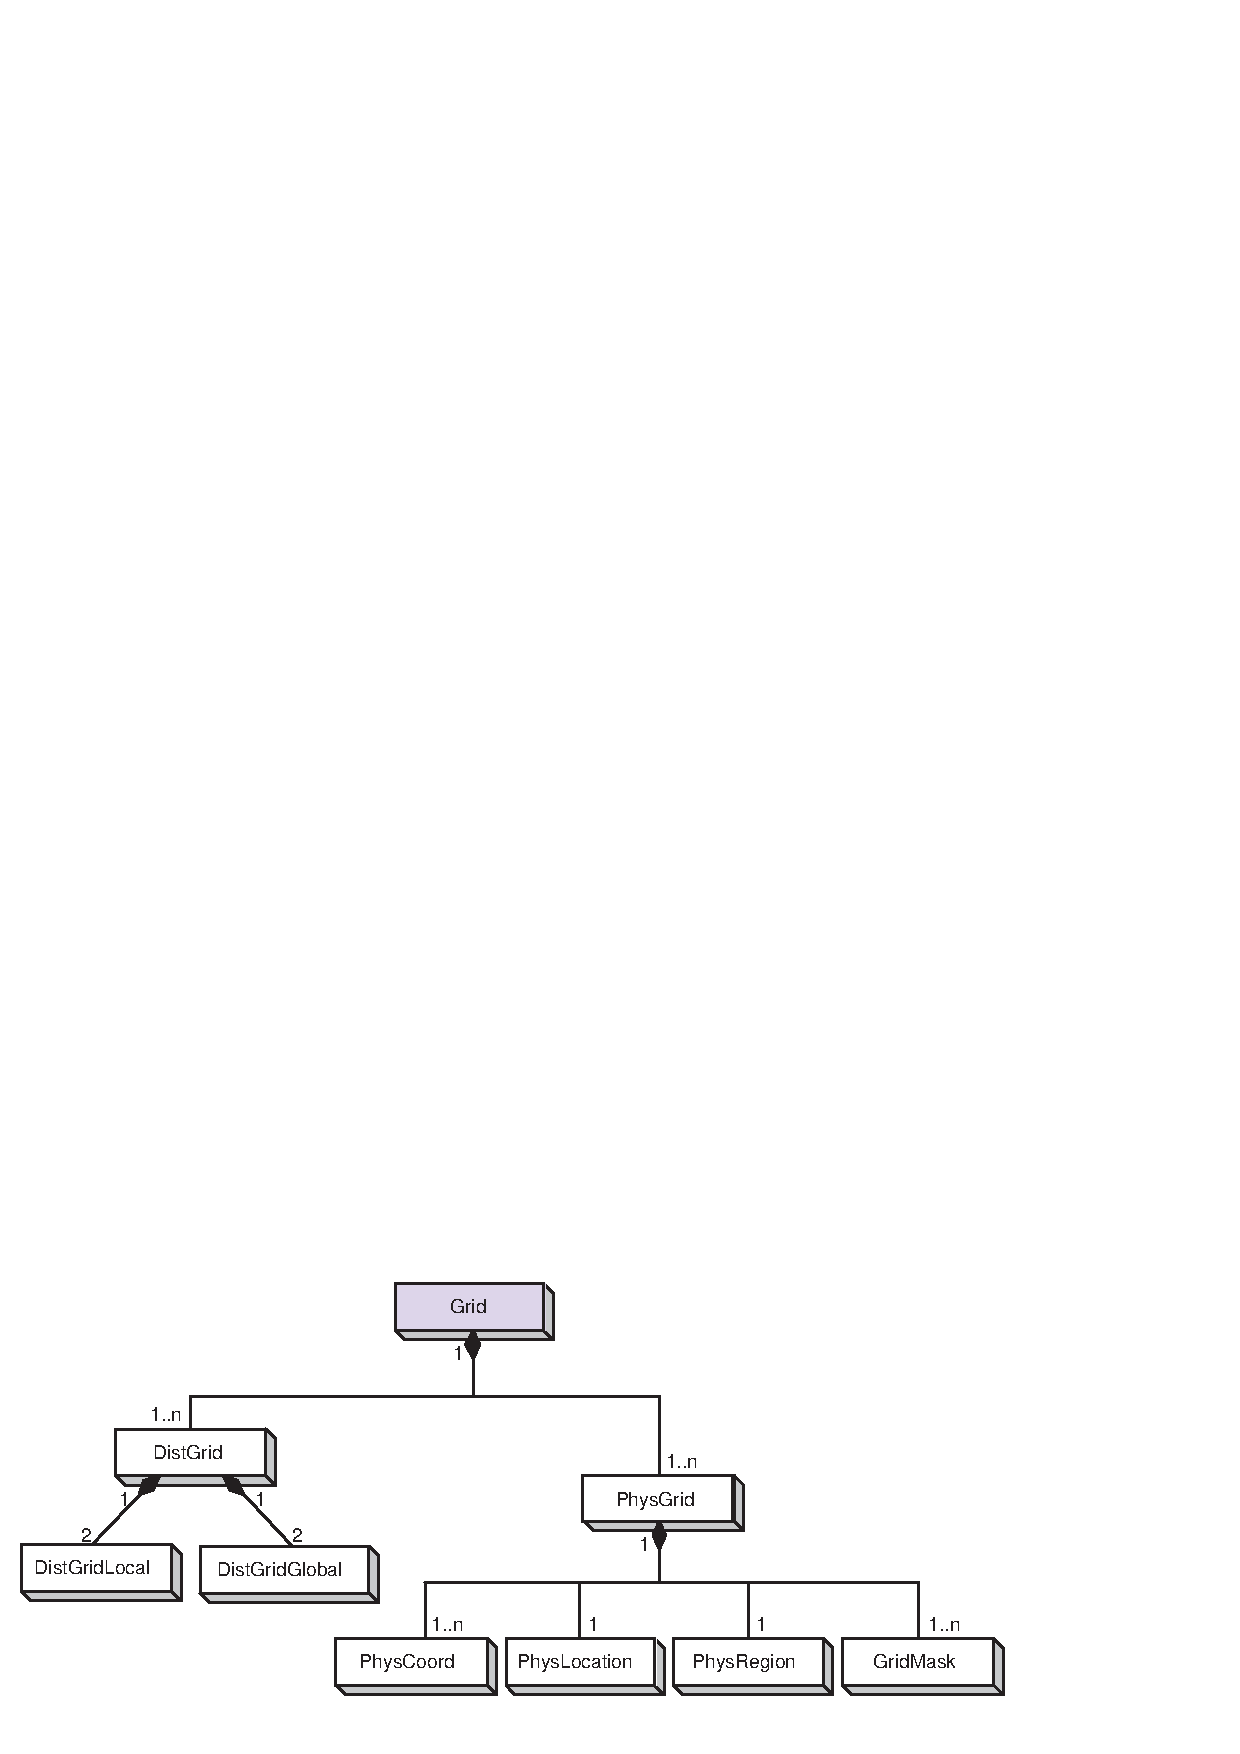
\includegraphics{Grid_obj}   
\end{center}

Each Grid contains at least one Distributed Grid and a related Physical Grid.
The Physical Grid maintains information about the global coordinates.  In
general the coordinates are described implicitly by specifying the grid type
and the corresponding parameters.  However it is possible that the Physical
Grid must be completely enumerated, perhaps in the case of assimilated data
or unstructured data.  The Distributed Grid defines an index space that
corresponds to cells in the Physical Grid and is decomposed among DEs in a
DELayout.  Please see Sections~\ref{sec:DistGridClasses} and
~\ref{sec:PhysGridClasses} for more information about the private
DistGrid and PhysGrid classes.



%#elif defined(1)
%% $Id$
%
% Earth System Modeling Framework
% Copyright 2002-2020, University Corporation for Atmospheric Research,
% Massachusetts Institute of Technology, Geophysical Fluid Dynamics
% Laboratory, University of Michigan, National Centers for Environmental
% Prediction, Los Alamos National Laboratory, Argonne National Laboratory,
% NASA Goddard Space Flight Center.
% Licensed under the University of Illinois-NCSA License.

\subsection{Object Model}

The following is a simplified UML diagram showing the structure of the
Grid class.  See Appendix A, {\it A Brief Introduction to UML},
for a translation table that lists the symbols in the diagram and their 
meaning.

\begin{center}
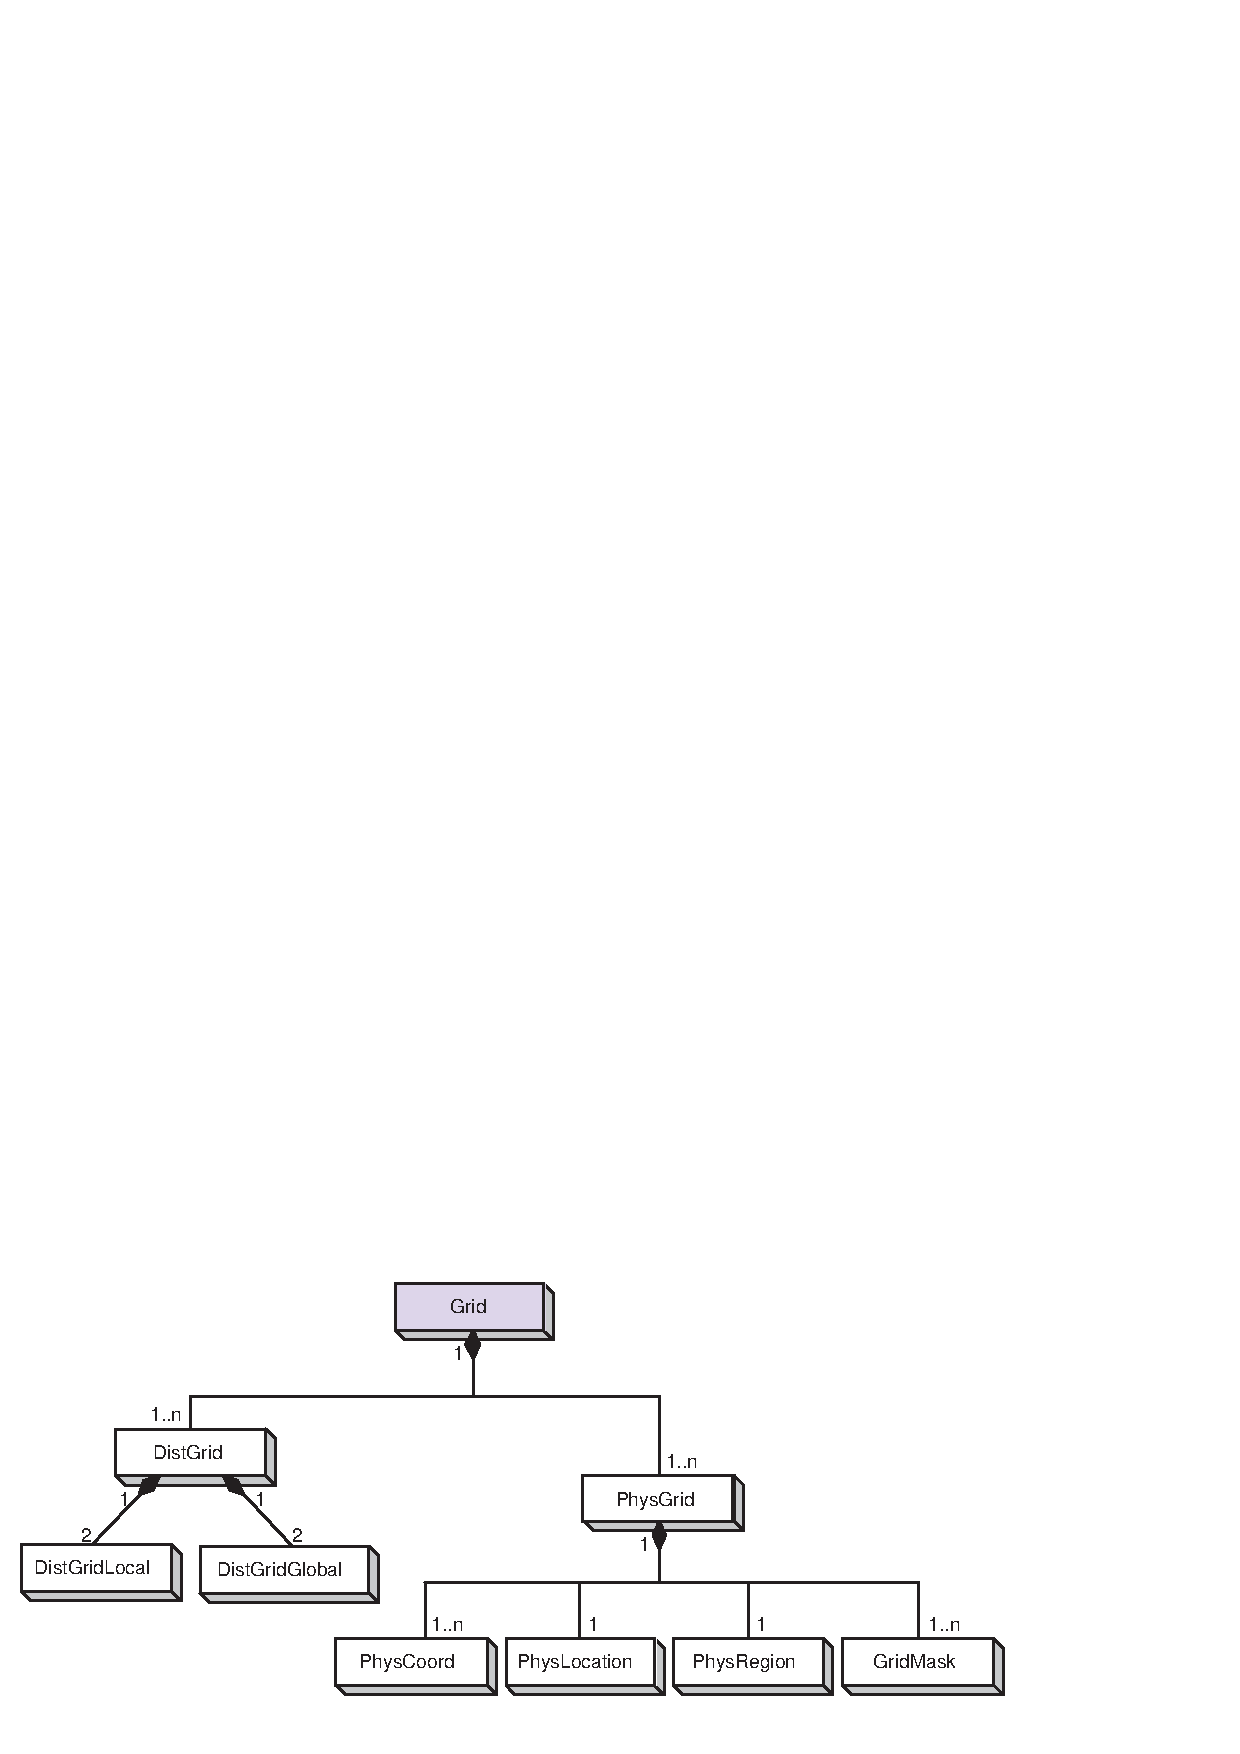
\includegraphics{Grid_obj}   
\end{center}

Each Grid contains at least one Distributed Grid and a related Physical Grid.
The Physical Grid maintains information about the global coordinates.  In
general the coordinates are described implicitly by specifying the grid type
and the corresponding parameters.  However it is possible that the Physical
Grid must be completely enumerated, perhaps in the case of assimilated data
or unstructured data.  The Distributed Grid defines an index space that
corresponds to cells in the Physical Grid and is decomposed among DEs in a
DELayout.  Please see Sections~\ref{sec:DistGridClasses} and
~\ref{sec:PhysGridClasses} for more information about the private
DistGrid and PhysGrid classes.



%#endif
\section{Grid Class}
\subsection{Description}
% $Id$
%
% Earth System Modeling Framework
% Copyright 2002-2020, University Corporation for Atmospheric Research, 
% Massachusetts Institute of Technology, Geophysical Fluid Dynamics 
% Laboratory, University of Michigan, National Centers for Environmental 
% Prediction, Los Alamos National Laboratory, Argonne National Laboratory, 
% NASA Goddard Space Flight Center.
% Licensed under the University of Illinois-NCSA License.

The ESMF Grid class is used to describe the geometry and discretization
of logically rectangular physical grids.  It also contains the
description of the grid's underlying topology and the decomposition
of the physical grid across the available computational resources.
The most frequent use of the Grid class is to describe physical grids
in user code so that sufficient information is available to perform ESMF
methods such as regridding.  

%In the current release (v5.2.0)
%the functionality in this class is partially implemented.  
%Multi-tile grids are not supported, and edge connectivities 
%are not implemented and default to aperiodic.  
%Other constraints of the current
%implementation are noted in the usage section and in the API
%descriptions.


\begin{center}
\begin{tabular}{|p{6in}|}
\hline
\vspace{.01in}
{\bf Key Features} \\[.01in]
Representation of grids formed by logically rectangular regions,
including uniform and rectilinear grids (e.g. lat-lon grids),
curvilinear grids (e.g. displaced pole grids), and grids formed
by connected logically rectangular regions (e.g. cubed sphere grids).\\
Support for 1D, 2D, 3D, and higher dimension grids.\\ 
Distribution of grids across computational resources for parallel
operations - users set which grid dimensions are distributed.\\
Grids can be created already distributed, so that no single
resource needs global information during the creation process.\\
Options to define periodicity and other edge connectivities either 
explicitly or implicitly via shape shortcuts.\\ 
Options for users to define grid coordinates themselves or to call
prefabricated coordinate generation routines for standard grids.\\
Options for incremental construction of grids.\\
Options for using a set of pre-defined stagger locations or for setting
custom stagger locations.\\ [.03in] \hline
\end{tabular}
\end{center}

\subsubsection{Grid Representation in ESMF}

ESMF Grids are based on the concepts described in {\it A Standard
Description of Grids Used in Earth System Models} [Balaji 2006].  In this document
Balaji introduces the mosaic concept as a means of describing
a wide variety of Earth system model grids.  A {\bf mosaic} is
composed of grid tiles connected at their edges.  Mosaic grids
includes simple, single tile grids as a special case.  

The ESMF Grid class is a representation of a mosaic grid.  Each ESMF
Grid is constructed of one or more logically rectangular {\bf Tiles}.
A Tile will usually have some physical significance (e.g. the region
of the world covered by one face of a cubed sphere grid).

The piece of a Tile that resides on one DE (for simple cases, a DE
can be thought of as a processor - see section on the DELayout)
is called a {\bf LocalTile}.  For example, the six faces of a cubed
sphere grid are each Tiles, and each Tile can be divided into many
LocalTiles.  

Every ESMF Grid contains a DistGrid object, which defines the Grid's
index space, topology, distribution, and connectivities.  It enables
the user to define the complex edge relationships of tripole and other
grids.  The DistGrid can be created explicitly and passed into a Grid
creation routine, or it can be created implicitly if the user takes
a Grid creation shortcut. The DistGrid used
in Grid creation describes the properties of the Grid cells. In addition
to this one, the Grid internally creates DistGrids for each stagger location. 
These stagger DistGrids are related to the original DistGrid, but may 
contain extra padding to represent the extent of the index space of
the stagger. These DistGrids are what are used when a Field is created 
on a Grid. 

\subsubsection{Supported Grids}

The range of supported grids in ESMF can be defined by:
\begin{itemize}
\item Types of topologies and shapes supported.  ESMF supports one or
more logically rectangular grid Tiles with connectivities specified
between cells.  For more details see section \ref{sec:ShapeShortcut}.
\item Types of distributions supported.  ESMF supports  regular,
irregular, or arbitrary distributions of data.  
For more details see section \ref{sec:desc:dist}.
\item Types of coordinates supported.  ESMF supports uniform, rectilinear,
and curvilinear coordinates.  For more details see section \ref{sec:coordspec}.
\end{itemize}

\subsubsection{Grid Topologies and Periodicity}
\label{sec:ShapeShortcut}
\begin{sloppypar}
ESMF has shortcuts for the creation of standard Grid topologies 
or {\bf shapes} up to 3D.  In many cases, these enable the user to
bypass the step of creating a DistGrid before creating the Grid. 
There are two sets of methods which allow the user to do this. These two sets of methods cover the same set of topologies, but
allow the user to specify them in different ways.

 The first set of these are a group of overloaded
calls broken up by the number of periodic dimensions they specify. With these the user can pick 
the method which creates a Grid with the number of periodic dimensions they need, and then specify other connectivity 
options via arguments to the method. The following is a description of these methods:  
\end{sloppypar}

\medskip

\begin{description}
\item [ESMF\_GridCreateNoPeriDim()] Allows the user to create a Grid with no edge connections, for example, a regional Grid with closed boundaries.

\item [ESMF\_GridCreate1PeriDim()] Allows the user to create a Grid with 1 periodic dimension and supports a range of options for what to do at the pole (see ~Section~\ref{const:polekind}). Some examples of Grids which can be created here are tripole spheres, bipole spheres, cylinders with open poles. 

\item [ESMF\_GridCreate2PeriDim()] Allows the user to create a Grid with 2 periodic dimensions, for example a torus, or a regional Grid with
doubly periodic boundaries. 
\end{description}

More detailed information can be found in the API description of each.

\medskip

\begin{sloppypar}
The second set of shortcut methods is a set of methods overloaded under the name {\tt ESMF\_GridCreate()}. These methods
allow the user to specify the connectivites at the end of each dimension, by using the ESMF\_GridConn\_Flag flag. The table below shows the ESMF\_GridConn\_Flag settings used to create 
standard shapes in 2D using the ESMF\_GridCreate() call.  Two values
are specified for each dimension, one for the low end and one for 
the high end of the dimension's index values. 
\end{sloppypar}

\medskip
\begin{tabular}{|l|c|c||c|c||}
\hline
2D Shape & {\bf connflagDim1(1)} & {\bf connflagDim1(2)}  & {\bf connflagDim2(1)} & {\bf connflagDim2(2)}  \\
\hline
{\bf Rectangle}  & NONE & NONE & NONE & NONE \\
{\bf Bipole Sphere} & POLE & POLE & PERIODIC & PERIODIC \\
{\bf Tripole Sphere} & POLE & BIPOLE & PERIODIC & PERIODIC \\
{\bf Cylinder} & NONE & NONE & PERIODIC & PERIODIC \\
{\bf Torus}  & PERIODIC & PERIODIC & PERIODIC & PERIODIC \\
\hline
\hline
\end{tabular}
\medskip

If the user's grid shape is too complex for an ESMF shortcut routine,
or involves more than three dimensions, a DistGrid can be created
to specify the shape in detail.  This DistGrid is then passed
into a Grid create call.

\subsubsection{Grid Distribution}
\label{sec:desc:dist}

ESMF Grids have several options for data distribution (also referred to
as decomposition).  As ESMF Grids are cell based, these 
options are all specified  in terms of how the cells in the Grid
are broken up between DEs. 

The main distribution options are regular, irregular, and arbitrary.
A {\bf regular} distribution is one in which the same number of
contiguous grid cells are assigned to each DE in the
distributed dimension.  An {\bf irregular} distribution is one in which
unequal numbers of contiguous grid cells are assigned to each
DE in the distributed dimension.  An {\bf arbitrary} distribution is
one in which any grid cell can be assigned to any DE.  Any of these
distribution options can be applied to any of the grid shapes (i.e.,
rectangle) or types (i.e., rectilinear).  Support for arbitrary distribution 
is limited in the current version of ESMF, see Section \ref{example:ArbGridWithUndistDim} for
an example of creating a Grid with an arbitrary distribution.


Figure \ref{fig:GridDecomps} illustrates options for distribution.
\begin{figure}
\scalebox{0.9}{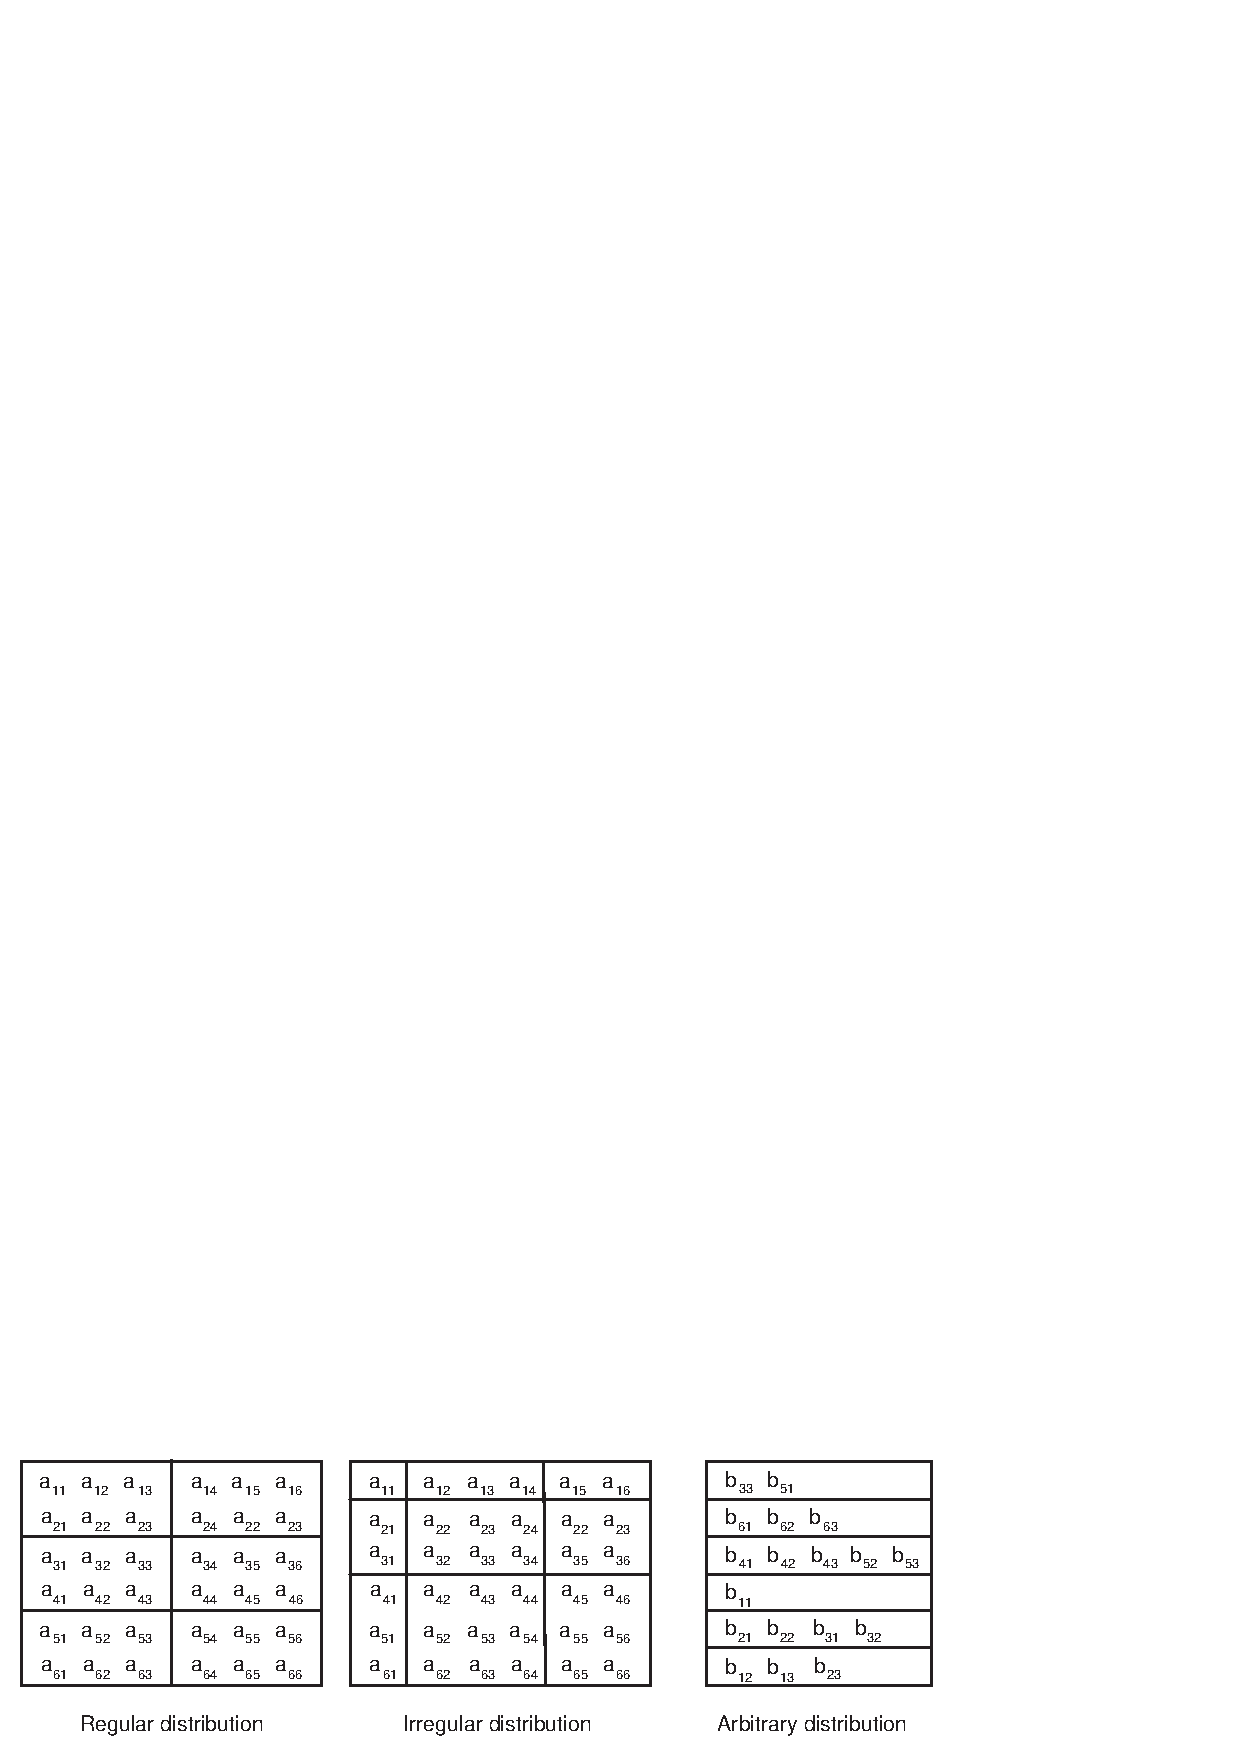
\includegraphics{GridDecomps}}
\caption{Examples of regular and irregular decomposition of
a grid {\bf a} that is 6x6, and an arbitrary decomposition of
a grid {\bf b} that is 6x3.}
\label{fig:GridDecomps}
\end{figure}

A distribution can also be specified using the DistGrid, by passing
object into a Grid create call.

\subsubsection{Grid Coordinates}
\label{sec:coordspec}
Grid Tiles can have uniform, rectilinear, or curvilinear
coordinates.  The coordinates of {\bf uniform} grids are equally spaced along
their axes, and can be fully specified by the coordinates of the two opposing points
that define the grid's physical span.  The coordinates of {\bf rectilinear} grids
are unequally spaced along their axes, and can be fully specified by giving
the spacing of grid points along each axis.  The coordinates of {\bf curvilinear 
grids} must be specified by giving the explicit set of coordinates for each
grid point.  Curvilinear grids are often uniform or rectilinear grids that 
have been warped; for example, to place a pole over a land mass so that it
does not affect the computations performed on an ocean model grid.  Figure
\ref{fig:LogRectGrids} shows examples of each type of grid.

%Any of these logically rectangular grid types can be combined through edge
%connections to form a mosaic.  Cubed sphere and yin-yang grids are examples
%of mosaic grids.  Note that as of v5.2.0 multi-tile grids have not yet been
%implemented.
 
\begin{figure}
\scalebox{0.9}{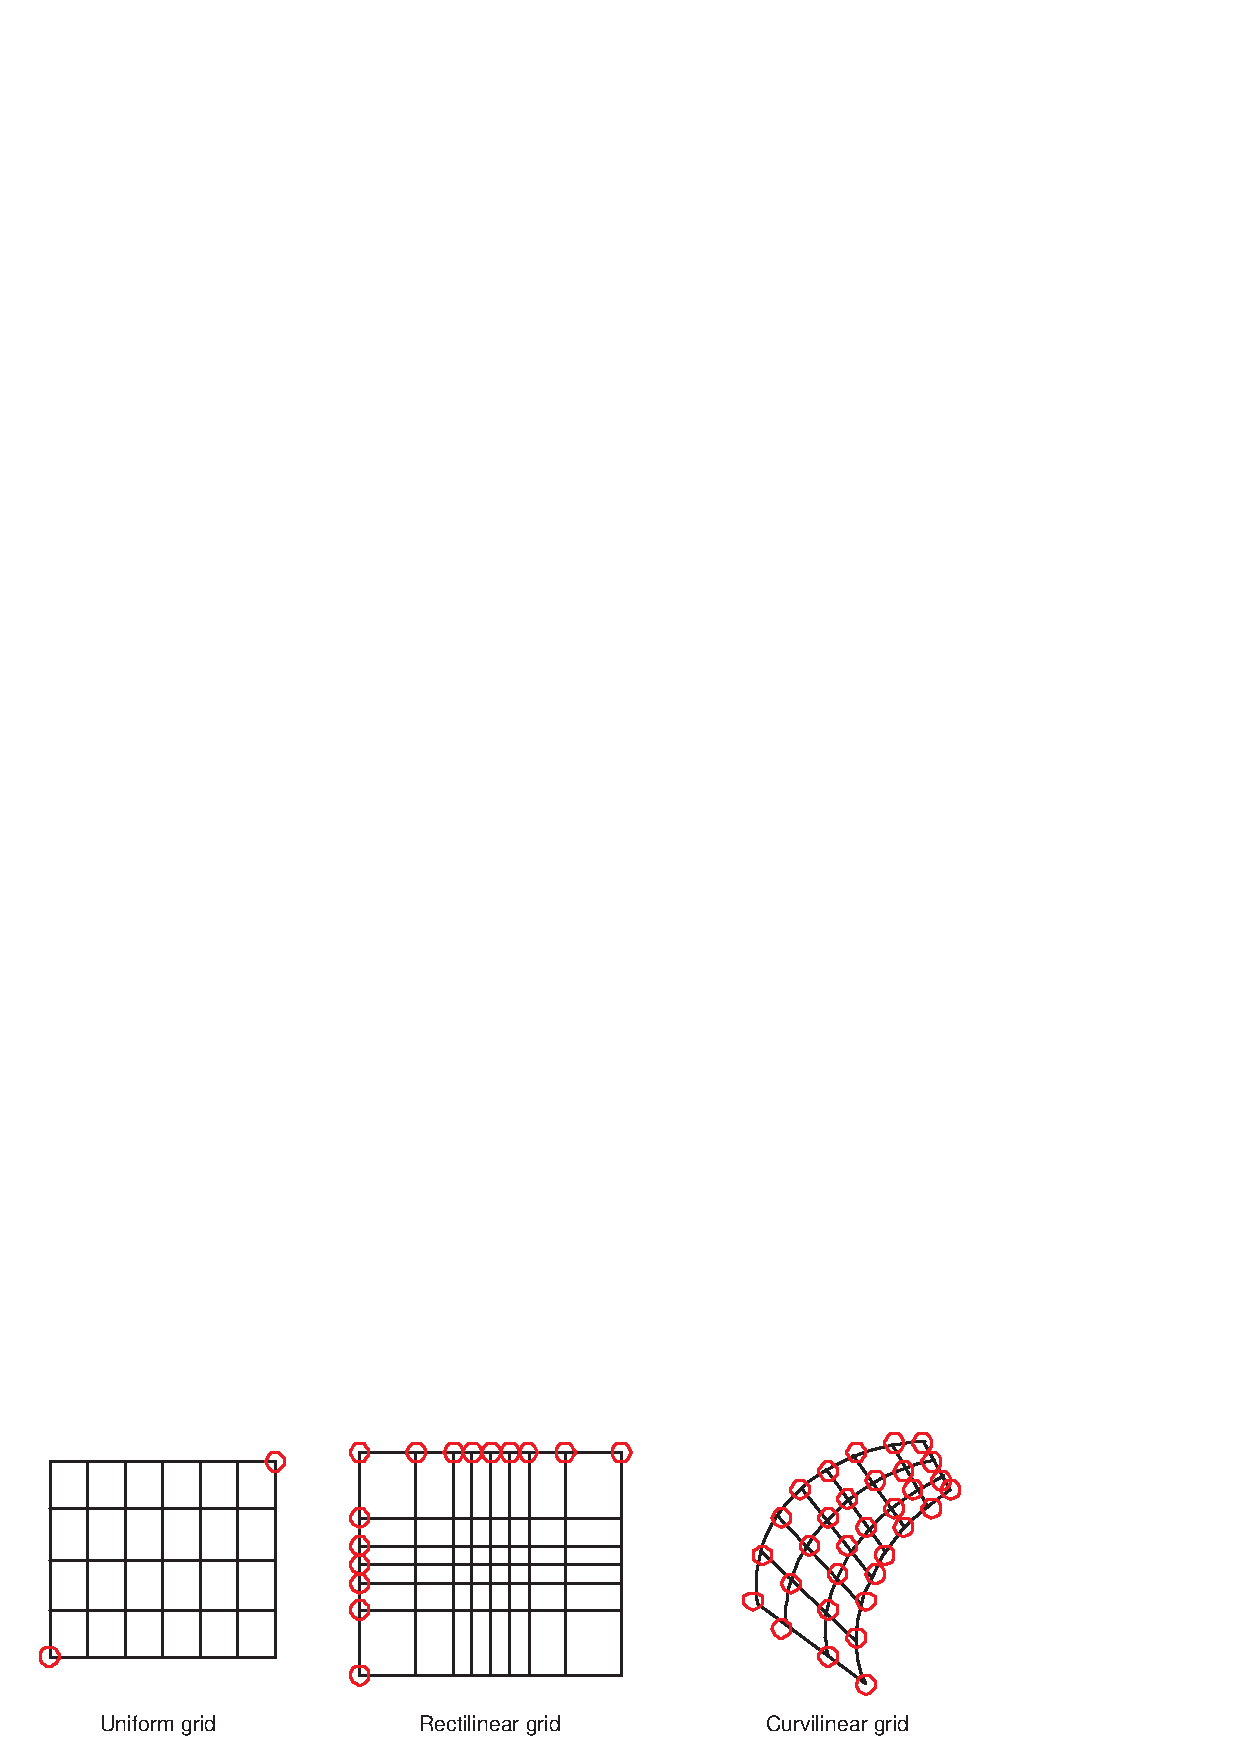
\includegraphics{LogRectGrids}}
\caption{Types of logically rectangular grid tiles.  Red circles show the
values needed to specify grid coordinates for each type.}
\label{fig:LogRectGrids}
\end{figure}

Each of these coordinate types can be set for each of the standard grid shapes
described in section \ref{sec:ShapeShortcut}.  

The table below shows how examples of common single Tile grids fall 
into this shape and coordinate taxonomy.  Note that any
of the grids in the table can have a regular or arbitrary distribution.

\medskip
\begin{tabular}{|p{.8in}|p{1.6in}|p{1.6in}|p{1.6in}|}
\hline
 & {\bf Uniform} & {\bf Rectilinear} & {\bf Curvilinear} \\ 
\hline
{\bf Sphere} & Global uniform lat-lon grid & Gaussian grid & Displaced pole grid \\
\hline
{\bf Rectangle} & Regional uniform lat-lon grid & Gaussian grid section & Polar stereographic grid section\\
\hline
\end{tabular}

\subsubsection{Coordinate Specification and Generation}

There are two ways of specifying coordinates in ESMF.  The
first way is for the user to {\bf set} the coordinates.  The second 
way is to take a shortcut and have the framework {\bf generate}
the coordinates.  

See Section~\ref{sec:usage:staggerloc} for more description and examples of
setting coordinates.

\subsubsection{Staggering}

{\bf Staggering} is a finite difference technique in which the values 
of different physical quantities are placed at different locations
within a grid cell. 

The ESMF Grid class supports a variety of stagger locations, including
cell centers, corners, and edge centers. The default stagger location in 
ESMF is the cell center, and cell counts in Grid are based on this assumption.
Combinations of the 2D ESMF stagger locations are sufficient to specify any of the
Arakawa staggers.  ESMF also supports staggering in 3D and higher dimensions.
There are shortcuts for standard staggers, and interfaces through which users 
can create custom staggers.  

As a default the ESMF Grid class provides symmetric staggering, so
that cell centers are enclosed by cell perimeter (e.g. corner) 
stagger locations. This means the coordinate arrays for stagger
locations other than the center will have an additional element of 
padding in order to enclose the cell center locations.
However, to achieve other types of staggering, the user may alter 
or eliminate this padding by using the appropriate options when adding
coordinates to a Grid. 
 
In the current release, only the cell center stagger location is supported for an
arbitrarily distributed grid. For examples and a full description of the stagger interface 
see Section~\ref{sec:usage:staggerloc}. 

\subsubsection{Masking}

Masking is the process whereby parts of a Grid can be marked to be
ignored during an operation.  For a description of how to set mask information in
the Grid, see here \ref{sec:usage:items}. For a description of how masking works
in regridding, see here \ref{regrid:masking}.

\subsection{Constants}
% $Id$

\subsubsection{ESMF\_GRIDCONN}
\label{const:gridconn}

{\sf DESCRIPTION:\\}
\begin{sloppypar}
The {\tt ESMF\_GridCreateShapeTile} command has three specific arguments
{\tt connflagDim1}, {\tt connflagDim2}, and {\tt connflagDim3}. These can be used
to setup different types of connections at the ends of each dimension
of a Tile.  Each of these parameters is a two element array. The first
element is the connection type at the minimum end of the dimension
and the second is the connection type at the maximum end. The default
value for all the connections is ESMF\_GRIDCONN\_NONE, specifying no
connection.
\end{sloppypar}

The type of this flag is:

{\tt type(ESMF\_GridConn\_Flag)}

The valid values are:
\begin{description}
\item [ESMF\_GRIDCONN\_NONE] No connection.

\item [ESMF\_GRIDCONN\_PERIODIC] Periodic connection.

\item [ESMF\_GRIDCONN\_POLE] This edge is connected to itself. Given
that the edge is n elements long, then element i is connected to
element ((i+n/2) mod n).

\item [ESMF\_GRIDCONN\_BIPOLE] This edge is connected to itself. Given
that the edge is n elements long, element i is connected to element (n-i-1).
\end{description}


\subsubsection{ESMF\_GRIDITEM}
\label{const:griditem}

{\sf DESCRIPTION:\\}
The ESMF Grid can contain other kinds of data besides coordinates. 
This data is referred to as Grid ``items''. Some items may be used
by ESMF for calculations involving the Grid. The following
are the valid values of ESMF\_GridItem\_Flag.

The type of this flag is:

{\tt type(ESMF\_GridItem\_Flag)}

The valid values are:
\newline
\begin{tabular}{|l|c|c|c|c||}
\hline
\hline
Item Label & {\bf Type Restriction}  & {\bf Type Default} & {\bf ESMF Uses} & {\bf Controls} \\
\hline
{\bf ESMF\_GRIDITEM\_MASK}  & ESMF\_TYPEKIND\_I4 & ESMF\_TYPEKIND\_I4 & YES & Masking in Regrid \\
{\bf ESMF\_GRIDITEM\_AREA} & NONE & ESMF\_TYPEKIND\_R8 & YES & Conservation in Regrid \\
\hline
\hline
\end{tabular}

\medskip

 {\bf NOTE:} One important thing to consider when setting areas in the Grid using {\tt ESMF\_GRIDITEM\_AREA},
  ESMF doesn't currently do unit conversion on areas. If these areas are going to be used
 in a process that also involves the areas of another Grid or Mesh (e.g. conservative regridding), then
 it is the user's responsibility to make sure that the area units are consistent between the two sides.
 If ESMF calculates an area on the surface of a sphere, then it is in units of square radians. If 
 it calculates the area for a Cartesian grid, then it is in the same units as the coordinates, but squared. 


\subsubsection{ESMF\_GRIDMATCH}
\label{const:gridmatch}

{\sf DESCRIPTION:\\}
 This type is used to indicate the level to which two grids match.

The type of this flag is:

{\tt type(ESMF\_GridMatch\_Flag)}

The valid values are:
\begin{description}
\item [ESMF\_GRIDMATCH\_INVALID:] Indicates a non-valid matching level. Returned
      if an error occurs in the matching function. If a higher matching level
      is returned then no error occurred.
\item [ESMF\_GRIDMATCH\_NONE:] The lowest level of grid matching. 
      This indicates that the Grid's don't match at any of the higher levels. 
\item [ESMF\_GRIDMATCH\_EXACT:] All the pieces of the Grid (e.g. distgrids, 
      coordinates, etc.) except the name, match between the two Grids. 
\item [ESMF\_GRIDMATCH\_ALIAS:] Both Grid variables are aliases to the exact
      same Grid object in memory. 
\end{description}


\subsubsection{ESMF\_GRIDSTATUS}
\label{const:gridstatus}

{\sf DESCRIPTION:\\}
The ESMF Grid class can exist in two states. These states are
present so that the library code can detect if a Grid has been
appropriately setup for the task at hand. The following
are the valid values of ESMF\_GRIDSTATUS.

The type of this flag is:

{\tt type(ESMF\_GridStatus\_Flag)}

The valid values are:
\begin{description}
\item [ESMF\_GRIDSTATUS\_EMPTY:] Status after a Grid has been created with 
      {\tt ESMF\_GridEmptyCreate}.  A Grid object container is allocated but
      space for internal objects is not.  Topology information and coordinate
      information is incomplete.  This object can be used in {\tt ESMF\_GridEmptyComplete()}
      methods in which additional information is added to the Grid.
\item [ESMF\_GRIDSTATUS\_COMPLETE:] The Grid has a specific topology and
      distribution, but incomplete coordinate arrays.  The Grid can be used
      as the basis for allocating a Field, and coordinates can be added
      via {\tt ESMF\_GridCoordAdd()} to allow other functionality. 
\end{description}


\subsubsection{ESMF\_POLEKIND}
\label{const:polekind}

{\sf DESCRIPTION:\\}
This type describes the type of connection that occurs at the pole when a Grid is 
created with {\tt ESMF\_GridCreate1PeriodicDim()}.

The type of this flag is:

{\tt type(ESMF\_PoleKind\_Flag)}

The valid values are:
\begin{description}
\item [ESMF\_POLEKIND\_NONE] No connection at pole.

\item [ESMF\_POLEKIND\_MONOPOLE] This edge is connected to itself. Given
that the edge is n elements long, then element i is connected to
element i+n/2.

\item [ESMF\_POLEKIND\_BIPOLE] This edge is connected to itself. Given
that the edge is n elements long, element i is connected to element n-i-1.
\end{description}


\subsubsection{ESMF\_STAGGERLOC}
\label{const:staggerloc}

 {\sf DESCRIPTION:\\}
 In the ESMF Grid class, data can be located at different positions in a
 Grid cell.  When setting or retrieving coordinate data the stagger location is
 specified to tell the Grid method  from where in the cell to get the data. 
 Although the user may define their own custom stagger locations, 
 ESMF provides a set of predefined locations for ease of use. The
following are the valid predefined stagger locations. 

\medskip

\begin{center}
\begin{figure}
\center
\scalebox{0.75}{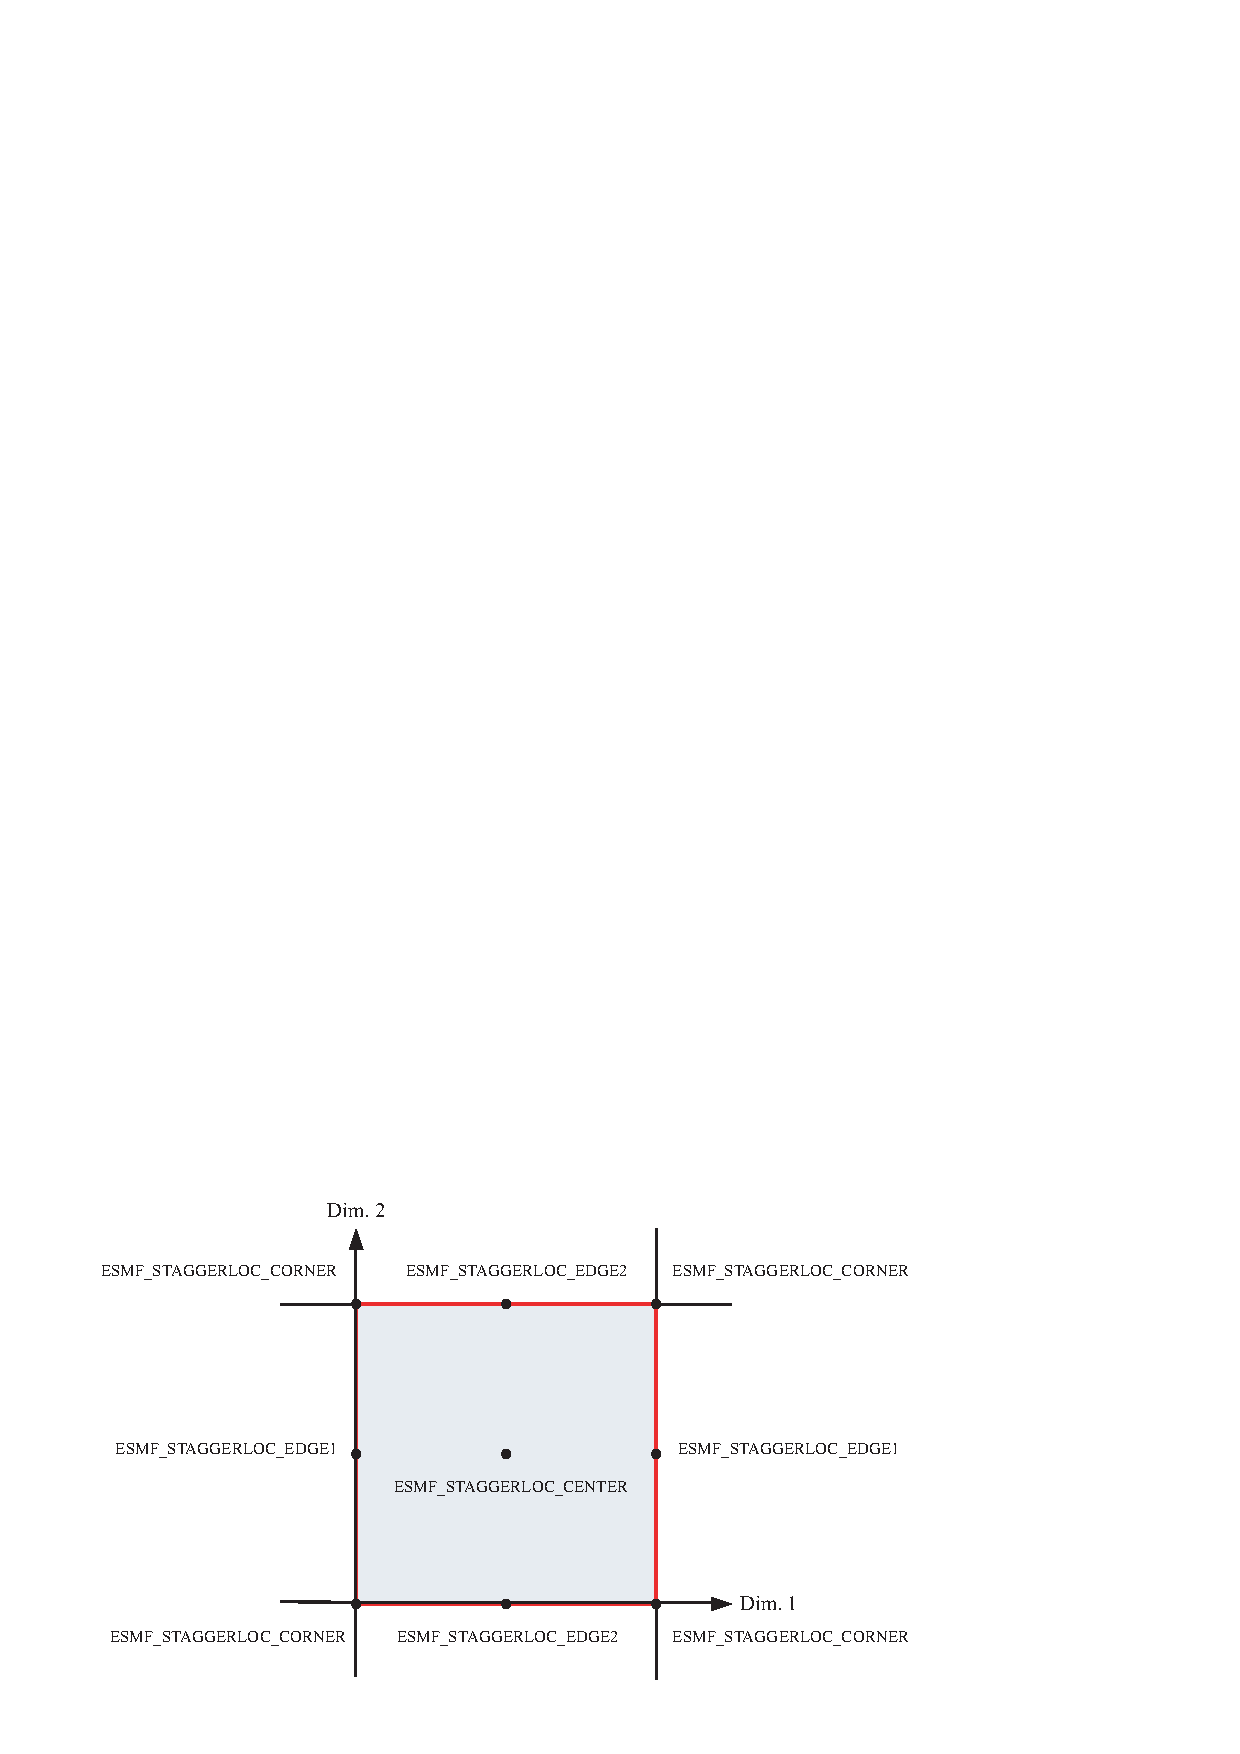
\includegraphics{GridStaggerLoc2D}}
\caption{2D Predefined Stagger Locations}
\label{fig:gridstaggerloc2d}
\end{figure}
\end{center}

The 2D predefined stagger locations (illustrated in figure~\ref{fig:gridstaggerloc2d}) are:\\
\begin{description}
\item [ESMF\_STAGGERLOC\_CENTER:] The center of the cell.
\item [ESMF\_STAGGERLOC\_CORNER:] The corners of the cell.
\item [ESMF\_STAGGERLOC\_EDGE1:] The edges offset from the center in the 1st dimension.
\item [ESMF\_STAGGERLOC\_EDGE2:] The edges offset from the center in the 2nd dimension.
\end{description}

\medskip

\begin{center}
\begin{figure}
\center
\scalebox{1.0}{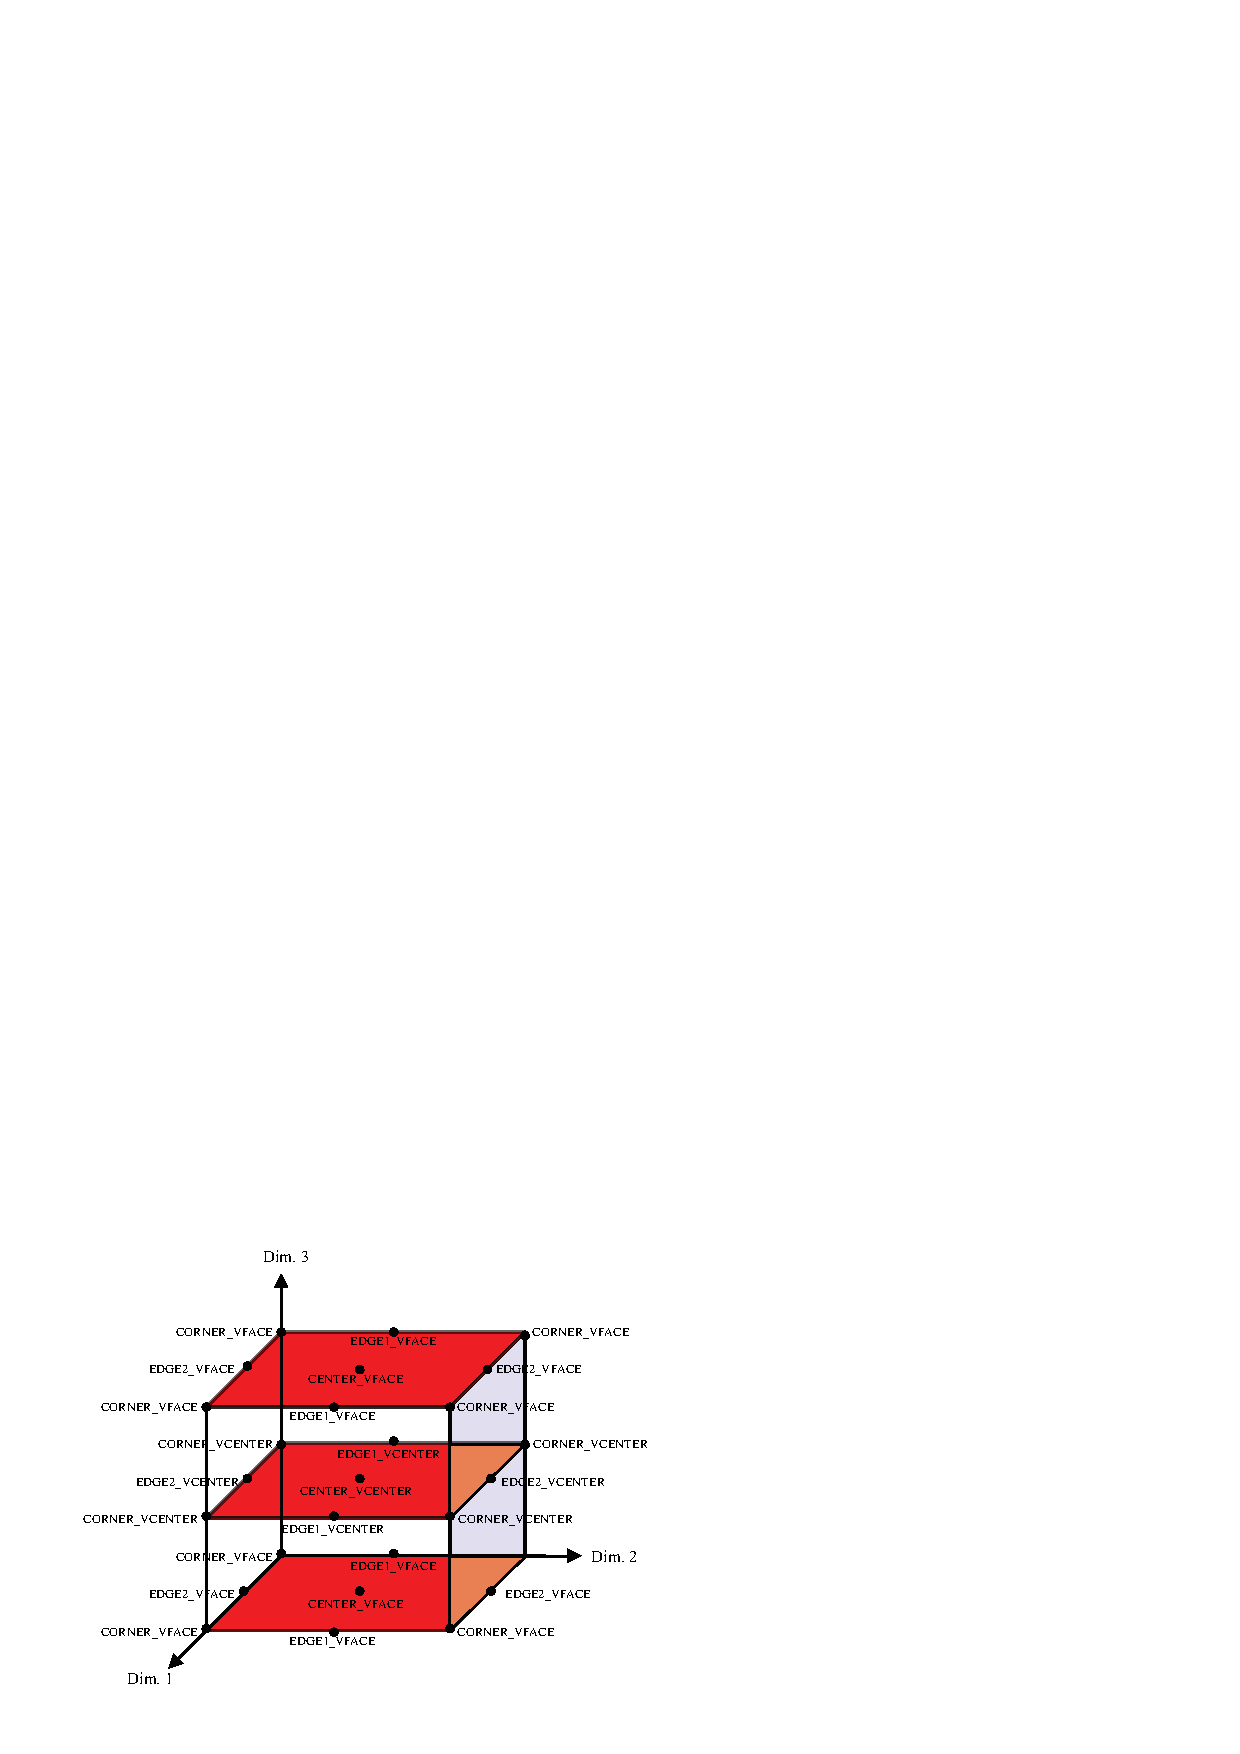
\includegraphics{GridStaggerLoc3D}}
\caption{3D Predefined Stagger Locations}
\label{fig:gridstaggerloc3d}
\end{figure}
\end{center}

The 3D predefined stagger locations (illustrated in figure~\ref{fig:gridstaggerloc3d}) are:\\
\begin{description}
\item [ESMF\_STAGGERLOC\_CENTER\_VCENTER:] The center of the 3D cell.
\item [ESMF\_STAGGERLOC\_CORNER\_VCENTER:] Half way up the vertical edges of the cell.
\item [ESMF\_STAGGERLOC\_EDGE1\_VCENTER:] The center of the face bounded by edge 1 and the vertical dimension.
\item [ESMF\_STAGGERLOC\_EDGE2\_VCENTER:] The center of the face bounded by edge 2 and the vertical dimension. 
\item [ESMF\_STAGGERLOC\_CORNER\_VFACE:] The corners of the 3D cell.
\item [ESMF\_STAGGERLOC\_EDGE1\_VFACE:] The center of the edges of the 3D cell parallel offset from the center in the 1st dimension.
\item [ESMF\_STAGGERLOC\_EDGE2\_VFACE:] The center of the edges of the 3D cell parallel offset from the center in the 2nd dimension.
\item [ESMF\_STAGGERLOC\_CENTER\_VFACE:] The center of the top and bottom face. The face bounded by the 1st and 2nd dimensions. 
\end{description}


\subsection{Use and Examples}
% $Id$

This section describes the use of the ESMF Grid class. It first discusses
the more user friendly shape specific interface to the Grid. 
During this discussion it covers creation and options, 
adding stagger locations, coordinate data access, and other grid 
functionality. After this initial phase the document discusses 
the more advanced options which the user can employ should they
need more customized interaction with the Grid class.




 









%                **** IMPORTANT NOTICE *****
% This LaTeX file has been automatically produced by ProTeX v. 1.1
% Any changes made to this file will likely be lost next time
% this file is regenerated from its source. Send questions 
% to Arlindo da Silva, dasilva@gsfc.nasa.gov
 
\setlength{\oldparskip}{\parskip}
\setlength{\parskip}{1.5ex}
\setlength{\oldparindent}{\parindent}
\setlength{\parindent}{0pt}
\setlength{\oldbaselineskip}{\baselineskip}
\setlength{\baselineskip}{11pt}
 
%--------------------- SHORT-HAND MACROS ----------------------
\def\bv{\begin{verbatim}}
\def\ev{\end{verbatim}}
\def\be{\begin{equation}}
\def\ee{\end{equation}}
\def\bea{\begin{eqnarray}}
\def\eea{\end{eqnarray}}
\def\bi{\begin{itemize}}
\def\ei{\end{itemize}}
\def\bn{\begin{enumerate}}
\def\en{\end{enumerate}}
\def\bd{\begin{description}}
\def\ed{\end{description}}
\def\({\left (}
\def\){\right )}
\def\[{\left [}
\def\]{\right ]}
\def\<{\left  \langle}
\def\>{\right \rangle}
\def\cI{{\cal I}}
\def\diag{\mathop{\rm diag}}
\def\tr{\mathop{\rm tr}}
%-------------------------------------------------------------

\markboth{Left}{Source File: ESMF\_GridUsageEx.F90,  Date: Tue May  5 20:59:48 MDT 2020
}

 
%/////////////////////////////////////////////////////////////

  
  \subsubsection{Create single-tile Grid shortcut method}
 
   The set of methods {\tt ESMF\_GridCreateNoPeriDim()}, {\tt ESMF\_GridCreate1PeriDim()},
   {\tt ESMF\_GridCreate2PeriDim()}, and {\tt ESMF\_GridCreate()} are shortcuts
   for building 2D or 3D single tile logically rectangular Grids.
   These methods support all three types of distributions described in
   Section~\ref{sec:desc:dist}: regular, irregular and arbitrary.
  
   The ESMF Grid is cell based and so for all distribution
   options the methods take as input the number of cells to describe
   the total index space and the number of cells to specify distribution.
  
   To create a Grid
   with a regular distribution the user specifies the global
   maximum and minimum ranges of the Grid cell index space ({\tt maxIndex} and
   {\tt minIndex}), and the number of pieces in which to partition
   each dimension (via a {\tt regDecomp} argument).
   ESMF then divides the index space as evenly as possible
   into the specified number of pieces. If there are cells
   left over then they are distributed one per DE starting from
   the first DE until they are gone.
  
   If {\tt minIndex} is
   not specified, then the bottom of the Grid cell index range is assumed
   to be (1,1,...,1). If {\tt regDecomp} is not specified, then
   by default ESMF creates a distribution that partitions the
   grid cells in the first dimension (e.g. NPx1x1...1) as evenly
   as possible by  the number of PETs NP.
   The remaining dimensions are not partitioned.
   The dimension of the Grid is the size of {\tt maxIndex}.
   The following is an example of creating a 10x20x30 3D grid
   where the first dimensions is broken into 2 pieces, the second
   is broken into 4 pieces, and the third is not divided (i.e. every DE will
   have length 30 in the 3rd dimension). 
%/////////////////////////////////////////////////////////////

 \begin{verbatim}
  grid3D=ESMF_GridCreateNoPeriDim(regDecomp=(/2,4,1/), maxIndex=(/10,20,30/), &
           rc=rc)
 
\end{verbatim}
 
%/////////////////////////////////////////////////////////////

   Irregular distribution requires the user to specify the
   exact number of Grid cells per DE in each dimension.  In the
   {\tt ESMF\_GridCreateNoPeriDim()} call the {\tt countsPerDEDim1},
   {\tt countsPerDim2}, and {\tt countsPerDim3}
   arguments are used to specify a rectangular distribution
   containing size(countsPerDEDim1) by size(countsPerDEDim2) by
   size(countsPerDEDim3) DEs. The entries in each of these arrays
   specify the number of grid cells per DE in that dimension.
   The dimension of the grid is determined by the presence of
   {\tt countsPerDEDim3}.  If it's present the Grid
   will be 3D. If just {\tt countsPerDEDim1} and
   {\tt countsPerDEDim2} are specified the Grid
   will be 2D.
  
   The following call illustrates the creation of
   a 10x20 two dimensional rectangular Grid distributed across six DEs
   that are arranged 2x3.  In the first dimension there are 3 grid
   cells on the first DE and 7 cells on the second DE.  The second
   dimension has 3 DEs with 11,2, and 7 cells, respectively. 
%/////////////////////////////////////////////////////////////

 \begin{verbatim}
   grid2D=ESMF_GridCreateNoPeriDim(countsPerDEDim1=(/3,7/), &
          countsPerDEDim2=(/11,2,7/), rc=rc)

 
\end{verbatim}
 
%/////////////////////////////////////////////////////////////

   To add a distributed third dimension of size 30, broken up into
   two groups of 15, the above call would be altered as follows. 
%/////////////////////////////////////////////////////////////

 \begin{verbatim}
   grid3d=ESMF_GridCreateNoPeriDim(countsPerDEDim1=(/3,7/), &
          countsPerDEDim2=(/11,2,7/), countsPerDEDim3=(/15,15/), rc=rc)
 
\end{verbatim}
 
%/////////////////////////////////////////////////////////////

   To make a third dimension distributed across only 1 DE, then
   {\tt countsPerDEDim3} in the call should only have a single term. 
%/////////////////////////////////////////////////////////////

 \begin{verbatim}
   grid3D=ESMF_GridCreateNoPeriDim(countsPerDEDim1=(/3,7/),  &
          countsPerDEDim2=(/11,2,7/), countsPerDEDim3=(/30/), rc=rc)
 
\end{verbatim}
 
%/////////////////////////////////////////////////////////////

  
   \begin{sloppypar}
   The {\tt petMap} parameter may be used to specify on to which specific PETs
   the DEs in the Grid are assigned. Each entry in {\tt petMap} specifies to which PET the corresponding
   DE should be assigned. For example, {\tt petMap(3,2)=4} tells the Grid
   create call to put the DE located at column 3 row 2 on PET 4.
   Note that this parameter is only available for the
   regular and irregular distribution types. The {\tt petMap}
   array is a 3D array, for a 3D Grid each of its dimensions correspond to a
   Grid dimension. If the Grid is 2D, then the first two dimensions correspond
   to Grid dimensions and the last dimension should be of size 1.
   The size of each {\tt petMap} dimension is
   the number of DE's along that dimension in the Grid. For a
   regular Grid, the size is equal to the number in regDecomp
   (i.e. {\tt size(petMap,d)=regDecomp(d)} for all dimensions {\tt d} in the Grid). For
   an irregular Grid the size is equal to the number of items in
   the corresponding {\tt countsPerDEDim} variable (i.e.
   {\tt size(petMap,d)=size(countsPerDEDimd)} for all dimensions {\tt d} in the Grid).
   The following example demonstrates how to specify the PET to DE association
   for an {\tt ESMF\_GridCreateNoPeriDim()} call.
   \end{sloppypar}
   
%/////////////////////////////////////////////////////////////

 \begin{verbatim}
   ! allocate memory for petMap
   allocate( petMap(2,2,1) )

   ! Set petMap
   petMap(:,1,1) = (/3,2/) ! DE (1,1,1) on PET 3 and DE (2,1,1) on PET 2
   petMap(:,2,1) = (/1,0/) ! DE (1,2,1) on PET 1 and DE (2,2,1) on PET 0


   ! Let the 3D grid be be distributed only in the first two dimensions.
   grid2D=ESMF_GridCreateNoPeriDim(countsPerDEDim1=(/3,7/), &
           countsPerDEDim2=(/7,6/), petMap=petMap, rc=rc)
 
\end{verbatim}
 
%/////////////////////////////////////////////////////////////

   To create an grid with arbitrary distribution, the user specifies the global minimum and maximum
   ranges of the index space with the
   arguments {\tt minIndex} and {\tt maxIndex}, the total number of cells and their index space locations
   residing on the local PET through a {\tt localArbIndexCount} and a {\tt localArbIndex}
   argument. {\tt localArbIndex} is a 2D array with size {\tt (localArbIndexCount, n)} where n is the total number
   dimensions distributed arbitrarily.
   Again, if {\tt minIndex} is  not specified, then the bottom of the
   index range is assumed to be (1,1,...).
   The dimension of the Grid is equal to the size of {\tt maxIndex}.
   If n (number of arbitrarily distributed dimension) is less than the grid dimension, an optional
   argument {\tt distDim} is used to specify which of the grid dimension is arbitrarily distributed.
   If not given, the first n dimensions are assumed to be distributed.
  
   The following example creates a 2D Grid of dimensions 5x5, and places
   the diagonal elements (i.e. indices (i,i) where i goes from 1 to 5)
   on the local PET. The remaining PETs would individually declare
   the remainder of the Grid locations. 
%/////////////////////////////////////////////////////////////

 \begin{verbatim}
   ! allocate memory for localArbIndex
   allocate( localArbIndex(5,2) )
   ! Set local indices
   localArbIndex(1,:)=(/1,1/)
   localArbIndex(2,:)=(/2,2/)
   localArbIndex(3,:)=(/3,3/)
   localArbIndex(4,:)=(/4,4/)
   localArbIndex(5,:)=(/5,5/)

   ! Create a 2D Arbitrarily distributed Grid
   grid2D=ESMF_GridCreateNoPeriDim(maxIndex=(/5,5/), &
         arbIndexList=localArbIndex, arbIndexCount=5, rc=rc)
 
\end{verbatim}
 
%/////////////////////////////////////////////////////////////

  
   To create a 3D Grid of dimensions 5x6x5 with the first and the third dimensions distributed arbitrarily,
   {\tt distDim} is used. 
%/////////////////////////////////////////////////////////////

 \begin{verbatim}
   ! Create a 3D Grid with the 1st and 3rd dimension arbitrarily distributed
   grid3D=ESMF_GridCreateNoPeriDim(maxIndex=(/5,6,5/), &
         arbIndexList=localArbIndex, arbIndexCount=5, &
         distDim=(/1,3/), rc=rc)
 
\end{verbatim}
 
%/////////////////////////////////////////////////////////////

  \subsubsection{Create a 2D regularly distributed rectilinear Grid
                    with uniformly spaced coordinates}
   \label{example:2DRegUniGrid}
  
   The following is an example of creating a simple rectilinear grid
   and loading in a set of coordinates. It illustrates a straightforward use
   of the {\tt ESMF\_GridCreateNoPeriDim()} call described in the previous section.
   This code creates a 10x20 2D grid with uniformly spaced coordinates varying from (10,10) to (100,200).
   The grid is partitioned using a regular distribution. The first dimension
   is divided into two pieces, and the second dimension is divided into 3.
   This example assumes that the code is being run with a 1-1 mapping between
   PETs and DEs because we are only accessing the first DE on each PET (localDE=0).
   Because we have 6 DEs (2x3), this example would only work when run on 6 PETs.
   The Grid is created with global indices. After Grid creation the
   local bounds and native Fortran arrays are retrieved and the
   coordinates are set by the user.
   
%/////////////////////////////////////////////////////////////

 \begin{verbatim}
   !-------------------------------------------------------------------
   ! Create the Grid:  Allocate space for the Grid object, define the
   ! topology and distribution of the Grid, and specify that it
   ! will have global indices.  Note that here aperiodic bounds are
   ! specified by the argument name. In this call the minIndex hasn't
   ! been set, so it defaults to (1,1,...). The default is to
   ! divide the index range as equally as possible among the DEs
   ! specified in regDecomp. This behavior can be changed by
   ! specifying decompFlag.
   !-------------------------------------------------------------------
   grid2D=ESMF_GridCreateNoPeriDim(          &
         ! Define a regular distribution
         maxIndex=(/10,20/), & ! define index space
         regDecomp=(/2,3/),  & ! define how to divide among DEs
         coordSys=ESMF_COORDSYS_CART, &
         ! Specify mapping of coords dim to Grid dim
         coordDep1=(/1/), & ! 1st coord is 1D and depends on 1st Grid dim
         coordDep2=(/2/), & ! 2nd coord is 1D and depends on 2nd Grid dim
         indexflag=ESMF_INDEX_GLOBAL, &
         rc=rc)
 
\end{verbatim}
 
%/////////////////////////////////////////////////////////////

 \begin{verbatim}

   !-------------------------------------------------------------------
   ! Allocate coordinate storage and associate it with the center
   ! stagger location.  Since no coordinate values are specified in
   ! this call no coordinate values are set yet.
   !-------------------------------------------------------------------
   call ESMF_GridAddCoord(grid2D,  &
          staggerloc=ESMF_STAGGERLOC_CENTER, rc=rc)
 
\end{verbatim}
 
%/////////////////////////////////////////////////////////////

 \begin{verbatim}


   !-------------------------------------------------------------------
   ! Get the pointer to the first coordinate array and the bounds
   ! of its global indices on the local DE.
   !-------------------------------------------------------------------
   call ESMF_GridGetCoord(grid2D, coordDim=1, localDE=0, &
          staggerloc=ESMF_STAGGERLOC_CENTER, &
          computationalLBound=lbnd, computationalUBound=ubnd, &
          farrayPtr=coordX, rc=rc)
 
\end{verbatim}
 
%/////////////////////////////////////////////////////////////

 \begin{verbatim}

   !-------------------------------------------------------------------
   ! Calculate and set coordinates in the first dimension [10-100].
   !-------------------------------------------------------------------
   do i=lbnd(1),ubnd(1)
        coordX(i) = i*10.0
   enddo

   !-------------------------------------------------------------------
   ! Get the pointer to the second coordinate array and the bounds of
   ! its global indices on the local DE.
   !-------------------------------------------------------------------
   call ESMF_GridGetCoord(grid2D, coordDim=2, localDE=0, &
          staggerloc=ESMF_STAGGERLOC_CENTER, &
          computationalLBound=lbnd, computationalUBound=ubnd, &
          farrayPtr=coordY, rc=rc)
 
\end{verbatim}
 
%/////////////////////////////////////////////////////////////

 \begin{verbatim}


   !-------------------------------------------------------------------
   ! Calculate and set coordinates in the second dimension [10-200]
   !-------------------------------------------------------------------
   do j=lbnd(1),ubnd(1)
        coordY(j) = j*10.0
   enddo
 
\end{verbatim}
 
%/////////////////////////////////////////////////////////////

  \subsubsection{Create a periodic 2D regularly distributed rectilinear Grid}
   \label{example:2DPeriRegUniGrid}
  
   The following is an example of creating a simple rectilinear grid
   with a periodic dimension and loading in a set of coordinates. It illustrates a straightforward use
   of the {\tt ESMF\_GridCreate1PeriDim()} call described in the previous section.
   This code creates a 360x180 2D grid with uniformly spaced coordinates varying from (1,1) to (360,180).
   The grid is partitioned using a regular distribution. The first dimension
   is divided into two pieces, and the second dimension is divided into 3.
   This example assumes that the code is being run with a 1-1 mapping between
   PETs and DEs because we are only accessing the first DE on each PET (localDE=0).
   Because we have 6 DEs (2x3), this example would only work when run on 6 PETs.
   The Grid is created with global indices. After Grid creation the
   local bounds and native Fortran arrays are retrieved and the
   coordinates are set by the user.
   
%/////////////////////////////////////////////////////////////

 \begin{verbatim}
   !-------------------------------------------------------------------
   ! Create the Grid:  Allocate space for the Grid object, define the
   ! topology and distribution of the Grid, and specify that it
   ! will have global indices.  Note that here a single periodic connection
   ! is specified by the argument name. In this call the minIndex hasn't
   ! been set, so it defaults to (1,1,...). The default is to
   ! divide the index range as equally as possible among the DEs
   ! specified in regDecomp. This behavior can be changed by
   ! specifying decompFlag. Since the coordinate system is
   ! not specified, it defaults to ESMF_COORDSYS_SPH_DEG.
   !-------------------------------------------------------------------
   grid2D=ESMF_GridCreate1PeriDim(          &
         ! Define a regular distribution
         maxIndex=(/360,180/), & ! define index space
         regDecomp=(/2,3/),  & ! define how to divide among DEs
         ! Specify mapping of coords dim to Grid dim
         coordDep1=(/1/), & ! 1st coord is 1D and depends on 1st Grid dim
         coordDep2=(/2/), & ! 2nd coord is 1D and depends on 2nd Grid dim
         indexflag=ESMF_INDEX_GLOBAL, &
         rc=rc)
 
\end{verbatim}
 
%/////////////////////////////////////////////////////////////

 \begin{verbatim}


   !-------------------------------------------------------------------
   ! Allocate coordinate storage and associate it with the center
   ! stagger location.  Since no coordinate values are specified in
   ! this call no coordinate values are set yet.
   !-------------------------------------------------------------------
   call ESMF_GridAddCoord(grid2D,  &
          staggerloc=ESMF_STAGGERLOC_CENTER, rc=rc)

 
\end{verbatim}
 
%/////////////////////////////////////////////////////////////

 \begin{verbatim}

   !-------------------------------------------------------------------
   ! Get the pointer to the first coordinate array and the bounds
   ! of its global indices on the local DE.
   !-------------------------------------------------------------------
   call ESMF_GridGetCoord(grid2D, coordDim=1, localDE=0, &
          staggerloc=ESMF_STAGGERLOC_CENTER, &
          computationalLBound=lbnd, computationalUBound=ubnd, &
          farrayPtr=coordX, rc=rc)
 
\end{verbatim}
 
%/////////////////////////////////////////////////////////////

 \begin{verbatim}


   !-------------------------------------------------------------------
   ! Calculate and set coordinates in the first dimension [10-100].
   !-------------------------------------------------------------------
   do i=lbnd(1),ubnd(1)
        coordX(i) = i*1.0
   enddo

   !-------------------------------------------------------------------
   ! Get the pointer to the second coordinate array and the bounds of
   ! its global indices on the local DE.
   !-------------------------------------------------------------------
   call ESMF_GridGetCoord(grid2D, coordDim=2, localDE=0, &
          staggerloc=ESMF_STAGGERLOC_CENTER, &
          computationalLBound=lbnd, computationalUBound=ubnd, &
          farrayPtr=coordY, rc=rc)
 
\end{verbatim}
 
%/////////////////////////////////////////////////////////////

 \begin{verbatim}


   !-------------------------------------------------------------------
   ! Calculate and set coordinates in the second dimension [10-200]
   !-------------------------------------------------------------------
   do j=lbnd(1),ubnd(1)
        coordY(j) = j*1.0
   enddo
 
\end{verbatim}
 
%/////////////////////////////////////////////////////////////

  
   The remaining examples in this section will use the irregular
   distribution because of its greater generality. To create code similar to these, but
   using a regular distribution, replace the {\tt countsPerDEDim} arguments
   in the Grid create with the appropriate {\tt maxIndex} and {\tt regDecomp} arguments.
  
  \subsubsection{Create a 2D irregularly distributed rectilinear Grid
                    with uniformly spaced coordinates}
   \label{example:2DIrregUniGrid}
  
   This example serves as an illustration of the difference between using
   a regular and irregular distribution. It repeats the previous example
   except using an irregular distribution to give the user more control
   over how the cells are divided between the DEs. As before, this code
   creates a 10x20 2D Grid with uniformly spaced coordinates  varying from (10,10) to (100,200).
   In this example, the Grid is partitioned using an irregular distribution. The first dimension
   is divided into two pieces, the first with 3 Grid cells per
   DE and the second with 7 Grid cells per DE. In the second dimension,
   the Grid is divided into 3 pieces, with 11, 2, and 7 cells per DE respectively.
   This example assumes that the code is being run with a 1-1 mapping between
   PETs and DEs because we are only accessing the first DE on each PET (localDE=0).
   Because we have 6 DEs (2x3), this example would only work when run on 6 PETs.
   The Grid is created with global indices. After Grid creation the
   local bounds and native Fortran arrays are retrieved and the
   coordinates are set by the user.
   
%/////////////////////////////////////////////////////////////

 \begin{verbatim}
   !-------------------------------------------------------------------
   ! Create the Grid:  Allocate space for the Grid object, define the
   ! topology and distribution of the Grid, and specify that it
   ! will have global coordinates.  Note that aperiodic bounds are
   ! indicated by the method name. In this call the minIndex hasn't
   ! been set, so it defaults to (1,1,...).
   !-------------------------------------------------------------------
   grid2D=ESMF_GridCreateNoPeriDim(          &
            ! Define an irregular distribution
            countsPerDEDim1=(/3,7/),    &
            countsPerDEDim2=(/11,2,7/), &
            ! Specify mapping of coords dim to Grid dim
            coordDep1=(/1/), & ! 1st coord is 1D and depends on 1st Grid dim
            coordDep2=(/2/), & ! 2nd coord is 1D and depends on 2nd Grid dim
            indexflag=ESMF_INDEX_GLOBAL, &
            rc=rc)
 
\end{verbatim}
 
%/////////////////////////////////////////////////////////////

 \begin{verbatim}


   !-------------------------------------------------------------------
   ! Allocate coordinate storage and associate it with the center
   ! stagger location.  Since no coordinate values are specified in
   ! this call no coordinate values are set yet.
   !-------------------------------------------------------------------
   call ESMF_GridAddCoord(grid2D,  &
          staggerloc=ESMF_STAGGERLOC_CENTER, rc=rc)
 
\end{verbatim}
 
%/////////////////////////////////////////////////////////////

 \begin{verbatim}

   !-------------------------------------------------------------------
   ! Get the pointer to the first coordinate array and the bounds
   ! of its global indices on the local DE.
   !-------------------------------------------------------------------
   call ESMF_GridGetCoord(grid2D, coordDim=1, localDE=0, &
          staggerloc=ESMF_STAGGERLOC_CENTER, &
          computationalLBound=lbnd, computationalUBound=ubnd, &
          farrayPtr=coordX, rc=rc)
 
\end{verbatim}
 
%/////////////////////////////////////////////////////////////

 \begin{verbatim}

   !-------------------------------------------------------------------
   ! Calculate and set coordinates in the first dimension [10-100].
   !-------------------------------------------------------------------
   do i=lbnd(1),ubnd(1)
        coordX(i) = i*10.0
   enddo

   !-------------------------------------------------------------------
   ! Get the pointer to the second coordinate array and the bounds of
   ! its global indices on the local DE.
   !-------------------------------------------------------------------
   call ESMF_GridGetCoord(grid2D, coordDim=2, localDE=0, &
          staggerloc=ESMF_STAGGERLOC_CENTER, &
          computationalLBound=lbnd, computationalUBound=ubnd, &
          farrayPtr=coordY, rc=rc)
 
\end{verbatim}
 
%/////////////////////////////////////////////////////////////

 \begin{verbatim}


   !-------------------------------------------------------------------
   ! Calculate and set coordinates in the second dimension [10-200]
   !-------------------------------------------------------------------
   do j=lbnd(1),ubnd(1)
        coordY(j) = j*10.0
   enddo
 
\end{verbatim}
 
%/////////////////////////////////////////////////////////////

  
  \subsubsection{Create a 2D irregularly distributed Grid
                    with curvilinear coordinates}
   \label{example:2DIrregCurviGrid}
  
   The following is an example of creating a simple curvilinear Grid and
   loading in a set of coordinates. It creates a 10x20
   2D Grid where the coordinates vary along every dimension.
   The Grid is partitioned using an irregular distribution. The first dimension
   is divided into two pieces, the first with 3 Grid cells per
   DE and the second with 7 Grid cells per DE. In the second dimension,
   the Grid is divided into 3 pieces, with 11, 2, and 7 cells per DE respectively.
   This example assumes that the code is being run with a 1-1 mapping between
   PETs and DEs because we are only accessing the first DE on each PET (localDE=0).
   Because we have 6 DEs (2x3), this example would only work when run on 6 PETs.
   The Grid is created with global indices. After Grid creation the
   local bounds and native Fortran arrays are retrieved and the
   coordinates are set by the user.
   
%/////////////////////////////////////////////////////////////

 \begin{verbatim}
   !-------------------------------------------------------------------
   ! Create the Grid:  Allocate space for the Grid object, define the
   ! distribution of the Grid, and specify that it
   ! will have global indices.  Note that aperiodic bounds are
   ! indicated by the method name. If periodic bounds were desired they
   ! could be specified by using the ESMF_GridCreate1PeriDim() call.
   ! In this call the minIndex hasn't been set, so it defaults to (1,1,...).
   !-------------------------------------------------------------------
   grid2D=ESMF_GridCreateNoPeriDim(      &
        ! Define an irregular distribution
        countsPerDEDim1=(/3,7/),     &
        countsPerDEDim2=(/11,2,7/),   &
        ! Specify mapping of coords dim to Grid dim
        coordDep1=(/1,2/), & ! 1st coord is 2D and depends on both Grid dim
        coordDep2=(/1,2/), & ! 2nd coord is 2D and depends on both Grid dim
        indexflag=ESMF_INDEX_GLOBAL, &
        rc=rc)
 
\end{verbatim}
 
%/////////////////////////////////////////////////////////////

 \begin{verbatim}


   !-------------------------------------------------------------------
   ! Allocate coordinate storage and associate it with the center
   ! stagger location.  Since no coordinate values are specified in
   ! this call no coordinate values are set yet.
   !-------------------------------------------------------------------
   call ESMF_GridAddCoord(grid2D,  &
          staggerloc=ESMF_STAGGERLOC_CENTER, rc=rc)
 
\end{verbatim}
 
%/////////////////////////////////////////////////////////////

 \begin{verbatim}


   !-------------------------------------------------------------------
   ! Get the pointer to the first coordinate array and the bounds
   ! of its global indices on the local DE.
   !-------------------------------------------------------------------
   call ESMF_GridGetCoord(grid2D, coordDim=1, localDE=0, &
          staggerloc=ESMF_STAGGERLOC_CENTER, &
          computationalLBound=lbnd, computationalUBound=ubnd, &
          farrayPtr=coordX2D, rc=rc)
 
\end{verbatim}
 
%/////////////////////////////////////////////////////////////

 \begin{verbatim}


   !-------------------------------------------------------------------
   ! Calculate and set coordinates in the first dimension [10-100].
   !-------------------------------------------------------------------
   do j=lbnd(2),ubnd(2)
   do i=lbnd(1),ubnd(1)
        coordX2D(i,j) = i+j
   enddo
   enddo

   !-------------------------------------------------------------------
   ! Get the pointer to the second coordinate array and the bounds of
   ! its global indices on the local DE.
   !-------------------------------------------------------------------
   call ESMF_GridGetCoord(grid2D, coordDim=2, localDE=0, &
          staggerloc=ESMF_STAGGERLOC_CENTER, &
          computationalLBound=lbnd, computationalUBound=ubnd, &
          farrayPtr=coordY2D, rc=rc)
 
\end{verbatim}
 
%/////////////////////////////////////////////////////////////

 \begin{verbatim}


   !-------------------------------------------------------------------
   ! Calculate and set coordinates in the second dimension [10-200]
   !-------------------------------------------------------------------
   do j=lbnd(2),ubnd(2)
   do i=lbnd(1),ubnd(1)
        coordY2D(i,j) = j-i/100.0
   enddo
   enddo
 
\end{verbatim}
 
%/////////////////////////////////////////////////////////////

  \subsubsection{Create an irregularly distributed rectilinear Grid with
                  a non-distributed vertical dimension}
   \label{example:CurviGridWithUndistDim}
  
   This example demonstrates how a user can build a rectilinear
   horizontal Grid with a non-distributed vertical dimension. The Grid
   contains both the center and corner stagger locations (i.e. Arakawa
   B-Grid). In contrast to the previous examples, this example doesn't
   assume that the code is being run with a 1-1 mapping between
   PETs and DEs. It should work when run on any number of PETs.
   
%/////////////////////////////////////////////////////////////

 \begin{verbatim}
   !-------------------------------------------------------------------
   ! Create the Grid:  Allocate space for the Grid object.  The
   ! Grid is defined to be 180 Grid cells in the first dimension
   ! (e.g. longitude), 90 Grid cells in the second dimension
   ! (e.g. latitude), and 40 Grid cells in the third dimension
   ! (e.g. height).  The first dimension is decomposed over 4 DEs,
   ! the second over 3 DEs, and the third is not distributed.
   ! The connectivities in each dimension are set to aperiodic
   ! by this method. In this call the minIndex hasn't been set,
   ! so it defaults to (1,1,...).
   !-------------------------------------------------------------------
   grid3D=ESMF_GridCreateNoPeriDim( &
            ! Define an irregular distribution
            countsPerDEDim1=(/45,75,40,20/), &
            countsPerDEDim2=(/30,40,20/),    &
            countsPerDEDim3=(/40/),          &
            ! Specify mapping of coords dim to Grid dim
            coordDep1=(/1/), & ! 1st coord is 1D and depends on 1st Grid dim
            coordDep2=(/2/), & ! 2nd coord is 1D and depends on 2nd Grid dim
            coordDep3=(/3/), & ! 3rd coord is 1D and depends on 3rd Grid dim
            indexflag=ESMF_INDEX_GLOBAL,     & ! Use global indices
            rc=rc)
 
\end{verbatim}
 
%/////////////////////////////////////////////////////////////

 \begin{verbatim}
        

   !-------------------------------------------------------------------
   ! Allocate coordinate storage for both center and corner stagger
   ! locations.  Since no coordinate values are specified in this
   ! call no coordinate values are set yet.
   !-------------------------------------------------------------------
   call ESMF_GridAddCoord(grid3D, &
          staggerloc=ESMF_STAGGERLOC_CENTER_VCENTER, rc=rc)
 
\end{verbatim}
 
%/////////////////////////////////////////////////////////////

 \begin{verbatim}

   call ESMF_GridAddCoord(grid3D, &
          staggerloc=ESMF_STAGGERLOC_CORNER_VCENTER, rc=rc)
 
\end{verbatim}
 
%/////////////////////////////////////////////////////////////

 \begin{verbatim}



   !-------------------------------------------------------------------
   ! Get the number of DEs on this PET, so that the program
   ! can loop over them when accessing data.
   !-------------------------------------------------------------------
   call ESMF_GridGet(grid3D, localDECount=localDECount, rc=rc)
 
\end{verbatim}
 
%/////////////////////////////////////////////////////////////

 \begin{verbatim}



   !-------------------------------------------------------------------
   ! Loop over each localDE when accessing data
   !-------------------------------------------------------------------
   do lDE=0,localDECount-1

    !------------------------------------------------------------------
    ! Fill in the coordinates for the corner stagger location first.
    !------------------------------------------------------------------
      !----------------------------------------------------------------
      ! Get the local bounds of the global indexing for the first
      ! coordinate array on the local DE. If the number of PETs
      ! is less than the total number of DEs then the rest of this
      ! example would be in a loop over the local DEs.  Also get the
      ! pointer to the first coordinate array.
      !----------------------------------------------------------------
      call ESMF_GridGetCoord(grid3D, coordDim=1, localDE=lDE, &
             staggerLoc=ESMF_STAGGERLOC_CORNER_VCENTER,       &
             computationalLBound=lbnd_corner,                 &
             computationalUBound=ubnd_corner,                 &
             farrayPtr=cornerX, rc=rc)
 
\end{verbatim}
 
%/////////////////////////////////////////////////////////////

 \begin{verbatim}


      !----------------------------------------------------------------
      ! Calculate and set coordinates in the first dimension.
      !----------------------------------------------------------------
      do i=lbnd_corner(1),ubnd_corner(1)
         cornerX(i) = (i-1)*(360.0/180.0)
      enddo

      !----------------------------------------------------------------
      ! Get the local bounds of the global indexing for the second
      ! coordinate array on the local DE.  Also get the pointer to the
      ! second coordinate array.
      !----------------------------------------------------------------
      call ESMF_GridGetCoord(grid3D, coordDim=2, localDE=lDE,   &
             staggerLoc=ESMF_STAGGERLOC_CORNER_VCENTER,         &
             computationalLBound=lbnd_corner,                   &
             computationalUBound=ubnd_corner,                   &
             farrayPtr=cornerY, rc=rc)
 
\end{verbatim}
 
%/////////////////////////////////////////////////////////////

 \begin{verbatim}


      !----------------------------------------------------------------
      ! Calculate and set coordinates in the second dimension.
      !----------------------------------------------------------------
      do j=lbnd_corner(1),ubnd_corner(1)
         cornerY(j) = (j-1)*(180.0/90.0)
      enddo

      !----------------------------------------------------------------
      ! Get the local bounds of the global indexing for the third
      ! coordinate array on the local DE, and the pointer to the array.
      !----------------------------------------------------------------
      call ESMF_GridGetCoord(grid3D, coordDim=3, localDE=lDE,   &
             staggerloc=ESMF_STAGGERLOC_CENTER_VCENTER,         &
             computationalLBound=lbnd, computationalUBound=ubnd,&
             farrayPtr=cornerZ, rc=rc)
 
\end{verbatim}
 
%/////////////////////////////////////////////////////////////

 \begin{verbatim}


      !----------------------------------------------------------------
      ! Calculate and set the vertical coordinates
      !----------------------------------------------------------------
      do k=lbnd(1),ubnd(1)
         cornerZ(k) = 4000.0*( (1./39.)*(k-1)  )**2
      enddo

    !------------------------------------------------------------------
    ! Now fill the coordinates for the center stagger location with
    ! the average of the corner coordinate location values.
    !------------------------------------------------------------------
      !----------------------------------------------------------------
      ! Get the local bounds of the global indexing for the first
      ! coordinate array on the local DE, and the pointer to the array.
      !----------------------------------------------------------------
      call ESMF_GridGetCoord(grid3D, coordDim=1, localDE=lDE,    &
             staggerloc=ESMF_STAGGERLOC_CENTER_VCENTER,          &
             computationalLBound=lbnd, computationalUBound=ubnd, &
             farrayPtr=centerX, rc=rc)
 
\end{verbatim}
 
%/////////////////////////////////////////////////////////////

 \begin{verbatim}


      !----------------------------------------------------------------
      ! Calculate and set coordinates in the first dimension.
      !----------------------------------------------------------------
      do i=lbnd(1),ubnd(1)
         centerX(i) = 0.5*(i-1 + i)*(360.0/180.0)
      enddo

      !----------------------------------------------------------------
      ! Get the local bounds of the global indexing for the second
      ! coordinate array on the local DE, and the pointer to the array.
      !----------------------------------------------------------------
       call ESMF_GridGetCoord(grid3D, coordDim=2, localDE=lDE,    &
              staggerloc=ESMF_STAGGERLOC_CENTER_VCENTER,          &
              computationalLBound=lbnd, computationalUBound=ubnd, &
              farrayPtr=centerY, rc=rc)
 
\end{verbatim}
 
%/////////////////////////////////////////////////////////////

 \begin{verbatim}


      !----------------------------------------------------------------
      ! Calculate and set coordinates in the second dimension.
      !----------------------------------------------------------------
      do j=lbnd(1),ubnd(1)
         centerY(j) = 0.5*(j-1 + j)*(180.0/90.0)
      enddo

      !----------------------------------------------------------------
      ! Get the local bounds of the global indexing for the third
      ! coordinate array on the local DE, and the pointer to the array.
      !----------------------------------------------------------------
      call ESMF_GridGetCoord(grid3D, coordDim=3, localDE=lDE,   &
             staggerloc=ESMF_STAGGERLOC_CENTER_VCENTER,         &
             computationalLBound=lbnd, computationalUBound=ubnd,&
             farrayPtr=centerZ, rc=rc)
 
\end{verbatim}
 
%/////////////////////////////////////////////////////////////

 \begin{verbatim}


      !----------------------------------------------------------------
      ! Calculate and set the vertical coordinates
      !----------------------------------------------------------------
      do k=lbnd(1),ubnd(1)
         centerZ(k) = 4000.0*( (1./39.)*(k-1)  )**2
      enddo

   !-------------------------------------------------------------------
   ! End of loop over DEs
   !-------------------------------------------------------------------
   enddo


 
\end{verbatim}
 
%/////////////////////////////////////////////////////////////

  \subsubsection{Create an arbitrarily distributed rectilinear Grid with
                  a non-distributed vertical dimension}
   \label{example:ArbGridWithUndistDim}
  
   \begin{sloppypar}
   There are more restrictions in defining an arbitrarily distributed grid.
   First, there is always one DE per PET.  Secondly, only local index ({\tt ESMF\_INDEX\_LOCAL})
   is supported. Third, only one stagger location, i.e. {\tt ESMF\_STAGGERLOC\_CENTER} is allowed
   and last there is no extra paddings on the edge of the grid.
   \end{sloppypar}
  
   This example demonstrates how a user can build a 3D grid with its rectilinear
   horizontal Grid distributed arbitrarily and a non-distributed vertical dimension.
   
%/////////////////////////////////////////////////////////////

 \begin{verbatim}
   !-------------------------------------------------------------------
   ! Set up the local index array:  Assuming the grid is 360x180x10.  First
   ! calculate the localArbIndexCount and localArbIndex array for each PET
   ! based on the total number of PETs. The cells are evenly distributed in
   ! all the PETs. If the total number of cells are not divisible by the
   ! total PETs, the remaining cells are assigned to the last PET.  The
   ! cells are card dealt to each PET in y dimension first,
   ! i.e. (1,1) -> PET 0, (1,2)->  PET 1, (1,3)-> PET 2, and so forth.
   !-------------------------------------------------------------------
   xdim = 360
   ydim = 180
   zdim = 10
   localArbIndexCount = (xdim*ydim)/petCount
   remain = (xdim*ydim)-localArbIndexCount*petCount
   if (localPet == petCount-1) localArbIndexCount = localArbIndexCount+remain

   allocate(localArbIndex(localArbIndexCount,2))
   ind = localPet
   do i=1, localArbIndexCount
      localArbIndex(i,1)=mod(ind,ydim)+1
      localArbIndex(i,2)=ind/ydim + 1
      ind = ind + petCount
   enddo
   if (localPet == petCount-1) then
      ind = xdim*ydim-remain+1
      do i=localArbIndexCount-remain+1,localArbIndexCount
         localArbIndex(i,1)=mod(ind,ydim)+1
         localArbIndex(i,2)=ind/ydim+1
         ind = ind + 1
      enddo
   endif

   !-------------------------------------------------------------------
   ! Create the Grid:  Allocate space for the Grid object.
   ! the minIndex hasn't been set, so it defaults to (1,1,...). The
   ! default coordDep1 and coordDep2 are (/ESMF_DIM_ARB/) where
   ! ESMF_DIM_ARB represents the collapsed dimension for the
   ! arbitrarily distributed grid dimensions.  For the undistributed
   ! grid dimension, the default value for coordDep3 is (/3/).  The
   ! default values for coordDepX in the arbitrary distribution are
   ! different from the non-arbitrary distributions.
   !-------------------------------------------------------------------
   grid3D=ESMF_GridCreateNoPeriDim( &
            maxIndex = (/xdim, ydim, zdim/), &
            arbIndexList = localArbIndex, &
            arbIndexCount = localArbIndexCount, &
            rc=rc)
 
\end{verbatim}
 
%/////////////////////////////////////////////////////////////

 \begin{verbatim}


   !-------------------------------------------------------------------
   ! Allocate coordinate storage for the center stagger location, the
   ! only stagger location supported for the arbitrary distribution.
   !-------------------------------------------------------------------
   call ESMF_GridAddCoord(grid3D, &
          staggerloc=ESMF_STAGGERLOC_CENTER_VCENTER, rc=rc)
 
\end{verbatim}
 
%/////////////////////////////////////////////////////////////

 \begin{verbatim}


   !------------------------------------------------------------------
   ! Fill in the coordinates for the center stagger location. There is
   ! always one DE per PET, so localDE is always 0
   !------------------------------------------------------------------
   call ESMF_GridGetCoord(grid3D, coordDim=1, localDE=0, &
          staggerLoc=ESMF_STAGGERLOC_CENTER,       &
          computationalLBound=lbnd,                 &
          computationalUBound=ubnd,                 &
          farrayPtr=centerX, rc=rc)
 
\end{verbatim}
 
%/////////////////////////////////////////////////////////////

 \begin{verbatim}



   !----------------------------------------------------------------
   ! Calculate and set coordinates in the first dimension.
   !----------------------------------------------------------------
   do i=lbnd(1),ubnd(1)
      centerX(i) = (localArbIndex(i,1)-0.5)*(360.0/xdim)
   enddo


   !----------------------------------------------------------------
   ! Get the local bounds of the global indexing for the second
   ! coordinate array on the local DE, and the pointer to the array.
   !----------------------------------------------------------------
   call ESMF_GridGetCoord(grid3D, coordDim=2, localDE=0,    &
          staggerloc=ESMF_STAGGERLOC_CENTER,                  &
          computationalLBound=lbnd, computationalUBound=ubnd, &
          farrayPtr=centerY, rc=rc)
 
\end{verbatim}
 
%/////////////////////////////////////////////////////////////

 \begin{verbatim}


   !----------------------------------------------------------------
   ! Calculate and set coordinates in the second dimension.
   !----------------------------------------------------------------
   do j=lbnd(1),ubnd(1)
      centerY(j) = (localArbIndex(j,2)-0.5)*(180.0/ydim)-90.0
   enddo

   !----------------------------------------------------------------
   ! Get the local bounds of the global indexing for the third
   ! coordinate array on the local DE, and the pointer to the array.
   !----------------------------------------------------------------
   call ESMF_GridGetCoord(grid3D, coordDim=3, localDE=0,   &
          staggerloc=ESMF_STAGGERLOC_CENTER,               &
          computationalLBound=lbnd, computationalUBound=ubnd,&
          farrayPtr=centerZ, rc=rc)
 
\end{verbatim}
 
%/////////////////////////////////////////////////////////////

 \begin{verbatim}


   !----------------------------------------------------------------
   ! Calculate and set the vertical coordinates
   !----------------------------------------------------------------
   do k=lbnd(1),ubnd(1)
      centerZ(k) = 4000.0*( (1./zdim)*(k-1))**2
   enddo

 
\end{verbatim}
 
%/////////////////////////////////////////////////////////////

  \subsubsection{Create a curvilinear Grid using the coordinates defined
   in a SCRIP file}\label{sec:example:2DLogRecFromScrip}
  
   \begin{sloppypar}
   ESMF supports the creation of a 2D curvilinear Grid using the coordinates
   defined in a SCRIP format Grid file~\cite{ref:SCRIP}. The grid contained in the
   file must be a 2D logically rectangular grid with {\tt grid\_rank} in the file set
   to 2.  The center coordinates variables {\tt grid\_center\_lat} and {\tt grid\_center\_lon} in the file
   are placed in the ESMF\_STAGGERLOC\_CENTER location.  If the parameter {\tt addCornerStagger}
   in the {\tt ESMF\_GridCreate} call is set to .true., then
   the variables {\tt grid\_corner\_lat} and {\tt grid\_corner\_lon} in the file
   are used to set the ESMF\_STAGGERLOC\_CORNER coordinates, otherwise they are ignored.
   The values in the {\tt grid\_imask} variable in the file are used to set the ESMF\_GRIDITEM\_MASK in the Grid.
   \end{sloppypar}
  
   The following example code shows you how to create a 2D Grid with both center and corner coordinates
   using a SCRIP file and a row only regular distribution: 
%/////////////////////////////////////////////////////////////

 \begin{verbatim}
   grid2D = ESMF_GridCreate(filename="data/T42_grid.nc",  &
              fileFormat=ESMF_FILEFORMAT_SCRIP,  &
              regDecomp=(/PetCount,1/), addCornerStagger=.true., rc=rc)
 
\end{verbatim}
 
%/////////////////////////////////////////////////////////////

    where T42\_grid.nc is a 2D global grid of size (128x64) and the resulting Grid is distributed
    by partitioning the rows evenly over all the PETs. 
%/////////////////////////////////////////////////////////////

    ESMF also support the creation of a 2D Grid from the SCRIP format Grid file using a user specified
    ESMF\_DistGrid.  The following example code demonstrates the creation of an Grid object using a pre-defined
    DistGrid.  The resulting Grid is the same as the one created above: 
%/////////////////////////////////////////////////////////////

 \begin{verbatim}
   distgrid = ESMF_DistGridCreate((/1,1/), (/128,64/), &
              regDecomp=(/PetCount,1/), rc=rc)
   grid2D = ESMF_GridCreate(filename="data/T42_grid.nc",  &
              fileFormat=ESMF_FILEFORMAT_SCRIP,  &
              distGrid=distgrid, addCornerStagger=.true., rc=rc)
 
\end{verbatim}
 
%/////////////////////////////////////////////////////////////

  \subsubsection{Create an empty Grid in a parent Component
   for completion in a child Component}\label{sec:usage:setcommit}
  
   \begin{sloppypar}
   ESMF Grids can be created incrementally. To do this,
   the user first calls {\tt ESMF\_GridEmptyCreate()} to allocate the shell of
   a Grid. Next, we use the {\tt ESMF\_GridEmptyComplete()}
   call that fills in the Grid and does an internal commit to make it usable.
   For consistency's sake the {\tt ESMF\_GridSetCommitShapeTile()}
   call must occur on the same or a subset of the PETs as the
    {\tt ESMF\_GridEmptyCreate()} call. The
   {\tt ESMF\_GridEmptyComplete()} call uses the VM for
   the context in which it's executed and the "empty" Grid contains
   no information about the VM in which its create was run.  This
   means that if the {\tt ESMF\_GridEmptyComplete()} call occurs
   in a subset of the PETs in which the {\tt ESMF\_GridEmptyCreate()} was
   executed that the Grid is created only in that subset. Inside the subset
   the Grid will be fine, but outside the subset the Grid objects will
   still be "empty" and not usable. The following example uses the
   incremental technique to create a rectangular 10x20 Grid with coordinates at
   the center and corner stagger locations.
   \end{sloppypar} 
%/////////////////////////////////////////////////////////////

 \begin{verbatim}
!---------------------------------------------------------------------------
! IN THE PARENT COMPONENT:
! Create an empty Grid in the parent component for use in a child component.
! The parent may be defined on more PETs than the child component.
! The child's [vm or pet list] is passed into the create call so that
! the Grid is defined on the appropriate subset of the parent's PETs.
!---------------------------------------------------------------------------
   grid2D=ESMF_GridEmptyCreate(rc=rc)
 
\end{verbatim}
 
%/////////////////////////////////////////////////////////////

 \begin{verbatim}


!---------------------------------------------------------------------------
! IN THE CHILD COMPONENT:
! Set the Grid topology.  Here we define an irregularly distributed
! rectangular Grid.
!---------------------------------------------------------------------------
   call ESMF_GridEmptyComplete(grid2D,             &
                          countsPerDEDim1=(/6,4/),      &
                          countsPerDEDim2=(/10,3,7/), rc=rc)
 
\end{verbatim}
 
%/////////////////////////////////////////////////////////////

 \begin{verbatim}


!---------------------------------------------------------------------------
! Add Grid coordinates at the cell center location.
!---------------------------------------------------------------------------
   call ESMF_GridAddCoord(grid2D, staggerLoc=ESMF_STAGGERLOC_CENTER, rc=rc)
 
\end{verbatim}
 
%/////////////////////////////////////////////////////////////

 \begin{verbatim}


!---------------------------------------------------------------------------
! Add Grid coordinates at the corner stagger location.
!---------------------------------------------------------------------------
   call ESMF_GridAddCoord(grid2D, staggerLoc=ESMF_STAGGERLOC_CORNER, rc=rc)
 
\end{verbatim}
 
%/////////////////////////////////////////////////////////////

  \subsubsection{Create a six-tile cubed sphere Grid}
  \label{sec:usage:cubedsphere}
  
  This example creates a multi-tile Grid to represent a cubed sphere grid.
  Each of the six tiles making up the cubed sphere has 45 elements on
  each side, so the total number of elements is 45x45x6=12150.  Each tile is
  decomposed using a regular decomposition.  The first two tiles are decomposed into
  2x2 blocks each and the remaining 4 tiles are decomposed into 1x2 block.
  A total of 16 DEs are used.
  
  In this example, both the center and corner coordinates will be added to the grid. 
%/////////////////////////////////////////////////////////////

 \begin{verbatim}
     ! Set up decomposition for each tile
     allocate(decomptile(2,6))
     decomptile(:,1)=(/2,2/) ! Tile 1
     decomptile(:,2)=(/2,2/) ! Tile 2
     decomptile(:,3)=(/1,2/) ! Tile 3
     decomptile(:,4)=(/1,2/) ! Tile 4
     decomptile(:,5)=(/1,2/) ! Tile 5
     decomptile(:,6)=(/1,2/) ! Tile 6

     ! Create cubed sphere grid
     grid2D = ESMF_GridCreateCubedSphere(tileSize=45, regDecompPTile=decomptile, &
                 staggerLocList=(/ESMF_STAGGERLOC_CENTER, ESMF_STAGGERLOC_CORNER/), rc=rc)
 
\end{verbatim}
 
%/////////////////////////////////////////////////////////////

  \subsubsection{Create a six-tile cubed sphere Grid and apply Schmidt transform}
  \label{sec:usage:cubedspherewttransform}
  
  This example creates the same cubed sphere grid with the same regular
  decomposition as in \ref{sec:usage:cubedsphere} with a few differences.
  First, the coordinates of the grid are of type {\tt ESMF\_TYPEKIND\_R4}
  instead of the default {\tt ESMF\_TYPEKIND\_R8}. Secondly, the coordinate
  system is {\tt ESMF\_COORDSYS\_SPH\_RAD} instead of the default {\tt ESMF\_COORDSYS\_SPH\_DEG}.
  Lastly, the grid was then
  transformed using Schmidt Transformation algorithm on an arbitrary
  target point and a streatching factor.  An optional argument {\tt TransformArgs} of 
  type {\tt ESMF\_CubedSphereTransform\_Args} is used to pass the Schmidt
  Transform arguments.  {\tt ESMF\_CubedSphereTransform\_Args} is defined as
  follows:
  \begin{verbatim}
     type ESMF_CubedSphereTransform_Args
        real(ESMF_KIND_R4) :: stretch_factor, target_lat, target_lon
     end type
  \end{verbatim}
  
   Note {\tt target\_lat} and {\tt target\_lon} are in radians. 
%/////////////////////////////////////////////////////////////

 \begin{verbatim}
     transformArgs%stretch_factor = 0.5;
     transformArgs%target_lat = 0.0; ! in radians
     transformArgs%target_lat = 1.3; ! in radians
     grid2D = ESMF_GridCreateCubedSphere(tileSize=45, regDecompPTile=decomptile, &
                 staggerLocList = (/ESMF_STAGGERLOC_CENTER, ESMF_STAGGERLOC_CORNER/), &
                 coordTypeKind = ESMF_TYPEKIND_R4, &
                 coordSys = ESMF_COORDSYS_SPH_RAD, &
                 transformArgs=transformArgs, &
                 rc=rc)

 
\end{verbatim}
 
%/////////////////////////////////////////////////////////////

  \subsubsection{Create a six-tile cubed sphere Grid from a GRIDSPEC Mosaic file}
  \label{sec:usage:cubedspherefromfile}
  
  This example creates a six-tile Grid to represent a cubed sphere grid defined
  in a GRIDSPEC Mosaic file {\tt C48\_mosaic.nc}. The GRIDSPEC mosaic file format is defined in
  the document \htmladdnormallink{GRIDSPEC: A standard for the description of grids used in Earth System models}{http://extranet.gfdl.noaa.gov/~vb/gridstd/gridstdse3.html\#x5-220003.2} by V. Balaji, Alistair Adcroft and Zhi Liang.
  
  The mosaic file contains the following information:
  
  \begin{verbatim}
  netcdf C48_mosaic {
  dimensions:
         ntiles = 6 ;
         ncontact = 12 ;
         string = 255 ;
  variables:
         char mosaic(string) ;
                 mosaic:standard_name = "grid_mosaic_spec" ;
                 mosaic:children = "gridtiles" ;
                 mosaic:contact_regions = "contacts" ;
                 mosaic:grid_descriptor = "" ;
         char gridlocation(string) ;
                 gridlocation:standard_name = "grid_file_location" ;
         char gridfiles(ntiles, string) ;
         char gridtiles(ntiles, string) ;
         char contacts(ncontact, string) ;
                 contacts:standard_name = "grid_contact_spec" ;
                 contacts:contact_type = "boundary" ;
                 contacts:alignment = "true" ;
                 contacts:contact_index = "contact_index" ;
                 contacts:orientation = "orient" ;
         char contact_index(ncontact, string) ;
                 contact_index:standard_name = "starting_ending_point_index_of_contact" ;
 
  // global attributes:
                 :grid_version = "0.2" ;
                 :code_version = "$Name: testing $" ;
  data:
  
  mosaic = "C48_mosaic" ;
  
  gridlocation = "/archive/z1l/tools/test_20091028/output_all/" ;
  
  gridfiles =
    "horizontal_grid.tile1.nc",
    "horizontal_grid.tile2.nc",
    "horizontal_grid.tile3.nc",
    "horizontal_grid.tile4.nc",
    "horizontal_grid.tile5.nc",
    "horizontal_grid.tile6.nc" ;
  
  gridtiles =
    "tile1",
    "tile2",
    "tile3",
    "tile4",
    "tile5",
    "tile6" ;
  
  contacts =
    "C48_mosaic:tile1::C48_mosaic:tile2",
    "C48_mosaic:tile1::C48_mosaic:tile3",
    "C48_mosaic:tile1::C48_mosaic:tile5",
    "C48_mosaic:tile1::C48_mosaic:tile6",
    "C48_mosaic:tile2::C48_mosaic:tile3",
    "C48_mosaic:tile2::C48_mosaic:tile4",
    "C48_mosaic:tile2::C48_mosaic:tile6",
    "C48_mosaic:tile3::C48_mosaic:tile4",
    "C48_mosaic:tile3::C48_mosaic:tile5",
    "C48_mosaic:tile4::C48_mosaic:tile5",
    "C48_mosaic:tile4::C48_mosaic:tile6",
    "C48_mosaic:tile5::C48_mosaic:tile6" ;
  
   contact_index =
    "96:96,1:96::1:1,1:96",
    "1:96,96:96::1:1,96:1",
    "1:1,1:96::96:1,96:96",
    "1:96,1:1::1:96,96:96",
    "1:96,96:96::1:96,1:1",
    "96:96,1:96::96:1,1:1",
    "1:96,1:1::96:96,96:1",
    "96:96,1:96::1:1,1:96",
    "1:96,96:96::1:1,96:1",
    "1:96,96:96::1:96,1:1",
    "96:96,1:96::96:1,1:1",
    "96:96,1:96::1:1,1:96" ;
  }
  \end{verbatim}
  
  A dummy variable with its {\tt standard\_name} attribute set to {\tt grid\_mosaic\_spec} is required.
  The {\tt children} attribute of this dummy variable provides the variable name that contains the tile names and the
  {\tt contact\_region} attribute points to the variable name that defines a list of tile pairs that are connected
  to each other.  For a Cubed Sphere grid, there are six tiles and 12 connections.  The {\tt contacts} variable
  has three required attributes: {\tt standard\_name}, {\tt contact\_type}, and {\tt contact\_index}.  {\tt startand\_name}
  has to be set to {\tt grid\_contact\_spec}.  {\tt contact\_type} has to be {\tt boundary}.  ESMF does not support
  overlapping contact regions. {\tt contact\_index} defines the variable name that contains the information how the
  two adjacent tiles are connected to each other.  The {\tt contact\_index} variable contains 12 entries.  Each entry
  contains the index of four points that defines the two edges that contact to
   each other from the two neighboring tiles.  Assuming the four points are A, B, C, and D.
   A and B defines the edge of tile 1 and C and D defines the edge of tile2.  A is the same point
   as C and B is the same as D.  (Ai, Aj) is the index for point A. The entry looks like this:
  \begin{verbatim}
    Ai:Bi,Aj:Bj::Ci:Di,Cj:Dj
  \end{verbatim}
  
  The associated tile file names are defined in variable {\tt gridfiles} and the directory path is defined in
  variable {\tt gridlocation}.
  The {\tt gridlocation} can be overwritten with an optional arguemnt {\tt TileFilePath}.  Each tile is
  decomposed using a regular decomposition.  The first two tiles are decomposed into
  2x2 blocks each and the remaining 4 tiles are decomposed into 1x2 block.
  A total of 16 DEs are used.
  
  {\tt ESMF\_GridCreateMosaic()} first reads in the mosaic file and defines the tile connections in the
  {\tt ESMF\_DistGrid}  using the information
  defined in variables {\tt contacts} and {\tt contact\_index}. Then it reads in the coordinates defined in
  the tile files if the optional argument {\tt staggerLocList} is provided.  The coordinates defined in the tile file are a
  {\tt supergrid}.  A supergrid contains all the stagger locations in one grid.
  It contains the corner, edge and center coordinates all in one 2D array.
  In this example, there are 48 elements in each side of a tile, therefore, the size of the supergrid is
  48*2+1=97, i.e. 97x97.
  
  Here is the header of one of the tile files:
  
  \begin{verbatim}
  netcdf horizontal_grid.tile1 {
  dimensions:
         string = 255 ;
         nx = 96 ;
         ny = 96 ;
         nxp = 97 ;
         nyp = 97 ;
  variables:
         char tile(string) ;
                 tile:standard_name = "grid_tile_spec" ;
                 tile:geometry = "spherical" ;
                 tile:north_pole = "0.0 90.0" ;
                 tile:projection = "cube_gnomonic" ;
                 tile:discretization = "logically_rectangular" ;
                 tile:conformal = "FALSE" ;
         double x(nyp, nxp) ;
                 x:standard_name = "geographic_longitude" ;
                 x:units = "degree_east" ;
         double y(nyp, nxp) ;
                 y:standard_name = "geographic_latitude" ;
                 y:units = "degree_north" ;
         double dx(nyp, nx) ;
                 dx:standard_name = "grid_edge_x_distance" ;
                 dx:units = "meters" ;
         double dy(ny, nxp) ;
                 dy:standard_name = "grid_edge_y_distance" ;
                 dy:units = "meters" ;
         double area(ny, nx) ;
                 area:standard_name = "grid_cell_area" ;
                 area:units = "m2" ;
         double angle_dx(nyp, nxp) ;
                 angle_dx:standard_name = "grid_vertex_x_angle_WRT_geographic_east" ;
                 angle_dx:units = "degrees_east" ;
         double angle_dy(nyp, nxp) ;
                 angle_dy:standard_name = "grid_vertex_y_angle_WRT_geographic_north" ;
                 angle_dy:units = "degrees_north" ;
         char arcx(string) ;
                 arcx:standard_name = "grid_edge_x_arc_type" ;
                 arcx:north_pole = "0.0 90.0" ;
  
  // global attributes:
                 :grid_version = "0.2" ;
                 :code_version = "$Name: testing $" ;
                 :history = "/home/z1l/bin/tools_20091028/make_hgrid --grid_type gnomonic_ed --nlon 96" ;
  }
  \end{verbatim}
  
  The tile file not only defines the coordinates at all staggers, it also has a complete specification of
  distances, angles, and areas.  In ESMF, we currently only use the {\tt geographic\_longitude} and {\tt geographic\_latitude}
  variables. 
%/////////////////////////////////////////////////////////////

 \begin{verbatim}
     ! Set up decomposition for each tile
     allocate(decomptile(2,6))
     decomptile(:,1)=(/2,2/) ! Tile 1
     decomptile(:,2)=(/2,2/) ! Tile 2
     decomptile(:,3)=(/1,2/) ! Tile 3
     decomptile(:,4)=(/1,2/) ! Tile 4
     decomptile(:,5)=(/1,2/) ! Tile 5
     decomptile(:,6)=(/1,2/) ! Tile 6

     ! Create cubed sphere grid without reading in the coordinates
     grid2D = ESMF_GridCreateMosaic(filename='data/C48_mosaic.nc', &
                tileFilePath='./data/', regDecompPTile=decomptile, rc=rc)

 
\end{verbatim}
 
%/////////////////////////////////////////////////////////////

 \begin{verbatim}
     ! Create cubed sphere grid and read in the center and corner stagger coordinates
     ! from the tile files

     grid2D = ESMF_GridCreateMosaic(filename='data/C48_mosaic.nc', &
                staggerLocList=(/ESMF_STAGGERLOC_CENTER, ESMF_STAGGERLOC_CORNER/), &
                tileFilePath='./data/', regDecompPTile=decomptile, rc=rc)

 
\end{verbatim}
 
%/////////////////////////////////////////////////////////////

 \begin{verbatim}

     ! Create cubed sphere grid and read in the edge staggers' coordinates
     ! from the tile files, set the coordTypeKind to ESMF_TYPEKIND_R4

     grid2D = ESMF_GridCreateMosaic(filename='data/C48_mosaic.nc', &
                staggerLocList=(/ESMF_STAGGERLOC_EDGE1, ESMF_STAGGERLOC_EDGE2/), &
                coordTypeKind = ESMF_TYPEKIND_R4, &
                tileFilePath='./data/', regDecompPTile=decomptile, rc=rc)

 
\end{verbatim}
 
%/////////////////////////////////////////////////////////////

  \subsubsection{Grid stagger locations}
  \label{sec:usage:staggerloc}
  
   A useful finite difference technique is to place different physical
   quantities at different locations within a grid cell. This
   {\em {staggering}} of the physical variables on the mesh is introduced so
   that the difference of a field is naturally defined at the location of
   another variable. This method was first formalized by Mesinger and Arakawa
   (1976).
  
   To support the staggering of variables, the Grid provides
   the idea of {\em stagger locations}.
   Stagger locations refer to the places in a Grid cell that
   can contain coordinates or other data and once a Grid is associated with a
   Field object, field data. Typically Grid data can be located
   at the cell center, at the cell corners, or at the cell faces, in 2D, 3D, and
   higher dimensions. (Note that any Arakawa stagger can be constructed
   of a set of Grid stagger locations.)  There are predefined stagger locations
   (see Section~\ref{const:staggerloc}), or,
   should the user wish to specify their own, there
   is also a set of methods for generating custom locations
   (See Section~\ref{sec:usage:staggerloc:adv}).
   Users can put Grid data (e.g. coordinates)
   at multiple stagger locations in a Grid. In addition, the user can create a Field
   at any of the stagger locations in a Grid.
  
   By default the Grid data array at the center stagger location
   starts at the bottom index of the Grid (default (1,1..,1)) and extends
   up to the maximum cell index in the Grid (e.g. given by the {\tt maxIndex} argument).
   Other stagger locations also start at the bottom index of the Grid, however,
   they can extend to +1 element beyond the center in some dimensions to allow
   for the extra space to surround the center elements. See Section~\ref{sec:usage:staggerloc:adv}
   for a description of this extra space and how to adjust if it necessary.
   There are {\tt ESMF\_GridGet} subroutines (e.g. {\tt ESMF\_GridGetCoord()} or {\tt ESMF\_GridGetItem()})
   which can be used to retrieve the stagger bounds for the piece of Grid data
   on a particular DE. 
%/////////////////////////////////////////////////////////////

  \subsubsection{Associate coordinates with stagger locations}
  
   The primary type of data the Grid is responsible for storing is coordinates.
   The coordinate values in a Grid can be employed by the user in calculations or
   to describe the geometry of a Field. The Grid coordinate values are also used by
   {\tt ESMF\_FieldRegridStore()} when calculating the interpolation
   matrix between two Fields. The user can allocate coordinate arrays without setting coordinate values
   using the {\tt ESMF\_GridAddCoord()} call. (See Section~\ref{sec:usage:coords:accessing} for a discussion of
   setting/getting coordinate values.) When adding or accessing
   coordinate data, the stagger location is specified to tell the Grid method
   where in the cell to get the data. The different stagger locations may also have slightly different
   index ranges and sizes.  Please see Section~\ref{sec:usage:staggerloc} for a discussion of
   Grid stagger locations.
  
   The following example adds coordinate storage to the corner stagger location in a Grid using one
   of the predefined stagger locations. 
%/////////////////////////////////////////////////////////////

 \begin{verbatim}
   call ESMF_GridAddCoord(grid2D, staggerLoc=ESMF_STAGGERLOC_CORNER, rc=rc)
 
\end{verbatim}
 
%/////////////////////////////////////////////////////////////

   Note only the center stagger location {\tt ESMF\_STAGGERLOC\_CENTER} is supported
   in an arbitrarily distributed Grid. 
%/////////////////////////////////////////////////////////////

  
  \subsubsection{Specify the relationship of coordinate Arrays
                 to index space dimensions}
  
   To specify how the coordinate arrays are mapped to the
   index dimensions the arguments {\tt coordDep1},
   {\tt coordDep2}, and {\tt coordDep3} are used, each
   of which is a Fortran array. The values of the elements
   in a {\tt coordDep} array specify which index dimension
   the corresponding coordinate dimension
   maps to.  For example, {\tt coordDep1=(/1,2/)} means that
   the first dimension of coordinate 1 maps to index
   dimension 1 and the second maps to index dimension 2.
   For a grid with non-arbitrary distribution, the default
   values for {\tt coordDep1}, {\tt coordDep2} and {\tt coordDep3}
   are {\tt /1,2..,gridDimCount/}.  This default
   thus specifies a curvilinear grid.
  
   The following call demonstrates the creation of a
   10x20 2D rectilinear grid where the first coordinate
   component is mapped to the second index dimension
   (i.e. is of size 20) and the second coordinate component
   is mapped to the first index dimension (i.e. is of size
   10). 
%/////////////////////////////////////////////////////////////

 \begin{verbatim}
   grid2D=ESMF_GridCreateNoPeriDim(countsPerDEDim1=(/5,5/), &
          countsPerDEDim2=(/7,7,6/),                    &
          coordDep1=(/2/),                              &
          coordDep2=(/1/), rc=rc)
 
\end{verbatim}
 
%/////////////////////////////////////////////////////////////

   The following call demonstrates the creation of a
   10x20x30 2D plus 1 curvilinear grid where
   coordinate component 1 and 2 are still 10x20, but
   coordinate component 3 is mapped just to the
   third index dimension. 
%/////////////////////////////////////////////////////////////

 \begin{verbatim}
   grid2D=ESMF_GridCreateNoPeriDim(countsPerDEDim1=(/6,4/), &
          countsPerDEDim2=(/10,7,3/), countsPerDEDim3=(/30/), &
          coordDep1=(/1,2/), coordDep2=(/1,2/), &
          coordDep3=(/3/), rc=rc)
 
\end{verbatim}
 
%/////////////////////////////////////////////////////////////

   By default the local piece of the array on each PET starts at
   (1,1,..), however, the indexing for each grid coordinate array
   on each DE may be shifted to the global indices by using the {\tt indexflag}.
   For example, the following call switches the grid to use global indices. 
%/////////////////////////////////////////////////////////////

 \begin{verbatim}
   grid2D=ESMF_GridCreateNoPeriDim(countsPerDEDim1=(/6,4/), &
           countsPerDEDim2=(/10,7,3/), indexflag=ESMF_INDEX_GLOBAL, rc=rc)
 
\end{verbatim}
 
%/////////////////////////////////////////////////////////////

   For an arbitrarily distributed grid, the default value of a coordinate
   array dimension is {\tt ESMF\_DIM\_ARB} if the index dimension is arbitrarily
   distributed and is {\tt n} where {\tt n} is the index dimension itself when it is not
   distributed. The following call is equivalent to the example in
   Section \ref{example:ArbGridWithUndistDim} 
%/////////////////////////////////////////////////////////////

 \begin{verbatim}
   grid3D=ESMF_GridCreateNoPeriDim( &
            maxIndex = (/xdim, ydim, zdim/), &
            arbIndexList = localArbIndex, &
            arbIndexCount = localArbIndexCount,          &
            coordDep1 = (/ESMF_DIM_ARB/), &
            coordDep2 = (/ESMF_DIM_ARB/), &
            coordDep3 = (/3/), &
            rc=rc)
 
\end{verbatim}
 
%/////////////////////////////////////////////////////////////

   The following call uses non-default {\tt coordDep1}, {\tt coordDep2},
   and {\tt coordDep3} to create a 3D curvilinear grid with its horizontal
   dimensions arbitrarily distributed. 
%/////////////////////////////////////////////////////////////

 \begin{verbatim}
   grid3D=ESMF_GridCreateNoPeriDim( &
            maxIndex = (/xdim, ydim, zdim/), &
            arbIndexList = localArbIndex, &
            arbIndexCount = localArbIndexCount,          &
            coordDep1 = (/ESMF_DIM_ARB, 3/), &
            coordDep2 = (/ESMF_DIM_ARB, 3/), &
            coordDep3 = (/ESMF_DIM_ARB, 3/), &
            rc=rc)
 
\end{verbatim}
 
%/////////////////////////////////////////////////////////////

  \subsubsection{Access coordinates}
  \label{sec:usage:coords:accessing}
  
   Once a Grid has been created, the user has several options to access
   the Grid coordinate data. The first of these, {\tt ESMF\_GridSetCoord()},
   enables the user to use ESMF Arrays to set data
   for one stagger location across the whole Grid.
   For example, the following sets the coordinates in the first dimension
   (e.g. x) for the corner stagger location to
   those in the ESMF Array {\tt arrayCoordX}. 
%/////////////////////////////////////////////////////////////

 \begin{verbatim}
   call ESMF_GridSetCoord(grid2D, &
          staggerLoc=ESMF_STAGGERLOC_CORNER, &
          coordDim=1, array=arrayCoordX, rc=rc)
 
\end{verbatim}
 
%/////////////////////////////////////////////////////////////

   The method {\tt ESMF\_GridGetCoord()} allows the user
   to obtain a reference to an ESMF Array which
   contains the coordinate data for a stagger location in a Grid. The user
   can then employ any of the standard {\tt ESMF\_Array} tools to operate
   on the data. The following copies the coordinates from the second
   component of the corner and puts it into the ESMF Array {\tt arrayCoordY}. 
%/////////////////////////////////////////////////////////////

 \begin{verbatim}
   call ESMF_GridGetCoord(grid2D,    &
          staggerLoc=ESMF_STAGGERLOC_CORNER,    &
          coordDim=2,                           &
          array=arrayCoordY, rc=rc)
 
\end{verbatim}
 
%/////////////////////////////////////////////////////////////

   Alternatively, the call {\tt ESMF\_GridGetCoord()} gets a Fortran pointer to
   the coordinate data. The user can then operate on this array in the usual
   manner. The following call gets a reference to the
   Fortran array which holds the data for the second coordinate (e.g. y). 
%/////////////////////////////////////////////////////////////

 \begin{verbatim}
   call ESMF_GridGetCoord(grid2D, coordDim=2, localDE=0, &
          staggerloc=ESMF_STAGGERLOC_CORNER, farrayPtr=coordY2D, rc=rc)
 
\end{verbatim}
 
%/////////////////////////////////////////////////////////////

  \subsubsection{Associate items with stagger locations}
  \label{sec:usage:items}
  
   The ESMF Grids contain the ability to store other kinds of
   data beyond coordinates. These kinds of data are referred to
   as "items". Although the user is free to use this
   data as they see fit, the user should be aware that
   this data may also be used by other parts of ESMF (e.g. the
   ESMF\_GRIDITEM\_MASK item is used in regridding).
   Please see Section~\ref{const:griditem} for a list of valid
   items.
  
   Like coordinates items are also created on stagger locations.
   When adding or accessing item data, the stagger location is specified to tell the Grid method
   where in the cell to get the data. The different stagger locations may also have slightly different
   index ranges and sizes.  Please see Section~\ref{sec:usage:staggerloc} for a discussion of
   Grid stagger locations.  The user can
   allocate item arrays without setting item values using the {\tt ESMF\_GridAddItem()} call.
   (See Section~\ref{sec:usage:items:accessing} for a discussion of setting/getting item values.)
  
   The following example adds mask item storage to the corner stagger location in a grid. 
%/////////////////////////////////////////////////////////////

 \begin{verbatim}
   call ESMF_GridAddItem(grid2D, staggerLoc=ESMF_STAGGERLOC_CORNER, &
          itemflag=ESMF_GRIDITEM_MASK, rc=rc)
 
\end{verbatim}
 
%/////////////////////////////////////////////////////////////

  \subsubsection{Access items}
  \label{sec:usage:items:accessing}
   \begin{sloppypar}
   Once an item has been added to a Grid, the user has several options to access
   the data. The first of these, {\tt ESMF\_GridSetItem()},
   enables the user to use ESMF Arrays to set data for one stagger location across the whole Grid.
   For example, the following sets the mask item in the corner stagger location to
   those in the ESMF Array {\tt arrayMask}.
   \end{sloppypar} 
%/////////////////////////////////////////////////////////////

 \begin{verbatim}
   call ESMF_GridSetItem(grid2D,             &
          staggerLoc=ESMF_STAGGERLOC_CORNER, &
          itemflag=ESMF_GRIDITEM_MASK, array=arrayMask, rc=rc)
 
\end{verbatim}
 
%/////////////////////////////////////////////////////////////

   The method {\tt ESMF\_GridGetItem()} allows the user
   to get a reference to the Array which
   contains item data for a stagger location on a Grid. The user
   can then employ any of the standard {\tt ESMF\_Array} tools to operate
   on the data. The following gets the mask data from the corner
   and puts it into the ESMF Array {\tt arrayMask}. 
%/////////////////////////////////////////////////////////////

 \begin{verbatim}
   call ESMF_GridGetItem(grid2D,             &
          staggerLoc=ESMF_STAGGERLOC_CORNER, &
          itemflag=ESMF_GRIDITEM_MASK,           &
          array=arrayMask, rc=rc)
 
\end{verbatim}
 
%/////////////////////////////////////////////////////////////

   Alternatively, the call {\tt ESMF\_GridGetItem()} gets a Fortran pointer to
   the item data. The user can then operate on this array in the usual
   manner. The following call gets a reference to the
   Fortran array which holds the data for the mask data. 
%/////////////////////////////////////////////////////////////

 \begin{verbatim}
   call ESMF_GridGetItem(grid2D, localDE=0,   &
          staggerloc=ESMF_STAGGERLOC_CORNER,  &
          itemflag=ESMF_GRIDITEM_MASK, farrayPtr=mask2D, rc=rc)
 
\end{verbatim}
 
%/////////////////////////////////////////////////////////////

  \subsubsection{Grid regions and bounds}
  \label{sec:grid:usage:bounds}
  
   \begin{sloppypar}
   Like an Array or a Field, the index space of each
   stagger location in the Grid contains an exclusive region, a
   computational region and a total region. Please
   see Section~\ref{Array_regions_and_default_bounds}
   for an in depth description of these regions.
   \end{sloppypar}
  
   \begin{sloppypar}
   The exclusive region is the index space defined by the
   distgrid of each stagger location of the Grid. This region
   is the region which is owned by the DE and is the region
   operated on by communication methods such as {\tt ESMF\_FieldRegrid()}.
   The exclusive region for a stagger location is based on the
   exclusive region defined by the DistGrid used to create the Grid.
   The size of the stagger exclusive region is the index space for the
   Grid cells, plus the stagger padding.
   \end{sloppypar}
  
   The default stagger padding depends on the topology of the Grid.
   For an unconnected dimension the stagger padding is a width
   of 1 on the upper side (i.e. {\tt gridEdgeUWidth=(1,1,1,1...)}).
   For a periodic dimension there is no stagger padding.
   By adjusting {\tt gridEdgeLWidth} and {\tt gridEdgeUWidth}, the
   user can set the stagger padding for the whole Grid and
   thus the exclusive region can be adjusted at will around the
   index space corresponding to the cells. The user can
   also use {\tt staggerEdgeLWidth} and {\tt staggerEdgeUWidth} to
   adjust individual stagger location padding within the
   Grid's padding (Please see Section~\ref{sec:usage:staggerpadding:adv} for
   further discussion of customizing the stagger padding).
  
  \begin{center}
  \begin{figure}
  \center
  \scalebox{0.75}{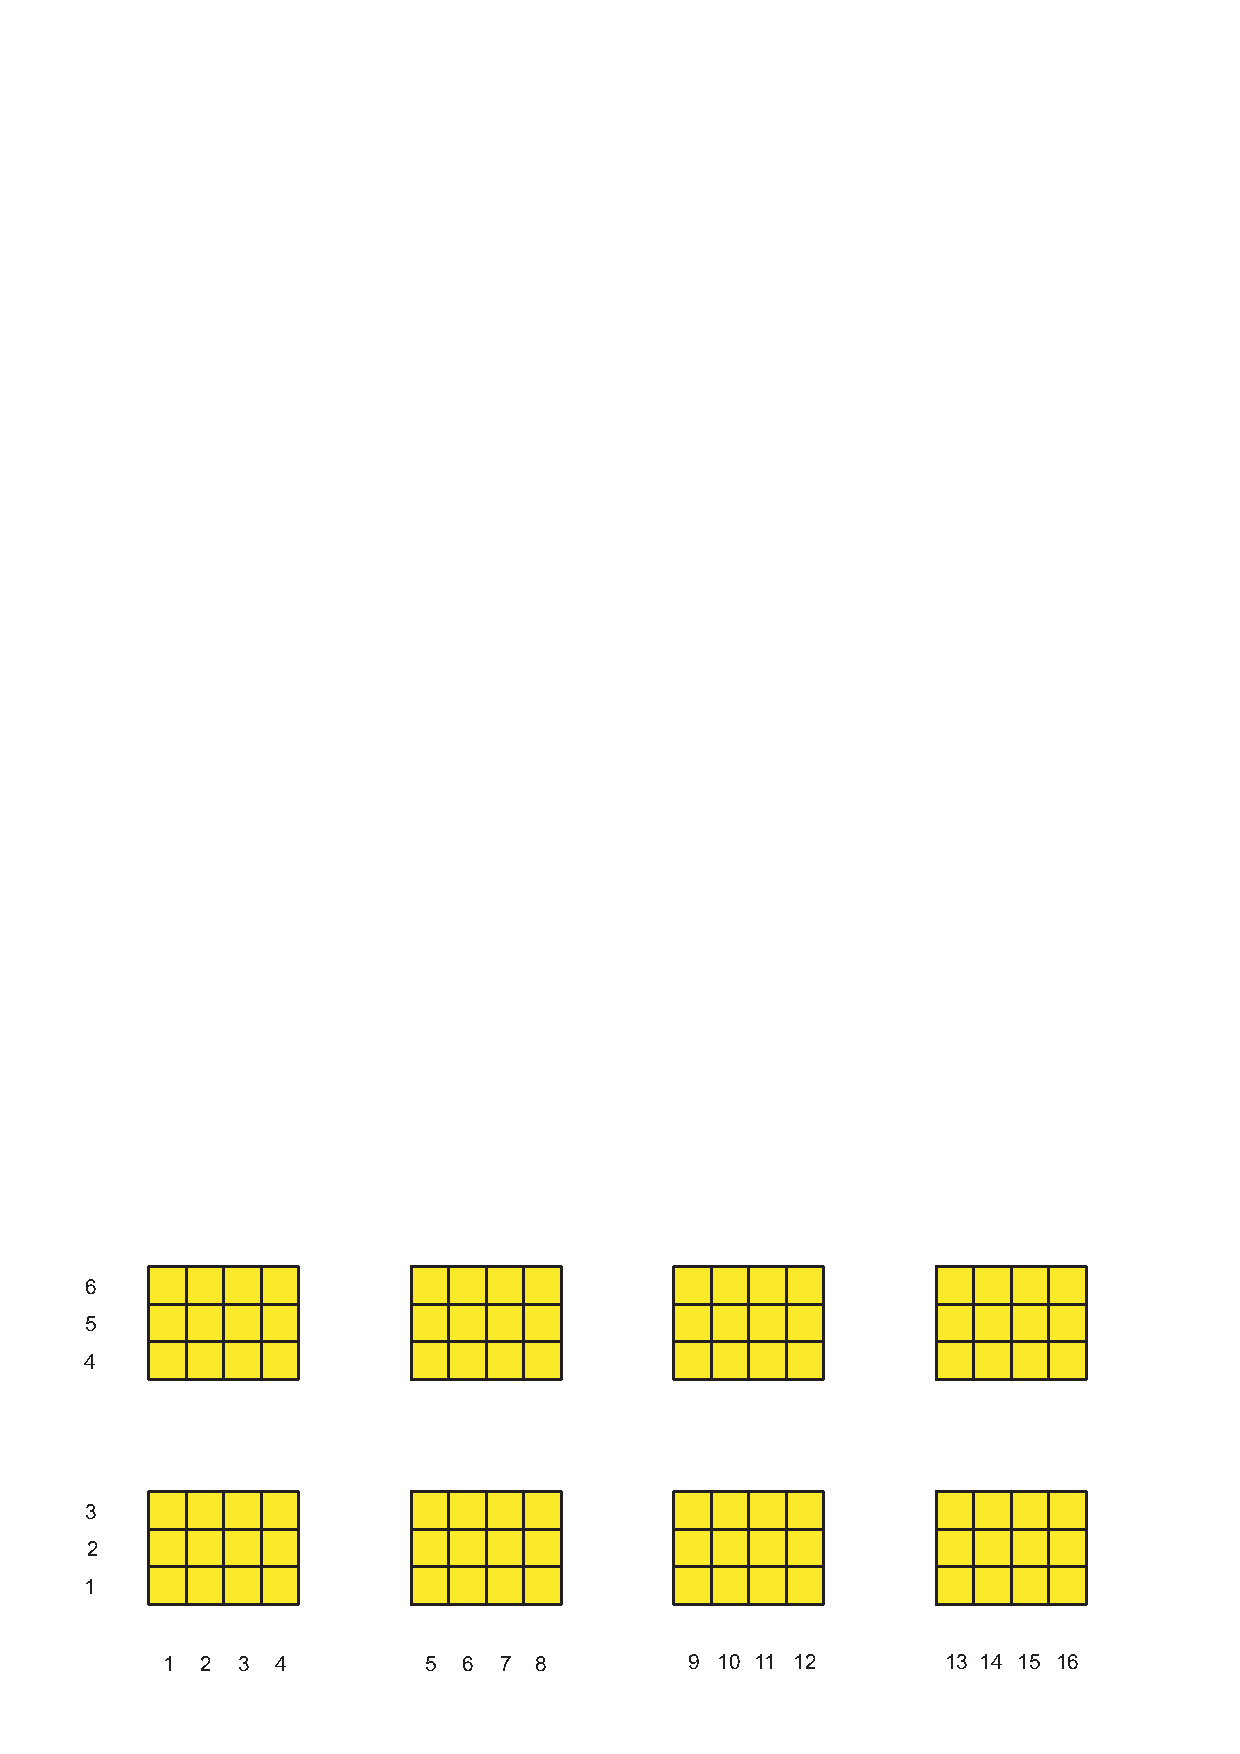
\includegraphics{GridExclusiveReg}}
  \caption{An example of a Grid's exclusive region for the corner stagger}
  \label{fig:gridexreg}
  \end{figure}
  \end{center}
  
   Figure~\ref{fig:gridexreg} shows an example of a Grid exclusive region for the
   {\tt ESMF\_STAGGERLOC\_CORNER} stagger with default
   stagger padding. This exclusive region would be for a Grid generated by either of the
   following calls: 
%/////////////////////////////////////////////////////////////

 \begin{verbatim}
  grid2D=ESMF_GridCreateNoPeriDim(regDecomp=(/2,4/), maxIndex=(/5,15/), &
           indexflag=ESMF_INDEX_GLOBAL, rc=rc)
 
\end{verbatim}
 
%/////////////////////////////////////////////////////////////

 \begin{verbatim}
  grid2D=ESMF_GridCreateNoPeriDim(countsPerDEDim1=(/4,4,4,3/), &
           countsPerDEDim2=(/3,2/), indexflag=ESMF_INDEX_GLOBAL, rc=rc)
 
\end{verbatim}
 
%/////////////////////////////////////////////////////////////

   Each rectangle in this diagram represents a DE and the numbers along the sides
   are the index values of the locations in the DE. Note that the exclusive region
   has one extra index location in each dimension than the number of cells
   because of the padding for the larger corner stagger location.
  
   The computational region is a user-settable region which can be used
   to distinguish a particular area for computation. The Grid doesn't
   currently contain functionality to let the user set the computational
   region so it defaults to the exclusive region. However, if the
   user sets an Array holding different computational bounds into the
   Grid then that Array's computational bounds will be used.
  
   The total region is the outermost boundary of the memory allocated
   on each DE to hold the data for the stagger location on that DE. This region
   can be as small as the exclusive region, but may be larger to
   include space for halos, memory padding, etc. The total region is
   what is enlarged to include space for halos, and the total region
   must be large enough to contain the maximum halo operation on the
   Grid. The Grid doesn't currently contain functionality to let the
   user set the total region so it defaults to the exclusive region.
   However, if the
   user sets an Array holding different total bounds into the
   Grid then that Array's total bounds will be used.
  
   The user can retrieve a set of bounds for each index space region
   described above: exclusive bounds, computational bounds,
   and total bounds. Note that although some of these are similar
   to bounds provided by ESMF\_Array subroutines
   (see Section~\ref{Array_regions_and_default_bounds})
   the format here is different. The Array bounds are only for
   distributed dimensions and are ordered to correspond
   to the dimension order in the associated DistGrid. The bounds
   provided by the Grid are ordered according to the order of dimensions of the data
   in question. This means that the bounds provided should be usable
   "as is" to access the data.
  
   Each of the three types of bounds refers to the maximum and minimum
   per dimension of the index ranges of a particular region. The parameters
   referring to the maximums contain a 'U' for upper. The parameters referring
   to the minimums contain an 'L' for lower. The bounds and associated
   quantities are almost always given on a per DE basis. The three types of
   bounds {\tt exclusiveBounds}, {\tt computationalBounds}, and {\tt totalBounds} refer
   to the ranges of the exclusive region, the computational region, and the
   total region. Each of these bounds also has a corresponding count parameter
   which gives the number of items across that region (on a DE) in each dimension.
   (e.g. {\tt totalCount(d)=totallUBound(i)-totalLBound(i)+1}). Width parameters
   give the spacing between two different types of region. The
   {\tt computationalWidth} argument gives the spacing between the exclusive
   region and the computational region. The {\tt totalWidth} argument gives the
   spacing between the total region and the computational region. Like the
   other bound information these are typically on a per DE basis, for example
   specifying {\tt totalLWidth=(1,1)} makes the bottom of the total
   region one lower in each dimension than the computational region on
   each DE. The exceptions to the per DE rule are
   {\tt staggerEdgeWidth}, and {\tt gridEdgeWidth}
   which give the spacing only on the DEs along the boundary of the Grid.
  
   All the above bound discussions only apply to the grid with non-arbitrary distributions,
   i.e., regular or irregular distributions.  For an arbitrarily distributed grid,
   only center stagger location is supported and there is no padding around the grid.
   Thus, the exclusive bounds, the total bounds and the computational bounds are identical
   and {\tt staggerEdgeWidth}, and {\tt gridEdgeWidth} are all zeros. 
%/////////////////////////////////////////////////////////////

  \subsubsection{Get Grid coordinate bounds}
  
   When operating on coordinates the user may often wish to
   retrieve the bounds of the piece of coordinate data on
   a particular local DE. This is useful for iterating through the
   data to set coordinates, retrieve coordinates, or do calculations.
   The method {\tt ESMF\_GridGetCoord} allows the user
   to retrieve bound information for a particular coordinate
   array.
  
   As described in the previous section there are three types of bounds the user can
   get: exclusive bounds, computational bounds,
   and total bounds. The bounds
   provided by {\tt ESMF\_GridGetCoordBounds} are for both distributed
   and undistributed dimensions and are ordered according to the
   order of dimensions in the  coordinate. This means that the bounds
    provided should be usable
   "as is" to access data in the coordinate array. In the case
   of factorized coordinate Arrays where a coordinate may
   have a smaller dimension than its associated Grid, then
   the dimension of the coordinate's bounds are the dimension of
   the coordinate, not the Grid.
  
   The following is an example of retrieving the bounds for localDE 0 for the first
   coordinate array from the corner stagger location. 
%/////////////////////////////////////////////////////////////

 \begin{verbatim}
   call ESMF_GridGetCoordBounds(grid2D, coordDim=1, localDE=0,  &
          staggerLoc=ESMF_STAGGERLOC_CORNER,                         &
          exclusiveLBound=elbnd, exclusiveUBound=eubnd,              &
          computationalLBound=clbnd, computationalUBound=cubnd,      &
          totalLBound=tlbnd, totalUBound=tubnd, rc=rc)
 
\end{verbatim}
 
%/////////////////////////////////////////////////////////////

  \subsubsection{Get Grid stagger location bounds}
  
   When operating on data stored at a particular stagger
   in a Grid the user may find it useful to be able
   to retrieve the bounds of the data on a particular local DE.
   This is useful for iterating through the
   data for computations or allocating arrays to hold the data.
   The method {\tt ESMF\_GridGet} allows the user
   to retrieve bound information for a particular stagger location.
  
   As described in Section~\ref{sec:grid:usage:bounds} there are three types of bounds
   the user can typically get, however, the Grid doesn't hold data at
   a stagger location (that is the job of the Field), and so
   no Array is contained there and so no total region exists, so the
   user may only retrieve exclusive and computational bounds from
   a stagger location.  The bounds
   provided by {\tt ESMF\_GridGet} are ordered according to the
   order of dimensions in the Grid.
  
   The following is an example of retrieving the bounds for localDE 0
   from the corner stagger location. 
%/////////////////////////////////////////////////////////////

 \begin{verbatim}
   call ESMF_GridGet(grid2D, localDE=0,                         &
          staggerLoc=ESMF_STAGGERLOC_CORNER,                    &
          exclusiveLBound=elbnd, exclusiveUBound=eubnd,         &
          computationalLBound=clbnd, computationalUBound=cubnd, rc=rc)
 
\end{verbatim}
 
%/////////////////////////////////////////////////////////////

  \subsubsection{Get Grid stagger location information}
  
   In addition to the per DE information that can be accessed about
   a stagger location there is some global information that can
   accessed by using {\tt ESMF\_GridGet} without specifying a
   localDE. One of the uses of this information is to create
   an ESMF Array to hold data for a stagger location.
  
   \begin{sloppypar}
   The information currently available from a stagger
   location is the {\tt distgrid}. The {\tt distgrid} gives the
   distgrid which describes the size and distribution of the elements in the stagger location.
   \end{sloppypar}
  
   The following is an example of retrieving information for localDE 0
   from the corner stagger location. 
%/////////////////////////////////////////////////////////////

 \begin{verbatim}
    ! Get info about staggerloc
    call ESMF_GridGet(grid2D, staggerLoc=ESMF_STAGGERLOC_CORNER,  &
           distgrid=staggerDistgrid, &
           rc=rc)

 
\end{verbatim}
 
%/////////////////////////////////////////////////////////////

  \subsubsection{Create an Array at a stagger location}
  
   In order to create an Array to correspond to a Grid stagger location
   several pieces of information need to be obtained from both the
   Grid and the stagger location in the Grid.
  
   The information that needs to be obtained from the Grid
   is the {\tt distgridToGridMap} to ensure that the new Array
   has its  dimensions are mapped correctly to the Grid. These
   are obtained using the {\tt ESMF\_GridGet} method.
  
   The information that needs to be obtained from the stagger
   location is the distgrid that describes the size and distribution
   of the elements in the stagger location. This information can
   be obtained using the stagger location specific {\tt ESMF\_GridGet} method.
  
   The following is an example of using information from a 2D Grid with non-arbitrary
   distribution to create an Array corresponding to a stagger location.
   
%/////////////////////////////////////////////////////////////

 \begin{verbatim}

    ! Get info from Grid
    call ESMF_GridGet(grid2D, distgridToGridMap=distgridToGridMap, rc=rc)
 
\end{verbatim}
 
%/////////////////////////////////////////////////////////////

 \begin{verbatim}

    ! Get info about staggerloc
    call ESMF_GridGet(grid2D, staggerLoc=ESMF_STAGGERLOC_CORNER, &
           distgrid=staggerDistgrid, &
           rc=rc)
 
\end{verbatim}
 
%/////////////////////////////////////////////////////////////

 \begin{verbatim}


    ! construct ArraySpec
    call ESMF_ArraySpecSet(arrayspec, rank=2, typekind=ESMF_TYPEKIND_R8, rc=rc)
 
\end{verbatim}
 
%/////////////////////////////////////////////////////////////

 \begin{verbatim}


    ! Create an Array based on info from grid
    array=ESMF_ArrayCreate(arrayspec=arrayspec, &
            distgrid=staggerDistgrid, distgridToArrayMap=distgridToGridMap, &
            rc=rc)

 
\end{verbatim}
 
%/////////////////////////////////////////////////////////////

   Creating an Array for a Grid with arbitrary distribution is different.
   For a 2D Grid with both dimension arbitrarily distributed, the Array dimension
   is 1.  For a 3D Grid with two arbitrarily distributed dimensions and one
   undistributed dimension, the Array dimension is 2.  In general,
   if the Array does not have any ungridded dimension, the Array dimension
   should be 1 plus the number of undistributed dimensions of the Grid.
  
   The following is an example of creating an Array for a 3D Grid with 2
   arbitrarily distributed dimensions such as the one defined in Section~\ref{example:ArbGridWithUndistDim}. 
%/////////////////////////////////////////////////////////////

 \begin{verbatim}
    ! Get distGrid from Grid
    call ESMF_GridGet(grid3D, distgrid=distgrid, rc=rc)
 
\end{verbatim}
 
%/////////////////////////////////////////////////////////////

 \begin{verbatim}


    ! construct ArraySpec
    call ESMF_ArraySpecSet(arrayspec, rank=2, typekind=ESMF_TYPEKIND_R8, rc=rc)
 
\end{verbatim}
 
%/////////////////////////////////////////////////////////////

 \begin{verbatim}


    ! Create an Array based on the presence of distributed dimensions
    array=ESMF_ArrayCreate(arrayspec=arrayspec,distgrid=distgrid, rc=rc)

 
\end{verbatim}
 
%/////////////////////////////////////////////////////////////

  \subsubsection{Create more complex Grids using DistGrid}
  \label{sec:usage:adv:create}
  
   Besides the shortcut methods for creating a Grid object such as
   {\tt ESMF\_GridCreateNoPeriDim()}, there is
   a set of methods which give the user more control over the
   specifics of the grid.  The following describes the more
   general interface, using DistGrid.
   The basic idea is to first create an ESMF DistGrid object describing
   the distribution and shape of the Grid, and then to employ that to either directly
   create the Grid or first create Arrays and then create the Grid from those.
   This method gives the user maximum control over the topology and distribution of the Grid.
   See the DistGrid documentation in Section~\ref{sec:DistGrid} for an
   in-depth description of its interface and use.
  
   As an example, the following call constructs
   a 10x20 Grid with a lower bound of (1,2). 
%/////////////////////////////////////////////////////////////

 \begin{verbatim}
   ! Create DistGrid
   distgrid2D = ESMF_DistGridCreate(minIndex=(/1,2/), maxIndex=(/11,22/), &
           rc=rc)
 
\end{verbatim}
 
%/////////////////////////////////////////////////////////////

 \begin{verbatim}

   ! Create Grid
   grid3D=ESMF_GridCreate(distGrid=distgrid2D, rc=rc)
 
\end{verbatim}
 
%/////////////////////////////////////////////////////////////

   \begin{sloppypar}
   To alter which dimensions are distributed, the {\tt distgridToGridMap}
   argument can be used. The {\tt distgridToGridMap} is used to set
   which dimensions of the Grid are mapped to the dimensions
   described by {\tt maxIndex}. In other words, it describes how the dimensions of
   the underlying default DistGrid are mapped to the Grid. Each entry
   in {\tt distgridToGridMap} contains the Grid dimension to which the corresponding
   DistGrid dimension should be mapped.
   The following example illustrates the creation of a Grid where the largest
   dimension is first. To accomplish this the two dimensions are swapped.
   \end{sloppypar} 
%/////////////////////////////////////////////////////////////

 \begin{verbatim}
   ! Create DistGrid
   distgrid2D = ESMF_DistGridCreate(minIndex=(/1,2/), maxIndex=(/11,22/), &
        rc=rc)
 
\end{verbatim}
 
%/////////////////////////////////////////////////////////////

 \begin{verbatim}

   ! Create Grid
   grid2D=ESMF_GridCreate(distGrid=distgrid2D, distgridToGridMap=(/2,1/), &
        rc=rc)
 
\end{verbatim}
 
%/////////////////////////////////////////////////////////////

  \subsubsection{Specify custom stagger locations}
  \label{sec:usage:staggerloc:adv}
  
   Although ESMF provides a set of predefined stagger locations (See Section~\ref{const:staggerloc}),
   the user may need one outside this set. This section describes the construction of
   custom stagger locations.
  
   To completely specify a stagger for an arbitrary number of dimensions, we define the
   stagger location in terms of a set of cartesian coordinates. The cell is represented
   by a n-dimensional cube with sides of length 2, and the coordinate origin located at
   the center of the cell. The geometry of the cell is for reference purposes only,
   and does not literally represent the actual shape of the cell. Think of this method
   instead as an easy way to specify a part (e.g. center, corner, face) of a higher
   dimensional cell which is extensible to any number of dimensions.
  
   To illustrate this approach, consider a 2D cell. In 2 dimensions
   the cell is represented by a square. An xy axis is placed at its center, with the
   positive x-axis oriented {\em East} and the positive y-axis oriented {\em North}.
   The resulting coordinate for the lower left corner is at $(-1,-1)$, and upper right
   corner at $(1,1)$.
   However, because our staggers are symmetric they don't need to distinguish between
   the $-1$, and the $1$, so we only need to concern ourselves with the first quadrant of
   this cell. We only need to use the $1$, and the $0$, and many of the cell locations
   collapse together (e.g. we only need to represent one corner). See figure~\ref{fig:gridcuststaggerloc}
   for an illustration of these concepts.
  
  \begin{center}
  \begin{figure}
  \center
  \scalebox{0.75}{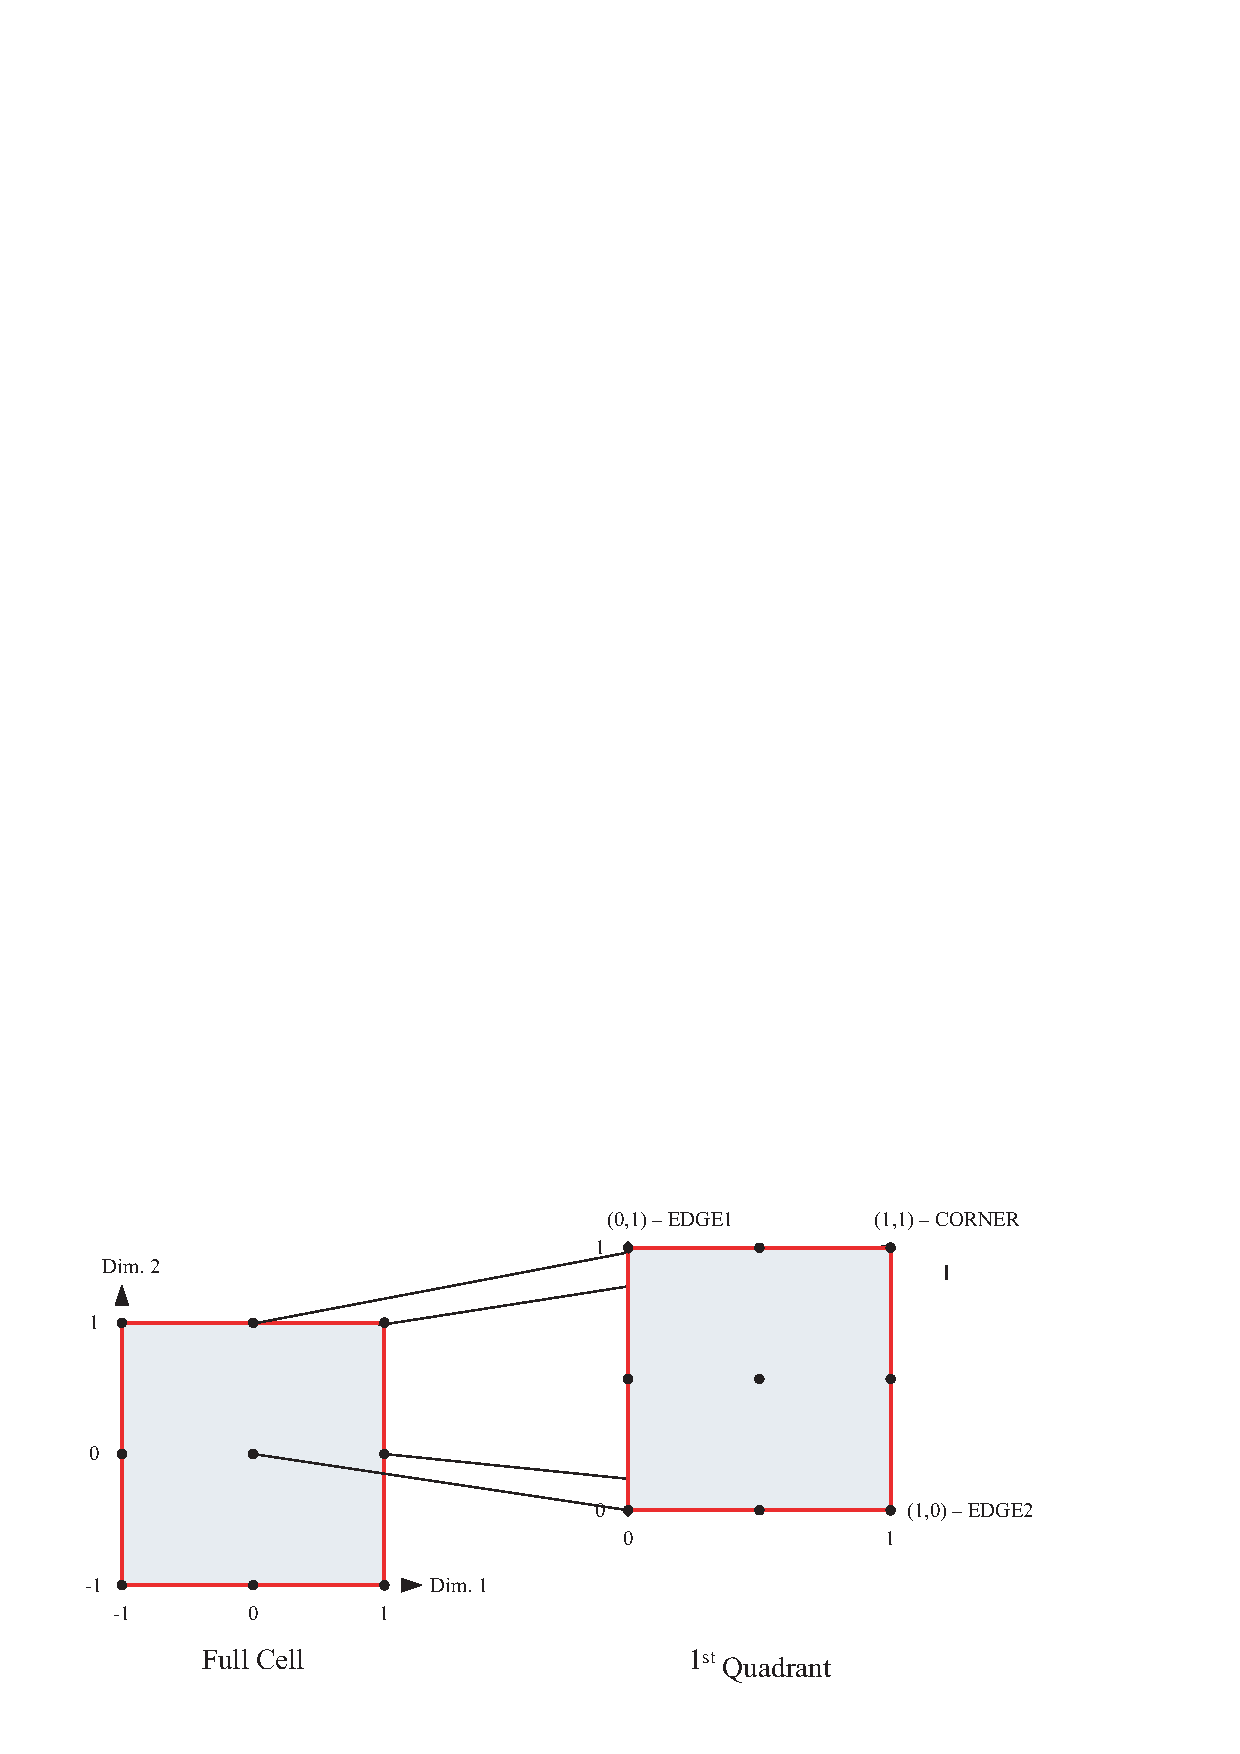
\includegraphics{GridCustStaggerLoc}}
  \caption{An example of specifying 2D stagger locations using coordinates.}
  \label{fig:gridcuststaggerloc}
  \end{figure}
  \end{center}
  
   The cell center is represented by the coordinate pair $(0,0)$ indicating the origin.
   The cell corner is $+1$ in each direction, giving a coordinate pair of $(1,1)$.
   The edges are each $+1$ in one dimension and $0$ in the other indicating that
   they're even with the center in one dimension and offset in the other.
  
   For three dimensions, the vertical component of the stagger location can be added by
   simply adding an additional coordinate. The three dimensional generalization of the
   cell center becomes $(0,0,0)$ and the cell corner becomes $(1,1,1)$. The rest of
   the 3D stagger locations are combinations of $+1$ offsets from the center.
  
   To generalize this to $d$ dimensions, to represent a $d$ dimensional stagger
   location. A set of $d$ $0$ and $1$ is used to specify for each dimension
   whether a stagger location is aligned with the cell center in that dimension ($0$),
   or offset by $+1$ in that dimension ($1$). Using this scheme we can represent
   any symmetric stagger location.
  
   To construct a custom stagger location in ESMF the subroutine
   {\tt ESMF\_StaggerLocSet()} is used to specify,
   for each dimension, whether the stagger is located at the interior (0)
   or on the boundary (1) of the cell. This method allows users
   to construct stagger locations for which
   there is no predefined value. In this example, it's used to
   set the 4D center and 4D corner locations.
   
%/////////////////////////////////////////////////////////////

 \begin{verbatim}

   ! Set Center
   call ESMF_StaggerLocSet(staggerLoc,loc=(/0,0,0,0/),rc=rc)
 
\end{verbatim}
 
%/////////////////////////////////////////////////////////////

 \begin{verbatim}
   call ESMF_GridAddCoord(grid4D, staggerLoc=staggerLoc, rc=rc)
 
\end{verbatim}
 
%/////////////////////////////////////////////////////////////

 \begin{verbatim}


   ! Set Corner
   call ESMF_StaggerLocSet(staggerLoc,loc=(/1,1,1,1/),rc=rc)
 
\end{verbatim}
 
%/////////////////////////////////////////////////////////////

 \begin{verbatim}

   call ESMF_GridAddCoord(grid4D, staggerLoc=staggerLoc, rc=rc)
 
\end{verbatim}
 
%/////////////////////////////////////////////////////////////

  \subsubsection{Specify custom stagger padding}
  \label{sec:usage:staggerpadding:adv}
  
  There is an added complication with the data (e.g. coordinates) stored at stagger locations in
  that they can require different amounts of storage depending
  on the underlying Grid type.
  
  \begin{center}
  \begin{figure}
  \center
  \scalebox{0.75}{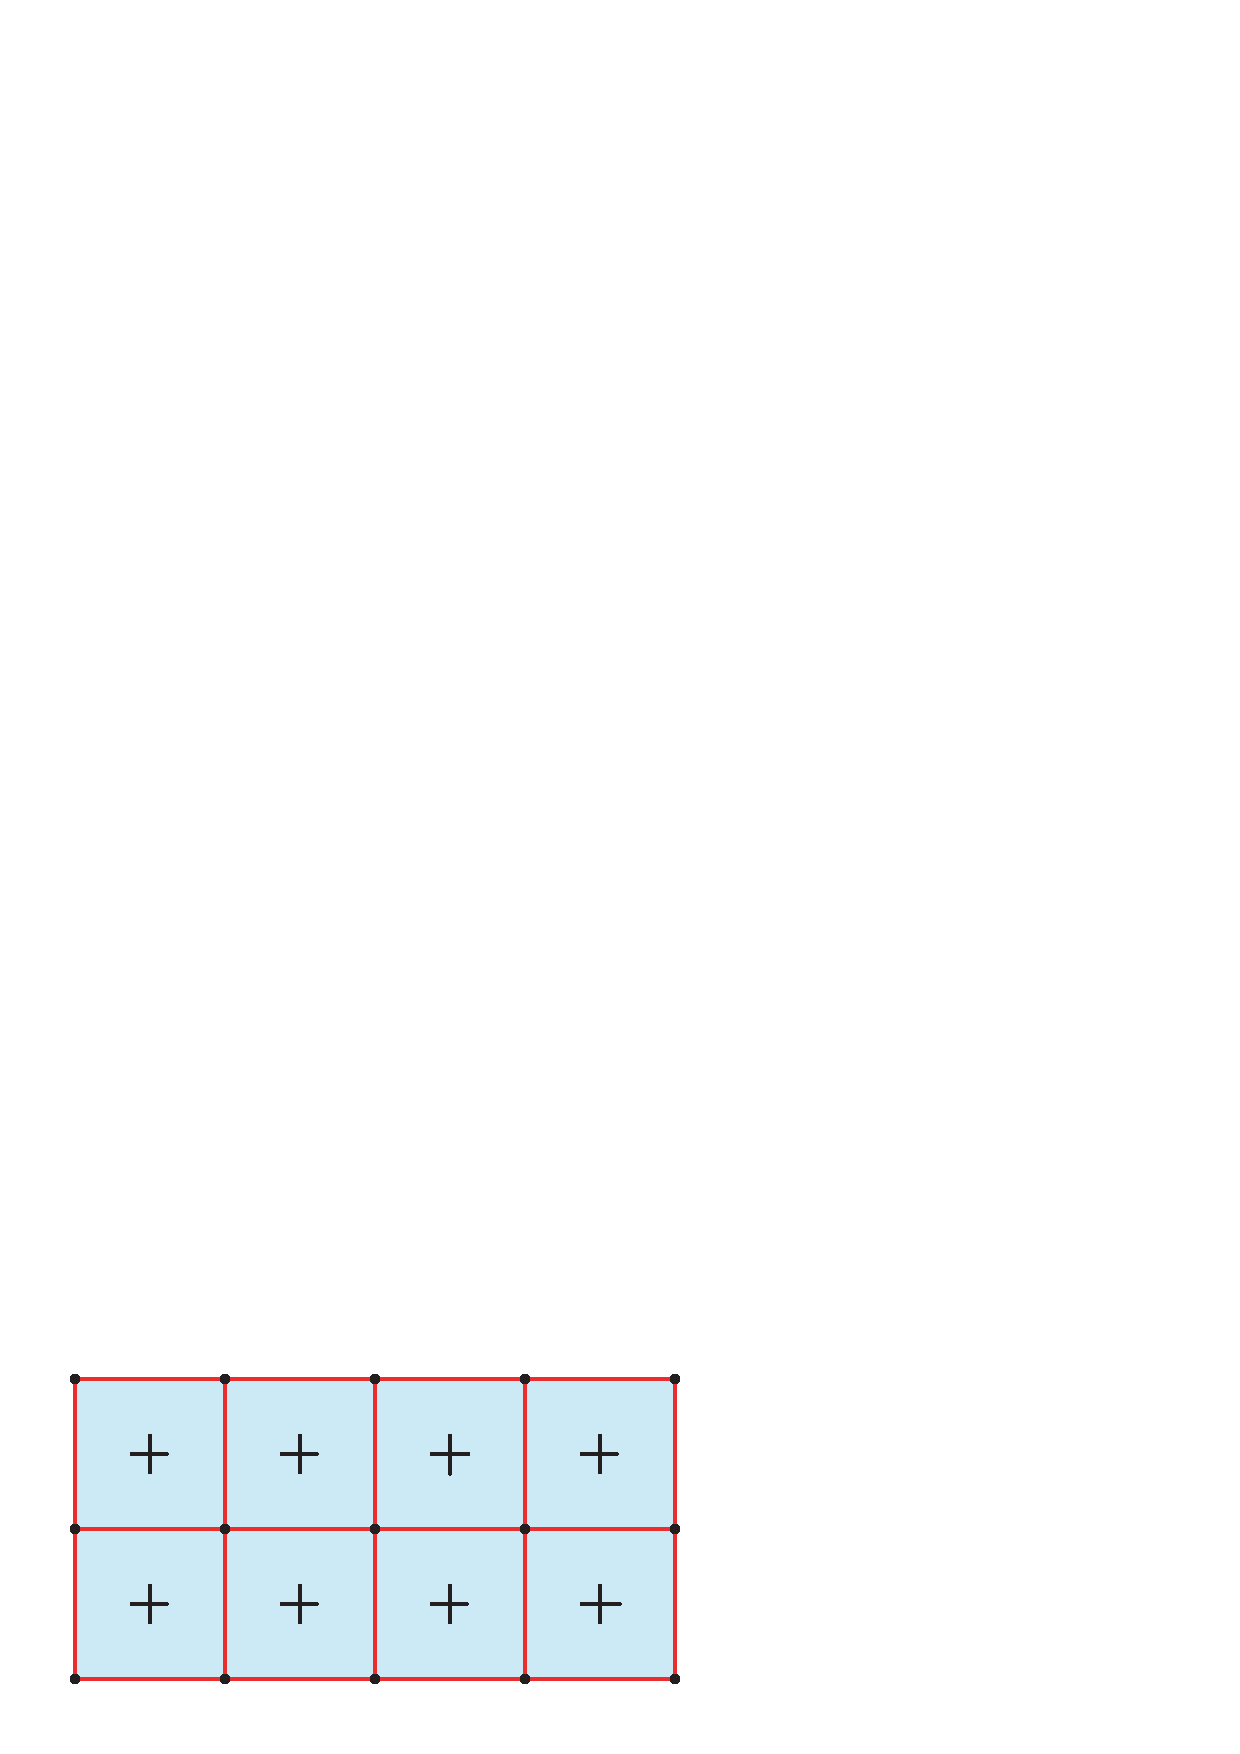
\includegraphics{GridCellsAndCorners}}
  \caption{An example 2D Grid with cell centers and corners.}
  \label{fig:gridcellsandcorners}
  \end{figure}
  \end{center}
  
   Consider the example 2D grid in figure~\ref{fig:gridcellsandcorners}, where the dots represent the cell corners
   and the ``+'' represents the cell centers. For the corners to completely
   enclose the cell centers (symmetric stagger), the number of corners in each
   dimension needs to be one greater then the number of cell centers. In the above
   figure, there are two rows and three columns of cell centers. To enclose the
   cell centers, there must be three rows and four columns of cell corners.
   This is true in general for Grids without periodicity or
   other connections.  In fact, for a symmetric stagger, given that the center
   location requires n x m storage, the corresponding corner location
   requires n+1 x m+1, and the edges, depending on the side, require n+1 x m or
   m+1 x n.  In order to add the extra storage, a new DistGrid is
   created at each stagger location. This Distgrid is similar to the DistGrid
   used to create the Grid, but has an extra set of elements added to hold the
   index locations for the stagger padding.
   By default, when the coordinate arrays are created, one extra
   layer of padding is added to the index space to create symmetric staggers
   (i.e. the center location is surrounded). The default is to add this padding
   on the positive side, and to only add this padding where needed
   (e.g. no padding for the center, padding
   on both dimensions for the corner, in only one dimension for the
   edge in 2D.) There are two ways for the user to change
   these defaults.
  
   One way is to use the {\tt GridEdgeWidth} or {\tt GridAlign} arguments
   when creating a Grid. These arguments can be used to change the default padding
   around the Grid cell index space. This extra padding is used by default
   when setting the padding for a stagger location.
  
   The {\tt gridEdgeLWidth} and
   {\tt gridEdgeUWidth} arguments are both 1D arrays of the
   same size as the Grid dimension. The entries in the arrays
   give the extra offset from the outer boundary of
   the grid cell index space. The following example shows the
   creation of a Grid with all the extra space to hold stagger padding
   on the negative side of a Grid. This is the reverse of
   the default behavior. The resulting Grid will have
   an exclusive region which extends from $(-1,-1)$ to
   $(10,10)$, however, the cell center stagger location
   will still extend from $(1,1)$ to $(10,10)$. 
%/////////////////////////////////////////////////////////////

 \begin{verbatim}
   grid2D=ESMF_GridCreateNoPeriDim(minIndex=(/1,1/),maxIndex=(/10,10/), &
            gridEdgeLWidth=(/1,1/), gridEdgeUWidth=(/0,0/), rc=rc)

 
\end{verbatim}
 
%/////////////////////////////////////////////////////////////

   To indicate how the data in a Grid's stagger locations are aligned with the
   cell centers, the optional {\tt gridAlign} parameter
   may be used. This parameter indicates which stagger elements
   in a cell share the same index values as the cell center.
   For example, in a 2D cell, it would indicate which of the four corners has
   the same index value as the center. To set {\tt gridAlign},
   the values -1,+1 are used to indicate the alignment in
   each dimension. This parameter is mostly
   informational, however, if the {\tt gridEdgeWidth} parameters
   are not set then its value determines where the default padding
   is placed. If not specified, then the default is to align all
   staggers to the most negative, so the padding is on the positive side.
   The following code illustrates creating a Grid aligned to the reverse of
   default (with everything to the positive side). This creates a
   Grid identical to that created in the previous example. 
%/////////////////////////////////////////////////////////////

 \begin{verbatim}
   grid2D=ESMF_GridCreateNoPeriDim(minIndex=(/1,1/),maxIndex=(/10,10/), &
            gridAlign=(/1,1/), rc=rc)

 
\end{verbatim}
 
%/////////////////////////////////////////////////////////////

   The {\tt gridEdgeWidth} and {\tt gridAlign} arguments both
   allow the user to set the default padding to be used
   by stagger locations in a Grid. By default, stagger locations
   allocated in a Grid set their stagger padding based on these
   values.  A stagger location's padding in each dimension is
   equal to the value of {\tt gridEdgeWidth} (or the value implied
   by {\tt gridAlign}), unless the stagger location is centered
   in a dimension in which case the stagger padding is 0. For example,
   the cell center stagger location has 0 stagger padding in all
   dimensions, whereas the edge stagger location lower padding
   is equal to {\tt gridEdgeLWidth} and the upper padding is equal
   to {\tt gridEdgeUWidth} in one dimension, but both are 0 in the other,
   centered, dimension.  If the user wishes to set the stagger padding
   individually for each stagger location they may use the
   {\tt staggerEdgeWidth} and {\tt staggerAlign} arguments.
  
   The {\tt staggerEdgeLWidth} and
   {\tt staggerEdgeUWidth} arguments are both 1D arrays of the
   same size as the Grid dimension. The entries in the arrays
   give the extra offset from the Grid cell index space
   for a stagger location. The following example shows the
   addition of two stagger locations. The
   corner location has no extra boundary and the
   center has a single layer of extra padding on
   the negative side and none on the positive.  This is the reverse of
   the default behavior. 
%/////////////////////////////////////////////////////////////

 \begin{verbatim}
   grid2D=ESMF_GridCreate(distgrid=distgrid2D, &
            gridEdgeLWidth=(/1,1/), gridEdgeUWidth=(/0,0/), rc=rc)
 
\end{verbatim}
 
%/////////////////////////////////////////////////////////////

 \begin{verbatim}


   call ESMF_GridAddCoord(grid2D, &
          staggerLoc=ESMF_STAGGERLOC_CORNER, &
          staggerEdgeLWidth=(/0,0/), staggerEdgeUWidth=(/0,0/), rc=rc)
 
\end{verbatim}
 
%/////////////////////////////////////////////////////////////

 \begin{verbatim}


   call ESMF_GridAddCoord(grid2D, &
          staggerLoc=ESMF_STAGGERLOC_CENTER, &
          staggerEdgeLWidth=(/1,1/), staggerEdgeUWidth=(/0,0/), rc=rc)

 
\end{verbatim}
 
%/////////////////////////////////////////////////////////////

   To indicate how the data at a particular stagger location is aligned with the
   cell center, the optional {\tt staggerAlign} parameter
   may be used. This parameter indicates which stagger elements
   in a cell share the same index values as the cell center.
   For example, in a 2D cell, it would indicate which of the four corners has
   the same index value as the center. To set {\tt staggerAlign},
   the values -1,+1 are used to indicate the alignment in
   each dimension. If a stagger location is
   centered in a dimension (e.g. an edge in 2D), then that
   dimension is ignored in the alignment. This parameter is mostly
   informational, however, if the {\tt staggerEdgeWidth} parameters
   are not set then its value determines where the default padding
   is placed. If not specified, then the default is to align all
   staggers to the most negative, so the padding is on the positive side.
   The following code illustrates aligning the positive (northeast in 2D)
   corner with the center. 
%/////////////////////////////////////////////////////////////

 \begin{verbatim}
   call ESMF_GridAddCoord(grid2D, &
          staggerLoc=ESMF_STAGGERLOC_CORNER, staggerAlign=(/1,1/), rc=rc)
 
\end{verbatim}

%...............................................................
\setlength{\parskip}{\oldparskip}
\setlength{\parindent}{\oldparindent}
\setlength{\baselineskip}{\oldbaselineskip}

%%                **** IMPORTANT NOTICE *****
% This LaTeX file has been automatically produced by ProTeX v. 1.1
% Any changes made to this file will likely be lost next time
% this file is regenerated from its source. Send questions 
% to Arlindo da Silva, dasilva@gsfc.nasa.gov
 
\setlength{\oldparskip}{\parskip}
\setlength{\parskip}{1.5ex}
\setlength{\oldparindent}{\parindent}
\setlength{\parindent}{0pt}
\setlength{\oldbaselineskip}{\baselineskip}
\setlength{\baselineskip}{11pt}
 
%--------------------- SHORT-HAND MACROS ----------------------
\def\bv{\begin{verbatim}}
\def\ev{\end{verbatim}}
\def\be{\begin{equation}}
\def\ee{\end{equation}}
\def\bea{\begin{eqnarray}}
\def\eea{\end{eqnarray}}
\def\bi{\begin{itemize}}
\def\ei{\end{itemize}}
\def\bn{\begin{enumerate}}
\def\en{\end{enumerate}}
\def\bd{\begin{description}}
\def\ed{\end{description}}
\def\({\left (}
\def\){\right )}
\def\[{\left [}
\def\]{\right ]}
\def\<{\left  \langle}
\def\>{\right \rangle}
\def\cI{{\cal I}}
\def\diag{\mathop{\rm diag}}
\def\tr{\mathop{\rm tr}}
%-------------------------------------------------------------

\markboth{Left}{Source File: ESMF\_GridCreateRegFromDGEx.F90,  Date: Tue May  5 20:59:48 MDT 2020
}

 
%/////////////////////////////////////////////////////////////

   \subsubsection{Create a 2D Grid with regular distribution from a DistGrid}~\label{sec:usage:ex:adv:reg}
  
   This example illustrates the creation of a single tile 2D Grid
   with a regular distribution from a DistGrid.  The size of the Grid is
   gridSize(1) by gridSize(2) elements. It only contains data
   in the center stagger location (i.e. Arakawa A-Grid). 
%/////////////////////////////////////////////////////////////

 \begin{verbatim}
      ! Use ESMF framework module
      use ESMF
      use ESMF_TestMod
      implicit none

      ! Local variables  
      integer:: rc, finalrc, result
      type(ESMF_VM):: vm
      type(ESMF_DistGrid) :: distgrid2D
      type(ESMF_Grid) :: grid2D
 
\end{verbatim}
 
%/////////////////////////////////////////////////////////////

   First construct a single tile distgrid with regular distribution of the
   appropriate size. 
%/////////////////////////////////////////////////////////////

 \begin{verbatim}

      distgrid2D = ESMF_DistGridCreate(minIndex=(/1,1/),      &
                          maxIndex=(/20,30/), rc=rc)  
 
\end{verbatim}
 
%/////////////////////////////////////////////////////////////

      Create a Grid using the distgrid.  
%/////////////////////////////////////////////////////////////

 \begin{verbatim}
     Grid2D=ESMF_GridCreate(name="Simple 2D Regular", &
               distgrid=distgrid2D, rc=rc)
 
\end{verbatim}
 
%/////////////////////////////////////////////////////////////

   Set the one stagger location as center.  
%/////////////////////////////////////////////////////////////

 \begin{verbatim}
   call ESMF_GridAddCoord(Grid2D,  &
          staggerLoc=ESMF_STAGGERLOC_CENTER, rc=rc)
 
\end{verbatim}

%...............................................................
\setlength{\parskip}{\oldparskip}
\setlength{\parindent}{\oldparindent}
\setlength{\baselineskip}{\oldbaselineskip}

%%                **** IMPORTANT NOTICE *****
% This LaTeX file has been automatically produced by ProTeX v. 1.1
% Any changes made to this file will likely be lost next time
% this file is regenerated from its source. Send questions 
% to Arlindo da Silva, dasilva@gsfc.nasa.gov
 
\setlength{\oldparskip}{\parskip}
\setlength{\parskip}{1.5ex}
\setlength{\oldparindent}{\parindent}
\setlength{\parindent}{0pt}
\setlength{\oldbaselineskip}{\baselineskip}
\setlength{\baselineskip}{11pt}
 
%--------------------- SHORT-HAND MACROS ----------------------
\def\bv{\begin{verbatim}}
\def\ev{\end{verbatim}}
\def\be{\begin{equation}}
\def\ee{\end{equation}}
\def\bea{\begin{eqnarray}}
\def\eea{\end{eqnarray}}
\def\bi{\begin{itemize}}
\def\ei{\end{itemize}}
\def\bn{\begin{enumerate}}
\def\en{\end{enumerate}}
\def\bd{\begin{description}}
\def\ed{\end{description}}
\def\({\left (}
\def\){\right )}
\def\[{\left [}
\def\]{\right ]}
\def\<{\left  \langle}
\def\>{\right \rangle}
\def\cI{{\cal I}}
\def\diag{\mathop{\rm diag}}
\def\tr{\mathop{\rm tr}}
%-------------------------------------------------------------

\markboth{Left}{Source File: ESMF\_GridCreateTripoleEx.F90,  Date: Tue May  5 20:59:48 MDT 2020
}

 
%/////////////////////////////////////////////////////////////

   \subsubsection{Create a 2D tripole grid from Arrays}\label{sec:usage:ex:adv:tripole}
  
   This example illustrates the creation of a 2D tripole Grid from coordinate data
   read in on a single processor and then distributed to the rest of the processors. 
   The Grid contains just the center stagger location. The size of the Grid is gridSize(1) by 
   gridSize(2). 
%/////////////////////////////////////////////////////////////

 \begin{verbatim}
      ! Use ESMF framework module
      use ESMF
      implicit none

      ! Local variables  
      integer:: rc, finalrc
      integer:: myPet, npets, rootPet
      type(ESMF_VM):: vm
      type(ESMF_Config) :: config
      type(ESMF_DistGrid) :: distgrid
      type(ESMF_Array) :: gridCoordArrays(2,1)
      type(ESMF_Array) :: gridCntrCoordArrayLat,gridCntrCoordArrayLon
      type(ESMF_StaggerLoc) :: staggerLocs(1)
      type(ESMF_ArraySpec) ::  arrayspec
      real(ESMF_KIND_R8), allocatable :: globalGridCntrCoordLat(:,:)
      real(ESMF_KIND_R8), allocatable :: globalGridCntrCoordLon(:,:)
      integer :: gridSize(2), gridRank
      integer, allocatable ::  connectionList(:,:)
 
\end{verbatim}
 
%/////////////////////////////////////////////////////////////

   Allocate a Fortran array to hold sphere coodinates, then read them in. This
   all takes place on one processor. Later the data will be distributed across the processors.  
%/////////////////////////////////////////////////////////////

 \begin{verbatim}
      gridRank=2  ! 2D grid
      call read2Dgriddata(gridSize)
      allocate( globalGridCntrCoordLat(gridSize(1),gridSize(2)))
      allocate( globalGridCntrCoordLon(gridSize(1),gridSize(2)))
      call read2Dgrid(globalGridCntrCoordLat)
      call read2Dgrid(globalGridCntrCoordLon)
 
\end{verbatim}
 
%/////////////////////////////////////////////////////////////

   Construct a single tile tripole domain. 
   Specify that the first dimension is periodic: \\
  
   \begin{itemize}
   \item Setting tileIndexA=tileIndexB indicates that the connection 
        is within the tile.
   \item The position vector is set to span the width of the tile's 
        first dimension.
   \item The repetitionVector indicates that the connection repeats along
             the dimension. This takes care of both sides of the connection.
   \end{itemize} 
%/////////////////////////////////////////////////////////////

 \begin{verbatim}

      allocate( connectionList(2*gridRank,3) )
      call ESMF_ConnectionElementConstruct(                          &
                 connectionElement=connectionList(:,1),     &
                 tileIndexA=1, tileIndexB=1,              &
                 positionVector = (/gridSize(1),0/),        &
                 repetitionVector= (/1,0/), rc=rc)
 
\end{verbatim}
 
%/////////////////////////////////////////////////////////////

   Specify the northern bipolar fold: \\
  
    The position and orientation vectors indicate that each element 
    along the top edge of the tile is attached to the corresponding
    element across the fold.  
%/////////////////////////////////////////////////////////////

 \begin{verbatim}
       call ESMF_ConnectionElementConstruct(
                  connectionElement = connectionList(:,2), &
                  tileIndexA = 1, tileIndexB = 1, &
                  positionVector = (/gridSize(1)+1, 2*gridSize(2)/), &
                  orientationVector = (/-1, -2/), &
                  rc=rc)
 
\end{verbatim}
 
%/////////////////////////////////////////////////////////////

   Specify the south pole: \\
  
    The position and orientation vectors indicate that each element along
     the bottom edge of the tile is attached to the element directly across the pole.  
%/////////////////////////////////////////////////////////////

 \begin{verbatim}
       call ESMF_ConnectionElementConstruct( 
                 connectionElement = connectionList(:,3), &
                 tileIndexA = 1, tileIndexB = 1, &
                 positionVector = (/gridSize(1)/2, 0/), &
                 orientationVector = (/1, -2/), &
                 repetitionVector = (/1, 0/), &
                 rc=rc)
 
\end{verbatim}
 
%/////////////////////////////////////////////////////////////

    Construct distgrid from connection information. 
%/////////////////////////////////////////////////////////////

 \begin{verbatim}
      distgrid = ESMF_DistGridCreate( minCorner=(/1,1/),  &
                          maxCorner=(/gridSize(1),gridSize(2)/),    &
                          connectionList=connectionList, rc=rc)  

      deallocate( connectionList )
 
\end{verbatim}
 
%/////////////////////////////////////////////////////////////

    Create an array into which to put the spherical coordinates.
  
%/////////////////////////////////////////////////////////////

 \begin{verbatim}
      call ESMF_ArraySpecSet(arrayspec, typekind=ESMF_TYPEKIND_R8,  &
                 rank=gridRank)

      gridCntrCoordArrayLat = ESMF_ArrayCreate(arrayspec=arrayspec,  &
                                                 distgrid=distgrid, rc=rc)
      gridCntrCoordArrayLon = ESMF_ArrayCreate(arrayspec=arrayspec, &
                                                 distgrid=distgrid, rc=rc)
 
\end{verbatim}
 
%/////////////////////////////////////////////////////////////

    Scatter the Fortran array according to DistGrid into the esmf Array. 
%/////////////////////////////////////////////////////////////

 \begin{verbatim}
      call ESMF_ArrayScatter(gridCntrCoordArrayLat, globalGridCntrCoordLat, &
                rootPet=rootPet, vm=vm, rc=rc)    

      call ESMF_ArrayScatter(gridCntrCoordArrayLon, globalGridCntrCoordLon, &
                rootPet=rootPet, vm=vm, rc=rc)    
 
\end{verbatim}
 
%/////////////////////////////////////////////////////////////

   Load Stagger location and corresponding coordinate arrays into array of ESMF Arrays. 
%/////////////////////////////////////////////////////////////

 \begin{verbatim}
     staggerlocs(1)=ESMF_STAGGERLOC_CENTER
     gridCoordArrays(1,1)=gridCntrCoordArrayLon     
     gridCoordArrays(2,1)=gridCntrCoordArrayLat     
 
\end{verbatim}
 
%/////////////////////////////////////////////////////////////

      Create a Grid from the coordinate array.  
%/////////////////////////////////////////////////////////////

 \begin{verbatim}
     tripoleGrid = ESMF_GridCreate(arrays=gridCoordArrays, &
                               staggerLocs=staggerlocs,rc=rc)
 
\end{verbatim}

%...............................................................
\setlength{\parskip}{\oldparskip}
\setlength{\parindent}{\oldparindent}
\setlength{\baselineskip}{\oldbaselineskip}

%\input{../Infrastructure/Grid/doc/ESMF_GridCreateSph2Dplus1Ex_fapi}
%%                **** IMPORTANT NOTICE *****
% This LaTeX file has been automatically produced by ProTeX v. 1.1
% Any changes made to this file will likely be lost next time
% this file is regenerated from its source. Send questions 
% to Arlindo da Silva, dasilva@gsfc.nasa.gov
 
\setlength{\oldparskip}{\parskip}
\setlength{\parskip}{1.5ex}
\setlength{\oldparindent}{\parindent}
\setlength{\parindent}{0pt}
\setlength{\oldbaselineskip}{\baselineskip}
\setlength{\baselineskip}{11pt}
 
%--------------------- SHORT-HAND MACROS ----------------------
\def\bv{\begin{verbatim}}
\def\ev{\end{verbatim}}
\def\be{\begin{equation}}
\def\ee{\end{equation}}
\def\bea{\begin{eqnarray}}
\def\eea{\end{eqnarray}}
\def\bi{\begin{itemize}}
\def\ei{\end{itemize}}
\def\bn{\begin{enumerate}}
\def\en{\end{enumerate}}
\def\bd{\begin{description}}
\def\ed{\end{description}}
\def\({\left (}
\def\){\right )}
\def\[{\left [}
\def\]{\right ]}
\def\<{\left  \langle}
\def\>{\right \rangle}
\def\cI{{\cal I}}
\def\diag{\mathop{\rm diag}}
\def\tr{\mathop{\rm tr}}
%-------------------------------------------------------------

\markboth{Left}{Source File: ESMF\_GridCreateFromF90ArraysEx.F90,  Date: Tue May  5 20:59:48 MDT 2020
}

 
%/////////////////////////////////////////////////////////////

   \subsubsection{Create a Grid from existing F90 arrays}~\label{sec:example5}
  
   This example illustrates the creation of a simple 2D Grid from coordinate data
    contained in fortan arrays.  The new Grid contains just the center stagger location.
    Each processor contains a pair of 10x10 Fortran 90 arrays named fptrX and fptrY.
    These arrays contain the coordinates for the piece of the global Grid held by each
    processor. The final global Grid will be 20x20 and the pieces of this Grid held
   by each processor are as follows:
  
   \begin{verbatim}
  
    
         20  +--------------+--------------+
             |              |              |                       
             |              |              |                       
             |     PET3     |     PET4     |                       
             |              |              |                       
             |              |              |  
         10  +--------------+--------------+ 
             |              |              |                       
             |              |              |                       
             |     PET 1    |     PET2     |                       
             |              |              |  
             |              |              |                      
          1  +--------------+--------------+
             1             10             20  
  
  
   \end{verbatim}
  
     As illustrated by the diagram, the arrays on processor 1 hold piece (1,1)-(10,10) of the 
     global index space. The arrays on processor 2 hold piece (11,1)-(20,10). The arrays on 
     processor 3 hold piece (1,11)-(10,20), and the arrays on processor 4 hold piece (11,11)-(20,20).
   
%/////////////////////////////////////////////////////////////

 \begin{verbatim}
      ! Use ESMF framework module
      use ESMF
      implicit none

      ! Local variables  
      integer:: rc, finalrc
      integer:: myPet, npets, rootPet
      type(ESMF_VM):: vm
      type(ESMF_Config) :: config
      type(ESMF_DistGrid) :: distgrid
      type(ESMF_Array) :: gridCoordArrays(1,1)
      type(ESMF_StaggerLoc) :: staggerLocs(1)
      type(ESMF_ArraySpec) ::  arrayspec
      real(ESMF_KIND_R8), pointer :: fptrX(:,:),fptrY(:,:)
      integer  ::  deBlockList(2,3,4)
      integer :: petList(4)
 
\end{verbatim}
 
%/////////////////////////////////////////////////////////////

   Create a distgrid to describe how the arrays are to be joined together into the
   global Grid. The {\it deBlockList} actually describes the location of
   DEs, but the default mapping between PETs and DEs is DE m <-> PET m, so
   this is essentially the same thing (assuming the number of PETs and DEs is the 
   same). 
%/////////////////////////////////////////////////////////////

 \begin{verbatim}

      ! Describe how DEs are arranged
      deBlockList(:,1,1)  = (/1,1/)   ! min corner of PET 1
      deBlockList(:,2,1)  = (/1,10/) ! max corner of PET 1
      deBlockList(:,1,2)  = (/1,11/)   ! min corner of PET 2
      deBlockList(:,2,2)  = (/1,20/)  ! max corner of PET 2
      deBlockList(:,1,3)  = (/11,1/)   ! min corner of PET 3
      deBlockList(:,2,3)  = (/11,10/)  ! max corner of PET 3
      deBlockList(:,1,4)  = (/11,11/)   ! min corner of PET 4
      deBlockList(:,2,4)  = (/11,20/)  ! max corner of PET 4
      
      ! Construct distgrid
      distgrid = ESMF_DistGridCreate( minCorner=(/1,1/),  &
                          maxCorner=(/20,20/),    &
                          deBlockList=deBlockList, rc=rc)  

 
\end{verbatim}
 
%/////////////////////////////////////////////////////////////

    Create coordinate arrays from the fortan pointers and the distgrid.
  
%/////////////////////////////////////////////////////////////

 \begin{verbatim}
      gridCoordArrays(1,1)=ESMF_ArrayCreate(fptrX,  &
                             distgrid=distgrid, rc=rc)

      gridCoordArrays(1,2)=ESMF_ArrayCreate(fptrY,  &
                             distgrid=distgrid, rc=rc)

 
\end{verbatim}
 
%/////////////////////////////////////////////////////////////

   Load Stagger location corresponding to coordinate arrays. 
%/////////////////////////////////////////////////////////////

 \begin{verbatim}
     staggerlocs(1)=ESMF_STAGGERLOC_CENTER
 
\end{verbatim}
 
%/////////////////////////////////////////////////////////////

      Create a Grid from the coordinate arrays and the stagger location.  
%/////////////////////////////////////////////////////////////

 \begin{verbatim}
     tileGrid = ESMF_GridCreate(arrays=gridCoordArrays, &
                               staggerLocs=staggerlocs,rc=rc)
 
\end{verbatim}

%...............................................................
\setlength{\parskip}{\oldparskip}
\setlength{\parindent}{\oldparindent}
\setlength{\baselineskip}{\oldbaselineskip}

\subsection{Restrictions and Future Work}
% $Id$

%\subsubsection{Restrictions and Future Work}

\begin{itemize}

\item {\bf 7D limit.}  Only grids up to 7D will be supported.

\item {\bf During the first development phase only single
tile grids are supported.}  In the near future, support
for mosaic grids will be added.  The initial implementation 
will be to create mosaics that contain tiles of the same
grid type, e.g. rectilinear.

\item {\bf Future adaptation.}  Currently Grids
are created and then remain unchanged. In the future, it would
be useful to provide support for the various forms of grid
adaptation. This would allow the grids to dynamically change
their resolution to more closely match what is needed at a particular
time and position during a computation for front tracking or adaptive meshes.


\item {\bf Future Grid generation.} This class for now only contains
the basic functionality for operating on the grid. In the future
methods will be added to enable the automatic generation of various types of
grids. 


\end{itemize}


\subsection{Design and Implementation Notes}



\subsubsection{Grid Topology} 

The {\tt ESMF\_Grid} class depends upon the {\tt ESMF\_DistGrid} class
for the specification of its topology. That is, when 
creating a Grid, first an {\tt ESMF\_DistGrid} is created to describe the 
appropriate index space topology. This decision was
made because it seemed redundant to have a system for doing this
in both classes. It also seems most appropriate for
the machinary for topology creation to be located at the lowest
level possible so that it can be used by other
classes (e.g. the {\tt ESMF\_Array} class). Because of this, however,
the authors recommend that as a natural part of the 
implementation of subroutines to generate standard grid shapes
(e.g. {\tt ESMF\_GridGenSphere}) a set of standard
topology generation subroutines be implemented (e.g. {\tt ESMF\_DistGridGenSphere}) for users who want to create a standard topology, but a custom geometry.





\subsection{Class API: General Grid Methods}
%                **** IMPORTANT NOTICE *****
% This LaTeX file has been automatically produced by ProTeX v. 1.1
% Any changes made to this file will likely be lost next time
% this file is regenerated from its source. Send questions 
% to Arlindo da Silva, dasilva@gsfc.nasa.gov
 
\setlength{\oldparskip}{\parskip}
\setlength{\parskip}{1.5ex}
\setlength{\oldparindent}{\parindent}
\setlength{\parindent}{0pt}
\setlength{\oldbaselineskip}{\baselineskip}
\setlength{\baselineskip}{11pt}
 
%--------------------- SHORT-HAND MACROS ----------------------
\def\bv{\begin{verbatim}}
\def\ev{\end{verbatim}}
\def\be{\begin{equation}}
\def\ee{\end{equation}}
\def\bea{\begin{eqnarray}}
\def\eea{\end{eqnarray}}
\def\bi{\begin{itemize}}
\def\ei{\end{itemize}}
\def\bn{\begin{enumerate}}
\def\en{\end{enumerate}}
\def\bd{\begin{description}}
\def\ed{\end{description}}
\def\({\left (}
\def\){\right )}
\def\[{\left [}
\def\]{\right ]}
\def\<{\left  \langle}
\def\>{\right \rangle}
\def\cI{{\cal I}}
\def\diag{\mathop{\rm diag}}
\def\tr{\mathop{\rm tr}}
%-------------------------------------------------------------

\markboth{Left}{Source File: ESMF\_Grid.F90,  Date: Tue May  5 20:59:48 MDT 2020
}

 
%/////////////////////////////////////////////////////////////
\subsubsection [ESMF\_GridAssignment(=)] {ESMF\_GridAssignment(=) - Grid assignment}


  
\bigskip{\sf INTERFACE:}
\begin{verbatim}     interface assignment(=)
     grid1 = grid2\end{verbatim}{\em ARGUMENTS:}
\begin{verbatim}     type(ESMF_Grid) :: grid1
     type(ESMF_Grid) :: grid2\end{verbatim}
{\sf STATUS:}
   \begin{itemize}
   \item\apiStatusCompatibleVersion{5.2.0r}
   \end{itemize}
  
{\sf DESCRIPTION:\\ }


     Assign grid1 as an alias to the same ESMF Grid object in memory
     as grid2. If grid2 is invalid, then grid1 will be equally invalid after
     the assignment.
  
     The arguments are:
     \begin{description}
     \item[grid1]
       The {\tt ESMF\_Grid} object on the left hand side of the assignment.
     \item[grid2]
       The {\tt ESMF\_Grid} object on the right hand side of the assignment.
     \end{description}
   
%/////////////////////////////////////////////////////////////
 
\mbox{}\hrulefill\ 
 
\subsubsection [ESMF\_GridOperator(==)] {ESMF\_GridOperator(==) - Grid equality operator}


  
\bigskip{\sf INTERFACE:}
\begin{verbatim}   interface operator(==)
     if (grid1 == grid2) then ... endif
               OR
     result = (grid1 == grid2)\end{verbatim}{\em RETURN VALUE:}
\begin{verbatim}     logical :: result\end{verbatim}{\em ARGUMENTS:}
\begin{verbatim}     type(ESMF_Grid), intent(in) :: grid1
     type(ESMF_Grid), intent(in) :: grid2\end{verbatim}
{\sf STATUS:}
   \begin{itemize}
   \item\apiStatusCompatibleVersion{5.2.0r}
   \end{itemize}
  
{\sf DESCRIPTION:\\ }


     Test whether grid1 and grid2 are valid aliases to the same ESMF
     Grid object in memory. For a more general comparison of two ESMF Grids,
     going beyond the simple alias test, the ESMF\_GridMatch() function
     must be used.
  
     The arguments are:
     \begin{description}
     \item[grid1]
       The {\tt ESMF\_Grid} object on the left hand side of the equality
       operation.
     \item[grid2]
       The {\tt ESMF\_Grid} object on the right hand side of the equality
       operation.
     \end{description}
   
%/////////////////////////////////////////////////////////////
 
\mbox{}\hrulefill\ 
 
\subsubsection [ESMF\_GridOperator(/=)] {ESMF\_GridOperator(/=) - Grid not equal operator}


  
\bigskip{\sf INTERFACE:}
\begin{verbatim}   interface operator(/=)
     if (grid1 /= grid2) then ... endif
               OR
     result = (grid1 /= grid2)\end{verbatim}{\em RETURN VALUE:}
\begin{verbatim}     logical :: result\end{verbatim}{\em ARGUMENTS:}
\begin{verbatim}     type(ESMF_Grid), intent(in) :: grid1
     type(ESMF_Grid), intent(in) :: grid2\end{verbatim}
{\sf STATUS:}
   \begin{itemize}
   \item\apiStatusCompatibleVersion{5.2.0r}
   \end{itemize}
  
{\sf DESCRIPTION:\\ }


     Test whether grid1 and grid2 are {\it not} valid aliases to the
     same ESMF Grid object in memory. For a more general comparison of two ESMF
     Grids, going beyond the simple alias test, the ESMF\_GridMatch() function
     (not yet fully implemented) must be used.
  
     The arguments are:
     \begin{description}
     \item[grid1]
       The {\tt ESMF\_Grid} object on the left hand side of the non-equality
       operation.
     \item[grid2]
       The {\tt ESMF\_Grid} object on the right hand side of the non-equality
       operation.
     \end{description}
   
%/////////////////////////////////////////////////////////////
 
\mbox{}\hrulefill\ 
 
\subsubsection [ESMF\_GridAddCoord] {ESMF\_GridAddCoord - Allocate coordinate arrays but don't set their values}


 
\bigskip{\sf INTERFACE:}
\begin{verbatim}   ! Private name; call using ESMF_GridAddCoord()
      subroutine ESMF_GridAddCoordNoValues(grid, staggerloc,  &
        staggerEdgeLWidth, staggerEdgeUWidth, staggerAlign, &
        staggerLBound,rc)
 \end{verbatim}{\em ARGUMENTS:}
\begin{verbatim}       type(ESMF_Grid),        intent(in)            :: grid
 -- The following arguments require argument keyword syntax (e.g. rc=rc). --
       type (ESMF_StaggerLoc), intent(in),  optional :: staggerloc
       integer,                intent(in),  optional :: staggerEdgeLWidth(:)
       integer,                intent(in),  optional :: staggerEdgeUWidth(:)
       integer,                intent(in),  optional :: staggerAlign(:)
       integer,                intent(in),  optional :: staggerLBound(:)
       integer,                intent(out), optional :: rc\end{verbatim}
{\sf STATUS:}
   \begin{itemize}
   \item\apiStatusCompatibleVersion{5.2.0r}
   \end{itemize}
  
{\sf DESCRIPTION:\\ }


  
    When a Grid is created all of its potential stagger locations can hold coordinate
    data, but none of them have storage allocated. This call allocates coordinate
    storage (creates internal ESMF\_Arrays and associated memory) for  a particular
    stagger location. Note that this
    call doesn't assign any values to the storage, it only allocates it. The
    remaining options {\tt staggerEdgeLWidth}, etc. allow the user to adjust the
    padding on the coordinate arrays.
  
   The arguments are:
   \begin{description}
       \item[grid]
         Grid to allocate coordinate storage in.
   \item[{[staggerloc]}]
        The stagger location to add. Please see Section~\ref{const:staggerloc} for a list
        of predefined stagger locations. If not present, defaults to ESMF\_STAGGERLOC\_CENTER.
   \item[{[staggerEdgeLWidth]}]
        This array should be the same dimCount as the grid. It specifies the lower corner of the stagger
        region with respect to the lower corner of the exclusive region.
   \item[{[staggerEdgeUWidth]}]
        This array should be the same dimCount as the grid. It specifies the upper corner of the stagger
        region with respect to the upper corner of the exclusive region.
   \item[{[staggerAlign]}]
        This array is of size  grid dimCount.
        For this stagger location, it specifies which element
        has the same index value as the center. For example,
        for a 2D cell with corner stagger it specifies which
        of the 4 corners has the same index as the center.
        If this is set and either staggerEdgeUWidth or staggerEdgeLWidth is not,
        this determines the default array padding for a stagger.
        If not set, then this defaults to all negative. (e.g.
        The most negative part of the stagger in a cell is aligned with the
        center and the padding is all on the positive side.)
   \item[{[staggerLBound]}]
        Specifies the lower index range of the memory of every DE in this staggerloc in this Grid.
        Only used when Grid indexflag is {\tt ESMF\_INDEX\_USER}.
   \item[{[rc]}]
        Return code; equals {\tt ESMF\_SUCCESS} if there are no errors.
   \end{description}
   
%/////////////////////////////////////////////////////////////
 
\mbox{}\hrulefill\ 
 
\subsubsection [ESMF\_GridAddItem] {ESMF\_GridAddItem - Allocate item array but don't set their values}


 
\bigskip{\sf INTERFACE:}
\begin{verbatim}   ! Private name; call using ESMF_GridAddItem()
      subroutine ESMF_GridAddItemNoValues(grid, itemflag,  &
        staggerloc, itemTypeKind, staggerEdgeLWidth, staggerEdgeUWidth, &
        staggerAlign, staggerLBound,rc)\end{verbatim}{\em ARGUMENTS:}
\begin{verbatim}       type(ESMF_Grid),          intent(in)           :: grid
       type (ESMF_GridItem_Flag),intent(in)           :: itemflag
 -- The following arguments require argument keyword syntax (e.g. rc=rc). --
       type (ESMF_StaggerLoc)  , intent(in), optional :: staggerloc
       type (ESMF_TypeKind_Flag),intent(in), optional :: itemTypeKind
       integer,                  intent(in), optional :: staggerEdgeLWidth(:)
       integer,                  intent(in), optional :: staggerEdgeUWidth(:)
       integer,                  intent(in), optional :: staggerAlign(:)
       integer,                  intent(in), optional :: staggerLBound(:)
       integer,                  intent(out),optional :: rc\end{verbatim}
{\sf STATUS:}
   \begin{itemize}
   \item\apiStatusCompatibleVersion{5.2.0r}
   \end{itemize}
  
{\sf DESCRIPTION:\\ }


  
    When a Grid is created all of its potential stagger locations can hold item
    data, but none of them have storage allocated. This call allocates item
    storage (creates an internal ESMF\_Array and associated memory) for  a particular
    stagger location. Note that this
    call doesn't assign any values to the storage, it only allocates it. The
    remaining options {\tt staggerEdgeLWidth}, etc. allow the user to adjust the
    padding on the item array.
  
   The arguments are:
   \begin{description}
       \item[grid]
         Grid to allocate coordinate storage in.
   \item[itemflag]
        The grid item to add. Please see Section~\ref{const:griditem} for a list of valid items.
   \item[{[staggerloc]}]
        The stagger location to add. Please see Section~\ref{const:staggerloc} for a list
        of predefined stagger locations. If not present, defaults to ESMF\_STAGGERLOC\_CENTER.
   \item[{[itemTypeKind]}]
        The typekind of the  item to add.
   \item[{[staggerEdgeLWidth]}]
        This array should be the same dimCount as the grid. It specifies the lower corner of the stagger
        region with respect to the lower corner of the exclusive region.
   \item[{[staggerEdgeUWidth]}]
        This array should be the same dimCount as the grid. It specifies the upper corner of the stagger
        region with respect to the upper corner of the exclusive region.
   \item[{[staggerAlign]}]
        This array is of size  grid dimCount.
        For this stagger location, it specifies which element
        has the same index value as the center. For example,
        for a 2D cell with corner stagger it specifies which
        of the 4 corners has the same index as the center.
        If this is set and either staggerEdgeUWidth or staggerEdgeLWidth is not,
        this determines the default array padding for a stagger.
        If not set, then this defaults to all negative. (e.g.
        The most negative part of the stagger in a cell is aligned with the
        center and the padding is all on the positive side.)
   \item[{[staggerLBound]}]
        Specifies the lower index range of the memory of every DE in this staggerloc in this Grid.
        Only used when Grid indexflag is {\tt ESMF\_INDEX\_USER}.
   \item[{[rc]}]
        Return code; equals {\tt ESMF\_SUCCESS} if there are no errors.
   \end{description}
   
%/////////////////////////////////////////////////////////////
 
\mbox{}\hrulefill\ 
 
\subsubsection [ESMF\_GridCreate] {ESMF\_GridCreate - Create a copy of a Grid with a new DistGrid}


 
\bigskip{\sf INTERFACE:}
\begin{verbatim}   ! Private name; call using ESMF_GridCreate()
       function ESMF_GridCreateCopyFromNewDG(grid, distgrid, &
         name, copyAttributes, rc)\end{verbatim}{\em RETURN VALUE:}
\begin{verbatim}       type(ESMF_Grid) :: ESMF_GridCreateCopyFromNewDG\end{verbatim}{\em ARGUMENTS:}
\begin{verbatim}        type(ESMF_Grid),       intent(in)              :: grid
        type(ESMF_DistGrid),   intent(in)              :: distgrid
 -- The following arguments require argument keyword syntax (e.g. rc=rc). --
        character (len=*),     intent(in),   optional  :: name
        logical,               intent(in),   optional  :: copyAttributes
        integer,               intent(out),  optional  :: rc\end{verbatim}
{\sf STATUS:}
   \begin{itemize}
   \item\apiStatusCompatibleVersion{5.2.0r}
   \item\apiStatusModifiedSinceVersion{5.2.0r}
   \begin{description}
   \item[7.1.0r] Added argument {\tt copyAttributes} to support attribute
                 propagation from the existing to the newly created grid object.
   \end{description}
   \end{itemize}
  
{\sf DESCRIPTION:\\ }


   This call allows the user to copy of an existing ESMF Grid, but with a new distribution.
   All internal data from the old Grid (coords, items) is redistributed to the new Grid.
  
   The arguments are:
   \begin{description}
   \item[grid]
       {\tt ESMF\_Grid} to copy.
   \item[distgrid]
        {\tt ESMF\_DistGrid} object which describes how the Grid is decomposed and
        distributed over DEs.
   \item[{[name]}]
        Name of the new Grid. If not specified, a new unique name will be created
        for the Grid.
   \item[{[copyAttributes]}]
        A flag to indicate whether to copy the attributes of the existing grid
        to the new grid.  The default value is .false..
   \item[{[rc]}]
        Return code; equals {\tt ESMF\_SUCCESS} if there are no errors.
   \end{description}
   
%/////////////////////////////////////////////////////////////
 
\mbox{}\hrulefill\ 
 
\subsubsection [ESMF\_GridCreate] {ESMF\_GridCreate - Create a copy of a Grid with a different regular distribution}


 
\bigskip{\sf INTERFACE:}
\begin{verbatim}   ! Private name; call using ESMF_GridCreate()
       function ESMF_GridCreateCopyFromReg(grid, &
         regDecomp, decompFlag, name, copyAttributes, rc)
 \end{verbatim}{\em RETURN VALUE:}
\begin{verbatim}       type(ESMF_Grid) :: ESMF_GridCreateCopyFromReg\end{verbatim}{\em ARGUMENTS:}
\begin{verbatim}        type(ESMF_Grid),        intent(in)              :: grid
 -- The following arguments require argument keyword syntax (e.g. rc=rc). --
        integer,                intent(in),   optional  :: regDecomp(:)
        type(ESMF_Decomp_Flag), intent(in),   optional  :: decompflag(:)
        character (len=*),      intent(in),   optional  :: name
        logical,                intent(in),   optional  :: copyAttributes
        integer,                intent(out),  optional  :: rc\end{verbatim}
{\sf STATUS:}
   \begin{itemize}
   \item\apiStatusCompatibleVersion{5.2.0r}
   \item\apiStatusModifiedSinceVersion{5.2.0r}
   \begin{description}
   \item[7.1.0r] Added argument {\tt copyAttributes} to support attribute
                 propagation from the existing to the newly created grid object.
   \end{description}
   \end{itemize}
  
{\sf DESCRIPTION:\\ }


  
   This method creates a copy of an existing Grid, the new Grid is
   regularly distributed (see Figure \ref{fig:GridDecomps}).
   To specify the new distribution, the user passes in an array
   ({\tt regDecomp}) specifying the number of DEs to divide each
   dimension into. The array {\tt decompFlag} indicates how the division into DEs is to
   occur.  The default is to divide the range as evenly as possible.
  
   The arguments are:
   \begin{description}
   \item[grid]
       {\tt ESMF\_Grid} to copy.
   \item[{[regDecomp]}]
        List that has the same number of elements as {\tt maxIndex}.
        Each entry is the number of decounts for that dimension.
        If not specified, the default decomposition will be petCountx1x1..x1.
   \item[{[decompflag]}]
        List of decomposition flags indicating how each dimension of the
        tile is to be divided between the DEs. The default setting
        is {\tt ESMF\_DECOMP\_BALANCED} in all dimensions. Please see
        Section~\ref{const:decompflag} for a full description of the
        possible options. Note that currently the option
        {\tt ESMF\_DECOMP\_CYCLIC} isn't supported in Grid creation.
   \item[{[name]}]
        Name of the new Grid. If not specified, a new unique name will be
        created for the Grid.
   \item[{[copyAttributes]}]
        A flag to indicate whether to copy the attributes of the existing grid
        to the new grid.  The default value is .false..
   \item[{[rc]}]
        Return code; equals {\tt ESMF\_SUCCESS} if there are no errors.
   \end{description}
   
%/////////////////////////////////////////////////////////////
 
\mbox{}\hrulefill\ 
 
\subsubsection [ESMF\_GridCreate] {ESMF\_GridCreate - Create a Grid with user set edge connections and an irregular distribution}


 
\bigskip{\sf INTERFACE:}
\begin{verbatim}   ! Private name; call using ESMF_GridCreate()
       function ESMF_GridCreateEdgeConnI(minIndex,         &
         countsPerDEDim1,countsPerDeDim2,                  &
         countsPerDEDim3,                                  &
         connflagDim1, connflagDim2, connflagDim3,         &
         coordSys, coordTypeKind,                          &
         coordDep1, coordDep2, coordDep3,                  &
         gridEdgeLWidth, gridEdgeUWidth, gridAlign,        &
         gridMemLBound, indexflag, petMap, name, rc)\end{verbatim}{\em RETURN VALUE:}
\begin{verbatim}       type(ESMF_Grid) :: ESMF_GridCreateEdgeConnI\end{verbatim}{\em ARGUMENTS:}
\begin{verbatim}        integer,                  intent(in),  optional :: minIndex(:)
        integer,                  intent(in)            :: countsPerDEDim1(:)
        integer,                  intent(in)            :: countsPerDEDim2(:)
 -- The following arguments require argument keyword syntax (e.g. rc=rc). --
        integer,                  intent(in),  optional :: countsPerDEDim3(:)
        type(ESMF_GridConn_Flag), intent(in),  optional :: connflagDim1(:)
        type(ESMF_GridConn_Flag), intent(in),  optional :: connflagDim2(:)
        type(ESMF_GridConn_Flag), intent(in),  optional :: connflagDim3(:)
        type(ESMF_CoordSys_Flag), intent(in),  optional :: coordSys
        type(ESMF_TypeKind_Flag), intent(in),  optional :: coordTypeKind
        integer,                  intent(in),  optional :: coordDep1(:)
        integer,                  intent(in),  optional :: coordDep2(:)
        integer,                  intent(in),  optional :: coordDep3(:)
        integer,                  intent(in),  optional :: gridEdgeLWidth(:)
        integer,                  intent(in),  optional :: gridEdgeUWidth(:)
        integer,                  intent(in),  optional :: gridAlign(:)
        integer,                  intent(in),  optional :: gridMemLBound(:)
        type(ESMF_Index_Flag),    intent(in),  optional :: indexflag
        integer,                  intent(in),  optional :: petMap(:,:,:)
        character (len=*),        intent(in),  optional :: name
        integer,                  intent(out), optional :: rc\end{verbatim}
{\sf DESCRIPTION:\\ }


  
   This method creates a single tile, irregularly distributed grid
   (see Figure \ref{fig:GridDecomps}).
   To specify the irregular distribution, the user passes in an array
   for each grid dimension, where the length of the array is the number
   of DEs in the dimension.  Currently this call only
   supports creating 2D or 3D Grids. A 2D Grid can be specified using the
   countsPerDEDim1 and countsPerDEDim2 arguments.  A 3D Grid can
   be specified by also using the optional countsPerDEDim3 argument.
   The index of each array element in these arguments corresponds to
   a DE number.  The array value at the index is the number of grid
   cells on the DE in that dimension.
  
   Section \ref{example:2DIrregUniGrid} shows an example
   of using this method to create a 2D Grid with uniformly spaced
   coordinates.  This creation method can also be used as the basis for
   grids with rectilinear coordinates or curvilinear coordinates.
  
   The arguments are:
   \begin{description}
   \item[{[minIndex]}]
        Tuple to start the index ranges at. If not present, defaults
        to /1,1,1,.../.
   \item[countsPerDEDim1]
       This arrays specifies the number of cells per DE for index dimension 1
       for the exclusive region (the center stagger location).
   \item[countsPerDEDim2]
       This array specifies the number of cells per DE for index dimension 2
       for the exclusive region (center stagger location).
   \item[{[countsPerDEDim3]}]
       This array specifies the number of cells per DE for index dimension 3
       for the exclusive region (center stagger location).
       If not specified  then grid is 2D.
   \item[{[connflagDim1]}]
        Fortran array describing the index dimension 1 connections.
        The first element represents the minimum end of dimension 1.
        The second element represents the maximum end of dimension 1.
        If array is only one element long, then that element is used
        for both the minimum and maximum end.
        Please see Section~\ref{const:gridconn} for a list of valid
        options. If not present, defaults to ESMF\_GRIDCONN\_NONE.
   \item[{[connflagDim2]}]
        Fortran array describing the index dimension 2 connections.
        The first element represents the minimum end of dimension 2.
        The second element represents the maximum end of dimension 2.
        If array is only one element long, then that element is used
        for both the minimum and maximum end.
        Please see Section~\ref{const:gridconn} for a list of valid
        options. If not present, defaults to ESMF\_GRIDCONN\_NONE.
   \item[{[connflagDim3]}]
        Fortran array describing the index dimension 3 connections.
        The first element represents the minimum end of dimension 3.
        The second element represents the maximum end of dimension 3.
        If array is only one element long, then that element is used
        for both the minimum and maximum end.
        Please see Section~\ref{const:gridconn} for a list of valid
        options. If not present, defaults to ESMF\_GRIDCONN\_NONE.
   \item[{[coordSys]}]
       The coordinate system of the grid coordinate data.
       For a full list of options, please see Section~\ref{const:coordsys}.
       If not specified then defaults to ESMF\_COORDSYS\_SPH\_DEG.
   \item[{[coordTypeKind]}]
       The type/kind of the grid coordinate data. All {\em numerical} types
       listed under section~\ref{const:typekind} are supported.
       If not specified then defaults to ESMF\_TYPEKIND\_R8.
   \item[{[coordDep1]}]
       This array specifies the dependence of the first
       coordinate component on the three index dimensions
       described by {\tt coordsPerDEDim1,2,3}. The size of the
       array specifies the number of dimensions of the first
       coordinate component array. The values specify which
       of the index dimensions the corresponding coordinate
       arrays map to. If not present the default is 1,2,...,grid rank.
   \item[{[coordDep2]}]
       This array specifies the dependence of the second
       coordinate component on the three index dimensions
       described by {\tt coordsPerDEDim1,2,3}. The size of the
       array specifies the number of dimensions of the second
       coordinate component array. The values specify which
       of the index dimensions the corresponding coordinate
       arrays map to. If not present the default is 1,2,...,grid rank.
   \item[{[coordDep3]}]
       This array specifies the dependence of the third
       coordinate component on the three index dimensions
       described by {\tt coordsPerDEDim1,2,3}. The size of the
       array specifies the number of dimensions of the third
       coordinate component array. The values specify which
       of the index dimensions the corresponding coordinate
       arrays map to. If not present the default is 1,2,...,grid rank.
   \item[{[gridEdgeLWidth]}]
        The padding around the lower edges of the grid. This padding is between
        the index space corresponding to the cells and the boundary of the
        the exclusive region. This extra space is to contain the extra
        padding for non-center stagger locations, and should be big enough
        to hold any stagger in the grid. If this and gridAlign are not present then
        defaults to 0, 0, ..., 0 (all zeros).
   \item[{[gridEdgeUWidth]}]
        The padding around the upper edges of the grid. This padding is between
        the index space corresponding to the cells and the boundary of the
        the exclusive region. This extra space is to contain the extra
        padding for non-center stagger locations, and should be big enough
        to hold any stagger in the grid. If this and gridAlign are not present then
        defaults to 1, 1, ..., 1 (all ones).
   \item[{[gridAlign]}]
       Specification of how the stagger locations should align with the cell
       index space (can be overridden by the individual staggerAligns). If
       the gridEdgeWidths are not specified than this argument
       implies the gridEdgeWidths. If the gridEdgeWidths are specified and this argument isn't
       then this argument is implied by the gridEdgeWidths.
       If this and the gridEdgeWidths are not specified, then defaults to
      -1, -1, ..., -1 (all negative ones).
   \item[{[gridMemLBound]}]
        Specifies the lower index range of the memory of every DE in this Grid.
        Only used when indexflag is {\tt ESMF\_INDEX\_USER}. May be overridden
        by staggerMemLBound.
   \item[{[indexflag]}]
        Indicates the indexing scheme to be used in the new Grid. Please see
        Section~\ref{const:indexflag} for the list of options. If not present,
        defaults to ESMF\_INDEX\_DELOCAL.
   \item[{[petMap]}]
         \begin{sloppypar}
         Sets the mapping of pets to the created DEs. This 3D
         should be of size size(countsPerDEDim1) x size(countsPerDEDim2) x
         size(countsPerDEDim3). If countsPerDEDim3 isn't present, then
         the last dimension is of size 1.
         \end{sloppypar}
   \item[{[name]}]
            {\tt ESMF\_Grid} name.
   \item[{[rc]}]
        Return code; equals {\tt ESMF\_SUCCESS} if there are no errors.
   \end{description}
   
%/////////////////////////////////////////////////////////////
 
\mbox{}\hrulefill\ 
 
\subsubsection [ESMF\_GridCreate] {ESMF\_GridCreate - Create a Grid with user set edge connections and a regular distribution}


 
\bigskip{\sf INTERFACE:}
\begin{verbatim}   ! Private name; call using ESMF_GridCreate()
       function ESMF_GridCreateEdgeConnR(regDecomp, decompFlag, &
         minIndex, maxIndex,                                    &
         connflagDim1, connflagDim2, connflagDim3,                       &
         coordSys, coordTypeKind,                            &
         coordDep1, coordDep2, coordDep3,                    &
         gridEdgeLWidth, gridEdgeUWidth, gridAlign,          &
         gridMemLBound, indexflag, petMap, name, rc)
 \end{verbatim}{\em RETURN VALUE:}
\begin{verbatim}       type(ESMF_Grid) :: ESMF_GridCreateEdgeConnR\end{verbatim}{\em ARGUMENTS:}
\begin{verbatim}        integer,                  intent(in),  optional :: regDecomp(:)
        type(ESMF_Decomp_Flag),   intent(in),  optional :: decompflag(:)
        integer,                  intent(in),  optional :: minIndex(:)
        integer,                  intent(in)            :: maxIndex(:)
 -- The following arguments require argument keyword syntax (e.g. rc=rc). --
        type(ESMF_GridConn_Flag), intent(in),  optional :: connflagDim1(:)
        type(ESMF_GridConn_Flag), intent(in),  optional :: connflagDim2(:)
        type(ESMF_GridConn_Flag), intent(in),  optional :: connflagDim3(:)
        type(ESMF_CoordSys_Flag), intent(in),  optional :: coordSys
        type(ESMF_TypeKind_Flag), intent(in),  optional :: coordTypeKind
        integer,                  intent(in),  optional :: coordDep1(:)
        integer,                  intent(in),  optional :: coordDep2(:)
        integer,                  intent(in),  optional :: coordDep3(:)
        integer,                  intent(in),  optional :: gridEdgeLWidth(:)
        integer,                  intent(in),  optional :: gridEdgeUWidth(:)
        integer,                  intent(in),  optional :: gridAlign(:)
        integer,                  intent(in),  optional :: gridMemLBound(:)
        type(ESMF_Index_Flag),    intent(in),  optional :: indexflag
        integer,                  intent(in),  optional :: petMap(:,:,:)
        character (len=*),        intent(in),  optional :: name
        integer,                  intent(out), optional :: rc\end{verbatim}
{\sf DESCRIPTION:\\ }


  
   This method creates a single tile, regularly distributed grid
   (see Figure \ref{fig:GridDecomps}).
   To specify the distribution, the user passes in an array
   ({\tt regDecomp}) specifying the number of DEs to divide each
   dimension into. The array {\tt decompFlag} indicates how the division into DEs is to
   occur.  The default is to divide the range as evenly as possible. Currently this call
   only supports creating a 2D or 3D Grid, and thus, for example, {\tt maxIndex} must be of size 2 or 3.
  
   The arguments are:
   \begin{description}
   \item[{[regDecomp]}]
        List that has the same number of elements as {\tt maxIndex}.
        Each entry is the number of decounts for that dimension.
        If not specified, the default decomposition will be petCountx1x1..x1.
   \item[{[decompflag]}]
        List of decomposition flags indicating how each dimension of the
        tile is to be divided between the DEs. The default setting
        is {\tt ESMF\_DECOMP\_BALANCED} in all dimensions. Please see
        Section~\ref{const:decompflag} for a full description of the
        possible options. Note that currently the option
        {\tt ESMF\_DECOMP\_CYCLIC} isn't supported in Grid creation.
   \item[{[minIndex]}]
        The bottom extent of the grid array. If not given then the value defaults
        to /1,1,1,.../.
   \item[maxIndex]
        The upper extent of the grid array.
   \item[{[connflagDim1]}]
        Fortran array describing the index dimension 1 connections.
        The first element represents the minimum end of dimension 1.
        The second element represents the maximum end of dimension 1.
        If array is only one element long, then that element is used
        for both the minimum and maximum end.
        Please see Section~\ref{const:gridconn} for a list of valid
        options. If not present, defaults to ESMF\_GRIDCONN\_NONE.
   \item[{[connflagDim2]}]
        Fortran array describing the index dimension 2 connections.
        The first element represents the minimum end of dimension 2.
        The second element represents the maximum end of dimension 2.
        If array is only one element long, then that element is used
        for both the minimum and maximum end.
        Please see Section~\ref{const:gridconn} for a list of valid
        options. If not present, defaults to ESMF\_GRIDCONN\_NONE.
   \item[{[connflagDim3]}]
        Fortran array describing the index dimension 3 connections.
        The first element represents the minimum end of dimension 3.
        The second element represents the maximum end of dimension 3.
        If array is only one element long, then that element is used
        for both the minimum and maximum end.
        Please see Section~\ref{const:gridconn} for a list of valid
        options. If not present, defaults to ESMF\_GRIDCONN\_NONE.
   \item[{[coordSys]}]
       The coordinate system of the grid coordinate data.
       For a full list of options, please see Section~\ref{const:coordsys}.
       If not specified then defaults to ESMF\_COORDSYS\_SPH\_DEG.
   \item[{[coordTypeKind]}]
       The type/kind of the grid coordinate data. All {\em numerical} types
       listed under section~\ref{const:typekind} are supported.
       If not specified then defaults to ESMF\_TYPEKIND\_R8.
   \item[{[coordDep1]}]
       This array specifies the dependence of the first
       coordinate component on the three index dimensions
       described by {\tt coordsPerDEDim1,2,3}. The size of the
       array specifies the number of dimensions of the first
       coordinate component array. The values specify which
       of the index dimensions the corresponding coordinate
       arrays map to. If not present the default is 1,2,...,grid rank.
   \item[{[coordDep2]}]
       This array specifies the dependence of the second
       coordinate component on the three index dimensions
       described by {\tt coordsPerDEDim1,2,3}. The size of the
       array specifies the number of dimensions of the second
       coordinate component array. The values specify which
       of the index dimensions the corresponding coordinate
       arrays map to. If not present the default is 1,2,...,grid rank.
   \item[{[coordDep3]}]
       This array specifies the dependence of the third
       coordinate component on the three index dimensions
       described by {\tt coordsPerDEDim1,2,3}. The size of the
       array specifies the number of dimensions of the third
       coordinate component array. The values specify which
       of the index dimensions the corresponding coordinate
       arrays map to. If not present the default is 1,2,...,grid rank.
   \item[{[gridEdgeLWidth]}]
        The padding around the lower edges of the grid. This padding is between
        the index space corresponding to the cells and the boundary of the
        the exclusive region. This extra space is to contain the extra
        padding for non-center stagger locations, and should be big enough
        to hold any stagger in the grid. If this and gridAlign are not present then
        defaults to 0, 0, ..., 0 (all zeros).
   \item[{[gridEdgeUWidth]}]
        The padding around the upper edges of the grid. This padding is between
        the index space corresponding to the cells and the boundary of the
        the exclusive region. This extra space is to contain the extra
        padding for non-center stagger locations, and should be big enough
        to hold any stagger in the grid. If this and gridAlign are not present then
        defaults to 1, 1, ..., 1 (all ones).
   \item[{[gridAlign]}]
       Specification of how the stagger locations should align with the cell
       index space (can be overridden by the individual staggerAligns). If
       the gridEdgeWidths are not specified than this argument
       implies the gridEdgeWidths. If the gridEdgeWidths are specified and this argument isn't
       then this argument is implied by the gridEdgeWidths.
       If this and the gridEdgeWidths are not specified, then defaults to
      -1, -1, ..., -1 (all negative ones).
   \item[{[gridMemLBound]}]
        Specifies the lower index range of the memory of every DE in this Grid.
        Only used when indexflag is {\tt ESMF\_INDEX\_USER}. May be overridden
        by staggerMemLBound.
   \item[{[indexflag]}]
        Indicates the indexing scheme to be used in the new Grid. Please see
        Section~\ref{const:indexflag} for the list of options. If not present,
        defaults to ESMF\_INDEX\_DELOCAL.
   \item[{[petMap]}]
         Sets the mapping of pets to the created DEs. This 3D
         should be of size regDecomp(1) x regDecomp(2) x regDecomp(3)
         If the Grid is 2D, then the last dimension is of size 1.
   \item[{[name]}]
        {\tt ESMF\_Grid} name.
   \item[{[rc]}]
        Return code; equals {\tt ESMF\_SUCCESS} if there are no errors.
   \end{description}
   
%/////////////////////////////////////////////////////////////
 
\mbox{}\hrulefill\ 
 
\subsubsection [ESMF\_GridCreate] {ESMF\_GridCreate - Create a Grid with user set edge connections and an arbitrary distribution}


 
\bigskip{\sf INTERFACE:}
\begin{verbatim}   ! Private name; call using ESMF_GridCreate()
       function ESMF_GridCreateEdgeConnA(minIndex, maxIndex,  &
         arbIndexCount, arbIndexList,                         &
         connflagDim1, connflagDim2, connflagDim3,                     &
         coordSys, coordTypeKind,                          &
         coordDep1, coordDep2, coordDep3,                  &
         distDim, name, rc)\end{verbatim}{\em RETURN VALUE:}
\begin{verbatim}       type(ESMF_Grid) :: ESMF_GridCreateEdgeConnA\end{verbatim}{\em ARGUMENTS:}
\begin{verbatim}        integer,                  intent(in),  optional :: minIndex(:)
        integer,                  intent(in)            :: maxIndex(:)
        integer,                  intent(in)            :: arbIndexCount
        integer,                  intent(in)            :: arbIndexList(:,:)
 -- The following arguments require argument keyword syntax (e.g. rc=rc). --
        type(ESMF_GridConn_Flag), intent(in),  optional :: connflagDim1(:)
        type(ESMF_GridConn_Flag), intent(in),  optional :: connflagDim2(:)
        type(ESMF_GridConn_Flag), intent(in),  optional :: connflagDim3(:)
        type(ESMF_CoordSys_Flag), intent(in),  optional :: coordSys
        type(ESMF_TypeKind_Flag), intent(in),  optional :: coordTypeKind
        integer,                  intent(in),  optional :: coordDep1(:)
        integer,                  intent(in),  optional :: coordDep2(:)
        integer,                  intent(in),  optional :: coordDep3(:)
        integer,                  intent(in),  optional :: distDim(:)
        character (len=*),        intent(in),  optional :: name
        integer,                  intent(out), optional :: rc\end{verbatim}
{\sf DESCRIPTION:\\ }


  
   This method creates a single tile, arbitrarily distributed grid
   (see Figure \ref{fig:GridDecomps}).
   To specify the arbitrary distribution, the user passes in an 2D array
   of local indices, where the first dimension is the number of local grid cells
   specified by {\tt localArbIndexCount} and the second dimension is the number of distributed
   dimensions.
  
   {\tt distDim} specifies which grid dimensions are arbitrarily distributed. The
   size of {\tt distDim} has to agree with the size of the second dimension of
   {\tt localArbIndex}.
  
   Currently this call
   only supports creating a 2D or 3D Grid, and thus, for example, {\tt maxIndex} must be of size 2 or 3.
  
  
   The arguments are:
   \begin{description}
   \item[{[minIndex]}]
        Tuple to start the index ranges at. If not present, defaults
        to /1,1,1,.../.
   \item[maxIndex]
        The upper extend of the grid index ranges.
   \item[arbIndexCount]
        The number of grid cells in the local DE. It is okay to have 0
        grid cell in a local DE.
   \item[arbIndexList]
        This 2D array specifies the indices of the PET LOCAL grid cells.  The
        dimensions should be arbIndexCount * number of Distributed grid dimensions
        where arbIndexCount is the input argument specified below
   \item[{[connflagDim1]}]
        Fortran array describing the index dimension 1 connections.
        The first element represents the minimum end of dimension 1.
        The second element represents the maximum end of dimension 1.
        If array is only one element long, then that element is used
        for both the minimum and maximum end.
        Please see Section~\ref{const:gridconn} for a list of valid
        options. If not present, defaults to ESMF\_GRIDCONN\_NONE.
   \item[{[connflagDim2]}]
        Fortran array describing the index dimension 2 connections.
        The first element represents the minimum end of dimension 2.
        The second element represents the maximum end of dimension 2.
        If array is only one element long, then that element is used
        for both the minimum and maximum end.
        Please see Section~\ref{const:gridconn} for a list of valid
        options. If not present, defaults to ESMF\_GRIDCONN\_NONE.
   \item[{[connflagDim3]}]
        Fortran array describing the index dimension 3 connections.
        The first element represents the minimum end of dimension 3.
        The second element represents the maximum end of dimension 3.
        If array is only one element long, then that element is used
        for both the minimum and maximum end.
        Please see Section~\ref{const:gridconn} for a list of valid
        options. If not present, defaults to ESMF\_GRIDCONN\_NONE.
   \item[{[coordSys]}]
       The coordinate system of the grid coordinate data.
       For a full list of options, please see Section~\ref{const:coordsys}.
       If not specified then defaults to ESMF\_COORDSYS\_SPH\_DEG.
   \item[{[coordTypeKind]}]
       The type/kind of the grid coordinate data. All {\em numerical} types
       listed under section~\ref{const:typekind} are supported.
       If not specified then defaults to ESMF\_TYPEKIND\_R8.
   \item[{[coordDep1]}]
       The size of the array specifies the number of dimensions of the
       first coordinate component array. The values specify which
       of the index dimensions the corresponding coordinate
       arrays map to. The format should be /ESMF\_DIM\_ARB/ where
       /ESMF\_DIM\_ARB/ is mapped to the collapsed 1D dimension from all
       the arbitrarily distributed dimensions.  n is the dimension that
       is not distributed (if exists).
       If not present the default is /ESMF\_DIM\_ARB/ if the first dimension
       is arbitararily distributed, or /n/ if not distributed (i.e. n=1)
        Please see Section~\ref{const:arbdim} for a definition of ESMF\_DIM\_ARB.
   \item[{[coordDep2]}]
       The size of the array specifies the number of dimensions of the
       second coordinate component array. The values specify which
       of the index dimensions the corresponding coordinate
       arrays map to. The format should be /ESMF\_DIM\_ARB/ where
       /ESMF\_DIM\_ARB/ is mapped to the collapsed 1D dimension from all
       the arbitrarily distributed dimensions.  n is the dimension that
       is not distributed (if exists).
       If not present the default is /ESMF\_DIM\_ARB/ if this dimension
       is arbitararily distributed, or /n/ if not distributed (i.e. n=2)
       Please see Section~\ref{const:arbdim} for a definition of ESMF\_DIM\_ARB.
   \item[{[coordDep3]}]
       The size of the array specifies the number of dimensions of the
       third coordinate component array. The values specify which
       of the index dimensions the corresponding coordinate
       arrays map to. The format should be /ESMF\_DIM\_ARB/ where
       /ESMF\_DIM\_ARB/ is mapped to the collapsed 1D dimension from all
       the arbitrarily distributed dimensions.  n is the dimension that
       is not distributed (if exists).
       If not present the default is /ESMF\_DIM\_ARB/ if this dimension
       is arbitararily distributed, or /n/ if not distributed (i.e. n=3)
        Please see Section~\ref{const:arbdim} for a definition of ESMF\_DIM\_ARB.
   \item[{[distDim]}]
         This array specifies which dimensions are arbitrarily distributed.
         The size of the array specifies the total distributed dimensions.
         if not specified, defaults is all dimensions will be arbitrarily
         distributed.  The size has to agree with the size of the second
         dimension of {\tt localArbIndex}.
   \item[{[name]}]
            {\tt ESMF\_Grid} name.
   \item[{[rc]}]
        Return code; equals {\tt ESMF\_SUCCESS} if there are no errors.
   \end{description}
   
%/////////////////////////////////////////////////////////////
 
\mbox{}\hrulefill\ 
 
\subsubsection [ESMF\_GridCreate] {ESMF\_GridCreate - Create a Grid from a DistGrid}


 
\bigskip{\sf INTERFACE:}
\begin{verbatim}   ! Private name; call using ESMF_GridCreate()
       function ESMF_GridCreateFrmDistGrid(distgrid, &
         distgridToGridMap, &
         coordSys, coordTypeKind, coordDimCount, coordDimMap, &
         gridEdgeLWidth, gridEdgeUWidth, gridAlign, &
         gridMemLBound, indexflag, name, vm, rc)\end{verbatim}{\em RETURN VALUE:}
\begin{verbatim}       type(ESMF_Grid) :: ESMF_GridCreateFrmDistGrid\end{verbatim}{\em ARGUMENTS:}
\begin{verbatim}        type(ESMF_DistGrid),     intent(in)            :: distgrid
        integer,                 intent(in),  optional :: distgridToGridMap(:)
        type(ESMF_CoordSys_Flag),intent(in),  optional :: coordSys
        type(ESMF_TypeKind_Flag),intent(in),  optional :: coordTypeKind
        integer,                 intent(in),  optional :: coordDimCount(:)
        integer,                 intent(in),  optional :: coordDimMap(:,:)
        integer,                 intent(in),  optional :: gridEdgeLWidth(:)
        integer,                 intent(in),  optional :: gridEdgeUWidth(:)
        integer,                 intent(in),  optional :: gridAlign(:)
        integer,                 intent(in),  optional :: gridMemLBound(:)
        type(ESMF_Index_Flag),   intent(in),  optional :: indexflag
        character (len=*),       intent(in),  optional :: name
        type(ESMF_VM),           intent(in),  optional :: vm
        integer,                 intent(out), optional :: rc\end{verbatim}
{\sf DESCRIPTION:\\ }


   This is the most general form of creation for an {\tt ESMF\_Grid}
   object. It allows the user to fully specify the topology and index space
   using the DistGrid methods and then build a grid out
   of the resulting DistGrid. Note that since the Grid created by this call
   uses {\tt distgrid} as a description of its index space, the resulting Grid
   will have exactly the same number of dimensions (i.e. the same dimCount) as
   {\tt distgrid}. The {\tt distgridToGridMap} argument
   specifies how the Grid dimensions are mapped to the {\tt distgrid}.
   The {\tt coordDimCount} and {\tt coordDimMap} arguments
   allow the user to specify how the coordinate arrays should map to the grid
   dimensions. (Note, though, that creating a grid does not allocate coordinate
   storage. A method such as {\tt ESMF\_GridAddCoord()} must be called
   before adding coordinate values.)
  
   The arguments are:
   \begin{description}
   \item[distgrid]
        {\tt ESMF\_DistGrid} object that describes how the array is decomposed and
        distributed over DEs.
   \item[{[distgridToGridMap]}]
        List that has dimCount elements.
        The elements map each dimension of distgrid to a dimension in the grid.
         (i.e. the values should range from 1 to dimCount). If not specified, the default
         is to map all of distgrid's dimensions against the dimensions of the
         grid in sequence.
   \item[{[coordSys]}]
       The coordinate system of the grid coordinate data.
       For a full list of options, please see Section~\ref{const:coordsys}.
       If not specified then defaults to ESMF\_COORDSYS\_SPH\_DEG.
   \item[{[coordTypeKind]}]
       The type/kind of the grid coordinate data. All {\em numerical} types
       listed under section~\ref{const:typekind} are supported.
       If not specified then defaults to ESMF\_TYPEKIND\_R8.
   \item[{[coordDimCount]}]
        List that has dimCount elements.
        Gives the dimension of each component (e.g. x) array. This is
        to allow factorization of the coordinate arrays. If not specified
        all arrays are the same size as the grid.
   \item[{[coordDimMap]}]
        2D list of size dimCount x  dimCount. This array describes the
        map of each component array's dimensions onto the grids
        dimensions. Each entry {\tt coordDimMap(i,j)} tells which
        grid dimension component i's, jth dimension maps to.
        Note that if j is bigger than {\tt coordDimCount(i)} it is ignored.
        The default for each row i is {\tt coordDimMap(i,:)=(1,2,3,4,...)}.
   \item[{[gridEdgeLWidth]}]
        The padding around the lower edges of the grid. This padding is between
        the index space corresponding to the cells and the boundary of the
        the exclusive region. This extra space is to contain the extra
        padding for non-center stagger locations, and should be big enough
        to hold any stagger in the grid. If this and gridAlign are not present then
        defaults to 0, 0, ..., 0 (all zeros).
   \item[{[gridEdgeUWidth]}]
        The padding around the upper edges of the grid. This padding is between
        the index space corresponding to the cells and the boundary of the
        the exclusive region. This extra space is to contain the extra
        padding for non-center stagger locations, and should be big enough
        to hold any stagger in the grid. If this and gridAlign are not present then
        defaults to 1, 1, ..., 1 (all ones).
   \item[{[gridAlign]}]
       Specification of how the stagger locations should align with the cell
       index space (can be overridden by the individual staggerAligns). If
       the gridEdgeWidths are not specified than this argument
       implies the gridEdgeWidths. If the gridEdgeWidths are specified and this argument isn't
       then this argument is implied by the gridEdgeWidths.
       If this and the gridEdgeWidths are not specified, then defaults to
      -1, -1, ..., -1 (all negative ones).
   \item[{[gridMemLBound]}]
        Specifies the lower index range of the memory of every DE in this Grid.
        Only used when indexflag is {\tt ESMF\_INDEX\_USER}. May be overridden
        by staggerMemLBound.
   \item[{[indexflag]}]
        Indicates the indexing scheme to be used in the new Grid. Please see
        Section~\ref{const:indexflag} for the list of options. If not present,
        defaults to ESMF\_INDEX\_DELOCAL.
   \item[{[name]}]
       {\tt ESMF\_Grid} name.
   \item[{[vm]}]
       If present, the Grid object is created on the specified
       {\tt ESMF\_VM} object. The default is to create on the VM of the
       current context.
   \item[{[rc]}]
        Return code; equals {\tt ESMF\_SUCCESS} if there are no errors.
   \end{description}
   
%/////////////////////////////////////////////////////////////
 
\mbox{}\hrulefill\ 
 
\subsubsection [ESMF\_GridCreate] {ESMF\_GridCreate - Create a Arbitrary Grid from a DistGrid}


 
\bigskip{\sf INTERFACE:}
\begin{verbatim}   ! Private name; call using ESMF_GridCreate()
       function ESMF_GridCreateFrmDistGridArb(distgrid, &
         indexArray, distDim, &
         coordSys, coordTypeKind, coordDimCount, coordDimMap, &
         name, rc)\end{verbatim}{\em RETURN VALUE:}
\begin{verbatim}       type(ESMF_Grid) :: ESMF_GridCreateFrmDistGridArb\end{verbatim}{\em ARGUMENTS:}
\begin{verbatim}        type(ESMF_DistGrid),      intent(in)              :: distgrid
        integer,                  intent(in)              :: indexArray(:,:)
        integer,                  intent(in),   optional  :: distDim(:)
        type(ESMF_CoordSys_Flag), intent(in),   optional  :: coordSys
        type(ESMF_TypeKind_Flag), intent(in),   optional  :: coordTypeKind
        integer,                  intent(in),   optional  :: coordDimCount(:)
        integer,                  intent(in),   optional  :: coordDimMap(:,:)
        character (len=*),        intent(in),   optional  :: name
        integer,                  intent(out),  optional  :: rc\end{verbatim}
{\sf DESCRIPTION:\\ }


   This is the lower level function to create an arbitrarily distributed {\tt ESMF\_Grid}
   object. It allows the user to fully specify the topology and index space
   (of the distributed dimensions) using the DistGrid methods and then build a grid out
   of the resulting {\tt distgrid}.  The {\tt indexArray(2,dimCount)},
   argument is required to specifies the topology of the grid.
  
   The arguments are:
   \begin{description}
   \item[distgrid]
        {\tt ESMF\_DistGrid} object that describes how the array is decomposed and
        distributed over DEs.
   \item[indexArray]
        The minIndex and maxIndex array of size {\tt 2} x {\tt dimCount}
        {\tt indexArray(1,:)} is the minIndex and {\tt indexArray(2,:)} is the maxIndex
   \item[{[distDim]}]
         This array specifies which dimensions are arbitrarily distributed.
         The size of the array specifies the total distributed dimensions.
         if not specified, the default is that all dimensions will be arbitrarily
         distributed.
   \item[{[coordSys]}]
       The coordinate system of the grid coordinate data.
       For a full list of options, please see Section~\ref{const:coordsys}.
       If not specified then defaults to ESMF\_COORDSYS\_SPH\_DEG.
   \item[{[coordTypeKind]}]
       The type/kind of the grid coordinate data. All {\em numerical} types
       listed under section~\ref{const:typekind} are supported.
       If not specified then defaults to ESMF\_TYPEKIND\_R8.
   \item[{[coordDimCount]}]
        List that has dimCount elements.
        Gives the dimension of each component (e.g. x) array. This is
        to allow factorization of the coordinate arrays. If not specified
        each component is assumed to be size 1. Note, the default value is different
        from the same argument for a non-arbitrarily distributed grid.
   \item[{[coordDimMap]}]
        2D list of size dimCount x dimCount. This array describes the
        map of each coordinate array's dimensions onto the grids
        dimensions.  {\tt coordDimMap(i,j)} is the grid dimension of the jth dimension
        of the i'th coordinate array.  If not specified, the default value of
        {\tt coordDimMap(i,1)} is /ESMF\_DIM\_ARB/ if the ith dimension of the grid is
        arbitrarily distributed, or {\tt i} if the ith dimension is not distributed.
        Note that if j is bigger than {\tt coordDimCount(i)} then it's ignored.
        Please see Section~\ref{const:arbdim} for a definition of ESMF\_DIM\_ARB.
   \item[{[name]}]
       {\tt ESMF\_Grid} name.
   \item[{[rc]}]
        Return code; equals {\tt ESMF\_SUCCESS} if there are no errors.
   \end{description}
   
%/////////////////////////////////////////////////////////////
 
\mbox{}\hrulefill\ 
 
\subsubsection [ESMF\_GridCreate] {ESMF\_GridCreate - Create a Grid from a SCRIP or GRIDSPEC format grid file with a user specified distribution}


 
\bigskip{\sf INTERFACE:}
\begin{verbatim}   ! Private name; call using ESMF_GridCreate()
      function ESMF_GridCreateFrmNCFileDG(filename, fileformat, distgrid, &
        isSphere, polekindflag, addCornerStagger, coordTypeKind, addUserArea, indexflag, &
        addMask, varname, coordNames, rc)
 \end{verbatim}{\em RETURN VALUE:}
\begin{verbatim}       type(ESMF_Grid) :: ESMF_GridCreateFrmNCFileDG\end{verbatim}{\em ARGUMENTS:}
\begin{verbatim} 
     character(len=*),       intent(in)             :: filename
     type(ESMF_FileFormat_Flag), intent(in), optional :: fileformat
     type(ESMF_DistGrid),    intent(in)             :: distgrid
 -- The following arguments require argument keyword syntax (e.g. rc=rc). --
     logical,                intent(in),  optional  :: isSphere
     type(ESMF_PoleKind_Flag),  intent(in),  optional :: polekindflag(2)
     logical,                intent(in),  optional  :: addCornerStagger
     type(ESMF_TypeKind_Flag),intent(in), optional  :: coordTypeKind
     logical,                intent(in),  optional  :: addUserArea
     type(ESMF_Index_Flag),  intent(in),  optional  :: indexflag
     logical,                intent(in),  optional  :: addMask
     character(len=*),       intent(in),  optional  :: varname
     character(len=*),       intent(in),  optional  :: coordNames(:)
     integer,                intent(out), optional  :: rc
 \end{verbatim}
{\sf DESCRIPTION:\\ }


   This function creates a {\tt ESMF\_Grid} object using the grid definition from
   a grid file in NetCDF that is either in the SCRIP format or in the CF convention.
   To specify the distribution, the user passes in a {\tt distGrid}.
   The grid defined in the file has to be a 2D logically rectangular grid.
   This function first call {\tt ESMF\_GridCreateFrmNCFile()} to create a {\tt ESMF\_Grid}
   object using a pre-calculated block distribution, then redistribute the Grid to
   create a new Grid object using the user specified {\tt distGrid}.
  
   This call is {\em collective} across the current VM.
  
   The arguments are:
   \begin{description}
   \item[filename]
       The NetCDF Grid filename.
   \item[{[fileformat]}]
       The file format.  The valid options are {\tt ESMF\_FILEFORMAT\_SCRIP} and {\tt ESMF\_FILEFORMAT\_GRIDSPEC}.
       If it is the SCRIP format, the dimension {\tt grid\_rank} in the file has to be equal to 2.
        Please see section~\ref{const:fileformatflag} for a detailed description of the options.  
        If not specified, the file type will be detected automatically.
   \item[distGrid]
        A distGrid defines how the grid is distributed
   \item[{[isSphere]}]
        If .true., create a periodic Grid. If .false., create a regional Grid. Defaults to .true.
   \item[{[polekindflag]}]
        Two item array which specifies the type of connection which occurs at the pole. The value in polekindflag(1)
        specifies the connection that occurs at the minimum end of the pole dimension. The value in polekindflag(2)
        specifies the connection that occurs at the maximum end of the pole dimension. Please see
        Section~\ref{const:polekind} for a full list of options. If not specified,
        the default is {\tt ESMF\_POLEKIND\_MONOPOLE} for both.
   \item[{[addCornerStagger]}]
        Uses the information in the grid file to add the Corner stagger to
        the Grid. The coordinates for the corner stagger is required for conservative
        regridding. If not specified, defaults to false.
   \item[{[coordTypeKind]}]
            The type/kind of the grid coordinate data. Only ESMF\_TYPEKIND\_R4
            and ESMF\_TYPEKIND\_R8 are allowed.  Currently, ESMF\_TYPEKIND\_R4 is only
            supported for the GRIDSPEC fileformat. 
            If not specified then defaults to ESMF\_TYPEKIND\_R8.
   \item[{[addUserArea]}]
        If .true., read in the cell area from the Grid file, otherwise, ESMF will calculate it. The feature
        is only supported when the grid file is in the SCRIP format.  If not set, the default value is
        .false.
   \item[{[indexflag]}]
        Indicates the indexing scheme to be used in the new Grid. Please see
        section~\ref{const:indexflag} for the list of options. If not present,
        defaults to {\tt ESMF\_INDEX\_DELOCAL}.
   \item[{[addMask]}]
        If .true., generate the mask using the missing\_value attribute defined in 'varname'.
        This flag is only needed for the GRIDSPEC file format.  If not set, the default value is .false.
   \item[{[varname]}]
        If addMask is true, provide a variable name stored in the grid file and
        the mask will be generated using the missing value of the data value of
        this variable.  The first two dimensions of the variable has to be the
        the longitude and the latitude dimension and the mask is derived from the
        first 2D values of this variable even if this data is 3D, or 4D array.
  \item[{[coordNames]}]
        a two-element array containing the longitude and latitude variable names in a
        GRIDSPEC file if there are multiple coordinates defined in the file
   \item[{[rc]}]
        Return code; equals {\tt ESMF\_SUCCESS} if there are no errors.
   \end{description}
   
%/////////////////////////////////////////////////////////////
 
\mbox{}\hrulefill\ 
 

  \label{API:GridCreateFrmNCFile}\subsubsection [ESMF\_GridCreate] {ESMF\_GridCreate - Create a Grid from a SCRIP or GRIDSPEC format grid file}


 
\bigskip{\sf INTERFACE:}
\begin{verbatim}   ! Private name; call using ESMF_GridCreate()
      function ESMF_GridCreateFrmNCFile(filename, fileformat, regDecomp, &
        decompflag, delayout, isSphere, polekindflag, addCornerStagger, coordTypeKind, &
        addUserArea, indexflag, addMask, varname, coordNames, rc)
 \end{verbatim}{\em RETURN VALUE:}
\begin{verbatim}       type(ESMF_Grid) :: ESMF_GridCreateFrmNCFile\end{verbatim}{\em ARGUMENTS:}
\begin{verbatim} 
     character(len=*),       intent(in)                :: filename
     type(ESMF_FileFormat_Flag), intent(in), optional  :: fileformat
 -- The following arguments require argument keyword syntax (e.g. rc=rc). --
     integer,                intent(in),  optional     :: regDecomp(:)
     type(ESMF_Decomp_Flag), intent(in),  optional     :: decompflag(:)
     type(ESMF_DELayout),    intent(in),  optional     :: delayout
     logical,                intent(in),  optional     :: isSphere
     type(ESMF_PoleKind_Flag),  intent(in),  optional  :: polekindflag(2)
     logical,                intent(in),  optional     :: addCornerStagger 
     type(ESMF_TypeKind_Flag),intent(in), optional     :: coordTypeKind
     logical,                intent(in),  optional     :: addUserArea
     type(ESMF_Index_Flag),  intent(in),  optional     :: indexflag
     logical,                intent(in),  optional     :: addMask
     character(len=*),       intent(in),  optional     :: varname
     character(len=*),       intent(in),  optional     :: coordNames(:)
     integer,                intent(out), optional     :: rc
 \end{verbatim}
{\sf DESCRIPTION:\\ }


   This function creates a {\tt ESMF\_Grid} object using the grid definition from
   a grid file in NetCDF that is either in the SCRIP format or in the CF convention.
   To specify the distribution, the user passes in an array
   ({\tt regDecomp}) specifying the number of DEs to divide each
   dimension into. The array {\tt decompflag} indicates how the division into DEs is to
   occur.  The default is to divide the range as evenly as possible.
   The grid defined in the file has to be a 2D logically rectangular
   grid.
  
   This call is {\em collective} across the current VM.
  
   The arguments are:
   \begin{description}
   \item[filename]
       The NetCDF Grid filename.
   \item[{[fileformat]}]
       The file format.  The valid options are {\tt ESMF\_FILEFORMAT\_SCRIP} and {\tt ESMF\_FILEFORMAT\_GRIDSPEC}.
       If it is the SCRIP format, the dimension {\tt grid\_rank} in the file has to be equal to 2.
       Please see section~\ref{const:fileformatflag} for a detailed
       description of the options. If not specified, the filetype will be automatically detected.
   \item[{[regDecomp]}]
        A 2 element array specifying how the grid is decomposed.
        Each entry is the number of decounts for that dimension.
        The total decounts cannot exceed the total number of PETs.  In other
        word, at most one DE is allowed per processor.
        If not specified, the default decomposition will be petCountx1.
   \item[{[decompflag]}]
        List of decomposition flags indicating how each dimension of the
        tile is to be divided between the DEs. The default setting
        is {\tt ESMF\_DECOMP\_BALANCED} in all dimensions. Please see
        section~\ref{const:decompflag} for a full description of the
        possible options. Note that currently the option
        {\tt ESMF\_DECOMP\_CYCLIC} isn't supported in Grid creation.
   \item[{[delayout]}]
        The DELayout that determines DE layout of DEs across PETs. The default is to create a default
        DELayout with the correct number of DEs according to the {\tt regDecomp}. See the documentation of
        the {\tt ESMF\_DELayoutCreate()} method for details about the default DELayout.
   \item[{[isSphere]}]
        If .true., create a periodic Grid. If .false., create a regional Grid. Defaults to .true.
   \item[{[polekindflag]}]
        Two item array which specifies the type of connection which occurs at the pole. The value in polekindflag(1)
        specifies the connection that occurs at the minimum end of the pole dimension. The value in polekindflag(2)
        specifies the connection that occurs at the maximum end of the pole dimension. Please see
        Section~\ref{const:polekind} for a full list of options. If not specified,
        the default is {\tt ESMF\_POLEKIND\_MONOPOLE} for both.
   \item[{[addCornerStagger]}]
        Uses the information in the grid file to add the Corner stagger to
        the Grid. The coordinates for the corner stagger is required for conservative
        regridding. If not specified, defaults to false.
   \item[{[coordTypeKind]}]
            The type/kind of the grid coordinate data. Only ESMF\_TYPEKIND\_R4
            and ESMF\_TYPEKIND\_R8 are allowed.  Currently, ESMF\_TYPEKIND\_R4 is only
            supported for the GRIDSPEC fileformat. 
            If not specified then defaults to ESMF\_TYPEKIND\_R8.
   \item[{[addUserArea]}]
        If .true., read in the cell area from the Grid file, otherwise, ESMF will calculate it.  The feature
        is only supported when the grid file is in the SCRIP format.  If not set, the default value is
        .false.
   \item[{[indexflag]}]
        Indicates the indexing scheme to be used in the new Grid. Please see
        section~\ref{const:indexflag} for the list of options. If not present,
        defaults to {\tt ESMF\_INDEX\_DELOCAL}.
   \item[{[addMask]}]
        If .true., generate the mask using the missing\_value attribute defined in 'varname'. This flag
        is only needed for the GRIDSPEC file format.  If not set, the default value is .false.
   \item[{[varname]}]
        If addMask is true, provide a variable name stored in the grid file and
        the mask will be generated using the missing value of the data value of
        this variable.  The first two dimensions of the variable has to be the
        the longitude and the latitude dimension and the mask is derived from the
        first 2D values of this variable even if this data is 3D, or 4D array.
  \item[{[coordNames]}]
        a two-element array containing the longitude and latitude variable names in a
        GRIDSPEC file if there are multiple coordinates defined in the file
   \item[{[rc]}]
        Return code; equals {\tt ESMF\_SUCCESS} if there are no errors.
   \end{description}
   
%/////////////////////////////////////////////////////////////
 
\mbox{}\hrulefill\ 
 
\subsubsection [ESMF\_GridCreate1PeriDim] {ESMF\_GridCreate1PeriDim - Create a Grid with one periodic dim and an irregular distribution}


 
\bigskip{\sf INTERFACE:}
\begin{verbatim}   ! Private name; call using ESMF_GridCreate1PeriDim()
       function ESMF_GridCreate1PeriDimI(minIndex,         &
         countsPerDEDim1,countsPerDeDim2,                  &
         countsPerDEDim3,                                  &
         polekindflag, periodicDim, poleDim,                   &
         coordSys, coordTypeKind,                          &
         coordDep1, coordDep2, coordDep3,                  &
         gridEdgeLWidth, gridEdgeUWidth, gridAlign,        &
         gridMemLBound, indexflag, petMap, name, rc)\end{verbatim}{\em RETURN VALUE:}
\begin{verbatim}       type(ESMF_Grid) :: ESMF_GridCreate1PeriDimI\end{verbatim}{\em ARGUMENTS:}
\begin{verbatim}        integer,                   intent(in),  optional :: minIndex(:)
        integer,                   intent(in)            :: countsPerDEDim1(:)
        integer,                   intent(in)            :: countsPerDEDim2(:)
 -- The following arguments require argument keyword syntax (e.g. rc=rc). --
        integer,                   intent(in),  optional :: countsPerDEDim3(:)
        type(ESMF_PoleKind_Flag),  intent(in),  optional :: polekindflag(2)
        integer,                   intent(in),  optional :: periodicDim
        integer,                   intent(in),  optional :: poleDim
        type(ESMF_CoordSys_Flag),  intent(in),  optional :: coordSys
        type(ESMF_TypeKind_Flag),  intent(in),  optional :: coordTypeKind
        integer,                   intent(in),  optional :: coordDep1(:)
        integer,                   intent(in),  optional :: coordDep2(:)
        integer,                   intent(in),  optional :: coordDep3(:)
        integer,                   intent(in),  optional :: gridEdgeLWidth(:)
        integer,                   intent(in),  optional :: gridEdgeUWidth(:)
        integer,                   intent(in),  optional :: gridAlign(:)
        integer,                   intent(in),  optional :: gridMemLBound(:)
        type(ESMF_Index_Flag),     intent(in),  optional :: indexflag
        integer,                   intent(in),  optional :: petMap(:,:,:)
        character (len=*),         intent(in),  optional :: name
        integer,                   intent(out), optional :: rc\end{verbatim}
{\sf DESCRIPTION:\\ }


  
   This method creates a single tile, irregularly distributed grid
   (see Figure \ref{fig:GridDecomps}) with one periodic dimension.
   To specify the irregular distribution, the user passes in an array
   for each grid dimension, where the length of the array is the number
   of DEs in the dimension. Currently this call only
   supports creating 2D or 3D Grids. A 2D Grid can be specified using the
   countsPerDEDim1 and countsPerDEDim2 arguments.  A 3D Grid can
   be specified by also using the optional countsPerDEDim3 argument.
   The index of each array element in these arguments corresponds to
   a DE number.  The array value at the index is the number of grid
   cells on the DE in that dimension.
  
   Section \ref{example:2DIrregUniGrid} shows an example
   of using this method to create a 2D Grid with uniformly spaced
   coordinates.  This creation method can also be used as the basis for
   grids with rectilinear coordinates or curvilinear coordinates.
  
   The arguments are:
   \begin{description}
   \item[{[minIndex]}]
        Tuple to start the index ranges at. If not present, defaults
        to /1,1,1,.../.
   \item[countsPerDEDim1]
       This arrays specifies the number of cells per DE for index dimension 1
       for the exclusive region (the center stagger location).
   \item[countsPerDEDim2]
       This array specifies the number of cells per DE for index dimension 2
       for the exclusive region (center stagger location).
   \item[{[countsPerDEDim3]}]
       This array specifies the number of cells per DE for index dimension 3
       for the exclusive region (center stagger location).
       If not specified  then grid is 2D.
   \item[{[polekindflag]}]
        Two item array which specifies the type of connection which occurs at the pole. The value in polekindflag(1)
        specifies the connection that occurs at the minimum end of the pole dimension. The value in polekindflag(2)
        specifies the connection that occurs at the maximum end of the pole dimension. Please see
        Section~\ref{const:polekind} for a full list of options. If not specified,
        the default is {\tt ESMF\_POLEKIND\_MONOPOLE} for both.
   \item[{[periodicDim]}]
        The periodic dimension. If not specified, defaults to 1.
   \item[{[poleDim]}]
        The dimension at who's ends the poles are located. If not specified defaults to 2.
   \item[{[coordSys]}]
       The coordinate system of the grid coordinate data.
       For a full list of options, please see Section~\ref{const:coordsys}.
       If not specified then defaults to ESMF\_COORDSYS\_SPH\_DEG.
   \item[{[coordTypeKind]}]
       The type/kind of the grid coordinate data. All {\em numerical} types
       listed under section~\ref{const:typekind} are supported.
       If not specified then defaults to ESMF\_TYPEKIND\_R8.
   \item[{[coordDep1]}]
       This array specifies the dependence of the first
       coordinate component on the three index dimensions
       described by {\tt coordsPerDEDim1,2,3}. The size of the
       array specifies the number of dimensions of the first
       coordinate component array. The values specify which
       of the index dimensions the corresponding coordinate
       arrays map to. If not present the default is 1,2,...,grid rank.
   \item[{[coordDep2]}]
       This array specifies the dependence of the second
       coordinate component on the three index dimensions
       described by {\tt coordsPerDEDim1,2,3}. The size of the
       array specifies the number of dimensions of the second
       coordinate component array. The values specify which
       of the index dimensions the corresponding coordinate
       arrays map to. If not present the default is 1,2,...,grid rank.
   \item[{[coordDep3]}]
       This array specifies the dependence of the third
       coordinate component on the three index dimensions
       described by {\tt coordsPerDEDim1,2,3}. The size of the
       array specifies the number of dimensions of the third
       coordinate component array. The values specify which
       of the index dimensions the corresponding coordinate
       arrays map to. If not present the default is 1,2,...,grid rank.
   \item[{[gridEdgeLWidth]}]
        The padding around the lower edges of the grid. This padding is between
        the index space corresponding to the cells and the boundary of the
        the exclusive region. This extra space is to contain the extra
        padding for non-center stagger locations, and should be big enough
        to hold any stagger in the grid. If this and gridAlign are not present then
        defaults to 0, 0, ..., 0 (all zeros).
   \item[{[gridEdgeUWidth]}]
        The padding around the upper edges of the grid. This padding is between
        the index space corresponding to the cells and the boundary of the
        the exclusive region. This extra space is to contain the extra
        padding for non-center stagger locations, and should be big enough
        to hold any stagger in the grid. If this and gridAlign are not present then
        defaults to 1, 1, ..., 1 (all ones).
   \item[{[gridAlign]}]
       Specification of how the stagger locations should align with the cell
       index space (can be overridden by the individual staggerAligns). If
       the gridEdgeWidths are not specified than this argument
       implies the gridEdgeWidths. If the gridEdgeWidths are specified and this argument isn't
       then this argument is implied by the gridEdgeWidths.
       If this and the gridEdgeWidths are not specified, then defaults to
      -1, -1, ..., -1 (all negative ones).
   \item[{[gridMemLBound]}]
        Specifies the lower index range of the memory of every DE in this Grid.
        Only used when indexflag is {\tt ESMF\_INDEX\_USER}. May be overridden
        by staggerMemLBound.
   \item[{[indexflag]}]
        Indicates the indexing scheme to be used in the new Grid. Please see
        Section~\ref{const:indexflag} for the list of options. If not present,
        defaults to ESMF\_INDEX\_DELOCAL.
   \item[{[petMap]}]
         \begin{sloppypar}
         Sets the mapping of pets to the created DEs. This 3D
         should be of size size(countsPerDEDim1) x size(countsPerDEDim2) x
         size(countsPerDEDim3). If countsPerDEDim3 isn't present, then
         the last dimension is of size 1.
         \end{sloppypar}
   \item[{[name]}]
            {\tt ESMF\_Grid} name.
   \item[{[rc]}]
        Return code; equals {\tt ESMF\_SUCCESS} if there are no errors.
   \end{description}
   
%/////////////////////////////////////////////////////////////
 
\mbox{}\hrulefill\ 
 
\subsubsection [ESMF\_GridCreate1PeriDim] {ESMF\_GridCreate1PeriDim - Create a Grid with one periodic dim and a regular distribution}


 
\bigskip{\sf INTERFACE:}
\begin{verbatim}   ! Private name; call using ESMF_GridCreate1PeriDim()
       function ESMF_GridCreate1PeriDimR(regDecomp, decompFlag, &
         minIndex, maxIndex,                                    &
         polekindflag, periodicDim, poleDim,                        &
         coordSys, coordTypeKind,                               &
         coordDep1, coordDep2, coordDep3,                       &
         gridEdgeLWidth, gridEdgeUWidth, gridAlign,             &
         gridMemLBound, indexflag, petMap, name, rc)
 \end{verbatim}{\em RETURN VALUE:}
\begin{verbatim}       type(ESMF_Grid) :: ESMF_GridCreate1PeriDimR\end{verbatim}{\em ARGUMENTS:}
\begin{verbatim}        integer,                   intent(in),  optional :: regDecomp(:)
        type(ESMF_Decomp_Flag),    intent(in),  optional :: decompflag(:)
        integer,                   intent(in),  optional :: minIndex(:)
        integer,                   intent(in)            :: maxIndex(:)
 -- The following arguments require argument keyword syntax (e.g. rc=rc). --
        type(ESMF_PoleKind_Flag),  intent(in),  optional :: polekindflag(2)
        integer,                   intent(in),  optional :: periodicDim
        integer,                   intent(in),  optional :: poleDim
        type(ESMF_CoordSys_Flag),  intent(in),  optional :: coordSys
        type(ESMF_TypeKind_Flag),  intent(in),  optional :: coordTypeKind
        integer,                   intent(in),  optional :: coordDep1(:)
        integer,                   intent(in),  optional :: coordDep2(:)
        integer,                   intent(in),  optional :: coordDep3(:)
        integer,                   intent(in),  optional :: gridEdgeLWidth(:)
        integer,                   intent(in),  optional :: gridEdgeUWidth(:)
        integer,                   intent(in),  optional :: gridAlign(:)
        integer,                   intent(in),  optional :: gridMemLBound(:)
        type(ESMF_Index_Flag),     intent(in),  optional :: indexflag
        integer,                   intent(in),  optional :: petMap(:,:,:)
        character (len=*),         intent(in),  optional :: name
        integer,                   intent(out), optional :: rc\end{verbatim}
{\sf DESCRIPTION:\\ }


  
   This method creates a single tile, regularly distributed grid
   (see Figure \ref{fig:GridDecomps}) with one periodic dimension.
   To specify the distribution, the user passes in an array
   ({\tt regDecomp}) specifying the number of DEs to divide each
   dimension into. The array {\tt decompFlag} indicates how the division into DEs is to
   occur.  The default is to divide the range as evenly as possible. Currently this call
   only supports creating a 2D or 3D Grid, and thus, for example, {\tt maxIndex} must be of size 2 or 3.
  
   The arguments are:
   \begin{description}
   \item[{[regDecomp]}]
        List that has the same number of elements as {\tt maxIndex}.
        Each entry is the number of decounts for that dimension.
        If not specified, the default decomposition will be petCountx1x1..x1.
   \item[{[decompflag]}]
        List of decomposition flags indicating how each dimension of the
        tile is to be divided between the DEs. The default setting
        is {\tt ESMF\_DECOMP\_BALANCED} in all dimensions. Please see
        Section~\ref{const:decompflag} for a full description of the
  !      possible options. Note that currently the option
        {\tt ESMF\_DECOMP\_CYCLIC} isn't supported in Grid creation.
   \item[{[minIndex]}]
        The bottom extent of the grid array. If not given then the value defaults
        to /1,1,1,.../.
   \item[maxIndex]
        The upper extent of the grid array.
   \item[{[polekindflag]}]
        Two item array which specifies the type of connection which occurs at the pole. The value in polekindflag(1)
        specifies the connection that occurs at the minimum end of the pole dimension. The value in polekindflag(2)
        specifies the connection that occurs at the maximum end of the pole dimension. Please see
        Section~\ref{const:polekind} for a full list of options. If not specified,
        the default is {\tt ESMF\_POLEKIND\_MONOPOLE} for both.
   \item[{[periodicDim]}]
        The periodic dimension. If not specified, defaults to 1.
   \item[{[poleDim]}]
        The dimension at who's ends the poles are located. If not specified defaults to 2.
   \item[{[coordSys]}]
       The coordinate system of the grid coordinate data.
       For a full list of options, please see Section~\ref{const:coordsys}.
       If not specified then defaults to ESMF\_COORDSYS\_SPH\_DEG.
   \item[{[coordTypeKind]}]
       The type/kind of the grid coordinate data. All {\em numerical} types
       listed under section~\ref{const:typekind} are supported.
       If not specified then defaults to ESMF\_TYPEKIND\_R8.
   \item[{[coordDep1]}]
       This array specifies the dependence of the first
       coordinate component on the three index dimensions
       described by {\tt coordsPerDEDim1,2,3}. The size of the
       array specifies the number of dimensions of the first
       coordinate component array. The values specify which
       of the index dimensions the corresponding coordinate
       arrays map to. If not present the default is 1,2,...,grid rank.
   \item[{[coordDep2]}]
       This array specifies the dependence of the second
       coordinate component on the three index dimensions
       described by {\tt coordsPerDEDim1,2,3}. The size of the
       array specifies the number of dimensions of the second
       coordinate component array. The values specify which
       of the index dimensions the corresponding coordinate
       arrays map to. If not present the default is 1,2,...,grid rank.
   \item[{[coordDep3]}]
       This array specifies the dependence of the third
       coordinate component on the three index dimensions
       described by {\tt coordsPerDEDim1,2,3}. The size of the
       array specifies the number of dimensions of the third
       coordinate component array. The values specify which
       of the index dimensions the corresponding coordinate
       arrays map to. If not present the default is 1,2,...,grid rank.
   \item[{[gridEdgeLWidth]}]
        The padding around the lower edges of the grid. This padding is between
        the index space corresponding to the cells and the boundary of the
        the exclusive region. This extra space is to contain the extra
        padding for non-center stagger locations, and should be big enough
        to hold any stagger in the grid. If this and gridAlign are not present then
        defaults to 0, 0, ..., 0 (all zeros).
   \item[{[gridEdgeUWidth]}]
        The padding around the upper edges of the grid. This padding is between
        the index space corresponding to the cells and the boundary of the
        the exclusive region. This extra space is to contain the extra
        padding for non-center stagger locations, and should be big enough
        to hold any stagger in the grid. If this and gridAlign are not present then
        defaults to 1, 1, ..., 1 (all ones).
   \item[{[gridAlign]}]
       Specification of how the stagger locations should align with the cell
       index space (can be overridden by the individual staggerAligns). If
       the gridEdgeWidths are not specified than this argument
       implies the gridEdgeWidths. If the gridEdgeWidths are specified and this argument isn't
       then this argument is implied by the gridEdgeWidths.
       If this and the gridEdgeWidths are not specified, then defaults to
      -1, -1, ..., -1 (all negative ones).
   \item[{[gridMemLBound]}]
        Specifies the lower index range of the memory of every DE in this Grid.
        Only used when indexflag is {\tt ESMF\_INDEX\_USER}. May be overridden
        by staggerMemLBound.
   \item[{[indexflag]}]
        Indicates the indexing scheme to be used in the new Grid. Please see
        Section~\ref{const:indexflag} for the list of options. If not present,
        defaults to ESMF\_INDEX\_DELOCAL.
   \item[{[petMap]}]
         Sets the mapping of pets to the created DEs. This 3D
         should be of size regDecomp(1) x regDecomp(2) x regDecomp(3)
         If the Grid is 2D, then the last dimension is of size 1.
   \item[{[name]}]
        {\tt ESMF\_Grid} name.
   \item[{[rc]}]
        Return code; equals {\tt ESMF\_SUCCESS} if there are no errors.
   \end{description}
   
%/////////////////////////////////////////////////////////////
 
\mbox{}\hrulefill\ 
 
\subsubsection [ESMF\_GridCreate1PeriDim] {ESMF\_GridCreate1PeriDim - Create a Grid with one periodic dim and an arbitrary distribution}


 
\bigskip{\sf INTERFACE:}
\begin{verbatim}   ! Private name; call using ESMF_GridCreate1PeriDim()
       function ESMF_GridCreate1PeriDimA(minIndex, maxIndex,  &
         arbIndexCount, arbIndexList,                         &
         polekindflag, periodicDim, poleDim,                      &
         coordSys, coordTypeKind,                             &
         coordDep1, coordDep2, coordDep3,                     &
         distDim, name, rc)\end{verbatim}{\em RETURN VALUE:}
\begin{verbatim}       type(ESMF_Grid) :: ESMF_GridCreate1PeriDimA\end{verbatim}{\em ARGUMENTS:}
\begin{verbatim}        integer,                   intent(in),  optional :: minIndex(:)
         integer,                   intent(in)            :: maxIndex(:)
        integer,                   intent(in)                    :: arbIndexCount
        integer,                   intent(in)            :: arbIndexList(:,:)
 -- The following arguments require argument keyword syntax (e.g. rc=rc). --
        type(ESMF_PoleKind_Flag),  intent(in),  optional :: polekindflag(2)
        integer,                   intent(in),  optional :: periodicDim
        integer,                   intent(in),  optional :: poleDim
        type(ESMF_CoordSys_Flag),  intent(in),  optional :: coordSys
        type(ESMF_TypeKind_Flag),  intent(in),  optional :: coordTypeKind
        integer,                   intent(in),  optional :: coordDep1(:)
        integer,                   intent(in),  optional :: coordDep2(:)
        integer,                   intent(in),  optional :: coordDep3(:)
        integer,                   intent(in),  optional :: distDim(:)
        character (len=*),         intent(in),  optional :: name
        integer,                   intent(out), optional :: rc\end{verbatim}
{\sf DESCRIPTION:\\ }


  
   This method creates a single tile, arbitrarily distributed grid
   (see Figure \ref{fig:GridDecomps}) with one periodic dimension.
   To specify the arbitrary distribution, the user passes in an 2D array
   of local indices, where the first dimension is the number of local grid cells
   specified by {\tt localArbIndexCount} and the second dimension is the number of distributed
   dimensions.
  
   {\tt distDim} specifies which grid dimensions are arbitrarily distributed. The
   size of {\tt distDim} has to agree with the size of the second dimension of
   {\tt localArbIndex}.
  
   Currently this call
   only supports creating a 2D or 3D Grid, and thus, for example, {\tt maxIndex} must be of size 2 or 3.
  
  
   The arguments are:
   \begin{description}
   \item[{[minIndex]}]
        Tuple to start the index ranges at. If not present, defaults
        to /1,1,1,.../.
   \item[maxIndex]
        The upper extend of the grid index ranges.
   \item[arbIndexCount]
        The number of grid cells in the local DE. It is okay to have 0
        grid cell in a local DE.
   \item[arbIndexList]
        This 2D array specifies the indices of the PET LOCAL grid cells.  The
        dimensions should be arbIndexCount * number of Distributed grid dimensions
        where arbIndexCount is the input argument specified below
   \item[{[polekindflag]}]
        Two item array which specifies the type of connection which occurs at the pole. The value in polekindflag(1)
        specifies the connection that occurs at the minimum end of the pole dimension. The value in polekindflag(2)
        specifies the connection that occurs at the maximum end of the pole dimension. Please see
        Section~\ref{const:polekind} for a full list of options. If not specified,
        the default is {\tt ESMF\_POLEKIND\_MONOPOLE} for both.
   \item[{[periodicDim]}]
        The periodic dimension. If not specified, defaults to 1.
   \item[{[poleDim]}]
        The dimension at who's ends the poles are located. If not specified defaults to 2.
   \item[{[coordSys]}]
       The coordinate system of the grid coordinate data.
       For a full list of options, please see Section~\ref{const:coordsys}.
       If not specified then defaults to ESMF\_COORDSYS\_SPH\_DEG.
   \item[{[coordTypeKind]}]
       The type/kind of the grid coordinate data. All {\em numerical} types
       listed under section~\ref{const:typekind} are supported.
       If not specified then defaults to ESMF\_TYPEKIND\_R8.
   \item[{[coordDep1]}]
       The size of the array specifies the number of dimensions of the
       first coordinate component array. The values specify which
       of the index dimensions the corresponding coordinate
       arrays map to. The format should be /ESMF\_DIM\_ARB/ where
       /ESMF\_DIM\_ARB/ is mapped to the collapsed 1D dimension from all
       the arbitrarily distributed dimensions.  n is the dimension that
       is not distributed (if exists).
       If not present the default is /ESMF\_DIM\_ARB/ if the first dimension
       is arbitararily distributed, or /n/ if not distributed (i.e. n=1)
        Please see Section~\ref{const:arbdim} for a definition of ESMF\_DIM\_ARB.
   \item[{[coordDep2]}]
       The size of the array specifies the number of dimensions of the
       second coordinate component array. The values specify which
       of the index dimensions the corresponding coordinate
       arrays map to. The format should be /ESMF\_DIM\_ARB/ where
       /ESMF\_DIM\_ARB/ is mapped to the collapsed 1D dimension from all
       the arbitrarily distributed dimensions.  n is the dimension that
       is not distributed (if exists).
       If not present the default is /ESMF\_DIM\_ARB/ if this dimension
       is arbitararily distributed, or /n/ if not distributed (i.e. n=2)
       Please see Section~\ref{const:arbdim} for a definition of ESMF\_DIM\_ARB.
   \item[{[coordDep3]}]
       The size of the array specifies the number of dimensions of the
       third coordinate component array. The values specify which
       of the index dimensions the corresponding coordinate
  !     arrays map to. The format should be /ESMF\_DIM\_ARB/ where
       /ESMF\_DIM\_ARB/ is mapped to the collapsed 1D dimension from all
       the arbitrarily distributed dimensions.  n is the dimension that
       is not distributed (if exists).
       If not present the default is /ESMF\_DIM\_ARB/ if this dimension
       is arbitararily distributed, or /n/ if not distributed (i.e. n=3)
       Please see Section~\ref{const:arbdim} for a definition of ESMF\_DIM\_ARB.
   \item[{[distDim]}]
         This array specifies which dimensions are arbitrarily distributed.
         The size of the array specifies the total distributed dimensions.
         if not specified, defaults is all dimensions will be arbitrarily
         distributed.  The size has to agree with the size of the second
         dimension of {\tt localArbIndex}.
   \item[{[name]}]
            {\tt ESMF\_Grid} name.
   \item[{[rc]}]
        Return code; equals {\tt ESMF\_SUCCESS} if there are no errors.
   \end{description}
   
%/////////////////////////////////////////////////////////////
 
\mbox{}\hrulefill\ 
 
\subsubsection [ESMF\_GridCreate2PeriDim] {ESMF\_GridCreate2PeriDim - Create a Grid with two periodic dims and an irregular distribution}


 
\bigskip{\sf INTERFACE:}
\begin{verbatim}   ! Private name; call using ESMF_GridCreate2PeriDim()
       function ESMF_GridCreate2PeriDimI(minIndex,         &
         countsPerDEDim1,countsPerDeDim2,                  &
         countsPerDEDim3,                                  &
         coordSys, coordTypeKind,                          &
         coordDep1, coordDep2, coordDep3,                  &
         gridEdgeLWidth, gridEdgeUWidth, gridAlign,        &
         gridMemLBound, indexflag, petMap, name, rc)\end{verbatim}{\em RETURN VALUE:}
\begin{verbatim}       type(ESMF_Grid) :: ESMF_GridCreate2PeriDimI\end{verbatim}{\em ARGUMENTS:}
\begin{verbatim}        integer,                   intent(in),  optional :: minIndex(:)
        integer,                   intent(in)            :: countsPerDEDim1(:)
        integer,                   intent(in)            :: countsPerDEDim2(:)
 -- The following arguments require argument keyword syntax (e.g. rc=rc). --
        integer,                   intent(in),  optional :: countsPerDEDim3(:)
        type(ESMF_CoordSys_Flag),  intent(in),  optional :: coordSys
        type(ESMF_TypeKind_Flag),  intent(in),  optional :: coordTypeKind
        integer,                   intent(in),  optional :: coordDep1(:)
        integer,                   intent(in),  optional :: coordDep2(:)
        integer,                   intent(in),  optional :: coordDep3(:)
        integer,                   intent(in),  optional :: gridEdgeLWidth(:)
        integer,                   intent(in),  optional :: gridEdgeUWidth(:)
        integer,                   intent(in),  optional :: gridAlign(:)
        integer,                   intent(in),  optional :: gridMemLBound(:)
        type(ESMF_Index_Flag),     intent(in),  optional :: indexflag
        integer,                   intent(in),  optional :: petMap(:,:,:)
        character (len=*),         intent(in),  optional :: name
        integer,                   intent(out), optional :: rc\end{verbatim}
{\sf DESCRIPTION:\\ }


  
   This method creates a single tile, irregularly distributed grid
   (see Figure \ref{fig:GridDecomps}) with two periodic dimensions.
   To specify the irregular distribution, the user passes in an array
   for each grid dimension, where the length of the array is the number
   of DEs in the dimension. Currently this call only
   supports creating 2D or 3D Grids. A 2D Grid can be specified using the
   countsPerDEDim1 and countsPerDEDim2 arguments.  A 3D Grid can
   be specified by also using the optional countsPerDEDim3 argument.
   The index of each array element in these arguments corresponds to
   a DE number.  The array value at the index is the number of grid
  ! cells on the DE in that dimension.
  
   Section \ref{example:2DIrregUniGrid} shows an example
   of using this method to create a 2D Grid with uniformly spaced
   coordinates.  This creation method can also be used as the basis for
   grids with rectilinear coordinates or curvilinear coordinates.
  
   The arguments are:
   \begin{description}
   \item[{[minIndex]}]
        Tuple to start the index ranges at. If not present, defaults
        to /1,1,1,.../.
   \item[countsPerDEDim1]
       This arrays specifies the number of cells per DE for index dimension 1
       for the exclusive region (the center stagger location).
   \item[countsPerDEDim2]
       This array specifies the number of cells per DE for index dimension 2
       for the exclusive region (center stagger location).
   \item[{[countsPerDEDim3]}]
       This array specifies the number of cells per DE for index dimension 3
       for the exclusive region (center stagger location).
       If not specified  then grid is 2D.
   \item[{[coordSys]}]
       The coordinate system of the grid coordinate data.
       For a full list of options, please see Section~\ref{const:coordsys}.
       If not specified then defaults to ESMF\_COORDSYS\_SPH\_DEG.
   \item[{[coordTypeKind]}]
       The type/kind of the grid coordinate data. All {\em numerical} types
       listed under section~\ref{const:typekind} are supported.
       If not specified then defaults to ESMF\_TYPEKIND\_R8.
   \item[{[coordDep1]}]
       This array specifies the dependence of the first
       coordinate component on the three index dimensions
       described by {\tt coordsPerDEDim1,2,3}. The size of the
       array specifies the number of dimensions of the first
       coordinate component array. The values specify which
       of the index dimensions the corresponding coordinate
       arrays map to. If not present the default is 1,2,...,grid rank.
   \item[{[coordDep2]}]
       This array specifies the dependence of the second
       coordinate component on the three index dimensions
       described by {\tt coordsPerDEDim1,2,3}. The size of the
       array specifies the number of dimensions of the second
       coordinate component array. The values specify which
       of the index dimensions the corresponding coordinate
       arrays map to. If not present the default is 1,2,...,grid rank.
  ! \item[{[coordDep3]}]
       This array specifies the dependence of the third
       coordinate component on the three index dimensions
       described by {\tt coordsPerDEDim1,2,3}. The size of the
       array specifies the number of dimensions of the third
       coordinate component array. The values specify which
       of the index dimensions the corresponding coordinate
       arrays map to. If not present the default is 1,2,...,grid rank.
   \item[{[gridEdgeLWidth]}]
        The padding around the lower edges of the grid. This padding is between
        the index space corresponding to the cells and the boundary of the
        the exclusive region. This extra space is to contain the extra
        padding for non-center stagger locations, and should be big enough
        to hold any stagger in the grid. If this and gridAlign are not present then
        defaults to 0, 0, ..., 0 (all zeros).
   \item[{[gridEdgeUWidth]}]
        The padding around the upper edges of the grid. This padding is between
        the index space corresponding to the cells and the boundary of the
        the exclusive region. This extra space is to contain the extra
        padding for non-center stagger locations, and should be big enough
        to hold any stagger in the grid. If this and gridAlign are not present then
        defaults to 1, 1, ..., 1 (all ones).
   \item[{[gridAlign]}]
       Specification of how the stagger locations should align with the cell
       index space (can be overridden by the individual staggerAligns). If
       the gridEdgeWidths are not specified than this argument
       implies the gridEdgeWidths. If the gridEdgeWidths are specified and this argument isn't
       then this argument is implied by the gridEdgeWidths.
       If this and the gridEdgeWidths are not specified, then defaults to
      -1, -1, ..., -1 (all negative ones).
   \item[{[gridMemLBound]}]
        Specifies the lower index range of the memory of every DE in this Grid.
        Only used when indexflag is {\tt ESMF\_INDEX\_USER}. May be overridden
        by staggerMemLBound.
   \item[{[indexflag]}]
        Indicates the indexing scheme to be used in the new Grid. Please see
        Section~\ref{const:indexflag} for the list of options. If not present,
        defaults to ESMF\_INDEX\_DELOCAL.
   \item[{[petMap]}]
         \begin{sloppypar}
         Sets the mapping of pets to the created DEs. This 3D
         should be of size size(countsPerDEDim1) x size(countsPerDEDim2) x
         size(countsPerDEDim3). If countsPerDEDim3 isn't present, then
         the last dimension is of size 1.
         \end{sloppypar}
   \item[{[name]}]
            {\tt ESMF\_Grid} name.
   \item[{[rc]}]
  !      Return code; equals {\tt ESMF\_SUCCESS} if there are no errors.
   \end{description}
   
%/////////////////////////////////////////////////////////////
 
\mbox{}\hrulefill\ 
 
\subsubsection [ESMF\_GridCreate2PeriDim] {ESMF\_GridCreate2PeriDim - Create a Grid with two periodic dims and a regular distribution}


 
\bigskip{\sf INTERFACE:}
\begin{verbatim}   ! Private name; call using ESMF_GridCreate2PeriDim()
       function ESMF_GridCreate2PeriDimR(regDecomp, decompFlag, &
         minIndex, maxIndex,                                    &
         coordSys, coordTypeKind,                               &
         coordDep1, coordDep2, coordDep3,                       &
         gridEdgeLWidth, gridEdgeUWidth, gridAlign,             &
         gridMemLBound, indexflag, petMap, name, rc)
 \end{verbatim}{\em RETURN VALUE:}
\begin{verbatim}       type(ESMF_Grid) :: ESMF_GridCreate2PeriDimR\end{verbatim}{\em ARGUMENTS:}
\begin{verbatim}        integer,                   intent(in),  optional :: regDecomp(:)
        type(ESMF_Decomp_Flag),    intent(in),  optional :: decompflag(:)
        integer,                   intent(in),  optional :: minIndex(:)
        integer,                   intent(in)            :: maxIndex(:)
 -- The following arguments require argument keyword syntax (e.g. rc=rc). --
        type(ESMF_CoordSys_Flag),  intent(in),  optional :: coordSys
        type(ESMF_TypeKind_Flag),  intent(in),  optional :: coordTypeKind
        integer,                   intent(in),  optional :: coordDep1(:)
        integer,                   intent(in),  optional :: coordDep2(:)
        integer,                   intent(in),  optional :: coordDep3(:)
        integer,                   intent(in),  optional :: gridEdgeLWidth(:)
        integer,                   intent(in),  optional :: gridEdgeUWidth(:)
        integer,                   intent(in),  optional :: gridAlign(:)
        integer,                   intent(in),  optional :: gridMemLBound(:)
        type(ESMF_Index_Flag),     intent(in),  optional :: indexflag
        integer,                   intent(in),  optional :: petMap(:,:,:)
        character (len=*),         intent(in),  optional :: name
        integer,                   intent(out), optional :: rc\end{verbatim}
{\sf DESCRIPTION:\\ }


  
   This method creates a single tile, regularly distributed grid
   (see Figure \ref{fig:GridDecomps}) with two periodic dimensions.
   To specify the distribution, the user passes in an array
   ({\tt regDecomp}) specifying the number of DEs to divide each
   dimension into. The array {\tt decompFlag} indicates how the division into DEs is to
   occur.  The default is to divide the range as evenly as possible. Currently this call
   only supports creating a 2D or 3D Grid, and thus, for example, {\tt maxIndex} must be of size 2 or 3.
  
   The arguments are:
   \begin{description}
   \item[{[regDecomp]}]
        List that has the same number of elements as {\tt maxIndex}.
        Each entry is the number of decounts for that dimension.
        If not specified, the default decomposition will be petCountx1x1..x1.
   \item[{[decompflag]}]
        List of decomposition flags indicating how each dimension of the
        tile is to be divided between the DEs. The default setting
        is {\tt ESMF\_DECOMP\_BALANCED} in all dimensions. Please see
        Section~\ref{const:decompflag} for a full description of the
        possible options. Note that currently the option
        {\tt ESMF\_DECOMP\_CYCLIC} isn't supported in Grid creation.
   \item[{[minIndex]}]
        The bottom extent of the grid array. If not given then the value defaults
        to /1,1,1,.../.
   \item[maxIndex]
        The upper extent of the grid array.
   \item[{[coordSys]}]
       The coordinate system of the grid coordinate data.
       For a full list of options, please see Section~\ref{const:coordsys}.
       If not specified then defaults to ESMF\_COORDSYS\_SPH\_DEG.
   \item[{[coordTypeKind]}]
       The type/kind of the grid coordinate data. All {\em numerical} types
       listed under section~\ref{const:typekind} are supported.
       If not specified then defaults to ESMF\_TYPEKIND\_R8.
   \item[{[coordDep1]}]
       This array specifies the dependence of the first
       coordinate component on the three index dimensions
       described by {\tt coordsPerDEDim1,2,3}. The size of the
       array specifies the number of dimensions of the first
       coordinate component array. The values specify which
       of the index dimensions the corresponding coordinate
       arrays map to. If not present the default is 1,2,...,grid rank.
   \item[{[coordDep2]}]
       This array specifies the dependence of the second
       coordinate component on the three index dimensions
       described by {\tt coordsPerDEDim1,2,3}. The size of the
       array specifies the number of dimensions of the second
       coordinate component array. The values specify which
       of the index dimensions the corresponding coordinate
       arrays map to. If not present the default is 1,2,...,grid rank.
   \item[{[coordDep3]}]
       This array specifies the dependence of the third
       coordinate component on the three index dimensions
       described by {\tt coordsPerDEDim1,2,3}. The size of the
       array specifies the number of dimensions of the third
       coordinate component array. The values specify which
       of the index dimensions the corresponding coordinate
       arrays map to. If not present the default is 1,2,...,grid rank.
   \item[{[gridEdgeLWidth]}]
        The padding around the lower edges of the grid. This padding is between
        the index space corresponding to the cells and the boundary of the
        the exclusive region. This extra space is to contain the extra
        padding for non-center stagger locations, and should be big enough
        to hold any stagger in the grid. If this and gridAlign are not present then
        defaults to 0, 0, ..., 0 (all zeros).
   \item[{[gridEdgeUWidth]}]
        The padding around the upper edges of the grid. This padding is between
        the index space corresponding to the cells and the boundary of the
        the exclusive region. This extra space is to contain the extra
        padding for non-center stagger locations, and should be big enough
        to hold any stagger in the grid. If this and gridAlign are not present then
        defaults to 1, 1, ..., 1 (all ones).
   \item[{[gridAlign]}]
       Specification of how the stagger locations should align with the cell
       index space (can be overridden by the individual staggerAligns). If
       the gridEdgeWidths are not specified than this argument
       implies the gridEdgeWidths. If the gridEdgeWidths are specified and this argument isn't
       then this argument is implied by the gridEdgeWidths.
       If this and the gridEdgeWidths are not specified, then defaults to
      -1, -1, ..., -1 (all negative ones).
   \item[{[gridMemLBound]}]
        Specifies the lower index range of the memory of every DE in this Grid.
        Only used when indexflag is {\tt ESMF\_INDEX\_USER}. May be overridden
        by staggerMemLBound.
   \item[{[indexflag]}]
        Indicates the indexing scheme to be used in the new Grid. Please see
        Section~\ref{const:indexflag} for the list of options. If not present,
        defaults to ESMF\_INDEX\_DELOCAL.
   \item[{[petMap]}]
         Sets the mapping of pets to the created DEs. This 3D
         should be of size regDecomp(1) x regDecomp(2) x regDecomp(3)
         If the Grid is 2D, then the last dimension is of size 1.
   \item[{[name]}]
        {\tt ESMF\_Grid} name.
   \item[{[rc]}]
        Return code; equals {\tt ESMF\_SUCCESS} if there are no errors.
   \end{description}
   
%/////////////////////////////////////////////////////////////
 
\mbox{}\hrulefill\ 
 
\subsubsection [ESMF\_GridCreate2PeriDim] {ESMF\_GridCreate2PeriDim - Create a Grid with two periodic dims and an arbitrary distribution}


 
\bigskip{\sf INTERFACE:}
\begin{verbatim}   ! Private name; call using ESMF_GridCreate2PeriDim()
       function ESMF_GridCreate2PeriDimA(minIndex, maxIndex, &
         arbIndexCount, arbIndexList,                        &
         coordSys, coordTypeKind,                            &
         coordDep1, coordDep2, coordDep3,                    &
         distDim, name, rc)\end{verbatim}{\em RETURN VALUE:}
\begin{verbatim}       type(ESMF_Grid) :: ESMF_GridCreate2PeriDimA\end{verbatim}{\em ARGUMENTS:}
\begin{verbatim}        integer,                   intent(in),  optional :: minIndex(:)
        integer,                   intent(in)            :: maxIndex(:)
        integer,                   intent(in)                    :: arbIndexCount
         integer,                   intent(in)            :: arbIndexList(:,:)
 -- The following arguments require argument keyword syntax (e.g. rc=rc). --
        type(ESMF_CoordSys_Flag),  intent(in),  optional :: coordSys
        type(ESMF_TypeKind_Flag),  intent(in),  optional :: coordTypeKind
        integer,                   intent(in),  optional :: coordDep1(:)
        integer,                   intent(in),  optional :: coordDep2(:)
        integer,                   intent(in),  optional :: coordDep3(:)
        integer,                   intent(in),  optional :: distDim(:)
        character (len=*),         intent(in),  optional :: name
        integer,                   intent(out), optional :: rc\end{verbatim}
{\sf DESCRIPTION:\\ }


  
   This method creates a single tile, arbitrarily distributed grid
   (see Figure \ref{fig:GridDecomps}) with two periodic dimensions.
   To specify the arbitrary distribution, the user passes in an 2D array
   of local indices, where the first dimension is the number of local grid cells
   specified by {\tt localArbIndexCount} and the second dimension is the number of distributed
   dimensions.
  
   {\tt distDim} specifies which grid dimensions are arbitrarily distributed. The
   size of {\tt distDim} has to agree with the size of the second dimension of
   {\tt localArbIndex}.
  
   Currently this call
   only supports creating a 2D or 3D Grid, and thus, for example, {\tt maxIndex} must be of size 2 or 3.
  
  
   The arguments are:
   \begin{description}
   \item[{[minIndex]}]
        Tuple to start the index ranges at. If not present, defaults
        to /1,1,1,.../.
   \item[maxIndex]
        The upper extend of the grid index ranges.
   \item[arbIndexCount]
        The number of grid cells in the local DE. It is okay to have 0
        grid cell in a local DE.
   \item[arbIndexList]
        This 2D array specifies the indices of the PET LOCAL grid cells.  The
        dimensions should be arbIndexCount * number of Distributed grid dimensions
        where arbIndexCount is the input argument specified below
   \item[{[coordSys]}]
       The coordinate system of the grid coordinate data.
       For a full list of options, please see Section~\ref{const:coordsys}.
       If not specified then defaults to ESMF\_COORDSYS\_SPH\_DEG.
   \item[{[coordTypeKind]}]
       The type/kind of the grid coordinate data. All {\em numerical} types
       listed under section~\ref{const:typekind} are supported.
       If not specified then defaults to ESMF\_TYPEKIND\_R8.
   \item[{[coordDep1]}]
       The size of the array specifies the number of dimensions of the
       first coordinate component array. The values specify which
       of the index dimensions the corresponding coordinate
       arrays map to. The format should be /ESMF\_DIM\_ARB/ where
       /ESMF\_DIM\_ARB/ is mapped to the collapsed 1D dimension from all
       the arbitrarily distributed dimensions.  n is the dimension that
       is not distributed (if exists).
       If not present the default is /ESMF\_DIM\_ARB/ if the first dimension
       is arbitararily distributed, or /n/ if not distributed (i.e. n=1)
       Please see Section~\ref{const:arbdim} for a definition of ESMF\_DIM\_ARB.
   \item[{[coordDep2]}]
       The size of the array specifies the number of dimensions of the
       second coordinate component array. The values specify which
       of the index dimensions the corresponding coordinate
       arrays map to. The format should be /ESMF\_DIM\_ARB/ where
       /ESMF\_DIM\_ARB/ is mapped to the collapsed 1D dimension from all
       the arbitrarily distributed dimensions.  n is the dimension that
       is not distributed (if exists).
       If not present the default is /ESMF\_DIM\_ARB/ if this dimension
       is arbitararily distributed, or /n/ if not distributed (i.e. n=2)
       Please see Section~\ref{const:arbdim} for a definition of ESMF\_DIM\_ARB.
   \item[{[coordDep3]}]
       The size of the array specifies the number of dimensions of the
       third coordinate component array. The values specify which
       of the index dimensions the corresponding coordinate
       arrays map to. The format should be /ESMF\_DIM\_ARB/ where
       /ESMF\_DIM\_ARB/ is mapped to the collapsed 1D dimension from all
       the arbitrarily distributed dimensions.  n is the dimension that
       is not distributed (if exists).
       If not present the default is /ESMF\_DIM\_ARB/ if this dimension
       is arbitararily distributed, or /n/ if not distributed (i.e. n=3)
       Please see Section~\ref{const:arbdim} for a definition of ESMF\_DIM\_ARB.
   \item[{[distDim]}]
         This array specifies which dimensions are arbitrarily distributed.
         The size of the array specifies the total distributed dimensions.
         if not specified, defaults is all dimensions will be arbitrarily
         distributed.  The size has to agree with the size of the second
         dimension of {\tt localArbIndex}.
   \item[{[name]}]
         {\tt ESMF\_Grid} name.
  ! \item[{[rc]}]
        Return code; equals {\tt ESMF\_SUCCESS} if there are no errors.
   \end{description}
   
%/////////////////////////////////////////////////////////////
 
\mbox{}\hrulefill\ 
 
\subsubsection [ESMF\_GridCreateNoPeriDim] {ESMF\_GridCreateNoPeriDim - Create a Grid with no periodic dim and an irregular distribution}


 
\bigskip{\sf INTERFACE:}
\begin{verbatim}   ! Private name; call using ESMF_GridCreateNoPeriDim()
       function ESMF_GridCreateNoPeriDimI(minIndex,        &
         countsPerDEDim1,countsPerDeDim2,                  &
         countsPerDEDim3,                                  &
         coordSys, coordTypeKind,                          &
         coordDep1, coordDep2, coordDep3,                  &
         gridEdgeLWidth, gridEdgeUWidth, gridAlign,        &
         gridMemLBound, indexflag, petMap, name, rc)\end{verbatim}{\em RETURN VALUE:}
\begin{verbatim}       type(ESMF_Grid) :: ESMF_GridCreateNoPeriDimI\end{verbatim}{\em ARGUMENTS:}
\begin{verbatim}        integer,                   intent(in),  optional :: minIndex(:)
        integer,                   intent(in)            :: countsPerDEDim1(:)
        integer,                   intent(in)            :: countsPerDEDim2(:)
 -- The following arguments require argument keyword syntax (e.g. rc=rc). --
        integer,                   intent(in),  optional :: countsPerDEDim3(:)
        type(ESMF_CoordSys_Flag),  intent(in),  optional :: coordSys
        type(ESMF_TypeKind_Flag),  intent(in),  optional :: coordTypeKind
        integer,                   intent(in),  optional :: coordDep1(:)
        integer,                   intent(in),  optional :: coordDep2(:)
        integer,                   intent(in),  optional :: coordDep3(:)
        integer,                   intent(in),  optional :: gridEdgeLWidth(:)
        integer,                   intent(in),  optional :: gridEdgeUWidth(:)
        integer,                   intent(in),  optional :: gridAlign(:)
        integer,                   intent(in),  optional :: gridMemLBound(:)
        type(ESMF_Index_Flag),     intent(in),  optional :: indexflag
        integer,                   intent(in),  optional :: petMap(:,:,:)
        character (len=*),         intent(in),  optional :: name
        integer,                   intent(out), optional :: rc\end{verbatim}
{\sf DESCRIPTION:\\ }


  
   This method creates a single tile, irregularly distributed grid
   (see Figure \ref{fig:GridDecomps}) without a periodic dimension.
   To specify the irregular distribution, the user passes in an array
   for each grid dimension, where the length of the array is the number
   of DEs in the dimension. Currently this call only
   supports creating 2D or 3D Grids. A 2D Grid can be specified using the
   countsPerDEDim1 and countsPerDEDim2 arguments.  A 3D Grid can
   be specified by also using the optional countsPerDEDim3 argument.
   The index of each array element in these arguments corresponds to
   a DE number.  The array value at the index is the number of grid
   cells on the DE in that dimension.
  
   Section \ref{example:2DIrregUniGrid} shows an example
   of using this method to create a 2D Grid with uniformly spaced
   coordinates.  This creation method can also be used as the basis for
   grids with rectilinear coordinates or curvilinear coordinates.
  
   The arguments are:
   \begin{description}
   \item[{[minIndex]}]
        Tuple to start the index ranges at. If not present, defaults
        to /1,1,1,.../.
   \item[countsPerDEDim1]
       This arrays specifies the number of cells per DE for index dimension 1
       for the exclusive region (the center stagger location).
   \item[countsPerDEDim2]
       This array specifies the number of cells per DE for index dimension 2
  !     for the exclusive region (center stagger location).
   \item[{[countsPerDEDim3]}]
       This array specifies the number of cells per DE for index dimension 3
       for the exclusive region (center stagger location).
       If not specified  then grid is 2D.
   \item[{[coordSys]}]
       The coordinate system of the grid coordinate data.
       For a full list of options, please see Section~\ref{const:coordsys}.
       If not specified then defaults to ESMF\_COORDSYS\_SPH\_DEG.
   \item[{[coordTypeKind]}]
       The type/kind of the grid coordinate data. All {\em numerical} types
       listed under section~\ref{const:typekind} are supported.
       If not specified then defaults to ESMF\_TYPEKIND\_R8.
   \item[{[coordDep1]}]
       This array specifies the dependence of the first
       coordinate component on the three index dimensions
       described by {\tt coordsPerDEDim1,2,3}. The size of the
       array specifies the number of dimensions of the first
       coordinate component array. The values specify which
       of the index dimensions the corresponding coordinate
       arrays map to. If not present the default is 1,2,...,grid rank.
  ! \item[{[coordDep2]}]
       This array specifies the dependence of the second
       coordinate component on the three index dimensions
       described by {\tt coordsPerDEDim1,2,3}. The size of the
       array specifies the number of dimensions of the second
       coordinate component array. The values specify which
       of the index dimensions the corresponding coordinate
       arrays map to. If not present the default is 1,2,...,grid rank.
   \item[{[coordDep3]}]
       This array specifies the dependence of the third
       coordinate component on the three index dimensions
       described by {\tt coordsPerDEDim1,2,3}. The size of the
       array specifies the number of dimensions of the third
       coordinate component array. The values specify which
       of the index dimensions the corresponding coordinate
       arrays map to. If not present the default is 1,2,...,grid rank.
   \item[{[gridEdgeLWidth]}]
        The padding around the lower edges of the grid. This padding is between
        the index space corresponding to the cells and the boundary of the
        the exclusive region. This extra space is to contain the extra
        padding for non-center stagger locations, and should be big enough
        to hold any stagger in the grid. If this and gridAlign are not present then
        defaults to 0, 0, ..., 0 (all zeros).
   \item[{[gridEdgeUWidth]}]
        The padding around the upper edges of the grid. This padding is between
        the index space corresponding to the cells and the boundary of the
        the exclusive region. This extra space is to contain the extra
        padding for non-center stagger locations, and should be big enough
        to hold any stagger in the grid. If this and gridAlign are not present then
        defaults to 1, 1, ..., 1 (all ones).
   \item[{[gridAlign]}]
       Specification of how the stagger locations should align with the cell
       index space (can be overridden by the individual staggerAligns). If
       the gridEdgeWidths are not specified than this argument
       implies the gridEdgeWidths. If the gridEdgeWidths are specified and this argument isn't
       then this argument is implied by the gridEdgeWidths.
       If this and the gridEdgeWidths are not specified, then defaults to
      -1, -1, ..., -1 (all negative ones).
   \item[{[gridMemLBound]}]
        Specifies the lower index range of the memory of every DE in this Grid.
        Only used when indexflag is {\tt ESMF\_INDEX\_USER}. May be overridden
        by staggerMemLBound.
   \item[{[indexflag]}]
        Indicates the indexing scheme to be used in the new Grid. Please see
        Section~\ref{const:indexflag} for the list of options. If not present,
        defaults to ESMF\_INDEX\_DELOCAL.
   \item[{[petMap]}]
         \begin{sloppypar}
         Sets the mapping of pets to the created DEs. This 3D
         should be of size size(countsPerDEDim1) x size(countsPerDEDim2) x
         size(countsPerDEDim3). If countsPerDEDim3 isn't present, then
         the last dimension is of size 1.
         \end{sloppypar}
   \item[{[name]}]
            {\tt ESMF\_Grid} name.
   \item[{[rc]}]
        Return code; equals {\tt ESMF\_SUCCESS} if there are no errors.
   \end{description}
   
%/////////////////////////////////////////////////////////////
 
\mbox{}\hrulefill\ 
 
\subsubsection [ESMF\_GridCreateNoPeriDim] {ESMF\_GridCreateNoPeriDim - Create a Grid with no periodic dim and a regular distribution}


 
\bigskip{\sf INTERFACE:}
\begin{verbatim}   ! Private name; call using ESMF_GridCreateNoPeriDim()
       function ESMF_GridCreateNoPeriDimR(regDecomp, decompFlag, &
         minIndex, maxIndex,                                     &
         coordSys, coordTypeKind,                                &
         coordDep1, coordDep2, coordDep3,                        &
         gridEdgeLWidth, gridEdgeUWidth, gridAlign,              &
         gridMemLBound, indexflag, petMap, name, rc)
 \end{verbatim}{\em RETURN VALUE:}
\begin{verbatim}       type(ESMF_Grid) :: ESMF_GridCreateNoPeriDimR\end{verbatim}{\em ARGUMENTS:}
\begin{verbatim}        integer,                   intent(in),  optional :: regDecomp(:)
        type(ESMF_Decomp_Flag),    intent(in),  optional :: decompflag(:)
        integer,                   intent(in),  optional :: minIndex(:)
        integer,                   intent(in)            :: maxIndex(:)
 -- The following arguments require argument keyword syntax (e.g. rc=rc). --
        type(ESMF_CoordSys_Flag),  intent(in),  optional :: coordSys
        type(ESMF_TypeKind_Flag),  intent(in),  optional :: coordTypeKind
        integer,                   intent(in),  optional :: coordDep1(:)
        integer,                   intent(in),  optional :: coordDep2(:)
        integer,                   intent(in),  optional :: coordDep3(:)
        integer,                   intent(in),  optional :: gridEdgeLWidth(:)
        integer,                   intent(in),  optional :: gridEdgeUWidth(:)
        integer,                   intent(in),  optional :: gridAlign(:)
        integer,                   intent(in),  optional :: gridMemLBound(:)
        type(ESMF_Index_Flag),     intent(in),  optional :: indexflag
         integer,                   intent(in),  optional :: petMap(:,:,:)
        character (len=*),         intent(in),  optional :: name
        integer,                   intent(out), optional :: rc\end{verbatim}
{\sf DESCRIPTION:\\ }


  
   This method creates a single tile, regularly distributed grid
   (see Figure \ref{fig:GridDecomps}) with no periodic dimension.
   To specify the distribution, the user passes in an array
   ({\tt regDecomp}) specifying the number of DEs to divide each
   dimension into. The array {\tt decompFlag} indicates how the division into DEs is to
   occur.  The default is to divide the range as evenly as possible. Currently this call
   only supports creating a 2D or 3D Grid, and thus, for example, {\tt maxIndex} must be of size 2 or 3.
  
   The arguments are:
   \begin{description}
   \item[{[regDecomp]}]
        List that has the same number of elements as {\tt maxIndex}.
        Each entry is the number of decounts for that dimension.
        If not specified, the default decomposition will be petCountx1x1..x1.
   \item[{[decompflag]}]
        List of decomposition flags indicating how each dimension of the
        tile is to be divided between the DEs. The default setting
        is {\tt ESMF\_DECOMP\_BALANCED} in all dimensions. Please see
        Section~\ref{const:decompflag} for a full description of the
        possible options. Note that currently the option
        {\tt ESMF\_DECOMP\_CYCLIC} isn't supported in Grid creation.
   \item[{[minIndex]}]
        The bottom extent of the grid array. If not given then the value defaults
        to /1,1,1,.../.
   \item[maxIndex]
        The upper extent of the grid array.
   \item[{[coordSys]}]
       The coordinate system of the grid coordinate data.
       For a full list of options, please see Section~\ref{const:coordsys}.
       If not specified then defaults to ESMF\_COORDSYS\_SPH\_DEG.
   \item[{[coordTypeKind]}]
       The type/kind of the grid coordinate data. All {\em numerical} types
       listed under section~\ref{const:typekind} are supported.
       If not specified then defaults to ESMF\_TYPEKIND\_R8.
   \item[{[coordDep1]}]
       This array specifies the dependence of the first
       coordinate component on the three index dimensions
       described by {\tt coordsPerDEDim1,2,3}. The size of the
       array specifies the number of dimensions of the first
       coordinate component array. The values specify which
  !     of the index dimensions the corresponding coordinate
       arrays map to. If not present the default is 1,2,...,grid rank.
   \item[{[coordDep2]}]
       This array specifies the dependence of the second
       coordinate component on the three index dimensions
       described by {\tt coordsPerDEDim1,2,3}. The size of the
       array specifies the number of dimensions of the second
       coordinate component array. The values specify which
       of the index dimensions the corresponding coordinate
       arrays map to. If not present the default is 1,2,...,grid rank.
   \item[{[coordDep3]}]
       This array specifies the dependence of the third
       coordinate component on the three index dimensions
       described by {\tt coordsPerDEDim1,2,3}. The size of the
       array specifies the number of dimensions of the third
       coordinate component array. The values specify which
       of the index dimensions the corresponding coordinate
       arrays map to. If not present the default is 1,2,...,grid rank.
   \item[{[gridEdgeLWidth]}]
        The padding around the lower edges of the grid. This padding is between
        the index space corresponding to the cells and the boundary of the
        the exclusive region. This extra space is to contain the extra
        padding for non-center stagger locations, and should be big enough
        to hold any stagger in the grid. If this and gridAlign are not present then
        defaults to 0, 0, ..., 0 (all zeros).
   \item[{[gridEdgeUWidth]}]
        The padding around the upper edges of the grid. This padding is between
        the index space corresponding to the cells and the boundary of the
        the exclusive region. This extra space is to contain the extra
        padding for non-center stagger locations, and should be big enough
        to hold any stagger in the grid. If this and gridAlign are not present then
        defaults to 1, 1, ..., 1 (all ones).
   \item[{[gridAlign]}]
       Specification of how the stagger locations should align with the cell
       index space (can be overridden by the individual staggerAligns). If
       the gridEdgeWidths are not specified than this argument
       implies the gridEdgeWidths. If the gridEdgeWidths are specified and this argument isn't
       then this argument is implied by the gridEdgeWidths.
       If this and the gridEdgeWidths are not specified, then defaults to
      -1, -1, ..., -1 (all negative ones).
   \item[{[gridMemLBound]}]
        Specifies the lower index range of the memory of every DE in this Grid.
        Only used when indexflag is {\tt ESMF\_INDEX\_USER}. May be overridden
        by staggerMemLBound.
   \item[{[indexflag]}]
        Indicates the indexing scheme to be used in the new Grid. Please see
        Section~\ref{const:indexflag} for the list of options. If not present,
        defaults to ESMF\_INDEX\_DELOCAL.
   \item[{[petMap]}]
         Sets the mapping of pets to the created DEs. This 3D
  !       should be of size regDecomp(1) x regDecomp(2) x regDecomp(3)
         If the Grid is 2D, then the last dimension is of size 1.
   \item[{[name]}]
        {\tt ESMF\_Grid} name.
   \item[{[rc]}]
        Return code; equals {\tt ESMF\_SUCCESS} if there are no errors.
   \end{description}
   
%/////////////////////////////////////////////////////////////
 
\mbox{}\hrulefill\ 
 
\subsubsection [ESMF\_GridCreateNoPeriDim] {ESMF\_GridCreateNoPeriDim - Create a Grid with no periodic dim and an arbitrary distribution}


 
\bigskip{\sf INTERFACE:}
\begin{verbatim}   ! Private name; call using ESMF_GridCreateNoPeriodic()
       function ESMF_GridCreateNoPeriDimA(minIndex, maxIndex, &
         arbIndexCount, arbIndexList,                         &
         coordSys, coordTypeKind,                             &
         coordDep1, coordDep2, coordDep3,                     &
         distDim, name, rc)\end{verbatim}{\em RETURN VALUE:}
\begin{verbatim}        type(ESMF_Grid) :: ESMF_GridCreateNoPeriDimA\end{verbatim}{\em ARGUMENTS:}
\begin{verbatim}        integer,                   intent(in),  optional :: minIndex(:)
        integer,                   intent(in)            :: maxIndex(:)
        integer,                   intent(in)                    :: arbIndexCount
        integer,                   intent(in)            :: arbIndexList(:,:)
 -- The following arguments require argument keyword syntax (e.g. rc=rc). --
        type(ESMF_CoordSys_Flag),  intent(in),  optional :: coordSys
        type(ESMF_TypeKind_Flag),  intent(in),  optional :: coordTypeKind
        integer,                   intent(in),  optional :: coordDep1(:)
        integer,                   intent(in),  optional :: coordDep2(:)
        integer,                   intent(in),  optional :: coordDep3(:)
        integer,                   intent(in),  optional :: distDim(:)
        character (len=*),         intent(in),  optional :: name
        integer,                   intent(out), optional :: rc\end{verbatim}
{\sf DESCRIPTION:\\ }


  
   This method creates a single tile, arbitrarily distributed grid
   (see Figure \ref{fig:GridDecomps}) with no periodic dimension.
   To specify the arbitrary distribution, the user passes in an 2D array
   of local indices, where the first dimension is the number of local grid cells
   specified by {\tt localArbIndexCount} and the second dimension is the number of distributed
   dimensions.
  
   {\tt distDim} specifies which grid dimensions are arbitrarily distributed. The
   size of {\tt distDim} has to agree with the size of the second dimension of
   {\tt localArbIndex}.
  
   Currently this call
   only supports creating a 2D or 3D Grid, and thus, for example, {\tt maxIndex} must be of size 2 or 3.
  
  
   The arguments are:
   \begin{description}
   \item[{[minIndex]}]
        Tuple to start the index ranges at. If not present, defaults
        to /1,1,1,.../.
   \item[maxIndex]
        The upper extend of the grid index ranges.
   \item[arbIndexCount]
        The number of grid cells in the local DE. It is okay to have 0
        grid cell in a local DE.
   \item[arbIndexList]
  !      This 2D array specifies the indices of the PET LOCAL grid cells.  The
        dimensions should be arbIndexCount * number of Distributed grid dimensions
  !      where arbIndexCount is the input argument specified below
   \item[{[coordSys]}]
       The coordinate system of the grid coordinate data.
       For a full list of options, please see Section~\ref{const:coordsys}.
       If not specified then defaults to ESMF\_COORDSYS\_SPH\_DEG.
   \item[{[coordTypeKind]}]
       The type/kind of the grid coordinate data. All {\em numerical} types
       listed under section~\ref{const:typekind} are supported.
       If not specified then defaults to ESMF\_TYPEKIND\_R8.
   \item[{[coordDep1]}]
       The size of the array specifies the number of dimensions of the
       first coordinate component array. The values specify which
       of the index dimensions the corresponding coordinate
       arrays map to. The format should be /ESMF\_DIM\_ARB/ where
       /ESMF\_DIM\_ARB/ is mapped to the collapsed 1D dimension from all
       the arbitrarily distributed dimensions.  n is the dimension that
       is not distributed (if exists).
       If not present the default is /ESMF\_DIM\_ARB/ if the first dimension
       is arbitararily distributed, or /n/ if not distributed (i.e. n=1)
        Please see Section~\ref{const:arbdim} for a definition of ESMF\_DIM\_ARB.
   \item[{[coordDep2]}]
       The size of the array specifies the number of dimensions of the
       second coordinate component array. The values specify which
       of the index dimensions the corresponding coordinate
       arrays map to. The format should be /ESMF\_DIM\_ARB/ where
       /ESMF\_DIM\_ARB/ is mapped to the collapsed 1D dimension from all
       the arbitrarily distributed dimensions.  n is the dimension that
       is not distributed (if exists).
       If not present the default is /ESMF\_DIM\_ARB/ if this dimension
       is arbitararily distributed, or /n/ if not distributed (i.e. n=2)
       Please see Section~\ref{const:arbdim} for a definition of ESMF\_DIM\_ARB.
   \item[{[coordDep3]}]
       The size of the array specifies the number of dimensions of the
       third coordinate component array. The values specify which
       of the index dimensions the corresponding coordinate
       arrays map to. The format should be /ESMF\_DIM\_ARB/ where
       /ESMF\_DIM\_ARB/ is mapped to the collapsed 1D dimension from all
       the arbitrarily distributed dimensions.  n is the dimension that
       is not distributed (if exists).
       If not present the default is /ESMF\_DIM\_ARB/ if this dimension
       is arbitararily distributed, or /n/ if not distributed (i.e. n=3)
       Please see Section~\ref{const:arbdim} for a definition of ESMF\_DIM\_ARB.
   \item[{[distDim]}]
         This array specifies which dimensions are arbitrarily distributed.
   !       The size of the array specifies the total distributed dimensions.
         if not specified, defaults is all dimensions will be arbitrarily
         distributed.  The size has to agree with the size of the second
         dimension of {\tt localArbIndex}.
   \item[{[name]}]
            {\tt ESMF\_Grid} name.
   \item[{[rc]}]
        Return code; equals {\tt ESMF\_SUCCESS} if there are no errors.
   \end{description}
   
%/////////////////////////////////////////////////////////////
 
\mbox{}\hrulefill\ 
 
\subsubsection [ESMF\_GridCreate1PeriDimUfrm] {ESMF\_GridCreate1PeriDimUfrm - Create a uniform Grid with one periodic dim and a regular distribution}


 
\bigskip{\sf INTERFACE:}
\begin{verbatim}   ! Private name; call using ESMF_GridCreate1PeriDimUfrm()
       function ESMF_GridCreate1PeriDimUfrmR(minIndex, maxIndex, &
            minCornerCoord, maxCornerCoord, &
            regDecomp, decompFlag, &
            polekindflag, coordSys, staggerLocList, &
            ignoreNonPeriCoord, petMap, name, rc)
 \end{verbatim}{\em RETURN VALUE:}
\begin{verbatim}        type(ESMF_Grid) :: ESMF_GridCreate1PeriDimUfrmR\end{verbatim}{\em ARGUMENTS:}
\begin{verbatim}        integer,                   intent(in),  optional :: minIndex(:)
        integer,                   intent(in)            :: maxIndex(:)
        real(ESMF_KIND_R8),        intent(in)            :: minCornerCoord(:)
        real(ESMF_KIND_R8),        intent(in)            :: maxCornerCoord(:)
 -- The following arguments require argument keyword syntax (e.g. rc=rc). --
        integer,                   intent(in),  optional :: regDecomp(:)
        type(ESMF_Decomp_Flag),    intent(in),  optional :: decompflag(:)
        type(ESMF_PoleKind_Flag),  intent(in),  optional :: polekindflag(2)
        type(ESMF_CoordSys_Flag),  intent(in),  optional :: coordSys
        type(ESMF_StaggerLoc),     intent(in),  optional :: staggerLocList(:)
        logical,                   intent(in),  optional :: ignoreNonPeriCoord
        integer,                   intent(in),  optional :: petMap(:,:,:)
        character (len=*),         intent(in),  optional :: name
        integer,                   intent(out), optional :: rc\end{verbatim}
{\sf DESCRIPTION:\\ }


  
   This method creates a single tile, regularly distributed grid
   (see Figure \ref{fig:GridDecomps}) with one periodic dimension.
   The periodic dimension in the resulting grid will be dimension 1.
   The dimension with the poles at either end (i.e. the pole dimension)
   will be dimension 2.
  
   The grid will have its coordinates uniformly spread between the
   ranges specified by the user. The coordinates are ESMF\_TYPEKIND\_R8.
   Currently, this method only fills the center stagger with coordinates, and
   the {\tt minCornerCoord} and {\tt maxCornerCoord} arguments give the boundaries of
   the center stagger.
  
   To specify the distribution, the user passes in an array
   ({\tt regDecomp}) specifying the number of DEs to divide each
   dimension into. The array {\tt decompFlag} indicates how the division into DEs is to
   occur.  The default is to divide the range as evenly as possible. Currently this call
   only supports creating a 2D or 3D Grid, and thus, for example, {\tt maxIndex} must be of size 2 or 3.
  
    The following arguments have been set to non-typical values and so
    there is a reasonable possibility that they may change in the future
    to be inconsistent with other Grid create interfaces:
  
    The arguments coordDep1, coordDep2, and coordDep3 have internally
    been set to 1, 2, and 3 respectively.
    This was done because this call creates a uniform grid and so only 1D arrays
    are needed to hold the coordinates. This means the coordinate arrays
    will be 1D.
  
    The argument indexFlag has internally been set to ESMF\_INDEX\_GLOBAL. This
    means that the grid created from this function will have a global index space.
  
   The arguments are:
   \begin{description}
   \item[{[minIndex]}]
        The bottom extent of the grid array. If not given then the value defaults
        to /1,1,1,.../.
   \item[maxIndex]
        The upper extent of the grid array.
   \item[minCornerCoord]
        The coordinates of the corner of the grid that corresponds to {\tt minIndex}.
        size(minCornerCoord) must be equal to size(maxIndex).
   \item[maxCornerCoord]
        The coordinates of the corner of the grid that corresponds to {\tt maxIndex}.
        size(maxCornerCoord) must be equal to size(maxIndex).
   \item[{[regDecomp]}]
        A ndims-element array specifying how the grid is decomposed.
        Each entry is the number of decounts for that dimension.
   \item[{[decompflag]}]
        List of decomposition flags indicating how each dimension of the
        tile is to be divided between the DEs. The default setting
        is {\tt ESMF\_DECOMP\_BALANCED} in all dimensions. Please see
        Section~\ref{const:decompflag} for a full description of the
        possible options. Note that currently the option
        {\tt ESMF\_DECOMP\_CYCLIC} isn't supported in Grid creation.
   \item[{[polekindflag]}]
        Two item array which specifies the type of connection which occurs at the pole. The value in polekindflag(1)
        specifies the connection that occurs at the minimum end of the pole dimension. The value in polekindflag(2)
        specifies the connection that occurs at the maximum end of the pole dimension. Please see
        Section~\ref{const:polekind} for a full list of options. If not specified,
        the default is {\tt ESMF\_POLEKIND\_MONOPOLE} for both.
   \item[{[coordSys]}]
       The coordinate system of the grid coordinate data.
       For a full list of options, please see Section~\ref{const:coordsys}.
       If not specified then defaults to ESMF\_COORDSYS\_SPH\_DEG.
   \item[{[staggerLocList]}]
       The list of stagger locations to fill with coordinates. Please see Section~\ref{const:staggerloc}
       for a description of the available stagger locations. If not present, then
       no staggers are added or filled.
   \item[{[ignoreNonPeriCoord]}]
       If .true., do not check if the coordinates for the periodic dimension (i.e. dim=1) specify a full periodic range (e.g. 0 to 360 degrees).
       If not specified, defaults to .false. .
   \item[{[petMap]}]
         Sets the mapping of pets to the created DEs. This 3D
         should be of size regDecomp(1) x regDecomp(2) x regDecomp(3)
         If the Grid is 2D, then the last dimension is of size 1.
   \item[{[name]}]
        {\tt ESMF\_Grid} name.
   \item[{[rc]}]
        Return code; equals {\tt ESMF\_SUCCESS} if there are no errors.
   \end{description}
   
%/////////////////////////////////////////////////////////////
 
\mbox{}\hrulefill\ 
 
\subsubsection [ESMF\_GridCreate1PeriDimUfrm] {ESMF\_GridCreate1PeriDimUfrm - Create a uniform Grid with one periodic dim and a block distribution}


 
\bigskip{\sf INTERFACE:}
\begin{verbatim}   ! Private name; call using ESMF_GridCreate1PeriDimUfrm()
   function ESMF_GridCreate1PeriDimUfrmB(minIndex, maxIndex, &
             minCornerCoord, maxCornerCoord, &
             deBlockList, deLabelList, &
             polekindflag, coordSys, staggerLocList, &
             ignoreNonPeriCoord, petMap, name, rc)
 
 \end{verbatim}{\em RETURN VALUE:}
\begin{verbatim}     type(ESMF_Grid) :: ESMF_GridCreate1PeriDimUfrmB\end{verbatim}{\em ARGUMENTS:}
\begin{verbatim}     integer,                   intent(in),  optional :: minIndex(:)
     integer,                   intent(in)            :: maxIndex(:)
     real(ESMF_KIND_R8),        intent(in)            :: minCornerCoord(:)
     real(ESMF_KIND_R8),        intent(in)            :: maxCornerCoord(:)
     integer,                   intent(in)            :: deBlockList(:,:,:)
     integer,                   intent(in),  optional :: deLabelList(:)
     type(ESMF_PoleKind_Flag),  intent(in),  optional :: polekindflag(2)
     type(ESMF_CoordSys_Flag),  intent(in),  optional :: coordSys
     type(ESMF_StaggerLoc),     intent(in),  optional :: staggerLocList(:)
     logical,                   intent(in),  optional :: ignoreNonPeriCoord
     integer,                   intent(in),  optional :: petMap(:,:,:)
     character (len=*),         intent(in),  optional :: name
     integer,                   intent(out), optional :: rc
 \end{verbatim}
{\sf DESCRIPTION:\\ }


  
   This method creates a single tile, regularly distributed grid
   (see Figure \ref{fig:GridDecomps}) with one periodic dimension.
   The periodic dimension in the resulting grid will be dimension 1.
   The dimension with the poles at either end (i.e. the pole dimension)
   will be dimension 2.
  
   The grid will have its coordinates uniformly spread between the
   ranges specified by the user. The coordinates are ESMF\_TYPEKIND\_R8.
   Currently, this method only fills the center stagger with coordinates, and
   the {\tt minCornerCoord} and {\tt maxCornerCoord} arguments give the boundaries of
   the center stagger.
  
   To specify the distribution, the user passes in an array
   ({\tt deBlockList}) specifying index space blocks for each DE.
  
    The following arguments have been set to non-typical values and so
    there is a reasonable possibility that they may change in the future
    to be inconsistent with other Grid create interfaces:
  
    The arguements coordDep1, coordDep2, and coordDep3 have internally
    been set to 1, 2, and 3 respectively.
    This was done because this call creates a uniform grid and so only 1D arrays
    are needed to hold the coordinates. This means the coordinate arrays
    will be 1D.
  
    The argument indexFlag has internally been set to ESMF\_INDEX\_GLOBAL. This
    means that the grid created from this function will have a global index space.
  
   The arguments are:
   \begin{description}
   \item[{[minIndex]}]
        The bottom extent of the grid array. If not given then the value defaults
        to /1,1,1,.../.
   \item[maxIndex]
        The upper extent of the grid array.
   \item[minCornerCoord]
        The coordinates of the corner of the grid that corresponds to {\tt minIndex}.
        size(minCornerCoord) must be equal to size(maxIndex).
   \item[maxCornerCoord]
        The coordinates of the corner of the grid that corresponds to {\tt maxIndex}.
        size(maxCornerCoord) must be equal to size(maxIndex).
   \item[deBlockList]
        List of DE-local LR blocks. The third index of {\tt deBlockList}
        steps through the deBlock elements, which are defined by the first
        two indices. The first index must be of size {\tt dimCount} and the
        second index must be of size 2. Each 2D element of {\tt deBlockList}
        defined by the first two indices hold the following information.
        \begin{verbatim}
                 +---------------------------------------> 2nd index
                 |    1               2
                 | 1  minIndex(1)    maxIndex(1)
                 | 2  minIndex(2)    maxIndex(2)
                 | .  minIndex(.)    maxIndex(.)
                 | .
                 v
                1st index
        \end{verbatim}
        It is required that there be no overlap between the LR segments
        defined by deBlockList.
   \item[{[deLabelList]}]
        List assigning DE labels to the default sequence of DEs. The default
        sequence is given by the order of DEs in the {\tt deBlockList}
        argument.
   \item[{[polekindflag]}]
        Two item array which specifies the type of connection which occurs at the pole. The value in polekindflag(1)
        specifies the connection that occurs at the minimum end of the pole dimension. The value in polekindflag(2)
        specifies the connection that occurs at the maximum end of the pole dimension. Please see
        Section~\ref{const:polekind} for a full list of options. If not specified,
        the default is {\tt ESMF\_POLEKIND\_MONOPOLE} for both.
   \item[{[coordSys]}]
       The coordinate system of the grid coordinate data.
       For a full list of options, please see Section~\ref{const:coordsys}.
       If not specified then defaults to ESMF\_COORDSYS\_SPH\_DEG.
   \item[{[staggerLocList]}]
       The list of stagger locations to fill with coordinates. Please see Section~\ref{const:staggerloc}
       for a description of the available stagger locations. If not present, then
       no staggers are added or filled.
   \item[{[ignoreNonPeriCoord]}]
       If .true., do not check if the coordinates for the periodic dimension (i.e. dim=1) specify a full periodic range (e.g. 0 to 360 degrees).
       If not specified, defaults to .false. .
   \item[{[petMap]}]
         Sets the mapping of pets to the created DEs. This 3D
         should be of size regDecomp(1) x regDecomp(2) x regDecomp(3)
         If the Grid is 2D, then the last dimension is of size 1.
   \item[{[name]}]
        {\tt ESMF\_Grid} name.
   \item[{[rc]}]
        Return code; equals {\tt ESMF\_SUCCESS} if there are no errors.
   \end{description}
   
%/////////////////////////////////////////////////////////////
 
\mbox{}\hrulefill\ 
 
\subsubsection [ESMF\_GridCreateNoPeriDimUfrm] {ESMF\_GridCreateNoPeriDimUfrm - Create a uniform Grid with no periodic dim and a regular distribution}


 
\bigskip{\sf INTERFACE:}
\begin{verbatim}  ! Private name; call using ESMF_GridCreateNoPeriDimUfrm()
       function ESMF_GridCreateNoPeriDimUfrmR(minIndex, maxIndex, &
         minCornerCoord, maxCornerCoord, &
         regDecomp, decompFlag, &
         coordSys, staggerLocList, petMap, name, rc)
 \end{verbatim}{\em RETURN VALUE:}
\begin{verbatim}       type(ESMF_Grid) :: ESMF_GridCreateNoPeriDimUfrmR\end{verbatim}{\em ARGUMENTS:}
\begin{verbatim}        integer,                   intent(in),  optional :: minIndex(:)
        integer,                   intent(in)            :: maxIndex(:)
        real(ESMF_KIND_R8),        intent(in)            :: minCornerCoord(:)
        real(ESMF_KIND_R8),        intent(in)            :: maxCornerCoord(:)
 -- The following arguments require argument keyword syntax (e.g. rc=rc). --
        integer,                   intent(in),  optional :: regDecomp(:)
        type(ESMF_Decomp_Flag),    intent(in),  optional :: decompflag(:)
        type(ESMF_CoordSys_Flag),  intent(in),  optional :: coordSys
        type(ESMF_StaggerLoc),     intent(in),  optional :: staggerLocList(:)
        integer,                   intent(in),  optional :: petMap(:,:,:)
        character (len=*),         intent(in),  optional :: name
        integer,                   intent(out), optional :: rc\end{verbatim}
{\sf DESCRIPTION:\\ }


  
   This method creates a single tile, regularly distributed grid
   (see Figure \ref{fig:GridDecomps}) with no periodic dimension.
  
   The resulting grid will have its coordinates uniformly spread between the
   ranges specified by the user. The coordinates are ESMF\_TYPEKIND\_R8.
   Currently, this method only fills the center stagger with coordinates, and
   the {\tt minCornerCoord} and {\tt maxCornerCoord} arguments give the boundaries of
   the center stagger.
  
   To specify the distribution, the user passes in an array
   ({\tt regDecomp}) specifying the number of DEs to divide each
   dimension into. The array {\tt decompFlag} indicates how the division into DEs is to
   occur.  The default is to divide the range as evenly as possible. Currently this call
   only supports creating a 2D or 3D Grid, and thus, for example, {\tt maxIndex} must be of size 2 or 3.
  
    The following arguments have been set to non-typical values and so
    there is a reasonable possibility that they may change in the future
    to be inconsistent with other Grid create interfaces:
  
    The arguements coordDep1, coordDep2, and coordDep3 have internally
    been set to 1, 2, and 3 respectively.
    This was done because this call creates a uniform grid and so only 1D arrays
    are needed to hold the coordinates. This means the coordinate arrays
    will be 1D.
  
    The argument indexFlag has internally been set to ESMF\_INDEX\_GLOBAL. This
    means that the grid created from this function will have a global index space.
  
   The arguments are:
   \begin{description}
   \item[{[minIndex]}]
        The bottom extent of the grid array. If not given then the value defaults
        to /1,1,1,.../.
   \item[maxIndex]
        The upper extent of the grid array.
   \item[minCornerCoord]
        The coordinates of the corner of the grid that corresponds to {\tt minIndex}.
        size(minCornerCoord) must be equal to size(maxIndex).
   \item[maxCornerCoord]
        The coordinates of the corner of the grid that corresponds to {\tt maxIndex}.
        size(maxCornerCoord) must be equal to size(maxIndex).
   \item[{[regDecomp]}]
        A ndims-element array specifying how the grid is decomposed.
        Each entry is the number of decounts for that dimension.
   \item[{[decompflag]}]
        List of decomposition flags indicating how each dimension of the
        tile is to be divided between the DEs. The default setting
        is {\tt ESMF\_DECOMP\_BALANCED} in all dimensions. Please see
        Section~\ref{const:decompflag} for a full description of the
        possible options. Note that currently the option
        {\tt ESMF\_DECOMP\_CYCLIC} isn't supported in Grid creation.
   \item[{[coordSys]}]
       The coordinate system of the grid coordinate data.
       For a full list of options, please see Section~\ref{const:coordsys}.
       If not specified then defaults to ESMF\_COORDSYS\_SPH\_DEG.
   \item[{[staggerLocList]}]
       The list of stagger locations to fill with coordinates. Please see Section~\ref{const:staggerloc}
       for a description of the available stagger locations. If not present, then
       no staggers are added or filled.
   \item[{[petMap]}]
         Sets the mapping of pets to the created DEs. This 3D
         should be of size regDecomp(1) x regDecomp(2) x regDecomp(3)
         If the Grid is 2D, then the last dimension is of size 1.
   \item[{[name]}]
        {\tt ESMF\_Grid} name.
   \item[{[rc]}]
        Return code; equals {\tt ESMF\_SUCCESS} if there are no errors.
   \end{description}
   
%/////////////////////////////////////////////////////////////
 
\mbox{}\hrulefill\ 
 
\subsubsection [ESMF\_GridCreateCubedSphere] {ESMF\_GridCreateCubedSphere - Create a multi-tile cubed sphere Grid with regular decomposition}


 
\bigskip{\sf INTERFACE:}
\begin{verbatim}   ! Private name; call using ESMF_GridCreateCubedSphere()
   function ESMF_GridCreateCubedSphereReg(tileSize,&
         regDecompPTile, decompflagPTile,                        &
         coordSys, coordTypeKind,                                &
         deLabelList, staggerLocList,                            &
         delayout, indexflag, name, transformArgs, rc)\end{verbatim}{\em RETURN VALUE:}
\begin{verbatim}     type(ESMF_Grid) :: ESMF_GridCreateCubedSphereReg\end{verbatim}{\em ARGUMENTS:}
\begin{verbatim}     integer,                        intent(in)            :: tilesize
 -- The following arguments require argument keyword syntax (e.g. rc=rc). --
     integer,                        intent(in),  optional :: regDecompPTile(:,:)
     type(ESMF_Decomp_Flag), target, intent(in),  optional :: decompflagPTile(:,:)
     type(ESMF_CoordSys_Flag),       intent(in),  optional :: coordSys
     type(ESMF_TypeKind_Flag),       intent(in),  optional :: coordTypeKind
     integer,                        intent(in),  optional :: deLabelList(:)
     type(ESMF_StaggerLoc),          intent(in),  optional :: staggerLocList(:)
     type(ESMF_DELayout),            intent(in),  optional :: delayout
     type(ESMF_Index_Flag),          intent(in),  optional :: indexflag
     character(len=*),               intent(in),  optional :: name
     type(ESMF_CubedSphereTransform_Args), intent(in),  optional :: transformArgs
     integer,                        intent(out), optional :: rc
 \end{verbatim}
{\sf DESCRIPTION:\\ }


     Create a six-tile {\tt ESMF\_Grid} for a Cubed Sphere grid using regular decomposition.  Each tile can
     have different decomposition.  The grid coordinates are generated based on the algorithm used by GEOS-5,
     The tile resolution is defined by tileSize.
  
       The arguments are:
       \begin{description}
       \item[tilesize]
            The number of elements on each side of the tile of the Cubed Sphere grid.
       \item[{[regDecompPTile]}]
            List of DE counts for each dimension. The second index steps through
            the tiles. The total {\tt deCount} is determined as the sum over
            the products of {\tt regDecompPTile} elements for each tile.
            By default every tile is decomposed in the same way.  If the total
            PET count is less than 6, one tile will be assigned to one DE and the DEs
            will be assigned to PETs sequentially, therefore, some PETs may have
            more than one DEs.  If the total PET count is greater than 6, the total
            number of DEs will be a multiple of 6 and less than or equal to the total
            PET count.  For instance, if the total PET count is 16, the total DE count
            will be 12 with each tile decomposed into 1x2 blocks.  The 12 DEs are mapped
            to the first 12 PETs and the remainding 4 PETs have no DEs locally, unless
            an optional {\tt delayout} is provided.
       \item[{[decompflagPTile]}]
            List of decomposition flags indicating how each dimension of each
            tile is to be divided between the DEs. The default setting
            is {\tt ESMF\_DECOMP\_BALANCED} in all dimensions for all tiles.
            See section \ref{const:decompflag} for a list of valid decomposition
            flag options. The second index indicates the tile number.
       \item[{[deLabelList]}]
            List assigning DE labels to the default sequence of DEs. The default
            sequence is given by the column major order of the {\tt regDecompPTile}
            elements in the sequence as they appear following the tile index.
       \item[{[staggerLocList]}]
            The list of stagger locations to fill with coordinates. Only {\tt ESMF\_STAGGERLOC\_CENTER}
            and {\tt ESMF\_STAGGERLOC\_CORNER} are supported.  If not present, no coordinates
            will be added or filled.
       \item[{[coordSys]}]
            The coordinate system of the grid coordinate data.
            Only ESMF\_COORDSYS\_SPH\_DEG and ESMF\_COORDSYS\_SPH\_RAD are supported. 
            If not specified then defaults to ESMF\_COORDSYS\_SPH\_DEG.
       \item[{[coordTypeKind]}]
            The type/kind of the grid coordinate data. Only ESMF\_TYPEKIND\_R4
            and ESMF\_TYPEKIND\_R8 are supported.
            If not specified then defaults to ESMF\_TYPEKIND\_R8.
       \item[{[delayout]}]
            Optional {\tt ESMF\_DELayout} object to be used. By default a new
            DELayout object will be created with as many DEs as there are PETs,
            or tiles, which ever is greater. If a DELayout object is specified,
            the number of DEs must match {\tt regDecompPTile}, if present. In the
            case that {\tt regDecompPTile} was not specified, the {\tt deCount}
            must be at least that of the default DELayout. The
            {\tt regDecompPTile} will be constructed accordingly.
       \item[{[indexflag]}]
            Indicates the indexing scheme to be used in the new Grid. Please see
            Section~\ref{const:indexflag} for the list of options. If not present,
            defaults to ESMF\_INDEX\_DELOCAL.
       \item[{[name]}]
            {\tt ESMF\_Grid} name.
       \item[{[transformArgs]}]
            A data type containing the stretch factor, target longitude, and target latitude
            to perform a Schmidt transformation on the Cubed-Sphere grid. See section
            \ref{sec:usage:cubedspherewttransform} for details.
       \item[{[rc]}]
            Return code; equals {\tt ESMF\_SUCCESS} if there are no errors.
       \end{description}
   
%/////////////////////////////////////////////////////////////
 
\mbox{}\hrulefill\ 
 
\subsubsection [ESMF\_GridCreateCubedSphere] {ESMF\_GridCreateCubedSphere - Create a multi-tile cubed sphere Grid with irregular decomposition}


 
\bigskip{\sf INTERFACE:}
\begin{verbatim}   ! Private name; call using ESMF_GridCreateCubedSphere()
   function ESMF_GridCreateCubedSphereIReg(tileSize,             &
         countsPerDEDim1PTile, countsPerDEDim2PTile,             &
                                                &        
         coordSys, coordTypeKind,                                &
         deLabelList, staggerLocList,                            &
         delayout, indexflag, name, transformArgs, rc)\end{verbatim}{\em RETURN VALUE:}
\begin{verbatim}     type(ESMF_Grid) :: ESMF_GridCreateCubedSphereIReg\end{verbatim}{\em ARGUMENTS:}
\begin{verbatim}     integer,                        intent(in)            :: tilesize
     integer,                        intent(in)            :: countsPerDEDim1PTile(:,:)
     integer,                        intent(in)            :: countsPerDEDim2PTile(:,:)
 -- The following arguments require argument keyword syntax (e.g. rc=rc). --
     type(ESMF_CoordSys_Flag),       intent(in),  optional :: coordSys
     type(ESMF_TypeKind_Flag),       intent(in),  optional :: coordTypeKind
     integer,                        intent(in),  optional :: deLabelList(:)
     type(ESMF_StaggerLoc),          intent(in),  optional :: staggerLocList(:)
     type(ESMF_DELayout),            intent(in),  optional :: delayout
     type(ESMF_Index_Flag),          intent(in),  optional :: indexflag
     character(len=*),               intent(in),  optional :: name
     type(ESMF_CubedSphereTransform_Args), intent(in),  optional :: transformArgs
     integer,                        intent(out), optional :: rc
 \end{verbatim}
{\sf DESCRIPTION:\\ }


     Create a six-tile {\tt ESMF\_Grid} for a Cubed Sphere grid using irregular decomposition.  Each tile can
     have different decomposition.  The grid coordinates are generated based on the algorithm used by GEOS-5,
     The tile resolution is defined by tileSize.
  
       The arguments are:
       \begin{description}
       \item[tilesize]
            The number of elements on each side of the tile of the Cubed Sphere grid.
       \item[countsPerDEDim1PTile]
            This array specifies the number of cells per DE for index dimension 1 for the
            center stagger location. The second index steps through the tiles. If each tile is 
            decomposed into different number of DEs, the first dimension is the maximal DEs of 
            all the tiles.  
       \item[countsPerDEDim2PTile]
            This array specifies the number of cells per DE for index dimension 2 for the
            center stagger location. The second index steps through the tiles. If each tile is 
            decomposed into different number of DEs, the first dimension is the maximal DEs of 
            all the tiles.  
       \item[{[coordSys]}]
            The coordinate system of the grid coordinate data.
            Only ESMF\_COORDSYS\_SPH\_DEG and ESMF\_COORDSYS\_SPH\_RAD are supported. 
            If not specified then defaults to ESMF\_COORDSYS\_SPH\_DEG.
       \item[{[coordTypeKind]}]
            The type/kind of the grid coordinate data. Only ESMF\_TYPEKIND\_R4
            and ESMF\_TYPEKIND\_R8 are supported.
            If not specified then defaults to ESMF\_TYPEKIND\_R8.
       \item[{[deLabelList]}]
            List assigning DE labels to the default sequence of DEs. The default
            sequence is given by the column major order in the sequence as they appear
            in {\tt countsPerDEDim1PTile}, followed by {\tt countsPerDEDim2PTile}, then the 
            tile index.
       \item[{[staggerLocList]}]
            The list of stagger locations to fill with coordinates. Only {\tt ESMF\_STAGGERLOC\_CENTER}
            and {\tt ESMF\_STAGGERLOC\_CORNER} are supported.  If not present, no coordinates
            will be added or filled.
       \item[{[delayout]}]
            Optional ESMF\_DELayout object to be used. If a delayout object is specified,
            the number of DEs must match with the total DEs defined in {\tt countsPerDEDim1PTile}
            and {\tt countsPerDEDim2PTile}.
       \item[{[indexflag]}]
            Indicates the indexing scheme to be used in the new Grid. Please see
            Section~\ref{const:indexflag} for the list of options. If not present,
            defaults to ESMF\_INDEX\_DELOCAL.
       \item[{[name]}]
            {\tt ESMF\_Grid} name.
       \item[{[transformArgs]}]
            A data type containing the stretch factor, target longitude, and target latitude
            to perform a Schmidt transformation on the Cubed-Sphere grid. See section
            \ref{sec:usage:cubedspherewttransform} for details.
       \item[{[rc]}]
            Return code; equals {\tt ESMF\_SUCCESS} if there are no errors.
       \end{description}
   
%/////////////////////////////////////////////////////////////
 
\mbox{}\hrulefill\ 
 
\subsubsection [ESMF\_GridCreateMosaic] {ESMF\_GridCreateMosaic - Create a multi-tile Grid object with regular decomposition using the grid definition from a GRIDSPEC Mosaic file.}


 
\bigskip{\sf INTERFACE:}
\begin{verbatim}   function ESMF_GridCreateMosaicReg(filename,regDecompPTile, decompflagPTile, &
         coordTypeKind, deLabelList, staggerLocList, delayout, indexflag, name, tileFilePath, rc)\end{verbatim}{\em RETURN VALUE:}
\begin{verbatim}     type(ESMF_Grid) :: ESMF_GridCreateMosaicReg\end{verbatim}{\em ARGUMENTS:}
\begin{verbatim}     character(len=*),               intent(in)            :: filename
 -- The following arguments require argument keyword syntax (e.g. rc=rc). --
     integer,                        intent(in),  optional :: regDecompPTile(:,:)
     type(ESMF_Decomp_Flag), target, intent(in),  optional :: decompflagPTile(:,:)
     type(ESMF_TypeKind_Flag),       intent(in),  optional :: coordTypeKind
     integer,                        intent(in),  optional :: deLabelList(:)
     type(ESMF_StaggerLoc),          intent(in),  optional :: staggerLocList(:)
     type(ESMF_DELayout),            intent(in),  optional :: delayout
     type(ESMF_Index_Flag),          intent(in),  optional :: indexflag
     character(len=*),               intent(in),  optional :: name
     character(len=*),               intent(in),  optional :: tileFilePath
     integer,                        intent(out), optional :: rc
 \end{verbatim}
{\sf DESCRIPTION:\\ }


     Create a multiple-tile {\tt ESMF\_Grid} based on the definition from a GRIDSPEC Mosaic file and its associated
     tile files using regular decomposition.  Each tile can have different decomposition.  The tile connections
     are defined in a GRIDSPEC format Mosaic file.
     And each tile's coordination is defined in a separate NetCDF file.  The coordinates defined
     in the tile file is so-called "Super Grid".  In other words, the dimensions of the coordinate variables are
     {\tt (2*xdim+1, 2*ydim+1)} if {\tt (xdim, ydim)} is the size of the tile.  The Super Grid combines the corner,
     the edge and the center coordinates in one big array.  A Mosaic file may contain just one tile.  If a Mosaic contains
     multiple tiles.  Each tile is a logically rectangular lat/lon grid.  Currently, all the tiles have to be the same size.
     We will remove this limitation in the future release.
  
  
       The arguments are:
       \begin{description}
       \item[filename]
            The name of the GRIDSPEC Mosaic file.
       \item[{[regDecompPTile]}]
            List of DE counts for each dimension. The second index steps through
            the tiles. The total {\tt deCount} is determined as th sum over
            the products of {\tt regDecompPTile} elements for each tile.
            By default every tile is decomposed in the same way.  If the total
            PET count is less than 6, one tile will be assigned to one DE and the DEs
            will be assigned to PETs sequentially, therefore, some PETs may have
            more than one DEs.  If the total PET count is greater than 6, the total
            number of DEs will be multiple of 6 and less than or equal to the total
            PET count.  For instance, if the total PET count is 16, the total DE count
            will be 12 with each tile decomposed into 1x2 blocks.  The 12 DEs are mapped
            to the first 12 PETs and the remainding 4 PETs have no DEs locally, unless
            an optional {\tt delayout} is provided.
       \item[{[decompflagPTile]}]
            List of decomposition flags indicating how each dimension of each
            tile is to be divided between the DEs. The default setting
            is {\tt ESMF\_DECOMP\_BALANCED} in all dimensions for all tiles.
            See section \ref{const:decompflag} for a list of valid decomposition
            flag options. The second index indicates the tile number.
       \item[{[coordTypeKind]}]
            The type/kind of the grid coordinate data. Only ESMF\_TYPEKIND\_R4
            and ESMF\_TYPEKIND\_R8 are supported.
            If not specified then defaults to ESMF\_TYPEKIND\_R8.
       \item[{[deLabelList]}]
            List assigning DE labels to the default sequence of DEs. The default
            sequence is given by the column major order of the {\tt regDecompPTile}
            elements in the sequence as they appear following the tile index.
       \item[{[staggerLocList]}]
            The list of stagger locations to fill with coordinates. Please see Section~\ref{const:staggerloc}
            for a description of the available stagger locations. If not present, no coordinates
            will be added or filled.
       \item[{[delayout]}]
            Optional {\tt ESMF\_DELayout} object to be used. By default a new
            DELayout object will be created with as many DEs as there are PETs,
            or tiles, which ever is greater. If a DELayout object is specified,
            the number of DEs must match {\tt regDecompPTile}, if present. In the
            case that {\tt regDecompPTile} was not specified, the {\tt deCount}
            must be at least that of the default DELayout. The
            {\tt regDecompPTile} will be constructed accordingly.
       \item[{[indexflag]}]
            Indicates the indexing scheme to be used in the new Grid. Please see
            Section~\ref{const:indexflag} for the list of options. If not present,
            defaults to ESMF\_INDEX\_DELOCAL.
       \item[{[name]}]
            {\tt ESMF\_Grid} name.
       \item[{[tileFilePath]}]
            Optional argument to define the path where the tile files reside. If it
            is given, it overwrites the path defined in {\tt gridlocation} variable
            in the mosaic file.
       \item[{[rc]}]
            Return code; equals {\tt ESMF\_SUCCESS} if there are no errors.
       \end{description}
   
%/////////////////////////////////////////////////////////////
 
\mbox{}\hrulefill\ 
 
\subsubsection [ESMF\_GridCreateMosaic] {ESMF\_GridCreateMosaic - Create a multi-tile Grid object with irregular decomposition using the grid definition from a GRIDSPEC Mosaic file.}


 
\bigskip{\sf INTERFACE:}
\begin{verbatim}   function ESMF_GridCreateMosaicIReg(filename,                  &
           countsPerDEDim1PTile, countsPerDEDim2PTile,           &
                                                &
           coordTypeKind,                                        &
           deLabelList, staggerLocList,                          &
           delayout, indexflag, name, tileFilePath, rc)\end{verbatim}{\em RETURN VALUE:}
\begin{verbatim}     type(ESMF_Grid) :: ESMF_GridCreateMosaicIReg\end{verbatim}{\em ARGUMENTS:}
\begin{verbatim}     character(len=*),               intent(in)            :: filename
     integer,                        intent(in)            :: countsPerDEDim1PTile(:,:)
     integer,                        intent(in)            :: countsPerDEDim2PTile(:,:)
 -- The following arguments require argument keyword syntax (e.g. rc=rc). --
     type(ESMF_TypeKind_Flag),       intent(in),  optional :: coordTypeKind
     integer,                        intent(in),  optional :: deLabelList(:)
     type(ESMF_StaggerLoc),          intent(in),  optional :: staggerLocList(:)
     type(ESMF_DELayout),            intent(in),  optional :: delayout
     type(ESMF_Index_Flag),          intent(in),  optional :: indexflag
     character(len=*),               intent(in),  optional :: name
     character(len=*),               intent(in),  optional :: tileFilePath
     integer,                        intent(out), optional :: rc
 \end{verbatim}
{\sf DESCRIPTION:\\ }


     Create a multiple-tile {\tt ESMF\_Grid} based on the definition from a GRIDSPEC Mosaic file and its associated
     tile files using irregular decomposition.  Each tile can have different decomposition.  The tile connections
     are defined in a GRIDSPEC format Mosaic file.
     And each tile's coordination is defined in a separate NetCDF file.  The coordinates defined
     in the tile file is so-called "Super Grid".  In other words, the dimensions of the coordinate variables are
     {\tt (2*xdim+1, 2*ydim+1)} if {\tt (xdim, ydim)} is the size of the tile.  The Super Grid combines the corner,
     the edge and the center coordinates in one big array.  A Mosaic file may contain just one tile.  If a Mosaic contains
     multiple tiles.  Each tile is a logically rectangular lat/lon grid.  Currently, all the tiles have to be the same size.
     We will remove this limitation in the future release.
  
  
       The arguments are:
       \begin{description}
       \item[filename]
            The name of the GRIDSPEC Mosaic file.
       \item[countsPerDEDim1PTile]
            This array specifies the number of cells per DE for index dimension 1 for the
            center stagger location. The second index steps through the tiles. If each tile is 
            decomposed into different number of DEs, the first dimension is the maximal DEs of 
            all the tiles.  
       \item[countsPerDEDim2PTile]
            This array specifies the number of cells per DE for index dimension 2 for the
            center stagger location. The second index steps through the tiles. If each tile is 
            decomposed into different number of DEs, the first dimension is the maximal DEs of 
            all the tiles.  
       \item[{[coordTypeKind]}]
            The type/kind of the grid coordinate data. Only ESMF\_TYPEKIND\_R4
            and ESMF\_TYPEKIND\_R8 are supported.
            If not specified then defaults to ESMF\_TYPEKIND\_R8.
       \item[{[deLabelList]}]
            List assigning DE labels to the default sequence of DEs. The default
            sequence is given by the column major order in the sequence as they appear
            in {\tt countsPerDEDim1PTile}, followed by {\tt countsPerDEDim2PTile}, then the 
            tile index.
       \item[{[staggerLocList]}]
            The list of stagger locations to fill with coordinates. Please see Section~\ref{const:staggerloc}
            for a description of the available stagger locations. If not present, no coordinates
            will be added or filled.
       \item[{[delayout]}]
            Optional ESMF\_DELayout object to be used. If a delayout object is specified,
            the number of DEs must match with the total DEs defined in {\tt countsPerDEDim1PTile}
            and {\tt countsPerDEDim2PTile}.
       \item[{[indexflag]}]
            Indicates the indexing scheme to be used in the new Grid. Please see
            Section~\ref{const:indexflag} for the list of options. If not present,
            defaults to ESMF\_INDEX\_DELOCAL.
       \item[{[name]}]
            {\tt ESMF\_Grid} name.
       \item[{[tileFilePath]}]
            Optional argument to define the path where the tile files reside. If it
            is given, it overwrites the path defined in {\tt gridlocation} variable
            in the mosaic file.
       \item[{[rc]}]
            Return code; equals {\tt ESMF\_SUCCESS} if there are no errors.
       \end{description}
   
%/////////////////////////////////////////////////////////////
 
\mbox{}\hrulefill\ 
 
\subsubsection [ESMF\_GridDestroy] {ESMF\_GridDestroy - Release resources associated with a Grid}


 
\bigskip{\sf INTERFACE:}
\begin{verbatim}       subroutine ESMF_GridDestroy(grid, noGarbage, rc)\end{verbatim}{\em ARGUMENTS:}
\begin{verbatim}       type(ESMF_Grid), intent(inout)         :: grid
 -- The following arguments require argument keyword syntax (e.g. rc=rc). --
       logical,         intent(in),  optional :: noGarbage
       integer,         intent(out), optional :: rc\end{verbatim}
{\sf STATUS:}
   \begin{itemize}
   \item\apiStatusCompatibleVersion{5.2.0r}
   \item\apiStatusModifiedSinceVersion{5.2.0r}
   \begin{description}
   \item[7.0.0] Added argument {\tt noGarbage}.
     The argument provides a mechanism to override the default garbage collection
     mechanism when destroying an ESMF object.
   \end{description}
   \end{itemize}
  
{\sf DESCRIPTION:\\ }


   Destroys an {\tt ESMF\_Grid} object and related internal structures.
   This call does destroy internally created DistGrid and DELayout classes,
   for example those created by {\tt ESMF\_GridCreateShapeTile()}. It also
   destroys internally created coordinate/item Arrays, for example those
   created by {\tt ESMF\_GridAddCoord()}. However, if the user uses an
   externally created class, for example creating an Array and setting it
   using {\tt ESMF\_GridSetCoord()}, then that class is not destroyed by
   this method.
  
     By default a small remnant of the object is kept in memory in order to
     prevent problems with dangling aliases. The default garbage collection
     mechanism can be overridden with the {\tt noGarbage} argument.
  
   The arguments are:
   \begin{description}
   \item[grid]
        {\tt ESMF\_Grid} to be destroyed.
   \item[{[noGarbage]}]
        If set to {\tt .TRUE.} the object will be fully destroyed and removed
        from the ESMF garbage collection system. Note however that under this
        condition ESMF cannot protect against accessing the destroyed object
        through dangling aliases -- a situation which may lead to hard to debug
        application crashes.
  
        It is generally recommended to leave the {\tt noGarbage} argument
        set to {\tt .FALSE.} (the default), and to take advantage of the ESMF
        garbage collection system which will prevent problems with dangling
        aliases or incorrect sequences of destroy calls. However this level of
        support requires that a small remnant of the object is kept in memory
        past the destroy call. This can lead to an unexpected increase in memory
        consumption over the course of execution in applications that use
        temporary ESMF objects. For situations where the repeated creation and
        destruction of temporary objects leads to memory issues, it is
        recommended to call with {\tt noGarbage} set to {\tt .TRUE.}, fully
        removing the entire temporary object from memory.
   \item[{[rc]}]
        Return code; equals {\tt ESMF\_SUCCESS} if there are no errors.
   \end{description}
   
%/////////////////////////////////////////////////////////////
 
\mbox{}\hrulefill\ 
 
\subsubsection [ESMF\_GridEmptyComplete] {ESMF\_GridEmptyComplete - Complete a Grid with user set edge connections and an irregular distribution}


 
\bigskip{\sf INTERFACE:}
\begin{verbatim}   ! Private name; call using ESMF_GridEmptyComplete()
       subroutine ESMF_GridEmptyCompleteEConnI(grid, minIndex,         &
         countsPerDEDim1,countsPerDeDim2,                  &
         countsPerDEDim3,                                  &
         connDim1, connDim2, connDim3,                     &
         coordSys, coordTypeKind,                          &
         coordDep1, coordDep2, coordDep3,                  &
         gridEdgeLWidth, gridEdgeUWidth, gridAlign,        &
         gridMemLBound, indexflag, petMap, name, rc)
 
 \end{verbatim}{\em ARGUMENTS:}
\begin{verbatim}        type (ESMF_Grid)                                :: grid
        integer,                  intent(in),  optional :: minIndex(:)
        integer,                  intent(in)            :: countsPerDEDim1(:)
        integer,                  intent(in)            :: countsPerDEDim2(:)
 -- The following arguments require argument keyword syntax (e.g. rc=rc). --
        integer,                  intent(in),  optional :: countsPerDEDim3(:)
        type(ESMF_GridConn_Flag), intent(in),  optional :: connDim1(:)
        type(ESMF_GridConn_Flag), intent(in),  optional :: connDim2(:)
        type(ESMF_GridConn_Flag), intent(in),  optional :: connDim3(:)
        type(ESMF_CoordSys_Flag), intent(in),  optional :: coordSys
        type(ESMF_TypeKind_Flag), intent(in),  optional :: coordTypeKind
        integer,                  intent(in),  optional :: coordDep1(:)
        integer,                  intent(in),  optional :: coordDep2(:)
        integer,                  intent(in),  optional :: coordDep3(:)
        integer,                  intent(in),  optional :: gridEdgeLWidth(:)
        integer,                  intent(in),  optional :: gridEdgeUWidth(:)
        integer,                  intent(in),  optional :: gridAlign(:)
        integer,                  intent(in),  optional :: gridMemLBound(:)
        type(ESMF_Index_Flag),    intent(in),  optional :: indexflag
        integer,                  intent(in),  optional :: petMap(:,:,:)
        character (len=*),        intent(in),  optional :: name
        integer,                  intent(out), optional :: rc\end{verbatim}
{\sf DESCRIPTION:\\ }


  
   This method takes in an empty Grid created by {\tt ESMF\_GridEmptyCreate()}.
   It then completes the grid to form a single tile, irregularly distributed grid
   (see Figure \ref{fig:GridDecomps}). To specify the irregular distribution, the user passes in an array
   for each grid dimension, where the length of the array is the number
   of DEs in the dimension. Currently this call only
   supports creating 2D or 3D Grids. A 2D Grid can be specified using the
   countsPerDEDim1 and countsPerDEDim2 arguments.  A 3D Grid can
   be specified by also using the optional countsPerDEDim3 argument.
   The index of each array element in these arguments corresponds to
   a DE number.  The array value at the index is the number of grid
   cells on the DE in that dimension.
  
   Section \ref{example:2DIrregUniGrid} shows an example
   of using an irregular distribution to create a 2D Grid with uniformly spaced
   coordinates.  This creation method can also be used as the basis for
   grids with rectilinear coordinates or curvilinear coordinates.
  
   For consistency's sake the {\tt ESMF\_GridEmptyComplete()} call
   should be executed in the same set or a subset of the PETs in which the
   {\tt ESMF\_GridEmptyCreate()} call was made. If the call
   is made in a subset, the Grid objects outside that subset will
   still be "empty" and not usable.
  
   The arguments are:
   \begin{description}
   \item[grid]
       The empty {\tt ESMF\_Grid} to set information into and then commit.
   \item[{[minIndex]}]
        Tuple to start the index ranges at. If not present, defaults
        to /1,1,1,.../.
   \item[countsPerDEDim1]
       This arrays specifies the number of cells per DE for index dimension 1
       for the exclusive region (the center stagger location).
   \item[countsPerDEDim2]
       This array specifies the number of cells per DE for index dimension 2
       for the exclusive region (center stagger location).
   \item[{[countsPerDEDim3]}]
       This array specifies the number of cells per DE for index dimension 3
       for the exclusive region (center stagger location).
       If not specified  then grid is 2D.
   \item[{[connDim1]}]
        Fortran array describing the index dimension 1 connections.
        The first element represents the minimum end of dimension 1.
        The second element represents the maximum end of dimension 1.
        If array is only one element long, then that element is used
        for both the minimum and maximum end.
        Please see Section~\ref{const:gridconn} for a list of valid
        options. If not present, defaults to ESMF\_GRIDCONN\_NONE.
   \item[{[connDim2]}]
        Fortran array describing the index dimension 2 connections.
        The first element represents the minimum end of dimension 2.
        The second element represents the maximum end of dimension 2.
        If array is only one element long, then that element is used
        for both the minimum and maximum end.
        Please see Section~\ref{const:gridconn} for a list of valid
        options. If not present, defaults to ESMF\_GRIDCONN\_NONE.
   \item[{[connDim3]}]
        Fortran array describing the index dimension 3 connections.
        The first element represents the minimum end of dimension 3.
        The second element represents the maximum end of dimension 3.
        If array is only one element long, then that element is used
        for both the minimum and maximum end.
        Please see Section~\ref{const:gridconn} for a list of valid
        options. If not present, defaults to ESMF\_GRIDCONN\_NONE.
   \item[{[coordSys]}]
       The coordinate system of the grid coordinate data.
       For a full list of options, please see Section~\ref{const:coordsys}.
       If not specified then defaults to ESMF\_COORDSYS\_SPH\_DEG.
   \item[{[coordTypeKind]}]
       The type/kind of the grid coordinate data. All {\em numerical} types
       listed under section~\ref{const:typekind} are supported.
       If not specified then defaults to ESMF\_TYPEKIND\_R8.
   \item[{[coordDep1]}]
       This array specifies the dependence of the first
       coordinate component on the three index dimensions
       described by {\tt coordsPerDEDim1,2,3}. The size of the
       array specifies the number of dimensions of the first
       coordinate component array. The values specify which
       of the index dimensions the corresponding coordinate
       arrays map to. If not present the default is 1,2,...,grid rank.
   \item[{[coordDep2]}]
       This array specifies the dependence of the second
       coordinate component on the three index dimensions
       described by {\tt coordsPerDEDim1,2,3}. The size of the
       array specifies the number of dimensions of the second
       coordinate component array. The values specify which
       of the index dimensions the corresponding coordinate
       arrays map to. If not present the default is 1,2,...,grid rank.
   \item[{[coordDep3]}]
       This array specifies the dependence of the third
       coordinate component on the three index dimensions
       described by {\tt coordsPerDEDim1,2,3}. The size of the
       array specifies the number of dimensions of the third
       coordinate component array. The values specify which
       of the index dimensions the corresponding coordinate
       arrays map to. If not present the default is 1,2,...,grid rank.
   \item[{[gridEdgeLWidth]}]
        The padding around the lower edges of the grid. This padding is between
        the index space corresponding to the cells and the boundary of the
        the exclusive region. This extra space is to contain the extra
        padding for non-center stagger locations, and should be big enough
        to hold any stagger in the grid. If this and gridAlign are not present then
        defaults to 0, 0, ..., 0 (all zeros).
   \item[{[gridEdgeUWidth]}]
        The padding around the upper edges of the grid. This padding is between
        the index space corresponding to the cells and the boundary of the
        the exclusive region. This extra space is to contain the extra
        padding for non-center stagger locations, and should be big enough
        to hold any stagger in the grid. If this and gridAlign are not present then
        defaults to 1, 1, ..., 1 (all ones).
   \item[{[gridAlign]}]
       Specification of how the stagger locations should align with the cell
       index space (can be overridden by the individual staggerAligns). If
       the gridEdgeWidths are not specified than this argument
       implies the gridEdgeWidths. If the gridEdgeWidths are specified and this argument isn't
       then this argument is implied by the gridEdgeWidths.
       If this and the gridEdgeWidths are not specified, then defaults to
      -1, -1, ..., -1 (all negative ones).
   \item[{[gridMemLBound]}]
        Specifies the lower index range of the memory of every DE in this Grid.
        Only used when indexflag is {\tt ESMF\_INDEX\_USER}. May be overridden
        by staggerMemLBound.
   \item[{[indexflag]}]
        Indicates the indexing scheme to be used in the new Grid. Please see
        Section~\ref{const:indexflag} for the list of options. If not present,
        defaults to ESMF\_INDEX\_DELOCAL.
   \item[{[petMap]}]
         \begin{sloppypar}
         Sets the mapping of pets to the created DEs. This 3D
         should be of size size(countsPerDEDim1) x size(countsPerDEDim2) x
         size(countsPerDEDim3). If countsPerDEDim3 isn't present, then
         the last dimension is of size 1.
         \end{sloppypar}
   \item[{[name]}]
            {\tt ESMF\_Grid} name.
   \item[{[rc]}]
        Return code; equals {\tt ESMF\_SUCCESS} if there are no errors.
   \end{description}
   
%/////////////////////////////////////////////////////////////
 
\mbox{}\hrulefill\ 
 
\subsubsection [ESMF\_GridEmptyComplete] {ESMF\_GridEmptyComplete - Complete a Grid with user set edge connections and a regular distribution}


 
\bigskip{\sf INTERFACE:}
\begin{verbatim}   ! Private name; call using ESMF_GridEmptyComplete()
      subroutine ESMF_GridEmptyCompleteEConnR(grid, regDecomp, decompFlag, &
         minIndex, maxIndex,                                    &
         connDim1, connDim2, connDim3,                       &
         coordSys, coordTypeKind,                            &
         coordDep1, coordDep2, coordDep3,                    &
         gridEdgeLWidth, gridEdgeUWidth, gridAlign,          &
         gridMemLBound, indexflag, petMap, name, rc)
 
  !\end{verbatim}{\em ARGUMENTS:}
\begin{verbatim}        type (ESMF_Grid)                                :: grid
        integer,                  intent(in),  optional :: regDecomp(:)
        type(ESMF_Decomp_Flag),   intent(in),  optional :: decompflag(:)
        integer,                  intent(in),  optional :: minIndex(:)
        integer,                  intent(in)            :: maxIndex(:)
 -- The following arguments require argument keyword syntax (e.g. rc=rc). --
        type(ESMF_GridConn_Flag), intent(in),  optional :: connDim1(:)
        type(ESMF_GridConn_Flag), intent(in),  optional :: connDim2(:)
        type(ESMF_GridConn_Flag), intent(in),  optional :: connDim3(:)
        type(ESMF_CoordSys_Flag), intent(in),  optional :: coordSys
        type(ESMF_TypeKind_Flag), intent(in),  optional :: coordTypeKind
        integer,                  intent(in),  optional :: coordDep1(:)
        integer,                  intent(in),  optional :: coordDep2(:)
        integer,                  intent(in),  optional :: coordDep3(:)
        integer,                  intent(in),  optional :: gridEdgeLWidth(:)
        integer,                  intent(in),  optional :: gridEdgeUWidth(:)
        integer,                  intent(in),  optional :: gridAlign(:)
        integer,                  intent(in),  optional :: gridMemLBound(:)
        type(ESMF_Index_Flag),    intent(in),  optional :: indexflag
        integer,                  intent(in),  optional :: petMap(:,:,:)
        character (len=*),        intent(in),  optional :: name
        integer,                  intent(out), optional :: rc\end{verbatim}
{\sf DESCRIPTION:\\ }


  
   This method takes in an empty Grid created by {\tt ESMF\_GridEmptyCreate()}.
   It then completes the grid to form a single tile, regularly distributed grid
   (see Figure \ref{fig:GridDecomps}).
   To specify the distribution, the user passes in an array
   ({\tt regDecomp}) specifying the number of DEs to divide each
   dimension into. The array {\tt decompFlag} indicates how the division into DEs is to
   occur.  The default is to divide the range as evenly as possible. Currently this call
   only supports creating a 2D or 3D Grid, and thus, for example, {\tt maxIndex} must be of size 2 or 3.
  
   For consistency's sake the {\tt ESMF\_GridEmptyComplete()} call
   should be executed in the same set or a subset of the PETs in which the
   {\tt ESMF\_GridEmptyCreate()} call was made. If the call
   is made in a subset, the Grid objects outside that subset will
   still be "empty" and not usable.
  
   The arguments are:
   \begin{description}
   \item[grid]
       The empty {\tt ESMF\_Grid} to set information into and then commit.
   \item[{[regDecomp]}]
        List that has the same number of elements as {\tt maxIndex}.
        Each entry is the number of decounts for that dimension.
        If not specified, the default decomposition will be petCountx1x1..x1.
   \item[{[decompflag]}]
        List of decomposition flags indicating how each dimension of the
        tile is to be divided between the DEs. The default setting
        is {\tt ESMF\_DECOMP\_BALANCED} in all dimensions. Please see
        Section~\ref{const:decompflag} for a full description of the
        possible options. Note that currently the option
        {\tt ESMF\_DECOMP\_CYCLIC} isn't supported in Grid creation.
   \item[{[minIndex]}]
        The bottom extent of the grid array. If not given then the value defaults
        to /1,1,1,.../.
   \item[maxIndex]
        The upper extent of the grid array.
   \item[{[connDim1]}]
        Fortran array describing the index dimension 1 connections.
        The first element represents the minimum end of dimension 1.
        The second element represents the maximum end of dimension 1.
        If array is only one element long, then that element is used
        for both the minimum and maximum end.
        Please see Section~\ref{const:gridconn} for a list of valid
        options. If not present, defaults to ESMF\_GRIDCONN\_NONE.
   \item[{[connDim2]}]
        Fortran array describing the index dimension 2 connections.
        The first element represents the minimum end of dimension 2.
        The second element represents the maximum end of dimension 2.
        If array is only one element long, then that element is used
        for both the minimum and maximum end.
        Please see Section~\ref{const:gridconn} for a list of valid
        options. If not present, defaults to ESMF\_GRIDCONN\_NONE.
   \item[{[connDim3]}]
        Fortran array describing the index dimension 3 connections.
        The first element represents the minimum end of dimension 3.
        The second element represents the maximum end of dimension 3.
        If array is only one element long, then that element is used
        for both the minimum and maximum end.
        Please see Section~\ref{const:gridconn} for a list of valid
        options. If not present, defaults to ESMF\_GRIDCONN\_NONE.
   \item[{[coordSys]}]
       The coordinate system of the grid coordinate data.
       For a full list of options, please see Section~\ref{const:coordsys}.
       If not specified then defaults to ESMF\_COORDSYS\_SPH\_DEG.
   \item[{[coordTypeKind]}]
       The type/kind of the grid coordinate data. All {\em numerical} types
       listed under section~\ref{const:typekind} are supported.
       If not specified then defaults to ESMF\_TYPEKIND\_R8.
   \item[{[coordDep1]}]
       This array specifies the dependence of the first
       coordinate component on the three index dimensions
       described by {\tt coordsPerDEDim1,2,3}. The size of the
       array specifies the number of dimensions of the first
       coordinate component array. The values specify which
       of the index dimensions the corresponding coordinate
       arrays map to. If not present the default is 1,2,...,grid rank.
   \item[{[coordDep2]}]
       This array specifies the dependence of the second
       coordinate component on the three index dimensions
       described by {\tt coordsPerDEDim1,2,3}. The size of the
       array specifies the number of dimensions of the second
       coordinate component array. The values specify which
       of the index dimensions the corresponding coordinate
       arrays map to. If not present the default is 1,2,...,grid rank.
   \item[{[coordDep3]}]
       This array specifies the dependence of the third
       coordinate component on the three index dimensions
       described by {\tt coordsPerDEDim1,2,3}. The size of the
       array specifies the number of dimensions of the third
       coordinate component array. The values specify which
       of the index dimensions the corresponding coordinate
       arrays map to. If not present the default is 1,2,...,grid rank.
   \item[{[gridEdgeLWidth]}]
        The padding around the lower edges of the grid. This padding is between
        the index space corresponding to the cells and the boundary of the
        the exclusive region. This extra space is to contain the extra
        padding for non-center stagger locations, and should be big enough
        to hold any stagger in the grid. If this and gridAlign are not present then
        defaults to 0, 0, ..., 0 (all zeros).
   \item[{[gridEdgeUWidth]}]
        The padding around the upper edges of the grid. This padding is between
        the index space corresponding to the cells and the boundary of the
        the exclusive region. This extra space is to contain the extra
        padding for non-center stagger locations, and should be big enough
        to hold any stagger in the grid. If this and gridAlign are not present then
        defaults to 1, 1, ..., 1 (all ones).
   \item[{[gridAlign]}]
       Specification of how the stagger locations should align with the cell
       index space (can be overridden by the individual staggerAligns). If
       the gridEdgeWidths are not specified than this argument
       implies the gridEdgeWidths. If the gridEdgeWidths are specified and this argument isn't
       then this argument is implied by the gridEdgeWidths.
       If this and the gridEdgeWidths are not specified, then defaults to
      -1, -1, ..., -1 (all negative ones).
   \item[{[gridMemLBound]}]
        Specifies the lower index range of the memory of every DE in this Grid.
        Only used when indexflag is {\tt ESMF\_INDEX\_USER}. May be overridden
        by staggerMemLBound.
   \item[{[indexflag]}]
        Indicates the indexing scheme to be used in the new Grid. Please see
        Section~\ref{const:indexflag} for the list of options. If not present,
        defaults to ESMF\_INDEX\_DELOCAL.
   \item[{[petMap]}]
         Sets the mapping of pets to the created DEs. This 3D
         should be of size regDecomp(1) x regDecomp(2) x regDecomp(3)
         If the Grid is 2D, then the last dimension is of size 1.
   \item[{[name]}]
        {\tt ESMF\_Grid} name.
   \item[{[rc]}]
        Return code; equals {\tt ESMF\_SUCCESS} if there are no errors.
   \end{description}
   
%/////////////////////////////////////////////////////////////
 
\mbox{}\hrulefill\ 
 
\subsubsection [ESMF\_GridEmptyComplete] {ESMF\_GridEmptyComplete - Complete a Grid with user set edge connections and an arbitrary distribution}


 
\bigskip{\sf INTERFACE:}
\begin{verbatim}   ! Private name; call using ESMF_GridEmptyComplete()
       subroutine ESMF_GridEmptyCompleteEConnA(grid, minIndex, maxIndex,  &
         arbIndexCount, arbIndexList,                         &
         connDim1, connDim2, connDim3,                     &
         coordSys, coordTypeKind,                          &
         coordDep1, coordDep2, coordDep3,                  &
         distDim, name, rc)
  !\end{verbatim}{\em ARGUMENTS:}
\begin{verbatim}        type (ESMF_Grid)                                :: grid
        integer,                  intent(in),  optional :: minIndex(:)
        integer,                  intent(in)            :: maxIndex(:)
        integer,                  intent(in)            :: arbIndexCount
        integer,                  intent(in)            :: arbIndexList(:,:)
 -- The following arguments require argument keyword syntax (e.g. rc=rc). --
        type(ESMF_GridConn_Flag), intent(in),  optional :: connDim1(:)
        type(ESMF_GridConn_Flag), intent(in),  optional :: connDim2(:)
        type(ESMF_GridConn_Flag), intent(in),  optional :: connDim3(:)
        type(ESMF_CoordSys_Flag), intent(in),  optional :: coordSys
        type(ESMF_TypeKind_Flag), intent(in),  optional :: coordTypeKind
        integer,                  intent(in),  optional :: coordDep1(:)
        integer,                  intent(in),  optional :: coordDep2(:)
        integer,                  intent(in),  optional :: coordDep3(:)
        integer,                  intent(in),  optional :: distDim(:)
        character (len=*),        intent(in),  optional :: name
        integer,                  intent(out), optional :: rc\end{verbatim}
{\sf DESCRIPTION:\\ }


  
   This method takes in an empty Grid created by {\tt ESMF\_GridEmptyCreate()}.
   It then completes the grid to form a single tile, arbitrarily distributed grid
   (see Figure \ref{fig:GridDecomps}).
   To specify the arbitrary distribution, the user passes in an 2D array
   of local indices, where the first dimension is the number of local grid cells
   specified by {\tt localArbIndexCount} and the second dimension is the number of distributed
   dimensions.
  
   {\tt distDim} specifies which grid dimensions are arbitrarily distributed. The
   size of {\tt distDim} has to agree with the size of the second dimension of
   {\tt localArbIndex}.
  
   Currently this call
   only supports creating a 2D or 3D Grid, and thus, for example, {\tt maxIndex} must be of size 2 or 3.
  
   For consistency's sake the {\tt ESMF\_GridEmptyComplete()} call
   should be executed in the same set or a subset of the PETs in which the
   {\tt ESMF\_GridEmptyCreate()} call was made. If the call
   is made in a subset, the Grid objects outside that subset will
   still be "empty" and not usable.
  
   The arguments are:
   \begin{description}
   \item[grid]
       The empty {\tt ESMF\_Grid} to set information into and then commit.
   \item[{[minIndex]}]
        Tuple to start the index ranges at. If not present, defaults
        to /1,1,1,.../.
   \item[maxIndex]
        The upper extend of the grid index ranges.
   \item[arbIndexCount]
        The number of grid cells in the local DE. It is okay to have 0
        grid cell in a local DE.
   \item[arbIndexList]
        This 2D array specifies the indices of the PET LOCAL grid cells.  The
        dimensions should be arbIndexCount * number of Distributed grid dimensions
        where arbIndexCount is the input argument specified below
   \item[{[connDim1]}]
        Fortran array describing the index dimension 1 connections.
        The first element represents the minimum end of dimension 1.
        The second element represents the maximum end of dimension 1.
        If array is only one element long, then that element is used
        for both the minimum and maximum end.
        Please see Section~\ref{const:gridconn} for a list of valid
        options. If not present, defaults to ESMF\_GRIDCONN\_NONE.
   \item[{[connDim2]}]
        Fortran array describing the index dimension 2 connections.
        The first element represents the minimum end of dimension 2.
        The second element represents the maximum end of dimension 2.
        If array is only one element long, then that element is used
        for both the minimum and maximum end.
        Please see Section~\ref{const:gridconn} for a list of valid
        options. If not present, defaults to ESMF\_GRIDCONN\_NONE.
   \item[{[connDim3]}]
        Fortran array describing the index dimension 3 connections.
        The first element represents the minimum end of dimension 3.
        The second element represents the maximum end of dimension 3.
        If array is only one element long, then that element is used
        for both the minimum and maximum end.
        Please see Section~\ref{const:gridconn} for a list of valid
        options. If not present, defaults to ESMF\_GRIDCONN\_NONE.
   \item[{[coordSys]}]
       The coordinate system of the grid coordinate data.
       For a full list of options, please see Section~\ref{const:coordsys}.
       If not specified then defaults to ESMF\_COORDSYS\_SPH\_DEG.
   \item[{[coordTypeKind]}]
       The type/kind of the grid coordinate data. All {\em numerical} types
       listed under section~\ref{const:typekind} are supported.
       If not specified then defaults to ESMF\_TYPEKIND\_R8.
   \item[{[coordDep1]}]
       The size of the array specifies the number of dimensions of the
       first coordinate component array. The values specify which
       of the index dimensions the corresponding coordinate
       arrays map to. The format should be /ESMF\_GRID\_ARBDIM/ where
       /ESMF\_GRID\_ARBDIM/ is mapped to the collapsed 1D dimension from all
       the arbitrarily distributed dimensions.  n is the dimension that
       is not distributed (if exists).
       If not present the default is /ESMF\_GRID\_ARBDIM/ if the first dimension
       is arbitararily distributed, or /n/ if not distributed (i.e. n=1)
        Please see Section~\ref{const:arbdim} for a definition of ESMF\_GRID\_ARBDIM.
   \item[{[coordDep2]}]
       The size of the array specifies the number of dimensions of the
       second coordinate component array. The values specify which
       of the index dimensions the corresponding coordinate
       arrays map to. The format should be /ESMF\_GRID\_ARBDIM/ where
       /ESMF\_GRID\_ARBDIM/ is mapped to the collapsed 1D dimension from all
       the arbitrarily distributed dimensions.  n is the dimension that
       is not distributed (if exists).
       If not present the default is /ESMF\_GRID\_ARBDIM/ if this dimension
       is arbitararily distributed, or /n/ if not distributed (i.e. n=2)
       Please see Section~\ref{const:arbdim} for a definition of ESMF\_GRID\_ARBDIM.
   \item[{[coordDep3]}]
       The size of the array specifies the number of dimensions of the
       third coordinate component array. The values specify which
       of the index dimensions the corresponding coordinate
       arrays map to. The format should be /ESMF\_GRID\_ARBDIM/ where
       /ESMF\_GRID\_ARBDIM/ is mapped to the collapsed 1D dimension from all
       the arbitrarily distributed dimensions.  n is the dimension that
       is not distributed (if exists).
       If not present the default is /ESMF\_GRID\_ARBDIM/ if this dimension
       is arbitararily distributed, or /n/ if not distributed (i.e. n=3)
        Please see Section~\ref{const:arbdim} for a definition of ESMF\_GRID\_ARBDIM.
   \item[{[distDim]}]
         This array specifies which dimensions are arbitrarily distributed.
         The size of the array specifies the total distributed dimensions.
         if not specified, defaults is all dimensions will be arbitrarily
         distributed.  The size has to agree with the size of the second
         dimension of {\tt localArbIndex}.
   \item[{[name]}]
            {\tt ESMF\_Grid} name.
   \item[{[rc]}]
        Return code; equals {\tt ESMF\_SUCCESS} if there are no errors.
   \end{description}
   
%/////////////////////////////////////////////////////////////
 
\mbox{}\hrulefill\ 
 
\subsubsection [ESMF\_GridEmptyCreate] {ESMF\_GridEmptyCreate - Create a Grid that has no contents}


 
\bigskip{\sf INTERFACE:}
\begin{verbatim}      function ESMF_GridEmptyCreate(vm, rc)\end{verbatim}{\em RETURN VALUE:}
\begin{verbatim}      type(ESMF_Grid) :: ESMF_GridEmptyCreate\end{verbatim}{\em ARGUMENTS:}
\begin{verbatim} -- The following arguments require argument keyword syntax (e.g. rc=rc). --
        type(ESMF_VM),           intent(in),  optional :: vm
        integer,                 intent(out), optional :: rc\end{verbatim}
{\sf STATUS:}
   \begin{itemize}
   \item\apiStatusCompatibleVersion{5.2.0r}
   \item\apiStatusModifiedSinceVersion{5.2.0r}
   \begin{description}
   \item[7.1.0r] Added argument {\tt vm} to support object creation on a
                 different VM than that of the current context.
   \end{description}
   \end{itemize}
  
{\sf DESCRIPTION:\\ }


   Partially create an {\tt ESMF\_Grid} object. This function allocates
   an {\tt ESMF\_Grid} object, but doesn't allocate any coordinate storage or other
   internal structures. The {\tt ESMF\_GridEmptyComplete()} calls
   can be used to set the values in the grid object and to construct the
   internal structure.
  
   The arguments are:
   \begin{description}
   \item[{[vm]}]
       If present, the Grid object is created on the specified
       {\tt ESMF\_VM} object. The default is to create on the VM of the
       current context.
   \item[{[rc]}]
        Return code; equals {\tt ESMF\_SUCCESS} if there are no errors.
   \end{description}
   
%/////////////////////////////////////////////////////////////
 
\mbox{}\hrulefill\ 
 

  \label{API:GridGet}\subsubsection [ESMF\_GridGet] {ESMF\_GridGet - Get object-wide Grid information}


 
\bigskip{\sf INTERFACE:}
\begin{verbatim}   ! Private name; call using ESMF_GridGet()
       subroutine ESMF_GridGetDefault(grid, coordTypeKind, &
         dimCount, tileCount, staggerlocCount, localDECount, distgrid, &
         distgridToGridMap, coordSys, coordDimCount, coordDimMap, arbDim, &
         rank, arbDimCount, gridEdgeLWidth, gridEdgeUWidth, gridAlign,  &
         indexFlag, status, name, rc)\end{verbatim}{\em ARGUMENTS:}
\begin{verbatim}       type(ESMF_Grid),            intent(in)            :: grid
 -- The following arguments require argument keyword syntax (e.g. rc=rc). --
       type(ESMF_TypeKind_Flag),  intent(out), optional :: coordTypeKind
       integer,                   intent(out), optional :: dimCount
       integer,                   intent(out), optional :: tileCount
       integer,                   intent(out), optional :: staggerlocCount
       integer,                   intent(out), optional :: localDECount
       type(ESMF_DistGrid),       intent(out), optional :: distgrid
       integer,       target,     intent(out), optional :: distgridToGridMap(:)
       type(ESMF_CoordSys_Flag),  intent(out), optional :: coordSys
       integer,       target,     intent(out), optional :: coordDimCount(:)
       integer,       target,     intent(out), optional :: coordDimMap(:,:)
       integer,                   intent(out), optional :: arbDim
       integer,                   intent(out), optional :: rank
       integer,                   intent(out), optional :: arbDimCount
       integer,       target,     intent(out), optional :: gridEdgeLWidth(:)
       integer,       target,     intent(out), optional :: gridEdgeUWidth(:)
       integer,       target,     intent(out), optional :: gridAlign(:)
       type(ESMF_Index_Flag),     intent(out), optional :: indexflag
       type(ESMF_GridStatus_Flag),intent(out), optional :: status
       character (len=*),         intent(out), optional :: name
       integer,                   intent(out), optional :: rc\end{verbatim}
{\sf STATUS:}
   \begin{itemize}
   \item\apiStatusCompatibleVersion{5.2.0r}
   \end{itemize}
  
{\sf DESCRIPTION:\\ }


      Gets various types of information about a grid.
  
  The arguments are:
  \begin{description}
  \item[grid]
     Grid to get the information from.
  \item[{[coordTypeKind]}]
     The type/kind of the grid coordinate data. All {\em numerical} types
     listed under section~\ref{const:typekind} are supported.
  \item[{[dimCount]}]
     DimCount of the Grid object.
  \item[{[tileCount]}]
     The number of logically rectangular tiles in the grid.
  \item[{[staggerlocCount]}]
     The number of stagger locations.
  \item[{[localDECount]}]
     The number of DEs in this grid on this PET.
  \item[{[distgrid]}]
     The structure describing the distribution of the grid.
  \item[{[distgridToGridMap]}]
     List that has as many elements as the distgrid dimCount. This array describes
     mapping between the grids dimensions and the distgrid.
   \item[{[coordSys]}]
       The coordinate system of the grid coordinate data.
   \item[{[coordDimCount]}]
     This argument needs to be of size equal to the Grid's dimCount.
     Each entry in the argument will be filled with the dimCount of the corresponding coordinate component (e.g. the
     dimCount of coordDim=1 will be put into entry 1).
     This is useful because it describes the factorization of the coordinate components in the Grid.
  \item[{[coordDimMap]}]
     2D list of size grid dimCount x grid dimCount. This array describes the
     map of each component array's dimensions onto the grids
     dimensions.
   \item[{[arbDim]}]
     The distgrid dimension that is mapped by the arbitrarily distributed grid dimensions.
   \item[{[rank]}]
     The count of the memory dimensions, it is the same as dimCount for a non-arbitrarily distributed grid,
     and equal or less for a arbitrarily distributed grid.
   \item[{[arbDimCount]}]
     The number of dimensions distributed arbitrarily for an arbitrary grid, 0 if the grid is non-arbitrary.
   \item[{[gridEdgeLWidth]}]
     The padding around the lower edges of the grid. The array should
     be of size greater or equal to the Grid dimCount.
   \item[{[gridEdgeUWidth]}]
        The padding around the upper edges of the grid. The array should
     be of size greater or equal to the Grid dimCount.
   \item[{[gridAlign]}]
       Specification of how the stagger locations should align with the cell
       index space. The array should be of size greater or equal to the Grid dimCount.
   \item[{[indexflag]}]
      Flag indicating the indexing scheme being used in the Grid. Please
      see Section~\ref{const:indexflag} for the list of options.
   \item[{[status]}]
      Flag indicating the status of the Grid. Please
      see Section~\ref{const:gridstatus} for the list of options.
  \item[{[name]}]
     {\tt ESMF\_Grid} name.
  \item[{[rc]}]
            Return code; equals {\tt ESMF\_SUCCESS} if there are no errors.
  \end{description}
   
%/////////////////////////////////////////////////////////////
 
\mbox{}\hrulefill\ 
 

  \label{API:GridGetPLocalDe}\subsubsection [ESMF\_GridGet] {ESMF\_GridGet - Get DE-local Grid information}


 
\bigskip{\sf INTERFACE:}
\begin{verbatim}   ! Private name; call using ESMF_GridGet()
       subroutine ESMF_GridGetPLocalDe(grid, localDE, &
         isLBound,isUBound, arbIndexCount, arbIndexList, tile, rc)
 \end{verbatim}{\em ARGUMENTS:}
\begin{verbatim}       type(ESMF_Grid),        intent(in)            :: grid
       integer,                intent(in)            :: localDE
 -- The following arguments require argument keyword syntax (e.g. rc=rc). --
       logical,                intent(out), optional :: isLBound(:)
       logical,                intent(out), optional :: isUBound(:)
       integer,                intent(out), optional :: arbIndexCount
       integer,        target, intent(out), optional :: arbIndexList(:,:)
       integer,                intent(out), optional :: tile
       integer,                intent(out), optional :: rc\end{verbatim}
{\sf STATUS:}
   \begin{itemize}
   \item\apiStatusCompatibleVersion{5.2.0r}
   \item\apiStatusModifiedSinceVersion{5.2.0r}
   \begin{description}
   \item[7.1.0r] Added argument {\tt tile}. This new argument allows the user to 
                 query the tile within which the localDE is contained. 
   \end{description}
   \end{itemize}
  
{\sf DESCRIPTION:\\ }


   This call gets information about a particular local DE in a Grid.
  
  The arguments are:
  \begin{description}
  \item[grid]
      Grid to get the information from.
  \item[localDE]
       The local DE from which to get the information. {\tt [0,..,localDECount-1]}
  \item[{[isLBound]}]
       Upon return, for each dimension this indicates if the DE is a lower bound of the Grid.
       {\tt isLBound} must be allocated to be of size equal to the Grid dimCount.
  \item[{[isUBound]}]
       Upon return, for each dimension this indicates if the DE is an upper bound of the Grid.
       {\tt isUBound} must be allocated to be of size equal to the Grid dimCount.
   \item[{[arbIndexCount]}]
     The number of local cells for an arbitrarily distributed grid
   \item[{[arbIndexList]}]
     The 2D array storing the local cell indices for an arbitrarily distributed grid. The size of the array
     is arbIndexCount * arbDimCount
  \item[{[tile]}]
       The number of the tile in which localDE is contained. Tile numbers range from 1 to TileCount.
  \item[{[rc]}]
       Return code; equals {\tt ESMF\_SUCCESS} if there are no errors.
  \end{description}
   
%/////////////////////////////////////////////////////////////
 
\mbox{}\hrulefill\ 
 

  \label{API:GridGetPLocalDePSloc}\subsubsection [ESMF\_GridGet] {ESMF\_GridGet - Get DE-local information for a specific stagger location in a Grid}


 
\bigskip{\sf INTERFACE:}
\begin{verbatim}   ! Private name; call using ESMF_GridGet()
       subroutine ESMF_GridGetPLocalDePSloc(grid, staggerloc, localDE, &
         exclusiveLBound, exclusiveUBound, exclusiveCount,  &
         computationalLBound, computationalUBound, computationalCount, rc)
 \end{verbatim}{\em ARGUMENTS:}
\begin{verbatim}       type(ESMF_Grid),        intent(in)            :: grid
       type (ESMF_StaggerLoc), intent(in)            :: staggerloc
       integer,                intent(in)            :: localDE
 -- The following arguments require argument keyword syntax (e.g. rc=rc). --
       integer,        target, intent(out), optional :: exclusiveLBound(:)
       integer,        target, intent(out), optional :: exclusiveUBound(:)
       integer,        target, intent(out), optional :: exclusiveCount(:)
       integer,        target, intent(out), optional :: computationalLBound(:)
       integer,        target, intent(out), optional :: computationalUBound(:)
       integer,        target, intent(out), optional :: computationalCount(:)
       integer,                intent(out), optional :: rc\end{verbatim}
{\sf STATUS:}
   \begin{itemize}
   \item\apiStatusCompatibleVersion{5.2.0r}
   \end{itemize}
  
{\sf DESCRIPTION:\\ }


    This method gets information about the range of index space which a
    particular stagger location occupies. This call differs from the coordinate
    bound calls (e.g. {\tt ESMF\_GridGetCoord}) in that a given coordinate
    array may only occupy a subset of the Grid's dimensions, and
    so these calls may not give all the bounds of the stagger location.
    The bounds from this call are the full bounds, and so
    for example, give the appropriate bounds for allocating a Fortran array to hold
    data residing on the stagger location.
    Note that unlike the output from the Array, these values also include the
    undistributed dimensions and are
    ordered to reflect the order of the indices in the Grid. This call will
    still give correct values even if the stagger location does not contain
    coordinate arrays (e.g. if  {\tt ESMF\_GridAddCoord} hasn't yet
    been called on the stagger location).
  
  The arguments are:
  \begin{description}
  \item[grid]
      Grid to get the information from.
  \item[staggerloc]
       The stagger location to get the information for.
       Please see Section~\ref{const:staggerloc} for a list
       of predefined stagger locations.
  \item[localDE]
       The local DE from which to get the information. {\tt [0,..,localDECount-1]}
  \item[{[exclusiveLBound]}]
       Upon return this holds the lower bounds of the exclusive region.
       {\tt exclusiveLBound} must be allocated to be of size equal to the Grid dimCount.
       Please see Section~\ref{sec:grid:usage:bounds} for a description
       of the regions and their associated bounds and counts.
  \item[{[exclusiveUBound]}]
       Upon return this holds the upper bounds of the exclusive region.
       {\tt exclusiveUBound} must be allocated to be of size equal to the Grid dimCount.
       Please see Section~\ref{sec:grid:usage:bounds} for a description
       of the regions and their associated bounds and counts.
  \item[{[exclusiveCount]}]
       Upon return this holds the number of items,{\tt exclusiveUBound-exclusiveLBound+1},
       in the exclusive region per dimension.
       {\tt exclusiveCount} must
       be allocated to be of size equal to the Grid dimCount.
       Please see Section~\ref{sec:grid:usage:bounds} for a description
       of the regions and their associated bounds and counts.
  \item[{[computationalLBound]}]
       \begin{sloppypar}
       Upon return this holds the lower bounds of the computational region.
       {\tt computationalLBound} must be allocated to be of size equal to the Grid dimCount.
       Please see Section~\ref{sec:grid:usage:bounds} for a description
       of the regions and their associated bounds and counts.
       \end{sloppypar}
  \item[{[computationalUBound]}]
       \begin{sloppypar}
       Upon return this holds the upper bounds of the computational region.
       {\tt computationalUBound} must be allocated to be of size equal to the Grid dimCount.
       Please see Section~\ref{sec:grid:usage:bounds} for a description
       of the regions and their associated bounds and counts.
       \end{sloppypar}
  \item[{[computationalCount]}]
       \begin{sloppypar}
       Upon return this holds the number of items in the computational region per dimension.
       (i.e. {\tt computationalUBound-computationalLBound+1}). {\tt computationalCount} must
        be allocated to be of size equal to the Grid dimCount.
       Please see Section~\ref{sec:grid:usage:bounds} for a description
       of the regions and their associated bounds and counts.
       \end{sloppypar}
  \item[{[rc]}]
       Return code; equals {\tt ESMF\_SUCCESS} if there are no errors.
  \end{description}
   
%/////////////////////////////////////////////////////////////
 
\mbox{}\hrulefill\ 
 

  \label{API:GridGetPSloc}\subsubsection [ESMF\_GridGet] {ESMF\_GridGet - Get information about a specific stagger location in a Grid}


 
\bigskip{\sf INTERFACE:}
\begin{verbatim}   ! Private name; call using ESMF_GridGet()
       subroutine ESMF_GridGetPSloc(grid, staggerloc, &
         distgrid, &
         staggerEdgeLWidth, staggerEdgeUWidth, &
         staggerAlign, staggerLBound, rc)
 \end{verbatim}{\em ARGUMENTS:}
\begin{verbatim}       type(ESMF_Grid),        intent(in)            :: grid
       type (ESMF_StaggerLoc), intent(in)            :: staggerloc
 -- The following arguments require argument keyword syntax (e.g. rc=rc). --
       type(ESMF_DistGrid),    intent(out), optional :: distgrid
       integer,                intent(out), optional :: staggerEdgeLWidth(:)
       integer,                intent(out), optional :: staggerEdgeUWidth(:)
       integer,                intent(out), optional :: staggerAlign(:)
       integer,                intent(out), optional :: staggerLBound(:)
       integer,                intent(out), optional :: rc\end{verbatim}
{\sf STATUS:}
   \begin{itemize}
   \item\apiStatusCompatibleVersion{5.2.0r}
   \item\apiStatusModifiedSinceVersion{5.2.0r}
   \begin{description}
   \item[7.1.0r] Added arguments {\tt staggerEdgeLWidth}, {\tt staggerEdgeUWidth},
                 {\tt staggerAlign}, and {\tt staggerLBound}. These new arguments 
                  allow the user to get width, alignment, and bound information for
                  the given stagger location. 
   \end{description}
   \end{itemize}
  
{\sf DESCRIPTION:\\ }


    This method gets information about a particular stagger location.
    This information is useful for creating an ESMF Array to hold
    the data at the stagger location.
  
  The arguments are:
  \begin{description}
  \item[grid]
      Grid to get the information from.
  \item[staggerloc]
       The stagger location to get the information for.
       Please see Section~\ref{const:staggerloc} for a list
       of predefined stagger locations.
  \item[{[distgrid]}]
     The structure describing the distribution of this staggerloc in this grid.
   \item[{[staggerEdgeLWidth]}]
        This array should be the same dimCount as the grid. It specifies the lower corner of the stagger
        region with respect to the lower corner of the exclusive region.
   \item[{[staggerEdgeUWidth]}]
        This array should be the same dimCount as the grid. It specifies the upper corner of the stagger
        region with respect to the upper corner of the exclusive region.
   \item[{[staggerAlign]}]
        This array is of size  grid dimCount.
        For this stagger location, it specifies which element
        has the same index value as the center. For example,
        for a 2D cell with corner stagger it specifies which
        of the 4 corners has the same index as the center.
   \item[{[staggerLBound]}]
        Specifies the lower index range of the memory of every DE in this staggerloc in this Grid.
        Only used when Grid indexflag is {\tt ESMF\_INDEX\_USER}.
  \item[{[rc]}]
       Return code; equals {\tt ESMF\_SUCCESS} if there are no errors.
  \end{description}
   
%/////////////////////////////////////////////////////////////
 
\mbox{}\hrulefill\ 
 

  \label{API:GridGetPSlocPTile}\subsubsection [ESMF\_GridGet] {ESMF\_GridGet - Get information about a specific stagger location and tile in a Grid}


 
\bigskip{\sf INTERFACE:}
\begin{verbatim}   ! Private name; call using ESMF_GridGet()
       subroutine ESMF_GridGetPSlocPTile(grid, tile, staggerloc, &
         minIndex, maxIndex, rc)
 \end{verbatim}{\em ARGUMENTS:}
\begin{verbatim}       type(ESMF_Grid),        intent(in)            :: grid
       integer,                intent(in)            :: tile
       type (ESMF_StaggerLoc), intent(in)            :: staggerloc
 -- The following arguments require argument keyword syntax (e.g. rc=rc). --
       integer,        target, intent(out), optional :: minIndex(:)
       integer,        target, intent(out), optional :: maxIndex(:)
       integer,                intent(out), optional :: rc\end{verbatim}
{\sf STATUS:}
   \begin{itemize}
   \item\apiStatusCompatibleVersion{5.2.0r}
   \end{itemize}
  
{\sf DESCRIPTION:\\ }


    This method gets information about a particular stagger location.
    This information is useful for creating an ESMF Array to hold
    the data at the stagger location.
  
  The arguments are:
  \begin{description}
  \item[grid]
      Grid to get the information from.
  \item[tile]
       The tile number to get the data from. Tile numbers range from 1 to TileCount.
  \item[staggerloc]
       The stagger location to get the information for.
       Please see Section~\ref{const:staggerloc} for a list
       of predefined stagger locations.
  \item[{[minIndex]}]
       Upon return this holds the global lower index of this stagger location.
       {\tt minIndex} must be allocated to be of size equal to the grid DimCount.
       Note that this value is only for the first Grid tile, as multigrid support
       is added, this interface will likely be changed or moved to adapt.
  \item[{[maxIndex]}]
       Upon return this holds the global upper index of this stagger location.
       {\tt maxIndex} must be allocated to be of size equal to the grid DimCount.
       Note that this value is only for the first Grid tile, as multigrid support
       is added, this interface will likely be changed or moved to adapt.
  \item[{[rc]}]
       Return code; equals {\tt ESMF\_SUCCESS} if there are no errors.
  \end{description}
   
%/////////////////////////////////////////////////////////////
 
\mbox{}\hrulefill\ 
 

  \label{API:GridGetCoord}\subsubsection [ESMF\_GridGetCoord] {ESMF\_GridGetCoord - Get a DE-local Fortran array pointer to Grid coord data and coord bounds}


  
\bigskip{\sf INTERFACE:}
\begin{verbatim}        subroutine ESMF_GridGetCoord<rank><type><kind>(grid, coordDim,    &
          staggerloc, localDE, farrayPtr, datacopyflag,                  &
          exclusiveLBound, exclusiveUBound, exclusiveCount,              &
          computationalLBound, computationalUBound, computationalCount,  &
          totalLBound, totalUBound, totalCount, rc)\end{verbatim}{\em ARGUMENTS:}
\begin{verbatim}       type(ESMF_Grid),       intent(in)              :: grid
       integer,               intent(in)              :: coordDim
 -- The following arguments require argument keyword syntax (e.g. rc=rc). --
       type (ESMF_StaggerLoc) intent(in),    optional :: staggerloc
       integer,               intent(in),    optional :: localDE
       <type> (ESMF_KIND_<kind>), pointer             :: farrayPtr(<rank>)
       type(ESMF_DataCopy_Flag), intent(in), optional :: datacopyflag
       integer,               intent(out),   optional :: exclusiveLBound(:)
       integer,               intent(out),   optional :: exclusiveUBound(:)
       integer,               intent(out),   optional :: exclusiveCount(:)
       integer,               intent(out),   optional :: computationalLBound(:)
       integer,               intent(out),   optional :: computationalUBound(:)
       integer,               intent(out),   optional :: computationalCount(:)
       integer,               intent(out),   optional :: totalLBound(:)
       integer,               intent(out),   optional :: totalUBound(:)
       integer,               intent(out),   optional :: totalCount(:)
       integer,               intent(out),   optional :: rc\end{verbatim}
{\sf STATUS:}
   \begin{itemize}
   \item\apiStatusCompatibleVersion{5.2.0r}
   \end{itemize}
  
{\sf DESCRIPTION:\\ }


       This method gets a Fortran pointer to the piece of memory which holds the
       coordinate data on the local DE for the given coordinate dimension and stagger
       locations.
       This is useful, for example, for setting the coordinate values in a Grid, or
       for reading the coordinate values.  Currently this method supports up to three
       coordinate dimensions, of either R4 or R8 datatype.  See below for specific
       supported values.  If the coordinates that you are trying to retrieve are of
       higher dimension, use the {\tt ESMF\_GetCoord()} interface that returns coordinate
       values in an {\tt ESMF\_Array} instead.  That interface supports the retrieval of
       coordinates up to 7D.
  
       Supported values for the farrayPtr argument are:
       \begin{description}
       \item real(ESMF\_KIND\_R4), pointer :: farrayPtr(:)
       \item real(ESMF\_KIND\_R4), pointer :: farrayPtr(:,:)
       \item real(ESMF\_KIND\_R4), pointer :: farrayPtr(:,:,:)
       \item real(ESMF\_KIND\_R8), pointer :: farrayPtr(:)
       \item real(ESMF\_KIND\_R8), pointer :: farrayPtr(:,:)
       \item real(ESMF\_KIND\_R8), pointer :: farrayPtr(:,:,:)
       \end{description}
  
       The arguments are:
       \begin{description}
       \item[grid]
            Grid to get the information from.
       \item[coordDim]
            The coordinate dimension to get the data from (e.g. 1=x).
       \item[{[staggerloc]}]
            The stagger location to get the information for.
            Please see Section~\ref{const:staggerloc} for a list
            of predefined stagger locations. If not present, defaults to ESMF\_STAGGERLOC\_CENTER.
       \item[{[localDE]}]
           The local DE for which information is requested. {\tt [0,..,localDECount-1]}.
           For {\tt localDECount==1} the {\tt localDE} argument may be omitted,
            in which case it will default to {\tt localDE=0}.
       \item[{farrayPtr}]
            The pointer to the coordinate data.
       \item[{[datacopyflag]}]
            If not specified, default to {\tt ESMF\_DATACOPY\_REFERENCE}, in this case
            farrayPtr is a reference to the data in the Grid coordinate arrays.
            Please see Section~\ref{const:datacopyflag} for further description and a
            list of valid values.
       \item[{[exclusiveLBound]}]
            Upon return this holds the lower bounds of the exclusive region.
            {\tt exclusiveLBound} must be allocated to be of size equal to the coord dimCount.
       \item[{[exclusiveUBound]}]
            Upon return this holds the upper bounds of the exclusive region.
            {\tt exclusiveUBound} must be allocated to be of size equal to the coord dimCount.
       \item[{[exclusiveCount]}]
            Upon return this holds the number of items, {\tt exclusiveUBound-exclusiveLBound+1},
            in the exclusive region per dimension.
            {\tt exclusiveCount} must
            be allocated to be of size equal to the coord dimCount.
            Please see Section~\ref{sec:grid:usage:bounds} for a description
            of the regions and their associated bounds and counts.
       \item[{[computationalLBound]}]
            Upon return this holds the lower bounds of the stagger region.
            {\tt computationalLBound} must be allocated to be of size equal to the coord dimCount.
            Please see Section~\ref{sec:grid:usage:bounds} for a description
            of the regions and their associated bounds and counts.
       \item[{[computationalUBound]}]
            Upon return this holds the upper bounds of the stagger region.
            {\tt exclusiveUBound} must be allocated to be of size equal to the coord dimCount.
            Please see Section~\ref{sec:grid:usage:bounds} for a description
            of the regions and their associated bounds and counts.
       \item[{[computationalCount]}]
            Upon return this holds the number of items in the computational region per dimension
            (i.e. {\tt computationalUBound-computationalLBound+1}). {\tt computationalCount}
            must be allocated to be of size equal to the coord dimCount.
            Please see Section~\ref{sec:grid:usage:bounds} for a description
            of the regions and their associated bounds and counts.
       \item[{[totalLBound]}]
            Upon return this holds the lower bounds of the total region.
            {\tt totalLBound} must be allocated to be of size equal to the coord dimCount.
            Please see Section~\ref{sec:grid:usage:bounds} for a description
            of the regions and their associated bounds and counts.
       \item[{[totalUBound]}]
            Upon return this holds the upper bounds of the total region.
            {\tt totalUBound} must be allocated to be of size equal to the coord dimCount.
            Please see Section~\ref{sec:grid:usage:bounds} for a description
            of the regions and their associated bounds and counts.
       \item[{[totalCount]}]
            \begin{sloppypar}
            Upon return this holds the number of items in the total region per dimension
            (i.e. {\tt totalUBound-totalLBound+1}). {\tt totalCount} must
            be allocated to be of size equal to the coord dimCount.
            Please see Section~\ref{sec:grid:usage:bounds} for a description
            of the regions and their associated bounds and counts.
            \end{sloppypar}
       \item[{[rc]}]
            Return code; equals {\tt ESMF\_SUCCESS} if there are no errors.
     \end{description}
   
%/////////////////////////////////////////////////////////////
 
\mbox{}\hrulefill\ 
 

  \label{API:GridGetCoordIntoArray}\subsubsection [ESMF\_GridGetCoord] {ESMF\_GridGetCoord - Get coordinates and put into an Array}


 
\bigskip{\sf INTERFACE:}
\begin{verbatim}   ! Private name; call using ESMF_GridGetCoord()
       subroutine ESMF_GridGetCoordIntoArray(grid, coordDim, staggerloc, &
         array, rc)\end{verbatim}{\em ARGUMENTS:}
\begin{verbatim}       type(ESMF_Grid),        intent(in)            :: grid
       integer,                intent(in)            :: coordDim
       type (ESMF_StaggerLoc), intent(in),  optional :: staggerloc
       type(ESMF_Array),       intent(out)           :: array
 -- The following arguments require argument keyword syntax (e.g. rc=rc). --
       integer,                intent(out), optional :: rc\end{verbatim}
{\sf STATUS:}
   \begin{itemize}
   \item\apiStatusCompatibleVersion{5.2.0r}
   \end{itemize}
  
{\sf DESCRIPTION:\\ }


      This method allows the user to get access to the ESMF Array holding
      coordinate data at a particular stagger location. This is useful, for example,
      to set the coordinate values. To have an Array to access, the coordinate Arrays
      must have already been allocated, for example by {\tt ESMF\_GridAddCoord} or
      {\tt ESMF\_GridSetCoord}.
  
       The arguments are:
       \begin{description}
       \item[grid]
            The grid to get the coord array from.
       \item[coordDim]
            The coordinate dimension to get the data from (e.g. 1=x).
       \item[{[staggerloc]}]
            The stagger location from which to get the arrays.
            Please see Section~\ref{const:staggerloc} for a list
            of predefined stagger locations. If not present, defaults to ESMF\_STAGGERLOC\_CENTER.
       \item[array]
            An array into which to put the coordinate information.
       \item[{[rc]}]
            Return code; equals {\tt ESMF\_SUCCESS} if there are no errors.
     \end{description}
   
%/////////////////////////////////////////////////////////////
 
\mbox{}\hrulefill\ 
 

  \label{API:GridGetCoordR4}\subsubsection [ESMF\_GridGetCoord] {ESMF\_GridGetCoord - Get DE-local coordinates from a specific index location in a Grid}


 
\bigskip{\sf INTERFACE:}
\begin{verbatim}   ! Private name; call using ESMF_GridGetCoord()
       subroutine ESMF_GridGetCoordR4(grid, staggerloc, localDE, &
         index, coord, rc)\end{verbatim}{\em ARGUMENTS:}
\begin{verbatim}       type(ESMF_Grid),        intent(in)            :: grid
       type (ESMF_StaggerLoc), intent(in),  optional :: staggerloc
       integer,                intent(in),  optional :: localDE
       integer,                intent(in)            :: index(:)
       real(ESMF_KIND_R4),     intent(out)           :: coord(:)
 -- The following arguments require argument keyword syntax (e.g. rc=rc). --
       integer,                intent(out), optional :: rc\end{verbatim}
{\sf STATUS:}
   \begin{itemize}
   \item\apiStatusCompatibleVersion{5.2.0r}
   \end{itemize}
  
{\sf DESCRIPTION:\\ }


       Given a specific index location in a Grid, this method returns the full set
     of coordinates from that index location. This method should work no matter what
     the factorization of the Grid's coordinate components.
  
       The arguments are:
       \begin{description}
       \item[grid]
            Grid to get the information from.
       \item[{[staggerloc]}]
            The stagger location to get the information for.
            Please see Section~\ref{const:staggerloc} for a list
            of predefined stagger locations. If not present, defaults to
            ESMF\_STAGGERLOC\_CENTER.
       \item[{[localDE]}]
            The local DE for which information is requested. {\tt [0,..,localDECount-1]}.
            For {\tt localDECount==1} the {\tt localDE} argument may be omitted,
            in which case it will default to {\tt localDE=0}.
       \item[index]
            This array holds the index location to be queried in the Grid. This array must
            at least be of the size Grid rank.
       \item[coord]
            This array will be filled with the coordinate data. This array must
            at least be of the size Grid rank.
       \item[{[rc]}]
            Return code; equals {\tt ESMF\_SUCCESS} if there are no errors.
     \end{description}
   
%/////////////////////////////////////////////////////////////
 
\mbox{}\hrulefill\ 
 

  \label{API:GridGetCoordR8}\subsubsection [ESMF\_GridGetCoord] {ESMF\_GridGetCoord - Get DE-local coordinates from a specific index location in a Grid}


 
\bigskip{\sf INTERFACE:}
\begin{verbatim}   ! Private name; call using ESMF_GridGetCoord()
       subroutine ESMF_GridGetCoordR8(grid, staggerloc, localDE, &
         index, coord, rc)\end{verbatim}{\em ARGUMENTS:}
\begin{verbatim}       type(ESMF_Grid),        intent(in)            :: grid
       type (ESMF_StaggerLoc), intent(in),  optional :: staggerloc
       integer,                intent(in),  optional :: localDE
       integer,                intent(in)            :: index(:)
       real(ESMF_KIND_R8),     intent(out)           :: coord(:)
 -- The following arguments require argument keyword syntax (e.g. rc=rc). --
       integer,                intent(out), optional :: rc\end{verbatim}
{\sf STATUS:}
   \begin{itemize}
   \item\apiStatusCompatibleVersion{5.2.0r}
   \end{itemize}
  
{\sf DESCRIPTION:\\ }


       Given a specific index location in a Grid, this method returns the full set
     of coordinates from that index location. This method should work no matter what
     the factorization of the Grid's coordinate components.
  
       The arguments are:
       \begin{description}
       \item[grid]
            Grid to get the information from.
       \item[{[staggerloc]}]
            The stagger location to get the information for.
            Please see Section~\ref{const:staggerloc} for a list
            of predefined stagger locations. If not present, defaults to
            ESMF\_STAGGERLOC\_CENTER.
       \item[{[localDE]}]
            The local DE for which information is requested. {\tt [0,..,localDECount-1]}.
            For {\tt localDECount==1} the {\tt localDE} argument may be omitted,
            in which case it will default to {\tt localDE=0}.
       \item[index]
            This array holds the index location to be queried in the Grid. This array must
            at least be of the size Grid rank.
       \item[coord]
            This array will be filled with the coordinate data. This array must
            at least be of the size Grid rank.
       \item[{[rc]}]
            Return code; equals {\tt ESMF\_SUCCESS} if there are no errors.
     \end{description}
   
%/////////////////////////////////////////////////////////////
 
\mbox{}\hrulefill\ 
 

  \label{API:GridGetCoordInfo}\subsubsection [ESMF\_GridGetCoord] {ESMF\_GridGetCoord - Get information about the coordinates at a particular stagger location}


 
\bigskip{\sf INTERFACE:}
\begin{verbatim}   ! Private name; call using ESMF_GridGetCoord()
       subroutine ESMF_GridGetCoordInfo(grid, &
         staggerloc, isPresent, rc)\end{verbatim}{\em ARGUMENTS:}
\begin{verbatim}       type(ESMF_Grid),           intent(in)            :: grid
 -- The following arguments require argument keyword syntax (e.g. rc=rc). --
       type (ESMF_StaggerLoc),    intent(in),  optional :: staggerloc
       logical,                   intent(out), optional :: isPresent
       integer,                   intent(out), optional :: rc\end{verbatim}
{\sf DESCRIPTION:\\ }


      This method allows the user to get information about the coordinates on a given
      stagger.
  
       The arguments are:
       \begin{description}
       \item[grid]
            Grid to get the information from.
       \item[{[staggerloc]}]
            The stagger location from which to get information.
            Please see Section~\ref{const:staggerloc} for a list
            of predefined stagger locations. If not present, defaults to ESMF\_STAGGERLOC\_CENTER.
       \item[{[isPresent]}]
            If .true. then coordinates have been added on this staggerloc.
       \item[{[rc]}]
            Return code; equals {\tt ESMF\_SUCCESS} if there are no errors.
     \end{description}
   
%/////////////////////////////////////////////////////////////
 
\mbox{}\hrulefill\ 
 
\subsubsection [ESMF\_GridGetCoordBounds] {ESMF\_GridGetCoordBounds - Get Grid coordinate bounds}


 
\bigskip{\sf INTERFACE:}
\begin{verbatim}       subroutine ESMF_GridGetCoordBounds(grid, coordDim,   &
         staggerloc, localDE, exclusiveLBound, exclusiveUBound, &
         exclusiveCount, computationalLBound, computationalUBound , &
         computationalCount, totalLBound, totalUBound, totalCount, rc)
 \end{verbatim}{\em ARGUMENTS:}
\begin{verbatim}       type(ESMF_Grid),        intent(in)            :: grid
       integer,                intent(in)            :: coordDim
 -- The following arguments require argument keyword syntax (e.g. rc=rc). --
       type (ESMF_StaggerLoc), intent(in),  optional :: staggerloc
       integer,                intent(in),  optional :: localDE
       integer,        target, intent(out), optional :: exclusiveLBound(:)
       integer,        target, intent(out), optional :: exclusiveUBound(:)
       integer,        target, intent(out), optional :: exclusiveCount(:)
       integer,        target, intent(out), optional :: computationalLBound(:)
       integer,        target, intent(out), optional :: computationalUBound(:)
       integer,        target, intent(out), optional :: computationalCount(:)
       integer,        target, intent(out), optional :: totalLBound(:)
       integer,        target, intent(out), optional :: totalUBound(:)
       integer,        target, intent(out), optional :: totalCount(:)
       integer,                intent(out), optional :: rc\end{verbatim}
{\sf STATUS:}
   \begin{itemize}
   \item\apiStatusCompatibleVersion{5.2.0r}
   \end{itemize}
  
{\sf DESCRIPTION:\\ }


    This method gets information about the range of index space which a particular
    piece of coordinate data occupies.  In other words, this method returns the
    bounds of the coordinate arrays.  Note that unlike the output from the
    Array, these values also include the undistributed dimensions and are
    ordered to reflect the order of the indices in the coordinate. So, for example,
    {\tt totalLBound} and {\tt totalUBound} should match the bounds of the Fortran array
    retrieved by {\tt ESMF\_GridGetCoord}.
  
  The arguments are:
  \begin{description}
  \item[grid]
      Grid to get the information from.
  \item[coordDim]
       The coordinate dimension to get the information for (e.g. 1=x).
  \item[{[staggerloc]}]
       The stagger location to get the information for.
       Please see Section~\ref{const:staggerloc} for a list
       of predefined stagger locations. If not present, defaults to
       ESMF\_STAGGERLOC\_CENTER.
  \item[{[localDE]}]
            The local DE for which information is requested. {\tt [0,..,localDECount-1]}.
            For {\tt localDECount==1} the {\tt localDE} argument may be omitted,
            in which case it will default to {\tt localDE=0}.
  \item[{[exclusiveLBound]}]
       Upon return this holds the lower bounds of the exclusive region.
       {\tt exclusiveLBound} must be allocated to be of size equal to the coord dimCount.
       Please see Section~\ref{sec:grid:usage:bounds} for a description
       of the regions and their associated bounds and counts.
  \item[{[exclusiveUBound]}]
       Upon return this holds the upper bounds of the exclusive region.
       {\tt exclusiveUBound} must be allocated to be of size equal to the coord dimCount.
       Please see Section~\ref{sec:grid:usage:bounds} for a description
       of the regions and their associated bounds and counts.
  \item[{[exclusiveCount]}]
       Upon return this holds the number of items, {\tt exclusiveUBound-exclusiveLBound+1},
       in the exclusive region per dimension.
       {\tt exclusiveCount} must
       be allocated to be of size equal to the coord dimCount.
       Please see Section~\ref{sec:grid:usage:bounds} for a description
       of the regions and their associated bounds and counts.
  \item[{[computationalLBound]}]
       Upon return this holds the lower bounds of the stagger region.
       {\tt computationalLBound} must be allocated to be of size equal to the coord dimCount.
       Please see Section~\ref{sec:grid:usage:bounds} for a description
       of the regions and their associated bounds and counts.
  \item[{[computationalUBound]}]
       Upon return this holds the upper bounds of the stagger region.
       {\tt computationalUBound} must be allocated to be of size equal to the coord dimCount.
       Please see Section~\ref{sec:grid:usage:bounds} for a description
       of the regions and their associated bounds and counts.
  \item[{[computationalCount]}]
       Upon return this holds the number of items in the computational region per dimension
       (i.e. {\tt computationalUBound-computationalLBound+1}). {\tt computationalCount}
        must be allocated to be of size equal to the coord dimCount.
       Please see Section~\ref{sec:grid:usage:bounds} for a description
       of the regions and their associated bounds and counts.
  \item[{[totalLBound]}]
       Upon return this holds the lower bounds of the total region.
       {\tt totalLBound} must be allocated to be of size equal to the coord dimCount.
       Please see Section~\ref{sec:grid:usage:bounds} for a description
       of the regions and their associated bounds and counts.
  \item[{[totalUBound]}]
       Upon return this holds the upper bounds of the total region.
       {\tt totalUBound} must be allocated to be of size equal to the coord dimCount.
       Please see Section~\ref{sec:grid:usage:bounds} for a description
       of the regions and their associated bounds and counts.
  \item[{[totalCount]}]
       \begin{sloppypar}
       Upon return this holds the number of items in the total region per dimension
       (i.e. {\tt totalUBound-totalLBound+1}). {\tt totalCount} must
        be allocated to be of size equal to the coord dimCount.
       Please see Section~\ref{sec:grid:usage:bounds} for a description
       of the regions and their associated bounds and counts.
       \end{sloppypar}
  \item[{[rc]}]
       Return code; equals {\tt ESMF\_SUCCESS} if there are no errors.
  \end{description}
   
%/////////////////////////////////////////////////////////////
 
\mbox{}\hrulefill\ 
 

  \label{API:GridGetItem}\subsubsection [ESMF\_GridGetItem] {ESMF\_GridGetItem - Get a DE-local Fortran array pointer to Grid item data and item bounds}


\bigskip{\sf INTERFACE:}
\begin{verbatim}        subroutine ESMF_GridGetItem<rank><type><kind>(grid, itemflag,  &
          staggerloc, localDE, farrayPtr, datacopyflag,                  &
          exclusiveLBound, exclusiveUBound, exclusiveCount,              &
          computationalLBound, computationalUBound, computationalCount,  &
          totalLBound, totalUBound, totalCount, rc)\end{verbatim}{\em ARGUMENTS:}
\begin{verbatim}       type(ESMF_Grid),      intent(in)               :: grid
       type (ESMF_GridItem_Flag),intent(in)           :: itemflag
 -- The following arguments require argument keyword syntax (e.g. rc=rc). --
       type (ESMF_StaggerLoc), intent(in),  optional  :: staggerloc
       integer,              intent(in),    optional  :: localDE
       <type> (ESMF_KIND_<kind>), pointer             :: farrayPtr(<rank>)
       type(ESMF_DataCopy_Flag),intent(in), optional  :: datacopyflag
       integer,              intent(out),   optional  :: exclusiveLBound(:)
       integer,              intent(out),   optional  :: exclusiveUBound(:)
       integer,              intent(out),   optional  :: exclusiveCount(:)
       integer,              intent(out),   optional  :: computationalLBound(:)
       integer,              intent(out),   optional  :: computationalUBound(:)
       integer,              intent(out),   optional  :: computationalCount(:)
       integer,              intent(out),   optional  :: totalLBound(:)
       integer,              intent(out),   optional  :: totalUBound(:)
       integer,              intent(out),   optional  :: totalCount(:)
       integer,              intent(out),   optional  :: rc\end{verbatim}
{\sf STATUS:}
   \begin{itemize}
   \item\apiStatusCompatibleVersion{5.2.0r}
   \end{itemize}
  
{\sf DESCRIPTION:\\ }


       This method gets a Fortran pointer to the piece of memory which holds the
       item data on the local DE for the given stagger locations.
       This is useful, for example, for setting the item values in a Grid, or
       for reading the item values.  Currently this method supports up to three
       grid dimensions, but is limited to the I4 datatype.  See below for specific
       supported values.  If the item values that you are trying to retrieve are of
       higher dimension, use the {\tt ESMF\_GetItem()} interface that returns coordinate
       values in an {\tt ESMF\_Array} instead.  That interface supports the retrieval of
       coordinates up to 7D.
  
       Supported values for the farrayPtr argument are:
       \begin{description}
       \item integer(ESMF\_KIND\_I4), pointer :: farrayPtr(:)
       \item integer(ESMF\_KIND\_I4), pointer :: farrayPtr(:,:)
       \item integer(ESMF\_KIND\_I4), pointer :: farrayPtr(:,:,:)
       \item real(ESMF\_KIND\_R4),    pointer :: farrayPtr(:)
       \item real(ESMF\_KIND\_R4),    pointer :: farrayPtr(:,:)
       \item real(ESMF\_KIND\_R4),    pointer :: farrayPtr(:,:,:)
       \item real(ESMF\_KIND\_R8),    pointer :: farrayPtr(:)
       \item real(ESMF\_KIND\_R8),    pointer :: farrayPtr(:,:)
       \item real(ESMF\_KIND\_R8),    pointer :: farrayPtr(:,:,:)
       \end{description}
  
       The arguments are:
       \begin{description}
       \item[grid]
            Grid to get the information from.
       \item[itemflag]
            The item to get the information for. Please see Section~\ref{const:griditem} for a
            list of valid items.
       \item[{[staggerloc]}]
            The stagger location to get the information for.
            Please see Section~\ref{const:staggerloc} for a list
            of predefined stagger locations. If not present, defaults to ESMF\_STAGGERLOC\_CENTER.
       \item[{[localDE]}]
            The local DE for which information is requested. {\tt [0,..,localDECount-1]}.
            For {\tt localDECount==1} the {\tt localDE} argument may be omitted,
            in which case it will default to {\tt localDE=0}.
       \item[farrayPtr]
            The pointer to the item data.
       \item[{[datacopyflag]}]
            If not specified, default to {\tt ESMF\_DATACOPY\_REFERENCE}, in this case
            farrayPtr is a reference to the data in the Grid item arrays.
            Please see Section~\ref{const:datacopyflag} for further description and a
            list of valid values.
       \item[{[exclusiveLBound]}]
            Upon return this holds the lower bounds of the exclusive region.
            {\tt exclusiveLBound} must be allocated to be of size equal to the grid dimCount.
       \item[{[exclusiveUBound]}]
            Upon return this holds the upper bounds of the exclusive region.
            {\tt exclusiveUBound} must be allocated to be of size equal to the grid dimCount.
       \item[{[exclusiveCount]}]
            \begin{sloppypar}
            Upon return this holds the number of items in the exclusive region per dimension
            (i.e. {\tt exclusiveUBound-exclusiveLBound+1}). {\tt exclusiveCount} must
            be allocated to be of size equal to the grid dimCount.
            Please see Section~\ref{sec:grid:usage:bounds} for a description
            of the regions and their associated bounds and counts.
            \end{sloppypar}
       \item[{[computationalLBound]}]
            Upon return this holds the lower bounds of the stagger region.
            {\tt computationalLBound} must be allocated to be of size equal to the grid dimCount.
            Please see Section~\ref{sec:grid:usage:bounds} for a description
            of the regions and their associated bounds and counts.
       \item[{[computationalUBound]}]
            Upon return this holds the upper bounds of the stagger region.
            {\tt exclusiveUBound} must be allocated to be of size equal to the grid dimCount.
            Please see Section~\ref{sec:grid:usage:bounds} for a description
            of the regions and their associated bounds and counts.
       \item[{[computationalCount]}]
            Upon return this holds the number of items in the computational region per dimension
            (i.e. {\tt computationalUBound-computationalLBound+1}). {\tt computationalCount}
            must be allocated to be of size equal to the grid dimCount.
            Please see Section~\ref{sec:grid:usage:bounds} for a description
            of the regions and their associated bounds and counts.
       \item[{[totalLBound]}]
            Upon return this holds the lower bounds of the total region.
            {\tt totalLBound} must be allocated to be of size equal to the grid dimCount.
            Please see Section~\ref{sec:grid:usage:bounds} for a description
            of the regions and their associated bounds and counts.
       \item[{[totalUBound]}]
            Upon return this holds the upper bounds of the total region.
            {\tt totalUBound} must be allocated to be of size equal to the grid dimCount.
            Please see Section~\ref{sec:grid:usage:bounds} for a description
            of the regions and their associated bounds and counts.
       \item[{[totalCount]}]
            \begin{sloppypar}
            Upon return this holds the number of items in the total region per dimension
            (i.e. {\tt totalUBound-totalLBound+1}). {\tt totalCount} must
            be allocated to be of size equal to the grid dimCount.
            Please see Section~\ref{sec:grid:usage:bounds} for a description
            of the regions and their associated bounds and counts.
            \end{sloppypar}
       \item[{[rc]}]
            Return code; equals {\tt ESMF\_SUCCESS} if there are no errors.
     \end{description}
   
%/////////////////////////////////////////////////////////////
 
\mbox{}\hrulefill\ 
 

  \label{API:GridGetItemIntoArray}\subsubsection [ESMF\_GridGetItem] {ESMF\_GridGetItem - Get a Grid item and put into an Array}


 
\bigskip{\sf INTERFACE:}
\begin{verbatim}   ! Private name; call using ESMF_GridGetItem()
       subroutine ESMF_GridGetItemIntoArray(grid, itemflag,  staggerloc, &
         array, rc)\end{verbatim}{\em ARGUMENTS:}
\begin{verbatim}       type(ESMF_Grid),           intent(in)            :: grid
       type (ESMF_GridItem_Flag), intent(in)            :: itemflag
       type (ESMF_StaggerLoc),    intent(in),  optional :: staggerloc
       type(ESMF_Array),          intent(out)           :: array
 -- The following arguments require argument keyword syntax (e.g. rc=rc). --
       integer,                   intent(out), optional :: rc\end{verbatim}
{\sf STATUS:}
   \begin{itemize}
   \item\apiStatusCompatibleVersion{5.2.0r}
   \end{itemize}
  
{\sf DESCRIPTION:\\ }


      This method allows the user to get access to the ESMF Array holding
      item data at a particular stagger location. This is useful, for example,
      to set the item values. To have an Array to access, the item Array
      must have already been allocated, for example by {\tt ESMF\_GridAddItem} or
      {\tt ESMF\_GridSetItem}.
  
       The arguments are:
       \begin{description}
       \item[grid]
            Grid to get the information from.
       \item[itemflag]
            The item from which to get the arrays. Please see Section~\ref{const:griditem} for a
            list of valid items.
       \item[{[staggerloc]}]
            The stagger location from which to get the arrays.
            Please see Section~\ref{const:staggerloc} for a list
            of predefined stagger locations. If not present, defaults to ESMF\_STAGGERLOC\_CENTER.
       \item[array]
            An array into which to put the item information.
       \item[{[rc]}]
            Return code; equals {\tt ESMF\_SUCCESS} if there are no errors.
     \end{description}
   
%/////////////////////////////////////////////////////////////
 
\mbox{}\hrulefill\ 
 

  \label{API:GridGetItemInfo}\subsubsection [ESMF\_GridGetItem] {ESMF\_GridGetItem - Get information about an item at a particular stagger location}


 
\bigskip{\sf INTERFACE:}
\begin{verbatim}   ! Private name; call using ESMF_GridGetItem()
       subroutine ESMF_GridGetItemInfo(grid, itemflag, &
         staggerloc, isPresent, rc)\end{verbatim}{\em ARGUMENTS:}
\begin{verbatim}       type(ESMF_Grid),           intent(in)            :: grid
       type (ESMF_GridItem_Flag), intent(in)            :: itemflag
 -- The following arguments require argument keyword syntax (e.g. rc=rc). --
       type (ESMF_StaggerLoc),    intent(in),  optional :: staggerloc
       logical,                   intent(out), optional :: isPresent
       integer,                   intent(out), optional :: rc\end{verbatim}
{\sf DESCRIPTION:\\ }


      This method allows the user to get information about a given item on a given
      stagger.
  
       The arguments are:
       \begin{description}
       \item[grid]
            Grid to get the information from.
       \item[itemflag]
            The item for which to get information. Please see Section~\ref{const:griditem} for a
            list of valid items.
       \item[{[staggerloc]}]
            The stagger location for which to get information.
            Please see Section~\ref{const:staggerloc} for a list
            of predefined stagger locations. If not present, defaults to ESMF\_STAGGERLOC\_CENTER.
       \item[{[isPresent]}]
            If .true. then an item of type itemflag has been added to this staggerloc.
       \item[{[rc]}]
            Return code; equals {\tt ESMF\_SUCCESS} if there are no errors.
     \end{description}
   
%/////////////////////////////////////////////////////////////
 
\mbox{}\hrulefill\ 
 
\subsubsection [ESMF\_GridGetItemBounds] {ESMF\_GridGetItemBounds - Get DE-local item bounds from a Grid}


 
\bigskip{\sf INTERFACE:}
\begin{verbatim}       subroutine ESMF_GridGetItemBounds(grid, itemflag,  &
         staggerloc, localDE, &
         exclusiveLBound, exclusiveUBound, exclusiveCount, &
         computationalLBound, computationalUBound, computationalCount,  &
         totalLBound, totalUBound, totalCount, rc)
 \end{verbatim}{\em ARGUMENTS:}
\begin{verbatim}       type(ESMF_Grid),        intent(in)            :: grid
       type (ESMF_GridItem_Flag), intent(in)         :: itemflag
 -- The following arguments require argument keyword syntax (e.g. rc=rc). --
       type (ESMF_StaggerLoc), intent(in),  optional :: staggerloc
       integer,                intent(in),  optional :: localDE
       integer,        target, intent(out), optional :: exclusiveLBound(:)
       integer,        target, intent(out), optional :: exclusiveUBound(:)
       integer,        target, intent(out), optional :: exclusiveCount(:)
       integer,        target, intent(out), optional :: computationalLBound(:)
       integer,        target, intent(out), optional :: computationalUBound(:)
       integer,        target, intent(out), optional :: computationalCount(:)
       integer,        target, intent(out), optional :: totalLBound(:)
       integer,        target, intent(out), optional :: totalUBound(:)
       integer,        target, intent(out), optional :: totalCount(:)
       integer,                intent(out), optional :: rc\end{verbatim}
{\sf STATUS:}
   \begin{itemize}
   \item\apiStatusCompatibleVersion{5.2.0r}
   \end{itemize}
  
{\sf DESCRIPTION:\\ }


    This method gets information about the range of index space which a particular
    piece of item data occupies.  In other words, this method returns the
    bounds of the item arrays.  Note that unlike the output from the
    Array, these values also include the undistributed dimensions and are
    ordered to reflect the order of the indices in the item. So, for example,
    {\tt totalLBound} and {\tt totalUBound} should match the bounds of the Fortran array
    retrieved by {\tt ESMF\_GridGetItem}.
  
  The arguments are:
  \begin{description}
  \item[grid]
       Grid to get the information from.
  \item[itemflag]
       The item to get the information for. Please see Section~\ref{const:griditem} for a
       list of valid items.
  \item[{[staggerloc]}]
       The stagger location to get the information for.
       Please see Section~\ref{const:staggerloc} for a list
       of predefined stagger locations. If not present, defaults to
       ESMF\_STAGGERLOC\_CENTER.
  \item[{[localDE]}]
            The local DE for which information is requested. {\tt [0,..,localDECount-1]}.
            For {\tt localDECount==1} the {\tt localDE} argument may be omitted,
            in which case it will default to {\tt localDE=0}.
  \item[{[exclusiveLBound]}]
       Upon return this holds the lower bounds of the exclusive region.
       {\tt exclusiveLBound} must be allocated to be of size equal to the item dimCount.
       Please see Section~\ref{sec:grid:usage:bounds} for a description
       of the regions and their associated bounds and counts.
  \item[{[exclusiveUBound]}]
       Upon return this holds the upper bounds of the exclusive region.
       {\tt exclusiveUBound} must be allocated to be of size equal to the item dimCount.
       Please see Section~\ref{sec:grid:usage:bounds} for a description
       of the regions and their associated bounds and counts.
  \item[{[exclusiveCount]}]
       Upon return this holds the number of items, {\tt exclusiveUBound-exclusiveLBound+1},
       in the exclusive region per dimension.
       {\tt exclusiveCount} must
       be allocated to be of size equal to the item dimCount.
       Please see Section~\ref{sec:grid:usage:bounds} for a description
       of the regions and their associated bounds and counts.
  \item[{[computationalLBound]}]
       Upon return this holds the lower bounds of the stagger region.
       {\tt computationalLBound} must be allocated to be of size equal to the item dimCount.
       Please see Section~\ref{sec:grid:usage:bounds} for a description
       of the regions and their associated bounds and counts.
  \item[{[computationalUBound]}]
       Upon return this holds the upper bounds of the stagger region.
       {\tt computationalUBound} must be allocated to be of size equal to the item dimCount.
       Please see Section~\ref{sec:grid:usage:bounds} for a description
       of the regions and their associated bounds and counts.
  \item[{[computationalCount]}]
       Upon return this holds the number of items in the computational region per dimension
       (i.e. {\tt computationalUBound-computationalLBound+1}). {\tt computationalCount}
        must be allocated to be of size equal to the item dimCount.
       Please see Section~\ref{sec:grid:usage:bounds} for a description
       of the regions and their associated bounds and counts.
  \item[{[totalLBound]}]
       Upon return this holds the lower bounds of the total region.
       {\tt totalLBound} must be allocated to be of size equal to the item dimCount.
       Please see Section~\ref{sec:grid:usage:bounds} for a description
       of the regions and their associated bounds and counts.
  \item[{[totalUBound]}]
       Upon return this holds the upper bounds of the total region.
       {\tt totalUBound} must be allocated to be of size equal to the item dimCount.
       Please see Section~\ref{sec:grid:usage:bounds} for a description
       of the regions and their associated bounds and counts.
  \item[{[totalCount]}]
       \begin{sloppypar}
       Upon return this holds the number of items in the total region per dimension
       (i.e. {\tt totalUBound-totalLBound+1}). {\tt totalCount} must
        be allocated to be of size equal to the item dimCount.
       Please see Section~\ref{sec:grid:usage:bounds} for a description
       of the regions and their associated bounds and counts.
       \end{sloppypar}
  \item[{[rc]}]
       Return code; equals {\tt ESMF\_SUCCESS} if there are no errors.
  \end{description}
   
%/////////////////////////////////////////////////////////////
 
\mbox{}\hrulefill\ 
 
\subsubsection [ESMF\_GridIsCreated] {ESMF\_GridIsCreated - Check whether a Grid object has been created}


 
\bigskip{\sf INTERFACE:}
\begin{verbatim}   function ESMF_GridIsCreated(grid, rc)\end{verbatim}{\em RETURN VALUE:}
\begin{verbatim}     logical :: ESMF_GridIsCreated\end{verbatim}{\em ARGUMENTS:}
\begin{verbatim}     type(ESMF_Grid), intent(in)            :: grid
 -- The following arguments require argument keyword syntax (e.g. rc=rc). --
     integer,             intent(out), optional :: rc
 \end{verbatim}
{\sf DESCRIPTION:\\ }


     Return {\tt .true.} if the {\tt grid} has been created. Otherwise return
     {\tt .false.}. If an error occurs, i.e. {\tt rc /= ESMF\_SUCCESS} is
     returned, the return value of the function will also be {\tt .false.}.
  
   The arguments are:
     \begin{description}
     \item[grid]
       {\tt ESMF\_Grid} queried.
     \item[{[rc]}]
       Return code; equals {\tt ESMF\_SUCCESS} if there are no errors.
     \end{description}
   
%/////////////////////////////////////////////////////////////
 
\mbox{}\hrulefill\ 
 
\subsubsection [ESMF\_GridMatch] {ESMF\_GridMatch - Check if two Grid objects match}


 
\bigskip{\sf INTERFACE:}
\begin{verbatim}   function ESMF_GridMatch(grid1, grid2, globalflag, rc)\end{verbatim}{\em RETURN VALUE:}
\begin{verbatim}     type(ESMF_GridMatch_Flag) :: ESMF_GridMatch
 \end{verbatim}{\em ARGUMENTS:}
\begin{verbatim}     type(ESMF_Grid),  intent(in)              :: grid1
     type(ESMF_Grid),  intent(in)              :: grid2
 -- The following arguments require argument keyword syntax (e.g. rc=rc). --
     logical,          intent(in),   optional  :: globalflag
     integer,          intent(out),  optional  :: rc\end{verbatim}
{\sf DESCRIPTION:\\ }


    Check if {\tt grid1} and {\tt grid2} match. Returns a range of values of type
    ESMF\_GridMatch indicating how closely the Grids match. For a description of
    the possible return values, please see~\ref{const:gridmatch}.
    Please also note that by default this call is not collective and only
    returns the match for the piece of the Grids on the local PET. In this case,
    it is possible for this call to return a different match on different PETs
    for the same Grids. To do a global match operation set the {\tt globalflag}
    argument to .true.. In this case, the call becomes collective across the
    current VM, ensuring the same result is returned on all PETs.
  
       The arguments are:
       \begin{description}
       \item[grid1]
            {\tt ESMF\_Grid} object.
       \item[grid2]
            {\tt ESMF\_Grid} object.
       \item[{[globalflag]}]
            By default this flag is set to false. When it's set to true, the
            function performs the match check globally. In this case,
            the method becomes collective across the current VM.
       \item[{[rc]}]
            Return code; equals {\tt ESMF\_SUCCESS} if there are no errors.
       \end{description}
   
%/////////////////////////////////////////////////////////////
 
\mbox{}\hrulefill\ 
 
\subsubsection [ESMF\_GridSetCoord] {ESMF\_GridSetCoord - Set coordinates using Arrays}


 
\bigskip{\sf INTERFACE:}
\begin{verbatim}       subroutine ESMF_GridSetCoordFromArray(grid, coordDim, staggerloc, &
         array, rc)\end{verbatim}{\em ARGUMENTS:}
\begin{verbatim}       type(ESMF_Grid),        intent(in)            :: grid
       integer,                intent(in)            :: coordDim
       type (ESMF_StaggerLoc), intent(in),  optional :: staggerloc
       type(ESMF_Array),       intent(in)            :: array
 -- The following arguments require argument keyword syntax (e.g. rc=rc). --
       integer,                intent(out), optional :: rc\end{verbatim}
{\sf STATUS:}
   \begin{itemize}
   \item\apiStatusCompatibleVersion{5.2.0r}
   \end{itemize}
  
{\sf DESCRIPTION:\\ }


   This method sets the passed in Array as the holder of the coordinate
   data for stagger location staggerloc and coordinate coord. This method
   can be used in place of ESMF\_GridAddCoord(). In fact, if the Grid
   location already contains an Array for this coordinate, then this one
   replaces it. For this method to replace ESMF\_GridAddCoord() and produce
   a valid set of coordinates, then this method must be used to set
   an Array for each coordDim ranging from 1 to the dimCount of the passed in Grid.
  
       The arguments are:
  \begin{description}
  \item[grid]
      The grid to set the coord in.
  \item[coordDim]
      The coordinate dimension to put the data in (e.g. 1=x).
  \item[{[staggerloc]}]
      The stagger location into which to copy the arrays.
      Please see Section~\ref{const:staggerloc} for a list
      of predefined stagger locations. If not present, defaults to
      ESMF\_STAGGERLOC\_CENTER.
  \item[array]
      An array to set the grid coordinate information from.
  \item[{[rc]}]
      Return code; equals {\tt ESMF\_SUCCESS} if there are no errors.
  \end{description}
   
%/////////////////////////////////////////////////////////////
 
\mbox{}\hrulefill\ 
 
\subsubsection [ESMF\_GridSetItem] {ESMF\_GridSetItem - Set an item using an Array}


 
\bigskip{\sf INTERFACE:}
\begin{verbatim}   ! Private name; call using ESMF_GridSetItem()
       subroutine ESMF_GridSetItemFromArray(grid, itemflag,  staggerloc, &
         array, rc)\end{verbatim}{\em ARGUMENTS:}
\begin{verbatim}       type(ESMF_Grid),           intent(in)            :: grid
       type (ESMF_GridItem_Flag), intent(in)            :: itemflag
       type (ESMF_StaggerLoc),    intent(in),  optional :: staggerloc
       type(ESMF_Array),          intent(in)            :: array
 -- The following arguments require argument keyword syntax (e.g. rc=rc). --
       integer,                   intent(out), optional :: rc\end{verbatim}
{\sf STATUS:}
   \begin{itemize}
   \item\apiStatusCompatibleVersion{5.2.0r}
   \end{itemize}
  
{\sf DESCRIPTION:\\ }


     This method sets the passed in Array as the holder of the item data
     for stagger location {\tt staggerloc} and item {\tt itemflag}. If the location
     already contains an Array, then this one overwrites it. This method can
     be used as a replacement for ESMF\_GridAddItem().
  
       The arguments are:
  \begin{description}
  \item[grid]
      The grid in which to set the array.
  \item[itemflag]
      The item into which to copy the arrays. Please see Section~\ref{const:griditem} for a
      list of valid items.
  \item[{[staggerloc]}]
      The stagger location into which to copy the arrays.
      Please see Section~\ref{const:staggerloc} for a list
      of predefined stagger locations. If not present, defaults to
      ESMF\_STAGGERLOC\_CENTER.
  \item[array]
      An array to set the grid item information from.
  \item[{[rc]}]
      Return code; equals {\tt ESMF\_SUCCESS} if there are no errors.
  \end{description}
   
%/////////////////////////////////////////////////////////////
 
\mbox{}\hrulefill\ 
 
\subsubsection [ESMF\_GridValidate] {ESMF\_GridValidate - Validate Grid internals}


 
\bigskip{\sf INTERFACE:}
\begin{verbatim}   subroutine ESMF_GridValidate(grid, rc)\end{verbatim}{\em ARGUMENTS:}
\begin{verbatim}     type(ESMF_Grid), intent(in)              :: grid
 -- The following arguments require argument keyword syntax (e.g. rc=rc). --
     integer,         intent(out),  optional  :: rc\end{verbatim}
{\sf STATUS:}
   \begin{itemize}
   \item\apiStatusCompatibleVersion{5.2.0r}
   \end{itemize}
  
{\sf DESCRIPTION:\\ }


        Validates that the {\tt Grid} is internally consistent.
        Note that one of the checks that the Grid validate does
        is the Grid status. Currently, the validate will return
        an error if the grid is not at least
        {\tt ESMF\_GRIDSTATUS\_COMPLETE}. This means that
        if a Grid was created with the {\tt ESMF\_GridEmptyCreate}
        method, it must also have been finished with
        {\tt ESMF\_GridEmptyComplete()}
        to be valid. If a Grid was created with another create
        call it should automatically have the correct status level
        to pass the status part of the validate.
        The Grid validate at this time doesn't check for the presence
        or consistency of the Grid coordinates.
        The method returns an error code if problems are found.
  
       The arguments are:
       \begin{description}
       \item[grid]
            Specified {\tt ESMF\_Grid} object.
       \item[{[rc]}]
            Return code; equals {\tt ESMF\_SUCCESS} if there are no errors.
       \end{description}
  
%...............................................................
\setlength{\parskip}{\oldparskip}
\setlength{\parindent}{\oldparindent}
\setlength{\baselineskip}{\oldbaselineskip}

%\subsection{Class API: GridGen Methods}
%#ifdef STANDALONE
%\input{ESMF_GridGen_fapi}
%#elif defined(1)
%\input{../Infrastructure/Grid/doc/ESMF_GridGen_fapi}
%#endif
\subsection{Class API: StaggerLoc Methods}~\label{ref:stagsub}
%                **** IMPORTANT NOTICE *****
% This LaTeX file has been automatically produced by ProTeX v. 1.1
% Any changes made to this file will likely be lost next time
% this file is regenerated from its source. Send questions 
% to Arlindo da Silva, dasilva@gsfc.nasa.gov
 
\setlength{\oldparskip}{\parskip}
\setlength{\parskip}{1.5ex}
\setlength{\oldparindent}{\parindent}
\setlength{\parindent}{0pt}
\setlength{\oldbaselineskip}{\baselineskip}
\setlength{\baselineskip}{11pt}
 
%--------------------- SHORT-HAND MACROS ----------------------
\def\bv{\begin{verbatim}}
\def\ev{\end{verbatim}}
\def\be{\begin{equation}}
\def\ee{\end{equation}}
\def\bea{\begin{eqnarray}}
\def\eea{\end{eqnarray}}
\def\bi{\begin{itemize}}
\def\ei{\end{itemize}}
\def\bn{\begin{enumerate}}
\def\en{\end{enumerate}}
\def\bd{\begin{description}}
\def\ed{\end{description}}
\def\({\left (}
\def\){\right )}
\def\[{\left [}
\def\]{\right ]}
\def\<{\left  \langle}
\def\>{\right \rangle}
\def\cI{{\cal I}}
\def\diag{\mathop{\rm diag}}
\def\tr{\mathop{\rm tr}}
%-------------------------------------------------------------

\markboth{Left}{Source File: ESMF\_StaggerLoc.F90,  Date: Tue May  5 20:59:49 MDT 2020
}

 
%/////////////////////////////////////////////////////////////
\subsubsection [ESMF\_StaggerLocGet] {ESMF\_StaggerLocGet - Get the value of one dimension of a StaggerLoc}


 
\bigskip{\sf INTERFACE:}
\begin{verbatim}   ! Private name; call using ESMF_StaggerLocGet() 
       subroutine ESMF_StaggerLocGetDim(staggerloc, dim, loc, &
            rc)\end{verbatim}{\em ARGUMENTS:}
\begin{verbatim}       type (ESMF_StaggerLoc), intent(in)  :: staggerloc
       integer,                intent(in)  :: dim
 -- The following arguments require argument keyword syntax (e.g. rc=rc). --
       integer, optional,      intent(out) :: loc
       integer, optional                   :: rc 
 \end{verbatim}
{\sf DESCRIPTION:\\ }


     Gets the position of a particular dimension of a cell {\tt staggerloc}
     The argument {\tt loc} will be only be 0,1. 
      If {\tt loc} is 0 it means the position 
      should be in the center in that dimension. If {\tt loc} is +1 then
      for the dimension, the position should be on the positive side of the cell. 
      Please see Section~\ref{sec:usage:staggerloc:adv} for diagrams.
  
       The arguments are:
       \begin{description}
       \item[staggerloc]
            Stagger location for which to get information. 
       \item[dim]
            Dimension for which to get information (1-7).
       \item[{[loc]}]
            Output position data (should be either 0,1).
       \item[{[rc]}]
            Return code; equals {\tt ESMF\_SUCCESS} if there are no errors.
     \end{description}
   
%/////////////////////////////////////////////////////////////
 
\mbox{}\hrulefill\ 
 
\subsubsection [ESMF\_StaggerLocSet] {ESMF\_StaggerLocSet - Set a StaggerLoc to a particular position in the cell}


 
\bigskip{\sf INTERFACE:}
\begin{verbatim}   ! Private name; call using ESMF_StaggerLocSet() 
      subroutine ESMF_StaggerLocSetAllDim(staggerloc, loc, rc)\end{verbatim}{\em ARGUMENTS:}
\begin{verbatim}       type (ESMF_StaggerLoc), intent(inout) :: staggerloc
       integer,                intent(in)    :: loc(:)
 -- The following arguments require argument keyword syntax (e.g. rc=rc). --
       integer, optional                     :: rc 
 \end{verbatim}
{\sf STATUS:}
   \begin{itemize}
   \item\apiStatusCompatibleVersion{5.2.0r}
   \end{itemize}
  
{\sf DESCRIPTION:\\ }


      Sets a custom {\tt staggerloc} to a position in a cell by using the array
      {\tt loc}. The values in the array should only be 0,1. If loc(i) is 0 it 
  !    means the position should be in the center in that dimension. If loc(i) is 1 then
      for dimension i, the position should be on the side of the cell. 
      Please see Section~\ref{sec:usage:staggerloc:adv}
      for diagrams and further discussion of custom stagger locations. 
  
       The arguments are:
       \begin{description}
       \item[staggerloc]
            Grid location to be initialized
       \item[loc]
            Array holding position data. Each entry in {\tt loc} should only
            be  0 or 1. note that dimensions beyond those specified are set to 0. 
       \item[{[rc]}]
            Return code; equals {\tt ESMF\_SUCCESS} if there are no errors.
     \end{description}
   
%/////////////////////////////////////////////////////////////
 
\mbox{}\hrulefill\ 
 
\subsubsection [ESMF\_StaggerLocSet] {ESMF\_StaggerLocSet - Set one dimension of a StaggerLoc to a particular position}


 
\bigskip{\sf INTERFACE:}
\begin{verbatim}   ! Private name; call using ESMF_StaggerLocSet() 
        subroutine ESMF_StaggerLocSetDim(staggerloc, dim, loc, &
             rc)\end{verbatim}{\em ARGUMENTS:}
\begin{verbatim}       type (ESMF_StaggerLoc), intent(inout) :: staggerloc
       integer,                intent(in)    :: dim
       integer,                intent(in)    :: loc
 -- The following arguments require argument keyword syntax (e.g. rc=rc). --
       integer, optional                     :: rc 
 \end{verbatim}
{\sf STATUS:}
   \begin{itemize}
   \item\apiStatusCompatibleVersion{5.2.0r}
   \end{itemize}
  
{\sf DESCRIPTION:\\ }


     Sets a particular dimension of a custom {\tt staggerloc} to a position in a cell 
      by using the variable {\tt loc}. The variable {\tt loc} should only be 0,1. 
      If {\tt loc} is 0 it means the position 
      should be in the center in that dimension. If {\tt loc} is +1 then
      for the dimension, the position should be on the positive side of the cell. 
      Please see Section~\ref{sec:usage:staggerloc:adv}
      for diagrams and further discussion of custom stagger locations. 
  
       The arguments are:
       \begin{description}
       \item[staggerloc]
            Stagger location to be initialized
       \item[dim]
            Dimension to be changed (1-7).
       \item[loc]
            Position data should be either 0,1.
       \item[{[rc]}]
            Return code; equals {\tt ESMF\_SUCCESS} if there are no errors.
     \end{description}
   
%/////////////////////////////////////////////////////////////
 
\mbox{}\hrulefill\ 
 
\subsubsection [ESMF\_StaggerLocString] {ESMF\_StaggerLocString - Return a StaggerLoc as a string}


  
\bigskip{\sf INTERFACE:}
\begin{verbatim}       subroutine ESMF_StaggerLocString(staggerloc, string, &
            rc)\end{verbatim}{\em ARGUMENTS:}
\begin{verbatim}       type(ESMF_StaggerLoc), intent(in)  :: staggerloc
       character (len = *),   intent(out) :: string
 -- The following arguments require argument keyword syntax (e.g. rc=rc). --
       integer, optional,     intent(out) :: rc\end{verbatim}
{\sf STATUS:}
   \begin{itemize}
   \item\apiStatusCompatibleVersion{5.2.0r}
   \end{itemize}
  
{\sf DESCRIPTION:\\ }


       Return an {\tt ESMF\_StaggerLoc} as a printable string.
  
       The arguments are:
       \begin{description}
       \item [staggerloc]
             The {\tt ESMF\_StaggerLoc} to be turned into a string.
       \item [string]
            Return string.
       \item [{[rc]}]
             Return code; equals {\tt ESMF\_SUCCESS} if there are no errors.
       \end{description}
  
   
%/////////////////////////////////////////////////////////////
 
\mbox{}\hrulefill\ 
 
\subsubsection [ESMF\_StaggerLocPrint] {ESMF\_StaggerLocPrint - Print StaggerLoc information}


 
\bigskip{\sf INTERFACE:}
\begin{verbatim}       subroutine ESMF_StaggerLocPrint(staggerloc, rc)\end{verbatim}{\em ARGUMENTS:}
\begin{verbatim}       type (ESMF_StaggerLoc), intent(in)  :: staggerloc
 -- The following arguments require argument keyword syntax (e.g. rc=rc). --
       integer, optional,      intent(out) :: rc 
 \end{verbatim}
{\sf STATUS:}
   \begin{itemize}
   \item\apiStatusCompatibleVersion{5.2.0r}
   \end{itemize}
  
{\sf DESCRIPTION:\\ }


       Print the internal data members of an {\tt ESMF\_StaggerLoc} object. \\
  
       The arguments are:
       \begin{description}
       \item[staggerloc]
            ESMF\_StaggerLoc object as the method input
       \item[{[rc]}]
            Return code; equals {\tt ESMF\_SUCCESS} if there are no errors.
     \end{description}
  
%...............................................................
\setlength{\parskip}{\oldparskip}
\setlength{\parindent}{\oldparindent}
\setlength{\baselineskip}{\oldbaselineskip}

% $Id$
%
% Earth System Modeling Framework
% Copyright 2002-2020, University Corporation for Atmospheric Research,
% Massachusetts Institute of Technology, Geophysical Fluid Dynamics
% Laboratory, University of Michigan, National Centers for Environmental
% Prediction, Los Alamos National Laboratory, Argonne National Laboratory,
% NASA Goddard Space Flight Center.
% Licensed under the University of Illinois-NCSA License.
\bodytext{BGCOLOR=white LINK=#083194 VLINK=#21004A}
%\section{Synopsis}
%#ifdef STANDALONE
%\input{LocStream_syn}
%#elif defined(1)
%\input{../Infrastructure/LocStream/doc/LocStream_syn}
%#endif
%\section{Algorithmic Description}
%#ifdef STANDALONE
%\input{LocStream_alg}
%#elif defined(1)
%\input{../Infrastructure/LocStream/doc/LocStream_alg}
%#endif
%\section{Object Model}
%#ifdef STANDALONE
%\input{LocStream_obj}
%#elif defined(1)
%\input{../Infrastructure/LocStream/doc/LocStream_obj}
%#endif
% \section{Global Parameters and Definitions}
% #ifdef STANDALONE
% \input{LocStream_param}
% #elif defined(1)
% \input{../Infrastructure/LocStream/doc/LocStream_param}
% #endif
\section{LocStream Class}
\subsection{Description}
%
% Earth System Modeling Framework
% Copyright 2002-2020, University Corporation for Atmospheric Research, 
% Massachusetts Institute of Technology, Geophysical Fluid Dynamics 
% Laboratory, University of Michigan, National Centers for Environmental 
% Prediction, Los Alamos National Laboratory, Argonne National Laboratory, 
% NASA Goddard Space Flight Center.
% Licensed under the University of Illinois-NCSA License.

A location stream (LocStream) can be used to represent the locations of
a set of data points.  For example, in the data assimilation world, 
LocStreams can be used to represent a set of observations.  The values 
of the data points are stored within a Field or FieldBundle created 
using the LocStream.

The locations are generally described using Cartesian (x, y, z), or 
(lat, lon, radius) coordinates.  The coordinates are stored using 
constructs called {\it keys}.  A Key is essentially a list of point 
descriptors, one for each data point.  They may hold other information 
besides the coordinates - a mask, for example.  They may also hold a 
second set of coordinates.    Keys are referenced by name - see 
\ref{const:coordkeyname} and \ref{const:maskkeyname} for specific 
keynames required in regridding.  Each key must contain the same 
number of elements as there are data points in the LocStream.  While 
there is no assumption in the ordering of the points, the order 
chosen must be maintained in each of the keys.

LocStreams can be very large. Data assimilation systems might use
LocStreams with up to $10^{8}$ observations, so efficiency is critical.
LocStreams can be created from file, see \ref{locstream:createfromfile}.

Common operations involving LocStreams are similar to those involving Grids.
For example, LocStreams allow users to:

\begin{enumerate}
\item Create a Field or FieldBundle on a LocStream
\item Regrid data in Fields defined on LocStreams
\item Redistribute data between Fields defined on LocStreams
\item Gather or scatter a FieldBundle defined on a LocStream from/to a root DE
\item Extract Fortran array from Field which was defined on a LocStream
\end{enumerate}


%The operations on the Fortran arrays underlying LocStreams are usually simple numerical ones. However,
%it is necessary to sort them in place, and access only portions of the them. It would
%not be efficient to continually create new LocStreams to reflect this sorting. Instead,
%the sorting is managed by the application through permutation arrays while keeping
%the data in place. Locations can become inactive, e.g., if the quality control asserts that
%observation is invalid. This can be managed again by the application through masks.

A LocStream differs from a Grid in that no topological structure is
maintained between the points
(e.g. the class contains no information about which point is the neighbor
of which other point).

A LocStream is similar to a Mesh in that both are collections of irregularly positioned 
points.  However, the two structures differ because a Mesh also has connectivity: 
each data point represents either a center or corner of a cell. There is no requirement that the
points in a LocStream have connectivity, in fact there is no requirement that any two points 
have any particular spatial relationship at all.

\subsection{Constants}
% $Id$


\subsubsection{Coordinate keyNames}
\label{const:coordkeyname}

{\sf DESCRIPTION:\\}
For ESMF to be able to use coordinates specified in a LocStream key (e.g. in regridding) 
they need to be named with the appropriate identifiers. The particular identifiers depend 
on the coordinate system (i.e. coordSys argument) used to create the LocStream containing 
the keys.  ESMF regridding expects these keys to be of type ESMF\_TYPEKIND\_R8. 

The valid values are:
\newline
\begin{tabular}{|l|c|c|c||}
\hline
\hline
Coordinate System & {\bf dimension 1}  & {\bf dimension 2} & {\bf dimension 3 (if used)} \\
\hline
{\bf ESMF\_COORDSYS\_SPH\_DEG}  & ESMF:Lon & ESMF:Lat & ESMF:Radius \\
{\bf ESMF\_COORDSYS\_SPH\_RAD}  & ESMF:Lon & ESMF:Lat & ESMF:Radius \\
{\bf ESMF\_COORDSYS\_CART}  & ESMF:X & ESMF:Y & ESMF:Z \\
\hline
\hline
\end{tabular}


\subsubsection{Masking keyName}
\label{const:maskkeyname}

{\sf DESCRIPTION:\\}
Points within a LocStream can be marked and then potentially ignored during certain 
operations, like regridding.  This masking information must be contained in a key 
named with the appropriate identifier.  ESMF regridding expects this key to be 
of type ESMF\_TYPEKIND\_I4.

The valid value is:
\begin{description}
\item [ESMF:Mask] 
\end{description}

%\subsection{Design}
%#ifdef STANDALONE
%\input{LocStream_design}
%#elif defined(1)
%\input{../Infrastructure/LocStream/doc/LocStream_design}
%#endif
%\subsubsection{Class Definition}
%#ifdef STANDALONE
%\input{LocStream_def}
%#elif defined(1)
%\input{../Infrastructure/LocStream/doc/LocStream_def}
%#endif
%\subsubsection{Restrictions}
%#ifdef STANDALONE
%\input{LocStream_rest}
%#elif defined(1)
%\input{../Infrastructure/LocStream/doc/LocStream_rest}
%#endif
%\section{LocStream Fortran Interface}
\subsection{Use and Examples}
%                **** IMPORTANT NOTICE *****
% This LaTeX file has been automatically produced by ProTeX v. 1.1
% Any changes made to this file will likely be lost next time
% this file is regenerated from its source. Send questions 
% to Arlindo da Silva, dasilva@gsfc.nasa.gov
 
\setlength{\oldparskip}{\parskip}
\setlength{\parskip}{1.5ex}
\setlength{\oldparindent}{\parindent}
\setlength{\parindent}{0pt}
\setlength{\oldbaselineskip}{\baselineskip}
\setlength{\baselineskip}{11pt}
 
%--------------------- SHORT-HAND MACROS ----------------------
\def\bv{\begin{verbatim}}
\def\ev{\end{verbatim}}
\def\be{\begin{equation}}
\def\ee{\end{equation}}
\def\bea{\begin{eqnarray}}
\def\eea{\end{eqnarray}}
\def\bi{\begin{itemize}}
\def\ei{\end{itemize}}
\def\bn{\begin{enumerate}}
\def\en{\end{enumerate}}
\def\bd{\begin{description}}
\def\ed{\end{description}}
\def\({\left (}
\def\){\right )}
\def\[{\left [}
\def\]{\right ]}
\def\<{\left  \langle}
\def\>{\right \rangle}
\def\cI{{\cal I}}
\def\diag{\mathop{\rm diag}}
\def\tr{\mathop{\rm tr}}
%-------------------------------------------------------------

\markboth{Left}{Source File: ESMF\_LocStreamEx.F90,  Date: Tue May  5 20:59:56 MDT 2020
}

 
%/////////////////////////////////////////////////////////////

  \subsubsection{Create a LocStream with user allocated memory}
  
   The following is an example of creating a LocStream object.
   After creation, key data is added, and a Field is created to hold data
   (temperature) at each location. 
   
%/////////////////////////////////////////////////////////////

 \begin{verbatim}

   !-------------------------------------------------------------------
   ! Get parallel information. Here petCount is the total number of 
   ! running PETs, and localPet is the number of this particular PET.
   !-------------------------------------------------------------------
   call ESMF_VMGet(vm, localPet=localPet, petCount=petCount, rc=rc)

 
\end{verbatim}
 
%/////////////////////////////////////////////////////////////

 \begin{verbatim}

   !-------------------------------------------------------------------
   ! Allocate and set example location information. Locations on a PET
   ! are wrapped around sphere. Each PET occupies a different latitude
   ! ranging from +50.0 to -50.0.
   !-------------------------------------------------------------------
   numLocations = 20
   allocate(lon(numLocations))
   allocate(lat(numLocations))

   do i=1,numLocations
      lon(i)=360.0*i/numLocations
      lat(i)=100*REAL(localPet,ESMF_KIND_R8)/REAL(petCount,ESMF_KIND_R8)-50.0
   enddo

   !-------------------------------------------------------------------
   ! Allocate and set example Field data
   !-------------------------------------------------------------------
   allocate(temperature(numLocations))

   do i=1,numLocations
      temperature(i)= 300 - abs(lat(i))
   enddo

   !-------------------------------------------------------------------
   ! Create the LocStream:  Allocate space for the LocStream object, 
   ! define the number and distribution of the locations. 
   !-------------------------------------------------------------------
   locstream=ESMF_LocStreamCreate(name="Temperature Measurements",   &
                                  localCount=numLocations, &
                                  coordSys=ESMF_COORDSYS_SPH_DEG,   &
                                  rc=rc)
 
\end{verbatim}
 
%/////////////////////////////////////////////////////////////

 \begin{verbatim}

   !-------------------------------------------------------------------
   ! Add key data, referencing a user data pointer. By changing the 
   ! datacopyflag to ESMF_DATACOPY_VALUE an internally allocated copy of the 
   ! user data may also be set.  
   !-------------------------------------------------------------------
   call ESMF_LocStreamAddKey(locstream,              &
                             keyName="ESMF:Lat",     &
                             farray=lat,             &
                             datacopyflag=ESMF_DATACOPY_REFERENCE, &
                             keyUnits="Degrees",     &
                             keyLongName="Latitude", rc=rc)
 
\end{verbatim}
 
%/////////////////////////////////////////////////////////////

 \begin{verbatim}

   call ESMF_LocStreamAddKey(locstream,              &
                             keyName="ESMF:Lon",     &
                             farray=lon,             &
                             datacopyflag=ESMF_DATACOPY_REFERENCE, &
                             keyUnits="Degrees",     &
                             keyLongName="Longitude", rc=rc)

 
\end{verbatim}
 
%/////////////////////////////////////////////////////////////

 \begin{verbatim}

   !-------------------------------------------------------------------
   ! Create a Field on the Location Stream. In this case the 
   ! Field is created from a user array, but any of the other
   ! Field create methods (e.g. from ArraySpec) would also apply.
   !-------------------------------------------------------------------       
   field_temperature=ESMF_FieldCreate(locstream,   &
                                   temperature, &
                                   name="temperature", &
                                   rc=rc)


 
\end{verbatim}
 
%/////////////////////////////////////////////////////////////

  \subsubsection{Create a LocStream with internally allocated memory}
  
   The following is an example of creating a LocStream object.
   After creation, key data is internally allocated,
   the pointer is retrieved, and the data is set.
   A Field is also created on the LocStream to hold data
   (temperature) at each location. 
   
%/////////////////////////////////////////////////////////////

 \begin{verbatim}

   !-------------------------------------------------------------------
   ! Get parallel information. Here petCount is the total number of 
   ! running PETs, and localPet is the number of this particular PET.
   !-------------------------------------------------------------------
   call ESMF_VMGet(vm, localPet=localPet, petCount=petCount, rc=rc)

 
\end{verbatim}
 
%/////////////////////////////////////////////////////////////

 \begin{verbatim}
   numLocations = 20

   !-------------------------------------------------------------------
   ! Create the LocStream:  Allocate space for the LocStream object, 
   ! define the number and distribution of the locations. 
   !-------------------------------------------------------------------
   locstream=ESMF_LocStreamCreate(name="Temperature Measurements",   &
                                  localCount=numLocations, &
                                  coordSys=ESMF_COORDSYS_SPH_DEG,   &
                                  rc=rc)
 
\end{verbatim}
 
%/////////////////////////////////////////////////////////////

 \begin{verbatim}


   !-------------------------------------------------------------------
   ! Add key data (internally allocating memory).
   !-------------------------------------------------------------------
   call ESMF_LocStreamAddKey(locstream,                    &
                             keyName="ESMF:Lat",           &
                             KeyTypeKind=ESMF_TYPEKIND_R8, &
                             keyUnits="Degrees",           &
                             keyLongName="Latitude", rc=rc)
 
\end{verbatim}
 
%/////////////////////////////////////////////////////////////

 \begin{verbatim}

   call ESMF_LocStreamAddKey(locstream,                    &
                             keyName="ESMF:Lon",           &
                             KeyTypeKind=ESMF_TYPEKIND_R8, &
                             keyUnits="Degrees",           &
                             keyLongName="Longitude", rc=rc)

 
\end{verbatim}
 
%/////////////////////////////////////////////////////////////

 \begin{verbatim}

   !-------------------------------------------------------------------
   ! Get key data. 
   !-------------------------------------------------------------------
   call ESMF_LocStreamGetKey(locstream,                    &
                             keyName="ESMF:Lat",           &
                             farray=lat,                   &
                             rc=rc)
 
\end{verbatim}
 
%/////////////////////////////////////////////////////////////

 \begin{verbatim}

   call ESMF_LocStreamGetKey(locstream,                    &
                             keyName="ESMF:Lon",           &
                             farray=lon,                   &
                             rc=rc)
 
\end{verbatim}
 
%/////////////////////////////////////////////////////////////

 \begin{verbatim}

   !-------------------------------------------------------------------
   ! Set example location information. Locations on a PET are wrapped 
   ! around sphere. Each PET occupies a different latitude ranging 
   ! from +50.0 to -50.0.
   !-------------------------------------------------------------------
   do i=1,numLocations
      lon(i)=360.0*i/numLocations
      lat(i)=100*REAL(localPet,ESMF_KIND_R8)/REAL(petCount,ESMF_KIND_R8)-50.0
   enddo


   !-------------------------------------------------------------------
   ! Allocate and set example Field data
   !-------------------------------------------------------------------
   allocate(temperature(numLocations))
   do i=1,numLocations
      temperature(i)= 300 - abs(lat(i))
   enddo

   !-------------------------------------------------------------------
   ! Create a Field on the Location Stream. In this case the 
   ! Field is created from a user array, but any of the other
   ! Field create methods (e.g. from ArraySpec) would also apply.
   !-------------------------------------------------------------------    
   field_temperature=ESMF_FieldCreate(locstream,   &
                                 temperature, &
                                 name="temperature", &
                                 rc=rc)


 
\end{verbatim}
 
%/////////////////////////////////////////////////////////////

  \subsubsection{Create a LocStream with a distribution based on a Grid}
  
   The following is an example of using the LocStream create from background
   Grid capability. Using this capability, the newly created LocStream 
   is a copy of the old LocStream, but with a new distribution. The new LocStream 
   is distributed such that if the coordinates of a location in the LocStream lie 
   within a Grid cell, then that location is put on the same PET as the Grid cell. 
   
%/////////////////////////////////////////////////////////////

 \begin{verbatim}

   !-------------------------------------------------------------------
   ! Get parallel information. Here petCount is the total number of 
   ! running PETs, and localPet is the number of this particular PET.
   !-------------------------------------------------------------------
   call ESMF_VMGet(vm, localPet=localPet, petCount=petCount, rc=rc)

 
\end{verbatim}
 
%/////////////////////////////////////////////////////////////

 \begin{verbatim}
   !-------------------------------------------------------------------
   ! Create the LocStream:  Allocate space for the LocStream object, 
   ! define the number and distribution of the locations. 
   !-------------------------------------------------------------------
   numLocations = 20
   locstream=ESMF_LocStreamCreate(name="Temperature Measurements",   &
                                  localCount=numLocations, &
                                  coordSys=ESMF_COORDSYS_SPH_DEG,   &
                                  rc=rc)
 
\end{verbatim}
 
%/////////////////////////////////////////////////////////////

 \begin{verbatim}

   !-------------------------------------------------------------------
   ! Add key data (internally allocating memory).
   !-------------------------------------------------------------------
   call ESMF_LocStreamAddKey(locstream,                    &
                             keyName="ESMF:Lon",           &
                             KeyTypeKind=ESMF_TYPEKIND_R8, &
                             keyUnits="Degrees",           &
                             keyLongName="Longitude", rc=rc)

 
\end{verbatim}
 
%/////////////////////////////////////////////////////////////

 \begin{verbatim}

   call ESMF_LocStreamAddKey(locstream,                    &
                             keyName="ESMF:Lat",           &
                             KeyTypeKind=ESMF_TYPEKIND_R8, &
                             keyUnits="Degrees",           &
                             keyLongName="Latitude", rc=rc)

 
\end{verbatim}
 
%/////////////////////////////////////////////////////////////

 \begin{verbatim}


   !-------------------------------------------------------------------
   ! Get Fortran arrays which hold the key data, so that it can be set. 
   !-------------------------------------------------------------------
   call ESMF_LocStreamGetKey(locstream,                    &
                             keyName="ESMF:Lon",           &
                             farray=lon,                   &
                             rc=rc)
 
\end{verbatim}
 
%/////////////////////////////////////////////////////////////

 \begin{verbatim}

   call ESMF_LocStreamGetKey(locstream,                    &
                             keyName="ESMF:Lat",           &
                             farray=lat,                   &
                             rc=rc)

 
\end{verbatim}
 
%/////////////////////////////////////////////////////////////

 \begin{verbatim}

   !-------------------------------------------------------------------
   ! Set example location information. Locations on a PET are wrapped 
   ! around sphere. Each PET occupies a different latitude ranging 
   ! from +50.0 to -50.0.
   !-------------------------------------------------------------------
   do i=1,numLocations
      lon(i)=360.0*i/numLocations
      lat(i)=100*REAL(localPet,ESMF_KIND_R8)/REAL(petCount,ESMF_KIND_R8)-50.0
   enddo

   !-------------------------------------------------------------------
   ! Create a Grid to use as the background. The Grid is 
   ! GridLonSize by GridLatSize with the default distribution 
   ! (The first dimension split across the PETs). The coordinate range
   ! is  0 to 360 in longitude and -90 to 90 in latitude. Note that we 
   ! use indexflag=ESMF_INDEX_GLOBAL for the Grid creation. At this time 
   ! this is required for a Grid to be usable as a background Grid.
   ! Note that here the points are treated as cartesian.
   !-------------------------------------------------------------------
   grid=ESMF_GridCreateNoPeriDim(maxIndex=(/GridLonSize,GridLatSize/), &
                                 coordSys=ESMF_COORDSYS_SPH_DEG,       &
                                 indexflag=ESMF_INDEX_GLOBAL,          &
                                 rc=rc)
 
\end{verbatim}
 
%/////////////////////////////////////////////////////////////

 \begin{verbatim}

   !-------------------------------------------------------------------
   ! Allocate the corner stagger location in which to put the coordinates. 
   ! (The corner stagger must be used for the Grid to be usable as a
   !  background Grid.)
   !-------------------------------------------------------------------
   call ESMF_GridAddCoord(grid, staggerloc=ESMF_STAGGERLOC_CORNER, rc=rc)

 
\end{verbatim}
 
%/////////////////////////////////////////////////////////////

 \begin{verbatim}

   !-------------------------------------------------------------------
   ! Get access to the Fortran array pointers that hold the Grid 
   ! coordinate information and then set the coordinates to be uniformly 
   ! distributed around the globe. 
   !-------------------------------------------------------------------
   call ESMF_GridGetCoord(grid,                                  &
                          staggerLoc=ESMF_STAGGERLOC_CORNER,     &
                          coordDim=1, computationalLBound=clbnd, &
                          computationalUBound=cubnd,             & 
                          farrayPtr=farrayPtrLonC, rc=rc)
 
\end{verbatim}
 
%/////////////////////////////////////////////////////////////

 \begin{verbatim}


   call ESMF_GridGetCoord(grid,                                  &
                         staggerLoc=ESMF_STAGGERLOC_CORNER,      &
                          coordDim=2, farrayPtr=farrayPtrLatC, rc=rc)

 
\end{verbatim}
 
%/////////////////////////////////////////////////////////////

 \begin{verbatim}

   do i1=clbnd(1),cubnd(1)
   do i2=clbnd(2),cubnd(2)
      ! Set Grid longitude coordinates as 0 to 360
      farrayPtrLonC(i1,i2) = REAL(i1-1)*360.0/REAL(GridLonSize)

      ! Set Grid latitude coordinates as -90 to 90
      farrayPtrLatC(i1,i2) = -90. + REAL(i2-1)*180.0/REAL(GridLatSize) + &
                                      0.5*180.0/REAL(GridLatSize)
   enddo
   enddo


   !-------------------------------------------------------------------
   ! Create newLocstream on the background Grid using the 
   ! "Lon" and "Lat" keys as the coordinates for the entries in 
   ! locstream. The entries in newLocstream with coordinates (lon,lat)
   ! are on the same PET as the piece of grid which contains (lon,lat). 
   !-------------------------------------------------------------------
   newLocstream=ESMF_LocStreamCreate(locstream, &
                  background=grid, rc=rc)


   !-------------------------------------------------------------------
   ! A Field can now be created on newLocstream and 
   ! ESMF_FieldRedist() can be used to move data between Fields built 
   ! on locstream and Fields built on newLocstream.
   !-------------------------------------------------------------------
 
\end{verbatim}
 
%/////////////////////////////////////////////////////////////

  \subsubsection{Regridding from a Grid to a LocStream}
  
   The following is an example of how a LocStream object can be used in regridding.
   
%/////////////////////////////////////////////////////////////

 \begin{verbatim}
   !-------------------------------------------------------------------
   ! Create a global Grid to use as the regridding source. The Grid is 
   ! GridLonSize by GridLatSize with the default distribution 
   ! (The first dimension split across the PETs). The coordinate range
   ! is  0 to 360 in longitude and -90 to 90 in latitude. Note that we 
   ! use indexflag=ESMF_INDEX_GLOBAL for the Grid creation to calculate
   ! coordinates across PETs.
   !-------------------------------------------------------------------
   grid=ESMF_GridCreate1PeriDim(maxIndex=(/GridLonSize,GridLatSize/), &
                                coordSys=ESMF_COORDSYS_SPH_DEG,       &
                                indexflag=ESMF_INDEX_GLOBAL,          &
                                rc=rc)
 
\end{verbatim}
 
%/////////////////////////////////////////////////////////////

 \begin{verbatim}
   !-------------------------------------------------------------------
   ! Allocate the center stagger location in which to put the coordinates. 
   !-------------------------------------------------------------------
   call ESMF_GridAddCoord(grid, staggerloc=ESMF_STAGGERLOC_CENTER, rc=rc)
 
\end{verbatim}
 
%/////////////////////////////////////////////////////////////

 \begin{verbatim}
   !-------------------------------------------------------------------
   ! Get access to the Fortran array pointers that hold the Grid 
   ! coordinate information.
   !------------------------------------------------------------------- 
   ! Longitudes 
   call ESMF_GridGetCoord(grid,                                  &
                          staggerLoc=ESMF_STAGGERLOC_CENTER,     &
                          coordDim=1, computationalLBound=clbnd, &
                          computationalUBound=cubnd,             &
                          farrayPtr=farrayPtrLonC, rc=rc)
 
\end{verbatim}
 
%/////////////////////////////////////////////////////////////

 \begin{verbatim}
   ! Latitudes
   call ESMF_GridGetCoord(grid,                                  &
                          staggerLoc=ESMF_STAGGERLOC_CENTER,     &
                          coordDim=2, computationalLBound=clbnd, &
                          computationalUBound=cubnd,             &
                          farrayPtr=farrayPtrLatC, rc=rc)
 
\end{verbatim}
 
%/////////////////////////////////////////////////////////////

 \begin{verbatim}

   !-------------------------------------------------------------------
   ! Create a source Field to hold the data to be regridded to the 
   ! destination
   !-------------------------------------------------------------------
   srcField = ESMF_FieldCreate(grid, typekind=ESMF_TYPEKIND_R8,   &
                               staggerloc=ESMF_STAGGERLOC_CENTER, &
                               name="source", rc=rc)
 
\end{verbatim}
 
%/////////////////////////////////////////////////////////////

 \begin{verbatim}
   !-------------------------------------------------------------------
   ! Set the Grid coordinates to be uniformly distributed around the globe. 
   !-------------------------------------------------------------------
   do i1=clbnd(1),cubnd(1)
   do i2=clbnd(2),cubnd(2)
      ! Set Grid longitude coordinates as 0 to 360
      farrayPtrLonC(i1,i2) = REAL(i1-1)*360.0/REAL(GridLonSize)

      ! Set Grid latitude coordinates as -90 to 90
      farrayPtrLatC(i1,i2) = -90. + REAL(i2-1)*180.0/REAL(GridLatSize) + &
                                       0.5*180.0/REAL(GridLatSize)
 
\end{verbatim}
 
%/////////////////////////////////////////////////////////////

 \begin{verbatim}
   enddo
   enddo

   !-------------------------------------------------------------------
   ! Set the number of points the destination LocStream will have
   ! depending on the PET. 
   !-------------------------------------------------------------------
   if (petCount .eq. 1) then
     numLocationsOnThisPet=7
   else
     if (localpet .eq. 0) then
       numLocationsOnThisPet=2
     else if (localpet .eq. 1) then
       numLocationsOnThisPet=2
     else if (localpet .eq. 2) then
       numLocationsOnThisPet=2
     else if (localpet .eq. 3) then
       numLocationsOnThisPet=1
     endif
   endif

   !-------------------------------------------------------------------
   ! Create the LocStream:  Allocate space for the LocStream object,
   ! define the number of locations on this PET. 
   !-------------------------------------------------------------------
   locstream=ESMF_LocStreamCreate(name="Test Data",                 &
                                  localCount=numLocationsOnThisPet, &
                                  coordSys=ESMF_COORDSYS_SPH_DEG,   &
                                  rc=rc)
 
\end{verbatim}
 
%/////////////////////////////////////////////////////////////

 \begin{verbatim}
   !-------------------------------------------------------------------
   ! Add key data to LocStream(internally allocating memory).
   !-------------------------------------------------------------------
   call ESMF_LocStreamAddKey(locstream,                    &
                             keyName="ESMF:Lat",           &
                             KeyTypeKind=ESMF_TYPEKIND_R8, &
                             keyUnits="degrees",           &
                             keyLongName="Latitude", rc=rc)
 
\end{verbatim}
 
%/////////////////////////////////////////////////////////////

 \begin{verbatim}
   call ESMF_LocStreamAddKey(locstream,                    &
                             keyName="ESMF:Lon",           &
                             KeyTypeKind=ESMF_TYPEKIND_R8, &
                             keyUnits="degrees",           &
                             keyLongName="Longitude", rc=rc)
 
\end{verbatim}
 
%/////////////////////////////////////////////////////////////

 \begin{verbatim}
   !-------------------------------------------------------------------
   ! Get access to the Fortran array pointers that hold the key data.
   !-------------------------------------------------------------------
   ! Longitudes
   call ESMF_LocStreamGetKey(locstream,           &
                             keyName="ESMF:Lon",  &
                             farray=lonArray,     &
                             rc=rc)
 
\end{verbatim}
 
%/////////////////////////////////////////////////////////////

 \begin{verbatim}
   ! Latitudes
   call ESMF_LocStreamGetKey(locstream,           &
                             keyName="ESMF:Lat",  &
                             farray=latArray,     &
                             rc=rc)
 
\end{verbatim}
 
%/////////////////////////////////////////////////////////////

 \begin{verbatim}

   !-------------------------------------------------------------------
   ! Set coordinates in key arrays depending on the PET.
   ! For this example use an arbitrary set of points around globe.  
   !-------------------------------------------------------------------
   if (petCount .eq. 1) then
     latArray = (/-87.75, -56.25, -26.5, 0.0, 26.5, 56.25, 87.75 /)
     lonArray = (/51.4, 102.8, 154.2, 205.6, 257.0, 308.4, 359.8 /)
   else
     if (localpet .eq. 0) then
       latArray = (/ -87.75, -56.25 /)
       lonArray = (/ 51.4, 102.8 /)
     else if (localpet .eq.1) then
       latArray = (/ -26.5, 0.0 /)
       lonArray = (/ 154.2, 205.6 /)
     else if (localpet .eq.2) then
       latArray = (/ 26.5, 56.25 /)
       lonArray = (/ 257.0, 308.4 /)
     else if (localpet .eq.3) then
       latArray = (/ 87.75 /)
       lonArray = (/ 359.8 /)
     endif
   endif

   !-------------------------------------------------------------------
   ! Create the destination Field on the LocStream to hold the 
   ! result of the regridding. 
   !-------------------------------------------------------------------
   dstField = ESMF_FieldCreate(locstream, typekind=ESMF_TYPEKIND_R8, &
                               name="dest", rc=rc)
 
\end{verbatim}
 
%/////////////////////////////////////////////////////////////

 \begin{verbatim}

   !-------------------------------------------------------------------
   ! Calculate the RouteHandle that represents the regridding from 
   ! the source to destination Field using the Bilinear regridding method.
   !-------------------------------------------------------------------
   call ESMF_FieldRegridStore( srcField=srcField,                       &
                               dstField=dstField,                       &
                               routeHandle=routeHandle,                 &
                               regridmethod=ESMF_REGRIDMETHOD_BILINEAR, &
                               rc=rc)
 
\end{verbatim}
 
%/////////////////////////////////////////////////////////////

 \begin{verbatim}


   !-------------------------------------------------------------------
   ! Regrid from srcField to dstField
   !-------------------------------------------------------------------
   ! Can loop here regridding from srcField to dstField as src data changes
   ! do i=1,...

        ! (Put data into srcField)

        !-------------------------------------------------------------------
        ! Use the RouteHandle to regrid data from srcField to dstField.
        !-------------------------------------------------------------------
        call ESMF_FieldRegrid(srcField, dstField, routeHandle, rc=rc)

        ! (Can now use the data in dstField)

   ! enddo

 
\end{verbatim}
 
%/////////////////////////////////////////////////////////////

 \begin{verbatim}
   !-------------------------------------------------------------------
   ! Now that we are done, release the RouteHandle freeing its memory. 
   !-------------------------------------------------------------------
   call ESMF_FieldRegridRelease(routeHandle, rc=rc)
 
\end{verbatim}

%...............................................................
\setlength{\parskip}{\oldparskip}
\setlength{\parindent}{\oldparindent}
\setlength{\baselineskip}{\oldbaselineskip}

%\subsection{Parameters and Definitions}
%#ifdef STANDALONE
%\input{LocStream_fparam}
%#elif defined(1)
%\input{../Infrastructure/LocStream/doc/LocStream_fparam}
%#endif
\subsection{Class API}
%                **** IMPORTANT NOTICE *****
% This LaTeX file has been automatically produced by ProTeX v. 1.1
% Any changes made to this file will likely be lost next time
% this file is regenerated from its source. Send questions 
% to Arlindo da Silva, dasilva@gsfc.nasa.gov
 
\setlength{\oldparskip}{\parskip}
\setlength{\parskip}{1.5ex}
\setlength{\oldparindent}{\parindent}
\setlength{\parindent}{0pt}
\setlength{\oldbaselineskip}{\baselineskip}
\setlength{\baselineskip}{11pt}
 
%--------------------- SHORT-HAND MACROS ----------------------
\def\bv{\begin{verbatim}}
\def\ev{\end{verbatim}}
\def\be{\begin{equation}}
\def\ee{\end{equation}}
\def\bea{\begin{eqnarray}}
\def\eea{\end{eqnarray}}
\def\bi{\begin{itemize}}
\def\ei{\end{itemize}}
\def\bn{\begin{enumerate}}
\def\en{\end{enumerate}}
\def\bd{\begin{description}}
\def\ed{\end{description}}
\def\({\left (}
\def\){\right )}
\def\[{\left [}
\def\]{\right ]}
\def\<{\left  \langle}
\def\>{\right \rangle}
\def\cI{{\cal I}}
\def\diag{\mathop{\rm diag}}
\def\tr{\mathop{\rm tr}}
%-------------------------------------------------------------

\markboth{Left}{Source File: ESMF\_LocStream.F90,  Date: Tue May  5 20:59:56 MDT 2020
}

 
%/////////////////////////////////////////////////////////////
\subsubsection [ESMF\_LocStreamAssignment(=)] {ESMF\_LocStreamAssignment(=) - LocStream assignment}


  
\bigskip{\sf INTERFACE:}
\begin{verbatim}     interface assignment(=)
     locstream1 = locstream2\end{verbatim}{\em ARGUMENTS:}
\begin{verbatim}     type(ESMF_LocStream) :: locstream1
     type(ESMF_LocStream) :: locstream2\end{verbatim}
{\sf STATUS:}
   \begin{itemize}
   \item\apiStatusCompatibleVersion{5.2.0r}
   \end{itemize}
  
{\sf DESCRIPTION:\\ }


     Assign locstream1 as an alias to the same ESMF LocStream object in memory
     as locstream2. If locstream2 is invalid, then locstream1 will be equally invalid after
     the assignment.
  
     The arguments are:
     \begin{description}
     \item[locstream1]
       The {\tt ESMF\_LocStream} object on the left hand side of the assignment.
     \item[locstream2]
       The {\tt ESMF\_LocStream} object on the right hand side of the assignment.
     \end{description}
   
%/////////////////////////////////////////////////////////////
 
\mbox{}\hrulefill\ 
 
\subsubsection [ESMF\_LocStreamOperator(==)] {ESMF\_LocStreamOperator(==) - LocStream equality operator}


  
\bigskip{\sf INTERFACE:}
\begin{verbatim}   interface operator(==)
     if (locstream1 == locstream2) then ... endif
               OR
     result = (locstream1 == locstream2)\end{verbatim}{\em RETURN VALUE:}
\begin{verbatim}     logical :: result\end{verbatim}{\em ARGUMENTS:}
\begin{verbatim}     type(ESMF_LocStream), intent(in) :: locstream1
     type(ESMF_LocStream), intent(in) :: locstream2\end{verbatim}
{\sf STATUS:}
   \begin{itemize}
   \item\apiStatusCompatibleVersion{5.2.0r}
   \end{itemize}
  
{\sf DESCRIPTION:\\ }


     Test whether locstream1 and locstream2 are valid aliases to the same ESMF
     LocStream object in memory. For a more general comparison of two ESMF LocStreams,
     going beyond the simple alias test, the ESMF\_LocStreamMatch() function (not yet
     implemented) must be used.
  
     The arguments are:
     \begin{description}
     \item[locstream1]
       The {\tt ESMF\_LocStream} object on the left hand side of the equality
       operation.
     \item[locstream2]
       The {\tt ESMF\_LocStream} object on the right hand side of the equality
       operation.
     \end{description}
   
%/////////////////////////////////////////////////////////////
 
\mbox{}\hrulefill\ 
 
\subsubsection [ESMF\_LocStreamOperator(/=)] {ESMF\_LocStreamOperator(/=) - LocStream not equal operator}


  
\bigskip{\sf INTERFACE:}
\begin{verbatim}   interface operator(/=)
     if (locstream1 /= locstream2) then ... endif
               OR
     result = (locstream1 /= locstream2)\end{verbatim}{\em RETURN VALUE:}
\begin{verbatim}     logical :: result\end{verbatim}{\em ARGUMENTS:}
\begin{verbatim}     type(ESMF_LocStream), intent(in) :: locstream1
     type(ESMF_LocStream), intent(in) :: locstream2\end{verbatim}
{\sf STATUS:}
   \begin{itemize}
   \item\apiStatusCompatibleVersion{5.2.0r}
   \end{itemize}
  
{\sf DESCRIPTION:\\ }


     Test whether locstream1 and locstream2 are {\it not} valid aliases to the
     same ESMF LocStream object in memory. For a more general comparison of two ESMF
     LocStreams, going beyond the simple alias test, the ESMF\_LocStreamMatch() function
     (not yet implemented) must be used.
  
     The arguments are:
     \begin{description}
     \item[locstream1]
       The {\tt ESMF\_LocStream} object on the left hand side of the non-equality
       operation.
     \item[locstream2]
       The {\tt ESMF\_LocStream} object on the right hand side of the non-equality
       operation.
     \end{description}
   
%/////////////////////////////////////////////////////////////
 
\mbox{}\hrulefill\ 
 
\subsubsection [ESMF\_LocStreamAddKey] {ESMF\_LocStreamAddKey - Add a key Array and allocate the internal memory}


 
\bigskip{\sf INTERFACE:}
\begin{verbatim}   ! Private name; call using ESMF_LocStreamAddKey()
   subroutine ESMF_LocStreamAddKeyAlloc(locstream, keyName, &
                keyTypeKind, keyUnits, keyLongName, rc)\end{verbatim}{\em ARGUMENTS:}
\begin{verbatim}     type(ESMF_Locstream),     intent(in)            :: locstream
     character (len=*),        intent(in)            :: keyName
 -- The following arguments require argument keyword syntax (e.g. rc=rc). --
     type(ESMF_TypeKind_Flag), intent(in),  optional :: keyTypeKind
     character (len=*),        intent(in),  optional :: keyUnits 
     character (len=*),        intent(in),  optional :: keyLongName 
     integer,                  intent(out), optional :: rc\end{verbatim}
{\sf DESCRIPTION:\\ }


   Add a key to a locstream with a required keyName. Once a key has 
   been added, a pointer to its internally allocated memory can be 
   retrieved and used to set key values. 
  
   The arguments are:
   \begin{description}
   \item [locstream]
   The {\tt ESMF\_LocStream} object to add key to.
   \item [keyName]
   The name of the key to add. 
   \item [{[keyTypeKind]}]
   The type/kind of the key data. 
   If not specified then the type/kind will default to 8 byte reals.  
   \item [{[keyUnits]}]
   The units of the key data. 
   If not specified, then the item remains blank.  
   \item [{[keyLongName]}]
   The long name of the key data. 
   If not specified, then the item remains blank.  
   \item [{[rc]}]
   Return code; equals {\tt ESMF\_SUCCESS} if there are no errors.
   \end{description} 
%/////////////////////////////////////////////////////////////
 
\mbox{}\hrulefill\ 
 
\subsubsection [ESMF\_LocStreamAddKey] {ESMF\_LocStreamAddKey - Add a key Array }


 
\bigskip{\sf INTERFACE:}
\begin{verbatim}   ! Private name; call using ESMF_LocStreamAddKey()
   subroutine ESMF_LocStreamAddKeyArray(locstream, keyName, keyArray, &
                destroyKey, keyUnits, keyLongName, rc)\end{verbatim}{\em ARGUMENTS:}
\begin{verbatim}     type(ESMF_Locstream), intent(in)             :: locstream
     character (len=*),    intent(in)             :: keyName
     type(ESMF_Array),     intent(in)             :: keyArray
 -- The following arguments require argument keyword syntax (e.g. rc=rc). --
     logical,              intent(in),  optional  :: destroyKey
     character (len=*),    intent(in),  optional  :: keyUnits 
     character (len=*),    intent(in),  optional  :: keyLongName 
     integer,              intent(out), optional  :: rc\end{verbatim}
{\sf DESCRIPTION:\\ }


   Add a key to a locstream with a required keyName and a required 
   {\tt ESMF\_Array}.  The user is responsible for the creation of the 
   {\tt ESMF\_Array} that will hold the key values.
  
   The arguments are:
   \begin{description}
   \item [locstream]
   The {\tt ESMF\_LocStream} object to add key to.
   \item [keyName]
   The name of the key to add. 
   \item [keyArray]
   An ESMF Array which contains the key data
   \item [{[destroyKey]}]
   if .true. destroy this key array when the locstream is destroyed.
   Defaults to .false.
   \item [{[keyUnits]}]
   The units of the key data. 
   If not specified, then the item remains blank.  
   \item [{[keyLongName]}]
   The long name of the key data. 
   If not specified, then the item remains blank.  
   \item [{[rc]}]
   Return code; equals {\tt ESMF\_SUCCESS} if there are no errors.
   \end{description} 
%/////////////////////////////////////////////////////////////
 
\mbox{}\hrulefill\ 
 
\subsubsection [ESMF\_LocStreamAddKey] {ESMF\_LocStreamAddKey - Add a key Array created around user memory }


 
\bigskip{\sf INTERFACE:}
\begin{verbatim}   ! Private name; call using ESMF_LocStreamAddKey()
    subroutine ESMF_LocStreamAddKeyI4(locstream, keyName, farray, &
                 datacopyflag, keyUnits, keyLongName, rc)\end{verbatim}{\em ARGUMENTS:}
\begin{verbatim}      type(ESMF_Locstream), intent(in) :: locstream
      character (len=*), intent(in) :: keyName
      <farray>
 -- The following arguments require argument keyword syntax (e.g. rc=rc). --
      type(ESMF_DataCopy_Flag), intent(in), optional :: datacopyflag
      character (len=*), intent(in), optional :: keyUnits
      character (len=*), intent(in), optional :: keyLongName
      integer, intent(out), optional :: rc\end{verbatim}
{\sf DESCRIPTION:\\ }


      Add a key to a locstream with a required keyName and a required 
      Fortran array.  The user is responsible for the creation of the 
      Fortran array that will hold the key values, including 
      the maintenance of any allocated memory.
  
      Supported values for <farray> are:
      \begin{description}
      \item integer(ESMF\_KIND\_I4), intent(in) :: farray(:)
      \item real(ESMF\_KIND\_R4),    intent(in) :: farray(:)
      \item real(ESMF\_KIND\_R8),    intent(in) :: farray(:)
      \end{description}
  
      The arguments are:
      \begin{description}
      \item [locstream]
      The {\tt ESMF\_LocStream} object to add key to.
      \item [keyName]
      The name of the key to add. 
      \item[farray] 
      Valid native Fortran array, i.e. memory must be associated with the 
      actual argument. The type/kind/rank information of {\tt farray} will be 
      used to set the key Array's properties accordingly. 
      \item[{[datacopyflag]}] 
      Specifies whether the Array object will reference the memory allocation 
      provided by {\tt farray} directly or will copy the data from 
      {\tt farray} into a new memory allocation. Valid options are 
  !    {\tt ESMF\_DATACOPY\_REFERENCE} (default) or {\tt ESMF\_DATACOPY\_VALUE}. 
      Depending on the specific situation the {\tt ESMF\_DATACOPY\_REFERENCE} option 
      may be unsafe when specifying an array slice for {\tt farray}. 
      \item [{[keyUnits]}]
      The units of the key data. 
      If not specified, then the item remains blank.  
      \item [{[keyLongName]}]
      The long name of the key data. 
      If not specified, then the item remains blank.  
      \item [{[rc]}]
      Return code; equals {\tt ESMF\_SUCCESS} if there are no errors.
      \end{description} 
%/////////////////////////////////////////////////////////////
 
\mbox{}\hrulefill\ 
 
\subsubsection [ESMF\_LocStreamCreate] {ESMF\_LocStreamCreate - Create a new LocStream by projecting onto a Grid}


 
\bigskip{\sf INTERFACE:}
\begin{verbatim}       ! Private name; call using ESMF_LocStreamCreate()
       function ESMF_LocStreamCreateByBkgGrid(locstream, &
                  background, maskValues, &
                  unmappedaction, name, rc)
 \end{verbatim}{\em RETURN VALUE:}
\begin{verbatim}       type(ESMF_LocStream) :: ESMF_LocStreamCreateByBkgGrid
 \end{verbatim}{\em ARGUMENTS:}
\begin{verbatim}       type(ESMF_LocStream),           intent(in)            :: locstream
       type(ESMF_Grid),                intent(in)            :: background
 -- The following arguments require argument keyword syntax (e.g. rc=rc). --
       integer(ESMF_KIND_I4),          intent(in),  optional :: maskValues(:)
       type(ESMF_UnmappedAction_Flag), intent(in),  optional :: unmappedaction
       character (len=*),              intent(in),  optional :: name
       integer,                        intent(out), optional :: rc\end{verbatim}
{\sf DESCRIPTION:\\ }


  
       Create an location stream from an existing one in accordance with 
       the distribution of the background Grid.  The entries
       in the new location stream are redistributed, so that they lie on the same PET
       as the piece of Grid which contains the coordinates of the entries. The coordinates
       of the entries are the data in the keys named ESMF:Lon, ESMF:Lat, ESMF:Radius in the 
       case of a spherical system and ESMF:X, ESMF:Y, ESMF:Z for cartesian. To copy data in
       Fields or FieldBundles built on {\tt locstream} to the new one simply use {\tt ESMF\_FieldRedist()}
       or {\tt ESMF\_FieldBundleRedist()}.
  
       The arguments are:
       \begin{description}
        \item[locstream]
            Location stream from which the new location stream is to be created
        \item[background]
            Background Grid which determines the distribution of the entries in the new location stream.
            The background Grid 
            Note also that this subroutine uses the corner stagger location in the Grid for determining 
            where a point lies, because this is the stagger location which fully contains the cell. 
            A Grid must have coordinate data in this stagger location to be used in this subroutine. 
            For a 2D Grid this stagger location is ESMF\_STAGGERLOC\_CORNER for a 3D Grid this 
            stagger location is ESMF\_STAGGERLOC\_CORNER\_VFACE. Note that currently the background 
            Grid also needs to have been created with indexflag=ESMF\_INDEX\_GLOBAL to be usable here. 
       \item [{[maskValues]}]
             List of values that indicate a background grid point should be masked out. 
             If not specified, no masking will occur. 
       \item [{[unmappedaction]}]
             Specifies what should happen if there are destination points that
             can't be mapped to a source cell. Please see Section~\ref{const:unmappedaction} for a 
             list of valid options. If not specified, {\tt unmappedaction} defaults to {\tt ESMF\_UNMAPPEDACTION\_ERROR}. [NOTE: the {\tt unmappedaction=ESMF\_UNMAPPEDACTION\_IGNORE} option is currently not implemented.]
        \item[{[name]}]
            Name of the resulting location stream
        \item[{[rc]}]
            Return code; equals {\tt ESMF\_SUCCESS} if there are no errors.
       \end{description}
   
%/////////////////////////////////////////////////////////////
 
\mbox{}\hrulefill\ 
 
\subsubsection [ESMF\_LocStreamCreate] {ESMF\_LocStreamCreate - Create a new LocStream by projecting onto a Mesh}


 
\bigskip{\sf INTERFACE:}
\begin{verbatim}       ! Private name; call using ESMF_LocStreamCreate()
       function ESMF_LocStreamCreateByBkgMesh(locstream, &
                  background, unmappedaction, name, rc)
 \end{verbatim}{\em RETURN VALUE:}
\begin{verbatim}       type(ESMF_LocStream) :: ESMF_LocStreamCreateByBkgMesh
 \end{verbatim}{\em ARGUMENTS:}
\begin{verbatim}       type(ESMF_LocStream),           intent(in)           :: locstream
       type(ESMF_Mesh),                intent(in)           :: background
 -- The following arguments require argument keyword syntax (e.g. rc=rc). --
       type(ESMF_UnmappedAction_Flag), intent(in), optional :: unmappedaction
       character (len=*),              intent(in), optional :: name
       integer,                        intent(out),optional :: rc\end{verbatim}
{\sf DESCRIPTION:\\ }


  
       Create an location stream from an existing one in accordance with 
       the distribution of the background Mesh.  The entries
       in the new location stream are redistributed, so that they lie on the same PET
       as the piece of Mesh which contains the coordinates of the entries. The coordinates
       of the entries are the data in the keys named ESMF:Lon, ESMF:Lat, ESMF:Radius in the 
       case of a spherical system and ESMF:X, ESMF:Y, ESMF:Z for cartesian. To copy data in
       Fields or FieldBundles built on {\tt locstream} to the new one simply use {\tt ESMF\_FieldRedist()}
       or {\tt ESMF\_FieldBundleRedist()}.
  
       The arguments are:
       \begin{description}
        \item[locstream]
            Location stream from which the new location stream is to be created
        \item[background]
            Background Mesh which determines the distribution of entries in the new locatiion stream.
       \item [{[unmappedaction]}]
             Specifies what should happen if there are destination points that
             can't be mapped to a source cell. Please see Section~\ref{const:unmappedaction} for a 
             list of valid options. If not specified, {\tt unmappedaction} defaults to {\tt ESMF\_UNMAPPEDACTION\_ERROR}. [NOTE: the {\tt unmappedaction=ESMF\_UNMAPPEDACTION\_IGNORE} option is currently not implemented.]
        \item[{[name]}]
            Name of the resulting location stream
        \item[{[rc]}]
            Return code; equals {\tt ESMF\_SUCCESS} if there are no errors.
       \end{description}
   
%/////////////////////////////////////////////////////////////
 
\mbox{}\hrulefill\ 
 
\subsubsection [ESMF\_LocStreamCreate] {ESMF\_LocStreamCreate - Create a new LocStream from a distgrid}


 
\bigskip{\sf INTERFACE:}
\begin{verbatim}       ! Private name: call using ESMF_LocStreamCreate()
       function ESMF_LocStreamCreateFromDG(distgrid, &
         indexflag, coordSys, name, vm, rc )\end{verbatim}{\em RETURN VALUE:}
\begin{verbatim}       type(ESMF_LocStream) :: ESMF_LocStreamCreateFromDG
 \end{verbatim}{\em ARGUMENTS:}
\begin{verbatim}       type(ESMF_DistGrid),      intent(in)            :: distgrid
 -- The following arguments require argument keyword syntax (e.g. rc=rc). --
       type(ESMF_Index_Flag),    intent(in),  optional :: indexflag    
       type(ESMF_CoordSys_Flag), intent(in),  optional :: coordSys
       character (len=*),        intent(in),  optional :: name
       type(ESMF_VM),            intent(in),  optional :: vm
       integer,                  intent(out), optional :: rc\end{verbatim}
{\sf DESCRIPTION:\\ }


       Allocates memory for a new {\tt ESMF\_LocStream} object, constructs its
       internal derived types. 
  
       The arguments are:
       \begin{description}
       \item[distgrid]
            Distgrid specifying size and distribution. Only 1D distgrids are allowed.
       \item[{[indexflag]}]
            Flag that indicates how the DE-local indices are to be defined.
            Defaults to {\tt ESMF\_INDEX\_DELOCAL}, which indicates
            that the index range on each DE starts at 1. See Section~\ref{const:indexflag}
            for the full range of options. 
       \item[{[coordSys]}]
           The coordinate system of the location stream coordinate data.
           For a full list of options, please see Section~\ref{const:coordsys}.
           If not specified then defaults to ESMF\_COORDSYS\_SPH\_DEG.
       \item[{[name]}]
            Name of the location stream
       \item[{[vm]}]
           If present, the LocStream object is created on the specified 
           {\tt ESMF\_VM} object. The default is to create on the VM of the 
           current context.
       \item[{[rc]}]
            Return code; equals {\tt ESMF\_SUCCESS} if there are no errors.
     \end{description}
   
%/////////////////////////////////////////////////////////////
 
\mbox{}\hrulefill\ 
 
\subsubsection [ESMF\_LocStreamCreate] {ESMF\_LocStreamCreate - Create a new LocStream from an irregular distribution}


 
\bigskip{\sf INTERFACE:}
\begin{verbatim}       ! Private name: call using ESMF_LocStreamCreate()
       function ESMF_LocStreamCreateIrreg(minIndex, countsPerDE, &
                   indexflag, coordSys, name, rc)\end{verbatim}{\em RETURN VALUE:}
\begin{verbatim}       type(ESMF_LocStream) :: ESMF_LocStreamCreateIrreg
 \end{verbatim}{\em ARGUMENTS:}
\begin{verbatim}       integer, intent(in), optional                   :: minIndex
       integer, intent(in)                             :: countsPerDE(:)
 -- The following arguments require argument keyword syntax (e.g. rc=rc). --
       type(ESMF_Index_Flag), intent(in), optional     :: indexflag
       type(ESMF_CoordSys_Flag), intent(in),  optional :: coordSys
       character (len=*), intent(in), optional         :: name
       integer, intent(out), optional                  :: rc\end{verbatim}
{\sf DESCRIPTION:\\ }


       Allocates memory for a new {\tt ESMF\_LocStream} object, constructs its
       internal derived types.  The {\tt ESMF\_DistGrid} is set up, indicating
       how the LocStream is distributed. 
  
       The arguments are:
       \begin{description}
       \item[{[minIndex]}] 
            If indexflag={\tt ESMF\_INDEX\_DELOCAL}, this setting is used to indicate
            the number to start the index ranges at. If not present, defaults to 1.
       \item[{countsPerDE}] 
            This array has an element for each DE, specifying the number of locations 
            for that DE.
       \item[{[indexflag]}]
            Flag that indicates how the DE-local indices are to be defined.
            Defaults to {\tt ESMF\_INDEX\_DELOCAL}, which indicates
            that the index range on each DE starts at 1. See Section~\ref{const:indexflag}
            for the full range of options. 
       \item[{[coordSys]}]
           The coordinate system of the location stream coordinate data.
           For a full list of options, please see Section~\ref{const:coordsys}.
           If not specified then defaults to ESMF\_COORDSYS\_SPH\_DEG.
       \item[{[name]}]
            Name of the location stream
       \item[{[rc]}]
            Return code; equals {\tt ESMF\_SUCCESS} if there are no errors.
     \end{description}
   
%/////////////////////////////////////////////////////////////
 
\mbox{}\hrulefill\ 
 
\subsubsection [ESMF\_LocStreamCreate] {ESMF\_LocStreamCreate - Create a new LocStream from a local count}


 
\bigskip{\sf INTERFACE:}
\begin{verbatim}       ! Private name: call using ESMF_LocStreamCreate()
       function ESMF_LocStreamCreateFromLocal(localCount, &
                   indexflag, coordSys, name, rc)\end{verbatim}{\em RETURN VALUE:}
\begin{verbatim}       type(ESMF_LocStream) :: ESMF_LocStreamCreateFromLocal
 \end{verbatim}{\em ARGUMENTS:}
\begin{verbatim}       integer, intent(in)                             :: localCount
 -- The following arguments require argument keyword syntax (e.g. rc=rc). --
       type(ESMF_Index_Flag), intent(in), optional     :: indexflag
       type(ESMF_CoordSys_Flag), intent(in),  optional :: coordSys
       character (len=*), intent(in), optional         :: name
       integer, intent(out), optional                  :: rc\end{verbatim}
{\sf DESCRIPTION:\\ }


       Allocates memory for a new {\tt ESMF\_LocStream} object, constructs its
       internal derived types.  The {\tt ESMF\_DistGrid} is set up, indicating
       how the LocStream is distributed. The assumed layout is one DE per PET.
  
       The arguments are:
       \begin{description}
       \item[localCount]
            Number of grid cells to be distributed to this DE/PET.
       \item[{[indexflag]}]
            Flag that indicates how the DE-local indices are to be defined.
            Defaults to {\tt ESMF\_INDEX\_DELOCAL}, which indicates
            that the index range on each DE starts at 1. See Section~\ref{const:indexflag}
            for the full range of options. 
       \item[{[coordSys]}]
           The coordinate system of the location stream coordinate data.
           For a full list of options, please see Section~\ref{const:coordsys}.
           If not specified then defaults to ESMF\_COORDSYS\_SPH\_DEG.
       \item[{[name]}]
            Name of the location stream
       \item[{[rc]}]
            Return code; equals {\tt ESMF\_SUCCESS} if there are no errors.
     \end{description}
   
%/////////////////////////////////////////////////////////////
 
\mbox{}\hrulefill\ 
 
\subsubsection [ESMF\_LocStreamCreate] {ESMF\_LocStreamCreate - Create a new LocStream from an old one and a distgrid}


 
\bigskip{\sf INTERFACE:}
\begin{verbatim}       ! Private name: call using ESMF_LocStreamCreate()
       function ESMF_LocStreamCreateFromNewDG(locstream, distgrid, &
            name, rc)
 \end{verbatim}{\em RETURN VALUE:}
\begin{verbatim}       type(ESMF_LocStream) :: ESMF_LocStreamCreateFromNewDG
 \end{verbatim}{\em ARGUMENTS:}
\begin{verbatim}       type(ESMF_LocStream), intent(in)                :: locstream
       type(ESMF_DistGrid),  intent(in)                :: distgrid
 -- The following arguments require argument keyword syntax (e.g. rc=rc). --
       character (len=*),    intent(in), optional      :: name
       integer,              intent(out), optional     :: rc\end{verbatim}
{\sf DESCRIPTION:\\ }


  
       Create a new location stream that is a copy of an old one, but with a new
       distribution. The new distribution is given by a distgrid passed into the call.
       Key and other class information is copied from the old locstream to the new one. 
       Information contained in Fields build on the location streams can be copied over
       by using the Field redistribution calls (e.g. {\tt ESMF\_FieldRedistStore()} 
       and {\tt ESMF\_FieldRedist()}).   
  
       The arguments are:
       \begin{description}
        \item[locstream]
            Location stream from which the new location stream is to be created
        \item[distgrid]
            Distgrid for new distgrid
        \item[{[name]}]
            Name of the resulting location stream
        \item[{[rc]}]
            Return code; equals {\tt ESMF\_SUCCESS} if there are no errors.
       \end{description}
   
%/////////////////////////////////////////////////////////////
 
\mbox{}\hrulefill\ 
 
\subsubsection [ESMF\_LocStreamCreate] {ESMF\_LocStreamCreate - Create a new LocStream using a regular distribution}


 
\bigskip{\sf INTERFACE:}
\begin{verbatim}       ! Private name: call using ESMF_LocStreamCreate()
       function ESMF_LocStreamCreateReg(regDecomp, decompFlag, &
                     minIndex, maxIndex, &
                     coordSys, indexflag, name, rc)
 
 \end{verbatim}{\em RETURN VALUE:}
\begin{verbatim}       type(ESMF_LocStream) :: ESMF_LocStreamCreateReg
 \end{verbatim}{\em ARGUMENTS:}
\begin{verbatim}       integer,                  intent(in),  optional  :: regDecomp
       type(ESMF_Decomp_Flag),   intent(in),  optional  :: decompflag
       integer,                  intent(in),  optional  :: minIndex
       integer,                  intent(in)             :: maxIndex
 -- The following arguments require argument keyword syntax (e.g. rc=rc). --
       type(ESMF_CoordSys_Flag), intent(in),  optional  :: coordSys
       type(ESMF_Index_Flag),    intent(in),  optional  :: indexflag
       character (len=*),        intent(in),  optional  :: name
       integer,                  intent(out), optional  :: rc\end{verbatim}
{\sf DESCRIPTION:\\ }


       Allocates memory for a new {\tt ESMF\_LocStream} object, constructs its
       internal derived types.  The {\tt ESMF\_DistGrid} is set up, indicating
       how the LocStream is distributed. 
  
       The arguments are:
       \begin{description}
       \item[{[regDecomp]}]
            Specify into how many chunks to divide the locations. 
            If not specified, defaults to the number of PETs.
       \item[{[decompFlag]}]
            \begin{sloppypar}
            Specify what to do with leftover locations after division.
            If not specified, defaults to {\tt ESMF\_DECOMP\_BALANCED}. Please
            see Section~\ref{const:decompflag} for a full description of the 
            possible options. 
            \end{sloppypar}
       \item[{[minIndex]}] 
            If indexflag={\tt ESMF\_INDEX\_DELOCAL}, this setting is used to indicate
            the number to start the index ranges at. If not present, defaults to 1.
       \item[maxIndex]
            The maximum index across all PETs.
       \item[{[coordSys]}]
           The coordinate system of the location stream coordinate data.
           For a full list of options, please see Section~\ref{const:coordsys}.
           If not specified then defaults to ESMF\_COORDSYS\_SPH\_DEG.
       \item[{[indexflag]}]
            Flag that indicates how the DE-local indices are to be defined.
            Defaults to {\tt ESMF\_INDEX\_DELOCAL}, which indicates
            that the index range on each DE starts at 1. See Section~\ref{const:indexflag}
            for the full range of options. 
       \item[{[name]}]
            Name of the location stream
       \item[{[rc]}]
            Return code; equals {\tt ESMF\_SUCCESS} if there are no errors.
     \end{description}
   
%/////////////////////////////////////////////////////////////
 
\mbox{}\hrulefill\ 
 
\subsubsection [ESMF\_LocStreamCreate] {ESMF\_LocStreamCreate - Create a new LocStream from a grid file}


  \label{locstream:createfromfile}
\bigskip{\sf INTERFACE:}
\begin{verbatim}       ! Private name: call using ESMF_LocStreamCreate()
       function ESMF_LocStreamCreateFromFile(filename, &
            fileformat, varname, indexflag, centerflag, name, rc)\end{verbatim}{\em RETURN VALUE:}
\begin{verbatim}       type(ESMF_LocStream) :: ESMF_LocStreamCreateFromFile
 \end{verbatim}{\em ARGUMENTS:}
\begin{verbatim}       character (len=*),          intent(in)           :: filename
 -- The following arguments require argument keyword syntax (e.g. rc=rc). --
       type(ESMF_FileFormat_Flag), intent(in), optional :: fileformat
       character(len=*),           intent(in), optional :: varname
       type(ESMF_Index_Flag),      intent(in), optional :: indexflag
       logical,                    intent(in), optional :: centerflag
       character (len=*),          intent(in), optional :: name
       integer,                    intent(out),optional :: rc
 \end{verbatim}
{\sf DESCRIPTION:\\ }


       Create a new {\tt ESMF\_LocStream} object and add the coordinate keys and mask key
       to the LocStream using the coordinates defined in a grid file.  Currently, it 
       supports the SCRIP format, the ESMF unstructured grid format and the UGRID format.
       For a 2D or 3D grid in ESMF or UGRID format, it can construct the LocStream using either 
       the center coordinates or the corner coordinates.  For a SCRIP format grid file, the
       LocStream can only be constructed using the center coordinates.  In
       addition, it supports 1D network topology in UGRID format.  When
       construction a LocStream using a 1D UGRID, it always uses node
       coordinates (i.e., corner coordinates). 
  
       The arguments are:
       \begin{description}
       \item[filename]
            Name of grid file to be used to create the location stream.  
       \item[{[fileformat]}]
       The file format.  The valid options are {\tt ESMF\_FILEFORMAT\_SCRIP},
       {\tt ESMF\_FILEFORMAT\_ESMFMESH}, and {\tt ESMF\_FILEFORMAT\_UGRID}.
        Please see section~\ref{const:fileformatflag} for a detailed description of the options.
       If not specified, the default is {\tt ESMF\_FILEFORMAT\_SCRIP}.
       \item[{[varname]}]
           An optional variable name stored in the UGRID file to be used to
           generate the mask using the missing value of the data value of
           this variable.  The first two dimensions of the variable has to be the
           the longitude and the latitude dimension and the mask is derived from the
           first 2D values of this variable even if this data is 3D, or 4D array. If not 
           specified, no mask is used for a UGRID file.
       \item[{[indexflag]}]
            Flag that indicates how the DE-local indices are to be defined.
            Defaults to {\tt ESMF\_INDEX\_DELOCAL}, which indicates
            that the index range on each DE starts at 1. See Section~\ref{const:indexflag}
            for the full range of options. 
       \item[{[centerflag]}]
            Flag that indicates whether to use the center coordinates to construct the location stream.
            If true, use center coordinates, otherwise, use the corner coordinates.  If not specified,
            use center coordinates as default.  For SCRIP files, only center coordinate 
            is supported.
       \item[{[name]}]
            Name of the location stream
       \item[{[rc]}]
            Return code; equals {\tt ESMF\_SUCCESS} if there are no errors.
     \end{description}
   
%/////////////////////////////////////////////////////////////
 
\mbox{}\hrulefill\ 
 
\subsubsection [ESMF\_LocStreamDestroy] {ESMF\_LocStreamDestroy - Release resources associated with a LocStream }


 
\bigskip{\sf INTERFACE:}
\begin{verbatim}       subroutine ESMF_LocStreamDestroy(locstream, rc)\end{verbatim}{\em ARGUMENTS:}
\begin{verbatim}       type(ESMF_LocStream), intent(inout)          :: locstream 
 -- The following arguments require argument keyword syntax (e.g. rc=rc). --
       integer,              intent(out),  optional :: rc\end{verbatim}
{\sf STATUS:}
   \begin{itemize}
   \item\apiStatusCompatibleVersion{5.2.0r}
   \end{itemize}
  
{\sf DESCRIPTION:\\ }


       Deallocate an {\tt ESMF\_LocStream} object and appropriate 
       internal structures.
  
       The arguments are:
       \begin{description}
       \item[locstream]
            locstream to destroy
       \item[{[rc]}]
            Return code; equals {\tt ESMF\_SUCCESS} if there are no errors.
     \end{description}
   
%/////////////////////////////////////////////////////////////
 
\mbox{}\hrulefill\ 
 
\subsubsection [ESMF\_LocStreamGet] {ESMF\_LocStreamGet - Return object-wide information from a LocStream}


 
\bigskip{\sf INTERFACE:}
\begin{verbatim}   subroutine ESMF_LocStreamGet(locstream, &
        distgrid, keyCount, keyNames, localDECount, indexflag, &
        coordSys, name, rc)\end{verbatim}{\em ARGUMENTS:}
\begin{verbatim}     type(ESMF_Locstream),         intent(in)            :: locstream
 -- The following arguments require argument keyword syntax (e.g. rc=rc). --
     type(ESMF_DistGrid),          intent(out), optional :: distgrid
     integer,                      intent(out), optional :: keyCount
     character(len=ESMF_MAXSTR),                optional :: keyNames(:) 
     integer,                      intent(out), optional :: localDECount
     type(ESMF_Index_Flag),        intent(out), optional :: indexflag
     type(ESMF_CoordSys_Flag),     intent(out), optional :: coordSys
     character(len=*),             intent(out), optional :: name
     integer,                      intent(out), optional :: rc
 
 \end{verbatim}
{\sf DESCRIPTION:\\ }


   Query an {\tt ESMF\_LocStream} for various information. All arguments after
   the {\tt locstream} are optional. 
  
   The arguments are:
   \begin{description}
   \item [locstream]
   The {\tt ESMF\_LocStream} object to query.
   \item [{[distgrid]}]
   The {\tt ESMF\_DistGrid} object that describes 
   \item [{[keyCount]}]
   Number of keys in the {\tt locstream}.
   \item [{[keyNames]}]
   The names of the keys in the {\tt locstream}. Keynames should
   be an array of character strings. The character strings should
   be of length ESMF\_MAXSTR and the array's length should be
   at least keyCount. 
   \item [{[localDECount]}]
   Number of DEs on this PET in the {\tt locstream}.
   \item [{[indexflag]}]
   The indexflag for this indexflag.
   \item [{[coordSys]}]
   The coordinate system for this location stream.
   \item [{[name]}]
   Name of queried item.
   \item [{[rc]}]
   Return code; equals {\tt ESMF\_SUCCESS} if there are no errors.
   \end{description} 
%/////////////////////////////////////////////////////////////
 
\mbox{}\hrulefill\ 
 
\subsubsection [ESMF\_LocStreamGetBounds] {ESMF\_LocStreamGetBounds - Get DE-local bounds of a LocStream}


 
\bigskip{\sf INTERFACE:}
\begin{verbatim}       subroutine ESMF_LocStreamGetBounds(locstream,   &
           localDE, exclusiveLBound, exclusiveUBound, exclusiveCount,   &
           computationalLBound, computationalUBound, computationalCount,&
           rc)\end{verbatim}{\em ARGUMENTS:}
\begin{verbatim}       type(ESMF_LocStream),   intent(in) :: locstream
 -- The following arguments require argument keyword syntax (e.g. rc=rc). --
       integer,                intent(in),  optional :: localDE
       integer,                intent(out), optional :: exclusiveLBound
       integer,                intent(out), optional :: exclusiveUBound
       integer,                intent(out), optional :: exclusiveCount
       integer,                intent(out), optional :: computationalLBound
       integer,                intent(out), optional :: computationalUBound
       integer,                intent(out), optional :: computationalCount
       integer, intent(out), optional :: rc\end{verbatim}
{\sf DESCRIPTION:\\ }


      This method gets the bounds of a localDE for a locstream.
  
       The arguments are:
       \begin{description}
       \item[{locstream}]
            LocStream to get the information from.
       \item[{localDE}]
           The local DE for which information is requested. {\tt [0,..,localDECount-1]}.
           For {\tt localDECount==1} the {\tt localDE} argument may be omitted,
            in which case it will default to {\tt localDE=0}.
       \item[{[exclusiveLBound]}]
            Upon return this holds the lower bounds of the exclusive region.
       \item[{[exclusiveUBound]}]
            Upon return this holds the upper bounds of the exclusive region.
       \item[{[exclusiveCount]}]
  !          Upon return this holds the number of items in the exclusive region
       \newline
            (i.e. {\tt exclusiveUBound-exclusiveLBound+1}). {\tt exclusiveCount}.
       \item[{[computationalLBound]}]
            Upon return this holds the lower bounds of the computational region.
       \item[{[computationalUBound]}]
            Upon return this holds the upper bounds of the computational region.
       \item[{[computationalCount]}]
            Upon return this holds the number of items in the computational region
       \newline
            (i.e. {\tt computationalUBound-computationalLBound+1}). {\tt computationalCount}.
       \item[{[rc]}]
            Return code; equals {\tt ESMF\_SUCCESS} if there are no errors.
     \end{description}
   
%/////////////////////////////////////////////////////////////
 
\mbox{}\hrulefill\ 
 
\subsubsection [ESMF\_LocStreamGetKey] {ESMF\_LocStreamGetKey - Get an Array associated with a key}


 
\bigskip{\sf INTERFACE:}
\begin{verbatim}   ! Private name; call using ESMF_LocStreamGetKey()
   subroutine ESMF_LocStreamGetKeyArray(locstream, keyName, keyArray, &
        rc)\end{verbatim}{\em ARGUMENTS:}
\begin{verbatim}     type(ESMF_Locstream), intent(in)            :: locstream
     character (len=*),    intent(in)            :: keyName
     type(ESMF_Array),     intent(out)           :: keyArray
 -- The following arguments require argument keyword syntax (e.g. rc=rc). --
     integer,              intent(out), optional :: rc\end{verbatim}
{\sf DESCRIPTION:\\ }


   Get ESMF Array associated with key.
  
   The arguments are:
   \begin{description}
   \item [locstream]
   The {\tt ESMF\_LocStream} object to get key from.
   \item [keyName]
   The name of the key to get. 
   \item [keyArray]
   Array associated with key.
   \item [{[rc]}]
   Return code; equals {\tt ESMF\_SUCCESS} if there are no errors.
   \end{description} 
%/////////////////////////////////////////////////////////////
 
\mbox{}\hrulefill\ 
 
\subsubsection [ESMF\_LocStreamGetKey] {ESMF\_LocStreamGetKey - Get info associated with a key}


 
\bigskip{\sf INTERFACE:}
\begin{verbatim}   ! Private name; call using ESMF_LocStreamGetKey()
   subroutine ESMF_LocStreamGetKeyInfo(locstream, keyName, &
        keyUnits, keyLongName, typekind, isPresent, rc)\end{verbatim}{\em ARGUMENTS:}
\begin{verbatim}     type(ESMF_Locstream),     intent(in)            :: locstream
     character (len=*),        intent(in)            :: keyName
 -- The following arguments require argument keyword syntax (e.g. rc=rc). --
     character (len=*),        intent(out), optional :: keyUnits 
     character (len=*),        intent(out), optional :: keyLongName 
     type(ESMF_TypeKind_Flag), intent(out), optional :: typekind
     logical,                  intent(out), optional :: isPresent
     integer,                  intent(out), optional :: rc\end{verbatim}
{\sf DESCRIPTION:\\ }


   Get ESMF Array associated with key.
  
   The arguments are:
   \begin{description}
   \item [locstream]
   The {\tt ESMF\_LocStream} object to get key from.
   \item [keyName]
   The name of the key to get. 
   \item [{[keyUnits]}]
   The units of the key data. 
   If not specified, then the item remains blank.  
   \item [{[keyLongName]}]
   The long name of the key data. 
   If not specified, then the item remains blank.  
   \item [{[typekind]}]
   The typekind of the key data
   \item [{[isPresent]}]
   Whether or not the keyname is present 
   \item [{[rc]}]
   Return code; equals {\tt ESMF\_SUCCESS} if there are no errors.
   \end{description} 
%/////////////////////////////////////////////////////////////
 
\mbox{}\hrulefill\ 
 
\subsubsection [ESMF\_LocStreamGetKey] {ESMF\_LocStreamGetKey - Get a DE-local Fortran array pointer to key values}


 
\bigskip{\sf INTERFACE:}
\begin{verbatim}   ! Private name; call using ESMF_LocStreamGetKey()
        subroutine ESMF_LocStreamGetKey(locstream, keyName, &
            localDE, exclusiveLBound, exclusiveUBound, exclusiveCount,       &
            computationalLBound, computationalUBound, computationalCount,    &
            totalLBound, totalUBound, totalCount,                            &
            farray, datacopyflag, rc)\end{verbatim}{\em ARGUMENTS:}
\begin{verbatim}        type(ESMF_LocStream),   intent(in)            :: locstream
        character (len=*),      intent(in)            :: keyName
 -- The following arguments require argument keyword syntax (e.g. rc=rc). --
        integer,                intent(in),  optional :: localDE
        integer,                intent(out), optional :: exclusiveLBound
        integer,                intent(out), optional :: exclusiveUBound
        integer,                intent(out), optional :: exclusiveCount
        integer,                intent(out), optional :: computationalLBound
        integer,                intent(out), optional :: computationalUBound
        integer,                intent(out), optional :: computationalCount
        integer,                intent(out), optional :: totalLBound
        integer,                intent(out), optional :: totalUBound
        integer,                intent(out), optional :: totalCount
        <farray>
        type(ESMF_DataCopy_Flag), intent(in), optional :: datacopyflag
        integer, intent(out), optional :: rc\end{verbatim}
{\sf DESCRIPTION:\\ }


      This method gets a Fortran pointer to the piece of memory which holds the 
      key data for a particular key on the given local DE. 
      This is useful, for example, for setting the key values in a LocStream, or
      for reading the values. 
  
      Supported values for <farray> are:
      \begin{description}
      \item integer(ESMF\_KIND\_I4), pointer :: farray(:)
      \item real(ESMF\_KIND\_R4), pointer :: farray(:)
      \item real(ESMF\_KIND\_R8), pointer :: farray(:)
      \end{description}
  
       The arguments are:
       \begin{description}
       \item[{locstream}]
            LocStream to get the information from.
       \item[{keyName}]
            The key to get the information from.
       \item[{[localDE]}]
           The local DE for which information is requested. {\tt [0,..,localDECount-1]}.
           For {\tt localDECount==1} the {\tt localDE} argument may be omitted,
            in which case it will default to {\tt localDE=0}.
       \item[{[exclusiveLBound]}]
            Upon return this holds the lower bounds of the exclusive region.
       \item[{[exclusiveUBound]}]
            Upon return this holds the upper bounds of the exclusive region.
       \item[{[exclusiveCount]}]
            Upon return this holds the number of items in the exclusive region \newline
            (i.e. {\tt exclusiveUBound-exclusiveLBound+1}). {\tt exclusiveCount}.
       \item[{[computationalLBound]}]
            Upon return this holds the lower bounds of the computational region.
       \item[{[computationalUBound]}]
            Upon return this holds the upper bounds of the computational region.
       \item[{[computationalCount]}]
            Upon return this holds the number of items in the computational region
            \newline
            (i.e. {\tt computationalUBound-computationalLBound+1}). 
       \item[{[totalLBound]}]
            Upon return this holds the lower bounds of the total region.
       \item[{[totalUBound]}]
            Upon return this holds the upper bounds of the total region.
       \item[{[totalCount]}]
            Upon return this holds the number of items in the total region
            (i.e. {\tt totalUBound-totalLBound+1}). 
       \item[{farray}]
            The pointer to the coordinate data.
       \item[{[datacopyflag]}]
            If not specified, default to {\tt ESMF\_DATACOPY\_REFERENCE}, in this case
            farray is a reference to the data in the Grid coordinate arrays. 
            Please see Section~\ref{const:datacopyflag} for further description and a
            list of valid values. 
       \item[{[rc]}]
            Return code; equals {\tt ESMF\_SUCCESS} if there are no errors.
     \end{description}
   
%/////////////////////////////////////////////////////////////
 
\mbox{}\hrulefill\ 
 
\subsubsection [ESMF\_LocStreamIsCreated] {ESMF\_LocStreamIsCreated - Check whether a LocStream object has been created}


  
\bigskip{\sf INTERFACE:}
\begin{verbatim}   function ESMF_LocStreamIsCreated(locstream, rc)\end{verbatim}{\em RETURN VALUE:}
\begin{verbatim}     logical :: ESMF_LocStreamIsCreated\end{verbatim}{\em ARGUMENTS:}
\begin{verbatim}     type(ESMF_LocStream), intent(in)            :: locstream
 -- The following arguments require argument keyword syntax (e.g. rc=rc). --
     integer,             intent(out), optional :: rc
 \end{verbatim}
{\sf DESCRIPTION:\\ }


     Return {\tt .true.} if the {\tt locstream} has been created. Otherwise return 
     {\tt .false.}. If an error occurs, i.e. {\tt rc /= ESMF\_SUCCESS} is 
     returned, the return value of the function will also be {\tt .false.}.
  
   The arguments are:
     \begin{description}
     \item[locstream]
       {\tt ESMF\_LocStream} queried.
     \item[{[rc]}]
       Return code; equals {\tt ESMF\_SUCCESS} if there are no errors.
     \end{description}
   
%/////////////////////////////////////////////////////////////
 
\mbox{}\hrulefill\ 
 
\subsubsection [ESMF\_LocStreamPrint] {ESMF\_LocStreamPrint - Print the contents of a LocStream}


 
\bigskip{\sf INTERFACE:}
\begin{verbatim}       subroutine ESMF_LocStreamPrint(locstream, options, rc)\end{verbatim}{\em ARGUMENTS:}
\begin{verbatim}       type(ESMF_LocStream), intent(in)             :: locstream 
 -- The following arguments require argument keyword syntax (e.g. rc=rc). --
       character (len = *),  intent(in),   optional :: options
       integer,              intent(out),  optional :: rc\end{verbatim}
{\sf DESCRIPTION:\\ }


       Prints information about the {\tt locstream} to {\tt stdout}.
    This subroutine goes through the internal data members of a locstream
  !  data type and prints information of each data member.
  
       The arguments are:
       \begin{description}
       \item [locstream]
       \item [{[options]}]
             Print options are not yet supported.
       \item [{[rc]}]
             Return code; equals {\tt ESMF\_SUCCESS} if there are no errors.
       \end{description}
   
%/////////////////////////////////////////////////////////////
 
\mbox{}\hrulefill\ 
 
\subsubsection [ESMF\_LocStreamValidate] {ESMF\_LocStreamValidate - Check validity of a LocStream}


 
\bigskip{\sf INTERFACE:}
\begin{verbatim}       subroutine ESMF_LocStreamValidate(locstream, rc)\end{verbatim}{\em ARGUMENTS:}
\begin{verbatim}       type(ESMF_LocStream), intent(in)            :: locstream 
 -- The following arguments require argument keyword syntax (e.g. rc=rc). --
       integer,              intent(out), optional :: rc   \end{verbatim}
{\sf DESCRIPTION:\\ }


        Validates that the {\tt locstream} is internally consistent.
        Currently this method determines if the {\tt locstream} is uninitialized 
        or already destroyed. 
  
        The method returns an error code if problems are found.  
  
       The arguments are:
       \begin{description}
       \item [locstream]
             {\tt ESMF\_LocStream} to validate.
       \item [{[rc]}]
             Return code; equals {\tt ESMF\_SUCCESS} if the {\tt locstream} 
             is valid.
       \end{description}
  
%...............................................................
\setlength{\parskip}{\oldparskip}
\setlength{\parindent}{\oldparindent}
\setlength{\baselineskip}{\oldbaselineskip}

%\section{LocStream C++ Interface}
%\subsection{Use and Examples}
%#ifdef STANDALONE
%\input{LocStream_ccex}
%#elif defined(1)
%\input{../Infrastructure/LocStream/doc/LocStream_ccex}
%#endif
%\subsection{Parameters and Definitions}
%#ifdef STANDALONE
%\input{LocStream_ccparam}
%#elif defined(1)
%\input{../Infrastructure/LocStream/doc/LocStream_ccparam}
%#endif
% %\subsection{Class API}
% #ifdef STANDALONE
% \input{LocStream_ccapi}
% #elif defined(1)
% \input{../Infrastructure/LocStream/doc/LocStream_ccapi}
% #endif
%#ifdef STANDALONE
%\section{Review Status}
%\input{LocStream_desrev}
%#endif
%#ifdef STANDALONE
%\section{Glossary}
%\input{LocStream_glos}
%#endif
%#ifdef STANDALONE
%\section{Bibliography}
%\bibliography{comp}
%\bibliographystyle{plain}
%\addcontentsline{toc}{section}{Bibliography}
%#endif
% $Id$
\bodytext{BGCOLOR=white LINK=#083194 VLINK=#21004A}
\section{Mesh Class}
\subsection{Description}
% $Id$

Unstructured grids are commonly used in the computational solution of partial differential 
equations.  These are especially useful for problems that involve complex geometry, where 
using the less flexible structured grids can result in grid representation of regions 
where no computation is needed.  Finite element and finite volume methods map naturally 
to unstructured grids and are used commonly in hydrology, ocean modeling, and many other 
applications.

In order to provide support for application codes using unstructured grids, the ESMF library 
provides a class for representing unstructured grids called the {\bf Mesh}. Fields can be 
created on a Mesh to hold data. Fields created on a Mesh can also be used as either the 
source or destination or both of an interpolation (i.e. an {\tt ESMF\_FieldRegridStore()} call) 
which allows data to be moved between unstructured grids. This section describes the Mesh 
and how to create and use them in ESMF. 

\subsubsection{Mesh representation in ESMF}\label{sec:meshrep}

A Mesh in ESMF is constructed of {\bf nodes} and {\bf elements}.

A {\bf node}, also known as a vertex or corner, is a part of a Mesh which represents a single point. Coordinate information is
set in a node.

An {\bf element}, also known as a cell, is a part of a mesh which represents a small 
region of space. Elements are described in terms of a connected set of nodes which represent locations along their boundaries.

Field data may be located on either the nodes or elements of a Mesh. 

\medskip

The dimension of a Mesh in ESMF is specified with two parameters: the {\bf parametric dimension} and the {\bf spatial dimension}.

The {\bf parametric dimension} of a Mesh is the dimension of the topology of the Mesh. This can be thought of as the dimension of 
the elements which make up the Mesh. For example, a Mesh composed of triangles would have a parametric dimension of 2, whereas
a Mesh composed of tetrahedra would have a parametric dimension of 3. 

The {\bf spatial dimension} of a Mesh is the dimension of the space the Mesh is embedded in. In other words, it is the number of coordinate dimensions needed to describe the location of the nodes making up the Mesh. 

For example, a Mesh constructed of squares on a plane would have a parametric dimension of 2 and a spatial dimension of 2. 
If that same Mesh were used to represent the 2D surface of a sphere, then the Mesh would still have a parametric dimension 
of 2, but now its spatial dimension would be 3. 

\subsubsection{Supported Meshes}

The range of Meshes supported by ESMF are defined by several factors: dimension, element 
types, and distribution.

ESMF currently only supports Meshes whose number of coordinate dimensions (spatial dimension) 
is 2 or 3. The dimension of the elements in a Mesh (parametric dimension) must be less than 
or equal to the spatial dimension, but also must be either 2 or 3. This means that a Mesh may 
be either 2D elements in 2D space, 3D elements in 3D space, or a manifold constructed of 2D 
elements embedded in 3D space. 

ESMF supports a range of elements for each Mesh parametric dimension. For a 
parametric dimension of 2, the native supported element types are triangles and quadrilaterals.
In addition to these, ESMF supports 2D polygons with any number of sides. Internally these
are represented as sets of triangles, but to the user should behave like any other element. 
For a parametric dimension of 3, the supported element types are tetrahedrons
and hexahedrons. See Section~\ref{const:meshelemtype} for diagrams of these. The Mesh 
supports any combination of element types within a particular dimension, but types from 
different dimensions may not be mixed.  For example, a Mesh cannot be constructed of both 
quadrilaterals and tetrahedra.

ESMF currently only supports distributions where every node on a PET must be a part of an 
element on that PET. In other words, there must not be nodes without a corresponding element 
on any PET.

\subsection{Constants}
% $Id$

\subsubsection{ESMF\_MESHELEMTYPE}
\label{const:meshelemtype}

 {\sf DESCRIPTION:\\}
 An ESMF Mesh can be constructed from a combination of different elements. The type of elements that can
be used in a Mesh depends on the Mesh's parameteric dimension, which is set during Mesh creation. The
following are the valid Mesh element types for each valid Mesh parametric dimension (2D or 3D) .

\medskip

\begin{verbatim}

                     3                          4 ---------- 3
                    / \                         |            |  
                   /   \                        |            |
                  /     \                       |            |
                 /       \                      |            |
                /         \                     |            |
               1 --------- 2                    1 ---------- 2

           ESMF_MESHELEMTYPE_TRI            ESMF_MESHELEMTYPE_QUAD

     2D element types (numbers are the order for elementConn during Mesh create)

\end{verbatim}

For a Mesh with parametric dimension of 2 ESMF supports two native element types (illustrated above),
but also supports polygons with more sides. Internally these polygons are represented as a set of 
triangles, but to the user should behave like other elements. 
To specify the non-native polygons in the {\tt elementType} argument use the number of corners 
of the polygon (e.g. for a pentagon use 5). The connectivity for a polygon should be specified in counterclockwise order.
The following table summarizes this information:

\smallskip

\begin{tabular}{|l|c|l|}
\hline
Element Type &  Number of Nodes  & Description \\
\hline
ESMF\_MESHELEMTYPE\_TRI  & 3 & A triangle \\
ESMF\_MESHELEMTYPE\_QUAD & 4 & A quadrilateral (e.g. a rectangle) \\
 N & N & An N-gon  (e.g. if N=5 a pentagon) \\
\hline
\end{tabular}

\medskip
\medskip

\begin{verbatim}
                                            
                 3                               8---------------7
                /|\                             /|              /|
               / | \                           / |             / |
              /  |  \                         /  |            /  |
             /   |   \                       /   |           /   |
            /    |    \                     5---------------6    |
           4-----|-----2                    |    |          |    |
            \    |    /                     |    4----------|----3
             \   |   /                      |   /           |   /
              \  |  /                       |  /            |  /
               \ | /                        | /             | /
                \|/                         |/              |/
                 1                          1---------------2

       ESMF_MESHELEMTYPE_TETRA             ESMF_MESHELEMTYPE_HEX  

  3D element types (numbers are the order for elementConn during Mesh create)

\end{verbatim}

For a Mesh with parametric dimension of 3 the valid element types (illustrated above) are:

\smallskip

\begin{tabular}{|l|c|l|}
\hline
Element Type & Number of Nodes & Description \\
\hline                                         
ESMF\_MESHELEMTYPE\_TETRA & 4 & A tetrahedron (NOT VALID IN BILINEAR OR PATCH REGRID)\\
ESMF\_MESHELEMTYPE\_HEX  & 8 & A hexahedron (e.g. a cube) \\
\hline
\end{tabular}


\subsection{Use and Examples}
%                **** IMPORTANT NOTICE *****
% This LaTeX file has been automatically produced by ProTeX v. 1.1
% Any changes made to this file will likely be lost next time
% this file is regenerated from its source. Send questions 
% to Arlindo da Silva, dasilva@gsfc.nasa.gov
 
\setlength{\oldparskip}{\parskip}
\setlength{\parskip}{1.5ex}
\setlength{\oldparindent}{\parindent}
\setlength{\parindent}{0pt}
\setlength{\oldbaselineskip}{\baselineskip}
\setlength{\baselineskip}{11pt}
 
%--------------------- SHORT-HAND MACROS ----------------------
\def\bv{\begin{verbatim}}
\def\ev{\end{verbatim}}
\def\be{\begin{equation}}
\def\ee{\end{equation}}
\def\bea{\begin{eqnarray}}
\def\eea{\end{eqnarray}}
\def\bi{\begin{itemize}}
\def\ei{\end{itemize}}
\def\bn{\begin{enumerate}}
\def\en{\end{enumerate}}
\def\bd{\begin{description}}
\def\ed{\end{description}}
\def\({\left (}
\def\){\right )}
\def\[{\left [}
\def\]{\right ]}
\def\<{\left  \langle}
\def\>{\right \rangle}
\def\cI{{\cal I}}
\def\diag{\mathop{\rm diag}}
\def\tr{\mathop{\rm tr}}
%-------------------------------------------------------------

\markboth{Left}{Source File: ESMF\_MeshEx.F90,  Date: Tue May  5 20:59:55 MDT 2020
}

 
%/////////////////////////////////////////////////////////////

  
   This section describes the use of the ESMF Mesh class. It starts with an explanation and examples of 
   creating a Mesh and then goes through other Mesh methods. This set of sections covers the use of the 
   Mesh class interfaces. For further detail which applies to creating a Field on a Mesh, please see
   Section~\ref{sec:field:usage:create_mesh_arrayspec}.
  
  \subsubsection{Mesh creation}
  \label{sec:mesh:usage:meshCreation}
  
   To create a Mesh we need to set some properties of the Mesh as a whole, some properties of each node in the mesh and 
   then some properties of each element which connects the nodes (for a definition of node and element please see 
   Section~\ref{sec:meshrep}).
  
   For the Mesh as a whole we set its parametric dimension ({\tt parametricDim}) and spatial dimension ({\tt spatialDim}). 
   A Mesh's parametric dimension can be thought of as the dimension of the elements which make up the Mesh.
   A Mesh's spatial dimension, on the other hand, is the is the number of coordinate dimensions needed to describe the location of 
   the nodes making up the Mesh. (For a fuller definition of these terms please see Section~\ref{sec:meshrep}.)
  
   The structure of the per node and element information used to create a Mesh is influenced by the Mesh distribution strategy. 
   The Mesh class is distributed by elements. This means that a node must be present on any PET that contains an element 
   associated with that node, but not on any other PET (a node can't be on a PET without an element "home"). Since a node may be used
   by two or more elements located on different PETs, a node may be duplicated on multiple PETs. When a node is duplicated in this manner, 
   one and only one of the PETs that contain the node must "own" the node. The user sets this ownership when they define the nodes during Mesh creation.
   When a Field is created on a Mesh (i.e. on  the Mesh nodes), on each PET the Field is only created on the nodes which are owned by that PET.
   This means that the size of the Field memory on the PET can be smaller than the number of nodes used to create the Mesh on 
   that PET. Please see Section~\ref{sec:field:usage:create_mesh_arrayspec} in Field for further explanation and examples of this
   issue and others in working with Fields on Meshes. 
  
   \begin{sloppypar}
   For each node in the Mesh we set three properties: the global id of the node ({\tt nodeIds}), node coordinates 
   ({\tt nodeCoords}), and which PET owns the node ({\tt nodeOwners}). The node id is a unique (across all PETs) integer 
   attached to the particular node. It is used to indicate which nodes are the same when connecting together pieces of the 
   Mesh on different processors. The node coordinates indicate the location of a node in space and are used in the
   {\tt ESMF\_FieldRegrid()} functionality when interpolating. The node owner indicates which PET is in charge of the node. This
   is used when creating a Field on the Mesh to indicate which PET should contain a Field location for the data.  
   \end{sloppypar}
   
   For each element in the Mesh we set three properties: the global id of the element ({\tt elementIds}), the topology type of
   the element ({\tt elementTypes}), and which nodes are connected together to form the element ({\tt elementConn}). The element id is
   a unique (across all PETs) integer attached to the particular element. The element type describes the topology of the element 
   (e.g. a triangle vs. a quadrilateral). The range of choices for the topology of the elements in a Mesh are restricted by the 
   Mesh's parametric dimension (e.g. a Mesh can't contain a 2D element like a triangle, when its parametric dimension is 3D), but it can contain
   any combination of elements appropriate to its dimension. In particular, in 2D ESMF supports two native element types triangle and quadrilateral, but
   also provides support for polygons with any number of sides. These polygons are represented internally as sets of triangles, but to the user
   should behave like other elements. To specify a polygon with more than four sides, the element type should be set to the number of corners of 
   the polygon (e.g. element type=6 for a hexagon). 
   The element connectivity indicates which nodes are to be connected together to
   form the element. The number of nodes connected together for each element is implied by the elements topology type ({\tt elementTypes}). 
   It is IMPORTANT to note, that the entries in this list are NOT the global ids of the nodes, but are indices into the PET local lists of
   node info used in the Mesh Create. In other words, the element connectivity isn't specified in terms of the global list of nodes, but instead
   is specified in terms of the locally described node info. One other important point about connectivities is that the order of the nodes in the 
   connectivity list of an element is important. Please see Section~\ref{const:meshelemtype} for diagrams illustrating the correct order of
   nodes in an element. In general, when specifying an element with parametric dimension 2, the nodes should be given in counterclockwise order
   around the element. 
  
   \begin{sloppypar}
   Mesh creation may either be performed as a one step process using the full {\tt ESMF\_MeshCreate()} call, or may be done in three steps. The
   three step process starts with a more minimal {\tt ESMF\_MeshCreate()} call. It is then followed by the {\tt ESMF\_MeshAddNodes()} to 
   specify nodes, and then the {\tt ESMF\_MeshAddElements()} call to specify elements. This three step sequence is useful to conserve memory
   because the node arrays being used for the {\tt ESMF\_MeshAddNodes()} call can be deallocated before creating the arrays to be used in the {\tt ESMF\_MeshAddElements()} call.
   \end{sloppypar}
   
%/////////////////////////////////////////////////////////////

  \subsubsection{Create a small single PET Mesh in one step}\label{sec:mesh:1pet1step}
  \begin{minipage}{\linewidth} 
  \begin{verbatim}
  
   
    2.0   7 ------- 8 ------- 9
          |         |         |
          |    4    |    5    |
          |         |         |
    1.0   4 ------- 5 ------- 6
          |         |  \   3  |
          |    1    |    \    |
          |         |  2   \  |
    0.0   1 ------- 2 ------- 3
  
         0.0       1.0        2.0 
   
          Node Id labels at corners
         Element Id labels in centers
         (Everything owned by PET 0) 
  
  \end{verbatim}
  \end{minipage}
  
   This example is intended to illustrate the creation of a small Mesh on one PET. The reason for starting with a single PET
   case is so that the user can start to familiarize themselves with the concepts of Mesh creation without the added complication of 
   multiple processors. Later examples illustrate the multiple processor case. This example creates the small 2D Mesh which can be 
   seen in the figure above. Note that this Mesh consists of 9 nodes and 5 elements, where the elements are a mixture of 
   quadrilaterals and triangles.  The coordinates of the nodes in the Mesh range from 0.0 to 2.0 in both dimensions. The node ids are 
   in the corners of the elements whereas the element ids are in the centers. The following section of code illustrates the creation of
   this Mesh. 
   
%/////////////////////////////////////////////////////////////

 \begin{verbatim}

  ! Set number of nodes
  numNodes=9

  ! Allocate and fill the node id array.
  allocate(nodeIds(numNodes))
  nodeIds=(/1,2,3,4,5,6,7,8,9/) 

  ! Allocate and fill node coordinate array.
  ! Since this is a 2D Mesh the size is 2x the
  ! number of nodes.
  allocate(nodeCoords(2*numNodes))
  nodeCoords=(/0.0,0.0, & ! node id 1
               1.0,0.0, & ! node id 2
               2.0,0.0, & ! node id 3
               0.0,1.0, & ! node id 4
               1.0,1.0, & ! node id 5
               2.0,1.0, & ! node id 6
               0.0,2.0, & ! node id 7
               1.0,2.0, & ! node id 8
               2.0,2.0 /) ! node id 9

  ! Allocate and fill the node owner array.
  ! Since this Mesh is all on PET 0, it's just set to all 0.
  allocate(nodeOwners(numNodes))
  nodeOwners=0 ! everything on PET 0


  ! Set the number of each type of element, plus the total number.
  numQuadElems=3
  numTriElems=2
  numTotElems=numQuadElems+numTriElems


  ! Allocate and fill the element id array.
  allocate(elemIds(numTotElems))
  elemIds=(/1,2,3,4,5/) 


  ! Allocate and fill the element topology type array.
  allocate(elemTypes(numTotElems))
  elemTypes=(/ESMF_MESHELEMTYPE_QUAD, & ! elem id 1
              ESMF_MESHELEMTYPE_TRI,  & ! elem id 2
              ESMF_MESHELEMTYPE_TRI,  & ! elem id 3
              ESMF_MESHELEMTYPE_QUAD, & ! elem id 4
              ESMF_MESHELEMTYPE_QUAD/)  ! elem id 5


  ! Allocate and fill the element connection type array.
  ! Note that entries in this array refer to the 
  ! positions in the nodeIds, etc. arrays and that
  ! the order and number of entries for each element
  ! reflects that given in the Mesh options 
  ! section for the corresponding entry
  ! in the elemTypes array. The number of 
  ! entries in this elemConn array is the
  ! number of nodes in a quad. (4) times the 
  ! number of quad. elements plus the number
  ! of nodes in a triangle (3) times the number
  ! of triangle elements. 
  allocate(elemConn(4*numQuadElems+3*numTriElems))
  elemConn=(/1,2,5,4, &  ! elem id 1
             2,3,5,   &  ! elem id 2
             3,6,5,   &  ! elem id 3
             4,5,8,7, &  ! elem id 4
             5,6,9,8/)   ! elem id 5


  ! Create Mesh structure in 1 step
  mesh=ESMF_MeshCreate(parametricDim=2,spatialDim=2, &
         coordSys=ESMF_COORDSYS_CART, &
         nodeIds=nodeIds, nodeCoords=nodeCoords, &
         nodeOwners=nodeOwners, elementIds=elemIds,&
         elementTypes=elemTypes, elementConn=elemConn, &
         rc=localrc)


  ! After the creation we are through with the arrays, so they may be
  ! deallocated.
  deallocate(nodeIds)
  deallocate(nodeCoords)
  deallocate(nodeOwners)
  deallocate(elemIds)
  deallocate(elemTypes)
  deallocate(elemConn)


  ! At this point the mesh is ready to use. For example, as is 
  ! illustrated here, to have a field created on it. Note that 
  ! the Field only contains data for nodes owned by the current PET.
  ! Please see Section "Create a Field from a Mesh" under Field
  ! for more information on creating a Field on a Mesh. 
  field = ESMF_FieldCreate(mesh, ESMF_TYPEKIND_R8,  rc=localrc)

 
\end{verbatim}
 
%/////////////////////////////////////////////////////////////

  \subsubsection{Create a small single PET Mesh in three steps}\label{sec:mesh:1pet3step}
  
   This example is intended to illustrate the creation of a small Mesh in three steps on one PET. The Mesh being created is exactly
   the same one as in the last example (Section~\ref{sec:mesh:1pet1step}), but the three step process allows the creation to occur in 
   a more memory efficient manner. 
    
%/////////////////////////////////////////////////////////////

 \begin{verbatim}

  ! Create the mesh structure setting the dimensions
  ! and coordinate system
  mesh = ESMF_MeshCreate(parametricDim=2,spatialDim=2, &
                         coordSys=ESMF_COORDSYS_CART, &
                         rc=localrc)

  ! Set number of nodes
  numNodes=9

  ! Allocate and fill the node id array.
  allocate(nodeIds(numNodes))
  nodeIds=(/1,2,3,4,5,6,7,8,9/) 

  ! Allocate and fill node coordinate array.
  ! Since this is a 2D Mesh the size is 2x the
  ! number of nodes.
  allocate(nodeCoords(2*numNodes))
  nodeCoords=(/0.0,0.0, & ! node id 1
               1.0,0.0, & ! node id 2
               2.0,0.0, & ! node id 3
               0.0,1.0, & ! node id 4
               1.0,1.0, & ! node id 5
               2.0,1.0, & ! node id 6
               0.0,2.0, & ! node id 7
               1.0,2.0, & ! node id 8
               2.0,2.0 /) ! node id 9

  ! Allocate and fill the node owner array.
  ! Since this Mesh is all on PET 0, it's just set to all 0.
  allocate(nodeOwners(numNodes))
  nodeOwners=0 ! everything on PET 0

  ! Add the nodes to the Mesh
  call ESMF_MeshAddNodes(mesh, nodeIds=nodeIds, &
         nodeCoords=nodeCoords, nodeOwners=nodeOwners, rc=localrc)

  !!!!!!!!!!!!!!!!!!!!!!!!!!!!!!!!!!!!!!!!!!!!!!!
  ! HERE IS THE POINT OF THE THREE STEP METHOD
  ! WE CAN DELETE THESE NODE ARRAYS BEFORE 
  ! ALLOCATING THE ELEMENT ARRAYS, THEREBY
  ! REDUCING THE AMOUNT OF MEMORY NEEDED 
  ! AT ONE TIME. 
  !!!!!!!!!!!!!!!!!!!!!!!!!!!!!!!!!!!!!!!!!!!!!!!
  deallocate(nodeIds)
  deallocate(nodeCoords)
  deallocate(nodeOwners)


  ! Set the number of each type of element, plus the total number.
  numQuadElems=3
  numTriElems=2
  numTotElems=numQuadElems+numTriElems

  ! Allocate and fill the element id array.
  allocate(elemIds(numTotElems))
  elemIds=(/1,2,3,4,5/) 

  ! Allocate and fill the element topology type array.
  allocate(elemTypes(numTotElems))
  elemTypes=(/ESMF_MESHELEMTYPE_QUAD, & ! elem id 1
              ESMF_MESHELEMTYPE_TRI,  & ! elem id 2
              ESMF_MESHELEMTYPE_TRI,  & ! elem id 3
              ESMF_MESHELEMTYPE_QUAD, & ! elem id 4
              ESMF_MESHELEMTYPE_QUAD/)  ! elem id 5


  ! Allocate and fill the element connection type array.
  ! Note that entries in this array refer to the 
  ! positions in the nodeIds, etc. arrays and that
  ! the order and number of entries for each element
  ! reflects that given in the Mesh options 
  ! section for the corresponding entry
  ! in the elemTypes array. The number of 
  ! entries in this elemConn array is the
  ! number of nodes in a quad. (4) times the 
  ! number of quad. elements plus the number
  ! of nodes in a triangle (3) times the number
  ! of triangle elements. 
  allocate(elemConn(4*numQuadElems+3*numTriElems))
  elemConn=(/1,2,5,4, &  ! elem id 1
             2,3,5,   &  ! elem id 2
             3,6,5,   &  ! elem id 3
             4,5,8,7, &  ! elem id 4
             5,6,9,8/)   ! elem id 5


  ! Finish the creation of the Mesh by adding the elements
  call ESMF_MeshAddElements(mesh, elementIds=elemIds,&
         elementTypes=elemTypes, elementConn=elemConn, &
         rc=localrc)

  ! After the creation we are through with the arrays, so they may be
  ! deallocated.
  deallocate(elemIds)
  deallocate(elemTypes)
  deallocate(elemConn)


  ! At this point the mesh is ready to use. For example, as is 
  ! illustrated here, to have a field created on it. Note that 
  ! the Field only contains data for nodes owned by the current PET.
  ! Please see Section "Create a Field from a Mesh" under Field
  ! for more information on creating a Field on a Mesh. 
  field = ESMF_FieldCreate(mesh, ESMF_TYPEKIND_R8,  rc=localrc)

 
\end{verbatim}
 
%/////////////////////////////////////////////////////////////

  \subsubsection{Create a small Mesh on 4 PETs in one step}
  \label{sec:mesh:4pet1step}
  \begin{minipage}{\linewidth} 
  \begin{verbatim}
  
    2.0   7 ------- 8        [8] ------ 9          
          |         |         |         |
          |    4    |         |    5    |
          |         |         |         |
    1.0  [4] ----- [5]       [5] ----- [6]
          
         0.0       1.0       1.0       2.0
  
             PET 2               PET 3
  
  
    1.0   4 ------- 5        [5] ------ 6
          |         |         |  \   3  |
          |    1    |         |    \    |
          |         |         | 2    \  |
    0.0   1 ------- 2        [2] ------ 3
  
         0.0       1.0       1.0      2.0 
   
             PET 0               PET 1
  
                 Node Id labels at corners
                Element Id labels in centers
  
  \end{verbatim}
  \end{minipage}
   
   This example is intended to illustrate the creation of a small Mesh on multiple PETs. This example creates the same small 2D Mesh as the 
   previous two examples (See Section~\ref{sec:mesh:1pet1step} for a diagram), however, in this case the Mesh is broken up across 4 PETs. 
   The figure above illustrates the distribution of the Mesh across the PETs. As in the previous diagram, the node ids are in
   the corners of the elements and the element ids are in the centers. In this figure '[' and ']' around a character indicate a node which
   is owned by another PET. The nodeOwner parameter indicates which PET owns the node.  Note that the three step creation 
   illustrated in Section~\ref{sec:mesh:1pet3step} could also be used in a parallel Mesh creation such as this by simply interleaving 
   the three calls in the appropriate places between the node and element array definitions. 
   
%/////////////////////////////////////////////////////////////

 \begin{verbatim}


 ! Break up what's being set by PET
 if (localPET .eq. 0) then !!! This part only for PET 0
    ! Set number of nodes
     numNodes=4

    ! Allocate and fill the node id array.
    allocate(nodeIds(numNodes))
    nodeIds=(/1,2,4,5/) 

    ! Allocate and fill node coordinate array.
    ! Since this is a 2D Mesh the size is 2x the
    ! number of nodes.
    allocate(nodeCoords(2*numNodes))
    nodeCoords=(/0.0,0.0, & ! node id 1
                 1.0,0.0, & ! node id 2
                 0.0,1.0, & ! node id 4
                 1.0,1.0 /) ! node id 5

    ! Allocate and fill the node owner array.
    allocate(nodeOwners(numNodes))
    nodeOwners=(/0, & ! node id 1
                 0, & ! node id 2
                 0, & ! node id 4
                 0/)  ! node id 5

    ! Set the number of each type of element, plus the total number.
    numQuadElems=1
    numTriElems=0
    numTotElems=numQuadElems+numTriElems

    ! Allocate and fill the element id array.
    allocate(elemIds(numTotElems))
    elemIds=(/1/) 

    ! Allocate and fill the element topology type array.
    allocate(elemTypes(numTotElems))
    elemTypes=(/ESMF_MESHELEMTYPE_QUAD/) ! elem id 1

    ! Allocate and fill the element connection type array.
    ! Note that entry are local indices
    allocate(elemConn(4*numQuadElems+3*numTriElems))
    elemConn=(/1,2,4,3/) ! elem id 1

  else if (localPET .eq. 1) then !!! This part only for PET 1
    ! Set number of nodes
     numNodes=4

    ! Allocate and fill the node id array.
    allocate(nodeIds(numNodes))
    nodeIds=(/2,3,5,6/) 

    ! Allocate and fill node coordinate array.
    ! Since this is a 2D Mesh the size is 2x the
    ! number of nodes.
    allocate(nodeCoords(2*numNodes))
    nodeCoords=(/1.0,0.0, & ! node id 2
                 2.0,0.0, & ! node id 3
                 1.0,1.0, & ! node id 5
                 2.0,1.0 /) ! node id 6

    ! Allocate and fill the node owner array.
    allocate(nodeOwners(numNodes))
    nodeOwners=(/0, & ! node id 2
                 1, & ! node id 3
                 0, & ! node id 5
                 1/)  ! node id 6

    ! Set the number of each type of element, plus the total number.
    numQuadElems=0
    numTriElems=2
    numTotElems=numQuadElems+numTriElems

    ! Allocate and fill the element id array.
    allocate(elemIds(numTotElems))
    elemIds=(/2,3/) 

    ! Allocate and fill the element topology type array.
    allocate(elemTypes(numTotElems))
    elemTypes=(/ESMF_MESHELEMTYPE_TRI, & ! elem id 2
                ESMF_MESHELEMTYPE_TRI/)  ! elem id 3

    ! Allocate and fill the element connection type array.
    allocate(elemConn(4*numQuadElems+3*numTriElems))
    elemConn=(/1,2,3, & ! elem id 2
               2,4,3/)  ! elem id 3

  else if (localPET .eq. 2) then !!! This part only for PET 2
    ! Set number of nodes
     numNodes=4

    ! Allocate and fill the node id array.
    allocate(nodeIds(numNodes))
    nodeIds=(/4,5,7,8/) 

    ! Allocate and fill node coordinate array.
    ! Since this is a 2D Mesh the size is 2x the
    ! number of nodes.
    allocate(nodeCoords(2*numNodes))
    nodeCoords=(/0.0,1.0, & ! node id 4
                 1.0,1.0, & ! node id 5
                 0.0,2.0, & ! node id 7
                 1.0,2.0 /) ! node id 8

    ! Allocate and fill the node owner array.
    ! Since this Mesh is all on PET 0, it's just set to all 0.
    allocate(nodeOwners(numNodes))
    nodeOwners=(/0, & ! node id 4
                 0, & ! node id 5
                 2, & ! node id 7
                 2/)  ! node id 8

    ! Set the number of each type of element, plus the total number.
    numQuadElems=1
    numTriElems=0
    numTotElems=numQuadElems+numTriElems

    ! Allocate and fill the element id array.
    allocate(elemIds(numTotElems))
    elemIds=(/4/) 

    ! Allocate and fill the element topology type array.
    allocate(elemTypes(numTotElems))
    elemTypes=(/ESMF_MESHELEMTYPE_QUAD/) ! elem id 4

    ! Allocate and fill the element connection type array.
    allocate(elemConn(4*numQuadElems+3*numTriElems))
    elemConn=(/1,2,4,3/) ! elem id 4

  else if (localPET .eq. 3) then !!! This part only for PET 3
    ! Set number of nodes
     numNodes=4

    ! Allocate and fill the node id array.
    allocate(nodeIds(numNodes))
    nodeIds=(/5,6,8,9/) 

    ! Allocate and fill node coordinate array.
    ! Since this is a 2D Mesh the size is 2x the
    ! number of nodes.
    allocate(nodeCoords(2*numNodes))
    nodeCoords=(/1.0,1.0, &  ! node id 5
                 2.0,1.0, &  ! node id 6
                 1.0,2.0, &  ! node id 8
                 2.0,2.0 /)  ! node id 9

    ! Allocate and fill the node owner array.
    allocate(nodeOwners(numNodes))
    nodeOwners=(/0, & ! node id 5
                 1, & ! node id 6
                 2, & ! node id 8
                 3/)  ! node id 9

    ! Set the number of each type of element, plus the total number.
    numQuadElems=1
    numTriElems=0
    numTotElems=numQuadElems+numTriElems

    ! Allocate and fill the element id array.
    allocate(elemIds(numTotElems))
    elemIds=(/5/)  

    ! Allocate and fill the element topology type array.
    allocate(elemTypes(numTotElems))
    elemTypes=(/ESMF_MESHELEMTYPE_QUAD/) ! elem id 5

    ! Allocate and fill the element connection type array.
    allocate(elemConn(4*numQuadElems+3*numTriElems))
    elemConn=(/1,2,4,3/) ! elem id 5
  endif

  
  ! Create Mesh structure in 1 step
  mesh=ESMF_MeshCreate(parametricDim=2, spatialDim=2, &
         coordSys=ESMF_COORDSYS_CART, &
         nodeIds=nodeIds, nodeCoords=nodeCoords, &
         nodeOwners=nodeOwners, elementIds=elemIds,&
         elementTypes=elemTypes, elementConn=elemConn, &
         rc=localrc)


  ! After the creation we are through with the arrays, so they may be
  ! deallocated.
  deallocate(nodeIds)
  deallocate(nodeCoords)
  deallocate(nodeOwners)
  deallocate(elemIds)
  deallocate(elemTypes)
  deallocate(elemConn)


  ! At this point the mesh is ready to use. For example, as is 
  ! illustrated here, to have a field created on it. Note that 
  ! the Field only contains data for nodes owned by the current PET.
  ! Please see Section "Create a Field from a Mesh" under Field
  ! for more information on creating a Field on a Mesh. 
  field = ESMF_FieldCreate(mesh, ESMF_TYPEKIND_R8,  rc=localrc)

 
\end{verbatim}
 
%/////////////////////////////////////////////////////////////

  \subsubsection{Create a copy of a Mesh with a new distribution}
  \begin{minipage}{\linewidth} 
  \begin{verbatim}
  
    2.0   7 -------[8]               8 ------- 9          
          |         |                |         |
          |    4    |                |    5    |
          |         |                |         |
    1.0   4 ------ [5]               5 ------- 6
          
         0.0       1.0              1.0       2.0
  
             PET 1                      PET 0
  
  
    1.0  [4] ----- [5]              [5] ----- [6]
          |         |  \                \      |
          |    1    | 2  \                \  3 |
          |         |      \                \  |
    0.0   1 ------- 2 -----[3]                 3
  
         0.0       1.0               1.0      2.0 
   
             PET 2                      PET 3
  
                 Node Id labels at corners
                Element Id labels in centers
  
  \end{verbatim}
  \end{minipage}
  
   This example demonstrates the creation of a new Mesh which is a copy of an existing Mesh
   with a new distribution of the original Mesh's nodes and elements. To create the new Mesh 
   in this manner the user needs two DistGrids. One to describe the new distribution of the nodes. 
   The other to describe the new distribution of the elements. In this example we create new 
   DistGrids from a list of indices. The DistGrids are then used in the redistribution 
   Mesh create interface which is overloaded to {\tt ESMF\_MeshCreate()}. In this example
   we redistribute the Mesh created in the previous example (Section~\ref{sec:mesh:4pet1step}) 
   to the distribution pictured above. Note that for simplicity's sake, the position of the
   Mesh in the diagram is basically the same, but the PET positions and node owners 
   have been changed. 
   
%/////////////////////////////////////////////////////////////

 \begin{verbatim}

  ! Setup the new location of nodes and elements depending on the processor
  if (localPet .eq. 0) then !!! This part only for PET 0
     allocate(elemIds(1))
     elemIds=(/5/)
     
     allocate(nodeIds(4))
     nodeIds=(/5,6,8,9/)
     
  else if (localPet .eq. 1) then !!! This part only for PET 1
     allocate(elemIds(1))
     elemIds=(/4/)
     
     allocate(nodeIds(2))
     nodeIds=(/7,4/)        
     
  else if (localPet .eq. 2) then !!! This part only for PET 2
     allocate(elemIds(2))
     elemIds=(/1,2/)
     
     allocate(nodeIds(2))
     nodeIds=(/1,2/)
     
  else if (localPet .eq. 3) then !!! This part only for PET 3
     allocate(elemIds(1))
     elemIds=(/3/)
     
     allocate(nodeIds(1))
     nodeIds=(/3/)
     
  endif


  ! Create new node DistGrid
  nodedistgrid=ESMF_DistGridCreate(nodeIds, rc=localrc)
  if (localrc .ne. ESMF_SUCCESS) rc=ESMF_FAILURE

 
  ! Create new element DistGrid
  elemdistgrid=ESMF_DistGridCreate(elemIds, rc=localrc)
  if (localrc .ne. ESMF_SUCCESS) rc=ESMF_FAILURE


  ! Can now deallocate distribution lists
  deallocate(elemIds)
  deallocate(nodeIds)


  ! Create new redisted Mesh based on DistGrids
  mesh2=ESMF_MeshCreate(mesh,                         &
                        nodalDistgrid=nodedistgrid,   & 
                        elementDistgrid=elemdistgrid, &
                        rc=localrc)
  if (localrc .ne. ESMF_SUCCESS) rc=ESMF_FAILURE


  ! At this point the mesh is ready to use. For example, as is 
  ! illustrated here, to have a field created on it. Note that 
  ! the Field only contains data for nodes owned by the current PET.
  ! Please see Section "Create a Field from a Mesh" under Field
  ! for more information on creating a Field on a Mesh. 
  field = ESMF_FieldCreate(mesh2, ESMF_TYPEKIND_R8,  rc=localrc)

 
\end{verbatim}
 
%/////////////////////////////////////////////////////////////

  \subsubsection{Create a small Mesh of all one element type on 4 PETs using easy element method}
  \label{sec:mesh:4pet1stepee1type}
  \begin{minipage}{\linewidth} 
  \begin{verbatim}
  
    2.0   * ------- *         * ------- *          
          |         |         |         |
          |    3    |         |    4    |
          |         |         |         |
    1.0   * ------- *         * ------- *
          
         0.0       1.0       1.0       2.0
  
             PET 2               PET 3
  
  
    1.0   * ------- *         * ------- *
          |         |         |         |
          |    1    |         |    2    |
          |         |         |         |
    0.0   * ------- *         * ------- *
  
         0.0       1.0       1.0      2.0 
   
             PET 0               PET 1
  
             Element Id labels in centers
  
  \end{verbatim}
  \end{minipage}
   
   This example is intended to illustrate the creation of a small Mesh on multiple PETs using the easy element creation interface. 
   Here the Mesh consists of only one type of element, so we can use a slightly more convenient interface. In this interface the user
   only needs to specify the element type once and the elementCornerCoords argument has three dimensions. This means that the corners for all
   elements are not collapsed into a 1D list as happens with the next example. 
   
   The figure above shows the Mesh to be created and it's distribution across the PETs. As in the previous diagrams, the element ids are in the centers. 
   Note that in the example code below the user doesn't specify the element ids. In this case, they are assigned sequentially
   through the local elements on each PET starting with 1 for the first element on PET 0. (It isn't shown in the example below, but there is
   an optional argument that enables the user to set the element ids if they wish.) 
   Unlike some of the previous examples of Mesh creation, here the user doesn't specify node ids or ownership, so that information is shown by a "*" in 
   the diagram. 
   
%/////////////////////////////////////////////////////////////

 \begin{verbatim}

 ! Break up what's being set by PET
 if (localPET .eq. 0) then !!! This part only for PET 0

    ! Set the number of elements on this PET
    numTotElems=1

    ! Allocate and fill element corner coordinate array.
    allocate(elemCornerCoords3(2,4,numTotElems))
    elemCornerCoords3(:,1,1)=(/0.0,0.0/) ! elem id 1 corner 1 
    elemCornerCoords3(:,2,1)=(/1.0,0.0/) ! elem id 1 corner 2
    elemCornerCoords3(:,3,1)=(/1.0,1.0/) ! elem id 1 corner 3
    elemCornerCoords3(:,4,1)=(/0.0,1.0/) ! elem id 1 corner 4

  else if (localPET .eq. 1) then !!! This part only for PET 1

    ! Set the number of elements on this PET
    numTotElems=1

    ! Allocate and fill element corner coordinate array.
    allocate(elemCornerCoords3(2,4,numTotElems))
    elemCornerCoords3(:,1,1)=(/1.0,0.0/) ! elem id 2 corner 1 
    elemCornerCoords3(:,2,1)=(/2.0,0.0/) ! elem id 2 corner 2
    elemCornerCoords3(:,3,1)=(/2.0,1.0/) ! elem id 2 corner 3
    elemCornerCoords3(:,4,1)=(/1.0,1.0/) ! elem id 2 corner 4 


  else if (localPET .eq. 2) then !!! This part only for PET 2

    ! Set the number of elements on this PET
    numTotElems=1

    ! Allocate and fill element corner coordinate array.
    allocate(elemCornerCoords3(2,4,numTotElems))
    elemCornerCoords3(:,1,1)=(/0.0,1.0/) ! elem id 3 corner 1 
    elemCornerCoords3(:,2,1)=(/1.0,1.0/) ! elem id 3 corner 2
    elemCornerCoords3(:,3,1)=(/1.0,2.0/) ! elem id 3 corner 3
    elemCornerCoords3(:,4,1)=(/0.0,2.0/) ! elem id 3 corner 4


  else if (localPET .eq. 3) then !!! This part only for PET 3

    ! Set the number of elements on this PET
    numTotElems=1

    ! Allocate and fill element corner coordinate array.
    allocate(elemCornerCoords3(2,4,numTotElems))
    elemCornerCoords3(:,1,1)=(/1.0,1.0/) ! elem id 4 corner 1 
    elemCornerCoords3(:,2,1)=(/2.0,1.0/) ! elem id 4 corner 2
    elemCornerCoords3(:,3,1)=(/2.0,2.0/) ! elem id 4 corner 3
    elemCornerCoords3(:,4,1)=(/1.0,2.0/) ! elem id 4 corner 4

  endif
  
  ! Create Mesh structure in 1 step
  mesh=ESMF_MeshCreate(parametricDim=2, &
         coordSys=ESMF_COORDSYS_CART,   &
         elementType=ESMF_MESHELEMTYPE_QUAD, &
         elementCornerCoords=elemCornerCoords3, &
         rc=localrc)


  ! After the creation we are through with the arrays, so they may be
  ! deallocated.
  deallocate(elemCornerCoords3)

  ! At this point the mesh is ready to use. For example, as is 
  ! illustrated here, to have a field created on it. Note that 
  ! the Field only contains data for elements owned by the current PET.
  ! Please see Section "Create a Field from a Mesh" under Field
  ! for more information on creating a Field on a Mesh. 
  field = ESMF_FieldCreate(mesh, ESMF_TYPEKIND_R8, &
       meshloc=ESMF_MESHLOC_ELEMENT, rc=localrc)

 
\end{verbatim}
 
%/////////////////////////////////////////////////////////////

  \subsubsection{Create a small Mesh of multiple element types on 4 PETs using easy element method}
  \label{sec:mesh:4pet1stepee}
  \begin{minipage}{\linewidth} 
  \begin{verbatim}
  
    2.0   * ------- *         * ------- *          
          |         |         |         |
          |    4    |         |    5    |
          |         |         |         |
    1.0   * ------- *         * ------- *
          
         0.0       1.0       1.0       2.0
  
             PET 2               PET 3
  
  
    1.0   * ------- *         * ------- *
          |         |         |  \   3  |
          |    1    |         |    \    |
          |         |         | 2    \  |
    0.0   * ------- *         * ------- *
  
         0.0       1.0       1.0      2.0 
   
             PET 0               PET 1
  
             Element Id labels in centers
  
  \end{verbatim}
  \end{minipage}
   
   This example is intended to illustrate the creation of a small Mesh on multiple PETs using the easy element creation interface. 
   In this example, the Mesh being created contains elements of multiple types.
   To support the specification of a set of elements containing different types and thus different 
   numbers of corners, the elementCornerCoords argument has the 
   corner and element dimensions collapsed together into one dimension.
  
   The figure above shows the Mesh to be created and it's distribution across the PETs. As in the previous diagrams, the element ids are in the centers. 
   Note that in the example code below the user doesn't specify the element ids. In this case, they are assigned sequentially
   through the local elements on each PET starting with 1 for the first element on PET 0. (It isn't shown in the example below, but there is
   an optional argument that enables the user to set the element ids if they wish.) 
   Unlike some of the previous examples of Mesh creation, here the user doesn't specify node ids or ownership, so that information is shown by a "*" in 
   the diagram. 
 
   
%/////////////////////////////////////////////////////////////

 \begin{verbatim}

 ! Break up what's being set by PET
 if (localPET .eq. 0) then !!! This part only for PET 0

    ! Set the number of each type of element, plus the total number.
    numQuadElems=1
    numTriElems=0
    numTotElems=numQuadElems+numTriElems
    numElemCorners=4*numQuadElems+3*numTriElems

    ! Allocate and fill the element type array.
    allocate(elemTypes(numTotElems))
    elemTypes=(/ESMF_MESHELEMTYPE_QUAD/) ! elem id 1

    ! Allocate and fill element corner coordinate array.
    allocate(elemCornerCoords2(2,numElemCorners))
    elemCornerCoords2(:,1)=(/0.0,0.0/) ! elem id 1 corner 1 
    elemCornerCoords2(:,2)=(/1.0,0.0/) ! elem id 1 corner 2
    elemCornerCoords2(:,3)=(/1.0,1.0/) ! elem id 1 corner 3
    elemCornerCoords2(:,4)=(/0.0,1.0/) ! elem id 1 corner 4

  else if (localPET .eq. 1) then !!! This part only for PET 1

    ! Set the number of each type of element, plus the total number.
    numQuadElems=0
    numTriElems=2
    numTotElems=numQuadElems+numTriElems
    numElemCorners=4*numQuadElems+3*numTriElems

    ! Allocate and fill the element type array.
    allocate(elemTypes(numTotElems))
    elemTypes=(/ESMF_MESHELEMTYPE_TRI, & ! elem id 2
                ESMF_MESHELEMTYPE_TRI/)  ! elem id 3

    ! Allocate and fill element corner coordinate array.
    allocate(elemCornerCoords2(2,numElemCorners))
    elemCornerCoords2(:,1)=(/1.0,0.0/) ! elem id 2 corner 1 
    elemCornerCoords2(:,2)=(/2.0,0.0/) ! elem id 2 corner 2
    elemCornerCoords2(:,3)=(/1.0,1.0/) ! elem id 2 corner 3
    elemCornerCoords2(:,4)=(/2.0,0.0/) ! elem id 3 corner 1 
    elemCornerCoords2(:,5)=(/2.0,1.0/) ! elem id 3 corner 2
    elemCornerCoords2(:,6)=(/1.0,1.0/) ! elem id 3 corner 3

  else if (localPET .eq. 2) then !!! This part only for PET 2

    ! Set the number of each type of element, plus the total number.
    numQuadElems=1
    numTriElems=0
    numTotElems=numQuadElems+numTriElems
    numElemCorners=4*numQuadElems+3*numTriElems


    ! Allocate and fill the element type array.
    allocate(elemTypes(numTotElems))
    elemTypes=(/ESMF_MESHELEMTYPE_QUAD/) ! elem id 4

    ! Allocate and fill element corner coordinate array.
    allocate(elemCornerCoords2(2,numElemCorners))
    elemCornerCoords2(:,1)=(/0.0,1.0/) ! elem id 4 corner 1 
    elemCornerCoords2(:,2)=(/1.0,1.0/) ! elem id 4 corner 2
    elemCornerCoords2(:,3)=(/1.0,2.0/) ! elem id 4 corner 3
    elemCornerCoords2(:,4)=(/0.0,2.0/) ! elem id 4 corner 4


  else if (localPET .eq. 3) then !!! This part only for PET 3

    ! Set the number of each type of element, plus the total number.
    numQuadElems=1
    numTriElems=0
    numTotElems=numQuadElems+numTriElems
    numElemCorners=4*numQuadElems+3*numTriElems

    ! Allocate and fill the element type array.
    allocate(elemTypes(numTotElems))
    elemTypes=(/ESMF_MESHELEMTYPE_QUAD/) ! elem id 5

    ! Allocate and fill element corner coordinate array.
    allocate(elemCornerCoords2(2,numElemCorners))
    elemCornerCoords2(:,1)=(/1.0,1.0/) ! elem id 5 corner 1 
    elemCornerCoords2(:,2)=(/2.0,1.0/) ! elem id 5 corner 2
    elemCornerCoords2(:,3)=(/2.0,2.0/) ! elem id 5 corner 3
    elemCornerCoords2(:,4)=(/1.0,2.0/) ! elem id 5 corner 4

  endif
  
  ! Create Mesh structure in 1 step
  mesh=ESMF_MeshCreate(parametricDim=2, &
         coordSys=ESMF_COORDSYS_CART,   &
         elementTypes=elemTypes, &
         elementCornerCoords=elemCornerCoords2, &
         rc=localrc)


  ! After the creation we are through with the arrays, so they may be
  ! deallocated.
  deallocate(elemTypes)
  deallocate(elemCornerCoords2)

  ! At this point the mesh is ready to use. For example, as is 
  ! illustrated here, to have a field created on it. Note that 
  ! the Field only contains data for elements owned by the current PET.
  ! Please see Section "Create a Field from a Mesh" under Field
  ! for more information on creating a Field on a Mesh. 
  field = ESMF_FieldCreate(mesh, ESMF_TYPEKIND_R8, &
       meshloc=ESMF_MESHLOC_ELEMENT, rc=localrc)

 
\end{verbatim}
 
%/////////////////////////////////////////////////////////////

  \subsubsection{Create a Mesh from an unstructured grid file}
  \label{sec:example:UnstructFromFile}
  
   ESMF supports the creation of a Mesh from three grid file formats: the SCRIP format~\ref{sec:fileformat:scrip}, the 
   ESMF format~\ref{sec:fileformat:esmf} or the
   proposed CF unstructured grid UGRID format~\ref{sec:fileformat:ugrid}.  All three of these grid file formats
   are NetCDF files. 
   
   When creating a Mesh from a SCRIP format file, there are a number of options to control the output Mesh.
   The data is located at the center of the grid cell in a SCRIP grid; whereas
   the data is located at the corner of a cell in an ESMF Mesh object.  Therefore,
   we create a Mesh object by default by constructing a "dual" mesh using the coordinates in the file. 
   If the user wishes to not construct the dual mesh, the optional argument {\tt convertToDual} may be 
   used to control this behavior. When {\tt comvertToDual} is 
   set to .false. the Mesh constructed from the file will not be the dual. This is necessary when using the 
   Mesh as part of a conservative regridding operation in the {\tt ESMF\_FieldRegridStore()} call, so the
   weights are properly generated for the cell centers in the file. 
  
   The following example code depicts how to create a Mesh using a SCRIP file. Note that
   you have to set the {\tt fileformat} to ESMF\_FILEFORMAT\_SCRIP.   
%/////////////////////////////////////////////////////////////

 \begin{verbatim}
   mesh = ESMF_MeshCreate(filename="data/ne4np4-pentagons.nc", &
        fileformat=ESMF_FILEFORMAT_SCRIP, rc=localrc)
 
\end{verbatim}
 
%/////////////////////////////////////////////////////////////

   As mentioned above ESMF also supports creating Meshes from the ESMF format.
   The ESMF format works better with the methods used to create an ESMF Mesh object, so less conversion needs 
   to be done to create a Mesh, and thus this format is more efficient than SCRIP to use within ESMF. 
   The ESMF format is also more general than the SCRIP format because it supports higher dimension coordinates and more general
   topologies.  Currently, ESMF\_MeshCreate() does not support conversion to a dual mesh for this format. All regrid methods
   are supported on Meshes in this format. 
  
   Here is an example of creating a Mesh from an ESMF unstructured grid file. Note that you have to set the {\tt fileformat} to
   ESMF\_FILEFORMAT\_ESMFMESH.   
%/////////////////////////////////////////////////////////////

 \begin{verbatim}
   mesh = ESMF_MeshCreate(filename="data/ne4np4-esmf.nc", &
            fileformat=ESMF_FILEFORMAT_ESMFMESH, &
            rc=localrc)
 
\end{verbatim}
 
%/////////////////////////////////////////////////////////////

  \subsubsection{Create a Mesh representation of a cubed sphere grid}
  \label{sec:example:MeshCubedSphere}
  
  This example demostrates how to create a {\tt ESMF\_Mesh} object representing a cubed sphere grid with
  identical regular decomposition for every tile. 
  In this example, the tile resolution is 45, so there will be a total 45x45x6=12150 elements in the mesh.
  {\tt nx} and {\tt ny} are the regular decomposition of each tile.  
  The total number of DEs is nx x ny x 6. If the number of PETs are less than the total
  number of DEs, the DEs will be distributed to the PETs using the default cyclic distribution. 
%/////////////////////////////////////////////////////////////

 \begin{verbatim}
   ! Decompose each tile into 2 x 1 blocks
   nx=2
   ny=1

   ! Create Mesh
   mesh = ESMF_MeshCreateCubedSphere(tileSize=45, nx=nx,ny=ny, rc=localrc)
 
\end{verbatim}
 
%/////////////////////////////////////////////////////////////

  \subsubsection{Remove Mesh memory}
  
   There are two different levels that the memory in a Mesh can be removed. The first of these is the standard destroy call, 
   {\tt ESMF\_MeshDestroy()}. As with other classes, this call removes all memory associated with the object, and afterwards  
   the object can not be used further (i.e. should not be used in any methods). The second, which is unique to Mesh, is the 
   {\tt ESMF\_MeshFreeMemory()} call. This call removes the connection and coordinate information associated with the Mesh, but
   leaves the distgrid information. The coordinate and connection information held in the Mesh can consume a large amount of memory
   for a big Mesh, so using this call can very significantly reduce the amount of memory used. However, once this method
   has been used on a Mesh there are some restriction on what may be done with it. Once a Mesh has had its memory freed using this method, 
   any Field built on the Mesh can no longer be used as part of an {\tt ESMF\_FieldRegridStore()} call. However, because the distgrid 
   information is still part of the Mesh, Fields built on such a Mesh can still be part of an {\tt ESMF\_FieldRegrid()}
   call (where the routehandle was generated previous to the {\tt ESMF\_MeshFreeMemory()} operation). Fields may also 
   still be created on these Meshes. The following short piece of code illustrates the use of this call.
   
%/////////////////////////////////////////////////////////////

 \begin{verbatim}

   ! Here a Field built on a mesh may be used
   ! as part of a ESMF_FieldRegridStore() call

   ! This call removes connection and coordinate 
   ! information, significantly reducing the memory used by
   ! mesh, but limiting what can be done with it.
   call ESMF_MeshFreeMemory(mesh, rc=localrc)

   ! Here a new Field may be built on mesh, or
   ! a field built on a mesh may be used as part
   ! of an ESMF_FieldRegrid() call

   ! Destroy the mesh
   call ESMF_MeshDestroy(mesh, rc=localrc)

   ! Here mesh can't be used for anything

 
\end{verbatim}
 
%/////////////////////////////////////////////////////////////

  \subsubsection{Mesh Masking}\label{sec:mesh:mask}
  
   There are two types of masking available in Mesh: node masking and element masking. These both work
   in a similar manner, but vary slightly in the details of setting the mask information during mesh creation. 
  
   For node masking, the mask information is set using the {\tt nodeMask} argument to either {\tt ESMF\_MeshCreate()} or 
   {\tt ESMF\_MeshAddNodes()}. When a regrid store method is called (e.g. {\tt ESMF\_FieldRegridStore()}) the mask values arguments 
   ({\tt srcMaskValues} and {\tt dstMaskValues}) can 
   then be used to indicate which particular values set in the {\tt nodeMask} array indicate that the node should be masked. For example, when 
   calling {\tt ESMF\_FieldRegridStore()} if {\tt dstMaskValues} has been set to 1, then any node in the destination Mesh whose 
   corresponding {\tt nodeMask} value is 1 will be masked out (a node with any other value than 1 will not be masked). 
  
   For element masking, the mask information is set using the {\tt elementMask} argument to either {\tt ESMF\_MeshCreate()} or 
   {\tt ESMF\_MeshAddElements()}. In a similar manner to node masking, when a regrid store method is called (e.g. {\tt ESMF\_FieldRegridStore()}) 
   the mask values arguments 
   ({\tt srcMaskValues} and {\tt dstMaskValues}) can 
   then be used to indicate which particular values set in the {\tt elementMask} array indicate that the element should be masked. For example, when 
   calling {\tt ESMF\_FieldRegridStore()} if {\tt dstMaskValues} has been set to 1, then any element in the destination Mesh whose 
   corresponding {\tt elementMask} value is 1 will be masked out (an element with any other value than 1 will not be masked). 
   
%/////////////////////////////////////////////////////////////

  \subsubsection{Mesh Halo Communication}
  \label{sec:mesh:halo}
  \begin{minipage}{\linewidth} 
  \begin{verbatim}
  
    2.0   7 ------- 8        [8] ------ 9          
          |         |         |         |
          |    4    |         |    5    |
          |         |         |         |
    1.0  [4] ----- [5]       [5] ----- [6]
          
         0.0       1.0       1.0       2.0
  
             PET 2               PET 3
  
  
    1.0   4 ------- 5        [5] ------ 6
          |         |         |  \   3  |
          |    1    |         |    \    |
          |         |         | 2    \  |
    0.0   1 ------- 2        [2] ------ 3
  
         0.0       1.0       1.0      2.0 
   
             PET 0               PET 1
  
              Node Id labels at corners
             Element Id labels in centers
  
  \end{verbatim}
  \end{minipage}
   
   This section illustrates the process of setting up halo communication for a Field built on the nodes of a Mesh.
   The Mesh used in this example is the one that was created in section~\ref{sec:mesh:4pet1step}. The diagram for 
   that Mesh is repeated above for convenience's sake. The halo method used here is the one described in 
   section~\ref{Array:ArbHalo}, but made more specific to the case of a Mesh. 
   This example shows how to set up haloing for nodes which are owned by another processor (e.g. the node with id
   5 on PET 1 above). However, it could be expanded to halo other nodes simply by including them in the 
   halo arrays below on the PET where their values are needed. 
   
   The first step in setting up the halo communication is to create arrays containing 
   the ids of the haloed nodes on the PETs where they 
   are needed. 
  
   The following illustrates that for the Mesh diagramed above. 
    
%/////////////////////////////////////////////////////////////

 \begin{verbatim}

  ! Create halo lists based on PET id.
  if (localPET .eq. 0) then !!! This part only for PET 0

    ! Allocate and fill the halo list.
    allocate(haloSeqIndexList(0))  ! There are no haloed points on PET 0

  else if (localPET .eq. 1) then !!! This part only for PET 1

    ! Allocate and fill the halo list.
    allocate(haloSeqIndexList(2)) 
    haloSeqIndexList=(/2,5/)

  else if (localPET .eq. 2) then !!! This part only for PET 2

    ! Allocate and fill the halo list.
    allocate(haloSeqIndexList(2)) 
    haloSeqIndexList=(/4,5/)

  else if (localPET .eq. 3) then !!! This part only for PET 3

    ! Allocate and fill the halo list.
    allocate(haloSeqIndexList(3)) 
    haloSeqIndexList=(/5,6,8/)

  endif
 
\end{verbatim}
 
%/////////////////////////////////////////////////////////////

  
   The next step is to create an ESMF Array with a halo region to hold the data being haloed. 
   
%/////////////////////////////////////////////////////////////

 \begin{verbatim}

  ! Get node DistGrid from the Mesh. 
  call ESMF_MeshGet(mesh, nodalDistgrid=nodeDistgrid, rc=localrc)

  ! Create an ESMF Array with a halo region from a node DistGrid.
  array=ESMF_ArrayCreate(nodeDistgrid, typekind=ESMF_TYPEKIND_R8, &
       haloSeqIndexList=haloSeqIndexList, rc=localrc)

 
\end{verbatim}
 
%/////////////////////////////////////////////////////////////

  
   Note that currently the halo data is stored at the end of the Array data on each PET in the order specified
   by the haloSeqIndexList argument (e.g. for PET 3 the halo information will be in the order 5,6,8 
   at the end of the piece of array on PET 3). This means that if the halo information needs to be in the order of    
   nodes specified when you create the Mesh, then the nodes owned by another processor need to 
   be at the end of the node information when the Mesh is created (e.g. when creating
   the piece of the Mesh on PET 3, then nodes 5,6,8 would need to be at the end of the node information lists).
  
     At this point haloing could be done on the ESMF Array by using the {\tt ESMF\_ArrayHaloStore()} call
   followed by {\tt ESMF\_ArrayHalo()}. However, in this example we wrap the Array in an ESMF Field. 
   This allows it to be used in Field specific calls (e.g. {\tt ESMF\_FieldRegridStore()}) as well
   as for haloing. 
  
%/////////////////////////////////////////////////////////////

 \begin{verbatim}

  ! Wrap the ESMF Array in a Field created on the nodes of the Mesh. 
  field=ESMF_FieldCreate(mesh, array=array, &
       meshLoc=ESMF_MESHLOC_NODE, rc=localrc)

 
\end{verbatim}
 
%/////////////////////////////////////////////////////////////

  
   We can now proceed with haloing the Field by using the {\tt ESMF\_FieldHaloStore()} call to 
   create a RouteHandle, and then the {\tt ESMF\_FieldHalo()} call to apply the RouteHandle. Note 
   that once the RouteHandle has been created it can be applied repeatedly to redo the halo 
   communication as data changes in the Field. 
   
%/////////////////////////////////////////////////////////////

 \begin{verbatim}

  ! Create the RouteHandle for the halo communication.
  call ESMF_FieldHaloStore(field, routehandle=haloHandle, rc=localrc)

  ! Can repeatedly do halo as data in field changes.
  ! do t=...
 
    ! Data set in non-halo field locations. 

    ! Do the halo communication.
    call ESMF_FieldHalo(field, routehandle=haloHandle, rc=localrc)

    ! Halo locations now filled in field.

  ! enddo 

  ! After its last use the RouteHandle can be released.
  call ESMF_FieldHaloRelease(haloHandle, rc=localrc)
 
\end{verbatim}
 
%/////////////////////////////////////////////////////////////

 \begin{verbatim}
  ! The Field can now be destroyed.
  call ESMF_FieldDestroy(field, rc=localrc)

  ! The Array can now be destroyed.
  call ESMF_ArrayDestroy(array, rc=localrc)
 
\end{verbatim}

%...............................................................
\setlength{\parskip}{\oldparskip}
\setlength{\parindent}{\oldparindent}
\setlength{\baselineskip}{\oldbaselineskip}

%\subsection{Restrictions and Future Work}
%\input{../Infrastructure/Mesh/doc/Mesh_rest}
%\subsection{Design and Implementation Notes}
%\input{../Infrastructure/Mesh/doc/Mesh_implnotes}
\subsection{Class API}
%                **** IMPORTANT NOTICE *****
% This LaTeX file has been automatically produced by ProTeX v. 1.1
% Any changes made to this file will likely be lost next time
% this file is regenerated from its source. Send questions 
% to Arlindo da Silva, dasilva@gsfc.nasa.gov
 
\setlength{\oldparskip}{\parskip}
\setlength{\parskip}{1.5ex}
\setlength{\oldparindent}{\parindent}
\setlength{\parindent}{0pt}
\setlength{\oldbaselineskip}{\baselineskip}
\setlength{\baselineskip}{11pt}
 
%--------------------- SHORT-HAND MACROS ----------------------
\def\bv{\begin{verbatim}}
\def\ev{\end{verbatim}}
\def\be{\begin{equation}}
\def\ee{\end{equation}}
\def\bea{\begin{eqnarray}}
\def\eea{\end{eqnarray}}
\def\bi{\begin{itemize}}
\def\ei{\end{itemize}}
\def\bn{\begin{enumerate}}
\def\en{\end{enumerate}}
\def\bd{\begin{description}}
\def\ed{\end{description}}
\def\({\left (}
\def\){\right )}
\def\[{\left [}
\def\]{\right ]}
\def\<{\left  \langle}
\def\>{\right \rangle}
\def\cI{{\cal I}}
\def\diag{\mathop{\rm diag}}
\def\tr{\mathop{\rm tr}}
%-------------------------------------------------------------

\markboth{Left}{Source File: ESMF\_Mesh.F90,  Date: Tue May  5 20:59:54 MDT 2020
}

 
%/////////////////////////////////////////////////////////////
\subsubsection [ESMF\_MeshAssignment(=)] {ESMF\_MeshAssignment(=) - Mesh assignment}


  
\bigskip{\sf INTERFACE:}
\begin{verbatim}     interface assignment(=)
     mesh1 = mesh2\end{verbatim}{\em ARGUMENTS:}
\begin{verbatim}     type(ESMF_Mesh) :: mesh1
     type(ESMF_Mesh) :: mesh2\end{verbatim}
{\sf STATUS:}
   \begin{itemize}
   \item\apiStatusCompatibleVersion{5.2.0r}
   \end{itemize}
  
{\sf DESCRIPTION:\\ }


     Assign mesh1 as an alias to the same ESMF Mesh object in memory
     as mesh2. If mesh2 is invalid, then mesh1 will be equally invalid after
     the assignment.
  
     The arguments are:
     \begin{description}
     \item[mesh1]
       The {\tt ESMF\_Mesh} object on the left hand side of the assignment.
     \item[mesh2]
       The {\tt ESMF\_Mesh} object on the right hand side of the assignment.
     \end{description}
   
%/////////////////////////////////////////////////////////////
 
\mbox{}\hrulefill\ 
 
\subsubsection [ESMF\_MeshOperator(==)] {ESMF\_MeshOperator(==) - Mesh equality operator}


  
\bigskip{\sf INTERFACE:}
\begin{verbatim}    interface operator(==)
     if (mesh1 == mesh2) then ... endif
               OR
     result = (mesh1 == mesh2)\end{verbatim}{\em RETURN VALUE:}
\begin{verbatim}     logical :: result\end{verbatim}{\em ARGUMENTS:}
\begin{verbatim}     type(ESMF_Mesh), intent(in) :: mesh1
     type(ESMF_Mesh), intent(in) :: mesh2\end{verbatim}
{\sf STATUS:}
   \begin{itemize}
   \item\apiStatusCompatibleVersion{5.2.0r}
   \end{itemize}
  
{\sf DESCRIPTION:\\ }


     Test whether mesh1 and mesh2 are valid aliases to the same ESMF
     Mesh object in memory. For a more general comparison of two ESMF Meshes,
     going beyond the simple alias test, the ESMF\_MeshMatch() function (not yet
     implemented) must be used.
  
     The arguments are:
     \begin{description}
     \item[mesh1]
       The {\tt ESMF\_Mesh} object on the left hand side of the equality
       operation.
     \item[mesh2]
       The {\tt ESMF\_Mesh} object on the right hand side of the equality
       operation.
     \end{description}
   
%/////////////////////////////////////////////////////////////
 
\mbox{}\hrulefill\ 
 
\subsubsection [ESMF\_MeshOperator(/=)] {ESMF\_MeshOperator(/=) - Mesh not equal operator}


  
\bigskip{\sf INTERFACE:}
\begin{verbatim}   interface operator(/=)
     if (mesh1 /= mesh2) then ... endif
               OR
     result = (mesh1 /= mesh2)\end{verbatim}{\em RETURN VALUE:}
\begin{verbatim}     logical :: result\end{verbatim}{\em ARGUMENTS:}
\begin{verbatim}     type(ESMF_Mesh), intent(in) :: mesh1
     type(ESMF_Mesh), intent(in) :: mesh2\end{verbatim}
{\sf STATUS:}
   \begin{itemize}
   \item\apiStatusCompatibleVersion{5.2.0r}
   \end{itemize}
  
{\sf DESCRIPTION:\\ }


     Test whether mesh1 and mesh2 are {\it not} valid aliases to the
     same ESMF Mesh object in memory. For a more general comparison of two ESMF
     Meshes, going beyond the simple alias test, the ESMF\_MeshMatch() function
     (not yet implemented) must be used.
  
     The arguments are:
     \begin{description}
     \item[mesh1]
       The {\tt ESMF\_Mesh} object on the left hand side of the non-equality
       operation.
     \item[mesh2]
       The {\tt ESMF\_Mesh} object on the right hand side of the non-equality
       operation.
     \end{description}
   
%/////////////////////////////////////////////////////////////
 
\mbox{}\hrulefill\ 
 
\subsubsection [ESMF\_MeshAddElements] {ESMF\_MeshAddElements - Add elements to a Mesh \label{sec:mesh:api:meshaddelements}}


  
\bigskip{\sf INTERFACE:}
\begin{verbatim}     subroutine ESMF_MeshAddElements(mesh, elementIds, elementTypes, &
                  elementConn, elementMask, elementArea, elementCoords, &
                  elementDistgrid, rc)\end{verbatim}{\em ARGUMENTS:}
\begin{verbatim}     type(ESMF_Mesh),    intent(inout)         :: mesh
     integer,            intent(in)            :: elementIds(:)
     integer,            intent(in)            :: elementTypes(:)
     integer,            intent(in)            :: elementConn(:)
     integer,            intent(in),  optional :: elementMask(:)
     real(ESMF_KIND_R8), intent(in),  optional :: elementArea(:)
     real(ESMF_KIND_R8), intent(in),  optional :: elementCoords(:)
     type(ESMF_DistGrid), intent(in), optional :: elementDistgrid
     integer,            intent(out), optional :: rc\end{verbatim}
{\sf DESCRIPTION:\\ }


     This call is the third and last part of the three part mesh create
     sequence and should be called after the mesh is created with {\tt ESMF\_MeshCreate()}
     (\ref{sec:mesh:api:meshcreate})
     and after the nodes are added with {\tt ESMF\_MeshAddNodes()} (\ref{sec:mesh:api:meshaddnodes}).
     This call adds the elements to the
     mesh and finalizes the create. After this call the Mesh is usable, for
     example a Field may be built on the created Mesh object and
     this Field may be used in a {\tt ESMF\_FieldRegridStore()} call.
  
     The parameters to this call {\tt elementIds}, {\tt elementTypes}, and
     {\tt elementConn} describe the elements to be created. The description
     for a particular element lies at the same index location in {\tt elementIds}
     and {\tt elementTypes}. Each entry in {\tt elementConn} consists of the list of
     nodes used to create that element, so the connections for element $e$ in the
     {\tt elementIds} array will start at $number\_of\_nodes\_in\_element(1) + number\_of\_nodes\_in\_element(2) +
     \cdots + number\_of\_nodes\_in\_element(e-1) + 1$ in {\tt elementConn}.
  
     This call is {\em collective} across the current VM.
  
     \begin{description}
     \item [elementIds]
            An array containing the global ids of the elements to be created on this PET.
            This input consists of a 1D array the size of the number of elements on this PET.
            Each element id must be a number equal to or greater than 1. An id should be
            unique in the sense that different elements must have different ids (the same element
            that appears on different processors must have the same id). There may be gaps in the sequence
            of ids, but if these gaps are the same scale as the length of the sequence it can lead to
            inefficiencies when the Mesh is used (e.g. in {\tt ESMF\_FieldRegridStore()}).
     \item[elementTypes]
            An array containing the types of the elements to be created on this PET. The types used
            must be appropriate for the parametric dimension of the Mesh. Please see
            Section~\ref{const:meshelemtype} for the list of options. This input consists of
            a 1D array the size of the number of elements on this PET.
     \item[elementConn]
           An array containing the indexes of the sets of nodes to be connected together to form the
           elements to be created on this PET. The entries in this list are NOT node global ids,
           but rather each entry is a local index (1 based) into the list of nodes which were
           created on this PET by the previous {\tt ESMF\_MeshAddNodes()} call.
           In other words, an entry of 1 indicates that this element contains the node
           described by {\tt nodeIds(1)}, {\tt nodeCoords(1)}, etc. passed into the
           {\tt ESMF\_MeshAddNodes()} call on this PET. It is also
           important to note that the order of the nodes in an element connectivity list
           matters. Please see Section~\ref{const:meshelemtype} for diagrams illustrating
           the correct order of nodes in a element. This input consists of a 1D array with
           a total size equal to the sum of the number of nodes in each element on
           this PET. The number of nodes in each element is implied by its element type in
           {\tt elementTypes}. The nodes for each element
           are in sequence in this array (e.g. the nodes for element 1 are elementConn(1),
           elementConn(2), etc.).
     \item [{[elementMask]}]
            An array containing values which can be used for element masking. Which values indicate
            masking are chosen via the {\tt srcMaskValues} or {\tt dstMaskValues} arguments to
            {\tt ESMF\_FieldRegridStore()} call. This input consists of a 1D array the
            size of the number of elements on this PET.
     \item [{[elementArea]}]
            An array containing element areas. If not specified, the element areas are internally calculated.
            This input consists of a 1D array the size of the number of elements on this PET.
            {\bf NOTE:} ESMF doesn't currently do unit conversion on areas. If these areas are going to be used
                  in a process that also involves the areas of another Grid or Mesh (e.g. conservative regridding), then
                  it is the user's responsibility to make sure that the area units are consistent between the two sides.
                  If ESMF calculates an area on the surface of a sphere, then it is in units of square radians. If
                  it calculates the area for a Cartesian grid, then it is in the same units as the coordinates, but squared.
     \item[{[elementCoords]}]
            An array containing the physical coordinates of the elements to be created on this
            PET. This input consists of a 1D array the size of the number of elements on this PET times the Mesh's
            spatial dimension ({\tt spatialDim}). The coordinates in this array are ordered
            so that the coordinates for an element lie in sequence in memory. (e.g. for a
            Mesh with spatial dimension 2, the coordinates for element 1 are in elementCoords(1) and
            elementCoords(2), the coordinates for element 2 are in elementCoords(3) and elementCoords(4),
            etc.).
     \item [{[elementDistgrid]}]
            If present, use this as the element Distgrid for the Mesh.
            The passed in Distgrid
            needs to contain a local set of sequence indices matching the set of local element ids (i.e. those in {\tt elementIds}).
            However, specifying an externally created Distgrid gives the user more control over aspects of
            the Distgrid containing those sequence indices (e.g. how they are broken into DEs).
            If not present, a 1D Distgrid will be created internally consisting of one DE per PET.
     \item [{[rc]}]
           Return code; equals {\tt ESMF\_SUCCESS} if there are no errors.
     \end{description}
   
%/////////////////////////////////////////////////////////////
 
\mbox{}\hrulefill\ 
 
\subsubsection [ESMF\_MeshAddNodes] {ESMF\_MeshAddNodes - Add nodes to a Mesh \label{sec:mesh:api:meshaddnodes}}


  
\bigskip{\sf INTERFACE:}
\begin{verbatim}     subroutine ESMF_MeshAddNodes(mesh, nodeIds, nodeCoords, nodeOwners, &
                                  nodeMask, nodalDistgrid, rc)
 \end{verbatim}{\em ARGUMENTS:}
\begin{verbatim}     type(ESMF_Mesh),    intent(inout)         :: mesh
     integer,            intent(in)            :: nodeIds(:)
     real(ESMF_KIND_R8), intent(in)            :: nodeCoords(:)
     integer,            intent(in)            :: nodeOwners(:)
     integer,            intent(in),  optional :: nodeMask(:)
     type(ESMF_DistGrid), intent(in), optional :: nodalDistgrid
     integer,            intent(out), optional :: rc\end{verbatim}
{\sf DESCRIPTION:\\ }


     This call is the second part of the three part mesh create
     sequence and should be called after the mesh's dimensions are set
     using {\tt ESMF\_MeshCreate()} (\ref{sec:mesh:api:meshcreate}).
     This call adds the nodes to the
     mesh. The next step is to call {\tt ESMF\_MeshAddElements()} (\ref{sec:mesh:api:meshaddelements}).
  
     The parameters to this call {\tt nodeIds}, {\tt nodeCoords}, and
     {\tt nodeOwners} describe the nodes to be created on this PET.
     The description for a particular node lies at the same index location in
     {\tt nodeIds} and {\tt nodeOwners}. Each entry
     in {\tt nodeCoords} consists of spatial dimension coordinates, so the coordinates
     for node $n$ in the {\tt nodeIds} array will start at $(n-1)*spatialDim+1$.
  
     \begin{description}
     \item [nodeIds]
           An array containing the global ids of the nodes to be created on this PET.
           This input consists of a 1D array the size of the number of nodes on this PET.
            Each node id must be a number equal to or greater than 1. An id should be
            unique in the sense that different nodes must have different ids (the same node
            that appears on different processors must have the same id). There may be gaps in the sequence
            of ids, but if these gaps are the same scale as the length of the sequence it can lead to
            inefficiencies when the Mesh is used (e.g. in {\tt ESMF\_FieldRegridStore()}).
     \item[nodeCoords]
            An array containing the physical coordinates of the nodes to be created on this
            PET. This input consists of a 1D array the size of the number of nodes on this PET times the Mesh's
            spatial dimension ({\tt spatialDim}). The coordinates in this array are ordered
            so that the coordinates for a node lie in sequence in memory. (e.g. for a
            Mesh with spatial dimension 2, the coordinates for node 1 are in nodeCoords(1) and
            nodeCoords(2), the coordinates for node 2 are in nodeCoords(3) and nodeCoords(4),
            etc.).
     \item[nodeOwners]
           An array containing the PETs that own the nodes to be created on this PET.
           If the node is shared with another PET, the value
           may be a PET other than the current one. Only nodes owned by this PET
           will have PET local entries in a Field created on the Mesh. This input consists of
           a 1D array the size of the number of nodes on this PET.
     \item [{[nodeMask]}]
            An array containing values which can be used for node masking. Which values indicate
            masking are chosen via the {\tt srcMaskValues} or {\tt dstMaskValues} arguments to
            {\tt ESMF\_FieldRegridStore()} call. This input consists of a 1D array the
            size of the number of nodes on this PET.
     \item [{[nodalDistgrid]}]
            If present, use this as the node Distgrid for the Mesh.
            The passed in Distgrid
            needs to contain a local set of sequence indices matching the set of local node ids (i.e. the ids in
            {\tt nodeIds} with {\tt nodeOwners} equal to the current PET).
            However, specifying an externally created Distgrid gives the user more control over aspects of
            the Distgrid containing those sequence indices (e.g. how they are broken into DEs).
            If not present, a 1D Distgrid will be created internally consisting of one DE per PET.
     \item [{[rc]}]
           Return code; equals {\tt ESMF\_SUCCESS} if there are no errors.
     \end{description}
   
%/////////////////////////////////////////////////////////////
 
\mbox{}\hrulefill\ 
 
\subsubsection [ESMF\_MeshCreate] {ESMF\_MeshCreate - Create a Mesh as a 3 step process \label{sec:mesh:api:meshcreate}}


  
\bigskip{\sf INTERFACE:}
\begin{verbatim}   ! Private name; call using ESMF_MeshCreate()
     function ESMF_MeshCreate3Part(parametricDim, spatialDim, &
                                   coordSys, name, rc)\end{verbatim}{\em RETURN VALUE:}
\begin{verbatim}     type(ESMF_Mesh)                                 :: ESMF_MeshCreate3Part\end{verbatim}{\em ARGUMENTS:}
\begin{verbatim}     integer,                  intent(in)            :: parametricDim
     integer,                  intent(in)            :: spatialDim
     type(ESMF_CoordSys_Flag), intent(in),  optional :: coordSys
     character(len=*),         intent(in),  optional :: name
     integer,                  intent(out), optional :: rc\end{verbatim}
{\sf DESCRIPTION:\\ }


     This call is the first part of the three part mesh create
     sequence. This call sets the dimension of the elements in the mesh
     ({\tt parametricDim}) and the number of coordinate dimensions in the mesh
     ({\tt spatialDim}). The next step is to call {\tt ESMF\_MeshAddNodes()} (\ref{sec:mesh:api:meshaddnodes})
     to add the nodes and then {\tt ESMF\_MeshAddElements()} (\ref{sec:mesh:api:meshaddelements}) to add
     the elements and finalize the mesh.
  
     This call is {\em collective} across the current VM.
  
     \begin{description}
     \item [parametricDim]
           Dimension of the topology of the Mesh. (E.g. a mesh constructed of squares would
           have a parametric dimension of 2, whereas a Mesh constructed of cubes would have one
           of 3.)
     \item[spatialDim]
           The number of coordinate dimensions needed to describe the locations of the nodes
           making up the Mesh. For a manifold, the spatial dimension can be larger than the
           parametric dim (e.g. the 2D surface of a sphere in 3D space), but it can't be smaller.
   \item[{[coordSys]}]
           The coordinate system of the grid coordinate data.
           For a full list of options, please see Section~\ref{const:coordsys}.
           If not specified then defaults to ESMF\_COORDSYS\_SPH\_DEG.
     \item [{[name]}]
           The name of the Mesh.
     \item [{[rc]}]
           Return code; equals {\tt ESMF\_SUCCESS} if there are no errors.
     \end{description}
   
%/////////////////////////////////////////////////////////////
 
\mbox{}\hrulefill\ 
 
\subsubsection [ESMF\_MeshCreate] {ESMF\_MeshCreate - Create a Mesh all at once}


  
\bigskip{\sf INTERFACE:}
\begin{verbatim}   ! Private name; call using ESMF_MeshCreate()
     function ESMF_MeshCreate1Part(parametricDim, spatialDim, &
                    nodeIds, nodeCoords, nodeOwners, nodeMask, nodalDistgrid, &
                    elementIds, elementTypes, elementConn, &
                    elementMask, elementArea, elementCoords, &
                    elementDistgrid, coordSys, name, rc)\end{verbatim}{\em RETURN VALUE:}
\begin{verbatim}     type(ESMF_Mesh)                                 :: ESMF_MeshCreate1Part\end{verbatim}{\em ARGUMENTS:}
\begin{verbatim}     integer,                  intent(in)            :: parametricDim
     integer,                  intent(in)            :: spatialDim
     integer,                  intent(in)            :: nodeIds(:)
     real(ESMF_KIND_R8),       intent(in)            :: nodeCoords(:)
     integer,                  intent(in)            :: nodeOwners(:)
     integer,                  intent(in),  optional :: nodeMask(:)
     type(ESMF_DistGrid),      intent(in),  optional :: nodalDistgrid
     integer,                  intent(in)            :: elementIds(:)
     integer,                  intent(in)            :: elementTypes(:)
     integer,                  intent(in)            :: elementConn(:)
     integer,                  intent(in),  optional :: elementMask(:)
     real(ESMF_KIND_R8),       intent(in),  optional :: elementArea(:)
     real(ESMF_KIND_R8),       intent(in),  optional :: elementCoords(:)
     type(ESMF_DistGrid),      intent(in),  optional :: elementDistgrid
     type(ESMF_CoordSys_Flag), intent(in),  optional :: coordSys
     character(len=*),         intent(in),  optional :: name
     integer,                  intent(out), optional :: rc\end{verbatim}
{\sf DESCRIPTION:\\ }


     Create a Mesh object in one step. After this call the Mesh is usable, for
     example, a Field may be built on the created Mesh object and
     this Field may be used in a {\tt ESMF\_FieldRegridStore()} call.
  
     This call sets the dimension of the elements in the mesh
     ({\tt parametricDim}) and the number of coordinate dimensions in the mesh
     ({\tt spatialDim}). It then creates the nodes, and
     then creates the elements by connecting together the nodes.
  
     The parameters to this call {\tt nodeIds}, {\tt nodeCoords}, and
     {\tt nodeOwners} describe the nodes to be created on this PET.
     The description for a particular node lies at the same index location in
     {\tt nodeIds} and {\tt nodeOwners}. Each entry
     in {\tt nodeCoords} consists of spatial dimension coordinates, so the coordinates
     for node $n$ in the {\tt nodeIds} array will start at $(n-1)*spatialDim+1$.
  
     The parameters to this call {\tt elementIds}, {\tt elementTypes}, and
     {\tt elementConn} describe the elements to be created. The description
     for a particular element lies at the same index location in {\tt elementIds}
     and {\tt elementTypes}. Each entry in {\tt elementConn} consists of the list of
     nodes used to create that element, so the connections for element $e$ in the
     {\tt elementIds} array will start at $number\_of\_nodes\_in\_element(1) + number\_of\_nodes\_in\_element(2) +
     \cdots + number\_of\_nodes\_in\_element(e-1) + 1$ in {\tt elementConn}.
  
     This call is {\em collective} across the current VM.
  
     \begin{description}
     \item [parametricDim]
           Dimension of the topology of the Mesh. (E.g. a mesh constructed of squares would
           have a parametric dimension of 2, whereas a Mesh constructed of cubes would have one
           of 3.)
     \item[spatialDim]
           The number of coordinate dimensions needed to describe the locations of the nodes
           making up the Mesh. For a manifold, the spatial dimension can be larger than the
           parametric dim (e.g. the 2D surface of a sphere in 3D space), but it can't be smaller.
     \item [nodeIds]
           An array containing the global ids of the nodes to be created on this PET.
           This input consists of a 1D array the size of the number of nodes on this PET.
            Each node id must be a number equal to or greater than 1. An id should be
            unique in the sense that different nodes must have different ids (the same node
            that appears on different processors must have the same id). There may be gaps in the sequence
            of ids, but if these gaps are the same scale as the length of the sequence it can lead to
            inefficiencies when the Mesh is used (e.g. in {\tt ESMF\_FieldRegridStore()}).
     \item[nodeCoords]
            An array containing the physical coordinates of the nodes to be created on this
            PET. This input consists of a 1D array the size of the number of nodes on this PET times the Mesh's
            spatial dimension ({\tt spatialDim}). The coordinates in this array are ordered
            so that the coordinates for a node lie in sequence in memory. (e.g. for a
            Mesh with spatial dimension 2, the coordinates for node 1 are in nodeCoords(1) and
            nodeCoords(2), the coordinates for node 2 are in nodeCoords(3) and nodeCoords(4),
            etc.).
     \item[nodeOwners]
           An array containing the PETs that own the nodes to be created on this PET.
           If the node is shared with another PET, the value
           may be a PET other than the current one. Only nodes owned by this PET
           will have PET local entries in a Field created on the Mesh. This input consists of
           a 1D array the size of the number of nodes on this PET.
     \item [{[nodeMask]}]
            An array containing values which can be used for node masking. Which values indicate
            masking are chosen via the {\tt srcMaskValues} or {\tt dstMaskValues} arguments to
            {\tt ESMF\_FieldRegridStore()} call. This input consists of a 1D array the
            size of the number of nodes on this PET.
     \item [{[nodalDistgrid]}]
            If present, use this as the node Distgrid for the Mesh.
            The passed in Distgrid
            needs to contain a local set of sequence indices matching the set of local node ids (i.e. the ids in
            {\tt nodeIds} with {\tt nodeOwners} equal to the current PET).
            However, specifying an externally created Distgrid gives the user more control over aspects of
            the Distgrid containing those sequence indices (e.g. how they are broken into DEs).
            If not present, a 1D Distgrid will be created internally consisting of one DE per PET.
     \item [elementIds]
            An array containing the global ids of the elements to be created on this PET.
            This input consists of a 1D array the size of the number of elements on this PET.
            Each element id must be a number equal to or greater than 1. An id should be
            unique in the sense that different elements must have different ids (the same element
            that appears on different processors must have the same id). There may be gaps in the sequence
            of ids, but if these gaps are the same scale as the length of the sequence it can lead to
            inefficiencies when the Mesh is used (e.g. in {\tt ESMF\_FieldRegridStore()}).
     \item[elementTypes]
            An array containing the types of the elements to be created on this PET. The types used
            must be appropriate for the parametric dimension of the Mesh. Please see
            Section~\ref{const:meshelemtype} for the list of options. This input consists of
            a 1D array the size of the number of elements on this PET.
     \item[elementConn]
           An array containing the indexes of the sets of nodes to be connected together to form the
           elements to be created on this PET. The entries in this list are NOT node global ids,
           but rather each entry is a local index (1 based) into the list of nodes to be
           created on this PET by this call.
           In other words, an entry of 1 indicates that this element contains the node
           described by {\tt nodeIds(1)}, {\tt nodeCoords(1)}, etc. on this PET. It is also
           important to note that the order of the nodes in an element connectivity list
           matters. Please see Section~\ref{const:meshelemtype} for diagrams illustrating
           the correct order of nodes in a element. This input consists of a 1D array with
           a total size equal to the sum of the number of nodes contained in each element on
           this PET. The number of nodes in each element is implied by its element type in
           {\tt elementTypes}. The nodes for each element
           are in sequence in this array (e.g. the nodes for element 1 are elementConn(1),
           elementConn(2), etc.).
     \item [{[elementMask]}]
            An array containing values which can be used for element masking. Which values indicate
            masking are chosen via the {\tt srcMaskValues} or {\tt dstMaskValues} arguments to
            {\tt ESMF\_FieldRegridStore()} call. This input consists of a 1D array the
            size of the number of elements on this PET.
     \item [{[elementArea]}]
            An array containing element areas. If not specified, the element areas are internally calculated.
            This input consists of a 1D array the size of the number of elements on this PET.
            {\bf NOTE:} ESMF doesn't currently do unit conversion on areas. If these areas are going to be used
                  in a process that also involves the areas of another Grid or Mesh (e.g. conservative regridding), then
                  it is the user's responsibility to make sure that the area units are consistent between the two sides.
                  If ESMF calculates an area on the surface of a sphere, then it is in units of square radians. If
                  it calculates the area for a Cartesian grid, then it is in the same units as the coordinates, but squared.
     \item[{[elementCoords]}]
            An array containing the physical coordinates of the elements to be created on this
            PET. This input consists of a 1D array the size of the number of elements on this PET times the Mesh's
            spatial dimension ({\tt spatialDim}). The coordinates in this array are ordered
            so that the coordinates for an element lie in sequence in memory. (e.g. for a
            Mesh with spatial dimension 2, the coordinates for element 1 are in elementCoords(1) and
            elementCoords(2), the coordinates for element 2 are in elementCoords(3) and elementCoords(4),
            etc.).
     \item [{[elementDistgrid]}]
            If present, use this as the element Distgrid for the Mesh.
            The passed in Distgrid
            needs to contain a local set of sequence indices matching the set of local element ids (i.e. those in {\tt elementIds}).
            However, specifying an externally created Distgrid gives the user more control over aspects of
            the Distgrid containing those sequence indices (e.g. how they are broken into DEs).
            If not present, a 1D Distgrid will be created internally consisting of one DE per PET.
     \item[{[coordSys]}]
           The coordinate system of the grid coordinate data.
           For a full list of options, please see Section~\ref{const:coordsys}.
           If not specified then defaults to ESMF\_COORDSYS\_SPH\_DEG.
     \item [{[name]}]
           The name of the Mesh.
     \item [{[rc]}]
           Return code; equals {\tt ESMF\_SUCCESS} if there are no errors.
     \end{description}
   
%/////////////////////////////////////////////////////////////
 
\mbox{}\hrulefill\ 
 
\subsubsection [ESMF\_MeshCreate] {ESMF\_MeshCreate - Create a Mesh from a Grid}


  
\bigskip{\sf INTERFACE:}
\begin{verbatim}   ! Private name; call using ESMF_MeshCreate()
     function ESMF_MeshCreateFromGrid(grid, name, rc)\end{verbatim}{\em RETURN VALUE:}
\begin{verbatim}     type(ESMF_Mesh)         :: ESMF_MeshCreateFromGrid\end{verbatim}{\em ARGUMENTS:}
\begin{verbatim}     type(ESMF_Grid),        intent(in)            :: grid
     character(len=*),       intent(in),  optional :: name
     integer,                intent(out), optional :: rc
 \end{verbatim}
{\sf DESCRIPTION:\\ }


     Create an ESMF Mesh from an ESMF Grid. This method creates the elements of
    the Mesh from the cells of the Grid, and the nodes of the Mesh from the corners of
    the Grid. Corresponding locations in the Grid and new Mesh will have the same
    coordinates, sequence indices, masking, and area information.
  
     This method currently only works for 2D Grids. In addition, this method requires
     the input Grid to have coordinates in the corner stagger location.
  
     \begin{description}
     \item [grid]
           The ESMF Grid from which to create the Mesh.
     \item [{[name]}]
           The name of the Mesh.
     \item [{[rc]}]
           Return code; equals {\tt ESMF\_SUCCESS} if there are no errors.
     \end{description}
   
%/////////////////////////////////////////////////////////////
 
\mbox{}\hrulefill\ 
 

  \label{API:MeshCreateFromFile}\subsubsection [ESMF\_MeshCreate] {ESMF\_MeshCreate - Create a Mesh from a file}


  
\bigskip{\sf INTERFACE:}
\begin{verbatim}   ! Private name; call using ESMF_MeshCreate()
     function ESMF_MeshCreateFromFile(filename, fileformat, &
                  convertToDual, addUserArea, maskFlag, varname, &
                  nodalDistgrid, elementDistgrid, rc)\end{verbatim}{\em RETURN VALUE:}
\begin{verbatim}     type(ESMF_Mesh)         :: ESMF_MeshCreateFromFile\end{verbatim}{\em ARGUMENTS:}
\begin{verbatim}     character(len=*),           intent(in)            :: filename
     type(ESMF_FileFormat_Flag), intent(in)            :: fileformat
 -- The following arguments require argument keyword syntax (e.g. rc=rc). --
     logical,                    intent(in),  optional :: convertToDual
     logical,                    intent(in),  optional :: addUserArea
     type(ESMF_MeshLoc),         intent(in),  optional :: maskFlag
     character(len=*),           intent(in),  optional :: varname
     type(ESMF_DistGrid),        intent(in),  optional :: nodalDistgrid
     type(ESMF_DistGrid),        intent(in),  optional :: elementDistgrid
     integer,                    intent(out), optional :: rc\end{verbatim}
{\sf DESCRIPTION:\\ }


     Create a Mesh from a file. Provides options to convert to 3D and in the case of SCRIP
     format files, allows the dual of the mesh to be created.
  
     This call is {\em collective} across the current VM.
  
     \begin{description}
     \item [filename]
           The name of the grid file
     \item[fileformat]
           The file format. The valid options are {\tt ESMF\_FILEFORMAT\_SCRIP}, {\tt ESMF\_FILEFORMAT\_ESMFMESH} and
           {\tt ESMF\_FILEFORMAT\_UGRID}.
           Please see Section~\ref{const:fileformatflag} for a detailed description of the options.
     \item[{[convertToDual]}]
           if {\tt .true.}, the mesh will be converted to its dual. If not specified,
           defaults to {\tt .false.}.
     \item[{[addUserArea]}]
           if {\tt .true.}, the cell area will be read in from the GRID file.  This feature is
           only supported when the grid file is in the SCRIP or ESMF format. If not specified,
           defaults to {\tt .false.}.
     \item[{[maskFlag]}]
           If maskFlag is present, generate the mask using the missing\_value attribute defined in 'varname'
           This flag is only supported when the grid file is in the UGRID format.
           The value could be either {\tt ESMF\_MESHLOC\_NODE} or {\tt ESMF\_MESHLOC\_ELEMENT}.  If the value is
           {\tt ESMF\_MESHLOC\_NODE}, the node mask will be generated and the variable has to be
           defined on the "node" (specified by its {\tt location} attribute).  If the value is
           {\tt ESMF\_MESHLOC\_ELEMENT}, the element mask will be generated and the variable has to be
           defined on the "face" of the mesh.  If the variable is not defined on the right location,
           no mask will be generated.  If not specified, no mask will be generated.
     \item[{[varname]}]
           If maskFlag is present, provide a variable name stored in the UGRID file and
           the mask will be generated using the missing value of the data value of
           this variable.  The first two dimensions of the variable has to be the
           the longitude and the latitude dimension and the mask is derived from the
           first 2D values of this variable even if this data is 3D, or 4D array. If not
           specified, defaults to empty string.
     \item [{[nodalDistgrid]}]
           A Distgrid describing the user-specified distribution of
           the nodes across the PETs.
     \item [{[elementDistgrid]}]
           A Distgrid describing the user-specified distribution of
           the elements across the PETs.
     \item [{[rc]}]
           Return code; equals {\tt ESMF\_SUCCESS} if there are no errors.
     \end{description}
   
%/////////////////////////////////////////////////////////////
 
\mbox{}\hrulefill\ 
 

 \subsubsection [ESMF\_MeshCreate] {ESMF\_MeshCreate - Create a copy of a Mesh with a new distribution}


  
\bigskip{\sf INTERFACE:}
\begin{verbatim}   ! Private name; call using ESMF_MeshCreate()
     function ESMF_MeshCreateRedist(mesh, nodalDistgrid, &
       elementDistgrid, vm, rc)\end{verbatim}{\em RETURN VALUE:}
\begin{verbatim}     type(ESMF_Mesh)                            :: ESMF_MeshCreateRedist
 \end{verbatim}{\em ARGUMENTS:}
\begin{verbatim}     type(ESMF_Mesh),     intent(in)            :: mesh
 -- The following arguments require argument keyword syntax (e.g. rc=rc). --
     type(ESMF_DistGrid), intent(in),  optional :: nodalDistgrid
     type(ESMF_DistGrid), intent(in),  optional :: elementDistgrid
     type(ESMF_VM),       intent(in),  optional :: vm
     integer,             intent(out), optional :: rc\end{verbatim}
{\sf DESCRIPTION:\\ }


    Create a copy of an existing Mesh with a new distribution. Information
   in the Mesh such as connections, coordinates, areas, masks, etc. are
   automatically redistributed to the new Mesh. To redistribute
   data in Fields built on the original Mesh create a Field on the new Mesh
    and then use the Field redistribution functionality
   ({\tt ESMF\_FieldRedistStore()}, etc.). The equivalent methods
   can also be used for data in FieldBundles.
  
   \begin{description}
    \item [mesh]
         The source Mesh to be redistributed.
    \item [{[nodalDistgrid]}]
         A Distgrid describing the new distribution of
         the nodes across the PETs.
    \item [{[elementDistgrid]}]
         A Distgrid describing the new distribution of
         the elements across the PETs.
    \item[{[vm]}]
        If present, the Mesh object is created on the specified
        {\tt ESMF\_VM} object. The default is to create on the VM of the
        current context.
    \item [{[rc]}]
        Return code; equals {\tt ESMF\_SUCCESS} if there are no errors.
    \end{description}
   
%/////////////////////////////////////////////////////////////
 
\mbox{}\hrulefill\ 
 
\subsubsection [ESMF\_MeshCreate] {ESMF\_MeshCreate - Create a Mesh of just one element type using corner coordinates}


  
\bigskip{\sf INTERFACE:}
\begin{verbatim}   ! Private name; call using ESMF_MeshCreate()
     function  ESMF_MeshCreateEasyElems1Type(parametricDim, coordSys, &
                    elementIds, elementType, elementCornerCoords, &
                    elementMask, elementArea, elementCoords, &
                    elementDistgrid, rc)\end{verbatim}{\em RETURN VALUE:}
\begin{verbatim}     type(ESMF_Mesh) :: ESMF_MeshCreateEasyElems1Type\end{verbatim}{\em ARGUMENTS:}
\begin{verbatim}     integer,                  intent(in)            :: parametricDim
     type(ESMF_CoordSys_Flag), intent(in),  optional :: coordSys
     integer,                  intent(in),  optional :: elementIds(:)
     integer,                  intent(in)            :: elementType
     real(ESMF_KIND_R8),       intent(in)            :: elementCornerCoords(:,:,:)
     integer,                  intent(in),  optional :: elementMask(:)
     real(ESMF_KIND_R8),       intent(in),  optional :: elementArea(:)
     real(ESMF_KIND_R8),       intent(in),  optional :: elementCoords(:,:)
     type(ESMF_DistGrid),      intent(in),  optional :: elementDistgrid
     integer,                  intent(out), optional :: rc\end{verbatim}
{\sf DESCRIPTION:\\ }


     Create a Mesh object in one step by just specifying the corner coordinates of each element.
     Internally these corners are turned into nodes forming the outside edges of the elements.
     This call assumes that each element is the same type to make the specification of the elements
     a bit easier.
     After this call the Mesh is usable, for
     example, a Field may be built on the created Mesh object and
     this Field may be used in a {\tt ESMF\_FieldRegridStore()} call.
  
     This call sets the dimension of the elements in the Mesh
     via {\tt parametricDim} and the number of coordinate dimensions in the mesh
     is determined from the first dimension of {\tt elementCornerCoords}.
  
     The parameters to this call {\tt elementIds}, {\tt elementTypes}, and
     {\tt elementCornerCoords} describe the elements to be created. The description
     for a particular element lies at the same index location in {\tt elementIds}
     and {\tt elementTypes}. The argument {\tt elementCornerCoords} contains the coordinates of the
     corners used to create each element. The first dimension of this argument are across the coordinate dimensions.
     The second dimension of this argument is across the corners of a
     particular element. The last dimension of this argument is across the list
     of elements on this PET, so the coordinates of corner c in element e on this PET
     would be in {\tt elementCornerCoords(:,c,e)}.
  
     This call is {\em collective} across the current VM.
  
     \begin{description}
     \item [parametricDim]
           Dimension of the topology of the Mesh. (E.g. a mesh constructed of squares would
           have a parametric dimension of 2, whereas a Mesh constructed of cubes would have one
           of 3.)
     \item[{[coordSys]}]
           The coordinate system of the grid coordinate data.
           For a full list of options, please see Section~\ref{const:coordsys}.
           If not specified then defaults to ESMF\_COORDSYS\_SPH\_DEG.
     \item [{[elementIds]}]
            An array containing the global ids of the elements to be created on this PET.
            This input consists of a 1D array the size of the number of elements on this PET.
            Each element id must be a number equal to or greater than 1. An id should be
            unique in the sense that different elements must have different ids (the same element
            that appears on different processors must have the same id). There may be gaps in the sequence
            of ids, but if these gaps are the same scale as the length of the sequence it can lead to
            inefficiencies when the Mesh is used (e.g. in {\tt ESMF\_FieldRegridStore()}).
            If not specified, then elements are numbered in sequence starting with the first element
            on PET 0.
     \item[elementType]
            An variable containing the type of the elements to be created in this Mesh. The type used
            must be appropriate for the parametric dimension of the Mesh. Please see
            Section~\ref{const:meshelemtype} for the list of options.
     \item[elementCornerCoords]
           A 3D array containing the coordinates of the corners of the elements
           to be created on this PET. The first dimension of this array is for the
           coordinates and should be of size 2 or 3. The size of this dimension will be
           used to determine the spatialDim of the Mesh. The second dimension is the number
           of corners for an element. The 3rd dimension is a list of all the elements on this PET.
     \item [{[elementMask]}]
            An array containing values which can be used for element masking. Which values indicate
            masking are chosen via the {\tt srcMaskValues} or {\tt dstMaskValues} arguments to
            {\tt ESMF\_FieldRegridStore()} call. This input consists of a 1D array the
            size of the number of elements on this PET.
     \item [{[elementArea]}]
            An array containing element areas. If not specified, the element areas are internally calculated.
            This input consists of a 1D array the size of the number of elements on this PET.
            {\bf NOTE:} ESMF doesn't currently do unit conversion on areas. If these areas are going to be used
                  in a process that also involves the areas of another Grid or Mesh (e.g. conservative regridding), then
                  it is the user's responsibility to make sure that the area units are consistent between the two sides.
                  If ESMF calculates an area on the surface of a sphere, then it is in units of square radians. If
                  it calculates the area for a Cartesian grid, then it is in the same units as the coordinates, but squared.
     \item[{[elementCoords]}]
            An array containing the physical coordinates of the elements to be created on this
            PET. This input consists of a 2D array with the first dimension that same size as the first dimension of {\tt elementCornerCoords}.
            The second dimension should be the same size as the {\tt elementTypes} argument.
     \item [{[elementDistgrid]}]
            If present, use this as the element Distgrid for the Mesh.
            The passed in Distgrid
            needs to contain a local set of sequence indices matching the set of local element ids (i.e. those in {\tt elementIds}).
            However, specifying an externally created Distgrid gives the user more control over aspects of
            the Distgrid containing those sequence indices (e.g. how they are broken into DEs).
            If not present, a 1D Distgrid will be created internally consisting of one DE per PET.
     \item [{[rc]}]
           Return code; equals {\tt ESMF\_SUCCESS} if there are no errors.
     \end{description}
   
%/////////////////////////////////////////////////////////////
 
\mbox{}\hrulefill\ 
 
\subsubsection [ESMF\_MeshCreate] {ESMF\_MeshCreate - Create a Mesh using element corner coordinates}


  
\bigskip{\sf INTERFACE:}
\begin{verbatim}   ! Private name; call using ESMF_MeshCreate()
     function  ESMF_MeshCreateEasyElemsGen(parametricDim, coordSys, &
                    elementIds, elementTypes, elementCornerCoords, &
                    elementMask, elementArea, elementCoords, &
                    elementDistgrid, rc)\end{verbatim}{\em RETURN VALUE:}
\begin{verbatim}     type(ESMF_Mesh) :: ESMF_MeshCreateEasyElemsGen\end{verbatim}{\em ARGUMENTS:}
\begin{verbatim}     integer,                  intent(in)            :: parametricDim
     type(ESMF_CoordSys_Flag), intent(in),  optional :: coordSys
     integer,                  intent(in),  optional :: elementIds(:)
     integer,                  intent(in)            :: elementTypes(:)
     real(ESMF_KIND_R8),       intent(in)            :: elementCornerCoords(:,:)
     integer,                  intent(in),  optional :: elementMask(:)
     real(ESMF_KIND_R8),       intent(in),  optional :: elementArea(:)
     real(ESMF_KIND_R8),       intent(in),  optional :: elementCoords(:,:)
     type(ESMF_DistGrid),      intent(in),  optional :: elementDistgrid
     integer,                  intent(out), optional :: rc\end{verbatim}
{\sf DESCRIPTION:\\ }


     Create a Mesh object in one step by just specifying the corner coordinates of each element.
     Internally these corners are turned into nodes forming the outside edges of the elements.
     After this call the Mesh is usable, for
     example, a Field may be built on the created Mesh object and
     this Field may be used in a {\tt ESMF\_FieldRegridStore()} call.
  
     This call sets the dimension of the elements in the Mesh
     via {\tt parametricDim} and the number of coordinate dimensions in the mesh
     is determined from the first dimension of {\tt elementCornerCoords}.
  
     The parameters to this call {\tt elementIds}, {\tt elementTypes}, and
     {\tt elementCornerCoords} describe the elements to be created. The description
     for a particular element lies at the same index location in {\tt elementIds}
     and {\tt elementTypes}. The argument {\tt elementCornerCoords} consists of a list of
     all the corners used to create all the elements, so the corners for element $e$ in the
     {\tt elementTypes} array will start at $number\_of\_corners\_in\_element(1)
      + number\_of\_corners\_in\_element(2) +
     \cdots + number\_of\_corners\_in\_element(e-1) + 1$ in {\tt elementCornerCoords}.
  
     This call is {\em collective} across the current VM.
  
     \begin{description}
     \item [parametricDim]
           Dimension of the topology of the Mesh. (E.g. a mesh constructed of squares would
           have a parametric dimension of 2, whereas a Mesh constructed of cubes would have one
           of 3.)
     \item[{[coordSys]}]
           The coordinate system of the grid coordinate data.
           For a full list of options, please see Section~\ref{const:coordsys}.
           If not specified then defaults to ESMF\_COORDSYS\_SPH\_DEG.
     \item [{[elementIds]}]
            An array containing the global ids of the elements to be created on this PET.
            This input consists of a 1D array the size of the number of elements on this PET.
            Each element id must be a number equal to or greater than 1. An id should be
            unique in the sense that different elements must have different ids (the same element
            that appears on different processors must have the same id). There may be gaps in the sequence
            of ids, but if these gaps are the same scale as the length of the sequence it can lead to
            inefficiencies when the Mesh is used (e.g. in {\tt ESMF\_FieldRegridStore()}).
            If not specified, then elements are numbered in sequence starting with the first element
            on PET 0.
     \item[elementTypes]
            An array containing the types of the elements to be created on this PET. The types used
            must be appropriate for the parametric dimension of the Mesh. Please see
            Section~\ref{const:meshelemtype} for the list of options. This input consists of
            a 1D array the size of the number of elements on this PET.
     \item[elementCornerCoords]
           A 2D array containing the coordinates of the corners of the elements
           to be created on this PET. The first dimension of this array is for the
           coordinates and should be of size 2 or 3. The size of this dimension will be
           used to determine the spatialDim of the Mesh. The second dimension is a collapsed
           list of all the corners in all the elements. The list of corners has been collapsed
           to 1D to enable elements with different number of corners to be supported in the
           same list without wasting space.
           The number of corners in each element is implied by its element type in
           {\tt elementTypes}. The corners for each element
           are in sequence in this array (e.g. If element 1 has 3 corners then they are in elementCornerCoords(:,1),
           elementCornerCoords(:,2), elementCornerCoords(:,3) and the corners for the next element start in elementCornerCoords(:,4)).
     \item [{[elementMask]}]
            An array containing values which can be used for element masking. Which values indicate
            masking are chosen via the {\tt srcMaskValues} or {\tt dstMaskValues} arguments to
            {\tt ESMF\_FieldRegridStore()} call. This input consists of a 1D array the
            size of the number of elements on this PET.
     \item [{[elementArea]}]
            An array containing element areas. If not specified, the element areas are internally calculated.
            This input consists of a 1D array the size of the number of elements on this PET.
            {\bf NOTE:} ESMF doesn't currently do unit conversion on areas. If these areas are going to be used
                  in a process that also involves the areas of another Grid or Mesh (e.g. conservative regridding), then
                  it is the user's responsibility to make sure that the area units are consistent between the two sides.
                  If ESMF calculates an area on the surface of a sphere, then it is in units of square radians. If
                  it calculates the area for a Cartesian grid, then it is in the same units as the coordinates, but squared.
     \item[{[elementCoords]}]
            An array containing the physical coordinates of the elements to be created on this
            PET. This input consists of a 2D array with the first dimension that same size as the first dimension of {\tt elementCornerCoords}.
            The second dimension should be the same size as the {\tt elementTypes} argument.
     \item [{[elementDistgrid]}]
            If present, use this as the element Distgrid for the Mesh.
            The passed in Distgrid
            needs to contain a local set of sequence indices matching the set of local element ids (i.e. those in {\tt elementIds}).
            However, specifying an externally created Distgrid gives the user more control over aspects of
            the Distgrid containing those sequence indices (e.g. how they are broken into DEs).
            If not present, a 1D Distgrid will be created internally consisting of one DE per PET.
     \item [{[rc]}]
           Return code; equals {\tt ESMF\_SUCCESS} if there are no errors.
     \end{description}
   
%/////////////////////////////////////////////////////////////
 
\mbox{}\hrulefill\ 
 

 \subsubsection [ESMF\_MeshCreateCubedSphere] {ESMF\_MeshCreateCubedSphere - Create a Mesh representation of a cubed sphere grid}


  
\bigskip{\sf INTERFACE:}
\begin{verbatim} function ESMF_MeshCreateCubedSphere(tileSize, nx, ny, name, rc)
 \end{verbatim}{\em RETURN VALUE:}
\begin{verbatim}     type(ESMF_Mesh)         :: ESMF_MeshCreateCubedSphere
 \end{verbatim}{\em ARGUMENTS:}
\begin{verbatim}     integer,                  intent(in)            :: tileSize
     integer,                  intent(in)            :: nx
     integer,                  intent(in)            :: ny
     character(len=*),         intent(in),  optional :: name
     integer,                  intent(out), optional :: rc
 \end{verbatim}
{\sf DESCRIPTION:\\ }


     Create a {\tt ESMF\_Mesh} object for a cubed sphere grid using identical regular decomposition for every tile.
     The grid coordinates are generated based on the algorithm used by GEOS-5, The tile resolution is defined by
     {\tt tileSize}.  Each tile is decomposed into nx x ny blocks and the total number of DEs used
     is nx x ny x 6.  If the total PET is not equal to the number of DEs, the DEs are distributed
     into PETs in the default cyclic distribution.  Internally, the nodes and the elements from multiple DEs are
     collapsed into a 1D array.  Therefore, the nodal distgrid or the element distgrid attached to the Mesh object
     is always a one DE arbitrarily distributed distgrid.  The sequential indices of the nodes and the elements
     are derived based on the location of the point in the Cubed Sphere grid.  If an element is located at {\tt (x, y)} of
     tile {\tt n}.  Its sequential index would be {\tt (n-1)*tileSize*tileSize+(y-1)*tileSize+x}.  If it is a node, its
     sequential index would be {\tt (n-1)*(tileSize+1)*(tileSize+1)+(y-1)*(tileSize+1)+x}.
 
  
       The arguments are:
       \begin{description}
       \item[tilesize]
            The number of elements on each side of the tile of the Cubed Sphere grid
       \item[nx]
            The number of blocks on the horizontal size of each tile
       \item[ny]
            The number of blocks on the vertical size of each tile
     \item [{[name]}]
           The name of the Mesh.
       \item[{[rc]}]
            Return code; equals {\tt ESMF\_SUCCESS} if there are no errors.
       \end{description}
   
%/////////////////////////////////////////////////////////////
 
\mbox{}\hrulefill\ 
 
\subsubsection [ESMF\_MeshDestroy] {ESMF\_MeshDestroy - Release resources associated with a Mesh}


  
\bigskip{\sf INTERFACE:}
\begin{verbatim}       subroutine ESMF_MeshDestroy(mesh, noGarbage, rc)\end{verbatim}{\em RETURN VALUE:}
\begin{verbatim} \end{verbatim}{\em ARGUMENTS:}
\begin{verbatim}     type(ESMF_Mesh), intent(inout)          :: mesh
 -- The following arguments require argument keyword syntax (e.g. rc=rc). --
     logical,         intent(in),   optional :: noGarbage
     integer,         intent(out),  optional :: rc\end{verbatim}
{\sf STATUS:}
   \begin{itemize}
   \item\apiStatusCompatibleVersion{5.2.0r}
   \item\apiStatusModifiedSinceVersion{5.2.0r}
   \begin{description}
   \item[8.1.0] Added argument {\tt noGarbage}.
     The argument provides a mechanism to override the default garbage collection
     mechanism when destroying an ESMF object.
   \end{description}
   \end{itemize}
  
{\sf DESCRIPTION:\\ }


    This call removes internal memory associated with {\tt mesh}.
    After this call {\tt mesh} will no longer be usable.
  !
  ! The arguments are:
   \begin{description}
   \item [mesh]
   Mesh object to be destroyed.
   \item[{[noGarbage]}]
        If set to {\tt .TRUE.} the object will be fully destroyed and removed
        from the ESMF garbage collection system. Note however that under this 
        condition ESMF cannot protect against accessing the destroyed object 
        through dangling aliases -- a situation which may lead to hard to debug 
        application crashes.
   
        It is generally recommended to leave the {\tt noGarbage} argument
        set to {\tt .FALSE.} (the default), and to take advantage of the ESMF 
        garbage collection system which will prevent problems with dangling
        aliases or incorrect sequences of destroy calls. However this level of
        support requires that a small remnant of the object is kept in memory
        past the destroy call. This can lead to an unexpected increase in memory
        consumption over the course of execution in applications that use 
        temporary ESMF objects. For situations where the repeated creation and 
        destruction of temporary objects leads to memory issues, it is 
        recommended to call with {\tt noGarbage} set to {\tt .TRUE.}, fully 
        removing the entire temporary object from memory.
   \item [{[rc]}]
           Return code; equals {\tt ESMF\_SUCCESS} if there are no errors.
   \end{description}
   
%/////////////////////////////////////////////////////////////
 
\mbox{}\hrulefill\ 
 
\subsubsection [ESMF\_MeshEmptyCreate] {ESMF\_MeshEmptyCreate - Create a Mesh to hold Distgrid information}


  
\bigskip{\sf INTERFACE:}
\begin{verbatim}     function ESMF_MeshEmptyCreate(nodalDistgrid, elementDistgrid, rc)\end{verbatim}{\em RETURN VALUE:}
\begin{verbatim}     type(ESMF_Mesh)         :: ESMF_MeshEmptyCreate\end{verbatim}{\em ARGUMENTS:}
\begin{verbatim}     type(ESMF_DistGrid),        intent(in), optional  :: elementdistgrid
     type(ESMF_DistGrid),        intent(in), optional  :: nodalDistgrid
     integer,                    intent(out), optional :: rc
 \end{verbatim}
{\sf DESCRIPTION:\\ }


     Create a Mesh to hold distribution information (i.e. Distgrids).
     Such a mesh will have no coordinate or connectivity information stored.
     Aside from holding distgrids the Mesh created by this call can't be used in other
     ESMF functionality (e.g. it can't be used to create a Field or in regridding).
  
     \begin{description}
     \item [{[nodalDistgrid]}]
           The nodal distgrid.
     \item [{[elementDistgrid]}]
           The elemental distgrid.
     \item [{[rc]}]
           Return code; equals {\tt ESMF\_SUCCESS} if there are no errors.
     \end{description}
   
%/////////////////////////////////////////////////////////////
 
\mbox{}\hrulefill\ 
 
\subsubsection [ESMF\_MeshFreeMemory] {ESMF\_MeshFreeMemory - Remove a Mesh and its memory}


  
\bigskip{\sf INTERFACE:}
\begin{verbatim}       subroutine ESMF_MeshFreeMemory(mesh, rc)\end{verbatim}{\em RETURN VALUE:}
\begin{verbatim} \end{verbatim}{\em ARGUMENTS:}
\begin{verbatim}     type(ESMF_Mesh), intent(inout)        :: mesh
     integer,        intent(out), optional :: rc\end{verbatim}
{\sf DESCRIPTION:\\ }


      This call removes the portions of {\tt mesh} which contain connection and coordinate
      information. After this call, Fields build on {\tt mesh} will no longer be usable
      as part of an {\tt ESMF\_FieldRegridStore()} operation. However, after this call
      Fields built on {\tt mesh} can still be used in an {\tt ESMF\_FieldRegrid()}
      operation if the routehandle was generated beforehand. New Fields may also
      be built on {\tt mesh} after this call.
  
   The arguments are:
   \begin{description}
   \item [mesh]
   Mesh object whose memory is to be freed.
   \item [{[rc]}]
           Return code; equals {\tt ESMF\_SUCCESS} if there are no errors.
   \end{description}
   
%/////////////////////////////////////////////////////////////
 
\mbox{}\hrulefill\ 
 
\subsubsection [ESMF\_MeshGet] {ESMF\_MeshGet - Get object-wide Mesh information}


  
\bigskip{\sf INTERFACE:}
\begin{verbatim}       subroutine ESMF_MeshGet(mesh, parametricDim, spatialDim, &
                    nodeCount, nodeIds, nodeCoords, nodeOwners, &
                    nodeMaskIsPresent, nodeMask,&
                    elementCount, elementIds, elementTypes, &
                    elementConnCount, elementConn, &
                    elementMaskIsPresent,elementMask, &
                    elementAreaIsPresent, elementArea, &
                    elementCoordsIsPresent, elementCoords, &
                    nodalDistgridIsPresent, nodalDistgrid, &
                    elementDistgridIsPresent, elementDistgrid, &
                    numOwnedNodes, ownedNodeCoords, &
                    numOwnedElements, ownedElemCoords, &
                    elemMaskArray, elemAreaArray, &
                    isMemFreed, coordSys, status, name, rc)\end{verbatim}{\em RETURN VALUE:}
\begin{verbatim} \end{verbatim}{\em ARGUMENTS:}
\begin{verbatim}     type(ESMF_Mesh),          intent(in)            :: mesh
     integer,                  intent(out), optional :: parametricDim
     integer,                  intent(out), optional :: spatialDim
     integer,                  intent(out), optional :: nodeCount
     integer,                  intent(out), optional :: nodeIds(:)
     real(ESMF_KIND_R8),       intent(out), optional :: nodeCoords(:)
     integer,                  intent(out), optional :: nodeOwners(:)
     logical,                  intent(out), optional :: nodeMaskIsPresent
     integer,                  intent(out), optional :: nodeMask(:)
     integer,                  intent(out), optional :: elementCount
     integer,                  intent(out), optional :: elementIds(:)
     integer,                  intent(out), optional :: elementTypes(:)
     integer,                  intent(out), optional :: elementConnCount
     integer,                  intent(out), optional :: elementConn(:)
     logical,                  intent(out), optional :: elementMaskIsPresent
     integer,                  intent(out), optional :: elementMask(:)
     logical,                  intent(out), optional :: elementAreaIsPresent
     real(ESMF_KIND_R8),       intent(out), optional :: elementArea(:)
     logical,                  intent(out), optional :: elementCoordsIsPresent
     real(ESMF_KIND_R8),       intent(out), optional :: elementCoords(:)
     logical,                  intent(out), optional :: nodalDistgridIsPresent
     type(ESMF_DistGrid),      intent(out), optional :: nodalDistgrid
     logical,                  intent(out), optional :: elementDistgridIsPresent
     type(ESMF_DistGrid),      intent(out), optional :: elementDistgrid
     integer,                  intent(out), optional :: numOwnedNodes
     real(ESMF_KIND_R8),       intent(out), optional :: ownedNodeCoords(:)
     integer,                  intent(out), optional :: numOwnedElements
     real(ESMF_KIND_R8),       intent(out), optional :: ownedElemCoords(:)
     logical,                  intent(out), optional :: isMemFreed
     type(ESMF_Array),         intent(inout), optional :: elemMaskArray
     type(ESMF_Array),         intent(inout), optional :: elemAreaArray
     type(ESMF_CoordSys_Flag), intent(out), optional :: coordSys
     type(ESMF_MeshStatus_Flag),intent(out), optional :: status
     character(len=*),         intent(out), optional :: name
     integer,                  intent(out), optional :: rc\end{verbatim}
{\sf DESCRIPTION:\\ }


     Get various information from a mesh.
  
   The arguments are:
   \begin{description}
   \item [mesh]
   Mesh object to retrieve information from.
   \item [{[parametricDim]}]
   Dimension of the topology of the Mesh. (E.g. a mesh constructed of squares would
   have a parametric dimension of 2, whereas a Mesh constructed of cubes would have one
   of 3.)
   \item[{[spatialDim]}]
   The number of coordinate dimensions needed to describe the locations of the nodes
   making up the Mesh. For a manifold, the spatial dimension can be larger than the
   parametric dim (e.g. the 2D surface of a sphere in 3D space), but it can't be smaller.
   \item [{[nodeCount]}]
   The number of local nodes in the mesh (both owned and shared with another PET).
   \item [{[nodeIds]}]
   An array of ids for each local node in the mesh. The nodeIds array should be of size nodeCount.
   \item [{[nodeCoords]}]
   An array of  coordinates for each local node in the mesh. The nodeCoords array should be of size (spatialDim*nodeCount).
   \item [{[nodeOwners]}]
   An array of the PET numbers that own each local node in the mesh. The nodeOwners array should be of size nodeCount.
   \item [{[nodeMaskIsPresent]}]
   .true. if node masking was set in mesh, .false. otherwise.
   \item [{[nodeMask]}]
   An array of mask values for each local node in the mesh. The nodeOwners array should be of size nodeCount.
   \item [{[elementCount]}]
   The number of local elements in the mesh (both owned and shared with another PET).
   \item [{[elementIds]}]
   An array of ids for each local element in the mesh. The elementIds array should be of size elementCount.
   \item [{[elementTypes]}]
   An array of types for each local element in the mesh. Please see
   section~\ref{const:meshelemtype} for the list of options. The elementTypes array should be of size elementCount.
   \item [{[elementConnCount]}]
   The number of entries elementConn array. Provided as a convenience.
   \item[elementConn]
           An array containing the indexes of the sets of nodes to be connected together to form the
           elements to be created on this PET. The entries in this list are NOT node global ids,
           but rather each entry is a local index (1 based) into the list of nodes to be
           created on this PET by this call.
           In other words, an entry of 1 indicates that this element contains the node
           described by {\tt nodeIds(1)}, {\tt nodeCoords(1)}, etc. on this PET. It is also
           important to note that the order of the nodes in an element connectivity list
           matters. Please see Section~\ref{const:meshelemtype} for diagrams illustrating
           the correct order of nodes in a element. This input consists of a 1D array with
           a total size equal to the sum of the number of nodes contained in each element on
           this PET (also provided by elementConnCount). The number of nodes in each element 
           is implied by its element type in
           {\tt elementTypes}. The nodes for each element
           are in sequence in this array (e.g. the nodes for element 1 are elementConn(1),
           elementConn(2), etc.).
   \item [{[elementMaskIsPresent]}]
   .true. if element masking was set in mesh, .false. otherwise.
   \item [{[elementMask]}]
   An array of mask values for each local element in the mesh. The elementMask array should be of size elementCount.
   \item [{[elementAreaIsPresent]}]
   .true. if element areas were set in mesh, .false. otherwise.
   \item [{[elementArea]}]
   An array of area values for each local element in the mesh. The elementArea array should be of size elementCount.
   \item [{[elementCoordsIsPresent]}]
   .true. if element coordinates were set in mesh, .false. otherwise.
   \item [{[elementCoords]}]
   An array of coordinate values for each local element in the mesh. The elementCoord array should be of size (spatialDim*elementCount).
   \item [{[nodalDistgridIsPresent]}]
   .true. if nodalDistgrid was set in Mesh object, .false. otherwise.
   \item [{[nodalDistgrid]}]
   A Distgrid describing the distribution of the nodes across the PETs. Note that
   on each PET the distgrid will only contain entries for nodes owned by that PET.
   This is the DistGrid that would be used to construct the Array in a Field that is constructed
   on {\tt mesh}.
   \item [{[elementDistgridIsPresent]}]
   .true. if elementDistgrid was set in Mesh object, .false. otherwise.
   \item [{[elementDistgrid]}]
   A Distgrid describing the distribution of elements across the PETs. Note that
   on each PET the distgrid will only contain entries for elements owned by that PET.
   \item [{[numOwnedNodes]}]
   The number of local nodes which are owned by this PET. This is the number of PET local entries in
   the nodalDistgrid.
   \item [{[ownedNodeCoords]}]
   The coordinates for the local nodes. These coordinates will be in the proper order to correspond
   with the nodes in the {\tt nodalDistgrid} returned by this call, and hence with a Field built on
   {\tt mesh}. The size of the input array should be the spatial dim of {\tt mesh} times
   {\tt numOwnedNodes}.
   \item [{[numOwnedElements]}]
   The number of local elements which are owned by this PET. Note that every element is owned by
   the PET it resides on, so unlike for nodes, {\tt numOwnedElements} is identical to the number of elements on
   the PET. It is also the number of PET local entries in the elementDistgrid.
   \item [{[ownedElemCoords]}]
   The center coordinates for the local elements. These coordinates will be in the proper order to correspond
   with the elements in the {\tt elementDistgrid} returned by this call, and hence with a Field built on the
   center of {\tt mesh}. The size of the input array should be the spatial dim of {\tt mesh} times
   {\tt numOwnedElements}.
   \item [{[elemMaskArray]}]
   The mask information for elements put into an ESMF Array. The ESMF Array must be build on a DistGrid which
   matches the elementDistgrid.
   \item [{[elemAreaArray]}]
   The area information for elements put into an ESMF Array. The ESMF Array must be build on a DistGrid which
   matches the elementDistgrid.
   \item [{[isMemFreed]}]
   Indicates if the coordinate and connection memory been freed from {\tt mesh}. If so, it
   can no longer be used as part of an {\tt ESMF\_FieldRegridStore()} call.
   \item[{[coordSys]}]
    The coordinate system of the grid coordinate data.
   \item[{[status]}]
      Flag indicating the status of the Mesh. Please
      see Section~\ref{const:meshstatus} for the list of options.
   \item [{[name]}]
      Name of the Mesh object.
   \item [{[rc]}]
           Return code; equals {\tt ESMF\_SUCCESS} if there are no errors.
   \end{description}
   
%/////////////////////////////////////////////////////////////
 
\mbox{}\hrulefill\ 
 
\subsubsection [ESMF\_MeshIsCreated] {ESMF\_MeshIsCreated - Check whether a Mesh object has been created}


 
\bigskip{\sf INTERFACE:}
\begin{verbatim}   function ESMF_MeshIsCreated(mesh, rc)\end{verbatim}{\em RETURN VALUE:}
\begin{verbatim}     logical :: ESMF_MeshIsCreated\end{verbatim}{\em ARGUMENTS:}
\begin{verbatim}     type(ESMF_Mesh), intent(in)            :: mesh
 -- The following arguments require argument keyword syntax (e.g. rc=rc). --
     integer,             intent(out), optional :: rc
 \end{verbatim}
{\sf DESCRIPTION:\\ }


     Return {\tt .true.} if the {\tt mesh} has been created. Otherwise return
     {\tt .false.}. If an error occurs, i.e. {\tt rc /= ESMF\_SUCCESS} is
     returned, the return value of the function will also be {\tt .false.}.
  
   The arguments are:
     \begin{description}
     \item[mesh]
       {\tt ESMF\_Mesh} queried.
     \item[{[rc]}]
       Return code; equals {\tt ESMF\_SUCCESS} if there are no errors.
     \end{description}
   
%/////////////////////////////////////////////////////////////
 
\mbox{}\hrulefill\ 
 
\subsubsection [ESMF\_MeshSetMOAB] {ESMF\_MeshSetMOAB -- Toggle using the MOAB library internally.}


  
\bigskip{\sf INTERFACE:}
\begin{verbatim}    subroutine ESMF_MeshSetMOAB(moabOn, rc)\end{verbatim}{\em ARGUMENTS:}
\begin{verbatim}     logical, intent(in)                        :: moabOn
     integer, intent(out) , optional            :: rc\end{verbatim}
{\sf DESCRIPTION:\\ }


     This method is only temporary. It was created to enable testing during the stage in ESMF development while
     we have two internal mesh implementations. At some point it will be removed.
  
     This method can be employed to turn on or off using the MOAB library
     to hold the internal structure of the Mesh. When set to .true. the following
     Mesh create calls create a Mesh using MOAB internally. When set to .false. the following
     Mesh create calls use the ESMF native internal mesh respresentation. Note that ESMF Meshes
     created on MOAB are only supported in a limited set of operations and should be used
     with caution as they haven't yet been tested as thoroughly as the native version.
     Also, operations that use a pair of Meshes (e.g. regrid weight generation) are only supported between
     meshes of the same type (e.g. you can regrid between two MOAB meshes, but not between a MOAB and
     a native mesh).
  
     \begin{description}
     \item [moabOn]
           Variable used to turn MOAB on or off
     \item [{[rc]}]
           Return code; equals {\tt ESMF\_SUCCESS} if there are no errors.
     \end{description}
  
%...............................................................
\setlength{\parskip}{\oldparskip}
\setlength{\parindent}{\oldparindent}
\setlength{\baselineskip}{\oldbaselineskip}

% $Id$
\bodytext{BGCOLOR=white LINK=#083194 VLINK=#21004A}
\section{XGrid Class}
\subsection{Description}
% $Id$

\label{sec:xgrid:desc}
An exchange grid represents the 2D boundary layer usually between the
atmosphere on one side and ocean and land on the other in an Earth
system model. There are dynamical and thermodynamical processes on
either side of the boundary layer and on the boundary layer itself.
The boundary layer exchanges fluxes from either side and adjusts
boundary conditions for the model components involved. For climate modeling,
it is critical that the fluxes transferred by the boundary layer are
conservative.

The ESMF exchange grid is implemented as the {\tt ESMF\_XGrid} class. 
Internally it's represented by a collection of the intersected cells
between atmosphere and ocean/land\cite{BalajiXGrid} grids. 
These polygonal cells can have irregular shapes
and can be broken down into triangles facilitating a finite element
approach. 

There are two ways to create an {\tt ESMF\_XGrid} object from
user supplied information. The first way to create an {\tt ESMF\_XGrid} takes
two lists of {\tt ESMF\_Grid} or {\tt ESMF\_Mesh} that represent the model component grids on
either side of the exchange grid. From the two lists of {\tt ESMF\_Grid} or {\tt ESMF\_Mesh},
information required for flux exchange calculation between any pair of the 
model components from either side of the exchange grid is computed. In addition, the
internal representation of the {\tt ESMF\_XGrid} is computed and can be optionally stored
as an {\tt ESMF\_Mesh}. This internal representation is the collection of the intersected
polygonal cells as a result of merged {\tt ESMF\_Mesh}es from both sides of the exchange grid.
{\tt ESMF\_Field} can be created on the {\tt ESMF\_XGrid} and used for weight generation
and regridding as the internal representation in the {\tt ESMF\_XGrid} has
a complete geometrical description of the exchange grid.

The second way 
to create an {\tt ESMF\_XGrid} requires users to supply all necessary information
to compute communication routehandle. A later
call to {\tt ESMF\_FieldRegridStore()} with the xgrid and source and destination
{\tt ESMF\_Field}s computes the {\tt ESMF\_Routehandle} object for matrix
multiply operation used in model remapping. 

{\tt ESMF\_XGrid} deals with 2 distinctive kinds of fraction for each Grid or Mesh cell
involved in its creation. The following description applies to both {\tt ESMF\_Grid} 
and {\tt ESMF\_Mesh} involved in the {\tt ESMF\_XGrid} creation process.
The first fraction quantity $f_1$ is the same as defined in direct
Field regrid between a source and destination {\tt ESMF\_Field} pair, namely the fraction
of a total Grid cell area $A$ that is used in weight generation. The second fraction quantity $f_2$
is a result of the Grid merging process when multiple {\tt ESMF\_Grid}s or model components
exist on one side of the exchange grid. To compute XGrid, the multiple {\tt ESMF\_Grid}s
are first merged together to form a super mesh. During the merging process, Grids that are
of a higher priority clips into lower priority Grids, creating fractional cells in the lower
priority Grids. Priority is a mechanism to resolve the claim of a surface region by multiple
Grids. To conserve flux, any surface area can only be claimed by a unique Grid. This is
a typical practice in earth system modelling, e.g. to handle land and ocean boundary.

In addition to the matrix multiply communication routehandle, 
{\tt ESMF\_XGrid} exports both $f_1$ and $f_2$ to the user through the {\tt ESMF\_FieldRegridStore()} method
because each remapping pair has different $f_1$ and $f_2$ associated with it. $f_2$ from source Grid is 
folded directly in the calculated weight matrices since its used to calculate destination point flux
density $F$. The global source flux is defined as $\sum_{g=1}^{g=n\_srcgrid}\sum_{s=1}^{s=n\_srccell}{ f_{1s} f_{2s} A_s F_s }$.
The global destination flux is defined as: 
$\sum_{g=1}^{g=n\_dstgrid}\sum_{d=1}^{d=n\_dstcell}{ \sum_{s=1}^{s=n\_intersect}(w_{sd} F_s) f_{2d} A_d}$, $w_{sd}$ is the
$f_2$ modified weight intersecting s-th source Grid cell with d-th destination Grid cell.
It can be proved that this formulation of the fractions and 
weight calculation ensures first order global conservation of
flux $\mathcal{F}$ transferred from source grids to exchange grid, and from exchange grid to destination grids.


\subsection{Constants}
% $Id$

\subsubsection{ESMF\_XGRIDSIDE}
\label{const:xgridside}

{\sf DESCRIPTION:\\}  
Specify which side of the {\tt ESMF\_XGrid} the current operation is taking place.

The type of this flag is:

{\tt type(ESMF\_XGridSide\_Flag)}

The valid values are:
\begin{description}
\item [ESMF\_XGRIDSIDE\_A]
  A side of the eXchange Grid, corresponding to the A side of the Grids used to create an XGrid.
\item [ESMF\_XGRIDSIDE\_B]
  B side of the eXchange Grid, corresponding to the B side of the Grids used to create an XGrid.
\item [ESMF\_XGRIDSIDE\_BALANCED]
  The internally generated balanced side of the eXchange Grid in the middle.
\end{description}

\subsection{Use and Examples}
%\input{../Infrastructure/XGrid/doc/XGrid_usage}
%                **** IMPORTANT NOTICE *****
% This LaTeX file has been automatically produced by ProTeX v. 1.1
% Any changes made to this file will likely be lost next time
% this file is regenerated from its source. Send questions 
% to Arlindo da Silva, dasilva@gsfc.nasa.gov
 
\setlength{\oldparskip}{\parskip}
\setlength{\parskip}{1.5ex}
\setlength{\oldparindent}{\parindent}
\setlength{\parindent}{0pt}
\setlength{\oldbaselineskip}{\baselineskip}
\setlength{\baselineskip}{11pt}
 
%--------------------- SHORT-HAND MACROS ----------------------
\def\bv{\begin{verbatim}}
\def\ev{\end{verbatim}}
\def\be{\begin{equation}}
\def\ee{\end{equation}}
\def\bea{\begin{eqnarray}}
\def\eea{\end{eqnarray}}
\def\bi{\begin{itemize}}
\def\ei{\end{itemize}}
\def\bn{\begin{enumerate}}
\def\en{\end{enumerate}}
\def\bd{\begin{description}}
\def\ed{\end{description}}
\def\({\left (}
\def\){\right )}
\def\[{\left [}
\def\]{\right ]}
\def\<{\left  \langle}
\def\>{\right \rangle}
\def\cI{{\cal I}}
\def\diag{\mathop{\rm diag}}
\def\tr{\mathop{\rm tr}}
%-------------------------------------------------------------

\markboth{Left}{Source File: ESMF\_XGridEx.F90,  Date: Tue May  5 20:59:57 MDT 2020
}

 
%/////////////////////////////////////////////////////////////

  \subsubsection{Create an XGrid from Grids then use it for regridding}
  \label{sec:xgrid:usage:xgrid_create}
  
   An {\tt ESMF\_XGrid} object can be created from Grids on either side
   of the exchange grid. Internally the
   weight matrices and index mapping are computed and stored in the XGrid, along
   with other necessary information for flux exchange calculation between
   any pair of model components used for the XGrid creation.
  
   In this example, we create an XGrid from overlapping Grids on
   either side of the XGrid. Then we perform a flux exchange from one side
   to the other side of the XGrid.
  
   We start by creating the Grids on both sides and associate coordinates with
   the Grids on the corner stagger. The Grids use global indexing and padding
   for coordinates on the corner stagger.
  
   For details of Grid creation and coordinate use,
   please refer to Grid class documentation: \ref{example:2DRegUniGrid}. 
%/////////////////////////////////////////////////////////////

 \begin{verbatim}
    ! First Grid on side A
    sideA(1) = ESMF_GridCreateNoPeriDim(maxIndex=(/20, 20/), &
      indexflag=ESMF_INDEX_GLOBAL, &
      gridEdgeLWidth=(/0,0/), gridEdgeUWidth=(/1,1/), &
      name='source Grid 1 on side A', rc=localrc)
 
\end{verbatim}
 
%/////////////////////////////////////////////////////////////

 \begin{verbatim}
    ! Second Grid on side A
    sideA(2) = ESMF_GridCreateNoPeriDim(maxIndex=(/20, 10/), &
      indexflag=ESMF_INDEX_GLOBAL, &
      gridEdgeLWidth=(/0,0/), gridEdgeUWidth=(/1,1/), &
      name='source Grid 2 on side A', rc=localrc)
 
\end{verbatim}
 
%/////////////////////////////////////////////////////////////

 \begin{verbatim}
    ! Allocate coordinates for Grid corner stagger
    do i = 1, 2
      call ESMF_GridAddCoord(sideA(i), staggerloc=ESMF_STAGGERLOC_CORNER, &
          rc=localrc)
 
\end{verbatim}
 
%/////////////////////////////////////////////////////////////

 \begin{verbatim}
    enddo
 
\end{verbatim}
 
%/////////////////////////////////////////////////////////////

   Assign coordinate for the Grids on sideA at corner stagger. 
%/////////////////////////////////////////////////////////////

 \begin{verbatim}
    ! SideA first grid spans (0-20, 0-20) with 1.0x1.0 degree resolution
    ! X corner
    call ESMF_GridGetCoord(sideA(1), localDE=0, &
        staggerLoc=ESMF_STAGGERLOC_CORNER, coordDim=1, &
        farrayPtr=coordX, rc=localrc)
 
\end{verbatim}
 
%/////////////////////////////////////////////////////////////

 \begin{verbatim}
    ! Y corner
    call ESMF_GridGetCoord(sideA(1), localDE=0, &
        staggerLoc=ESMF_STAGGERLOC_CORNER, coordDim=2, &
        farrayPtr=coordY, rc=localrc)
 
\end{verbatim}
 
%/////////////////////////////////////////////////////////////

 \begin{verbatim}
    do i = lbound(coordX,1), ubound(coordX,1)
      do j = lbound(coordX, 2), ubound(coordX, 2)
        coordX(i,j) = (i-1)*1.0
        coordY(i,j) = (j-1)*1.0
      enddo
    enddo
 
\end{verbatim}
 
%/////////////////////////////////////////////////////////////

 \begin{verbatim}
    ! SideA second grid spans (14.3-24.3, 14.2-24.2) with 0.5x1.0 degree
    ! resolution X corner
    call ESMF_GridGetCoord(sideA(2), localDE=0, &
        staggerLoc=ESMF_STAGGERLOC_CORNER, coordDim=1, &
        farrayPtr=coordX, rc=localrc)
 
\end{verbatim}
 
%/////////////////////////////////////////////////////////////

 \begin{verbatim}
    ! Y corner
    call ESMF_GridGetCoord(sideA(2), localDE=0, &
        staggerLoc=ESMF_STAGGERLOC_CORNER, coordDim=2, &
        farrayPtr=coordY, rc=localrc)
 
\end{verbatim}
 
%/////////////////////////////////////////////////////////////

 \begin{verbatim}
    do i = lbound(coordX,1), ubound(coordX,1)
      do j = lbound(coordX, 2), ubound(coordX, 2)
        coordX(i,j) = 14.3+(i-1)*0.5
        coordY(i,j) = 14.2+(j-1)*1.0
      enddo
    enddo
 
\end{verbatim}
 
%/////////////////////////////////////////////////////////////

   Create the destination grid on side B, only one Grid exists on side B. Also associate
   coordinate with the Grid: 
%/////////////////////////////////////////////////////////////

 \begin{verbatim}
    sideB(1) = ESMF_GridCreateNoPeriDim(maxIndex=(/30, 30/), &
      indexflag=ESMF_INDEX_GLOBAL, &
      gridEdgeLWidth=(/0,0/), gridEdgeUWidth=(/1,1/), &
      name='source Grid 1 on side B', rc=localrc)
 
\end{verbatim}
 
%/////////////////////////////////////////////////////////////

 \begin{verbatim}
    do i = 1, 1
      call ESMF_GridAddCoord(sideB(i), staggerloc=ESMF_STAGGERLOC_CORNER, &
          rc=localrc)
 
\end{verbatim}
 
%/////////////////////////////////////////////////////////////

 \begin{verbatim}
    enddo
 
\end{verbatim}
 
%/////////////////////////////////////////////////////////////

 \begin{verbatim}
    ! SideB grid spans (0-30, 0-30) with 1.0x1.0 degree resolution
    ! X corner
    call ESMF_GridGetCoord(sideB(1), localDE=0, &
        staggerLoc=ESMF_STAGGERLOC_CORNER, coordDim=1, &
        farrayPtr=coordX, rc=localrc)
 
\end{verbatim}
 
%/////////////////////////////////////////////////////////////

 \begin{verbatim}
    ! Y corner
    call ESMF_GridGetCoord(sideB(1), localDE=0, &
        staggerLoc=ESMF_STAGGERLOC_CORNER, coordDim=2, &
        farrayPtr=coordY, rc=localrc)
 
\end{verbatim}
 
%/////////////////////////////////////////////////////////////

 \begin{verbatim}
    do i = lbound(coordX,1), ubound(coordX,1)
      do j = lbound(coordX, 2), ubound(coordX, 2)
        coordX(i,j) = (i-1)*1.0
        coordY(i,j) = (j-1)*1.0
      enddo
    enddo
 
\end{verbatim}
 
%/////////////////////////////////////////////////////////////

   Create an {\tt ESMF\_XGrid} object from the two lists of Grids on side A and B.
   In this example both Grids on side A overlaps with the Grid on side B. It's an error to have a Grid
   on either side that is spatially disjoint with the XGrid. Neither of the Grid on side A is
   identical to the Grid on side B. Calling the {\tt ESMF\_XGridCreate()} method is straightforward: 
%/////////////////////////////////////////////////////////////

 \begin{verbatim}
    xgrid = ESMF_XGridCreate(sideAGrid=sideA, sideBGrid=sideB, rc=localrc)
 
\end{verbatim}
 
%/////////////////////////////////////////////////////////////

   Create an {\tt ESMF\_Field} on the XGrid: 
%/////////////////////////////////////////////////////////////

 \begin{verbatim}
    field = ESMF_FieldCreate(xgrid, typekind=ESMF_TYPEKIND_R8, &
                rc=localrc)
 
\end{verbatim}
 
%/////////////////////////////////////////////////////////////

   Query the Field for its Fortran data pointer and its exclusive bounds: 
%/////////////////////////////////////////////////////////////

 \begin{verbatim}
    call ESMF_FieldGet(field, farrayPtr=xfarrayPtr, &
        exclusiveLBound=xlb, exclusiveUBound=xub, rc=localrc)
 
\end{verbatim}
 
%/////////////////////////////////////////////////////////////

   Create src and dst Fields on side A and side B Grids. 
%/////////////////////////////////////////////////////////////

 \begin{verbatim}
    do i = 1, 2
        srcField(i) = ESMF_FieldCreate(sideA(i), &
                typekind=ESMF_TYPEKIND_R8, rc=localrc)
 
\end{verbatim}
 
%/////////////////////////////////////////////////////////////

 \begin{verbatim}
    enddo
    do i = 1, 1
        dstField(i) = ESMF_FieldCreate(sideB(i), &
                typekind=ESMF_TYPEKIND_R8, rc=localrc)
 
\end{verbatim}
 
%/////////////////////////////////////////////////////////////

 \begin{verbatim}
    enddo
 
\end{verbatim}
 
%/////////////////////////////////////////////////////////////

  
   The current implementation requires that Grids used to generate the XGrid
   must not match, i.e. they are different either topologically or geometrically or both.
   In this example, the first source Grid is topologically identical to the destination
   Grid but their geometric coordinates are different.
  
   First we compute the regrid routehandles, these routehandles can be used repeatedly
   afterwards. Then we initialize the values in the Fields. Finally we execute the Regrid.
   
%/////////////////////////////////////////////////////////////

 \begin{verbatim}
    ! Compute regrid routehandles. The routehandles can be used
    ! repeatedly afterwards.
    ! From A -> X
    do i = 1, 2
      call ESMF_FieldRegridStore(xgrid, srcField(i), field, &
        routehandle=rh_src2xgrid(i), rc = localrc)
 
\end{verbatim}
 
%/////////////////////////////////////////////////////////////

 \begin{verbatim}
    enddo
    ! from X -> B, retrieve the destination fraction Fields.
    do i = 1, 1
      call ESMF_FieldRegridStore(xgrid, field, dstField(i), &
        dstFracField=dstFrac, dstMergeFracField=dstFrac2, &
        routehandle=rh_xgrid2dst(i), rc = localrc)
 
\end{verbatim}
 
%/////////////////////////////////////////////////////////////

 \begin{verbatim}
    enddo

    ! Initialize values in the source Fields on side A
    do i = 1, 2
      call ESMF_FieldGet(srcField(i), farrayPtr=farrayPtr, rc=localrc)
 
\end{verbatim}
 
%/////////////////////////////////////////////////////////////

 \begin{verbatim}
      farrayPtr = i
    enddo
    ! Initialize values in the destination Field on XGrid
    xfarrayPtr = 0.0
    ! Initialize values in the destination Field on Side B
    do i = 1, 1
      call ESMF_FieldGet(dstField(i), farrayPtr=farrayPtr, rc=localrc)
 
\end{verbatim}
 
%/////////////////////////////////////////////////////////////

 \begin{verbatim}
      farrayPtr = 0.0
    enddo
 
\end{verbatim}
 
%/////////////////////////////////////////////////////////////

   First we regrid from the Fields on side A to the Field on the XGrid: 
%/////////////////////////////////////////////////////////////

 \begin{verbatim}
    ! Execute regrid from A -> X
    do i = 1, 2
      call ESMF_FieldRegrid(srcField(i), field, &
        routehandle=rh_src2xgrid(i), &
        zeroregion=ESMF_REGION_SELECT, rc = localrc)
 
\end{verbatim}
 
%/////////////////////////////////////////////////////////////

 \begin{verbatim}
    enddo
 
\end{verbatim}
 
%/////////////////////////////////////////////////////////////

   Next we regrid from the Field on XGrid to the destination Field on side B: 
%/////////////////////////////////////////////////////////////

 \begin{verbatim}
    ! Execute the regrid store
    do i = 1, 1
      call ESMF_FieldRegrid(field, dstField(i), &
        routehandle=rh_xgrid2dst(i), &
        rc = localrc)
 
\end{verbatim}
 
%/////////////////////////////////////////////////////////////

 \begin{verbatim}
    enddo
 
\end{verbatim}
 
%/////////////////////////////////////////////////////////////

   After the regridding calls, the routehandle can be released by calling the
   {\tt ESMF\_FieldRegridRelease()} method. 
%/////////////////////////////////////////////////////////////

 \begin{verbatim}
    do i = 1, 2
      call ESMF_FieldRegridRelease(routehandle=rh_src2xgrid(i), rc=localrc)
 
\end{verbatim}
 
%/////////////////////////////////////////////////////////////

 \begin{verbatim}
    enddo
    call ESMF_FieldRegridRelease(routehandle=rh_xgrid2dst(1), rc=localrc)
 
\end{verbatim}
 
 
%/////////////////////////////////////////////////////////////

   In the above example, we first set up all the required parameters to create an XGrid from user
   supplied input. Then we create Fields on the XGrid and the Grids on either side. Finally
   we use the {\tt ESMF\_FieldRegrid()} interface to perform a flux exchange from the source side
   to the destination side. 
%/////////////////////////////////////////////////////////////

  \subsubsection{Using XGrid in Earth System modeling}
  \label{sec:xgrid:usage:xgrid_create_masking}
  
   A typical application in Earth System Modeling is to calculate flux exchange
   through the planetary boundary layer that can be represented by {\tt ESMF\_XGrid}.
   Atmosphere is above the planetary boundary layer while land and ocean are below the boundary layer.
   To create an XGrid, the land and ocean Grids that are usually different in resolution
   need to be merged first to create a super Mesh. This merging process is enabled through the support
   of masking.
  
   The global land and ocean Grids need to be created with masking enabled.
   In practice, each Grid cell has an integer masking value attached to it. For examples using masking in
   {\tt ESMF\_Grid} please refer to section \ref{sec:usage:items}.
  
   When calling the {\tt ESMF\_XGridCreate()} method, user can supply the optional arguments
   sideAMaskValues and sideBMaskValues.
   These arguments are one dimensional Fortran integer arrays. If any of the sideAMaskValues entry
   matches the masking value used in sideA Grid, the sideA Grid cell is masked out, vice versa for sideB.
   Thus by specifying different regions of a land and ocean Grids to be masked out, the two global Grids
   can be merged into a new global Mesh covering the entire Earth.
  
   The following call shows how to use the {\tt ESMF\_XGridCreate()} method with the optional
   arguments sideAMaskValues and sideBMaskValues.
   
%/////////////////////////////////////////////////////////////

 \begin{verbatim}
    xgrid = ESMF_XGridCreate(sideAGrid=sideA, sideBGrid=sideB, &
      sideAMaskValues=(/2/), sideBMaskValues=(/3,4/), rc=localrc)
 
\end{verbatim}

%...............................................................
\setlength{\parskip}{\oldparskip}
\setlength{\parindent}{\oldparindent}
\setlength{\baselineskip}{\oldbaselineskip}

%                **** IMPORTANT NOTICE *****
% This LaTeX file has been automatically produced by ProTeX v. 1.1
% Any changes made to this file will likely be lost next time
% this file is regenerated from its source. Send questions 
% to Arlindo da Silva, dasilva@gsfc.nasa.gov
 
\setlength{\oldparskip}{\parskip}
\setlength{\parskip}{1.5ex}
\setlength{\oldparindent}{\parindent}
\setlength{\parindent}{0pt}
\setlength{\oldbaselineskip}{\baselineskip}
\setlength{\baselineskip}{11pt}
 
%--------------------- SHORT-HAND MACROS ----------------------
\def\bv{\begin{verbatim}}
\def\ev{\end{verbatim}}
\def\be{\begin{equation}}
\def\ee{\end{equation}}
\def\bea{\begin{eqnarray}}
\def\eea{\end{eqnarray}}
\def\bi{\begin{itemize}}
\def\ei{\end{itemize}}
\def\bn{\begin{enumerate}}
\def\en{\end{enumerate}}
\def\bd{\begin{description}}
\def\ed{\end{description}}
\def\({\left (}
\def\){\right )}
\def\[{\left [}
\def\]{\right ]}
\def\<{\left  \langle}
\def\>{\right \rangle}
\def\cI{{\cal I}}
\def\diag{\mathop{\rm diag}}
\def\tr{\mathop{\rm tr}}
%-------------------------------------------------------------

\markboth{Left}{Source File: ESMF\_XGridSparseMatEx.F90,  Date: Tue May  5 20:59:57 MDT 2020
}

 
%/////////////////////////////////////////////////////////////

  \subsubsection{Create an XGrid from user input data then use it for regridding}
  \label{sec:xgrid:usage:xgrid_createfromsparsemat}
  
   Alternatively, XGrid can be created from Grids on either side,
   area and centroid information of XGrid cells, sparse matrix matmul information.
   The functionalities provided by the
   XGrid object is constrained by the user supplied input during its creation time.
  
   In this example, we will set up a simple XGrid from overlapping Grids on
   either side of the XGrid. Then we perform a flux exchange from one side
   to the other side of the XGrid. The Grids are laid out in the following figure:
  \begin{center}
  \begin{figure}
  \center
  \scalebox{0.6}{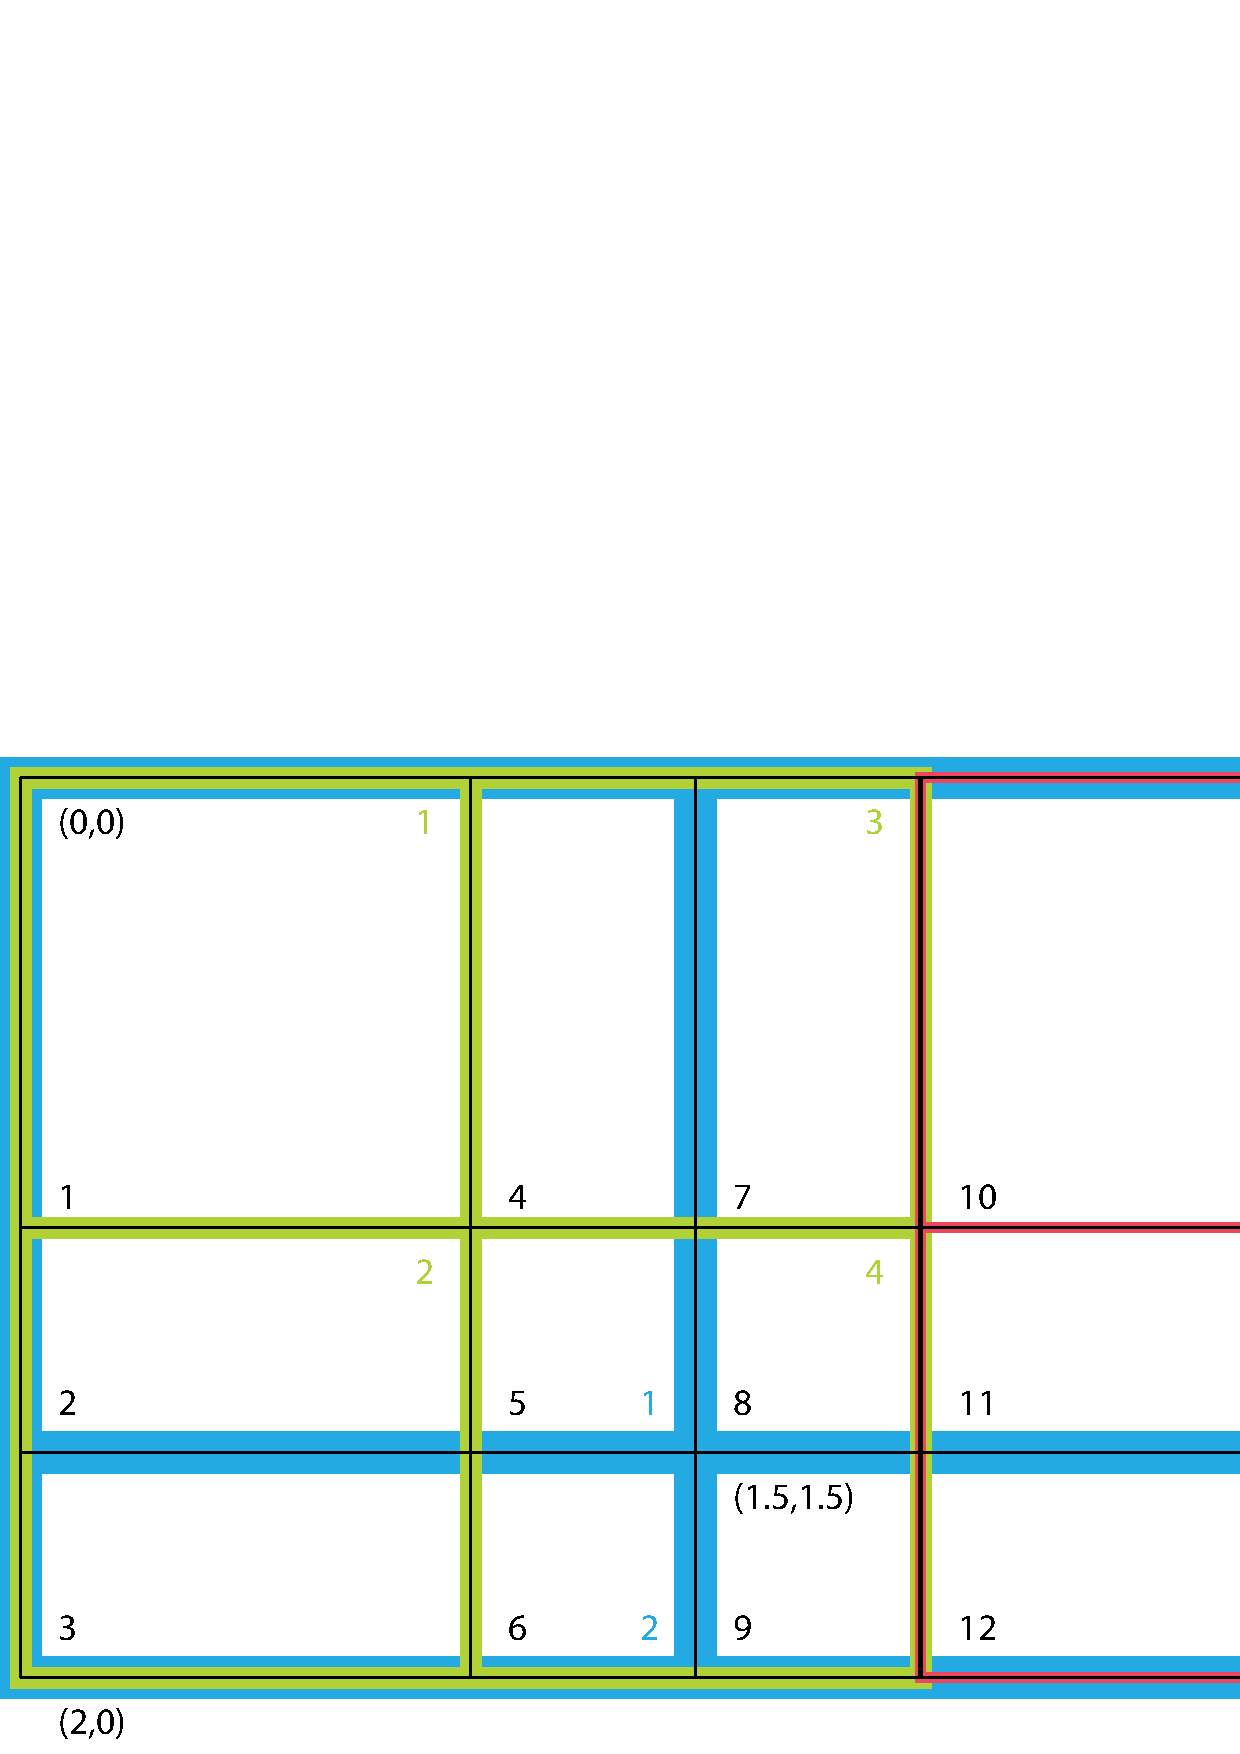
\includegraphics{XGridEx1}}
  \caption{Grid layout for simple XGrid creation example. Overlapping of 3 Grids
  (Green 2x2, Red 2x1, Blue 2x2). Green and red Grids on side A, blue Grid on side
  B, black indicates the resulting XGrid. Color coded sequence indices are shown.
  Physical coordinates are the tuples in parenthesis, e.g. at the four
  corners of rectangular computational domain.}
  \label{fig:xgridsimple}
  \end{figure}
  \end{center}
  
   We start by creating the Grids on both sides and associate coordinates with
   the Grids. For details of Grid creation and coordinate use, please refer to
   Grid class documentation. 
%/////////////////////////////////////////////////////////////

 \begin{verbatim}
    sideA(1) = ESMF_GridCreateNoPeriDim(minIndex=(/1,1/), maxIndex=(/2,2/), &
        coordDep1=(/1/), &
        coordDep2=(/2/), &
        name='source Grid 1 on side A', rc=localrc)
 
\end{verbatim}
 
%/////////////////////////////////////////////////////////////

 \begin{verbatim}
    sideA(2) = ESMF_GridCreateNoPeriDim(minIndex=(/1,1/), maxIndex=(/2,1/), &
        coordDep1=(/1/), &
        coordDep2=(/2/), &
        name='source Grid 2 on side A', rc=localrc)
 
\end{verbatim}
 
%/////////////////////////////////////////////////////////////

 \begin{verbatim}
    do i = 1, 2
        call ESMF_GridAddCoord(sideA(i), staggerloc=ESMF_STAGGERLOC_CENTER, &
            rc=localrc)
 
\end{verbatim}
 
%/////////////////////////////////////////////////////////////

 \begin{verbatim}
    enddo
 
\end{verbatim}
 
%/////////////////////////////////////////////////////////////

   Coordinate for the Grids on sideA, refer to the Grid layout diagram for the
   interpretation of the coordinate values: 
%/////////////////////////////////////////////////////////////

 \begin{verbatim}
    ! SideA first grid
    centroidA1X=(/0.5, 1.5/)
    centroidA1Y=(/0.5, 1.5/)
    call ESMF_GridGetCoord(sideA(1), localDE=0, &
        staggerLoc=ESMF_STAGGERLOC_CENTER, coordDim=1, &
        farrayPtr=coordX, rc=localrc)
 
\end{verbatim}
 
%/////////////////////////////////////////////////////////////

 \begin{verbatim}
    coordX = centroidA1X
    call ESMF_GridGetCoord(sideA(1), localDE=0, &
        staggerLoc=ESMF_STAGGERLOC_CENTER, coordDim=2, &
        farrayPtr=coordY, rc=localrc)
 
\end{verbatim}
 
%/////////////////////////////////////////////////////////////

 \begin{verbatim}
    coordY = centroidA1Y

    ! SideA second grid
    centroidA2X=(/0.5, 1.5/)
    centroidA2Y=(/2.5/)
    call ESMF_GridGetCoord(sideA(2), localDE=0, &
        staggerLoc=ESMF_STAGGERLOC_CENTER, coordDim=1, &
        farrayPtr=coordX, rc=localrc)
 
\end{verbatim}
 
%/////////////////////////////////////////////////////////////

 \begin{verbatim}
    coordX = centroidA2X
    call ESMF_GridGetCoord(sideA(2), localDE=0, &
        staggerLoc=ESMF_STAGGERLOC_CENTER, coordDim=2, &
        farrayPtr=coordY, rc=localrc)
 
\end{verbatim}
 
%/////////////////////////////////////////////////////////////

 \begin{verbatim}
    coordY = centroidA2Y
 
\end{verbatim}
 
%/////////////////////////////////////////////////////////////

   Create the destination grid on side B, only one Grid exists on side B. Also associate
   coordinate with the Grid: 
%/////////////////////////////////////////////////////////////

 \begin{verbatim}
    sideB(1) = ESMF_GridCreateNoPeriDim(minIndex=(/1,1/), maxIndex=(/2,2/), &
        coordDep1=(/1/), coordDep2=(/2/), &
        name='destination Grid on side B', rc=localrc)
 
\end{verbatim}
 
%/////////////////////////////////////////////////////////////

 \begin{verbatim}
    do i = 1, 1
        call ESMF_GridAddCoord(sideB(i), staggerloc=ESMF_STAGGERLOC_CENTER, &
            rc=localrc)
 
\end{verbatim}
 
%/////////////////////////////////////////////////////////////

 \begin{verbatim}
    enddo

    ! SideB grid
    centroidBX=(/0.75, 1.75/)
    centroidBY=(/0.75, 2.25/)
    call ESMF_GridGetCoord(sideB(1), localDE=0, &
        staggerLoc=ESMF_STAGGERLOC_CENTER, coordDim=1, farrayPtr=coordX, &
                rc=localrc)
 
\end{verbatim}
 
%/////////////////////////////////////////////////////////////

 \begin{verbatim}
    coordX = centroidBX
    call ESMF_GridGetCoord(sideB(1), localDE=0, &
        staggerLoc=ESMF_STAGGERLOC_CENTER, coordDim=2, farrayPtr=coordY, &
                rc=localrc)
 
\end{verbatim}
 
%/////////////////////////////////////////////////////////////

 \begin{verbatim}
    coordY = centroidBY
 
\end{verbatim}
 
%/////////////////////////////////////////////////////////////

  
   Set up the mapping indices and weights from A side to the XGrid. For details of
   sequence indices, factorIndexList, and factorList, please see section
   \ref{Array:SparseMatMul} in the reference manual. Please refer to the figure above
   for interpretation of the sequence indices used here.
  
   In order to compute the destination flux on sideB through the XGrid as an mediator,
   we need to set up the factorList (weights) and factorIndexList (indices)
   for sparse matrix multiplication in this formulation:
   dst\_flux = W'*W*src\_flux, where W' is the weight matrix from the XGrid to
   destination; and W is the weight matrix from source to the XGrid. The weight matrix
   is generated using destination area weighted algorithm. Please refer to figure
   \ref {fig:xgridsimple} for details.
   
%/////////////////////////////////////////////////////////////

 \begin{verbatim}
    ! Set up mapping from A1 -> X
    sparseMatA2X(1)%factorIndexList(1,1)=1    ! src seq index (green)
    sparseMatA2X(1)%factorIndexList(1,2)=2    ! src seq index (green)
    sparseMatA2X(1)%factorIndexList(1,3)=2    ! src seq index (green)
    sparseMatA2X(1)%factorIndexList(1,4)=3    ! src seq index (green)
    sparseMatA2X(1)%factorIndexList(1,5)=4    ! src seq index (green)
    sparseMatA2X(1)%factorIndexList(1,6)=4    ! src seq index (green)
    sparseMatA2X(1)%factorIndexList(1,7)=3    ! src seq index (green)
    sparseMatA2X(1)%factorIndexList(1,8)=4    ! src seq index (green)
    sparseMatA2X(1)%factorIndexList(1,9)=4    ! src seq index (green)

    sparseMatA2X(1)%factorIndexList(2,1)=1    ! dst seq index (black)
    sparseMatA2X(1)%factorIndexList(2,2)=2    ! dst seq index (black)
    sparseMatA2X(1)%factorIndexList(2,3)=3    ! dst seq index (black)
    sparseMatA2X(1)%factorIndexList(2,4)=4    ! dst seq index (black)
    sparseMatA2X(1)%factorIndexList(2,5)=5    ! dst seq index (black)
    sparseMatA2X(1)%factorIndexList(2,6)=6    ! dst seq index (black)
    sparseMatA2X(1)%factorIndexList(2,7)=7    ! dst seq index (black)
    sparseMatA2X(1)%factorIndexList(2,8)=8    ! dst seq index (black)
    sparseMatA2X(1)%factorIndexList(2,9)=9    ! dst seq index (black)

    ! Set up mapping from A2 -> X
    sparseMatA2X(2)%factorIndexList(1,1)=1    ! src seq index (red)
    sparseMatA2X(2)%factorIndexList(1,2)=2    ! src seq index (red)
    sparseMatA2X(2)%factorIndexList(1,3)=2    ! src seq index (red)

    sparseMatA2X(2)%factorIndexList(2,1)=10   ! dst seq index (black)
    sparseMatA2X(2)%factorIndexList(2,2)=11   ! dst seq index (black)
    sparseMatA2X(2)%factorIndexList(2,3)=12   ! dst seq index (black)
 
\end{verbatim}
 
%/////////////////////////////////////////////////////////////

   Set up the mapping weights from side A to the XGrid: 
%/////////////////////////////////////////////////////////////

 \begin{verbatim}
    ! Note that the weights are dest area weighted, they are ratio
    ! of areas with destination area as the denominator.
    ! Set up mapping weights from A1 -> X
    sparseMatA2X(1)%factorList(:)=1.

    ! Set up mapping weights from A2 -> X
    sparseMatA2X(2)%factorList(:)=1.
 
\end{verbatim}
 
%/////////////////////////////////////////////////////////////

   Set up the mapping indices and weights from the XGrid to B side: 
%/////////////////////////////////////////////////////////////

 \begin{verbatim}
    ! Set up mapping from X -> B
    sparseMatX2B(1)%factorIndexList(1,1)=1    ! src seq index (black)
    sparseMatX2B(1)%factorIndexList(1,2)=2    ! src seq index (black)
    sparseMatX2B(1)%factorIndexList(1,3)=3    ! src seq index (black)
    sparseMatX2B(1)%factorIndexList(1,4)=4    ! src seq index (black)
    sparseMatX2B(1)%factorIndexList(1,5)=5    ! src seq index (black)
    sparseMatX2B(1)%factorIndexList(1,6)=6    ! src seq index (black)
    sparseMatX2B(1)%factorIndexList(1,7)=7    ! src seq index (black)
    sparseMatX2B(1)%factorIndexList(1,8)=8    ! src seq index (black)
    sparseMatX2B(1)%factorIndexList(1,9)=9    ! src seq index (black)
    sparseMatX2B(1)%factorIndexList(1,10)=10  ! src seq index (black)
    sparseMatX2B(1)%factorIndexList(1,11)=11  ! src seq index (black)
    sparseMatX2B(1)%factorIndexList(1,12)=12  ! src seq index (black)

    sparseMatX2B(1)%factorIndexList(2,1)=1    ! dst seq index (blue)
    sparseMatX2B(1)%factorIndexList(2,2)=1    ! dst seq index (blue)
    sparseMatX2B(1)%factorIndexList(2,3)=2    ! dst seq index (blue)
    sparseMatX2B(1)%factorIndexList(2,4)=1    ! dst seq index (blue)
    sparseMatX2B(1)%factorIndexList(2,5)=1    ! dst seq index (blue)
    sparseMatX2B(1)%factorIndexList(2,6)=2    ! dst seq index (blue)
    sparseMatX2B(1)%factorIndexList(2,7)=3    ! dst seq index (blue)
    sparseMatX2B(1)%factorIndexList(2,8)=3    ! dst seq index (blue)
    sparseMatX2B(1)%factorIndexList(2,9)=4    ! dst seq index (blue)
    sparseMatX2B(1)%factorIndexList(2,10)=3   ! dst seq index (blue)
    sparseMatX2B(1)%factorIndexList(2,11)=3   ! dst seq index (blue)
    sparseMatX2B(1)%factorIndexList(2,12)=4   ! dst seq index (blue)

    ! Set up mapping weights from X -> B
    sparseMatX2B(1)%factorList(1)=4./9.
    sparseMatX2B(1)%factorList(2)=2./9.
    sparseMatX2B(1)%factorList(3)=2./3.
    sparseMatX2B(1)%factorList(4)=2./9.
    sparseMatX2B(1)%factorList(5)=1./9.
    sparseMatX2B(1)%factorList(6)=1./3.
    sparseMatX2B(1)%factorList(7)=2./9.
    sparseMatX2B(1)%factorList(8)=1./9.
    sparseMatX2B(1)%factorList(9)=1./3.
    sparseMatX2B(1)%factorList(10)=4./9.
    sparseMatX2B(1)%factorList(11)=2./9.
    sparseMatX2B(1)%factorList(12)=2./3.
 
\end{verbatim}
 
%/////////////////////////////////////////////////////////////

   Optionally the area can be setup to compute surface area weighted flux integrals: 
%/////////////////////////////////////////////////////////////

 \begin{verbatim}
    ! Set up destination areas to adjust weighted flux
    xgrid_area(1) = 1.
    xgrid_area(2) = 0.5
    xgrid_area(3) = 0.5
    xgrid_area(4) = 0.5
    xgrid_area(5) = 0.25
    xgrid_area(6) = 0.25
    xgrid_area(7) = 0.5
    xgrid_area(8) = 0.25
    xgrid_area(9) = 0.25
    xgrid_area(10) = 1.
    xgrid_area(11) = 0.5
    xgrid_area(12) = 0.5
 
\end{verbatim}
 
%/////////////////////////////////////////////////////////////

   Create an XGrid based on the user supplied regridding parameters: 
%/////////////////////////////////////////////////////////////

 \begin{verbatim}
    xgrid = ESMF_XGridCreateFromSparseMat(sideAGrid=sideA, &
        sideBGrid=sideB, area=xgrid_area, &
        centroid=centroid, sparseMatA2X=sparseMatA2X, &
        sparseMatX2B=sparseMatX2B, rc=localrc)
 
\end{verbatim}
 
%/////////////////////////////////////////////////////////////

   Create an {\tt ESMF\_Field} on the XGrid: 
%/////////////////////////////////////////////////////////////

 \begin{verbatim}
    field = ESMF_FieldCreate(xgrid, typekind=ESMF_TYPEKIND_R8, &
                rc=localrc)
 
\end{verbatim}
 
%/////////////////////////////////////////////////////////////

   Query the Field for its Fortran data pointer and its exclusive bounds: 
%/////////////////////////////////////////////////////////////

 \begin{verbatim}
    call ESMF_FieldGet(field, farrayPtr=xfarrayPtr, &
        exclusiveLBound=xlb, exclusiveUBound=xub, rc=localrc)
 
\end{verbatim}
 
%/////////////////////////////////////////////////////////////

   Setup and initialize src and dst Fields on side A and side B Grids,
   source Fields have different source flux: 
%/////////////////////////////////////////////////////////////

 \begin{verbatim}
    do i = 1, 2
        srcField(i) = ESMF_FieldCreate(sideA(i), &
                typekind=ESMF_TYPEKIND_R8, rc=localrc)
 
\end{verbatim}
 
%/////////////////////////////////////////////////////////////

 \begin{verbatim}
        call ESMF_FieldGet(srcField(i), farrayPtr=farrayPtr, rc=localrc)
 
\end{verbatim}
 
%/////////////////////////////////////////////////////////////

 \begin{verbatim}
        farrayPtr = i
    enddo
    do i = 1, 1
        dstField(i) = ESMF_FieldCreate(sideB(i), &
                typekind=ESMF_TYPEKIND_R8, rc=localrc)
 
\end{verbatim}
 
%/////////////////////////////////////////////////////////////

 \begin{verbatim}
        call ESMF_FieldGet(dstField(i), farrayPtr=farrayPtr, rc=localrc)
 
\end{verbatim}
 
%/////////////////////////////////////////////////////////////

 \begin{verbatim}
        farrayPtr = 0.0
    enddo
 
\end{verbatim}
 
%/////////////////////////////////////////////////////////////

  
   The current implementation requires that Grids used to generate the XGrid
   must not match, i.e. they are different either topologically or geometrically or both.
   In this example, the first source Grid is topologically identical to the destination
   Grid but their geometric coordinates are different. This requirement will be relaxed
   in a future release.
  
   First we compute the regrid routehandles, these routehandles can be used repeatedly
   afterwards. Then we initialize the values in the Fields. Finally we execute the Regrid.
   
%/////////////////////////////////////////////////////////////

 \begin{verbatim}
    ! Compute regrid routehandles. The routehandles can be used
    ! repeatedly afterwards.
    ! From A -> X
    do i = 1, 2
        call ESMF_FieldRegridStore(xgrid, srcField(i), field, &
                routehandle=rh_src2xgrid(i), rc = localrc)
 
\end{verbatim}
 
%/////////////////////////////////////////////////////////////

 \begin{verbatim}
    enddo
    ! from X -> B
    do i = 1, 1
        call ESMF_FieldRegridStore(xgrid, field, dstField(i), &
                routehandle=rh_xgrid2dst(i), rc = localrc)
 
\end{verbatim}
 
%/////////////////////////////////////////////////////////////

 \begin{verbatim}
    enddo

    ! Initialize values in the source Fields on side A
    do i = 1, 2
        call ESMF_FieldGet(srcField(i), farrayPtr=farrayPtr, rc=localrc)
 
\end{verbatim}
 
%/////////////////////////////////////////////////////////////

 \begin{verbatim}
        farrayPtr = i
    enddo
    ! Initialize values in the destination Field on XGrid
    xfarrayPtr = 0.0
    ! Initialize values in the destination Field on Side B
    do i = 1, 1
        call ESMF_FieldGet(dstField(i), farrayPtr=farrayPtr, rc=localrc)
 
\end{verbatim}
 
%/////////////////////////////////////////////////////////////

 \begin{verbatim}
        farrayPtr = 0.0
    enddo
 
\end{verbatim}
 
%/////////////////////////////////////////////////////////////

   First we regrid from the Fields on side A to the Field on the XGrid: 
%/////////////////////////////////////////////////////////////

 \begin{verbatim}
    ! Execute regrid from A -> X
    do i = 1, 2
        call ESMF_FieldRegrid(srcField(i), field, &
            routehandle=rh_src2xgrid(i), &
            zeroregion=ESMF_REGION_SELECT, rc = localrc)
 
\end{verbatim}
 
%/////////////////////////////////////////////////////////////

 \begin{verbatim}
    enddo
 
\end{verbatim}
 
%/////////////////////////////////////////////////////////////

   Next we regrid from the Field on XGrid to the destination Field on side B: 
%/////////////////////////////////////////////////////////////

 \begin{verbatim}
    ! Execute the regrid store
    do i = 1, 1
        call ESMF_FieldRegrid(field, dstField(i), &
            routehandle=rh_xgrid2dst(i), rc = localrc)
 
\end{verbatim}
 
%/////////////////////////////////////////////////////////////

 \begin{verbatim}
    enddo
 
\end{verbatim}
 
%/////////////////////////////////////////////////////////////

   In the above example, we first set up all the required parameters to create an XGrid from user
   supplied input. Then we create Fields on the XGrid and the Grids on either side. Finally
   we use the {\tt ESMF\_FieldRegrid()} interface to perform a flux exchange from the source side
   to the destination side. 
%/////////////////////////////////////////////////////////////

  \subsubsection{Query the XGrid for its internal information}
  \label{sec:xgrid:usage:xgrid_get}
   One can query the XGrid for its internal information: 
%/////////////////////////////////////////////////////////////

 \begin{verbatim}
    call ESMF_XGridGet(xgrid, &
        sideAGridCount=ngridA, &    ! number of Grids on side A
        sideBGridCount=ngridB, &    ! number of Grids on side B
        sideAGrid=l_sideA, &    ! list of Grids on side A
        sideBGrid=l_sideB, &    ! list of Grids on side B
        area=l_area, &      ! list of area of XGrid
        centroid=l_centroid, &  ! list of centroid of XGrid
        distgridA=l_sideAdg, &  ! list of Distgrids on side A
        distgridM = distgrid, & ! balanced distgrid
        sparseMatA2X=l_sparseMatA2X, & !sparse matrix matmul parameters A to X
        sparseMatX2B=l_sparseMatX2B, & !sparse matrix matmul parameters X to B
        rc=localrc)
 
\end{verbatim}
 
%/////////////////////////////////////////////////////////////

 \begin{verbatim}
    call ESMF_XGridGet(xgrid, localDe=0, &
        elementCount=eleCount, &    ! elementCount on the localDE
        exclusiveCount=ec, &        ! exclusive count
        exclusiveLBound=elb, &      ! exclusive lower bound
        exclusiveUBound=eub, &      ! exclusive upper bound
        rc=localrc)
 
\end{verbatim}
 
%/////////////////////////////////////////////////////////////

 \begin{verbatim}
    call ESMF_XGridGet(xgrid, &
        xgridSide=ESMF_XGRIDSIDE_A, & ! side of the XGrid to query
        gridIndex=1, &              ! index of the distgrid
        distgrid=distgrid, &        ! the distgrid returned
        rc=localrc)
 
\end{verbatim}
 
%/////////////////////////////////////////////////////////////

  \subsubsection{Destroying the XGrid and other resources}
  \label{sec:xgrid:usage:xgrid_destroy}
   Clean up the resources by destroying the XGrid and other objects: 
%/////////////////////////////////////////////////////////////

 \begin{verbatim}
    ! After the regridding is successful.
    ! Clean up all the allocated resources:
    call ESMF_FieldDestroy(field, rc=localrc)
 
\end{verbatim}
 
%/////////////////////////////////////////////////////////////

 \begin{verbatim}
    call ESMF_XGridDestroy(xgrid, rc=localrc)
 
\end{verbatim}
 
%/////////////////////////////////////////////////////////////

 \begin{verbatim}
    do i = 1, 2
        call ESMF_FieldDestroy(srcField(i), rc = localrc)
 
\end{verbatim}
 
%/////////////////////////////////////////////////////////////

 \begin{verbatim}
        call ESMF_GridDestroy(sideA(i), rc = localrc)
 
\end{verbatim}
 
%/////////////////////////////////////////////////////////////

 \begin{verbatim}
    enddo

    do i = 1, 1
        call ESMF_FieldDestroy(dstField(i), rc = localrc)
 
\end{verbatim}
 
%/////////////////////////////////////////////////////////////

 \begin{verbatim}
        call ESMF_GridDestroy(sideB(i), rc = localrc)
 
\end{verbatim}
 
%/////////////////////////////////////////////////////////////

 \begin{verbatim}
    enddo

    deallocate(sparseMatA2X(1)%factorIndexList, sparseMatA2X(1)%factorList)
    deallocate(sparseMatA2X(2)%factorIndexList, sparseMatA2X(2)%factorList)
    deallocate(sparseMatX2B(1)%factorIndexList, sparseMatX2B(1)%factorList)
 
\end{verbatim}

%...............................................................
\setlength{\parskip}{\oldparskip}
\setlength{\parindent}{\oldparindent}
\setlength{\baselineskip}{\oldbaselineskip}

\subsection{Restrictions and Future Work}
% $Id$

\subsubsection{Restrictions and Future Work}

\begin{enumerate}
\label{XGrid:rest}

\item {\bf CAUTION:} Any Grid or Mesh pair picked from the A side and B side of the XGrid 
cannot point to the same Grid or Mesh in memory on a local PET. This prevents Regrid from
selecting the right source and destination grid automatically to calculate the regridding routehandle.
It's okay for the Grid and Mesh to have identical topological and geographical properties as long
as they are stored in different memory.

\end{enumerate}




\subsection{Design and Implementation Notes}
% $Id$

%\subsection{Design and Implementation Notes}

\begin{enumerate}

\item The XGrid class is implemented in Fortran, and as such is
defined inside the framework by a XGrid derived type and a set of 
subprograms (functions and subroutines) which operate on that derived type.  
The XGrid class contains information needed to create Grid, Field, and
communication routehandle.

\item XGrid follows the framework-wide convention of the
{\it unison} creation and operation rule: All PETs which are
part of the currently executing VM must create the
same XGrids at the same point in their execution. 
In addition to the unison rule, XGrid creation also performs inter-PET
communication within the current executing VM. 
\end{enumerate}

\subsection{Class API}
%                **** IMPORTANT NOTICE *****
% This LaTeX file has been automatically produced by ProTeX v. 1.1
% Any changes made to this file will likely be lost next time
% this file is regenerated from its source. Send questions 
% to Arlindo da Silva, dasilva@gsfc.nasa.gov
 
\setlength{\oldparskip}{\parskip}
\setlength{\parskip}{1.5ex}
\setlength{\oldparindent}{\parindent}
\setlength{\parindent}{0pt}
\setlength{\oldbaselineskip}{\baselineskip}
\setlength{\baselineskip}{11pt}
 
%--------------------- SHORT-HAND MACROS ----------------------
\def\bv{\begin{verbatim}}
\def\ev{\end{verbatim}}
\def\be{\begin{equation}}
\def\ee{\end{equation}}
\def\bea{\begin{eqnarray}}
\def\eea{\end{eqnarray}}
\def\bi{\begin{itemize}}
\def\ei{\end{itemize}}
\def\bn{\begin{enumerate}}
\def\en{\end{enumerate}}
\def\bd{\begin{description}}
\def\ed{\end{description}}
\def\({\left (}
\def\){\right )}
\def\[{\left [}
\def\]{\right ]}
\def\<{\left  \langle}
\def\>{\right \rangle}
\def\cI{{\cal I}}
\def\diag{\mathop{\rm diag}}
\def\tr{\mathop{\rm tr}}
%-------------------------------------------------------------

\markboth{Left}{Source File: ESMF\_XGridCreate.F90,  Date: Tue May  5 20:59:57 MDT 2020
}

 
%/////////////////////////////////////////////////////////////
\subsubsection [ESMF\_XGridAssignment(=)] {ESMF\_XGridAssignment(=) - XGrid assignment}


  
\bigskip{\sf INTERFACE:}
\begin{verbatim}     interface assignment(=)
     xgrid1 = xgrid2\end{verbatim}{\em ARGUMENTS:}
\begin{verbatim}     type(ESMF_XGrid) :: xgrid1
     type(ESMF_XGrid) :: xgrid2\end{verbatim}
{\sf DESCRIPTION:\\ }


     Assign xgrid1 as an alias to the same ESMF XGrid object in memory
     as xgrid2. If xgrid2 is invalid, then xgrid1 will be equally invalid after
     the assignment.
  
     The arguments are:
     \begin{description}
     \item[xgrid1]
       The {\tt ESMF\_XGrid} object on the left hand side of the assignment.
     \item[xgrid2]
       The {\tt ESMF\_XGrid} object on the right hand side of the assignment.
     \end{description}
   
%/////////////////////////////////////////////////////////////
 
\mbox{}\hrulefill\ 
 
\subsubsection [ESMF\_XGridOperator(==)] {ESMF\_XGridOperator(==) - XGrid equality operator}


  
\bigskip{\sf INTERFACE:}
\begin{verbatim}     interface operator(==)
     if (xgrid1 == xgrid2) then ... endif
               OR
     result = (xgrid1 == xgrid2)\end{verbatim}{\em RETURN VALUE:}
\begin{verbatim}     logical :: result\end{verbatim}{\em ARGUMENTS:}
\begin{verbatim}     type(ESMF_XGrid), intent(in) :: xgrid1
     type(ESMF_XGrid), intent(in) :: xgrid2\end{verbatim}
{\sf DESCRIPTION:\\ }


     Test whether xgrid1 and xgrid2 are valid aliases to the same ESMF
     XGrid object in memory. For a more general comparison of two ESMF XGrids,
     going beyond the simple alias test, the ESMF\_XGridMatch() function (not yet
     implemented) must be used.
  
     The arguments are:
     \begin{description}
     \item[xgrid1]
       The {\tt ESMF\_XGrid} object on the left hand side of the equality
       operation.
     \item[xgrid2]
       The {\tt ESMF\_XGrid} object on the right hand side of the equality
       operation.
     \end{description}
   
%/////////////////////////////////////////////////////////////
 
\mbox{}\hrulefill\ 
 
\subsubsection [ESMF\_XGridOperator(/=)] {ESMF\_XGridOperator(/=) - XGrid not equal operator}


  
\bigskip{\sf INTERFACE:}
\begin{verbatim}     interface operator(/=)
     if (xgrid1 /= xgrid2) then ... endif
               OR
     result = (xgrid1 /= xgrid2)\end{verbatim}{\em RETURN VALUE:}
\begin{verbatim}     logical :: result\end{verbatim}{\em ARGUMENTS:}
\begin{verbatim}     type(ESMF_XGrid), intent(in) :: xgrid1
     type(ESMF_XGrid), intent(in) :: xgrid2\end{verbatim}
{\sf DESCRIPTION:\\ }


     Test whether xgrid1 and xgrid2 are {\it not} valid aliases to the
     same ESMF XGrid object in memory. For a more general comparison of two ESMF
     XGrids, going beyond the simple alias test, the ESMF\_XGridMatch() function
     (not yet implemented) must be used.
  
     The arguments are:
     \begin{description}
     \item[xgrid1]
       The {\tt ESMF\_XGrid} object on the left hand side of the non-equality
       operation.
     \item[xgrid2]
       The {\tt ESMF\_XGrid} object on the right hand side of the non-equality
       operation.
     \end{description}
   
%/////////////////////////////////////////////////////////////
 
\mbox{}\hrulefill\ 
 
\subsubsection [ESMF\_XGridCreate] {ESMF\_XGridCreate - Create an XGrid from lists of Grids and Meshes}


 
\bigskip{\sf INTERFACE:}
\begin{verbatim} 
 function ESMF_XGridCreate(&
     sideAGrid,              sideAMesh, &
     sideBGrid,              sideBMesh, &
     sideAGridPriority,      sideAMeshPriority, &
     sideBGridPriority,      sideBMeshPriority, &
     sideAMaskValues,        sideBMaskValues, &
     storeOverlay, &
     name, rc)\end{verbatim}{\em RETURN VALUE:}
\begin{verbatim}   type(ESMF_XGrid)                           :: ESMF_XGridCreate\end{verbatim}{\em ARGUMENTS:}
\begin{verbatim} -- The following arguments require argument keyword syntax (e.g. rc=rc). --
   type(ESMF_Grid),      intent(in), optional :: sideAGrid(:)
   type(ESMF_Mesh),      intent(in), optional :: sideAMesh(:)
   type(ESMF_Grid),      intent(in), optional :: sideBGrid(:)
   type(ESMF_Mesh),      intent(in), optional :: sideBMesh(:)
   integer,              intent(in), optional :: sideAGridPriority(:)
   integer,              intent(in), optional :: sideAMeshPriority(:)
   integer,              intent(in), optional :: sideBGridPriority(:)
   integer,              intent(in), optional :: sideBMeshPriority(:)
   integer(ESMF_KIND_I4),intent(in), optional :: sideAMaskValues(:)
   integer(ESMF_KIND_I4),intent(in), optional :: sideBMaskValues(:)
   logical,              intent(in), optional :: storeOverlay
   character(len=*),     intent(in), optional :: name
   integer,              intent(out),optional :: rc
 \end{verbatim}
{\sf DESCRIPTION:\\ }


        Create an XGrid from user supplied input: the list of Grids or Meshes on side A and side B, 
    and other optional arguments. A user can supply both Grids and Meshes on one side to create
    the XGrid. By default, the Grids have a higher priority over Meshes but the order of priority 
    can be adjusted by the optional GridPriority and MeshPriority arguments. The priority order
    of Grids and Meshes can also be interleaved by rearranging the optional 
    GridPriority and MeshPriority arguments accordingly.
    
    Sparse matrix multiplication coefficients are internally computed and
    uniquely determined by the Grids or Meshes provided in {\tt sideA} and {\tt sideB}. User can supply
    a single {\tt ESMF\_Grid} or an array of {\tt ESMF\_Grid} on either side of the 
    {\tt ESMF\_XGrid}. For an array of {\tt ESMF\_Grid} or {\tt ESMF\_Mesh} in {\tt sideA} or {\tt sideB},
    a merging process concatenates all the {\tt ESMF\_Grid}s and {\tt ESMF\_Mesh}es 
    into a super mesh represented
    by {\tt ESMF\_Mesh}. The super mesh is then used to compute the XGrid. 
    Grid or Mesh objects in {\tt sideA} and {\tt sideB} arguments must have coordinates defined for
    the corners of a Grid or Mesh cell. XGrid creation can be potentially memory expensive given the
    size of the input Grid and Mesh objects. By default, the super mesh is not stored
    to reduce memory usage. 
    Once communication routehandles are computed using {\tt ESMF\_FieldRegridStore()} method through
    XGrid, all memory can be released by destroying the XGrid.
   
    If {\tt sideA} and {\tt sideB} have a single 
    Grid or Mesh object, it's erroneous
    if the two Grids or Meshes are spatially disjoint. 
    It is also erroneous to specify a Grid or Mesh object in {\tt sideA} or {\tt sideB}
    that is spatially disjoint from the {\tt ESMF\_XGrid}. 
  
    This call is {\em collective} across the current VM. For more details please refer to the description 
    \ref{sec:xgrid:desc} of the XGrid class. For an example and associated documentation using this method see section 
    \ref{sec:xgrid:usage:xgrid_create}
 
  
       The arguments are:
       \begin{description}
       \item [{[sideAGrid]}]
             Parametric 2D Grids on side A, for example, 
             these Grids can be either Cartesian 2D or Spherical.
       \item [{[sideAMesh]}]
             Parametric 2D Meshes on side A, for example, 
             these Meshes can be either Cartesian 2D or Spherical.
       \item [{[sideBGrid]}]
             Parametric 2D Grids on side B, for example, 
             these Grids can be either Cartesian 2D or Spherical.
       \item [{[sideBMesh]}]
             Parametric 2D Meshes on side B, for example, 
             these Meshes can be either Cartesian 2D or Spherical.
       \item [{[sideAGridPriority]}]
             Priority array of Grids on {\tt sideA} during overlay generation.
             The priority arrays describe the priorities of Grids at the overlapping region.
             Flux contributions at the overlapping region are computed in the order from the Grid of the
             highest priority to the lowest priority.
       \item [{[sideAMeshPriority]}]
             Priority array of Meshes on {\tt sideA} during overlay generation.
             The priority arrays describe the priorities of Meshes at the overlapping region.
             Flux contributions at the overlapping region are computed in the order from the Mesh of the
             highest priority to the lowest priority.
       \item [{[sideBGridPriority]}]
             Priority of Grids on {\tt sideB} during overlay generation
             The priority arrays describe the priorities of Grids at the overlapping region.
             Flux contributions at the overlapping region are computed in the order from the Grid of the
             highest priority to the lowest priority.
       \item [{[sideBMeshPriority]}]
             Priority array of Meshes on {\tt sideB} during overlay generation.
             The priority arrays describe the priorities of Meshes at the overlapping region.
             Flux contributions at the overlapping region are computed in the order from the Mesh of the
             highest priority to the lowest priority.
       \item [{[sideAMaskValues]}]
             Mask information can be set in the Grid (see~\ref{sec:usage:items}) or Mesh (see~\ref{sec:mesh:mask}) 
             upon which the {\tt Field} is built. The {\tt sideAMaskValues} argument specifies the values in that 
             mask information which indicate a point should be masked out. In other words, a location is masked if and only if the
             value for that location in the mask information matches one of the values listed in {\tt sideAMaskValues}.  
             If {\tt sideAMaskValues} is not specified, no masking on side A will occur. 
       \item [{[sideBMaskValues]}]
             Mask information can be set in the Grid (see~\ref{sec:usage:items}) or Mesh (see~\ref{sec:mesh:mask}) 
             upon which the {\tt Field} is built. The {\tt sideBMaskValues} argument specifies the values in that 
             mask information which indicate a point should be masked out. In other words, a location is masked if and only if the
             value for that location in the mask information matches one of the values listed in {\tt sideBMaskValues}.  
             If {\tt sideBMaskValues} is not specified, no masking on side B will occur. 
       \item [{[storeOverlay]}]
             Setting the {\tt storeOverlay} optional argument to .false. (default) 
             allows a user to bypass storage of the {\tt ESMF\_Mesh} used to represent the XGrid.
             Only a {\tt ESMF\_DistGrid} is stored to allow Field to be built on the XGrid.
             If the temporary mesh object is of interest, {\tt storeOverlay} can be set to .true.
             so a user can retrieve it for future use.
       \item [{[name]}]
             name of the xgrid object.
       \item [{[rc]}]
             Return code; equals {\tt ESMF\_SUCCESS} only if the {\tt ESMF\_XGrid} 
             is created.
       \end{description}
   
%/////////////////////////////////////////////////////////////
 
\mbox{}\hrulefill\ 
 
\subsubsection [ESMF\_XGridCreateFromSparseMat] {ESMF\_XGridCreateFromSparseMat an XGrid from raw input parameters}


 
\bigskip{\sf INTERFACE:}
\begin{verbatim} 
 function ESMF_XGridCreateFromSparseMat(&
     sideAGrid,              sideAMesh, &
     sideBGrid,              sideBMesh, &
     sideAGridPriority,      sideAMeshPriority, &
     sideBGridPriority,      sideBMeshPriority, &
     sparseMatA2X, sparseMatX2A, sparseMatB2X, sparseMatX2B, &
     area, centroid, &
     name, &
     rc) 
 \end{verbatim}{\em RETURN VALUE:}
\begin{verbatim}     type(ESMF_XGrid) :: ESMF_XGridCreateFromSparseMat\end{verbatim}{\em ARGUMENTS:}
\begin{verbatim} -- The following arguments require argument keyword syntax (e.g. rc=rc). --
 type(ESMF_Grid),      intent(in), optional :: sideAGrid(:)
 type(ESMF_Mesh),      intent(in), optional :: sideAMesh(:)
 type(ESMF_Grid),      intent(in), optional :: sideBGrid(:)
 type(ESMF_Mesh),      intent(in), optional :: sideBMesh(:)
 integer,              intent(in), optional :: sideAGridPriority(:)
 integer,              intent(in), optional :: sideAMeshPriority(:)
 integer,              intent(in), optional :: sideBGridPriority(:)
 integer,              intent(in), optional :: sideBMeshPriority(:)
 type(ESMF_XGridSpec), intent(in), optional :: sparseMatA2X(:)
 type(ESMF_XGridSpec), intent(in), optional :: sparseMatX2A(:)
 type(ESMF_XGridSpec), intent(in), optional :: sparseMatB2X(:)
 type(ESMF_XGridSpec), intent(in), optional :: sparseMatX2B(:)
 real(ESMF_KIND_R8),   intent(in), optional :: area(:)
 real(ESMF_KIND_R8),   intent(in), optional :: centroid(:,:)
 character (len=*),    intent(in), optional :: name
 integer,              intent(out),optional :: rc 
 \end{verbatim}
{\sf DESCRIPTION:\\ }


        Create an XGrid directly from user supplied sparse matrix parameters. User
        is responsible to supply all information necessary for communication calculation. 
        For an example and associated documentation using this method see section 
        \ref{sec:xgrid:usage:xgrid_createfromsparsemat}
  
       The arguments are:
       \begin{description}
       \item [{[sideAGrid]}]
             Parametric 2D Grids on side A, for example, 
             these Grids can be either Cartesian 2D or Spherical.
       \item [{[sideAMesh]}]
             Parametric 2D Meshes on side A, for example, 
             these Meshes can be either Cartesian 2D or Spherical.
       \item [{[sideBGrid]}]
             Parametric 2D Grids on side B, for example, 
             these Grids can be either Cartesian 2D or Spherical.
       \item [{[sideBMesh]}]
             Parametric 2D Meshes on side B, for example, 
             these Meshes can be either Cartesian 2D or Spherical.
       \item [{[sideAGridPriority]}]
             Priority array of Grids on {\tt sideA} during overlay generation.
             The priority arrays describe the priorities of Grids at the overlapping region.
             Flux contributions at the overlapping region are computed in the order from the Grid of the
             highest priority to the lowest priority.
       \item [{[sideAMeshPriority]}]
             Priority array of Meshes on {\tt sideA} during overlay generation.
             The priority arrays describe the priorities of Meshes at the overlapping region.
             Flux contributions at the overlapping region are computed in the order from the Mesh of the
             highest priority to the lowest priority.
       \item [{[sideBGridPriority]}]
             Priority of Grids on {\tt sideB} during overlay generation
             The priority arrays describe the priorities of Grids at the overlapping region.
             Flux contributions at the overlapping region are computed in the order from the Grid of the
             highest priority to the lowest priority.
       \item [{[sideBMeshPriority]}]
             Priority array of Meshes on {\tt sideB} during overlay generation.
             The priority arrays describe the priorities of Meshes at the overlapping region.
             Flux contributions at the overlapping region are computed in the order from the Mesh of the
             highest priority to the lowest priority.
       \item [{[sparseMatA2X]}]
             indexlist from a Grid index space on side A to xgrid index space;
             indexFactorlist from a Grid index space on side A to xgrid index space.
       \item [{[sparseMatX2A]}]
             indexlist from xgrid index space to a Grid index space on side A;
             indexFactorlist from xgrid index space to a Grid index space on side A.
       \item [{[sparseMatB2X]}]
             indexlist from a Grid index space on side B to xgrid index space;
             indexFactorlist from a Grid index space on side B to xgrid index space.
       \item [{[sparseMatX2B]}]
             indexlist from xgrid index space to a Grid index space on side B;
             indexFactorlist from xgrid index space to a Grid index space on side B.
       \item [{[area]}]
             area of the xgrid cells.
       \item [{[centroid]}]
             coordinates at the area weighted center of the xgrid cells.
       \item [{[name]}]
             name of the xgrid object.
       \item [{[rc]}]
             Return code; equals {\tt ESMF\_SUCCESS} only if the {\tt ESMF\_XGrid} 
             is created.
       \end{description}
   
%/////////////////////////////////////////////////////////////
 
\mbox{}\hrulefill\ 
 
\subsubsection [ESMF\_XGridIsCreated] {ESMF\_XGridIsCreated - Check whether a XGrid object has been created}


 
\bigskip{\sf INTERFACE:}
\begin{verbatim}   function ESMF_XGridIsCreated(xgrid, rc)\end{verbatim}{\em RETURN VALUE:}
\begin{verbatim}     logical :: ESMF_XGridIsCreated\end{verbatim}{\em ARGUMENTS:}
\begin{verbatim}     type(ESMF_XGrid), intent(in)            :: xgrid
 -- The following arguments require argument keyword syntax (e.g. rc=rc). --
     integer,             intent(out), optional :: rc
 \end{verbatim}
{\sf DESCRIPTION:\\ }


     Return {\tt .true.} if the {\tt xgrid} has been created. Otherwise return 
     {\tt .false.}. If an error occurs, i.e. {\tt rc /= ESMF\_SUCCESS} is 
     returned, the return value of the function will also be {\tt .false.}.
  
   The arguments are:
     \begin{description}
     \item[xgrid]
       {\tt ESMF\_XGrid} queried.
     \item[{[rc]}]
       Return code; equals {\tt ESMF\_SUCCESS} if there are no errors.
     \end{description}
   
%/////////////////////////////////////////////////////////////
 
\mbox{}\hrulefill\ 
 
\subsubsection [ESMF\_XGridDestroy] {ESMF\_XGridDestroy - Release resources associated with an XGrid}


\bigskip{\sf INTERFACE:}
\begin{verbatim} 
   subroutine ESMF_XGridDestroy(xgrid, rc)\end{verbatim}{\em ARGUMENTS:}
\begin{verbatim}     type(ESMF_XGrid), intent(inout)          :: xgrid       
 -- The following arguments require argument keyword syntax (e.g. rc=rc). --
     integer,          intent(out),  optional :: rc     \end{verbatim}
{\sf STATUS:}
   \begin{itemize}
   \item\apiStatusCompatibleVersion{5.2.0r}
   \end{itemize}
  
{\sf DESCRIPTION:\\ }


   Destroys an {\tt ESMF\_XGrid}, releasing the resources associated
   with the object.
   
   The arguments are:
   \begin{description}
   \item [xgrid]
         {\tt ESMF\_XGrid} object.
   \item [{[rc]}] 
         Return code; equals {\tt ESMF\_SUCCESS} if there are no errors.
   \end{description}
  
%...............................................................
\setlength{\parskip}{\oldparskip}
\setlength{\parindent}{\oldparindent}
\setlength{\baselineskip}{\oldbaselineskip}

%                **** IMPORTANT NOTICE *****
% This LaTeX file has been automatically produced by ProTeX v. 1.1
% Any changes made to this file will likely be lost next time
% this file is regenerated from its source. Send questions 
% to Arlindo da Silva, dasilva@gsfc.nasa.gov
 
\setlength{\oldparskip}{\parskip}
\setlength{\parskip}{1.5ex}
\setlength{\oldparindent}{\parindent}
\setlength{\parindent}{0pt}
\setlength{\oldbaselineskip}{\baselineskip}
\setlength{\baselineskip}{11pt}
 
%--------------------- SHORT-HAND MACROS ----------------------
\def\bv{\begin{verbatim}}
\def\ev{\end{verbatim}}
\def\be{\begin{equation}}
\def\ee{\end{equation}}
\def\bea{\begin{eqnarray}}
\def\eea{\end{eqnarray}}
\def\bi{\begin{itemize}}
\def\ei{\end{itemize}}
\def\bn{\begin{enumerate}}
\def\en{\end{enumerate}}
\def\bd{\begin{description}}
\def\ed{\end{description}}
\def\({\left (}
\def\){\right )}
\def\[{\left [}
\def\]{\right ]}
\def\<{\left  \langle}
\def\>{\right \rangle}
\def\cI{{\cal I}}
\def\diag{\mathop{\rm diag}}
\def\tr{\mathop{\rm tr}}
%-------------------------------------------------------------

\markboth{Left}{Source File: ESMF\_XGridGet.F90,  Date: Tue May  5 20:59:57 MDT 2020
}

 
%/////////////////////////////////////////////////////////////
\subsubsection [ESMF\_XGridGet] {ESMF\_XGridGet - Get object-wide information from an XGrid}


 
\bigskip{\sf INTERFACE:}
\begin{verbatim}   ! Private name; call using ESMF_XGridGet()
 
 subroutine ESMF_XGridGetDefault(xgrid, &
     sideAGridCount, sideBGridCount, sideAMeshCount, sideBMeshCount, &
     dimCount, elementCount, &
     sideAGrid, sideBGrid, sideAMesh, sideBMesh, &
     mesh, &
     area, centroid, &
     distgridA, distgridB, distgridM, &
     sparseMatA2X, sparseMatX2A, sparseMatB2X, sparseMatX2B, &
     name, &
     rc) 
 \end{verbatim}{\em ARGUMENTS:}
\begin{verbatim} type(ESMF_XGrid),     intent(in)            :: xgrid
 -- The following arguments require argument keyword syntax (e.g. rc=rc). --
 integer,              intent(out), optional :: sideAGridCount, sideBGridCount
 integer,              intent(out), optional :: sideAMeshCount, sideBMeshCount
 integer,              intent(out), optional :: dimCount
 integer,              intent(out), optional :: elementCount
 type(ESMF_Grid),      intent(out), optional :: sideAGrid(:), sideBGrid(:)
 type(ESMF_Mesh),      intent(out), optional :: sideAMesh(:), sideBMesh(:)
 type(ESMF_Mesh),      intent(out), optional :: mesh
 real(ESMF_KIND_R8),   intent(out), optional :: area(:)
 real(ESMF_KIND_R8),   intent(out), optional :: centroid(:,:)
 type(ESMF_DistGrid),  intent(out), optional :: distgridA(:)
 type(ESMF_DistGrid),  intent(out), optional :: distgridB(:)
 type(ESMF_DistGrid),  intent(out), optional :: distgridM
 type(ESMF_XGridSpec), intent(out), optional :: sparseMatA2X(:)
 type(ESMF_XGridSpec), intent(out), optional :: sparseMatX2A(:)
 type(ESMF_XGridSpec), intent(out), optional :: sparseMatB2X(:)
 type(ESMF_XGridSpec), intent(out), optional :: sparseMatX2B(:)
 character (len=*),    intent(out), optional :: name
 integer,              intent(out), optional :: rc \end{verbatim}
{\sf DESCRIPTION:\\ }


        Get information about XGrid
  
       The arguments are:
       \begin{description}
       \item [xgrid]
         The {\tt ESMF\_XGrid} object used to retrieve information from.
       \item [{[sideAGridCount]}]
             Total Number of Grids on the A side.
       \item [{[sideBGridCount]}]
             Total Number of Grids on the B side.
       \item [{[sideAMeshCount]}]
             Total Number of Meshes on the A side.
       \item [{[sideBMeshCount]}]
             Total Number of Meshes on the B side.
       \item [{[dimCount]}]
             Number of dimension of the xgrid.
       \item [{[elementCount]}]
            Number of elements in exclusive region of the xgrid on this PET.
       \item [{[sideAGrid]}]
             List of 2D Grids on side A. Must enter with shape(sideAGrid)=(/sideAGridCount/).
       \item [{[sideBGrid]}]
             List of 2D Grids on side B. Must enter with shape(sideBGrid)=(/sideBGridCount/).
       \item [{[sideAMesh]}]
             List of 2D Meshes on side A. Must enter with shape(sideAMesh)=(/sideAMeshCount/).
       \item [{[sideBMesh]}]
             List of 2D Meshes on side B. Must enter with shape(sideBMesh)=(/sideBMeshCount/).
       \item [{[mesh]}]
             Super mesh stored in XGrid when storeOverlay is set true during XGrid creation.
       \item [{[area]}]
             Area of the xgrid cells on this PET. Must enter with shape(area)=(/elementCount/).
       \item [{[centroid]}]
             Coordinates at the area weighted center of the xgrid cells on this PET. Must enter with shape(centroid)=(/elementCount, dimCount/).
       \item [{[distgridA]}]
             List of distgrids whose sequence index list is an overlap between a Grid
             on sideA and the xgrid object. Must enter with shape(distgridA)=(/sideAGridCount+sideAMeshCount/).
       \item [{[distgridB]}]
             List of distgrids whose sequence index list is an overlap between a Grid
             on sideB and the xgrid object. Must enter with shape(distgridB)=(/sideBGridCount+sideBMeshCount/).
       \item [{[distgridM]}]
             The distgrid whose sequence index list fully describes the xgrid object.
       \item [{[sparseMatA2X]}]
             Indexlist from a Grid index space on side A to xgrid index space; 
             indexFactorlist from a Grid index space on side A to xgrid index space. Must enter with shape(sparsematA2X)=(/sideAGridCount+sideAMeshCount/).
       \item [{[sparseMatX2A]}]
             Indexlist from xgrid index space to a Grid index space on side A; 
             indexFactorlist from xgrid index space to a Grid index space on side A. Must enter with shape(sparsematX2A)=(/sideAGridCount+sideAMeshCount/).
       \item [{[sparseMatB2X]}]
             Indexlist from a Grid index space on side B to xgrid index space; 
             indexFactorlist from a Grid index space on side B to xgrid index space. Must enter with shape(sparsematB2X)=(/sideBGridCount+sideBMeshCount/).
       \item [{[sparseMatX2B]}]
             Indexlist from xgrid index space to a Grid index space on side B; 
             indexFactorlist from xgrid index space to a Grid index space on side B. Must enter with shape(sparsematX2B)=(/sideBGridCount+sideBMeshCount/).
       \item [{[name]}]
             Name of the xgrid object.
       \item [{[rc]}]
             Return code; equals {\tt ESMF\_SUCCESS} only if the {\tt ESMF\_XGrid} 
             is created.
       \end{description}
  
%...............................................................
\setlength{\parskip}{\oldparskip}
\setlength{\parindent}{\oldparindent}
\setlength{\baselineskip}{\oldbaselineskip}

%                **** IMPORTANT NOTICE *****
% This LaTeX file has been automatically produced by ProTeX v. 1.1
% Any changes made to this file will likely be lost next time
% this file is regenerated from its source. Send questions 
% to Arlindo da Silva, dasilva@gsfc.nasa.gov
 
\setlength{\oldparskip}{\parskip}
\setlength{\parskip}{1.5ex}
\setlength{\oldparindent}{\parindent}
\setlength{\parindent}{0pt}
\setlength{\oldbaselineskip}{\baselineskip}
\setlength{\baselineskip}{11pt}
 
%--------------------- SHORT-HAND MACROS ----------------------
\def\bv{\begin{verbatim}}
\def\ev{\end{verbatim}}
\def\be{\begin{equation}}
\def\ee{\end{equation}}
\def\bea{\begin{eqnarray}}
\def\eea{\end{eqnarray}}
\def\bi{\begin{itemize}}
\def\ei{\end{itemize}}
\def\bn{\begin{enumerate}}
\def\en{\end{enumerate}}
\def\bd{\begin{description}}
\def\ed{\end{description}}
\def\({\left (}
\def\){\right )}
\def\[{\left [}
\def\]{\right ]}
\def\<{\left  \langle}
\def\>{\right \rangle}
\def\cI{{\cal I}}
\def\diag{\mathop{\rm diag}}
\def\tr{\mathop{\rm tr}}
%-------------------------------------------------------------

\markboth{Left}{Source File: ESMF\_XGrid.F90,  Date: Tue May  5 20:59:57 MDT 2020
}


%...............................................................
\setlength{\parskip}{\oldparskip}
\setlength{\parindent}{\oldparindent}
\setlength{\baselineskip}{\oldbaselineskip}

% $Id$
%
% Earth System Modeling Framework
% Copyright 2002-2020, University Corporation for Atmospheric Research,
% Massachusetts Institute of Technology, Geophysical Fluid Dynamics
% Laboratory, University of Michigan, National Centers for Environmental
% Prediction, Los Alamos National Laboratory, Argonne National Laboratory,
% NASA Goddard Space Flight Center.
% Licensed under the University of Illinois-NCSA License.
\bodytext{BGCOLOR=white LINK=#083194 VLINK=#21004A}
%============================================================================
% DistGrid Class
%============================================================================
\section{DistGrid Class}
\subsection{Description}
% $Id$
%
% Earth System Modeling Framework
% Copyright 2002-2020, University Corporation for Atmospheric Research, 
% Massachusetts Institute of Technology, Geophysical Fluid Dynamics 
% Laboratory, University of Michigan, National Centers for Environmental 
% Prediction, Los Alamos National Laboratory, Argonne National Laboratory, 
% NASA Goddard Space Flight Center.
% Licensed under the University of Illinois-NCSA License.

\label{sec:DistGrid}
The ESMF DistGrid class sits on top of the DELayout class and holds domain
information in index space. A DistGrid object captures the index space topology
and describes its decomposition in terms of DEs. Combined with DELayout and VM
the DistGrid defines the data distribution of a domain decomposition across the
computational resources of an ESMF Component.

The global domain is defined as the union of logically
rectangular (LR) sub-domains or {\em tiles}. The DistGrid create methods allow
the specification of such a multi-tile global domain and its decomposition into
exclusive, DE-local LR regions according to various degrees of user specified
constraints. Complex index space topologies can be constructed by specifying
connection relationships between tiles during creation.

The DistGrid class holds domain information for all DEs. Each DE is associated
with a local LR region. No overlap of the regions is allowed. The DistGrid
offers query methods that allow DE-local topology information to be extracted,
e.g. for the construction of halos by higher classes.

A DistGrid object only contains decomposable dimensions. The minimum rank for a
DistGrid object is 1. A maximum rank does not exist for DistGrid objects, 
however, ranks greater than 7 may lead to difficulties with respect to the
Fortran API of higher classes based on DistGrid. The rank of a DELayout object
contained within a DistGrid object must be equal to the DistGrid rank. Higher
class objects that use the DistGrid, such as an Array object, may be of
different rank than the associated DistGrid object. The higher class object
will hold the mapping information between its dimensions and the DistGrid
dimensions.

\subsection{Constants}
% $Id$

% Earth System Modeling Framework
% Copyright 2002-2020, University Corporation for Atmospheric Research, 
% Massachusetts Institute of Technology, Geophysical Fluid Dynamics 
% Laboratory, University of Michigan, National Centers for Environmental 
% Prediction, Los Alamos National Laboratory, Argonne National Laboratory, 
% NASA Goddard Space Flight Center.
% Licensed under the University of Illinois-NCSA License.

\subsubsection{ESMF\_DISTGRIDMATCH}
\label{const:distgridmatch}

{\sf DESCRIPTION:\\}
Indicates the level to which two DistGrid variables match.

The type of this flag is:

{\tt type(ESMF\_DistGridMatch\_Flag)}

The valid values are:
\begin{description}
\item [ESMF\_DISTGRIDMATCH\_INVALID:] Indicates a non-valid matching level. One
  or both DistGrid objects are invalid.
\item [ESMF\_DISTGRIDMATCH\_NONE:] The lowest valid level of DistGrid matching. 
  This indicates that the DistGrid objects don't match at any of the higher
  levels.
\item [ESMF\_DISTGRIDMATCH\_INDEXSPACE:] The index space covered by the two
  DistGrid objects is identical. However, differences between the two objects
  prevents a higher matching level.
\item [ESMF\_DISTGRIDMATCH\_TOPOLOGY:] The topology (i.e. index space and 
  connections) defined by the two DistGrid objects is identical. However, 
  differences between the two objects prevents a higher matching level.
\item [ESMF\_DISTGRIDMATCH\_DECOMP:] The index space decomposition defined by
   the two DistGrid objects is identical. However, differences between the two
   objects prevents a higher matching level.
\item [ESMF\_DISTGRIDMATCH\_EXACT:] The two DistGrid objects match in all 
  aspects, including sequence indices. The only aspect that may differ between
  the two objects is their name.
\item [ESMF\_DISTGRIDMATCH\_ALIAS:] Both DistGrid variables are aliases to the
  exact same DistGrid object in memory.
\end{description}


\subsection{Use and Examples}
% $Id$

The following examples demonstrate how to create, use and destroy DistGrid objects. In order to produce complete and valid DistGrid objects all of the {\tt ESMF\_DistGridCreate()} calls require to be called in unison i.e. on {\em all} PETs of a component with a complete set of valid arguments.

%                **** IMPORTANT NOTICE *****
% This LaTeX file has been automatically produced by ProTeX v. 1.1
% Any changes made to this file will likely be lost next time
% this file is regenerated from its source. Send questions 
% to Arlindo da Silva, dasilva@gsfc.nasa.gov
 
\setlength{\oldparskip}{\parskip}
\setlength{\parskip}{1.5ex}
\setlength{\oldparindent}{\parindent}
\setlength{\parindent}{0pt}
\setlength{\oldbaselineskip}{\baselineskip}
\setlength{\baselineskip}{11pt}
 
%--------------------- SHORT-HAND MACROS ----------------------
\def\bv{\begin{verbatim}}
\def\ev{\end{verbatim}}
\def\be{\begin{equation}}
\def\ee{\end{equation}}
\def\bea{\begin{eqnarray}}
\def\eea{\end{eqnarray}}
\def\bi{\begin{itemize}}
\def\ei{\end{itemize}}
\def\bn{\begin{enumerate}}
\def\en{\end{enumerate}}
\def\bd{\begin{description}}
\def\ed{\end{description}}
\def\({\left (}
\def\){\right )}
\def\[{\left [}
\def\]{\right ]}
\def\<{\left  \langle}
\def\>{\right \rangle}
\def\cI{{\cal I}}
\def\diag{\mathop{\rm diag}}
\def\tr{\mathop{\rm tr}}
%-------------------------------------------------------------

\markboth{Left}{Source File: ESMF\_DistGridEx.F90,  Date: Tue May  5 20:59:41 MDT 2020
}

 
%/////////////////////////////////////////////////////////////

   \subsubsection{Single tile DistGrid with regular decomposition}
   
   The minimum information required to create an {\tt ESMF\_DistGrid} object
   for a single tile with default decomposition are the min and max of the tile
   in index space. The following call creates a DistGrid for a 
   1D index space tile with elements from 1 through 1000. 
%/////////////////////////////////////////////////////////////

 \begin{verbatim}
  distgrid = ESMF_DistGridCreate(minIndex=(/1/), maxIndex=(/1000/), rc=rc)
 
\end{verbatim}
 
%/////////////////////////////////////////////////////////////

   A default DELayout with 1 DE per PET will be created during the
   {\tt ESMF\_DistGridCreate()} call. The 1000 elements of the specified 1D tile
   are then block decomposed into the available DEs, and distributed across the
   PETs (same number as DEs by default).
   Assuming execution on 4 PETs, the (min) $\sim$ (max) indices of the DE-local
   blocks will be:
   \begin{verbatim}
     DE 0 - (1) ~ (250)
     DE 1 - (251) ~ (500)
     DE 2 - (501) ~ (750)
     DE 3 - (751) ~ (1000)
   \end{verbatim}
  
   DistGrids with rank > 1 can also be created with default decompositions,
   specifying only the min and max indices of the tile. The following creates a
   2D DistGrid for a 5x5 tile with default decomposition. 
%/////////////////////////////////////////////////////////////

 \begin{verbatim}
  distgrid = ESMF_DistGridCreate(minIndex=(/1,1/), maxIndex=(/5,5/), rc=rc)
 
\end{verbatim}
 
%/////////////////////////////////////////////////////////////

   The default decomposition for a DistGrid of rank $N$ will be $ (nDEs \times 1
   \times ... \times 1) $, where $nDEs$ is the number of DEs in the DELayout
   and there are $N-1$ factors of $1$. For the 2D example above this means
   a $4 \times 1$ regular decomposition if executed on 4 PETs and will result
   in the following DE-local LR regions:
   \begin{verbatim}
     DE 0 - (1,1) ~ (2,5)
     DE 1 - (3,1) ~ (3,5)
     DE 2 - (4,1) ~ (4,5)
     DE 3 - (5,1) ~ (5,5)
   \end{verbatim}
  
   In many cases the default decomposition will not suffice for higher rank
   DistGrids (rank > 1). For this reason a decomposition descriptor 
   {\tt regDecomp} argument is available during {\tt ESMF\_DistGridCreate()}. The
   following call creates a DistGrid on the same 2D tile as before, but now with
   a user specified regular decomposition of $2 \times 3 = 6 $ DEs. 
%/////////////////////////////////////////////////////////////

 \begin{verbatim}
  distgrid = ESMF_DistGridCreate(minIndex=(/1,1/), maxIndex=(/5,5/), &
    regDecomp=(/2,3/), rc=rc)
 
\end{verbatim}
 
%/////////////////////////////////////////////////////////////

   The default DE labeling sequence follows column major order for the
   {\tt regDecomp} argument:
   \begin{verbatim}
     -----------> 2nd dimension
     |  0  2  4
     |  1  3  5
     v
    1st dimension
   \end{verbatim}
  
   By default grid points along all dimensions are homogeneously divided between
   the DEs. The maximum element count difference between DEs along any dimension
   is 1. The (min) $\sim$ (max) indices of the DE-local blocks of the above
   example are as follows:
   \begin{verbatim}
     DE 0 - (1,1) ~ (3,2)
     DE 1 - (4,1) ~ (5,2)
     DE 2 - (1,3) ~ (3,4)
     DE 3 - (4,3) ~ (5,4)
     DE 4 - (1,5) ~ (3,5)
     DE 5 - (4,5) ~ (5,5)
   \end{verbatim}
   
   The specifics of the tile decomposition into DE-local LR domains can be
   modified by the optional {\tt decompflag} argument. The following line shows
   how this argument is used to keep ESMF's default decomposition in the first
   dimension but move extra grid points of the second dimension to the last DEs
   in that direction. Extra elements occur if the number of DEs for a certain
   dimension does not evenly divide its extent. In this example there are
   2 extra grid points for the second dimension because its extent is 5 but there
   are 3 DEs along this index space axis. 
%/////////////////////////////////////////////////////////////

 \begin{verbatim}
  distgrid = ESMF_DistGridCreate(minIndex=(/1,1/), maxIndex=(/5,5/), &
    regDecomp=(/2,3/), decompflag=(/ESMF_DECOMP_BALANCED, &
    ESMF_DECOMP_RESTLAST/), rc=rc)
 
\end{verbatim}
 
%/////////////////////////////////////////////////////////////

   Now DE 4 and DE 5 will hold the extra elements along the 2nd dimension.
   \begin{verbatim}
     DE 0 - (1,1) ~ (3,1)
     DE 1 - (4,1) ~ (5,1)
     DE 2 - (1,2) ~ (3,2)
     DE 3 - (4,2) ~ (5,2)
     DE 4 - (1,3) ~ (3,5)
     DE 5 - (4,3) ~ (5,5)
   \end{verbatim}
  
   An alternative way of indicating the DE-local LR regions is to list the 
   index space coordinate as given by the associated DistGrid tile for each
   dimension. For this 2D example there are two lists (dim 1) / (dim 2) for each
   DE:
   \begin{verbatim}
     DE 0 - (1,2,3) / (1)
     DE 1 - (4,5)   / (1)
     DE 2 - (1,2,3) / (2)
     DE 3 - (4,5)   / (2)
     DE 4 - (1,2,3) / (3,4,5)
     DE 5 - (4,5)   / (3,4,5)
   \end{verbatim}
  
   Information about DE-local LR regions in the latter format can be obtained 
   from the DistGrid object by use of {\tt ESMF\_DistGridGet()} methods:
   
%/////////////////////////////////////////////////////////////

 \begin{verbatim}
  allocate(dimExtent(2, 0:5)) ! (dimCount, deCount)
  call ESMF_DistGridGet(distgrid, delayout=delayout, &
    indexCountPDe=dimExtent, rc=rc)
  if (rc /= ESMF_SUCCESS) call ESMF_Finalize(endflag=ESMF_END_ABORT)
  call ESMF_DELayoutGet(delayout, localDeCount=localDeCount, rc=rc)
  if (rc /= ESMF_SUCCESS) call ESMF_Finalize(endflag=ESMF_END_ABORT)
  allocate(localDeToDeMap(0:localDeCount-1))
  call ESMF_DELayoutGet(delayout, localDeToDeMap=localDeToDeMap, rc=rc)
  if (rc /= ESMF_SUCCESS) call ESMF_Finalize(endflag=ESMF_END_ABORT)
  do localDe=0, localDeCount-1
    de = localDeToDeMap(localDe)
    do dim=1, 2
      allocate(localIndexList(dimExtent(dim, de))) ! allocate list 
                                                   ! to hold indices
      call ESMF_DistGridGet(distgrid, localDe=localDe, dim=dim, &
        indexList=localIndexList, rc=rc)
      if (rc /= ESMF_SUCCESS) call ESMF_Finalize(endflag=ESMF_END_ABORT)
      print *, "local DE ", localDe," - DE ",de, &
        " localIndexList along dim=", dim," :: ", localIndexList
      deallocate(localIndexList)
    enddo
  enddo
  deallocate(localDeToDeMap)
  deallocate(dimExtent)
 
\end{verbatim}
 
%/////////////////////////////////////////////////////////////

   The advantage of the {\tt localIndexList} format over the minIndex/maxIndex 
   format is that it can be used directly for DE-local to tile index 
   dereferencing. Furthermore the {\tt localIndexList} allows to express very
   general decompositions such as the cyclic decompositions in the first
   dimension generated by the following call: 
%/////////////////////////////////////////////////////////////

 \begin{verbatim}
  distgrid = ESMF_DistGridCreate(minIndex=(/1,1/), maxIndex=(/5,5/), &
    regDecomp=(/2,3/), &
    decompflag=(/ESMF_DECOMP_CYCLIC,ESMF_DECOMP_RESTLAST/), rc=rc)
 
\end{verbatim}
 
%/////////////////////////////////////////////////////////////

   with decomposition:
   \begin{verbatim}
     DE 0 - (1,3,5) / (1)
     DE 1 - (2,4)   / (1)
     DE 2 - (1,3,5) / (2)
     DE 3 - (2,4)   / (2)
     DE 4 - (1,3,5) / (3,4,5)
     DE 5 - (2,4)   / (3,4,5)
   \end{verbatim}
  
   Finally, a DistGrid object is destroyed by calling 
%/////////////////////////////////////////////////////////////

 \begin{verbatim}
  call ESMF_DistGridDestroy(distgrid, rc=rc)
 
\end{verbatim}
 
%/////////////////////////////////////////////////////////////

   \subsubsection{DistGrid and DELayout}
   
   The examples of this section use the 2D DistGrid of the previous section 
   to show the interplay between DistGrid and DELayout. By default, i.e.
   without specifying the {\tt delayout} argument, a DELayout will be created
   during DistGrid creation that provides as many DEs as the DistGrid
   object requires. The implicit call to {\tt ESMF\_DELayoutCreate()} is issued
   with a fixed number of DEs and default settings in all other aspects. The
   resulting DE to PET mapping depends on the number of PETs of the current VM
   context. Assuming 6 PETs in the VM 
%/////////////////////////////////////////////////////////////

 \begin{verbatim}
  distgrid = ESMF_DistGridCreate(minIndex=(/1,1/), maxIndex=(/5,5/), &
    regDecomp=(/2,3/), rc=rc)
 
\end{verbatim}
 
%/////////////////////////////////////////////////////////////

   will result in the following domain decomposition in terms of DEs
   \begin{verbatim}
     0  2  4
     1  3  5
   \end{verbatim}
   and their layout or distribution over the available PETs:
   \begin{verbatim}
     DE 0  -> PET 0
     DE 1  -> PET 1
     DE 2  -> PET 2
     DE 3  -> PET 3
     DE 4  -> PET 4
     DE 5  -> PET 5
   \end{verbatim}
   
   Running the same example on a 4 PET VM will not change the domain 
   decomposition into 6 DEs as specified by
   \begin{verbatim}
     0  2  4
     1  3  5
   \end{verbatim}
   but the layout across PETs will now contain multiple DE-to-PET mapping with 
   default cyclic distribution:
   \begin{verbatim}
     DE 0  -> PET 0
     DE 1  -> PET 1
     DE 2  -> PET 2
     DE 3  -> PET 3
     DE 4  -> PET 0
     DE 5  -> PET 1
   \end{verbatim}
  
   Sometimes it may be desirable for performance tuning to construct a DELayout
   with specific characteristics. For instance, if the 6 PETs of the above 
   example are running on 3 nodes of a dual-SMP node cluster and there is a 
   higher communication load along the first dimension of the model than along 
   the second dimension it would be sensible to place DEs according to this 
   knowledge. 
%/////////////////////////////////////////////////////////////

   The following example first creates a DELayout 
   with 6 DEs where groups of 2 DEs are to be in fast connection. This DELayout 
   is then used to create a DistGrid. 
%/////////////////////////////////////////////////////////////

 \begin{verbatim}
  delayout = ESMF_DELayoutCreate(deCount=6, deGrouping=(/(i/2,i=0,5)/), rc=rc)
 
\end{verbatim}
 
%/////////////////////////////////////////////////////////////

 \begin{verbatim}
  distgrid = ESMF_DistGridCreate(minIndex=(/1,1/), maxIndex=(/5,5/), &
    regDecomp=(/2,3/), delayout=delayout, rc=rc)
 
\end{verbatim}
 
%/////////////////////////////////////////////////////////////

   This will ensure a distribution of DEs across the cluster resource 
   in the following way:
   \begin{verbatim}
     0   2   4
     1   3   5
    SMP SMP SMP
   \end{verbatim}
   
   The interplay between DistGrid and DELayout may at first seem complicated.
   The simple but important rule to understand is that DistGrid describes a 
   domain decomposition and each domain is labeled with a DE number. The DELayout
   describes how these DEs are laid out over the compute resources of the VM, 
   i.e. PETs. The DEs are purely logical elements of decomposition and may be 
   relabeled to fit the algorithm or legacy code better. The following 
   example demonstrates this by describing the exact same distribution of the 
   domain data across the fictitious cluster of SMP-nodes with a different 
   choice of DE labeling: 
%/////////////////////////////////////////////////////////////

 \begin{verbatim}
  delayout = ESMF_DELayoutCreate(deCount=6, deGrouping=(/(mod(i,3),i=0,5)/), &
    rc=rc)
 
\end{verbatim}
 
%/////////////////////////////////////////////////////////////

 \begin{verbatim}
  distgrid = ESMF_DistGridCreate(minIndex=(/1,1/), maxIndex=(/5,5/), &
    regDecomp=(/2,3/), deLabelList=(/0,3,1,4,2,5/), delayout=delayout, rc=rc)
 
\end{verbatim}
 
%/////////////////////////////////////////////////////////////

   Here the {\tt deLabelList} argument changes the default DE label sequence from
   column major to row major. The DELayout compensates for this change in DE
   labeling by changing the {\tt deGrouping} argument to map the first dimension
   to SMP nodes as before. The decomposition and layout now looks as follows:
   \begin{verbatim}
     0   1   2
     3   4   5
    SMP SMP SMP
   \end{verbatim}
   
   Finally, in order to achieve a completely user-defined distribution of the
   domain data across the PETs of the VM a DELayout may be created from a
   {\tt petMap} before using it in the creation of a DistGrid. If for
   instance the desired distribution of a 2 x 3 decomposition puts the DEs of 
   the first row onto 3 separate PETs (PET 0, 1, 2) and groups the DEs of 
   the second row onto PET 3 a {\tt petMap} must first be setup that
   takes the DE labeling of the DistGrid into account.The following lines of 
   code result in the desired distribution using column major DE labeling by 
   first create a DELayout and then using it in the DistGrid creation. 
%/////////////////////////////////////////////////////////////

 \begin{verbatim}
  delayout = ESMF_DELayoutCreate(petMap=(/0,3,1,3,2,3/), rc=rc)
 
\end{verbatim}
 
%/////////////////////////////////////////////////////////////

 \begin{verbatim}
  distgrid = ESMF_DistGridCreate(minIndex=(/1,1/), maxIndex=(/5,5/), &
    regDecomp=(/2,3/), delayout=delayout, rc=rc)
 
\end{verbatim}
 
%/////////////////////////////////////////////////////////////

   This decomposes the global domain into
   \begin{verbatim}
     0   2   4
     1   3   5
   \end{verbatim}
   and associates the DEs to the following PETs:
   \begin{verbatim}
     DE 0  -> PET 0
     DE 1  -> PET 3
     DE 2  -> PET 1
     DE 3  -> PET 3
     DE 4  -> PET 2
     DE 5  -> PET 3
   \end{verbatim} 
%/////////////////////////////////////////////////////////////

   \subsubsection{Single tile DistGrid with decomposition by DE blocks}
   
   In the previous examples the DistGrid objects were created with regular
   decompositions. In some cases a regular decomposition may not be the most
   natural choice to decompose and distribute the index space. The 
   DE block version of {\tt ESMF\_DistGridCreate()} offers more control
   over the precise decomposition. The following example shows how the 
   {\tt deBlockList} argument is used to determine exactly what index space
   block ends up on each DE.
  
   A single 5x5 tile is decomposed into 6 DEs. To this end a list is
   constructed that holds the min and max indices of all six DE
   blocks. The DE blocks must be constructed to cover the index space without
   overlapping each other. It is okay to leave holes in the index space, i.e.
   the DE blocks do not completely cover the index space tile. 
%/////////////////////////////////////////////////////////////

 \begin{verbatim}
  allocate(deBlockList(2, 2, 6))  ! (dimCount, 2, deCount)
  deBlockList(:,1,1) = (/1,1/)  ! minIndex  1st deBlock
  deBlockList(:,2,1) = (/3,2/)  ! maxIndex  1st deBlock
  deBlockList(:,1,2) = (/4,1/)  ! minIndex  2nd deBlock
  deBlockList(:,2,2) = (/5,2/)  ! maxIndex  2nd deBlock
  deBlockList(:,1,3) = (/1,3/)
  deBlockList(:,2,3) = (/2,4/)
  deBlockList(:,1,4) = (/3,3/)
  deBlockList(:,2,4) = (/5,4/)
  deBlockList(:,1,5) = (/1,5/)
  deBlockList(:,2,5) = (/3,5/)
  deBlockList(:,1,6) = (/4,5/)  ! minIndex  6th deBlock
  deBlockList(:,2,6) = (/5,5/)  ! maxInbex  6th deBlock
 
\end{verbatim}
 
%/////////////////////////////////////////////////////////////

 \begin{verbatim}
  distgrid = ESMF_DistGridCreate(minIndex=(/1,1/), maxIndex=(/5,5/), &
    deBlockList=deBlockList, rc=rc)
 
\end{verbatim}
 
%/////////////////////////////////////////////////////////////

   \subsubsection{2D multi-tile DistGrid with regular decomposition}
   
   Creating a DistGrid from a list of LR tiles is a straightforward
   extension of the single tile case. The first four 
   arguments of {\tt ESMF\_DistGridCreate()} are promoted to rank 2 where the 
   second dimension is the tile index.
   
   The following 2D multi-tile domain consisting of 3 LR tiles will 
   be used in the examples of this section:
   \begin{verbatim}
  
     ----------------------------------------> 2nd dim
     |
     |                   (1,11)-----(1,20)
     |                   |               | 
     |                   |               | 
     |                   |               | 
     |                   |               | 
     |                   |               | 
     |                   (10,11)---(10,20)
     |  (11,1)----(11,10)(11,11)---(11,20)
     |  |               ||               |
     |  |               ||               |
     |  |               ||               |
     |  |               ||               |
     |  |               ||               |
     |  (20,1)----(20,10)(20,11)---(20,20)
     |
     |
     v
    1st dim
   \end{verbatim}
  
   The first step in creating a multi-tile global domain is to construct the
   {\tt minIndex} and {\tt maxIndex} arrays. 
%/////////////////////////////////////////////////////////////

 \begin{verbatim}
  allocate(minIndexPTile(2,3))    ! (dimCount, tileCount)
  allocate(maxIndexPTile(2,3))    ! (dimCount, tileCount)
  minIndexPTile(:,1) = (/11,1/)
  maxIndexPTile(:,1) = (/20,10/)
  minIndexPTile(:,2) = (/11,11/)
  maxIndexPTile(:,2) = (/20,20/)
  minIndexPTile(:,3) = (/1,11/)
  maxIndexPTile(:,3) = (/10,20/)
 
\end{verbatim}
 
%/////////////////////////////////////////////////////////////

   Next the regular decomposition for each tile is set up in the
   {\tt regDecomp} array. In this example each tile is associated with a
   single DE. 
%/////////////////////////////////////////////////////////////

 \begin{verbatim}
  allocate(regDecompPTile(2,3))    ! (dimCount, tileCount)
  regDecompPTile(:,1) = (/1,1/)    ! one DE
  regDecompPTile(:,2) = (/1,1/)    ! one DE
  regDecompPTile(:,3) = (/1,1/)    ! one DE
 
\end{verbatim}
 
%/////////////////////////////////////////////////////////////

   Finally the DistGrid can be created by calling 
%/////////////////////////////////////////////////////////////

 \begin{verbatim}
  distgrid = ESMF_DistGridCreate(minIndexPTile=minIndexPTile, &
    maxIndexPTile=maxIndexPTile, regDecompPTile=regDecompPTile, rc=rc)
 
\end{verbatim}
 
%/////////////////////////////////////////////////////////////

   The default DE labeling sequence is identical to the tile labeling sequence
   and follows the sequence in which the tiles are defined during the create
   call. However, DE labels start at 0 whereas tile labels start at 1. In this 
   case the DE labels look as:
   \begin{verbatim}
           2
       0   1
   \end{verbatim}
  
   Each tile can be decomposed differently into DEs. The default DE labeling 
   follows the column major order for each tile. This is demonstrated in the
   following case where the multi-tile global domain is decomposed into 9 DEs, 
%/////////////////////////////////////////////////////////////

 \begin{verbatim}
  regDecompPTile(:,1) = (/2,2/)    ! 4 DEs
  regDecompPTile(:,2) = (/1,3/)    ! 3 DEs
  regDecompPTile(:,3) = (/2,1/)    ! 2 DEs
  
  distgrid = ESMF_DistGridCreate(minIndexPTile=minIndexPTile, &
    maxIndexPTile=maxIndexPTile, regDecompPTile=regDecompPTile, rc=rc)
 
\end{verbatim}
 
%/////////////////////////////////////////////////////////////

   resulting in the following decomposition:
   \begin{verbatim}
             +-------+
             |   7   |
             |       |
             |   8   |
     +-------+-------+
     | 0   2 |       |
     |       | 4 5 6 |
     | 1   3 |       |
     +-------+-------+
   \end{verbatim}
  
   \begin{verbatim}
     DE 0 - (11,1)  ~ (15,5)
     DE 1 - (16,1)  ~ (20,5)
     DE 2 - (11,6)  ~ (15,10)
     DE 3 - (16,6)  ~ (20,10)
     DE 4 - (11,11) ~ (20,14)
     DE 5 - (11,15) ~ (20,17)
     DE 6 - (11,18) ~ (20,20)
     DE 7 - (1,11)  ~ (5,20)
     DE 8 - (6,11)  ~ (10,20)
   \end{verbatim}
  
   The {\tt decompflag} and {\tt deLabelList} arguments can be used much like
   in the single LR domain case to overwrite the default grid decomposition 
   (per tile) and to change the overall DE labeling sequence, respectively. 
%/////////////////////////////////////////////////////////////

   \subsubsection{Arbitrary DistGrids with user-supplied sequence indices}
   \label{DistGrid:ArbitrarySeqInd}
  
   The third, and most flexible way of creating an ESMF DistGrid object is
   by specifying the arbitrary sequence indices of all the index space elements
   associated with a particular DE. The concept of sequence index
   comes into the DistGrid class through the support it implements for the 
   communication methods of higher classes: Arrays and Fields. This support
   is based by associating a unique {\em sequence index} with each
   DistGrid index tuple. The sequence index can be used to address every Array
   or Field element. By default, the DistGrid does not actually generate and
   store the sequence index of each element. Instead a default sequence through
   the elements is implemented in the DistGrid code. This default sequence 
   is used internally when needed.
  
   The DistGrid class provides two {\tt ESMF\_DistGridCreate()} calls that 
   allow the user to specify arbitrary sequence indices, overriding the use of
   the default sequence index scheme. The user sequence indices are passed to
   the DistGrid in form of 1d Fortran arrays, one array on each PET. The local
   size of this array on each PET determines the number of DistGrid elements on
   the PET. The supplied sequence indices must be unique across all PETs. 
   
%/////////////////////////////////////////////////////////////

 \begin{verbatim}
  allocate(arbSeqIndexList(10))   ! each PET will have 10 elements
  
  do i=1, 10
    arbSeqIndexList(i) = (i-1)*petCount + localPet ! initialize unique 
                                                   ! seq. indices
  enddo
 
\end{verbatim}
 
%/////////////////////////////////////////////////////////////

   A default DELayout will be created automatically during 
   {\tt ESMF\_DistGridCreate()}, associating 1 DE per PET. 
%/////////////////////////////////////////////////////////////

 \begin{verbatim}
  distgrid = ESMF_DistGridCreate(arbSeqIndexList=arbSeqIndexList, rc=rc)
 
\end{verbatim}
 
%/////////////////////////////////////////////////////////////

   The user provided sequence index array can be deallocated once it has
   been used. 
%/////////////////////////////////////////////////////////////

 \begin{verbatim}
  deallocate(arbSeqIndexList)
 
\end{verbatim}
 
%/////////////////////////////////////////////////////////////

   The {\tt distgrid} object can be used just like any other DistGrid object.
   The "arbitrary" nature of {\tt distgrid} will only become visible during
   Array or Field communication methods, where source and destination objects
   map elements according to the sequence indices provided by the associated
   DistGrid objects. 
%/////////////////////////////////////////////////////////////

 \begin{verbatim}
  call ESMF_DistGridDestroy(distgrid, rc=rc)
 
\end{verbatim}
 
%/////////////////////////////////////////////////////////////

   The second {\tt ESMF\_DistGridCreate()} call, that accepts the 
   {\tt arbSeqIndexList} argument, allows the user to specify additional,
   regular DistGrid dimensions. These additional DistGrid dimensions are not
   decomposed across DEs, but instead are simply "added" or "multiplied" to the
   1D arbitrary dimension.
  
   The same {\tt arbSeqIndexList} array as before is used to define the 
   user supplied sequence indices. 
%/////////////////////////////////////////////////////////////

 \begin{verbatim}
  allocate(arbSeqIndexList(10))   ! each PET will have 10 elements
  
  do i=1, 10
    arbSeqIndexList(i) = (i-1)*petCount + localPet  ! initialize unique 
                                                    ! seq. indices
  enddo
 
\end{verbatim}
 
%/////////////////////////////////////////////////////////////

   The additional DistGrid dimensions are specified in the usual manner using
   {\tt minIndex} and {\tt maxIndex} arguments. The {\tt dimCount} of the
   resulting DistGrid is the size of the {\tt minIndex} and {\tt maxIndex}
   arguments plus 1 for the arbitrary dimension. The {\tt arbDim} argument is
   used to indicate which or the resulting DistGrid dimensions
   is associated with the arbitrary sequence indices provided by the user. 
%/////////////////////////////////////////////////////////////

 \begin{verbatim}
  distgrid = ESMF_DistGridCreate(arbSeqIndexList=arbSeqIndexList, &
    arbDim=1, minIndexPTile=(/1,1/), maxIndexPTile=(/5,7/), rc=rc)
 
\end{verbatim}
 
%/////////////////////////////////////////////////////////////

 \begin{verbatim}
  deallocate(arbSeqIndexList)
 
\end{verbatim}
 
%/////////////////////////////////////////////////////////////

 \begin{verbatim}
  call ESMF_DistGridDestroy(distgrid, rc=rc)
 
\end{verbatim}
 
%/////////////////////////////////////////////////////////////

   \subsubsection{DistGrid Connections - Definition}
   
   By default all of the edges of the index space tiles making up a DistGrid
   are open. There is no sense of connectedness between the tiles. This situation
   is shown for a simple 2 tile DistGrid. 
%/////////////////////////////////////////////////////////////

 \begin{verbatim}
  allocate(minIndexPTile(2,2))    ! (dimCount, tileCount)
  allocate(maxIndexPTile(2,2))    ! (dimCount, tileCount)
  minIndexPTile(:,1) = (/1,1/)
  maxIndexPTile(:,1) = (/10,10/)
  minIndexPTile(:,2) = (/11,1/)
  maxIndexPTile(:,2) = (/20,10/)
  
  distgrid = ESMF_DistGridCreate(minIndexPTile=minIndexPTile, &
    maxIndexPTile=maxIndexPTile, rc=rc)
 
\end{verbatim}
 
%/////////////////////////////////////////////////////////////

   \begin{figure}[h]
     \caption{Two 10x10 index space tiles next to each other without
       connections. Both tiles operate in the same global index space chosen 
       by {\tt ESMF\_INDEX\_GLOBAL} when creating the DistGrid object.
       The index tuples held by the DistGrid are represented by the vertices of
       the shown grid structure. The index tuple (11,3), which is referenced in
       the text, is marked by a black circle.}
     \centering
     \includegraphics{dgconnect_2tiles_not_connected.eps}
     \label{fig:dgconnect_2tiles_not_connected}
   \end{figure}
  
   Connections between index space tiles are specified during DistGrid
   creation through the {\tt connectionList} argument. This argument takes
   a list of elements of {\tt type(ESMF\_DistGridConnection)}. Each element
   refers to one specific connection between any two tiles.
  
   Each connection is defined by 4 parameters:
   \begin{itemize}
   \item {\tt tileIndexA} - The tile index of the "A" side of the connection.
   \item {\tt tileIndexB} - The tile index of the "B" side of the connection.
   \item {\tt positionVector} - A vector containing information about the
                                translation of the index space of tile "B" 
                                relative to tile "A". This vector has as many
                                components as there are index space dimensions.
   \item {\tt orientationVector} - A vector containing information about
                                   the rotation of the index space of tile "B"
                                   relative to tile "A". This vector has as many
                                   components as there are index space dimensions.
   \end{itemize}
  
   The underlying principle of the DistGrid connections is that all supported
   connections can be written as a forward transformation of the form
   \begin{equation}
   \label{eqn:dg_forward_connect_form}
   \vec a \rightarrow \vec b = \hat R \vec a + \vec P.
   \end{equation}
   This transform takes the index space tuple $\vec a$ of a point in the 
   reference frame of tile "A" and expresses it as tuple $\vec b$ in terms of
   the index space defined by tile "B". Here $\hat R$
   is a general rotation operator, and $\vec P$ is a translation vector in index
   space. $\hat R$ and $\vec P$ correspond to the {\tt orientationVector} and
   {\tt positionVector}, respectively.
  
   As an example consider the index space point marked by the black circle in
   figure \ref{fig:dgconnect_2tiles_not_connected}. In the reference frame of
   tile 1 the point has an index tuple of (11,3). Because of the global index
   space ({\tt ESMF\_INDEX\_GLOBAL}), the point has the same index
   tuple of (11,3) in the reference frame of tile 2. Therefore, the connection
   that connects the right edge of tile 1 with the left edge of tile 2 has
   $\hat R ={1\!\!1}$ (default orientation) and $\vec P = (0,0)$. Therefore 
   the connection can be set by the following code. The resulting situation is
   shown in figure \ref{fig:dgconnect_2tiles_connected}. 
%/////////////////////////////////////////////////////////////

 \begin{verbatim}
  allocate(connectionList(1))
  call ESMF_DistGridConnectionSet(connection=connectionList(1), &
    tileIndexA=1, tileIndexB=2, positionVector=(/0,0/), rc=rc)
 
\end{verbatim}
 
%/////////////////////////////////////////////////////////////

 \begin{verbatim}
  distgrid = ESMF_DistGridCreate(minIndexPTile=minIndexPTile, &
    maxIndexPTile=maxIndexPTile, connectionList=connectionList, &
    rc=rc)  ! defaults to ESMF_INDEX_GLOBAL
 
\end{verbatim}
 
%/////////////////////////////////////////////////////////////

   The same topology can be defined for {\tt ESMF\_INDEX\_DELOCAL} indexing.
   However, the {\tt positionVector} must be adjusted for the fact that now
   the same point in index space has different index tuples depending on what
   tile's reference frame is used.
  
   With local indexing both tiles start at (1,1) and end at (10,10). 
%/////////////////////////////////////////////////////////////

 \begin{verbatim}
  allocate(minIndexPTile(2,2))    ! (dimCount, tileCount)
  allocate(maxIndexPTile(2,2))    ! (dimCount, tileCount)
  minIndexPTile(:,1) = (/1,1/)
  maxIndexPTile(:,1) = (/10,10/)
  minIndexPTile(:,2) = (/1,1/)
  maxIndexPTile(:,2) = (/10,10/)
 
\end{verbatim}
 
%/////////////////////////////////////////////////////////////

   To see the impact that the index scheme has on the {\tt positionVector},
   again consider the same highlighted index space point. The index tuple
   for this point is still (11,3) in the reference frame of tile 1 (tile "A" of
   the connection). However, in the reference frame of of tile 2 
   (tile "B" of the connection)) it has changed to (1,3) due to local indexing.
   Therefore, using form (\ref{eqn:dg_forward_connect_form}), we find that the
   position vector must be $\vec P = \vec b - \vec a = (1,3) - (11,3) = (-10,0)$. 
%/////////////////////////////////////////////////////////////

 \begin{verbatim}
  allocate(connectionList(1))
  call ESMF_DistGridConnectionSet(connection=connectionList(1), &
    tileIndexA=1, tileIndexB=2, positionVector=(/-10,0/), rc=rc)
 
\end{verbatim}
 
%/////////////////////////////////////////////////////////////

 \begin{verbatim}
  distgrid = ESMF_DistGridCreate(minIndexPTile=minIndexPTile, &
    maxIndexPTile=maxIndexPTile, connectionList=connectionList, &
    indexflag=ESMF_INDEX_DELOCAL, rc=rc)
 
\end{verbatim}
 
%/////////////////////////////////////////////////////////////

  
   \begin{figure}[h]
     \caption{Two 10x10 index space tiles next to each other with a single
       connection between the right edge of tile 1 and the left edge of tile 2.
       The index tuple (11,3), which is referenced in
       the text, is marked by a black circle.}
     \centering
     \includegraphics{dgconnect_2tiles_connected.eps}
     \label{fig:dgconnect_2tiles_connected}
   \end{figure}
  
   Further note that every forward transformation has an associated inverse, or
   backward transformation from tile "B" into the reference frame of tile "A". 
   Inverting the forward transform yields the backward transform as
   \begin{equation}
   \vec b \rightarrow \vec a = \hat R^{-1} \vec b - \hat R^{-1} \vec P.
   \end{equation}
   The DistGrid implicitly considers the corresponding backward connection for 
   every forward connection that is specified explicitly. In other words,
   DistGrid connections are bidirectional.
   
   Before going into the details of how the {\tt orientationVector} and 
   {\tt positionVector} arguments correspond to $\hat R$ and $\vec P$ for more
   complex cases, it is useful to explore what class of connections are covered
   by the above introduced form (\ref{eqn:dg_forward_connect_form}) of
   $ \vec a \rightarrow \vec b$.
  
   First consider the case where tile "A" is rotated by $\hat R$
   relative to tile "B" around a general pivot point $\vec p$ given in terms 
   of the index space of tile "A":
  
   \begin{eqnarray}
   \label{eqn:dg_forward_connect_pivot}
   \vec a \rightarrow \vec b & = & \hat R (\vec a - \vec p) + \vec p \nonumber \\
     & = & \hat R \vec a +  ({1\!\!1} - \hat R) \vec p
   \end{eqnarray}
   
   With substitution 
   \begin{equation}
   \vec P = ({1\!\!1} - \hat R) \vec p
   \end{equation}
   form (\ref{eqn:dg_forward_connect_form}) is recovered.
  
   Next consider transform (\ref{eqn:dg_forward_connect_pivot}) followed by
   a translation $\vec t$ of tile "B" relative to tile "A":
  
   \begin{equation}
   \label{eqn:dg_forward_connect_pivot_trans}
   \vec a \rightarrow \vec b =
     \hat R \vec a +  ({1\!\!1} - \hat R) \vec p + \vec t.
   \end{equation}
   
   Again form (\ref{eqn:dg_forward_connect_form}) is recovered with the 
   appropriate subsitution:
   \begin{equation}
   \label{eqn:dg_forward_connect_pivot_trans_pv}
   \vec P = ({1\!\!1} - \hat R) \vec p + \vec t.
   \end{equation}
  
   Equation (\ref{eqn:dg_forward_connect_pivot_trans_pv}) is the general
   definition of the {\tt positionVector} argument for DistGrid connections.
   It allows two tiles to be connected according to the relationship expressed
   by (\ref{eqn:dg_forward_connect_pivot_trans}). Note that this formualation of
   tile connections is more general than connecting an edge of a tile to the
   edge of another tile. Instead a DistGrid connection is specified as a general 
   relationship between the two index spaces, accounting for possible rotation 
   and translation. This formuation supports situations where some elements of
   the connected tiles overlap with each other in index space. The ESMF 
   DistGrid class leverages this feature when representing topologies that
   lead to redundancies of elements. Examples for this are the bipolar cut line
   in a tripole grid, or the edges of a cubed sphere.
  
   By definition, DistGrid connections associate an index tuple of one tile
   with exactly one index tuple expressed in the reference frame of another tile.
   This restricts the supported rotations $\hat R$ to multiples of $90^{\circ}$.
   Also allowing invesion of index space dimensions leads to 8 unique 
   operations in two dimension shown in table \ref{tab:dg_ops}.
  
   \begin{table}[h!]
   \centering
   \caption{The 8 unique rotational operations in 2 dimensional index space. The
   associated {\tt orientationVector} argument for each operation is also shown.}
   \label{tab:dg_ops}
   \begin{tabular}{@{}|c|c|c|@{}}\hline
   & $\hat R$ & {\tt orientationVector} \\ \hline
    $0^{\circ}$ &
    $\left( \begin{array}{rr}
      1 & 0 \\
      0 & 1 \end{array} \right)$ &
    $\left( \begin{array}{r}
      1 \\
      2 \end{array} \right)$          \\ \hline
    $90^{\circ}$ &
    $\left( \begin{array}{rr}
      0 & -1 \\
      1 & 0 \end{array} \right)$ &
    $\left( \begin{array}{r}
      -2 \\
      1 \end{array} \right)$          \\ \hline
    $180^{\circ}$ &
    $\left( \begin{array}{rr}
      -1 & 0 \\
      0 & -1 \end{array} \right)$ &
    $\left( \begin{array}{r}
      -1 \\
      -2 \end{array} \right)$          \\ \hline
    $270^{\circ}$ &
    $\left( \begin{array}{rr}
      0 & 1 \\
      -1 & 0 \end{array} \right)$ &
    $\left( \begin{array}{r}
      2 \\
      -1 \end{array} \right)$          \\ \hline
    $0^{\circ}$ + inversion dim 1&
    $\left( \begin{array}{rr}
      -1 & 0 \\
      0 & 1 \end{array} \right)$ &
    $\left( \begin{array}{r}
      -1 \\
      2 \end{array} \right)$          \\ \hline
    $0^{\circ}$ + inversion dim 2&
    $\left( \begin{array}{rr}
      1 & 0 \\
      0 & -1 \end{array} \right)$ &
    $\left( \begin{array}{r}
      1 \\
      -2 \end{array} \right)$          \\ \hline
    $90^{\circ}$ + inversion dim 1&
    $\left( \begin{array}{rr}
      0 & 1 \\
      1 & 0 \end{array} \right)$ &
    $\left( \begin{array}{r}
      2 \\
      1 \end{array} \right)$          \\ \hline
    $90^{\circ}$ + inversion dim 2&
    $\left( \begin{array}{rr}
      0 & -1 \\
      -1 & 0 \end{array} \right)$ &
    $\left( \begin{array}{r}
      -2 \\
      -1 \end{array} \right)$          \\ \hline
   \end{tabular}
   \end{table}
  
   The {\tt orientationVector} is simply a more compact format holding the same 
   information provided by the 8 rotational matrices. The first (or top) element
   of the orientation vector indicates which dimension of the tile "A" index
   tuple is used for the first dimension of the tile "B" tuple. The second 
   (or bottom) element of the orientation vector indicates which dimension of the
   tile "A" index tuple is used for the second dimenson of the tile "B" tuple.
   If an orientation vector entry is negative, the sign of the associated
   tuple element is inverted when going from tile "A" to tile "B" reference 
   frame. Table \ref{tab:dg_ops} provides the corresponding 
   {\tt orientationVector} argument for each of the 8 2D rotational operations. 
%/////////////////////////////////////////////////////////////

   \subsubsection{DistGrid Connections - Single tile periodic and pole connections}
   
   The concept of DistGrid connections is not limited to cases with multiple
   tiles. Even a single tile DistGrid can have connections. In this instance
   {\tt tileA} and {\tt tileB} simply reference the same tile. A very common
   case is that of a single tile with periodic boundary conditions.
  
   First consider a single tile DistGrid without connections. 
%/////////////////////////////////////////////////////////////

 \begin{verbatim}
  distgrid = ESMF_DistGridCreate(minIndex=(/1,1/), maxIndex=(/50,20/), rc=rc)
 
\end{verbatim}
 
%/////////////////////////////////////////////////////////////

   In order to better visualize the topology, the first index space
   dimension is associated with the longitude ($0^{\circ}..360^{\circ}$), and
   the second dimension with latitude ($-80^{\circ}..+80^{\circ}$) of the unit
   sphere (using an ESMF\_Grid object) as shown in figure 
   \ref{fig:dgconnect_1tile_not_connected}.
  
  
   \begin{figure}[h]
     \caption{A single 50x20 index space tile without connections. For better
       visualization the index space points are plotted on the unit circle.
       The gap between the right and left edge of the tile is visible. Further
       the top and the bottom edges of the tile are visibly without
       connection.}
     \centering
     \includegraphics{dgconnect_1tile_not_connected.eps}
     \label{fig:dgconnect_1tile_not_connected}
   \end{figure}
  
  
   A single DistGrid connection is needed to connect the right edge of the 
   index space tile with its left edge. Connecting a tile with itself in such
   manner leads to a periodic topology.
  
   First the {\tt connectionList} needs to be allocated for a single connection.
   Then the connection is defined with both {\tt tileIndexA} and 
   {\tt tileIndexB} set to 1, referring to the first, and only tile in this case. 
%/////////////////////////////////////////////////////////////

 \begin{verbatim}
  allocate(connectionList(1))
  call ESMF_DistGridConnectionSet(connection=connectionList(1), &
    tileIndexA=1, tileIndexB=1, positionVector=(/-50,0/), rc=rc)
 
\end{verbatim}
 
%/////////////////////////////////////////////////////////////

   The {\tt positionVector} is determined by transformation 
   (\ref{eqn:dg_forward_connect_form}), the fact that there is no rotation 
   involved, and that stepping over the right edge needs to connect back to
   the left edge. Therefore $\vec P = \vec b - \vec a = (1,j) - (51,j) = 
   (-50,0)$. Here $j$ stands for an arbitrary value along the second index 
   space dimension.
   
   Creating a DistGrid on the same index space tile, but with this connection,
   results in a periodic boundary condition along the first dimension.
   This is shown in figure \ref{fig:dgconnect_1tile_periodic1_connected}. 
   
%/////////////////////////////////////////////////////////////

 \begin{verbatim}
  distgrid = ESMF_DistGridCreate(minIndex=(/1,1/), maxIndex=(/50,20/), &
    connectionList=connectionList, rc=rc)
 
\end{verbatim}
 
%/////////////////////////////////////////////////////////////
 
%/////////////////////////////////////////////////////////////

  
   \begin{figure}[h]
     \caption{A single 50x20 index space tile with periodic connection along
       the first dimension.}
     \centering
     \includegraphics{dgconnect_1tile_periodic1_connected.eps}
     \label{fig:dgconnect_1tile_periodic1_connected}
   \end{figure}
  
   
   In general it is more useful to express the position vector of a connection
   in terms of the tile minIndex and maxIndex components. For this we define the
   same index space tile in a set of variables. 
%/////////////////////////////////////////////////////////////

 \begin{verbatim}
  allocate(minIndex(2))    ! (dimCount)
  allocate(maxIndex(2))    ! (dimCount)
  minIndex(:) = (/1,1/)
  maxIndex(:) = (/50,20/)
 
\end{verbatim}
 
%/////////////////////////////////////////////////////////////

   Now we can code any connection on this tile in terms of {\tt minIndex} and
   {\tt maxIndex}. For purpose of demonstration we define periodic boundary
   conditions along both index space dimensions. The resulting torus topology
   is depicted in figure \ref{fig:dgconnect_1tile_periodic2_connected}.  
%/////////////////////////////////////////////////////////////

 \begin{verbatim}
  allocate(connectionList(2))
  call ESMF_DistGridConnectionSet(connection=connectionList(1), & ! 1st connection
    tileIndexA=1, tileIndexB=1, &   ! periodic along i
    positionVector=(/ -(maxIndex(1)-minIndex(1)+1) , 0/), &  
    rc=rc) 
 
\end{verbatim}
 
%/////////////////////////////////////////////////////////////

 \begin{verbatim}
  call ESMF_DistGridConnectionSet(connection=connectionList(2), & ! 2nd connection
    tileIndexA=1, tileIndexB=1, &   ! periodic along j
    positionVector=(/ 0 , -(maxIndex(2)-minIndex(2)+1) /), &  
    rc=rc)
 
\end{verbatim}
 
%/////////////////////////////////////////////////////////////

 \begin{verbatim}
  distgrid = ESMF_DistGridCreate(minIndex=minIndex, maxIndex=maxIndex, &
    connectionList=connectionList, rc=rc)
 
\end{verbatim}
 
%/////////////////////////////////////////////////////////////

  
   \begin{figure}[h]
     \caption{A single 50x20 index space tile with periodic connections
      along both directions. The topology is that of a torus, however, because
      of the chosen spherical coordinates the connection through the middle 
      has the shape of a cylinder.}
     \centering
     \includegraphics{dgconnect_1tile_periodic2_connected.eps}
     \label{fig:dgconnect_1tile_periodic2_connected}
   \end{figure}
  
   While the topology shown in figure 
   \ref{fig:dgconnect_1tile_periodic2_connected} is that of a torus, the 
   coordinates chosen are actually those of a sphere. Next we replace
   the periodic connection along $j$ (i.e. the second index space dimension) 
   with a more fitting pole connection at the top of the sphere 
   (i.e. at $j_{max}$).
  
   For the orientation vector associated with a regular pole connection at 
   $j_{max}$ we first look at how the two index space directions are affected. 
   Looking at a point with $i$ along the first dimension, and a second point
   $i+1$ that is just to the right of the first point, we see that as the 
   pole is being crossed, the second point maps just right of the first point.
   Therefore, the orientation of the first index space dimension is unaffected
   by the pole connection. However, for the second dimension we find that
   increasing $j$ on one side corresponds to a dereasing $j$ across the pole.
   We thus have found the general fact that {\tt orientationVector=(1,-2)} for
   a pole connection across the $j$ direction.
  
   In order to find the position vector of the polar connection we consider 
   starting at a general point ($i$,$j_{max}$) at the top edge of the tile. 
   Crossing the pole this takes us to a point that is again right on the 
   top edge with $j=j_{max}$, and is $180^\circ$ rotated along the first 
   dimension. This means $i=mod(i+i_{size}/2, i_{size})$, with $i_{size}=i_{max}
   -i_{min}+1$.
   In practice the modulo operation is automatically taken care of by the
   periodic connection along $i$. We can therefore write:
  
   \begin{equation}
   \vec a = \left( \begin{array}{l}
      i \\
      j_{max}+1 \end{array} \right)
   \rightarrow
   \vec b = \left( \begin{array}{l}
      i + i_{size}/2\\
      j_{max} \end{array} \right).
   \end{equation}
  
   Using this observation, together with table \ref{tab:dg_ops} to 
   translate the polar {\tt orientationVector} into a standard rotation 
   operation $\hat R$, we get the position vector from equation
   (\ref{eqn:dg_forward_connect_form}):
   
   \begin{eqnarray}
   \vec P & = & \vec b - \hat R \vec a \nonumber \\
          & = & \left( \begin{array}{l}
      i + i_{size}/2\\
      j_{max} \end{array} \right)
   - \left( \begin{array}{rr}
   1 & 0 \\
   0 & -1 \end{array} \right)
   \left( \begin{array}{l}
      i \\
      j_{max}+1 \end{array} \right) \nonumber \\
          & = & \left( \begin{array}{l}
      i_{size}/2\\
      2j_{max} +1 \end{array} \right).
   \end{eqnarray} 
%/////////////////////////////////////////////////////////////

 \begin{verbatim}
  allocate(connectionList(2))
  call ESMF_DistGridConnectionSet(connection=connectionList(1), & ! 1st connection
    tileIndexA=1, tileIndexB=1, &   ! periodic along i
    positionVector=(/-(maxIndex(1)-minIndex(1)+1),0/), & 
    rc=rc) 
 
\end{verbatim}
 
%/////////////////////////////////////////////////////////////

 \begin{verbatim}
  call ESMF_DistGridConnectionSet(connection=connectionList(2), & ! 2nd connection
    tileIndexA=1, tileIndexB=1, &   ! pole at j_max
    orientationVector=(/1,-2/), &
    positionVector=(/ (maxIndex(1)-minIndex(1)+1)/2 , 2*maxIndex(2)+1 /), & 
    rc=rc)
 
\end{verbatim}
 
%/////////////////////////////////////////////////////////////

 \begin{verbatim}
  distgrid = ESMF_DistGridCreate(minIndex=minIndex, maxIndex=maxIndex, &
    connectionList=connectionList, rc=rc)
 
\end{verbatim}
 
%/////////////////////////////////////////////////////////////

   
   The pole connection at $j_{max}$ can clearly be seen in figure 
   \ref{fig:dgconnect_1tile_peripole_connected}. Note that the chosen perspective 
   hides the fact that the lower edge of the index space tile remains open.
   In other words there is still a hole at the bottom of the sphere that cannot
   be seen. Only three of the four sides have been connected so far: 
   The first connection
   connects the left and the right tile edges. The second connection connects
   the top edge to itself to form the pole. A third connection would be needed,
   e.g. to form a pole at the bottom edge much like the top edge.
   This would then complete a perfectly spherical topology with a single tile.
  
   \begin{figure}[h]
     \caption{A single 50x20 index space tile with periodic connection
      along $i$, and pole at $j_{max}$. The hole at $j_{min}$ is hidden from
      sight.}
     \centering
     \includegraphics{dgconnect_1tile_peripole_connected.eps}
     \label{fig:dgconnect_1tile_peripole_connected}
   \end{figure}
  
  
   The final single tile topology discussed in this section is that of a tripole.
   A tripolar sphere has the typical spherical periodic boundary condition
   along one direction (e.g. connecting the left and the right tile edge), and a
   regular monopole at one of the other edges of the tile. However, instead
   of defining a second monopole at the opposite edge, a {\em bipole} connection
   is chosen.
  
   Topologically a bipole connection can be thought of folding the respective
   edge at the middle point back onto itself. Assuming the bipole at the top 
   edge, i.e. at $j_{max}$, we get mappings across the bipole of 
   $(i_{min}, j_{max}+1) \rightarrow (i_{max}, j_{max})$,
   $(i_{min}+1, j_{max}+1) \rightarrow (i_{max}-1, j_{max})$, and so forth. 
   This means that 
   compared to the regular pole connection, the bipolar orientation vector
   reverses the $i$ direction in addition to the $j$ direction: 
   {\tt orientationVector=(-1,-2)}.
  
   Using the bipolar mapping just mentioned for a point at $i_{min}$, together
   with table \ref{tab:dg_ops} to translate the polar {\tt orientationVector}
   into a standard rotation  operation $\hat R$, we can solve for the position
   vector according to equation (\ref{eqn:dg_forward_connect_form}):
   
   \begin{eqnarray}
   \vec P & = & \vec b - \hat R \vec a \nonumber \\
          & = & \left( \begin{array}{l}
      i_{max}\\
      j_{max} \end{array} \right)
   - \left( \begin{array}{rr}
   -1 & 0 \\
   0 & -1 \end{array} \right)
   \left( \begin{array}{l}
      i_{min} \\
      j_{max}+1 \end{array} \right) \nonumber \\
          & = & \left( \begin{array}{l}
      i_{max}+i_{min}\\
      2j_{max} +1 \end{array} \right).
   \end{eqnarray}
  
   Figure \ref{fig:dgconnect_1tile_peribipole_connected} visualizes the
   bipolar topology at the top edge of the tile. Note, however, that the 
   coordinates are perfectly spherical. Consequently there is no "drawing
   shut" of the cut line as would be expected for a true bipolar geometry. 
   Still, the two poles are becoming visible at the two opposing
   ends of the top circle, where the distance between the connection lines is
   starting to go to zero.
  
   \begin{figure}[h]
     \caption{A single 50x20 index space tile with periodic connection
      along $i$, and bi-pole at $j_{max}$. The regular pole connection
      at $j_{min}$ is hidden from sight.}
     \centering
     \includegraphics{dgconnect_1tile_peribipole_connected.eps}
     \label{fig:dgconnect_1tile_peribipole_connected}
   \end{figure} 
%/////////////////////////////////////////////////////////////

 \begin{verbatim}
  allocate(connectionList(3))
  call ESMF_DistGridConnectionSet(connection=connectionList(1), & ! 1st connection
    tileIndexA=1, tileIndexB=1, &   ! periodic along i
    positionVector=(/-(maxIndex(1)-minIndex(1)+1),0/), & 
    rc=rc) 
 
\end{verbatim}
 
%/////////////////////////////////////////////////////////////

 \begin{verbatim}
  call ESMF_DistGridConnectionSet(connection=connectionList(2), & ! 2nd connection
    tileIndexA=1, tileIndexB=1, &   ! pole at j_min
    orientationVector=(/1,-2/), &
    positionVector=(/ (maxIndex(1)-minIndex(1)+1)/2 , 2*minIndex(2)+1 /), & 
    rc=rc)
 
\end{verbatim}
 
%/////////////////////////////////////////////////////////////

 \begin{verbatim}
  call ESMF_DistGridConnectionSet(connection=connectionList(3), & ! 3rd connection
    tileIndexA=1, tileIndexB=1, &   ! bi-pole at j_max
    orientationVector=(/-1,-2/), &
    positionVector=(/ maxIndex(1)+minIndex(1) , 2*maxIndex(2)+1 /), & 
    rc=rc)
 
\end{verbatim}
 
%/////////////////////////////////////////////////////////////

 \begin{verbatim}
  distgrid = ESMF_DistGridCreate(minIndex=minIndex, maxIndex=maxIndex, &
    connectionList=connectionList, rc=rc)
 
\end{verbatim}
 
%/////////////////////////////////////////////////////////////

   
   \subsubsection{DistGrid Connections - Multi tile connections}
   
   Starting point of the multi-tile connection examples will be the 
   six tile case shown in figure \ref{fig:dgconnect_cusph_not_connected}. 
   All six tiles are identical squares of size 10x10.
  
   \begin{figure}[h]
     \caption{Six 10x10 square index space tiles without connections. The tile
      number is indicated by color as indicated by the legend.}
     \centering
     \includegraphics{dgconnect_cusph_not_connected.eps}
     \label{fig:dgconnect_cusph_not_connected}
   \end{figure}
  
   One geometrical interpretation of the six tiles shown is that of an unfolded 
   cube. In fact, the way that the tiles are arranged in the 2D plane does 
   suggest the cubic interpretation. In order to turn the six tiles into a 
   cubic topology, each tile must be connected to its neighbors on all four 
   sides. In total there will be 12 connections that need to be made.
  
   Choosing global indexing, the depicted six tile case can be created
   in the following way: 
%/////////////////////////////////////////////////////////////

 \begin{verbatim}
  allocate(minIndexPTile(2,6))    ! (dimCount, tileCount)
  allocate(maxIndexPTile(2,6))    ! (dimCount, tileCount)
  size = 10                       ! number of index space points along tile sides
  !- tile 1
  tile=1
  minIndexPTile(1,tile)=1
  minIndexPTile(2,tile)=1
  maxIndexPTile(1,tile)=minIndexPTile(1,tile)+size-1
  maxIndexPTile(2,tile)=minIndexPTile(2,tile)+size-1
  !- tile 2
  tile=2
  minIndexPTile(1,tile)=maxIndexPTile(1,tile-1)+1
  minIndexPTile(2,tile)=minIndexPTile(2,tile-1)
  maxIndexPTile(1,tile)=minIndexPTile(1,tile)+size-1
  maxIndexPTile(2,tile)=minIndexPTile(2,tile)+size-1
  !- tile 3
  tile=3
  minIndexPTile(1,tile)=minIndexPTile(1,tile-1)
  minIndexPTile(2,tile)=maxIndexPTile(2,tile-1)+1
  maxIndexPTile(1,tile)=minIndexPTile(1,tile)+size-1
  maxIndexPTile(2,tile)=minIndexPTile(2,tile)+size-1
  !- tile 4
  tile=4
  minIndexPTile(1,tile)=maxIndexPTile(1,tile-1)+1
  minIndexPTile(2,tile)=minIndexPTile(2,tile-1)
  maxIndexPTile(1,tile)=minIndexPTile(1,tile)+size-1
  maxIndexPTile(2,tile)=minIndexPTile(2,tile)+size-1
  !- tile 5
  tile=5
  minIndexPTile(1,tile)=minIndexPTile(1,tile-1)
  minIndexPTile(2,tile)=maxIndexPTile(2,tile-1)+1
  maxIndexPTile(1,tile)=minIndexPTile(1,tile)+size-1
  maxIndexPTile(2,tile)=minIndexPTile(2,tile)+size-1
  !- tile 6
  tile=6
  minIndexPTile(1,tile)=maxIndexPTile(1,tile-1)+1
  minIndexPTile(2,tile)=minIndexPTile(2,tile-1)
  maxIndexPTile(1,tile)=minIndexPTile(1,tile)+size-1
  maxIndexPTile(2,tile)=minIndexPTile(2,tile)+size-1
  
  distgrid = ESMF_DistGridCreate(minIndexPTile=minIndexPTile, &
    maxIndexPTile=maxIndexPTile, rc=rc)
 
\end{verbatim}
 
%/////////////////////////////////////////////////////////////

   
   The five connections between tiles 1\&2, 2\&3, 3\&4, 4\&5, 5\&6 are trivial.
   There are no rotations, which means that the {\tt orientationVector} argument
   can be ommitted in these connections. Further, because of the global index 
   space, there are no translations either, which means that 
   {\tt positionVector}=(0,0) for these five connections. The resulting
   topology is shown in figure \ref{fig:dgconnect_cusph_5connected}. 
%/////////////////////////////////////////////////////////////

 \begin{verbatim}
  allocate(connectionList(5))
  !- connection 1
  conn=1
  call ESMF_DistGridConnectionSet(connection=connectionList(conn), &
    tileIndexA=1, tileIndexB=2, positionVector=(/0, 0/), rc=rc)
  !- connection 2
  conn=2
  call ESMF_DistGridConnectionSet(connection=connectionList(conn), &
    tileIndexA=2, tileIndexB=3, positionVector=(/0, 0/), rc=rc)
  !- connection 3
  conn=3
  call ESMF_DistGridConnectionSet(connection=connectionList(conn), &
    tileIndexA=3, tileIndexB=4, positionVector=(/0, 0/), rc=rc)
  !- connection 4
  conn=4
  call ESMF_DistGridConnectionSet(connection=connectionList(conn), &
    tileIndexA=4, tileIndexB=5, positionVector=(/0, 0/), rc=rc)
  !- connection 5
  conn=5
  call ESMF_DistGridConnectionSet(connection=connectionList(conn), &
    tileIndexA=5, tileIndexB=6, positionVector=(/0, 0/), rc=rc)

  distgrid = ESMF_DistGridCreate(minIndexPTile=minIndexPTile, &
    maxIndexPTile=maxIndexPTile, connectionList=connectionList, rc=rc)
 
\end{verbatim}
 
%/////////////////////////////////////////////////////////////

   
   \begin{figure}[h]
     \caption{The six tiles of an unfolded cube with five connections defined.}
     \centering
     \includegraphics{dgconnect_cusph_5connected.eps}
     \label{fig:dgconnect_cusph_5connected}
   \end{figure}
  
   The sixth connection that does not involve a rotation is that between tile
   1\&6. While there is no rotation involved, it does include a translation
   because the bottom edge of tile 1 must reach all the way to the top edge 
   of tile 6. This involves a translation along both the $i$ and the $j$ 
   dimension. 
  
   Using the same procedure introduced in the previous section, we chose an
   arbitrary index space point close to the connection and write it in terms
   of both tiles that we want to connect. E.g. the first point of the top 
   edge of tile 6 is
  
   {\tt ( minIndexPTile(1,6) , maxIndexPTile(2,6) )} 
  
   in terms of tile 6. However,
   in terms of tile 1, going through the connection, it is
  
   {\tt ( minIndexPTile(1,1) , minIndexPTile(2,1)-1 )}.
  
   According to the general transformation relationship 
   (\ref{eqn:dg_forward_connect_form}) the position vector $\vec P$ for the 
   forward transform tile 1 $\rightarrow$ tile 6 is then given as the 
   difference between these two representations. Figure 
   \ref{fig:dgconnect_cusph_6connected} visualizes the situation. 
%/////////////////////////////////////////////////////////////

 \begin{verbatim}
  !- connection 6
  conn=6
  call ESMF_DistGridConnectionSet(connection=connectionList(conn), &
    tileIndexA=1, tileIndexB=6, &
    positionVector=(/minIndexPTile(1,6)-minIndexPTile(1,1),     &
                     maxIndexPTile(2,6)-minIndexPTile(2,1)+1/), &
    rc=rc)
  
  distgrid = ESMF_DistGridCreate(minIndexPTile=minIndexPTile, &
    maxIndexPTile=maxIndexPTile, connectionList=connectionList, rc=rc)
 
\end{verbatim}
 
%/////////////////////////////////////////////////////////////

   
   \begin{figure}[h]
     \caption{The six tiles of an unfolded cube with all six connections that
      do not involve any rotation of tiles.}
     \centering
     \includegraphics{dgconnect_cusph_6connected.eps}
     \label{fig:dgconnect_cusph_6connected}
   \end{figure}
  
   The six remaining connections all involve rotations. The procedure for finding
   the correct {\tt orientationVector} and {\tt positionVector} arguments
   still remains the same: First determine the direction of the connection
   to be formulated. This is important because for the forward connection the
   rotation applies to tile "A". Once the correct rotation operation $\hat R$ is
   pinned down, an arbitrary point close to the connection is chosen. This point
   can either be on tile "A" or "B". It is written then written in terms of tile
   "A" index space $\vec a$, and in terms of tile "B" index space $\vec b$. 
   Obviously one of those formulations (either $\vec a$ or $\vec b$) will take
   advantage of the connection, i.e. it will actually step outside the reference
   tile in order to reach the chosen point. Finally the position vector $\vec P$ 
   of the connection is determined by expression 
   (\ref{eqn:dg_forward_connect_form}) as the difference:
  
   \begin{equation}
   \label{eqn:dg_forward_pvec}
   \vec P = \vec b - \hat R \vec a.
   \end{equation}
  
   Following the above outlined procedure for connection tile 1 $\rightarrow$
   tile 3, we find first that tile 1 needs to be rotated clockwise by $90^\circ$.
   This rotation lines up the top edge of tile 1 with the left edge of
   tile 3. A clockwise rotation of $90^\circ$ corresponds to a counterclockwise
   rotation by $270^\circ$ given in table \ref{tab:dg_ops}. We therefore know
   that {\tt orientationVector}=(2,-1) for this connection, and the associated
   operation is $\hat R=\left(\begin{array}{rr}
      0 & 1 \\
      -1 & 0 \end{array} \right)$.
  
   Next we chose the first point on the top edge of tile 1 as a reference point.
   In terms of tile 1 this point has coordinates
  
   $\vec a$ = {\tt ( minIndexPTile(1,1) , maxIndexPTile(2,1) )}.
  
   The same point in terms of tile 3 (going through the connection) has 
   coordinates
  
   $\vec b$ = {\tt ( minIndexPTile(1,3)-1 , maxIndexPTile(2,3) )}.
  
   Using equation (\ref{eqn:dg_forward_pvec}) we find the position vector and
   can write down the connection: 
%/////////////////////////////////////////////////////////////

 \begin{verbatim}
  allocate(connectionList(2))
  !- connection 1
  conn=1
  call ESMF_DistGridConnectionSet(connection=connectionList(conn), &
    tileIndexA=1, tileIndexB=3, &
    orientationVector=(/2,-1/), & ! 270 degree rotation of tile A
    positionVector=(/minIndexPTile(1,3)-1-maxIndexPTile(2,1),   &
                     maxIndexPTile(2,3)+minIndexPTile(1,1)/), &
    rc=rc)
 
\end{verbatim}
 
%/////////////////////////////////////////////////////////////

   For greater clarity figure \ref{fig:dgconnect_cusph_2rotconnected} only
   shows two connections. Besides the connection just defined between tile 1 
   and 3, the other connection shown is between tile 4 and 6. Defining the
   connection as forward going from tile 4 to tile 6 means that tile 4 needs
   to be rotated in such a way that its right edge meets up with the bottom
   edge of tile 6. This requires a counterclockwise rotation of tile 4 by
   $90^\circ$. From table \ref{tab:dg_ops} we then get 
   {\tt orientationVector}=(-2,1), and $\hat R=\left(\begin{array}{rr}
      0 & -1 \\
      1 & 0 \end{array} \right)$.
  
   Choosing the left most point on the bottom edge of tile 6 as the reference
   point, we find the coordinates in terms of tile 4 (through the connection)
  
   $\vec a$ = {\tt ( maxIndexPTile(1,4)+1 , maxIndexPTile(2,4) )},
  
   and in terms of tile 6
  
   $\vec b$ = {\tt ( minIndexPTile(1,6) , minIndexPTile(2,6) )}.
  
   Again using equation (\ref{eqn:dg_forward_pvec}) we find the position vector
   and can implement the second connection: 
%/////////////////////////////////////////////////////////////

 \begin{verbatim}
  !- connection 2
  conn=2
  call ESMF_DistGridConnectionSet(connection=connectionList(conn), &
    tileIndexA=4, tileIndexB=6, &
    orientationVector=(/-2,1/), & ! 90 degree rotation of tile A
    positionVector=(/minIndexPTile(1,6)+maxIndexPTile(2,4),   &
                     minIndexPTile(2,6)-maxIndexPTile(1,4)-1/), &
    rc=rc)

  distgrid = ESMF_DistGridCreate(minIndexPTile=minIndexPTile, &
    maxIndexPTile=maxIndexPTile, connectionList=connectionList, rc=rc)
 
\end{verbatim}
 
%/////////////////////////////////////////////////////////////

   
   \begin{figure}[h]
     \caption{The six tiles of an unfolded cube with two connections that
      involve rotation of tiles.}
     \centering
     \includegraphics{dgconnect_cusph_2rotconnected.eps}
     \label{fig:dgconnect_cusph_2rotconnected}
   \end{figure}
  
   The remaining four connections with rotations can be determined following the
   exact same recipe. The following code finally defines all 12 connections 
   needed to connect the six index space tiles into a cubic topology. 
%/////////////////////////////////////////////////////////////

 \begin{verbatim}
  allocate(connectionList(12))

  !- connection 1: tile 1 -> tile 2
  conn=1
  call ESMF_DistGridConnectionSet(connection=connectionList(conn), &
    tileIndexA=1, tileIndexB=2, positionVector=(/0, 0/), rc=rc)

  !- connection 2: tile 2 -> tile 3
  conn=2
  call ESMF_DistGridConnectionSet(connection=connectionList(conn), &
    tileIndexA=2, tileIndexB=3, positionVector=(/0, 0/), rc=rc)

  !- connection 3: tile 3 -> tile 4
  conn=3
  call ESMF_DistGridConnectionSet(connection=connectionList(conn), &
    tileIndexA=3, tileIndexB=4, positionVector=(/0, 0/), rc=rc)

  !- connection 4: tile 4 -> tile 5
  conn=4
  call ESMF_DistGridConnectionSet(connection=connectionList(conn), &
    tileIndexA=4, tileIndexB=5, positionVector=(/0, 0/), rc=rc)

  !- connection 5: tile 5 -> tile 6
  conn=5
  call ESMF_DistGridConnectionSet(connection=connectionList(conn), &
    tileIndexA=5, tileIndexB=6, positionVector=(/0, 0/), rc=rc)

  !- connection 6: tile 1 -> tile 6
  conn=6
  call ESMF_DistGridConnectionSet(connection=connectionList(conn), &
    tileIndexA=1, tileIndexB=6, &
    positionVector=(/minIndexPTile(1,6)-minIndexPTile(1,1),     &
                     maxIndexPTile(2,6)-minIndexPTile(2,1)+1/), &
    rc=rc)

  !- connection 7: tile 1 -> tile 3
  conn=7
  call ESMF_DistGridConnectionSet(connection=connectionList(conn), &
    tileIndexA=1, tileIndexB=3, &
    orientationVector=(/2,-1/), & ! 270 degree rotation of tile A
    positionVector=(/minIndexPTile(1,3)-1-maxIndexPTile(2,1), &
                     maxIndexPTile(2,3)+minIndexPTile(1,1)/), &
    rc=rc)

  !- connection 8: tile 3 -> tile 5
  conn=8
  call ESMF_DistGridConnectionSet(connection=connectionList(conn), &
    tileIndexA=3, tileIndexB=5, &
    orientationVector=(/2,-1/), & ! 270 degree rotation of tile A
    positionVector=(/minIndexPTile(1,5)-1-maxIndexPTile(2,3), &
                     maxIndexPTile(2,5)+minIndexPTile(1,3)/), &
    rc=rc)

  !- connection 9: tile 5 -> tile 1
  conn=9
  call ESMF_DistGridConnectionSet(connection=connectionList(conn), &
    tileIndexA=5, tileIndexB=1, &
    orientationVector=(/2,-1/), & ! 270 degree rotation of tile A
    positionVector=(/minIndexPTile(1,1)-1-maxIndexPTile(2,5), &
                     maxIndexPTile(2,1)+minIndexPTile(1,5)/), &
    rc=rc)

  !- connection 10: tile 2 -> tile 4
  conn=10
  call ESMF_DistGridConnectionSet(connection=connectionList(conn), &
    tileIndexA=2, tileIndexB=4, &
    orientationVector=(/-2,1/), & ! 90 degree rotation of tile A
    positionVector=(/minIndexPTile(1,4)+maxIndexPTile(2,2),     &
                     minIndexPTile(2,4)-maxIndexPTile(1,2)-1/), &
    rc=rc)

  !- connection 11: tile 4 -> tile 6
  conn=11
  call ESMF_DistGridConnectionSet(connection=connectionList(conn), &
    tileIndexA=4, tileIndexB=6, &
    orientationVector=(/-2,1/), & ! 90 degree rotation of tile A
    positionVector=(/minIndexPTile(1,6)+maxIndexPTile(2,4),     &
                     minIndexPTile(2,6)-maxIndexPTile(1,4)-1/), &
    rc=rc)

  !- connection 12: tile 6 -> tile 2
  conn=12
  call ESMF_DistGridConnectionSet(connection=connectionList(conn), &
    tileIndexA=6, tileIndexB=2, &
    orientationVector=(/-2,1/), & ! 90 degree rotation of tile A
    positionVector=(/minIndexPTile(1,2)+maxIndexPTile(2,6),     &
                     minIndexPTile(2,2)-maxIndexPTile(1,6)-1/), &
    rc=rc)
  
  ! - create the DistGrid with 6 tiles and 12 connections
  distgrid = ESMF_DistGridCreate(minIndexPTile=minIndexPTile, &
    maxIndexPTile=maxIndexPTile, connectionList=connectionList, rc=rc)
 
\end{verbatim}
 
%/////////////////////////////////////////////////////////////

   For better visualization the resulting cubic topology is plotted in 3D.
   Each index space point is associated with a longitude and latitude value
   of the unit sphere. Combined with the cubic topology formed by the six 
   index space tiles, this results in a cubed sphere representation shown in
   figure \ref{fig:dgconnect_cusph_12connected}.
  
   \begin{figure}[h]
     \caption{Six index space tiles with all 12 connections to form a cubic
      topology. The coordinates at every index space point are chosen to 
      form a spherical geometry, resulting in a cubed sphere.}
     \centering
     \includegraphics{dgconnect_cusph_12connected.eps}
     \label{fig:dgconnect_cusph_12connected}
   \end{figure}
  
%...............................................................
\setlength{\parskip}{\oldparskip}
\setlength{\parindent}{\oldparindent}
\setlength{\baselineskip}{\oldbaselineskip}

\subsection{Restrictions and Future Work}
% $Id$

%\subsubsection{Restrictions and Future Work}
\begin{itemize}
\item Multi-tile DistGrids from deBlockList are not yet supported.
\item The fastAxis feature has not been implemented yet.
\end{itemize}

\subsection{Design and Implementation Notes}
% $Id$

%\subsection{Design and Implementation Notes}

{\em This section will be updated as the implementation of the DistGrid class
nears completion.}

\subsection{Class API}
%                **** IMPORTANT NOTICE *****
% This LaTeX file has been automatically produced by ProTeX v. 1.1
% Any changes made to this file will likely be lost next time
% this file is regenerated from its source. Send questions 
% to Arlindo da Silva, dasilva@gsfc.nasa.gov
 
\setlength{\oldparskip}{\parskip}
\setlength{\parskip}{1.5ex}
\setlength{\oldparindent}{\parindent}
\setlength{\parindent}{0pt}
\setlength{\oldbaselineskip}{\baselineskip}
\setlength{\baselineskip}{11pt}
 
%--------------------- SHORT-HAND MACROS ----------------------
\def\bv{\begin{verbatim}}
\def\ev{\end{verbatim}}
\def\be{\begin{equation}}
\def\ee{\end{equation}}
\def\bea{\begin{eqnarray}}
\def\eea{\end{eqnarray}}
\def\bi{\begin{itemize}}
\def\ei{\end{itemize}}
\def\bn{\begin{enumerate}}
\def\en{\end{enumerate}}
\def\bd{\begin{description}}
\def\ed{\end{description}}
\def\({\left (}
\def\){\right )}
\def\[{\left [}
\def\]{\right ]}
\def\<{\left  \langle}
\def\>{\right \rangle}
\def\cI{{\cal I}}
\def\diag{\mathop{\rm diag}}
\def\tr{\mathop{\rm tr}}
%-------------------------------------------------------------

\markboth{Left}{Source File: ESMF\_DistGrid.F90,  Date: Tue May  5 20:59:41 MDT 2020
}

 
%/////////////////////////////////////////////////////////////
\subsubsection [ESMF\_DistGridAssignment(=)] {ESMF\_DistGridAssignment(=) - DistGrid assignment}


  
\bigskip{\sf INTERFACE:}
\begin{verbatim}     interface assignment(=)
     distgrid1 = distgrid2\end{verbatim}{\em ARGUMENTS:}
\begin{verbatim}     type(ESMF_DistGrid) :: distgrid1
     type(ESMF_DistGrid) :: distgrid2\end{verbatim}
{\sf STATUS:}
   \begin{itemize}
   \item\apiStatusCompatibleVersion{5.2.0r}
   \end{itemize}
  
{\sf DESCRIPTION:\\ }


     Assign distgrid1 as an alias to the same ESMF DistGrid object in memory
     as distgrid2. If distgrid2 is invalid, then distgrid1 will be equally
     invalid after the assignment.
  
     The arguments are:
     \begin{description}
     \item[distgrid1]
       The {\tt ESMF\_DistGrid} object on the left hand side of the assignment.
     \item[distgrid2]
       The {\tt ESMF\_DistGrid} object on the right hand side of the assignment.
     \end{description}
   
%/////////////////////////////////////////////////////////////
 
\mbox{}\hrulefill\ 
 
\subsubsection [ESMF\_DistGridOperator(==)] {ESMF\_DistGridOperator(==) - DistGrid equality operator}


  
\bigskip{\sf INTERFACE:}
\begin{verbatim}   interface operator(==)
     if (distgrid1 == distgrid2) then ... endif
               OR
     result = (distgrid1 == distgrid2)\end{verbatim}{\em RETURN VALUE:}
\begin{verbatim}     logical :: result\end{verbatim}{\em ARGUMENTS:}
\begin{verbatim}     type(ESMF_DistGrid), intent(in) :: distgrid1
     type(ESMF_DistGrid), intent(in) :: distgrid2\end{verbatim}
{\sf STATUS:}
   \begin{itemize}
   \item\apiStatusCompatibleVersion{5.2.0r}
   \end{itemize}
  
{\sf DESCRIPTION:\\ }


     Test whether distgrid1 and distgrid2 are valid aliases to the same ESMF
     DistGrid object in memory. For a more general comparison of two 
     ESMF DistGrids, going beyond the simple alias test, the 
     {\tt ESMF\_DistGridMatch()} function (not yet fully implemented) must 
     be used.
  
     The arguments are:
     \begin{description}
     \item[distgrid1]
       The {\tt ESMF\_DistGrid} object on the left hand side of the equality
       operation.
     \item[distgrid2]
       The {\tt ESMF\_DistGrid} object on the right hand side of the equality
       operation.
     \end{description}
   
%/////////////////////////////////////////////////////////////
 
\mbox{}\hrulefill\ 
 
\subsubsection [ESMF\_DistGridOperator(/=)] {ESMF\_DistGridOperator(/=) - DistGrid not equal operator}


  
\bigskip{\sf INTERFACE:}
\begin{verbatim}   interface operator(/=)
     if (distgrid1 /= distgrid2) then ... endif
               OR
     result = (distgrid1 /= distgrid2)\end{verbatim}{\em RETURN VALUE:}
\begin{verbatim}     logical :: result\end{verbatim}{\em ARGUMENTS:}
\begin{verbatim}     type(ESMF_DistGrid), intent(in) :: distgrid1
     type(ESMF_DistGrid), intent(in) :: distgrid2\end{verbatim}
{\sf STATUS:}
   \begin{itemize}
   \item\apiStatusCompatibleVersion{5.2.0r}
   \end{itemize}
  
{\sf DESCRIPTION:\\ }


     Test whether distgrid1 and distgrid2 are {\it not} valid aliases to the
     same ESMF DistGrid object in memory. For a more general comparison of two
     ESMF DistGrids, going beyond the simple alias test, the
     {\tt ESMF\_DistGridMatch()} function (not yet fully implemented) must 
     be used.
  
     The arguments are:
     \begin{description}
     \item[distgrid1]
       The {\tt ESMF\_DistGrid} object on the left hand side of the non-equality
       operation.
     \item[distgrid2]
       The {\tt ESMF\_DistGrid} object on the right hand side of the non-equality
       operation.
     \end{description}
   
%/////////////////////////////////////////////////////////////
 
\mbox{}\hrulefill\ 
 
\subsubsection [ESMF\_DistGridCreate] {ESMF\_DistGridCreate - Create DistGrid object from DistGrid}


 
\bigskip{\sf INTERFACE:}
\begin{verbatim}   ! Private name; call using ESMF_DistGridCreate()
   function ESMF_DistGridCreateDG(distgrid, &
     firstExtra, lastExtra, indexflag, connectionList, balanceflag, &
     delayout, vm, rc)
           \end{verbatim}{\em RETURN VALUE:}
\begin{verbatim}     type(ESMF_DistGrid) :: ESMF_DistGridCreateDG\end{verbatim}{\em ARGUMENTS:}
\begin{verbatim}     type(ESMF_DistGrid),           intent(in)            :: distgrid
 -- The following arguments require argument keyword syntax (e.g. rc=rc). --
     integer, target,               intent(in),  optional :: firstExtra(:)
     integer, target,               intent(in),  optional :: lastExtra(:)
     type(ESMF_Index_Flag),         intent(in),  optional :: indexflag
     type(ESMF_DistGridConnection), intent(in),  optional :: connectionList(:)
     logical,                       intent(in),  optional :: balanceflag
     type(ESMF_DELayout),           intent(in),  optional :: delayout
     type(ESMF_VM),                 intent(in),  optional :: vm
     integer,                       intent(out), optional :: rc\end{verbatim}
{\sf STATUS:}
   \begin{itemize}
   \item\apiStatusCompatibleVersion{5.2.0r}
   \item\apiStatusModifiedSinceVersion{5.2.0r}
   \begin{description}
   \item[6.3.0r] Added argument {\tt vm} to support object creation on a
                 different VM than that of the current context.
   \item[8.0.0] Added argument {\tt delayout} to support changing the layout of
                DEs across PETs.\newline
                Added argument {\tt balanceflag} to support rebalancing of the
                incoming DistGrids decomposition.
   \end{description}
   \end{itemize}
  
{\sf DESCRIPTION:\\ }


       Create a new DistGrid from an existing DistGrid, keeping the decomposition
       unchanged. The {\tt firstExtra} and {\tt lastExtra} arguments allow extra
       elements to be added at the first/last edge DE in each dimension. The 
       method also allows the {\tt indexflag} to be set. Further, if the 
       {\tt connectionList} argument is provided it will be used to set 
       connections in the newly created DistGrid, otherwise the connections of
       the incoming DistGrid will be used.
       If neither {\tt firstExtra}, {\tt lastExtra}, {\tt indexflag}, nor 
       {\tt connectionList} arguments are specified, the method reduces to a 
       deep copy of the incoming DistGrid object.
  
       The arguments are:
       \begin{description}
       \item[distgrid]
            Incoming DistGrid object.
       \item[{[firstExtra]}]
            Extra elements added to the first DE along each 
            dimension. This increases the size of the index space compared to 
            that of the incoming {\tt distgrid}. The decomposition of the
            enlarged index space is constructed to align with the original index
            space provided by {\tt distgrid}.
            The default is a zero vector.
       \item[{[lastExtra]}]
            Extra elements added to the last DE along each 
            dimension. This increases the size of the index space compared to 
            that of the incoming {\tt distgrid}. The decomposition of the
            enlarged index space is constructed to align with the original index
            space provided by {\tt distgrid}.
            The default is a zero vector.
       \item[{[indexflag]}]
            If present, override the indexflag setting of the incoming
            {\tt distgrid}. See section \ref{const:indexflag} for a 
            complete list of options. By default use the indexflag setting of 
            {\tt distgrid}. 
       \item[{[connectionList]}]
            If present, override the connections of the incoming {\tt distgrid}.
            See section \ref{api:DistGridConnectionSet} for the associated Set()
            method. By default use the connections defined in {\tt distgrid}.
       \item[{[balanceflag]}]
            If set to {\tt .true}, rebalance the incoming {\tt distgrid}
            decompositon. The default is {\tt .false.}.
       \item[{[delayout]}]
            If present, override the DELayout of the incoming {\tt distgrid}.
            By default use the DELayout defined in {\tt distgrid}.
       \item[{[vm]}]
            If present, the DistGrid object and the DELayout object
            are created on the specified {\tt ESMF\_VM} object. The 
            default is to use the VM of the current context. 
       \item[{[rc]}]
            Return code; equals {\tt ESMF\_SUCCESS} if there are no errors.
       \end{description}
   
%/////////////////////////////////////////////////////////////
 
\mbox{}\hrulefill\ 
 
\subsubsection [ESMF\_DistGridCreate] {ESMF\_DistGridCreate - Create DistGrid object from DistGrid (multi-tile version)}


 
\bigskip{\sf INTERFACE:}
\begin{verbatim}   ! Private name; call using ESMF_DistGridCreate()
   function ESMF_DistGridCreateDGT(distgrid, firstExtraPTile, &
     lastExtraPTile, indexflag, connectionList, balanceflag, &
     delayout, vm, rc)
           \end{verbatim}{\em RETURN VALUE:}
\begin{verbatim}     type(ESMF_DistGrid) :: ESMF_DistGridCreateDGT\end{verbatim}{\em ARGUMENTS:}
\begin{verbatim}     type(ESMF_DistGrid),           intent(in)            :: distgrid
     integer, target,               intent(in)            :: firstExtraPTile(:,:)
     integer, target,               intent(in)            :: lastExtraPTile(:,:)
 -- The following arguments require argument keyword syntax (e.g. rc=rc). --
     type(ESMF_Index_Flag),         intent(in),  optional :: indexflag
     type(ESMF_DistGridConnection), intent(in),  optional :: connectionList(:)
     logical,                       intent(in),  optional :: balanceflag
     type(ESMF_DELayout),           intent(in),  optional :: delayout
     type(ESMF_VM),                 intent(in),  optional :: vm
     integer,                       intent(out), optional :: rc\end{verbatim}
{\sf STATUS:}
   \begin{itemize}
   \item\apiStatusCompatibleVersion{5.2.0r}
   \item\apiStatusModifiedSinceVersion{5.2.0r}
   \begin{description}
   \item[6.3.0r] Added argument {\tt vm} to support object creation on a
                 different VM than that of the current context.
   \item[8.0.0] Added argument {\tt delayout} to support changing the layout of
                DEs across PETs.\newline
                Added argument {\tt balanceflag} to support rebalancing of the
                incoming DistGrids decomposition.
   \end{description}
   \end{itemize}
  
{\sf DESCRIPTION:\\ }


       Create a new DistGrid from an existing DistGrid, keeping the decomposition
       unchanged. The {\tt firstExtraPTile} and {\tt lastExtraPTile} arguments allow extra
       elements to be added at the first/last edge DE in each dimension. The 
       method also allows the {\tt indexflag} to be set. Further, if the 
       {\tt connectionList} argument provided in it will be used to set 
       connections in the newly created DistGrid, otherwise the connections of
       the incoming DistGrid will be used.
       If neither {\tt firstExtraPTile}, {\tt lastExtraPTile}, {\tt indexflag}, nor 
       {\tt connectionList} arguments are specified, the method reduces to a 
       deep copy of the incoming DistGrid object.
  
       The arguments are:
       \begin{description}
       \item[distgrid]
            Incoming DistGrid object.
       \item[firstExtraPTile]
            Extra elements added to the first DE along each dimension for each 
            tile. This increases the size of the index space compared to 
            that of the incoming {\tt distgrid}. The decomposition of the
            enlarged index space is constructed to align with the original index
            space provided by {\tt distgrid}.
            The default is a zero vector.
       \item[lastExtraPTile]
            Extra elements added to the last DE along each dimension for each
            tile. This increases the size of the index space compared to 
            that of the incoming {\tt distgrid}. The decomposition of the
            enlarged index space is constructed to align with the original index
            space provided by {\tt distgrid}.
            The default is a zero vector.
       \item[{[indexflag]}]
            If present, override the indexflag setting of the incoming
            {\tt distgrid}. See section \ref{const:indexflag} for a 
            complete list of options. By default use the indexflag setting of 
            {\tt distgrid}. 
       \item[{[connectionList]}]
            If present, override the connections of the incoming {\tt distgrid}.
            See section \ref{api:DistGridConnectionSet} for the associated Set()
            method. By default use the connections defined in {\tt distgrid}.
       \item[{[balanceflag]}]
            If set to {\tt .true}, rebalance the incoming {\tt distgrid}
            decompositon. The default is {\tt .false.}.
       \item[{[delayout]}]
            If present, override the DELayout of the incoming {\tt distgrid}.
            By default use the DELayout defined in {\tt distgrid}.
       \item[{[vm]}]
            If present, the DistGrid object and the DELayout object
            are created on the specified {\tt ESMF\_VM} object. The 
            default is to use the VM of the current context. 
       \item[{[rc]}]
            Return code; equals {\tt ESMF\_SUCCESS} if there are no errors.
       \end{description}
   
%/////////////////////////////////////////////////////////////
 
\mbox{}\hrulefill\ 
 
\subsubsection [ESMF\_DistGridCreate] {ESMF\_DistGridCreate - Create DistGrid object with regular decomposition}


 
\bigskip{\sf INTERFACE:}
\begin{verbatim}   ! Private name; call using ESMF_DistGridCreate()
   function ESMF_DistGridCreateRD(minIndex, maxIndex, regDecomp, &
     decompflag, regDecompFirstExtra, regDecompLastExtra, deLabelList, &
     indexflag, connectionList, delayout, vm, indexTK, rc)
           \end{verbatim}{\em RETURN VALUE:}
\begin{verbatim}     type(ESMF_DistGrid) :: ESMF_DistGridCreateRD\end{verbatim}{\em ARGUMENTS:}
\begin{verbatim}     integer,                        intent(in)            :: minIndex(:)
     integer,                        intent(in)            :: maxIndex(:)
 -- The following arguments require argument keyword syntax (e.g. rc=rc). --
     integer,                target, intent(in),  optional :: regDecomp(:)
     type(ESMF_Decomp_Flag), target, intent(in),  optional :: decompflag(:)
     integer,                target, intent(in),  optional :: regDecompFirstExtra(:)
     integer,                target, intent(in),  optional :: regDecompLastExtra(:)
     integer,                target, intent(in),  optional :: deLabelList(:)
     type(ESMF_Index_Flag),          intent(in),  optional :: indexflag
     type(ESMF_DistGridConnection),  intent(in),  optional :: connectionList(:)
     type(ESMF_DELayout),            intent(in),  optional :: delayout
     type(ESMF_VM),                  intent(in),  optional :: vm
     type(ESMF_TypeKind_Flag),       intent(in),  optional :: indexTK
     integer,                        intent(out), optional :: rc\end{verbatim}
{\sf STATUS:}
   \begin{itemize}
   \item\apiStatusCompatibleVersion{5.2.0r}
   \item\apiStatusModifiedSinceVersion{5.2.0r}
   \begin{description}
   \item[8.1.0] Added argument {\tt indexTK} to support explicit selection
                between 32-bit and 64-bit sequence indices.
   \end{description}
   \end{itemize}
  
{\sf DESCRIPTION:\\ }


       Create an {\tt ESMF\_DistGrid} from a single logically rectangular tile.
       The tile has a regular decomposition, where the tile is decomposed
       into a fixed number of DEs along each dimension. A regular decomposition
       of a single tile is expressed by a single {\tt regDecomp} list of DE 
       counts in each dimension.
  
       The arguments are:
       \begin{description}
       \item[minIndex]
            Index space tuple of the lower corner of the single tile.
       \item[maxIndex]
            Index space tuple of the upper corner of the single tile.
       \item[{[regDecomp]}]
            List of DE counts for each dimension. The total {\tt deCount} is
            determined as the product of {\tt regDecomp} elements.
            By default {\tt regDecomp} = (/{\tt deCount},1,...,1/), 
            where {\tt deCount}
            is the number of DEs in the {\tt delayout}. If the default
            {\tt delayout} is used, the {\tt deCount} is equal to {\tt petCount}.
            This leads to a simple 1 DE per PET distribution, where the
            decompsition is only along the first dimension.
       \item[{[decompflag]}]
            List of decomposition flags indicating how each dimension of the
            tile is to be divided between the DEs. The default setting
            is {\tt ESMF\_DECOMP\_BALANCED} in all dimensions. See section
            \ref{const:decompflag} for a list of valid decomposition options.
       \item[{[regDecompFirstExtra]}]
            Specify how many extra elements on the first DEs along each 
            dimension to consider when applying the regular decomposition 
            algorithm. This does {\em not} add extra elements to the 
            index space defined by {\tt minIndex} and {\tt maxIndex}. Instead
            {\tt regDecompFirstExtra} is used to correctly interpret the 
            specified index space: The {\tt regDecomp} is first applied to the
            index space {\em without} the extra elements. The extra elements are
            then added back in to arrive at the final decomposition. This is 
            useful when aligning the decomposition of index spaces that only
            differ in extra elements along the edges, e.g. when dealing with
            different stagger locations.
            The default is a zero vector, assuming no extra elements.
       \item[{[regDecompLastExtra]}]
            Specify how many extra elements on the last DEs along each 
            dimension to consider when applying the regular decomposition 
            algorithm. This does {\em not} add extra elements to the 
            index space defined by {\tt minIndex} and {\tt maxIndex}. Instead
            {\tt regDecompLastExtra} is used to correctly interpret the 
            specified index space: The {\tt regDecomp} is first applied to the
            index space {\em without} the extra elements. The extra elements are
            then added back in to arrive at the final decomposition. This is 
            useful when aligning the decomposition of index spaces that only
            differ in extra elements along the edges, e.g. when dealing with
            different stagger locations.
            The default is a zero vector, assuming no extra elements.
       \item[{[deLabelList]}]
            List assigning DE labels to the default sequence of DEs. The default
            sequence is given by the column major order of the {\tt regDecomp}
            argument.
       \item[{[indexflag]}]
            Indicates whether the indices provided by the {\tt minIndex} and
            {\tt maxIndex} arguments are forming a global
            index space or not. This does {\em not} affect the indices held
            by the DistGrid object, which are always identical to what was
            specified by {\tt minIndex} and {\tt maxIndex}, regardless of the
            {\tt indexflag} setting. However, it does affect whether an
            {\tt ESMF\_Array} object created on the DistGrid can choose global
            indexing or not. The default is {\tt ESMF\_INDEX\_DELOCAL}.
            See section \ref{const:indexflag} for a complete list of options.
       \item[{[connectionList]}]
            List of {\tt ESMF\_DistGridConnection} objects, defining connections
            between DistGrid tiles in index space.
            See section \ref{api:DistGridConnectionSet} for the associated Set()
            method.
       \item[{[delayout]}]
            {\tt ESMF\_DELayout} object to be used. If a DELayout object is
            specified its {\tt deCount} must match the number indicated by 
            {\tt regDecomp}. By default a new DELayout object will be created 
            with the correct number of DEs.
       \item[{[vm]}]
            If present, the DistGrid object (and the DELayout object if not 
            provided) are created on the specified {\tt ESMF\_VM} object. The 
            default is to use the VM of the current context. 
       \item[{[indexTK]}]
            Typekind used for global sequence indexing. See section 
            \ref{const:typekind} for a list of typekind options. Only integer
            types are supported. The default is to have ESMF automatically choose
            between {\tt ESMF\_TYPEKIND\_I4} and {\tt ESMF\_TYPEKIND\_I8},
            depending on whether the global number of elements held by the
            DistGrid is below or above the 32-bit limit, respectively.
            Because of the use of signed integers for sequence indices, 
            element counts of $ > 2^{31}-1 = 2,147,483,647$ will switch to 64-bit 
            indexing.
       \item[{[rc]}]
            Return code; equals {\tt ESMF\_SUCCESS} if there are no errors.
       \end{description}
   
%/////////////////////////////////////////////////////////////
 
\mbox{}\hrulefill\ 
 
\subsubsection [ESMF\_DistGridCreate] {ESMF\_DistGridCreate - Create DistGrid object with regular decomposition (multi-tile version)}


 
\bigskip{\sf INTERFACE:}
\begin{verbatim}   ! Private name; call using ESMF_DistGridCreate()
   function ESMF_DistGridCreateRDT(minIndexPTile, maxIndexPTile, &
     regDecompPTile, decompflagPTile, regDecompFirstExtraPTile,&
     regDecompLastExtraPTile, deLabelList, indexflag, connectionList, &
     delayout, vm, indexTK, rc)
           \end{verbatim}{\em RETURN VALUE:}
\begin{verbatim}     type(ESMF_DistGrid) :: ESMF_DistGridCreateRDT\end{verbatim}{\em ARGUMENTS:}
\begin{verbatim}     integer,                        intent(in)            :: minIndexPTile(:,:)
     integer,                        intent(in)            :: maxIndexPTile(:,:)
 -- The following arguments require argument keyword syntax (e.g. rc=rc). --
     integer,                        intent(in),  optional :: regDecompPTile(:,:)
     type(ESMF_Decomp_Flag), target, intent(in),  optional :: decompflagPTile(:,:)
     integer,                target, intent(in),  optional :: regDecompFirstExtraPTile(:,:)
     integer,                target, intent(in),  optional :: regDecompLastExtraPTile(:,:)
     integer,                        intent(in),  optional :: deLabelList(:)
     type(ESMF_Index_Flag),          intent(in),  optional :: indexflag
     type(ESMF_DistGridConnection),  intent(in),  optional :: connectionList(:)
     type(ESMF_DELayout),            intent(in),  optional :: delayout
     type(ESMF_VM),                  intent(in),  optional :: vm
     type(ESMF_TypeKind_Flag),       intent(in),  optional :: indexTK
     integer,                        intent(out), optional :: rc\end{verbatim}
{\sf STATUS:}
   \begin{itemize}
   \item\apiStatusCompatibleVersion{5.2.0r}
   \item\apiStatusModifiedSinceVersion{5.2.0r}
   \begin{description}
   \item[8.1.0] Added argument {\tt indexTK} to support explicit selection
                between 32-bit and 64-bit sequence indices.
   \end{description}
   \end{itemize}
  
{\sf DESCRIPTION:\\ }


       Create an {\tt ESMF\_DistGrid} from multiple logically rectangular tiles. 
       Each tile has a regular decomposition, where the tile is decomposed
       into a fixed number of DEs along each dimension. A regular decomposition
       of a multi-tile DistGrid is expressed by a list of DE count vectors, one
       vector for each tile. If a DELayout is specified, it must contain at least
       as many DEs as there are tiles.
  
       The arguments are:
       \begin{description}
       \item[minIndexPTile]
            The first index provides the index space tuple of the lower 
            corner of a tile. The second index indicates the tile number.
       \item[maxIndexPTile]
            The first index provides the index space tuple of the upper
            corner of a tile. The second index indicates the tile number.
       \item[{[regDecompPTile]}]
            List of DE counts for each dimension. The second index steps through
            the tiles. The total {\tt deCount} is determined as ths sum over
            the products of {\tt regDecomp} elements for each tile.
            By default each tile is decomposed only along the first dimension.
            The default number of DEs per tile is at least 1, but may be greater
            for the leading tiles if the {\tt deCount} is greater than the 
            {\tt tileCount}. If no DELayout is specified, the {\tt deCount} is 
            by default set equal to the number of PETs ({\tt petCount}), or the 
            number of tiles ({\tt tileCount}), which ever is greater. This means
            that as long as {\tt petCount} > {\tt tileCount}, the resulting
            default distribution will be 1 DE per PET. Notice that some tiles
            may be decomposed into more DEs than other tiles.
       \item[{[decompflagPTile]}]
            List of decomposition flags indicating how each dimension of each
            tile is to be divided between the DEs. The default setting
            is {\tt ESMF\_DECOMP\_BALANCED} in all dimensions for all tiles. 
            See section \ref{const:decompflag} for a list of valid decomposition
            flag options. The second index indicates the tile number.
       \item[{[regDecompFirstExtraPTile]}]
            Specify how many extra elements on the first DEs along each 
            dimension to consider when applying the regular decomposition 
            algorithm. This does {\em not} add extra elements to the 
            index space defined by {\tt minIndex} and {\tt maxIndex}. Instead
            {\tt regDecompFirstExtraPTile} is used to correctly interpret the 
            specified index space: The {\tt regDecomp} is first applied to the
            index space {\em without} the extra elements. The extra elements are
            then added back in to arrive at the final decomposition. This is 
            useful when aligning the decomposition of index spaces that only
            differ in extra elements along the edges, e.g. when dealing with
            different stagger locations.
            The default is a zero vector, assuming no extra elements.
       \item[{[regDecompLastExtraPTile]}]
            Specify how many extra elements on the last DEs along each 
            dimension to consider when applying the regular decomposition 
            algorithm. This does {\em not} add extra elements to the 
            index space defined by {\tt minIndex} and {\tt maxIndex}. Instead
            {\tt regDecompLastExtraPTile} is used to correctly interpret the 
            specified index space: The {\tt regDecomp} is first applied to the
            index space {\em without} the extra elements. The extra elements are
            then added back in to arrive at the final decomposition. This is 
            useful when aligning the decomposition of index spaces that only
            differ in extra elements along the edges, e.g. when dealing with
            different stagger locations.
            The default is a zero vector, assuming no extra elements.
       \item[{[deLabelList]}]
            List assigning DE labels to the default sequence of DEs. The default
            sequence is given by the column major order of the {\tt regDecompPTile}
            elements in the sequence as they appear following the tile index.
       \item[{[indexflag]}]
            Indicates whether the indices provided by the {\tt minIndexPTile} and
            {\tt maxIndexPTile} arguments are forming a global index space or 
            not. This does {\em not} affect the indices held by the DistGrid 
            object, which are always identical to what was specified by 
            {\tt minIndexPTile} and {\tt maxIndexPTile}, regardless of the
            {\tt indexflag} setting. However, it does affect whether an
            {\tt ESMF\_Array} object created on the DistGrid can choose global
            indexing or not. The default is {\tt ESMF\_INDEX\_DELOCAL}.
            See section \ref{const:indexflag} for a complete list of options.
       \item[{[connectionList]}]
            List of {\tt ESMF\_DistGridConnection} objects, defining connections
            between DistGrid tiles in index space.
            See section \ref{api:DistGridConnectionSet} for the associated Set()
            method.
       \item[{[delayout]}]
            Optional {\tt ESMF\_DELayout} object to be used. By default a new
            DELayout object will be created with as many DEs as there are PETs,
            or tiles, which ever is greater. If a DELayout object is specified,
            the number of DEs must match {\tt regDecompPTile}, if present. In the
            case that {\tt regDecompPTile} was not specified, the {\tt deCount}
            must be at least that of the default DELayout. The 
            {\tt regDecompPTile} will be constructed accordingly.
       \item[{[vm]}]
            Optional {\tt ESMF\_VM} object of the current context. Providing the
            VM of the current context will lower the method's overhead.
       \item[{[indexTK]}]
            Typekind used for global sequence indexing. See section 
            \ref{const:typekind} for a list of typekind options. Only integer
            types are supported. The default is to have ESMF automatically choose
            between {\tt ESMF\_TYPEKIND\_I4} and {\tt ESMF\_TYPEKIND\_I8},
            depending on whether the global number of elements held by the
            DistGrid is below or above the 32-bit limit, respectively.
            Because of the use of signed integers for sequence indices, 
            element counts of $ > 2^{31}-1 = 2,147,483,647$ will switch to 64-bit 
            indexing.
       \item[{[rc]}]
            Return code; equals {\tt ESMF\_SUCCESS} if there are no errors.
       \end{description}
   
%/////////////////////////////////////////////////////////////
 
\mbox{}\hrulefill\ 
 
\subsubsection [ESMF\_DistGridCreate] {ESMF\_DistGridCreate - Create DistGrid object with DE blocks}


 
\bigskip{\sf INTERFACE:}
\begin{verbatim}   ! Private name; call using ESMF_DistGridCreate()
   function ESMF_DistGridCreateDB(minIndex, maxIndex, deBlockList, &
     deLabelList, indexflag, connectionList, delayout, vm, &
     indexTK, rc)
           \end{verbatim}{\em RETURN VALUE:}
\begin{verbatim}     type(ESMF_DistGrid) :: ESMF_DistGridCreateDB\end{verbatim}{\em ARGUMENTS:}
\begin{verbatim}     integer,                       intent(in)            :: minIndex(:)
     integer,                       intent(in)            :: maxIndex(:)
     integer,                       intent(in)            :: deBlockList(:,:,:)
 -- The following arguments require argument keyword syntax (e.g. rc=rc). --
     integer,                       intent(in),  optional :: deLabelList(:)
     type(ESMF_Index_Flag),         intent(in),  optional :: indexflag
     type(ESMF_DistGridConnection), intent(in),  optional :: connectionList(:)
     type(ESMF_DELayout),           intent(in),  optional :: delayout
     type(ESMF_VM),                 intent(in),  optional :: vm
     type(ESMF_TypeKind_Flag),      intent(in),  optional :: indexTK
     integer,                       intent(out), optional :: rc\end{verbatim}
{\sf STATUS:}
   \begin{itemize}
   \item\apiStatusCompatibleVersion{5.2.0r}
   \item\apiStatusModifiedSinceVersion{5.2.0r}
   \begin{description}
   \item[7.1.0r] Added argument {\tt indexTK} to support selecting between
                 32-bit and 64-bit sequence indices.
   \end{description}
   \end{itemize}
  
{\sf DESCRIPTION:\\ }


       \begin{sloppypar}
       Create an {\tt ESMF\_DistGrid} from a single logically rectangular 
       tile with decomposition specified by {\tt deBlockList}.
       \end{sloppypar}
  
       The arguments are:
       \begin{description}
       \item[minIndex]
            Index space tuple of the lower corner of the single tile.
       \item[maxIndex]
            Index space tuple of the upper corner of the single tile.
       \item[deBlockList]
            List of DE-local blocks. The third index of {\tt deBlockList}
            steps through the deBlock elements (i.e. deCount), which are defined
            by the first two indices. 
            The first index must be of size {\tt dimCount} and the 
            second index must be of size 2. Each element of {\tt deBlockList}
            defined by the first two indices hold the following information.
            \begin{verbatim}
                     +---------------------------------------> 2nd index
                     |    1               2           
                     | 1  minIndex(1)    maxIndex(1)
                     | 2  minIndex(2)    maxIndex(2)
                     | .  minIndex(.)    maxIndex(.)
                     | .
                     v
                    1st index
            \end{verbatim}
            It is required that there be no overlap between the DE blocks.
       \item[{[deLabelList]}]
            List assigning DE labels to the default sequence of DEs. The default
            sequence is given by the order of DEs in the {\tt deBlockList} 
            argument.
       \item[{[indexflag]}]
            Indicates whether the indices provided by the {\tt minIndex} and
            {\tt maxIndex} arguments are forming a global
            index space or not. This does {\em not} affect the indices held
            by the DistGrid object, which are always identical to what was
            specified by {\tt minIndex} and {\tt maxIndex}, regardless of the
            {\tt indexflag} setting. However, it does affect whether an
            {\tt ESMF\_Array} object created on the DistGrid can choose global
            indexing or not. The default is {\tt ESMF\_INDEX\_DELOCAL}.
            See section \ref{const:indexflag} for a complete list of options.
       \item[{[connectionList]}]
            List of {\tt ESMF\_DistGridConnection} objects, defining connections
            between DistGrid tiles in index space.
            See section \ref{api:DistGridConnectionSet} for the associated Set()
            method.
       \item[{[delayout]}]
            Optional {\tt ESMF\_DELayout} object to be used. By default a new
            DELayout object will be created with the correct number of DEs. If
            a DELayout object is specified its number of DEs must match the 
            number indicated by {\tt regDecomp}.
       \item[{[vm]}]
            Optional {\tt ESMF\_VM} object of the current context. Providing the
            VM of the current context will lower the method's overhead.
       \item[{[indexTK]}]
            Typekind used for global sequence indexing. See section 
            \ref{const:typekind} for a list of typekind options. Only integer
            types are supported. The default is to have ESMF automatically choose
            between {\tt ESMF\_TYPEKIND\_I4} and {\tt ESMF\_TYPEKIND\_I8},
            depending on whether the global number of elements held by the
            DistGrid is below or above the 32-bit limit, respectively.
            Because of the use of signed integers for sequence indices, 
            element counts of $ > 2^{31}-1 = 2,147,483,647$ will switch to 64-bit 
            indexing.
       \item[{[rc]}]
            Return code; equals {\tt ESMF\_SUCCESS} if there are no errors.
       \end{description}
   
%/////////////////////////////////////////////////////////////
 
\mbox{}\hrulefill\ 
 
\subsubsection [ESMF\_DistGridCreate] {ESMF\_DistGridCreate - Create DistGrid object with DE blocks (multi-tile version)}


 
\bigskip{\sf INTERFACE:}
\begin{verbatim}   ! Private name; call using ESMF_DistGridCreate()
   function ESMF_DistGridCreateDBT(minIndexPTile, maxIndexPTile, deBlockList, &
     deToTileMap, deLabelList, indexflag, connectionList, &
     delayout, vm, indexTK, rc)
           \end{verbatim}{\em RETURN VALUE:}
\begin{verbatim}     type(ESMF_DistGrid) :: ESMF_DistGridCreateDBT\end{verbatim}{\em ARGUMENTS:}
\begin{verbatim}     integer,                       intent(in)            :: minIndexPTile(:,:)
     integer,                       intent(in)            :: maxIndexPTile(:,:)
     integer,                       intent(in)            :: deBlockList(:,:,:)
     integer,                       intent(in)            :: deToTileMap(:)
 -- The following arguments require argument keyword syntax (e.g. rc=rc). --
     integer,                       intent(in),  optional :: deLabelList(:)
     type(ESMF_Index_Flag),         intent(in),  optional :: indexflag
     type(ESMF_DistGridConnection), intent(in),  optional :: connectionList(:)
     type(ESMF_DELayout),           intent(in),  optional :: delayout
     type(ESMF_VM),                 intent(in),  optional :: vm
     type(ESMF_TypeKind_Flag),      intent(in),  optional :: indexTK
     integer,                       intent(out), optional :: rc\end{verbatim}
{\sf DESCRIPTION:\\ }


       Create an {\tt ESMF\_DistGrid} on multiple logically 
       rectangular tiles with decomposition specified by {\tt deBlockList}.
  
       The arguments are:
       \begin{description}
       \item[minIndexPTile]
            The first index provides the index space tuple of the lower 
            corner of a tile. The second index indicates the tile number.
       \item[maxIndexPTile]
            The first index provides the index space tuple of the upper
            corner of a tile. The second index indicates the tile number.
       \item[deBlockList]
            List of DE-local blocks. The third index of {\tt deBlockList}
            steps through the deBlock elements (i.e. deCount), which are defined
            by the first two indices. 
            The first index must be of size {\tt dimCount} and the 
            second index must be of size 2. Each element of {\tt deBlockList}
            defined by the first two indices hold the following information.
            \begin{verbatim}
                     +---------------------------------------> 2nd index
                     |    1               2           
                     | 1  minIndex(1)    maxIndex(1)
                     | 2  minIndex(2)    maxIndex(2)
                     | .  minIndex(.)    maxIndex(.)
                     | .
                     v
                    1st index
            \end{verbatim}
            It is required that there be no overlap between the DE blocks.
       \item[deToTileMap]
            List assigning each DE to a specific tile. The size of 
            {\tt deToTileMap} must be equal to {\tt deCount}.
            The order of DEs is the same as in {\tt deBlockList}.
       \item[{[deLabelList]}]
            List assigning DE labels to the default sequence of DEs. The default
            sequence is given by the order of DEs in the {\tt deBlockList} 
            argument.
       \item[{[indexflag]}]
            Indicates whether the indices provided by the {\tt minIndexPTile} and
            {\tt maxIndexPTile} arguments are forming a global index space or 
            not. This does {\em not} affect the indices held by the DistGrid 
            object, which are always identical to what was specified by 
            {\tt minIndexPTile} and {\tt maxIndexPTile}, regardless of the
            {\tt indexflag} setting. However, it does affect whether an
            {\tt ESMF\_Array} object created on the DistGrid can choose global
            indexing or not. The default is {\tt ESMF\_INDEX\_DELOCAL}.
            See section \ref{const:indexflag} for a complete list of options.
       \item[{[connectionList]}]
            List of {\tt ESMF\_DistGridConnection} objects, defining connections
            between DistGrid tiles in index space.
            See section \ref{api:DistGridConnectionSet} for the associated Set()
            method.
       \item[{[delayout]}]
            Optional {\tt ESMF\_DELayout} object to be used. By default a new
            DELayout object will be created with the correct number of DEs. If
            a DELayout object is specified its number of DEs must match the 
            number indicated by {\tt regDecomp}.
       \item[{[vm]}]
            Optional {\tt ESMF\_VM} object of the current context. Providing the
            VM of the current context will lower the method's overhead.
       \item[{[indexTK]}]
            Typekind used for global sequence indexing. See section 
            \ref{const:typekind} for a list of typekind options. Only integer
            types are supported. The default is to have ESMF automatically choose
            between {\tt ESMF\_TYPEKIND\_I4} and {\tt ESMF\_TYPEKIND\_I8},
            depending on whether the global number of elements held by the
            DistGrid is below or above the 32-bit limit, respectively.
            Because of the use of signed integers for sequence indices, 
            element counts of $ > 2^{31}-1 = 2,147,483,647$ will switch to 64-bit 
            indexing.
       \item[{[rc]}]
            Return code; equals {\tt ESMF\_SUCCESS} if there are no errors.
       \end{description}
   
%/////////////////////////////////////////////////////////////
 
\mbox{}\hrulefill\ 
 
\subsubsection [ESMF\_DistGridCreate] {ESMF\_DistGridCreate - Create 1D DistGrid object from user's arbitrary sequence index list 1 DE per PET}


 
\bigskip{\sf INTERFACE:}
\begin{verbatim}   ! Private name; call using ESMF_DistGridCreate()
   function ESMF_DistGridCreateDBAI1D1DE(arbSeqIndexList, rc)
           \end{verbatim}{\em RETURN VALUE:}
\begin{verbatim}     type(ESMF_DistGrid) :: ESMF_DistGridCreateDBAI1D1DE\end{verbatim}{\em ARGUMENTS:}
\begin{verbatim}     integer, intent(in)            :: arbSeqIndexList(:)
 -- The following arguments require argument keyword syntax (e.g. rc=rc). --
     integer, intent(out), optional :: rc\end{verbatim}
{\sf STATUS:}
   \begin{itemize}
   \item\apiStatusCompatibleVersion{5.2.0r}
   \end{itemize}
  
{\sf DESCRIPTION:\\ }


       Create an {\tt ESMF\_DistGrid} of {\tt dimCount} 1 from a PET-local list
       of sequence indices. The PET-local size of the {\tt arbSeqIndexList}
       argument determines the number of local elements in the created DistGrid.
       The sequence indices must be unique across all PETs. A default
       DELayout with 1 DE per PET across all PETs of the current VM is 
       automatically created.
  
       This is a {\em collective} method across the current VM.
  
       The arguments are:
       \begin{description}
       \item[arbSeqIndexList]
            List of arbitrary sequence indices that reside on the local PET.
       \item[{[rc]}]
            Return code; equals {\tt ESMF\_SUCCESS} if there are no errors.
       \end{description}
   
%/////////////////////////////////////////////////////////////
 
\mbox{}\hrulefill\ 
 
\subsubsection [ESMF\_DistGridCreate] {ESMF\_DistGridCreate - Create 1D DistGrid object from user's arbitrary 64-bit sequence index list 1 DE per PET}


 
\bigskip{\sf INTERFACE:}
\begin{verbatim}   ! Private name; call using ESMF_DistGridCreate()
   function ESMF_DistGridCreateDBAI1D1DEI8(arbSeqIndexList, rc)
           \end{verbatim}{\em RETURN VALUE:}
\begin{verbatim}     type(ESMF_DistGrid) :: ESMF_DistGridCreateDBAI1D1DEI8\end{verbatim}{\em ARGUMENTS:}
\begin{verbatim}     integer(ESMF_KIND_I8),  intent(in)            :: arbSeqIndexList(:)
 -- The following arguments require argument keyword syntax (e.g. rc=rc). --
     integer,                intent(out), optional :: rc\end{verbatim}
{\sf DESCRIPTION:\\ }


       Create an {\tt ESMF\_DistGrid} of {\tt dimCount} 1 from a PET-local list
       of sequence indices. The PET-local size of the {\tt arbSeqIndexList}
       argument determines the number of local elements in the created DistGrid.
       The sequence indices must be unique across all PETs. A default
       DELayout with 1 DE per PET across all PETs of the current VM is 
       automatically created.
  
       This is a {\em collective} method across the current VM.
  
       The arguments are:
       \begin{description}
       \item[arbSeqIndexList]
            List of arbitrary sequence indices that reside on the local PET.
       \item[{[rc]}]
            Return code; equals {\tt ESMF\_SUCCESS} if there are no errors.
       \end{description}
   
%/////////////////////////////////////////////////////////////
 
\mbox{}\hrulefill\ 
 
\subsubsection [ESMF\_DistGridCreate] {ESMF\_DistGridCreate - Create 1D DistGrid object from user's arbitrary sequence index list multiple DE/PET}


 
\bigskip{\sf INTERFACE:}
\begin{verbatim}   ! Private name; call using ESMF_DistGridCreate()
   function ESMF_DistGridCreateDBAI1D(arbSeqIndexList, rc)
           \end{verbatim}{\em RETURN VALUE:}
\begin{verbatim}     type(ESMF_DistGrid) :: ESMF_DistGridCreateDBAI1D\end{verbatim}{\em ARGUMENTS:}
\begin{verbatim}     type(ESMF_PtrInt1D), intent(in) :: arbSeqIndexList(:)
 -- The following arguments require argument keyword syntax (e.g. rc=rc). --
     integer, intent(out), optional  :: rc\end{verbatim}
{\sf DESCRIPTION:\\ }


       Create an {\tt ESMF\_DistGrid} of {\tt dimCount} 1 from a PET-local list
       of sequence index lists. The PET-local size of the {\tt arbSeqIndexList}
       argument determines the number of local DEs in the created DistGrid.
       Each of the local DEs is associated with as many index space elements as
       there are arbitrary sequence indices in the associated list.
       The sequence indices must be unique across all DEs. A default
       DELayout with the correct number of DEs per PET is automatically created.
  
       This is a {\em collective} method across the current VM.
  
       The arguments are:
       \begin{description}
       \item[arbSeqIndexList]
            List of arbitrary sequence index lists that reside on the local PET.
       \item[{[rc]}]
            Return code; equals {\tt ESMF\_SUCCESS} if there are no errors.
       \end{description}
   
%/////////////////////////////////////////////////////////////
 
\mbox{}\hrulefill\ 
 
\subsubsection [ESMF\_DistGridCreate] {ESMF\_DistGridCreate - Create (1+n)D DistGrid object from user's arbitrary sequence index list and minIndexPTile/maxIndexPTile}


 
\bigskip{\sf INTERFACE:}
\begin{verbatim}   ! Private name; call using ESMF_DistGridCreate()
   function ESMF_DistGridCreateDBAI(arbSeqIndexList, arbDim, &
     minIndexPTile, maxIndexPTile, rc)
           \end{verbatim}{\em RETURN VALUE:}
\begin{verbatim}     type(ESMF_DistGrid) :: ESMF_DistGridCreateDBAI\end{verbatim}{\em ARGUMENTS:}
\begin{verbatim}     integer, intent(in)            :: arbSeqIndexList(:)
     integer, intent(in)            :: arbDim
     integer, intent(in)            :: minIndexPTile(:)
     integer, intent(in)            :: maxIndexPTile(:)
 -- The following arguments require argument keyword syntax (e.g. rc=rc). --
     integer, intent(out), optional :: rc\end{verbatim}
{\sf STATUS:}
   \begin{itemize}
   \item\apiStatusCompatibleVersion{5.2.0r}
   \end{itemize}
  
{\sf DESCRIPTION:\\ }


       Create an {\tt ESMF\_DistGrid} of {\tt dimCount} $1+n$, where 
       $n=$ {\tt size(minIndexPTile)} = {\tt size(maxIndexPTile)}.
  
       The resulting DistGrid will have a 1D distribution determined by the
       PET-local {\tt arbSeqIndexList}. The PET-local size of the
       {\tt arbSeqIndexList} argument determines the number of local elements 
       along the arbitrarily distributed dimension in the created DistGrid. The
       sequence indices must be unique across all PETs. The associated,
       automatically created DELayout will have 1 DE per PET across all PETs of
       the current VM.
  
       In addition to the arbitrarily distributed dimension, regular DistGrid
       dimensions can be specified in {\tt minIndexPTile} and {\tt maxIndexPTile}. The
       $n$ dimensional subspace spanned by the regular dimensions is "multiplied"
       with the arbitrary dimension on each DE, to form a $1+n$ dimensional
       total index space described by the DistGrid object. The {\tt arbDim}
       argument allows to specify which dimension in the resulting DistGrid
       corresponds to the arbitrarily distributed one.
  
       This is a {\em collective} method across the current VM.
  
       The arguments are:
       \begin{description}
       \item[arbSeqIndexList]
            List of arbitrary sequence indices that reside on the local PET.
       \item[arbDim]
            Dimension of the arbitrary distribution.
       \item[minIndexPTile]
            Index space tuple of the lower corner of the tile. The 
            arbitrary dimension is {\em not} included in this tile
       \item[maxIndexPTile]
            Index space tuple of the upper corner of the tile. The
            arbitrary dimension is {\em not} included in this tile
       \item[{[rc]}]
            Return code; equals {\tt ESMF\_SUCCESS} if there are no errors.
       \end{description}
   
%/////////////////////////////////////////////////////////////
 
\mbox{}\hrulefill\ 
 
\subsubsection [ESMF\_DistGridDestroy] {ESMF\_DistGridDestroy - Release resources associated with a DistGrid }


 
\bigskip{\sf INTERFACE:}
\begin{verbatim}   subroutine ESMF_DistGridDestroy(distgrid, noGarbage, rc)\end{verbatim}{\em ARGUMENTS:}
\begin{verbatim}     type(ESMF_DistGrid), intent(inout)          :: distgrid
 -- The following arguments require argument keyword syntax (e.g. rc=rc). --
     logical,             intent(in),   optional :: noGarbage
     integer,             intent(out),  optional :: rc  
           \end{verbatim}
{\sf STATUS:}
   \begin{itemize}
   \item\apiStatusCompatibleVersion{5.2.0r}
   \item\apiStatusModifiedSinceVersion{5.2.0r}
   \begin{description}
   \item[7.0.0] Added argument {\tt noGarbage}.
     The argument provides a mechanism to override the default garbage collection
     mechanism when destroying an ESMF object.
   \end{description}
   \end{itemize}
  
{\sf DESCRIPTION:\\ }


     Destroys an {\tt ESMF\_DistGrid}, releasing the resources associated
     with the object.
  
     By default a small remnant of the object is kept in memory in order to 
     prevent problems with dangling aliases. The default garbage collection
     mechanism can be overridden with the {\tt noGarbage} argument.
  
   The arguments are:
   \begin{description}
   \item[distgrid] 
        {\tt ESMF\_DistGrid} object to be destroyed.
   \item[{[noGarbage]}]
        If set to {\tt .TRUE.} the object will be fully destroyed and removed
        from the ESMF garbage collection system. Note however that under this 
        condition ESMF cannot protect against accessing the destroyed object 
        through dangling aliases -- a situation which may lead to hard to debug 
        application crashes.
   
        It is generally recommended to leave the {\tt noGarbage} argument
        set to {\tt .FALSE.} (the default), and to take advantage of the ESMF 
        garbage collection system which will prevent problems with dangling
        aliases or incorrect sequences of destroy calls. However this level of
        support requires that a small remnant of the object is kept in memory
        past the destroy call. This can lead to an unexpected increase in memory
        consumption over the course of execution in applications that use 
        temporary ESMF objects. For situations where the repeated creation and 
        destruction of temporary objects leads to memory issues, it is 
        recommended to call with {\tt noGarbage} set to {\tt .TRUE.}, fully 
        removing the entire temporary object from memory.
   \item[{[rc]}] 
        Return code; equals {\tt ESMF\_SUCCESS} if there are no errors.
   \end{description}
   
%/////////////////////////////////////////////////////////////
 
\mbox{}\hrulefill\ 
 
\subsubsection [ESMF\_DistGridGet] {ESMF\_DistGridGet - Get object-wide DistGrid information}


 
\bigskip{\sf INTERFACE:}
\begin{verbatim}   ! Private name; call using ESMF_DistGridGet()
   subroutine ESMF_DistGridGetDefault(distgrid, delayout, &
     dimCount, tileCount, deCount, localDeCount, minIndexPTile, maxIndexPTile, &
     elementCountPTile, elementCountPTileI8, minIndexPDe, maxIndexPDe, &
     elementCountPDe, elementCountPDeI8, localDeToDeMap, deToTileMap, &
     indexCountPDe, collocation, regDecompFlag, indexTK, indexflag, &
     connectionCount, connectionList, rc)\end{verbatim}{\em ARGUMENTS:}
\begin{verbatim}     type(ESMF_DistGrid),      intent(in)            :: distgrid
 -- The following arguments require argument keyword syntax (e.g. rc=rc). --
     type(ESMF_DELayout),      intent(out), optional :: delayout
     integer,                  intent(out), optional :: dimCount
     integer,                  intent(out), optional :: tileCount
     integer,                  intent(out), optional :: deCount
     integer,                  intent(out), optional :: localDeCount
     integer,          target, intent(out), optional :: minIndexPTile(:,:)
     integer,          target, intent(out), optional :: maxIndexPTile(:,:)
     integer,          target, intent(out), optional :: elementCountPTile(:)
 integer(ESMF_KIND_I8),target, intent(out), optional :: elementCountPTileI8(:)
     integer,          target, intent(out), optional :: minIndexPDe(:,:)
     integer,          target, intent(out), optional :: maxIndexPDe(:,:)
     integer,          target, intent(out), optional :: elementCountPDe(:)
 integer(ESMF_KIND_I8),target, intent(out), optional :: elementCountPDeI8(:)
     integer,          target, intent(out), optional :: localDeToDeMap(:)
     integer,          target, intent(out), optional :: deToTileMap(:)
     integer,          target, intent(out), optional :: indexCountPDe(:,:)
     integer,          target, intent(out), optional :: collocation(:)
     logical,                  intent(out), optional :: regDecompFlag
     type(ESMF_TypeKind_Flag), intent(out), optional :: indexTK
     type(ESMF_Index_Flag),    intent(out), optional :: indexflag
     integer,                  intent(out), optional :: connectionCount
     type(ESMF_DistGridConnection), &
                       target, intent(out), optional :: connectionList(:)
     integer,                  intent(out), optional :: rc
           \end{verbatim}
{\sf STATUS:}
   \begin{itemize}
   \item\apiStatusCompatibleVersion{5.2.0r}
   \item\apiStatusModifiedSinceVersion{5.2.0r}
   \begin{description}
   \item[7.0.0] Added argument {\tt deCount} to simplify access to this 
                variable. \newline
                Added arguments {\tt connectionCount} and {\tt connectionList}
                to provide user access to the explicitly defined connections in
                a DistGrid.
   \item[8.0.0] Added arguments {\tt localDeCount} and {\tt localDeToDeMap}
                to simplify access to these variables.
   \item[8.1.0] Added argument {\tt indexTK} to allow query of the sequence index
                typekind.\newline
                Added arguments {\tt elementCountPTileI8} and
                {\tt elementCountPDeI8} to provide 64-bit access.\newline
                Added argument {\tt indexflag} to allow user to query this
                setting.
   \end{description}
   \end{itemize}
           
{\sf DESCRIPTION:\\ }


     Access internal DistGrid information.
  
     The arguments are:
     \begin{description}
     \item[distgrid] 
       Queried {\tt ESMF\_DistGrid} object.
     \item[{[delayout]}]
       {\tt ESMF\_DELayout} object associated with {\tt distgrid}.
     \item[{[dimCount]}]
       Number of dimensions (rank) of {\tt distgrid}.
     \item[{[tileCount]}]
       Number of tiles in {\tt distgrid}.
     \item[{[deCount]}]
       Number of DEs in the DELayout in {\tt distgrid}.
     \item[{[localDeCount]}]
       Number of local DEs in the DELayout in {\tt distgrid} on this PET.
     \item[{[minIndexPTile]}]
       \begin{sloppypar}
       Lower index space corner per tile. Must enter
       allocated with {\tt shape(minIndexPTile) == (/dimCount, tileCount/)}.
     \item[{[maxIndexPTile]}]
       Upper index space corner per tile. Must enter
       allocated with {\tt shape(maxIndexPTile) == (/dimCount, tileCount/)}.
     \item[{[elementCountPTile]}]
       Number of elements in the exclusive region per tile. Must enter
       allocated with {\tt shape(elementCountPTile) == (/tileCount/)}.
       An error will be returned if any of the counts goes above the 32-bit
       limit.
     \item[{[elementCountPTileI8]}]
       Same as {\tt elementCountPTile}, but of 64-bit integer kind.
     \item[{[minIndexPDe]}]
       Lower index space corner per DE. Must enter
       allocated with {\tt shape(minIndexPDe) == (/dimCount, deCount/)}.
     \item[{[maxIndexPDe]}]
       Upper index space corner per DE. Must enter
       allocated with {\tt shape(maxIndexPDe) == (/dimCount, deCount/)}.
     \item[{[elementCountPDe]}]
       Number of elements in the exclusive region per DE. Must enter
       allocated with {\tt shape(elementCountPDe) == (/deCount/)}.
       An error will be returned if any of the counts goes above the 32-bit
       limit.
     \item[{[elementCountPDeI8]}]
       Same as {\tt elementCountPDe}, but of 64-bit integer kind.
     \item[{[localDeToDeMap]}]
       Global DE index for each local DE. Must enter allocated with
       {\tt shape(localDeToDeMap) == (/localDeCount/)}.
     \item[{[deToTileMap]}]
       Map each DE uniquely to a tile. Must enter allocated with
       {\tt shape(deToTileMap) == (/deCount/)}.
     \item[{[indexCountPDe]}]
       Number of indices for each dimension per DE. Must enter
       allocated with {\tt shape(indexCountPDe) == (/dimCount, deCount/)}.
     \item[{[collocation]}]
       Collocation identifier for each dimension. Must enter
       allocated with {\tt shape(collocation) == (/dimCount/)}.
     \item[{[regDecompFlag]}]
       Decomposition scheme. A return value of {\tt .true.} indicates
       a regular decomposition, i.e. the decomposition is based on a 
       logically rectangular scheme with specific number of DEs along
       each dimension. A return value of {\tt .false.} indicates that the
       decomposition was {\em not} generated from a regular decomposition 
       description, e.g. a {\tt deBlockList} was used instead.
     \item[{[indexTK]}]
       Typekind used by the global sequence indexing. See section 
       \ref{const:typekind} for a list of typekind options. Only the integer
       types are supported for sequence indices.
     \item[{[indexflag]}]
       Return the indexing option used by the {\tt distgrid} object. See section
       \ref{const:indexflag} for a complete list of options.
     \item[{[connectionCount]}]
       Number of explicitly defined connections in {\tt distgrid}.
     \item[{[connectionList]}]
       List of explicitly defined connections in {\tt distgrid}. Must enter
       allocated with {\tt shape(connectionList) == (/connectionCount/)}.
     \item[{[rc]}] 
       Return code; equals {\tt ESMF\_SUCCESS} if there are no errors.
       \end{sloppypar}
     \end{description}
   
%/////////////////////////////////////////////////////////////
 
\mbox{}\hrulefill\ 
 
\subsubsection [ESMF\_DistGridGet] {ESMF\_DistGridGet - Get DE-local DistGrid information}


 
\bigskip{\sf INTERFACE:}
\begin{verbatim}   ! Private name; call using ESMF_DistGridGet()
   subroutine ESMF_DistGridGetPLocalDe(distgrid, localDe, &
     de, tile, collocation, arbSeqIndexFlag, seqIndexList, seqIndexListI8, &
     elementCount, elementCountI8, rc)\end{verbatim}{\em ARGUMENTS:}
\begin{verbatim}     type(ESMF_DistGrid),      intent(in)            :: distgrid
     integer,                  intent(in)            :: localDe
 -- The following arguments require argument keyword syntax (e.g. rc=rc). --
     integer,                  intent(out), optional :: de
     integer,                  intent(out), optional :: tile
     integer,                  intent(in),  optional :: collocation
     logical,                  intent(out), optional :: arbSeqIndexFlag
     integer,          target, intent(out), optional :: seqIndexList(:)
 integer(ESMF_KIND_I8),target, intent(out), optional :: seqIndexListI8(:)
     integer,                  intent(out), optional :: elementCount
     integer,                  intent(out), optional :: elementCountI8
     integer,                  intent(out), optional :: rc
           \end{verbatim}
{\sf STATUS:}
   \begin{itemize}
   \item\apiStatusCompatibleVersion{5.2.0r}
   \item\apiStatusModifiedSinceVersion{5.2.0r}
   \begin{description}
   \item[8.0.0] Added arguments {\tt de} and {\tt tile} to simplify usage.
   \item[8.1.0] Added arguments {\tt seqIndexListI8} and {\tt elementCountI8}
                to provide 64-bit access.
   \end{description}
   \end{itemize}
  
{\sf DESCRIPTION:\\ }


     Access internal DistGrid information.
  
     The arguments are:
     \begin{description}
     \item[distgrid]
       Queried {\tt ESMF\_DistGrid} object.
     \item[localDe]
       Local DE for which information is requested. {\tt [0,..,localDeCount-1]}
     \item[{[de]}]
       The global DE associated with the {\tt localDe}. DE indexing starts at 0.
     \item[{[tile]}]
       The tile on which the {\tt localDe} is located. Tile indexing starts at 1.
     \item[{[collocation]}]
       Collocation for which information is requested. Default to first
       collocation in {\tt collocation} list.
     \item[{[arbSeqIndexFlag]}]
       A returned value of {\tt .true.} indicates that the {\tt collocation}
       is associated with arbitrary sequence indices. For {\tt .false.},
       canoncial sequence indices are used.
     \item[{[seqIndexList]}]
       The sequence indices associated with the {\tt localDe}. This argument must
       enter allocated with a size equal to 
       {\tt elementCountPDe(localDeToDeMap(localDe))}.
       An error will be returned if any of the sequence indices are above the
       32-bit limit.
     \item[{[seqIndexListI8]}]
       Same as {\tt seqIndexList}, but of 64-bit integer kind.
     \item[{[elementCount]}]
       Number of elements in the localDe, i.e. identical to
       elementCountPDe(localDeToDeMap(localDe)).
       An error will be returned if the count is above the 32-bit limit.
     \item[{[elementCountI8]}]
       Same as {\tt elementCount}, but of 64-bit integer kind.
     \item[{[rc]}]
       Return code; equals {\tt ESMF\_SUCCESS} if there are no errors.
     \end{description}
   
%/////////////////////////////////////////////////////////////
 
\mbox{}\hrulefill\ 
 
\subsubsection [ESMF\_DistGridGet] {ESMF\_DistGridGet - Get DE-local DistGrid information for a specific dimension}


 
\bigskip{\sf INTERFACE:}
\begin{verbatim}   ! Private name; call using ESMF_DistGridGet()
   subroutine ESMF_DistGridGetPLocalDePDim(distgrid, localDe, dim, &
            indexList, rc)\end{verbatim}{\em ARGUMENTS:}
\begin{verbatim}     type(ESMF_DistGrid),    intent(in)            :: distgrid
     integer,                intent(in)            :: localDe
     integer,                intent(in)            :: dim
     integer,        target, intent(out)           :: indexList(:)
 -- The following arguments require argument keyword syntax (e.g. rc=rc). --
     integer,                intent(out), optional :: rc
           \end{verbatim}
{\sf STATUS:}
   \begin{itemize}
   \item\apiStatusCompatibleVersion{5.2.0r}
   \end{itemize}
  
{\sf DESCRIPTION:\\ }


     Access internal DistGrid information.
  
     The arguments are:
     \begin{description}
     \item[distgrid] 
       Queried {\tt ESMF\_DistGrid} object.
     \item[localDe] 
       Local DE for which information is requested. {\tt [0,..,localDeCount-1]}
     \item[dim] 
       Dimension for which information is requested. {\tt [1,..,dimCount]}
     \item[indexList]
       Upon return this holds the list of DistGrid tile-local indices
       for {\tt localDe} along dimension {\tt dim}. The supplied variable 
       must be at least of size {\tt indexCountPDe(dim, localDeToDeMap(localDe))}.
     \item[{[rc]}] 
       Return code; equals {\tt ESMF\_SUCCESS} if there are no errors.
     \end{description}
   
%/////////////////////////////////////////////////////////////
 
\mbox{}\hrulefill\ 
 
\subsubsection [ESMF\_DistGridIsCreated] {ESMF\_DistGridIsCreated - Check whether a DistGrid object has been created}


 
\bigskip{\sf INTERFACE:}
\begin{verbatim}   function ESMF_DistGridIsCreated(distgrid, rc)\end{verbatim}{\em RETURN VALUE:}
\begin{verbatim}     logical :: ESMF_DistGridIsCreated\end{verbatim}{\em ARGUMENTS:}
\begin{verbatim}     type(ESMF_DistGrid), intent(in)            :: distgrid
 -- The following arguments require argument keyword syntax (e.g. rc=rc). --
     integer,             intent(out), optional :: rc
 \end{verbatim}
{\sf DESCRIPTION:\\ }


     Return {\tt .true.} if the {\tt distgrid} has been created. Otherwise return
     {\tt .false.}. If an error occurs, i.e. {\tt rc /= ESMF\_SUCCESS} is 
     returned, the return value of the function will also be {\tt .false.}.
  
   The arguments are:
     \begin{description}
     \item[distgrid]
       {\tt ESMF\_DistGrid} queried.
     \item[{[rc]}]
       Return code; equals {\tt ESMF\_SUCCESS} if there are no errors.
     \end{description}
   
%/////////////////////////////////////////////////////////////
 
\mbox{}\hrulefill\ 
 
\subsubsection [ESMF\_DistGridMatch] {ESMF\_DistGridMatch - Check if two DistGrid objects match}


 
\bigskip{\sf INTERFACE:}
\begin{verbatim}   function ESMF_DistGridMatch(distgrid1, distgrid2, rc)\end{verbatim}{\em RETURN VALUE:}
\begin{verbatim}     type(ESMF_DistGridMatch_Flag) :: ESMF_DistGridMatch
       \end{verbatim}{\em ARGUMENTS:}
\begin{verbatim}     type(ESMF_DistGrid),  intent(in)            :: distgrid1
     type(ESMF_DistGrid),  intent(in)            :: distgrid2
 -- The following arguments require argument keyword syntax (e.g. rc=rc). --
     integer,              intent(out), optional :: rc  \end{verbatim}
{\sf DESCRIPTION:\\ }


     Determine to which level {\tt distgrid1} and {\tt distgrid2} match. 
  
     Returns a range of values of type {\tt ESMF\_DistGridMatch\_Flag},
     indicating how closely the DistGrids match. For a description of the
     possible return values, see~\ref{const:distgridmatch}. 
     Note that this call only performs PET local matching. Different return values
     may be returned on different PETs for the same DistGrid pair.
  
     The arguments are:
     \begin{description}
     \item[distgrid1] 
       {\tt ESMF\_DistGrid} object.
     \item[distgrid2] 
       {\tt ESMF\_DistGrid} object.
     \item[{[rc]}] 
       Return code; equals {\tt ESMF\_SUCCESS} if there are no errors.
     \end{description}
   
%/////////////////////////////////////////////////////////////
 
\mbox{}\hrulefill\ 
 
\subsubsection [ESMF\_DistGridPrint] {ESMF\_DistGridPrint - Print DistGrid information}


 
\bigskip{\sf INTERFACE:}
\begin{verbatim}   subroutine ESMF_DistGridPrint(distgrid, rc)\end{verbatim}{\em ARGUMENTS:}
\begin{verbatim}     type(ESMF_DistGrid),  intent(in)            :: distgrid
 -- The following arguments require argument keyword syntax (e.g. rc=rc). --
     integer,              intent(out), optional :: rc  
           \end{verbatim}
{\sf STATUS:}
   \begin{itemize}
   \item\apiStatusCompatibleVersion{5.2.0r}
   \end{itemize}
  
{\sf DESCRIPTION:\\ }


       Prints internal information about the specified {\tt ESMF\_DistGrid} 
       object to {\tt stdout}. \\
  
       The arguments are:
       \begin{description}
       \item[distgrid] 
            Specified {\tt ESMF\_DistGrid} object.
       \item[{[rc]}] 
            Return code; equals {\tt ESMF\_SUCCESS} if there are no errors.
       \end{description}
   
%/////////////////////////////////////////////////////////////
 
\mbox{}\hrulefill\ 
 
\subsubsection [ESMF\_DistGridSet] {ESMF\_DistGridSet - Set arbitrary sequence for a specific local DE}


 
\bigskip{\sf INTERFACE:}
\begin{verbatim}   ! Private name; call using ESMF_DistGridSet()
   subroutine ESMF_DistGridSetPLocalDe(distgrid, localDe, collocation, &
     seqIndexList, seqIndexListI8, rc)\end{verbatim}{\em ARGUMENTS:}
\begin{verbatim}     type(ESMF_DistGrid),      intent(inout)         :: distgrid
     integer,                  intent(in)            :: localDe
 -- The following arguments require argument keyword syntax (e.g. rc=rc). --
     integer,                  intent(in),  optional :: collocation
     integer,          target, intent(in),  optional :: seqIndexList(:)
 integer(ESMF_KIND_I8),target, intent(in),  optional :: seqIndexListI8(:)
     integer,                  intent(out), optional :: rc
           \end{verbatim}
{\sf DESCRIPTION:\\ }


     Set DistGrid information for a specific local DE.
  
     The arguments are:
     \begin{description}
     \item[distgrid]
       Queried {\tt ESMF\_DistGrid} object.
     \item[localDe]
       Local DE for which information is set. {\tt [0,..,localDeCount-1]}
     \item[{[collocation]}]
       Collocation for which information is set. Default to first
       collocation in {\tt collocation} list.
     \item[{[seqIndexList]}]
       Sequence indices for the elements on {\tt localDe}. The {\tt seqIndexList}
       must provide exactly {\tt elementCountPDe(localDeToDeMap(localDe)} many
       entries. When this argument is present, the {\tt indexTK} of
       {\tt distgrid} will be set to {\tt ESMF\_TYPEKIND\_I4}.
       This argument is mutually exclusive with {\tt seqIndexListI8}. Only one
       or the other must be provided. An error will be returned otherwise.
     \item[{[seqIndexListI8]}]
       Same as {\tt seqIndexList}, but of 64-bit integer kind.
       When this argument is present, the {\tt indexTK} of
       {\tt distgrid} will be set to {\tt ESMF\_TYPEKIND\_I8}.
       This argument is mutually exclusive with {\tt seqIndexList}. Only one
       or the other must be provided. An error will be returned otherwise.
     \item[{[rc]}]
       Return code; equals {\tt ESMF\_SUCCESS} if there are no errors.
     \end{description}
   
%/////////////////////////////////////////////////////////////
 
\mbox{}\hrulefill\ 
 
\subsubsection [ESMF\_DistGridValidate] {ESMF\_DistGridValidate - Validate DistGrid internals}


 
\bigskip{\sf INTERFACE:}
\begin{verbatim}   subroutine ESMF_DistGridValidate(distgrid, rc)\end{verbatim}{\em ARGUMENTS:}
\begin{verbatim}     type(ESMF_DistGrid),  intent(in)            :: distgrid
 -- The following arguments require argument keyword syntax (e.g. rc=rc). --
     integer,              intent(out), optional :: rc  
           \end{verbatim}
{\sf STATUS:}
   \begin{itemize}
   \item\apiStatusCompatibleVersion{5.2.0r}
   \end{itemize}
  
{\sf DESCRIPTION:\\ }


        Validates that the {\tt distgrid} is internally consistent.
        The method returns an error code if problems are found.  
  
       The arguments are:
       \begin{description}
       \item[distgrid] 
            Specified {\tt ESMF\_DistGrid} object.
       \item[{[rc]}] 
            Return code; equals {\tt ESMF\_SUCCESS} if there are no errors.
       \end{description}
  
%...............................................................
\setlength{\parskip}{\oldparskip}
\setlength{\parindent}{\oldparindent}
\setlength{\baselineskip}{\oldbaselineskip}

\subsection{Class API: DistGridConnection Methods}
\label{ref:distgridconnection}
%                **** IMPORTANT NOTICE *****
% This LaTeX file has been automatically produced by ProTeX v. 1.1
% Any changes made to this file will likely be lost next time
% this file is regenerated from its source. Send questions 
% to Arlindo da Silva, dasilva@gsfc.nasa.gov
 
\setlength{\oldparskip}{\parskip}
\setlength{\parskip}{1.5ex}
\setlength{\oldparindent}{\parindent}
\setlength{\parindent}{0pt}
\setlength{\oldbaselineskip}{\baselineskip}
\setlength{\baselineskip}{11pt}
 
%--------------------- SHORT-HAND MACROS ----------------------
\def\bv{\begin{verbatim}}
\def\ev{\end{verbatim}}
\def\be{\begin{equation}}
\def\ee{\end{equation}}
\def\bea{\begin{eqnarray}}
\def\eea{\end{eqnarray}}
\def\bi{\begin{itemize}}
\def\ei{\end{itemize}}
\def\bn{\begin{enumerate}}
\def\en{\end{enumerate}}
\def\bd{\begin{description}}
\def\ed{\end{description}}
\def\({\left (}
\def\){\right )}
\def\[{\left [}
\def\]{\right ]}
\def\<{\left  \langle}
\def\>{\right \rangle}
\def\cI{{\cal I}}
\def\diag{\mathop{\rm diag}}
\def\tr{\mathop{\rm tr}}
%-------------------------------------------------------------

\markboth{Left}{Source File: ESMF\_DistGridConnection.F90,  Date: Tue May  5 20:59:41 MDT 2020
}

 
%/////////////////////////////////////////////////////////////
\subsubsection [ESMF\_DistGridConnectionGet] {ESMF\_DistGridConnectionGet - Get DistGridConnection}


\bigskip{\sf INTERFACE:}
\begin{verbatim}   subroutine ESMF_DistGridConnectionGet(connection, &
     tileIndexA, tileIndexB, dimCount, positionVector, orientationVector, rc)\end{verbatim}{\em ARGUMENTS:}
\begin{verbatim}     type(ESMF_DistGridConnection), intent(in)            :: connection
 -- The following arguments require argument keyword syntax (e.g. rc=rc). --
     integer,                       intent(out), optional :: tileIndexA
     integer,                       intent(out), optional :: tileIndexB
     integer,                       intent(out), optional :: dimCount
     integer,                       intent(out), optional :: positionVector(:)
     integer,                       intent(out), optional :: orientationVector(:)
     integer,                       intent(out), optional :: rc\end{verbatim}
{\sf DESCRIPTION:\\ }


     \label{api:DistGridConnectionGet}
     Get connection parameters from an {\tt ESMF\_DistGridConnection} object.
     This interface provides access to all variables required to create a new
     connection using the {\tt ESMF\_DistGridConnectionSet()} method.
  
     The arguments are:
     \begin{description}
     \item[connection]
       DistGridConnection object.
     \item[{[tileIndexA]}]
       Index of one of the two connected tiles.
     \item[{[tileIndexB]}]
       Index of the other connected tile.
     \item[{[dimCount]}]
       Number of dimensions of {\tt positionVector}.
     \item[{[positionVector]}]
       Position of tile B's minIndex with respect to tile A's minIndex.
       This array's size should be at least equal to {\tt dimCount}.
     \item[{[orientationVector]}]
       Lists which dimension of tile A is associated to which dimension of
       tile B. Negative index values may be used to indicate a reversal
       in index orientation. Should be at least of size {\tt dimCount}.
     \item[{[rc]}]
       Return code; equals {\tt ESMF\_SUCCESS} if there are no errors.
     \end{description}
   
%/////////////////////////////////////////////////////////////
 
\mbox{}\hrulefill\ 
 
\subsubsection [ESMF\_DistGridConnectionSet] {ESMF\_DistGridConnectionSet - Set DistGridConnection}


\bigskip{\sf INTERFACE:}
\begin{verbatim}   subroutine ESMF_DistGridConnectionSet(connection, tileIndexA, tileIndexB, &
     positionVector, orientationVector, rc)\end{verbatim}{\em ARGUMENTS:}
\begin{verbatim}     type(ESMF_DistGridConnection),intent(out)         :: connection
     integer,                     intent(in)           :: tileIndexA
     integer,                     intent(in)           :: tileIndexB
     integer,                     intent(in)           :: positionVector(:)
 -- The following arguments require argument keyword syntax (e.g. rc=rc). --
     integer,                     intent(in), optional :: orientationVector(:)
     integer,                     intent(out), optional:: rc
           \end{verbatim}
{\sf STATUS:}
   \begin{itemize}
   \item\apiStatusCompatibleVersion{5.2.0r}
   \end{itemize}
  
{\sf DESCRIPTION:\\ }


     \label{api:DistGridConnectionSet}
     Set an {\tt ESMF\_DistGridConnection} object to represent a connection 
     according to the provided index space information.
  
     The arguments are:
     \begin{description}
     \item[connection] 
       DistGridConnection object.
     \item[tileIndexA] 
       Index of one of the two tiles that are to be connected.
     \item[tileIndexB] 
       Index of one of the two tiles that are to be connected.
     \item[positionVector] 
       Position of tile B's minIndex with respect to tile A's minIndex.
     \item[{[orientationVector]}]
       Associates each dimension of tile A with a dimension in tile B's 
       index space. Negative index values may be used to indicate a 
       reversal in index orientation. It is erroneous to associate multiple
       dimensions of tile A with the same index in tile B. By default
       {\tt orientationVector = (/1,2,3,.../)}, i.e. same orientation as tile A.
     \item[{[rc]}] 
       Return code; equals {\tt ESMF\_SUCCESS} if there are no errors.
     \end{description}
  
%...............................................................
\setlength{\parskip}{\oldparskip}
\setlength{\parindent}{\oldparindent}
\setlength{\baselineskip}{\oldbaselineskip}

\subsection{Class API: DistGridRegDecomp Methods}
\label{ref:distgridregdecomp}
%                **** IMPORTANT NOTICE *****
% This LaTeX file has been automatically produced by ProTeX v. 1.1
% Any changes made to this file will likely be lost next time
% this file is regenerated from its source. Send questions 
% to Arlindo da Silva, dasilva@gsfc.nasa.gov
 
\setlength{\oldparskip}{\parskip}
\setlength{\parskip}{1.5ex}
\setlength{\oldparindent}{\parindent}
\setlength{\parindent}{0pt}
\setlength{\oldbaselineskip}{\baselineskip}
\setlength{\baselineskip}{11pt}
 
%--------------------- SHORT-HAND MACROS ----------------------
\def\bv{\begin{verbatim}}
\def\ev{\end{verbatim}}
\def\be{\begin{equation}}
\def\ee{\end{equation}}
\def\bea{\begin{eqnarray}}
\def\eea{\end{eqnarray}}
\def\bi{\begin{itemize}}
\def\ei{\end{itemize}}
\def\bn{\begin{enumerate}}
\def\en{\end{enumerate}}
\def\bd{\begin{description}}
\def\ed{\end{description}}
\def\({\left (}
\def\){\right )}
\def\[{\left [}
\def\]{\right ]}
\def\<{\left  \langle}
\def\>{\right \rangle}
\def\cI{{\cal I}}
\def\diag{\mathop{\rm diag}}
\def\tr{\mathop{\rm tr}}
%-------------------------------------------------------------

\markboth{Left}{Source File: ESMF\_DistGridRegDecomp.F90,  Date: Tue May  5 20:59:41 MDT 2020
}

 
%/////////////////////////////////////////////////////////////
\subsubsection [ESMF\_DistGridRegDecompSetCubic] {ESMF\_DistGridRegDecompSetCubic - Construct a DistGrid regDecomp}


\bigskip{\sf INTERFACE:}
\begin{verbatim}   subroutine ESMF_DistGridRegDecompSetCubic(regDecomp, deCount, rc)\end{verbatim}{\em ARGUMENTS:}
\begin{verbatim}     integer,        target, intent(out)           :: regDecomp(:)
 -- The following arguments require argument keyword syntax (e.g. rc=rc). --
     integer,                intent(in),  optional :: deCount
     integer,                intent(out), optional :: rc\end{verbatim}
{\sf DESCRIPTION:\\ }


     Construct a regular decomposition argument for DistGrid that is most cubic
     in {\tt dimCount} dimensions, and multiplies out to {\tt deCount} DEs. The
     factorization is stable monotonic decreasing, ensuring that earlier entries
     in {\tt regDecomp} are larger or equal to the later entires.
  
     The arguments are:
     \begin{description}
     \item[regDecomp]
       The regular decomposition description being constructed.
     \item[{[deCount]}]
       The number of DEs. Defaults to {\tt petCount}.
     \item[{[rc]}]
       Return code; equals {\tt ESMF\_SUCCESS} if there are no errors.
     \end{description}
  
%...............................................................
\setlength{\parskip}{\oldparskip}
\setlength{\parindent}{\oldparindent}
\setlength{\baselineskip}{\oldbaselineskip}

%#ifdef STANDALONE
%\section{Bibliography}
%\bibliography{comp}
%\bibliographystyle{plain}
%\addcontentsline{toc}{section}{Bibliography}
%#endif
% $Id$
%
% Earth System Modeling Framework
% Copyright 2002-2020, University Corporation for Atmospheric Research,
% Massachusetts Institute of Technology, Geophysical Fluid Dynamics
% Laboratory, University of Michigan, National Centers for Environmental
% Prediction, Los Alamos National Laboratory, Argonne National Laboratory,
% NASA Goddard Space Flight Center.
% Licensed under the University of Illinois-NCSA License.
\bodytext{BGCOLOR=white LINK=#083194 VLINK=#21004A}
%============================================================================
% RouteHandle Class
%============================================================================
\section{RouteHandle Class}
\subsection{Description}
% $Id$
%
% Earth System Modeling Framework
% Copyright 2002-2020, University Corporation for Atmospheric Research, 
% Massachusetts Institute of Technology, Geophysical Fluid Dynamics 
% Laboratory, University of Michigan, National Centers for Environmental 
% Prediction, Los Alamos National Laboratory, Argonne National Laboratory, 
% NASA Goddard Space Flight Center.
% Licensed under the University of Illinois-NCSA License.

\label{sec:RHandle}

The ESMF RouteHandle class provides a unified interface for all route-based communication methods across the Field, FieldBundle, Array, and ArrayBundle classes. All route-based communication methods implement a pre-computation step, returning a RouteHandle, an execution step, and a release step. Typically the pre-computation, or Store() step will be a lot more expensive (both in memory and time) than the execution step. The idea is that once precomputed, a RouteHandle will be executed many times over during a model run, making the execution time a very performance critical piece of code. In ESMF, Regridding, Redisting, and Haloing are implemented as route-based communication methods. The following sections discuss the RouteHandle concepts that apply uniformly to all route-based communication methods, across all of the above mentioned classes.






%\subsection{Constants}
%\input{../Infrastructure/Route/doc/RHandle_options}
\subsection{Use and Examples}
% $Id$

The user interacts with the RouteHandle class through the route-based communication methods of Field, FieldBundle, Array, and ArrayBundle. The usage of these methods are described in detail under their respective class documentation section. The following examples focus on the RouteHandle aspects common across classes and methods.

%                **** IMPORTANT NOTICE *****
% This LaTeX file has been automatically produced by ProTeX v. 1.1
% Any changes made to this file will likely be lost next time
% this file is regenerated from its source. Send questions 
% to Arlindo da Silva, dasilva@gsfc.nasa.gov
 
\setlength{\oldparskip}{\parskip}
\setlength{\parskip}{1.5ex}
\setlength{\oldparindent}{\parindent}
\setlength{\parindent}{0pt}
\setlength{\oldbaselineskip}{\baselineskip}
\setlength{\baselineskip}{11pt}
 
%--------------------- SHORT-HAND MACROS ----------------------
\def\bv{\begin{verbatim}}
\def\ev{\end{verbatim}}
\def\be{\begin{equation}}
\def\ee{\end{equation}}
\def\bea{\begin{eqnarray}}
\def\eea{\end{eqnarray}}
\def\bi{\begin{itemize}}
\def\ei{\end{itemize}}
\def\bn{\begin{enumerate}}
\def\en{\end{enumerate}}
\def\bd{\begin{description}}
\def\ed{\end{description}}
\def\({\left (}
\def\){\right )}
\def\[{\left [}
\def\]{\right ]}
\def\<{\left  \langle}
\def\>{\right \rangle}
\def\cI{{\cal I}}
\def\diag{\mathop{\rm diag}}
\def\tr{\mathop{\rm tr}}
%-------------------------------------------------------------

\markboth{Left}{Source File: ESMF\_RHandleBitForBitEx.F90,  Date: Tue May  5 20:59:39 MDT 2020
}

 
%/////////////////////////////////////////////////////////////

   \subsubsection{Bit-for-bit reproducibility}
   \label{RH:bfb}
  
   Bit-for-bit (bfb) reproducibility is at the core of the regression testing
   schemes of many scientific model codes. The bfb requirement makes it possible
   to easily compare the numerical results of simulation runs using standard
   binary diff tools.
  
   While bfb reproducibility is desirable (and often required) for regression
   testing, it does limit the available performance optimization
   opportunities. Especially in highly parallelized code, best performance is 
   often achieved by allowing operations to occur in a flexible order. Under
   some conditions, however, a change in the order of numerical operations
   leads to small numerical differences in the results, breaking bfb
   reproducibility.
  
   ESMF provides the following three levels of bfb reproducibility 
   support, with the associated performance optimization implications:
  
   \begin{itemize}
  
   \item Strict bit-for-bit reproducibility: Results are guaranteed to be 
   bit-for-bit identical even when executing across different numbers of PETs. 
   The optimization options are limited to memory layout and message aggregation.
  
   \item Relaxed bit-for-bit reproducibility: Results are only guaranteed to be
   bit-for-bit identical when running across an unchanged number of PETs. The 
   optimization options include partial sums, allowing computational load to 
   be balanced between source and destination PETs, and message sizes to be 
   reduced.
  
   \item No guarantee for bit-for-bit reproducibility: Results may differ by 
   numerical round-off. The optimization options include dynamic out-of-order
   summation of partial sums.
  
   \end{itemize}
  
   The following discussion uses very simple numerical examples to demonstrate
   how the order of terms in a sum can lead to results that are not
   bit-for-bit identical. The examples use single precision,
   {\tt ESMF\_KIND\_R4} numbers, but the concepts apply the same
   to double precision, {\tt ESMF\_KIND\_R8}; only that the decimals, for
   which bfb differences in the sums occur, are different ones.
  
   With {\tt sumA}, {\tt sumB}, {\tt sumC}, {\tt sumD}, and {\tt sumE} all of
   type {\tt real(ESMF\_KIND\_R4)}, one finds the following bfb differences: 
%/////////////////////////////////////////////////////////////

 \begin{verbatim}
  sumA = (0.5 + 0.1) + 0.1        ! results in 0.700000048
  sumB = 0.5 + (0.1 + 0.1)        ! results in 0.699999988
  
  sumC = 0.5 +  0.2 + 0.1  + 0.1  ! results in 0.900000036
  sumD = 0.5 + (0.2 + 0.1) + 0.1  ! results in 0.900000036
  sumE = 0.5 + (0.2 + 0.1 + 0.1)  ! results in 0.899999976
 
\end{verbatim}
 
%/////////////////////////////////////////////////////////////

   These differences result from the fact that many decimals (even very simple
   ones like 0.1 or 0.2) lead to periodic binary floating point numbers.
   Periodic floating point numbers must be truncated when represented by a
   finite number of bits, leading to small rounding errors. Further truncation
   occurs when the radix point of two numbers must be aligned during
   floating point arithmetic, resulting in bit shifts for one of the
   numbers. The resulting truncation error depends on the precise numbers that
   need alignment. As a result, executing the "same" sum in a different order
   can lead to different truncation steps and consequently in results that are
   not bit-for-bit identical.
  
   In order to help users with the implementation of their bfb requirement, 
   ESMF provides different levels of control over the term order in sparse 
   matrix multiplications, while at the same time offering performance 
   optimization options. In all there are {\em three} arguments that will be
   introduced in the following paragraphs: {\tt srcTermProcessing}, 
   {\tt termorderflag}, and {\tt pipelineDepth}.
  
   For the purpose of demonstration, a one-dimensional, arbitrarily distributed 
   source Array is constructed. There are three Array elements on each of the
   four PETs. Their local storage indices, sequence indices, and data values
   are as follows:
  
   \begin{verbatim}
  
           +-----+-------+----------------+------------+
           | PET | index | sequence index | data value |
           +-----+-------+----------------+------------+
           |  0  |   1   |          1     |     0.5    |
           |  0  |   2   |          6     |     0.1    |
           |  0  |   3   |          9     |     0.1    |
           +-----+-------+----------------+------------+
           |  1  |   1   |          4     |     0.5    |
           |  1  |   2   |          3     |     0.1    |
           |  1  |   3   |         10     |     0.1    |
           +-----+-------+----------------+------------+
           |  2  |   1   |         11     |     0.5    |
           |  2  |   2   |          7     |     0.1    |
           |  2  |   3   |          5     |     0.1    |
           +-----+-------+----------------+------------+
           |  3  |   1   |          8     |     0.1    |
           |  3  |   2   |          2     |     0.2    |
           |  3  |   3   |         12     |     0.1    |
           +-----+-------+----------------+------------+
  
   \end{verbatim} 
%/////////////////////////////////////////////////////////////

   The destination Array consists of only a single element, located on PET 0:
  
   \begin{verbatim}
  
           +-----+-------+----------------+------------+
           | PET | index | sequence index | data value |
           +-----+-------+----------------+------------+
           |  0  |   1   |          1     |     n/a    |
           +-----+-------+----------------+------------+
  
   \end{verbatim} 
%/////////////////////////////////////////////////////////////

   As a first example consider the following sparse matrix with three entries: 
%/////////////////////////////////////////////////////////////

 \begin{verbatim}
    factorIndexList(1,1) = 1  ! src seq index
    factorIndexList(2,1) = 1  ! dst seq index
    factorList(1) = 1.
    factorIndexList(1,2) = 6  ! src seq index
    factorIndexList(2,2) = 1  ! dst seq index
    factorList(2) = 1.
    factorIndexList(1,3) = 9  ! src seq index
    factorIndexList(2,3) = 1  ! dst seq index
    factorList(3) = 1.
 
\end{verbatim}
 
%/////////////////////////////////////////////////////////////

   In ESMF, the order in which the sparse matrix entries are specified in 
   {\tt factorIndexList} and {\tt factorList}, or on which PET they
   are provided, is completely irrelevant. The term order in the resulting
   sparse matrix sums is not affected by it.
  
   There is one aspect of the sparse matrix format, however, that is relevant
   to the bfb considerations: When multiple entries for the same (src, dst)
   pair are present in a sparse matrix definition, the entries are summed
   into a single (src, dst) entry. Therefore, even if there are multiple
   sparse matrix entries for the same (src, dst) pair, there will only be a
   single term for it in the resulting expression.
  
   Going back to the three term sparse matrix definition above, the 
   {\em canonical} term order is defined by the source sequence indices in 
   ascending order. With {\tt (src,dst)} denoting the sparse matrix factors,
   and {\tt s(src)} and {\tt d(dst)} denoting source and destination Array
   elements, respectively, for {\tt src} and {\tt dst} sequence indices, the
   sum in canonical order is:
  
       d(1) = (1,1)*s(1) + (6,1)*s(6) + (9,1)*s(9)
  
   For simplicity, the factors in all of the examples are set to {\tt 1.0}, allowing us
   to drop them in the expressions. This helps focus on the critical issue -- 
   term order:
  
       d(1) = s(1) + s(6) + s(9)
  
   \begin{sloppypar}
   There are two parameters that affect term order in the ESMF sparse matrix
   multiplication (SMM), and therefore must be considered in the context of bfb
   reproducibility. First there is the {\tt srcTermProcessing} parameter which
   controls grouping of source terms located on the same PET. The value of the
   {\tt srcTermProcessing} parameter indicates the maximum number of terms that
   may be grouped into partial sums on the source PET. Setting
   {\tt srcTermProcessing} to 1 means that no partial sums are formed on the 
   source side, however, the source terms are multiplied with their
   respective sparse matrix factor before being sent to the destination PET. 
   Setting {\tt srcTermProcessing} to 0 prevents these products from being carried
   out on the source side, and the source Array elements are sent unmodified.
   Depending on the distribution of the source Array, values greater than 1
   for {\tt srcTermProcessing} can lead to partial sums and thus may have
   impact on the bfb reproducibility of the SMM.
   \end{sloppypar}
  
   The second parameter that may have bfb effects comes into play at 
   execution-time of a precomputed 
   RouteHandle. It is accessible via the {\tt termorderflag} argument; a typed 
   flag with the following values:
   \begin{itemize}
     \item {\tt ESMF\_TERMORDER\_SRCSEQ} -- Strictly enforces the canonical order
        of the source terms according to the source sequence index. However, 
        terms that are grouped together in the RouteHandle at store-time, as a 
        consequence of {\tt srcTermProcessing}, are treated as
        single entities with a sequence index equal to the lowest original
        sequence index in the group. Use {\tt ESMF\_TERMORDER\_SRCSEQ} together
        with {\tt srcTermProcessing=0} or {\tt srcTermProcessing=1} when strict
        bfb reproducibility is required independent of the source Array 
        distribution, e.g. for different number of PETs.
     \item {\tt ESMF\_TERMORDER\_SRCPET} -- The source terms in the sum are 
        first arranged according to the relative position of the PET on which 
        they reside with respect to the destination PET. Second, all the terms
        coming from the same PET are sorted in canonical sequence index order
        and summed into partial sums. Again, terms that are grouped together
        in the RouteHandle at store-time are treated as
        single entities with a sequence index equal to the lowest original
        sequence index in the group. The final result for each destination
        element is determined by adding the partial sums in an order that is 
        fixed by the position of the partial sums' source PETs relative to
        the destination PET. This ensures bfb reproducibility of the result as
        long as the number of PETs remains unchanged.
     \item {\tt ESMF\_TERMORDER\_FREE} -- For this option there are no
        restrictions on the term
        order. Terms can be summed in any order, and the order may change each
        time the RouteHandle is executed. This option grants greatest flexibility
        to the RouteHandle execution implementation. It is available for all the
        methods that take the {\tt termorderflag} argument. Without a
        guaranteed source term order, the {\tt ESMF\_TERMORDER\_FREE} option is
        not suitable for situations that require bfb reproducibility. 
   \end{itemize} 
%/////////////////////////////////////////////////////////////

   {\bf ESMF\_TERMORDER\_SRCSEQ}
   
   First using {\tt srcTermProcessing=0} at store time and
   {\tt termorderflag=ESMF\_TERMORDER\_SRCSEQ} at execution time,
   the canonical term order is expected:
  
       d(1) = s(1) + s(6) + s(9) = 0.5 + 0.1 + 0.1 = sumA
   
%/////////////////////////////////////////////////////////////

 \begin{verbatim}
  ! forced srcTermProcessing
  srcTermProcessing = 0
  
  call ESMF_ArraySMMStore(srcArray, dstArray, &
    factorIndexList=factorIndexList, factorList=factorList, &
    routehandle=rh, srcTermProcessing=srcTermProcessing, rc=rc)
 
\end{verbatim}
 
%/////////////////////////////////////////////////////////////

 \begin{verbatim}
  call ESMF_ArraySMM(srcArray, dstArray, routehandle=rh, &
    termorderflag=ESMF_TERMORDER_SRCSEQ, rc=rc)
 
\end{verbatim}
 
%/////////////////////////////////////////////////////////////

 \begin{verbatim}
  if (localPet == 0) then
    print *, "result SRCSEQ#1 = ", farrayPtr(1), " expect: ", sumA
    if (farrayPtr(1) /= sumA) &
      finalrc = ESMF_FAILURE
  endif
 
\end{verbatim}
 
%/////////////////////////////////////////////////////////////

   The order of source terms across PETs is expected to have no effect on the
   bfb reproducibility of the result for {\tt ESMF\_TERMORDER\_SRCSEQ}. To test
   this, a sparse matrix is used where the source terms originate from different
   PETs. 
%/////////////////////////////////////////////////////////////

 \begin{verbatim}
    factorIndexList(1,1) = 4  ! src seq index
    factorIndexList(2,1) = 1  ! dst seq index
    factorList(1) = 1.
    factorIndexList(1,2) = 5  ! src seq index
    factorIndexList(2,2) = 1  ! dst seq index
    factorList(2) = 1.
    factorIndexList(1,3) = 12 ! src seq index
    factorIndexList(2,3) = 1  ! dst seq index
    factorList(3) = 1.
 
\end{verbatim}
 
%/////////////////////////////////////////////////////////////

   Again the {\tt srcTermProcessing} argument is kept at 0, ensuring that none
   of the source terms are grouped into partial sums.
   
%/////////////////////////////////////////////////////////////

 \begin{verbatim}
  ! forced srcTermProcessing
  srcTermProcessing = 0
  
  call ESMF_ArraySMMStore(srcArray, dstArray, &
    factorIndexList=factorIndexList, factorList=factorList, &
    routehandle=rh, srcTermProcessing=srcTermProcessing, rc=rc)
 
\end{verbatim}
 
%/////////////////////////////////////////////////////////////

 \begin{verbatim}
  call ESMF_ArraySMM(srcArray, dstArray, routehandle=rh, &
    termorderflag=ESMF_TERMORDER_SRCSEQ, rc=rc)
 
\end{verbatim}
 
%/////////////////////////////////////////////////////////////

   Under {\tt ESMF\_TERMORDER\_SRCSEQ} it does not matter on which PET a
   source term is located, the order of source terms is strictly defined by the
   order of source sequence indices:
  
       d(1) = s(4) + s(5) + s(12) = 0.5 + 0.1 + 0.1 = sumA
   
%/////////////////////////////////////////////////////////////

 \begin{verbatim}
  if (localPet == 0) then
    print *, "result SRCSEQ#2 = ", farrayPtr(1), " expect: ", sumA
    if (farrayPtr(1) /= sumA) &
      finalrc = ESMF_FAILURE
  endif
 
\end{verbatim}
 
%/////////////////////////////////////////////////////////////

   The same sparse matrix leads to bfb differences in the result when executed
   with the {\tt ESMF\_TERMORDER\_SRCPET} option. This is demonstrated further
   down in result {\tt SRCPET\#4}. 
%/////////////////////////////////////////////////////////////

   {\bf ESMF\_TERMORDER\_SRCPET}
  
   {\bf All source terms coming from the same PET}
  
   In the following examples the {\tt srcTermProcessing} argument at store-time
   is first set to 0, forcing all of the source terms to be sent to the
   destination PET unmodified. We start by going back to the initial sparse
   matrix where all of the source terms are located on the same PET. 
%/////////////////////////////////////////////////////////////

 \begin{verbatim}
    factorIndexList(1,1) = 1  ! src seq index
    factorIndexList(2,1) = 1  ! dst seq index
    factorList(1) = 1.
    factorIndexList(1,2) = 6  ! src seq index
    factorIndexList(2,2) = 1  ! dst seq index
    factorList(2) = 1.
    factorIndexList(1,3) = 9  ! src seq index
    factorIndexList(2,3) = 1  ! dst seq index
    factorList(3) = 1.
 
\end{verbatim}
 
%/////////////////////////////////////////////////////////////

 \begin{verbatim}
  ! forced srcTermProcessing
  srcTermProcessing=0
  
  call ESMF_ArraySMMStore(srcArray, dstArray, &
    factorIndexList=factorIndexList, factorList=factorList, &
    routehandle=rh, srcTermProcessing=srcTermProcessing, rc=rc)
 
\end{verbatim}
 
%/////////////////////////////////////////////////////////////

   Then, at execution time, the {\tt ESMF\_TERMORDER\_SRCPET} option is used. 
%/////////////////////////////////////////////////////////////

 \begin{verbatim}
  call ESMF_ArraySMM(srcArray, dstArray, routehandle=rh, &
    termorderflag=ESMF_TERMORDER_SRCPET, rc=rc)
 
\end{verbatim}
 
%/////////////////////////////////////////////////////////////

   Here all of the source elements originate from the same PET (PET 0). This
   fact, together with the {\tt ESMF\_TERMORDER\_SRCPET} execution-time option,
   results in the following canonical term order:
  
       d(1) = s(1) + s(6) + s(9) = 0.5 + 0.1 + 0.1 = sumA
  
   This is exactly the same term order that was used above to produce the
   result stored in {\tt sumA}. 
%/////////////////////////////////////////////////////////////

 \begin{verbatim}
  if (localPet == 0) then
    print *, "result SRCPET#1 = ", farrayPtr(1), " expect: ", sumA
    if (farrayPtr(1) /= sumA) &
      finalrc = ESMF_FAILURE
  endif
 
\end{verbatim}
 
%/////////////////////////////////////////////////////////////

   The sequence indices of the source terms are the only relevant aspect in 
   determining the source term order. Consider, for example, the following 
   sparse matrix, where again all source terms are located on the same PET 
   (PET 2): 
%/////////////////////////////////////////////////////////////

 \begin{verbatim}
    factorIndexList(1,1) = 11 ! src seq index
    factorIndexList(2,1) = 1  ! dst seq index
    factorList(1) = 1.
    factorIndexList(1,2) = 5  ! src seq index
    factorIndexList(2,2) = 1  ! dst seq index
    factorList(2) = 1.
    factorIndexList(1,3) = 7  ! src seq index
    factorIndexList(2,3) = 1  ! dst seq index
    factorList(3) = 1.
 
\end{verbatim}
 
%/////////////////////////////////////////////////////////////

   This time the source term order in memory is not the same
   as their sequence index order. Specifically, the sequence indices of the
   source terms, in the order they are stored in memory, is 11, 7, 5 (see the
   source Array diagram above for reference). 
   Further, as mentioned already, the order of entries in the sparse matrix
   also have not bearing on the term order in the SMM sums.
   Then, for the {\tt ESMF\_TERMORDER\_SRCPET} option, and because all source
   terms are located on the same PET, the resulting source term order is the 
   canonical one determined by the source term sequence indices alone:
  
       d(1) = s(5) + s(7) + s(11)
  
   Filling in the source element data, we find
   
       d(1) = 0.1 + 0.1 + 0.5,
  
   which is expected to be bfb equivalent to the result stored in {\tt sumB}
   from above. 
%/////////////////////////////////////////////////////////////

 \begin{verbatim}
  ! forced srcTermProcessing
  srcTermProcessing=0
  
  call ESMF_ArraySMMStore(srcArray, dstArray, &
    factorIndexList=factorIndexList, factorList=factorList, &
    routehandle=rh, srcTermProcessing=srcTermProcessing, rc=rc)
 
\end{verbatim}
 
%/////////////////////////////////////////////////////////////

 \begin{verbatim}
  call ESMF_ArraySMM(srcArray, dstArray, routehandle=rh, &
    termorderflag=ESMF_TERMORDER_SRCPET, rc=rc)
 
\end{verbatim}
 
%/////////////////////////////////////////////////////////////

 \begin{verbatim}
  if (localPet == 0) then
    print *, "result SRCPET#2 = ", farrayPtr(1), " expect: ", sumB
    if (farrayPtr(1) /= sumB) &
      finalrc = ESMF_FAILURE
  endif
 
\end{verbatim}
 
%/////////////////////////////////////////////////////////////

   {\bf Source terms coming from different PETs}
  
   When the source terms are distributed across multiple PETs, the 
   {\tt ESMF\_TERMORDER\_SRCPET} option first bundles the terms according to
   the PET on which they are stored. These source term "bundles" are then 
   arranged in an order that depends on the source PET position relative to the
   destination PET: starting with the bundle for which the source PET is the
   same as the destination PET, the source term bundles are placed in descending
   order with respect to their source PET, modulo petCount. The terms within
   each source term bundle are further sorted in the canonical order according
   to their sequence index.
  
   The following sparse matrix demonstrates the effect of the
   {\tt ESMF\_TERMORDER\_SRCPET} option. 
%/////////////////////////////////////////////////////////////

 \begin{verbatim}
    factorIndexList(1,1) = 1  ! src seq index
    factorIndexList(2,1) = 1  ! dst seq index
    factorList(1) = 1.
    factorIndexList(1,2) = 3  ! src seq index
    factorIndexList(2,2) = 1  ! dst seq index
    factorList(2) = 1.
    factorIndexList(1,3) = 7  ! src seq index
    factorIndexList(2,3) = 1  ! dst seq index
    factorList(3) = 1.
 
\end{verbatim}
 
%/////////////////////////////////////////////////////////////

   Here the source terms are located on PETs 0, 1, and 2. Using a [] notion to
   indicate the source PET of each term, the term order under 
   {\tt ESMF\_TERMORDER\_SRCPET} is given by:
  
       d(1) = s(1)[0] + s(7)[2] + s(3)[1] = 0.5 + 0.1 + 0.1
  
   This is again the same order of terms that was used to produce the result 
   stored in {\tt sumA} above. 
%/////////////////////////////////////////////////////////////

 \begin{verbatim}
  ! forced srcTermProcessing
  srcTermProcessing=0
    
  call ESMF_ArraySMMStore(srcArray, dstArray, &
    factorIndexList=factorIndexList, factorList=factorList, &
    routehandle=rh, srcTermProcessing=srcTermProcessing, rc=rc)
 
\end{verbatim}
 
%/////////////////////////////////////////////////////////////

 \begin{verbatim}
  call ESMF_ArraySMM(srcArray, dstArray, routehandle=rh, &
    termorderflag=ESMF_TERMORDER_SRCPET, rc=rc)
 
\end{verbatim}
 
%/////////////////////////////////////////////////////////////

 \begin{verbatim}
  if (localPet == 0) then
    print *, "result SRCPET#3 = ", farrayPtr(1), " expect: ", sumA
    if (farrayPtr(1) /= sumA) &
      finalrc = ESMF_FAILURE
  endif
 
\end{verbatim}
 
%/////////////////////////////////////////////////////////////

   In the above example, the fact that the terms were ordered by source PET
   first, did not lead to numerical bfb differences compared to the canonical 
   source term order. However, this was purely coincidental in the way the
   numbers worked out for this example. The following case looks at a situation
   where the source PET order {\em does} lead to a result that shows bfb
   differences compared to the canonical term order. 
%/////////////////////////////////////////////////////////////

 \begin{verbatim}
    factorIndexList(1,1) = 4  ! src seq index
    factorIndexList(2,1) = 1  ! dst seq index
    factorList(1) = 1.
    factorIndexList(1,2) = 5  ! src seq index
    factorIndexList(2,2) = 1  ! dst seq index
    factorList(2) = 1.
    factorIndexList(1,3) = 12 ! src seq index
    factorIndexList(2,3) = 1  ! dst seq index
    factorList(3) = 1.
 
\end{verbatim}
 
%/////////////////////////////////////////////////////////////

   The canonical source term order of this SMM sum, determined by the source
   sequence indices alone, is:
  
       d(1) = s(4) + s(5) + s(12) = 0.5 + 0.1 + 0.1,
  
   which again would lead to a result that is bfb identical to {\tt sumA}. 
   However, this is not the term order resulting from the
   {\tt ESMF\_TERMORDER\_SRCPET} option. The actual order for this option is:
  
       d(1) = s(12)[3] + s(5)[2] + s(4)[1] = 0.1 + 0.1 + 0.5,
  
   resulting in a sum that is bfb identical to {\tt sumB} instead. 
%/////////////////////////////////////////////////////////////

 \begin{verbatim}
  ! forced srcTermProcessing
  srcTermProcessing=0
  
  call ESMF_ArraySMMStore(srcArray, dstArray, &
    factorIndexList=factorIndexList, factorList=factorList, &
    routehandle=rh, srcTermProcessing=srcTermProcessing, rc=rc)
 
\end{verbatim}
 
%/////////////////////////////////////////////////////////////

 \begin{verbatim}
  call ESMF_ArraySMM(srcArray, dstArray, routehandle=rh, &
    termorderflag=ESMF_TERMORDER_SRCPET, rc=rc)
 
\end{verbatim}
 
%/////////////////////////////////////////////////////////////

 \begin{verbatim}
  if (localPet == 0) then
    print *, "result SRCPET#4 = ", farrayPtr(1), " expect: ", sumB
    if (farrayPtr(1) /= sumB) &
      finalrc = ESMF_FAILURE
  endif
 
\end{verbatim}
 
%/////////////////////////////////////////////////////////////

   {\bf Grouping of source terms coming from the same PET}
  
   So far the {\tt srcTermProcessing} argument was kept at 0, and therefore
   source term grouping had not to be considered. Source term grouping is only
   possible for terms that originate from the same PET. In preparation
   for a closer look at the bfb effects of source term grouping, consider a 
   sparse matrix where two of the source terms are located on the same PET. 
%/////////////////////////////////////////////////////////////

 \begin{verbatim}
    factorIndexList(1,1) = 1  ! src seq index
    factorIndexList(2,1) = 1  ! dst seq index
    factorList(1) = 1.
    factorIndexList(1,2) = 5  ! src seq index
    factorIndexList(2,2) = 1  ! dst seq index
    factorList(2) = 1.
    factorIndexList(1,3) = 7  ! src seq index
    factorIndexList(2,3) = 1  ! dst seq index
    factorList(3) = 1.
 
\end{verbatim}
 
%/////////////////////////////////////////////////////////////

   Here one of the source terms is located on PET 0 while the other two
   source terms are originating on PET 2. Keeping the {\tt srcTermProcessing}
   argument at 0 first, the term order under {\tt ESMF\_TERMORDER\_SRCPET} is 
   given by:
  
       d(1) = s(1)[0] + s(5)[2] + s(7)[2] = 0.5 + 0.1 + 0.1
  
   And again the result is expected to be bfb identical to the number stored 
   in {\tt sumA}. 
%/////////////////////////////////////////////////////////////

 \begin{verbatim}
  ! forced srcTermProcessing
  srcTermProcessing=0
  
  call ESMF_ArraySMMStore(srcArray, dstArray, &
    factorIndexList=factorIndexList, factorList=factorList, &
    routehandle=rh, srcTermProcessing=srcTermProcessing, rc=rc)
 
\end{verbatim}
 
%/////////////////////////////////////////////////////////////

 \begin{verbatim}
  call ESMF_ArraySMM(srcArray, dstArray, routehandle=rh, &
    termorderflag=ESMF_TERMORDER_SRCPET, rc=rc)
 
\end{verbatim}
 
%/////////////////////////////////////////////////////////////

 \begin{verbatim}
  if (localPet == 0) then
    print *, "result SRCPET#5 = ", farrayPtr(1), " expect: ", sumA
    if (farrayPtr(1) /= sumA) &
      finalrc = ESMF_FAILURE
  endif
 
\end{verbatim}
 
%/////////////////////////////////////////////////////////////

   The same result is also expected with {\tt srcTermProcessing} set to 1. A
   value of 1 indicates that the multiplication of the source term with its
   sparse matrix factor is carried out on the source side before being sent to 
   the destination PET. The final sum is still carried out in the same order on
   the destination PET, essentially resulting in the exact same bfb identical
   sum as for {\tt srcTermProcessing} set to 0. 
%/////////////////////////////////////////////////////////////

 \begin{verbatim}
  ! forced srcTermProcessing
  srcTermProcessing=1
  
  call ESMF_ArraySMMStore(srcArray, dstArray, &
    factorIndexList=factorIndexList, factorList=factorList, &
    routehandle=rh, srcTermProcessing=srcTermProcessing, rc=rc)
 
\end{verbatim}
 
%/////////////////////////////////////////////////////////////

 \begin{verbatim}
  call ESMF_ArraySMM(srcArray, dstArray, routehandle=rh, &
    termorderflag=ESMF_TERMORDER_SRCPET, rc=rc)
 
\end{verbatim}
 
%/////////////////////////////////////////////////////////////

 \begin{verbatim}
  if (localPet == 0) then
    print *, "result SRCPET#6 = ", farrayPtr(1), " expect: ", sumA
    if (farrayPtr(1) /= sumA) &
      finalrc = ESMF_FAILURE
  endif
 
\end{verbatim}
 
%/////////////////////////////////////////////////////////////

   Increasing the {\tt srcTermProcessing} argument to 2 (or higher) results in 
   source term grouping of the terms (up to the number specified in 
   {\tt srcTermProcessing}) that are on the same source PET.
  
       d(1) = s(1)[0] + ( s(5)[2] + s(7)[2] ) = 0.5 + (0.1 + 0.1)
  
   This result is bfb identical to first adding 0.1 and 0.1 into a partial sum,
   and then adding this sum to 0.5. This is the exact grouping of
   terms that was used to obtain the result stored in {\tt sumB} from above. 
%/////////////////////////////////////////////////////////////

 \begin{verbatim}
  ! forced srcTermProcessing
  srcTermProcessing=2
  
  call ESMF_ArraySMMStore(srcArray, dstArray, &
    factorIndexList=factorIndexList, factorList=factorList, &
    routehandle=rh, srcTermProcessing=srcTermProcessing, rc=rc)
 
\end{verbatim}
 
%/////////////////////////////////////////////////////////////

 \begin{verbatim}
  call ESMF_ArraySMM(srcArray, dstArray, routehandle=rh, &
    termorderflag=ESMF_TERMORDER_SRCPET, rc=rc)
 
\end{verbatim}
 
%/////////////////////////////////////////////////////////////

 \begin{verbatim}
  if (localPet == 0) then
    print *, "result SRCPET#7 = ", farrayPtr(1), " expect: ", sumB
    if (farrayPtr(1) /= sumB) &
      finalrc = ESMF_FAILURE
  endif
 
\end{verbatim}
 
%/////////////////////////////////////////////////////////////

   In order to explore the effects of the {\tt srcTermProcessing} argument
   further, more terms on the same source PET are needed in the SMM sum.
   The following sparse matrix has four entries, three of which originate from
   the same PET (PET 3). 
%/////////////////////////////////////////////////////////////

 \begin{verbatim}
    factorIndexList(1,1) = 1  ! src seq index
    factorIndexList(2,1) = 1  ! dst seq index
    factorList(1) = 1.
    factorIndexList(1,2) = 2  ! src seq index
    factorIndexList(2,2) = 1  ! dst seq index
    factorList(2) = 1.
    factorIndexList(1,3) = 8  ! src seq index
    factorIndexList(2,3) = 1  ! dst seq index
    factorList(3) = 1.
    factorIndexList(1,4) = 12 ! src seq index
    factorIndexList(2,4) = 1  ! dst seq index
    factorList(4) = 1.
 
\end{verbatim}
 
%/////////////////////////////////////////////////////////////

   Setting the {\tt srcTermProcessing} argument back to 0 puts the terms in 
   PET order, and canonical order for each PET bundle.
  
       d(1) = s(1)[0] + s(2)[3] + s(8)[3] + s(12)[3] = 0.5 + 0.2 + 0.1 + 0.1
  
   The bfb identical result for this sum was calculated and stored in variable
   {\tt sumC} above. 
%/////////////////////////////////////////////////////////////

 \begin{verbatim}
  ! forced srcTermProcessing
  srcTermProcessing=0
  
  call ESMF_ArraySMMStore(srcArray, dstArray, &
    factorIndexList=factorIndexList, factorList=factorList, &
    routehandle=rh, srcTermProcessing=srcTermProcessing, rc=rc)
 
\end{verbatim}
 
%/////////////////////////////////////////////////////////////

 \begin{verbatim}
  call ESMF_ArraySMM(srcArray, dstArray, routehandle=rh, &
    termorderflag=ESMF_TERMORDER_SRCPET, rc=rc)
 
\end{verbatim}
 
%/////////////////////////////////////////////////////////////

 \begin{verbatim}
  if (localPet == 0) then
    print *, "result SRCPET#8 = ", farrayPtr(1), " expect: ", sumC
    if (farrayPtr(1) /= sumC) &
      finalrc = ESMF_FAILURE
  endif
 
\end{verbatim}
 
%/////////////////////////////////////////////////////////////

   Setting the {\tt srcTermProcessing} argument to a value of 2 results in the 
   following source term grouping:
  
       d(1) = s(1)[0] + ( s(2)[3] + s(8)[3] ) + s(12)[3]
            = 0.5 + ( 0.2 + 0.1 ) + 0.1,
  
   where the (0.2 + 0.1) partial sum is carried out on source PET 3, and
   then sent to the destination PET (PET 0), together with the unmodified data 
   from source element 8 (0.1). The final sum is performed on PET 0. The
   result is identical to the precomputed value stored in {\tt sumD}. The 
   numbers work out in a way where this result is bfb identical to the
   previous result, i.e. {\tt sumC}. However, this bfb match is purely 
   coincidental. 
%/////////////////////////////////////////////////////////////

 \begin{verbatim}
  ! forced srcTermProcessing
  srcTermProcessing=2
  
  call ESMF_ArraySMMStore(srcArray, dstArray, &
    factorIndexList=factorIndexList, factorList=factorList, &
    routehandle=rh, srcTermProcessing=srcTermProcessing, rc=rc)
 
\end{verbatim}
 
%/////////////////////////////////////////////////////////////

 \begin{verbatim}
  call ESMF_ArraySMM(srcArray, dstArray, routehandle=rh, &
    termorderflag=ESMF_TERMORDER_SRCPET, rc=rc)
 
\end{verbatim}
 
%/////////////////////////////////////////////////////////////

 \begin{verbatim}
  if (localPet == 0) then
    print *, "result SRCPET#9 = ", farrayPtr(1), " expect: ", sumD
    if (farrayPtr(1) /= sumD) &
      finalrc = ESMF_FAILURE
  endif
 
\end{verbatim}
 
%/////////////////////////////////////////////////////////////

   Increasing the {\tt srcTermProcessing} argument up to 3 results in a three
   term partial sum on PET 3:
  
       d(1) = s(1)[0] + ( s(2)[3] + s(8)[3] + s(12)[3] )
            = 0.5 + ( 0.2 + 0.1 + 0.1 ).
  
   Again the final sum is performed on PET 0. The result is bfb identical to
   the number stored in {\tt sumE}, which, for the chosen numbers, works out to
   have a bfb difference compared to {\tt sumC} and {\tt sumD}. 
%/////////////////////////////////////////////////////////////

 \begin{verbatim}
  ! forced srcTermProcessing
  srcTermProcessing=3
  
  call ESMF_ArraySMMStore(srcArray, dstArray, &
    factorIndexList=factorIndexList, factorList=factorList, &
    routehandle=rh, srcTermProcessing=srcTermProcessing, rc=rc)
 
\end{verbatim}
 
%/////////////////////////////////////////////////////////////

 \begin{verbatim}
  call ESMF_ArraySMM(srcArray, dstArray, routehandle=rh, &
    termorderflag=ESMF_TERMORDER_SRCPET, rc=rc)
 
\end{verbatim}
 
%/////////////////////////////////////////////////////////////

 \begin{verbatim}
  if (localPet == 0) then
    print *, "result SRCPET#10 = ", farrayPtr(1), " expect: ", sumE
    if (farrayPtr(1) /= sumE) &
      finalrc = ESMF_FAILURE
  endif
 
\end{verbatim}
 
%/////////////////////////////////////////////////////////////

   {\bf Reproducibility and Performance}
  
   The above examples show how bit-for-bit (bfb) reproducibility is a result of
   controlling the term order. ESMF offers several options to control the term
   order in the sparse matrix multiplication (SMM) implementation:
   \begin{sloppypar}
   \begin{itemize}
   \item To guarantee bfb reproducibility between consecutive executions of the
   same RouteHandle object, the {\tt ESMF\_TERMORDER\_SRCPET} execution-time 
   option suffices.
   \item If bfb reproducibility is required between {\em different} RouteHandles, 
   e.g. a RouteHandle that is precomputed each time the application starts, 
   then it must be further ensured that the same value of {\tt srcTermProcessing}
   is specified during the store call. Under these conditions the ESMF SMM 
   implementation guarantees bfb identical results between runs, as long as the
   number of PETs does not change.
   \item To guarantee bfb reproducibility between different runs, even when the
   number of PETs, and therefore the data distribution changes, the execution
   option {\tt ESMF\_TERMORDER\_SRCSEQ} must be chosen together with
   {\tt srcTermProcessing} equal to 0 or 1 (in order to prevent partial sums).
   \end{itemize}
   \end{sloppypar}
  
   The term order in a SMM operation does not only affect the bfb
   reproducibility of the result, but also affects the SMM {\em performance}. 
   The precise performance implications of a specific term order are
   complicated and strongly depend on the exact problem structure, as well as
   on the details of the compute hardware. ESMF implements an auto-tuning 
   mechanism that can be used to conveniently determine a close to optimal set
   of SMM performance parameters.
  
   There are two SMM performance parameters in ESMF that are encoded into a
   RouteHandle during store-time: {\tt srcTermProcessing} and
   {\tt pipelineDepth}. The first one affects the term order in the SMM sums and 
   has been discussed in detail above. The second parameter, {\tt pipelineDepth},
   determines how many in- and out-bound messages may be outstanding on each
   PET. It has no effect on the term order and does not lead to bfb differences
   in the SMM results. However, in order to achieve good performance
   reproducibility, the user has the option to pass in a fixed value of the
   {\tt pipelineDepth} argument when precomputing RouteHandles.
   
   Store calls that take the {\tt srcTermProcessing} and/or {\tt pipelineDepth}
   argument specify them as {\tt optional} with {\tt intent(inout)}. Omitting the
   argument when calling, or passing a variable that is set to a negative
   number, indicates that the respective parameter needs to be determined by
   the library. Further, if a variable with a negative value was passed in, then
   the variable is overwritten and replaced by the auto-tuned value on return. Through
   this mechanism a user can leverage the built-in auto-tuning feature of ESMF to
   obtain the best possible performance for a specific problem on a particular
   compute hardware, while still ensuring bfb and performance
   reproducibility between runs. The following example shows code that first
   checks if previously stored SMM performance parameters are available in a
   file on disk, and then either reads and uses them, or else uses auto-tuning
   to determine the parameters before writing them to file. For simplicity the
   same sparse matrix as in the previous example is used.
   
%/////////////////////////////////////////////////////////////

 \begin{verbatim}
  ! precondition the arguments for auto-tuning and overwriting
  srcTermProcessing = -1  ! init negative value
  pipelineDepth     = -1  ! init negative value

  ! get a free Fortran i/o unit
  call ESMF_UtilIOUnitGet(unit=iounit, rc=rc)
 
\end{verbatim}
 
%/////////////////////////////////////////////////////////////

 \begin{verbatim}
  ! try to open the file that holds the SMM parameters
  open(unit=iounit, file="smmParameters.dat", status="old", action="read", &
    form="unformatted", iostat=iostat)
  
  if (iostat == 0) then
    ! the file was present -> read from it and close it again
    read(unit=iounit, iostat=iostat) srcTermProcessing, pipelineDepth, &
      sumCompare
    close(unit=iounit)
  endif
  
  if ((localPet == 0) .and. (iostat == 0)) then
    print *, "SMM parameters successfully read from file"
    print *, " srcTermProcessing=", srcTermProcessing, " pipelineDepth=", &
      pipelineDepth, " ==>> sumCompare=", sumCompare
  endif

  call ESMF_ArraySMMStore(srcArray, dstArray, &
    factorIndexList=factorIndexList, factorList=factorList, &
    routehandle=rh, srcTermProcessing=srcTermProcessing, &
    pipelineDepth=pipelineDepth, rc=rc)
 
\end{verbatim}
 
%/////////////////////////////////////////////////////////////

 \begin{verbatim}
  call ESMF_ArraySMM(srcArray, dstArray, routehandle=rh, &
    termorderflag=ESMF_TERMORDER_SRCPET, rc=rc)
 
\end{verbatim}
 
%/////////////////////////////////////////////////////////////

 \begin{verbatim}
  if ((localPet == 0) .and. (iostat /= 0)) then
    print *, "SMM parameters determined via auto-tuning -> dump to file"
    open(unit=iounit, file="smmParameters.dat", status="unknown", &
      action="write", form="unformatted")
    write(unit=iounit) srcTermProcessing, pipelineDepth, farrayPtr(1)
    close(unit=iounit)
  endif
  
  if (localPet == 0) then
    if (iostat /= 0) then
      ! cannot do bfb comparison of the result without reference
      print *, "result SRCPET#11 = ", farrayPtr(1)
    else
      ! do bfb comparison of the result against reference
      print *, "result SRCPET#11 = ", farrayPtr(1), " expect: ", sumCompare
      if (farrayPtr(1) /= sumCompare) then
        finalrc = ESMF_FAILURE
        write (msg, *) "Numerical difference detected: ", &
          farrayPtr(1)-sumCompare
        call ESMF_LogWrite(msg, ESMF_LOGMSG_INFO)
      endif
    endif
  endif
 
\end{verbatim}
 
%/////////////////////////////////////////////////////////////

   Running this example for the first time exercises the auto-tuning branch. The
   auto-tuned {\tt srcTermProcessing} and {\tt pipelineDepth} parameters are
   then used in the SMM execution, as well as written to file. The SMM result
   variable is also written to the same file for test purposes.
   Any subsequent execution of the same example branches into the code that
   reads the previously determined SMM execution parameters from file, re-using
   them during store-time. This ensures bfb reproducibility of the SMM result, 
   which is tested in this example by comparing to the previously stored value.
%...............................................................
\setlength{\parskip}{\oldparskip}
\setlength{\parindent}{\oldparindent}
\setlength{\baselineskip}{\oldbaselineskip}

%                **** IMPORTANT NOTICE *****
% This LaTeX file has been automatically produced by ProTeX v. 1.1
% Any changes made to this file will likely be lost next time
% this file is regenerated from its source. Send questions 
% to Arlindo da Silva, dasilva@gsfc.nasa.gov
 
\setlength{\oldparskip}{\parskip}
\setlength{\parskip}{1.5ex}
\setlength{\oldparindent}{\parindent}
\setlength{\parindent}{0pt}
\setlength{\oldbaselineskip}{\baselineskip}
\setlength{\baselineskip}{11pt}
 
%--------------------- SHORT-HAND MACROS ----------------------
\def\bv{\begin{verbatim}}
\def\ev{\end{verbatim}}
\def\be{\begin{equation}}
\def\ee{\end{equation}}
\def\bea{\begin{eqnarray}}
\def\eea{\end{eqnarray}}
\def\bi{\begin{itemize}}
\def\ei{\end{itemize}}
\def\bn{\begin{enumerate}}
\def\en{\end{enumerate}}
\def\bd{\begin{description}}
\def\ed{\end{description}}
\def\({\left (}
\def\){\right )}
\def\[{\left [}
\def\]{\right ]}
\def\<{\left  \langle}
\def\>{\right \rangle}
\def\cI{{\cal I}}
\def\diag{\mathop{\rm diag}}
\def\tr{\mathop{\rm tr}}
%-------------------------------------------------------------

\markboth{Left}{Source File: ESMF\_RHandleFromRHandleEx.F90,  Date: Tue May  5 20:59:40 MDT 2020
}

 
%/////////////////////////////////////////////////////////////

   \subsubsection{Creating a RouteHandle from an existing RouteHandle -- 
   Transfer to a different set of PETs}
   \label{RH:RHfromRH}
  
   \begin{sloppypar}
   Typically a RouteHandle object is created indirectly, i.e. without explicitly
   calling the {\tt ESMF\_RouteHandleCreate()} method. The RouteHandle
   object is a byproduct of calling communication Store() methods like 
   {\tt ESMF\_FieldRegridStore()}. 
   \end{sloppypar}
  
   One exception to this rule is when creating a duplicate RouteHandle from an
   existing RouteHandle object. In this case the {\tt ESMF\_RouteHandleCreate()}
   method is used explicitly. While this method allows to create a duplicate 
   RouteHandle on the exact same set of PETs as the original RouteHandle, the 
   real purpose of duplication is the transfer of a precomputed RouteHandle to a
   different set of PETs. This is an efficient way to reduce the total time
   spent in Store() calls, for situations where the same communication pattern
   repeats for multiple components.
  
   This example demonstrates the transfer of a RouteHandle from one set of PETs
   to another by first introducing three components. Component A is defined
   on the first half of available PETs. 
%/////////////////////////////////////////////////////////////

 \begin{verbatim}
  petCountA = petCount/2  ! component A gets half the PETs

  allocate(petListA(petCountA))
  do i=1, petCountA
    petListA(i) = i-1 ! PETs are base 0
  enddo
  
  compA = ESMF_GridCompCreate(petList=petListA, rc=rc)
  if (ESMF_LogFoundError(rcToCheck=rc, msg=ESMF_LOGERR_PASSTHRU, &
    line=__LINE__, &
    file=__FILE__)) &
    call ESMF_Finalize(endflag=ESMF_END_ABORT)
 
\end{verbatim}
 
%/////////////////////////////////////////////////////////////

   The other two components, B1 and B2, split the remaining PETs evenly. 
%/////////////////////////////////////////////////////////////

 \begin{verbatim}
  petCountR = petCount - petCountA
  petCountB1 = petCountR / 2
  
  allocate(petListB1(petCountB1))
  do i=1, petCountB1
    petListB1(i) = petCountA + i-1 ! PETs are base 0
  enddo

  allocate(petListB2(petCountR-petCountB1))
  do i=1, petCountR-petCountB1
    petListB2(i) = petCountA + petCountB1 + i-1 ! PETs are base 0
  enddo

  compB1 = ESMF_GridCompCreate(petList=petListB1, rc=rc)
  if (ESMF_LogFoundError(rcToCheck=rc, msg=ESMF_LOGERR_PASSTHRU, &
    line=__LINE__, &
    file=__FILE__)) &
    call ESMF_Finalize(endflag=ESMF_END_ABORT)

  compB2 = ESMF_GridCompCreate(petList=petListB2, rc=rc)
  if (ESMF_LogFoundError(rcToCheck=rc, msg=ESMF_LOGERR_PASSTHRU, &
    line=__LINE__, &
    file=__FILE__)) &
    call ESMF_Finalize(endflag=ESMF_END_ABORT)
 
\end{verbatim}
 
%/////////////////////////////////////////////////////////////

   Skipping all of the standard superstructure code, assume that {\tt fieldA}
   has been created by component A, has been reconciled across all PETs via
   a StateReconcile() call, and accessed via a StateGet(). The same is true for
   {\tt fieldB1} and {\tt fieldB2} from components B1 and B2, respectively.
  
   Now the RouteHandle {\tt rh1} for a Redist operation is precomputed between 
   {\tt fieldA} and {\tt fieldB1}. 
%/////////////////////////////////////////////////////////////

 \begin{verbatim}
  call ESMF_FieldRedistStore(srcField=fieldA, dstField=fieldB1, &
    routehandle=rh1, rc=rc)
  if (ESMF_LogFoundError(rcToCheck=rc, msg=ESMF_LOGERR_PASSTHRU, &
    line=__LINE__, &
    file=__FILE__)) &
    call ESMF_Finalize(endflag=ESMF_END_ABORT)
 
\end{verbatim}
 
%/////////////////////////////////////////////////////////////

   The communication pattern stored in {\tt rh1} is between the PETs associated
   with component A and those associated with component B1. Now component B2 is
   simply a second instance of the same component code as B1, but on a different
   set of PETs. The {\tt ESMF\_RouteHandleCreate()} method can be used to 
   transfer {\tt rh1} to the set of PETs that is consistent with fieldA to 
   fieldB2 communication.
  
   In order to transfer a RouteHandle to a different set of PETs, the 
   {\tt originPetList} and {\tt targetPetList} must be constructed. The
   {\tt originPetList} is the union of source and destination PETs (in that
   order) for which {\tt rh1} was explicitly computed via the Store() call: 
%/////////////////////////////////////////////////////////////

 \begin{verbatim}
  allocate(originPetList(size(petListA)+size(petListB1)))
  originPetList(1:size(petListA)) = petListA(:)
  originPetList(size(petListA)+1:) = petListB1(:)
 
\end{verbatim}
 
%/////////////////////////////////////////////////////////////

   The {\tt targetPetList} is the union of source and destination PETs (in that
   order) for which the target RouteHandle (i.e. {\tt rh2}) will be defined: 
%/////////////////////////////////////////////////////////////

 \begin{verbatim}
  allocate(targetPetList(size(petListA)+size(petListB2)))
  targetPetList(1:size(petListA)) = petListA(:)
  targetPetList(size(petListA)+1:) = petListB2(:)
 
\end{verbatim}
 
%/////////////////////////////////////////////////////////////

   Now the new RouteHandle {\tt rh2} can be created easily from the exising 
   RouteHandle {\tt rh1}, suppling the origin and target petLists. 
%/////////////////////////////////////////////////////////////

 \begin{verbatim}
  rh2 = ESMF_RouteHandleCreate(rh1, originPetList=originPetList, &
    targetPetList=targetPetList, rc=rc)
  if (ESMF_LogFoundError(rcToCheck=rc, msg=ESMF_LOGERR_PASSTHRU, &
    line=__LINE__, &
    file=__FILE__)) &
    call ESMF_Finalize(endflag=ESMF_END_ABORT)
 
\end{verbatim}
 
%/////////////////////////////////////////////////////////////

   The new RouteHandle {\tt rh2} is completely independent of the original
   RouteHandle. In fact, it is perfectly fine to destroy (or release) {\tt rh1} 
   while holding on to {\tt rh2}. 
%/////////////////////////////////////////////////////////////

 \begin{verbatim}
  call ESMF_RouteHandleDestroy(rh1, noGarbage=.true., rc=rc)
  if (ESMF_LogFoundError(rcToCheck=rc, msg=ESMF_LOGERR_PASSTHRU, &
    line=__LINE__, &
    file=__FILE__)) &
    call ESMF_Finalize(endflag=ESMF_END_ABORT)
 
\end{verbatim}
 
%/////////////////////////////////////////////////////////////

   Finally the {\tt rh2} object can be used to redistribute data from 
   {\tt fieldA} to {\tt fieldB2}.  
%/////////////////////////////////////////////////////////////

 \begin{verbatim}
  call ESMF_FieldRedist(srcField=fieldA, dstField=fieldB2, &
    routehandle=rh2, rc=rc)
  if (ESMF_LogFoundError(rcToCheck=rc, msg=ESMF_LOGERR_PASSTHRU, &
    line=__LINE__, &
    file=__FILE__)) &
    call ESMF_Finalize(endflag=ESMF_END_ABORT)
 
\end{verbatim}
 
%/////////////////////////////////////////////////////////////

   The communication pattern held by {\tt rh2}
   is idential to what whould have been created by an explicit 
   {\tt ESMF\_FieldRedistStore()} call. However, the 
   {\tt ESMF\_RouteHandleCreate()} call used to create {\tt rh2} from {\tt rh1}
   is much faster than the full RedistStore() operation.
%...............................................................
\setlength{\parskip}{\oldparskip}
\setlength{\parindent}{\oldparindent}
\setlength{\baselineskip}{\oldbaselineskip}

%                **** IMPORTANT NOTICE *****
% This LaTeX file has been automatically produced by ProTeX v. 1.1
% Any changes made to this file will likely be lost next time
% this file is regenerated from its source. Send questions 
% to Arlindo da Silva, dasilva@gsfc.nasa.gov
 
\setlength{\oldparskip}{\parskip}
\setlength{\parskip}{1.5ex}
\setlength{\oldparindent}{\parindent}
\setlength{\parindent}{0pt}
\setlength{\oldbaselineskip}{\baselineskip}
\setlength{\baselineskip}{11pt}
 
%--------------------- SHORT-HAND MACROS ----------------------
\def\bv{\begin{verbatim}}
\def\ev{\end{verbatim}}
\def\be{\begin{equation}}
\def\ee{\end{equation}}
\def\bea{\begin{eqnarray}}
\def\eea{\end{eqnarray}}
\def\bi{\begin{itemize}}
\def\ei{\end{itemize}}
\def\bn{\begin{enumerate}}
\def\en{\end{enumerate}}
\def\bd{\begin{description}}
\def\ed{\end{description}}
\def\({\left (}
\def\){\right )}
\def\[{\left [}
\def\]{\right ]}
\def\<{\left  \langle}
\def\>{\right \rangle}
\def\cI{{\cal I}}
\def\diag{\mathop{\rm diag}}
\def\tr{\mathop{\rm tr}}
%-------------------------------------------------------------

\markboth{Left}{Source File: ESMF\_RHandleFromFileEx.F90,  Date: Tue May  5 20:59:40 MDT 2020
}

 
%/////////////////////////////////////////////////////////////

   \subsubsection{Write a RouteHandle to file and creating a RouteHandle from file}
   \label{RH:RHfromFile}
  
   Communication Store() methods, like {\tt ESMF\_FieldRegridStore()}, are used
   to create RouteHandles. These methods can be expensive, both with respect to
   temporary memory requirements as well as the time they require to execute.
   Often the associated cost is acceptable because Store() calls are typically
   used during the initialization phase of the application. The cost of 
   RouteHandle generation is therefore armorized over the entire run phase
   of the application, where the RouteHandle is applied over and over to 
   transfer data according to the same communication pattern.
  
   However, especially for short production runs, an expensive initialization
   time can become problematic. In such cases it is useful to write the
   RouteHandle to file. Subsequent application runs can then re-create the
   RouteHandle during initialization, simply from file at a fraction of the time
   of the original Store() call. 
%/////////////////////////////////////////////////////////////

   First a RouteHandle must be created using one of the ESMF Store() methods. 
%/////////////////////////////////////////////////////////////

 \begin{verbatim}
  call ESMF_FieldRedistStore(srcField=fieldA, dstField=fieldB, &
    routehandle=rh1, rc=rc)
 
\end{verbatim}
 
%/////////////////////////////////////////////////////////////

   Now the RouteHandle object {\tt rh1} can be written to file using the
   {\em collective} {\tt ESMF\_RouteHandleWrite()} method. 
%/////////////////////////////////////////////////////////////

 \begin{verbatim}
  call ESMF_RouteHandleWrite(rh1, fileName="testWrite.RH", rc=rc)
 
\end{verbatim}
 
%/////////////////////////////////////////////////////////////

   This creates a single binary file with name {\tt testWrite.RH}. The 
   information from across all PETs that define {\tt rh1} is contained in this
   file.
  
   At this point, the original RouteHandle is no longer needed and can be
   destroyed. 
%/////////////////////////////////////////////////////////////

 \begin{verbatim}
  call ESMF_RouteHandleDestroy(rh1, noGarbage=.true., rc=rc)
 
\end{verbatim}
 
%/////////////////////////////////////////////////////////////

   The RouteHandle just deleted can easily be re-created using the
   {\tt ESMF\_RouteHandleCreate()} method that accepts the file name as an 
   argument. This is a {\em collective} method that must be called on exactly
   the same number of PETs that was used for the original Store() and Write()
   calls that generated the file. 
%/////////////////////////////////////////////////////////////

 \begin{verbatim}
  rh2 = ESMF_RouteHandleCreate(fileName="testWrite.RH", rc=rc)
 
\end{verbatim}
 
%/////////////////////////////////////////////////////////////

   Finally the re-created RouteHandle, {\tt rh2}, can be used to execute the
   communication pattern originally computed in {\tt rh1}. 
%/////////////////////////////////////////////////////////////

 \begin{verbatim}
  call ESMF_FieldRedist(srcField=fieldA, dstField=fieldB, &
    routehandle=rh2, rc=rc)
 
\end{verbatim}
 
%/////////////////////////////////////////////////////////////

   Once done with {\tt rh2}, the RouteHandle can be destroyed as usual. 
%/////////////////////////////////////////////////////////////

 \begin{verbatim}
  call ESMF_RouteHandleDestroy(rh2, noGarbage=.true., rc=rc)
 
\end{verbatim}

%...............................................................
\setlength{\parskip}{\oldparskip}
\setlength{\parindent}{\oldparindent}
\setlength{\baselineskip}{\oldbaselineskip}

%                **** IMPORTANT NOTICE *****
% This LaTeX file has been automatically produced by ProTeX v. 1.1
% Any changes made to this file will likely be lost next time
% this file is regenerated from its source. Send questions 
% to Arlindo da Silva, dasilva@gsfc.nasa.gov
 
\setlength{\oldparskip}{\parskip}
\setlength{\parskip}{1.5ex}
\setlength{\oldparindent}{\parindent}
\setlength{\parindent}{0pt}
\setlength{\oldbaselineskip}{\baselineskip}
\setlength{\baselineskip}{11pt}
 
%--------------------- SHORT-HAND MACROS ----------------------
\def\bv{\begin{verbatim}}
\def\ev{\end{verbatim}}
\def\be{\begin{equation}}
\def\ee{\end{equation}}
\def\bea{\begin{eqnarray}}
\def\eea{\end{eqnarray}}
\def\bi{\begin{itemize}}
\def\ei{\end{itemize}}
\def\bn{\begin{enumerate}}
\def\en{\end{enumerate}}
\def\bd{\begin{description}}
\def\ed{\end{description}}
\def\({\left (}
\def\){\right )}
\def\[{\left [}
\def\]{\right ]}
\def\<{\left  \langle}
\def\>{\right \rangle}
\def\cI{{\cal I}}
\def\diag{\mathop{\rm diag}}
\def\tr{\mathop{\rm tr}}
%-------------------------------------------------------------

\markboth{Left}{Source File: ESMF\_RHandleReusabilityEx.F90,  Date: Tue May  5 20:59:40 MDT 2020
}

 
%/////////////////////////////////////////////////////////////

   \subsubsection{Reusablity of RouteHandles and interleaved distributed 
   and undistributed dimensions}
   \label{RH:Reusability}
  
   A RouteHandle object is typically created during a communication {\tt Store()}
   call, e.g. an {\tt ESMF\_FieldRegridStore()}. Other communication methods
   with {\tt Store()} are {\tt Halo}, {\tt Redist}, and {\tt SMM}. The primary
   input objects of a {\tt Store()} call are either Fields, Arrays,
   FieldBundles, or ArrayBundles. There will be an object for the source side,
   and another object for the destination side. Both objects must be of the
   same type. 
%/////////////////////////////////////////////////////////////

 \begin{verbatim}
  srcField = ESMF_FieldCreate(srcGrid, ESMF_TYPEKIND_R8, rc=rc)
 
\end{verbatim}
 
%/////////////////////////////////////////////////////////////

 \begin{verbatim}
  dstField = ESMF_FieldCreate(dstGrid, ESMF_TYPEKIND_R8, rc=rc)
 
\end{verbatim}
 
%/////////////////////////////////////////////////////////////

 \begin{verbatim}
  call ESMF_FieldRegridStore(srcField=srcField, dstField=dstField, &
    routehandle=routehandle, rc=rc)
 
\end{verbatim}
 
%/////////////////////////////////////////////////////////////

   The purpose of the explicit {\tt Store()} call is to separate out the 
   expensive part of creating the RouteHandle object for a specific
   communication patter, from the less expensive part of applying it.
   Applying the RouteHandle results in data movement between 
   the source and destination objects. Once a RouteHandle is available, it is
   reusable. This means it can be applied over and over again to communicate
   data from the source to the destination object. 
%/////////////////////////////////////////////////////////////

 \begin{verbatim}
  do i=1, 10
    ! repeatedly applying the routehandle
    call ESMF_FieldRegrid(srcField=srcField, dstField=dstField, &
      routehandle=routehandle, rc=rc)
  enddo
 
\end{verbatim}
 
%/////////////////////////////////////////////////////////////

   Reusability of a RouteHandle object extends beyond re-applying it to the same
   source/destination object pair that was used during {\tt Store()}. The same
   RouteHandle can be applied to a different object pair, as long as these
   criterial are met:
   \begin{itemize}
   \item The new pair matches the original pair with respect to {\em type}, 
     and {\em kind}.
   \item The memory layout of the {\em distributed} (i.e. {\em gridded}) 
     dimensions of the new pair is congruent with the original pair. This means
     the {\em DistGrid}s must match, as well as any extra padding on the 
     distributed/gridded dimensions.
   \item Size, number, and position (i.e. index order) of potentially present
     {\em undistributed} (i.e. {\em ungridded}) dimensions does not affect the
     reusability of a RouteHandle.
   \end{itemize}
   The following examples will discuss in detail what this means in practice.
  
   First consider the case where a second pair of source and destination Fields
   is created identical to the first set. The precomputed RouteHandle is 
   immediatly reusable for this new Field pair to carry out the regrid operation. 
%/////////////////////////////////////////////////////////////

 \begin{verbatim}
  srcField2 = ESMF_FieldCreate(srcGrid, ESMF_TYPEKIND_R8, rc=rc)
 
\end{verbatim}
 
%/////////////////////////////////////////////////////////////

 \begin{verbatim}
  dstField2 = ESMF_FieldCreate(dstGrid, ESMF_TYPEKIND_R8, rc=rc)
 
\end{verbatim}
 
%/////////////////////////////////////////////////////////////

 \begin{verbatim}
  ! applying the same routehandle to a different pair of fields
  call ESMF_FieldRegrid(srcField=srcField2, dstField=dstField2, &
    routehandle=routehandle, rc=rc)
 
\end{verbatim}
 
%/////////////////////////////////////////////////////////////

   The same RouteHandle stays re-usable even for a Field pair where source and 
   destination have one or more additional undistributed dimensions. Here a
   single undistributed dimension is added. By default all undistributed 
   dimensions will be ordered {\em after} the distributed dimensions provided
   by the Grid object.  
%/////////////////////////////////////////////////////////////

 \begin{verbatim}
  srcField3 = ESMF_FieldCreate(srcGrid, ESMF_TYPEKIND_R8, &
    ungriddedLBound=(/1/), ungriddedUBound=(/10/), &  ! undistributed dim last
    rc=rc)
 
\end{verbatim}
 
%/////////////////////////////////////////////////////////////

 \begin{verbatim}
  dstField3 = ESMF_FieldCreate(dstGrid, ESMF_TYPEKIND_R8, &
    ungriddedLBound=(/1/), ungriddedUBound=(/10/), & ! undistributed dim last
    rc=rc)
 
\end{verbatim}
 
%/////////////////////////////////////////////////////////////

 \begin{verbatim}
  ! applying the same routehandle to a different pair of fields
  call ESMF_FieldRegrid(srcField=srcField3, dstField=dstField3, &
    routehandle=routehandle, rc=rc)
 
\end{verbatim}
 
%/////////////////////////////////////////////////////////////

   The undistributed dimension can also be moved into the first position,
   and the same RouteHandle can still be re-used. Specifying the order
   of dimensions in a Field is accomplished by providing the
   {\tt gridToFieldMap}. Here the Grid dimensions are mapped to 2nd and 3rd
   Field dimensions, moving the undistributed dimension into the leading
   position. 
%/////////////////////////////////////////////////////////////

 \begin{verbatim}
  srcField4 = ESMF_FieldCreate(srcGrid, ESMF_TYPEKIND_R8, &
    ungriddedLBound=(/1/), ungriddedUBound=(/10/), &
    gridToFieldMap=(/2,3/), rc=rc)  ! undistributed dim 1st 
 
\end{verbatim}
 
%/////////////////////////////////////////////////////////////

 \begin{verbatim}
  dstField4 = ESMF_FieldCreate(dstGrid, ESMF_TYPEKIND_R8, &
    ungriddedLBound=(/1/), ungriddedUBound=(/10/), &
    gridToFieldMap=(/2,3/), rc=rc)  ! undistributed dim 1st 
 
\end{verbatim}
 
%/////////////////////////////////////////////////////////////

 \begin{verbatim}
  ! applying the same routehandle to a different pair of fields
  call ESMF_FieldRegrid(srcField=srcField4, dstField=dstField4, &
    routehandle=routehandle, rc=rc)
 
\end{verbatim}
 
%/////////////////////////////////////////////////////////////

   It is not necessary that the undistributed dimension is in the same position
   on the source and destination Field. The only criteria that needs to be
   satisfied is that both source and destination have the {\em same number} of 
   undistributed elements. Here the RouteHandle is re-used for a 
   Field pair where the destination Field interleaves the undistributed dimension
   between the two distributed dimensions. At the same time the source Field
   keeps the undistributed dimension in leading position. 
%/////////////////////////////////////////////////////////////

 \begin{verbatim}
  srcField5 = ESMF_FieldCreate(srcGrid, ESMF_TYPEKIND_R8, &
    ungriddedLBound=(/1/), ungriddedUBound=(/10/), &
    gridToFieldMap=(/2,3/), rc=rc)  ! undistributed dim 1st 
 
\end{verbatim}
 
%/////////////////////////////////////////////////////////////

 \begin{verbatim}
  dstField5 = ESMF_FieldCreate(dstGrid, ESMF_TYPEKIND_R8, &
    ungriddedLBound=(/1/), ungriddedUBound=(/10/), &
    gridToFieldMap=(/1,3/), rc=rc)  ! undistributed dim 2nd
 
\end{verbatim}
 
%/////////////////////////////////////////////////////////////

 \begin{verbatim}
  ! applying the same routehandle to a different pair of fields
  call ESMF_FieldRegrid(srcField=srcField5, dstField=dstField5, &
    routehandle=routehandle, rc=rc)
 
\end{verbatim}
 
%/////////////////////////////////////////////////////////////

   In the following example the undistributed elements on the source side are
   spread across two undistributed dimensions. Of course the product of the two
   dimension sizes must equal the number of undistributed elements on the 
   destination side, in order to fulfil the element count criteria. Here this 
   number is 10. At two undistributed dimension on the source side are placed
   in first and fourth position using the {\tt gridToFieldMap}. The same
   RouteHandle is applied to this Field pair, resulting in the desired 
   regrid operation. 
%/////////////////////////////////////////////////////////////

 \begin{verbatim}
  srcField6 = ESMF_FieldCreate(srcGrid, ESMF_TYPEKIND_R8, &
    ungriddedLBound=(/1,1/), ungriddedUBound=(/2,5/), &
    gridToFieldMap=(/2,3/), rc=rc)  ! undistributed dims 1st and 4th
 
\end{verbatim}
 
%/////////////////////////////////////////////////////////////

 \begin{verbatim}
  dstField6 = ESMF_FieldCreate(dstGrid, ESMF_TYPEKIND_R8, &
    ungriddedLBound=(/1/), ungriddedUBound=(/10/), &
    gridToFieldMap=(/1,3/), rc=rc)  ! undistributed dim 2nd
 
\end{verbatim}
 
%/////////////////////////////////////////////////////////////

 \begin{verbatim}
  ! applying the same routehandle to a different pair of fields
  call ESMF_FieldRegrid(srcField=srcField6, dstField=dstField6, &
    routehandle=routehandle, rc=rc)
 
\end{verbatim}
 
%/////////////////////////////////////////////////////////////

   While the RouteHandle was precomputed using a specific source/destination
   Field pair, we have seen how it can be re-used as long as the memory layout 
   associated with the distributed (i.e. gridded) dimensions does not change.
   A natural extension of this feature is to allow the same RouteHandle to be 
   re-used when source and destination are FieldBundles instead of Fields. The
   only requirement here is that both sides contain the same number of elements,
   and that
   each pair constructed from the source and destination side is compatible with
   the original pair used as shown in the examples above. Here this criteria is
   simply met by constructing the source and destination FieldBundles from the
   exact Fields used in the previous examples. 
%/////////////////////////////////////////////////////////////

 \begin{verbatim}
  srcFieldBundle = ESMF_FieldBundleCreate(fieldList=(/srcField, &
    srcField2, srcField3, srcField4, srcField5, srcField6/), rc=rc)
 
\end{verbatim}
 
%/////////////////////////////////////////////////////////////

 \begin{verbatim}
  dstFieldBundle = ESMF_FieldBundleCreate(fieldList=(/dstField, &
    dstField2, dstField3, dstField4, dstField5, dstField6/), rc=rc)
 
\end{verbatim}
 
%/////////////////////////////////////////////////////////////

 \begin{verbatim}
  ! applying the same routehandle to a pair of FieldBundles
  call ESMF_FieldBundleRegrid(srcFieldBundle, dstFieldBundle, &
    routehandle=routehandle, rc=rc)
 
\end{verbatim}
 
%/////////////////////////////////////////////////////////////

   On a fundamental level, RouteHandles are re-usable across objects that
   have the same memory layout for their distributed dimensions. Since ESMF
   Fields are built on top of ESMF Arrays, it is 
   possible to re-use the same RouteHandle that was precomputed for a Field
   pair and apply it to a matching Array pair. 
  
   For this example, the easiest way to create Arrays with the same memory 
   layout in the distributed dimensions is to query the source and destination
   Grid objects for their DistGrids. Then source and destination Arrays can be
   easily constructed. 
%/////////////////////////////////////////////////////////////

 \begin{verbatim}
  call ESMF_GridGet(srcGrid, distgrid=srcDistGrid, rc=rc)
 
\end{verbatim}
 
%/////////////////////////////////////////////////////////////

 \begin{verbatim}
  call ESMF_GridGet(dstGrid, distgrid=dstDistGrid, rc=rc)
 
\end{verbatim}
 
%/////////////////////////////////////////////////////////////

 \begin{verbatim}
  srcArray = ESMF_ArrayCreate(srcDistGrid, ESMF_TYPEKIND_R8, rc=rc)
 
\end{verbatim}
 
%/////////////////////////////////////////////////////////////

 \begin{verbatim}
  dstArray = ESMF_ArrayCreate(dstDistGrid, ESMF_TYPEKIND_R8, rc=rc)
 
\end{verbatim}
 
%/////////////////////////////////////////////////////////////

 \begin{verbatim}
  ! applying the same routehandle to an Array pair
  call ESMF_ArraySMM(srcArray=srcArray, dstArray=dstArray, &
    routehandle=routehandle, rc=rc)
 
\end{verbatim}
 
%/////////////////////////////////////////////////////////////

   Finally the resources associated with the RouteHandle object are released.
   The recommended way to do this is by calling into the {\tt Release()} method
   associated with the {\tt Store()} method used to create the RouteHandle. 
%/////////////////////////////////////////////////////////////

 \begin{verbatim}
  call ESMF_FieldRegridRelease(routehandle, rc=rc)
 
\end{verbatim}

%...............................................................
\setlength{\parskip}{\oldparskip}
\setlength{\parindent}{\oldparindent}
\setlength{\baselineskip}{\oldbaselineskip}

%                **** IMPORTANT NOTICE *****
% This LaTeX file has been automatically produced by ProTeX v. 1.1
% Any changes made to this file will likely be lost next time
% this file is regenerated from its source. Send questions 
% to Arlindo da Silva, dasilva@gsfc.nasa.gov
 
\setlength{\oldparskip}{\parskip}
\setlength{\parskip}{1.5ex}
\setlength{\oldparindent}{\parindent}
\setlength{\parindent}{0pt}
\setlength{\oldbaselineskip}{\baselineskip}
\setlength{\baselineskip}{11pt}
 
%--------------------- SHORT-HAND MACROS ----------------------
\def\bv{\begin{verbatim}}
\def\ev{\end{verbatim}}
\def\be{\begin{equation}}
\def\ee{\end{equation}}
\def\bea{\begin{eqnarray}}
\def\eea{\end{eqnarray}}
\def\bi{\begin{itemize}}
\def\ei{\end{itemize}}
\def\bn{\begin{enumerate}}
\def\en{\end{enumerate}}
\def\bd{\begin{description}}
\def\ed{\end{description}}
\def\({\left (}
\def\){\right )}
\def\[{\left [}
\def\]{\right ]}
\def\<{\left  \langle}
\def\>{\right \rangle}
\def\cI{{\cal I}}
\def\diag{\mathop{\rm diag}}
\def\tr{\mathop{\rm tr}}
%-------------------------------------------------------------

\markboth{Left}{Source File: ESMF\_RHandleDynamicMaskingEx.F90,  Date: Tue May  5 20:59:40 MDT 2020
}

 
%/////////////////////////////////////////////////////////////

   \subsubsection{Dynamic Masking}
   \label{RH:DynMask}
  
   When a RouteHandle object is created during an {\tt ESMF\_FieldRegridStore()}
   call, masking information can be provided by the user. This type of masking
   is said to be {\em static}, and is described in section \ref{regrid:masking}.
   It is static, because the masks set the maximum limits of the regrid 
   operation, which cannot be changed later. All subsequent executions of the
   same RouteHandle can only use elements - source or destination - 
   that were not masked during the Store() call.
  
   Once a RouteHandle object is available, whether it was created with or without 
   static masking, the associated regrid operation can further be masking 
   during RouteHandle execution . This is called {\em dynamic} masking, because
   it can dynamically change between subsequent RouteHandle executions. The 
   RouteHandle itself remains unchange during this process. The dynamic
   masking information is processed on the fly as the RouteHandle is applied.
  
   The following example demonstrates dynamic masking for a regrid operation
   between two Field objects. Although it is supported, here
   the regrid operation between {\tt srcField} and {\tt dstField} is computed
   without static masking. 
%/////////////////////////////////////////////////////////////

   Note that since the intention is to later use the generated RouteHandle for
   dynamic masking, it is important to provide the {\tt srcTermProcessing} 
   argument, which must be set equal to 0. Doing this ensures that all
   of the multiplying with interpolation weights, and summing of terms, is
   carried out on the destination side. This is critical for dynamic masking. 
%/////////////////////////////////////////////////////////////

 \begin{verbatim}
  srcTermProcessing=0

  call ESMF_FieldRegridStore(srcField=srcField, dstField=dstField, &
    srcTermProcessing=srcTermProcessing, routehandle=routehandle, rc=rc)
 
\end{verbatim}
 
%/////////////////////////////////////////////////////////////

   Now that {\tt routehandle} is available, it can be used to execute the 
   regrid operation over and over during the course of the simualtion run. 
%/////////////////////////////////////////////////////////////

 \begin{verbatim}
  call ESMF_FieldRegrid(srcField=srcField, dstField=dstField, &
    routehandle=routehandle, rc=rc)
 
\end{verbatim}
 
%/////////////////////////////////////////////////////////////

   Assume that during the course of the simulation the {\tt srcField} becomes
   partially masked. This masking may be dynamically changing, as would be the
   case for the ice cover over the arctic ocean. Then the regrid operation 
   represented by {\tt routehandle} should dynamically adjust to only use
   unmasked source elements.
  
   The dynamic masking behavior can be achieved in ESMF by setting {\tt srcField}
   elements to a special value. 
%/////////////////////////////////////////////////////////////

 \begin{verbatim}
  call ESMF_FieldGet(srcField, farrayPtr=farrayPtr, rc=rc)
 
\end{verbatim}
 
%/////////////////////////////////////////////////////////////

 \begin{verbatim}
  ! setting an arbitrary local source element to special value 'srcMaskValue'
  farrayPtr(lbound(farrayPtr,1)+3,lbound(farrayPtr,2)+3) = srcMaskValue
 
\end{verbatim}
 
%/////////////////////////////////////////////////////////////

   Then set up an {\tt ESMF\_DynamicMask} object that holds information about
   the special mask value. The dynamic mask object
   further holds a pointer to the routine that will be called in order to handle
   dynamically masked elements. 
%/////////////////////////////////////////////////////////////

 \begin{verbatim}
  call ESMF_DynamicMaskSetR8R8R8(dynamicMask, &
    dynamicSrcMaskValue=srcMaskValue, &
    dynamicMaskRoutine=simpleDynMaskProc, &
    rc=rc)
 
\end{verbatim}
 
%/////////////////////////////////////////////////////////////

   The names of the specific {\tt DynamicMaskSet} methods all carry a 
   typekind-triplet suffix. Here the suffix is {\tt R8R8R8}. 
   This indicates that the {\tt dynamicMaskRoutine} argument
   provided is expected to deal with {\tt real(ESMF\_KIND\_R8)} destination data
   (first R8 typekind), {\tt real(ESMF\_KIND\_R8)} factors (second R8 typekind),
   and {\tt real(ESMF\_KIND\_R8)} source data (third R8 typekind).
  
   Now when the {\tt routehandle} is executed, and the {\tt dynamicMask} object
   is passed into the {\tt ESMF\_FieldRegrid()} call, 
%/////////////////////////////////////////////////////////////

 \begin{verbatim}
  call ESMF_FieldRegrid(srcField=srcField, dstField=dstField, &
    routehandle=routehandle, dynamicMask=dynamicMask, rc=rc)
 
\end{verbatim}
 
%/////////////////////////////////////////////////////////////

   ESMF will scan the {\tt srcField} for elements that have data equal to
   that set by {\tt dynamicSrcMaskValue}. If any are found, they
   are passed into the routine provided via the {\tt dynamicMaskRoutine}
   argument. 
%/////////////////////////////////////////////////////////////

   The procedure passed through the {\tt dynamicMaskRoutine} argument must 
   satisfy exactly the following predefined interface:
  
   \begin{verbatim}
    interface
      subroutine ESMF_DynamicMaskRoutineR8R8R8(dynMaskList, &
        dynamicSrcMaskValue, dynamicDstMaskValue, rc)
        use ESMF_UtilTypesMod
        implicit none
        type(ESMF_DynamicMaskElementR8R8R8), pointer        :: dynMaskList(:)
        real(ESMF_KIND_R8),            intent(in), optional :: dynamicSrcMaskValue
        real(ESMF_KIND_R8),            intent(in), optional :: dynamicDstMaskValue
        integer,                       intent(out)  :: rc
      end subroutine
    end interface
   \end{verbatim}
  
   The first argument accepted according to this interface is an array of type
   {\tt ESMF\_DynamicMaskElement}. Each element of this array corresponds to a
   single element in the {\tt dstField} that is affected by dynamic masking. 
   For each such {\tt dstElement} the complete interpolation stencile is
   provided by the {\tt ESMF\_DynamicMaskElement} derived type:
  
   \begin{verbatim}
    type ESMF_DynamicMaskElementR8R8R8
      real(ESMF_KIND_R8), pointer       :: dstElement
      real(ESMF_KIND_R8), allocatable   :: factor(:)
      real(ESMF_KIND_R8), allocatable   :: srcElement(:)
    end type
   \end{verbatim}
  
   Here the {\tt dstElement} is a pointer to the actual element in the 
   {\tt dstField}. Thus, assigning {\tt dstElement} to a value, immediately
   results in a value change of the element inside the {\tt dstField} object.
   Further, the size of the {\tt factor(:)} and {\tt srcElement(:)} arrays is
   identical to each other and corresponds to the number of source elements in
   the interpolation stencile. Without dynamic masking, the {\tt dstElement}
   would simply be calculated as the scalar product of {\tt factor(:)} and 
   {\tt srcElement(:)}.
  
   By providing the {\tt dynamicMaskRoutine}, the user has full control as to
   what exactly happens to destination elements that are affected by dynamic
   masking. For the current example, where some source elements may be marked by
   a special masking value, a simple scheme could be to only use non-masked
   source elements to calculate destination elements. The result then needs to
   be renormalized in order to account for the missing source elements. This
   could be implemented similar to the following subroutine:
  
   \begin{verbatim}
    subroutine simpleDynMaskProc(dynamicMaskList, dynamicSrcMaskValue, &
      dynamicDstMaskValue, rc)
      type(ESMF_DynamicMaskElementR8R8R8), pointer        :: dynamicMaskList(:)
      real(ESMF_KIND_R8),            intent(in), optional :: dynamicSrcMaskValue
      real(ESMF_KIND_R8),            intent(in), optional :: dynamicDstMaskValue
      integer,                       intent(out)          :: rc
      integer :: i, j
      real(ESMF_KIND_R8)  :: renorm
      if (associated(dynamicMaskList)) then
        do i=1, size(dynamicMaskList)
          dynamicMaskList(i)%dstElement = 0.d0 ! set to zero
          renorm = 0.d0 ! reset
          do j=1, size(dynamicMaskList(i)%factor)
            if (.not. &
              match(dynamicSrcMaskValue,dynamicMaskList(i)%srcElement(j))) then
              dynamicMaskList(i)%dstElement = dynamicMaskList(i)%dstElement &
                + dynamicMaskList(i)%factor(j) &
                * dynamicMaskList(i)%srcElement(j)
              renorm = renorm + dynamicMaskList(i)%factor(j)
            endif
          enddo
          if (renorm > 0.d0) then
            dynamicMaskList(i)%dstElement = dynamicMaskList(i)%dstElement / renorm
          else if (present(dynamicSrcMaskValue)) then
            dynamicMaskList(i)%dstElement = dynamicSrcMaskValue
          else
            rc = ESMF_RC_ARG_BAD  ! error detected
            return
          endif
        enddo
      endif
      ! return successfully
      rc = ESMF_SUCCESS
    end subroutine
   \end{verbatim}
  
   So far in the example only the {\tt srcField} had been dynamically masked.
   However, elements in the {\tt dstField} can be masked as well, following 
   exactly the same manner.
  
   First ensure that the {\tt dstField} is in a well defined condition. This can
   be achived by reseting it, e.g. to zero, using the {\tt ESMF\_FieldFill()}
   method. 
%/////////////////////////////////////////////////////////////

 \begin{verbatim}
  call ESMF_FieldFill(dstField, dataFillScheme="const", const1=0.d0, rc=rc)
 
\end{verbatim}
 
%/////////////////////////////////////////////////////////////

   Now some of the destination elements are set to a defined masking value. 
%/////////////////////////////////////////////////////////////

 \begin{verbatim}
  call ESMF_FieldGet(dstField, farrayPtr=farrayPtr, rc=rc)
 
\end{verbatim}
 
%/////////////////////////////////////////////////////////////

 \begin{verbatim}
  ! setting an arbitrary local destination element to special value 'dstMaskValue'
  farrayPtr(lbound(farrayPtr,1)+1,lbound(farrayPtr,2)+1) = dstMaskValue
 
\end{verbatim}
 
%/////////////////////////////////////////////////////////////

   The {\tt dynamicMask} is reset using the same {\tt DynamicMaskSet} method as
   before, but in addition to the previous arguments, {\tt dynamicDstMaskValue}
   is also specified. 
%/////////////////////////////////////////////////////////////

 \begin{verbatim}
  call ESMF_DynamicMaskSetR8R8R8(dynamicMask, &
    dynamicSrcMaskValue=srcMaskValue, &
    dynamicDstMaskValue=dstMaskValue, &
    dynamicMaskRoutine=simpleDynMaskProc, &
    rc=rc)
 
\end{verbatim}
 
%/////////////////////////////////////////////////////////////

   Passing the reset {\tt dynamicMask} object into {\tt ESMF\_FieldRegrid()} 
   causes ESMF to not only look for source elements that match
   {\tt dynamicSrcMaskValue}, but also destination elements that
   match {\tt dynamicDstMaskValue}. 
%/////////////////////////////////////////////////////////////

 \begin{verbatim}
  call ESMF_FieldRegrid(srcField=srcField, dstField=dstField, &
    routehandle=routehandle, zeroregion=ESMF_REGION_EMPTY, &
    dynamicMask=dynamicMask, rc=rc)
 
\end{verbatim}
 
%/////////////////////////////////////////////////////////////

   Again an adequate procedure is supplied through 
   {\tt dynamicMaskRoutine}. For the current case, however, a suitable procedure
   would be inspecting the {\tt dstElement} as well as all the {\tt dstElement}s
   provided via the {\tt dynMaskList} argument.
  
   Notice the {\tt zeroregion = ESMF\_REGION\_EMPTY} specification in the 
   {\tt ESMF\_FieldRegrid()} call. This setting ensures that values in the
   {\tt dstField} remain unchanged until they are checked for
   {\tt dynamicDstMaskValue}.  
%/////////////////////////////////////////////////////////////

   The {\tt DynamicMaskSet} methods provide an argument of {\tt logical} type, 
   called {\tt handleAllElements}. By default it is set to {\tt .false.}, 
   which means that only elements affected by dynamic masking -- as described
   above -- are passed to the {\tt dynamicMaskRoutine}. However, when
   {\tt handleAllElements} is set to {\tt .true.}, {\em all} local
   elements on each PET are made available to the {\tt dynamicMaskRoutine}.
   This allows the user supplied procedure to implement fully customized
   handling of the interpolation from source to destination, using the 
   information supplied by ESMF.
  
   To demonstrate this, a custom routine {\tt simpleHandleAllProc()} is 
   passed in as {\tt dynamicMaskRoutine}, and {\tt handleAllElements} is
   set to {\tt .true.}. All other aspects of the user interface remain unchanged. 
%/////////////////////////////////////////////////////////////

 \begin{verbatim}
  call ESMF_DynamicMaskSetR8R8R8(dynamicMask, &
    dynamicSrcMaskValue=srcMaskValue, &
    dynamicDstMaskValue=-2.d0, &
    dynamicMaskRoutine=simpleHandleAllProc, &
    handleAllElements=.true., &
    rc=rc)
 
\end{verbatim}
 
%/////////////////////////////////////////////////////////////

 \begin{verbatim}
  call ESMF_FieldRegrid(srcField=srcField, dstField=dstField, &
    routehandle=routehandle, zeroregion=ESMF_REGION_EMPTY, &
    dynamicMask=dynamicMask, rc=rc)
 
\end{verbatim}
 
%/////////////////////////////////////////////////////////////

   Dynamic masking is also available for source and destination fields that
   contain leading undistributed dimensions. When ESMF applies the regridding
   weights, it interprets the product space of leading undistributed dimensions
   of a Field or Array as the elements of a vector. In this approach the 
   interpolation becomes a vector operation.  When applying the concept
   of dynamic masking to such a vector operation, without making further 
   assumptions, it must be assumed that different vector elements may be 
   affected differently by the dynamic mask. ESMF therefore unrolls the vector
   dimension when constructing the information passed to the
   {\tt dynamicMaskRoutine}. As a consequence of this, masking routines
   do not generally have to consider vectorization explicitly.
  
   The concept is demonstrated by creating source and destination fields
   with one leading undistributed dimension. 
%/////////////////////////////////////////////////////////////

 \begin{verbatim}
  srcField = ESMF_FieldCreate(srcGrid, ESMF_TYPEKIND_R8, &
    gridToFieldMap=(/2,3/), ungriddedLBound=(/1/), ungriddedUBound=(/20/), &
    rc=rc)
 
\end{verbatim}
 
%/////////////////////////////////////////////////////////////

 \begin{verbatim}
  dstField = ESMF_FieldCreate(dstGrid, ESMF_TYPEKIND_R8, &
    gridToFieldMap=(/2,3/), ungriddedLBound=(/1/), ungriddedUBound=(/20/), &
    rc=rc)
 
\end{verbatim}
 
%/////////////////////////////////////////////////////////////

   A regrid operation is computed in the usual manner. In order to make the
   resulting RouteHandle object suitable for dynamic masking, computations are
   pushed completely onto the destination PETs, as in previous examples, by
   setting the {\tt srcTermProcessing} argument to zero. 
%/////////////////////////////////////////////////////////////

 \begin{verbatim}
  srcTermProcessing=0

  call ESMF_FieldRegridStore(srcField=srcField, dstField=dstField, &
    srcTermProcessing=srcTermProcessing, routehandle=routehandle, rc=rc)
 
\end{verbatim}
 
%/////////////////////////////////////////////////////////////

   The same {\tt dynamicMaskRoutine} as before can be used when setting up
   the {\tt ESMF\_DynamicMask} object. However, the source and destination
   Fields now contain 20 undistributed elements at each distributed location,
   and the dynamic mask routine will handle all elements that are affected
   by the dynamic mask conditions. 
%/////////////////////////////////////////////////////////////

 \begin{verbatim}
  call ESMF_DynamicMaskSetR8R8R8(dynamicMask, &
    dynamicSrcMaskValue=srcMaskValue, &
    dynamicDstMaskValue=dstMaskValue, &
    dynamicMaskRoutine=simpleDynMaskProc, &
    rc=rc)
 
\end{verbatim}
 
%/////////////////////////////////////////////////////////////

 \begin{verbatim}
  call ESMF_FieldRegrid(srcField=srcField, dstField=dstField, &
    routehandle=routehandle, zeroregion=ESMF_REGION_EMPTY, &
    dynamicMask=dynamicMask, rc=rc)
 
\end{verbatim}
 
%/////////////////////////////////////////////////////////////

   Setting the {\tt handleAllElements} to {\tt .true.} will pass all elements
   to the {\tt dynamicMaskRoutine}. There are 20 times as many elements
   on the source and destination side, and therefore the dynamic masking routine
   will handle exactly 20 times as many elements compared to the case without
   undistributed dimension. 
%/////////////////////////////////////////////////////////////

 \begin{verbatim}
  call ESMF_DynamicMaskSetR8R8R8(dynamicMask, &
    dynamicSrcMaskValue=srcMaskValue, &
    dynamicDstMaskValue=-2.d0, &
    dynamicMaskRoutine=simpleHandleAllProc, &
    handleAllElements=.true., &
    rc=rc)
 
\end{verbatim}
 
%/////////////////////////////////////////////////////////////

 \begin{verbatim}
  call ESMF_FieldRegrid(srcField=srcField, dstField=dstField, &
    routehandle=routehandle, zeroregion=ESMF_REGION_EMPTY, &
    dynamicMask=dynamicMask, rc=rc)
 
\end{verbatim}
 
%/////////////////////////////////////////////////////////////

   For the case with {\tt handleAllElements=.true.}, where the entire
   vector of undistributed elements is passed to {\tt dynamicMaskRoutine} at
   every distributed location, an alternative implementation option exists for
   the dynamic masking routine. In some cases this alternative may result in
   more efficient code because it allows to vectorize over the undistributed
   elements when summing up the interpolation terms. The alternative interface
   for {\tt dynamicMaskRoutine} is:
  
   \begin{verbatim}
    interface
      subroutine ESMF_DynamicMaskRoutineR8R8R8V(dynMaskList, &
        dynamicSrcMaskValue, dynamicDstMaskValue, rc)
        use ESMF_UtilTypesMod
        implicit none
        type(ESMF_DynamicMaskElementR8R8R8V), pointer       :: dynMaskList(:)
        real(ESMF_KIND_R8),            intent(in), optional :: dynamicSrcMaskValue
        real(ESMF_KIND_R8),            intent(in), optional :: dynamicDstMaskValue
        integer,                       intent(out)  :: rc
      end subroutine
    end interface
   \end{verbatim}
  
   The difference compared to the previously used interface is that the first
   argument now is of type {\tt ESMF\_DynamicMaskElementR8R8R8V}. This type is
   declared as follows:
  
   \begin{verbatim}
    type ESMF_DynamicMaskElementR8R8R8V
      real(ESMF_KIND_R8), pointer       :: dstElement(:)
      real(ESMF_KIND_R8), allocatable   :: factor(:)
      type(ESMF_PtrR8D1), allocatable   :: srcElement(:)
    end type
   \end{verbatim}
  
   Here {\tt size(dstElement)} for every element in {\tt dynMaskList} is
   identical to the vector size, i.e. the number of undistributed elements to 
   be handled. The same is true for {\tt size(srcElement(j)\%ptr))}, for every
   element {\tt j} of the interpolation stencile. 
%/////////////////////////////////////////////////////////////

 \begin{verbatim}
  call ESMF_DynamicMaskSetR8R8R8V(dynamicMask, &
    dynamicSrcMaskValue=srcMaskValue, &
    dynamicDstMaskValue=-2.d0, &
    dynamicMaskRoutine=simpleHandleAllProcV, &
    handleAllElements=.true., &
    rc=rc)
 
\end{verbatim}
 
%/////////////////////////////////////////////////////////////

 \begin{verbatim}
  call ESMF_FieldRegrid(srcField=srcField, dstField=dstField, &
    routehandle=routehandle, zeroregion=ESMF_REGION_EMPTY, &
    dynamicMask=dynamicMask, rc=rc)
 
\end{verbatim}
 
%/////////////////////////////////////////////////////////////

   Applying dynamic masking to source and destination fields of other typekind
   than R8 only requires that the correct {\tt DynamicMaskSet} method is chosen.
   Here we create {\tt real(ESMF\_KIND\_R4)} source and destination fields. 
%/////////////////////////////////////////////////////////////

 \begin{verbatim}
  srcField = ESMF_FieldCreate(srcGrid, ESMF_TYPEKIND_R4, rc=rc)
 
\end{verbatim}
 
%/////////////////////////////////////////////////////////////

 \begin{verbatim}
  dstField = ESMF_FieldCreate(dstGrid, ESMF_TYPEKIND_R4, rc=rc)
 
\end{verbatim}
 
%/////////////////////////////////////////////////////////////

   Computing a suitable RouteHandle is unchanged. 
%/////////////////////////////////////////////////////////////

 \begin{verbatim}
  srcTermProcessing=0

  call ESMF_FieldRegridStore(srcField=srcField, dstField=dstField, &
    srcTermProcessing=srcTermProcessing, routehandle=routehandle, rc=rc)
 
\end{verbatim}
 
%/////////////////////////////////////////////////////////////

   Now setting some source and destination elements to defined special values
   of the correct typekind. 
%/////////////////////////////////////////////////////////////

 \begin{verbatim}
  call ESMF_FieldGet(srcField, farrayPtr=farrayPtrR4, rc=rc)
 
\end{verbatim}
 
%/////////////////////////////////////////////////////////////

 \begin{verbatim}
  farrayPtrR4(lbound(farrayPtrR4,1)+3,lbound(farrayPtrR4,2)+3) = srcMaskValueR4
 
\end{verbatim}
 
%/////////////////////////////////////////////////////////////

 \begin{verbatim}
  call ESMF_FieldFill(dstField, dataFillScheme="const", const1=0.d0, rc=rc)
 
\end{verbatim}
 
%/////////////////////////////////////////////////////////////

 \begin{verbatim}
  call ESMF_FieldGet(dstField, farrayPtr=farrayPtrR4, rc=rc)
 
\end{verbatim}
 
%/////////////////////////////////////////////////////////////

 \begin{verbatim}
  farrayPtrR4(lbound(farrayPtrR4,1)+1,lbound(farrayPtrR4,2)+1) = dstMaskValueR4
 
\end{verbatim}
 
%/////////////////////////////////////////////////////////////

   Setting up the {\tt ESMF\_DynamicMask} object is practically the same as 
   before, just that the correct typekind-triplet suffix for the 
   {\tt DynamicMaskSet} method must be selected, indicating that the 
   destination data is of typekind R4, the factors are still of typekind R8,
   and the source data is of typekind R4. 
%/////////////////////////////////////////////////////////////

 \begin{verbatim}
  call ESMF_DynamicMaskSetR4R8R4(dynamicMask, &
    dynamicSrcMaskValue=srcMaskValueR4, &
    dynamicDstMaskValue=dstMaskValueR4, &
    dynamicMaskRoutine=simpleDynMaskProcR4R8R4, &
    rc=rc)
 
\end{verbatim}
 
%/////////////////////////////////////////////////////////////

   Finally calling into {\tt ESMF\_FieldRegrid()} with the {\tt dynamicMask}
   object is unchanged. 
%/////////////////////////////////////////////////////////////

 \begin{verbatim}
  call ESMF_FieldRegrid(srcField=srcField, dstField=dstField, &
    routehandle=routehandle, zeroregion=ESMF_REGION_EMPTY, &
    dynamicMask=dynamicMask, rc=rc)
 
\end{verbatim}

%...............................................................
\setlength{\parskip}{\oldparskip}
\setlength{\parindent}{\oldparindent}
\setlength{\baselineskip}{\oldbaselineskip}

\subsection{Restrictions and Future Work}
% $Id$

%\subsubsection{Restrictions and Future Work}
\begin{itemize}

\item {\bf Non-blocking} communication via the {\tt routesyncflag} option is implemented for Fields and Arrays. It is {\em not} yet available for FieldBundles and ArrayBundles.

\item The {\bf dynamic masking} feature currently has the following limitations:

\begin{itemize}

\item Only available for {\tt ESMF\_TYPEKIND\_R8} and {\tt ESMF\_TYPEKIND\_R4} Fields and Arrays.

\item Only available through the {\tt ESMF\_FieldRegrid()} and {\tt ESMF\_ArraySMM()} methods.

\item Destination objects that have undistributed dimensions {\em after} any distributed dimension are not supported.

\item No check is implemented to ensure the provided RouteHandle object is suitable for dynamic masking.

\end{itemize}


\end{itemize}

\subsection{Design and Implementation Notes}
% $Id$

%\subsection{Design and Implementation Notes}

Internally all route-based communication calls are implemented as sparse matrix multiplications. The precompute step for all of the supported communication methods can be broken up into three steps:
\begin{enumerate}
\item Construction of the sparse matrix for the specific communication method.
\item Generation of the communication pattern according to the sparse matrix.
\item Encoding of the communication pattern for each participating PET in form of an XXE stream.
\end{enumerate}

\subsection{Class API}
%                **** IMPORTANT NOTICE *****
% This LaTeX file has been automatically produced by ProTeX v. 1.1
% Any changes made to this file will likely be lost next time
% this file is regenerated from its source. Send questions 
% to Arlindo da Silva, dasilva@gsfc.nasa.gov
 
\setlength{\oldparskip}{\parskip}
\setlength{\parskip}{1.5ex}
\setlength{\oldparindent}{\parindent}
\setlength{\parindent}{0pt}
\setlength{\oldbaselineskip}{\baselineskip}
\setlength{\baselineskip}{11pt}
 
%--------------------- SHORT-HAND MACROS ----------------------
\def\bv{\begin{verbatim}}
\def\ev{\end{verbatim}}
\def\be{\begin{equation}}
\def\ee{\end{equation}}
\def\bea{\begin{eqnarray}}
\def\eea{\end{eqnarray}}
\def\bi{\begin{itemize}}
\def\ei{\end{itemize}}
\def\bn{\begin{enumerate}}
\def\en{\end{enumerate}}
\def\bd{\begin{description}}
\def\ed{\end{description}}
\def\({\left (}
\def\){\right )}
\def\[{\left [}
\def\]{\right ]}
\def\<{\left  \langle}
\def\>{\right \rangle}
\def\cI{{\cal I}}
\def\diag{\mathop{\rm diag}}
\def\tr{\mathop{\rm tr}}
%-------------------------------------------------------------

\markboth{Left}{Source File: ESMF\_RHandle.F90,  Date: Tue May  5 20:59:39 MDT 2020
}

 
%/////////////////////////////////////////////////////////////
\subsubsection [ESMF\_RouteHandleCreate] {ESMF\_RouteHandleCreate - Create a new RouteHandle from RouteHandle}


 
\bigskip{\sf INTERFACE:}
\begin{verbatim}   ! Private name; call using ESMF_RouteHandleCreate()
   function ESMF_RouteHandleCreateRH(routehandle, &
     originPetList, targetPetList, rc)\end{verbatim}{\em RETURN VALUE:}
\begin{verbatim}     type(ESMF_RouteHandle) :: ESMF_RouteHandleCreateRH\end{verbatim}{\em ARGUMENTS:}
\begin{verbatim}     type(ESMF_RouteHandle), intent(in)            :: routehandle
 -- The following arguments require argument keyword syntax (e.g. rc=rc). --
     integer,                intent(in),  optional :: originPetList(:)
     integer,                intent(in),  optional :: targetPetList(:)
     integer,                intent(out), optional :: rc\end{verbatim}
{\sf DESCRIPTION:\\ }


     Create a new {\tt ESMF\_RouteHandle} object from and existing RouteHandle.
     The new RouteHandle can be created to function on a different petList than
     the incoming RouteHandle.
  
     The arguments are:
     \begin{description}
     \item[routehandle]
       The RouteHandle object to be duplicated.
     \item[{[originPetList]}]
       \begin{sloppypar}
       The petList on which the incoming {\tt routehandle} is defined to operate.
       If present, then {\tt targetPetList} must also be present and of the same
       size. The petLists are used to map origin PETs to target PETs. By 
       convention the petLists are constructed to first list the PETs of the
       source component, followed by the PETs of the destination component.
       Defaults, to the petList of the current component context, meaning that 
       the PETs in the RouteHandle are not modified.
       \end{sloppypar}
     \item[{[targetPetList]}]
       \begin{sloppypar}
       The petList on which the newly created RouteHandle is defined to operate.
       If present, then {\tt originPetList} must also be present and of the same
       size. The petLists are used to map origin PETs to target PETs. By 
       convention the petLists are constructed to first list the PETs of the
       source component, followed by the PETs of the destination component.
       Defaults, to the petList of the current component context, meaning that 
       the PETs in the RouteHandle are not modified.
       \end{sloppypar}
     \item[{[rc]}]
       Return code; equals {\tt ESMF\_SUCCESS} if there are no errors.
     \end{description}
   
%/////////////////////////////////////////////////////////////
 
\mbox{}\hrulefill\ 
 
\subsubsection [ESMF\_RouteHandleCreate] {ESMF\_RouteHandleCreate - Create a new RouteHandle from file}


 
\bigskip{\sf INTERFACE:}
\begin{verbatim}   ! Private name; call using ESMF_RouteHandleCreate()
   function ESMF_RouteHandleCreateFile(fileName, rc)\end{verbatim}{\em RETURN VALUE:}
\begin{verbatim}     type(ESMF_RouteHandle) :: ESMF_RouteHandleCreateFile\end{verbatim}{\em ARGUMENTS:}
\begin{verbatim}     character(*),           intent(in)            :: fileName
 -- The following arguments require argument keyword syntax (e.g. rc=rc). --
     integer,                intent(out), optional :: rc\end{verbatim}
{\sf DESCRIPTION:\\ }


     Create a new {\tt ESMF\_RouteHandle} object from a file. This method must
     be called from a VM context that holds exactly as many PETs as were used
     when generating the file.
  
     The arguments are:
     \begin{description}
     \item[fileName]
       The name of the RouteHandle file to be read in.
     \item[{[rc]}]
       Return code; equals {\tt ESMF\_SUCCESS} if there are no errors.
     \end{description}
   
%/////////////////////////////////////////////////////////////
 
\mbox{}\hrulefill\ 
 
\subsubsection [ESMF\_RouteHandleDestroy] {ESMF\_RouteHandleDestroy - Release resources associated with a RouteHandle}


 
\bigskip{\sf INTERFACE:}
\begin{verbatim}   subroutine ESMF_RouteHandleDestroy(routehandle, &
     noGarbage, rc)\end{verbatim}{\em ARGUMENTS:}
\begin{verbatim}     type(ESMF_RouteHandle), intent(inout)          :: routehandle   
 -- The following arguments require argument keyword syntax (e.g. rc=rc). --
     logical,                intent(in),   optional :: noGarbage
     integer,                intent(out),  optional :: rc\end{verbatim}
{\sf DESCRIPTION:\\ }


     Destroys an {\tt ESMF\_RouteHandle}, releasing the resources associated
     with the object.
  
     The arguments are:
     \begin{description}
     \item[routehandle] 
       The {\tt ESMF\_RouteHandle} to be destroyed.
     \item[{[noGarbage]}]
       If set to {\tt .TRUE.} the object will be fully destroyed and removed
       from the ESMF garbage collection system. Note however that under this 
       condition ESMF cannot protect against accessing the destroyed object 
       through dangling aliases -- a situation which may lead to hard to debug 
       application crashes.
   
       It is generally recommended to leave the {\tt noGarbage} argument
       set to {\tt .FALSE.} (the default), and to take advantage of the ESMF 
       garbage collection system which will prevent problems with dangling
       aliases or incorrect sequences of destroy calls. However this level of
       support requires that a small remnant of the object is kept in memory
       past the destroy call. This can lead to an unexpected increase in memory
       consumption over the course of execution in applications that use 
       temporary ESMF objects. For situations where the repeated creation and 
       destruction of temporary objects leads to memory issues, it is 
       recommended to call with {\tt noGarbage} set to {\tt .TRUE.}, fully 
       removing the entire temporary object from memory.
     \item[{[rc]}] 
       Return code; equals {\tt ESMF\_SUCCESS} if there are no errors.
     \end{description}
   
%/////////////////////////////////////////////////////////////
 
\mbox{}\hrulefill\ 
 
\subsubsection [ESMF\_RouteHandleGet] {ESMF\_RouteHandleGet - Get values from a RouteHandle}


 
\bigskip{\sf INTERFACE:}
\begin{verbatim}   ! Private name; call using ESMF_RouteHandleGet()
   subroutine ESMF_RouteHandleGetP(routehandle, name, rc)\end{verbatim}{\em ARGUMENTS:}
\begin{verbatim}     type(ESMF_RouteHandle), intent(in)            :: routehandle
 -- The following arguments require argument keyword syntax (e.g. rc=rc). --
     character(len=*),       intent(out), optional :: name
     integer,                intent(out), optional :: rc
 \end{verbatim}
{\sf DESCRIPTION:\\ }


       Returns information about an {\tt ESMF\_RouteHandle}.
  
       The arguments are:
       \begin{description}
       \item[routehandle] 
            {\tt ESMF\_RouteHandle} to be queried.
       \item [{[name]}]
            Name of the RouteHandle object.
       \item[{[rc]}] 
            Return code; equals {\tt ESMF\_SUCCESS} if there are no errors.
       \end{description}
   
%/////////////////////////////////////////////////////////////
 
\mbox{}\hrulefill\ 
 
\subsubsection [ESMF\_RouteHandleIsCreated] {ESMF\_RouteHandleIsCreated - Check whether a RouteHandle object has been created}


 
\bigskip{\sf INTERFACE:}
\begin{verbatim}   function ESMF_RouteHandleIsCreated(routehandle, rc)\end{verbatim}{\em RETURN VALUE:}
\begin{verbatim}     logical :: ESMF_RouteHandleIsCreated\end{verbatim}{\em ARGUMENTS:}
\begin{verbatim}     type(ESMF_RouteHandle), intent(in)            :: routehandle
 -- The following arguments require argument keyword syntax (e.g. rc=rc). --
     integer,                intent(out), optional :: rc
 \end{verbatim}
{\sf DESCRIPTION:\\ }


     Return {\tt .true.} if the {\tt routehandle} has been created. Otherwise return 
     {\tt .false.}. If an error occurs, i.e. {\tt rc /= ESMF\_SUCCESS} is 
     returned, the return value of the function will also be {\tt .false.}.
  
   The arguments are:
     \begin{description}
     \item[routehandle]
       {\tt ESMF\_RouteHandle} queried.
     \item[{[rc]}]
       Return code; equals {\tt ESMF\_SUCCESS} if there are no errors.
     \end{description}
   
%/////////////////////////////////////////////////////////////
 
\mbox{}\hrulefill\ 
 
\subsubsection [ESMF\_RouteHandlePrint] {ESMF\_RouteHandlePrint - Print the contents of a RouteHandle}


 
\bigskip{\sf INTERFACE:}
\begin{verbatim}   subroutine ESMF_RouteHandlePrint(routehandle, rc)\end{verbatim}{\em ARGUMENTS:}
\begin{verbatim}     type(ESMF_RouteHandle), intent(in)            :: routehandle      
 -- The following arguments require argument keyword syntax (e.g. rc=rc). --
     integer,                intent(out), optional :: rc\end{verbatim}
{\sf DESCRIPTION:\\ }


     Print information about an {\tt ESMF\_RouteHandle}.
  
     The arguments are:
     \begin{description}
     \item[routehandle] 
       {\tt ESMF\_RouteHandle} to print contents of.
     \item[{[rc]}] 
       Return code; equals {\tt ESMF\_SUCCESS} if there are no errors.
     \end{description}
   
%/////////////////////////////////////////////////////////////
 
\mbox{}\hrulefill\ 
 
\subsubsection [ESMF\_RouteHandleSet] {ESMF\_RouteHandleSet - Set values in a RouteHandle}


 
\bigskip{\sf INTERFACE:}
\begin{verbatim}   ! Private name; call using ESMF_RouteHandleSet()
   subroutine ESMF_RouteHandleSetP(routehandle, name, rc)\end{verbatim}{\em ARGUMENTS:}
\begin{verbatim}     type(ESMF_RouteHandle), intent(inout)         :: routehandle
 -- The following arguments require argument keyword syntax (e.g. rc=rc). --
     character(len = *),     intent(in),  optional :: name    
     integer,                intent(out), optional :: rc
 \end{verbatim}
{\sf DESCRIPTION:\\ }


     Set an {\tt ESMF\_RouteHandle} attribute with the given value.
  
     The arguments are:
     \begin{description}
     \item[routehandle] 
       {\tt ESMF\_RouteHandle} to be modified.
     \item [{[name]}]
       The RouteHandle name.
     \item[{[rc]}] 
       Return code; equals {\tt ESMF\_SUCCESS} if there are no errors.
     \end{description}
   
%/////////////////////////////////////////////////////////////
 
\mbox{}\hrulefill\ 
 
\subsubsection [ESMF\_RouteHandleWrite] {ESMF\_RouteHandleWrite - Write the RouteHandle to file}


 
\bigskip{\sf INTERFACE:}
\begin{verbatim}   subroutine ESMF_RouteHandleWrite(routehandle, fileName, rc)\end{verbatim}{\em ARGUMENTS:}
\begin{verbatim}     type(ESMF_RouteHandle), intent(inout)         :: routehandle   
     character(*),           intent(in)            :: fileName
 -- The following arguments require argument keyword syntax (e.g. rc=rc). --
     integer,                intent(out), optional :: rc\end{verbatim}
{\sf DESCRIPTION:\\ }


     Write the RouteHandle to file. The generated file can then be used to
     re-create the same RouteHandle, on the same number of PETs, using the 
     {\tt ESMF\_RouteHandleCreate(fileName=...)} method.
  
     The arguments are:
     \begin{description}
     \item[routehandle] 
       The {\tt ESMF\_RouteHandle} to be written.
     \item[fileName]
       The name of the output file to which the RouteHandle is written.
     \item[{[rc]}] 
       Return code; equals {\tt ESMF\_SUCCESS} if there are no errors.
     \end{description}
  
%...............................................................
\setlength{\parskip}{\oldparskip}
\setlength{\parindent}{\oldparindent}
\setlength{\baselineskip}{\oldbaselineskip}

%#ifdef STANDALONE
%\section{Bibliography}
%\bibliography{comp}
%\bibliographystyle{plain}
%\addcontentsline{toc}{section}{Bibliography}
%#endif
% $Id$
\bodytext{BGCOLOR=white LINK=#083194 VLINK=#21004A}
% -------------
% IO Background
% -------------
%\section{IO Utility}
%#ifdef STANDALONE
%% $Id$

%\subsection{Background}

The ESMF I/O provides an unified interface for input and output of
high level ESMF objects such as Fields.  In the current release, the ESMF I/O
capability is integrated with third-party software such as 
\htmladdnormallink{Parallel I/O (PIO)}{http://code.google.com/p/parallelio/}
to read and write Fortran array data in MPI\_IO binary or NetCDF format, and 
\htmladdnormallink{Xerces}{http://xerces.apache.org/xerces-c/} 
Library to read Attribute data in XML format.  Other file I/O
functionalities, such as writing of error and log messages, input of
configuration parameters from an ASCII file, and lower-level I/O utilities are
covered in different sections of this document.  See the Log Class 
\ref{sec:Log}, the Config Class \ref{sec:Config}, and the Fortran 
I/O Utilities, \ref{sec:IOUtil} respectively.


%\subsection{I/O architecture}
%
%The future development of ESMF I/O would include an ESMF\_IO object that
%combines other ESMF objects, such as Components, States, FieldBundles,
%ArrayBundles, Fields, Arrays, Grids, as well as Array and Attributes to 
%perform robust and unified input/output system.
%


%\subsection{Data models}
%
%Earth system models use a variety of discrete grids to maintain information 
%about fields in continuous space, as well as observations. The primary ESMF 
%codes employ finite-difference and finite-volume grids, spectral grids, 
%unstructured land-surface grids, and ungridded observational networks.
%
%Fields within a model component are frequently defined on the same
%physical grid and are decomposed in memory in an identical fashion;
%that is, they share a distributed grid. They form a {\em bundle of
%fields} defined on the same distributed grid. The gridded data are
%supported by three ESMF elements: {\em PhysGrid} element 
%for physical grids, {\em DistGrid} element for distributed grids, and 
%{\em Fields} class for fields (\cite{ESMF-PhysGrid-Req},
%\cite{ESMF-DistGrid-Req}, \cite{ESMF-Field-Req}). 
%
%ESMF I/O will support input/output of data defined on all ESMF
%supported grids and location streams (\cite{ESMF-PhysGrid-Req},
%\cite{ESMF-DistGrid-Req}). For
%the purpose of this document, we will consider data belonging to three
%broad categories:
%
%\begin{description}
%
%\item[\bf Structured Gridded Data.] A {\em structured grid} is one on 
%which the relationship between gridpoints can be derived from their
%indices, without the need for an explicit map.  A simple example is fields
%defined on a rectangular lat/lon grid.
%
%\item[\bf Unstructured Gridded Data.] For the more general 
%{\em unstructured grid} the relationship between gridpoints cannot be
%derived from their indices, and the specification of an explicit map
%is necessary.  An example is a {\em catchment grid} used by some
%land-surface models.
%
%\item[\bf Observational Data on location streams.] As defined in 
%the {\em Physical Grid Requirements}, a location stream contains 
%a list of locations which 
%describe the measurements. Each observation is 
%associated with a spatial point or region. A neighbor relationship is not 
%defined for observations. 
%\end{description}
%
%As we have already mentioned, logically rectangular grids are naturally 
%represented by multi-dimensional arrays. The two latter data models can be 
%represented as one-dimensional arrays of structures with each structure 
%containing information about location, field values associated with this 
%location, and a list of neighbors, if relevant. 

\subsection{Attribute I/O}
\label{io:attributeio}

Metadata I/O is handled via the ESMF Attribute class. The third
party software Xerces C++ Library is used by ESMF to provide
the ability to read Attribute data in XML file format.
To enable this capability, the environment variable ESMF\_XERCES must be
set. Details can be found in the ESMF User Guide, "Building and Installing the ESMF", "Third Party Libraries".  Writing Attribute XML files is performed with 
the standard C++ output file stream facility.

In the current release, the following methods support Attribute XML I/O using Xerces:

\begin{description}
\item {\tt ESMF\_AttributeRead()}, section \ref{api:AttributeRead}.
\end{description}


\subsection{Data I/O}
\label{io:dataio}

\begin{sloppypar}
ESMF provides interfaces for high performance, parallel I/O using ESMF data
objects such as Arrays and Fields.  Currently ESMF supports I/O of binary and
NetCDF files.  The current ESMF implementation relies on the 
\htmladdnormallink{Parallel I/O (PIO)}{http://code.google.com/p/parallelio/} library developed as a collaboration between NCAR and DOE 
laboratories.  PIO is built as part of the ESMF build when the environment 
variable ESMF\_PIO is set to "internal"; by default it is not set.
When PIO is built with ESMF, the ESMF methods internally call the PIO 
interfaces.  When PIO is not built with ESMF, the ESMF methods are 
non-operable (no-op) stubs that simply return with a return code of
ESMF\_RC\_LIB\_NOT\_PRESENT.  Details about the environment variables can be 
found in ESMF User Guide, "Building and Installing the ESMF", 
"Third Party Libraries".
\end{sloppypar}

In the current release, the following methods support parallel data I/O using PIO:

\begin{description}
\item {\tt ESMF\_FieldBundleRead()}, section \ref{api:FieldBundleRead}.
\item {\tt ESMF\_FieldBundleWrite()}, section \ref{api:FieldBundleWrite}.
\item {\tt ESMF\_FieldRead()}, section \ref{api:FieldRead}.
\item {\tt ESMF\_FieldWrite()}, section \ref{api:FieldWrite}.
\item {\tt ESMF\_ArrayBundleRead()}, section \ref{api:ArrayBundleRead}.
\item {\tt ESMF\_ArrayBundleWrite()}, section \ref{api:ArrayBundleWrite}.
\item {\tt ESMF\_ArrayRead()}, section \ref{api:ArrayRead}.
\item {\tt ESMF\_ArrayWrite()}, section \ref{api:ArrayWrite}.
\end{description}


\subsection{Data formats}

Two formats are supported, namely, NetCDF and binary (through MPI\_IO). 
The environment variables that are enabled when ESMF is built determine the 
format.  The environment variables ESMF\_NETCDF or/and ESMF\_PNETCDF should be 
set as appropriate to enable NetCDF I/O format.  If neither ESMF\_NETCDF nor
ESMF\_PNETCDF are set, and MPI\_IO is enabled in MPI, the format will be 
binary.  Details about the environment variables can be found in ESMF User 
Guide, "Building and Installing the ESMF", "Third Party Libraries".

\begin{description}
\item[\bf NetCDF] Network Common Data Form (NetCDF) is an interface for 
array-oriented data access. The NetCDF library provides an
implementation of the interface. It also defines a 
machine-independent format for representing scientific data. Together,
the interface, library, and format support the creation, access, and
sharing of scientific data. The NetCDF software was developed at the
Unidata Program Center in Boulder, Colorado. See \cite{NetCDF3_UsersGuide_C}.
In geoscience, NetCDF can be naturally used to represent fields
defined on logically rectangular grids. NetCDF use in geosciences is 
specified by CF conventions mentioned above \cite{NetCDF_CF}.

To the extent that data on unstructured grids (or even observations) can be 
represented as one-dimensional arrays, NetCDF can also be used to store these 
data. However, it does not provide a high-level abstraction for this type of 
data. 

\item[\bf IEEE Binary Streams]
A natural way for a machine to represent data is to use a native
binary data representation. There are two choices of ordering of bytes
(so-called {\it Big Endian} and {\it Little Endian}), and a lot of
ambiguity in representing floating point data. The latter, however, is
specified, if IEEE Floating Point Standard 754 is satisfied.
(\cite{IEEE-Floating-Point}, \cite{Kahan-IEEE-754}). 
\cite{XML-W3C}.

\end{description}

%Modern data management approaches could potentially provide significant 
%advantages in manipulating data and have to be carefully studied.
%For example, ESMWF has created and employed relational-database based 
%Observational Data Base (ODB) software \cite{ODB}.  However, such complex 
%data management systems are beyond the scope of the basic ESMF I/O. 

%#elif defined(1)
%% $Id$

%\subsection{Background}

The ESMF I/O provides an unified interface for input and output of
high level ESMF objects such as Fields.  In the current release, the ESMF I/O
capability is integrated with third-party software such as 
\htmladdnormallink{Parallel I/O (PIO)}{http://code.google.com/p/parallelio/}
to read and write Fortran array data in MPI\_IO binary or NetCDF format, and 
\htmladdnormallink{Xerces}{http://xerces.apache.org/xerces-c/} 
Library to read Attribute data in XML format.  Other file I/O
functionalities, such as writing of error and log messages, input of
configuration parameters from an ASCII file, and lower-level I/O utilities are
covered in different sections of this document.  See the Log Class 
\ref{sec:Log}, the Config Class \ref{sec:Config}, and the Fortran 
I/O Utilities, \ref{sec:IOUtil} respectively.


%\subsection{I/O architecture}
%
%The future development of ESMF I/O would include an ESMF\_IO object that
%combines other ESMF objects, such as Components, States, FieldBundles,
%ArrayBundles, Fields, Arrays, Grids, as well as Array and Attributes to 
%perform robust and unified input/output system.
%


%\subsection{Data models}
%
%Earth system models use a variety of discrete grids to maintain information 
%about fields in continuous space, as well as observations. The primary ESMF 
%codes employ finite-difference and finite-volume grids, spectral grids, 
%unstructured land-surface grids, and ungridded observational networks.
%
%Fields within a model component are frequently defined on the same
%physical grid and are decomposed in memory in an identical fashion;
%that is, they share a distributed grid. They form a {\em bundle of
%fields} defined on the same distributed grid. The gridded data are
%supported by three ESMF elements: {\em PhysGrid} element 
%for physical grids, {\em DistGrid} element for distributed grids, and 
%{\em Fields} class for fields (\cite{ESMF-PhysGrid-Req},
%\cite{ESMF-DistGrid-Req}, \cite{ESMF-Field-Req}). 
%
%ESMF I/O will support input/output of data defined on all ESMF
%supported grids and location streams (\cite{ESMF-PhysGrid-Req},
%\cite{ESMF-DistGrid-Req}). For
%the purpose of this document, we will consider data belonging to three
%broad categories:
%
%\begin{description}
%
%\item[\bf Structured Gridded Data.] A {\em structured grid} is one on 
%which the relationship between gridpoints can be derived from their
%indices, without the need for an explicit map.  A simple example is fields
%defined on a rectangular lat/lon grid.
%
%\item[\bf Unstructured Gridded Data.] For the more general 
%{\em unstructured grid} the relationship between gridpoints cannot be
%derived from their indices, and the specification of an explicit map
%is necessary.  An example is a {\em catchment grid} used by some
%land-surface models.
%
%\item[\bf Observational Data on location streams.] As defined in 
%the {\em Physical Grid Requirements}, a location stream contains 
%a list of locations which 
%describe the measurements. Each observation is 
%associated with a spatial point or region. A neighbor relationship is not 
%defined for observations. 
%\end{description}
%
%As we have already mentioned, logically rectangular grids are naturally 
%represented by multi-dimensional arrays. The two latter data models can be 
%represented as one-dimensional arrays of structures with each structure 
%containing information about location, field values associated with this 
%location, and a list of neighbors, if relevant. 

\subsection{Attribute I/O}
\label{io:attributeio}

Metadata I/O is handled via the ESMF Attribute class. The third
party software Xerces C++ Library is used by ESMF to provide
the ability to read Attribute data in XML file format.
To enable this capability, the environment variable ESMF\_XERCES must be
set. Details can be found in the ESMF User Guide, "Building and Installing the ESMF", "Third Party Libraries".  Writing Attribute XML files is performed with 
the standard C++ output file stream facility.

In the current release, the following methods support Attribute XML I/O using Xerces:

\begin{description}
\item {\tt ESMF\_AttributeRead()}, section \ref{api:AttributeRead}.
\end{description}


\subsection{Data I/O}
\label{io:dataio}

\begin{sloppypar}
ESMF provides interfaces for high performance, parallel I/O using ESMF data
objects such as Arrays and Fields.  Currently ESMF supports I/O of binary and
NetCDF files.  The current ESMF implementation relies on the 
\htmladdnormallink{Parallel I/O (PIO)}{http://code.google.com/p/parallelio/} library developed as a collaboration between NCAR and DOE 
laboratories.  PIO is built as part of the ESMF build when the environment 
variable ESMF\_PIO is set to "internal"; by default it is not set.
When PIO is built with ESMF, the ESMF methods internally call the PIO 
interfaces.  When PIO is not built with ESMF, the ESMF methods are 
non-operable (no-op) stubs that simply return with a return code of
ESMF\_RC\_LIB\_NOT\_PRESENT.  Details about the environment variables can be 
found in ESMF User Guide, "Building and Installing the ESMF", 
"Third Party Libraries".
\end{sloppypar}

In the current release, the following methods support parallel data I/O using PIO:

\begin{description}
\item {\tt ESMF\_FieldBundleRead()}, section \ref{api:FieldBundleRead}.
\item {\tt ESMF\_FieldBundleWrite()}, section \ref{api:FieldBundleWrite}.
\item {\tt ESMF\_FieldRead()}, section \ref{api:FieldRead}.
\item {\tt ESMF\_FieldWrite()}, section \ref{api:FieldWrite}.
\item {\tt ESMF\_ArrayBundleRead()}, section \ref{api:ArrayBundleRead}.
\item {\tt ESMF\_ArrayBundleWrite()}, section \ref{api:ArrayBundleWrite}.
\item {\tt ESMF\_ArrayRead()}, section \ref{api:ArrayRead}.
\item {\tt ESMF\_ArrayWrite()}, section \ref{api:ArrayWrite}.
\end{description}


\subsection{Data formats}

Two formats are supported, namely, NetCDF and binary (through MPI\_IO). 
The environment variables that are enabled when ESMF is built determine the 
format.  The environment variables ESMF\_NETCDF or/and ESMF\_PNETCDF should be 
set as appropriate to enable NetCDF I/O format.  If neither ESMF\_NETCDF nor
ESMF\_PNETCDF are set, and MPI\_IO is enabled in MPI, the format will be 
binary.  Details about the environment variables can be found in ESMF User 
Guide, "Building and Installing the ESMF", "Third Party Libraries".

\begin{description}
\item[\bf NetCDF] Network Common Data Form (NetCDF) is an interface for 
array-oriented data access. The NetCDF library provides an
implementation of the interface. It also defines a 
machine-independent format for representing scientific data. Together,
the interface, library, and format support the creation, access, and
sharing of scientific data. The NetCDF software was developed at the
Unidata Program Center in Boulder, Colorado. See \cite{NetCDF3_UsersGuide_C}.
In geoscience, NetCDF can be naturally used to represent fields
defined on logically rectangular grids. NetCDF use in geosciences is 
specified by CF conventions mentioned above \cite{NetCDF_CF}.

To the extent that data on unstructured grids (or even observations) can be 
represented as one-dimensional arrays, NetCDF can also be used to store these 
data. However, it does not provide a high-level abstraction for this type of 
data. 

\item[\bf IEEE Binary Streams]
A natural way for a machine to represent data is to use a native
binary data representation. There are two choices of ordering of bytes
(so-called {\it Big Endian} and {\it Little Endian}), and a lot of
ambiguity in representing floating point data. The latter, however, is
specified, if IEEE Floating Point Standard 754 is satisfied.
(\cite{IEEE-Floating-Point}, \cite{Kahan-IEEE-754}). 
\cite{XML-W3C}.

\end{description}

%Modern data management approaches could potentially provide significant 
%advantages in manipulating data and have to be carefully studied.
%For example, ESMWF has created and employed relational-database based 
%Observational Data Base (ODB) software \cite{ODB}.  However, such complex 
%data management systems are beyond the scope of the basic ESMF I/O. 

%#endif
% ---------------
% IO Requirements
% ---------------
%\newpage
%\section{IO Requirements}
%#ifdef STANDALONE
%% $Id$

%=============================================================================
% Requirements may be itemized under a main topic:
%=============================================================================
%=============================================================================

The following are requirements for I/O operations and are in addition
to the applicable general ESMF requirements (see ESMF General 
Requirements document, section 8.1.3).

\req{General I/O requirements}

\sreq{Establish ESMF metadata conventions}

A set of metadata conventions on gridded data on structured and
unstructured grids, as well as observational data has to be determined
within ESMF. The ESMF metadata conventions shall be based on the
NetCDF Climate-Forecast (CF) Metadata Conventions
\cite{NetCDF_CF}, extending it for unstructured gridded data
as well as for observational data defined on location streams.

\begin{reqlist}
{\bf Priority:} 1 \\
{\bf Source:} DAO, NCEP-GSM, NCEP-SSI, NSIPP, CAM-EUL, CLM, CCSM-CPL, POP, CICE, MIT \\
{\bf Status:} Proposed \\
{\bf Verification:} Document inspection \\
\end{reqlist}

\sreq{Provide automatic generation of metadata}

As an option, provide automatic generation of metadata for gridded
data on structured and unstructured grids, as well as observational
data covered by ESMF metadata conventions. This requirement shall
cover all supported formats.

\begin{reqlist}
{\bf Priority:} 1 \\
{\bf Source:} DAO, NCEP-GSM, NCEP-SSI, CAM-EUL, CLM, CCSM-CPL, POP, CICE, MIT \\
{\bf Status:} Proposed \\
{\bf Verification:} Unit test \\
\end{reqlist}


\sreq{Provide generation of companion metadata file}

Upon request, a companion metadata file, including the specified ESMF
metadata, shall be provided for all supported formats.

\begin{reqlist}
{\bf Priority:} 1 \\
{\bf Source:} DAO, NCEP-GSM, NCEP-SSI \\
{\bf Status:} Proposed \\
{\bf Verification:} Unit test \\
\end{reqlist}

\sreq{Provide generation of GrADS control file}

Upon request, a companion GrADS file, including the specified ESMF
metadata, shall be provided for IEEE binary and GRIB files.

\begin{reqlist}
{\bf Priority:} 1 \\
{\bf Source:} DAO, NCEP-GSM, NCEP-SSI \\
{\bf Status:} Proposed \\
{\bf Verification:} Unit test \\
\end{reqlist}




\req{I/O requirements for supporting different data formats}
%-----------------------------------------------------------------------------

\sreq{Reading and writing netCDF files for structured gridded data}

ESMF has to provide interface and software to read and write netCDF
files for structured gridded data covered by ESMF metadata conventions. 

\begin{reqlist}
{\bf Priority:} 1 \\
{\bf Source:} DAO, NSIPP, CAM-EUL, CLM, CCSM-CPL, POP, CICE, MIT \\
{\bf Status:} Proposed \\
{\bf Verification:} Unit test. \\
\end{reqlist}


\sreq{Reading and writing netCDF files on unstructured grids}

ESMF has to provide interface and software to read and write netCDF
files for data on unstructured grids covered by ESMF metadata conventions. 

\begin{reqlist}
{\bf Priority:} 2 \\
{\bf Source:} DAO, NSIPP, MIT \\
{\bf Status:} Proposed \\
{\bf Verification:} Unit test. \\
\end{reqlist}


\sreq{Reading and writing netCDF files for observational data}

ESMF has to provide interface and software to read and write netCDF
files for observational data  covered by ESMF metadata conventions. 

\begin{reqlist}
{\bf Priority:} 2 \\
{\bf Source:} DAO, NSIPP, MIT \\
{\bf Status:} Proposed \\
{\bf Verification:} Unit test. \\
\end{reqlist}


\sreq{Reading and writing netCDF files using DODS}

ESMF has to provide interface and software to read and write netCDF
files for data covered by ESMF metadata conventions over the Internet, 
using DODS.

\begin{reqlist}
{\bf Priority:} 1 \\
{\bf Source:} DAO, NSIPP, MIT \\
{\bf Status:} Proposed \\
{\bf Verification:} Unit test. \\
{\bf Notes:} The I/O ought to be extensible to other URI based
systems. \\
\end{reqlist}

\sreq{Reading and writing HDF4 files for structured gridded data}

ESMF has to provide interfaces and software to read and write HDF4 files for 
structured gridded data covered by ESMF metadata conventions.
 

\begin{reqlist}
{\bf Priority:} 1 \\
{\bf Source:} DAO \\
{\bf Status:} Proposed \\
{\bf Verification:} Unit test. \\
\end{reqlist}



\sreq{Reading and writing HDF4 files for data on unstructured grids}

ESMF has to provide interfaces and software to read and write HDF4
files for data on unstructured grids covered by ESMF metadata conventions.
 

\begin{reqlist}
{\bf Priority:} 1 \\
{\bf Source:} DAO \\
{\bf Status:} Proposed \\
{\bf Verification:} Unit test. \\
\end{reqlist}

\sreq{Reading and writing HDF4 files for observational data}

ESMF has to provide interfaces and software to read and write HDF4
files for observational data  covered by ESMF metadata conventions.
 

\begin{reqlist}
{\bf Priority:} 1 \\
{\bf Source:} DAO \\
{\bf Status:} Proposed \\
{\bf Verification:} Unit test. \\
\end{reqlist}

\sreq{Reading and writing HDF5 files for structured gridded data}

ESMF has to provide interfaces and software to read and write HDF5
files for structured gridded data covered by ESMF metadata conventions.

\begin{reqlist}
{\bf Priority:} 2 \\
{\bf Source:} DAO \\
{\bf Status:} Proposed \\
{\bf Verification:} Unit test. 
\end{reqlist}



\sreq{Reading and writing HDF5 files for data on unstructured grids}

ESMF has to provide interfaces and software to read and write HDF5 for data 
on unstructured grids covered by ESMF metadata conventions.

\begin{reqlist}
{\bf Priority:} 2 \\
{\bf Source:} DAO \\
{\bf Status:} Proposed \\
{\bf Verification:} Unit test. 
\end{reqlist}


\sreq{Reading and writing HDF5 files for observational data}

ESMF has to provide interfaces and software to read and write HDF5
files for data for observational data  covered by ESMF metadata conventions.

\begin{reqlist}
{\bf Priority:} 2 \\
{\bf Source:} DAO \\
{\bf Status:} Proposed \\
{\bf Verification:} Unit test. 
\end{reqlist}



\sreq{Reading and writing HDF-EOS files for structured gridded data}

ESMF has to provide interfaces and software to read and write HDF-EOS
files for structured gridded data covered by ESMF metadata conventions.


\begin{reqlist}
{\bf Priority:} 1 \\
{\bf Source:} DAO \\
{\bf Status:} Proposed \\
{\bf Verification:} Unit test. \\
\end{reqlist}


\sreq{Reading and writing HDF-EOS files for data on unstructured grids}

ESMF has to provide interfaces and software to read and write HDF-EOS
files for data on unstructured grids covered by ESMF metadata conventions.


\begin{reqlist}
{\bf Priority:} 1 \\
{\bf Source:} DAO \\
{\bf Status:} Proposed \\
{\bf Verification:} Unit test. \\
\end{reqlist}


\sreq{Reading and writing HDF-EOS files for observational data}

ESMF has to provide interfaces and software to read and write HDF-EOS
files for observational data  covered by ESMF metadata conventions.


\begin{reqlist}
{\bf Priority:} 1 \\
{\bf Source:} DAO \\
{\bf Status:} Proposed \\
{\bf Verification:} Unit test. \\
\end{reqlist}



\sreq{Reading and writing GRIB files for structured gridded data}

ESMF has to provide interfaces and software to read and write GRIB
files for structured gridded data covered by ESMF metadata conventions.

\begin{reqlist}
{\bf Priority:} 1 \\
{\bf Source:} NCEP-GSM, NCEP-SSI \\
{\bf Status:} Proposed \\
{\bf Verification:} Unit test. \\
{\bf Notes:} Although GRIB1 is currently in operational use at NCEP,
it is proposed that ESMF will support GRIB2 format assuming transition
in the next two years.
\end{reqlist}


\sreq{Reading and writing GRIB files for data on unstructured grids}

ESMF has to provide interfaces and software to read and write GRIB
files for data on unstructured grids covered by ESMF metadata conventions.

\begin{reqlist}
{\bf Priority:} 3 \\
{\bf Source:} \\
{\bf Status:} Proposed \\
{\bf Verification:} Unit test. \\
{\bf Notes:} Although GRIB1 is currently in operational use at NCEP,
it is proposed that ESMF will support GRIB2 format assuming transition
in the next two years.
\end{reqlist}


\sreq{Reading and writing native binary files}

ESMF has to provide interfaces and software to read and write native
binary files for structured gridded data, data on unstructured grids, and 
observational data  covered by ESMF metadata conventions, for each machine 
accompanied by XML metadata for data covered by ESMF metadata conventions,
assuming that the computer architecture supports the IEEE 754 Floating
Point Standard. 

\begin{reqlist}
{\bf Priority:} 2 \\
{\bf Source:} DAO, NCEP-GSM, NCEP-SSI, NSIPP, CAM-EUL, CLM, CCSM-CPL, POP, CICE, MIT \\
{\bf Status:} Proposed \\
{\bf Verification:} Unit test. \\
{\bf Notes:} XML metadata should be specified. Possibility of BIG
ENDIAN and LITTLE ENDIAN byte ordering should be taken into account.
A byte swap and specified byte style facility is needed (MIT).
\end{reqlist}


\sreq{Reading and writing BUFR files}

ESMF has to provide interfaces and software to read and write BUFR files for
observational data covered by ESMF metadata conventions.

\begin{reqlist}
{\bf Priority:} 1 \\
{\bf Source:} DAO, NCEP-SSI (milestone) \\
{\bf Status:} Proposed \\
{\bf Verification:} Unit test. \\
{\bf Notes:} Limitations on types of data, etc.
\end{reqlist}


\req{Parallel I/O requirements}


\sreq{Single-threaded I/O of distributed data}

ESMF should provide single-threaded I/O of distributed data when a
single process acquires all the data from other processors and writes
them to the disk or read data from the disk and passes them to other 
processes. 


\begin{reqlist}
{\bf Priority:} 1 \\
{\bf Source:} DAO, NCEP-GSM, NCEP-SSI, NSIPP, CAM-EUL, CLM, CCSM-CPL, MIT \\
{\bf Status:} Proposed \\
{\bf Verification:} Unit test.
\end{reqlist}


\sreq{Multi-threaded I/O of distributed data to multiple files}


ESMF should provide multi-threaded I/O of distributed data when each
process reads data from and writes data to an independent file. 

This include fast reading and writing independent temporary files by 
processors using high-speed disks.

\begin{reqlist}
{\bf Priority:} 1 \\
{\bf Source:} DAO, NCEP-SSI, NSIPP, MIT \\
{\bf Status:} Proposed \\
{\bf Verification:} Unit test.
\end{reqlist}


\sreq{Multi-threaded read of distributed data from a single file}


ESMF should provide multi-threaded read of distributed data when each
process reads data from the the same file.  

\begin{reqlist}
{\bf Priority:} 1 \\
{\bf Source:} NCEP-GSM, NCEP-SSI, DAO, NSIPP, CAM-EUL, CLM, CCSM-CPL, POP, CICE, MIT \\
{\bf Status:} Proposed \\
{\bf Verification:} Unit test.
{\bf Note} The ESMF I/O may provide this functionality only when it is 
enabled by underlying library. 
\end{reqlist}


\sreq{Multi-threaded write of distributed data to a single file}


ESMF should provide multi-threaded write of distributed data to the same 
file.  

\begin{reqlist}
{\bf Priority:} 2 \\
{\bf Source:} NCEP-GSM, NCEP-SSI, DAO, NSIPP, CAM-EUL, CLM, CCSM-CPL, POP, CICE, MIT \\
{\bf Status:} Proposed \\
{\bf Verification:} Unit test.
{\bf Note} The ESMF I/O may provide this functionality only when it is 
enabled by underlying library - otherwise it should provide a status
bit to indicate the operation is not possible i.e. it shouldn't crash!
\end{reqlist}

\sreq{Synchronous and asynchronous I/O}

ESMF shall provide an asynchronous option for all ESMF I/O models.
It shall provide async read and write operations, 
the capability to wait on individual or groups of I/O operations,
and query functions for the state of an operation.

\begin{reqlist}
{\bf Priority:} 2 \\
{\bf Source:} DAO, NSIPP\\
{\bf Status:} Proposed \\
{\bf Verification:} Unit test.
\end{reqlist}



%#elif defined(1)
%% $Id$

%=============================================================================
% Requirements may be itemized under a main topic:
%=============================================================================
%=============================================================================

The following are requirements for I/O operations and are in addition
to the applicable general ESMF requirements (see ESMF General 
Requirements document, section 8.1.3).

\req{General I/O requirements}

\sreq{Establish ESMF metadata conventions}

A set of metadata conventions on gridded data on structured and
unstructured grids, as well as observational data has to be determined
within ESMF. The ESMF metadata conventions shall be based on the
NetCDF Climate-Forecast (CF) Metadata Conventions
\cite{NetCDF_CF}, extending it for unstructured gridded data
as well as for observational data defined on location streams.

\begin{reqlist}
{\bf Priority:} 1 \\
{\bf Source:} DAO, NCEP-GSM, NCEP-SSI, NSIPP, CAM-EUL, CLM, CCSM-CPL, POP, CICE, MIT \\
{\bf Status:} Proposed \\
{\bf Verification:} Document inspection \\
\end{reqlist}

\sreq{Provide automatic generation of metadata}

As an option, provide automatic generation of metadata for gridded
data on structured and unstructured grids, as well as observational
data covered by ESMF metadata conventions. This requirement shall
cover all supported formats.

\begin{reqlist}
{\bf Priority:} 1 \\
{\bf Source:} DAO, NCEP-GSM, NCEP-SSI, CAM-EUL, CLM, CCSM-CPL, POP, CICE, MIT \\
{\bf Status:} Proposed \\
{\bf Verification:} Unit test \\
\end{reqlist}


\sreq{Provide generation of companion metadata file}

Upon request, a companion metadata file, including the specified ESMF
metadata, shall be provided for all supported formats.

\begin{reqlist}
{\bf Priority:} 1 \\
{\bf Source:} DAO, NCEP-GSM, NCEP-SSI \\
{\bf Status:} Proposed \\
{\bf Verification:} Unit test \\
\end{reqlist}

\sreq{Provide generation of GrADS control file}

Upon request, a companion GrADS file, including the specified ESMF
metadata, shall be provided for IEEE binary and GRIB files.

\begin{reqlist}
{\bf Priority:} 1 \\
{\bf Source:} DAO, NCEP-GSM, NCEP-SSI \\
{\bf Status:} Proposed \\
{\bf Verification:} Unit test \\
\end{reqlist}




\req{I/O requirements for supporting different data formats}
%-----------------------------------------------------------------------------

\sreq{Reading and writing netCDF files for structured gridded data}

ESMF has to provide interface and software to read and write netCDF
files for structured gridded data covered by ESMF metadata conventions. 

\begin{reqlist}
{\bf Priority:} 1 \\
{\bf Source:} DAO, NSIPP, CAM-EUL, CLM, CCSM-CPL, POP, CICE, MIT \\
{\bf Status:} Proposed \\
{\bf Verification:} Unit test. \\
\end{reqlist}


\sreq{Reading and writing netCDF files on unstructured grids}

ESMF has to provide interface and software to read and write netCDF
files for data on unstructured grids covered by ESMF metadata conventions. 

\begin{reqlist}
{\bf Priority:} 2 \\
{\bf Source:} DAO, NSIPP, MIT \\
{\bf Status:} Proposed \\
{\bf Verification:} Unit test. \\
\end{reqlist}


\sreq{Reading and writing netCDF files for observational data}

ESMF has to provide interface and software to read and write netCDF
files for observational data  covered by ESMF metadata conventions. 

\begin{reqlist}
{\bf Priority:} 2 \\
{\bf Source:} DAO, NSIPP, MIT \\
{\bf Status:} Proposed \\
{\bf Verification:} Unit test. \\
\end{reqlist}


\sreq{Reading and writing netCDF files using DODS}

ESMF has to provide interface and software to read and write netCDF
files for data covered by ESMF metadata conventions over the Internet, 
using DODS.

\begin{reqlist}
{\bf Priority:} 1 \\
{\bf Source:} DAO, NSIPP, MIT \\
{\bf Status:} Proposed \\
{\bf Verification:} Unit test. \\
{\bf Notes:} The I/O ought to be extensible to other URI based
systems. \\
\end{reqlist}

\sreq{Reading and writing HDF4 files for structured gridded data}

ESMF has to provide interfaces and software to read and write HDF4 files for 
structured gridded data covered by ESMF metadata conventions.
 

\begin{reqlist}
{\bf Priority:} 1 \\
{\bf Source:} DAO \\
{\bf Status:} Proposed \\
{\bf Verification:} Unit test. \\
\end{reqlist}



\sreq{Reading and writing HDF4 files for data on unstructured grids}

ESMF has to provide interfaces and software to read and write HDF4
files for data on unstructured grids covered by ESMF metadata conventions.
 

\begin{reqlist}
{\bf Priority:} 1 \\
{\bf Source:} DAO \\
{\bf Status:} Proposed \\
{\bf Verification:} Unit test. \\
\end{reqlist}

\sreq{Reading and writing HDF4 files for observational data}

ESMF has to provide interfaces and software to read and write HDF4
files for observational data  covered by ESMF metadata conventions.
 

\begin{reqlist}
{\bf Priority:} 1 \\
{\bf Source:} DAO \\
{\bf Status:} Proposed \\
{\bf Verification:} Unit test. \\
\end{reqlist}

\sreq{Reading and writing HDF5 files for structured gridded data}

ESMF has to provide interfaces and software to read and write HDF5
files for structured gridded data covered by ESMF metadata conventions.

\begin{reqlist}
{\bf Priority:} 2 \\
{\bf Source:} DAO \\
{\bf Status:} Proposed \\
{\bf Verification:} Unit test. 
\end{reqlist}



\sreq{Reading and writing HDF5 files for data on unstructured grids}

ESMF has to provide interfaces and software to read and write HDF5 for data 
on unstructured grids covered by ESMF metadata conventions.

\begin{reqlist}
{\bf Priority:} 2 \\
{\bf Source:} DAO \\
{\bf Status:} Proposed \\
{\bf Verification:} Unit test. 
\end{reqlist}


\sreq{Reading and writing HDF5 files for observational data}

ESMF has to provide interfaces and software to read and write HDF5
files for data for observational data  covered by ESMF metadata conventions.

\begin{reqlist}
{\bf Priority:} 2 \\
{\bf Source:} DAO \\
{\bf Status:} Proposed \\
{\bf Verification:} Unit test. 
\end{reqlist}



\sreq{Reading and writing HDF-EOS files for structured gridded data}

ESMF has to provide interfaces and software to read and write HDF-EOS
files for structured gridded data covered by ESMF metadata conventions.


\begin{reqlist}
{\bf Priority:} 1 \\
{\bf Source:} DAO \\
{\bf Status:} Proposed \\
{\bf Verification:} Unit test. \\
\end{reqlist}


\sreq{Reading and writing HDF-EOS files for data on unstructured grids}

ESMF has to provide interfaces and software to read and write HDF-EOS
files for data on unstructured grids covered by ESMF metadata conventions.


\begin{reqlist}
{\bf Priority:} 1 \\
{\bf Source:} DAO \\
{\bf Status:} Proposed \\
{\bf Verification:} Unit test. \\
\end{reqlist}


\sreq{Reading and writing HDF-EOS files for observational data}

ESMF has to provide interfaces and software to read and write HDF-EOS
files for observational data  covered by ESMF metadata conventions.


\begin{reqlist}
{\bf Priority:} 1 \\
{\bf Source:} DAO \\
{\bf Status:} Proposed \\
{\bf Verification:} Unit test. \\
\end{reqlist}



\sreq{Reading and writing GRIB files for structured gridded data}

ESMF has to provide interfaces and software to read and write GRIB
files for structured gridded data covered by ESMF metadata conventions.

\begin{reqlist}
{\bf Priority:} 1 \\
{\bf Source:} NCEP-GSM, NCEP-SSI \\
{\bf Status:} Proposed \\
{\bf Verification:} Unit test. \\
{\bf Notes:} Although GRIB1 is currently in operational use at NCEP,
it is proposed that ESMF will support GRIB2 format assuming transition
in the next two years.
\end{reqlist}


\sreq{Reading and writing GRIB files for data on unstructured grids}

ESMF has to provide interfaces and software to read and write GRIB
files for data on unstructured grids covered by ESMF metadata conventions.

\begin{reqlist}
{\bf Priority:} 3 \\
{\bf Source:} \\
{\bf Status:} Proposed \\
{\bf Verification:} Unit test. \\
{\bf Notes:} Although GRIB1 is currently in operational use at NCEP,
it is proposed that ESMF will support GRIB2 format assuming transition
in the next two years.
\end{reqlist}


\sreq{Reading and writing native binary files}

ESMF has to provide interfaces and software to read and write native
binary files for structured gridded data, data on unstructured grids, and 
observational data  covered by ESMF metadata conventions, for each machine 
accompanied by XML metadata for data covered by ESMF metadata conventions,
assuming that the computer architecture supports the IEEE 754 Floating
Point Standard. 

\begin{reqlist}
{\bf Priority:} 2 \\
{\bf Source:} DAO, NCEP-GSM, NCEP-SSI, NSIPP, CAM-EUL, CLM, CCSM-CPL, POP, CICE, MIT \\
{\bf Status:} Proposed \\
{\bf Verification:} Unit test. \\
{\bf Notes:} XML metadata should be specified. Possibility of BIG
ENDIAN and LITTLE ENDIAN byte ordering should be taken into account.
A byte swap and specified byte style facility is needed (MIT).
\end{reqlist}


\sreq{Reading and writing BUFR files}

ESMF has to provide interfaces and software to read and write BUFR files for
observational data covered by ESMF metadata conventions.

\begin{reqlist}
{\bf Priority:} 1 \\
{\bf Source:} DAO, NCEP-SSI (milestone) \\
{\bf Status:} Proposed \\
{\bf Verification:} Unit test. \\
{\bf Notes:} Limitations on types of data, etc.
\end{reqlist}


\req{Parallel I/O requirements}


\sreq{Single-threaded I/O of distributed data}

ESMF should provide single-threaded I/O of distributed data when a
single process acquires all the data from other processors and writes
them to the disk or read data from the disk and passes them to other 
processes. 


\begin{reqlist}
{\bf Priority:} 1 \\
{\bf Source:} DAO, NCEP-GSM, NCEP-SSI, NSIPP, CAM-EUL, CLM, CCSM-CPL, MIT \\
{\bf Status:} Proposed \\
{\bf Verification:} Unit test.
\end{reqlist}


\sreq{Multi-threaded I/O of distributed data to multiple files}


ESMF should provide multi-threaded I/O of distributed data when each
process reads data from and writes data to an independent file. 

This include fast reading and writing independent temporary files by 
processors using high-speed disks.

\begin{reqlist}
{\bf Priority:} 1 \\
{\bf Source:} DAO, NCEP-SSI, NSIPP, MIT \\
{\bf Status:} Proposed \\
{\bf Verification:} Unit test.
\end{reqlist}


\sreq{Multi-threaded read of distributed data from a single file}


ESMF should provide multi-threaded read of distributed data when each
process reads data from the the same file.  

\begin{reqlist}
{\bf Priority:} 1 \\
{\bf Source:} NCEP-GSM, NCEP-SSI, DAO, NSIPP, CAM-EUL, CLM, CCSM-CPL, POP, CICE, MIT \\
{\bf Status:} Proposed \\
{\bf Verification:} Unit test.
{\bf Note} The ESMF I/O may provide this functionality only when it is 
enabled by underlying library. 
\end{reqlist}


\sreq{Multi-threaded write of distributed data to a single file}


ESMF should provide multi-threaded write of distributed data to the same 
file.  

\begin{reqlist}
{\bf Priority:} 2 \\
{\bf Source:} NCEP-GSM, NCEP-SSI, DAO, NSIPP, CAM-EUL, CLM, CCSM-CPL, POP, CICE, MIT \\
{\bf Status:} Proposed \\
{\bf Verification:} Unit test.
{\bf Note} The ESMF I/O may provide this functionality only when it is 
enabled by underlying library - otherwise it should provide a status
bit to indicate the operation is not possible i.e. it shouldn't crash!
\end{reqlist}

\sreq{Synchronous and asynchronous I/O}

ESMF shall provide an asynchronous option for all ESMF I/O models.
It shall provide async read and write operations, 
the capability to wait on individual or groups of I/O operations,
and query functions for the state of an operation.

\begin{reqlist}
{\bf Priority:} 2 \\
{\bf Source:} DAO, NSIPP\\
{\bf Status:} Proposed \\
{\bf Verification:} Unit test.
\end{reqlist}



%#endif
% --------
% IO Capability
% --------
\newpage
\section{I/O Capability}
\subsection{Description}
% $Id$

%\subsection{Background}

The ESMF I/O provides an unified interface for input and output of
high level ESMF objects such as Fields.  In the current release, the ESMF I/O
capability is integrated with third-party software such as 
\htmladdnormallink{Parallel I/O (PIO)}{http://code.google.com/p/parallelio/}
to read and write Fortran array data in MPI\_IO binary or NetCDF format, and 
\htmladdnormallink{Xerces}{http://xerces.apache.org/xerces-c/} 
Library to read Attribute data in XML format.  Other file I/O
functionalities, such as writing of error and log messages, input of
configuration parameters from an ASCII file, and lower-level I/O utilities are
covered in different sections of this document.  See the Log Class 
\ref{sec:Log}, the Config Class \ref{sec:Config}, and the Fortran 
I/O Utilities, \ref{sec:IOUtil} respectively.


%\subsection{I/O architecture}
%
%The future development of ESMF I/O would include an ESMF\_IO object that
%combines other ESMF objects, such as Components, States, FieldBundles,
%ArrayBundles, Fields, Arrays, Grids, as well as Array and Attributes to 
%perform robust and unified input/output system.
%


%\subsection{Data models}
%
%Earth system models use a variety of discrete grids to maintain information 
%about fields in continuous space, as well as observations. The primary ESMF 
%codes employ finite-difference and finite-volume grids, spectral grids, 
%unstructured land-surface grids, and ungridded observational networks.
%
%Fields within a model component are frequently defined on the same
%physical grid and are decomposed in memory in an identical fashion;
%that is, they share a distributed grid. They form a {\em bundle of
%fields} defined on the same distributed grid. The gridded data are
%supported by three ESMF elements: {\em PhysGrid} element 
%for physical grids, {\em DistGrid} element for distributed grids, and 
%{\em Fields} class for fields (\cite{ESMF-PhysGrid-Req},
%\cite{ESMF-DistGrid-Req}, \cite{ESMF-Field-Req}). 
%
%ESMF I/O will support input/output of data defined on all ESMF
%supported grids and location streams (\cite{ESMF-PhysGrid-Req},
%\cite{ESMF-DistGrid-Req}). For
%the purpose of this document, we will consider data belonging to three
%broad categories:
%
%\begin{description}
%
%\item[\bf Structured Gridded Data.] A {\em structured grid} is one on 
%which the relationship between gridpoints can be derived from their
%indices, without the need for an explicit map.  A simple example is fields
%defined on a rectangular lat/lon grid.
%
%\item[\bf Unstructured Gridded Data.] For the more general 
%{\em unstructured grid} the relationship between gridpoints cannot be
%derived from their indices, and the specification of an explicit map
%is necessary.  An example is a {\em catchment grid} used by some
%land-surface models.
%
%\item[\bf Observational Data on location streams.] As defined in 
%the {\em Physical Grid Requirements}, a location stream contains 
%a list of locations which 
%describe the measurements. Each observation is 
%associated with a spatial point or region. A neighbor relationship is not 
%defined for observations. 
%\end{description}
%
%As we have already mentioned, logically rectangular grids are naturally 
%represented by multi-dimensional arrays. The two latter data models can be 
%represented as one-dimensional arrays of structures with each structure 
%containing information about location, field values associated with this 
%location, and a list of neighbors, if relevant. 

\subsection{Attribute I/O}
\label{io:attributeio}

Metadata I/O is handled via the ESMF Attribute class. The third
party software Xerces C++ Library is used by ESMF to provide
the ability to read Attribute data in XML file format.
To enable this capability, the environment variable ESMF\_XERCES must be
set. Details can be found in the ESMF User Guide, "Building and Installing the ESMF", "Third Party Libraries".  Writing Attribute XML files is performed with 
the standard C++ output file stream facility.

In the current release, the following methods support Attribute XML I/O using Xerces:

\begin{description}
\item {\tt ESMF\_AttributeRead()}, section \ref{api:AttributeRead}.
\end{description}


\subsection{Data I/O}
\label{io:dataio}

\begin{sloppypar}
ESMF provides interfaces for high performance, parallel I/O using ESMF data
objects such as Arrays and Fields.  Currently ESMF supports I/O of binary and
NetCDF files.  The current ESMF implementation relies on the 
\htmladdnormallink{Parallel I/O (PIO)}{http://code.google.com/p/parallelio/} library developed as a collaboration between NCAR and DOE 
laboratories.  PIO is built as part of the ESMF build when the environment 
variable ESMF\_PIO is set to "internal"; by default it is not set.
When PIO is built with ESMF, the ESMF methods internally call the PIO 
interfaces.  When PIO is not built with ESMF, the ESMF methods are 
non-operable (no-op) stubs that simply return with a return code of
ESMF\_RC\_LIB\_NOT\_PRESENT.  Details about the environment variables can be 
found in ESMF User Guide, "Building and Installing the ESMF", 
"Third Party Libraries".
\end{sloppypar}

In the current release, the following methods support parallel data I/O using PIO:

\begin{description}
\item {\tt ESMF\_FieldBundleRead()}, section \ref{api:FieldBundleRead}.
\item {\tt ESMF\_FieldBundleWrite()}, section \ref{api:FieldBundleWrite}.
\item {\tt ESMF\_FieldRead()}, section \ref{api:FieldRead}.
\item {\tt ESMF\_FieldWrite()}, section \ref{api:FieldWrite}.
\item {\tt ESMF\_ArrayBundleRead()}, section \ref{api:ArrayBundleRead}.
\item {\tt ESMF\_ArrayBundleWrite()}, section \ref{api:ArrayBundleWrite}.
\item {\tt ESMF\_ArrayRead()}, section \ref{api:ArrayRead}.
\item {\tt ESMF\_ArrayWrite()}, section \ref{api:ArrayWrite}.
\end{description}


\subsection{Data formats}

Two formats are supported, namely, NetCDF and binary (through MPI\_IO). 
The environment variables that are enabled when ESMF is built determine the 
format.  The environment variables ESMF\_NETCDF or/and ESMF\_PNETCDF should be 
set as appropriate to enable NetCDF I/O format.  If neither ESMF\_NETCDF nor
ESMF\_PNETCDF are set, and MPI\_IO is enabled in MPI, the format will be 
binary.  Details about the environment variables can be found in ESMF User 
Guide, "Building and Installing the ESMF", "Third Party Libraries".

\begin{description}
\item[\bf NetCDF] Network Common Data Form (NetCDF) is an interface for 
array-oriented data access. The NetCDF library provides an
implementation of the interface. It also defines a 
machine-independent format for representing scientific data. Together,
the interface, library, and format support the creation, access, and
sharing of scientific data. The NetCDF software was developed at the
Unidata Program Center in Boulder, Colorado. See \cite{NetCDF3_UsersGuide_C}.
In geoscience, NetCDF can be naturally used to represent fields
defined on logically rectangular grids. NetCDF use in geosciences is 
specified by CF conventions mentioned above \cite{NetCDF_CF}.

To the extent that data on unstructured grids (or even observations) can be 
represented as one-dimensional arrays, NetCDF can also be used to store these 
data. However, it does not provide a high-level abstraction for this type of 
data. 

\item[\bf IEEE Binary Streams]
A natural way for a machine to represent data is to use a native
binary data representation. There are two choices of ordering of bytes
(so-called {\it Big Endian} and {\it Little Endian}), and a lot of
ambiguity in representing floating point data. The latter, however, is
specified, if IEEE Floating Point Standard 754 is satisfied.
(\cite{IEEE-Floating-Point}, \cite{Kahan-IEEE-754}). 
\cite{XML-W3C}.

\end{description}

%Modern data management approaches could potentially provide significant 
%advantages in manipulating data and have to be carefully studied.
%For example, ESMWF has created and employed relational-database based 
%Observational Data Base (ODB) software \cite{ODB}.  However, such complex 
%data management systems are beyond the scope of the basic ESMF I/O. 

%\input{../Infrastructure/IO/doc/IO_desc}
%\subsection{Use and Examples}
%#ifdef STANDALONE
%\input{IO_usage}
%\input{ESMF_IOEx_fapi}
%#elif defined(1)
%\input{../Infrastructure/IO/doc/IO_usage}
%\input{../Infrastructure/IO/doc/ESMF_IOEx_fapi}
%#endif
\subsection{Restrictions and Future Work}
% $Id$

Currently a small fraction of the anticipated data formats is implemented by 
ESMF.  The data I/O uses NetCDF and MPI\_IO binary formats, and ESMF Attribute
I/O uses XML format.  Different libraries are employed for these
different formats.  In future development, a more centralized I/O technique
will likely be defined to provide efficient utilities with a set of standard
APIs that will allow manipulation of multiple standard formats.  Also, the 
ability to automatically detect file formats at runtime will be developed.

%\subsection{Design and Implementation Notes}
% $Id$

\subsection{Design and Implementation Notes}

For data I/O, the ESMF I/O capability relies on the
\htmladdnormallink{PIO}{http://code.google.com/p/parallelio}, 
\htmladdnormallink{NetCDF}{http://www.unidata.ucar.edu/software/netcdf}, 
\htmladdnormallink{PNetCDF}{http://trac.mcs.anl.gov/projects/parallel-netcdf} 
and MPI\_IO libraries.  For Attribute I/O, the ESMF I/O capability uses the
\htmladdnormallink{Xerces}{http://xerces.apache.org/xerces-c} library to 
perform reading of XML files.  PIO is included with the ESMF distribution; 
the other libraries must be installed on the machine of interest.

%\subsection{Class API}
%#ifdef STANDALONE
%%                **** IMPORTANT NOTICE *****
% This LaTeX file has been automatically produced by ProTeX v. 1.1
% Any changes made to this file will likely be lost next time
% this file is regenerated from its source. Send questions 
% to Arlindo da Silva, dasilva@gsfc.nasa.gov
 
\setlength{\oldparskip}{\parskip}
\setlength{\parskip}{1.5ex}
\setlength{\oldparindent}{\parindent}
\setlength{\parindent}{0pt}
\setlength{\oldbaselineskip}{\baselineskip}
\setlength{\baselineskip}{11pt}
 
%--------------------- SHORT-HAND MACROS ----------------------
\def\bv{\begin{verbatim}}
\def\ev{\end{verbatim}}
\def\be{\begin{equation}}
\def\ee{\end{equation}}
\def\bea{\begin{eqnarray}}
\def\eea{\end{eqnarray}}
\def\bi{\begin{itemize}}
\def\ei{\end{itemize}}
\def\bn{\begin{enumerate}}
\def\en{\end{enumerate}}
\def\bd{\begin{description}}
\def\ed{\end{description}}
\def\({\left (}
\def\){\right )}
\def\[{\left [}
\def\]{\right ]}
\def\<{\left  \langle}
\def\>{\right \rangle}
\def\cI{{\cal I}}
\def\diag{\mathop{\rm diag}}
\def\tr{\mathop{\rm tr}}
%-------------------------------------------------------------

\markboth{Left}{Source File: ESMF\_IO.F90,  Date: Tue May  5 20:59:44 MDT 2020
}


%...............................................................
\setlength{\parskip}{\oldparskip}
\setlength{\parindent}{\oldparindent}
\setlength{\baselineskip}{\oldbaselineskip}

%#elif defined(1)
%%                **** IMPORTANT NOTICE *****
% This LaTeX file has been automatically produced by ProTeX v. 1.1
% Any changes made to this file will likely be lost next time
% this file is regenerated from its source. Send questions 
% to Arlindo da Silva, dasilva@gsfc.nasa.gov
 
\setlength{\oldparskip}{\parskip}
\setlength{\parskip}{1.5ex}
\setlength{\oldparindent}{\parindent}
\setlength{\parindent}{0pt}
\setlength{\oldbaselineskip}{\baselineskip}
\setlength{\baselineskip}{11pt}
 
%--------------------- SHORT-HAND MACROS ----------------------
\def\bv{\begin{verbatim}}
\def\ev{\end{verbatim}}
\def\be{\begin{equation}}
\def\ee{\end{equation}}
\def\bea{\begin{eqnarray}}
\def\eea{\end{eqnarray}}
\def\bi{\begin{itemize}}
\def\ei{\end{itemize}}
\def\bn{\begin{enumerate}}
\def\en{\end{enumerate}}
\def\bd{\begin{description}}
\def\ed{\end{description}}
\def\({\left (}
\def\){\right )}
\def\[{\left [}
\def\]{\right ]}
\def\<{\left  \langle}
\def\>{\right \rangle}
\def\cI{{\cal I}}
\def\diag{\mathop{\rm diag}}
\def\tr{\mathop{\rm tr}}
%-------------------------------------------------------------

\markboth{Left}{Source File: ESMF\_IO.F90,  Date: Tue May  5 20:59:44 MDT 2020
}


%...............................................................
\setlength{\parskip}{\oldparskip}
\setlength{\parindent}{\oldparindent}
\setlength{\baselineskip}{\oldbaselineskip}

%#endif
\newpage
%\section{Overview of Distributed Data Methods}
%% $Id$

\section{Overview of Distributed Data Methods}

FieldBundles, Fields, and Arrays all have versions of the following
data communication methods.  In these objects, data is communicated 
between DEs.  Depending on the underlying communication 
mechanism, this may translate within the framework to a data 
copy, an MPI call, or something else.  
The ESMF goal of providing
performance portability means the framework will in the future
attempt to select the
fastest communication strategy on each hardware platform transparently 
to the user code.  (The current implementation uses MPI for communication.)

Communication patterns, meaning exactly which bytes need to be copied 
or sent from one PET to another to perform the requested operation,
can be precomputed during an initialization phase and then later 
executed repeatedly.
There is a common object handle, an {\tt ESMF\_RouteHandle}, which
identifies these stored communication patterns. 
Only the {\tt ESMF\_RouteHandle} and the source and destination 
data pointers must be supplied at runtime to minimize execution overhead.

\subsection{Higher Level Functions}
The following three methods are intended to map closely to 
needs of applications programs.  They represent higher level
communications and are described in more detail in the following
sections.  They are:

\begin{itemize}

\item {\bf Halo}
Update ghost-cell or halo regions at the boundaries
of a local data decomposition.
\item {\bf Regrid}
Transform data from one Grid to another, performing
any necessary data interpolation.
\item {\bf Redist}
Copy data associated with a single Grid from
one decomposition to another.  No data interpolation is necessary.

\end{itemize}

\subsection{Lower Level Functions}
The following methods correspond closely to the lower level
MPI communications primitives.  They are:

\begin{itemize}

\item {\bf Gather}
Reassembling data which is decomposed over a set of DEs into a single
block of data on one DE.
\item {\bf AllGather}
Reassembling data which is decomposed over a set of DEs into multiple
copies of a single block of data, one copy per original DE.
\item {\bf Scatter}
Spreading an undercomposed block of data on one DE over a set of DEs,
decomposing that single block into smaller subsets of data, one
data decomposition per DE.
\item {\bf AlltoAll}
Spreading an undercomposed block of data from multiple DEs onto
each of the other DEs in the set, resulting in a set of multiple decomposed 
data blocks per DE, one from each of the original source DEs.
\item {\bf Broadcast}
Spreading an undecomposed block of data from one DE onto all other
DEs, where the resulting data is still undecomposed and simply
copied to all other DEs.
\item {\bf Reduction}
Computing a single data value, e.g. the data maximum, minimum, sum, etc
from a group of decomposed data blocks across a set of DEs, where the
result is delivered to a single DE.
\item {\bf AllReduce}
Computing a single data value, e.g. the data maximum, minimum, sum, etc
from a group of decomposed data blocks across a set of DEs, where the
result is delivered to all DEs in the set.

\end{itemize}

\subsection{Common Options}
\label{sec:routeoptions}

ESMF will select an appropriate default for the
internal communication strategy for executing the communications.  
However, additional control is available
to the user by specifying the following route options.
(For more details on exactly what changes with the various options,
see Section \ref{sec:routeimpl}.)

\subsection{Design and Implementation Notes}
\label{sec:routeimpl}

\begin{enumerate}

\item

\begin{sloppypar}
There is an internal {\tt ESMC\_Route} class which supports the 
distributed communication methods.  There are 4 additional internal-only
classes which support {\tt ESMC\_Route}: {\tt ESMC\_AxisIndex}, 
{\tt ESMC\_XPacket}, {\tt ESMC\_CommTable}, and {\tt ESMC\_RTable};
and a public {\tt ESMF\_RouteHandle} class which is what the user 
sets and gets.  The implementation is in C++, with interfaces in Fortran 90.
\end{sloppypar}

The general communication strategy is that each
DE computes its own communication information independently,
in parallel, and adds entries to a per-PET route table
which contains all needed sends and receives (or gets and puts) 
stored in terms relative to itself.  (Implementation note: this
code will need to be made thread-safe if multiple threads are
trying to add information to the same route table.)

AxisIndex is a small helper class which contains an index minimum
and maximum for each dimension and is used to describe an n-dimensional
hypercube of information in index space.  These are associated with 
logically rectangular grids and local data arrays.  
There are usually multiple instances of them, for example the local
data chunk, and the overall global index-space grid this data is
a subset of.  Within each of the local or global categories, there are
also multiple instances to describe the allocated space, the total area,
the computational area, and the exclusive area.
%%%
%%\begin{description}
%%\item [allocated space] all memory associated with this data block
%%\item [total area] subset of allocated area which includes halo regions 
%%but not unused space allocated simply for padding or alignment reasons
%%\item [computational area] subset of total area which includes all data 
%%which is computed, excludes halo regions 
%%\item [exclusive area] subset of computational area data which is not 
%%read for halo updates
%%\end{description}
%%%
(Implementation note: the allocated space is only partially implemented
internally and has no external user API yet.)

An Exchange Packet (XPacket) describes groups of memory addresses
which constitute an n-dimensional hypercube of data.
Each XPacket has an offset from a base address, 
a contiguous run length, 
a stride (or number of items to skip) per dimension,
and a repeat count per dimension. 
See Figure \ref{fig:xpacketbasic} for a diagram of how the XPacket
describes memory.
The actual unit size stored in an XPacket is an item count, 
so before using an XPacket to address bytes of memory
the item size must be known and the
counts multiplied by the number of bytes per item.  This allows
the same XPacket to describe different data types which have the
same memory layout, for example 4 byte integers and 8 byte reals/doubles.
The XPacket methods include basic set/get, how to turn
a list of AxisIndex objects into an XPacket, compute a local XPacket from one
in global (undecomposed grid) space, and a method to compute the intersection
of 2 XPackets and produce a 3rd XPacket describing that region.  

\begin{center}
\begin{figure}
\scalebox{0.8}{\includegraphics{Basic_xpacket}}
\caption{How an Exchange Packet (XPacket) describes the memory
layout for a rectangular hypercube of data.}
\label{fig:xpacketbasic}
\end{figure}
\end{center}

The Communication Table (CommTable) class encapsulates which other PETs this
PET needs to talk to, and in what order.  There are create and destroy
methods, methods to set that a PET has data either to
send or receive, and query routines that return an answer
to the question 'which PET should I exchange data with next'.  

The Route Table (RTable) class contains a list of
XPackets to be sent and received from other PETs.
It has create/destroy methods, methods to add XPackets to the list for 
each PET, and methods to retrieve the XPackets from any list.

The top level class is a Route.  A Route object contains a send RTable, 
a recv RTable, a CommTable, and a pointer to a Virtual Machine.   
The VM must include all PETs which are participating
in this communication.
The Route methods
include create/destroy, setting a send or recv XPacket
for a particular PET,
and some higher level functions specific to each
type of communication, for example RoutePrecomputeHalo
or RoutePrecomputeRedist.  These latter functions
are where the XPackets are actually computed and added to
the Route table.  Each DE computes its own set of intersections,
either source or destination, and fills its own corresponding PET table.
The Route methods also include a RouteRun method which executes the code
which actually traverses the table and sends the information between PETs.

A RouteHandle class is a small helper class which is returned through
the public API to the user when a Route is created, and passed back in
through the API to select which precomputed Route is to be executed.
A RouteHandle contains a handle type and a pointer to a Route object.
In addition, for use only by the Regrid code, there is an additional Route
pointer and a TransformValues pointer.  (TransformValues is an internal
class only used by the Regridding code.)  If the RouteHandle describes the
Route for a FieldBundle, then the RouteHandle can contain a list of Routes,
one for each Field in the FieldBundle, and for Regrid use, a list of additional
Routes instead of a single Route.  There is also a flag to indicate whether
a single Route is applicable to all Fields in a FieldBundle or whether there
are multiple Routes.
The RouteHandle methods are fairly basic; mostly accessor methods
for getting and setting values.


\item

While intended for any distributed data communication method,
the current implementation only builds a Route object for
the halo, redist, and regrid methods.  Scatter, Gather,
AllGather, and AlltoAll 
should have the option of building a Route for operations
which are executed repeatedly.  This should only require
writing a Precompute method for each one; the existing 
RouteRun can be invoked for these operations.
(This is a lack-of-implementation-time issue, not a design
or architecture issue.)

\item

The original design included automatic detection of different
Routes and internal caching, so the user API did not have to
include a RouteHandle object to identify which Route was
being invoked.  However, users requested that the framework
not cache and that explicit RouteHandle arguments be created
and required to invoke the distributed data methods.
Nothing prevents this code from being revived from the CVS
repository and reinstated in the system, should automatic
caching be desired by future users.

\item

The current distributed methods have 2 related but distinct
interfaces which differ in what information they require
and whether they use RouteHandles:

\begin{enumerate}
\item[Precompute/Run/Release]
This is the most frequently used interface set.
It contains 3 distinct phases: precomputing which bytes must
be moved, actually executing the communications operation,
and releasing the stored information.  This is intended for
any communication pattern which will be executed more than once.
\item[All-in-One]
For a communication which will only be executed once, or in
any situation in which the user does not want to save a RouteHandle,
there are interfaces which do not have RouteHandles as part of
the argument list.  Internally the code computes a Route,
executes it, and releases the resources before returning.
\end{enumerate}

\item

The current CommTable code executes one very specific communication
strategy based on input from a user who did extensive timing
measurements on several different hardware platforms.  Rather than
broadcasting all data at once asynchronously, it selects combinations
of pairs of processors and has them execute a SendRecv operation, which
does both a data send and a data receive in a single call.
At each step in the execution, different pairs of processors
exchange data until all pair combinations have been selected.

The table itself must be a power of 2 in size; the number of
PETs is rounded up to the next power of 2 and then all entries
for PETs larger than the actual number are marked as no-ops.

There are many alternative execution strategies, including a
completely asynchronous execution, in numeric PET order, without
computing processor pairs.  Also single-direction communications 
are possible (only the Send XPackets are processed, or only
the Receive XPackets) in either a synchronous or asynchronous mode.  
This would not require any changes to the XPacket or RTable classes,
but would require writing a set of alternative RouteRun methods.

\item

The current RouteRun routine has many possible performance options for how
to make the trade off between time spent packing disjoint memory
blocks into a single buffer to minimize the number of sends,
verses simply sending the contiguous blocks without the pack overhead.
The trade offs are not expected to be the same on all systems;
hardware latency verses bandwidth characteristics will differ,
plus the underlying communication software (MPI, shared memory, etc)
will change the performance.  Also the size of the data blocks
to be sent, the amount of contiguity, and limits on the number 
of outstanding communication buffers all affect what options are best.

The {\tt ESMF\_RouteOptions} are listed in \ref{sec:routeoptions}; 
the following description contains more implementation detail 
about what each of the options
controls inside the execution of a Route.  Note that the options
do not affect the creation of a Route, nor any of the Precompute
code, and can optionally be changed each time the Route is run.

Packing options:
\begin{enumerate}
\item[By Buffer]
If multiple memory addresses are provided to RouteRun (from
bundle-level communications, for example), then this option
packs data across all buffers/blocks as specified by the other
packing flags before sending or receiving.
Note: unlike the other packing flags, this is handled in the
code at a higher level by either passing down multiple addresses
into the route run routine or not.  If multiple addresses are
passed into the run routine, they will be packed.  The "no-packing"
option at this level would be identical to looping at the outermost
level in the RouteRun code and therefore there is no disadvantage
to calling this routine once per address (and the advantage is
not adding yet another coding loop inside the already complex
RouteRun code).  The higher level list-of-address code can be
disabled by clearing this flag (which is on by default).
\item[By PET]
All data from a single block
intended for a remote PET is packed into a single send
buffer, and sent in a single VM communications call.  
A buffer large enough to receive all data 
coming from that remote PET is allocated, the data is received,
and then the data is copied into the final location.
See \ref{fig:routepackall}.
\item[By XP]
All data described by a single XPacket (which is a n-dimensional
hyperslab of memory) is packed into a single buffer for sending,
and a single buffer large enough to receive an XPacket is 
allocated for receiving the data.
See \ref{fig:routepack}.
\item[No Packing]
A VM communication call is made for each single contiguous strip
of memory, regardless of how long or short.
\item[MPI Vector]
MPI implements a set of interfaces for sending and receiving which
allows certain strided memory patterns to be sent in a single call.
The actual implementation is up to the MPI library itself.  But no
user-level data copy is needed in this case. (Not implemented yet.)
\end{enumerate}
Note that in all packing options, if the XPacket describes a
chunk of memory which is completely contiguous, then the code
does not allocate a packing or unpacking buffer but supplies the
actual data address to the communications call so the data is
read or written in place.

\begin{center}
\begin{figure}
\scalebox{0.9}{\includegraphics{Basic_xpacket_pack}}
\caption{A common XPacket pattern which generally benefits from
packing; the overlap region between 2 DEs during a halo update
are often short in the contiguous dimension and have a high 
repeat count.}
\label{fig:xpacketpack}
\end{figure}
\end{center}

\begin{center}
\begin{figure}
\scalebox{0.8}{\includegraphics{Basic_xpacket_2up}}
\caption{When there are multiple XPackets destined for the
same remote PET there are more options for how to order the
contiguous pieces into a packed buffer.}
\label{fig:xpacket2up}
\end{figure}
\end{center}

\begin{center}
\begin{figure}
\caption{When the XPacket describes memory which is physically
a single contiguous region, there is no need to copy the data
into another buffer; it can be communicated in place.  There is
a flag in the XPacket which marks how many of the dimensions
are contiguous.}
\label{fig:xpacketcontig}
\scalebox{0.8}{\includegraphics{Basic_xpacket_contig}}
\end{figure}
\end{center}

\begin{center}
\begin{figure}
\scalebox{0.9}{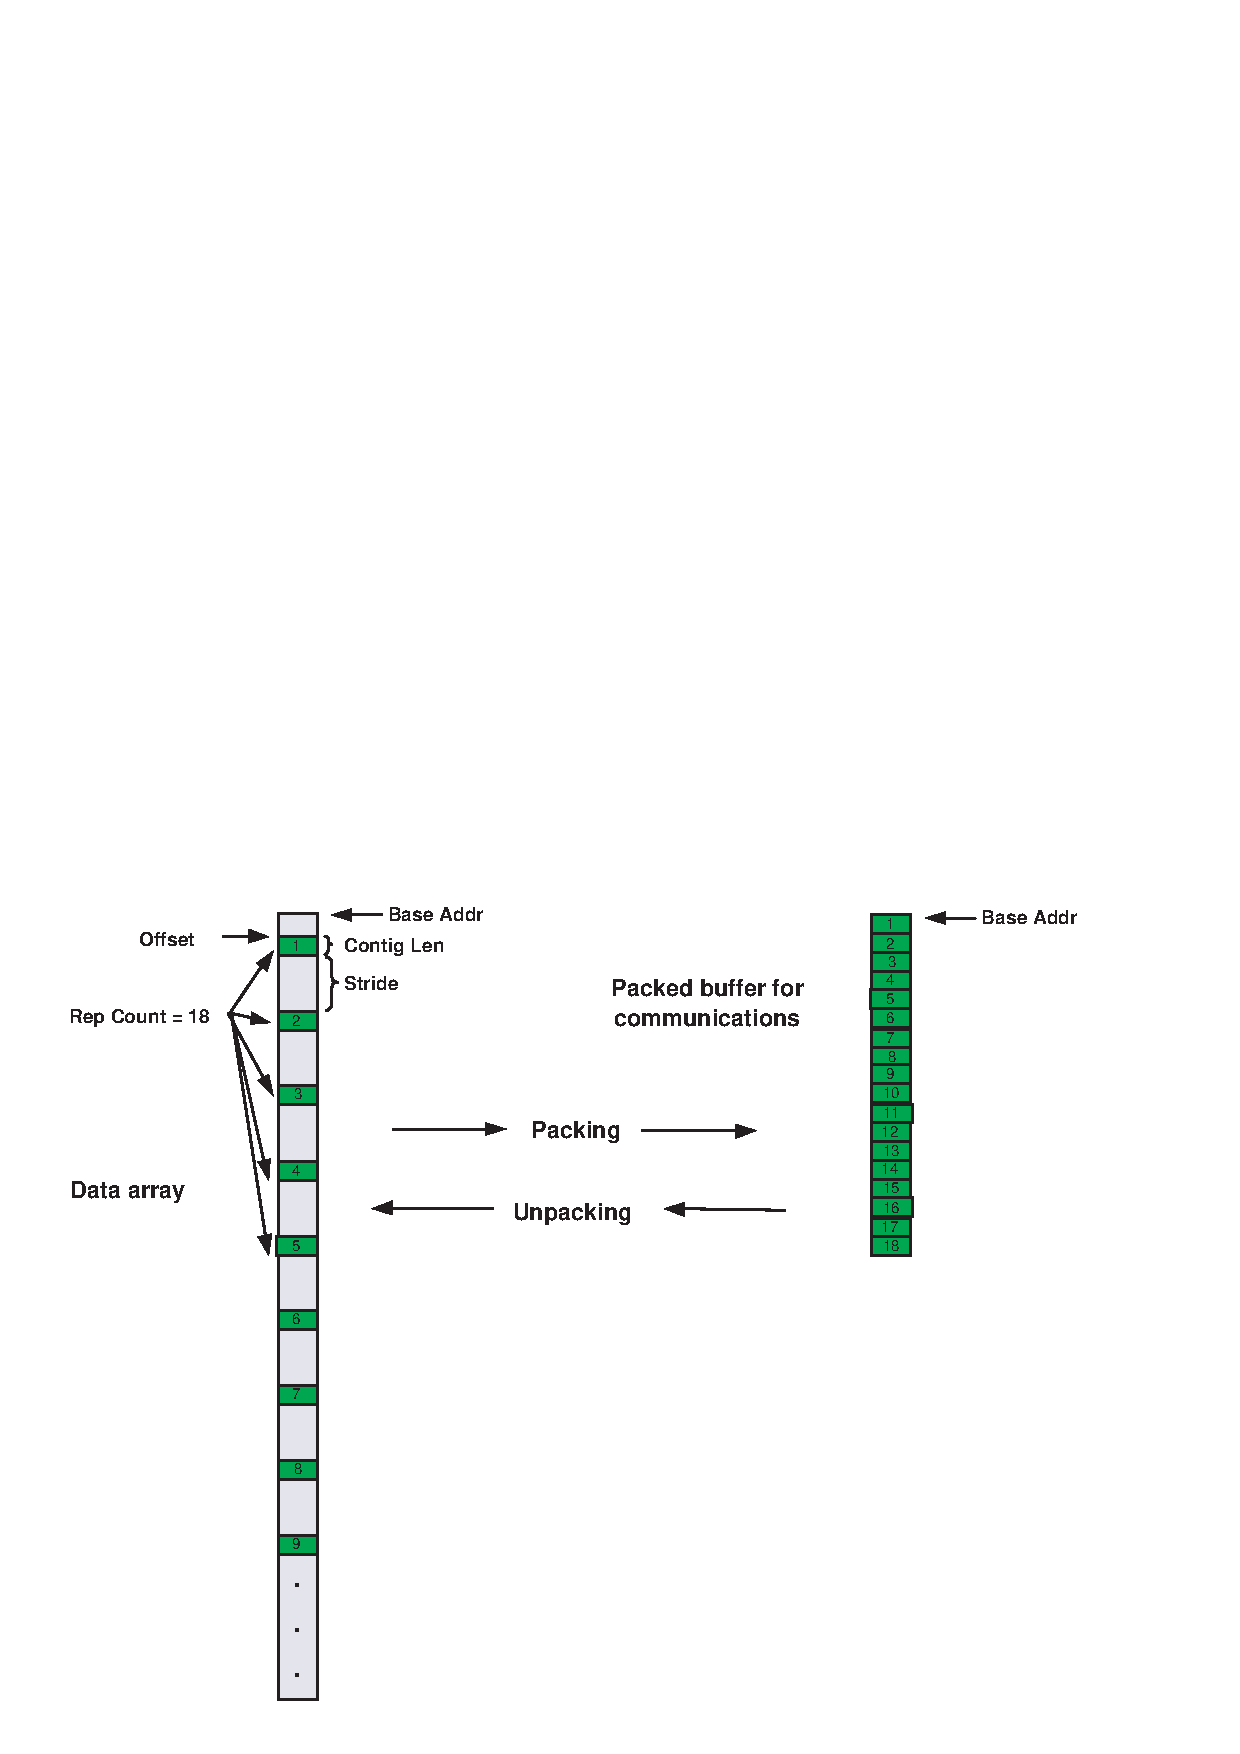
\includegraphics{Basic_pack_route}}
\caption{Often the overhead of making multiple communication calls 
outweighs the cost of copying non-contiguous data into a contiguous buffer,
sending it in a single operation, and then copying it to the final
memory locations on the receiving side.}
\label{fig:routepack}
\end{figure}
\end{center}

\begin{center}
\begin{figure}
\scalebox{0.8}{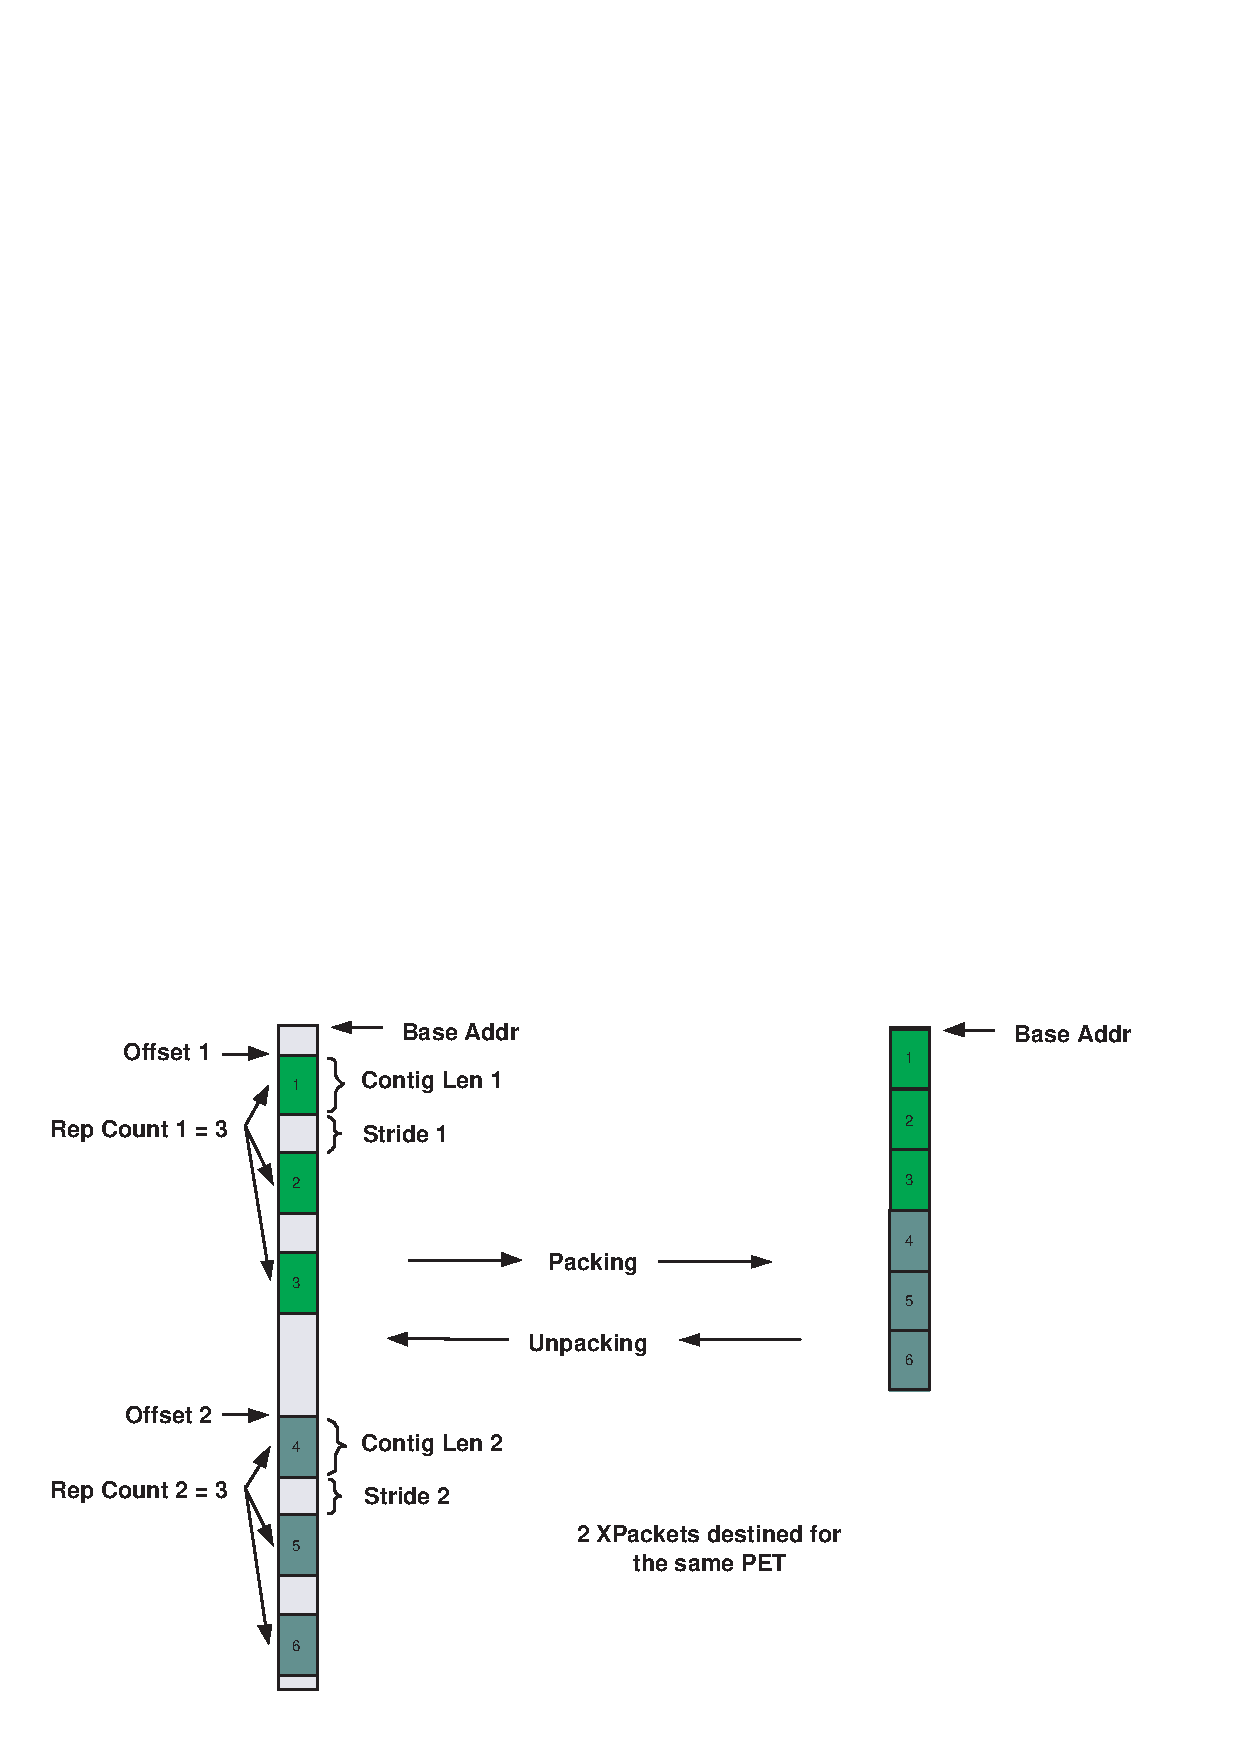
\includegraphics{Basic_2up_route}}
\caption{Once there is more than a single XPacket to pack, there
are many more interleave options.  For example, packing in the
order: 1, 4, 2, 5, 3, 6 would also be possible here.  However
the code becomes more complicated when the XPackets have different
repeat counts, and has no real performance advantage over the
straightforward packing of each XPacket in sequence.  Note that
this packing is the same whether it refers to multiple XPackets
from the same memory buffer or from multiple buffers.}
\label{fig:routepackall}
\end{figure}
\end{center}

The following options refer to the internal strategy for 
executing the route and not to whether the user-level API call
returns before the route has finished executing.  The current
system only implements user-synchronous calls; asynchronous calls
are on the to-be-written list.

\begin{enumerate}

\item[Sync] Each pair of processors exchanges data with the VM
equivalent of an MPI\_SendRecv() call, which does not return until
both the send and receive have completed.

\item[Async] Each processor executes both an asynchronous send
and asynchronous receive to the other processor and does not wait
for completion before moving on to the next communication in the
CommTable.  Then in a separate loop through the RTables, each
call is waited for in turn and when all outstanding communication
calls have completed, then the API call returns to the user.

\end{enumerate}
(Note that in the Async case it makes much more sense to iterate
through the Route table in PET order instead of the complication
of computing communication pairs and iterating in a non-sequential
order.  The code is as it is now for reasons of implementation speed
and not for any other design reason.  This would require a slightly
simpler, but separate, version of the RouteRun() subroutine.)

\item

FieldBundle-level communication calls have additional packing options
under certain circumstances.  FieldBundles are groups of Fields which
share the same Grid, but they are not required to share the same
data types, data ranks, nor relative data locations.  FieldBundles
in which these things are the same in all Fields are marked inside the
bundle code as being {\bf congruent}.  At communication store time
FieldBundles which have congruent data in all the Fields have the option
of packing all Field data together into fewer communication calls
which generally is expected to give better performance.   
Fields where the data is not of the same type or perhaps not
the same number of items (e.g. different rank, vertex-centered data
vs. cell centered data) can in theory also be packed but in fact
the code becomes more complicated, and in the case of differing
data types may cause system errors because of accessing data
on non-standard byte offsets or putting mixing integer data
with floating data and causing NaN (not a number) exceptions.
In this case, the conservative implementation strategy is to construct 
a separate Route object for each Field, all enclosed in the same
RouteHandle.  Inside the FieldBundle communication code the execution
for both types of FieldBundles is identical for the caller, but inside
the congruent FieldBundle code calls the {\tt ESMF\_RouteRun()} code
once and all communication for all Fields in the FieldBundle is done
when it returns.  The non-congruent FieldBundles execute a separate
{\tt ESMF\_RouteRun()} call for each Field and return to the user 
when all Field data have been sent/received.

There are comments in the code for an intermediate level of
optimization in which the FieldBundle code determines the smallest
number of unique types of Fields in the FieldBundle, and all same types
share the same Route object, but this has not been implemented
at this time.  Once the existing code has been in use for a while,
whether this is useful or needed may become more clear.


\item

The precompute code for all operations must have enough
information to compute which parts of the data arrays
are expected to be sent to remote PETs and also what
remote data is expected to be received by this PET.

These computations depend heavily on what type of distributed
method is being executed.  The regridding methods are described
in detail separately in the Regrid Design and Implementation Notes
section.  The halo and redistribution operations are described here.

\begin{enumerate}

\item[Halo] The total array area, which includes any halo regions,
are intersected with the computational
area of other DEs. The overlap regions are converted from index
space into memory space and stored as XPackets in the RTables.
This code must be aware of: whether the grid was defined as
periodic in any or all of the dimensions since that affects
which halo regions overlap at the grid edges; if the data
is only decomposed into a single block in any dimension (which
means it halos with itself); and if the halo region is large
enough that a halo operation may require intersection with
the N+1 neighbor in any dimension.  

\item[Redistribute]  Each DE computes the overlap
between its own computational region and all DEs in the 
remote Grid, again only working in computational area.  
The overlap regions are converted from index
space into memory space and stored as XPackets in the RTables.
After execution a redistribution, a halo operation may be required
to populate any halo regions with consistent data.

\end{enumerate}
(Note: the Redistribution code has been reimplemented to intersect
the DEs in index space and then convert the overlap region to an XPacket
representation.  Halo still converts the regions from AxisIndex to 
XPackets and then intersects the XPackets, but this code needs to be
changed to intersect in AxisIndex space and once the overlap is computed
then convert to XPackets.  Intersecting AxisIndex objects is very 
much simpler, both to understand and to execute, and more easily 
extensible to multiple dimensions than intersecting XPackets.)

\end{enumerate}

\subsection{Object Model}

The following is a simplified UML diagram showing the structure of the public
RouteHandle class.  See Appendix A, {\it A Brief Introduction to UML}, for a
translation table that lists the symbols in the diagram and their meaning.

\begin{center}
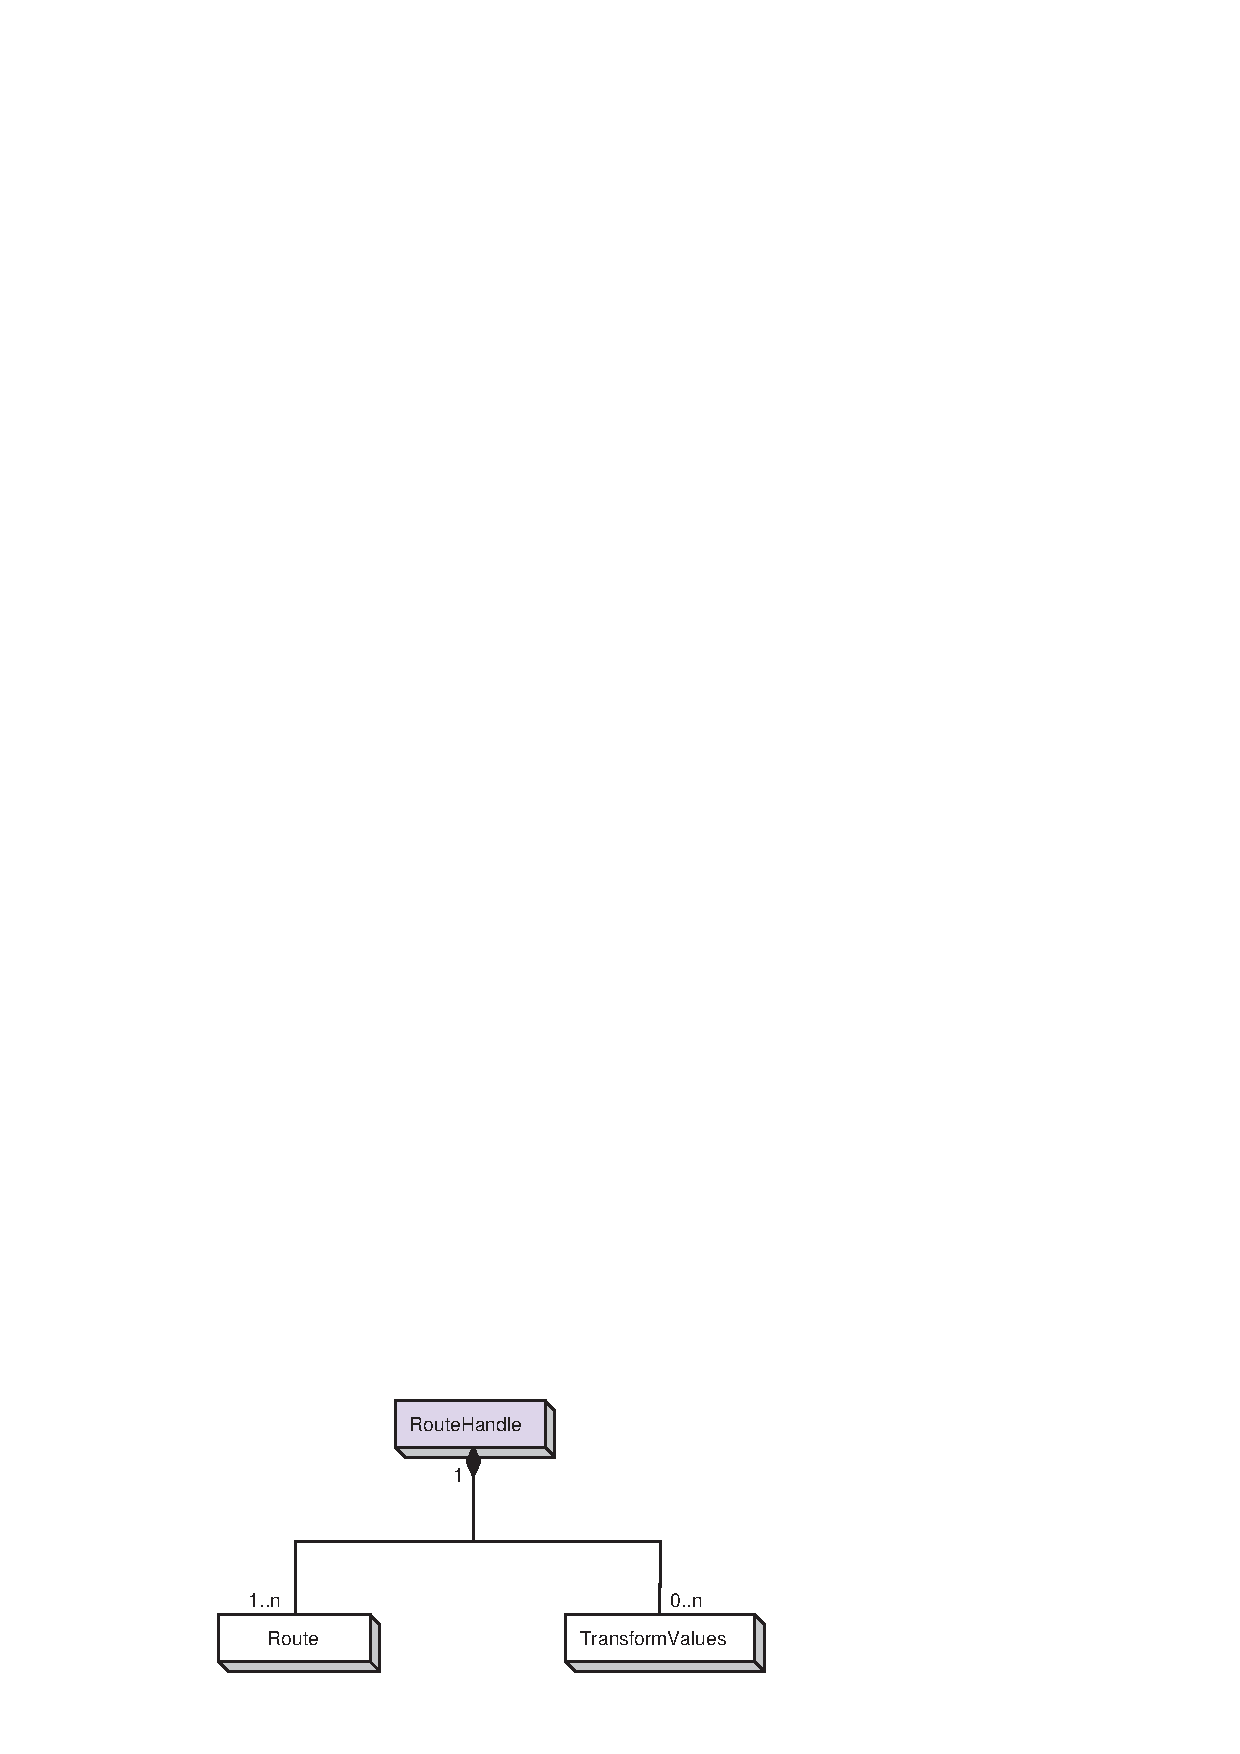
\includegraphics{RouteHandle_obj}
\end{center}


\newpage






%===============================================================================
\newpage
\begin{htmlonly}
\addcontentsline{toc}{part}{Infrastructure: Utilities}
\end{htmlonly}
\part{Infrastructure: Utilities}
\newpage
%\section{Overview of Infrastructure Utility Classes}
% $Id$
%
% Earth System Modeling Framework
% Copyright 2002-2020, University Corporation for Atmospheric Research, 
% Massachusetts Institute of Technology, Geophysical Fluid Dynamics 
% Laboratory, University of Michigan, National Centers for Environmental 
% Prediction, Los Alamos National Laboratory, Argonne National Laboratory, 
% NASA Goddard Space Flight Center.
% Licensed under the University of Illinois-NCSA License.

\section{Overview of Infrastructure Utility Classes}

The ESMF utilities are a set of tools for quickly assembling modeling applications.

The ESMF Attribute class enables models to be self-describing via metadata, which are instances of Attribute name-value pairs.

The Time Management Library provides utilities for time and time interval representation and calculation, and higher-level utilities that control model time stepping, via clocks, as well as alarming.

The ESMF Config class provides configuration management based on NASA DAO's Inpak package, a collection of methods for accessing files containing input parameters stored in an ASCII format.

The ESMF LogErr class consists of a variety of methods for writing error, warning, and informational messages to log files. A default Log is created during ESMF initialization. Other Logs can be created later in the code by the user.

The DELayout class provides a layer of abstraction on top of the Virtual Machine (VM) layer. DELayout does this by introducing DEs (Decomposition Elements) as logical resource units. The DELayout object keeps track of the relationship between its DEs and the resources of the associated VM object. A DELayout can be shaped by the user at creation time to best match the computational problem or other design criteria.

The ESMF VM (Virtual Machine) class is a generic representation of hardware and system software resources. There is exactly one VM object per ESMF Component, providing the execution environment for the Component code. The VM class handles all resource management tasks for the Component class and provides a description of the underlying configuration of the compute resources used by a Component.  In addition to resource description and management, the VM class offers the lowest level of ESMF communication methods.

The ESMF Fortran I/O utilities provide portable methods to access capabilities which are often implemented in different ways amongst different environments. Currently, two utility methods are implemented: one to find an unopened unit number, and one to flush an I/O buffer.

\newpage
% $Id$
%
% Earth System Modeling Framework
% Copyright 2002-2020, University Corporation for Atmospheric Research,
% Massachusetts Institute of Technology, Geophysical Fluid Dynamics
% Laboratory, University of Michigan, National Centers for Environmental
% Prediction, Los Alamos National Laboratory, Argonne National Laboratory,
% NASA Goddard Space Flight Center.
% Licensed under the University of Illinois-NCSA License.
\bodytext{BGCOLOR=white LINK=#083194 VLINK=#21004A}
\section{Attribute Class}
\subsection{Description}
% $Id$
%
% Earth System Modeling Framework
% Copyright 2002-2020, University Corporation for Atmospheric Research,
% Massachusetts Institute of Technology, Geophysical Fluid Dynamics
% Laboratory, University of Michigan, National Centers for Environmental
% Prediction, Los Alamos National Laboratory, Argonne National Laboratory,
% NASA Goddard Space Flight Center.
% Licensed under the University of Illinois-NCSA License.


The ESMF Attribute class is a metadata utility that supports emerging standards 
in a flexible way.  The Attribute class is useful for documenting data 
provenance and encourages models to be more self describing.  Attributes can 
also be used to automate some aspects of model execution and coupling.

Metadata, which is data about data, is broken down into 
name-value pairs by the Attribute class.  Attributes can be attached at any 
level of the ESMF object hierarchy, and in some cases the Attributes of 
different ESMF objects can be linked together to form 
a corresponding Attribute hierarchy.  Attribute hierarchies are linked up
automatically for the most part, with the exception of links between Components 
and between a Component and a State.  Attribute hierarchies can also be 
unlinked, copied, and moved around as needed.

ESMF Attribute packages 
are used to aggregate, store, and output model metadata.  They can be 
nested inside each other to make larger organized packages, distributed across 
processors and updated at runtime, and expanded to suit specific needs.  The
ESMF-supplied  
Attribute packages are designed around accepted metadata conventions, such as: 
climate and forecast (CF) \cite{ref:cf}, ISO standards \cite{ref:iso}, and the METAFOR Common Information Model (CIM) \cite{ref:cim} \cite{ref:esdoccim}.

Most of the ESMF deep objects can host Attributes, and   
every object that can hold individual Attributes can also hold
Attribute packages.  Attribute hierarchies are supported for a majority of
the Attribute bearing classes.  
More information on the various Attribute 
capabilities, and the classes for which they are supported appear in the
following sections.

Reading Attribute XML files requires the Xerces C++ library, v3.1.0 
or better.  For more details, see the "ESMF Users Guide", "Building and 
Installing the ESMF, Third Party Libraries, Xerces".  Writing Attribute XML 
files is performed with the standard C++ output file stream facility.

\subsubsection{Schemas and Controlled Vocabularies}

There are two pieces to the information stored in Attributes.  One piece
is the property name and type, and its relation to other properties; this
is the schema.  The other piece is the range of values that are valid for
a particular property; this is the controlled vocabulary.  For many
information models, including the Common Information Model (CIM), these two
pieces are managed and versioned separately.

ESMF implements the appropriate schema internally; it translates the Attributes
as specified in the Attribute packages into the correct format based on the
convention and purpose as specified in arguments to most Attribute functions.
The controlled vocabularies, or Attribute values, however, are not controlled
or validated within ESMF.

\subsubsection{The Common Information Model (CIM)}

The CIM is a formal model of the climate modeling process developed by
the European Union's \htmladdnormallink{METAFOR}{http://metaforclimate.eu/}
project.  The \htmladdnormallink{Earth System - Documentation (ES-DOC)}{http://earthsystemcog.org/projects/es-doc-models/} project
is an evolution of the METAFOR project, and they provide a detailed
description of the CIM \htmladdnormallink{here}{http://earthsystemcog.org/projects/es-doc-models/cim}.

ESMF is currently implementing only a subset of version 1.5 of the CIM, though this representation is expected to grow.

{\bf Mapping Attributes to the CIM}

The ESMF Attribute packages provide a structure for the Attributes that
are useful for climate modelers.  When the {\tt ESMF\_AttributeWrite()}
function is
called with "CIM" XML specified as the target, ESMF translates these package
structures into a format defined by the CIM schema.  The package descriptions
in the following sections provide a mapping from the ESMF Attribute name
to the CIM schema field.

For example, in the CIM Main Attribute Package, the Attribute named
"LongName" is mapped to the CIM schema field,
"software:SoftwareComponent:longName":

\begin{tabular}{|p{2cm}|p{4cm}|p{15mm}|p{7.5cm}|}
     \hline\hline
     {\bf Name} & {\bf Definition} & {\bf Controlled Vocabulary} & {\bf CIM Schema Field \linebreak (<CIM section>:<Entity>:<Field>)}\\
     \hline\hline
     {\tt LongName} & A version of the component name with all acronyms spelled out. & N/A & software:SoftwareComponent:longName \\
     \hline\hline
\end{tabular}
\linebreak

There are 3 parts to this mapping:

\begin{itemize}
  \item {\bf <CIM section>} = "software"
  \item {\bf <Entity>} = "SoftwareComponent"
  \item {\bf <Field>} = "longName"
\end{itemize}

The CIM section refers to the categories, or subsections, of the CIM
mentioned above.  In this example, the CIM section is "software".  To find
this section in the CIM schema repository, go to the
\htmladdnormallink{CIM repository}{http://metaforclimate.eu/trac/browser/CIM/tags/version-1.5/}
and then select the "software" drop down (see Figure \ref{fig:CIMRepository} ).

\begin{figure}[h]
\centering
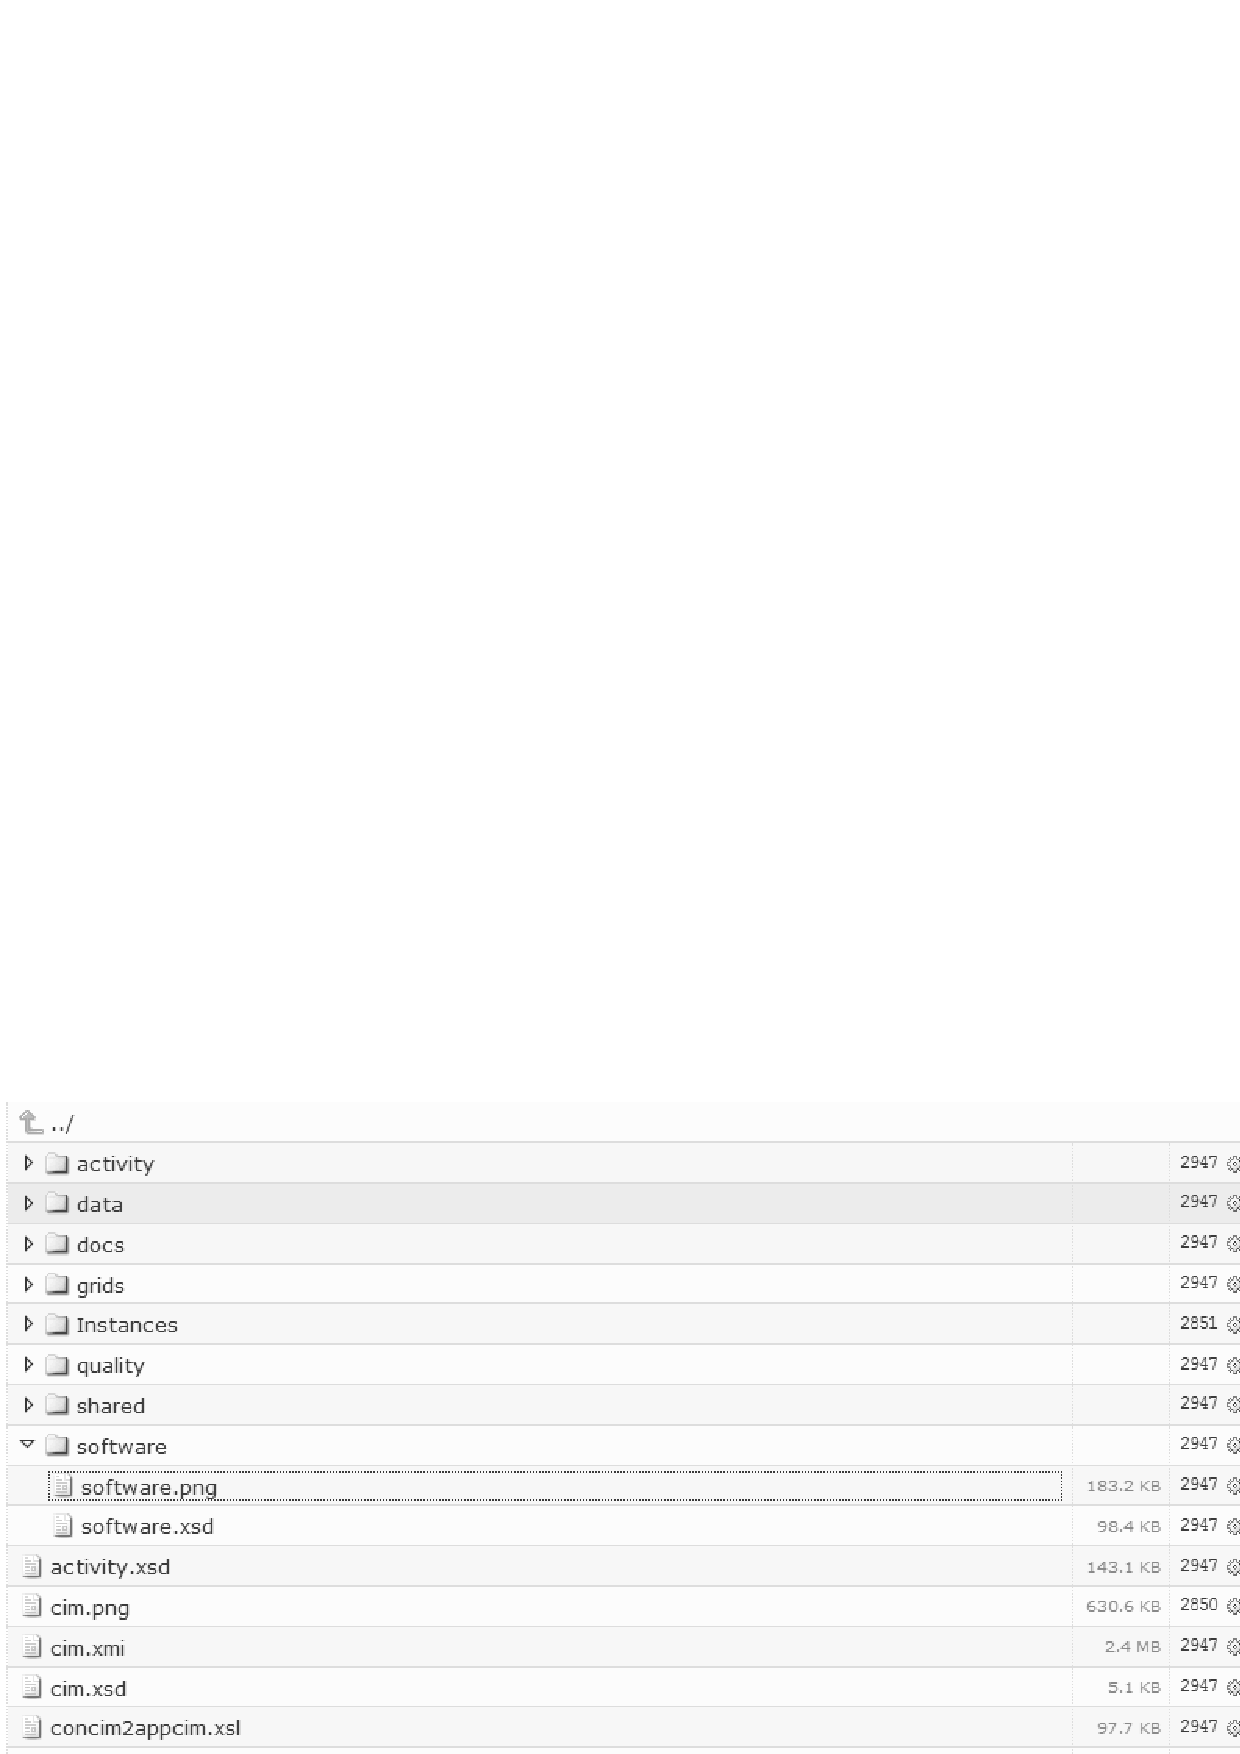
\includegraphics[width=160mm]{CIMRepository}
\caption{The software section of the CIM repository}
\label{fig:CIMRepository}
\end{figure}
\clearpage

You can view the schema graphically in a UML diagram by selecting the
software.png file and then visually search the picture for the
SoftwareComponent entity.
However, this view does not provide field details, such as type and
description.  Alternatively, you can select the software.xsd file, and
then search the XML for the entity, "SoftwareComponent," and the field,
"longName," which will provide the details for this field (see Figure \ref{fig:LongNameXSD} ).

\begin{figure}[h]
\centering
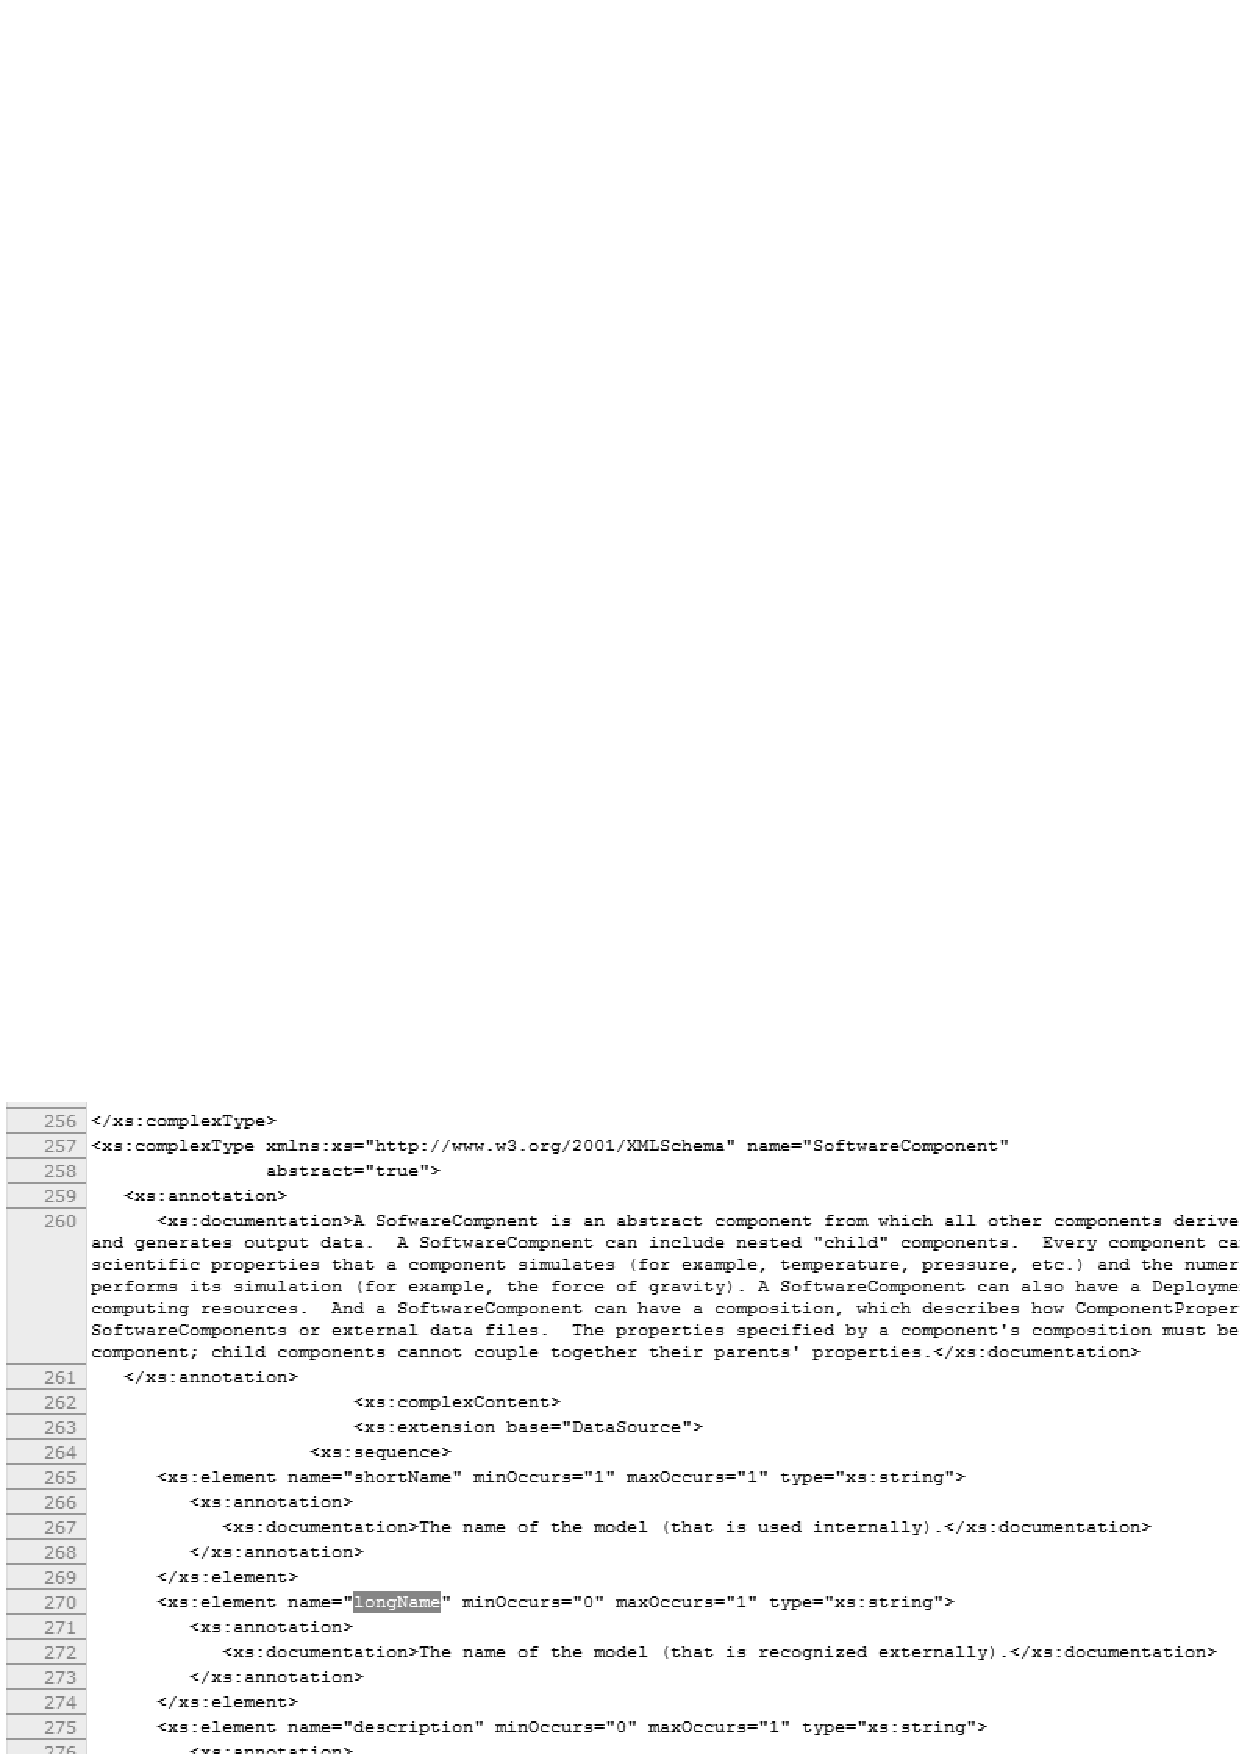
\includegraphics[width=160mm]{LongNameXSD}
\caption{The longName Field in the CIM software XSD file}
\label{fig:LongNameXSD}
\end{figure}
\clearpage

As the ES-DOC team continues its work, more tools will be provided to support
CIM implementations.  Currently, a more user-friendly way to view the CIM
schema is available through the ``CONCIM'' sections on \htmladdnormallink{this page}{https://www.earthsystemcog.org/projects/es-doc-models/cim_versions}.


\subsubsection{The ESMF approach to Attributes}

ESMF's approach to Attributes can be summarized as follows:

\begin{itemize}
  \item Implement community standards where they exist.
  \item Associate Attributes with the ESMF object they describe. Currently, the following ESMF objects can have Attributes:
  \begin{itemize}
     \item CplComp
     \item GridComp
     \item State
     \item FieldBundle
     \item Field
     \item ArrayBundle
     \item Array
     \item Grid
     \item DistGrid
     \end{itemize}
  \item Establish pre-defined Attribute packages (see Section \ref{sec:AttPacks}) to make Attribute creation easier for the user.
  \item Allow for user-defined custom Attribute packages (see Section \ref{sec:CustomAttPacks}).
  \item Enable the nesting of Attribute packages (see Section \ref{sec:AttPackNesting}) including Custom packages.
  \item Enable complex Attribute hierarchies (see Section \ref{sec:AttHier}.
  \item Export Attributes in more than one format (see Section \ref{sec:AttributeExports}).
  \item Ensure that all Attributes are consistent across the entire virtual machine of the object to which they are attached.
\end{itemize}

\subsubsection{Attribute hierarchies}
\label{sec:AttHier}

Of the ESMF objects with Attributes, only some can link their Attributes together in an Attribute hierarchy.  These objects are:

\begin{itemize}
\item CplComp
\item GridComp
\item State
\item FieldBundle
\item Field
\item ArrayBundle
\item Array
\end{itemize}

Every ESMF deep object is given a {\tt root} Attribute on creation.
These {\tt root} Attributes serve as the attachment point for all metadata that 
is stored on a particular ESMF object, including all Attributes and
Attribute packages.  The {\tt root} Attributes can also be connected together via 
the {\tt ESMF\_AttributeLink()} functionality.  This happens automatically in most 
cases, such as when a Field is added to a FieldBundle, and results
in the formation of an Attribute hierarchy which mirrors the structure 
of the underlying object hierarchy.  

When two Attribute hierarchies are linked together 
the objects are given read-only access to each other's Attributes.
To ensure consistency across a distributed system, 
there can only ever be one set of Attributes associated with each ESMF object.  
This implies that a copy operation on an ESMF object Attribute hierarchy {\it can} 
use a value copy for all Attributes which are owned by the object being copied, 
but {\it must} use a reference copy for all Attributes which the object can 
access (through links) but does NOT own. See section \ref{sec:Att:Copy} for more
details on this concept.

The most common use for this hierarchy capability is for linking the Attributes 
of a Field to the FieldBundle which holds it, which is then linked to the 
State that is used to transport all of the data for a Component.  All of 
these links, with the exception of the link between the Component and the 
State, are automatically handled by ESMF. Additionally, the State will 
automatically set a {\tt VariableIntent} Attribute for Field when that Field 
is added to the State.  {\tt VariableIntent} will be set to either 
{\tt Export} or {\tt Import}.


\subsection{Attribute Packages}
% $Id$
%
% Earth System Modeling Framework
% Copyright 2002-2020, University Corporation for Atmospheric Research,
% Massachusetts Institute of Technology, Geophysical Fluid Dynamics
% Laboratory, University of Michigan, National Centers for Environmental
% Prediction, Los Alamos National Laboratory, Argonne National Laboratory,
% NASA Goddard Space Flight Center.
% Licensed under the University of Illinois-NCSA License.


\label{sec:AttPacks}

At this time, all ESMF objects which are enabled to contain Attributes can also contain Attribute packages, which are groupings of individual Attributes.  Every Attribute package is specified by a unique set of identifiers.  These are called the {\bf convention} and {\bf purpose} of the Attribute package, such as "CF" and "General" (see below).  These are used to validate ESMF Attribute packages against existing metadata conventions.  The {\bf attPackInstanceName} can be used to differentiate between Attributes of the same name within a package. 

The user can choose to use an ESMF pre-defined Attribute package, specify their own Attribute package, or add customized Attributes to any of the ESMF pre-defined Attribute packages. Currently, the creation and setting of Attribute packages is quite involved, but future development with I/O will allow for a more automated approach to populating Attribute packages from a file.  This is already possible via {\tt ESMF\_AttributeRead()} for the ESMF/CF Attribute packages supplied by ESMF, as well as for custom individual Attributes not in a package.

The standard Attribute packages supplied by ESMF exist for the following ESMF objects:

\begin{itemize}
    \item CplComp
    \item GridComp
    \item State
    \item Field
    \item Array
    \item Grid
\end{itemize}

The packages described in this section are grouped by the ESMF object they apply to. The creation of custom attributes and custom attribute packages is also possible and is discussed in Section \ref{sec:CustomAttPacks}. In some cases it is possible to nest custom packages on top of ESMF packages. Attribute package nesting is described separately in Section \ref{sec:AttPackNesting}.

Some Attributes come with a controlled vocabulary. A controlled vocabulary is a list of options that can be selected as the value of the attribute. The controlled vocabularies listed in this documentation represent those chosen by the community. They are not exhaustive and users may set these Attributes to a different value if they so choose. The primary consequence of doing so is that the resulting output may not be recognized by any of the online tools being developed with respect to this controlled vocabulary.


\subsubsection{Component Attribute packages}
\label{ComponentAttributePackages}

There are many attributes that are used to describe components. There are currently 4 predefined component-level Attribute packages, with sub-packages defined for the 2nd:

\begin{enumerate}
    \item Earth System Modeling Framework (ESMF) General
    \item Common Information Model (CIM) Main
    \begin{enumerate}
        \item Common Information Model (CIM) Platform
        \item International Organization for Standardization (ISO) Responsible Party
        \item International Organization for Standardization (ISO) Citation
    \end{enumerate}
    \item Common Information Model (CIM) Scientific Properties
    \item Common Information Model (CIM) Component Properties
\end{enumerate}

\vspace{.20in}

{\bf 1. Earth System Modeling Framework (ESMF) General Attribute Package}

\begin{itemize}
    \item Specify with:
    \begin{itemize}
        \item {\tt convention} = "ESMF"
        \item {\tt purpose} = "General"
    \end{itemize}
    \item Output Options:
    \begin{itemize}
        \item Simple XML
    \end{itemize}
    \item Description: This package contains several Attributes used to describe model components within the Earth System Modeling Framework (ESMF) ontology.
\end{itemize}


\begin{tabular}{|p{5cm}|p{5cm}|p{35mm}|}
     \hline\hline
     {\bf Name} & {\bf Definition} & {\bf Controlled Vocabulary}\\
     \hline\hline
     {\tt Agency} & An administrative unit of government.& DoD, DOE, DOI, NASA, NOAA, NSF\\
     {\tt Author} & The person who created the content of a book, article, or other source. & N/A\\
     {\tt CodingLanguage} & The computer language in which a unit of software is written. & C, C++, F77, F90, Java\\
     {\tt ComponentLongName} & The name of a model, model component, simulation, experiment, or dataset with all acronyms spelled out. & N/A\\
     {\tt ComponentShortName} & A version of the component name that contains acronyms. & N/A\\
     {\tt Discipline} & A subject, theme, category, or general area of interest.& Aerosol, Fisheries, Climate, Carbon Cycle, Hydrology, Land, Ocean, Polar, Sediment, Storm Surge, Turbulence, Weather, Wave, Weather Prediction \\
     {\tt Institution} & An organization associated with a model component, simulation, or dataset.& N/A\\
     {\tt ModelComponentFramework} & The software package or mechanism used to transfer and transform data between model components.& CCA, ESMF, Flume, FMS, OASIS, SWMF \\
     {\tt PhysicalDomain} & A description of the geographic range being simulated. & Atmosphere, Earth System, Ice, Lake, Land Ocean, River\\
     {\tt Version} & A specific form or variation of an artifact, i.e. a unit of software or metadata. & N/A\\
     \hline\hline
\end{tabular}

\vspace{.20in}

{\bf 2. Common Information Model (CIM) Main Attribute Package}

\begin{itemize}
    \item Specify with:
    \begin{itemize}
        \item {\tt convention} = "CIM 1.5"
        \item {\tt purpose} = "ModelComp"
    \end{itemize}
    \item CIM Version: CIM 1.5
    \item CIM URL: \htmladdnormallink{http://metaforclimate.eu/trac/browser/CIM/tags/version-1.5/}{http://metaforclimate.eu/trac/browser/CIM/tags/version-1.5/}
    \item Includes:
    \begin{itemize}
       \item CIM Platform
       \item ISO Responsible Party (1 or more -- user specifiable)
       \item ISO Citation (1 or more -- user specifiable)
    \end{itemize}
    \item Output Options:
    \begin{itemize}
        \item CIM XML
    \end{itemize}
    \item Description: The CIM Main Package contains several standalone properties used to describe components. It also serves as the anchor to which other CIM packages are nested. Presently, these additional CIM packages (described further below) can only be created if the CIM Main Package is created. In the future, these packages will be decoupled, so that users may select subsections of the CIM to create and use. This package nests three of the packages below within it; this is described in Section \ref{sec:AttPackNesting}.
\end{itemize}


\begin{longtable}{|p{6cm}|p{2cm}|p{1.5cm}|p{6.5cm}|}
     \hline\hline
     {\bf Name} & {\bf Definition} & {\bf Controlled Vocabulary} & {\bf CIM Schema Field (<CIM section>:<Entity>:<Field>)}\\
     \hline\hline
     {\tt Description} & A multi-line description of the component. & N/A & software:SoftwareComponent:description \\
     {\tt LongName} & A version of the component name with all acronyms spelled out. & N/A & software:SoftwareComponent:longName \\
     {\tt MetadataVersion***} & The version number of the simulation metadata. & N/A & software:modelComponent:metadataVersion \\
     {\tt ModelType*} & A short string describing the discipline of a model component. & Advection, Aerosol3D-Sources etc. & software:ModelComponent:type \\
     {\tt PreviousVersion**} & Name of the previous version of a model or model component. & N/A & shared:Reference:name \\
     {\tt PreviousVersionDescription**} &  A short note about the previous version of the model or model component. & N/A & shared:Relationship:description \\
     {\tt ReleaseDate} & The date a model component was issued. & N/A & software:SoftwareComponent:releaseDate \\
     {\tt ShortName*} & A version of the component name that contains acronyms. & N/A & software:SoftwareComponent:shortName \\
     {\tt SimulationDuration} & The length of time a simulation runs. & N/A & activity:SimulationRun:dateRange \\
     {\tt SimulationEndDate} & The date in simulated time of the end of a model simulation. & N/A & activity:SimulationRun:dateRange \\
     {\tt SimulationEnsembleID} & The reference name or number of the ensemble to which a simulation belongs. & N/A & activity:EnsembleMember:ensembleMemberID \\
     {\tt SimulationLongName} & The name of the simulation with any acronyms spelled out. & N/A & activity:NumericalActivity:longName \\
     {\tt SimulationNumberOfProcessing Elements} & The number of PEs used in the simulation. & N/A & software:Parallelization:processes \\
     {\tt SimulationProjectName} & A campaign, such as a model intercomparison project, that may involve multiple groups and experiments. & N/A & activity:Activity:project \\
     {\tt SimulationRationale} & The reason for performing a simulation. & N/A  & activity:Activity:rationale \\
     {\tt SimulationShortName} & The name of the simulation. & N/A & activity:NumericalActivity:shortName \\
     {\tt SimulationStartDate*} & The date in simulated time of the start of a model simulation. & N/A & activity:SimulationRun:dateRange \\
     {\tt URL} & A URL associated with a model component. & N/A & shared:CI\_OnlineResource:linkage \\
     {\tt Version} & Version number of the component. & N/A  & appended to software:SoftwareComponent:shortName \\
     \hline\hline
\end{longtable}
 * Attribute required to be set to produce valid CIM XML output. \\
 ** If PreviousVersionDescription is set, PreviousVersion must also be set, to produce valid CIM XML output. \\
 *** If not set, defaults to 1.0

\vspace{.20in}

{\bf 2.1. CIM Platform Attribute Package}

\begin{itemize}
    \item Specify with:
    \begin{itemize}
        \item {\tt convention} = "CIM 1.5"
        \item {\tt purpose} = "Platform"
    \end{itemize}
    \item CIM Version: CIM 1.5
    \item CIM URL: \htmladdnormallink{http://metaforclimate.eu/trac/browser/CIM/tags/version-1.5/}{http://metaforclimate.eu/trac/browser/CIM/tags/version-1.5/}
    \item Output Options:
    \begin{itemize}
       \item CIM XML
    \end{itemize}
    \item Description: This package describes the platform a particular simulation is run on. It must be created in conjunction with the CIM Main Package (see above). This package is nested within the CIM Main Package (above); see the description in Section \ref{sec:AttPackNesting}.
\end{itemize}

\begin{longtable}{|p{5cm}|p{2.5cm}|p{2cm}|p{6.5cm}|}
     \hline\hline
     {\bf Name} & {\bf Definition} & {\bf Controlled Vocabulary} & {\bf CIM Schema Field \linebreak (<CIM section>:<Entity>:<Field>)}\\
     \hline\hline
     {\tt CompilerName**} & The brand of the software that takes source code and turns it into an executable.& Absoft, Default, Intel, Lahey, NAG, Pathscale, PGI, PGIGCC, XLF, XLFGCC & shared:Compiler:compilerName \\
     {\tt CompilerVersion**} & The specific configuration value of the software used to take source code and turn it into executable code. & N/A & shared:Compiler:compilerVersion \\
     {\tt MachineCoresPerProcessor} & The number of sub-divided elements or mini-chips on a computer chip. &  N/A & shared:Machine:machineCoresPerProcessor \\
     {\tt MachineDescription} & A short note about the machine. & N/A & shared:Machine:machineDescription \\
     {\tt MachineInterconnectType} & The technology used to associate each node in a supercomputer with every other node. & Cray Interconnect, Fat Tree, Gigabit Ethernet, Infiniband, Mixed, Myrinet, Numalink, Quadrics, SP Switch & shared:Machine:machineInterconnect \\
     {\tt MachineMaximumProcessors} & The highest number of computer chips on a computer system. & N/A & shared:Machine:machineMaximumProcessors \\
     {\tt MachineName*} & The name given to a computer by its system administrators. This is not the brand name of the system.& N/A & shared:Machine:machineName \\
     {\tt MachineOperatingSystem} & The software that is responsible for the management and coordination of activities and the sharing of resources of a computer. & Aix, Darwin, Irix64, Linux, SUNOS, Unicos & shared:Machine:machineOperatingSystem \\
     {\tt MachineProcessorType} & The type of computer chip used in a particular computer platform. & Altix, AMD x86-64, Bluegene, G4, G5, Intel EM64T, Intel IA-64, Itanium, NEC, Opteron, Origin3800, Pentium 3, Pentium 4, SP, SPARC, X1, Xeon, XT3-4, ZX6000 & shared:Machine:machineProcessorType \\
     {\tt MachineSystem} & The type of computer system (e.g. vector, parallel, cluster, etc.).& Beowulf, Parallel, Vector & shared:Machine:machineSystem \\
     {\tt MachineVendor} & The brand name of a computer system. & ACS, Action, Appro International, Bull SA, Cray Inc, Dalco AG Switzerland, Dawning, Dell, Fujitsu, Hitachi, HP, IBM, Intel, Koi Computers, Lenovo, Mac, NEC, NEC SUN, NUDT, PC, Pyramid Computer, Raytheon-Aspen Systems, Self Made, SGI, Sun Microsystems, T-platforms & shared:Machine:machineVendor \\
     \hline\hline
\end{longtable}
* Attribute required to be set to produce valid CIM XML output. \\
** Both CompilerName and CompilerVersion are required to be set, or else neither one, to produce valid CIM XML output; setting one without the other will produce invalid CIM XML output.

\vspace{.20in}

{\bf 2.2. ISO Responsible Party Attribute Package}

\begin{itemize}
    \item Specify with:
    \begin{itemize}
        \item {\tt convention} = "ISO 19115"
        \item {\tt purpose} = "RespParty"
    \end{itemize}
    \item Output Options:
    \begin{itemize}
        \item CIM XML
    \end{itemize}
    \item Description: This package is used to describe contacts, authors, institutions, and funding agencies. This package is nested, with one or more user-specifiable instances, within the CIM Main Package(above); see the description in Section \ref{sec:AttPackNesting}.
    \item Usage: The Responsible Party package is unique in that the user should first select the type of Responsible Party they wish to define. This is done via the ResponsiblePartyRole attribute within the package. Then the package's main value is set using the Name attribute.
\end{itemize}


\begin{longtable}{|p{4.5cm}|p{3cm}|p{2cm}|p{6.5cm}|}
     \hline\hline
     {\bf Name} & {\bf Definition} & {\bf Controlled Vocabulary} & {\bf CIM Schema Field (<CIM section>:<Entity>:<Field>)}\\
     \hline\hline
     {\tt Abbreviation} & The abbreviation of an individual or organization associated with a model component or simulation. & N/A & shared:ResponsibleParty:abbreviation \\
     {\tt EmailAddress} & The email address that others can use to ask questions about a model component. & N/A & shared:CI\_Address:electronicMailAddress \\
     {\tt Name} & The name of an author, contact, funder, centre, or principal investigator. & N/A & shared:CI\_ResponsibleParty:individualName, shared:CI\_ResponsibleParty:organisationName, shared:CI\_ResponsibleParty:positionName (depending on NameType value) \\
     {\tt NameType} & The type of entity that Name references. & Individual, Organization, Position & Not part of CIM; used to determine which CIM field to use for Name \\
     {\tt PhysicalAddress} & The address of the person designated to provide information about a model component. & N/A & shared:CI\_Address:deliveryPoint \\
     {\tt ResponsiblePartyRole*} & A flag to define the role of the Responsible Party. & Author, PI, Contact, Center, Funder & shared:CI\_ResponsibleParty:role \\
     {\tt URL} & A URL of an individual or organization. & N/A & shared:CI\_OnlineResource:linkage \\
     \hline\hline
\end{longtable}
* Attribute required to be set, when any other attributes in this package are set, to produce valid CIM XML output. It is valid to set none of the attributes in this package. In that case, no corresponding CIM XML output will appear for that Responsible Party package instance, although there may be other populated instances, which, because they have attributes set, will appear in the output.


{\bf 2.3. ISO Citation Attribute Package}

\begin{itemize}
    \item Specify with:
    \begin{itemize}
        \item {\tt convention} = "ISO 19115"
        \item {\tt purpose} = "Citation"
    \end{itemize}
    \item Output Options:
    \begin{itemize}
        \item CIM XML
    \end{itemize}
    \item Description: This package is used to describe references. Examples include a URL or a scientific reference.  This package is nested, with one or more user-specifiable instances, within the CIM Main Package (above); see the description in Section \ref{sec:AttPackNesting}.
\end{itemize}


\begin{longtable}{|p{3.5cm}|p{3cm}|p{3cm}|p{6.5cm}|}
     \hline\hline
     {\bf Name} & {\bf Definition} & {\bf Controlled Vocabulary} & {\bf CIM Schema Field (<CIM section>:<Entity>:<Field>)}\\
     \hline\hline
     {\tt Date*} & The date of the citation. & N/A & shared:CI\_Citation:Date \\
     {\tt DOI} & The assigned Digital Object Identifier (DOI) of the citation. & N/A & shared:CI\_Citation:otherCitationDetails \\
     {\tt LongTitle} & The text of the citation or pointer (e.g. URL) that further describes a model component or simulation. & N/A & shared:CI\_Citation:collectiveTitle \\
     {\tt PresentationForm} & A description of the type of citation. & documentDigital, documentHardcopy, imageDigital, imageHardcopy, mapDigital, mapHardcopy, modelDigital, modelHardcopy, profileDigital, profileHardcopy, tableDigital, tableHardcopy, videoDigital, videoHardcopy & shared:CI\_Citation:presentationForm \\
     {\tt ShortTitle*} & An abbreviation for the citation.  This could be the short scientific citation (e.g. Murphy, 2009) or the title of a web page. & N/A & shared:CI\_Citation:title \\
     {\tt URL} & Website associated with the citation. & N/A & appended to shared:CI\_Citation:collectiveTitle \\
     \hline\hline
\end{longtable}
* Attribute required to be set, when any other attributes in this package are set, to produce valid CIM XML output. It is valid to set none of the attributes in this package. In that case, no corresponding CIM XML output will appear for that Citation package instance, although there may be other populated instances, which, because they have attributes set, will appear in the output.

\vspace{.20in}

{\bf 3. Common Information Model (CIM) Scientific Properties Package}

\begin{itemize}
    \item Specify with:
    \begin{itemize}
        \item {\tt convention} = "CIM 1.5"
        \item {\tt purpose} = "SciProp"
    \end{itemize}
    \item CIM Version: CIM 1.5
    \item CIM URL: \htmladdnormallink{http://metaforclimate.eu/trac/browser/CIM/tags/version-1.5/}{http://metaforclimate.eu/trac/browser/CIM/tags/version-1.5/}
    \item CV Version: 1.3
    \item CV URL: \htmladdnormallink{http://metaforclimate.eu/trac/browser/cmip5q/tags/version-1.3/trunk/cmip5q/cmip5q/data/mindmaps}{http://metaforclimate.eu/trac/browser/cmip5q/tags/version-1.3/trunk/cmip5q/cmip5q/data/mindmaps}
    \item Output Options:
    \begin{itemize}
        \item CIM XML
    \end{itemize}
    \item Description: This package is used to describe the scientific properties of a component.  The names and values of these properties are part of controlled vocabularies; the recommended version of the controlled vocabulary in the timeframe of this ESMF release is located in a set of mindmap files, located \htmladdnormallink{here}{http://metaforclimate.eu/trac/browser/cmip5q/tags/version-1.3/trunk/cmip5q/cmip5q/data/mindmaps}.  This is the controlled vocabulary that was used for the \htmladdnormallink{5th Coupled Model Intercomparison Project}{http://q.cmip5.ceda.ac.uk/}.  One or more values can be set (via an array) for a property name.
\end{itemize}

\begin{longtable}{|p{6cm}|p{2cm}|p{1.5cm}|p{6.5cm}|}
     \hline\hline
     {\bf Name} & {\bf Definition} & {\bf Controlled Vocabulary} & {\bf CIM Schema Field (<CIM section>:<Entity>:<Field>)}\\
     \hline\hline
     % This hyperlink is done three times to allow the line to split normally in the table
     {\tt <Scientific property name>} & <METAFOR definition>. & \htmladdnormallink{METAFOR}{http://metaforclimate.eu/trac/browser/cmip5q/tags/version-1.3/trunk/cmip5q/cmip5q/data/mindmaps} \htmladdnormallink{mindmap}{http://metaforclimate.eu/trac/browser/cmip5q/tags/version-1.3/trunk/cmip5q/cmip5q/data/mindmaps} \htmladdnormallink{files}{http://metaforclimate.eu/trac/browser/cmip5q/tags/version-1.3/trunk/cmip5q/cmip5q/data/mindmaps}.  & software:SoftwareComponent: scientificProperties \\
     \hline\hline
\end{longtable}

\vspace{.20in}

{\bf 4. Common Information Model (CIM) Component Properties Package}

\begin{itemize}
    \item Specify with:
    \begin{itemize}
        \item {\tt convention} = "CIM 1.5"
        \item {\tt purpose} = "CompProp"
    \end{itemize}
    \item CIM Version: CIM 1.5
    \item CIM URL: \htmladdnormallink{http://metaforclimate.eu/trac/browser/CIM/tags/version-1.5/}{http://metaforclimate.eu/trac/browser/CIM/tags/version-1.5/}
    \item Output Options:
    \begin{itemize}
        \item CIM XML
    \end{itemize}
    \item Description: This package is used to specify any number of custom, user-defined attributes of a component and have them output in valid CIM XML format.  This differs from the scientific properties package above in that the names and values are custom, not part of any controlled vocabulary.  It also differs from a custom attribute package (see Section \ref{sec:CustomAttPacks}) in that this package has a standard convention and purpose, which is used to control the output of the user-defined attributes in standard CIM XML format.  One or more values can be set (via an array) for an attribute name.
\end{itemize}

\begin{longtable}{|p{6cm}|p{2cm}|p{1.5cm}|p{6.5cm}|}
     \hline\hline
     {\bf Name} & {\bf Definition} & {\bf Controlled Vocabulary} & {\bf CIM Schema Field (<CIM section>:<Entity>:<Field>)}\\
     \hline\hline
     {\tt <User-defined name>} & <User-defined definition>. & N/A & software:SoftwareComponent: componentProperties \\
     \hline\hline
\end{longtable}

\vspace{.20in}

\subsubsection{State Attribute packages}
\label{StateAttributePackages}

There is currently only 1 predefined State-level Attribute package:

\begin{enumerate}
    \item ESMF General
\end{enumerate}


\vspace{.20in}
{\bf 1. ESMF General State Attribute Package}

\begin{itemize}
    \item Specify with:
    \begin{itemize}
        \item {\tt convention} = "ESMF"
        \item {\tt purpose} = "General"
    \end{itemize}
    \item Output Options:
    \begin{itemize}
        \item Tab-delimited
        \item Simple XML
    \end{itemize}
    \item Description: This package is used to define whether an ESMF State object is an Import State or Export State.
\end{itemize}

\begin{tabular}{|p{5cm}|p{5cm}|p{4cm}|}
    \hline\hline
    {\bf Name } & {\bf Definition} & {\bf Controlled Vocabulary} \\
    \hline\hline
    {\tt Intent} & An indication of whether a state is imported into or exported from a particular model component. This refers to coupling, and not history output. & Export,Import \\
    \hline\hline
\end{tabular}

\vspace{.20in}

\subsubsection{Field Attribute packages}
\label{FieldAttributePackages}

Several standards exist to describe fields. There are currently 4 predefined Field-level Attribute packages:

\begin{enumerate}
    \item Common Information Model (CIM) Inputs
    \item Earth System Modeling Framework (ESMF) General
    \item Climate Forecast (CF) Convention Extended
    \item Climate Forecast (CF) Convention General
\end{enumerate}

\vspace{.20in}

{\bf 1. Common Information Model (CIM) Inputs}

\begin{itemize}
    \item Specify with:
    \begin{itemize}
        \item {\tt convention} = "CIM 1.5"
        \item {\tt purpose} = "Inputs"
    \end{itemize}
    \item CIM Version: CIM 1.5
    \item CIM URL: \htmladdnormallink{http://metaforclimate.eu/trac/browser/CIM/tags/version-1.5/}{http://metaforclimate.eu/trac/browser/CIM/tags/version-1.5/}
    \item Includes:
    \begin{itemize}
        \item ESMF General
        \item CF Extended
        \item CF General
    \end{itemize}
    \item Output Options:
    \begin{itemize}
        \item CIM XML
    \end{itemize}
    \item Description: This package is used to describe a simulation and the input (initial and boundary) conditions used in that simulation. It is also used to describe any ancillary data sets that contain input condition variables. This package should not be used to describe the variables in an unconfigured model component. A pre-defined Attribute package for that case will be implemented in a future release of ESMF.  This package nests the ESMF General, CF Extended, and CF General Field packages (below) within it; this is described in Section \ref{sec:AttPackNesting}.  The attribute values within these ESMF and CF nested packages currently appear in the Component Properties section of the CIM output file.  A separate Component Properties package may be developed for this purpose in a future ESMF release.
\end{itemize}

\begin{longtable}{|p{5.5cm}|p{2cm}|p{2cm}|p{6.5cm}|}
    \hline\hline
    {\bf Name} & {\bf Definition} & {\bf Controlled Vocabulary} & {\bf CIM Schema Field (<CIM section>:<Entity>:<Field>)}\\
    \hline\hline
    {\tt CouplingPurpose*} & The form of the input condition (e.g. initial condition or boundary condition). &  Ancillary, Boundary, Initial & software:Coupling:purpose \\
    {\tt CouplingSource*} & The component the input condition is coming from. & N/A & software:Coupling:couplingSource \\
    {\tt CouplingTarget*} & The component the input condition is going to. & N/A & software:Coupling:couplingTarget \\
    {\tt Description} &  A multi-line description of the input. & N/A & software:Coupling:description \\
    {\tt Frequency} & The frequency (e.g. 2 months or 5 days) that a field from one component is input to another. & n Seconds, n Minutes, n Hours, n Days, n Months, n Years, n Decades, n Centuries & software:Timing:rate \\
    {\tt SpatialRegriddingMethod} & Method used to interpolate a field from one grid (source grid) to another (target grid). & Linear, Near-Neighbor, Cubic, Conservative-First-Order, Conservative-Second-Order, Conservative, Non-Conservative & software:SpatialRegridding: spatialRegriddingStandardMethod \\
    {\tt SpatialRegriddingDimension} & Dimension of the regridding method. & 1D, 2D, 3D & software:SpatialRegridding: spatialRegriddingDimension \\
    {\tt Technique} & The software package or mechanism used to transfer and transform data between model components. & CCSM Flux Coupler, ESMF, Files, FMS, MCT, OASIS3, Shared & N/A \\
    {\tt TimeTransformationType} & Temporal transformation performed on the input field before or after regridding onto the target grid.& Exact, None, Time Accumulation, Time Average, Time Interpolation & software:TimeTransformation:mappingType \\
    \hline\hline
\end{longtable}
* Attribute required to be set, when any other attributes in this package are set, to produce valid CIM XML output. It is valid to set none of the attributes in this package. In that case, no corresponding CIM XML output will appear for that Inputs package.

\vspace{.20in}

{\bf 2. Earth System Modeling Framework (ESMF) Field}

\begin{itemize}
    \item Specify with:
    \begin{itemize}
        \item {\tt convention} = "ESMF"
        \item {\tt purpose} = "General"
    \end{itemize}
    \item Includes:
    \begin{itemize}
        \item CF Extended
        \item CF General
    \end{itemize}
    \item Output Options:
    \begin{itemize}
        \item Tab-delimited
        \item Simple XML
        \item CIM XML (when part of the CIM Inputs package)
    \end{itemize}
    \item Description: This package nests the CF Extended and CF General packages (below) within it; this is described in Section \ref{sec:AttPackNesting}.
\end{itemize}

\begin{tabular}{|p{5cm}|p{5cm}|p{35mm}|}
     \hline\hline
     {\bf Name } & {\bf Definition} & {\bf Controlled Vocabulary} \\
     \hline\hline
     {\tt Intent} & An indication of whether a variable is exported or imported. This refers to coupling and not history output. & Export,Import\\
     \hline\hline
\end{tabular}

\vspace{.20in}

{\bf 3. Climate Forecast (CF) Convention Extended}

\begin{itemize}
    \item Specify with:
    \begin{itemize}
        \item {\tt convention} = "CF"
        \item {\tt purpose} = "Extended"
    \end{itemize}
    \item Includes:
    \begin{itemize}
        \item CF General
    \end{itemize}
    \item Output Options:
    \begin{itemize}
        \item Tab-delimited
        \item Simple XML
        \item CIM XML (when part of the CIM Inputs package)
    \end{itemize}
    \item Description: The CF standard for fields contains an optional standard\_name Attribute. Standard names are controlled vocabularies and not every variable in the earth system sciences contains a standard name. Because of this, ESMF implemented this optional Attribute in its own package. This package nests the CF General package (below) within it; this is described in Section \ref{sec:AttPackNesting}.
\end{itemize}

\begin{tabular}{|p{5cm}|p{5cm}|p{35mm}|}
    \hline\hline
    {\bf Name } & {\bf Definition} & {\bf Controlled Vocabulary} \\
    \hline\hline
    {\tt StandardName} & The approved CF standard name for a variable if it exists. &  N/A\\
    \hline\hline
\end{tabular}

\vspace{.20in}

{\bf 4. Climate Forecast (CF) Convention General}

\begin{itemize}
    \item Specify with:
    \begin{itemize}
        \item {\tt convention} = "CF"
        \item {\tt purpose} = "General"
    \end{itemize}
    \item Output Options:
    \begin{itemize}
        \item Tab-delimited
        \item Simple XML
        \item CIM XML (when part of the CIM Inputs package)
    \end{itemize}
    \item  Description: The climate and forecast (CF) convention contains metadata that is designed to promote the processing and sharing of files created with the NetCDF API. The CF conventions are increasingly gaining acceptance and have been adopted by a number of projects and groups as a primary standard. The conventions define metadata that provide a definitive description of what the data in each variable represents, and the spatial and temporal properties of the data. This enables users of data from different sources to decide which quantities are comparable, and facilitates building applications with powerful extraction, regridding, and display capabilities. The ESMF CF Attribute package contains the three mandatory Attributes required to describe fields.
\end{itemize}

\begin{tabular}{|p{5cm}|p{5cm}|p{35mm}|}
    \hline\hline
    {\bf Name } & {\bf Definition} & {\bf Controlled Vocabulary} \\
    \hline\hline
    {\tt LongName} & An ad-hoc long descriptive name which may, for example, be used for labeling plots & N/A\\
    {\tt ShortName*}  & The short\_name is technically not part of the CF standard but is commonly the name of the variable on the output file and so is
 distinct from the long\_name & N/A \\
    {\tt Units}  & The value of the units attribute is a string that can be recognized by UNIDATA's Udunits package & N/A\\
    \hline\hline
\end{tabular}
\linebreak
* Attribute required to be set, if any attributes are set within this package, the CF/Extended, or ESMF/General package, to produce valid CIM XML output. It is valid to set none of the attributes in this package, the CF/Extended, or ESMF/General package, in which case no field CIM output will be produced. \\

\vspace{.20in}

\subsubsection{Array Attribute packages}
\label{ArrayAttributePackages}

At this time the Array packages are the same as the Field packages.

\vspace{.20in}

\subsubsection{Grid Attribute packages}
\label{GridAttributePackages}

There are 2 grid attribute packages in ESMF.

\begin{enumerate}
    \item CIM 1.5.1 grids
    \item ESMF Grid
\end{enumerate}

\vspace{.20in}

{\bf 1. grids}

\label{CIMGridAttributePackage}

\begin{itemize}
    \item Specify with:
    \begin{itemize}
        \item {\tt convention} = "CIM 1.5.1"
        \item {\tt purpose} = "grids"
    \end{itemize}
    \item CIM Version: CIM 1.5.1
    \item CIM Schema URL: \htmladdnormallink{http://metaforclimate.eu/trac/browser/CIM/tags/version-1.5.1/}{http://metaforclimate.eu/trac/browser/CIM/tags/version-1.5.1/}
    \item Output Options:
    \begin{itemize}
        \item Simple XML
        \item This package can be used to create a CIM 1.5.1 compliant grids XML file.
    \end{itemize}
    \item Description: This package contains the the information necessary to create a CIM 1.5.1 compliant grids XML file.  The Attributes in this package are populated entirely by internal ESMF Grid information, no user intervention beyond the addition of the package is needed to create this package.
\end{itemize}

\begin{longtable}{|p{5cm}|p{5cm}|p{35mm}|}
\hline\hline
{\bf Name} & {\bf Definition} & {\bf Controlled Vocabulary} \\
\hline\hline
{\tt id} & A unique name used to identify this Grid, this is taken from the internal name of the Grid object & N/A \\
{\tt isLeaf} & A boolean value used to describe whether there are any nested mosaics inside of this mosaic & true, false \\
{\tt gridType} & A text description of the the type of the grid & cubed\_sphere, displaced\_pole, icosahedral\_geodesic, reduced\_gaussian, regular\_lat\_lon, spectral\_gaussian, tripolar, yin\_yang, composite, other \\
{\tt numTiles} & The number of tiles in this Grid & N/A \\
{\tt shortName} & A short name to identify this Grid & N/A \\
{\tt longName} & A long name describing this Grid in detail & N/A \\
{\tt gridTile} & The specific number for this tile of the Grid & N/A \\
{\tt discretizationType} & The type of discretization that is used in this Grid & logically\_rectangular, structured\_rectangular, unstructured\_rectangular, pixel\_based\_catchment, unstructured\_polygonal, spherical\_harmonics, other \\
{\tt geometryType} & The type of geometry that best describes this Grid & ellipsoid, plane, sphere \\
{\tt numDims} & The number of dimensions in this Grid & N/A \\
{\tt xcoords} & The x (or longitude) coordinates of this Grid & N/A \\
{\tt ycoords} & The y (or latitude) coordinates of the Grid & N/A \\
\hline\hline
\end{longtable}

\vspace{.20in}

{\bf 2. ESMF Grid}

\label{ESMFGridAttributePackage}

\begin{itemize}
    \item Specify with:
    \begin{itemize}
        \item {\tt convention} = "ESMF"
        \item {\tt purpose} = "General"
    \end{itemize}
    \item Description: This package is used by ESMF to track internal ESMF Grid information.
\end{itemize}

\begin{longtable}{|p{5cm}|p{5cm}|p{35mm}|}
\hline\hline
{\bf Name} & {\bf Definition} & {\bf Controlled Vocabulary} \\
\hline\hline
{\tt RegDecompX} & The number of DEs in X a particular grid is decomposed into.& N/A\\
{\tt RegDecompY} & The number of DEs in Y a particular grid is decomposed into.& N/A\\
\hline\hline
\end{longtable}

\vspace{.20in}

\subsubsection{Table of available Attributes}

The following is an alphabetical list of all the attributes implemented in ESMF, their definitions, and which packages they are contained within.
% TODO: A list of attributes by package exists in the following section.

\noindent

\begin{longtable}{|p{7cm}|p{5cm}|p{15mm}|}
     \hline\hline
     {\bf Name} & {\bf Definition} & {\bf Attribute Package}\\
     \hline\hline
     {\tt Agency} & An administrative unit of government.& ESMF Basic Component\\
     {\tt CodingLanguage} & The computer language in which a unit of software is written. & ESMF Basic Component\\
     {\tt CompilerName} & The brand of the software that takes source code and turns it into an executable.& CIM Platform\\
     {\tt CompilerVersion} & The specific configuration value of the software used to take source code and turn it into executable code. & CIM Platform\\
     {\tt CouplingPurpose} & The form of the input condition (e.g. initial condition or boundary condition). &  CIM Inputs \\
     {\tt CouplingSource} & The component the input condition is coming from. & CIM Inputs\\
     {\tt CouplingTarget} & The component the input condition is going to. & CIM Inputs\\
     {\tt Description} & A multi-line description of a component or input. & CIM Main, CIM Inputs \\
     {\tt Date} & The date of the citation. & ISO Citation\\
     {\tt DOI} & The assigned Digital Object Identifier (DOI) of the citation. & ISO Citation\\
     {\tt EmailAddress} & The email address that others can use to ask questions about a model component. & ISO Responsible Party\\
     {\tt Frequency} & The frequency (e.g. months, days) that a field from one component is input to another. & CIM Inputs\\
     {\tt FullName} & The name of a model, model component, simulation, experiment, or dataset with all acronyms spelled out.& ESMF Basic Component\\
     {\tt Institution} & An organization associated with a model component, simulation, or dataset.& ESMF Basic Component\\
     {\tt Intent} & An indication of whether a field or state is imported into or exported from a particular model component. This refers to coupling, and not history output. & ESMF State, ESMF Field\\
     {\tt LongName} & The name of an object with all acronyms spelled out. For fields, it is an ad-hoc long descriptive name which may, for example, be used for labeling plots. & CIM Main, CF General\\
     {\tt LongTitle} & The text of the citation or pointer (e.g. URL) that further describes a model component or simulation. & ISO Citation\\
     {\tt MachineCoresPerProcessor} & The number of sub-divided elements or mini-chips on a computer chip. &  CIM Platform\\
     {\tt MachineDescription} & A short note about the machine. & CIM Platform\\
     {\tt MachineInterconnectType} & The technology used to associate each node in a supercomputer with every other node. & CIM Platform\\
     {\tt MachineMaximumProcessors} & The highest number of computer chips on a computer system. & CIM Platform\\
     {\tt MachineName} & The name given to a computer by its system administrators. This is not the brand name of the system.& CIM Platform \\
     {\tt MachineOperatingSystem} & The software that is responsible for the management and coordination of activities and the sharing of resources of a computer. & CIM Platform\\
     {\tt MachineProcessorType} & The type of computer chip used in a particular computer platform. & CIM Platform\\
     {\tt MachineSystem} & The type of computer system (e.g. vector, parallel, cluster, etc.).& CIM Platform\\
     {\tt MachineVendor} & The brand name of a computer system. & CIM Platform \\
     {\tt MetadataVersion} & The version number of the simulation metadata. & CIM Main\\
     {\tt ModelComponentFramework} & The software package or mechanism used to transfer and transform data between model components.& ESMF Basic Component \\
     {\tt ModelType} & A short string describing the discipline of a model component. & CIM Main\\
     {\tt Name} & The name of an author, contact, funder, centre, or principal investigator. & ISO Responsible Party \\
     {\tt NameType} & The type of entity that Name references. & ISO Responsible Party \\
     {\tt PhysicalAddress} & The address of the person designated to provide information about a model component. & ISO Responsible Party\\
     {\tt PhysicalDomain} & A description of the geographic range being simulated. & ESMF Basic Component\\
     {\tt PresentationForm} & A description of the type of citation. & ISO Citation\\
     {\tt PreviousVersion} & Name of the previous version of a model or model component. & CIM Main\\
     {\tt PreviousVersionDescription} &  A short note about the previous version of the model or model component. & CIM Main\\
     {\tt ReleaseDate} & The year a model component was issued. & CIM Main\\
     {\tt RegDecompX} & The number of DEs in X a particular grid is decomposed into.& ESMF Grid\\
     {\tt RegDecompY} & The number of DEs in Y a particular grid is decomposed into.& ESMF Grid\\
     {\tt ResponsiblePartyRole} & A flag to define the role of the Responsible Party. &  ISO Responsible Party\\
     {\tt ShortName}  & For component: a version of the component name that contains acronyms.  For field:  The short\_name is technically not part of the CF standard but is commonly the name of the variable on the output file and so is distinct from the long\_name. & CIM Main, CF General\\
     {\tt ShortTitle} & An abbreviation for the citation.  This could be the short scientific citation (e.g. Murphy, 2009) or the title of a web page. & ISO Citation \\
     {\tt SimulationDuration} & The length of time a simulation runs.&  CIM Main\\
     {\tt SimulationEndDate} & The date in simulated time of the end of a model simulation. & CIM Main\\
     {\tt SimulationEnsembleID} & The reference name or number of the ensemble to which a simulation belongs. & CIM Main\\
     {\tt SimulationLongName} & The name of the simulation with any acronyms spelled out. & CIM Main\\
     {\tt SimulationNumberOfProcessingElements} & The number of PEs used in the simulation. & CIM Main\\
     {\tt SimulationProjectName} & A campaign, such as a model intercomparison project, that may involve multiple groups and experiments. & CIM Main\\
     {\tt SimulationRationale} & The reason for performing a simulation. & CIM Main\\
     {\tt SimulationStartDate} & The date in simulated time of the start of a model simulation. & CIM Main\\
     {\tt SimulationShortName} & The name of the simulation. & CIM Main\\
     {\tt SpatialRegriddingMethod} & Method used to interpolate a field from one grid (source grid) to another (target grid). & CIM Inputs\\
     {\tt SpatialRegriddingDimension} & Dimension of the regridding method. & CIM Inputs\\
     {\tt StandardName} & The approved CF standard name for a variable if it exists. &  CF Extended\\
     {\tt TimeTransformationType} & Temporal transformation performed on the input field before or after regridding onto the target grid.& CIM Inputs\\
     {\tt Technique} & The software package or mechanism used to transfer and transform data between model components. & CIM Inputs\\
     {\tt URL} & URL of the object being described. Exists in multple packages. & CIM Main, ISO Responsible Party, ISO Citation\\
     {\tt Units}  & The value of the units attribute is a string that can be recognized by UNIDATA's Udunits package. & CF General\\
     {\tt Version} & A specific form or variation of an artifact i.e. a unit of software or metadata. & CIM Main, ESMF Basic Component\\
\hline\hline
\end{longtable}

\vspace{.20in}

\subsubsection{Custom Attribute packages}
\label{sec:CustomAttPacks}

ESMF allows for the creation of custom attribute packages, each of which has a user-defined convention and purpose, as well as a set of user-defined attributes. This can be done to augment one of the pre-defined packages (via package nesting \ref{sec:AttPackNesting}) or to create a suite of attributes unique to the user. A custom attribute package currently outputs only in simple XML format, when used as a stand-alone package (not when used to augment a pre-defined package).  Examples of how to create such custom packages are contained in Sections \ref{ex:AttributePackageEx} and \ref{ex:AttributeCustPackEx}.

\subsection{Attribute Packages Nesting}
% $Id$
%
% Earth System Modeling Framework
% Copyright 2002-2020, University Corporation for Atmospheric Research,
% Massachusetts Institute of Technology, Geophysical Fluid Dynamics
% Laboratory, University of Michigan, National Centers for Environmental
% Prediction, Los Alamos National Laboratory, Argonne National Laboratory,
% NASA Goddard Space Flight Center.
% Licensed under the University of Illinois-NCSA License.


\label{sec:AttPackNesting}


Nesting is a way of creating larger Attribute packages out of smaller ones and allows users to add the attributes they want to an existing package. It is very useful when combining a custom package with a pre-defined package. One or more child Attribute packages can be nested within a parent package, and this can be repeated multiple times, allowing a full Attribute tree (hierarchical) structure to be created.  Breaking Attributes up into smaller packages that are then nested also allows for the construction of complex attribute trees where certain structures repeat themselves, allowing for Attribute package reusability.


Several of the ESMF pre-defined packages, when added to an ESMF object, are created with nested packages:

CIM Main -- Component package -- is a nest with three child packages:
\begin{enumerate}
   \item CIM Platform
   \item CIM Responsible Party (one or more -- user specifiable)
   \item CIM Citation (one or more -- user specifiable)
\end{enumerate}

CIM Inputs -- Field package -- is a nest with one child package:
\begin{enumerate}
   \item ESMF General (with CF Extended and CF General packages nested within it)
\end{enumerate}

ESMF General -- Field package -- is a nest with one child package:
\begin{enumerate}
   \item CF Extended (with a CF General package nested within it)
\end{enumerate}

CF Extended -- Field package -- is a nest with one child package:
\begin{enumerate}
   \item CF General
\end{enumerate}

\subsection{Export Formats}
% $Id$
%
% Earth System Modeling Framework
% Copyright 2002-2020, University Corporation for Atmospheric Research,
% Massachusetts Institute of Technology, Geophysical Fluid Dynamics
% Laboratory, University of Michigan, National Centers for Environmental
% Prediction, Los Alamos National Laboratory, Argonne National Laboratory,
% NASA Goddard Space Flight Center.
% Licensed under the University of Illinois-NCSA License.

\label{sec:AttributeExports}

The {\tt ESMF\_AttributeWrite()} interface is used to write the contents of an Attribute package to a file.  This routine can be called on any ESMF object that is capable of holding Attribute packages.  It can also write out all Attributes in Attribute packages with the same convention and purpose throughout an entire ESMF object hierarchy. 

There are three primary ways of exporting Attributes:
\begin{enumerate}
   \item Tab-delimited ASCII
   \item Simple XML 
   \item CIM XML
\end{enumerate}

The flag that is used in the {\tt ESMF\_AttributeWrite()} interface to determine which format for writing the Attribute packages is called the {\tt ESMF\_AttWriteFlag}, with values as described below.  The resulting file will be placed in the execution directory after it is written and closed.

\subsubsection{Tab-delimited ASCII}

When {\tt ESMF\_AttWriteFlag} is set to {\tt ESMF\_ATTWRITE\_TAB} (the default), a tab-delimited ascii file containing name-value pairs of attributes in the packages will be written.  The file will be named for the name of the ESMF object from which {\tt ESMF\_AttributeWrite()} is called. The suffix will be .stdout.


\subsubsection{Simple XML}

When {\tt ESMF\_AttWriteFlag} is set to {\tt ESMF\_ATTWRITE\_XML}, an XML file containing name-value pairs of attributes in the packages will be written.  The file will be named for the name of the ESMF object from which {\tt ESMF\_AttributeWrite()} is called. The suffix will be .xml.

\subsubsection{CIM XML}

\begin{sloppypar}
When the ESMF object from which {\tt ESMF\_AttributeWrite()} is called is a Component, and the Attribute package convention="CIM1.5", and the purpose="ModelComp", and {\tt ESMF\_AttWriteFlag} is set to {\tt ESMF\_ATTWRITE\_XML}, an XML file conforming to the CIM standard will be written.  The file will contain Attributes from the entire Component tree and their contained Fields.  The file will be named for the name of the ESMF Component object from which {\tt ESMF\_AttributeWrite()} is called, and the suffix will be .xml.
\end{sloppypar}

\begin{sloppypar}
There is a deviation from the standard CIM in the ESMF code: if the top-level object is not a component, or the proper convention ("CIM 1.5") or purpose ("ModelComp") are not used, then the simple XML logic will be followed, and elements such as, "variable\_set" and "variable" may be found in the exported XML.
\end{sloppypar}

\subsubsection{CIM 1.5.1 grids XML}

** This is a prototype capability.

When the ESMF object from which {\tt ESMF\_AttributeWrite()} is called is a Grid (or 
it contains a Grid), and the Attribute package convention="CIM 1.5.1", and the 
purpose="grids", and {\tt ESMF\_AttWriteFlag} is set to {\tt ESMF\_ATTWRITE\_XML}, an XML file conforming to the CIM 1.5.1 grids standard will be written.  The file will be named for the name of the ESMF Component object from which {\tt ESMF\_AttributeWrite()} is called, and the suffix will be .xml.  This file is written by pulling internal information out of the Grid object.  It is 
currently functional for one- and two-dimensional Grids.

\subsection{Accessing object information through Attribute}
% $Id$

\label{sec:InternalInfo}

Internal ESMF class information can be retrieved through the Attribute 
class with the {\tt ESMF\_AttributeGet()} interface.  The Grid class is
the prototype for this capability.  Internal information is retrieved by 
specifying the name in {\tt ESMF\_AttributeGet()} as the keyword of the 
desired argument from one of the {\tt ESMF\_GridGet()}interfaces.  
The `value' of the Attribute must be of the corresponding type
that is required to retrieve the desired piece of information.  There are 
a few pieces of information that cannot be retrieved from the Grid
through the Attribute interface at this time, see Tables 
\ref{AttributeInternalInfo-Get} - \ref{AttributeInternalInfo-Item} to
determine what is currently available.

The name of an Attribute that represents internal class information must have 
`ESMF:' prepended.  This is to indicate that the information should be retrieved
directly from class methods.  The input arguments must not have the `ESMF:'
string prepended, and they should be specified as a character string with the name
and value separated by an equal sign.  For example, the {\tt localDe=0} would be 
specified like this: {\tt `localDe=0'}.

Note: Attribute access to internal class information does not
have the normal Attribute restriction that the values of the Attributes must be
consistent across the current VM.

There is an example of how to use this capability in Section 
\ref{ex:AttributeInternalInfoEx}.

The name, type, input arguments and original Grid interface for each of the 
pieces of internal Grid information that can be retrieved through the Attribute 
class are listed in Tables \ref{AttributeInternalInfo-Get} - 
\ref{AttributeInternalInfo-Item}.  
The name of the Attribute is specified by the character strings in the first 
column, and the type of the output is specified in the second column.
The third column specifies which input information is required (or optional) 
to retrieve the information and the fourth column gives a link to a detailed
description of the input arguments.

Note: The following pieces of Grid information cannot be retrieved with this 
method: distgrid, coordDimMap, arbIndexList, and coord.

\begin{table}[h!p!b!]
  \caption{This table shows general Grid information that can be retrieved with character string inputs to the {\tt ESMF\_AttributeGet()} interface}
  \begin{tabular}{|l|l|l|l|}
    \hline
    {\bf Name} & {\bf Type} & {\bf Input arguments} & {\bf Original Interface}\\
    \hline
%%%
    arbDim & {\tt integer} & & \hyperref[hyper][API:GridGet]{\tt ESMF\_GridGet()}\\
    arbDimCount & {\tt integer} & & \hyperref[hyper][API:GridGet]{\tt ESMF\_GridGet()}\\
    arbIndexCount & {\tt integer} & localDe & \hyperref[hyper][API:GridGetPLocalDe]{\tt ESMF\_GridGet()}\\
    %arbIndexList & {\tt integer(:,:)} & localDe & \hyperref[hyper][API:GridGetPLocalDe]{\tt ESMF\_GridGet()}\\
    computationalCount & {\tt integer(:)} & staggerloc, localDe & \hyperref[hyper][API:GridGetPLocalDePSloc]{\tt ESMF\_GridGet()}\\
    computationalLBound & {\tt integer(:)} & staggerloc, localDe & \hyperref[hyper][API:GridGetPLocalDePSloc]{\tt ESMF\_GridGet()}\\
    computationalUBound & {\tt integer(:)} & staggerloc, localDe & \hyperref[hyper][API:GridGetPLocalDePSloc]{\tt ESMF\_GridGet()}\\
    coordDimCount & {\tt integer(:)} & & \hyperref[hyper][API:GridGet]{\tt ESMF\_GridGet()}\\
    % coordDimMap & {\tt integer(:,:)} & & \hyperref[hyper][API:GridGet]{\tt ESMF\_GridGet()}\\
    coordTypeKind & {\tt ESMF\_TypeKind\_Flag} & & \hyperref[hyper][API:GridGet]{\tt ESMF\_GridGet()}\\
    dimCount & {\tt integer} & & \hyperref[hyper][API:GridGet]{\tt ESMF\_GridGet()}\\
    % distgrid & {\tt ESMF\_DistGrid} & & \hyperref[hyper][API:GridGet]{\tt ESMF\_GridGet()}\\
    % distgrid & {\tt ESMF\_DistGrid} & staggerloc,localDe & \hyperref[hyper][API:GridGetPSloc]{\tt ESMF\_GridGet()}\\
    distgridToGridMap & {\tt integer(:)} & & \hyperref[hyper][API:GridGet]{\tt ESMF\_GridGet()}\\
    exclusiveCount & {\tt integer(:)} & staggerloc, localDe & \hyperref[hyper][API:GridGetPLocalDePSloc]{\tt ESMF\_GridGet()}\\
    exclusiveLBound & {\tt integer(:)} & staggerloc, localDe & \hyperref[hyper][API:GridGetPLocalDePSloc]{\tt ESMF\_GridGet()}\\
    exclusiveUBound & {\tt integer(:)} & staggerloc, localDe & \hyperref[hyper][API:GridGetPLocalDePSloc]{\tt ESMF\_GridGet()}\\
    gridEdgeLWidth & {\tt integer(:)} & & \hyperref[hyper][API:GridGet]{\tt ESMF\_GridGet()}\\
    gridEdgeUWidth & {\tt integer(:)} & & \hyperref[hyper][API:GridGet]{\tt ESMF\_GridGet()}\\
    gridAlign & {\tt integer(:)} & & \hyperref[hyper][API:GridGet]{\tt ESMF\_GridGet()}\\
    indexflag & {\tt ESMF\_Index\_Flag} & & \hyperref[hyper][API:GridGet]{\tt ESMF\_GridGet()}\\
    isLBound & {\tt logical} & localDe & \hyperref[hyper][API:GridGetPLocalDe]{\tt ESMF\_GridGet()}\\
    isUBound & {\tt logical} & localDe & \hyperref[hyper][API:GridGetPLocalDe]{\tt ESMF\_GridGet()}\\
    localDECount & {\tt integer} & & \hyperref[hyper][API:GridGet]{\tt ESMF\_GridGet()}\\
    maxIndex & {\tt integer(:)} & tile, staggerloc & \hyperref[hyper][API:GridGetPSlocPTile]{\tt ESMF\_GridGet()}\\
    minIndex & {\tt integer(:)} & tile, staggerloc & \hyperref[hyper][API:GridGetPSlocPTile]{\tt ESMF\_GridGet()}\\
    name & {\tt character} & & \hyperref[hyper][API:GridGet]{\tt ESMF\_GridGet()}\\
    rank & {\tt integer} & & \hyperref[hyper][API:GridGet]{\tt ESMF\_GridGet()}\\
    staggerlocCount & {\tt integer} & & \hyperref[hyper][API:GridGet]{\tt ESMF\_GridGet()}\\
    status & {\tt ESMF\_GridStatus\_Flag} & & \hyperref[hyper][API:GridGet]{\tt ESMF\_GridGet()}\\
    tileCount & {\tt integer} & & \hyperref[hyper][API:GridGet]{\tt ESMF\_GridGet()}\\
%%%
    \hline
  \end{tabular}
  \label{AttributeInternalInfo-Get}
\end{table}

%%%
%%% COORD
%%%
\begin{table}[h!p!b!]
  \caption{This table shows Grid coordinate information that can be retrieved with character string inputs to the {\tt ESMF\_AttributeGet()} interface}
  \begin{tabular}{|l|l|l|l|}
    \hline
    {\bf Name} & {\bf Type} & {\bf Input arguments} & {\bf Original Interface}\\
    \hline
%%%
    % array & {\tt ESMF\_Array} & coordDim, (optional) staggerloc & \hyperref[hyper][API:GridGetCoordIntoArray]{\tt ESMF\_GridGetCoord()}\\
    farrayPtr & {\tt integer(:)} & coordDim, (optional) staggerloc, (optional) localDe & \hyperref[hyper][API:GridGetCoord]{\tt ESMF\_GridGetCoord()}\\
    computationalCount & {\tt integer(:)} & coordDim, (optional) staggerloc, (optional) localDe & \hyperref[hyper][API:GridGetCoord]{\tt ESMF\_GridGetCoord()}\\
    computationalLBound & {\tt integer(:)} & coordDim, (optional) staggerloc, (optional) localDe & \hyperref[hyper][API:GridGetCoord]{\tt ESMF\_GridGetCoord()}\\
    computationalUBound & {\tt integer(:)} & coordDim, (optional) staggerloc, (optional) localDe & \hyperref[hyper][API:GridGetCoord]{\tt ESMF\_GridGetCoord()}\\
    % coord & {\tt ESMF\_KIND\_R[4/8](:)} & index(:), (optional) staggerloc, (optional) localDe & \hyperref[hyper][API:GridGetCoordR8]{\tt ESMF\_GridGetCoord()}\\
    exclusiveCount & {\tt integer(:)} & coordDim, (optional) staggerloc, (optional) localDe & \hyperref[hyper][API:GridGetCoord]{\tt ESMF\_GridGetCoord()}\\
    exclusiveLBound & {\tt integer(:)} & coordDim, (optional) staggerloc, (optional) localDe & \hyperref[hyper][API:GridGetCoord]{\tt ESMF\_GridGetCoord()}\\
    exclusiveUBound & {\tt integer(:)} & coordDim, (optional) staggerloc, (optional) localDe & \hyperref[hyper][API:GridGetCoord]{\tt ESMF\_GridGetCoord()}\\
    totalCount & {\tt integer(:)} & coordDim, (optional) staggerloc, (optional) localDe & \hyperref[hyper][API:GridGetCoord]{\tt ESMF\_GridGetCoord()}\\
    totalLBound & {\tt integer(:)} & coordDim, (optional) staggerloc, (optional) localDe & \hyperref[hyper][API:GridGetCoord]{\tt ESMF\_GridGetCoord()}\\
    totalUBound & {\tt integer(:)} & coordDim, (optional) staggerloc, (optional) localDe & \hyperref[hyper][API:GridGetCoord]{\tt ESMF\_GridGetCoord()}\\
%%%
    \hline
  \end{tabular}
  \label{AttributeInternalInfo-Coord}
\end{table}

%%%
%%% ITEM
%%%
\begin{table}[h!p!b!]
  \caption{This table shows Grid item information that can be retrieved with character string inputs to the {\tt ESMF\_AttributeGet()} interface}
  \begin{tabular}{|l|l|l|l|}
    \hline
    {\bf Name} & {\bf Type} & {\bf Input arguments} & {\bf Original Interface}\\
    \hline
%%%
    % array & {\tt ESMF\_Array} & itemflag, (optional) staggerloc & \hyperref[hyper][API:GridGetItemIntoArray]{\tt ESMF\_GridGetItem()}\\
    computationalCount & {\tt integer(:)} & itemflag, (optional) staggerloc, (optional) localDe & \hyperref[hyper][API:GridGetItem]{\tt ESMF\_GridGetItem()}\\
    computationalLBound & {\tt integer(:)} & itemflag, (optional) staggerloc, (optional) localDe & \hyperref[hyper][API:GridGetItem]{\tt ESMF\_GridGetItem()}\\
    computationalUBound & {\tt integer(:)} & itemflag, (optional) staggerloc, (optional) localDe & \hyperref[hyper][API:GridGetItem]{\tt ESMF\_GridGetItem()}\\
    exclusiveCount & {\tt integer(:)} & itemflag, (optional) staggerloc, (optional) localDe & \hyperref[hyper][API:GridGetItem]{\tt ESMF\_GridGetItem()}\\
    exclusiveLBound & {\tt integer(:)} & itemflag, (optional) staggerloc, (optional) localDe & \hyperref[hyper][API:GridGetItem]{\tt ESMF\_GridGetItem()}\\
    exclusiveUBound & {\tt integer(:)} & itemflag, (optional) staggerloc, (optional) localDe & \hyperref[hyper][API:GridGetItem]{\tt ESMF\_GridGetItem()}\\
    totalCount & {\tt integer(:)} & itemflag, (optional) staggerloc, (optional) localDe & \hyperref[hyper][API:GridGetItem]{\tt ESMF\_GridGetItem()}\\
    totalLBound & {\tt integer(:)} & itemflag, (optional) staggerloc, (optional) localDe & \hyperref[hyper][API:GridGetItem]{\tt ESMF\_GridGetItem()}\\
    totalUBound & {\tt integer(:)} & itemflag, (optional) staggerloc, (optional) localDe & \hyperref[hyper][API:GridGetItem]{\tt ESMF\_GridGetItem()}\\
%%%
    \hline
  \end{tabular}
  \label{AttributeInternalInfo-Item}
\end{table}

\vspace{.20in}


\subsection{Constants}
% $Id$

\subsubsection{ESMF\_ATTCOPY}
\label{const:attcopy}
{\sf DESCRIPTION:\\}
Indicates which type of copy behavior is used when copying ESMF Attribute objects.

The type of this flag is:

{\tt type(ESMF\_AttCopy\_Flag)}

The valid values are:
\begin{description}
  \item[ESMF\_ATTCOPY\_REFERENCE]
    The destination Attribute hierarchy becomes a reference copy of
    the Attribute hierarchy of the source object. Any further changes to one
    will also be reflected in the other.
  \item[ESMF\_ATTCOPY\_VALUE]
    All of the Attributes and Attribute packages of the source object will be
    copied by value to the destination object. None of the Attribute links to
    the Attribute hierarchies of other objects are copied to the
    destination object.
  \item[ESMF\_ATTCOPY\_HYBRID]
    All of the Attributes and Attribute packages of the source object will be
    copied by value to the destination object. The Attribute links to the
    Attribute hierarchies of other objects are copied by reference.
\end{description}

\subsubsection{ESMF\_ATTGETCOUNT}
\label{const:attgetcount}

{\sf DESCRIPTION:\\}
Indicates which type of Attribute object count to return.

The type of this flag is:

{\tt type(ESMF\_AttGetCountFlag)}

The valid values are:
\begin{description}
	\item[ESMF\_ATTGETCOUNT\_ATTRIBUTE]
	This option will allow the routine to return the number of single Attributes.
	\item[ESMF\_ATTGETCOUNT\_ATTPACK]
	This option will allow the routine to return the number of Attribute packages.
	\item[ESMF\_ATTGETCOUNT\_ATTLINK]
	This option will allow the routine to return the number of Attribute links.
	\item[ESMF\_ATTGETCOUNT\_TOTAL]
	This option will allow the routine to return the total number of Attributes.
\end{description}

\subsubsection{ESMF\_ATTWRITE}
\label{const:attwrite}

{\sf DESCRIPTION:\\}
Indicates which file format to use in the write operation.

The type of this flag is:

{\tt type(ESMF\_AttWriteFlag)}

The valid values are:
\begin{description}
	\item[ESMF\_ATTWRITE\_XML]
	This option will allow the routine to write in xml format.
	\item[ESMF\_ATTWRITE\_TAB]
	This option will allow the routine to write in tab-delimited format.
\end{description}


\subsection{Use and Examples}
% $Id$
%
% Earth System Modeling Framework
% Copyright 2002-2020, University Corporation for Atmospheric Research,
% Massachusetts Institute of Technology, Geophysical Fluid Dynamics
% Laboratory, University of Michigan, National Centers for Environmental
% Prediction, Los Alamos National Laboratory, Argonne National Laboratory,
% NASA Goddard Space Flight Center.
% Licensed under the University of Illinois-NCSA License.


This section describes the use of the Attribute class.  There are eight 
examples that follow, which outline the use of Attributes at three increasing 
levels of difficulty.  The first example covers basic Attribute manipulations 
on the gridded Component.  The second example covers the Attribute package 
capabilities, including Attribute package nesting and Attribute hierarchy 
linking.  The third example covers Attribute management in a distributed 
environment and the I/O utilities.  These examples will be best understood if 
followed in an ascending order from basic to advanced.  The fourth example 
shows how to use the CIM Attribute packages.  The last four examples cover 
setting of Attribute packages and custom Attributes from an XML file.

%                **** IMPORTANT NOTICE *****
% This LaTeX file has been automatically produced by ProTeX v. 1.1
% Any changes made to this file will likely be lost next time
% this file is regenerated from its source. Send questions 
% to Arlindo da Silva, dasilva@gsfc.nasa.gov
 
\setlength{\oldparskip}{\parskip}
\setlength{\parskip}{1.5ex}
\setlength{\oldparindent}{\parindent}
\setlength{\parindent}{0pt}
\setlength{\oldbaselineskip}{\baselineskip}
\setlength{\baselineskip}{11pt}
 
%--------------------- SHORT-HAND MACROS ----------------------
\def\bv{\begin{verbatim}}
\def\ev{\end{verbatim}}
\def\be{\begin{equation}}
\def\ee{\end{equation}}
\def\bea{\begin{eqnarray}}
\def\eea{\end{eqnarray}}
\def\bi{\begin{itemize}}
\def\ei{\end{itemize}}
\def\bn{\begin{enumerate}}
\def\en{\end{enumerate}}
\def\bd{\begin{description}}
\def\ed{\end{description}}
\def\({\left (}
\def\){\right )}
\def\[{\left [}
\def\]{\right ]}
\def\<{\left  \langle}
\def\>{\right \rangle}
\def\cI{{\cal I}}
\def\diag{\mathop{\rm diag}}
\def\tr{\mathop{\rm tr}}
%-------------------------------------------------------------

\markboth{Left}{Source File: ESMF\_AttributeEx.F90,  Date: Tue May  5 21:00:07 MDT 2020
}

 
%/////////////////////////////////////////////////////////////

   \subsubsection{Basic Attribute usage} \label{ex:AttributeEx}
  
   This example illustrates the most basic usage of the Attribute class.  
   This demonstration of Attribute manipulation is limited to the gridded 
   Component, but the same principles apply to the coupler Component, State, 
   Grid, FieldBundle, Field, ArrayBundle and Array.  The
   functionality that is demonstrated includes setting and getting Attributes, 
   working with Attributes with different types and lists, removing Attributes,
   and getting default Attributes.  Various other uses of 
   {\tt ESMF\_AttributeGet()} is covered in detail in the last section.  The
   first thing we must do is declare variables and initialize ESMF. 
%/////////////////////////////////////////////////////////////

 \begin{verbatim}
      ! Use ESMF framework module
      use ESMF
      use ESMF_TestMod
      implicit none

      ! Local variables  
      integer                 :: rc, finalrc, petCount, localPet, &
                                 itemCount, count, result
      type(ESMF_VM)           :: vm
      type(ESMF_GridComp)     :: gridcomp
      character(ESMF_MAXSTR)  :: name
      type(ESMF_TypeKind_Flag)     :: tk

      integer(ESMF_KIND_I4)                :: inI4
      integer(ESMF_KIND_I4), dimension(3)  :: inI4l
      integer(ESMF_KIND_I8)                :: inI8
      integer(ESMF_KIND_I8), dimension(3)  :: inI8l
      real(ESMF_KIND_R4)                   :: inR4
      real(ESMF_KIND_R4), dimension(3)     :: inR4l
      real(ESMF_KIND_R8)                   :: inR8
      real(ESMF_KIND_R8), dimension(3)     :: inR8l
      character(ESMF_MAXSTR)               :: inChar
      character(ESMF_MAXSTR), dimension(3) :: inCharl, &
                                           defaultCharl, dfltoutCharl
      character(ESMF_MAXSTR), dimension(8) :: outCharl
      logical                              :: inLog
      logical, dimension(3)                :: inLogl, value
      character(ESMF_MAXSTR)               :: testname
      character(ESMF_MAXSTR)               :: failMsg
 
\end{verbatim}
 
%/////////////////////////////////////////////////////////////

 \begin{verbatim}

      
      ! initialize ESMF
      finalrc = ESMF_SUCCESS
      call ESMF_Initialize(vm=vm, defaultlogfilename="AttributeEx.Log", &
                    logkindflag=ESMF_LOGKIND_MULTI, rc=rc)
 
\end{verbatim}
 
%/////////////////////////////////////////////////////////////

 \begin{verbatim}
      
      ! get the vm
      call ESMF_VMGet(vm, petCount=petCount, localPet=localPet, rc=rc)
 
\end{verbatim}
 
%/////////////////////////////////////////////////////////////

      We will construct the gridded Component which will be responsible for all
      of the Attributes we will be manipulating. 
%/////////////////////////////////////////////////////////////

 \begin{verbatim}
      if (petCount<4) then
        gridcomp = ESMF_GridCompCreate(name="gridcomp", &
          petList=(/0/), rc=rc)
      else 
        gridcomp = ESMF_GridCompCreate(name="gridcomp", &
          petList=(/0,1,2,3/), rc=rc)
      endif
 
\end{verbatim}
 
%/////////////////////////////////////////////////////////////

       We can set Attributes using the {\tt ESMF\_AttributeSet()} command.  
       Attributes can be any of several different types, all of which are 
       demonstrated here. 
%/////////////////////////////////////////////////////////////

 \begin{verbatim}
      inI4 = 4
      inI4l = (/1,2,3/)
      inI8 = 4
      inI8l = (/1,2,3/)
      inR4 = 4
      inR4l = (/1,2,3/)
      inR8 = 4
      inR8l = (/1,2,3/)
      inChar = "Character string 4"
      inCharl = (/ "Character string 1", &
                   "Character string 2", &
                   "Character string 3" /)
      inLog = .true.
      inLogl = (/.true., .false., .true. /)
      
      call ESMF_AttributeSet(gridcomp, name="ESMF_I4name", value=inI4, rc=rc)
 
\end{verbatim}
 
%/////////////////////////////////////////////////////////////

 \begin{verbatim}

      call ESMF_AttributeSet(gridcomp, name="ESMF_I4namelist", &
        valueList=inI4l, rc=rc)
 
\end{verbatim}
 
%/////////////////////////////////////////////////////////////

 \begin{verbatim}

      call ESMF_AttributeSet(gridcomp, name="ESMF_I8name", value=inI8,  rc=rc)
 
\end{verbatim}
 
%/////////////////////////////////////////////////////////////

 \begin{verbatim}

      call ESMF_AttributeSet(gridcomp, name="ESMF_I8namelist", &
        valueList=inI8l, rc=rc)
 
\end{verbatim}
 
%/////////////////////////////////////////////////////////////

 \begin{verbatim}

      call ESMF_AttributeSet(gridcomp, name="ESMF_R4name", value=inR4, rc=rc)
 
\end{verbatim}
 
%/////////////////////////////////////////////////////////////

 \begin{verbatim}

      call ESMF_AttributeSet(gridcomp, name="ESMF_R4namelist", &
        valueList=inR4l, rc=rc)
 
\end{verbatim}
 
%/////////////////////////////////////////////////////////////

 \begin{verbatim}

      call ESMF_AttributeSet(gridcomp, name="ESMF_R8name", value=inR8, rc=rc)
 
\end{verbatim}
 
%/////////////////////////////////////////////////////////////

 \begin{verbatim}

      call ESMF_AttributeSet(gridcomp, name="ESMF_R8namelist", &
        valueList=inR8l, rc=rc)
 
\end{verbatim}
 
%/////////////////////////////////////////////////////////////

 \begin{verbatim}

      call ESMF_AttributeSet(gridcomp, name="Character_name", &
        value=inChar, rc=rc)
 
\end{verbatim}
 
%/////////////////////////////////////////////////////////////

 \begin{verbatim}

      call ESMF_AttributeSet(gridcomp, name="Character_namelist", &
        valueList=inCharl, rc=rc)
 
\end{verbatim}
 
%/////////////////////////////////////////////////////////////

 \begin{verbatim}

      call ESMF_AttributeSet(gridcomp, name="Logical_name", value=inLog, rc=rc)
 
\end{verbatim}
 
%/////////////////////////////////////////////////////////////

 \begin{verbatim}

      call ESMF_AttributeSet(gridcomp, name="Logical_namelist", &
        valueList=inLogl, rc=rc)

 
\end{verbatim}
 
%/////////////////////////////////////////////////////////////

       We can retrieve Attributes by issuing the {\tt ESMF\_AttributeGet()} 
       command.  This command can also be used with an optional default 
       value (or value list) so that if the Attribute is not found a value is 
       returned without an error code.  Removal of Attributes is also 
       possible, and is demonstrated here as well.  One of the Attributes
       previously created will be retrieved, then removed, then 
       retrieved again using a default return value.  In order to use the 
       default return value capabilites, we must first set up a default parameter. 
%/////////////////////////////////////////////////////////////

 \begin{verbatim}
      defaultCharl = (/ "Character string 4", &
                        "Character string 5", &
                        "Character string 6" /)
      
      itemCount=3
      call ESMF_AttributeGet(gridcomp, name="Character_namelist", &
        valueList=outCharl(1:5), itemCount=itemCount, rc=rc) 
 
\end{verbatim}
 
%/////////////////////////////////////////////////////////////

 \begin{verbatim}

                    
      call ESMF_AttributeRemove(gridcomp, name="Character_namelist", rc=rc)
 
\end{verbatim}
 
%/////////////////////////////////////////////////////////////

 \begin{verbatim}

      
      call ESMF_AttributeGet(gridcomp, name="Character_namelist", &
        valueList=dfltoutCharl, defaultvalueList=defaultCharl,rc=rc)

 
\end{verbatim}
 
%/////////////////////////////////////////////////////////////

      There are more overloaded instances of {\tt ESMF\_AttributeGet()} 
      which allow the retrieval of Attribute information by name or index 
      number, or a query for the count of the Attributes on a certain object.  
      These capabilities are demonstrated here by first retrieving the name of
      an Attribute using the index number, keep in mind that these index
      numbers start from 1.  Then the name that is retrieved
      is used to get other information about the Attribute, such as the
      typekind, and the number of items in the value of the Attribute.
      This information is then used to actually retrieve the Attribute value.
      Then the count of the number of Attributes on the object will be retrieved. 
%/////////////////////////////////////////////////////////////

 \begin{verbatim}
      call ESMF_AttributeGet(gridcomp, attributeIndex=11 , name=name, rc=rc)
 
\end{verbatim}
 
%/////////////////////////////////////////////////////////////

 \begin{verbatim}

      
      call ESMF_AttributeGet(gridcomp, name=name, typekind=tk, &
        itemCount=itemCount, rc=rc)
 
\end{verbatim}
 
%/////////////////////////////////////////////////////////////

 \begin{verbatim}

      
      if (tk==ESMF_TYPEKIND_Logical .AND. itemCount==3) then
        call ESMF_AttributeGet(gridcomp, name=name, valueList=value, rc=rc)
 
\end{verbatim}
 
%/////////////////////////////////////////////////////////////

 \begin{verbatim}

      endif
      
      call ESMF_AttributeGet(gridcomp, count=count, rc=rc)
 
\end{verbatim}

%...............................................................
\setlength{\parskip}{\oldparskip}
\setlength{\parindent}{\oldparindent}
\setlength{\baselineskip}{\oldbaselineskip}

%                **** IMPORTANT NOTICE *****
% This LaTeX file has been automatically produced by ProTeX v. 1.1
% Any changes made to this file will likely be lost next time
% this file is regenerated from its source. Send questions 
% to Arlindo da Silva, dasilva@gsfc.nasa.gov
 
\setlength{\oldparskip}{\parskip}
\setlength{\parskip}{1.5ex}
\setlength{\oldparindent}{\parindent}
\setlength{\parindent}{0pt}
\setlength{\oldbaselineskip}{\baselineskip}
\setlength{\baselineskip}{11pt}
 
%--------------------- SHORT-HAND MACROS ----------------------
\def\bv{\begin{verbatim}}
\def\ev{\end{verbatim}}
\def\be{\begin{equation}}
\def\ee{\end{equation}}
\def\bea{\begin{eqnarray}}
\def\eea{\end{eqnarray}}
\def\bi{\begin{itemize}}
\def\ei{\end{itemize}}
\def\bn{\begin{enumerate}}
\def\en{\end{enumerate}}
\def\bd{\begin{description}}
\def\ed{\end{description}}
\def\({\left (}
\def\){\right )}
\def\[{\left [}
\def\]{\right ]}
\def\<{\left  \langle}
\def\>{\right \rangle}
\def\cI{{\cal I}}
\def\diag{\mathop{\rm diag}}
\def\tr{\mathop{\rm tr}}
%-------------------------------------------------------------

\markboth{Left}{Source File: ESMF\_AttributePackageEx.F90,  Date: Tue May  5 21:00:07 MDT 2020
}

 
%/////////////////////////////////////////////////////////////

   \subsubsection{Attribute packages} \label{ex:AttributePackageEx}
  
   This example is slightly more complex than the example presented in section
   \ref{ex:AttributeEx} and illustrates the use of the Attribute class to
   create Attribute hierarchies using Attribute packages.  A gridded Component
   is used in conjunction with two States, a FieldBundle, and various realistic
   Fields to create an Attribute hierarchy and copy it from one State to another.
   Attribute packages are created on the Component and Fields, and the
   standard Attributes in each package are used in the Attribute hierarchy.
   The Attribute package nesting capability is demonstrated by nesting the standard
   ESMF supplied packages for the Fields inside a user specified Attribute package
   with a customized convention. 
%/////////////////////////////////////////////////////////////

      We must construct the ESMF objects that will be responsible for the
      Attributes we will be manipulating.  These objects include the
      gridded Component, two States, a FieldBundle, and 10 Fields.  In this trivial
      example we are constructing empty Fields with no underlying Grid. 
%/////////////////////////////////////////////////////////////

 \begin{verbatim}
      if (petCount<4) then
        gridcomp = ESMF_GridCompCreate(name="gridded_comp_ex2", &
          petList=(/0/), rc=rc)
      else
        gridcomp = ESMF_GridCompCreate(name="gridded_comp_ex2", &
          petList=(/0,1,2,3/), rc=rc)
      endif
 
\end{verbatim}
 
%/////////////////////////////////////////////////////////////

 \begin{verbatim}
      importState = ESMF_StateCreate(name="importState",  &
                             stateintent=ESMF_STATEINTENT_IMPORT, rc=rc)
 
\end{verbatim}
 
%/////////////////////////////////////////////////////////////

 \begin{verbatim}
      exportState = ESMF_StateCreate(name="exportState",  &
                             stateintent=ESMF_STATEINTENT_EXPORT, rc=rc)
 
\end{verbatim}
 
%/////////////////////////////////////////////////////////////

 \begin{verbatim}

      DPEDT = ESMF_FieldEmptyCreate(name='DPEDT', rc=rc)
 
\end{verbatim}
 
%/////////////////////////////////////////////////////////////

 \begin{verbatim}
      DTDT = ESMF_FieldEmptyCreate(name='DTDT', rc=rc)
 
\end{verbatim}
 
%/////////////////////////////////////////////////////////////

 \begin{verbatim}
      DUDT = ESMF_FieldEmptyCreate(name='DUDT', rc=rc)
 
\end{verbatim}
 
%/////////////////////////////////////////////////////////////

 \begin{verbatim}
      DVDT = ESMF_FieldEmptyCreate(name='DVDT', rc=rc)
 
\end{verbatim}
 
%/////////////////////////////////////////////////////////////

 \begin{verbatim}
      PHIS = ESMF_FieldEmptyCreate(name='PHIS', rc=rc)
 
\end{verbatim}
 
%/////////////////////////////////////////////////////////////

 \begin{verbatim}
      QTR = ESMF_FieldEmptyCreate(name='QTR', rc=rc)
 
\end{verbatim}
 
%/////////////////////////////////////////////////////////////

 \begin{verbatim}
      CNV = ESMF_FieldEmptyCreate(name='CNV', rc=rc)
 
\end{verbatim}
 
%/////////////////////////////////////////////////////////////

 \begin{verbatim}
      CONVCPT = ESMF_FieldEmptyCreate(name='CONVCPT', rc=rc)
 
\end{verbatim}
 
%/////////////////////////////////////////////////////////////

 \begin{verbatim}
      CONVKE = ESMF_FieldEmptyCreate(name='CONVKE', rc=rc)
 
\end{verbatim}
 
%/////////////////////////////////////////////////////////////

 \begin{verbatim}
      CONVPHI = ESMF_FieldEmptyCreate(name='CONVPHI', rc=rc)
 
\end{verbatim}
 
%/////////////////////////////////////////////////////////////

 \begin{verbatim}

      fbundle = ESMF_FieldBundleCreate(name="fbundle", rc=rc)
 
\end{verbatim}
 
%/////////////////////////////////////////////////////////////

      Now we can add Attribute packages to all of the appropriate objects.
      We will use the ESMF supplied Attribute packages for the Fields and
      the Component.  On the Fields, we will first use
      {\tt ESMF\_AttributeAdd()} to create standard Attribute packages, then
      we will nest customized Attribute packages around the ESMF standard
      Attribute packages.  In this simple example the purpose for the Attribute packages will
      be specified as "General" in all cases. 
%/////////////////////////////////////////////////////////////

 \begin{verbatim}
      convESMF = 'ESMF'
      convCC = 'CustomConvention'
      purpGen = 'General'

      attrList(1) = 'Coordinates'
      attrList(2) = 'Mask'

      ! DPEDT
      call ESMF_AttributeAdd(DPEDT, convention=convESMF, purpose=purpGen, &
        rc=rc)
 
\end{verbatim}
 
%/////////////////////////////////////////////////////////////

 \begin{verbatim}
      call ESMF_AttributeAdd(DPEDT, convention=convCC, purpose=purpGen,   &
        attrList=attrList, nestConvention=convESMF, nestPurpose=purpGen,  &
        rc=rc)
 
\end{verbatim}
 
%/////////////////////////////////////////////////////////////

       ... and so on for the other 9 Fields.
  
       The standard Attribute package currently supplied by ESMF for
       Field contains 6 Attributes, 2 of which are set automatically.
       The remaining 4 Attributes in the standard Field Attribute
       package must be set manually by the user.   We must also
       set the Attributes of our own custom Attribute package, which
       is built around the ESMF standard Attribute package. 
%/////////////////////////////////////////////////////////////

 \begin{verbatim}
      name1 = 'ShortName'
      name2 = 'StandardName'
      name3 = 'LongName'
      name4 = 'Units'

      ! DPEDT
      value1 = 'DPEDT'
      value2 = 'tendency_of_air_pressure'
      value3 = 'Edge pressure tendency'
      value4 = 'Pa s-1'
      ! Custom Attributes

      ! retrieve Attribute package
      call ESMF_AttributeGetAttPack(DPEDT, convCC, purpGen, &
        attpack=attpack, rc=rc)
 
\end{verbatim}
 
%/////////////////////////////////////////////////////////////

 \begin{verbatim}

      call ESMF_AttributeSet(DPEDT, name='Coordinates', value='latlon', &
        convention=convCC, purpose=purpGen, rc=rc)
 
\end{verbatim}
 
%/////////////////////////////////////////////////////////////

 \begin{verbatim}
      call ESMF_AttributeSet(DPEDT, name='Mask', value='yes', &
        convention=convCC, purpose=purpGen, rc=rc)
 
\end{verbatim}
 
%/////////////////////////////////////////////////////////////

 \begin{verbatim}

      ! ESMF Attributes

      ! retrieve Attribute package
      call ESMF_AttributeGetAttPack(DPEDT, convESMF, purpGen, &
        attpack=attpack, rc=rc)
 
\end{verbatim}
 
%/////////////////////////////////////////////////////////////

 \begin{verbatim}

      call ESMF_AttributeSet(DPEDT, name2, value2, &
        convention=convESMF, purpose=purpGen, rc=rc)
 
\end{verbatim}
 
%/////////////////////////////////////////////////////////////

 \begin{verbatim}

      call ESMF_AttributeSet(DPEDT, name3, value3, &
        convention=convESMF, purpose=purpGen, rc=rc)
 
\end{verbatim}
 
%/////////////////////////////////////////////////////////////

 \begin{verbatim}

      call ESMF_AttributeSet(DPEDT, name4, value4, &
        convention=convESMF, purpose=purpGen, rc=rc)

 
\end{verbatim}
 
%/////////////////////////////////////////////////////////////

       ... and so on for the other 9 Fields.
  
       The standard Attribute package currently supplied by ESMF for
       Component contains 10 Attributes.  These Attributes conform to both
       the ESG and CF conventions, and must be set manually. 
%/////////////////////////////////////////////////////////////

 \begin{verbatim}
    ! retrieve Attribute package
    call ESMF_AttributeGetAttPack(gridcomp, convESMF, purpGen, attpack=attpack, rc=rc)
 
\end{verbatim}
 
%/////////////////////////////////////////////////////////////

 \begin{verbatim}

    call ESMF_AttributeSet(gridcomp, 'Agency', 'NASA', &
      convention=convESMF, purpose=purpGen, rc=rc)
 
\end{verbatim}
 
%/////////////////////////////////////////////////////////////

 \begin{verbatim}
    call ESMF_AttributeSet(gridcomp, 'Author', 'Max Suarez', &
      convention=convESMF, purpose=purpGen, rc=rc)
 
\end{verbatim}
 
%/////////////////////////////////////////////////////////////

 \begin{verbatim}
    call ESMF_AttributeSet(gridcomp, 'CodingLanguage', &
      'Fortran 90', convention=convESMF, purpose=purpGen, rc=rc)
 
\end{verbatim}
 
%/////////////////////////////////////////////////////////////

 \begin{verbatim}
    call ESMF_AttributeSet(gridcomp, 'Discipline', &
      'Atmosphere', convention=convESMF, purpose=purpGen, rc=rc)
 
\end{verbatim}
 
%/////////////////////////////////////////////////////////////

 \begin{verbatim}
    call ESMF_AttributeSet(gridcomp, 'ComponentLongName', &
    'Goddard Earth Observing System Version 5 Finite Volume Dynamical Core', &
        convention=convESMF, purpose=purpGen, rc=rc)
 
\end{verbatim}
 
%/////////////////////////////////////////////////////////////

 \begin{verbatim}
    call ESMF_AttributeSet(gridcomp, 'ModelComponentFramework', &
      'ESMF', convention=convESMF, purpose=purpGen, rc=rc)
 
\end{verbatim}
 
%/////////////////////////////////////////////////////////////

 \begin{verbatim}
    call ESMF_AttributeSet(gridcomp, 'ComponentShortName', &
      'GEOS-5 FV dynamical core', &
      convention=convESMF, purpose=purpGen, rc=rc)
 
\end{verbatim}
 
%/////////////////////////////////////////////////////////////

 \begin{verbatim}
    call ESMF_AttributeSet(gridcomp, 'PhysicalDomain', &
      'Earth system', convention=convESMF, purpose=purpGen, rc=rc)
 
\end{verbatim}
 
%/////////////////////////////////////////////////////////////

 \begin{verbatim}
    call ESMF_AttributeSet(gridcomp, 'Version', &
      'GEOSagcm-EROS-beta7p12', convention=convESMF, purpose=purpGen, rc=rc)
 
\end{verbatim}
 
%/////////////////////////////////////////////////////////////

       Adding the Fields to the FieldBundle will automatically ``link" the
       Attribute hierarchies.  The same type of link will be generated
       when adding a FieldBundle to a State. 
%/////////////////////////////////////////////////////////////

 \begin{verbatim}
      call ESMF_FieldBundleAdd(fbundle, (/DPEDT/), rc=rc)
 
\end{verbatim}
 
%/////////////////////////////////////////////////////////////

 \begin{verbatim}
      call ESMF_FieldBundleAdd(fbundle, (/DTDT/), rc=rc)
 
\end{verbatim}
 
%/////////////////////////////////////////////////////////////

 \begin{verbatim}
      call ESMF_FieldBundleAdd(fbundle, (/DUDT/), rc=rc)
 
\end{verbatim}
 
%/////////////////////////////////////////////////////////////

 \begin{verbatim}
      call ESMF_FieldBundleAdd(fbundle, (/DVDT/), rc=rc)
 
\end{verbatim}
 
%/////////////////////////////////////////////////////////////

 \begin{verbatim}
      call ESMF_FieldBundleAdd(fbundle, (/PHIS/), rc=rc)
 
\end{verbatim}
 
%/////////////////////////////////////////////////////////////

 \begin{verbatim}
      call ESMF_FieldBundleAdd(fbundle, (/QTR/), rc=rc)
 
\end{verbatim}
 
%/////////////////////////////////////////////////////////////

 \begin{verbatim}
      call ESMF_FieldBundleAdd(fbundle, (/CNV/), rc=rc)
 
\end{verbatim}
 
%/////////////////////////////////////////////////////////////

 \begin{verbatim}
      call ESMF_FieldBundleAdd(fbundle, (/CONVCPT/), rc=rc)
 
\end{verbatim}
 
%/////////////////////////////////////////////////////////////

 \begin{verbatim}
      call ESMF_FieldBundleAdd(fbundle, (/CONVKE/), rc=rc)
 
\end{verbatim}
 
%/////////////////////////////////////////////////////////////

 \begin{verbatim}
      call ESMF_FieldBundleAdd(fbundle, (/CONVPHI/), rc=rc)
 
\end{verbatim}
 
%/////////////////////////////////////////////////////////////

 \begin{verbatim}

      call ESMF_StateAdd(exportState, fieldbundleList=(/fbundle/), rc=rc)
 
\end{verbatim}
 
%/////////////////////////////////////////////////////////////

       The link between a State and the Component of interest must be
       set manually. 
%/////////////////////////////////////////////////////////////

 \begin{verbatim}
      call ESMF_AttributeLink(gridcomp, exportState, rc=rc)
 
\end{verbatim}
 
%/////////////////////////////////////////////////////////////

       There are currently two different formats available for writing
       the contents of the Attribute packages in an Attribute hierarchy.
       There is an XML formatted write, which generates an .xml file in the
       execution directory with the contents of the write.  There is also
       a tab-delimited write which writes to standard out, a file generated
       in the execution directory with the extension .stdout.  Either of
       the {\tt ESMF\_AttributeWrite()} formats can be called on any of the objects which
       are capable of manipulating Attributes, but only from objects in an
       Attribute hierarchy which contain ESMF standard Attribute packages can it be confirmed that any
       relevant information be written.  The {\tt ESMF\_AttributeWrite()}
       capability is only functional for single-item Attributes at this point, it
       will be more robust in future releases.  A flag is used to
       specify which format to write, the default is tab-delimited. 
%/////////////////////////////////////////////////////////////

 \begin{verbatim}
      call ESMF_AttributeWrite(gridcomp,convESMF,purpGen, &
        attwriteflag=ESMF_ATTWRITE_XML,rc=rc)
 
\end{verbatim}
 
%/////////////////////////////////////////////////////////////

 \begin{verbatim}

      call ESMF_AttributeWrite(gridcomp,convESMF,purpGen,rc=rc)
 
\end{verbatim}

%...............................................................
\setlength{\parskip}{\oldparskip}
\setlength{\parindent}{\oldparindent}
\setlength{\baselineskip}{\oldbaselineskip}

%                **** IMPORTANT NOTICE *****
% This LaTeX file has been automatically produced by ProTeX v. 1.1
% Any changes made to this file will likely be lost next time
% this file is regenerated from its source. Send questions 
% to Arlindo da Silva, dasilva@gsfc.nasa.gov
 
\setlength{\oldparskip}{\parskip}
\setlength{\parskip}{1.5ex}
\setlength{\oldparindent}{\parindent}
\setlength{\parindent}{0pt}
\setlength{\oldbaselineskip}{\baselineskip}
\setlength{\baselineskip}{11pt}
 
%--------------------- SHORT-HAND MACROS ----------------------
\def\bv{\begin{verbatim}}
\def\ev{\end{verbatim}}
\def\be{\begin{equation}}
\def\ee{\end{equation}}
\def\bea{\begin{eqnarray}}
\def\eea{\end{eqnarray}}
\def\bi{\begin{itemize}}
\def\ei{\end{itemize}}
\def\bn{\begin{enumerate}}
\def\en{\end{enumerate}}
\def\bd{\begin{description}}
\def\ed{\end{description}}
\def\({\left (}
\def\){\right )}
\def\[{\left [}
\def\]{\right ]}
\def\<{\left  \langle}
\def\>{\right \rangle}
\def\cI{{\cal I}}
\def\diag{\mathop{\rm diag}}
\def\tr{\mathop{\rm tr}}
%-------------------------------------------------------------

\markboth{Left}{Source File: ESMF\_AttributeCustPackEx.F90,  Date: Tue May  5 21:00:07 MDT 2020
}

 
%/////////////////////////////////////////////////////////////

   \subsubsection{Custom Attribute package}  \label{ex:AttributeCustPackEx}
  
   This example illustrates how to create a user-defined, custom Attribute 
   package.  The package is created on a gridded Component with three custom
   Attributes. 
%/////////////////////////////////////////////////////////////

      We must construct the ESMF gridded Component object that will be 
      responsible for the custom Attribute package we will be manipulating. 
%/////////////////////////////////////////////////////////////

 \begin{verbatim}
      if (petCount<4) then
        gridcomp = ESMF_GridCompCreate(name="gridded_comp_ex3", &
          petList=(/0/), rc=rc)
      else 
        gridcomp = ESMF_GridCompCreate(name="gridded_comp_ex3", &
          petList=(/0,1,2,3/), rc=rc)
      endif
 
\end{verbatim}
 
%/////////////////////////////////////////////////////////////

      Now we can add a custom Attribute package to the gridded Component object. 
%/////////////////////////////////////////////////////////////

 \begin{verbatim}
      customConv = 'CustomConvention'
      customPurp = 'CustomPurpose'

      customAttrList(1) = 'CustomAttrName1'
      customAttrList(2) = 'CustomAttrName2'
      customAttrList(3) = 'CustomAttrName3'

      call ESMF_AttributeAdd(gridcomp, convention=customConv, &
        purpose=customPurp, attrList=customAttrList, rc=rc)

 
\end{verbatim}
 
%/////////////////////////////////////////////////////////////

 \begin{verbatim}

 
\end{verbatim}
 
%/////////////////////////////////////////////////////////////

       We must set the Attribute values of our custom Attribute package. 
%/////////////////////////////////////////////////////////////

 \begin{verbatim}
    call ESMF_AttributeSet(gridcomp, 'CustomAttrName1', 'CustomAttrValue1', &
      convention=customConv, purpose=customPurp, rc=rc)
 
\end{verbatim}
 
%/////////////////////////////////////////////////////////////

 \begin{verbatim}
    call ESMF_AttributeSet(gridcomp, 'CustomAttrName2', 'CustomAttrValue2', &
      convention=customConv, purpose=customPurp, rc=rc)
 
\end{verbatim}
 
%/////////////////////////////////////////////////////////////

 \begin{verbatim}
    call ESMF_AttributeSet(gridcomp, 'CustomAttrName3', 'CustomAttrValue3', &
      convention=customConv, purpose=customPurp, rc=rc)

 
\end{verbatim}
 
%/////////////////////////////////////////////////////////////

       Write out the contents of our custom Attribute package to an XML file,
       which is generated with a .xml file extension in the execution directory.  
%/////////////////////////////////////////////////////////////

 \begin{verbatim}
      call ESMF_AttributeWrite(gridcomp,customConv,customPurp, &
        attwriteflag=ESMF_ATTWRITE_XML,rc=rc)

 
\end{verbatim}

%...............................................................
\setlength{\parskip}{\oldparskip}
\setlength{\parindent}{\oldparindent}
\setlength{\baselineskip}{\oldbaselineskip}

%                **** IMPORTANT NOTICE *****
% This LaTeX file has been automatically produced by ProTeX v. 1.1
% Any changes made to this file will likely be lost next time
% this file is regenerated from its source. Send questions 
% to Arlindo da Silva, dasilva@gsfc.nasa.gov
 
\setlength{\oldparskip}{\parskip}
\setlength{\parskip}{1.5ex}
\setlength{\oldparindent}{\parindent}
\setlength{\parindent}{0pt}
\setlength{\oldbaselineskip}{\baselineskip}
\setlength{\baselineskip}{11pt}
 
%--------------------- SHORT-HAND MACROS ----------------------
\def\bv{\begin{verbatim}}
\def\ev{\end{verbatim}}
\def\be{\begin{equation}}
\def\ee{\end{equation}}
\def\bea{\begin{eqnarray}}
\def\eea{\end{eqnarray}}
\def\bi{\begin{itemize}}
\def\ei{\end{itemize}}
\def\bn{\begin{enumerate}}
\def\en{\end{enumerate}}
\def\bd{\begin{description}}
\def\ed{\end{description}}
\def\({\left (}
\def\){\right )}
\def\[{\left [}
\def\]{\right ]}
\def\<{\left  \langle}
\def\>{\right \rangle}
\def\cI{{\cal I}}
\def\diag{\mathop{\rm diag}}
\def\tr{\mathop{\rm tr}}
%-------------------------------------------------------------

\markboth{Left}{Source File: ESMF\_AttributeUpdateEx.F90,  Date: Tue May  5 21:00:13 MDT 2020
}

 
%/////////////////////////////////////////////////////////////

   \subsubsection{Updating Attributes in a distributed environment}
  
   This advanced example illustrates the proper methods of Attribute manipulation
   in a distributed environment to ensure consistency of metadata across the VM.
   This example is much more complicated than the previous two because we will
   be following the flow of control of a typical model run with two gridded Components
   and one coupling Component.  We will start out in the application driver, declaring
   Components, States, and the routines used to initialize, run and finalize the user's
   model Components.  Then we will follow the control flow into the actual Component level
   through initialize, run, and finalize examining how Attributes are used to organize the
   metadata.
  
   This example follows a simple user model with two gridded Components and one coupling Component.
   The initialize routines are used to set up the application data and the run
   routines are used to manipulate the data.  Accordingly, most of the Attribute manipulation
   will take place in the initialize phase of each of the three Components.  The two gridded
   Components will be running on exclusive pieces of the VM and the coupler Component will
   encompass the entire VM so that it can handle the Attribute communications.
  
   The control flow of this
   example will start in the application driver, after which it will complete three cycles
   through the three Components.  The first cycle will be through the initialize routines,
   from the first gridded Component to the second gridded Component to the coupler Component.  The
   second cycle will go through the run routines, from the first gridded Component to the
   coupler Component to the second Gridded component.  The third cycle will be through the
   finalize routines in the same order as the first cycle.
   
%/////////////////////////////////////////////////////////////

   In the application driver, we must now construct some ESMF objects,
   such as the gridded Components, the coupler Component, and the States.  This
   is also where it is determined which subsets of the PETs of the VM the
   Components will be using to run their initialize, run, and finalize routines. 
%/////////////////////////////////////////////////////////////

 \begin{verbatim}
        gridcomp1 = ESMF_GridCompCreate(name="gridcomp1", &
          petList=(/0,1/), rc=rc)
 
\end{verbatim}
 
%/////////////////////////////////////////////////////////////

 \begin{verbatim}
        gridcomp2 = ESMF_GridCompCreate(name="gridcomp2", &
          petList=(/2,3/), rc=rc)
 
\end{verbatim}
 
%/////////////////////////////////////////////////////////////

 \begin{verbatim}
        cplcomp = ESMF_CplCompCreate(name="cplcomp", &
          petList=(/0,1,2,3/), rc=rc)
 
\end{verbatim}
 
%/////////////////////////////////////////////////////////////

 \begin{verbatim}
      endif

        c1exp = ESMF_StateCreate(name="Comp1 exportState", &
                               stateintent=ESMF_STATEINTENT_EXPORT, rc=rc)
 
\end{verbatim}
 
 
%/////////////////////////////////////////////////////////////

   Before the individual components are initialized, run, and finalized Attributes should be set at the
   Component level.  Here we are going to use the ESG Attribute package on
   the first gridded Component.  The Attribute package is added, and then
   each of the Attributes is set.  The Attribute hierarchy of the Component
   is then linked to the Attribute hierarchy of the export State in a
   manual fashion. 
%/////////////////////////////////////////////////////////////

 \begin{verbatim}
      convESMF = 'ESMF'
      purpGen = 'General'
      call ESMF_AttributeAdd(gridcomp1, &
        convention=convESMF, purpose=purpGen, attpack=attpack, &
        rc=rc)
 
\end{verbatim}
 
%/////////////////////////////////////////////////////////////

 \begin{verbatim}

    call ESMF_AttributeSet(gridcomp1, 'Agency', 'NASA', attpack, rc=rc)
 
\end{verbatim}
 
%/////////////////////////////////////////////////////////////

 \begin{verbatim}

    call ESMF_AttributeSet(gridcomp1, 'Author', 'Max Suarez', &
      convention=convESMF, purpose=purpGen, rc=rc)
 
\end{verbatim}
 
%/////////////////////////////////////////////////////////////

 \begin{verbatim}

    call ESMF_AttributeSet(gridcomp1, 'CodingLanguage', &
      'Fortran 90', convention=convESMF, purpose=purpGen, rc=rc)
 
\end{verbatim}
 
%/////////////////////////////////////////////////////////////

 \begin{verbatim}

    call ESMF_AttributeSet(gridcomp1, 'Discipline', &
      'Atmosphere', convention=convESMF, purpose=purpGen, rc=rc)
 
\end{verbatim}
 
%/////////////////////////////////////////////////////////////

 \begin{verbatim}

    call ESMF_AttributeSet(gridcomp1, 'ComponentLongName', &
   'Goddard Earth Observing System Version 5 Finite Volume Dynamical Core', &
        convention=convESMF, purpose=purpGen, rc=rc)
 
\end{verbatim}
 
%/////////////////////////////////////////////////////////////

 \begin{verbatim}

    call ESMF_AttributeSet(gridcomp1, 'ModelComponentFramework', &
      'ESMF', &
      convention=convESMF, purpose=purpGen, rc=rc)
 
\end{verbatim}
 
%/////////////////////////////////////////////////////////////

 \begin{verbatim}

    call ESMF_AttributeSet(gridcomp1, 'ComponentShortName', &
      'GEOS-5 FV dynamical core', convention=convESMF, purpose=purpGen, rc=rc)
 
\end{verbatim}
 
%/////////////////////////////////////////////////////////////

 \begin{verbatim}

    call ESMF_AttributeSet(gridcomp1, 'PhysicalDomain', &
      'Earth system', convention=convESMF, purpose=purpGen, rc=rc)
 
\end{verbatim}
 
%/////////////////////////////////////////////////////////////

 \begin{verbatim}

    call ESMF_AttributeSet(gridcomp1, 'Version', &
      'GEOSagcm-EROS-beta7p12', convention=convESMF, purpose=purpGen, rc=rc)
 
\end{verbatim}
 
%/////////////////////////////////////////////////////////////

 \begin{verbatim}


    call ESMF_AttributeLink(gridcomp1, c1exp, rc=rc)
 
\end{verbatim}
 
%/////////////////////////////////////////////////////////////

 \begin{verbatim}


    call ESMF_AttributeLinkRemove(gridcomp1, c1exp, rc=rc)
 
\end{verbatim}
 
%/////////////////////////////////////////////////////////////

   Now the individual Components will be run.  First we will initialize the two
   gridded Components, then we will initialize the coupler Component.
   During each of these Component initialize routines Attribute
   packages will be added, and the Attributes set.  The Attribute
   hierarchies will also be linked (unlinking also demonstrated).  As the
   gridded Components will be running on exclusive portions of the VM, the
   Attributes will need to be made available across the VM using an
   {\tt ESMF\_StateReconcile()} call in the coupler Component.  The majority of
   the work with Attributes will take place in this portion of the model run, as
   metadata rarely needs to be changed during run time.
  
   What
   follows are the calls from the driver code that run the initialize, run, and finalize routines
   for each of the Components.  After these calls we will step through the first
   cycle as explained in the introduction, through the initialize routines of
   gridded Component 1 to gridded Component 2 to the coupler Component. 
%/////////////////////////////////////////////////////////////

 \begin{verbatim}
      call ESMF_GridCompInitialize(gridcomp1, exportState=c1exp, rc=rc)
      call ESMF_GridCompInitialize(gridcomp2, importState=c2imp, rc=rc)
      call ESMF_CplCompInitialize(cplcomp, importState=c1exp, &
        exportState=c2imp, rc=rc)
 
\end{verbatim}
 
%/////////////////////////////////////////////////////////////

 \begin{verbatim}


      call ESMF_GridCompRun(gridcomp1, exportState=c1exp, rc=rc)
 
\end{verbatim}
 
%/////////////////////////////////////////////////////////////

 \begin{verbatim}

      call ESMF_CplCompRun(cplcomp, importState=c1exp, &
        exportState=c2imp, userRc=urc, rc=rc)
 
\end{verbatim}
 
%/////////////////////////////////////////////////////////////

 \begin{verbatim}


      call ESMF_GridCompRun(gridcomp2, importState=c2imp, rc=rc)
 
\end{verbatim}
 
%/////////////////////////////////////////////////////////////

 \begin{verbatim}


      call ESMF_GridCompFinalize(gridcomp1, exportState=c1exp, rc=rc)
 
\end{verbatim}
 
%/////////////////////////////////////////////////////////////

 \begin{verbatim}

      call ESMF_GridCompFinalize(gridcomp2, importState=c2imp, rc=rc)
 
\end{verbatim}
 
%/////////////////////////////////////////////////////////////

 \begin{verbatim}

      call ESMF_CplCompFinalize(cplcomp, importState=c1exp, &
        exportState=c2imp, rc=rc)

 
\end{verbatim}

%...............................................................
\setlength{\parskip}{\oldparskip}
\setlength{\parindent}{\oldparindent}
\setlength{\baselineskip}{\oldbaselineskip}

%                **** IMPORTANT NOTICE *****
% This LaTeX file has been automatically produced by ProTeX v. 1.1
% Any changes made to this file will likely be lost next time
% this file is regenerated from its source. Send questions 
% to Arlindo da Silva, dasilva@gsfc.nasa.gov
 
\setlength{\oldparskip}{\parskip}
\setlength{\parskip}{1.5ex}
\setlength{\oldparindent}{\parindent}
\setlength{\parindent}{0pt}
\setlength{\oldbaselineskip}{\baselineskip}
\setlength{\baselineskip}{11pt}
 
%--------------------- SHORT-HAND MACROS ----------------------
\def\bv{\begin{verbatim}}
\def\ev{\end{verbatim}}
\def\be{\begin{equation}}
\def\ee{\end{equation}}
\def\bea{\begin{eqnarray}}
\def\eea{\end{eqnarray}}
\def\bi{\begin{itemize}}
\def\ei{\end{itemize}}
\def\bn{\begin{enumerate}}
\def\en{\end{enumerate}}
\def\bd{\begin{description}}
\def\ed{\end{description}}
\def\({\left (}
\def\){\right )}
\def\[{\left [}
\def\]{\right ]}
\def\<{\left  \langle}
\def\>{\right \rangle}
\def\cI{{\cal I}}
\def\diag{\mathop{\rm diag}}
\def\tr{\mathop{\rm tr}}
%-------------------------------------------------------------

\markboth{Left}{Source File: ESMF\_AttributeUpdateMod.F90,  Date: Tue May  5 21:00:14 MDT 2020
}

 
%/////////////////////////////////////////////////////////////

   In the first gridded Component initialize routine we need to create some
   Attribute packages and set all of the Attributes.  These Attributes will
   be attached to realistic Fields, containing a Grid, which are contained in a
   FieldBundle.  The first thing to do is declare variables and make the Grid. 
%/////////////////////////////////////////////////////////////

 \begin{verbatim}
        type(ESMF_AttPack)       :: attpack
    type(ESMF_VM)            :: vm
    integer                  :: petCount, status, myPet
    character(ESMF_MAXSTR)   :: name1,name2,name3,name4,value1,value2, &
                                value3,value4,convESMF,purpGen,convCC
    type(ESMF_ArraySpec)     :: arrayspec
    type(ESMF_Grid)          :: grid
    type(ESMF_Field)         :: DPEDT,DTDT,DUDT,DVDT,PHIS,QTR,CNV,CONVCPT, &
                                CONVKE,CONVPHI
    type(ESMF_FieldBundle)   :: fieldbundle
    character(ESMF_MAXSTR),dimension(2)   :: attrList

    rc = ESMF_SUCCESS

    call ESMF_GridCompGet(comp, vm=vm, rc=status)
    call ESMF_VMGet(vm, petCount=petCount, localPet=myPet, rc=status)

    call ESMF_ArraySpecSet(arrayspec, typekind=ESMF_TYPEKIND_R8, rank=2, &
           rc=rc)
    grid = ESMF_GridCreateNoPeriDim(minIndex=(/1,1/), maxIndex=(/100,150/), &
      regDecomp=(/1,petCount/), &
      gridEdgeLWidth=(/0,0/), gridEdgeUWidth=(/0,0/), &
      indexflag=ESMF_INDEX_GLOBAL, rc=rc)
 
\end{verbatim}
 
%/////////////////////////////////////////////////////////////

   At this point the Fields will need to have Attribute packages attached to them, and the
   Attributes will be set with appropriate values. 
%/////////////////////////////////////////////////////////////

 \begin{verbatim}
    convCC = 'CustomConvention'
    convESMF = 'ESMF'
    purpGen = 'General'
    name1 = 'ShortName'
    name2 = 'StandardName'
    name3 = 'LongName'
    name4 = 'Units'

    value1 = 'DPEDT'
    value2 = 'tendency_of_air_pressure'
    value3 = 'Edge pressure tendency'
    value4 = 'Pa s-1'

    DPEDT = ESMF_FieldCreate(grid, arrayspec=arrayspec, &
              staggerloc=ESMF_STAGGERLOC_CENTER, rc=status)
    call ESMF_AttributeAdd(DPEDT, convention=convESMF, purpose=purpGen, &
      attpack=attpack, rc=status)
    call ESMF_AttributeSet(DPEDT, name=name1, value=value1, &
      attpack=attpack, rc=status)
    call ESMF_AttributeSet(DPEDT, name=name2, value=value2, &
      attpack=attpack, rc=status)
    call ESMF_AttributeSet(DPEDT, name=name3, value=value3, &
      attpack=attpack, rc=status)
    call ESMF_AttributeSet(DPEDT, name=name4, value=value4, &
      attpack=attpack, rc=status)

 
\end{verbatim}
 
%/////////////////////////////////////////////////////////////

       ... and so on for the other 9 Fields.
  
   Now the Fields will be added to the FieldBundle, at which point the Attribute
   hierarchies of the Fields will also be attached to the Attribute hierarchy of
   the FieldBundle.  After that, the FieldBundle will be attached to the export
   State, again at which time the Attribute hierarchy of the FieldBundle will be
   attached to the Attribute hierarchy of the export State. 
%/////////////////////////////////////////////////////////////

 \begin{verbatim}
    fieldbundle = ESMF_FieldBundleCreate(name="fieldbundle", rc=status)
    call ESMF_FieldBundleSet(fieldbundle, grid=grid, rc=status)

    call ESMF_FieldBundleAdd(fieldbundle, (/DPEDT/), rc=status)
    call ESMF_FieldBundleAdd(fieldbundle, (/DTDT/), rc=status)
    call ESMF_FieldBundleAdd(fieldbundle, (/DUDT/), rc=status)
    call ESMF_FieldBundleAdd(fieldbundle, (/DVDT/), rc=status)
    call ESMF_FieldBundleAdd(fieldbundle, (/PHIS/), rc=status)
    call ESMF_FieldBundleAdd(fieldbundle, (/QTR/), rc=status)
    call ESMF_FieldBundleAdd(fieldbundle, (/CNV/), rc=status)
    call ESMF_FieldBundleAdd(fieldbundle, (/CONVCPT/), rc=status)
    call ESMF_FieldBundleAdd(fieldbundle, (/CONVKE/), rc=status)
    call ESMF_FieldBundleAdd(fieldbundle, (/CONVPHI/), rc=status)

    call ESMF_StateAdd(exportState, fieldbundleList=(/fieldbundle/), rc=status)
 
\end{verbatim}
 
%/////////////////////////////////////////////////////////////

   At this point, the driver of the model run will transfer control to the
   initialize phase of the second gridded Component. 
%/////////////////////////////////////////////////////////////

   In the second gridded Component initialize routine we don't have
   anything to do.  The data that was created in the initialize routine
   of the first gridded Component will be passed to this Component through
   the coupler Component.  The data will not be used in this Component
   until the run phase of the model.  So now the application driver transfers
   control to the initialize phase of the coupler Component. 
%/////////////////////////////////////////////////////////////

   In the coupler Component initialize routine all that is required
   is to ensure consistent data across the VM.  The data created
   in the first gridded Component on one set of the PETs in the VM is
   intended to be read and manipulated by the second gridded Component
   which runs on an exclusive set of the PETs of the VM for this
   application.  We need to first make that data consistent across the
   entire VM with the {\tt ESMF\_StateReconcile()} call.
   This State level call handles both the data -- Fields and FieldBundles,
   and the metadata -- Attribute and Attribute packages.  There is a flag in
   this call to allow the user to specify whether they want
   the metadata to be reconciled or not. 
%/////////////////////////////////////////////////////////////

 \begin{verbatim}
    type(ESMF_VM)         :: vm

    rc = ESMF_SUCCESS

    call ESMF_CplCompGet(comp, vm=vm, rc=rc)
    call ESMF_StateReconcile(importState, vm=vm, &
               attreconflag=ESMF_ATTRECONCILE_ON, rc=rc)
    call ESMF_StateReconcile(exportState, vm=vm, &
               attreconflag=ESMF_ATTRECONCILE_ON, rc=rc)
 
\end{verbatim}
 
%/////////////////////////////////////////////////////////////

   At this point, the driver of the model run will transfer control to the
   run phase of the first gridded Component. 
%/////////////////////////////////////////////////////////////

   In the run phase of the first gridded Component is typically where the
   data contained in the Fields is manipulated.  For this simple example
   we will do no actual data manipulation because all we are interested in
   at this point is the metadata.  What we will do is add a nested Attribute
   package inside the currently existing Attribute package on each Field.  We
   will also change the value of one of the Attributes in the original Attribute
   package, and remove another of the Attributes from the original Attribute
   package on each of the Fields.  The first thing is to declare variables and
   get the Component, VM, State, and FieldBundle. 
%/////////////////////////////////////////////////////////////

 \begin{verbatim}
        type(ESMF_AttPack)          :: attpack, attpackGen
    type(ESMF_VM)               :: vm
    integer                     :: petCount, status, myPet, k
    character(ESMF_MAXSTR)      :: name2,value2,convESMF,purpGen,purp2,name3
    character(ESMF_MAXSTR),dimension(2) :: attrList
    type(ESMF_Field)            :: field(10)
    type(ESMF_FieldBundle)      :: fieldbundle
    type(ESMF_Grid)             :: grid

    rc = ESMF_SUCCESS

    convESMF = 'ESMF'
    purpGen = 'General'
    name2 = 'StandardName'
    value2 = 'default_standard_name'
    name3 = 'LongName'

    purp2 = 'Extended'
    attrList(1) = 'Coordinates'
    attrList(2) = 'Mask'

    call ESMF_GridCompGet(comp, vm=vm, rc=status)
    call ESMF_VMGet(vm, petCount=petCount, localPet=myPet, rc=status)

    call ESMF_StateGet(exportState, "fieldbundle", fieldbundle, rc=rc)
    if (rc .ne. ESMF_SUCCESS) return
    call ESMF_FieldBundleGet(fieldbundle, grid=grid, rc=rc)
    if (rc .ne. ESMF_SUCCESS) return
 
\end{verbatim}
 
%/////////////////////////////////////////////////////////////

   At this point we will extract each of the Fields in the FieldBundle in turn
   and change the value of one Attribute in the original Attribute package,
   add a nested Attribute package, and delete one other of the Attributes in the
   original Attribute package.  These three changes represent, respectively, a
   value change and two structural changes to the Attribute hierarchy during
   run time, which must be reconciled across the VM before the second gridded
   Component can be allowed to further manipulate the Attribute hierarchy. 
%/////////////////////////////////////////////////////////////

 \begin{verbatim}
    call ESMF_FieldBundleGet(fieldbundle, fieldList=field, rc=rc)
    if (rc .ne. ESMF_SUCCESS) return
    do k = 1, 10
        call ESMF_AttributeGetAttPack(field(k), convESMF, purpGen, &
          attpack=attpackGen, rc=rc)
        if (rc .ne. ESMF_SUCCESS) return
        call ESMF_AttributeSet(field(k), name=name2, value=value2, &
          attpack=attpackGen, rc=status)
        if (rc .ne. ESMF_SUCCESS) return
        call ESMF_AttributeAdd(field(k), attrList=attrList, &
          convention=convESMF, purpose=purp2, &
          nestConvention=convESMF, nestPurpose=purpGen, &
          attpack=attpack, rc=rc)
        if (rc .ne. ESMF_SUCCESS) return
        call ESMF_AttributeSet(field(k), name='Coordinates', value='Latlon', &
          attpack=attpack, rc=rc)
        if (rc .ne. ESMF_SUCCESS) return
        call ESMF_AttributeSet(field(k), name='Mask', value='Yes', &
          attpack=attpack, rc=rc)
        if (rc .ne. ESMF_SUCCESS) return
        call ESMF_AttributeRemove(field(k), name=name3, &
          attpack=attpackGen, rc=status)
        if (rc .ne. ESMF_SUCCESS) return
    enddo
 
\end{verbatim}
 
%/////////////////////////////////////////////////////////////

   At this point, the driver of the model run will transfer control to the
   run phase of the coupler Component. 
%/////////////////////////////////////////////////////////////

   In the run phase of the coupler Component we must now ensure that the
   entire VM again has a consistent view of the Attribute hierarchy.  This
   is different from the communication done in the initialize phase of the
   model run because the only structural change that has occurred is in the
   Attribute hierarchy.  Therefore an {\tt ESMF\_AttributeUpdate()} call can
   be used at this point to reconcile these changes.  It should be noted that
   the {\tt ESMF\_AttributeUpdate()} call will reconcile value changes to the
   Attribute hierarchy as well as structural changes.
  
   The first thing to do is to retrieve the Component, VM, and States.  Then
   {\tt ESMF\_AttributeUpdate()} will be called on the import State to accomplish
   a VM wide communication.  Afterwards, the Attribute hierarchy can be transferred,
   in a local sense, from the import State to the export State using an
   {\tt ESMF\_AttributeCopy()} call. 
%/////////////////////////////////////////////////////////////

 \begin{verbatim}
    type(ESMF_VM)               :: vm
    integer                     :: myPet

    integer, dimension(2)       :: rootList

    rc = ESMF_SUCCESS

    call ESMF_CplCompGet(comp, vm=vm, rc=rc)

    call ESMF_VMGet(vm, localPet=myPet, rc=rc)

    call ESMF_StateGet(importState, rc=rc)
    call ESMF_StateGet(exportState, rc=rc)

    rootList = (/0,1/)
    call ESMF_AttributeUpdate(importState, vm, rootList=rootList, rc=rc)

    call ESMF_AttributeCopy(importState, exportState, &
      attcopy=ESMF_ATTCOPY_REFERENCE, rc=rc)
 
\end{verbatim}
 
%/////////////////////////////////////////////////////////////

   At this point the entire VM has a consistent view of the Attribute hierarchy
   that was recently modified during {\it run time} in the first gridded component
   and the driver of the model run will transfer control to the
   run phase of the second gridded Component. 
%/////////////////////////////////////////////////////////////

   In the run phase of the second gridded Component is normally where
   a user model would again manipulate the data it was given.  In this
   simple example we are only dealing with the metadata, which has already
   been ensured for consistency across the VM, including the exclusive
   piece of which is being used in this Component.  Therefore we are free
   to use the metadata as we wish, considering only that any changes we
   make to it during run time will have to first be reconciled before other
   parts of the VM can use them.  However, this is not our concern at this
   point because we will now explore the capabilities of {\tt ESMF\_AttributeWrite()}.
  
   First we will get the Component and VM.  Then we will write out the
   Attribute hierarchy to an .xml file,
   after which we will write out the Attribute hierarchy to a more reader
   friendly tab-delimited format.  Both of these write calls will output their
   respective data into files in the execution directory, in either a .xml
   or .stdout file. 
%/////////////////////////////////////////////////////////////

 \begin{verbatim}
    type(ESMF_VM)               :: vm
    integer                     :: petCount, status, myPet
    character(ESMF_MAXSTR)      :: convESMF,purpGen

    rc = ESMF_SUCCESS

    call ESMF_GridCompGet(comp, vm=vm, rc=status)
    if (status .ne. ESMF_SUCCESS) return
    call ESMF_VMGet(vm, petCount=petCount, localPet=myPet, rc=status)
    if (status .ne. ESMF_SUCCESS) return

    convESMF = 'ESMF'
    purpGen = 'General'

    if (myPet .eq. 2) then
      call ESMF_AttributeWrite(importState,convESMF,purpGen, &
        attwriteflag=ESMF_ATTWRITE_XML, rc=rc)
      call ESMF_AttributeWrite(importState,convESMF,purpGen,rc=rc)
      if (rc .ne. ESMF_SUCCESS) return
    endif
 
\end{verbatim}
 
%/////////////////////////////////////////////////////////////

   At this point the driver of the model run would normally transfer control
   to the finalize phase of the first gridded Component.  However, there is
   not much of interest as far as metadata is concerned in this portion
   of the model run.  So with that we will conclude this example.
%...............................................................
\setlength{\parskip}{\oldparskip}
\setlength{\parindent}{\oldparindent}
\setlength{\baselineskip}{\oldbaselineskip}

%                **** IMPORTANT NOTICE *****
% This LaTeX file has been automatically produced by ProTeX v. 1.1
% Any changes made to this file will likely be lost next time
% this file is regenerated from its source. Send questions 
% to Arlindo da Silva, dasilva@gsfc.nasa.gov
 
\setlength{\oldparskip}{\parskip}
\setlength{\parskip}{1.5ex}
\setlength{\oldparindent}{\parindent}
\setlength{\parindent}{0pt}
\setlength{\oldbaselineskip}{\baselineskip}
\setlength{\baselineskip}{11pt}
 
%--------------------- SHORT-HAND MACROS ----------------------
\def\bv{\begin{verbatim}}
\def\ev{\end{verbatim}}
\def\be{\begin{equation}}
\def\ee{\end{equation}}
\def\bea{\begin{eqnarray}}
\def\eea{\end{eqnarray}}
\def\bi{\begin{itemize}}
\def\ei{\end{itemize}}
\def\bn{\begin{enumerate}}
\def\en{\end{enumerate}}
\def\bd{\begin{description}}
\def\ed{\end{description}}
\def\({\left (}
\def\){\right )}
\def\[{\left [}
\def\]{\right ]}
\def\<{\left  \langle}
\def\>{\right \rangle}
\def\cI{{\cal I}}
\def\diag{\mathop{\rm diag}}
\def\tr{\mathop{\rm tr}}
%-------------------------------------------------------------

\markboth{Left}{Source File: ESMF\_AttributeInternalInfoEx.F90,  Date: Tue May  5 21:00:07 MDT 2020
}

 
%/////////////////////////////////////////////////////////////

   \subsubsection{Accessing object information through Attribute} 
   \label{ex:AttributeInternalInfoEx}
  
   This example demonstrates the ability to access object information through
   the Attribute class.  This capability is enabled only in the Grid class
   at this point.  Internal Grid information is retrieved through the 
   ESMF\_AttributeGet() interface by specifying the name as a character
   string holding the keyword of the desired piece of Grid information.
   Information that requires input arguments is retrieved by
   specifying the input argument in a character array.
  
   Some examples of this capability are given in this section.  The first
   shows how to get the name of a Grid, and the second shows how
   to get a more complex parameter which requires inputs.  First, we must
   initialize ESMF, declare some variables, and create a Grid: 
%/////////////////////////////////////////////////////////////

 \begin{verbatim}
      ! Use ESMF framework module
      use ESMF
      use ESMF_TestMod
      implicit none

      ! Local variables  
      integer                 :: rc, finalrc, petCount, localPet, result
      type(ESMF_VM)           :: vm
      type(ESMF_Grid)         :: grid
      type(ESMF_DistGrid)     :: distgrid
      character(ESMF_MAXSTR)  :: name
      character(ESMF_MAXSTR),dimension(3) :: inputList 
      integer(ESMF_KIND_I4)  :: exclusiveLBound(2), exclusiveUBound(2)
      integer(ESMF_KIND_I4)  :: exclusiveCount(2)

      character(ESMF_MAXSTR)               :: testname
      character(ESMF_MAXSTR)               :: failMsg
 
\end{verbatim}
 
%/////////////////////////////////////////////////////////////

 \begin{verbatim}
      ! initialize ESMF
      finalrc = ESMF_SUCCESS
      call ESMF_Initialize(vm=vm, &
                defaultlogfilename="AttributeInternalInfoEx.Log", &
                logkindflag=ESMF_LOGKIND_MULTI, rc=rc)

      distgrid=ESMF_DistGridCreate(minIndex=(/1,1/),maxIndex=(/10,10/), rc=rc)
 
\end{verbatim}
 
%/////////////////////////////////////////////////////////////

 \begin{verbatim}
      grid=ESMF_GridCreate(distgrid=distgrid, &
                       coordTypeKind=ESMF_TYPEKIND_I4, &
                       name="AttributeTestGrid", rc=rc)
 
\end{verbatim}
 
%/////////////////////////////////////////////////////////////

    This first call shows how to retrieve the name of a Grid.  The 
    return value is a character string in this case, which must be
    provided as the argument to 'value'.  The 'name' of the Attribute
    is specified as a character string whose value is the keyword of the piece
    of Grid information to retrieve preceded by a special tag.
    This tag, 'ESMF:', tells the ESMF\_AttributeGet() routine that it
    should be looking for class information, rather than an Attribute
    that was previously created with the ESMF\_AttributeSet() call. 
%/////////////////////////////////////////////////////////////

 \begin{verbatim}

  call ESMF_AttributeGet(grid, name="ESMF:name", value=name, rc=rc)

 
\end{verbatim}
 
%/////////////////////////////////////////////////////////////

    This second call demonstrates how to retrieve the exclusiveCount from
    a Grid.  As before, the 'name' of the Attribute is specified as the
    keyword of the information to retrieve, preceded by the 'ESMF:' tag.
    The value is an integer array, which must be allocated to a sufficient
    size to hold all of the requested information.  The exclusiveCount of
    a Grid requires three pieces of input information: localDe, itemflag, and
    staggerloc.  These are specified in an array of character strings.  The
    name of the input parameter is separated from the value by a ':'. 
%/////////////////////////////////////////////////////////////

 \begin{verbatim}
  inputList(:) = ''
  inputList(1) = 'localDe:0'
  inputList(2) = 'itemflag:ESMF_GRIDITEM_MASK'
  inputList(3) = 'staggerloc:ESMF_STAGGERLOC_CENTER'
  call ESMF_AttributeGet(grid, name="ESMF:exclusiveCount", &
                         valueList=exclusiveCount, inputList=inputList, rc=rc)
 
\end{verbatim}
 
%/////////////////////////////////////////////////////////////

    That all there is to it!  Now we just have to Finalize ESMF: 
%/////////////////////////////////////////////////////////////

 \begin{verbatim}
    call ESMF_Finalize(rc=rc)
 
\end{verbatim}

%...............................................................
\setlength{\parskip}{\oldparskip}
\setlength{\parindent}{\oldparindent}
\setlength{\baselineskip}{\oldbaselineskip}

%                **** IMPORTANT NOTICE *****
% This LaTeX file has been automatically produced by ProTeX v. 1.1
% Any changes made to this file will likely be lost next time
% this file is regenerated from its source. Send questions 
% to Arlindo da Silva, dasilva@gsfc.nasa.gov
 
\setlength{\oldparskip}{\parskip}
\setlength{\parskip}{1.5ex}
\setlength{\oldparindent}{\parindent}
\setlength{\parindent}{0pt}
\setlength{\oldbaselineskip}{\baselineskip}
\setlength{\baselineskip}{11pt}
 
%--------------------- SHORT-HAND MACROS ----------------------
\def\bv{\begin{verbatim}}
\def\ev{\end{verbatim}}
\def\be{\begin{equation}}
\def\ee{\end{equation}}
\def\bea{\begin{eqnarray}}
\def\eea{\end{eqnarray}}
\def\bi{\begin{itemize}}
\def\ei{\end{itemize}}
\def\bn{\begin{enumerate}}
\def\en{\end{enumerate}}
\def\bd{\begin{description}}
\def\ed{\end{description}}
\def\({\left (}
\def\){\right )}
\def\[{\left [}
\def\]{\right ]}
\def\<{\left  \langle}
\def\>{\right \rangle}
\def\cI{{\cal I}}
\def\diag{\mathop{\rm diag}}
\def\tr{\mathop{\rm tr}}
%-------------------------------------------------------------

\markboth{Left}{Source File: ESMF\_AttributeCIMEx.F90,  Date: Tue May  5 21:00:07 MDT 2020
}

 
%/////////////////////////////////////////////////////////////

   \subsubsection{CIM Attribute packages}
   \label{sec:attribute:usage:cimAttPack}
  
  \begin{sloppypar}
   This example illustrates the use of the Metafor CIM Attribute packages,
   supplied by ESMF, to create an Attribute hierarchy on an ESMF object tree.
   Gridded, coupler and science Components are used together with a State
   and a realistic Field
   to create a simple ESMF object tree.  CIM Attributes packages are created
   on the Components and Field, and then the individual Attributes within the
   packages are populated with values.  Finally, all the Attributes are written
   to a CIM-formatted XML file.  For a more comprehensive example, see the
   ESMF\_AttributeCIM system test.
  \end{sloppypar} 
%/////////////////////////////////////////////////////////////

 \begin{verbatim}
      ! Use ESMF framework module
      use ESMF
      use ESMF_TestMod
      implicit none

      ! Local variables
      integer                 :: rc, finalrc, petCount, localPet, result
          type(ESMF_AttPack)      :: attpack
      type(ESMF_VM)           :: vm
      type(ESMF_Field)        :: ozone
      type(ESMF_State)        :: exportState
      type(ESMF_CplComp)      :: cplcomp
      type(ESMF_GridComp)     :: gridcomp
      type(ESMF_SciComp)      :: scicomp
      character(ESMF_MAXSTR)  :: convCIM, purpComp, purpProp, purpSci
      character(ESMF_MAXSTR)  :: purpField, purpPlatform
      character(ESMF_MAXSTR)  :: convISO, purpRP, purpCitation
      character(ESMF_MAXSTR), dimension(2)  :: compPropAtt
      character(ESMF_MAXSTR), dimension(2)  :: rad_sciPropAtt
      character(ESMF_MAXSTR)  :: testname
      character(ESMF_MAXSTR)  :: failMsg
 
\end{verbatim}
 
%/////////////////////////////////////////////////////////////

 \begin{verbatim}


      ! initialize ESMF
      finalrc = ESMF_SUCCESS
      call ESMF_Initialize(vm=vm, defaultlogfilename="AttributeCIMEx.Log", &
        logkindflag=ESMF_LOGKIND_MULTI, rc=rc)
      if (rc /= ESMF_SUCCESS) call ESMF_Finalize(endflag=ESMF_END_ABORT)

      ! get the vm
      call ESMF_VMGet(vm, petCount=petCount, localPet=localPet, rc=rc)
      if (rc /= ESMF_SUCCESS) call ESMF_Finalize(endflag=ESMF_END_ABORT)
 
\end{verbatim}
 
%/////////////////////////////////////////////////////////////

  \begin{sloppypar}
      Create the ESMF objects that will hold the CIM Attributes.
      These objects include all three Component types (coupler, gridded,
      and science Components) as well as a State, and a Field.
      In this example we are constructing empty Fields without an
      underlying Grid.
  \end{sloppypar} 
%/////////////////////////////////////////////////////////////

 \begin{verbatim}
      ! Create top-level Coupler Component
      cplcomp = ESMF_CplCompCreate(name="coupler_component", &
        petList=(/0/), rc=rc)

 
\end{verbatim}
 
%/////////////////////////////////////////////////////////////

 \begin{verbatim}

      ! Create Gridded Component as a child of the Coupler Component
      gridcomp = ESMF_GridCompCreate(name="gridded_component", &
        petList=(/0/), rc=rc)

      call ESMF_AttributeLink(cplcomp, gridcomp, rc=rc)

 
\end{verbatim}
 
%/////////////////////////////////////////////////////////////

 \begin{verbatim}

      ! Create Science Component as a child of the Gridded Component
      scicomp = ESMF_SciCompCreate(name="science_component", rc=rc)

      call ESMF_AttributeLink(gridcomp, scicomp, rc=rc)

 
\end{verbatim}
 
%/////////////////////////////////////////////////////////////

 \begin{verbatim}

      ! Create State
      exportState = ESMF_StateCreate(name="exportState",  &
        stateintent=ESMF_STATEINTENT_EXPORT, rc=rc)
 
\end{verbatim}
 
%/////////////////////////////////////////////////////////////

 \begin{verbatim}


      ! Create Field
      ozone = ESMF_FieldEmptyCreate(name='ozone', rc=rc)
 
\end{verbatim}
 
%/////////////////////////////////////////////////////////////

 \begin{verbatim}
      convCIM = 'CIM 1.5'
      purpComp = 'ModelComp'
      purpProp = 'CompProp'
      purpSci = 'SciProp'
      purpField = 'Inputs'
      purpPlatform = 'Platform'

      convISO = 'ISO 19115'
      purpRP = 'RespParty'
      purpCitation = 'Citation'
 
\end{verbatim}
 
%/////////////////////////////////////////////////////////////

  \begin{sloppypar}
      Add CIM Component package and Attributes to the Coupler Component.
  \end{sloppypar} 
%/////////////////////////////////////////////////////////////

 \begin{verbatim}
      call ESMF_AttributeAdd(cplcomp,  &
                             convention=convCIM, purpose=purpComp, rc=rc)

      call ESMF_AttributeSet(cplcomp, "ShortName", "Driver", &
                             convention=convCIM, purpose=purpComp, rc=rc)
      call ESMF_AttributeSet(cplcomp, "LongName", &
                             "Model Driver", &
                             convention=convCIM, purpose=purpComp, rc=rc)
      call ESMF_AttributeSet(cplcomp, "ModelType", &
                             "climate", &
                             convention=convCIM, purpose=purpComp, rc=rc)
 
\end{verbatim}
 
%/////////////////////////////////////////////////////////////

 \begin{verbatim}


      ! Simulation run attributes
      call ESMF_AttributeSet(cplcomp, 'SimulationShortName', &
                                      'SMS.f09_g16.X.hector', &
        convention=convCIM, purpose=purpComp, rc=rc)

      call ESMF_AttributeSet(cplcomp, 'SimulationLongName', &
        'EarthSys - Earth System Modeling Framework Earth System Model 1.0', &
        convention=convCIM, purpose=purpComp, rc=rc)

      call ESMF_AttributeSet(cplcomp, 'SimulationRationale', &
  'EarthSys-ESMF simulation run in respect to CMIP5 core experiment 1.1 ()', &
        convention=convCIM, purpose=purpComp, rc=rc)

      call ESMF_AttributeSet(cplcomp, 'SimulationStartDate', &
                                       '1960-01-01T00:00:00Z', &
        convention=convCIM, purpose=purpComp, rc=rc)

      call ESMF_AttributeSet(cplcomp, 'SimulationDuration', 'P10Y', &
        convention=convCIM, purpose=purpComp, rc=rc)

      call ESMF_AttributeSet(cplcomp, &
         'SimulationNumberOfProcessingElements', '16', &
          convention=convCIM, purpose=purpComp, rc=rc)
 
\end{verbatim}
 
%/////////////////////////////////////////////////////////////

 \begin{verbatim}

      call ESMF_AttributeGetAttPack(cplcomp, convCIM, purpPlatform, &
        attpack=attpack, rc=rc)

      call ESMF_AttributeSet(cplcomp, 'MachineName', 'HECToR', &
        convention=convCIM, purpose=purpPlatform, rc=rc)
 
\end{verbatim}
 
%/////////////////////////////////////////////////////////////

  \begin{sloppypar}
      Now add CIM Attribute packages and Attributes to the Gridded Component
      and Field.  Also, add a CIM Component Properties package, to contain
      two custom attributes.
  \end{sloppypar} 
%/////////////////////////////////////////////////////////////

 \begin{verbatim}
      ! Add CIM Attribute package to the gridded Component
      call ESMF_AttributeAdd(gridcomp, convention=convCIM, &
        purpose=purpComp, rc=rc)
 
\end{verbatim}
 
%/////////////////////////////////////////////////////////////

 \begin{verbatim}


      ! Specify the gridded Component to have a Component Properties
      ! package with two custom attributes, with user-specified names
      compPropAtt(1) = 'SimulationType'
      compPropAtt(2) = 'SimulationURL'
      call ESMF_AttributeAdd(gridcomp, convention=convCIM, purpose=purpProp, &
        attrList=compPropAtt, rc=rc)
 
\end{verbatim}
 
%/////////////////////////////////////////////////////////////

 \begin{verbatim}


      ! Add CIM Attribute package to the Field
      call ESMF_AttributeAdd(ozone, convention=convCIM, purpose=purpField, &
        rc=rc)
 
\end{verbatim}
 
%/////////////////////////////////////////////////////////////

  \begin{sloppypar}
       The standard Attribute package supplied by ESMF for a CIM Component
       contains several Attributes, grouped into sub-packages.  These
       Attributes conform to the CIM convention as defined by Metafor and
       their values are set individually.
  \end{sloppypar} 
%/////////////////////////////////////////////////////////////

 \begin{verbatim}
      !
      ! Top-level model component attributes, set on gridded component
      !
      call ESMF_AttributeSet(gridcomp, 'ShortName', 'EarthSys_Atmos', &
        convention=convCIM, purpose=purpComp, rc=rc)
 
\end{verbatim}
 
%/////////////////////////////////////////////////////////////

 \begin{verbatim}

      call ESMF_AttributeSet(gridcomp, 'LongName', &
        'Earth System High Resolution Global Atmosphere Model', &
        convention=convCIM, purpose=purpComp, rc=rc)
 
\end{verbatim}
 
%/////////////////////////////////////////////////////////////

 \begin{verbatim}

      call ESMF_AttributeSet(gridcomp, 'Description', &
        'EarthSys brings together expertise from the global ' // &
        'community in a concerted effort to develop coupled ' // &
        'climate models with increased horizontal resolutions.  ' // &
        'Increasing the horizontal resolution of coupled climate ' // &
        'models will allow us to capture climate processes and ' // &
        'weather systems in much greater detail.', &
        convention=convCIM, purpose=purpComp, rc=rc)
 
\end{verbatim}
 
%/////////////////////////////////////////////////////////////

 \begin{verbatim}

      call ESMF_AttributeSet(gridcomp, 'Version', '2.0', &
        convention=convCIM, purpose=purpComp, rc=rc)
 
\end{verbatim}
 
%/////////////////////////////////////////////////////////////

 \begin{verbatim}

      call ESMF_AttributeSet(gridcomp, 'ReleaseDate', '2009-01-01T00:00:00Z', &
        convention=convCIM, purpose=purpComp, rc=rc)
 
\end{verbatim}
 
%/////////////////////////////////////////////////////////////

 \begin{verbatim}

      call ESMF_AttributeSet(gridcomp, 'ModelType', 'aerosol', &
        convention=convCIM, purpose=purpComp, rc=rc)
 
\end{verbatim}
 
%/////////////////////////////////////////////////////////////

 \begin{verbatim}

      call ESMF_AttributeSet(gridcomp, 'URL', &
        'www.earthsys.org', convention=convCIM, purpose=purpComp, rc=rc)
 
\end{verbatim}
 
%/////////////////////////////////////////////////////////////

 \begin{verbatim}

      call ESMF_AttributeSet(gridcomp, 'MetadataVersion', '1.1', &
        convention=convCIM, purpose=purpComp, rc=rc)
 
\end{verbatim}
 
%/////////////////////////////////////////////////////////////

 \begin{verbatim}


      ! Document genealogy
      call ESMF_AttributeSet(gridcomp, 'PreviousVersion', &
                                       'EarthSys1 Atmosphere', &
        convention=convCIM, purpose=purpComp, rc=rc)
 
\end{verbatim}
 
%/////////////////////////////////////////////////////////////

 \begin{verbatim}

      call ESMF_AttributeSet(gridcomp, 'PreviousVersionDescription', &
       'Horizontal resolution increased to 1.20 x 0.80 degrees; ' // &
       'Timestep reduced from 30 minutes to 15 minutes.', &
        convention=convCIM, purpose=purpComp, rc=rc)
 
\end{verbatim}
 
%/////////////////////////////////////////////////////////////

 \begin{verbatim}

      call ESMF_AttributeGetAttPack(gridcomp, convCIM, purpPlatform, &
        attpack=attpack, rc=rc)

      ! Platform description attributes
      call ESMF_AttributeSet(gridcomp, 'CompilerName', 'Pathscale', &
        convention=convCIM, purpose=purpPlatform, rc=rc)
 
\end{verbatim}
 
%/////////////////////////////////////////////////////////////

 \begin{verbatim}

      call ESMF_AttributeSet(gridcomp, 'CompilerVersion', '3.0', &
        convention=convCIM, purpose=purpPlatform, rc=rc)
 
\end{verbatim}
 
%/////////////////////////////////////////////////////////////

 \begin{verbatim}

      call ESMF_AttributeSet(gridcomp, 'MachineName', 'HECToR', &
        convention=convCIM, purpose=purpPlatform, rc=rc)
 
\end{verbatim}
 
%/////////////////////////////////////////////////////////////

 \begin{verbatim}

      call ESMF_AttributeSet(gridcomp, 'MachineDescription', &
        'HECToR (Phase 2a) is currently an integrated system known ' // &
        'as Rainier, which includes a scalar MPP XT4 system, a vector ' // &
        'system known as BlackWidow, and storage systems.', &
        convention=convCIM, purpose=purpPlatform, rc=rc)
 
\end{verbatim}
 
%/////////////////////////////////////////////////////////////

 \begin{verbatim}

      call ESMF_AttributeSet(gridcomp, 'MachineSystem', 'Parallel', &
        convention=convCIM, purpose=purpPlatform, rc=rc)
      call ESMF_AttributeSet(gridcomp, 'MachineOperatingSystem', 'Unicos', &
        convention=convCIM, purpose=purpPlatform, rc=rc)
      call ESMF_AttributeSet(gridcomp, 'MachineVendor', 'Cray Inc', &
        convention=convCIM, purpose=purpPlatform, rc=rc)
      call ESMF_AttributeSet(gridcomp, 'MachineInterconnectType', &
                                       'Cray Interconnect', &
        convention=convCIM, purpose=purpPlatform, rc=rc)
 
\end{verbatim}
 
%/////////////////////////////////////////////////////////////

 \begin{verbatim}

      call ESMF_AttributeSet(gridcomp, 'MachineMaximumProcessors', '22656', &
        convention=convCIM, purpose=purpPlatform, rc=rc)
 
\end{verbatim}
 
%/////////////////////////////////////////////////////////////

 \begin{verbatim}

      call ESMF_AttributeSet(gridcomp, 'MachineCoresPerProcessor', '4', &
        convention=convCIM, purpose=purpPlatform, rc=rc)
 
\end{verbatim}
 
%/////////////////////////////////////////////////////////////

 \begin{verbatim}

      call ESMF_AttributeSet(gridcomp, 'MachineProcessorType', 'AMD X86_64', &
        convention=convCIM, purpose=purpPlatform, rc=rc)
 
\end{verbatim}
 
%/////////////////////////////////////////////////////////////

 \begin{verbatim}

      call ESMF_AttributeGetAttPack(gridcomp, convCIM, purpProp, &
         attpack=attpack, rc=rc)

      ! Component Properties: custom attributes
      call ESMF_AttributeSet(gridcomp, 'SimulationType', 'branch', &
        convention=convCIM, purpose=purpProp, rc=rc)
 
\end{verbatim}
 
%/////////////////////////////////////////////////////////////

 \begin{verbatim}

      call ESMF_AttributeSet(gridcomp, 'SimulationURL', &
                                       'http://earthsys.org/simulations', &
        convention=convCIM, purpose=purpProp, rc=rc)

 
\end{verbatim}
 
%/////////////////////////////////////////////////////////////

  \begin{sloppypar}
      Set the attribute values of the Responsible Party sub-package, created
      above for the gridded Component in the ESMF\_AttributeAdd(gridcomp, ...)
      call.
  \end{sloppypar} 
%/////////////////////////////////////////////////////////////

 \begin{verbatim}
      call ESMF_AttributeGetAttPack(gridcomp, convISO, purpRP, &
        attpack=attpack, rc=rc)

      ! Responsible party attributes (for Principal Investigator)
      call ESMF_AttributeSet(gridcomp, 'Name', 'John Doe', &
        convention=convISO, purpose=purpRP, rc=rc)
      call ESMF_AttributeSet(gridcomp, 'Abbreviation', 'JD', &
        convention=convISO, purpose=purpRP, rc=rc)
      call ESMF_AttributeSet(gridcomp, 'PhysicalAddress', &
          'Department of Meteorology, University of ABC', &
        convention=convISO, purpose=purpRP, rc=rc)
      call ESMF_AttributeSet(gridcomp, 'EmailAddress', &
                                       'john.doe@earthsys.org', &
        convention=convISO, purpose=purpRP, rc=rc)
      call ESMF_AttributeSet(gridcomp, 'ResponsiblePartyRole', 'PI', &
        convention=convISO, purpose=purpRP, rc=rc)
 
\end{verbatim}
 
%/////////////////////////////////////////////////////////////

 \begin{verbatim}

      call ESMF_AttributeSet(gridcomp, 'URL', 'www.earthsys.org', &
        convention=convISO, purpose=purpRP, rc=rc)

 
\end{verbatim}
 
%/////////////////////////////////////////////////////////////

  \begin{sloppypar}
      Set the attribute values of the Citation sub-package, created above
      for the gridded Component in the ESMF\_AttributeAdd(gridcomp, ...) call.
  \end{sloppypar} 
%/////////////////////////////////////////////////////////////

 \begin{verbatim}
      call ESMF_AttributeGetAttPack(gridcomp, convISO, purpCitation, &
        attpack=attpack, rc=rc)

      ! Citation attributes
      call ESMF_AttributeSet(gridcomp, 'ShortTitle', 'Doe_2009', &
        convention=convISO, purpose=purpCitation, rc=rc)
      call ESMF_AttributeSet(gridcomp, 'LongTitle', &
       'Doe, J.A.; Norton, A.B.; ' // &
       'Clark, G.H.; Davies, I.J.. 2009 EarthSys: ' // &
       'The Earth System High Resolution Global Atmosphere Model - Model ' // &
       'description and basic evaluation. Journal of Climate, 15 (2). ' // &
       '1261-1296.', &
        convention=convISO, purpose=purpCitation, rc=rc)
 
\end{verbatim}
 
%/////////////////////////////////////////////////////////////

 \begin{verbatim}

      call ESMF_AttributeSet(gridcomp, 'Date', '2010-03-15', &
        convention=convISO, purpose=purpCitation, rc=rc)
 
\end{verbatim}
 
%/////////////////////////////////////////////////////////////

 \begin{verbatim}

      call ESMF_AttributeSet(gridcomp, 'PresentationForm', 'Online Refereed', &
        convention=convISO, purpose=purpCitation, rc=rc)
 
\end{verbatim}
 
%/////////////////////////////////////////////////////////////

 \begin{verbatim}

      call ESMF_AttributeSet(gridcomp, 'DOI', 'doi:17.1035/2009JCLI4508.1', &
        convention=convISO, purpose=purpCitation, rc=rc)
 
\end{verbatim}
 
%/////////////////////////////////////////////////////////////

 \begin{verbatim}

      call ESMF_AttributeSet(gridcomp, 'URL', &
                             'http://www.earthsys.org/publications', &
        convention=convISO, purpose=purpCitation, rc=rc)

 
\end{verbatim}
 
%/////////////////////////////////////////////////////////////

  \begin{sloppypar}
       Add Component attributes to the Science Component and then add
       scientific properties to it.
  \end{sloppypar} 
%/////////////////////////////////////////////////////////////

 \begin{verbatim}
      call ESMF_AttributeAdd(scicomp,  &
                             convention=convCIM, purpose=purpComp, rc=rc)

      call ESMF_AttributeSet(scicomp, "ShortName", "AtmosRadiation", &
                             convention=convCIM, purpose=purpComp, rc=rc)
      call ESMF_AttributeSet(scicomp, "LongName", &
                             "Atmosphere Radiation", &
                             convention=convCIM, purpose=purpComp, rc=rc)
      call ESMF_AttributeSet(scicomp, "ModelType", &
                             "radiation", &
                             convention=convCIM, purpose=purpComp, rc=rc)
 
\end{verbatim}
 
%/////////////////////////////////////////////////////////////

 \begin{verbatim}
      rad_sciPropAtt(1) = 'LongwaveSchemeType'
      rad_sciPropAtt(2) = 'LongwaveSchemeMethod'

      call ESMF_AttributeAdd(scicomp,  &
                             convention=convCIM, purpose=purpSci, &
                             attrList=rad_sciPropAtt, rc=rc)

      call ESMF_AttributeSet(scicomp, &
                             'LongwaveSchemeType', &
                             'wide-band model', &
                             convention=convCIM, purpose=purpSci, rc=rc)
      call ESMF_AttributeSet(scicomp, &
                             'LongwaveSchemeMethod', &
                             'two-stream', &
                             convention=convCIM, purpose=purpSci, rc=rc)
 
\end{verbatim}
 
%/////////////////////////////////////////////////////////////

  \begin{sloppypar}
       The standard Attribute package currently supplied by ESMF for
       CIM Fields contains a standard CF-Extended package nested within it.
  \end{sloppypar} 
%/////////////////////////////////////////////////////////////

 \begin{verbatim}
      call ESMF_AttributeGetAttPack(ozone, convCIM, purpField, &
        attpack=attpack, rc=rc)

      ! ozone CF-Extended Attributes
      call ESMF_AttributeSet(ozone, 'ShortName', 'Global_O3_mon', &
       convention=convCIM, purpose=purpField, rc=rc)
      call ESMF_AttributeSet(ozone, 'StandardName', 'ozone', &
       convention=convCIM, purpose=purpField, rc=rc)
      call ESMF_AttributeSet(ozone, 'LongName', 'ozone', &
       convention=convCIM, purpose=purpField, rc=rc)
      call ESMF_AttributeSet(ozone, 'Units', 'unknown', &
       convention=convCIM, purpose=purpField, rc=rc)
 
\end{verbatim}
 
%/////////////////////////////////////////////////////////////

 \begin{verbatim}


      ! ozone CIM Attributes
      call ESMF_AttributeSet(ozone, 'CouplingPurpose', 'Boundary', &
       convention=convCIM, purpose=purpField, rc=rc)
 
\end{verbatim}
 
%/////////////////////////////////////////////////////////////

 \begin{verbatim}

      call ESMF_AttributeSet(ozone, 'CouplingSource', 'EarthSys_Atmos', &
       convention=convCIM, purpose=purpField, rc=rc)
 
\end{verbatim}
 
%/////////////////////////////////////////////////////////////

 \begin{verbatim}

      call ESMF_AttributeSet(ozone, 'CouplingTarget', &
       'EarthSys_AtmosDynCore', convention=convCIM, &
        purpose=purpField, rc=rc)
 
\end{verbatim}
 
%/////////////////////////////////////////////////////////////

 \begin{verbatim}

      call ESMF_AttributeSet(ozone, 'Description', &
                                    'Global Ozone concentration ' // &
                                    'monitoring in the atmosphere.', &
       convention=convCIM, purpose=purpField, rc=rc)
 
\end{verbatim}
 
%/////////////////////////////////////////////////////////////

 \begin{verbatim}

      call ESMF_AttributeSet(ozone, 'SpatialRegriddingMethod', &
                                    'Conservative-First-Order', &
       convention=convCIM, purpose=purpField, rc=rc)
 
\end{verbatim}
 
%/////////////////////////////////////////////////////////////

 \begin{verbatim}

      call ESMF_AttributeSet(ozone, 'SpatialRegriddingDimension', '3D', &
       convention=convCIM, purpose=purpField, rc=rc)
 
\end{verbatim}
 
%/////////////////////////////////////////////////////////////

 \begin{verbatim}

      call ESMF_AttributeSet(ozone, 'Frequency', '15 Minutes', &
       convention=convCIM, purpose=purpField, rc=rc)
 
\end{verbatim}
 
%/////////////////////////////////////////////////////////////

 \begin{verbatim}

      call ESMF_AttributeSet(ozone, 'TimeTransformationType', &
                                    'TimeInterpolation', &
       convention=convCIM, purpose=purpField, rc=rc)

 
\end{verbatim}
 
%/////////////////////////////////////////////////////////////

  \begin{sloppypar}
       Adding the Field to the State will automatically link the
       Attribute hierarchies from the State to the Field
  \end{sloppypar} 
%/////////////////////////////////////////////////////////////

 \begin{verbatim}
      ! Add the Field directly to the State
      call ESMF_StateAdd(exportState, fieldList=(/ozone/), rc=rc)

 
\end{verbatim}
 
%/////////////////////////////////////////////////////////////

  \begin{sloppypar}
       The Attribute link between a Component and a State must be set manually.
  \end{sloppypar} 
%/////////////////////////////////////////////////////////////

 \begin{verbatim}
      ! Link the State to the gridded Component
      call ESMF_AttributeLink(gridcomp, exportState, rc=rc)

 
\end{verbatim}
 
%/////////////////////////////////////////////////////////////

  \begin{sloppypar}
       Write the entire CIM Attribute hierarchy, beginning at the gridded
       Component (the top), to an XML file formatted to conform to CIM
       specifications.  The CIM output tree structure differs from the
       internal Attribute hierarchy in that it has all the attributes of
       the fields within its top-level <modelComponent> record.  The filename
       used, gridded\_component.xml, is derived from the name of the gridded
       Component, given as an input argument in the ESMF\_GridCompCreate()
       call above.  The file is written to the examples execution directory.
  \end{sloppypar} 
%/////////////////////////////////////////////////////////////

 \begin{verbatim}
      call ESMF_AttributeWrite(cplcomp, convCIM, purpComp, &
        attwriteflag=ESMF_ATTWRITE_XML,rc=rc)
 
\end{verbatim}
 
 
%/////////////////////////////////////////////////////////////

 \begin{verbatim}

      call ESMF_StateDestroy(exportState, rc=rc)
 
\end{verbatim}
 
%/////////////////////////////////////////////////////////////

 \begin{verbatim}

      call ESMF_SciCompDestroy(scicomp, rc=rc)
      call ESMF_GridCompDestroy(gridcomp, rc=rc)
      call ESMF_CplCompDestroy(cplcomp, rc=rc)
 
\end{verbatim}
 
%/////////////////////////////////////////////////////////////

 \begin{verbatim}

      call ESMF_Finalize(rc=rc)
 
\end{verbatim}

%...............................................................
\setlength{\parskip}{\oldparskip}
\setlength{\parindent}{\oldparindent}
\setlength{\baselineskip}{\oldbaselineskip}

%                **** IMPORTANT NOTICE *****
% This LaTeX file has been automatically produced by ProTeX v. 1.1
% Any changes made to this file will likely be lost next time
% this file is regenerated from its source. Send questions 
% to Arlindo da Silva, dasilva@gsfc.nasa.gov
 
\setlength{\oldparskip}{\parskip}
\setlength{\parskip}{1.5ex}
\setlength{\oldparindent}{\parindent}
\setlength{\parindent}{0pt}
\setlength{\oldbaselineskip}{\baselineskip}
\setlength{\baselineskip}{11pt}
 
%--------------------- SHORT-HAND MACROS ----------------------
\def\bv{\begin{verbatim}}
\def\ev{\end{verbatim}}
\def\be{\begin{equation}}
\def\ee{\end{equation}}
\def\bea{\begin{eqnarray}}
\def\eea{\end{eqnarray}}
\def\bi{\begin{itemize}}
\def\ei{\end{itemize}}
\def\bn{\begin{enumerate}}
\def\en{\end{enumerate}}
\def\bd{\begin{description}}
\def\ed{\end{description}}
\def\({\left (}
\def\){\right )}
\def\[{\left [}
\def\]{\right ]}
\def\<{\left  \langle}
\def\>{\right \rangle}
\def\cI{{\cal I}}
\def\diag{\mathop{\rm diag}}
\def\tr{\mathop{\rm tr}}
%-------------------------------------------------------------

\markboth{Left}{Source File: ESMF\_AttReadGridCompEx.F90,  Date: Tue May  5 21:00:14 MDT 2020
}

 
%/////////////////////////////////////////////////////////////

   \subsubsection{Read an XML file-based ESG Attribute package for a Gridded Component}
   This example shows how to read an ESG Attribute Package for a Gridded
   Component from an XML file.  The XML file contains Attribute values filled-in
   by the user.  The standard ESG Component Attribute Package is supplied with
   ESMF and is defined in an XSD file, which is used to validate the XML file.
   See
   \begin{description}
   \item ESMF\_DIR/src/Superstructure/Component/etc/esmf\_gridcomp.xml (Attribute Package values) and
   \item ESMF\_DIR/src/Superstructure/Component/etc/esmf\_comp.xsd (Attribute Package definition).
   \end{description} 
%/////////////////////////////////////////////////////////////

 \begin{verbatim}
      ! ESMF Framework module
      use ESMF
      use ESMF_TestMod
      implicit none

      ! local variables
      type(ESMF_GridComp)    :: gridcomp
      type(ESMF_AttPack)   :: attpack
      character(ESMF_MAXSTR) :: attrvalue
      type(ESMF_VM)          :: vm
      integer                :: rc, petCount, localPet
 
\end{verbatim}
 
%/////////////////////////////////////////////////////////////

 \begin{verbatim}
      ! initialize ESMF
      call ESMF_Initialize(vm=vm, defaultlogfilename="AttReadGridCompEx.Log", &
                    logkindflag=ESMF_LOGKIND_MULTI, rc=rc)
 
\end{verbatim}
 
%/////////////////////////////////////////////////////////////

 \begin{verbatim}
      ! get the vm
      call ESMF_VMGet(vm, petCount=petCount, localPet=localPet, rc=rc)
 
\end{verbatim}
 
%/////////////////////////////////////////////////////////////

 \begin{verbatim}
      if (petCount<4) then
        gridcomp = ESMF_GridCompCreate(name="gridcomp", &
          petList=(/0/), rc=rc)
      else
        gridcomp = ESMF_GridCompCreate(name="gridcomp", &
          petList=(/0,1,2,3/), rc=rc)
      endif
 
\end{verbatim}
 
%/////////////////////////////////////////////////////////////

 \begin{verbatim}
      ! Read an XML file to populate the ESG Attribute package of a GridComp.
      ! The file is validated against an internal, ESMF-supplied XSD file
      ! defining the standard ESG Component Attribute package (see file
      ! pathnames above).
      call ESMF_AttributeRead(comp=gridcomp, fileName="esmf_gridcomp.xml", &
          rc=rc)
 
\end{verbatim}
 
%/////////////////////////////////////////////////////////////

 \begin{verbatim}
      ! Get ESG "ComponentShortName" Attribute from a GridComp
      call ESMF_AttributeGet(gridcomp, name='ComponentShortName', &
                             value=attrValue, &
                             convention='ESG', purpose='General', rc=rc)
 
\end{verbatim}
 
%/////////////////////////////////////////////////////////////

 \begin{verbatim}
      ! Get ESG "ComponentLongName" Attribute from a GridComp
      call ESMF_AttributeGet(gridcomp, name='ComponentLongName', &
                             value=attrValue, &
                             convention='ESG', purpose='General', rc=rc)
 
\end{verbatim}
 
%/////////////////////////////////////////////////////////////

 \begin{verbatim}
      ! Get ESG "Agency" Attribute from a GridComp
      call ESMF_AttributeGet(gridcomp, name='Agency', value=attrValue, &
                             convention='ESG', purpose='General', rc=rc)
 
\end{verbatim}
 
%/////////////////////////////////////////////////////////////

 \begin{verbatim}
      ! Get ESG "Institution" Attribute from a GridComp
      call ESMF_AttributeGet(gridcomp, name='Institution', value=attrValue, &
                             convention='ESG', purpose='General', rc=rc)
 
\end{verbatim}
 
%/////////////////////////////////////////////////////////////

 \begin{verbatim}
      ! Get ESG "Version" Attribute from a GridComp
      call ESMF_AttributeGet(gridcomp, name='Version', value=attrValue, &
                             convention='ESG', purpose='General', rc=rc)
 
\end{verbatim}
 
%/////////////////////////////////////////////////////////////

 \begin{verbatim}
      ! Get ESG "Author" Attribute from a GridComp
      call ESMF_AttributeGet(gridcomp, name='Author', value=attrValue, &
                             convention='ESG', purpose='General', rc=rc)
 
\end{verbatim}
 
%/////////////////////////////////////////////////////////////

 \begin{verbatim}
      ! Get ESG "Discipline" Attribute from a GridComp
      call ESMF_AttributeGet(gridcomp, name='Discipline', value=attrValue, &
                             convention='ESG', purpose='General', rc=rc)
 
\end{verbatim}
 
%/////////////////////////////////////////////////////////////

 \begin{verbatim}
      ! Get ESG "PhysicalDomain" Attribute from a GridComp
      call ESMF_AttributeGet(gridcomp, name='PhysicalDomain', &
                             value=attrValue, convention='ESG', &
                             purpose='General', rc=rc)
 
\end{verbatim}
 
%/////////////////////////////////////////////////////////////

 \begin{verbatim}
      ! Get ESG "CodingLanguage" Attribute from a GridComp Test
      call ESMF_AttributeGet(gridcomp, name='CodingLanguage', &
                             value=attrValue,  convention='ESG', &
                             purpose='General', rc=rc)
 
\end{verbatim}
 
%/////////////////////////////////////////////////////////////

 \begin{verbatim}
      ! Get ESG "ModelComponentFramework" Attribute from a GridComp
      call ESMF_AttributeGet(gridcomp, name='ModelComponentFramework', &
                             value=attrValue, &
                             convention='ESG', purpose='General', rc=rc)
 
\end{verbatim}
 
%/////////////////////////////////////////////////////////////

 \begin{verbatim}
      call ESMF_GridCompDestroy(gridcomp, rc=rc)
 
\end{verbatim}
 
%/////////////////////////////////////////////////////////////

 \begin{verbatim}
      ! finalize ESMF framework
      call ESMF_Finalize(rc=rc)
 
\end{verbatim}

%...............................................................
\setlength{\parskip}{\oldparskip}
\setlength{\parindent}{\oldparindent}
\setlength{\baselineskip}{\oldbaselineskip}

%                **** IMPORTANT NOTICE *****
% This LaTeX file has been automatically produced by ProTeX v. 1.1
% Any changes made to this file will likely be lost next time
% this file is regenerated from its source. Send questions 
% to Arlindo da Silva, dasilva@gsfc.nasa.gov
 
\setlength{\oldparskip}{\parskip}
\setlength{\parskip}{1.5ex}
\setlength{\oldparindent}{\parindent}
\setlength{\parindent}{0pt}
\setlength{\oldbaselineskip}{\baselineskip}
\setlength{\baselineskip}{11pt}
 
%--------------------- SHORT-HAND MACROS ----------------------
\def\bv{\begin{verbatim}}
\def\ev{\end{verbatim}}
\def\be{\begin{equation}}
\def\ee{\end{equation}}
\def\bea{\begin{eqnarray}}
\def\eea{\end{eqnarray}}
\def\bi{\begin{itemize}}
\def\ei{\end{itemize}}
\def\bn{\begin{enumerate}}
\def\en{\end{enumerate}}
\def\bd{\begin{description}}
\def\ed{\end{description}}
\def\({\left (}
\def\){\right )}
\def\[{\left [}
\def\]{\right ]}
\def\<{\left  \langle}
\def\>{\right \rangle}
\def\cI{{\cal I}}
\def\diag{\mathop{\rm diag}}
\def\tr{\mathop{\rm tr}}
%-------------------------------------------------------------

\markboth{Left}{Source File: ESMF\_AttReadFieldEx.F90,  Date: Tue May  5 21:00:14 MDT 2020
}

 
%/////////////////////////////////////////////////////////////

   \subsubsection{Read an XML file-based CF Attribute package for a Field}
   This example shows how to read a CF Attribute Package for a Field from an
   XML file.  The XML file contains Attribute values filled-in by the user.
   The standard CF Attribute Package is supplied with ESMF and is defined in
   an XSD file, which is used to validate the XML file.  See
   \begin{description}
   \item ESMF\_DIR/src/Infrastructure/Field/etc/esmf\_field.xml (Attribute Package values) and
   \item ESMF\_DIR/src/Infrastructure/Field/etc/esmf\_field.xsd (Attribute Package definition).
   \end{description} 
%/////////////////////////////////////////////////////////////

 \begin{verbatim}
      ! ESMF Framework module
      use ESMF
      use ESMF_TestMod
      implicit none

      ! local variables
      type(ESMF_Field)       :: field
      type(ESMF_AttPack)   :: attpack, attpack_extended
      character(ESMF_MAXSTR) :: attrvalue
      type(ESMF_VM)          :: vm
      integer                :: rc
 
\end{verbatim}
 
%/////////////////////////////////////////////////////////////

 \begin{verbatim}
      ! initialize ESMF
      call ESMF_Initialize(vm=vm, defaultlogfilename="AttReadFieldEx.Log", &
                    logkindflag=ESMF_LOGKIND_MULTI, rc=rc)
 
\end{verbatim}
 
%/////////////////////////////////////////////////////////////

 \begin{verbatim}
      ! Create a field
      field = ESMF_FieldEmptyCreate(name="field", rc=rc)
 
\end{verbatim}
 
%/////////////////////////////////////////////////////////////

 \begin{verbatim}
      ! Read an XML file to populate the CF Attribute package of a Field.
      ! The file is validated against an internal, ESMF-supplied XSD file
      ! defining the standard CF Attribute package (see file pathnames above).
      call ESMF_AttributeRead(field=field, fileName="esmf_field.xml", rc=rc)
 
\end{verbatim}
 
%/////////////////////////////////////////////////////////////

 \begin{verbatim}
      ! Get CF "ShortName" Attribute from a Field
      call ESMF_AttributeGet(field, name='ShortName', value=attrValue, &
                             convention='CF', purpose='General', rc=rc)
 
\end{verbatim}
 
%/////////////////////////////////////////////////////////////

 \begin{verbatim}
      ! Get CF "StandardName" Attribute from a Field
      call ESMF_AttributeGet(field, name='StandardName', &
                             value=attrValue, &
                             convention='CF', purpose='Extended', rc=rc)
 
\end{verbatim}
 
%/////////////////////////////////////////////////////////////

 \begin{verbatim}
      ! Get CF "LongName" Attribute from a Field
      call ESMF_AttributeGet(field, name='LongName', value=attrValue, &
                             convention='CF', purpose='General', rc=rc)
 
\end{verbatim}
 
%/////////////////////////////////////////////////////////////

 \begin{verbatim}
      ! Get CF "Units" Attribute from a Field
      call ESMF_AttributeGet(field, name='Units', value=attrValue, &
                             convention='CF', purpose='General', rc=rc)
 
\end{verbatim}
 
%/////////////////////////////////////////////////////////////

 \begin{verbatim}
      call ESMF_FieldDestroy(field, rc=rc)
 
\end{verbatim}
 
%/////////////////////////////////////////////////////////////

 \begin{verbatim}
      ! finalize ESMF framework
      call ESMF_Finalize(rc=rc)
 
\end{verbatim}

%...............................................................
\setlength{\parskip}{\oldparskip}
\setlength{\parindent}{\oldparindent}
\setlength{\baselineskip}{\oldbaselineskip}

%                **** IMPORTANT NOTICE *****
% This LaTeX file has been automatically produced by ProTeX v. 1.1
% Any changes made to this file will likely be lost next time
% this file is regenerated from its source. Send questions 
% to Arlindo da Silva, dasilva@gsfc.nasa.gov
 
\setlength{\oldparskip}{\parskip}
\setlength{\parskip}{1.5ex}
\setlength{\oldparindent}{\parindent}
\setlength{\parindent}{0pt}
\setlength{\oldbaselineskip}{\baselineskip}
\setlength{\baselineskip}{11pt}
 
%--------------------- SHORT-HAND MACROS ----------------------
\def\bv{\begin{verbatim}}
\def\ev{\end{verbatim}}
\def\be{\begin{equation}}
\def\ee{\end{equation}}
\def\bea{\begin{eqnarray}}
\def\eea{\end{eqnarray}}
\def\bi{\begin{itemize}}
\def\ei{\end{itemize}}
\def\bn{\begin{enumerate}}
\def\en{\end{enumerate}}
\def\bd{\begin{description}}
\def\ed{\end{description}}
\def\({\left (}
\def\){\right )}
\def\[{\left [}
\def\]{\right ]}
\def\<{\left  \langle}
\def\>{\right \rangle}
\def\cI{{\cal I}}
\def\diag{\mathop{\rm diag}}
\def\tr{\mathop{\rm tr}}
%-------------------------------------------------------------

\markboth{Left}{Source File: ESMF\_AttReadCustCplCompEx.F90,  Date: Tue May  5 21:00:07 MDT 2020
}

 
%/////////////////////////////////////////////////////////////

   \subsubsection{Read and validate an XML file-based set of user-defined Attributes for a Coupler Component}
   This example shows how to read and validate, from an XML and XSD file,
   respectively, a set of user-defined custom Attributes for a Coupler Component.
   See
   \begin{description}
   \item ESMF\_DIR/src/Superstructure/Component/etc/custom\_cplcomp.xml (Attribute values) and 
   \item ESMF\_DIR/src/Superstructure/Component/etc/custom\_cplcomp.xsd (Attribute definitions)
   \end{description} 
%/////////////////////////////////////////////////////////////

 \begin{verbatim}
      ! ESMF Framework module
      use ESMF
      use ESMF_TestMod
      implicit none

      ! local variables
      type(ESMF_CplComp)     :: cplcomp
      character(ESMF_MAXSTR) :: attrvalue
      type(ESMF_VM)          :: vm
      integer                :: rc, petCount, localPet
 
\end{verbatim}
 
%/////////////////////////////////////////////////////////////

 \begin{verbatim}
      ! initialize ESMF
      call ESMF_Initialize(vm=vm, &
                    defaultlogfilename="AttReadCustCplCompEx.Log", &
                    logkindflag=ESMF_LOGKIND_MULTI, rc=rc)
 
\end{verbatim}
 
%/////////////////////////////////////////////////////////////

 \begin{verbatim}
      ! get the vm
      call ESMF_VMGet(vm, petCount=petCount, localPet=localPet, rc=rc)
 
\end{verbatim}
 
%/////////////////////////////////////////////////////////////

 \begin{verbatim}
      if (petCount<4) then
        cplcomp = ESMF_CplCompCreate(name="cplcomp", &
          petList=(/0/), rc=rc)
      else
        cplcomp = ESMF_CplCompCreate(name="cplcomp", &
          petList=(/0,1,2,3/), rc=rc)
      endif
 
\end{verbatim}
 
%/////////////////////////////////////////////////////////////

 \begin{verbatim}
      ! Read an XML file to decorate a Coupler Component with custom,
      ! user-defined attributes, and validate them against a corresponding
      ! XSD schema file (see file pathnames above).
      call ESMF_AttributeRead(comp=cplcomp, fileName="custom_cplcomp.xml", &
                              schemaFileName="custom_cplcomp.xsd", rc=rc)
 
\end{verbatim}
 
%/////////////////////////////////////////////////////////////

 \begin{verbatim}
      ! Get custom "MyAttribute1" from CplComp
      call ESMF_AttributeGet(cplcomp, name='MyAttribute1', value=attrValue, &
           rc=rc)
 
\end{verbatim}
 
%/////////////////////////////////////////////////////////////

 \begin{verbatim}
      ! Get custom "MyAttribute2" from CplComp
      call ESMF_AttributeGet(cplcomp, name='MyAttribute2', value=attrValue, &
           rc=rc)
 
\end{verbatim}
 
%/////////////////////////////////////////////////////////////

 \begin{verbatim}
      ! Get custom "MyAttribute3" from CplComp
      call ESMF_AttributeGet(cplcomp, name='MyAttribute3', value=attrValue, &
           rc=rc)
 
\end{verbatim}
 
%/////////////////////////////////////////////////////////////

 \begin{verbatim}
      ! Get custom "MyAttribute4" from CplComp
      call ESMF_AttributeGet(cplcomp, name='MyAttribute4', value=attrValue, &
           rc=rc)
 
\end{verbatim}
 
%/////////////////////////////////////////////////////////////

 \begin{verbatim}
      ! Get custom "MyAttribute5" from CplComp
      call ESMF_AttributeGet(cplcomp, name='MyAttribute5', value=attrValue, &
           rc=rc)
 
\end{verbatim}
 
%/////////////////////////////////////////////////////////////

 \begin{verbatim}
      call ESMF_CplCompDestroy(cplcomp, rc=rc)
 
\end{verbatim}
 
%/////////////////////////////////////////////////////////////

 \begin{verbatim}
      ! finalize ESMF framework
      call ESMF_Finalize(rc=rc)
 
\end{verbatim}

%...............................................................
\setlength{\parskip}{\oldparskip}
\setlength{\parindent}{\oldparindent}
\setlength{\baselineskip}{\oldbaselineskip}

\subsection{Restrictions and Future Work}
% $Id$
%
% Earth System Modeling Framework
% Copyright 2002-2020, University Corporation for Atmospheric Research,
% Massachusetts Institute of Technology, Geophysical Fluid Dynamics
% Laboratory, University of Michigan, National Centers for Environmental
% Prediction, Los Alamos National Laboratory, Argonne National Laboratory,
% NASA Goddard Space Flight Center.
% Licensed under the University of Illinois-NCSA License.


\subsubsection{Attributes}

\begin{itemize}
\item Case insensitive Attribute names, conventions, purposes, and values will be enabled in a future release.
\end{itemize}


\subsubsection{Attribute packages}

\begin{itemize}
\item A future capability may be to automatically create default object Attribute packages upon ESMF object creation, this is being prototyped with the CIM 1.5.1 grids package in the present release.
\item The implementation of Grids is still in flux within the CIM.  In particular, this will affect the final appearance of the CIM 1.5.1 grids package in ESMF.
\item A CIM Scientific Property Attribute Package will be added. For CMIP5, hundreds of Scientific Properties have been identified. All of these will be added to ESMF. 
\item The Attribute packages ISO Responsible Party, ISO Citation, and CIM Platform can only be created automatically within a CIM Main component Attribute package.  In a future release, it will be possible to create these within other CIM Attribute packages as required, or as separate, standalone packages.
\end{itemize}


\subsubsection{Attribute hierarchies}

\begin{itemize}
\item The option of "deep" copies of an Attribute hierarchy will be added.
\end{itemize}


\subsubsection{Attribute import and export}
\begin{itemize}
\item The CIM XML output in this release validates against the official CIM v1.5 release.  CIM development is continuing, with further releases expected.  ESMF, in its future releases, will conform to these future CIM releases.
\item CIM Attribute packages can only be output (to CIM XML); they may be inputtable (via XML) in a future release.
\end{itemize}

\subsection{Design and Implementation Notes}
% $Id$
%
% Earth System Modeling Framework
% Copyright 2002-2020, University Corporation for Atmospheric Research,
% Massachusetts Institute of Technology, Geophysical Fluid Dynamics
% Laboratory, University of Michigan, National Centers for Environmental
% Prediction, Los Alamos National Laboratory, Argonne National Laboratory,
% NASA Goddard Space Flight Center.
% Licensed under the University of Illinois-NCSA License.

This section covers Attribute memory deallocation, the use of {\tt ESMF\_AttributeGet()}, Attribute package nesting capabilities, issues with Attributes in a distributed environment, and reading/writing of Attributes via XML files.  Issues and procedures dealing with Attribute memory deallocation, using {\tt ESMF\_AttributeGet()} to retrieve Attribute lists, and nested Attribute package capabilities are discussed to help avoid misuse.  The limitations with Attributes in a distributed environment are also discussed, with an outline of the future work to be done in this area. 

\subsubsection{Attribute memory deallocation}

The Attribute class presents a somewhat different paradigm with respect to memory deallocation than other ESMF objects.  The {\tt ESMF\_AttributeRemove()} call can be issued to remove any Attribute from an ESMF object or an Attribute package on an ESMF object.  This call is also enabled to remove entire Attribute packages with one call, which would remove any nested Attribute packages as well.  The user is {\bf not} required to remove all Attributes that are used in a model run.  The entire Attribute hierarchy will be removed automatically by ESMF, provided the ESMF objects which contain them are properly destroyed.  

The decision to remove either an Attribute or an Attribute package is made by calling {\tt ESMF\_AttributeRemove()} with the correct optional arguments.  If an Attribute which is not associated with any Attribute package should be removed, then the call must be issued without a convention or purpose argument.  If an Attribute in an Attribute package is to be removed, then the call should be issued with all three of name, convention, and purpose.  Finally, if an entire Attribute package is to be removed the call should be issued with a convention and purpose, but no Attribute name.

\subsubsection{Using {\tt ESMF\_AttributeGet()} to retrieve Attribute lists}

The behavior of the {\tt ESMF\_AttributeGet()} routine, when retrieving an Attribute containing a value list, follows a slightly different convention than other similar ESMF routines.  This routine requires the input of a Fortran array as a place to store the retrieved values of the Attribute list.  If the array that is given is longer that the list of Attribute values, the first part of the array will be filled, leaving the extra space untouched.  If, however, the array passed in is shorter than the number of Attribute values, the routine will exit with a return code which is not equal to {\bf ESMF\_SUCCESS}.  It is suggested that if it is required by the user to use a Fortran array that is longer than the number of Attribute values returned, only the indices of the array which the user desires to be filled with retrieved Attribute values should be passed into the routine.  
  
\begin{sloppypar}
Similar behavior is exhibited with the {\tt defaultvalueList} argument in the {\tt ESMF\_AttributeGet()} routine.  The difference here is that if the {\tt valueList} is shorter than the {\tt defaultvalueList} only the appropriate values will be filed in, and the routine will exit without error.  Likewise, if the {\tt valueList} is longer than the {\tt defaultvalueList} then the entire {\tt valueList} will be populated with the beginning section of the {\tt defaultvalueList} that is given.  
\end{sloppypar}

\subsubsection{Using Attribute package nesting capabilites}

There is a recommended practice to organizing metadata conventions when using nested Attribute packages.  The most general Attribute packages should always be added first (innermost parts of the tree), followed by the more specific ones (encompassing tree branches).  For instance, when adding Attribute packages to a Field, it is recommended that the CF convention be added first, followed by the ESMF convention, followed by any additional customized Attribute packages.  

At this time there are several ESMF supplied Attribute packages, with a convention of ESMF and a purpose of General.  These Attribute packages are generated by calling {\tt ESMF\_AttributeAdd()} with the appropriate convention and purpose.  The ESMF standard Attribute packages can be customized by nesting a custom Attribute package around them.

Another consideration when using nested Attribute packages is to remember that when a nested Attribute package is removed every nested Attribute package below the point of removal will also be removed (like pruning a tree branch).  Thus, by removing the ESMF Attribute package on a Field, the CF Attribute package contained within it will also be removed.

\subsubsection{Attributes in a distributed environment}
\label{sec:Att:Dist}

This section discusses the methods of building a consistent view of the metadata across the VM of a model run.  To better explain the ESMF capabilities for ensuring the integrity of Attributes in a distributed environment three types of changes to an Attribute hierarchy need to be specified, these are: 1. {\bf link changes} are structural links created when two separate Attribute hierarchies are linked, 2. {\bf structural changes} are changes which occur when Attributes or Attribute packages are added or removed within a single level of an Attribute hierarchy, and 3. {\bf value changes} occur when the value portion of any single Attribute is modified.  These definitions will help to describe how {\tt ESMF\_StateReconcile()} and {\tt ESMF\_AttributeUpdate()} can be effectively used to ensure a consistent view of the metadata throughout a model run.

The {\tt ESMF\_StateReconcile()} call is used to create a consistent view of ESMF objects over the entire VM in the initialization phase of a model run.  All Attributes that are attached to an ESMF object contained in the State, i.e. an object that is being reconciled, can also be reconciled.  This is done by setting a flag in the {\tt ESMF\_StateReconcile()} call, see the State documentation for details.  This means that, at the conclusion of {\tt ESMF\_StateReconcile()} there is a one-to-one correspondence between Attribute hierarchies and the ESMF objects they represent.  This is the only place where link changes in an Attribute hierarchy can be resolved.

The {\tt ESMF\_AttributeUpdate()} call can be used any time during the run phase of a model to insure that either structural or value changes made to an Attribute hierarchy on a subset of the VM are consistently represented across the remainder of the VM.  At this time, link changes cannot be resolved by {\tt ESMF\_AttributeUpdate()} as this would represent a departure from the one-to-one correspondence between the Attribute hierarchy and the ESMF objects it represents.  This means that {\tt ESMF\_AttributeUpdate()} will only work if it is called after {\tt ESMF\_StateReconcile()} when link changes have been made.  

{\tt ESMF\_AttributeUpdate()} is similar to {\tt ESMF\_StateReconcile()} in that it must be called from a location that has a view of the entire VM across which to update the Attribute hierarchy, such as a coupler Component.  The main difference is that {\tt ESMF\_AttributeUpdate()} operates only on the underlying Attribute hierarchy of the given ESMF object.  The Attribute hierarchy may be updated as many times as necessary.  

The specification of a list of PETs that are to be used as the basis for the update is a key feature of this interface.  This allows a many-to-many communication, as well as the direct specification of which PETs are to be updated and which are to be used as the "real" values.  The information is basically transported from the Attributes on the PETs specified in the rootList to their counterparts on the PETs which are not specified in the rootList.  This means that care must be taken to ensure that the data on the PETs in the rootList is consistent.

Simultaneous changes or addition of the same Attributes in different order on both the source and destination PETs can result in inefficient and/or undefined behavior if the {\tt reconcile} flag is not used. The {\tt reconcile} flag will completely replace all Attributes on the destination PETs with those of the source PETs. The {\tt reconcile} flag is a good way to ensure a consistent Attribute hierarchy when using {\tt ESMF\_AttributeUpdate()} for the first-pass metadata update in a situation where either {\tt ESMF\_StateReconcile()} is not available or some unusual state has arisen within the Attribute hierarchy.

\subsubsection{Writing Attribute packages to file}

The {\tt ESMF\_AttributeWrite()} interface is in limited form at the present time, as it can only be used reliably on the ESMF standard Attribute packages.  Chances are that it will perform as expected for most Attribute packages, but for now it is only guaranteed for the ESMF standard Attribute packages.  This routine is also not yet enabled to handle multi-valued Attributes.    One thing to remember when using this interface is that if you are writing an Attribute package that contains nested Attribute packages then all Attribute nested below the top level Attribute package will be written.

\subsubsection{Copying Attribute hierarchies}
\label{sec:Att:Copy}

The {\tt ESMF\_AttributeCopy()} routine can be used to {\it locally} copy an Attribute hierarchy between Components, States, FieldBundles, Fields or Grids.  It is important to note that this is a local copy, and no inter-PET communication is carried out.  Another thing to note is that when this functionality is based on a reference copy any further changes made to some portions of the original Attribute hierarchy will also affect the new Attribute hierarchy.

The {\tt ESMF\_AttCopy\_Flag} is used to specify which type of copy is desired. The default behavior is represented by {\tt ESMF\_ATTCOPY\_VALUE} . This will copy by value (deep copy) only the first level of an Attribute hierarchy (i.e. Attributes and Attribute packages but none of the Attribute hierarchies that are linked by other objects). There is a reference copy represented by {\tt ESMF\_ATTCOPY\_REFERENCE}, which is a strict shallow copy. Any changes to one Attribute hierarchy after the copy will also affect the other. A third type of copy can be done by setting the {\tt ESMF\_AttCopy\_Flag} to {\tt ESMF\_ATTCOPY\_HYBRID}. This is a hybrid approach of reference and value copies. Attributes and Attribute packates are copied by value, and links to Attribute hierarchies of other objects are copied by reference.

\subsubsection{Reading and writing Attributes from XML files}
\label{Att:Xerces}

\begin{sloppypar}
The Xerces C++ library, v3.1.0 or newer, is used to read XML files.
More specifically, the SAX2 API is currently used, although future releases may 
also use the DOM API.  The Xerces C++ website is 
http://xerces.apache.org/xerces-c/.  For more details, see the 
"ESMF Users Guide", "Building and Installing the ESMF, Third Party Libraries,
Xerces".  Also please see the section on Attribute I/O,~\ref{io:attributeio}.  
Writing Attribute XML files is performed with the standard C++ output file 
stream facility.
\end{sloppypar}

\subsubsection{Attribute duplicates}

The Attribute class has three different types of Attributes, they are: 1. regular Attributes, 2. Attribute packages, and 3. Attribute links.  Each of these types of Attributes have different behavior with respect to duplicates.

With regular Attributes a duplicate Attribute is replaced by the new value, sometimes resulting in a change in the type of the Attribute.  This behavior also applies to the individual Attributes inside an Attribute package.

The second type, Attribute packages (Attpacks), are groups of Attributes identified and organized by a "convention" and "purpose";  i.e. the name of an Attpack is just one of the three pieces of identifying information: 1. name, 2. convention, and 3. purpose.  If a duplicate Attpack is created (this is a common use case for some users) a fourth piece of identifying information is created by ESMF to separate the two Attpacks. The user can query for this fourth piece of identifying information, called an attPackInstanceName, either at the time of creation or later in the runtime.

The third type, Attribute links, are used to link the Attribute trees of two objects.  Duplicates of Attribute links are required for some of the operations within the ESMF containers, and therefore they are enabled.  However, because there is little demand for duplicate links on the user level, they cannot be deleted in any order other than the order in which they were added.

\subsection{Object Model}
% $Id$
%
% Earth System Modeling Framework
% Copyright 2002-2020, University Corporation for Atmospheric Research,
% Massachusetts Institute of Technology, Geophysical Fluid Dynamics
% Laboratory, University of Michigan, National Centers for Environmental
% Prediction, Los Alamos National Laboratory, Argonne National Laboratory,
% NASA Goddard Space Flight Center.
% Licensed under the University of Illinois-NCSA License.

Each Attribute contains a name-value pair in which the value can be any of several numeric, character, and logical types.  Each value type is implemented as a vector, and can hold one or several values.  The available ESMF Attribute value types include:

\label{table:attTypes}
\begin{itemize}
\item {\tt ESMF\_TYPEKIND\_I4}
\item {\tt ESMF\_TYPEKIND\_I8}
\item {\tt ESMF\_TYPEKIND\_R4}
\item {\tt ESMF\_TYPEKIND\_R8}
\item {\tt ESMF\_TYPEKIND\_Logical}
\item {\tt EMSF\_TYPEKIND\_Character}
\end{itemize}

The other members of the Attribute class can be seen in Figure \ref{fig:AttributeClassUML}  below, which shows a UML representation of the ESMF Attribute class.

In addition to a name, all Attributes within an Attribute package are identified by a convention, purpose, and the ESMF object type with which they are associated. These are additional strings that are initialized as empty until specified.

Also, all Attributes contain three vectors of pointers to other Attributes, which are empty until specified otherwise.  These vectors of Attribute pointers hold the Attributes, Attribute packages, and Attribute links.  This feature is what allows the Attribute class to self assemble complex structures for representing and organizing the metadata of an ESMF object hierarchy.

For a more detailed view of how Attribute packages and hierarchies are formed, see Figures \ref{fig:AttributePackageUML} and \ref{fig:AttributeHierarchyUML}, respectively.

\begin{figure}[h]
\centering
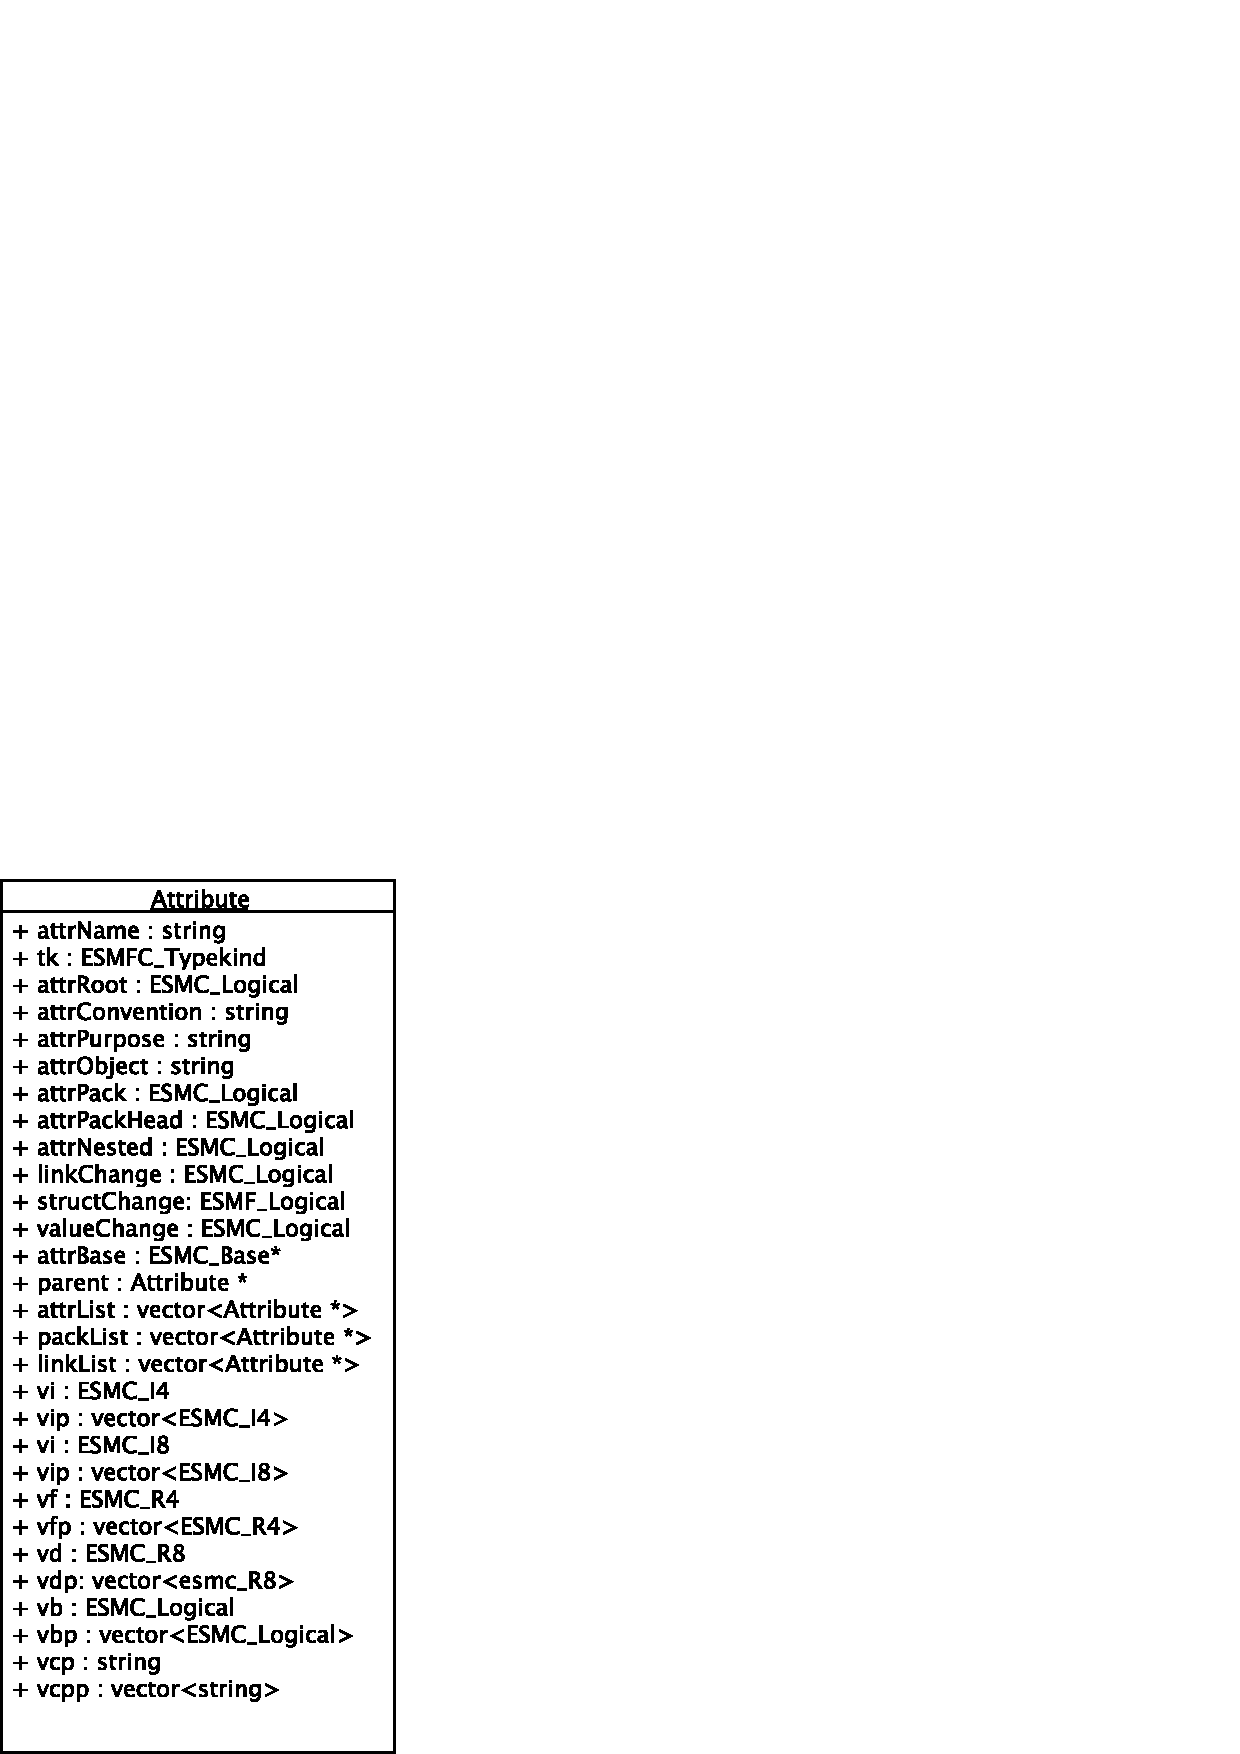
\includegraphics{AttributeClassUML}
\caption{The structure of the Attribute class}
\label{fig:AttributeClassUML}
\end{figure}
\clearpage

\begin{figure}[h]
\centering
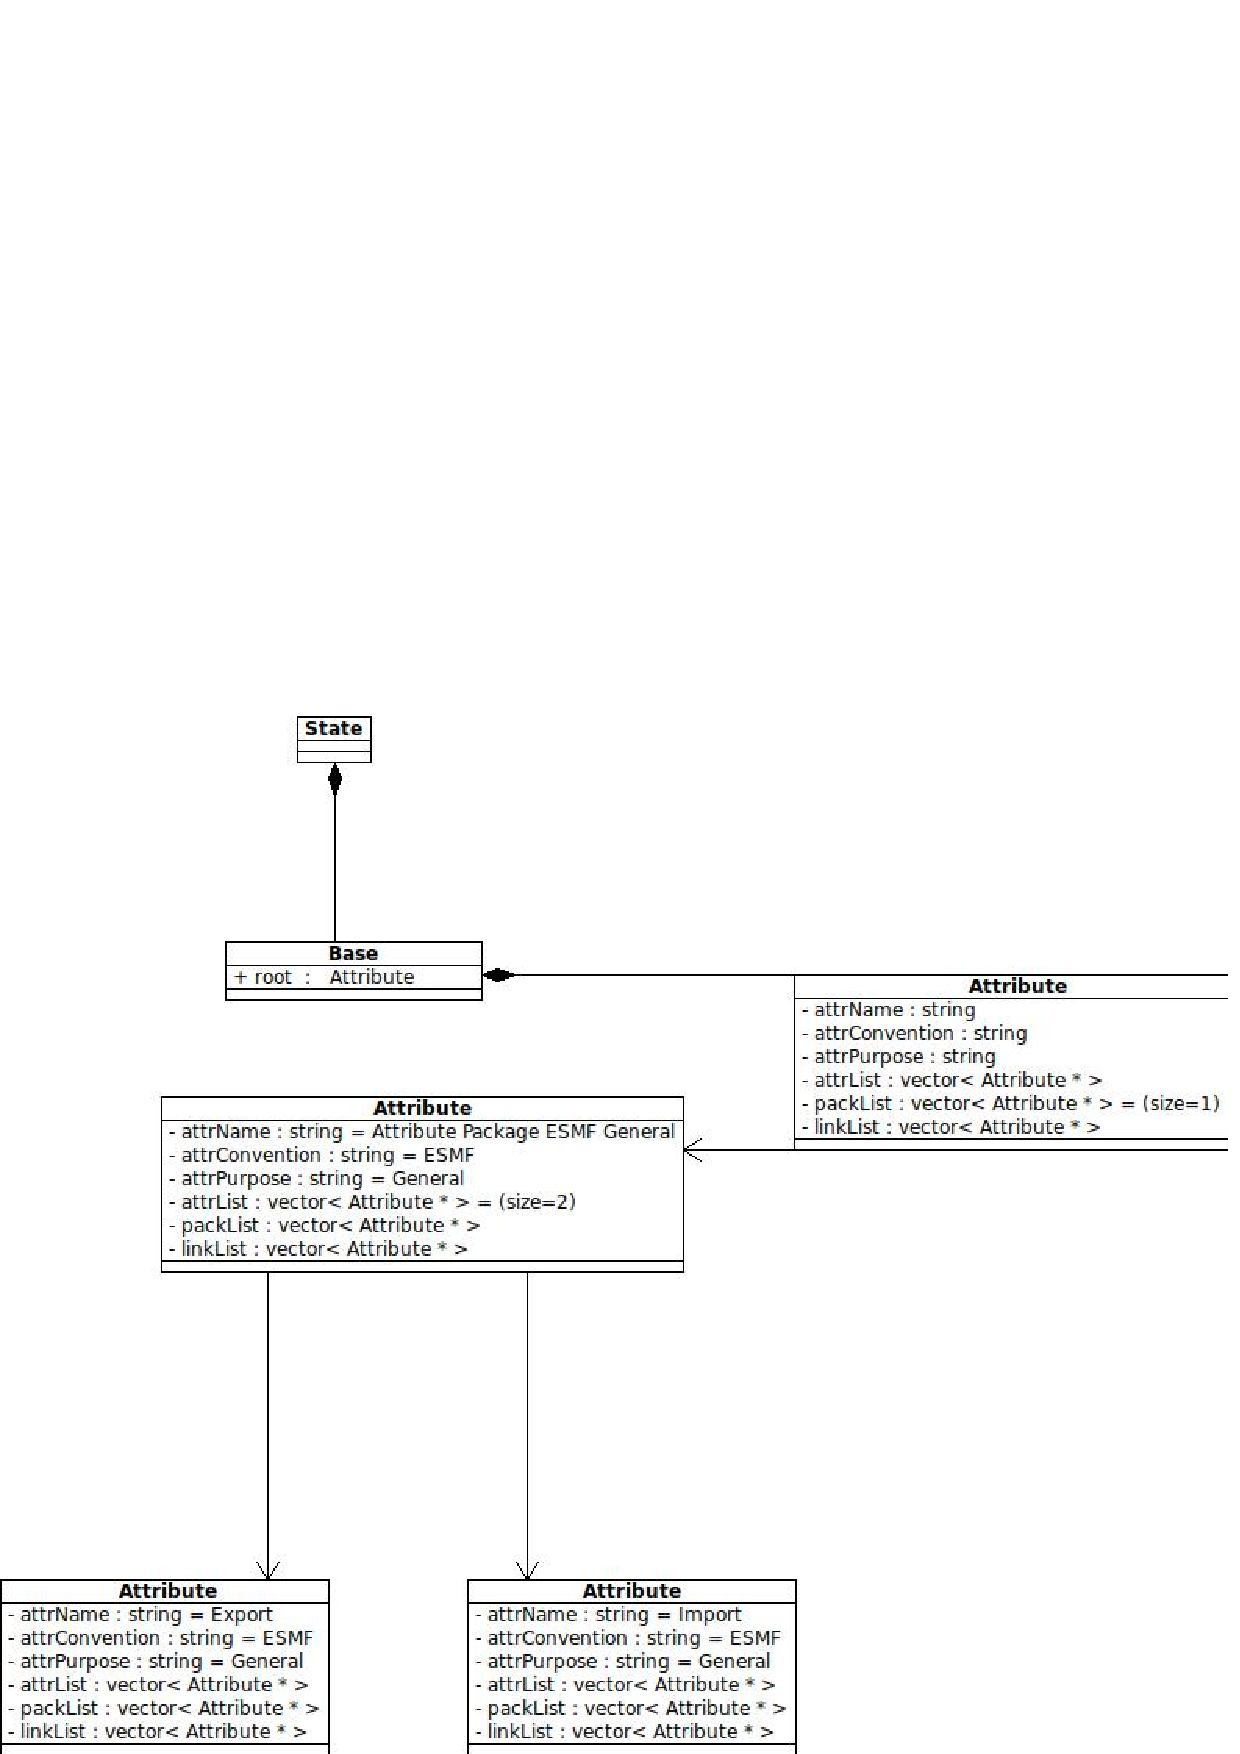
\includegraphics[width=5.5in,height=6in]{AttributePackageUML}
\caption{The internal object organization for the representation of Attribute packages}
\label{fig:AttributePackageUML}
\end{figure}
\clearpage

\begin{figure}[h]
\centering
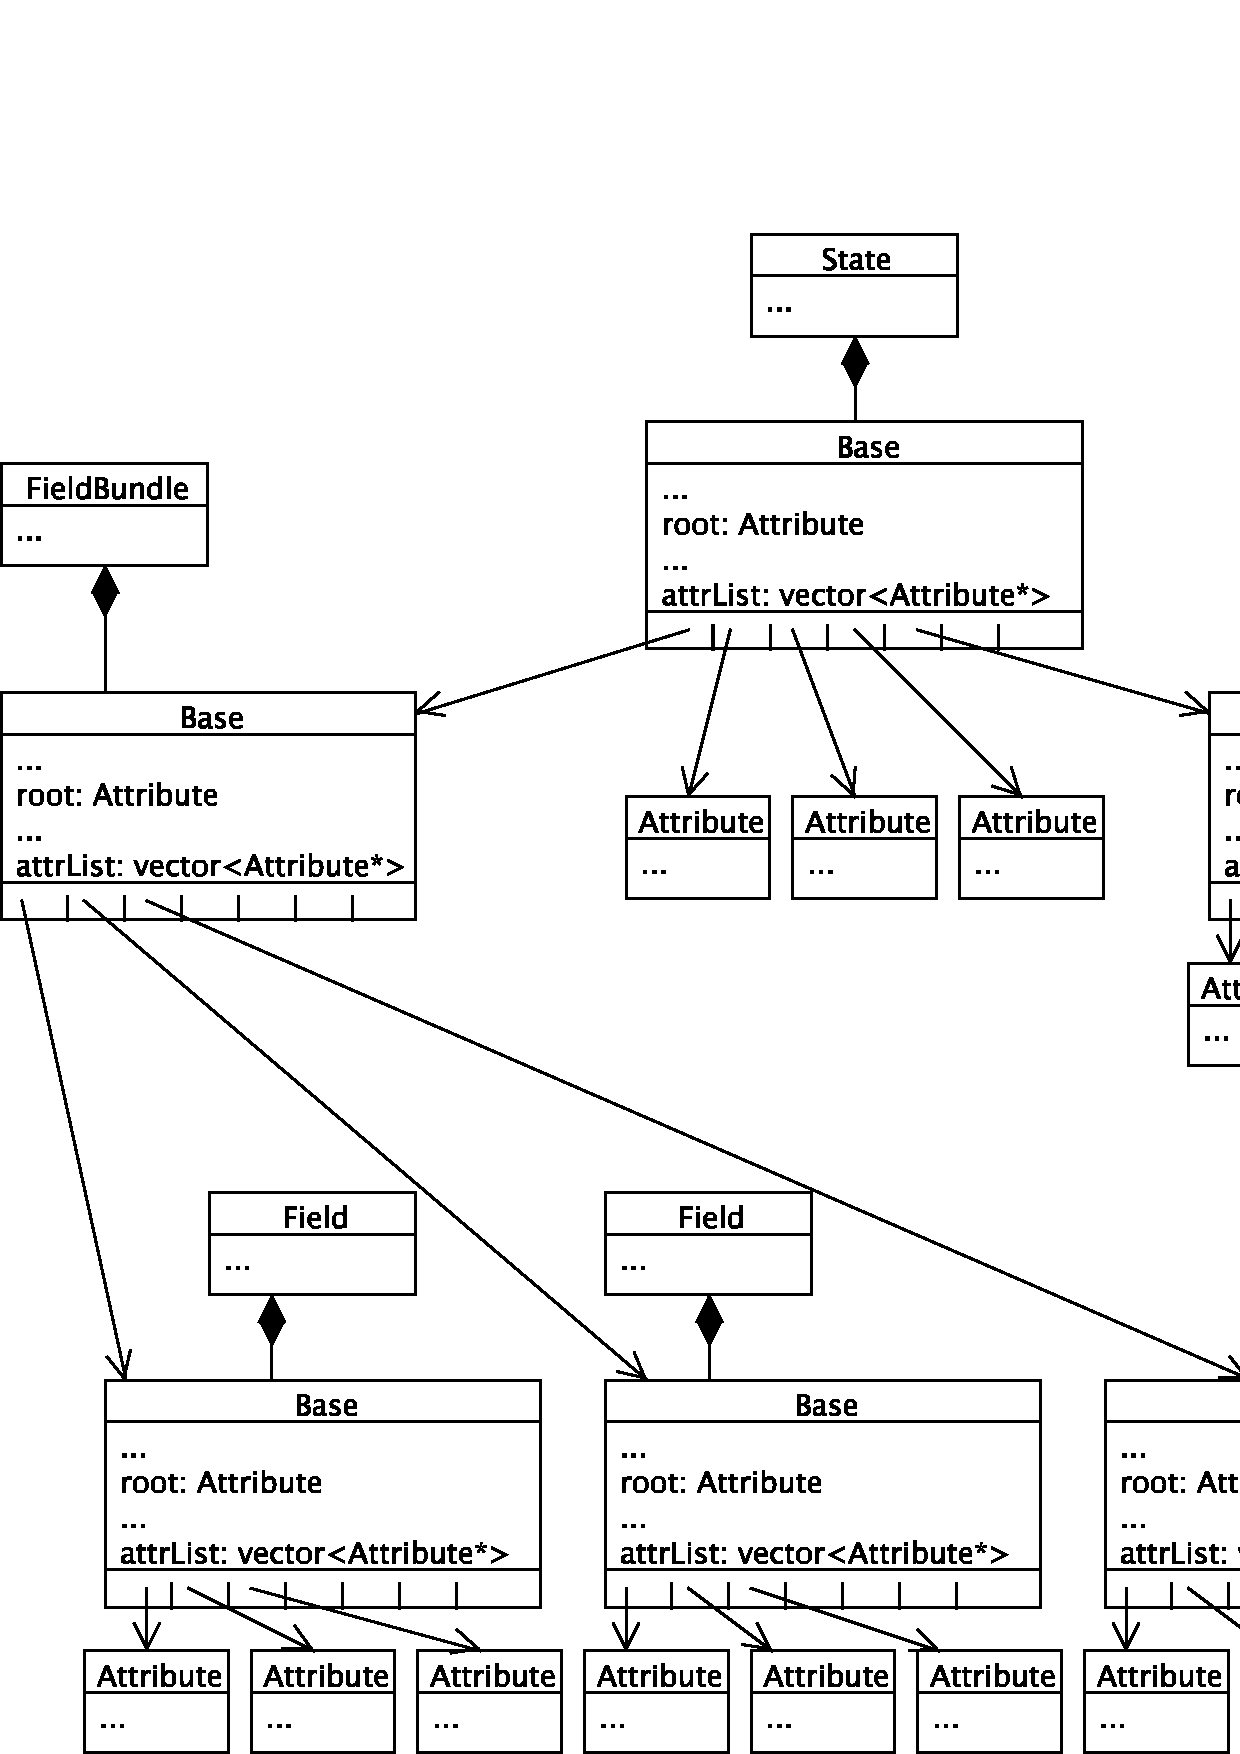
\includegraphics[width=5.5in,height=6in]{AttributeHierarchyUML}
\caption{The internal object organization for the representation of Attribute hierarchies}
\label{fig:AttributeHierarchyUML}
\end{figure}
\clearpage

\subsection{Class API}
%                **** IMPORTANT NOTICE *****
% This LaTeX file has been automatically produced by ProTeX v. 1.1
% Any changes made to this file will likely be lost next time
% this file is regenerated from its source. Send questions 
% to Arlindo da Silva, dasilva@gsfc.nasa.gov
 
\setlength{\oldparskip}{\parskip}
\setlength{\parskip}{1.5ex}
\setlength{\oldparindent}{\parindent}
\setlength{\parindent}{0pt}
\setlength{\oldbaselineskip}{\baselineskip}
\setlength{\baselineskip}{11pt}
 
%--------------------- SHORT-HAND MACROS ----------------------
\def\bv{\begin{verbatim}}
\def\ev{\end{verbatim}}
\def\be{\begin{equation}}
\def\ee{\end{equation}}
\def\bea{\begin{eqnarray}}
\def\eea{\end{eqnarray}}
\def\bi{\begin{itemize}}
\def\ei{\end{itemize}}
\def\bn{\begin{enumerate}}
\def\en{\end{enumerate}}
\def\bd{\begin{description}}
\def\ed{\end{description}}
\def\({\left (}
\def\){\right )}
\def\[{\left [}
\def\]{\right ]}
\def\<{\left  \langle}
\def\>{\right \rangle}
\def\cI{{\cal I}}
\def\diag{\mathop{\rm diag}}
\def\tr{\mathop{\rm tr}}
%-------------------------------------------------------------

\markboth{Left}{Source File: ESMF\_Attribute.F90,  Date: Tue May  5 21:00:06 MDT 2020
}

 
%/////////////////////////////////////////////////////////////
 
%/////////////////////////////////////////////////////////////
 
\mbox{}\hrulefill\ 
 
\subsubsection [ESMF\_AttributeAdd] {ESMF\_AttributeAdd - Add an ESMF standard Attribute package}


  
\bigskip{\sf INTERFACE:}
\begin{verbatim}   ! Private name; call using ESMF_AttributeAdd()
   subroutine ESMF_AttAddPackStd(<object>, convention, purpose, attpack, rc)\end{verbatim}{\em ARGUMENTS:}
\begin{verbatim}   <object>, see below for supported values
   character (len = *), intent(in) :: convention
   character (len = *), intent(in) :: purpose
   type(ESMF_AttPack), intent(inout), optional :: attpack
   integer, intent(out), optional :: rc\end{verbatim}
{\sf DESCRIPTION:\\ }


   Add an ESMF standard Attribute package. See Section~\ref{sec:AttPacks}
   for a description of Attribute packages.
  
   Supported values for <object> are:
   \begin{description}
   \item type(ESMF\_Array), intent(inout) :: array
   \item type(ESMF\_CplComp), intent(inout) :: comp
   \item type(ESMF\_GridComp), intent(inout) :: comp
   \item type(ESMF\_SciComp), intent(inout) :: comp
   \item type(ESMF\_Field), intent(inout) :: field
   \item type(ESMF\_Grid), intent(inout) :: grid
   \item type(ESMF\_State), intent(inout) :: state
   \end{description}
  
   The arguments are:
   \begin{description}
   \item [<object>]
   An {\tt ESMF} object.
   \item [convention]
   The convention of the new Attribute package.
   \item [purpose]
   The purpose of the new Attribute package.
   \item [{[attpack]}]
   An optional handle to the Attribute package that is to be created.
   \item [{[rc]}]
   Return code; equals {\tt ESMF\_SUCCESS} if there are no errors.
   \end{description}
  
   
%/////////////////////////////////////////////////////////////
 
\mbox{}\hrulefill\ 
 
\subsubsection [ESMF\_AttributeAdd] {ESMF\_AttributeAdd - Add an ESMF standard Attribute package containing nested standard Attribute packages}


  
\bigskip{\sf INTERFACE:}
\begin{verbatim}   ! Private name; call using ESMF_AttributeAdd()
   subroutine ESMF_AttAddPackStdN(<object>, convention, purpose, &
   nestConvention, nestPurpose, nestAttPackInstanceCountList, &
   nestAttPackInstanceNameList, nestCount, &
   nestAttPackInstanceNameCount, attpack, rc)\end{verbatim}{\em ARGUMENTS:}
\begin{verbatim}   <object>, see below for supported values
   character (len = *), intent(in) :: convention
   character (len = *), intent(in) :: purpose
   character (len = *), intent(in) :: nestConvention(:)
   character (len = *), intent(in) :: nestPurpose(:)
   integer, intent(in) :: nestAttPackInstanceCountList(:)
   character (len = *), intent(out) :: nestAttPackInstanceNameList(:)
   integer, intent(in), optional :: nestCount
   integer, intent(out), optional :: nestAttPackInstanceNameCount
   type(ESMF_AttPack), intent(inout), optional :: attpack
   integer, intent(out), optional :: rc\end{verbatim}
{\sf DESCRIPTION:\\ }


   Add an ESMF standard Attribute package which contains a user-specified
   number of nested standard Attribute packages. ESMF generates and returns
   default instance names for the nested Attribute packages. These names
   can be used later to distinguish among multiple nested Attribute
   packages of the same type in calls to {\tt ESMF\_AttributeGet()},
   {\tt ESMF\_AttributeSet()}, and {\tt ESMF\_AttributeRemove()}.
   See Section~\ref{sec:AttPacks} for a description of Attribute packages.
  
   Supported values for <object> are:
   \begin{description}
   \item type(ESMF\_CplComp), intent(inout) :: comp
   \item type(ESMF\_GridComp), intent(inout) :: comp
   \item type(ESMF\_SciComp), intent(inout) :: comp
   \end{description}
  
   The arguments are:
   \begin{description}
   \item [<object>]
   An {\tt ESMF} object.
   \item [convention]
   The convention of the new Attribute package.
   \item [purpose]
   The purpose of the new Attribute package.
   \item [nestConvention]
   The convention(s) of the standard Attribute package(s) around
   which to nest the new Attribute package.
   \item [nestPurpose]
   The purpose(s) of the standard Attribute package(s) around
   which to nest the new Attribute package.
   \item [nestAttPackInstanceCountList]
   The desired number of nested Attribute package instances for each
   nested (nestConvention, nestPurpose) package type. Note: if only one
   of each nested package type is desired, then the
   {\tt ESMF\_AttributeAdd()} overloaded method
   {\tt ESMF\_AttAddPackStd()} should be used.
   \item [nestAttPackInstanceNameList]
   The name(s) of the nested Attribute package instances, generated
   by ESMF, used to distinguish between multiple instances of the
   same convention and purpose.
   \item [{[nestCount]}]
   The count of the number of nested Attribute package types to add to
   the new Attribute package.
   \item [{[nestAttPackInstanceNameCount]}]
   The number of nested Attribute package instance names.
   \item [{[attpack]}]
   An optional handle to the Attribute package that is to be created.
   \item [{[rc]}]
   Return code; equals {\tt ESMF\_SUCCESS} if there are no errors.
   \end{description}
  
   
%/////////////////////////////////////////////////////////////
 
\mbox{}\hrulefill\ 
 
\subsubsection [ESMF\_AttributeAdd] {ESMF\_AttributeAdd - Add a custom Attribute package or modify an existing Attribute package}


  
\bigskip{\sf INTERFACE:}
\begin{verbatim}   ! Private name; call using ESMF_AttributeAdd()
   subroutine ESMF_AttAddPackCst(<object>, convention, purpose, &
   attrList, count, redundant, attpack, rc)\end{verbatim}{\em ARGUMENTS:}
\begin{verbatim}   <object>, see below for supported values
   character (len = *), intent(in) :: convention
   character (len = *), intent(in) :: purpose
   character (len = *), intent(in) :: attrList(:)
   integer, intent(in), optional :: count
   logical, intent(in), optional :: redundant
   type(ESMF_AttPack), intent(inout), optional :: attpack
   integer, intent(out), optional :: rc\end{verbatim}
{\sf DESCRIPTION:\\ }


   Add a custom Attribute package to <object>, or add
   Attributes to an existing Attribute package. The {\tt redundant} flag can
   be set to {\tt .true.} to create redundant Attribute packages. Otherwise,
   Attributes will be added to an existing package. The {\tt attpack} will be
   used instead of {\tt convention} and {\tt purpose} if both are present.
   See Section~\ref{sec:AttPacks} for a description of Attribute packages.
  
   Supported values for <object> are:
   \begin{description}
   \item type(ESMF\_Array), intent(inout) :: array
   \item type(ESMF\_ArrayBundle), intent(inout) :: arraybundle
   \item type(ESMF\_CplComp), intent(inout) :: comp
   \item type(ESMF\_GridComp), intent(inout) :: comp
   \item type(ESMF\_SciComp), intent(inout) :: comp
   \item type(ESMF\_DistGrid), intent(inout) :: distgrid
   \item type(ESMF\_Field), intent(inout) :: field
   \item type(ESMF\_FieldBundle), intent(inout) :: fieldbundle
   \item type(ESMF\_Grid), intent(inout) :: grid
   \item type(ESMF\_State), intent(inout) :: state
   \end{description}
  
   The arguments are:
   \begin{description}
   \item [<object>]
   An {\tt ESMF} object.
   \item [convention]
   The convention of the Attribute package.
   \item [purpose]
   The purpose of the Attribute package.
   \item [attrList]
   The list of Attribute names to specify the custom Attribute package.
   \item [{[count]}]
   The number of Attributes to add to the custom Attribute package.
   \item [{[redundant]}]
   A flag to determine whether or not to create redundant Attribute
   packages. If an Attribute package already exists with the specified
   {\tt convention} and {\tt purpose} and {\tt redundant} is set to
   {\tt .true.} then a redundant Attribute package will be created.
   The default value is {\tt .false.}.
   \item [{[attpack]}]
   The handle to the Attribute package that was created.
   This can also be used as an input parameter to indicate the
   Attribute package to which additional Attributes should be added.
   \item [{[rc]}]
   Return code; equals {\tt ESMF\_SUCCESS} if there are no errors.
   \end{description}
  
   
%/////////////////////////////////////////////////////////////
 
\mbox{}\hrulefill\ 
 
\subsubsection [ESMF\_AttributeAdd] {ESMF\_AttributeAdd - Add a custom Attribute package with nested Attribute packages}


  
\bigskip{\sf INTERFACE:}
\begin{verbatim}   ! Private name; call using ESMF_AttributeAdd()
   subroutine ESMF_AttAddPackCstN(<object>, convention, purpose, &
   attrList, count, nestConvention, nestPurpose, nestCount, attpack, rc)\end{verbatim}{\em ARGUMENTS:}
\begin{verbatim}   <object>, see below for supported values
   character (len = *), intent(in) :: convention
   character (len = *), intent(in) :: purpose
   character (len = *), intent(in), optional :: attrList(:)
   integer, intent(in), optional :: count
   character (len = *), intent(in) :: nestConvention(:)
   character (len = *), intent(in) :: nestPurpose(:)
   integer, intent(in), optional :: nestCount
   type(ESMF_AttPack), intent(inout), optional :: attpack
   integer, intent(out), optional :: rc\end{verbatim}
{\sf DESCRIPTION:\\ }


   Add a custom Attribute package, with one or more nested Attribute
   packages, to <object>. Allows for building full multiple-child Attribute
   hierarchies (multi-child trees).
   See Section~\ref{sec:AttPacks} for a description of Attribute packages.
  
   Supported values for <object> are:
   \begin{description}
   \item type(ESMF\_Array), intent(inout) :: array
   \item type(ESMF\_ArrayBundle), intent(inout) :: arraybundle
   \item type(ESMF\_CplComp), intent(inout) :: comp
   \item type(ESMF\_GridComp), intent(inout) :: comp
   \item type(ESMF\_SciComp), intent(inout) :: comp
   \item type(ESMF\_DistGrid), intent(inout) :: distgrid
   \item type(ESMF\_Field), intent(inout) :: field
   \item type(ESMF\_FieldBundle), intent(inout) :: fieldbundle
   \item type(ESMF\_Grid), intent(inout) :: grid
   \item type(ESMF\_State), intent(inout) :: state
   \end{description}
  
   The arguments are:
   \begin{description}
   \item [<object>]
   An {\tt ESMF} object.
   \item [convention]
   The convention of the Attribute package.
   \item [purpose]
   The purpose of the Attribute package.
   \item [{[attrList]}]
   The list of Attribute names to specify the custom Attribute package.
   \item [{[count]}]
   The number of Attributes to add to the custom Attribute package.
   \item [nestConvention]
   The convention(s) of the Attribute package(s) around which to nest
   the new Attribute package.
   \item [nestPurpose]
   The purpose(s) of the Attribute package(s) around which to nest the
   new Attribute package.
   \item [{[nestCount]}]
   The number of nested Attribute packages to add to the custom
   Attribute package.
   \item [{[attpack]}]
   An optional handle to the Attribute package that is to be created.
   \item [{[rc]}]
   Return code; equals {\tt ESMF\_SUCCESS} if there are no errors.
   \end{description}
  
   
%/////////////////////////////////////////////////////////////
 
\mbox{}\hrulefill\ 
 
\subsubsection [ESMF\_AttributeAdd] {ESMF\_AttributeAdd - Add a custom Attribute package with a single nested Attribute package}


  
\bigskip{\sf INTERFACE:}
\begin{verbatim}   ! Private name; call using ESMF_AttributeAdd()
   subroutine ESMF_AttAddPackCstN1(<object>, convention, purpose, &
   attrList, count, nestConvention, nestPurpose, attpack, rc)\end{verbatim}{\em ARGUMENTS:}
\begin{verbatim}   <object>, see below for supported values
   character (len = *), intent(in) :: convention
   character (len = *), intent(in) :: purpose
   character (len = *), intent(in), optional :: attrList(:)
   integer, intent(in), optional :: count
   character (len = *), intent(in) :: nestConvention
   character (len = *), intent(in) :: nestPurpose
   type(ESMF_AttPack), intent(inout), optional :: attpack
   integer, intent(out), optional :: rc\end{verbatim}
{\sf DESCRIPTION:\\ }


   Add a custom Attribute package, with a single nested Attribute
   package, to <object>. Allows for building single-child Attribute
   hierarchies (single-child trees).
   See Section~\ref{sec:AttPacks} for a description of Attribute packages.
  
   Supported values for <object> are:
   \begin{description}
   \item type(ESMF\_Array), intent(inout) :: array
   \item type(ESMF\_ArrayBundle), intent(inout) :: arraybundle
   \item type(ESMF\_CplComp), intent(inout) :: comp
   \item type(ESMF\_GridComp), intent(inout) :: comp
   \item type(ESMF\_SciComp), intent(inout) :: comp
   \item type(ESMF\_DistGrid), intent(inout) :: distgrid
   \item type(ESMF\_Field), intent(inout) :: field
   \item type(ESMF\_FieldBundle), intent(inout) :: fieldbundle
   \item type(ESMF\_Grid), intent(inout) :: grid
   \item type(ESMF\_State), intent(inout) :: state
   \end{description}
  
   The arguments are:
   \begin{description}
   \item [<object>]
   An {\tt ESMF} object.
   \item [convention]
   The convention of the Attribute package.
   \item [purpose]
   The purpose of the Attribute package.
   \item [{[attrList]}]
   The list of Attribute names to specify the custom Attribute package.
   \item [{[count]}]
   The number of Attributes to add to the custom Attribute package.
   \item [nestConvention]
   The convention of the Attribute package around which to nest
   the new Attribute package.
   \item [nestPurpose]
   The purpose of the Attribute package around which to nest the
   new Attribute package.
   \item [{[attpack]}]
   An optional handle to the Attribute package that is to be created.
   \item [{[rc]}]
   Return code; equals {\tt ESMF\_SUCCESS} if there are no errors.
   \end{description}
  
   
%/////////////////////////////////////////////////////////////
 
\mbox{}\hrulefill\ 
 
\subsubsection [ESMF\_AttributeCopy] {ESMF\_AttributeCopy - Copy an Attribute hierarchy}


  
\bigskip{\sf INTERFACE:}
\begin{verbatim}   ! Private name; call using ESMF_AttributeCopy()
   subroutine ESMF_AttributeCopy(<object1>, <object2>, attcopy, rc)\end{verbatim}{\em ARGUMENTS:}
\begin{verbatim}   <object1>, see below for supported values
   <object2>, see below for supported values
   type(ESMF_AttCopy_Flag),intent(in) optional :: attcopy
   integer, intent(out), optional :: rc\end{verbatim}
{\sf DESCRIPTION:\\ }


   Copy an Attribute hierarchy from <object1> to <object2>. The
   default behavior is to ignore (instead of replace) values on
   pre-existing Attributes.
  
   Supported values for <object1> are:
   \begin{description}
   \item type(ESMF\_CplComp), intent(in) :: comp1
   \item type(ESMF\_GridComp), intent(in) :: comp1
   \item type(ESMF\_SciComp), intent(in) :: comp1
   \item type(ESMF\_Field), intent(inout) :: field1
   \item type(ESMF\_FieldBundle), intent(inout) :: fieldbundle1
   \item type(ESMF\_Grid), intent(inout) :: grid1
   \item type(ESMF\_State), intent(in) :: state
   \end{description}
  
   Supported values for <object2> are:
   \begin{description}
   \item type(ESMF\_CplComp), intent(inout) :: comp2
   \item type(ESMF\_GridComp), intent(inout) :: comp2
   \item type(ESMF\_SciComp), intent(inout) :: comp2
   \item type(ESMF\_Field), intent(inout) :: field2
   \item type(ESMF\_FieldBundle), intent(inout) :: fieldbundle2
   \item type(ESMF\_Grid), intent(inout) :: grid2
   \item type(ESMF\_State), intent(inout) :: state
   \end{description}
  
   NOTE: Copies between different ESMF object types are not possible at this time.
  
   The arguments are:
   \begin{description}
   \item [<object1>]
   An {\tt Attribute}-bearing ESMF object.
   \item [<object2>]
   An {\tt Attribute}-bearing ESMF object.
   \item [{[attcopy]}]
   A flag to determine if the copy is to be by reference, value,
   or hybrid. This flag is documented in section \ref{const:attcopy}.
   The default is to copy by value.
   \item [{[rc]}]
   Return code; equals {\tt ESMF\_SUCCESS} if there are no errors.
   \end{description}
   
%/////////////////////////////////////////////////////////////
 
\mbox{}\hrulefill\ 
 
\subsubsection [ESMF\_AttributeGet] {ESMF\_AttributeGet - Get an Attribute from an ESMF\_AttPack}


  
\bigskip{\sf INTERFACE:}
\begin{verbatim}   subroutine ESMF_AttributeGet(<object>, name, attpack, <value> &
   <defaultvalue>, attnestflag, isPresent, rc)\end{verbatim}{\em ARGUMENTS:}
\begin{verbatim}   <object>, see below for supported values
   character (len = *), intent(in) :: name
   type(ESMF_AttPack), intent(inout) :: attpack
   <value>, see below for supported values
 -- The following arguments require argument keyword syntax (e.g. rc=rc). --
   <defaultvalue>, see below for supported values
   type(ESMF_AttNest_Flag),intent(in), optional :: attnestflag
   logical, intent(out), optional :: isPresent
   integer, intent(out), optional :: rc\end{verbatim}
{\sf DESCRIPTION:\\ }


   Return an Attribute {\tt value} from the <object>, or from an Attribute
   package on the <object>, specified by {\tt attpack}. Internal information can also
   be retrieved from Grid objects by prepending 'ESMF:' to the name of the
   piece of information that is requested. See
   Section~\ref{sec:InternalInfo} for more information
   on which pieces of Grid data can be retrieved through this interface.
   A {\tt defaultvalue} argument
   may be given if a return code is not desired when the Attribute is not
   found. See Section~\ref{sec:AttPacks} for a description of Attribute
   packages.
  
   Supported values for <object> are:
   \begin{description}
   \item type(ESMF\_Array), intent(in) :: array
   \item type(ESMF\_ArrayBundle), intent(in) :: arraybundle
   \item type(ESMF\_CplComp), intent(in) :: comp
   \item type(ESMF\_GridComp), intent(in) :: comp
   \item type(ESMF\_SciComp), intent(in) :: comp
   \item type(ESMF\_DistGrid), intent(in) :: distgrid
   \item type(ESMF\_Field), intent(in) :: field
   \item type(ESMF\_FieldBundle), intent(in) :: fieldbundle
   \item type(ESMF\_Grid), intent(in) :: grid
   \item type(ESMF\_State), intent(in) :: state
   \end{description}
  
   Supported values for <value> are:
   \begin{description}
   \item integer(ESMF\_KIND\_I4), intent(out) :: value
   \item integer(ESMF\_KIND\_I8), intent(out) :: value
   \item real (ESMF\_KIND\_R4), intent(out) :: value
   \item real (ESMF\_KIND\_R8), intent(out) :: value
   \item logical, intent(out) :: value
   \item character (len = *), intent(out) :: value
   \end{description}
  
   Supported values for <defaultvalue> are:
   \begin{description}
   \item integer(ESMF\_KIND\_I4), intent(in), optional :: defaultvalue
   \item integer(ESMF\_KIND\_I8), intent(in), optional :: defaultvalue
   \item real (ESMF\_KIND\_R4), intent(in), optional :: defaultvalue
   \item real (ESMF\_KIND\_R8), intent(in), optional :: defaultvalue
   \item logical, intent(in), optional :: defaultvalue
   \item character (len = *), intent(in), optional :: defaultvalue
   \end{description}
  
   The arguments are:
   \begin{description}
   \item [<object>]
   An {\tt ESMF} object.
   \item [name]
   The name of the Attribute to retrieve.
   \item [attpack]
   A handle to the Attribute package.
   \item [<value>]
   The value of the named Attribute.
   \item [{[<defaultvalue>]}]
   The default value of the named Attribute.
   \item [{[attnestflag]}]
   A flag to determine whether to descend the
   Attribute hierarchy when looking for this Attribute, the default
   is {\tt ESMF\_ATTNEST\_ON}. This flag is documented in section
   \ref{const:attnest}.
   \item [{[isPresent]}]
   A logical flag to tell if this Attribute is present or not.
   \item [{[rc]}]
   Return code; equals {\tt ESMF\_SUCCESS} if there are no errors.
   \end{description}
  
   
%/////////////////////////////////////////////////////////////
 
\mbox{}\hrulefill\ 
 
\subsubsection [ESMF\_AttributeGet] {ESMF\_AttributeGet - Get an Attribute pointing to internal class information from an ESMF\_AttPack}


  
\bigskip{\sf INTERFACE:}
\begin{verbatim}   subroutine ESMF_AttributeGet(<object>, name, attpack, <value>, &
   <defaultvalue>, inputList, attnestflag, isPresent, rc)\end{verbatim}{\em ARGUMENTS:}
\begin{verbatim}   <object>, see below for supported values
   character (len = *), intent(in) :: name
   type(ESMF_AttPack), intent(inout) :: attpack
   <value>, see below for supported values
 -- The following arguments require argument keyword syntax (e.g. rc=rc). --
   <defaultvalue>, see below for supported values
   character (len = *), intent(in), optional :: inputList(:)
   type(ESMF_AttNest_Flag),intent(in), optional :: attnestflag
   logical, intent(out), optional :: isPresent
   integer, intent(out), optional :: rc\end{verbatim}
{\sf DESCRIPTION:\\ }


   Return an Attribute {\tt value} from the <object>, or from an Attribute
   package on the <object>, specified by {\tt attpack}. Internal class information can
   be retrieved by prepending 'ESMF:' to the name of the
   piece of information that is requested. See
   Section~\ref{sec:InternalInfo} for more information
   on this capability.
   A {\tt defaultvalue} argument
   may be given if a return code is not desired when the Attribute is not
   found. See Section~\ref{sec:AttPacks} for a description of Attribute
   packages.
  
   Supported values for <object> are:
   \begin{description}
   \item type(ESMF\_Grid), intent(in) :: grid
   \end{description}
  
   Supported values for <value> are:
   \begin{description}
   \item integer(ESMF\_KIND\_I4), intent(out) :: value
   \item character (len = *), intent(out) :: value
   \end{description}
  
   Supported values for <defaultvalue> are:
   \begin{description}
   \item integer(ESMF\_KIND\_I4), intent(in), optional :: defaultvalue
   \item character (len = *), intent(in), optional :: defaultvalue
   \end{description}
  
   The arguments are:
   \begin{description}
   \item [<object>]
   An {\tt ESMF} object.
   \item [name]
   The name of the Attribute to retrieve.
   \item [attpack]
   A handle to the Attribute package.
   \item [<value argument>]
   The value of the named Attribute.
   \item [{[<defaultvalue argument>]}]
   The default value of the named Attribute.
   \item [{[inputList]}]
   A list of the input parameters required to retrieve internal info.
   \item [{[attnestflag]}]
   A flag to determine whether to descend the
   Attribute hierarchy when looking for this Attribute, the default
   is {\tt ESMF\_ATTNEST\_ON}. This flag is documented in section
   \ref{const:attnest}.
   \item [{[isPresent]}]
   A logical flag to tell if this Attribute is present or not.
   \item [{[rc]}]
   Return code; equals {\tt ESMF\_SUCCESS} if there are no errors.
   \end{description}
  
   
%/////////////////////////////////////////////////////////////
 
\mbox{}\hrulefill\ 
 
\subsubsection [ESMF\_AttributeGet] {ESMF\_AttributeGet - Get an Attribute from an ESMF\_AttPack}


  
\bigskip{\sf INTERFACE:}
\begin{verbatim}   subroutine ESMF_AttributeGet(<object>, name, attpack, <valueList>, &
   <defaultvalueList>, attnestflag, itemCount, &
   isPresent, rc)\end{verbatim}{\em ARGUMENTS:}
\begin{verbatim}   <object>, see below for supported values
   character (len = *), intent(in) :: name
   type(ESMF_AttPack), intent(inout) :: attpack
   <valueList>, see below for supported values
 -- The following arguments require argument keyword syntax (e.g. rc=rc). --
   <defaultvalueList>, see below for supported values
   type(ESMF_AttNest_Flag),intent(in), optional :: attnestflag
   integer, intent(out), optional :: itemCount
   logical, intent(out), optional :: isPresent
   integer, intent(out), optional :: rc\end{verbatim}
{\sf DESCRIPTION:\\ }


   Return an Attribute {\tt valueList} from the <object>, or from an
   Attribute package on the <object>, specified by {\tt attpack}. Internal
   information can also be retrieved from Grid objects by prepending 'ESMF:'
   to the name of the piece of information that is requested. See
   Section~\ref{sec:InternalInfo} for more information
   on which pieces of Grid data can be retrieved through this interface.
   A {\tt defaultvalueList} list argument may be given if
   a return code is not desired when the Attribute is not found.
   See Section~\ref{sec:AttPacks} for a description of Attribute packages.
  
   Supported values for <object> are:
   \begin{description}
   \item type(ESMF\_Array), intent(in) :: array
   \item type(ESMF\_ArrayBundle), intent(in) :: arraybundle
   \item type(ESMF\_CplComp), intent(in) :: comp
   \item type(ESMF\_GridComp), intent(in) :: comp
   \item type(ESMF\_SciComp), intent(in) :: comp
   \item type(ESMF\_DistGrid), intent(in) :: distgrid
   \item type(ESMF\_Field), intent(in) :: field
   \item type(ESMF\_FieldBundle), intent(in) :: fieldbundle
   \item type(ESMF\_Grid), intent(in) :: grid
   \item type(ESMF\_State), intent(in) :: state
   \end{description}
  
   Supported values for <valueList> are:
   \begin{description}
   \item integer(ESMF\_KIND\_I4), intent(out) :: valueList(:)
   \item integer(ESMF\_KIND\_I8), intent(out) :: valueList(:)
   \item real (ESMF\_KIND\_R4), intent(out) :: valueList(:)
   \item real (ESMF\_KIND\_R8), intent(out) :: valueList(:)
   \item logical, intent(out) :: valueList(:)
   \item character (len = *), intent(out) :: valueList(:)
   \end{description}
  
   Supported values for <defaultvalueList> are:
   \begin{description}
   \item integer(ESMF\_KIND\_I4), intent(in), optional :: defaultvalueList(:)
   \item integer(ESMF\_KIND\_I8), intent(in), optional :: defaultvalueList(:)
   \item real (ESMF\_KIND\_R4), intent(in), optional :: defaultvalueList(:)
   \item real (ESMF\_KIND\_R8), intent(in), optional :: defaultvalueList(:)
   \item logical, intent(in), optional :: defaultvalueList(:)
   \item character (len = *), intent(in), optional :: defaultvalueList(:)
   \end{description}
  
   The arguments are:
   \begin{description}
   \item [<object>]
   An {\tt ESMF} object.
   \item [name]
   The name of the Attribute to retrieve.
   \item [attpack]
   A handle to the Attribute package.
   \item [<valueList>]
   The valueList of the named Attribute.
   \item [{[<defaultvalueList>]}]
   The default value list of the named Attribute.
   \item [{[attnestflag]}]
   A flag to determine whether to descend the
   Attribute hierarchy when looking for this Attribute, the default
   is {\tt ESMF\_ATTNEST\_ON}. This flag is documented in section
   \ref{const:attnest}.
   \item [{[itemCount]}]
   The number of items in a multi-valued Attribute.
   \item [{[isPresent]}]
   A logical flag to tell if this Attribute is present or not.
   \item [{[rc]}]
   Return code; equals {\tt ESMF\_SUCCESS} if there are no errors.
   \end{description}
  
   
%/////////////////////////////////////////////////////////////
 
\mbox{}\hrulefill\ 
 
\subsubsection [ESMF\_AttributeGet] {ESMF\_AttributeGet - Get an Attribute pointing to internal class information from an ESMF\_AttPack}


  
\bigskip{\sf INTERFACE:}
\begin{verbatim}   subroutine ESMF_AttributeGet(<object>, name, attpack, <valueList>, &
   <defaultvalueList>, inputList, attnestflag, &
   itemCount, isPresent, rc)\end{verbatim}{\em ARGUMENTS:}
\begin{verbatim}   <object>, see below for supported values
   character (len = *), intent(in) :: name
   type(ESMF_AttPack), intent(inout) :: attpack
   <valueList>, see below for supported values
 -- The following arguments require argument keyword syntax (e.g. rc=rc). --
   <defaultvalueList>, see below for supported values
   character (len = *), intent(in), optional :: inputList(:)
   type(ESMF_AttNest_Flag),intent(in), optional :: attnestflag
   integer, intent(out), optional :: itemCount
   logical, intent(out), optional :: isPresent
   integer, intent(out), optional :: rc\end{verbatim}
{\sf DESCRIPTION:\\ }


   Return an Attribute {\tt valueList} from the <object>, or from an
   Attribute package on the <object>, specified by {\tt attpack}. Internal class
   information can be retrieved by prepending 'ESMF:'
   to the name of the piece of information that is requested. See
   Section~\ref{sec:InternalInfo} for more information
   on this capability.
   A {\tt defaultvalueList} list argument may be given if
   a return code is not desired when the Attribute is not found.
   See Section~\ref{sec:AttPacks} for a description of Attribute packages.
  
   Supported values for <object> are:
   \begin{description}
   \item type(ESMF\_Grid), intent(in) :: grid
   \end{description}
  
   Supported values for <valueList> are:
   \begin{description}
   \item integer(ESMF\_KIND\_I4), intent(out) :: valueList(:)
   \item real (ESMF\_KIND\_R8), intent(out) :: valueList(:)
   \item logical, intent(out) :: valueList(:)
   \end{description}
  
   Supported values for <defaultvalueList> are:
   \begin{description}
   \item integer(ESMF\_KIND\_I4), intent(in), optional :: defaultvalueList(:)
   \item real (ESMF\_KIND\_R8), intent(in), optional :: defaultvalueList(:)
   \item logical, intent(in), optional :: defaultvalueList(:)
   \end{description}
  
   The arguments are:
   \begin{description}
   \item [<object>]
   An {\tt ESMF} object.
   \item [name]
   The name of the Attribute to retrieve.
   \item [attpack]
   A handle to the Attribute package.
   \item [<valueList>]
   The valueList of the named Attribute.
   \item [{[<defaultvalueList>]}]
   The default value list of the named Attribute.
   \item [{[inputList]}]
   A list of the input parameters required to retrieve internal info.
   \item [{[attnestflag]}]
   A flag to determine whether to descend the
   Attribute hierarchy when looking for this Attribute, the default
   is {\tt ESMF\_ATTNEST\_ON}. This flag is documented in section
   \ref{const:attnest}.
   \item [{[itemCount]}]
   The number of items in a multi-valued Attribute.
   \item [{[isPresent]}]
   A logical flag to tell if this Attribute is present or not.
   \item [{[rc]}]
   Return code; equals {\tt ESMF\_SUCCESS} if there are no errors.
   \end{description}
  
   
%/////////////////////////////////////////////////////////////
 
\mbox{}\hrulefill\ 
 
\subsubsection [ESMF\_AttributeGet] {ESMF\_AttributeGet - Get an Attribute}


  
\bigskip{\sf INTERFACE:}
\begin{verbatim}   subroutine ESMF_AttributeGet(<object>, name, <value>, <defaultvalue>, &
   convention, purpose, attPackInstanceName, attnestflag, isPresent, rc)\end{verbatim}{\em ARGUMENTS:}
\begin{verbatim}   <object>, see below for supported values
   character (len = *), intent(in) :: name
   <value>, see below for supported values
   <defaultvalue>, see below for supported values
   character (len = *), intent(in), optional :: convention
   character (len = *), intent(in), optional :: purpose
   character (len = *), intent(in), optional :: attPackInstanceName
   type(ESMF_AttNest_Flag),intent(in), optional :: attnestflag
   logical, intent(out), optional :: isPresent
   integer, intent(out), optional :: rc\end{verbatim}
{\sf DESCRIPTION:\\ }


   Return an Attribute {\tt value} from the <object>, or from an Attribute
   package on the <object>, specified by {\tt convention},
   {\tt purpose}, and {\tt attPackInstanceName}. Internal information can also
   be retrieved from Grid objects by prepending 'ESMF:' to the name of the
   piece of information that is requested. See
   Section~\ref{sec:InternalInfo} for more information
   on which pieces of Grid data can be retrieved through this interface.
   A {\tt defaultvalue} argument
   may be given if a return code is not desired when the Attribute is not
   found. See Section~\ref{sec:AttPacks} for a description of Attribute
   packages.
  
   Supported values for <object> are:
   \begin{description}
   \item type(ESMF\_Array), intent(in) :: array
   \item type(ESMF\_ArrayBundle), intent(in) :: arraybundle
   \item type(ESMF\_CplComp), intent(in) :: comp
   \item type(ESMF\_GridComp), intent(in) :: comp
   \item type(ESMF\_SciComp), intent(in) :: comp
   \item type(ESMF\_DistGrid), intent(in) :: distgrid
   \item type(ESMF\_Field), intent(in) :: field
   \item type(ESMF\_FieldBundle), intent(in) :: fieldbundle
   \item type(ESMF\_Grid), intent(in) :: grid
   \item type(ESMF\_State), intent(in) :: state
   \end{description}
  
   Supported values for <value> are:
   \begin{description}
   \item integer(ESMF\_KIND\_I4), intent(out) :: value
   \item integer(ESMF\_KIND\_I8), intent(out) :: value
   \item real (ESMF\_KIND\_R4), intent(out) :: value
   \item real (ESMF\_KIND\_R8), intent(out) :: value
   \item logical, intent(out) :: value
   \item character (len = *), intent(out) :: value
   \end{description}
  
   Supported values for <defaultvalue> are:
   \begin{description}
   \item integer(ESMF\_KIND\_I4), intent(in), optional :: defaultvalue
   \item integer(ESMF\_KIND\_I8), intent(in), optional :: defaultvalue
   \item real (ESMF\_KIND\_R4), intent(in), optional :: defaultvalue
   \item real (ESMF\_KIND\_R8), intent(in), optional :: defaultvalue
   \item logical, intent(in), optional :: defaultvalue
   \item character (len = *), intent(in), optional :: defaultvalue
   \end{description}
  
   The arguments are:
   \begin{description}
   \item [<object>]
   An {\tt ESMF} object.
   \item [name]
   The name of the Attribute to retrieve.
   \item [<value>]
   The value of the named Attribute.
   \item [{[<defaultvalue>]}]
   The default value of the named Attribute.
   \item [{[convention]}]
   The convention of the Attribute package.
   \item [{[purpose]}]
   The purpose of the Attribute package.
   \item [{[attPackInstanceName]}]
   The name of an Attribute package instance, specifying which one
   of multiple Attribute package instances of the same convention
   and purpose, within a nest. If not specified, defaults to the
   first instance.
   \item [{[attnestflag]}]
   A flag to determine whether to descend the
   Attribute hierarchy when looking for this Attribute, the default
   is {\tt ESMF\_ATTNEST\_ON}. This flag is documented in section
   \ref{const:attnest}.
   \item [{[isPresent]}]
   A logical flag to tell if this Attribute is present or not.
   \item [{[rc]}]
   Return code; equals {\tt ESMF\_SUCCESS} if there are no errors.
   \end{description}
  
   
%/////////////////////////////////////////////////////////////
 
\mbox{}\hrulefill\ 
 
\subsubsection [ESMF\_AttributeGet] {ESMF\_AttributeGet - Get an Attribute pointing to internal class information}


  
\bigskip{\sf INTERFACE:}
\begin{verbatim}   subroutine ESMF_AttributeGet(<object>, name, <value>, <defaultvalue>, &
   inputList, convention, purpose, attPackInstanceName, attnestflag, &
   isPresent, rc)\end{verbatim}{\em ARGUMENTS:}
\begin{verbatim}   <object>, see below for supported values
   character (len = *), intent(in) :: name
   <value>, see below for supported values
   <defaultvalue>, see below for supported values
   character (len = *), intent(in), optional :: inputList(:)
   character (len = *), intent(in), optional :: convention
   character (len = *), intent(in), optional :: purpose
   character (len = *), intent(in), optional :: attPackInstanceName
   type(ESMF_AttNest_Flag),intent(in), optional :: attnestflag
   logical, intent(out), optional :: isPresent
   integer, intent(out), optional :: rc\end{verbatim}
{\sf DESCRIPTION:\\ }


   Return an Attribute {\tt value} from the <object>, or from an Attribute
   package on the <object>, specified by {\tt convention},
   {\tt purpose}, and {\tt attPackInstanceName}. Internal class information can
   be retrieved by prepending 'ESMF:' to the name of the
   piece of information that is requested. See
   Section~\ref{sec:InternalInfo} for more information
   on this capability.
   A {\tt defaultvalue} argument
   may be given if a return code is not desired when the Attribute is not
   found. See Section~\ref{sec:AttPacks} for a description of Attribute
   packages.
  
   Supported values for <object> are:
   \begin{description}
   \item type(ESMF\_Grid), intent(in) :: grid
   \end{description}
  
   Supported values for <value> are:
   \begin{description}
   \item integer(ESMF\_KIND\_I4), intent(out) :: value
   \item character (len = *), intent(out) :: value
   \end{description}
  
   Supported values for <defaultvalue> are:
   \begin{description}
   \item integer(ESMF\_KIND\_I4), intent(in), optional :: defaultvalue
   \item character (len = *), intent(in), optional :: defaultvalue
   \end{description}
  
   The arguments are:
   \begin{description}
   \item [<object>]
   An {\tt ESMF} object.
   \item [name]
   The name of the Attribute to retrieve.
   \item [<value argument>]
   The value of the named Attribute.
   \item [{[<defaultvalue argument>]}]
   The default value of the named Attribute.
   \item [{[inputList]}]
   A list of the input parameters required to retrieve internal info.
   \item [{[convention]}]
   The convention of the Attribute package.
   \item [{[purpose]}]
   The purpose of the Attribute package.
   \item [{[attPackInstanceName]}]
   The name of an Attribute package instance, specifying which one
   of multiple Attribute package instances of the same convention
   and purpose, within a nest. If not specified, defaults to the
   first instance.
   \item [{[attnestflag]}]
   A flag to determine whether to descend the
   Attribute hierarchy when looking for this Attribute, the default
   is {\tt ESMF\_ATTNEST\_ON}. This flag is documented in section
   \ref{const:attnest}.
   \item [{[isPresent]}]
   A logical flag to tell if this Attribute is present or not.
   \item [{[rc]}]
   Return code; equals {\tt ESMF\_SUCCESS} if there are no errors.
   \end{description}
  
   
%/////////////////////////////////////////////////////////////
 
\mbox{}\hrulefill\ 
 
\subsubsection [ESMF\_AttributeGet] {ESMF\_AttributeGet - Get an Attribute}


  
\bigskip{\sf INTERFACE:}
\begin{verbatim}   subroutine ESMF_AttributeGet(<object>, name, <valueList>, &
   <defaultvalueList>, convention, purpose, attPackInstanceName, &
   attnestflag, itemCount, isPresent, rc)\end{verbatim}{\em ARGUMENTS:}
\begin{verbatim}   <object>, see below for supported values
   character (len = *), intent(in) :: name
   <valueList>, see below for supported values
   <defaultvalueList>, see below for supported values
   character (len = *), intent(in), optional :: convention
   character (len = *), intent(in), optional :: purpose
   character (len = *), intent(in), optional :: attPackInstanceName
   type(ESMF_AttNest_Flag),intent(in), optional :: attnestflag
   integer, intent(out), optional :: itemCount
   logical, intent(out), optional :: isPresent
   integer, intent(out), optional :: rc\end{verbatim}
{\sf DESCRIPTION:\\ }


   Return an Attribute {\tt valueList} from the <object>, or from an
   Attribute package on the <object>, specified by {\tt convention},
   {\tt purpose}, and {\tt attPackInstanceName}. Internal
   information can also be retrieved from Grid objects by prepending 'ESMF:'
   to the name of the piece of information that is requested. See
   Section~\ref{sec:InternalInfo} for more information
   on which pieces of Grid data can be retrieved through this interface.
   A {\tt defaultvalueList} list argument may be given if
   a return code is not desired when the Attribute is not found.
   See Section~\ref{sec:AttPacks} for a description of Attribute packages.
  
   Supported values for <object> are:
   \begin{description}
   \item type(ESMF\_Array), intent(in) :: array
   \item type(ESMF\_ArrayBundle), intent(in) :: arraybundle
   \item type(ESMF\_CplComp), intent(in) :: comp
   \item type(ESMF\_GridComp), intent(in) :: comp
   \item type(ESMF\_SciComp), intent(in) :: comp
   \item type(ESMF\_DistGrid), intent(in) :: distgrid
   \item type(ESMF\_Field), intent(in) :: field
   \item type(ESMF\_FieldBundle), intent(in) :: fieldbundle
   \item type(ESMF\_Grid), intent(in) :: grid
   \item type(ESMF\_State), intent(in) :: state
   \end{description}
  
   Supported values for <valueList> are:
   \begin{description}
   \item integer(ESMF\_KIND\_I4), intent(out) :: valueList(:)
   \item integer(ESMF\_KIND\_I8), intent(out) :: valueList(:)
   \item real (ESMF\_KIND\_R4), intent(out) :: valueList(:)
   \item real (ESMF\_KIND\_R8), intent(out) :: valueList(:)
   \item logical, intent(out) :: valueList(:)
   \item character (len = *), intent(out) :: valueList(:)
   \end{description}
  
   Supported values for <defaultvalueList> are:
   \begin{description}
   \item integer(ESMF\_KIND\_I4), intent(in), optional :: defaultvalueList(:)
   \item integer(ESMF\_KIND\_I8), intent(in), optional :: defaultvalueList(:)
   \item real (ESMF\_KIND\_R4), intent(in), optional :: defaultvalueList(:)
   \item real (ESMF\_KIND\_R8), intent(in), optional :: defaultvalueList(:)
   \item logical, intent(in), optional :: defaultvalueList(:)
   \item character (len = *), intent(in), optional :: defaultvalueList(:)
   \end{description}
  
   The arguments are:
   \begin{description}
   \item [<object>]
   An {\tt ESMF} object.
   \item [name]
   The name of the Attribute to retrieve.
   \item [<valueList>]
   The valueList of the named Attribute.
   \item [{[<defaultvalueList>]}]
   The default value list of the named Attribute.
   \item [{[convention]}]
   The convention of the Attribute package.
   \item [{[purpose]}]
   The purpose of the Attribute package.
   \item [{[attPackInstanceName]}]
   The name of an Attribute package instance, specifying which one
   of multiple Attribute package instances of the same convention
   and purpose, within a nest. If not specified, defaults to the
   first instance.
   \item [{[attnestflag]}]
   A flag to determine whether to descend the
   Attribute hierarchy when looking for this Attribute, the default
   is {\tt ESMF\_ATTNEST\_ON}. This flag is documented in section
   \ref{const:attnest}.
   \item [{[itemCount]}]
   The number of items in a multi-valued Attribute.
   \item [{[isPresent]}]
   A logical flag to tell if this Attribute is present or not.
   \item [{[rc]}]
   Return code; equals {\tt ESMF\_SUCCESS} if there are no errors.
   \end{description}
  
   
%/////////////////////////////////////////////////////////////
 
\mbox{}\hrulefill\ 
 
\subsubsection [ESMF\_AttributeGet] {ESMF\_AttributeGet - Get an Attribute pointing to internal class information}


  
\bigskip{\sf INTERFACE:}
\begin{verbatim}   subroutine ESMF_AttributeGet(<object>, name, <valueList>, &
   <defaultvalueList>, inputList, convention, purpose, attPackInstanceName, &
   attnestflag, itemCount, isPresent, rc)\end{verbatim}{\em ARGUMENTS:}
\begin{verbatim}   <object>, see below for supported values
   character (len = *), intent(in) :: name
   <valueList>, see below for supported values
   <defaultvalueList>, see below for supported values
   character (len = *), intent(in), optional :: inputList(:)
   character (len = *), intent(in), optional :: convention
   character (len = *), intent(in), optional :: purpose
   character (len = *), intent(in), optional :: attPackInstanceName
   type(ESMF_AttNest_Flag),intent(in), optional :: attnestflag
   integer, intent(out), optional :: itemCount
   logical, intent(out), optional :: isPresent
   integer, intent(out), optional :: rc\end{verbatim}
{\sf DESCRIPTION:\\ }


   Return an Attribute {\tt valueList} from the <object>, or from an
   Attribute package on the <object>, specified by {\tt convention},
   {\tt purpose}, and {\tt attPackInstanceName}. Internal class
   information can be retrieved by prepending 'ESMF:'
   to the name of the piece of information that is requested. See
   Section~\ref{sec:InternalInfo} for more information
   on this capability.
   A {\tt defaultvalueList} list argument may be given if
   a return code is not desired when the Attribute is not found.
   See Section~\ref{sec:AttPacks} for a description of Attribute packages.
  
   Supported values for <object> are:
   \begin{description}
   \item type(ESMF\_Grid), intent(in) :: grid
   \end{description}
  
   Supported values for <valueList> are:
   \begin{description}
   \item integer(ESMF\_KIND\_I4), intent(out) :: valueList(:)
   \item real (ESMF\_KIND\_R8), intent(out) :: valueList(:)
   \item logical, intent(out) :: valueList(:)
   \end{description}
  
   Supported values for <defaultvalueList> are:
   \begin{description}
   \item integer(ESMF\_KIND\_I4), intent(in), optional :: defaultvalueList(:)
   \item real (ESMF\_KIND\_R8), intent(in), optional :: defaultvalueList(:)
   \item logical, intent(in), optional :: defaultvalueList(:)
   \end{description}
  
   The arguments are:
   \begin{description}
   \item [<object>]
   An {\tt ESMF} object.
   \item [name]
   The name of the Attribute to retrieve.
   \item [<valueList>]
   The valueList of the named Attribute.
   \item [{[<defaultvalueList>]}]
   The default value list of the named Attribute.
   \item [{[inputList]}]
   A list of the input parameters required to retrieve internal info.
   \item [{[convention]}]
   The convention of the Attribute package.
   \item [{[purpose]}]
   The purpose of the Attribute package.
   \item [{[attPackInstanceName]}]
   The name of an Attribute package instance, specifying which one
   of multiple Attribute package instances of the same convention
   and purpose, within a nest. If not specified, defaults to the
   first instance.
   \item [{[attnestflag]}]
   A flag to determine whether to descend the
   Attribute hierarchy when looking for this Attribute, the default
   is {\tt ESMF\_ATTNEST\_ON}. This flag is documented in section
   \ref{const:attnest}.
   \item [{[itemCount]}]
   The number of items in a multi-valued Attribute.
   \item [{[isPresent]}]
   A logical flag to tell if this Attribute is present or not.
   \item [{[rc]}]
   Return code; equals {\tt ESMF\_SUCCESS} if there are no errors.
   \end{description}
  
   
%/////////////////////////////////////////////////////////////
 
\mbox{}\hrulefill\ 
 
\subsubsection [ESMF\_AttributeGet] {ESMF\_AttributeGet - Get the Attribute count from an ESMF\_AttPack}


  
\bigskip{\sf INTERFACE:}
\begin{verbatim}   ! Private name; call using ESMF_AttributeGet()
   subroutine ESMF_AttributeGetCount(<object>, attpack, count, &
   attcountflag, attnestflag, rc)\end{verbatim}{\em ARGUMENTS:}
\begin{verbatim}   <object>, see below for supported values
   type(ESMF_AttPack), intent(inout) :: attpack
   integer, intent(out) :: count
   type(ESMF_AttGetCountFlag), intent(in), optional :: attcountflag
   type(ESMF_AttNest_Flag), intent(in), optional :: attnestflag
   integer, intent(out), optional :: rc\end{verbatim}
{\sf DESCRIPTION:\\ }


   Return the Attribute count for <object>.
  
   Supported values for <object> are:
   \begin{description}
   \item type(ESMF\_Array), intent(in) :: array
   \item type(ESMF\_ArrayBundle), intent(in) :: arraybundle
   \item type(ESMF\_CplComp), intent(in) :: comp
   \item type(ESMF\_GridComp), intent(in) :: comp
   \item type(ESMF\_SciComp), intent(in) :: comp
   \item type(ESMF\_DistGrid), intent(in) :: distgrid
   \item type(ESMF\_Field), intent(in) :: field
   \item type(ESMF\_FieldBundle), intent(in) :: fieldbundle
   \item type(ESMF\_Grid), intent(in) :: grid
   \item type(ESMF\_State), intent(in) :: state
   \end{description}
  
   The arguments are:
   \begin{description}
   \item [<object>]
   An {\tt ESMF} object.
   \item [attpack]
   A handle to the Attribute package.
   \item [count]
   The number of all existing Attributes of the type designated in the
   {\it attcountflag}, not just Attribute that have been set.
   \item [{[attcountflag]}]
   The flag to specify which attribute count to return, the
   default is ESMF\_ATTGETCOUNT\_ATTRIBUTE. This flag is documented
   in section \ref{const:attgetcount}.
   \item [{[attnestflag]}]
   A flag to determine whether to descend the
   Attribute hierarchy when looking for this Attribute, the default
   is {\tt ESMF\_ATTNEST\_ON}. This flag is documented in section
   \ref{const:attnest}.
   \item [{[rc]}]
   Return code; equals {\tt ESMF\_SUCCESS} if there are no errors.
   \end{description}
  
  EOP!------------------------------------------------------------------------------ 
%/////////////////////////////////////////////////////////////
 
\mbox{}\hrulefill\ 
 
\subsubsection [ESMF\_AttributeGet] {ESMF\_AttributeGet - Get the Attribute count}


  
\bigskip{\sf INTERFACE:}
\begin{verbatim}   ! Private name; call using ESMF_AttributeGet()
   subroutine ESMF_AttributeGetCount(<object>, count, &
   convention, purpose, attPackInstanceName, &
   attcountflag, attnestflag, rc)\end{verbatim}{\em ARGUMENTS:}
\begin{verbatim}   <object>, see below for supported values
   integer, intent(out) :: count
   character (len=*), intent(in), optional :: convention
   character (len=*), intent(in), optional :: purpose
   character (len=*), intent(in), optional :: attPackInstanceName
   type(ESMF_AttGetCountFlag), intent(in), optional :: attcountflag
   type(ESMF_AttNest_Flag), intent(in), optional :: attnestflag
   integer, intent(out), optional :: rc\end{verbatim}
{\sf DESCRIPTION:\\ }


   Return the Attribute count for <object>.
  
   Supported values for <object> are:
   \begin{description}
   \item type(ESMF\_Array), intent(in) :: array
   \item type(ESMF\_ArrayBundle), intent(in) :: arraybundle
   \item type(ESMF\_CplComp), intent(in) :: comp
   \item type(ESMF\_GridComp), intent(in) :: comp
   \item type(ESMF\_SciComp), intent(in) :: comp
   \item type(ESMF\_DistGrid), intent(in) :: distgrid
   \item type(ESMF\_Field), intent(in) :: field
   \item type(ESMF\_FieldBundle), intent(in) :: fieldbundle
   \item type(ESMF\_Grid), intent(in) :: grid
   \item type(ESMF\_State), intent(in) :: state
   \end{description}
  
   The arguments are:
   \begin{description}
   \item [<object>]
   An {\tt ESMF} object.
   \item [count]
   The number of all existing Attributes of the type designated in the
   {\it attcountflag}, not just Attribute that have been set.
   \item [{[convention]}]
   The convention of the Attribute package.
   \item [{[purpose]}]
   The purpose of the Attribute package.
   \item [{[attPackInstanceName]}]
   The name of an Attribute package instance, specifying which one
   of multiple Attribute package instances of the same convention
   and purpose, within a nest. If not specified, defaults to the
   first instance.
   \item [{[attcountflag]}]
   The flag to specify which attribute count to return, the
   default is ESMF\_ATTGETCOUNT\_ATTRIBUTE. This flag is documented
   in section \ref{const:attgetcount}.
   \item [{[attnestflag]}]
   A flag to determine whether to descend the
   Attribute hierarchy when looking for this Attribute, the default
   is {\tt ESMF\_ATTNEST\_ON}. This flag is documented in section
   \ref{const:attnest}.
   \item [{[rc]}]
   Return code; equals {\tt ESMF\_SUCCESS} if there are no errors.
   \end{description}
   
%/////////////////////////////////////////////////////////////
 
\mbox{}\hrulefill\ 
 
\subsubsection [ESMF\_AttributeGet] {ESMF\_AttributeGet - Get Attribute info by name from an ESMF\_AttPack}


  
\bigskip{\sf INTERFACE:}
\begin{verbatim}   ! Private name; call using ESMF_AttributeGet()
   subroutine ESMF_AttributeGetInfoByNamAP(<object>, name, attpack, &
   attnestflag, typekind, itemCount, isPresent, rc)\end{verbatim}{\em ARGUMENTS:}
\begin{verbatim}   <object>, see below for supported values
   character (len = *), intent(in) :: name
   type(ESMF_AttPack), intent(inout) :: attpack
 -- The following arguments require argument keyword syntax (e.g. rc=rc). --
   type(ESMF_AttNest_Flag), intent(in), optional :: attnestflag
   type(ESMF_TypeKind_Flag), intent(out), optional :: typekind
   integer, intent(out), optional :: itemCount
   logical, intent(out), optional :: isPresent
   integer, intent(out), optional :: rc\end{verbatim}
{\sf DESCRIPTION:\\ }


   Return information associated with an Attribute in an Attribute package,
   including {\tt typekind} and {\tt itemCount}.
  
   Supported values for <object> are:
   \begin{description}
   \item type(ESMF\_Array), intent(in) :: array
   \item type(ESMF\_ArrayBundle), intent(in) :: arraybundle
   \item type(ESMF\_CplComp), intent(in) :: comp
   \item type(ESMF\_GridComp), intent(in) :: comp
   \item type(ESMF\_SciComp), intent(in) :: comp
   \item type(ESMF\_DistGrid), intent(in) :: distgrid
   \item type(ESMF\_Field), intent(in) :: field
   \item type(ESMF\_FieldBundle), intent(in) :: fieldbundle
   \item type(ESMF\_Grid), intent(in) :: grid
   \item type(ESMF\_State), intent(in) :: state
   \end{description}
  
   The arguments are:
   \begin{description}
   \item [<object>]
   An {\tt ESMF} object.
   \item [name]
   The name of the Attribute to query.
   \item [attpack]
   A handle to the Attribute package.
   \item [{[attnestflag]}]
   A flag to determine whether to descend the
   Attribute hierarchy when looking for this Attribute, the default
   is {\tt ESMF\_ATTNEST\_ON}. This flag is documented in section
   \ref{const:attnest}.
   \item [{[typekind]}]
   The typekind of the Attribute. This flag is documented in section
   \ref{const:typekind}.
   \item [{[itemCount]}]
   The number of items in this Attribute.
   \item [{[isPresent]}]
   A logical flag to tell if this Attribute is present or not.
   \item [{[rc]}]
   Return code; equals {\tt ESMF\_SUCCESS} if there are no errors.
   \end{description}
  
   
%/////////////////////////////////////////////////////////////
 
\mbox{}\hrulefill\ 
 
\subsubsection [ESMF\_AttributeGet] {ESMF\_AttributeGet - Get Attribute info by name}


  
\bigskip{\sf INTERFACE:}
\begin{verbatim}   ! Private name; call using ESMF_AttributeGet()
   subroutine ESMF_AttributeGetInfoByNam(<object>, name, &
   convention, purpose, attPackInstanceName, &
   attnestflag, typekind, itemCount, isPresent, rc)\end{verbatim}{\em ARGUMENTS:}
\begin{verbatim}   <object>, see below for supported values
   character (len = *), intent(in) :: name
 -- The following arguments require argument keyword syntax (e.g. rc=rc). --
   character (len=*), intent(in), optional :: convention
   character (len=*), intent(in), optional :: purpose
   character (len=*), intent(in), optional :: attPackInstanceName
   type(ESMF_AttNest_Flag), intent(in), optional :: attnestflag
   type(ESMF_TypeKind_Flag), intent(out), optional :: typekind
   integer, intent(out), optional :: itemCount
   logical, intent(out), optional :: isPresent
   integer, intent(out), optional :: rc\end{verbatim}
{\sf DESCRIPTION:\\ }


   Return information associated with the named Attribute,
   including {\tt typekind} and {\tt itemCount}.
  
   Supported values for <object> are:
   \begin{description}
   \item type(ESMF\_Array), intent(in) :: array
   \item type(ESMF\_ArrayBundle), intent(in) :: arraybundle
   \item type(ESMF\_CplComp), intent(in) :: comp
   \item type(ESMF\_GridComp), intent(in) :: comp
   \item type(ESMF\_SciComp), intent(in) :: comp
   \item type(ESMF\_DistGrid), intent(in) :: distgrid
   \item type(ESMF\_Field), intent(in) :: field
   \item type(ESMF\_FieldBundle), intent(in) :: fieldbundle
   \item type(ESMF\_Grid), intent(in) :: grid
   \item type(ESMF\_State), intent(in) :: state
   \end{description}
  
   The arguments are:
   \begin{description}
   \item [<object>]
   An {\tt ESMF} object.
   \item [name]
   The name of the Attribute to query.
   \item [{[convention]}]
   The convention of the Attribute package.
   \item [{[purpose]}]
   The purpose of the Attribute package.
   \item [{[attPackInstanceName]}]
   The name of an Attribute package instance, specifying which one
   of multiple Attribute package instances of the same convention
   and purpose, within a nest. If not specified, defaults to the
   first instance.
   \item [{[attnestflag]}]
   A flag to determine whether to descend the
   Attribute hierarchy when looking for this Attribute, the default
   is {\tt ESMF\_ATTNEST\_ON}. This flag is documented in section
   \ref{const:attnest}.
   \item [{[typekind]}]
   The typekind of the Attribute. This flag is documented in section
   \ref{const:typekind}.
   \item [{[itemCount]}]
   The number of items in this Attribute.
   \item [{[isPresent]}]
   A logical flag to tell if this Attribute is present or not.
   \item [{[rc]}]
   Return code; equals {\tt ESMF\_SUCCESS} if there are no errors.
   \end{description}
  
   
%/////////////////////////////////////////////////////////////
 
\mbox{}\hrulefill\ 
 
\subsubsection [ESMF\_AttributeGet] {ESMF\_AttributeGet - Get Attribute info by index number from an ESMF\_AttPack}


  
\bigskip{\sf INTERFACE:}
\begin{verbatim}   ! Private name; call using ESMF_AttributeGet()
   subroutine ESMF_AttributeGetInfoByNum(<object>, attributeIndex, &
   name, attpack, attnestflag, typekind, itemcount, isPresent, rc)\end{verbatim}{\em ARGUMENTS:}
\begin{verbatim}   <object>, see below for supported values
   integer, intent(in) :: attributeIndex
   character (len = *), intent(out) :: name
   type(ESMF_AttPack), intent(inout) :: attpack
   type(ESMF_AttNest_Flag), intent(in), optional :: attnestflag
   type(ESMF_TypeKind_Flag), intent(out), optional :: typekind
   integer, intent(out), optional :: itemCount
   logical, intent(out), optional :: isPresent
   integer, intent(out), optional :: rc\end{verbatim}
{\sf DESCRIPTION:\\ }


   Returns information associated with the indexed Attribute,
   including {\tt name}, {\tt typekind} and {\tt itemCount}. Keep in
   mind that these indices start from 1, as expected in a Fortran API.
  
   Supported values for <object> are:
   \begin{description}
   \item type(ESMF\_Array), intent(in) :: array
   \item type(ESMF\_ArrayBundle), intent(in) :: arraybundle
   \item type(ESMF\_CplComp), intent(in) :: comp
   \item type(ESMF\_GridComp), intent(in) :: comp
   \item type(ESMF\_SciComp), intent(in) :: comp
   \item type(ESMF\_DistGrid), intent(in) :: distgrid
   \item type(ESMF\_Field), intent(in) :: field
   \item type(ESMF\_FieldBundle), intent(in) :: fieldbundle
   \item type(ESMF\_Grid), intent(in) :: grid
   \item type(ESMF\_State), intent(in) :: state
   \end{description}
  
   The arguments are:
   \begin{description}
   \item [<object>]
   An {\tt ESMF} object.
   \item [attributeIndex]
   The index number of the Attribute to query.
   \item [name]
   The name of the Attribute.
   \item [attpack]
   A handle to the Attribute package.
   \item [{[attnestflag]}]
   A flag to determine whether to descend the
   Attribute hierarchy when looking for this Attribute, the default
   is {\tt ESMF\_ATTNEST\_ON}. This flag is documented in section
   \ref{const:attnest}.
   \item [{[typekind]}]
   The typekind of the Attribute. This flag is documented in section
   \ref{const:typekind}.
   \item [{[itemCount]}]
   The number of items in this Attribute.
   \item [{[isPresent]}]
   A logical flag to tell if this Attribute is present or not.
   \item [{[rc]}]
   Return code; equals {\tt ESMF\_SUCCESS} if there are no errors.
   \end{description}
  
   
%/////////////////////////////////////////////////////////////
 
\mbox{}\hrulefill\ 
 
\subsubsection [ESMF\_AttributeGet] {ESMF\_AttributeGet - Get Attribute info by index number}


  
\bigskip{\sf INTERFACE:}
\begin{verbatim}   ! Private name; call using ESMF_AttributeGet()
   subroutine ESMF_AttributeGetInfoByNum(<object>, attributeIndex, &
   name, convention, purpose, attPackInstanceName, attnestflag, &
   typekind, itemcount, isPresent, rc)\end{verbatim}{\em ARGUMENTS:}
\begin{verbatim}   <object>, see below for supported values
   integer, intent(in) :: attributeIndex
   character (len = *), intent(out) :: name
   character (len = *), intent(in), optional :: convention
   character (len = *), intent(in), optional :: purpose
   character (len = *), intent(in), optional :: attPackInstanceName
   type(ESMF_AttNest_Flag), intent(in), optional :: attnestflag
   type(ESMF_TypeKind_Flag), intent(out), optional :: typekind
   integer, intent(out), optional :: itemCount
   logical, intent(out), optional :: isPresent
   integer, intent(out), optional :: rc\end{verbatim}
{\sf DESCRIPTION:\\ }


   Returns information associated with the indexed Attribute,
   including {\tt name}, {\tt typekind} and {\tt itemCount}. Keep in
   mind that these indices start from 1, as expected in a Fortran API.
  
   Supported values for <object> are:
   \begin{description}
   \item type(ESMF\_Array), intent(in) :: array
   \item type(ESMF\_ArrayBundle), intent(in) :: arraybundle
   \item type(ESMF\_CplComp), intent(in) :: comp
   \item type(ESMF\_GridComp), intent(in) :: comp
   \item type(ESMF\_SciComp), intent(in) :: comp
   \item type(ESMF\_DistGrid), intent(in) :: distgrid
   \item type(ESMF\_Field), intent(in) :: field
   \item type(ESMF\_FieldBundle), intent(in) :: fieldbundle
   \item type(ESMF\_Grid), intent(in) :: grid
   \item type(ESMF\_State), intent(in) :: state
   \end{description}
  
   The arguments are:
   \begin{description}
   \item [<object>]
   An {\tt ESMF} object.
   \item [attributeIndex]
   The index number of the Attribute to query.
   \item [name]
   The name of the Attribute.
   \item [{[convention]}]
   The convention of the Attribute package.
   \item [{[purpose]}]
   The purpose of the Attribute package.
   \item [{[attPackInstanceName]}]
   The name of an Attribute package instance, specifying which one
   of multiple Attribute package instances of the same convention
   and purpose, within a nest. If not specified, defaults to the
   first instance.
   \item [{[attnestflag]}]
   A flag to determine whether to descend the
   Attribute hierarchy when looking for this Attribute, the default
   is {\tt ESMF\_ATTNEST\_ON}. This flag is documented in section
   \ref{const:attnest}.
   \item [{[typekind]}]
   The typekind of the Attribute. This flag is documented in section
   \ref{const:typekind}.
   \item [{[itemCount]}]
   The number of items in this Attribute.
   \item [{[isPresent]}]
   A logical flag to tell if this Attribute is present or not.
   \item [{[rc]}]
   Return code; equals {\tt ESMF\_SUCCESS} if there are no errors.
   \end{description}
  
   
%/////////////////////////////////////////////////////////////
 
\mbox{}\hrulefill\ 
 
\subsubsection [ESMF\_AttributeGet] {ESMF\_AttributeGet - Get Attribute package instance names from an ESMF\_AttPack}


  
\bigskip{\sf INTERFACE:}
\begin{verbatim}   ! Private name; call using ESMF_AttributeGet()
   subroutine ESMF_AttributeGetAPinstNamesAP(<object>, attpack, &
   attPackInstanceNameList, attPackInstanceNameCount, &
   attnestflag, rc)\end{verbatim}{\em ARGUMENTS:}
\begin{verbatim}   <object>, see below for supported values
   type(ESMF_AttPack), intent(inout) :: attpack
   character (len = *), intent(out) :: attPackInstanceNameList(:)
   integer, intent(out) :: attPackInstanceNameCount
 -- The following arguments require argument keyword syntax (e.g. rc=rc). --
   type(ESMF_AttNest_Flag), intent(in), optional :: attnestflag
   integer, intent(out), optional :: rc\end{verbatim}
{\sf DESCRIPTION:\\ }


   Get the Attribute package instance names of the ESMF\_AttPack.
   Also get the number of such names.
   See Section~\ref{sec:AttPacks} for a description of Attribute packages.
  
   Supported values for <object> are:
   \begin{description}
   \item type(ESMF\_CplComp), intent(in) :: comp
   \item type(ESMF\_GridComp), intent(in) :: comp
   \item type(ESMF\_SciComp), intent(in) :: comp
   \end{description}
  
   The arguments are:
   \begin{description}
   \item [<object>]
   An {\tt ESMF} object.
   \item [attpack]
   A handle to the Attribute package.
   \item [attPackInstanceNameList]
   The name(s) of the Attribute package instances of the given
   convention and purpose.
   \item [attPackInstanceNameCount]
   The number of Attribute package instance names.
   \item [{[attnestflag]}]
   A flag to determine whether to descend the
   Attribute hierarchy when searching for this Attribute package,
   the default is {\tt ESMF\_ATTNEST\_ON}. This flag is documented
   in section \ref{const:attnest}.
   \item [{[rc]}]
   Return code; equals {\tt ESMF\_SUCCESS} if there are no errors.
   \end{description}
  
   
%/////////////////////////////////////////////////////////////
 
\mbox{}\hrulefill\ 
 
\subsubsection [ESMF\_AttributeGet] {ESMF\_AttributeGet - Get Attribute package instance names}


  
\bigskip{\sf INTERFACE:}
\begin{verbatim}   ! Private name; call using ESMF_AttributeGet()
   subroutine ESMF_AttributeGetAPinstNames(<object>, convention, purpose, &
   attPackInstanceNameList, attPackInstanceNameCount, attnestflag, rc)\end{verbatim}{\em ARGUMENTS:}
\begin{verbatim}   <object>, see below for supported values
   character (len = *), intent(in), :: convention
   character (len = *), intent(in), :: purpose
   character (len = *), intent(out) :: attPackInstanceNameList(:)
   integer, intent(out) :: attPackInstanceNameCount
   type(ESMF_AttNest_Flag), intent(in), optional :: attnestflag
   integer, intent(out), optional :: rc\end{verbatim}
{\sf DESCRIPTION:\\ }


   Get the Attribute package instance names of the specified convention
   and purpose. Also get the number of such names.
   See Section~\ref{sec:AttPacks} for a description of Attribute packages
   and their conventions, purposes, and object types.
  
   Supported values for <object> are:
   \begin{description}
   \item type(ESMF\_CplComp), intent(in) :: comp
   \item type(ESMF\_GridComp), intent(in) :: comp
   \item type(ESMF\_SciComp), intent(in) :: comp
   \end{description}
  
   The arguments are:
   \begin{description}
   \item [<object>]
   An {\tt ESMF} object.
   \item [convention]
   The convention of the Attribute package instances.
   \item [purpose]
   The purpose of the Attribute package instances.
   \item [attPackInstanceNameList]
   The name(s) of the Attribute package instances of the given
   convention and purpose.
   \item [attPackInstanceNameCount]
   The number of Attribute package instance names.
   \item [{[attnestflag]}]
   A flag to determine whether to descend the
   Attribute hierarchy when searching for this Attribute package,
   the default is {\tt ESMF\_ATTNEST\_ON}. This flag is documented
   in section \ref{const:attnest}.
   \item [{[rc]}]
   Return code; equals {\tt ESMF\_SUCCESS} if there are no errors.
   \end{description}
  
   
%/////////////////////////////////////////////////////////////
 
\mbox{}\hrulefill\ 
 
\subsubsection [ESMF\_AttributeGetAttPack] {ESMF\_AttributeGetAttPack - Get an ESMF Attribute package object and/or query for presence}


  
\bigskip{\sf INTERFACE:}
\begin{verbatim}   ! Private name; call using ESMF_AttributeGetAttPack()
   subroutine ESMF_AttGetAttPack(<object>, convention, purpose, &
   attPackInstanceName, attpack, attnestflag, isPresent, rc)\end{verbatim}{\em ARGUMENTS:}
\begin{verbatim}   <object>, see below for supported values
   character (len = *), intent(in) :: convention
   character (len = *), intent(in) :: purpose
 -- The following arguments require argument keyword syntax (e.g. rc=rc). --
   character (len = *), intent(in), optional :: attPackInstanceName
   type(ESMF_AttPack), intent(inout), optional :: attpack
   type(ESMF_AttNest_Flag), intent(in), optional :: attnestflag
   logical, intent(out), optional :: isPresent
   integer, intent(out), optional :: rc\end{verbatim}
{\sf DESCRIPTION:\\ }


   Get an ESMF Attribute package object. If there are redundant Attribute
   packages on this object then the {\it most recently created} one will be
   retrieved.
   See Section~\ref{sec:AttPacks} for a description of Attribute packages.
  
   Supported values for <object> are:
   \begin{description}
   \item type(ESMF\_Array), intent(inout) :: array
   \item type(ESMF\_ArrayBundle), intent(inout) :: arraybundle
   \item type(ESMF\_CplComp), intent(inout) :: comp
   \item type(ESMF\_GridComp), intent(inout) :: comp
   \item type(ESMF\_SciComp), intent(inout) :: comp
   \item type(ESMF\_DistGrid), intent(inout) :: distgrid
   \item type(ESMF\_Field), intent(inout) :: field
   \item type(ESMF\_FieldBundle), intent(inout) :: fieldbundle
   \item type(ESMF\_Grid), intent(inout) :: grid
   \item type(ESMF\_State), intent(inout) :: state
   \end{description}
  
   The arguments are:
   \begin{description}
   \item [<object>]
   An {\tt ESMF} object.
   \item [convention]
   The convention of the Attribute package.
   \item [purpose]
   The purpose of the Attribute package.
   \item [{[attPackInstanceName]}]
   The name of an Attribute package instance, specifying which one
   of multiple Attribute package instances of the same convention
   and purpose, within a nest. If not specified, defaults to the
   first instance.
   \item [{[attpack]}]
   A handle to the Attribute package.
   \item [{[attnestflag]}]
   A flag to determine whether to descend the
   Attribute hierarchy when searching for this Attribute package, the
   default is {\tt ESMF\_ATTNEST\_ON}. This flag is documented in
   section \ref{const:attnest}.
   \item [{[isPresent]}]
   A logical flag to tell if this Attribute package is present or not.
   \item [{[rc]}]
   Return code; equals {\tt ESMF\_SUCCESS} if there are no errors.
   \end{description}
  
   
%/////////////////////////////////////////////////////////////
 
\mbox{}\hrulefill\ 
 
\subsubsection [ESMF\_AttributeLink] {ESMF\_AttributeLink - Link a Component Attribute hierarchy to that of a Component or State}


  
\bigskip{\sf INTERFACE:}
\begin{verbatim}   ! Private name; call using ESMF_AttributeLink()
   subroutine ESMF_CompAttLink(<object1>, <object2>, rc)\end{verbatim}{\em ARGUMENTS:}
\begin{verbatim}   <object1>, see below for supported values
   <object2>, see below for supported values
   integer, intent(out), optional :: rc\end{verbatim}
{\sf DESCRIPTION:\\ }


   Attach a {\tt CplComp}, {\tt GridComp}, or {\tt SciComp} Attribute
   hierarchy to the
   hierarchy of a {\tt CplComp}, {\tt GridComp}, {\tt SciComp}, or
   {\tt State}.
  
   Supported values for the <object1> are:
   \begin{description}
   \item type(ESMF\_CplComp), intent(inout) :: comp1
   \item type(ESMF\_GridComp), intent(inout) :: comp1
   \item type(ESMF\_SCiComp), intent(inout) :: comp1
   \end{description}
  
   Supported values for the <object2> are:
   \begin{description}
   \item type(ESMF\_CplComp), intent(in) :: comp2
   \item type(ESMF\_GridComp), intent(in) :: comp2
   \item type(ESMF\_SciComp), intent(in) :: comp2
   \item type(ESMF\_State), intent(in) :: state
   \end{description}
  
   The arguments are:
   \begin{description}
   \item [<object1>]
   The \textit{parent} object in the Attribute hierarchy link.
   \item [<object2>]
   The \textit{child} object in the Attribute hierarchy link.
   \item [{[rc]}]
   Return code; equals {\tt ESMF\_SUCCESS} if there are no errors.
   \end{description}
  
   
%/////////////////////////////////////////////////////////////
 
\mbox{}\hrulefill\ 
 
\subsubsection [ESMF\_AttributeLink] {ESMF\_AttributeLink - Link a State Attribute hierarchy with the hierarchy of an Array, ArrayBundle, Field, FieldBundle, or State}


  
\bigskip{\sf INTERFACE:}
\begin{verbatim}   ! Private name; call using ESMF_AttributeLink()
   subroutine ESMF_StateAttLink(state, <object>, rc)\end{verbatim}{\em ARGUMENTS:}
\begin{verbatim}   type(ESMF_State), intent(inout) :: state
   <object>, see below for supported values
   integer, intent(out), optional :: rc\end{verbatim}
{\sf DESCRIPTION:\\ }


   Attach a {\tt State} Attribute hierarchy to the hierarchy of
   a {\tt Fieldbundle}, {\tt Field}, or another {\tt State}.
  
   Supported values for the <object> are:
   \begin{description}
   \item type(ESMF\_Array), intent(in) :: array
   \item type(ESMF\_ArrayBundle), intent(in) :: arraybundle
   \item type(ESMF\_Field), intent(in) :: field
   \item type(ESMF\_FieldBundle), intent(in) :: fieldbundle
   \item type(ESMF\_State), intent(in) :: state
   \end{description}
  
   The arguments are:
   \begin{description}
   \item [state]
   An {\tt ESMF\_State} object.
   \item [<object>]
   The object with which to link hierarchies.
   \item [{[rc]}]
   Return code; equals {\tt ESMF\_SUCCESS} if there are no errors.
   \end{description}
  
   
%/////////////////////////////////////////////////////////////
 
\mbox{}\hrulefill\ 
 
\subsubsection [ESMF\_AttributeLink] {ESMF\_AttributeLink - Link a FieldBundle and Field Attribute hierarchy}


  
\bigskip{\sf INTERFACE:}
\begin{verbatim}   ! Private name; call using ESMF_AttributeLink()
   subroutine ESMF_FieldBundleAttLink(fieldbundle, field, rc)\end{verbatim}{\em ARGUMENTS:}
\begin{verbatim}   type(ESMF_FieldBundle), intent(inout) :: fieldbundle
   type(ESMF_Field), intent(in) :: field
   integer, intent(out), optional :: rc\end{verbatim}
{\sf DESCRIPTION:\\ }


   Attach a {\tt FieldBundle} Attribute hierarchy to the hierarchy of
   a {\tt Field}.
  
   The arguments are:
   \begin{description}
   \item [fieldbundle]
   An {\tt ESMF\_FieldBundle} object.
   \item [field]
   An {\tt ESMF\_Field} object.
   \item [{[rc]}]
   Return code; equals {\tt ESMF\_SUCCESS} if there are no errors.
   \end{description}
  
   
%/////////////////////////////////////////////////////////////
 
\mbox{}\hrulefill\ 
 
\subsubsection [ESMF\_AttributeLink] {ESMF\_AttributeLink - Link a Field and Grid Attribute hierarchy}


  
\bigskip{\sf INTERFACE:}
\begin{verbatim}   ! Private name; call using ESMF_AttributeLink()
   subroutine ESMF_FieldAttLink(field, grid, rc)\end{verbatim}{\em ARGUMENTS:}
\begin{verbatim}   type(ESMF_Field), intent(inout) :: field
   type(ESMF_Grid), intent(in) :: grid
   integer, intent(out), optional :: rc\end{verbatim}
{\sf DESCRIPTION:\\ }


   Attach a {\tt Field} Attribute hierarchy to the hierarchy of
   a {\tt Grid}.
  
   The arguments are:
   \begin{description}
   \item [field]
   An {\tt ESMF\_Field} object.
   \item [grid]
   An {\tt ESMF\_Grid} object.
   \item [{[rc]}]
   Return code; equals {\tt ESMF\_SUCCESS} if there are no errors.
   \end{description}
  
   
%/////////////////////////////////////////////////////////////
 
\mbox{}\hrulefill\ 
 
\subsubsection [ESMF\_AttributeLink] {ESMF\_AttributeLink - Link an ArrayBundle and Array Attribute hierarchy}


  
\bigskip{\sf INTERFACE:}
\begin{verbatim}   ! Private name; call using ESMF_AttributeLink()
   subroutine ESMF_ArrayBundleAttLink(arraybundle, array, rc)\end{verbatim}{\em ARGUMENTS:}
\begin{verbatim}   type(ESMF_ArrayBundle), intent(inout) :: arraybundle
   type(ESMF_Array), intent(in) :: array
   integer, intent(out), optional :: rc\end{verbatim}
{\sf DESCRIPTION:\\ }


   Attach an {\tt ArrayBundle} Attribute hierarchy to the hierarchy of
   an {\tt Array}.
  
   The arguments are:
   \begin{description}
   \item [arraybundle]
   An {\tt ESMF\_ArrayBundle} object.
   \item [array]
   An {\tt ESMF\_Array} object.
   \item [{[rc]}]
   Return code; equals {\tt ESMF\_SUCCESS} if there are no errors.
   \end{description}
  
   
%/////////////////////////////////////////////////////////////
 
\mbox{}\hrulefill\ 
 
\subsubsection [ESMF\_AttributeLinkRemove] {ESMF\_AttributeLinkRemove - Unlink a Component Attribute hierarchy from that of a Component or State}


  
\bigskip{\sf INTERFACE:}
\begin{verbatim}   ! Private name; call using ESMF_AttributeLinkRemove()
   subroutine ESMF_CompAttLinkRemove(<object1>, <object2>, rc)\end{verbatim}{\em ARGUMENTS:}
\begin{verbatim}   <object1>, see below for supported values
   <object2>, see below for supported values
   integer, intent(out), optional :: rc\end{verbatim}
{\sf DESCRIPTION:\\ }


   Unattach a {\tt CplComp}, {\tt GridComp}, or {\tt SciComp} Attribute
   hierarchy from the hierarchy of a {\tt CplComp}, {\tt GridComp},
   {\tt SciComp}, or {\tt State}.
  
   Supported values for the <object1> are:
   \begin{description}
   \item type(ESMF\_CplComp), intent(inout) :: comp1
   \item type(ESMF\_GridComp), intent(inout) :: comp1
   \item type(ESMF\_SciComp), intent(inout) :: comp1
   \end{description}
  
   Supported values for the <object2> are:
   \begin{description}
   \item type(ESMF\_CplComp), intent(in) :: comp2
   \item type(ESMF\_GridComp), intent(in) :: comp2
   \item type(ESMF\_SciComp), intent(in) :: comp2
   \item type(ESMF\_State), intent(in) :: state
   \end{description}
  
   The arguments are:
   \begin{description}
   \item [<object1>]
   The \textit{parent} object in the Attribute hierarchy link.
   \item [<object2>]
   The \textit{child} object in the Attribute hierarchy link.
   \item [{[rc]}]
   Return code; equals {\tt ESMF\_SUCCESS} if there are no errors.
   \end{description}
  
   
%/////////////////////////////////////////////////////////////
 
\mbox{}\hrulefill\ 
 
\subsubsection [ESMF\_AttributeLinkRemove] {ESMF\_AttributeLinkRemove - Unlink a State Attribute hierarchy from the hierarchy of an Array, ArrayBundle, Field, FieldBundle, or State}


  
\bigskip{\sf INTERFACE:}
\begin{verbatim}   ! Private name; call using ESMF_AttributeLinkRemove()
   subroutine ESMF_StateAttLinkRemove(state, <object>, rc)\end{verbatim}{\em ARGUMENTS:}
\begin{verbatim}   type(ESMF_State), intent(inout) :: state
   <object>, see below for supported values
   integer, intent(out), optional :: rc\end{verbatim}
{\sf DESCRIPTION:\\ }


   Unattach a {\tt State} Attribute hierarchy from the hierarchy of
   a {\tt Fieldbundle}, {\tt Field}, or another {\tt State}.
  
   Supported values for the <object> are:
   \begin{description}
   \item type(ESMF\_Array), intent(in) :: array
   \item type(ESMF\_ArrayBundle), intent(in) :: arraybundle
   \item type(ESMF\_Field), intent(in) :: field
   \item type(ESMF\_FieldBundle), intent(in) :: fieldbundle
   \item type(ESMF\_State), intent(in) :: state
   \end{description}
  
   The arguments are:
   \begin{description}
   \item [state]
   An {\tt ESMF\_State} object.
   \item [<object>]
   The object with which to unlink hierarchies.
   \item [{[rc]}]
   Return code; equals {\tt ESMF\_SUCCESS} if there are no errors.
   \end{description}
  
   
%/////////////////////////////////////////////////////////////
 
\mbox{}\hrulefill\ 
 
\subsubsection [ESMF\_AttributeLinkRemove] {ESMF\_AttributeLinkRemove - Unlink a FieldBundle and Field Attribute hierarchy}


  
\bigskip{\sf INTERFACE:}
\begin{verbatim}   ! Private name; call using ESMF_AttributeLinkRemove()
   subroutine ESMF_FieldBundleAttLinkRemove(fieldbundle, field, rc)\end{verbatim}{\em ARGUMENTS:}
\begin{verbatim}   type(ESMF_FieldBundle), intent(inout) :: fieldbundle
   type(ESMF_Field), intent(in) :: field
   integer, intent(out), optional :: rc\end{verbatim}
{\sf DESCRIPTION:\\ }


   Unattach a {\tt FieldBundle} Attribute hierarchy from the hierarchy of
   a {\tt Field}.
  
   The arguments are:
   \begin{description}
   \item [fieldbundle]
   An {\tt ESMF\_FieldBundle} object.
   \item [field]
   An {\tt ESMF\_Field} object.
   \item [{[rc]}]
   Return code; equals {\tt ESMF\_SUCCESS} if there are no errors.
   \end{description}
  
   
%/////////////////////////////////////////////////////////////
 
\mbox{}\hrulefill\ 
 
\subsubsection [ESMF\_AttributeLinkRemove] {ESMF\_AttributeLinkRemove - Unlink a Field and Grid Attribute hierarchy}


  
\bigskip{\sf INTERFACE:}
\begin{verbatim}   ! Private name; call using ESMF_AttributeLinkRemove()
   subroutine ESMF_FieldAttLinkRemove(field, grid, rc)\end{verbatim}{\em ARGUMENTS:}
\begin{verbatim}   type(ESMF_Field), intent(inout) :: field
   type(ESMF_Grid), intent(in) :: grid
   integer, intent(out), optional :: rc\end{verbatim}
{\sf DESCRIPTION:\\ }


   Unattach a {\tt Field} Attribute hierarchy from the hierarchy of
   a {\tt Grid}.
  
   The arguments are:
   \begin{description}
   \item [field]
   An {\tt ESMF\_Field} object.
   \item [grid]
   An {\tt ESMF\_Grid} object.
   \item [{[rc]}]
   Return code; equals {\tt ESMF\_SUCCESS} if there are no errors.
   \end{description}
  
   
%/////////////////////////////////////////////////////////////
 
\mbox{}\hrulefill\ 
 
\subsubsection [ESMF\_AttributeLinkRemove] {ESMF\_AttributeLinkRemove - Unlink an ArrayBundle and Array Attribute hierarchy}


  
\bigskip{\sf INTERFACE:}
\begin{verbatim}   ! Private name; call using ESMF_AttributeLinkRemove()
   subroutine ESMF_ArrayBundleAttLinkRemove(arraybundle, array, rc)\end{verbatim}{\em ARGUMENTS:}
\begin{verbatim}   type(ESMF_ArrayBundle), intent(inout) :: arraybundle
   type(ESMF_Array), intent(in) :: array
   integer, intent(out), optional :: rc\end{verbatim}
{\sf DESCRIPTION:\\ }


   Unattach an {\tt ArrayBundle} Attribute hierarchy from the hierarchy of
   an {\tt Array}.
  
   The arguments are:
   \begin{description}
   \item [arraybundle]
   An {\tt ESMF\_ArrayBundle} object.
   \item [array]
   An {\tt ESMF\_Array} object.
   \item [{[rc]}]
   Return code; equals {\tt ESMF\_SUCCESS} if there are no errors.
   \end{description}
  
   
%/////////////////////////////////////////////////////////////
 
\mbox{}\hrulefill\ 
 
\subsubsection [ESMF\_AttributeRead] {ESMF\_AttributeRead - Read Attributes from an XML file}


   \label{api:AttributeRead}
  
\bigskip{\sf INTERFACE:}
\begin{verbatim}   subroutine ESMF_AttributeRead(<object>, fileName, schemaFileName, rc)\end{verbatim}{\em ARGUMENTS:}
\begin{verbatim}   <object>, see below for supported values
   character (len = *), intent(in), optional :: fileName
   character (len = *), intent(in), optional :: schemaFileName
   integer, intent(out), optional :: rc\end{verbatim}
{\sf DESCRIPTION:\\ }


   Read Attributes for <object> from fileName, whose format is XML.
   schemaFileName format is XSD. If present, the schemaFileName is used to
   validate the contents of fileName. schemaFileName must be specified for
   a fileName containing custom, user-defined Attributes.
  
   Requires the third-party Xerces C++ XML Parser library to be installed,
   v3.1.0 or newer. For more details, see the "ESMF Users Guide",
   "Building and Installing the ESMF, Third Party Libraries, Xerces" and
   the website
   \newline
   "http://xerces.apache.org/xerces-c". Also please see the
   section on Attribute I/O,~\ref{io:attributeio}.
  
   Supported values for <object> are:
   \begin{description}
   \item type(ESMF\_Array), intent(inout) :: array ! not yet implemented
   \item type(ESMF\_ArrayBundle), intent(inout) :: arrayBundle ! not yet implemented
   \item type(ESMF\_CplComp), intent(inout) :: cplComp
   \item type(ESMF\_GridComp), intent(inout) :: gridComp
   \item type(ESMF\_SciComp), intent(inout) :: gridComp
   \item type(ESMF\_Field), intent(inout) :: field
   \item type(ESMF\_FieldBundle), intent(inout) :: fieldbundle ! not yet implemented
   \item type(ESMF\_Grid), intent(inout) :: grid
   \item type(ESMF\_DistGrid), intent(inout) :: distGrid ! not yet implemented
   \end{description}
  
   The arguments are:
   \begin{description}
   \item [<object>]
   The {\tt ESMF} object onto which the read Attributes will be placed.
   \item [{[fileName]}]
   The name of the XML file to read.
   \item [{[schemaFileName]}]
   The name of the XSD file to validate the contents of fileName.
   \item [{[rc]}]
   Return code; equals {\tt ESMF\_SUCCESS} if there are no errors.
   \end{description}
   
%/////////////////////////////////////////////////////////////
 
\mbox{}\hrulefill\ 
 
\subsubsection [ESMF\_AttributeRemove] {ESMF\_AttributeRemove - Remove an Attribute or Attribute package using an ESMF\_AttPack}


  
\bigskip{\sf INTERFACE:}
\begin{verbatim}   subroutine ESMF_AttributeRemove(<object>, name, &
   attpack, rc)\end{verbatim}{\em ARGUMENTS:}
\begin{verbatim}   <object>, see below for supported values
 -- The following arguments require argument keyword syntax (e.g. rc=rc). --
   character (len = *), intent(in), optional :: name
   type(ESMF_AttPack), intent(inout) :: attpack
   integer, intent(out), optional :: rc\end{verbatim}
{\sf DESCRIPTION:\\ }


   Remove an Attribute, or Attribute package on <object>.
   See Section~\ref{sec:AttPacks} for a description of Attribute packages
   and their conventions, purposes, and object types.
  
   Supported values for <object> are:
   \begin{description}
   \item type(ESMF\_Array), intent(inout) :: array
   \item type(ESMF\_ArrayBundle), intent(inout) :: arraybundle
   \item type(ESMF\_CplComp), intent(inout) :: comp
   \item type(ESMF\_GridComp), intent(inout) :: comp
   \item type(ESMF\_SciComp), intent(inout) :: comp
   \item type(ESMF\_DistGrid), intent(inout) :: distgrid
   \item type(ESMF\_Field), intent(inout) :: field
   \item type(ESMF\_FieldBundle), intent(inout) :: fieldbundle
   \item type(ESMF\_Grid), intent(inout) :: grid
   \item type(ESMF\_State), intent(inout) :: state
   \end{description}
  
   The arguments are:
   \begin{description}
   \item [<object>]
   An {\tt ESMF} object.
   \item [{[name]}]
   The name of the Attribute to remove.
   \item [attpack]
   A handle to the Attribute package.
   \item [{[rc]}]
   Return code; equals {\tt ESMF\_SUCCESS} if there are no errors.
   \end{description}
  
   NOTE: An entire Attribute package can be removed by specifying
   {\tt attpack} only, without {\tt name}. By specifying
   {\tt attpack} an Attribute will be removed
   from the corresponding Attribute package, if it exists. An
   Attribute can be removed directly from <object> by specifying
   {\tt name}, without {\tt attpack}.
  
   
%/////////////////////////////////////////////////////////////
 
\mbox{}\hrulefill\ 
 
\subsubsection [ESMF\_AttributeRemove] {ESMF\_AttributeRemove - Remove an Attribute or Attribute package}


  
\bigskip{\sf INTERFACE:}
\begin{verbatim}   subroutine ESMF_AttributeRemove(<object>, name, convention, purpose, &
   attPackInstanceName, rc)\end{verbatim}{\em ARGUMENTS:}
\begin{verbatim}   <object>, see below for supported values
   character (len = *), intent(in), optional :: name
   character (len = *), intent(in), optional :: convention
   character (len = *), intent(in), optional :: purpose
   character (len = *), intent(in), optional :: attPackInstanceName
   integer, intent(out), optional :: rc\end{verbatim}
{\sf DESCRIPTION:\\ }


   Remove an Attribute, or Attribute package on <object>.
   See Section~\ref{sec:AttPacks} for a description of Attribute packages
   and their conventions, purposes, and object types.
  
   Supported values for <object> are:
   \begin{description}
   \item type(ESMF\_Array), intent(inout) :: array
   \item type(ESMF\_ArrayBundle), intent(inout) :: arraybundle
   \item type(ESMF\_CplComp), intent(inout) :: comp
   \item type(ESMF\_GridComp), intent(inout) :: comp
   \item type(ESMF\_SciComp), intent(inout) :: comp
   \item type(ESMF\_DistGrid), intent(inout) :: distgrid
   \item type(ESMF\_Field), intent(inout) :: field
   \item type(ESMF\_FieldBundle), intent(inout) :: fieldbundle
   \item type(ESMF\_Grid), intent(inout) :: grid
   \item type(ESMF\_State), intent(inout) :: state
   \end{description}
  
   The arguments are:
   \begin{description}
   \item [<object>]
   An {\tt ESMF} object.
   \item [{[name]}]
   The name of the Attribute to remove.
   \item [{[convention]}]
   The convention of the Attribute package.
   \item [{[purpose]}]
   The purpose of the Attribute package.
   \item [{[attPackInstanceName]}]
   The name of an Attribute package instance, specifying which one
   of multiple Attribute package instances of the same convention
   and purpose, within a nest. If not specified, defaults to the
   first instance.
   \item [{[rc]}]
   Return code; equals {\tt ESMF\_SUCCESS} if there are no errors.
   \end{description}
  
   NOTE: An entire Attribute package can be removed by specifying
   {\tt convention}, {\tt purpose}, and {\tt attPackInstanceName}
   only, without {\tt name}. An
   Attribute can be removed directly from <object> by specifying
   {\tt name}, without {\tt convention}, {\tt purpose}, and
   {\tt attPackInstanceName}.
  
   
%/////////////////////////////////////////////////////////////
 
\mbox{}\hrulefill\ 
 
\subsubsection [ESMF\_AttributeSet] {ESMF\_AttributeSet - Set an Attribute in an ESMF\_AttPack}


  
\bigskip{\sf INTERFACE:}
\begin{verbatim}   subroutine ESMF_AttributeSet(<object>, name, <value>, attpack, &
   rc)\end{verbatim}{\em ARGUMENTS:}
\begin{verbatim}   <object>, see below for supported values
   character (len = *), intent(in) :: name
   <value>, see below for supported values
   type(ESMF_AttPack), intent(inout) :: attpack
 -- The following arguments require argument keyword syntax (e.g. rc=rc). --
   integer, intent(out), optional :: rc\end{verbatim}
{\sf DESCRIPTION:\\ }


   Attach an Attribute to <object>, or set an Attribute in an
   Attribute package. The Attribute has a {\tt name} and {\tt value},
   and, if in an Attribute package, a {\tt attpack}.
   See Section~\ref{sec:AttPacks} for a description of Attribute packages.
  
   Supported values for <object> are:
   \begin{description}
   \item type(ESMF\_Array), intent(inout) :: array
   \item type(ESMF\_ArrayBundle), intent(inout) :: arraybundle
   \item type(ESMF\_CplComp), intent(inout) :: comp
   \item type(ESMF\_GridComp), intent(inout) :: comp
   \item type(ESMF\_SciComp), intent(inout) :: comp
   \item type(ESMF\_DistGrid), intent(inout) :: distgrid
   \item type(ESMF\_Field), intent(inout) :: field
   \item type(ESMF\_FieldBundle), intent(inout) :: fieldbundle
   \item type(ESMF\_Grid), intent(inout) :: grid
   \item type(ESMF\_State), intent(inout) :: state
   \end{description}
  
   Supported values for the <value> are:
   \begin{description}
   \item integer(ESMF\_KIND\_I4), intent(in) :: value
   \item integer(ESMF\_KIND\_I8), intent(in) :: value
   \item real (ESMF\_KIND\_R4), intent(in) :: value
   \item real (ESMF\_KIND\_R8), intent(in) :: value
   \item logical, intent(in) :: value
   \item character (len = *), intent(in) :: value
   \end{description}
  
   The arguments are:
   \begin{description}
   \item [<object>]
   An {\tt ESMF} object.
   \item [name]
   The name of the Attribute to set.
   \item [<value argument>]
   The value of the Attribute to set.
   \item [attpack]
   A handle to the Attribute package.
   \item [{[rc]}]
   Return code; equals {\tt ESMF\_SUCCESS} if there are no errors.
   \end{description}
  
   
%/////////////////////////////////////////////////////////////
 
\mbox{}\hrulefill\ 
 
\subsubsection [ESMF\_AttributeSet] {ESMF\_AttributeSet - Set an Attribute to point to internal class information in an ESMF\_AttPack}


  
\bigskip{\sf INTERFACE:}
\begin{verbatim}   subroutine ESMF_AttributeSet(<object>, name, <value>, attpack, &
   inputList, rc)\end{verbatim}{\em ARGUMENTS:}
\begin{verbatim}   <object>, see below for supported values
   character (len = *), intent(in) :: name
   <value>, see below for supported values
   type(ESMF_AttPack), intent(inout) :: attpack
 -- The following arguments require argument keyword syntax (e.g. rc=rc). --
   character (len = *), intent(in), optional :: inputList(:)
   integer, intent(out), optional :: rc\end{verbatim}
{\sf DESCRIPTION:\\ }


   Attach an Attribute to <object>, or set an Attribute in an
   Attribute package. The Attribute has a {\tt name} and {\tt value},
   and, if in an Attribute package, a {\tt attpack}.
   See Section~\ref{sec:AttPacks} for a description of Attribute packages.
   The Attribute can
   also be set to be a pointer to internal class information. See Section
   \ref{sec:InternalInfo} for a description of this capability.
  
   Supported values for <object> are:
   \begin{description}
   \item type(ESMF\_Grid), intent(inout) :: grid
   \end{description}
  
   Supported values for the <value> are:
   \begin{description}
   \item character (len = *), intent(in), :: value
   \end{description}
  
   The arguments are:
   \begin{description}
   \item [<object>]
   An {\tt ESMF} object.
   \item [name]
   The name of the Attribute to set.
   \item [<value argument>]
   The value of the Attribute to set.
   \item [attpack]
   A handle to the Attribute package.
   \item [{[inputList]}]
   A list of the input parameters required to set internal info.
   \item [{[rc]}]
   Return code; equals {\tt ESMF\_SUCCESS} if there are no errors.
   \end{description}
  
   
%/////////////////////////////////////////////////////////////
 
\mbox{}\hrulefill\ 
 
\subsubsection [ESMF\_AttributeSet] {ESMF\_AttributeSet - Set an Attribute in an ESMF\_AttPack}


  
\bigskip{\sf INTERFACE:}
\begin{verbatim}   subroutine ESMF_AttributeSet(<object>, name, <valueList>, attpack, &
   itemCount, rc)\end{verbatim}{\em ARGUMENTS:}
\begin{verbatim}   <object>, see below for supported values
   character (len = *), intent(in) :: name
   <valueList>, see below for supported values
   type(ESMF_AttPack), intent(in) :: attpack
 -- The following arguments require argument keyword syntax (e.g. rc=rc). --
   integer, intent(in), optional :: itemCount
   integer, intent(out), optional :: rc\end{verbatim}
{\sf DESCRIPTION:\\ }


   Attach an Attribute to <object>, or set an Attribute in an
   Attribute package. The Attribute has a {\tt name} and a
   {\tt valueList}, with an {\tt itemCount}, and, if in an Attribute
   package, a {\tt attpack}. See Section~\ref{sec:AttPacks} for a
   description of Attribute packages.
  
   Supported values for <object> are:
   \begin{description}
   \item type(ESMF\_Array), intent(inout) :: array
   \item type(ESMF\_ArrayBundle), intent(inout) :: arraybundle
   \item type(ESMF\_CplComp), intent(inout) :: comp
   \item type(ESMF\_GridComp), intent(inout) :: comp
   \item type(ESMF\_SciComp), intent(inout) :: comp
   \item type(ESMF\_DistGrid), intent(inout) :: distgrid
   \item type(ESMF\_Field), intent(inout) :: field
   \item type(ESMF\_FieldBundle), intent(inout) :: fieldbundle
   \item type(ESMF\_Grid), intent(inout) :: grid
   \item type(ESMF\_State), intent(inout) :: state
   \end{description}
  
   Supported values for the <valueList> are:
   \begin{description}
   \item integer(ESMF\_KIND\_I4), intent(in) :: valueList(:)
   \item integer(ESMF\_KIND\_I8), intent(in) :: valueList(:)
   \item real (ESMF\_KIND\_R4), intent(in) :: valueList(:)
   \item real (ESMF\_KIND\_R8), intent(in) :: valueList(:)
   \item logical, intent(in) :: valueList(:)
   \item character (len = *), intent(in) :: valueList(:)
   \end{description}
  
   The arguments are:
   \begin{description}
   \item [<object>]
   An {\tt ESMF} object.
   \item [name]
   The name of the Attribute to set.
   \item [<valueList argument>]
   The valueList of the Attribute to set.
   \item [attpack]
   A handle to the Attribute package.
   \item [{[itemCount]}]
   The number of items in a multi-valued Attribute.
   \item [{[rc]}]
   Return code; equals {\tt ESMF\_SUCCESS} if there are no errors.
   \end{description}
  
   
%/////////////////////////////////////////////////////////////
 
\mbox{}\hrulefill\ 
 
\subsubsection [ESMF\_AttributeSet] {ESMF\_AttributeSet - Set an Attribute}


  
\bigskip{\sf INTERFACE:}
\begin{verbatim}   subroutine ESMF_AttributeSet(<object>, name, <value>, &
   convention, purpose, attPackInstanceName, rc)\end{verbatim}{\em ARGUMENTS:}
\begin{verbatim}   <object>, see below for supported values
   character (len = *), intent(in) :: name
   <value>, see below for supported values
   character (len = *), intent(in), optional :: convention
   character (len = *), intent(in), optional :: purpose
   character (len = *), intent(in), optional :: attPackInstanceName
   integer, intent(out), optional :: rc\end{verbatim}
{\sf DESCRIPTION:\\ }


   Attach an Attribute to <object>, or set an Attribute in an
   Attribute package. The Attribute has a {\tt name} and {\tt value},
   and, if in an Attribute package, {\tt convention}, {\tt purpose}, and
   {\tt attPackInstanceName}.
   See Section~\ref{sec:AttPacks} for a description of Attribute packages.
  
   Supported values for <object> are:
   \begin{description}
   \item type(ESMF\_Array), intent(inout) :: array
   \item type(ESMF\_ArrayBundle), intent(inout) :: arraybundle
   \item type(ESMF\_CplComp), intent(inout) :: comp
   \item type(ESMF\_GridComp), intent(inout) :: comp
   \item type(ESMF\_SciComp), intent(inout) :: comp
   \item type(ESMF\_DistGrid), intent(inout) :: distgrid
   \item type(ESMF\_Field), intent(inout) :: field
   \item type(ESMF\_FieldBundle), intent(inout) :: fieldbundle
   \item type(ESMF\_Grid), intent(inout) :: grid
   \item type(ESMF\_State), intent(inout) :: state
   \end{description}
  
   Supported values for the <value> are:
   \begin{description}
   \item integer(ESMF\_KIND\_I4), intent(in) :: value
   \item integer(ESMF\_KIND\_I8), intent(in) :: value
   \item real (ESMF\_KIND\_R4), intent(in) :: value
   \item real (ESMF\_KIND\_R8), intent(in) :: value
   \item logical, intent(in) :: value
   \item character (len = *), intent(in) :: value
   \end{description}
  
   The arguments are:
   \begin{description}
   \item [<object>]
   An {\tt ESMF} object.
   \item [name]
   The name of the Attribute to set.
   \item [<value argument>]
   The value of the Attribute to set.
   \item [{[convention]}]
   The convention of the Attribute package.
   \item [{[purpose]}]
   The purpose of the Attribute package.
   \item [{[attPackInstanceName]}]
   The name of an Attribute package instance, specifying which one
   of multiple Attribute package instances of the same convention
   and purpose, within a nest. If not specified, defaults to the
   first instance. (Not implemented yet)
   \item [{[rc]}]
   Return code; equals {\tt ESMF\_SUCCESS} if there are no errors.
   \end{description}
  
   
%/////////////////////////////////////////////////////////////
 
\mbox{}\hrulefill\ 
 
\subsubsection [ESMF\_AttributeSet] {ESMF\_AttributeSet - Set an Attribute to point to internal class information}


  
\bigskip{\sf INTERFACE:}
\begin{verbatim}   subroutine ESMF_AttributeSet(<object>, name, <value>, inputList,
   convention, purpose, attPackInstanceName, rc)\end{verbatim}{\em ARGUMENTS:}
\begin{verbatim}   <object>, see below for supported values
   character (len = *), intent(in) :: name
   <value>, see below for supported values
   character (len = *), intent(in), optional :: inputList(:)
   character (len = *), intent(in), optional :: convention
   character (len = *), intent(in), optional :: purpose
   character (len = *), intent(in), optional :: attPackInstanceName
   integer, intent(out), optional :: rc\end{verbatim}
{\sf DESCRIPTION:\\ }


   Attach an Attribute to <object>, or set an Attribute in an
   Attribute package. The Attribute has a {\tt name} and {\tt value},
   and, if in an Attribute package, {\tt convention}, {\tt purpose}, and
   {\tt attPackInstanceName}.
   See Section~\ref{sec:AttPacks} for a description of Attribute packages.
   The Attribute can
   also be set to be a pointer to internal class information. See Section
   \ref{sec:InternalInfo} for a description of this capability.
  
   Supported values for <object> are:
   \begin{description}
   \item type(ESMF\_Grid), intent(inout) :: grid
   \end{description}
  
   Supported values for the <value> are:
   \begin{description}
   \item character (len = *), intent(in), :: value
   \end{description}
  
   The arguments are:
   \begin{description}
   \item [<object>]
   An {\tt ESMF} object.
   \item [name]
   The name of the Attribute to set.
   \item [<value argument>]
   The value of the Attribute to set.
   \item [{[inputList]}]
   A list of the input parameters required to set internal info.
   \item [{[convention]}]
   The convention of the Attribute package.
   \item [{[purpose]}]
   The purpose of the Attribute package.
   \item [{[attPackInstanceName]}]
   The name of an Attribute package instance, specifying which one
   of multiple Attribute package instances of the same convention
   and purpose, within a nest. If not specified, defaults to the
   first instance. (Not implemented yet)
   \item [{[rc]}]
   Return code; equals {\tt ESMF\_SUCCESS} if there are no errors.
   \end{description}
  
   
%/////////////////////////////////////////////////////////////
 
\mbox{}\hrulefill\ 
 
\subsubsection [ESMF\_AttributeSet] {ESMF\_AttributeSet - Set an Attribute}


  
\bigskip{\sf INTERFACE:}
\begin{verbatim}   subroutine ESMF_AttributeSet(<object>, name, <valueList>, &
   convention, purpose, attPackInstanceName, itemCount, rc)\end{verbatim}{\em ARGUMENTS:}
\begin{verbatim}   <object>, see below for supported values
   character (len = *), intent(in) :: name
   <valueList>, see below for supported values
   character (len = *), intent(in), optional :: convention
   character (len = *), intent(in), optional :: purpose
   character (len = *), intent(in), optional :: attPackInstanceName
   integer, intent(in), optional :: itemCount
   integer, intent(out), optional :: rc\end{verbatim}
{\sf DESCRIPTION:\\ }


   Attach an Attribute to <object>, or set an Attribute in an
   Attribute package. The Attribute has a {\tt name} and a
   {\tt valueList}, with an {\tt itemCount}, and, if in an Attribute
   package, {\tt convention}, {\tt purpose}, and {\tt attPackInstanceName}.
   See Section~\ref{sec:AttPacks} for a
   description of Attribute packages.
  
   Supported values for <object> are:
   \begin{description}
   \item type(ESMF\_Array), intent(inout) :: array
   \item type(ESMF\_ArrayBundle), intent(inout) :: arraybundle
   \item type(ESMF\_CplComp), intent(inout) :: comp
   \item type(ESMF\_GridComp), intent(inout) :: comp
   \item type(ESMF\_SciComp), intent(inout) :: comp
   \item type(ESMF\_DistGrid), intent(inout) :: distgrid
   \item type(ESMF\_Field), intent(inout) :: field
   \item type(ESMF\_FieldBundle), intent(inout) :: fieldbundle
   \item type(ESMF\_Grid), intent(inout) :: grid
   \item type(ESMF\_State), intent(inout) :: state
   \end{description}
  
   Supported values for the <valueList> are:
   \begin{description}
   \item integer(ESMF\_KIND\_I4), intent(in) :: valueList(:)
   \item integer(ESMF\_KIND\_I8), intent(in) :: valueList(:)
   \item real (ESMF\_KIND\_R4), intent(in) :: valueList(:)
   \item real (ESMF\_KIND\_R8), intent(in) :: valueList(:)
   \item logical, intent(in) :: valueList(:)
   \item character (len = *), intent(in) :: valueList(:)
   \end{description}
  
   The arguments are:
   \begin{description}
   \item [<object>]
   An {\tt ESMF} object.
   \item [name]
   The name of the Attribute to set.
   \item [<valueList argument>]
   The valueList of the Attribute to set.
   \item [{[convention]}]
   The convention of the Attribute package.
   \item [{[purpose]}]
   The purpose of the Attribute package.
   \item [{[attPackInstanceName]}]
   The name of an Attribute package instance, specifying which one
   of multiple Attribute package instances of the same convention
   and purpose, within a nest. If not specified, defaults to the
   first instance. (Not implemented yet)
   \item [{[itemCount]}]
   The number of items in a multi-valued Attribute.
   \item [{[rc]}]
   Return code; equals {\tt ESMF\_SUCCESS} if there are no errors.
   \end{description}
  
   
%/////////////////////////////////////////////////////////////
 
\mbox{}\hrulefill\ 
 
\subsubsection [ESMF\_AttributeUpdate] {ESMF\_AttributeUpdate - Update an Attribute hierarchy}


  
\bigskip{\sf INTERFACE:}
\begin{verbatim}   subroutine ESMF_AttributeUpdate(<object>, vm, rootList, reconcile, rc)\end{verbatim}{\em ARGUMENTS:}
\begin{verbatim}   <object>, see below for supported values
   type(ESMF_VM), intent(in) :: vm
   integer, intent(in) :: rootList(:)
   logical, intent(in), optional :: reconcile
   integer, intent(out), optional :: rc\end{verbatim}
{\sf DESCRIPTION:\\ }


   Update an Attribute hierarchy during runtime. The information from
   the PETs in the {\tt rootList} is transferred to the PETs that are not
   in the {\tt rootList}. Care should be taken to ensure that the
   information contained in the Attributes on the PETs in the {\tt rootList}
   is consistent.
   If changes have been made to the underlying object hierarchy then either
   {\tt ESMF\_StateReconcile()} or the {\tt reconcile} flag must be used to
   resolve them. The same applies if changes are made to both PETs and in
   the {\tt rootList} and PETs outside of the {\tt rootList}, or if the same
   changes are made in a different order.
  
   Supported values for <object> are:
   \begin{description}
   \item type(ESMF\_Array), intent(inout) :: array
   \item type(ESMF\_ArrayBundle), intent(inout) :: arraybundle
   \item type(ESMF\_CplComp), intent(inout) :: comp
   \item type(ESMF\_GridComp), intent(inout) :: comp
   \item type(ESMF\_SciComp), intent(inout) :: comp
   \item type(ESMF\_Field), intent(inout) :: field
   \item type(ESMF\_FieldBundle), intent(inout) :: fieldbundle
   \item type(ESMF\_State), intent(inout) :: state
   \end{description}
  
   The arguments are:
   \begin{description}
   \item [<object>]
   An {\tt ESMF} object.
   \item [vm]
   The virtual machine over which this Attribute hierarchy
   should be updated.
   \item [rootList]
   The list of PETs that are to be used as the source of the update.
   \item [{[reconcile]}] 
   A logical flag used to indicate whether to use reconcile behavior 
   or normal update behavior. If {\tt reconcile} is set to 
   {\tt .true.} then the values of the root PETs will be sent to 
   the nonroot PETs without exception. Otherwise, an algorithm that 
   is optimized to use minimal memory will be used to update only 
   the modified parts of the Attribute hierarchy on the nonroot 
   PETs. The default value is {\tt .false.}. 
   \item [{[rc]}]
   Return code; equals {\tt ESMF\_SUCCESS} if there are no errors.
   \end{description}
  
   
%/////////////////////////////////////////////////////////////
 
\mbox{}\hrulefill\ 
 
\subsubsection [ESMF\_AttributeWrite] {ESMF\_AttributeWrite - Write an Attribute package}


   \label{api:AttributeWrite}
  
\bigskip{\sf INTERFACE:}
\begin{verbatim}   subroutine ESMF_AttributeWrite(<object>, convention, purpose, &
   attwriteflag, rc)\end{verbatim}{\em ARGUMENTS:}
\begin{verbatim}   <object>, see below for supported values
   character (len = *), intent(in), optional :: convention
   character (len = *), intent(in), optional :: purpose
   type(ESMF_AttWriteFlag), intent(in), optional :: attwriteflag
   integer, intent(out), optional :: rc\end{verbatim}
{\sf DESCRIPTION:\\ }


   Write the Attribute package for <object>. The Attribute package defines
   the convention, purpose, and object type of the associated Attributes. Either
   tab-delimited or xml format is achieved by using {\tt attwriteflag}.
   Currently, only ESMF/ESG/CF Field Attribute packages can be written in
   tab-delimited format. See Section~\ref{sec:AttPacks} for a description
   of Attribute packages and their conventions, purposes, and object types.
  
   This call is collective across the current VM.
  
   Writing Attribute XML files is performed with the standard C++ output
   file stream facility.
  
   Note: For an object type of {\tt ESMF\_GridComp}, convention='WaterML',
   purpose='TimeSeries', and
   \newline
   attwriteflag=ESMF\_ATTWRITE\_XML, an XML file
   conforming to a hydrologic standard called WaterML will be written. See
   the following for more information:
  
   \begin{description}
   \item{"http://his.cuahsi.org/wofws.html"}
   \item{"http://www.earthsystemcurator.org/projects/waterml.shtml"}
   \end{description}
  
   An ESMF Use Test Case is available which showcases an example of how
   to write a WaterML file; please see
  
   \begin{description}
   \item{"http://esmf.cvs.sourceforge.net/viewvc/esmf/use\_test\_cases/ESMF\_WaterML"}
   \item{"http://esmf.cvs.sourceforge.net/viewvc/esmf/use\_test\_cases/README"}
   \end{description}
  
   Supported values for <object> are:
   \begin{description}
   \item type(ESMF\_Array), intent(in) :: array
   \item type(ESMF\_ArrayBundle), intent(in) :: arraybundle
   \item type(ESMF\_CplComp), intent(in) :: comp
   \item type(ESMF\_GridComp), intent(in) :: comp
   \item type(ESMF\_SciComp), intent(in) :: comp
   \item type(ESMF\_DistGrid), intent(in) :: distgrid
   \item type(ESMF\_Field), intent(in) :: field
   \item type(ESMF\_FieldBundle), intent(in) :: fieldbundle
   \item type(ESMF\_Grid), intent(in) :: grid
   \item type(ESMF\_State), intent(in) :: state
   \end{description}
  
   The arguments are:
   \begin{description}
   \item [<object>]
   An {\tt ESMF} object.
   \item [{[convention]}]
   The convention of the Attribute package.
   \item [{[purpose]}]
   The purpose of the Attribute package.
   \item [{[attwriteflag]}]
   The flag to specify which format is desired for the write, the
   default is ESMF\_ATTWRITE\_TAB. This flag is documented in
   section \ref{const:attwrite}.
   \item [{[rc]}]
   Return code; equals {\tt ESMF\_SUCCESS} if there are no errors.
   \end{description}
  
%...............................................................
\setlength{\parskip}{\oldparskip}
\setlength{\parindent}{\oldparindent}
\setlength{\baselineskip}{\oldbaselineskip}

% $Id$
\bodytext{BGCOLOR=white LINK=#083194 VLINK=#21004A}
% -------------------------
% Time Manager Introduction
% -------------------------
\section{Time Manager Utility}
  % $Id$

The ESMF Time Manager utility includes software for time and date 
representation and calculations, model time advancement, and the 
identification of unique and periodic events.  Since multi-component 
geophysical applications often require synchronization across
the time management schemes of the individual components, the 
Time Manager's standard calendars and consistent time representation 
promote component interoperability.
\begin{center}  
\begin{tabular}{|p{6in}|}
\hline
\vspace{.01in}
{\bf Key Features} \\[.01in]
Drift-free timekeeping through an integer-based internal time 
representation.  Both integers and reals can be specified at the interface. \\
The ability to represent time as a rational fraction, to support 
exact timekeeping in applications that involve grid refinement. \\
Support for many calendar kinds, including user-customized calendars. \\
Support for both concurrent and sequential modes of component execution. \\
Support for varying and negative time steps. \\[.03in] \hline
\end{tabular}
\end{center}

\subsection{Time Manager Classes}
There are five ESMF classes that represent time concepts:
\begin{itemize}
\item {\bf Calendar}  A Calendar can be used to keep track of the 
date as an ESMF Gridded Component advances in time. Standard calendars 
(such as Gregorian and 360-day) and user-specified calendars are 
supported.  Calendars can be queried for quantities such as seconds 
per day, days per month, and days per year.  
\item {\bf Time} A Time represents a time instant in a particular
calendar, such as November 28, 1964, at 7:31pm EST in the Gregorian 
calendar.  The Time class can be used 
to represent the start and stop time of a time integration.
\item {\bf TimeInterval} TimeIntervals represent a period 
of time, such as 300 milliseconds.  Time steps can be represented 
using TimeIntervals.  
\item {\bf Clock} Clocks collect the parameters and 
methods used for model time advancement into a convenient 
package.  A Clock can be queried for quantities such
as start time, stop time, current time, and time step.  Clock
methods include incrementing the current time, and determining
if it is time to stop.  
\item {\bf Alarm} Alarms identify unique or periodic events
by ``ringing'' - returning a true value - at specified times.  
For example, an Alarm might be set to ring on the day of the 
year when leaves start falling from the trees in a climate model.
\end{itemize}

\begin{center}
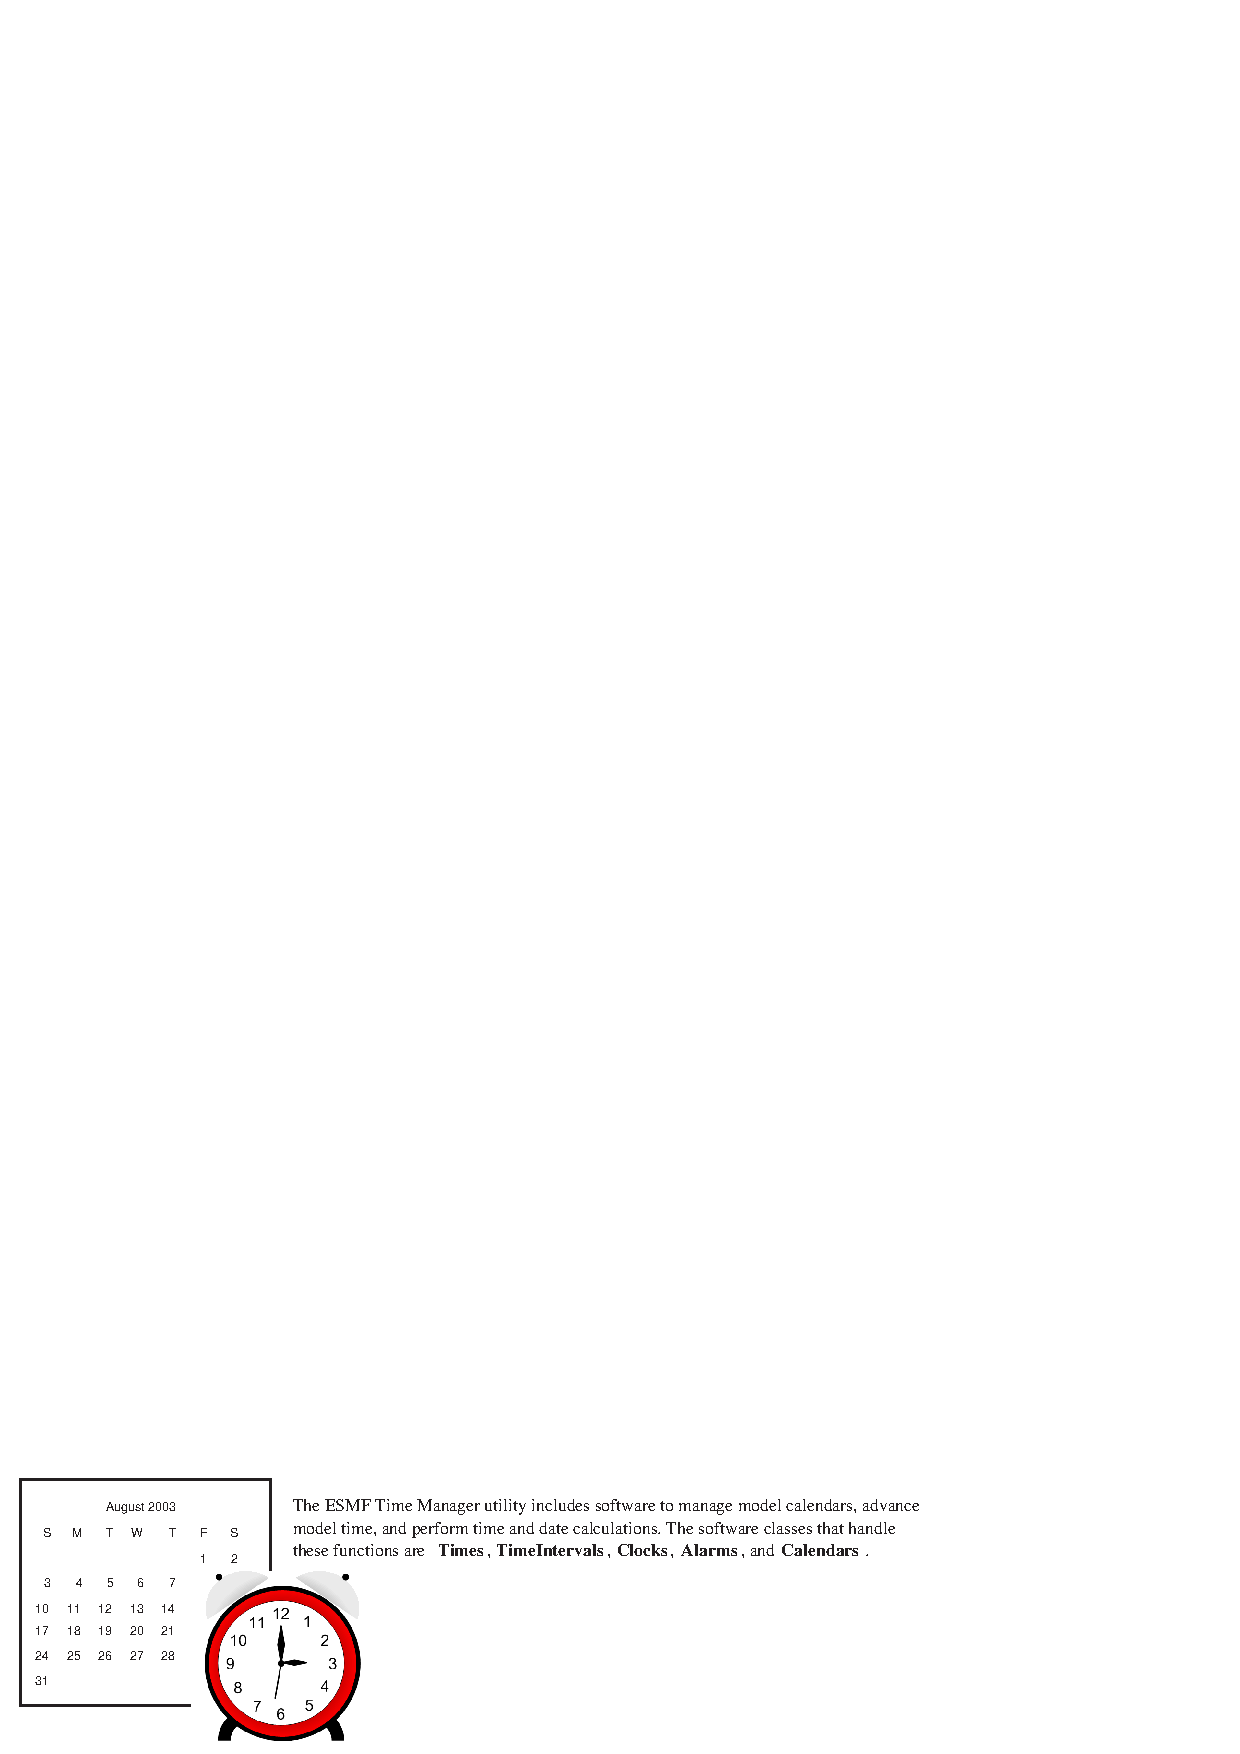
\includegraphics{TimeMgr_desc}
\end{center}

\newpage
In the remainder of this section, we briefly summarize the 
functionality that the Time Manager classes provide.  Detailed 
descriptions and usage examples precede the API listing for each 
class.

\subsection{Calendar}
An ESMF Calendar can be queried for seconds per day, days per month 
and days per year.  The flexible definition of Calendars allows them
to be defined for planetary bodies other than Earth.  The set of supported 
calendars includes:
\begin{description}
\item [Gregorian] The standard Gregorian calendar.
\item [no-leap] The Gregorian calendar with no leap years.
\item [Julian] The standard Julian date calendar.
\item [Julian Day] The standard Julian days calendar.
\item [Modified Julian Day] The Modified Julian days calendar.
\item [360-day] A 30-day-per-month, 12-month-per-year calendar.
\item [no calendar] Tracks only elapsed model time in hours, minutes, seconds.
\end{description}
See Section~\ref{sec:Calendar} for more details on supported standard 
calendars, and how to create a customized ESMF Calendar.

\subsection{Time Instants and TimeIntervals}

\label{subsec:Time Instants and TimeIntervals}
TimeIntervals and Time instants (simply called Times) are the computational 
building blocks of the Time Manager utility.  TimeIntervals support operations
such as add, subtract, compare size, reset value, copy value, and subdivide
by a scalar.  Times, which are moments in time associated with specific
Calendars, can be incremented or decremented by TimeIntervals, compared to
determine which of two Times is later, differenced to obtain the TimeInterval
between two Times, copied, reset, and manipulated in other useful ways.
Times support a host of different queries, both for values of individual Time 
components such as year, month, day, and second, and for derived values such 
as day of year, middle of current month and Julian day.  It is also possible 
to retrieve the value of the hardware realtime clock in the form of a 
Time.  See Sections~\ref{sec:Time} and ~\ref{sec:TimeInterval}, respectively,
for use and examples of Times and TimeIntervals.

Since climate modeling, numerical weather prediction and other 
Earth and space applications have widely varying time scales and require 
different sorts of calendars, Times and TimeIntervals must support 
a wide range of time specifiers, spanning nanoseconds to years.  The
interfaces to these time classes are defined so that the user can specify a time
using a combination of units selected from the list shown in 
Table~\ref{table:timeOpts}.  

\subsection{Clocks and Alarms}
Although it is possible to repeatedly step a Time forward by a 
TimeInterval using arithmetic on these basic types, it is useful to 
identify a higher-level concept to represent this function.  We refer to 
this capability as a Clock, and include in its required features the 
ability to store the start and stop times of 
a model run, to check when time advancement should cease, 
and to query the value of quantities such as the current time and the
time at the previous time step.  The Time Manager includes a class 
with methods that return a true value when a periodic or unique event 
has taken place; we refer to these as Alarms.  Applications may contain 
temporary or multiple Clocks and Alarms.  Sections~\ref{sec:Clock} and
\ref{sec:Alarm} describe the use of Clocks and Alarms in detail.







%\section{Abbreviations Table}
\newpage
\label{table:timeOpts}
\begin{center}
\begin{table}
\caption{Specifiers for Times and TimeIntervals}
\begin{tabular}{|p{1in}|p{3.5in}|}
\hline
Unit & Meaning \\
\hline\hline
{\bf <yy|yy\_i8>} & Year. \\
\hline
{\bf mm} & Month of the year. \\
\hline
{\bf dd} & Day of the month. \\
\hline
{\bf <d|d\_i8|d\_r8>} & Julian or Modified Julian day. \\
\hline
{\bf <h|h\_r8>} & Hour. \\
\hline
{\bf <m|m\_r8>} & Minute. \\
\hline
{\bf <s|s\_i8|s\_r8>} & Second. \\
\hline
{\bf <ms|ms\_r8>} & Millisecond. \\
\hline
{\bf <us|us\_r8>} & Microsecond. \\
\hline
{\bf <ns|ns\_r8>} & Nanosecond. \\
\hline
{\bf O} & Time zone offset in integer number of hours and minutes. \\
\hline
{\bf <sN|sN\_i8>} & Numerator for times of the form s {\bf $ + 
\frac{{\rm sN}}{{\rm sD}}$}, where s is seconds and s, sN, and
sD are integers.  This format provides a mechanism for supporting
exact behavior. \\
\hline
{\bf <sD|sD\_i8} & Denominator for times of the form s {\bf $ + 
\frac{{\rm sN}}{{\rm sD}}$}, where s is seconds and s, sN, and
sD are integers. \\
\hline
\end{tabular}
\end{table}
\end{center}

%\subsection{Design and Implementation Notes}
% $Id$

\subsection{Design and Implementation Notes}
\begin{enumerate}

\item {\bf Base TimeIntervals and Times on the same integer representation.} 
It is useful to allow both TimeIntervals and Times to 
inherit from a single class, BaseTime.  In C++, this can be
implemented by using inheritance.  In Fortran, it can be implemented
by having the derived types TimeIntervals and Times
contain a derived type BaseTime.  In both cases, the 
BaseTime class can be made private and invisible to the user.

The result of this strategy is that Time Intervals and 
Times gain a consistent core representation of time as well a set
of basic methods.

The BaseTime class can be designed with a minimum number of elements
to represent any required time.  The design is based on the idea used
in the real-time POSIX 1003.1b-1993 standard.  That is, to represent
time simply as a pair of integers: one for seconds (whole) and one for
nanoseconds (fractional).  These can then be converted at the interface
level to any desired format.

For ESMF, this idea can be modified and extended, in order to handle the
requirements for a large time range (> 200,000 years) and to exactly
represent any rational fraction, not just nanoseconds.  To handle the
large time range, a 64-bit or greater integer is used for whole seconds.
Any rational fractional second is expressed using two additional integers:
a numerator and a denominator.  Both the whole seconds and fractional
numerator are signed to handle negative time intervals and instants.
For arithmetic consistency both must carry the same sign (both positive
or both negative), except, of course, for zero values.  The fractional
seconds element (numerator) is bounded with respect to whole seconds. 
If the absolute value of the
numerator becomes greater than or equal to the denominator, whole
seconds are incremented or decremented accordingly and the numerator is
reset to the remainder.  Conversions are performed upon demand by
interface methods within the TimeInterval and
Time classes.  This is done because different applications require different
representations of time intervals and time instances.  Floating point values as well as integers can be specified for the various time units in the interfaces, see Table~\ref{table:timeOpts}.  Floating point values are represented internally as integer-based rational fractions.

The BaseTime class defines increment and decrement methods for basic
TimeInterval calculations between Time instants.  It is done here rather
than in the Calendar class because it can be done with simple 
second-based arithmetic that is calendar independent.  

Comparison methods can also be defined in the BaseTime class.  These
perform equality/inequality, less than, and greater than comparisons
between any two TimeIntervals or Times.  These methods capture
the common comparison logic between TimeIntervals and Times and
hence are defined here for sharing.

\item {\bf The Time class depends on a calendar.} The Time class contains 
an internal Calendar class.  
Upon demand by a user, the results of an increment or decrement operation are 
converted to user units, which may be calendar-dependent, via methods 
obtained from their internal Calendar.

\end{enumerate}













%\subsection{Object Model}
% $Id$

\pagebreak
\subsection{Object Model}

The following is a simplified UML diagram showing the structure of the
Time Manager utility.  See Appendix A, {\it A Brief Introduction to UML},
for a translation table that lists the symbols in the diagram and their 
meaning.

\begin{center}
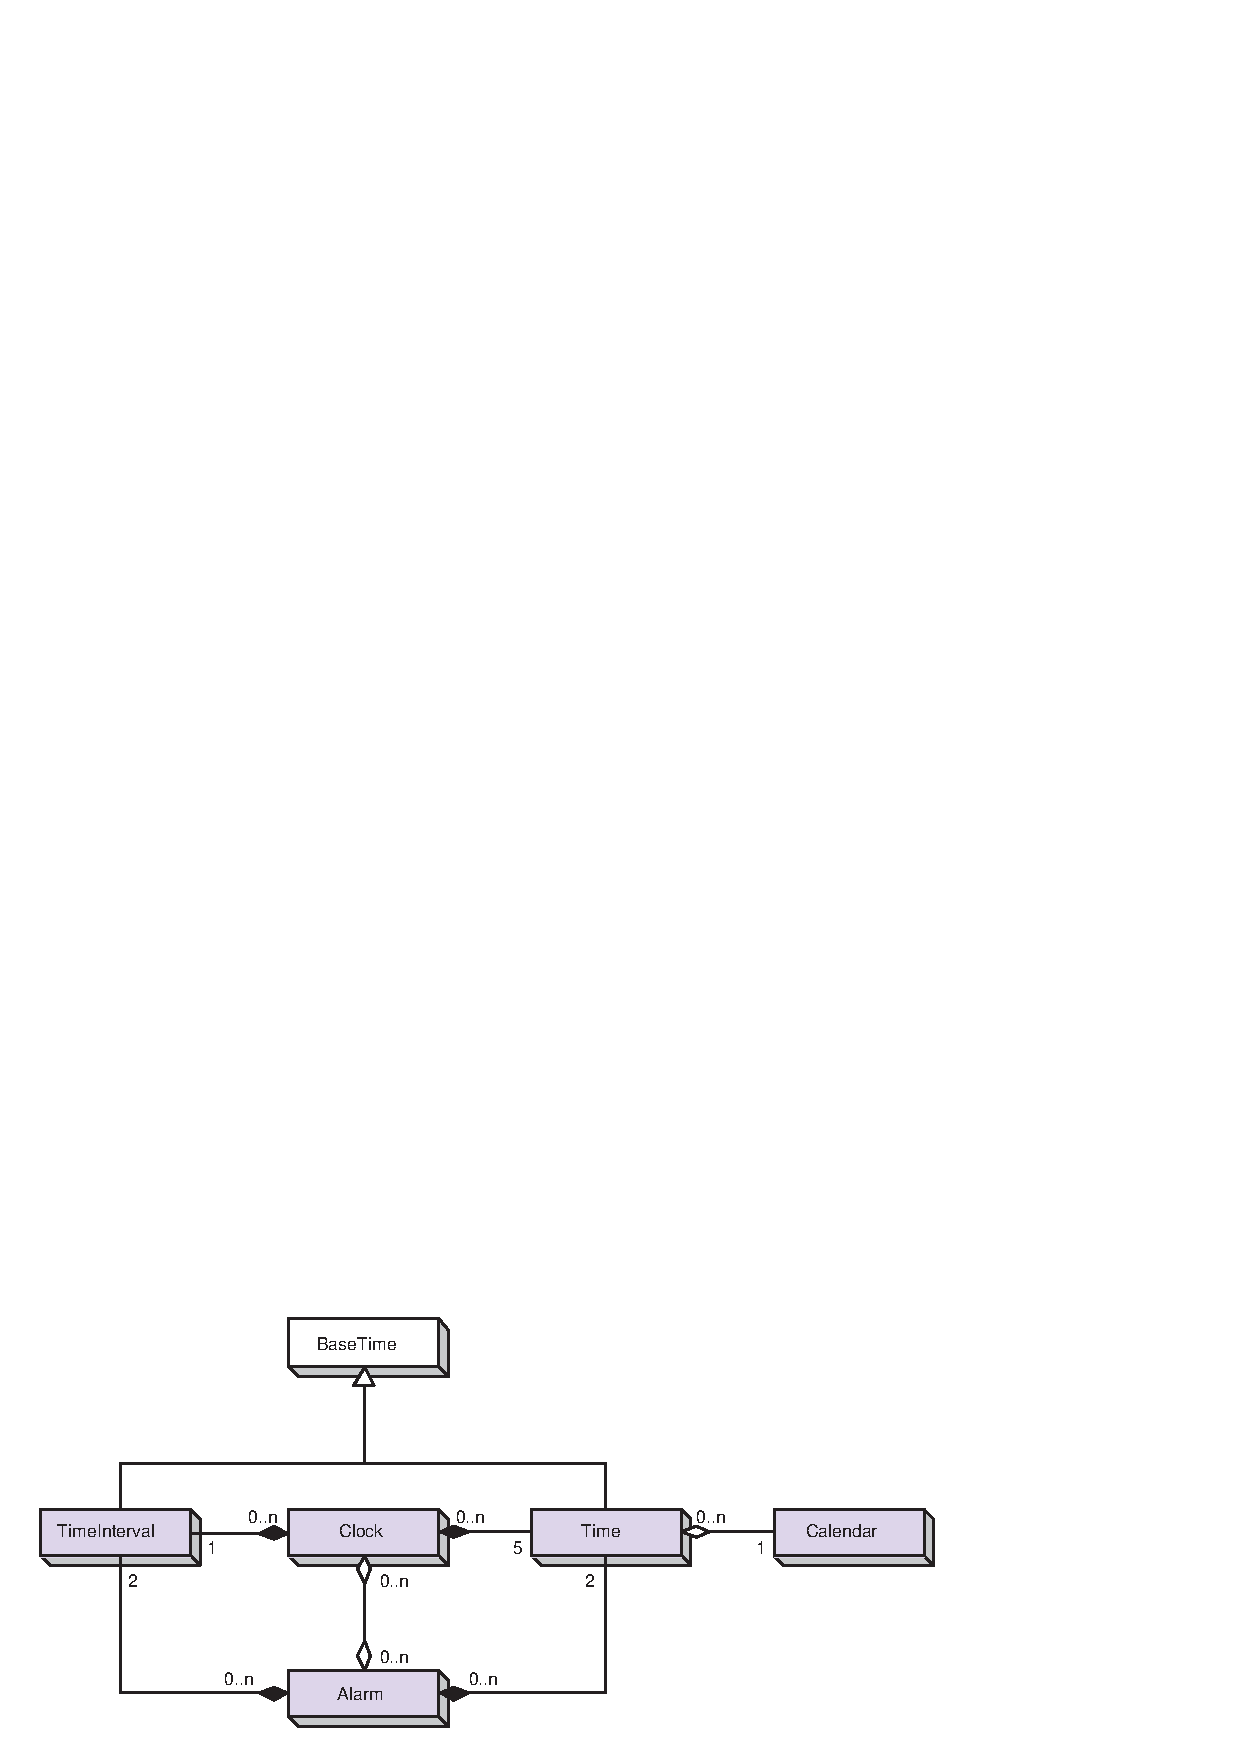
\includegraphics{TimeMgr_obj}   
\end{center}

% --------------
% Calendar Class
% --------------
\newpage
\section{Calendar Class}
\subsection{Description}
% $Id$

\label{sec:Calendar}
The Calendar class represents the standard calendars used in 
geophysical modeling:  Gregorian, Julian, Julian Day, Modified Julian Day, 
no-leap, 360-day, and no-calendar.  It also supports a user-customized 
calendar.  Brief descriptions are provided for each calendar below.  For more 
information on standard calendars, see ~\cite{Seidelman} and ~\cite{Meyer1}.

\subsection{Constants}
% $Id$

\label{subsec:Calendar_options}

\subsubsection{ESMF\_CALKIND}
\label{const:calkindflag}

{\sf DESCRIPTION:\\}
Supported calendar kinds.

The type of this flag is:

{\tt type(ESMF\_CalKind\_Flag)}

The valid values are:
\begin{description}
      
\item [ESMF\_CALKIND\_360DAY] 
{\it Valid range: machine limits} 
\newline In the 360-day calendar, there are 12 months, each of which has 30 days.  
Like the no-leap calendar, this is a simple approximation to the Gregorian
calendar sometimes used by modelers.

\item [ESMF\_CALKIND\_CUSTOM] 
{\it Valid range: machine limits} 
\newline The user can set calendar parameters in the generic calendar.

\item [ESMF\_CALKIND\_GREGORIAN] 
{\it Valid range: 3/1/4801 BC to 10/29/292,277,019,914 }
\newline The Gregorian calendar is the calendar currently in use 
throughout Western countries.  Named after Pope Gregory XIII, it is a minor 
correction to the older Julian calendar. In the Gregorian calendar every
fourth year is a leap year in which February has 29 and not 28 days;
however, years divisible by 100 are not leap years unless they are also 
divisible  by 400.  As in the Julian calendar, days begin at midnight.

\item [ESMF\_CALKIND\_JULIAN]
{\it Valid range: 3/1/4713 BC to 4/24/292,271,018,333 } 
\newline The Julian calendar was introduced by Julius Caesar in 46 B.C., and 
reached its final form in 4 A.D.  The Julian calendar differs from the 
Gregorian only in the determination of leap years, lacking the correction 
for years divisible by 100 and 400 in the Gregorian calendar.  In the Julian 
calendar, any year is a leap year if divisible by 4.  Days are considered to 
begin at midnight.

\item [ESMF\_CALKIND\_JULIANDAY] 
{\it Valid range:  +/- 1x10$^{14}$} 
\newline Julian days simply enumerate the days and fraction of a day which 
have elapsed since the start of the Julian era, defined as beginning at noon 
on Monday, 1st January of year 4713 B.C. in the Julian calendar.  Julian days, 
unlike the dates in the Julian and Gregorian calendars, begin at noon.

\item [ESMF\_CALKIND\_MODJULIANDAY]
{\it Valid range:  +/- 1x10$^{14}$}
\newline The Modified Julian Day (MJD) was introduced by space scientists in
 the late 1950's.  It is defined as an offset from the Julian Day (JD):

MJD = JD - 2400000.5

The half day is subtracted so that the day starts at midnight.

\item [ESMF\_CALKIND\_NOCALENDAR] 
{\it Valid range: machine limits}
\newline The no-calendar option simply tracks the elapsed model time in seconds.

\item [ESMF\_CALKIND\_NOLEAP]
{\it Valid range: machine limits} 
\newline The no-leap calendar is the Gregorian calendar with no leap years - 
February is always assumed to have 28 days.  Modelers sometimes use this 
calendar as a simple, close approximation to the Gregorian calendar.

\end{description}

\subsection{Use and Examples}
% $Id$

In most multi-component Earth system applications, the timekeeping in 
each component 
must refer to the same standard calendar in order for the components 
to properly synchronize.  It therefore makes sense to create as few 
ESMF Calendars as possible, preferably one per application.
A typical strategy would be to create a single Calendar at the start
of an application, and use that Calendar in all subsequent calls that
accept a Calendar, such as {\tt ESMF\_TimeSet}.

The following example shows how to set up an ESMF Calendar.  

%                **** IMPORTANT NOTICE *****
% This LaTeX file has been automatically produced by ProTeX v. 1.1
% Any changes made to this file will likely be lost next time
% this file is regenerated from its source. Send questions 
% to Arlindo da Silva, dasilva@gsfc.nasa.gov
 
\setlength{\oldparskip}{\parskip}
\setlength{\parskip}{1.5ex}
\setlength{\oldparindent}{\parindent}
\setlength{\parindent}{0pt}
\setlength{\oldbaselineskip}{\baselineskip}
\setlength{\baselineskip}{11pt}
 
%--------------------- SHORT-HAND MACROS ----------------------
\def\bv{\begin{verbatim}}
\def\ev{\end{verbatim}}
\def\be{\begin{equation}}
\def\ee{\end{equation}}
\def\bea{\begin{eqnarray}}
\def\eea{\end{eqnarray}}
\def\bi{\begin{itemize}}
\def\ei{\end{itemize}}
\def\bn{\begin{enumerate}}
\def\en{\end{enumerate}}
\def\bd{\begin{description}}
\def\ed{\end{description}}
\def\({\left (}
\def\){\right )}
\def\[{\left [}
\def\]{\right ]}
\def\<{\left  \langle}
\def\>{\right \rangle}
\def\cI{{\cal I}}
\def\diag{\mathop{\rm diag}}
\def\tr{\mathop{\rm tr}}
%-------------------------------------------------------------

\markboth{Left}{Source File: ESMF\_CalendarEx.F90,  Date: Tue May  5 20:59:34 MDT 2020
}

 
%/////////////////////////////////////////////////////////////

 \begin{verbatim}
! !PROGRAM: ESMF_CalendarEx - Calendar creation examples
!
! !DESCRIPTION:
!
! This program shows examples of how to create different calendar kinds
!-----------------------------------------------------------------------------
#include "ESMF.h"

      ! ESMF Framework module
      use ESMF
      use ESMF_TestMod
      implicit none

      ! instantiate calendars
      type(ESMF_Calendar) :: gregorianCalendar
      type(ESMF_Calendar) :: julianDayCalendar
      type(ESMF_Calendar) :: marsCalendar

      ! local variables for Get methods
      integer :: sols
      integer(ESMF_KIND_I8) :: dl
      type(ESMF_Time) :: time, marsTime
      type(ESMF_TimeInterval) :: marsTimeStep

      ! return code
      integer:: rc
 
\end{verbatim}
 
%/////////////////////////////////////////////////////////////

 \begin{verbatim}
      ! initialize ESMF framework
      call ESMF_Initialize(defaultlogfilename="CalendarEx.Log", &
                    logkindflag=ESMF_LOGKIND_MULTI, rc=rc)
 
\end{verbatim}
 
%/////////////////////////////////////////////////////////////

  \subsubsection{Calendar creation}
 
   This example shows how to create three {\tt ESMF\_Calendars}. 
%/////////////////////////////////////////////////////////////

 \begin{verbatim}
      ! create a Gregorian calendar
      gregorianCalendar = ESMF_CalendarCreate(ESMF_CALKIND_GREGORIAN, &
                                              name="Gregorian", rc=rc)
 
\end{verbatim}
 
%/////////////////////////////////////////////////////////////

 \begin{verbatim}
      ! create a Julian Day calendar
      julianDayCalendar = ESMF_CalendarCreate(ESMF_CALKIND_JULIANDAY, &
                                              name="JulianDay", rc=rc)
 
\end{verbatim}
 
%/////////////////////////////////////////////////////////////

 \begin{verbatim}
      ! create a Custom calendar for the planet Mars
      ! 1 Mars solar day = 24 hours, 39 minutes, 35 seconds = 88775 seconds
      ! 1 Mars solar year = 668.5921 Mars solar days = 668 5921/10000 sols/year
      ! http://www.giss.nasa.gov/research/briefs/allison_02
      ! http://www.giss.nasa.gov/tools/mars24/help/notes.html
      marsCalendar = ESMF_CalendarCreate(secondsPerDay=88775, &
                                         daysPerYear=668, &
                                         daysPerYearDn=5921, &
                                         daysPerYearDd=10000, &
                                         name="MarsCalendar", rc=rc)
 
\end{verbatim}
 
%/////////////////////////////////////////////////////////////

  \subsubsection{Calendar comparison}
 
   This example shows how to compare an {\tt ESMF\_Calendar} with a known
   calendar kind. 
%/////////////////////////////////////////////////////////////

 \begin{verbatim}
      ! compare calendar kind against a known type
      if (gregorianCalendar == ESMF_CALKIND_GREGORIAN) then
        print *, "gregorianCalendar is of type ESMF_CALKIND_GREGORIAN."
      else
        print *, "gregorianCalendar is not of type ESMF_CALKIND_GREGORIAN."
      end if
 
\end{verbatim}
 
%/////////////////////////////////////////////////////////////

  \subsubsection{Time conversion between Calendars}
 
   This example shows how to convert a time from one {\tt ESMF\_Calendar}
   to another. 
%/////////////////////////////////////////////////////////////

 \begin{verbatim}
      call ESMF_TimeSet(time, yy=2004, mm=4, dd=17, &
                        calendar=gregorianCalendar, rc=rc)
 
\end{verbatim}
 
%/////////////////////////////////////////////////////////////

 \begin{verbatim}
      ! switch time's calendar to perform conversion
      call ESMF_TimeSet(time, calendar=julianDayCalendar, rc=rc)
 
\end{verbatim}
 
%/////////////////////////////////////////////////////////////

 \begin{verbatim}
      call ESMF_TimeGet(time, d_i8=dl, rc=rc)
      print *, "Gregorian date 2004/4/17 is ", dl, &
               " days in the Julian Day calendar."
 
\end{verbatim}
 
%/////////////////////////////////////////////////////////////

  \subsubsection{Add a time interval to a time on a Calendar}
 
   This example shows how to increment a time using a custom {\tt ESMF\_Calendar}. 
%/////////////////////////////////////////////////////////////

 \begin{verbatim}
      ! Set a time to Mars solar year 3, sol 100
      call ESMF_TimeSet(marsTime, yy=3, d=100, &
                        calendar=marsCalendar, rc=rc)
 
\end{verbatim}
 
%/////////////////////////////////////////////////////////////

 \begin{verbatim}
      ! Set a 1 solar year time step
      call ESMF_TimeIntervalSet(marsTimeStep, yy=1, rc=rc)
 
\end{verbatim}
 
%/////////////////////////////////////////////////////////////

 \begin{verbatim}
      ! Perform the increment
      marsTime = marsTime + marsTimeStep
 
\end{verbatim}
 
%/////////////////////////////////////////////////////////////

 \begin{verbatim}
      ! Get the result in sols (2774 = (3+1)*668.5921 + 100)
      call ESMF_TimeGet(marsTime, d=sols, rc=rc)
      print *, "For Mars, 3 solar years, 100 sols + 1 solar year = ", &
                sols, "sols."
 
\end{verbatim}
 
%/////////////////////////////////////////////////////////////

  \subsubsection{Calendar destruction}
 
   This example shows how to destroy three {\tt ESMF\_Calendars}. 
%/////////////////////////////////////////////////////////////

 \begin{verbatim}
      call ESMF_CalendarDestroy(julianDayCalendar, rc=rc)
 
\end{verbatim}
 
%/////////////////////////////////////////////////////////////

 \begin{verbatim}
      call ESMF_CalendarDestroy(gregorianCalendar, rc=rc)
 
\end{verbatim}
 
%/////////////////////////////////////////////////////////////

 \begin{verbatim}
      call ESMF_CalendarDestroy(marsCalendar, rc=rc)
 
\end{verbatim}
 
%/////////////////////////////////////////////////////////////

 \begin{verbatim}
      ! finalize ESMF framework
      call ESMF_Finalize(rc=rc)
 
\end{verbatim}
 
%/////////////////////////////////////////////////////////////

 \begin{verbatim}
      end program ESMF_CalendarEx
 
\end{verbatim}

%...............................................................
\setlength{\parskip}{\oldparskip}
\setlength{\parindent}{\oldparindent}
\setlength{\baselineskip}{\oldbaselineskip}

\subsection{Restrictions and Future Work}
% $Id$

\label{subsec:Calendar_rest}

\begin{enumerate}

\item {\bf Months per year set to 12.} Due to the requirement of only Earth modeling, the number of months per year is hard-coded at 12.  However, for easy modification, this is implemented via a C preprocessor \#define MONTHS\_PER\_YEAR in ESMCI\_Calendar.h.

\item {\bf Calendar date conversions.} Date conversions are currently defined between the Gregorian, Julian, Julian Day, and Modified Julian Day calendars. Further research and work would need to be done to determine conversion algorithms with and between the other calendars:  No Leap, 360 Day, and Custom.

\item {\bf ESMF\_CALKIND\_CUSTOM.} Currently, there is no provision for a custom calendar to define a leap year rule, so {\tt ESMF\_CalendarIsLeapYear()} will always return {\tt .false.} in this case.  However, the arguments {\tt daysPerYear}, {\tt daysPerYearDn}, and {\tt daysPerYearDd} in {\tt ESMF\_CalendarCreate()} and {\tt ESMF\_CalendarSet()} can be used to set a fractional number of days per year, for example, 365.25 = 365 25/100.  Also, if further timekeeping precision is required, fractional and/or floating point {\tt secondsPerDay} and {\tt secondsPerYear} could be added to the interfaces {\tt ESMF\_CalendarCreate()}, {\tt ESMF\_CalendarSet()}, and {\tt ESMF\_CalendarGet()} and implemented.

\end{enumerate}

%\subsection{Design and Implementation Notes}
%#ifdef STANDALONE
%% $Id$

\subsection{Implementation Notes}

The algorithm for computing between Gregorian dates and Julian days is given 
in Fliegel and Flandern ~\cite{Fli68}.

The algorithm for computing between Julian dates and Julian days is given 
in Hatcher ~\cite{Hat84}.

The {\tt Calendar} class defines two methods for converting in both
directions between the core {\tt BaseTime} class representation and a
calendar date.  Calculations of time intervals (deltas) between
time instants is done by the base class {\tt BaseTime} in the core units
of seconds and fractional seconds.  Thus,  a calendar is only needed for
converting core time to calendar time and vice versa.

%#elif defined(1)
%% $Id$

\subsection{Implementation Notes}

The algorithm for computing between Gregorian dates and Julian days is given 
in Fliegel and Flandern ~\cite{Fli68}.

The algorithm for computing between Julian dates and Julian days is given 
in Hatcher ~\cite{Hat84}.

The {\tt Calendar} class defines two methods for converting in both
directions between the core {\tt BaseTime} class representation and a
calendar date.  Calculations of time intervals (deltas) between
time instants is done by the base class {\tt BaseTime} in the core units
of seconds and fractional seconds.  Thus,  a calendar is only needed for
converting core time to calendar time and vice versa.

%#endif
\subsection{Class API}
%                **** IMPORTANT NOTICE *****
% This LaTeX file has been automatically produced by ProTeX v. 1.1
% Any changes made to this file will likely be lost next time
% this file is regenerated from its source. Send questions 
% to Arlindo da Silva, dasilva@gsfc.nasa.gov
 
\setlength{\oldparskip}{\parskip}
\setlength{\parskip}{1.5ex}
\setlength{\oldparindent}{\parindent}
\setlength{\parindent}{0pt}
\setlength{\oldbaselineskip}{\baselineskip}
\setlength{\baselineskip}{11pt}
 
%--------------------- SHORT-HAND MACROS ----------------------
\def\bv{\begin{verbatim}}
\def\ev{\end{verbatim}}
\def\be{\begin{equation}}
\def\ee{\end{equation}}
\def\bea{\begin{eqnarray}}
\def\eea{\end{eqnarray}}
\def\bi{\begin{itemize}}
\def\ei{\end{itemize}}
\def\bn{\begin{enumerate}}
\def\en{\end{enumerate}}
\def\bd{\begin{description}}
\def\ed{\end{description}}
\def\({\left (}
\def\){\right )}
\def\[{\left [}
\def\]{\right ]}
\def\<{\left  \langle}
\def\>{\right \rangle}
\def\cI{{\cal I}}
\def\diag{\mathop{\rm diag}}
\def\tr{\mathop{\rm tr}}
%-------------------------------------------------------------

\markboth{Left}{Source File: ESMF\_Calendar.F90,  Date: Tue May  5 20:59:34 MDT 2020
}

 
%/////////////////////////////////////////////////////////////
\subsubsection [ESMF\_CalendarAssignment(=)] {ESMF\_CalendarAssignment(=) - Assign a Calendar to another Calendar}


  
\bigskip{\sf INTERFACE:}
\begin{verbatim}       interface assignment(=)
       calendar1 = calendar2\end{verbatim}{\em ARGUMENTS:}
\begin{verbatim}       type(ESMF_Calendar) :: calendar1
       type(ESMF_Calendar) :: calendar2
   \end{verbatim}
{\sf STATUS:}
   \begin{itemize}
   \item\apiStatusCompatibleVersion{5.2.0r}
   \end{itemize}
  
{\sf DESCRIPTION:\\ }


       Assign {\tt calendar1} as an alias to the same {\tt ESMF\_Calendar} 
       object in memory as {\tt calendar2}. If {\tt calendar2} is invalid, then 
       {\tt calendar1} will be equally invalid after the assignment.
  
       The arguments are:
       \begin{description} 
       \item[calendar1] 
            The {\tt ESMF\_Calendar} object on the left hand side of the 
            assignment.
       \item[calendar2] 
            The {\tt ESMF\_Calendar} object on the right hand side of the 
            assignment.
       \end{description}
   
%/////////////////////////////////////////////////////////////
 
\mbox{}\hrulefill\ 
 
\subsubsection [ESMF\_CalendarOperator(==)] {ESMF\_CalendarOperator(==) - Test if Calendar argument 1 is equal to Calendar argument 2}


  
\bigskip{\sf INTERFACE:}
\begin{verbatim}       interface operator(==)
       if (<calendar argument 1> == <calendar argument 2>) then ... endif
                                   OR
       result = (<calendar argument 1> == <calendar argument 2>)\end{verbatim}{\em RETURN VALUE:}
\begin{verbatim}       logical :: result\end{verbatim}{\em ARGUMENTS:}
\begin{verbatim}       <calendar argument 1>, see below for supported values
       <calendar argument 2>, see below for supported values\end{verbatim}
{\sf DESCRIPTION:\\ }


       \begin{sloppypar}
       Overloads the (==) operator for the {\tt ESMF\_Calendar} class.
       Compare an {\tt ESMF\_Calendar} object or {\tt ESMF\_CalKind\_Flag} with
       another calendar object or calendar kind for equality.  Return
       {\tt .true.} if equal, {\tt .false.} otherwise.  Comparison is based on
       calendar kind, which is a property of a calendar object.
       \end{sloppypar}
  
       If both arguments are {\tt ESMF\_Calendar} objects, and both are of  
       type {\tt ESMF\_CALKIND\_CUSTOM}, then all the calendar's properties, 
       except name, are compared.
  
       If both arguments are {\tt ESMF\_Calendar} objects, and either of them
       is not in the {\tt ESMF\_INIT\_CREATED} status, an error will be logged.
       However, this does not affect the return value, which is {\tt .true.} 
       when both arguments are in the {\em same} status, and {\tt .false.}
       otherwise.
  
       If one argument is an {\tt ESMF\_Calendar} object, and the other is an
       {\tt ESMF\_CalKind\_Flag}, and the calendar object is not in the
       {\tt ESMF\_INIT\_CREATED} status, an error will be logged and
       {\tt .false.} will be returned.
  
       Supported values for <calendar argument 1> are:
       \begin{description}
       \item type(ESMF\_Calendar),     intent(in) :: calendar1
       \item type(ESMF\_CalKind\_Flag), intent(in) :: calkindflag1
       \end{description}
       Supported values for <calendar argument 2> are:
       \begin{description}
       \item type(ESMF\_Calendar),     intent(in) :: calendar2
       \item type(ESMF\_CalKind\_Flag), intent(in) :: calkindflag2
       \end{description}
  
       The arguments are:
       \begin{description}   
       \item[<calendar argument 1>]
            The {\tt ESMF\_Calendar} object or {\tt ESMF\_CalKind\_Flag} on the
            left hand side of the equality operation.
       \item[<calendar argument 2>]
            The {\tt ESMF\_Calendar} object or {\tt ESMF\_CalKind\_Flag} on the
            right hand side of the equality operation.
       \end{description}
   
%/////////////////////////////////////////////////////////////
 
\mbox{}\hrulefill\ 
 
\subsubsection [ESMF\_CalendarOperator(/=)] {ESMF\_CalendarOperator(/=) - Test if Calendar argument 1 is not equal to Calendar argument 2}


  
\bigskip{\sf INTERFACE:}
\begin{verbatim}       interface operator(/=)
       if (<calendar argument 1> /= <calendar argument 2>) then ... endif
                                   OR
       result = (<calendar argument 1> /= <calendar argument 2>)\end{verbatim}{\em RETURN VALUE:}
\begin{verbatim}       logical :: result\end{verbatim}{\em ARGUMENTS:}
\begin{verbatim}       <calendar argument 1>, see below for supported values
       <calendar argument 2>, see below for supported values\end{verbatim}
{\sf DESCRIPTION:\\ }


       \begin{sloppypar}
       Overloads the (/=) operator for the {\tt ESMF\_Calendar} class.
       Compare a {\tt ESMF\_Calendar} object or {\tt ESMF\_CalKind\_Flag} with
       another calendar object or calendar kind for inequality.  Return
       {\tt .true.} if not equal, {\tt .false.} otherwise.  Comparison is based
       on calendar kind, which is a property of a calendar object.
       \end{sloppypar}
  
       If both arguments are {\tt ESMF\_Calendar} objects, and both are of  
       type {\tt ESMF\_CALKIND\_CUSTOM}, then all the calendar's properties,
       except name, are compared.
  
       If both arguments are {\tt ESMF\_Calendar} objects, and either of them
       is not in the {\tt ESMF\_INIT\_CREATED} status, an error will be logged.
       However, this does not affect the return value, which is {\tt .true.} 
       when both arguments are {\em not} in the {\em same} status, and
       {\tt .false.} otherwise.
  
       If one argument is an {\tt ESMF\_Calendar} object, and the other is an
       {\tt ESMF\_CalKind\_Flag}, and the calendar object is not in the
       {\tt ESMF\_INIT\_CREATED} status, an error will be logged and
       {\tt .true.} will be returned.
  
       Supported values for <calendar argument 1> are:
       \begin{description}
       \item type(ESMF\_Calendar),     intent(in) :: calendar1
       \item type(ESMF\_CalKind\_Flag), intent(in) :: calkindflag1
       \end{description}
       Supported values for <calendar argument 2> are:
       \begin{description}
       \item type(ESMF\_Calendar),     intent(in) :: calendar2
       \item type(ESMF\_CalKind\_Flag), intent(in) :: calkindflag2
       \end{description}
  
       The arguments are:
       \begin{description}   
       \item[<calendar argument 1>]
            The {\tt ESMF\_Calendar} object or {\tt ESMF\_CalKind\_Flag} on the
            left hand side of the non-equality operation.
       \item[<calendar argument 2>]
            The {\tt ESMF\_Calendar} object or {\tt ESMF\_CalKind\_Flag} on the
            right hand side of the non-equality operation.
       \end{description}
   
%/////////////////////////////////////////////////////////////
 
\mbox{}\hrulefill\ 
 
\subsubsection [ESMF\_CalendarCreate] {ESMF\_CalendarCreate - Create a new ESMF Calendar of built-in type}


 
\bigskip{\sf INTERFACE:}
\begin{verbatim}       ! Private name; call using ESMF_CalendarCreate()
       function ESMF_CalendarCreateBuiltIn(calkindflag, &
         name, rc)
 \end{verbatim}{\em RETURN VALUE:}
\begin{verbatim}       type(ESMF_Calendar) :: ESMF_CalendarCreateBuiltIn
 \end{verbatim}{\em ARGUMENTS:}
\begin{verbatim}       type(ESMF_CalKind_Flag), intent(in)            :: calkindflag
 -- The following arguments require argument keyword syntax (e.g. rc=rc). --
       character (len=*),       intent(in),  optional :: name
       integer,                 intent(out), optional :: rc
 \end{verbatim}
{\sf STATUS:}
   \begin{itemize}
   \item\apiStatusCompatibleVersion{5.2.0r}
   \end{itemize}
  
{\sf DESCRIPTION:\\ }


       Creates and sets a {\tt calendar} to the given built-in
       {\tt ESMF\_CalKind\_Flag}. 
  
       The arguments are:
       \begin{description}
       \item[calkindflag]
            The built-in {\tt ESMF\_CalKind\_Flag}.  Valid values are:
              \newline
              {\tt ESMF\_CALKIND\_360DAY}, 
              \newline
              {\tt ESMF\_CALKIND\_GREGORIAN},
              \newline
              {\tt ESMF\_CALKIND\_JULIAN}, 
              \newline
              {\tt ESMF\_CALKIND\_JULIANDAY},
              \newline
              {\tt ESMF\_CALKIND\_MODJULIANDAY}, 
              \newline
              {\tt ESMF\_CALKIND\_NOCALENDAR},
              \newline
              and {\tt ESMF\_CALKIND\_NOLEAP}.
              \newline
            See Section ~\ref{subsec:Calendar_options} for a description of each
            calendar kind.
       \item[{[name]}]
            The name for the newly created calendar.  If not specified, a
            default unique name will be generated: "CalendarNNN" where NNN
            is a unique sequence number from 001 to 999.
       \item[{[rc]}]
            Return code; equals {\tt ESMF\_SUCCESS} if there are no errors.
       \end{description}
       
%/////////////////////////////////////////////////////////////
 
\mbox{}\hrulefill\ 
 
\subsubsection [ESMF\_CalendarCreate] {ESMF\_CalendarCreate - Create a copy of an ESMF Calendar}


 
\bigskip{\sf INTERFACE:}
\begin{verbatim}       ! Private name; call using ESMF_CalendarCreate()
       function ESMF_CalendarCreateCopy(calendar, rc)
 \end{verbatim}{\em RETURN VALUE:}
\begin{verbatim}       type(ESMF_Calendar) :: ESMF_CalendarCreateCopy
 \end{verbatim}{\em ARGUMENTS:}
\begin{verbatim}       type(ESMF_Calendar), intent(in)            :: calendar
 -- The following arguments require argument keyword syntax (e.g. rc=rc). --
       integer,             intent(out), optional :: rc
 \end{verbatim}
{\sf STATUS:}
   \begin{itemize}
   \item\apiStatusCompatibleVersion{5.2.0r}
   \end{itemize}
  
{\sf DESCRIPTION:\\ }


       Creates a complete (deep) copy of a given {\tt ESMF\_Calendar}.
  
       The arguments are:
       \begin{description}
       \item[calendar]
          The {\tt ESMF\_Calendar} to copy.
       \item[{[rc]}]
          Return code; equals {\tt ESMF\_SUCCESS} if there are no errors.
       \end{description}
   
%/////////////////////////////////////////////////////////////
 
\mbox{}\hrulefill\ 
 
\subsubsection [ESMF\_CalendarCreate] {ESMF\_CalendarCreate - Create a new custom ESMF Calendar}


 
\bigskip{\sf INTERFACE:}
\begin{verbatim}       ! Private name; call using ESMF_CalendarCreate()
       function ESMF_CalendarCreateCustom(&
         daysPerMonth, secondsPerDay, &
         daysPerYear, daysPerYearDn, daysPerYearDd, name, rc)
 \end{verbatim}{\em RETURN VALUE:}
\begin{verbatim}       type(ESMF_Calendar) :: ESMF_CalendarCreateCustom
 \end{verbatim}{\em ARGUMENTS:}
\begin{verbatim} -- The following arguments require argument keyword syntax (e.g. rc=rc). --
       integer,               intent(in),  optional :: daysPerMonth(:)
       integer(ESMF_KIND_I4), intent(in),  optional :: secondsPerDay
       integer(ESMF_KIND_I4), intent(in),  optional :: daysPerYear
       integer(ESMF_KIND_I4), intent(in),  optional :: daysPerYearDn
       integer(ESMF_KIND_I4), intent(in),  optional :: daysPerYearDd
       character (len=*),     intent(in),  optional :: name
       integer,               intent(out), optional :: rc
 \end{verbatim}
{\sf DESCRIPTION:\\ }


       Creates a custom {\tt ESMF\_Calendar} and sets its properties.
  
       The arguments are:
       \begin{description}
       \item[{[daysPerMonth]}]
            Integer array of days per month, for each month of the year.
            The number of months per year is variable and taken from the
            size of the array.  If unspecified, months per year = 0,
            with the days array undefined.
       \item[{[secondsPerDay]}]
            Integer number of seconds per day.  Defaults to 0 if not 
            specified.
       \item[{[daysPerYear]}]
            Integer number of days per year.  Use with daysPerYearDn and
            daysPerYearDd (see below) to specify a days-per-year calendar
            for any planetary body.  Default = 0.
       \item[{[daysPerYearDn]}]
            \begin{sloppypar}
            Integer numerator portion of fractional number of days per year
            (daysPerYearDn/daysPerYearDd).
            Use with daysPerYear (see above) and daysPerYearDd (see below) to
            specify a days-per-year calendar for any planetary body.
            Default = 0.
            \end{sloppypar}
       \item[{[daysPerYearDd]}]
            Integer denominator portion of fractional number of days per year
            (daysPerYearDn/daysPerYearDd).
            Use with daysPerYear and daysPerYearDn (see above) to
            specify a days-per-year calendar for any planetary body.
            Default = 1.
       \item[{[name]}]
            The name for the newly created calendar.  If not specified, a
            default unique name will be generated: "CalendarNNN" where NNN
            is a unique sequence number from 001 to 999.
       \item[{[rc]}]
            Return code; equals {\tt ESMF\_SUCCESS} if there are no errors.
       \end{description}
        
%/////////////////////////////////////////////////////////////
 
\mbox{}\hrulefill\ 
 
\subsubsection [ESMF\_CalendarDestroy] {ESMF\_CalendarDestroy - Release resources associated with a Calendar}


  
\bigskip{\sf INTERFACE:}
\begin{verbatim}       subroutine ESMF_CalendarDestroy(calendar, rc)\end{verbatim}{\em ARGUMENTS:}
\begin{verbatim}       type(ESMF_Calendar), intent(inout)          :: calendar
 -- The following arguments require argument keyword syntax (e.g. rc=rc). --
       integer,             intent(out),  optional :: rc\end{verbatim}
{\sf STATUS:}
   \begin{itemize}
   \item\apiStatusCompatibleVersion{5.2.0r}
   \end{itemize}
  
{\sf DESCRIPTION:\\ }


       Releases resources associated with this {\tt ESMF\_Calendar}.
  
       The arguments are:
       \begin{description}
       \item[calendar]
         Release resources associated with this {\tt ESMF\_Calendar} and mark the
         object as invalid.  It is an error to pass this object into any other
         routines after being destroyed.
       \item[[rc]]
         Return code; equals {\tt ESMF\_SUCCESS} if there are no errors.
       \end{description}
   
%/////////////////////////////////////////////////////////////
 
\mbox{}\hrulefill\ 
 
\subsubsection [ESMF\_CalendarGet] {ESMF\_CalendarGet - Get Calendar properties}


 
\bigskip{\sf INTERFACE:}
\begin{verbatim}       subroutine ESMF_CalendarGet(calendar, &
         name, calkindflag, daysPerMonth, monthsPerYear, &
         secondsPerDay, secondsPerYear, &
         daysPerYear, daysPerYearDn, daysPerYearDd, rc)
 \end{verbatim}{\em ARGUMENTS:}
\begin{verbatim}       type(ESMF_Calendar),    intent(in)            :: calendar
 -- The following arguments require argument keyword syntax (e.g. rc=rc). --
       type(ESMF_CalKind_Flag),intent(out), optional :: calkindflag
       integer,                intent(out), optional :: daysPerMonth(:)
       integer,                intent(out), optional :: monthsPerYear
       integer(ESMF_KIND_I4),  intent(out), optional :: secondsPerDay
       integer(ESMF_KIND_I4),  intent(out), optional :: secondsPerYear
       integer(ESMF_KIND_I4),  intent(out), optional :: daysPerYear
       integer(ESMF_KIND_I4),  intent(out), optional :: daysPerYearDn
       integer(ESMF_KIND_I4),  intent(out), optional :: daysPerYearDd
       character (len=*),      intent(out), optional :: name
       integer,                intent(out), optional :: rc
 \end{verbatim}
{\sf STATUS:}
   \begin{itemize}
   \item\apiStatusCompatibleVersion{5.2.0r}
   \end{itemize}
  
{\sf DESCRIPTION:\\ }


       Gets one or more of an {\tt ESMF\_Calendar}'s properties.
  
       The arguments are:
       \begin{description}
       \item[calendar]
            The object instance to query.
       \item[{[calkindflag]}]
            The {\tt CalKind\_Flag} ESMF\_CALKIND\_GREGORIAN, 
            ESMF\_CALKIND\_JULIAN, etc.
       \item[{[daysPerMonth]}]
            Integer array of days per month, for each month of the year.
       \item[{[monthsPerYear]}]
            Integer number of months per year; the size of the
            daysPerMonth array.
       \item[{[secondsPerDay]}]
            Integer number of seconds per day.
       \item[{[secondsPerYear]}]
            Integer number of seconds per year.
       \item[{[daysPerYear]}]
            Integer number of days per year.  For calendars with
            intercalations, daysPerYear is the number of days for years without
            an intercalation.  For other calendars, it is the number of days in
            every year.
       \item[{[daysPerYearDn]}]
            \begin{sloppypar}
            Integer fractional number of days per year (numerator).
            For calendars with intercalations, daysPerYearDn/daysPerYearDd is
            the average fractional number of days per year (e.g. 25/100 for
            Julian 4-year intercalation).  For other calendars, it is zero.
            \end{sloppypar}
       \item[{[daysPerYearDd]}]
            Integer fractional number of days per year (denominator).  See
            daysPerYearDn above.
       \item[{[name]}]
            The name of this calendar.
       \item[{[rc]}]
            Return code; equals {\tt ESMF\_SUCCESS} if there are no errors.
       \end{description}
        
%/////////////////////////////////////////////////////////////
 
\mbox{}\hrulefill\ 
 
\subsubsection [ESMF\_CalendarIsCreated] {ESMF\_CalendarIsCreated - Check whether a Calendar object has been created}


 
\bigskip{\sf INTERFACE:}
\begin{verbatim}   function ESMF_CalendarIsCreated(calendar, rc)\end{verbatim}{\em RETURN VALUE:}
\begin{verbatim}     logical :: ESMF_CalendarIsCreated\end{verbatim}{\em ARGUMENTS:}
\begin{verbatim}     type(ESMF_Calendar), intent(in)            :: calendar
 -- The following arguments require argument keyword syntax (e.g. rc=rc). --
     integer,             intent(out), optional :: rc
 \end{verbatim}
{\sf DESCRIPTION:\\ }


     Return {\tt .true.} if the {\tt calendar} has been created. Otherwise return 
     {\tt .false.}. If an error occurs, i.e. {\tt rc /= ESMF\_SUCCESS} is 
     returned, the return value of the function will also be {\tt .false.}.
  
   The arguments are:
     \begin{description}
     \item[calendar]
       {\tt ESMF\_Calendar} queried.
     \item[{[rc]}]
       Return code; equals {\tt ESMF\_SUCCESS} if there are no errors.
     \end{description}
   
%/////////////////////////////////////////////////////////////
 
\mbox{}\hrulefill\ 
 
\subsubsection [ESMF\_CalendarIsLeapYear] {ESMF\_CalendarIsLeapYear - Determine if given year is a leap year}


  
\bigskip{\sf INTERFACE:}
\begin{verbatim}       ! Private name; call using ESMF_CalendarIsLeapYear()
       function ESMF_CalendarIsLeapYear<kind>(calendar, yy, rc)\end{verbatim}{\em RETURN VALUE:}
\begin{verbatim}       logical :: ESMF_CalendarIsLeapYear<kind>\end{verbatim}{\em ARGUMENTS:}
\begin{verbatim}       type(ESMF_Calendar),       intent(in)            :: calendar
       integer(ESMF_KIND_<kind>), intent(in)            :: yy
 -- The following arguments require argument keyword syntax (e.g. rc=rc). --
       integer,                   intent(out), optional :: rc\end{verbatim}
{\sf STATUS:}
   \begin{itemize}
   \item\apiStatusCompatibleVersion{5.2.0r}
   \end{itemize}
  
{\sf DESCRIPTION:\\ }


       \begin{sloppypar}
       Returns {\tt .true.} if the given year is a leap year within the given
       calendar, and {\tt .false.} otherwise.  Custom calendars do not define
       leap years, so {\tt .false.} will always be returned in this case;
       see Section ~\ref{subsec:Calendar_rest}.
       See also {\tt ESMF\_TimeIsLeapYear()}.
       \end{sloppypar}
  
       The arguments are:
       \begin{description}
       \item[calendar]
            {\tt ESMF\_Calendar} to determine leap year within.
       \item[yy]
            Year to check for leap year.  The type is integer and the <kind> can
            be either I4 or I8:  {\tt ESMF\_KIND\_I4} or {\tt ESMF\_KIND\_I8}.
       \item[{[rc]}]
            Return code; equals {\tt ESMF\_SUCCESS} if there are no errors.
       \end{description}
       
%/////////////////////////////////////////////////////////////
 
\mbox{}\hrulefill\ 
 
\subsubsection [ESMF\_CalendarPrint] {ESMF\_CalendarPrint - Print Calendar information}


 
\bigskip{\sf INTERFACE:}
\begin{verbatim}       subroutine ESMF_CalendarPrint(calendar, options, rc)
 \end{verbatim}{\em ARGUMENTS:}
\begin{verbatim}       type(ESMF_Calendar), intent(in)            :: calendar
       character (len=*),   intent(in),  optional :: options
       integer,             intent(out), optional :: rc
 \end{verbatim}
{\sf DESCRIPTION:\\ }


       Prints out an {\tt ESMF\_Calendar}'s properties to {\tt stdio}, 
       in support of testing and debugging.  The options control the 
       type of information and level of detail. \\
  
       The arguments are:
       \begin{description}
       \item[calendar]
            {\tt ESMF\_Calendar} to be printed out.
       \item[{[options]}]
            Print options. If none specified, prints all calendar property
                               values. \\
            "calkindflag"    - print the calendar's type 
                                 (e.g. ESMF\_CALKIND\_GREGORIAN). \\
            "daysPerMonth"   - print the array of number of days for
                                 each month. \\
            "daysPerYear"    - print the number of days per year
                               (integer and fractional parts). \\
            "monthsPerYear"  - print the number of months per year. \\
            "name"           - print the calendar's name. \\
            "secondsPerDay"  - print the number of seconds in a day. \\
            "secondsPerYear" - print the number of seconds in a year. \\
       \item[{[rc]}]
            Return code; equals {\tt ESMF\_SUCCESS} if there are no errors.
       \end{description}
   
%/////////////////////////////////////////////////////////////
 
\mbox{}\hrulefill\ 
 
\subsubsection [ESMF\_CalendarSet] {ESMF\_CalendarSet - Set a Calendar to a built-in type}


 
\bigskip{\sf INTERFACE:}
\begin{verbatim}       ! Private name; call using ESMF_CalendarSet()
       subroutine ESMF_CalendarSetBuiltIn(calendar, calkindflag, &
         name, rc)
 \end{verbatim}{\em ARGUMENTS:}
\begin{verbatim}       type(ESMF_Calendar),     intent(inout)         :: calendar
       type(ESMF_CalKind_Flag), intent(in)            :: calkindflag
 -- The following arguments require argument keyword syntax (e.g. rc=rc). --
       character (len=*),       intent(in),  optional :: name
       integer,                 intent(out), optional :: rc
 \end{verbatim}
{\sf STATUS:}
   \begin{itemize}
   \item\apiStatusCompatibleVersion{5.2.0r}
   \end{itemize}
  
{\sf DESCRIPTION:\\ }


       Sets {\tt calendar} to the given built-in {\tt ESMF\_CalKind\_Flag}. 
  
       The arguments are:
       \begin{description}
       \item[calendar]
            The object instance to initialize.
       \item[calkindflag]
            The built-in {\tt CalKind\_Flag}.  Valid values are:
              \newline
              {\tt ESMF\_CALKIND\_360DAY}, 
              \newline
              {\tt ESMF\_CALKIND\_GREGORIAN},
              \newline
              {\tt ESMF\_CALKIND\_JULIAN}, 
              \newline
              {\tt ESMF\_CALKIND\_JULIANDAY},
              \newline
              {\tt ESMF\_CALKIND\_MODJULIANDAY}, 
              \newline
              {\tt ESMF\_CALKIND\_NOCALENDAR},
              \newline
              and {\tt ESMF\_CALKIND\_NOLEAP}.
              \newline
            See Section ~\ref{subsec:Calendar_options} for a description of each
            calendar kind.
       \item[{[name]}]
            The new name for this calendar.
       \item[{[rc]}]
            Return code; equals {\tt ESMF\_SUCCESS} if there are no errors.
       \end{description}
       
%/////////////////////////////////////////////////////////////
 
\mbox{}\hrulefill\ 
 
\subsubsection [ESMF\_CalendarSet] {ESMF\_CalendarSet - Set properties of a custom Calendar}


 
\bigskip{\sf INTERFACE:}
\begin{verbatim}       ! Private name; call using ESMF_CalendarSet()
       subroutine ESMF_CalendarSetCustom(calendar, &
         daysPerMonth, secondsPerDay, &
         daysPerYear, daysPerYearDn, daysPerYearDd, name, rc)
 \end{verbatim}{\em ARGUMENTS:}
\begin{verbatim}       type(ESMF_Calendar),  intent(inout)         :: calendar
 -- The following arguments require argument keyword syntax (e.g. rc=rc). --
       integer,              intent(in),  optional :: daysPerMonth(:)
       integer(ESMF_KIND_I4),intent(in),  optional :: secondsPerDay
       integer(ESMF_KIND_I4),intent(in),  optional :: daysPerYear
       integer(ESMF_KIND_I4),intent(in),  optional :: daysPerYearDn
       integer(ESMF_KIND_I4),intent(in),  optional :: daysPerYearDd
       character (len=*),    intent(in),  optional :: name
       integer,              intent(out), optional :: rc
 \end{verbatim}
{\sf STATUS:}
   \begin{itemize}
   \item\apiStatusCompatibleVersion{5.2.0r}
   \end{itemize}
  
{\sf DESCRIPTION:\\ }


       Sets properties in a custom {\tt ESMF\_Calendar}.
  
       The arguments are:
       \begin{description}
       \item[calendar]
            The object instance to initialize.
       \item[{[daysPerMonth]}]
            Integer array of days per month, for each month of the year.
            The number of months per year is variable and taken from the
            size of the array.  If unspecified, months per year = 0,
            with the days array undefined.
       \item[{[secondsPerDay]}]
            Integer number of seconds per day.  Defaults to 0 if not 
            specified.
       \item[{[daysPerYear]}]
            Integer number of days per year.  Use with daysPerYearDn and
            daysPerYearDd (see below) to specify a days-per-year calendar
            for any planetary body.  Default = 0.
       \item[{[daysPerYearDn]}]
            Integer numerator portion of fractional number of days per year
            (daysPerYearDn/daysPerYearDd).
            Use with daysPerYear (see above) and daysPerYearDd (see below) to
            specify a days-per-year calendar for any planetary body.
            Default = 0.
       \item[{[daysPerYearDd]}]
            \begin{sloppypar}
            Integer denominator portion of fractional number of days per year
            (daysPerYearDn/daysPerYearDd).
            Use with daysPerYear and daysPerYearDn (see above) to
            specify a days-per-year calendar for any planetary body.
            Default = 1.
            \end{sloppypar}
       \item[{[name]}]
            The new name for this calendar.
       \item[{[rc]}]
            Return code; equals {\tt ESMF\_SUCCESS} if there are no errors.
       \end{description}
        
%/////////////////////////////////////////////////////////////
 
\mbox{}\hrulefill\ 
 
\subsubsection [ESMF\_CalendarSetDefault] {ESMF\_CalendarSetDefault - Set the default Calendar kind}


 
\bigskip{\sf INTERFACE:}
\begin{verbatim}       ! Private name; call using ESMF_CalendarSetDefault()
       subroutine ESMF_CalendarSetDefaultKind(calkindflag, rc)
 \end{verbatim}{\em ARGUMENTS:}
\begin{verbatim}       type(ESMF_CalKind_Flag), intent(in)            :: calkindflag
       integer,                 intent(out), optional :: rc
 \end{verbatim}
{\sf DESCRIPTION:\\ }


       Sets the default {\tt calendar} to the given type.  Subsequent Time
       Manager operations requiring a calendar where one isn't specified will
       use the internal calendar of this type.
  
       The arguments are:
       \begin{description}
       \item[calkindflag]
            The calendar kind to be the default.
       \item[{[rc]}]
            Return code; equals {\tt ESMF\_SUCCESS} if there are no errors.
       \end{description}
       
%/////////////////////////////////////////////////////////////
 
\mbox{}\hrulefill\ 
 
\subsubsection [ESMF\_CalendarSetDefault] {ESMF\_CalendarSetDefault - Set the default Calendar}


 
\bigskip{\sf INTERFACE:}
\begin{verbatim}       ! Private name; call using ESMF_CalendarSetDefault()
       subroutine ESMF_CalendarSetDefaultCal(calendar, rc)
 \end{verbatim}{\em ARGUMENTS:}
\begin{verbatim}       type(ESMF_Calendar),     intent(in)            :: calendar
       integer,                 intent(out), optional :: rc
 \end{verbatim}
{\sf DESCRIPTION:\\ }


       Sets the default {\tt calendar} to the one given.  Subsequent Time
       Manager operations requiring a calendar where one isn't specified will
       use this calendar.
  
       The arguments are:
       \begin{description}
       \item[calendar]
            The object instance to be the default.
       \item[{[rc]}]
            Return code; equals {\tt ESMF\_SUCCESS} if there are no errors.
       \end{description}
       
%/////////////////////////////////////////////////////////////
 
\mbox{}\hrulefill\ 
 
\subsubsection [ESMF\_CalendarValidate] {ESMF\_CalendarValidate - Validate a Calendar's properties}


 
\bigskip{\sf INTERFACE:}
\begin{verbatim}       subroutine ESMF_CalendarValidate(calendar, rc)
  \end{verbatim}{\em ARGUMENTS:}
\begin{verbatim}       type(ESMF_Calendar), intent(in)            :: calendar
 -- The following arguments require argument keyword syntax (e.g. rc=rc). --
       integer,             intent(out), optional :: rc
 \end{verbatim}
{\sf STATUS:}
   \begin{itemize}
   \item\apiStatusCompatibleVersion{5.2.0r}
   \end{itemize}
  
{\sf DESCRIPTION:\\ }


       Checks whether a {\tt calendar} is valid.  
       Must be one of the defined calendar kinds.  daysPerMonth, daysPerYear,
       secondsPerDay must all be greater than or equal to zero.
   
       The arguments are:
       \begin{description}
       \item[calendar]
            {\tt ESMF\_Calendar} to be validated.
       \item[{[rc]}]
            Return code; equals {\tt ESMF\_SUCCESS} if there are no errors.
       \end{description}
  
%...............................................................
\setlength{\parskip}{\oldparskip}
\setlength{\parindent}{\oldparindent}
\setlength{\baselineskip}{\oldbaselineskip}

% ----------
% Time Class
% ----------
\newpage
\section{Time Class}
\subsection{Description}
% $Id$
\label{sec:Time}

A Time represents a specific point in time.  In order to accommodate
the range of time scales in Earth system applications, Times in
the ESMF can be specified in many different ways, from years to
nanoseconds.  The Time interface is designed so that you select one or 
more options from a list of time units in order to specify a 
Time. The options for specifying a Time are shown in 
Table~\ref{table:timeOpts}.  

There are Time methods defined for setting and getting a
Time, incrementing and decrementing a Time by a TimeInterval,
taking the difference between two Times, and comparing Times.
Special quantities such as the middle of the month and the 
day of the year associated with a particular Time can be retrieved. 
There is a method for returning the Time value as a string in 
the ISO 8601 format YYYY-MM-DDThh:mm:ss \cite{ISO}.

A Time that is specified in hours, minutes, seconds, or subsecond intervals 
does not need to be associated with a standard calendar; a Time whose
specification includes time units of a day and greater must be.  The 
ESMF representation
of a calendar, the Calendar class, is described in Section~\ref{sec:Calendar}.
The {\tt ESMF\_TimeSet} method is used to initialize a Time as well as
associate it with a Calendar.  If a Time method is invoked in which a Calendar
is necessary and one has not been set, the ESMF method will return an error
condition.

In the ESMF the TimeInterval class is used to represent time periods.
This class is frequently used in combination with the Time class.
The Clock class, for example, advances model time by incrementing a
Time with a TimeInterval. 
 





\subsection{Use and Examples}
% $Id$

Times are most frequently used to represent start, stop, and current 
model times.  The following examples show how to create, initialize, and
manipulate {\tt Time}.



%                **** IMPORTANT NOTICE *****
% This LaTeX file has been automatically produced by ProTeX v. 1.1
% Any changes made to this file will likely be lost next time
% this file is regenerated from its source. Send questions 
% to Arlindo da Silva, dasilva@gsfc.nasa.gov
 
\setlength{\oldparskip}{\parskip}
\setlength{\parskip}{1.5ex}
\setlength{\oldparindent}{\parindent}
\setlength{\parindent}{0pt}
\setlength{\oldbaselineskip}{\baselineskip}
\setlength{\baselineskip}{11pt}
 
%--------------------- SHORT-HAND MACROS ----------------------
\def\bv{\begin{verbatim}}
\def\ev{\end{verbatim}}
\def\be{\begin{equation}}
\def\ee{\end{equation}}
\def\bea{\begin{eqnarray}}
\def\eea{\end{eqnarray}}
\def\bi{\begin{itemize}}
\def\ei{\end{itemize}}
\def\bn{\begin{enumerate}}
\def\en{\end{enumerate}}
\def\bd{\begin{description}}
\def\ed{\end{description}}
\def\({\left (}
\def\){\right )}
\def\[{\left [}
\def\]{\right ]}
\def\<{\left  \langle}
\def\>{\right \rangle}
\def\cI{{\cal I}}
\def\diag{\mathop{\rm diag}}
\def\tr{\mathop{\rm tr}}
%-------------------------------------------------------------

\markboth{Left}{Source File: ESMF\_TimeEx.F90,  Date: Tue May  5 20:59:34 MDT 2020
}

 
%/////////////////////////////////////////////////////////////

 \begin{verbatim}
! !PROGRAM: ESMF_TimeEx - Time initialization and manipulation examples
!
! !DESCRIPTION:
!
! This program shows examples of Time initialization and manipulation
!-----------------------------------------------------------------------------
#include "ESMF.h"

      ! ESMF Framework module
      use ESMF
      use ESMF_TestMod
      implicit none

      ! instantiate two times
      type(ESMF_Time) :: time1, time2

      type(ESMF_VM) :: vm

      ! instantiate a time interval
      type(ESMF_TimeInterval) :: timeinterval1

      ! local variables for Get methods
      integer :: YY, MM, DD, H, M, S

      ! return code
      integer:: rc
 
\end{verbatim}
 
%/////////////////////////////////////////////////////////////

 \begin{verbatim}
      ! initialize ESMF framework
      call ESMF_Initialize(vm=vm, defaultCalKind=ESMF_CALKIND_GREGORIAN, &
        defaultlogfilename="TimeEx.Log", &
        logkindflag=ESMF_LOGKIND_MULTI, rc=rc)
 
\end{verbatim}
 
%/////////////////////////////////////////////////////////////

  \subsubsection{Time initialization}
 
   This example shows how to initialize an {\tt ESMF\_Time}. 
%/////////////////////////////////////////////////////////////

 \begin{verbatim}
      ! initialize time1 to 2/28/2000 2:24:45
      call ESMF_TimeSet(time1, yy=2000, mm=2, dd=28, h=2, m=24, s=45, rc=rc)
 
\end{verbatim}
 
%/////////////////////////////////////////////////////////////

 \begin{verbatim}
      print *, "Time1 = "
      call ESMF_TimePrint(time1, options="string", rc=rc)
 
\end{verbatim}
 
%/////////////////////////////////////////////////////////////

  \subsubsection{Time increment}
 
   This example shows how to increment an {\tt ESMF\_Time} by
   an {\tt ESMF\_TimeInterval}. 
%/////////////////////////////////////////////////////////////

 \begin{verbatim}
      ! initialize a time interval to 2 days, 8 hours, 36 minutes, 15 seconds
      call ESMF_TimeIntervalSet(timeinterval1, d=2, h=8, m=36, s=15, rc=rc)
 
\end{verbatim}
 
%/////////////////////////////////////////////////////////////

 \begin{verbatim}
      print *, "Timeinterval1 = "
      call ESMF_TimeIntervalPrint(timeinterval1, options="string", rc=rc)
 
\end{verbatim}
 
%/////////////////////////////////////////////////////////////

 \begin{verbatim}
      ! increment time1 with timeinterval1
      time2 = time1 + timeinterval1

      call ESMF_TimeGet(time2, yy=YY, mm=MM, dd=DD, h=H, m=M, s=S, rc=rc)
      print *, "time2 = time1 + timeinterval1 = ", YY, "/", MM, "/", DD, &
               " ",  H, ":", M, ":", S
 
\end{verbatim}
 
%/////////////////////////////////////////////////////////////

  \subsubsection{Time comparison}
 
   This example shows how to compare two {\tt ESMF\_Times}. 
%/////////////////////////////////////////////////////////////

 \begin{verbatim}
      if (time2 > time1) then
        print *, "time2 is larger than time1"
      else
        print *, "time1 is smaller than or equal to time2"
      endif

 
\end{verbatim}
 
%/////////////////////////////////////////////////////////////

 \begin{verbatim}
      ! finalize ESMF framework
      call ESMF_Finalize(rc=rc)
 
\end{verbatim}
 
%/////////////////////////////////////////////////////////////

 \begin{verbatim}
      end program ESMF_TimeEx
 
\end{verbatim}

%...............................................................
\setlength{\parskip}{\oldparskip}
\setlength{\parindent}{\oldparindent}
\setlength{\baselineskip}{\oldbaselineskip}

\subsection{Restrictions and Future Work}
% $Id$

\begin{enumerate}

\item {\bf Limits on size and resolution of Time.}  The limits on the size and 
resolution of the time representation are based on the
64-bit integer types used.  For seconds, a signed 64-bit integer
will have a range of +/- $2^{63}$-1, or +/- 9,223,372,036,854,775,807.  This
corresponds to a maximum size of +/- ($2^{63}$-1)/(86400 * 365.25) or
+/- 292,271,023,045 years.

\begin{sloppypar}
For fractional seconds, a signed 64-bit integer will handle a resolution of
+/- $2^{31}$-1, or +/- 9,223,372,036,854,775,807 parts of a second.
\end{sloppypar}

\end{enumerate}

\subsection{Class API}
%                **** IMPORTANT NOTICE *****
% This LaTeX file has been automatically produced by ProTeX v. 1.1
% Any changes made to this file will likely be lost next time
% this file is regenerated from its source. Send questions 
% to Arlindo da Silva, dasilva@gsfc.nasa.gov
 
\setlength{\oldparskip}{\parskip}
\setlength{\parskip}{1.5ex}
\setlength{\oldparindent}{\parindent}
\setlength{\parindent}{0pt}
\setlength{\oldbaselineskip}{\baselineskip}
\setlength{\baselineskip}{11pt}
 
%--------------------- SHORT-HAND MACROS ----------------------
\def\bv{\begin{verbatim}}
\def\ev{\end{verbatim}}
\def\be{\begin{equation}}
\def\ee{\end{equation}}
\def\bea{\begin{eqnarray}}
\def\eea{\end{eqnarray}}
\def\bi{\begin{itemize}}
\def\ei{\end{itemize}}
\def\bn{\begin{enumerate}}
\def\en{\end{enumerate}}
\def\bd{\begin{description}}
\def\ed{\end{description}}
\def\({\left (}
\def\){\right )}
\def\[{\left [}
\def\]{\right ]}
\def\<{\left  \langle}
\def\>{\right \rangle}
\def\cI{{\cal I}}
\def\diag{\mathop{\rm diag}}
\def\tr{\mathop{\rm tr}}
%-------------------------------------------------------------

\markboth{Left}{Source File: ESMF\_Time.F90,  Date: Tue May  5 20:59:34 MDT 2020
}

 
%/////////////////////////////////////////////////////////////
\subsubsection [ESMF\_TimeAssignment(=)] {ESMF\_TimeAssignment(=) - Assign a Time to another Time}


  
\bigskip{\sf INTERFACE:}
\begin{verbatim}       interface assignment(=)
       time1 = time2\end{verbatim}{\em ARGUMENTS:}
\begin{verbatim}       type(ESMF_Time) :: time1
       type(ESMF_Time) :: time2
   \end{verbatim}
{\sf STATUS:}
   \begin{itemize}
   \item\apiStatusCompatibleVersion{5.2.0r}
   \end{itemize}
  
{\sf DESCRIPTION:\\ }


       Set {\tt time1} equal to {\tt time2}.  This is the default Fortran
       assignment, which creates a complete, independent copy of {\tt time2} 
       as {\tt time1}.  If {\tt time2} is an invalid {\tt ESMF\_Time} object then
       {\tt time1} will be equally invalid after the assignment.
  
       The arguments are:
       \begin{description} 
       \item[time1] 
            The {\tt ESMF\_Time} to be set.
       \item[time2] 
            The {\tt ESMF\_Time} to be copied.
       \end{description}
   
%/////////////////////////////////////////////////////////////
 
\mbox{}\hrulefill\ 
 
\subsubsection [ESMF\_TimeOperator(+)] {ESMF\_TimeOperator(+) - Increment a Time by a TimeInterval}


  
\bigskip{\sf INTERFACE:}
\begin{verbatim}       interface operator(+)
       time2 = time1 + timeinterval      \end{verbatim}{\em RETURN VALUE:}
\begin{verbatim}       type(ESMF_Time) :: time2\end{verbatim}{\em ARGUMENTS:}
\begin{verbatim}       type(ESMF_Time),         intent(in) :: time1
       type(ESMF_TimeInterval), intent(in) :: timeinterval
   \end{verbatim}
{\sf STATUS:}
   \begin{itemize}
   \item\apiStatusCompatibleVersion{5.2.0r}
   \end{itemize}
  
{\sf DESCRIPTION:\\ }


       Overloads the (+) operator for the {\tt ESMF\_Time} class to increment
       {\tt time1} with {\tt timeinterval} and return the result as an
       {\tt ESMF\_Time}.
  
       The arguments are:
       \begin{description} 
       \item[time1] 
            The {\tt ESMF\_Time} to increment.
       \item[timeinterval] 
            The {\tt ESMF\_TimeInterval} to add to the given {\tt ESMF\_Time}.
       \end{description}
   
%/////////////////////////////////////////////////////////////
 
\mbox{}\hrulefill\ 
 
\subsubsection [ESMF\_TimeOperator(-)] {ESMF\_TimeOperator(-) - Decrement a Time by a TimeInterval}


  
\bigskip{\sf INTERFACE:}
\begin{verbatim}       interface operator(-)
       time2 = time1 - timeinterval      
   \end{verbatim}{\em RETURN VALUE:}
\begin{verbatim}       type(ESMF_Time) :: time2
   \end{verbatim}{\em ARGUMENTS:}
\begin{verbatim}       type(ESMF_Time),         intent(in) :: time1
       type(ESMF_TimeInterval), intent(in) :: timeinterval\end{verbatim}
{\sf STATUS:}
   \begin{itemize}
   \item\apiStatusCompatibleVersion{5.2.0r}
   \end{itemize}
  
{\sf DESCRIPTION:\\ }


       Overloads the (-) operator for the {\tt ESMF\_Time} class to decrement
       {\tt time1} with {\tt timeinterval}, and return the result as an
       {\tt ESMF\_Time}.
   
       The arguments are:      
       \begin{description}
       \item[time1]
            The {\tt ESMF\_Time} to decrement.
       \item[timeinterval]
            The {\tt ESMF\_TimeInterval} to subtract from the given
            {\tt ESMF\_Time}.
       \end{description}
   
%/////////////////////////////////////////////////////////////
 
\mbox{}\hrulefill\ 
 
\subsubsection [ESMF\_TimeOperator(-)] {ESMF\_TimeOperator(-) - Return the difference between two Times}


  
\bigskip{\sf INTERFACE:}
\begin{verbatim}       interface operator(-)
       timeinterval = time1 - time2      \end{verbatim}{\em RETURN VALUE:}
\begin{verbatim}       type(ESMF_TimeInterval) :: timeinterval
   \end{verbatim}{\em ARGUMENTS:}
\begin{verbatim}       type(ESMF_Time),         intent(in) :: time1
       type(ESMF_Time),         intent(in) :: time2\end{verbatim}
{\sf STATUS:}
   \begin{itemize}
   \item\apiStatusCompatibleVersion{5.2.0r}
   \end{itemize}
  
{\sf DESCRIPTION:\\ }


       Overloads the (-) operator for the {\tt ESMF\_Time} class to return the
       difference between {\tt time1} and {\tt time2} as an
       {\tt ESMF\_TimeInterval}.  It is assumed that {\tt time1} is later than
       {\tt time2}; if not, the resulting {\tt ESMF\_TimeInterval} will have a
       negative value.
  
       The arguments are:
       \begin{description}
       \item[time1]
            The first {\tt ESMF\_Time} in comparison.
       \item[time2]
            The second {\tt ESMF\_Time} in comparison.
       \end{description}
   
%/////////////////////////////////////////////////////////////
 
\mbox{}\hrulefill\ 
 
\subsubsection [ESMF\_TimeOperator(==)] {ESMF\_TimeOperator(==) - Test if Time 1 is equal to Time 2}


  
\bigskip{\sf INTERFACE:}
\begin{verbatim}       interface operator(==)
       if (time1 == time2) then ... endif
                    OR
       result = (time1 == time2)\end{verbatim}{\em RETURN VALUE:}
\begin{verbatim}       logical :: result\end{verbatim}{\em ARGUMENTS:}
\begin{verbatim}       type(ESMF_Time), intent(in) :: time1
       type(ESMF_Time), intent(in) :: time2\end{verbatim}
{\sf STATUS:}
   \begin{itemize}
   \item\apiStatusCompatibleVersion{5.2.0r}
   \end{itemize}
  
{\sf DESCRIPTION:\\ }


       Overloads the (==) operator for the {\tt ESMF\_Time} class to return 
       {\tt .true.} if {\tt time1} and {\tt time2} represent the same instant 
       in time, and {\tt .false.} otherwise.
  
       The arguments are:
       \begin{description}
       \item[time1]
            First {\tt ESMF\_Time} in comparison.
       \item[time2]
            Second {\tt ESMF\_Time} in comparison.
       \end{description}
   
%/////////////////////////////////////////////////////////////
 
\mbox{}\hrulefill\ 
 
\subsubsection [ESMF\_TimeOperator(/=)] {ESMF\_TimeOperator(/=) - Test if Time 1 is not equal to Time 2}


  
\bigskip{\sf INTERFACE:}
\begin{verbatim}       interface operator(/=)
       if (time1 /= time2) then ... endif
                    OR
       result = (time1 /= time2)\end{verbatim}{\em RETURN VALUE:}
\begin{verbatim}       logical :: result\end{verbatim}{\em ARGUMENTS:}
\begin{verbatim}       type(ESMF_Time), intent(in) :: time1
       type(ESMF_Time), intent(in) :: time2\end{verbatim}
{\sf STATUS:}
   \begin{itemize}
   \item\apiStatusCompatibleVersion{5.2.0r}
   \end{itemize}
  
{\sf DESCRIPTION:\\ }


       Overloads the (/=) operator for the {\tt ESMF\_Time} class to return 
       {\tt .true.} if {\tt time1} and {\tt time2} do not represent the same 
       instant in time, and {\tt .false.} otherwise.
  
       The arguments are:
       \begin{description}
       \item[time1]
            First {\tt ESMF\_Time} in comparison.
       \item[time2]
            Second {\tt ESMF\_Time} in comparison.
       \end{description}
    
%/////////////////////////////////////////////////////////////
 
\mbox{}\hrulefill\ 
 
\subsubsection [ESMF\_TimeOperator(<)] {ESMF\_TimeOperator(<) - Test if Time 1 is less than Time 2}


  
\bigskip{\sf INTERFACE:}
\begin{verbatim}       interface operator(<)
       if (time1 < time2) then ... endif
                    OR
       result = (time1 < time2)\end{verbatim}{\em RETURN VALUE:}
\begin{verbatim}       logical :: result\end{verbatim}{\em ARGUMENTS:}
\begin{verbatim}       type(ESMF_Time), intent(in) :: time1
       type(ESMF_Time), intent(in) :: time2\end{verbatim}
{\sf STATUS:}
   \begin{itemize}
   \item\apiStatusCompatibleVersion{5.2.0r}
   \end{itemize}
  
{\sf DESCRIPTION:\\ }


       Overloads the (<) operator for the {\tt ESMF\_Time} class to return 
       {\tt .true.} if {\tt time1} is earlier in time than {\tt time2}, and 
       {\tt .false.} otherwise.
  
       The arguments are:
       \begin{description}
       \item[time1]
            First {\tt ESMF\_Time} in comparison.
       \item[time2]
            Second {\tt ESMF\_Time} in comparison.
       \end{description}
   
%/////////////////////////////////////////////////////////////
 
\mbox{}\hrulefill\ 
 
\subsubsection [ESMF\_TimeOperator(<=)] {ESMF\_TimeOperator(<=) - Test if Time 1 is less than or equal to Time 2}


  
\bigskip{\sf INTERFACE:}
\begin{verbatim}       interface operator(<=)
       if (time1 <= time2) then ... endif
                    OR
       result = (time1 <= time2)\end{verbatim}{\em RETURN VALUE:}
\begin{verbatim}       logical :: result\end{verbatim}{\em ARGUMENTS:}
\begin{verbatim}       type(ESMF_Time), intent(in) :: time1
       type(ESMF_Time), intent(in) :: time2\end{verbatim}
{\sf STATUS:}
   \begin{itemize}
   \item\apiStatusCompatibleVersion{5.2.0r}
   \end{itemize}
  
{\sf DESCRIPTION:\\ }


       Overloads the (<=) operator for the {\tt ESMF\_Time} class to return 
       {\tt .true.} if {\tt time1} is earlier in time or the same time as 
       {\tt time2}, and {\tt .false.} otherwise.
  
       The arguments are:
       \begin{description}
       \item[time1]
            First {\tt ESMF\_Time} in comparison.
       \item[time2]
            Second {\tt ESMF\_Time} in comparison.
       \end{description}
   
%/////////////////////////////////////////////////////////////
 
\mbox{}\hrulefill\ 
 
\subsubsection [ESMF\_TimeOperator(>)] {ESMF\_TimeOperator(>) - Test if Time 1 is greater than Time 2}


  
\bigskip{\sf INTERFACE:}
\begin{verbatim}       interface operator(>)
       if (time1 > time2) then ... endif
                    OR
       result = (time1 > time2)\end{verbatim}{\em RETURN VALUE:}
\begin{verbatim}       logical :: result\end{verbatim}{\em ARGUMENTS:}
\begin{verbatim}       type(ESMF_Time), intent(in) :: time1
       type(ESMF_Time), intent(in) :: time2\end{verbatim}
{\sf STATUS:}
   \begin{itemize}
   \item\apiStatusCompatibleVersion{5.2.0r}
   \end{itemize}
  
{\sf DESCRIPTION:\\ }


       Overloads the (>) operator for the {\tt ESMF\_Time} class to return 
       {\tt .true.} if {\tt time1} is later in time than {\tt time2}, and 
       {\tt .false.} otherwise.
  
       The arguments are:
       \begin{description}
       \item[time1]
            First {\tt ESMF\_Time} in comparison.
       \item[time2]
            Second {\tt ESMF\_Time} in comparison.
       \end{description}
   
%/////////////////////////////////////////////////////////////
 
\mbox{}\hrulefill\ 
 
\subsubsection [ESMF\_TimeOperator(>=)] {ESMF\_TimeOperator(>=) - Test if Time 1 is greater than or equal to Time 2}


  
\bigskip{\sf INTERFACE:}
\begin{verbatim}       interface operator(>=)
       if (time1 >= time2) then ... endif
                    OR
       result = (time1 >= time2)\end{verbatim}{\em RETURN VALUE:}
\begin{verbatim}       logical :: result\end{verbatim}{\em ARGUMENTS:}
\begin{verbatim}       type(ESMF_Time), intent(in) :: time1
       type(ESMF_Time), intent(in) :: time2\end{verbatim}
{\sf STATUS:}
   \begin{itemize}
   \item\apiStatusCompatibleVersion{5.2.0r}
   \end{itemize}
  
{\sf DESCRIPTION:\\ }


       Overloads the (>=) operator for the {\tt ESMF\_Time} class to return 
       {\tt .true.} if {\tt time1} is later in time or the same time as 
       {\tt time2}, and {\tt .false.} otherwise.
  
       The arguments are:
       \begin{description}
       \item[time1]
            First {\tt ESMF\_Time} in comparison.
       \item[time2]
            Second {\tt ESMF\_Time} in comparison.
       \end{description}
   
%/////////////////////////////////////////////////////////////
 
\mbox{}\hrulefill\ 
 
\subsubsection [ESMF\_TimeGet] {ESMF\_TimeGet - Get a Time value }


 
\bigskip{\sf INTERFACE:}
\begin{verbatim}       subroutine ESMF_TimeGet(time, &
         yy, yy_i8, &
         mm, dd, &
         d, d_i8, &
         h, m, &
         s, s_i8, &
         ms, us, ns, &
         d_r8, h_r8, m_r8, s_r8, &
         ms_r8, us_r8, ns_r8, &
         sN, sN_i8, sD, sD_i8, &
         calendar, calkindflag, timeZone, &
         timeString, timeStringISOFrac, &
         dayOfWeek, midMonth, &
         dayOfYear,  dayOfYear_r8, &
         dayOfYear_intvl, rc)
 \end{verbatim}{\em ARGUMENTS:}
\begin{verbatim}       type(ESMF_Time),         intent(in)            :: time
 -- The following arguments require argument keyword syntax (e.g. rc=rc). --
       integer(ESMF_KIND_I4),   intent(out), optional :: yy
       integer(ESMF_KIND_I8),   intent(out), optional :: yy_i8
       integer,                 intent(out), optional :: mm
       integer,                 intent(out), optional :: dd
       integer(ESMF_KIND_I4),   intent(out), optional :: d
       integer(ESMF_KIND_I8),   intent(out), optional :: d_i8
       integer(ESMF_KIND_I4),   intent(out), optional :: h
       integer(ESMF_KIND_I4),   intent(out), optional :: m
       integer(ESMF_KIND_I4),   intent(out), optional :: s
       integer(ESMF_KIND_I8),   intent(out), optional :: s_i8
       integer(ESMF_KIND_I4),   intent(out), optional :: ms
       integer(ESMF_KIND_I4),   intent(out), optional :: us
       integer(ESMF_KIND_I4),   intent(out), optional :: ns
       real(ESMF_KIND_R8),      intent(out), optional :: d_r8
       real(ESMF_KIND_R8),      intent(out), optional :: h_r8
       real(ESMF_KIND_R8),      intent(out), optional :: m_r8
       real(ESMF_KIND_R8),      intent(out), optional :: s_r8
       real(ESMF_KIND_R8),      intent(out), optional :: ms_r8
       real(ESMF_KIND_R8),      intent(out), optional :: us_r8
       real(ESMF_KIND_R8),      intent(out), optional :: ns_r8
       integer(ESMF_KIND_I4),   intent(out), optional :: sN
       integer(ESMF_KIND_I8),   intent(out), optional :: sN_i8
       integer(ESMF_KIND_I4),   intent(out), optional :: sD
       integer(ESMF_KIND_I8),   intent(out), optional :: sD_i8
       type(ESMF_Calendar),     intent(out), optional :: calendar
       type(ESMF_CalKind_Flag), intent(out), optional :: calkindflag
       integer,                 intent(out), optional :: timeZone ! not imp
       character (len=*),       intent(out), optional :: timeString
       character (len=*),       intent(out), optional :: timeStringISOFrac
       integer,                 intent(out), optional :: dayOfWeek
       type(ESMF_Time),         intent(out), optional :: midMonth
       integer(ESMF_KIND_I4),   intent(out), optional :: dayOfYear
       real(ESMF_KIND_R8),      intent(out), optional :: dayOfYear_r8
       type(ESMF_TimeInterval), intent(out), optional :: dayOfYear_intvl
       integer,                 intent(out), optional :: rc
 \end{verbatim}
{\sf STATUS:}
   \begin{itemize}
   \item\apiStatusCompatibleVersion{5.2.0r}
   \end{itemize}
  
{\sf DESCRIPTION:\\ }


       Gets the value of {\tt time} in units specified by the user
       via Fortran optional arguments.  See {\tt ESMF\_TimeSet()} above for a
       description of time units and calendars.
  
       The ESMF Time Manager represents and manipulates time internally with 
       integers to maintain precision.  Hence, user-specified floating point 
       values are converted internally from integers.  For example, if a time
       value is 5 and 3/8 seconds (s=5, sN=3, sD=8), and you want to get it as
       floating point seconds, you would get 5.375 (s\_r8=5.375).
  
       Units are bound (normalized) by the next larger unit specified.  For
       example, if a time is defined to be 2:00 am on February 2, 2004, then
       {\tt ESMF\_TimeGet(dd=day, h=hours, s=seconds)} would return
         {\tt day = 2}, {\tt hours = 2}, {\tt seconds = 0},
       whereas {\tt ESMF\_TimeGet(dd = day, s=seconds)} would return
         {\tt day = 2}, {\tt seconds = 7200}.
       Note that {\tt hours} and {\tt seconds} are bound by a day.  If bound
       by a month,
       {\tt ESMF\_TimeGet(mm=month, h=hours, s=seconds)} would return
         {\tt month = 2}, {\tt hours = 26}, {\tt seconds = 0},
       and {\tt ESMF\_TimeGet(mm = month, s=seconds)} would return
         {\tt month = 2}, {\tt seconds = 93600} (26 * 3600).
       Similarly, if bound to a year,
       {\tt ESMF\_TimeGet(yy=year, h=hours, s=seconds)} would return
         {\tt year = 2004}, {\tt hours = 770} (32*24 + 2), {\tt seconds = 0},
       and {\tt ESMF\_TimeGet(yy = year, s=seconds)} would return
         {\tt year = 2004}, {\tt seconds = 2772000} (770 * 3600).
  
       For {\tt timeString}, {\tt timeStringISOFrac}, {\tt dayOfWeek},
       {\tt midMonth}, {\tt dayOfYear}, {\tt dayOfYear\_intvl}, and
       {\tt dayOfYear\_r8} described below, valid calendars are Gregorian,
       Julian, No Leap, 360 Day and Custom calendars.  Not valid for
       Julian Day, Modified Julian Day, or No Calendar. \\
  
       For {\tt timeString} and {\tt timeStringISOFrac}, YYYY format returns
       at least 4 digits; years <= 999 are padded on the left with zeroes and
       years >= 10000 return the number of digits required.
  
       For timeString, convert {\tt ESMF\_Time}'s value into partial ISO 8601
       format YYYY-MM-DDThh:mm:ss[:n/d].  See ~\cite{ISO} and ~\cite{ISOnotes}.
       See also method {\tt ESMF\_TimePrint()}.
       
       For timeStringISOFrac, convert {\tt ESMF\_Time}'s value into full ISO 8601
       format YYYY-MM-DDThh:mm:ss[.f].  See ~\cite{ISO} and ~\cite{ISOnotes}.
       See also method {\tt ESMF\_TimePrint()}.
       
       For dayOfWeek, gets the day of the week the given {\tt ESMF\_Time}
       instant falls on.  ISO 8601 standard:  Monday = 1 through Sunday = 7.
       See ~\cite{ISO} and ~\cite{ISOnotes}.
  
       For midMonth, gets the middle time instant of the month that the given
       {\tt ESMF\_Time} instant falls on.
  
       For dayOfYear, gets the day of the year that the given {\tt ESMF\_Time}
       instant falls on.  See range discussion in argument list below.
       Return as an integer value.
  
       For dayOfYear\_r8, gets the day of the year the given {\tt ESMF\_Time}
       instant falls on.  See range discussion in argument list below.
       Return as floating point value; fractional part represents the time of
       day.
  
       \begin{sloppypar}
       For dayOfYear\_intvl, gets the day of the year the given {\tt ESMF\_Time}
       instant falls on.  Return as an {\tt ESMF\_TimeInterval}.
       \end{sloppypar}
  
       The arguments are:
       \begin{description}
       \item[time]
            The object instance to query.
       \item[{[yy]}]
            Integer year (32-bit).
       \item[{[yy\_i8]}]
            Integer year (large, 64-bit).
       \item[{[mm]}]
            Integer month.
       \item[{[dd]}]
            Integer day of the month.
       \item[{[d]}]
            Integer Julian date, or Modified Julian date (32-bit).
       \item[{[d\_i8]}]
            Integer Julian date, or Modified Julian date (large, 64-bit).
       \item[{[h]}]
            Integer hour.
       \item[{[m]}]
            Integer minute.
       \item[{[s]}]
            Integer second (32-bit).
       \item[{[s\_i8]}]
            Integer second (large, 64-bit).
       \item[{[ms]}]
            Integer millisecond.
       \item[{[us]}]
            Integer microsecond.
       \item[{[ns]}]
            Integer nanosecond.
       \item[{[d\_r8]}]
            Double precision day.
       \item[{[h\_r8]}]
            Double precision hour.
       \item[{[m\_r8]}]
            Double precision minute.
       \item[{[s\_r8]}]
            Double precision second.
       \item[{[ms\_r8]}]
            Double precision millisecond.
       \item[{[us\_r8]}]
            Double precision microsecond.
       \item[{[ns\_r8]}]
            Double precision nanosecond.
       \item[{[sN]}]
            Integer numerator of fractional second (sN/sD).
       \item[{[sN\_i8]}]
            Integer numerator of fractional second (sN\_i8/sD\_i8)
                                                             (large, <= 64-bit).
       \item[{[sD]}]
            Integer denominator of fractional second (sN/sD).
       \item[{[sD\_i8]}]
            Integer denominator of fractional second (sN\_i8/sD\_i8)
                                                             (large, <= 64-bit).
       \item[{[calendar]}]
            Associated {\tt Calendar}.
       \item[{[calkindflag]}]
            Associated {\tt CalKind\_Flag}.
       \item[{[timeZone]}]
            Associated timezone (hours offset from UCT, e.g. EST = -5).
            (Not implemented yet).
       \item[{[timeString]}]
            \begin{sloppypar}
            Convert time value to format string YYYY-MM-DDThh:mm:ss[:n/d],
            where n/d is numerator/denominator of any fractional seconds and
            all other units are in ISO 8601 format.  See ~\cite{ISO} and
            ~\cite{ISOnotes}.  See also method {\tt ESMF\_TimePrint()}.
            \end{sloppypar}
       \item[{[timeStringISOFrac]}]
            Convert time value to strict ISO 8601 format string
            YYYY-MM-DDThh:mm:ss[.f], where f is decimal form of any fractional
            seconds.  See ~\cite{ISO} and ~\cite{ISOnotes}.  See also method
            {\tt ESMF\_TimePrint()}.
       \item[{[dayOfWeek]}]
            The time instant's day of the week [1-7].
       \item[{[MidMonth]}]
            The given time instant's middle-of-the-month time instant.
       \item[{[dayOfYear]}]
            The {\tt ESMF\_Time} instant's integer day of the year.
            [1-366] for Gregorian and Julian calendars, [1-365] for No-Leap
            calendar.  [1-360] for 360-Day calendar.  User-defined range
            for Custom calendar.
       \item[{[dayOfYear\_r8]}]
            The {\tt ESMF\_Time} instant's floating point day of the year.
            [1.x-366.x] for Gregorian and Julian calendars, [1.x-365.x] for
            No-Leap calendar.  [1.x-360.x] for 360-Day calendar.  User-defined
            range for Custom calendar.
       \item[{[dayOfYear\_intvl]}]
            The {\tt ESMF\_Time} instant's day of the year as an
            {\tt ESMF\_TimeInterval}.
       \item[{[rc]}]
            Return code; equals {\tt ESMF\_SUCCESS} if there are no errors.
       \end{description}
   
%/////////////////////////////////////////////////////////////
 
\mbox{}\hrulefill\ 
 
\subsubsection [ESMF\_TimeIsLeapYear] {ESMF\_TimeIsLeapYear - Determine if a Time is in a leap year}


 
\bigskip{\sf INTERFACE:}
\begin{verbatim}       function ESMF_TimeIsLeapYear(time, rc)
 \end{verbatim}{\em RETURN VALUE:}
\begin{verbatim}       logical :: ESMF_TimeIsLeapYear
 \end{verbatim}{\em ARGUMENTS:}
\begin{verbatim}       type(ESMF_Time), intent(in)            :: time
 -- The following arguments require argument keyword syntax (e.g. rc=rc). --
       integer,         intent(out), optional :: rc
 \end{verbatim}
{\sf STATUS:}
   \begin{itemize}
   \item\apiStatusCompatibleVersion{5.2.0r}
   \end{itemize}
  
{\sf DESCRIPTION:\\ }


       Returns {\tt .true.} if given time is in a leap year, and {\tt .false.}
       otherwise.  See also {\tt ESMF\_CalendarIsLeapYear()}.
  
       The arguments are:
       \begin{description}
       \item[time]
            The {\tt ESMF\_Time} to check for leap year.
       \item[{[rc]}]
            Return code; equals {\tt ESMF\_SUCCESS} if there are no errors.
       \end{description}
   
%/////////////////////////////////////////////////////////////
 
\mbox{}\hrulefill\ 
 
\subsubsection [ESMF\_TimeIsSameCalendar] {ESMF\_TimeIsSameCalendar - Compare Calendars of two Times}


 
\bigskip{\sf INTERFACE:}
\begin{verbatim}       function ESMF_TimeIsSameCalendar(time1, time2, rc)
 \end{verbatim}{\em RETURN VALUE:}
\begin{verbatim}       logical :: ESMF_TimeIsSameCalendar
 \end{verbatim}{\em ARGUMENTS:}
\begin{verbatim}       type(ESMF_Time), intent(in)            :: time1
       type(ESMF_Time), intent(in)            :: time2
 -- The following arguments require argument keyword syntax (e.g. rc=rc). --
       integer,         intent(out), optional :: rc
 \end{verbatim}
{\sf STATUS:}
   \begin{itemize}
   \item\apiStatusCompatibleVersion{5.2.0r}
   \end{itemize}
  
{\sf DESCRIPTION:\\ }


       Returns {\tt .true.} if the Calendars in these Times are
       the same, {\tt .false.} otherwise.
  
       The arguments are:
       \begin{description}
       \item[time1]
            The first {\tt ESMF\_Time} in comparison.
       \item[time2]
            The second {\tt ESMF\_Time} in comparison.
       \item[{[rc]}]
            Return code; equals {\tt ESMF\_SUCCESS} if there are no errors.
       \end{description}
   
%/////////////////////////////////////////////////////////////
 
\mbox{}\hrulefill\ 
 
\subsubsection [ESMF\_TimePrint] {ESMF\_TimePrint - Print Time information}


 
\bigskip{\sf INTERFACE:}
\begin{verbatim}       subroutine ESMF_TimePrint(time, options, preString, unit, rc)
 \end{verbatim}{\em ARGUMENTS:}
\begin{verbatim}       type(ESMF_Time),   intent(in)            :: time
 -- The following arguments require argument keyword syntax (e.g. rc=rc). --
       character (len=*), intent(in),  optional :: options
       character(*),      intent(in),  optional :: preString
       character(*),      intent(out), optional :: unit
       integer,           intent(out), optional :: rc
 \end{verbatim}
{\sf DESCRIPTION:\\ }


       Prints out the contents of an {\tt ESMF\_Time} to {\tt stdout}, in
       support of testing and debugging.  The options control the type of
       information and level of detail.  For options "string" and "string
       isofrac", YYYY format returns at least 4 digits; years <= 999 are
       padded on the left with zeroes and years >= 10000 return the number
       of digits required. \\
  
       The arguments are:
       \begin{description}
       \item[time]
            The {\tt ESMF\_Time} to be printed out.
       \item[{[options]}]
            Print options. If none specified, prints all Time property values. \\
            "string" - prints {\tt time}'s value in ISO 8601 format for all units
                       through seconds.  For any non-zero fractional seconds,
                       prints in integer rational fraction form n/d.  Format is
                       YYYY-MM-DDThh:mm:ss[:n/d], where [:n/d] is the 
                       integer numerator and denominator of the fractional
                       seconds value, if present.  See ~\cite{ISO} and
                       ~\cite{ISOnotes}.  See also method
                       {\tt ESMF\_TimeGet(..., timeString= , ...)} \\
            "string isofrac" - prints {\tt time}'s value in strict ISO 8601
                       format for all units, including any fractional seconds
                       part.  Format is YYYY-MM-DDThh:mm:ss[.f] where [.f]
                       represents fractional seconds in decimal form, if present.
                       See ~\cite{ISO} and ~\cite{ISOnotes}.  See also method
                       {\tt ESMF\_TimeGet(..., timeStringISOFrac= , ...)} \\
       \item[{[preString]}]
            Optionally prepended string. Default to empty string.
       \item[{[unit]}]
            Internal unit, i.e. a string. Default to printing to stdout.
       \item[{[rc]}]
            Return code; equals {\tt ESMF\_SUCCESS} if there are no errors.
       \end{description}
   
%/////////////////////////////////////////////////////////////
 
\mbox{}\hrulefill\ 
 
\subsubsection [ESMF\_TimeSet] {ESMF\_TimeSet - Initialize or set a Time}


 
\bigskip{\sf INTERFACE:}
\begin{verbatim}       subroutine ESMF_TimeSet(time, &
         yy, yy_i8, &
         mm, dd, &
         d, d_i8, &
         h, m, &
         s, s_i8, &
         ms, us, ns, &
         d_r8, h_r8, m_r8, s_r8, &
         ms_r8, us_r8, ns_r8, &
         sN, sN_i8, sD, sD_i8, &
         calendar, calkindflag, &
         timeZone, rc)
 \end{verbatim}{\em ARGUMENTS:}
\begin{verbatim}       type(ESMF_Time),         intent(inout)         :: time
 -- The following arguments require argument keyword syntax (e.g. rc=rc). --
       integer(ESMF_KIND_I4),   intent(in),  optional :: yy
       integer(ESMF_KIND_I8),   intent(in),  optional :: yy_i8
       integer,                 intent(in),  optional :: mm
       integer,                 intent(in),  optional :: dd
       integer(ESMF_KIND_I4),   intent(in),  optional :: d
       integer(ESMF_KIND_I8),   intent(in),  optional :: d_i8
       integer(ESMF_KIND_I4),   intent(in),  optional :: h
       integer(ESMF_KIND_I4),   intent(in),  optional :: m
       integer(ESMF_KIND_I4),   intent(in),  optional :: s
       integer(ESMF_KIND_I8),   intent(in),  optional :: s_i8
       integer(ESMF_KIND_I4),   intent(in),  optional :: ms
       integer(ESMF_KIND_I4),   intent(in),  optional :: us
       integer(ESMF_KIND_I4),   intent(in),  optional :: ns
       real(ESMF_KIND_R8),      intent(in),  optional :: d_r8
       real(ESMF_KIND_R8),      intent(in),  optional :: h_r8
       real(ESMF_KIND_R8),      intent(in),  optional :: m_r8
       real(ESMF_KIND_R8),      intent(in),  optional :: s_r8
       real(ESMF_KIND_R8),      intent(in),  optional :: ms_r8
       real(ESMF_KIND_R8),      intent(in),  optional :: us_r8
       real(ESMF_KIND_R8),      intent(in),  optional :: ns_r8
       integer(ESMF_KIND_I4),   intent(in),  optional :: sN
       integer(ESMF_KIND_I8),   intent(in),  optional :: sN_i8
       integer(ESMF_KIND_I4),   intent(in),  optional :: sD
       integer(ESMF_KIND_I8),   intent(in),  optional :: sD_i8
       type(ESMF_Calendar),     intent(in),  optional :: calendar
       type(ESMF_CalKind_Flag), intent(in),  optional :: calkindflag
       integer,                 intent(in),  optional :: timeZone ! not imp
       integer,                 intent(out), optional :: rc
 \end{verbatim}
{\sf STATUS:}
   \begin{itemize}
   \item\apiStatusCompatibleVersion{5.2.0r}
   \end{itemize}
  
{\sf DESCRIPTION:\\ }


       Initializes an {\tt ESMF\_Time} with a set of user-specified units
       via Fortran optional arguments.
  
       The range of valid values for mm and dd depend on the calendar used.
       For Gregorian, Julian, and No-Leap calendars, mm is [1-12] and dd is
       [1-28,29,30, or 31], depending on the value of mm and whether yy or
       yy\_i8 is a leap year.  For the 360-day calendar, mm is [1-12] and dd is
       [1-30].  For Julian Day, Modified Julian Day, and No-Calendar,
       yy, yy\_i8, mm, and dd are invalid inputs, since these calendars do not
       define them.  When valid, the yy and yy\_i8 arguments should be fully
       specified, e.g. 2003 instead of 03.  yy and yy\_i8 ranges are only
       limited by machine word size, except for the Gregorian and Julian
       calendars, where the lowest (proleptic) date limits are 3/1/-4800 and
       3/1/-4712, respectively.  This is a limitation of the Gregorian
       date-to-Julian day and Julian date-to-Julian day conversion algorithms
       used to convert Gregorian and Julian dates to the internal representation
       of seconds.  See~\cite{Fli68} for a description of the Gregorian
       date-to-Julian day algorithm and~\cite{Hat84} for a description of the
       Julian date-to-Julian day algorithm.  The Custom calendar will have
       user-defined values for yy, yy\_i8, mm, and dd.
  
       The Julian day specifier, d or d\_i8, can only be used with the
       Julian Day and Modified Julian Day calendars, and has a valid range
       depending on the word size.  For a signed 32-bit d, the range for
       Julian day is [+/- 24855].  For a signed 64-bit d\_i8, the valid
       range for Julian day is [+/- 106,751,991,167,300].  The Julian day
       number system adheres to the conventional standard where the reference
       day of d=0 corresponds to 11/24/-4713 in the proleptic Gregorian calendar
       and 1/1/-4712 in the proleptic Julian calendar.  See~\cite{Meyer2} and
       ~\cite{JDNcalculator}.
  
       The Modified Julian Day system, introduced by space scientists in the late
       1950's, is defined as Julian Day - 2400000.5.  See~\cite{MJD}.
  
       Note that d and d\_i8 are not valid for the No-Calendar.  To remain
       consistent with non-Earth calendars added to ESMF in the future, ESMF
       requires a calendar to be planet-specific.  Hence the No-Calendar does
       not know what a day is; it cannot assume an Earth day of 86400 seconds.
  
       Hours, minutes, seconds, and sub-seconds can be used with any calendar,
       since they are standardized units that are the same for any planet.
  
       Time manager represents and manipulates time internally with integers
       to maintain precision. Hence, user-specified floating point values are
       converted internally to integers.  Sub-second values are represented
       internally with an integer numerator and denominator fraction (sN/sD).
       The smallest required resolution is nanoseconds (denominator).
       For example, pi can be represented as s=3,
       sN=141592654, sD=1000000000.  However, via sN\_i8 and sD\_i8, larger
       values can be used.  If specifying a constant floating point value, be
       sure to provide at least 16 digits to take full advantage of double
       precision, for example s\_r8=2.718281828459045d0 for 'e' seconds.
  
       The arguments are:
       \begin{description}
       \item[time]
            The object instance to initialize.
       \item[{[yy]}]
            Integer year (32-bit).  Default = 0.
       \item[{[yy\_i8]}]
            Integer year (large, 64-bit).  Default = 0.
       \item[{[mm]}]
            Integer month.  Default = 1.
       \item[{[dd]}]
            Integer day of the month.  Default = 1.
       \item[{[d]}]
            Integer Julian Day, or Modified Julian Day (32-bit).  Must not be
            specified with Gregorian calendars.  Default = 0.
       \item[{[d\_i8]}]
            Integer Julian Day, or Modified Julian Day (large, 64-bit).  Must not be
            specified with Gregorian calendars.  Default = 0.
       \item[{[h]}]
            Integer hour.  Default = 0.
       \item[{[m]}]
            Integer minute.  Default = 0.
       \item[{[s]}]
            Integer second (32-bit).  Default = 0.
       \item[{[s\_i8]}]
            Integer second (large, 64-bit).  Default = 0.
       \item[{[ms]}]
            Integer millisecond.  Default = 0.
       \item[{[us]}]
            Integer microsecond.  Default = 0.
       \item[{[ns]}]
            Integer nanosecond.  Default = 0.
       \item[{[d\_r8]}]
            Double precision day.  Default = 0.0.
       \item[{[h\_r8]}]
            Double precision hour.  Default = 0.0.
       \item[{[m\_r8]}]
            Double precision minute.  Default = 0.0.
       \item[{[s\_r8]}]
            Double precision second.  Default = 0.0.
       \item[{[ms\_r8]}]
            Double precision millisecond.  Default = 0.0.
       \item[{[us\_r8]}]
            Double precision microsecond.  Default = 0.0.
       \item[{[ns\_r8]}]
            Double precision nanosecond.  Default = 0.0.
       \item[{[sN]}]
            Integer numerator of fractional second (sN/sD).
            Default = 0.
       \item[{[sN\_i8]}]
            Integer numerator of fractional second (sN\_i8/sD\_i8)
                                                             (large, 64-bit).
            Default = 0.
       \item[{[sD]}]
            Integer denominator of fractional second (sN/sD).
            Default = 1.
       \item[{[sD\_i8]}]
            Integer denominator of fractional second (sN\_i8/sD\_i8)
                                                             (large, 64-bit).
            Default = 1.
       \item[{[calendar]}]
            \begin{sloppypar}
            Associated {\tt Calendar}.  Defaults to calendar
            {\tt ESMF\_CALKIND\_NOCALENDAR} or default specified in
            {\tt ESMF\_Initialize()} or {\tt ESMF\_CalendarSetDefault()}.
            Alternate to, and mutually exclusive with, calkindflag
            below.  Primarily for specifying a custom calendar kind.
            \end{sloppypar}
       \item[{[calkindflag]}]
            Alternate to, and mutually exclusive with, calendar above.  More
            convenient way of specifying a built-in calendar kind.
       \item[{[timeZone]}]
            Associated timezone (hours offset from UTC, e.g. EST = -5).
            Default = 0 (UTC).  (Not implemented yet).
       \item[{[rc]}]
            Return code; equals {\tt ESMF\_SUCCESS} if there are no errors.
       \end{description}
   
%/////////////////////////////////////////////////////////////
 
\mbox{}\hrulefill\ 
 
\subsubsection [ESMF\_TimeSyncToRealTime] {ESMF\_TimeSyncToRealTime - Get system real time (wall clock time)}


  
\bigskip{\sf INTERFACE:}
\begin{verbatim}       subroutine ESMF_TimeSyncToRealTime(time, rc)\end{verbatim}{\em ARGUMENTS:}
\begin{verbatim}       type(ESMF_Time), intent(inout) :: time
 -- The following arguments require argument keyword syntax (e.g. rc=rc). --
       integer, intent(out), optional :: rc\end{verbatim}
{\sf STATUS:}
   \begin{itemize}
   \item\apiStatusCompatibleVersion{5.2.0r}
   \end{itemize}
  
{\sf DESCRIPTION:\\ }


       Gets the system real time (wall clock time), and returns it as an
       {\tt ESMF\_Time}.  Accurate to the nearest second.
  
       The arguments are:
       \begin{description}
       \item[time]
            The object instance to receive the real time.
       \item[{[rc]}]
            Return code; equals {\tt ESMF\_SUCCESS} if there are no errors.
       \end{description}
   
%/////////////////////////////////////////////////////////////
 
\mbox{}\hrulefill\ 
 
\subsubsection [ESMF\_TimeValidate] {ESMF\_TimeValidate - Validate a Time}


 
\bigskip{\sf INTERFACE:}
\begin{verbatim}       subroutine ESMF_TimeValidate(time, options, rc)
 \end{verbatim}{\em ARGUMENTS:}
\begin{verbatim}       type(ESMF_Time),   intent(in)            :: time
       character (len=*), intent(in),  optional :: options
       integer,           intent(out), optional :: rc
 \end{verbatim}
{\sf DESCRIPTION:\\ }


       Checks whether an {\tt ESMF\_Time} is valid.
       Must be a valid date/time on a valid calendar.
       The options control the type of validation.
  
       The arguments are:
       \begin{description}
       \item[time]
            {\tt ESMF\_Time} instant to be validated.
       \item[{[options]}]
            Validation options. If none specified, validates all {\tt time} property
              values. \\
            "calendar" - validate only the {\tt time}'s calendar. \\
            "timezone" - validate only the {\tt time}'s timezone. \\
       \item[{[rc]}]
            Return code; equals {\tt ESMF\_SUCCESS} if there are no errors.
       \end{description}
  
%...............................................................
\setlength{\parskip}{\oldparskip}
\setlength{\parindent}{\oldparindent}
\setlength{\baselineskip}{\oldbaselineskip}

% -------------------
% Time Interval Class
% -------------------
\newpage
\section{TimeInterval Class}
\subsection{Description}
% $Id$
\label{sec:TimeInterval}
A TimeInterval represents a period between time instants.  
It can be either positive or negative.  Like the Time interface, 
the TimeInterval interface is designed so that you can choose 
one or more options from a list of time units in order 
to specify a TimeInterval.
See Section ~\ref{subsec:Time Instants and TimeIntervals}, 
Table ~\ref{table:timeOpts} for the available options.

There are TimeInterval methods defined for setting and getting 
a TimeInterval, for incrementing and decrementing a TimeInterval 
by another TimeInterval, and for multiplying and dividing 
TimeIntervals by integers, reals, fractions and other TimeIntervals.  
Methods are also defined to take the absolute value and negative 
absolute value of a TimeInterval, and for comparing the length of two
TimeIntervals.

The class used to represent time instants in ESMF is Time,
and this class is frequently used in operations along with 
TimeIntervals.  For example, the difference between two
Times is a TimeInterval.  

When a TimeInterval is used in calculations that involve an absolute 
reference time, such as incrementing a Time with a TimeInterval, calendar 
dependencies may be introduced.  The length of the time period that the 
TimeInterval represents will depend on the reference Time and the 
standard calendar that is associated with it.  The calendar dependency becomes 
apparent when, for example, adding a TimeInterval of 1 day to the Time 
of February 28, 1996, at 4:00pm EST.  In a 360 day calendar, the 
resulting date would be February 29, 1996, at 4:00pm EST.  In a no-leap 
calendar, the result would be March 1, 1996, at 4:00pm EST.

TimeIntervals are used by other parts of the ESMF timekeeping
system, such as Clocks (Section~\ref{sec:Clock}) and Alarms 
(Section~\ref{sec:Alarm}).






\subsection{Use and Examples}
% $Id$

A typical use for a TimeInterval in a geophysical model 
is representation of the time step by which the model is 
advanced.  Some models change the size of their time step as 
the model run progresses; this could
be done by incrementing or decrementing the original time 
step by another TimeInterval, or by dividing or multiplying
the time step by an integer value.  An example of advancing 
model time using a TimeInterval representation of a time
step is shown in Section~\ref{sec:Clock}.

The following brief example shows how to create, initialize 
and manipulate {\tt TimeInterval}.



%                **** IMPORTANT NOTICE *****
% This LaTeX file has been automatically produced by ProTeX v. 1.1
% Any changes made to this file will likely be lost next time
% this file is regenerated from its source. Send questions 
% to Arlindo da Silva, dasilva@gsfc.nasa.gov
 
\setlength{\oldparskip}{\parskip}
\setlength{\parskip}{1.5ex}
\setlength{\oldparindent}{\parindent}
\setlength{\parindent}{0pt}
\setlength{\oldbaselineskip}{\baselineskip}
\setlength{\baselineskip}{11pt}
 
%--------------------- SHORT-HAND MACROS ----------------------
\def\bv{\begin{verbatim}}
\def\ev{\end{verbatim}}
\def\be{\begin{equation}}
\def\ee{\end{equation}}
\def\bea{\begin{eqnarray}}
\def\eea{\end{eqnarray}}
\def\bi{\begin{itemize}}
\def\ei{\end{itemize}}
\def\bn{\begin{enumerate}}
\def\en{\end{enumerate}}
\def\bd{\begin{description}}
\def\ed{\end{description}}
\def\({\left (}
\def\){\right )}
\def\[{\left [}
\def\]{\right ]}
\def\<{\left  \langle}
\def\>{\right \rangle}
\def\cI{{\cal I}}
\def\diag{\mathop{\rm diag}}
\def\tr{\mathop{\rm tr}}
%-------------------------------------------------------------

\markboth{Left}{Source File: ESMF\_TimeIntervalEx.F90,  Date: Tue May  5 20:59:34 MDT 2020
}

 
%/////////////////////////////////////////////////////////////

 \begin{verbatim}
! !PROGRAM: ESMF_TimeIntervalEx - Time Interval initialization and 
!                                 manipulation examples
!
! !DESCRIPTION:
!
! This program shows examples of Time Interval initialization and manipulation
!-----------------------------------------------------------------------------
#include "ESMF.h"

      ! ESMF Framework module
      use ESMF
      use ESMF_TestMod
      implicit none

      ! instantiate some time intervals
      type(ESMF_TimeInterval) :: timeinterval1, timeinterval2, timeinterval3

      ! local variables
      integer :: d, h, m, s

      ! return code
      integer:: rc
 
\end{verbatim}
 
%/////////////////////////////////////////////////////////////

 \begin{verbatim}
      ! initialize ESMF framework
      call ESMF_Initialize(defaultCalKind=ESMF_CALKIND_GREGORIAN, &
        defaultlogfilename="TimeIntervalEx.Log", &
                    logkindflag=ESMF_LOGKIND_MULTI, rc=rc)
 
\end{verbatim}
 
%/////////////////////////////////////////////////////////////

  \subsubsection{TimeInterval initialization}
 
   This example shows how to initialize two {\tt ESMF\_TimeIntervals}. 
%/////////////////////////////////////////////////////////////

 \begin{verbatim}
      ! initialize time interval1 to 1 day
      call ESMF_TimeIntervalSet(timeinterval1, d=1, rc=rc)
 
\end{verbatim}
 
%/////////////////////////////////////////////////////////////

 \begin{verbatim}
      call ESMF_TimeIntervalPrint(timeinterval1, options="string", rc=rc)
 
\end{verbatim}
 
%/////////////////////////////////////////////////////////////

 \begin{verbatim}
      ! initialize time interval2 to 4 days, 1 hour, 30 minutes, 10 seconds
      call ESMF_TimeIntervalSet(timeinterval2, d=4, h=1, m=30, s=10, rc=rc)
 
\end{verbatim}
 
%/////////////////////////////////////////////////////////////

 \begin{verbatim}
      call ESMF_TimeIntervalPrint(timeinterval2, options="string", rc=rc)
 
\end{verbatim}
 
%/////////////////////////////////////////////////////////////

  \subsubsection{TimeInterval conversion}
 
   This example shows how to convert {\tt ESMF\_TimeIntervals} into 
   different units. 
%/////////////////////////////////////////////////////////////

 \begin{verbatim}
      call ESMF_TimeIntervalGet(timeinterval1, s=s, rc=rc)
      print *, "Time Interval1 = ", s, " seconds."
 
\end{verbatim}
 
%/////////////////////////////////////////////////////////////

 \begin{verbatim}
      call ESMF_TimeIntervalGet(timeinterval2, h=h, m=m, s=s, rc=rc)
      print *, "Time Interval2 = ", h, " hours, ", m, " minutes, ", &
                                    s, " seconds."
 
\end{verbatim}
 
%/////////////////////////////////////////////////////////////

  \subsubsection{TimeInterval difference}
 
   This example shows how to calculate the difference between two 
   {\tt ESMF\_TimeIntervals}.  
%/////////////////////////////////////////////////////////////

 \begin{verbatim}
      ! difference between two time intervals
      timeinterval3 = timeinterval2 - timeinterval1
     call ESMF_TimeIntervalGet(timeinterval3, d=d, h=h, m=m, s=s, rc=rc)
     print *, "Difference between TimeInterval2 and TimeInterval1 = ", &
           d, " days, ", h, " hours, ", m, " minutes, ", s, " seconds."
 
\end{verbatim}
 
%/////////////////////////////////////////////////////////////

  \subsubsection{TimeInterval multiplication}
 
   This example shows how to multiply an {\tt ESMF\_TimeInterval}.  
%/////////////////////////////////////////////////////////////

 \begin{verbatim}
      ! multiply time interval by an integer
      timeinterval3 = timeinterval2 * 3
      call ESMF_TimeIntervalGet(timeinterval3, d=d, h=h, m=m, s=s, rc=rc)
      print *, "TimeInterval2 multiplied by 3 = ", d, " days, ", h, &
               " hours, ", m, " minutes, ", s, " seconds."
 
\end{verbatim}
 
%/////////////////////////////////////////////////////////////

  \subsubsection{TimeInterval comparison}
 
   This example shows how to compare two {\tt ESMF\_TimeIntervals}.  
%/////////////////////////////////////////////////////////////

 \begin{verbatim}
      ! comparison
      if (timeinterval1 < timeinterval2) then
        print *, "TimeInterval1 is smaller than TimeInterval2"
      else 
        print *, "TimeInterval1 is larger than or equal to TimeInterval2"
      end if

 
\end{verbatim}
 
%/////////////////////////////////////////////////////////////

 \begin{verbatim}
      end program ESMF_TimeIntervalEx
 
\end{verbatim}

%...............................................................
\setlength{\parskip}{\oldparskip}
\setlength{\parindent}{\oldparindent}
\setlength{\baselineskip}{\oldbaselineskip}

\subsection{Restrictions and Future Work}
% $Id$

\begin{enumerate}

\item {\bf Limits on time span.} The limits on the time span that can be
represented are based on the 64-bit integer types used.  For
seconds, a signed 64-bit integer will have a range of +/- $2^{63}$-1, or
+/- 9,223,372,036,854,775,807.  This corresponds to a range of
+/- ($2^{63}$-1)/(86400 * 365.25) or +/- 292,271,023,045 years.

\begin{sloppypar}
For fractional seconds, a signed 64-bit integer will handle a resolution of
+/- $2^{31}$-1, or +/- 9,223,372,036,854,775,807 parts of a second.
\end{sloppypar}

\end{enumerate}

\subsection{Class API}
%% $Id$

\subsubsection [API Usage Tables] {API Usage Tables}
\newpage

The ISO 8601 standard states that Time Intervals can be specified in one of four ways:

\begin{itemize}
\item By a relative duration of time. 
\item By a starting time instant and a duration. 
\item By a duration and an ending time instant. 
\item By the duration of time specified by both a starting and ending time instant. (also possible via {\tt ESMF\_Time's} "Ti = T1 - T2" overloaded operator (-) (see table further below)).
\end{itemize}

The first specification method is handled by simply using the various time unit arguments of {\tt ESMF\_TimeIntervalSet()}.  The second, third, and fourth methods are handled within {\tt ESMF\_TimeInterval} by using the optional arguments startTime and endTime to {\tt ESMF\_TimeIntervalSet()}.

The following table shows how to use {\tt ESMF\_TimeIntervalSet()} with the optional arguments {\tt startTime}, {\tt endTime}, and {\tt calendar} with respect to different calendars and absolute or relative time intervals.  Absolute time intervals are reducible to units of seconds, whereas relative time intervals are not.

The optional argument {\tt calendar} to {\tt ESMF\_TimeIntervalSet()} is used to specify a relative duration of time on a specific calendar.  If {\tt calendar}, {\tt startTime}, or {\tt endTime} is not specified for a time interval, then the time interval is relative across all calendars.

If a calendar is not specified for a time interval, the default is "No-Cal," which only defines hours, minutes, and seconds; it does not define years, months, or days.  A different default calendar can be set upon initialization via {\tt ESMF\_Initialize()} and/or changed during run-time via {\tt ESMF\_CalendarSetDefault()}.
\begin{center}
\begin{table}

\caption{\label{table:timeIntervalSet}ESMF\_TimeIntervalSet() Method {\bf Input} Argument Usage for Time Intervals using years, months and/or days}

\begin{tabular}{|p{1.15in}|p{1.15in}|p{1.15in}|p{1.15in}|p{1.15in}|p{1.15in}|}
\hline

% column headers
{\bf ESMF\_TimeIntervalSet() Input Arguments} &
  {\bf Gregorian, Julian, No-leap Calendars} &
  {\bf 360-Day Calendar} &
  {\bf Custom Calendar} &
  {\bf Julian-day} &
  {\bf No-Cal Calendar} (default) \\
\hline\hline

% row 1, column 1
{\bf {\tt startTime} \newline
     and/or \newline
     {\tt endTime}} &

% row 1, column 2
  Use either {\tt startTime} and/or {\tt endTime} to define an absolute time interval (reducible to seconds). &

% row 1, column 3
  Unnecessary because years and months are absolute.  However, can be used if convenient. &

% row 1, column 4
  Depends on calendar defined.  Most will be either Earth-type or space-type.  If Earth-type, behavior will be like the Gregorian/Julian/No-leap/360-day calendars.  If space-type, only years will likely be defined, not months.  And years will be absolute, defined in terms of days or seconds.  Hence {\tt startTime} or {\tt endTime} would be unnecessary for space-type.  However, can be used if convenient. &

% row 1, column 5
  Unnecessary because only days (absolute) are defined, years and months are not.  However, can be used if convenient. &

% row 1, column 6
  Does not apply (don't use); usage implies a calendar (see columns to the left)! \\
\cline{2-5}

% row 2, columns 1-5
  & \multicolumn{4}{l}{If {\tt startTime} and/or {\tt endTime} is used, the calendar defined therein is used to set the time interval's calendar.  Hence usage is mutually exclusive with the {\tt calendar} argument (see below).} \\
\hline

% row 3, columns 1-5
{\bf {\tt calendar}} &
  \multicolumn{4}{l}{Use to associate time interval with a specific calendar.  Mutually exclusive with {\tt startTime/endTime} usage (see above).} &

% row 3, column 6
  Does not apply (don't use); usage implies a calendar (see columns to the left)! \\
\hline

% row 4, all columns
  \multicolumn{6}{l}{For calendar mismatches between {\tt startTime} and {\tt endTime}, or if {\tt startTime} or {\tt endTime}, and {\tt calendar} are specified, an error code will be returned and an {\tt ESMF\_LogErr} message written.} \\
\hline

\end{tabular}
\end{table}
\end{center}

%% $Id$

\newpage

ESMF\_TimeIntervalGet() has 3 unique {\it input} arguments: {\tt startTime}, {\tt endTime} and {\tt calendar}.  The following tables shows how the use them to perform time unit conversions on time intervals defined with years, months and/or days. Columns 2 through 4 show usage for time intervals associated ({\tt Set()}) with a calendar.  The last column shows usage for time intervals not associated (not {\tt Set()}) with any calendar.
\begin{center}
\begin{table}

\caption{\label{table:timeIntervalGet}ESMF\_TimeIntervalGet() Method {\bf Input} Argument Usage for Time Intervals using years, months and/or days}

\begin{tabular}{|p{1.5in}|p{1.25in}|p{1.25in}|p{1.25in}|p{1.25in}|p{1.25in}|}
\hline

% column headers
{\bf ESMF\_TimeIntervalGet() Input Arguments} &
  {\bf Gregorian, Julian, No-leap Calendars} &
  {\bf 360-Day Calendar} &
  {\bf Custom Calendar} &
  {\bf Julian-day} &
  {\bf No-Cal Calendar} (default) \\
\hline\hline

% row 1, column 1
{\bf {\tt startTime} \newline
     or \newline
     {\tt endTime}} &

% row 1, column 2
  Use either {\tt startTime} or {\tt endTime}, if not already associated with the time interval, to define conversion from relative-to-absolute units or vice versa {\tt (yy, mm) <-> (d, h, m, s)}.  Unnecessary if converting between {\tt (yy <-> mm)} or {\tt (d, h, m, s) <-> (d, h, m, s)}, or if No-Leap, between {\tt (yy <-> d)} &

% row 1, column 3
  Unnecessary because conversion is defined for all units, since years and months are absolute. &

% row 1, column 4
  Depends on calendar defined.  Most will be either Earth-type or space-type.  If Earth-type, behavior will be like the Gregorian/Julian/No-leap/360-day calendars.  If space-type, only years will likely be defined, not months.  And years will be absolute, defined in terms of days or seconds.  Hence {\tt startTime} or {\tt endTime} would be unnecessary for space-type since conversions would be defined in all cases. &

% row 1, column 5
  Unnecessary because conversion is defined for all units; only days (absolute) are defined, years and months are not. &

% row 1, column 6
  Calendar must be known to define conversion from relative-to-absolute units or vice versa.  Use either {\tt startTime} or {\tt endTime} for Gregorian, Julian, No-Leap, or relative Custom calendars, as described in the columns to the left.  For other calendars, only need to use the {\tt calendar} argument (see below). \\
\hline

% row 2, columns 1-5
{\bf {\tt calendar}} &
  \multicolumn{4}{l}{Unnecessary (redundant), since calendar is already defined! (see above)} &

% row 2, column 6
  Use on 360-Day, Julian-Day, No-Cal, or absolute Custom calendars to convert {\tt (yy, mm) <-> (d, h, m, s)}.  Use on Gregorian and Julian calendars only for {\tt (yy <-> mm)} conversions.  Use on No-Leap calendar for {\tt (yy <-> mm)} or {\tt yy <-> (d, h, m, s)} conversions.  Use on all calendars for {\tt d <-> {\tt (h, m, s)} conversions to define days.  Unnecessary for {\tt (h, m, s)} <-> (h, m, s)} conversions.  \\
\hline

% row 3, all columns
  \multicolumn{6}{l}{For undefined cases, argument calendar mismatches, or if all 3 of {\tt startTime, endTime, and calendar} are specified, an error code will be returned and an {\tt ESMF\_LogErr} message written.} \\
\hline

\end{tabular}
\end{table}
\end{center}

%% $Id$

\newpage

The following tables show how {\tt ESMF\_Time}'s and {\tt ESMF\_TimeInterval}'s existing arithmetic and comparison operators will be defined for calendar intervals, taking into account different calendars, and whether intervals are absolute or relative.

The following variables are used in the tables below:

{\tt type(ESMF\_TimeInterval) :: Ti, Ti1, Ti2, Ti3}  ! as calendar intervals (yy, mm, d) \\
{\tt type(ESMF\_Time)         :: T1, T2} \\
{\tt integer(ESMF\_KIND\_I4)  :: I} \\
{\tt real(ESMF\_KIND\_R8)     :: R} \\
{\tt type(ESMF\_Fraction)     :: F}   ! exact rational numerator/denominator value \\
\begin{center}
\begin{table}

\caption{\label{table:timeArith}Class ESMF\_Time Arithmetic Overloaded Operation Definitions for Time Intervals using years, months and/or days}

\begin{tabular}{|p{1.5in}|p{1.25in}|p{1.25in}|p{1.25in}|p{1.25in}|p{1.25in}|}
\hline

% column headers
{\bf ESMF\_Time Arithmetic Operation} &
  {\bf Gregorian, Julian, No-leap Calendars} &
  {\bf 360-Day Calendar} &
  {\bf Custom Calendar} &
  {\bf Julian-day} &
  {\bf No-Cal Calendar} (default) \\
\hline\hline

% row 1
{\bf T2 = T1 + Ti \newline T2 = T1 - Ti} &
  \multicolumn{5}{l}{Defined in all cases for all calendars, since if Ti is relative, its absolute size can be determined from the value and calendar of time instant T1.  Satisfies requirement TMG2.4.5.} \\
\hline

% row 2
{\bf Ti = T1 - T2} &
  \multicolumn{5}{l}{Defined in all cases for all calendars, since time instants are absolute.  Satisfies requirement TMG2.4.6.} \\
\hline

% row 3, all columns
  \multicolumn{6}{l}{For undefined cases or calendar mismatches between T1 and Ti or T1 and T2, a 0 will be returned and an {\tt ESMF\_LogErr} message written.} \\
\hline

\end{tabular}
\end{table}
\end{center}

%% $Id$

\newpage
\begin{center}
\begin{table}

\caption{\label{table:timeIntervalArith}Class ESMF\_TimeInterval Arithmetic Overloaded Operation Definitions for Time Intervals using years, months and/or days}

\begin{tabular}{|p{1.5in}|p{1.25in}|p{1.25in}|p{1.25in}|p{1.25in}|p{1.25in}|}
\hline

% column headers
{\bf ESMF\_TimeInterval Arithmetic Operation} &
  {\bf Gregorian, Julian, No-leap Calendars} &
  {\bf 360-Day Calendar} &
  {\bf Custom Calendar} &
  {\bf Julian-day} &
  {\bf No-Cal Calendar} (default) \\
\hline\hline

% row 1, column 1
{\bf R = Ti1 / Ti2 \newline
     F = Ti1 / Ti2 \newline
     Ti3 = Ti1 \% Ti2} &

% row 1, column 2
  Defined if Ti1 and Ti2 are both only relative {\tt (yy, mm)} or both only absolute {\tt (d, h, m, s)} (and {\tt yy} for No-Leap), or if Ti1 (numerator) is zero. &

% row 1, column 3
  Defined in all cases, because years and months are absolute. &

% row 1, column 4
  Depends on calendar defined.  Most will be either Earth-type or space-type.  If Earth-type, behavior will be like the Gregorian, Julian, No-leap, or 360-day calendars.  If space-type, only years will likely be defined, not months.  And years will be absolute, defined in terms of days or seconds.  Hence space-type would be defined in all cases. &

% row 1, column 5
  Defined in all cases, because only days (absolute) are defined, years and months are not. &

% row 1, column 6
  Defined if only one of year, month, or days is specified, because the relation between years, months and days is not known (calendar specific).  Hence, can divide years by years, months by months, or days by days. \\
\hline

% row 2
{\bf Ti2 = Ti1 / I \newline
     Ti2 = Ti1 / R} &
  \multicolumn{5}{l}{Defined in all cases for all calendars since division by a single number is distributive across all absolute and relative elements in the numerator.} \\
\hline

% row 3
{\bf Ti2 = Ti1 * I \newline
     Ti2 = Ti1 * R \newline
     Ti2 = Ti1 * F} &
  \multicolumn{5}{l}{Defined in all cases for all calendars since multiplication by a single number is distributive across all absolute and relative elements in the multiplicand.} \\
\hline

% row 4
{\bf Ti3 =  Ti1 + Ti2 \newline
     Ti3 =  Ti1 - Ti2} &
  \multicolumn{5}{l}{Defined in all cases for all calendars since addition/subtraction can be done with like-unit absolute and relative elements in the addends or minuend/subtrahend.} \\
\hline

% row 5, column 1
{\bf Ti2 =  |Ti1| \newline
     Ti2 = -|Ti1|} &

% row 5, column 2
  Defined if Ti1's absolute and/or relative elements can be reduced to a set of one or more units all having the same sign. &

% row 5, column 3
  Defined in all cases, because years and months are absolute. &

% row 5, column 4
  Depends on calendar defined.  Most will be either Earth-type or space-type.  If Earth-type, behavior will be like the Gregorian/Julian/No-leap/360-day calendars.  If space-type, only years will likely be defined, not months.  And years will be absolute, defined in terms of days or seconds.  Hence space-type would be defined in all cases. &

% row 5, column 5
  Defined in all cases, because only days (absolute) are defined, years and months are not. &

% row 5, column 6
  Defined if Ti1's elements all have the same sign. \\
\hline

% row 6, all columns
  \multicolumn{6}{l}{For undefined cases, or a calendar mismatch between Ti1 and Ti2, a 0 will be returned and an {\tt ESMF\_LogErr} message written.} \\
\hline

\end{tabular}
\end{table}
\end{center}

%% $Id$

\newpage
\begin{center}
\begin{table}

\caption{\label{table:timeIntervalCompar}Class ESMF\_TimeInterval Comparison Overloaded Operation Definitions for Time Intervals using years, months and/or days}

\begin{tabular}{|p{1.5in}|p{1.25in}|p{1.25in}|p{1.25in}|p{1.25in}|p{1.25in}|}
\hline

% column headers
{\bf ESMF\_TimeInterval Comparison Operation} &
  {\bf Gregorian, Julian, No-leap Calendars} &
  {\bf 360-Day Calendar} &
  {\bf Custom Calendar} &
  {\bf Julian-day} &
  {\bf No-Cal Calendar} (default) \\
\hline\hline

% row 1, column 1
{\bf Ti1 == Ti2 \newline
     Ti1 /= Ti2 \newline
     Ti1 <  Ti2 \newline
     Ti1 >  Ti2 \newline
     Ti1 <= Ti2 \newline
     Ti1 >= Ti2} &

% row 1, column 2
  Defined if Ti1 and Ti2 are both only relative {\tt (yy, mm)} or both only absolute {\tt (d, h, m, s)} (and {\tt yy} for No-Leap). &

% row 1, column 3
  Defined in all cases, because years and months are absolute. &

% row 1, column 4
  Depends on calendar defined.  Most will be either Earth-type or space-type.  If Earth-type, behavior will be like the Gregorian/Julian/No-leap/360-day calendars.  If space-type, only years will likely be defined, not months.  And years will be absolute, defined in terms of days or seconds.  Hence space-type would be defined in all cases. &

% row 1, column 5
  Defined in all cases, because only days (absolute) are defined, years and months are not. &

% row 1, column 6
  Defined if only one of year, month, or days is specified, because the relation between years, months and days is not known (calendar specific).  So, can compare years to years, months to months, or days to days. \\
\hline

% row 2, all columns
  \multicolumn{6}{l}{For undefined cases or calendar mismatches between Ti1 and Ti2, false will be returned and an {\tt ESMF\_LogErr} message written.} \\
\hline

\end{tabular}
\end{table}
\end{center}

%                **** IMPORTANT NOTICE *****
% This LaTeX file has been automatically produced by ProTeX v. 1.1
% Any changes made to this file will likely be lost next time
% this file is regenerated from its source. Send questions 
% to Arlindo da Silva, dasilva@gsfc.nasa.gov
 
\setlength{\oldparskip}{\parskip}
\setlength{\parskip}{1.5ex}
\setlength{\oldparindent}{\parindent}
\setlength{\parindent}{0pt}
\setlength{\oldbaselineskip}{\baselineskip}
\setlength{\baselineskip}{11pt}
 
%--------------------- SHORT-HAND MACROS ----------------------
\def\bv{\begin{verbatim}}
\def\ev{\end{verbatim}}
\def\be{\begin{equation}}
\def\ee{\end{equation}}
\def\bea{\begin{eqnarray}}
\def\eea{\end{eqnarray}}
\def\bi{\begin{itemize}}
\def\ei{\end{itemize}}
\def\bn{\begin{enumerate}}
\def\en{\end{enumerate}}
\def\bd{\begin{description}}
\def\ed{\end{description}}
\def\({\left (}
\def\){\right )}
\def\[{\left [}
\def\]{\right ]}
\def\<{\left  \langle}
\def\>{\right \rangle}
\def\cI{{\cal I}}
\def\diag{\mathop{\rm diag}}
\def\tr{\mathop{\rm tr}}
%-------------------------------------------------------------

\markboth{Left}{Source File: ESMF\_TimeInterval.F90,  Date: Tue May  5 20:59:34 MDT 2020
}

 
%/////////////////////////////////////////////////////////////
\subsubsection [ESMF\_TimeIntervalAssignment(=)] {ESMF\_TimeIntervalAssignment(=) - Assign a TimeInterval to another TimeInterval}


  
\bigskip{\sf INTERFACE:}
\begin{verbatim}       interface assignment(=)
       timeinterval1 = timeinterval2\end{verbatim}{\em ARGUMENTS:}
\begin{verbatim}       type(ESMF_TimeInterval) :: timeinterval1
       type(ESMF_TimeInterval) :: timeinterval2
   \end{verbatim}
{\sf STATUS:}
   \begin{itemize}
   \item\apiStatusCompatibleVersion{5.2.0r}
   \end{itemize}
  
{\sf DESCRIPTION:\\ }


       \begin{sloppypar}
       Set {\tt timeinterval1} equal to {\tt timeinterval2}.  This is the default
       Fortran assignment, which creates a complete, independent copy of
       {\tt timeinterval2} as {\tt timeinterval1}.  If {\tt timeinterval2} is an
       invalid {\tt ESMF\_TimeInterval} object then {\tt timeinterval1} will be
       equally invalid after the assignment.
       \end{sloppypar}
  
       The arguments are:
       \begin{description} 
       \item[timeinterval1] 
            The {\tt ESMF\_TimeInterval} to be set.
       \item[timeinterval2] 
            The {\tt ESMF\_TimeInterval} to be copied.
       \end{description}
   
%/////////////////////////////////////////////////////////////
 
\mbox{}\hrulefill\ 
 
\subsubsection [ESMF\_TimeIntervalOperator(+)] {ESMF\_TimeIntervalOperator(+) - Add two TimeIntervals}


  
\bigskip{\sf INTERFACE:}
\begin{verbatim}       interface operator(+)
       sum = timeinterval1 + timeinterval2\end{verbatim}{\em RETURN VALUE:}
\begin{verbatim}       type(ESMF_TimeInterval) :: sum\end{verbatim}{\em ARGUMENTS:}
\begin{verbatim}       type(ESMF_TimeInterval), intent(in) :: timeinterval1
       type(ESMF_TimeInterval), intent(in) :: timeinterval2\end{verbatim}
{\sf STATUS:}
   \begin{itemize}
   \item\apiStatusCompatibleVersion{5.2.0r}
   \end{itemize}
  
{\sf DESCRIPTION:\\ }


       Overloads the (+) operator for the {\tt ESMF\_TimeInterval} class to
       add {\tt timeinterval1} to {\tt timeinterval2} and return the
       sum as an {\tt ESMF\_TimeInterval}.
  
       The arguments are:
       \begin{description}
       \item[timeinterval1]
            The augend.
       \item[timeinterval2]
            The addend.
       \end{description}
    
%/////////////////////////////////////////////////////////////
 
\mbox{}\hrulefill\ 
 
\subsubsection [ESMF\_TimeIntervalOperator(-)] {ESMF\_TimeIntervalOperator(-) - Subtract one TimeInterval from another}


  
\bigskip{\sf INTERFACE:}
\begin{verbatim}       interface operator(-)
       difference = timeinterval1 - timeinterval2\end{verbatim}{\em RETURN VALUE:}
\begin{verbatim}       type(ESMF_TimeInterval) :: difference\end{verbatim}{\em ARGUMENTS:}
\begin{verbatim}       type(ESMF_TimeInterval), intent(in) :: timeinterval1
       type(ESMF_TimeInterval), intent(in) :: timeinterval2\end{verbatim}
{\sf STATUS:}
   \begin{itemize}
   \item\apiStatusCompatibleVersion{5.2.0r}
   \end{itemize}
  
{\sf DESCRIPTION:\\ }


       \begin{sloppypar}
       Overloads the (-) operator for the {\tt ESMF\_TimeInterval} class to
       subtract {\tt timeinterval2} from {\tt timeinterval1} and return
       the difference as an {\tt ESMF\_TimeInterval}.
       \end{sloppypar}
  
       The arguments are:
       \begin{description}
       \item[timeinterval1]
            The minuend.
       \item[timeinterval2]
            The subtrahend.
       \end{description}
   
%/////////////////////////////////////////////////////////////
 
\mbox{}\hrulefill\ 
 
\subsubsection [ESMF\_TimeIntervalOperator(-)] {ESMF\_TimeIntervalOperator(-) - Perform unary negation on a TimeInterval}


  
\bigskip{\sf INTERFACE:}
\begin{verbatim}       interface operator(-)
       timeinterval = -timeinterval\end{verbatim}{\em RETURN VALUE:}
\begin{verbatim}       type(ESMF_TimeInterval) :: -timeInterval\end{verbatim}{\em ARGUMENTS:}
\begin{verbatim}       type(ESMF_TimeInterval), intent(in) :: timeinterval\end{verbatim}
{\sf STATUS:}
   \begin{itemize}
   \item\apiStatusCompatibleVersion{5.2.0r}
   \end{itemize}
  
{\sf DESCRIPTION:\\ }


       Overloads the (-) operator for the {\tt ESMF\_TimeInterval} class to
       perform unary negation on {\tt timeinterval} and return the result.
  
       The arguments are:
       \begin{description}
       \item[timeinterval]
            The time interval to be negated.
       \end{description}
   
%/////////////////////////////////////////////////////////////
 
\mbox{}\hrulefill\ 
 
\subsubsection [ESMF\_TimeIntervalOperator(/)] {ESMF\_TimeIntervalOperator(/) - Divide two TimeIntervals, return double precision quotient}


  
\bigskip{\sf INTERFACE:}
\begin{verbatim}       interface operator(/)
       quotient = timeinterval1 / timeinterval2\end{verbatim}{\em RETURN VALUE:}
\begin{verbatim}       real(ESMF_KIND_R8) :: quotient\end{verbatim}{\em ARGUMENTS:}
\begin{verbatim}       type(ESMF_TimeInterval), intent(in) :: timeinterval1
       type(ESMF_TimeInterval), intent(in) :: timeinterval2\end{verbatim}
{\sf STATUS:}
   \begin{itemize}
   \item\apiStatusCompatibleVersion{5.2.0r}
   \end{itemize}
  
{\sf DESCRIPTION:\\ }


       \begin{sloppypar}
       Overloads the (/) operator for the {\tt ESMF\_TimeInterval} class to
       return {\tt timeinterval1} divided by {\tt timeinterval2} as a
       double precision quotient.
       \end{sloppypar}
  
       The arguments are:
       \begin{description}
       \item[timeinterval1]
            The dividend.
       \item[timeinterval2]
            The divisor.
       \end{description}
   
%/////////////////////////////////////////////////////////////
 
\mbox{}\hrulefill\ 
 
\subsubsection [ESMF\_TimeIntervalOperator(/)] {ESMF\_TimeIntervalOperator(/) - Divide a TimeInterval by an integer, return TimeInterval quotient }


  
\bigskip{\sf INTERFACE:}
\begin{verbatim}       interface operator(/)
       quotient = timeinterval / divisor\end{verbatim}{\em RETURN VALUE:}
\begin{verbatim}       type(ESMF_TimeInterval) :: quotient\end{verbatim}{\em ARGUMENTS:}
\begin{verbatim}       type(ESMF_TimeInterval), intent(in) :: timeinterval
       integer(ESMF_KIND_I4),   intent(in) :: divisor\end{verbatim}
{\sf STATUS:}
   \begin{itemize}
   \item\apiStatusCompatibleVersion{5.2.0r}
   \end{itemize}
  
{\sf DESCRIPTION:\\ }


       Overloads the (/) operator for the {\tt ESMF\_TimeInterval} class to
       divide a {\tt timeinterval} by an integer {\tt divisor}, and
       return the quotient as an {\tt ESMF\_TimeInterval}.
  
       The arguments are:
       \begin{description}
       \item[timeinterval]
            The dividend.
       \item[divisor]
            Integer divisor.
       \end{description}
   
%/////////////////////////////////////////////////////////////
 
\mbox{}\hrulefill\ 
 
\subsubsection [ESMF\_TimeIntervalFunction(MOD)] {ESMF\_TimeIntervalFunction(MOD) - Divide two TimeIntervals, return TimeInterval remainder}


  
\bigskip{\sf INTERFACE:}
\begin{verbatim}       interface MOD
       function MOD(timeinterval1, timeinterval2)\end{verbatim}{\em RETURN VALUE:}
\begin{verbatim}       type(ESMF_TimeInterval) :: MOD\end{verbatim}{\em ARGUMENTS:}
\begin{verbatim}       type(ESMF_TimeInterval), intent(in) :: timeinterval1
       type(ESMF_TimeInterval), intent(in) :: timeinterval2\end{verbatim}
{\sf STATUS:}
   \begin{itemize}
   \item\apiStatusCompatibleVersion{5.2.0r}
   \end{itemize}
  
{\sf DESCRIPTION:\\ }


       Overloads the Fortran intrinsic MOD() function for the
       {\tt ESMF\_TimeInterval} class to return the remainder of 
       {\tt timeinterval1} divided by {\tt timeinterval2} as an 
       {\tt ESMF\_TimeInterval}.
  
       The arguments are:
       \begin{description}
       \item[timeinterval1]
            The dividend.
       \item[timeinterval2]
            The divisor.
       \end{description}
   
%/////////////////////////////////////////////////////////////
 
\mbox{}\hrulefill\ 
 
\subsubsection [ESMF\_TimeIntervalOperator(*)] {ESMF\_TimeIntervalOperator(*) - Multiply a TimeInterval by an integer}


  
\bigskip{\sf INTERFACE:}
\begin{verbatim}       interface operator(*)
       product = timeinterval * multiplier
                     OR
       product = multiplier * timeinterval\end{verbatim}{\em RETURN VALUE:}
\begin{verbatim}       type(ESMF_TimeInterval) :: product\end{verbatim}{\em ARGUMENTS:}
\begin{verbatim}       type(ESMF_TimeInterval), intent(in) :: timeinterval
       integer(ESMF_KIND_I4),   intent(in) :: multiplier\end{verbatim}
{\sf STATUS:}
   \begin{itemize}
   \item\apiStatusCompatibleVersion{5.2.0r}
   \end{itemize}
  
{\sf DESCRIPTION:\\ }


       Overloads the (*) operator for the {\tt ESMF\_TimeInterval} class to
       multiply a {\tt timeinterval} by an integer {\tt multiplier},
       and return the product as an {\tt ESMF\_TimeInterval}.
  
       The arguments are:
       \begin{description}
       \item[timeinterval]        
            The multiplicand.
       \item[multiplier]
            The integer multiplier.
       \end{description}
   
%/////////////////////////////////////////////////////////////
 
\mbox{}\hrulefill\ 
 
\subsubsection [ESMF\_TimeIntervalOperator(==)] {ESMF\_TimeIntervalOperator(==) - Test if TimeInterval 1 is equal to TimeInterval 2}


  
\bigskip{\sf INTERFACE:}
\begin{verbatim}       interface operator(==)
       if (timeinterval1 == timeinterval2) then ... endif
                    OR
       result = (timeinterval1 == timeinterval2)\end{verbatim}{\em RETURN VALUE:}
\begin{verbatim}       logical :: result\end{verbatim}{\em ARGUMENTS:}
\begin{verbatim}       type(ESMF_TimeInterval), intent(in) :: timeinterval1
       type(ESMF_TimeInterval), intent(in) :: timeinterval2\end{verbatim}
{\sf STATUS:}
   \begin{itemize}
   \item\apiStatusCompatibleVersion{5.2.0r}
   \end{itemize}
  
{\sf DESCRIPTION:\\ }


       Overloads the (==) operator for the {\tt ESMF\_TimeInterval} class to
       return {\tt .true.} if {\tt timeinterval1} and {\tt timeinterval2} 
       represent an equal duration of time, and {\tt .false.} otherwise.
  
       The arguments are:
       \begin{description}
       \item[timeinterval1]
            First {\tt ESMF\_TimeInterval} in comparison.
       \item[timeinterval2]
            Second {\tt ESMF\_TimeInterval} in comparison.
       \end{description}
    
%/////////////////////////////////////////////////////////////
 
\mbox{}\hrulefill\ 
 
\subsubsection [ESMF\_TimeIntervalOperator(/=)] {ESMF\_TimeIntervalOperator(/=) - Test if TimeInterval 1 is not equal to TimeInterval 2}


  
\bigskip{\sf INTERFACE:}
\begin{verbatim}       interface operator(/=)
       if (timeinterval1 /= timeinterval2) then ... endif
                    OR
       result = (timeinterval1 /= timeinterval2)\end{verbatim}{\em RETURN VALUE:}
\begin{verbatim}       logical :: result\end{verbatim}{\em ARGUMENTS:}
\begin{verbatim}       type(ESMF_TimeInterval), intent(in) :: timeinterval1
       type(ESMF_TimeInterval), intent(in) :: timeinterval2\end{verbatim}
{\sf STATUS:}
   \begin{itemize}
   \item\apiStatusCompatibleVersion{5.2.0r}
   \end{itemize}
  
{\sf DESCRIPTION:\\ }


       Overloads the (/=) operator for the {\tt ESMF\_TimeInterval} class to
       return {\tt .true.} if {\tt timeinterval1} and {\tt timeinterval2} do not 
       represent an equal duration of time, and {\tt .false.} otherwise.
  
       The arguments are:
       \begin{description}
       \item[timeinterval1]
            First {\tt ESMF\_TimeInterval} in comparison.
       \item[timeinterval2]
            Second {\tt ESMF\_TimeInterval} in comparison.
       \end{description}
    
%/////////////////////////////////////////////////////////////
 
\mbox{}\hrulefill\ 
 
\subsubsection [ESMF\_TimeIntervalOperator(<)] {ESMF\_TimeIntervalOperator(<) - Test if TimeInterval 1 is less than TimeInterval 2}


  
\bigskip{\sf INTERFACE:}
\begin{verbatim}       interface operator(<)
       if (timeinterval1 < timeinterval2) then ... endif
                    OR
       result = (timeinterval1 < timeinterval2)\end{verbatim}{\em RETURN VALUE:}
\begin{verbatim}       logical :: result\end{verbatim}{\em ARGUMENTS:}
\begin{verbatim}       type(ESMF_TimeInterval), intent(in) :: timeinterval1
       type(ESMF_TimeInterval), intent(in) :: timeinterval2\end{verbatim}
{\sf STATUS:}
   \begin{itemize}
   \item\apiStatusCompatibleVersion{5.2.0r}
   \end{itemize}
  
{\sf DESCRIPTION:\\ }


       Overloads the (<) operator for the {\tt ESMF\_TimeInterval} class to
       return {\tt .true.} if {\tt timeinterval1} is a lesser duration of time 
       than {\tt timeinterval2}, and {\tt .false.} otherwise.
 
       The arguments are:
       \begin{description}
       \item[timeinterval1]
            First {\tt ESMF\_TimeInterval} in comparison.
       \item[timeinterval2]
            Second {\tt ESMF\_TimeInterval} in comparison.
       \end{description}
    
%/////////////////////////////////////////////////////////////
 
\mbox{}\hrulefill\ 
 
\subsubsection [ESMF\_TimeIntervalOperator(<=)] {ESMF\_TimeIntervalOperator(<=) - Test if TimeInterval 1 is less than or equal to TimeInterval 2}


  
\bigskip{\sf INTERFACE:}
\begin{verbatim}       interface operator(<=)
       if (timeinterval1 <= timeinterval2) then ... endif
                    OR
       result = (timeinterval1 <= timeinterval2)\end{verbatim}{\em RETURN VALUE:}
\begin{verbatim}       logical :: result\end{verbatim}{\em ARGUMENTS:}
\begin{verbatim}       type(ESMF_TimeInterval), intent(in) :: timeinterval1
       type(ESMF_TimeInterval), intent(in) :: timeinterval2\end{verbatim}
{\sf STATUS:}
   \begin{itemize}
   \item\apiStatusCompatibleVersion{5.2.0r}
   \end{itemize}
  
{\sf DESCRIPTION:\\ }


       Overloads the (<=) operator for the {\tt ESMF\_TimeInterval} class to
       return {\tt .true.} if {\tt timeinterval1} is a lesser or equal duration 
       of time than {\tt timeinterval2}, and {\tt .false.} otherwise.
  
       The arguments are:
       \begin{description}
       \item[timeinterval1]
            First {\tt ESMF\_TimeInterval} in comparison.
       \item[timeinterval2]
            Second {\tt ESMF\_TimeInterval} in comparison.
       \end{description}
    
%/////////////////////////////////////////////////////////////
 
\mbox{}\hrulefill\ 
 
\subsubsection [ESMF\_TimeIntervalOperator(>)] {ESMF\_TimeIntervalOperator(>) - Test if TimeInterval 1 is greater than TimeInterval 2}


  
\bigskip{\sf INTERFACE:}
\begin{verbatim}       interface operator(>)
       if (timeinterval1 > timeinterval2) then ... endif
                    OR
       result = (timeinterval1 > timeinterval2)\end{verbatim}{\em RETURN VALUE:}
\begin{verbatim}       logical :: result\end{verbatim}{\em ARGUMENTS:}
\begin{verbatim}       type(ESMF_TimeInterval), intent(in) :: timeinterval1
       type(ESMF_TimeInterval), intent(in) :: timeinterval2\end{verbatim}
{\sf STATUS:}
   \begin{itemize}
   \item\apiStatusCompatibleVersion{5.2.0r}
   \end{itemize}
  
{\sf DESCRIPTION:\\ }


       Overloads the (>) operator for the {\tt ESMF\_TimeInterval} class to
       return {\tt .true.} if {\tt timeinterval1} is a greater duration of time 
       than {\tt timeinterval2}, and {\tt .false.} otherwise.
  
       The arguments are:
       \begin{description}
       \item[timeinterval1]
            First {\tt ESMF\_TimeInterval} in comparison.
       \item[timeinterval2]
            Second {\tt ESMF\_TimeInterval} in comparison.
       \end{description}
    
%/////////////////////////////////////////////////////////////
 
\mbox{}\hrulefill\ 
 
\subsubsection [ESMF\_TimeIntervalOperator(>=)] {ESMF\_TimeIntervalOperator(>=) - Test if TimeInterval 1 is greater than or equal to TimeInterval 2}


  
\bigskip{\sf INTERFACE:}
\begin{verbatim}       interface operator(>=)
       if (timeinterval1 >= timeinterval2) then ... endif
                    OR
       result = (timeinterval1 >= timeinterval2)\end{verbatim}{\em RETURN VALUE:}
\begin{verbatim}       logical :: result\end{verbatim}{\em ARGUMENTS:}
\begin{verbatim}       type(ESMF_TimeInterval), intent(in) :: timeinterval1
       type(ESMF_TimeInterval), intent(in) :: timeinterval2\end{verbatim}
{\sf STATUS:}
   \begin{itemize}
   \item\apiStatusCompatibleVersion{5.2.0r}
   \end{itemize}
  
{\sf DESCRIPTION:\\ }


       Overloads the (>=) operator for the {\tt ESMF\_TimeInterval} class to
       return {\tt .true.} if {\tt timeinterval1} is a greater or equal 
       duration of time than {\tt timeinterval2}, and {\tt .false.} otherwise.
  
       The arguments are:
       \begin{description}
       \item[timeinterval1]
            First {\tt ESMF\_TimeInterval} in comparison.
       \item[timeinterval2]
            Second {\tt ESMF\_TimeInterval} in comparison.
       \end{description}
    
%/////////////////////////////////////////////////////////////
 
\mbox{}\hrulefill\ 
 
\subsubsection [ESMF\_TimeIntervalAbsValue] {ESMF\_TimeIntervalAbsValue - Get the absolute value of a TimeInterval}


 
\bigskip{\sf INTERFACE:}
\begin{verbatim}       function ESMF_TimeIntervalAbsValue(timeinterval)
 \end{verbatim}{\em RETURN VALUE:}
\begin{verbatim}       type(ESMF_TimeInterval) :: ESMF_TimeIntervalAbsValue
 \end{verbatim}{\em ARGUMENTS:}
\begin{verbatim}       type(ESMF_TimeInterval), intent(in) :: timeinterval
 \end{verbatim}
{\sf STATUS:}
   \begin{itemize}
   \item\apiStatusCompatibleVersion{5.2.0r}
   \end{itemize}
  
{\sf DESCRIPTION:\\ }


       Returns the absolute value of {\tt timeinterval}.
  
       The argument is:
       \begin{description}
       \item[timeinterval]
            The object instance to take the absolute value of.
            Absolute value is returned as the value of the function.
       \end{description}
   
%/////////////////////////////////////////////////////////////
 
\mbox{}\hrulefill\ 
 
\subsubsection [ESMF\_TimeIntervalGet] {ESMF\_TimeIntervalGet - Get a TimeInterval value }


 
\bigskip{\sf INTERFACE:}
\begin{verbatim}       ! Private name; call using ESMF_TimeIntervalGet()
       subroutine ESMF_TimeIntervalGetDur(timeinterval, &
         yy, yy_i8, &
         mm, mm_i8, &
         d, d_i8, &
         h, m, &
         s, s_i8, &
         ms, us, ns, &
         d_r8, h_r8, m_r8, s_r8, &
         ms_r8, us_r8, ns_r8, &
         sN, sN_i8, sD, sD_i8, &
         startTime, calendar, calkindflag, &
         timeString, timeStringISOFrac, rc)
 \end{verbatim}{\em ARGUMENTS:}
\begin{verbatim}       type(ESMF_TimeInterval), intent(in)            :: timeinterval
 -- The following arguments require argument keyword syntax (e.g. rc=rc). --
       integer(ESMF_KIND_I4),   intent(out), optional :: yy
       integer(ESMF_KIND_I8),   intent(out), optional :: yy_i8
       integer(ESMF_KIND_I4),   intent(out), optional :: mm
       integer(ESMF_KIND_I8),   intent(out), optional :: mm_i8
       integer(ESMF_KIND_I4),   intent(out), optional :: d
       integer(ESMF_KIND_I8),   intent(out), optional :: d_i8
       integer(ESMF_KIND_I4),   intent(out), optional :: h
       integer(ESMF_KIND_I4),   intent(out), optional :: m
       integer(ESMF_KIND_I4),   intent(out), optional :: s
       integer(ESMF_KIND_I8),   intent(out), optional :: s_i8
       integer(ESMF_KIND_I4),   intent(out), optional :: ms
       integer(ESMF_KIND_I4),   intent(out), optional :: us
       integer(ESMF_KIND_I4),   intent(out), optional :: ns
       real(ESMF_KIND_R8),      intent(out), optional :: d_r8
       real(ESMF_KIND_R8),      intent(out), optional :: h_r8
       real(ESMF_KIND_R8),      intent(out), optional :: m_r8
       real(ESMF_KIND_R8),      intent(out), optional :: s_r8
       real(ESMF_KIND_R8),      intent(out), optional :: ms_r8
       real(ESMF_KIND_R8),      intent(out), optional :: us_r8
       real(ESMF_KIND_R8),      intent(out), optional :: ns_r8
       integer(ESMF_KIND_I4),   intent(out), optional :: sN
       integer(ESMF_KIND_I8),   intent(out), optional :: sN_i8
       integer(ESMF_KIND_I4),   intent(out), optional :: sD
       integer(ESMF_KIND_I8),   intent(out), optional :: sD_i8
       type(ESMF_Time),         intent(out), optional :: startTime
       type(ESMF_Calendar),     intent(out), optional :: calendar
       type(ESMF_CalKind_Flag), intent(out), optional :: calkindflag
       character (len=*),       intent(out), optional :: timeString
       character (len=*),       intent(out), optional :: timeStringISOFrac
       integer,                 intent(out), optional :: rc
 \end{verbatim}
{\sf STATUS:}
   \begin{itemize}
   \item\apiStatusCompatibleVersion{5.2.0r}
   \end{itemize}
  
{\sf DESCRIPTION:\\ }


       Gets the value of {\tt timeinterval} in units specified by the
       user via Fortran optional arguments.
  
       The ESMF Time Manager represents and manipulates time internally with
       integers to maintain precision.  Hence, user-specified floating point
       values are converted internally from integers.
  
       Units are bound (normalized) to the next larger unit specified.  For
       example, if a time interval is defined to be one day, then
       {\tt ESMF\_TimeIntervalGet(d = days, s = seconds)} would return
         {\tt days = 1}, {\tt seconds = 0},
       whereas {\tt ESMF\_TimeIntervalGet(s = seconds)} would return
         {\tt seconds = 86400}.
  
       For timeString, converts {\tt ESMF\_TimeInterval}'s value into
       partial ISO 8601 format PyYmMdDThHmMs[:n/d]S.  See ~\cite{ISO} and
       ~\cite{ISOnotes}.  See also method {\tt ESMF\_TimeIntervalPrint()}.
  
       For timeStringISOFrac, converts {\tt ESMF\_TimeInterval}'s value into
       full ISO 8601 format PyYmMdDThHmMs[.f]S.  See ~\cite{ISO} and
       ~\cite{ISOnotes}.  See also method {\tt ESMF\_TimeIntervalPrint()}.
  
       The arguments are:
       \begin{description}
       \item[timeinterval]
            The object instance to query.
       \item[{[yy]}]
            Integer year (32-bit).
       \item[{[yy\_i8]}]
            Integer year (large, 64-bit).
       \item[{[mm]}]
            Integer month (32-bit).
       \item[{[mm\_i8]}]
            Integer month (large, 64-bit).
       \item[{[d]}]
            Integer Julian day, or Modified Julian day (32-bit).
       \item[{[d\_i8]}]
            Integer Julian day, or Modified Julian day (large, 64-bit).
       \item[{[h]}]
            Integer hour.
       \item[{[m]}]
            Integer minute.
       \item[{[s]}]
            Integer second (32-bit).
       \item[{[s\_i8]}]
            Integer second (large, 64-bit).
       \item[{[ms]}]
            Integer millisecond.
       \item[{[us]}]
            Integer microsecond.
       \item[{[ns]}]
            Integer nanosecond.
       \item[{[d\_r8]}]
            Double precision day.
       \item[{[h\_r8]}]
            Double precision hour.
       \item[{[m\_r8]}]
            Double precision minute.
       \item[{[s\_r8]}]
            Double precision second.
       \item[{[ms\_r8]}]
            Double precision millisecond.
       \item[{[us\_r8]}]
            Double precision microsecond.
       \item[{[ns\_r8]}]
            Double precision nanosecond.
       \item[{[sN]}]
            Integer numerator of fractional second (sN/sD).
       \item[{[sN\_i8]}]
            Integer numerator of fractional second (sN\_i8/sD\_i8)
                                                             (large, 64-bit).
       \item[{[sD]}]
            Integer denominator of fractional second (sN/sD).
       \item[{[sD\_i8]}]
            Integer denominator of fractional second (sN\_i8/sD\_i8)
                                                             (large, 64-bit).
       \item[{[startTime]}]
            Starting time, if set, of an absolute calendar interval
            (yy, mm, and/or d).
       \item[{[calendar]}]
            Associated {\tt Calendar}, if any.
       \item[{[calkindflag]}]
            Associated {\tt CalKind\_Flag}, if any.
       \item[{[timeString]}]
            \begin{sloppypar}
            Convert time interval value to format string PyYmMdDThHmMs[:n/d]S,
            where n/d is numerator/denominator of any fractional seconds and
            all other units are in ISO 8601 format.  See ~\cite{ISO} and
            ~\cite{ISOnotes}.  See also method {\tt ESMF\_TimeIntervalPrint()}.
            \end{sloppypar}
       \item[{[timeStringISOFrac]}]
            Convert time interval value to strict ISO 8601 format string
            PyYmMdDThHmMs[.f], where f is decimal form of any fractional
            seconds.  See ~\cite{ISO} and ~\cite{ISOnotes}.  See also method
            {\tt ESMF\_TimeIntervalPrint()}.
       \item[{[rc]}]
            Return code; equals {\tt ESMF\_SUCCESS} if there are no errors.
       \end{description}
   
%/////////////////////////////////////////////////////////////
 
\mbox{}\hrulefill\ 
 
\subsubsection [ESMF\_TimeIntervalGet] {ESMF\_TimeIntervalGet - Get a TimeInterval value }


 
\bigskip{\sf INTERFACE:}
\begin{verbatim}       ! Private name; call using ESMF_TimeIntervalGet()
       subroutine ESMF_TimeIntervalGetDurStart(timeinterval, startTimeIn, &
         &
         yy, yy_i8, &
         mm, mm_i8, &
         d, d_i8, &
         h, m, &
         s, s_i8, &
         ms, us, ns, &
         d_r8, h_r8, m_r8, s_r8, &
         ms_r8, us_r8, ns_r8, &
         sN, sN_i8, sD, sD_i8, &
         startTime, &
         calendar, calkindflag, &
         timeString, timeStringISOFrac, rc)
 \end{verbatim}{\em ARGUMENTS:}
\begin{verbatim}       type(ESMF_TimeInterval), intent(in)            :: timeinterval
       type(ESMF_Time),         intent(in)            :: startTimeIn ! Input
 -- The following arguments require argument keyword syntax (e.g. rc=rc). --
       integer(ESMF_KIND_I4),   intent(out), optional :: yy
       integer(ESMF_KIND_I8),   intent(out), optional :: yy_i8
       integer(ESMF_KIND_I4),   intent(out), optional :: mm
       integer(ESMF_KIND_I8),   intent(out), optional :: mm_i8
       integer(ESMF_KIND_I4),   intent(out), optional :: d
       integer(ESMF_KIND_I8),   intent(out), optional :: d_i8
       integer(ESMF_KIND_I4),   intent(out), optional :: h
       integer(ESMF_KIND_I4),   intent(out), optional :: m
       integer(ESMF_KIND_I4),   intent(out), optional :: s
       integer(ESMF_KIND_I8),   intent(out), optional :: s_i8
       integer(ESMF_KIND_I4),   intent(out), optional :: ms
       integer(ESMF_KIND_I4),   intent(out), optional :: us
       integer(ESMF_KIND_I4),   intent(out), optional :: ns
       real(ESMF_KIND_R8),      intent(out), optional :: d_r8
       real(ESMF_KIND_R8),      intent(out), optional :: h_r8
       real(ESMF_KIND_R8),      intent(out), optional :: m_r8
       real(ESMF_KIND_R8),      intent(out), optional :: s_r8
       real(ESMF_KIND_R8),      intent(out), optional :: ms_r8
       real(ESMF_KIND_R8),      intent(out), optional :: us_r8
       real(ESMF_KIND_R8),      intent(out), optional :: ns_r8
       integer(ESMF_KIND_I4),   intent(out), optional :: sN
       integer(ESMF_KIND_I8),   intent(out), optional :: sN_i8
       integer(ESMF_KIND_I4),   intent(out), optional :: sD
       integer(ESMF_KIND_I8),   intent(out), optional :: sD_i8
       type(ESMF_Time),         intent(out), optional :: startTime
       type(ESMF_Calendar),     intent(out), optional :: calendar
       type(ESMF_CalKind_Flag), intent(out), optional :: calkindflag
       character (len=*),       intent(out), optional :: timeString
       character (len=*),       intent(out), optional :: timeStringISOFrac
       integer,                 intent(out), optional :: rc
 \end{verbatim}
{\sf STATUS:}
   \begin{itemize}
   \item\apiStatusCompatibleVersion{5.2.0r}
   \end{itemize}
  
{\sf DESCRIPTION:\\ }


       Gets the value of {\tt timeinterval} in units specified by the
       user via Fortran optional arguments.
  
       The ESMF Time Manager represents and manipulates time internally with
       integers to maintain precision.  Hence, user-specified floating point
       values are converted internally from integers.
  
       Units are bound (normalized) to the next larger unit specified.  For
       example, if a time interval is defined to be one day, then
       {\tt ESMF\_TimeIntervalGet(d = days, s = seconds)} would return
         {\tt days = 1}, {\tt seconds = 0},
       whereas {\tt ESMF\_TimeIntervalGet(s = seconds)} would return
         {\tt seconds = 86400}.
  
       For timeString, converts {\tt ESMF\_TimeInterval}'s value into
       partial ISO 8601 format PyYmMdDThHmMs[:n/d]S.  See ~\cite{ISO} and
       ~\cite{ISOnotes}.  See also method {\tt ESMF\_TimeIntervalPrint()}.
  
       For timeStringISOFrac, converts {\tt ESMF\_TimeInterval}'s value into
       full ISO 8601 format PyYmMdDThHmMs[.f]S.  See ~\cite{ISO} and
       ~\cite{ISOnotes}.  See also method {\tt ESMF\_TimeIntervalPrint()}.
  
       The arguments are:
       \begin{description}
       \item[timeinterval]
            The object instance to query.
       \item[startTimeIn]
            INPUT argument:  pins a calendar interval to a specific point
            in time to allow conversion between relative units (yy, mm, d) and
            absolute units (d, h, m, s).  Overrides any startTime and/or endTime
            previously set.  Mutually exclusive with endTimeIn and calendarIn.
       \item[{[yy]}]
            Integer year (32-bit).
       \item[{[yy\_i8]}]
            Integer year (large, 64-bit).
       \item[{[mm]}]
            Integer month (32-bit).
       \item[{[mm\_i8]}]
            Integer month (large, 64-bit).
       \item[{[d]}]
            Integer Julian day, or Modified Julian day (32-bit).
       \item[{[d\_i8]}]
            Integer Julian day, or Modified Julian day (large, 64-bit).
       \item[{[h]}]
            Integer hour.
       \item[{[m]}]
            Integer minute.
       \item[{[s]}]
            Integer second (32-bit).
       \item[{[s\_i8]}]
            Integer second (large, 64-bit).
       \item[{[ms]}]
            Integer millisecond.
       \item[{[us]}]
            Integer microsecond.
       \item[{[ns]}]
            Integer nanosecond.
       \item[{[d\_r8]}]
            Double precision day.
       \item[{[h\_r8]}]
            Double precision hour.
       \item[{[m\_r8]}]
            Double precision minute.
       \item[{[s\_r8]}]
            Double precision second.
       \item[{[ms\_r8]}]
            Double precision millisecond.
       \item[{[us\_r8]}]
            Double precision microsecond.
       \item[{[ns\_r8]}]
            Double precision nanosecond.
       \item[{[sN]}]
            Integer numerator of fractional second (sN/sD).
       \item[{[sN\_i8]}]
            Integer numerator of fractional second (sN\_i8/sD\_i8)
                                                             (large, 64-bit).
       \item[{[sD]}]
            Integer denominator of fractional second (sN/sD).
       \item[{[sD\_i8]}]
            Integer denominator of fractional second (sN\_i8/sD\_i8)
                                                             (large, 64-bit).
       \item[{[startTime]}]
            Starting time, if set, of an absolute calendar interval
            (yy, mm, and/or d).
       \item[{[calendar]}]
            Associated {\tt Calendar}, if any.
       \item[{[calkindflag]}]
            Associated {\tt CalKind\_Flag}, if any.
       \item[{[timeString]}]
            \begin{sloppypar}
            Convert time interval value to format string PyYmMdDThHmMs[:n/d]S,
            where n/d is numerator/denominator of any fractional seconds and
            all other units are in ISO 8601 format.  See ~\cite{ISO} and
            ~\cite{ISOnotes}.  See also method {\tt ESMF\_TimeIntervalPrint()}.
            \end{sloppypar}
       \item[{[timeStringISOFrac]}]
            Convert time interval value to strict ISO 8601 format string
            PyYmMdDThHmMs[.f], where f is decimal form of any fractional
            seconds.  See ~\cite{ISO} and ~\cite{ISOnotes}. See also method
            {\tt ESMF\_TimeIntervalPrint()}.
       \item[{[rc]}]
            Return code; equals {\tt ESMF\_SUCCESS} if there are no errors.
       \end{description}
   
%/////////////////////////////////////////////////////////////
 
\mbox{}\hrulefill\ 
 
\subsubsection [ESMF\_TimeIntervalGet] {ESMF\_TimeIntervalGet - Get a TimeInterval value }


 
\bigskip{\sf INTERFACE:}
\begin{verbatim}       ! Private name; call using ESMF_TimeIntervalGet()
       subroutine ESMF_TimeIntervalGetDurCal(timeinterval, calendarIn, &
         &
         yy, yy_i8, &
         mm, mm_i8, &
         d, d_i8, &
         h, m, &
         s, s_i8, &
         ms, us, ns, &
         d_r8, h_r8, m_r8, s_r8, &
         ms_r8, us_r8, ns_r8, &
         sN, sN_i8, sD, sD_i8, &
         startTime, &
         calendar, calkindflag, &
         timeString, timeStringISOFrac, rc)
 \end{verbatim}{\em ARGUMENTS:}
\begin{verbatim}       type(ESMF_TimeInterval), intent(in)            :: timeinterval
       type(ESMF_Calendar),     intent(in)            :: calendarIn ! Input
 -- The following arguments require argument keyword syntax (e.g. rc=rc). --
       integer(ESMF_KIND_I4),   intent(out), optional :: yy
       integer(ESMF_KIND_I8),   intent(out), optional :: yy_i8
       integer(ESMF_KIND_I4),   intent(out), optional :: mm
       integer(ESMF_KIND_I8),   intent(out), optional :: mm_i8
       integer(ESMF_KIND_I4),   intent(out), optional :: d
       integer(ESMF_KIND_I8),   intent(out), optional :: d_i8
       integer(ESMF_KIND_I4),   intent(out), optional :: h
       integer(ESMF_KIND_I4),   intent(out), optional :: m
       integer(ESMF_KIND_I4),   intent(out), optional :: s
       integer(ESMF_KIND_I8),   intent(out), optional :: s_i8
       integer(ESMF_KIND_I4),   intent(out), optional :: ms
       integer(ESMF_KIND_I4),   intent(out), optional :: us
       integer(ESMF_KIND_I4),   intent(out), optional :: ns
       real(ESMF_KIND_R8),      intent(out), optional :: d_r8
       real(ESMF_KIND_R8),      intent(out), optional :: h_r8
       real(ESMF_KIND_R8),      intent(out), optional :: m_r8
       real(ESMF_KIND_R8),      intent(out), optional :: s_r8
       real(ESMF_KIND_R8),      intent(out), optional :: ms_r8
       real(ESMF_KIND_R8),      intent(out), optional :: us_r8
       real(ESMF_KIND_R8),      intent(out), optional :: ns_r8
       integer(ESMF_KIND_I4),   intent(out), optional :: sN
       integer(ESMF_KIND_I8),   intent(out), optional :: sN_i8
       integer(ESMF_KIND_I4),   intent(out), optional :: sD
       integer(ESMF_KIND_I8),   intent(out), optional :: sD_i8
       type(ESMF_Time),         intent(out), optional :: startTime
       type(ESMF_Calendar),     intent(out), optional :: calendar
       type(ESMF_CalKind_Flag), intent(out), optional :: calkindflag
       character (len=*),       intent(out), optional :: timeString
       character (len=*),       intent(out), optional :: timeStringISOFrac
       integer,                 intent(out), optional :: rc
 \end{verbatim}
{\sf STATUS:}
   \begin{itemize}
   \item\apiStatusCompatibleVersion{5.2.0r}
   \end{itemize}
  
{\sf DESCRIPTION:\\ }


       Gets the value of {\tt timeinterval} in units specified by the
       user via Fortran optional arguments.
  
       The ESMF Time Manager represents and manipulates time internally with
       integers to maintain precision.  Hence, user-specified floating point
       values are converted internally from integers.
  
       Units are bound (normalized) to the next larger unit specified.  For
       example, if a time interval is defined to be one day, then
       {\tt ESMF\_TimeIntervalGet(d = days, s = seconds)} would return
         {\tt days = 1}, {\tt seconds = 0},
       whereas {\tt ESMF\_TimeIntervalGet(s = seconds)} would return
         {\tt seconds = 86400}.
  
       For timeString, converts {\tt ESMF\_TimeInterval}'s value into
       partial ISO 8601 format PyYmMdDThHmMs[:n/d]S.  See ~\cite{ISO} and
       ~\cite{ISOnotes}.  See also method {\tt ESMF\_TimeIntervalPrint()}.
  
       For timeStringISOFrac, converts {\tt ESMF\_TimeInterval}'s value into
       full ISO 8601 format PyYmMdDThHmMs[.f]S.  See ~\cite{ISO} and
       ~\cite{ISOnotes}.  See also method {\tt ESMF\_TimeIntervalPrint()}.
  
       The arguments are:
       \begin{description}
       \item[timeinterval]
            The object instance to query.
       \item[calendarIn]
            INPUT argument:  pins a calendar interval to a specific calendar
            to allow conversion between relative units (yy, mm, d) and
            absolute units (d, h, m, s).  Mutually exclusive with startTimeIn
            and endTimeIn since they contain a calendar.  Alternate to, and
            mutually exclusive with, calkindflagIn below.  Primarily for
            specifying a custom calendar kind.
       \item[{[yy]}]
            Integer year (32-bit).
       \item[{[yy\_i8]}]
            Integer year (large, 64-bit).
       \item[{[mm]}]
            Integer month (32-bit).
       \item[{[mm\_i8]}]
            Integer month (large, 64-bit).
       \item[{[d]}]
            Integer Julian day, or Modified Julian day (32-bit).
       \item[{[d\_i8]}]
            Integer Julian day, or Modified Julian day (large, 64-bit).
       \item[{[h]}]
            Integer hour.
       \item[{[m]}]
            Integer minute.
       \item[{[s]}]
            Integer second (32-bit).
       \item[{[s\_i8]}]
            Integer second (large, 64-bit).
       \item[{[ms]}]
            Integer millisecond.
       \item[{[us]}]
            Integer microsecond.
       \item[{[ns]}]
            Integer nanosecond.
       \item[{[d\_r8]}]
            Double precision day.
       \item[{[h\_r8]}]
            Double precision hour.
       \item[{[m\_r8]}]
            Double precision minute.
       \item[{[s\_r8]}]
            Double precision second.
       \item[{[ms\_r8]}]
            Double precision millisecond.
       \item[{[us\_r8]}]
            Double precision microsecond.
       \item[{[ns\_r8]}]
            Double precision nanosecond.
       \item[{[sN]}]
            Integer numerator of fractional second (sN/sD).
       \item[{[sN\_i8]}]
            Integer numerator of fractional second (sN\_i8/sD\_i8)
                                                             (large, 64-bit). 
       \item[{[sD]}]
            Integer denominator of fractional second (sN/sD).
       \item[{[sD\_i8]}]
            Integer denominator of fractional second (sN\_i8/sD\_i8)
                                                             (large, 64-bit). 
       \item[{[startTime]}]
            Starting time, if set, of an absolute calendar interval
            (yy, mm, and/or d).
       \item[{[calendar]}]
            Associated {\tt Calendar}, if any.
       \item[{[calkindflag]}]
            Associated {\tt CalKind\_Flag}, if any.
       \item[[{timeString]}]
            \begin{sloppypar}
            Convert time interval value to format string PyYmMdDThHmMs[:n/d]S,
            where n/d is numerator/denominator of any fractional seconds and
            all other units are in ISO 8601 format.  See ~\cite{ISO} and
            ~\cite{ISOnotes}.  See also method {\tt ESMF\_TimeIntervalPrint()}.
            \end{sloppypar}
       \item[{[timeStringISOFrac]}]
            Convert time interval value to strict ISO 8601 format string
            PyYmMdDThHmMs[.f], where f is decimal form of any fractional
            seconds.  See ~\cite{ISO} and ~\cite{ISOnotes}. See also method
            {\tt ESMF\_TimeIntervalPrint()}.
       \item[{[rc]}]
            Return code; equals {\tt ESMF\_SUCCESS} if there are no errors.
       \end{description}
   
%/////////////////////////////////////////////////////////////
 
\mbox{}\hrulefill\ 
 
\subsubsection [ESMF\_TimeIntervalGet] {ESMF\_TimeIntervalGet - Get a TimeInterval value }


 
\bigskip{\sf INTERFACE:}
\begin{verbatim}       ! Private name; call using ESMF_TimeIntervalGet()
       subroutine ESMF_TimeIntervalGetDurCalTyp(timeinterval, calkindflagIn, &
         &
         yy, yy_i8, &
         mm, mm_i8, &
         d, d_i8, &
         h, m, &
         s, s_i8, &
         ms, us, ns, &
         d_r8, h_r8, m_r8, s_r8, &
         ms_r8, us_r8, ns_r8, &
         sN, sN_i8, sD, sD_i8, &
         startTime, &
         calendar, calkindflag, &
         timeString, &
         timeStringISOFrac, rc)
 \end{verbatim}{\em ARGUMENTS:}
\begin{verbatim}       type(ESMF_TimeInterval), intent(in)            :: timeinterval
       type(ESMF_CalKind_Flag), intent(in)            :: calkindflagIn ! Input
 -- The following arguments require argument keyword syntax (e.g. rc=rc). --
       integer(ESMF_KIND_I4),   intent(out), optional :: yy
       integer(ESMF_KIND_I8),   intent(out), optional :: yy_i8
       integer(ESMF_KIND_I4),   intent(out), optional :: mm
       integer(ESMF_KIND_I8),   intent(out), optional :: mm_i8
       integer(ESMF_KIND_I4),   intent(out), optional :: d
       integer(ESMF_KIND_I8),   intent(out), optional :: d_i8
       integer(ESMF_KIND_I4),   intent(out), optional :: h
       integer(ESMF_KIND_I4),   intent(out), optional :: m
       integer(ESMF_KIND_I4),   intent(out), optional :: s
       integer(ESMF_KIND_I8),   intent(out), optional :: s_i8
       integer(ESMF_KIND_I4),   intent(out), optional :: ms
       integer(ESMF_KIND_I4),   intent(out), optional :: us
       integer(ESMF_KIND_I4),   intent(out), optional :: ns
       real(ESMF_KIND_R8),      intent(out), optional :: d_r8
       real(ESMF_KIND_R8),      intent(out), optional :: h_r8
       real(ESMF_KIND_R8),      intent(out), optional :: m_r8
       real(ESMF_KIND_R8),      intent(out), optional :: s_r8
       real(ESMF_KIND_R8),      intent(out), optional :: ms_r8
       real(ESMF_KIND_R8),      intent(out), optional :: us_r8
       real(ESMF_KIND_R8),      intent(out), optional :: ns_r8
       integer(ESMF_KIND_I4),   intent(out), optional :: sN
       integer(ESMF_KIND_I8),   intent(out), optional :: sN_i8
       integer(ESMF_KIND_I4),   intent(out), optional :: sD
       integer(ESMF_KIND_I8),   intent(out), optional :: sD_i8
       type(ESMF_Time),         intent(out), optional :: startTime
       type(ESMF_Calendar),     intent(out), optional :: calendar
       type(ESMF_CalKind_Flag), intent(out), optional :: calkindflag
       character (len=*),       intent(out), optional :: timeString
       character (len=*),       intent(out), optional :: timeStringISOFrac
       integer,                 intent(out), optional :: rc
 \end{verbatim}
{\sf STATUS:}
   \begin{itemize}
   \item\apiStatusCompatibleVersion{5.2.0r}
   \end{itemize}
  
{\sf DESCRIPTION:\\ }


       Gets the value of {\tt timeinterval} in units specified by the
       user via Fortran optional arguments.
  
       The ESMF Time Manager represents and manipulates time internally with
       integers to maintain precision.  Hence, user-specified floating point
       values are converted internally from integers.
  
       Units are bound (normalized) to the next larger unit specified.  For
       example, if a time interval is defined to be one day, then
       {\tt ESMF\_TimeIntervalGet(d = days, s = seconds)} would return
         {\tt days = 1}, {\tt seconds = 0},
       whereas {\tt ESMF\_TimeIntervalGet(s = seconds)} would return
         {\tt seconds = 86400}.
  
       For timeString, converts {\tt ESMF\_TimeInterval}'s value into
       partial ISO 8601 format PyYmMdDThHmMs[:n/d]S.  See ~\cite{ISO} and
       ~\cite{ISOnotes}.  See also method {\tt ESMF\_TimeIntervalPrint()}.
  
       For timeStringISOFrac, converts {\tt ESMF\_TimeInterval}'s value into
       full ISO 8601 format PyYmMdDThHmMs[.f]S.  See ~\cite{ISO} and
       ~\cite{ISOnotes}.  See also method {\tt ESMF\_TimeIntervalPrint()}.
  
       The arguments are:
       \begin{description}
       \item[timeinterval]
            The object instance to query.
       \item[calkindflagIn]
            INPUT argument:  Alternate to, and mutually exclusive with,
            calendarIn above.  More convenient way of specifying a built-in
            calendar kind.
       \item[{[yy]}]
            Integer year (32-bit).
       \item[{[yy\_i8]}]
            Integer year (large, 64-bit).
       \item[{[mm]}]
            Integer month (32-bit).
       \item[{[mm\_i8]}]
            Integer month (large, 64-bit).
       \item[{[d]}]
            Integer Julian day, or Modified Julian day (32-bit).
       \item[{[d\_i8]}]
            Integer Julian day, or Modified Julian day (large, 64-bit).
       \item[{[h]}]
            Integer hour.
       \item[{[m]}]
            Integer minute.
       \item[{[s]}]
            Integer second (32-bit).
       \item[{[s\_i8]}]
            Integer second (large, 64-bit).
       \item[{[ms]}]
            Integer millisecond.
       \item[{[us]}]
            Integer microsecond.
       \item[{[ns]}]
            Integer nanosecond.
       \item[{[d\_r8]}]
            Double precision day.
       \item[{[h\_r8]}]
            Double precision hour.
       \item[{[m\_r8]}]
            Double precision minute.
       \item[{[s\_r8]}]
            Double precision second.
       \item[{[ms\_r8]}]
            Double precision millisecond.
       \item[{[us\_r8]}]
            Double precision microsecond.
       \item[{[ns\_r8]}]
            Double precision nanosecond.
       \item[{[sN]}]
            Integer numerator of fractional second (sN/sD).
       \item[{[sN\_i8]}]
            Integer numerator of fractional second (sN\_i8/sD\_i8)
                                                             (large, 64-bit).
       \item[{[sD]}]
            Integer denominator of fractional second (sN/sD).
       \item[{[sD\_i8]}]
            Integer denominator of fractional second (sN\_i8/sD\_i8)
                                                             (large, 64-bit).
       \item[{[startTime]}]
            Starting time, if set, of an absolute calendar interval
            (yy, mm, and/or d).
       \item[{[calendar]}]
            Associated {\tt Calendar}, if any.
       \item[{[calkindflag]}]
            Associated {\tt CalKind\_Flag}, if any.
       \item[[{timeString]}]
            \begin{sloppypar}
            Convert time interval value to format string PyYmMdDThHmMs[:n/d]S,
            where n/d is numerator/denominator of any fractional seconds and
            all other units are in ISO 8601 format.  See ~\cite{ISO} and
            ~\cite{ISOnotes}.  See also method
            {\tt ESMF\_TimeIntervalPrint()}.
            \end{sloppypar}
       \item[{[timeStringISOFrac]}]
            Convert time interval value to strict ISO 8601 format string
            PyYmMdDThHmMs[.f], where f is decimal form of any fractional
            seconds.  See ~\cite{ISO} and ~\cite{ISOnotes}. See also method
            {\tt ESMF\_TimeIntervalPrint()}.
       \item[{[rc]}]
            Return code; equals {\tt ESMF\_SUCCESS} if there are no errors.
       \end{description}
   
%/////////////////////////////////////////////////////////////
 
\mbox{}\hrulefill\ 
 
\subsubsection [ESMF\_TimeIntervalNegAbsValue] {ESMF\_TimeIntervalNegAbsValue - Return the negative absolute value of a TimeInterval}


 
\bigskip{\sf INTERFACE:}
\begin{verbatim}       function ESMF_TimeIntervalNegAbsValue(timeinterval)
 \end{verbatim}{\em RETURN VALUE:}
\begin{verbatim}       type(ESMF_TimeInterval) :: ESMF_TimeIntervalNegAbsValue
 \end{verbatim}{\em ARGUMENTS:}
\begin{verbatim}       type(ESMF_TimeInterval), intent(in) :: timeinterval
 \end{verbatim}
{\sf STATUS:}
   \begin{itemize}
   \item\apiStatusCompatibleVersion{5.2.0r}
   \end{itemize}
  
{\sf DESCRIPTION:\\ }


       Returns the negative absolute value of {\tt timeinterval}.
  
       The argument is:
       \begin{description}
       \item[timeinterval]
            The object instance to take the negative absolute value of.
            Negative absolute value is returned as the value of the function.
       \end{description}
   
%/////////////////////////////////////////////////////////////
 
\mbox{}\hrulefill\ 
 
\subsubsection [ESMF\_TimeIntervalPrint] {ESMF\_TimeIntervalPrint - Print TimeInterval information}


 
\bigskip{\sf INTERFACE:}
\begin{verbatim}       subroutine ESMF_TimeIntervalPrint(timeinterval, options, rc)
 \end{verbatim}{\em ARGUMENTS:}
\begin{verbatim}       type(ESMF_TimeInterval), intent(in)            :: timeinterval
       character (len=*),       intent(in),  optional :: options
       integer,                 intent(out), optional :: rc
 \end{verbatim}
{\sf DESCRIPTION:\\ }


       Prints out the contents of an {\tt ESMF\_TimeInterval} to {\tt stdout},
       in support of testing and debugging.  The options control the type of
       information and level of detail. \\
  
       The arguments are:
       \begin{description}
       \item[timeinterval]
            Time interval to be printed out.
       \item[{[options]}]
            Print options.  If none specified, prints all {\tt timeinterval}
            property values. \\
            "string" - prints {\tt timeinterval}'s value in ISO 8601 format
                       for all units through seconds.  For any non-zero
                       fractional seconds, prints in integer rational
                       fraction form n/d.  Format is PyYmMdDThHmMs[:n/d]S,
                       where [:n/d] is the integer numerator and denominator
                       of the fractional seconds value, if present.
                       See ~\cite{ISO} and ~\cite{ISOnotes}.  See also method
                       {\tt ESMF\_TimeIntervalGet(..., timeString= , ...)} \\
            "string isofrac" - prints {\tt timeinterval}'s value in strict
                       ISO 8601 format for all units, including any fractional
                       seconds part.  Format is PyYmMdDThHmMs[.f]S, where [.f]
                       represents fractional seconds in decimal form,
                       if present.  See ~\cite{ISO} and ~\cite{ISOnotes}.
                       See also method {\tt ESMF\_TimeIntervalGet(..., timeStringISOFrac= , ...)} \\
       \item[{[rc]}]
            Return code; equals {\tt ESMF\_SUCCESS} if there are no errors.
       \end{description}
   
%/////////////////////////////////////////////////////////////
 
\mbox{}\hrulefill\ 
 
\subsubsection [ESMF\_TimeIntervalSet] {ESMF\_TimeIntervalSet - Initialize or set a TimeInterval}


 
\bigskip{\sf INTERFACE:}
\begin{verbatim}       ! Private name; call using ESMF_TimeIntervalSet()
       subroutine ESMF_TimeIntervalSetDur(timeinterval, &
         yy, yy_i8, &
         mm, mm_i8, &
         d, d_i8, &
         h, m, &
         s, s_i8, &
         ms, us, ns, &
         d_r8, h_r8, m_r8, s_r8, &
         ms_r8, us_r8, ns_r8, &
         sN, sN_i8, sD, sD_i8, rc)
 \end{verbatim}{\em ARGUMENTS:}
\begin{verbatim}       type(ESMF_TimeInterval), intent(inout)         :: timeinterval
 -- The following arguments require argument keyword syntax (e.g. rc=rc). --
       integer(ESMF_KIND_I4),   intent(in),  optional :: yy
       integer(ESMF_KIND_I8),   intent(in),  optional :: yy_i8
       integer(ESMF_KIND_I4),   intent(in),  optional :: mm
       integer(ESMF_KIND_I8),   intent(in),  optional :: mm_i8
       integer(ESMF_KIND_I4),   intent(in),  optional :: d
       integer(ESMF_KIND_I8),   intent(in),  optional :: d_i8
       integer(ESMF_KIND_I4),   intent(in),  optional :: h
       integer(ESMF_KIND_I4),   intent(in),  optional :: m
       integer(ESMF_KIND_I4),   intent(in),  optional :: s
       integer(ESMF_KIND_I8),   intent(in),  optional :: s_i8
       integer(ESMF_KIND_I4),   intent(in),  optional :: ms
       integer(ESMF_KIND_I4),   intent(in),  optional :: us
       integer(ESMF_KIND_I4),   intent(in),  optional :: ns
       real(ESMF_KIND_R8),      intent(in),  optional :: d_r8
       real(ESMF_KIND_R8),      intent(in),  optional :: h_r8
       real(ESMF_KIND_R8),      intent(in),  optional :: m_r8
       real(ESMF_KIND_R8),      intent(in),  optional :: s_r8
       real(ESMF_KIND_R8),      intent(in),  optional :: ms_r8
       real(ESMF_KIND_R8),      intent(in),  optional :: us_r8
       real(ESMF_KIND_R8),      intent(in),  optional :: ns_r8
       integer(ESMF_KIND_I4),   intent(in),  optional :: sN
       integer(ESMF_KIND_I8),   intent(in),  optional :: sN_i8
       integer(ESMF_KIND_I4),   intent(in),  optional :: sD
       integer(ESMF_KIND_I8),   intent(in),  optional :: sD_i8
       integer,                 intent(out), optional :: rc
 \end{verbatim}
{\sf STATUS:}
   \begin{itemize}
   \item\apiStatusCompatibleVersion{5.2.0r}
   \end{itemize}
  
{\sf DESCRIPTION:\\ }


       Sets the value of the {\tt ESMF\_TimeInterval} in units specified by
       the user via Fortran optional arguments.
  
       The ESMF Time Manager represents and manipulates time internally with
       integers to maintain precision.  Hence, user-specified floating point
       values are converted internally to integers.
  
       Ranges are limited only by machine word size.  Numeric defaults are 0,
       except for sD, which is 1.
  
       The arguments are:
       \begin{description}
       \item[timeinterval]
            The object instance to initialize.
       \item[{[yy]}]
            Integer year (32-bit).  Default = 0.
       \item[{[yy\_i8]}]
            Integer year (large, 64-bit).  Default = 0.
       \item[{[mm]}]
            Integer month (32-bit).  Default = 0.
       \item[{[mm\_i8]}]
            Integer month (large, 64-bit).  Default = 0.
       \item[{[d]}]
            Integer Julian day, or Modified Julian day (32-bit).  Default = 0.
       \item[{[d\_i8]}]
            Integer Julian day, or Modified Julian day (large, 64-bit).
            Default = 0.
       \item[{[h]}]
            Integer hour.  Default = 0.
       \item[{[m]}]
            Integer minute.  Default = 0.
       \item[{[s]}]
            Integer second (32-bit).  Default = 0.
       \item[{[s\_i8]}]
            Integer second (large, 64-bit).  Default = 0.
       \item[{[ms]}]
            Integer millisecond.  Default = 0.
       \item[{[us]}]
            Integer microsecond.  Default = 0.
       \item[{[ns]}]
            Integer nanosecond.  Default = 0.
       \item[{[d\_r8]}]
            Double precision day.  Default = 0.0.
       \item[{[h\_r8]}]
            Double precision hour.  Default = 0.0.
       \item[{[m\_r8]}]
            Double precision minute.  Default = 0.0.
       \item[{[s\_r8]}]
            Double precision second.  Default = 0.0.
       \item[{[ms\_r8]}]
            Double precision millisecond.  Default = 0.0.
       \item[{[us\_r8]}]
            Double precision microsecond.  Default = 0.0.
       \item[{[ns\_r8]}]
            Double precision nanosecond.  Default = 0.0.
       \item[{[sN]}]
            Integer numerator of fractional second (sN/sD).
            Default = 0.
       \item[{[sN\_i8]}]
            Integer numerator of fractional second (sN\_i8/sD\_i8)
                                                             (large, 64-bit).
            Default = 0.
       \item[{[sD]}]
            Integer denominator of fractional second (sN/sD).
            Default = 1.
       \item[{[sD\_i8]}]
            Integer denominator of fractional second (sN\_i8/sD\_i8)
                                                             (large, 64-bit).
            Default = 1.
       \item[{[rc]}]
            Return code; equals {\tt ESMF\_SUCCESS} if there are no errors.
       \end{description}
   
%/////////////////////////////////////////////////////////////
 
\mbox{}\hrulefill\ 
 
\subsubsection [ESMF\_TimeIntervalSet] {ESMF\_TimeIntervalSet - Initialize or set a TimeInterval}


 
\bigskip{\sf INTERFACE:}
\begin{verbatim}       ! Private name; call using ESMF_TimeIntervalSet()
       subroutine ESMF_TimeIntervalSetDurStart(timeinterval, startTime, &
         &
         yy, yy_i8, &
         mm, mm_i8, &
         d, d_i8, &
         h, m, &
         s, s_i8, &
         ms, us, ns, &
         d_r8, h_r8, m_r8, s_r8, &
         ms_r8, us_r8, ns_r8, &
         sN, sN_i8, sD, sD_i8, &
         rc)
 \end{verbatim}{\em ARGUMENTS:}
\begin{verbatim}       type(ESMF_TimeInterval), intent(inout)         :: timeinterval
       type(ESMF_Time),         intent(in)            :: startTime
 -- The following arguments require argument keyword syntax (e.g. rc=rc). --
       integer(ESMF_KIND_I4),   intent(in),  optional :: yy
       integer(ESMF_KIND_I8),   intent(in),  optional :: yy_i8
       integer(ESMF_KIND_I4),   intent(in),  optional :: mm
       integer(ESMF_KIND_I8),   intent(in),  optional :: mm_i8
       integer(ESMF_KIND_I4),   intent(in),  optional :: d
       integer(ESMF_KIND_I8),   intent(in),  optional :: d_i8
       integer(ESMF_KIND_I4),   intent(in),  optional :: h
       integer(ESMF_KIND_I4),   intent(in),  optional :: m
       integer(ESMF_KIND_I4),   intent(in),  optional :: s
       integer(ESMF_KIND_I8),   intent(in),  optional :: s_i8
       integer(ESMF_KIND_I4),   intent(in),  optional :: ms
       integer(ESMF_KIND_I4),   intent(in),  optional :: us
       integer(ESMF_KIND_I4),   intent(in),  optional :: ns
       real(ESMF_KIND_R8),      intent(in),  optional :: d_r8
       real(ESMF_KIND_R8),      intent(in),  optional :: h_r8
       real(ESMF_KIND_R8),      intent(in),  optional :: m_r8
       real(ESMF_KIND_R8),      intent(in),  optional :: s_r8
       real(ESMF_KIND_R8),      intent(in),  optional :: ms_r8
       real(ESMF_KIND_R8),      intent(in),  optional :: us_r8
       real(ESMF_KIND_R8),      intent(in),  optional :: ns_r8
       integer(ESMF_KIND_I4),   intent(in),  optional :: sN
       integer(ESMF_KIND_I8),   intent(in),  optional :: sN_i8
       integer(ESMF_KIND_I4),   intent(in),  optional :: sD
       integer(ESMF_KIND_I8),   intent(in),  optional :: sD_i8
       integer,                 intent(out), optional :: rc
 \end{verbatim}
{\sf STATUS:}
   \begin{itemize}
   \item\apiStatusCompatibleVersion{5.2.0r}
   \end{itemize}
  
{\sf DESCRIPTION:\\ }


       Sets the value of the {\tt ESMF\_TimeInterval} in units specified by
       the user via Fortran optional arguments.
  
       The ESMF Time Manager represents and manipulates time internally with
       integers to maintain precision.  Hence, user-specified floating point
       values are converted internally to integers.
  
       Ranges are limited only by machine word size.  Numeric defaults are 0,
       except for sD, which is 1.
  
       The arguments are:
       \begin{description}
       \item[timeinterval]
            The object instance to initialize.
       \item[startTime]
            Starting time of an absolute calendar interval 
            (yy, mm, and/or d); pins a calendar interval to a specific point 
            in time.  If not set, and calendar also not set, calendar interval 
            "floats" across all calendars and times.
       \item[{[yy]}]
            Integer year (32-bit).  Default = 0.
       \item[{[yy\_i8]}]
            Integer year (large, 64-bit).  Default = 0.
       \item[{[mm]}]
            Integer month (32-bit).  Default = 0.
       \item[{[mm\_i8]}]
            Integer month (large, 64-bit).  Default = 0.
       \item[{[d]}]
            Integer Julian day, or Modified Julian day (32-bit).  Default = 0.
       \item[{[d\_i8]}]
            Integer Julian day, or Modified Julian day (large, 64-bit).
            Default = 0.
       \item[{[h]}]
            Integer hour.  Default = 0.
       \item[{[m]}]
            Integer minute.  Default = 0.
       \item[{[s]}]
            Integer second (32-bit).  Default = 0.
       \item[{[s\_i8]}]
            Integer second (large, 64-bit).  Default = 0.
       \item[{[ms]}]
            Integer millisecond.  Default = 0.
       \item[{[us]}]
            Integer microsecond.  Default = 0.
       \item[{[ns]}]
            Integer nanosecond.  Default = 0.
       \item[{[d\_r8]}]
            Double precision day.  Default = 0.0.
       \item[{[h\_r8]}]
            Double precision hour.  Default = 0.0.
       \item[{[m\_r8]}]
            Double precision minute.  Default = 0.0.
       \item[{[s\_r8]}]
            Double precision second.  Default = 0.0.
       \item[{[ms\_r8]}]
            Double precision millisecond.  Default = 0.0.
       \item[{[us\_r8]}]
            Double precision microsecond.  Default = 0.0.
       \item[{[ns\_r8]}]
            Double precision nanosecond.  Default = 0.0.
       \item[{[sN]}]
            Integer numerator of fractional second (sN/sD).
            Default = 0.
       \item[{[sN\_i8]}]
            Integer numerator of fractional second (sN\_i8/sD\_i8)
                                                             (large, 64-bit).
            Default = 0.
       \item[{[sD]}]
            Integer denominator of fractional second (sN/sD).
            Default = 1.
       \item[{[sD\_i8]}]
            Integer denominator of fractional second (sN\_i8/sD\_i8).
                                                             (large, 64-bit).
            Default = 1.
       \item[{[rc]}]
            Return code; equals {\tt ESMF\_SUCCESS} if there are no errors.
       \end{description}
   
%/////////////////////////////////////////////////////////////
 
\mbox{}\hrulefill\ 
 
\subsubsection [ESMF\_TimeIntervalSet] {ESMF\_TimeIntervalSet - Initialize or set a TimeInterval}


 
\bigskip{\sf INTERFACE:}
\begin{verbatim}       ! Private name; call using ESMF_TimeIntervalSet()
       subroutine ESMF_TimeIntervalSetDurCal(timeinterval, calendar, &
         &
         yy, yy_i8, &
         mm, mm_i8, &
         d, d_i8, &
         h, m, &
         s, s_i8, &
         ms, us, ns, &
         d_r8, h_r8, m_r8, s_r8, &
         ms_r8, us_r8, ns_r8, &
         sN, sN_i8, sD, sD_i8, rc)
 \end{verbatim}{\em ARGUMENTS:}
\begin{verbatim}       type(ESMF_TimeInterval), intent(inout)         :: timeinterval
       type(ESMF_Calendar),     intent(in)            :: calendar
 -- The following arguments require argument keyword syntax (e.g. rc=rc). --
       integer(ESMF_KIND_I4),   intent(in),  optional :: yy
       integer(ESMF_KIND_I8),   intent(in),  optional :: yy_i8
       integer(ESMF_KIND_I4),   intent(in),  optional :: mm
       integer(ESMF_KIND_I8),   intent(in),  optional :: mm_i8
       integer(ESMF_KIND_I4),   intent(in),  optional :: d
       integer(ESMF_KIND_I8),   intent(in),  optional :: d_i8
       integer(ESMF_KIND_I4),   intent(in),  optional :: h
       integer(ESMF_KIND_I4),   intent(in),  optional :: m
       integer(ESMF_KIND_I4),   intent(in),  optional :: s
       integer(ESMF_KIND_I8),   intent(in),  optional :: s_i8
       integer(ESMF_KIND_I4),   intent(in),  optional :: ms
       integer(ESMF_KIND_I4),   intent(in),  optional :: us
       integer(ESMF_KIND_I4),   intent(in),  optional :: ns
       real(ESMF_KIND_R8),      intent(in),  optional :: d_r8
       real(ESMF_KIND_R8),      intent(in),  optional :: h_r8
       real(ESMF_KIND_R8),      intent(in),  optional :: m_r8
       real(ESMF_KIND_R8),      intent(in),  optional :: s_r8
       real(ESMF_KIND_R8),      intent(in),  optional :: ms_r8
       real(ESMF_KIND_R8),      intent(in),  optional :: us_r8
       real(ESMF_KIND_R8),      intent(in),  optional :: ns_r8
       integer(ESMF_KIND_I4),   intent(in),  optional :: sN
       integer(ESMF_KIND_I8),   intent(in),  optional :: sN_i8
       integer(ESMF_KIND_I4),   intent(in),  optional :: sD
       integer(ESMF_KIND_I8),   intent(in),  optional :: sD_i8
       integer,                 intent(out), optional :: rc
 \end{verbatim}
{\sf STATUS:}
   \begin{itemize}
   \item\apiStatusCompatibleVersion{5.2.0r}
   \end{itemize}
  
{\sf DESCRIPTION:\\ }


       Sets the value of the {\tt ESMF\_TimeInterval} in units specified by
       the user via Fortran optional arguments.
  
       The ESMF Time Manager represents and manipulates time internally with
       integers to maintain precision.  Hence, user-specified floating point
       values are converted internally to integers.
  
       Ranges are limited only by machine word size.  Numeric defaults are 0,
       except for sD, which is 1.
  
       The arguments are:
       \begin{description}
       \item[timeinterval]
            The object instance to initialize.
       \item[calendar]
            {\tt Calendar} used to give better definition to 
            calendar interval (yy, mm, and/or d) for arithmetic, comparison, 
            and conversion operations.  Allows calendar interval to "float" 
            across all times on a specific calendar.  Default = NULL; 
            if startTime also not specified, calendar interval "floats" across 
            all calendars and times.  Mutually exclusive with startTime since 
            it contains a calendar.  Alternate to, and mutually exclusive with, 
            calkindflag below.  Primarily for specifying a custom calendar kind.
       \item[{[yy]}]
            Integer year (32-bit).  Default = 0.
       \item[{[yy\_i8]}]
            Integer year (large, 64-bit).  Default = 0.
       \item[{[mm]}]
            Integer month (32-bit).  Default = 0.
       \item[{[mm\_i8]}]
            Integer month (large, 64-bit).  Default = 0.
       \item[{[d]}]
            Integer Julian day, or Modified Julian day (32-bit).  Default = 0.
       \item[{[d\_i8]}]
            Integer Julian day, or Modified Julian day (large, 64-bit).
            Default = 0.
       \item[{[h]}]
            Integer hour.  Default = 0.
       \item[{[m]}]
            Integer minute.  Default = 0.
       \item[{[s]}]
            Integer second (32-bit).  Default = 0.
       \item[{[s\_i8]}]
            Integer second (large, 64-bit).  Default = 0.
       \item[{[ms]}]
            Integer millisecond.  Default = 0.
       \item[{[us]}]
            Integer microsecond.  Default = 0.
       \item[{[ns]}]
            Integer nanosecond.  Default = 0.
       \item[{[d\_r8]}]
            Double precision day.  Default = 0.0.
       \item[{[h\_r8]}]
            Double precision hour.  Default = 0.0.
       \item[{[m\_r8]}]
            Double precision minute.  Default = 0.0.
       \item[{[s\_r8]}]
            Double precision second.  Default = 0.0.
       \item[{[ms\_r8]}]
            Double precision millisecond.  Default = 0.0.
       \item[{[us\_r8]}]
            Double precision microsecond.  Default = 0.0.
       \item[{[ns\_r8]}]
            Double precision nanosecond.  Default = 0.0.
       \item[{[sN]}]
            Integer numerator of fractional second (sN/sD).
            Default = 0.
       \item[{[sN\_i8]}]
            Integer numerator of fractional second (sN\_i8/sD\_i8).
                                                             (large, 64-bit).
            Default = 0.
       \item[{[sD]}]
            Integer denominator of fractional second (sN/sD).
            Default = 1.
       \item[{[sD\_i8]}]
            Integer denominator of fractional second (sN\_i8/sD\_i8).
                                                             (large, 64-bit).
            Default = 1.
       \item[{[rc]}]
            Return code; equals {\tt ESMF\_SUCCESS} if there are no errors.
       \end{description}
   
%/////////////////////////////////////////////////////////////
 
\mbox{}\hrulefill\ 
 
\subsubsection [ESMF\_TimeIntervalSet] {ESMF\_TimeIntervalSet - Initialize or set a TimeInterval}


 
\bigskip{\sf INTERFACE:}
\begin{verbatim}       ! Private name; call using ESMF_TimeIntervalSet()
       subroutine ESMF_TimeIntervalSetDurCalTyp(timeinterval, calkindflag, &
         &
         yy, yy_i8, &
         mm, mm_i8, &
         d, d_i8, &
         h, m, &
         s, s_i8, &
         ms, us, ns, &
         d_r8, h_r8, m_r8, s_r8, &
         ms_r8, us_r8, ns_r8, &
         sN, sN_i8, sD, sD_i8, &
         rc)
 \end{verbatim}{\em ARGUMENTS:}
\begin{verbatim}       type(ESMF_TimeInterval), intent(inout)         :: timeinterval
       type(ESMF_CalKind_Flag), intent(in)            :: calkindflag
 -- The following arguments require argument keyword syntax (e.g. rc=rc). --
       integer(ESMF_KIND_I4),   intent(in),  optional :: yy
       integer(ESMF_KIND_I8),   intent(in),  optional :: yy_i8
       integer(ESMF_KIND_I4),   intent(in),  optional :: mm
       integer(ESMF_KIND_I8),   intent(in),  optional :: mm_i8
       integer(ESMF_KIND_I4),   intent(in),  optional :: d
       integer(ESMF_KIND_I8),   intent(in),  optional :: d_i8
       integer(ESMF_KIND_I4),   intent(in),  optional :: h
       integer(ESMF_KIND_I4),   intent(in),  optional :: m
       integer(ESMF_KIND_I4),   intent(in),  optional :: s
       integer(ESMF_KIND_I8),   intent(in),  optional :: s_i8
       integer(ESMF_KIND_I4),   intent(in),  optional :: ms
       integer(ESMF_KIND_I4),   intent(in),  optional :: us
       integer(ESMF_KIND_I4),   intent(in),  optional :: ns
       real(ESMF_KIND_R8),      intent(in),  optional :: d_r8
       real(ESMF_KIND_R8),      intent(in),  optional :: h_r8
       real(ESMF_KIND_R8),      intent(in),  optional :: m_r8
       real(ESMF_KIND_R8),      intent(in),  optional :: s_r8
       real(ESMF_KIND_R8),      intent(in),  optional :: ms_r8
       real(ESMF_KIND_R8),      intent(in),  optional :: us_r8
       real(ESMF_KIND_R8),      intent(in),  optional :: ns_r8
       integer(ESMF_KIND_I4),   intent(in),  optional :: sN
       integer(ESMF_KIND_I8),   intent(in),  optional :: sN_i8
       integer(ESMF_KIND_I4),   intent(in),  optional :: sD
       integer(ESMF_KIND_I8),   intent(in),  optional :: sD_i8
       integer,                 intent(out), optional :: rc
 \end{verbatim}
{\sf STATUS:}
   \begin{itemize}
   \item\apiStatusCompatibleVersion{5.2.0r}
   \end{itemize}
  
{\sf DESCRIPTION:\\ }


       Sets the value of the {\tt ESMF\_TimeInterval} in units specified by
       the user via Fortran optional arguments.
  
       The ESMF Time Manager represents and manipulates time internally with
       integers to maintain precision.  Hence, user-specified floating point
       values are converted internally to integers.
  
       Ranges are limited only by machine word size.  Numeric defaults are 0,
       except for sD, which is 1.
  
       The arguments are:
       \begin{description}
       \item[timeinterval]
            The object instance to initialize.
       \item[calkindflag]
            Alternate to, and mutually exclusive with, 
            calendar above.  More convenient way of specifying a built-in 
            calendar kind.
       \item[{[yy]}]
            Integer year (32-bit).  Default = 0.
       \item[{[yy\_i8]}]
            Integer year (large, 64-bit).  Default = 0.
       \item[{[mm]}]
            Integer month (32-bit).  Default = 0.
       \item[{[mm\_i8]}]
            Integer month (large, 64-bit).  Default = 0.
       \item[{[d]}]
            Integer Julian day, or Modified Julian day (32-bit).  Default = 0.
       \item[{[d\_i8]}]
            Integer Julian day, or Modified Julian day (large, 64-bit).
            Default = 0.
       \item[{[h]}]
            Integer hour.  Default = 0.
       \item[{[m]}]
            Integer minute.  Default = 0.
       \item[{[s]}]
            Integer second (32-bit).  Default = 0.
       \item[{[s\_i8]}]
            Integer second (large, 64-bit).  Default = 0.
       \item[{[ms]}]
            Integer millisecond.  Default = 0.
       \item[{[us]}]
            Integer microsecond.  Default = 0.
       \item[{[ns]}]
            Integer nanosecond.  Default = 0.
       \item[{[d\_r8]}]
            Double precision day.  Default = 0.0.
       \item[{[h\_r8]}]
            Double precision hour.  Default = 0.0.
       \item[{[m\_r8]}]
            Double precision minute.  Default = 0.0.
       \item[{[s\_r8]}]
            Double precision second.  Default = 0.0.
       \item[{[ms\_r8]}]
            Double precision millisecond.  Default = 0.0.
       \item[{[us\_r8]}]
            Double precision microsecond.  Default = 0.0.
       \item[{[ns\_r8]}]
            Double precision nanoseconds.  Default = 0.0.
       \item[{[sN]}]
            Integer numerator of fractional second (sN/sD).
            Default = 0.
       \item[{[sN\_i8]}]
            Integer numerator of fractional second (sN\_i8/sD\_i8)
                                                             (large, 64-bit).
            Default = 0.
       \item[{[sD]}]
            Integer denominator of fractional second (sN/sD).
            Default = 1.
       \item[{[sD\_i8]}]
            Integer denominator of fractional second (sN\_i8/sD\_i8)
                                                             (large, 64-bit).
            Default = 1.
       \item[{[rc]}]
            Return code; equals {\tt ESMF\_SUCCESS} if there are no errors.
       \end{description}
   
%/////////////////////////////////////////////////////////////
 
\mbox{}\hrulefill\ 
 
\subsubsection [ESMF\_TimeIntervalValidate] {ESMF\_TimeIntervalValidate - Validate a TimeInterval}


 
\bigskip{\sf INTERFACE:}
\begin{verbatim}       subroutine ESMF_TimeIntervalValidate(timeinterval, rc)
 \end{verbatim}{\em ARGUMENTS:}
\begin{verbatim}       type(ESMF_TimeInterval), intent(in)            :: timeinterval
 -- The following arguments require argument keyword syntax (e.g. rc=rc). --
       integer,                 intent(out), optional :: rc
 \end{verbatim}
{\sf STATUS:}
   \begin{itemize}
   \item\apiStatusCompatibleVersion{5.2.0r}
   \end{itemize}
  
{\sf DESCRIPTION:\\ }


       Checks whether a {\tt timeinterval} is valid.
       If fractional value, denominator must be non-zero.
  
       The arguments are:
       \begin{description}
       \item[timeinterval]
            {\tt ESMF\_TimeInterval} to be validated.
       \item[{[rc]}]
            Return code; equals {\tt ESMF\_SUCCESS} if there are no errors.
       \end{description}
  
%...............................................................
\setlength{\parskip}{\oldparskip}
\setlength{\parindent}{\oldparindent}
\setlength{\baselineskip}{\oldbaselineskip}

% -----------
% Clock Class
% -----------
\newpage
\section{Clock Class}
\subsection{Description}
% $Id$

\label{sec:Clock}

The Clock class advances model time and tracks its associated
date on a specified Calendar.  It stores start time, stop time,
current time, previous time, and a time step.  It can also store
a reference time, typically the time instant at which a simulation 
originally began.  For a restart run, the reference time can be 
different than the start time, when the application execution resumes.

A user can call the {\tt ESMF\_ClockSet} method and reset the time 
step as desired.  

A Clock also stores a list of Alarms, which can be set to flag 
events that occur at a specified time instant or at 
a specified time interval.  See Section~\ref{sec:Alarm} for 
details on how to use Alarms.

There are methods for setting and getting the Times and 
Alarms associated with a Clock.  Methods are defined for 
advancing the Clock's current time, checking if the 
stop time has been reached, reversing direction, and 
synchronizing with a real clock. 


\subsection{Constants}
% $Id$

\subsubsection{ESMF\_DIRECTION}
\label{const:direction}

{\sf DESCRIPTION:\\}
\begin{sloppypar}
Specifies the time-stepping direction of a clock.  Use with "direction"
argument to methods {\tt ESMF\_ClockSet()} and {\tt ESMF\_ClockGet()}.
Cannot be used with method {\tt ESMF\_ClockCreate()}, since it only
initializes a clock in the default forward mode; a clock must be advanced
(timestepped) at least once before reversing direction via
{\tt ESMF\_ClockSet()}.  This also holds true for negative timestep clocks
which are initialized (created) with stopTime < startTime, since "forward"
means timestepping from startTime towards stopTime
(see {\tt ESMF\_DIRECTION\_FORWARD} below).
\end{sloppypar}

"Forward" and "reverse" directions are distinct from positive and negative
timesteps.  "Forward" means timestepping in the direction established at
{\tt ESMF\_ClockCreate()}, from startTime towards stopTime, regardless
of the timestep sign.  "Reverse" means timestepping in the opposite direction,
back towards the clock's startTime, regardless of the timestep sign.

Clocks and alarms run in reverse in such a way that the state of a clock and
its alarms after each time step is precisely replicated as it was in forward
time-stepping mode.  All methods which query clock and alarm state will
return the same result for a given timeStep, regardless of the direction of
arrival.

The type of this flag is:

{\tt type(ESMF\_Direction\_Flag)}

The valid values are:
\begin{description}

\item [ESMF\_DIRECTION\_FORWARD] 
      Upon calling {\tt ESMF\_ClockAdvance()}, the clock will timestep from
its startTime toward its stopTime.  This is the default direction.  A user
can use either {\tt ESMF\_ClockIsStopTime()} or {\tt ESMF\_ClockIsDone()}
methods to determine when stopTime is reached.  This forward behavior also
holds for negative timestep clocks which are initialized (created) with
stopTime < startTime.

\item [ESMF\_DIRECTION\_REVERSE] 
      Upon calling {\tt ESMF\_ClockAdvance()}, the clock will timestep backwards
toward its startTime.  Use method {\tt ESMF\_ClockIsDone()} to determine when
startTime is reached.  This reverse behavior also holds for negative timestep
clocks which are initialized (created) with stopTime < startTime.

\end{description}


\subsection{Use and Examples}
% $Id$

The following is a typical sequence for using a Clock in a 
geophysical model.

\noindent {\bf At initialize:}
\begin{itemize}
\item Set a Calendar.
\item Set start time, stop time and time step as Times and 
Time Intervals.
\item Create and Initialize a Clock using the start time, stop time and time
step.
\item Define Times and Time Intervals associated with special
events, and use these to set Alarms.
\end{itemize}

\noindent {\bf At run:}
\begin{itemize}
\item Advance the Clock, checking for ringing alarms as needed.
\item Check if it is time to stop.
\end{itemize}

\noindent {\bf At finalize:}
\begin{itemize}
\item Since Clocks and Alarms are deep classes, they need to be explicitly
destroyed at finalization.  Times and TimeIntervals are lightweight classes,
so they don't need explicit destruction.
\end{itemize}

The following code example illustrates Clock usage.


%                **** IMPORTANT NOTICE *****
% This LaTeX file has been automatically produced by ProTeX v. 1.1
% Any changes made to this file will likely be lost next time
% this file is regenerated from its source. Send questions 
% to Arlindo da Silva, dasilva@gsfc.nasa.gov
 
\setlength{\oldparskip}{\parskip}
\setlength{\parskip}{1.5ex}
\setlength{\oldparindent}{\parindent}
\setlength{\parindent}{0pt}
\setlength{\oldbaselineskip}{\baselineskip}
\setlength{\baselineskip}{11pt}
 
%--------------------- SHORT-HAND MACROS ----------------------
\def\bv{\begin{verbatim}}
\def\ev{\end{verbatim}}
\def\be{\begin{equation}}
\def\ee{\end{equation}}
\def\bea{\begin{eqnarray}}
\def\eea{\end{eqnarray}}
\def\bi{\begin{itemize}}
\def\ei{\end{itemize}}
\def\bn{\begin{enumerate}}
\def\en{\end{enumerate}}
\def\bd{\begin{description}}
\def\ed{\end{description}}
\def\({\left (}
\def\){\right )}
\def\[{\left [}
\def\]{\right ]}
\def\<{\left  \langle}
\def\>{\right \rangle}
\def\cI{{\cal I}}
\def\diag{\mathop{\rm diag}}
\def\tr{\mathop{\rm tr}}
%-------------------------------------------------------------

\markboth{Left}{Source File: ESMF\_ClockEx.F90,  Date: Tue May  5 20:59:34 MDT 2020
}

 
%/////////////////////////////////////////////////////////////

 \begin{verbatim}
! !PROGRAM: ESMF_ClockEx - Clock initialization and time-stepping
!
! !DESCRIPTION:
!
! This program shows an example of how to create, initialize, advance, and
! examine a basic clock
!-----------------------------------------------------------------------------
#include "ESMF.h"

      ! ESMF Framework module
      use ESMF
      use ESMF_TestMod
      implicit none

      ! instantiate a clock 
      type(ESMF_Clock) :: clock

      ! instantiate time_step, start and stop times
      type(ESMF_TimeInterval) :: timeStep
      type(ESMF_Time) :: startTime
      type(ESMF_Time) :: stopTime

      ! local variables for Get methods
      type(ESMF_Time) :: currTime
      integer(ESMF_KIND_I8) :: advanceCount
      integer :: YY, MM, DD, H, M, S

      ! return code
      integer :: rc
 
\end{verbatim}
 
%/////////////////////////////////////////////////////////////

 \begin{verbatim}
      ! initialize ESMF framework
      call ESMF_Initialize(defaultCalKind=ESMF_CALKIND_GREGORIAN, &
        defaultlogfilename="ClockEx.Log", &
                    logkindflag=ESMF_LOGKIND_MULTI, rc=rc)
 
\end{verbatim}
 
%/////////////////////////////////////////////////////////////

  \subsubsection{Clock creation}
 
   This example shows how to create and initialize an {\tt ESMF\_Clock}. 
%/////////////////////////////////////////////////////////////

 \begin{verbatim}
      ! initialize time interval to 2 days, 4 hours (6 timesteps in 13 days)
      call ESMF_TimeIntervalSet(timeStep, d=2, h=4, rc=rc)
 
\end{verbatim}
 
%/////////////////////////////////////////////////////////////

 \begin{verbatim}
      ! initialize start time to 4/1/2003 2:24:00 ( 1/10 of a day )
      call ESMF_TimeSet(startTime, yy=2003, mm=4, dd=1, h=2, m=24, rc=rc)
 
\end{verbatim}
 
%/////////////////////////////////////////////////////////////

 \begin{verbatim}
      ! initialize stop time to 4/14/2003 2:24:00 ( 1/10 of a day )
      call ESMF_TimeSet(stopTime, yy=2003, mm=4, dd=14, h=2, m=24, rc=rc)
 
\end{verbatim}
 
%/////////////////////////////////////////////////////////////

 \begin{verbatim}
      ! initialize the clock with the above values
      clock = ESMF_ClockCreate(timeStep, startTime, stopTime=stopTime, &
                               name="Clock 1", rc=rc)
 
\end{verbatim}
 
%/////////////////////////////////////////////////////////////

  \subsubsection{Clock advance}
 
   This example shows how to time-step an {\tt ESMF\_Clock}. 
%/////////////////////////////////////////////////////////////

 \begin{verbatim}
      ! time step clock from start time to stop time
      do while (.not.ESMF_ClockIsStopTime(clock, rc=rc))
 
\end{verbatim}
 
%/////////////////////////////////////////////////////////////

 \begin{verbatim}
        call ESMF_ClockPrint(clock, options="currTime string", rc=rc)
 
\end{verbatim}
 
%/////////////////////////////////////////////////////////////

 \begin{verbatim}
        call ESMF_ClockAdvance(clock, rc=rc)
 
\end{verbatim}
 
%/////////////////////////////////////////////////////////////

 \begin{verbatim}
      end do
 
\end{verbatim}
 
%/////////////////////////////////////////////////////////////

  \subsubsection{Clock examination}
 
   This example shows how to examine an {\tt ESMF\_Clock}. 
%/////////////////////////////////////////////////////////////

 \begin{verbatim}
      ! get the clock's final current time
      call ESMF_ClockGet(clock, currTime=currTime, rc=rc)
 
\end{verbatim}
 
%/////////////////////////////////////////////////////////////

 \begin{verbatim}
      call ESMF_TimeGet(currTime, yy=YY, mm=MM, dd=DD, h=H, m=M, s=S, rc=rc) 
      print *, "The clock's final current time is ", YY, "/", MM, "/", DD, &
               " ", H, ":", M, ":", S
 
\end{verbatim}
 
%/////////////////////////////////////////////////////////////

 \begin{verbatim}
      ! get the number of times the clock was advanced
      call ESMF_ClockGet(clock, advanceCount=advanceCount, rc=rc)
      print *, "The clock was advanced ", advanceCount, " times."
 
\end{verbatim}
 
%/////////////////////////////////////////////////////////////

  \subsubsection{Clock reversal}
 
   This example shows how to time-step an {\tt ESMF\_Clock} in reverse mode. 
%/////////////////////////////////////////////////////////////

 \begin{verbatim}
      call ESMF_ClockSet(clock, direction=ESMF_DIRECTION_REVERSE, rc=rc)
 
\end{verbatim}
 
%/////////////////////////////////////////////////////////////

 \begin{verbatim}
      ! time step clock in reverse from stop time back to start time;
      !  note use of ESMF_ClockIsDone() rather than ESMF_ClockIsStopTime()
      do while (.not.ESMF_ClockIsDone(clock, rc=rc))
 
\end{verbatim}
 
%/////////////////////////////////////////////////////////////

 \begin{verbatim}
        call ESMF_ClockPrint(clock, options="currTime string", rc=rc)
 
\end{verbatim}
 
%/////////////////////////////////////////////////////////////

 \begin{verbatim}
        call ESMF_ClockAdvance(clock, rc=rc)
 
\end{verbatim}
 
%/////////////////////////////////////////////////////////////

 \begin{verbatim}
      end do
 
\end{verbatim}
 
%/////////////////////////////////////////////////////////////

  \subsubsection{Clock destruction}
 
   This example shows how to destroy an {\tt ESMF\_Clock}. 
%/////////////////////////////////////////////////////////////

 \begin{verbatim}
      ! destroy clock
      call ESMF_ClockDestroy(clock, rc=rc)
 
\end{verbatim}
 
%/////////////////////////////////////////////////////////////

 \begin{verbatim}
      ! finalize ESMF framework
      call ESMF_Finalize(rc=rc)
 
\end{verbatim}
 
%/////////////////////////////////////////////////////////////

 \begin{verbatim}
      end program ESMF_ClockEx
 
\end{verbatim}

%...............................................................
\setlength{\parskip}{\oldparskip}
\setlength{\parindent}{\oldparindent}
\setlength{\baselineskip}{\oldbaselineskip}

\subsection{Restrictions and Future Work}
% $Id$

\begin{enumerate}

\item {\bf Alarm list allocation factor}  The alarm list within a clock is
dynamically allocated automatically, 200 alarm references at a time.
This constant is defined in both Fortran and C++ with a \#define for ease
of modification.

\item {\bf Clock variable timesteps in reverse} 
\begin{sloppypar}
In order for a clock with
variable timesteps to be run in {\tt ESMF\_DIRECTION\_REVERSE}, the user must
supply those timesteps to {\tt ESMF\_ClockAdvance()}.  Essentially, the user
must save the timesteps while in forward mode.  In a future release, the
Time Manager will assume this responsibility by saving the clock state
(including the timeStep) at every timestep while in forward mode.
\end{sloppypar}

\end{enumerate}

\subsection{Class API}
%                **** IMPORTANT NOTICE *****
% This LaTeX file has been automatically produced by ProTeX v. 1.1
% Any changes made to this file will likely be lost next time
% this file is regenerated from its source. Send questions 
% to Arlindo da Silva, dasilva@gsfc.nasa.gov
 
\setlength{\oldparskip}{\parskip}
\setlength{\parskip}{1.5ex}
\setlength{\oldparindent}{\parindent}
\setlength{\parindent}{0pt}
\setlength{\oldbaselineskip}{\baselineskip}
\setlength{\baselineskip}{11pt}
 
%--------------------- SHORT-HAND MACROS ----------------------
\def\bv{\begin{verbatim}}
\def\ev{\end{verbatim}}
\def\be{\begin{equation}}
\def\ee{\end{equation}}
\def\bea{\begin{eqnarray}}
\def\eea{\end{eqnarray}}
\def\bi{\begin{itemize}}
\def\ei{\end{itemize}}
\def\bn{\begin{enumerate}}
\def\en{\end{enumerate}}
\def\bd{\begin{description}}
\def\ed{\end{description}}
\def\({\left (}
\def\){\right )}
\def\[{\left [}
\def\]{\right ]}
\def\<{\left  \langle}
\def\>{\right \rangle}
\def\cI{{\cal I}}
\def\diag{\mathop{\rm diag}}
\def\tr{\mathop{\rm tr}}
%-------------------------------------------------------------

\markboth{Left}{Source File: ESMF\_Clock.F90,  Date: Tue May  5 20:59:34 MDT 2020
}

 
%/////////////////////////////////////////////////////////////
\subsubsection [ESMF\_ClockAssignment(=)] {ESMF\_ClockAssignment(=) - Assign a Clock to another Clock}


  
\bigskip{\sf INTERFACE:}
\begin{verbatim}       interface assignment(=)
       clock1 = clock2\end{verbatim}{\em ARGUMENTS:}
\begin{verbatim}       type(ESMF_Clock) :: clock1
       type(ESMF_Clock) :: clock2\end{verbatim}
{\sf STATUS:}
   \begin{itemize}
   \item\apiStatusCompatibleVersion{5.2.0r}
   \end{itemize}
  
{\sf DESCRIPTION:\\ }


       Assign {\tt clock1} as an alias to the same {\tt ESMF\_Clock} object in
       memory as {\tt clock2}. If {\tt clock2} is invalid, then {\tt clock1}
       will be equally invalid after the assignment.
  
       The arguments are:
       \begin{description}
       \item[clock1]
            The {\tt ESMF\_Clock} object on the left hand side of the
            assignment.
       \item[clock2]
            The {\tt ESMF\_Clock} object on the right hand side of the
            assignment.
       \end{description}
   
%/////////////////////////////////////////////////////////////
 
\mbox{}\hrulefill\ 
 
\subsubsection [ESMF\_ClockOperator(==)] {ESMF\_ClockOperator(==) - Test if Clock 1 is equal to Clock 2}


  
\bigskip{\sf INTERFACE:}
\begin{verbatim}       interface operator(==)
       if (clock1 == clock2) then ... endif
                    OR
       result = (clock1 == clock2)\end{verbatim}{\em RETURN VALUE:}
\begin{verbatim}       logical :: result\end{verbatim}{\em ARGUMENTS:}
\begin{verbatim}       type(ESMF_Clock), intent(in) :: clock1
       type(ESMF_Clock), intent(in) :: clock2\end{verbatim}
{\sf DESCRIPTION:\\ }


       Overloads the (==) operator for the {\tt ESMF\_Clock} class.
       Compare two clocks for equality; return {\tt .true.} if equal,
       {\tt .false.} otherwise. Comparison is based on IDs, which are distinct
       for newly created clocks and identical for clocks created as copies.
  
       If either side of the equality test is not in the
       {\tt ESMF\_INIT\_CREATED} status an error will be logged. However, this
       does not affect the return value, which is {\tt .true.} when both
       sides are in the {\em same} status, and {\tt .false.} otherwise.
  
       The arguments are:
       \begin{description}
       \item[clock1]
            The {\tt ESMF\_Clock} object on the left hand side of the equality
            operation.
       \item[clock2]
            The {\tt ESMF\_Clock} object on the right hand side of the equality
            operation.
       \end{description}
   
%/////////////////////////////////////////////////////////////
 
\mbox{}\hrulefill\ 
 
\subsubsection [ESMF\_ClockOperator(/=)] {ESMF\_ClockOperator(/=) - Test if Clock 1 is not equal to Clock 2}


  
\bigskip{\sf INTERFACE:}
\begin{verbatim}       interface operator(/=)
       if (clock1 /= clock2) then ... endif
                    OR
       result = (clock1 /= clock2)\end{verbatim}{\em RETURN VALUE:}
\begin{verbatim}       logical :: result\end{verbatim}{\em ARGUMENTS:}
\begin{verbatim}       type(ESMF_Clock), intent(in) :: clock1
       type(ESMF_Clock), intent(in) :: clock2\end{verbatim}
{\sf DESCRIPTION:\\ }


       Overloads the (/=) operator for the {\tt ESMF\_Clock} class.
       Compare two clocks for inequality; return {\tt .true.} if not equal,
       {\tt .false.} otherwise. Comparison is based on IDs, which are distinct
       for newly created clocks and identical for clocks created as copies.
  
       If either side of the equality test is not in the
       {\tt ESMF\_INIT\_CREATED} status an error will be logged. However, this
       does not affect the return value, which is {\tt .true.} when both sides
       are {\em not} in the {\em same} status, and {\tt .false.} otherwise.
  
       The arguments are:
       \begin{description}
       \item[clock1]
            The {\tt ESMF\_Clock} object on the left hand side of the
            non-equality operation.
       \item[clock2]
            The {\tt ESMF\_Clock} object on the right hand side of the
            non-equality operation.
       \end{description}
   
%/////////////////////////////////////////////////////////////
 
\mbox{}\hrulefill\ 
 
\subsubsection [ESMF\_ClockAdvance] {ESMF\_ClockAdvance - Advance a Clock's current time by one time step}


 
\bigskip{\sf INTERFACE:}
\begin{verbatim}       subroutine ESMF_ClockAdvance(clock, &
         timeStep, ringingAlarmList, ringingAlarmCount, rc)
 \end{verbatim}{\em ARGUMENTS:}
\begin{verbatim}       type(ESMF_Clock),        intent(inout)         :: clock
 -- The following arguments require argument keyword syntax (e.g. rc=rc). --
       type(ESMF_TimeInterval), intent(in),  optional :: timeStep
       type(ESMF_Alarm),        intent(out), optional :: ringingAlarmList(:)
       integer,                 intent(out), optional :: ringingAlarmCount
       integer,                 intent(out), optional :: rc\end{verbatim}
{\sf STATUS:}
   \begin{itemize}
   \item\apiStatusCompatibleVersion{5.2.0r}
   \end{itemize}
  
{\sf DESCRIPTION:\\ }


       \begin{sloppypar}
       Advances the {\tt clock}'s current time by one time step:  either the
       {\tt clock}'s, or the passed-in {\tt timeStep} (see below).  When the
       {\tt clock} is in {\tt ESMF\_DIRECTION\_FORWARD} (default), this method
       adds the {\tt timeStep} to the {\tt clock}'s current time.
       In {\tt ESMF\_DIRECTION\_REVERSE}, {\tt timeStep} is subtracted from the
       current time.  In either case, {\tt timeStep} can be positive or negative.
       See the "direction" argument in method {\tt ESMF\_ClockSet()}.
       {\tt ESMF\_ClockAdvance()} optionally returns a list and number of ringing
       {\tt ESMF\_Alarm}s.  See also method {\tt ESMF\_ClockGetRingingAlarms()}.
       \end{sloppypar}
  
       The arguments are:
       \begin{description}
       \item[clock]
            The object instance to advance.
       \item[{[timeStep]}]
            Time step is performed with given timeStep, instead of
            the {\tt ESMF\_Clock}'s.  Does not replace the {\tt ESMF\_Clock}'s
            timeStep; use {\tt ESMF\_ClockSet(clock, timeStep, ...)} for
            this purpose.  Supports applications with variable time steps.
            timeStep can be positive or negative.
       \item[{[ringingAlarmList]}]
            Returns the array of alarms that are ringing after the
            time step.
       \item[{[ringingAlarmCount]}]
            The number of alarms ringing after the time step.
       \item[{[rc]}]
            Return code; equals {\tt ESMF\_SUCCESS} if there are no errors.
       \end{description}
   
%/////////////////////////////////////////////////////////////
 
\mbox{}\hrulefill\ 
 
\subsubsection [ESMF\_ClockCreate] {ESMF\_ClockCreate - Create a new ESMF Clock}


 
\bigskip{\sf INTERFACE:}
\begin{verbatim}       ! Private name; call using ESMF_ClockCreate()
       function ESMF_ClockCreateNew(timeStep, startTime, &
         stopTime, runDuration, runTimeStepCount, refTime, name, rc)
 \end{verbatim}{\em RETURN VALUE:}
\begin{verbatim}       type(ESMF_Clock) :: ESMF_ClockCreateNew
 \end{verbatim}{\em ARGUMENTS:}
\begin{verbatim}       type(ESMF_TimeInterval), intent(in)            :: timeStep
       type(ESMF_Time),         intent(in)            :: startTime
 -- The following arguments require argument keyword syntax (e.g. rc=rc). --
       type(ESMF_Time),         intent(in),  optional :: stopTime
       type(ESMF_TimeInterval), intent(in),  optional :: runDuration
       integer,                 intent(in),  optional :: runTimeStepCount
       type(ESMF_Time),         intent(in),  optional :: refTime
       character (len=*),       intent(in),  optional :: name
       integer,                 intent(out), optional :: rc
 \end{verbatim}
{\sf STATUS:}
   \begin{itemize}
   \item\apiStatusCompatibleVersion{5.2.0r}
   \end{itemize}
  
{\sf DESCRIPTION:\\ }


       Creates and sets the initial values in a new {\tt ESMF\_Clock}.
  
       The arguments are:
       \begin{description}
       \item[timeStep]
            The {\tt ESMF\_Clock}'s time step interval, which can be
            positive or negative.
       \item[startTime]
            The {\tt ESMF\_Clock}'s starting time.  Can be less than or
            or greater than stopTime, depending on a positive or negative
            timeStep, respectively, and whether a stopTime is specified;
            see below.
       \item[{[stopTime]}]
            The {\tt ESMF\_Clock}'s stopping time.  Can be greater than or
            less than the startTime, depending on a positive or negative
            timeStep, respectively.  If neither stopTime, runDuration, nor
            runTimeStepCount is specified, clock runs "forever"; user must
            use other means to know when to stop (e.g. ESMF\_Alarm or
            ESMF\_ClockGet(clock, currTime)).  Mutually exclusive with
            runDuration and runTimeStepCount.
       \item[{[runDuration]}]
            Alternative way to specify {\tt ESMF\_Clock}'s stopping time;
               stopTime = startTime + runDuration.
            Can be positive or negative, consistent with the timeStep's sign.
            Mutually exclusive with stopTime and runTimeStepCount.
       \item[{[runTimeStepCount]}]
            Alternative way to specify {\tt ESMF\_Clock}'s stopping time;
               stopTime = startTime + (runTimeStepCount * timeStep).
            stopTime can be before startTime if timeStep is negative.
            Mutually exclusive with stopTime and runDuration.
       \item[{[refTime]}]
            The {\tt ESMF\_Clock}'s reference time.  Provides reference point
            for simulation time (see currSimTime in ESMF\_ClockGet() below).
       \item[{[name]}]
            The name for the newly created clock.  If not specified, a
            default unique name will be generated: "ClockNNN" where NNN
            is a unique sequence number from 001 to 999.
       \item[{[rc]}]
            Return code; equals {\tt ESMF\_SUCCESS} if there are no errors.
       \end{description}
   
%/////////////////////////////////////////////////////////////
 
\mbox{}\hrulefill\ 
 
\subsubsection [ESMF\_ClockCreate] {ESMF\_ClockCreate - Create a copy of an existing ESMF Clock}


 
\bigskip{\sf INTERFACE:}
\begin{verbatim}       ! Private name; call using ESMF_ClockCreate()
       function ESMF_ClockCreateCopy(clock, rc)
 \end{verbatim}{\em RETURN VALUE:}
\begin{verbatim}       type(ESMF_Clock) :: ESMF_ClockCreateCopy
 \end{verbatim}{\em ARGUMENTS:}
\begin{verbatim}       type(ESMF_Clock), intent(in)            :: clock
 -- The following arguments require argument keyword syntax (e.g. rc=rc). --
       integer,          intent(out), optional :: rc
 \end{verbatim}
{\sf STATUS:}
   \begin{itemize}
   \item\apiStatusCompatibleVersion{5.2.0r}
   \end{itemize}
  
{\sf DESCRIPTION:\\ }


       Creates a deep copy of a given {\tt ESMF\_Clock}, but does not copy its
       list of {\tt ESMF\_Alarm}s (pointers), since an {\tt ESMF\_Alarm} can only
       be associated with one {\tt ESMF\_Clock}.  Hence, the returned
       {\tt ESMF\_Clock} copy has no associated {\tt ESMF\_Alarm}s, the same as
       with a newly created {\tt ESMF\_Clock}.  If desired, new
       {\tt ESMF\_Alarm}s must be created and associated with this copied
       {\tt ESMF\_Clock} via {\tt ESMF\_AlarmCreate()}, or existing
       {\tt ESMF\_Alarm}s must be re-associated with this copied
       {\tt ESMF\_Clock} via {\tt ESMF\_AlarmSet(...clock=...)}.
  
       The arguments are:
       \begin{description}
       \item[clock]
          The {\tt ESMF\_Clock} to copy.
       \item[{[rc]}]
          Return code; equals {\tt ESMF\_SUCCESS} if there are no errors.
       \end{description}
   
%/////////////////////////////////////////////////////////////
 
\mbox{}\hrulefill\ 
 
\subsubsection [ESMF\_ClockDestroy] {ESMF\_ClockDestroy - Release resources associated with a Clock}


  
\bigskip{\sf INTERFACE:}
\begin{verbatim}       subroutine ESMF_ClockDestroy(clock, rc)\end{verbatim}{\em ARGUMENTS:}
\begin{verbatim}       type(ESMF_Clock), intent(inout)          :: clock
 -- The following arguments require argument keyword syntax (e.g. rc=rc). --
       integer,          intent(out),  optional :: rc\end{verbatim}
{\sf STATUS:}
   \begin{itemize}
   \item\apiStatusCompatibleVersion{5.2.0r}
   \end{itemize}
  
{\sf DESCRIPTION:\\ }


       \begin{sloppypar}
       Releases resources associated with this {\tt ESMF\_Clock}.  This releases
       the list of associated {\tt ESMF\_Alarm}s (pointers), but not the
       {\tt ESMF\_Alarm}s themselves; the user must explicitly call
       {\tt ESMF\_AlarmDestroy()} on each {\tt ESMF\_Alarm} to release its
       resources.  {\tt ESMF\_ClockDestroy()} and corresponding
       {\tt ESMF\_AlarmDestroy()}s can be called in either order.
       \end{sloppypar}
  
       \begin{sloppypar}
       If {\tt ESMF\_ClockDestroy()} is called before {\tt ESMF\_AlarmDestroy()},
       any {\tt ESMF\_Alarm}s that were in the {\tt ESMF\_Clock}'s list will
       no longer be associated with any {\tt ESMF\_Clock}.  If desired,
       these "orphaned" {\tt ESMF\_Alarm}s can be associated with a different
       {\tt ESMF\_Clock} via a call to {\tt ESMF\_AlarmSet(...clock=...)}.
       \end{sloppypar}
  
       The arguments are:
       \begin{description}
       \item[clock]
         Release resources associated with this {\tt ESMF\_Clock} and mark the
         object as invalid.  It is an error to pass this object into any other
         routines after being destroyed.
       \item[[rc]]
         Return code; equals {\tt ESMF\_SUCCESS} if there are no errors.
       \end{description}
   
%/////////////////////////////////////////////////////////////
 
\mbox{}\hrulefill\ 
 
\subsubsection [ESMF\_ClockGet] {ESMF\_ClockGet - Get a Clock's properties}


 
\bigskip{\sf INTERFACE:}
\begin{verbatim}       subroutine ESMF_ClockGet(clock, &
         timeStep, startTime, stopTime, &
         runDuration, runTimeStepCount, refTime, currTime, prevTime, &
         currSimTime, prevSimTime, calendar, calkindflag, timeZone, &
         advanceCount, alarmCount, direction, name, rc)
 \end{verbatim}{\em ARGUMENTS:}
\begin{verbatim}       type(ESMF_Clock),        intent(in)            :: clock
 -- The following arguments require argument keyword syntax (e.g. rc=rc). --
       type(ESMF_TimeInterval), intent(out), optional :: timeStep
       type(ESMF_Time),         intent(out), optional :: startTime
       type(ESMF_Time),         intent(out), optional :: stopTime
       type(ESMF_TimeInterval), intent(out), optional :: runDuration
       real(ESMF_KIND_R8),      intent(out), optional :: runTimeStepCount
       type(ESMF_Time),         intent(out), optional :: refTime
       type(ESMF_Time),         intent(out), optional :: currTime
       type(ESMF_Time),         intent(out), optional :: prevTime
       type(ESMF_TimeInterval), intent(out), optional :: currSimTime
       type(ESMF_TimeInterval), intent(out), optional :: prevSimTime
       type(ESMF_Calendar),     intent(out), optional :: calendar
       type(ESMF_CalKind_Flag), intent(out), optional :: calkindflag
       integer,                 intent(out), optional :: timeZone
       integer(ESMF_KIND_I8),   intent(out), optional :: advanceCount
       integer,                 intent(out), optional :: alarmCount
       type(ESMF_Direction_Flag),    intent(out), optional :: direction
       character (len=*),       intent(out), optional :: name
       integer,                 intent(out), optional :: rc
 \end{verbatim}
{\sf STATUS:}
   \begin{itemize}
   \item\apiStatusCompatibleVersion{5.2.0r}
   \end{itemize}
  
{\sf DESCRIPTION:\\ }


       Gets one or more of the properties of an {\tt ESMF\_Clock}.
  
       The arguments are:
       \begin{description}
       \item[clock]
            The object instance to query.
       \item[{[timeStep]}]
            The {\tt ESMF\_Clock}'s time step interval.
       \item[{[startTime]}]
            The {\tt ESMF\_Clock}'s starting time.
       \item[{[stopTime]}]
            The {\tt ESMF\_Clock}'s stopping time.
       \item[{[runDuration]}]
            Alternative way to get {\tt ESMF\_Clock}'s stopping time;
               runDuration = stopTime - startTime.
       \item[{[runTimeStepCount]}]
            Alternative way to get {\tt ESMF\_Clock}'s stopping time;
               runTimeStepCount = (stopTime - startTime) / timeStep.
       \item[{[refTime]}]
            The {\tt ESMF\_Clock}'s reference time.
       \item[{[currTime]}]
            The {\tt ESMF\_Clock}'s current time.
       \item[{[prevTime]}]
            The {\tt ESMF\_Clock}'s previous time.  Equals currTime at
            the previous time step.
       \item[{[currSimTime]}]
            The current simulation time (currTime - refTime).
       \item[{[prevSimTime]}]
            The previous simulation time.  Equals currSimTime at
            the previous time step.
       \item[{[calendar]}]
            The {\tt Calendar} on which all the {\tt Clock}'s times are defined.
       \item[{[calkindflag]}]
            The {\tt CalKind\_Flag} on which all the {\tt Clock}'s times are
            defined.
       \item[{[timeZone]}]
            The timezone within which all the {\tt Clock}'s times are defined.
       \item[{[advanceCount]}]
            \begin{sloppypar}
            The number of times the {\tt ESMF\_Clock} has been advanced.
            Increments in {\tt ESMF\_DIRECTION\_FORWARD} and decrements in
            {\tt ESMF\_DIRECTION\_REVERSE}; see "direction" argument below and
            in {\tt ESMF\_ClockSet()}.
            \end{sloppypar}
       \item[{[alarmCount]}]
            The number of {\tt ESMF\_Alarm}s in the {\tt ESMF\_Clock}'s
            {\tt ESMF\_Alarm} list.
       \item[{[direction]}]
            The {\tt ESMF\_Clock}'s time stepping direction.  See also
            {\tt ESMF\_ClockIsReverse()}, an alternative for convenient use in
            "if" and "do while" constructs.
       \item[{[name]}]
            The name of this clock.
       \item[{[rc]}]
            Return code; equals {\tt ESMF\_SUCCESS} if there are no errors.
       \end{description}
   
%/////////////////////////////////////////////////////////////
 
\mbox{}\hrulefill\ 
 
\subsubsection [ESMF\_ClockGetAlarm] {ESMF\_ClockGetAlarm - Get an Alarm in a Clock's Alarm list}


 
\bigskip{\sf INTERFACE:}
\begin{verbatim}       subroutine ESMF_ClockGetAlarm(clock, alarmname, alarm, &
         rc)
 \end{verbatim}{\em ARGUMENTS:}
\begin{verbatim}       type(ESMF_Clock),  intent(in)            :: clock
       character (len=*), intent(in)            :: alarmname
       type(ESMF_Alarm),  intent(out)           :: alarm
 -- The following arguments require argument keyword syntax (e.g. rc=rc). --
       integer,           intent(out), optional :: rc
 \end{verbatim}
{\sf STATUS:}
   \begin{itemize}
   \item\apiStatusCompatibleVersion{5.2.0r}
   \end{itemize}
  
{\sf DESCRIPTION:\\ }


       Gets the {\tt alarm} whose name is the value of alarmname in the
       {\tt clock}'s {\tt ESMF\_Alarm} list.
  
       The arguments are:
       \begin{description}
       \item[clock]
            The object instance to get the {\tt ESMF\_Alarm} from.
       \item[alarmname]
            The name of the desired {\tt ESMF\_Alarm}.
       \item[alarm]
            The desired alarm.
       \item[{[rc]}]
            Return code; equals {\tt ESMF\_SUCCESS} if there are no errors.
       \end{description}
   
%/////////////////////////////////////////////////////////////
 
\mbox{}\hrulefill\ 
 
\subsubsection [ESMF\_ClockGetAlarmList] {ESMF\_ClockGetAlarmList - Get a list of Alarms from a Clock}


 
\bigskip{\sf INTERFACE:}
\begin{verbatim}       subroutine ESMF_ClockGetAlarmList(clock, alarmlistflag, &
         timeStep, alarmList, alarmCount, rc)
 \end{verbatim}{\em ARGUMENTS:}
\begin{verbatim}       type(ESMF_Clock),          intent(in)            :: clock
       type(ESMF_AlarmList_Flag), intent(in)            :: alarmlistflag
 -- The following arguments require argument keyword syntax (e.g. rc=rc). --
       type(ESMF_TimeInterval),   intent(in),  optional :: timeStep
       type(ESMF_Alarm),          intent(out), optional :: alarmList(:)
       integer,                   intent(out), optional :: alarmCount
       integer,                   intent(out), optional :: rc\end{verbatim}
{\sf STATUS:}
   \begin{itemize}
   \item\apiStatusCompatibleVersion{5.2.0r}
   \end{itemize}
  
{\sf DESCRIPTION:\\ }


       Gets the {\tt clock}'s list of alarms and/or number of alarms.
  
       The arguments are:
       \begin{description}
       \item[clock]
            The object instance from which to get an {\tt ESMF\_Alarm} list
            and/or count of {\tt ESMF\_Alarm}s.
       \item[alarmlistflag]
            The kind of list to get:
  
              {\tt ESMF\_ALARMLIST\_ALL} :
                  Returns the {\tt ESMF\_Clock}'s entire list of alarms.
  
              {\tt ESMF\_ALARMLIST\_NEXTRINGING} :
                  Return only those alarms that will ring upon the next
                  {\tt clock} time step.  Can optionally specify argument
                  {\tt timeStep} (see below) to use instead of the {\tt clock}'s.
                  See also method {\tt ESMF\_AlarmWillRingNext()} for checking a
                  single alarm.
  
              {\tt ESMF\_ALARMLIST\_PREVRINGING} :
                  \begin{sloppypar}
                  Return only those alarms that were ringing on the previous
                  {\tt ESMF\_Clock} time step.  See also method
                  {\tt ESMF\_AlarmWasPrevRinging()} for checking a single alarm.
                  \end{sloppypar}
  
              {\tt ESMF\_ALARMLIST\_RINGING} :
                  Returns only those {\tt clock} alarms that are currently
                  ringing.  See also method {\tt ESMF\_ClockAdvance()} for
                  getting the list of ringing alarms subsequent to a time step.
                  See also method {\tt ESMF\_AlarmIsRinging()} for checking a
                  single alarm.
       \item[{[timeStep]}]
            \begin{sloppypar}
            Optional time step to be used instead of the {\tt clock}'s.
            Only used with {\tt ESMF\_ALARMLIST\_NEXTRINGING alarmlistflag}
            (see above); ignored if specified with other {\tt alarmlistflags}.
            \end{sloppypar}
       \item[{[alarmList]}]
            The array of returned alarms.  If given, the array must be large
            enough to hold the number of alarms of the specified
            {\tt alarmlistflag} in the specified {\tt clock}.
       \item[{[alarmCount]}]
            If specified, returns the number of {\tt ESMF\_Alarm}s of the
            specified {\tt alarmlistflag} in the specified {\tt clock}.
       \item[{[rc]}]
            Return code; equals {\tt ESMF\_SUCCESS} if there are no errors.
       \end{description}
   
%/////////////////////////////////////////////////////////////
 
\mbox{}\hrulefill\ 
 
\subsubsection [ESMF\_ClockGetNextTime] {ESMF\_ClockGetNextTime - Calculate a Clock's next time}


 
\bigskip{\sf INTERFACE:}
\begin{verbatim}       subroutine ESMF_ClockGetNextTime(clock, nextTime, &
         timeStep, rc)
 \end{verbatim}{\em ARGUMENTS:}
\begin{verbatim}       type(ESMF_Clock),        intent(in)            :: clock
       type(ESMF_Time),         intent(out)           :: nextTime
 -- The following arguments require argument keyword syntax (e.g. rc=rc). --
       type(ESMF_TimeInterval), intent(in),  optional :: timeStep
       integer,                 intent(out), optional :: rc
 \end{verbatim}
{\sf STATUS:}
   \begin{itemize}
   \item\apiStatusCompatibleVersion{5.2.0r}
   \end{itemize}
  
{\sf DESCRIPTION:\\ }


       Calculates what the next time of the {\tt clock} will be, based on
       the {\tt clock}'s current time step or an optionally passed-in
       {\tt timeStep}.
  
       The arguments are:
       \begin{description}
       \item[clock]
            The object instance for which to get the next time.
       \item[nextTime]
            The resulting {\tt ESMF\_Clock}'s next time.
       \item[{[timeStep]}]
            The time step interval to use instead of the clock's.
       \item[{[rc]}]
            Return code; equals {\tt ESMF\_SUCCESS} if there are no errors.
       \end{description}
   
%/////////////////////////////////////////////////////////////
 
\mbox{}\hrulefill\ 
 
\subsubsection [ESMF\_ClockIsCreated] {ESMF\_ClockIsCreated - Check whether a Clock object has been created}


 
\bigskip{\sf INTERFACE:}
\begin{verbatim}   function ESMF_ClockIsCreated(clock, rc)\end{verbatim}{\em RETURN VALUE:}
\begin{verbatim}     logical :: ESMF_ClockIsCreated\end{verbatim}{\em ARGUMENTS:}
\begin{verbatim}     type(ESMF_Clock), intent(in)            :: clock
 -- The following arguments require argument keyword syntax (e.g. rc=rc). --
     integer,             intent(out), optional :: rc
 \end{verbatim}
{\sf DESCRIPTION:\\ }


     Return {\tt .true.} if the {\tt clock} has been created. Otherwise return
     {\tt .false.}. If an error occurs, i.e. {\tt rc /= ESMF\_SUCCESS} is
     returned, the return value of the function will also be {\tt .false.}.
  
   The arguments are:
     \begin{description}
     \item[clock]
       {\tt ESMF\_Clock} queried.
     \item[{[rc]}]
       Return code; equals {\tt ESMF\_SUCCESS} if there are no errors.
     \end{description}
   
%/////////////////////////////////////////////////////////////
 
\mbox{}\hrulefill\ 
 
\subsubsection [ESMF\_ClockIsDone] {ESMF\_ClockIsDone - Based on its direction, test if the Clock has reached or exceeded its stop time or start time}


 
\bigskip{\sf INTERFACE:}
\begin{verbatim}       function ESMF_ClockIsDone(clock, rc)\end{verbatim}{\em RETURN VALUE:}
\begin{verbatim}       logical :: ESMF_ClockIsDone
 \end{verbatim}{\em ARGUMENTS:}
\begin{verbatim}       type(ESMF_Clock), intent(in)            :: clock
 -- The following arguments require argument keyword syntax (e.g. rc=rc). --
       integer,          intent(out), optional :: rc
 \end{verbatim}
{\sf STATUS:}
   \begin{itemize}
   \item\apiStatusCompatibleVersion{5.2.0r}
   \end{itemize}
  
{\sf DESCRIPTION:\\ }


       Returns true if currentTime is greater than or equal to stopTime
       in {\tt ESMF\_DIRECTION\_FORWARD}, or if currentTime is less than or
       equal to startTime in {\tt ESMF\_DIRECTION\_REVERSE}.  It returns false
       otherwise.
  
       The arguments are:
       \begin{description}
       \item[clock]
            The object instance to check.
       \item[{[rc]}]
            Return code; equals {\tt ESMF\_SUCCESS} if there are no errors.
       \end{description} 
%/////////////////////////////////////////////////////////////
 
\mbox{}\hrulefill\ 
 
\subsubsection [ESMF\_ClockIsReverse] {ESMF\_ClockIsReverse - Test if the Clock is in reverse mode}


 
\bigskip{\sf INTERFACE:}
\begin{verbatim}       function ESMF_ClockIsReverse(clock, rc)\end{verbatim}{\em RETURN VALUE:}
\begin{verbatim}       logical :: ESMF_ClockIsReverse
 \end{verbatim}{\em ARGUMENTS:}
\begin{verbatim}       type(ESMF_Clock), intent(in)            :: clock
 -- The following arguments require argument keyword syntax (e.g. rc=rc). --
       integer,          intent(out), optional :: rc
 \end{verbatim}
{\sf STATUS:}
   \begin{itemize}
   \item\apiStatusCompatibleVersion{5.2.0r}
   \end{itemize}
  
{\sf DESCRIPTION:\\ }


       Returns true if clock is in {\tt ESMF\_DIRECTION\_REVERSE}, and false if
       in {\tt ESMF\_DIRECTION\_FORWARD}.  Allows convenient use in "if" and
       "do while" constructs.  Alternative to
       {\tt ESMF\_ClockGet(...direction=...)}.
  
       The arguments are:
       \begin{description}
       \item[clock]
            The object instance to check.
       \item[{[rc]}]
            Return code; equals {\tt ESMF\_SUCCESS} if there are no errors.
       \end{description} 
%/////////////////////////////////////////////////////////////
 
\mbox{}\hrulefill\ 
 
\subsubsection [ESMF\_ClockIsStopTime] {ESMF\_ClockIsStopTime - Test if the Clock has reached or exceeded its stop time}


 
\bigskip{\sf INTERFACE:}
\begin{verbatim}       function ESMF_ClockIsStopTime(clock, rc)\end{verbatim}{\em RETURN VALUE:}
\begin{verbatim}       logical :: ESMF_ClockIsStopTime
 \end{verbatim}{\em ARGUMENTS:}
\begin{verbatim}       type(ESMF_Clock), intent(in)            :: clock
 -- The following arguments require argument keyword syntax (e.g. rc=rc). --
       integer,          intent(out), optional :: rc
 \end{verbatim}
{\sf STATUS:}
   \begin{itemize}
   \item\apiStatusCompatibleVersion{5.2.0r}
   \end{itemize}
  
{\sf DESCRIPTION:\\ }


       Returns true if the {\tt clock} has reached or exceeded its stop time,
       and false otherwise.
  
       The arguments are:
       \begin{description}
       \item[clock]
            The object instance to check.
       \item[{[rc]}]
            Return code; equals {\tt ESMF\_SUCCESS} if there are no errors.
       \end{description} 
%/////////////////////////////////////////////////////////////
 
\mbox{}\hrulefill\ 
 
\subsubsection [ESMF\_ClockIsStopTimeEnabled] {ESMF\_ClockIsStopTimeEnabled - Test if the Clock's stop time is enabled}


 
\bigskip{\sf INTERFACE:}
\begin{verbatim}       function ESMF_ClockIsStopTimeEnabled(clock, rc)\end{verbatim}{\em RETURN VALUE:}
\begin{verbatim}       logical :: ESMF_ClockIsStopTimeEnabled
 \end{verbatim}{\em ARGUMENTS:}
\begin{verbatim}       type(ESMF_Clock), intent(in)            :: clock
 -- The following arguments require argument keyword syntax (e.g. rc=rc). --
       integer,          intent(out), optional :: rc
 \end{verbatim}
{\sf STATUS:}
   \begin{itemize}
   \item\apiStatusCompatibleVersion{5.2.0r}
   \end{itemize}
  
{\sf DESCRIPTION:\\ }


       Returns true if the {\tt clock}'s stop time is set and enabled,
       and false otherwise.
  
       The arguments are:
       \begin{description}
       \item[clock]
            The object instance to check.
       \item[{[rc]}]
            Return code; equals {\tt ESMF\_SUCCESS} if there are no errors.
       \end{description} 
%/////////////////////////////////////////////////////////////
 
\mbox{}\hrulefill\ 
 
\subsubsection [ESMF\_ClockPrint] {ESMF\_ClockPrint - Print Clock information}


 
\bigskip{\sf INTERFACE:}
\begin{verbatim}       subroutine ESMF_ClockPrint(clock, options, preString, unit, rc)
 \end{verbatim}{\em ARGUMENTS:}
\begin{verbatim}       type(ESMF_Clock),  intent(in)            :: clock
 -- The following arguments require argument keyword syntax (e.g. rc=rc). --
       character (len=*), intent(in),  optional :: options
       character(*),      intent(in),  optional :: preString
       character(*),      intent(out), optional :: unit
       integer,           intent(out), optional :: rc
 \end{verbatim}
{\sf DESCRIPTION:\\ }


       Prints out an {\tt ESMF\_Clock}'s properties to {\tt stdout}, in
       support of testing and debugging.  The options control the type of
       information and level of detail. \\
  
       The arguments are:
       \begin{description}
       \item[clock]
            {\tt ESMF\_Clock} to be printed out.
       \item[{[options]}]
            Print options. If none specified, prints all {\tt clock} property
            values.\\
            "advanceCount" - print the number of times the clock has been
                             advanced. \\
            "alarmCount"   - print the number of alarms in the clock's list. \\
            "alarmList"    - print the clock's alarm list. \\
            "currTime"     - print the current clock time. \\
            "direction"    - print the clock's timestep direction. \\
            "name"         - print the clock's name. \\
            "prevTime"     - print the previous clock time. \\
            "refTime"      - print the clock's reference time. \\
            "startTime"    - print the clock's start time. \\
            "stopTime"     - print the clock's stop time. \\
            "timeStep"     - print the clock's time step. \\
       \item[{[preString]}]
            Optionally prepended string. Default to empty string.
       \item[{[unit]}]
            Internal unit, i.e. a string. Default to printing to stdout.
       \item[{[rc]}]
            Return code; equals {\tt ESMF\_SUCCESS} if there are no errors.
       \end{description}
   
%/////////////////////////////////////////////////////////////
 
\mbox{}\hrulefill\ 
 
\subsubsection [ESMF\_ClockSet] {ESMF\_ClockSet - Set one or more properties of a Clock}


 
\bigskip{\sf INTERFACE:}
\begin{verbatim}       subroutine ESMF_ClockSet(clock, &
         timeStep, startTime, stopTime, &
         runDuration, runTimeStepCount, refTime, currTime, advanceCount, &
         direction, name, rc)
 \end{verbatim}{\em ARGUMENTS:}
\begin{verbatim}       type(ESMF_Clock),        intent(inout)         :: clock
 -- The following arguments require argument keyword syntax (e.g. rc=rc). --
       type(ESMF_TimeInterval), intent(in),  optional :: timeStep
       type(ESMF_Time),         intent(in),  optional :: startTime
       type(ESMF_Time),         intent(in),  optional :: stopTime
       type(ESMF_TimeInterval), intent(in),  optional :: runDuration
       integer,                 intent(in),  optional :: runTimeStepCount
       type(ESMF_Time),         intent(in),  optional :: refTime
       type(ESMF_Time),         intent(in),  optional :: currTime
       integer(ESMF_KIND_I8),   intent(in),  optional :: advanceCount
       type(ESMF_Direction_Flag),    intent(in),  optional :: direction
       character (len=*),       intent(in),  optional :: name
       integer,                 intent(out), optional :: rc
 \end{verbatim}
{\sf STATUS:}
   \begin{itemize}
   \item\apiStatusCompatibleVersion{5.2.0r}
   \end{itemize}
  
{\sf DESCRIPTION:\\ }


       \begin{sloppypar}
       Sets/resets one or more of the properties of an {\tt ESMF\_Clock} that
       was previously initialized via {\tt ESMF\_ClockCreate()}.
       \end{sloppypar}
  
       The arguments are:
       \begin{description}
       \item[clock]
            The object instance to set.
       \item[{[timeStep]}]
            The {\tt ESMF\_Clock}'s time step interval, which can be positive or
            negative.  This is used to change a clock's timestep property for
            those applications that need variable timesteps.  See
            {\tt ESMF\_ClockAdvance()} below for specifying variable timesteps
            that are NOT saved as the clock's internal time step property.
            See "direction" argument below for behavior with
            {\\t ESMF\_DIRECTION\_REVERSE} direction.
       \item[{[startTime]}]
            The {\tt ESMF\_Clock}'s starting time.  Can be less than or
            or greater than stopTime, depending on a positive or negative
            timeStep, respectively, and whether a stopTime is specified;
            see below.
       \item[{[stopTime]}]
            The {\tt ESMF\_Clock}'s stopping time.  Can be greater than or
            less than the startTime, depending on a positive or negative
            timeStep, respectively.  If neither stopTime, runDuration, nor
            runTimeStepCount is specified, clock runs "forever"; user must
            use other means to know when to stop (e.g. ESMF\_Alarm or
            ESMF\_ClockGet(clock, currTime)).
            Mutually exclusive with runDuration and runTimeStepCount.
       \item[{[runDuration]}]
            Alternative way to specify {\tt ESMF\_Clock}'s stopping time;
               stopTime = startTime + runDuration.
            Can be positive or negative, consistent with the timeStep's sign.
            Mutually exclusive with stopTime and runTimeStepCount.
       \item[{[runTimeStepCount]}]
            Alternative way to specify {\tt ESMF\_Clock}'s stopping time;
               stopTime = startTime + (runTimeStepCount * timeStep).
            stopTime can be before startTime if timeStep is negative.
            Mutually exclusive with stopTime and runDuration.
       \item[{[refTime]}]
            The {\tt ESMF\_Clock}'s reference time.
            See description in {\tt ESMF\_ClockCreate()} above.
       \item[{[currTime]}]
            The current time.
       \item[{[advanceCount]}]
            The number of times the clock has been timestepped.
       \item[{[direction]}]
            Sets the clock's time-stepping direction.  If called with
            {\tt ESMF\_DIRECTION\_REVERSE}, sets the clock in "reverse" mode,
            causing it to timestep back towards its startTime.  If called
            with {\tt ESMF\_DIRECTION\_FORWARD}, sets the clock in normal,
            "forward" mode, causing it to timestep in the direction of its
            startTime to stopTime.  This holds true for negative timestep
            clocks as well, which are initialized (created) with
            stopTime < startTime.  The default mode is
            {\tt ESMF\_DIRECTION\_FORWARD}, established at
            {\tt ESMF\_ClockCreate()}.  timeStep can also be specified as an
            argument at the same time, which allows for a change in magnitude
            and/or sign of the clock's timeStep.  If not specified with
            {\tt ESMF\_DIRECTION\_REVERSE}, the clock's current timeStep is
            effectively negated.  If timeStep is specified, its sign is used as
            specified; it is not negated internally.  E.g., if the specified
            timeStep is negative and the clock is placed in
            {\tt ESMF\_DIRECTION\_REVERSE}, subsequent calls to
            {\tt ESMF\_ClockAdvance()} will cause the clock's current time to
            be decremented by the new timeStep's magnitude.
       \item[{[name]}]
            The new name for this clock.
       \item[{[rc]}]
            Return code; equals {\tt ESMF\_SUCCESS} if there are no errors.
       \end{description}
   
%/////////////////////////////////////////////////////////////
 
\mbox{}\hrulefill\ 
 
\subsubsection [ESMF\_ClockStopTimeDisable] {ESMF\_ClockStopTimeDisable - Disable a Clock's stop time}


 
\bigskip{\sf INTERFACE:}
\begin{verbatim}       subroutine ESMF_ClockStopTimeDisable(clock, rc)
 \end{verbatim}{\em ARGUMENTS:}
\begin{verbatim}       type(ESMF_Clock), intent(inout)         :: clock
 -- The following arguments require argument keyword syntax (e.g. rc=rc). --
       integer,          intent(out), optional :: rc
 \end{verbatim}
{\sf STATUS:}
   \begin{itemize}
   \item\apiStatusCompatibleVersion{5.2.0r}
   \end{itemize}
  
{\sf DESCRIPTION:\\ }


       Disables a {\tt ESMF\_Clock}'s stop time; {\tt ESMF\_ClockIsStopTime()}
       will always return false, allowing a clock to run past its stopTime.
  
       The arguments are:
       \begin{description}
       \item[clock]
            The object instance whose stop time to disable.
       \item[{[rc]}]
            Return code; equals {\tt ESMF\_SUCCESS} if there are no errors.
       \end{description} 
%/////////////////////////////////////////////////////////////
 
\mbox{}\hrulefill\ 
 
\subsubsection [ESMF\_ClockStopTimeEnable] {ESMF\_ClockStopTimeEnable - Enable an Clock's stop time}


 
\bigskip{\sf INTERFACE:}
\begin{verbatim}       subroutine ESMF_ClockStopTimeEnable(clock, stopTime, rc)
 \end{verbatim}{\em ARGUMENTS:}
\begin{verbatim}       type(ESMF_Clock), intent(inout)         :: clock
 -- The following arguments require argument keyword syntax (e.g. rc=rc). --
       type(ESMF_Time),  intent(in),  optional :: stopTime
       integer,          intent(out), optional :: rc
 \end{verbatim}
{\sf STATUS:}
   \begin{itemize}
   \item\apiStatusCompatibleVersion{5.2.0r}
   \end{itemize}
  
{\sf DESCRIPTION:\\ }


       Enables a {\tt ESMF\_Clock}'s stop time, allowing
       {\tt ESMF\_ClockIsStopTime()} to respect the stopTime.
  
       The arguments are:
       \begin{description}
       \item[clock]
            The object instance whose stop time to enable.
       \item[{[stopTime]}]
            The stop time to set or reset.
       \item[{[rc]}]
            Return code; equals {\tt ESMF\_SUCCESS} if there are no errors.
       \end{description} 
%/////////////////////////////////////////////////////////////
 
\mbox{}\hrulefill\ 
 
\subsubsection [ESMF\_ClockSyncToRealTime] {ESMF\_ClockSyncToRealTime - Set Clock's current time to wall clock time}


 
\bigskip{\sf INTERFACE:}
\begin{verbatim}       subroutine ESMF_ClockSyncToRealTime(clock, rc)
 \end{verbatim}{\em ARGUMENTS:}
\begin{verbatim}       type(ESMF_Clock), intent(inout)         :: clock
 -- The following arguments require argument keyword syntax (e.g. rc=rc). --
       integer,          intent(out), optional :: rc
 \end{verbatim}
{\sf STATUS:}
   \begin{itemize}
   \item\apiStatusCompatibleVersion{5.2.0r}
   \end{itemize}
  
{\sf DESCRIPTION:\\ }


       Sets a {\tt clock}'s current time to the wall clock time.  It is
       accurate to the nearest second.
  
       The arguments are:
       \begin{description}
       \item[clock]
            The object instance to be synchronized with wall clock time.
       \item[{[rc]}]
            Return code; equals {\tt ESMF\_SUCCESS} if there are no errors.
       \end{description}
   
%/////////////////////////////////////////////////////////////
 
\mbox{}\hrulefill\ 
 
\subsubsection [ESMF\_ClockValidate] {ESMF\_ClockValidate - Validate a Clock's properties}


 
\bigskip{\sf INTERFACE:}
\begin{verbatim}       subroutine ESMF_ClockValidate(clock, rc)
 \end{verbatim}{\em ARGUMENTS:}
\begin{verbatim}       type(ESMF_Clock),  intent(in)            :: clock
 -- The following arguments require argument keyword syntax (e.g. rc=rc). --
       integer,           intent(out), optional :: rc
 \end{verbatim}
{\sf STATUS:}
   \begin{itemize}
   \item\apiStatusCompatibleVersion{5.2.0r}
   \end{itemize}
  
{\sf DESCRIPTION:\\ }


       Checks whether a {\tt clock} is valid.
       Must have a valid startTime and timeStep.  If {\tt clock} has a
       stopTime, its currTime must be within startTime to stopTime, inclusive;
       also startTime's and stopTime's calendars must be the same.
  
       The arguments are:
       \begin{description}
       \item[clock]
            {\tt ESMF\_Clock} to be validated.
       \item[{[rc]}]
            Return code; equals {\tt ESMF\_SUCCESS} if there are no errors.
       \end{description}
  
%...............................................................
\setlength{\parskip}{\oldparskip}
\setlength{\parindent}{\oldparindent}
\setlength{\baselineskip}{\oldbaselineskip}

% -----------
% Alarm Class
% -----------
\newpage
\section{Alarm Class}
\subsection{Description}
% $Id$

\label{sec:Alarm}
The Alarm class identifies events that occur at specific Times
or specific TimeIntervals by returning a true value at those times
or subsequent times, and a false value otherwise.  


\subsection{Constants}
% $Id$

\subsubsection{ESMF\_ALARMLIST}
\label{const:alarmlist}

{\sf DESCRIPTION:\\}
Specifies the characteristics of Alarms that populate
a retrieved Alarm list.

The type of this flag is:

{\tt type(ESMF\_AlarmList\_Flag)}

The valid values are:
\begin{description}

\item [ESMF\_ALARMLIST\_ALL] 
      All alarms.

\item [ESMF\_ALARMLIST\_NEXTRINGING] 
      Alarms that will ring before or at the next timestep.

\item [ESMF\_ALARMLIST\_PREVRINGING] 
      Alarms that rang at or since the last timestep.

\item [ESMF\_ALARMLIST\_RINGING] 
      Only ringing alarms.

\end{description}


\subsection{Use and Examples}
% $Id$

Alarms are used in conjunction with Clocks (see Section~\ref{sec:Clock}).
Multiple Alarms can be associated with a Clock.  During the
{\tt ESMF\_ClockAdvance()} method, a Clock iterates over its internal Alarms
to determine if any are ringing.  Alarms ring when a specified Alarm 
time is reached or exceeded, taking into account whether the time step is
positive or negative.  In {\tt ESMF\_DIRECTION\_REVERSE}
(see Section~\ref{sec:Clock}), alarms ring in reverse, i.e., they begin
ringing when they originally ended, and end ringing when they originally
began.  On completion of the time advance call, the Clock optionally returns
a list of ringing alarms.

Each ringing Alarm can then be processed using Alarm methods for identifying,
turning off, disabling or resetting the Alarm.

Alarm methods are defined for obtaining the ringing state, turning the
ringer on/off, enabling/disabling the Alarm, and getting/setting 
associated times.

The following example shows how to set and process Alarms.

%                **** IMPORTANT NOTICE *****
% This LaTeX file has been automatically produced by ProTeX v. 1.1
% Any changes made to this file will likely be lost next time
% this file is regenerated from its source. Send questions 
% to Arlindo da Silva, dasilva@gsfc.nasa.gov
 
\setlength{\oldparskip}{\parskip}
\setlength{\parskip}{1.5ex}
\setlength{\oldparindent}{\parindent}
\setlength{\parindent}{0pt}
\setlength{\oldbaselineskip}{\baselineskip}
\setlength{\baselineskip}{11pt}
 
%--------------------- SHORT-HAND MACROS ----------------------
\def\bv{\begin{verbatim}}
\def\ev{\end{verbatim}}
\def\be{\begin{equation}}
\def\ee{\end{equation}}
\def\bea{\begin{eqnarray}}
\def\eea{\end{eqnarray}}
\def\bi{\begin{itemize}}
\def\ei{\end{itemize}}
\def\bn{\begin{enumerate}}
\def\en{\end{enumerate}}
\def\bd{\begin{description}}
\def\ed{\end{description}}
\def\({\left (}
\def\){\right )}
\def\[{\left [}
\def\]{\right ]}
\def\<{\left  \langle}
\def\>{\right \rangle}
\def\cI{{\cal I}}
\def\diag{\mathop{\rm diag}}
\def\tr{\mathop{\rm tr}}
%-------------------------------------------------------------

\markboth{Left}{Source File: ESMF\_AlarmEx.F90,  Date: Tue May  5 20:59:34 MDT 2020
}

 
%/////////////////////////////////////////////////////////////

 \begin{verbatim}
! !PROGRAM: ESMF_AlarmEx - Alarm examples
!
! !DESCRIPTION:
!
! This program shows an example of how to create, initialize, and process
! alarms associated with a clock.
!-----------------------------------------------------------------------------
#include "ESMF.h"

      ! ESMF Framework module
      use ESMF
      use ESMF_TestMod
      implicit none

      ! instantiate time_step, start, stop, and alarm times
      type(ESMF_TimeInterval) :: timeStep, alarmInterval
      type(ESMF_Time) :: alarmTime, startTime, stopTime

      ! instantiate a clock 
      type(ESMF_Clock) :: clock

      ! instantiate Alarm lists
      integer, parameter :: NUMALARMS = 2
      type(ESMF_Alarm) :: alarm(NUMALARMS)

      ! local variables for Get methods
      integer :: ringingAlarmCount  ! at any time step (0 to NUMALARMS)

      ! name, loop counter, result code
      character (len=ESMF_MAXSTR) :: name
      integer :: i, rc, result
 
\end{verbatim}
 
%/////////////////////////////////////////////////////////////

 \begin{verbatim}
      ! initialize ESMF framework
      call ESMF_Initialize(defaultCalKind=ESMF_CALKIND_GREGORIAN, &
        defaultlogfilename="AlarmEx.Log", &
        logkindflag=ESMF_LOGKIND_MULTI, rc=rc)
 
\end{verbatim}
 
%/////////////////////////////////////////////////////////////

  \subsubsection{Clock initialization}
 
   This example shows how to create and initialize an {\tt ESMF\_Clock}. 
%/////////////////////////////////////////////////////////////

 \begin{verbatim}
      ! initialize time interval to 1 day
      call ESMF_TimeIntervalSet(timeStep, d=1, rc=rc)
 
\end{verbatim}
 
%/////////////////////////////////////////////////////////////

 \begin{verbatim}
      ! initialize start time to 9/1/2003
      call ESMF_TimeSet(startTime, yy=2003, mm=9, dd=1, rc=rc)
 
\end{verbatim}
 
%/////////////////////////////////////////////////////////////

 \begin{verbatim}
      ! initialize stop time to 9/30/2003
      call ESMF_TimeSet(stopTime, yy=2003, mm=9, dd=30, rc=rc)
 
\end{verbatim}
 
%/////////////////////////////////////////////////////////////

 \begin{verbatim}
      ! create & initialize the clock with the above values
      clock = ESMF_ClockCreate(timeStep, startTime, stopTime=stopTime, &
                               name="The Clock", rc=rc)
 
\end{verbatim}
 
%/////////////////////////////////////////////////////////////

  \subsubsection{Alarm initialization}
 
   This example shows how to create and initialize two {\tt ESMF\_Alarms} and
   associate them with the clock. 
%/////////////////////////////////////////////////////////////

 \begin{verbatim}
      ! Initialize first alarm to be a one-shot on 9/15/2003 and associate
      ! it with the clock
      call ESMF_TimeSet(alarmTime, yy=2003, mm=9, dd=15, rc=rc)
 
\end{verbatim}
 
%/////////////////////////////////////////////////////////////

 \begin{verbatim}
      alarm(1) = ESMF_AlarmCreate(clock, &
         ringTime=alarmTime, name="Example alarm 1", rc=rc)
 
\end{verbatim}
 
%/////////////////////////////////////////////////////////////

 \begin{verbatim}
      ! Initialize second alarm to ring on a 1 week interval starting 9/1/2003
      ! and associate it with the clock
      call ESMF_TimeSet(alarmTime, yy=2003, mm=9, dd=1, rc=rc)
 
\end{verbatim}
 
%/////////////////////////////////////////////////////////////

 \begin{verbatim}
      call ESMF_TimeIntervalSet(alarmInterval, d=7, rc=rc)
 
\end{verbatim}
 
%/////////////////////////////////////////////////////////////

 \begin{verbatim}
      ! Alarm gets default name "Alarm002"
      alarm(2) = ESMF_AlarmCreate(clock=clock, ringTime=alarmTime, &
                                  ringInterval=alarmInterval, rc=rc)
 
\end{verbatim}
 
%/////////////////////////////////////////////////////////////

  \subsubsection{Clock advance and Alarm processing}
 
   This example shows how to advance an {\tt ESMF\_Clock} and process any 
   resulting ringing alarms. 
%/////////////////////////////////////////////////////////////

 \begin{verbatim}
      ! time step clock from start time to stop time
      do while (.not.ESMF_ClockIsStopTime(clock, rc=rc))
 
\end{verbatim}
 
%/////////////////////////////////////////////////////////////

 \begin{verbatim}
        ! perform time step and get the number of any ringing alarms
        call ESMF_ClockAdvance(clock, ringingAlarmCount=ringingAlarmCount, &
                               rc=rc)
 
\end{verbatim}
 
%/////////////////////////////////////////////////////////////

 \begin{verbatim}
        call ESMF_ClockPrint(clock, options="currTime string", rc=rc)
 
\end{verbatim}
 
%/////////////////////////////////////////////////////////////

 \begin{verbatim}
        ! check if alarms are ringing
        if (ringingAlarmCount > 0) then
          print *, "number of ringing alarms = ", ringingAlarmCount

          do i = 1, NUMALARMS
            if (ESMF_AlarmIsRinging(alarm(i), rc=rc)) then
 
\end{verbatim}
 
%/////////////////////////////////////////////////////////////

 \begin{verbatim}
              call ESMF_AlarmGet(alarm(i), name=name, rc=rc)
              print *, trim(name), " is ringing!"
 
\end{verbatim}
 
%/////////////////////////////////////////////////////////////

 \begin{verbatim}
              ! after processing alarm, turn it off
              call ESMF_AlarmRingerOff(alarm(i), rc=rc)
 
\end{verbatim}
 
%/////////////////////////////////////////////////////////////

 \begin{verbatim}
            end if ! this alarm is ringing
          end do ! each ringing alarm
        endif ! ringing alarms
      end do ! timestep clock
 
\end{verbatim}
 
%/////////////////////////////////////////////////////////////

  \subsubsection{Alarm and Clock destruction}
 
   This example shows how to destroy {\tt ESMF\_Alarms} and {\tt ESMF\_Clocks}. 
%/////////////////////////////////////////////////////////////

 \begin{verbatim}
      call ESMF_AlarmDestroy(alarm(1), rc=rc)
 
\end{verbatim}
 
%/////////////////////////////////////////////////////////////

 \begin{verbatim}
      call ESMF_AlarmDestroy(alarm(2), rc=rc)
 
\end{verbatim}
 
%/////////////////////////////////////////////////////////////

 \begin{verbatim}
      call ESMF_ClockDestroy(clock, rc=rc)
 
\end{verbatim}
 
%/////////////////////////////////////////////////////////////

 \begin{verbatim}
      ! finalize ESMF framework
      call ESMF_Finalize(rc=rc)
 
\end{verbatim}
 
%/////////////////////////////////////////////////////////////

 \begin{verbatim}
      end program ESMF_AlarmEx
 
\end{verbatim}

%...............................................................
\setlength{\parskip}{\oldparskip}
\setlength{\parindent}{\oldparindent}
\setlength{\baselineskip}{\oldbaselineskip}

\subsection{Restrictions and Future Work}
% $Id$

\begin{enumerate}

\item {\bf Alarm list allocation factor}  The alarm list within a clock is
dynamically allocated automatically, 200 alarm references at a time.
This constant is defined in both Fortran and C++ with a \#define for ease
of modification.

\item {\bf Sticky alarm end times in reverse}  For sticky alarms, there is
an implicit limitation that in order to properly reverse timestep through a
ring end time, that time must have already been traversed in the forward
direction.  This is due to the fact that the Time Manager cannot predict
when user code will call {\tt ESMF\_AlarmRingerOff()}.  An error message
will be logged when this limitation is not satisfied.

\item {\bf Sticky alarm ring interval in reverse}  
\begin{sloppypar}
For repeating sticky alarms,
it is currently assumed that the ringInterval is constant, so that only the
time of the last call to {\tt ESMF\_AlarmRingerOff()} is saved.  In
{\tt ESMF\_DIRECTION\_REVERSE}, this information is used to turn sticky alarms
back on.  In a future release, ringIntervals will be allowed to be variable,
by saving alarm state at every timestep.
\end{sloppypar}

\end{enumerate}

%\subsection{Design and Implementation Notes}
% $Id$

\subsection{Design and Implementation Notes}

The Alarm class is designed as a deep, dynamically allocatable class,
based on a pointer type.  This allows for both indirect and direct
manipulation of alarms.  Indirect alarm manipulation is where ESMF\_Alarm API
methods, such as ESMF\_AlarmRingerOff(), are invoked on alarm references
(pointers) returned from ESMF\_Clock queries such as "return ringing alarms."
Since the method is performed on an alarm reference, the actual alarm held
by the clock is affected, not just a user's local copy.  Direct alarm
manipulation is the more common case where alarm API methods are invoked on
the original alarm objects created by the user.

For consistency, the ESMF\_Clock class is also designed as a deep, dynamically
allocatable class. 

An additional benefit from this approach is that Clocks and Alarms can be
created and used from anywhere in a user's code without regard to the scope
in which they were created.  In contrast, statically created Alarms and
Clocks would disappear if created within a user's routine that returns,
whereas dynamically allocated Alarms and Clocks will persist until explicitly
destroyed by the user.

\subsection{Class API}
%                **** IMPORTANT NOTICE *****
% This LaTeX file has been automatically produced by ProTeX v. 1.1
% Any changes made to this file will likely be lost next time
% this file is regenerated from its source. Send questions 
% to Arlindo da Silva, dasilva@gsfc.nasa.gov
 
\setlength{\oldparskip}{\parskip}
\setlength{\parskip}{1.5ex}
\setlength{\oldparindent}{\parindent}
\setlength{\parindent}{0pt}
\setlength{\oldbaselineskip}{\baselineskip}
\setlength{\baselineskip}{11pt}
 
%--------------------- SHORT-HAND MACROS ----------------------
\def\bv{\begin{verbatim}}
\def\ev{\end{verbatim}}
\def\be{\begin{equation}}
\def\ee{\end{equation}}
\def\bea{\begin{eqnarray}}
\def\eea{\end{eqnarray}}
\def\bi{\begin{itemize}}
\def\ei{\end{itemize}}
\def\bn{\begin{enumerate}}
\def\en{\end{enumerate}}
\def\bd{\begin{description}}
\def\ed{\end{description}}
\def\({\left (}
\def\){\right )}
\def\[{\left [}
\def\]{\right ]}
\def\<{\left  \langle}
\def\>{\right \rangle}
\def\cI{{\cal I}}
\def\diag{\mathop{\rm diag}}
\def\tr{\mathop{\rm tr}}
%-------------------------------------------------------------

\markboth{Left}{Source File: ESMF\_Alarm.F90,  Date: Tue May  5 20:59:34 MDT 2020
}

 
%/////////////////////////////////////////////////////////////
\subsubsection [ESMF\_AlarmAssignment(=)] {ESMF\_AlarmAssignment(=) - Assign an Alarm to another Alarm}


  
\bigskip{\sf INTERFACE:}
\begin{verbatim}       interface assignment(=)
       alarm1 = alarm2\end{verbatim}{\em ARGUMENTS:}
\begin{verbatim}       type(ESMF_Alarm) :: alarm1
       type(ESMF_Alarm) :: alarm2\end{verbatim}
{\sf STATUS:}
   \begin{itemize}
   \item\apiStatusCompatibleVersion{5.2.0r}
   \end{itemize}
  
{\sf DESCRIPTION:\\ }


       Assign {\tt alarm1} as an alias to the same {\tt ESMF\_Alarm} object in
       memory as {\tt alarm2}. If {\tt alarm2} is invalid, then {\tt alarm1}
       will be equally invalid after the assignment.
  
       The arguments are:
       \begin{description}
       \item[alarm1]
            The {\tt ESMF\_Alarm} object on the left hand side of the
            assignment.
       \item[alarm2]
            The {\tt ESMF\_Alarm} object on the right hand side of the
            assignment.
       \end{description}
   
%/////////////////////////////////////////////////////////////
 
\mbox{}\hrulefill\ 
 
\subsubsection [ESMF\_AlarmOperator(==)] {ESMF\_AlarmOperator(==) - Test if Alarm 1 is equal to Alarm 2}


  
\bigskip{\sf INTERFACE:}
\begin{verbatim}       interface operator(==)
       if (alarm1 == alarm2) then ... endif
                    OR
       result = (alarm1 == alarm2)\end{verbatim}{\em RETURN VALUE:}
\begin{verbatim}       logical :: result\end{verbatim}{\em ARGUMENTS:}
\begin{verbatim}       type(ESMF_Alarm), intent(in) :: alarm1
       type(ESMF_Alarm), intent(in) :: alarm2\end{verbatim}
{\sf DESCRIPTION:\\ }


       Overloads the (==) operator for the {\tt ESMF\_Alarm} class.
       Compare two alarms for equality; return {\tt .true.} if equal,
       {\tt .false.} otherwise. Comparison is based on IDs, which are distinct
       for newly created alarms and identical for alarms created as copies.
  
       If either side of the equality test is not in the
       {\tt ESMF\_INIT\_CREATED} status an error will be logged. However, this
       does not affect the return value, which is {\tt .true.} when both
       sides are in the {\em same} status, and {\tt .false.} otherwise.
  
       The arguments are:
       \begin{description}
       \item[alarm1]
            The {\tt ESMF\_Alarm} object on the left hand side of the equality
            operation.
       \item[alarm2]
            The {\tt ESMF\_Alarm} object on the right hand side of the equality
            operation.
       \end{description}
   
%/////////////////////////////////////////////////////////////
 
\mbox{}\hrulefill\ 
 
\subsubsection [ESMF\_AlarmOperator(/=)] {ESMF\_AlarmOperator(/=) - Test if Alarm 1 is not equal to Alarm 2}


  
\bigskip{\sf INTERFACE:}
\begin{verbatim}       interface operator(/=)
       if (alarm1 /= alarm2) then ... endif
                    OR
       result = (alarm1 /= alarm2)\end{verbatim}{\em RETURN VALUE:}
\begin{verbatim}       logical :: result\end{verbatim}{\em ARGUMENTS:}
\begin{verbatim}       type(ESMF_Alarm), intent(in) :: alarm1
       type(ESMF_Alarm), intent(in) :: alarm2\end{verbatim}
{\sf DESCRIPTION:\\ }


       Overloads the (/=) operator for the {\tt ESMF\_Alarm} class.
       Compare two alarms for inequality; return {\tt .true.} if not equal,
       {\tt .false.} otherwise. Comparison is based on IDs, which are distinct
       for newly created alarms and identical for alarms created as copies.
  
       If either side of the equality test is not in the
       {\tt ESMF\_INIT\_CREATED} status an error will be logged. However, this
       does not affect the return value, which is {\tt .true.} when both sides
       are {\em not} in the {\em same} status, and {\tt .false.} otherwise.
  
       The arguments are:
       \begin{description}
       \item[alarm1]
            The {\tt ESMF\_Alarm} object on the left hand side of the
            non-equality operation.
       \item[alarm2]
            The {\tt ESMF\_Alarm} object on the right hand side of the
            non-equality operation.
       \end{description}
   
%/////////////////////////////////////////////////////////////
 
\mbox{}\hrulefill\ 
 
\subsubsection [ESMF\_AlarmCreate] {ESMF\_AlarmCreate - Create a new ESMF Alarm}


 
\bigskip{\sf INTERFACE:}
\begin{verbatim}       ! Private name; call using ESMF_AlarmCreate()
       function ESMF_AlarmCreateNew(clock, &
         ringTime, ringInterval, stopTime, ringDuration, ringTimeStepCount, &
         refTime, enabled, sticky, name, rc)
 \end{verbatim}{\em RETURN VALUE:}
\begin{verbatim}       type(ESMF_Alarm) :: ESMF_AlarmCreateNew
 \end{verbatim}{\em ARGUMENTS:}
\begin{verbatim}       type(ESMF_Clock),        intent(in)            :: clock
 -- The following arguments require argument keyword syntax (e.g. rc=rc). --
       type(ESMF_Time),         intent(in),  optional :: ringTime
       type(ESMF_TimeInterval), intent(in),  optional :: ringInterval
       type(ESMF_Time),         intent(in),  optional :: stopTime
       type(ESMF_TimeInterval), intent(in),  optional :: ringDuration
       integer,                 intent(in),  optional :: ringTimeStepCount
       type(ESMF_Time),         intent(in),  optional :: refTime
       logical,                 intent(in),  optional :: enabled
       logical,                 intent(in),  optional :: sticky
       character (len=*),       intent(in),  optional :: name
       integer,                 intent(out), optional :: rc
 \end{verbatim}
{\sf STATUS:}
   \begin{itemize}
   \item\apiStatusCompatibleVersion{5.2.0r}
   \end{itemize}
  
{\sf DESCRIPTION:\\ }


       Creates and sets the initial values in a new {\tt ESMF\_Alarm}.
  
       In {\tt ESMF\_DIRECTION\_REVERSE} (see Section~\ref{sec:Clock}), alarms
       ring in reverse, i.e., they begin ringing when they originally ended,
       and end ringing when they originally began.
  
       The arguments are:
       \begin{description}
       \item[clock]
            The clock with which to associate this newly created alarm.
       \item[{[ringTime]}]
            The ring time for a one-shot alarm or the first ring time for a
            repeating (interval) alarm.  Must specify at least one of ringTime
            or ringInterval.
       \item[{[ringInterval]}]
            The ring interval for repeating (interval) alarms.  If
            {\tt ringTime} is not also specified (first ring time), it will be
            calculated as the {\tt clock}'s current time plus {\tt ringInterval}.
            Must specify at least one of ringTime or ringInterval.
       \item[{[stopTime]}]
            The stop time for repeating (interval) alarms.  If not
            specified, an interval alarm will repeat forever.
       \item[{[ringDuration]}]
            The absolute ring duration.  If not sticky (see argument below),
            alarms rings for ringDuration, then turns itself off.  Default is
            zero (unused).  Mutually exclusive with ringTimeStepCount (below);
            used only if set to a non-zero duration and ringTimeStepCount is 1
            (see below).
            See also {\tt ESMF\_AlarmSticky()}, {\tt ESMF\_AlarmNotSticky()}.
       \item[{[ringTimeStepCount]}]
            The relative ring duration.  If not sticky (see argument below),
            alarms rings for ringTimeStepCount, then turns itself off.
            Default is 1: a non-sticky alarm will ring for one clock time step.
            Mutually exclusive with ringDuration (above); used if
            ringTimeStepCount > 1.  If ringTimeStepCount is 1 (default) and
            ringDuration is non-zero, ringDuration is used (see above), otherwise
            ringTimeStepCount is used.
            See also {\tt ESMF\_AlarmSticky()}, {\tt ESMF\_AlarmNotSticky()}.
       \item[{[refTime]}]
            The reference (i.e. base) time for an interval alarm.
       \item[{[enabled]}]
            Sets the enabled state; default is on (true).  If disabled,
            an alarm will not function at all.
            See also {\tt ESMF\_AlarmEnable()}, {\tt ESMF\_AlarmDisable()}.
       \item[{[sticky]}]
            Sets the sticky state; default is on (true).  If sticky,
            once an alarm is ringing, it will remain ringing until turned off
            manually via a user call to {\tt ESMF\_AlarmRingerOff()}.
            If not sticky, an alarm will turn itself off after a certain
            ring duration specified by either ringDuration or
            ringTimeStepCount (see above).  There is an implicit limitation
            that in order to properly reverse timestep through a ring end
            time in {\tt ESMF\_DIRECTION\_REVERSE}, that time must have already
            been traversed in the forward direction.  This is due to the fact
            that the Time Manager cannot predict when user code will call
            {\tt ESMF\_AlarmRingerOff()}.  An error message will be logged
            when this limitation is not satisfied.
            See also {\tt ESMF\_AlarmSticky()}, {\tt ESMF\_AlarmNotSticky()}.
       \item[{[name]}]
            The name for the newly created alarm.  If not specified,
            a default unique name will be generated: "AlarmNNN" where NNN
            is a unique sequence number from 001 to 999.
       \item[{[rc]}]
            Return code; equals {\tt ESMF\_SUCCESS} if there are no errors.
       \end{description}
   
%/////////////////////////////////////////////////////////////
 
\mbox{}\hrulefill\ 
 
\subsubsection [ESMF\_AlarmCreate] {ESMF\_AlarmCreate - Create a copy of an existing ESMF Alarm}


 
\bigskip{\sf INTERFACE:}
\begin{verbatim}       ! Private name; call using ESMF_AlarmCreate()
       function ESMF_AlarmCreateCopy(alarm, rc)
 \end{verbatim}{\em RETURN VALUE:}
\begin{verbatim}       type(ESMF_Alarm) :: ESMF_AlarmCreateCopy
 \end{verbatim}{\em ARGUMENTS:}
\begin{verbatim}       type(ESMF_Alarm), intent(in)            :: alarm
 -- The following arguments require argument keyword syntax (e.g. rc=rc). --
       integer,          intent(out), optional :: rc
 \end{verbatim}
{\sf STATUS:}
   \begin{itemize}
   \item\apiStatusCompatibleVersion{5.2.0r}
   \end{itemize}
  
{\sf DESCRIPTION:\\ }


       Creates a complete (deep) copy of a given {\tt ESMF\_Alarm}.
       The returned {\tt ESMF\_Alarm} copy is associated with the same
       {\tt ESMF\_Clock} as the original {\tt ESMF\_Alarm}.  If desired, use
       {\tt ESMF\_AlarmSet(...clock=...)} to re-associate the
       {\tt ESMF\_Alarm} copy with a different {\tt ESMF\_Clock}.
  
       The arguments are:
       \begin{description}
       \item[alarm]
          The {\tt ESMF\_Alarm} to copy.
       \item[{[rc]}]
          Return code; equals {\tt ESMF\_SUCCESS} if there are no errors.
       \end{description}
   
%/////////////////////////////////////////////////////////////
 
\mbox{}\hrulefill\ 
 
\subsubsection [ESMF\_AlarmDestroy] {ESMF\_AlarmDestroy - Release resources associated with an Alarm}


  
\bigskip{\sf INTERFACE:}
\begin{verbatim}       subroutine ESMF_AlarmDestroy(alarm, rc)\end{verbatim}{\em ARGUMENTS:}
\begin{verbatim}       type(ESMF_Alarm), intent(inout)          :: alarm
 -- The following arguments require argument keyword syntax (e.g. rc=rc). --
       integer,          intent(out),  optional :: rc\end{verbatim}
{\sf STATUS:}
   \begin{itemize}
   \item\apiStatusCompatibleVersion{5.2.0r}
   \end{itemize}
  
{\sf DESCRIPTION:\\ }


       \begin{sloppypar}
       Releases resources associated with this {\tt ESMF\_Alarm}.  Also
       removes this {\tt ESMF\_Alarm} from its associated {\tt ESMF\_Clock}'s
       list of {\tt ESMF\_Alarm}s (removes the {\tt ESMF\_Alarm} pointer from
       the list).
       \end{sloppypar}
  
       The arguments are:
       \begin{description}
       \item[alarm]
         Release resources associated with this {\tt ESMF\_Alarm} and mark the
         object as invalid.  It is an error to pass this object into any other
         routines after being destroyed.
       \item[[rc]]
         Return code; equals {\tt ESMF\_SUCCESS} if there are no errors.
       \end{description}
   
%/////////////////////////////////////////////////////////////
 
\mbox{}\hrulefill\ 
 
\subsubsection [ESMF\_AlarmDisable] {ESMF\_AlarmDisable - Disable an Alarm}


 
\bigskip{\sf INTERFACE:}
\begin{verbatim}       subroutine ESMF_AlarmDisable(alarm, rc)
 \end{verbatim}{\em ARGUMENTS:}
\begin{verbatim}       type(ESMF_Alarm), intent(inout)         :: alarm
 -- The following arguments require argument keyword syntax (e.g. rc=rc). --
       integer,          intent(out), optional :: rc
 \end{verbatim}
{\sf STATUS:}
   \begin{itemize}
   \item\apiStatusCompatibleVersion{5.2.0r}
   \end{itemize}
  
{\sf DESCRIPTION:\\ }


       Disables an {\tt ESMF\_Alarm}.
  
       The arguments are:
       \begin{description}
       \item[alarm]
            The object instance to disable.
       \item[{[rc]}]
            Return code; equals {\tt ESMF\_SUCCESS} if there are no errors.
       \end{description} 
%/////////////////////////////////////////////////////////////
 
\mbox{}\hrulefill\ 
 
\subsubsection [ESMF\_AlarmEnable] {ESMF\_AlarmEnable - Enable an Alarm}


 
\bigskip{\sf INTERFACE:}
\begin{verbatim}       subroutine ESMF_AlarmEnable(alarm, rc)
 \end{verbatim}{\em ARGUMENTS:}
\begin{verbatim}       type(ESMF_Alarm), intent(inout)         :: alarm
 -- The following arguments require argument keyword syntax (e.g. rc=rc). --
       integer,          intent(out), optional :: rc
 \end{verbatim}
{\sf STATUS:}
   \begin{itemize}
   \item\apiStatusCompatibleVersion{5.2.0r}
   \end{itemize}
  
{\sf DESCRIPTION:\\ }


       Enables an {\tt ESMF\_Alarm} to function.
  
       The arguments are:
       \begin{description}
       \item[alarm]
            The object instance to enable.
       \item[{[rc]}]
            Return code; equals {\tt ESMF\_SUCCESS} if there are no errors.
       \end{description} 
%/////////////////////////////////////////////////////////////
 
\mbox{}\hrulefill\ 
 
\subsubsection [ESMF\_AlarmGet] {ESMF\_AlarmGet - Get Alarm properties}


 
\bigskip{\sf INTERFACE:}
\begin{verbatim}       subroutine ESMF_AlarmGet(alarm, &
         clock, ringTime, prevRingTime, ringInterval, stopTime, ringDuration, &
         ringTimeStepCount, timeStepRingingCount, ringBegin, ringEnd, &
         refTime, ringing, ringingOnPrevTimeStep, enabled, sticky, name, rc)
 \end{verbatim}{\em ARGUMENTS:}
\begin{verbatim}       type(ESMF_Alarm),        intent(in)            :: alarm
 -- The following arguments require argument keyword syntax (e.g. rc=rc). --
       type(ESMF_Clock),        intent(out), optional :: clock
       type(ESMF_Time),         intent(out), optional :: ringTime
       type(ESMF_Time),         intent(out), optional :: prevRingTime
       type(ESMF_TimeInterval), intent(out), optional :: ringInterval
       type(ESMF_Time),         intent(out), optional :: stopTime
       type(ESMF_TimeInterval), intent(out), optional :: ringDuration
       integer,                 intent(out), optional :: ringTimeStepCount
       integer,                 intent(out), optional :: timeStepRingingCount
       type(ESMF_Time),         intent(out), optional :: ringBegin
       type(ESMF_Time),         intent(out), optional :: ringEnd
       type(ESMF_Time),         intent(out), optional :: refTime
       logical,                 intent(out), optional :: ringing
       logical,                 intent(out), optional :: ringingOnPrevTimeStep
       logical,                 intent(out), optional :: enabled
       logical,                 intent(out), optional :: sticky
       character (len=*),       intent(out), optional :: name
       integer,                 intent(out), optional :: rc
 \end{verbatim}
{\sf STATUS:}
   \begin{itemize}
   \item\apiStatusCompatibleVersion{5.2.0r}
   \end{itemize}
  
{\sf DESCRIPTION:\\ }


       Gets one or more of an {\tt ESMF\_Alarm}'s properties.
  
       The arguments are:
       \begin{description}
       \item[alarm]
            The object instance to query.
       \item[{[clock]}]
            The associated clock.
       \item[{[ringTime]}]
            The ring time for a one-shot alarm or the next repeating alarm.
       \item[{[prevRingTime]}]
            The previous ring time.
       \item[{[ringInterval]}]
            The ring interval for repeating (interval) alarms.
       \item[{[stopTime]}]
            The stop time for repeating (interval) alarms.
       \item[{[ringDuration]}]
            The ring duration.  Mutually exclusive with
            ringTimeStepCount (see below).
       \item[{[ringTimeStepCount]}]
            The number of time steps comprising the ring duration.  Mutually
            exclusive with ringDuration (see above).
       \item[{[timeStepRingingCount]}]
            The number of time steps for which the alarm has been ringing thus
            far.  Used internally for tracking ringTimeStepCount ring
            durations (see above).  Mutually exclusive with ringBegin
            (see below).  Increments in {\tt ESMF\_DIRECTION\_FORWARD} and
            decrements in {\tt ESMF\_DIRECTION\_REVERSE};
            see Section~\ref{sec:Clock}.
       \item[{[ringBegin]}]
            The time when the alarm began ringing.  Used internally for tracking
            ringDuration (see above).  Mutually exclusive with
            timeStepRingingCount (see above).
       \item[{[ringEnd]}]
            \begin{sloppypar}
            The time when the alarm ended ringing.  Used internally for
            re-ringing alarm in {\tt ESMF\_DIRECTION\_REVERSE}.
            \end{sloppypar}
       \item[{[refTime]}]
            The reference (i.e. base) time for an interval alarm.
       \item[{[ringing]}]
            The current ringing state.
            See also {\tt ESMF\_AlarmRingerOn()}, {\tt ESMF\_AlarmRingerOff()}.
       \item[{[ringingOnPrevTimeStep]}]
            \begin{sloppypar}
            The ringing state upon the previous time step. Same as
            {\tt ESMF\_AlarmWasPrevRinging()}.
            \end{sloppypar}
       \item[{[enabled]}]
            The enabled state.
            See also {\tt ESMF\_AlarmEnable()}, {\tt ESMF\_AlarmDisable()}.
       \item[{[sticky]}]
            The sticky state.
            See also {\tt ESMF\_AlarmSticky()}, {\tt ESMF\_AlarmNotSticky()}.
       \item[{[name]}]
            The name of this alarm.
       \item[{[rc]}]
            Return code; equals {\tt ESMF\_SUCCESS} if there are no errors.
       \end{description} 
%/////////////////////////////////////////////////////////////
 
\mbox{}\hrulefill\ 
 
\subsubsection [ESMF\_AlarmIsCreated] {ESMF\_AlarmIsCreated - Check whether a Alarm object has been created}


 
\bigskip{\sf INTERFACE:}
\begin{verbatim}   function ESMF_AlarmIsCreated(alarm, rc)\end{verbatim}{\em RETURN VALUE:}
\begin{verbatim}     logical :: ESMF_AlarmIsCreated\end{verbatim}{\em ARGUMENTS:}
\begin{verbatim}     type(ESMF_Alarm), intent(in)            :: alarm
 -- The following arguments require argument keyword syntax (e.g. rc=rc). --
     integer,             intent(out), optional :: rc
 \end{verbatim}
{\sf DESCRIPTION:\\ }


     Return {\tt .true.} if the {\tt alarm} has been created. Otherwise return
     {\tt .false.}. If an error occurs, i.e. {\tt rc /= ESMF\_SUCCESS} is
     returned, the return value of the function will also be {\tt .false.}.
  
   The arguments are:
     \begin{description}
     \item[alarm]
       {\tt ESMF\_Alarm} queried.
     \item[{[rc]}]
       Return code; equals {\tt ESMF\_SUCCESS} if there are no errors.
     \end{description}
   
%/////////////////////////////////////////////////////////////
 
\mbox{}\hrulefill\ 
 
\subsubsection [ESMF\_AlarmIsEnabled] {ESMF\_AlarmIsEnabled - Check if Alarm is enabled}


 
\bigskip{\sf INTERFACE:}
\begin{verbatim}       function ESMF_AlarmIsEnabled(alarm, rc)\end{verbatim}{\em RETURN VALUE:}
\begin{verbatim}       logical :: ESMF_AlarmIsEnabled
 \end{verbatim}{\em ARGUMENTS:}
\begin{verbatim}       type(ESMF_Alarm), intent(in)            :: alarm
 -- The following arguments require argument keyword syntax (e.g. rc=rc). --
       integer,          intent(out), optional :: rc
 \end{verbatim}
{\sf STATUS:}
   \begin{itemize}
   \item\apiStatusCompatibleVersion{5.2.0r}
   \end{itemize}
  
{\sf DESCRIPTION:\\ }


       Check if {\tt ESMF\_Alarm} is enabled.
  
       The arguments are:
       \begin{description}
       \item[alarm]
            The object instance to check for enabled state.
       \item[{[rc]}]
            Return code; equals {\tt ESMF\_SUCCESS} if there are no errors.
       \end{description} 
%/////////////////////////////////////////////////////////////
 
\mbox{}\hrulefill\ 
 
\subsubsection [ESMF\_AlarmIsRinging] {ESMF\_AlarmIsRinging - Check if Alarm is ringing}


 
\bigskip{\sf INTERFACE:}
\begin{verbatim}       function ESMF_AlarmIsRinging(alarm, rc)\end{verbatim}{\em RETURN VALUE:}
\begin{verbatim}       logical :: ESMF_AlarmIsRinging
 \end{verbatim}{\em ARGUMENTS:}
\begin{verbatim}       type(ESMF_Alarm), intent(in)            :: alarm
 -- The following arguments require argument keyword syntax (e.g. rc=rc). --
       integer,          intent(out), optional :: rc
 \end{verbatim}
{\sf STATUS:}
   \begin{itemize}
   \item\apiStatusCompatibleVersion{5.2.0r}
   \end{itemize}
  
{\sf DESCRIPTION:\\ }


       Check if {\tt ESMF\_Alarm} is ringing.
  
       See also method
             {\tt ESMF\_ClockGetAlarmList(clock, ESMF\_ALARMLIST\_RINGING, ...)}
       to get a list of all ringing alarms belonging to an {\tt ESMF\_Clock}.
  
       The arguments are:
       \begin{description}
       \item[alarm]
            The alarm to check for ringing state.
       \item[{[rc]}]
            Return code; equals {\tt ESMF\_SUCCESS} if there are no errors.
       \end{description} 
%/////////////////////////////////////////////////////////////
 
\mbox{}\hrulefill\ 
 
\subsubsection [ESMF\_AlarmIsSticky] {ESMF\_AlarmIsSticky - Check if Alarm is sticky}


 
\bigskip{\sf INTERFACE:}
\begin{verbatim}       function ESMF_AlarmIsSticky(alarm, rc)\end{verbatim}{\em RETURN VALUE:}
\begin{verbatim}       logical :: ESMF_AlarmIsSticky
 \end{verbatim}{\em ARGUMENTS:}
\begin{verbatim}       type(ESMF_Alarm), intent(in)            :: alarm
 -- The following arguments require argument keyword syntax (e.g. rc=rc). --
       integer,          intent(out), optional :: rc
 \end{verbatim}
{\sf STATUS:}
   \begin{itemize}
   \item\apiStatusCompatibleVersion{5.2.0r}
   \end{itemize}
  
{\sf DESCRIPTION:\\ }


       Check if {\tt alarm} is sticky.
  
       The arguments are:
       \begin{description}
       \item[alarm]
            The object instance to check for sticky state.
       \item[{[rc]}]
            Return code; equals {\tt ESMF\_SUCCESS} if there are no errors.
       \end{description} 
%/////////////////////////////////////////////////////////////
 
\mbox{}\hrulefill\ 
 
\subsubsection [ESMF\_AlarmNotSticky] {ESMF\_AlarmNotSticky - Unset an Alarm's sticky flag}


 
 
\bigskip{\sf INTERFACE:}
\begin{verbatim}       subroutine ESMF_AlarmNotSticky(alarm, &
         ringDuration, ringTimeStepCount, rc)
 \end{verbatim}{\em ARGUMENTS:}
\begin{verbatim}       type(ESMF_Alarm),        intent(inout)         :: alarm
 -- The following arguments require argument keyword syntax (e.g. rc=rc). --
       type(ESMF_TimeInterval), intent(in),  optional :: ringDuration
       integer,                 intent(in),  optional :: ringTimeStepCount
       integer,                 intent(out), optional :: rc
 \end{verbatim}
{\sf STATUS:}
   \begin{itemize}
   \item\apiStatusCompatibleVersion{5.2.0r}
   \end{itemize}
  
{\sf DESCRIPTION:\\ }


       Unset an {\tt ESMF\_Alarm}'s sticky flag; once alarm is ringing,
       it turns itself off after ringDuration.
  
       The arguments are:
       \begin{description}
       \item[alarm]
            The object instance to unset sticky.
       \item[{[ringDuration]}]
            If not sticky, alarms rings for ringDuration, then turns itself off.
            Mutually exclusive with ringTimeStepCount (see below and full
            description in method {\tt ESMF\_AlarmCreate()} or
            {\tt ESMF\_AlarmSet()}).
       \item[{[ringTimeStepCount]}]
            \begin{sloppypar}
            If not sticky, alarms rings for ringTimeStepCount, then turns
            itself off.  Mutually exclusive with ringDuration (see above and
            full description in method {\tt ESMF\_AlarmCreate()} or
            {\tt ESMF\_AlarmSet()}).
            \end{sloppypar}
       \item[{[rc]}]
            Return code; equals {\tt ESMF\_SUCCESS} if there are no errors.
       \end{description}
   
%/////////////////////////////////////////////////////////////
 
\mbox{}\hrulefill\ 
 
\subsubsection [ESMF\_AlarmPrint] {ESMF\_AlarmPrint - Print Alarm information}


 
\bigskip{\sf INTERFACE:}
\begin{verbatim}       subroutine ESMF_AlarmPrint(alarm, options, rc)
 \end{verbatim}{\em ARGUMENTS:}
\begin{verbatim}       type(ESMF_Alarm),  intent(in)            :: alarm
       character (len=*), intent(in),  optional :: options
       integer,           intent(out), optional :: rc
 \end{verbatim}
{\sf DESCRIPTION:\\ }


       Prints out an {\tt ESMF\_Alarm}'s properties to {\tt stdout}, in support
       of testing and debugging.  The options control the type of information
       and level of detail. \\
  
       The arguments are:
       \begin{description}
       \item[alarm]
            {\tt ESMF\_Alarm} to be printed out.
       \item[{[options]}]
            Print options. If none specified, prints all {\tt alarm} property values.\\
            "clock"        - print the associated clock's name. \\
            "enabled"      - print the alarm's ability to ring. \\
            "name"         - print the alarm's name. \\
            "prevRingTime" - print the alarm's previous ring time. \\
            "ringBegin"    - print time when the alarm actually begins to ring.\\
            "ringDuration" - print how long this alarm is to remain ringing. \\
            "ringEnd"      - print time when the alarm actually ends ringing.\\
            "ringing"                - print the alarm's current ringing state.\\
            "ringingOnPrevTimeStep"  - print whether the alarm was ringing
                                       immediately after the previous clock
                                       time step. \\
            "ringInterval" - print the alarm's periodic ring interval. \\
            "ringTime"     - print the alarm's next time to ring. \\
            "ringTimeStepCount" - print how long this alarm is to remain
                                  ringing, in terms of a number of clock time
                                  steps. \\
            "refTime"      - print the alarm's interval reference (base) time. \\
            "sticky"       - print whether the alarm must be turned off
                             manually. \\
            "stopTime"     - print when alarm intervals end. \\
            "timeStepRingingCount"   - print the number of time steps the
                                       alarm has been ringing thus far. \\
       \item[{[rc]}]
            Return code; equals {\tt ESMF\_SUCCESS} if there are no errors.
       \end{description}
   
%/////////////////////////////////////////////////////////////
 
\mbox{}\hrulefill\ 
 
\subsubsection [ESMF\_AlarmRingerOff] {ESMF\_AlarmRingerOff - Turn off an Alarm}


 
\bigskip{\sf INTERFACE:}
\begin{verbatim}       subroutine ESMF_AlarmRingerOff(alarm, rc)
 \end{verbatim}{\em ARGUMENTS:}
\begin{verbatim}       type(ESMF_Alarm), intent(inout)         :: alarm
 -- The following arguments require argument keyword syntax (e.g. rc=rc). --
       integer,          intent(out), optional :: rc
 \end{verbatim}
{\sf STATUS:}
   \begin{itemize}
   \item\apiStatusCompatibleVersion{5.2.0r}
   \end{itemize}
  
{\sf DESCRIPTION:\\ }


       Turn off an {\tt ESMF\_Alarm}; unsets ringing state.  For a sticky
       alarm, this method must be called to turn off its ringing state.
       This is true for either {\tt ESMF\_DIRECTION\_FORWARD} (default) or
       {\tt ESMF\_DIRECTION\_REVERSE}.  See Section~\ref{sec:Clock}.
  
       The arguments are:
       \begin{description}
       \item[alarm]
            The object instance to turn off.
       \item[{[rc]}]
            Return code; equals {\tt ESMF\_SUCCESS} if there are no errors.
       \end{description} 
%/////////////////////////////////////////////////////////////
 
\mbox{}\hrulefill\ 
 
\subsubsection [ESMF\_AlarmRingerOn] {ESMF\_AlarmRingerOn - Turn on an Alarm}


 
 
\bigskip{\sf INTERFACE:}
\begin{verbatim}       subroutine ESMF_AlarmRingerOn(alarm, rc)
 \end{verbatim}{\em ARGUMENTS:}
\begin{verbatim}       type(ESMF_Alarm), intent(inout)         :: alarm
 -- The following arguments require argument keyword syntax (e.g. rc=rc). --
       integer,          intent(out), optional :: rc
 \end{verbatim}
{\sf STATUS:}
   \begin{itemize}
   \item\apiStatusCompatibleVersion{5.2.0r}
   \end{itemize}
  
{\sf DESCRIPTION:\\ }


       Turn on an {\tt ESMF\_Alarm}; sets ringing state.
  
       The arguments are:
       \begin{description}
       \item[alarm]
            The object instance to turn on.
       \item[{[rc]}]
            Return code; equals {\tt ESMF\_SUCCESS} if there are no errors.
       \end{description}
   
%/////////////////////////////////////////////////////////////
 
\mbox{}\hrulefill\ 
 
\subsubsection [ESMF\_AlarmSet] {ESMF\_AlarmSet - Set Alarm properties}


 
\bigskip{\sf INTERFACE:}
\begin{verbatim}       subroutine ESMF_AlarmSet(alarm, &
         clock, ringTime, ringInterval, stopTime, ringDuration, &
         ringTimeStepCount, refTime, ringing, enabled, sticky, name, rc)
 \end{verbatim}{\em ARGUMENTS:}
\begin{verbatim}       type(ESMF_Alarm),        intent(inout)         :: alarm
 -- The following arguments require argument keyword syntax (e.g. rc=rc). --
       type(ESMF_Clock),        intent(in),  optional :: clock
       type(ESMF_Time),         intent(in),  optional :: ringTime
       type(ESMF_TimeInterval), intent(in),  optional :: ringInterval
       type(ESMF_Time),         intent(in),  optional :: stopTime
       type(ESMF_TimeInterval), intent(in),  optional :: ringDuration
       integer,                 intent(in),  optional :: ringTimeStepCount
       type(ESMF_Time),         intent(in),  optional :: refTime
       logical,                 intent(in),  optional :: ringing
       logical,                 intent(in),  optional :: enabled
       logical,                 intent(in),  optional :: sticky
       character (len=*),       intent(in),  optional :: name
       integer,                 intent(out), optional :: rc
 \end{verbatim}
{\sf STATUS:}
   \begin{itemize}
   \item\apiStatusCompatibleVersion{5.2.0r}
   \end{itemize}
  
{\sf DESCRIPTION:\\ }


       \begin{sloppypar}
       Sets/resets one or more of the properties of an {\tt ESMF\_Alarm} that
       was previously initialized via {\tt ESMF\_AlarmCreate()}.
       \end{sloppypar}
  
       The arguments are:
       \begin{description}
       \item[alarm]
            The object instance to set.
       \item[{[clock]}]
            Re-associates this alarm with a different clock.
       \item[{[ringTime]}]
            The next ring time for a one-shot alarm or a repeating (interval)
            alarm.
       \item[{[ringInterval]}]
            The ring interval for repeating (interval) alarms.
       \item[{[stopTime]}]
            The stop time for repeating (interval) alarms.
       \item[{[ringDuration]}]
            The absolute ring duration.  If not sticky (see argument below),
            alarms rings for ringDuration, then turns itself off.  Default is
            zero (unused).  Mutually exclusive with ringTimeStepCount (below);
            used only if set to a non-zero duration and ringTimeStepCount is 1
            (see below).
            See also {\tt ESMF\_AlarmSticky()}, {\tt ESMF\_AlarmNotSticky()}.
       \item[{[ringTimeStepCount]}]
            The relative ring duration.  If not sticky (see argument below),
            alarms rings for ringTimeStepCount, then turns itself off.
            Default is 1: a non-sticky alarm will ring for one clock time step.
            Mutually exclusive with ringDuration (above); used if
            ringTimeStepCount > 1.  If ringTimeStepCount is 1 (default) and
            ringDuration is non-zero, ringDuration is used (see above), otherwise
            ringTimeStepCount is used.
            See also {\tt ESMF\_AlarmSticky()}, {\tt ESMF\_AlarmNotSticky()}.
       \item[{[refTime]}]
            The reference (i.e. base) time for an interval alarm.
       \item[{[ringing]}]
            Sets the ringing state.
            See also {\tt ESMF\_AlarmRingerOn()}, {\tt ESMF\_AlarmRingerOff()}.
       \item[{[enabled]}]
            Sets the enabled state.  If disabled, an alarm will not function
            at all.
            See also {\tt ESMF\_AlarmEnable()}, {\tt ESMF\_AlarmDisable()}.
       \item[{[sticky]}]
            Sets the sticky state.  If sticky, once an alarm is ringing, it
            will remain ringing until turned off manually via a user call to
            {\tt ESMF\_AlarmRingerOff()}.  If not sticky, an alarm will turn
            itself off after a certain ring duration specified by either
            ringDuration or ringTimeStepCount (see above).
            There is an implicit limitation that in order to properly reverse
            timestep through a ring end time in {\tt ESMF\_DIRECTION\_REVERSE},
            that time must have already been traversed in the forward direction.
            This is due to the fact that the Time Manager cannot predict when
            user code will call {\tt ESMF\_AlarmRingerOff()}.  An error message
            will be logged when this limitation is not satisfied.
            See also {\tt ESMF\_AlarmSticky()}, {\tt ESMF\_AlarmNotSticky()}.
       \item[{[name]}]
            The new name for this alarm.
       \item[{[rc]}]
            Return code; equals {\tt ESMF\_SUCCESS} if there are no errors.
       \end{description}
   
%/////////////////////////////////////////////////////////////
 
\mbox{}\hrulefill\ 
 
\subsubsection [ESMF\_AlarmSticky] {ESMF\_AlarmSticky - Set an Alarm's sticky flag}


 
 
\bigskip{\sf INTERFACE:}
\begin{verbatim}       subroutine ESMF_AlarmSticky(alarm, rc)
 \end{verbatim}{\em ARGUMENTS:}
\begin{verbatim}       type(ESMF_Alarm), intent(inout)         :: alarm
 -- The following arguments require argument keyword syntax (e.g. rc=rc). --
       integer,          intent(out), optional :: rc
 \end{verbatim}
{\sf STATUS:}
   \begin{itemize}
   \item\apiStatusCompatibleVersion{5.2.0r}
   \end{itemize}
  
{\sf DESCRIPTION:\\ }


       Set an {\tt ESMF\_Alarm}'s sticky flag; once alarm is ringing,
       it remains ringing until {\tt ESMF\_AlarmRingerOff()} is called.
       There is an implicit limitation that in order to properly reverse
       timestep through a ring end time in {\tt ESMF\_DIRECTION\_REVERSE}, that
       time must have already been traversed in the forward direction.
       This is due to the fact that an {\tt ESMF\_Alarm} cannot predict when
       user code will call {\tt ESMF\_AlarmRingerOff()}.  An error message
       will be logged when this limitation is not satisfied.
  
       The arguments are:
       \begin{description}
       \item[alarm]
            The object instance to be set sticky.
       \item[{[rc]}]
            Return code; equals {\tt ESMF\_SUCCESS} if there are no errors.
       \end{description}
   
%/////////////////////////////////////////////////////////////
 
\mbox{}\hrulefill\ 
 
\subsubsection [ESMF\_AlarmValidate] {ESMF\_AlarmValidate - Validate an Alarm's properties}


 
\bigskip{\sf INTERFACE:}
\begin{verbatim}       subroutine ESMF_AlarmValidate(alarm, rc)
 \end{verbatim}{\em ARGUMENTS:}
\begin{verbatim}       type(ESMF_Alarm),  intent(in)            :: alarm
 -- The following arguments require argument keyword syntax (e.g. rc=rc). --
       integer,           intent(out), optional :: rc
 \end{verbatim}
{\sf STATUS:}
   \begin{itemize}
   \item\apiStatusCompatibleVersion{5.2.0r}
   \end{itemize}
  
{\sf DESCRIPTION:\\ }


       Performs a validation check on an {\tt ESMF\_Alarm}'s properties.
       Must have a valid ringTime, set either directly or indirectly via
       ringInterval.  See {\tt ESMF\_AlarmCreate()}.
  
       The arguments are:
       \begin{description}
       \item[alarm]
            {\tt ESMF\_Alarm} to be validated.
       \item[{[rc]}]
            Return code; equals {\tt ESMF\_SUCCESS} if there are no errors.
       \end{description}
   
%/////////////////////////////////////////////////////////////
 
\mbox{}\hrulefill\ 
 
\subsubsection [ESMF\_AlarmWasPrevRinging] {ESMF\_AlarmWasPrevRinging - Check if Alarm was ringing on the previous Clock timestep}


 
\bigskip{\sf INTERFACE:}
\begin{verbatim}       function ESMF_AlarmWasPrevRinging(alarm, rc)\end{verbatim}{\em RETURN VALUE:}
\begin{verbatim}       logical :: ESMF_AlarmWasPrevRinging
 \end{verbatim}{\em ARGUMENTS:}
\begin{verbatim}       type(ESMF_Alarm), intent(in)            :: alarm
 -- The following arguments require argument keyword syntax (e.g. rc=rc). --
       integer,          intent(out), optional :: rc
 \end{verbatim}
{\sf STATUS:}
   \begin{itemize}
   \item\apiStatusCompatibleVersion{5.2.0r}
   \end{itemize}
  
{\sf DESCRIPTION:\\ }


       Check if {\tt ESMF\_Alarm} was ringing on the previous clock timestep.
  
       See also method
         {\tt ESMF\_ClockGetAlarmList(clock, ESMF\_ALARMLIST\_PREVRINGING, ...)}
       get a list of all alarms belonging to a {\tt ESMF\_Clock} that were
       ringing on the previous time step.
  
       The arguments are:
       \begin{description}
       \item[alarm]
            The object instance to check for previous ringing state.
       \item[{[rc]}]
            Return code; equals {\tt ESMF\_SUCCESS} if there are no errors.
       \end{description} 
%/////////////////////////////////////////////////////////////
 
\mbox{}\hrulefill\ 
 
\subsubsection [ESMF\_AlarmWillRingNext] {ESMF\_AlarmWillRingNext - Check if Alarm will ring upon the next Clock timestep}


 
\bigskip{\sf INTERFACE:}
\begin{verbatim}       function ESMF_AlarmWillRingNext(alarm, timeStep, rc)\end{verbatim}{\em RETURN VALUE:}
\begin{verbatim}       logical :: ESMF_AlarmWillRingNext
 \end{verbatim}{\em ARGUMENTS:}
\begin{verbatim}       type(ESMF_Alarm),        intent(in)            :: alarm
 -- The following arguments require argument keyword syntax (e.g. rc=rc). --
       type(ESMF_TimeInterval), intent(in),  optional :: timeStep
       integer,                 intent(out), optional :: rc
 \end{verbatim}
{\sf STATUS:}
   \begin{itemize}
   \item\apiStatusCompatibleVersion{5.2.0r}
   \end{itemize}
  
{\sf DESCRIPTION:\\ }


       Check if {\tt ESMF\_Alarm} will ring on the next clock timestep, either
       the current clock timestep or a passed-in timestep.
  
       See also method
         {\tt ESMF\_ClockGetAlarmList(clock, ESMF\_ALARMLIST\_NEXTRINGING, ...)}
       to get a list of all alarms belonging to a {\tt ESMF\_Clock} that will
       ring on the next time step.
  
       The arguments are:
       \begin{description}
       \item[alarm]
            The alarm to check for next ringing state.
       \item[{[timeStep]}]
            Optional timestep to use instead of the clock's.
       \item[{[rc]}]
            Return code; equals {\tt ESMF\_SUCCESS} if there are no errors.
       \end{description}
%...............................................................
\setlength{\parskip}{\oldparskip}
\setlength{\parindent}{\oldparindent}
\setlength{\baselineskip}{\oldbaselineskip}

%#ifdef STANDALONE
%\section{Review Status}
%% $Id$

\noindent{\bf Design Review} \\

\begin{tabular}{r p{1.3in} p{2in}}
{\bf Review Date:} & <Date> \\ \\
{\bf Reviewers:}   & Reviewer           & <Institution> \\
                   & Reviewer           & <Institution> \\
                   & Reviewer           & <Institution>
\end{tabular}

%#endif
%#ifdef STANDALONE
%\section{Glossary}
%% $Id$

% USAGE NOTE:
%
% The first use of a term in the text of a document can be 
% linked to the corresponding glossary item using the item label.
% 
% For example,
%
% Original document text: code must include item1
%
% Linked to glossary:     code must include \htmlref{item1}{glos:item1}
%
% The link will appear in the html version of the document.
% The print version of the document will appear unchanged.

\begin{description}

\item [Normalized] \label{glos:Normalized} To limit the value of a given
time element to the next higher time element used.  For example, if
seconds and days are used, limit seconds to 86400, beyond which days
is incremented.  Similarly, if seconds and hours are used, limit seconds
to 3600.  For fractional seconds, if the numerator becomes >= denominator,
the whole seconds part is incremented and the numerator is reset to the
remainder.

\item [Bounded] \label{glos:Bounded} Synonymous with Normalize.

\end{description}

%#endif
% $Id$
%
% Earth System Modeling Framework
% Copyright 2002-2020, University Corporation for Atmospheric Research,
% Massachusetts Institute of Technology, Geophysical Fluid Dynamics
% Laboratory, University of Michigan, National Centers for Environmental
% Prediction, Los Alamos National Laboratory, Argonne National Laboratory,
% NASA Goddard Space Flight Center.
% Licensed under the University of Illinois-NCSA License.
\bodytext{BGCOLOR=white LINK=#083194 VLINK=#21004A}
%\section{Synopsis}
%#ifdef STANDALONE
%\input{Config_syn}
%#elif defined(1)
%\input{../Infrastructure/Config/doc/Config_syn}
%#endif
%\section{Algorithmic Description}
%#ifdef STANDALONE
%\input{Config_alg}
%#elif defined(1)
%\input{../Infrastructure/Config/doc/Config_alg}
%#endif
%\section{Object Model}
%#ifdef STANDALONE
%\input{Config_obj}
%#elif defined(1)
%\input{../Infrastructure/Config/doc/Config_obj}
%#endif
% \section{Global Parameters and Definitions}
% #ifdef STANDALONE
% \input{Config_param}
% #elif defined(1)
% \input{../Infrastructure/Config/doc/Config_param}
% #endif
\section{Config Class}
\subsection{Description}
% $Id$

\label{sec:Config}

ESMF Configuration Management is based on NASA DAO's 
Inpak 90 package, a Fortran 90 collection of routines/functions
for accessing {\em Resource Files} in ASCII format.The package 
is optimized for minimizing formatted I/O, performing all of its 
string operations in memory using Fortran intrinsic functions.\\

\subsubsection{Package history}

The ESMF Configuration Management Package was evolved by
Leonid Zaslavsky and Arlindo da Silva from Ipack90 package
created by Arlindo da Silva at NASA DAO.

Back in the 70's Eli Isaacson wrote IOPACK in Fortran
66.  In June of 1987 Arlindo da Silva wrote Inpak77 using
Fortran 77 string functions; Inpak 77 is a vastly
simplified IOPACK, but has its own goodies not found in
IOPACK.  Inpak 90 removes some obsolete functionality in
Inpak77, and parses the whole resource file in memory for
performance.


% $Id$

 \subsubsection{Resource files}

   A {\em Resource File (RF)} is a text file consisting of list of 
   {\em label}-{\em value} pairs. There is a limit of 250 characters 
   per line and the Resource File can contain a maximum of 200 records. 
   Each {\em label} should be followed by some data, the {\em value}. 
   An example Resource File follows.  It is the file used in the example 
   below. 

 \begin{verbatim}
 # This is an example Resource File.  
 # It contains a list of <label,value> pairs.
 # The colon after the label is required. 

 # The values after the label can be an list.
 # Multiple types are authorized.
  
  my_file_names:         jan87.dat jan88.dat jan89.dat  # all strings
  constants:             3.1415   25                    # float and integer
  my_favorite_colors:    green blue 022               


 # Or, the data can be a list of single value pairs. 
 # It is simplier to retrieve data in this format:

  radius_of_the_earth:   6.37E6         
  parameter_1:           89
  parameter_2:           78.2
  input_file_name:       dummy_input.netcdf 


 # Or, the data can be located in a table using the following
 # syntax:

  my_table_name::
   1000     3000     263.0
    925     3000     263.0
    850     3000     263.0
    700     3000     269.0
    500     3000     287.0
    400     3000     295.8
    300     3000     295.8
  ::
 \end{verbatim}

 Note that the colon after the label is required and that the double colon is required
 to declare tabular data. 

 Resource files are intended for random access (except between ::'s in a 
 table definition). This means that order in which a particular 
 {\em label-value} pair is retrieved is not dependent upon the original order 
 of the pairs. The only exception to this, however, is when the same {\em label} appears 
 multiple times within the Resource File.





\subsection{Use and Examples}
%                **** IMPORTANT NOTICE *****
% This LaTeX file has been automatically produced by ProTeX v. 1.1
% Any changes made to this file will likely be lost next time
% this file is regenerated from its source. Send questions 
% to Arlindo da Silva, dasilva@gsfc.nasa.gov
 
\setlength{\oldparskip}{\parskip}
\setlength{\parskip}{1.5ex}
\setlength{\oldparindent}{\parindent}
\setlength{\parindent}{0pt}
\setlength{\oldbaselineskip}{\baselineskip}
\setlength{\baselineskip}{11pt}
 
%--------------------- SHORT-HAND MACROS ----------------------
\def\bv{\begin{verbatim}}
\def\ev{\end{verbatim}}
\def\be{\begin{equation}}
\def\ee{\end{equation}}
\def\bea{\begin{eqnarray}}
\def\eea{\end{eqnarray}}
\def\bi{\begin{itemize}}
\def\ei{\end{itemize}}
\def\bn{\begin{enumerate}}
\def\en{\end{enumerate}}
\def\bd{\begin{description}}
\def\ed{\end{description}}
\def\({\left (}
\def\){\right )}
\def\[{\left [}
\def\]{\right ]}
\def\<{\left  \langle}
\def\>{\right \rangle}
\def\cI{{\cal I}}
\def\diag{\mathop{\rm diag}}
\def\tr{\mathop{\rm tr}}
%-------------------------------------------------------------

\markboth{Left}{Source File: ESMF\_ConfigOverviewEx.F90,  Date: Tue May  5 20:59:36 MDT 2020
}

 
%/////////////////////////////////////////////////////////////

   This example/test code performs simple Config/Resource File routines. It does not
   include attaching a Config to a component. The important thing to remember there
   is that you can have one Config per component. 
  
   There are two methodologies for accessing data in a Resource File.  This example will
   demonstrate both.
 
   Note the API section contains a complete description of arguments in
   the methods/functions demonstrated in this example. 
%/////////////////////////////////////////////////////////////

  \subsubsection{Variable declarations}
 
   The following are the variable declarations used as arguments in the following code 
   fragments. They represent the locals names for the variables listed in the Resource 
   File (RF).  Note they do not need to be the same. 
%/////////////////////////////////////////////////////////////

 \begin{verbatim}
      character(ESMF_MAXPATHLEN) :: fname ! config file name
      character(ESMF_MAXPATHLEN) :: fn1, fn2, fn3, input_file ! strings to be read in
      integer       :: rc            ! error return code (0 is OK)
      integer       :: i_n           ! the first constant in the RF
      real          :: param_1       ! the second constant in the RF
      real          :: radius        ! radius of the earth
      real          :: table(7,3)    ! an array to hold the table in the RF

      type(ESMF_Config)   :: cf      ! the Config itself
 
\end{verbatim}
 
%/////////////////////////////////////////////////////////////

  \subsubsection{Creation of a Config}
 
   While there are two methodologies for accessing the data within a Resource File, 
   there is only one way to create the initial Config and load its ASCII text into 
   memory. This is the first step in the process.
 
   Note that subsequent calls to {\tt ESMF\_ConfigLoadFile} will OVERWRITE the current
   Config NOT append to it. There is no means of appending to a Config. 
   
%/////////////////////////////////////////////////////////////

 \begin{verbatim}
      cf = ESMF_ConfigCreate(rc=rc)             ! Create the empty Config
 
\end{verbatim}
 
%/////////////////////////////////////////////////////////////

 \begin{verbatim}
      fname = "myResourceFile.rc"                ! Name the Resource File
      call ESMF_ConfigLoadFile(cf, fname, rc=rc) ! Load the Resource File 
                                                 ! into the empty Config
 
\end{verbatim}
 
%/////////////////////////////////////////////////////////////

  \subsubsection{How to retrieve a label with a single value}
   The first method for retrieving information from the 
   Resource File takes advantage of the <label,value> relationship
   within the file and access the data in a dictionary-like manner. This is the
   simplest methodology, but it does imply the use of only one value per label
   in the Resource File.  
   
   Remember,
   that the order in which a particular label/value pair is retrieved
   is not dependent upon the order which they exist within the Resource File.  
%/////////////////////////////////////////////////////////////

 \begin{verbatim}
    call ESMF_ConfigGetAttribute(cf, radius, label='radius_of_the_earth:', &
                                 default=1.0, rc=rc)
 
\end{verbatim}
 
%/////////////////////////////////////////////////////////////

   Note that the colon must be included in the label string when using this
   methodology.  It is also important to provide a default value in case the label
   does not exist in the file 
%/////////////////////////////////////////////////////////////

   This methodology works for all types. The following is an example of retrieving a 
   string: 
%/////////////////////////////////////////////////////////////

 \begin{verbatim}
    call ESMF_ConfigGetAttribute(cf, input_file, label='input_file_name:', &
                                 default="./default.nc", rc=rc)
 
\end{verbatim}
 
%/////////////////////////////////////////////////////////////

   The same code fragment can be used to demonstrate what happens when the label is not 
   present.  Note that "file\_name" does not exist in the Resource File. The result of 
   its absence is the default value provided in the call. 
%/////////////////////////////////////////////////////////////

 \begin{verbatim}
    call ESMF_ConfigGetAttribute(cf, input_file, label='file_name:', &
                                 default="./default.nc", rc=rc)
 
\end{verbatim}
 
%/////////////////////////////////////////////////////////////

  \subsubsection{How to retrieve a label with multiple values}
   When there are multiple, mixed-typed values associated with a label, the 
   values can be retrieved in two steps:  1) Use ESMF\_ConfigFindLabel() 
   to find the label in the Config class; 2) use
   ESMF\_ConfigGetAttribute() without the optional 'label' argument to 
   retrieve the values one at a time, reading from left to right in
   the record. 
  
   A second reminder that the order in which a particular label/value pair is 
   retrieved is not dependent upon the order which they exist within the 
   Resource File. The label used in this method allows the user to skip to
   any point in the file.  
%/////////////////////////////////////////////////////////////

 \begin{verbatim}
      call ESMF_ConfigFindLabel(cf, 'constants:', rc=rc) ! Step a) Find the 
                                                         ! label 
 
\end{verbatim}
 
%/////////////////////////////////////////////////////////////

   Two constants, radius and i\_n, can now be retrieved without having to specify their
   label or use an array. They are also different types. 
%/////////////////////////////////////////////////////////////

 \begin{verbatim}
      call ESMF_ConfigGetAttribute(cf, param_1, rc=rc) ! Step b) read in the 
                                                       ! first constant in 
                                                       ! the sequence
      call ESMF_ConfigGetAttribute(cf, i_n, rc=rc)     ! Step c) read in the 
                                                       ! second constant in 
                                                       ! the sequence
 
\end{verbatim}
 
%/////////////////////////////////////////////////////////////

   This methodology also works with strings. 
%/////////////////////////////////////////////////////////////

 \begin{verbatim}
       call ESMF_ConfigFindLabel(cf, 'my_file_names:', &
               rc=rc)                       ! Step a) find the label
 
\end{verbatim}
 
%/////////////////////////////////////////////////////////////

 \begin{verbatim}
       call ESMF_ConfigGetAttribute(cf, fn1, &
                 rc=rc)                    ! Step b) retrieve the 1st filename
       call ESMF_ConfigGetAttribute(cf, fn2, &
                 rc=rc)                    ! Step c) retrieve the 2nd filename
       call ESMF_ConfigGetAttribute(cf, fn3, &
                 rc=rc)                    ! Step d) retrieve the 3rd filename
 
\end{verbatim}
 
%/////////////////////////////////////////////////////////////

  \subsubsection{How to retrieve a table}
 
   To access tabular data, the user must use the multi-value method.  
%/////////////////////////////////////////////////////////////

 \begin{verbatim}
      call ESMF_ConfigFindLabel(cf, 'my_table_name::', &
               rc=rc)        ! Step a) Set the label location to the 
                             ! beginning of the table
 
\end{verbatim}
 
%/////////////////////////////////////////////////////////////

   Subsequently, {\tt call ESMF\_ConfigNextLine()} is used to move the location 
   to the next row of the table. The example table in the Resource File contains
   7 rows and 3 columns (7,3). 
%/////////////////////////////////////////////////////////////

 \begin{verbatim}
      do i = 1, 7
        call ESMF_ConfigNextLine(cf, rc=rc) ! Step b) Increment the rows
        do j = 1, 3                         ! Step c) Fill in the table 
          call ESMF_ConfigGetAttribute(cf, table(i,j), rc=rc)
        enddo
      enddo
 
\end{verbatim}
 
%/////////////////////////////////////////////////////////////

  \subsubsection{Destruction of a Config}
 
   The work with the configuration file {\tt cf} is finalized by call to
   {\tt ESMF\_ConfigDestroy()}: 
%/////////////////////////////////////////////////////////////

 \begin{verbatim}
      call ESMF_ConfigDestroy(cf, rc=rc) ! Destroy the Config
 
\end{verbatim}

%...............................................................
\setlength{\parskip}{\oldparskip}
\setlength{\parindent}{\oldparindent}
\setlength{\baselineskip}{\oldbaselineskip}

%\subsubsection{Class Definition}
%#ifdef STANDALONE
%\input{Config_def}
%#elif defined(1)
%\input{../Infrastructure/Config/doc/Config_def}
%#endif
%\subsubsection{Restrictions and Future Work}
%#ifdef STANDALONE
%\input{Config_rest}
%#elif defined(1)
%\input{../Infrastructure/Config/doc/Config_rest}
%#endif
%%\section{Config Fortran Interface}
%\subsection{Use and Examples}
%#ifdef STANDALONE
%\input{Configex_fapi}
%#elif defined(1)
%\input{../Infrastructure/Config/doc/Config_fex}
%#endif
%\subsection{Parameters and Definitions}
%#ifdef STANDALONE
%\input{Config_fparam}
%#elif defined(1)
%\input{../Infrastructure/Config/doc/Config_fparam}
%#endif
\subsection{Class API}
%                **** IMPORTANT NOTICE *****
% This LaTeX file has been automatically produced by ProTeX v. 1.1
% Any changes made to this file will likely be lost next time
% this file is regenerated from its source. Send questions 
% to Arlindo da Silva, dasilva@gsfc.nasa.gov
 
\setlength{\oldparskip}{\parskip}
\setlength{\parskip}{1.5ex}
\setlength{\oldparindent}{\parindent}
\setlength{\parindent}{0pt}
\setlength{\oldbaselineskip}{\baselineskip}
\setlength{\baselineskip}{11pt}
 
%--------------------- SHORT-HAND MACROS ----------------------
\def\bv{\begin{verbatim}}
\def\ev{\end{verbatim}}
\def\be{\begin{equation}}
\def\ee{\end{equation}}
\def\bea{\begin{eqnarray}}
\def\eea{\end{eqnarray}}
\def\bi{\begin{itemize}}
\def\ei{\end{itemize}}
\def\bn{\begin{enumerate}}
\def\en{\end{enumerate}}
\def\bd{\begin{description}}
\def\ed{\end{description}}
\def\({\left (}
\def\){\right )}
\def\[{\left [}
\def\]{\right ]}
\def\<{\left  \langle}
\def\>{\right \rangle}
\def\cI{{\cal I}}
\def\diag{\mathop{\rm diag}}
\def\tr{\mathop{\rm tr}}
%-------------------------------------------------------------

\markboth{Left}{Source File: ESMF\_Config.F90,  Date: Tue May  5 20:59:36 MDT 2020
}

 
%/////////////////////////////////////////////////////////////
\subsubsection [ESMF\_ConfigAssignment(=)] {ESMF\_ConfigAssignment(=) - Config assignment}


  
\bigskip{\sf INTERFACE:}
\begin{verbatim}     interface assignment(=)
     config1 = config2\end{verbatim}{\em ARGUMENTS:}
\begin{verbatim}     type(ESMF_Config) :: config1
     type(ESMF_Config) :: config2\end{verbatim}
{\sf DESCRIPTION:\\ }


     Assign {\tt config1} as an alias to the same {\tt ESMF\_Config} object in memory
     as {\tt config2}. If {\tt config2} is invalid, then {\tt config1} will be
     equally invalid after the assignment.
  
     The arguments are:
     \begin{description}
     \item[config1]
       The {\tt ESMF\_Config} object on the left hand side of the assignment.
     \item[config2]
       The {\tt ESMF\_Config} object on the right hand side of the assignment.
     \end{description}
   
%/////////////////////////////////////////////////////////////
 
\mbox{}\hrulefill\ 
 
\subsubsection [ESMF\_ConfigOperator(==)] {ESMF\_ConfigOperator(==) - Test if Config objects are equivalent}


  
\bigskip{\sf INTERFACE:}
\begin{verbatim}       interface operator(==)
       if (config1 == config2) then ... endif
                    OR
       result = (config1 == config2)\end{verbatim}{\em RETURN VALUE:}
\begin{verbatim}       configical :: result\end{verbatim}{\em ARGUMENTS:}
\begin{verbatim}       type(ESMF_Config), intent(in) :: config1
       type(ESMF_Config), intent(in) :: config2\end{verbatim}
{\sf DESCRIPTION:\\ }


       Overloads the (==) operator for the {\tt ESMF\_Config} class.
       Compare two configs for equality; return {\tt .true.} if equal,
       {\tt .false.} otherwise. Comparison is based on whether the objects
       are distinct, as with two newly created objects, or are simply aliases
       to the same object as would be the case when assignment was involved.
  
       The arguments are:
       \begin{description}
       \item[config1]
            The {\tt ESMF\_Config} object on the left hand side of the equality
            operation.
       \item[config2]
            The {\tt ESMF\_Config} object on the right hand side of the equality
            operation.
       \end{description}
   
%/////////////////////////////////////////////////////////////
 
\mbox{}\hrulefill\ 
 
\subsubsection [ESMF\_ConfigOperator(/=)] {ESMF\_ConfigOperator(/=) - Test if Config objects are not equivalent}


  
\bigskip{\sf INTERFACE:}
\begin{verbatim}       interface operator(/=)
       if (config1 /= config2) then ... endif
                    OR
       result = (config1 /= config2)\end{verbatim}{\em RETURN VALUE:}
\begin{verbatim}       configical :: result\end{verbatim}{\em ARGUMENTS:}
\begin{verbatim}       type(ESMF_Config), intent(in) :: config1
       type(ESMF_Config), intent(in) :: config2\end{verbatim}
{\sf DESCRIPTION:\\ }


       Overloads the (/=) operator for the {\tt ESMF\_Config} class.
       Compare two configs for equality; return {\tt .true.} if not equivalent,
       {\tt .false.} otherwise. Comparison is based on whether the Config objects
       are distinct, as with two newly created objects, or are simply aliases
       to the same object as would be the case when assignment was involved.
  
       The arguments are:
       \begin{description}
       \item[config1]
            The {\tt ESMF\_Config} object on the left hand side of the equality
            operation.
       \item[config2]
            The {\tt ESMF\_Config} object on the right hand side of the equality
            operation.
       \end{description}
   
%/////////////////////////////////////////////////////////////
 
\mbox{}\hrulefill\ 
 

  \subsubsection [ESMF\_ConfigCreate] {ESMF\_ConfigCreate - Instantiate a Config object}


  
\bigskip{\sf INTERFACE:}
\begin{verbatim}       ! Private name; call using ESMF_ConfigCreate()
       type(ESMF_Config) function ESMF_ConfigCreateEmpty(rc)
 \end{verbatim}{\em ARGUMENTS:}
\begin{verbatim} -- The following arguments require argument keyword syntax (e.g. rc=rc). --
      integer,intent(out), optional              :: rc \end{verbatim}
{\sf STATUS:}
   \begin{itemize}
   \item\apiStatusCompatibleVersion{5.2.0r}
   \end{itemize}
  
{\sf DESCRIPTION:\\ }

 
     Instantiates an {\tt ESMF\_Config} object for use in subsequent calls.
  
     The arguments are:
     \begin{description}
     \item [{[rc]}]
       Return code; equals {\tt ESMF\_SUCCESS} if there are no errors.
     \end{description}
   
%/////////////////////////////////////////////////////////////
 
\mbox{}\hrulefill\ 
 

  \subsubsection [ESMF\_ConfigCreate] {ESMF\_ConfigCreate - Instantiate a new Config object from a Config section}


  
\bigskip{\sf INTERFACE:}
\begin{verbatim}     ! Private name; call using ESMF_ConfigCreate()
     type(ESMF_Config) function ESMF_ConfigCreateFromSection(config, &
       openlabel, closelabel, rc)
 \end{verbatim}{\em ARGUMENTS:}
\begin{verbatim}       type(ESMF_Config)             :: config
       character(len=*),  intent(in) :: openlabel, closelabel
 -- The following arguments require argument keyword syntax (e.g. rc=rc). --
       integer,intent(out), optional :: rc\end{verbatim}
{\sf DESCRIPTION:\\ }


     Instantiates an {\tt ESMF\_Config} object from a section of an existing
     {\tt ESMF\_Config} object delimited by {\tt openlabel} and {\tt closelabel}.
     An error is returned if neither of the input labels is found in input
     {\tt config}.
  
     Note that a section is intended as the content of a given {\tt ESMF\_Config}
     object delimited by two distinct labels. Such content, as well as each of the
     surrounding labels, are still within the scope of the parent {\tt ESMF\_Config}
     object. Therefore, including in a section labels used outside that
     section should be done carefully to prevent parsing conflicts.
  
     The arguments are:
     \begin{description}
       \item[config]
         The input {\tt ESMF\_Config} object.
       \item[openlabel]
         Label marking the beginning of a section in {\tt config}.
       \item[closelabel]
         Label marking the end of a section in {\tt config}.
       \item [{[rc]}]
         Return code; equals {\tt ESMF\_SUCCESS} if a section is found
        and a new {\tt ESMF\_Config} object returned.
     \end{description}
   
%/////////////////////////////////////////////////////////////
 
\mbox{}\hrulefill\ 
 

  \subsubsection [ESMF\_ConfigDestroy] {ESMF\_ConfigDestroy - Destroy a Config object}


  
\bigskip{\sf INTERFACE:}
\begin{verbatim}     subroutine ESMF_ConfigDestroy(config, rc)
 \end{verbatim}{\em ARGUMENTS:}
\begin{verbatim}       type(ESMF_Config), intent(inout)          :: config
 -- The following arguments require argument keyword syntax (e.g. rc=rc). --
       integer,           intent(out),  optional :: rc\end{verbatim}
{\sf STATUS:}
   \begin{itemize}
   \item\apiStatusCompatibleVersion{5.2.0r}
   \end{itemize}
  
{\sf DESCRIPTION:\\ }

 
      Destroys the {\tt config} object.
  
     The arguments are:
     \begin{description}
     \item [config]
       Already created {\tt ESMF\_Config} object.
     \item [{[rc]}]
       Return code; equals {\tt ESMF\_SUCCESS} if there are no errors.
     \end{description}
   
%/////////////////////////////////////////////////////////////
 
\mbox{}\hrulefill\ 
 

  \subsubsection [ESMF\_ConfigFindLabel] {ESMF\_ConfigFindLabel - Find a label in a Config object}


  
\bigskip{\sf INTERFACE:}
\begin{verbatim}     subroutine ESMF_ConfigFindLabel(config, label, isPresent, rc)
 \end{verbatim}{\em ARGUMENTS:}
\begin{verbatim}       type(ESMF_Config), intent(inout)           :: config 
       character(len=*),  intent(in)              :: label
 -- The following arguments require argument keyword syntax (e.g. rc=rc). --
       logical,           intent(out),  optional  :: isPresent
       integer,           intent(out),  optional  :: rc 
 \end{verbatim}
{\sf STATUS:}
   \begin{itemize}
   \item\apiStatusCompatibleVersion{5.2.0r}
   \item\apiStatusModifiedSinceVersion{5.2.0r}
   \begin{description}
   \item[6.1.0] Added the {\tt isPresent} argument.  Allows detection of
    end-of-line condition to be separate from the {\tt rc}.
   \end{description}
   \end{itemize}
  
{\sf DESCRIPTION:\\ }

Finds the {\tt label} (key) string in the {\tt config} object 
     starting from the beginning of its content.
  
     Since the search is done by looking for a string, possibly multi-worded,
     in the whole {\tt Config} object, it is important to use special 
     conventions to distinguish {\tt labels} from other words. This is done 
     in the Resource File by using the NASA/DAO convention to finish
     line labels with a colon (:) and table labels with a double colon (::).
  
  
     The arguments are:
     \begin{description}
     \item [config]
       Already created {\tt ESMF\_Config} object.
     \item [label]
       Identifying label. 
     \item [{[isPresent]}]
       Set to {\tt .true.} if the item is found.
     \item [{[rc]}]
       Return code; equals {\tt ESMF\_SUCCESS} if there are no errors.
       If the label is not found, and the {\tt isPresent} argument is
       not present, an error is returned.
     \end{description}
   
%/////////////////////////////////////////////////////////////
 
\mbox{}\hrulefill\ 
 

  \subsubsection [ESMF\_ConfigFindNextLabel] {ESMF\_ConfigFindNextLabel - Find a label in Config object starting from current position}


  
\bigskip{\sf INTERFACE:}
\begin{verbatim}     subroutine ESMF_ConfigFindNextLabel(config, label, isPresent, rc)
 \end{verbatim}{\em ARGUMENTS:}
\begin{verbatim}       type(ESMF_Config), intent(inout)           :: config
       character(len=*),  intent(in)              :: label
 -- The following arguments require argument keyword syntax (e.g. rc=rc). --
       logical,           intent(out),  optional  :: isPresent
       integer,           intent(out),  optional  :: rc
 \end{verbatim}
{\sf DESCRIPTION:\\ }

Finds the {\tt label} (key) string in the {\tt config} object, 
     starting from the current position pointer.
  
     This method is equivalent to {\tt ESMF\_ConfigFindLabel}, but the search
     is performed starting from the current position pointer.
  
     The arguments are:
     \begin{description}
     \item [config]
       Already created {\tt ESMF\_Config} object.
     \item [label]
       Identifying label.
     \item [{[isPresent]}]
       Set to {\tt .true.} if the item is found.
     \item [{[rc]}]
       Return code; equals {\tt ESMF\_SUCCESS} if there are no errors.
       If the label is not found, and the {\tt isPresent} argument is
       not present, an error is returned.
     \end{description}
   
%/////////////////////////////////////////////////////////////
 
\mbox{}\hrulefill\ 
 
\subsubsection [ESMF\_ConfigGetAttribute] {ESMF\_ConfigGetAttribute - Get an attribute value from Config object}


  
  
\bigskip{\sf INTERFACE:}
\begin{verbatim}        subroutine ESMF_ConfigGetAttribute(config, <value>, &
          label, default, rc)\end{verbatim}{\em ARGUMENTS:}
\begin{verbatim}        type(ESMF_Config), intent(inout)         :: config     
        <value argument>, see below for supported values
 -- The following arguments require argument keyword syntax (e.g. rc=rc). --
        character(len=*),  intent(in),  optional :: label 
        character(len=*),  intent(in),  optional :: default 
        integer,           intent(out), optional :: rc     \end{verbatim}
{\sf STATUS:}
   \begin{itemize}
   \item\apiStatusCompatibleVersion{5.2.0r}
   \end{itemize}
  
{\sf DESCRIPTION:\\ }

 
        Gets a value from the {\tt config} object.  When the
        value is a sequence of characters
        it will be terminated by the first white space.
        
        Supported values for <value argument> are:
        \begin{description}
        \item character(len=*), intent(out)          :: value
        \item real(ESMF\_KIND\_R4), intent(out)      :: value    
        \item real(ESMF\_KIND\_R8), intent(out)      :: value
        \item integer(ESMF\_KIND\_I4), intent(out)   :: value
        \item integer(ESMF\_KIND\_I8), intent(out)   :: value
        \item logical, intent(out)                   :: value
        \end{description}
  
     The arguments are:
     \begin{description}
     \item [config]
       Already created {\tt ESMF\_Config} object.
     \item [<value argument>]
       Returned value.
     \item [{[label]}]
       Identifing label. 
     \item [{[default]}]
       Default value if {\tt label} is not found in {\tt config} object. 
     \item [{[rc]}]
       Return code; equals {\tt ESMF\_SUCCESS} if there are no errors.
     \end{description} 
%/////////////////////////////////////////////////////////////
 
\mbox{}\hrulefill\ 
 
\subsubsection [ESMF\_ConfigGetAttribute] {ESMF\_ConfigGetAttribute - Get a list of attribute values from Config object}


  
\bigskip{\sf INTERFACE:}
\begin{verbatim}        subroutine ESMF_ConfigGetAttribute(config, <value list argument>, &
          count, label, default, rc)\end{verbatim}{\em ARGUMENTS:}
\begin{verbatim}        type(ESMF_Config), intent(inout)         :: config     
        <value list argument>, see below for values      
 -- The following arguments require argument keyword syntax (e.g. rc=rc). --
        integer,           intent(in)   optional :: count
        character(len=*),  intent(in),  optional :: label 
        character(len=*),  intent(in),  optional :: default 
        integer,           intent(out), optional :: rc     \end{verbatim}
{\sf STATUS:}
   \begin{itemize}
   \item\apiStatusCompatibleVersion{5.2.0r}
   \end{itemize}
  
{\sf DESCRIPTION:\\ }


        Gets a list of values from the {\tt config} object.  
  
        Supported values for <value list argument> are:
        \begin{description}
        \item character(len=*), intent(out)            :: valueList(:)
        \item real(ESMF\_KIND\_R4), intent(inout)      :: valueList(:)
        \item real(ESMF\_KIND\_R8), intent(inout)      :: valueList(:)
        \item integer(ESMF\_KIND\_I4), intent(inout)   :: valueList(:)
        \item integer(ESMF\_KIND\_I8), intent(inout)   :: valueList(:)
        \item logical, intent(inout)                   :: valueList(:)
        \end{description}
  
     The arguments are:
     \begin{description}
     \item [config]
       Already created {\tt ESMF\_Config} object.
     \item [<value list argument>]
       Returned value.
     \item [count]
       Number of returned values expected.  
     \item [{[label]}]
       Identifing label. 
     \item [{[default]}]
       Default value if {\tt label} is not found in {\tt config} object. 
     \item [{[rc]}]
       Return code; equals {\tt ESMF\_SUCCESS} if there are no errors.
     \end{description} 
%/////////////////////////////////////////////////////////////
 
\mbox{}\hrulefill\ 
 

  \subsubsection [ESMF\_ConfigGetChar] {ESMF\_ConfigGetChar - Get a character attribute value from Config object}


  
\bigskip{\sf INTERFACE:}
\begin{verbatim}       subroutine ESMF_ConfigGetChar(config, value, &
         label, default, rc)
 \end{verbatim}{\em ARGUMENTS:}
\begin{verbatim}       type(ESMF_Config), intent(inout)         :: config 
       character,         intent(out)           :: value
 -- The following arguments require argument keyword syntax (e.g. rc=rc). --
       character(len=*),  intent(in),  optional :: label   
       character,         intent(in),  optional :: default
       integer,           intent(out), optional :: rc    \end{verbatim}
{\sf STATUS:}
   \begin{itemize}
   \item\apiStatusCompatibleVersion{5.2.0r}
   \end{itemize}
  
{\sf DESCRIPTION:\\ }

 
    Gets a character {\tt value} from the {\tt config} object.
  
     The arguments are:
     \begin{description}
     \item [config]
       Already created {\tt ESMF\_Config} object.
     \item [value]
       Returned value. 
     \item [{[label]}]
       Identifying label. 
     \item [{[default]}]
       Default value if label is not found in configuration object. 
     \item [{[rc]}]
       Return code; equals {\tt ESMF\_SUCCESS} if there are no errors.
     \end{description}
  
   
%/////////////////////////////////////////////////////////////
 
\mbox{}\hrulefill\ 
 

  \subsubsection [ESMF\_ConfigGetDim] {ESMF\_ConfigGetDim - Get table sizes from Config object}


  
\bigskip{\sf INTERFACE:}
\begin{verbatim}     subroutine ESMF_ConfigGetDim(config, lineCount, columnCount, &
       label, rc)
 \end{verbatim}{\em ARGUMENTS:}
\begin{verbatim}       type(ESMF_Config), intent(inout)         :: config
       integer,           intent(out)           :: lineCount
       integer,           intent(out)           :: columnCount
 -- The following arguments require argument keyword syntax (e.g. rc=rc). --
       character(len=*),  intent(in),  optional :: label
       integer,           intent(out), optional :: rc\end{verbatim}
{\sf STATUS:}
   \begin{itemize}
   \item\apiStatusCompatibleVersion{5.2.0r}
   \end{itemize}
  
{\sf DESCRIPTION:\\ }

 
    Returns the number of lines in the table in {\tt lineCount} and 
    the maximum number of words in a table line in {\tt columnCount}.
  
    After the call, the line pointer is positioned to the end of the table.
    To reset it to the beginning of the table, use {\tt ESMF\_ConfigFindLabel}. 
  
     The arguments are:
     \begin{description}
     \item [config]
       Already created {\tt ESMF\_Config} object.
     \item [lineCount]
       Returned number of lines in the table. 
     \item [columnCount]
       Returned maximum number of words in a table line. 
     \item [{[label]}]
       Identifying label (if present), otherwise current line.
     \item [{[rc]}]
       Return code; equals {\tt ESMF\_SUCCESS} if there are no errors.
     \end{description}
   
%/////////////////////////////////////////////////////////////
 
\mbox{}\hrulefill\ 
 
\subsubsection [ESMF\_ConfigGetLen] {ESMF\_ConfigGetLen - Get the length of the line in words from Config object}


  
\bigskip{\sf INTERFACE:}
\begin{verbatim}     integer function ESMF_ConfigGetLen(config, label, rc)
 \end{verbatim}{\em ARGUMENTS:}
\begin{verbatim}       type(ESMF_Config), intent(inout)          :: config 
 -- The following arguments require argument keyword syntax (e.g. rc=rc). --
       character(len=*),  intent(in),   optional :: label
       integer,           intent(out),  optional :: rc         \end{verbatim}
{\sf STATUS:}
   \begin{itemize}
   \item\apiStatusCompatibleVersion{5.2.0r}
   \end{itemize}
  
{\sf DESCRIPTION:\\ }

 
   Gets the length of the line in words by counting words
   disregarding types.  Returns the word count as an integer.
  
     The arguments are:
     \begin{description}
     \item [config]
       Already created {\tt ESMF\_Config} object.
     \item [{[label]}]
       Identifying label.   If not specified, use the current line.
     \item [{[rc]}]
       Return code; equals {\tt ESMF\_SUCCESS} if there are no errors.
     \end{description}
   
%/////////////////////////////////////////////////////////////
 
\mbox{}\hrulefill\ 
 
\subsubsection [ESMF\_ConfigIsCreated] {ESMF\_ConfigIsCreated - Check whether a Config object has been created}


 
\bigskip{\sf INTERFACE:}
\begin{verbatim}   function ESMF_ConfigIsCreated(config, rc)\end{verbatim}{\em RETURN VALUE:}
\begin{verbatim}     logical :: ESMF_ConfigIsCreated\end{verbatim}{\em ARGUMENTS:}
\begin{verbatim}     type(ESMF_Config), intent(in)            :: config
 -- The following arguments require argument keyword syntax (e.g. rc=rc). --
     integer,             intent(out), optional :: rc
 \end{verbatim}
{\sf DESCRIPTION:\\ }


     Return {\tt .true.} if the {\tt config} has been created. Otherwise return 
     {\tt .false.}. If an error occurs, i.e. {\tt rc /= ESMF\_SUCCESS} is 
     returned, the return value of the function will also be {\tt .false.}.
  
   The arguments are:
     \begin{description}
     \item[config]
       {\tt ESMF\_Config} queried.
     \item[{[rc]}]
       Return code; equals {\tt ESMF\_SUCCESS} if there are no errors.
     \end{description}
   
%/////////////////////////////////////////////////////////////
 
\mbox{}\hrulefill\ 
 

  \subsubsection [ESMF\_ConfigLoadFile] {ESMF\_ConfigLoadFile - Load resource file into Config object memory}


  
\bigskip{\sf INTERFACE:}
\begin{verbatim}     subroutine ESMF_ConfigLoadFile(config, filename, &
       delayout, unique, rc)
 \end{verbatim}{\em ARGUMENTS:}
\begin{verbatim}       type(ESMF_Config),   intent(inout)         :: config     
       character(len=*),    intent(in)            :: filename 
 -- The following arguments require argument keyword syntax (e.g. rc=rc). --
       type(ESMF_DELayout), intent(in),  optional :: delayout 
       logical,             intent(in),  optional :: unique 
       integer,             intent(out), optional :: rc         \end{verbatim}
{\sf STATUS:}
   \begin{itemize}
   \item\apiStatusCompatibleVersion{5.2.0r}
   \end{itemize}
  
{\sf DESCRIPTION:\\ }

 
    Resource file with {\tt filename} is loaded into memory.
  
     The arguments are:
     \begin{description}
     \item [config]
       Already created {\tt ESMF\_Config} object.
     \item [filename]
       Configuration file name.
     \item [{[delayout]}]
       {\tt ESMF\_DELayout} associated with this {\tt config} object.
     \item [{[unique]}]
       If specified as true, uniqueness of labels are checked and 
       error code set if duplicates found.
     \item [{[rc]}]
       Return code; equals {\tt ESMF\_SUCCESS} if there are no errors.
     \end{description}
   
%/////////////////////////////////////////////////////////////
 
\mbox{}\hrulefill\ 
 

  \subsubsection [ESMF\_ConfigNextLine] {ESMF\_ConfigNextLine - Find next line in a Config object}


  
\bigskip{\sf INTERFACE:}
\begin{verbatim}     subroutine ESMF_ConfigNextLine(config, tableEnd, rc)
 \end{verbatim}{\em ARGUMENTS:}
\begin{verbatim}       type(ESMF_Config), intent(inout)          :: config 
 -- The following arguments require argument keyword syntax (e.g. rc=rc). --
       logical,           intent(out),  optional :: tableEnd
       integer,           intent(out),  optional :: rc \end{verbatim}
{\sf STATUS:}
   \begin{itemize}
   \item\apiStatusCompatibleVersion{5.2.0r}
   \end{itemize}
  
{\sf DESCRIPTION:\\ }

 
     Selects the next line (for tables).
  
     The arguments are:
     \begin{description}
     \item [config]
       Already created {\tt ESMF\_Config} object.
     \item [{[tableEnd]}]
       Returns {\tt .true.} if end of table mark (::) is encountered.
     \item [{[rc]}]
       Return code; equals {\tt ESMF\_SUCCESS} if there are no errors.
     \end{description}
  
%/////////////////////////////////////////////////////////////
 
\mbox{}\hrulefill\ 
 

  \subsubsection [ESMF\_ConfigPrint] {ESMF\_ConfigPrint - Write content of Config object to unit}


  
\bigskip{\sf INTERFACE:}
\begin{verbatim}     subroutine ESMF_ConfigPrint(config, unit, rc)
 \end{verbatim}{\em ARGUMENTS:}
\begin{verbatim}       type(ESMF_Config), intent(in)  :: config
 -- The following arguments require argument keyword syntax (e.g. rc=rc). --
       integer, optional, intent(in)  :: unit
       integer, optional, intent(out) :: rc\end{verbatim}
{\sf DESCRIPTION:\\ }


     Write content of input {\tt ESMF\_Config} object to unit {\tt unit}.
     If {\tt unit} not provided, writes to standard output.
  
     The arguments are:
     \begin{description}
       \item[config]
         The input {\tt ESMF\_Config} object.
       \item[{[unit]}]
         Output unit.
       \item [{[rc]}]
         Return code; equals {\tt ESMF\_SUCCESS} if there are no errors.
     \end{description}
   
%/////////////////////////////////////////////////////////////
 
\mbox{}\hrulefill\ 
 

  \subsubsection [ESMF\_ConfigSetAttribute] {ESMF\_ConfigSetAttribute - Set a value in Config object}


  
  
\bigskip{\sf INTERFACE:}
\begin{verbatim}       subroutine ESMF_ConfigSetAttribute(config, <value argument>, &
         label, rc)\end{verbatim}{\em ARGUMENTS:}
\begin{verbatim}       type(ESMF_Config), intent(inout)           :: config     
       <value argument>, see below for supported values
 -- The following arguments require argument keyword syntax (e.g. rc=rc). --
       character(len=*),  intent(in),   optional  :: label 
       integer,           intent(out),  optional  :: rc   \end{verbatim}
{\sf STATUS:}
   \begin{itemize}
   \item\apiStatusCompatibleVersion{5.2.0r}
   \end{itemize}
  
{\sf DESCRIPTION:\\ }

 
    Sets a value in the {\tt config} object.
  
        Supported values for <value argument> are:
        \begin{description}
        \item integer(ESMF\_KIND\_I4), intent(in)            :: value
        \end{description}
  
     The arguments are:
       \begin{description}
     \item [config]
       Already created {\tt ESMF\_Config} object.
     \item [<value argument>]
       Value to set. 
     \item [{[label]}]
       Identifying attribute label. 
     \item [{[rc]}]
       Return code; equals {\tt ESMF\_SUCCESS} if there are no errors.
     \end{description}
   
%/////////////////////////////////////////////////////////////
 
\mbox{}\hrulefill\ 
 

  \subsubsection [ESMF\_ConfigValidate] {ESMF\_ConfigValidate - Validate a Config object}


  
\bigskip{\sf INTERFACE:}
\begin{verbatim}     subroutine ESMF_ConfigValidate(config, &
       options, rc)
 \end{verbatim}{\em ARGUMENTS:}
\begin{verbatim}       type(ESMF_Config), intent(inout)          :: config 
 -- The following arguments require argument keyword syntax (e.g. rc=rc). --
       character (len=*), intent(in),   optional :: options
       integer,           intent(out),  optional :: rc \end{verbatim}
{\sf STATUS:}
   \begin{itemize}
   \item\apiStatusCompatibleVersion{5.2.0r}
   \end{itemize}
  
{\sf DESCRIPTION:\\ }

 
     Checks whether a {\tt config} object is valid.
  
     The arguments are:
     \begin{description}
     \item [config]
       {\tt ESMF\_Config} object to be validated.
     \item[{[options]}]
       \begin{sloppypar}
       If none specified:  simply check that the buffer is not full and the
         pointers are within range.
       "unusedAttributes" - Report to the default logfile all attributes not
         retrieved via a call to {\tt ESMF\_ConfigGetAttribute()} or
         {\tt ESMF\_ConfigGetChar()}.  The attribute name (label) will be
         logged via {\tt ESMF\_LogErr} with the WARNING log message type.
         For an array-valued attribute, retrieving at least one value via
         {\tt ESMF\_ConfigGetAttribute()} or {\tt ESMF\_ConfigGetChar()}
         constitutes being "used."
       \end{sloppypar}
     \item [{[rc]}]
       Return code; equals {\tt ESMF\_SUCCESS} if there are no errors.
       Equals {\tt ESMF\_RC\_ATTR\_UNUSED} if any unused attributes are found
       with option "unusedAttributes" above.
     \end{description}
 
%...............................................................
\setlength{\parskip}{\oldparskip}
\setlength{\parindent}{\oldparindent}
\setlength{\baselineskip}{\oldbaselineskip}

%\section{Config C++ Interface}
%\subsection{Use and Examples}
%#ifdef STANDALONE
%\input{Config_ccex}
%#elif defined(1)
%\input{../Infrastructure/Config/doc/Config_ccex}
%#endif
%\subsection{Parameters and Definitions}
%#ifdef STANDALONE
%\input{Config_ccparam}
%#elif defined(1)
%\input{../Infrastructure/Config/doc/Config_ccparam}
%#endif
% %\subsection{Class API}
% #ifdef STANDALONE
% \input{Config_ccapi}
% #elif defined(1)
% \input{../Infrastructure/Config/doc/Config_ccapi}
% #endif
%#ifdef STANDALONE
%\section{Review Status}
%\input{Config_desrev}
%#endif
%#ifdef STANDALONE
%%\section{Glossary}
%\input{Config_glos}
%#endif
%#ifdef STANDALONE
%\section{Bibliography}
%\bibliography{comp}
%\bibliographystyle{plain}
%\addcontentsline{toc}{section}{Bibliography}
%#endif
% $Id$
%
% Earth System Modeling Framework
% Copyright 2002-2020, University Corporation for Atmospheric Research,
% Massachusetts Institute of Technology, Geophysical Fluid Dynamics
% Laboratory, University of Michigan, National Centers for Environmental
% Prediction, Los Alamos National Laboratory, Argonne National Laboratory,
% NASA Goddard Space Flight Center.
% Licensed under the University of Illinois-NCSA License.
\bodytext{BGCOLOR=white LINK=#083194 VLINK=#21004A}
\section{Log Class}
\label{log_class}
\subsection{Description}
% $Id$

% Earth System Modeling Framework
% Copyright 2002-2020, University Corporation for Atmospheric Research, 
% Massachusetts Institute of Technology, Geophysical Fluid Dynamics 
% Laboratory, University of Michigan, National Centers for Environmental 
% Prediction, Los Alamos National Laboratory, Argonne National Laboratory, 
% NASA Goddard Space Flight Center.
% Licensed under the University of Illinois-NCSA License.


%\subsection{Description}
\label{sec:Log}

The Log class consists of a variety of methods for writing error, warning, and
informational messages to files.  A default Log is created at ESMF
initialization.  Other Logs can be created later in the code by the user.  Most
Log methods take a Log as an optional argument and apply to the default Log
when another Log is not specified.  A set of standard return codes and
associated messages are provided for error handling.  

Log provides capabilities to store message entries in a buffer, which is 
flushed to a file, either when the buffer is full, or when the user calls an 
{\tt ESMF\_LogFlush()} method.  Currently, the default is for the Log to flush
after every ten entries.  This can easily be changed by using the 
{\tt ESMF\_LogSet()} method and setting the {\tt maxElements} property to 
another value.  The {\tt ESMF\_LogFlush()} method is automatically called when 
the program exits by any means (program completion, halt on error, or when the
Log is closed).

The user has the capability to abort the program on conditions such as
an error or on a warning by using the {\tt ESMF\_LogSet()} method with
the {\tt logmsgAbort} argument.  For example if the  {\tt logmsgAbort} array
is set to {\tt (ESMF\_LOGMSG\_ERROR,ESMF\_LOGMSG\_WARNING)}, the program will 
stop on any and all warning or errors.  When the {\tt logmsgAbort} argument
is set to  {\tt ESMF\_LOGMSG\_ERROR}, the program will only abort on
errors.  Lastly, the user can choose to never abort by using
{\tt ESMF\_LOGMSG\_NONE}; this is the default.

Log will automatically put the PET number into the Log.  Also, the user can 
either specify {\tt ESMF\_LOGKIND\_SINGLE} which writes all the entries to a single 
Log or {\tt ESMF\_LOGKIND\_MULTI} which writes entries to multiple Logs according to 
the PET number.  To distinguish Logs from each other when using 
{\tt ESMF\_LOGKIND\_MULTI}, the PET number (in the format {\tt PETx.}) will be 
prepended to the file name where x is the PET number.

Opening multiple log files and writing log messages from all the processors
may affect the application performance while running on a large number of
processors.  For that reason, {\tt ESMF\_LOGKIND\_NONE} is provided to
switch off the Log capability.  All the Log methods have no effect
in the {\tt ESMF\_LOGKIND\_NONE} mode.

\begin{sloppypar}
A tracing capability may be enabled by setting the {\tt trace} flag by
using the {\tt ESMF\_LogSet()} method.  When tracing is enabled, calls to
methods such as {\tt ESMF\_LogFoundError}, {\tt ESMF\_LogFoundAllocError},
and {\tt ESMF\_LogFoundDeallocError} are logged in the default log file.
This can result in voluminous output.  It is typically used only around areas
of code which are being debugged.
\end{sloppypar}
   
Other options that are planned for Log are to adjust the verbosity of output, and to optionally write to {\tt stdout} instead of file(s).





\subsection{Constants}
% $Id$

% Earth System Modeling Framework
% Copyright 2002-2020, University Corporation for Atmospheric Research, 
% Massachusetts Institute of Technology, Geophysical Fluid Dynamics 
% Laboratory, University of Michigan, National Centers for Environmental 
% Prediction, Los Alamos National Laboratory, Argonne National Laboratory, 
% NASA Goddard Space Flight Center.
% Licensed under the University of Illinois-NCSA License.

\subsubsection{ESMF\_LOGERR}
\label{const:logerr}

The valid values are:
\begin{description}
	\item [ESMF\_LOGERR\_PASSTHRU]
		A named character constant, with a predefined generic error message, 
		that can be used for the {\tt msg} argument in any {\tt ESMF\_Log} 
		routine.  The message indicated 
		by this named constant is ``{\it Passing error in return code}."
\end{description}

\subsubsection{ESMF\_LOGKIND}
\label{const:logkindflag}

{\sf DESCRIPTION:\\}
Specifies a single log file, multiple log files (one per PET), or no log files.

The type of this flag is:

{\tt type(ESMF\_LogKind\_Flag)}

The valid values are:
\begin{description}
   \item [ESMF\_LOGKIND\_SINGLE] 
         Use a single log file, combining messages from all of the PETs.  Not supported on some platforms.
   \item [ESMF\_LOGKIND\_MULTI]
         Use multiple log files --- one per PET.
   \item [ESMF\_LOGKIND\_MULTI\_ON\_ERROR]
         Use multiple log files --- one per PET.  A log file is only opened when a message
         of type {\tt ESMF\_LOGMSG\_ERROR} is encountered.
   \item [ESMF\_LOGKIND\_NONE]
         Do not issue messages to a log file.
\end{description}

\subsubsection{ESMF\_LOGMSG}
\label{const:logmsgflag}

{\sf DESCRIPTION:\\}
\begin{sloppypar}
Specifies a message level
\end{sloppypar}

The type of this flag is:

{\tt type(ESMF\_LogMsg\_Flag)}

The valid values are:
\begin{description}
   \item [ESMF\_LOGMSG\_INFO] 
         Informational messages
   \item [ESMF\_LOGMSG\_WARNING]
         Warning messages
   \item [ESMF\_LOGMSG\_ERROR]
         Error messages
   \item [ESMF\_LOGMSG\_TRACE]
         Trace messages
   \item [ESMF\_LOGMSG\_JSON]
         JSON format messages
\end{description}

Valid predefined named array constant values are:

\begin{description}
	\item [ESMF\_LOGMSG\_ALL]
		All messages
	\item [ESMF\_LOGMSG\_NONE]
		No messages
	\item [ESMF\_LOGMSG\_NOTRACE]
		All messages EXCEPT trace messages
\end{description}



\subsection{Use and Examples}
% $Id$

%\subsection{Use and Examples}

By default {\tt ESMF\_Initialize()} opens a default Log in 
{\tt ESMF\_LOGKIND\_MULTI} mode. ESMF handles the initialization and finalization
of the default Log so the user can immediately start using it. If additional Log
objects are desired, they must be explicitly created or opened using
{\tt ESMF\_LogOpen()}.

{\tt ESMF\_LogOpen()} requires a Log object and filename argument. Additionally,
the user can specify single or multi Logs by setting the {\tt logkindflag} property
to {\tt ESMF\_LOGKIND\_SINGLE} or {\tt ESMF\_LOGKIND\_MULTI}.
This is useful as the PET numbers are automatically added to the Log entries.
A single Log will put all entries, regardless of PET number, into a single
log while a multi Log will create multiple Logs with the PET number prepended
to the filename and all entries will be written to their corresponding Log 
by their PET number.
 
By default, the Log file is not truncated at the start of a new run; it just
gets appended each time.  Future functionality may include an option to
either truncate or append to the Log file. 

In all cases where a Log is opened, a Fortran unit number is assigned to a specific
Log.  A Log is assigned an unused unit number using the algorithm described in
the {\tt ESMF\_IOUnitGet()} method.

The user can then set or get options on how the Log should be used 
with the {\tt ESMF\_LogSet()} and {\tt ESMF\_LogGet()} methods.  These are 
partially implemented at this time. 

Depending on how the options are set, {\tt ESMF\_LogWrite()} either writes user
messages directly to a Log file or writes to a buffer that can be flushed when 
full or by using the {\tt ESMF\_LogFlush()} method.  The default is to flush 
after every ten entries because {\tt maxElements} is initialized to ten 
(which means the buffer reaches its full state after every ten writes and then
flushes).

A message filtering option may be set with {\tt ESMF\_LogSet()} so
that only selected message types are actually written to the log.  One key
use of this feature is to allow placing informational log write requests
into the code for debugging or tracing.  Then, when the informational entries
are not needed, the messages at that level may be turned off --- leaving only
warning and error messages in the logs. 

For every {\tt ESMF\_LogWrite()}, a time and date stamp is prepended to the
Log entry.  The time is given in microsecond precision.  The user can call 
other methods to write to the Log.  In every case, all methods eventually make 
a call implicitly to {\tt ESMF\_LogWrite()} even though the user may never 
explicitly call it.

When calling {\tt ESMF\_LogWrite()}, the user can supply an optional line,
file and method.  These arguments can be passed in explicitly or with the help
of cpp macros.  In the latter case, a define for an {\tt ESMF\_FILENAME} must 
be placed at the beginning of a file and a define for {\tt ESMF\_METHOD} must
be placed at the beginning of each method.  The user can then use the
{\tt ESMF\_CONTEXT} cpp macro in place of line, file and method to insert the 
parameters into the method.  The user does not have to specify line number as
it is a value supplied by cpp.

An example of Log output is given below running with {\tt logkindflag} 
property set to {\tt ESMF\_LOGKIND\_MULTI} (default) using the default Log:

(Log file {\tt PET0.ESMF\_LogFile})
\begin{verbatim}
20041105 163418.472210 INFO      PET0     Running with ESMF Version 2.2.1   
\end{verbatim}

(Log file {\tt PET1.ESMF\_LogFile})
\begin{verbatim}
20041105 163419.186153 ERROR     PET1     ESMF_Field.F90             812  
ESMF_FieldGet No Grid or Bad Grid attached to Field
\end{verbatim}

The first entry shows date and time stamp.  The time is given in microsecond 
precision.  The next item shown is the type of message (INFO in this case).  
Next, the PET number is added.  Lastly, the content is written.

\begin{sloppypar}
The second entry shows something slightly different.  In this case, we have
an ERROR.  The method name (ESMF\_Field.F90) is automatically provided from 
the cpp macros as well as the line number (812).  Then the content of the 
message is written.
\end{sloppypar}
 
When done writing messages, the default Log is closed by calling 
{\tt ESMF\_LogFinalize()}  or {\tt ESMF\_LogClose()} for user created Logs.  
Both methods will release the assigned unit number.

%                **** IMPORTANT NOTICE *****
% This LaTeX file has been automatically produced by ProTeX v. 1.1
% Any changes made to this file will likely be lost next time
% this file is regenerated from its source. Send questions 
% to Arlindo da Silva, dasilva@gsfc.nasa.gov
 
\setlength{\oldparskip}{\parskip}
\setlength{\parskip}{1.5ex}
\setlength{\oldparindent}{\parindent}
\setlength{\parindent}{0pt}
\setlength{\oldbaselineskip}{\baselineskip}
\setlength{\baselineskip}{11pt}
 
%--------------------- SHORT-HAND MACROS ----------------------
\def\bv{\begin{verbatim}}
\def\ev{\end{verbatim}}
\def\be{\begin{equation}}
\def\ee{\end{equation}}
\def\bea{\begin{eqnarray}}
\def\eea{\end{eqnarray}}
\def\bi{\begin{itemize}}
\def\ei{\end{itemize}}
\def\bn{\begin{enumerate}}
\def\en{\end{enumerate}}
\def\bd{\begin{description}}
\def\ed{\end{description}}
\def\({\left (}
\def\){\right )}
\def\[{\left [}
\def\]{\right ]}
\def\<{\left  \langle}
\def\>{\right \rangle}
\def\cI{{\cal I}}
\def\diag{\mathop{\rm diag}}
\def\tr{\mathop{\rm tr}}
%-------------------------------------------------------------

\markboth{Left}{Source File: ESMF\_LogErrEx.F90,  Date: Tue May  5 20:59:28 MDT 2020
}

 
%/////////////////////////////////////////////////////////////

 \begin{verbatim}
! !PROGRAM: ESMF_LogErrEx - Log Error examples
!
! !DESCRIPTION:
!
! This program shows examples of Log Error writing
!-----------------------------------------------------------------------------
 
\end{verbatim}
 
%/////////////////////////////////////////////////////////////

 \begin{verbatim}
! Macros for cpp usage
! File define
#define ESMF_FILENAME "ESMF_LogErrEx.F90"
! Method define
#define ESMF_METHOD "program ESMF_LogErrEx"
#include "ESMF_LogMacros.inc"

    ! ESMF Framework module
    use ESMF
    use ESMF_TestMod
    implicit none

    ! return variables
    integer :: rc1, rc2, rc3, rcToTest, allocRcToTest, result
    type(ESMF_LOG) :: alog  ! a log object that is not the default log
    type(ESMF_LogKind_Flag) :: logkindflag
    type(ESMF_Time) :: time
    type(ESMF_VM) :: vm
    integer, pointer :: intptr(:)
 
\end{verbatim}
 
%/////////////////////////////////////////////////////////////

  \subsubsection{Default Log}
 
   This example shows how to use the default Log.  This example does not use cpp
   macros but does use multi Logs.  A separate Log will be created for each PET. 
%/////////////////////////////////////////////////////////////

 \begin{verbatim}
    ! Initialize ESMF to initialize the default Log
    call ESMF_Initialize(vm=vm, defaultlogfilename="LogErrEx.Log", &
                     logkindflag=ESMF_LOGKIND_MULTI, rc=rc1)

 
\end{verbatim}
 
%/////////////////////////////////////////////////////////////

 \begin{verbatim}
    ! LogWrite
    call ESMF_LogWrite("Log Write 2", ESMF_LOGMSG_INFO, rc=rc2)
 
\end{verbatim}
 
%/////////////////////////////////////////////////////////////

 \begin{verbatim}
    ! LogMsgSetError
    call ESMF_LogSetError(ESMF_RC_OBJ_BAD, msg="Convergence failure", &
                             rcToReturn=rc2)
 
\end{verbatim}
 
%/////////////////////////////////////////////////////////////

 \begin{verbatim}
    ! LogMsgFoundError
    call ESMF_TimeSet(time, calkindflag=ESMF_CALKIND_NOCALENDAR)
    call ESMF_TimeSyncToRealTime(time, rc=rcToTest)
    if (ESMF_LogFoundError(rcToTest, msg="getting wall clock time", &
                              rcToReturn=rc2)) then
        ! Error getting time. The previous call will have printed the error
        ! already into the log file.  Add any additional error handling here.
        ! (This call is expected to provoke an error from the Time Manager.)
    endif

    ! LogMsgFoundAllocError
    allocate(intptr(10), stat=allocRcToTest)
    if (ESMF_LogFoundAllocError(allocRcToTest, msg="integer array", &
                                   rcToReturn=rc2)) then
        ! Error during allocation.  The previous call will have logged already
        ! an error message into the log.
    endif
    deallocate(intptr)
 
\end{verbatim}
 
%/////////////////////////////////////////////////////////////

  \subsubsection{User created Log}
   This example shows how to use a user created Log.  This example uses
   cpp macros. 
%/////////////////////////////////////////////////////////////

 \begin{verbatim}
    ! Open a Log named "Testlog.txt" associated with alog.
    call ESMF_LogOpen(alog, "TestLog.txt", rc=rc1)
 
\end{verbatim}
 
 
%/////////////////////////////////////////////////////////////

 \begin{verbatim}

 
%/////////////////////////////////////////////////////////////

 \begin{verbatim}
    ! LogWrite
    call ESMF_LogWrite("Log Write 2", ESMF_LOGMSG_INFO, &
                       line=__LINE__, file=ESMF_FILENAME, &
                       method=ESMF_METHOD, log=alog, rc=rc2)
 
\end{verbatim}
 
%/////////////////////////////////////////////////////////////

 \begin{verbatim}
    ! LogMsgSetError
    call ESMF_LogSetError(ESMF_RC_OBJ_BAD,  msg="Interpolation Failure", &
                          line=__LINE__, file=ESMF_FILENAME, &
                           method=ESMF_METHOD, rcToReturn=rc2, log=alog)
 
\end{verbatim}
 
%/////////////////////////////////////////////////////////////

  \subsubsection{Get and Set}
   This example shows how to use Get and Set routines, on both the default Log
   and the user created Log from the previous examples. 
%/////////////////////////////////////////////////////////////

 \begin{verbatim}
    ! This is an example showing a query of the default Log.  Please note that
    ! no Log is passed in the argument list, so the default Log will be used.
    call ESMF_LogGet(logkindflag=logkindflag, rc=rc3)
 
\end{verbatim}
 
%/////////////////////////////////////////////////////////////

 \begin{verbatim}
    ! This is an example setting a property of a Log that is not the default.
    ! It was opened in a previous example, and the handle for it must be
    ! passed in the argument list.
    call ESMF_LogSet(log=alog, logmsgAbort=(/ESMF_LOGMSG_ERROR/), rc=rc2)
 
\end{verbatim}
 
%/////////////////////////////////////////////////////////////

 \begin{verbatim}
    ! Close the user log.
    call ESMF_LogClose(alog, rc=rc3)
 
\end{verbatim}
 
%/////////////////////////////////////////////////////////////

 \begin{verbatim}
    ! Finalize ESMF to close the default log
    call ESMF_Finalize(rc=rc1)
 
\end{verbatim}

%...............................................................
\setlength{\parskip}{\oldparskip}
\setlength{\parindent}{\oldparindent}
\setlength{\baselineskip}{\oldbaselineskip}

\subsection{Restrictions and Future Work}
% $Id$
%
% Earth System Modeling Framework
% Copyright 2002-2020, University Corporation for Atmospheric Research, 
% Massachusetts Institute of Technology, Geophysical Fluid Dynamics 
% Laboratory, University of Michigan, National Centers for Environmental 
% Prediction, Los Alamos National Laboratory, Argonne National Laboratory, 
% NASA Goddard Space Flight Center.
% Licensed under the University of Illinois-NCSA License.

\begin{enumerate}

\item {\bf Line, file and method are only available when using the C 
preprocessor}
Message writing methods are expanded using the ESMF macro ESMF\_CONTEXT 
that adds the predefined symbolic constants \_\_LINE\_\_ and \_\_FILE\_\_ (or 
the ESMF constant ESMF\_FILENAME if defined) and the ESMF constant ESMF\_METHOD 
to the argument list.  Using these constants, we can associate a file name, 
line number and method name with the message.  If the CPP preprocessor is not 
used, this expansion will not be done and hence the ESMF macro ESMF\_CONTEXT 
can not be used, leaving the file name, line number and method out of the Log 
text.

\item{\bf Get and set methods are partially implemented.}
Currently, the {\tt ESMF\_LogGet()} and {\tt ESMF\_LogSet()} methods are 
partially implemented.   

\item{\bf Log only appends entries.}
All writing to the Log is appended rather than overwriting the Log.  Future 
enhancements include the option to either append to an existing Log or 
overwrite the existing Log.

\item{\bf Avoiding conflicts with the default Log.}
\begin{sloppypar}
The private methods {\tt ESMF\_LogInitialize()} and {\tt ESMF\_LogFinalize()} 
are called during {\tt ESMF\_Initialize()} and {\tt ESMF\_Finalize()} 
respectively, so they do not need to be called if the default Log is used. 
If a new Log is required, {\tt ESMF\_LogOpen()} is used with a new Log object 
passed in so that there are no conflicts with the default Log.
\end{sloppypar}

\item{\bf ESMF\_LOGKIND\_SINGLE does not work properly.}
When the {\tt ESMF\_LogKind\_Flag} is set to {\tt ESMF\_LOGKIND\_SINGLE}, different system may behave
differently.  The log messages from some processors may be lost or overwritten
by other processors.  Users are advised not to use this mode.  The MPI-based
I/O will be implemented to fix the problem in the future release. 


\end{enumerate}

\subsection{Design and Implementation Notes}
% $Id$
%
% Earth System Modeling Framework
% Copyright 2002-2020, University Corporation for Atmospheric Research, 
% Massachusetts Institute of Technology, Geophysical Fluid Dynamics 
% Laboratory, University of Michigan, National Centers for Environmental 
% Prediction, Los Alamos National Laboratory, Argonne National Laboratory, 
% NASA Goddard Space Flight Center.
% Licensed under the University of Illinois-NCSA License.
%\subsection{Implementation Notes}
\begin{enumerate}

\item The Log class was implemented in Fortran and uses the Fortran I/O 
libraries when the class methods are called from Fortran. The C/C++ Log
methods use the Fortran I/O library by calling utility functions that are
written in Fortran. These utility functions call the standard Fortran write, 
open and close functions.  At initialization an {\tt ESMF\_LOG} is created. 
The {\tt ESMF\_LOG} stores information for a specific Log file.   When working 
with more than one Log file, multiple {\tt ESMF\_LOG}'s are required (one 
{\tt ESMF\_LOG} for each Log file).  For each Log, a handle is returned 
through the {\tt ESMF\_LogInitialize} method for the default log or {\tt ESMF\_LogOpen} for a user created log.  The user can specify single or multi logs by 
setting the {\tt logkindflag} property in the {\tt ESMF\_LogInitialize} or 
{\tt ESMF\_Open} method to {\tt ESMF\_LOGKIND\_SINGLE} or {\tt ESMF\_LOGKIND\_MULTI}.
Similarly, the user can set the {\tt logkindflag} property for the default
Log with the {\tt ESMF\_Initialize} method call.
The {\tt logkindflag} is useful as the PET numbers are automatically added to the 
log entries.  A single log will put all entries, regardless of PET number, 
into a single log while a multi log will create multiple logs with the PET 
number prepended to the filename and all entries will be written to their 
corresponding log by their PET number.

The properties for a Log are set with the {\tt ESMF\_LogSet()} method and 
retrieved with the {\tt ESMF\_LogGet()} method.

Additionally, buffering is enabled.  Buffering allows {\tt ESMF} to manage 
output data streams in a desired way.  Writing to the buffer is transparent 
to the user because all the Log entries are handled automatically by the 
{\tt ESMF\_LogWrite()} method.  All the user has to do is specify the buffer
size (the default is ten) by setting the {\tt maxElements} property.  Every 
time the {\tt ESMF\_LogWrite()} method is called, a LogEntry element is 
populated with the {\tt ESMF\_LogWrite()} information.  When the buffer is 
full (i.e., when all the LogEntry elements are populated), the buffer will be 
flushed and all the contents will be written to file.  If buffering is not 
needed, that is {\tt maxElements=1} or {\tt flushImmediately=ESMF\_TRUE}, 
the {\tt ESMF\_LogWrite()} method will immediately write to the Log file(s).
\end{enumerate}

\subsection{Object Model}
%$Id$
%
% Earth System Modeling Framework
% Copyright 2002-2020, University Corporation for Atmospheric Research, 
% Massachusetts Institute of Technology, Geophysical Fluid Dynamics 
% Laboratory, University of Michigan, National Centers for Environmental 
% Prediction, Los Alamos National Laboratory, Argonne National Laboratory, 
% NASA Goddard Space Flight Center.
% Licensed under the University of Illinois-NCSA License.

%\section{Object Model}

The following is a simplified UML diagram showing the structure of the
Log class.  See Appendix A, {\it A Brief Introduction to UML},
for a translation table that lists the symbols in the diagram and their 
meaning.

\begin{center}
\includegraphics{Log_obj}   
\end{center}


\subsection{Class API}
%                **** IMPORTANT NOTICE *****
% This LaTeX file has been automatically produced by ProTeX v. 1.1
% Any changes made to this file will likely be lost next time
% this file is regenerated from its source. Send questions 
% to Arlindo da Silva, dasilva@gsfc.nasa.gov
 
\setlength{\oldparskip}{\parskip}
\setlength{\parskip}{1.5ex}
\setlength{\oldparindent}{\parindent}
\setlength{\parindent}{0pt}
\setlength{\oldbaselineskip}{\baselineskip}
\setlength{\baselineskip}{11pt}
 
%--------------------- SHORT-HAND MACROS ----------------------
\def\bv{\begin{verbatim}}
\def\ev{\end{verbatim}}
\def\be{\begin{equation}}
\def\ee{\end{equation}}
\def\bea{\begin{eqnarray}}
\def\eea{\end{eqnarray}}
\def\bi{\begin{itemize}}
\def\ei{\end{itemize}}
\def\bn{\begin{enumerate}}
\def\en{\end{enumerate}}
\def\bd{\begin{description}}
\def\ed{\end{description}}
\def\({\left (}
\def\){\right )}
\def\[{\left [}
\def\]{\right ]}
\def\<{\left  \langle}
\def\>{\right \rangle}
\def\cI{{\cal I}}
\def\diag{\mathop{\rm diag}}
\def\tr{\mathop{\rm tr}}
%-------------------------------------------------------------

\markboth{Left}{Source File: ESMF\_LogErr.F90,  Date: Tue May  5 20:59:26 MDT 2020
}

 
%/////////////////////////////////////////////////////////////
\subsubsection [ESMF\_LogAssignment(=)] {ESMF\_LogAssignment(=) - Log assignment}


  
\bigskip{\sf INTERFACE:}
\begin{verbatim}     interface assignment(=)
     log1 = log2\end{verbatim}{\em ARGUMENTS:}
\begin{verbatim}     type(ESMF_Log) :: log1
     type(ESMF_Log) :: log2\end{verbatim}
{\sf DESCRIPTION:\\ }


     Assign {\tt log1} as an alias to the same {\tt ESMF\_Log} object in memory
     as {\tt log2}. If {\tt log2} is invalid, then {\tt log1} will be
     equally invalid after the assignment.
  
     The arguments are:
     \begin{description}
     \item[log1]
       The {\tt ESMF\_Log} object on the left hand side of the assignment.
     \item[log2]
       The {\tt ESMF\_Log} object on the right hand side of the assignment.
     \end{description}
   
%/////////////////////////////////////////////////////////////
 
\mbox{}\hrulefill\ 
 
\subsubsection [ESMF\_LogOperator(==)] {ESMF\_LogOperator(==) - Test if Log 1 is equivalent to Log 2}


  
\bigskip{\sf INTERFACE:}
\begin{verbatim}       interface operator(==)
       if (log1 == log2) then ... endif
                    OR
       result = (log1 == log2)\end{verbatim}{\em RETURN VALUE:}
\begin{verbatim}       logical :: result\end{verbatim}{\em ARGUMENTS:}
\begin{verbatim}       type(ESMF_Log), intent(in) :: log1
       type(ESMF_Log), intent(in) :: log2\end{verbatim}
{\sf DESCRIPTION:\\ }


       Overloads the (==) operator for the {\tt ESMF\_Log} class.
       Compare two logs for equality; return {\tt .true.} if equal,
       {\tt .false.} otherwise. Comparison is based on whether the objects
       are distinct, as with two newly created logs, or are simply aliases
       to the same log as would be the case when assignment was involved.
  
       The arguments are:
       \begin{description}
       \item[log1]
            The {\tt ESMF\_Log} object on the left hand side of the equality
            operation.
       \item[log2]
            The {\tt ESMF\_Log} object on the right hand side of the equality
            operation.
       \end{description}
   
%/////////////////////////////////////////////////////////////
 
\mbox{}\hrulefill\ 
 
\subsubsection [ESMF\_LogOperator(/=)] {ESMF\_LogOperator(/=) - Test if Log 1 is not equivalent to Log 2}


  
\bigskip{\sf INTERFACE:}
\begin{verbatim}       interface operator(/=)
       if (log1 /= log2) then ... endif
                    OR
       result = (log1 /= log2)\end{verbatim}{\em RETURN VALUE:}
\begin{verbatim}       logical :: result\end{verbatim}{\em ARGUMENTS:}
\begin{verbatim}       type(ESMF_Log), intent(in) :: log1
       type(ESMF_Log), intent(in) :: log2\end{verbatim}
{\sf DESCRIPTION:\\ }


       Overloads the (/=) operator for the {\tt ESMF\_Log} class.
       Compare two logs for inequality; return {\tt .true.} if equal,
       {\tt .false.} otherwise.  Comparison is based on whether the objects
       are distinct, as with two newly created logs, or are simply aliases
       to the same log as would be the case when assignment was involved.
  
       The arguments are:
       \begin{description}
       \item[log1]
            The {\tt ESMF\_Log} object on the left hand side of the non-equality
            operation.
       \item[log2]
            The {\tt ESMF\_Log} object on the right hand side of the non-equality
            operation.
       \end{description}
   
%/////////////////////////////////////////////////////////////
 
\mbox{}\hrulefill\ 
 
\subsubsection [ESMF\_LogClose] {ESMF\_LogClose - Close Log file(s)}


 
\bigskip{\sf INTERFACE:}
\begin{verbatim}       subroutine ESMF_LogClose(log, rc)\end{verbatim}{\em ARGUMENTS:}
\begin{verbatim}       type(ESMF_Log), intent(inout), optional :: log
 -- The following arguments require argument keyword syntax (e.g. rc=rc). --
       integer,        intent(out), optional :: rc
 \end{verbatim}
{\sf STATUS:}
   \begin{itemize}
   \item\apiStatusCompatibleVersion{5.2.0r}
   \end{itemize}
  
{\sf DESCRIPTION:\\ }


        This routine closes the log file(s) associated with {\tt log}.
        If the log is not explicitly closed, it will be closed by
        {\tt ESMF\_Finalize}.
  
        The arguments are:
        \begin{description}
  
        \item [{[log]}]
              An {\tt ESMF\_Log} object.  If not specified, the default log is closed.
        \item [{[rc]}]
              Return code; equals {\tt ESMF\_SUCCESS} if there are no errors.
        \end{description}
   
%/////////////////////////////////////////////////////////////
 
\mbox{}\hrulefill\ 
 
\subsubsection [ESMF\_LogFlush] {ESMF\_LogFlush - Flush the Log file(s)}


 
\bigskip{\sf INTERFACE:}
\begin{verbatim}       subroutine ESMF_LogFlush(log, rc)\end{verbatim}{\em ARGUMENTS:}
\begin{verbatim}       type(ESMF_Log), intent(inout), optional :: log
 -- The following arguments require argument keyword syntax (e.g. rc=rc). --
       integer,        intent(out),   optional :: rc
 \end{verbatim}
{\sf STATUS:}
   \begin{itemize}
   \item\apiStatusCompatibleVersion{5.2.0r}
   \end{itemize}
  
{\sf DESCRIPTION:\\ }


        This subroutine flushes the file buffer associated with {\tt log}.
  
        The arguments are:
        \begin{description}
  
        \item [{[log]}]
              An optional {\tt ESMF\_Log} object that can be used instead
              of the default Log.
        \item [{[rc]}]
              Return code; equals {\tt ESMF\_SUCCESS} if there are no errors.
        \end{description}
   
%/////////////////////////////////////////////////////////////
 
\mbox{}\hrulefill\ 
 
\subsubsection [ESMF\_LogFoundAllocError] {ESMF\_LogFoundAllocError - Check Fortran allocation status error and write message}


 
\bigskip{\sf INTERFACE:}
\begin{verbatim}       function ESMF_LogFoundAllocError(statusToCheck,  &
                                        msg,line,file, &
                                        method,rcToReturn,log)\end{verbatim}{\em RETURN VALUE:}
\begin{verbatim}       logical                                    :: ESMF_LogFoundAllocError\end{verbatim}{\em ARGUMENTS:}
\begin{verbatim}       integer,          intent(in)              :: statusToCheck
 -- The following arguments require argument keyword syntax (e.g. rc=rc). --
       character(len=*), intent(in),    optional :: msg
       integer,          intent(in),    optional :: line
       character(len=*), intent(in),    optional :: file
       character(len=*), intent(in),    optional :: method
       integer,          intent(inout), optional :: rcToReturn
       type(ESMF_Log),   intent(inout), optional :: log
 \end{verbatim}
{\sf STATUS:}
   \begin{itemize}
   \item\apiStatusCompatibleVersion{5.2.0r}
   \end{itemize}
  
{\sf DESCRIPTION:\\ }


        This function returns {\tt .true.} when {\tt statusToCheck} indicates
        an allocation error, otherwise it returns {\tt .false.}.  The status
        value is typically returned from a Fortran ALLOCATE statement.
        If an error is indicated, a ESMF memory allocation error message
        will be written to the {\tt ESMF\_Log} along with a user added {\tt msg},
        {\tt line}, {\tt file} and {\tt method}.
  
        The arguments are:
        \begin{description}
  
        \item [statusToCheck]
              Fortran allocation status to check.  Fortran specifies
              that a status of 0 (zero) indicates success.
        \item [{[msg]}]
              User-provided message string.
        \item [{[line]}]
              Integer source line number.  Expected to be set by
              using the preprocessor {\tt \_\_LINE\_\_} macro.
        \item [{[file]}]
              User-provided source file name.
        \item [{[method]}]
              User-provided method string.
        \item [{[rcToReturn]}]
              If specified, when the allocation status indicates an error,
              set the {\tt rcToReturn} value to {\tt ESMF\_RC\_MEM}.  Otherwise,
              {\tt rcToReturn} is not modified.
        \item [{[log]}]
              An optional {\tt ESMF\_Log} object that can be used instead
              of the default Log.
  
        \end{description}
   
%/////////////////////////////////////////////////////////////
 
\mbox{}\hrulefill\ 
 
\subsubsection [ESMF\_LogFoundDeallocError] {ESMF\_LogFoundDeallocError - Check Fortran deallocation status error and write message}


 
\bigskip{\sf INTERFACE:}
\begin{verbatim}       function ESMF_LogFoundDeallocError(statusToCheck,  &
                                          msg,line,file, &
                                          method,rcToReturn,log)\end{verbatim}{\em RETURN VALUE:}
\begin{verbatim}       logical ::ESMF_LogFoundDeallocError\end{verbatim}{\em ARGUMENTS:}
\begin{verbatim}       integer,          intent(in)              :: statusToCheck
 -- The following arguments require argument keyword syntax (e.g. rc=rc). --
       character(len=*), intent(in),    optional :: msg
       integer,          intent(in),    optional :: line
       character(len=*), intent(in),    optional :: file
       character(len=*), intent(in),    optional :: method
       integer,          intent(inout), optional :: rcToReturn
       type(ESMF_Log),   intent(inout), optional :: log
 \end{verbatim}
{\sf STATUS:}
   \begin{itemize}
   \item\apiStatusCompatibleVersion{5.2.0r}
   \end{itemize}
  
{\sf DESCRIPTION:\\ }


        This function returns {\tt .true.} when {\tt statusToCheck} indicates
        a deallocation error, otherwise it returns {\tt .false.}.  The status
        value is typically returned from a Fortran DEALLOCATE statement.
        If an error is indicated, a ESMF memory allocation error message
        will be written to the {\tt ESMF\_Log} along with a user added {\tt msg},
        {\tt line}, {\tt file} and {\tt method}.
  
        The arguments are:
        \begin{description}
  
        \item [statusToCheck]
              Fortran deallocation status to check.  Fortran specifies
              that a status of 0 (zero) indicates success.
        \item [{[msg]}]
              User-provided message string.
        \item [{[line]}]
              Integer source line number.  Expected to be set by
              using the preprocessor {\tt \_\_LINE\_\_} macro.
        \item [{[file]}]
              User-provided source file name.
        \item [{[method]}]
              User-provided method string.
        \item [{[rcToReturn]}]
              If specified, when the deallocation status indicates an error,
              set the {\tt rcToReturn} value to {\tt ESMF\_RC\_MEM}.  Otherwise,
              {\tt rcToReturn} is not modified.
        \item [{[log]}]
              An optional {\tt ESMF\_Log} object that can be used instead
              of the default Log.
  
        \end{description}
   
%/////////////////////////////////////////////////////////////
 
\mbox{}\hrulefill\ 
 
\subsubsection [ESMF\_LogFoundError] {ESMF\_LogFoundError - Check ESMF return code for error and write message}


 
\bigskip{\sf INTERFACE:}
\begin{verbatim}   recursive function ESMF_LogFoundError(rcToCheck,   &
                                   msg, line, file, method, &
                                   rcToReturn, log) result (LogFoundError)\end{verbatim}{\em RETURN VALUE:}
\begin{verbatim}       logical :: LogFoundError\end{verbatim}{\em ARGUMENTS:}
\begin{verbatim}       integer,          intent(in),    optional :: rcToCheck
 -- The following arguments require argument keyword syntax (e.g. rc=rc). --
       character(len=*), intent(in),    optional :: msg
       integer,          intent(in),    optional :: line
       character(len=*), intent(in),    optional :: file
       character(len=*), intent(in),    optional :: method
       integer,          intent(inout), optional :: rcToReturn
       type(ESMF_Log),   intent(inout), optional :: log
 \end{verbatim}
{\sf STATUS:}
   \begin{itemize}
   \item\apiStatusCompatibleVersion{5.2.0r}
   \end{itemize}
  
{\sf DESCRIPTION:\\ }


        This function returns {\tt .true.} when {\tt rcToCheck} indicates
        an return code other than {\tt ESMF\_SUCCESS}, otherwise it returns
        {\tt .false.}.
        If an error is indicated, a ESMF predefined error message
        will be written to the {\tt ESMF\_Log} along with a user added {\tt msg},
        {\tt line}, {\tt file} and {\tt method}.
  
        The arguments are:
        \begin{description}
  
        \item [{[rcToCheck]}]
              Return code to check. Default is {\tt ESMF\_SUCCESS}.
        \item [{[msg]}]
              User-provided message string.
        \item [{[line]}]
              Integer source line number.  Expected to be set by
              using the preprocessor {\tt \_\_LINE\_\_} macro.
        \item [{[file]}]
              User-provided source file name.
        \item [{[method]}]
              User-provided method string.
        \item [{[rcToReturn]}]
              If specified, when {\tt rcToCheck} indicates an error,
              set the {\tt rcToReturn} to the value of {\tt rcToCheck}.
              Otherwise, {\tt rcToReturn} is not modified.
              This is not the return code for this function; it allows
              the calling code to do an assignment of the error code
              at the same time it is testing the value.
        \item [{[log]}]
              An optional {\tt ESMF\_Log} object that can be used instead
              of the default Log.
  
        \end{description}
   
%/////////////////////////////////////////////////////////////
 
\mbox{}\hrulefill\ 
 
\subsubsection [ESMF\_LogFoundNetCDFError] {ESMF\_LogFoundNetCDFError - Check NetCDF status code for success or log the associated NetCDF error message.}


 
\bigskip{\sf INTERFACE:}
\begin{verbatim} function ESMF_LogFoundNetCDFError(ncerrToCheck, msg, line, &
                                   file, method, rcToReturn, log)
 
 #if defined ESMF_NETCDF
   use netcdf
 #elif defined ESMF_PNETCDF
   use pnetcdf
 #endif
 \end{verbatim}{\em RETURN VALUE:}
\begin{verbatim}   logical :: ESMF_LogFoundNetCDFError\end{verbatim}{\em ARGUMENTS:}
\begin{verbatim}   integer,          intent(in)              :: ncerrToCheck
 -- The following arguments require argument keyword syntax (e.g. rc=rc). --
   character(len=*), intent(in),    optional :: msg
   integer,          intent(in),    optional :: line
   character(len=*), intent(in),    optional :: file
   character(len=*), intent(in),    optional :: method
   integer,          intent(inout), optional :: rcToReturn
   type(ESMF_Log),   intent(inout), optional :: log\end{verbatim}
{\sf DESCRIPTION:\\ }


        This function returns {\tt .true.} when {\tt ncerrToCheck} indicates
        an return code other than {\tt 0} (the success code from NetCDF Fortran)
        or {\tt NF\_NOERR} (the success code for PNetCDF). Otherwise it returns
        {\tt .false.}.
        If an error is indicated, a predefined ESMF error message
        will be written to the {\tt ESMF\_Log} along with a user added {\tt msg},
        {\tt line}, {\tt file} and {\tt method}. The NetCDF string error
        representation will also be logged.
  
        The arguments are:
        \begin{description}
  
        \item [{[ncerrToCheck]}]
              NetCDF error code to check.
        \item [{[msg]}]
              User-provided message string.
        \item [{[line]}]
              Integer source line number.  Expected to be set by using the
              preprocessor {\tt \_\_LINE\_\_} macro.
        \item [{[file]}]
              User-provided source file name.
        \item [{[method]}]
              User-provided method string.
        \item [{[rcToReturn]}]
              If specified, when {\tt ncerrToCheck} indicates an error,
              set {\tt rcToReturn} to {\tt ESMF\_RC\_NETCDF\_ERROR}. The string
              representation for the error code will be retrieved from the NetCDF
              Fortran library and logged alongside any user-provided message
              string.
              Otherwise, {\tt rcToReturn} is not modified.
              This is not the return code for this function; it allows the
              calling code to do an assignment of the error code at the same time
              it is testing the value.
        \item [{[log]}]
              An optional {\tt ESMF\_Log} object that can be used instead
              of the default Log.
  
        \end{description}
   
%/////////////////////////////////////////////////////////////
 
\mbox{}\hrulefill\ 
 
\subsubsection [ESMF\_LogGet] {ESMF\_LogGet - Return information about a log object}


 
\bigskip{\sf INTERFACE:}
\begin{verbatim}       subroutine ESMF_LogGet(log,  &
                              flush,    &
                              logmsgAbort, logkindflag, &
                              maxElements, trace, fileName,  &
                              highResTimestampFlag, indentCount,  &
                              noPrefix, rc)\end{verbatim}{\em ARGUMENTS:}
\begin{verbatim}       type(ESMF_Log),          intent(in),  optional :: log
 -- The following arguments require argument keyword syntax (e.g. rc=rc). --
       logical,                 intent(out), optional :: flush
       type(ESMF_LogMsg_Flag),  pointer,     optional :: logmsgAbort(:)
       type(ESMF_LogKind_Flag), intent(out), optional :: logkindflag
       integer,                 intent(out), optional :: maxElements
       logical,                 intent(out), optional :: trace
       character(*),            intent(out), optional :: fileName
       logical,                 intent(out), optional :: highResTimestampFlag
       integer,                 intent(out), optional :: indentCount
       logical,                 intent(out), optional :: noPrefix
       integer,                 intent(out), optional :: rc
 \end{verbatim}
{\sf DESCRIPTION:\\ }


        This subroutine returns properties about a Log object.
  
        The arguments are:
        \begin{description}
  
        \item [{[log]}]
              An optional {\tt ESMF\_Log} object that can be used instead
              of the default Log.
        \item [{[flush]}]
              Flush flag.
        \item [{[logmsgAbort]}]
              Returns an array containing current message halt settings.
              If the array is not pre-allocated, {\tt ESMF\_LogGet} will
              allocate an array of the correct size.  If no message types
              are defined, an array of length zero is returned.  It is the
              callers responsibility to deallocate the array.
        \item [{[logkindflag]}]
              Defines either single or multilog.
        \item [{[maxElements]}]
              Maximum number of elements in the Log.
        \item [{[trace]}]
              Current setting of the Log call tracing flag.
        \item [{[fileName]}]
              Current file name.  When the log has been opened with
              {\tt ESMF\_LOGKIND\_MULTI}, the filename has a PET number
              prefix.
        \item [{[highResTimestampFlag]}]
              Current setting of the extended elapsed timestamp flag.
        \item [{[indentCount]}]
              Current setting of the leading white space padding.
        \item [{[noPrefix]}]
              Current setting of the message prefix enable/disable flag.
        \item [{[rc]}]
              Return code; equals {\tt ESMF\_SUCCESS} if there are no errors.
        \end{description}
   
%/////////////////////////////////////////////////////////////
 
\mbox{}\hrulefill\ 
 
\subsubsection [ESMF\_LogOpen] {ESMF\_LogOpen - Open Log file(s)}


 
\bigskip{\sf INTERFACE:}
\begin{verbatim}     subroutine ESMF_LogOpen(log, filename,  &
         appendflag, logkindflag, noPrefix, rc)\end{verbatim}{\em ARGUMENTS:}
\begin{verbatim}     type(ESMF_Log),          intent(inout)         :: log
     character(len=*),        intent(in)            :: filename
 -- The following arguments require argument keyword syntax (e.g. rc=rc). --
     logical,                 intent(in),  optional :: appendFlag
     type(ESMF_LogKind_Flag), intent(in),  optional :: logkindFlag
     logical,                 intent(in),  optional :: noPrefix
     integer,                 intent(out), optional :: rc
 \end{verbatim}
{\sf DESCRIPTION:\\ }


        This routine opens a file named {\tt filename} and associates
        it with the {\tt ESMF\_Log}.  When {\tt logkindflag} is set to
        {\tt ESMF\_LOGKIND\_MULTI} or {\tt ESMF\_LOGKIND\_MULTI\_ON\_ERROR}
        the file name is prepended with PET number identification.  If the
        incoming log is already open, an error is returned.
  
        The arguments are:
        \begin{description}
        \item [log]
              An {\tt ESMF\_Log} object.
        \item [filename]
              Name of log file to be opened.
        \item [{[appendFlag]}]
              If the log file exists, setting to {\tt .false.} will set the file position
              to the beginning of the file.  Otherwise, new records will be appended to the
              end of the file.  If not specified, defaults to {\tt .true.}.
        \item [{[logkindFlag]}]
              Set the logkindflag. See section \ref{const:logkindflag} for a list of
              valid options.  When the {\tt ESMF\_LOGKIND\_MULTI\_ON\_ERROR} is selected,
              the log opening is deferred until a {\tt ESMF\_LogWrite} with log message of
              type {\tt ESMF\_LOGMSG\_ERROR} is written.
              If not specified, defaults to {\tt ESMF\_LOGKIND\_MULTI}.
        \item [{[noPrefix]}]
              Set the noPrefix flag.  If set to {\tt .false.}, log messages are prefixed
              with time stamps, message type, and PET number.  If set to {\tt .true.} the
              messages will be written without prefixes.  If not specified, defaults to
              {\tt .false.}.
        \item [{[rc]}]
              Return code; equals {\tt ESMF\_SUCCESS} if there are no errors.
        \end{description}
   
%/////////////////////////////////////////////////////////////
 
\mbox{}\hrulefill\ 
 
\subsubsection [ESMF\_LogOpen] {ESMF\_LogOpen - Open Default Log file(s)}


 
\bigskip{\sf INTERFACE:}
\begin{verbatim}   ! Private name; call using ESMF_LogOpen ()
     subroutine ESMF_LogOpenDefault (filename,  &
         appendflag, logkindflag, rc)\end{verbatim}{\em ARGUMENTS:}
\begin{verbatim}     character(len=*),        intent(in)            :: filename
 -- The following arguments require argument keyword syntax (e.g. rc=rc). --
     logical,                 intent(in),  optional :: appendflag
     type(ESMF_LogKind_Flag), intent(in),  optional :: logkindflag
     integer,                 intent(out), optional :: rc
 \end{verbatim}
{\sf DESCRIPTION:\\ }


        This routine opens a file named {\tt filename} and associates
        it with the default log.  When {\tt logkindflag} is set to
        {\tt ESMF\_LOGKIND\_MULTI} the file name is prepended with PET
        number identification.  If the incoming default log is already open,
        an error is returned.
  
        The arguments are:
        \begin{description}
        \item [filename]
              Name of DEFAULT log file to be opened.
        \item [{[appendflag]}]
              If the log file exists, setting to {\tt .false.} will set the file position
              to the beginning of the file.  Otherwise, new records will be appended to the
              end of the file.  If not specified, defaults to {\tt .true.}.
        \item [{[logkindflag]}]
              Set the logkindflag. See section \ref{const:logkindflag} for a list of
              valid options.
              If not specified, defaults to {\tt ESMF\_LOGKIND\_MULTI}.
        \item [{[rc]}]
              Return code; equals {\tt ESMF\_SUCCESS} if there are no errors.
        \end{description}
   
%/////////////////////////////////////////////////////////////
 
\mbox{}\hrulefill\ 
 
\subsubsection [ESMF\_LogSet] {ESMF\_LogSet - Set Log parameters}


 
\bigskip{\sf INTERFACE:}
\begin{verbatim}     subroutine ESMF_LogSet(log,  &
         flush,  &
         logmsgAbort, maxElements, logmsgList,  &
         errorMask, trace, highResTimestampFlag, indentCount,  &
         noPrefix, rc)\end{verbatim}{\em ARGUMENTS:}
\begin{verbatim}       type(ESMF_Log),         intent(inout), optional :: log
 -- The following arguments require argument keyword syntax (e.g. rc=rc). --
       logical,                intent(in),    optional :: flush
       type(ESMF_LogMsg_Flag), intent(in),    optional :: logmsgAbort(:)
       integer,                intent(in),    optional :: maxElements
       type(ESMF_LogMsg_Flag), intent(in),    optional :: logmsgList(:)
       integer,                intent(in),    optional :: errorMask(:)
       logical,                intent(in),    optional :: trace
       logical,                intent(in),    optional :: highResTimestampFlag
       integer,                intent(in),    optional :: indentCount
       logical,                intent(in),    optional :: noPrefix
       integer,                intent(out),   optional :: rc
 \end{verbatim}
{\sf DESCRIPTION:\\ }


        This subroutine sets the properties for the Log object.
  
        The arguments are:
        \begin{description}
  
        \item [{[log]}]
              An optional {\tt ESMF\_Log} object.  The default is to use the
              default log that was opened at {\tt ESMF\_Initialize} time.
        \item [{[flush]}]
              If set to {\tt .true.}, flush log messages immediately, rather
              than buffering them.  Default is to flush after {\tt maxElements}
              messages.
        \item [{[logmsgAbort]}]
              Sets the condition on which ESMF aborts.  The array
              can contain any combination of {\tt ESMF\_LOGMSG} named constants.  These
              named constants are described in section \ref{const:logmsgflag}.
              Default is to always continue processing.
        \item [{[maxElements]}]
              Maximum number of elements in the Log buffer before flushing occurs.
              Default is to flush when 10 messages have been accumulated.
        \item [{[logmsgList]}]
              An array of message types that will be logged.  Log write requests
              not matching the list will be ignored.  If an empty array is
              provided, no messages will be logged.
              See section \ref{const:logmsgflag} for a list of
              valid message types.  By default, all non-trace messages will be
              logged.
        \item [{[errorMask]}]
              List of error codes that will {\em not} be logged as errors.
              Default is to log all error codes.
        \item [{[trace]}]
              \begin{sloppypar}
              If set to {\tt .true.}, calls such as {\tt ESMF\_LogFoundError()},
              {\tt ESMF\_LogFoundAllocError()}, and
              {\tt ESMF\_LogFoundDeallocError()}
              will be logged in the default log files.  This option is intended
              to be used as a tool for debugging and program flow tracing
              within the ESMF library. Voluminous output may appear in the log,
              with a consequent slowdown in performance.  Therefore, it is
              recommended that this option only be enabled before a problematic
              call to a ESMF method, and disabled afterwards. Default is to
              not trace these calls.
             \end{sloppypar}
        \item [{[highResTimestampFlag]}]
              Sets the extended elapsed timestamp flag.  If set to {\tt .true.}, a timestamp
              from {\tt ESMF\_VMWtime} will be included in each log message.  Default is
              to not add the additional timestamps.
        \item [{[indentCount]}]
              Number of leading white spaces.
        \item [{[noPrefix]}]
              If set to {\tt .false.}, log messages are prefixed with time stamps,
              message type and PET number.  If set to {\tt .true.} the messages will be
              written without the prefixes.
        \item [{[rc]}]
              Return code; equals {\tt ESMF\_SUCCESS} if there are no errors.
        \end{description}
   
%/////////////////////////////////////////////////////////////
 
\mbox{}\hrulefill\ 
 
\subsubsection [ESMF\_LogSetError] {ESMF\_LogSetError - Set ESMF return code for error and write msg}


 
\bigskip{\sf INTERFACE:}
\begin{verbatim}       subroutine ESMF_LogSetError(rcToCheck,  &
                                   msg, line, file, method, &
                                   rcToReturn, log)
 \end{verbatim}{\em ARGUMENTS:}
\begin{verbatim}       integer,          intent(in)              :: rcToCheck
 -- The following arguments require argument keyword syntax (e.g. rc=rc). --
       character(len=*), intent(in),    optional :: msg
       integer,          intent(in),    optional :: line
       character(len=*), intent(in),    optional :: file
       character(len=*), intent(in),    optional :: method
       integer,          intent(out),   optional :: rcToReturn
       type(ESMF_Log),   intent(inout), optional :: log
 \end{verbatim}
{\sf STATUS:}
   \begin{itemize}
   \item\apiStatusCompatibleVersion{5.2.0r}
   \end{itemize}
  
{\sf DESCRIPTION:\\ }


        This subroutine sets the {\tt rcToReturn} value to {\tt rcToCheck} if
        {\tt rcToReturn} is present and writes this error code to the {\tt ESMF\_Log}
        if an error is generated.  A predefined error message will added to the
        {\tt ESMF\_Log} along with a user added {\tt msg}, {\tt line}, {\tt file}
        and {\tt method}.
  
        The arguments are:
        \begin{description}
  
        \item [rcToCheck]
              rc value for set
        \item [{[msg]}]
              User-provided message string.
        \item [{[line]}]
              Integer source line number.  Expected to be set by
              using the preprocessor macro {\tt \_\_LINE\_\_} macro.
        \item [{[file]}]
              User-provided source file name.
        \item [{[method]}]
              User-provided method string.
        \item [{[rcToReturn]}]
              If specified, copy the {\tt rcToCheck} value to {\tt rcToreturn}.
              This is not the return code for this function; it allows
              the calling code to do an assignment of the error code
              at the same time it is testing the value.
        \item [{[log]}]
              An optional {\tt ESMF\_Log} object that can be used instead
              of the default Log.
  
        \end{description}
   
%/////////////////////////////////////////////////////////////
 
\mbox{}\hrulefill\ 
 
\subsubsection [ESMF\_LogWrite] {ESMF\_LogWrite - Write to Log file(s)}


 
\bigskip{\sf INTERFACE:}
\begin{verbatim}       recursive subroutine ESMF_LogWrite(msg, logmsgFlag, &
                         logmsgList,      & ! DEPRECATED ARGUMENT
                         line, file, method, log, rc)\end{verbatim}{\em ARGUMENTS:}
\begin{verbatim}       character(len=*),      intent(in)             :: msg
       type(ESMF_LogMsg_Flag),intent(in),optional    :: logmsgFlag
       type(ESMF_LogMsg_Flag),intent(in),optional::logmsgList ! DEPRECATED ARG
 -- The following arguments require argument keyword syntax (e.g. rc=rc). --
       integer,               intent(in),   optional :: line
       character(len=*),      intent(in),   optional :: file
       character(len=*),      intent(in),   optional :: method
       type(ESMF_Log),        intent(inout),optional :: log
       integer,               intent(out),  optional :: rc
 \end{verbatim}
{\sf STATUS:}
   \begin{itemize}
   \item\apiStatusCompatibleVersion{5.2.0r}
   \item\apiStatusModifiedSinceVersion{5.2.0r}
   \begin{description}
   \item[5.2.0rp1] Added argument {\tt logmsgFlag}.
                   Started to deprecate argument {\tt logmsgList}.
                   This corrects inconsistent use of the {\tt List} suffix on
                   the argument name. In ESMF this suffix indicates
                   one--dimensional array arguments.
   \end{description}
   \end{itemize}
  
{\sf DESCRIPTION:\\ }


        This subroutine writes to the file associated with an {\tt ESMF\_Log}.
        A message is passed in along with the {\tt logmsgFlag}, {\tt line},
        {\tt file} and {\tt method}.  If the write to the {\tt ESMF\_Log}
        is successful, the function will return a logical {\tt true}.  This
        function is the base function used by all the other {\tt ESMF\_Log}
        writing methods.
  
        The arguments are:
        \begin{description}
  
        \item [msg]
              User-provided message string.
        \item [{[logmsgFlag]}]
              The type of message.  See Section~\ref{const:logmsgflag} for
              possible values.  If not specified, the default is {\tt ESMF\_LOGMSG\_INFO}.
        \item [{[logmsgList]}]
              \apiDeprecatedArgWithReplacement{logmsgFlag}
        \item [{[line]}]
              Integer source line number.  Expected to be set by
              using the preprocessor macro {\tt \_\_LINE\_\_} macro.
        \item [{[file]}]
              User-provided source file name.
        \item [{[method]}]
              User-provided method string.
        \item [{[log]}]
              An optional {\tt ESMF\_Log} object that can be used instead
              of the default Log.
        \item [{[rc]}]
              Return code; equals {\tt ESMF\_SUCCESS} if there are no errors.
        \end{description}
  
%...............................................................
\setlength{\parskip}{\oldparskip}
\setlength{\parindent}{\oldparindent}
\setlength{\baselineskip}{\oldbaselineskip}

%#ifdef STANDALONE
%\section{Glossary}
%\input{LogErr_glos}
%#endif
%#ifdef STANDALONE
%\section{Bibliography}
%\bibliography{comp}
%\bibliographystyle{plain}
%\addcontentsline{toc}{section}{Bibliography}
%#endif
% $Id$
%
% Earth System Modeling Framework
% Copyright 2002-2020, University Corporation for Atmospheric Research,
% Massachusetts Institute of Technology, Geophysical Fluid Dynamics
% Laboratory, University of Michigan, National Centers for Environmental
% Prediction, Los Alamos National Laboratory, Argonne National Laboratory,
% NASA Goddard Space Flight Center.
% Licensed under the University of Illinois-NCSA License.
\bodytext{BGCOLOR=white LINK=#083194 VLINK=#21004A}
%============================================================================
% DELayout Class
%============================================================================
\section{DELayout Class}
\subsection{Description}
% $Id$

The DELayout class provides an additional layer of abstraction on top of the Virtual Machine (VM) layer. DELayout does this by introducing DEs (Decomposition Elements) as logical resource units. The DELayout object keeps track of the relationship between its DEs and the resources of the associated VM object. 

The relationship between DEs and VM resources (PETs (Persistent Execution Threads) and VASs (Virtual Address Spaces)) contained in a DELayout object is defined during its creation and cannot be changed thereafter. There are, however, a number of hint and specification arguments that can be used to shape the DELayout during its creation.

Contrary to the number of PETs and VASs contained in a VM object, which are fixed by the available resources, the number of DEs contained in a DELayout can be chosen freely to best match the computational problem or other design criteria. Creating a DELayout with less DEs than there are PETs in the associated VM object can be used to share resources between decomposed objects within an ESMF component. Creating a DELayout with more DEs than there are PETs in the associated VM object can be used to evenly partition the computation over the available resources.

The simplest case, however, is where the DELayout contains the same number of DEs as there are PETs in the associated VM context. In this case the DELayout may be used to re-label the hardware and operating system resources held by the VM. For instance, it is possible to order the resources so that specific DEs have best available communication paths. The DELayout will map the DEs to the PETs of the VM according to the resource details provided by the VM instance. 

Furthermore, general DE to PET mapping can be used to offer computational resources with finer granularity than the VM does. The DELayout can be queried for computational and communication capacities of DEs and DE pairs, respectively. This information can be used to best utilize the DE resources when partitioning the computational problem. In combination with other ESMF classes, general DE to PET mapping can be used to realize cache blocking, communication hiding and dynamic load balancing.

Finally, the DELayout layer offers primitives that allow a work queue style dynamic load balancing between DEs.


\subsection{Constants}
% $Id$

% Earth System Modeling Framework
% Copyright 2002-2020, University Corporation for Atmospheric Research, 
% Massachusetts Institute of Technology, Geophysical Fluid Dynamics 
% Laboratory, University of Michigan, National Centers for Environmental 
% Prediction, Los Alamos National Laboratory, Argonne National Laboratory, 
% NASA Goddard Space Flight Center.
% Licensed under the University of Illinois-NCSA License.

\subsubsection{ESMF\_PIN}
\label{const:pin_flag}

{\sf DESCRIPTION:\\}
Specifies which VM resource DEs are pinned to (PETs, VASs, SSIs).

The type of this flag is:

{\tt type(ESMF\_Pin\_Flag)}

The valid values are:
\begin{description}
  \item [ESMF\_PIN\_DE\_TO\_PET] 
    Pin DEs to PETs. Only the owning PET has access to a DE.
  \item [ESMF\_PIN\_DE\_TO\_VAS]
    Pin DEs to virtual address spaces (VAS). DEs are accessible from all PETs
    within the same VAS.
  \item [ESMF\_PIN\_DE\_TO\_SSI]
    Pin DEs to single system images (SSI) - typically shared memory nodes.
    DEs are accessible from all PETs within the same SSI. The memory allocation
    between different DEs is allowed to be non-contiguous.
  \item [ESMF\_PIN\_DE\_TO\_SSI\_CONTIG]
    Same as {\tt ESMF\_PIN\_DE\_TO\_SSI}, but the shared memory allocation
    across DEs located on the same SSI must be contigous throughout.
\end{description}


\subsubsection{ESMF\_SERVICEREPLY}
\label{const:servicereply_flag}

{\sf DESCRIPTION:\\}
Reply when a PET offers to service a DE.

The type of this flag is:

{\tt type(ESMF\_ServiceReply\_Flag)}

The valid values are:
\begin{description}
  \item [ESMF\_SERVICEREPLY\_ACCEPT] 
    The service offer has been accepted. The PET is expected to service the DE.
  \item [ESMF\_SERVICEREPLY\_DENY]
    The service offer has been denied. The PET is expected to not service the
    DE.
\end{description}


\subsection{Use and Examples}
% $Id$

The following examples demonstrate how to create, use and destroy DELayout objects.

%                **** IMPORTANT NOTICE *****
% This LaTeX file has been automatically produced by ProTeX v. 1.1
% Any changes made to this file will likely be lost next time
% this file is regenerated from its source. Send questions 
% to Arlindo da Silva, dasilva@gsfc.nasa.gov
 
\setlength{\oldparskip}{\parskip}
\setlength{\parskip}{1.5ex}
\setlength{\oldparindent}{\parindent}
\setlength{\parindent}{0pt}
\setlength{\oldbaselineskip}{\baselineskip}
\setlength{\baselineskip}{11pt}
 
%--------------------- SHORT-HAND MACROS ----------------------
\def\bv{\begin{verbatim}}
\def\ev{\end{verbatim}}
\def\be{\begin{equation}}
\def\ee{\end{equation}}
\def\bea{\begin{eqnarray}}
\def\eea{\end{eqnarray}}
\def\bi{\begin{itemize}}
\def\ei{\end{itemize}}
\def\bn{\begin{enumerate}}
\def\en{\end{enumerate}}
\def\bd{\begin{description}}
\def\ed{\end{description}}
\def\({\left (}
\def\){\right )}
\def\[{\left [}
\def\]{\right ]}
\def\<{\left  \langle}
\def\>{\right \rangle}
\def\cI{{\cal I}}
\def\diag{\mathop{\rm diag}}
\def\tr{\mathop{\rm tr}}
%-------------------------------------------------------------

\markboth{Left}{Source File: ESMF\_DELayoutEx.F90,  Date: Tue May  5 20:59:36 MDT 2020
}

 
%/////////////////////////////////////////////////////////////

   \subsubsection{Default DELayout}
   
   Without specifying any of the optional parameters the created 
   {\tt ESMF\_DELayout}
   defaults into having as many DEs as there are PETs in the associated VM 
   object. Consequently the resulting DELayout describes a simple 1-to-1 DE to
   PET mapping. 
%/////////////////////////////////////////////////////////////

 \begin{verbatim}
  delayout = ESMF_DELayoutCreate(rc=rc)
 
\end{verbatim}
 
%/////////////////////////////////////////////////////////////

   The default DE to PET mapping is simply:
   \begin{verbatim}
   DE 0  -> PET 0
   DE 1  -> PET 1
   ...
   \end{verbatim}
  
   DELayout objects that are not used any longer should be destroyed. 
%/////////////////////////////////////////////////////////////

 \begin{verbatim}
  call ESMF_DELayoutDestroy(delayout, rc=rc)
 
\end{verbatim}
 
%/////////////////////////////////////////////////////////////

   The optional {\tt vm} argument can be provided to DELayoutCreate() to lower 
   the method's overhead by the amount it takes to determine the current VM. 
%/////////////////////////////////////////////////////////////

 \begin{verbatim}
  delayout = ESMF_DELayoutCreate(vm=vm, rc=rc)
 
\end{verbatim}
 
%/////////////////////////////////////////////////////////////

   By default all PETs of the associated VM will be considered. However, if the 
   optional argument {\tt petList} is present DEs will only be mapped against
   the PETs contained in the list. When the following example is executed on
   four PETs it creates a DELayout with four DEs by default that are mapped 
   to the provided PETs in their given order. It is erroneous to specify PETs 
   that are not part of the VM context on which the DELayout is defined.  
%/////////////////////////////////////////////////////////////

 \begin{verbatim}
  delayout = ESMF_DELayoutCreate(petList=(/(i,i=petCount-1,1,-1)/), rc=rc)
 
\end{verbatim}
 
%/////////////////////////////////////////////////////////////

   Once the end of the petList has been reached the DE to PET mapping 
   continues from the beginning of the list. For a 4 PET VM the above created
   DELayout will end up with the following DE to PET mapping:
  
   \begin{verbatim}
   DE 0  -> PET 3
   DE 1  -> PET 2
   DE 2  -> PET 1
   DE 2  -> PET 3
   \end{verbatim} 
%/////////////////////////////////////////////////////////////

   \subsubsection{DELayout with specified number of DEs}
   
   The {\tt deCount} argument can be used to specify the number of DEs. In this
   example a DELayout is created that contains four times as many DEs as there 
   are PETs in the VM. 
%/////////////////////////////////////////////////////////////

 \begin{verbatim}
  delayout = ESMF_DELayoutCreate(deCount=4*petCount, rc=rc)
 
\end{verbatim}
 
%/////////////////////////////////////////////////////////////

   Cyclic DE to PET mapping is the default. For 4 PETs this means:
   \begin{verbatim}
   DE 0, 4,  8, 12  -> PET 0
   DE 1, 5,  9, 13  -> PET 1
   DE 2, 6, 10, 14  -> PET 2
   DE 3, 7, 11, 15  -> PET 3
   \end{verbatim}
   The default DE to PET mapping can be overridden by providing the
   {\tt deGrouping} argument. This argument provides a positive integer group 
   number for each DE in the DELayout. All of the DEs of a group will be mapped 
   against the same PET. The actual group index is arbitrary (but must be 
   positive) and its value is of no consequence. 
%/////////////////////////////////////////////////////////////

 \begin{verbatim}
  delayout = ESMF_DELayoutCreate(deCount=4*petCount, &
    deGrouping=(/(i/4,i=0,4*petCount-1)/), rc=rc)
 
\end{verbatim}
 
%/////////////////////////////////////////////////////////////

   This will achieve blocked DE to PET mapping. For 4 PETs this means:
   \begin{verbatim}
   DE  0,  1,  2,  3  -> PET 0
   DE  4,  5,  6,  7  -> PET 1
   DE  8,  9, 10, 11  -> PET 2
   DE 12, 13, 14, 15  -> PET 3
   \end{verbatim} 
%/////////////////////////////////////////////////////////////

   \subsubsection{DELayout with computational and communication weights}
   
   The quality of the partitioning expressed by the DE to PET mapping depends
   on the amount and quality of information provided during DELayout creation.
   In the following example the {\tt compWeights} argument is used to specify
   relative computational weights for all DEs and communication weights for
   DE pairs are provided by the {\tt commWeights} argument. The example assumes
   four DEs. 
%/////////////////////////////////////////////////////////////

 \begin{verbatim}
  allocate(compWeights(4))
  allocate(commWeights(4, 4))
  ! setup compWeights and commWeights according to computational problem
  delayout = ESMF_DELayoutCreate(deCount=4, compWeights=compWeights, &
    commWeights=commWeights, rc=rc)
  deallocate(compWeights, commWeights)
 
\end{verbatim}
 
%/////////////////////////////////////////////////////////////

   The resulting DE to PET mapping depends on the specifics of the VM object and
   the provided compWeights and commWeights arrays. 
%/////////////////////////////////////////////////////////////

   \subsubsection{DELayout from petMap}
   
   Full control over the DE to PET mapping is provided via the {\tt petMap}
   argument. This example maps the DEs to PETs in reverse order. In the 4-PET
   case this will result in the following mapping:
   \begin{verbatim}
   DE 0 -> PET 3
   DE 1 -> PET 2
   DE 2 -> PET 1
   DE 3 -> PET 0
   \end{verbatim} 
%/////////////////////////////////////////////////////////////

 \begin{verbatim}
  delayout = ESMF_DELayoutCreate(petMap=(/(i,i=petCount-1,0,-1)/), rc=rc)
 
\end{verbatim}
 
%/////////////////////////////////////////////////////////////
 
%/////////////////////////////////////////////////////////////

   \subsubsection{DELayout from petMap with multiple DEs per PET}
   
   The {\tt petMap} argument gives full control over DE to PET mapping. The 
   following example run on 4 or more PETs maps DEs to PETs according to the 
   following table:
   \begin{verbatim}
   DE 0 -> PET 3
   DE 1 -> PET 3
   DE 2 -> PET 1
   DE 3 -> PET 0
   DE 4 -> PET 2
   DE 5 -> PET 1
   DE 6 -> PET 3
   DE 7 -> PET 1
   \end{verbatim} 
%/////////////////////////////////////////////////////////////

 \begin{verbatim}
  delayout = ESMF_DELayoutCreate(petMap=(/3, 3, 1, 0, 2, 1, 3, 1/), rc=rc)
 
\end{verbatim}
 
%/////////////////////////////////////////////////////////////

   \subsubsection{Working with a DELayout - simple 1-to-1 DE-to-PET mapping}
   
   The simplest case is a DELayout where there is exactly one DE for every PET.
   Of course this implies that the number of DEs equals the number of PETs. 
   This special 1-to-1 DE-to-PET mapping is very common and many applications
   assume it. The following example shows how a DELayout can be queried about
   its mapping.
  
   First a default DELayout is created where the number of DEs equals the number
   of PETs, and are associated 1-to-1. 
%/////////////////////////////////////////////////////////////

 \begin{verbatim}
  delayout = ESMF_DELayoutCreate(rc=rc)
 
\end{verbatim}
 
%/////////////////////////////////////////////////////////////

   Next the DELayout is queried for the {\tt oneToOneFlag}, and the user code
   makes a decision based on its value. 
%/////////////////////////////////////////////////////////////

 \begin{verbatim}
  call ESMF_DELayoutGet(delayout, oneToOneFlag=oneToOneFlag, rc=rc)
  if (rc /= ESMF_SUCCESS) call ESMF_Finalize(endflag=ESMF_END_ABORT)
  if (.not. oneToOneFlag) then
    ! handle the unexpected case of not dealing with a 1-to-1 mapping
  else
 
\end{verbatim}
 
%/////////////////////////////////////////////////////////////

   1-to-1 mapping is guaranteed in this branch and the following code can
   work under the simplifying assumption that every PET holds exactly one DE: 
%/////////////////////////////////////////////////////////////

 \begin{verbatim}
    allocate(localDeToDeMap(1))
    call ESMF_DELayoutGet(delayout, localDeToDeMap=localDeToDeMap, rc=rc)
    if (rc /= ESMF_SUCCESS) finalrc=rc
    myDe = localDeToDeMap(1)
    deallocate(localDeToDeMap)
    if (finalrc /= ESMF_SUCCESS) call ESMF_Finalize(endflag=ESMF_END_ABORT)
  endif
 
\end{verbatim}
 
%/////////////////////////////////////////////////////////////

   \subsubsection{Working with a DELayout - general DE-to-PET mapping}
   \label{DELayout_general_mapping}
   
   In general a DELayout may map any number (including zero) of DEs against
   a single PET. The exact situation can be detected by querying the DELayout
   for the {\tt oneToOneFlag}. If this flag comes back as {\tt .true.} then the 
   DELayout maps exactly one DE against each PET, but if it comes back as
   {\tt .false.} the DELayout describes a more general DE-to-PET layout. The 
   following example shows how code can be be written to work for a general
   DELayout.
  
   First a DELayout is created with two more DEs than there are PETs. The 
   DELayout will consequently map some DEs to the same PET. 
%/////////////////////////////////////////////////////////////

 \begin{verbatim}
  delayout = ESMF_DELayoutCreate(deCount=petCount+2, rc=rc)
 
\end{verbatim}
 
%/////////////////////////////////////////////////////////////

   The first piece of information needed on each PET is the {\tt localDeCount}.
   This number may be different on each PET and indicates how many DEs are 
   mapped against the local PET. 
%/////////////////////////////////////////////////////////////

 \begin{verbatim}
  call ESMF_DELayoutGet(delayout, localDeCount=localDeCount, rc=rc)
 
\end{verbatim}
 
%/////////////////////////////////////////////////////////////

   The DELayout can further be queried for a list of DEs that are held by
   the local PET. This information is provided by the {\tt localDeToDeMap}
   argument. In ESMF a {\tt localDe} is an index that enumerates the DEs that
   are associated with the local PET. In many cases the exact bounds of the
   {\tt localDe} index range, e.g. $[0...localDeCount-1]$, or $[1...localDeCount]$ 
   does not matter, since it only affects how user code indexes into variables
   the user allocated, and therefore set the specific bounds. However, there are 
   a few Array and Field level calls that take {\tt localDe} input arguments. In 
   all those cases where the {\tt localDe} index variable is passed into an ESMF
   call as an input argument, it {\em must} be defined with a range starting at
   zero, i.e. $[0...localDeCount-1]$.
  
   For consistency with Array and Field, the following code uses a 
   $[0...localDeCount-1]$ range for the {\tt localDe} index variable, 
   although it is not strictly necessary here: 
%/////////////////////////////////////////////////////////////

 \begin{verbatim}
  allocate(localDeToDeMap(0:localDeCount-1))
  call ESMF_DELayoutGet(delayout, localDeToDeMap=localDeToDeMap, rc=rc)
  if (rc /= ESMF_SUCCESS) finalrc=rc
  do localDe=0, localDeCount-1
    workDe = localDeToDeMap(localDe)
!    print *, "I am PET", localPET, " and I am working on DE ", workDe
  enddo
  deallocate(localDeToDeMap)
  if (finalrc /= ESMF_SUCCESS) call ESMF_Finalize(endflag=ESMF_END_ABORT)
 
\end{verbatim}
 
%/////////////////////////////////////////////////////////////

   \subsubsection{Work queue dynamic load balancing}
   
   The DELayout API includes two calls that can be used to easily implement
   work queue dynamic load balancing. The workload is broken up into DEs
   (more than there are PETs) and processed by the PETs. Load balancing is
   only possible for ESMF multi-threaded VMs and requires that DEs are pinned
   to VASs instead of the PETs (default). The following example will
   run for any VM and DELayout, however, load balancing will only occur under the
   mentioned conditions. 
%/////////////////////////////////////////////////////////////

 \begin{verbatim}
  delayout = ESMF_DELayoutCreate(deCount=petCount+2, &
    pinflag=ESMF_PIN_DE_TO_VAS, rc=rc)
 
\end{verbatim}
 
%/////////////////////////////////////////////////////////////

 \begin{verbatim}
  call ESMF_DELayoutGet(delayout, vasLocalDeCount=localDeCount, rc=rc)
  if (rc /= ESMF_SUCCESS) finalrc=rc
  allocate(localDeToDeMap(localDeCount))
  call ESMF_DELayoutGet(delayout, vasLocalDeToDeMap=localDeToDeMap, rc=rc)
  if (rc /= ESMF_SUCCESS) finalrc=rc
  do i=1, localDeCount
    workDe = localDeToDeMap(i)
    print *, "I am PET", localPET, &
             " and I am offering service for DE ", workDe
    reply = ESMF_DELayoutServiceOffer(delayout, de=workDe, rc=rc)
    if (rc /= ESMF_SUCCESS) finalrc=rc
    if (reply == ESMF_SERVICEREPLY_ACCEPT) then
      ! process work associated with workDe
      print *, "I am PET", localPET, ", service offer for DE ", workDe, &
        " was accepted."
      call ESMF_DELayoutServiceComplete(delayout, de=workDe, rc=rc)
      if (rc /= ESMF_SUCCESS) finalrc=rc
    endif
  enddo
  deallocate(localDeToDeMap)
  if (finalrc /= ESMF_SUCCESS) call ESMF_Finalize(endflag=ESMF_END_ABORT)
 
\end{verbatim}

%...............................................................
\setlength{\parskip}{\oldparskip}
\setlength{\parindent}{\oldparindent}
\setlength{\baselineskip}{\oldbaselineskip}

\subsection{Restrictions and Future Work}
% $Id$

%\subsubsection{Restrictions and Future Work}

%\begin{enumerate}


%\end{enumerate}



\subsection{Design and Implementation Notes}
% $Id$

%\subsection{Design and Implementation Notes}

The DELayout class is a light weight object. It stores the DE to PET and VAS mapping for all DEs within all PET instances and a list of local DEs for each PET instance. The DELayout does not store the computational and communication weights optionally provided as arguments to the create method. These hints are only used during create while they are available in user owned arrays.

\subsection{Class API}
%                **** IMPORTANT NOTICE *****
% This LaTeX file has been automatically produced by ProTeX v. 1.1
% Any changes made to this file will likely be lost next time
% this file is regenerated from its source. Send questions 
% to Arlindo da Silva, dasilva@gsfc.nasa.gov
 
\setlength{\oldparskip}{\parskip}
\setlength{\parskip}{1.5ex}
\setlength{\oldparindent}{\parindent}
\setlength{\parindent}{0pt}
\setlength{\oldbaselineskip}{\baselineskip}
\setlength{\baselineskip}{11pt}
 
%--------------------- SHORT-HAND MACROS ----------------------
\def\bv{\begin{verbatim}}
\def\ev{\end{verbatim}}
\def\be{\begin{equation}}
\def\ee{\end{equation}}
\def\bea{\begin{eqnarray}}
\def\eea{\end{eqnarray}}
\def\bi{\begin{itemize}}
\def\ei{\end{itemize}}
\def\bn{\begin{enumerate}}
\def\en{\end{enumerate}}
\def\bd{\begin{description}}
\def\ed{\end{description}}
\def\({\left (}
\def\){\right )}
\def\[{\left [}
\def\]{\right ]}
\def\<{\left  \langle}
\def\>{\right \rangle}
\def\cI{{\cal I}}
\def\diag{\mathop{\rm diag}}
\def\tr{\mathop{\rm tr}}
%-------------------------------------------------------------

\markboth{Left}{Source File: ESMF\_DELayout.F90,  Date: Tue May  5 20:59:36 MDT 2020
}

 
%/////////////////////////////////////////////////////////////
\subsubsection [ESMF\_DELayoutAssignment(=)] {ESMF\_DELayoutAssignment(=) - DELayout assignment}


  
\bigskip{\sf INTERFACE:}
\begin{verbatim}     interface assignment(=)
     delayout1 = delayout2\end{verbatim}{\em ARGUMENTS:}
\begin{verbatim}     type(ESMF_DELayout) :: delayout1
     type(ESMF_DELayout) :: delayout2\end{verbatim}
{\sf STATUS:}
   \begin{itemize}
   \item\apiStatusCompatibleVersion{5.2.0r}
   \end{itemize}
  
{\sf DESCRIPTION:\\ }


     Assign delayout1 as an alias to the same ESMF DELayout object in memory
     as delayout2. If delayout2 is invalid, then delayout1 will be equally
     invalid after the assignment.
  
     The arguments are:
     \begin{description}
     \item[delayout1]
       The {\tt ESMF\_DELayout} object on the left hand side of the assignment.
     \item[delayout2]
       The {\tt ESMF\_DELayout} object on the right hand side of the assignment.
     \end{description}
   
%/////////////////////////////////////////////////////////////
 
\mbox{}\hrulefill\ 
 
\subsubsection [ESMF\_DELayoutOperator(==)] {ESMF\_DELayoutOperator(==) - DELayout equality operator}


  
\bigskip{\sf INTERFACE:}
\begin{verbatim}   interface operator(==)
     if (delayout1 == delayout2) then ... endif
               OR
     result = (delayout1 == delayout2)\end{verbatim}{\em RETURN VALUE:}
\begin{verbatim}     logical :: result\end{verbatim}{\em ARGUMENTS:}
\begin{verbatim}     type(ESMF_DELayout), intent(in) :: delayout1
     type(ESMF_DELayout), intent(in) :: delayout2\end{verbatim}
{\sf STATUS:}
   \begin{itemize}
   \item\apiStatusCompatibleVersion{5.2.0r}
   \end{itemize}
  
{\sf DESCRIPTION:\\ }


     Test whether delayout1 and delayout2 are valid aliases to the same ESMF
     DELayout object in memory. For a more general comparison of two
     ESMF DELayouts, going beyond the simple alias test, the 
     ESMF\_DELayoutMatch() function (not yet implemented) must
     be used.
  
     The arguments are:
     \begin{description}
     \item[delayout1]
       The {\tt ESMF\_DELayout} object on the left hand side of the equality
       operation.
     \item[delayout2]
       The {\tt ESMF\_DELayout} object on the right hand side of the equality
       operation.
     \end{description}
   
%/////////////////////////////////////////////////////////////
 
\mbox{}\hrulefill\ 
 
\subsubsection [ESMF\_DELayoutOperator(/=)] {ESMF\_DELayoutOperator(/=) - DELayout not equal operator}


  
\bigskip{\sf INTERFACE:}
\begin{verbatim}   interface operator(/=)
     if (delayout1 /= delayout2) then ... endif
               OR
     result = (delayout1 /= delayout2)\end{verbatim}{\em RETURN VALUE:}
\begin{verbatim}     logical :: result\end{verbatim}{\em ARGUMENTS:}
\begin{verbatim}     type(ESMF_DELayout), intent(in) :: delayout1
     type(ESMF_DELayout), intent(in) :: delayout2\end{verbatim}
{\sf STATUS:}
   \begin{itemize}
   \item\apiStatusCompatibleVersion{5.2.0r}
   \end{itemize}
  
{\sf DESCRIPTION:\\ }


     Test whether delayout1 and delayout2 are {\it not} valid aliases to the
     same ESMF DELayout object in memory. For a more general comparison of two
     ESMF DELayouts, going beyond the simple alias test, the 
     ESMF\_DELayoutMatch() function (not yet implemented) must
     be used.
  
     The arguments are:
     \begin{description}
     \item[delayout1]
       The {\tt ESMF\_DELayout} object on the left hand side of the non-equality
       operation.
     \item[delayout2]
       The {\tt ESMF\_DELayout} object on the right hand side of the non-equality
       operation.
     \end{description}
   
%/////////////////////////////////////////////////////////////
 
\mbox{}\hrulefill\ 
 
\subsubsection [ESMF\_DELayoutCreate] {ESMF\_DELayoutCreate - Create DELayout object}


 
\bigskip{\sf INTERFACE:}
\begin{verbatim}   ! Private name; call using ESMF_DELayoutCreate()
   recursive function ESMF_DELayoutCreateDefault(deCount, &
     deGrouping, pinflag, petList, vm, rc)
           \end{verbatim}{\em RETURN VALUE:}
\begin{verbatim}     type(ESMF_DELayout) :: ESMF_DELayoutCreateDefault\end{verbatim}{\em ARGUMENTS:}
\begin{verbatim} -- The following arguments require argument keyword syntax (e.g. rc=rc). --
     integer,                      intent(in),  optional :: deCount
     integer, target,              intent(in),  optional :: deGrouping(:)
     type(ESMF_Pin_Flag),          intent(in),  optional :: pinflag
     integer, target,              intent(in),  optional :: petList(:)
     type(ESMF_VM),                intent(in),  optional :: vm
     integer,                      intent(out), optional :: rc\end{verbatim}
{\sf STATUS:}
   \begin{itemize}
   \item\apiStatusCompatibleVersion{5.2.0r}
   \end{itemize}
  
{\sf DESCRIPTION:\\ }


       Create an {\tt ESMF\_DELayout} object on the basis of optionally provided
       restrictions. By default a DELayout with deCount equal to petCount will
       be created, each DE mapped to a single PET. However, the number of DEs
       as well grouping of DEs and PETs can be specified via the optional
       arguments.
  
       The arguments are:
       \begin{description}
       \item[{[deCount]}]
            Number of DEs to be provided by the created DELayout. By default
            the number of DEs equals the number of PETs in the associated VM
            context. Specifying a {\tt deCount} smaller than the number
            of PETs will result in unassociated PETs.
            This may be used to share VM resources between DELayouts within the
            same ESMF component. Specifying a {\tt deCount} greater than the 
            number of PETs will result in multiple DE to PET mapping.
       \item[{[deGrouping]}]
            This optional argument must be of size deCount. Its content assigns
            a DE group index to each DE of the DELayout. A group index of -1 
            indicates that the associated DE isn't member of any particular 
            group. The significance of DE groups is that all the DEs belonging
            to a certain group will be mapped against the {\em same} PET. This
            does not, however, mean that DEs belonging to different DE groups 
            must be mapped to different PETs.
       \item[{[pinflag]}]
            This flag specifies which type of resource DEs are pinned to. 
            The default is to pin DEs to PETs. Alternatively it is
            also possible to pin DEs to VASs. See section 
            \ref{const:pin_flag} for a list of valid pinning options.
       \item[{[petList]}]
            List specifying PETs to be used by this DELayout. This can be used
            to control the PET overlap between DELayouts within the same
            ESMF component. It is erroneous to specify PETs that are not within 
            the provided VM context. The default is to include all the PETs of
            the VM.
       \item[{[vm]}]
            If present, the DELayout object is created on the specified 
            {\tt ESMF\_VM} object. The default is to create on the VM of the 
            current context.
       \item[{[rc]}]
            Return code; equals {\tt ESMF\_SUCCESS} if there are no errors.
       \end{description}
   
%/////////////////////////////////////////////////////////////
 
\mbox{}\hrulefill\ 
 
\subsubsection [ESMF\_DELayoutCreate] {ESMF\_DELayoutCreate - Create DELayout from petMap}


 
\bigskip{\sf INTERFACE:}
\begin{verbatim}   ! Private name; call using ESMF_DELayoutCreate()
   recursive function ESMF_DELayoutCreateFromPetMap(petMap, &
     pinflag, vm, rc)
           \end{verbatim}{\em RETURN VALUE:}
\begin{verbatim}     type(ESMF_DELayout) :: ESMF_DELayoutCreateFromPetMap\end{verbatim}{\em ARGUMENTS:}
\begin{verbatim}     integer,                      intent(in)            :: petMap(:)
 -- The following arguments require argument keyword syntax (e.g. rc=rc). --
     type(ESMF_Pin_Flag),          intent(in),  optional :: pinflag
     type(ESMF_VM),                intent(in),  optional :: vm
     integer,                      intent(out), optional :: rc\end{verbatim}
{\sf STATUS:}
   \begin{itemize}
   \item\apiStatusCompatibleVersion{5.2.0r}
   \end{itemize}
  
{\sf DESCRIPTION:\\ }


       Create an {\tt ESMF\_DELayout} with exactly specified DE to PET mapping.
  
       This ESMF method must be called in unison by all PETs of the VM. Calling
       this method from a PET not part of the VM or not calling it from a PET
       that is part of the VM will result in undefined behavior. ESMF does not
       guard against violation of the unison requirement. The call is not
       collective, there is no communication between PETs.
  
       The arguments are:
       \begin{description}
       \item[petMap]
            List specifying the DE-to-PET mapping. The list elements correspond 
            to DE 0, 1, 2, ... and map against the specified PET of the VM
            context. The size of the {\tt petMap} 
            argument determines the number of DEs in the created DELayout. It is
            erroneous to specify a PET identifier that lies outside the VM 
            context.
       \item[{[pinflag]}]
            This flag specifies which type of resource DEs are pinned to. 
            The default is to pin DEs to PETs. Alternatively it is
            also possible to pin DEs to VASs. See section 
            \ref{const:pin_flag} for a list of valid pinning options.
       \item[{[vm]}]
            If present, the DELayout object is created on the specified 
            {\tt ESMF\_VM} object. The default is to create on the VM of the 
            current context.
       \item[{[rc]}]
            Return code; equals {\tt ESMF\_SUCCESS} if there are no errors.
       \end{description}
   
%/////////////////////////////////////////////////////////////
 
\mbox{}\hrulefill\ 
 
\subsubsection [ESMF\_DELayoutDestroy] {ESMF\_DELayoutDestroy - Release resources associated with DELayout object}


 
\bigskip{\sf INTERFACE:}
\begin{verbatim}   recursive subroutine ESMF_DELayoutDestroy(delayout, noGarbage, rc)\end{verbatim}{\em ARGUMENTS:}
\begin{verbatim}     type(ESMF_DELayout),  intent(inout)          :: delayout
 -- The following arguments require argument keyword syntax (e.g. rc=rc). --
     logical,              intent(in),   optional :: noGarbage
     integer,              intent(out),  optional :: rc  \end{verbatim}
{\sf STATUS:}
   \begin{itemize}
   \item\apiStatusCompatibleVersion{5.2.0r}
   \item\apiStatusModifiedSinceVersion{5.2.0r}
   \begin{description}
   \item[7.0.0] Added argument {\tt noGarbage}.
     The argument provides a mechanism to override the default garbage collection
     mechanism when destroying an ESMF object.
   \end{description}
   \end{itemize}
  
{\sf DESCRIPTION:\\ }


     Destroy an {\tt ESMF\_DELayout} object, releasing the resources associated
     with the object.
  
     By default a small remnant of the object is kept in memory in order to 
     prevent problems with dangling aliases. The default garbage collection
     mechanism can be overridden with the {\tt noGarbage} argument.
  
   The arguments are:
   \begin{description}
   \item[delayout] 
        {\tt ESMF\_DELayout} object to be destroyed.
   \item[{[noGarbage]}]
        If set to {\tt .TRUE.} the object will be fully destroyed and removed
        from the ESMF garbage collection system. Note however that under this 
        condition ESMF cannot protect against accessing the destroyed object 
        through dangling aliases -- a situation which may lead to hard to debug 
        application crashes.
   
        It is generally recommended to leave the {\tt noGarbage} argument
        set to {\tt .FALSE.} (the default), and to take advantage of the ESMF 
        garbage collection system which will prevent problems with dangling
        aliases or incorrect sequences of destroy calls. However this level of
        support requires that a small remnant of the object is kept in memory
        past the destroy call. This can lead to an unexpected increase in memory
        consumption over the course of execution in applications that use 
        temporary ESMF objects. For situations where the repeated creation and 
        destruction of temporary objects leads to memory issues, it is 
        recommended to call with {\tt noGarbage} set to {\tt .TRUE.}, fully 
        removing the entire temporary object from memory.
   \item[{[rc]}] 
        Return code; equals {\tt ESMF\_SUCCESS} if there are no errors.
   \end{description}
   
%/////////////////////////////////////////////////////////////
 
\mbox{}\hrulefill\ 
 
\subsubsection [ESMF\_DELayoutGet] {ESMF\_DELayoutGet - Get object-wide DELayout information}


 
\bigskip{\sf INTERFACE:}
\begin{verbatim}   recursive subroutine ESMF_DELayoutGet(delayout, vm, deCount,&
     petMap, vasMap, oneToOneFlag, pinflag, localDeCount, localDeToDeMap, &
     localDeList, &      ! DEPRECATED ARGUMENT
     vasLocalDeCount, vasLocalDeToDeMap, &
     vasLocalDeList, &   ! DEPRECATED ARGUMENT
     rc)\end{verbatim}{\em ARGUMENTS:}
\begin{verbatim}     type(ESMF_DELayout),      intent(in)            :: delayout
 -- The following arguments require argument keyword syntax (e.g. rc=rc). --
     type(ESMF_VM),            intent(out), optional :: vm
     integer,                  intent(out), optional :: deCount
     integer, target,          intent(out), optional :: petMap(:)
     integer, target,          intent(out), optional :: vasMap(:)
     logical,                  intent(out), optional :: oneToOneFlag
     type(ESMF_Pin_Flag),      intent(out), optional :: pinflag
     integer,                  intent(out), optional :: localDeCount
     integer, target,          intent(out), optional :: localDeToDeMap(:)
     integer, target, intent(out), optional :: localDeList(:)  !DEPRECATED ARG
     integer,                  intent(out), optional :: vasLocalDeCount
     integer, target,          intent(out), optional :: vasLocalDeToDeMap(:)
     integer, target, intent(out), optional :: vasLocalDeList(:) !DEPRECATED ARG
     integer,                  intent(out), optional :: rc  \end{verbatim}
{\sf STATUS:}
   \begin{itemize}
   \item\apiStatusCompatibleVersion{5.2.0r}
   \item\apiStatusModifiedSinceVersion{5.2.0r}
   \begin{description}
   \item[5.2.0rp1] Added arguments {\tt localDeToDeMap} and {\tt vasLocalDeToDeMap}.
                   Started to deprecate arguments {\tt localDeList} and 
                   {\tt vasLocalDeList}. 
                   The new argument names correctly use the {\tt Map} suffix and
                   better describe the returned information.
                   This was pointed out by user request.
   \end{description}
   \end{itemize}
  
{\sf DESCRIPTION:\\ }


     Access to DELayout information.
  
     The arguments are:
     \begin{description}
     \item[delayout] 
       Queried {\tt ESMF\_DELayout} object.
     \item[{[vm]}]
       The {\tt ESMF\_VM} object on which {\tt delayout} is defined.
     \item[{[deCount]}]
       The total number of DEs in the DELayout.
     \item[{[petMap]}]
       List of PETs against which the DEs are mapped. The {\tt petMap} 
       argument must at least be of size {\tt deCount}.
     \item[{[vasMap]}]
       List of VASs against which the DEs are mapped. The {\tt vasMap}
       argument must at least be of size {\tt deCount}.
     \item[{[oneToOneFlag]}]
       A value of {\tt .TRUE.} indicates that {\tt delayout} maps each DE to a
       single PET, and each PET maps to a single DE. All other layouts return
       a value of {\tt .FALSE.}.
     \item[{[pinflag]}]
       The type of DE pinning. See section \ref{const:pin_flag} for a list
       of valid pinning options.
     \item[{[localDeCount]}]
       The number of DEs in the DELayout associated with the local PET.
     \item[{[localDeToDeMap]}]
       Mapping between localDe indices and the (global) DEs associated with
       the local PET. The localDe index variables are discussed in sections
       \ref{DELayout_general_mapping} and \ref{Array_native_language_localde}.
       The provided actual argument must be of size {\tt localDeCount}.
     \item[{[localDeList]}]
       \apiDeprecatedArgWithReplacement{localDeToDeMap}
     \item[{[vasLocalDeCount]}]
       The number of DEs in the DELayout associated with the local VAS.
     \item[{[vasLocalDeToDeMap]}]
       Mapping between localDe indices and the (global) DEs associated with
       the local VAS. The localDe index variables are discussed in sections
       \ref{DELayout_general_mapping} and \ref{Array_native_language_localde}.
       The provided actual argument must be of size {\tt localDeCount}.
     \item[{[vasLocalDeList]}]
       \apiDeprecatedArgWithReplacement{vasLocalDeToDeMap}
     \item[{[rc]}] 
       Return code; equals {\tt ESMF\_SUCCESS} if there are no errors.
     \end{description}
   
%/////////////////////////////////////////////////////////////
 
\mbox{}\hrulefill\ 
 
\subsubsection [ESMF\_DELayoutIsCreated] {ESMF\_DELayoutIsCreated - Check whether a DELayout object has been created}


 
\bigskip{\sf INTERFACE:}
\begin{verbatim}   function ESMF_DELayoutIsCreated(delayout, rc)\end{verbatim}{\em RETURN VALUE:}
\begin{verbatim}     logical :: ESMF_DELayoutIsCreated\end{verbatim}{\em ARGUMENTS:}
\begin{verbatim}     type(ESMF_DELayout), intent(in)            :: delayout
 -- The following arguments require argument keyword syntax (e.g. rc=rc). --
     integer,             intent(out), optional :: rc
 \end{verbatim}
{\sf DESCRIPTION:\\ }


     Return {\tt .true.} if the {\tt delayout} has been created. Otherwise return 
     {\tt .false.}. If an error occurs, i.e. {\tt rc /= ESMF\_SUCCESS} is 
     returned, the return value of the function will also be {\tt .false.}.
  
   The arguments are:
     \begin{description}
     \item[delayout]
       {\tt ESMF\_DELayout} queried.
     \item[{[rc]}]
       Return code; equals {\tt ESMF\_SUCCESS} if there are no errors.
     \end{description}
   
%/////////////////////////////////////////////////////////////
 
\mbox{}\hrulefill\ 
 
\subsubsection [ESMF\_DELayoutPrint] {ESMF\_DELayoutPrint - Print DELayout information}


 
\bigskip{\sf INTERFACE:}
\begin{verbatim}   subroutine ESMF_DELayoutPrint(delayout, rc)\end{verbatim}{\em ARGUMENTS:}
\begin{verbatim}     type(ESMF_DELayout),  intent(in)            :: delayout
 -- The following arguments require argument keyword syntax (e.g. rc=rc). --
     integer,              intent(out), optional :: rc  \end{verbatim}
{\sf STATUS:}
   \begin{itemize}
   \item\apiStatusCompatibleVersion{5.2.0r}
   \end{itemize}
  
{\sf DESCRIPTION:\\ }


       Prints internal information about the specified {\tt ESMF\_DELayout} 
       object to {\tt stdout}. \\
  
       The arguments are:
       \begin{description}
       \item[delayout] 
            Specified {\tt ESMF\_DELayout} object.
       \item[{[rc]}] 
            Return code; equals {\tt ESMF\_SUCCESS} if there are no errors.
       \end{description}
   
%/////////////////////////////////////////////////////////////
 
\mbox{}\hrulefill\ 
 
\subsubsection [ESMF\_DELayoutServiceComplete] {ESMF\_DELayoutServiceComplete - Close service window}


 
\bigskip{\sf INTERFACE:}
\begin{verbatim}   recursive subroutine ESMF_DELayoutServiceComplete(delayout, de, rc)\end{verbatim}{\em ARGUMENTS:}
\begin{verbatim}     type(ESMF_DELayout),  intent(in)            :: delayout
     integer,              intent(in)            :: de
 -- The following arguments require argument keyword syntax (e.g. rc=rc). --
     integer,              intent(out), optional :: rc  \end{verbatim}
{\sf STATUS:}
   \begin{itemize}
   \item\apiStatusCompatibleVersion{5.2.0r}
   \end{itemize}
  
{\sf DESCRIPTION:\\ }


     The PET who's service offer was accepted for {\tt de} must use 
     {\tt ESMF\_DELayoutServiceComplete} to close the service window.
  
       The arguments are:
       \begin{description}
       \item[delayout] 
            Specified {\tt ESMF\_DELayout} object.
       \item[de]
            DE for which to close service window.
       \item[{[rc]}] 
            Return code; equals {\tt ESMF\_SUCCESS} if there are no errors.
       \end{description}
   
%/////////////////////////////////////////////////////////////
 
\mbox{}\hrulefill\ 
 
\subsubsection [ESMF\_DELayoutServiceOffer] {ESMF\_DELayoutServiceOffer - Offer service for a DE in DELayout}


 
\bigskip{\sf INTERFACE:}
\begin{verbatim}   recursive function ESMF_DELayoutServiceOffer(delayout, de, rc)
           \end{verbatim}{\em RETURN VALUE:}
\begin{verbatim}     type(ESMF_ServiceReply_Flag) :: ESMF_DELayoutServiceOffer\end{verbatim}{\em ARGUMENTS:}
\begin{verbatim}     type(ESMF_DELayout),  intent(in)            :: delayout
     integer,              intent(in)            :: de
 -- The following arguments require argument keyword syntax (e.g. rc=rc). --
     integer,              intent(out), optional :: rc\end{verbatim}
{\sf STATUS:}
   \begin{itemize}
   \item\apiStatusCompatibleVersion{5.2.0r}
   \end{itemize}
  
{\sf DESCRIPTION:\\ }


       \begin{sloppypar}
       Offer service for a DE in the {\tt ESMF\_DELayout} object. This call
       together with {\tt ESMF\_DELayoutServiceComplete()} provides the
       synchronization primitives between the PETs of an ESMF multi-threaded VM
       necessary for dynamic load balancing via a work queue approach.
  
       The calling PET will either receive {\tt ESMF\_SERVICEREPLY\_ACCEPT} if
       the service offer has been accepted by DELayout or 
       {\tt ESMF\_SERVICEREPLY\_DENY} if the service offer was denied. The 
       service offer paradigm is different from a simple mutex approach in that
       the DELayout keeps track of the number of service offers issued for each
       DE by each PET and accepts only one PET's offer for each offer increment.
       This requires that all PETs use {\tt ESMF\_DELayoutServiceOffer()} in 
       unison. See section \ref{const:servicereply_flag} for the potential return
       values.
       \end{sloppypar}
  
       The arguments are:
       \begin{description}
       \item[delayout] 
            Specified {\tt ESMF\_DELayout} object.
       \item[de]
            DE for which service is offered by the calling PET.
       \item[{[rc]}]
            Return code; equals {\tt ESMF\_SUCCESS} if there are no errors.
       \end{description}
   
%/////////////////////////////////////////////////////////////
 
\mbox{}\hrulefill\ 
 
\subsubsection [ESMF\_DELayoutValidate] {ESMF\_DELayoutValidate - Validate DELayout internals}


 
\bigskip{\sf INTERFACE:}
\begin{verbatim}   subroutine ESMF_DELayoutValidate(delayout, rc)\end{verbatim}{\em ARGUMENTS:}
\begin{verbatim}     type(ESMF_DELayout),  intent(in)            :: delayout
 -- The following arguments require argument keyword syntax (e.g. rc=rc). --
     integer,              intent(out), optional :: rc  \end{verbatim}
{\sf STATUS:}
   \begin{itemize}
   \item\apiStatusCompatibleVersion{5.2.0r}
   \end{itemize}
  
{\sf DESCRIPTION:\\ }


        Validates that the {\tt delayout} is internally consistent.
        The method returns an error code if problems are found.  
  
       The arguments are:
       \begin{description}
       \item[delayout] 
            Specified {\tt ESMF\_DELayout} object.
       \item[{[rc]}] 
            Return code; equals {\tt ESMF\_SUCCESS} if there are no errors.
       \end{description}
  
%...............................................................
\setlength{\parskip}{\oldparskip}
\setlength{\parindent}{\oldparindent}
\setlength{\baselineskip}{\oldbaselineskip}

%#ifdef STANDALONE
%\section{Bibliography}
%\bibliography{comp}
%\bibliographystyle{plain}
%\addcontentsline{toc}{section}{Bibliography}
%#endif
% $Id$
%
% Earth System Modeling Framework
% Copyright 2002-2020, University Corporation for Atmospheric Research,
% Massachusetts Institute of Technology, Geophysical Fluid Dynamics
% Laboratory, University of Michigan, National Centers for Environmental
% Prediction, Los Alamos National Laboratory, Argonne National Laboratory,
% NASA Goddard Space Flight Center.
% Licensed under the University of Illinois-NCSA License.
\bodytext{BGCOLOR=white LINK=#083194 VLINK=#21004A}
%============================================================================
% VM Class
%============================================================================
\section{VM Class}
\subsection{Description}
% $Id$
%
% Earth System Modeling Framework
% Copyright 2002-2020, University Corporation for Atmospheric Research, 
% Massachusetts Institute of Technology, Geophysical Fluid Dynamics 
% Laboratory, University of Michigan, National Centers for Environmental 
% Prediction, Los Alamos National Laboratory, Argonne National Laboratory, 
% NASA Goddard Space Flight Center.
% Licensed under the University of Illinois-NCSA License.

The ESMF VM (Virtual Machine) class is a generic representation of hardware and system software resources. There is exactly one VM object per ESMF Component, providing the execution environment for the Component code. The VM class handles all resource management tasks for the Component class and provides a description of the underlying configuration of the compute resources used by a Component.

In addition to resource description and management, the VM class offers the lowest level of ESMF communication methods. The VM communication calls are very similar to MPI. Data references in VM communication calls must be provided as raw, language-specific, one-dimensional, contiguous data arrays. The similarity between VM and MPI communication calls is striking and there are many equivalent point-to-point and collective communication calls. However, unlike MPI, the VM communication calls support communication between threaded PETs in a completely transparent fashion.

Many ESMF applications do not interact with the VM class directly very much. The  resource management aspect is wrapped completely transparent into the ESMF Component concept. Often the only reason that user code queries a Component
object for the associated VM object is to inquire about resource information, such as the {\tt localPet} or the {\tt petCount}. Further, for most applications the use of higher level communication APIs, such as provided by Array and Field, are much more convenient than using the low level VM communication calls.

The basic elements of a VM are called PETs, which stands for Persistent Execution Threads. These are equivalent to OS threads with a lifetime of at least that of the associated component. All VM functionality is expressed in terms of PETs. In the simplest, and most common case, a PET is equivalent to an MPI process. However, ESMF also supports multi-threading, where multiple PETs run as Pthreads inside the same virtual address space (VAS).

The resource management functions of the VM class become visible when a component, or the driver code, creates sub-components. Section \ref{sec:AppDriverSetVM} discusses this aspect from the Superstructure 
perspective and provides links to the relevant Component examples in the documentation.

There are two parts to resource management, the parent and the child. When the parent component creates a child component, the parent VM object provides the resources on which the child is created with {\tt ESMF\_GridCompCreate()} or {\tt ESMF\_CplCompCreate()}. The optional {\tt petList} argument to these calls limits the resources that the parent gives to a specific child. The child component, may specify - during its optional 
{\tt ESMF\_<Grid/Cpl>CompSetVM()} method - how it wants to arrange the inherited resources in its own VM. After this, all standard ESMF methods of the Component, including {\tt ESMF\_<Grid/Cpl>CompSetServices()}, will execute in the child VM. Notice that the {\tt ESMF\_<Grid/Cpl>CompSetVM()} routine, although part of the child Component, must execute {\em before} the child VM has been started up. It runs in the parent VM context. The child VM is created and started up just before the user-written set services routine, specified as an argument to {\tt ESMF\_<Grid/Cpl>CompSetServices()}, is entered.

%\subsection{Constants}
%#ifdef STANDALONE
%\input{VM_options}
%#elif defined(1)
%\input{../Infrastructure/VM/doc/VM_options}
%#endif
\subsection{Use and Examples}
% $Id$

The concept of the ESMF Virtual Machine (VM) is so fundamental to the framework that every ESMF application uses it. However, for many user applications the VM class is transparently hidden behind the ESMF Component concept and higher data classes (e.g. Array, Field). The interaction between user code and VM is often only indirect. The following examples provide an overview of where the VM class can come into play in user code.

%                **** IMPORTANT NOTICE *****
% This LaTeX file has been automatically produced by ProTeX v. 1.1
% Any changes made to this file will likely be lost next time
% this file is regenerated from its source. Send questions 
% to Arlindo da Silva, dasilva@gsfc.nasa.gov
 
\setlength{\oldparskip}{\parskip}
\setlength{\parskip}{1.5ex}
\setlength{\oldparindent}{\parindent}
\setlength{\parindent}{0pt}
\setlength{\oldbaselineskip}{\baselineskip}
\setlength{\baselineskip}{11pt}
 
%--------------------- SHORT-HAND MACROS ----------------------
\def\bv{\begin{verbatim}}
\def\ev{\end{verbatim}}
\def\be{\begin{equation}}
\def\ee{\end{equation}}
\def\bea{\begin{eqnarray}}
\def\eea{\end{eqnarray}}
\def\bi{\begin{itemize}}
\def\ei{\end{itemize}}
\def\bn{\begin{enumerate}}
\def\en{\end{enumerate}}
\def\bd{\begin{description}}
\def\ed{\end{description}}
\def\({\left (}
\def\){\right )}
\def\[{\left [}
\def\]{\right ]}
\def\<{\left  \langle}
\def\>{\right \rangle}
\def\cI{{\cal I}}
\def\diag{\mathop{\rm diag}}
\def\tr{\mathop{\rm tr}}
%-------------------------------------------------------------

\markboth{Left}{Source File: ESMF\_VMDefaultBasicsEx.F90,  Date: Tue May  5 20:59:29 MDT 2020
}

 
%/////////////////////////////////////////////////////////////

  
   \subsubsection{Global VM}
  
   This complete example program demonstrates the simplest ESMF application, 
   consisting of only a main program without any Components. The global
   VM, which is automatically created during the {\tt ESMF\_Initialize()} call,
   is obtained using two different methods. First the global VM will be returned
   by {\tt ESMF\_Initialize()} if the optional {\tt vm} argument is specified.
   The example uses the VM object obtained this way to call the VM print method.
   Second, the global VM can be obtained anywhere in the user application using
   the {\tt ESMF\_VMGetGlobal()} call. The identical VM is returned and several
   VM query methods are called to inquire about the associated resources.
   
%/////////////////////////////////////////////////////////////

 \begin{verbatim}
program ESMF_VMDefaultBasicsEx
#include "ESMF.h"

  use ESMF
  use ESMF_TestMod
  
  implicit none
  
  ! local variables
  integer:: rc
  type(ESMF_VM):: vm
  integer:: localPet, petCount, peCount, ssiId, vas
 
\end{verbatim}
 
%/////////////////////////////////////////////////////////////

 \begin{verbatim}
  call ESMF_Initialize(vm=vm, defaultlogfilename="VMDefaultBasicsEx.Log", &
                    logkindflag=ESMF_LOGKIND_MULTI, rc=rc)
  ! Providing the optional vm argument to ESMF_Initialize() is one way of
  ! obtaining the global VM.
 
\end{verbatim}
 
%/////////////////////////////////////////////////////////////

 \begin{verbatim}
  call ESMF_VMPrint(vm, rc=rc)
 
\end{verbatim}
 
%/////////////////////////////////////////////////////////////

 \begin{verbatim}
  call ESMF_VMGetGlobal(vm=vm, rc=rc)
  ! Calling ESMF_VMGetGlobal() anywhere in the user application is the other
  ! way to obtain the global VM object.
 
\end{verbatim}
 
%/////////////////////////////////////////////////////////////

 \begin{verbatim}
  call ESMF_VMGet(vm, localPet=localPet, petCount=petCount, peCount=peCount, &
    rc=rc)
  ! The VM object contains information about the associated resources. If the
  ! user code requires this information it must query the VM object.
 
\end{verbatim}
 
%/////////////////////////////////////////////////////////////

 \begin{verbatim}
  print *, "This PET is localPet: ", localPet
  print *, "of a total of ",petCount," PETs in this VM."
  print *, "There are ", peCount," PEs referenced by this VM"

  call ESMF_VMGet(vm, localPet, peCount=peCount, ssiId=ssiId, vas=vas, rc=rc)
 
\end{verbatim}
 
%/////////////////////////////////////////////////////////////

 \begin{verbatim}
  print *, "This PET is executing in virtual address space (VAS) ", vas
  print *, "located on single system image (SSI) ", ssiId
  print *, "and is associated with ", peCount, " PEs."

 
\end{verbatim}
 
%/////////////////////////////////////////////////////////////

 \begin{verbatim}
end program
 
\end{verbatim}

%...............................................................
\setlength{\parskip}{\oldparskip}
\setlength{\parindent}{\oldparindent}
\setlength{\baselineskip}{\oldbaselineskip}

%                **** IMPORTANT NOTICE *****
% This LaTeX file has been automatically produced by ProTeX v. 1.1
% Any changes made to this file will likely be lost next time
% this file is regenerated from its source. Send questions 
% to Arlindo da Silva, dasilva@gsfc.nasa.gov
 
\setlength{\oldparskip}{\parskip}
\setlength{\parskip}{1.5ex}
\setlength{\oldparindent}{\parindent}
\setlength{\parindent}{0pt}
\setlength{\oldbaselineskip}{\baselineskip}
\setlength{\baselineskip}{11pt}
 
%--------------------- SHORT-HAND MACROS ----------------------
\def\bv{\begin{verbatim}}
\def\ev{\end{verbatim}}
\def\be{\begin{equation}}
\def\ee{\end{equation}}
\def\bea{\begin{eqnarray}}
\def\eea{\end{eqnarray}}
\def\bi{\begin{itemize}}
\def\ei{\end{itemize}}
\def\bn{\begin{enumerate}}
\def\en{\end{enumerate}}
\def\bd{\begin{description}}
\def\ed{\end{description}}
\def\({\left (}
\def\){\right )}
\def\[{\left [}
\def\]{\right ]}
\def\<{\left  \langle}
\def\>{\right \rangle}
\def\cI{{\cal I}}
\def\diag{\mathop{\rm diag}}
\def\tr{\mathop{\rm tr}}
%-------------------------------------------------------------

\markboth{Left}{Source File: ESMF\_VMGetMPICommunicatorEx.F90,  Date: Tue May  5 20:59:29 MDT 2020
}

 
%/////////////////////////////////////////////////////////////

  
   \subsubsection{Getting the MPI Communicator from an VM object}
  
   Sometimes user code requires access to the MPI communicator, e.g. to support
   legacy code that contains explict MPI communication calls. The correct way of
   wrapping such code into ESMF is to obtain the MPI intra-communicator out of
   the VM object. In order not to interfere with ESMF communications it is
   advisable to duplicate the communicator before using it in user-level MPI
   calls. In this example the duplicated communicator is used for a user
   controlled {\tt MPI\_Barrier()}.
   
%/////////////////////////////////////////////////////////////

 \begin{verbatim}
  integer:: mpic
 
\end{verbatim}
 
%/////////////////////////////////////////////////////////////

 \begin{verbatim}
  integer:: mpic2
 
\end{verbatim}
 
%/////////////////////////////////////////////////////////////

 \begin{verbatim}
  call ESMF_VMGet(vm, mpiCommunicator=mpic, rc=rc)
  ! The returned MPI communicator spans the same MPI processes that the VM
  ! is defined on.
 
\end{verbatim}
 
%/////////////////////////////////////////////////////////////

 \begin{verbatim}
  call MPI_Comm_dup(mpic, mpic2, ierr)
  ! Duplicate the MPI communicator not to interfere with ESMF communications.
  ! The duplicate MPI communicator can be used in any MPI call in the user
  ! code. Here the MPI_Barrier() routine is called.
  call MPI_Barrier(mpic2, ierr)
 
\end{verbatim}

%...............................................................
\setlength{\parskip}{\oldparskip}
\setlength{\parindent}{\oldparindent}
\setlength{\baselineskip}{\oldbaselineskip}

%                **** IMPORTANT NOTICE *****
% This LaTeX file has been automatically produced by ProTeX v. 1.1
% Any changes made to this file will likely be lost next time
% this file is regenerated from its source. Send questions 
% to Arlindo da Silva, dasilva@gsfc.nasa.gov
 
\setlength{\oldparskip}{\parskip}
\setlength{\parskip}{1.5ex}
\setlength{\oldparindent}{\parindent}
\setlength{\parindent}{0pt}
\setlength{\oldbaselineskip}{\baselineskip}
\setlength{\baselineskip}{11pt}
 
%--------------------- SHORT-HAND MACROS ----------------------
\def\bv{\begin{verbatim}}
\def\ev{\end{verbatim}}
\def\be{\begin{equation}}
\def\ee{\end{equation}}
\def\bea{\begin{eqnarray}}
\def\eea{\end{eqnarray}}
\def\bi{\begin{itemize}}
\def\ei{\end{itemize}}
\def\bn{\begin{enumerate}}
\def\en{\end{enumerate}}
\def\bd{\begin{description}}
\def\ed{\end{description}}
\def\({\left (}
\def\){\right )}
\def\[{\left [}
\def\]{\right ]}
\def\<{\left  \langle}
\def\>{\right \rangle}
\def\cI{{\cal I}}
\def\diag{\mathop{\rm diag}}
\def\tr{\mathop{\rm tr}}
%-------------------------------------------------------------

\markboth{Left}{Source File: ESMF\_VMUserMpiEx.F90,  Date: Tue May  5 20:59:29 MDT 2020
}

 
%/////////////////////////////////////////////////////////////

  
   \subsubsection{Nesting ESMF inside a user MPI application}
   \label{vm_inside_user_mpi}
  
   \begin{sloppypar}
   It is possible to nest an ESMF application inside a user application that 
   explicitly calls {\tt MPI\_Init()} and {\tt MPI\_Finalize()}. The
   {\tt ESMF\_Initialize()} call automatically checks whether MPI has already
   been initialized, and if so does not call {\tt MPI\_Init()} internally. 
   On the finalize side, {\tt ESMF\_Finalize()} can be instructed to {\em not}
   call {\tt MPI\_Finalize()}, making it the responsibility of the outer code
   to finalize MPI.
   \end{sloppypar}
   
%/////////////////////////////////////////////////////////////

 \begin{verbatim}
  ! User code initializes MPI.
  call MPI_Init(ierr)
 
\end{verbatim}
 
%/////////////////////////////////////////////////////////////

 \begin{verbatim}
  ! ESMF_Initialize() does not call MPI_Init() if it finds MPI initialized.
  call ESMF_Initialize(defaultlogfilename="VMUserMpiEx.Log", &
    logkindflag=ESMF_LOGKIND_MULTI, rc=rc)
 
\end{verbatim}
 
%/////////////////////////////////////////////////////////////

 \begin{verbatim}
  ! Use ESMF here...
 
\end{verbatim}
 
%/////////////////////////////////////////////////////////////

 \begin{verbatim}
  ! Calling ESMF_Finalize() with endflag=ESMF_END_KEEPMPI instructs ESMF
  ! to keep MPI active.
  call ESMF_Finalize(endflag=ESMF_END_KEEPMPI, rc=rc)
 
\end{verbatim}
 
%/////////////////////////////////////////////////////////////

 \begin{verbatim}
  ! It is the responsibility of the outer user code to finalize MPI.
  call MPI_Finalize(ierr)
 
\end{verbatim}

%...............................................................
\setlength{\parskip}{\oldparskip}
\setlength{\parindent}{\oldparindent}
\setlength{\baselineskip}{\oldbaselineskip}

%                **** IMPORTANT NOTICE *****
% This LaTeX file has been automatically produced by ProTeX v. 1.1
% Any changes made to this file will likely be lost next time
% this file is regenerated from its source. Send questions 
% to Arlindo da Silva, dasilva@gsfc.nasa.gov
 
\setlength{\oldparskip}{\parskip}
\setlength{\parskip}{1.5ex}
\setlength{\oldparindent}{\parindent}
\setlength{\parindent}{0pt}
\setlength{\oldbaselineskip}{\baselineskip}
\setlength{\baselineskip}{11pt}
 
%--------------------- SHORT-HAND MACROS ----------------------
\def\bv{\begin{verbatim}}
\def\ev{\end{verbatim}}
\def\be{\begin{equation}}
\def\ee{\end{equation}}
\def\bea{\begin{eqnarray}}
\def\eea{\end{eqnarray}}
\def\bi{\begin{itemize}}
\def\ei{\end{itemize}}
\def\bn{\begin{enumerate}}
\def\en{\end{enumerate}}
\def\bd{\begin{description}}
\def\ed{\end{description}}
\def\({\left (}
\def\){\right )}
\def\[{\left [}
\def\]{\right ]}
\def\<{\left  \langle}
\def\>{\right \rangle}
\def\cI{{\cal I}}
\def\diag{\mathop{\rm diag}}
\def\tr{\mathop{\rm tr}}
%-------------------------------------------------------------

\markboth{Left}{Source File: ESMF\_VMUserMpiCommEx.F90,  Date: Tue May  5 20:59:29 MDT 2020
}

 
%/////////////////////////////////////////////////////////////

  
   \subsubsection{Nesting ESMF inside a user MPI application on a subset of MPI ranks}
   \label{vm_nesting_esmf}
  
   \begin{sloppypar}
   The previous example demonstrated that it is possible to nest an ESMF 
   application, i.e. {\tt ESMF\_Initialize()}...{\tt ESMF\_Finalize()} inside
   {\tt MPI\_Init()}...{\tt MPI\_Finalize()}. It is not necessary that all
   MPI ranks enter the ESMF application. The following example shows how the
   user code can pass an MPI communicator to {\tt ESMF\_Initialize()}, and
   enter the ESMF application on a subset of MPI ranks.
   \end{sloppypar}
   
%/////////////////////////////////////////////////////////////

 \begin{verbatim}
  ! User code initializes MPI.
  call MPI_Init(ierr)
 
\end{verbatim}
 
%/////////////////////////////////////////////////////////////

 \begin{verbatim}
  ! User code determines the local rank.
  call MPI_Comm_rank(MPI_COMM_WORLD, rank, ierr)
 
\end{verbatim}
 
%/////////////////////////////////////////////////////////////

 \begin{verbatim}
  ! User code prepares MPI communicator "esmfComm", that allows rank 0 and 1
  ! to be grouped together.
  if (rank < 2) then
    ! first communicator split with color=0
    call MPI_Comm_split(MPI_COMM_WORLD, 0, 0, esmfComm, ierr)
  else
    ! second communicator split with color=1
    call MPI_Comm_split(MPI_COMM_WORLD, 1, 0, esmfComm, ierr)
  endif
 
\end{verbatim}
 
%/////////////////////////////////////////////////////////////

 \begin{verbatim}
  if (rank < 2) then
    ! Only call ESMF_Initialize() on rank 0 and 1, passing the prepared MPI
    ! communicator that spans these ranks.
    call ESMF_Initialize(mpiCommunicator=esmfComm, &
      defaultlogfilename="VMUserMpiCommEx.Log", &
      logkindflag=ESMF_LOGKIND_MULTI, rc=rc)
 
\end{verbatim}
 
%/////////////////////////////////////////////////////////////

 \begin{verbatim}
    ! Use ESMF here...
 
\end{verbatim}
 
%/////////////////////////////////////////////////////////////

 \begin{verbatim}
    ! Calling ESMF_Finalize() with endflag=ESMF_END_KEEPMPI instructs ESMF
    ! to keep MPI active.
    call ESMF_Finalize(endflag=ESMF_END_KEEPMPI, rc=rc)
 
\end{verbatim}
 
%/////////////////////////////////////////////////////////////

 \begin{verbatim}
  else
    ! Ranks 2 and above do non-ESMF work...
 
\end{verbatim}
 
%/////////////////////////////////////////////////////////////

 \begin{verbatim}
  endif
 
\end{verbatim}
 
%/////////////////////////////////////////////////////////////

 \begin{verbatim}
  ! Free the MPI communicator before finalizing MPI.
  call MPI_Comm_free(esmfComm, ierr)
  
  ! It is the responsibility of the outer user code to finalize MPI.
  call MPI_Finalize(ierr)
 
\end{verbatim}

%...............................................................
\setlength{\parskip}{\oldparskip}
\setlength{\parindent}{\oldparindent}
\setlength{\baselineskip}{\oldbaselineskip}

%                **** IMPORTANT NOTICE *****
% This LaTeX file has been automatically produced by ProTeX v. 1.1
% Any changes made to this file will likely be lost next time
% this file is regenerated from its source. Send questions 
% to Arlindo da Silva, dasilva@gsfc.nasa.gov
 
\setlength{\oldparskip}{\parskip}
\setlength{\parskip}{1.5ex}
\setlength{\oldparindent}{\parindent}
\setlength{\parindent}{0pt}
\setlength{\oldbaselineskip}{\baselineskip}
\setlength{\baselineskip}{11pt}
 
%--------------------- SHORT-HAND MACROS ----------------------
\def\bv{\begin{verbatim}}
\def\ev{\end{verbatim}}
\def\be{\begin{equation}}
\def\ee{\end{equation}}
\def\bea{\begin{eqnarray}}
\def\eea{\end{eqnarray}}
\def\bi{\begin{itemize}}
\def\ei{\end{itemize}}
\def\bn{\begin{enumerate}}
\def\en{\end{enumerate}}
\def\bd{\begin{description}}
\def\ed{\end{description}}
\def\({\left (}
\def\){\right )}
\def\[{\left [}
\def\]{\right ]}
\def\<{\left  \langle}
\def\>{\right \rangle}
\def\cI{{\cal I}}
\def\diag{\mathop{\rm diag}}
\def\tr{\mathop{\rm tr}}
%-------------------------------------------------------------

\markboth{Left}{Source File: ESMF\_VMUserMpiCommMultiEx.F90,  Date: Tue May  5 20:59:29 MDT 2020
}

 
%/////////////////////////////////////////////////////////////

  
   \subsubsection{Multiple concurrent instances of ESMF under separate MPI communicators}
   \label{vm_multi_instance_esmf}
  
   \begin{sloppypar}
   Multiple instances of ESMF can run concurrently under the same user main 
   program on separate MPI communicators. The user program first splits
   {\tt MPI\_COMM\_WORLD} into separate MPI communicators. Each communicator is
   then used to run a separate ESMF instance by passing it into 
   {\tt ESMF\_Initialize()} on the appropriate MPI ranks.
  
   Care must be taken to set the {\tt defaultlogfilename} to be unique on each
   ESMF instances. This prevents concurrent ESMF instances from writing to the
   same log file. 
   Further, each ESMF instances must call 
   {\tt ESMF\_Finalize()} with the {\tt endflag=ESMF\_END\_KEEPMPI} option in
   order to hand MPI control back to the user program. The outer user program is
   ultimately responsible for destroying the MPI communicators and to cleanly
   shut down MPI. 
   \end{sloppypar}
   
%/////////////////////////////////////////////////////////////

 \begin{verbatim}
  ! User code initializes MPI.
  call MPI_Init(ierr)
 
\end{verbatim}
 
%/////////////////////////////////////////////////////////////

 \begin{verbatim}
  ! User code determines the local rank and overall size of MPI_COMM_WORLD
  call MPI_Comm_rank(MPI_COMM_WORLD, rank, ierr)
  call MPI_Comm_size(MPI_COMM_WORLD, size, ierr)
 
\end{verbatim}
 
%/////////////////////////////////////////////////////////////

 \begin{verbatim}
  ! User code prepares different MPI communicators.
  ! Here a single MPI_Comm_split() call is used to split MPI_COMM_WORLD
  ! into two non-overlapping communicators:
  ! One communicator for ranks 0 and 1, and the other for ranks 2 and above.
  if (rank < 2) then
    ! first communicator split with color=0
    call MPI_Comm_split(MPI_COMM_WORLD, 0, 0, esmfComm, ierr)
  else
    ! second communicator split with color=1
    call MPI_Comm_split(MPI_COMM_WORLD, 1, 0, esmfComm, ierr)
  endif
 
\end{verbatim}
 
%/////////////////////////////////////////////////////////////

 \begin{verbatim}
  if (rank < 2) then
    ! Ranks 0 and 1 enter ESMF_Initialize() with the prepared communicator.
    ! Care is taken to set a unique log file name.
    call ESMF_Initialize(mpiCommunicator=esmfComm, &
      defaultlogfilename="VMUserMpiCommMultiEx1.Log", &
      logkindflag=ESMF_LOGKIND_MULTI, rc=rc)
 
\end{verbatim}
 
%/////////////////////////////////////////////////////////////

 \begin{verbatim}
    ! Use ESMF here...
 
\end{verbatim}
 
%/////////////////////////////////////////////////////////////

 \begin{verbatim}
    ! Finalize ESMF without finalizing MPI. The user application will call
    ! MPI_Finalize() on all ranks.
    call ESMF_Finalize(endflag=ESMF_END_KEEPMPI, rc=rc)
 
\end{verbatim}
 
%/////////////////////////////////////////////////////////////

 \begin{verbatim}
  else
    ! Ranks 2 and above enter ESMF_Initialize() with the prepared communicator.
    ! Care is taken to set a unique log file name.
    call ESMF_Initialize(mpiCommunicator=esmfComm, &
      defaultlogfilename="VMUserMpiCommMultiEx2.Log", &
      logkindflag=ESMF_LOGKIND_MULTI, rc=rc)
 
\end{verbatim}
 
%/////////////////////////////////////////////////////////////

 \begin{verbatim}
    ! Use ESMF here...
 
\end{verbatim}
 
%/////////////////////////////////////////////////////////////

 \begin{verbatim}
    ! Finalize ESMF without finalizing MPI. The user application will call
    ! MPI_Finalize() on all ranks.
    call ESMF_Finalize(endflag=ESMF_END_KEEPMPI, rc=rc)
 
\end{verbatim}
 
%/////////////////////////////////////////////////////////////

 \begin{verbatim}
  endif
 
\end{verbatim}
 
%/////////////////////////////////////////////////////////////

 \begin{verbatim}
  ! Free the MPI communicator(s) before finalizing MPI.
  call MPI_Comm_free(esmfComm, ierr)
  
  ! It is the responsibility of the outer user code to finalize MPI.
  call MPI_Finalize(ierr)
 
\end{verbatim}

%...............................................................
\setlength{\parskip}{\oldparskip}
\setlength{\parindent}{\oldparindent}
\setlength{\baselineskip}{\oldbaselineskip}

%                **** IMPORTANT NOTICE *****
% This LaTeX file has been automatically produced by ProTeX v. 1.1
% Any changes made to this file will likely be lost next time
% this file is regenerated from its source. Send questions 
% to Arlindo da Silva, dasilva@gsfc.nasa.gov
 
\setlength{\oldparskip}{\parskip}
\setlength{\parskip}{1.5ex}
\setlength{\oldparindent}{\parindent}
\setlength{\parindent}{0pt}
\setlength{\oldbaselineskip}{\baselineskip}
\setlength{\baselineskip}{11pt}
 
%--------------------- SHORT-HAND MACROS ----------------------
\def\bv{\begin{verbatim}}
\def\ev{\end{verbatim}}
\def\be{\begin{equation}}
\def\ee{\end{equation}}
\def\bea{\begin{eqnarray}}
\def\eea{\end{eqnarray}}
\def\bi{\begin{itemize}}
\def\ei{\end{itemize}}
\def\bn{\begin{enumerate}}
\def\en{\end{enumerate}}
\def\bd{\begin{description}}
\def\ed{\end{description}}
\def\({\left (}
\def\){\right )}
\def\[{\left [}
\def\]{\right ]}
\def\<{\left  \langle}
\def\>{\right \rangle}
\def\cI{{\cal I}}
\def\diag{\mathop{\rm diag}}
\def\tr{\mathop{\rm tr}}
%-------------------------------------------------------------

\markboth{Left}{Source File: ESMF\_VMComponentEx.F90,  Date: Tue May  5 20:59:29 MDT 2020
}

 
%/////////////////////////////////////////////////////////////

  
   \subsubsection{VM and Components}
  
   The following example shows the role that the VM plays in connection with ESMF 
   Components. A single Component is created in the main program. Through the
   optional {\tt petList} argument the driver code specifies that only resources
   associated with PET 0 are given to the {\tt gcomp} object. 
  
   When the Component code is invoked through the standard ESMF Component methods
   Initialize, Run, or Finalize the Component's VM is automatically entered.
   Inside of the user-written Component code the Component VM can be obtained
   by querying the Component object. The VM object will indicate that only a
   single PET is executing the Component code.
   
%/////////////////////////////////////////////////////////////

 \begin{verbatim}
module ESMF_VMComponentEx_gcomp_mod
 
\end{verbatim}
 
%/////////////////////////////////////////////////////////////

 \begin{verbatim}
  recursive subroutine mygcomp_init(gcomp, istate, estate, clock, rc)
    type(ESMF_GridComp)   :: gcomp
    type(ESMF_State)      :: istate, estate
    type(ESMF_Clock)      :: clock
    integer, intent(out)  :: rc

    ! local variables
    type(ESMF_VM):: vm
    
    ! get this Component's vm    
    call ESMF_GridCompGet(gcomp, vm=vm)
    
    ! the VM object contains information about the execution environment of
    ! the Component

    call ESMF_VMPrint(vm, rc=rc)
    
    rc = 0
  end subroutine !--------------------------------------------------------------

  
  recursive subroutine mygcomp_run(gcomp, istate, estate, clock, rc)
    type(ESMF_GridComp)   :: gcomp
    type(ESMF_State)      :: istate, estate
    type(ESMF_Clock)      :: clock
    integer, intent(out)  :: rc
    
    ! local variables
    type(ESMF_VM):: vm
    
    ! get this Component's vm    
    call ESMF_GridCompGet(gcomp, vm=vm)
    
    ! the VM object contains information about the execution environment of
    ! the Component

    call ESMF_VMPrint(vm, rc=rc)
    
    rc = 0
  end subroutine !--------------------------------------------------------------

  recursive subroutine mygcomp_final(gcomp, istate, estate, clock, rc)
    type(ESMF_GridComp)   :: gcomp
    type(ESMF_State)      :: istate, estate
    type(ESMF_Clock)      :: clock
    integer, intent(out)  :: rc
    
    ! local variables
    type(ESMF_VM):: vm
    
    ! get this Component's vm    
    call ESMF_GridCompGet(gcomp, vm=vm)
    
    ! the VM object contains information about the execution environment of
    ! the Component

    call ESMF_VMPrint(vm, rc=rc)
    
    rc = 0
  end subroutine !--------------------------------------------------------------

end module
 
\end{verbatim}
 
%/////////////////////////////////////////////////////////////

 \begin{verbatim}
program ESMF_VMComponentEx
#include "ESMF.h"
  use ESMF
  use ESMF_TestMod
  use ESMF_VMComponentEx_gcomp_mod
  implicit none
  
  ! local variables
 
\end{verbatim}
 
%/////////////////////////////////////////////////////////////

 \begin{verbatim}
  gcomp = ESMF_GridCompCreate(petList=(/0/), rc=rc)
 
\end{verbatim}
 
%/////////////////////////////////////////////////////////////

 \begin{verbatim}
  call ESMF_GridCompSetServices(gcomp, userRoutine=mygcomp_register, rc=rc)
 
\end{verbatim}
 
%/////////////////////////////////////////////////////////////

 \begin{verbatim}
  call ESMF_GridCompInitialize(gcomp, rc=rc)
 
\end{verbatim}
 
%/////////////////////////////////////////////////////////////

 \begin{verbatim}
  call ESMF_GridCompRun(gcomp, rc=rc)
 
\end{verbatim}
 
%/////////////////////////////////////////////////////////////

 \begin{verbatim}
  call ESMF_GridCompFinalize(gcomp, rc=rc)
 
\end{verbatim}
 
%/////////////////////////////////////////////////////////////

 \begin{verbatim}
  call ESMF_GridCompDestroy(gcomp, rc=rc)
 
\end{verbatim}
 
%/////////////////////////////////////////////////////////////

 \begin{verbatim}
  call ESMF_Finalize(rc=rc)
 
\end{verbatim}
 
%/////////////////////////////////////////////////////////////

 \begin{verbatim}
end program
 
\end{verbatim}

%...............................................................
\setlength{\parskip}{\oldparskip}
\setlength{\parindent}{\oldparindent}
\setlength{\baselineskip}{\oldbaselineskip}

%                **** IMPORTANT NOTICE *****
% This LaTeX file has been automatically produced by ProTeX v. 1.1
% Any changes made to this file will likely be lost next time
% this file is regenerated from its source. Send questions 
% to Arlindo da Silva, dasilva@gsfc.nasa.gov
 
\setlength{\oldparskip}{\parskip}
\setlength{\parskip}{1.5ex}
\setlength{\oldparindent}{\parindent}
\setlength{\parindent}{0pt}
\setlength{\oldbaselineskip}{\baselineskip}
\setlength{\baselineskip}{11pt}
 
%--------------------- SHORT-HAND MACROS ----------------------
\def\bv{\begin{verbatim}}
\def\ev{\end{verbatim}}
\def\be{\begin{equation}}
\def\ee{\end{equation}}
\def\bea{\begin{eqnarray}}
\def\eea{\end{eqnarray}}
\def\bi{\begin{itemize}}
\def\ei{\end{itemize}}
\def\bn{\begin{enumerate}}
\def\en{\end{enumerate}}
\def\bd{\begin{description}}
\def\ed{\end{description}}
\def\({\left (}
\def\){\right )}
\def\[{\left [}
\def\]{\right ]}
\def\<{\left  \langle}
\def\>{\right \rangle}
\def\cI{{\cal I}}
\def\diag{\mathop{\rm diag}}
\def\tr{\mathop{\rm tr}}
%-------------------------------------------------------------

\markboth{Left}{Source File: ESMF\_VMSendVMRecvEx.F90,  Date: Tue May  5 20:59:29 MDT 2020
}

 
%/////////////////////////////////////////////////////////////

  
   \subsubsection{Communication - Send and Recv}
  
   The VM layer provides MPI-like point-to-point communication. Use 
   {\tt ESMF\_VMSend()} and {\tt ESMF\_VMRecv()} to pass data between two PETs.
   The following code sends data from PET 'src' and receives it on PET 'dst'.
   Both PETs must be part of the same VM.
   
%/////////////////////////////////////////////////////////////

 \begin{verbatim}
  integer, allocatable:: localData(:)
 
\end{verbatim}
 
%/////////////////////////////////////////////////////////////

 \begin{verbatim}
  count = 10
  allocate(localData(count))
  do i=1, count
    localData(i) = localPet*100 + i
  enddo
 
\end{verbatim}
 
%/////////////////////////////////////////////////////////////

 \begin{verbatim}
  if (localPet==src) then
    call ESMF_VMSend(vm, sendData=localData, count=count, dstPet=dst, rc=rc)
  endif
 
\end{verbatim}
 
%/////////////////////////////////////////////////////////////

 \begin{verbatim}
  if (localPet==dst) then
    call ESMF_VMRecv(vm, recvData=localData, count=count, srcPet=src, rc=rc)
  endif
 
\end{verbatim}

%...............................................................
\setlength{\parskip}{\oldparskip}
\setlength{\parindent}{\oldparindent}
\setlength{\baselineskip}{\oldbaselineskip}

%                **** IMPORTANT NOTICE *****
% This LaTeX file has been automatically produced by ProTeX v. 1.1
% Any changes made to this file will likely be lost next time
% this file is regenerated from its source. Send questions 
% to Arlindo da Silva, dasilva@gsfc.nasa.gov
 
\setlength{\oldparskip}{\parskip}
\setlength{\parskip}{1.5ex}
\setlength{\oldparindent}{\parindent}
\setlength{\parindent}{0pt}
\setlength{\oldbaselineskip}{\baselineskip}
\setlength{\baselineskip}{11pt}
 
%--------------------- SHORT-HAND MACROS ----------------------
\def\bv{\begin{verbatim}}
\def\ev{\end{verbatim}}
\def\be{\begin{equation}}
\def\ee{\end{equation}}
\def\bea{\begin{eqnarray}}
\def\eea{\end{eqnarray}}
\def\bi{\begin{itemize}}
\def\ei{\end{itemize}}
\def\bn{\begin{enumerate}}
\def\en{\end{enumerate}}
\def\bd{\begin{description}}
\def\ed{\end{description}}
\def\({\left (}
\def\){\right )}
\def\[{\left [}
\def\]{\right ]}
\def\<{\left  \langle}
\def\>{\right \rangle}
\def\cI{{\cal I}}
\def\diag{\mathop{\rm diag}}
\def\tr{\mathop{\rm tr}}
%-------------------------------------------------------------

\markboth{Left}{Source File: ESMF\_VMScatterVMGatherEx.F90,  Date: Tue May  5 20:59:29 MDT 2020
}

 
%/////////////////////////////////////////////////////////////

  
   \subsubsection{Communication - Scatter and Gather}
  
   The VM layer provides MPI-like collective communication. {\tt ESMF\_VMScatter()}
   scatters data located on {\tt root} PET across all the PETs of the VM. 
   {\tt ESMF\_VMGather()} provides the opposite operation, gathering data from
   all the PETs of the VM onto {\tt root} PET.
   
%/////////////////////////////////////////////////////////////

 \begin{verbatim}
  integer, allocatable:: array1(:), array2(:)
 
\end{verbatim}
 
%/////////////////////////////////////////////////////////////

 \begin{verbatim}
  ! allocate data arrays
  nsize = 2
  nlen = nsize * petCount
  allocate(array1(nlen))
  allocate(array2(nsize))

  ! prepare data array1
  do i=1, nlen
    array1(i) = localPet * 100 + i
  enddo
 
\end{verbatim}
 
%/////////////////////////////////////////////////////////////

 \begin{verbatim}
  call ESMF_VMScatter(vm, sendData=array1, recvData=array2, count=nsize, &
    rootPet=scatterRoot, rc=rc)
 
\end{verbatim}
 
%/////////////////////////////////////////////////////////////

 \begin{verbatim}
  call ESMF_VMGather(vm, sendData=array2, recvData=array1, count=nsize, &
    rootPet=gatherRoot, rc=rc)
 
\end{verbatim}
 

%...............................................................
\setlength{\parskip}{\oldparskip}
\setlength{\parindent}{\oldparindent}
\setlength{\baselineskip}{\oldbaselineskip}

%                **** IMPORTANT NOTICE *****
% This LaTeX file has been automatically produced by ProTeX v. 1.1
% Any changes made to this file will likely be lost next time
% this file is regenerated from its source. Send questions 
% to Arlindo da Silva, dasilva@gsfc.nasa.gov
 
\setlength{\oldparskip}{\parskip}
\setlength{\parskip}{1.5ex}
\setlength{\oldparindent}{\parindent}
\setlength{\parindent}{0pt}
\setlength{\oldbaselineskip}{\baselineskip}
\setlength{\baselineskip}{11pt}
 
%--------------------- SHORT-HAND MACROS ----------------------
\def\bv{\begin{verbatim}}
\def\ev{\end{verbatim}}
\def\be{\begin{equation}}
\def\ee{\end{equation}}
\def\bea{\begin{eqnarray}}
\def\eea{\end{eqnarray}}
\def\bi{\begin{itemize}}
\def\ei{\end{itemize}}
\def\bn{\begin{enumerate}}
\def\en{\end{enumerate}}
\def\bd{\begin{description}}
\def\ed{\end{description}}
\def\({\left (}
\def\){\right )}
\def\[{\left [}
\def\]{\right ]}
\def\<{\left  \langle}
\def\>{\right \rangle}
\def\cI{{\cal I}}
\def\diag{\mathop{\rm diag}}
\def\tr{\mathop{\rm tr}}
%-------------------------------------------------------------

\markboth{Left}{Source File: ESMF\_VMAllFullReduceEx.F90,  Date: Tue May  5 20:59:29 MDT 2020
}

 
%/////////////////////////////////////////////////////////////

  
   \subsubsection{Communication - AllReduce and AllFullReduce}
  
   Use {\tt ESMF\_VMAllReduce()} to reduce data distributed across the PETs of a 
   VM into a result vector, returned on all the PETs. Further, use
   {\tt ESMF\_VMAllFullReduce()} to reduce the data into a single scalar returned
   on all PETs.
   
%/////////////////////////////////////////////////////////////

 \begin{verbatim}
  integer, allocatable:: array1(:), array2(:)
 
\end{verbatim}
 
%/////////////////////////////////////////////////////////////

 \begin{verbatim}
  ! allocate data arrays
  nsize = 2
  allocate(array1(nsize))
  allocate(array2(nsize))

  ! prepare data array1
  do i=1, nsize
    array1(i) = localPet * 100 + i
  enddo
 
\end{verbatim}
 
%/////////////////////////////////////////////////////////////

 \begin{verbatim}
  call ESMF_VMAllReduce(vm, sendData=array1, recvData=array2, count=nsize, &
    reduceflag=ESMF_REDUCE_SUM, rc=rc)
  ! Reduce distributed sendData, element by element into recvData and
  ! return it on all the PETs.
 
\end{verbatim}
 
%/////////////////////////////////////////////////////////////

 \begin{verbatim}
  call ESMF_VMAllFullReduce(vm, sendData=array1, recvData=result, &
    count=nsize, reduceflag=ESMF_REDUCE_SUM, rc=rc)
  ! Fully reduce the distributed sendData into a single scalar and
  ! return it in recvData on all PETs.
 
\end{verbatim}

%...............................................................
\setlength{\parskip}{\oldparskip}
\setlength{\parindent}{\oldparindent}
\setlength{\baselineskip}{\oldbaselineskip}

%                **** IMPORTANT NOTICE *****
% This LaTeX file has been automatically produced by ProTeX v. 1.1
% Any changes made to this file will likely be lost next time
% this file is regenerated from its source. Send questions 
% to Arlindo da Silva, dasilva@gsfc.nasa.gov
 
\setlength{\oldparskip}{\parskip}
\setlength{\parskip}{1.5ex}
\setlength{\oldparindent}{\parindent}
\setlength{\parindent}{0pt}
\setlength{\oldbaselineskip}{\baselineskip}
\setlength{\baselineskip}{11pt}
 
%--------------------- SHORT-HAND MACROS ----------------------
\def\bv{\begin{verbatim}}
\def\ev{\end{verbatim}}
\def\be{\begin{equation}}
\def\ee{\end{equation}}
\def\bea{\begin{eqnarray}}
\def\eea{\end{eqnarray}}
\def\bi{\begin{itemize}}
\def\ei{\end{itemize}}
\def\bn{\begin{enumerate}}
\def\en{\end{enumerate}}
\def\bd{\begin{description}}
\def\ed{\end{description}}
\def\({\left (}
\def\){\right )}
\def\[{\left [}
\def\]{\right ]}
\def\<{\left  \langle}
\def\>{\right \rangle}
\def\cI{{\cal I}}
\def\diag{\mathop{\rm diag}}
\def\tr{\mathop{\rm tr}}
%-------------------------------------------------------------

\markboth{Left}{Source File: ESMF\_VMHigherRankDataEx.F90,  Date: Tue May  5 20:59:29 MDT 2020
}

 
%/////////////////////////////////////////////////////////////

  
   \subsubsection{Using VM communication methods with data of rank greater than one}
   \label{vm_higherrank}
  
   In the current implementation of the VM communication methods all the data
   array arguments are declared as {\em assumed shape} dummy arrays of rank one.
   The assumed shape flavor was chosen in order to minimize the chance of 
   copy in/out problems, associated with the other options for declaring the 
   dummy data arguments.
   However, currently the interfaces are not overloaded for higher ranks. This
   restriction requires that users that need to communicate data arrays with
   rank greater than one, must only pass the first dimension of the data array
   into the VM communication calls. Specifying the full size of the data arrays
   (considering {\em all} dimensions) ensure that the complete data is
   transferred in or out of the contiguous array memory. 
%/////////////////////////////////////////////////////////////

 \begin{verbatim}
  integer, allocatable:: sendData(:,:)
  integer, allocatable:: recvData(:,:,:,:)
 
\end{verbatim}
 
%/////////////////////////////////////////////////////////////

 \begin{verbatim}
  count1 = 5
  count2 = 8
  allocate(sendData(count1,count2)) ! 5 x 8 = 40 elements
  do j=1, count2
    do i=1, count1
      sendData(i,j) = localPet*100 + i + (j-1)*count1
    enddo
  enddo
  
  count1 = 2
  count2 = 5
  count3 = 1
  count4 = 4
  allocate(recvData(count1,count2,count3,count4)) ! 2 x 5 x 1 x 4 = 40 elements
  do l=1, count4
    do k=1, count3
      do j=1, count2
        do i=1, count1
          recvData(i,j,k,l) = 0
        enddo
      enddo
    enddo
  enddo
  
 
\end{verbatim}
 
%/////////////////////////////////////////////////////////////

 \begin{verbatim}
  if (localPet==src) then
    call ESMF_VMSend(vm, &
      sendData=sendData(:,1), & ! 1st dimension as contiguous array section
      count=count1*count2, &    ! total count of elements
      dstPet=dst, rc=rc)
  endif
 
\end{verbatim}
 
%/////////////////////////////////////////////////////////////

 \begin{verbatim}
  if (localPet==dst) then
    call ESMF_VMRecv(vm, &
      recvData=recvData(:,1,1,1), & ! 1st dimension as contiguous array section
      count=count1*count2*count3*count4, &  ! total count of elements
      srcPet=src, rc=rc)
  endif
 
\end{verbatim}

%...............................................................
\setlength{\parskip}{\oldparskip}
\setlength{\parindent}{\oldparindent}
\setlength{\baselineskip}{\oldbaselineskip}

\subsection{Restrictions and Future Work}
% $Id$

%\subsubsection{Restrictions and Future Work}

\begin{enumerate}

\item {\bf Only array section syntax that leads to contiguous sub sections is supported}. The source and destination arguments in VM communication calls must reference contiguous data arrays. Fortran array sections are not guaranteed to be contiguous in all cases.

\item {\bf Non-blocking {\tt Reduce()} operations {\em not} implemented.} None of the reduce communication calls have an implementation for the non-blocking feature. This affects:
\begin{itemize}
\item {\tt ESMF\_VMAllFullReduce()},
\item {\tt ESMF\_VMAllReduce()},
\item {\tt ESMF\_VMReduce()}.
\end{itemize}

\item {\bf Limitations when using {\tt mpiuni} mode.} In {\tt mpiuni} mode non-blocking communications are limited to one outstanding message per source-destination PET pair. Furthermore, in {\tt mpiuni} mode the message length must be smaller than the internal ESMF buffer size.

\item {\bf Alternative communication paths not accessible.} All user accessible VM communication calls are currently implemented using MPI-1.2. VM's implementation of alternative communication techniques, such as shared memory between threaded PETs and POSIX IPC between PETs located on the same single system image, are currently inaccessible to the user. (One exception to this is the {\tt mpiuni} case for which the VM automatically utilizes a shared memory path.)

\item {\bf Data arrays in VM comm calls are {\em assumed shape} with rank=1.} Currently all dummy arrays in VM comm calls are defined as {\em assumed shape} arrays of rank=1. The motivation for this choice is that the use of assumed shape dummy arrays guards against the Fortran copy in/out problem. However it may not be as flexible as desired from the user perspective. Alternatively all dummy arrays could be defined as {\em assumed size} arrays, as it is done in most MPI implementations, allowing arrays of various rank to be passed into the comm methods. Arrays of higher rank can be passed into the current interfaces using Fortran array syntax. This approach is explained in section \ref{vm_higherrank}.

\end{enumerate}



\subsection{Design and Implementation Notes}
% $Id$

%\subsection{Design and Implementation Notes}

The VM class provides an additional layer of abstraction on top of the POSIX machine model, making it suitable for HPC applications. There are four key aspects the VM class deals with.

\begin{enumerate}

\item Encapsulation of hardware and operating system details within the concept of Persistent Execution Threads (PETs).

\item Resource management in terms of PETs with a guard against over-subscription.

\item Topological description of the underlying configuration of the compute resources in terms of PETs.

\item Transparent communication API for point-to-point and collective PET-based primitives, hiding the many different communication channels and offering best possible performance.

\end{enumerate}

\begin{center}
\scalebox{0.6}{\includegraphics{VM_design}}
\end{center}


{\bf Definition of terms used in the diagram}

\begin{itemize}

\item PE: A processing element (PE) is an alias for the smallest physical processing unit available on a particular hardware platform. In the language of today's microprocessor architecture technology a PE is identical to a core, however, if future microprocessor designs change the smallest physical processing unit the mapping of the PE to actual hardware will change accordingly. Thus the PE layer separates the hardware specific part of the VM from the hardware-independent part. Each PE is labeled with an id number which identifies it uniquely within all of the VM instances of an ESMF application.

\item Core: A Core is the smallest physical processing unit which typically comprises a register set, an integer arithmetic unit, a floating-point unit and various control units. Each Core is labeled with an id number which identifies it uniquely within all of the VM instances of an ESMF application.

\item CPU: The central processing unit (CPU) houses single or multiple cores, providing them with the interface to system memory, interconnects and I/O. Typically the CPU provides some level of caching for the instruction and data streams in and out of the Cores. Cores in a multi-core CPU typically share some caches. Each CPU is labeled with an id number which identifies it uniquely within all of the VM instances of an ESMF application.

\item SSI: A single system image (SSI) spans all the CPUs controlled by a single running instance of the operating system. SMP and NUMA are typical multi-CPU SSI architectures. Each SSI is labeled with an id number which identifies it uniquely within all of the VM instances of an ESMF application.

\item TOE: A thread of execution (TOE) executes an instruction sequence. TOE's come in two flavors: PET and TET.

\item PET: A persistent execution thread (PET) executes an instruction sequence on an associated set of data. The PET has a lifetime at least as long as the associated data set. In ESMF the PET is the central concept of abstraction provided by the VM class. The PETs of an VM object are labeled from 0 to N-1 where N is the total number of PETs in the VM object.

\item TET: A transient execution thread (TET) executes an instruction sequence on an associated set of data. A TET's lifetime might be shorter than that of the associated data set.

\item OS-Instance: The OS-Instance of a TOE describes how a particular TOE is instantiated on the OS level. Using POSIX terminology a TOE will run as a single thread within a single- or multi-threaded process.

\item Pthreads: Communication via the POSIX Thread interface.

\item MPI-1, MPI-2: Communication via MPI standards 1 and 2.

\item armci: Communication via the aggregate remote memory copy interface.

\item SHMEM: Communication via the SHMEM interface.

\item OS-IPC: Communication via the operating system's inter process communication interface. Either POSIX IPC or System V IPC.

\item InterCon-lib: Communication via the interconnect's library native interface. An example is the Elan library for Quadrics.

\end{itemize}

The POSIX machine abstraction, while a very powerful concept, needs augmentation when applied to HPC applications. Key elements of the POSIX abstraction are processes, which provide virtually unlimited resources (memory, I/O, sockets, ...) to possibly multiple threads of execution. Similarly POSIX threads create the illusion that there is virtually unlimited processing power available to each POSIX process. While the POSIX abstraction is very suitable for many multi-user/multi-tasking applications that need to share limited physical resources, it does not directly fit the HPC workload where over-subscription of resources is one of the most expensive modes of operation.

ESMF's virtual machine abstraction is based on the POSIX machine model but holds additional information about the available physical processing units in terms of Processing Elements (PEs). A PE is the smallest physical processing unit and encapsulates the hardware details (Cores, CPUs and SSIs).

There is exactly one physical machine layout for each application, and all VM instances have access to this information. The PE is the smallest processing unit which, in today's microprocessor technology, corresponds to a single Core. Cores are arranged in CPUs which in turn are arranged in SSIs. The setup of the physical machine layout is part of the ESMF initialization process.

On top of the PE concept the key abstraction provided by the VM is the PET. All user code is executed by PETs while OS and hardware details are hidden. The VM class contains a number of methods which allow the user to prescribe how the PETs of a desired virtual machine should be instantiated on the OS level and how they should map onto the hardware. This prescription is kept in a private virtual machine plan object which is created at the same time the associated component is being created. Each time component code is entered through one of the component's registered top--level methods (Initialize/Run/Finalize), the virtual machine plan along with a pointer to the respective user function is used to instantiate the user code on the PETs of the associated VM in form of single- or multi-threaded POSIX processes.

The process of starting, entering, exiting and shutting down a VM is very transparent, all spawning and joining of threads is handled by VM methods "behind the scenes". Furthermore, fundamental synchronization and communication primitives are provided on the PET level through a uniform API, hiding details related to the actual instantiation of the participating PETs.

Within a VM object each PE of the physical machine maps to 0 or 1 PETs. Allowing unassigned PEs provides a means to prevent over-subscription between multiple concurrently running virtual machines. Similarly a maximum of one PET per PE prevents over-subscription within a single VM instance. However, over-subscription is possible by subscribing PETs from different virtual machines to the same PE. This type of over-subscription can be desirable for PETs associated with I/O workloads expected to be used infrequently and to block often on I/O requests.

On the OS level each PET of a VM object is represented by a POSIX thread (Pthread) either belonging to a single-- or multi--threaded process and maps to at least 1 PE of the physical machine, ensuring its execution. Mapping a single PET to multiple PEs provides resources for user--level multi--threading, in which case the user code inquires how many PEs are associated with its PET and if there are multiple PEs available the user code can spawn an equal number of threads (e.g. OpenMP) without risking over-subscription. Typically these user spawned threads are short-lived and used for fine-grained parallelization in form of TETs. All PEs mapped against a single PET must be part of a unique SSI in order to allow user--level multi--threading!

In addition to discovering the physical machine the ESMF initialization process sets up the default global virtual machine. This VM object, which is the ultimate parent of all VMs created during the course of execution, contains as many PETs as there are PEs in the physical machine. All of its PETs are instantiated in form of single-threaded MPI processes and a 1:1 mapping of PETs to PEs is used for the default global VM.

The VM design and implementation is based on the POSIX process and thread model as well as the MPI-1.2 standard. As a consequence of the latter standard the number of processes is static during the course of execution and is determined at start-up. The VM implementation further requires that the user starts up the ESMF application with as many MPI processes as there are PEs in the available physical machine using the platform dependent mechanism to ensure proper process placement. 

All MPI processes participating in a VM are grouped together by means of an MPI\_Group object and their context is defined via an MPI\_Comm object (MPI intra-communicator). The PET local process id within each virtual machine is equal to the MPI\_Comm\_rank in the local MPI\_Comm context whereas the PET process id is equal to the MPI\_Comm\_rank in MPI\_COMM\_WORLD. The PET process id is used within the VM methods to determine the virtual memory space a PET is operating in. 

In order to provide a migration path for legacy MPI-applications the VM offers accessor functions to its MPI\_Comm object. Once obtained this object may be used in explicit user-code MPI calls within the same context.



\subsection{Class API}
%                **** IMPORTANT NOTICE *****
% This LaTeX file has been automatically produced by ProTeX v. 1.1
% Any changes made to this file will likely be lost next time
% this file is regenerated from its source. Send questions 
% to Arlindo da Silva, dasilva@gsfc.nasa.gov
 
\setlength{\oldparskip}{\parskip}
\setlength{\parskip}{1.5ex}
\setlength{\oldparindent}{\parindent}
\setlength{\parindent}{0pt}
\setlength{\oldbaselineskip}{\baselineskip}
\setlength{\baselineskip}{11pt}
 
%--------------------- SHORT-HAND MACROS ----------------------
\def\bv{\begin{verbatim}}
\def\ev{\end{verbatim}}
\def\be{\begin{equation}}
\def\ee{\end{equation}}
\def\bea{\begin{eqnarray}}
\def\eea{\end{eqnarray}}
\def\bi{\begin{itemize}}
\def\ei{\end{itemize}}
\def\bn{\begin{enumerate}}
\def\en{\end{enumerate}}
\def\bd{\begin{description}}
\def\ed{\end{description}}
\def\({\left (}
\def\){\right )}
\def\[{\left [}
\def\]{\right ]}
\def\<{\left  \langle}
\def\>{\right \rangle}
\def\cI{{\cal I}}
\def\diag{\mathop{\rm diag}}
\def\tr{\mathop{\rm tr}}
%-------------------------------------------------------------

\markboth{Left}{Source File: ESMF\_VM.F90,  Date: Tue May  5 20:59:29 MDT 2020
}

 
%/////////////////////////////////////////////////////////////
\subsubsection [ESMF\_VMAssignment(=)] {ESMF\_VMAssignment(=) - VM assignment}


  
\bigskip{\sf INTERFACE:}
\begin{verbatim}     interface assignment(=)
     vm1 = vm2\end{verbatim}{\em ARGUMENTS:}
\begin{verbatim}     type(ESMF_VM) :: vm1
     type(ESMF_VM) :: vm2\end{verbatim}
{\sf STATUS:}
   \begin{itemize}
   \item\apiStatusCompatibleVersion{5.2.0r}
   \end{itemize}
  
{\sf DESCRIPTION:\\ }


     Assign vm1 as an alias to the same ESMF VM object in memory
     as vm2. If vm2 is invalid, then vm1 will be equally invalid after
     the assignment.
  
     The arguments are:
     \begin{description}
     \item[vm1]
       The {\tt ESMF\_VM} object on the left hand side of the assignment.
     \item[vm2]
       The {\tt ESMF\_VM} object on the right hand side of the assignment.
     \end{description}
   
%/////////////////////////////////////////////////////////////
 
\mbox{}\hrulefill\ 
 
\subsubsection [ESMF\_VMOperator(==)] {ESMF\_VMOperator(==) - VM equality operator}


  
\bigskip{\sf INTERFACE:}
\begin{verbatim}   interface operator(==)
     if (vm1 == vm2) then ... endif
               OR
     result = (vm1 == vm2)\end{verbatim}{\em RETURN VALUE:}
\begin{verbatim}     logical :: result\end{verbatim}{\em ARGUMENTS:}
\begin{verbatim}     type(ESMF_VM), intent(in) :: vm1
     type(ESMF_VM), intent(in) :: vm2\end{verbatim}
{\sf STATUS:}
   \begin{itemize}
   \item\apiStatusCompatibleVersion{5.2.0r}
   \end{itemize}
  
{\sf DESCRIPTION:\\ }


     Test whether vm1 and vm2 are valid aliases to the same ESMF
     VM object in memory. For a more general comparison of two ESMF VMs,
     going beyond the simple alias test, the ESMF\_VMMatch() function (not yet
     implemented) must be used.
  
     The arguments are:
     \begin{description}
     \item[vm1]
       The {\tt ESMF\_VM} object on the left hand side of the equality
       operation.
     \item[vm2]
       The {\tt ESMF\_VM} object on the right hand side of the equality
       operation.
     \end{description}
   
%/////////////////////////////////////////////////////////////
 
\mbox{}\hrulefill\ 
 
\subsubsection [ESMF\_VMOperator(/=)] {ESMF\_VMOperator(/=) - VM not equal operator}


  
\bigskip{\sf INTERFACE:}
\begin{verbatim}   interface operator(/=)
     if (vm1 /= vm2) then ... endif
               OR
     result = (vm1 /= vm2)\end{verbatim}{\em RETURN VALUE:}
\begin{verbatim}     logical :: result\end{verbatim}{\em ARGUMENTS:}
\begin{verbatim}     type(ESMF_VM), intent(in) :: vm1
     type(ESMF_VM), intent(in) :: vm2\end{verbatim}
{\sf STATUS:}
   \begin{itemize}
   \item\apiStatusCompatibleVersion{5.2.0r}
   \end{itemize}
  
{\sf DESCRIPTION:\\ }


     Test whether vm1 and vm2 are {\it not} valid aliases to the
     same ESMF VM object in memory. For a more general comparison of two ESMF
     VMs, going beyond the simple alias test, the ESMF\_VMMatch() function
     (not yet implemented) must be used.
  
     The arguments are:
     \begin{description}
     \item[vm1]
       The {\tt ESMF\_VM} object on the left hand side of the non-equality
       operation.
     \item[vm2]
       The {\tt ESMF\_VM} object on the right hand side of the non-equality
       operation.
     \end{description}
   
%/////////////////////////////////////////////////////////////
 
\mbox{}\hrulefill\ 
 
\subsubsection [ESMF\_VMAllFullReduce] {ESMF\_VMAllFullReduce - Fully reduce data across VM, result on all PETs}


  
\bigskip{\sf INTERFACE:}
\begin{verbatim}    subroutine ESMF_VMAllFullReduce(vm, sendData, recvData, &
      count, reduceflag, syncflag, commhandle, rc)\end{verbatim}{\em ARGUMENTS:}
\begin{verbatim}      type(ESMF_VM),                    intent(in)            :: vm
      <type>(ESMF_KIND_<kind>), target, intent(in)            :: sendData(:)
      <type>(ESMF_KIND_<kind>),         intent(out)           :: recvData
      integer,                          intent(in)            :: count
      type(ESMF_Reduce_Flag),           intent(in)            :: reduceflag
 -- The following arguments require argument keyword syntax (e.g. rc=rc). --
      type(ESMF_Sync_Flag),             intent(in),  optional :: syncflag
      type(ESMF_CommHandle),            intent(out), optional :: commhandle
      integer,                          intent(out), optional :: rc\end{verbatim}
{\sf STATUS:}
   \begin{itemize}
   \item\apiStatusCompatibleVersion{5.2.0r}
   \end{itemize}
  
{\sf DESCRIPTION:\\ }


     Collective {\tt ESMF\_VM} communication call that reduces a contiguous data 
     array of <type><kind> across the {\tt ESMF\_VM} object 
     into a single value of the same <type><kind>. The result is
     returned on all PETs. Different reduction operations can be specified.
  
     This method is overloaded for:
     {\tt ESMF\_TYPEKIND\_I4}, {\tt ESMF\_TYPEKIND\_I8},
     {\tt ESMF\_TYPEKIND\_R4}, {\tt ESMF\_TYPEKIND\_R8}.
  
     {\sc Todo:} The current version of this method does not provide an 
     implementation of the {\em non-blocking} feature. When calling this 
     method with {\tt syncflag = ESMF\_SYNC\_NONBLOCKING}, error code 
     {\tt ESMF\_RC\_NOT\_IMPL} will be returned and an error will be 
     logged.
  
     The arguments are:
     \begin{description}
     \item[vm] 
          {\tt ESMF\_VM} object.
     \item[sendData]
          Contiguous data array holding data to be sent. All PETs must specify a
          valid source array.
     \item[recvData] 
          Single data variable to be received. All PETs must specify a
          valid result variable.
     \item[count] 
          Number of elements in sendData. Allowed to be different across the 
          PETs, as long as {\tt count} > 0.
     \item[reduceflag] 
          Reduction operation. See section \ref{const:reduce} for a list of 
          valid reduce operations.
     \item[{[syncflag]}]
          Flag indicating whether this call behaves blocking or non-blocking.
          The default is {\tt ESMF\_SYNC\_BLOCKING}. See section
          \ref{const:sync} for a complete list of options.
     \item[{[commhandle]}]
          If present, a communication handle will be returned in case of a 
          non-blocking request (see argument {\tt syncflag}). The
          {\tt commhandle} can be used in {\tt ESMF\_VMCommWait()} to block the
          calling PET until the communication call has finished PET-locally. If
          no {\tt commhandle} was supplied to a non-blocking call the VM method
          {\tt ESMF\_VMCommWaitAll()} may be used to block on all currently queued
          communication calls of the VM context.
     \item[{[rc]}] 
          Return code; equals {\tt ESMF\_SUCCESS} if there are no errors.
     \end{description}
   
%/////////////////////////////////////////////////////////////
 
\mbox{}\hrulefill\ 
 
\subsubsection [ESMF\_VMAllGather] {ESMF\_VMAllGather - Gather data across VM, result on all PETs}


  
\bigskip{\sf INTERFACE:}
\begin{verbatim}    subroutine ESMF_VMAllGather(vm, sendData, recvData, count, &
      syncflag, commhandle, rc)\end{verbatim}{\em ARGUMENTS:}
\begin{verbatim}      type(ESMF_VM),                    intent(in)            :: vm
      <type>(ESMF_KIND_<kind>), target, intent(in)            :: sendData(:)
      <type>(ESMF_KIND_<kind>), target, intent(out)           :: recvData(:)
      integer,                          intent(in)            :: count
 -- The following arguments require argument keyword syntax (e.g. rc=rc). --
      type(ESMF_Sync_Flag),             intent(in),  optional :: syncflag
      type(ESMF_CommHandle),            intent(out), optional :: commhandle
      integer,                          intent(out), optional :: rc\end{verbatim}
{\sf STATUS:}
   \begin{itemize}
   \item\apiStatusCompatibleVersion{5.2.0r}
   \end{itemize}
  
{\sf DESCRIPTION:\\ }


     Collective {\tt ESMF\_VM} communication call that gathers contiguous data 
     from all PETs of an {\tt ESMF\_VM} object into an array on all PETs.
  
     This method is overloaded for:
     {\tt ESMF\_TYPEKIND\_I4}, {\tt ESMF\_TYPEKIND\_I8},
     {\tt ESMF\_TYPEKIND\_R4}, {\tt ESMF\_TYPEKIND\_R8}, 
     {\tt ESMF\_TYPEKIND\_LOGICAL}.
  
     The arguments are:
     \begin{description}
     \item[vm] 
          {\tt ESMF\_VM} object.
     \item[sendData]
          Contiguous data array holding data to be sent. All PETs must specify a
          valid source array.
     \item[recvData] 
          Contiguous data array for data to be received. All PETs must specify a
          valid {\tt recvData} argument.
     \item[count] 
          Number of elements to be gathered from each PET. Must be the
          same on all PETs.
     \item[{[syncflag]}]
          Flag indicating whether this call behaves blocking or non-blocking.
          The default is {\tt ESMF\_SYNC\_BLOCKING}. See section
          \ref{const:sync} for a complete list of options.
     \item[{[commhandle]}]
          If present, a communication handle will be returned in case of a 
          non-blocking request (see argument {\tt syncflag}). The
          {\tt commhandle} can be used in {\tt ESMF\_VMCommWait()} to block the
          calling PET until the communication call has finished PET-locally. If
          no {\tt commhandle} was supplied to a non-blocking call the VM method
          {\tt ESMF\_VMCommWaitAll()} may be used to block on all currently queued
          communication calls of the VM context.
     \item[{[rc]}] 
          Return code; equals {\tt ESMF\_SUCCESS} if there are no errors.
     \end{description}
   
%/////////////////////////////////////////////////////////////
 
\mbox{}\hrulefill\ 
 
\subsubsection [ESMF\_VMAllGatherV] {ESMF\_VMAllGatherV - GatherV data across VM, result on all PETs}


  
\bigskip{\sf INTERFACE:}
\begin{verbatim}    subroutine ESMF_VMAllGatherV(vm, sendData, sendCount, &
      recvData, recvCounts, recvOffsets, syncflag, commhandle, rc)\end{verbatim}{\em ARGUMENTS:}
\begin{verbatim}      type(ESMF_VM),                    intent(in)            :: vm
      <type>(ESMF_KIND_<kind>), target, intent(in)            :: sendData(:)
      integer,                          intent(in)            :: sendCount
      <type>(ESMF_KIND_<kind>), target, intent(out)           :: recvData(:)
      integer,                          intent(in)            :: recvCounts(:)
      integer,                          intent(in)            :: recvOffsets(:)
 -- The following arguments require argument keyword syntax (e.g. rc=rc). --
      type(ESMF_Sync_Flag),             intent(in),  optional :: syncflag
      type(ESMF_CommHandle),            intent(out), optional :: commhandle
      integer,                          intent(out), optional :: rc\end{verbatim}
{\sf STATUS:}
   \begin{itemize}
   \item\apiStatusCompatibleVersion{5.2.0r}
   \end{itemize}
  
{\sf DESCRIPTION:\\ }


     Collective {\tt ESMF\_VM} communication call that gathers contiguous data 
     from all PETs of an {\tt ESMF\_VM} object into an array on all PETs.
  
     This method is overloaded for:
     {\tt ESMF\_TYPEKIND\_I4}, {\tt ESMF\_TYPEKIND\_I8},
     {\tt ESMF\_TYPEKIND\_R4}, {\tt ESMF\_TYPEKIND\_R8}.
  
     {\sc Todo:} The current version of this method does not provide an 
     implementation of the {\em non-blocking} feature. When calling this 
     method with {\tt syncflag = ESMF\_SYNC\_NONBLOCKING}, error code 
     {\tt ESMF\_RC\_NOT\_IMPL} will be returned and an error will be 
     logged.
  
     The arguments are:
     \begin{description}
     \item[vm] 
          {\tt ESMF\_VM} object.
     \item[sendData]
          Contiguous data array holding data to be sent. All PETs must specify a
          valid source array.
     \item[sendCount] 
          Number of {\tt sendData} elements to send from local PET to all other
          PETs.
     \item[recvData] 
          Contiguous data array for data to be received. All PETs must specify a
          valid {\tt recvData} argument.
     \item[recvCounts] 
          Number of {\tt recvData} elements to be received from corresponding
          source PET.
     \item[recvOffsets] 
          Offsets in units of elements in {\tt recvData} marking the start of
          element sequence to be received from source PET.
     \item[{[syncflag]}]
          Flag indicating whether this call behaves blocking or non-blocking.
          The default is {\tt ESMF\_SYNC\_BLOCKING}. See section
          \ref{const:sync} for a complete list of options.
     \item[{[commhandle]}]
          If present, a communication handle will be returned in case of a 
          non-blocking request (see argument {\tt syncflag}). The
          {\tt commhandle} can be used in {\tt ESMF\_VMCommWait()} to block the
          calling PET until the communication call has finished PET-locally. If
          no {\tt commhandle} was supplied to a non-blocking call the VM method
          {\tt ESMF\_VMCommWaitAll()} may be used to block on all currently queued
          communication calls of the VM context.
     \item[{[rc]}] 
          Return code; equals {\tt ESMF\_SUCCESS} if there are no errors.
     \end{description}
   
%/////////////////////////////////////////////////////////////
 
\mbox{}\hrulefill\ 
 
\subsubsection [ESMF\_VMAllReduce] {ESMF\_VMAllReduce - Reduce data across VM, result on all PETs}


  
\bigskip{\sf INTERFACE:}
\begin{verbatim}    subroutine ESMF_VMAllReduce(vm, sendData, recvData, count, &
      reduceflag, syncflag, commhandle, rc)\end{verbatim}{\em ARGUMENTS:}
\begin{verbatim}      type(ESMF_VM),                    intent(in)            :: vm
      <type>(ESMF_KIND_<kind>), target, intent(in)            :: sendData(:)
      <type>(ESMF_KIND_<kind>), target, intent(out)           :: recvData(:)
      integer,                          intent(in)            :: count
      type(ESMF_Reduce_Flag),           intent(in)            :: reduceflag
 -- The following arguments require argument keyword syntax (e.g. rc=rc). --
      type(ESMF_Sync_Flag),             intent(in),  optional :: syncflag
      type(ESMF_CommHandle),            intent(out), optional :: commhandle
      integer,                          intent(out), optional :: rc\end{verbatim}
{\sf STATUS:}
   \begin{itemize}
   \item\apiStatusCompatibleVersion{5.2.0r}
   \end{itemize}
  
{\sf DESCRIPTION:\\ }


     Collective {\tt ESMF\_VM} communication call that reduces a contiguous data 
     array across the {\tt ESMF\_VM} object into a contiguous data array of the
     same <type><kind>. The result array is returned on all PETs. 
     Different reduction operations can be specified.
  
     This method is overloaded for:
     {\tt ESMF\_TYPEKIND\_I4}, {\tt ESMF\_TYPEKIND\_I8},
     {\tt ESMF\_TYPEKIND\_R4}, {\tt ESMF\_TYPEKIND\_R8}.
  
     {\sc Todo:} The current version of this method does not provide an 
     implementation of the {\em non-blocking} feature. When calling this 
     method with {\tt syncflag = ESMF\_SYNC\_NONBLOCKING}, error code 
     {\tt ESMF\_RC\_NOT\_IMPL} will be returned and an error will be 
     logged.
  
     The arguments are:
     \begin{description}
     \item[vm] 
          {\tt ESMF\_VM} object.
     \item[sendData]
          Contiguous data array holding data to be sent. All PETs must specify a
          valid source array.
     \item[recvData] 
          Contiguous data array for data to be received. All PETs must specify a
          valid {\tt recvData} argument.
     \item[count] 
          Number of elements in sendData and recvData. Must be the same on all
          PETs.
     \item[reduceflag] 
          Reduction operation. See section \ref{const:reduce} for a list of 
          valid reduce operations.
     \item[{[syncflag]}]
          Flag indicating whether this call behaves blocking or non-blocking.
          The default is {\tt ESMF\_SYNC\_BLOCKING}. See section
          \ref{const:sync} for a complete list of options.
     \item[{[commhandle]}]
          If present, a communication handle will be returned in case of a 
          non-blocking request (see argument {\tt syncflag}). The
          {\tt commhandle} can be used in {\tt ESMF\_VMCommWait()} to block the
          calling PET until the communication call has finished PET-locally. If
          no {\tt commhandle} was supplied to a non-blocking call the VM method
          {\tt ESMF\_VMCommWaitAll()} may be used to block on all currently queued
          communication calls of the VM context.
     \item[{[rc]}] 
          Return code; equals {\tt ESMF\_SUCCESS} if there are no errors.
     \end{description}
   
%/////////////////////////////////////////////////////////////
 
\mbox{}\hrulefill\ 
 
\subsubsection [ESMF\_VMAllToAll] {ESMF\_VMAllToAll - AllToAll communications across VM}


  
\bigskip{\sf INTERFACE:}
\begin{verbatim}    subroutine ESMF_VMAllToAll(vm, sendData, sendCount, &
      recvData, recvCount, syncflag, &
      commhandle, rc)\end{verbatim}{\em ARGUMENTS:}
\begin{verbatim}      type(ESMF_VM),                    intent(in)            :: vm
      <type>(ESMF_KIND_<kind>), target, intent(in)            :: sendData(:)
      integer,                          intent(in)            :: sendCount
      <type>(ESMF_KIND_<kind>), target, intent(out)           :: recvData(:)
      integer,                          intent(in)            :: recvCount
 -- The following arguments require argument keyword syntax (e.g. rc=rc). --
      type(ESMF_Sync_Flag),             intent(in),  optional :: syncflag
      type(ESMF_CommHandle),            intent(out), optional :: commhandle
      integer,                          intent(out), optional :: rc\end{verbatim}
{\sf STATUS:}
   \begin{itemize}
   \item\apiStatusCompatibleVersion{5.3.0r}
   \end{itemize}
  
{\sf DESCRIPTION:\\ }


     Collective {\tt ESMF\_VM} communication call that performs a total exchange
     operation, sending pieces of the contiguous data buffer {\tt sendData} to
     all other PETs while receiving data into the contiguous data buffer
     {\tt recvData} from all other PETs.
  
     This method is overloaded for:
     {\tt ESMF\_TYPEKIND\_I4}, {\tt ESMF\_TYPEKIND\_I8},
     {\tt ESMF\_TYPEKIND\_R4}, {\tt ESMF\_TYPEKIND\_R8}.
  
     {\sc Todo:} The current version of this method does not provide an 
     implementation of the {\em non-blocking} feature. When calling this 
     method with {\tt syncflag = ESMF\_SYNC\_NONBLOCKING}, error code 
     {\tt ESMF\_RC\_NOT\_IMPL} will be returned and an error will be 
     logged.
  
     The arguments are:
     \begin{description}
     \item[vm] 
          {\tt ESMF\_VM} object.
     \item[sendData]
          Contiguous data array holding data to be sent. All PETs must specify a
          valid source array.
     \item[sendCount] 
          Number of {\tt sendData} elements to send from local PET to
          each destination PET.
     \item[recvData] 
          Contiguous data array for data to be received. All PETs must specify a
          valid {\tt recvData} argument.
     \item[recvCount] 
          Number of {\tt recvData} elements to be received by local PET from
          each source PET.
     \item[{[syncflag]}]
          Flag indicating whether this call behaves blocking or non-blocking.
          The default is {\tt ESMF\_SYNC\_BLOCKING}. See section
          \ref{const:sync} for a complete list of options.
     \item[{[commhandle]}]
          If present, a communication handle will be returned in case of a 
          non-blocking request (see argument {\tt syncflag}). The
          {\tt commhandle} can be used in {\tt ESMF\_VMCommWait()} to block the
          calling PET until the communication call has finished PET-locally. If
          no {\tt commhandle} was supplied to a non-blocking call the VM method
          {\tt ESMF\_VMCommWaitAll()} may be used to block on all currently queued
          communication calls of the VM context.
     \item[{[rc]}] 
          Return code; equals {\tt ESMF\_SUCCESS} if there are no errors.
     \end{description}
   
%/////////////////////////////////////////////////////////////
 
\mbox{}\hrulefill\ 
 
\subsubsection [ESMF\_VMAllToAllV] {ESMF\_VMAllToAllV - AllToAllV communications across VM}


  
\bigskip{\sf INTERFACE:}
\begin{verbatim}    subroutine ESMF_VMAllToAllV(vm, sendData, sendCounts, &
      sendOffsets, recvData, recvCounts, recvOffsets, syncflag, &
      commhandle, rc)\end{verbatim}{\em ARGUMENTS:}
\begin{verbatim}      type(ESMF_VM),                    intent(in)            :: vm
      <type>(ESMF_KIND_<kind>), target, intent(in)            :: sendData(:)
      integer,                          intent(in)            :: sendCounts(:)
      integer,                          intent(in)            :: sendOffsets(:)
      <type>(ESMF_KIND_<kind>), target, intent(out)           :: recvData(:)
      integer,                          intent(in)            :: recvCounts(:)
      integer,                          intent(in)            :: recvOffsets(:)
 -- The following arguments require argument keyword syntax (e.g. rc=rc). --
      type(ESMF_Sync_Flag),             intent(in),  optional :: syncflag
      type(ESMF_CommHandle),            intent(out), optional :: commhandle
      integer,                          intent(out), optional :: rc\end{verbatim}
{\sf STATUS:}
   \begin{itemize}
   \item\apiStatusCompatibleVersion{5.2.0r}
   \end{itemize}
  
{\sf DESCRIPTION:\\ }


     Collective {\tt ESMF\_VM} communication call that performs a total exchange
     operation, sending pieces of the contiguous data buffer {\tt sendData} to
     all other PETs while receiving data into the contiguous data buffer
     {\tt recvData} from all other PETs.
  
     This method is overloaded for:
     {\tt ESMF\_TYPEKIND\_I4}, {\tt ESMF\_TYPEKIND\_I8},
     {\tt ESMF\_TYPEKIND\_R4}, {\tt ESMF\_TYPEKIND\_R8}, 
     {\tt ESMF\_TYPEKIND\_LOGICAL}.
  
     {\sc Todo:} The current version of this method does not provide an 
     implementation of the {\em non-blocking} feature. When calling this 
     method with {\tt syncflag = ESMF\_SYNC\_NONBLOCKING}, error code 
     {\tt ESMF\_RC\_NOT\_IMPL} will be returned and an error will be 
     logged.
  
     The arguments are:
     \begin{description}
     \item[vm] 
          {\tt ESMF\_VM} object.
     \item[sendData]
          Contiguous data array holding data to be sent. All PETs must specify a
          valid source array.
     \item[sendCounts] 
          Number of {\tt sendData} elements to send from local PET to
          destination PET.
     \item[sendOffsets] 
          Offsets in units of elements in {\tt sendData} marking to start of
          element sequence to be sent from local PET to destination PET.
     \item[recvData] 
          Contiguous data array for data to be received. All PETs must specify a
          valid {\tt recvData} argument.
     \item[recvCounts] 
          Number of {\tt recvData} elements to be received by local PET from
          source PET.
     \item[recvOffsets] 
          Offsets in units of elements in {\tt recvData} marking to start of
          element sequence to be received by local PET from source PET.
     \item[{[syncflag]}]
          Flag indicating whether this call behaves blocking or non-blocking.
          The default is {\tt ESMF\_SYNC\_BLOCKING}. See section
          \ref{const:sync} for a complete list of options.
     \item[{[commhandle]}]
          If present, a communication handle will be returned in case of a 
          non-blocking request (see argument {\tt syncflag}). The
          {\tt commhandle} can be used in {\tt ESMF\_VMCommWait()} to block the
          calling PET until the communication call has finished PET-locally. If
          no {\tt commhandle} was supplied to a non-blocking call the VM method
          {\tt ESMF\_VMCommWaitAll()} may be used to block on all currently queued
          communication calls of the VM context.
     \item[{[rc]}] 
          Return code; equals {\tt ESMF\_SUCCESS} if there are no errors.
     \end{description}
   
%/////////////////////////////////////////////////////////////
 
\mbox{}\hrulefill\ 
 
\subsubsection [ESMF\_VMBarrier] {ESMF\_VMBarrier - VM wide barrier}


 
\bigskip{\sf INTERFACE:}
\begin{verbatim}   subroutine ESMF_VMBarrier(vm, rc)\end{verbatim}{\em ARGUMENTS:}
\begin{verbatim}     type(ESMF_VM),  intent(in)            :: vm
 -- The following arguments require argument keyword syntax (e.g. rc=rc). --
     integer,        intent(out), optional :: rc           \end{verbatim}
{\sf STATUS:}
   \begin{itemize}
   \item\apiStatusCompatibleVersion{5.2.0r}
   \end{itemize}
  
{\sf DESCRIPTION:\\ }


     Collective {\tt ESMF\_VM} communication call that blocks calling PET until
     all PETs of the VM context have issued the call.
  
     The arguments are:
     \begin{description}
     \item[vm] 
          {\tt ESMF\_VM} object.
     \item[{[rc]}] 
          Return code; equals {\tt ESMF\_SUCCESS} if there are no errors.
     \end{description}
   
%/////////////////////////////////////////////////////////////
 
\mbox{}\hrulefill\ 
 
\subsubsection [ESMF\_VMBroadcast] {ESMF\_VMBroadcast - Broadcast data across VM}


  
\bigskip{\sf INTERFACE:}
\begin{verbatim}    subroutine ESMF_VMBroadcast(vm, bcstData, count, rootPet, &
      syncflag, commhandle, rc)\end{verbatim}{\em ARGUMENTS:}
\begin{verbatim}      type(ESMF_VM),                    intent(in)            :: vm
      <type>(ESMF_KIND_<kind>), target, intent(inout)         :: bcstData(:)
      integer,                          intent(in)            :: count
      integer,                          intent(in)            :: rootPet
 -- The following arguments require argument keyword syntax (e.g. rc=rc). --
      type(ESMF_Sync_Flag),             intent(in),  optional :: syncflag
      type(ESMF_CommHandle),            intent(out), optional :: commhandle
      integer,                          intent(out), optional :: rc\end{verbatim}
{\sf STATUS:}
   \begin{itemize}
   \item\apiStatusCompatibleVersion{5.2.0r}
   \end{itemize}
  
{\sf DESCRIPTION:\\ }


     Collective {\tt ESMF\_VM} communication call that broadcasts a contiguous 
     data array from {\tt rootPet} to all other PETs of the {\tt ESMF\_VM}
     object.
  
     This method is overloaded for:
     {\tt ESMF\_TYPEKIND\_I4}, {\tt ESMF\_TYPEKIND\_I8},
     {\tt ESMF\_TYPEKIND\_R4}, {\tt ESMF\_TYPEKIND\_R8}, 
     {\tt ESMF\_TYPEKIND\_LOGICAL}, 
     {\tt ESMF\_TYPEKIND\_CHARACTER}.
  
     The arguments are:
     \begin{description}
     \item[vm] 
          {\tt ESMF\_VM} object.
     \item[bcstData]
          Contiguous data array. On {\tt rootPet} {\tt bcstData} holds data that
          is to be broadcasted to all other PETs. On all other PETs 
          {\tt bcstData} is used to receive the broadcasted data.
     \item[count] 
          Number of elements in {/bcstData}. Must be the same on all PETs.
     \item[rootPet] 
          PET that holds data that is being broadcast.
     \item[{[syncflag]}]
          Flag indicating whether this call behaves blocking or non-blocking.
          The default is {\tt ESMF\_SYNC\_BLOCKING}. See section
          \ref{const:sync} for a complete list of options.
     \item[{[commhandle]}]
          If present, a communication handle will be returned in case of a 
          non-blocking request (see argument {\tt syncflag}). The
          {\tt commhandle} can be used in {\tt ESMF\_VMCommWait()} to block the
          calling PET until the communication call has finished PET-locally. If
          no {\tt commhandle} was supplied to a non-blocking call the VM method
          {\tt ESMF\_VMCommWaitAll()} may be used to block on all currently queued
          communication calls of the VM context.
     \item[{[rc]}] 
          Return code; equals {\tt ESMF\_SUCCESS} if there are no errors.
     \end{description}
   
%/////////////////////////////////////////////////////////////
 
\mbox{}\hrulefill\ 
 
\subsubsection [ESMF\_VMCommWait] {ESMF\_VMCommWait - Wait for non-blocking VM communication to complete}


 
\bigskip{\sf INTERFACE:}
\begin{verbatim}   subroutine ESMF_VMCommWait(vm, commhandle, rc)\end{verbatim}{\em ARGUMENTS:}
\begin{verbatim}     type(ESMF_VM),         intent(in)            :: vm
     type(ESMF_CommHandle), intent(in)            :: commhandle
 -- The following arguments require argument keyword syntax (e.g. rc=rc). --
     integer,               intent(out), optional :: rc\end{verbatim}
{\sf STATUS:}
   \begin{itemize}
   \item\apiStatusCompatibleVersion{5.2.0r}
   \end{itemize}
  
{\sf DESCRIPTION:\\ }


     Wait for non-blocking VM communication specified by the {\tt commhandle} to
     complete.
  
     The arguments are:
     \begin{description}
     \item[vm] 
          {\tt ESMF\_VM} object.
     \item[commhandle] 
          Handle specifying a previously issued non-blocking communication 
          request.
     \item[{[rc]}] 
          Return code; equals {\tt ESMF\_SUCCESS} if there are no errors.
     \end{description}
   
%/////////////////////////////////////////////////////////////
 
\mbox{}\hrulefill\ 
 
\subsubsection [ESMF\_VMCommWaitAll] {ESMF\_VMCommWaitAll - Wait for all non-blocking VM comms to complete}


 
\bigskip{\sf INTERFACE:}
\begin{verbatim}   subroutine ESMF_VMCommWaitAll(vm, rc)\end{verbatim}{\em ARGUMENTS:}
\begin{verbatim}     type(ESMF_VM), intent(in)            :: vm
 -- The following arguments require argument keyword syntax (e.g. rc=rc). --
     integer,       intent(out), optional :: rc\end{verbatim}
{\sf STATUS:}
   \begin{itemize}
   \item\apiStatusCompatibleVersion{5.2.0r}
   \end{itemize}
  
{\sf DESCRIPTION:\\ }


     Wait for {\em all} pending non-blocking VM communication within the 
     specified VM context to complete.
  
     The arguments are:
     \begin{description}
     \item[vm] 
          {\tt ESMF\_VM} object.
     \item[{[rc]}] 
          Return code; equals {\tt ESMF\_SUCCESS} if there are no errors.
     \end{description}
   
%/////////////////////////////////////////////////////////////
 
\mbox{}\hrulefill\ 
 
\subsubsection [ESMF\_VMGather] {ESMF\_VMGather - Gather data from across VM}


  
\bigskip{\sf INTERFACE:}
\begin{verbatim}    subroutine ESMF_VMGather(vm, sendData, recvData, count, rootPet, &
      syncflag, commhandle, rc)\end{verbatim}{\em ARGUMENTS:}
\begin{verbatim}      type(ESMF_VM),                    intent(in)            :: vm
      <type>(ESMF_KIND_<kind>), target, intent(in)            :: sendData(:)
      <type>(ESMF_KIND_<kind>), target, intent(out)           :: recvData(:)
      integer,                          intent(in)            :: count
      integer,                          intent(in)            :: rootPet
 -- The following arguments require argument keyword syntax (e.g. rc=rc). --
      type(ESMF_Sync_Flag),             intent(in),  optional :: syncflag
      type(ESMF_CommHandle),            intent(out), optional :: commhandle
      integer,                          intent(out), optional :: rc\end{verbatim}
{\sf STATUS:}
   \begin{itemize}
   \item\apiStatusCompatibleVersion{5.2.0r}
   \end{itemize}
  
{\sf DESCRIPTION:\\ }


     Collective {\tt ESMF\_VM} communication call that gathers contiguous data 
     from all PETs of an {\tt ESMF\_VM} object (including {\tt rootPet}) into an
     array on {\tt rootPet}.
  
     This method is overloaded for:
     {\tt ESMF\_TYPEKIND\_I4}, {\tt ESMF\_TYPEKIND\_I8},
     {\tt ESMF\_TYPEKIND\_R4}, {\tt ESMF\_TYPEKIND\_R8}, 
     {\tt ESMF\_TYPEKIND\_LOGICAL}.
  
     The arguments are:
     \begin{description}
     \item[vm] 
          {\tt ESMF\_VM} object.
     \item[sendData]
          Contiguous data array holding data to be sent. All PETs must specify a
          valid source array.
     \item[recvData] 
          Contiguous data array for data to be received. Only the {\tt recvData}
          array specified by the {\tt rootPet} will be used by this method.
     \item[count] 
          Number of elements to be sent from each PET to {\tt rootPet}. Must be
          the same on all PETs.
     \item[rootPet] 
          PET on which data is gathereds.
     \item[{[syncflag]}]
          Flag indicating whether this call behaves blocking or non-blocking.
          The default is {\tt ESMF\_SYNC\_BLOCKING}. See section
          \ref{const:sync} for a complete list of options.
     \item[{[commhandle]}]
          If present, a communication handle will be returned in case of a 
          non-blocking request (see argument {\tt syncflag}). The
          {\tt commhandle} can be used in {\tt ESMF\_VMCommWait()} to block the
          calling PET until the communication call has finished PET-locally. If
          no {\tt commhandle} was supplied to a non-blocking call the VM method
          {\tt ESMF\_VMCommWaitAll()} may be used to block on all currently queued
          communication calls of the VM context.
     \item[{[rc]}] 
          Return code; equals {\tt ESMF\_SUCCESS} if there are no errors.
     \end{description}
   
%/////////////////////////////////////////////////////////////
 
\mbox{}\hrulefill\ 
 
\subsubsection [ESMF\_VMGatherV] {ESMF\_VMGatherV - GatherV data from across VM}


  
\bigskip{\sf INTERFACE:}
\begin{verbatim}    subroutine ESMF_VMGatherV(vm, sendData, sendCount, recvData, &
      recvCounts, recvOffsets, rootPet, rc)\end{verbatim}{\em ARGUMENTS:}
\begin{verbatim}      type(ESMF_VM),                    intent(in)            :: vm
      <type>(ESMF_KIND_<kind>), target, intent(in)            :: sendData(:)
      integer,                          intent(in)            :: sendCount
      <type>(ESMF_KIND_<kind>), target, intent(out)           :: recvData(:)
      integer,                          intent(in)            :: recvCounts(:)
      integer,                          intent(in)            :: recvOffsets(:)
      integer,                          intent(in)            :: rootPet
 -- The following arguments require argument keyword syntax (e.g. rc=rc). --
      integer,                          intent(out), optional :: rc\end{verbatim}
{\sf STATUS:}
   \begin{itemize}
   \item\apiStatusCompatibleVersion{5.2.0r}
   \end{itemize}
  
{\sf DESCRIPTION:\\ }


     Collective {\tt ESMF\_VM} communication call that gathers contiguous data 
     from all PETs of an {\tt ESMF\_VM} object into an array on rootPet.
  
     This method is overloaded for:
     {\tt ESMF\_TYPEKIND\_I4}, {\tt ESMF\_TYPEKIND\_I8},
     {\tt ESMF\_TYPEKIND\_R4}, {\tt ESMF\_TYPEKIND\_R8}.
  
     {\sc Todo:} The current version of this method does not provide an 
     implementation of the {\em non-blocking} feature. When calling this 
     method with {\tt syncflag = ESMF\_SYNC\_NONBLOCKING}, error code 
     {\tt ESMF\_RC\_NOT\_IMPL} will be returned and an error will be 
     logged.
  
     The arguments are:
     \begin{description}
     \item[vm] 
          {\tt ESMF\_VM} object.
     \item[sendData]
          Contiguous data array holding data to be sent. All PETs must specify a
          valid source array.
     \item[sendCount] 
          Number of {\tt sendData} elements to send from local PET to all other
          PETs.
     \item[recvData] 
          Contiguous data array for data to be received. Only the {\tt recvData}
          array specified by the {\tt rootPet} will be used by this method.
     \item[recvCounts] 
          An integer array (of length group size, specified in VM object) containing 
          number of {\tt recvData} elements to be received from corresponding
          source PET. This argument is significant only at rootPet.
     \item[recvOffsets] 
          Offsets in units of elements in {\tt recvData} marking the start of
          element sequence to be received from source PET.
     \item[rootPet]
          PET on which data is gathered.
     \item[{[rc]}] 
          Return code; equals {\tt ESMF\_SUCCESS} if there are no errors.
     \end{description}
   
%/////////////////////////////////////////////////////////////
 
\mbox{}\hrulefill\ 
 
\subsubsection [ESMF\_VMGet] {ESMF\_VMGet - Get information from a VM}


 
\bigskip{\sf INTERFACE:}
\begin{verbatim}   ! Private name; call using ESMF_VMGet()
   recursive subroutine ESMF_VMGetDefault(vm, localPet, &
     localPe, petCount, peCount, ssiCount, ssiMinPetCount, ssiMaxPetCount, &
     ssiLocalPetCount, mpiCommunicator, pthreadsEnabledFlag, openMPEnabledFlag, &
     ssiSharedMemoryEnabledFlag, rc)\end{verbatim}{\em ARGUMENTS:}
\begin{verbatim}     type(ESMF_VM),      intent(in)            :: vm
 -- The following arguments require argument keyword syntax (e.g. rc=rc). --
     integer,            intent(out), optional :: localPet
     integer,            intent(out), optional :: localPe
     integer,            intent(out), optional :: petCount
     integer,            intent(out), optional :: peCount
     integer,            intent(out), optional :: ssiCount
     integer,            intent(out), optional :: ssiMinPetCount
     integer,            intent(out), optional :: ssiMaxPetCount
     integer,            intent(out), optional :: ssiLocalPetCount
     integer,            intent(out), optional :: mpiCommunicator
     logical,            intent(out), optional :: pthreadsEnabledFlag
     logical,            intent(out), optional :: openMPEnabledFlag
     logical,            intent(out), optional :: ssiSharedMemoryEnabledFlag
     integer,            intent(out), optional :: rc\end{verbatim}
{\sf STATUS:}
   \begin{itemize}
   \item\apiStatusCompatibleVersion{5.2.0r}
   \item\apiStatusModifiedSinceVersion{5.2.0r}
   \begin{description}
   \item[8.0.0] Added arguments {\tt ssiCount}, {\tt ssiMinPetCount}, 
     {\tt ssiMaxPetCount}, and {\tt ssiLocalPetCount} to provide access 
     to information about how the VM is mapped across the single system images
     (SSIs) -- typically synonymous to nodes -- of the compute environment. This
     information is useful when constructing custom petLists. \newline
     Added argument {\tt ssiSharedMemoryEnabledFlag} that allows the user to 
     query whether ESMF was compiled with support for shared memory 
     access between PETs on the same SSI.
   \item[8.1.0] Added argument {\tt localPe} for easy access to the PE.
   \end{description}
   \end{itemize}
  
{\sf DESCRIPTION:\\ }


     Get internal information about the specified {\tt ESMF\_VM} object.
  
     The arguments are:
     \begin{description}
     \item[vm] 
          Queried {\tt ESMF\_VM} object.
     \item[{[localPet]}]
          Upon return this holds the id of the local PET that issued this call.
          The valid range of {\tt localPet} is $[0..petCount-1]$. A value of $-1$
          is returned on PETs that are not active under the specified {\tt vm}.
     \item[{[localPe]}]
          Upon return this holds the id of the PE on which the local PET is
          executing. The range of the returned value is platform specific and
          refers to the core or cpu id by which the PE is known to the operating
          system.
     \item[{[petCount]}]
          Upon return this holds the number of PETs running under {\tt vm}.
     \item[{[peCount]}]
          Upon return this holds the number of PEs referenced by {\tt vm}.
     \item[{[ssiCount]}]
          Upon return this holds the number of single system images referenced 
          by {\tt vm}.
     \item[{[ssiMinPetCount]}]
          Upon return this holds the smallest number of PETs running in the same
          single system images under {\tt vm}.
     \item[{[ssiMaxPetCount]}]
          Upon return this holds the largest number of PETs running in the same
          single system images under {\tt vm}.
     \item[{[ssiLocalPetCount]}]
          Upon return this holds the number of PETs running in the same
          single system as {\tt localPet}.
     \item[{[mpiCommunicator]}]
          Upon return this holds the MPI intra-communicator used by the 
          specified {\tt ESMF\_VM} object. This communicator may be used for
          user-level MPI communications. It is recommended that the user
          duplicates the communicator via {\tt MPI\_Comm\_Dup()} in order to
          prevent any interference with ESMF communications.
          {\tt MPI\_COMM\_NULL} is returned on PETs that are not active
          under the specified {\tt vm}.
     \item[{[pthreadsEnabledFlag]}]
          \begin{description}
          \item[{\tt .TRUE.}]
               ESMF has been compiled with Pthreads.
          \item[{\tt .FALSE.}]
               ESMF has {\em not} been compiled with Pthreads.
          \end{description}
     \item[{[openMPEnabledFlag]}]
          \begin{description}
          \item[{\tt .TRUE.}]
               ESMF has been compiled with OpenMP.
          \item[{\tt .FALSE.}]
               ESMF has {\em not} been compiled with OpenMP.
          \end{description}
     \item[{[ssiSharedMemoryEnabledFlag]}]
          \begin{description}
          \item[{\tt .TRUE.}]
               ESMF has been compiled to support shared memory access
               between PETs that are on the same single system image (SSI).
          \item[{\tt .FALSE.}]
               ESMF has {\em not} been compiled to support shared memory access
               between PETs that are on the same single system image (SSI).
          \end{description}
     \item[{[rc]}] 
          Return code; equals {\tt ESMF\_SUCCESS} if there are no errors.
     \end{description}
   
%/////////////////////////////////////////////////////////////
 
\mbox{}\hrulefill\ 
 
\subsubsection [ESMF\_VMGet] {ESMF\_VMGet - Get PET specific VM information}


 
\bigskip{\sf INTERFACE:}
\begin{verbatim}   ! Private name; call using ESMF_VMGet()
   subroutine ESMF_VMGetPetSpecific(vm, pet, peCount, &
     accDeviceCount, ssiId, threadCount, threadId, vas, rc)\end{verbatim}{\em ARGUMENTS:}
\begin{verbatim}     type(ESMF_VM), intent(in)            :: vm
     integer,       intent(in)            :: pet
 -- The following arguments require argument keyword syntax (e.g. rc=rc). --
     integer,       intent(out), optional :: peCount
     integer,       intent(out), optional :: accDeviceCount
     integer,       intent(out), optional :: ssiId
     integer,       intent(out), optional :: threadCount
     integer,       intent(out), optional :: threadId
     integer,       intent(out), optional :: vas
     integer,       intent(out), optional :: rc\end{verbatim}
{\sf STATUS:}
   \begin{itemize}
   \item\apiStatusCompatibleVersion{5.2.0r}
   \item\apiStatusModifiedSinceVersion{5.2.0r}
   \begin{description}
   \item[7.0.0] Added argument {\tt accDeviceCount}.
     The argument provides access to the number of available accelerator devices.
   \end{description}
   \end{itemize}
  
{\sf DESCRIPTION:\\ }


     Get internal information about a specific PET within an {\tt ESMF\_VM} 
     object.
  
     The arguments are:
     \begin{description}
     \item[vm] 
           Queried {\tt ESMF\_VM} object.
     \item[pet] 
           Queried PET id within the specified {\tt ESMF\_VM} object.
     \item[{[peCount]}]
          Upon return this holds the number of PEs associated with the specified
          PET in the {\tt ESMF\_VM} object.
     \item[{[accDeviceCount]}]
          Upon return this holds the number of accelerated devices accessible
          from the specified PET in the {\tt ESMF\_VM} object.
     \item[{[ssiId]}]
          Upon return this holds the id of the single-system image (SSI) the
          specified PET is running on.
     \item[{[threadCount]}]
          Upon return this holds the number of PETs in the specified PET"s 
          thread group.
     \item[{[threadId]}]
          Upon return this holds the thread id of the specified PET within the 
          PET"s thread group.
     \item[{[vas]}]
          Virtual address space in which this PET operates.
     \item[{[rc]}] 
          Return code; equals {\tt ESMF\_SUCCESS} if there are no errors.
     \end{description}
   
%/////////////////////////////////////////////////////////////
 
\mbox{}\hrulefill\ 
 
\subsubsection [ESMF\_VMGetGlobal] {ESMF\_VMGetGlobal - Get Global VM}


 
\bigskip{\sf INTERFACE:}
\begin{verbatim}   subroutine ESMF_VMGetGlobal(vm, rc)\end{verbatim}{\em ARGUMENTS:}
\begin{verbatim}     type(ESMF_VM), intent(out)            :: vm
 -- The following arguments require argument keyword syntax (e.g. rc=rc). --
     integer,       intent(out), optional  :: rc           \end{verbatim}
{\sf STATUS:}
   \begin{itemize}
   \item\apiStatusCompatibleVersion{5.2.0r}
   \end{itemize}
  
{\sf DESCRIPTION:\\ }


     \begin{sloppypar}
     Get the global {\tt ESMF\_VM} object. This is the VM object
     that is created during {\tt ESMF\_Initialize()} and is the ultimate
     parent of all VM objects in an ESMF application. It is identical to the VM
     object returned by {\tt ESMF\_Initialize(..., vm=vm, ...)}.
     \end{sloppypar}
  
     The {\tt ESMF\_VMGetGlobal()} call provides access to information about the
     global execution context via the global VM. This call is necessary because
     ESMF does not created a global ESMF Component during
     {\tt ESMF\_Initialize()} that could be queried for information about
     the global execution context of an ESMF application.
  
     Usage of {\tt ESMF\_VMGetGlobal()} from within Component code is
     strongly discouraged. ESMF Components should only access their own VM
     objects through Component methods. Global information, if required by
     the Component user code, should be passed down to the Component from the 
     driver through the Component calling interface.
  
     The arguments are:
     \begin{description}
     \item[vm] 
       Upon return this holds the {\tt ESMF\_VM} object of the global execution 
       context.
     \item[{[rc]}] 
       Return code; equals {\tt ESMF\_SUCCESS} if there are no errors.
     \end{description}
   
%/////////////////////////////////////////////////////////////
 
\mbox{}\hrulefill\ 
 
\subsubsection [ESMF\_VMGetCurrent] {ESMF\_VMGetCurrent - Get Current VM}


 
\bigskip{\sf INTERFACE:}
\begin{verbatim}   subroutine ESMF_VMGetCurrent(vm, rc)\end{verbatim}{\em ARGUMENTS:}
\begin{verbatim}     type(ESMF_VM), intent(out)           :: vm
 -- The following arguments require argument keyword syntax (e.g. rc=rc). --
     integer,       intent(out), optional :: rc           \end{verbatim}
{\sf STATUS:}
   \begin{itemize}
   \item\apiStatusCompatibleVersion{5.2.0r}
   \end{itemize}
  
{\sf DESCRIPTION:\\ }


     \begin{sloppypar}
     Get the {\tt ESMF\_VM} object of the current execution context. Calling
     {\tt ESMF\_VMGetCurrent()} within an ESMF Component, will return the
     same VM object as
     {\tt ESMF\_GridCompGet(..., vm=vm, ...)} or
     {\tt ESMF\_CplCompGet(..., vm=vm, ...)}. 
     \end{sloppypar}
   
     The main purpose of providing {\tt ESMF\_VMGetCurrent()} is to simplify ESMF
     adoption in legacy code. Specifically, code that uses {\tt MPI\_COMM\_WORLD}
     deep within its calling tree can easily be modified to use the correct MPI
     communicator of the current ESMF execution context. The advantage is that
     these modifications are very local, and do not require wide reaching
     interface changes in the legacy code to pass down the ESMF component object,
     or the MPI communicator.
  
     The use of {\tt ESMF\_VMGetCurrent()} is strongly discouraged in newly
     written Component code. Instead, the ESMF Component object should be used as
     the appropriate container of ESMF context information. This object should be
     passed between the subroutines of a Component, and be queried for any
     Component specific information.
  
     Outside of a Component context, i.e. within the driver context, the call
     to {\tt ESMF\_VMGetCurrent()} is identical to {\tt ESMF\_VMGetGlobal()}.
  
     The arguments are:
     \begin{description}
     \item[vm] 
       Upon return this holds the {\tt ESMF\_VM} object of the current execution
       context.
     \item[{[rc]}] 
       Return code; equals {\tt ESMF\_SUCCESS} if there are no errors.
     \end{description}
   
%/////////////////////////////////////////////////////////////
 
\mbox{}\hrulefill\ 
 
\subsubsection [ESMF\_VMIsCreated] {ESMF\_VMIsCreated - Check whether a VM object has been created}


 
\bigskip{\sf INTERFACE:}
\begin{verbatim}   function ESMF_VMIsCreated(vm, rc)\end{verbatim}{\em RETURN VALUE:}
\begin{verbatim}     logical :: ESMF_VMIsCreated\end{verbatim}{\em ARGUMENTS:}
\begin{verbatim}     type(ESMF_VM), intent(in)            :: vm
 -- The following arguments require argument keyword syntax (e.g. rc=rc). --
     integer,       intent(out), optional :: rc
 \end{verbatim}
{\sf DESCRIPTION:\\ }


     Return {\tt .true.} if the {\tt vm} has been created. Otherwise return 
     {\tt .false.}. If an error occurs, i.e. {\tt rc /= ESMF\_SUCCESS} is 
     returned, the return value of the function will also be {\tt .false.}.
  
   The arguments are:
     \begin{description}
     \item[vm]
       {\tt ESMF\_VM} queried.
     \item[{[rc]}]
       Return code; equals {\tt ESMF\_SUCCESS} if there are no errors.
     \end{description}
   
%/////////////////////////////////////////////////////////////
 
\mbox{}\hrulefill\ 
 
\subsubsection [ESMF\_VMPrint] {ESMF\_VMPrint - Print VM information}


 
\bigskip{\sf INTERFACE:}
\begin{verbatim}   subroutine ESMF_VMPrint(vm, rc)\end{verbatim}{\em ARGUMENTS:}
\begin{verbatim}     type(ESMF_VM),  intent(in)            :: vm
 -- The following arguments require argument keyword syntax (e.g. rc=rc). --
     integer,        intent(out), optional :: rc           \end{verbatim}
{\sf STATUS:}
   \begin{itemize}
   \item\apiStatusCompatibleVersion{5.2.0r}
   \end{itemize}
  
{\sf DESCRIPTION:\\ }


     Print internal information about the specified {\tt ESMF\_VM} to
     {\tt stdout}.\\
  
     The arguments are:
     \begin{description}
     \item[vm] 
          Specified {\tt ESMF\_VM} object.
     \item[{[rc]}] 
          Return code; equals {\tt ESMF\_SUCCESS} if there are no errors.
     \end{description}
   
%/////////////////////////////////////////////////////////////
 
\mbox{}\hrulefill\ 
 
\subsubsection [ESMF\_VMRecv] {ESMF\_VMRecv - Receive data from srcPet}


  
\bigskip{\sf INTERFACE:}
\begin{verbatim}    subroutine ESMF_VMRecv(vm, recvData, count, srcPet, &
      syncflag, commhandle, rc)\end{verbatim}{\em ARGUMENTS:}
\begin{verbatim}      type(ESMF_VM),                     intent(in)            :: vm
      <type>(ESMF_KIND_<kind>), target,  intent(out)           :: recvData(:)  
      integer,                           intent(in)            :: count
      integer,                           intent(in)            :: srcPet
 -- The following arguments require argument keyword syntax (e.g. rc=rc). --
      type(ESMF_Sync_Flag),              intent(in),  optional :: syncflag
      type(ESMF_CommHandle),             intent(out), optional :: commhandle
      integer,                           intent(out), optional :: rc           \end{verbatim}
{\sf STATUS:}
   \begin{itemize}
   \item\apiStatusCompatibleVersion{5.2.0r}
   \end{itemize}
  
{\sf DESCRIPTION:\\ }


     Receive contiguous data from {\tt srcPet} within the same {\tt ESMF\_VM} 
     object.
  
     This method is overloaded for:
     {\tt ESMF\_TYPEKIND\_I4}, {\tt ESMF\_TYPEKIND\_I8},
     {\tt ESMF\_TYPEKIND\_R4}, {\tt ESMF\_TYPEKIND\_R8}, 
     {\tt ESMF\_TYPEKIND\_LOGICAL}, 
     {\tt ESMF\_TYPEKIND\_CHARACTER}.
  
     The arguments are:
     \begin{description}
     \item[vm] 
          {\tt ESMF\_VM} object.
     \item[recvData] 
          Contiguous data array for data to be received.
     \item[count] 
          Number of elements to be received.
     \item[srcPet] 
          Sending PET.
     \item[{[syncflag]}]
          Flag indicating whether this call behaves blocking or non-blocking.
          The default is {\tt ESMF\_SYNC\_BLOCKING}. See section
          \ref{const:sync} for a complete list of options.
     \item[{[commhandle]}]
          If present, a communication handle will be returned in case of a 
          non-blocking request (see argument {\tt syncflag}). The
          {\tt commhandle} can be used in {\tt ESMF\_VMCommWait()} to block the
          calling PET until the communication call has finished PET-locally. If
          no {\tt commhandle} was supplied to a non-blocking call the VM method
          {\tt ESMF\_VMCommWaitAll()} may be used to block on all currently queued
          communication calls of the VM context.
     \item[{[rc]}] 
          Return code; equals {\tt ESMF\_SUCCESS} if there are no errors.
     \end{description}
   
%/////////////////////////////////////////////////////////////
 
\mbox{}\hrulefill\ 
 
\subsubsection [ESMF\_VMReduce] {ESMF\_VMReduce - Reduce data from across VM}


  
\bigskip{\sf INTERFACE:}
\begin{verbatim}    subroutine ESMF_VMReduce(vm, sendData, recvData, count, &
      reduceflag, rootPet, syncflag, commhandle, rc)\end{verbatim}{\em ARGUMENTS:}
\begin{verbatim}      type(ESMF_VM),                    intent(in)            :: vm
      <type>(ESMF_KIND_<kind>), target, intent(in)            :: sendData(:)
      <type>(ESMF_KIND_<kind>), target, intent(out)           :: recvData(:)
      integer,                          intent(in)            :: count
      type(ESMF_Reduce_Flag),           intent(in)            :: reduceflag
      integer,                          intent(in)            :: rootPet
 -- The following arguments require argument keyword syntax (e.g. rc=rc). --
      type(ESMF_Sync_Flag),             intent(in),  optional :: syncflag
      type(ESMF_CommHandle),            intent(out), optional :: commhandle
      integer,                          intent(out), optional :: rc\end{verbatim}
{\sf STATUS:}
   \begin{itemize}
   \item\apiStatusCompatibleVersion{5.2.0r}
   \end{itemize}
  
{\sf DESCRIPTION:\\ }


     Collective {\tt ESMF\_VM} communication call that reduces a contiguous data 
     array across the {\tt ESMF\_VM} object into a contiguous data array of 
     the same <type><kind>. The result array is returned on {\tt rootPet}. 
     Different reduction operations can be specified.
  
     This method is overloaded for:
     {\tt ESMF\_TYPEKIND\_I4}, {\tt ESMF\_TYPEKIND\_I8},
     {\tt ESMF\_TYPEKIND\_R4}, {\tt ESMF\_TYPEKIND\_R8}.
  
     {\sc Todo:} The current version of this method does not provide an 
     implementation of the {\em non-blocking} feature. When calling this 
     method with {\tt syncflag = ESMF\_SYNC\_NONBLOCKING}, error code 
     {\tt ESMF\_RC\_NOT\_IMPL} will be returned and an error will be 
     logged.
  
     The arguments are:
     \begin{description}
     \item[vm] 
          {\tt ESMF\_VM} object.
     \item[sendData]
          Contiguous data array holding data to be sent. All PETs must specify a
          valid source array.
     \item[recvData] 
          Contiguous data array for data to be received. Only the {\tt recvData}
          array specified by the {\tt rootPet} will be used by this method.
     \item[count] 
          Number of elements in sendData and recvData. Must be the same on all
          PETs.
     \item[reduceflag] 
          Reduction operation. See section \ref{const:reduce} for a list of 
          valid reduce operations.
     \item[rootPet] 
          PET on which reduced data is returned.
     \item[{[syncflag]}]
          Flag indicating whether this call behaves blocking or non-blocking.
          The default is {\tt ESMF\_SYNC\_BLOCKING}. See section
          \ref{const:sync} for a complete list of options.
     \item[{[commhandle]}]
          If present, a communication handle will be returned in case of a 
          non-blocking request (see argument {\tt syncflag}). The
          {\tt commhandle} can be used in {\tt ESMF\_VMCommWait()} to block the
          calling PET until the communication call has finished PET-locally. If
          no {\tt commhandle} was supplied to a non-blocking call the VM method
          {\tt ESMF\_VMCommWaitAll()} may be used to block on all currently queued
          communication calls of the VM context.
     \item[{[rc]}] 
          Return code; equals {\tt ESMF\_SUCCESS} if there are no errors.
     \end{description}
   
%/////////////////////////////////////////////////////////////
 
\mbox{}\hrulefill\ 
 
\subsubsection [ESMF\_VMScatter] {ESMF\_VMScatter - Scatter data across VM}


  
\bigskip{\sf INTERFACE:}
\begin{verbatim}    subroutine ESMF_VMScatter(vm, sendData, recvData, count, &
      rootPet, syncflag, commhandle, rc)\end{verbatim}{\em ARGUMENTS:}
\begin{verbatim}      type(ESMF_VM),                    intent(in)            :: vm
      <type>(ESMF_KIND_<kind>), target, intent(in)            :: sendData(:)
      <type>(ESMF_KIND_<kind>), target, intent(out)           :: recvData(:)
      integer,                          intent(in)            :: count
      integer,                          intent(in)            :: rootPet
 -- The following arguments require argument keyword syntax (e.g. rc=rc). --
      type(ESMF_Sync_Flag),             intent(in),  optional :: syncflag
      type(ESMF_CommHandle),            intent(out), optional :: commhandle
      integer,                          intent(out), optional :: rc\end{verbatim}
{\sf STATUS:}
   \begin{itemize}
   \item\apiStatusCompatibleVersion{5.2.0r}
   \end{itemize}
  
{\sf DESCRIPTION:\\ }


     Collective {\tt ESMF\_VM} communication call that scatters contiguous data 
     from the {\tt rootPet} to all PETs across the {\tt ESMF\_VM} object
     (including {\tt rootPet}).
  
     This method is overloaded for:
     {\tt ESMF\_TYPEKIND\_I4}, {\tt ESMF\_TYPEKIND\_I8},
     {\tt ESMF\_TYPEKIND\_R4}, {\tt ESMF\_TYPEKIND\_R8}, 
     {\tt ESMF\_TYPEKIND\_LOGICAL}.
  
     The arguments are:
     \begin{description}
     \item[vm] 
          {\tt ESMF\_VM} object.
     \item[sendData]
          Contiguous data array holding data to be sent. Only the {\tt sendData}
          array specified by the {\tt rootPet} will be used by this method.
     \item[recvData] 
          Contiguous data array for data to be received. All PETs must specify a
          valid destination array.
     \item[count] 
          Number of elements to be sent from {\tt rootPet} to each of the PETs.
          Must be the same on all PETs.
     \item[rootPet] 
          PET that holds data that is being scattered.
     \item[{[syncflag]}]
          Flag indicating whether this call behaves blocking or non-blocking.
          The default is {\tt ESMF\_SYNC\_BLOCKING}. See section
          \ref{const:sync} for a complete list of options.
     \item[{[commhandle]}]
          If present, a communication handle will be returned in case of a 
          non-blocking request (see argument {\tt syncflag}). The
          {\tt commhandle} can be used in {\tt ESMF\_VMCommWait()} to block the
          calling PET until the communication call has finished PET-locally. If
          no {\tt commhandle} was supplied to a non-blocking call the VM method
          {\tt ESMF\_VMCommWaitAll()} may be used to block on all currently queued
          communication calls of the VM context.
     \item[{[rc]}] 
          Return code; equals {\tt ESMF\_SUCCESS} if there are no errors.
     \end{description}
   
%/////////////////////////////////////////////////////////////
 
\mbox{}\hrulefill\ 
 
\subsubsection [ESMF\_VMScatterV] {ESMF\_VMScatterV - ScatterV across VM}


  
\bigskip{\sf INTERFACE:}
\begin{verbatim}    subroutine ESMF_VMScatterV(vm, sendData, sendCounts, &
      sendOffsets, recvData, recvCount, rootPet, rc)\end{verbatim}{\em ARGUMENTS:}
\begin{verbatim}      type(ESMF_VM),                    intent(in)            :: vm
      <type>(ESMF_KIND_<kind>), target, intent(in)            :: sendData(:)
      integer,                          intent(in)            :: sendCounts(:)
      integer,                          intent(in)            :: sendOffsets(:)
      <type>(ESMF_KIND_<kind>), target, intent(out)           :: recvData(:)
      integer,                          intent(in)            :: recvCount
      integer,                          intent(in)            :: rootPet
 -- The following arguments require argument keyword syntax (e.g. rc=rc). --
      integer,                          intent(out), optional :: rc\end{verbatim}
{\sf STATUS:}
   \begin{itemize}
   \item\apiStatusCompatibleVersion{5.2.0r}
   \end{itemize}
  
{\sf DESCRIPTION:\\ }


     Collective {\tt ESMF\_VM} communication call that scatters contiguous data 
     from the {\tt rootPet} to all PETs across the {\tt ESMF\_VM} object
     (including {\tt rootPet}).
  
     This method is overloaded for:
     {\tt ESMF\_TYPEKIND\_I4}, {\tt ESMF\_TYPEKIND\_I8},
     {\tt ESMF\_TYPEKIND\_R4}, {\tt ESMF\_TYPEKIND\_R8}.
  
     The arguments are:
     \begin{description}
     \item[vm] 
          {\tt ESMF\_VM} object.
     \item[sendData]
          Contiguous data array holding data to be sent. Only the {\tt sendData}
          array specified by the {\tt rootPet} will be used by this method.
     \item[sendCounts] 
          Number of {\tt sendData} elements to be sent to corresponding
          receive PET.
     \item[sendOffsets] 
          Offsets in units of elements in {\tt sendData} marking the start of
          element sequence to be sent to receive PET.
     \item[recvData] 
          Contiguous data array for data to be received. All PETs must specify a
          valid {\tt recvData} argument.
     \item[recvCount] 
          Number of {\tt recvData} elements to receive by local PET from
          {\tt rootPet}.
     \item[rootPet]
          PET that holds data that is being scattered.
     \item[{[rc]}] 
          Return code; equals {\tt ESMF\_SUCCESS} if there are no errors.
     \end{description}
   
%/////////////////////////////////////////////////////////////
 
\mbox{}\hrulefill\ 
 
\subsubsection [ESMF\_VMSend] {ESMF\_VMSend - Send data to dstPet}


  
\bigskip{\sf INTERFACE:}
\begin{verbatim}    subroutine ESMF_VMSend(vm, sendData, count, dstPet, &
      syncflag, commhandle, rc)\end{verbatim}{\em ARGUMENTS:}
\begin{verbatim}      type(ESMF_VM),                    intent(in)            :: vm
      <type>(ESMF_KIND_<kind>), target, intent(in)            :: sendData(:)  
      integer,                          intent(in)            :: count
      integer,                          intent(in)            :: dstPet
 -- The following arguments require argument keyword syntax (e.g. rc=rc). --
      type(ESMF_Sync_Flag),             intent(in),  optional :: syncflag
      type(ESMF_CommHandle),            intent(out), optional :: commhandle
      integer,                          intent(out), optional :: rc           \end{verbatim}
{\sf STATUS:}
   \begin{itemize}
   \item\apiStatusCompatibleVersion{5.2.0r}
   \end{itemize}
  
{\sf DESCRIPTION:\\ }


     Send contiguous data to {\tt dstPet} within the same {\tt ESMF\_VM} object.
  
     This method is overloaded for:
     {\tt ESMF\_TYPEKIND\_I4}, {\tt ESMF\_TYPEKIND\_I8},
     {\tt ESMF\_TYPEKIND\_R4}, {\tt ESMF\_TYPEKIND\_R8}, 
     {\tt ESMF\_TYPEKIND\_LOGICAL}, 
     {\tt ESMF\_TYPEKIND\_CHARACTER}.
  
     The arguments are:
     \begin{description}
     \item[vm] 
          {\tt ESMF\_VM} object.
     \item[sendData] 
          Contiguous data array holding data to be sent.
     \item[count] 
          Number of elements to be sent.
     \item[dstPet] 
          Receiving PET.
     \item[{[syncflag]}]
          Flag indicating whether this call behaves blocking or non-blocking.
          The default is {\tt ESMF\_SYNC\_BLOCKING}. See section
          \ref{const:sync} for a complete list of options.
     \item[{[commhandle]}]
          If present, a communication handle will be returned in case of a 
          non-blocking request (see argument {\tt syncflag}). The
          {\tt commhandle} can be used in {\tt ESMF\_VMCommWait()} to block the
          calling PET until the communication call has finished PET-locally. If
          no {\tt commhandle} was supplied to a non-blocking call the VM method
          {\tt ESMF\_VMCommWaitAll()} may be used to block on all currently queued
          communication calls of the VM context.
     \item[{[rc]}] 
          Return code; equals {\tt ESMF\_SUCCESS} if there are no errors.
     \end{description}
   
%/////////////////////////////////////////////////////////////
 
\mbox{}\hrulefill\ 
 
\subsubsection [ESMF\_VMSendRecv] {ESMF\_VMSendRecv - Send and Recv data to and from PETs}


  
\bigskip{\sf INTERFACE:}
\begin{verbatim}    subroutine ESMF_VMSendRecv(vm, sendData, sendCount, dstPet, &
      recvData, recvCount, srcPet, syncflag, commhandle, rc)\end{verbatim}{\em ARGUMENTS:}
\begin{verbatim}      type(ESMF_VM),                    intent(in)            :: vm
      <type>(ESMF_KIND_<kind>), target, intent(in)            :: sendData(:)  
      integer,                          intent(in)            :: sendCount
      integer,                          intent(in)            :: dstPet
      <type>(ESMF_KIND_<kind>), target, intent(out)           :: recvData(:)  
      integer,                          intent(in)            :: recvCount
      integer,                          intent(in)            :: srcPet
 -- The following arguments require argument keyword syntax (e.g. rc=rc). --
      type(ESMF_Sync_Flag),             intent(in),  optional :: syncflag
      type(ESMF_CommHandle),            intent(out), optional :: commhandle
      integer,                          intent(out), optional :: rc           \end{verbatim}
{\sf STATUS:}
   \begin{itemize}
   \item\apiStatusCompatibleVersion{5.2.0r}
   \end{itemize}
  
{\sf DESCRIPTION:\\ }


     Send contiguous data to {\tt dstPet} within the same {\tt ESMF\_VM} object
     while receiving contiguous data from {\tt srcPet} within the same 
     {\tt ESMF\_VM} object. The {\tt sendData} and {\tt recvData} arrays must be
     disjoint!
  
     This method is overloaded for:
     {\tt ESMF\_TYPEKIND\_I4}, {\tt ESMF\_TYPEKIND\_I8},
     {\tt ESMF\_TYPEKIND\_R4}, {\tt ESMF\_TYPEKIND\_R8},
     {\tt ESMF\_TYPEKIND\_LOGICAL}, 
     {\tt ESMF\_TYPEKIND\_CHARACTER}.
  
     The arguments are:
     \begin{description}
     \item[vm] 
          {\tt ESMF\_VM} object.
     \item[sendData] 
          Contiguous data array holding data to be sent.
     \item[sendCount] 
          Number of elements to be sent.
     \item[dstPet] 
          PET that holds {\tt recvData}.
     \item[recvData] 
          Contiguous data array for data to be received.
     \item[recvCount] 
          Number of elements to be received.
     \item[srcPet] 
          PET that holds {\tt sendData}.
     \item[{[syncflag]}]
          Flag indicating whether this call behaves blocking or non-blocking.
          The default is {\tt ESMF\_SYNC\_BLOCKING}. See section
          \ref{const:sync} for a complete list of options.
     \item[{[commhandle]}]
          If present, a communication handle will be returned in case of a 
          non-blocking request (see argument {\tt syncflag}). The
          {\tt commhandle} can be used in {\tt ESMF\_VMCommWait()} to block the
          calling PET until the communication call has finished PET-locally. If
          no {\tt commhandle} was supplied to a non-blocking call the VM method
          {\tt ESMF\_VMCommWaitAll()} may be used to block on all currently queued
          communication calls of the VM context.
     \item[{[rc]}] 
          Return code; equals {\tt ESMF\_SUCCESS} if there are no errors.
     \end{description}
   
%/////////////////////////////////////////////////////////////
 
\mbox{}\hrulefill\ 
 
\subsubsection [ESMF\_VMValidate] {ESMF\_VMValidate - Validate VM internals}


 
\bigskip{\sf INTERFACE:}
\begin{verbatim}   subroutine ESMF_VMValidate(vm, rc)\end{verbatim}{\em ARGUMENTS:}
\begin{verbatim}     type(ESMF_VM), intent(in)            :: vm
 -- The following arguments require argument keyword syntax (e.g. rc=rc). --
     integer,       intent(out), optional :: rc  \end{verbatim}
{\sf STATUS:}
   \begin{itemize}
   \item\apiStatusCompatibleVersion{5.2.0r}
   \end{itemize}
  
{\sf DESCRIPTION:\\ }


        Validates that the {\tt vm} is internally consistent.
        The method returns an error code if problems are found.  
  
       The arguments are:
       \begin{description}
       \item[vm] 
            Specified {\tt ESMF\_VM} object.
       \item[{[rc]}] 
            Return code; equals {\tt ESMF\_SUCCESS} if there are no errors.
       \end{description}
   
%/////////////////////////////////////////////////////////////
 
\mbox{}\hrulefill\ 
 
\subsubsection [ESMF\_VMWtime] {ESMF\_VMWtime - Get floating-point number of seconds}


 
\bigskip{\sf INTERFACE:}
\begin{verbatim}   subroutine ESMF_VMWtime(time, rc)\end{verbatim}{\em ARGUMENTS:}
\begin{verbatim}     real(ESMF_KIND_R8), intent(out)           :: time
 -- The following arguments require argument keyword syntax (e.g. rc=rc). --
     integer,            intent(out), optional :: rc\end{verbatim}
{\sf STATUS:}
   \begin{itemize}
   \item\apiStatusCompatibleVersion{5.2.0r}
   \end{itemize}
  
{\sf DESCRIPTION:\\ }


     Get floating-point number of seconds of elapsed wall-clock time since the
     beginning of execution of the application.
  
     The arguments are:
     \begin{description}
     \item[time] 
          Time in seconds.
     \item[{[rc]}] 
          Return code; equals {\tt ESMF\_SUCCESS} if there are no errors.
     \end{description}
   
%/////////////////////////////////////////////////////////////
 
\mbox{}\hrulefill\ 
 
\subsubsection [ESMF\_VMWtimeDelay] {ESMF\_VMWtimeDelay - Delay execution}


 
\bigskip{\sf INTERFACE:}
\begin{verbatim}   recursive subroutine ESMF_VMWtimeDelay(delay, rc)\end{verbatim}{\em ARGUMENTS:}
\begin{verbatim}     real(ESMF_KIND_R8), intent(in)            :: delay
 -- The following arguments require argument keyword syntax (e.g. rc=rc). --
     integer,            intent(out), optional :: rc\end{verbatim}
{\sf STATUS:}
   \begin{itemize}
   \item\apiStatusCompatibleVersion{5.2.0r}
   \end{itemize}
  
{\sf DESCRIPTION:\\ }


     Delay execution for amount of seconds.
  
     The arguments are:
     \begin{description}
     \item[delay] 
          Delay time in seconds.
     \item[{[rc]}] 
          Return code; equals {\tt ESMF\_SUCCESS} if there are no errors.
     \end{description}
   
%/////////////////////////////////////////////////////////////
 
\mbox{}\hrulefill\ 
 
\subsubsection [ESMF\_VMWtimePrec] {ESMF\_VMWtimePrec - Timer precision as floating-point number of seconds}


 
\bigskip{\sf INTERFACE:}
\begin{verbatim}   subroutine ESMF_VMWtimePrec(prec, rc)\end{verbatim}{\em ARGUMENTS:}
\begin{verbatim}     real(ESMF_KIND_R8), intent(out)           :: prec
 -- The following arguments require argument keyword syntax (e.g. rc=rc). --
     integer,            intent(out), optional :: rc\end{verbatim}
{\sf STATUS:}
   \begin{itemize}
   \item\apiStatusCompatibleVersion{5.2.0r}
   \end{itemize}
  
{\sf DESCRIPTION:\\ }


     Get a run-time estimate of the timer precision as floating-point number 
     of seconds. This is a relatively expensive call since the timer precision
     is measured several times before the maximum is returned as the estimate.
     The returned value is PET-specific and may differ across the VM 
     context.
  
     The arguments are:
     \begin{description}
     \item[prec] 
          Timer precision in seconds.
     \item[{[rc]}] 
          Return code; equals {\tt ESMF\_SUCCESS} if there are no errors.
     \end{description}
  
%...............................................................
\setlength{\parskip}{\oldparskip}
\setlength{\parindent}{\oldparindent}
\setlength{\baselineskip}{\oldbaselineskip}

%#ifdef STANDALONE
%\section{Bibliography}
%\bibliography{comp}
%\bibliographystyle{plain}
%\addcontentsline{toc}{section}{Bibliography}
%#endif
% $Id$
%
% Earth System Modeling Framework
% Copyright 2002-2020, University Corporation for Atmospheric Research,
% Massachusetts Institute of Technology, Geophysical Fluid Dynamics
% Laboratory, University of Michigan, National Centers for Environmental
% Prediction, Los Alamos National Laboratory, Argonne National Laboratory,
% NASA Goddard Space Flight Center.
% Licensed under the University of Illinois-NCSA License.
\bodytext{BGCOLOR=white LINK=#083194 VLINK=#21004A}
\section{Profiling and Tracing}
\subsection{Description}
% $Id$
%
% Earth System Modeling Framework
% Copyright 2002-2020, University Corporation for Atmospheric Research, 
% Massachusetts Institute of Technology, Geophysical Fluid Dynamics 
% Laboratory, University of Michigan, National Centers for Environmental 
% Prediction, Los Alamos National Laboratory, Argonne National Laboratory, 
% NASA Goddard Space Flight Center.
% Licensed under the University of Illinois-NCSA License.

%\subsection{Description}
\subsubsection{Profiling}
\label{sec:Profiling}

ESMF's built in {\em profiling} capability collects runtime statistics
of an executing ESMF application through both automatic and manual code
instrumentation. Timing information for all phases of all ESMF components
executing in an application can be automatically collected using the
{\tt ESMF\_RUNTIME\_PROFILE} environment variable (see below for settings).
Additionally, arbitrary user-defined code regions can be timed by
manually instrumenting code with special API calls.  Timing profiles
of component phases and user-defined regions can be output in several
different formats:
\begin{itemize}
\item in text at the end of ESMF Log files
\item in separate text file, one per PET (if the ESMF Logs are turned off)
\item in a single summary text file that aggregates timings over multiple PETs
\item in a binary format for import into \htmladdnormallink{Cupid}{https://earthsystemcog.org/projects/cupid/} for detailed analysis
\end{itemize}

The following table lists important environment variables that control
aspects of ESMF profiling.

\begin{tabular} {|p{6cm}|p{8cm}|p{6cm}|p{6cm}|}
     \hline\hline
     {\bf Environment Variable} & {\bf Description} & {\bf Example Values} & {\bf Default}\\
     \hline\hline
     {\tt ESMF\_RUNTIME\_PROFILE} & Enable/disables all profiling functions & {\tt ON} or {\tt OFF} & {\tt OFF} \\
     \hline\hline
     {\tt ESMF\_RUNTIME\_PROFILE\_PETLIST} & Limits profiling to an explicit list of PETs & ``{\tt 0-9 50 99}'' & {\em profile all PETs}\\
     \hline\hline
     {\tt ESMF\_RUNTIME\_PROFILE\_OUTPUT} & Controls output format of profiles;  multiple can be specified in a space separated list & {\tt TEXT}, {\tt SUMMARY}, {\tt BINARY} & {\tt TEXT} \\
     \hline\hline
\end{tabular}


\subsubsection{Tracing}
\label{sec:Tracing}

Whereas profiling collects summary information from an application,
{\em tracing} records a more detailed set of events for later analysis. Trace
analysis can be used to understand what happened during a program's
execution and is often used for diagnosing problems, debugging, and
performance analysis.

ESMF has a built-in tracing capability that records events into special
binary log files.  Unlike log files written by the {\tt ESMF\_Log} class,
which are primarily for human consumption (see Section \ref{sec:Log}),
the trace output files are
recorded in a compact binary representation and are processed by tools
to produce various analyses. ESMF event streams are recorded in the
\htmladdnormallink{Common Trace Format}{http://diamon.org/ctf/} (CTF).
CTF traces include one or more event streams,
as well as a metadata file describing the events in the streams.

Several tools are available for reading in the CTF traces output by ESMF.
Of the tools listed below, the first one is designed specifically for
analyzing ESMF applications and the second two are general purpose tools
for working with all CTF traces.
\begin{itemize}
\item \htmladdnormallink{Cupid}{https://earthsystemcog.org/projects/cupid/}
  is a plugin for the Eclipse Integrated Development Environment
  that can read and analyze ESMF traces.
\item \htmladdnormallink{TraceCompass}{http://tracecompass.org/}
  is a general purpose tool for reading, analyzing, and visualizing traces.
\item \htmladdnormallink{Babeltrace}{http://www.efficios.com/babeltrace}
  is a command-line tool and library for trace conversion
  that can read and write CTF traces. Python bindings are available
  to open CTF traces are iterate through events.  
\end{itemize}

Events that can be captured by the ESMF tracer include the following. Events
are recorded with a high-precision timestamp to allow timing analyses.
\begin{description}
\item [phase\_enter] indicates entry into an initialize, run, or finalize ESMF component routine
\item [phase\_exit] indicates exit from an initialize, run, or finalize ESMF component routine
\item [region\_enter] indicates entry into a user-defined code region
\item [region\_exit] indicates exit from a user-defined code region
\item [mem] records current memory usage information
\end{description}

The following table lists important environment variables that control
aspects of ESMF tracing.

\begin{tabular} {|p{6cm}|p{8cm}|p{6cm}|p{6cm}|}
     \hline\hline
     {\bf Environment Variable} & {\bf Description} & {\bf Example Values} & {\bf Default}\\
     \hline\hline
     {\tt ESMF\_RUNTIME\_TRACE} & Enable/disables all tracing functions & {\tt ON} or {\tt OFF} & {\tt OFF} \\
     \hline\hline                    
     {\tt ESMF\_RUNTIME\_TRACE\_CLOCK} & Sets the type of clock for timestamping events (see Section \ref{sec:TracingClocks}). & {\tt REALTIME} or {\tt MONOTONIC} or {\tt MONOTONIC\_SYNC} & {\tt REALTIME}\\
     \hline\hline
     {\tt ESMF\_RUNTIME\_TRACE\_PETLIST} & Limits tracing to an explicit list of PETs & ``{\tt 0-9 50 99}'' & {\em trace all PETs}\\
     \hline\hline
     {\tt ESMF\_RUNTIME\_TRACE\_COMPONENT} & Enables/disable tracing of Component phase\_enter and phase\_exit events & {\tt ON} or {\tt OFF} & {\tt ON} \\
     \hline\hline
     {\tt ESMF\_RUNTIME\_TRACE\_FLUSH} & Controls frequency of event stream flushing to file & {\tt DEFAULT} or {\tt EAGER} & {\tt DEFAULT} \\
     \hline\hline
\end{tabular}




\subsection{Use and Examples}
% $Id$
%
% Earth System Modeling Framework
% Copyright 2002-2020, University Corporation for Atmospheric Research,
% Massachusetts Institute of Technology, Geophysical Fluid Dynamics
% Laboratory, University of Michigan, National Centers for Environmental
% Prediction, Los Alamos National Laboratory, Argonne National Laboratory,
% NASA Goddard Space Flight Center.
% Licensed under the University of Illinois-NCSA License.

%\subsection{Use and Examples}

\subsubsection{Output a Timing Profile to Text}
\label{sec:BasicProfiling}

ESMF profiling is disabled by default. To profile an application,
set the {\tt ESMF\_RUNTIME\_PROFILE} variable to {\tt ON} prior
to executing the application.  You do not need to recompile
your code to enable profiling.

\begin{verbatim}
# csh shell
$ setenv ESMF_RUNTIME_PROFILE ON

# bash shell
$ export ESMF_RUNTIME_PROFILE=ON

# (from now on, only the csh shell version will be shown)
\end{verbatim}

Then execute the application in the usual way. At the end of
the run the profile information will be available at the end
of each PET log (if ESMF Logs are turned on) or in a set of
separate files, one per PET, with names {\em ESMF\_Profile.XXX}
where XXX is the PET number.  Below is an example timing
profile.  Some regions are left out for brevity.

\begin{verbatim}
Region                           Count  Total (s)   Self (s)    Mean (s)    Min (s)     Max (s)
  [esm] Init 1                   1      4.0878      0.0341      4.0878      4.0878      4.0878
    [OCN-TO-ATM] IPDv05p6b       1      2.6007      2.6007      2.6007      2.6007      2.6007
    [ATM-TO-OCN] IPDv05p6b       1      1.4333      1.4333      1.4333      1.4333      1.4333
    [ATM] IPDv00p2               1      0.0055      0.0055      0.0055      0.0055      0.0055
    [OCN] IPDv00p2               1      0.0023      0.0023      0.0023      0.0023      0.0023
    [ATM] IPDv00p1               1      0.0011      0.0011      0.0011      0.0011      0.0011
    [OCN] IPDv00p1               1      0.0009      0.0009      0.0009      0.0009      0.0009
    [ATM-TO-OCN] IPDv05p3        1      0.0008      0.0008      0.0008      0.0008      0.0008
    [ATM-TO-OCN] IPDv05p1        1      0.0008      0.0008      0.0008      0.0008      0.0008
    [ATM-TO-OCN] IPDv05p2b       1      0.0007      0.0007      0.0007      0.0007      0.0007
    [ATM-TO-OCN] IPDv05p4        1      0.0007      0.0007      0.0007      0.0007      0.0007
    [ATM-TO-OCN] IPDv05p2a       1      0.0007      0.0007      0.0007      0.0007      0.0007
    [ATM-TO-OCN] IPDv05p5        1      0.0007      0.0007      0.0007      0.0007      0.0007
    [OCN-TO-ATM] IPDv05p3        1      0.0006      0.0006      0.0006      0.0006      0.0006
    [OCN-TO-ATM] IPDv05p4        1      0.0006      0.0006      0.0006      0.0006      0.0006
    [OCN-TO-ATM] IPDv05p2b       1      0.0006      0.0006      0.0006      0.0006      0.0006
    [OCN-TO-ATM] IPDv05p2a       1      0.0006      0.0006      0.0006      0.0006      0.0006
    [OCN-TO-ATM] IPDv05p5        1      0.0006      0.0006      0.0006      0.0006      0.0006
    [OCN-TO-ATM] IPDv05p1        1      0.0005      0.0005      0.0005      0.0005      0.0005
  [esm] RunPhase1                1      2.7423      0.9432      2.7423      2.7423      2.7423
    [OCN-TO-ATM] RunPhase1       864    0.6094      0.6094      0.0007      0.0006      0.0179
    [ATM] RunPhase1              864    0.5296      0.2274      0.0006      0.0005      0.0011
      ATM:ModelAdvance           864    0.3022      0.3022      0.0003      0.0003      0.0005
    [ATM-TO-OCN] RunPhase1       864    0.3345      0.3345      0.0004      0.0002      0.0299
    [OCN] RunPhase1              864    0.3256      0.3256      0.0004      0.0003      0.0010
  [esm] FinalizePhase1           1      0.0029      0.0020      0.0029      0.0029      0.0029
    [OCN-TO-ATM] FinalizePhase1  1      0.0006      0.0006      0.0006      0.0006      0.0006
    [ATM-TO-OCN] FinalizePhase1  1      0.0002      0.0002      0.0002      0.0002      0.0002
    [OCN] FinalizePhase1         1      0.0001      0.0001      0.0001      0.0001      0.0001
    [ATM] FinalizePhase1         1      0.0000      0.0000      0.0000      0.0000      0.0000
\end{verbatim}

A timed region is either an ESMF component phase (e.g., initialize,
run, or finalize) or a user-defined region of code surrounded by calls to
{\tt ESMF\_TraceRegionEnter()} and {\tt ESMF\_TraceRegionExit()}. (See
section \ref{ex:TraceUserEx} for more information on instrumenting
user-defined regions.)
Regions are organized hierarchically with sub-regions nested.
For example, in the profile above,
the {\tt [OCN] RunPhase1} is a sub-region of {\tt [esm] RunPhase1} and is
entirely contained inside that region. Regions with the same name may appear
at multiple places in the hierarchy, and so would appear in multiple rows
in the table.  The statistics in that row apply to that region at that
location in the hierarchy. Component names appear in square brackets,
e.g., {\tt [ATM]},  {\tt [OCN]}, and {\tt [ATM-TO-OCN]}.
By default, timings are based on elapsed wall clock time and are collected
on a per-PET basis. Therefore, regions timings may differ across PETs. Regions
are sorted with the most expensive regions appearing at the top. The following
describes the meaning of the statistics in each column:

\begin{itemize}
\item [{\tt Count}] the number of times the region is executed
\item [{\tt Total}] the aggregate time spent in the region, inclusive of all sub-regions
\item [{\tt Self}]  the aggregate time spend in the region, exclusive of all sub-regions
\item [{\tt Mean}]  the average amount of time for one execution of the region
\item [{\tt Min}]   time of the fastest execution of the region
\item [{\tt Max}]   time of the slowest execution of the region
\end{itemize}


\subsubsection{Summarize Timings across Multiple PETs}
\label{sec:SummaryProfiling}

By default, separate timing profiles are generated for each PET
in the application.  The per-PET profiles can be aggregated together
and output to a single file, {\em ESMF\_Profile.summary}, by setting the
{\tt ESMF\_RUNTIME\_PROFILE\_OUTPUT} environment variable as follows:

\begin{verbatim}
$ setenv ESMF_RUNTIME_PROFILE ON              # turn on profiling
$ setenv ESMF_RUNTIME_PROFILE_OUTPUT SUMMARY  # specify summary output
\end{verbatim}

Note the {\tt ESMF\_RUNTIME\_PROFILE} environment variable must
also be set to {\tt ON} since this controls all profiling capabilities.
The {\em ESMF\_Profile.summary} file will contain a tree of
timed regions, but aggregated across all PETs. For example:

\begin{verbatim}
Region                           PETs   Count    Mean (s)    Min (s)     Min PET Max (s)     Max PET
  [esm] Init 1                   4      1        4.0880      4.0878      2       4.0883      1
    [OCN-TO-ATM] IPDv05p6b       4      1        2.6007      2.6007      2       2.6007      3
    [ATM-TO-OCN] IPDv05p6b       4      1        1.4335      1.4333      0       1.4337      3
    [ATM-TO-OCN] IPDv05p4        4      1        0.0037      0.0007      0       0.0060      1
    [ATM] IPDv00p2               4      1        0.0034      0.0020      1       0.0055      0
    [ATM-TO-OCN] IPDv05p1        4      1        0.0020      0.0007      2       0.0033      3
    [OCN] IPDv00p2               4      1        0.0019      0.0015      3       0.0024      2
    [ATM-TO-OCN] IPDv05p3        4      1        0.0010      0.0008      0       0.0013      1
    [ATM-TO-OCN] IPDv05p2a       4      1        0.0009      0.0007      0       0.0012      3
    [ATM] IPDv00p1               4      1        0.0009      0.0007      3       0.0011      0
    [ATM-TO-OCN] IPDv05p2b       4      1        0.0008      0.0007      0       0.0010      3
    [ATM-TO-OCN] IPDv05p5        4      1        0.0008      0.0007      0       0.0010      3
    [ATM-TO-OCN] IPDv05p6a       4      1        0.0008      0.0005      2       0.0012      3
    [OCN-TO-ATM] IPDv05p3        4      1        0.0008      0.0006      2       0.0010      3
    [OCN-TO-ATM] IPDv05p4        4      1        0.0008      0.0006      0       0.0009      3
    [OCN-TO-ATM] IPDv05p2b       4      1        0.0007      0.0006      2       0.0009      3
    [OCN] IPDv00p1               4      1        0.0007      0.0005      1       0.0009      2
    [OCN-TO-ATM] IPDv05p2a       4      1        0.0007      0.0006      2       0.0009      1
    [OCN-TO-ATM] IPDv05p5        4      1        0.0007      0.0006      0       0.0009      3
    [OCN-TO-ATM] IPDv05p1        4      1        0.0006      0.0005      0       0.0008      1
    [OCN-TO-ATM] IPDv05p6a       4      1        0.0006      0.0004      2       0.0007      1
  [esm] RunPhase1                4      1        2.7444      2.7423      0       2.7454      1
    [OCN-TO-ATM] RunPhase1       4      864      0.6123      0.6004      2       0.6244      1
    [ATM] RunPhase1              4      864      0.5386      0.5296      0       0.5530      1
      ATM:ModelAdvance           4      864      0.3038      0.3022      0       0.3065      1
    [OCN] RunPhase1              4      864      0.3471      0.3256      0       0.3824      1
    [ATM-TO-OCN] RunPhase1       4      864      0.2843      0.1956      1       0.3345      0
  [esm] FinalizePhase1           4      1        0.0029      0.0029      1       0.0030      2
    [OCN-TO-ATM] FinalizePhase1  4      1        0.0007      0.0006      0       0.0008      3
    [ATM-TO-OCN] FinalizePhase1  4      1        0.0002      0.0001      3       0.0002      1
    [OCN] FinalizePhase1         4      1        0.0001      0.0001      3       0.0001      0
    [ATM] FinalizePhase1         4      1        0.0001      0.0000      0       0.0001      2
\end{verbatim}

The meaning of the statistics in each column in as follows:
\begin{itemize}
\item [{\tt PETs}] the number of reporting PETs that executed the region
\item [{\tt Count}] the number of times each reporting PET executed the region
      or ``MULTIPLE'' if not all PETs executed the region the same number of times
\item [{\tt Mean}] the mean across all reporting PETs of the total time spent in the region
\item [{\tt Min}] the minimum across all reporting PETs of the total time spent in the region
\item [{\tt Min PET}] the PET that reported the minimum time
\item [{\tt Max}] the maximum across all reporting PETs of the total time spent in the region
\item [{\tt Max PET}] the PET that reported the maximum time
\end{itemize}

Note that setting the {\tt ESMF\_RUNTIME\_PROFILE\_PETLIST} environment variable
(described below) may reduce the number of reporting PETs. Only reporting PETs are
included in the summary profile. To output both the per-PET and summary timing profiles,
set the {\tt ESMF\_RUNTIME\_PROFILE\_OUTPUT} environment variable as follows:

\begin{verbatim}
$ setenv ESMF_RUNTIME_PROFILE_OUTPUT "TEXT SUMMARY"
\end{verbatim}


\subsubsection{Limit the Set of Profiled PETs}
\label{sec:LimitProfiling}

By default, all PETs in an application are profiled. It may be desirable
to only profile a subset of PETs to reduce the amount of output.
An explicit list of PETs can be specified by setting the
{\tt ESMF\_RUNTIME\_PROFILE\_PETLIST} environment variable.
The syntax of this environment variable is to list
PET numbers separated by spaces. PET ranges are also supported using
the ``X-Y'' syntax where X < Y.
For example:

\begin{verbatim}
# only profile PETs 0, 20, and 35 through 39
$ setenv ESMF_RUNTIME_PROFILE_PETLIST "0 20 35-39"
\end{verbatim}

When used in conjunction with the {\tt SUMMARY} option above, the summarized
profile will only aggregate over the specified set of PETs. The one exception is that
PET 0 is always profiled if {\tt ESMF\_RUNTIME\_PROFILE=ON}, regardless of the
{\tt ESMF\_RUNTIME\_TRACE\_PETLIST} setting.


\subsubsection{Include MPI Communication in the Profile}
\label{sec:MPIProfiling}

MPI functions can be included in the timing profile to indicate how much time
is spent inside communication calls.  This can also help to determine load imbalance
in the system, since large times spent inside MPI may indicate that communication
between PETs is not tightly synchronized.  This option includes {\em all} MPI calls in
the application, whether or not they originate from the ESMF library.  Here is a partial
example summary profile that contains MPI times:

\begin{verbatim}
Region                           PETs   Count    Mean (s)    Min (s)     Min PET Max (s)     Max PET
  [esm] RunPhase1                8      1        4.9307      4.6867      0       4.9656      1
    [OCN] RunPhase1              8      1824     0.8344      0.8164      0       0.8652      1
    [MED] RunPhase1              8      1824     0.8203      0.7900      5       0.8584      1
    [ATM] RunPhase1              8      1824     0.6387      0.6212      5       0.6610      1
    [ATM-TO-MED] RunPhase1       8      1824     0.5975      0.5317      0       0.6583      5
      MPI_Bcast                  8      1824     0.0443      0.0025      4       0.1231      5
      MPI_Wait                   8      MULTIPLE 0.0421      0.0032      0       0.0998      2
    [MED-TO-OCN] RunPhase1       8      1824     0.4879      0.4497      0       0.5362      4
      MPI_Wait                   8      MULTIPLE 0.0234      0.0030      0       0.0821      4
      MPI_Bcast                  8      1824     0.0111      0.0024      4       0.0273      5
    [OCN-TO-MED] RunPhase1       8      1824     0.4541      0.4075      0       0.4918      4
      MPI_Wait                   8      MULTIPLE 0.0339      0.0017      0       0.0824      4
      MPI_Bcast                  8      1824     0.0194      0.0026      4       0.0452      6
    [MED-TO-ATM] RunPhase1       8      1824     0.4487      0.4005      0       0.4911      5
      MPI_Bcast                  8      1824     0.0338      0.0026      4       0.0942      5
      MPI_Wait                   8      MULTIPLE 0.0241      0.0022      1       0.0817      2
  [esm] Init 1                   8      1        0.6287      0.6287      1       0.6287      4
    [ATM-TO-MED] IPDv05p6b       8      1        0.1501      0.1500      1       0.1501      2
      MPI_Barrier                8      242      0.0082      0.0006      3       0.0157      7
      MPI_Wait                   8      MULTIPLE 0.0034      0.0010      0       0.0053      7
      MPI_Allreduce              8      62       0.0030      0.0003      3       0.0063      7
      MPI_Alltoall               8      6        0.0015      0.0000      1       0.0022      5
      MPI_Allgather              8      21       0.0010      0.0002      1       0.0017      7
      MPI_Waitall                8      MULTIPLE 0.0006      0.0001      3       0.0015      7
      MPI_Send                   8      MULTIPLE 0.0004      0.0001      7       0.0008      6
      MPI_Allgatherv             8      6        0.0001      0.0001      4       0.0001      0
      MPI_Scatter                8      5        0.0000      0.0000      0       0.0000      7
      MPI_Reduce                 8      5        0.0000      0.0000      1       0.0000      0
      MPI_Recv                   8      MULTIPLE 0.0000      0.0000      0       0.0000      3
      MPI_Bcast                  8      1        0.0000      0.0000      0       0.0000      7
\end{verbatim}

The procedure for including MPI
functions in the timing profile depends on whether the application is
dynamically or statically linked. Most applications are dynamically linked,
however on some systems (such as Cray), static linking may be used.
Note that for either option, ESMF must be built with {\tt ESMF\_TRACE\_BUILD\_LIB=ON},
which is the default.

In {\em dynamically linked applications}, the {\tt LD\_PRELOAD} environment variable
must be used when executing the MPI application.  This instructs the dynamic
linker to interpose certain MPI symbols so they can be captured by the ESMF
profiler.  To simplify this process, a script is provided at
{\tt \$(ESMF\_INSTALL\_LIBDIR)/preload.sh} that sets the {\tt LD\_PRELOAD} variable.
For example, if you typically execute your application as as follows:

\begin{verbatim}
$ mpirun -np 8 ./myApp
\end{verbatim}

then you should add the {\em preload.sh} script in front of the
executable when starting the application as follows:

\begin{verbatim}
# replace $(ESMF_INSTALL_LIBDIR) with absolute path to the ESMF installation lib directory
$ mpirun -np 8 $(ESMF_INSTALL_LIBDIR)/preload.sh ./myApp
\end{verbatim}

An advantage of this approach is that your application does {\em not} need to
be recompiled. The MPI timing information will be included in the per-PET profiles and/or the summary
profile, depending on the setting of {\tt ESMF\_RUNTIME\_PROFILE\_OUTPUT}.

In {\em statically linked applications}, the application must be re-linked
with specific options provided to the linker.  These options instruct the linker
to wrap the MPI symbols with the ESMF profiling functions. The linking flags that
must be provided are included in the {\em esmf.mk} Makefile fragment that
is part of the ESMF installation. These link flags should be imported into
your application Makefile, and included in the final link command. To do this,
first import the {\em esmf.mk} file into your application Makefile. The path
to this file is typically stored in the {\tt ESMFMKFILE} environment variable.
Then, pass the variables {\tt \$(ESMF\_TRACE\_STATICLINKOPTS)} and
{\tt \$(ESMF\_TRACE\_STATICLINKLIBS)} to the final linking command.  For example:

\begin{verbatim}
# import esmf.mk
include $(ESMFMKFILE)

# other makefile targets here...

# example final link command, with $(ESMF_TRACE_STATICLINKOPTS) and $(ESMF_TRACE_STATICLINKLIBS) added
myApp: myApp.o driver.o model.o
	$(ESMF_F90LINKER) $(ESMF_F90LINKOPTS) $(ESMF_F90LINKPATHS) $(ESMF_F90LINKRPATHS) -o $@ $^ $(ESMF_F90ESMFLINKLIBS) $(ESMF_TRACE_STATICLINKOPTS) $(ESMF_TRACE_STATICLINKLIBS)
\end{verbatim}

This option will statically wrap all of the MPI functions and include them
in the profile output.  Execute the application in the normal way
with the environment variable {\tt ESMF\_RUNTIME\_PROFILE} set to {\tt ON}.
You will see the MPI functions included in the timing profile.

\subsubsection{Output a Detailed Trace for Analysis}


ESMF tracing is disabled by default. To enable tracing, set the
{\tt ESMF\_RUNTIME\_TRACE} environment variable to {\tt ON}. You
do not need to recompile your code to enable tracing.

\begin{verbatim}
# csh shell
$ setenv ESMF_RUNTIME_TRACE ON

# bash shell
$ export ESMF_RUNTIME_TRACE=ON
\end{verbatim}

When enabled, the default behavior is to trace all PETs of the
ESMF application. Although the ESMF tracer is designed to write
events in a compact form, tracing can produce an extremely
large number of events depending on the total number of PETs and
the length of the run. To reduce output, it is possible to restrict
the PETs that produce trace output by setting the {\tt ESMF\_RUNTIME\_TRACE\_PETLIST}
environment variable. For example, this setting:

\begin{verbatim}
$ setenv ESMF_RUNTIME_TRACE_PETLIST "0 101 192-196"
\end{verbatim}

will instruct the tracer to only trace PETs 0, 101, and 192 through 196
(inclusive). The syntax of this environment variable is to list
PET numbers separated by spaces. PET ranges are also supported using
the ``X-Y'' syntax where X < Y. For PET counts greater than 100, it is
recommended to set this environment variable. The one exception is that
PET 0 is always traced, regardless of the {\tt ESMF\_RUNTIME\_TRACE\_PETLIST}
setting.

ESMF's profiling and tracing options can be used together.  A typical
use would be to set {\tt ESMF\_RUNTIME\_PROFILE=ON} for all PETs to
capture summary timings, and set {\tt ESMF\_RUNTIME\_TRACE=ON} and
{\tt ESMF\_RUNTIME\_TRACE\_PETLIST} to a subset of of PETs,
such as the root PET of each ESMF component. This helps to keep trace
sizes small while still providing timing summaries over all PETs.

When tracing is enabled, {\tt phase\_enter} and {\tt phase\_exit} events will
automatically be recorded for all initialize, run, and finalize phases of all
Components in the application. To trace {\em only} user-instrumented regions (via
the {\tt ESMF\_TraceRegionEnter()} and {\tt ESMF\_TraceRegionExit()} calls),
Component-level tracing can be turned off by setting:

\begin{verbatim}
$ setenv ESMF_RUNTIME_TRACE_COMPONENT OFF
\end{verbatim}

After running an ESMF application with tracing enabled, a directory
called {\em traceout} will be created in the run directory and it will
contain a {\em metadata} file and an event stream file {\em esmf\_stream\_XXXX}
for each PET with tracing enabled. Together these files form a valid
CTF trace which may be analyzed with any of the tools listed above.

Trace events are flushed to file at a regular interval. If the application
crashes, some of the most recent events may not be flushed to file. To
maximize the number of events appearing in the trace, an option is available
to flush events to file more frequently. Because this option may have
negative performance implications due to increased file I/O, it is not
recommended unless needed. To turn on eager flushing use:

\begin{verbatim}
$ setenv ESMF_RUNTIME_TRACE_FLUSH EAGER
\end{verbatim}

\subsubsection{Set the Clock used for Profiling/Tracing}
\label{sec:TracingClocks}

There are three options for the kind of clock to use to timestamp
events when profiling/tracing an application.
These options are controlled by setting the environment variable
{\tt ESMF\_RUNTIME\_TRACE\_CLOCK}.
\begin{itemize}
\item [{\tt REALTIME}] The {\tt REALTIME} clock timestamps events with the current time on
      the system.  This is the default clock if the above environment
      variable is not set.  This setting can be useful when tracing PETs that
      span multiple physical computing nodes assuming that the system clocks
      on each node are adequately synchronized.  On most HPC systems, system
      clocks are periodically updated to stay in sync.  A disadvantage of this
      clock is that periodic adjustments mean the clock is not monotonically
      increasing so some timings may be inaccurate if the system clock jumps
      forward or backward significantly. Testing has shown that this is not
      typically an issue on most systems.
\item [{\tt MONOTONIC}] The {\tt MONOTONIC} clock is guaranteed to be monotonically increasing
      and does not suffer from periodic adjustments.  The timestamps represent
      an amount of time since some arbitrary point in the past.  There is no
      guarantee that these timestamps will be synchronized across physical
      computing nodes, so this option should only be used for tracing a set of PETs
      running on a single physical machine.
\item [{\tt MONOTONIC\_SYNC}] The {\tt MONOTONIC\_SYNC} clock is similar to the {\tt MONOTONIC} clock
      in that it is guaranteed to be monotonically increasing. In addition, at
      application startup, all PET clocks are synchronized to a common time
      by determining a PET-local offset to be applied to timestamps. Therefore this option
      can be used to compare trace streams across physical nodes.
\end{itemize}

%                **** IMPORTANT NOTICE *****
% This LaTeX file has been automatically produced by ProTeX v. 1.1
% Any changes made to this file will likely be lost next time
% this file is regenerated from its source. Send questions 
% to Arlindo da Silva, dasilva@gsfc.nasa.gov
 
\setlength{\oldparskip}{\parskip}
\setlength{\parskip}{1.5ex}
\setlength{\oldparindent}{\parindent}
\setlength{\parindent}{0pt}
\setlength{\oldbaselineskip}{\baselineskip}
\setlength{\baselineskip}{11pt}
 
%--------------------- SHORT-HAND MACROS ----------------------
\def\bv{\begin{verbatim}}
\def\ev{\end{verbatim}}
\def\be{\begin{equation}}
\def\ee{\end{equation}}
\def\bea{\begin{eqnarray}}
\def\eea{\end{eqnarray}}
\def\bi{\begin{itemize}}
\def\ei{\end{itemize}}
\def\bn{\begin{enumerate}}
\def\en{\end{enumerate}}
\def\bd{\begin{description}}
\def\ed{\end{description}}
\def\({\left (}
\def\){\right )}
\def\[{\left [}
\def\]{\right ]}
\def\<{\left  \langle}
\def\>{\right \rangle}
\def\cI{{\cal I}}
\def\diag{\mathop{\rm diag}}
\def\tr{\mathop{\rm tr}}
%-------------------------------------------------------------

\markboth{Left}{Source File: ESMF\_TraceEx.F90,  Date: Tue May  5 20:59:31 MDT 2020
}

 
%/////////////////////////////////////////////////////////////

   \subsubsection{Tracing a simple ESMF application} \label{ex:TraceEx}
  
   This example illustrates how to trace a simple ESMF
   application and print the event stream using Babeltrace.
   The first part of the code is a module representing
   a trivial ESMF Gridded Component.  The second part is a
   main program that creates and executes the component. 
%/////////////////////////////////////////////////////////////

 \begin{verbatim}
module SimpleComp

  use ESMF
  implicit none

  private
  public SetServices

contains

  subroutine SetServices(gcomp, rc)
      type(ESMF_GridComp)   :: gcomp
      integer, intent(out)  :: rc  

      call ESMF_GridCompSetEntryPoint(gcomp, ESMF_METHOD_INITIALIZE, &
           userRoutine=Init, rc=rc)
      call ESMF_GridCompSetEntryPoint(gcomp, ESMF_METHOD_RUN, &
           userRoutine=Run, rc=rc)
      call ESMF_GridCompSetEntryPoint(gcomp, ESMF_METHOD_FINALIZE, &
           userRoutine=Finalize, rc=rc)
      
      rc = ESMF_SUCCESS
      
    end subroutine SetServices

    subroutine Init(gcomp, istate, estate, clock, rc)
      type(ESMF_GridComp):: gcomp
      type(ESMF_State):: istate, estate
      type(ESMF_Clock):: clock
      integer, intent(out):: rc
      
      print *, "Inside Init"
      
    end subroutine Init

    subroutine Run(gcomp, istate, estate, clock, rc)
      type(ESMF_GridComp):: gcomp
      type(ESMF_State):: istate, estate
      type(ESMF_Clock):: clock
      integer, intent(out):: rc
      
      print *, "Inside Run"
      
    end subroutine Run

    subroutine Finalize(gcomp, istate, estate, clock, rc)
      type(ESMF_GridComp):: gcomp
      type(ESMF_State):: istate, estate
      type(ESMF_Clock):: clock
      integer, intent(out):: rc
      
    print *, "Inside Finalize"
    
  end subroutine Finalize 

end module SimpleComp
 
\end{verbatim}
 
%/////////////////////////////////////////////////////////////

 \begin{verbatim}
program ESMF_TraceEx
 
\end{verbatim}
 
%/////////////////////////////////////////////////////////////

 \begin{verbatim}
      ! Use ESMF framework module
      use ESMF
      use SimpleComp, only: SetServices
 
\end{verbatim}
 
%/////////////////////////////////////////////////////////////

 \begin{verbatim}
      implicit none

      ! Local variables  
      integer :: rc, finalrc, i
      type(ESMF_GridComp)     :: gridcomp
 
\end{verbatim}
 
%/////////////////////////////////////////////////////////////

 \begin{verbatim}
      ! initialize ESMF
      finalrc = ESMF_SUCCESS
      call ESMF_Initialize(vm=vm, defaultlogfilename="TraceEx.Log", &
                    logkindflag=ESMF_LOGKIND_MULTI, rc=rc)
 
\end{verbatim}
 
%/////////////////////////////////////////////////////////////

 \begin{verbatim}
      ! create the component and then execute
      ! initialize, run, and finalize routines
      gridcomp = ESMF_GridCompCreate(name="test", rc=rc)
 
\end{verbatim}
 
%/////////////////////////////////////////////////////////////

 \begin{verbatim}
      call ESMF_GridCompSetServices(gridcomp, userRoutine=SetServices, rc=rc)
 
\end{verbatim}
 
%/////////////////////////////////////////////////////////////

 \begin{verbatim}
      call ESMF_GridCompInitialize(gridcomp, rc=rc)
 
\end{verbatim}
 
%/////////////////////////////////////////////////////////////

 \begin{verbatim}
      do i=1, 5
         call ESMF_GridCompRun(gridcomp, rc=rc)
      enddo
 
\end{verbatim}
 
%/////////////////////////////////////////////////////////////

 \begin{verbatim}
      call ESMF_GridCompFinalize(gridcomp, rc=rc)
 
\end{verbatim}
 
%/////////////////////////////////////////////////////////////

 \begin{verbatim}
      call ESMF_GridCompDestroy(gridcomp, rc=rc)
 
\end{verbatim}
 
%/////////////////////////////////////////////////////////////

 \begin{verbatim}
      call ESMF_Finalize(rc=rc)
 
\end{verbatim}
 
%/////////////////////////////////////////////////////////////

 \begin{verbatim}
end program ESMF_TraceEx
 
\end{verbatim}
 
%/////////////////////////////////////////////////////////////

   Assuming the code above is executed on four PETs with
   the environment variable {\tt ESMF\_RUNTIME\_TRACE} set to
   {\tt ON}, then a folder will be created in the run directory
   called {\em traceout} containing a {\em metadata} file and
   four event stream files named {\em esmf\_stream\_XXXX}
   where {\em XXXX} is the PET number.  If Babeltrace is
   available on the system, the list of events can be printed
   by executing the following from the run directory:
   \begin{verbatim}
   $ babeltrace ./traceout
   \end{verbatim}
   For details about iterating over trace events and performing
   analyses on CTF traces, see the corresponding documentation
   in the tools listed in Section \ref{sec:Tracing}.
%...............................................................
\setlength{\parskip}{\oldparskip}
\setlength{\parindent}{\oldparindent}
\setlength{\baselineskip}{\oldbaselineskip}

%                **** IMPORTANT NOTICE *****
% This LaTeX file has been automatically produced by ProTeX v. 1.1
% Any changes made to this file will likely be lost next time
% this file is regenerated from its source. Send questions 
% to Arlindo da Silva, dasilva@gsfc.nasa.gov
 
\setlength{\oldparskip}{\parskip}
\setlength{\parskip}{1.5ex}
\setlength{\oldparindent}{\parindent}
\setlength{\parindent}{0pt}
\setlength{\oldbaselineskip}{\baselineskip}
\setlength{\baselineskip}{11pt}
 
%--------------------- SHORT-HAND MACROS ----------------------
\def\bv{\begin{verbatim}}
\def\ev{\end{verbatim}}
\def\be{\begin{equation}}
\def\ee{\end{equation}}
\def\bea{\begin{eqnarray}}
\def\eea{\end{eqnarray}}
\def\bi{\begin{itemize}}
\def\ei{\end{itemize}}
\def\bn{\begin{enumerate}}
\def\en{\end{enumerate}}
\def\bd{\begin{description}}
\def\ed{\end{description}}
\def\({\left (}
\def\){\right )}
\def\[{\left [}
\def\]{\right ]}
\def\<{\left  \langle}
\def\>{\right \rangle}
\def\cI{{\cal I}}
\def\diag{\mathop{\rm diag}}
\def\tr{\mathop{\rm tr}}
%-------------------------------------------------------------

\markboth{Left}{Source File: ESMF\_TraceUserEx.F90,  Date: Tue May  5 20:59:31 MDT 2020
}

 
%/////////////////////////////////////////////////////////////

   \subsubsection{Profiling/Tracing User-defined Code Regions} \label{ex:TraceUserEx}
  
   This example illustrates how to manually instrument code with
   entry and exit points for user-defined code regions. Note that the
   API calls {\tt ESMF\_TraceRegionEnter} and {\tt ESMF\_TraceRegionExit}
   should always appear in pairs, wrapping a particular section
   of code. The environment variable {\tt ESMF\_RUNTIME\_TRACE} 
   or {\tt ESMF\_RUNTIME\_PROFILE} must  
   be set to {\tt ON} to enable these regions. If at least one is not set, the calls to
   {\tt ESMF\_TraceRegionEnter} and {\tt ESMF\_TraceRegionExit}
   will simply return immediately. For this reason, it is safe to
   leave this instrumentation in application code, even when not being profiled.   
%/////////////////////////////////////////////////////////////

 \begin{verbatim}
      ! Use ESMF framework module
      use ESMF
 
\end{verbatim}
 
%/////////////////////////////////////////////////////////////

 \begin{verbatim}
      implicit none

      ! Local variables  
      integer :: rc, finalrc
      integer :: i, j, tmp                 
 
\end{verbatim}
 
%/////////////////////////////////////////////////////////////

 \begin{verbatim}
      ! initialize ESMF
      finalrc = ESMF_SUCCESS
      call ESMF_Initialize(vm=vm, defaultlogfilename="TraceUserEx.Log", &
                    logkindflag=ESMF_LOGKIND_MULTI, rc=rc)
 
\end{verbatim}
 
%/////////////////////////////////////////////////////////////

 \begin{verbatim}
      ! record entrance into "outer_region"
      call ESMF_TraceRegionEnter("outer_region", rc=rc)

      tmp = 0
      do i=1, 10
         
         ! record entrance into "inner_region_1"
         call ESMF_TraceRegionEnter("inner_region_1", rc=rc)
         ! arbitrary computation
         do j=1,10000
            tmp=tmp+j+i
         enddo
         ! record exit from "inner_region_1"
         call ESMF_TraceRegionExit("inner_region_1", rc=rc)

         tmp = 0
         
         ! record entrance into "inner_region_2"
         call ESMF_TraceRegionEnter("inner_region_2", rc=rc)
         ! arbitrary computation
         do j=1,5000
            tmp=tmp+j+i
         enddo
         ! record exit from "inner_region_2"
         call ESMF_TraceRegionExit("inner_region_2", rc=rc)
      enddo

      ! record exit from "outer_region"
      call ESMF_TraceRegionExit("outer_region", rc=rc)
 
\end{verbatim}
 
%/////////////////////////////////////////////////////////////

 \begin{verbatim}
      call ESMF_Finalize(rc=rc)
 
\end{verbatim}

%...............................................................
\setlength{\parskip}{\oldparskip}
\setlength{\parindent}{\oldparindent}
\setlength{\baselineskip}{\oldbaselineskip}

\subsection{Restrictions and Future Work}
% $Id$
%
% Earth System Modeling Framework
% Copyright 2002-2020, University Corporation for Atmospheric Research, 
% Massachusetts Institute of Technology, Geophysical Fluid Dynamics 
% Laboratory, University of Michigan, National Centers for Environmental 
% Prediction, Los Alamos National Laboratory, Argonne National Laboratory, 
% NASA Goddard Space Flight Center.
% Licensed under the University of Illinois-NCSA License.

%\subsubsection{Restrictions and Future Work}

\begin{enumerate}
\item{\bf Limited types of trace events.}
  Currently only a few trace event types are available. The tracer may
  be extended in the future to record additional types of events.
\end{enumerate}




\subsection{Class API}
%                **** IMPORTANT NOTICE *****
% This LaTeX file has been automatically produced by ProTeX v. 1.1
% Any changes made to this file will likely be lost next time
% this file is regenerated from its source. Send questions 
% to Arlindo da Silva, dasilva@gsfc.nasa.gov
 
\setlength{\oldparskip}{\parskip}
\setlength{\parskip}{1.5ex}
\setlength{\oldparindent}{\parindent}
\setlength{\parindent}{0pt}
\setlength{\oldbaselineskip}{\baselineskip}
\setlength{\baselineskip}{11pt}
 
%--------------------- SHORT-HAND MACROS ----------------------
\def\bv{\begin{verbatim}}
\def\ev{\end{verbatim}}
\def\be{\begin{equation}}
\def\ee{\end{equation}}
\def\bea{\begin{eqnarray}}
\def\eea{\end{eqnarray}}
\def\bi{\begin{itemize}}
\def\ei{\end{itemize}}
\def\bn{\begin{enumerate}}
\def\en{\end{enumerate}}
\def\bd{\begin{description}}
\def\ed{\end{description}}
\def\({\left (}
\def\){\right )}
\def\[{\left [}
\def\]{\right ]}
\def\<{\left  \langle}
\def\>{\right \rangle}
\def\cI{{\cal I}}
\def\diag{\mathop{\rm diag}}
\def\tr{\mathop{\rm tr}}
%-------------------------------------------------------------

\markboth{Left}{Source File: ESMF\_Trace.F90,  Date: Tue May  5 20:59:31 MDT 2020
}

 
%/////////////////////////////////////////////////////////////
\subsubsection [ESMF\_TraceRegionEnter] {ESMF\_TraceRegionEnter - Trace user-defined region entry event}


   
\bigskip{\sf INTERFACE:}
\begin{verbatim}   subroutine ESMF_TraceRegionEnter(name, rc)\end{verbatim}{\em ARGUMENTS:}
\begin{verbatim}     character(len=*), intent(in) :: name
     integer, intent(out), optional  :: rc\end{verbatim}
{\sf DESCRIPTION:\\ }


     Record an event in the trace for this PET indicating entry
     into a user-defined region with the given name.  This call
     must be paired with a call to {\tt ESMF\_TraceRegionExit()}
     with a matching {\tt name} parameter.  User-defined regions may be
     nested.
     If tracing is disabled on the calling PET or for the application
     as a whole, no event will be recorded and
     the call will return immediately.
  
   The arguments are:
   \begin{description}
   \item[{name}]
     A user-defined name for the region of code being entered
   \item[{[rc]}]
     Return code; equals {\tt ESMF\_SUCCESS} if there are no errors.
   \end{description}     
%/////////////////////////////////////////////////////////////
 
\mbox{}\hrulefill\ 
 
\subsubsection [ESMF\_TraceRegionExit] {ESMF\_TraceRegionExit - Trace user-defined region exit event}


   
\bigskip{\sf INTERFACE:}
\begin{verbatim}   subroutine ESMF_TraceRegionExit(name, rc)\end{verbatim}{\em ARGUMENTS:}
\begin{verbatim}     character(len=*), intent(in) :: name
     integer, intent(out), optional  :: rc\end{verbatim}
{\sf DESCRIPTION:\\ }


     Record an event in the trace for this PET indicating exit
     from a user-defined region with the given name.  This call
     must appear after a call to {\tt ESMF\_TraceRegionEnter()}
     with a matching {\tt name} parameter.
     If tracing is disabled on the calling PET or for the application
     as a whole, no event will be recorded and
     the call will return immediately.
  
   The arguments are:
   \begin{description}
   \item[{name}]
     A user-defined name for the region of code being exited
   \item[{[rc]}]
     Return code; equals {\tt ESMF\_SUCCESS} if there are no errors.
   \end{description}    
%...............................................................
\setlength{\parskip}{\oldparskip}
\setlength{\parindent}{\oldparindent}
\setlength{\baselineskip}{\oldbaselineskip}

% $Id$
%
% Earth System Modeling Framework
% Copyright 2002-2020, University Corporation for Atmospheric Research,
% Massachusetts Institute of Technology, Geophysical Fluid Dynamics
% Laboratory, University of Michigan, National Centers for Environmental
% Prediction, Los Alamos National Laboratory, Argonne National Laboratory,
% NASA Goddard Space Flight Center.
% Licensed under the University of Illinois-NCSA License.
\bodytext{BGCOLOR=white LINK=#083194 VLINK=#21004A}
%============================================================================
% Fortran I/O and System Utilities
%============================================================================
\section{Fortran I/O and System Utilities}
\subsection{Description}
% $Id$

\label{sec:IOUtil}

\begin{sloppypar}
The ESMF Fortran I/O and System utilities provide portable methods to
access capabilities which are often implemented in different
ways amongst different environments.  These utility methods are
divided into three groups: command line access, Fortran I/O, and
sorting.

Command line arguments may be accessed using three methods:
{\tt ESMF\_UtilGetArg()} returns a given command line argument,
{\tt ESMF\_UtilGetArgC()} returns a count of the number of command line
arguments available.  Finally, the {\tt ESMF\_UtilGetArgIndex()} method
returns the index of a desired argument value, given its keyword name.

Two I/O methods are implemented: {\tt ESMF\_IOUnitGet()},
to obtain an unopened Fortran unit number within the range of unit numbers that
ESMF is allowed to use, and {\tt ESMF\_IOUnitFlush()} to flush the
I/O buffer associated with a specific Fortran unit.

Finally, the {\tt ESMF\_UtilSort()} method sorts integer, floating point,
and character string data types in either ascending or descending order.
\end{sloppypar}

%\subsection{Fortran I/O Utility Options}
%#ifdef STANDALONE
%\input{IOUtil_options}
%#elif defined(1)
%\input{../Infrastructure/Util/doc/IOUtil_options}
%#endif
\subsection{Use and Examples}
% $Id$

%\subsection{Usage and Examples}

\subsubsection{Fortran unit number management} \label{fio:unitnumbers}
The {\tt ESMF\_UtilIOUnitGet()} method is provided so that applications
using ESMF can remain free of unit number conflicts --- both when combined
with other third party code, or with ESMF itself.  This call is typically
used just prior to an {\tt OPEN} statement:

\begin{verbatim}
  call ESMF_UtilIOUnitGet (unit=grid_unit, rc=rc)
  open (unit=grid_unit, file='grid_data.dat', status='old', action='read')
\end{verbatim}

By default, unit numbers between 50 and 99 are scanned to find an unopened
unit number.

Internally, ESMF also uses {\tt ESMF\_UtilIOUnitGet()} when it needs to open
Fortran unit numbers for file I/O.  By using the same API for both user and
ESMF code, unit number collisions can be avoided.

When integrating ESMF into an application where there are conflicts with
other uses of the same unit number range, such as when hard-coded unit number
values are used, an alternative unit number range can be specified.
The {\tt ESMF\_Initialize()} optional arguments {\tt IOUnitLower} and {\tt IOUnitUpper}
may be set as needed.  Note that {\tt IOUnitUpper} must be set to a value higher than
{\tt IOUnitLower}, and that both must be non-negative.  Otherwise {\tt ESMF\_Initialize}
will return a return code of {\tt ESMF\_FAILURE}.  ESMF itself does not typically need more
than about five units for internal use.

\begin{verbatim}
  call ESMF_Initialize (..., IOUnitLower=120, IOUnitUpper=140)
\end{verbatim}

All current Fortran environments have preconnected unit numbers, such as
units 5 and 6 for standard input and output, in the single digit range.
So it is recommended that the unit number range is chosen to begin at unit 10
or higher to avoid these preconnected units.

\subsubsection{Flushing output}

Fortran run-time libraries generally use buffering techniques to improve I/O
performance.  However output buffering can be problematic when output is needed,
but is ``trapped'' in the buffer because it is not full.
This is a common occurrance when debugging a program, and inserting {\tt WRITE} statements
to track down the bad area of code.  If the program crashes before the output
buffer has been flushed, the desired debugging output may never be seen --- giving
a misleading indication of where the problem occurred.  It would be desirable
to ensure that the output buffer is flushed at predictable
points in the program in order to get the needed results.
Likewise, in parallel code, predictable flushing of output buffers is a common
requirement, often in conjunction with {\tt ESMF\_VMBarrier()} calls.  

The {\tt ESMF\_UtilIOUnitFlush()} API is provided to flush a unit as desired.  Here is
an example of code which prints debug values, and serializes the output to a
terminal in PET order:

\begin{verbatim}
  type(ESMF_VM) :: vm

  integer :: tty_unit
  integer :: me, npets

  call ESMF_Initialize (vm=vm, rc=rc)
  call ESMF_VMGet (vm, localPet=me, petCount=npes)

  call ESMF_UtilIOUnitGet (unit=tty_unit)
  open (unit=tty_unit, file='/dev/tty', status='old', action='write')
  ...
  call ESMF_VMBarrier (vm=vm)
  do, i=0, npets-1
    if (i == me) then
      write (tty_unit, *) 'PET: ', i, ', values are: ', a, b, c
      call ESMF_UtilIOUnitFlush (unit=tty_unit)
    end if
    call ESMF_VMBarrier (vm=vm)
  end do
\end{verbatim}

%\input{../Infrastructure/Util/doc/ESMF_IOUtilEx_fapi}
%\subsection{Restrictions and Future Work}
%\input{../Infrastructure/Util/doc/IOUtil_rest}
\subsection{Design and Implementation Notes}
% $Id$

%\subsection{Design and Implementation Notes}

\subsubsection{Fortran unit number management}

When ESMF needs to open a Fortran I/O unit, it calls {\tt ESMF\_IOUnitGet()} to find
an unopened unit number.  As delivered, the range of unit numbers that are
searched are between {\tt ESMF\_LOG\_FORTRAN\_UNIT\_NUMBER} (normally set to
50), and {\tt ESMF\_LOG\_UPPER} (normally set to 99.)
Unopened unit numbers are found by using the Fortran {\tt INQUIRE} statement.

When integrating ESMF into an application where there are conflicts with
other uses of the same unit number range, an alternative range can be specified
in the {\tt ESMF\_Initialize()} call by setting the {\tt IOUnitLower} and {\tt IOUnitUpper}
arguments as needed.  {\tt ESMF\_IOUnitGet()} will then search the alternate range
of unit numbers.  Note that {\tt IOUnitUpper} must be set to a value higher than
{\tt IOUnitLower}, and that both must be non-negative.  Otherwise {\tt ESMF\_Initialize}
will return a return code of {\tt ESMF\_FAILURE}.

Fortran unit numbers are not standardized in the Fortran 90 Standard.  The standard
only requires that they be non-negative integers.  But other than that, it is
up to the compiler writers and application developers to provide and
use units which work with the particular implementation.  For example,
units 5 and 6 are a defacto standard for ``standard input'' and
``standard output'' --- even though this is not specified in the actual Fortran
standard.  The Fortran standard also does not specify which unit numbers can
be used, nor does it specify how many can be open simultaneously.

Since all current compilers have preconnected unit numbers, and these are
typically found on units lower than 10, it is recommended that applications
use unit numbers 10 and higher.

\subsubsection{Flushing output}

When ESMF needs to flush a Fortran unit, the {\tt ESMF\_IOUnitFlush()} API is used
to centralize the file flushing capability, because Fortran has not historically
had a standard mechanism for flushing output buffers.  Most compilers run-time libraries
support various library extensions to provide this functionality --- though,
being non-standard, the spelling and number of arguments vary between implementations.
Fortran 2003 also provides for a {\tt FLUSH} statement which is built into the
language.  When possible, {\tt ESMF\_IOUnitFlush()} uses the F2003 {\tt FLUSH} statement.
With older compilers, the appropriate library call is made.

\subsubsection{Sorting algorithms}

The {\tt ESMF\_UtilSort()} algorithms are the same as those in the {\tt LAPACK}
sorting procedures {\tt SLASRT()} and {\tt DLASRT()}.  Two algorithms are used.
For small sorts, arrays with 20 or fewer elements, a simple Insertion sort is
used.  For larger sorts, a Quicksort algorithm is used.

Compared to the original {\tt LAPACK} code, a full Fortran 90 style
interface is supported for ease of use and enhanced compile time checking.
Additional support is also provided for integer and character string data
types.

\subsection{Utility API}
%                **** IMPORTANT NOTICE *****
% This LaTeX file has been automatically produced by ProTeX v. 1.1
% Any changes made to this file will likely be lost next time
% this file is regenerated from its source. Send questions 
% to Arlindo da Silva, dasilva@gsfc.nasa.gov
 
\setlength{\oldparskip}{\parskip}
\setlength{\parskip}{1.5ex}
\setlength{\oldparindent}{\parindent}
\setlength{\parindent}{0pt}
\setlength{\oldbaselineskip}{\baselineskip}
\setlength{\baselineskip}{11pt}
 
%--------------------- SHORT-HAND MACROS ----------------------
\def\bv{\begin{verbatim}}
\def\ev{\end{verbatim}}
\def\be{\begin{equation}}
\def\ee{\end{equation}}
\def\bea{\begin{eqnarray}}
\def\eea{\end{eqnarray}}
\def\bi{\begin{itemize}}
\def\ei{\end{itemize}}
\def\bn{\begin{enumerate}}
\def\en{\end{enumerate}}
\def\bd{\begin{description}}
\def\ed{\end{description}}
\def\({\left (}
\def\){\right )}
\def\[{\left [}
\def\]{\right ]}
\def\<{\left  \langle}
\def\>{\right \rangle}
\def\cI{{\cal I}}
\def\diag{\mathop{\rm diag}}
\def\tr{\mathop{\rm tr}}
%-------------------------------------------------------------

\markboth{Left}{Source File: ESMF\_Util.F90,  Date: Tue May  5 20:59:27 MDT 2020
}

 
%/////////////////////////////////////////////////////////////

  
%/////////////////////////////////////////////////////////////
 
\mbox{}\hrulefill\ 
 
\subsubsection [ESMF\_UtilGetArg] {ESMF\_UtilGetArg - Return a command line argument}


  
\bigskip{\sf INTERFACE:}
\begin{verbatim}   subroutine ESMF_UtilGetArg(argindex, argvalue, arglength, rc)\end{verbatim}{\em ARGUMENTS:}
\begin{verbatim}     integer,      intent(in)            :: argindex
 -- The following arguments require argument keyword syntax (e.g. rc=rc). --
     character(*), intent(out), optional :: argvalue
     integer,      intent(out), optional :: arglength
     integer,      intent(out), optional :: rc\end{verbatim}
{\sf STATUS:}
   \begin{itemize}
   \item\apiStatusCompatibleVersion{5.2.0r}
   \end{itemize}
  
{\sf DESCRIPTION:\\ }


   This method returns a copy of a command line argument specified
   when the process was started.  This argument is the same as an
   equivalent C++ program would find in the argv array.
  
   Some MPI implementations do not consistently provide command line
   arguments on PETs other than PET 0.  It is therefore recommended
   that PET 0 call this method and broadcast the results to the other
   PETs by using the {\tt ESMF\_VMBroadcast()} method.
  
   The arguments are:
  
   \begin{description}
   \item [{argindex}]
   A non-negative index into the command line argument {\tt argv} array.
   If argindex is negative or greater than the number of user-specified
   arguments, {\tt ESMF\_RC\_ARG\_VALUE} is returned in the {\tt rc} argument.
   \item [{[argvalue]}]
   Returns a copy of the desired command line argument.  If the provided
   character string is longer than the command line argument, the string
   will be blank padded.  If the string is too short, truncation will
   occur and {\tt ESMF\_RC\_ARG\_SIZE} is returned in the {\tt rc} argument.
   \item [{[arglength]}]
   Returns the length of the desired command line argument in characters.
   The length result does not depend on the length of the {\tt value}
   string.  It may be used to query the length of the argument.
   \item [{[rc]}]
   Return code; equals {\tt ESMF\_SUCCESS} if there are no errors.
   \end{description} 
%/////////////////////////////////////////////////////////////
 
\mbox{}\hrulefill\ 
 
\subsubsection [ESMF\_UtilGetArgC] {ESMF\_UtilGetArgC - Return number of command line arguments}


  
\bigskip{\sf INTERFACE:}
\begin{verbatim}   subroutine ESMF_UtilGetArgC(count, rc)\end{verbatim}{\em ARGUMENTS:}
\begin{verbatim}     integer, intent(out)           :: count
 -- The following arguments require argument keyword syntax (e.g. rc=rc). --
     integer, intent(out), optional :: rc\end{verbatim}
{\sf STATUS:}
   \begin{itemize}
   \item\apiStatusCompatibleVersion{5.2.0r}
   \end{itemize}
  
{\sf DESCRIPTION:\\ }


   This method returns the number of command line arguments specified
   when the process was started.
  
   The number of arguments returned does not include the name of the
   command itself - which is typically returned as argument zero.
  
   Some MPI implementations do not consistently provide command line
   arguments on PETs other than PET 0.  It is therefore recommended
   that PET 0 call this method and broadcast the results to the other
   PETs by using the {\tt ESMF\_VMBroadcast()} method.
  
   The arguments are:
  
   \begin{description}
   \item [count]
   Count of command line arguments.
   \item [{[rc]}]
   Return code; equals {\tt ESMF\_SUCCESS} if there are no errors.
   \end{description}
   
%/////////////////////////////////////////////////////////////
 
\mbox{}\hrulefill\ 
 
\subsubsection [ESMF\_UtilGetArgIndex] {ESMF\_UtilGetArgIndex - Return the index of a command line argument}


  
\bigskip{\sf INTERFACE:}
\begin{verbatim}   subroutine ESMF_UtilGetArgIndex(argvalue, argindex, rc)\end{verbatim}{\em ARGUMENTS:}
\begin{verbatim}     character(*), intent(in)            :: argvalue
 -- The following arguments require argument keyword syntax (e.g. rc=rc). --
     integer,      intent(out), optional :: argindex
     integer,      intent(out), optional :: rc\end{verbatim}
{\sf STATUS:}
   \begin{itemize}
   \item\apiStatusCompatibleVersion{5.2.0r}
   \end{itemize}
  
{\sf DESCRIPTION:\\ }


   This method searches for, and returns the index of a desired command
   line argument.  An example might be to find a specific keyword
   (e.g., -esmf\_path) so that its associated value argument could be
   obtained by adding 1 to the argindex and calling {\tt ESMF\_UtilGetArg()}.
  
   Some MPI implementations do not consistently provide command line
   arguments on PETs other than PET 0.  It is therefore recommended
   that PET 0 call this method and broadcast the results to the other
   PETs by using the {\tt ESMF\_VMBroadcast()} method.
  
   The arguments are:
  
   \begin{description}
   \item [argvalue]
   A character string which will be searched for in the command line
   argument list.
   \item [{[argindex]}]
   If the {\tt value} string is found, the position will be returned
   as a non-negative integer.  If the string is not found, a negative
   value will be returned.
   \item [{[rc]}]
   Return code; equals {\tt ESMF\_SUCCESS} if there are no errors.
   \end{description} 
%/////////////////////////////////////////////////////////////
 
\mbox{}\hrulefill\ 
 
\subsubsection [ESMF\_UtilIOGetCWD] {ESMF\_UtilIOGetCWD - Get the current directory}


  
\bigskip{\sf INTERFACE:}
\begin{verbatim}   subroutine ESMF_UtilIOGetCWD (pathName, rc)\end{verbatim}{\em PARAMETERS:}
\begin{verbatim}     character(*), intent(out)           :: pathName
 -- The following arguments require argument keyword syntax (e.g. rc=rc). --
     integer,      intent(out), optional :: rc\end{verbatim}
{\sf DESCRIPTION:\\ }


     Call the system-dependent routine to get the current directory from the file
     system.
  
       The arguments are:
       \begin{description}
       \item[pathName]
         Name of the current working directory.
       \item[{[rc]}]
         Return code; equals {\tt ESMF\_SUCCESS} if there are no errors.
       \end{description} 
%/////////////////////////////////////////////////////////////
 
\mbox{}\hrulefill\ 
 
\subsubsection [ESMF\_UtilIOMkDir] {ESMF\_UtilIOMkDir - Create a directory in the file system}


  
\bigskip{\sf INTERFACE:}
\begin{verbatim}    subroutine ESMF_UtilIOMkDir (pathName,  &
        mode, relaxedFlag,  &
        rc)\end{verbatim}{\em PARAMETERS:}
\begin{verbatim}      character(*), intent(in)            :: pathName
 -- The following arguments require argument keyword syntax (e.g. rc=rc). --
      integer,      intent(in),  optional :: mode
      logical,      intent(in),  optional :: relaxedFlag
      integer,      intent(out), optional :: rc\end{verbatim}
{\sf DESCRIPTION:\\ }


     Call the system-dependent routine to create a directory in the file system.
  
       The arguments are:
       \begin{description}
       \item[pathName]
         Name of the directory to be created.
       \item[{[mode]}]
         File permission mode.  Typically an octal constant is used as a value, for example:
         {\tt mode=o'755'}.  If not specified on POSIX-compliant systems, the default
         is {\tt o'755'} - corresponding to owner read/write/execute,
         group read/execute, and world read/execute.  On native Windows, this argument is
         ignored and default security settings are used.
       \item[{[relaxedFlag]}]
         When set to {\tt .true.}, if the directory already exists, {\tt rc}
         will be set to {\tt ESMF\_SUCCESS} instead of an error.
         If not specified, the default is {\tt .false.}.
       \item[{[rc]}]
         Return code; equals {\tt ESMF\_SUCCESS} if there are no errors.
       \end{description} 
%/////////////////////////////////////////////////////////////
 
\mbox{}\hrulefill\ 
 
\subsubsection [ESMF\_UtilIORmDir] {ESMF\_UtilIORmDir - Remove a directory from the file system}


  
\bigskip{\sf INTERFACE:}
\begin{verbatim}    subroutine ESMF_UtilIORmDir (pathName,  &
        relaxedFlag, rc)\end{verbatim}{\em PARAMETERS:}
\begin{verbatim}      character(*), intent(in)            :: pathName
 -- The following arguments require argument keyword syntax (e.g. rc=rc). --
      logical,      intent(in),  optional :: relaxedFlag
      integer,      intent(out), optional :: rc\end{verbatim}
{\sf DESCRIPTION:\\ }


     Call the system-dependent routine to remove a directory from the file
     system.  Note that the directory must be empty in order to be successfully
     removed.
  
       The arguments are:
       \begin{description}
       \item[pathName]
         Name of the directory to be removed.
       \item[{[relaxedFlag]}]
         If set to {\tt .true.}, and if the specified directory does not exist,
         the error is ignored and {\tt rc} will be set to {\tt ESMF\_SUCCESS}.
         If not specified, the default is {\tt .false.}.
       \item[{[rc]}]
         Return code; equals {\tt ESMF\_SUCCESS} if there are no errors.
       \end{description} 
%/////////////////////////////////////////////////////////////
 
\mbox{}\hrulefill\ 
 
\subsubsection [ESMF\_UtilString2Double] {ESMF\_UtilString2Double - Convert a string to floating point real}


\bigskip{\sf INTERFACE:}
\begin{verbatim}   function ESMF_UtilString2Double(string, rc)\end{verbatim}{\em RETURN VALUE:}
\begin{verbatim}     real(ESMF_KIND_R8) :: ESMF_UtilString2Double\end{verbatim}{\em ARGUMENTS:}
\begin{verbatim}     character(len=*), intent(in)            :: string
 -- The following arguments require argument keyword syntax (e.g. rc=rc). --
     integer,          intent(out), optional :: rc\end{verbatim}
{\sf DESCRIPTION:\\ }


     Return the numerical real value represented by the {\tt string}.
  
     Leading and trailing blanks in {\tt string} are ignored when directly
     converting into integers.
  
     This procedure may fail when used in an expression in a {\tt write} statement
     with some older, pre-Fortran 2003, compiler environments that do not support
     re-entrant I/O calls.
  
     The arguments are:
     \begin{description}
     \item[string]
       The string to be converted
     \item[{[rc]}]
       Return code; equals {\tt ESMF\_SUCCESS} if there are no errors.
     \end{description}
   
%/////////////////////////////////////////////////////////////
 
\mbox{}\hrulefill\ 
 
\subsubsection [ESMF\_UtilString2Int] {ESMF\_UtilString2Int - Convert a string to an integer}


\bigskip{\sf INTERFACE:}
\begin{verbatim}   function ESMF_UtilString2Int(string,  &
       specialStringList, specialValueList, rc)\end{verbatim}{\em RETURN VALUE:}
\begin{verbatim}     integer :: ESMF_UtilString2Int\end{verbatim}{\em ARGUMENTS:}
\begin{verbatim}     character(len=*), intent(in)            :: string
 -- The following arguments require argument keyword syntax (e.g. rc=rc). --
     character(len=*), intent(in),  optional :: specialStringList(:)
     integer,          intent(in),  optional :: specialValueList(:)
     integer,          intent(out), optional :: rc\end{verbatim}
{\sf DESCRIPTION:\\ }


     Return the numerical integer value represented by the {\tt string}.
     If {\tt string} matches a string in the optional {\tt specialStringList}, the
     corresponding special value will be returned instead.
  
     If special strings are to be taken into account, both 
     {\tt specialStringList} and {\tt specialValueList} arguments must be
     present and of same size.
     
     An error is returned, and return value set to 0, if {\tt string} is not
     found in {\tt specialStringList}, and does not convert into an integer
     value.
  
     Leading and trailing blanks in {\tt string} are ignored when directly
     converting into integers.
  
     This procedure may fail when used in an expression in a {\tt write} statement
     with some older, pre-Fortran 2003, compiler environments that do not support
     re-entrant I/O calls.
  
     The arguments are:
     \begin{description}
     \item[string]
       The string to be converted
     \item[{[specialStringList]}]
       List of special strings.
     \item[{[specialValueList]}]
       List of values associated with special strings.
     \item[{[rc]}]
       Return code; equals {\tt ESMF\_SUCCESS} if there are no errors.
     \end{description}
   
%/////////////////////////////////////////////////////////////
 
\mbox{}\hrulefill\ 
 
\subsubsection [ESMF\_UtilString2Real] {ESMF\_UtilString2Real - Convert a string to floating point real}


\bigskip{\sf INTERFACE:}
\begin{verbatim}   function ESMF_UtilString2Real(string, rc)\end{verbatim}{\em RETURN VALUE:}
\begin{verbatim}     real :: ESMF_UtilString2Real\end{verbatim}{\em ARGUMENTS:}
\begin{verbatim}     character(len=*), intent(in)            :: string
 -- The following arguments require argument keyword syntax (e.g. rc=rc). --
     integer,          intent(out), optional :: rc\end{verbatim}
{\sf DESCRIPTION:\\ }


     Return the numerical real value represented by the {\tt string}.
  
     Leading and trailing blanks in {\tt string} are ignored when directly
     converting into integers.
  
     This procedure may fail when used in an expression in a {\tt write} statement
     with some older, pre-Fortran 2003, compiler environments that do not support
     re-entrant I/O calls.
  
     The arguments are:
     \begin{description}
     \item[string]
       The string to be converted
     \item[{[rc]}]
       Return code; equals {\tt ESMF\_SUCCESS} if there are no errors.
     \end{description}
   
%/////////////////////////////////////////////////////////////
 
\mbox{}\hrulefill\ 
 
\subsubsection [ESMF\_UtilStringInt2String] {ESMF\_UtilStringInt2String - convert integer to character string}


  
\bigskip{\sf INTERFACE:}
\begin{verbatim}     function ESMF_UtilStringInt2String (i, rc)\end{verbatim}{\em ARGUMENTS:}
\begin{verbatim}       integer, intent(in) :: i
 -- The following arguments require argument keyword syntax (e.g. rc=rc). --
       integer, intent(out), optional  :: rc\end{verbatim}{\em RETURN VALUE:}
\begin{verbatim}       character(int2str_len (i)) :: ESMF_UtilStringInt2String
 \end{verbatim}
{\sf DESCRIPTION:\\ }


     Converts given an integer to string representation.  The returned string is
     sized such that it does not contain leading or trailing blanks.
  
     This procedure may fail when used in an expression in a {\tt write} statement
     with some older, pre-Fortran 2003, compiler environments that do not support
     re-entrant I/O calls.
  
       The arguments are:
       \begin{description}
       \item[i]
         An integer.
       \item[{[rc]}]
         Return code; equals {\tt ESMF\_SUCCESS} if there are no errors.
       \end{description}
  
   
%/////////////////////////////////////////////////////////////
 
\mbox{}\hrulefill\ 
 
\subsubsection [ESMF\_UtilStringLowerCase] {ESMF\_UtilStringLowerCase - convert string to lowercase}


    
\bigskip{\sf INTERFACE:}
\begin{verbatim}     function ESMF_UtilStringLowerCase(string, rc) \end{verbatim}{\em ARGUMENTS:}
\begin{verbatim}       character(len=*), intent(in) :: string
 -- The following arguments require argument keyword syntax (e.g. rc=rc). --
       integer, intent(out), optional  :: rc  \end{verbatim}{\em RETURN VALUE:}
\begin{verbatim}       character(len (string)) :: ESMF_UtilStringLowerCase
 \end{verbatim}
{\sf DESCRIPTION:\\ }


     Converts given string to lowercase.
  
       The arguments are:
       \begin{description}
       \item[string]
         A character string.
       \item[{[rc]}]
         Return code; equals {\tt ESMF\_SUCCESS} if there are no errors.
       \end{description}
  
   
%/////////////////////////////////////////////////////////////
 
\mbox{}\hrulefill\ 
 
\subsubsection [ESMF\_UtilStringUpperCase] {ESMF\_UtilStringUpperCase - convert string to uppercase}


    
\bigskip{\sf INTERFACE:}
\begin{verbatim}       function ESMF_UtilStringUpperCase(string, rc) \end{verbatim}{\em ARGUMENTS:}
\begin{verbatim}       character(len=*), intent(in) :: string
 -- The following arguments require argument keyword syntax (e.g. rc=rc). --
       integer, intent(out), optional  :: rc  \end{verbatim}{\em RETURN VALUE:}
\begin{verbatim}       character(len (string)) :: ESMF_UtilStringUpperCase
 \end{verbatim}
{\sf DESCRIPTION:\\ }


     Converts given string to uppercase.
  
       The arguments are:
       \begin{description}
       \item[string]
         A character string.
       \item[{[rc]}]
         Return code; equals {\tt ESMF\_SUCCESS} if there are no errors.
       \end{description}
  
  
%...............................................................
\setlength{\parskip}{\oldparskip}
\setlength{\parindent}{\oldparindent}
\setlength{\baselineskip}{\oldbaselineskip}

%                **** IMPORTANT NOTICE *****
% This LaTeX file has been automatically produced by ProTeX v. 1.1
% Any changes made to this file will likely be lost next time
% this file is regenerated from its source. Send questions 
% to Arlindo da Silva, dasilva@gsfc.nasa.gov
 
\setlength{\oldparskip}{\parskip}
\setlength{\parskip}{1.5ex}
\setlength{\oldparindent}{\parindent}
\setlength{\parindent}{0pt}
\setlength{\oldbaselineskip}{\baselineskip}
\setlength{\baselineskip}{11pt}
 
%--------------------- SHORT-HAND MACROS ----------------------
\def\bv{\begin{verbatim}}
\def\ev{\end{verbatim}}
\def\be{\begin{equation}}
\def\ee{\end{equation}}
\def\bea{\begin{eqnarray}}
\def\eea{\end{eqnarray}}
\def\bi{\begin{itemize}}
\def\ei{\end{itemize}}
\def\bn{\begin{enumerate}}
\def\en{\end{enumerate}}
\def\bd{\begin{description}}
\def\ed{\end{description}}
\def\({\left (}
\def\){\right )}
\def\[{\left [}
\def\]{\right ]}
\def\<{\left  \langle}
\def\>{\right \rangle}
\def\cI{{\cal I}}
\def\diag{\mathop{\rm diag}}
\def\tr{\mathop{\rm tr}}
%-------------------------------------------------------------

\markboth{Left}{Source File: ESMF\_IOUtil.F90,  Date: Tue May  5 20:59:26 MDT 2020
}

 
%/////////////////////////////////////////////////////////////

  
%/////////////////////////////////////////////////////////////
 
\mbox{}\hrulefill\ 
 
\subsubsection [ESMF\_UtilIOUnitFlush] {ESMF\_UtilIOUnitFlush - Flush output on a unit number}


  
\bigskip{\sf INTERFACE:}
\begin{verbatim}   subroutine ESMF_UtilIOUnitFlush(unit, rc)\end{verbatim}{\em PARAMETERS:}
\begin{verbatim}     integer, intent(in)            :: unit
 -- The following arguments require argument keyword syntax (e.g. rc=rc). --
     integer, intent(out), optional :: rc\end{verbatim}
{\sf STATUS:}
   \begin{itemize}
   \item\apiStatusCompatibleVersion{5.2.0r}
   \end{itemize}
  
{\sf DESCRIPTION:\\ }


     Call the system-dependent routine to force output on a specific
     Fortran unit number.
  
       The arguments are:
       \begin{description}
       \item[unit]
         A Fortran I/O unit number.  If the unit is not connected to a file,
         no flushing occurs.
       \item[{[rc]}]
         Return code; equals {\tt ESMF\_SUCCESS} if there are no errors.
       \end{description} 
%/////////////////////////////////////////////////////////////
 
\mbox{}\hrulefill\ 
 
\subsubsection [ESMF\_UtilIOUnitGet] {ESMF\_UtilIOUnitGet - Scan for a free I/O unit number}


  
\bigskip{\sf INTERFACE:}
\begin{verbatim}   subroutine ESMF_UtilIOUnitGet(unit, rc)\end{verbatim}{\em ARGUMENTS:}
\begin{verbatim}     integer, intent(out)           :: unit
 -- The following arguments require argument keyword syntax (e.g. rc=rc). --
     integer, intent(out), optional :: rc\end{verbatim}
{\sf STATUS:}
   \begin{itemize}
   \item\apiStatusCompatibleVersion{5.2.0r}
   \end{itemize}
  
{\sf DESCRIPTION:\\ }


     Scan for, and return, a free Fortran I/O unit number.
     By default, the range of unit numbers returned is between 50 and 99
     (parameters {\tt ESMF\_LOG\_FORTRAN\_UNIT\_NUMBER} and {\tt ESMF\_LOG\_UPPER}
     respectively.) When integrating ESMF into an application where these values
     conflict with other usages, the range of values may be moved by setting the
     optional {\tt IOUnitLower} and {\tt IOUnitUpper} arguments in the initial
     {\tt ESMF\_Initialize()} call with values in a safe, alternate, range.
  
     The Fortran unit number which is returned is not reserved in any way.
     Successive calls without intervening {\tt OPEN} or {\tt CLOSE} statements
     (or other means of connecting to units), might not return a unique unit
     number.  It is recommended that an {\tt OPEN} statement immediately follow
     the call to {\tt ESMF\_IOUnitGet()} to activate the unit.
  
       The arguments are:
       \begin{description}
       \item[unit]
         A Fortran I/O unit number.
       \item[{[rc]}]
         Return code; equals {\tt ESMF\_SUCCESS} if there are no errors.
       \end{description}
%...............................................................
\setlength{\parskip}{\oldparskip}
\setlength{\parindent}{\oldparindent}
\setlength{\baselineskip}{\oldbaselineskip}

%                **** IMPORTANT NOTICE *****
% This LaTeX file has been automatically produced by ProTeX v. 1.1
% Any changes made to this file will likely be lost next time
% this file is regenerated from its source. Send questions 
% to Arlindo da Silva, dasilva@gsfc.nasa.gov
 
\setlength{\oldparskip}{\parskip}
\setlength{\parskip}{1.5ex}
\setlength{\oldparindent}{\parindent}
\setlength{\parindent}{0pt}
\setlength{\oldbaselineskip}{\baselineskip}
\setlength{\baselineskip}{11pt}
 
%--------------------- SHORT-HAND MACROS ----------------------
\def\bv{\begin{verbatim}}
\def\ev{\end{verbatim}}
\def\be{\begin{equation}}
\def\ee{\end{equation}}
\def\bea{\begin{eqnarray}}
\def\eea{\end{eqnarray}}
\def\bi{\begin{itemize}}
\def\ei{\end{itemize}}
\def\bn{\begin{enumerate}}
\def\en{\end{enumerate}}
\def\bd{\begin{description}}
\def\ed{\end{description}}
\def\({\left (}
\def\){\right )}
\def\[{\left [}
\def\]{\right ]}
\def\<{\left  \langle}
\def\>{\right \rangle}
\def\cI{{\cal I}}
\def\diag{\mathop{\rm diag}}
\def\tr{\mathop{\rm tr}}
%-------------------------------------------------------------

\markboth{Left}{Source File: ESMF\_UtilSort.F90,  Date: Tue May  5 20:59:26 MDT 2020
}

 
%/////////////////////////////////////////////////////////////
\subsubsection [ESMF\_UtilSort] {ESMF\_UtilSort - Sort data }


   
\bigskip{\sf INTERFACE:}
\begin{verbatim}   subroutine ESMF_UtilSort (list, direction, rc) 
   \end{verbatim}{\em ARGUMENTS:}
\begin{verbatim}   <list>, see below for supported values 
   type(ESMF_SortFlag), intent(in) :: direction 
   integer, intent(out), optional :: rc 
   \end{verbatim}
{\sf DESCRIPTION:\\ }

 
   Supported values for <list> are: 
   \begin{description} 
   \item integer(ESMF\_KIND\_I4), intent(inout) :: list(:) 
   \item integer(ESMF\_KIND\_I8), intent(inout) :: list(:) 
   \item real(ESMF\_KIND\_R4), intent(inout) :: list(:) 
   \item real(ESMF\_KIND\_R8), intent(inout) :: list(:) 
   \item character(len=*), intent(inout) :: list(:) 
   \end{description}
   
   Use Quick Sort, reverting to Insertion sort on lists of 
   size <= 20. 
   
   This is an ESMFized version of SLASRT from LAPACK version 3.1. 
   Univ. of Tennessee, Univ. of California Berkeley and NAG Ltd. 
   November 2006 
   
   The arguments are: 
   \begin{description} 
   \item [list] 
   Array of data to be sorted. The original data is overwritten by the 
   sorted data. 
   \item [direction] 
   Direction of sorting. Legal values are {\tt ESMF\_SORT\_ASCENDING} 
   and {\tt ESMF\_SORT\_DESCENDING}. 
   \item [{[rc]}] 
   Return code; equals {\tt ESMF\_SUCCESS} if the sorting is successful. 
   \end{description} 
   
%...............................................................
\setlength{\parskip}{\oldparskip}
\setlength{\parindent}{\oldparindent}
\setlength{\baselineskip}{\oldbaselineskip}

%#ifdef STANDALONE
%\section{Bibliography}
%\bibliography{comp}
%\bibliographystyle{plain}
%\addcontentsline{toc}{section}{Bibliography}
%#endif
\newpage
\part{References}
\bibliography{ESMF}
\bibliographystyle{plain}
%\addcontentsline{toc}{section}{References}
\newpage
\begin{htmlonly}
\addcontentsline{toc}{part}{Appendices}
\end{htmlonly}
\part{Appendices}
% $Id$

\section{Appendix A:  Master List of Constants}
\label{const:master}

\subsection{ESMF\_ALARMLIST}
This flag is documented in section \ref{const:alarmlist}.

\subsection{ESMF\_DIM\_ARB}
\label{const:arbdim}

{\sf DESCRIPTION:\\}
An integer named constant which is used to indicate that a particular dimension is arbitrarily distributed.

\subsection{ESMF\_ATTCOPY}
This flag is documented in section \ref{const:attcopy}.

\subsection{ESMF\_ATTGETCOUNT}
This flag is documented in section \ref{const:attgetcount}.

\subsection{ESMF\_ATTNEST}
\label{const:attnest}
{\sf DESCRIPTION:\\}
Indicate whether or not to descend the Attribute hierarchy.

The type of this flag is:

{\tt type(ESMF\_AttNest\_Flag)}

The valid values are:
\begin{description}
    \item[ESMF\_ATTNEST\_ON]
    Indicates that the Attribute hierarchy should be traversed.
    \item[ESMF\_ATTNEST\_OFF]
    Indicates that the Attribute hierarchy should not be traversed.
\end{description}


\subsection{ESMF\_ATTRECONCILE}
\label{const:attreconcile}
{\sf DESCRIPTION:\\}
Indicate whether or not to handle metadata (Attributes) in {\tt ESMF\_StateReconcile()}.

The type of this flag is:

{\tt type(ESMF\_AttReconcileFlag)}

The valid values are:
\begin{description}
	\item[ESMF\_ATTRECONCILE\_ON]
	Attribute reconciliation will be turned on.
	\item[ESMF\_ATTRECONCILE\_OFF]
 	Attribute reconciliation will be turned off.
\end{description}


\subsection{ESMF\_ATTWRITE}
This flag is documented in section \ref{const:attwrite}.


\subsection{ESMF\_CALKIND}
This flag is documented in section \ref{const:calkindflag}.


\subsection{ESMF\_COMPTYPE}
\label{const:comptype}
{\sf DESCRIPTION:\\}
Indicate the type of a Component.

The type of this flag is:

{\tt type(ESMF\_CompType\_Flag)}

The valid values are:
\begin{description}
	\item[ESMF\_COMPTYPE\_GRID]
	A {\tt ESMF\_GridComp} object. 
	\item[ESMF\_COMPTYPE\_CPL]
	A {\tt ESMF\_CplComp} objects.
	\item[ESMF\_COMPTYPE\_SCI]
	A {\tt ESMF\_SciComp} objects.
\end{description}


\subsection{ESMF\_CONTEXT}
\label{const:contextflag}
{\sf DESCRIPTION:\\}  
Indicates the type of VM context in which a Component will be executing its
standard methods.

The type of this flag is:

{\tt type(ESMF\_Context\_Flag)}

The valid values are:
\begin{description}

 \item [ESMF\_CONTEXT\_OWN\_VM]
         The component is running in its own, separate VM context. Resources
         are inherited from the parent but can be arranged to fit the
         component's requirements.
\item [ESMF\_CONTEXT\_PARENT\_VM]
         The component uses the parent's VM for resource management. Compared
         to components that use their own VM context components that run in the
         parent's VM context are more light-weight with respect to the overhead
         of calling into their initialize, run and finalize methods.
         Furthermore, VM-specific properties remain unchanged when going from
         the parent component to the child component. These properties include
         the MPI communicator, the number of PETs, the PET labeling, 
         communication attributes, threading-level.
\end{description}


\subsection{ESMF\_COORDSYS}
\label{const:coordsys}

{\sf DESCRIPTION:\\}
 A set of values which indicates in which system the coordinates in a class (e.g. Grid) are. This type is useful both
to indicate to other users the type of the coordinates, but also to control how the coordinates are interpreted in ESMF
methods which depend on the coordinates (e.g. regridding methods like {\tt ESMF\_FieldRegridStore()}).

The type of this flag is:

{\tt type(ESMF\_CoordSys\_Flag)}

The valid values are:
\begin{description}
\item [ESMF\_COORDSYS\_CART] Cartesian coordinate system. In this system, the Cartesian coordinates are mapped to the coordinate dimensions in the following order: x,y,z. (E.g. using {\tt coordDim=2} in ESMF\_GridGetCoord() references the y dimension) 

\item [ESMF\_COORDSYS\_SPH\_DEG] Spherical coordinates in degrees. In this system, the spherical coordinates are mapped to the coordinate dimensions in the following order: longitude, latitude, radius. (E.g. using {\tt coordDim=2} in ESMF\_GridGetCoord() references the latitude dimension.)

\item [ESMF\_COORDSYS\_SPH\_RAD] Spherical coordinates in radians. In this system, the spherical coordinates are mapped to the coordinate dimensions in the following order: longitude, latitude, radius. (E.g. using {\tt coordDim=2} in ESMF\_GridGetCoord() references the latitude dimension.)

\end{description}

\subsection{ESMF\_DATACOPY}
\label{const:datacopyflag}
{\sf DESCRIPTION:\\}
Indicates whether to reference a data item or make a copy of it.

The type of this flag is:

{\tt type(ESMF\_DataCopy\_Flag)}

The valid values are:
\begin{description}
\item [ESMF\_DATACOPY\_VALUE]
      Copy the data item to another buffer.
\item [ESMF\_DATACOPY\_REFERENCE]
      Reference the data item.
\end{description}

\subsection{ESMF\_DECOMP}
\label{const:decompflag}
{\sf DESCRIPTION:\\}
Indicates how DistGrid elements are decomposed over DEs.

The type of this flag is:

{\tt type(ESMF\_Decomp\_Flag)}

The valid values are:
\begin{description}
\item [ESMF\_DECOMP\_BALANCED]
      Decompose elements as balanced as possible across DEs. The maximum 
      difference in number of elements per DE is 1, with the extra elements on
      the lower DEs.
\item [ESMF\_DECOMP\_CYCLIC]
      Decompose elements cyclically across DEs.
\item [ESMF\_DECOMP\_RESTFIRST]
      Divide elements over DEs. Assign the rest of this division to the first
      DE.
\item [ESMF\_DECOMP\_RESTLAST]
      Divide elements over DEs. Assign the rest of this division to the last DE.
\item [ESMF\_DECOMP\_SYMMEDGEMAX]
      Decompose elements across the DEs in a symmetric fashion. Start with the
      maximum number of elements at the two edge DEs, and assign a decending
      number of elements to the DEs as the center of the decomposition is 
      approached from both sides.
\end{description}

\subsection{ESMF\_DIRECTION}
This flag is documented in section \ref{const:direction}.

\subsection{ESMF\_DISTGRIDMATCH}
This flag is documented in section \ref{const:distgridmatch}.

\subsection{ESMF\_END}

This flag is documented in section \ref{const:endflag}.

\subsection{ESMF\_EXTRAPMETHOD}
\label{opt:extrapmethod}

{\sf DESCRIPTION:\\}  
Specify which extrapolation method to use on unmapped destination points after regridding. 

The type of this flag is:

{\tt type(ESMF\_ExtrapMethod\_Flag)}

The valid values are:
\begin{description}
\item [ESMF\_EXTRAPMETHOD\_NONE]
     Indicates that no extrapolation should be done. 
\item [ESMF\_EXTRAPMETHOD\_NEAREST\_IDAVG]
      Inverse distance weighted average. 
      Here the value of a destination point is the weighted average
      of the closest N source points. The weight is 
      the reciprocal of the distance of the source point from the destination point raised to a power P.
      All the weights contributing to one destination point are normalized so that they sum to 1.0. 
      The user can choose N and P when using this method, but defaults are also provided.  
      This extrapolation method is not supported with conservative regrid methods 
      (e.g. {\tt ESMF\_REGRIDMETHOD\_CONSERVE}).
\item [ESMF\_EXTRAPMETHOD\_NEAREST\_STOD]
      Nearest source to destination. 
      Here each destination point is mapped to the closest source point. A given source point may go 
      to multiple destination points, but no destination point will receive input from more than
      one source point. This extrapolation method is not supported with conservative regrid methods
      (e.g. {\tt ESMF\_REGRIDMETHOD\_CONSERVE}).
\item [ESMF\_EXTRAPMETHOD\_CREEP]
      Creep fill.
      Here unmapped destination points are filled by moving data from mapped locations to neighboring unmapped locations. The data filled into a new location is the average of its already filled neighbors' values. 
      This process is repeated for a user specified number of levels (e.g. in ESMF\_FieldRegridStore() this is specified via the {\tt extrapNumLevels} argument).
      This extrapolation method is not supported with conservative regrid methods 
      (e.g. {\tt ESMF\_REGRIDMETHOD\_CONSERVE}).

\end{description}

\subsection{ESMF\_FIELDSTATUS}
This flag is documented in section \ref{const:fieldstatus}.

\subsection{ESMF\_FILEFORMAT}
\label{const:fileformatflag}
{\sf DESCRIPTION:\\}
This flag is used in {\tt ESMF\_GridCreate} and {\tt ESMF\_MeshCreate}
functions.  It is also used in the {\tt ESMF\_RegridWeightGen} API as an
optional argument.

The type of this flag is:

{\tt type(ESMF\_FileFormat\_Flag)}

The valid values are:
\begin{description}
\item [ESMF\_FILEFORMAT\_CFGRID]  A single tile logically rectangular
  grid file that follows the NetCDF CF convention. See section~\ref{sec:fileformat:gridspec} for more detailed description.

\item [ESMF\_FILEFORMAT\_ESMFMESH] ESMF unstructured grid file format. This format was developed by the ESMF team to match the capabilities of the Mesh class and to be efficient to convert to that class. See section~\ref{sec:fileformat:esmf} for more detailed description.

\item [ESMF\_FILEFORMAT\_GRIDSPEC]  Equivalent to {\tt ESMF\_FILEFORMAT\_CFGRID} flag.  

\item [ESMF\_FILEFORMAT\_MOSAIC] This format is a proposed extension to the 
CF-conventions for grid mosaics consisting of multiple logically rectangular grid
tiles. See section~\ref{sec:fileformat:mosaic} for more detailed description.

\item [ESMF\_FILEFORMAT\_SCRIP] SCRIP format grid file. The SCRIP format is
  the format accepted by the SCRIP regridding tool~\cite{ref:SCRIP}.  See section\ref{sec:fileformat:scrip} for more detailed description.

\item [ESMF\_FILEFORMAT\_UGRID] CF-convention unstructured grid file format. This format is a proposed extension to the 
CF-conventions for unstructured grid data model. See section~\ref{sec:fileformat:ugrid} for more detailed description.

\end{description}

\subsection{ESMF\_FILEMODE}
\label{const:filemodeflag}
{\sf DESCRIPTION:\\}
This flag is used to indicate which mode to use when writing a weight file.

The type of this flag is:

{\tt type(ESMF\_FileMode\_Flag)}

The valid values are:
\begin{description}
\item [ESMF\_FILEMODE\_BASIC]
      Indicates that only the factorList and factorIndexList should be written.
\item [ESMF\_FILEMODE\_WITHAUX]
      Indicates that grid center coordinates should also be written.

\end{description}

\subsection{ESMF\_FILESTATUS}
\label{const:filestatusflag}
{\sf DESCRIPTION:\\}
This flag is used in ESMF I/O functions. It's use is similar to the
{\tt status} keyword in the Fortran {\tt open} statement.

The type of this flag is:

{\tt type(ESMF\_FileStatus\_Flag)}

The valid values are:
\begin{description}
\item [ESMF\_FILESTATUS\_NEW]
      The file must not exist, it will be created.
\item [ESMF\_FILESTATUS\_OLD]
      The file must exist.
\item [ESMF\_FILESTATUS\_REPLACE]
      If the file exists, all of its contents will be deleted before writing.
      If the file does not exist, it will be created.
\item [ESMF\_FILESTATUS\_UNKNOWN]
      The value is treated as if it were {\tt ESMF\_FILESTATUS\_OLD} if
      the corresponding file already exists. Otherwise, the value is
      treated as if it were {\tt ESMF\_FILESTATUS\_NEW}.

\end{description}

\subsection{ESMF\_GEOMTYPE}
\label{const:geomtype}

{\sf DESCRIPTION:\\}
 Different types of geometries upon which an ESMF Field or ESMF Fieldbundle may
be built. 

The type of this flag is:

{\tt type(ESMF\_GeomType\_Flag)}

The valid values are:
\begin{description}
\item [ESMF\_GEOMTYPE\_GRID]
      An ESMF\_Grid, a structured grid composed of one or more logically rectangular tiles.
\item [ESMF\_GEOMTYPE\_MESH]
      An ESMF\_Mesh, an unstructured grid.
\item [ESMF\_GEOMTYPE\_XGRID]
      An ESMF\_XGrid, an exchange grid.
\item [ESMF\_GEOMTYPE\_LOCSTREAM]
      An ESMF\_LocStream, a disconnected series of points with associated key values.
\end{description}

\subsection{ESMF\_GRIDCONN}
This flag is documented in section \ref{const:gridconn}.

\subsection{ESMF\_GRIDITEM}
This flag is documented in section \ref{const:griditem}.

\subsection{ESMF\_GRIDMATCH}
This flag is documented in section \ref{const:gridmatch}.

\subsection{ESMF\_GRIDSTATUS}
This flag is documented in section \ref{const:gridstatus}.

\subsection{ESMF\_INDEX}
\label{const:indexflag}
{\sf DESCRIPTION:\\}
Indicates whether index is local (per DE) or global (per object).

The type of this flag is:

{\tt type(ESMF\_Index\_Flag)}

The valid values are:
\begin{description}
\item [ESMF\_INDEX\_DELOCAL]
      Indicates that DE-local index space starts at lower bound 1 for each DE.
\item [ESMF\_INDEX\_GLOBAL]
      Indicates that global indices are used. This means that DE-local index
      space starts at the global lower bound for each DE.
\item [ESMF\_INDEX\_USER]
      Indicates that the DE-local index bounds are explicitly set by the user.
 \end{description}

\subsection{ESMF\_IOFMT}
\label{opt:iofmtflag}
{\sf DESCRIPTION:\\}
Indicates I/O format options that are currently supported.

The type of this flag is:

{\tt type(ESMF\_IOFmt\_Flag)}

The valid values are:
\begin{description}
\item [ESMF\_IOFMT\_BIN]
      Binary format.
\item [ESMF\_IOFMT\_NETCDF]
      NETCDF and PNETCDF format.
\item [ESMF\_IOFMT\_NETCDF\_64BIT\_OFFSET]
      NETCDF and PNETCDF 64-bit format.
\end{description}

\subsection{ESMF\_IO\_NETCDF\_PRESENT}
\label{const:ionetcdfflag}
{\sf DESCRIPTION:\\}
Indicates whether netcdf feature support has been enabled
within the current ESMF build.

The type of this flag is:

{\tt logical}

The valid values are:
\begin{description}
\item [.true.]
      Netcdf features are enabled.
\item [.false.]
      Netcdf features are not enabled.
\end{description}

\subsection{ESMF\_IO\_PIO\_PRESENT}
\label{const:iopioflag}
{\sf DESCRIPTION:\\}
Indicates whether PIO (parallel I/O) feature support has been enabled
within the current ESMF build.

The type of this flag is:

{\tt logical}

The valid values are:
\begin{description}
 \item [.true.]
      PIO features are enabled..
\item [.false.]
      PIO  features are not enabled.
\end{description}

\subsection{ESMF\_IO\_PNETCDF\_PRESENT}
\label{const:iopnetcdfflag}
{\sf DESCRIPTION:\\}
Indicates whether parallel netcdf feature support has been enabled
within the current ESMF build.

The type of this flag is:

{\tt logical}

The valid values are:
\begin{description}
\item [.true.]
      Parallel netcdf features are enabled.
\item [.false.]
      Parallel netcdf features are not enabled.
\end{description}


\subsection{ESMF\_ITEMORDER}
\label{const:itemorderflag}
{\sf DESCRIPTION:\\}  
Specifies the order of items in a list.

The type of this flag is:

{\tt type(ESMF\_ItemOrder\_Flag)}

The valid values are:
\begin{description}

\item [ESMF\_ITEMORDER\_ABC]
         The items are in alphabetical order, according to their names.
\item [ESMF\_ITEMORDER\_ADDORDER]
         The items are in the order in which they were added to the container.
\end{description}


\subsection{ESMF\_KIND}
\label{const:kind}

{\sf DESCRIPTION:\\}
Named constants to be used as {\em kind-parameter} in Fortran variable
 declarations. For example:
\begin{verbatim}
  integer(ESMF_KIND_I4)       :: integerVariable
  integer(kind=ESMF_KIND_I4)  :: integerVariable
  real(ESMF_KIND_R4)          :: realVariable
  real(kind=ESMF_KIND_R4)     :: realVariable
\end{verbatim}
The Fortran standard does not mandate what numeric values correspond to
actual number of bytes allocated for the various kinds. The following constants
are defined by ESMF to be correct across the supported Fortran compilers.
Note that not all compilers support every kind listed below; in particular
1 and 2 byte integers can be problematic.

The type of these named constants is:

{\tt integer}

The named constants are:
\begin{description}
\item [ESMF\_KIND\_I1]
      Kind-parameter for 1 byte integer.
\item [ESMF\_KIND\_I2]
      Kind-parameter for 2 byte integer.
\item [ESMF\_KIND\_I4]
      Kind-parameter for 4 byte integer.
\item [ESMF\_KIND\_I8]
      Kind-parameter for 8 byte integer.
\item [ESMF\_KIND\_R4]
      Kind-parameter for 4 byte real.
\item [ESMF\_KIND\_R8]
      Kind-parameter for 8 byte real.
%\item [ESMF\_KIND\_C8]
%      Kind-parameter for 8 byte complex.
%\item [ESMF\_KIND\_C16]
%      Kind-parameter for 16 byte compled.
\end{description}


\subsection{ESMF\_LINETYPE}
\label{opt:lineType}

{\sf DESCRIPTION:\\}  This argument allows the user to select the path of the line which connects two points on the surface of a sphere.
This in turn controls the path along which distances are calculated and the shape of the edges that make up a cell. 

The type of this flag is:

{\tt type(ESMF\_LineType\_Flag)}

The valid values are:
 \begin{description}
\item [ESMF\_LINETYPE\_CART]
   Cartesian line. When this option is specified distances are calculated in a straight line through the 3D Cartesian space
   in which the sphere is embedded. Cells are approximated by 3D planes bounded by 3D Cartesian lines between their corner vertices. 
   When calculating regrid weights, this line type is currently the default for the following regrid methods: ESMF\_REGRIDMETHOD\_BILINEAR, 
   ESMF\_REGRIDMETHOD\_PATCH, ESMF\_REGRIDMETHOD\_NEAREST\_STOD, and  ESMF\_REGRIDMETHOD\_NEAREST\_DTOS.
\item [ESMF\_LINETYPE\_GREAT\_CIRCLE]
   Great circle line. When this option is specified distances are calculated along a great circle path (the shortest distance
   between two points on a sphere surface). Cells are bounded by great circle paths between their corner vertices. When calculating regrid 
   weights, this line type is currently the default for the following regrid method: ESMF\_REGRIDMETHOD\_CONSERVE. 
\end{description}


\subsection{ESMF\_LOGERR}
This flag is documented in section \ref{const:logerr}.

\subsection{ESMF\_LOGKIND}
This flag is documented in section \ref{const:logkindflag}.

\subsection{ESMF\_LOGMSG}
This flag is documented in section \ref{const:logmsgflag}.

\subsection{ESMF\_MESHELEMTYPE}
This flag is documented in section \ref{const:meshelemtype}.

\subsection{ESMF\_MESHLOC}
\label{const:meshloc}
{\sf DESCRIPTION:\\}  
Used to indicate a specific part of a Mesh. This is commonly used to specify the part of the Mesh to
create a Field on. 

The type of this flag is:

{\tt type(ESMF\_MeshLoc)}

The valid values are:
\begin{description}

\item [ESMF\_MESHLOC\_NODE]
         The nodes (also known as corners or vertices) of a Mesh. 

\item [ESMF\_MESHLOC\_ELEMENT]
         The elements (also known as cells) of a Mesh. 
\end{description}


\subsection{ESMF\_MESHOP}
\label{const:meshop}
{\sf DESCRIPTION:\\}  
 Specifies the spatial operation with two source Meshes, treating the Meshes as point sets.

The type of this flag is:

{\tt type(ESMF\_MeshOp\_Flag)}

The valid values are:
\begin{description}

\item [ESMF\_MESHOP\_DIFFERENCE]
         Calculate the difference of the two point sets from the source Meshes.
\end{description}

\subsection{ESMF\_MESHSTATUS}
\label{const:meshstatus}

{\sf DESCRIPTION:\\}
The ESMF Mesh class can exist in several states. The ESMF\_MESHSTATUS 
flag is used to indicate which of these states a Mesh is currently in. 

The type of this flag is:

{\tt type(ESMF\_MeshStatus\_Flag)}

The valid values are:
\begin{description}
\item [ESMF\_MESHSTATUS\_UNINIT:] The Mesh status is uninitialized. This might
       happen if the Mesh hasn't been created yet, or if the Mesh has been destroyed.
\item [ESMF\_MESHSTATUS\_EMPTY:] Status after a Mesh has been created with 
      {\tt ESMF\_MeshEmptyCreate}.  Only distribution information has been set in the Mesh. 
      This object can be used in the {\tt ESMF\_MeshGet()}
      method to retrieve distgrids and the distgrid's presence.  
\item [ESMF\_MESHSTATUS\_STRUCTCREATED:] Status after a Mesh has been through the first
      step of the three step creation process. The Mesh is now ready to have nodes added
      to it. 
\item [ESMF\_MESHSTATUS\_NODESADDED:] Status after a Mesh has been through the second
      step of the three step creation process. The Mesh is now ready to be completed with 
      elements. 
\item [ESMF\_MESHSTATUS\_COMPLETE:] The Mesh has been completely created 
      and can be used to create a Field. Further, if the internal Mesh memory hasn't been
      freed, then the Mesh should be usable in any Mesh functionality (e.g. 
      regridding). The status of the internal Mesh memory can be checked using
      the {\tt isMemFreed} argument to {\tt ESMF\_MeshGet()}.
\end{description}

\subsection{ESMF\_METHOD}
\label{const:method}

{\sf DESCRIPTION:\\}  
Specify standard ESMF Component method.

The type of this flag is:

{\tt type(ESMF\_Method\_Flag)}

The valid values are:
\begin{description}
\item [ESMF\_METHOD\_FINALIZE]
      Finalize method.
\item [ESMF\_METHOD\_INITIALIZE]
      Initialize method.
\item [ESMF\_METHOD\_READRESTART]
      ReadRestart method.
\item [ESMF\_METHOD\_RUN]
      Run method.
\item [ESMF\_METHOD\_WRITERESTART]
      WriteRestart method.
\end{description}


\subsection{ESMF\_NORMTYPE}

\label{opt:normType}

{\sf DESCRIPTION:\\}  When doing conservative regridding (e.g. {\tt ESMF\_REGRIDMETHOD\_CONSERVE}), this option allows the user to select the type of normalization used when producing the weights. 

{\tt type(ESMF\_NormType\_Flag)}

The valid values are:
 \begin{description}
\item [ESMF\_NORMTYPE\_DSTAREA]
 Destination area normalization. Here the weights are calculated by dividing the area of overlap of the source and 
 destination cells by the area of the entire destination cell. In other words, the weight is the fraction of the 
 entire destination cell which overlaps with the given source cell. 
\item [ESMF\_NORMTYPE\_FRACAREA]
   Fraction area normalization. Here in addition to the weight calculation done for destination area normalization 
({\tt ESMF\_NORMTYPE\_DSTAREA}) the weights are also divided by the fraction that the destination cell overlaps with
  the entire source grid. In other words, the weight is the fraction of just the part of the destination cell that 
  overlaps with the entire source mesh.  
\end{description}


\subsection{ESMF\_PIN}
This flag is documented in section \ref{const:pin_flag}.

\subsection{ESMF\_POLEKIND}
This flag is documented in section \ref{const:polekind}.

\subsection{ESMF\_POLEMETHOD}
\label{const:polemethod}

{\sf DESCRIPTION:\\}  
\begin{sloppypar}
When interpolating between two Grids which have been mapped to a sphere these can be used to specify the type of artificial pole to create on the source Grid during interpolation. Creating the pole allows destination points above the top row or below the bottom row of the source Grid to still be mapped.
\end{sloppypar}

The type of this flag is:

{\tt type(ESMF\_PoleMethod\_Flag)}

The valid values are:
\begin{description}
\item [ESMF\_POLEMETHOD\_NONE]
      No pole. Destination points which lie above the top or below the bottom row of the source Grid won't be mapped. 
\item [ESMF\_POLEMETHOD\_ALLAVG]
      Construct an artificial pole placed in the center of the top (or bottom) row of nodes, but projected onto the sphere formed by the rest of the grid. The value at this pole is the average of all the source values surrounding the pole.
\item [ESMF\_POLEMETHOD\_NPNTAVG] Construct an artificial pole placed in the center of the top (or bottom) row of nodes, but projected onto the sphere formed by the rest of the grid. The value at this pole is the average of the N source nodes next to the pole and surrounding the destination point (i.e. the value may differ for each destination point). Here N is set by using the {\tt regridPoleNPnts} parameter and ranges from 1 to the number of nodes around the pole. This option is useful for interpolating values which may be zeroed out by averaging around the entire pole (e.g. vector components). 
\item [ESMF\_POLEMETHOD\_TEETH]
    No new pole point is constructed, instead the holes at the poles are filled by constructing triangles across the top and bottom row of the source Grid. This can be useful because no averaging occurs, however, because the top and bottom of the sphere are now flat, for a big enough mismatch between the size of the destination and source pole holes, some destination points may still not be able to be mapped to the source Grid. 
\end{description}

\subsection{ESMF\_REDUCE}
\label{const:reduce}
{\sf DESCRIPTION:\\}
Indicates reduce operation.

The type of this flag is:

{\tt type(ESMF\_Reduce\_Flag)}

The valid values are:
\begin{description}
   \item [ESMF\_REDUCE\_SUM]
         Use arithmetic sum to add all data elements.
   \item [ESMF\_REDUCE\_MIN]
         Determine the minimum of all data elements.
   \item [ESMF\_REDUCE\_MAX]
         Determine the maximum of all data elements.
\end{description}

\subsection{ESMF\_REGION}
\label{const:region}
{\sf DESCRIPTION:\\}
Specifies various regions in the data layout of an Array or Field object.

The type of this flag is:

{\tt type(ESMF\_Region\_Flag)}

The valid values are:
\begin{description}
\item [ESMF\_REGION\_TOTAL]
      Total allocated memory.
\item [ESMF\_REGION\_SELECT]
      Region of operation-specific elements.
\item [ESMF\_REGION\_EMPTY]
      The empty region contains no elements.
\end{description}


\subsection{ESMF\_REGRIDMETHOD}
\label{opt:regridmethod}

{\sf DESCRIPTION:\\}  
Specify which interpolation method to use during regridding. For a more detailed discussion of these methods, as well as ESMF regridding in general, see Section~\ref{sec:regrid}.

The type of this flag is:

{\tt type(ESMF\_RegridMethod\_Flag)}

The valid values are:
\begin{description}
\item [ESMF\_REGRIDMETHOD\_BILINEAR]
      Bilinear interpolation. Destination value is a linear combination of the source values in the cell which contains the destination point. The weights for the linear combination are based on the distance of destination point from each source value. 
\item [ESMF\_REGRIDMETHOD\_PATCH]
      Higher-order patch recovery interpolation. Destination value is a weighted average of 2D polynomial patches constructed from cells surrounding the source cell which contains the destination point. This method typically results in better approximations to values and derivatives than bilinear. However, because of its larger stencil, it also results in a much larger interpolation matrix (and thus routeHandle) than the bilinear. 
\item [ESMF\_REGRIDMETHOD\_NEAREST\_STOD]
      In this version of nearest neighbor interpolation each destination point is mapped to the closest source point. A given source point may go to multiple destination points, but no destination point will receive input from more than one source point. 
\item [ESMF\_REGRIDMETHOD\_NEAREST\_DTOS]
      In this version of nearest neighbor interpolation each source point is mapped to the closest destination point. A given destination point may receive input from multiple source points, but no source point will go to more than one destination point. 
\item [ESMF\_REGRIDMETHOD\_CONSERVE]
      First-order conservative interpolation. The main purpose of this method is to preserve the integral of the field between the source and destination. 
      Will typically give a less accurate approximation to the individual field values than the bilinear or patch methods. The value of a destination cell is calculated as the weighted sum of the values of the source cells that it overlaps. The weights are determined by the amount the source cell overlaps the destination cell. Needs corner coordinate values to be provided in the Grid. Currently only works for Fields created on the Grid center stagger or the Mesh element location. 
\item [ESMF\_REGRIDMETHOD\_CONSERVE\_2ND]
      Second-order conservative interpolation. As with first-order, preserves the integral of the value between the source and destination. However, typically produces a smoother more accurate result than first-order. Also like first-order, the value of a destination cell is calculated as the weighted sum of the values of the source cells that it overlaps. However, second-order also includes additional terms to take into account the gradient of the field across the source cell. Needs corner coordinate values to be provided in the Grid. Currently only works for Fields created on the Grid center stagger or the Mesh element location. 


\end{description}


\subsection{ESMF\_REGRIDSTATUS}
\label{opt:regridstatus}

{\sf DESCRIPTION:\\}  
 These values can be output during regridding (e.g. from {\tt ESMF\_FieldRegridStore()} via the {\tt dstStatusField} argument). They indicate the status of each destination location.

The type of this flag is:

{\tt integer(ESMF\_KIND\_I4)}

The valid values for all regrid methods are:
\begin{description}
\item [ESMF\_REGRIDSTATUS\_DSTMASKED] The destination location is masked, so no regridding has been peformed on it. 
\item [ESMF\_REGRIDSTATUS\_SRCMASKED] The destination location is within a masked part of the source grid, so no regridding has been performed on it. 
\item [ESMF\_REGRIDSTATUS\_OUTSIDE] The destination location is outside the source grid, so no regridding has been performed on it. 
\item [ESMF\_REGRIDSTATUS\_MAPPED] The destination location is within the unmasked source grid, and so has been regridded (i.e. there is an entry for it within the factorIndexList or routeHandle). 
\item [ESMF\_REGRIDSTATUS\_EXMAPPED] The destination location was not within the unmasked source grid, and so typically it wouldn't be regridded. However, extrapolation was used, and so it has been regridded (i.e. there is an entry for it within the factorIndexList or routeHandle). 
\end{description}

In addition to the above, regridding using the conservative method can result in other values. The reason for this is that in that method one destination cell can overlap multiple source cells, so a single destination can have a combination of values.  
The following are the additional values that apply to the conservative method:
\begin{description}
\item [ESMF\_REGRIDSTATUS\_SMSK\_OUT] The destination cell overlaps a masked source cell, and extends outside the source grid. 
\item [ESMF\_REGRIDSTATUS\_SMSK\_MP] The destination cell overlaps a masked source cell, and an unmasked source cell. (Because it overlaps with the unmasked source grid, there will be an entry for the destination cell within the factorIndexList or routeHandle).  
\item [ESMF\_REGRIDSTATUS\_OUT\_MP] The destination cell overlaps an unmasked source cell, and extends outside the source grid.  (Because it overlaps with the unmasked source grid, there will be an entry for the destination cell within the factorIndexList or routeHandle). 
\item [ESMF\_REGRIDSTATUS\_SMSK\_OUT\_MP] The destination cell overlaps a masked source cell, an unmasked source cell, and extends outside the source grid. (Because it overlaps with the unmasked source grid, there will be an entry for the destination cell within the factorIndexList or routeHandle).  
\end{description}


\subsection{ESMF\_ROUTESYNC}
\label{const:routesync}
{\sf DESCRIPTION:\\}  
\begin{sloppypar}
Switch between blocking and non-blocking execution of RouteHandle based
communication calls. Every RouteHandle based communication method contains
an optional argument {\tt routesyncflag} that is of type {\tt ESMF\_RouteSync\_Flag}.
\end{sloppypar}

The type of this flag is:

{\tt type(ESMF\_RouteSync\_Flag)}

The valid values are:
\begin{description}

\item [ESMF\_ROUTESYNC\_BLOCKING]
         Execute a precomputed communication pattern in blocking mode. This
         mode guarantees that when the method returns all PET-local data
         transfers, both in-bound and out-bound, have finished. 
\item [ESMF\_ROUTESYNC\_NBSTART]
         \begin{sloppypar}
         Start executing a precomputed communication pattern in non-blocking
         mode. When a method returns from being called in this mode, it
         guarantees that all PET-local out-bound data has been transferred.
         It is now safe for the user to overwrite out-bound data elements.
         No guarantees are made for in-bound data elements at this stage. It is
         unsafe to access these elements until a call in
         {\tt ESMF\_ROUTESYNC\_NBTESTFINISH} mode has been issued and has returned
         with {\tt finishedflag} equal to .true., or a call in
         {\tt ESMF\_ROUTESYNC\_NBWAITFINISH} mode has been issued and has returned.
         \end{sloppypar}
\item [ESMF\_ROUTESYNC\_NBTESTFINISH]
         Test whether the transfer of data of a precomputed communication
         pattern, started with {\tt ESMF\_ROUTESYNC\_NBSTART}, has completed.
         Finish up as much as possible and set the {\tt finishedflag} to 
         {\tt .true.} if {\em all} data operations have completed, or
         {\tt .false.} if there are still outstanding transfers. Only after
         a {\tt finishedflag} equal to {\tt .true.} has been returned is it
         safe to access any of the in-bound data elements.
\item [ESMF\_ROUTESYNC\_NBWAITFINISH]
         Wait (i.e. block) until the transfer of data of a precomputed
         communication pattern, started with {\tt ESMF\_ROUTESYNC\_NBSTART}, has
         completed. Finish up {\em all} data operations and set the returned 
         {\tt finishedflag} to {\tt .true.}. It is safe to access any of the
         in-bound data elements once the call has returned.
\item [ESMF\_ROUTESYNC\_CANCEL]
         Cancel outstanding transfers for a precomputed communication pattern.
\end{description}

\subsection{ESMF\_SERVICEREPLY}
This flag is documented in section \ref{const:servicereply_flag}.

\subsection{ESMF\_STAGGERLOC}
This flag is documented in section \ref{const:staggerloc}.

\subsection{ESMF\_STARTREGION}
\label{const:startregion}
{\sf DESCRIPTION:\\}
Specifies the start of the effective halo region of an Array or Field object.

The type of this flag is:

{\tt type(ESMF\_StartRegion\_Flag)}

The valid values are:
\begin{description}
\item [ESMF\_STARTREGION\_EXCLUSIVE]
      Region of elements that are exclusively owned by the local DE.
\item [ESMF\_STARTREGION\_COMPUTATIONAL]
      User defined region, greater or equal to the exclusive region.
\end{description}

\subsection{ESMF\_STATEINTENT}
This flag is documented in section \ref{const:stateintent}.

\subsection{ESMF\_STATEITEM}
This flag is documented in section \ref{const:stateitem}.

\subsection{ESMF\_SYNC}
\label{const:sync}
{\sf DESCRIPTION:\\}  
Indicates method blocking behavior and PET synchronization for VM communication
methods, as well as for standard Component methods, such as Initialize(), Run() 
and Finalize().

For VM communication calls the {\tt ESMF\_SYNC\_BLOCKING} and {\tt ESMF\_SYNC\_NONBLOCKING}
modes provide behavior that is practically identical to the blocking and
non-blocking communication calls familiar from MPI.

The details of how the blocking mode setting affects Component methods are
more complex. This is a consequence of the fact that ESMF Components can be
executed in threaded or non-threaded mode. However, in the default,
non-threaded case, where an ESMF application runs as a pure MPI or mpiuni
program, most of the complexity is removed.

See the {\bf VM} item in \ref{sec:spatialclasses} for an
explanation of the PET and VAS concepts used in the following
descriptions.
         
The type of this flag is:

{\tt type(ESMF\_Sync\_Flag)}

The valid values are:
\begin{description}

\item [ESMF\_SYNC\_BLOCKING]
         {\em Communication calls:} The called method will block until all
         (PET-)local operations are complete. After the return of a blocking
         communication method it is safe to modify or use all participating
         local data.
         
         {\em Component calls:} The called method will block until all PETs of
         the VM have completed the operation.
         
         For a non-threaded, pure MPI
         component the behavior is identical to calling a barrier before 
         returning from the method. Generally this kind of rigid 
         synchronization is not the desirable mode of operation for an MPI
         application, but may be useful for application debugging.
         In the opposite case, where all PETs of the component are running as
         threads in shared memory, i.e. in a single VAS, strict synchronization
         of all PETs is required to prevent race conditions.

\item [ESMF\_SYNC\_VASBLOCKING]
         {\em Communication calls:} Not available for communication calls.
         
         {\em Component calls:} The called method will block each PET until
         all operations in the PET-local VAS have completed. 
         
         This mode is a combination of {\tt ESMF\_SYNC\_BLOCKING} and
         {\tt ESMF\_SYNC\_NONBLOCKING} modes. It provides a default setting 
         that leads to the typically desirable behavior for pure MPI 
         components as well as those that share address spaces between PETs.
         
         For a non-threaded, pure MPI component each PET returns
         independent of the other PETs. This is generally the expected 
         behavior in the pure MPI case where calling into a component method is
         practically identical to a subroutine call without extra 
         synchronization between the processes.
         
\begin{sloppypar}
         In the case where some PETs of the component are running as
         threads in shared memory {\tt ESMF\_SYNC\_VASBLOCKING} becomes identical
         to {\tt ESMF\_SYNC\_BLOCKING} within thread groups, to prevent race
         conditions, while there is no synchronization between the thread
         groups.
\end{sloppypar}
         
\item [ESMF\_SYNC\_NONBLOCKING]
         {\em Communication calls:} The called method will not block but 
         returns immediately after initiating the requested operation. It is
         unsafe to modify or use participating local data before all local
         operations have completed. Use the {\tt ESMF\_VMCommWait()} or
         {\tt ESMF\_VMCommQueueWait()} method to block the local PET until
         local data access is safe again. 

         {\em Component calls:} The behavior of this mode is fundamentally
         different for threaded and non-threaded components,
         independent on whether the components use shared memory or not.
         The {\tt ESMF\_SYNC\_NONBLOCKING} mode is the most complex mode for
         calling component methods and should only be used if the extra
         control, described below, is absolutely necessary.
         
\begin{sloppypar}
         For non-threaded components (the ESMF default)
         calling a component method with {\tt ESMF\_SYNC\_NONBLOCKING}
         is identical to calling it with {\tt ESMF\_SYNC\_VASBLOCKING}. However,
         different than for {\tt ESMF\_SYNC\_VASBLOCKING}, a call to
         {\tt ESMF\_GridCompWait()} or {\tt ESMF\_CplCompWait()} is
         required in order to deallocate memory internally allocated for the
         {\tt ESMF\_SYNC\_NONBLOCKING} mode.
\end{sloppypar}
         
         For threaded components the calling PETs
         of the parent component will not be blocked and return immediately
         after initiating the requested child component method. In this
          scenario parent and child components will run concurrently in
         identical VASs. This is the most complex mode of operation.
         It is unsafe to modify or use VAS local data that
         may be accessed by concurrently running components until the child
         component method has completed. Use the appropriate
         {\tt ESMF\_GridCompWait()} or {\tt ESMF\_CplCompWait()} method to
         block the local parent PET until the child component method has
         completed in the local VAS.
\end{description}


\subsection{ESMF\_TERMORDER}
\label{const:termorderflag}
{\sf DESCRIPTION:\\}  
Specifies the order of source terms in a destination sum, e.g. during sparse
matrix multiplication.

The type of this flag is:

{\tt type(ESMF\_TermOrder\_Flag)}

The valid values are:
\begin{description}

\item [ESMF\_TERMORDER\_SRCSEQ]
         The source terms are in strict ascending order according to
         their source sequence index.
\item [ESMF\_TERMORDER\_SRCPET]
         The source terms are first ordered according to their distribution
         across the source side PETs: for each destination PET the source PET
         order starts with the localPet and decrements from there, modulo
         petCount, until all petCount PETs are accounted for. The term order
         within each source PET is given by the source term sequence index.
\item [ESMF\_TERMORDER\_FREE]
         There is no prescribed term order. The source terms may be summed in 
         any order that optimizes performance.
\end{description}


\subsection{ESMF\_TYPEKIND}
\label{const:typekind}

{\sf DESCRIPTION:\\}
Named constants used to indicate type and kind combinations supported by the
overloaded ESMF interfaces. The corresponding Fortran kind-parameter constants
are described in section \ref{const:kind}.

The type of these named constants is:

{\tt type(ESMF\_TypeKind\_Flag)}

The named constants numerical types are:
\begin{description}

\item [ESMF\_TYPEKIND\_I1]
      Indicates 1 byte integer. \newline
      (Only available if ESMF was built with 
      {\tt ESMF\_NO\_INTEGER\_1\_BYTE = FALSE}. This is {\em not} the default.)
\item [ESMF\_TYPEKIND\_I2]
      Indicates 2 byte integer. \newline
      (Only available if ESMF was built with 
      {\tt ESMF\_NO\_INTEGER\_2\_BYTE = FALSE}. This is {\em not} the default.)
\item [ESMF\_TYPEKIND\_I4]
      Indicates 4 byte integer.
\item [ESMF\_TYPEKIND\_I8]
      Indicates 8 byte integer.
\item [ESMF\_TYPEKIND\_R4]
      Indicates 4 byte real.
\item [ESMF\_TYPEKIND\_R8]
      Indicates 8 byte real.

\end{description}

The named constants non-numerical types are:
\begin{description}

\item [ESMF\_TYPEKIND\_LOGICAL]
      Indicates a logical value.
\item [ESMF\_TYPEKIND\_CHARACTER]
      Indicates a character string.

\end{description}

\subsection{ESMF\_UNMAPPEDACTION}
\label{const:unmappedaction}
{\sf DESCRIPTION:\\}
Indicates what action to take with respect to unmapped destination points
and the entries of the sparse matrix that correspond to these points.

The type of this flag is:

{\tt type(ESMF\_UnmappedAction\_Flag)}

The valid values are:
\begin{description}
	\item[ESMF\_UNMAPPEDACTION\_ERROR]
	An error is issued when there exist destination points in a regridding
	operation that are not mapped by corresponding source points.
	\item[ESMF\_UNMAPPEDACTION\_IGNORE]
	Destination points which do not have corresponding source points are 
	ignored and zeros are used for the entries of the sparse matrix
	that is generated.
\end{description}

\subsection{ESMF\_VERSION}
\label{const:version}

{\sf DESCRIPTION:\\}
The following named constants define the precise version of ESMF in use.

\begin{description}
\item [ESMF\_VERSION\_BETASNAPSHOT]
      Constant of type {\tt logical} indicating beta snapshot phase
      ({\tt .true.} for any version during the pre-release development phase,
      {\tt .false.} for any released version of the software).
\item [ESMF\_VERSION\_MAJOR]
      Constant of type {\tt integer} indicating the major version number
      (e.g. 5 for v5.2.0r).
\item [ESMF\_VERSION\_MINOR]
      Constant of type {\tt integer} indicating the minor version number
      (e.g. 2 for v5.2.0r).
\item [ESMF\_VERSION\_PATCHLEVEL]
      Constant of type {\tt integer} indicating the patch level of a specific
      revision (e.g. 0 for v5.2.0r, or 1 for v5.2.0rp1).
\item [ESMF\_VERSION\_PUBLIC]
      Constant of type {\tt logical} indicating public vs. internal release
      status (e.g. {\tt .true.} for v5.2.0r, or {\tt .false.} for v5.2.0).
\item [ESMF\_VERSION\_REVISION]
      Constant of type {\tt integer} indicating the revision number
      (e.g. 0 for v5.2.0r).
\item [ESMF\_VERSION\_STRING]
      Constant of type {\tt character} holding the exact release version string
      (e.g. "5.2.0r").
\end{description}

\subsection{ESMF\_XGRIDSIDE}
This flag is documented in section \ref{const:xgridside}.

% $Id$
%
% Earth System Modeling Framework
% Copyright 2002-2020, University Corporation for Atmospheric Research,
% Massachusetts Institute of Technology, Geophysical Fluid Dynamics
% Laboratory, University of Michigan, National Centers for Environmental
% Prediction, Los Alamos National Laboratory, Argonne National Laboratory,
% NASA Goddard Space Flight Center.
% Licensed under the University of Illinois-NCSA License.

\section{Appendix B:  A Brief Introduction to UML}

The schematic below shows the Unified Modeling Language (UML) notation 
for the class diagrams presented in this {\it Reference Manual}.  For 
more on UML, see references such as {\it The Unified Modeling Language 
Reference Manual}, Rumbaugh et al, \cite{uml}.


\begin{center}
\scalebox{0.8}{\includegraphics{Appendix_uml}}
\end{center}



% $Id$
%
% Earth System Modeling Framework
% Copyright 2002-2020, University Corporation for Atmospheric Research,
% Massachusetts Institute of Technology, Geophysical Fluid Dynamics
% Laboratory, University of Michigan, National Centers for Environmental
% Prediction, Los Alamos National Laboratory, Argonne National Laboratory,
% NASA Goddard Space Flight Center.
% Licensed under the University of Illinois-NCSA License.

\section{Appendix C:  ESMF Error Return Codes}
\label{appendix_esmf_error_codes}

The tables below show the possible error return codes for Fortran and
C methods. 

%                **** IMPORTANT NOTICE *****
% This LaTeX file has been automatically produced by ProTeX v. 1.1
% Any changes made to this file will likely be lost next time
% this file is regenerated from its source. Send questions 
% to Arlindo da Silva, dasilva@gsfc.nasa.gov
 
\setlength{\oldparskip}{\parskip}
\setlength{\parskip}{1.5ex}
\setlength{\oldparindent}{\parindent}
\setlength{\parindent}{0pt}
\setlength{\oldbaselineskip}{\baselineskip}
\setlength{\baselineskip}{11pt}
 
%--------------------- SHORT-HAND MACROS ----------------------
\def\bv{\begin{verbatim}}
\def\ev{\end{verbatim}}
\def\be{\begin{equation}}
\def\ee{\end{equation}}
\def\bea{\begin{eqnarray}}
\def\eea{\end{eqnarray}}
\def\bi{\begin{itemize}}
\def\ei{\end{itemize}}
\def\bn{\begin{enumerate}}
\def\en{\end{enumerate}}
\def\bd{\begin{description}}
\def\ed{\end{description}}
\def\({\left (}
\def\){\right )}
\def\[{\left [}
\def\]{\right ]}
\def\<{\left  \langle}
\def\>{\right \rangle}
\def\cI{{\cal I}}
\def\diag{\mathop{\rm diag}}
\def\tr{\mathop{\rm tr}}
%-------------------------------------------------------------

\markboth{Left}{Source File: ESMC\_ReturnCodes.h,  Date: Tue May  5 20:59:25 MDT 2020
}

 
%/////////////////////////////////////////////////////////////

 \begin{verbatim}
 
 =====================================
 Fortran Symmetric Return Codes 1-500
 =====================================
 
  ESMF_SUCCESS               0
  ESMF_RC_OBJ_BAD            1
  ESMF_RC_OBJ_INIT           2
  ESMF_RC_OBJ_CREATE         3
  ESMF_RC_OBJ_COR            4
  ESMF_RC_OBJ_WRONG          5
  ESMF_RC_ARG_BAD            6
  ESMF_RC_ARG_RANK           7
  ESMF_RC_ARG_SIZE           8
  ESMF_RC_ARG_VALUE          9
  ESMF_RC_ARG_DUP           10
  ESMF_RC_ARG_SAMETYPE      11
  ESMF_RC_ARG_SAMECOMM      12
  ESMF_RC_ARG_INCOMP        13
  ESMF_RC_ARG_CORRUPT       14
  ESMF_RC_ARG_WRONG         15
  ESMF_RC_ARG_OUTOFRANGE    16
  ESMF_RC_ARG_OPT           17
  ESMF_RC_NOT_IMPL          18
  ESMF_RC_FILE_OPEN         19
  ESMF_RC_FILE_CREATE       20
  ESMF_RC_FILE_READ         21
  ESMF_RC_FILE_WRITE        22
  ESMF_RC_FILE_UNEXPECTED   23
  ESMF_RC_FILE_CLOSE        24
  ESMF_RC_FILE_ACTIVE       25
  ESMF_RC_PTR_NULL          26
  ESMF_RC_PTR_BAD           27
  ESMF_RC_PTR_NOTALLOC      28
  ESMF_RC_PTR_ISALLOC       29
  ESMF_RC_MEM               30
  ESMF_RC_MEM_ALLOCATE      31
  ESMF_RC_MEM_DEALLOCATE    32
  ESMF_RC_MEMC              33
  ESMF_RC_DUP_NAME          34
  ESMF_RC_LONG_NAME         35
  ESMF_RC_LONG_STR          36
  ESMF_RC_COPY_FAIL         37
  ESMF_RC_DIV_ZERO          38
  ESMF_RC_CANNOT_GET        39
  ESMF_RC_CANNOT_SET        40
  ESMF_RC_NOT_FOUND         41
  ESMF_RC_NOT_VALID         42
  ESMF_RC_INTNRL_LIST       43
  ESMF_RC_INTNRL_INCONS     44
  ESMF_RC_INTNRL_BAD        45
  ESMF_RC_SYS               46
  ESMF_RC_BUSY              47
  ESMF_RC_LIB               48
  ESMF_RC_LIB_NOT_PRESENT   49
  ESMF_RC_ATTR_UNUSED       50
  ESMF_RC_OBJ_NOT_CREATED   51
  ESMF_RC_OBJ_DELETED       52
  ESMF_RC_NOT_SET           53
  ESMF_RC_VAL_WRONG         54
  ESMF_RC_VAL_ERRBOUND      55
  ESMF_RC_VAL_OUTOFRANGE    56
  ESMF_RC_ATTR_NOTSET       57
  ESMF_RC_ATTR_WRONGTYPE    58
  ESMF_RC_ATTR_ITEMSOFF     59
  ESMF_RC_ATTR_LINK         60
  ESMF_RC_BUFFER_SHORT      61
  ESMF_RC_TIMEOUT           62
  ESMF_RC_FILE_EXISTS       63
  ESMF_RC_FILE_NOTDIR       64
  ESMF_RC_MOAB_ERROR        65
  ESMF_RC_NOOP              66
  ESMF_RC_NETCDF_ERROR      67
 
 68-499 reserved for future Fortran symmetric return code definitions
 
 =====================================
 C/C++ Symmetric Return Codes 501-999
 =====================================
 
  ESMC_RC_OBJ_BAD          501
  ESMC_RC_OBJ_INIT         502
  ESMC_RC_OBJ_CREATE       503
  ESMC_RC_OBJ_COR          504
  ESMC_RC_OBJ_WRONG        505
  ESMC_RC_ARG_BAD          506
  ESMC_RC_ARG_RANK         507
  ESMC_RC_ARG_SIZE         508
  ESMC_RC_ARG_VALUE        509
  ESMC_RC_ARG_DUP          510
  ESMC_RC_ARG_SAMETYPE     511
  ESMC_RC_ARG_SAMECOMM     512
  ESMC_RC_ARG_INCOMP       513
  ESMC_RC_ARG_CORRUPT      514
  ESMC_RC_ARG_WRONG        515
  ESMC_RC_ARG_OUTOFRANGE   516
  ESMC_RC_ARG_OPT          517
  ESMC_RC_NOT_IMPL         518
  ESMC_RC_FILE_OPEN        519
  ESMC_RC_FILE_CREATE      520
  ESMC_RC_FILE_READ        521
  ESMC_RC_FILE_WRITE       522
  ESMC_RC_FILE_UNEXPECTED  523
  ESMC_RC_FILE_CLOSE       524
  ESMC_RC_FILE_ACTIVE      525
  ESMC_RC_PTR_NULL         526
  ESMC_RC_PTR_BAD          527
  ESMC_RC_PTR_NOTALLOC     528
  ESMC_RC_PTR_ISALLOC      529
  ESMC_RC_MEM              530
  ESMC_RC_MEM_ALLOCATE     531
  ESMC_RC_MEM_DEALLOCATE   532
  ESMC_RC_MEMC             533
  ESMC_RC_DUP_NAME         534
  ESMC_RC_LONG_NAME        535
  ESMC_RC_LONG_STR         536
  ESMC_RC_COPY_FAIL        537
  ESMC_RC_DIV_ZERO         538
  ESMC_RC_CANNOT_GET       539
  ESMC_RC_CANNOT_SET       540
  ESMC_RC_NOT_FOUND        541
  ESMC_RC_NOT_VALID        542
  ESMC_RC_INTNRL_LIST      543
  ESMC_RC_INTNRL_INCONS    544
  ESMC_RC_INTNRL_BAD       545
  ESMC_RC_SYS              546
  ESMC_RC_BUSY             547
  ESMC_RC_LIB              548
  ESMC_RC_LIB_NOT_PRESENT  549
  ESMC_RC_ATTR_UNUSED      550
  ESMC_RC_OBJ_NOT_CREATED  551
  ESMC_RC_OBJ_DELETED      552
  ESMC_RC_NOT_SET          553
  ESMC_RC_VAL_WRONG        554
  ESMC_RC_VAL_ERRBOUND     555
  ESMC_RC_VAL_OUTOFRANGE   556
  ESMC_RC_ATTR_NOTSET      557
  ESMC_RC_ATTR_WRONGTYPE   558
  ESMC_RC_ATTR_ITEMSOFF    559
  ESMC_RC_ATTR_LINK        560
  ESMC_RC_BUFFER_SHORT     561
  ESMC_RC_TIMEOUT          562
  ESMC_RC_FILE_EXISTS      563
  ESMC_RC_FILE_NOTDIR      564
  ESMC_RC_MOAB_ERROR       565
  ESMC_RC_NOOP             566
  ESMC_RC_NETCDF_ERROR     567
 
 568-999 reserved for future C/C++ symmetric return code definitions
 
 =====================================
 C/C++ Non-symmetric Return Codes 1000
 =====================================
 
  ESMC_RC_OPTARG_BAD      1000
 
 \end{verbatim}
%...............................................................
\setlength{\parskip}{\oldparskip}
\setlength{\parindent}{\oldparindent}
\setlength{\baselineskip}{\oldbaselineskip}



\end{document}
